\newcommand{\DocMainTitle}{The Julia Language}
\newcommand{\DocVersion}{dev version}
\newcommand{\DocAuthors}{The Julia Project}

\documentclass[oneside]{memoir}
\usepackage{./documenter}

%% TOC settings
\settocdepth{chapter}
% -- TOC spacing
%   ref: https://tex.stackexchange.com/questions/60317/toc-spacing-in-memoir
\makeatletter
% {part} to {chaper}
\setlength{\cftbeforepartskip}{1.5em \@plus \p@}
% {chaper} to {chaper}
\setlength{\cftbeforechapterskip}{0.0em \@plus \p@}
% Chapter num to chapter title
\setlength{\cftchapternumwidth}{2.5em}
\makeatother


\title{
    {\HUGE \DocMainTitle}\\
    {\Large \DocVersion}
}
\author{\DocAuthors}


\begin{document}

\frontmatter
\maketitle
% 
\newgeometry{left=1cm,right=1cm}
\begin{titlingpage}
\BgThispage

%% Main Heading & Secondary Heading
\vspace*{2cm}\noindent
\textcolor{white}{ \MainHeading The Julia Language } 
\\[0.6cm]
\textcolor{white}{
    \SecondaryHeading A fresh approach to technical computing.
}
\vspace*{3cm}\par\noindent


%% other content: logo, doc name, time
\begin{center}

% logo
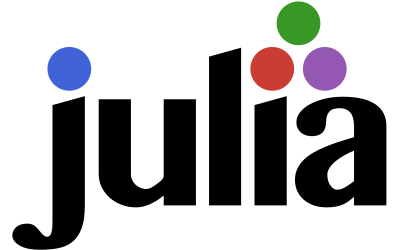
\includegraphics[width=0.3\textwidth]{./titlepage/logo} 
\\[1.5cm]

% Title
{ \SecondaryHeading Julia DEV Documentation} 
\\[1.5cm]
{ \huge The Julia Project}
\\[0.5cm]
{ \huge \today }

\end{center} 

\end{titlingpage}
\restoregeometry

% \cleardoublepage % makes the next page a odd-numbered page
\clearpage
\tableofcontents
\mainmatter

%% ---- Normal Input
% \part{Manual}


\chapter{Julia 1.8-DEV Documentation}

Welcome to the documentation for Julia 1.8-DEV.

\begin{quote}
\textbf{Work in progress!}

This documentation is for an unreleased, in-development, version of Julia.

\end{quote}


Please read the \href{NEWS.md}{release notes} to see what has changed since the last release.



\begin{quote}
\textbf{Note}

The documentation is also available in PDF format: \href{https://raw.githubusercontent.com/JuliaLang/docs.julialang.org/assets/julia-1.8.0-DEV.pdf}{julia-1.8.0-DEV.pdf}.

\end{quote}


\hypertarget{3498245216777255645}{}


\subsection{Introduction}



Scientific computing has traditionally required the highest performance, yet domain experts have largely moved to slower dynamic languages for daily work. We believe there are many good reasons to prefer dynamic languages for these applications, and we do not expect their use to diminish. Fortunately, modern language design and compiler techniques make it possible to mostly eliminate the performance trade-off and provide a single environment productive enough for prototyping and efficient enough for deploying performance-intensive applications. The Julia programming language fills this role: it is a flexible dynamic language, appropriate for scientific and numerical computing, with performance comparable to traditional statically-typed languages.



Because Julia{\textquotesingle}s compiler is different from the interpreters used for languages like Python or R, you may find that Julia{\textquotesingle}s performance is unintuitive at first. If you find that something is slow, we highly recommend reading through the \hyperlink{818954303942149020}{Performance Tips} section before trying anything else. Once you understand how Julia works, it{\textquotesingle}s easy to write code that{\textquotesingle}s nearly as fast as C.



Julia features optional typing, multiple dispatch, and good performance, achieved using type inference and \href{https://en.wikipedia.org/wiki/Just-in-time\_compilation}{just-in-time (JIT) compilation}, implemented using \href{https://en.wikipedia.org/wiki/Low\_Level\_Virtual\_Machine}{LLVM}. It is multi-paradigm, combining features of imperative, functional, and object-oriented programming. Julia provides ease and expressiveness for high-level numerical computing, in the same way as languages such as R, MATLAB, and Python, but also supports general programming. To achieve this, Julia builds upon the lineage of mathematical programming languages, but also borrows much from popular dynamic languages, including \href{https://en.wikipedia.org/wiki/Lisp\_(programming\_language)}{Lisp}, \href{https://en.wikipedia.org/wiki/Perl\_(programming\_language)}{Perl}, \href{https://en.wikipedia.org/wiki/Python\_(programming\_language)}{Python}, \href{https://en.wikipedia.org/wiki/Lua\_(programming\_language)}{Lua}, and \href{https://en.wikipedia.org/wiki/Ruby\_(programming\_language)}{Ruby}.



The most significant departures of Julia from typical dynamic languages are:



\begin{itemize}
\item The core language imposes very little; Julia Base and the standard library are written in Julia itself, including primitive operations like integer arithmetic


\item A rich language of types for constructing and describing objects, that can also optionally be used to make type declarations


\item The ability to define function behavior across many combinations of argument types via \href{https://en.wikipedia.org/wiki/Multiple\_dispatch}{multiple dispatch}


\item Automatic generation of efficient, specialized code for different argument types


\item Good performance, approaching that of statically-compiled languages like C

\end{itemize}


Although one sometimes speaks of dynamic languages as being {\textquotedbl}typeless{\textquotedbl}, they are definitely not: every object, whether primitive or user-defined, has a type. The lack of type declarations in most dynamic languages, however, means that one cannot instruct the compiler about the types of values, and often cannot explicitly talk about types at all. In static languages, on the other hand, while one can – and usually must – annotate types for the compiler, types exist only at compile time and cannot be manipulated or expressed at run time. In Julia, types are themselves run-time objects, and can also be used to convey information to the compiler.



While the casual programmer need not explicitly use types or multiple dispatch, they are the core unifying features of Julia: functions are defined on different combinations of argument types, and applied by dispatching to the most specific matching definition. This model is a good fit for mathematical programming, where it is unnatural for the first argument to {\textquotedbl}own{\textquotedbl} an operation as in traditional object-oriented dispatch. Operators are just functions with special notation – to extend addition to new user-defined data types, you define new methods for the \texttt{+} function. Existing code then seamlessly applies to the new data types.



Partly because of run-time type inference (augmented by optional type annotations), and partly because of a strong focus on performance from the inception of the project, Julia{\textquotesingle}s computational efficiency exceeds that of other dynamic languages, and even rivals that of statically-compiled languages. For large scale numerical problems, speed always has been, continues to be, and probably always will be crucial: the amount of data being processed has easily kept pace with Moore{\textquotesingle}s Law over the past decades.



Julia aims to create an unprecedented combination of ease-of-use, power, and efficiency in a single language. In addition to the above, some advantages of Julia over comparable systems include:



\begin{itemize}
\item Free and open source (\href{https://github.com/JuliaLang/julia/blob/master/LICENSE.md}{MIT licensed})


\item User-defined types are as fast and compact as built-ins


\item No need to vectorize code for performance; devectorized code is fast


\item Designed for parallelism and distributed computation


\item Lightweight {\textquotedbl}green{\textquotedbl} threading (\href{https://en.wikipedia.org/wiki/Coroutine}{coroutines})


\item Unobtrusive yet powerful type system


\item Elegant and extensible conversions and promotions for numeric and other types


\item Efficient support for \href{https://en.wikipedia.org/wiki/Unicode}{Unicode}, including but not limited to \href{https://en.wikipedia.org/wiki/UTF-8}{UTF-8}


\item Call C functions directly (no wrappers or special APIs needed)


\item Powerful shell-like capabilities for managing other processes


\item Lisp-like macros and other metaprogramming facilities

\end{itemize}


\hypertarget{14943148626325101976}{}


\chapter{Getting Started}



Julia installation is straightforward, whether using precompiled binaries or compiling from source. Download and install Julia by following the instructions at \href{https://julialang.org/downloads/}{https://julialang.org/downloads/}.



If you are coming to Julia from one of the following languages, then you should start by reading the section on noteworthy differences from \hyperlink{16118462231453533890}{MATLAB}, \hyperlink{751329316482051792}{R}, \hyperlink{6816556507610262594}{Python}, \hyperlink{17325153651592351510}{C/C++} or \hyperlink{1976420457538472404}{Common Lisp}. This will help you avoid some common pitfalls since Julia differs from those languages in many subtle ways.



The easiest way to learn and experiment with Julia is by starting an interactive session (also known as a read-eval-print loop or {\textquotedbl}REPL{\textquotedbl}) by double-clicking the Julia executable or running \texttt{julia} from the command line:




\begin{lstlisting}
$ julia

               _
   _       _ _(_)_     |  Documentation: https://docs.julialang.org
  (_)     | (_) (_)    |
   _ _   _| |_  __ _   |  Type "?" for help, "]?" for Pkg help.
  | | | | | | |/ _` |  |
  | | |_| | | | (_| |  |  Version 1.8.0-DEV.1223 (2022-01-06)
 _/ |\__'_|_|_|\__'_|  |  Commit 2d472c633d* (0 days old master)
|__/                   |


julia> 1 + 2
3

julia> ans
3
\end{lstlisting}



To exit the interactive session, type \texttt{CTRL-D} (press the Control/\texttt{{\textasciicircum}} key together with the \texttt{d} key), or type \texttt{exit()}. When run in interactive mode, \texttt{julia} displays a banner and prompts the user for input. Once the user has entered a complete expression, such as \texttt{1 + 2}, and hits enter, the interactive session evaluates the expression and shows its value. If an expression is entered into an interactive session with a trailing semicolon, its value is not shown. The variable \texttt{ans} is bound to the value of the last evaluated expression whether it is shown or not. The \texttt{ans} variable is only bound in interactive sessions, not when Julia code is run in other ways.



To evaluate expressions written in a source file \texttt{file.jl}, write \texttt{include({\textquotedbl}file.jl{\textquotedbl})}.



To run code in a file non-interactively, you can give it as the first argument to the \texttt{julia} command:




\begin{lstlisting}
$ julia script.jl
\end{lstlisting}



You can pass additional arguments to Julia, and to your program \texttt{script.jl}. A detailed list of all the available switches can be found at \hyperlink{631314801744611}{Command-line Options}.



\hypertarget{106098538461341329}{}


\section{Resources}



A curated list of useful learning resources to help new users get started can be found on the \href{https://julialang.org/learning/}{learning} page of the main Julia website.



You can use the REPL as a learning resource by switching into the help mode. Switch to help mode by pressing \texttt{?} at an empty \texttt{julia>} prompt, before typing anything else. Typing a keyword in help mode will fetch the documentation for it, along with examples. Similarly for most functions or other objects you might encounter!




\begin{lstlisting}
help?> begin
search: begin disable_sigint reenable_sigint

  begin

  begin...end denotes a block of code.
\end{lstlisting}



If you already know Julia a bit, you might want to peek ahead at \hyperlink{818954303942149020}{Performance Tips} and \hyperlink{6293662380888380710}{Workflow Tips}.



\hypertarget{10731958648755981077}{}


\chapter{Variables}



A variable, in Julia, is a name associated (or bound) to a value. It{\textquotesingle}s useful when you want to store a value (that you obtained after some math, for example) for later use. For example:




\begin{minted}{jlcon}
# Assign the value 10 to the variable x
julia> x = 10
10

# Doing math with x's value
julia> x + 1
11

# Reassign x's value
julia> x = 1 + 1
2

# You can assign values of other types, like strings of text
julia> x = "Hello World!"
"Hello World!"
\end{minted}



Julia provides an extremely flexible system for naming variables. Variable names are case-sensitive, and have no semantic meaning (that is, the language will not treat variables differently based on their names).




\begin{minted}{jlcon}
julia> x = 1.0
1.0

julia> y = -3
-3

julia> Z = "My string"
"My string"

julia> customary_phrase = "Hello world!"
"Hello world!"

julia> UniversalDeclarationOfHumanRightsStart = "人人生而自由,在尊严和权利上一律平等。"
"人人生而自由,在尊严和权利上一律平等。"
\end{minted}



Unicode names (in UTF-8 encoding) are allowed:




\begin{minted}{jlcon}
julia> δ = 0.00001
1.0e-5

julia> 안녕하세요 = "Hello"
"Hello"
\end{minted}



In the Julia REPL and several other Julia editing environments, you can type many Unicode math symbols by typing the backslashed LaTeX symbol name followed by tab. For example, the variable name \texttt{δ} can be entered by typing \texttt{{\textbackslash}delta}-\emph{tab}, or even \texttt{α̂⁽²⁾} by \texttt{{\textbackslash}alpha}-\emph{tab}-\texttt{{\textbackslash}hat}- \emph{tab}-\texttt{{\textbackslash}{\textasciicircum}(2)}-\emph{tab}. (If you find a symbol somewhere, e.g. in someone else{\textquotesingle}s code, that you don{\textquotesingle}t know how to type, the REPL help will tell you: just type \texttt{?} and then paste the symbol.)



Julia will even let you redefine built-in constants and functions if needed (although this is not recommended to avoid potential confusions):




\begin{minted}{jlcon}
julia> pi = 3
3

julia> pi
3

julia> sqrt = 4
4
\end{minted}



However, if you try to redefine a built-in constant or function already in use, Julia will give you an error:




\begin{minted}{jlcon}
julia> pi
π = 3.1415926535897...

julia> pi = 3
ERROR: cannot assign a value to variable MathConstants.pi from module Main

julia> sqrt(100)
10.0

julia> sqrt = 4
ERROR: cannot assign a value to variable Base.sqrt from module Main
\end{minted}



\hypertarget{14662919506992032303}{}


\section{Allowed Variable Names}



Variable names must begin with a letter (A-Z or a-z), underscore, or a subset of Unicode code points greater than 00A0; in particular, \href{https://www.fileformat.info/info/unicode/category/index.htm}{Unicode character categories} Lu/Ll/Lt/Lm/Lo/Nl (letters), Sc/So (currency and other symbols), and a few other letter-like characters (e.g. a subset of the Sm math symbols) are allowed. Subsequent characters may also include ! and digits (0-9 and other characters in categories Nd/No), as well as other Unicode code points: diacritics and other modifying marks (categories Mn/Mc/Me/Sk), some punctuation connectors (category Pc), primes, and a few other characters.



Operators like \texttt{+} are also valid identifiers, but are parsed specially. In some contexts, operators can be used just like variables; for example \texttt{(+)} refers to the addition function, and \texttt{(+) = f} will reassign it. Most of the Unicode infix operators (in category Sm), such as \texttt{⊕}, are parsed as infix operators and are available for user-defined methods (e.g. you can use \texttt{const ⊗ = kron} to define \texttt{⊗} as an infix Kronecker product).  Operators can also be suffixed with modifying marks, primes, and sub/superscripts, e.g. \texttt{+̂ₐ″} is parsed as an infix operator with the same precedence as \texttt{+}. A space is required between an operator that ends with a subscript/superscript letter and a subsequent variable name. For example, if \texttt{+ᵃ} is an operator, then \texttt{+ᵃx} must be written as \texttt{+ᵃ x} to distinguish it from \texttt{+ ᵃx} where \texttt{ᵃx} is the variable name.



A particular class of variable names is one that contains only underscores. These identifiers can only be assigned values but cannot be used to assign values to other variables. More technically, they can only be used as an \href{https://en.wikipedia.org/wiki/Value\_(computer\_science)\#lrvalue}{L-value}, but not as an  \href{https://en.wikipedia.org/wiki/R-value}{R-value}:




\begin{minted}{jlcon}
julia> x, ___ = size([2 2; 1 1])
(2, 2)

julia> y = ___
ERROR: syntax: all-underscore identifier used as rvalue
\end{minted}



The only explicitly disallowed names for variables are the names of the built-in \hyperlink{15655456628431734346}{Keywords}:




\begin{minted}{jlcon}
julia> else = false
ERROR: syntax: unexpected "else"

julia> try = "No"
ERROR: syntax: unexpected "="
\end{minted}



Some Unicode characters are considered to be equivalent in identifiers. Different ways of entering Unicode combining characters (e.g., accents) are treated as equivalent (specifically, Julia identifiers are \href{http://www.macchiato.com/unicode/nfc-faq}{NFC}-normalized). Julia also includes a few non-standard equivalences for characters that are visually similar and are easily entered by some input methods. The Unicode characters \texttt{ɛ} (U+025B: Latin small letter open e) and \texttt{µ} (U+00B5: micro sign) are treated as equivalent to the corresponding Greek letters. The middle dot \texttt{·} (U+00B7) and the Greek \href{https://en.wikipedia.org/wiki/Interpunct}{interpunct} \texttt{·} (U+0387) are both treated as the mathematical dot operator \texttt{⋅} (U+22C5). The minus sign \texttt{−} (U+2212) is treated as equivalent to the hyphen-minus sign \texttt{-} (U+002D).



\hypertarget{12940030219950347825}{}


\section{Stylistic Conventions}



While Julia imposes few restrictions on valid names, it has become useful to adopt the following conventions:



\begin{itemize}
\item Names of variables are in lower case.


\item Word separation can be indicated by underscores (\texttt{{\textquotesingle}\_{\textquotesingle}}), but use of underscores is discouraged unless the name would be hard to read otherwise.


\item Names of \texttt{Type}s and \texttt{Module}s begin with a capital letter and word separation is shown with upper camel case instead of underscores.


\item Names of \texttt{function}s and \texttt{macro}s are in lower case, without underscores.


\item Functions that write to their arguments have names that end in \texttt{!}. These are sometimes called {\textquotedbl}mutating{\textquotedbl} or {\textquotedbl}in-place{\textquotedbl} functions because they are intended to produce changes in their arguments after the function is called, not just return a value.

\end{itemize}


For more information about stylistic conventions, see the \hyperlink{6993837696873037088}{Style Guide}.



\hypertarget{633717716597615212}{}


\chapter{Integers and Floating-Point Numbers}



Integers and floating-point values are the basic building blocks of arithmetic and computation. Built-in representations of such values are called numeric primitives, while representations of integers and floating-point numbers as immediate values in code are known as numeric literals. For example, \texttt{1} is an integer literal, while \texttt{1.0} is a floating-point literal; their binary in-memory representations as objects are numeric primitives.



Julia provides a broad range of primitive numeric types, and a full complement of arithmetic and bitwise operators as well as standard mathematical functions are defined over them. These map directly onto numeric types and operations that are natively supported on modern computers, thus allowing Julia to take full advantage of computational resources. Additionally, Julia provides software support for \hyperlink{7030973523078279877}{Arbitrary Precision Arithmetic}, which can handle operations on numeric values that cannot be represented effectively in native hardware representations, but at the cost of relatively slower performance.



The following are Julia{\textquotesingle}s primitive numeric types:



\begin{itemize}
\item \textbf{Integer types:}

\end{itemize}



\begin{table}[h]

\begin{tabulary}{\linewidth}{|L|L|L|L|L|}
\hline
Type & Signed? & Number of bits & Smallest value & Largest value \\
\hline
\hyperlink{5857518405103968275}{\texttt{Int8}} & ✓ & 8 & -2{\textasciicircum}7 & 2{\textasciicircum}7 - 1 \\
\hline
\hyperlink{6609065134969660118}{\texttt{UInt8}} &  & 8 & 0 & 2{\textasciicircum}8 - 1 \\
\hline
\hyperlink{6667287249103968645}{\texttt{Int16}} & ✓ & 16 & -2{\textasciicircum}15 & 2{\textasciicircum}15 - 1 \\
\hline
\hyperlink{7018610346698168012}{\texttt{UInt16}} &  & 16 & 0 & 2{\textasciicircum}16 - 1 \\
\hline
\hyperlink{10103694114785108551}{\texttt{Int32}} & ✓ & 32 & -2{\textasciicircum}31 & 2{\textasciicircum}31 - 1 \\
\hline
\hyperlink{8690996847580776341}{\texttt{UInt32}} &  & 32 & 0 & 2{\textasciicircum}32 - 1 \\
\hline
\hyperlink{7720564657383125058}{\texttt{Int64}} & ✓ & 64 & -2{\textasciicircum}63 & 2{\textasciicircum}63 - 1 \\
\hline
\hyperlink{5500998675195555601}{\texttt{UInt64}} &  & 64 & 0 & 2{\textasciicircum}64 - 1 \\
\hline
\hyperlink{8012327724714767060}{\texttt{Int128}} & ✓ & 128 & -2{\textasciicircum}127 & 2{\textasciicircum}127 - 1 \\
\hline
\hyperlink{14811222188335428522}{\texttt{UInt128}} &  & 128 & 0 & 2{\textasciicircum}128 - 1 \\
\hline
\hyperlink{46725311238864537}{\texttt{Bool}} & N/A & 8 & \texttt{false} (0) & \texttt{true} (1) \\
\hline
\end{tabulary}

\end{table}



\begin{itemize}
\item \textbf{Floating-point types:}

\end{itemize}



\begin{table}[h]

\begin{tabulary}{\linewidth}{|L|L|L|}
\hline
Type & Precision & Number of bits \\
\hline
\hyperlink{2727296760866702904}{\texttt{Float16}} & \href{https://en.wikipedia.org/wiki/Half-precision\_floating-point\_format}{half} & 16 \\
\hline
\hyperlink{8101639384272933082}{\texttt{Float32}} & \href{https://en.wikipedia.org/wiki/Single\_precision\_floating-point\_format}{single} & 32 \\
\hline
\hyperlink{5027751419500983000}{\texttt{Float64}} & \href{https://en.wikipedia.org/wiki/Double\_precision\_floating-point\_format}{double} & 64 \\
\hline
\end{tabulary}

\end{table}



Additionally, full support for \hyperlink{10408543546165224304}{Complex and Rational Numbers} is built on top of these primitive numeric types. All numeric types interoperate naturally without explicit casting, thanks to a flexible, user-extensible \hyperlink{10374023657104680331}{type promotion system}.



\hypertarget{12881556218279790533}{}


\section{Integers}



Literal integers are represented in the standard manner:




\begin{minted}{jlcon}
julia> 1
1

julia> 1234
1234
\end{minted}



The default type for an integer literal depends on whether the target system has a 32-bit architecture or a 64-bit architecture:




\begin{minted}{jlcon}
# 32-bit system:
julia> typeof(1)
Int32

# 64-bit system:
julia> typeof(1)
Int64
\end{minted}



The Julia internal variable \hyperlink{6553323097149877235}{\texttt{Sys.WORD\_SIZE}} indicates whether the target system is 32-bit or 64-bit:




\begin{minted}{jlcon}
# 32-bit system:
julia> Sys.WORD_SIZE
32

# 64-bit system:
julia> Sys.WORD_SIZE
64
\end{minted}



Julia also defines the types \texttt{Int} and \texttt{UInt}, which are aliases for the system{\textquotesingle}s signed and unsigned native integer types respectively:




\begin{minted}{jlcon}
# 32-bit system:
julia> Int
Int32
julia> UInt
UInt32

# 64-bit system:
julia> Int
Int64
julia> UInt
UInt64
\end{minted}



Larger integer literals that cannot be represented using only 32 bits but can be represented in 64 bits always create 64-bit integers, regardless of the system type:




\begin{minted}{jlcon}
# 32-bit or 64-bit system:
julia> typeof(3000000000)
Int64
\end{minted}



Unsigned integers are input and output using the \texttt{0x} prefix and hexadecimal (base 16) digits \texttt{0-9a-f} (the capitalized digits \texttt{A-F} also work for input). The size of the unsigned value is determined by the number of hex digits used:




\begin{minted}{jlcon}
julia> x = 0x1
0x01

julia> typeof(x)
UInt8

julia> x = 0x123
0x0123

julia> typeof(x)
UInt16

julia> x = 0x1234567
0x01234567

julia> typeof(x)
UInt32

julia> x = 0x123456789abcdef
0x0123456789abcdef

julia> typeof(x)
UInt64

julia> x = 0x11112222333344445555666677778888
0x11112222333344445555666677778888

julia> typeof(x)
UInt128
\end{minted}



This behavior is based on the observation that when one uses unsigned hex literals for integer values, one typically is using them to represent a fixed numeric byte sequence, rather than just an integer value.



Binary and octal literals are also supported:




\begin{minted}{jlcon}
julia> x = 0b10
0x02

julia> typeof(x)
UInt8

julia> x = 0o010
0x08

julia> typeof(x)
UInt8

julia> x = 0x00000000000000001111222233334444
0x00000000000000001111222233334444

julia> typeof(x)
UInt128
\end{minted}



As for hexadecimal literals, binary and octal literals produce unsigned integer types. The size of the binary data item is the minimal needed size, if the leading digit of the literal is not \texttt{0}. In the case of leading zeros, the size is determined by the minimal needed size for a literal, which has the same length but leading digit \texttt{1}. It means that:



\begin{itemize}
\item \texttt{0x1} and \texttt{0x12} are \texttt{UInt8} literals,


\item \texttt{0x123} and \texttt{0x1234} are \texttt{UInt16} literals,


\item \texttt{0x12345} and \texttt{0x12345678} are \texttt{UInt32} literals,


\item \texttt{0x123456789} and \texttt{0x1234567890adcdef} are \texttt{UInt64} literals, etc.

\end{itemize}


Even if there are leading zero digits which don’t contribute to the value, they count for determining storage size of a literal. So \texttt{0x01} is a \texttt{UInt8} while \texttt{0x0001} is a \texttt{UInt16}.



That allows the user to control the size.



Values which cannot be stored in \texttt{UInt128} cannot be written as such literals.



Binary, octal, and hexadecimal literals may be signed by a \texttt{-} immediately preceding the unsigned literal. They produce an unsigned integer of the same size as the unsigned literal would do, with the two{\textquotesingle}s complement of the value:




\begin{minted}{jlcon}
julia> -0x2
0xfe

julia> -0x0002
0xfffe
\end{minted}



The minimum and maximum representable values of primitive numeric types such as integers are given by the \hyperlink{3613894539247233488}{\texttt{typemin}} and \hyperlink{17760305803764597758}{\texttt{typemax}} functions:




\begin{minted}{jlcon}
julia> (typemin(Int32), typemax(Int32))
(-2147483648, 2147483647)

julia> for T in [Int8,Int16,Int32,Int64,Int128,UInt8,UInt16,UInt32,UInt64,UInt128]
           println("$(lpad(T,7)): [$(typemin(T)),$(typemax(T))]")
       end
   Int8: [-128,127]
  Int16: [-32768,32767]
  Int32: [-2147483648,2147483647]
  Int64: [-9223372036854775808,9223372036854775807]
 Int128: [-170141183460469231731687303715884105728,170141183460469231731687303715884105727]
  UInt8: [0,255]
 UInt16: [0,65535]
 UInt32: [0,4294967295]
 UInt64: [0,18446744073709551615]
UInt128: [0,340282366920938463463374607431768211455]
\end{minted}



The values returned by \hyperlink{3613894539247233488}{\texttt{typemin}} and \hyperlink{17760305803764597758}{\texttt{typemax}} are always of the given argument type. (The above expression uses several features that have yet to be introduced, including \hyperlink{9034109510149997190}{for loops}, \hyperlink{205866387929607333}{Strings}, and \hyperlink{4452850363638134205}{Interpolation}, but should be easy enough to understand for users with some existing programming experience.)



\hypertarget{1170670466445299381}{}


\subsection{Overflow behavior}



In Julia, exceeding the maximum representable value of a given type results in a wraparound behavior:




\begin{minted}{jlcon}
julia> x = typemax(Int64)
9223372036854775807

julia> x + 1
-9223372036854775808

julia> x + 1 == typemin(Int64)
true
\end{minted}



Thus, arithmetic with Julia integers is actually a form of \href{https://en.wikipedia.org/wiki/Modular\_arithmetic}{modular arithmetic}. This reflects the characteristics of the underlying arithmetic of integers as implemented on modern computers. In applications where overflow is possible, explicit checking for wraparound produced by overflow is essential; otherwise, the \hyperlink{423405808990690832}{\texttt{BigInt}} type in \hyperlink{7030973523078279877}{Arbitrary Precision Arithmetic} is recommended instead.



An example of overflow behavior and how to potentially resolve it is as follows:




\begin{minted}{jlcon}
julia> 10^19
-8446744073709551616

julia> big(10)^19
10000000000000000000
\end{minted}



\hypertarget{5432529740505629102}{}


\subsection{Division errors}



Integer division (the \texttt{div} function) has two exceptional cases: dividing by zero, and dividing the lowest negative number (\hyperlink{3613894539247233488}{\texttt{typemin}}) by -1. Both of these cases throw a \hyperlink{4168463413201806292}{\texttt{DivideError}}. The remainder and modulus functions (\texttt{rem} and \texttt{mod}) throw a \hyperlink{4168463413201806292}{\texttt{DivideError}} when their second argument is zero.



\hypertarget{16644673878549722763}{}


\section{Floating-Point Numbers}



Literal floating-point numbers are represented in the standard formats, using \href{https://en.wikipedia.org/wiki/Scientific\_notation\#E\_notation}{E-notation} when necessary:




\begin{minted}{jlcon}
julia> 1.0
1.0

julia> 1.
1.0

julia> 0.5
0.5

julia> .5
0.5

julia> -1.23
-1.23

julia> 1e10
1.0e10

julia> 2.5e-4
0.00025
\end{minted}



The above results are all \hyperlink{5027751419500983000}{\texttt{Float64}} values. Literal \hyperlink{8101639384272933082}{\texttt{Float32}} values can be entered by writing an \texttt{f} in place of \texttt{e}:




\begin{minted}{jlcon}
julia> x = 0.5f0
0.5f0

julia> typeof(x)
Float32

julia> 2.5f-4
0.00025f0
\end{minted}



Values can be converted to \hyperlink{8101639384272933082}{\texttt{Float32}} easily:




\begin{minted}{jlcon}
julia> x = Float32(-1.5)
-1.5f0

julia> typeof(x)
Float32
\end{minted}



Hexadecimal floating-point literals are also valid, but only as \hyperlink{5027751419500983000}{\texttt{Float64}} values, with \texttt{p} preceding the base-2 exponent:




\begin{minted}{jlcon}
julia> 0x1p0
1.0

julia> 0x1.8p3
12.0

julia> x = 0x.4p-1
0.125

julia> typeof(x)
Float64
\end{minted}



Half-precision floating-point numbers are also supported (\hyperlink{2727296760866702904}{\texttt{Float16}}), but they are implemented in software and use \hyperlink{8101639384272933082}{\texttt{Float32}} for calculations.




\begin{minted}{jlcon}
julia> sizeof(Float16(4.))
2

julia> 2*Float16(4.)
Float16(8.0)
\end{minted}



The underscore \texttt{\_} can be used as digit separator:




\begin{minted}{jlcon}
julia> 10_000, 0.000_000_005, 0xdead_beef, 0b1011_0010
(10000, 5.0e-9, 0xdeadbeef, 0xb2)
\end{minted}



\hypertarget{13617516048741064927}{}


\subsection{Floating-point zero}



Floating-point numbers have \href{https://en.wikipedia.org/wiki/Signed\_zero}{two zeros}, positive zero and negative zero. They are equal to each other but have different binary representations, as can be seen using the \hyperlink{9171163989026657457}{\texttt{bitstring}} function:




\begin{minted}{jlcon}
julia> 0.0 == -0.0
true

julia> bitstring(0.0)
"0000000000000000000000000000000000000000000000000000000000000000"

julia> bitstring(-0.0)
"1000000000000000000000000000000000000000000000000000000000000000"
\end{minted}



\hypertarget{12761588490686892534}{}


\subsection{Special floating-point values}



There are three specified standard floating-point values that do not correspond to any point on the real number line:




\begin{table}[h]

\begin{tabulary}{\linewidth}{|L|L|L|L|L|}
\hline
\texttt{Float16} & \texttt{Float32} & \texttt{Float64} & Name & Description \\
\hline
\texttt{Inf16} & \texttt{Inf32} & \texttt{Inf} & positive infinity & a value greater than all finite floating-point values \\
\hline
\texttt{-Inf16} & \texttt{-Inf32} & \texttt{-Inf} & negative infinity & a value less than all finite floating-point values \\
\hline
\texttt{NaN16} & \texttt{NaN32} & \texttt{NaN} & not a number & a value not \texttt{==} to any floating-point value (including itself) \\
\hline
\end{tabulary}

\end{table}



For further discussion of how these non-finite floating-point values are ordered with respect to each other and other floats, see \hyperlink{3931033603389178275}{Numeric Comparisons}. By the \href{https://en.wikipedia.org/wiki/IEEE\_754-2008}{IEEE 754 standard}, these floating-point values are the results of certain arithmetic operations:




\begin{minted}{jlcon}
julia> 1/Inf
0.0

julia> 1/0
Inf

julia> -5/0
-Inf

julia> 0.000001/0
Inf

julia> 0/0
NaN

julia> 500 + Inf
Inf

julia> 500 - Inf
-Inf

julia> Inf + Inf
Inf

julia> Inf - Inf
NaN

julia> Inf * Inf
Inf

julia> Inf / Inf
NaN

julia> 0 * Inf
NaN

julia> NaN == NaN
false

julia> NaN != NaN
true

julia> NaN < NaN
false

julia> NaN > NaN
false
\end{minted}



The \hyperlink{3613894539247233488}{\texttt{typemin}} and \hyperlink{17760305803764597758}{\texttt{typemax}} functions also apply to floating-point types:




\begin{minted}{jlcon}
julia> (typemin(Float16),typemax(Float16))
(-Inf16, Inf16)

julia> (typemin(Float32),typemax(Float32))
(-Inf32, Inf32)

julia> (typemin(Float64),typemax(Float64))
(-Inf, Inf)
\end{minted}



\hypertarget{14252734901518446549}{}


\subsection{Machine epsilon}



Most real numbers cannot be represented exactly with floating-point numbers, and so for many purposes it is important to know the distance between two adjacent representable floating-point numbers, which is often known as \href{https://en.wikipedia.org/wiki/Machine\_epsilon}{machine epsilon}.



Julia provides \hyperlink{15586044128704640253}{\texttt{eps}}, which gives the distance between \texttt{1.0} and the next larger representable floating-point value:




\begin{minted}{jlcon}
julia> eps(Float32)
1.1920929f-7

julia> eps(Float64)
2.220446049250313e-16

julia> eps() # same as eps(Float64)
2.220446049250313e-16
\end{minted}



These values are \texttt{2.0{\textasciicircum}-23} and \texttt{2.0{\textasciicircum}-52} as \hyperlink{8101639384272933082}{\texttt{Float32}} and \hyperlink{5027751419500983000}{\texttt{Float64}} values, respectively. The \hyperlink{15586044128704640253}{\texttt{eps}} function can also take a floating-point value as an argument, and gives the absolute difference between that value and the next representable floating point value. That is, \texttt{eps(x)} yields a value of the same type as \texttt{x} such that \texttt{x + eps(x)} is the next representable floating-point value larger than \texttt{x}:




\begin{minted}{jlcon}
julia> eps(1.0)
2.220446049250313e-16

julia> eps(1000.)
1.1368683772161603e-13

julia> eps(1e-27)
1.793662034335766e-43

julia> eps(0.0)
5.0e-324
\end{minted}



The distance between two adjacent representable floating-point numbers is not constant, but is smaller for smaller values and larger for larger values. In other words, the representable floating-point numbers are densest in the real number line near zero, and grow sparser exponentially as one moves farther away from zero. By definition, \texttt{eps(1.0)} is the same as \texttt{eps(Float64)} since \texttt{1.0} is a 64-bit floating-point value.



Julia also provides the \hyperlink{8339500090035450608}{\texttt{nextfloat}} and \hyperlink{14035790731013288499}{\texttt{prevfloat}} functions which return the next largest or smallest representable floating-point number to the argument respectively:




\begin{minted}{jlcon}
julia> x = 1.25f0
1.25f0

julia> nextfloat(x)
1.2500001f0

julia> prevfloat(x)
1.2499999f0

julia> bitstring(prevfloat(x))
"00111111100111111111111111111111"

julia> bitstring(x)
"00111111101000000000000000000000"

julia> bitstring(nextfloat(x))
"00111111101000000000000000000001"
\end{minted}



This example highlights the general principle that the adjacent representable floating-point numbers also have adjacent binary integer representations.



\hypertarget{7851007688404575091}{}


\subsection{Rounding modes}



If a number doesn{\textquotesingle}t have an exact floating-point representation, it must be rounded to an appropriate representable value. However, the manner in which this rounding is done can be changed if required according to the rounding modes presented in the \href{https://en.wikipedia.org/wiki/IEEE\_754-2008}{IEEE 754 standard}.



The default mode used is always \hyperlink{868115654703135309}{\texttt{RoundNearest}}, which rounds to the nearest representable value, with ties rounded towards the nearest value with an even least significant bit.



\hypertarget{1618194528642516731}{}


\subsection{Background and References}



Floating-point arithmetic entails many subtleties which can be surprising to users who are unfamiliar with the low-level implementation details. However, these subtleties are described in detail in most books on scientific computation, and also in the following references:



\begin{itemize}
\item The definitive guide to floating point arithmetic is the \href{https://standards.ieee.org/standard/754-2008.html}{IEEE 754-2008 Standard}; however, it is not available for free online.


\item For a brief but lucid presentation of how floating-point numbers are represented, see John D. Cook{\textquotesingle}s \href{https://www.johndcook.com/blog/2009/04/06/anatomy-of-a-floating-point-number/}{article} on the subject as well as his \href{https://www.johndcook.com/blog/2009/04/06/numbers-are-a-leaky-abstraction/}{introduction} to some of the issues arising from how this representation differs in behavior from the idealized abstraction of real numbers.


\item Also recommended is Bruce Dawson{\textquotesingle}s \href{https://randomascii.wordpress.com/2012/05/20/thats-not-normalthe-performance-of-odd-floats/}{series of blog posts on floating-point numbers}.


\item For an excellent, in-depth discussion of floating-point numbers and issues of numerical accuracy encountered when computing with them, see David Goldberg{\textquotesingle}s paper \href{https://citeseerx.ist.psu.edu/viewdoc/download?doi=10.1.1.22.6768\&rep=rep1\&type=pdf}{What Every Computer Scientist Should Know About Floating-Point Arithmetic}.


\item For even more extensive documentation of the history of, rationale for, and issues with floating-point numbers, as well as discussion of many other topics in numerical computing, see the \href{https://people.eecs.berkeley.edu/{\textasciitilde}wkahan/}{collected writings} of \href{https://en.wikipedia.org/wiki/William\_Kahan}{William Kahan}, commonly known as the {\textquotedbl}Father of Floating-Point{\textquotedbl}. Of particular interest may be \href{https://people.eecs.berkeley.edu/{\textasciitilde}wkahan/ieee754status/754story.html}{An Interview with the Old Man of Floating-Point}.

\end{itemize}


\hypertarget{6510345620772143535}{}


\section{Arbitrary Precision Arithmetic}



To allow computations with arbitrary-precision integers and floating point numbers, Julia wraps the \href{https://gmplib.org}{GNU Multiple Precision Arithmetic Library (GMP)} and the \href{https://www.mpfr.org}{GNU MPFR Library}, respectively. The \hyperlink{423405808990690832}{\texttt{BigInt}} and \hyperlink{749816618809421837}{\texttt{BigFloat}} types are available in Julia for arbitrary precision integer and floating point numbers respectively.



Constructors exist to create these types from primitive numerical types, and the \hyperlink{6548320458095485939}{string literal} \hyperlink{4226571565562941917}{\texttt{@big\_str}} or \hyperlink{14207407853646164654}{\texttt{parse}} can be used to construct them from \texttt{AbstractString}s. \texttt{BigInt}s can also be input as integer literals when they are too big for other built-in integer types. Note that as there is no unsigned arbitrary-precision integer type in \texttt{Base} (\texttt{BigInt} is sufficient in most cases), hexadecimal, octal and binary literals can be used (in addition to decimal literals).



Once created, they participate in arithmetic with all other numeric types thanks to Julia{\textquotesingle}s \hyperlink{10374023657104680331}{type promotion and conversion mechanism}:




\begin{minted}{jlcon}
julia> BigInt(typemax(Int64)) + 1
9223372036854775808

julia> big"123456789012345678901234567890" + 1
123456789012345678901234567891

julia> parse(BigInt, "123456789012345678901234567890") + 1
123456789012345678901234567891

julia> string(big"2"^200, base=16)
"100000000000000000000000000000000000000000000000000"

julia> 0x100000000000000000000000000000000-1 == typemax(UInt128)
true

julia> 0x000000000000000000000000000000000
0

julia> typeof(ans)
BigInt

julia> big"1.23456789012345678901"
1.234567890123456789010000000000000000000000000000000000000000000000000000000004

julia> parse(BigFloat, "1.23456789012345678901")
1.234567890123456789010000000000000000000000000000000000000000000000000000000004

julia> BigFloat(2.0^66) / 3
2.459565876494606882133333333333333333333333333333333333333333333333333333333344e+19

julia> factorial(BigInt(40))
815915283247897734345611269596115894272000000000
\end{minted}



However, type promotion between the primitive types above and \hyperlink{423405808990690832}{\texttt{BigInt}}/\hyperlink{749816618809421837}{\texttt{BigFloat}} is not automatic and must be explicitly stated.




\begin{minted}{jlcon}
julia> x = typemin(Int64)
-9223372036854775808

julia> x = x - 1
9223372036854775807

julia> typeof(x)
Int64

julia> y = BigInt(typemin(Int64))
-9223372036854775808

julia> y = y - 1
-9223372036854775809

julia> typeof(y)
BigInt
\end{minted}



The default precision (in number of bits of the significand) and rounding mode of \hyperlink{749816618809421837}{\texttt{BigFloat}} operations can be changed globally by calling \hyperlink{3543074496498234209}{\texttt{setprecision}} and \hyperlink{16542701110177516527}{\texttt{setrounding}}, and all further calculations will take these changes in account.  Alternatively, the precision or the rounding can be changed only within the execution of a particular block of code by using the same functions with a \texttt{do} block:




\begin{minted}{jlcon}
julia> setrounding(BigFloat, RoundUp) do
           BigFloat(1) + parse(BigFloat, "0.1")
       end
1.100000000000000000000000000000000000000000000000000000000000000000000000000003

julia> setrounding(BigFloat, RoundDown) do
           BigFloat(1) + parse(BigFloat, "0.1")
       end
1.099999999999999999999999999999999999999999999999999999999999999999999999999986

julia> setprecision(40) do
           BigFloat(1) + parse(BigFloat, "0.1")
       end
1.1000000000004
\end{minted}



\hypertarget{14058350023597195643}{}


\section{Numeric Literal Coefficients}



To make common numeric formulae and expressions clearer, Julia allows variables to be immediately preceded by a numeric literal, implying multiplication. This makes writing polynomial expressions much cleaner:




\begin{minted}{jlcon}
julia> x = 3
3

julia> 2x^2 - 3x + 1
10

julia> 1.5x^2 - .5x + 1
13.0
\end{minted}



It also makes writing exponential functions more elegant:




\begin{minted}{jlcon}
julia> 2^2x
64
\end{minted}



The precedence of numeric literal coefficients is slightly lower than that of unary operators such as negation. So \texttt{-2x} is parsed as \texttt{(-2) * x} and \texttt{√2x} is parsed as \texttt{(√2) * x}. However, numeric literal coefficients parse similarly to unary operators when combined with exponentiation. For example \texttt{2{\textasciicircum}3x} is parsed as \texttt{2{\textasciicircum}(3x)}, and \texttt{2x{\textasciicircum}3} is parsed as \texttt{2*(x{\textasciicircum}3)}.



Numeric literals also work as coefficients to parenthesized expressions:




\begin{minted}{jlcon}
julia> 2(x-1)^2 - 3(x-1) + 1
3
\end{minted}



\begin{quote}
\textbf{Note}

The precedence of numeric literal coefficients used for implicit multiplication is higher than other binary operators such as multiplication (\texttt{*}), and division (\texttt{/}, \texttt{{\textbackslash}}, and \texttt{//}).  This means, for example, that \texttt{1 / 2im} equals \texttt{-0.5im} and \texttt{6 // 2(2 + 1)} equals \texttt{1 // 1}.

\end{quote}


Additionally, parenthesized expressions can be used as coefficients to variables, implying multiplication of the expression by the variable:




\begin{minted}{jlcon}
julia> (x-1)x
6
\end{minted}



Neither juxtaposition of two parenthesized expressions, nor placing a variable before a parenthesized expression, however, can be used to imply multiplication:




\begin{minted}{jlcon}
julia> (x-1)(x+1)
ERROR: MethodError: objects of type Int64 are not callable

julia> x(x+1)
ERROR: MethodError: objects of type Int64 are not callable
\end{minted}



Both expressions are interpreted as function application: any expression that is not a numeric literal, when immediately followed by a parenthetical, is interpreted as a function applied to the values in parentheses (see \hyperlink{13536066633202303496}{Functions} for more about functions). Thus, in both of these cases, an error occurs since the left-hand value is not a function.



The above syntactic enhancements significantly reduce the visual noise incurred when writing common mathematical formulae. Note that no whitespace may come between a numeric literal coefficient and the identifier or parenthesized expression which it multiplies.



\hypertarget{1174732693948090595}{}


\subsection{Syntax Conflicts}



Juxtaposed literal coefficient syntax may conflict with some numeric literal syntaxes: hexadecimal, octal and binary integer literals and engineering notation for floating-point literals. Here are some situations where syntactic conflicts arise:



\begin{itemize}
\item The hexadecimal integer literal expression \texttt{0xff} could be interpreted as the numeric literal \texttt{0} multiplied by the variable \texttt{xff}. Similar ambiguities arise with octal and binary literals like \texttt{0o777} or \texttt{0b01001010}.


\item The floating-point literal expression \texttt{1e10} could be interpreted as the numeric literal \texttt{1} multiplied by the variable \texttt{e10}, and similarly with the equivalent \texttt{E} form.


\item The 32-bit floating-point literal expression \texttt{1.5f22} could be interpreted as the numeric literal \texttt{1.5} multiplied by the variable \texttt{f22}.

\end{itemize}


In all cases the ambiguity is resolved in favor of interpretation as numeric literals:



\begin{itemize}
\item Expressions starting with \texttt{0x}/\texttt{0o}/\texttt{0b} are always hexadecimal/octal/binary literals.


\item Expressions starting with a numeric literal followed by \texttt{e} or \texttt{E} are always floating-point literals.


\item Expressions starting with a numeric literal followed by \texttt{f} are always 32-bit floating-point literals.

\end{itemize}


Unlike \texttt{E}, which is equivalent to \texttt{e} in numeric literals for historical reasons, \texttt{F} is just another letter and does not behave like \texttt{f} in numeric literals. Hence, expressions starting with a numeric literal followed by \texttt{F} are interpreted as the numerical literal multiplied by a variable, which means that, for example, \texttt{1.5F22} is equal to \texttt{1.5 * F22}.



\hypertarget{9898854987068145953}{}


\section{Literal zero and one}



Julia provides functions which return literal 0 and 1 corresponding to a specified type or the type of a given variable.




\begin{table}[h]

\begin{tabulary}{\linewidth}{|L|L|}
\hline
Function & Description \\
\hline
\hyperlink{240596739242881814}{\texttt{zero(x)}} & Literal zero of type \texttt{x} or type of variable \texttt{x} \\
\hline
\hyperlink{11395333326208453101}{\texttt{one(x)}} & Literal one of type \texttt{x} or type of variable \texttt{x} \\
\hline
\end{tabulary}

\end{table}



These functions are useful in \hyperlink{3931033603389178275}{Numeric Comparisons} to avoid overhead from unnecessary \hyperlink{10374023657104680331}{type conversion}.



Examples:




\begin{minted}{jlcon}
julia> zero(Float32)
0.0f0

julia> zero(1.0)
0.0

julia> one(Int32)
1

julia> one(BigFloat)
1.0
\end{minted}



\hypertarget{349605097607208224}{}


\chapter{Mathematical Operations and Elementary Functions}



Julia provides a complete collection of basic arithmetic and bitwise operators across all of its numeric primitive types, as well as providing portable, efficient implementations of a comprehensive collection of standard mathematical functions.



\hypertarget{17352838172296001344}{}


\section{Arithmetic Operators}



The following \href{https://en.wikipedia.org/wiki/Arithmetic\#Arithmetic\_operations}{arithmetic operators} are supported on all primitive numeric types:




\begin{table}[h]

\begin{tabulary}{\linewidth}{|L|L|L|}
\hline
Expression & Name & Description \\
\hline
\texttt{+x} & unary plus & the identity operation \\
\hline
\texttt{-x} & unary minus & maps values to their additive inverses \\
\hline
\texttt{x + y} & binary plus & performs addition \\
\hline
\texttt{x - y} & binary minus & performs subtraction \\
\hline
\texttt{x * y} & times & performs multiplication \\
\hline
\texttt{x / y} & divide & performs division \\
\hline
\texttt{x ÷ y} & integer divide & x / y, truncated to an integer \\
\hline
\texttt{x {\textbackslash} y} & inverse divide & equivalent to \texttt{y / x} \\
\hline
\texttt{x {\textasciicircum} y} & power & raises \texttt{x} to the \texttt{y}th power \\
\hline
\texttt{x \% y} & remainder & equivalent to \texttt{rem(x,y)} \\
\hline
\end{tabulary}

\end{table}



A numeric literal placed directly before an identifier or parentheses, e.g. \texttt{2x} or \texttt{2(x+y)}, is treated as a multiplication, except with higher precedence than other binary operations.  See \hyperlink{7285052708387693199}{Numeric Literal Coefficients} for details.



Julia{\textquotesingle}s promotion system makes arithmetic operations on mixtures of argument types {\textquotedbl}just work{\textquotedbl} naturally and automatically. See \hyperlink{10374023657104680331}{Conversion and Promotion} for details of the promotion system.



The ÷ sign can be conveniently typed by writing \texttt{{\textbackslash}div<tab>} to the REPL or Julia IDE. See the \hyperlink{12388770544499622804}{manual section on Unicode input} for more information.



Here are some simple examples using arithmetic operators:




\begin{minted}{jlcon}
julia> 1 + 2 + 3
6

julia> 1 - 2
-1

julia> 3*2/12
0.5
\end{minted}



(By convention, we tend to space operators more tightly if they get applied before other nearby operators. For instance, we would generally write \texttt{-x + 2} to reflect that first \texttt{x} gets negated, and then \texttt{2} is added to that result.)



When used in multiplication, \texttt{false} acts as a \emph{strong zero}:




\begin{minted}{jlcon}
julia> NaN * false
0.0

julia> false * Inf
0.0
\end{minted}



This is useful for preventing the propagation of \texttt{NaN} values in quantities that are known to be zero. See \href{https://arxiv.org/abs/math/9205211}{Knuth (1992)} for motivation.



\hypertarget{15902875418345066084}{}


\section{Boolean Operators}



The following \href{https://en.wikipedia.org/wiki/Boolean\_algebra\#Operations}{Boolean operators} are supported on \hyperlink{46725311238864537}{\texttt{Bool}} types:




\begin{table}[h]

\begin{tabulary}{\linewidth}{|L|L|}
\hline
Expression & Name \\
\hline
\texttt{!x} & negation \\
\hline
\texttt{x \&\& y} & \hyperlink{14451148373001501733}{short-circuiting and} \\
\hline
\texttt{x || y} & \hyperlink{14451148373001501733}{short-circuiting or} \\
\hline
\end{tabulary}

\end{table}



Negation changes \texttt{true} to \texttt{false} and vice versa. The short-circuiting operations are explained on the linked page.



Note that \texttt{Bool} is an integer type and all the usual promotion rules and numeric operators are also defined on it.



\hypertarget{7882941329781051577}{}


\section{Bitwise Operators}



The following \href{https://en.wikipedia.org/wiki/Bitwise\_operation\#Bitwise\_operators}{bitwise operators} are supported on all primitive integer types:




\begin{table}[h]

\begin{tabulary}{\linewidth}{|L|L|}
\hline
Expression & Name \\
\hline
\texttt{{\textasciitilde}x} & bitwise not \\
\hline
\texttt{x \& y} & bitwise and \\
\hline
\texttt{x | y} & bitwise or \\
\hline
\texttt{x \unicodeveebar{} y} & bitwise xor (exclusive or) \\
\hline
\texttt{x ⊼ y} & bitwise nand (not and) \\
\hline
\texttt{x ⊽ y} & bitwise nor (not or) \\
\hline
\texttt{x >>> y} & \href{https://en.wikipedia.org/wiki/Logical\_shift}{logical shift} right \\
\hline
\texttt{x >> y} & \href{https://en.wikipedia.org/wiki/Arithmetic\_shift}{arithmetic shift} right \\
\hline
\texttt{x << y} & logical/arithmetic shift left \\
\hline
\end{tabulary}

\end{table}



Here are some examples with bitwise operators:




\begin{minted}[escapeinside=\#\%]{jlcon}
julia> ~123
-124

julia> 123 & 234
106

julia> 123 | 234
251

julia> 123 #\unicodeveebar% 234
145

julia> xor(123, 234)
145

julia> nand(123, 123)
-124

julia> 123 ⊼ 123
-124

julia> nor(123, 124)
-128

julia> 123 ⊽ 124
-128

julia> ~UInt32(123)
0xffffff84

julia> ~UInt8(123)
0x84
\end{minted}



\hypertarget{691395067782655074}{}


\section{Updating operators}



Every binary arithmetic and bitwise operator also has an updating version that assigns the result of the operation back into its left operand. The updating version of the binary operator is formed by placing a \texttt{=} immediately after the operator. For example, writing \texttt{x += 3} is equivalent to writing \texttt{x = x + 3}:




\begin{minted}{jlcon}
julia> x = 1
1

julia> x += 3
4

julia> x
4
\end{minted}



The updating versions of all the binary arithmetic and bitwise operators are:




\begin{lstlisting}[escapeinside=\%\%]
+=  -=  *=  /=  \=  ÷=  %\%%=  ^=  &=  |=  %\unicodeveebar%=  >>>=  >>=  <<=
\end{lstlisting}



\begin{quote}
\textbf{Note}

An updating operator rebinds the variable on the left-hand side. As a result, the type of the variable may change.


\begin{minted}{jlcon}
julia> x = 0x01; typeof(x)
UInt8

julia> x *= 2 # Same as x = x * 2
2

julia> typeof(x)
Int64
\end{minted}

\end{quote}


\hypertarget{6173297391052343261}{}


\section{Vectorized {\textquotedbl}dot{\textquotedbl} operators}



For \emph{every} binary operation like \texttt{{\textasciicircum}}, there is a corresponding {\textquotedbl}dot{\textquotedbl} operation \texttt{.{\textasciicircum}} that is \emph{automatically} defined to perform \texttt{{\textasciicircum}} element-by-element on arrays. For example, \texttt{[1,2,3] {\textasciicircum} 3} is not defined, since there is no standard mathematical meaning to {\textquotedbl}cubing{\textquotedbl} a (non-square) array, but \texttt{[1,2,3] .{\textasciicircum} 3} is defined as computing the elementwise (or {\textquotedbl}vectorized{\textquotedbl}) result \texttt{[1{\textasciicircum}3, 2{\textasciicircum}3, 3{\textasciicircum}3]}.  Similarly for unary operators like \texttt{!} or \texttt{√}, there is a corresponding \texttt{.√} that applies the operator elementwise.




\begin{minted}{jlcon}
julia> [1,2,3] .^ 3
3-element Vector{Int64}:
  1
  8
 27
\end{minted}



More specifically, \texttt{a .{\textasciicircum} b} is parsed as the \hyperlink{17801130558550430478}{{\textquotedbl}dot{\textquotedbl} call} \texttt{({\textasciicircum}).(a,b)}, which performs a \hyperlink{1924664524817847375}{broadcast} operation: it can combine arrays and scalars, arrays of the same size (performing the operation elementwise), and even arrays of different shapes (e.g. combining row and column vectors to produce a matrix). Moreover, like all vectorized {\textquotedbl}dot calls,{\textquotedbl} these {\textquotedbl}dot operators{\textquotedbl} are \emph{fusing}. For example, if you compute \texttt{2 .* A.{\textasciicircum}2 .+ sin.(A)} (or equivalently \texttt{@. 2A{\textasciicircum}2 + sin(A)}, using the \hyperlink{16688502228717894452}{\texttt{@.}} macro) for an array \texttt{A}, it performs a \emph{single} loop over \texttt{A}, computing \texttt{2a{\textasciicircum}2 + sin(a)} for each element \texttt{a} of \texttt{A}. In particular, nested dot calls like \texttt{f.(g.(x))} are fused, and {\textquotedbl}adjacent{\textquotedbl} binary operators like \texttt{x .+ 3 .* x.{\textasciicircum}2} are equivalent to nested dot calls \texttt{(+).(x, (*).(3, ({\textasciicircum}).(x, 2)))}.



Furthermore, {\textquotedbl}dotted{\textquotedbl} updating operators like \texttt{a .+= b} (or \texttt{@. a += b}) are parsed as \texttt{a .= a .+ b}, where \texttt{.=} is a fused \emph{in-place} assignment operation (see the \hyperlink{17801130558550430478}{dot syntax documentation}).



Note the dot syntax is also applicable to user-defined operators. For example, if you define \texttt{⊗(A,B) = kron(A,B)} to give a convenient infix syntax \texttt{A ⊗ B} for Kronecker products (\hyperlink{14153417388267953812}{\texttt{kron}}), then \texttt{[A,B] .⊗ [C,D]} will compute \texttt{[A⊗C, B⊗D]} with no additional coding.



Combining dot operators with numeric literals can be ambiguous. For example, it is not clear whether \texttt{1.+x} means \texttt{1. + x} or \texttt{1 .+ x}. Therefore this syntax is disallowed, and spaces must be used around the operator in such cases.



\hypertarget{1941388563916368614}{}


\section{Numeric Comparisons}



Standard comparison operations are defined for all the primitive numeric types:




\begin{table}[h]

\begin{tabulary}{\linewidth}{|L|L|}
\hline
Operator & Name \\
\hline
\hyperlink{15143149452920304570}{\texttt{==}} & equality \\
\hline
\hyperlink{3046079188653285114}{\texttt{!=}}, \hyperlink{3046079188653285114}{\texttt{≠}} & inequality \\
\hline
\hyperlink{702782232449268329}{\texttt{<}} & less than \\
\hline
\hyperlink{11411050964021316526}{\texttt{<=}}, \hyperlink{11411050964021316526}{\texttt{≤}} & less than or equal to \\
\hline
\hyperlink{8677991761303191103}{\texttt{>}} & greater than \\
\hline
\hyperlink{7019639580556993898}{\texttt{>=}}, \hyperlink{7019639580556993898}{\texttt{≥}} & greater than or equal to \\
\hline
\end{tabulary}

\end{table}



Here are some simple examples:




\begin{minted}{jlcon}
julia> 1 == 1
true

julia> 1 == 2
false

julia> 1 != 2
true

julia> 1 == 1.0
true

julia> 1 < 2
true

julia> 1.0 > 3
false

julia> 1 >= 1.0
true

julia> -1 <= 1
true

julia> -1 <= -1
true

julia> -1 <= -2
false

julia> 3 < -0.5
false
\end{minted}



Integers are compared in the standard manner – by comparison of bits. Floating-point numbers are compared according to the \href{https://en.wikipedia.org/wiki/IEEE\_754-2008}{IEEE 754 standard}:



\begin{itemize}
\item Finite numbers are ordered in the usual manner.


\item Positive zero is equal but not greater than negative zero.


\item \texttt{Inf} is equal to itself and greater than everything else except \texttt{NaN}.


\item \texttt{-Inf} is equal to itself and less than everything else except \texttt{NaN}.


\item \texttt{NaN} is not equal to, not less than, and not greater than anything, including itself.

\end{itemize}


The last point is potentially surprising and thus worth noting:




\begin{minted}{jlcon}
julia> NaN == NaN
false

julia> NaN != NaN
true

julia> NaN < NaN
false

julia> NaN > NaN
false
\end{minted}



and can cause headaches when working with \hyperlink{16720099245556932994}{arrays}:




\begin{minted}{jlcon}
julia> [1 NaN] == [1 NaN]
false
\end{minted}



Julia provides additional functions to test numbers for special values, which can be useful in situations like hash key comparisons:




\begin{table}[h]

\begin{tabulary}{\linewidth}{|L|L|}
\hline
Function & Tests if \\
\hline
\hyperlink{269533589463185031}{\texttt{isequal(x, y)}} & \texttt{x} and \texttt{y} are identical \\
\hline
\hyperlink{2906021895910968108}{\texttt{isfinite(x)}} & \texttt{x} is a finite number \\
\hline
\hyperlink{4492113908831448207}{\texttt{isinf(x)}} & \texttt{x} is infinite \\
\hline
\hyperlink{6770390199496851634}{\texttt{isnan(x)}} & \texttt{x} is not a number \\
\hline
\end{tabulary}

\end{table}



\hyperlink{269533589463185031}{\texttt{isequal}} considers \texttt{NaN}s equal to each other:




\begin{minted}{jlcon}
julia> isequal(NaN, NaN)
true

julia> isequal([1 NaN], [1 NaN])
true

julia> isequal(NaN, NaN32)
true
\end{minted}



\texttt{isequal} can also be used to distinguish signed zeros:




\begin{minted}{jlcon}
julia> -0.0 == 0.0
true

julia> isequal(-0.0, 0.0)
false
\end{minted}



Mixed-type comparisons between signed integers, unsigned integers, and floats can be tricky. A great deal of care has been taken to ensure that Julia does them correctly.



For other types, \texttt{isequal} defaults to calling \hyperlink{15143149452920304570}{\texttt{==}}, so if you want to define equality for your own types then you only need to add a \hyperlink{15143149452920304570}{\texttt{==}} method.  If you define your own equality function, you should probably define a corresponding \hyperlink{13797072367283572032}{\texttt{hash}} method to ensure that \texttt{isequal(x,y)} implies \texttt{hash(x) == hash(y)}.



\hypertarget{8460541965572991218}{}


\subsection{Chaining comparisons}



Unlike most languages, with the \href{https://en.wikipedia.org/wiki/Python\_syntax\_and\_semantics\#Comparison\_operators}{notable exception of Python}, comparisons can be arbitrarily chained:




\begin{minted}{jlcon}
julia> 1 < 2 <= 2 < 3 == 3 > 2 >= 1 == 1 < 3 != 5
true
\end{minted}



Chaining comparisons is often quite convenient in numerical code. Chained comparisons use the \texttt{\&\&} operator for scalar comparisons, and the \hyperlink{1494761116451616317}{\texttt{\&}} operator for elementwise comparisons, which allows them to work on arrays. For example, \texttt{0 .< A .< 1} gives a boolean array whose entries are true where the corresponding elements of \texttt{A} are between 0 and 1.



Note the evaluation behavior of chained comparisons:




\begin{minted}{jlcon}
julia> v(x) = (println(x); x)
v (generic function with 1 method)

julia> v(1) < v(2) <= v(3)
2
1
3
true

julia> v(1) > v(2) <= v(3)
2
1
false
\end{minted}



The middle expression is only evaluated once, rather than twice as it would be if the expression were written as \texttt{v(1) < v(2) \&\& v(2) <= v(3)}. However, the order of evaluations in a chained comparison is undefined. It is strongly recommended not to use expressions with side effects (such as printing) in chained comparisons. If side effects are required, the short-circuit \texttt{\&\&} operator should be used explicitly (see \hyperlink{4275262701150868507}{Short-Circuit Evaluation}).



\hypertarget{3081115328532385030}{}


\subsection{Elementary Functions}



Julia provides a comprehensive collection of mathematical functions and operators. These mathematical operations are defined over as broad a class of numerical values as permit sensible definitions, including integers, floating-point numbers, rationals, and complex numbers, wherever such definitions make sense.



Moreover, these functions (like any Julia function) can be applied in {\textquotedbl}vectorized{\textquotedbl} fashion to arrays and other collections with the \hyperlink{17801130558550430478}{dot syntax} \texttt{f.(A)}, e.g. \texttt{sin.(A)} will compute the sine of each element of an array \texttt{A}.



\hypertarget{13753524941998055438}{}


\section{Operator Precedence and Associativity}



Julia applies the following order and associativity of operations, from highest precedence to lowest:




\begin{table}[h]

\begin{tabulary}{\linewidth}{|L|L|L|}
\hline
Category & Operators & Associativity \\
\hline
Syntax & \texttt{.} followed by \texttt{::} & Left \\
\hline
Exponentiation & \texttt{{\textasciicircum}} & Right \\
\hline
Unary & \texttt{+ - √} & Right\footnotemark[1] \\
\hline
Bitshifts & \texttt{<< >> >>>} & Left \\
\hline
Fractions & \texttt{//} & Left \\
\hline
Multiplication & \texttt{* / \% \& {\textbackslash} ÷} & Left\footnotemark[2] \\
\hline
Addition & \texttt{+ - | \unicodeveebar{}} & Left\footnotemark[2] \\
\hline
Syntax & \texttt{: ..} & Left \\
\hline
Syntax & \texttt{|>} & Left \\
\hline
Syntax & \texttt{<|} & Right \\
\hline
Comparisons & \texttt{> < >= <= == === != !== <:} & Non-associative \\
\hline
Control flow & \texttt{\&\&} followed by \texttt{||} followed by \texttt{?} & Right \\
\hline
Pair & \texttt{=>} & Right \\
\hline
Assignments & \texttt{= += -= *= /= //= {\textbackslash}= {\textasciicircum}= ÷= \%= |= \&= \unicodeveebar{}= <<= >>= >>>=} & Right \\
\hline
\end{tabulary}

\end{table}



\footnotetext[1]{The unary operators \texttt{+} and \texttt{-} require explicit parentheses around their argument to disambiguate them from the operator \texttt{++}, etc. Other compositions of unary operators are parsed with right-associativity, e. g., \texttt{√√-a} as \texttt{√(√(-a))}.

}


\footnotetext[2]{The operators \texttt{+}, \texttt{++} and \texttt{*} are non-associative. \texttt{a + b + c} is parsed as \texttt{+(a, b, c)} not \texttt{+(+(a, b), c)}. However, the fallback methods for \texttt{+(a, b, c, d...)} and \texttt{*(a, b, c, d...)} both default to left-associative evaluation.

}


For a complete list of \emph{every} Julia operator{\textquotesingle}s precedence, see the top of this file: \href{https://github.com/JuliaLang/julia/blob/master/src/julia-parser.scm}{\texttt{src/julia-parser.scm}}. Note that some of the operators there are not defined in the \texttt{Base} module but may be given definitions by standard libraries, packages or user code.



You can also find the numerical precedence for any given operator via the built-in function \texttt{Base.operator\_precedence}, where higher numbers take precedence:




\begin{minted}{jlcon}
julia> Base.operator_precedence(:+), Base.operator_precedence(:*), Base.operator_precedence(:.)
(11, 12, 17)

julia> Base.operator_precedence(:sin), Base.operator_precedence(:+=), Base.operator_precedence(:(=))  # (Note the necessary parens on `:(=)`)
(0, 1, 1)
\end{minted}



A symbol representing the operator associativity can also be found by calling the built-in function \texttt{Base.operator\_associativity}:




\begin{minted}{jlcon}
julia> Base.operator_associativity(:-), Base.operator_associativity(:+), Base.operator_associativity(:^)
(:left, :none, :right)

julia> Base.operator_associativity(:⊗), Base.operator_associativity(:sin), Base.operator_associativity(:→)
(:left, :none, :right)
\end{minted}



Note that symbols such as \texttt{:sin} return precedence \texttt{0}. This value represents invalid operators and not operators of lowest precedence. Similarly, such operators are assigned associativity \texttt{:none}.



\hyperlink{7285052708387693199}{Numeric literal coefficients}, e.g. \texttt{2x}, are treated as multiplications with higher precedence than any other binary operation, with the exception of \texttt{{\textasciicircum}} where they have higher precedence only as the exponent.




\begin{minted}{jlcon}
julia> x = 3; 2x^2
18

julia> x = 3; 2^2x
64
\end{minted}



Juxtaposition parses like a unary operator, which has the same natural asymmetry around exponents: \texttt{-x{\textasciicircum}y} and \texttt{2x{\textasciicircum}y} parse as \texttt{-(x{\textasciicircum}y)} and \texttt{2(x{\textasciicircum}y)} whereas \texttt{x{\textasciicircum}-y} and \texttt{x{\textasciicircum}2y} parse as \texttt{x{\textasciicircum}(-y)} and \texttt{x{\textasciicircum}(2y)}.



\hypertarget{17086072779004451209}{}


\section{Numerical Conversions}



Julia supports three forms of numerical conversion, which differ in their handling of inexact conversions.



\begin{itemize}
\item The notation \texttt{T(x)} or \texttt{convert(T,x)} converts \texttt{x} to a value of type \texttt{T}.

\begin{itemize}
\item If \texttt{T} is a floating-point type, the result is the nearest representable value, which could be positive or negative infinity.


\item If \texttt{T} is an integer type, an \texttt{InexactError} is raised if \texttt{x} is not representable by \texttt{T}.

\end{itemize}

\item \texttt{x \% T} converts an integer \texttt{x} to a value of integer type \texttt{T} congruent to \texttt{x} modulo \texttt{2{\textasciicircum}n}, where \texttt{n} is the number of bits in \texttt{T}. In other words, the binary representation is truncated to fit.


\item The \hyperlink{728189534535832600}{Rounding functions} take a type \texttt{T} as an optional argument. For example, \texttt{round(Int,x)} is a shorthand for \texttt{Int(round(x))}.

\end{itemize}


The following examples show the different forms.




\begin{minted}{jlcon}
julia> Int8(127)
127

julia> Int8(128)
ERROR: InexactError: trunc(Int8, 128)
Stacktrace:
[...]

julia> Int8(127.0)
127

julia> Int8(3.14)
ERROR: InexactError: Int8(3.14)
Stacktrace:
[...]

julia> Int8(128.0)
ERROR: InexactError: Int8(128.0)
Stacktrace:
[...]

julia> 127 % Int8
127

julia> 128 % Int8
-128

julia> round(Int8,127.4)
127

julia> round(Int8,127.6)
ERROR: InexactError: trunc(Int8, 128.0)
Stacktrace:
[...]
\end{minted}



See \hyperlink{10374023657104680331}{Conversion and Promotion} for how to define your own conversions and promotions.



\hypertarget{16299919165130388666}{}


\subsection{Rounding functions}




\begin{table}[h]

\begin{tabulary}{\linewidth}{|L|L|L|}
\hline
Function & Description & Return type \\
\hline
\hyperlink{2394121098218027856}{\texttt{round(x)}} & round \texttt{x} to the nearest integer & \texttt{typeof(x)} \\
\hline
\hyperlink{2394121098218027856}{\texttt{round(T, x)}} & round \texttt{x} to the nearest integer & \texttt{T} \\
\hline
\hyperlink{11115257331910840693}{\texttt{floor(x)}} & round \texttt{x} towards \texttt{-Inf} & \texttt{typeof(x)} \\
\hline
\hyperlink{11115257331910840693}{\texttt{floor(T, x)}} & round \texttt{x} towards \texttt{-Inf} & \texttt{T} \\
\hline
\hyperlink{10519509038312853061}{\texttt{ceil(x)}} & round \texttt{x} towards \texttt{+Inf} & \texttt{typeof(x)} \\
\hline
\hyperlink{10519509038312853061}{\texttt{ceil(T, x)}} & round \texttt{x} towards \texttt{+Inf} & \texttt{T} \\
\hline
\hyperlink{1728363361565303194}{\texttt{trunc(x)}} & round \texttt{x} towards zero & \texttt{typeof(x)} \\
\hline
\hyperlink{1728363361565303194}{\texttt{trunc(T, x)}} & round \texttt{x} towards zero & \texttt{T} \\
\hline
\end{tabulary}

\end{table}



\hypertarget{17430345634155461837}{}


\subsection{Division functions}




\begin{table}[h]

\begin{tabulary}{\linewidth}{|L|L|}
\hline
Function & Description \\
\hline
\hyperlink{8020976424566491334}{\texttt{div(x,y)}}, \texttt{x÷y} & truncated division; quotient rounded towards zero \\
\hline
\hyperlink{15067916827074788527}{\texttt{fld(x,y)}} & floored division; quotient rounded towards \texttt{-Inf} \\
\hline
\hyperlink{7922388465305816555}{\texttt{cld(x,y)}} & ceiling division; quotient rounded towards \texttt{+Inf} \\
\hline
\hyperlink{3827563084771191385}{\texttt{rem(x,y)}}, \texttt{x\%y} & remainder; satisfies \texttt{x == div(x,y)*y + rem(x,y)}; sign matches \texttt{x} \\
\hline
\hyperlink{2082041235715276573}{\texttt{mod(x,y)}} & modulus; satisfies \texttt{x == fld(x,y)*y + mod(x,y)}; sign matches \texttt{y} \\
\hline
\hyperlink{13778479217547823795}{\texttt{mod1(x,y)}} & \texttt{mod} with offset 1; returns \texttt{r∈(0,y]} for \texttt{y>0} or \texttt{r∈[y,0)} for \texttt{y<0}, where \texttt{mod(r, y) == mod(x, y)} \\
\hline
\hyperlink{15322754370885673769}{\texttt{mod2pi(x)}} & modulus with respect to 2pi;  \texttt{0 <= mod2pi(x) < 2pi} \\
\hline
\hyperlink{6106909621813654214}{\texttt{divrem(x,y)}} & returns \texttt{(div(x,y),rem(x,y))} \\
\hline
\hyperlink{2806360720034558325}{\texttt{fldmod(x,y)}} & returns \texttt{(fld(x,y),mod(x,y))} \\
\hline
\hyperlink{15906911311436241979}{\texttt{gcd(x,y...)}} & greatest positive common divisor of \texttt{x}, \texttt{y},... \\
\hline
\hyperlink{12975400110924105221}{\texttt{lcm(x,y...)}} & least positive common multiple of \texttt{x}, \texttt{y},... \\
\hline
\end{tabulary}

\end{table}



\hypertarget{8960776656613269288}{}


\subsection{Sign and absolute value functions}




\begin{table}[h]

\begin{tabulary}{\linewidth}{|L|L|}
\hline
Function & Description \\
\hline
\hyperlink{9614495866226399167}{\texttt{abs(x)}} & a positive value with the magnitude of \texttt{x} \\
\hline
\hyperlink{15686257922156163743}{\texttt{abs2(x)}} & the squared magnitude of \texttt{x} \\
\hline
\hyperlink{14349105033929355161}{\texttt{sign(x)}} & indicates the sign of \texttt{x}, returning -1, 0, or +1 \\
\hline
\hyperlink{9457038569823603490}{\texttt{signbit(x)}} & indicates whether the sign bit is on (true) or off (false) \\
\hline
\hyperlink{6024566200716053110}{\texttt{copysign(x,y)}} & a value with the magnitude of \texttt{x} and the sign of \texttt{y} \\
\hline
\hyperlink{2689022981470151558}{\texttt{flipsign(x,y)}} & a value with the magnitude of \texttt{x} and the sign of \texttt{x*y} \\
\hline
\end{tabulary}

\end{table}



\hypertarget{7549732972353802247}{}


\subsection{Powers, logs and roots}




\begin{table}[h]

\begin{tabulary}{\linewidth}{|L|L|}
\hline
Function & Description \\
\hline
\hyperlink{4798569014460842027}{\texttt{sqrt(x)}}, \texttt{√x} & square root of \texttt{x} \\
\hline
\hyperlink{15104025502404840355}{\texttt{cbrt(x)}}, \texttt{∛x} & cube root of \texttt{x} \\
\hline
\hyperlink{18304489571285447949}{\texttt{hypot(x,y)}} & hypotenuse of right-angled triangle with other sides of length \texttt{x} and \texttt{y} \\
\hline
\hyperlink{5801729597955756107}{\texttt{exp(x)}} & natural exponential function at \texttt{x} \\
\hline
\hyperlink{4939309737829480377}{\texttt{expm1(x)}} & accurate \texttt{exp(x)-1} for \texttt{x} near zero \\
\hline
\hyperlink{14721177606508229464}{\texttt{ldexp(x,n)}} & \texttt{x*2{\textasciicircum}n} computed efficiently for integer values of \texttt{n} \\
\hline
\hyperlink{17317607370922767936}{\texttt{log(x)}} & natural logarithm of \texttt{x} \\
\hline
\hyperlink{17317607370922767936}{\texttt{log(b,x)}} & base \texttt{b} logarithm of \texttt{x} \\
\hline
\hyperlink{18341149201477905713}{\texttt{log2(x)}} & base 2 logarithm of \texttt{x} \\
\hline
\hyperlink{3481560771470480868}{\texttt{log10(x)}} & base 10 logarithm of \texttt{x} \\
\hline
\hyperlink{5533050447473188877}{\texttt{log1p(x)}} & accurate \texttt{log(1+x)} for \texttt{x} near zero \\
\hline
\hyperlink{39736318364195845}{\texttt{exponent(x)}} & binary exponent of \texttt{x} \\
\hline
\hyperlink{11312242195671521747}{\texttt{significand(x)}} & binary significand (a.k.a. mantissa) of a floating-point number \texttt{x} \\
\hline
\end{tabulary}

\end{table}



For an overview of why functions like \hyperlink{18304489571285447949}{\texttt{hypot}}, \hyperlink{4939309737829480377}{\texttt{expm1}}, and \hyperlink{5533050447473188877}{\texttt{log1p}} are necessary and useful, see John D. Cook{\textquotesingle}s excellent pair of blog posts on the subject: \href{https://www.johndcook.com/blog/2010/06/07/math-library-functions-that-seem-unnecessary/}{expm1, log1p, erfc}, and \href{https://www.johndcook.com/blog/2010/06/02/whats-so-hard-about-finding-a-hypotenuse/}{hypot}.



\hypertarget{7664126262869281144}{}


\subsection{Trigonometric and hyperbolic functions}



All the standard trigonometric and hyperbolic functions are also defined:




\begin{lstlisting}
sin    cos    tan    cot    sec    csc
sinh   cosh   tanh   coth   sech   csch
asin   acos   atan   acot   asec   acsc
asinh  acosh  atanh  acoth  asech  acsch
sinc   cosc
\end{lstlisting}



These are all single-argument functions, with \hyperlink{16445804261034090556}{\texttt{atan}} also accepting two arguments corresponding to a traditional \href{https://en.wikipedia.org/wiki/Atan2}{\texttt{atan2}} function.



Additionally, \hyperlink{16554510911661822298}{\texttt{sinpi(x)}} and \hyperlink{2974547424856180253}{\texttt{cospi(x)}} are provided for more accurate computations of \hyperlink{10540279982054240733}{\texttt{sin(pi*x)}} and \hyperlink{10355926621556840804}{\texttt{cos(pi*x)}} respectively.



In order to compute trigonometric functions with degrees instead of radians, suffix the function with \texttt{d}. For example, \hyperlink{38337471195460170}{\texttt{sind(x)}} computes the sine of \texttt{x} where \texttt{x} is specified in degrees. The complete list of trigonometric functions with degree variants is:




\begin{lstlisting}
sind   cosd   tand   cotd   secd   cscd
asind  acosd  atand  acotd  asecd  acscd
\end{lstlisting}



\hypertarget{1496213502087482373}{}


\subsection{Special functions}



Many other special mathematical functions are provided by the package \href{https://github.com/JuliaMath/SpecialFunctions.jl}{SpecialFunctions.jl}.



\hypertarget{7618318528223727168}{}


\chapter{Complex and Rational Numbers}



Julia includes predefined types for both complex and rational numbers, and supports all the standard \hyperlink{11734883462623839401}{Mathematical Operations and Elementary Functions} on them. \hyperlink{10374023657104680331}{Conversion and Promotion} are defined so that operations on any combination of predefined numeric types, whether primitive or composite, behave as expected.



\hypertarget{8861392922331026935}{}


\section{Complex Numbers}



The global constant \hyperlink{15097910740298861288}{\texttt{im}} is bound to the complex number \emph{i}, representing the principal square root of -1. (Using mathematicians{\textquotesingle} \texttt{i} or engineers{\textquotesingle} \texttt{j} for this global constant was rejected since they are such popular index variable names.) Since Julia allows numeric literals to be \hyperlink{7285052708387693199}{juxtaposed with identifiers as coefficients}, this binding suffices to provide convenient syntax for complex numbers, similar to the traditional mathematical notation:




\begin{minted}{jlcon}
julia> 1+2im
1 + 2im
\end{minted}



You can perform all the standard arithmetic operations with complex numbers:




\begin{minted}{jlcon}
julia> (1 + 2im)*(2 - 3im)
8 + 1im

julia> (1 + 2im)/(1 - 2im)
-0.6 + 0.8im

julia> (1 + 2im) + (1 - 2im)
2 + 0im

julia> (-3 + 2im) - (5 - 1im)
-8 + 3im

julia> (-1 + 2im)^2
-3 - 4im

julia> (-1 + 2im)^2.5
2.7296244647840084 - 6.960664459571898im

julia> (-1 + 2im)^(1 + 1im)
-0.27910381075826657 + 0.08708053414102428im

julia> 3(2 - 5im)
6 - 15im

julia> 3(2 - 5im)^2
-63 - 60im

julia> 3(2 - 5im)^-1.0
0.20689655172413796 + 0.5172413793103449im
\end{minted}



The promotion mechanism ensures that combinations of operands of different types just work:




\begin{minted}{jlcon}
julia> 2(1 - 1im)
2 - 2im

julia> (2 + 3im) - 1
1 + 3im

julia> (1 + 2im) + 0.5
1.5 + 2.0im

julia> (2 + 3im) - 0.5im
2.0 + 2.5im

julia> 0.75(1 + 2im)
0.75 + 1.5im

julia> (2 + 3im) / 2
1.0 + 1.5im

julia> (1 - 3im) / (2 + 2im)
-0.5 - 1.0im

julia> 2im^2
-2 + 0im

julia> 1 + 3/4im
1.0 - 0.75im
\end{minted}



Note that \texttt{3/4im == 3/(4*im) == -(3/4*im)}, since a literal coefficient binds more tightly than division.



Standard functions to manipulate complex values are provided:




\begin{minted}{jlcon}
julia> z = 1 + 2im
1 + 2im

julia> real(1 + 2im) # real part of z
1

julia> imag(1 + 2im) # imaginary part of z
2

julia> conj(1 + 2im) # complex conjugate of z
1 - 2im

julia> abs(1 + 2im) # absolute value of z
2.23606797749979

julia> abs2(1 + 2im) # squared absolute value
5

julia> angle(1 + 2im) # phase angle in radians
1.1071487177940904
\end{minted}



As usual, the absolute value (\hyperlink{9614495866226399167}{\texttt{abs}}) of a complex number is its distance from zero. \hyperlink{15686257922156163743}{\texttt{abs2}} gives the square of the absolute value, and is of particular use for complex numbers since it avoids taking a square root. \hyperlink{9465547375318501186}{\texttt{angle}} returns the phase angle in radians (also known as the \emph{argument} or \emph{arg} function). The full gamut of other \hyperlink{933715887471058475}{Elementary Functions} is also defined for complex numbers:




\begin{minted}{jlcon}
julia> sqrt(1im)
0.7071067811865476 + 0.7071067811865475im

julia> sqrt(1 + 2im)
1.272019649514069 + 0.7861513777574233im

julia> cos(1 + 2im)
2.0327230070196656 - 3.0518977991517997im

julia> exp(1 + 2im)
-1.1312043837568135 + 2.4717266720048188im

julia> sinh(1 + 2im)
-0.4890562590412937 + 1.4031192506220405im
\end{minted}



Note that mathematical functions typically return real values when applied to real numbers and complex values when applied to complex numbers. For example, \hyperlink{4798569014460842027}{\texttt{sqrt}} behaves differently when applied to \texttt{-1} versus \texttt{-1 + 0im} even though \texttt{-1 == -1 + 0im}:




\begin{minted}{jlcon}
julia> sqrt(-1)
ERROR: DomainError with -1.0:
sqrt will only return a complex result if called with a complex argument. Try sqrt(Complex(x)).
Stacktrace:
[...]

julia> sqrt(-1 + 0im)
0.0 + 1.0im
\end{minted}



The \hyperlink{7285052708387693199}{literal numeric coefficient notation} does not work when constructing a complex number from variables. Instead, the multiplication must be explicitly written out:




\begin{minted}{jlcon}
julia> a = 1; b = 2; a + b*im
1 + 2im
\end{minted}



However, this is \emph{not} recommended. Instead, use the more efficient \hyperlink{16014240202095271744}{\texttt{complex}} function to construct a complex value directly from its real and imaginary parts:




\begin{minted}{jlcon}
julia> a = 1; b = 2; complex(a, b)
1 + 2im
\end{minted}



This construction avoids the multiplication and addition operations.



\hyperlink{1907914141659611007}{\texttt{Inf}} and \hyperlink{11449618129446476597}{\texttt{NaN}} propagate through complex numbers in the real and imaginary parts of a complex number as described in the \hyperlink{579712235913226826}{Special floating-point values} section:




\begin{minted}{jlcon}
julia> 1 + Inf*im
1.0 + Inf*im

julia> 1 + NaN*im
1.0 + NaN*im
\end{minted}



\hypertarget{4182903818265359448}{}


\section{Rational Numbers}



Julia has a rational number type to represent exact ratios of integers. Rationals are constructed using the \hyperlink{17539582191808611917}{\texttt{//}} operator:




\begin{minted}{jlcon}
julia> 2//3
2//3
\end{minted}



If the numerator and denominator of a rational have common factors, they are reduced to lowest terms such that the denominator is non-negative:




\begin{minted}{jlcon}
julia> 6//9
2//3

julia> -4//8
-1//2

julia> 5//-15
-1//3

julia> -4//-12
1//3
\end{minted}



This normalized form for a ratio of integers is unique, so equality of rational values can be tested by checking for equality of the numerator and denominator. The standardized numerator and denominator of a rational value can be extracted using the \hyperlink{7885506453580572157}{\texttt{numerator}} and \hyperlink{12407209279719593434}{\texttt{denominator}} functions:




\begin{minted}{jlcon}
julia> numerator(2//3)
2

julia> denominator(2//3)
3
\end{minted}



Direct comparison of the numerator and denominator is generally not necessary, since the standard arithmetic and comparison operations are defined for rational values:




\begin{minted}{jlcon}
julia> 2//3 == 6//9
true

julia> 2//3 == 9//27
false

julia> 3//7 < 1//2
true

julia> 3//4 > 2//3
true

julia> 2//4 + 1//6
2//3

julia> 5//12 - 1//4
1//6

julia> 5//8 * 3//12
5//32

julia> 6//5 / 10//7
21//25
\end{minted}



Rationals can easily be converted to floating-point numbers:




\begin{minted}{jlcon}
julia> float(3//4)
0.75
\end{minted}



Conversion from rational to floating-point respects the following identity for any integral values of \texttt{a} and \texttt{b}, with the exception of the case \texttt{a == 0} and \texttt{b == 0}:




\begin{minted}{jlcon}
julia> a = 1; b = 2;

julia> isequal(float(a//b), a/b)
true
\end{minted}



Constructing infinite rational values is acceptable:




\begin{minted}{jlcon}
julia> 5//0
1//0

julia> x = -3//0
-1//0

julia> typeof(x)
Rational{Int64}
\end{minted}



Trying to construct a \hyperlink{11449618129446476597}{\texttt{NaN}} rational value, however, is invalid:




\begin{minted}{jlcon}
julia> 0//0
ERROR: ArgumentError: invalid rational: zero(Int64)//zero(Int64)
Stacktrace:
[...]
\end{minted}



As usual, the promotion system makes interactions with other numeric types effortless:




\begin{minted}{jlcon}
julia> 3//5 + 1
8//5

julia> 3//5 - 0.5
0.09999999999999998

julia> 2//7 * (1 + 2im)
2//7 + 4//7*im

julia> 2//7 * (1.5 + 2im)
0.42857142857142855 + 0.5714285714285714im

julia> 3//2 / (1 + 2im)
3//10 - 3//5*im

julia> 1//2 + 2im
1//2 + 2//1*im

julia> 1 + 2//3im
1//1 - 2//3*im

julia> 0.5 == 1//2
true

julia> 0.33 == 1//3
false

julia> 0.33 < 1//3
true

julia> 1//3 - 0.33
0.0033333333333332993
\end{minted}



\hypertarget{3772396547767597421}{}


\chapter{Strings}



Strings are finite sequences of characters. Of course, the real trouble comes when one asks what a character is. The characters that English speakers are familiar with are the letters \texttt{A}, \texttt{B}, \texttt{C}, etc., together with numerals and common punctuation symbols. These characters are standardized together with a mapping to integer values between 0 and 127 by the \href{https://en.wikipedia.org/wiki/ASCII}{ASCII} standard. There are, of course, many other characters used in non-English languages, including variants of the ASCII characters with accents and other modifications, related scripts such as Cyrillic and Greek, and scripts completely unrelated to ASCII and English, including Arabic, Chinese, Hebrew, Hindi, Japanese, and Korean. The \href{https://en.wikipedia.org/wiki/Unicode}{Unicode} standard tackles the complexities of what exactly a character is, and is generally accepted as the definitive standard addressing this problem. Depending on your needs, you can either ignore these complexities entirely and just pretend that only ASCII characters exist, or you can write code that can handle any of the characters or encodings that one may encounter when handling non-ASCII text. Julia makes dealing with plain ASCII text simple and efficient, and handling Unicode is as simple and efficient as possible. In particular, you can write C-style string code to process ASCII strings, and they will work as expected, both in terms of performance and semantics. If such code encounters non-ASCII text, it will gracefully fail with a clear error message, rather than silently introducing corrupt results. When this happens, modifying the code to handle non-ASCII data is straightforward.



There are a few noteworthy high-level features about Julia{\textquotesingle}s strings:



\begin{itemize}
\item The built-in concrete type used for strings (and string literals) in Julia is \hyperlink{2825695355940841177}{\texttt{String}}. This supports the full range of \href{https://en.wikipedia.org/wiki/Unicode}{Unicode} characters via the \href{https://en.wikipedia.org/wiki/UTF-8}{UTF-8} encoding. (A \hyperlink{11147209877072452260}{\texttt{transcode}} function is provided to convert to/from other Unicode encodings.)


\item All string types are subtypes of the abstract type \texttt{AbstractString}, and external packages define additional \texttt{AbstractString} subtypes (e.g. for other encodings).  If you define a function expecting a string argument, you should declare the type as \texttt{AbstractString} in order to accept any string type.


\item Like C and Java, but unlike most dynamic languages, Julia has a first-class type for representing a single character, called \hyperlink{17842511721012314372}{\texttt{AbstractChar}}. The built-in \hyperlink{3463806064296245385}{\texttt{Char}} subtype of \texttt{AbstractChar} is a 32-bit primitive type that can represent any Unicode character (and which is based on the UTF-8 encoding).


\item As in Java, strings are immutable: the value of an \texttt{AbstractString} object cannot be changed. To construct a different string value, you construct a new string from parts of other strings.


\item Conceptually, a string is a \emph{partial function} from indices to characters: for some index values, no character value is returned, and instead an exception is thrown. This allows for efficient indexing into strings by the byte index of an encoded representation rather than by a character index, which cannot be implemented both efficiently and simply for variable-width encodings of Unicode strings.

\end{itemize}


\hypertarget{11743000381881707413}{}


\section{Characters}



A \texttt{Char} value represents a single character: it is just a 32-bit primitive type with a special literal representation and appropriate arithmetic behaviors, and which can be converted to a numeric value representing a \href{https://en.wikipedia.org/wiki/Code\_point}{Unicode code point}.  (Julia packages may define other subtypes of \texttt{AbstractChar}, e.g. to optimize operations for other \href{https://en.wikipedia.org/wiki/Character\_encoding}{text encodings}.) Here is how \texttt{Char} values are input and shown:




\begin{minted}{jlcon}
julia> c = 'x'
'x': ASCII/Unicode U+0078 (category Ll: Letter, lowercase)

julia> typeof(c)
Char
\end{minted}



You can easily convert a \texttt{Char} to its integer value, i.e. code point:




\begin{minted}{jlcon}
julia> c = Int('x')
120

julia> typeof(c)
Int64
\end{minted}



On 32-bit architectures, \hyperlink{13440452181855594120}{\texttt{typeof(c)}} will be \hyperlink{10103694114785108551}{\texttt{Int32}}. You can convert an integer value back to a \texttt{Char} just as easily:




\begin{minted}{jlcon}
julia> Char(120)
'x': ASCII/Unicode U+0078 (category Ll: Letter, lowercase)
\end{minted}



Not all integer values are valid Unicode code points, but for performance, the \texttt{Char} conversion does not check that every character value is valid. If you want to check that each converted value is a valid code point, use the \hyperlink{9678448882095016755}{\texttt{isvalid}} function:




\begin{minted}{jlcon}
julia> Char(0x110000)
'\U110000': Unicode U+110000 (category In: Invalid, too high)

julia> isvalid(Char, 0x110000)
false
\end{minted}



As of this writing, the valid Unicode code points are \texttt{U+0000} through \texttt{U+D7FF} and \texttt{U+E000} through \texttt{U+10FFFF}. These have not all been assigned intelligible meanings yet, nor are they necessarily interpretable by applications, but all of these values are considered to be valid Unicode characters.



You can input any Unicode character in single quotes using \texttt{{\textbackslash}u} followed by up to four hexadecimal digits or \texttt{{\textbackslash}U} followed by up to eight hexadecimal digits (the longest valid value only requires six):




\begin{minted}{jlcon}
julia> '\u0'
'\0': ASCII/Unicode U+0000 (category Cc: Other, control)

julia> '\u78'
'x': ASCII/Unicode U+0078 (category Ll: Letter, lowercase)

julia> '\u2200'
'∀': Unicode U+2200 (category Sm: Symbol, math)

julia> '\U10ffff'
'\U10ffff': Unicode U+10FFFF (category Cn: Other, not assigned)
\end{minted}



Julia uses your system{\textquotesingle}s locale and language settings to determine which characters can be printed as-is and which must be output using the generic, escaped \texttt{{\textbackslash}u} or \texttt{{\textbackslash}U} input forms. In addition to these Unicode escape forms, all of \href{https://en.wikipedia.org/wiki/C\_syntax\#Backslash\_escapes}{C{\textquotesingle}s traditional escaped input forms} can also be used:




\begin{minted}{jlcon}
julia> Int('\0')
0

julia> Int('\t')
9

julia> Int('\n')
10

julia> Int('\e')
27

julia> Int('\x7f')
127

julia> Int('\177')
127
\end{minted}



You can do comparisons and a limited amount of arithmetic with \texttt{Char} values:




\begin{minted}{jlcon}
julia> 'A' < 'a'
true

julia> 'A' <= 'a' <= 'Z'
false

julia> 'A' <= 'X' <= 'Z'
true

julia> 'x' - 'a'
23

julia> 'A' + 1
'B': ASCII/Unicode U+0042 (category Lu: Letter, uppercase)
\end{minted}



\hypertarget{10359603596677532577}{}


\section{String Basics}



String literals are delimited by double quotes or triple double quotes:




\begin{minted}{jlcon}
julia> str = "Hello, world.\n"
"Hello, world.\n"

julia> """Contains "quote" characters"""
"Contains \"quote\" characters"
\end{minted}



Long lines in strings can be broken up by preceding the newline with a backslash (\texttt{{\textbackslash}}):




\begin{minted}{jlcon}
julia> "This is a long \
       line"
"This is a long line"
\end{minted}



If you want to extract a character from a string, you index into it:




\begin{minted}{jlcon}
julia> str[begin]
'H': ASCII/Unicode U+0048 (category Lu: Letter, uppercase)

julia> str[1]
'H': ASCII/Unicode U+0048 (category Lu: Letter, uppercase)

julia> str[6]
',': ASCII/Unicode U+002C (category Po: Punctuation, other)

julia> str[end]
'\n': ASCII/Unicode U+000A (category Cc: Other, control)
\end{minted}



Many Julia objects, including strings, can be indexed with integers. The index of the first element (the first character of a string) is returned by \hyperlink{16943669671291374223}{\texttt{firstindex(str)}}, and the index of the last element (character) with \hyperlink{15780929618270241785}{\texttt{lastindex(str)}}. The keywords \texttt{begin} and \texttt{end} can be used inside an indexing operation as shorthand for the first and last indices, respectively, along the given dimension. String indexing, like most indexing in Julia, is 1-based: \texttt{firstindex} always returns \texttt{1} for any \texttt{AbstractString}. As we will see below, however, \texttt{lastindex(str)} is \emph{not} in general the same as \texttt{length(str)} for a string, because some Unicode characters can occupy multiple {\textquotedbl}code units{\textquotedbl}.



You can perform arithmetic and other operations with \hyperlink{11574363005673055470}{\texttt{end}}, just like a normal value:




\begin{minted}{jlcon}
julia> str[end-1]
'.': ASCII/Unicode U+002E (category Po: Punctuation, other)

julia> str[end÷2]
' ': ASCII/Unicode U+0020 (category Zs: Separator, space)
\end{minted}



Using an index less than \texttt{begin} (\texttt{1}) or greater than \texttt{end} raises an error:




\begin{minted}{jlcon}
julia> str[begin-1]
ERROR: BoundsError: attempt to access 14-codeunit String at index [0]
[...]

julia> str[end+1]
ERROR: BoundsError: attempt to access 14-codeunit String at index [15]
[...]
\end{minted}



You can also extract a substring using range indexing:




\begin{minted}{jlcon}
julia> str[4:9]
"lo, wo"
\end{minted}



Notice that the expressions \texttt{str[k]} and \texttt{str[k:k]} do not give the same result:




\begin{minted}{jlcon}
julia> str[6]
',': ASCII/Unicode U+002C (category Po: Punctuation, other)

julia> str[6:6]
","
\end{minted}



The former is a single character value of type \texttt{Char}, while the latter is a string value that happens to contain only a single character. In Julia these are very different things.



Range indexing makes a copy of the selected part of the original string. Alternatively, it is possible to create a view into a string using the type \hyperlink{2624824381693370630}{\texttt{SubString}}, for example:




\begin{minted}{jlcon}
julia> str = "long string"
"long string"

julia> substr = SubString(str, 1, 4)
"long"

julia> typeof(substr)
SubString{String}
\end{minted}



Several standard functions like \hyperlink{18002354026785919806}{\texttt{chop}}, \hyperlink{5360081372937794006}{\texttt{chomp}} or \hyperlink{7002432768371197450}{\texttt{strip}} return a \hyperlink{2624824381693370630}{\texttt{SubString}}.



\hypertarget{647196540066775406}{}


\section{Unicode and UTF-8}



Julia fully supports Unicode characters and strings. As \hyperlink{16744269384625214739}{discussed above}, in character literals, Unicode code points can be represented using Unicode \texttt{{\textbackslash}u} and \texttt{{\textbackslash}U} escape sequences, as well as all the standard C escape sequences. These can likewise be used to write string literals:




\begin{minted}{jlcon}
julia> s = "\u2200 x \u2203 y"
"∀ x ∃ y"
\end{minted}



Whether these Unicode characters are displayed as escapes or shown as special characters depends on your terminal{\textquotesingle}s locale settings and its support for Unicode. String literals are encoded using the UTF-8 encoding. UTF-8 is a variable-width encoding, meaning that not all characters are encoded in the same number of bytes ({\textquotedbl}code units{\textquotedbl}). In UTF-8, ASCII characters — i.e. those with code points less than 0x80 (128) – are encoded as they are in ASCII, using a single byte, while code points 0x80 and above are encoded using multiple bytes — up to four per character.



String indices in Julia refer to code units (= bytes for UTF-8), the fixed-width building blocks that are used to encode arbitrary characters (code points). This means that not every index into a \texttt{String} is necessarily a valid index for a character. If you index into a string at such an invalid byte index, an error is thrown:




\begin{minted}{jlcon}
julia> s[1]
'∀': Unicode U+2200 (category Sm: Symbol, math)

julia> s[2]
ERROR: StringIndexError: invalid index [2], valid nearby indices [1]=>'∀', [4]=>' '
Stacktrace:
[...]

julia> s[3]
ERROR: StringIndexError: invalid index [3], valid nearby indices [1]=>'∀', [4]=>' '
Stacktrace:
[...]

julia> s[4]
' ': ASCII/Unicode U+0020 (category Zs: Separator, space)
\end{minted}



In this case, the character \texttt{∀} is a three-byte character, so the indices 2 and 3 are invalid and the next character{\textquotesingle}s index is 4; this next valid index can be computed by \hyperlink{7455293228649070526}{\texttt{nextind(s,1)}}, and the next index after that by \texttt{nextind(s,4)} and so on.



Since \texttt{end} is always the last valid index into a collection, \texttt{end-1} references an invalid byte index if the second-to-last character is multibyte.




\begin{minted}{jlcon}
julia> s[end-1]
' ': ASCII/Unicode U+0020 (category Zs: Separator, space)

julia> s[end-2]
ERROR: StringIndexError: invalid index [9], valid nearby indices [7]=>'∃', [10]=>' '
Stacktrace:
[...]

julia> s[prevind(s, end, 2)]
'∃': Unicode U+2203 (category Sm: Symbol, math)
\end{minted}



The first case works, because the last character \texttt{y} and the space are one-byte characters, whereas \texttt{end-2} indexes into the middle of the \texttt{∃} multibyte representation. The correct way for this case is using \texttt{prevind(s, lastindex(s), 2)} or, if you{\textquotesingle}re using that value to index into \texttt{s} you can write \texttt{s[prevind(s, end, 2)]} and \texttt{end} expands to \texttt{lastindex(s)}.



Extraction of a substring using range indexing also expects valid byte indices or an error is thrown:




\begin{minted}{jlcon}
julia> s[1:1]
"∀"

julia> s[1:2]
ERROR: StringIndexError: invalid index [2], valid nearby indices [1]=>'∀', [4]=>' '
Stacktrace:
[...]

julia> s[1:4]
"∀ "
\end{minted}



Because of variable-length encodings, the number of characters in a string (given by \hyperlink{3699181304419743826}{\texttt{length(s)}}) is not always the same as the last index. If you iterate through the indices 1 through \hyperlink{15780929618270241785}{\texttt{lastindex(s)}} and index into \texttt{s}, the sequence of characters returned when errors aren{\textquotesingle}t thrown is the sequence of characters comprising the string \texttt{s}. Thus \texttt{length(s) <= lastindex(s)}, since each character in a string must have its own index. The following is an inefficient and verbose way to iterate through the characters of \texttt{s}:




\begin{minted}{jlcon}
julia> for i = firstindex(s):lastindex(s)
           try
               println(s[i])
           catch
               # ignore the index error
           end
       end
∀

x

∃

y
\end{minted}



The blank lines actually have spaces on them. Fortunately, the above awkward idiom is unnecessary for iterating through the characters in a string, since you can just use the string as an iterable object, no exception handling required:




\begin{minted}{jlcon}
julia> for c in s
           println(c)
       end
∀

x

∃

y
\end{minted}



If you need to obtain valid indices for a string, you can use the \hyperlink{7455293228649070526}{\texttt{nextind}} and \hyperlink{15871508897466976220}{\texttt{prevind}} functions to increment/decrement to the next/previous valid index, as mentioned above. You can also use the \hyperlink{4701773772897287974}{\texttt{eachindex}} function to iterate over the valid character indices:




\begin{minted}{jlcon}
julia> collect(eachindex(s))
7-element Vector{Int64}:
  1
  4
  5
  6
  7
 10
 11
\end{minted}



To access the raw code units (bytes for UTF-8) of the encoding, you can use the \hyperlink{16983098119361955361}{\texttt{codeunit(s,i)}} function, where the index \texttt{i} runs consecutively from \texttt{1} to \hyperlink{1775518749150675445}{\texttt{ncodeunits(s)}}.  The \hyperlink{17283482973786973382}{\texttt{codeunits(s)}} function returns an \texttt{AbstractVector\{UInt8\}} wrapper that lets you access these raw codeunits (bytes) as an array.



Strings in Julia can contain invalid UTF-8 code unit sequences. This convention allows to treat any byte sequence as a \texttt{String}. In such situations a rule is that when parsing a sequence of code units from left to right characters are formed by the longest sequence of 8-bit code units that matches the start of one of the following bit patterns (each \texttt{x} can be \texttt{0} or \texttt{1}):



\begin{itemize}
\item \texttt{0xxxxxxx};


\item \texttt{110xxxxx} \texttt{10xxxxxx};


\item \texttt{1110xxxx} \texttt{10xxxxxx} \texttt{10xxxxxx};


\item \texttt{11110xxx} \texttt{10xxxxxx} \texttt{10xxxxxx} \texttt{10xxxxxx};


\item \texttt{10xxxxxx};


\item \texttt{11111xxx}.

\end{itemize}


In particular this means that overlong and too-high code unit sequences and prefixes thereof are treated as a single invalid character rather than multiple invalid characters. This rule may be best explained with an example:




\begin{minted}{jlcon}
julia> s = "\xc0\xa0\xe2\x88\xe2|"
"\xc0\xa0\xe2\x88\xe2|"

julia> foreach(display, s)
'\xc0\xa0': [overlong] ASCII/Unicode U+0020 (category Zs: Separator, space)
'\xe2\x88': Malformed UTF-8 (category Ma: Malformed, bad data)
'\xe2': Malformed UTF-8 (category Ma: Malformed, bad data)
'|': ASCII/Unicode U+007C (category Sm: Symbol, math)

julia> isvalid.(collect(s))
4-element BitArray{1}:
 0
 0
 0
 1

julia> s2 = "\xf7\xbf\xbf\xbf"
"\U1fffff"

julia> foreach(display, s2)
'\U1fffff': Unicode U+1FFFFF (category In: Invalid, too high)
\end{minted}



We can see that the first two code units in the string \texttt{s} form an overlong encoding of space character. It is invalid, but is accepted in a string as a single character. The next two code units form a valid start of a three-byte UTF-8 sequence. However, the fifth code unit \texttt{{\textbackslash}xe2} is not its valid continuation. Therefore code units 3 and 4 are also interpreted as malformed characters in this string. Similarly code unit 5 forms a malformed character because \texttt{|} is not a valid continuation to it. Finally the string \texttt{s2} contains one too high code point.



Julia uses the UTF-8 encoding by default, and support for new encodings can be added by packages. For example, the \href{https://github.com/JuliaStrings/LegacyStrings.jl}{LegacyStrings.jl} package implements \texttt{UTF16String} and \texttt{UTF32String} types. Additional discussion of other encodings and how to implement support for them is beyond the scope of this document for the time being. For further discussion of UTF-8 encoding issues, see the section below on \hyperlink{1529513445769909572}{byte array literals}. The \hyperlink{11147209877072452260}{\texttt{transcode}} function is provided to convert data between the various UTF-xx encodings, primarily for working with external data and libraries.



\hypertarget{3486870924145745190}{}


\section{Concatenation}



One of the most common and useful string operations is concatenation:




\begin{minted}{jlcon}
julia> greet = "Hello"
"Hello"

julia> whom = "world"
"world"

julia> string(greet, ", ", whom, ".\n")
"Hello, world.\n"
\end{minted}



It{\textquotesingle}s important to be aware of potentially dangerous situations such as concatenation of invalid UTF-8 strings. The resulting string may contain different characters than the input strings, and its number of characters may be lower than sum of numbers of characters of the concatenated strings, e.g.:




\begin{minted}{jlcon}
julia> a, b = "\xe2\x88", "\x80"
("\xe2\x88", "\x80")

julia> c = string(a, b)
"∀"

julia> collect.([a, b, c])
3-element Vector{Vector{Char}}:
 ['\xe2\x88']
 ['\x80']
 ['∀']

julia> length.([a, b, c])
3-element Vector{Int64}:
 1
 1
 1
\end{minted}



This situation can happen only for invalid UTF-8 strings. For valid UTF-8 strings concatenation preserves all characters in strings and additivity of string lengths.



Julia also provides \hyperlink{12975234624219426747}{\texttt{*}} for string concatenation:




\begin{minted}{jlcon}
julia> greet * ", " * whom * ".\n"
"Hello, world.\n"
\end{minted}



While \texttt{*} may seem like a surprising choice to users of languages that provide \texttt{+} for string concatenation, this use of \texttt{*} has precedent in mathematics, particularly in abstract algebra.



In mathematics, \texttt{+} usually denotes a \emph{commutative} operation, where the order of the operands does not matter. An example of this is matrix addition, where \texttt{A + B == B + A} for any matrices \texttt{A} and \texttt{B} that have the same shape. In contrast, \texttt{*} typically denotes a \emph{noncommutative} operation, where the order of the operands \emph{does} matter. An example of this is matrix multiplication, where in general \texttt{A * B != B * A}. As with matrix multiplication, string concatenation is noncommutative: \texttt{greet * whom != whom * greet}. As such, \texttt{*} is a more natural choice for an infix string concatenation operator, consistent with common mathematical use.



More precisely, the set of all finite-length strings \emph{S} together with the string concatenation operator \texttt{*} forms a \href{https://en.wikipedia.org/wiki/Free\_monoid}{free monoid} (\emph{S}, \texttt{*}). The identity element of this set is the empty string, \texttt{{\textquotedbl}{\textquotedbl}}. Whenever a free monoid is not commutative, the operation is typically represented as \texttt{{\textbackslash}cdot}, \texttt{*}, or a similar symbol, rather than \texttt{+}, which as stated usually implies commutativity.



\hypertarget{12583298261221600612}{}


\section{Interpolation}



Constructing strings using concatenation can become a bit cumbersome, however. To reduce the need for these verbose calls to \hyperlink{7919678712989769360}{\texttt{string}} or repeated multiplications, Julia allows interpolation into string literals using \texttt{\$}, as in Perl:




\begin{minted}{jlcon}
julia> "$greet, $whom.\n"
"Hello, world.\n"
\end{minted}



This is more readable and convenient and equivalent to the above string concatenation – the system rewrites this apparent single string literal into the call \texttt{string(greet, {\textquotedbl}, {\textquotedbl}, whom, {\textquotedbl}.{\textbackslash}n{\textquotedbl})}.



The shortest complete expression after the \texttt{\$} is taken as the expression whose value is to be interpolated into the string. Thus, you can interpolate any expression into a string using parentheses:




\begin{minted}{jlcon}
julia> "1 + 2 = $(1 + 2)"
"1 + 2 = 3"
\end{minted}



Both concatenation and string interpolation call \hyperlink{7919678712989769360}{\texttt{string}} to convert objects into string form. However, \texttt{string} actually just returns the output of \hyperlink{8248717042415202230}{\texttt{print}}, so new types should add methods to \hyperlink{8248717042415202230}{\texttt{print}} or \hyperlink{4561869563484222675}{\texttt{show}} instead of \texttt{string}.



Most non-\texttt{AbstractString} objects are converted to strings closely corresponding to how they are entered as literal expressions:




\begin{minted}{jlcon}
julia> v = [1,2,3]
3-element Vector{Int64}:
 1
 2
 3

julia> "v: $v"
"v: [1, 2, 3]"
\end{minted}



\hyperlink{7919678712989769360}{\texttt{string}} is the identity for \texttt{AbstractString} and \texttt{AbstractChar} values, so these are interpolated into strings as themselves, unquoted and unescaped:




\begin{minted}{jlcon}
julia> c = 'x'
'x': ASCII/Unicode U+0078 (category Ll: Letter, lowercase)

julia> "hi, $c"
"hi, x"
\end{minted}



To include a literal \texttt{\$} in a string literal, escape it with a backslash:




\begin{minted}{jlcon}
julia> print("I have \$100 in my account.\n")
I have $100 in my account.
\end{minted}



\hypertarget{6562191252793636831}{}


\section{Triple-Quoted String Literals}



When strings are created using triple-quotes (\texttt{{\textquotedbl}{\textquotedbl}{\textquotedbl}...{\textquotedbl}{\textquotedbl}{\textquotedbl}}) they have some special behavior that can be useful for creating longer blocks of text.



First, triple-quoted strings are also dedented to the level of the least-indented line. This is useful for defining strings within code that is indented. For example:




\begin{minted}{jlcon}
julia> str = """
           Hello,
           world.
         """
"  Hello,\n  world.\n"
\end{minted}



In this case the final (empty) line before the closing \texttt{{\textquotedbl}{\textquotedbl}{\textquotedbl}} sets the indentation level.



The dedentation level is determined as the longest common starting sequence of spaces or tabs in all lines, excluding the line following the opening \texttt{{\textquotedbl}{\textquotedbl}{\textquotedbl}} and lines containing only spaces or tabs (the line containing the closing \texttt{{\textquotedbl}{\textquotedbl}{\textquotedbl}} is always included). Then for all lines, excluding the text following the opening \texttt{{\textquotedbl}{\textquotedbl}{\textquotedbl}}, the common starting sequence is removed (including lines containing only spaces and tabs if they start with this sequence), e.g.:




\begin{minted}{jlcon}
julia> """    This
         is
           a test"""
"    This\nis\n  a test"
\end{minted}



Next, if the opening \texttt{{\textquotedbl}{\textquotedbl}{\textquotedbl}} is followed by a newline, the newline is stripped from the resulting string.




\begin{minted}{julia}
"""hello"""
\end{minted}



is equivalent to




\begin{minted}{julia}
"""
hello"""
\end{minted}



but




\begin{minted}{julia}
"""

hello"""
\end{minted}



will contain a literal newline at the beginning.



Stripping of the newline is performed after the dedentation. For example:




\begin{minted}{jlcon}
julia> """
         Hello,
         world."""
"Hello,\nworld."
\end{minted}



If the newline is removed using a backslash, dedentation will be respected as well:




\begin{minted}{jlcon}
julia> """
         Averylong\
         word"""
"Averylongword"
\end{minted}



Trailing whitespace is left unaltered.



Triple-quoted string literals can contain \texttt{{\textquotedbl}} characters without escaping.



Note that line breaks in literal strings, whether single- or triple-quoted, result in a newline (LF) character \texttt{{\textbackslash}n} in the string, even if your editor uses a carriage return \texttt{{\textbackslash}r} (CR) or CRLF combination to end lines. To include a CR in a string, use an explicit escape \texttt{{\textbackslash}r}; for example, you can enter the literal string \texttt{{\textquotedbl}a CRLF line ending{\textbackslash}r{\textbackslash}n{\textquotedbl}}.



\hypertarget{9393485553443528007}{}


\section{Common Operations}



You can lexicographically compare strings using the standard comparison operators:




\begin{minted}{jlcon}
julia> "abracadabra" < "xylophone"
true

julia> "abracadabra" == "xylophone"
false

julia> "Hello, world." != "Goodbye, world."
true

julia> "1 + 2 = 3" == "1 + 2 = $(1 + 2)"
true
\end{minted}



You can search for the index of a particular character using the \hyperlink{13752961745140943082}{\texttt{findfirst}} and \hyperlink{16601358451866933976}{\texttt{findlast}} functions:




\begin{minted}{jlcon}
julia> findfirst(isequal('o'), "xylophone")
4

julia> findlast(isequal('o'), "xylophone")
7

julia> findfirst(isequal('z'), "xylophone")
\end{minted}



You can start the search for a character at a given offset by using the functions \hyperlink{17527118405272566171}{\texttt{findnext}} and \hyperlink{5485385242074595664}{\texttt{findprev}}:




\begin{minted}{jlcon}
julia> findnext(isequal('o'), "xylophone", 1)
4

julia> findnext(isequal('o'), "xylophone", 5)
7

julia> findprev(isequal('o'), "xylophone", 5)
4

julia> findnext(isequal('o'), "xylophone", 8)
\end{minted}



You can use the \hyperlink{7988132114328914630}{\texttt{occursin}} function to check if a substring is found within a string:




\begin{minted}{jlcon}
julia> occursin("world", "Hello, world.")
true

julia> occursin("o", "Xylophon")
true

julia> occursin("a", "Xylophon")
false

julia> occursin('o', "Xylophon")
true
\end{minted}



The last example shows that \hyperlink{7988132114328914630}{\texttt{occursin}} can also look for a character literal.



Two other handy string functions are \hyperlink{15426606278434194584}{\texttt{repeat}} and \hyperlink{18064910688022011979}{\texttt{join}}:




\begin{minted}{jlcon}
julia> repeat(".:Z:.", 10)
".:Z:..:Z:..:Z:..:Z:..:Z:..:Z:..:Z:..:Z:..:Z:..:Z:."

julia> join(["apples", "bananas", "pineapples"], ", ", " and ")
"apples, bananas and pineapples"
\end{minted}



Some other useful functions include:



\begin{itemize}
\item \hyperlink{16943669671291374223}{\texttt{firstindex(str)}} gives the minimal (byte) index that can be used to index into \texttt{str} (always 1 for strings, not necessarily true for other containers).


\item \hyperlink{15780929618270241785}{\texttt{lastindex(str)}} gives the maximal (byte) index that can be used to index into \texttt{str}.


\item \hyperlink{3699181304419743826}{\texttt{length(str)}} the number of characters in \texttt{str}.


\item \hyperlink{3699181304419743826}{\texttt{length(str, i, j)}} the number of valid character indices in \texttt{str} from \texttt{i} to \texttt{j}.


\item \hyperlink{1775518749150675445}{\texttt{ncodeunits(str)}} number of \href{https://en.wikipedia.org/wiki/Character\_encoding\#Terminology}{code units} in a string.


\item \hyperlink{16983098119361955361}{\texttt{codeunit(str, i)}} gives the code unit value in the string \texttt{str} at index \texttt{i}.


\item \hyperlink{11299403048911786045}{\texttt{thisind(str, i)}} given an arbitrary index into a string find the first index of the character into which the index points.


\item \hyperlink{7455293228649070526}{\texttt{nextind(str, i, n=1)}} find the start of the \texttt{n}th character starting after index \texttt{i}.


\item \hyperlink{15871508897466976220}{\texttt{prevind(str, i, n=1)}} find the start of the \texttt{n}th character starting before index \texttt{i}.

\end{itemize}


\hypertarget{16709477590855265963}{}


\section{Non-Standard String Literals}



There are situations when you want to construct a string or use string semantics, but the behavior of the standard string construct is not quite what is needed. For these kinds of situations, Julia provides non-standard string literals. A non-standard string literal looks like a regular double-quoted string literal, but is immediately prefixed by an identifier, and may behave differently from a normal string literal.



\hyperlink{17292082084708718801}{Regular expressions}, \hyperlink{1529513445769909572}{byte array literals}, and \hyperlink{12935585355849408291}{version number literals}, as described below, are some examples of non-standard string literals. Users and packages may also define new non-standard string literals. Further documentation is given in the \hyperlink{6892717571106872427}{Metaprogramming} section.



\hypertarget{1296431810594490609}{}


\section{Regular Expressions}



Julia has Perl-compatible regular expressions (regexes), as provided by the \href{https://www.pcre.org/}{PCRE} library (a description of the syntax can be found \href{https://www.pcre.org/current/doc/html/pcre2syntax.html}{here}). Regular expressions are related to strings in two ways: the obvious connection is that regular expressions are used to find regular patterns in strings; the other connection is that regular expressions are themselves input as strings, which are parsed into a state machine that can be used to efficiently search for patterns in strings. In Julia, regular expressions are input using non-standard string literals prefixed with various identifiers beginning with \texttt{r}. The most basic regular expression literal without any options turned on just uses \texttt{r{\textquotedbl}...{\textquotedbl}}:




\begin{minted}{jlcon}
julia> re = r"^\s*(?:#|$)"
r"^\s*(?:#|$)"

julia> typeof(re)
Regex
\end{minted}



To check if a regex matches a string, use \hyperlink{7988132114328914630}{\texttt{occursin}}:




\begin{minted}{jlcon}
julia> occursin(r"^\s*(?:#|$)", "not a comment")
false

julia> occursin(r"^\s*(?:#|$)", "# a comment")
true
\end{minted}



As one can see here, \hyperlink{7988132114328914630}{\texttt{occursin}} simply returns true or false, indicating whether a match for the given regex occurs in the string. Commonly, however, one wants to know not just whether a string matched, but also \emph{how} it matched. To capture this information about a match, use the \hyperlink{2695862412477105800}{\texttt{match}} function instead:




\begin{minted}{jlcon}
julia> match(r"^\s*(?:#|$)", "not a comment")

julia> match(r"^\s*(?:#|$)", "# a comment")
RegexMatch("#")
\end{minted}



If the regular expression does not match the given string, \hyperlink{2695862412477105800}{\texttt{match}} returns \hyperlink{9331422207248206047}{\texttt{nothing}} – a special value that does not print anything at the interactive prompt. Other than not printing, it is a completely normal value and you can test for it programmatically:




\begin{minted}{julia}
m = match(r"^\s*(?:#|$)", line)
if m === nothing
    println("not a comment")
else
    println("blank or comment")
end
\end{minted}



If a regular expression does match, the value returned by \hyperlink{2695862412477105800}{\texttt{match}} is a \hyperlink{14975342441013037413}{\texttt{RegexMatch}} object. These objects record how the expression matches, including the substring that the pattern matches and any captured substrings, if there are any. This example only captures the portion of the substring that matches, but perhaps we want to capture any non-blank text after the comment character. We could do the following:




\begin{minted}{jlcon}
julia> m = match(r"^\s*(?:#\s*(.*?)\s*$|$)", "# a comment ")
RegexMatch("# a comment ", 1="a comment")
\end{minted}



When calling \hyperlink{2695862412477105800}{\texttt{match}}, you have the option to specify an index at which to start the search. For example:




\begin{minted}{jlcon}
julia> m = match(r"[0-9]","aaaa1aaaa2aaaa3",1)
RegexMatch("1")

julia> m = match(r"[0-9]","aaaa1aaaa2aaaa3",6)
RegexMatch("2")

julia> m = match(r"[0-9]","aaaa1aaaa2aaaa3",11)
RegexMatch("3")
\end{minted}



You can extract the following info from a \texttt{RegexMatch} object:



\begin{itemize}
\item the entire substring matched: \texttt{m.match}


\item the captured substrings as an array of strings: \texttt{m.captures}


\item the offset at which the whole match begins: \texttt{m.offset}


\item the offsets of the captured substrings as a vector: \texttt{m.offsets}

\end{itemize}


For when a capture doesn{\textquotesingle}t match, instead of a substring, \texttt{m.captures} contains \texttt{nothing} in that position, and \texttt{m.offsets} has a zero offset (recall that indices in Julia are 1-based, so a zero offset into a string is invalid). Here is a pair of somewhat contrived examples:




\begin{minted}{jlcon}
julia> m = match(r"(a|b)(c)?(d)", "acd")
RegexMatch("acd", 1="a", 2="c", 3="d")

julia> m.match
"acd"

julia> m.captures
3-element Vector{Union{Nothing, SubString{String}}}:
 "a"
 "c"
 "d"

julia> m.offset
1

julia> m.offsets
3-element Vector{Int64}:
 1
 2
 3

julia> m = match(r"(a|b)(c)?(d)", "ad")
RegexMatch("ad", 1="a", 2=nothing, 3="d")

julia> m.match
"ad"

julia> m.captures
3-element Vector{Union{Nothing, SubString{String}}}:
 "a"
 nothing
 "d"

julia> m.offset
1

julia> m.offsets
3-element Vector{Int64}:
 1
 0
 2
\end{minted}



It is convenient to have captures returned as an array so that one can use destructuring syntax to bind them to local variables. As a convenience, the \texttt{RegexMatch} object implements iterator methods that pass through to the \texttt{captures} field, so you can destructure the match object directly:




\begin{minted}{jlcon}
julia> first, second, third = m; first
"a"
\end{minted}



Captures can also be accessed by indexing the \texttt{RegexMatch} object with the number or name of the capture group:




\begin{minted}{jlcon}
julia> m=match(r"(?<hour>\d+):(?<minute>\d+)","12:45")
RegexMatch("12:45", hour="12", minute="45")

julia> m[:minute]
"45"

julia> m[2]
"45"
\end{minted}



Captures can be referenced in a substitution string when using \hyperlink{5721530126622398894}{\texttt{replace}} by using \texttt{{\textbackslash}n} to refer to the nth capture group and prefixing the substitution string with \texttt{s}. Capture group 0 refers to the entire match object. Named capture groups can be referenced in the substitution with \texttt{{\textbackslash}g<groupname>}. For example:




\begin{minted}{jlcon}
julia> replace("first second", r"(\w+) (?<agroup>\w+)" => s"\g<agroup> \1")
"second first"
\end{minted}



Numbered capture groups can also be referenced as \texttt{{\textbackslash}g<n>} for disambiguation, as in:




\begin{minted}{jlcon}
julia> replace("a", r"." => s"\g<0>1")
"a1"
\end{minted}



You can modify the behavior of regular expressions by some combination of the flags \texttt{i}, \texttt{m}, \texttt{s}, and \texttt{x} after the closing double quote mark. These flags have the same meaning as they do in Perl, as explained in this excerpt from the \href{https://perldoc.perl.org/perlre\#Modifiers}{perlre manpage}:




\begin{lstlisting}
i   Do case-insensitive pattern matching.

    If locale matching rules are in effect, the case map is taken
    from the current locale for code points less than 255, and
    from Unicode rules for larger code points. However, matches
    that would cross the Unicode rules/non-Unicode rules boundary
    (ords 255/256) will not succeed.

m   Treat string as multiple lines.  That is, change "^" and "$"
    from matching the start or end of the string to matching the
    start or end of any line anywhere within the string.

s   Treat string as single line.  That is, change "." to match any
    character whatsoever, even a newline, which normally it would
    not match.

    Used together, as r""ms, they let the "." match any character
    whatsoever, while still allowing "^" and "$" to match,
    respectively, just after and just before newlines within the
    string.

x   Tells the regular expression parser to ignore most whitespace
    that is neither backslashed nor within a character class. You
    can use this to break up your regular expression into
    (slightly) more readable parts. The '#' character is also
    treated as a metacharacter introducing a comment, just as in
    ordinary code.
\end{lstlisting}



For example, the following regex has all three flags turned on:




\begin{minted}{jlcon}
julia> r"a+.*b+.*?d$"ism
r"a+.*b+.*?d$"ims

julia> match(r"a+.*b+.*?d$"ism, "Goodbye,\nOh, angry,\nBad world\n")
RegexMatch("angry,\nBad world")
\end{minted}



The \texttt{r{\textquotedbl}...{\textquotedbl}} literal is constructed without interpolation and unescaping (except for quotation mark \texttt{{\textquotedbl}} which still has to be escaped). Here is an example showing the difference from standard string literals:




\begin{minted}{jlcon}
julia> x = 10
10

julia> r"$x"
r"$x"

julia> "$x"
"10"

julia> r"\x"
r"\x"

julia> "\x"
ERROR: syntax: invalid escape sequence
\end{minted}



Triple-quoted regex strings, of the form \texttt{r{\textquotedbl}{\textquotedbl}{\textquotedbl}...{\textquotedbl}{\textquotedbl}{\textquotedbl}}, are also supported (and may be convenient for regular expressions containing quotation marks or newlines).



The \texttt{Regex()} constructor may be used to create a valid regex string programmatically.  This permits using the contents of string variables and other string operations when constructing the regex string. Any of the regex codes above can be used within the single string argument to \texttt{Regex()}. Here are some examples:




\begin{minted}{jlcon}
julia> using Dates

julia> d = Date(1962,7,10)
1962-07-10

julia> regex_d = Regex("Day " * string(day(d)))
r"Day 10"

julia> match(regex_d, "It happened on Day 10")
RegexMatch("Day 10")

julia> name = "Jon"
"Jon"

julia> regex_name = Regex("[\"( ]\\Q$name\\E[\") ]")  # interpolate value of name
r"[\"( ]\QJon\E[\") ]"

julia> match(regex_name, " Jon ")
RegexMatch(" Jon ")

julia> match(regex_name, "[Jon]") === nothing
true
\end{minted}



Note the use of the \texttt{{\textbackslash}Q...{\textbackslash}E} escape sequence. All characters between the \texttt{{\textbackslash}Q} and the \texttt{{\textbackslash}E} are interpreted as literal characters (after string interpolation). This escape sequence can be useful when interpolating, possibly malicious, user input.



\hypertarget{14271532611053373881}{}


\section{Byte Array Literals}



Another useful non-standard string literal is the byte-array string literal: \texttt{b{\textquotedbl}...{\textquotedbl}}. This form lets you use string notation to express read only literal byte arrays – i.e. arrays of \hyperlink{6609065134969660118}{\texttt{UInt8}} values. The type of those objects is \texttt{CodeUnits\{UInt8, String\}}. The rules for byte array literals are the following:



\begin{itemize}
\item ASCII characters and ASCII escapes produce a single byte.


\item \texttt{{\textbackslash}x} and octal escape sequences produce the \emph{byte} corresponding to the escape value.


\item Unicode escape sequences produce a sequence of bytes encoding that code point in UTF-8.

\end{itemize}


There is some overlap between these rules since the behavior of \texttt{{\textbackslash}x} and octal escapes less than 0x80 (128) are covered by both of the first two rules, but here these rules agree. Together, these rules allow one to easily use ASCII characters, arbitrary byte values, and UTF-8 sequences to produce arrays of bytes. Here is an example using all three:




\begin{minted}{jlcon}
julia> b"DATA\xff\u2200"
8-element Base.CodeUnits{UInt8, String}:
 0x44
 0x41
 0x54
 0x41
 0xff
 0xe2
 0x88
 0x80
\end{minted}



The ASCII string {\textquotedbl}DATA{\textquotedbl} corresponds to the bytes 68, 65, 84, 65. \texttt{{\textbackslash}xff} produces the single byte 255. The Unicode escape \texttt{{\textbackslash}u2200} is encoded in UTF-8 as the three bytes 226, 136, 128. Note that the resulting byte array does not correspond to a valid UTF-8 string:




\begin{minted}{jlcon}
julia> isvalid("DATA\xff\u2200")
false
\end{minted}



As it was mentioned \texttt{CodeUnits\{UInt8, String\}} type behaves like read only array of \texttt{UInt8} and if you need a standard vector you can convert it using \texttt{Vector\{UInt8\}}:




\begin{minted}{jlcon}
julia> x = b"123"
3-element Base.CodeUnits{UInt8, String}:
 0x31
 0x32
 0x33

julia> x[1]
0x31

julia> x[1] = 0x32
ERROR: setindex! not defined for Base.CodeUnits{UInt8, String}
[...]

julia> Vector{UInt8}(x)
3-element Vector{UInt8}:
 0x31
 0x32
 0x33
\end{minted}



Also observe the significant distinction between \texttt{{\textbackslash}xff} and \texttt{{\textbackslash}uff}: the former escape sequence encodes the \emph{byte 255}, whereas the latter escape sequence represents the \emph{code point 255}, which is encoded as two bytes in UTF-8:




\begin{minted}{jlcon}
julia> b"\xff"
1-element Base.CodeUnits{UInt8, String}:
 0xff

julia> b"\uff"
2-element Base.CodeUnits{UInt8, String}:
 0xc3
 0xbf
\end{minted}



Character literals use the same behavior.



For code points less than \texttt{{\textbackslash}u80}, it happens that the UTF-8 encoding of each code point is just the single byte produced by the corresponding \texttt{{\textbackslash}x} escape, so the distinction can safely be ignored. For the escapes \texttt{{\textbackslash}x80} through \texttt{{\textbackslash}xff} as compared to \texttt{{\textbackslash}u80} through \texttt{{\textbackslash}uff}, however, there is a major difference: the former escapes all encode single bytes, which – unless followed by very specific continuation bytes – do not form valid UTF-8 data, whereas the latter escapes all represent Unicode code points with two-byte encodings.



If this is all extremely confusing, try reading \href{https://www.joelonsoftware.com/2003/10/08/the-absolute-minimum-every-software-developer-absolutely-positively-must-know-about-unicode-and-character-sets-no-excuses/}{{\textquotedbl}The Absolute Minimum Every Software Developer Absolutely, Positively Must Know About Unicode and Character Sets{\textquotedbl}}. It{\textquotesingle}s an excellent introduction to Unicode and UTF-8, and may help alleviate some confusion regarding the matter.



\hypertarget{10038787961375920908}{}


\section{Version Number Literals}



Version numbers can easily be expressed with non-standard string literals of the form \hyperlink{8914616188788850763}{\texttt{v{\textquotedbl}...{\textquotedbl}}}. Version number literals create \hyperlink{16653194174751393225}{\texttt{VersionNumber}} objects which follow the specifications of \href{https://semver.org/}{semantic versioning}, and therefore are composed of major, minor and patch numeric values, followed by pre-release and build alpha-numeric annotations. For example, \texttt{v{\textquotedbl}0.2.1-rc1+win64{\textquotedbl}} is broken into major version \texttt{0}, minor version \texttt{2}, patch version \texttt{1}, pre-release \texttt{rc1} and build \texttt{win64}. When entering a version literal, everything except the major version number is optional, therefore e.g.  \texttt{v{\textquotedbl}0.2{\textquotedbl}} is equivalent to \texttt{v{\textquotedbl}0.2.0{\textquotedbl}} (with empty pre-release/build annotations), \texttt{v{\textquotedbl}2{\textquotedbl}} is equivalent to \texttt{v{\textquotedbl}2.0.0{\textquotedbl}}, and so on.



\texttt{VersionNumber} objects are mostly useful to easily and correctly compare two (or more) versions. For example, the constant \hyperlink{12605722316331458198}{\texttt{VERSION}} holds Julia version number as a \texttt{VersionNumber} object, and therefore one can define some version-specific behavior using simple statements as:




\begin{minted}{julia}
if v"0.2" <= VERSION < v"0.3-"
    # do something specific to 0.2 release series
end
\end{minted}



Note that in the above example the non-standard version number \texttt{v{\textquotedbl}0.3-{\textquotedbl}} is used, with a trailing \texttt{-}: this notation is a Julia extension of the standard, and it{\textquotesingle}s used to indicate a version which is lower than any \texttt{0.3} release, including all of its pre-releases. So in the above example the code would only run with stable \texttt{0.2} versions, and exclude such versions as \texttt{v{\textquotedbl}0.3.0-rc1{\textquotedbl}}. In order to also allow for unstable (i.e. pre-release) \texttt{0.2} versions, the lower bound check should be modified like this: \texttt{v{\textquotedbl}0.2-{\textquotedbl} <= VERSION}.



Another non-standard version specification extension allows one to use a trailing \texttt{+} to express an upper limit on build versions, e.g.  \texttt{VERSION > v{\textquotedbl}0.2-rc1+{\textquotedbl}} can be used to mean any version above \texttt{0.2-rc1} and any of its builds: it will return \texttt{false} for version \texttt{v{\textquotedbl}0.2-rc1+win64{\textquotedbl}} and \texttt{true} for \texttt{v{\textquotedbl}0.2-rc2{\textquotedbl}}.



It is good practice to use such special versions in comparisons (particularly, the trailing \texttt{-} should always be used on upper bounds unless there{\textquotesingle}s a good reason not to), but they must not be used as the actual version number of anything, as they are invalid in the semantic versioning scheme.



Besides being used for the \hyperlink{12605722316331458198}{\texttt{VERSION}} constant, \texttt{VersionNumber} objects are widely used in the \texttt{Pkg} module, to specify packages versions and their dependencies.



\hypertarget{5096496368362976040}{}


\section{Raw String Literals}



Raw strings without interpolation or unescaping can be expressed with non-standard string literals of the form \texttt{raw{\textquotedbl}...{\textquotedbl}}. Raw string literals create ordinary \texttt{String} objects which contain the enclosed contents exactly as entered with no interpolation or unescaping. This is useful for strings which contain code or markup in other languages which use \texttt{\$} or \texttt{{\textbackslash}} as special characters.



The exception is that quotation marks still must be escaped, e.g. \texttt{raw{\textquotedbl}{\textbackslash}{\textquotedbl}{\textquotedbl}} is equivalent to \texttt{{\textquotedbl}{\textbackslash}{\textquotedbl}{\textquotedbl}}. To make it possible to express all strings, backslashes then also must be escaped, but only when appearing right before a quote character:




\begin{minted}{jlcon}
julia> println(raw"\\ \\\"")
\\ \"
\end{minted}



Notice that the first two backslashes appear verbatim in the output, since they do not precede a quote character. However, the next backslash character escapes the backslash that follows it, and the last backslash escapes a quote, since these backslashes appear before a quote.



\hypertarget{11836327794581856778}{}


\chapter{Functions}



In Julia, a function is an object that maps a tuple of argument values to a return value. Julia functions are not pure mathematical functions, because they can alter and be affected by the global state of the program. The basic syntax for defining functions in Julia is:




\begin{minted}{jlcon}
julia> function f(x,y)
           x + y
       end
f (generic function with 1 method)
\end{minted}



This function accepts two arguments \texttt{x} and \texttt{y} and returns the value of the last expression evaluated, which is \texttt{x + y}.



There is a second, more terse syntax for defining a function in Julia. The traditional function declaration syntax demonstrated above is equivalent to the following compact {\textquotedbl}assignment form{\textquotedbl}:




\begin{minted}{jlcon}
julia> f(x,y) = x + y
f (generic function with 1 method)
\end{minted}



In the assignment form, the body of the function must be a single expression, although it can be a compound expression (see \hyperlink{14178955634857450370}{Compound Expressions}). Short, simple function definitions are common in Julia. The short function syntax is accordingly quite idiomatic, considerably reducing both typing and visual noise.



A function is called using the traditional parenthesis syntax:




\begin{minted}{jlcon}
julia> f(2,3)
5
\end{minted}



Without parentheses, the expression \texttt{f} refers to the function object, and can be passed around like any other value:




\begin{minted}{jlcon}
julia> g = f;

julia> g(2,3)
5
\end{minted}



As with variables, Unicode can also be used for function names:




\begin{minted}{jlcon}
julia> ∑(x,y) = x + y
∑ (generic function with 1 method)

julia> ∑(2, 3)
5
\end{minted}



\hypertarget{7104112718421175158}{}


\section{Argument Passing Behavior}



Julia function arguments follow a convention sometimes called {\textquotedbl}pass-by-sharing{\textquotedbl}, which means that values are not copied when they are passed to functions. Function arguments themselves act as new variable \emph{bindings} (new locations that can refer to values), but the values they refer to are identical to the passed values. Modifications to mutable values (such as \texttt{Array}s) made within a function will be visible to the caller. This is the same behavior found in Scheme, most Lisps, Python, Ruby and Perl, among other dynamic languages.



\hypertarget{2101166690585551926}{}


\section{Argument-type declarations}



You can declare the types of function arguments by appending \texttt{::TypeName} to the argument name, as usual for \hyperlink{3931815487123199165}{Type Declarations} in Julia. For example, the following function computes \href{https://en.wikipedia.org/wiki/Fibonacci\_number}{Fibonacci numbers} recursively:




\begin{lstlisting}
fib(n::Integer) = n ≤ 2 ? one(n) : fib(n-1) + fib(n-2)
\end{lstlisting}



and the \texttt{::Integer} specification means that it will only be callable when \texttt{n} is a subtype of the \hyperlink{1549354324836889217}{abstract} \texttt{Integer} type.



Argument-type declarations \textbf{normally have no impact on performance}: regardless of what argument types (if any) are declared, Julia compiles a specialized version of the function for the actual argument types passed by the caller.   For example, calling \texttt{fib(1)} will trigger the compilation of specialized version of \texttt{fib} optimized specifically for \texttt{Int} arguments, which is then re-used if \texttt{fib(7)} or \texttt{fib(15)} are called.  (There are rare exceptions when an argument-type declaration can trigger additional compiler specializations; see: \hyperlink{1848188334990571431}{Be aware of when Julia avoids specializing}.)  The most common reasons to declare argument types in Julia are, instead:



\begin{itemize}
\item \textbf{Dispatch:} As explained in \hyperlink{15695795754956981461}{Methods}, you can have different versions ({\textquotedbl}methods{\textquotedbl}) of a function for different argument types, in which case the argument types are used to determine which implementation is called for which arguments.  For example, you might implement a completely different algorithm \texttt{fib(x::Number) = ...} that works for any \texttt{Number} type by using \href{https://en.wikipedia.org/wiki/Fibonacci\_number\#Binet\%27s\_formula}{Binet{\textquotesingle}s formula} to extend it to non-integer values.


\item \textbf{Correctness:} Type declarations can be useful if your function only returns correct results for certain argument types.  For example, if we omitted argument types and wrote \texttt{fib(n) = n ≤ 2 ? one(n) : fib(n-1) + fib(n-2)}, then \texttt{fib(1.5)} would silently give us the nonsensical answer \texttt{1.0}.


\item \textbf{Clarity:} Type declarations can serve as a form of documentation about the expected arguments.

\end{itemize}


However, it is a \textbf{common mistake to overly restrict the argument types}, which can unnecessarily limit the applicability of the function and prevent it from being re-used in circumstances you did not anticipate.    For example, the \texttt{fib(n::Integer)} function above works equally well for \texttt{Int} arguments (machine integers) and \texttt{BigInt} arbitrary-precision integers (see \hyperlink{18371658222475313580}{BigFloats and BigInts}), which is especially useful because Fibonacci numbers grow exponentially rapidly and will quickly overflow any fixed-precision type like \texttt{Int} (see \hyperlink{9584251873370892262}{Overflow behavior}).  If we had declared our function as \texttt{fib(n::Int)}, however, the application to \texttt{BigInt} would have been prevented for no reason.   In general, you should use the most general applicable abstract types for arguments, and \textbf{when in doubt, omit the argument types}.  You can always add argument-type specifications later if they become necessary, and you don{\textquotesingle}t sacrifice performance or functionality by omitting them.



\hypertarget{1093175794875601028}{}


\section{The \texttt{return} Keyword}



The value returned by a function is the value of the last expression evaluated, which, by default, is the last expression in the body of the function definition. In the example function, \texttt{f}, from the previous section this is the value of the expression \texttt{x + y}. As an alternative, as in many other languages, the \texttt{return} keyword causes a function to return immediately, providing an expression whose value is returned:




\begin{minted}{julia}
function g(x,y)
    return x * y
    x + y
end
\end{minted}



Since function definitions can be entered into interactive sessions, it is easy to compare these definitions:




\begin{minted}{jlcon}
julia> f(x,y) = x + y
f (generic function with 1 method)

julia> function g(x,y)
           return x * y
           x + y
       end
g (generic function with 1 method)

julia> f(2,3)
5

julia> g(2,3)
6
\end{minted}



Of course, in a purely linear function body like \texttt{g}, the usage of \texttt{return} is pointless since the expression \texttt{x + y} is never evaluated and we could simply make \texttt{x * y} the last expression in the function and omit the \texttt{return}. In conjunction with other control flow, however, \texttt{return} is of real use. Here, for example, is a function that computes the hypotenuse length of a right triangle with sides of length \texttt{x} and \texttt{y}, avoiding overflow:




\begin{minted}{jlcon}
julia> function hypot(x,y)
           x = abs(x)
           y = abs(y)
           if x > y
               r = y/x
               return x*sqrt(1+r*r)
           end
           if y == 0
               return zero(x)
           end
           r = x/y
           return y*sqrt(1+r*r)
       end
hypot (generic function with 1 method)

julia> hypot(3, 4)
5.0
\end{minted}



There are three possible points of return from this function, returning the values of three different expressions, depending on the values of \texttt{x} and \texttt{y}. The \texttt{return} on the last line could be omitted since it is the last expression.



\hypertarget{4056045739600654529}{}


\subsection{Return type}



A return type can be specified in the function declaration using the \texttt{::} operator. This converts the return value to the specified type.




\begin{minted}{jlcon}
julia> function g(x, y)::Int8
           return x * y
       end;

julia> typeof(g(1, 2))
Int8
\end{minted}



This function will always return an \texttt{Int8} regardless of the types of \texttt{x} and \texttt{y}. See \hyperlink{3931815487123199165}{Type Declarations} for more on return types.



Return type declarations are \textbf{rarely used} in Julia: in general, you should instead write {\textquotedbl}type-stable{\textquotedbl} functions in which Julia{\textquotesingle}s compiler can automatically infer the return type.  For more information, see the \hyperlink{818954303942149020}{Performance Tips} chapter.



\hypertarget{720555615078928815}{}


\subsection{Returning nothing}



For functions that do not need to return a value (functions used only for some side effects), the Julia convention is to return the value \hyperlink{9331422207248206047}{\texttt{nothing}}:




\begin{minted}{julia}
function printx(x)
    println("x = $x")
    return nothing
end
\end{minted}



This is a \emph{convention} in the sense that \texttt{nothing} is not a Julia keyword but only a singleton object of type \texttt{Nothing}. Also, you may notice that the \texttt{printx} function example above is contrived, because \texttt{println} already returns \texttt{nothing}, so that the \texttt{return} line is redundant.



There are two possible shortened forms for the \texttt{return nothing} expression. On the one hand, the \texttt{return} keyword implicitly returns \texttt{nothing}, so it can be used alone. On the other hand, since functions implicitly return their last expression evaluated, \texttt{nothing} can be used alone when it{\textquotesingle}s the last expression. The preference for the expression \texttt{return nothing} as opposed to \texttt{return} or \texttt{nothing} alone is a matter of coding style.



\hypertarget{2796907390397954205}{}


\section{Operators Are Functions}



In Julia, most operators are just functions with support for special syntax. (The exceptions are operators with special evaluation semantics like \texttt{\&\&} and \texttt{||}. These operators cannot be functions since \hyperlink{4275262701150868507}{Short-Circuit Evaluation} requires that their operands are not evaluated before evaluation of the operator.) Accordingly, you can also apply them using parenthesized argument lists, just as you would any other function:




\begin{minted}{jlcon}
julia> 1 + 2 + 3
6

julia> +(1,2,3)
6
\end{minted}



The infix form is exactly equivalent to the function application form – in fact the former is parsed to produce the function call internally. This also means that you can assign and pass around operators such as \hyperlink{3677358729494553841}{\texttt{+}} and \hyperlink{12975234624219426747}{\texttt{*}} just like you would with other function values:




\begin{minted}{jlcon}
julia> f = +;

julia> f(1,2,3)
6
\end{minted}



Under the name \texttt{f}, the function does not support infix notation, however.



\hypertarget{6542689851684250423}{}


\section{Operators With Special Names}



A few special expressions correspond to calls to functions with non-obvious names. These are:




\begin{table}[h]

\begin{tabulary}{\linewidth}{|L|L|}
\hline
Expression & Calls \\
\hline
\texttt{[A B C ...]} & \hyperlink{8862791894748483563}{\texttt{hcat}} \\
\hline
\texttt{[A; B; C; ...]} & \hyperlink{14691815416955507876}{\texttt{vcat}} \\
\hline
\texttt{[A B; C D; ...]} & \hyperlink{16279083053557795116}{\texttt{hvcat}} \\
\hline
\texttt{A{\textquotesingle}} & \hyperlink{10565518144285607255}{\texttt{adjoint}} \\
\hline
\texttt{A[i]} & \hyperlink{13720608614876840481}{\texttt{getindex}} \\
\hline
\texttt{A[i] = x} & \hyperlink{1309244355901386657}{\texttt{setindex!}} \\
\hline
\texttt{A.n} & \hyperlink{11040282462516403506}{\texttt{getproperty}} \\
\hline
\texttt{A.n = x} & \hyperlink{9055518433069578344}{\texttt{setproperty!}} \\
\hline
\end{tabulary}

\end{table}



\hypertarget{8300730259363458305}{}


\section{Anonymous Functions}



Functions in Julia are \href{https://en.wikipedia.org/wiki/First-class\_citizen}{first-class objects}: they can be assigned to variables, and called using the standard function call syntax from the variable they have been assigned to. They can be used as arguments, and they can be returned as values. They can also be created anonymously, without being given a name, using either of these syntaxes:




\begin{minted}{jlcon}
julia> x -> x^2 + 2x - 1
#1 (generic function with 1 method)

julia> function (x)
           x^2 + 2x - 1
       end
#3 (generic function with 1 method)
\end{minted}



This creates a function taking one argument \texttt{x} and returning the value of the polynomial \texttt{x{\textasciicircum}2 + 2x - 1} at that value. Notice that the result is a generic function, but with a compiler-generated name based on consecutive numbering.



The primary use for anonymous functions is passing them to functions which take other functions as arguments. A classic example is \hyperlink{11483231213869150535}{\texttt{map}}, which applies a function to each value of an array and returns a new array containing the resulting values:




\begin{minted}{jlcon}
julia> map(round, [1.2, 3.5, 1.7])
3-element Vector{Float64}:
 1.0
 4.0
 2.0
\end{minted}



This is fine if a named function effecting the transform already exists to pass as the first argument to \hyperlink{11483231213869150535}{\texttt{map}}. Often, however, a ready-to-use, named function does not exist. In these situations, the anonymous function construct allows easy creation of a single-use function object without needing a name:




\begin{minted}{jlcon}
julia> map(x -> x^2 + 2x - 1, [1, 3, -1])
3-element Vector{Int64}:
  2
 14
 -2
\end{minted}



An anonymous function accepting multiple arguments can be written using the syntax \texttt{(x,y,z)->2x+y-z}. A zero-argument anonymous function is written as \texttt{()->3}. The idea of a function with no arguments may seem strange, but is useful for {\textquotedbl}delaying{\textquotedbl} a computation. In this usage, a block of code is wrapped in a zero-argument function, which is later invoked by calling it as \texttt{f}.



As an example, consider this call to \hyperlink{282460992333585641}{\texttt{get}}:




\begin{minted}{julia}
get(dict, key) do
    # default value calculated here
    time()
end
\end{minted}



The code above is equivalent to calling \texttt{get} with an anonymous function containing the code enclosed between \texttt{do} and \texttt{end}, like so:




\begin{minted}{julia}
get(()->time(), dict, key)
\end{minted}



The call to \hyperlink{2441622941271736623}{\texttt{time}} is delayed by wrapping it in a 0-argument anonymous function that is called only when the requested key is absent from \texttt{dict}.



\hypertarget{5222398416513369937}{}


\section{Tuples}



Julia has a built-in data structure called a \emph{tuple} that is closely related to function arguments and return values. A tuple is a fixed-length container that can hold any values, but cannot be modified (it is \emph{immutable}). Tuples are constructed with commas and parentheses, and can be accessed via indexing:




\begin{minted}{jlcon}
julia> (1, 1+1)
(1, 2)

julia> (1,)
(1,)

julia> x = (0.0, "hello", 6*7)
(0.0, "hello", 42)

julia> x[2]
"hello"
\end{minted}



Notice that a length-1 tuple must be written with a comma, \texttt{(1,)}, since \texttt{(1)} would just be a parenthesized value. \texttt{()} represents the empty (length-0) tuple.



\hypertarget{7054616757369204745}{}


\section{Named Tuples}



The components of tuples can optionally be named, in which case a \emph{named tuple} is constructed:




\begin{minted}{jlcon}
julia> x = (a=2, b=1+2)
(a = 2, b = 3)

julia> x[1]
2

julia> x.a
2
\end{minted}



Named tuples are very similar to tuples, except that fields can additionally be accessed by name using dot syntax (\texttt{x.a}) in addition to the regular indexing syntax (\texttt{x[1]}).



\hypertarget{14913135952669439020}{}


\section{Destructuring Assignment and Multiple Return Values}



A comma-separated list of variables (optionally wrapped in parentheses) can appear on the left side of an assignment: the value on the right side is \emph{destructured} by iterating over and assigning to each variable in turn:




\begin{minted}{jlcon}
julia> (a,b,c) = 1:3
1:3

julia> b
2
\end{minted}



The value on the right should be an iterator (see \hyperlink{3897660032678469808}{Iteration interface}) at least as long as the number of variables on the left (any excess elements of the iterator are ignored).



This can be used to return multiple values from functions by returning a tuple or other iterable value. For example, the following function returns two values:




\begin{minted}{jlcon}
julia> function foo(a,b)
           a+b, a*b
       end
foo (generic function with 1 method)
\end{minted}



If you call it in an interactive session without assigning the return value anywhere, you will see the tuple returned:




\begin{minted}{jlcon}
julia> foo(2,3)
(5, 6)
\end{minted}



Destructuring assignment extracts each value into a variable:




\begin{minted}{jlcon}
julia> x, y = foo(2,3)
(5, 6)

julia> x
5

julia> y
6
\end{minted}



Another common use is for swapping variables:




\begin{minted}{jlcon}
julia> y, x = x, y
(5, 6)

julia> x
6

julia> y
5
\end{minted}



If only a subset of the elements of the iterator are required, a common convention is to assign ignored elements to a variable consisting of only underscores \texttt{\_} (which is an otherwise invalid variable name, see \hyperlink{13407061977642628967}{Allowed Variable Names}):




\begin{minted}{jlcon}
julia> _, _, _, d = 1:10
1:10

julia> d
4
\end{minted}



Other valid left-hand side expressions can be used as elements of the assignment list, which will call \hyperlink{1309244355901386657}{\texttt{setindex!}} or \hyperlink{9055518433069578344}{\texttt{setproperty!}}, or recursively destructure individual elements of the iterator:




\begin{minted}{jlcon}
julia> X = zeros(3);

julia> X[1], (a,b) = (1, (2, 3))
(1, (2, 3))

julia> X
3-element Vector{Float64}:
 1.0
 0.0
 0.0

julia> a
2

julia> b
3
\end{minted}



\begin{quote}
\textbf{Julia 1.6}

\texttt{...} with assignment requires Julia 1.6

\end{quote}


If the last symbol in the assignment list is suffixed by \texttt{...} (known as \emph{slurping}), then it will be assigned a collection or lazy iterator of the remaining elements of the right-hand side iterator:




\begin{minted}{jlcon}
julia> a, b... = "hello"
"hello"

julia> a
'h': ASCII/Unicode U+0068 (category Ll: Letter, lowercase)

julia> b
"ello"

julia> a, b... = Iterators.map(abs2, 1:4)
Base.Generator{UnitRange{Int64}, typeof(abs2)}(abs2, 1:4)

julia> a
1

julia> b
Base.Iterators.Rest{Base.Generator{UnitRange{Int64}, typeof(abs2)}, Int64}(Base.Generator{UnitRange{Int64}, typeof(abs2)}(abs2, 1:4), 1)
\end{minted}



See \hyperlink{16112033990685296573}{\texttt{Base.rest}} for details on the precise handling and customization for specific iterators.



\hypertarget{7599759208914438904}{}


\section{Property destructuring}



Instead of destructuring based on iteration, the right side of assignments can also be destructured using property names. This follows the syntax for NamedTuples, and works by assigning to each variable on the left a property of the right side of the assignment with the same name using \texttt{getproperty}:




\begin{minted}{jlcon}
julia> (; b, a) = (a=1, b=2, c=3)
(a = 1, b = 2, c = 3)

julia> a
1

julia> b
2
\end{minted}



\hypertarget{18139688110471111834}{}


\section{Argument destructuring}



The destructuring feature can also be used within a function argument. If a function argument name is written as a tuple (e.g. \texttt{(x, y)}) instead of just a symbol, then an assignment \texttt{(x, y) = argument} will be inserted for you:




\begin{minted}{jlcon}
julia> minmax(x, y) = (y < x) ? (y, x) : (x, y)

julia> gap((min, max)) = max - min

julia> gap(minmax(10, 2))
8
\end{minted}



Notice the extra set of parentheses in the definition of \texttt{gap}. Without those, \texttt{gap} would be a two-argument function, and this example would not work.



Similarly, property destructuring can also be used for function arguments:




\begin{minted}{jlcon}
julia> foo((; x, y)) = x + y
foo (generic function with 1 method)

julia> foo((x=1, y=2))
3

julia> struct A
           x
           y
       end

julia> foo(A(3, 4))
7
\end{minted}



For anonymous functions, destructuring a single argument requires an extra comma:




\begin{lstlisting}
julia> map(((x,y),) -> x + y, [(1,2), (3,4)])
2-element Array{Int64,1}:
 3
 7
\end{lstlisting}



\hypertarget{17618471192037406942}{}


\section{Varargs Functions}



It is often convenient to be able to write functions taking an arbitrary number of arguments. Such functions are traditionally known as {\textquotedbl}varargs{\textquotedbl} functions, which is short for {\textquotedbl}variable number of arguments{\textquotedbl}. You can define a varargs function by following the last positional argument with an ellipsis:




\begin{minted}{jlcon}
julia> bar(a,b,x...) = (a,b,x)
bar (generic function with 1 method)
\end{minted}



The variables \texttt{a} and \texttt{b} are bound to the first two argument values as usual, and the variable \texttt{x} is bound to an iterable collection of the zero or more values passed to \texttt{bar} after its first two arguments:




\begin{minted}{jlcon}
julia> bar(1,2)
(1, 2, ())

julia> bar(1,2,3)
(1, 2, (3,))

julia> bar(1, 2, 3, 4)
(1, 2, (3, 4))

julia> bar(1,2,3,4,5,6)
(1, 2, (3, 4, 5, 6))
\end{minted}



In all these cases, \texttt{x} is bound to a tuple of the trailing values passed to \texttt{bar}.



It is possible to constrain the number of values passed as a variable argument; this will be discussed later in \hyperlink{7435787644398847851}{Parametrically-constrained Varargs methods}.



On the flip side, it is often handy to {\textquotedbl}splat{\textquotedbl} the values contained in an iterable collection into a function call as individual arguments. To do this, one also uses \texttt{...} but in the function call instead:




\begin{minted}{jlcon}
julia> x = (3, 4)
(3, 4)

julia> bar(1,2,x...)
(1, 2, (3, 4))
\end{minted}



In this case a tuple of values is spliced into a varargs call precisely where the variable number of arguments go. This need not be the case, however:




\begin{minted}{jlcon}
julia> x = (2, 3, 4)
(2, 3, 4)

julia> bar(1,x...)
(1, 2, (3, 4))

julia> x = (1, 2, 3, 4)
(1, 2, 3, 4)

julia> bar(x...)
(1, 2, (3, 4))
\end{minted}



Furthermore, the iterable object splatted into a function call need not be a tuple:




\begin{minted}{jlcon}
julia> x = [3,4]
2-element Vector{Int64}:
 3
 4

julia> bar(1,2,x...)
(1, 2, (3, 4))

julia> x = [1,2,3,4]
4-element Vector{Int64}:
 1
 2
 3
 4

julia> bar(x...)
(1, 2, (3, 4))
\end{minted}



Also, the function that arguments are splatted into need not be a varargs function (although it often is):




\begin{minted}{jlcon}
julia> baz(a,b) = a + b;

julia> args = [1,2]
2-element Vector{Int64}:
 1
 2

julia> baz(args...)
3

julia> args = [1,2,3]
3-element Vector{Int64}:
 1
 2
 3

julia> baz(args...)
ERROR: MethodError: no method matching baz(::Int64, ::Int64, ::Int64)
Closest candidates are:
  baz(::Any, ::Any) at none:1
\end{minted}



As you can see, if the wrong number of elements are in the splatted container, then the function call will fail, just as it would if too many arguments were given explicitly.



\hypertarget{4299945348658494207}{}


\section{Optional Arguments}



It is often possible to provide sensible default values for function arguments. This can save users from having to pass every argument on every call. For example, the function \hyperlink{4488183467971164548}{\texttt{Date(y, [m, d])}} from \texttt{Dates} module constructs a \texttt{Date} type for a given year \texttt{y}, month \texttt{m} and day \texttt{d}. However, \texttt{m} and \texttt{d} arguments are optional and their default value is \texttt{1}. This behavior can be expressed concisely as:




\begin{minted}{julia}
function Date(y::Int64, m::Int64=1, d::Int64=1)
    err = validargs(Date, y, m, d)
    err === nothing || throw(err)
    return Date(UTD(totaldays(y, m, d)))
end
\end{minted}



Observe, that this definition calls another method of the \texttt{Date} function that takes one argument of type \texttt{UTInstant\{Day\}}.



With this definition, the function can be called with either one, two or three arguments, and \texttt{1} is automatically passed when only one or two of the arguments are specified:




\begin{minted}{jlcon}
julia> using Dates

julia> Date(2000, 12, 12)
2000-12-12

julia> Date(2000, 12)
2000-12-01

julia> Date(2000)
2000-01-01
\end{minted}



Optional arguments are actually just a convenient syntax for writing multiple method definitions with different numbers of arguments (see \hyperlink{17409123270856598744}{Note on Optional and keyword Arguments}). This can be checked for our \texttt{Date} function example by calling \texttt{methods} function.



\hypertarget{10931992094969625097}{}


\section{Keyword Arguments}



Some functions need a large number of arguments, or have a large number of behaviors. Remembering how to call such functions can be difficult. Keyword arguments can make these complex interfaces easier to use and extend by allowing arguments to be identified by name instead of only by position.



For example, consider a function \texttt{plot} that plots a line. This function might have many options, for controlling line style, width, color, and so on. If it accepts keyword arguments, a possible call might look like \texttt{plot(x, y, width=2)}, where we have chosen to specify only line width. Notice that this serves two purposes. The call is easier to read, since we can label an argument with its meaning. It also becomes possible to pass any subset of a large number of arguments, in any order.



Functions with keyword arguments are defined using a semicolon in the signature:




\begin{minted}{julia}
function plot(x, y; style="solid", width=1, color="black")
    ###
end
\end{minted}



When the function is called, the semicolon is optional: one can either call \texttt{plot(x, y, width=2)} or \texttt{plot(x, y; width=2)}, but the former style is more common. An explicit semicolon is required only for passing varargs or computed keywords as described below.



Keyword argument default values are evaluated only when necessary (when a corresponding keyword argument is not passed), and in left-to-right order. Therefore default expressions may refer to prior keyword arguments.



The types of keyword arguments can be made explicit as follows:




\begin{minted}{julia}
function f(;x::Int=1)
    ###
end
\end{minted}



Keyword arguments can also be used in varargs functions:




\begin{minted}{julia}
function plot(x...; style="solid")
    ###
end
\end{minted}



Extra keyword arguments can be collected using \texttt{...}, as in varargs functions:




\begin{minted}{julia}
function f(x; y=0, kwargs...)
    ###
end
\end{minted}



Inside \texttt{f}, \texttt{kwargs} will be an immutable key-value iterator over a named tuple. Named tuples (as well as dictionaries with keys of \texttt{Symbol}) can be passed as keyword arguments using a semicolon in a call, e.g. \texttt{f(x, z=1; kwargs...)}.



If a keyword argument is not assigned a default value in the method definition, then it is \emph{required}: an \hyperlink{14325831233857471256}{\texttt{UndefKeywordError}} exception will be thrown if the caller does not assign it a value:




\begin{minted}{julia}
function f(x; y)
    ###
end
f(3, y=5) # ok, y is assigned
f(3)      # throws UndefKeywordError(:y)
\end{minted}



One can also pass \texttt{key => value} expressions after a semicolon. For example, \texttt{plot(x, y; :width => 2)} is equivalent to \texttt{plot(x, y, width=2)}. This is useful in situations where the keyword name is computed at runtime.



When a bare identifier or dot expression occurs after a semicolon, the keyword argument name is implied by the identifier or field name. For example \texttt{plot(x, y; width)} is equivalent to \texttt{plot(x, y; width=width)} and \texttt{plot(x, y; options.width)} is equivalent to \texttt{plot(x, y; width=options.width)}.



The nature of keyword arguments makes it possible to specify the same argument more than once. For example, in the call \texttt{plot(x, y; options..., width=2)} it is possible that the \texttt{options} structure also contains a value for \texttt{width}. In such a case the rightmost occurrence takes precedence; in this example, \texttt{width} is certain to have the value \texttt{2}. However, explicitly specifying the same keyword argument multiple times, for example \texttt{plot(x, y, width=2, width=3)}, is not allowed and results in a syntax error.



\hypertarget{14058881424538826697}{}


\section{Evaluation Scope of Default Values}



When optional and keyword argument default expressions are evaluated, only \emph{previous} arguments are in scope. For example, given this definition:




\begin{minted}{julia}
function f(x, a=b, b=1)
    ###
end
\end{minted}



the \texttt{b} in \texttt{a=b} refers to a \texttt{b} in an outer scope, not the subsequent argument \texttt{b}.



\hypertarget{1892968097837414739}{}


\section{Do-Block Syntax for Function Arguments}



Passing functions as arguments to other functions is a powerful technique, but the syntax for it is not always convenient. Such calls are especially awkward to write when the function argument requires multiple lines. As an example, consider calling \hyperlink{11483231213869150535}{\texttt{map}} on a function with several cases:




\begin{minted}{julia}
map(x->begin
           if x < 0 && iseven(x)
               return 0
           elseif x == 0
               return 1
           else
               return x
           end
       end,
    [A, B, C])
\end{minted}



Julia provides a reserved word \texttt{do} for rewriting this code more clearly:




\begin{minted}{julia}
map([A, B, C]) do x
    if x < 0 && iseven(x)
        return 0
    elseif x == 0
        return 1
    else
        return x
    end
end
\end{minted}



The \texttt{do x} syntax creates an anonymous function with argument \texttt{x} and passes it as the first argument to \hyperlink{11483231213869150535}{\texttt{map}}. Similarly, \texttt{do a,b} would create a two-argument anonymous function. Note that \texttt{do (a,b)} would create a one-argument anonymous function, whose argument is a tuple to be deconstructed. A plain \texttt{do} would declare that what follows is an anonymous function of the form \texttt{() -> ...}.



How these arguments are initialized depends on the {\textquotedbl}outer{\textquotedbl} function; here, \hyperlink{11483231213869150535}{\texttt{map}} will sequentially set \texttt{x} to \texttt{A}, \texttt{B}, \texttt{C}, calling the anonymous function on each, just as would happen in the syntax \texttt{map(func, [A, B, C])}.



This syntax makes it easier to use functions to effectively extend the language, since calls look like normal code blocks. There are many possible uses quite different from \hyperlink{11483231213869150535}{\texttt{map}}, such as managing system state. For example, there is a version of \hyperlink{300818094931158296}{\texttt{open}} that runs code ensuring that the opened file is eventually closed:




\begin{minted}{julia}
open("outfile", "w") do io
    write(io, data)
end
\end{minted}



This is accomplished by the following definition:




\begin{minted}{julia}
function open(f::Function, args...)
    io = open(args...)
    try
        f(io)
    finally
        close(io)
    end
end
\end{minted}



Here, \hyperlink{300818094931158296}{\texttt{open}} first opens the file for writing and then passes the resulting output stream to the anonymous function you defined in the \texttt{do ... end} block. After your function exits, \hyperlink{300818094931158296}{\texttt{open}} will make sure that the stream is properly closed, regardless of whether your function exited normally or threw an exception. (The \texttt{try/finally} construct will be described in \hyperlink{1182520378966540204}{Control Flow}.)



With the \texttt{do} block syntax, it helps to check the documentation or implementation to know how the arguments of the user function are initialized.



A \texttt{do} block, like any other inner function, can {\textquotedbl}capture{\textquotedbl} variables from its enclosing scope. For example, the variable \texttt{data} in the above example of \texttt{open...do} is captured from the outer scope. Captured variables can create performance challenges as discussed in \hyperlink{627547588659365489}{performance tips}.



\hypertarget{8022546101791804390}{}


\section{Function composition and piping}



Functions in Julia can be combined by composing or piping (chaining) them together.



Function composition is when you combine functions together and apply the resulting composition to arguments. You use the function composition operator (\texttt{∘}) to compose the functions, so \texttt{(f ∘ g)(args...)} is the same as \texttt{f(g(args...))}.



You can type the composition operator at the REPL and suitably-configured editors using \texttt{{\textbackslash}circ<tab>}.



For example, the \texttt{sqrt} and \texttt{+} functions can be composed like this:




\begin{minted}{jlcon}
julia> (sqrt ∘ +)(3, 6)
3.0
\end{minted}



This adds the numbers first, then finds the square root of the result.



The next example composes three functions and maps the result over an array of strings:




\begin{minted}{jlcon}
julia> map(first ∘ reverse ∘ uppercase, split("you can compose functions like this"))
6-element Vector{Char}:
 'U': ASCII/Unicode U+0055 (category Lu: Letter, uppercase)
 'N': ASCII/Unicode U+004E (category Lu: Letter, uppercase)
 'E': ASCII/Unicode U+0045 (category Lu: Letter, uppercase)
 'S': ASCII/Unicode U+0053 (category Lu: Letter, uppercase)
 'E': ASCII/Unicode U+0045 (category Lu: Letter, uppercase)
 'S': ASCII/Unicode U+0053 (category Lu: Letter, uppercase)
\end{minted}



Function chaining (sometimes called {\textquotedbl}piping{\textquotedbl} or {\textquotedbl}using a pipe{\textquotedbl} to send data to a subsequent function) is when you apply a function to the previous function{\textquotesingle}s output:




\begin{minted}{jlcon}
julia> 1:10 |> sum |> sqrt
7.416198487095663
\end{minted}



Here, the total produced by \texttt{sum} is passed to the \texttt{sqrt} function. The equivalent composition would be:




\begin{minted}{jlcon}
julia> (sqrt ∘ sum)(1:10)
7.416198487095663
\end{minted}



The pipe operator can also be used with broadcasting, as \texttt{.|>}, to provide a useful combination of the chaining/piping and dot vectorization syntax (described below).




\begin{minted}{jlcon}
julia> ["a", "list", "of", "strings"] .|> [uppercase, reverse, titlecase, length]
4-element Vector{Any}:
  "A"
  "tsil"
  "Of"
 7
\end{minted}



When combining pipes with anonymous functions, parentheses must be used if subsequent pipes are not to parsed as part of the anonymous function{\textquotesingle}s body. Compare:




\begin{minted}{jlcon}
julia> 1:3 .|> (x -> x^2) |> sum |> sqrt
3.7416573867739413

julia> 1:3 .|> x -> x^2 |> sum |> sqrt
3-element Vector{Float64}:
 1.0
 2.0
 3.0
\end{minted}



\hypertarget{13590013989415065742}{}


\section{Dot Syntax for Vectorizing Functions}



In technical-computing languages, it is common to have {\textquotedbl}vectorized{\textquotedbl} versions of functions, which simply apply a given function \texttt{f(x)} to each element of an array \texttt{A} to yield a new array via \texttt{f(A)}. This kind of syntax is convenient for data processing, but in other languages vectorization is also often required for performance: if loops are slow, the {\textquotedbl}vectorized{\textquotedbl} version of a function can call fast library code written in a low-level language. In Julia, vectorized functions are \emph{not} required for performance, and indeed it is often beneficial to write your own loops (see \hyperlink{818954303942149020}{Performance Tips}), but they can still be convenient. Therefore, \emph{any} Julia function \texttt{f} can be applied elementwise to any array (or other collection) with the syntax \texttt{f.(A)}. For example, \texttt{sin} can be applied to all elements in the vector \texttt{A} like so:




\begin{minted}{jlcon}
julia> A = [1.0, 2.0, 3.0]
3-element Vector{Float64}:
 1.0
 2.0
 3.0

julia> sin.(A)
3-element Vector{Float64}:
 0.8414709848078965
 0.9092974268256817
 0.1411200080598672
\end{minted}



Of course, you can omit the dot if you write a specialized {\textquotedbl}vector{\textquotedbl} method of \texttt{f}, e.g. via \texttt{f(A::AbstractArray) = map(f, A)}, and this is just as efficient as \texttt{f.(A)}. The advantage of the \texttt{f.(A)} syntax is that which functions are vectorizable need not be decided upon in advance by the library writer.



More generally, \texttt{f.(args...)} is actually equivalent to \texttt{broadcast(f, args...)}, which allows you to operate on multiple arrays (even of different shapes), or a mix of arrays and scalars (see \hyperlink{1924664524817847375}{Broadcasting}). For example, if you have \texttt{f(x,y) = 3x + 4y}, then \texttt{f.(pi,A)} will return a new array consisting of \texttt{f(pi,a)} for each \texttt{a} in \texttt{A}, and \texttt{f.(vector1,vector2)} will return a new vector consisting of \texttt{f(vector1[i],vector2[i])} for each index \texttt{i} (throwing an exception if the vectors have different length).




\begin{minted}{jlcon}
julia> f(x,y) = 3x + 4y;

julia> A = [1.0, 2.0, 3.0];

julia> B = [4.0, 5.0, 6.0];

julia> f.(pi, A)
3-element Vector{Float64}:
 13.42477796076938
 17.42477796076938
 21.42477796076938

julia> f.(A, B)
3-element Vector{Float64}:
 19.0
 26.0
 33.0
\end{minted}



Moreover, \emph{nested} \texttt{f.(args...)} calls are \emph{fused} into a single \texttt{broadcast} loop. For example, \texttt{sin.(cos.(X))} is equivalent to \texttt{broadcast(x -> sin(cos(x)), X)}, similar to \texttt{[sin(cos(x)) for x in X]}: there is only a single loop over \texttt{X}, and a single array is allocated for the result. [In contrast, \texttt{sin(cos(X))} in a typical {\textquotedbl}vectorized{\textquotedbl} language would first allocate one temporary array for \texttt{tmp=cos(X)}, and then compute \texttt{sin(tmp)} in a separate loop, allocating a second array.] This loop fusion is not a compiler optimization that may or may not occur, it is a \emph{syntactic guarantee} whenever nested \texttt{f.(args...)} calls are encountered. Technically, the fusion stops as soon as a {\textquotedbl}non-dot{\textquotedbl} function call is encountered; for example, in \texttt{sin.(sort(cos.(X)))} the \texttt{sin} and \texttt{cos} loops cannot be merged because of the intervening \texttt{sort} function.



Finally, the maximum efficiency is typically achieved when the output array of a vectorized operation is \emph{pre-allocated}, so that repeated calls do not allocate new arrays over and over again for the results (see \hyperlink{12237818152320850286}{Pre-allocating outputs}). A convenient syntax for this is \texttt{X .= ...}, which is equivalent to \texttt{broadcast!(identity, X, ...)} except that, as above, the \texttt{broadcast!} loop is fused with any nested {\textquotedbl}dot{\textquotedbl} calls. For example, \texttt{X .= sin.(Y)} is equivalent to \texttt{broadcast!(sin, X, Y)}, overwriting \texttt{X} with \texttt{sin.(Y)} in-place. If the left-hand side is an array-indexing expression, e.g. \texttt{X[begin+1:end] .= sin.(Y)}, then it translates to \texttt{broadcast!} on a \texttt{view}, e.g. \texttt{broadcast!(sin, view(X, firstindex(X)+1:lastindex(X)), Y)}, so that the left-hand side is updated in-place.



Since adding dots to many operations and function calls in an expression can be tedious and lead to code that is difficult to read, the macro \hyperlink{16688502228717894452}{\texttt{@.}} is provided to convert \emph{every} function call, operation, and assignment in an expression into the {\textquotedbl}dotted{\textquotedbl} version.




\begin{minted}{jlcon}
julia> Y = [1.0, 2.0, 3.0, 4.0];

julia> X = similar(Y); # pre-allocate output array

julia> @. X = sin(cos(Y)) # equivalent to X .= sin.(cos.(Y))
4-element Vector{Float64}:
  0.5143952585235492
 -0.4042391538522658
 -0.8360218615377305
 -0.6080830096407656
\end{minted}



Binary (or unary) operators like \texttt{.+} are handled with the same mechanism: they are equivalent to \texttt{broadcast} calls and are fused with other nested {\textquotedbl}dot{\textquotedbl} calls.  \texttt{X .+= Y} etcetera is equivalent to \texttt{X .= X .+ Y} and results in a fused in-place assignment;  see also \hyperlink{15967322336376951940}{dot operators}.



You can also combine dot operations with function chaining using \hyperlink{5135459825603202944}{\texttt{|>}}, as in this example:




\begin{minted}{jlcon}
julia> [1:5;] .|> [x->x^2, inv, x->2*x, -, isodd]
5-element Vector{Real}:
    1
    0.5
    6
   -4
 true
\end{minted}



\hypertarget{4446020845392914527}{}


\section{Further Reading}



We should mention here that this is far from a complete picture of defining functions. Julia has a sophisticated type system and allows multiple dispatch on argument types. None of the examples given here provide any type annotations on their arguments, meaning that they are applicable to all types of arguments. The type system is described in \hyperlink{8510890508040013186}{Types} and defining a function in terms of methods chosen by multiple dispatch on run-time argument types is described in \hyperlink{15695795754956981461}{Methods}.



\hypertarget{149772477518226751}{}


\chapter{Control Flow}



Julia provides a variety of control flow constructs:



\begin{itemize}
\item \hyperlink{14178955634857450370}{Compound Expressions}: \texttt{begin} and \texttt{;}.


\item \hyperlink{14451148373001501733}{Conditional Evaluation}: \texttt{if}-\texttt{elseif}-\texttt{else} and \texttt{?:} (ternary operator).


\item \hyperlink{4275262701150868507}{Short-Circuit Evaluation}: logical operators \texttt{\&\&} (“and”) and \texttt{||} (“or”), and also chained comparisons.


\item \hyperlink{9034109510149997190}{Repeated Evaluation: Loops}: \texttt{while} and \texttt{for}.


\item \hyperlink{1238227200910510026}{Exception Handling}: \texttt{try}-\texttt{catch}, \hyperlink{17992125292605951734}{\texttt{error}} and \hyperlink{16410366672587017456}{\texttt{throw}}.


\item \hyperlink{17473131347184639576}{Tasks (aka Coroutines)}: \hyperlink{4920987536368477483}{\texttt{yieldto}}.

\end{itemize}


The first five control flow mechanisms are standard to high-level programming languages. \hyperlink{7131243650304654155}{\texttt{Task}}s are not so standard: they provide non-local control flow, making it possible to switch between temporarily-suspended computations. This is a powerful construct: both exception handling and cooperative multitasking are implemented in Julia using tasks. Everyday programming requires no direct usage of tasks, but certain problems can be solved much more easily by using tasks.



\hypertarget{16096814372489430927}{}


\section{Compound Expressions}



Sometimes it is convenient to have a single expression which evaluates several subexpressions in order, returning the value of the last subexpression as its value. There are two Julia constructs that accomplish this: \texttt{begin} blocks and \texttt{;} chains. The value of both compound expression constructs is that of the last subexpression. Here{\textquotesingle}s an example of a \texttt{begin} block:




\begin{minted}{jlcon}
julia> z = begin
           x = 1
           y = 2
           x + y
       end
3
\end{minted}



Since these are fairly small, simple expressions, they could easily be placed onto a single line, which is where the \texttt{;} chain syntax comes in handy:




\begin{minted}{jlcon}
julia> z = (x = 1; y = 2; x + y)
3
\end{minted}



This syntax is particularly useful with the terse single-line function definition form introduced in \hyperlink{645008301484218813}{Functions}. Although it is typical, there is no requirement that \texttt{begin} blocks be multiline or that \texttt{;} chains be single-line:




\begin{minted}{jlcon}
julia> begin x = 1; y = 2; x + y end
3

julia> (x = 1;
        y = 2;
        x + y)
3
\end{minted}



\hypertarget{9876835618453764646}{}


\section{Conditional Evaluation}



Conditional evaluation allows portions of code to be evaluated or not evaluated depending on the value of a boolean expression. Here is the anatomy of the \texttt{if}-\texttt{elseif}-\texttt{else} conditional syntax:




\begin{minted}{julia}
if x < y
    println("x is less than y")
elseif x > y
    println("x is greater than y")
else
    println("x is equal to y")
end
\end{minted}



If the condition expression \texttt{x < y} is \texttt{true}, then the corresponding block is evaluated; otherwise the condition expression \texttt{x > y} is evaluated, and if it is \texttt{true}, the corresponding block is evaluated; if neither expression is true, the \texttt{else} block is evaluated. Here it is in action:




\begin{minted}{jlcon}
julia> function test(x, y)
           if x < y
               println("x is less than y")
           elseif x > y
               println("x is greater than y")
           else
               println("x is equal to y")
           end
       end
test (generic function with 1 method)

julia> test(1, 2)
x is less than y

julia> test(2, 1)
x is greater than y

julia> test(1, 1)
x is equal to y
\end{minted}



The \texttt{elseif} and \texttt{else} blocks are optional, and as many \texttt{elseif} blocks as desired can be used. The condition expressions in the \texttt{if}-\texttt{elseif}-\texttt{else} construct are evaluated until the first one evaluates to \texttt{true}, after which the associated block is evaluated, and no further condition expressions or blocks are evaluated.



\texttt{if} blocks are {\textquotedbl}leaky{\textquotedbl}, i.e. they do not introduce a local scope. This means that new variables defined inside the \texttt{if} clauses can be used after the \texttt{if} block, even if they weren{\textquotesingle}t defined before. So, we could have defined the \texttt{test} function above as




\begin{minted}{jlcon}
julia> function test(x,y)
           if x < y
               relation = "less than"
           elseif x == y
               relation = "equal to"
           else
               relation = "greater than"
           end
           println("x is ", relation, " y.")
       end
test (generic function with 1 method)

julia> test(2, 1)
x is greater than y.
\end{minted}



The variable \texttt{relation} is declared inside the \texttt{if} block, but used outside. However, when depending on this behavior, make sure all possible code paths define a value for the variable. The following change to the above function results in a runtime error




\begin{minted}{jlcon}
julia> function test(x,y)
           if x < y
               relation = "less than"
           elseif x == y
               relation = "equal to"
           end
           println("x is ", relation, " y.")
       end
test (generic function with 1 method)

julia> test(1,2)
x is less than y.

julia> test(2,1)
ERROR: UndefVarError: relation not defined
Stacktrace:
 [1] test(::Int64, ::Int64) at ./none:7
\end{minted}



\texttt{if} blocks also return a value, which may seem unintuitive to users coming from many other languages. This value is simply the return value of the last executed statement in the branch that was chosen, so




\begin{minted}{jlcon}
julia> x = 3
3

julia> if x > 0
           "positive!"
       else
           "negative..."
       end
"positive!"
\end{minted}



Note that very short conditional statements (one-liners) are frequently expressed using Short-Circuit Evaluation in Julia, as outlined in the next section.



Unlike C, MATLAB, Perl, Python, and Ruby – but like Java, and a few other stricter, typed languages – it is an error if the value of a conditional expression is anything but \texttt{true} or \texttt{false}:




\begin{minted}{jlcon}
julia> if 1
           println("true")
       end
ERROR: TypeError: non-boolean (Int64) used in boolean context
\end{minted}



This error indicates that the conditional was of the wrong type: \hyperlink{7720564657383125058}{\texttt{Int64}} rather than the required \hyperlink{46725311238864537}{\texttt{Bool}}.



The so-called {\textquotedbl}ternary operator{\textquotedbl}, \texttt{?:}, is closely related to the \texttt{if}-\texttt{elseif}-\texttt{else} syntax, but is used where a conditional choice between single expression values is required, as opposed to conditional execution of longer blocks of code. It gets its name from being the only operator in most languages taking three operands:




\begin{minted}{julia}
a ? b : c
\end{minted}



The expression \texttt{a}, before the \texttt{?}, is a condition expression, and the ternary operation evaluates the expression \texttt{b}, before the \texttt{:}, if the condition \texttt{a} is \texttt{true} or the expression \texttt{c}, after the \texttt{:}, if it is \texttt{false}. Note that the spaces around \texttt{?} and \texttt{:} are mandatory: an expression like \texttt{a?b:c} is not a valid ternary expression (but a newline is acceptable after both the \texttt{?} and the \texttt{:}).



The easiest way to understand this behavior is to see an example. In the previous example, the \texttt{println} call is shared by all three branches: the only real choice is which literal string to print. This could be written more concisely using the ternary operator. For the sake of clarity, let{\textquotesingle}s try a two-way version first:




\begin{minted}{jlcon}
julia> x = 1; y = 2;

julia> println(x < y ? "less than" : "not less than")
less than

julia> x = 1; y = 0;

julia> println(x < y ? "less than" : "not less than")
not less than
\end{minted}



If the expression \texttt{x < y} is true, the entire ternary operator expression evaluates to the string \texttt{{\textquotedbl}less than{\textquotedbl}} and otherwise it evaluates to the string \texttt{{\textquotedbl}not less than{\textquotedbl}}. The original three-way example requires chaining multiple uses of the ternary operator together:




\begin{minted}{jlcon}
julia> test(x, y) = println(x < y ? "x is less than y"    :
                            x > y ? "x is greater than y" : "x is equal to y")
test (generic function with 1 method)

julia> test(1, 2)
x is less than y

julia> test(2, 1)
x is greater than y

julia> test(1, 1)
x is equal to y
\end{minted}



To facilitate chaining, the operator associates from right to left.



It is significant that like \texttt{if}-\texttt{elseif}-\texttt{else}, the expressions before and after the \texttt{:} are only evaluated if the condition expression evaluates to \texttt{true} or \texttt{false}, respectively:




\begin{minted}{jlcon}
julia> v(x) = (println(x); x)
v (generic function with 1 method)

julia> 1 < 2 ? v("yes") : v("no")
yes
"yes"

julia> 1 > 2 ? v("yes") : v("no")
no
"no"
\end{minted}



\hypertarget{7768709921322542696}{}


\section{Short-Circuit Evaluation}



The \texttt{\&\&} and \texttt{||} operators in Julia correspond to logical “and” and “or” operations, respectively, and are typically used for this purpose.  However, they have an additional property of \emph{short-circuit} evaluation: they don{\textquotesingle}t necessarily evaluate their second argument, as explained below.  (There are also bitwise \texttt{\&} and \texttt{|} operators that can be used as logical “and” and “or” \emph{without} short-circuit behavior, but beware that \texttt{\&} and \texttt{|} have higher precedence than \texttt{\&\&} and \texttt{||} for evaluation order.)



Short-circuit evaluation is quite similar to conditional evaluation. The behavior is found in most imperative programming languages having the \texttt{\&\&} and \texttt{||} boolean operators: in a series of boolean expressions connected by these operators, only the minimum number of expressions are evaluated as are necessary to determine the final boolean value of the entire chain. Some languages (like Python) refer to them as \texttt{and} (\texttt{\&\&}) and \texttt{or} (\texttt{||}). Explicitly, this means that:



\begin{itemize}
\item In the expression \texttt{a \&\& b}, the subexpression \texttt{b} is only evaluated if \texttt{a} evaluates to \texttt{true}.


\item In the expression \texttt{a || b}, the subexpression \texttt{b} is only evaluated if \texttt{a} evaluates to \texttt{false}.

\end{itemize}


The reasoning is that \texttt{a \&\& b} must be \texttt{false} if \texttt{a} is \texttt{false}, regardless of the value of \texttt{b}, and likewise, the value of \texttt{a || b} must be true if \texttt{a} is \texttt{true}, regardless of the value of \texttt{b}. Both \texttt{\&\&} and \texttt{||} associate to the right, but \texttt{\&\&} has higher precedence than \texttt{||} does. It{\textquotesingle}s easy to experiment with this behavior:




\begin{minted}{jlcon}
julia> t(x) = (println(x); true)
t (generic function with 1 method)

julia> f(x) = (println(x); false)
f (generic function with 1 method)

julia> t(1) && t(2)
1
2
true

julia> t(1) && f(2)
1
2
false

julia> f(1) && t(2)
1
false

julia> f(1) && f(2)
1
false

julia> t(1) || t(2)
1
true

julia> t(1) || f(2)
1
true

julia> f(1) || t(2)
1
2
true

julia> f(1) || f(2)
1
2
false
\end{minted}



You can easily experiment in the same way with the associativity and precedence of various combinations of \texttt{\&\&} and \texttt{||} operators.



This behavior is frequently used in Julia to form an alternative to very short \texttt{if} statements. Instead of \texttt{if <cond> <statement> end}, one can write \texttt{<cond> \&\& <statement>} (which could be read as: <cond> \emph{and then} <statement>). Similarly, instead of \texttt{if ! <cond> <statement> end}, one can write \texttt{<cond> || <statement>} (which could be read as: <cond> \emph{or else} <statement>).



For example, a recursive factorial routine could be defined like this:




\begin{minted}{jlcon}
julia> function fact(n::Int)
           n >= 0 || error("n must be non-negative")
           n == 0 && return 1
           n * fact(n-1)
       end
fact (generic function with 1 method)

julia> fact(5)
120

julia> fact(0)
1

julia> fact(-1)
ERROR: n must be non-negative
Stacktrace:
 [1] error at ./error.jl:33 [inlined]
 [2] fact(::Int64) at ./none:2
 [3] top-level scope
\end{minted}



Boolean operations \emph{without} short-circuit evaluation can be done with the bitwise boolean operators introduced in \hyperlink{11734883462623839401}{Mathematical Operations and Elementary Functions}: \texttt{\&} and \texttt{|}. These are normal functions, which happen to support infix operator syntax, but always evaluate their arguments:




\begin{minted}{jlcon}
julia> f(1) & t(2)
1
2
false

julia> t(1) | t(2)
1
2
true
\end{minted}



Just like condition expressions used in \texttt{if}, \texttt{elseif} or the ternary operator, the operands of \texttt{\&\&} or \texttt{||} must be boolean values (\texttt{true} or \texttt{false}). Using a non-boolean value anywhere except for the last entry in a conditional chain is an error:




\begin{minted}{jlcon}
julia> 1 && true
ERROR: TypeError: non-boolean (Int64) used in boolean context
\end{minted}



On the other hand, any type of expression can be used at the end of a conditional chain. It will be evaluated and returned depending on the preceding conditionals:




\begin{minted}{jlcon}
julia> true && (x = (1, 2, 3))
(1, 2, 3)

julia> false && (x = (1, 2, 3))
false
\end{minted}



\hypertarget{6800841505698205300}{}


\section{Repeated Evaluation: Loops}



There are two constructs for repeated evaluation of expressions: the \texttt{while} loop and the \texttt{for} loop. Here is an example of a \texttt{while} loop:




\begin{minted}{jlcon}
julia> i = 1;

julia> while i <= 5
           println(i)
           global i += 1
       end
1
2
3
4
5
\end{minted}



The \texttt{while} loop evaluates the condition expression (\texttt{i <= 5} in this case), and as long it remains \texttt{true}, keeps also evaluating the body of the \texttt{while} loop. If the condition expression is \texttt{false} when the \texttt{while} loop is first reached, the body is never evaluated.



The \texttt{for} loop makes common repeated evaluation idioms easier to write. Since counting up and down like the above \texttt{while} loop does is so common, it can be expressed more concisely with a \texttt{for} loop:




\begin{minted}{jlcon}
julia> for i = 1:5
           println(i)
       end
1
2
3
4
5
\end{minted}



Here the \texttt{1:5} is a range object, representing the sequence of numbers 1, 2, 3, 4, 5. The \texttt{for} loop iterates through these values, assigning each one in turn to the variable \texttt{i}. One rather important distinction between the previous \texttt{while} loop form and the \texttt{for} loop form is the scope during which the variable is visible. If the variable \texttt{i} has not been introduced in another scope, in the \texttt{for} loop form, it is visible only inside of the \texttt{for} loop, and not outside/afterwards. You{\textquotesingle}ll either need a new interactive session instance or a different variable name to test this:




\begin{minted}{jlcon}
julia> for j = 1:5
           println(j)
       end
1
2
3
4
5

julia> j
ERROR: UndefVarError: j not defined
\end{minted}



See \hyperlink{11957539949537805757}{Scope of Variables} for a detailed explanation of variable scope and how it works in Julia.



In general, the \texttt{for} loop construct can iterate over any container. In these cases, the alternative (but fully equivalent) keyword \texttt{in} or \texttt{∈} is typically used instead of \texttt{=}, since it makes the code read more clearly:




\begin{minted}{jlcon}
julia> for i in [1,4,0]
           println(i)
       end
1
4
0

julia> for s ∈ ["foo","bar","baz"]
           println(s)
       end
foo
bar
baz
\end{minted}



Various types of iterable containers will be introduced and discussed in later sections of the manual (see, e.g., \hyperlink{16720099245556932994}{Multi-dimensional Arrays}).



It is sometimes convenient to terminate the repetition of a \texttt{while} before the test condition is falsified or stop iterating in a \texttt{for} loop before the end of the iterable object is reached. This can be accomplished with the \texttt{break} keyword:




\begin{minted}{jlcon}
julia> i = 1;

julia> while true
           println(i)
           if i >= 5
               break
           end
           global i += 1
       end
1
2
3
4
5

julia> for j = 1:1000
           println(j)
           if j >= 5
               break
           end
       end
1
2
3
4
5
\end{minted}



Without the \texttt{break} keyword, the above \texttt{while} loop would never terminate on its own, and the \texttt{for} loop would iterate up to 1000. These loops are both exited early by using \texttt{break}.



In other circumstances, it is handy to be able to stop an iteration and move on to the next one immediately. The \texttt{continue} keyword accomplishes this:




\begin{minted}{jlcon}
julia> for i = 1:10
           if i % 3 != 0
               continue
           end
           println(i)
       end
3
6
9
\end{minted}



This is a somewhat contrived example since we could produce the same behavior more clearly by negating the condition and placing the \texttt{println} call inside the \texttt{if} block. In realistic usage there is more code to be evaluated after the \texttt{continue}, and often there are multiple points from which one calls \texttt{continue}.



Multiple nested \texttt{for} loops can be combined into a single outer loop, forming the cartesian product of its iterables:




\begin{minted}{jlcon}
julia> for i = 1:2, j = 3:4
           println((i, j))
       end
(1, 3)
(1, 4)
(2, 3)
(2, 4)
\end{minted}



With this syntax, iterables may still refer to outer loop variables; e.g. \texttt{for i = 1:n, j = 1:i} is valid. However a \texttt{break} statement inside such a loop exits the entire nest of loops, not just the inner one. Both variables (\texttt{i} and \texttt{j}) are set to their current iteration values each time the inner loop runs. Therefore, assignments to \texttt{i} will not be visible to subsequent iterations:




\begin{minted}{jlcon}
julia> for i = 1:2, j = 3:4
           println((i, j))
           i = 0
       end
(1, 3)
(1, 4)
(2, 3)
(2, 4)
\end{minted}



If this example were rewritten to use a \texttt{for} keyword for each variable, then the output would be different: the second and fourth values would contain \texttt{0}.



Multiple containers can be iterated over at the same time in a single \texttt{for} loop using \hyperlink{11836366300100000234}{\texttt{zip}}:




\begin{minted}{jlcon}
julia> for (j, k) in zip([1 2 3], [4 5 6 7])
           println((j,k))
       end
(1, 4)
(2, 5)
(3, 6)
\end{minted}



Using \hyperlink{11836366300100000234}{\texttt{zip}} will create an iterator that is a tuple containing the subiterators for the containers passed to it. The \texttt{zip} iterator will iterate over all subiterators in order, choosing the \(i\)th element of each subiterator in the \(i\)th iteration of the \texttt{for} loop. Once any of the subiterators run out, the \texttt{for} loop will stop.



\hypertarget{1427814905527776703}{}


\section{Exception Handling}



When an unexpected condition occurs, a function may be unable to return a reasonable value to its caller. In such cases, it may be best for the exceptional condition to either terminate the program while printing a diagnostic error message, or if the programmer has provided code to handle such exceptional circumstances then allow that code to take the appropriate action.



\hypertarget{9578283257624714046}{}


\subsection{Built-in \texttt{Exception}s}



\texttt{Exception}s are thrown when an unexpected condition has occurred. The built-in \texttt{Exception}s listed below all interrupt the normal flow of control.




\begin{table}[h]

\begin{tabulary}{\linewidth}{|L|}
\hline
\texttt{Exception} \\
\hline
\hyperlink{9721838137887538764}{\texttt{ArgumentError}} \\
\hline
\hyperlink{9731558909100893938}{\texttt{BoundsError}} \\
\hline
\hyperlink{15047752250898038281}{\texttt{CompositeException}} \\
\hline
\hyperlink{13752533629496758140}{\texttt{DimensionMismatch}} \\
\hline
\hyperlink{4168463413201806292}{\texttt{DivideError}} \\
\hline
\hyperlink{14085880504701688639}{\texttt{DomainError}} \\
\hline
\hyperlink{2683611566077490148}{\texttt{EOFError}} \\
\hline
\hyperlink{12102596058483452470}{\texttt{ErrorException}} \\
\hline
\hyperlink{5399118524830636312}{\texttt{InexactError}} \\
\hline
\hyperlink{15248096136337910028}{\texttt{InitError}} \\
\hline
\hyperlink{11255134339055983338}{\texttt{InterruptException}} \\
\hline
\texttt{InvalidStateException} \\
\hline
\hyperlink{12862287453053981792}{\texttt{KeyError}} \\
\hline
\hyperlink{15548397364092946520}{\texttt{LoadError}} \\
\hline
\hyperlink{9656432107553099418}{\texttt{OutOfMemoryError}} \\
\hline
\hyperlink{5617183776424836760}{\texttt{ReadOnlyMemoryError}} \\
\hline
\hyperlink{10250718604436154991}{\texttt{RemoteException}} \\
\hline
\hyperlink{68769522931907606}{\texttt{MethodError}} \\
\hline
\hyperlink{10461069697702909970}{\texttt{OverflowError}} \\
\hline
\hyperlink{6896679243086513948}{\texttt{Meta.ParseError}} \\
\hline
\hyperlink{16303515589950241655}{\texttt{SystemError}} \\
\hline
\hyperlink{2622693721821893139}{\texttt{TypeError}} \\
\hline
\hyperlink{7764749529861419421}{\texttt{UndefRefError}} \\
\hline
\hyperlink{4452889246677411554}{\texttt{UndefVarError}} \\
\hline
\hyperlink{414193743931514144}{\texttt{StringIndexError}} \\
\hline
\end{tabulary}

\end{table}



For example, the \hyperlink{4798569014460842027}{\texttt{sqrt}} function throws a \hyperlink{14085880504701688639}{\texttt{DomainError}} if applied to a negative real value:




\begin{minted}{jlcon}
julia> sqrt(-1)
ERROR: DomainError with -1.0:
sqrt will only return a complex result if called with a complex argument. Try sqrt(Complex(x)).
Stacktrace:
[...]
\end{minted}



You may define your own exceptions in the following way:




\begin{minted}{jlcon}
julia> struct MyCustomException <: Exception end
\end{minted}



\hypertarget{13445972639561437370}{}


\subsection{The \texttt{throw} function}



Exceptions can be created explicitly with \hyperlink{16410366672587017456}{\texttt{throw}}. For example, a function defined only for nonnegative numbers could be written to \hyperlink{16410366672587017456}{\texttt{throw}} a \hyperlink{14085880504701688639}{\texttt{DomainError}} if the argument is negative:




\begin{minted}{jlcon}
julia> f(x) = x>=0 ? exp(-x) : throw(DomainError(x, "argument must be nonnegative"))
f (generic function with 1 method)

julia> f(1)
0.36787944117144233

julia> f(-1)
ERROR: DomainError with -1:
argument must be nonnegative
Stacktrace:
 [1] f(::Int64) at ./none:1
\end{minted}



Note that \hyperlink{14085880504701688639}{\texttt{DomainError}} without parentheses is not an exception, but a type of exception. It needs to be called to obtain an \texttt{Exception} object:




\begin{minted}{jlcon}
julia> typeof(DomainError(nothing)) <: Exception
true

julia> typeof(DomainError) <: Exception
false
\end{minted}



Additionally, some exception types take one or more arguments that are used for error reporting:




\begin{minted}{jlcon}
julia> throw(UndefVarError(:x))
ERROR: UndefVarError: x not defined
\end{minted}



This mechanism can be implemented easily by custom exception types following the way \hyperlink{4452889246677411554}{\texttt{UndefVarError}} is written:




\begin{minted}{jlcon}
julia> struct MyUndefVarError <: Exception
           var::Symbol
       end

julia> Base.showerror(io::IO, e::MyUndefVarError) = print(io, e.var, " not defined")
\end{minted}



\begin{quote}
\textbf{Note}

When writing an error message, it is preferred to make the first word lowercase. For example,

\texttt{size(A) == size(B) || throw(DimensionMismatch({\textquotedbl}size of A not equal to size of B{\textquotedbl}))}

is preferred over

\texttt{size(A) == size(B) || throw(DimensionMismatch({\textquotedbl}Size of A not equal to size of B{\textquotedbl}))}.

However, sometimes it makes sense to keep the uppercase first letter, for instance if an argument to a function is a capital letter:

\texttt{size(A,1) == size(B,2) || throw(DimensionMismatch({\textquotedbl}A has first dimension...{\textquotedbl}))}.

\end{quote}


\hypertarget{7115517658733019231}{}


\subsection{Errors}



The \hyperlink{17992125292605951734}{\texttt{error}} function is used to produce an \hyperlink{12102596058483452470}{\texttt{ErrorException}} that interrupts the normal flow of control.



Suppose we want to stop execution immediately if the square root of a negative number is taken. To do this, we can define a fussy version of the \hyperlink{4798569014460842027}{\texttt{sqrt}} function that raises an error if its argument is negative:




\begin{minted}{jlcon}
julia> fussy_sqrt(x) = x >= 0 ? sqrt(x) : error("negative x not allowed")
fussy_sqrt (generic function with 1 method)

julia> fussy_sqrt(2)
1.4142135623730951

julia> fussy_sqrt(-1)
ERROR: negative x not allowed
Stacktrace:
 [1] error at ./error.jl:33 [inlined]
 [2] fussy_sqrt(::Int64) at ./none:1
 [3] top-level scope
\end{minted}



If \texttt{fussy\_sqrt} is called with a negative value from another function, instead of trying to continue execution of the calling function, it returns immediately, displaying the error message in the interactive session:




\begin{minted}{jlcon}
julia> function verbose_fussy_sqrt(x)
           println("before fussy_sqrt")
           r = fussy_sqrt(x)
           println("after fussy_sqrt")
           return r
       end
verbose_fussy_sqrt (generic function with 1 method)

julia> verbose_fussy_sqrt(2)
before fussy_sqrt
after fussy_sqrt
1.4142135623730951

julia> verbose_fussy_sqrt(-1)
before fussy_sqrt
ERROR: negative x not allowed
Stacktrace:
 [1] error at ./error.jl:33 [inlined]
 [2] fussy_sqrt at ./none:1 [inlined]
 [3] verbose_fussy_sqrt(::Int64) at ./none:3
 [4] top-level scope
\end{minted}



\hypertarget{1660695554487462928}{}


\subsection{The \texttt{try/catch} statement}



The \texttt{try/catch} statement allows for \texttt{Exception}s to be tested for, and for the graceful handling of things that may ordinarily break your application. For example, in the below code the function for square root would normally throw an exception. By placing a \texttt{try/catch} block around it we can mitigate that here. You may choose how you wish to handle this exception, whether logging it, return a placeholder value or as in the case below where we just printed out a statement. One thing to think about when deciding how to handle unexpected situations is that using a \texttt{try/catch} block is much slower than using conditional branching to handle those situations. Below there are more examples of handling exceptions with a \texttt{try/catch} block:




\begin{minted}{jlcon}
julia> try
           sqrt("ten")
       catch e
           println("You should have entered a numeric value")
       end
You should have entered a numeric value
\end{minted}



\texttt{try/catch} statements also allow the \texttt{Exception} to be saved in a variable. The following contrived example calculates the square root of the second element of \texttt{x} if \texttt{x} is indexable, otherwise assumes \texttt{x} is a real number and returns its square root:




\begin{minted}{jlcon}
julia> sqrt_second(x) = try
           sqrt(x[2])
       catch y
           if isa(y, DomainError)
               sqrt(complex(x[2], 0))
           elseif isa(y, BoundsError)
               sqrt(x)
           end
       end
sqrt_second (generic function with 1 method)

julia> sqrt_second([1 4])
2.0

julia> sqrt_second([1 -4])
0.0 + 2.0im

julia> sqrt_second(9)
3.0

julia> sqrt_second(-9)
ERROR: DomainError with -9.0:
sqrt will only return a complex result if called with a complex argument. Try sqrt(Complex(x)).
Stacktrace:
[...]
\end{minted}



Note that the symbol following \texttt{catch} will always be interpreted as a name for the exception, so care is needed when writing \texttt{try/catch} expressions on a single line. The following code will \emph{not} work to return the value of \texttt{x} in case of an error:




\begin{minted}{julia}
try bad() catch x end
\end{minted}



Instead, use a semicolon or insert a line break after \texttt{catch}:




\begin{minted}{julia}
try bad() catch; x end

try bad()
catch
    x
end
\end{minted}



The power of the \texttt{try/catch} construct lies in the ability to unwind a deeply nested computation immediately to a much higher level in the stack of calling functions. There are situations where no error has occurred, but the ability to unwind the stack and pass a value to a higher level is desirable. Julia provides the \hyperlink{2102349972401293064}{\texttt{rethrow}}, \hyperlink{6187626674327343338}{\texttt{backtrace}}, \hyperlink{98342946516168163}{\texttt{catch\_backtrace}} and \hyperlink{13837015780963874146}{\texttt{current\_exceptions}} functions for more advanced error handling.



\hypertarget{5930775685484561908}{}


\subsection{\texttt{finally} Clauses}



In code that performs state changes or uses resources like files, there is typically clean-up work (such as closing files) that needs to be done when the code is finished. Exceptions potentially complicate this task, since they can cause a block of code to exit before reaching its normal end. The \texttt{finally} keyword provides a way to run some code when a given block of code exits, regardless of how it exits.



For example, here is how we can guarantee that an opened file is closed:




\begin{minted}{julia}
f = open("file")
try
    # operate on file f
finally
    close(f)
end
\end{minted}



When control leaves the \texttt{try} block (for example due to a \texttt{return}, or just finishing normally), \texttt{close(f)} will be executed. If the \texttt{try} block exits due to an exception, the exception will continue propagating. A \texttt{catch} block may be combined with \texttt{try} and \texttt{finally} as well. In this case the \texttt{finally} block will run after \texttt{catch} has handled the error.



\hypertarget{15038256797533490288}{}


\section{Tasks (aka Coroutines)}



Tasks are a control flow feature that allows computations to be suspended and resumed in a flexible manner. We mention them here only for completeness; for a full discussion see \hyperlink{12788188476310754107}{Asynchronous Programming}.



\hypertarget{14993622729045334657}{}


\chapter{Scope of Variables}



The \emph{scope} of a variable is the region of code within which a variable is accessible. Variable scoping helps avoid variable naming conflicts. The concept is intuitive: two functions can both have arguments called \texttt{x} without the two \texttt{x}{\textquotesingle}s referring to the same thing. Similarly, there are many other cases where different blocks of code can use the same name without referring to the same thing. The rules for when the same variable name does or doesn{\textquotesingle}t refer to the same thing are called scope rules; this section spells them out in detail.



Certain constructs in the language introduce \emph{scope blocks}, which are regions of code that are eligible to be the scope of some set of variables. The scope of a variable cannot be an arbitrary set of source lines; instead, it will always line up with one of these blocks. There are two main types of scopes in Julia, \emph{global scope} and \emph{local scope}. The latter can be nested. There is also a distinction in Julia between constructs which introduce a {\textquotedbl}hard scope{\textquotedbl} and those which only introduce a {\textquotedbl}soft scope{\textquotedbl}, which affects whether \href{https://en.wikipedia.org/wiki/Variable\_shadowing}{shadowing} a global variable by the same name is allowed or not.



\hypertarget{10787034693073583413}{}


\subsection{Scope constructs}



The constructs introducing scope blocks are:




\begin{table}[h]

\begin{tabulary}{\linewidth}{|L|L|L|}
\hline
Construct & Scope type & Allowed within \\
\hline
\hyperlink{16285380181904025577}{\texttt{module}}, \hyperlink{13329108222158426840}{\texttt{baremodule}} & global & global \\
\hline
\hyperlink{4119979838407461137}{\texttt{struct}} & local (soft) & global \\
\hline
\hyperlink{9105224580875818383}{\texttt{for}}, \hyperlink{15133348314455964692}{\texttt{while}}, \hyperlink{16338536928035025961}{\texttt{try}} & local (soft) & global, local \\
\hline
\hyperlink{4625593635027008869}{\texttt{macro}} & local (hard) & global \\
\hline
functions, \hyperlink{16455129305818705265}{\texttt{do}} blocks, \hyperlink{4956741936243461891}{\texttt{let}} blocks, comprehensions, generators & local (hard) & global, local \\
\hline
\end{tabulary}

\end{table}



Notably missing from this table are \hyperlink{14178955634857450370}{begin blocks} and \hyperlink{14451148373001501733}{if blocks} which do \emph{not} introduce new scopes. The three types of scopes follow somewhat different rules which will be explained below.



Julia uses \href{https://en.wikipedia.org/wiki/Scope\_\%28computer\_science\%29\#Lexical\_scoping\_vs.\_dynamic\_scoping}{lexical scoping}, meaning that a function{\textquotesingle}s scope does not inherit from its caller{\textquotesingle}s scope, but from the scope in which the function was defined. For example, in the following code the \texttt{x} inside \texttt{foo} refers to the \texttt{x} in the global scope of its module \texttt{Bar}:




\begin{minted}{jlcon}
julia> module Bar
           x = 1
           foo() = x
       end;
\end{minted}



and not a \texttt{x} in the scope where \texttt{foo} is used:




\begin{minted}{jlcon}
julia> import .Bar

julia> x = -1;

julia> Bar.foo()
1
\end{minted}



Thus \emph{lexical scope} means that what a variable in a particular piece of code refers to can be deduced from the code in which it appears alone and does not depend on how the program executes. A scope nested inside another scope can {\textquotedbl}see{\textquotedbl} variables in all the outer scopes in which it is contained. Outer scopes, on the other hand, cannot see variables in inner scopes.



\hypertarget{1579695877498494307}{}


\section{Global Scope}



Each module introduces a new global scope, separate from the global scope of all other modules—there is no all-encompassing global scope. Modules can introduce variables of other modules into their scope through the \hyperlink{16725527896995457152}{using or import} statements or through qualified access using the dot-notation, i.e. each module is a so-called \emph{namespace} as well as a first-class data structure associating names with values. Note that while variable bindings can be read externally, they can only be changed within the module to which they belong. As an escape hatch, you can always evaluate code inside that module to modify a variable; this guarantees, in particular, that module bindings cannot be modified externally by code that never calls \texttt{eval}.




\begin{minted}{jlcon}
julia> module A
           a = 1 # a global in A's scope
       end;

julia> module B
           module C
               c = 2
           end
           b = C.c    # can access the namespace of a nested global scope
                      # through a qualified access
           import ..A # makes module A available
           d = A.a
       end;

julia> module D
           b = a # errors as D's global scope is separate from A's
       end;
ERROR: UndefVarError: a not defined

julia> module E
           import ..A # make module A available
           A.a = 2    # throws below error
       end;
ERROR: cannot assign variables in other modules
\end{minted}



Note that the interactive prompt (aka REPL) is in the global scope of the module \texttt{Main}.



\hypertarget{9696494911619820682}{}


\section{Local Scope}



A new local scope is introduced by most code blocks (see above \hyperlink{8072811582823893323}{table} for a complete list). If such a block is syntactically nested inside of another local scope, the scope it creates is nested inside of all the local scopes that it appears within, which are all ultimately nested inside of the global scope of the module in which the code is evaluated. Variables in outer scopes are visible from any scope they contain — meaning that they can be read and written in inner scopes — unless there is a local variable with the same name that {\textquotedbl}shadows{\textquotedbl} the outer variable of the same name. This is true even if the outer local is declared after (in the sense of textually below) an inner block. When we say that a variable {\textquotedbl}exists{\textquotedbl} in a given scope, this means that a variable by that name exists in any of the scopes that the current scope is nested inside of, including the current one.



Some programming languages require explicitly declaring new variables before using them. Explicit declaration works in Julia too: in any local scope, writing \texttt{local x} declares a new local variable in that scope, regardless of whether there is already a variable named \texttt{x} in an outer scope or not. Declaring each new variable like this is somewhat verbose and tedious, however, so Julia, like many other languages, considers assignment to a variable name that doesn{\textquotesingle}t already exist to implicitly declare that variable. If the current scope is global, the new variable is global; if the current scope is local, the new variable is local to the innermost local scope and will be visible inside of that scope but not outside of it. If you assign to an existing local, it \emph{always} updates that existing local: you can only shadow a local by explicitly declaring a new local in a nested scope with the \texttt{local} keyword. In particular, this applies to variables assigned in inner functions, which may surprise users coming from Python where assignment in an inner function creates a new local unless the variable is explicitly declared to be non-local.



Mostly this is pretty intuitive, but as with many things that behave intuitively, the details are more subtle than one might naïvely imagine.



When \texttt{x = <value>} occurs in a local scope, Julia applies the following rules to decide what the expression means based on where the assignment expression occurs and what \texttt{x} already refers to at that location:



\begin{itemize}
\item[1. ] \textbf{Existing local:} If \texttt{x} is \emph{already a local variable}, then the existing local \texttt{x} is assigned;


\item[2. ] \textbf{Hard scope:} If \texttt{x} is \emph{not already a local variable} and assignment occurs inside of any hard scope construct (i.e. within a \texttt{let} block, function or macro body, comprehension, or generator), a new local named \texttt{x} is created in the scope of the assignment;


\item[3. ] \textbf{Soft scope:} If \texttt{x} is \emph{not already a local variable} and all of the scope constructs containing the assignment are soft scopes (loops, \texttt{try}/\texttt{catch} blocks, or \texttt{struct} blocks), the behavior depends on whether the global variable \texttt{x} is defined:

\begin{itemize}
\item if global \texttt{x} is \emph{undefined}, a new local named \texttt{x} is created in the scope of the assignment;


\item if global \texttt{x} is \emph{defined}, the assignment is considered ambiguous:

\begin{itemize}
\item in \emph{non-interactive} contexts (files, eval), an ambiguity warning is printed and a new local is created;


\item in \emph{interactive} contexts (REPL, notebooks), the global variable \texttt{x} is assigned.

\end{itemize}
\end{itemize}
\end{itemize}


You may note that in non-interactive contexts the hard and soft scope behaviors are identical except that a warning is printed when an implicitly local variable (i.e. not declared with \texttt{local x}) shadows a global. In interactive contexts, the rules follow a more complex heuristic for the sake of convenience. This is covered in depth in examples that follow.



Now that you know the rules, let{\textquotesingle}s look at some examples. Each example is assumed to be evaluated in a fresh REPL session so that the only globals in each snippet are the ones that are assigned in that block of code.



We{\textquotesingle}ll begin with a nice and clear-cut situation—assignment inside of a hard scope, in this case a function body, when no local variable by that name already exists:




\begin{minted}{jlcon}
julia> function greet()
           x = "hello" # new local
           println(x)
       end
greet (generic function with 1 method)

julia> greet()
hello

julia> x # global
ERROR: UndefVarError: x not defined
\end{minted}



Inside of the \texttt{greet} function, the assignment \texttt{x = {\textquotedbl}hello{\textquotedbl}} causes \texttt{x} to be a new local variable in the function{\textquotesingle}s scope. There are two relevant facts: the assignment occurs in local scope and there is no existing local \texttt{x} variable. Since \texttt{x} is local, it doesn{\textquotesingle}t matter if there is a global named \texttt{x} or not. Here for example we define \texttt{x = 123} before defining and calling \texttt{greet}:




\begin{minted}{jlcon}
julia> x = 123 # global
123

julia> function greet()
           x = "hello" # new local
           println(x)
       end
greet (generic function with 1 method)

julia> greet()
hello

julia> x # global
123
\end{minted}



Since the \texttt{x} in \texttt{greet} is local, the value (or lack thereof) of the global \texttt{x} is unaffected by calling \texttt{greet}. The hard scope rule doesn{\textquotesingle}t care whether a global named \texttt{x} exists or not: assignment to \texttt{x} in a hard scope is local (unless \texttt{x} is declared global).



The next clear cut situation we{\textquotesingle}ll consider is when there is already a local variable named \texttt{x}, in which case \texttt{x = <value>} always assigns to this existing local \texttt{x}. This is true whether the assignment occurs in the same local scope, an inner local scope in the same function body, or in the body of a function nested inside of another function, also known as a \href{https://en.wikipedia.org/wiki/Closure\_(computer\_programming)}{closure}.



We{\textquotesingle}ll use the \texttt{sum\_to} function, which computes the sum of integers from one up to \texttt{n}, as an example:




\begin{minted}{julia}
function sum_to(n)
    s = 0 # new local
    for i = 1:n
        s = s + i # assign existing local
    end
    return s # same local
end
\end{minted}



As in the previous example, the first assignment to \texttt{s} at the top of \texttt{sum\_to} causes \texttt{s} to be a new local variable in the body of the function. The \texttt{for} loop has its own inner local scope within the function scope. At the point where \texttt{s = s + i} occurs, \texttt{s} is already a local variable, so the assignment updates the existing \texttt{s} instead of creating a new local. We can test this out by calling \texttt{sum\_to} in the REPL:




\begin{minted}{jlcon}
julia> function sum_to(n)
           s = 0 # new local
           for i = 1:n
               s = s + i # assign existing local
           end
           return s # same local
       end
sum_to (generic function with 1 method)

julia> sum_to(10)
55

julia> s # global
ERROR: UndefVarError: s not defined
\end{minted}



Since \texttt{s} is local to the function \texttt{sum\_to}, calling the function has no effect on the global variable \texttt{s}. We can also see that the update \texttt{s = s + i} in the \texttt{for} loop must have updated the same \texttt{s} created by the initialization \texttt{s = 0} since we get the correct sum of 55 for the integers 1 through 10.



Let{\textquotesingle}s dig into the fact that the \texttt{for} loop body has its own scope for a second by writing a slightly more verbose variation which we{\textquotesingle}ll call \texttt{sum\_to\_def}, in which we save the sum \texttt{s + i} in a variable \texttt{t} before updating \texttt{s}:




\begin{minted}{jlcon}
julia> function sum_to_def(n)
           s = 0 # new local
           for i = 1:n
               t = s + i # new local `t`
               s = t # assign existing local `s`
           end
           return s, @isdefined(t)
       end
sum_to_def (generic function with 1 method)

julia> sum_to_def(10)
(55, false)
\end{minted}



This version returns \texttt{s} as before but it also uses the \texttt{@isdefined} macro to return a boolean indicating whether there is a local variable named \texttt{t} defined in the function{\textquotesingle}s outermost local scope. As you can see, there is no \texttt{t} defined outside of the \texttt{for} loop body. This is because of the hard scope rule again: since the assignment to \texttt{t} occurs inside of a function, which introduces a hard scope, the assignment causes \texttt{t} to become a new local variable in the local scope where it appears, i.e. inside of the loop body. Even if there were a global named \texttt{t}, it would make no difference—the hard scope rule isn{\textquotesingle}t affected by anything in global scope.



Note that the local scope of a for loop body is no different from the local scope of an inner function. This means that we could rewrite this example so that the loop body is implemented as a call to an inner helper function and it behaves the same way:




\begin{minted}{jlcon}
julia> function sum_to_def_closure(n)
           function loop_body(i)
               t = s + i # new local `t`
               s = t # assign same local `s` as below
           end
           s = 0 # new local
           for i = 1:n
               loop_body(i)
           end
           return s, @isdefined(t)
       end
sum_to_def_closure (generic function with 1 method)

julia> sum_to_def_closure(10)
(55, false)
\end{minted}



This example illustrates a couple of key points:



\begin{itemize}
\item[1. ] Inner function scopes are just like any other nested local scope. In particular, if a variable is already a local outside of an inner function and you assign to it in the inner function, the outer local variable is updated.


\item[2. ] It doesn{\textquotesingle}t matter if the definition of an outer local happens below where it is updated, the rule remains the same. The entire enclosing local scope is parsed and its locals determined before inner local meanings are resolved.

\end{itemize}


This design means that you can generally move code in or out of an inner function without changing its meaning, which facilitates a number of common idioms in the language using closures (see \hyperlink{1155949704550919454}{do blocks}).



Let{\textquotesingle}s move onto some more ambiguous cases covered by the soft scope rule. We{\textquotesingle}ll explore this by extracting the bodies of the \texttt{greet} and \texttt{sum\_to\_def} functions into soft scope contexts. First, let{\textquotesingle}s put the body of \texttt{greet} in a \texttt{for} loop—which is soft, rather than hard—and evaluate it in the REPL:




\begin{minted}{jlcon}
julia> for i = 1:3
           x = "hello" # new local
           println(x)
       end
hello
hello
hello

julia> x
ERROR: UndefVarError: x not defined
\end{minted}



Since the global \texttt{x} is not defined when the \texttt{for} loop is evaluated, the first clause of the soft scope rule applies and \texttt{x} is created as local to the \texttt{for} loop and therefore global \texttt{x} remains undefined after the loop executes. Next, let{\textquotesingle}s consider the body of \texttt{sum\_to\_def} extracted into global scope, fixing its argument to \texttt{n = 10}




\begin{minted}{julia}
s = 0
for i = 1:10
    t = s + i
    s = t
end
s
@isdefined(t)
\end{minted}



What does this code do? Hint: it{\textquotesingle}s a trick question. The answer is {\textquotedbl}it depends.{\textquotedbl} If this code is entered interactively, it behaves the same way it does in a function body. But if the code appears in a file, it  prints an ambiguity warning and throws an undefined variable error. Let{\textquotesingle}s see it working in the REPL first:




\begin{minted}{jlcon}
julia> s = 0 # global
0

julia> for i = 1:10
           t = s + i # new local `t`
           s = t # assign global `s`
       end

julia> s # global
55

julia> @isdefined(t) # global
false
\end{minted}



The REPL approximates being in the body of a function by deciding whether assignment inside the loop assigns to a global or creates new local based on whether a global variable by that name is defined or not. If a global by the name exists, then the assignment updates it. If no global exists, then the assignment creates a new local variable. In this example we see both cases in action:



\begin{itemize}
\item There is no global named \texttt{t}, so \texttt{t = s + i} creates a new \texttt{t} that is local to the \texttt{for} loop;


\item There is a global named \texttt{s}, so \texttt{s = t} assigns to it.

\end{itemize}


The second fact is why execution of the loop changes the global value of \texttt{s} and the first fact is why \texttt{t} is still undefined after the loop executes. Now, let{\textquotesingle}s try evaluating this same code as though it were in a file instead:




\begin{minted}{jlcon}
julia> code = """
       s = 0 # global
       for i = 1:10
           t = s + i # new local `t`
           s = t # new local `s` with warning
       end
       s, # global
       @isdefined(t) # global
       """;

julia> include_string(Main, code)
┌ Warning: Assignment to `s` in soft scope is ambiguous because a global variable by the same name exists: `s` will be treated as a new local. Disambiguate by using `local s` to suppress this warning or `global s` to assign to the existing global variable.
└ @ string:4
ERROR: LoadError: UndefVarError: s not defined
\end{minted}



Here we use \hyperlink{2796348696499086186}{\texttt{include\_string}}, to evaluate \texttt{code} as though it were the contents of a file. We could also save \texttt{code} to a file and then call \texttt{include} on that file—the result would be the same. As you can see, this behaves quite different from evaluating the same code in the REPL. Let{\textquotesingle}s break down what{\textquotesingle}s happening here:



\begin{itemize}
\item global \texttt{s} is defined with the value \texttt{0} before the loop is evaluated


\item the assignment \texttt{s = t} occurs in a soft scope—a \texttt{for} loop outside of any function body or other hard scope construct


\item therefore the second clause of the soft scope rule applies, and the assignment is ambiguous so a warning is emitted


\item execution continues, making \texttt{s} local to the \texttt{for} loop body


\item since \texttt{s} is local to the \texttt{for} loop, it is undefined when \texttt{t = s + i} is evaluated, causing an error


\item evaluation stops there, but if it got to \texttt{s} and \texttt{@isdefined(t)}, it would return \texttt{0} and \texttt{false}.

\end{itemize}


This demonstrates some important aspects of scope: in a scope, each variable can only have one meaning, and that meaning is determined regardless of the order of expressions. The presence of the expression \texttt{s = t} in the loop causes \texttt{s} to be local to the loop, which means that it is also local when it appears on the right hand side of \texttt{t = s + i}, even though that expression appears first and is evaluated first. One might imagine that the \texttt{s} on the first line of the loop could be global while the \texttt{s} on the second line of the loop is local, but that{\textquotesingle}s not possible since the two lines are in the same scope block and each variable can only mean one thing in a given scope.



\hypertarget{1371816050938225763}{}


\subsubsection{On Soft Scope}



We have now covered all the local scope rules, but before wrapping up this section, perhaps a few words should be said about why the ambiguous soft scope case is handled differently in interactive and non-interactive contexts. There are two obvious questions one could ask:



\begin{itemize}
\item[1. ] Why doesn{\textquotesingle}t it just work like the REPL everywhere?


\item[2. ] Why doesn{\textquotesingle}t it just work like in files everywhere? And maybe skip the warning?

\end{itemize}


In Julia ≤ 0.6, all global scopes did work like the current REPL: when \texttt{x = <value>} occurred in a loop (or \texttt{try}/\texttt{catch}, or \texttt{struct} body) but outside of a function body (or \texttt{let} block or comprehension), it was decided based on whether a global named \texttt{x} was defined or not whether \texttt{x} should be local to the loop. This behavior has the advantage of being intuitive and convenient since it approximates the behavior inside of a function body as closely as possible. In particular, it makes it easy to move code back and forth between a function body and the REPL when trying to debug the behavior of a function. However, it has some downsides. First, it{\textquotesingle}s quite a complex behavior: many people over the years were confused about this behavior and complained that it was complicated and hard both to explain and understand. Fair point. Second, and arguably worse, is that it{\textquotesingle}s bad for programming {\textquotedbl}at scale.{\textquotedbl} When you see a small piece of code in one place like this, it{\textquotesingle}s quite clear what{\textquotesingle}s going on:




\begin{minted}{julia}
s = 0
for i = 1:10
    s += i
end
\end{minted}



Obviously the intention is to modify the existing global variable \texttt{s}. What else could it mean? However, not all real world code is so short or so clear. We found that code like the following often occurs in the wild:




\begin{minted}{julia}
x = 123

# much later
# maybe in a different file

for i = 1:10
    x = "hello"
    println(x)
end

# much later
# maybe in yet another file
# or maybe back in the first one where `x = 123`

y = x + 234
\end{minted}



It{\textquotesingle}s far less clear what should happen here. Since \texttt{x + {\textquotedbl}hello{\textquotedbl}} is a method error, it seems probable that the intention is for \texttt{x} to be local to the \texttt{for} loop. But runtime values and what methods happen to exist cannot be used to determine the scopes of variables. With the Julia ≤ 0.6 behavior, it{\textquotesingle}s especially concerning that someone might have written the \texttt{for} loop first, had it working just fine, but later when someone else adds a new global far away—possibly in a different file—the code suddenly changes meaning and either breaks noisily or, worse still, silently does the wrong thing. This kind of \href{https://en.wikipedia.org/wiki/Action\_at\_a\_distance\_(computer\_programming)}{{\textquotedbl}spooky action at a distance{\textquotedbl}} is something that good programming language designs should prevent.



So in Julia 1.0, we simplified the rules for scope: in any local scope, assignment to a name that wasn{\textquotesingle}t already a local variable created a new local variable. This eliminated the notion of soft scope entirely as well as removing the potential for spooky action. We uncovered and fixed a significant number of bugs due to the removal of soft scope, vindicating the choice to get rid of it. And there was much rejoicing! Well, no, not really. Because some people were angry that they now had to write:




\begin{minted}{julia}
s = 0
for i = 1:10
    global s += i
end
\end{minted}



Do you see that \texttt{global} annotation in there? Hideous. Obviously this situation could not be tolerated. But seriously, there are two main issues with requiring \texttt{global} for this kind of top-level code:



\begin{itemize}
\item[1. ] It{\textquotesingle}s no longer convenient to copy and paste the code from inside a function body into the REPL to debug it—you have to add \texttt{global} annotations and then remove them again to go back;


\item[2. ] Beginners will write this kind of code without the \texttt{global} and have no idea why their code doesn{\textquotesingle}t work—the error that they get is that \texttt{s} is undefined, which does not seem to enlighten anyone who happens to make this mistake.

\end{itemize}


As of Julia 1.5, this code works without the \texttt{global} annotation in interactive contexts like the REPL or Jupyter notebooks (just like Julia 0.6) and in files and other non-interactive contexts, it prints this very direct warning:



\begin{quote}
Assignment to \texttt{s} in soft scope is ambiguous because a global variable by the same name exists: \texttt{s} will be treated as a new local. Disambiguate by using \texttt{local s} to suppress this warning or \texttt{global s} to assign to the existing global variable.

\end{quote}


This addresses both issues while preserving the {\textquotedbl}programming at scale{\textquotedbl} benefits of the 1.0 behavior: global variables have no spooky effect on the meaning of code that may be far away; in the REPL copy-and-paste debugging works and beginners don{\textquotesingle}t have any issues; any time someone either forgets a \texttt{global} annotation or accidentally shadows an existing global with a local in a soft scope, which would be confusing anyway, they get a nice clear warning.



An important property of this design is that any code that executes in a file without a warning will behave the same way in a fresh REPL. And on the flip side, if you take a REPL session and save it to file, if it behaves differently than it did in the REPL, then you will get a warning.



\hypertarget{17888603710983697952}{}


\subsection{Let Blocks}



\texttt{let} statements create a new \emph{hard scope} block (see above) and introduce new variable bindings each time they run. The variable need not be immediately assigned:




\begin{minted}{jlcon}
julia> var1 = let x
           for i in 1:5
               (i == 4) && (x = i; break)
           end
           x
       end
4
\end{minted}



Whereas assignments might reassign a new value to an existing value location, \texttt{let} always creates a new location. This difference is usually not important, and is only detectable in the case of variables that outlive their scope via closures. The \texttt{let} syntax accepts a comma-separated series of assignments and variable names:




\begin{minted}{jlcon}
julia> x, y, z = -1, -1, -1;

julia> let x = 1, z
           println("x: $x, y: $y") # x is local variable, y the global
           println("z: $z") # errors as z has not been assigned yet but is local
       end
x: 1, y: -1
ERROR: UndefVarError: z not defined
\end{minted}



The assignments are evaluated in order, with each right-hand side evaluated in the scope before the new variable on the left-hand side has been introduced. Therefore it makes sense to write something like \texttt{let x = x} since the two \texttt{x} variables are distinct and have separate storage. Here is an example where the behavior of \texttt{let} is needed:




\begin{minted}{jlcon}
julia> Fs = Vector{Any}(undef, 2); i = 1;

julia> while i <= 2
           Fs[i] = ()->i
           global i += 1
       end

julia> Fs[1]()
3

julia> Fs[2]()
3
\end{minted}



Here we create and store two closures that return variable \texttt{i}. However, it is always the same variable \texttt{i}, so the two closures behave identically. We can use \texttt{let} to create a new binding for \texttt{i}:




\begin{minted}{jlcon}
julia> Fs = Vector{Any}(undef, 2); i = 1;

julia> while i <= 2
           let i = i
               Fs[i] = ()->i
           end
           global i += 1
       end

julia> Fs[1]()
1

julia> Fs[2]()
2
\end{minted}



Since the \texttt{begin} construct does not introduce a new scope, it can be useful to use a zero-argument \texttt{let} to just introduce a new scope block without creating any new bindings immediately:




\begin{minted}{jlcon}
julia> let
           local x = 1
           let
               local x = 2
           end
           x
       end
1
\end{minted}



Since \texttt{let} introduces a new scope block, the inner local \texttt{x} is a different variable than the outer local \texttt{x}. This particular example is equivalent to:




\begin{minted}{jlcon}
julia> let x = 1
           let x = 2
           end
           x
       end
1
\end{minted}



\hypertarget{17142085918864004510}{}


\subsection{Loops and Comprehensions}



In loops and \hyperlink{3967134426571365188}{comprehensions}, new variables introduced in their body scopes are freshly allocated for each loop iteration, as if the loop body were surrounded by a \texttt{let} block, as demonstrated by this example:




\begin{minted}{jlcon}
julia> Fs = Vector{Any}(undef, 2);

julia> for j = 1:2
           Fs[j] = ()->j
       end

julia> Fs[1]()
1

julia> Fs[2]()
2
\end{minted}



A \texttt{for} loop or comprehension iteration variable is always a new variable:




\begin{minted}{jlcon}
julia> function f()
           i = 0
           for i = 1:3
               # empty
           end
           return i
       end;

julia> f()
0
\end{minted}



However, it is occasionally useful to reuse an existing local variable as the iteration variable. This can be done conveniently by adding the keyword \texttt{outer}:




\begin{minted}{jlcon}
julia> function f()
           i = 0
           for outer i = 1:3
               # empty
           end
           return i
       end;

julia> f()
3
\end{minted}



\hypertarget{15375320667239362911}{}


\section{Constants}



A common use of variables is giving names to specific, unchanging values. Such variables are only assigned once. This intent can be conveyed to the compiler using the \hyperlink{8421885763632484758}{\texttt{const}} keyword:




\begin{minted}{jlcon}
julia> const e  = 2.71828182845904523536;

julia> const pi = 3.14159265358979323846;
\end{minted}



Multiple variables can be declared in a single \texttt{const} statement:




\begin{minted}{jlcon}
julia> const a, b = 1, 2
(1, 2)
\end{minted}



The \texttt{const} declaration should only be used in global scope on globals. It is difficult for the compiler to optimize code involving global variables, since their values (or even their types) might change at almost any time. If a global variable will not change, adding a \texttt{const} declaration solves this performance problem.



Local constants are quite different. The compiler is able to determine automatically when a local variable is constant, so local constant declarations are not necessary, and in fact are currently not supported.



Special top-level assignments, such as those performed by the \texttt{function} and \texttt{struct} keywords, are constant by default.



Note that \texttt{const} only affects the variable binding; the variable may be bound to a mutable object (such as an array), and that object may still be modified. Additionally when one tries to assign a value to a variable that is declared constant the following scenarios are possible:



\begin{itemize}
\item if a new value has a different type than the type of the constant then an error is thrown:

\end{itemize}



\begin{minted}{jlcon}
julia> const x = 1.0
1.0

julia> x = 1
ERROR: invalid redefinition of constant x
\end{minted}



\begin{itemize}
\item if a new value has the same type as the constant then a warning is printed:

\end{itemize}



\begin{minted}{jlcon}
julia> const y = 1.0
1.0

julia> y = 2.0
WARNING: redefinition of constant y. This may fail, cause incorrect answers, or produce other errors.
2.0
\end{minted}



\begin{itemize}
\item if an assignment would not result in the change of variable value no message is given:

\end{itemize}



\begin{minted}{jlcon}
julia> const z = 100
100

julia> z = 100
100
\end{minted}



The last rule applies to immutable objects even if the variable binding would change, e.g.:




\begin{minted}{jlcon}
julia> const s1 = "1"
"1"

julia> s2 = "1"
"1"

julia> pointer.([s1, s2], 1)
2-element Array{Ptr{UInt8},1}:
 Ptr{UInt8} @0x00000000132c9638
 Ptr{UInt8} @0x0000000013dd3d18

julia> s1 = s2
"1"

julia> pointer.([s1, s2], 1)
2-element Array{Ptr{UInt8},1}:
 Ptr{UInt8} @0x0000000013dd3d18
 Ptr{UInt8} @0x0000000013dd3d18
\end{minted}



However, for mutable objects the warning is printed as expected:




\begin{minted}{jlcon}
julia> const a = [1]
1-element Vector{Int64}:
 1

julia> a = [1]
WARNING: redefinition of constant a. This may fail, cause incorrect answers, or produce other errors.
1-element Vector{Int64}:
 1
\end{minted}



Note that although sometimes possible, changing the value of a \texttt{const} variable is strongly discouraged, and is intended only for convenience during interactive use. Changing constants can cause various problems or unexpected behaviors. For instance, if a method references a constant and is already compiled before the constant is changed, then it might keep using the old value:




\begin{minted}{jlcon}
julia> const x = 1
1

julia> f() = x
f (generic function with 1 method)

julia> f()
1

julia> x = 2
WARNING: redefinition of constant x. This may fail, cause incorrect answers, or produce other errors.
2

julia> f()
1
\end{minted}



\hypertarget{2141690262982725665}{}


\chapter{Types}



Type systems have traditionally fallen into two quite different camps: static type systems, where every program expression must have a type computable before the execution of the program, and dynamic type systems, where nothing is known about types until run time, when the actual values manipulated by the program are available. Object orientation allows some flexibility in statically typed languages by letting code be written without the precise types of values being known at compile time. The ability to write code that can operate on different types is called polymorphism. All code in classic dynamically typed languages is polymorphic: only by explicitly checking types, or when objects fail to support operations at run-time, are the types of any values ever restricted.



Julia{\textquotesingle}s type system is dynamic, but gains some of the advantages of static type systems by making it possible to indicate that certain values are of specific types. This can be of great assistance in generating efficient code, but even more significantly, it allows method dispatch on the types of function arguments to be deeply integrated with the language. Method dispatch is explored in detail in \hyperlink{15695795754956981461}{Methods}, but is rooted in the type system presented here.



The default behavior in Julia when types are omitted is to allow values to be of any type. Thus, one can write many useful Julia functions without ever explicitly using types. When additional expressiveness is needed, however, it is easy to gradually introduce explicit type annotations into previously {\textquotedbl}untyped{\textquotedbl} code. Adding annotations serves three primary purposes: to take advantage of Julia{\textquotesingle}s powerful multiple-dispatch mechanism,  to improve human readability, and to catch programmer errors.



Describing Julia in the lingo of \href{https://en.wikipedia.org/wiki/Type\_system}{type systems}, it is: dynamic, nominative and parametric. Generic types can be parameterized, and the hierarchical relationships between types are \href{https://en.wikipedia.org/wiki/Nominal\_type\_system}{explicitly declared}, rather than \href{https://en.wikipedia.org/wiki/Structural\_type\_system}{implied by compatible structure}. One particularly distinctive feature of Julia{\textquotesingle}s type system is that concrete types may not subtype each other: all concrete types are final and may only have abstract types as their supertypes. While this might at first seem unduly restrictive, it has many beneficial consequences with surprisingly few drawbacks. It turns out that being able to inherit behavior is much more important than being able to inherit structure, and inheriting both causes significant difficulties in traditional object-oriented languages. Other high-level aspects of Julia{\textquotesingle}s type system that should be mentioned up front are:



\begin{itemize}
\item There is no division between object and non-object values: all values in Julia are true objects having a type that belongs to a single, fully connected type graph, all nodes of which are equally first-class as types.


\item There is no meaningful concept of a {\textquotedbl}compile-time type{\textquotedbl}: the only type a value has is its actual type when the program is running. This is called a {\textquotedbl}run-time type{\textquotedbl} in object-oriented languages where the combination of static compilation with polymorphism makes this distinction significant.


\item Only values, not variables, have types – variables are simply names bound to values, although for simplicity we may say {\textquotedbl}type of a variable{\textquotedbl} as shorthand for {\textquotedbl}type of the value to which a variable refers{\textquotedbl}.


\item Both abstract and concrete types can be parameterized by other types. They can also be parameterized by symbols, by values of any type for which \hyperlink{12980593021531333073}{\texttt{isbits}} returns true (essentially, things like numbers and bools that are stored like C types or \texttt{struct}s with no pointers to other objects), and also by tuples thereof. Type parameters may be omitted when they do not need to be referenced or restricted.

\end{itemize}


Julia{\textquotesingle}s type system is designed to be powerful and expressive, yet clear, intuitive and unobtrusive. Many Julia programmers may never feel the need to write code that explicitly uses types. Some kinds of programming, however, become clearer, simpler, faster and more robust with declared types.



\hypertarget{5748457847765867392}{}


\section{Type Declarations}



The \texttt{::} operator can be used to attach type annotations to expressions and variables in programs. There are two primary reasons to do this:



\begin{itemize}
\item[1. ] As an assertion to help confirm that your program works the way you expect,


\item[2. ] To provide extra type information to the compiler, which can then improve performance in some cases

\end{itemize}


When appended to an expression computing a value, the \texttt{::} operator is read as {\textquotedbl}is an instance of{\textquotedbl}. It can be used anywhere to assert that the value of the expression on the left is an instance of the type on the right. When the type on the right is concrete, the value on the left must have that type as its implementation – recall that all concrete types are final, so no implementation is a subtype of any other. When the type is abstract, it suffices for the value to be implemented by a concrete type that is a subtype of the abstract type. If the type assertion is not true, an exception is thrown, otherwise, the left-hand value is returned:




\begin{minted}{jlcon}
julia> (1+2)::AbstractFloat
ERROR: TypeError: in typeassert, expected AbstractFloat, got a value of type Int64

julia> (1+2)::Int
3
\end{minted}



This allows a type assertion to be attached to any expression in-place.



When appended to a variable on the left-hand side of an assignment, or as part of a \texttt{local} declaration, the \texttt{::} operator means something a bit different: it declares the variable to always have the specified type, like a type declaration in a statically-typed language such as C. Every value assigned to the variable will be converted to the declared type using \hyperlink{1846942650946171605}{\texttt{convert}}:




\begin{minted}{jlcon}
julia> function foo()
           x::Int8 = 100
           x
       end
foo (generic function with 1 method)

julia> x = foo()
100

julia> typeof(x)
Int8
\end{minted}



This feature is useful for avoiding performance {\textquotedbl}gotchas{\textquotedbl} that could occur if one of the assignments to a variable changed its type unexpectedly.



This {\textquotedbl}declaration{\textquotedbl} behavior only occurs in specific contexts:




\begin{minted}{julia}
local x::Int8  # in a local declaration
x::Int8 = 10   # as the left-hand side of an assignment
\end{minted}



and applies to the whole current scope, even before the declaration. Currently, type declarations cannot be used in global scope, e.g. in the REPL, since Julia does not yet have constant-type globals.



Declarations can also be attached to function definitions:




\begin{minted}{julia}
function sinc(x)::Float64
    if x == 0
        return 1
    end
    return sin(pi*x)/(pi*x)
end
\end{minted}



Returning from this function behaves just like an assignment to a variable with a declared type: the value is always converted to \texttt{Float64}.



\hypertarget{5929227155379782502}{}


\section{Abstract Types}



Abstract types cannot be instantiated, and serve only as nodes in the type graph, thereby describing sets of related concrete types: those concrete types which are their descendants. We begin with abstract types even though they have no instantiation because they are the backbone of the type system: they form the conceptual hierarchy which makes Julia{\textquotesingle}s type system more than just a collection of object implementations.



Recall that in \hyperlink{18076744315917842147}{Integers and Floating-Point Numbers}, we introduced a variety of concrete types of numeric values: \hyperlink{5857518405103968275}{\texttt{Int8}}, \hyperlink{6609065134969660118}{\texttt{UInt8}}, \hyperlink{6667287249103968645}{\texttt{Int16}}, \hyperlink{7018610346698168012}{\texttt{UInt16}}, \hyperlink{10103694114785108551}{\texttt{Int32}}, \hyperlink{8690996847580776341}{\texttt{UInt32}}, \hyperlink{7720564657383125058}{\texttt{Int64}}, \hyperlink{5500998675195555601}{\texttt{UInt64}}, \hyperlink{8012327724714767060}{\texttt{Int128}}, \hyperlink{14811222188335428522}{\texttt{UInt128}}, \hyperlink{2727296760866702904}{\texttt{Float16}}, \hyperlink{8101639384272933082}{\texttt{Float32}}, and \hyperlink{5027751419500983000}{\texttt{Float64}}. Although they have different representation sizes, \texttt{Int8}, \texttt{Int16}, \texttt{Int32}, \texttt{Int64} and \texttt{Int128} all have in common that they are signed integer types. Likewise \texttt{UInt8}, \texttt{UInt16}, \texttt{UInt32}, \texttt{UInt64} and \texttt{UInt128} are all unsigned integer types, while \texttt{Float16}, \texttt{Float32} and \texttt{Float64} are distinct in being floating-point types rather than integers. It is common for a piece of code to make sense, for example, only if its arguments are some kind of integer, but not really depend on what particular \emph{kind} of integer. For example, the greatest common denominator algorithm works for all kinds of integers, but will not work for floating-point numbers. Abstract types allow the construction of a hierarchy of types, providing a context into which concrete types can fit. This allows you, for example, to easily program to any type that is an integer, without restricting an algorithm to a specific type of integer.



Abstract types are declared using the \hyperlink{12403756508738429935}{\texttt{abstract type}} keyword. The general syntaxes for declaring an abstract type are:




\begin{lstlisting}
abstract type «name» end
abstract type «name» <: «supertype» end
\end{lstlisting}



The \texttt{abstract type} keyword introduces a new abstract type, whose name is given by \texttt{«name»}. This name can be optionally followed by \hyperlink{6254591906563366276}{\texttt{<:}} and an already-existing type, indicating that the newly declared abstract type is a subtype of this {\textquotedbl}parent{\textquotedbl} type.



When no supertype is given, the default supertype is \texttt{Any} – a predefined abstract type that all objects are instances of and all types are subtypes of. In type theory, \texttt{Any} is commonly called {\textquotedbl}top{\textquotedbl} because it is at the apex of the type graph. Julia also has a predefined abstract {\textquotedbl}bottom{\textquotedbl} type, at the nadir of the type graph, which is written as \texttt{Union\{\}}. It is the exact opposite of \texttt{Any}: no object is an instance of \texttt{Union\{\}} and all types are supertypes of \texttt{Union\{\}}.



Let{\textquotesingle}s consider some of the abstract types that make up Julia{\textquotesingle}s numerical hierarchy:




\begin{minted}{julia}
abstract type Number end
abstract type Real          <: Number end
abstract type AbstractFloat <: Real end
abstract type Integer       <: Real end
abstract type Signed        <: Integer end
abstract type Unsigned      <: Integer end
\end{minted}



The \hyperlink{1990584313715697055}{\texttt{Number}} type is a direct child type of \texttt{Any}, and \hyperlink{6175959395021454412}{\texttt{Real}} is its child. In turn, \texttt{Real} has two children (it has more, but only two are shown here; we{\textquotesingle}ll get to the others later): \hyperlink{8469131683393450448}{\texttt{Integer}} and \hyperlink{11465394427882483091}{\texttt{AbstractFloat}}, separating the world into representations of integers and representations of real numbers. Representations of real numbers include, of course, floating-point types, but also include other types, such as rationals. Hence, \texttt{AbstractFloat} is a proper subtype of \texttt{Real}, including only floating-point representations of real numbers. Integers are further subdivided into \hyperlink{14154866400772377486}{\texttt{Signed}} and \hyperlink{4780971278803506664}{\texttt{Unsigned}} varieties.



The \texttt{<:} operator in general means {\textquotedbl}is a subtype of{\textquotedbl}, and, used in declarations like this, declares the right-hand type to be an immediate supertype of the newly declared type. It can also be used in expressions as a subtype operator which returns \texttt{true} when its left operand is a subtype of its right operand:




\begin{minted}{jlcon}
julia> Integer <: Number
true

julia> Integer <: AbstractFloat
false
\end{minted}



An important use of abstract types is to provide default implementations for concrete types. To give a simple example, consider:




\begin{minted}{julia}
function myplus(x,y)
    x+y
end
\end{minted}



The first thing to note is that the above argument declarations are equivalent to \texttt{x::Any} and \texttt{y::Any}. When this function is invoked, say as \texttt{myplus(2,5)}, the dispatcher chooses the most specific method named \texttt{myplus} that matches the given arguments. (See \hyperlink{15695795754956981461}{Methods} for more information on multiple dispatch.)



Assuming no method more specific than the above is found, Julia next internally defines and compiles a method called \texttt{myplus} specifically for two \texttt{Int} arguments based on the generic function given above, i.e., it implicitly defines and compiles:




\begin{minted}{julia}
function myplus(x::Int,y::Int)
    x+y
end
\end{minted}



and finally, it invokes this specific method.



Thus, abstract types allow programmers to write generic functions that can later be used as the default method by many combinations of concrete types. Thanks to multiple dispatch, the programmer has full control over whether the default or more specific method is used.



An important point to note is that there is no loss in performance if the programmer relies on a function whose arguments are abstract types, because it is recompiled for each tuple of argument concrete types with which it is invoked. (There may be a performance issue, however, in the case of function arguments that are containers of abstract types; see \hyperlink{16419743784254835624}{Performance Tips}.)



\hypertarget{9262821145239033459}{}


\section{Primitive Types}



\begin{quote}
\textbf{Warning}

It is almost always preferable to wrap an existing primitive type in a new composite type than to define your own primitive type.

This functionality exists to allow Julia to bootstrap the standard primitive types that LLVM supports. Once they are defined, there is very little reason to define more.

\end{quote}


A primitive type is a concrete type whose data consists of plain old bits. Classic examples of primitive types are integers and floating-point values. Unlike most languages, Julia lets you declare your own primitive types, rather than providing only a fixed set of built-in ones. In fact, the standard primitive types are all defined in the language itself:




\begin{minted}{julia}
primitive type Float16 <: AbstractFloat 16 end
primitive type Float32 <: AbstractFloat 32 end
primitive type Float64 <: AbstractFloat 64 end

primitive type Bool <: Integer 8 end
primitive type Char <: AbstractChar 32 end

primitive type Int8    <: Signed   8 end
primitive type UInt8   <: Unsigned 8 end
primitive type Int16   <: Signed   16 end
primitive type UInt16  <: Unsigned 16 end
primitive type Int32   <: Signed   32 end
primitive type UInt32  <: Unsigned 32 end
primitive type Int64   <: Signed   64 end
primitive type UInt64  <: Unsigned 64 end
primitive type Int128  <: Signed   128 end
primitive type UInt128 <: Unsigned 128 end
\end{minted}



The general syntaxes for declaring a primitive type are:




\begin{lstlisting}
primitive type «name» «bits» end
primitive type «name» <: «supertype» «bits» end
\end{lstlisting}



The number of bits indicates how much storage the type requires and the name gives the new type a name. A primitive type can optionally be declared to be a subtype of some supertype. If a supertype is omitted, then the type defaults to having \texttt{Any} as its immediate supertype. The declaration of \hyperlink{46725311238864537}{\texttt{Bool}} above therefore means that a boolean value takes eight bits to store, and has \hyperlink{8469131683393450448}{\texttt{Integer}} as its immediate supertype. Currently, only sizes that are multiples of 8 bits are supported and you are likely to experience LLVM bugs with sizes other than those used above. Therefore, boolean values, although they really need just a single bit, cannot be declared to be any smaller than eight bits.



The types \hyperlink{46725311238864537}{\texttt{Bool}}, \hyperlink{5857518405103968275}{\texttt{Int8}} and \hyperlink{6609065134969660118}{\texttt{UInt8}} all have identical representations: they are eight-bit chunks of memory. Since Julia{\textquotesingle}s type system is nominative, however, they are not interchangeable despite having identical structure. A fundamental difference between them is that they have different supertypes: \hyperlink{46725311238864537}{\texttt{Bool}}{\textquotesingle}s direct supertype is \hyperlink{8469131683393450448}{\texttt{Integer}}, \hyperlink{5857518405103968275}{\texttt{Int8}}{\textquotesingle}s is \hyperlink{14154866400772377486}{\texttt{Signed}}, and \hyperlink{6609065134969660118}{\texttt{UInt8}}{\textquotesingle}s is \hyperlink{4780971278803506664}{\texttt{Unsigned}}. All other differences between \hyperlink{46725311238864537}{\texttt{Bool}}, \hyperlink{5857518405103968275}{\texttt{Int8}}, and \hyperlink{6609065134969660118}{\texttt{UInt8}} are matters of behavior – the way functions are defined to act when given objects of these types as arguments. This is why a nominative type system is necessary: if structure determined type, which in turn dictates behavior, then it would be impossible to make \hyperlink{46725311238864537}{\texttt{Bool}} behave any differently than \hyperlink{5857518405103968275}{\texttt{Int8}} or \hyperlink{6609065134969660118}{\texttt{UInt8}}.



\hypertarget{7447321282005802875}{}


\section{Composite Types}



\href{https://en.wikipedia.org/wiki/Composite\_data\_type}{Composite types} are called records, structs, or objects in various languages. A composite type is a collection of named fields, an instance of which can be treated as a single value. In many languages, composite types are the only kind of user-definable type, and they are by far the most commonly used user-defined type in Julia as well.



In mainstream object oriented languages, such as C++, Java, Python and Ruby, composite types also have named functions associated with them, and the combination is called an {\textquotedbl}object{\textquotedbl}. In purer object-oriented languages, such as Ruby or Smalltalk, all values are objects whether they are composites or not. In less pure object oriented languages, including C++ and Java, some values, such as integers and floating-point values, are not objects, while instances of user-defined composite types are true objects with associated methods. In Julia, all values are objects, but functions are not bundled with the objects they operate on. This is necessary since Julia chooses which method of a function to use by multiple dispatch, meaning that the types of \emph{all} of a function{\textquotesingle}s arguments are considered when selecting a method, rather than just the first one (see \hyperlink{15695795754956981461}{Methods} for more information on methods and dispatch). Thus, it would be inappropriate for functions to {\textquotedbl}belong{\textquotedbl} to only their first argument. Organizing methods into function objects rather than having named bags of methods {\textquotedbl}inside{\textquotedbl} each object ends up being a highly beneficial aspect of the language design.



Composite types are introduced with the \hyperlink{4119979838407461137}{\texttt{struct}} keyword followed by a block of field names, optionally annotated with types using the \texttt{::} operator:




\begin{minted}{jlcon}
julia> struct Foo
           bar
           baz::Int
           qux::Float64
       end
\end{minted}



Fields with no type annotation default to \texttt{Any}, and can accordingly hold any type of value.



New objects of type \texttt{Foo} are created by applying the \texttt{Foo} type object like a function to values for its fields:




\begin{minted}{jlcon}
julia> foo = Foo("Hello, world.", 23, 1.5)
Foo("Hello, world.", 23, 1.5)

julia> typeof(foo)
Foo
\end{minted}



When a type is applied like a function it is called a \emph{constructor}. Two constructors are generated automatically (these are called \emph{default constructors}). One accepts any arguments and calls \hyperlink{1846942650946171605}{\texttt{convert}} to convert them to the types of the fields, and the other accepts arguments that match the field types exactly. The reason both of these are generated is that this makes it easier to add new definitions without inadvertently replacing a default constructor.



Since the \texttt{bar} field is unconstrained in type, any value will do. However, the value for \texttt{baz} must be convertible to \texttt{Int}:




\begin{minted}{jlcon}
julia> Foo((), 23.5, 1)
ERROR: InexactError: Int64(23.5)
Stacktrace:
[...]
\end{minted}



You may find a list of field names using the \hyperlink{17481253338332315021}{\texttt{fieldnames}} function.




\begin{minted}{jlcon}
julia> fieldnames(Foo)
(:bar, :baz, :qux)
\end{minted}



You can access the field values of a composite object using the traditional \texttt{foo.bar} notation:




\begin{minted}{jlcon}
julia> foo.bar
"Hello, world."

julia> foo.baz
23

julia> foo.qux
1.5
\end{minted}



Composite objects declared with \texttt{struct} are \emph{immutable}; they cannot be modified after construction. This may seem odd at first, but it has several advantages:



\begin{itemize}
\item It can be more efficient. Some structs can be packed efficiently into arrays, and in some cases the compiler is able to avoid allocating immutable objects entirely.


\item It is not possible to violate the invariants provided by the type{\textquotesingle}s constructors.


\item Code using immutable objects can be easier to reason about.

\end{itemize}


An immutable object might contain mutable objects, such as arrays, as fields. Those contained objects will remain mutable; only the fields of the immutable object itself cannot be changed to point to different objects.



Where required, mutable composite objects can be declared with the keyword \hyperlink{15383430693516362700}{\texttt{mutable struct}}, to be discussed in the next section.



If all the fields of an immutable structure are indistinguishable (\texttt{===}) then two immutable values containing those fields are also indistinguishable:




\begin{minted}{jlcon}
julia> struct X
           a::Int
           b::Float64
       end

julia> X(1, 2) === X(1, 2)
true
\end{minted}



There is much more to say about how instances of composite types are created, but that discussion depends on both \hyperlink{5611641345231583503}{Parametric Types} and on \hyperlink{15695795754956981461}{Methods}, and is sufficiently important to be addressed in its own section: \hyperlink{1489967485005487723}{Constructors}.



\hypertarget{15660711504809541251}{}


\section{Mutable Composite Types}



If a composite type is declared with \texttt{mutable struct} instead of \texttt{struct}, then instances of it can be modified:




\begin{minted}{jlcon}
julia> mutable struct Bar
           baz
           qux::Float64
       end

julia> bar = Bar("Hello", 1.5);

julia> bar.qux = 2.0
2.0

julia> bar.baz = 1//2
1//2
\end{minted}



In order to support mutation, such objects are generally allocated on the heap, and have stable memory addresses. A mutable object is like a little container that might hold different values over time, and so can only be reliably identified with its address. In contrast, an instance of an immutable type is associated with specific field values –- the field values alone tell you everything about the object. In deciding whether to make a type mutable, ask whether two instances with the same field values would be considered identical, or if they might need to change independently over time. If they would be considered identical, the type should probably be immutable.



To recap, two essential properties define immutability in Julia:



\begin{itemize}
\item It is not permitted to modify the value of an immutable type.

\begin{itemize}
\item For bits types this means that the bit pattern of a value once set will never change and that value is the identity of a bits type.


\item For composite  types, this means that the identity of the values of its fields will never change. When the fields are bits types, that means their bits will never change, for fields whose values are mutable types like arrays, that means the fields will always refer to the same mutable value even though that mutable value{\textquotesingle}s content may itself be modified.

\end{itemize}

\item An object with an immutable type may be copied freely by the compiler since its immutability makes it impossible to programmatically distinguish between the original object and a copy.

\begin{itemize}
\item In particular, this means that small enough immutable values like integers and floats are typically passed to functions in registers (or stack allocated).


\item Mutable values, on the other hand are heap-allocated and passed to functions as pointers to heap-allocated values except in cases where the compiler is sure that there{\textquotesingle}s no way to tell that this is not what is happening.

\end{itemize}
\end{itemize}


\hypertarget{10034263194628846298}{}


\section{Declared Types}



The three kinds of types (abstract, primitive, composite) discussed in the previous sections are actually all closely related. They share the same key properties:



\begin{itemize}
\item They are explicitly declared.


\item They have names.


\item They have explicitly declared supertypes.


\item They may have parameters.

\end{itemize}


Because of these shared properties, these types are internally represented as instances of the same concept, \texttt{DataType}, which is the type of any of these types:




\begin{minted}{jlcon}
julia> typeof(Real)
DataType

julia> typeof(Int)
DataType
\end{minted}



A \texttt{DataType} may be abstract or concrete. If it is concrete, it has a specified size, storage layout, and (optionally) field names. Thus a primitive type is a \texttt{DataType} with nonzero size, but no field names. A composite type is a \texttt{DataType} that has field names or is empty (zero size).



Every concrete value in the system is an instance of some \texttt{DataType}.



\hypertarget{14349410932971039661}{}


\section{Type Unions}



A type union is a special abstract type which includes as objects all instances of any of its argument types, constructed using the special \hyperlink{5087820771052303592}{\texttt{Union}} keyword:




\begin{minted}{jlcon}
julia> IntOrString = Union{Int,AbstractString}
Union{Int64, AbstractString}

julia> 1 :: IntOrString
1

julia> "Hello!" :: IntOrString
"Hello!"

julia> 1.0 :: IntOrString
ERROR: TypeError: in typeassert, expected Union{Int64, AbstractString}, got a value of type Float64
\end{minted}



The compilers for many languages have an internal union construct for reasoning about types; Julia simply exposes it to the programmer. The Julia compiler is able to generate efficient code in the presence of \texttt{Union} types with a small number of types \footnotemark[1], by generating specialized code in separate branches for each possible type.



A particularly useful case of a \texttt{Union} type is \texttt{Union\{T, Nothing\}}, where \texttt{T} can be any type and \hyperlink{13508459519898889544}{\texttt{Nothing}} is the singleton type whose only instance is the object \hyperlink{9331422207248206047}{\texttt{nothing}}. This pattern is the Julia equivalent of \href{https://en.wikipedia.org/wiki/Nullable\_type}{\texttt{Nullable}, \texttt{Option} or \texttt{Maybe}} types in other languages. Declaring a function argument or a field as \texttt{Union\{T, Nothing\}} allows setting it either to a value of type \texttt{T}, or to \texttt{nothing} to indicate that there is no value. See \hyperlink{11397816795210039176}{this FAQ entry} for more information.



\hypertarget{1236004098330686506}{}


\section{Parametric Types}



An important and powerful feature of Julia{\textquotesingle}s type system is that it is parametric: types can take parameters, so that type declarations actually introduce a whole family of new types – one for each possible combination of parameter values. There are many languages that support some version of \href{https://en.wikipedia.org/wiki/Generic\_programming}{generic programming}, wherein data structures and algorithms to manipulate them may be specified without specifying the exact types involved. For example, some form of generic programming exists in ML, Haskell, Ada, Eiffel, C++, Java, C\#, F\#, and Scala, just to name a few. Some of these languages support true parametric polymorphism (e.g. ML, Haskell, Scala), while others support ad-hoc, template-based styles of generic programming (e.g. C++, Java). With so many different varieties of generic programming and parametric types in various languages, we won{\textquotesingle}t even attempt to compare Julia{\textquotesingle}s parametric types to other languages, but will instead focus on explaining Julia{\textquotesingle}s system in its own right. We will note, however, that because Julia is a dynamically typed language and doesn{\textquotesingle}t need to make all type decisions at compile time, many traditional difficulties encountered in static parametric type systems can be relatively easily handled.



All declared types (the \texttt{DataType} variety) can be parameterized, with the same syntax in each case. We will discuss them in the following order: first, parametric composite types, then parametric abstract types, and finally parametric primitive types.



\hypertarget{3401660112009333580}{}


\subsection{Parametric Composite Types}



Type parameters are introduced immediately after the type name, surrounded by curly braces:




\begin{minted}{jlcon}
julia> struct Point{T}
           x::T
           y::T
       end
\end{minted}



This declaration defines a new parametric type, \texttt{Point\{T\}}, holding two {\textquotedbl}coordinates{\textquotedbl} of type \texttt{T}. What, one may ask, is \texttt{T}? Well, that{\textquotesingle}s precisely the point of parametric types: it can be any type at all (or a value of any bits type, actually, although here it{\textquotesingle}s clearly used as a type). \texttt{Point\{Float64\}} is a concrete type equivalent to the type defined by replacing \texttt{T} in the definition of \texttt{Point} with \hyperlink{5027751419500983000}{\texttt{Float64}}. Thus, this single declaration actually declares an unlimited number of types: \texttt{Point\{Float64\}}, \texttt{Point\{AbstractString\}}, \texttt{Point\{Int64\}}, etc. Each of these is now a usable concrete type:




\begin{minted}{jlcon}
julia> Point{Float64}
Point{Float64}

julia> Point{AbstractString}
Point{AbstractString}
\end{minted}



The type \texttt{Point\{Float64\}} is a point whose coordinates are 64-bit floating-point values, while the type \texttt{Point\{AbstractString\}} is a {\textquotedbl}point{\textquotedbl} whose {\textquotedbl}coordinates{\textquotedbl} are string objects (see \hyperlink{7437337765966495903}{Strings}).



\texttt{Point} itself is also a valid type object, containing all instances \texttt{Point\{Float64\}}, \texttt{Point\{AbstractString\}}, etc. as subtypes:




\begin{minted}{jlcon}
julia> Point{Float64} <: Point
true

julia> Point{AbstractString} <: Point
true
\end{minted}



Other types, of course, are not subtypes of it:




\begin{minted}{jlcon}
julia> Float64 <: Point
false

julia> AbstractString <: Point
false
\end{minted}



Concrete \texttt{Point} types with different values of \texttt{T} are never subtypes of each other:




\begin{minted}{jlcon}
julia> Point{Float64} <: Point{Int64}
false

julia> Point{Float64} <: Point{Real}
false
\end{minted}



\begin{quote}
\textbf{Warning}

This last point is \emph{very} important: even though \texttt{Float64 <: Real} we \textbf{DO NOT} have \texttt{Point\{Float64\} <: Point\{Real\}}.

\end{quote}


In other words, in the parlance of type theory, Julia{\textquotesingle}s type parameters are \emph{invariant}, rather than being \href{https://en.wikipedia.org/wiki/Covariance\_and\_contravariance\_\%28computer\_science\%29}{covariant (or even contravariant)}. This is for practical reasons: while any instance of \texttt{Point\{Float64\}} may conceptually be like an instance of \texttt{Point\{Real\}} as well, the two types have different representations in memory:



\begin{itemize}
\item An instance of \texttt{Point\{Float64\}} can be represented compactly and efficiently as an immediate pair of 64-bit values;


\item An instance of \texttt{Point\{Real\}} must be able to hold any pair of instances of \hyperlink{6175959395021454412}{\texttt{Real}}. Since objects that are instances of \texttt{Real} can be of arbitrary size and structure, in practice an instance of \texttt{Point\{Real\}} must be represented as a pair of pointers to individually allocated \texttt{Real} objects.

\end{itemize}


The efficiency gained by being able to store \texttt{Point\{Float64\}} objects with immediate values is magnified enormously in the case of arrays: an \texttt{Array\{Float64\}} can be stored as a contiguous memory block of 64-bit floating-point values, whereas an \texttt{Array\{Real\}} must be an array of pointers to individually allocated \hyperlink{6175959395021454412}{\texttt{Real}} objects – which may well be \href{https://en.wikipedia.org/wiki/Object\_type\_\%28object-oriented\_programming\%29\#Boxing}{boxed} 64-bit floating-point values, but also might be arbitrarily large, complex objects, which are declared to be implementations of the \texttt{Real} abstract type.



Since \texttt{Point\{Float64\}} is not a subtype of \texttt{Point\{Real\}}, the following method can{\textquotesingle}t be applied to arguments of type \texttt{Point\{Float64\}}:




\begin{minted}{julia}
function norm(p::Point{Real})
    sqrt(p.x^2 + p.y^2)
end
\end{minted}



A correct way to define a method that accepts all arguments of type \texttt{Point\{T\}} where \texttt{T} is a subtype of \hyperlink{6175959395021454412}{\texttt{Real}} is:




\begin{minted}{julia}
function norm(p::Point{<:Real})
    sqrt(p.x^2 + p.y^2)
end
\end{minted}



(Equivalently, one could define \texttt{function norm(p::Point\{T\} where T<:Real)} or \texttt{function norm(p::Point\{T\}) where T<:Real}; see \hyperlink{17541958379067410922}{UnionAll Types}.)



More examples will be discussed later in \hyperlink{15695795754956981461}{Methods}.



How does one construct a \texttt{Point} object? It is possible to define custom constructors for composite types, which will be discussed in detail in \hyperlink{1489967485005487723}{Constructors}, but in the absence of any special constructor declarations, there are two default ways of creating new composite objects, one in which the type parameters are explicitly given and the other in which they are implied by the arguments to the object constructor.



Since the type \texttt{Point\{Float64\}} is a concrete type equivalent to \texttt{Point} declared with \hyperlink{5027751419500983000}{\texttt{Float64}} in place of \texttt{T}, it can be applied as a constructor accordingly:




\begin{minted}{jlcon}
julia> p = Point{Float64}(1.0, 2.0)
Point{Float64}(1.0, 2.0)

julia> typeof(p)
Point{Float64}
\end{minted}



For the default constructor, exactly one argument must be supplied for each field:




\begin{minted}{jlcon}
julia> Point{Float64}(1.0)
ERROR: MethodError: no method matching Point{Float64}(::Float64)
[...]

julia> Point{Float64}(1.0,2.0,3.0)
ERROR: MethodError: no method matching Point{Float64}(::Float64, ::Float64, ::Float64)
[...]
\end{minted}



Only one default constructor is generated for parametric types, since overriding it is not possible. This constructor accepts any arguments and converts them to the field types.



In many cases, it is redundant to provide the type of \texttt{Point} object one wants to construct, since the types of arguments to the constructor call already implicitly provide type information. For that reason, you can also apply \texttt{Point} itself as a constructor, provided that the implied value of the parameter type \texttt{T} is unambiguous:




\begin{minted}{jlcon}
julia> p1 = Point(1.0,2.0)
Point{Float64}(1.0, 2.0)

julia> typeof(p1)
Point{Float64}

julia> p2 = Point(1,2)
Point{Int64}(1, 2)

julia> typeof(p2)
Point{Int64}
\end{minted}



In the case of \texttt{Point}, the type of \texttt{T} is unambiguously implied if and only if the two arguments to \texttt{Point} have the same type. When this isn{\textquotesingle}t the case, the constructor will fail with a \hyperlink{68769522931907606}{\texttt{MethodError}}:




\begin{minted}{jlcon}
julia> Point(1,2.5)
ERROR: MethodError: no method matching Point(::Int64, ::Float64)
Closest candidates are:
  Point(::T, !Matched::T) where T at none:2
\end{minted}



Constructor methods to appropriately handle such mixed cases can be defined, but that will not be discussed until later on in \hyperlink{1489967485005487723}{Constructors}.



\hypertarget{11537930345213041339}{}


\subsection{Parametric Abstract Types}



Parametric abstract type declarations declare a collection of abstract types, in much the same way:




\begin{minted}{jlcon}
julia> abstract type Pointy{T} end
\end{minted}



With this declaration, \texttt{Pointy\{T\}} is a distinct abstract type for each type or integer value of \texttt{T}. As with parametric composite types, each such instance is a subtype of \texttt{Pointy}:




\begin{minted}{jlcon}
julia> Pointy{Int64} <: Pointy
true

julia> Pointy{1} <: Pointy
true
\end{minted}



Parametric abstract types are invariant, much as parametric composite types are:




\begin{minted}{jlcon}
julia> Pointy{Float64} <: Pointy{Real}
false

julia> Pointy{Real} <: Pointy{Float64}
false
\end{minted}



The notation \texttt{Pointy\{<:Real\}} can be used to express the Julia analogue of a \emph{covariant} type, while \texttt{Pointy\{>:Int\}} the analogue of a \emph{contravariant} type, but technically these represent \emph{sets} of types (see \hyperlink{17541958379067410922}{UnionAll Types}).




\begin{minted}{jlcon}
julia> Pointy{Float64} <: Pointy{<:Real}
true

julia> Pointy{Real} <: Pointy{>:Int}
true
\end{minted}



Much as plain old abstract types serve to create a useful hierarchy of types over concrete types, parametric abstract types serve the same purpose with respect to parametric composite types. We could, for example, have declared \texttt{Point\{T\}} to be a subtype of \texttt{Pointy\{T\}} as follows:




\begin{minted}{jlcon}
julia> struct Point{T} <: Pointy{T}
           x::T
           y::T
       end
\end{minted}



Given such a declaration, for each choice of \texttt{T}, we have \texttt{Point\{T\}} as a subtype of \texttt{Pointy\{T\}}:




\begin{minted}{jlcon}
julia> Point{Float64} <: Pointy{Float64}
true

julia> Point{Real} <: Pointy{Real}
true

julia> Point{AbstractString} <: Pointy{AbstractString}
true
\end{minted}



This relationship is also invariant:




\begin{minted}{jlcon}
julia> Point{Float64} <: Pointy{Real}
false

julia> Point{Float64} <: Pointy{<:Real}
true
\end{minted}



What purpose do parametric abstract types like \texttt{Pointy} serve? Consider if we create a point-like implementation that only requires a single coordinate because the point is on the diagonal line \emph{x = y}:




\begin{minted}{jlcon}
julia> struct DiagPoint{T} <: Pointy{T}
           x::T
       end
\end{minted}



Now both \texttt{Point\{Float64\}} and \texttt{DiagPoint\{Float64\}} are implementations of the \texttt{Pointy\{Float64\}} abstraction, and similarly for every other possible choice of type \texttt{T}. This allows programming to a common interface shared by all \texttt{Pointy} objects, implemented for both \texttt{Point} and \texttt{DiagPoint}. This cannot be fully demonstrated, however, until we have introduced methods and dispatch in the next section, \hyperlink{15695795754956981461}{Methods}.



There are situations where it may not make sense for type parameters to range freely over all possible types. In such situations, one can constrain the range of \texttt{T} like so:




\begin{minted}{jlcon}
julia> abstract type Pointy{T<:Real} end
\end{minted}



With such a declaration, it is acceptable to use any type that is a subtype of \hyperlink{6175959395021454412}{\texttt{Real}} in place of \texttt{T}, but not types that are not subtypes of \texttt{Real}:




\begin{minted}{jlcon}
julia> Pointy{Float64}
Pointy{Float64}

julia> Pointy{Real}
Pointy{Real}

julia> Pointy{AbstractString}
ERROR: TypeError: in Pointy, in T, expected T<:Real, got Type{AbstractString}

julia> Pointy{1}
ERROR: TypeError: in Pointy, in T, expected T<:Real, got a value of type Int64
\end{minted}



Type parameters for parametric composite types can be restricted in the same manner:




\begin{minted}{julia}
struct Point{T<:Real} <: Pointy{T}
    x::T
    y::T
end
\end{minted}



To give a real-world example of how all this parametric type machinery can be useful, here is the actual definition of Julia{\textquotesingle}s \hyperlink{8304566144531167610}{\texttt{Rational}} immutable type (except that we omit the constructor here for simplicity), representing an exact ratio of integers:




\begin{minted}{julia}
struct Rational{T<:Integer} <: Real
    num::T
    den::T
end
\end{minted}



It only makes sense to take ratios of integer values, so the parameter type \texttt{T} is restricted to being a subtype of \hyperlink{8469131683393450448}{\texttt{Integer}}, and a ratio of integers represents a value on the real number line, so any \hyperlink{8304566144531167610}{\texttt{Rational}} is an instance of the \hyperlink{6175959395021454412}{\texttt{Real}} abstraction.



\hypertarget{3224205729672658846}{}


\subsection{Tuple Types}



Tuples are an abstraction of the arguments of a function – without the function itself. The salient aspects of a function{\textquotesingle}s arguments are their order and their types. Therefore a tuple type is similar to a parameterized immutable type where each parameter is the type of one field. For example, a 2-element tuple type resembles the following immutable type:




\begin{minted}{julia}
struct Tuple2{A,B}
    a::A
    b::B
end
\end{minted}



However, there are three key differences:



\begin{itemize}
\item Tuple types may have any number of parameters.


\item Tuple types are \emph{covariant} in their parameters: \texttt{Tuple\{Int\}} is a subtype of \texttt{Tuple\{Any\}}. Therefore \texttt{Tuple\{Any\}} is considered an abstract type, and tuple types are only concrete if their parameters are.


\item Tuples do not have field names; fields are only accessed by index.

\end{itemize}


Tuple values are written with parentheses and commas. When a tuple is constructed, an appropriate tuple type is generated on demand:




\begin{minted}{jlcon}
julia> typeof((1,"foo",2.5))
Tuple{Int64, String, Float64}
\end{minted}



Note the implications of covariance:




\begin{minted}{jlcon}
julia> Tuple{Int,AbstractString} <: Tuple{Real,Any}
true

julia> Tuple{Int,AbstractString} <: Tuple{Real,Real}
false

julia> Tuple{Int,AbstractString} <: Tuple{Real,}
false
\end{minted}



Intuitively, this corresponds to the type of a function{\textquotesingle}s arguments being a subtype of the function{\textquotesingle}s signature (when the signature matches).



\hypertarget{8240485352112613618}{}


\subsection{Vararg Tuple Types}



The last parameter of a tuple type can be the special value \hyperlink{5941806424098279588}{\texttt{Vararg}}, which denotes any number of trailing elements:




\begin{minted}{jlcon}
julia> mytupletype = Tuple{AbstractString,Vararg{Int}}
Tuple{AbstractString, Vararg{Int64}}

julia> isa(("1",), mytupletype)
true

julia> isa(("1",1), mytupletype)
true

julia> isa(("1",1,2), mytupletype)
true

julia> isa(("1",1,2,3.0), mytupletype)
false
\end{minted}



Moreover \texttt{Vararg\{T\}} corresponds to zero or more elements of type \texttt{T}. Vararg tuple types are used to represent the arguments accepted by varargs methods (see \hyperlink{6423106747345106439}{Varargs Functions}).



The special value \texttt{Vararg\{T,N\}} (when used as the last parameter of a tuple type) corresponds to exactly \texttt{N} elements of type \texttt{T}.  \texttt{NTuple\{N,T\}} is a convenient alias for \texttt{Tuple\{Vararg\{T,N\}\}}, i.e. a tuple type containing exactly \texttt{N} elements of type \texttt{T}.



\hypertarget{16737449278403614554}{}


\subsection{Named Tuple Types}



Named tuples are instances of the \hyperlink{3845731488275720657}{\texttt{NamedTuple}} type, which has two parameters: a tuple of symbols giving the field names, and a tuple type giving the field types.




\begin{minted}{jlcon}
julia> typeof((a=1,b="hello"))
NamedTuple{(:a, :b), Tuple{Int64, String}}
\end{minted}



The \hyperlink{6227584413761290041}{\texttt{@NamedTuple}} macro provides a more convenient \texttt{struct}-like syntax for declaring \texttt{NamedTuple} types via \texttt{key::Type} declarations, where an omitted \texttt{::Type} corresponds to \texttt{::Any}.




\begin{minted}{jlcon}
julia> @NamedTuple{a::Int, b::String}
NamedTuple{(:a, :b), Tuple{Int64, String}}

julia> @NamedTuple begin
           a::Int
           b::String
       end
NamedTuple{(:a, :b), Tuple{Int64, String}}
\end{minted}



A \texttt{NamedTuple} type can be used as a constructor, accepting a single tuple argument. The constructed \texttt{NamedTuple} type can be either a concrete type, with both parameters specified, or a type that specifies only field names:




\begin{minted}{jlcon}
julia> @NamedTuple{a::Float32,b::String}((1,""))
(a = 1.0f0, b = "")

julia> NamedTuple{(:a, :b)}((1,""))
(a = 1, b = "")
\end{minted}



If field types are specified, the arguments are converted. Otherwise the types of the arguments are used directly.



\hypertarget{7574903190768693591}{}


\subsection{Parametric Primitive Types}



Primitive types can also be declared parametrically. For example, pointers are represented as primitive types which would be declared in Julia like this:




\begin{minted}{julia}
# 32-bit system:
primitive type Ptr{T} 32 end

# 64-bit system:
primitive type Ptr{T} 64 end
\end{minted}



The slightly odd feature of these declarations as compared to typical parametric composite types, is that the type parameter \texttt{T} is not used in the definition of the type itself – it is just an abstract tag, essentially defining an entire family of types with identical structure, differentiated only by their type parameter. Thus, \texttt{Ptr\{Float64\}} and \texttt{Ptr\{Int64\}} are distinct types, even though they have identical representations. And of course, all specific pointer types are subtypes of the umbrella \hyperlink{10630331440513004826}{\texttt{Ptr}} type:




\begin{minted}{jlcon}
julia> Ptr{Float64} <: Ptr
true

julia> Ptr{Int64} <: Ptr
true
\end{minted}



\hypertarget{16945289962829222266}{}


\section{UnionAll Types}



We have said that a parametric type like \texttt{Ptr} acts as a supertype of all its instances (\texttt{Ptr\{Int64\}} etc.). How does this work? \texttt{Ptr} itself cannot be a normal data type, since without knowing the type of the referenced data the type clearly cannot be used for memory operations. The answer is that \texttt{Ptr} (or other parametric types like \texttt{Array}) is a different kind of type called a \hyperlink{13291956087044414878}{\texttt{UnionAll}} type. Such a type expresses the \emph{iterated union} of types for all values of some parameter.



\texttt{UnionAll} types are usually written using the keyword \texttt{where}. For example \texttt{Ptr} could be more accurately written as \texttt{Ptr\{T\} where T}, meaning all values whose type is \texttt{Ptr\{T\}} for some value of \texttt{T}. In this context, the parameter \texttt{T} is also often called a {\textquotedbl}type variable{\textquotedbl} since it is like a variable that ranges over types. Each \texttt{where} introduces a single type variable, so these expressions are nested for types with multiple parameters, for example \texttt{Array\{T,N\} where N where T}.



The type application syntax \texttt{A\{B,C\}} requires \texttt{A} to be a \texttt{UnionAll} type, and first substitutes \texttt{B} for the outermost type variable in \texttt{A}. The result is expected to be another \texttt{UnionAll} type, into which \texttt{C} is then substituted. So \texttt{A\{B,C\}} is equivalent to \texttt{A\{B\}\{C\}}. This explains why it is possible to partially instantiate a type, as in \texttt{Array\{Float64\}}: the first parameter value has been fixed, but the second still ranges over all possible values. Using explicit \texttt{where} syntax, any subset of parameters can be fixed. For example, the type of all 1-dimensional arrays can be written as \texttt{Array\{T,1\} where T}.



Type variables can be restricted with subtype relations. \texttt{Array\{T\} where T<:Integer} refers to all arrays whose element type is some kind of \hyperlink{8469131683393450448}{\texttt{Integer}}. The syntax \texttt{Array\{<:Integer\}} is a convenient shorthand for \texttt{Array\{T\} where T<:Integer}. Type variables can have both lower and upper bounds. \texttt{Array\{T\} where Int<:T<:Number} refers to all arrays of \hyperlink{1990584313715697055}{\texttt{Number}}s that are able to contain \texttt{Int}s (since \texttt{T} must be at least as big as \texttt{Int}). The syntax \texttt{where T>:Int} also works to specify only the lower bound of a type variable, and \texttt{Array\{>:Int\}} is equivalent to \texttt{Array\{T\} where T>:Int}.



Since \texttt{where} expressions nest, type variable bounds can refer to outer type variables. For example \texttt{Tuple\{T,Array\{S\}\} where S<:AbstractArray\{T\} where T<:Real} refers to 2-tuples whose first element is some \hyperlink{6175959395021454412}{\texttt{Real}}, and whose second element is an \texttt{Array} of any kind of array whose element type contains the type of the first tuple element.



The \texttt{where} keyword itself can be nested inside a more complex declaration. For example, consider the two types created by the following declarations:




\begin{minted}{jlcon}
julia> const T1 = Array{Array{T, 1} where T, 1}
Vector{Vector} (alias for Array{Array{T, 1} where T, 1})

julia> const T2 = Array{Array{T, 1}, 1} where T
Array{Vector{T}, 1} where T
\end{minted}



Type \texttt{T1} defines a 1-dimensional array of 1-dimensional arrays; each of the inner arrays consists of objects of the same type, but this type may vary from one inner array to the next. On the other hand, type \texttt{T2} defines a 1-dimensional array of 1-dimensional arrays all of whose inner arrays must have the same type.  Note that \texttt{T2} is an abstract type, e.g., \texttt{Array\{Array\{Int,1\},1\} <: T2}, whereas \texttt{T1} is a concrete type. As a consequence, \texttt{T1} can be constructed with a zero-argument constructor \texttt{a=T1()} but \texttt{T2} cannot.



There is a convenient syntax for naming such types, similar to the short form of function definition syntax:




\begin{minted}{julia}
Vector{T} = Array{T, 1}
\end{minted}



This is equivalent to \texttt{const Vector = Array\{T,1\} where T}. Writing \texttt{Vector\{Float64\}} is equivalent to writing \texttt{Array\{Float64,1\}}, and the umbrella type \texttt{Vector} has as instances all \texttt{Array} objects where the second parameter – the number of array dimensions – is 1, regardless of what the element type is. In languages where parametric types must always be specified in full, this is not especially helpful, but in Julia, this allows one to write just \texttt{Vector} for the abstract type including all one-dimensional dense arrays of any element type.



\hypertarget{647919389478144252}{}


\section{Singleton types}



Immutable composite types with no fields are called \emph{singletons}. Formally, if



\begin{itemize}
\item[1. ] \texttt{T} is an immutable composite type (i.e. defined with \texttt{struct}),


\item[2. ] \texttt{a isa T \&\& b isa T} implies \texttt{a === b},

\end{itemize}


then \texttt{T} is a singleton type.\footnotemark[2] \hyperlink{1553131089235872077}{\texttt{Base.issingletontype}} can be used to check if a type is a singleton type. \hyperlink{1549354324836889217}{Abstract types} cannot be singleton types by construction.



From the definition, it follows that there can be only one instance of such types:




\begin{minted}{jlcon}
julia> struct NoFields
       end

julia> NoFields() === NoFields()
true

julia> Base.issingletontype(NoFields)
true
\end{minted}



The \hyperlink{7974744969331231272}{\texttt{===}} function confirms that the constructed instances of \texttt{NoFields} are actually one and the same.



Parametric types can be singleton types when the above condition holds. For example,




\begin{minted}{jlcon}
julia> struct NoFieldsParam{T}
       end

julia> Base.issingletontype(NoFieldsParam) # can't be a singleton type ...
false

julia> NoFieldsParam{Int}() isa NoFieldsParam # ... because it has ...
true

julia> NoFieldsParam{Bool}() isa NoFieldsParam # ... multiple instances
true

julia> Base.issingletontype(NoFieldsParam{Int}) # parametrized, it is a singleton
true

julia> NoFieldsParam{Int}() === NoFieldsParam{Int}()
true
\end{minted}



\hypertarget{16764696205330115251}{}


\section{Types of functions}



Each function has its own type, which is a subtype of \texttt{Function}.




\begin{minted}{jlcon}
julia> foo41(x) = x + 1
foo41 (generic function with 1 method)

julia> typeof(foo41)
typeof(foo41) (singleton type of function foo41, subtype of Function)
\end{minted}



Note how \texttt{typeof(foo41)} prints as itself. This is merely a convention for printing, as it is a first-class object that can be used like any other value:




\begin{minted}{jlcon}
julia> T = typeof(foo41)
typeof(foo41) (singleton type of function foo41, subtype of Function)

julia> T <: Function
true
\end{minted}



Types of functions defined at top-level are singletons. When necessary, you can compare them with \hyperlink{7974744969331231272}{\texttt{===}}.



\hyperlink{5206910466103540848}{Closures} also have their own type, which is usually printed with names that end in \texttt{\#<number>}. Names and types for functions defined at different locations are distinct, but not guaranteed to be printed the same way across sessions.




\begin{minted}{jlcon}
julia> typeof(x -> x + 1)
var"#9#10"
\end{minted}



Types of closures are not necessarily singletons.




\begin{minted}{jlcon}
julia> addy(y) = x -> x + y
addy (generic function with 1 method)

julia> Base.issingletontype(addy(1))
false

julia> addy(1) === addy(2)
false
\end{minted}



\hypertarget{17554473119913222331}{}


\section{\texttt{Type\{T\}} type selectors}



For each type \texttt{T}, \texttt{Type\{T\}} is an abstract parametric type whose only instance is the object \texttt{T}. Until we discuss \hyperlink{2235606402431723801}{Parametric Methods} and \hyperlink{10374023657104680331}{conversions}, it is difficult to explain the utility of this construct, but in short, it allows one to specialize function behavior on specific types as \emph{values}. This is useful for writing methods (especially parametric ones) whose behavior depends on a type that is given as an explicit argument rather than implied by the type of one of its arguments.



Since the definition is a little difficult to parse, let{\textquotesingle}s look at some examples:




\begin{minted}{jlcon}
julia> isa(Float64, Type{Float64})
true

julia> isa(Real, Type{Float64})
false

julia> isa(Real, Type{Real})
true

julia> isa(Float64, Type{Real})
false
\end{minted}



In other words, \hyperlink{7066325108767373297}{\texttt{isa(A, Type\{B\})}} is true if and only if \texttt{A} and \texttt{B} are the same object and that object is a type.



In particular, since parametric types are \hyperlink{17413469367194810249}{invariant}, we have




\begin{minted}{jlcon}
julia> struct TypeParamExample{T}
           x::T
       end

julia> TypeParamExample isa Type{TypeParamExample}
true

julia> TypeParamExample{Int} isa Type{TypeParamExample}
false

julia> TypeParamExample{Int} isa Type{TypeParamExample{Int}}
true
\end{minted}



Without the parameter, \texttt{Type} is simply an abstract type which has all type objects as its instances:




\begin{minted}{jlcon}
julia> isa(Type{Float64}, Type)
true

julia> isa(Float64, Type)
true

julia> isa(Real, Type)
true
\end{minted}



Any object that is not a type is not an instance of \texttt{Type}:




\begin{minted}{jlcon}
julia> isa(1, Type)
false

julia> isa("foo", Type)
false
\end{minted}



While \texttt{Type} is part of Julia{\textquotesingle}s type hierarchy like any other abstract parametric type, it is not commonly used outside method signatures except in some special cases. Another important use case for \texttt{Type} is sharpening field types which would otherwise be captured less precisely, e.g. as \hyperlink{10085633296969666313}{\texttt{DataType}} in the example below where the default constructor could lead to performance problems in code relying on the precise wrapped type (similarly to \hyperlink{16419743784254835624}{abstract type parameters}).




\begin{minted}{jlcon}
julia> struct WrapType{T}
       value::T
       end

julia> WrapType(Float64) # default constructor, note DataType
WrapType{DataType}(Float64)

julia> WrapType(::Type{T}) where T = WrapType{Type{T}}(T)
WrapType

julia> WrapType(Float64) # sharpened constructor, note more precise Type{Float64}
WrapType{Type{Float64}}(Float64)
\end{minted}



\hypertarget{2472802030828160697}{}


\section{Type Aliases}



Sometimes it is convenient to introduce a new name for an already expressible type. This can be done with a simple assignment statement. For example, \texttt{UInt} is aliased to either \hyperlink{8690996847580776341}{\texttt{UInt32}} or \hyperlink{5500998675195555601}{\texttt{UInt64}} as is appropriate for the size of pointers on the system:




\begin{minted}{jlcon}
# 32-bit system:
julia> UInt
UInt32

# 64-bit system:
julia> UInt
UInt64
\end{minted}



This is accomplished via the following code in \texttt{base/boot.jl}:




\begin{minted}{julia}
if Int === Int64
    const UInt = UInt64
else
    const UInt = UInt32
end
\end{minted}



Of course, this depends on what \texttt{Int} is aliased to – but that is predefined to be the correct type – either \hyperlink{10103694114785108551}{\texttt{Int32}} or \hyperlink{7720564657383125058}{\texttt{Int64}}.



(Note that unlike \texttt{Int}, \texttt{Float} does not exist as a type alias for a specific sized \hyperlink{11465394427882483091}{\texttt{AbstractFloat}}. Unlike with integer registers, where the size of \texttt{Int} reflects the size of a native pointer on that machine, the floating point register sizes are specified by the IEEE-754 standard.)



\hypertarget{15333983107825586958}{}


\section{Operations on Types}



Since types in Julia are themselves objects, ordinary functions can operate on them. Some functions that are particularly useful for working with or exploring types have already been introduced, such as the \texttt{<:} operator, which indicates whether its left hand operand is a subtype of its right hand operand.



The \hyperlink{7066325108767373297}{\texttt{isa}} function tests if an object is of a given type and returns true or false:




\begin{minted}{jlcon}
julia> isa(1, Int)
true

julia> isa(1, AbstractFloat)
false
\end{minted}



The \hyperlink{13440452181855594120}{\texttt{typeof}} function, already used throughout the manual in examples, returns the type of its argument. Since, as noted above, types are objects, they also have types, and we can ask what their types are:




\begin{minted}{jlcon}
julia> typeof(Rational{Int})
DataType

julia> typeof(Union{Real,String})
Union
\end{minted}



What if we repeat the process? What is the type of a type of a type? As it happens, types are all composite values and thus all have a type of \texttt{DataType}:




\begin{minted}{jlcon}
julia> typeof(DataType)
DataType

julia> typeof(Union)
DataType
\end{minted}



\texttt{DataType} is its own type.



Another operation that applies to some types is \hyperlink{12192788431675298651}{\texttt{supertype}}, which reveals a type{\textquotesingle}s supertype. Only declared types (\texttt{DataType}) have unambiguous supertypes:




\begin{minted}{jlcon}
julia> supertype(Float64)
AbstractFloat

julia> supertype(Number)
Any

julia> supertype(AbstractString)
Any

julia> supertype(Any)
Any
\end{minted}



If you apply \hyperlink{12192788431675298651}{\texttt{supertype}} to other type objects (or non-type objects), a \hyperlink{68769522931907606}{\texttt{MethodError}} is raised:




\begin{minted}{jlcon}
julia> supertype(Union{Float64,Int64})
ERROR: MethodError: no method matching supertype(::Type{Union{Float64, Int64}})
Closest candidates are:
[...]
\end{minted}



\hypertarget{10200728548672135026}{}


\section{Custom pretty-printing}



Often, one wants to customize how instances of a type are displayed.  This is accomplished by overloading the \hyperlink{4561869563484222675}{\texttt{show}} function.  For example, suppose we define a type to represent complex numbers in polar form:




\begin{minted}{jlcon}
julia> struct Polar{T<:Real} <: Number
           r::T
           Θ::T
       end

julia> Polar(r::Real,Θ::Real) = Polar(promote(r,Θ)...)
Polar
\end{minted}



Here, we{\textquotesingle}ve added a custom constructor function so that it can take arguments of different \hyperlink{6175959395021454412}{\texttt{Real}} types and promote them to a common type (see \hyperlink{1489967485005487723}{Constructors} and \hyperlink{10374023657104680331}{Conversion and Promotion}). (Of course, we would have to define lots of other methods, too, to make it act like a \hyperlink{1990584313715697055}{\texttt{Number}}, e.g. \texttt{+}, \texttt{*}, \texttt{one}, \texttt{zero}, promotion rules and so on.) By default, instances of this type display rather simply, with information about the type name and the field values, as e.g. \texttt{Polar\{Float64\}(3.0,4.0)}.



If we want it to display instead as \texttt{3.0 * exp(4.0im)}, we would define the following method to print the object to a given output object \texttt{io} (representing a file, terminal, buffer, etcetera; see \hyperlink{5930289065196420736}{Networking and Streams}):




\begin{minted}{jlcon}
julia> Base.show(io::IO, z::Polar) = print(io, z.r, " * exp(", z.Θ, "im)")
\end{minted}



More fine-grained control over display of \texttt{Polar} objects is possible. In particular, sometimes one wants both a verbose multi-line printing format, used for displaying a single object in the REPL and other interactive environments, and also a more compact single-line format used for \hyperlink{8248717042415202230}{\texttt{print}} or for displaying the object as part of another object (e.g. in an array). Although by default the \texttt{show(io, z)} function is called in both cases, you can define a \emph{different} multi-line format for displaying an object by overloading a three-argument form of \texttt{show} that takes the \texttt{text/plain} MIME type as its second argument (see \hyperlink{9977138868881107413}{Multimedia I/O}), for example:




\begin{minted}{jlcon}
julia> Base.show(io::IO, ::MIME"text/plain", z::Polar{T}) where{T} =
           print(io, "Polar{$T} complex number:\n   ", z)
\end{minted}



(Note that \texttt{print(..., z)} here will call the 2-argument \texttt{show(io, z)} method.) This results in:




\begin{minted}{jlcon}
julia> Polar(3, 4.0)
Polar{Float64} complex number:
   3.0 * exp(4.0im)

julia> [Polar(3, 4.0), Polar(4.0,5.3)]
2-element Vector{Polar{Float64}}:
 3.0 * exp(4.0im)
 4.0 * exp(5.3im)
\end{minted}



where the single-line \texttt{show(io, z)} form is still used for an array of \texttt{Polar} values.   Technically, the REPL calls \texttt{display(z)} to display the result of executing a line, which defaults to \texttt{show(stdout, MIME({\textquotedbl}text/plain{\textquotedbl}), z)}, which in turn defaults to \texttt{show(stdout, z)}, but you should \emph{not} define new \hyperlink{12073120410747960438}{\texttt{display}} methods unless you are defining a new multimedia display handler (see \hyperlink{9977138868881107413}{Multimedia I/O}).



Moreover, you can also define \texttt{show} methods for other MIME types in order to enable richer display (HTML, images, etcetera) of objects in environments that support this (e.g. IJulia).   For example, we can define formatted HTML display of \texttt{Polar} objects, with superscripts and italics, via:




\begin{minted}{jlcon}
julia> Base.show(io::IO, ::MIME"text/html", z::Polar{T}) where {T} =
           println(io, "<code>Polar{$T}</code> complex number: ",
                   z.r, " <i>e</i><sup>", z.Θ, " <i>i</i></sup>")
\end{minted}



A \texttt{Polar} object will then display automatically using HTML in an environment that supports HTML display, but you can call \texttt{show} manually to get HTML output if you want:




\begin{minted}{jlcon}
julia> show(stdout, "text/html", Polar(3.0,4.0))
<code>Polar{Float64}</code> complex number: 3.0 <i>e</i><sup>4.0 <i>i</i></sup>
\end{minted}





As a rule of thumb, the single-line \texttt{show} method should print a valid Julia expression for creating the shown object.  When this \texttt{show} method contains infix operators, such as the multiplication operator (\texttt{*}) in our single-line \texttt{show} method for \texttt{Polar} above, it may not parse correctly when printed as part of another object.  To see this, consider the expression object (see \hyperlink{5755938460167703627}{Program representation}) which takes the square of a specific instance of our \texttt{Polar} type:




\begin{minted}{jlcon}
julia> a = Polar(3, 4.0)
Polar{Float64} complex number:
   3.0 * exp(4.0im)

julia> print(:($a^2))
3.0 * exp(4.0im) ^ 2
\end{minted}



Because the operator \texttt{{\textasciicircum}} has higher precedence than \texttt{*} (see \hyperlink{14923435045593640930}{Operator Precedence and Associativity}), this output does not faithfully represent the expression \texttt{a {\textasciicircum} 2} which should be equal to \texttt{(3.0 * exp(4.0im)) {\textasciicircum} 2}.  To solve this issue, we must make a custom method for \texttt{Base.show\_unquoted(io::IO, z::Polar, indent::Int, precedence::Int)}, which is called internally by the expression object when printing:




\begin{minted}{jlcon}
julia> function Base.show_unquoted(io::IO, z::Polar, ::Int, precedence::Int)
           if Base.operator_precedence(:*) <= precedence
               print(io, "(")
               show(io, z)
               print(io, ")")
           else
               show(io, z)
           end
       end

julia> :($a^2)
:((3.0 * exp(4.0im)) ^ 2)
\end{minted}



The method defined above adds parentheses around the call to \texttt{show} when the precedence of the calling operator is higher than or equal to the precedence of multiplication.  This check allows expressions which parse correctly without the parentheses (such as \texttt{:(\$a + 2)} and \texttt{:(\$a == 2)}) to omit them when printing:




\begin{minted}{jlcon}
julia> :($a + 2)
:(3.0 * exp(4.0im) + 2)

julia> :($a == 2)
:(3.0 * exp(4.0im) == 2)
\end{minted}



In some cases, it is useful to adjust the behavior of \texttt{show} methods depending on the context. This can be achieved via the \hyperlink{13454403377667762339}{\texttt{IOContext}} type, which allows passing contextual properties together with a wrapped IO stream. For example, we can build a shorter representation in our \texttt{show} method when the \texttt{:compact} property is set to \texttt{true}, falling back to the long representation if the property is \texttt{false} or absent:




\begin{minted}{jlcon}
julia> function Base.show(io::IO, z::Polar)
           if get(io, :compact, false)
               print(io, z.r, "ℯ", z.Θ, "im")
           else
               print(io, z.r, " * exp(", z.Θ, "im)")
           end
       end
\end{minted}



This new compact representation will be used when the passed IO stream is an \texttt{IOContext} object with the \texttt{:compact} property set. In particular, this is the case when printing arrays with multiple columns (where horizontal space is limited):




\begin{minted}{jlcon}
julia> show(IOContext(stdout, :compact=>true), Polar(3, 4.0))
3.0ℯ4.0im

julia> [Polar(3, 4.0) Polar(4.0,5.3)]
1×2 Matrix{Polar{Float64}}:
 3.0ℯ4.0im  4.0ℯ5.3im
\end{minted}



See the \hyperlink{13454403377667762339}{\texttt{IOContext}} documentation for a list of common properties which can be used to adjust printing.



\hypertarget{7750565687602056032}{}


\section{{\textquotedbl}Value types{\textquotedbl}}



In Julia, you can{\textquotesingle}t dispatch on a \emph{value} such as \texttt{true} or \texttt{false}. However, you can dispatch on parametric types, and Julia allows you to include {\textquotedbl}plain bits{\textquotedbl} values (Types, Symbols, Integers, floating-point numbers, tuples, etc.) as type parameters.  A common example is the dimensionality parameter in \texttt{Array\{T,N\}}, where \texttt{T} is a type (e.g., \hyperlink{5027751419500983000}{\texttt{Float64}}) but \texttt{N} is just an \texttt{Int}.



You can create your own custom types that take values as parameters, and use them to control dispatch of custom types. By way of illustration of this idea, let{\textquotesingle}s introduce a parametric type, \texttt{Val\{x\}}, and a constructor \texttt{Val(x) = Val\{x\}()}, which serves as a customary way to exploit this technique for cases where you don{\textquotesingle}t need a more elaborate hierarchy.



\hyperlink{1312938105781775871}{\texttt{Val}} is defined as:




\begin{minted}{jlcon}
julia> struct Val{x}
       end

julia> Val(x) = Val{x}()
Val
\end{minted}



There is no more to the implementation of \texttt{Val} than this.  Some functions in Julia{\textquotesingle}s standard library accept \texttt{Val} instances as arguments, and you can also use it to write your own functions.  For example:




\begin{minted}{jlcon}
julia> firstlast(::Val{true}) = "First"
firstlast (generic function with 1 method)

julia> firstlast(::Val{false}) = "Last"
firstlast (generic function with 2 methods)

julia> firstlast(Val(true))
"First"

julia> firstlast(Val(false))
"Last"
\end{minted}



For consistency across Julia, the call site should always pass a \texttt{Val} \emph{instance} rather than using a \emph{type}, i.e., use \texttt{foo(Val(:bar))} rather than \texttt{foo(Val\{:bar\})}.



It{\textquotesingle}s worth noting that it{\textquotesingle}s extremely easy to mis-use parametric {\textquotedbl}value{\textquotedbl} types, including \texttt{Val}; in unfavorable cases, you can easily end up making the performance of your code much \emph{worse}.  In particular, you would never want to write actual code as illustrated above.  For more information about the proper (and improper) uses of \texttt{Val}, please read \hyperlink{17259605703392147735}{the more extensive discussion in the performance tips}.



\footnotetext[1]{{\textquotedbl}Small{\textquotedbl} is defined by the \texttt{MAX\_UNION\_SPLITTING} constant, which is currently set to 4.

}


\footnotetext[2]{A few popular languages have singleton types, including Haskell, Scala and Ruby.

}


\hypertarget{3763450352696035223}{}


\chapter{Methods}



Recall from \hyperlink{645008301484218813}{Functions} that a function is an object that maps a tuple of arguments to a return value, or throws an exception if no appropriate value can be returned. It is common for the same conceptual function or operation to be implemented quite differently for different types of arguments: adding two integers is very different from adding two floating-point numbers, both of which are distinct from adding an integer to a floating-point number. Despite their implementation differences, these operations all fall under the general concept of {\textquotedbl}addition{\textquotedbl}. Accordingly, in Julia, these behaviors all belong to a single object: the \texttt{+} function.



To facilitate using many different implementations of the same concept smoothly, functions need not be defined all at once, but can rather be defined piecewise by providing specific behaviors for certain combinations of argument types and counts. A definition of one possible behavior for a function is called a \emph{method}. Thus far, we have presented only examples of functions defined with a single method, applicable to all types of arguments. However, the signatures of method definitions can be annotated to indicate the types of arguments in addition to their number, and more than a single method definition may be provided. When a function is applied to a particular tuple of arguments, the most specific method applicable to those arguments is applied. Thus, the overall behavior of a function is a patchwork of the behaviors of its various method definitions. If the patchwork is well designed, even though the implementations of the methods may be quite different, the outward behavior of the function will appear seamless and consistent.



The choice of which method to execute when a function is applied is called \emph{dispatch}. Julia allows the dispatch process to choose which of a function{\textquotesingle}s methods to call based on the number of arguments given, and on the types of all of the function{\textquotesingle}s arguments. This is different than traditional object-oriented languages, where dispatch occurs based only on the first argument, which often has a special argument syntax, and is sometimes implied rather than explicitly written as an argument. \footnotemark[1] Using all of a function{\textquotesingle}s arguments to choose which method should be invoked, rather than just the first, is known as \href{https://en.wikipedia.org/wiki/Multiple\_dispatch}{multiple dispatch}. Multiple dispatch is particularly useful for mathematical code, where it makes little sense to artificially deem the operations to {\textquotedbl}belong{\textquotedbl} to one argument more than any of the others: does the addition operation in \texttt{x + y} belong to \texttt{x} any more than it does to \texttt{y}? The implementation of a mathematical operator generally depends on the types of all of its arguments. Even beyond mathematical operations, however, multiple dispatch ends up being a powerful and convenient paradigm for structuring and organizing programs.



\footnotetext[1]{In C++ or Java, for example, in a method call like \texttt{obj.meth(arg1,arg2)}, the object obj {\textquotedbl}receives{\textquotedbl} the method call and is implicitly passed to the method via the \texttt{this} keyword, rather than as an explicit method argument. When the current \texttt{this} object is the receiver of a method call, it can be omitted altogether, writing just \texttt{meth(arg1,arg2)}, with \texttt{this} implied as the receiving object.

}


\begin{quote}
\textbf{Note}

All the examples in this chapter assume that you are defining methods for a function in the \emph{same} module. If you want to add methods to a function in \emph{another} module, you have to \texttt{import} it or use the name qualified with module names. See the section on \hyperlink{15504003297523876122}{namespace management}.

\end{quote}


\hypertarget{364308828739467596}{}


\section{Defining Methods}



Until now, we have, in our examples, defined only functions with a single method having unconstrained argument types. Such functions behave just like they would in traditional dynamically typed languages. Nevertheless, we have used multiple dispatch and methods almost continually without being aware of it: all of Julia{\textquotesingle}s standard functions and operators, like the aforementioned \texttt{+} function, have many methods defining their behavior over various possible combinations of argument type and count.



When defining a function, one can optionally constrain the types of parameters it is applicable to, using the \texttt{::} type-assertion operator, introduced in the section on \hyperlink{17028975599599665666}{Composite Types}:




\begin{minted}{jlcon}
julia> f(x::Float64, y::Float64) = 2x + y
f (generic function with 1 method)
\end{minted}



This function definition applies only to calls where \texttt{x} and \texttt{y} are both values of type \hyperlink{5027751419500983000}{\texttt{Float64}}:




\begin{minted}{jlcon}
julia> f(2.0, 3.0)
7.0
\end{minted}



Applying it to any other types of arguments will result in a \hyperlink{68769522931907606}{\texttt{MethodError}}:




\begin{minted}{jlcon}
julia> f(2.0, 3)
ERROR: MethodError: no method matching f(::Float64, ::Int64)
Closest candidates are:
  f(::Float64, !Matched::Float64) at none:1

julia> f(Float32(2.0), 3.0)
ERROR: MethodError: no method matching f(::Float32, ::Float64)
Closest candidates are:
  f(!Matched::Float64, ::Float64) at none:1

julia> f(2.0, "3.0")
ERROR: MethodError: no method matching f(::Float64, ::String)
Closest candidates are:
  f(::Float64, !Matched::Float64) at none:1

julia> f("2.0", "3.0")
ERROR: MethodError: no method matching f(::String, ::String)
\end{minted}



As you can see, the arguments must be precisely of type \hyperlink{5027751419500983000}{\texttt{Float64}}. Other numeric types, such as integers or 32-bit floating-point values, are not automatically converted to 64-bit floating-point, nor are strings parsed as numbers. Because \texttt{Float64} is a concrete type and concrete types cannot be subclassed in Julia, such a definition can only be applied to arguments that are exactly of type \texttt{Float64}. It may often be useful, however, to write more general methods where the declared parameter types are abstract:




\begin{minted}{jlcon}
julia> f(x::Number, y::Number) = 2x - y
f (generic function with 2 methods)

julia> f(2.0, 3)
1.0
\end{minted}



This method definition applies to any pair of arguments that are instances of \hyperlink{1990584313715697055}{\texttt{Number}}. They need not be of the same type, so long as they are each numeric values. The problem of handling disparate numeric types is delegated to the arithmetic operations in the expression \texttt{2x - y}.



To define a function with multiple methods, one simply defines the function multiple times, with different numbers and types of arguments. The first method definition for a function creates the function object, and subsequent method definitions add new methods to the existing function object. The most specific method definition matching the number and types of the arguments will be executed when the function is applied. Thus, the two method definitions above, taken together, define the behavior for \texttt{f} over all pairs of instances of the abstract type \texttt{Number} – but with a different behavior specific to pairs of \hyperlink{5027751419500983000}{\texttt{Float64}} values. If one of the arguments is a 64-bit float but the other one is not, then the \texttt{f(Float64,Float64)} method cannot be called and the more general \texttt{f(Number,Number)} method must be used:




\begin{minted}{jlcon}
julia> f(2.0, 3.0)
7.0

julia> f(2, 3.0)
1.0

julia> f(2.0, 3)
1.0

julia> f(2, 3)
1
\end{minted}



The \texttt{2x + y} definition is only used in the first case, while the \texttt{2x - y} definition is used in the others. No automatic casting or conversion of function arguments is ever performed: all conversion in Julia is non-magical and completely explicit. \hyperlink{10374023657104680331}{Conversion and Promotion}, however, shows how clever application of sufficiently advanced technology can be indistinguishable from magic. \footnotemark[2]



For non-numeric values, and for fewer or more than two arguments, the function \texttt{f} remains undefined, and applying it will still result in a \hyperlink{68769522931907606}{\texttt{MethodError}}:




\begin{minted}{jlcon}
julia> f("foo", 3)
ERROR: MethodError: no method matching f(::String, ::Int64)
Closest candidates are:
  f(!Matched::Number, ::Number) at none:1

julia> f()
ERROR: MethodError: no method matching f()
Closest candidates are:
  f(!Matched::Float64, !Matched::Float64) at none:1
  f(!Matched::Number, !Matched::Number) at none:1
\end{minted}



You can easily see which methods exist for a function by entering the function object itself in an interactive session:




\begin{minted}{jlcon}
julia> f
f (generic function with 2 methods)
\end{minted}



This output tells us that \texttt{f} is a function object with two methods. To find out what the signatures of those methods are, use the \hyperlink{3025953302266245919}{\texttt{methods}} function:




\begin{minted}{jlcon}
julia> methods(f)
# 2 methods for generic function "f":
[1] f(x::Float64, y::Float64) in Main at none:1
[2] f(x::Number, y::Number) in Main at none:1
\end{minted}



which shows that \texttt{f} has two methods, one taking two \texttt{Float64} arguments and one taking arguments of type \texttt{Number}. It also indicates the file and line number where the methods were defined: because these methods were defined at the REPL, we get the apparent line number \texttt{none:1}.



In the absence of a type declaration with \texttt{::}, the type of a method parameter is \texttt{Any} by default, meaning that it is unconstrained since all values in Julia are instances of the abstract type \texttt{Any}. Thus, we can define a catch-all method for \texttt{f} like so:




\begin{minted}{jlcon}
julia> f(x,y) = println("Whoa there, Nelly.")
f (generic function with 3 methods)

julia> methods(f)
# 3 methods for generic function "f":
[1] f(x::Float64, y::Float64) in Main at none:1
[2] f(x::Number, y::Number) in Main at none:1
[3] f(x, y) in Main at none:1

julia> f("foo", 1)
Whoa there, Nelly.
\end{minted}



This catch-all is less specific than any other possible method definition for a pair of parameter values, so it will only be called on pairs of arguments to which no other method definition applies.



Note that in the signature of the third method, there is no type specified for the arguments \texttt{x} and \texttt{y}. This is a shortened way of expressing \texttt{f(x::Any, y::Any)}.



Although it seems a simple concept, multiple dispatch on the types of values is perhaps the single most powerful and central feature of the Julia language. Core operations typically have dozens of methods:




\begin{minted}{jlcon}
julia> methods(+)
# 180 methods for generic function "+":
[1] +(x::Bool, z::Complex{Bool}) in Base at complex.jl:227
[2] +(x::Bool, y::Bool) in Base at bool.jl:89
[3] +(x::Bool) in Base at bool.jl:86
[4] +(x::Bool, y::T) where T<:AbstractFloat in Base at bool.jl:96
[5] +(x::Bool, z::Complex) in Base at complex.jl:234
[6] +(a::Float16, b::Float16) in Base at float.jl:373
[7] +(x::Float32, y::Float32) in Base at float.jl:375
[8] +(x::Float64, y::Float64) in Base at float.jl:376
[9] +(z::Complex{Bool}, x::Bool) in Base at complex.jl:228
[10] +(z::Complex{Bool}, x::Real) in Base at complex.jl:242
[11] +(x::Char, y::Integer) in Base at char.jl:40
[12] +(c::BigInt, x::BigFloat) in Base.MPFR at mpfr.jl:307
[13] +(a::BigInt, b::BigInt, c::BigInt, d::BigInt, e::BigInt) in Base.GMP at gmp.jl:392
[14] +(a::BigInt, b::BigInt, c::BigInt, d::BigInt) in Base.GMP at gmp.jl:391
[15] +(a::BigInt, b::BigInt, c::BigInt) in Base.GMP at gmp.jl:390
[16] +(x::BigInt, y::BigInt) in Base.GMP at gmp.jl:361
[17] +(x::BigInt, c::Union{UInt16, UInt32, UInt64, UInt8}) in Base.GMP at gmp.jl:398
...
[180] +(a, b, c, xs...) in Base at operators.jl:424
\end{minted}



Multiple dispatch together with the flexible parametric type system give Julia its ability to abstractly express high-level algorithms decoupled from implementation details, yet generate efficient, specialized code to handle each case at run time.



\hypertarget{8405464025999625028}{}


\section{Method Ambiguities}



It is possible to define a set of function methods such that there is no unique most specific method applicable to some combinations of arguments:




\begin{minted}{jlcon}
julia> g(x::Float64, y) = 2x + y
g (generic function with 1 method)

julia> g(x, y::Float64) = x + 2y
g (generic function with 2 methods)

julia> g(2.0, 3)
7.0

julia> g(2, 3.0)
8.0

julia> g(2.0, 3.0)
ERROR: MethodError: g(::Float64, ::Float64) is ambiguous. Candidates:
  g(x::Float64, y) in Main at none:1
  g(x, y::Float64) in Main at none:1
Possible fix, define
  g(::Float64, ::Float64)
\end{minted}



Here the call \texttt{g(2.0, 3.0)} could be handled by either the \texttt{g(Float64, Any)} or the \texttt{g(Any, Float64)} method, and neither is more specific than the other. In such cases, Julia raises a \hyperlink{68769522931907606}{\texttt{MethodError}} rather than arbitrarily picking a method. You can avoid method ambiguities by specifying an appropriate method for the intersection case:




\begin{minted}{jlcon}
julia> g(x::Float64, y::Float64) = 2x + 2y
g (generic function with 3 methods)

julia> g(2.0, 3)
7.0

julia> g(2, 3.0)
8.0

julia> g(2.0, 3.0)
10.0
\end{minted}



It is recommended that the disambiguating method be defined first, since otherwise the ambiguity exists, if transiently, until the more specific method is defined.



In more complex cases, resolving method ambiguities involves a certain element of design; this topic is explored further \hyperlink{15846346227037149553}{below}.



\hypertarget{14674719184591985798}{}


\section{Parametric Methods}



Method definitions can optionally have type parameters qualifying the signature:




\begin{minted}{jlcon}
julia> same_type(x::T, y::T) where {T} = true
same_type (generic function with 1 method)

julia> same_type(x,y) = false
same_type (generic function with 2 methods)
\end{minted}



The first method applies whenever both arguments are of the same concrete type, regardless of what type that is, while the second method acts as a catch-all, covering all other cases. Thus, overall, this defines a boolean function that checks whether its two arguments are of the same type:




\begin{minted}{jlcon}
julia> same_type(1, 2)
true

julia> same_type(1, 2.0)
false

julia> same_type(1.0, 2.0)
true

julia> same_type("foo", 2.0)
false

julia> same_type("foo", "bar")
true

julia> same_type(Int32(1), Int64(2))
false
\end{minted}



Such definitions correspond to methods whose type signatures are \texttt{UnionAll} types (see \hyperlink{17541958379067410922}{UnionAll Types}).



This kind of definition of function behavior by dispatch is quite common – idiomatic, even – in Julia. Method type parameters are not restricted to being used as the types of arguments: they can be used anywhere a value would be in the signature of the function or body of the function. Here{\textquotesingle}s an example where the method type parameter \texttt{T} is used as the type parameter to the parametric type \texttt{Vector\{T\}} in the method signature:




\begin{minted}{jlcon}
julia> myappend(v::Vector{T}, x::T) where {T} = [v..., x]
myappend (generic function with 1 method)

julia> myappend([1,2,3],4)
4-element Vector{Int64}:
 1
 2
 3
 4

julia> myappend([1,2,3],2.5)
ERROR: MethodError: no method matching myappend(::Vector{Int64}, ::Float64)
Closest candidates are:
  myappend(::Vector{T}, !Matched::T) where T at none:1
Stacktrace:
[...]

julia> myappend([1.0,2.0,3.0],4.0)
4-element Vector{Float64}:
 1.0
 2.0
 3.0
 4.0

julia> myappend([1.0,2.0,3.0],4)
ERROR: MethodError: no method matching myappend(::Vector{Float64}, ::Int64)
Closest candidates are:
  myappend(::Vector{T}, !Matched::T) where T at none:1
Stacktrace:
[...]
\end{minted}



As you can see, the type of the appended element must match the element type of the vector it is appended to, or else a \hyperlink{68769522931907606}{\texttt{MethodError}} is raised. In the following example, the method type parameter \texttt{T} is used as the return value:




\begin{minted}{jlcon}
julia> mytypeof(x::T) where {T} = T
mytypeof (generic function with 1 method)

julia> mytypeof(1)
Int64

julia> mytypeof(1.0)
Float64
\end{minted}



Just as you can put subtype constraints on type parameters in type declarations (see \hyperlink{5611641345231583503}{Parametric Types}), you can also constrain type parameters of methods:




\begin{minted}{jlcon}
julia> same_type_numeric(x::T, y::T) where {T<:Number} = true
same_type_numeric (generic function with 1 method)

julia> same_type_numeric(x::Number, y::Number) = false
same_type_numeric (generic function with 2 methods)

julia> same_type_numeric(1, 2)
true

julia> same_type_numeric(1, 2.0)
false

julia> same_type_numeric(1.0, 2.0)
true

julia> same_type_numeric("foo", 2.0)
ERROR: MethodError: no method matching same_type_numeric(::String, ::Float64)
Closest candidates are:
  same_type_numeric(!Matched::T, ::T) where T<:Number at none:1
  same_type_numeric(!Matched::Number, ::Number) at none:1

julia> same_type_numeric("foo", "bar")
ERROR: MethodError: no method matching same_type_numeric(::String, ::String)

julia> same_type_numeric(Int32(1), Int64(2))
false
\end{minted}



The \texttt{same\_type\_numeric} function behaves much like the \texttt{same\_type} function defined above, but is only defined for pairs of numbers.



Parametric methods allow the same syntax as \texttt{where} expressions used to write types (see \hyperlink{17541958379067410922}{UnionAll Types}). If there is only a single parameter, the enclosing curly braces (in \texttt{where \{T\}}) can be omitted, but are often preferred for clarity. Multiple parameters can be separated with commas, e.g. \texttt{where \{T, S<:Real\}}, or written using nested \texttt{where}, e.g. \texttt{where S<:Real where T}.



\hypertarget{6940442119591045288}{}


\section{Redefining Methods}



When redefining a method or adding new methods, it is important to realize that these changes don{\textquotesingle}t take effect immediately. This is key to Julia{\textquotesingle}s ability to statically infer and compile code to run fast, without the usual JIT tricks and overhead. Indeed, any new method definition won{\textquotesingle}t be visible to the current runtime environment, including Tasks and Threads (and any previously defined \texttt{@generated} functions). Let{\textquotesingle}s start with an example to see what this means:




\begin{minted}{jlcon}
julia> function tryeval()
           @eval newfun() = 1
           newfun()
       end
tryeval (generic function with 1 method)

julia> tryeval()
ERROR: MethodError: no method matching newfun()
The applicable method may be too new: running in world age xxxx1, while current world is xxxx2.
Closest candidates are:
  newfun() at none:1 (method too new to be called from this world context.)
 in tryeval() at none:1
 ...

julia> newfun()
1
\end{minted}



In this example, observe that the new definition for \texttt{newfun} has been created, but can{\textquotesingle}t be immediately called. The new global is immediately visible to the \texttt{tryeval} function, so you could write \texttt{return newfun} (without parentheses). But neither you, nor any of your callers, nor the functions they call, or etc. can call this new method definition!



But there{\textquotesingle}s an exception: future calls to \texttt{newfun} \emph{from the REPL} work as expected, being able to both see and call the new definition of \texttt{newfun}.



However, future calls to \texttt{tryeval} will continue to see the definition of \texttt{newfun} as it was \emph{at the previous statement at the REPL}, and thus before that call to \texttt{tryeval}.



You may want to try this for yourself to see how it works.



The implementation of this behavior is a {\textquotedbl}world age counter{\textquotedbl}. This monotonically increasing value tracks each method definition operation. This allows describing {\textquotedbl}the set of method definitions visible to a given runtime environment{\textquotedbl} as a single number, or {\textquotedbl}world age{\textquotedbl}. It also allows comparing the methods available in two worlds just by comparing their ordinal value. In the example above, we see that the {\textquotedbl}current world{\textquotedbl} (in which the method \texttt{newfun} exists), is one greater than the task-local {\textquotedbl}runtime world{\textquotedbl} that was fixed when the execution of \texttt{tryeval} started.



Sometimes it is necessary to get around this (for example, if you are implementing the above REPL). Fortunately, there is an easy solution: call the function using \hyperlink{15240876280767285272}{\texttt{Base.invokelatest}}:




\begin{minted}{jlcon}
julia> function tryeval2()
           @eval newfun2() = 2
           Base.invokelatest(newfun2)
       end
tryeval2 (generic function with 1 method)

julia> tryeval2()
2
\end{minted}



Finally, let{\textquotesingle}s take a look at some more complex examples where this rule comes into play. Define a function \texttt{f(x)}, which initially has one method:




\begin{minted}{jlcon}
julia> f(x) = "original definition"
f (generic function with 1 method)
\end{minted}



Start some other operations that use \texttt{f(x)}:




\begin{minted}{jlcon}
julia> g(x) = f(x)
g (generic function with 1 method)

julia> t = @async f(wait()); yield();
\end{minted}



Now we add some new methods to \texttt{f(x)}:




\begin{minted}{jlcon}
julia> f(x::Int) = "definition for Int"
f (generic function with 2 methods)

julia> f(x::Type{Int}) = "definition for Type{Int}"
f (generic function with 3 methods)
\end{minted}



Compare how these results differ:




\begin{minted}{jlcon}
julia> f(1)
"definition for Int"

julia> g(1)
"definition for Int"

julia> fetch(schedule(t, 1))
"original definition"

julia> t = @async f(wait()); yield();

julia> fetch(schedule(t, 1))
"definition for Int"
\end{minted}



\hypertarget{14902629875298833534}{}


\section{Design Patterns with Parametric Methods}



While complex dispatch logic is not required for performance or usability, sometimes it can be the best way to express some algorithm. Here are a few common design patterns that come up sometimes when using dispatch in this way.



\hypertarget{5830232527913783791}{}


\subsection{Extracting the type parameter from a super-type}



Here is a correct code template for returning the element-type \texttt{T} of any arbitrary subtype of \texttt{AbstractArray} that has well-defined element type:




\begin{minted}{julia}
abstract type AbstractArray{T, N} end
eltype(::Type{<:AbstractArray{T}}) where {T} = T
\end{minted}



using so-called triangular dispatch.  Note that \texttt{UnionAll} types, for example \texttt{eltype(AbstractArray\{T\} where T <: Integer)}, do not match the above method. The implementation of \texttt{eltype} in \texttt{Base} adds a fallback method to \texttt{Any} for such cases.



One common mistake is to try and get the element-type by using introspection:




\begin{minted}{julia}
eltype_wrong(::Type{A}) where {A<:AbstractArray} = A.parameters[1]
\end{minted}



However, it is not hard to construct cases where this will fail:




\begin{minted}{julia}
struct BitVector <: AbstractArray{Bool, 1}; end
\end{minted}



Here we have created a type \texttt{BitVector} which has no parameters, but where the element-type is still fully specified, with \texttt{T} equal to \texttt{Bool}!



Another mistake is to try to walk up the type hierarchy using \texttt{supertype}:




\begin{minted}{julia}
eltype_wrong(::Type{AbstractArray{T}}) where {T} = T
eltype_wrong(::Type{AbstractArray{T, N}}) where {T, N} = T
eltype_wrong(::Type{A}) where {A<:AbstractArray} = eltype_wrong(supertype(A))
\end{minted}



While this works for declared types, it fails for types without supertypes:




\begin{minted}{jlcon}
julia> eltype_wrong(Union{AbstractArray{Int}, AbstractArray{Float64}})
ERROR: MethodError: no method matching supertype(::Type{Union{AbstractArray{Float64,N} where N, AbstractArray{Int64,N} where N}})
Closest candidates are:
  supertype(::DataType) at operators.jl:43
  supertype(::UnionAll) at operators.jl:48
\end{minted}



\hypertarget{716800479874335414}{}


\subsection{Building a similar type with a different type parameter}



When building generic code, there is often a need for constructing a similar object with some change made to the layout of the type, also necessitating a change of the type parameters. For instance, you might have some sort of abstract array with an arbitrary element type and want to write your computation on it with a specific element type. We must implement a method for each \texttt{AbstractArray\{T\}} subtype that describes how to compute this type transform. There is no general transform of one subtype into another subtype with a different parameter. (Quick review: do you see why this is?)



The subtypes of \texttt{AbstractArray} typically implement two methods to achieve this: A method to convert the input array to a subtype of a specific \texttt{AbstractArray\{T, N\}} abstract type; and a method to make a new uninitialized array with a specific element type. Sample implementations of these can be found in Julia Base. Here is a basic example usage of them, guaranteeing that \texttt{input} and \texttt{output} are of the same type:




\begin{minted}{julia}
input = convert(AbstractArray{Eltype}, input)
output = similar(input, Eltype)
\end{minted}



As an extension of this, in cases where the algorithm needs a copy of the input array, \hyperlink{1846942650946171605}{\texttt{convert}} is insufficient as the return value may alias the original input. Combining \hyperlink{15525808546723795098}{\texttt{similar}} (to make the output array) and \hyperlink{12476124489163612623}{\texttt{copyto!}} (to fill it with the input data) is a generic way to express the requirement for a mutable copy of the input argument:




\begin{minted}{julia}
copy_with_eltype(input, Eltype) = copyto!(similar(input, Eltype), input)
\end{minted}



\hypertarget{9925576577184576062}{}


\subsection{Iterated dispatch}



In order to dispatch a multi-level parametric argument list, often it is best to separate each level of dispatch into distinct functions. This may sound similar in approach to single-dispatch, but as we shall see below, it is still more flexible.



For example, trying to dispatch on the element-type of an array will often run into ambiguous situations. Instead, commonly code will dispatch first on the container type, then recurse down to a more specific method based on eltype. In most cases, the algorithms lend themselves conveniently to this hierarchical approach, while in other cases, this rigor must be resolved manually. This dispatching branching can be observed, for example, in the logic to sum two matrices:




\begin{minted}{julia}
# First dispatch selects the map algorithm for element-wise summation.
+(a::Matrix, b::Matrix) = map(+, a, b)
# Then dispatch handles each element and selects the appropriate
# common element type for the computation.
+(a, b) = +(promote(a, b)...)
# Once the elements have the same type, they can be added.
# For example, via primitive operations exposed by the processor.
+(a::Float64, b::Float64) = Core.add(a, b)
\end{minted}



\hypertarget{6184990888250585736}{}


\subsection{Trait-based dispatch}



A natural extension to the iterated dispatch above is to add a layer to method selection that allows to dispatch on sets of types which are independent from the sets defined by the type hierarchy. We could construct such a set by writing out a \texttt{Union} of the types in question, but then this set would not be extensible as \texttt{Union}-types cannot be altered after creation. However, such an extensible set can be programmed with a design pattern often referred to as a \href{https://github.com/JuliaLang/julia/issues/2345\#issuecomment-54537633}{{\textquotedbl}Holy-trait{\textquotedbl}}.



This pattern is implemented by defining a generic function which computes a different singleton value (or type) for each trait-set to which the function arguments may belong to.  If this function is pure there is no impact on performance compared to normal dispatch.



The example in the previous section glossed over the implementation details of \hyperlink{11483231213869150535}{\texttt{map}} and \hyperlink{1760874576431605095}{\texttt{promote}}, which both operate in terms of these traits. When iterating over a matrix, such as in the implementation of \texttt{map}, one important question is what order to use to traverse the data. When \texttt{AbstractArray} subtypes implement the \hyperlink{7782790551324367092}{\texttt{Base.IndexStyle}} trait, other functions such as \texttt{map} can dispatch on this information to pick the best algorithm (see \hyperlink{9718377734213742156}{Abstract Array Interface}). This means that each subtype does not need to implement a custom version of \texttt{map}, since the generic definitions + trait classes will enable the system to select the fastest version. Here is a toy implementation of \texttt{map} illustrating the trait-based dispatch:




\begin{minted}{julia}
map(f, a::AbstractArray, b::AbstractArray) = map(Base.IndexStyle(a, b), f, a, b)
# generic implementation:
map(::Base.IndexCartesian, f, a::AbstractArray, b::AbstractArray) = ...
# linear-indexing implementation (faster)
map(::Base.IndexLinear, f, a::AbstractArray, b::AbstractArray) = ...
\end{minted}



This trait-based approach is also present in the \hyperlink{1760874576431605095}{\texttt{promote}} mechanism employed by the scalar \texttt{+}. It uses \hyperlink{15048881762587391286}{\texttt{promote\_type}}, which returns the optimal common type to compute the operation given the two types of the operands. This makes it possible to reduce the problem of implementing every function for every pair of possible type arguments, to the much smaller problem of implementing a conversion operation from each type to a common type, plus a table of preferred pair-wise promotion rules.



\hypertarget{3902815678506246341}{}


\subsection{Output-type computation}



The discussion of trait-based promotion provides a transition into our next design pattern: computing the output element type for a matrix operation.



For implementing primitive operations, such as addition, we use the \hyperlink{15048881762587391286}{\texttt{promote\_type}} function to compute the desired output type. (As before, we saw this at work in the \texttt{promote} call in the call to \texttt{+}).



For more complex functions on matrices, it may be necessary to compute the expected return type for a more complex sequence of operations. This is often performed by the following steps:



\begin{itemize}
\item[1. ] Write a small function \texttt{op} that expresses the set of operations performed by the kernel of the algorithm.


\item[2. ] Compute the element type \texttt{R} of the result matrix as \texttt{promote\_op(op, argument\_types...)}, where \texttt{argument\_types} is computed from \texttt{eltype} applied to each input array.


\item[3. ] Build the output matrix as \texttt{similar(R, dims)}, where \texttt{dims} are the desired dimensions of the output array.

\end{itemize}


For a more specific example, a generic square-matrix multiply pseudo-code might look like:




\begin{minted}{julia}
function matmul(a::AbstractMatrix, b::AbstractMatrix)
    op = (ai, bi) -> ai * bi + ai * bi

    ## this is insufficient because it assumes `one(eltype(a))` is constructable:
    # R = typeof(op(one(eltype(a)), one(eltype(b))))

    ## this fails because it assumes `a[1]` exists and is representative of all elements of the array
    # R = typeof(op(a[1], b[1]))

    ## this is incorrect because it assumes that `+` calls `promote_type`
    ## but this is not true for some types, such as Bool:
    # R = promote_type(ai, bi)

    # this is wrong, since depending on the return value
    # of type-inference is very brittle (as well as not being optimizable):
    # R = Base.return_types(op, (eltype(a), eltype(b)))

    ## but, finally, this works:
    R = promote_op(op, eltype(a), eltype(b))
    ## although sometimes it may give a larger type than desired
    ## it will always give a correct type

    output = similar(b, R, (size(a, 1), size(b, 2)))
    if size(a, 2) > 0
        for j in 1:size(b, 2)
            for i in 1:size(a, 1)
                ## here we don't use `ab = zero(R)`,
                ## since `R` might be `Any` and `zero(Any)` is not defined
                ## we also must declare `ab::R` to make the type of `ab` constant in the loop,
                ## since it is possible that typeof(a * b) != typeof(a * b + a * b) == R
                ab::R = a[i, 1] * b[1, j]
                for k in 2:size(a, 2)
                    ab += a[i, k] * b[k, j]
                end
                output[i, j] = ab
            end
        end
    end
    return output
end
\end{minted}



\hypertarget{6374843320244459495}{}


\subsection{Separate convert and kernel logic}



One way to significantly cut down on compile-times and testing complexity is to isolate the logic for converting to the desired type and the computation. This lets the compiler specialize and inline the conversion logic independent from the rest of the body of the larger kernel.



This is a common pattern seen when converting from a larger class of types to the one specific argument type that is actually supported by the algorithm:




\begin{minted}{julia}
complexfunction(arg::Int) = ...
complexfunction(arg::Any) = complexfunction(convert(Int, arg))

matmul(a::T, b::T) = ...
matmul(a, b) = matmul(promote(a, b)...)
\end{minted}



\hypertarget{291060050167532995}{}


\section{Parametrically-constrained Varargs methods}



Function parameters can also be used to constrain the number of arguments that may be supplied to a {\textquotedbl}varargs{\textquotedbl} function (\hyperlink{6423106747345106439}{Varargs Functions}).  The notation \texttt{Vararg\{T,N\}} is used to indicate such a constraint.  For example:




\begin{minted}{jlcon}
julia> bar(a,b,x::Vararg{Any,2}) = (a,b,x)
bar (generic function with 1 method)

julia> bar(1,2,3)
ERROR: MethodError: no method matching bar(::Int64, ::Int64, ::Int64)
Closest candidates are:
  bar(::Any, ::Any, ::Any, !Matched::Any) at none:1

julia> bar(1,2,3,4)
(1, 2, (3, 4))

julia> bar(1,2,3,4,5)
ERROR: MethodError: no method matching bar(::Int64, ::Int64, ::Int64, ::Int64, ::Int64)
Closest candidates are:
  bar(::Any, ::Any, ::Any, ::Any) at none:1
\end{minted}



More usefully, it is possible to constrain varargs methods by a parameter. For example:




\begin{minted}{julia}
function getindex(A::AbstractArray{T,N}, indices::Vararg{Number,N}) where {T,N}
\end{minted}



would be called only when the number of \texttt{indices} matches the dimensionality of the array.



When only the type of supplied arguments needs to be constrained \texttt{Vararg\{T\}} can be equivalently written as \texttt{T...}. For instance \texttt{f(x::Int...) = x} is a shorthand for \texttt{f(x::Vararg\{Int\}) = x}.



\hypertarget{9349182470212981411}{}


\section{Note on Optional and keyword Arguments}



As mentioned briefly in \hyperlink{645008301484218813}{Functions}, optional arguments are implemented as syntax for multiple method definitions. For example, this definition:




\begin{minted}{julia}
f(a=1,b=2) = a+2b
\end{minted}



translates to the following three methods:




\begin{minted}{julia}
f(a,b) = a+2b
f(a) = f(a,2)
f() = f(1,2)
\end{minted}



This means that calling \texttt{f()} is equivalent to calling \texttt{f(1,2)}. In this case the result is \texttt{5}, because \texttt{f(1,2)} invokes the first method of \texttt{f} above. However, this need not always be the case. If you define a fourth method that is more specialized for integers:




\begin{minted}{julia}
f(a::Int,b::Int) = a-2b
\end{minted}



then the result of both \texttt{f()} and \texttt{f(1,2)} is \texttt{-3}. In other words, optional arguments are tied to a function, not to any specific method of that function. It depends on the types of the optional arguments which method is invoked. When optional arguments are defined in terms of a global variable, the type of the optional argument may even change at run-time.



Keyword arguments behave quite differently from ordinary positional arguments. In particular, they do not participate in method dispatch. Methods are dispatched based only on positional arguments, with keyword arguments processed after the matching method is identified.



\hypertarget{8807737511981816375}{}


\section{Function-like objects}



Methods are associated with types, so it is possible to make any arbitrary Julia object {\textquotedbl}callable{\textquotedbl} by adding methods to its type. (Such {\textquotedbl}callable{\textquotedbl} objects are sometimes called {\textquotedbl}functors.{\textquotedbl})



For example, you can define a type that stores the coefficients of a polynomial, but behaves like a function evaluating the polynomial:




\begin{minted}{jlcon}
julia> struct Polynomial{R}
           coeffs::Vector{R}
       end

julia> function (p::Polynomial)(x)
           v = p.coeffs[end]
           for i = (length(p.coeffs)-1):-1:1
               v = v*x + p.coeffs[i]
           end
           return v
       end

julia> (p::Polynomial)() = p(5)
\end{minted}



Notice that the function is specified by type instead of by name. As with normal functions there is a terse syntax form. In the function body, \texttt{p} will refer to the object that was called. A \texttt{Polynomial} can be used as follows:




\begin{minted}{jlcon}
julia> p = Polynomial([1,10,100])
Polynomial{Int64}([1, 10, 100])

julia> p(3)
931

julia> p()
2551
\end{minted}



This mechanism is also the key to how type constructors and closures (inner functions that refer to their surrounding environment) work in Julia.



\hypertarget{2737234790956119042}{}


\section{Empty generic functions}



Occasionally it is useful to introduce a generic function without yet adding methods. This can be used to separate interface definitions from implementations. It might also be done for the purpose of documentation or code readability. The syntax for this is an empty \texttt{function} block without a tuple of arguments:




\begin{minted}{julia}
function emptyfunc end
\end{minted}



\hypertarget{11088607530909626670}{}


\section{Method design and the avoidance of ambiguities}



Julia{\textquotesingle}s method polymorphism is one of its most powerful features, yet exploiting this power can pose design challenges.  In particular, in more complex method hierarchies it is not uncommon for \hyperlink{1524461975045594238}{ambiguities} to arise.



Above, it was pointed out that one can resolve ambiguities like




\begin{minted}{julia}
f(x, y::Int) = 1
f(x::Int, y) = 2
\end{minted}



by defining a method




\begin{minted}{julia}
f(x::Int, y::Int) = 3
\end{minted}



This is often the right strategy; however, there are circumstances where following this advice mindlessly can be counterproductive. In particular, the more methods a generic function has, the more possibilities there are for ambiguities. When your method hierarchies get more complicated than this simple example, it can be worth your while to think carefully about alternative strategies.



Below we discuss particular challenges and some alternative ways to resolve such issues.



\hypertarget{12968608076555068412}{}


\subsection{Tuple and NTuple arguments}



\texttt{Tuple} (and \texttt{NTuple}) arguments present special challenges. For example,




\begin{minted}{julia}
f(x::NTuple{N,Int}) where {N} = 1
f(x::NTuple{N,Float64}) where {N} = 2
\end{minted}



are ambiguous because of the possibility that \texttt{N == 0}: there are no elements to determine whether the \texttt{Int} or \texttt{Float64} variant should be called. To resolve the ambiguity, one approach is define a method for the empty tuple:




\begin{minted}{julia}
f(x::Tuple{}) = 3
\end{minted}



Alternatively, for all methods but one you can insist that there is at least one element in the tuple:




\begin{minted}{julia}
f(x::NTuple{N,Int}) where {N} = 1           # this is the fallback
f(x::Tuple{Float64, Vararg{Float64}}) = 2   # this requires at least one Float64
\end{minted}



\hypertarget{2934107525015609338}{}


\subsection{Orthogonalize your design}



When you might be tempted to dispatch on two or more arguments, consider whether a {\textquotedbl}wrapper{\textquotedbl} function might make for a simpler design. For example, instead of writing multiple variants:




\begin{minted}{julia}
f(x::A, y::A) = ...
f(x::A, y::B) = ...
f(x::B, y::A) = ...
f(x::B, y::B) = ...
\end{minted}



you might consider defining




\begin{minted}{julia}
f(x::A, y::A) = ...
f(x, y) = f(g(x), g(y))
\end{minted}



where \texttt{g} converts the argument to type \texttt{A}. This is a very specific example of the more general principle of \href{https://en.wikipedia.org/wiki/Orthogonality\_(programming)}{orthogonal design}, in which separate concepts are assigned to separate methods. Here, \texttt{g} will most likely need a fallback definition




\begin{minted}{julia}
g(x::A) = x
\end{minted}



A related strategy exploits \texttt{promote} to bring \texttt{x} and \texttt{y} to a common type:




\begin{minted}{julia}
f(x::T, y::T) where {T} = ...
f(x, y) = f(promote(x, y)...)
\end{minted}



One risk with this design is the possibility that if there is no suitable promotion method converting \texttt{x} and \texttt{y} to the same type, the second method will recurse on itself infinitely and trigger a stack overflow.



\hypertarget{11304287325683172565}{}


\subsection{Dispatch on one argument at a time}



If you need to dispatch on multiple arguments, and there are many fallbacks with too many combinations to make it practical to define all possible variants, then consider introducing a {\textquotedbl}name cascade{\textquotedbl} where (for example) you dispatch on the first argument and then call an internal method:




\begin{minted}{julia}
f(x::A, y) = _fA(x, y)
f(x::B, y) = _fB(x, y)
\end{minted}



Then the internal methods \texttt{\_fA} and \texttt{\_fB} can dispatch on \texttt{y} without concern about ambiguities with each other with respect to \texttt{x}.



Be aware that this strategy has at least one major disadvantage: in many cases, it is not possible for users to further customize the behavior of \texttt{f} by defining further specializations of your exported function \texttt{f}. Instead, they have to define specializations for your internal methods \texttt{\_fA} and \texttt{\_fB}, and this blurs the lines between exported and internal methods.



\hypertarget{3205869102727626662}{}


\subsection{Abstract containers and element types}



Where possible, try to avoid defining methods that dispatch on specific element types of abstract containers. For example,




\begin{minted}{julia}
-(A::AbstractArray{T}, b::Date) where {T<:Date}
\end{minted}



generates ambiguities for anyone who defines a method




\begin{minted}{julia}
-(A::MyArrayType{T}, b::T) where {T}
\end{minted}



The best approach is to avoid defining \emph{either} of these methods: instead, rely on a generic method \texttt{-(A::AbstractArray, b)} and make sure this method is implemented with generic calls (like \texttt{similar} and \texttt{-}) that do the right thing for each container type and element type \emph{separately}. This is just a more complex variant of the advice to \hyperlink{1356336112225694303}{orthogonalize} your methods.



When this approach is not possible, it may be worth starting a discussion with other developers about resolving the ambiguity; just because one method was defined first does not necessarily mean that it can{\textquotesingle}t be modified or eliminated.  As a last resort, one developer can define the {\textquotedbl}band-aid{\textquotedbl} method




\begin{minted}{julia}
-(A::MyArrayType{T}, b::Date) where {T<:Date} = ...
\end{minted}



that resolves the ambiguity by brute force.



\hypertarget{10734508014927682230}{}


\subsection{Complex method {\textquotedbl}cascades{\textquotedbl} with default arguments}



If you are defining a method {\textquotedbl}cascade{\textquotedbl} that supplies defaults, be careful about dropping any arguments that correspond to potential defaults. For example, suppose you{\textquotesingle}re writing a digital filtering algorithm and you have a method that handles the edges of the signal by applying padding:




\begin{minted}{julia}
function myfilter(A, kernel, ::Replicate)
    Apadded = replicate_edges(A, size(kernel))
    myfilter(Apadded, kernel)  # now perform the "real" computation
end
\end{minted}



This will run afoul of a method that supplies default padding:




\begin{minted}{julia}
myfilter(A, kernel) = myfilter(A, kernel, Replicate()) # replicate the edge by default
\end{minted}



Together, these two methods generate an infinite recursion with \texttt{A} constantly growing bigger.



The better design would be to define your call hierarchy like this:




\begin{minted}{julia}
struct NoPad end  # indicate that no padding is desired, or that it's already applied

myfilter(A, kernel) = myfilter(A, kernel, Replicate())  # default boundary conditions

function myfilter(A, kernel, ::Replicate)
    Apadded = replicate_edges(A, size(kernel))
    myfilter(Apadded, kernel, NoPad())  # indicate the new boundary conditions
end

# other padding methods go here

function myfilter(A, kernel, ::NoPad)
    # Here's the "real" implementation of the core computation
end
\end{minted}



\texttt{NoPad} is supplied in the same argument position as any other kind of padding, so it keeps the dispatch hierarchy well organized and with reduced likelihood of ambiguities. Moreover, it extends the {\textquotedbl}public{\textquotedbl} \texttt{myfilter} interface: a user who wants to control the padding explicitly can call the \texttt{NoPad} variant directly.



\footnotetext[2]{Arthur C. Clarke, \emph{Profiles of the Future} (1961): Clarke{\textquotesingle}s Third Law.

}


\hypertarget{17317810227993044854}{}


\chapter{Constructors}



Constructors \footnotemark[1] are functions that create new objects – specifically, instances of \hyperlink{17028975599599665666}{Composite Types}. In Julia, type objects also serve as constructor functions: they create new instances of themselves when applied to an argument tuple as a function. This much was already mentioned briefly when composite types were introduced. For example:




\begin{minted}{jlcon}
julia> struct Foo
           bar
           baz
       end

julia> foo = Foo(1, 2)
Foo(1, 2)

julia> foo.bar
1

julia> foo.baz
2
\end{minted}



For many types, forming new objects by binding their field values together is all that is ever needed to create instances. However, in some cases more functionality is required when creating composite objects. Sometimes invariants must be enforced, either by checking arguments or by transforming them. \href{https://en.wikipedia.org/wiki/Recursion\_\%28computer\_science\%29\#Recursive\_data\_structures\_.28structural\_recursion.29}{Recursive data structures}, especially those that may be self-referential, often cannot be constructed cleanly without first being created in an incomplete state and then altered programmatically to be made whole, as a separate step from object creation. Sometimes, it{\textquotesingle}s just convenient to be able to construct objects with fewer or different types of parameters than they have fields. Julia{\textquotesingle}s system for object construction addresses all of these cases and more.



\footnotetext[1]{Nomenclature: while the term {\textquotedbl}constructor{\textquotedbl} generally refers to the entire function which constructs objects of a type, it is common to abuse terminology slightly and refer to specific constructor methods as {\textquotedbl}constructors{\textquotedbl}. In such situations, it is generally clear from the context that the term is used to mean {\textquotedbl}constructor method{\textquotedbl} rather than {\textquotedbl}constructor function{\textquotedbl}, especially as it is often used in the sense of singling out a particular method of the constructor from all of the others.

}


\hypertarget{8095711241800911617}{}


\section{Outer Constructor Methods}



A constructor is just like any other function in Julia in that its overall behavior is defined by the combined behavior of its methods. Accordingly, you can add functionality to a constructor by simply defining new methods. For example, let{\textquotesingle}s say you want to add a constructor method for \texttt{Foo} objects that takes only one argument and uses the given value for both the \texttt{bar} and \texttt{baz} fields. This is simple:




\begin{minted}{jlcon}
julia> Foo(x) = Foo(x,x)
Foo

julia> Foo(1)
Foo(1, 1)
\end{minted}



You could also add a zero-argument \texttt{Foo} constructor method that supplies default values for both of the \texttt{bar} and \texttt{baz} fields:




\begin{minted}{jlcon}
julia> Foo() = Foo(0)
Foo

julia> Foo()
Foo(0, 0)
\end{minted}



Here the zero-argument constructor method calls the single-argument constructor method, which in turn calls the automatically provided two-argument constructor method. For reasons that will become clear very shortly, additional constructor methods declared as normal methods like this are called \emph{outer} constructor methods. Outer constructor methods can only ever create a new instance by calling another constructor method, such as the automatically provided default ones.



\hypertarget{3020780065533340945}{}


\section{Inner Constructor Methods}



While outer constructor methods succeed in addressing the problem of providing additional convenience methods for constructing objects, they fail to address the other two use cases mentioned in the introduction of this chapter: enforcing invariants, and allowing construction of self-referential objects. For these problems, one needs \emph{inner} constructor methods. An inner constructor method is like an outer constructor method, except for two differences:



\begin{itemize}
\item[1. ] It is declared inside the block of a type declaration, rather than outside of it like normal methods.


\item[2. ] It has access to a special locally existent function called \hyperlink{13888762393600028594}{\texttt{new}} that creates objects of the block{\textquotesingle}s type.

\end{itemize}


For example, suppose one wants to declare a type that holds a pair of real numbers, subject to the constraint that the first number is not greater than the second one. One could declare it like this:




\begin{minted}{jlcon}
julia> struct OrderedPair
           x::Real
           y::Real
           OrderedPair(x,y) = x > y ? error("out of order") : new(x,y)
       end
\end{minted}



Now \texttt{OrderedPair} objects can only be constructed such that \texttt{x <= y}:




\begin{minted}{jlcon}
julia> OrderedPair(1, 2)
OrderedPair(1, 2)

julia> OrderedPair(2,1)
ERROR: out of order
Stacktrace:
 [1] error at ./error.jl:33 [inlined]
 [2] OrderedPair(::Int64, ::Int64) at ./none:4
 [3] top-level scope
\end{minted}



If the type were declared \texttt{mutable}, you could reach in and directly change the field values to violate this invariant. Of course, messing around with an object{\textquotesingle}s internals uninvited is bad practice. You (or someone else) can also provide additional outer constructor methods at any later point, but once a type is declared, there is no way to add more inner constructor methods. Since outer constructor methods can only create objects by calling other constructor methods, ultimately, some inner constructor must be called to create an object. This guarantees that all objects of the declared type must come into existence by a call to one of the inner constructor methods provided with the type, thereby giving some degree of enforcement of a type{\textquotesingle}s invariants.



If any inner constructor method is defined, no default constructor method is provided: it is presumed that you have supplied yourself with all the inner constructors you need. The default constructor is equivalent to writing your own inner constructor method that takes all of the object{\textquotesingle}s fields as parameters (constrained to be of the correct type, if the corresponding field has a type), and passes them to \texttt{new}, returning the resulting object:




\begin{minted}{jlcon}
julia> struct Foo
           bar
           baz
           Foo(bar,baz) = new(bar,baz)
       end

\end{minted}



This declaration has the same effect as the earlier definition of the \texttt{Foo} type without an explicit inner constructor method. The following two types are equivalent – one with a default constructor, the other with an explicit constructor:




\begin{minted}{jlcon}
julia> struct T1
           x::Int64
       end

julia> struct T2
           x::Int64
           T2(x) = new(x)
       end

julia> T1(1)
T1(1)

julia> T2(1)
T2(1)

julia> T1(1.0)
T1(1)

julia> T2(1.0)
T2(1)
\end{minted}



It is good practice to provide as few inner constructor methods as possible: only those taking all arguments explicitly and enforcing essential error checking and transformation. Additional convenience constructor methods, supplying default values or auxiliary transformations, should be provided as outer constructors that call the inner constructors to do the heavy lifting. This separation is typically quite natural.



\hypertarget{15450613029023620701}{}


\section{Incomplete Initialization}



The final problem which has still not been addressed is construction of self-referential objects, or more generally, recursive data structures. Since the fundamental difficulty may not be immediately obvious, let us briefly explain it. Consider the following recursive type declaration:




\begin{minted}{jlcon}
julia> mutable struct SelfReferential
           obj::SelfReferential
       end

\end{minted}



This type may appear innocuous enough, until one considers how to construct an instance of it. If \texttt{a} is an instance of \texttt{SelfReferential}, then a second instance can be created by the call:




\begin{minted}{jlcon}
julia> b = SelfReferential(a)
\end{minted}



But how does one construct the first instance when no instance exists to provide as a valid value for its \texttt{obj} field? The only solution is to allow creating an incompletely initialized instance of \texttt{SelfReferential} with an unassigned \texttt{obj} field, and using that incomplete instance as a valid value for the \texttt{obj} field of another instance, such as, for example, itself.



To allow for the creation of incompletely initialized objects, Julia allows the \hyperlink{13888762393600028594}{\texttt{new}} function to be called with fewer than the number of fields that the type has, returning an object with the unspecified fields uninitialized. The inner constructor method can then use the incomplete object, finishing its initialization before returning it. Here, for example, is another attempt at defining the \texttt{SelfReferential} type, this time using a zero-argument inner constructor returning instances having \texttt{obj} fields pointing to themselves:




\begin{minted}{jlcon}
julia> mutable struct SelfReferential
           obj::SelfReferential
           SelfReferential() = (x = new(); x.obj = x)
       end

\end{minted}



We can verify that this constructor works and constructs objects that are, in fact, self-referential:




\begin{minted}{jlcon}
julia> x = SelfReferential();

julia> x === x
true

julia> x === x.obj
true

julia> x === x.obj.obj
true
\end{minted}



Although it is generally a good idea to return a fully initialized object from an inner constructor, it is possible to return incompletely initialized objects:




\begin{minted}{jlcon}
julia> mutable struct Incomplete
           data
           Incomplete() = new()
       end

julia> z = Incomplete();
\end{minted}



While you are allowed to create objects with uninitialized fields, any access to an uninitialized reference is an immediate error:




\begin{minted}{jlcon}
julia> z.data
ERROR: UndefRefError: access to undefined reference
\end{minted}



This avoids the need to continually check for \texttt{null} values. However, not all object fields are references. Julia considers some types to be {\textquotedbl}plain data{\textquotedbl}, meaning all of their data is self-contained and does not reference other objects. The plain data types consist of primitive types (e.g. \texttt{Int}) and immutable structs of other plain data types. The initial contents of a plain data type is undefined:




\begin{minted}{jlcon}
julia> struct HasPlain
           n::Int
           HasPlain() = new()
       end

julia> HasPlain()
HasPlain(438103441441)
\end{minted}



Arrays of plain data types exhibit the same behavior.



You can pass incomplete objects to other functions from inner constructors to delegate their completion:




\begin{minted}{jlcon}
julia> mutable struct Lazy
           data
           Lazy(v) = complete_me(new(), v)
       end
\end{minted}



As with incomplete objects returned from constructors, if \texttt{complete\_me} or any of its callees try to access the \texttt{data} field of the \texttt{Lazy} object before it has been initialized, an error will be thrown immediately.



\hypertarget{9197591618257318985}{}


\section{Parametric Constructors}



Parametric types add a few wrinkles to the constructor story. Recall from \hyperlink{5611641345231583503}{Parametric Types} that, by default, instances of parametric composite types can be constructed either with explicitly given type parameters or with type parameters implied by the types of the arguments given to the constructor. Here are some examples:




\begin{minted}{jlcon}
julia> struct Point{T<:Real}
           x::T
           y::T
       end

julia> Point(1,2) ## implicit T ##
Point{Int64}(1, 2)

julia> Point(1.0,2.5) ## implicit T ##
Point{Float64}(1.0, 2.5)

julia> Point(1,2.5) ## implicit T ##
ERROR: MethodError: no method matching Point(::Int64, ::Float64)
Closest candidates are:
  Point(::T, ::T) where T<:Real at none:2

julia> Point{Int64}(1, 2) ## explicit T ##
Point{Int64}(1, 2)

julia> Point{Int64}(1.0,2.5) ## explicit T ##
ERROR: InexactError: Int64(2.5)
Stacktrace:
[...]

julia> Point{Float64}(1.0, 2.5) ## explicit T ##
Point{Float64}(1.0, 2.5)

julia> Point{Float64}(1,2) ## explicit T ##
Point{Float64}(1.0, 2.0)
\end{minted}



As you can see, for constructor calls with explicit type parameters, the arguments are converted to the implied field types: \texttt{Point\{Int64\}(1,2)} works, but \texttt{Point\{Int64\}(1.0,2.5)} raises an \hyperlink{5399118524830636312}{\texttt{InexactError}} when converting \texttt{2.5} to \hyperlink{7720564657383125058}{\texttt{Int64}}. When the type is implied by the arguments to the constructor call, as in \texttt{Point(1,2)}, then the types of the arguments must agree – otherwise the \texttt{T} cannot be determined – but any pair of real arguments with matching type may be given to the generic \texttt{Point} constructor.



What{\textquotesingle}s really going on here is that \texttt{Point}, \texttt{Point\{Float64\}} and \texttt{Point\{Int64\}} are all different constructor functions. In fact, \texttt{Point\{T\}} is a distinct constructor function for each type \texttt{T}. Without any explicitly provided inner constructors, the declaration of the composite type \texttt{Point\{T<:Real\}} automatically provides an inner constructor, \texttt{Point\{T\}}, for each possible type \texttt{T<:Real}, that behaves just like non-parametric default inner constructors do. It also provides a single general outer \texttt{Point} constructor that takes pairs of real arguments, which must be of the same type. This automatic provision of constructors is equivalent to the following explicit declaration:




\begin{minted}{jlcon}
julia> struct Point{T<:Real}
           x::T
           y::T
           Point{T}(x,y) where {T<:Real} = new(x,y)
       end

julia> Point(x::T, y::T) where {T<:Real} = Point{T}(x,y);
\end{minted}



Notice that each definition looks like the form of constructor call that it handles. The call \texttt{Point\{Int64\}(1,2)} will invoke the definition \texttt{Point\{T\}(x,y)} inside the \texttt{struct} block. The outer constructor declaration, on the other hand, defines a method for the general \texttt{Point} constructor which only applies to pairs of values of the same real type. This declaration makes constructor calls without explicit type parameters, like \texttt{Point(1,2)} and \texttt{Point(1.0,2.5)}, work. Since the method declaration restricts the arguments to being of the same type, calls like \texttt{Point(1,2.5)}, with arguments of different types, result in {\textquotedbl}no method{\textquotedbl} errors.



Suppose we wanted to make the constructor call \texttt{Point(1,2.5)} work by {\textquotedbl}promoting{\textquotedbl} the integer value \texttt{1} to the floating-point value \texttt{1.0}. The simplest way to achieve this is to define the following additional outer constructor method:




\begin{minted}{jlcon}
julia> Point(x::Int64, y::Float64) = Point(convert(Float64,x),y);
\end{minted}



This method uses the \hyperlink{1846942650946171605}{\texttt{convert}} function to explicitly convert \texttt{x} to \hyperlink{5027751419500983000}{\texttt{Float64}} and then delegates construction to the general constructor for the case where both arguments are \hyperlink{5027751419500983000}{\texttt{Float64}}. With this method definition what was previously a \hyperlink{68769522931907606}{\texttt{MethodError}} now successfully creates a point of type \texttt{Point\{Float64\}}:




\begin{minted}{jlcon}
julia> p = Point(1,2.5)
Point{Float64}(1.0, 2.5)

julia> typeof(p)
Point{Float64}
\end{minted}



However, other similar calls still don{\textquotesingle}t work:




\begin{minted}{jlcon}
julia> Point(1.5,2)
ERROR: MethodError: no method matching Point(::Float64, ::Int64)
Closest candidates are:
  Point(::T, !Matched::T) where T<:Real at none:1
\end{minted}



For a more general way to make all such calls work sensibly, see \hyperlink{10374023657104680331}{Conversion and Promotion}. At the risk of spoiling the suspense, we can reveal here that all it takes is the following outer method definition to make all calls to the general \texttt{Point} constructor work as one would expect:




\begin{minted}{jlcon}
julia> Point(x::Real, y::Real) = Point(promote(x,y)...);
\end{minted}



The \texttt{promote} function converts all its arguments to a common type – in this case \hyperlink{5027751419500983000}{\texttt{Float64}}. With this method definition, the \texttt{Point} constructor promotes its arguments the same way that numeric operators like \hyperlink{3677358729494553841}{\texttt{+}} do, and works for all kinds of real numbers:




\begin{minted}{jlcon}
julia> Point(1.5,2)
Point{Float64}(1.5, 2.0)

julia> Point(1,1//2)
Point{Rational{Int64}}(1//1, 1//2)

julia> Point(1.0,1//2)
Point{Float64}(1.0, 0.5)
\end{minted}



Thus, while the implicit type parameter constructors provided by default in Julia are fairly strict, it is possible to make them behave in a more relaxed but sensible manner quite easily. Moreover, since constructors can leverage all of the power of the type system, methods, and multiple dispatch, defining sophisticated behavior is typically quite simple.



\hypertarget{13394318901311885654}{}


\section{Case Study: Rational}



Perhaps the best way to tie all these pieces together is to present a real world example of a parametric composite type and its constructor methods. To that end, we implement our own rational number type \texttt{OurRational}, similar to Julia{\textquotesingle}s built-in \hyperlink{8304566144531167610}{\texttt{Rational}} type, defined in \href{https://github.com/JuliaLang/julia/blob/master/base/rational.jl}{\texttt{rational.jl}}:




\begin{minted}{jlcon}
julia> struct OurRational{T<:Integer} <: Real
           num::T
           den::T
           function OurRational{T}(num::T, den::T) where T<:Integer
               if num == 0 && den == 0
                    error("invalid rational: 0//0")
               end
               num = flipsign(num, den)
               den = flipsign(den, den)
               g = gcd(num, den)
               num = div(num, g)
               den = div(den, g)
               new(num, den)
           end
       end

julia> OurRational(n::T, d::T) where {T<:Integer} = OurRational{T}(n,d)
OurRational

julia> OurRational(n::Integer, d::Integer) = OurRational(promote(n,d)...)
OurRational

julia> OurRational(n::Integer) = OurRational(n,one(n))
OurRational

julia> ⊘(n::Integer, d::Integer) = OurRational(n,d)
⊘ (generic function with 1 method)

julia> ⊘(x::OurRational, y::Integer) = x.num ⊘ (x.den*y)
⊘ (generic function with 2 methods)

julia> ⊘(x::Integer, y::OurRational) = (x*y.den) ⊘ y.num
⊘ (generic function with 3 methods)

julia> ⊘(x::Complex, y::Real) = complex(real(x) ⊘ y, imag(x) ⊘ y)
⊘ (generic function with 4 methods)

julia> ⊘(x::Real, y::Complex) = (x*y') ⊘ real(y*y')
⊘ (generic function with 5 methods)

julia> function ⊘(x::Complex, y::Complex)
           xy = x*y'
           yy = real(y*y')
           complex(real(xy) ⊘ yy, imag(xy) ⊘ yy)
       end
⊘ (generic function with 6 methods)
\end{minted}



The first line – \texttt{struct OurRational\{T<:Integer\} <: Real} – declares that \texttt{OurRational} takes one type parameter of an integer type, and is itself a real type. The field declarations \texttt{num::T} and \texttt{den::T} indicate that the data held in a \texttt{OurRational\{T\}} object are a pair of integers of type \texttt{T}, one representing the rational value{\textquotesingle}s numerator and the other representing its denominator.



Now things get interesting. \texttt{OurRational} has a single inner constructor method which checks that \texttt{num} and \texttt{den} aren{\textquotesingle}t both zero and ensures that every rational is constructed in {\textquotedbl}lowest terms{\textquotedbl} with a non-negative denominator. This is accomplished by first flipping the signs of numerator and denominator if the denominator is negative. Then, both are divided by their greatest common divisor (\texttt{gcd} always returns a non-negative number, regardless of the sign of its arguments). Because this is the only inner constructor for \texttt{OurRational}, we can be certain that \texttt{OurRational} objects are always constructed in this normalized form.



\texttt{OurRational} also provides several outer constructor methods for convenience. The first is the {\textquotedbl}standard{\textquotedbl} general constructor that infers the type parameter \texttt{T} from the type of the numerator and denominator when they have the same type. The second applies when the given numerator and denominator values have different types: it promotes them to a common type and then delegates construction to the outer constructor for arguments of matching type. The third outer constructor turns integer values into rationals by supplying a value of \texttt{1} as the denominator.



Following the outer constructor definitions, we defined a number of methods for the \texttt{⊘} operator, which provides a syntax for writing rationals (e.g. \texttt{1 ⊘ 2}). Julia{\textquotesingle}s \texttt{Rational} type uses the \hyperlink{17539582191808611917}{\texttt{//}} operator for this purpose. Before these definitions, \texttt{⊘} is a completely undefined operator with only syntax and no meaning. Afterwards, it behaves just as described in \hyperlink{1834812895431097856}{Rational Numbers} – its entire behavior is defined in these few lines. The first and most basic definition just makes \texttt{a ⊘ b} construct a \texttt{OurRational} by applying the \texttt{OurRational} constructor to \texttt{a} and \texttt{b} when they are integers. When one of the operands of \texttt{⊘} is already a rational number, we construct a new rational for the resulting ratio slightly differently; this behavior is actually identical to division of a rational with an integer. Finally, applying \texttt{⊘} to complex integral values creates an instance of \texttt{Complex\{<:OurRational\}} – a complex number whose real and imaginary parts are rationals:




\begin{minted}{jlcon}
julia> z = (1 + 2im) ⊘ (1 - 2im);

julia> typeof(z)
Complex{OurRational{Int64}}

julia> typeof(z) <: Complex{<:OurRational}
true
\end{minted}



Thus, although the \texttt{⊘} operator usually returns an instance of \texttt{OurRational}, if either of its arguments are complex integers, it will return an instance of \texttt{Complex\{<:OurRational\}} instead. The interested reader should consider perusing the rest of \href{https://github.com/JuliaLang/julia/blob/master/base/rational.jl}{\texttt{rational.jl}}: it is short, self-contained, and implements an entire basic Julia type.



\hypertarget{11047482593881141721}{}


\section{Outer-only constructors}



As we have seen, a typical parametric type has inner constructors that are called when type parameters are known; e.g. they apply to \texttt{Point\{Int\}} but not to \texttt{Point}. Optionally, outer constructors that determine type parameters automatically can be added, for example constructing a \texttt{Point\{Int\}} from the call \texttt{Point(1,2)}. Outer constructors call inner constructors to actually make instances. However, in some cases one would rather not provide inner constructors, so that specific type parameters cannot be requested manually.



For example, say we define a type that stores a vector along with an accurate representation of its sum:




\begin{minted}{jlcon}
julia> struct SummedArray{T<:Number,S<:Number}
           data::Vector{T}
           sum::S
       end

julia> SummedArray(Int32[1; 2; 3], Int32(6))
SummedArray{Int32, Int32}(Int32[1, 2, 3], 6)
\end{minted}



The problem is that we want \texttt{S} to be a larger type than \texttt{T}, so that we can sum many elements with less information loss. For example, when \texttt{T} is \hyperlink{10103694114785108551}{\texttt{Int32}}, we would like \texttt{S} to be \hyperlink{7720564657383125058}{\texttt{Int64}}. Therefore we want to avoid an interface that allows the user to construct instances of the type \texttt{SummedArray\{Int32,Int32\}}. One way to do this is to provide a constructor only for \texttt{SummedArray}, but inside the \texttt{struct} definition block to suppress generation of default constructors:




\begin{minted}{jlcon}
julia> struct SummedArray{T<:Number,S<:Number}
           data::Vector{T}
           sum::S
           function SummedArray(a::Vector{T}) where T
               S = widen(T)
               new{T,S}(a, sum(S, a))
           end
       end

julia> SummedArray(Int32[1; 2; 3], Int32(6))
ERROR: MethodError: no method matching SummedArray(::Vector{Int32}, ::Int32)
Closest candidates are:
  SummedArray(::Vector{T}) where T at none:4
Stacktrace:
[...]
\end{minted}



This constructor will be invoked by the syntax \texttt{SummedArray(a)}. The syntax \texttt{new\{T,S\}} allows specifying parameters for the type to be constructed, i.e. this call will return a \texttt{SummedArray\{T,S\}}. \texttt{new\{T,S\}} can be used in any constructor definition, but for convenience the parameters to \texttt{new\{\}} are automatically derived from the type being constructed when possible.



\hypertarget{10686378388163930476}{}


\chapter{Conversion and Promotion}



Julia has a system for promoting arguments of mathematical operators to a common type, which has been mentioned in various other sections, including \hyperlink{18076744315917842147}{Integers and Floating-Point Numbers}, \hyperlink{11734883462623839401}{Mathematical Operations and Elementary Functions}, \hyperlink{8510890508040013186}{Types}, and \hyperlink{15695795754956981461}{Methods}. In this section, we explain how this promotion system works, as well as how to extend it to new types and apply it to functions besides built-in mathematical operators. Traditionally, programming languages fall into two camps with respect to promotion of arithmetic arguments:



\begin{itemize}
\item \textbf{Automatic promotion for built-in arithmetic types and operators.} In most languages, built-in numeric types, when used as operands to arithmetic operators with infix syntax, such as \texttt{+}, \texttt{-}, \texttt{*}, and \texttt{/}, are automatically promoted to a common type to produce the expected results. C, Java, Perl, and Python, to name a few, all correctly compute the sum \texttt{1 + 1.5} as the floating-point value \texttt{2.5}, even though one of the operands to \texttt{+} is an integer. These systems are convenient and designed carefully enough that they are generally all-but-invisible to the programmer: hardly anyone consciously thinks of this promotion taking place when writing such an expression, but compilers and interpreters must perform conversion before addition since integers and floating-point values cannot be added as-is. Complex rules for such automatic conversions are thus inevitably part of specifications and implementations for such languages.


\item \textbf{No automatic promotion.} This camp includes Ada and ML – very {\textquotedbl}strict{\textquotedbl} statically typed languages. In these languages, every conversion must be explicitly specified by the programmer. Thus, the example expression \texttt{1 + 1.5} would be a compilation error in both Ada and ML. Instead one must write \texttt{real(1) + 1.5}, explicitly converting the integer \texttt{1} to a floating-point value before performing addition. Explicit conversion everywhere is so inconvenient, however, that even Ada has some degree of automatic conversion: integer literals are promoted to the expected integer type automatically, and floating-point literals are similarly promoted to appropriate floating-point types.

\end{itemize}


In a sense, Julia falls into the {\textquotedbl}no automatic promotion{\textquotedbl} category: mathematical operators are just functions with special syntax, and the arguments of functions are never automatically converted. However, one may observe that applying mathematical operations to a wide variety of mixed argument types is just an extreme case of polymorphic multiple dispatch – something which Julia{\textquotesingle}s dispatch and type systems are particularly well-suited to handle. {\textquotedbl}Automatic{\textquotedbl} promotion of mathematical operands simply emerges as a special application: Julia comes with pre-defined catch-all dispatch rules for mathematical operators, invoked when no specific implementation exists for some combination of operand types. These catch-all rules first promote all operands to a common type using user-definable promotion rules, and then invoke a specialized implementation of the operator in question for the resulting values, now of the same type. User-defined types can easily participate in this promotion system by defining methods for conversion to and from other types, and providing a handful of promotion rules defining what types they should promote to when mixed with other types.



\hypertarget{6267677177626975715}{}


\section{Conversion}



The standard way to obtain a value of a certain type \texttt{T} is to call the type{\textquotesingle}s constructor, \texttt{T(x)}. However, there are cases where it{\textquotesingle}s convenient to convert a value from one type to another without the programmer asking for it explicitly. One example is assigning a value into an array: if \texttt{A} is a \texttt{Vector\{Float64\}}, the expression \texttt{A[1] = 2} should work by automatically converting the \texttt{2} from \texttt{Int} to \texttt{Float64}, and storing the result in the array. This is done via the \hyperlink{1846942650946171605}{\texttt{convert}} function.



The \texttt{convert} function generally takes two arguments: the first is a type object and the second is a value to convert to that type. The returned value is the value converted to an instance of given type. The simplest way to understand this function is to see it in action:




\begin{minted}{jlcon}
julia> x = 12
12

julia> typeof(x)
Int64

julia> xu = convert(UInt8, x)
0x0c

julia> typeof(xu)
UInt8

julia> xf = convert(AbstractFloat, x)
12.0

julia> typeof(xf)
Float64

julia> a = Any[1 2 3; 4 5 6]
2×3 Matrix{Any}:
 1  2  3
 4  5  6

julia> convert(Array{Float64}, a)
2×3 Matrix{Float64}:
 1.0  2.0  3.0
 4.0  5.0  6.0
\end{minted}



Conversion isn{\textquotesingle}t always possible, in which case a \hyperlink{68769522931907606}{\texttt{MethodError}} is thrown indicating that \texttt{convert} doesn{\textquotesingle}t know how to perform the requested conversion:




\begin{minted}{jlcon}
julia> convert(AbstractFloat, "foo")
ERROR: MethodError: Cannot `convert` an object of type String to an object of type AbstractFloat
[...]
\end{minted}



Some languages consider parsing strings as numbers or formatting numbers as strings to be conversions (many dynamic languages will even perform conversion for you automatically). This is not the case in Julia. Even though some strings can be parsed as numbers, most strings are not valid representations of numbers, and only a very limited subset of them are. Therefore in Julia the dedicated \hyperlink{14207407853646164654}{\texttt{parse}} function must be used to perform this operation, making it more explicit.



\hypertarget{6435135706593264149}{}


\subsection{When is \texttt{convert} called?}



The following language constructs call \texttt{convert}:



\begin{itemize}
\item Assigning to an array converts to the array{\textquotesingle}s element type.


\item Assigning to a field of an object converts to the declared type of the field.


\item Constructing an object with \hyperlink{13888762393600028594}{\texttt{new}} converts to the object{\textquotesingle}s declared field types.


\item Assigning to a variable with a declared type (e.g. \texttt{local x::T}) converts to that type.


\item A function with a declared return type converts its return value to that type.


\item Passing a value to \hyperlink{14245046751182637566}{\texttt{ccall}} converts it to the corresponding argument type.

\end{itemize}


\hypertarget{13844975215312649348}{}


\subsection{Conversion vs. Construction}



Note that the behavior of \texttt{convert(T, x)} appears to be nearly identical to \texttt{T(x)}. Indeed, it usually is. However, there is a key semantic difference: since \texttt{convert} can be called implicitly, its methods are restricted to cases that are considered {\textquotedbl}safe{\textquotedbl} or {\textquotedbl}unsurprising{\textquotedbl}. \texttt{convert} will only convert between types that represent the same basic kind of thing (e.g. different representations of numbers, or different string encodings). It is also usually lossless; converting a value to a different type and back again should result in the exact same value.



There are four general kinds of cases where constructors differ from \texttt{convert}:



\hypertarget{3577401360307142110}{}


\subsubsection{Constructors for types unrelated to their arguments}



Some constructors don{\textquotesingle}t implement the concept of {\textquotedbl}conversion{\textquotedbl}. For example, \texttt{Timer(2)} creates a 2-second timer, which is not really a {\textquotedbl}conversion{\textquotedbl} from an integer to a timer.



\hypertarget{9249997698518168933}{}


\subsubsection{Mutable collections}



\texttt{convert(T, x)} is expected to return the original \texttt{x} if \texttt{x} is already of type \texttt{T}. In contrast, if \texttt{T} is a mutable collection type then \texttt{T(x)} should always make a new collection (copying elements from \texttt{x}).



\hypertarget{13977776325542252531}{}


\subsubsection{Wrapper types}



For some types which {\textquotedbl}wrap{\textquotedbl} other values, the constructor may wrap its argument inside a new object even if it is already of the requested type. For example \texttt{Some(x)} wraps \texttt{x} to indicate that a value is present (in a context where the result might be a \texttt{Some} or \texttt{nothing}). However, \texttt{x} itself might be the object \texttt{Some(y)}, in which case the result is \texttt{Some(Some(y))}, with two levels of wrapping. \texttt{convert(Some, x)}, on the other hand, would just return \texttt{x} since it is already a \texttt{Some}.



\hypertarget{16342223592123035510}{}


\subsubsection{Constructors that don{\textquotesingle}t return instances of their own type}



In \emph{very rare} cases it might make sense for the constructor \texttt{T(x)} to return an object not of type \texttt{T}. This could happen if a wrapper type is its own inverse (e.g. \texttt{Flip(Flip(x)) === x}), or to support an old calling syntax for backwards compatibility when a library is restructured. But \texttt{convert(T, x)} should always return a value of type \texttt{T}.



\hypertarget{16074497991385313458}{}


\subsection{Defining New Conversions}



When defining a new type, initially all ways of creating it should be defined as constructors. If it becomes clear that implicit conversion would be useful, and that some constructors meet the above {\textquotedbl}safety{\textquotedbl} criteria, then \texttt{convert} methods can be added. These methods are typically quite simple, as they only need to call the appropriate constructor. Such a definition might look like this:




\begin{minted}{julia}
convert(::Type{MyType}, x) = MyType(x)
\end{minted}



The type of the first argument of this method is \hyperlink{5449736533675714976}{\texttt{Type\{MyType\}}}, the only instance of which is \texttt{MyType}. Thus, this method is only invoked when the first argument is the type value \texttt{MyType}. Notice the syntax used for the first argument: the argument name is omitted prior to the \texttt{::} symbol, and only the type is given. This is the syntax in Julia for a function argument whose type is specified but whose value does not need to be referenced by name.



All instances of some abstract types are by default considered {\textquotedbl}sufficiently similar{\textquotedbl} that a universal \texttt{convert} definition is provided in Julia Base. For example, this definition states that it{\textquotesingle}s valid to \texttt{convert} any \texttt{Number} type to any other by calling a 1-argument constructor:




\begin{minted}{julia}
convert(::Type{T}, x::Number) where {T<:Number} = T(x)
\end{minted}



This means that new \texttt{Number} types only need to define constructors, since this definition will handle \texttt{convert} for them. An identity conversion is also provided to handle the case where the argument is already of the requested type:




\begin{minted}{julia}
convert(::Type{T}, x::T) where {T<:Number} = x
\end{minted}



Similar definitions exist for \texttt{AbstractString}, \hyperlink{6514416309183787338}{\texttt{AbstractArray}}, and \hyperlink{6373987858401217649}{\texttt{AbstractDict}}.



\hypertarget{10468267688867457385}{}


\section{Promotion}



Promotion refers to converting values of mixed types to a single common type. Although it is not strictly necessary, it is generally implied that the common type to which the values are converted can faithfully represent all of the original values. In this sense, the term {\textquotedbl}promotion{\textquotedbl} is appropriate since the values are converted to a {\textquotedbl}greater{\textquotedbl} type – i.e. one which can represent all of the input values in a single common type. It is important, however, not to confuse this with object-oriented (structural) super-typing, or Julia{\textquotesingle}s notion of abstract super-types: promotion has nothing to do with the type hierarchy, and everything to do with converting between alternate representations. For instance, although every \hyperlink{10103694114785108551}{\texttt{Int32}} value can also be represented as a \hyperlink{5027751419500983000}{\texttt{Float64}} value, \texttt{Int32} is not a subtype of \texttt{Float64}.



Promotion to a common {\textquotedbl}greater{\textquotedbl} type is performed in Julia by the \hyperlink{1760874576431605095}{\texttt{promote}} function, which takes any number of arguments, and returns a tuple of the same number of values, converted to a common type, or throws an exception if promotion is not possible. The most common use case for promotion is to convert numeric arguments to a common type:




\begin{minted}{jlcon}
julia> promote(1, 2.5)
(1.0, 2.5)

julia> promote(1, 2.5, 3)
(1.0, 2.5, 3.0)

julia> promote(2, 3//4)
(2//1, 3//4)

julia> promote(1, 2.5, 3, 3//4)
(1.0, 2.5, 3.0, 0.75)

julia> promote(1.5, im)
(1.5 + 0.0im, 0.0 + 1.0im)

julia> promote(1 + 2im, 3//4)
(1//1 + 2//1*im, 3//4 + 0//1*im)
\end{minted}



Floating-point values are promoted to the largest of the floating-point argument types. Integer values are promoted to the larger of either the native machine word size or the largest integer argument type. Mixtures of integers and floating-point values are promoted to a floating-point type big enough to hold all the values. Integers mixed with rationals are promoted to rationals. Rationals mixed with floats are promoted to floats. Complex values mixed with real values are promoted to the appropriate kind of complex value.



That is really all there is to using promotions. The rest is just a matter of clever application, the most typical {\textquotedbl}clever{\textquotedbl} application being the definition of catch-all methods for numeric operations like the arithmetic operators \texttt{+}, \texttt{-}, \texttt{*} and \texttt{/}. Here are some of the catch-all method definitions given in \href{https://github.com/JuliaLang/julia/blob/master/base/promotion.jl}{\texttt{promotion.jl}}:




\begin{minted}{julia}
+(x::Number, y::Number) = +(promote(x,y)...)
-(x::Number, y::Number) = -(promote(x,y)...)
*(x::Number, y::Number) = *(promote(x,y)...)
/(x::Number, y::Number) = /(promote(x,y)...)
\end{minted}



These method definitions say that in the absence of more specific rules for adding, subtracting, multiplying and dividing pairs of numeric values, promote the values to a common type and then try again. That{\textquotesingle}s all there is to it: nowhere else does one ever need to worry about promotion to a common numeric type for arithmetic operations – it just happens automatically. There are definitions of catch-all promotion methods for a number of other arithmetic and mathematical functions in \href{https://github.com/JuliaLang/julia/blob/master/base/promotion.jl}{\texttt{promotion.jl}}, but beyond that, there are hardly any calls to \texttt{promote} required in Julia Base. The most common usages of \texttt{promote} occur in outer constructors methods, provided for convenience, to allow constructor calls with mixed types to delegate to an inner type with fields promoted to an appropriate common type. For example, recall that \href{https://github.com/JuliaLang/julia/blob/master/base/rational.jl}{\texttt{rational.jl}} provides the following outer constructor method:




\begin{minted}{julia}
Rational(n::Integer, d::Integer) = Rational(promote(n,d)...)
\end{minted}



This allows calls like the following to work:




\begin{minted}{jlcon}
julia> x = Rational(Int8(15),Int32(-5))
-3//1

julia> typeof(x)
Rational{Int32}
\end{minted}



For most user-defined types, it is better practice to require programmers to supply the expected types to constructor functions explicitly, but sometimes, especially for numeric problems, it can be convenient to do promotion automatically.



\hypertarget{9586216712544847095}{}


\subsection{Defining Promotion Rules}



Although one could, in principle, define methods for the \texttt{promote} function directly, this would require many redundant definitions for all possible permutations of argument types. Instead, the behavior of \texttt{promote} is defined in terms of an auxiliary function called \hyperlink{16547112220540026290}{\texttt{promote\_rule}}, which one can provide methods for. The \texttt{promote\_rule} function takes a pair of type objects and returns another type object, such that instances of the argument types will be promoted to the returned type. Thus, by defining the rule:




\begin{minted}{julia}
promote_rule(::Type{Float64}, ::Type{Float32}) = Float64
\end{minted}



one declares that when 64-bit and 32-bit floating-point values are promoted together, they should be promoted to 64-bit floating-point. The promotion type does not need to be one of the argument types. For example, the following promotion rules both occur in Julia Base:




\begin{minted}{julia}
promote_rule(::Type{BigInt}, ::Type{Float64}) = BigFloat
promote_rule(::Type{BigInt}, ::Type{Int8}) = BigInt
\end{minted}



In the latter case, the result type is \hyperlink{423405808990690832}{\texttt{BigInt}} since \texttt{BigInt} is the only type large enough to hold integers for arbitrary-precision integer arithmetic. Also note that one does not need to define both \texttt{promote\_rule(::Type\{A\}, ::Type\{B\})} and \texttt{promote\_rule(::Type\{B\}, ::Type\{A\})} – the symmetry is implied by the way \texttt{promote\_rule} is used in the promotion process.



The \texttt{promote\_rule} function is used as a building block to define a second function called \hyperlink{15048881762587391286}{\texttt{promote\_type}}, which, given any number of type objects, returns the common type to which those values, as arguments to \texttt{promote} should be promoted. Thus, if one wants to know, in absence of actual values, what type a collection of values of certain types would promote to, one can use \texttt{promote\_type}:




\begin{minted}{jlcon}
julia> promote_type(Int8, Int64)
Int64
\end{minted}



Note that we do \textbf{not} overload \texttt{promote\_type} directly: we overload \texttt{promote\_rule} instead. \texttt{promote\_type} uses \texttt{promote\_rule}, and adds the symmetry. Overloading it directly can cause ambiguity errors. We overload \texttt{promote\_rule} to define how things should be promoted, and we use \texttt{promote\_type} to query that.



Internally, \texttt{promote\_type} is used inside of \texttt{promote} to determine what type argument values should be converted to for promotion. The curious reader can read the code in \href{https://github.com/JuliaLang/julia/blob/master/base/promotion.jl}{\texttt{promotion.jl}}, which defines the complete promotion mechanism in about 35 lines.



\hypertarget{8539405338692781935}{}


\subsection{Case Study: Rational Promotions}



Finally, we finish off our ongoing case study of Julia{\textquotesingle}s rational number type, which makes relatively sophisticated use of the promotion mechanism with the following promotion rules:




\begin{minted}{julia}
promote_rule(::Type{Rational{T}}, ::Type{S}) where {T<:Integer,S<:Integer} = Rational{promote_type(T,S)}
promote_rule(::Type{Rational{T}}, ::Type{Rational{S}}) where {T<:Integer,S<:Integer} = Rational{promote_type(T,S)}
promote_rule(::Type{Rational{T}}, ::Type{S}) where {T<:Integer,S<:AbstractFloat} = promote_type(T,S)
\end{minted}



The first rule says that promoting a rational number with any other integer type promotes to a rational type whose numerator/denominator type is the result of promotion of its numerator/denominator type with the other integer type. The second rule applies the same logic to two different types of rational numbers, resulting in a rational of the promotion of their respective numerator/denominator types. The third and final rule dictates that promoting a rational with a float results in the same type as promoting the numerator/denominator type with the float.



This small handful of promotion rules, together with the type{\textquotesingle}s constructors and the default \texttt{convert} method for numbers, are sufficient to make rational numbers interoperate completely naturally with all of Julia{\textquotesingle}s other numeric types – integers, floating-point numbers, and complex numbers. By providing appropriate conversion methods and promotion rules in the same manner, any user-defined numeric type can interoperate just as naturally with Julia{\textquotesingle}s predefined numerics.



\hypertarget{10873012691719593542}{}


\chapter{Interfaces}



A lot of the power and extensibility in Julia comes from a collection of informal interfaces.  By extending a few specific methods to work for a custom type, objects of that type not only receive those functionalities, but they are also able to be used in other methods that are written to generically build upon those behaviors.



\hypertarget{5510379658285713272}{}


\section{Iteration}




\begin{table}[h]

\begin{tabulary}{\linewidth}{|L|L|L|}
\hline
Required methods &  & Brief description \\
\hline
\texttt{iterate(iter)} &  & Returns either a tuple of the first item and initial state or \hyperlink{9331422207248206047}{\texttt{nothing}} if empty \\
\hline
\texttt{iterate(iter, state)} &  & Returns either a tuple of the next item and next state or \texttt{nothing} if no items remain \\
\hline
\textbf{Important optional methods} & \textbf{Default definition} & \textbf{Brief description} \\
\hline
\texttt{IteratorSize(IterType)} & \texttt{HasLength()} & One of \texttt{HasLength()}, \texttt{HasShape\{N\}()}, \texttt{IsInfinite()}, or \texttt{SizeUnknown()} as appropriate \\
\hline
\texttt{IteratorEltype(IterType)} & \texttt{HasEltype()} & Either \texttt{EltypeUnknown()} or \texttt{HasEltype()} as appropriate \\
\hline
\texttt{eltype(IterType)} & \texttt{Any} & The type of the first entry of the tuple returned by \texttt{iterate()} \\
\hline
\texttt{length(iter)} & (\emph{undefined}) & The number of items, if known \\
\hline
\texttt{size(iter, [dim])} & (\emph{undefined}) & The number of items in each dimension, if known \\
\hline
\texttt{Base.isdone(iter[, state])} & \texttt{missing} & Fast-path hint for iterator completion. Should be defined for mutable iterators, or else \texttt{isempty(iter)} will call \texttt{iterate(iter[, state])} and may mutate the iterator. \\
\hline
\end{tabulary}

\end{table}




\begin{table}[h]

\begin{tabulary}{\linewidth}{|L|L|}
\hline
Value returned by \texttt{IteratorSize(IterType)} & Required Methods \\
\hline
\texttt{HasLength()} & \hyperlink{3699181304419743826}{\texttt{length(iter)}} \\
\hline
\texttt{HasShape\{N\}()} & \texttt{length(iter)}  and \texttt{size(iter, [dim])} \\
\hline
\texttt{IsInfinite()} & (\emph{none}) \\
\hline
\texttt{SizeUnknown()} & (\emph{none}) \\
\hline
\end{tabulary}

\end{table}




\begin{table}[h]

\begin{tabulary}{\linewidth}{|L|L|}
\hline
Value returned by \texttt{IteratorEltype(IterType)} & Required Methods \\
\hline
\texttt{HasEltype()} & \texttt{eltype(IterType)} \\
\hline
\texttt{EltypeUnknown()} & (\emph{none}) \\
\hline
\end{tabulary}

\end{table}



Sequential iteration is implemented by the \hyperlink{1722534687975587846}{\texttt{iterate}} function. Instead of mutating objects as they are iterated over, Julia iterators may keep track of the iteration state externally from the object. The return value from iterate is always either a tuple of a value and a state, or \texttt{nothing} if no elements remain. The state object will be passed back to the iterate function on the next iteration and is generally considered an implementation detail private to the iterable object.



Any object that defines this function is iterable and can be used in the \hyperlink{16454089156260356769}{many functions that rely upon iteration}. It can also be used directly in a \hyperlink{9105224580875818383}{\texttt{for}} loop since the syntax:




\begin{minted}{julia}
for item in iter   # or  "for item = iter"
    # body
end
\end{minted}



is translated into:




\begin{minted}{julia}
next = iterate(iter)
while next !== nothing
    (item, state) = next
    # body
    next = iterate(iter, state)
end
\end{minted}



A simple example is an iterable sequence of square numbers with a defined length:




\begin{minted}{jlcon}
julia> struct Squares
           count::Int
       end

julia> Base.iterate(S::Squares, state=1) = state > S.count ? nothing : (state*state, state+1)
\end{minted}



With only \hyperlink{1722534687975587846}{\texttt{iterate}} definition, the \texttt{Squares} type is already pretty powerful. We can iterate over all the elements:




\begin{minted}{jlcon}
julia> for item in Squares(7)
           println(item)
       end
1
4
9
16
25
36
49
\end{minted}



We can use many of the builtin methods that work with iterables, like \hyperlink{17277603976666670638}{\texttt{in}}, or \hyperlink{15061550543970113934}{\texttt{mean}} and \hyperlink{1955374586742019663}{\texttt{std}} from the \texttt{Statistics} standard library module:




\begin{minted}{jlcon}
julia> 25 in Squares(10)
true

julia> using Statistics

julia> mean(Squares(100))
3383.5

julia> std(Squares(100))
3024.355854282583
\end{minted}



There are a few more methods we can extend to give Julia more information about this iterable collection.  We know that the elements in a \texttt{Squares} sequence will always be \texttt{Int}. By extending the \hyperlink{6396209842929672718}{\texttt{eltype}} method, we can give that information to Julia and help it make more specialized code in the more complicated methods. We also know the number of elements in our sequence, so we can extend \hyperlink{9362803119463040896}{\texttt{length}}, too:




\begin{minted}{jlcon}
julia> Base.eltype(::Type{Squares}) = Int # Note that this is defined for the type

julia> Base.length(S::Squares) = S.count
\end{minted}



Now, when we ask Julia to \hyperlink{6278865767444641812}{\texttt{collect}} all the elements into an array it can preallocate a \texttt{Vector\{Int\}} of the right size instead of naively \hyperlink{18026893834387542681}{\texttt{push!}}ing each element into a \texttt{Vector\{Any\}}:




\begin{minted}{jlcon}
julia> collect(Squares(4))
4-element Vector{Int64}:
  1
  4
  9
 16
\end{minted}



While we can rely upon generic implementations, we can also extend specific methods where we know there is a simpler algorithm. For example, there{\textquotesingle}s a formula to compute the sum of squares, so we can override the generic iterative version with a more performant solution:




\begin{minted}{jlcon}
julia> Base.sum(S::Squares) = (n = S.count; return n*(n+1)*(2n+1)÷6)

julia> sum(Squares(1803))
1955361914
\end{minted}



This is a very common pattern throughout Julia Base: a small set of required methods define an informal interface that enable many fancier behaviors. In some cases, types will want to additionally specialize those extra behaviors when they know a more efficient algorithm can be used in their specific case.



It is also often useful to allow iteration over a collection in \emph{reverse order} by iterating over \hyperlink{12943296479800134710}{\texttt{Iterators.reverse(iterator)}}.  To actually support reverse-order iteration, however, an iterator type \texttt{T} needs to implement \texttt{iterate} for \texttt{Iterators.Reverse\{T\}}. (Given \texttt{r::Iterators.Reverse\{T\}}, the underling iterator of type \texttt{T} is \texttt{r.itr}.) In our \texttt{Squares} example, we would implement \texttt{Iterators.Reverse\{Squares\}} methods:




\begin{minted}{jlcon}
julia> Base.iterate(rS::Iterators.Reverse{Squares}, state=rS.itr.count) = state < 1 ? nothing : (state*state, state-1)

julia> collect(Iterators.reverse(Squares(4)))
4-element Vector{Int64}:
 16
  9
  4
  1
\end{minted}



\hypertarget{14566118977838625303}{}


\section{Indexing}




\begin{table}[h]

\begin{tabulary}{\linewidth}{|L|L|}
\hline
Methods to implement & Brief description \\
\hline
\texttt{getindex(X, i)} & \texttt{X[i]}, indexed element access \\
\hline
\texttt{setindex!(X, v, i)} & \texttt{X[i] = v}, indexed assignment \\
\hline
\texttt{firstindex(X)} & The first index, used in \texttt{X[begin]} \\
\hline
\texttt{lastindex(X)} & The last index, used in \texttt{X[end]} \\
\hline
\end{tabulary}

\end{table}



For the \texttt{Squares} iterable above, we can easily compute the \texttt{i}th element of the sequence by squaring it.  We can expose this as an indexing expression \texttt{S[i]}. To opt into this behavior, \texttt{Squares} simply needs to define \hyperlink{13720608614876840481}{\texttt{getindex}}:




\begin{minted}{jlcon}
julia> function Base.getindex(S::Squares, i::Int)
           1 <= i <= S.count || throw(BoundsError(S, i))
           return i*i
       end

julia> Squares(100)[23]
529
\end{minted}



Additionally, to support the syntax \texttt{S[begin]} and \texttt{S[end]}, we must define \hyperlink{16943669671291374223}{\texttt{firstindex}} and \hyperlink{15780929618270241785}{\texttt{lastindex}} to specify the first and last valid indices, respectively:




\begin{minted}{jlcon}
julia> Base.firstindex(S::Squares) = 1

julia> Base.lastindex(S::Squares) = length(S)

julia> Squares(23)[end]
529
\end{minted}



For multi-dimensional \texttt{begin}/\texttt{end} indexing as in \texttt{a[3, begin, 7]}, for example, you should define \texttt{firstindex(a, dim)} and \texttt{lastindex(a, dim)} (which default to calling \texttt{first} and \texttt{last} on \texttt{axes(a, dim)}, respectively).



Note, though, that the above \emph{only} defines \hyperlink{13720608614876840481}{\texttt{getindex}} with one integer index. Indexing with anything other than an \texttt{Int} will throw a \hyperlink{68769522931907606}{\texttt{MethodError}} saying that there was no matching method. In order to support indexing with ranges or vectors of \texttt{Int}s, separate methods must be written:




\begin{minted}{jlcon}
julia> Base.getindex(S::Squares, i::Number) = S[convert(Int, i)]

julia> Base.getindex(S::Squares, I) = [S[i] for i in I]

julia> Squares(10)[[3,4.,5]]
3-element Vector{Int64}:
  9
 16
 25
\end{minted}



While this is starting to support more of the \hyperlink{16717190941363337071}{indexing operations supported by some of the builtin types}, there{\textquotesingle}s still quite a number of behaviors missing. This \texttt{Squares} sequence is starting to look more and more like a vector as we{\textquotesingle}ve added behaviors to it. Instead of defining all these behaviors ourselves, we can officially define it as a subtype of an \hyperlink{6514416309183787338}{\texttt{AbstractArray}}.



\hypertarget{522338241536202486}{}


\section{Abstract Arrays}




\begin{table}[h]

\begin{tabulary}{\linewidth}{|L|L|L|}
\hline
Methods to implement &  & Brief description \\
\hline
\texttt{size(A)} &  & Returns a tuple containing the dimensions of \texttt{A} \\
\hline
\texttt{getindex(A, i::Int)} &  & (if \texttt{IndexLinear}) Linear scalar indexing \\
\hline
\texttt{getindex(A, I::Vararg\{Int, N\})} &  & (if \texttt{IndexCartesian}, where \texttt{N = ndims(A)}) N-dimensional scalar indexing \\
\hline
\texttt{setindex!(A, v, i::Int)} &  & (if \texttt{IndexLinear}) Scalar indexed assignment \\
\hline
\texttt{setindex!(A, v, I::Vararg\{Int, N\})} &  & (if \texttt{IndexCartesian}, where \texttt{N = ndims(A)}) N-dimensional scalar indexed assignment \\
\hline
\textbf{Optional methods} & \textbf{Default definition} & \textbf{Brief description} \\
\hline
\texttt{IndexStyle(::Type)} & \texttt{IndexCartesian()} & Returns either \texttt{IndexLinear()} or \texttt{IndexCartesian()}. See the description below. \\
\hline
\texttt{getindex(A, I...)} & defined in terms of scalar \texttt{getindex} & \hyperlink{16717190941363337071}{Multidimensional and nonscalar indexing} \\
\hline
\texttt{setindex!(A, X, I...)} & defined in terms of scalar \texttt{setindex!} & \hyperlink{16717190941363337071}{Multidimensional and nonscalar indexed assignment} \\
\hline
\texttt{iterate} & defined in terms of scalar \texttt{getindex} & Iteration \\
\hline
\texttt{length(A)} & \texttt{prod(size(A))} & Number of elements \\
\hline
\texttt{similar(A)} & \texttt{similar(A, eltype(A), size(A))} & Return a mutable array with the same shape and element type \\
\hline
\texttt{similar(A, ::Type\{S\})} & \texttt{similar(A, S, size(A))} & Return a mutable array with the same shape and the specified element type \\
\hline
\texttt{similar(A, dims::Dims)} & \texttt{similar(A, eltype(A), dims)} & Return a mutable array with the same element type and size \emph{dims} \\
\hline
\texttt{similar(A, ::Type\{S\}, dims::Dims)} & \texttt{Array\{S\}(undef, dims)} & Return a mutable array with the specified element type and size \\
\hline
\textbf{Non-traditional indices} & \textbf{Default definition} & \textbf{Brief description} \\
\hline
\texttt{axes(A)} & \texttt{map(OneTo, size(A))} & Return a tuple of \texttt{AbstractUnitRange\{<:Integer\}} of valid indices \\
\hline
\texttt{similar(A, ::Type\{S\}, inds)} & \texttt{similar(A, S, Base.to\_shape(inds))} & Return a mutable array with the specified indices \texttt{inds} (see below) \\
\hline
\texttt{similar(T::Union\{Type,Function\}, inds)} & \texttt{T(Base.to\_shape(inds))} & Return an array similar to \texttt{T} with the specified indices \texttt{inds} (see below) \\
\hline
\end{tabulary}

\end{table}



If a type is defined as a subtype of \texttt{AbstractArray}, it inherits a very large set of rich behaviors including iteration and multidimensional indexing built on top of single-element access.  See the \hyperlink{16720099245556932994}{arrays manual page} and the \hyperlink{3951748617092839742}{Julia Base section} for more supported methods.



A key part in defining an \texttt{AbstractArray} subtype is \hyperlink{7782790551324367092}{\texttt{IndexStyle}}. Since indexing is such an important part of an array and often occurs in hot loops, it{\textquotesingle}s important to make both indexing and indexed assignment as efficient as possible.  Array data structures are typically defined in one of two ways: either it most efficiently accesses its elements using just one index (linear indexing) or it intrinsically accesses the elements with indices specified for every dimension.  These two modalities are identified by Julia as \texttt{IndexLinear()} and \texttt{IndexCartesian()}.  Converting a linear index to multiple indexing subscripts is typically very expensive, so this provides a traits-based mechanism to enable efficient generic code for all array types.



This distinction determines which scalar indexing methods the type must define. \texttt{IndexLinear()} arrays are simple: just define \texttt{getindex(A::ArrayType, i::Int)}.  When the array is subsequently indexed with a multidimensional set of indices, the fallback \texttt{getindex(A::AbstractArray, I...)()} efficiently converts the indices into one linear index and then calls the above method. \texttt{IndexCartesian()} arrays, on the other hand, require methods to be defined for each supported dimensionality with \texttt{ndims(A)} \texttt{Int} indices. For example, \hyperlink{15099699527958384292}{\texttt{SparseMatrixCSC}} from the \texttt{SparseArrays} standard library module, only supports two dimensions, so it just defines \texttt{getindex(A::SparseMatrixCSC, i::Int, j::Int)}. The same holds for \hyperlink{1309244355901386657}{\texttt{setindex!}}.



Returning to the sequence of squares from above, we could instead define it as a subtype of an \texttt{AbstractArray\{Int, 1\}}:




\begin{minted}{jlcon}
julia> struct SquaresVector <: AbstractArray{Int, 1}
           count::Int
       end

julia> Base.size(S::SquaresVector) = (S.count,)

julia> Base.IndexStyle(::Type{<:SquaresVector}) = IndexLinear()

julia> Base.getindex(S::SquaresVector, i::Int) = i*i
\end{minted}



Note that it{\textquotesingle}s very important to specify the two parameters of the \texttt{AbstractArray}; the first defines the \hyperlink{6396209842929672718}{\texttt{eltype}}, and the second defines the \hyperlink{1688406579181746010}{\texttt{ndims}}. That supertype and those three methods are all it takes for \texttt{SquaresVector} to be an iterable, indexable, and completely functional array:




\begin{minted}{jlcon}
julia> s = SquaresVector(4)
4-element SquaresVector:
  1
  4
  9
 16

julia> s[s .> 8]
2-element Vector{Int64}:
  9
 16

julia> s + s
4-element Vector{Int64}:
  2
  8
 18
 32

julia> sin.(s)
4-element Vector{Float64}:
  0.8414709848078965
 -0.7568024953079282
  0.4121184852417566
 -0.2879033166650653
\end{minted}



As a more complicated example, let{\textquotesingle}s define our own toy N-dimensional sparse-like array type built on top of \hyperlink{3089397136845322041}{\texttt{Dict}}:




\begin{minted}{jlcon}
julia> struct SparseArray{T,N} <: AbstractArray{T,N}
           data::Dict{NTuple{N,Int}, T}
           dims::NTuple{N,Int}
       end

julia> SparseArray(::Type{T}, dims::Int...) where {T} = SparseArray(T, dims);

julia> SparseArray(::Type{T}, dims::NTuple{N,Int}) where {T,N} = SparseArray{T,N}(Dict{NTuple{N,Int}, T}(), dims);

julia> Base.size(A::SparseArray) = A.dims

julia> Base.similar(A::SparseArray, ::Type{T}, dims::Dims) where {T} = SparseArray(T, dims)

julia> Base.getindex(A::SparseArray{T,N}, I::Vararg{Int,N}) where {T,N} = get(A.data, I, zero(T))

julia> Base.setindex!(A::SparseArray{T,N}, v, I::Vararg{Int,N}) where {T,N} = (A.data[I] = v)
\end{minted}



Notice that this is an \texttt{IndexCartesian} array, so we must manually define \hyperlink{13720608614876840481}{\texttt{getindex}} and \hyperlink{1309244355901386657}{\texttt{setindex!}} at the dimensionality of the array. Unlike the \texttt{SquaresVector}, we are able to define \hyperlink{1309244355901386657}{\texttt{setindex!}}, and so we can mutate the array:




\begin{minted}{jlcon}
julia> A = SparseArray(Float64, 3, 3)
3×3 SparseArray{Float64, 2}:
 0.0  0.0  0.0
 0.0  0.0  0.0
 0.0  0.0  0.0

julia> fill!(A, 2)
3×3 SparseArray{Float64, 2}:
 2.0  2.0  2.0
 2.0  2.0  2.0
 2.0  2.0  2.0

julia> A[:] = 1:length(A); A
3×3 SparseArray{Float64, 2}:
 1.0  4.0  7.0
 2.0  5.0  8.0
 3.0  6.0  9.0
\end{minted}



The result of indexing an \texttt{AbstractArray} can itself be an array (for instance when indexing by an \texttt{AbstractRange}). The \texttt{AbstractArray} fallback methods use \hyperlink{15525808546723795098}{\texttt{similar}} to allocate an \texttt{Array} of the appropriate size and element type, which is filled in using the basic indexing method described above. However, when implementing an array wrapper you often want the result to be wrapped as well:




\begin{minted}{jlcon}
julia> A[1:2,:]
2×3 SparseArray{Float64, 2}:
 1.0  4.0  7.0
 2.0  5.0  8.0
\end{minted}



In this example it is accomplished by defining \texttt{Base.similar(A::SparseArray, ::Type\{T\}, dims::Dims) where T} to create the appropriate wrapped array. (Note that while \texttt{similar} supports 1- and 2-argument forms, in most case you only need to specialize the 3-argument form.) For this to work it{\textquotesingle}s important that \texttt{SparseArray} is mutable (supports \texttt{setindex!}). Defining \texttt{similar}, \texttt{getindex} and \texttt{setindex!} for \texttt{SparseArray} also makes it possible to \hyperlink{15665284441316555522}{\texttt{copy}} the array:




\begin{minted}{jlcon}
julia> copy(A)
3×3 SparseArray{Float64, 2}:
 1.0  4.0  7.0
 2.0  5.0  8.0
 3.0  6.0  9.0
\end{minted}



In addition to all the iterable and indexable methods from above, these types can also interact with each other and use most of the methods defined in Julia Base for \texttt{AbstractArrays}:




\begin{minted}{jlcon}
julia> A[SquaresVector(3)]
3-element SparseArray{Float64, 1}:
 1.0
 4.0
 9.0

julia> sum(A)
45.0
\end{minted}



If you are defining an array type that allows non-traditional indexing (indices that start at something other than 1), you should specialize \hyperlink{7074821531920287868}{\texttt{axes}}. You should also specialize \hyperlink{15525808546723795098}{\texttt{similar}} so that the \texttt{dims} argument (ordinarily a \texttt{Dims} size-tuple) can accept \texttt{AbstractUnitRange} objects, perhaps range-types \texttt{Ind} of your own design. For more information, see \hyperlink{1238988360302116626}{Arrays with custom indices}.



\hypertarget{2800090857858949975}{}


\section{Strided Arrays}




\begin{table}[h]

\begin{tabulary}{\linewidth}{|L|L|L|}
\hline
Methods to implement &  & Brief description \\
\hline
\texttt{strides(A)} &  & Return the distance in memory (in number of elements) between adjacent elements in each dimension as a tuple. If \texttt{A} is an \texttt{AbstractArray\{T,0\}}, this should return an empty tuple. \\
\hline
\texttt{Base.unsafe\_convert(::Type\{Ptr\{T\}\}, A)} &  & Return the native address of an array. \\
\hline
\texttt{Base.elsize(::Type\{<:A\})} &  & Return the stride between consecutive elements in the array. \\
\hline
\textbf{Optional methods} & \textbf{Default definition} & \textbf{Brief description} \\
\hline
\texttt{stride(A, i::Int)} & \texttt{strides(A)[i]} & Return the distance in memory (in number of elements) between adjacent elements in dimension k. \\
\hline
\end{tabulary}

\end{table}



A strided array is a subtype of \texttt{AbstractArray} whose entries are stored in memory with fixed strides. Provided the element type of the array is compatible with BLAS, a strided array can utilize BLAS and LAPACK routines for more efficient linear algebra routines.  A typical example of a user-defined strided array is one that wraps a standard \texttt{Array} with additional structure.



Warning: do not implement these methods if the underlying storage is not actually strided, as it may lead to incorrect results or segmentation faults.



Here are some examples to demonstrate which type of arrays are strided and which are not:




\begin{minted}{julia}
1:5   # not strided (there is no storage associated with this array.)
Vector(1:5)  # is strided with strides (1,)
A = [1 5; 2 6; 3 7; 4 8]  # is strided with strides (1,4)
V = view(A, 1:2, :)   # is strided with strides (1,4)
V = view(A, 1:2:3, 1:2)   # is strided with strides (2,4)
V = view(A, [1,2,4], :)   # is not strided, as the spacing between rows is not fixed.
\end{minted}



\hypertarget{8927705294232715192}{}


\section{Customizing broadcasting}




\begin{table}[h]

\begin{tabulary}{\linewidth}{|L|L|}
\hline
Methods to implement & Brief description \\
\hline
\texttt{Base.BroadcastStyle(::Type\{SrcType\}) = SrcStyle()} & Broadcasting behavior of \texttt{SrcType} \\
\hline
\texttt{Base.similar(bc::Broadcasted\{DestStyle\}, ::Type\{ElType\})} & Allocation of output container \\
\hline
\textbf{Optional methods} &  \\
\hline
\texttt{Base.BroadcastStyle(::Style1, ::Style2) = Style12()} & Precedence rules for mixing styles \\
\hline
\texttt{Base.axes(x)} & Declaration of the indices of \texttt{x}, as per \hyperlink{7074821531920287868}{\texttt{axes(x)}}. \\
\hline
\texttt{Base.broadcastable(x)} & Convert \texttt{x} to an object that has \texttt{axes} and supports indexing \\
\hline
\textbf{Bypassing default machinery} &  \\
\hline
\texttt{Base.copy(bc::Broadcasted\{DestStyle\})} & Custom implementation of \texttt{broadcast} \\
\hline
\texttt{Base.copyto!(dest, bc::Broadcasted\{DestStyle\})} & Custom implementation of \texttt{broadcast!}, specializing on \texttt{DestStyle} \\
\hline
\texttt{Base.copyto!(dest::DestType, bc::Broadcasted\{Nothing\})} & Custom implementation of \texttt{broadcast!}, specializing on \texttt{DestType} \\
\hline
\texttt{Base.Broadcast.broadcasted(f, args...)} & Override the default lazy behavior within a fused expression \\
\hline
\texttt{Base.Broadcast.instantiate(bc::Broadcasted\{DestStyle\})} & Override the computation of the lazy broadcast{\textquotesingle}s axes \\
\hline
\end{tabulary}

\end{table}



\hyperlink{1924664524817847375}{Broadcasting} is triggered by an explicit call to \texttt{broadcast} or \texttt{broadcast!}, or implicitly by {\textquotedbl}dot{\textquotedbl} operations like \texttt{A .+ b} or \texttt{f.(x, y)}. Any object that has \hyperlink{7074821531920287868}{\texttt{axes}} and supports indexing can participate as an argument in broadcasting, and by default the result is stored in an \texttt{Array}. This basic framework is extensible in three major ways:



\begin{itemize}
\item Ensuring that all arguments support broadcast


\item Selecting an appropriate output array for the given set of arguments


\item Selecting an efficient implementation for the given set of arguments

\end{itemize}


Not all types support \texttt{axes} and indexing, but many are convenient to allow in broadcast. The \hyperlink{3229213625072672556}{\texttt{Base.broadcastable}} function is called on each argument to broadcast, allowing it to return something different that supports \texttt{axes} and indexing. By default, this is the identity function for all \texttt{AbstractArray}s and \texttt{Number}s — they already support \texttt{axes} and indexing. For a handful of other types (including but not limited to types themselves, functions, special singletons like \hyperlink{14596725676261444434}{\texttt{missing}} and \hyperlink{9331422207248206047}{\texttt{nothing}}, and dates), \texttt{Base.broadcastable} returns the argument wrapped in a \texttt{Ref} to act as a 0-dimensional {\textquotedbl}scalar{\textquotedbl} for the purposes of broadcasting. Custom types can similarly specialize \texttt{Base.broadcastable} to define their shape, but they should follow the convention that \texttt{collect(Base.broadcastable(x)) == collect(x)}. A notable exception is \texttt{AbstractString}; strings are special-cased to behave as scalars for the purposes of broadcast even though they are iterable collections of their characters (see \hyperlink{7437337765966495903}{Strings} for more).



The next two steps (selecting the output array and implementation) are dependent upon determining a single answer for a given set of arguments. Broadcast must take all the varied types of its arguments and collapse them down to just one output array and one implementation. Broadcast calls this single answer a {\textquotedbl}style{\textquotedbl}. Every broadcastable object each has its own preferred style, and a promotion-like system is used to combine these styles into a single answer — the {\textquotedbl}destination style{\textquotedbl}.



\hypertarget{17433109418927923250}{}


\subsection{Broadcast Styles}



\texttt{Base.BroadcastStyle} is the abstract type from which all broadcast styles are derived. When used as a function it has two possible forms, unary (single-argument) and binary. The unary variant states that you intend to implement specific broadcasting behavior and/or output type, and do not wish to rely on the default fallback \hyperlink{5203521679854231580}{\texttt{Broadcast.DefaultArrayStyle}}.



To override these defaults, you can define a custom \texttt{BroadcastStyle} for your object:




\begin{minted}{julia}
struct MyStyle <: Broadcast.BroadcastStyle end
Base.BroadcastStyle(::Type{<:MyType}) = MyStyle()
\end{minted}



In some cases it might be convenient not to have to define \texttt{MyStyle}, in which case you can leverage one of the general broadcast wrappers:



\begin{itemize}
\item \texttt{Base.BroadcastStyle(::Type\{<:MyType\}) = Broadcast.Style\{MyType\}()} can be used for arbitrary types.


\item \texttt{Base.BroadcastStyle(::Type\{<:MyType\}) = Broadcast.ArrayStyle\{MyType\}()} is preferred if \texttt{MyType} is an \texttt{AbstractArray}.


\item For \texttt{AbstractArrays} that only support a certain dimensionality, create a subtype of \texttt{Broadcast.AbstractArrayStyle\{N\}} (see below).

\end{itemize}


When your broadcast operation involves several arguments, individual argument styles get combined to determine a single \texttt{DestStyle} that controls the type of the output container. For more details, see \hyperlink{17567878480973592299}{below}.



\hypertarget{11196348034073670314}{}


\subsection{Selecting an appropriate output array}



The broadcast style is computed for every broadcasting operation to allow for dispatch and specialization. The actual allocation of the result array is handled by \texttt{similar}, using the Broadcasted object as its first argument.




\begin{minted}{julia}
Base.similar(bc::Broadcasted{DestStyle}, ::Type{ElType})
\end{minted}



The fallback definition is




\begin{minted}{julia}
similar(bc::Broadcasted{DefaultArrayStyle{N}}, ::Type{ElType}) where {N,ElType} =
    similar(Array{ElType}, axes(bc))
\end{minted}



However, if needed you can specialize on any or all of these arguments. The final argument \texttt{bc} is a lazy representation of a (potentially fused) broadcast operation, a \texttt{Broadcasted} object.  For these purposes, the most important fields of the wrapper are \texttt{f} and \texttt{args}, describing the function and argument list, respectively.  Note that the argument list can — and often does — include other nested \texttt{Broadcasted} wrappers.



For a complete example, let{\textquotesingle}s say you have created a type, \texttt{ArrayAndChar}, that stores an array and a single character:




\begin{minted}{julia}
struct ArrayAndChar{T,N} <: AbstractArray{T,N}
    data::Array{T,N}
    char::Char
end
Base.size(A::ArrayAndChar) = size(A.data)
Base.getindex(A::ArrayAndChar{T,N}, inds::Vararg{Int,N}) where {T,N} = A.data[inds...]
Base.setindex!(A::ArrayAndChar{T,N}, val, inds::Vararg{Int,N}) where {T,N} = A.data[inds...] = val
Base.showarg(io::IO, A::ArrayAndChar, toplevel) = print(io, typeof(A), " with char '", A.char, "'")
\end{minted}



You might want broadcasting to preserve the \texttt{char} {\textquotedbl}metadata{\textquotedbl}. First we define




\begin{minted}{julia}
Base.BroadcastStyle(::Type{<:ArrayAndChar}) = Broadcast.ArrayStyle{ArrayAndChar}()
\end{minted}



This means we must also define a corresponding \texttt{similar} method:




\begin{minted}{julia}
function Base.similar(bc::Broadcast.Broadcasted{Broadcast.ArrayStyle{ArrayAndChar}}, ::Type{ElType}) where ElType
    # Scan the inputs for the ArrayAndChar:
    A = find_aac(bc)
    # Use the char field of A to create the output
    ArrayAndChar(similar(Array{ElType}, axes(bc)), A.char)
end

"`A = find_aac(As)` returns the first ArrayAndChar among the arguments."
find_aac(bc::Base.Broadcast.Broadcasted) = find_aac(bc.args)
find_aac(args::Tuple) = find_aac(find_aac(args[1]), Base.tail(args))
find_aac(x) = x
find_aac(::Tuple{}) = nothing
find_aac(a::ArrayAndChar, rest) = a
find_aac(::Any, rest) = find_aac(rest)
\end{minted}



From these definitions, one obtains the following behavior:




\begin{minted}{jlcon}
julia> a = ArrayAndChar([1 2; 3 4], 'x')
2×2 ArrayAndChar{Int64, 2} with char 'x':
 1  2
 3  4

julia> a .+ 1
2×2 ArrayAndChar{Int64, 2} with char 'x':
 2  3
 4  5

julia> a .+ [5,10]
2×2 ArrayAndChar{Int64, 2} with char 'x':
  6   7
 13  14
\end{minted}



\hypertarget{5201970122303370123}{}


\subsection{Extending broadcast with custom implementations}



In general, a broadcast operation is represented by a lazy \texttt{Broadcasted} container that holds onto the function to be applied alongside its arguments. Those arguments may themselves be more nested \texttt{Broadcasted} containers, forming a large expression tree to be evaluated. A nested tree of \texttt{Broadcasted} containers is directly constructed by the implicit dot syntax; \texttt{5 .+ 2.*x} is transiently represented by \texttt{Broadcasted(+, 5, Broadcasted(*, 2, x))}, for example. This is invisible to users as it is immediately realized through a call to \texttt{copy}, but it is this container that provides the basis for broadcast{\textquotesingle}s extensibility for authors of custom types. The built-in broadcast machinery will then determine the result type and size based upon the arguments, allocate it, and then finally copy the realization of the \texttt{Broadcasted} object into it with a default \texttt{copyto!(::AbstractArray, ::Broadcasted)} method. The built-in fallback \texttt{broadcast} and \texttt{broadcast!} methods similarly construct a transient \texttt{Broadcasted} representation of the operation so they can follow the same codepath. This allows custom array implementations to provide their own \texttt{copyto!} specialization to customize and optimize broadcasting. This is again determined by the computed broadcast style. This is such an important part of the operation that it is stored as the first type parameter of the \texttt{Broadcasted} type, allowing for dispatch and specialization.



For some types, the machinery to {\textquotedbl}fuse{\textquotedbl} operations across nested levels of broadcasting is not available or could be done more efficiently incrementally. In such cases, you may need or want to evaluate \texttt{x .* (x .+ 1)} as if it had been written \texttt{broadcast(*, x, broadcast(+, x, 1))}, where the inner operation is evaluated before tackling the outer operation. This sort of eager operation is directly supported by a bit of indirection; instead of directly constructing \texttt{Broadcasted} objects, Julia lowers the fused expression \texttt{x .* (x .+ 1)} to \texttt{Broadcast.broadcasted(*, x, Broadcast.broadcasted(+, x, 1))}. Now, by default, \texttt{broadcasted} just calls the \texttt{Broadcasted} constructor to create the lazy representation of the fused expression tree, but you can choose to override it for a particular combination of function and arguments.



As an example, the builtin \texttt{AbstractRange} objects use this machinery to optimize pieces of broadcasted expressions that can be eagerly evaluated purely in terms of the start, step, and length (or stop) instead of computing every single element. Just like all the other machinery, \texttt{broadcasted} also computes and exposes the combined broadcast style of its arguments, so instead of specializing on \texttt{broadcasted(f, args...)}, you can specialize on \texttt{broadcasted(::DestStyle, f, args...)} for any combination of style, function, and arguments.



For example, the following definition supports the negation of ranges:




\begin{minted}{julia}
broadcasted(::DefaultArrayStyle{1}, ::typeof(-), r::OrdinalRange) = range(-first(r), step=-step(r), length=length(r))
\end{minted}



\hypertarget{13437862742050583795}{}


\subsection{Extending in-place broadcasting}



In-place broadcasting can be supported by defining the appropriate \texttt{copyto!(dest, bc::Broadcasted)} method. Because you might want to specialize either on \texttt{dest} or the specific subtype of \texttt{bc}, to avoid ambiguities between packages we recommend the following convention.



If you wish to specialize on a particular style \texttt{DestStyle}, define a method for




\begin{minted}{julia}
copyto!(dest, bc::Broadcasted{DestStyle})
\end{minted}



Optionally, with this form you can also specialize on the type of \texttt{dest}.



If instead you want to specialize on the destination type \texttt{DestType} without specializing on \texttt{DestStyle}, then you should define a method with the following signature:




\begin{minted}{julia}
copyto!(dest::DestType, bc::Broadcasted{Nothing})
\end{minted}



This leverages a fallback implementation of \texttt{copyto!} that converts the wrapper into a \texttt{Broadcasted\{Nothing\}}. Consequently, specializing on \texttt{DestType} has lower precedence than methods that specialize on \texttt{DestStyle}.



Similarly, you can completely override out-of-place broadcasting with a \texttt{copy(::Broadcasted)} method.



\hypertarget{2184051211253830026}{}


\subsubsection{Working with \texttt{Broadcasted} objects}



In order to implement such a \texttt{copy} or \texttt{copyto!}, method, of course, you must work with the \texttt{Broadcasted} wrapper to compute each element. There are two main ways of doing so:



\begin{itemize}
\item \texttt{Broadcast.flatten} recomputes the potentially nested operation into a single function and flat list of arguments. You are responsible for implementing the broadcasting shape rules yourself, but this may be helpful in limited situations.


\item Iterating over the \texttt{CartesianIndices} of the \texttt{axes(::Broadcasted)} and using indexing with the resulting \texttt{CartesianIndex} object to compute the result.

\end{itemize}


\hypertarget{13308248870533973226}{}


\subsection{Writing binary broadcasting rules}



The precedence rules are defined by binary \texttt{BroadcastStyle} calls:




\begin{minted}{julia}
Base.BroadcastStyle(::Style1, ::Style2) = Style12()
\end{minted}



where \texttt{Style12} is the \texttt{BroadcastStyle} you want to choose for outputs involving arguments of \texttt{Style1} and \texttt{Style2}. For example,




\begin{minted}{julia}
Base.BroadcastStyle(::Broadcast.Style{Tuple}, ::Broadcast.AbstractArrayStyle{0}) = Broadcast.Style{Tuple}()
\end{minted}



indicates that \texttt{Tuple} {\textquotedbl}wins{\textquotedbl} over zero-dimensional arrays (the output container will be a tuple). It is worth noting that you do not need to (and should not) define both argument orders of this call; defining one is sufficient no matter what order the user supplies the arguments in.



For \texttt{AbstractArray} types, defining a \texttt{BroadcastStyle} supersedes the fallback choice, \hyperlink{5203521679854231580}{\texttt{Broadcast.DefaultArrayStyle}}. \texttt{DefaultArrayStyle} and the abstract supertype, \texttt{AbstractArrayStyle}, store the dimensionality as a type parameter to support specialized array types that have fixed dimensionality requirements.



\texttt{DefaultArrayStyle} {\textquotedbl}loses{\textquotedbl} to any other \texttt{AbstractArrayStyle} that has been defined because of the following methods:




\begin{minted}{julia}
BroadcastStyle(a::AbstractArrayStyle{Any}, ::DefaultArrayStyle) = a
BroadcastStyle(a::AbstractArrayStyle{N}, ::DefaultArrayStyle{N}) where N = a
BroadcastStyle(a::AbstractArrayStyle{M}, ::DefaultArrayStyle{N}) where {M,N} =
    typeof(a)(Val(max(M, N)))
\end{minted}



You do not need to write binary \texttt{BroadcastStyle} rules unless you want to establish precedence for two or more non-\texttt{DefaultArrayStyle} types.



If your array type does have fixed dimensionality requirements, then you should subtype \texttt{AbstractArrayStyle}. For example, the sparse array code has the following definitions:




\begin{minted}{julia}
struct SparseVecStyle <: Broadcast.AbstractArrayStyle{1} end
struct SparseMatStyle <: Broadcast.AbstractArrayStyle{2} end
Base.BroadcastStyle(::Type{<:SparseVector}) = SparseVecStyle()
Base.BroadcastStyle(::Type{<:SparseMatrixCSC}) = SparseMatStyle()
\end{minted}



Whenever you subtype \texttt{AbstractArrayStyle}, you also need to define rules for combining dimensionalities, by creating a constructor for your style that takes a \texttt{Val(N)} argument. For example:




\begin{minted}{julia}
SparseVecStyle(::Val{0}) = SparseVecStyle()
SparseVecStyle(::Val{1}) = SparseVecStyle()
SparseVecStyle(::Val{2}) = SparseMatStyle()
SparseVecStyle(::Val{N}) where N = Broadcast.DefaultArrayStyle{N}()
\end{minted}



These rules indicate that the combination of a \texttt{SparseVecStyle} with 0- or 1-dimensional arrays yields another \texttt{SparseVecStyle}, that its combination with a 2-dimensional array yields a \texttt{SparseMatStyle}, and anything of higher dimensionality falls back to the dense arbitrary-dimensional framework. These rules allow broadcasting to keep the sparse representation for operations that result in one or two dimensional outputs, but produce an \texttt{Array} for any other dimensionality.



\hypertarget{10438697863683890874}{}


\chapter{Modules}



Modules in Julia help organize code into coherent units. They are delimited syntactically inside \texttt{module NameOfModule ... end}, and have the following features:



\begin{itemize}
\item[1. ] Modules are separate namespaces, each introducing a new global scope. This is useful, because it allows the same name to be used for different functions or global variables without conflict, as long as they are in separate modules.


\item[2. ] Modules have facilities for detailed namespace management: each defines a set of names it \texttt{export}s, and can import names from other modules with \texttt{using} and \texttt{import} (we explain these below).


\item[3. ] Modules can be precompiled for faster loading, and contain code for runtime initialization.

\end{itemize}


Typically, in larger Julia packages you will see module code organized into files, eg




\begin{minted}{julia}
module SomeModule

# export, using, import statements are usually here; we discuss these below

include("file1.jl")
include("file2.jl")

end
\end{minted}



Files and file names are mostly unrelated to modules; modules are associated only with module expressions. One can have multiple files per module, and multiple modules per file. \texttt{include} behaves as if the contents of the source file were evaluated in the global scope of the including module. In this chapter, we use short and simplified examples, so we won{\textquotesingle}t use \texttt{include}.



The recommended style is not to indent the body of the module, since that would typically lead to whole files being indented. Also, it is common to use \texttt{UpperCamelCase} for module names (just like types), and use the plural form if applicable, especially if the module contains a similarly named identifier, to avoid name clashes. For example,




\begin{minted}{julia}
module FastThings

struct FastThing
    ...
end

end
\end{minted}



\hypertarget{7538295366457379059}{}


\section{Namespace management}



Namespace management refers to the facilities the language offers for making names in a module available in other modules. We discuss the related concepts and functionality below in detail.



\hypertarget{17077200962446074896}{}


\subsection{Qualified names}



Names for functions, variables and types in the global scope like \texttt{sin}, \texttt{ARGS}, and \texttt{UnitRange} always belong to a module, called the \emph{parent module}, which can be found interactively with \hyperlink{10164029261176394442}{\texttt{parentmodule}}, for example




\begin{minted}{jlcon}
julia> parentmodule(UnitRange)
Base
\end{minted}



One can also refer to these names outside their parent module by prefixing them with their module, eg \texttt{Base.UnitRange}. This is called a \emph{qualified name}. The parent module may be accessible using a chain of submodules like \texttt{Base.Math.sin}, where \texttt{Base.Math} is called the \emph{module path}. Due to syntactic ambiguities, qualifying a name that contains only symbols, such as an operator, requires inserting a colon, e.g. \texttt{Base.:+}. A small number of operators additionally require parentheses, e.g. \texttt{Base.:(==)}.



If a name is qualified, then it is always \emph{accessible}, and in case of a function, it can also have methods added to it by using the qualified name as the function name.



Within a module, a variable name can be “reserved” without assigning to it by declaring it as \texttt{global x}. This prevents name conflicts for globals initialized after load time. The syntax \texttt{M.x = y} does not work to assign a global in another module; global assignment is always module-local.



\hypertarget{3943535744745810913}{}


\subsection{Export lists}



Names (referring to functions, types, global variables, and constants) can be added to the \emph{export list} of a module with \texttt{export}. Typically, they are at or near the top of the module definition so that readers of the source code can find them easily, as in




\begin{minted}{julia}
module NiceStuff

export nice, DOG

struct Dog end      # singleton type, not exported

const DOG = Dog()   # named instance, exported

nice(x) = "nice $x" # function, exported

end
\end{minted}



but this is just a style suggestion — a module can have multiple \texttt{export} statements in arbitrary locations.



It is common to export names which form part of the API (application programming interface). In the above code, the export list suggests that users should use \texttt{nice} and \texttt{DOG}. However, since qualified names always make identifiers accessible, this is just an option for organizing APIs: unlike other languages, Julia has no facilities for truly hiding module internals.



Also, some modules don{\textquotesingle}t export names at all. This is usually done if they use common words, such as \texttt{derivative}, in their API, which could easily clash with the export lists of other modules. We will see how to manage name clashes below.



\hypertarget{8095112298542325556}{}


\subsection{Standalone \texttt{using} and \texttt{import}}



Possibly the most common way of loading a module is \texttt{using ModuleName}. This \hyperlink{11949095373261797528}{loads} the code associated with \texttt{ModuleName}, and brings



\begin{itemize}
\item[1. ] the module name


\item[2. ] and the elements of the export list into the surrounding global namespace.

\end{itemize}


Technically, the statement \texttt{using ModuleName} means that a module called \texttt{ModuleName} will be available for resolving names as needed. When a global variable is encountered that has no definition in the current module, the system will search for it among variables exported by \texttt{ModuleName} and use it if it is found there. This means that all uses of that global within the current module will resolve to the definition of that variable in \texttt{ModuleName}.



To continue with our example,




\begin{minted}{julia}
using NiceStuff
\end{minted}



would load the above code, making \texttt{NiceStuff} (the module name), \texttt{DOG} and \texttt{nice} available. \texttt{Dog} is not on the export list, but it can be accessed if the name is qualified with the module path (which here is just the module name) as \texttt{NiceStuff.Dog}.



Importantly, \textbf{\texttt{using ModuleName} is the only form for which export lists matter at all}.



In contrast,




\begin{minted}{julia}
import NiceStuff
\end{minted}



brings \emph{only} the module name into scope. Users would need to use \texttt{NiceStuff.DOG}, \texttt{NiceStuff.Dog}, and \texttt{NiceStuff.nice} to access its contents. Usually, \texttt{import ModuleName} is used in contexts when the user wants to keep the namespace clean. As we will see in the next section \texttt{import NiceStuff} is equivalent to \texttt{using NiceStuff: NiceStuff}.



You can combine multiple \texttt{using} and \texttt{import} statements of the same kind in a comma-separated expression, e.g.




\begin{minted}{julia}
using LinearAlgebra, Statistics
\end{minted}



\hypertarget{16810858083435635775}{}


\subsection{\texttt{using} and \texttt{import} with specific identifiers, and adding methods}



When \texttt{using ModuleName:} or \texttt{import ModuleName:} is followed by a comma-separated list of names, the module is loaded, but \emph{only those specific names are brought into the namespace} by the statement. For example,




\begin{minted}{julia}
using NiceStuff: nice, DOG
\end{minted}



will import the names \texttt{nice} and \texttt{DOG}.



Importantly, the module name \texttt{NiceStuff} will \emph{not} be in the namespace. If you want to make it accessible, you have to list it explicitly, as




\begin{minted}{julia}
using NiceStuff: nice, DOG, NiceStuff
\end{minted}



Julia has two forms for seemingly the same thing because only \texttt{import ModuleName: f} allows adding methods to \texttt{f} \emph{without a module path}. That is to say, the following example will give an error:




\begin{minted}{julia}
using NiceStuff: nice
struct Cat end
nice(::Cat) = "nice 😸"
\end{minted}



This error prevents accidentally adding methods to functions in other modules that you only intended to use.



There are two ways to deal with this. You can always qualify function names with a module path:




\begin{minted}{julia}
using NiceStuff
struct Cat end
NiceStuff.nice(::Cat) = "nice 😸"
\end{minted}



Alternatively, you can \texttt{import} the specific function name:




\begin{minted}{julia}
import NiceStuff: nice
struct Cat end
nice(::Cat) = "nice 😸"
\end{minted}



Which one you choose is a matter of style. The first form makes it clear that you are adding a method to a function in another module (remember, that the imports and the method definition may be in separate files), while the second one is shorter, which is especially convenient if you are defining multiple methods.



Once a variable is made visible via \texttt{using} or \texttt{import}, a module may not create its own variable with the same name. Imported variables are read-only; assigning to a global variable always affects a variable owned by the current module, or else raises an error.



\hypertarget{7993777223166187468}{}


\subsection{Renaming with \texttt{as}}



An identifier brought into scope by \texttt{import} or \texttt{using} can be renamed with the keyword \texttt{as}. This is useful for working around name conflicts as well as for shortening names. For example, \texttt{Base} exports the function name \texttt{read}, but the CSV.jl package also provides \texttt{CSV.read}. If we are going to invoke CSV reading many times, it would be convenient to drop the \texttt{CSV.} qualifier. But then it is ambiguous whether we are referring to \texttt{Base.read} or \texttt{CSV.read}:




\begin{minted}{jlcon}
julia> read;

julia> import CSV: read
WARNING: ignoring conflicting import of CSV.read into Main
\end{minted}



Renaming provides a solution:




\begin{minted}{jlcon}
julia> import CSV: read as rd
\end{minted}



Imported packages themselves can also be renamed:




\begin{minted}{julia}
import BenchmarkTools as BT
\end{minted}



\texttt{as} works with \texttt{using} only when a single identifier is brought into scope. For example \texttt{using CSV: read as rd} works, but \texttt{using CSV as C} does not, since it operates on all of the exported names in \texttt{CSV}.



\hypertarget{6259001036580017723}{}


\subsection{Mixing multiple \texttt{using} and \texttt{import} statements}



When multiple \texttt{using} or \texttt{import} statements of any of the forms above are used, their effect is combined in the order they appear. For example,




\begin{minted}{julia}
using NiceStuff         # exported names and the module name
import NiceStuff: nice  # allows adding methods to unqualified functions
\end{minted}



would bring all the exported names of \texttt{NiceStuff} and the module name itself into scope, and also allow adding methods to \texttt{nice} without prefixing it with a module name.



\hypertarget{11284763969755721774}{}


\subsection{Handling name conflicts}



Consider the situation where two (or more) packages export the same name, as in




\begin{minted}{julia}
module A
export f
f() = 1
end

module B
export f
f() = 2
end
\end{minted}



The statement \texttt{using A, B} works, but when you try to call \texttt{f}, you get a warning




\begin{minted}{julia}
WARNING: both B and A export "f"; uses of it in module Main must be qualified
ERROR: LoadError: UndefVarError: f not defined
\end{minted}



Here, Julia cannot decide which \texttt{f} you are referring to, so you have to make a choice. The following solutions are commonly used:



\begin{itemize}
\item[1. ] Simply proceed with qualified names like \texttt{A.f} and \texttt{B.f}. This makes the context clear to the reader of your code, especially if \texttt{f} just happens to coincide but has different meaning in various packages. For example, \texttt{degree} has various uses in mathematics, the natural sciences, and in everyday life, and these meanings should be kept separate.


\item[2. ] Use the \texttt{as} keyword above to rename one or both identifiers, eg


\begin{minted}{julia}
using A: f as f
using B: f as g
\end{minted}

would make \texttt{B.f} available as \texttt{g}. Here, we are assuming that you did not use \texttt{using A} before, which would have brought \texttt{f} into the namespace.


\item[3. ] When the names in question \emph{do} share a meaning, it is common for one module to import it from another, or have a lightweight “base” package with the sole function of defining an interface like this, which can be used by other packages. It is conventional to have such package names end in \texttt{...Base} (which has nothing to do with Julia{\textquotesingle}s \texttt{Base} module).

\end{itemize}


\hypertarget{14998237517455709420}{}


\subsection{Default top-level definitions and bare modules}



Modules automatically contain \texttt{using Core}, \texttt{using Base}, and definitions of the \hyperlink{7507639810592563424}{\texttt{eval}} and \hyperlink{7507443674556842580}{\texttt{include}} functions, which evaluate expressions/files within the global scope of that module.



If these default definitions are not wanted, modules can be defined using the keyword \hyperlink{13329108222158426840}{\texttt{baremodule}} instead (note: \texttt{Core} is still imported). In terms of \texttt{baremodule}, a standard \texttt{module} looks like this:




\begin{lstlisting}
baremodule Mod

using Base

eval(x) = Core.eval(Mod, x)
include(p) = Base.include(Mod, p)

...

end
\end{lstlisting}



If even \texttt{Core} is not wanted, a module that imports nothing and defines no names at all can be defined with \texttt{Module(:YourNameHere, false, false)} and code can be evaluated into it with \hyperlink{12895501458291832858}{\texttt{@eval}} or \hyperlink{2345597220715550879}{\texttt{Core.eval}}.



\hypertarget{4606629422334600397}{}


\subsection{Standard modules}



There are three important standard modules:



\begin{itemize}
\item \hyperlink{14876339894285762624}{\texttt{Core}} contains all functionality {\textquotedbl}built into{\textquotedbl} the language.


\item \hyperlink{464144976511314225}{\texttt{Base}} contains basic functionality that is useful in almost all cases.


\item \hyperlink{7094459820733568273}{\texttt{Main}} is the top-level module and the current module, when Julia is started.

\end{itemize}


\begin{quote}
\textbf{Standard library modules}

By default Julia ships with some standard library modules. These behave like regular Julia packages except that you don{\textquotesingle}t need to install them explicitly. For example, if you wanted to perform some unit testing, you could load the \texttt{Test} standard library as follows:


\begin{minted}{julia}
using Test
\end{minted}

\end{quote}


\hypertarget{1881815294813387760}{}


\section{Submodules and relative paths}



Modules can contain \emph{submodules}, nesting the same syntax \texttt{module ... end}. They can be used to introduce separate namespaces, which can be helpful for organizing complex codebases. Note that each \texttt{module} introduces its own \hyperlink{11957539949537805757}{scope}, so submodules do not automatically “inherit” names from their parent.



It is recommended that submodules refer to other modules within the enclosing parent module (including the latter) using \emph{relative module qualifiers} in \texttt{using} and \texttt{import} statements. A relative module qualifier starts with a period (\texttt{.}), which corresponds to the current module, and each successive \texttt{.} leads to the parent of the current module. This should be followed by modules if necessary, and eventually the actual name to access, all separated by \texttt{.}s.



Consider the following example, where the submodule \texttt{SubA} defines a function, which is then extended in its “sibling” module:




\begin{minted}{julia}
module ParentModule

module SubA
export add_D  # exported interface
const D = 3
add_D(x) = x + D
end

using .SubA  # brings `add_D` into the namespace

export add_D # export it from ParentModule too

module SubB
import ..SubA: add_D # relative path for a “sibling” module
struct Infinity end
add_D(x::Infinity) = x
end

end
\end{minted}



You may see code in packages, which, in a similar situation, uses




\begin{minted}{julia}
import ParentModule.SubA: add_D
\end{minted}



However, this operates through \hyperlink{11949095373261797528}{code loading}, and thus only works if \texttt{ParentModule} is in a package. It is better to use relative paths.



Note that the order of definitions also matters if you are evaluating values. Consider




\begin{minted}{julia}
module TestPackage

export x, y

x = 0

module Sub
using ..TestPackage
z = y # ERROR: UndefVarError: y not defined
end

y = 1

end
\end{minted}



where \texttt{Sub} is trying to use \texttt{TestPackage.y} before it was defined, so it does not have a value.



For similar reasons, you cannot use a cyclic ordering:




\begin{minted}{julia}
module A

module B
using ..C # ERROR: UndefVarError: C not defined
end

module C
using ..B
end

end
\end{minted}



\hypertarget{16026249523986343319}{}


\subsection{Module initialization and precompilation}



Large modules can take several seconds to load because executing all of the statements in a module often involves compiling a large amount of code. Julia creates precompiled caches of the module to reduce this time.



The incremental precompiled module file are created and used automatically when using \texttt{import} or \texttt{using} to load a module.  This will cause it to be automatically compiled the first time it is imported. Alternatively, you can manually call \hyperlink{15403934372637978246}{\texttt{Base.compilecache(modulename)}}. The resulting cache files will be stored in \texttt{DEPOT\_PATH[1]/compiled/}. Subsequently, the module is automatically recompiled upon \texttt{using} or \texttt{import} whenever any of its dependencies change; dependencies are modules it imports, the Julia build, files it includes, or explicit dependencies declared by \hyperlink{13423629850785876688}{\texttt{include\_dependency(path)}} in the module file(s).



For file dependencies, a change is determined by examining whether the modification time (\texttt{mtime}) of each file loaded by \texttt{include} or added explicitly by \texttt{include\_dependency} is unchanged, or equal to the modification time truncated to the nearest second (to accommodate systems that can{\textquotesingle}t copy mtime with sub-second accuracy). It also takes into account whether the path to the file chosen by the search logic in \texttt{require} matches the path that had created the precompile file. It also takes into account the set of dependencies already loaded into the current process and won{\textquotesingle}t recompile those modules, even if their files change or disappear, in order to avoid creating incompatibilities between the running system and the precompile cache.



If you know that a module is \emph{not} safe to precompile (for example, for one of the reasons described below), you should put \texttt{\_\_precompile\_\_(false)} in the module file (typically placed at the top). This will cause \texttt{Base.compilecache} to throw an error, and will cause \texttt{using} / \texttt{import} to load it directly into the current process and skip the precompile and caching. This also thereby prevents the module from being imported by any other precompiled module.



You may need to be aware of certain behaviors inherent in the creation of incremental shared libraries which may require care when writing your module. For example, external state is not preserved. To accommodate this, explicitly separate any initialization steps that must occur at \emph{runtime} from steps that can occur at \emph{compile time}. For this purpose, Julia allows you to define an \texttt{\_\_init\_\_()} function in your module that executes any initialization steps that must occur at runtime. This function will not be called during compilation (\texttt{--output-*}). Effectively, you can assume it will be run exactly once in the lifetime of the code. You may, of course, call it manually if necessary, but the default is to assume this function deals with computing state for the local machine, which does not need to be – or even should not be – captured in the compiled image. It will be called after the module is loaded into a process, including if it is being loaded into an incremental compile (\texttt{--output-incremental=yes}), but not if it is being loaded into a full-compilation process.



In particular, if you define a \texttt{function \_\_init\_\_()} in a module, then Julia will call \texttt{\_\_init\_\_()} immediately \emph{after} the module is loaded (e.g., by \texttt{import}, \texttt{using}, or \texttt{require}) at runtime for the \emph{first} time (i.e., \texttt{\_\_init\_\_} is only called once, and only after all statements in the module have been executed). Because it is called after the module is fully imported, any submodules or other imported modules have their \texttt{\_\_init\_\_} functions called \emph{before} the \texttt{\_\_init\_\_} of the enclosing module.



Two typical uses of \texttt{\_\_init\_\_} are calling runtime initialization functions of external C libraries and initializing global constants that involve pointers returned by external libraries.  For example, suppose that we are calling a C library \texttt{libfoo} that requires us to call a \texttt{foo\_init()} initialization function at runtime. Suppose that we also want to define a global constant \texttt{foo\_data\_ptr} that holds the return value of a \texttt{void *foo\_data()} function defined by \texttt{libfoo} – this constant must be initialized at runtime (not at compile time) because the pointer address will change from run to run.  You could accomplish this by defining the following \texttt{\_\_init\_\_} function in your module:




\begin{minted}{julia}
const foo_data_ptr = Ref{Ptr{Cvoid}}(0)
function __init__()
    ccall((:foo_init, :libfoo), Cvoid, ())
    foo_data_ptr[] = ccall((:foo_data, :libfoo), Ptr{Cvoid}, ())
    nothing
end
\end{minted}



Notice that it is perfectly possible to define a global inside a function like \texttt{\_\_init\_\_}; this is one of the advantages of using a dynamic language. But by making it a constant at global scope, we can ensure that the type is known to the compiler and allow it to generate better optimized code. Obviously, any other globals in your module that depends on \texttt{foo\_data\_ptr} would also have to be initialized in \texttt{\_\_init\_\_}.



Constants involving most Julia objects that are not produced by \hyperlink{14245046751182637566}{\texttt{ccall}} do not need to be placed in \texttt{\_\_init\_\_}: their definitions can be precompiled and loaded from the cached module image. This includes complicated heap-allocated objects like arrays. However, any routine that returns a raw pointer value must be called at runtime for precompilation to work (\hyperlink{10630331440513004826}{\texttt{Ptr}} objects will turn into null pointers unless they are hidden inside an \hyperlink{12980593021531333073}{\texttt{isbits}} object). This includes the return values of the Julia functions \hyperlink{11617107520401351255}{\texttt{@cfunction}} and \hyperlink{8901246211940014300}{\texttt{pointer}}.



Dictionary and set types, or in general anything that depends on the output of a \texttt{hash(key)} method, are a trickier case.  In the common case where the keys are numbers, strings, symbols, ranges, \texttt{Expr}, or compositions of these types (via arrays, tuples, sets, pairs, etc.) they are safe to precompile.  However, for a few other key types, such as \texttt{Function} or \texttt{DataType} and generic user-defined types where you haven{\textquotesingle}t defined a \texttt{hash} method, the fallback \texttt{hash} method depends on the memory address of the object (via its \texttt{objectid}) and hence may change from run to run. If you have one of these key types, or if you aren{\textquotesingle}t sure, to be safe you can initialize this dictionary from within your \texttt{\_\_init\_\_} function. Alternatively, you can use the \hyperlink{14088500196255451490}{\texttt{IdDict}} dictionary type, which is specially handled by precompilation so that it is safe to initialize at compile-time.



When using precompilation, it is important to keep a clear sense of the distinction between the compilation phase and the execution phase. In this mode, it will often be much more clearly apparent that Julia is a compiler which allows execution of arbitrary Julia code, not a standalone interpreter that also generates compiled code.



Other known potential failure scenarios include:



\begin{itemize}
\item[1. ] Global counters (for example, for attempting to uniquely identify objects). Consider the following code snippet:


\begin{minted}{julia}
mutable struct UniquedById
    myid::Int
    let counter = 0
        UniquedById() = new(counter += 1)
    end
end
\end{minted}

while the intent of this code was to give every instance a unique id, the counter value is recorded at the end of compilation. All subsequent usages of this incrementally compiled module will start from that same counter value.

Note that \texttt{objectid} (which works by hashing the memory pointer) has similar issues (see notes on \texttt{Dict} usage below).

One alternative is to use a macro to capture \hyperlink{8796901235206560169}{\texttt{@\_\_MODULE\_\_}} and store it alone with the current \texttt{counter} value, however, it may be better to redesign the code to not depend on this global state.


\item[2. ] Associative collections (such as \texttt{Dict} and \texttt{Set}) need to be re-hashed in \texttt{\_\_init\_\_}. (In the future, a mechanism may be provided to register an initializer function.)


\item[3. ] Depending on compile-time side-effects persisting through load-time. Example include: modifying arrays or other variables in other Julia modules; maintaining handles to open files or devices; storing pointers to other system resources (including memory);


\item[4. ] Creating accidental {\textquotedbl}copies{\textquotedbl} of global state from another module, by referencing it directly instead of via its lookup path. For example, (in global scope):


\begin{minted}{julia}
#mystdout = Base.stdout #= will not work correctly, since this will copy Base.stdout into this module =#
# instead use accessor functions:
getstdout() = Base.stdout #= best option =#
# or move the assignment into the runtime:
__init__() = global mystdout = Base.stdout #= also works =#
\end{minted}

\end{itemize}


Several additional restrictions are placed on the operations that can be done while precompiling code to help the user avoid other wrong-behavior situations:



\begin{itemize}
\item[1. ] Calling \hyperlink{7507639810592563424}{\texttt{eval}} to cause a side-effect in another module. This will also cause a warning to be emitted when the incremental precompile flag is set.


\item[2. ] \texttt{global const} statements from local scope after \texttt{\_\_init\_\_()} has been started (see issue \#12010 for plans to add an error for this)


\item[3. ] Replacing a module is a runtime error while doing an incremental precompile.

\end{itemize}


A few other points to be aware of:



\begin{itemize}
\item[1. ] No code reload / cache invalidation is performed after changes are made to the source files themselves, (including by \texttt{Pkg.update}), and no cleanup is done after \texttt{Pkg.rm}


\item[2. ] The memory sharing behavior of a reshaped array is disregarded by precompilation (each view gets its own copy)


\item[3. ] Expecting the filesystem to be unchanged between compile-time and runtime e.g. \hyperlink{1518763743618824993}{\texttt{@\_\_FILE\_\_}}/\texttt{source\_path()} to find resources at runtime, or the BinDeps \texttt{@checked\_lib} macro. Sometimes this is unavoidable. However, when possible, it can be good practice to copy resources into the module at compile-time so they won{\textquotesingle}t need to be found at runtime.


\item[4. ] \texttt{WeakRef} objects and finalizers are not currently handled properly by the serializer (this will be fixed in an upcoming release).


\item[5. ] It is usually best to avoid capturing references to instances of internal metadata objects such as \texttt{Method}, \texttt{MethodInstance}, \texttt{MethodTable}, \texttt{TypeMapLevel}, \texttt{TypeMapEntry} and fields of those objects, as this can confuse the serializer and may not lead to the outcome you desire. It is not necessarily an error to do this, but you simply need to be prepared that the system will try to copy some of these and to create a single unique instance of others.

\end{itemize}


It is sometimes helpful during module development to turn off incremental precompilation. The command line flag \texttt{--compiled-modules=\{yes|no\}} enables you to toggle module precompilation on and off. When Julia is started with \texttt{--compiled-modules=no} the serialized modules in the compile cache are ignored when loading modules and module dependencies. \texttt{Base.compilecache} can still be called manually. The state of this command line flag is passed to \texttt{Pkg.build} to disable automatic precompilation triggering when installing, updating, and explicitly building packages.



\hypertarget{17356560956725341158}{}


\chapter{Documentation}



\hypertarget{13175452021130145252}{}


\section{Accessing Documentation}



Documentation can be accessed at the REPL or in \href{https://github.com/JuliaLang/IJulia.jl}{IJulia} by typing \texttt{?} followed by the name of a function or macro, and pressing \texttt{Enter}. For example,




\begin{minted}{julia}
?cos
?@time
?r""
\end{minted}



will show documentation for the relevant function, macro or string macro respectively. Most Julia environments provide a way to access documentation directly:



\begin{itemize}
\item \href{https://www.julia-vscode.org/}{VS Code} shows documentation when you hover over a function name. You can also use the Julia panel in the sidebar to search for documentation.


\item In \href{https://github.com/fonsp/Pluto.jl}{Pluto}, open the {\textquotedbl}Live Docs{\textquotedbl} panel on the bottom right.


\item In \href{https://junolab.org}{Juno} using \texttt{Ctrl-J, Ctrl-D} will show the documentation for the object

\end{itemize}


under the cursor.



\hypertarget{17347581312969075799}{}


\section{Writing Documentation}



Julia enables package developers and users to document functions, types and other objects easily via a built-in documentation system.



The basic syntax is simple: any string appearing just before an object (function, macro, type or instance) will be interpreted as documenting it (these are called \emph{docstrings}). Note that no blank lines or comments may intervene between a docstring and the documented object. Here is a basic example:




\begin{minted}{julia}
"Tell whether there are too foo items in the array."
foo(xs::Array) = ...
\end{minted}



Documentation is interpreted as \href{https://en.wikipedia.org/wiki/Markdown}{Markdown}, so you can use indentation and code fences to delimit code examples from text. Technically, any object can be associated with any other as metadata; Markdown happens to be the default, but one can construct other string macros and pass them to the \texttt{@doc} macro just as well.



\begin{quote}
\textbf{Note}

Markdown support is implemented in the \texttt{Markdown} standard library and for a full list of supported syntax see the \hyperlink{4003493111480691691}{documentation}.

\end{quote}


Here is a more complex example, still using Markdown:




\begin{minted}{julia}
"""
    bar(x[, y])

Compute the Bar index between `x` and `y`.

If `y` is unspecified, compute the Bar index between all pairs of columns of `x`.

# Examples
```julia-repl
julia> bar([1, 2], [1, 2])
1
```
"""
function bar(x, y) ...
\end{minted}



As in the example above, we recommend following some simple conventions when writing documentation:



\begin{itemize}
\item[1.  ] Always show the signature of a function at the top of the documentation, with a four-space indent so that it is printed as Julia code.

This can be identical to the signature present in the Julia code (like \texttt{mean(x::AbstractArray)}), or a simplified form. Optional arguments should be represented with their default values (i.e. \texttt{f(x, y=1)}) when possible, following the actual Julia syntax. Optional arguments which do not have a default value should be put in brackets (i.e. \texttt{f(x[, y])} and \texttt{f(x[, y[, z]])}). An alternative solution is to use several lines: one without optional arguments, the other(s) with them. This solution can also be used to document several related methods of a given function. When a function accepts many keyword arguments, only include a \texttt{<keyword arguments>} placeholder in the signature (i.e. \texttt{f(x; <keyword arguments>)}), and give the complete list under an \texttt{\# Arguments} section (see point 4 below).


\item[2.  ] Include a single one-line sentence describing what the function does or what the object represents after the simplified signature block. If needed, provide more details in a second paragraph, after a blank line.

The one-line sentence should use the imperative form ({\textquotedbl}Do this{\textquotedbl}, {\textquotedbl}Return that{\textquotedbl}) instead of the third person (do not write {\textquotedbl}Returns the length...{\textquotedbl}) when documenting functions. It should end with a period. If the meaning of a function cannot be summarized easily, splitting it into separate composable parts could be beneficial (this should not be taken as an absolute requirement for every single case though).


\item[3.  ] Do not repeat yourself.

Since the function name is given by the signature, there is no need to start the documentation with {\textquotedbl}The function \texttt{bar}...{\textquotedbl}: go straight to the point. Similarly, if the signature specifies the types of the arguments, mentioning them in the description is redundant.


\item[4.  ] Only provide an argument list when really necessary.

For simple functions, it is often clearer to mention the role of the arguments directly in the description of the function{\textquotesingle}s purpose. An argument list would only repeat information already provided elsewhere. However, providing an argument list can be a good idea for complex functions with many arguments (in particular keyword arguments). In that case, insert it after the general description of the function, under an \texttt{\# Arguments} header, with one \texttt{-} bullet for each argument. The list should mention the types and default values (if any) of the arguments:


\begin{minted}{julia}
"""
...
# Arguments
- `n::Integer`: the number of elements to compute.
- `dim::Integer=1`: the dimensions along which to perform the computation.
...
"""
\end{minted}


\item[5.  ] Provide hints to related functions.

Sometimes there are functions of related functionality. To increase discoverability please provide a short list of these in a \texttt{See also} paragraph.


\begin{lstlisting}
See also [`bar!`](@ref), [`baz`](@ref), [`baaz`](@ref).
\end{lstlisting}


\item[6.  ] Include any code examples in an \texttt{\# Examples} section.

Examples should, whenever possible, be written as \emph{doctests}. A \emph{doctest} is a fenced code block (see \hyperlink{14660894509460337656}{Code blocks}) starting with \texttt{```jldoctest} and contains any number of \texttt{julia>} prompts together with inputs and expected outputs that mimic the Julia REPL.

\begin{quote}
\textbf{Note}

Doctests are enabled by \href{https://github.com/JuliaDocs/Documenter.jl}{\texttt{Documenter.jl}}. For more detailed documentation see Documenter{\textquotesingle}s \href{https://juliadocs.github.io/Documenter.jl/}{manual}.

\end{quote}
For example in the following docstring a variable \texttt{a} is defined and the expected result, as printed in a Julia REPL, appears afterwards:


\begin{minted}{julia}
"""
Some nice documentation here.

# Examples
```jldoctest
julia> a = [1 2; 3 4]
2×2 Array{Int64,2}:
 1  2
 3  4
```
"""
\end{minted}

\begin{quote}
\textbf{Warning}

Calling \texttt{rand} and other RNG-related functions should be avoided in doctests since they will not produce consistent outputs during different Julia sessions. If you would like to show some random number generation related functionality, one option is to explicitly construct and seed your own RNG object (see \hyperlink{16621464973028186601}{\texttt{Random}}) and pass it to the functions you are doctesting.

Operating system word size (\hyperlink{10103694114785108551}{\texttt{Int32}} or \hyperlink{7720564657383125058}{\texttt{Int64}}) as well as path separator differences (\texttt{/} or \texttt{{\textbackslash}}) will also affect the reproducibility of some doctests.

Note that whitespace in your doctest is significant! The doctest will fail if you misalign the output of pretty-printing an array, for example.

\end{quote}
You can then run \texttt{make -C doc doctest=true} to run all the doctests in the Julia Manual and API documentation, which will ensure that your example works.

To indicate that the output result is truncated, you may write \texttt{[...]} at the line where checking should stop. This is useful to hide a stacktrace (which contains non-permanent references to lines of julia code) when the doctest shows that an exception is thrown, for example:


\begin{minted}{julia}
```jldoctest
julia> div(1, 0)
ERROR: DivideError: integer division error
[...]
```
\end{minted}

Examples that are untestable should be written within fenced code blocks starting with \texttt{```julia} so that they are highlighted correctly in the generated documentation.

\begin{quote}
\textbf{Tip}

Wherever possible examples should be \textbf{self-contained} and \textbf{runnable} so that readers are able to try them out without having to include any dependencies.

\end{quote}

\item[7.  ] Use backticks to identify code and equations.

Julia identifiers and code excerpts should always appear between backticks \texttt{`} to enable highlighting. Equations in the LaTeX syntax can be inserted between double backticks \texttt{``}. Use Unicode characters rather than their LaTeX escape sequence, i.e. \texttt{``α = 1``} rather than \texttt{``{\textbackslash}{\textbackslash}alpha = 1``}.


\item[8.  ] Place the starting and ending \texttt{{\textquotedbl}{\textquotedbl}{\textquotedbl}} characters on lines by themselves.

That is, write:


\begin{minted}{julia}
"""
...

...
"""
f(x, y) = ...
\end{minted}

rather than:


\begin{minted}{julia}
"""...

..."""
f(x, y) = ...
\end{minted}

This makes it clearer where docstrings start and end.


\item[9.  ] Respect the line length limit used in the surrounding code.

Docstrings are edited using the same tools as code. Therefore, the same conventions should apply. It is recommended that lines are at most 92 characters wide.


\item[10. ] Provide information allowing custom types to implement the function in an \texttt{\# Implementation} section. These implementation details are intended for developers rather than users, explaining e.g. which functions should be overridden and which functions automatically use appropriate fallbacks. Such details are best kept separate from the main description of the function{\textquotesingle}s behavior.


\item[11. ] For long docstrings, consider splitting the documentation with an \texttt{\# Extended help} header. The typical help-mode will show only the material above the header; you can access the full help by adding a {\textquotesingle}?{\textquotesingle} at the beginning of the expression (i.e., {\textquotedbl}??foo{\textquotedbl} rather than {\textquotedbl}?foo{\textquotedbl}).

\end{itemize}


\hypertarget{1610925430009782653}{}


\section{Functions \& Methods}



Functions in Julia may have multiple implementations, known as methods. While it{\textquotesingle}s good practice for generic functions to have a single purpose, Julia allows methods to be documented individually if necessary. In general, only the most generic method should be documented, or even the function itself (i.e. the object created without any methods by \texttt{function bar end}). Specific methods should only be documented if their behaviour differs from the more generic ones. In any case, they should not repeat the information provided elsewhere. For example:




\begin{minted}{julia}
"""
    *(x, y, z...)

Multiplication operator. `x * y * z *...` calls this function with multiple
arguments, i.e. `*(x, y, z...)`.
"""
function *(x, y, z...)
    # ... [implementation sold separately] ...
end

"""
    *(x::AbstractString, y::AbstractString, z::AbstractString...)

When applied to strings, concatenates them.
"""
function *(x::AbstractString, y::AbstractString, z::AbstractString...)
    # ... [insert secret sauce here] ...
end

help?> *
search: * .*

  *(x, y, z...)

  Multiplication operator. x * y * z *... calls this function with multiple
  arguments, i.e. *(x,y,z...).

  *(x::AbstractString, y::AbstractString, z::AbstractString...)

  When applied to strings, concatenates them.
\end{minted}



When retrieving documentation for a generic function, the metadata for each method is concatenated with the \texttt{catdoc} function, which can of course be overridden for custom types.



\hypertarget{7493863945551919908}{}


\section{Advanced Usage}



The \texttt{@doc} macro associates its first argument with its second in a per-module dictionary called \texttt{META}.



To make it easier to write documentation, the parser treats the macro name \texttt{@doc} specially: if a call to \texttt{@doc} has one argument, but another expression appears after a single line break, then that additional expression is added as an argument to the macro. Therefore the following syntax is parsed as a 2-argument call to \texttt{@doc}:




\begin{minted}{julia}
@doc raw"""
...
"""
f(x) = x
\end{minted}



This makes it possible to use expressions other than normal string literals (such as the \texttt{raw{\textquotedbl}{\textquotedbl}} string macro) as a docstring.



When used for retrieving documentation, the \texttt{@doc} macro (or equally, the \texttt{doc} function) will search all \texttt{META} dictionaries for metadata relevant to the given object and return it. The returned object (some Markdown content, for example) will by default display itself intelligently. This design also makes it easy to use the doc system in a programmatic way; for example, to re-use documentation between different versions of a function:




\begin{minted}{julia}
@doc "..." foo!
@doc (@doc foo!) foo
\end{minted}



Or for use with Julia{\textquotesingle}s metaprogramming functionality:




\begin{minted}{julia}
for (f, op) in ((:add, :+), (:subtract, :-), (:multiply, :*), (:divide, :/))
    @eval begin
        $f(a,b) = $op(a,b)
    end
end
@doc "`add(a,b)` adds `a` and `b` together" add
@doc "`subtract(a,b)` subtracts `b` from `a`" subtract
\end{minted}



Documentation written in non-toplevel blocks, such as \texttt{begin}, \texttt{if}, \texttt{for}, and \texttt{let}, is added to the documentation system as blocks are evaluated. For example:




\begin{minted}{julia}
if condition()
    "..."
    f(x) = x
end
\end{minted}



will add documentation to \texttt{f(x)} when \texttt{condition()} is \texttt{true}. Note that even if \texttt{f(x)} goes out of scope at the end of the block, its documentation will remain.



It is possible to make use of metaprogramming to assist in the creation of documentation. When using string-interpolation within the docstring you will need to use an extra \texttt{\$} as shown with \texttt{\$(\$name)}:




\begin{minted}{julia}
for func in (:day, :dayofmonth)
    name = string(func)
    @eval begin
        @doc """
            $($name)(dt::TimeType) -> Int64

        The day of month of a `Date` or `DateTime` as an `Int64`.
        """ $func(dt::Dates.TimeType)
    end
end
\end{minted}



\hypertarget{1853789607931388452}{}


\subsection{Dynamic documentation}



Sometimes the appropriate documentation for an instance of a type depends on the field values of that instance, rather than just on the type itself. In these cases, you can add a method to \texttt{Docs.getdoc} for your custom type that returns the documentation on a per-instance basis. For instance,




\begin{minted}{julia}
struct MyType
    value::Int
end

Docs.getdoc(t::MyType) = "Documentation for MyType with value $(t.value)"

x = MyType(1)
y = MyType(2)
\end{minted}



\texttt{?x} will display {\textquotedbl}Documentation for MyType with value 1{\textquotedbl} while \texttt{?y} will display {\textquotedbl}Documentation for MyType with value 2{\textquotedbl}.



\hypertarget{16279340761375223329}{}


\section{Syntax Guide}



This guide provides a comprehensive overview of how to attach documentation to all Julia syntax constructs for which providing documentation is possible.



In the following examples \texttt{{\textquotedbl}...{\textquotedbl}} is used to illustrate an arbitrary docstring.



\hypertarget{4617511478986608909}{}


\subsection{\texttt{\$} and \texttt{{\textbackslash}} characters}



The \texttt{\$} and \texttt{{\textbackslash}} characters are still parsed as string interpolation or start of an escape sequence in docstrings too. The \texttt{raw{\textquotedbl}{\textquotedbl}} string macro together with the \texttt{@doc} macro can be used to avoid having to escape them. This is handy when the docstrings include LaTeX or Julia source code examples containing interpolation:




\begin{minted}{julia}
@doc raw"""
```math
\LaTeX
```
"""
function f end
\end{minted}



\hypertarget{8714381096633713163}{}


\subsection{Functions and Methods}




\begin{minted}{julia}
"..."
function f end

"..."
f
\end{minted}



Adds docstring \texttt{{\textquotedbl}...{\textquotedbl}} to the function \texttt{f}. The first version is the preferred syntax, however both are equivalent.




\begin{minted}{julia}
"..."
f(x) = x

"..."
function f(x)
    x
end

"..."
f(x)
\end{minted}



Adds docstring \texttt{{\textquotedbl}...{\textquotedbl}} to the method \texttt{f(::Any)}.




\begin{minted}{julia}
"..."
f(x, y = 1) = x + y
\end{minted}



Adds docstring \texttt{{\textquotedbl}...{\textquotedbl}} to two \texttt{Method}s, namely \texttt{f(::Any)} and \texttt{f(::Any, ::Any)}.



\hypertarget{7735912728489467540}{}


\subsection{Macros}




\begin{minted}{julia}
"..."
macro m(x) end
\end{minted}



Adds docstring \texttt{{\textquotedbl}...{\textquotedbl}} to the \texttt{@m(::Any)} macro definition.




\begin{minted}{julia}
"..."
:(@m)
\end{minted}



Adds docstring \texttt{{\textquotedbl}...{\textquotedbl}} to the macro named \texttt{@m}.



\hypertarget{388524109337598454}{}


\subsection{Types}




\begin{lstlisting}
"..."
abstract type T1 end

"..."
mutable struct T2
    ...
end

"..."
struct T3
    ...
end
\end{lstlisting}



Adds the docstring \texttt{{\textquotedbl}...{\textquotedbl}} to types \texttt{T1}, \texttt{T2}, and \texttt{T3}.




\begin{minted}{julia}
"..."
struct T
    "x"
    x
    "y"
    y
end
\end{minted}



Adds docstring \texttt{{\textquotedbl}...{\textquotedbl}} to type \texttt{T}, \texttt{{\textquotedbl}x{\textquotedbl}} to field \texttt{T.x} and \texttt{{\textquotedbl}y{\textquotedbl}} to field \texttt{T.y}. Also applicable to \texttt{mutable struct} types.



\hypertarget{11199822992728837276}{}


\subsection{Modules}




\begin{minted}{julia}
"..."
module M end

module M

"..."
M

end
\end{minted}



Adds docstring \texttt{{\textquotedbl}...{\textquotedbl}} to the \texttt{Module} \texttt{M}. Adding the docstring above the \texttt{Module} is the preferred syntax, however both are equivalent.




\begin{minted}{julia}
"..."
baremodule M
# ...
end

baremodule M

import Base: @doc

"..."
f(x) = x

end
\end{minted}



Documenting a \texttt{baremodule} by placing a docstring above the expression automatically imports \texttt{@doc} into the module. These imports must be done manually when the module expression is not documented.



\hypertarget{1246107342185770044}{}


\subsection{Global Variables}




\begin{minted}{julia}
"..."
const a = 1

"..."
b = 2

"..."
global c = 3
\end{minted}



Adds docstring \texttt{{\textquotedbl}...{\textquotedbl}} to the \texttt{Binding}s \texttt{a}, \texttt{b}, and \texttt{c}.



\texttt{Binding}s are used to store a reference to a particular \texttt{Symbol} in a \texttt{Module} without storing the referenced value itself.



\begin{quote}
\textbf{Note}

When a \texttt{const} definition is only used to define an alias of another definition, such as is the case with the function \texttt{div} and its alias \texttt{÷} in \texttt{Base}, do not document the alias and instead document the actual function.

If the alias is documented and not the real definition then the docsystem (\texttt{?} mode) will not return the docstring attached to the alias when the real definition is searched for.

For example you should write


\begin{minted}{julia}
"..."
f(x) = x + 1
const alias = f
\end{minted}

rather than


\begin{minted}{julia}
f(x) = x + 1
"..."
const alias = f
\end{minted}

\end{quote}



\begin{minted}{julia}
"..."
sym
\end{minted}



Adds docstring \texttt{{\textquotedbl}...{\textquotedbl}} to the value associated with \texttt{sym}. However, it is preferred that \texttt{sym} is documented where it is defined.



\hypertarget{16007303151473682937}{}


\subsection{Multiple Objects}




\begin{minted}{julia}
"..."
a, b
\end{minted}



Adds docstring \texttt{{\textquotedbl}...{\textquotedbl}} to \texttt{a} and \texttt{b} each of which should be a documentable expression. This syntax is equivalent to




\begin{minted}{julia}
"..."
a

"..."
b
\end{minted}



Any number of expressions many be documented together in this way. This syntax can be useful when two functions are related, such as non-mutating and mutating versions \texttt{f} and \texttt{f!}.



\hypertarget{10676417314609910318}{}


\subsection{Macro-generated code}




\begin{minted}{julia}
"..."
@m expression
\end{minted}



Adds docstring \texttt{{\textquotedbl}...{\textquotedbl}} to the expression generated by expanding \texttt{@m expression}. This allows for expressions decorated with \texttt{@inline}, \texttt{@noinline}, \texttt{@generated}, or any other macro to be documented in the same way as undecorated expressions.



Macro authors should take note that only macros that generate a single expression will automatically support docstrings. If a macro returns a block containing multiple subexpressions then the subexpression that should be documented must be marked using the \hyperlink{8194145670752069829}{\texttt{@\_\_doc\_\_}} macro.



The \hyperlink{18177775477210803027}{\texttt{@enum}} macro makes use of \texttt{@\_\_doc\_\_} to allow for documenting \hyperlink{12477318268908279491}{\texttt{Enum}}s. Examining its definition should serve as an example of how to use \texttt{@\_\_doc\_\_} correctly.


\hypertarget{8194145670752069829}{}
\hyperlink{8194145670752069829}{\texttt{Core.@\_\_doc\_\_}}  -- {Macro.}

\begin{adjustwidth}{2em}{0pt}


\begin{minted}{julia}
@__doc__(ex)
\end{minted}

Low-level macro used to mark expressions returned by a macro that should be documented. If more than one expression is marked then the same docstring is applied to each expression.


\begin{lstlisting}
macro example(f)
    quote
        $(f)() = 0
        @__doc__ $(f)(x) = 1
        $(f)(x, y) = 2
    end |> esc
end
\end{lstlisting}

\texttt{@\_\_doc\_\_} has no effect when a macro that uses it is not documented.



\href{https://github.com/JuliaLang/julia/blob/2d472c633d66e7697dda5aff75d2367b823048b8/base/docs/Docs.jl#L440-L455}{\texttt{source}}


\end{adjustwidth}

\hypertarget{16614739534143995624}{}


\chapter{Metaprogramming}



The strongest legacy of Lisp in the Julia language is its metaprogramming support. Like Lisp, Julia represents its own code as a data structure of the language itself. Since code is represented by objects that can be created and manipulated from within the language, it is possible for a program to transform and generate its own code. This allows sophisticated code generation without extra build steps, and also allows true Lisp-style macros operating at the level of \href{https://en.wikipedia.org/wiki/Abstract\_syntax\_tree}{abstract syntax trees}. In contrast, preprocessor {\textquotedbl}macro{\textquotedbl} systems, like that of C and C++, perform textual manipulation and substitution before any actual parsing or interpretation occurs. Because all data types and code in Julia are represented by Julia data structures, powerful \href{https://en.wikipedia.org/wiki/Reflection\_\%28computer\_programming\%29}{reflection} capabilities are available to explore the internals of a program and its types just like any other data.



\hypertarget{12892852681895845682}{}


\section{Program representation}



Every Julia program starts life as a string:




\begin{minted}{jlcon}
julia> prog = "1 + 1"
"1 + 1"
\end{minted}



\textbf{What happens next?}



The next step is to \href{https://en.wikipedia.org/wiki/Parsing\#Computer\_languages}{parse} each string into an object called an expression, represented by the Julia type \hyperlink{17120496304147995299}{\texttt{Expr}}:




\begin{minted}{jlcon}
julia> ex1 = Meta.parse(prog)
:(1 + 1)

julia> typeof(ex1)
Expr
\end{minted}



\texttt{Expr} objects contain two parts:



\begin{itemize}
\item a \hyperlink{18332791376992528422}{\texttt{Symbol}} identifying the kind of expression. A symbol is an \href{https://en.wikipedia.org/wiki/String\_interning}{interned string} identifier (more discussion below).

\end{itemize}



\begin{minted}{jlcon}
julia> ex1.head
:call
\end{minted}



\begin{itemize}
\item the expression arguments, which may be symbols, other expressions, or literal values:

\end{itemize}



\begin{minted}{jlcon}
julia> ex1.args
3-element Vector{Any}:
  :+
 1
 1
\end{minted}



Expressions may also be constructed directly in \href{https://en.wikipedia.org/wiki/Polish\_notation}{prefix notation}:




\begin{minted}{jlcon}
julia> ex2 = Expr(:call, :+, 1, 1)
:(1 + 1)
\end{minted}



The two expressions constructed above – by parsing and by direct construction – are equivalent:




\begin{minted}{jlcon}
julia> ex1 == ex2
true
\end{minted}



\textbf{The key point here is that Julia code is internally represented as a data structure that is accessible from the language itself.}



The \hyperlink{15981569052160951906}{\texttt{dump}} function provides indented and annotated display of \texttt{Expr} objects:




\begin{minted}{jlcon}
julia> dump(ex2)
Expr
  head: Symbol call
  args: Array{Any}((3,))
    1: Symbol +
    2: Int64 1
    3: Int64 1
\end{minted}



\texttt{Expr} objects may also be nested:




\begin{minted}{jlcon}
julia> ex3 = Meta.parse("(4 + 4) / 2")
:((4 + 4) / 2)
\end{minted}



Another way to view expressions is with \texttt{Meta.show\_sexpr}, which displays the \href{https://en.wikipedia.org/wiki/S-expression}{S-expression} form of a given \texttt{Expr}, which may look very familiar to users of Lisp. Here{\textquotesingle}s an example illustrating the display on a nested \texttt{Expr}:




\begin{minted}{jlcon}
julia> Meta.show_sexpr(ex3)
(:call, :/, (:call, :+, 4, 4), 2)
\end{minted}



\hypertarget{6563994256673110563}{}


\subsection{Symbols}



The \texttt{:} character has two syntactic purposes in Julia. The first form creates a \hyperlink{18332791376992528422}{\texttt{Symbol}}, an \href{https://en.wikipedia.org/wiki/String\_interning}{interned string} used as one building-block of expressions:




\begin{minted}{jlcon}
julia> s = :foo
:foo

julia> typeof(s)
Symbol
\end{minted}



The \hyperlink{18332791376992528422}{\texttt{Symbol}} constructor takes any number of arguments and creates a new symbol by concatenating their string representations together:




\begin{minted}{jlcon}
julia> :foo == Symbol("foo")
true

julia> Symbol("func",10)
:func10

julia> Symbol(:var,'_',"sym")
:var_sym
\end{minted}



Note that to use \texttt{:} syntax, the symbol{\textquotesingle}s name must be a valid identifier. Otherwise the \texttt{Symbol(str)} constructor must be used.



In the context of an expression, symbols are used to indicate access to variables; when an expression is evaluated, a symbol is replaced with the value bound to that symbol in the appropriate \hyperlink{11957539949537805757}{scope}.



Sometimes extra parentheses around the argument to \texttt{:} are needed to avoid ambiguity in parsing:




\begin{minted}{jlcon}
julia> :(:)
:(:)

julia> :(::)
:(::)
\end{minted}



\hypertarget{12215734802536944772}{}


\section{Expressions and evaluation}



\hypertarget{11332877811842244390}{}


\subsection{Quoting}



The second syntactic purpose of the \texttt{:} character is to create expression objects without using the explicit \hyperlink{17120496304147995299}{\texttt{Expr}} constructor. This is referred to as \emph{quoting}. The \texttt{:} character, followed by paired parentheses around a single statement of Julia code, produces an \texttt{Expr} object based on the enclosed code. Here is an example of the short form used to quote an arithmetic expression:




\begin{minted}{jlcon}
julia> ex = :(a+b*c+1)
:(a + b * c + 1)

julia> typeof(ex)
Expr
\end{minted}



(to view the structure of this expression, try \texttt{ex.head} and \texttt{ex.args}, or use \hyperlink{15981569052160951906}{\texttt{dump}} as above or \hyperlink{11314997131411442967}{\texttt{Meta.@dump}})



Note that equivalent expressions may be constructed using \hyperlink{9794549254908071788}{\texttt{Meta.parse}} or the direct \texttt{Expr} form:




\begin{minted}{jlcon}
julia>      :(a + b*c + 1)       ==
       Meta.parse("a + b*c + 1") ==
       Expr(:call, :+, :a, Expr(:call, :*, :b, :c), 1)
true
\end{minted}



Expressions provided by the parser generally only have symbols, other expressions, and literal values as their args, whereas expressions constructed by Julia code can have arbitrary run-time values without literal forms as args. In this specific example, \texttt{+} and \texttt{a} are symbols, \texttt{*(b,c)} is a subexpression, and \texttt{1} is a literal 64-bit signed integer.



There is a second syntactic form of quoting for multiple expressions: blocks of code enclosed in \texttt{quote ... end}.




\begin{minted}{jlcon}
julia> ex = quote
           x = 1
           y = 2
           x + y
       end
quote
    #= none:2 =#
    x = 1
    #= none:3 =#
    y = 2
    #= none:4 =#
    x + y
end

julia> typeof(ex)
Expr
\end{minted}



\hypertarget{6473060285850683914}{}


\subsection{Interpolation}



Direct construction of \hyperlink{17120496304147995299}{\texttt{Expr}} objects with value arguments is powerful, but \texttt{Expr} constructors can be tedious compared to {\textquotedbl}normal{\textquotedbl} Julia syntax. As an alternative, Julia allows \emph{interpolation} of literals or expressions into quoted expressions. Interpolation is indicated by a prefix \texttt{\$}.



In this example, the value of variable \texttt{a} is interpolated:




\begin{minted}{jlcon}
julia> a = 1;

julia> ex = :($a + b)
:(1 + b)
\end{minted}



Interpolating into an unquoted expression is not supported and will cause a compile-time error:




\begin{minted}{jlcon}
julia> $a + b
ERROR: syntax: "$" expression outside quote
\end{minted}



In this example, the tuple \texttt{(1,2,3)} is interpolated as an expression into a conditional test:




\begin{minted}{jlcon}
julia> ex = :(a in $:((1,2,3)) )
:(a in (1, 2, 3))
\end{minted}



The use of \texttt{\$} for expression interpolation is intentionally reminiscent of \hyperlink{4452850363638134205}{string interpolation} and \hyperlink{3603331931999023419}{command interpolation}. Expression interpolation allows convenient, readable programmatic construction of complex Julia expressions.



\hypertarget{2465627543441782279}{}


\subsection{Splatting interpolation}



Notice that the \texttt{\$} interpolation syntax allows inserting only a single expression into an enclosing expression. Occasionally, you have an array of expressions and need them all to become arguments of the surrounding expression. This can be done with the syntax \texttt{\$(xs...)}. For example, the following code generates a function call where the number of arguments is determined programmatically:




\begin{minted}{jlcon}
julia> args = [:x, :y, :z];

julia> :(f(1, $(args...)))
:(f(1, x, y, z))
\end{minted}



\hypertarget{16639973976553075326}{}


\subsection{Nested quote}



Naturally, it is possible for quote expressions to contain other quote expressions. Understanding how interpolation works in these cases can be a bit tricky. Consider this example:




\begin{minted}{jlcon}
julia> x = :(1 + 2);

julia> e = quote quote $x end end
quote
    #= none:1 =#
    $(Expr(:quote, quote
    #= none:1 =#
    $(Expr(:$, :x))
end))
end
\end{minted}



Notice that the result contains \texttt{\$x}, which means that \texttt{x} has not been evaluated yet. In other words, the \texttt{\$} expression {\textquotedbl}belongs to{\textquotedbl} the inner quote expression, and so its argument is only evaluated when the inner quote expression is:




\begin{minted}{jlcon}
julia> eval(e)
quote
    #= none:1 =#
    1 + 2
end
\end{minted}



However, the outer \texttt{quote} expression is able to interpolate values inside the \texttt{\$} in the inner quote. This is done with multiple \texttt{\$}s:




\begin{minted}{jlcon}
julia> e = quote quote $$x end end
quote
    #= none:1 =#
    $(Expr(:quote, quote
    #= none:1 =#
    $(Expr(:$, :(1 + 2)))
end))
end
\end{minted}



Notice that \texttt{(1 + 2)} now appears in the result instead of the symbol \texttt{x}. Evaluating this expression yields an interpolated \texttt{3}:




\begin{minted}{jlcon}
julia> eval(e)
quote
    #= none:1 =#
    3
end
\end{minted}



The intuition behind this behavior is that \texttt{x} is evaluated once for each \texttt{\$}: one \texttt{\$} works similarly to \texttt{eval(:x)}, giving \texttt{x}{\textquotesingle}s value, while two \texttt{\$}s do the equivalent of \texttt{eval(eval(:x))}.



\hypertarget{15194695339988120385}{}


\subsection{QuoteNode}



The usual representation of a \texttt{quote} form in an AST is an \hyperlink{17120496304147995299}{\texttt{Expr}} with head \texttt{:quote}:




\begin{minted}{jlcon}
julia> dump(Meta.parse(":(1+2)"))
Expr
  head: Symbol quote
  args: Array{Any}((1,))
    1: Expr
      head: Symbol call
      args: Array{Any}((3,))
        1: Symbol +
        2: Int64 1
        3: Int64 2
\end{minted}



As we have seen, such expressions support interpolation with \texttt{\$}. However, in some situations it is necessary to quote code \emph{without} performing interpolation. This kind of quoting does not yet have syntax, but is represented internally as an object of type \texttt{QuoteNode}:




\begin{minted}{jlcon}
julia> eval(Meta.quot(Expr(:$, :(1+2))))
3

julia> eval(QuoteNode(Expr(:$, :(1+2))))
:($(Expr(:$, :(1 + 2))))
\end{minted}



The parser yields \texttt{QuoteNode}s for simple quoted items like symbols:




\begin{minted}{jlcon}
julia> dump(Meta.parse(":x"))
QuoteNode
  value: Symbol x
\end{minted}



\texttt{QuoteNode} can also be used for certain advanced metaprogramming tasks.



\hypertarget{15751418549857902160}{}


\subsection{Evaluating expressions}



Given an expression object, one can cause Julia to evaluate (execute) it at global scope using \hyperlink{7507639810592563424}{\texttt{eval}}:




\begin{minted}{jlcon}
julia> ex1 = :(1 + 2)
:(1 + 2)

julia> eval(ex1)
3

julia> ex = :(a + b)
:(a + b)

julia> eval(ex)
ERROR: UndefVarError: b not defined
[...]

julia> a = 1; b = 2;

julia> eval(ex)
3
\end{minted}



Every \hyperlink{16725527896995457152}{module} has its own \hyperlink{7507639810592563424}{\texttt{eval}} function that evaluates expressions in its global scope. Expressions passed to \hyperlink{7507639810592563424}{\texttt{eval}} are not limited to returning values – they can also have side-effects that alter the state of the enclosing module{\textquotesingle}s environment:




\begin{minted}{jlcon}
julia> ex = :(x = 1)
:(x = 1)

julia> x
ERROR: UndefVarError: x not defined

julia> eval(ex)
1

julia> x
1
\end{minted}



Here, the evaluation of an expression object causes a value to be assigned to the global variable \texttt{x}.



Since expressions are just \texttt{Expr} objects which can be constructed programmatically and then evaluated, it is possible to dynamically generate arbitrary code which can then be run using \hyperlink{7507639810592563424}{\texttt{eval}}. Here is a simple example:




\begin{minted}{jlcon}
julia> a = 1;

julia> ex = Expr(:call, :+, a, :b)
:(1 + b)

julia> a = 0; b = 2;

julia> eval(ex)
3
\end{minted}



The value of \texttt{a} is used to construct the expression \texttt{ex} which applies the \texttt{+} function to the value 1 and the variable \texttt{b}. Note the important distinction between the way \texttt{a} and \texttt{b} are used:



\begin{itemize}
\item The value of the \emph{variable} \texttt{a} at expression construction time is used as an immediate value in the expression. Thus, the value of \texttt{a} when the expression is evaluated no longer matters: the value in the expression is already \texttt{1}, independent of whatever the value of \texttt{a} might be.


\item On the other hand, the \emph{symbol} \texttt{:b} is used in the expression construction, so the value of the variable \texttt{b} at that time is irrelevant – \texttt{:b} is just a symbol and the variable \texttt{b} need not even be defined. At expression evaluation time, however, the value of the symbol \texttt{:b} is resolved by looking up the value of the variable \texttt{b}.

\end{itemize}


\hypertarget{17158151525488525846}{}


\subsection{Functions on \texttt{Expr}essions}



As hinted above, one extremely useful feature of Julia is the capability to generate and manipulate Julia code within Julia itself. We have already seen one example of a function returning \hyperlink{17120496304147995299}{\texttt{Expr}} objects: the \hyperlink{14207407853646164654}{\texttt{parse}} function, which takes a string of Julia code and returns the corresponding \texttt{Expr}. A function can also take one or more \texttt{Expr} objects as arguments, and return another \texttt{Expr}. Here is a simple, motivating example:




\begin{minted}{jlcon}
julia> function math_expr(op, op1, op2)
           expr = Expr(:call, op, op1, op2)
           return expr
       end
math_expr (generic function with 1 method)

julia>  ex = math_expr(:+, 1, Expr(:call, :*, 4, 5))
:(1 + 4 * 5)

julia> eval(ex)
21
\end{minted}



As another example, here is a function that doubles any numeric argument, but leaves expressions alone:




\begin{minted}{jlcon}
julia> function make_expr2(op, opr1, opr2)
           opr1f, opr2f = map(x -> isa(x, Number) ? 2*x : x, (opr1, opr2))
           retexpr = Expr(:call, op, opr1f, opr2f)
           return retexpr
       end
make_expr2 (generic function with 1 method)

julia> make_expr2(:+, 1, 2)
:(2 + 4)

julia> ex = make_expr2(:+, 1, Expr(:call, :*, 5, 8))
:(2 + 5 * 8)

julia> eval(ex)
42
\end{minted}



\hypertarget{11146454106624591870}{}


\section{Macros}



Macros provide a mechanism to include generated code in the final body of a program. A macro maps a tuple of arguments to a returned \emph{expression}, and the resulting expression is compiled directly rather than requiring a runtime \hyperlink{7507639810592563424}{\texttt{eval}} call. Macro arguments may include expressions, literal values, and symbols.



\hypertarget{6520588903420337396}{}


\subsection{Basics}



Here is an extraordinarily simple macro:




\begin{minted}{jlcon}
julia> macro sayhello()
           return :( println("Hello, world!") )
       end
@sayhello (macro with 1 method)
\end{minted}



Macros have a dedicated character in Julia{\textquotesingle}s syntax: the \texttt{@} (at-sign), followed by the unique name declared in a \texttt{macro NAME ... end} block. In this example, the compiler will replace all instances of \texttt{@sayhello} with:




\begin{minted}{julia}
:( println("Hello, world!") )
\end{minted}



When \texttt{@sayhello} is entered in the REPL, the expression executes immediately, thus we only see the evaluation result:




\begin{minted}{jlcon}
julia> @sayhello()
Hello, world!
\end{minted}



Now, consider a slightly more complex macro:




\begin{minted}{jlcon}
julia> macro sayhello(name)
           return :( println("Hello, ", $name) )
       end
@sayhello (macro with 1 method)
\end{minted}



This macro takes one argument: \texttt{name}. When \texttt{@sayhello} is encountered, the quoted expression is \emph{expanded} to interpolate the value of the argument into the final expression:




\begin{minted}{jlcon}
julia> @sayhello("human")
Hello, human
\end{minted}



We can view the quoted return expression using the function \hyperlink{8018172489611994488}{\texttt{macroexpand}} (\textbf{important note:} this is an extremely useful tool for debugging macros):




\begin{minted}{jlcon}
julia> ex = macroexpand(Main, :(@sayhello("human")) )
:(Main.println("Hello, ", "human"))

julia> typeof(ex)
Expr
\end{minted}



We can see that the \texttt{{\textquotedbl}human{\textquotedbl}} literal has been interpolated into the expression.



There also exists a macro \hyperlink{14913190777653949565}{\texttt{@macroexpand}} that is perhaps a bit more convenient than the \texttt{macroexpand} function:




\begin{minted}{jlcon}
julia> @macroexpand @sayhello "human"
:(println("Hello, ", "human"))
\end{minted}



\hypertarget{12261577225730588688}{}


\subsection{Hold up: why macros?}



We have already seen a function \texttt{f(::Expr...) -> Expr} in a previous section. In fact, \hyperlink{8018172489611994488}{\texttt{macroexpand}} is also such a function. So, why do macros exist?



Macros are necessary because they execute when code is parsed, therefore, macros allow the programmer to generate and include fragments of customized code \emph{before} the full program is run. To illustrate the difference, consider the following example:




\begin{minted}{jlcon}
julia> macro twostep(arg)
           println("I execute at parse time. The argument is: ", arg)
           return :(println("I execute at runtime. The argument is: ", $arg))
       end
@twostep (macro with 1 method)

julia> ex = macroexpand(Main, :(@twostep :(1, 2, 3)) );
I execute at parse time. The argument is: :((1, 2, 3))
\end{minted}



The first call to \hyperlink{783803254548423222}{\texttt{println}} is executed when \hyperlink{8018172489611994488}{\texttt{macroexpand}} is called. The resulting expression contains \emph{only} the second \texttt{println}:




\begin{minted}{jlcon}
julia> typeof(ex)
Expr

julia> ex
:(println("I execute at runtime. The argument is: ", $(Expr(:copyast, :($(QuoteNode(:((1, 2, 3)))))))))

julia> eval(ex)
I execute at runtime. The argument is: (1, 2, 3)
\end{minted}



\hypertarget{2473581068379690741}{}


\subsection{Macro invocation}



Macros are invoked with the following general syntax:




\begin{minted}{julia}
@name expr1 expr2 ...
@name(expr1, expr2, ...)
\end{minted}



Note the distinguishing \texttt{@} before the macro name and the lack of commas between the argument expressions in the first form, and the lack of whitespace after \texttt{@name} in the second form. The two styles should not be mixed. For example, the following syntax is different from the examples above; it passes the tuple \texttt{(expr1, expr2, ...)} as one argument to the macro:




\begin{minted}{julia}
@name (expr1, expr2, ...)
\end{minted}



An alternative way to invoke a macro over an array literal (or comprehension) is to juxtapose both without using parentheses. In this case, the array will be the only expression fed to the macro. The following syntax is equivalent (and different from \texttt{@name [a b] * v}):




\begin{minted}{julia}
@name[a b] * v
@name([a b]) * v
\end{minted}



It is important to emphasize that macros receive their arguments as expressions, literals, or symbols. One way to explore macro arguments is to call the \hyperlink{4561869563484222675}{\texttt{show}} function within the macro body:




\begin{minted}{jlcon}
julia> macro showarg(x)
           show(x)
           # ... remainder of macro, returning an expression
       end
@showarg (macro with 1 method)

julia> @showarg(a)
:a

julia> @showarg(1+1)
:(1 + 1)

julia> @showarg(println("Yo!"))
:(println("Yo!"))
\end{minted}



In addition to the given argument list, every macro is passed extra arguments named \texttt{\_\_source\_\_} and \texttt{\_\_module\_\_}.



The argument \texttt{\_\_source\_\_} provides information (in the form of a \texttt{LineNumberNode} object) about the parser location of the \texttt{@} sign from the macro invocation. This allows macros to include better error diagnostic information, and is commonly used by logging, string-parser macros, and docs, for example, as well as to implement the \hyperlink{277452200962288519}{\texttt{@\_\_LINE\_\_}}, \hyperlink{1518763743618824993}{\texttt{@\_\_FILE\_\_}}, and \hyperlink{12719499456415901450}{\texttt{@\_\_DIR\_\_}} macros.



The location information can be accessed by referencing \texttt{\_\_source\_\_.line} and \texttt{\_\_source\_\_.file}:




\begin{minted}{jlcon}
julia> macro __LOCATION__(); return QuoteNode(__source__); end
@__LOCATION__ (macro with 1 method)

julia> dump(
            @__LOCATION__(
       ))
LineNumberNode
  line: Int64 2
  file: Symbol none
\end{minted}



The argument \texttt{\_\_module\_\_} provides information (in the form of a \texttt{Module} object) about the expansion context of the macro invocation. This allows macros to look up contextual information, such as existing bindings, or to insert the value as an extra argument to a runtime function call doing self-reflection in the current module.



\hypertarget{14391724801032783576}{}


\subsection{Building an advanced macro}



Here is a simplified definition of Julia{\textquotesingle}s \hyperlink{4796942656392369899}{\texttt{@assert}} macro:




\begin{minted}{jlcon}
julia> macro assert(ex)
           return :( $ex ? nothing : throw(AssertionError($(string(ex)))) )
       end
@assert (macro with 1 method)
\end{minted}



This macro can be used like this:




\begin{minted}{jlcon}
julia> @assert 1 == 1.0

julia> @assert 1 == 0
ERROR: AssertionError: 1 == 0
\end{minted}



In place of the written syntax, the macro call is expanded at parse time to its returned result. This is equivalent to writing:




\begin{minted}{julia}
1 == 1.0 ? nothing : throw(AssertionError("1 == 1.0"))
1 == 0 ? nothing : throw(AssertionError("1 == 0"))
\end{minted}



That is, in the first call, the expression \texttt{:(1 == 1.0)} is spliced into the test condition slot, while the value of \texttt{string(:(1 == 1.0))} is spliced into the assertion message slot. The entire expression, thus constructed, is placed into the syntax tree where the \texttt{@assert} macro call occurs. Then at execution time, if the test expression evaluates to true, then \hyperlink{9331422207248206047}{\texttt{nothing}} is returned, whereas if the test is false, an error is raised indicating the asserted expression that was false. Notice that it would not be possible to write this as a function, since only the \emph{value} of the condition is available and it would be impossible to display the expression that computed it in the error message.



The actual definition of \texttt{@assert} in Julia Base is more complicated. It allows the user to optionally specify their own error message, instead of just printing the failed expression. Just like in functions with a variable number of arguments (\hyperlink{6423106747345106439}{Varargs Functions}), this is specified with an ellipses following the last argument:




\begin{minted}{jlcon}
julia> macro assert(ex, msgs...)
           msg_body = isempty(msgs) ? ex : msgs[1]
           msg = string(msg_body)
           return :($ex ? nothing : throw(AssertionError($msg)))
       end
@assert (macro with 1 method)
\end{minted}



Now \texttt{@assert} has two modes of operation, depending upon the number of arguments it receives! If there{\textquotesingle}s only one argument, the tuple of expressions captured by \texttt{msgs} will be empty and it will behave the same as the simpler definition above. But now if the user specifies a second argument, it is printed in the message body instead of the failing expression. You can inspect the result of a macro expansion with the aptly named \hyperlink{14913190777653949565}{\texttt{@macroexpand}} macro:




\begin{minted}{jlcon}
julia> @macroexpand @assert a == b
:(if Main.a == Main.b
        Main.nothing
    else
        Main.throw(Main.AssertionError("a == b"))
    end)

julia> @macroexpand @assert a==b "a should equal b!"
:(if Main.a == Main.b
        Main.nothing
    else
        Main.throw(Main.AssertionError("a should equal b!"))
    end)
\end{minted}



There is yet another case that the actual \texttt{@assert} macro handles: what if, in addition to printing {\textquotedbl}a should equal b,{\textquotedbl} we wanted to print their values? One might naively try to use string interpolation in the custom message, e.g., \texttt{@assert a==b {\textquotedbl}a (\$a) should equal b (\$b)!{\textquotedbl}}, but this won{\textquotesingle}t work as expected with the above macro. Can you see why? Recall from \hyperlink{4452850363638134205}{string interpolation} that an interpolated string is rewritten to a call to \hyperlink{7919678712989769360}{\texttt{string}}. Compare:




\begin{minted}{jlcon}
julia> typeof(:("a should equal b"))
String

julia> typeof(:("a ($a) should equal b ($b)!"))
Expr

julia> dump(:("a ($a) should equal b ($b)!"))
Expr
  head: Symbol string
  args: Array{Any}((5,))
    1: String "a ("
    2: Symbol a
    3: String ") should equal b ("
    4: Symbol b
    5: String ")!"
\end{minted}



So now instead of getting a plain string in \texttt{msg\_body}, the macro is receiving a full expression that will need to be evaluated in order to display as expected. This can be spliced directly into the returned expression as an argument to the \hyperlink{7919678712989769360}{\texttt{string}} call; see \href{https://github.com/JuliaLang/julia/blob/master/base/error.jl}{\texttt{error.jl}} for the complete implementation.



The \texttt{@assert} macro makes great use of splicing into quoted expressions to simplify the manipulation of expressions inside the macro body.



\hypertarget{9112380944649753006}{}


\subsection{Hygiene}



An issue that arises in more complex macros is that of \href{https://en.wikipedia.org/wiki/Hygienic\_macro}{hygiene}. In short, macros must ensure that the variables they introduce in their returned expressions do not accidentally clash with existing variables in the surrounding code they expand into. Conversely, the expressions that are passed into a macro as arguments are often \emph{expected} to evaluate in the context of the surrounding code, interacting with and modifying the existing variables. Another concern arises from the fact that a macro may be called in a different module from where it was defined. In this case we need to ensure that all global variables are resolved to the correct module. Julia already has a major advantage over languages with textual macro expansion (like C) in that it only needs to consider the returned expression. All the other variables (such as \texttt{msg} in \texttt{@assert} above) follow the \hyperlink{11957539949537805757}{normal scoping block behavior}.



To demonstrate these issues, let us consider writing a \texttt{@time} macro that takes an expression as its argument, records the time, evaluates the expression, records the time again, prints the difference between the before and after times, and then has the value of the expression as its final value. The macro might look like this:




\begin{minted}{julia}
macro time(ex)
    return quote
        local t0 = time_ns()
        local val = $ex
        local t1 = time_ns()
        println("elapsed time: ", (t1-t0)/1e9, " seconds")
        val
    end
end
\end{minted}



Here, we want \texttt{t0}, \texttt{t1}, and \texttt{val} to be private temporary variables, and we want \texttt{time\_ns} to refer to the \hyperlink{3638234932564609978}{\texttt{time\_ns}} function in Julia Base, not to any \texttt{time\_ns} variable the user might have (the same applies to \texttt{println}). Imagine the problems that could occur if the user expression \texttt{ex} also contained assignments to a variable called \texttt{t0}, or defined its own \texttt{time\_ns} variable. We might get errors, or mysteriously incorrect behavior.



Julia{\textquotesingle}s macro expander solves these problems in the following way. First, variables within a macro result are classified as either local or global. A variable is considered local if it is assigned to (and not declared global), declared local, or used as a function argument name. Otherwise, it is considered global. Local variables are then renamed to be unique (using the \hyperlink{3515345868651201289}{\texttt{gensym}} function, which generates new symbols), and global variables are resolved within the macro definition environment. Therefore both of the above concerns are handled; the macro{\textquotesingle}s locals will not conflict with any user variables, and \texttt{time\_ns} and \texttt{println} will refer to the Julia Base definitions.



One problem remains however. Consider the following use of this macro:




\begin{minted}{julia}
module MyModule
import Base.@time

time_ns() = ... # compute something

@time time_ns()
end
\end{minted}



Here the user expression \texttt{ex} is a call to \texttt{time\_ns}, but not the same \texttt{time\_ns} function that the macro uses. It clearly refers to \texttt{MyModule.time\_ns}. Therefore we must arrange for the code in \texttt{ex} to be resolved in the macro call environment. This is done by {\textquotedbl}escaping{\textquotedbl} the expression with \hyperlink{17861659594346526773}{\texttt{esc}}:




\begin{minted}{julia}
macro time(ex)
    ...
    local val = $(esc(ex))
    ...
end
\end{minted}



An expression wrapped in this manner is left alone by the macro expander and simply pasted into the output verbatim. Therefore it will be resolved in the macro call environment.



This escaping mechanism can be used to {\textquotedbl}violate{\textquotedbl} hygiene when necessary, in order to introduce or manipulate user variables. For example, the following macro sets \texttt{x} to zero in the call environment:




\begin{minted}{jlcon}
julia> macro zerox()
           return esc(:(x = 0))
       end
@zerox (macro with 1 method)

julia> function foo()
           x = 1
           @zerox
           return x # is zero
       end
foo (generic function with 1 method)

julia> foo()
0
\end{minted}



This kind of manipulation of variables should be used judiciously, but is occasionally quite handy.



Getting the hygiene rules correct can be a formidable challenge. Before using a macro, you might want to consider whether a function closure would be sufficient. Another useful strategy is to defer as much work as possible to runtime. For example, many macros simply wrap their arguments in a \texttt{QuoteNode} or other similar \hyperlink{17120496304147995299}{\texttt{Expr}}. Some examples of this include \texttt{@task body} which simply returns \texttt{schedule(Task(() -> \$body))}, and \texttt{@eval expr}, which simply returns \texttt{eval(QuoteNode(expr))}.



To demonstrate, we might rewrite the \texttt{@time} example above as:




\begin{minted}{julia}
macro time(expr)
    return :(timeit(() -> $(esc(expr))))
end
function timeit(f)
    t0 = time_ns()
    val = f()
    t1 = time_ns()
    println("elapsed time: ", (t1-t0)/1e9, " seconds")
    return val
end
\end{minted}



However, we don{\textquotesingle}t do this for a good reason: wrapping the \texttt{expr} in a new scope block (the anonymous function) also slightly changes the meaning of the expression (the scope of any variables in it), while we want \texttt{@time} to be usable with minimum impact on the wrapped code.



\hypertarget{14862081515299712417}{}


\subsection{Macros and dispatch}



Macros, just like Julia functions, are generic. This means they can also have multiple method definitions, thanks to multiple dispatch:




\begin{minted}{jlcon}
julia> macro m end
@m (macro with 0 methods)

julia> macro m(args...)
           println("$(length(args)) arguments")
       end
@m (macro with 1 method)

julia> macro m(x,y)
           println("Two arguments")
       end
@m (macro with 2 methods)

julia> @m "asd"
1 arguments

julia> @m 1 2
Two arguments
\end{minted}



However one should keep in mind, that macro dispatch is based on the types of AST that are handed to the macro, not the types that the AST evaluates to at runtime:




\begin{minted}{jlcon}
julia> macro m(::Int)
           println("An Integer")
       end
@m (macro with 3 methods)

julia> @m 2
An Integer

julia> x = 2
2

julia> @m x
1 arguments
\end{minted}



\hypertarget{9929589604023551324}{}


\section{Code Generation}



When a significant amount of repetitive boilerplate code is required, it is common to generate it programmatically to avoid redundancy. In most languages, this requires an extra build step, and a separate program to generate the repetitive code. In Julia, expression interpolation and \hyperlink{7507639810592563424}{\texttt{eval}} allow such code generation to take place in the normal course of program execution. For example, consider the following custom type




\begin{minted}{julia}
struct MyNumber
    x::Float64
end
# output

\end{minted}



for which we want to add a number of methods to. We can do this programmatically in the following loop:




\begin{minted}{julia}
for op = (:sin, :cos, :tan, :log, :exp)
    eval(quote
        Base.$op(a::MyNumber) = MyNumber($op(a.x))
    end)
end
# output

\end{minted}



and we can now use those functions with our custom type:




\begin{minted}{jlcon}
julia> x = MyNumber(π)
MyNumber(3.141592653589793)

julia> sin(x)
MyNumber(1.2246467991473532e-16)

julia> cos(x)
MyNumber(-1.0)
\end{minted}



In this manner, Julia acts as its own \href{https://en.wikipedia.org/wiki/Preprocessor}{preprocessor}, and allows code generation from inside the language. The above code could be written slightly more tersely using the \texttt{:} prefix quoting form:




\begin{minted}{julia}
for op = (:sin, :cos, :tan, :log, :exp)
    eval(:(Base.$op(a::MyNumber) = MyNumber($op(a.x))))
end
\end{minted}



This sort of in-language code generation, however, using the \texttt{eval(quote(...))} pattern, is common enough that Julia comes with a macro to abbreviate this pattern:




\begin{minted}{julia}
for op = (:sin, :cos, :tan, :log, :exp)
    @eval Base.$op(a::MyNumber) = MyNumber($op(a.x))
end
\end{minted}



The \hyperlink{12895501458291832858}{\texttt{@eval}} macro rewrites this call to be precisely equivalent to the above longer versions. For longer blocks of generated code, the expression argument given to \hyperlink{12895501458291832858}{\texttt{@eval}} can be a block:




\begin{minted}{julia}
@eval begin
    # multiple lines
end
\end{minted}



\hypertarget{978710492036418407}{}


\section{Non-Standard String Literals}



Recall from \hyperlink{6548320458095485939}{Strings} that string literals prefixed by an identifier are called non-standard string literals, and can have different semantics than un-prefixed string literals. For example:



\begin{itemize}
\item \texttt{r{\textquotedbl}{\textasciicircum}{\textbackslash}s*(?:\#|\$){\textquotedbl}} produces a \hyperlink{17292082084708718801}{regular expression object} rather than a string


\item \texttt{b{\textquotedbl}DATA{\textbackslash}xff{\textbackslash}u2200{\textquotedbl}} is a \hyperlink{1529513445769909572}{byte array literal} for \texttt{[68,65,84,65,255,226,136,128]}.

\end{itemize}


Perhaps surprisingly, these behaviors are not hard-coded into the Julia parser or compiler. Instead, they are custom behaviors provided by a general mechanism that anyone can use: prefixed string literals are parsed as calls to specially-named macros. For example, the regular expression macro is just the following:




\begin{minted}{julia}
macro r_str(p)
    Regex(p)
end
\end{minted}



That{\textquotesingle}s all. This macro says that the literal contents of the string literal \texttt{r{\textquotedbl}{\textasciicircum}{\textbackslash}s*(?:\#|\$){\textquotedbl}} should be passed to the \texttt{@r\_str} macro and the result of that expansion should be placed in the syntax tree where the string literal occurs. In other words, the expression \texttt{r{\textquotedbl}{\textasciicircum}{\textbackslash}s*(?:\#|\$){\textquotedbl}} is equivalent to placing the following object directly into the syntax tree:




\begin{minted}{julia}
Regex("^\\s*(?:#|\$)")
\end{minted}



Not only is the string literal form shorter and far more convenient, but it is also more efficient: since the regular expression is compiled and the \texttt{Regex} object is actually created \emph{when the code is compiled}, the compilation occurs only once, rather than every time the code is executed. Consider if the regular expression occurs in a loop:




\begin{minted}{julia}
for line = lines
    m = match(r"^\s*(?:#|$)", line)
    if m === nothing
        # non-comment
    else
        # comment
    end
end
\end{minted}



Since the regular expression \texttt{r{\textquotedbl}{\textasciicircum}{\textbackslash}s*(?:\#|\$){\textquotedbl}} is compiled and inserted into the syntax tree when this code is parsed, the expression is only compiled once instead of each time the loop is executed. In order to accomplish this without macros, one would have to write this loop like this:




\begin{minted}{julia}
re = Regex("^\\s*(?:#|\$)")
for line = lines
    m = match(re, line)
    if m === nothing
        # non-comment
    else
        # comment
    end
end
\end{minted}



Moreover, if the compiler could not determine that the regex object was constant over all loops, certain optimizations might not be possible, making this version still less efficient than the more convenient literal form above. Of course, there are still situations where the non-literal form is more convenient: if one needs to interpolate a variable into the regular expression, one must take this more verbose approach; in cases where the regular expression pattern itself is dynamic, potentially changing upon each loop iteration, a new regular expression object must be constructed on each iteration. In the vast majority of use cases, however, regular expressions are not constructed based on run-time data. In this majority of cases, the ability to write regular expressions as compile-time values is invaluable.



The mechanism for user-defined string literals is deeply, profoundly powerful. Not only are Julia{\textquotesingle}s non-standard literals implemented using it, but the command literal syntax (\texttt{`echo {\textquotedbl}Hello, \$person{\textquotedbl}`}) is also implemented using the following innocuous-looking macro:




\begin{minted}{julia}
macro cmd(str)
    :(cmd_gen($(shell_parse(str)[1])))
end
\end{minted}



Of course, a large amount of complexity is hidden in the functions used in this macro definition, but they are just functions, written entirely in Julia. You can read their source and see precisely what they do – and all they do is construct expression objects to be inserted into your program{\textquotesingle}s syntax tree.



Like string literals, command literals can also be prefixed by an identifier to form what are called non-standard command literals. These command literals are parsed as calls to specially-named macros. For example, the syntax \texttt{custom`literal`} is parsed as \texttt{@custom\_cmd {\textquotedbl}literal{\textquotedbl}}. Julia itself does not contain any non-standard command literals, but packages can make use of this syntax. Aside from the different syntax and the \texttt{\_cmd} suffix instead of the \texttt{\_str} suffix, non-standard command literals behave exactly like non-standard string literals.



In the event that two modules provide non-standard string or command literals with the same name, it is possible to qualify the string or command literal with a module name. For instance, if both \texttt{Foo} and \texttt{Bar} provide non-standard string literal \texttt{@x\_str}, then one can write \texttt{Foo.x{\textquotedbl}literal{\textquotedbl}} or \texttt{Bar.x{\textquotedbl}literal{\textquotedbl}} to disambiguate between the two.



Another way to define a macro would be like this:




\begin{minted}{julia}
macro foo_str(str, flag)
    # do stuff
end
\end{minted}



This macro can then be called with the following syntax:




\begin{minted}{julia}
foo"str"flag
\end{minted}



The type of flag in the above mentioned syntax would be a \texttt{String} with contents of whatever trails after the string literal.



\hypertarget{5974918746922359559}{}


\section{Generated functions}



A very special macro is \hyperlink{11479538870805927749}{\texttt{@generated}}, which allows you to define so-called \emph{generated functions}. These have the capability to generate specialized code depending on the types of their arguments with more flexibility and/or less code than what can be achieved with multiple dispatch. While macros work with expressions at parse time and cannot access the types of their inputs, a generated function gets expanded at a time when the types of the arguments are known, but the function is not yet compiled.



Instead of performing some calculation or action, a generated function declaration returns a quoted expression which then forms the body for the method corresponding to the types of the arguments. When a generated function is called, the expression it returns is compiled and then run. To make this efficient, the result is usually cached. And to make this inferable, only a limited subset of the language is usable. Thus, generated functions provide a flexible way to move work from run time to compile time, at the expense of greater restrictions on allowed constructs.



When defining generated functions, there are five main differences to ordinary functions:



\begin{itemize}
\item[1. ] You annotate the function declaration with the \texttt{@generated} macro. This adds some information to the AST that lets the compiler know that this is a generated function.


\item[2. ] In the body of the generated function you only have access to the \emph{types} of the arguments – not their values.


\item[3. ] Instead of calculating something or performing some action, you return a \emph{quoted expression} which, when evaluated, does what you want.


\item[4. ] Generated functions are only permitted to call functions that were defined \emph{before} the definition of the generated function. (Failure to follow this may result in getting \texttt{MethodErrors} referring to functions from a future world-age.)


\item[5. ] Generated functions must not \emph{mutate} or \emph{observe} any non-constant global state (including, for example, IO, locks, non-local dictionaries, or using \hyperlink{6562783328134837372}{\texttt{hasmethod}}). This means they can only read global constants, and cannot have any side effects. In other words, they must be completely pure. Due to an implementation limitation, this also means that they currently cannot define a closure or generator.

\end{itemize}


It{\textquotesingle}s easiest to illustrate this with an example. We can declare a generated function \texttt{foo} as




\begin{minted}{jlcon}
julia> @generated function foo(x)
           Core.println(x)
           return :(x * x)
       end
foo (generic function with 1 method)
\end{minted}



Note that the body returns a quoted expression, namely \texttt{:(x * x)}, rather than just the value of \texttt{x * x}.



From the caller{\textquotesingle}s perspective, this is identical to a regular function; in fact, you don{\textquotesingle}t have to know whether you{\textquotesingle}re calling a regular or generated function. Let{\textquotesingle}s see how \texttt{foo} behaves:




\begin{minted}{jlcon}
julia> x = foo(2); # note: output is from println() statement in the body
Int64

julia> x           # now we print x
4

julia> y = foo("bar");
String

julia> y
"barbar"
\end{minted}



So, we see that in the body of the generated function, \texttt{x} is the \emph{type} of the passed argument, and the value returned by the generated function, is the result of evaluating the quoted expression we returned from the definition, now with the \emph{value} of \texttt{x}.



What happens if we evaluate \texttt{foo} again with a type that we have already used?




\begin{minted}{jlcon}
julia> foo(4)
16
\end{minted}



Note that there is no printout of \hyperlink{7720564657383125058}{\texttt{Int64}}. We can see that the body of the generated function was only executed once here, for the specific set of argument types, and the result was cached. After that, for this example, the expression returned from the generated function on the first invocation was re-used as the method body. However, the actual caching behavior is an implementation-defined performance optimization, so it is invalid to depend too closely on this behavior.



The number of times a generated function is generated \emph{might} be only once, but it \emph{might} also be more often, or appear to not happen at all. As a consequence, you should \emph{never} write a generated function with side effects - when, and how often, the side effects occur is undefined. (This is true for macros too - and just like for macros, the use of \hyperlink{7507639810592563424}{\texttt{eval}} in a generated function is a sign that you{\textquotesingle}re doing something the wrong way.) However, unlike macros, the runtime system cannot correctly handle a call to \hyperlink{7507639810592563424}{\texttt{eval}}, so it is disallowed.



It is also important to see how \texttt{@generated} functions interact with method redefinition. Following the principle that a correct \texttt{@generated} function must not observe any mutable state or cause any mutation of global state, we see the following behavior. Observe that the generated function \emph{cannot} call any method that was not defined prior to the \emph{definition} of the generated function itself.



Initially \texttt{f(x)} has one definition




\begin{minted}{jlcon}
julia> f(x) = "original definition";
\end{minted}



Define other operations that use \texttt{f(x)}:




\begin{minted}{jlcon}
julia> g(x) = f(x);

julia> @generated gen1(x) = f(x);

julia> @generated gen2(x) = :(f(x));
\end{minted}



We now add some new definitions for \texttt{f(x)}:




\begin{minted}{jlcon}
julia> f(x::Int) = "definition for Int";

julia> f(x::Type{Int}) = "definition for Type{Int}";
\end{minted}



and compare how these results differ:




\begin{minted}{jlcon}
julia> f(1)
"definition for Int"

julia> g(1)
"definition for Int"

julia> gen1(1)
"original definition"

julia> gen2(1)
"definition for Int"
\end{minted}



Each method of a generated function has its own view of defined functions:




\begin{minted}{jlcon}
julia> @generated gen1(x::Real) = f(x);

julia> gen1(1)
"definition for Type{Int}"
\end{minted}



The example generated function \texttt{foo} above did not do anything a normal function \texttt{foo(x) = x * x} could not do (except printing the type on the first invocation, and incurring higher overhead). However, the power of a generated function lies in its ability to compute different quoted expressions depending on the types passed to it:




\begin{minted}{jlcon}
julia> @generated function bar(x)
           if x <: Integer
               return :(x ^ 2)
           else
               return :(x)
           end
       end
bar (generic function with 1 method)

julia> bar(4)
16

julia> bar("baz")
"baz"
\end{minted}



(although of course this contrived example would be more easily implemented using multiple dispatch...)



Abusing this will corrupt the runtime system and cause undefined behavior:




\begin{minted}{jlcon}
julia> @generated function baz(x)
           if rand() < .9
               return :(x^2)
           else
               return :("boo!")
           end
       end
baz (generic function with 1 method)
\end{minted}



Since the body of the generated function is non-deterministic, its behavior, \emph{and the behavior of all subsequent code} is undefined.



\emph{Don{\textquotesingle}t copy these examples!}



These examples are hopefully helpful to illustrate how generated functions work, both in the definition end and at the call site; however, \emph{don{\textquotesingle}t copy them}, for the following reasons:



\begin{itemize}
\item the \texttt{foo} function has side-effects (the call to \texttt{Core.println}), and it is undefined exactly when, how often or how many times these side-effects will occur


\item the \texttt{bar} function solves a problem that is better solved with multiple dispatch - defining \texttt{bar(x) = x} and \texttt{bar(x::Integer) = x {\textasciicircum} 2} will do the same thing, but it is both simpler and faster.


\item the \texttt{baz} function is pathological

\end{itemize}


Note that the set of operations that should not be attempted in a generated function is unbounded, and the runtime system can currently only detect a subset of the invalid operations. There are many other operations that will simply corrupt the runtime system without notification, usually in subtle ways not obviously connected to the bad definition. Because the function generator is run during inference, it must respect all of the limitations of that code.



Some operations that should not be attempted include:



\begin{itemize}
\item[1. ] Caching of native pointers.


\item[2. ] Interacting with the contents or methods of \texttt{Core.Compiler} in any way.


\item[3. ] Observing any mutable state.

\begin{itemize}
\item Inference on the generated function may be run at \emph{any} time, including while your code is attempting to observe or mutate this state.

\end{itemize}

\item[4. ] Taking any locks: C code you call out to may use locks internally, (for example, it is not problematic to call \texttt{malloc}, even though most implementations require locks internally) but don{\textquotesingle}t attempt to hold or acquire any while executing Julia code.


\item[5. ] Calling any function that is defined after the body of the generated function. This condition is relaxed for incrementally-loaded precompiled modules to allow calling any function in the module.

\end{itemize}


Alright, now that we have a better understanding of how generated functions work, let{\textquotesingle}s use them to build some more advanced (and valid) functionality...



\hypertarget{6756262828640546675}{}


\subsection{An advanced example}



Julia{\textquotesingle}s base library has an internal \texttt{sub2ind} function to calculate a linear index into an n-dimensional array, based on a set of n multilinear indices - in other words, to calculate the index \texttt{i} that can be used to index into an array \texttt{A} using \texttt{A[i]}, instead of \texttt{A[x,y,z,...]}. One possible implementation is the following:




\begin{minted}{jlcon}
julia> function sub2ind_loop(dims::NTuple{N}, I::Integer...) where N
           ind = I[N] - 1
           for i = N-1:-1:1
               ind = I[i]-1 + dims[i]*ind
           end
           return ind + 1
       end
sub2ind_loop (generic function with 1 method)

julia> sub2ind_loop((3, 5), 1, 2)
4
\end{minted}



The same thing can be done using recursion:




\begin{minted}{jlcon}
julia> sub2ind_rec(dims::Tuple{}) = 1;

julia> sub2ind_rec(dims::Tuple{}, i1::Integer, I::Integer...) =
           i1 == 1 ? sub2ind_rec(dims, I...) : throw(BoundsError());

julia> sub2ind_rec(dims::Tuple{Integer, Vararg{Integer}}, i1::Integer) = i1;

julia> sub2ind_rec(dims::Tuple{Integer, Vararg{Integer}}, i1::Integer, I::Integer...) =
           i1 + dims[1] * (sub2ind_rec(Base.tail(dims), I...) - 1);

julia> sub2ind_rec((3, 5), 1, 2)
4
\end{minted}



Both these implementations, although different, do essentially the same thing: a runtime loop over the dimensions of the array, collecting the offset in each dimension into the final index.



However, all the information we need for the loop is embedded in the type information of the arguments. Thus, we can utilize generated functions to move the iteration to compile-time; in compiler parlance, we use generated functions to manually unroll the loop. The body becomes almost identical, but instead of calculating the linear index, we build up an \emph{expression} that calculates the index:




\begin{minted}{jlcon}
julia> @generated function sub2ind_gen(dims::NTuple{N}, I::Integer...) where N
           ex = :(I[$N] - 1)
           for i = (N - 1):-1:1
               ex = :(I[$i] - 1 + dims[$i] * $ex)
           end
           return :($ex + 1)
       end
sub2ind_gen (generic function with 1 method)

julia> sub2ind_gen((3, 5), 1, 2)
4
\end{minted}



\textbf{What code will this generate?}



An easy way to find out is to extract the body into another (regular) function:




\begin{minted}{jlcon}
julia> @generated function sub2ind_gen(dims::NTuple{N}, I::Integer...) where N
           return sub2ind_gen_impl(dims, I...)
       end
sub2ind_gen (generic function with 1 method)

julia> function sub2ind_gen_impl(dims::Type{T}, I...) where T <: NTuple{N,Any} where N
           length(I) == N || return :(error("partial indexing is unsupported"))
           ex = :(I[$N] - 1)
           for i = (N - 1):-1:1
               ex = :(I[$i] - 1 + dims[$i] * $ex)
           end
           return :($ex + 1)
       end
sub2ind_gen_impl (generic function with 1 method)
\end{minted}



We can now execute \texttt{sub2ind\_gen\_impl} and examine the expression it returns:




\begin{minted}{jlcon}
julia> sub2ind_gen_impl(Tuple{Int,Int}, Int, Int)
:(((I[1] - 1) + dims[1] * (I[2] - 1)) + 1)
\end{minted}



So, the method body that will be used here doesn{\textquotesingle}t include a loop at all - just indexing into the two tuples, multiplication and addition/subtraction. All the looping is performed compile-time, and we avoid looping during execution entirely. Thus, we only loop \emph{once per type}, in this case once per \texttt{N} (except in edge cases where the function is generated more than once - see disclaimer above).



\hypertarget{12245361004766524617}{}


\subsection{Optionally-generated functions}



Generated functions can achieve high efficiency at run time, but come with a compile time cost: a new function body must be generated for every combination of concrete argument types. Typically, Julia is able to compile {\textquotedbl}generic{\textquotedbl} versions of functions that will work for any arguments, but with generated functions this is impossible. This means that programs making heavy use of generated functions might be impossible to statically compile.



To solve this problem, the language provides syntax for writing normal, non-generated alternative implementations of generated functions. Applied to the \texttt{sub2ind} example above, it would look like this:




\begin{minted}{julia}
function sub2ind_gen(dims::NTuple{N}, I::Integer...) where N
    if N != length(I)
        throw(ArgumentError("Number of dimensions must match number of indices."))
    end
    if @generated
        ex = :(I[$N] - 1)
        for i = (N - 1):-1:1
            ex = :(I[$i] - 1 + dims[$i] * $ex)
        end
        return :($ex + 1)
    else
        ind = I[N] - 1
        for i = (N - 1):-1:1
            ind = I[i] - 1 + dims[i]*ind
        end
        return ind + 1
    end
end
\end{minted}



Internally, this code creates two implementations of the function: a generated one where the first block in \texttt{if @generated} is used, and a normal one where the \texttt{else} block is used. Inside the \texttt{then} part of the \texttt{if @generated} block, code has the same semantics as other generated functions: argument names refer to types, and the code should return an expression. Multiple \texttt{if @generated} blocks may occur, in which case the generated implementation uses all of the \texttt{then} blocks and the alternate implementation uses all of the \texttt{else} blocks.



Notice that we added an error check to the top of the function. This code will be common to both versions, and is run-time code in both versions (it will be quoted and returned as an expression from the generated version). That means that the values and types of local variables are not available at code generation time –- the code-generation code can only see the types of arguments.



In this style of definition, the code generation feature is essentially an optional optimization. The compiler will use it if convenient, but otherwise may choose to use the normal implementation instead. This style is preferred, since it allows the compiler to make more decisions and compile programs in more ways, and since normal code is more readable than code-generating code. However, which implementation is used depends on compiler implementation details, so it is essential for the two implementations to behave identically.



\hypertarget{12380164357355707963}{}


\chapter{Multi-dimensional Arrays}



Julia, like most technical computing languages, provides a first-class array implementation. Most technical computing languages pay a lot of attention to their array implementation at the expense of other containers. Julia does not treat arrays in any special way. The array library is implemented almost completely in Julia itself, and derives its performance from the compiler, just like any other code written in Julia. As such, it{\textquotesingle}s also possible to define custom array types by inheriting from \hyperlink{6514416309183787338}{\texttt{AbstractArray}}. See the \hyperlink{9718377734213742156}{manual section on the AbstractArray interface} for more details on implementing a custom array type.



An array is a collection of objects stored in a multi-dimensional grid. Zero-dimensional arrays are allowed, see \hyperlink{684161578751390863}{this FAQ entry}. In the most general case, an array may contain objects of type \hyperlink{15014186392807667022}{\texttt{Any}}. For most computational purposes, arrays should contain objects of a more specific type, such as \hyperlink{5027751419500983000}{\texttt{Float64}} or \hyperlink{10103694114785108551}{\texttt{Int32}}.



In general, unlike many other technical computing languages, Julia does not expect programs to be written in a vectorized style for performance. Julia{\textquotesingle}s compiler uses type inference and generates optimized code for scalar array indexing, allowing programs to be written in a style that is convenient and readable, without sacrificing performance, and using less memory at times.



In Julia, all arguments to functions are \href{https://en.wikipedia.org/wiki/Evaluation\_strategy\#Call\_by\_sharing}{passed by sharing} (i.e. by pointers). Some technical computing languages pass arrays by value, and while this prevents accidental modification by callees of a value in the caller, it makes avoiding unwanted copying of arrays difficult. By convention, a function name ending with a \texttt{!} indicates that it will mutate or destroy the value of one or more of its arguments (compare, for example, \hyperlink{8473525809131227606}{\texttt{sort}} and \hyperlink{12296873681374954808}{\texttt{sort!}}). Callees must make explicit copies to ensure that they don{\textquotesingle}t modify inputs that they don{\textquotesingle}t intend to change. Many non- mutating functions are implemented by calling a function of the same name with an added \texttt{!} at the end on an explicit copy of the input, and returning that copy.



\hypertarget{1284656949856541893}{}


\section{Basic Functions}




\begin{table}[h]

\begin{tabulary}{\linewidth}{|L|L|}
\hline
Function & Description \\
\hline
\hyperlink{6396209842929672718}{\texttt{eltype(A)}} & the type of the elements contained in \texttt{A} \\
\hline
\hyperlink{3699181304419743826}{\texttt{length(A)}} & the number of elements in \texttt{A} \\
\hline
\hyperlink{1688406579181746010}{\texttt{ndims(A)}} & the number of dimensions of \texttt{A} \\
\hline
\hyperlink{17888996102305087038}{\texttt{size(A)}} & a tuple containing the dimensions of \texttt{A} \\
\hline
\hyperlink{17888996102305087038}{\texttt{size(A,n)}} & the size of \texttt{A} along dimension \texttt{n} \\
\hline
\hyperlink{7074821531920287868}{\texttt{axes(A)}} & a tuple containing the valid indices of \texttt{A} \\
\hline
\hyperlink{7074821531920287868}{\texttt{axes(A,n)}} & a range expressing the valid indices along dimension \texttt{n} \\
\hline
\hyperlink{4701773772897287974}{\texttt{eachindex(A)}} & an efficient iterator for visiting each position in \texttt{A} \\
\hline
\hyperlink{97811245619734938}{\texttt{stride(A,k)}} & the stride (linear index distance between adjacent elements) along dimension \texttt{k} \\
\hline
\hyperlink{13576557637670855932}{\texttt{strides(A)}} & a tuple of the strides in each dimension \\
\hline
\end{tabulary}

\end{table}



\hypertarget{17434159120239113173}{}


\section{Construction and Initialization}



Many functions for constructing and initializing arrays are provided. In the following list of such functions, calls with a \texttt{dims...} argument can either take a single tuple of dimension sizes or a series of dimension sizes passed as a variable number of arguments. Most of these functions also accept a first input \texttt{T}, which is the element type of the array. If the type \texttt{T} is omitted it will default to \hyperlink{5027751419500983000}{\texttt{Float64}}.




\begin{table}[h]

\begin{tabulary}{\linewidth}{|L|L|}
\hline
Function & Description \\
\hline
\hyperlink{15492651498431872487}{\texttt{Array\{T\}(undef, dims...)}} & an uninitialized dense \hyperlink{15492651498431872487}{\texttt{Array}} \\
\hline
\hyperlink{13837674686090348619}{\texttt{zeros(T, dims...)}} & an \texttt{Array} of all zeros \\
\hline
\hyperlink{5858390260510292771}{\texttt{ones(T, dims...)}} & an \texttt{Array} of all ones \\
\hline
\hyperlink{12844393578243965152}{\texttt{trues(dims...)}} & a \hyperlink{18015155802543401629}{\texttt{BitArray}} with all values \texttt{true} \\
\hline
\hyperlink{12518029339635756199}{\texttt{falses(dims...)}} & a \texttt{BitArray} with all values \texttt{false} \\
\hline
\hyperlink{3388738163419525310}{\texttt{reshape(A, dims...)}} & an array containing the same data as \texttt{A}, but with different dimensions \\
\hline
\hyperlink{15665284441316555522}{\texttt{copy(A)}} & copy \texttt{A} \\
\hline
\hyperlink{3259459540194502889}{\texttt{deepcopy(A)}} & copy \texttt{A}, recursively copying its elements \\
\hline
\hyperlink{15525808546723795098}{\texttt{similar(A, T, dims...)}} & an uninitialized array of the same type as \texttt{A} (dense, sparse, etc.), but with the specified element type and dimensions. The second and third arguments are both optional, defaulting to the element type and dimensions of \texttt{A} if omitted. \\
\hline
\hyperlink{293815781001952115}{\texttt{reinterpret(T, A)}} & an array with the same binary data as \texttt{A}, but with element type \texttt{T} \\
\hline
\hyperlink{7668863842145012694}{\texttt{rand(T, dims...)}} & an \texttt{Array} with random, iid \footnotemark[1] and uniformly distributed values in the half-open interval \([0, 1)\) \\
\hline
\hyperlink{7347069443766288058}{\texttt{randn(T, dims...)}} & an \texttt{Array} with random, iid and standard normally distributed values \\
\hline
\hyperlink{5448927444601277512}{\texttt{Matrix\{T\}(I, m, n)}} & \texttt{m}-by-\texttt{n} identity matrix. Requires \texttt{using LinearAlgebra} for \hyperlink{15346645596018210602}{\texttt{I}}. \\
\hline
\hyperlink{737600656772861535}{\texttt{range(start, stop, n)}} & a range of \texttt{n} linearly spaced elements from \texttt{start} to \texttt{stop} \\
\hline
\hyperlink{5162290739791026948}{\texttt{fill!(A, x)}} & fill the array \texttt{A} with the value \texttt{x} \\
\hline
\hyperlink{2836152204730819918}{\texttt{fill(x, dims...)}} & an \texttt{Array} filled with the value \texttt{x}. In particular, \texttt{fill(x)} constructs a zero-dimensional \texttt{Array} containing \texttt{x}. \\
\hline
\end{tabulary}

\end{table}



\footnotetext[1]{\emph{iid}, independently and identically distributed.

}


To see the various ways we can pass dimensions to these functions, consider the following examples:




\begin{minted}{jlcon}
julia> zeros(Int8, 2, 3)
2×3 Matrix{Int8}:
 0  0  0
 0  0  0

julia> zeros(Int8, (2, 3))
2×3 Matrix{Int8}:
 0  0  0
 0  0  0

julia> zeros((2, 3))
2×3 Matrix{Float64}:
 0.0  0.0  0.0
 0.0  0.0  0.0
\end{minted}



Here, \texttt{(2, 3)} is a \hyperlink{17462354060312563026}{\texttt{Tuple}} and the first argument — the element type — is optional, defaulting to \texttt{Float64}.



\hypertarget{15443953423472878802}{}


\section{Array literals}



Arrays can also be directly constructed with square braces; the syntax \texttt{[A, B, C, ...]} creates a one-dimensional array (i.e., a vector) containing the comma-separated arguments as its elements. The element type (\hyperlink{6396209842929672718}{\texttt{eltype}}) of the resulting array is automatically determined by the types of the arguments inside the braces. If all the arguments are the same type, then that is its \texttt{eltype}. If they all have a common \hyperlink{10374023657104680331}{promotion type} then they get converted to that type using \hyperlink{1846942650946171605}{\texttt{convert}} and that type is the array{\textquotesingle}s \texttt{eltype}. Otherwise, a heterogeneous array that can hold anything — a \texttt{Vector\{Any\}} — is constructed; this includes the literal \texttt{[]} where no arguments are given.




\begin{minted}{jlcon}
julia> [1,2,3] # An array of `Int`s
3-element Vector{Int64}:
 1
 2
 3

julia> promote(1, 2.3, 4//5) # This combination of Int, Float64 and Rational promotes to Float64
(1.0, 2.3, 0.8)

julia> [1, 2.3, 4//5] # Thus that's the element type of this Array
3-element Vector{Float64}:
 1.0
 2.3
 0.8

julia> []
Any[]
\end{minted}



\hypertarget{8665822927896221545}{}


\subsection{Concatenation}



If the arguments inside the square brackets are separated by single semicolons (\texttt{;}) or newlines instead of commas, then their contents are \emph{vertically concatenated} together instead of the arguments being used as elements themselves.




\begin{minted}{jlcon}
julia> [1:2, 4:5] # Has a comma, so no concatenation occurs. The ranges are themselves the elements
2-element Vector{UnitRange{Int64}}:
 1:2
 4:5

julia> [1:2; 4:5]
4-element Vector{Int64}:
 1
 2
 4
 5

julia> [1:2
        4:5
        6]
5-element Vector{Int64}:
 1
 2
 4
 5
 6
\end{minted}



Similarly, if the arguments are separated by tabs or spaces or double semicolons, then their contents are \emph{horizontally concatenated} together.




\begin{minted}{jlcon}
julia> [1:2  4:5  7:8]
2×3 Matrix{Int64}:
 1  4  7
 2  5  8

julia> [[1,2]  [4,5]  [7,8]]
2×3 Matrix{Int64}:
 1  4  7
 2  5  8

julia> [1 2 3] # Numbers can also be horizontally concatenated
1×3 Matrix{Int64}:
 1  2  3

julia> [1;; 2;; 3;; 4]
1×4 Matrix{Int64}:
 1  2  3  4
\end{minted}



Single semicolons (or newlines) and spaces (or tabs) can be combined to concatenate both horizontally and vertically at the same time.




\begin{minted}{jlcon}
julia> [1 2
        3 4]
2×2 Matrix{Int64}:
 1  2
 3  4

julia> [zeros(Int, 2, 2) [1; 2]
        [3 4]            5]
3×3 Matrix{Int64}:
 0  0  1
 0  0  2
 3  4  5

julia> [[1 1]; 2 3; [4 4]]
3×2 Matrix{Int64}:
 1  1
 2  3
 4  4
\end{minted}



Spaces (and tabs) have a higher precedence than semicolons, performing any horizontal concatenations first and then concatenating the result. Using double semicolons for the horizontal concatenation, on the other hand, performs any vertical concatenations before horizontally concatenating the result.




\begin{minted}{jlcon}
julia> [zeros(Int, 2, 2) ; [3 4] ;; [1; 2] ; 5]
3×3 Matrix{Int64}:
 0  0  1
 0  0  2
 3  4  5

julia> [1:2; 4;; 1; 3:4]
3×2 Matrix{Int64}:
 1  1
 2  3
 4  4
\end{minted}



Just as \texttt{;} and \texttt{;;} concatenate in the first and second dimension, using more semicolons extends this same general scheme. The number of semicolons in the separator specifies the particular dimension, so \texttt{;;;} concatenates in the third dimension, \texttt{;;;;} in the 4th, and so on. Fewer semicolons take precedence, so the lower dimensions are generally concatenated first.




\begin{minted}{jlcon}
julia> [1; 2;; 3; 4;; 5; 6;;;
        7; 8;; 9; 10;; 11; 12]
2×3×2 Array{Int64, 3}:
[:, :, 1] =
 1  3  5
 2  4  6

[:, :, 2] =
 7   9  11
 8  10  12
\end{minted}



Like before, spaces (and tabs) for horizontal concatenation have a higher precedence than any number of semicolons. Thus, higher-dimensional arrays can also be written by specifying their rows first, with their elements textually arranged in a manner similar to their layout:




\begin{minted}{jlcon}
julia> [1 3 5
        2 4 6;;;
        7 9 11
        8 10 12]
2×3×2 Array{Int64, 3}:
[:, :, 1] =
 1  3  5
 2  4  6

[:, :, 2] =
 7   9  11
 8  10  12

julia> [1 2;;; 3 4;;;; 5 6;;; 7 8]
1×2×2×2 Array{Int64, 4}:
[:, :, 1, 1] =
 1  2

[:, :, 2, 1] =
 3  4

[:, :, 1, 2] =
 5  6

[:, :, 2, 2] =
 7  8

julia> [[1 2;;; 3 4];;;; [5 6];;; [7 8]]
1×2×2×2 Array{Int64, 4}:
[:, :, 1, 1] =
 1  2

[:, :, 2, 1] =
 3  4

[:, :, 1, 2] =
 5  6

[:, :, 2, 2] =
 7  8
\end{minted}



Although they both mean concatenation in the second dimension, spaces (or tabs) and \texttt{;;} cannot appear in the same array expression unless the double semicolon is simply serving as a {\textquotedbl}line continuation{\textquotedbl} character. This allows a single horizontal concatenation to span multiple lines (without the line break being interpreted as a vertical concatenation).




\begin{minted}{jlcon}
julia> [1 2 ;;
       3 4]
1×4 Matrix{Int64}:
 1  2  3  4
\end{minted}



Terminating semicolons may also be used to add trailing length 1 dimensions.




\begin{minted}{jlcon}
julia> [1;;]
1×1 Matrix{Int64}:
 1

julia> [2; 3;;;]
2×1×1 Array{Int64, 3}:
[:, :, 1] =
 2
 3
\end{minted}



More generally, concatenation can be accomplished through the \hyperlink{9868138443525443234}{\texttt{cat}} function. These syntaxes are shorthands for function calls that themselves are convenience functions:




\begin{table}[h]

\begin{tabulary}{\linewidth}{|L|L|L|}
\hline
Syntax & Function & Description \\
\hline
 & \hyperlink{9868138443525443234}{\texttt{cat}} & concatenate input arrays along dimension(s) \texttt{k} \\
\hline
\texttt{[A; B; C; ...]} & \hyperlink{14691815416955507876}{\texttt{vcat}} & shorthand for `cat(A...; dims=1) \\
\hline
\texttt{[A B C ...]} & \hyperlink{8862791894748483563}{\texttt{hcat}} & shorthand for `cat(A...; dims=2) \\
\hline
\texttt{[A B; C D; ...]} & \hyperlink{16279083053557795116}{\texttt{hvcat}} & simultaneous vertical and horizontal concatenation \\
\hline
\texttt{[A; C;; B; D;;; ...]} & \hyperlink{11014255501049812191}{\texttt{hvncat}} & simultaneous n-dimensional concatenation, where number of semicolons indicate the dimension to concatenate \\
\hline
\end{tabulary}

\end{table}



\hypertarget{7617457072899643427}{}


\subsection{Typed array literals}



An array with a specific element type can be constructed using the syntax \texttt{T[A, B, C, ...]}. This will construct a 1-d array with element type \texttt{T}, initialized to contain elements \texttt{A}, \texttt{B}, \texttt{C}, etc. For example, \texttt{Any[x, y, z]} constructs a heterogeneous array that can contain any values.



Concatenation syntax can similarly be prefixed with a type to specify the element type of the result.




\begin{minted}{jlcon}
julia> [[1 2] [3 4]]
1×4 Matrix{Int64}:
 1  2  3  4

julia> Int8[[1 2] [3 4]]
1×4 Matrix{Int8}:
 1  2  3  4
\end{minted}



\hypertarget{12661687782855472919}{}


\section{Comprehensions}



Comprehensions provide a general and powerful way to construct arrays. Comprehension syntax is similar to set construction notation in mathematics:




\begin{lstlisting}
A = [ F(x,y,...) for x=rx, y=ry, ... ]
\end{lstlisting}



The meaning of this form is that \texttt{F(x,y,...)} is evaluated with the variables \texttt{x}, \texttt{y}, etc. taking on each value in their given list of values. Values can be specified as any iterable object, but will commonly be ranges like \texttt{1:n} or \texttt{2:(n-1)}, or explicit arrays of values like \texttt{[1.2, 3.4, 5.7]}. The result is an N-d dense array with dimensions that are the concatenation of the dimensions of the variable ranges \texttt{rx}, \texttt{ry}, etc. and each \texttt{F(x,y,...)} evaluation returns a scalar.



The following example computes a weighted average of the current element and its left and right neighbor along a 1-d grid. :




\begin{minted}{jlcon}
julia> x = rand(8)
8-element Array{Float64,1}:
 0.843025
 0.869052
 0.365105
 0.699456
 0.977653
 0.994953
 0.41084
 0.809411

julia> [ 0.25*x[i-1] + 0.5*x[i] + 0.25*x[i+1] for i=2:length(x)-1 ]
6-element Array{Float64,1}:
 0.736559
 0.57468
 0.685417
 0.912429
 0.8446
 0.656511
\end{minted}



The resulting array type depends on the types of the computed elements just like \hyperlink{13961675686342166416}{array literals} do. In order to control the type explicitly, a type can be prepended to the comprehension. For example, we could have requested the result in single precision by writing:




\begin{minted}{julia}
Float32[ 0.25*x[i-1] + 0.5*x[i] + 0.25*x[i+1] for i=2:length(x)-1 ]
\end{minted}



\hypertarget{10840975863349286823}{}


\section{Generator Expressions}



Comprehensions can also be written without the enclosing square brackets, producing an object known as a generator. This object can be iterated to produce values on demand, instead of allocating an array and storing them in advance (see \hyperlink{9973578417281662233}{Iteration}). For example, the following expression sums a series without allocating memory:




\begin{minted}{jlcon}
julia> sum(1/n^2 for n=1:1000)
1.6439345666815615
\end{minted}



When writing a generator expression with multiple dimensions inside an argument list, parentheses are needed to separate the generator from subsequent arguments:




\begin{minted}{jlcon}
julia> map(tuple, 1/(i+j) for i=1:2, j=1:2, [1:4;])
ERROR: syntax: invalid iteration specification
\end{minted}



All comma-separated expressions after \texttt{for} are interpreted as ranges. Adding parentheses lets us add a third argument to \hyperlink{11483231213869150535}{\texttt{map}}:




\begin{minted}{jlcon}
julia> map(tuple, (1/(i+j) for i=1:2, j=1:2), [1 3; 2 4])
2×2 Matrix{Tuple{Float64, Int64}}:
 (0.5, 1)       (0.333333, 3)
 (0.333333, 2)  (0.25, 4)
\end{minted}



Generators are implemented via inner functions. Just like inner functions used elsewhere in the language, variables from the enclosing scope can be {\textquotedbl}captured{\textquotedbl} in the inner function.  For example, \texttt{sum(p[i] - q[i] for i=1:n)} captures the three variables \texttt{p}, \texttt{q} and \texttt{n} from the enclosing scope. Captured variables can present performance challenges; see \hyperlink{627547588659365489}{performance tips}.



Ranges in generators and comprehensions can depend on previous ranges by writing multiple \texttt{for} keywords:




\begin{minted}{jlcon}
julia> [(i,j) for i=1:3 for j=1:i]
6-element Vector{Tuple{Int64, Int64}}:
 (1, 1)
 (2, 1)
 (2, 2)
 (3, 1)
 (3, 2)
 (3, 3)
\end{minted}



In such cases, the result is always 1-d.



Generated values can be filtered using the \texttt{if} keyword:




\begin{minted}{jlcon}
julia> [(i,j) for i=1:3 for j=1:i if i+j == 4]
2-element Vector{Tuple{Int64, Int64}}:
 (2, 2)
 (3, 1)
\end{minted}



\hypertarget{14469287548874312017}{}


\section{Indexing}



The general syntax for indexing into an n-dimensional array \texttt{A} is:




\begin{lstlisting}
X = A[I_1, I_2, ..., I_n]
\end{lstlisting}



where each \texttt{I\_k} may be a scalar integer, an array of integers, or any other \hyperlink{3335763678693018755}{supported index}. This includes \hyperlink{13649361117037263099}{\texttt{Colon}} (\texttt{:}) to select all indices within the entire dimension, ranges of the form \texttt{a:c} or \texttt{a:b:c} to select contiguous or strided subsections, and arrays of booleans to select elements at their \texttt{true} indices.



If all the indices are scalars, then the result \texttt{X} is a single element from the array \texttt{A}. Otherwise, \texttt{X} is an array with the same number of dimensions as the sum of the dimensionalities of all the indices.



If all indices \texttt{I\_k} are vectors, for example, then the shape of \texttt{X} would be \texttt{(length(I\_1), length(I\_2), ..., length(I\_n))}, with location \texttt{i\_1, i\_2, ..., i\_n} of \texttt{X} containing the value \texttt{A[I\_1[i\_1], I\_2[i\_2], ..., I\_n[i\_n]]}.



Example:




\begin{minted}{jlcon}
julia> A = reshape(collect(1:16), (2, 2, 2, 2))
2×2×2×2 Array{Int64, 4}:
[:, :, 1, 1] =
 1  3
 2  4

[:, :, 2, 1] =
 5  7
 6  8

[:, :, 1, 2] =
  9  11
 10  12

[:, :, 2, 2] =
 13  15
 14  16

julia> A[1, 2, 1, 1] # all scalar indices
3

julia> A[[1, 2], [1], [1, 2], [1]] # all vector indices
2×1×2×1 Array{Int64, 4}:
[:, :, 1, 1] =
 1
 2

[:, :, 2, 1] =
 5
 6

julia> A[[1, 2], [1], [1, 2], 1] # a mix of index types
2×1×2 Array{Int64, 3}:
[:, :, 1] =
 1
 2

[:, :, 2] =
 5
 6
\end{minted}



Note how the size of the resulting array is different in the last two cases.



If \texttt{I\_1} is changed to a two-dimensional matrix, then \texttt{X} becomes an \texttt{n+1}-dimensional array of shape \texttt{(size(I\_1, 1), size(I\_1, 2), length(I\_2), ..., length(I\_n))}. The matrix adds a dimension.



Example:




\begin{minted}{jlcon}
julia> A = reshape(collect(1:16), (2, 2, 2, 2));

julia> A[[1 2; 1 2]]
2×2 Matrix{Int64}:
 1  2
 1  2

julia> A[[1 2; 1 2], 1, 2, 1]
2×2 Matrix{Int64}:
 5  6
 5  6
\end{minted}



The location \texttt{i\_1, i\_2, i\_3, ..., i\_\{n+1\}} contains the value at \texttt{A[I\_1[i\_1, i\_2], I\_2[i\_3], ..., I\_n[i\_\{n+1\}]]}. All dimensions indexed with scalars are dropped. For example, if \texttt{J} is an array of indices, then the result of \texttt{A[2, J, 3]} is an array with size \texttt{size(J)}. Its \texttt{j}th element is populated by \texttt{A[2, J[j], 3]}.



As a special part of this syntax, the \texttt{end} keyword may be used to represent the last index of each dimension within the indexing brackets, as determined by the size of the innermost array being indexed. Indexing syntax without the \texttt{end} keyword is equivalent to a call to \hyperlink{13720608614876840481}{\texttt{getindex}}:




\begin{lstlisting}
X = getindex(A, I_1, I_2, ..., I_n)
\end{lstlisting}



Example:




\begin{minted}{jlcon}
julia> x = reshape(1:16, 4, 4)
4×4 reshape(::UnitRange{Int64}, 4, 4) with eltype Int64:
 1  5   9  13
 2  6  10  14
 3  7  11  15
 4  8  12  16

julia> x[2:3, 2:end-1]
2×2 Matrix{Int64}:
 6  10
 7  11

julia> x[1, [2 3; 4 1]]
2×2 Matrix{Int64}:
  5  9
 13  1
\end{minted}



\hypertarget{7105044708769418916}{}


\section{Indexed Assignment}



The general syntax for assigning values in an n-dimensional array \texttt{A} is:




\begin{lstlisting}
A[I_1, I_2, ..., I_n] = X
\end{lstlisting}



where each \texttt{I\_k} may be a scalar integer, an array of integers, or any other \hyperlink{3335763678693018755}{supported index}. This includes \hyperlink{13649361117037263099}{\texttt{Colon}} (\texttt{:}) to select all indices within the entire dimension, ranges of the form \texttt{a:c} or \texttt{a:b:c} to select contiguous or strided subsections, and arrays of booleans to select elements at their \texttt{true} indices.



If all indices \texttt{I\_k} are integers, then the value in location \texttt{I\_1, I\_2, ..., I\_n} of \texttt{A} is overwritten with the value of \texttt{X}, \hyperlink{1846942650946171605}{\texttt{convert}}ing to the \hyperlink{6396209842929672718}{\texttt{eltype}} of \texttt{A} if necessary.



If any index \texttt{I\_k} is itself an array, then the right hand side \texttt{X} must also be an array with the same shape as the result of indexing \texttt{A[I\_1, I\_2, ..., I\_n]} or a vector with the same number of elements. The value in location \texttt{I\_1[i\_1], I\_2[i\_2], ..., I\_n[i\_n]} of \texttt{A} is overwritten with the value \texttt{X[I\_1, I\_2, ..., I\_n]}, converting if necessary. The element-wise assignment operator \texttt{.=} may be used to \hyperlink{1924664524817847375}{broadcast} \texttt{X} across the selected locations:




\begin{lstlisting}
A[I_1, I_2, ..., I_n] .= X
\end{lstlisting}



Just as in \hyperlink{16717190941363337071}{Indexing}, the \texttt{end} keyword may be used to represent the last index of each dimension within the indexing brackets, as determined by the size of the array being assigned into. Indexed assignment syntax without the \texttt{end} keyword is equivalent to a call to \hyperlink{1309244355901386657}{\texttt{setindex!}}:




\begin{lstlisting}
setindex!(A, X, I_1, I_2, ..., I_n)
\end{lstlisting}



Example:




\begin{minted}{jlcon}
julia> x = collect(reshape(1:9, 3, 3))
3×3 Matrix{Int64}:
 1  4  7
 2  5  8
 3  6  9

julia> x[3, 3] = -9;

julia> x[1:2, 1:2] = [-1 -4; -2 -5];

julia> x
3×3 Matrix{Int64}:
 -1  -4   7
 -2  -5   8
  3   6  -9
\end{minted}



\hypertarget{982887983034702059}{}


\section{Supported index types}



In the expression \texttt{A[I\_1, I\_2, ..., I\_n]}, each \texttt{I\_k} may be a scalar index, an array of scalar indices, or an object that represents an array of scalar indices and can be converted to such by \hyperlink{10027537986402266830}{\texttt{to\_indices}}:



\begin{itemize}
\item[1. ] A scalar index. By default this includes:

\begin{itemize}
\item Non-boolean integers


\item \hyperlink{4571802376991525093}{\texttt{CartesianIndex\{N\}}}s, which behave like an \texttt{N}-tuple of integers spanning multiple dimensions (see below for more details)

\end{itemize}

\item[2. ] An array of scalar indices. This includes:

\begin{itemize}
\item Vectors and multidimensional arrays of integers


\item Empty arrays like \texttt{[]}, which select no elements


\item Ranges like \texttt{a:c} or \texttt{a:b:c}, which select contiguous or strided subsections from \texttt{a} to \texttt{c} (inclusive)


\item Any custom array of scalar indices that is a subtype of \texttt{AbstractArray}


\item Arrays of \texttt{CartesianIndex\{N\}} (see below for more details)

\end{itemize}

\item[3. ] An object that represents an array of scalar indices and can be converted to such by \hyperlink{10027537986402266830}{\texttt{to\_indices}}. By default this includes:

\begin{itemize}
\item \hyperlink{13649361117037263099}{\texttt{Colon()}} (\texttt{:}), which represents all indices within an entire dimension or across the entire array


\item Arrays of booleans, which select elements at their \texttt{true} indices (see below for more details)

\end{itemize}
\end{itemize}


Some examples:




\begin{minted}{jlcon}
julia> A = reshape(collect(1:2:18), (3, 3))
3×3 Matrix{Int64}:
 1   7  13
 3   9  15
 5  11  17

julia> A[4]
7

julia> A[[2, 5, 8]]
3-element Vector{Int64}:
  3
  9
 15

julia> A[[1 4; 3 8]]
2×2 Matrix{Int64}:
 1   7
 5  15

julia> A[[]]
Int64[]

julia> A[1:2:5]
3-element Vector{Int64}:
 1
 5
 9

julia> A[2, :]
3-element Vector{Int64}:
  3
  9
 15

julia> A[:, 3]
3-element Vector{Int64}:
 13
 15
 17

julia> A[:, 3:3]
3×1 Matrix{Int64}:
 13
 15
 17
\end{minted}



\hypertarget{15308542934637909632}{}


\subsection{Cartesian indices}



The special \texttt{CartesianIndex\{N\}} object represents a scalar index that behaves like an \texttt{N}-tuple of integers spanning multiple dimensions.  For example:




\begin{minted}{jlcon}
julia> A = reshape(1:32, 4, 4, 2);

julia> A[3, 2, 1]
7

julia> A[CartesianIndex(3, 2, 1)] == A[3, 2, 1] == 7
true
\end{minted}



Considered alone, this may seem relatively trivial; \texttt{CartesianIndex} simply gathers multiple integers together into one object that represents a single multidimensional index. When combined with other indexing forms and iterators that yield \texttt{CartesianIndex}es, however, this can produce very elegant and efficient code. See \hyperlink{9973578417281662233}{Iteration} below, and for some more advanced examples, see \href{https://julialang.org/blog/2016/02/iteration}{this blog post on multidimensional algorithms and iteration}.



Arrays of \texttt{CartesianIndex\{N\}} are also supported. They represent a collection of scalar indices that each span \texttt{N} dimensions, enabling a form of indexing that is sometimes referred to as pointwise indexing. For example, it enables accessing the diagonal elements from the first {\textquotedbl}page{\textquotedbl} of \texttt{A} from above:




\begin{minted}{jlcon}
julia> page = A[:,:,1]
4×4 Matrix{Int64}:
 1  5   9  13
 2  6  10  14
 3  7  11  15
 4  8  12  16

julia> page[[CartesianIndex(1,1),
             CartesianIndex(2,2),
             CartesianIndex(3,3),
             CartesianIndex(4,4)]]
4-element Vector{Int64}:
  1
  6
 11
 16
\end{minted}



This can be expressed much more simply with \hyperlink{17801130558550430478}{dot broadcasting} and by combining it with a normal integer index (instead of extracting the first \texttt{page} from \texttt{A} as a separate step). It can even be combined with a \texttt{:} to extract both diagonals from the two pages at the same time:




\begin{minted}{jlcon}
julia> A[CartesianIndex.(axes(A, 1), axes(A, 2)), 1]
4-element Vector{Int64}:
  1
  6
 11
 16

julia> A[CartesianIndex.(axes(A, 1), axes(A, 2)), :]
4×2 Matrix{Int64}:
  1  17
  6  22
 11  27
 16  32
\end{minted}



\begin{quote}
\textbf{Warning}

\texttt{CartesianIndex} and arrays of \texttt{CartesianIndex} are not compatible with the \texttt{end} keyword to represent the last index of a dimension. Do not use \texttt{end} in indexing expressions that may contain either \texttt{CartesianIndex} or arrays thereof.

\end{quote}


\hypertarget{5700513412579425383}{}


\subsection{Logical indexing}



Often referred to as logical indexing or indexing with a logical mask, indexing by a boolean array selects elements at the indices where its values are \texttt{true}. Indexing by a boolean vector \texttt{B} is effectively the same as indexing by the vector of integers that is returned by \hyperlink{16067208921941164599}{\texttt{findall(B)}}. Similarly, indexing by a \texttt{N}-dimensional boolean array is effectively the same as indexing by the vector of \texttt{CartesianIndex\{N\}}s where its values are \texttt{true}. A logical index must be a vector of the same length as the dimension it indexes into, or it must be the only index provided and match the size and dimensionality of the array it indexes into. It is generally more efficient to use boolean arrays as indices directly instead of first calling \hyperlink{16067208921941164599}{\texttt{findall}}.




\begin{minted}{jlcon}
julia> x = reshape(1:16, 4, 4)
4×4 reshape(::UnitRange{Int64}, 4, 4) with eltype Int64:
 1  5   9  13
 2  6  10  14
 3  7  11  15
 4  8  12  16

julia> x[[false, true, true, false], :]
2×4 Matrix{Int64}:
 2  6  10  14
 3  7  11  15

julia> mask = map(ispow2, x)
4×4 Matrix{Bool}:
 1  0  0  0
 1  0  0  0
 0  0  0  0
 1  1  0  1

julia> x[mask]
5-element Vector{Int64}:
  1
  2
  4
  8
 16
\end{minted}



\hypertarget{8886266762373473264}{}


\subsection{Number of indices}



\hypertarget{740108784806621199}{}


\subsubsection{Cartesian indexing}



The ordinary way to index into an \texttt{N}-dimensional array is to use exactly \texttt{N} indices; each index selects the position(s) in its particular dimension. For example, in the three-dimensional array \texttt{A = rand(4, 3, 2)}, \texttt{A[2, 3, 1]} will select the number in the second row of the third column in the first {\textquotedbl}page{\textquotedbl} of the array. This is often referred to as \emph{cartesian indexing}.



\hypertarget{18413909182716267462}{}


\subsubsection{Linear indexing}



When exactly one index \texttt{i} is provided, that index no longer represents a location in a particular dimension of the array. Instead, it selects the \texttt{i}th element using the column-major iteration order that linearly spans the entire array. This is known as \emph{linear indexing}. It essentially treats the array as though it had been reshaped into a one-dimensional vector with \hyperlink{18435874855636770528}{\texttt{vec}}.




\begin{minted}{jlcon}
julia> A = [2 6; 4 7; 3 1]
3×2 Matrix{Int64}:
 2  6
 4  7
 3  1

julia> A[5]
7

julia> vec(A)[5]
7
\end{minted}



A linear index into the array \texttt{A} can be converted to a \texttt{CartesianIndex} for cartesian indexing with \texttt{CartesianIndices(A)[i]} (see \hyperlink{16831958174907250244}{\texttt{CartesianIndices}}), and a set of \texttt{N} cartesian indices can be converted to a linear index with \texttt{LinearIndices(A)[i\_1, i\_2, ..., i\_N]} (see \hyperlink{12250457823889413092}{\texttt{LinearIndices}}).




\begin{minted}{jlcon}
julia> CartesianIndices(A)[5]
CartesianIndex(2, 2)

julia> LinearIndices(A)[2, 2]
5
\end{minted}



It{\textquotesingle}s important to note that there{\textquotesingle}s a very large asymmetry in the performance of these conversions. Converting a linear index to a set of cartesian indices requires dividing and taking the remainder, whereas going the other way is just multiplies and adds. In modern processors, integer division can be 10-50 times slower than multiplication. While some arrays — like \hyperlink{15492651498431872487}{\texttt{Array}} itself — are implemented using a linear chunk of memory and directly use a linear index in their implementations, other arrays — like \hyperlink{3300114559258360989}{\texttt{Diagonal}} — need the full set of cartesian indices to do their lookup (see \hyperlink{7782790551324367092}{\texttt{IndexStyle}} to introspect which is which). As such, when iterating over an entire array, it{\textquotesingle}s much better to iterate over \hyperlink{4701773772897287974}{\texttt{eachindex(A)}} instead of \texttt{1:length(A)}. Not only will the former be much faster in cases where \texttt{A} is \texttt{IndexCartesian}, but it will also support \href{https://github.com/JuliaArrays/OffsetArrays.jl}{OffsetArrays}, too.



\hypertarget{3274469472431833212}{}


\subsubsection{Omitted and extra indices}



In addition to linear indexing, an \texttt{N}-dimensional array may be indexed with fewer or more than \texttt{N} indices in certain situations.



Indices may be omitted if the trailing dimensions that are not indexed into are all length one. In other words, trailing indices can be omitted only if there is only one possible value that those omitted indices could be for an in-bounds indexing expression. For example, a four-dimensional array with size \texttt{(3, 4, 2, 1)} may be indexed with only three indices as the dimension that gets skipped (the fourth dimension) has length one. Note that linear indexing takes precedence over this rule.




\begin{minted}{jlcon}
julia> A = reshape(1:24, 3, 4, 2, 1)
3×4×2×1 reshape(::UnitRange{Int64}, 3, 4, 2, 1) with eltype Int64:
[:, :, 1, 1] =
 1  4  7  10
 2  5  8  11
 3  6  9  12

[:, :, 2, 1] =
 13  16  19  22
 14  17  20  23
 15  18  21  24

julia> A[1, 3, 2] # Omits the fourth dimension (length 1)
19

julia> A[1, 3] # Attempts to omit dimensions 3 & 4 (lengths 2 and 1)
ERROR: BoundsError: attempt to access 3×4×2×1 reshape(::UnitRange{Int64}, 3, 4, 2, 1) with eltype Int64 at index [1, 3]

julia> A[19] # Linear indexing
19
\end{minted}



When omitting \emph{all} indices with \texttt{A[]}, this semantic provides a simple idiom to retrieve the only element in an array and simultaneously ensure that there was only one element.



Similarly, more than \texttt{N} indices may be provided if all the indices beyond the dimensionality of the array are \texttt{1} (or more generally are the first and only element of \texttt{axes(A, d)} where \texttt{d} is that particular dimension number). This allows vectors to be indexed like one-column matrices, for example:




\begin{minted}{jlcon}
julia> A = [8,6,7]
3-element Vector{Int64}:
 8
 6
 7

julia> A[2,1]
6
\end{minted}



\hypertarget{36994114593650767}{}


\section{Iteration}



The recommended ways to iterate over a whole array are




\begin{minted}{julia}
for a in A
    # Do something with the element a
end

for i in eachindex(A)
    # Do something with i and/or A[i]
end
\end{minted}



The first construct is used when you need the value, but not index, of each element. In the second construct, \texttt{i} will be an \texttt{Int} if \texttt{A} is an array type with fast linear indexing; otherwise, it will be a \texttt{CartesianIndex}:




\begin{minted}{jlcon}
julia> A = rand(4,3);

julia> B = view(A, 1:3, 2:3);

julia> for i in eachindex(B)
           @show i
       end
i = CartesianIndex(1, 1)
i = CartesianIndex(2, 1)
i = CartesianIndex(3, 1)
i = CartesianIndex(1, 2)
i = CartesianIndex(2, 2)
i = CartesianIndex(3, 2)
\end{minted}



In contrast with \texttt{for i = 1:length(A)}, iterating with \hyperlink{4701773772897287974}{\texttt{eachindex}} provides an efficient way to iterate over any array type.



\hypertarget{10166346050354504892}{}


\section{Array traits}



If you write a custom \hyperlink{6514416309183787338}{\texttt{AbstractArray}} type, you can specify that it has fast linear indexing using




\begin{minted}{julia}
Base.IndexStyle(::Type{<:MyArray}) = IndexLinear()
\end{minted}



This setting will cause \texttt{eachindex} iteration over a \texttt{MyArray} to use integers. If you don{\textquotesingle}t specify this trait, the default value \texttt{IndexCartesian()} is used.



\hypertarget{1179855062476093403}{}


\section{Array and Vectorized Operators and Functions}



The following operators are supported for arrays:



\begin{itemize}
\item[1. ] Unary arithmetic – \texttt{-}, \texttt{+}


\item[2. ] Binary arithmetic – \texttt{-}, \texttt{+}, \texttt{*}, \texttt{/}, \texttt{{\textbackslash}}, \texttt{{\textasciicircum}}


\item[3. ] Comparison – \texttt{==}, \texttt{!=}, \texttt{≈} (\hyperlink{12499503887608197213}{\texttt{isapprox}}), \texttt{≉}

\end{itemize}


To enable convenient vectorization of mathematical and other operations, Julia \hyperlink{17801130558550430478}{provides the dot syntax} \texttt{f.(args...)}, e.g. \texttt{sin.(x)} or \texttt{min.(x,y)}, for elementwise operations over arrays or mixtures of arrays and scalars (a \hyperlink{1924664524817847375}{Broadcasting} operation); these have the additional advantage of {\textquotedbl}fusing{\textquotedbl} into a single loop when combined with other dot calls, e.g. \texttt{sin.(cos.(x))}.



Also, \emph{every} binary operator supports a \hyperlink{15967322336376951940}{dot version} that can be applied to arrays (and combinations of arrays and scalars) in such \hyperlink{17801130558550430478}{fused broadcasting operations}, e.g. \texttt{z .== sin.(x .* y)}.



Note that comparisons such as \texttt{==} operate on whole arrays, giving a single boolean answer. Use dot operators like \texttt{.==} for elementwise comparisons. (For comparison operations like \texttt{<}, \emph{only} the elementwise \texttt{.<} version is applicable to arrays.)



Also notice the difference between \texttt{max.(a,b)}, which \hyperlink{616124539803111168}{\texttt{broadcast}}s \hyperlink{7839419811914289844}{\texttt{max}} elementwise over \texttt{a} and \texttt{b}, and \hyperlink{14719513931696680717}{\texttt{maximum(a)}}, which finds the largest value within \texttt{a}. The same relationship holds for \texttt{min.(a,b)} and \texttt{minimum(a)}.



\hypertarget{14784211786235072140}{}


\section{Broadcasting}



It is sometimes useful to perform element-by-element binary operations on arrays of different sizes, such as adding a vector to each column of a matrix. An inefficient way to do this would be to replicate the vector to the size of the matrix:




\begin{minted}{jlcon}
julia> a = rand(2,1); A = rand(2,3);

julia> repeat(a,1,3)+A
2×3 Array{Float64,2}:
 1.20813  1.82068  1.25387
 1.56851  1.86401  1.67846
\end{minted}



This is wasteful when dimensions get large, so Julia provides \hyperlink{616124539803111168}{\texttt{broadcast}}, which expands singleton dimensions in array arguments to match the corresponding dimension in the other array without using extra memory, and applies the given function elementwise:




\begin{minted}{jlcon}
julia> broadcast(+, a, A)
2×3 Array{Float64,2}:
 1.20813  1.82068  1.25387
 1.56851  1.86401  1.67846

julia> b = rand(1,2)
1×2 Array{Float64,2}:
 0.867535  0.00457906

julia> broadcast(+, a, b)
2×2 Array{Float64,2}:
 1.71056  0.847604
 1.73659  0.873631
\end{minted}



\hyperlink{15967322336376951940}{Dotted operators} such as \texttt{.+} and \texttt{.*} are equivalent to \texttt{broadcast} calls (except that they fuse, as \hyperlink{4802910107640435151}{described above}). There is also a \hyperlink{7631985657411687574}{\texttt{broadcast!}} function to specify an explicit destination (which can also be accessed in a fusing fashion by \texttt{.=} assignment). In fact, \texttt{f.(args...)} is equivalent to \texttt{broadcast(f, args...)}, providing a convenient syntax to broadcast any function (\hyperlink{17801130558550430478}{dot syntax}). Nested {\textquotedbl}dot calls{\textquotedbl} \texttt{f.(...)} (including calls to \texttt{.+} etcetera) \hyperlink{15967322336376951940}{automatically fuse} into a single \texttt{broadcast} call.



Additionally, \hyperlink{616124539803111168}{\texttt{broadcast}} is not limited to arrays (see the function documentation); it also handles scalars, tuples and other collections.  By default, only some argument types are considered scalars, including (but not limited to) \texttt{Number}s, \texttt{String}s, \texttt{Symbol}s, \texttt{Type}s, \texttt{Function}s and some common singletons like \texttt{missing} and \texttt{nothing}. All other arguments are iterated over or indexed into elementwise.




\begin{minted}{jlcon}
julia> convert.(Float32, [1, 2])
2-element Vector{Float32}:
 1.0
 2.0

julia> ceil.(UInt8, [1.2 3.4; 5.6 6.7])
2×2 Matrix{UInt8}:
 0x02  0x04
 0x06  0x07

julia> string.(1:3, ". ", ["First", "Second", "Third"])
3-element Vector{String}:
 "1. First"
 "2. Second"
 "3. Third"
\end{minted}



Sometimes, you want a container (like an array) that would normally participate in broadcast to be {\textquotedbl}protected{\textquotedbl} from broadcast{\textquotesingle}s behavior of iterating over all of its elements. By placing it inside another container (like a single element \hyperlink{17462354060312563026}{\texttt{Tuple}}) broadcast will treat it as a single value.




\begin{minted}{jlcon}
julia> ([1, 2, 3], [4, 5, 6]) .+ ([1, 2, 3],)
([2, 4, 6], [5, 7, 9])

julia> ([1, 2, 3], [4, 5, 6]) .+ tuple([1, 2, 3])
([2, 4, 6], [5, 7, 9])
\end{minted}



\hypertarget{612241206445696325}{}


\section{Implementation}



The base array type in Julia is the abstract type \hyperlink{6514416309183787338}{\texttt{AbstractArray\{T,N\}}}. It is parameterized by the number of dimensions \texttt{N} and the element type \texttt{T}. \hyperlink{12517057979818647811}{\texttt{AbstractVector}} and \hyperlink{17966587371929951201}{\texttt{AbstractMatrix}} are aliases for the 1-d and 2-d cases. Operations on \texttt{AbstractArray} objects are defined using higher level operators and functions, in a way that is independent of the underlying storage. These operations generally work correctly as a fallback for any specific array implementation.



The \texttt{AbstractArray} type includes anything vaguely array-like, and implementations of it might be quite different from conventional arrays. For example, elements might be computed on request rather than stored. However, any concrete \texttt{AbstractArray\{T,N\}} type should generally implement at least \hyperlink{17888996102305087038}{\texttt{size(A)}} (returning an \texttt{Int} tuple), \hyperlink{14650970842346551035}{\texttt{getindex(A,i)}} and \hyperlink{13720608614876840481}{\texttt{getindex(A,i1,...,iN)}}; mutable arrays should also implement \hyperlink{1309244355901386657}{\texttt{setindex!}}. It is recommended that these operations have nearly constant time complexity, as otherwise some array functions may be unexpectedly slow. Concrete types should also typically provide a \hyperlink{15525808546723795098}{\texttt{similar(A,T=eltype(A),dims=size(A))}} method, which is used to allocate a similar array for \hyperlink{15665284441316555522}{\texttt{copy}} and other out-of-place operations. No matter how an \texttt{AbstractArray\{T,N\}} is represented internally, \texttt{T} is the type of object returned by \emph{integer} indexing (\texttt{A[1, ..., 1]}, when \texttt{A} is not empty) and \texttt{N} should be the length of the tuple returned by \hyperlink{17888996102305087038}{\texttt{size}}. For more details on defining custom \texttt{AbstractArray} implementations, see the \hyperlink{9718377734213742156}{array interface guide in the interfaces chapter}.



\texttt{DenseArray} is an abstract subtype of \texttt{AbstractArray} intended to include all arrays where elements are stored contiguously in column-major order (see \hyperlink{11239800376478112527}{additional notes in Performance Tips}). The \hyperlink{15492651498431872487}{\texttt{Array}} type is a specific instance of \texttt{DenseArray};  \hyperlink{10571362059486397014}{\texttt{Vector}} and \hyperlink{5448927444601277512}{\texttt{Matrix}} are aliases for the 1-d and 2-d cases. Very few operations are implemented specifically for \texttt{Array} beyond those that are required for all \texttt{AbstractArray}s; much of the array library is implemented in a generic manner that allows all custom arrays to behave similarly.



\texttt{SubArray} is a specialization of \texttt{AbstractArray} that performs indexing by sharing memory with the original array rather than by copying it. A \texttt{SubArray} is created with the \hyperlink{4861450464669906845}{\texttt{view}} function, which is called the same way as \hyperlink{13720608614876840481}{\texttt{getindex}} (with an array and a series of index arguments). The result of \hyperlink{4861450464669906845}{\texttt{view}} looks the same as the result of \hyperlink{13720608614876840481}{\texttt{getindex}}, except the data is left in place. \hyperlink{4861450464669906845}{\texttt{view}} stores the input index vectors in a \texttt{SubArray} object, which can later be used to index the original array indirectly.  By putting the \hyperlink{4544474300423667148}{\texttt{@views}} macro in front of an expression or block of code, any \texttt{array[...]} slice in that expression will be converted to create a \texttt{SubArray} view instead.



\hyperlink{18015155802543401629}{\texttt{BitArray}}s are space-efficient {\textquotedbl}packed{\textquotedbl} boolean arrays, which store one bit per boolean value. They can be used similarly to \texttt{Array\{Bool\}} arrays (which store one byte per boolean value), and can be converted to/from the latter via \texttt{Array(bitarray)} and \texttt{BitArray(array)}, respectively.



An array is {\textquotedbl}strided{\textquotedbl} if it is stored in memory with well-defined spacings (strides) between its elements. A strided array with a supported element type may be passed to an external (non-Julia) library like BLAS or LAPACK by simply passing its \hyperlink{8901246211940014300}{\texttt{pointer}} and the stride for each dimension. The \hyperlink{97811245619734938}{\texttt{stride(A, d)}} is the distance between elements along dimension \texttt{d}. For example, the builtin \texttt{Array} returned by \texttt{rand(5,7,2)} has its elements arranged contiguously in column major order. This means that the stride of the first dimension — the spacing between elements in the same column — is \texttt{1}:




\begin{minted}{jlcon}
julia> A = rand(5,7,2);

julia> stride(A,1)
1
\end{minted}



The stride of the second dimension is the spacing between elements in the same row, skipping as many elements as there are in a single column (\texttt{5}). Similarly, jumping between the two {\textquotedbl}pages{\textquotedbl} (in the third dimension) requires skipping \texttt{5*7 == 35} elements.  The \hyperlink{13576557637670855932}{\texttt{strides}} of this array is the tuple of these three numbers together:




\begin{minted}{jlcon}
julia> strides(A)
(1, 5, 35)
\end{minted}



In this particular case, the number of elements skipped \emph{in memory} matches the number of \emph{linear indices} skipped. This is only the case for contiguous arrays like \texttt{Array} (and other \texttt{DenseArray} subtypes) and is not true in general. Views with range indices are a good example of \emph{non-contiguous} strided arrays; consider \texttt{V = @view A[1:3:4, 2:2:6, 2:-1:1]}. This view \texttt{V} refers to the same memory as \texttt{A} but is skipping and re-arranging some of its elements. The stride of the first dimension of \texttt{V} is \texttt{3} because we{\textquotesingle}re only selecting every third row from our original array:




\begin{minted}{jlcon}
julia> V = @view A[1:3:4, 2:2:6, 2:-1:1];

julia> stride(V, 1)
3
\end{minted}



This view is similarly selecting every other column from our original \texttt{A} — and thus it needs to skip the equivalent of two five-element columns when moving between indices in the second dimension:




\begin{minted}{jlcon}
julia> stride(V, 2)
10
\end{minted}



The third dimension is interesting because its order is reversed! Thus to get from the first {\textquotedbl}page{\textquotedbl} to the second one it must go \emph{backwards} in memory, and so its stride in this dimension is negative!




\begin{minted}{jlcon}
julia> stride(V, 3)
-35
\end{minted}



This means that the \texttt{pointer} for \texttt{V} is actually pointing into the middle of \texttt{A}{\textquotesingle}s memory block, and it refers to elements both backwards and forwards in memory. See the \hyperlink{3010450308855105276}{interface guide for strided arrays} for more details on defining your own strided arrays. \hyperlink{18350706206094827862}{\texttt{StridedVector}} and \hyperlink{3855703768476610836}{\texttt{StridedMatrix}} are convenient aliases for many of the builtin array types that are considered strided arrays, allowing them to dispatch to select specialized implementations that call highly tuned and optimized BLAS and LAPACK functions using just the pointer and strides.



It is worth emphasizing that strides are about offsets in memory rather than indexing. If you are looking to convert between linear (single-index) indexing and cartesian (multi-index) indexing, see \hyperlink{12250457823889413092}{\texttt{LinearIndices}} and \hyperlink{16831958174907250244}{\texttt{CartesianIndices}}.



\hypertarget{16922701023279192482}{}


\chapter{Missing Values}



Julia provides support for representing missing values in the statistical sense. This is for situations where no value is available for a variable in an observation, but a valid value theoretically exists. Missing values are represented via the \hyperlink{14596725676261444434}{\texttt{missing}} object, which is the singleton instance of the type \hyperlink{9306488559141158579}{\texttt{Missing}}. \texttt{missing} is equivalent to \href{https://en.wikipedia.org/wiki/NULL\_(SQL)}{\texttt{NULL} in SQL} and \href{https://cran.r-project.org/doc/manuals/r-release/R-lang.html\#NA-handling}{\texttt{NA} in R}, and behaves like them in most situations.



\hypertarget{6027269761167073071}{}


\section{Propagation of Missing Values}



\texttt{missing} values \emph{propagate} automatically when passed to standard mathematical operators and functions. For these functions, uncertainty about the value of one of the operands induces uncertainty about the result. In practice, this means a math operation involving a \texttt{missing} value generally returns \texttt{missing}:




\begin{minted}{jlcon}
julia> missing + 1
missing

julia> "a" * missing
missing

julia> abs(missing)
missing
\end{minted}



Since \texttt{missing} is a normal Julia object, this propagation rule only works for functions which have opted in to implement this behavior. This can be achieved by:



\begin{itemize}
\item adding a specific method defined for arguments of type \texttt{Missing},


\item accepting arguments of this type, and passing them to functions which propagate them (like standard math operators).

\end{itemize}


Packages should consider whether it makes sense to propagate missing values when defining new functions, and define methods appropriately if this is the case. Passing a \texttt{missing} value to a function which does not have a method accepting arguments of type \texttt{Missing} throws a \hyperlink{68769522931907606}{\texttt{MethodError}}, just like for any other type.



Functions that do not propagate \texttt{missing} values can be made to do so by wrapping them in the \texttt{passmissing} function provided by the \href{https://github.com/JuliaData/Missings.jl}{Missings.jl} package. For example, \texttt{f(x)} becomes \texttt{passmissing(f)(x)}.



\hypertarget{4683713445837055083}{}


\section{Equality and Comparison Operators}



Standard equality and comparison operators follow the propagation rule presented above: if any of the operands is \texttt{missing}, the result is \texttt{missing}. Here are a few examples:




\begin{minted}{jlcon}
julia> missing == 1
missing

julia> missing == missing
missing

julia> missing < 1
missing

julia> 2 >= missing
missing
\end{minted}



In particular, note that \texttt{missing == missing} returns \texttt{missing}, so \texttt{==} cannot be used to test whether a value is missing. To test whether \texttt{x} is \texttt{missing}, use \hyperlink{3452327148507948899}{\texttt{ismissing(x)}}.



Special comparison operators \hyperlink{269533589463185031}{\texttt{isequal}} and \hyperlink{7974744969331231272}{\texttt{===}} are exceptions to the propagation rule. They will always return a \texttt{Bool} value, even in the presence of \texttt{missing} values, considering \texttt{missing} as equal to \texttt{missing} and as different from any other value. They can therefore be used to test whether a value is \texttt{missing}:




\begin{minted}{jlcon}
julia> missing === 1
false

julia> isequal(missing, 1)
false

julia> missing === missing
true

julia> isequal(missing, missing)
true
\end{minted}



The \hyperlink{8062916604071842790}{\texttt{isless}} operator is another exception: \texttt{missing} is considered as greater than any other value. This operator is used by \hyperlink{8473525809131227606}{\texttt{sort}}, which therefore places \texttt{missing} values after all other values:




\begin{minted}{jlcon}
julia> isless(1, missing)
true

julia> isless(missing, Inf)
false

julia> isless(missing, missing)
false
\end{minted}



\hypertarget{15648260049601399490}{}


\section{Logical operators}



Logical (or boolean) operators \hyperlink{9633687763646488853}{\texttt{|}}, \hyperlink{1494761116451616317}{\texttt{\&}} and \hyperlink{7071880015536674935}{\texttt{xor}} are another special case since they only propagate \texttt{missing} values when it is logically required. For these operators, whether or not the result is uncertain, depends on the particular operation. This follows the well-established rules of \href{https://en.wikipedia.org/wiki/Three-valued\_logic}{\emph{three-valued logic}} which are implemented by e.g. \texttt{NULL} in SQL and \texttt{NA} in R. This abstract definition corresponds to a relatively natural behavior which is best explained via concrete examples.



Let us illustrate this principle with the logical {\textquotedbl}or{\textquotedbl} operator \hyperlink{9633687763646488853}{\texttt{|}}. Following the rules of boolean logic, if one of the operands is \texttt{true}, the value of the other operand does not have an influence on the result, which will always be \texttt{true}:




\begin{minted}{jlcon}
julia> true | true
true

julia> true | false
true

julia> false | true
true
\end{minted}



Based on this observation, we can conclude if one of the operands is \texttt{true} and the other \texttt{missing}, we know that the result is \texttt{true} in spite of the uncertainty about the actual value of one of the operands. If we had been able to observe the actual value of the second operand, it could only be \texttt{true} or \texttt{false}, and in both cases the result would be \texttt{true}. Therefore, in this particular case, missingness does \emph{not} propagate:




\begin{minted}{jlcon}
julia> true | missing
true

julia> missing | true
true
\end{minted}



On the contrary, if one of the operands is \texttt{false}, the result could be either \texttt{true} or \texttt{false} depending on the value of the other operand. Therefore, if that operand is \texttt{missing}, the result has to be \texttt{missing} too:




\begin{minted}{jlcon}
julia> false | true
true

julia> true | false
true

julia> false | false
false

julia> false | missing
missing

julia> missing | false
missing
\end{minted}



The behavior of the logical {\textquotedbl}and{\textquotedbl} operator \hyperlink{1494761116451616317}{\texttt{\&}} is similar to that of the \texttt{|} operator, with the difference that missingness does not propagate when one of the operands is \texttt{false}. For example, when that is the case of the first operand:




\begin{minted}{jlcon}
julia> false & false
false

julia> false & true
false

julia> false & missing
false
\end{minted}



On the other hand, missingness propagates when one of the operands is \texttt{true}, for example the first one:




\begin{minted}{jlcon}
julia> true & true
true

julia> true & false
false

julia> true & missing
missing
\end{minted}



Finally, the {\textquotedbl}exclusive or{\textquotedbl} logical operator \hyperlink{7071880015536674935}{\texttt{xor}} always propagates \texttt{missing} values, since both operands always have an effect on the result. Also note that the negation operator \hyperlink{4329035214952292986}{\texttt{!}} returns \texttt{missing} when the operand is \texttt{missing}, just like other unary operators.



\hypertarget{5732130570210736076}{}


\section{Control Flow and Short-Circuiting Operators}



Control flow operators including \hyperlink{11624168233949720742}{\texttt{if}}, \hyperlink{15133348314455964692}{\texttt{while}} and the \hyperlink{14451148373001501733}{ternary operator} \texttt{x ? y : z} do not allow for missing values. This is because of the uncertainty about whether the actual value would be \texttt{true} or \texttt{false} if we could observe it. This implies we do not know how the program should behave. In this case, a \hyperlink{2622693721821893139}{\texttt{TypeError}} is thrown as soon as a \texttt{missing} value is encountered in this context:




\begin{minted}{jlcon}
julia> if missing
           println("here")
       end
ERROR: TypeError: non-boolean (Missing) used in boolean context
\end{minted}



For the same reason, contrary to logical operators presented above, the short-circuiting boolean operators \hyperlink{4714012140247170866}{\texttt{\&\&}} and \hyperlink{2053797086840563251}{\texttt{||}} do not allow for \texttt{missing} values in situations where the value of the operand determines whether the next operand is evaluated or not. For example:




\begin{minted}{jlcon}
julia> missing || false
ERROR: TypeError: non-boolean (Missing) used in boolean context

julia> missing && false
ERROR: TypeError: non-boolean (Missing) used in boolean context

julia> true && missing && false
ERROR: TypeError: non-boolean (Missing) used in boolean context
\end{minted}



In contrast, there is no error thrown when the result can be determined without the \texttt{missing} values. This is the case when the code short-circuits before evaluating the \texttt{missing} operand, and when the \texttt{missing} operand is the last one:




\begin{minted}{jlcon}
julia> true && missing
missing

julia> false && missing
false
\end{minted}



\hypertarget{10417107586226172425}{}


\section{Arrays With Missing Values}



Arrays containing missing values can be created like other arrays:




\begin{minted}{jlcon}
julia> [1, missing]
2-element Vector{Union{Missing, Int64}}:
 1
  missing
\end{minted}



As this example shows, the element type of such arrays is \texttt{Union\{Missing, T\}}, with \texttt{T} the type of the non-missing values. This reflects the fact that array entries can be either of type \texttt{T} (here, \texttt{Int64}) or of type \texttt{Missing}. This kind of array uses an efficient memory storage equivalent to an \texttt{Array\{T\}} holding the actual values combined with an \texttt{Array\{UInt8\}} indicating the type of the entry (i.e. whether it is \texttt{Missing} or \texttt{T}).



Arrays allowing for missing values can be constructed with the standard syntax. Use \texttt{Array\{Union\{Missing, T\}\}(missing, dims)} to create arrays filled with missing values:




\begin{minted}{jlcon}
julia> Array{Union{Missing, String}}(missing, 2, 3)
2×3 Matrix{Union{Missing, String}}:
 missing  missing  missing
 missing  missing  missing
\end{minted}



\begin{quote}
\textbf{Note}

Using \texttt{undef} or \texttt{similar} may currently give an array filled with \texttt{missing}, but this is not the correct way to obtain such an array. Use a \texttt{missing} constructor as shown above instead.

\end{quote}


An array with element type allowing \texttt{missing} entries (e.g. \texttt{Vector\{Union\{Missing, T\}\}}) which does not contain any \texttt{missing} entries can be converted to an array type that does not allow for \texttt{missing} entries (e.g. \texttt{Vector\{T\}}) using \hyperlink{1846942650946171605}{\texttt{convert}}. If the array contains \texttt{missing} values, a \texttt{MethodError} is thrown during conversion:




\begin{minted}{jlcon}
julia> x = Union{Missing, String}["a", "b"]
2-element Vector{Union{Missing, String}}:
 "a"
 "b"

julia> convert(Array{String}, x)
2-element Vector{String}:
 "a"
 "b"

julia> y = Union{Missing, String}[missing, "b"]
2-element Vector{Union{Missing, String}}:
 missing
 "b"

julia> convert(Array{String}, y)
ERROR: MethodError: Cannot `convert` an object of type Missing to an object of type String
\end{minted}



\hypertarget{549967309372670491}{}


\section{Skipping Missing Values}



Since \texttt{missing} values propagate with standard mathematical operators, reduction functions return \texttt{missing} when called on arrays which contain missing values:




\begin{minted}{jlcon}
julia> sum([1, missing])
missing
\end{minted}



In this situation, use the \hyperlink{2012470681884771400}{\texttt{skipmissing}} function to skip missing values:




\begin{minted}{jlcon}
julia> sum(skipmissing([1, missing]))
1
\end{minted}



This convenience function returns an iterator which filters out \texttt{missing} values efficiently. It can therefore be used with any function which supports iterators:




\begin{minted}{jlcon}
julia> x = skipmissing([3, missing, 2, 1])
skipmissing(Union{Missing, Int64}[3, missing, 2, 1])

julia> maximum(x)
3

julia> mean(x)
2.0

julia> mapreduce(sqrt, +, x)
4.146264369941973
\end{minted}



Objects created by calling \texttt{skipmissing} on an array can be indexed using indices from the parent array. Indices corresponding to missing values are not valid for these objects, and an error is thrown when trying to use them (they are also skipped by \texttt{keys} and \texttt{eachindex}):




\begin{minted}{jlcon}
julia> x[1]
3

julia> x[2]
ERROR: MissingException: the value at index (2,) is missing
[...]
\end{minted}



This allows functions which operate on indices to work in combination with \texttt{skipmissing}. This is notably the case for search and find functions. These functions return indices valid for the object returned by \texttt{skipmissing}, and are also the indices of the matching entries \emph{in the parent array}:




\begin{minted}{jlcon}
julia> findall(==(1), x)
1-element Vector{Int64}:
 4

julia> findfirst(!iszero, x)
1

julia> argmax(x)
1
\end{minted}



Use \hyperlink{6278865767444641812}{\texttt{collect}} to extract non-\texttt{missing} values and store them in an array:




\begin{minted}{jlcon}
julia> collect(x)
3-element Vector{Int64}:
 3
 2
 1
\end{minted}



\hypertarget{15723885421910104354}{}


\section{Logical Operations on Arrays}



The three-valued logic described above for logical operators is also used by logical functions applied to arrays. Thus, array equality tests using the \hyperlink{15143149452920304570}{\texttt{==}} operator return \texttt{missing} whenever the result cannot be determined without knowing the actual value of the \texttt{missing} entry. In practice, this means \texttt{missing} is returned if all non-missing values of the compared arrays are equal, but one or both arrays contain missing values (possibly at different positions):




\begin{minted}{jlcon}
julia> [1, missing] == [2, missing]
false

julia> [1, missing] == [1, missing]
missing

julia> [1, 2, missing] == [1, missing, 2]
missing
\end{minted}



As for single values, use \hyperlink{269533589463185031}{\texttt{isequal}} to treat \texttt{missing} values as equal to other \texttt{missing} values, but different from non-missing values:




\begin{minted}{jlcon}
julia> isequal([1, missing], [1, missing])
true

julia> isequal([1, 2, missing], [1, missing, 2])
false
\end{minted}



Functions \hyperlink{14612039032155203548}{\texttt{any}} and \hyperlink{7942004983516218646}{\texttt{all}} also follow the rules of three-valued logic. Thus, returning \texttt{missing} when the result cannot be determined:




\begin{minted}{jlcon}
julia> all([true, missing])
missing

julia> all([false, missing])
false

julia> any([true, missing])
true

julia> any([false, missing])
missing
\end{minted}



\hypertarget{5272000999443483372}{}


\chapter{Networking and Streams}



Julia provides a rich interface to deal with streaming I/O objects such as terminals, pipes and TCP sockets. This interface, though asynchronous at the system level, is presented in a synchronous manner to the programmer and it is usually unnecessary to think about the underlying asynchronous operation. This is achieved by making heavy use of Julia cooperative threading (\hyperlink{17473131347184639576}{coroutine}) functionality.



\hypertarget{3895262063332236083}{}


\section{Basic Stream I/O}



All Julia streams expose at least a \hyperlink{8104134490906192097}{\texttt{read}} and a \hyperlink{16947913578760238729}{\texttt{write}} method, taking the stream as their first argument, e.g.:




\begin{minted}{jlcon}
julia> write(stdout, "Hello World");  # suppress return value 11 with ;
Hello World
julia> read(stdin, Char)

'\n': ASCII/Unicode U+000a (category Cc: Other, control)
\end{minted}



Note that \hyperlink{16947913578760238729}{\texttt{write}} returns 11, the number of bytes (in \texttt{{\textquotedbl}Hello World{\textquotedbl}}) written to \hyperlink{18181294266083891471}{\texttt{stdout}}, but this return value is suppressed with the \texttt{;}.



Here Enter was pressed again so that Julia would read the newline. Now, as you can see from this example, \hyperlink{16947913578760238729}{\texttt{write}} takes the data to write as its second argument, while \hyperlink{8104134490906192097}{\texttt{read}} takes the type of the data to be read as the second argument.



For example, to read a simple byte array, we could do:




\begin{minted}{jlcon}
julia> x = zeros(UInt8, 4)
4-element Array{UInt8,1}:
 0x00
 0x00
 0x00
 0x00

julia> read!(stdin, x)
abcd
4-element Array{UInt8,1}:
 0x61
 0x62
 0x63
 0x64
\end{minted}



However, since this is slightly cumbersome, there are several convenience methods provided. For example, we could have written the above as:




\begin{minted}{jlcon}
julia> read(stdin, 4)
abcd
4-element Array{UInt8,1}:
 0x61
 0x62
 0x63
 0x64
\end{minted}



or if we had wanted to read the entire line instead:




\begin{minted}{jlcon}
julia> readline(stdin)
abcd
"abcd"
\end{minted}



Note that depending on your terminal settings, your TTY may be line buffered and might thus require an additional enter before the data is sent to Julia.



To read every line from \hyperlink{3330957653919693521}{\texttt{stdin}} you can use \hyperlink{3474649815265066504}{\texttt{eachline}}:




\begin{minted}{julia}
for line in eachline(stdin)
    print("Found $line")
end
\end{minted}



or \hyperlink{8104134490906192097}{\texttt{read}} if you wanted to read by character instead:




\begin{minted}{julia}
while !eof(stdin)
    x = read(stdin, Char)
    println("Found: $x")
end
\end{minted}



\hypertarget{14698673630421811997}{}


\section{Text I/O}



Note that the \hyperlink{16947913578760238729}{\texttt{write}} method mentioned above operates on binary streams. In particular, values do not get converted to any canonical text representation but are written out as is:




\begin{minted}{jlcon}
julia> write(stdout, 0x61);  # suppress return value 1 with ;
a
\end{minted}



Note that \texttt{a} is written to \hyperlink{18181294266083891471}{\texttt{stdout}} by the \hyperlink{16947913578760238729}{\texttt{write}} function and that the returned value is \texttt{1} (since \texttt{0x61} is one byte).



For text I/O, use the \hyperlink{8248717042415202230}{\texttt{print}} or \hyperlink{4561869563484222675}{\texttt{show}} methods, depending on your needs (see the documentation for these two methods for a detailed discussion of the difference between them):




\begin{minted}{jlcon}
julia> print(stdout, 0x61)
97
\end{minted}



See \hyperlink{5246022684399876238}{Custom pretty-printing} for more information on how to implement display methods for custom types.



\hypertarget{17657270292090685253}{}


\section{IO Output Contextual Properties}



Sometimes IO output can benefit from the ability to pass contextual information into show methods. The \hyperlink{13454403377667762339}{\texttt{IOContext}} object provides this framework for associating arbitrary metadata with an IO object. For example, \texttt{:compact => true} adds a hinting parameter to the IO object that the invoked show method should print a shorter output (if applicable). See the \hyperlink{13454403377667762339}{\texttt{IOContext}} documentation for a list of common properties.



\hypertarget{15055859070673990183}{}


\section{Working with Files}



Like many other environments, Julia has an \hyperlink{300818094931158296}{\texttt{open}} function, which takes a filename and returns an \hyperlink{12496894737220238417}{\texttt{IOStream}} object that you can use to read and write things from the file. For example, if we have a file, \texttt{hello.txt}, whose contents are \texttt{Hello, World!}:




\begin{minted}{jlcon}
julia> f = open("hello.txt")
IOStream(<file hello.txt>)

julia> readlines(f)
1-element Array{String,1}:
 "Hello, World!"
\end{minted}



If you want to write to a file, you can open it with the write (\texttt{{\textquotedbl}w{\textquotedbl}}) flag:




\begin{minted}{jlcon}
julia> f = open("hello.txt","w")
IOStream(<file hello.txt>)

julia> write(f,"Hello again.")
12
\end{minted}



If you examine the contents of \texttt{hello.txt} at this point, you will notice that it is empty; nothing has actually been written to disk yet. This is because the \texttt{IOStream} must be closed before the write is actually flushed to disk:




\begin{minted}{jlcon}
julia> close(f)
\end{minted}



Examining \texttt{hello.txt} again will show its contents have been changed.



Opening a file, doing something to its contents, and closing it again is a very common pattern. To make this easier, there exists another invocation of \hyperlink{300818094931158296}{\texttt{open}} which takes a function as its first argument and filename as its second, opens the file, calls the function with the file as an argument, and then closes it again. For example, given a function:




\begin{minted}{julia}
function read_and_capitalize(f::IOStream)
    return uppercase(read(f, String))
end
\end{minted}



You can call:




\begin{minted}{jlcon}
julia> open(read_and_capitalize, "hello.txt")
"HELLO AGAIN."
\end{minted}



to open \texttt{hello.txt}, call \texttt{read\_and\_capitalize} on it, close \texttt{hello.txt} and return the capitalized contents.



To avoid even having to define a named function, you can use the \texttt{do} syntax, which creates an anonymous function on the fly:




\begin{minted}{jlcon}
julia> open("hello.txt") do f
           uppercase(read(f, String))
       end
"HELLO AGAIN."
\end{minted}



\hypertarget{16212538065755518733}{}


\section{A simple TCP example}



Let{\textquotesingle}s jump right in with a simple example involving TCP sockets. This functionality is in a standard library package called \texttt{Sockets}. Let{\textquotesingle}s first create a simple server:




\begin{minted}{jlcon}
julia> using Sockets

julia> errormonitor(@async begin
           server = listen(2000)
           while true
               sock = accept(server)
               println("Hello World\n")
           end
       end)
Task (runnable) @0x00007fd31dc11ae0
\end{minted}



To those familiar with the Unix socket API, the method names will feel familiar, though their usage is somewhat simpler than the raw Unix socket API. The first call to \hyperlink{780704944207038170}{\texttt{listen}} will create a server waiting for incoming connections on the specified port (2000) in this case. The same function may also be used to create various other kinds of servers:




\begin{minted}{jlcon}
julia> listen(2000) # Listens on localhost:2000 (IPv4)
Sockets.TCPServer(active)

julia> listen(ip"127.0.0.1",2000) # Equivalent to the first
Sockets.TCPServer(active)

julia> listen(ip"::1",2000) # Listens on localhost:2000 (IPv6)
Sockets.TCPServer(active)

julia> listen(IPv4(0),2001) # Listens on port 2001 on all IPv4 interfaces
Sockets.TCPServer(active)

julia> listen(IPv6(0),2001) # Listens on port 2001 on all IPv6 interfaces
Sockets.TCPServer(active)

julia> listen("testsocket") # Listens on a UNIX domain socket
Sockets.PipeServer(active)

julia> listen("\\\\.\\pipe\\testsocket") # Listens on a Windows named pipe
Sockets.PipeServer(active)
\end{minted}



Note that the return type of the last invocation is different. This is because this server does not listen on TCP, but rather on a named pipe (Windows) or UNIX domain socket. Also note that Windows named pipe format has to be a specific pattern such that the name prefix (\texttt{{\textbackslash}{\textbackslash}.{\textbackslash}pipe{\textbackslash}}) uniquely identifies the \href{https://docs.microsoft.com/windows/desktop/ipc/pipe-names}{file type}. The difference between TCP and named pipes or UNIX domain sockets is subtle and has to do with the \hyperlink{1426793569216032849}{\texttt{accept}} and \hyperlink{5152827542417649360}{\texttt{connect}} methods. The \hyperlink{1426793569216032849}{\texttt{accept}} method retrieves a connection to the client that is connecting on the server we just created, while the \hyperlink{5152827542417649360}{\texttt{connect}} function connects to a server using the specified method. The \hyperlink{5152827542417649360}{\texttt{connect}} function takes the same arguments as \hyperlink{780704944207038170}{\texttt{listen}}, so, assuming the environment (i.e. host, cwd, etc.) is the same you should be able to pass the same arguments to \hyperlink{5152827542417649360}{\texttt{connect}} as you did to listen to establish the connection. So let{\textquotesingle}s try that out (after having created the server above):




\begin{minted}{jlcon}
julia> connect(2000)
TCPSocket(open, 0 bytes waiting)

julia> Hello World
\end{minted}



As expected we saw {\textquotedbl}Hello World{\textquotedbl} printed. So, let{\textquotesingle}s actually analyze what happened behind the scenes. When we called \hyperlink{5152827542417649360}{\texttt{connect}}, we connect to the server we had just created. Meanwhile, the accept function returns a server-side connection to the newly created socket and prints {\textquotedbl}Hello World{\textquotedbl} to indicate that the connection was successful.



A great strength of Julia is that since the API is exposed synchronously even though the I/O is actually happening asynchronously, we didn{\textquotesingle}t have to worry about callbacks or even making sure that the server gets to run. When we called \hyperlink{5152827542417649360}{\texttt{connect}} the current task waited for the connection to be established and only continued executing after that was done. In this pause, the server task resumed execution (because a connection request was now available), accepted the connection, printed the message and waited for the next client. Reading and writing works in the same way. To see this, consider the following simple echo server:




\begin{minted}{jlcon}
julia> errormonitor(@async begin
           server = listen(2001)
           while true
               sock = accept(server)
               @async while isopen(sock)
                   write(sock, readline(sock, keep=true))
               end
           end
       end)
Task (runnable) @0x00007fd31dc12e60

julia> clientside = connect(2001)
TCPSocket(RawFD(28) open, 0 bytes waiting)

julia> errormonitor(@async while isopen(clientside)
           write(stdout, readline(clientside, keep=true))
       end)
Task (runnable) @0x00007fd31dc11870

julia> println(clientside,"Hello World from the Echo Server")
Hello World from the Echo Server
\end{minted}



As with other streams, use \hyperlink{5331333469799487255}{\texttt{close}} to disconnect the socket:




\begin{minted}{jlcon}
julia> close(clientside)
\end{minted}



\hypertarget{17493699701665466884}{}


\section{Resolving IP Addresses}



One of the \hyperlink{5152827542417649360}{\texttt{connect}} methods that does not follow the \hyperlink{780704944207038170}{\texttt{listen}} methods is \texttt{connect(host::String,port)}, which will attempt to connect to the host given by the \texttt{host} parameter on the port given by the \texttt{port} parameter. It allows you to do things like:




\begin{minted}{jlcon}
julia> connect("google.com", 80)
TCPSocket(RawFD(30) open, 0 bytes waiting)
\end{minted}



At the base of this functionality is \hyperlink{10301989504197190983}{\texttt{getaddrinfo}}, which will do the appropriate address resolution:




\begin{minted}{jlcon}
julia> getaddrinfo("google.com")
ip"74.125.226.225"
\end{minted}



\hypertarget{14321183718715233739}{}


\section{Asynchronous I/O}



All I/O operations exposed by \hyperlink{8104134490906192097}{\texttt{Base.read}} and \hyperlink{16947913578760238729}{\texttt{Base.write}} can be performed asynchronously through the use of \hyperlink{17473131347184639576}{coroutines}. You can create a new coroutine to read from or write to a stream using the \hyperlink{10770947021537241619}{\texttt{@async}} macro:




\begin{minted}{jlcon}
julia> task = @async open("foo.txt", "w") do io
           write(io, "Hello, World!")
       end;

julia> wait(task)

julia> readlines("foo.txt")
1-element Array{String,1}:
 "Hello, World!"
\end{minted}



It{\textquotesingle}s common to run into situations where you want to perform multiple asynchronous operations concurrently and wait until they{\textquotesingle}ve all completed. You can use the \hyperlink{7188613740509403855}{\texttt{@sync}} macro to cause your program to block until all of the coroutines it wraps around have exited:




\begin{minted}{jlcon}
julia> using Sockets

julia> @sync for hostname in ("google.com", "github.com", "julialang.org")
           @async begin
               conn = connect(hostname, 80)
               write(conn, "GET / HTTP/1.1\r\nHost:$(hostname)\r\n\r\n")
               readline(conn, keep=true)
               println("Finished connection to $(hostname)")
           end
       end
Finished connection to google.com
Finished connection to julialang.org
Finished connection to github.com
\end{minted}



\hypertarget{8180804512090572364}{}


\section{Multicast}



Julia supports \href{https://datatracker.ietf.org/doc/html/rfc1112}{multicast} over IPv4 and IPv6 using the User Datagram Protocol (\href{https://datatracker.ietf.org/doc/html/rfc768}{UDP}) as transport.



Unlike the Transmission Control Protocol (\href{https://datatracker.ietf.org/doc/html/rfc793}{TCP}), UDP makes almost no assumptions about the needs of the application. TCP provides flow control (it accelerates and decelerates to maximize throughput), reliability (lost or corrupt packets are automatically retransmitted), sequencing (packets are ordered by the operating system before they are given to the application), segment size, and session setup and teardown. UDP provides no such features.



A common use for UDP is in multicast applications. TCP is a stateful protocol for communication between exactly two devices. UDP can use special multicast addresses to allow simultaneous communication between many devices.



\hypertarget{13820026709409357144}{}


\subsection{Receiving IP Multicast Packets}



To transmit data over UDP multicast, simply \texttt{recv} on the socket, and the first packet received will be returned. Note that it may not be the first packet that you sent however!




\begin{lstlisting}
using Sockets
group = ip"228.5.6.7"
socket = Sockets.UDPSocket()
bind(socket, ip"0.0.0.0", 6789)
join_multicast_group(socket, group)
println(String(recv(socket)))
leave_multicast_group(socket, group)
close(socket)
\end{lstlisting}



\hypertarget{6698217358038246399}{}


\subsection{Sending IP Multicast Packets}



To transmit data over UDP multicast, simply \texttt{send} to the socket. Notice that it is not necessary for a sender to join the multicast group.




\begin{lstlisting}
using Sockets
group = ip"228.5.6.7"
socket = Sockets.UDPSocket()
send(socket, group, 6789, "Hello over IPv4")
close(socket)
\end{lstlisting}



\hypertarget{4961239393264479087}{}


\subsection{IPv6 Example}



This example gives the same functionality as the previous program, but uses IPv6 as the network-layer protocol.



Listener:




\begin{lstlisting}
using Sockets
group = Sockets.IPv6("ff05::5:6:7")
socket = Sockets.UDPSocket()
bind(socket, Sockets.IPv6("::"), 6789)
join_multicast_group(socket, group)
println(String(recv(socket)))
leave_multicast_group(socket, group)
close(socket)
\end{lstlisting}



Sender:




\begin{lstlisting}
using Sockets
group = Sockets.IPv6("ff05::5:6:7")
socket = Sockets.UDPSocket()
send(socket, group, 6789, "Hello over IPv6")
close(socket)
\end{lstlisting}



\hypertarget{18120019010458324571}{}


\chapter{Parallel Computing}



Julia supports these four categories of concurrent and parallel programming:



\begin{itemize}
\item[1. ] \textbf{Asynchronous {\textquotedbl}tasks{\textquotedbl}, or coroutines}:

Julia Tasks allow suspending and resuming computations  for I/O, event handling, producer-consumer processes, and similar patterns.  Tasks can synchronize through operations like \hyperlink{13761789780433862250}{\texttt{wait}} and \hyperlink{11007884648860062495}{\texttt{fetch}}, and  communicate via \hyperlink{12548845729684045604}{\texttt{Channel}}s. While strictly not parallel computing by themselves,  Julia lets you schedule \hyperlink{7131243650304654155}{\texttt{Task}}s on several threads.


\item[2. ] \textbf{Multi-threading}:

Julia{\textquotesingle}s \hyperlink{3839117367442451534}{multi-threading} provides the ability to schedule Tasks  simultaneously on more than one thread or CPU core, sharing memory. This is usually the easiest way  to get parallelism on one{\textquotesingle}s PC or on a single large multi-core server. Julia{\textquotesingle}s multi-threading  is composable. When one multi-threaded function calls another multi-threaded function, Julia  will schedule all the threads globally on available resources, without oversubscribing.


\item[3. ] \textbf{Distributed computing}:

Distributed computing runs multiple Julia processes with separate memory spaces. These can be on the same  computer or multiple computers. The \hyperlink{11988382873486720115}{\texttt{Distributed}} standard library provides the capability for remote execution  of a Julia function. With this basic building block, it is possible to build many different kinds of  distributed computing abstractions. Packages like \href{https://github.com/JuliaParallel/DistributedArrays.jl}{\texttt{DistributedArrays.jl}}  are an example of such an abstraction. On the other hand, packages like \href{https://github.com/JuliaParallel/MPI.jl}{\texttt{MPI.jl}} and  \href{https://github.com/JuliaParallel/Elemental.jl}{\texttt{Elemental.jl}} provide access to the existing MPI ecosystem of libraries.


\item[4. ] \textbf{GPU computing}:

The Julia GPU compiler provides the ability to run Julia code natively on GPUs. There  is a rich ecosystem of Julia packages that target GPUs. The \href{https://juliagpu.org}{JuliaGPU.org}  website provides a list of capabilities, supported GPUs, related packages and documentation.

\end{itemize}


\hypertarget{2579276902393370275}{}


\chapter{Asynchronous Programming}



When a program needs to interact with the outside world, for example communicating with another machine over the internet, operations in the program may need to happen in an unpredictable order. Say your program needs to download a file. We would like to initiate the download operation, perform other operations while we wait for it to complete, and then resume the code that needs the downloaded file when it is available. This sort of scenario falls in the domain of asynchronous programming, sometimes also referred to as concurrent programming (since, conceptually, multiple things are happening at once).



To address these scenarios, Julia provides \hyperlink{7131243650304654155}{\texttt{Task}}s (also known by several other names, such as symmetric coroutines, lightweight threads, cooperative multitasking, or one-shot continuations). When a piece of computing work (in practice, executing a particular function) is designated as a \hyperlink{7131243650304654155}{\texttt{Task}}, it becomes possible to interrupt it by switching to another \hyperlink{7131243650304654155}{\texttt{Task}}. The original \hyperlink{7131243650304654155}{\texttt{Task}} can later be resumed, at which point it will pick up right where it left off. At first, this may seem similar to a function call. However there are two key differences. First, switching tasks does not use any space, so any number of task switches can occur without consuming the call stack. Second, switching among tasks can occur in any order, unlike function calls, where the called function must finish executing before control returns to the calling function.



\hypertarget{10563449588016803163}{}


\section{Basic \texttt{Task} operations}



You can think of a \texttt{Task} as a handle to a unit of computational work to be performed. It has a create-start-run-finish lifecycle. Tasks are created by calling the \texttt{Task} constructor on a 0-argument function to run, or using the \hyperlink{16142823989571622868}{\texttt{@task}} macro:




\begin{minted}{jlcon}
julia> t = @task begin; sleep(5); println("done"); end
Task (runnable) @0x00007f13a40c0eb0
\end{minted}



\texttt{@task x} is equivalent to \texttt{Task(()->x)}.



This task will wait for five seconds, and then print \texttt{done}. However, it has not started running yet. We can run it whenever we{\textquotesingle}re ready by calling \hyperlink{9185853093207176818}{\texttt{schedule}}:




\begin{minted}{jlcon}
julia> schedule(t);
\end{minted}



If you try this in the REPL, you will see that \texttt{schedule} returns immediately. That is because it simply adds \texttt{t} to an internal queue of tasks to run. Then, the REPL will print the next prompt and wait for more input. Waiting for keyboard input provides an opportunity for other tasks to run, so at that point \texttt{t} will start. \texttt{t} calls \hyperlink{3231475347583891391}{\texttt{sleep}}, which sets a timer and stops execution. If other tasks have been scheduled, they could run then. After five seconds, the timer fires and restarts \texttt{t}, and you will see \texttt{done} printed. \texttt{t} is then finished.



The \hyperlink{13761789780433862250}{\texttt{wait}} function blocks the calling task until some other task finishes. So for example if you type




\begin{minted}{jlcon}
julia> schedule(t); wait(t)
\end{minted}



instead of only calling \texttt{schedule}, you will see a five second pause before the next input prompt appears. That is because the REPL is waiting for \texttt{t} to finish before proceeding.



It is common to want to create a task and schedule it right away, so the macro \hyperlink{10770947021537241619}{\texttt{@async}} is provided for that purpose –- \texttt{@async x} is equivalent to \texttt{schedule(@task x)}.



\hypertarget{12975175564091840569}{}


\section{Communicating with Channels}



In some problems, the various pieces of required work are not naturally related by function calls; there is no obvious {\textquotedbl}caller{\textquotedbl} or {\textquotedbl}callee{\textquotedbl} among the jobs that need to be done. An example is the producer-consumer problem, where one complex procedure is generating values and another complex procedure is consuming them. The consumer cannot simply call a producer function to get a value, because the producer may have more values to generate and so might not yet be ready to return. With tasks, the producer and consumer can both run as long as they need to, passing values back and forth as necessary.



Julia provides a \hyperlink{12548845729684045604}{\texttt{Channel}} mechanism for solving this problem. A \hyperlink{12548845729684045604}{\texttt{Channel}} is a waitable first-in first-out queue which can have multiple tasks reading from and writing to it.



Let{\textquotesingle}s define a producer task, which produces values via the \hyperlink{10812715779190652189}{\texttt{put!}} call. To consume values, we need to schedule the producer to run in a new task. A special \hyperlink{12548845729684045604}{\texttt{Channel}} constructor which accepts a 1-arg function as an argument can be used to run a task bound to a channel. We can then \hyperlink{4963355246106153560}{\texttt{take!}} values repeatedly from the channel object:




\begin{minted}{jlcon}
julia> function producer(c::Channel)
           put!(c, "start")
           for n=1:4
               put!(c, 2n)
           end
           put!(c, "stop")
       end;

julia> chnl = Channel(producer);

julia> take!(chnl)
"start"

julia> take!(chnl)
2

julia> take!(chnl)
4

julia> take!(chnl)
6

julia> take!(chnl)
8

julia> take!(chnl)
"stop"
\end{minted}



One way to think of this behavior is that \texttt{producer} was able to return multiple times. Between calls to \hyperlink{10812715779190652189}{\texttt{put!}}, the producer{\textquotesingle}s execution is suspended and the consumer has control.



The returned \hyperlink{12548845729684045604}{\texttt{Channel}} can be used as an iterable object in a \texttt{for} loop, in which case the loop variable takes on all the produced values. The loop is terminated when the channel is closed.




\begin{minted}{jlcon}
julia> for x in Channel(producer)
           println(x)
       end
start
2
4
6
8
stop
\end{minted}



Note that we did not have to explicitly close the channel in the producer. This is because the act of binding a \hyperlink{12548845729684045604}{\texttt{Channel}} to a \hyperlink{7131243650304654155}{\texttt{Task}} associates the open lifetime of a channel with that of the bound task. The channel object is closed automatically when the task terminates. Multiple channels can be bound to a task, and vice-versa.



While the \hyperlink{7131243650304654155}{\texttt{Task}} constructor expects a 0-argument function, the \hyperlink{12548845729684045604}{\texttt{Channel}} method that creates a task-bound channel expects a function that accepts a single argument of type \hyperlink{12548845729684045604}{\texttt{Channel}}. A common pattern is for the producer to be parameterized, in which case a partial function application is needed to create a 0 or 1 argument \hyperlink{5206910466103540848}{anonymous function}.



For \hyperlink{7131243650304654155}{\texttt{Task}} objects this can be done either directly or by use of a convenience macro:




\begin{minted}{julia}
function mytask(myarg)
    ...
end

taskHdl = Task(() -> mytask(7))
# or, equivalently
taskHdl = @task mytask(7)
\end{minted}



To orchestrate more advanced work distribution patterns, \hyperlink{13811388816704022260}{\texttt{bind}} and \hyperlink{9185853093207176818}{\texttt{schedule}} can be used in conjunction with \hyperlink{7131243650304654155}{\texttt{Task}} and \hyperlink{12548845729684045604}{\texttt{Channel}} constructors to explicitly link a set of channels with a set of producer/consumer tasks.



\hypertarget{15033316024862066907}{}


\subsection{More on Channels}



A channel can be visualized as a pipe, i.e., it has a write end and a read end :



\begin{itemize}
\item Multiple writers in different tasks can write to the same channel concurrently via \hyperlink{10812715779190652189}{\texttt{put!}} calls.


\item Multiple readers in different tasks can read data concurrently via \hyperlink{4963355246106153560}{\texttt{take!}} calls.


\item As an example:


\begin{minted}{julia}
# Given Channels c1 and c2,
c1 = Channel(32)
c2 = Channel(32)

# and a function `foo` which reads items from c1, processes the item read
# and writes a result to c2,
function foo()
    while true
        data = take!(c1)
        [...]               # process data
        put!(c2, result)    # write out result
    end
end

# we can schedule `n` instances of `foo` to be active concurrently.
for _ in 1:n
    errormonitor(@async foo())
end
\end{minted}


\item Channels are created via the \texttt{Channel\{T\}(sz)} constructor. The channel will only hold objects of type \texttt{T}. If the type is not specified, the channel can hold objects of any type. \texttt{sz} refers to the maximum number of elements that can be held in the channel at any time. For example, \texttt{Channel(32)} creates a channel that can hold a maximum of 32 objects of any type. A \texttt{Channel\{MyType\}(64)} can hold up to 64 objects of \texttt{MyType} at any time.


\item If a \hyperlink{12548845729684045604}{\texttt{Channel}} is empty, readers (on a \hyperlink{4963355246106153560}{\texttt{take!}} call) will block until data is available.


\item If a \hyperlink{12548845729684045604}{\texttt{Channel}} is full, writers (on a \hyperlink{10812715779190652189}{\texttt{put!}} call) will block until space becomes available.


\item \hyperlink{15888554370655089980}{\texttt{isready}} tests for the presence of any object in the channel, while \hyperlink{13761789780433862250}{\texttt{wait}} waits for an object to become available.


\item A \hyperlink{12548845729684045604}{\texttt{Channel}} is in an open state initially. This means that it can be read from and written to freely via \hyperlink{4963355246106153560}{\texttt{take!}} and \hyperlink{10812715779190652189}{\texttt{put!}} calls. \hyperlink{5331333469799487255}{\texttt{close}} closes a \hyperlink{12548845729684045604}{\texttt{Channel}}. On a closed \hyperlink{12548845729684045604}{\texttt{Channel}}, \hyperlink{10812715779190652189}{\texttt{put!}} will fail. For example:


\begin{minted}{jlcon}
julia> c = Channel(2);

julia> put!(c, 1) # `put!` on an open channel succeeds
1

julia> close(c);

julia> put!(c, 2) # `put!` on a closed channel throws an exception.
ERROR: InvalidStateException: Channel is closed.
Stacktrace:
[...]
\end{minted}


\item \hyperlink{4963355246106153560}{\texttt{take!}} and \hyperlink{11007884648860062495}{\texttt{fetch}} (which retrieves but does not remove the value) on a closed channel successfully return any existing values until it is emptied. Continuing the above example:


\begin{minted}{jlcon}
julia> fetch(c) # Any number of `fetch` calls succeed.
1

julia> fetch(c)
1

julia> take!(c) # The first `take!` removes the value.
1

julia> take!(c) # No more data available on a closed channel.
ERROR: InvalidStateException: Channel is closed.
Stacktrace:
[...]
\end{minted}

\end{itemize}


Consider a simple example using channels for inter-task communication. We start 4 tasks to process data from a single \texttt{jobs} channel. Jobs, identified by an id (\texttt{job\_id}), are written to the channel. Each task in this simulation reads a \texttt{job\_id}, waits for a random amount of time and writes back a tuple of \texttt{job\_id} and the simulated time to the results channel. Finally all the \texttt{results} are printed out.




\begin{minted}{jlcon}
julia> const jobs = Channel{Int}(32);

julia> const results = Channel{Tuple}(32);

julia> function do_work()
           for job_id in jobs
               exec_time = rand()
               sleep(exec_time)                # simulates elapsed time doing actual work
                                               # typically performed externally.
               put!(results, (job_id, exec_time))
           end
       end;

julia> function make_jobs(n)
           for i in 1:n
               put!(jobs, i)
           end
       end;

julia> n = 12;

julia> errormonitor(@async make_jobs(n)); # feed the jobs channel with "n" jobs

julia> for i in 1:4 # start 4 tasks to process requests in parallel
           errormonitor(@async do_work())
       end

julia> @elapsed while n > 0 # print out results
           job_id, exec_time = take!(results)
           println("$job_id finished in $(round(exec_time; digits=2)) seconds")
           global n = n - 1
       end
4 finished in 0.22 seconds
3 finished in 0.45 seconds
1 finished in 0.5 seconds
7 finished in 0.14 seconds
2 finished in 0.78 seconds
5 finished in 0.9 seconds
9 finished in 0.36 seconds
6 finished in 0.87 seconds
8 finished in 0.79 seconds
10 finished in 0.64 seconds
12 finished in 0.5 seconds
11 finished in 0.97 seconds
0.029772311
\end{minted}



Instead of \texttt{errormonitor(t)}, a more robust solution may be use use \texttt{bind(results, t)}, as that will not only log any unexpected failures, but also force the associated resources to close and propagate the exception everywhere.



\hypertarget{14119850354685700014}{}


\section{More task operations}



Task operations are built on a low-level primitive called \hyperlink{4920987536368477483}{\texttt{yieldto}}. \texttt{yieldto(task, value)} suspends the current task, switches to the specified \texttt{task}, and causes that task{\textquotesingle}s last \hyperlink{4920987536368477483}{\texttt{yieldto}} call to return the specified \texttt{value}. Notice that \hyperlink{4920987536368477483}{\texttt{yieldto}} is the only operation required to use task-style control flow; instead of calling and returning we are always just switching to a different task. This is why this feature is also called {\textquotedbl}symmetric coroutines{\textquotedbl}; each task is switched to and from using the same mechanism.



\hyperlink{4920987536368477483}{\texttt{yieldto}} is powerful, but most uses of tasks do not invoke it directly. Consider why this might be. If you switch away from the current task, you will probably want to switch back to it at some point, but knowing when to switch back, and knowing which task has the responsibility of switching back, can require considerable coordination. For example, \hyperlink{10812715779190652189}{\texttt{put!}} and \hyperlink{4963355246106153560}{\texttt{take!}} are blocking operations, which, when used in the context of channels maintain state to remember who the consumers are. Not needing to manually keep track of the consuming task is what makes \hyperlink{10812715779190652189}{\texttt{put!}} easier to use than the low-level \hyperlink{4920987536368477483}{\texttt{yieldto}}.



In addition to \hyperlink{4920987536368477483}{\texttt{yieldto}}, a few other basic functions are needed to use tasks effectively.



\begin{itemize}
\item \hyperlink{12929971401717674174}{\texttt{current\_task}} gets a reference to the currently-running task.


\item \hyperlink{7432450399685996831}{\texttt{istaskdone}} queries whether a task has exited.


\item \hyperlink{188637489024602838}{\texttt{istaskstarted}} queries whether a task has run yet.


\item \hyperlink{8292907206163344794}{\texttt{task\_local\_storage}} manipulates a key-value store specific to the current task.

\end{itemize}


\hypertarget{18178825981656293848}{}


\section{Tasks and events}



Most task switches occur as a result of waiting for events such as I/O requests, and are performed by a scheduler included in Julia Base. The scheduler maintains a queue of runnable tasks, and executes an event loop that restarts tasks based on external events such as message arrival.



The basic function for waiting for an event is \hyperlink{13761789780433862250}{\texttt{wait}}. Several objects implement \hyperlink{13761789780433862250}{\texttt{wait}}; for example, given a \texttt{Process} object, \hyperlink{13761789780433862250}{\texttt{wait}} will wait for it to exit. \hyperlink{13761789780433862250}{\texttt{wait}} is often implicit; for example, a \hyperlink{13761789780433862250}{\texttt{wait}} can happen inside a call to \hyperlink{8104134490906192097}{\texttt{read}} to wait for data to be available.



In all of these cases, \hyperlink{13761789780433862250}{\texttt{wait}} ultimately operates on a \hyperlink{286351753995469758}{\texttt{Condition}} object, which is in charge of queueing and restarting tasks. When a task calls \hyperlink{13761789780433862250}{\texttt{wait}} on a \hyperlink{286351753995469758}{\texttt{Condition}}, the task is marked as non-runnable, added to the condition{\textquotesingle}s queue, and switches to the scheduler. The scheduler will then pick another task to run, or block waiting for external events. If all goes well, eventually an event handler will call \hyperlink{2865179286002578885}{\texttt{notify}} on the condition, which causes tasks waiting for that condition to become runnable again.



A task created explicitly by calling \hyperlink{7131243650304654155}{\texttt{Task}} is initially not known to the scheduler. This allows you to manage tasks manually using \hyperlink{4920987536368477483}{\texttt{yieldto}} if you wish. However, when such a task waits for an event, it still gets restarted automatically when the event happens, as you would expect.



\hypertarget{7129488293979654813}{}


\chapter{Multi-Threading}



Visit this \href{https://julialang.org/blog/2019/07/multithreading/}{blog post} for a presentation of Julia multi-threading features.



\hypertarget{18023885790368599306}{}


\section{Starting Julia with multiple threads}



By default, Julia starts up with a single thread of execution. This can be verified by using the command \hyperlink{11061583461116144745}{\texttt{Threads.nthreads()}}:




\begin{minted}{jlcon}
julia> Threads.nthreads()
1
\end{minted}



The number of execution threads is controlled either by using the \texttt{-t}/\texttt{--threads} command line argument or by using the \hyperlink{16384778780724552380}{\texttt{JULIA\_NUM\_THREADS}} environment variable. When both are specified, then \texttt{-t}/\texttt{--threads} takes precedence.



The number of threads can either be specified as an integer (\texttt{--threads=4}) or as \texttt{auto} (\texttt{--threads=auto}), where \texttt{auto} sets the number of threads to the number of local CPU threads.



\begin{quote}
\textbf{Julia 1.5}

The \texttt{-t}/\texttt{--threads} command line argument requires at least Julia 1.5. In older versions you must use the environment variable instead.

\end{quote}


\begin{quote}
\textbf{Julia 1.7}

Using \texttt{auto} together with the environment variable \texttt{JULIA\_NUM\_THREADS} requires at least Julia 1.7.

\end{quote}


Lets start Julia with 4 threads:




\begin{lstlisting}
$ julia --threads 4
\end{lstlisting}



Let{\textquotesingle}s verify there are 4 threads at our disposal.




\begin{minted}{jlcon}
julia> Threads.nthreads()
4
\end{minted}



But we are currently on the master thread. To check, we use the function \hyperlink{12668125807854133993}{\texttt{Threads.threadid}}




\begin{minted}{jlcon}
julia> Threads.threadid()
1
\end{minted}



\begin{quote}
\textbf{Note}

If you prefer to use the environment variable you can set it as follows in Bash (Linux/macOS):


\begin{lstlisting}
export JULIA_NUM_THREADS=4
\end{lstlisting}

C shell on Linux/macOS, CMD on Windows:


\begin{lstlisting}
set JULIA_NUM_THREADS=4
\end{lstlisting}

Powershell on Windows:


\begin{lstlisting}
$env:JULIA_NUM_THREADS=4
\end{lstlisting}

Note that this must be done \emph{before} starting Julia.

\end{quote}


\begin{quote}
\textbf{Note}

The number of threads specified with \texttt{-t}/\texttt{--threads} is propagated to worker processes that are spawned using the \texttt{-p}/\texttt{--procs} or \texttt{--machine-file} command line options. For example, \texttt{julia -p2 -t2} spawns 1 main process with 2 worker processes, and all three processes have 2 threads enabled. For more fine grained control over worker threads use \hyperlink{2657399037748470653}{\texttt{addprocs}} and pass \texttt{-t}/\texttt{--threads} as \texttt{exeflags}.

\end{quote}


\hypertarget{10247199747384057880}{}


\section{Data-race freedom}



You are entirely responsible for ensuring that your program is data-race free, and nothing promised here can be assumed if you do not observe that requirement. The observed results may be highly unintuitive.



The best way to ensure this is to acquire a lock around any access to data that can be observed from multiple threads. For example, in most cases you should use the following code pattern:




\begin{minted}{jlcon}
julia> lock(lk) do
           use(a)
       end

julia> begin
           lock(lk)
           try
               use(a)
           finally
               unlock(lk)
           end
       end
\end{minted}



where \texttt{lk} is a lock (e.g. \texttt{ReentrantLock()}) and \texttt{a} data.



Additionally, Julia is not memory safe in the presence of a data race. Be very careful about reading \emph{any} data if another thread might write to it! Instead, always use the lock pattern above when changing data (such as assigning to a global or closure variable) accessed by other threads.




\begin{minted}{julia}
Thread 1:
global b = false
global a = rand()
global b = true

Thread 2:
while !b; end
bad_read1(a) # it is NOT safe to access `a` here!

Thread 3:
while !@isdefined(a); end
bad_read2(a) # it is NOT safe to access `a` here
\end{minted}



\hypertarget{7114907478769739437}{}


\section{The \texttt{@threads} Macro}



Let{\textquotesingle}s work a simple example using our native threads. Let us create an array of zeros:




\begin{minted}{jlcon}
julia> a = zeros(10)
10-element Vector{Float64}:
 0.0
 0.0
 0.0
 0.0
 0.0
 0.0
 0.0
 0.0
 0.0
 0.0
\end{minted}



Let us operate on this array simultaneously using 4 threads. We{\textquotesingle}ll have each thread write its thread ID into each location.



Julia supports parallel loops using the \hyperlink{15582842999596899869}{\texttt{Threads.@threads}} macro. This macro is affixed in front of a \texttt{for} loop to indicate to Julia that the loop is a multi-threaded region:




\begin{minted}{jlcon}
julia> Threads.@threads for i = 1:10
           a[i] = Threads.threadid()
       end
\end{minted}



The iteration space is split among the threads, after which each thread writes its thread ID to its assigned locations:




\begin{minted}{jlcon}
julia> a
10-element Vector{Float64}:
 1.0
 1.0
 1.0
 2.0
 2.0
 2.0
 3.0
 3.0
 4.0
 4.0
\end{minted}



Note that \hyperlink{15582842999596899869}{\texttt{Threads.@threads}} does not have an optional reduction parameter like \hyperlink{4581929266257108937}{\texttt{@distributed}}.



\hypertarget{7299130354071976002}{}


\section{Atomic Operations}



Julia supports accessing and modifying values \emph{atomically}, that is, in a thread-safe way to avoid \href{https://en.wikipedia.org/wiki/Race\_condition}{race conditions}. A value (which must be of a primitive type) can be wrapped as \hyperlink{1140117372581270616}{\texttt{Threads.Atomic}} to indicate it must be accessed in this way. Here we can see an example:




\begin{minted}{jlcon}
julia> i = Threads.Atomic{Int}(0);

julia> ids = zeros(4);

julia> old_is = zeros(4);

julia> Threads.@threads for id in 1:4
           old_is[id] = Threads.atomic_add!(i, id)
           ids[id] = id
       end

julia> old_is
4-element Vector{Float64}:
 0.0
 1.0
 7.0
 3.0

julia> i[]
 10

julia> ids
4-element Vector{Float64}:
 1.0
 2.0
 3.0
 4.0
\end{minted}



Had we tried to do the addition without the atomic tag, we might have gotten the wrong answer due to a race condition. An example of what would happen if we didn{\textquotesingle}t avoid the race:




\begin{minted}{jlcon}
julia> using Base.Threads

julia> nthreads()
4

julia> acc = Ref(0)
Base.RefValue{Int64}(0)

julia> @threads for i in 1:1000
          acc[] += 1
       end

julia> acc[]
926

julia> acc = Atomic{Int64}(0)
Atomic{Int64}(0)

julia> @threads for i in 1:1000
          atomic_add!(acc, 1)
       end

julia> acc[]
1000
\end{minted}



\hypertarget{12362166886003697681}{}


\section{Per-field atomics}



We can also use atomics on a more granular level using the \hyperlink{5133710713165275595}{\texttt{@atomic}}, \hyperlink{8344904904477916522}{\texttt{@atomicswap}}, and \hyperlink{1191310574221803787}{\texttt{@atomicreplace}} macros.



Specific details of the memory model and other details of the design are written in the \href{https://gist.github.com/vtjnash/11b0031f2e2a66c9c24d33e810b34ec0}{Julia Atomics Manifesto}, which will later be published formally.



Any field in a struct declaration can be decorated with \texttt{@atomic}, and then any write must be marked with \texttt{@atomic} also, and must use one of the defined atomic orderings (\texttt{:monotonic}, \texttt{:acquire}, \texttt{:release}, \texttt{:acquire\_release}, or \texttt{:sequentially\_consistent}). Any read of an atomic field can also be annotated with an atomic ordering constraint, or will be done with monotonic (relaxed) ordering if unspecified.



\begin{quote}
\textbf{Julia 1.7}

Per-field atomics requires at least Julia 1.7.

\end{quote}


\hypertarget{10673569261709426701}{}


\section{Side effects and mutable function arguments}



When using multi-threading we have to be careful when using functions that are not \href{https://en.wikipedia.org/wiki/Pure\_function}{pure} as we might get a wrong answer. For instance functions that have a \hyperlink{8429867064470859454}{name ending with \texttt{!}} by convention modify their arguments and thus are not pure.



\hypertarget{16383628308663463272}{}


\section{@threadcall}



External libraries, such as those called via \hyperlink{14245046751182637566}{\texttt{ccall}}, pose a problem for Julia{\textquotesingle}s task-based I/O mechanism. If a C library performs a blocking operation, that prevents the Julia scheduler from executing any other tasks until the call returns. (Exceptions are calls into custom C code that call back into Julia, which may then yield, or C code that calls \texttt{jl\_yield()}, the C equivalent of \hyperlink{13455314829114364187}{\texttt{yield}}.)



The \hyperlink{4118169676263419404}{\texttt{@threadcall}} macro provides a way to avoid stalling execution in such a scenario. It schedules a C function for execution in a separate thread. A threadpool with a default size of 4 is used for this. The size of the threadpool is controlled via environment variable \texttt{UV\_THREADPOOL\_SIZE}. While waiting for a free thread, and during function execution once a thread is available, the requesting task (on the main Julia event loop) yields to other tasks. Note that \texttt{@threadcall} does not return until the execution is complete. From a user point of view, it is therefore a blocking call like other Julia APIs.



It is very important that the called function does not call back into Julia, as it will segfault.



\texttt{@threadcall} may be removed/changed in future versions of Julia.



\hypertarget{11463604234155946056}{}


\section{Caveats}



At this time, most operations in the Julia runtime and standard libraries can be used in a thread-safe manner, if the user code is data-race free. However, in some areas work on stabilizing thread support is ongoing. Multi-threaded programming has many inherent difficulties, and if a program using threads exhibits unusual or undesirable behavior (e.g. crashes or mysterious results), thread interactions should typically be suspected first.



There are a few specific limitations and warnings to be aware of when using threads in Julia:



\begin{itemize}
\item Base collection types require manual locking if used simultaneously by multiple threads where at least one thread modifies the collection (common examples include \texttt{push!} on arrays, or inserting items into a \texttt{Dict}).


\item \texttt{@threads} currently uses a static schedule, using all threads and assigning equal iteration counts to each. In the future the default schedule is likely to change to be dynamic.


\item The schedule used by \texttt{@spawn} is nondeterministic and should not be relied on.


\item Compute-bound, non-memory-allocating tasks can prevent garbage collection from running in other threads that are allocating memory. In these cases it may be necessary to insert a manual call to \texttt{GC.safepoint()} to allow GC to run. This limitation will be removed in the future.


\item Avoid running top-level operations, e.g. \texttt{include}, or \texttt{eval} of type, method, and module definitions in parallel.


\item Be aware that finalizers registered by a library may break if threads are enabled. This may require some transitional work across the ecosystem before threading can be widely adopted with confidence. See the next section for further details.

\end{itemize}


\hypertarget{10773177749381636464}{}


\section{Safe use of Finalizers}



Because finalizers can interrupt any code, they must be very careful in how they interact with any global state. Unfortunately, the main reason that finalizers are used is to update global state (a pure function is generally rather pointless as a finalizer). This leads us to a bit of a conundrum. There are a few approaches to dealing with this problem:



\begin{itemize}
\item[1. ] When single-threaded, code could call the internal \texttt{jl\_gc\_enable\_finalizers} C function to prevent finalizers from being scheduled inside a critical region. Internally, this is used inside some functions (such as our C locks) to prevent recursion when doing certain operations (incremental package loading, codegen, etc.). The combination of a lock and this flag can be used to make finalizers safe.


\item[2. ] A second strategy, employed by Base in a couple places, is to explicitly delay a finalizer until it may be able to acquire its lock non-recursively. The following example demonstrates how this strategy could be applied to \texttt{Distributed.finalize\_ref}:


\begin{minted}{julia}
function finalize_ref(r::AbstractRemoteRef)
    if r.where > 0 # Check if the finalizer is already run
        if islocked(client_refs) || !trylock(client_refs)
            # delay finalizer for later if we aren't free to acquire the lock
            finalizer(finalize_ref, r)
            return nothing
        end
        try # `lock` should always be followed by `try`
            if r.where > 0 # Must check again here
                # Do actual cleanup here
                r.where = 0
            end
        finally
            unlock(client_refs)
        end
    end
    nothing
end
\end{minted}


\item[3. ] A related third strategy is to use a yield-free queue. We don{\textquotesingle}t currently have a lock-free queue implemented in Base, but \texttt{Base.InvasiveLinkedListSynchronized\{T\}} is suitable. This can frequently be a good strategy to use for code with event loops. For example, this strategy is employed by \texttt{Gtk.jl} to manage lifetime ref-counting. In this approach, we don{\textquotesingle}t do any explicit work inside the \texttt{finalizer}, and instead add it to a queue to run at a safer time. In fact, Julia{\textquotesingle}s task scheduler already uses this, so defining the finalizer as \texttt{x -> @spawn do\_cleanup(x)} is one example of this approach. Note however that this doesn{\textquotesingle}t control which thread \texttt{do\_cleanup} runs on, so \texttt{do\_cleanup} would still need to acquire a lock. That doesn{\textquotesingle}t need to be true if you implement your own queue, as you can explicitly only drain that queue from your thread.

\end{itemize}


\hypertarget{3273147164861572690}{}


\chapter{Multi-processing and Distributed Computing}



An implementation of distributed memory parallel computing is provided by module \hyperlink{11988382873486720115}{\texttt{Distributed}} as part of the standard library shipped with Julia.



Most modern computers possess more than one CPU, and several computers can be combined together in a cluster. Harnessing the power of these multiple CPUs allows many computations to be completed more quickly. There are two major factors that influence performance: the speed of the CPUs themselves, and the speed of their access to memory. In a cluster, it{\textquotesingle}s fairly obvious that a given CPU will have fastest access to the RAM within the same computer (node). Perhaps more surprisingly, similar issues are relevant on a typical multicore laptop, due to differences in the speed of main memory and the \href{https://www.akkadia.org/drepper/cpumemory.pdf}{cache}. Consequently, a good multiprocessing environment should allow control over the {\textquotedbl}ownership{\textquotedbl} of a chunk of memory by a particular CPU. Julia provides a multiprocessing environment based on message passing to allow programs to run on multiple processes in separate memory domains at once.



Julia{\textquotesingle}s implementation of message passing is different from other environments such as MPI\footnotemark[1]. Communication in Julia is generally {\textquotedbl}one-sided{\textquotedbl}, meaning that the programmer needs to explicitly manage only one process in a two-process operation. Furthermore, these operations typically do not look like {\textquotedbl}message send{\textquotedbl} and {\textquotedbl}message receive{\textquotedbl} but rather resemble higher-level operations like calls to user functions.



Distributed programming in Julia is built on two primitives: \emph{remote references} and \emph{remote calls}. A remote reference is an object that can be used from any process to refer to an object stored on a particular process. A remote call is a request by one process to call a certain function on certain arguments on another (possibly the same) process.



Remote references come in two flavors: \hyperlink{4170271048165085864}{\texttt{Future}} and \hyperlink{16773267780467157552}{\texttt{RemoteChannel}}.



A remote call returns a \hyperlink{4170271048165085864}{\texttt{Future}} to its result. Remote calls return immediately; the process that made the call proceeds to its next operation while the remote call happens somewhere else. You can wait for a remote call to finish by calling \hyperlink{13761789780433862250}{\texttt{wait}} on the returned \hyperlink{4170271048165085864}{\texttt{Future}}, and you can obtain the full value of the result using \hyperlink{11007884648860062495}{\texttt{fetch}}.



On the other hand, \hyperlink{16773267780467157552}{\texttt{RemoteChannel}} s are rewritable. For example, multiple processes can co-ordinate their processing by referencing the same remote \texttt{Channel}.



Each process has an associated identifier. The process providing the interactive Julia prompt always has an \texttt{id} equal to 1. The processes used by default for parallel operations are referred to as {\textquotedbl}workers{\textquotedbl}. When there is only one process, process 1 is considered a worker. Otherwise, workers are considered to be all processes other than process 1. As a result, adding 2 or more processes is required to gain benefits from parallel processing methods like \hyperlink{9432281416771383761}{\texttt{pmap}}. Adding a single process is beneficial if you just wish to do other things in the main process while a long computation is running on the worker.



Let{\textquotesingle}s try this out. Starting with \texttt{julia -p n} provides \texttt{n} worker processes on the local machine. Generally it makes sense for \texttt{n} to equal the number of CPU threads (logical cores) on the machine. Note that the \texttt{-p} argument implicitly loads module \hyperlink{11988382873486720115}{\texttt{Distributed}}.




\begin{minted}{julia}
$ julia -p 2

julia> r = remotecall(rand, 2, 2, 2)
Future(2, 1, 4, nothing)

julia> s = @spawnat 2 1 .+ fetch(r)
Future(2, 1, 5, nothing)

julia> fetch(s)
2×2 Array{Float64,2}:
 1.18526  1.50912
 1.16296  1.60607
\end{minted}



The first argument to \hyperlink{4473125980422351993}{\texttt{remotecall}} is the function to call. Most parallel programming in Julia does not reference specific processes or the number of processes available, but \hyperlink{4473125980422351993}{\texttt{remotecall}} is considered a low-level interface providing finer control. The second argument to \hyperlink{4473125980422351993}{\texttt{remotecall}} is the \texttt{id} of the process that will do the work, and the remaining arguments will be passed to the function being called.



As you can see, in the first line we asked process 2 to construct a 2-by-2 random matrix, and in the second line we asked it to add 1 to it. The result of both calculations is available in the two futures, \texttt{r} and \texttt{s}. The \hyperlink{11231712027010946923}{\texttt{@spawnat}} macro evaluates the expression in the second argument on the process specified by the first argument.



Occasionally you might want a remotely-computed value immediately. This typically happens when you read from a remote object to obtain data needed by the next local operation. The function \hyperlink{1815255274486398548}{\texttt{remotecall\_fetch}} exists for this purpose. It is equivalent to \texttt{fetch(remotecall(...))} but is more efficient.




\begin{minted}{jlcon}
julia> remotecall_fetch(r-> fetch(r)[1, 1], 2, r)
0.18526337335308085
\end{minted}



This fetches the array on worker 2 and returns the first value. Note, that \texttt{fetch} doesn{\textquotesingle}t move any data in this case, since it{\textquotesingle}s executed on the worker that owns the array. One can also write:




\begin{minted}{jlcon}
julia> remotecall_fetch(getindex, 2, r, 1, 1)
0.10824216411304866
\end{minted}



Remember that \hyperlink{14650970842346551035}{\texttt{getindex(r,1,1)}} is \hyperlink{16717190941363337071}{equivalent} to \texttt{r[1,1]}, so this call fetches the first element of the future \texttt{r}.



To make things easier, the symbol \texttt{:any} can be passed to \hyperlink{11231712027010946923}{\texttt{@spawnat}}, which picks where to do the operation for you:




\begin{minted}{jlcon}
julia> r = @spawnat :any rand(2,2)
Future(2, 1, 4, nothing)

julia> s = @spawnat :any 1 .+ fetch(r)
Future(3, 1, 5, nothing)

julia> fetch(s)
2×2 Array{Float64,2}:
 1.38854  1.9098
 1.20939  1.57158
\end{minted}



Note that we used \texttt{1 .+ fetch(r)} instead of \texttt{1 .+ r}. This is because we do not know where the code will run, so in general a \hyperlink{11007884648860062495}{\texttt{fetch}} might be required to move \texttt{r} to the process doing the addition. In this case, \hyperlink{11231712027010946923}{\texttt{@spawnat}} is smart enough to perform the computation on the process that owns \texttt{r}, so the \hyperlink{11007884648860062495}{\texttt{fetch}} will be a no-op (no work is done).



(It is worth noting that \hyperlink{11231712027010946923}{\texttt{@spawnat}} is not built-in but defined in Julia as a \hyperlink{5127151953463206825}{macro}. It is possible to define your own such constructs.)



An important thing to remember is that, once fetched, a \hyperlink{4170271048165085864}{\texttt{Future}} will cache its value locally. Further \hyperlink{11007884648860062495}{\texttt{fetch}} calls do not entail a network hop. Once all referencing \hyperlink{4170271048165085864}{\texttt{Future}}s have fetched, the remote stored value is deleted.



\hyperlink{10770947021537241619}{\texttt{@async}} is similar to \hyperlink{11231712027010946923}{\texttt{@spawnat}}, but only runs tasks on the local process. We use it to create a {\textquotedbl}feeder{\textquotedbl} task for each process. Each task picks the next index that needs to be computed, then waits for its process to finish, then repeats until we run out of indices. Note that the feeder tasks do not begin to execute until the main task reaches the end of the \hyperlink{7188613740509403855}{\texttt{@sync}} block, at which point it surrenders control and waits for all the local tasks to complete before returning from the function. As for v0.7 and beyond, the feeder tasks are able to share state via \texttt{nextidx} because they all run on the same process. Even if \texttt{Tasks} are scheduled cooperatively, locking may still be required in some contexts, as in \hyperlink{13392280388075867710}{asynchronous I/O}. This means context switches only occur at well-defined points: in this case, when \hyperlink{1815255274486398548}{\texttt{remotecall\_fetch}} is called. This is the current state of implementation and it may change for future Julia versions, as it is intended to make it possible to run up to N \texttt{Tasks} on M \texttt{Process}, aka \href{https://en.wikipedia.org/wiki/Thread\_(computing)\#Models}{M:N Threading}. Then a lock acquiring{\textbackslash}releasing model for \texttt{nextidx} will be needed, as it is not safe to let multiple processes read-write a resource at the same time.



\hypertarget{8031006575124915656}{}


\section{Code Availability and Loading Packages}



Your code must be available on any process that runs it. For example, type the following into the Julia prompt:




\begin{minted}{jlcon}
julia> function rand2(dims...)
           return 2*rand(dims...)
       end

julia> rand2(2,2)
2×2 Array{Float64,2}:
 0.153756  0.368514
 1.15119   0.918912

julia> fetch(@spawnat :any rand2(2,2))
ERROR: RemoteException(2, CapturedException(UndefVarError(Symbol("#rand2"))
Stacktrace:
[...]
\end{minted}



Process 1 knew about the function \texttt{rand2}, but process 2 did not.



Most commonly you{\textquotesingle}ll be loading code from files or packages, and you have a considerable amount of flexibility in controlling which processes load code. Consider a file, \texttt{DummyModule.jl}, containing the following code:




\begin{minted}{julia}
module DummyModule

export MyType, f

mutable struct MyType
    a::Int
end

f(x) = x^2+1

println("loaded")

end
\end{minted}



In order to refer to \texttt{MyType} across all processes, \texttt{DummyModule.jl} needs to be loaded on every process.  Calling \texttt{include({\textquotedbl}DummyModule.jl{\textquotedbl})} loads it only on a single process.  To load it on every process, use the \hyperlink{4972064255482407966}{\texttt{@everywhere}} macro (starting Julia with \texttt{julia -p 2}):




\begin{minted}{jlcon}
julia> @everywhere include("DummyModule.jl")
loaded
      From worker 3:    loaded
      From worker 2:    loaded
\end{minted}



As usual, this does not bring \texttt{DummyModule} into scope on any of the process, which requires \hyperlink{169458112978175560}{\texttt{using}} or \hyperlink{16252475688663093021}{\texttt{import}}.  Moreover, when \texttt{DummyModule} is brought into scope on one process, it is not on any other:




\begin{minted}{jlcon}
julia> using .DummyModule

julia> MyType(7)
MyType(7)

julia> fetch(@spawnat 2 MyType(7))
ERROR: On worker 2:
UndefVarError: MyType not defined
⋮

julia> fetch(@spawnat 2 DummyModule.MyType(7))
MyType(7)
\end{minted}



However, it{\textquotesingle}s still possible, for instance, to send a \texttt{MyType} to a process which has loaded \texttt{DummyModule} even if it{\textquotesingle}s not in scope:




\begin{minted}{jlcon}
julia> put!(RemoteChannel(2), MyType(7))
RemoteChannel{Channel{Any}}(2, 1, 13)
\end{minted}



A file can also be preloaded on multiple processes at startup with the \texttt{-L} flag, and a driver script can be used to drive the computation:




\begin{lstlisting}
julia -p <n> -L file1.jl -L file2.jl driver.jl
\end{lstlisting}



The Julia process running the driver script in the example above has an \texttt{id} equal to 1, just like a process providing an interactive prompt.



Finally, if \texttt{DummyModule.jl} is not a standalone file but a package, then \texttt{using DummyModule} will \emph{load} \texttt{DummyModule.jl} on all processes, but only bring it into scope on the process where \hyperlink{169458112978175560}{\texttt{using}} was called.



\hypertarget{17688897109256867805}{}


\section{Starting and managing worker processes}



The base Julia installation has in-built support for two types of clusters:



\begin{itemize}
\item A local cluster specified with the \texttt{-p} option as shown above.


\item A cluster spanning machines using the \texttt{--machine-file} option. This uses a passwordless \texttt{ssh} login to start Julia worker processes (from the same path as the current host) on the specified machines. Each machine definition takes the form \texttt{[count*][user@]host[:port] [bind\_addr[:port]]}. \texttt{user} defaults to current user, \texttt{port} to the standard ssh port. \texttt{count} is the number of workers to spawn on the node, and defaults to 1. The optional \texttt{bind-to bind\_addr[:port]} specifies the IP address and port that other workers should use to connect to this worker.

\end{itemize}


Functions \hyperlink{2657399037748470653}{\texttt{addprocs}}, \hyperlink{16165500032398890398}{\texttt{rmprocs}}, \hyperlink{7474509137601932173}{\texttt{workers}}, and others are available as a programmatic means of adding, removing and querying the processes in a cluster.




\begin{minted}{jlcon}
julia> using Distributed

julia> addprocs(2)
2-element Array{Int64,1}:
 2
 3
\end{minted}



Module \hyperlink{11988382873486720115}{\texttt{Distributed}} must be explicitly loaded on the master process before invoking \hyperlink{2657399037748470653}{\texttt{addprocs}}. It is automatically made available on the worker processes.



Note that workers do not run a \texttt{{\textasciitilde}/.julia/config/startup.jl} startup script, nor do they synchronize their global state (such as global variables, new method definitions, and loaded modules) with any of the other running processes. You may use \texttt{addprocs(exeflags={\textquotedbl}--project{\textquotedbl})} to initialize a worker with a particular environment, and then \texttt{@everywhere using <modulename>} or \texttt{@everywhere include({\textquotedbl}file.jl{\textquotedbl})}.



Other types of clusters can be supported by writing your own custom \texttt{ClusterManager}, as described below in the \hyperlink{17824293568704081304}{ClusterManagers} section.



\hypertarget{2346546032059567717}{}


\section{Data Movement}



Sending messages and moving data constitute most of the overhead in a distributed program. Reducing the number of messages and the amount of data sent is critical to achieving performance and scalability. To this end, it is important to understand the data movement performed by Julia{\textquotesingle}s various distributed programming constructs.



\hyperlink{11007884648860062495}{\texttt{fetch}} can be considered an explicit data movement operation, since it directly asks that an object be moved to the local machine. \hyperlink{11231712027010946923}{\texttt{@spawnat}} (and a few related constructs) also moves data, but this is not as obvious, hence it can be called an implicit data movement operation. Consider these two approaches to constructing and squaring a random matrix:



Method 1:




\begin{minted}{jlcon}
julia> A = rand(1000,1000);

julia> Bref = @spawnat :any A^2;

[...]

julia> fetch(Bref);
\end{minted}



Method 2:




\begin{minted}{jlcon}
julia> Bref = @spawnat :any rand(1000,1000)^2;

[...]

julia> fetch(Bref);
\end{minted}



The difference seems trivial, but in fact is quite significant due to the behavior of \hyperlink{11231712027010946923}{\texttt{@spawnat}}. In the first method, a random matrix is constructed locally, then sent to another process where it is squared. In the second method, a random matrix is both constructed and squared on another process. Therefore the second method sends much less data than the first.



In this toy example, the two methods are easy to distinguish and choose from. However, in a real program designing data movement might require more thought and likely some measurement. For example, if the first process needs matrix \texttt{A} then the first method might be better. Or, if computing \texttt{A} is expensive and only the current process has it, then moving it to another process might be unavoidable. Or, if the current process has very little to do between the \hyperlink{11231712027010946923}{\texttt{@spawnat}} and \texttt{fetch(Bref)}, it might be better to eliminate the parallelism altogether. Or imagine \texttt{rand(1000,1000)} is replaced with a more expensive operation. Then it might make sense to add another \hyperlink{11231712027010946923}{\texttt{@spawnat}} statement just for this step.



\hypertarget{3799157488399393885}{}


\section{Global variables}



Expressions executed remotely via \hyperlink{11231712027010946923}{\texttt{@spawnat}}, or closures specified for remote execution using \hyperlink{4473125980422351993}{\texttt{remotecall}} may refer to global variables. Global bindings under module \texttt{Main} are treated a little differently compared to global bindings in other modules. Consider the following code snippet:




\begin{minted}{jlcon}
A = rand(10,10)
remotecall_fetch(()->sum(A), 2)
\end{minted}



In this case \hyperlink{8666686648688281595}{\texttt{sum}} MUST be defined in the remote process. Note that \texttt{A} is a global variable defined in the local workspace. Worker 2 does not have a variable called \texttt{A} under \texttt{Main}. The act of shipping the closure \texttt{()->sum(A)} to worker 2 results in \texttt{Main.A} being defined on 2. \texttt{Main.A} continues to exist on worker 2 even after the call \hyperlink{1815255274486398548}{\texttt{remotecall\_fetch}} returns. Remote calls with embedded global references (under \texttt{Main} module only) manage globals as follows:



\begin{itemize}
\item New global bindings are created on destination workers if they are referenced as part of a remote call.


\item Global constants are declared as constants on remote nodes too.


\item Globals are re-sent to a destination worker only in the context of a remote call, and then only if its value has changed. Also, the cluster does not synchronize global bindings across nodes. For example:


\begin{minted}{julia}
A = rand(10,10)
remotecall_fetch(()->sum(A), 2) # worker 2
A = rand(10,10)
remotecall_fetch(()->sum(A), 3) # worker 3
A = nothing
\end{minted}

Executing the above snippet results in \texttt{Main.A} on worker 2 having a different value from \texttt{Main.A} on worker 3, while the value of \texttt{Main.A} on node 1 is set to \texttt{nothing}.

\end{itemize}


As you may have realized, while memory associated with globals may be collected when they are reassigned on the master, no such action is taken on the workers as the bindings continue to be valid. \hyperlink{16881245113854963094}{\texttt{clear!}} can be used to manually reassign specific globals on remote nodes to \texttt{nothing} once they are no longer required. This will release any memory associated with them as part of a regular garbage collection cycle.



Thus programs should be careful referencing globals in remote calls. In fact, it is preferable to avoid them altogether if possible. If you must reference globals, consider using \texttt{let} blocks to localize global variables.



For example:




\begin{minted}{jlcon}
julia> A = rand(10,10);

julia> remotecall_fetch(()->A, 2);

julia> B = rand(10,10);

julia> let B = B
           remotecall_fetch(()->B, 2)
       end;

julia> @fetchfrom 2 InteractiveUtils.varinfo()
name           size summary
––––––––– ––––––––– ––––––––––––––––––––––
A         800 bytes 10×10 Array{Float64,2}
Base                Module
Core                Module
Main                Module
\end{minted}



As can be seen, global variable \texttt{A} is defined on worker 2, but \texttt{B} is captured as a local variable and hence a binding for \texttt{B} does not exist on worker 2.



\hypertarget{14061631345729052518}{}


\section{Parallel Map and Loops}



Fortunately, many useful parallel computations do not require data movement. A common example is a Monte Carlo simulation, where multiple processes can handle independent simulation trials simultaneously. We can use \hyperlink{11231712027010946923}{\texttt{@spawnat}} to flip coins on two processes. First, write the following function in \texttt{count\_heads.jl}:




\begin{minted}{julia}
function count_heads(n)
    c::Int = 0
    for i = 1:n
        c += rand(Bool)
    end
    c
end
\end{minted}



The function \texttt{count\_heads} simply adds together \texttt{n} random bits. Here is how we can perform some trials on two machines, and add together the results:




\begin{minted}{jlcon}
julia> @everywhere include_string(Main, $(read("count_heads.jl", String)), "count_heads.jl")

julia> a = @spawnat :any count_heads(100000000)
Future(2, 1, 6, nothing)

julia> b = @spawnat :any count_heads(100000000)
Future(3, 1, 7, nothing)

julia> fetch(a)+fetch(b)
100001564
\end{minted}



This example demonstrates a powerful and often-used parallel programming pattern. Many iterations run independently over several processes, and then their results are combined using some function. The combination process is called a \emph{reduction}, since it is generally tensor-rank-reducing: a vector of numbers is reduced to a single number, or a matrix is reduced to a single row or column, etc. In code, this typically looks like the pattern \texttt{x = f(x,v[i])}, where \texttt{x} is the accumulator, \texttt{f} is the reduction function, and the \texttt{v[i]} are the elements being reduced. It is desirable for \texttt{f} to be associative, so that it does not matter what order the operations are performed in.



Notice that our use of this pattern with \texttt{count\_heads} can be generalized. We used two explicit \hyperlink{11231712027010946923}{\texttt{@spawnat}} statements, which limits the parallelism to two processes. To run on any number of processes, we can use a \emph{parallel for loop}, running in distributed memory, which can be written in Julia using \hyperlink{4581929266257108937}{\texttt{@distributed}} like this:




\begin{minted}{julia}
nheads = @distributed (+) for i = 1:200000000
    Int(rand(Bool))
end
\end{minted}



This construct implements the pattern of assigning iterations to multiple processes, and combining them with a specified reduction (in this case \texttt{(+)}). The result of each iteration is taken as the value of the last expression inside the loop. The whole parallel loop expression itself evaluates to the final answer.



Note that although parallel for loops look like serial for loops, their behavior is dramatically different. In particular, the iterations do not happen in a specified order, and writes to variables or arrays will not be globally visible since iterations run on different processes. Any variables used inside the parallel loop will be copied and broadcast to each process.



For example, the following code will not work as intended:




\begin{minted}{julia}
a = zeros(100000)
@distributed for i = 1:100000
    a[i] = i
end
\end{minted}



This code will not initialize all of \texttt{a}, since each process will have a separate copy of it. Parallel for loops like these must be avoided. Fortunately, \hyperlink{879185136139543918}{Shared Arrays} can be used to get around this limitation:




\begin{minted}{julia}
using SharedArrays

a = SharedArray{Float64}(10)
@distributed for i = 1:10
    a[i] = i
end
\end{minted}



Using {\textquotedbl}outside{\textquotedbl} variables in parallel loops is perfectly reasonable if the variables are read-only:




\begin{minted}{julia}
a = randn(1000)
@distributed (+) for i = 1:100000
    f(a[rand(1:end)])
end
\end{minted}



Here each iteration applies \texttt{f} to a randomly-chosen sample from a vector \texttt{a} shared by all processes.



As you could see, the reduction operator can be omitted if it is not needed. In that case, the loop executes asynchronously, i.e. it spawns independent tasks on all available workers and returns an array of \hyperlink{4170271048165085864}{\texttt{Future}} immediately without waiting for completion. The caller can wait for the \hyperlink{4170271048165085864}{\texttt{Future}} completions at a later point by calling \hyperlink{11007884648860062495}{\texttt{fetch}} on them, or wait for completion at the end of the loop by prefixing it with \hyperlink{7188613740509403855}{\texttt{@sync}}, like \texttt{@sync @distributed for}.



In some cases no reduction operator is needed, and we merely wish to apply a function to all integers in some range (or, more generally, to all elements in some collection). This is another useful operation called \emph{parallel map}, implemented in Julia as the \hyperlink{9432281416771383761}{\texttt{pmap}} function. For example, we could compute the singular values of several large random matrices in parallel as follows:




\begin{minted}{jlcon}
julia> M = Matrix{Float64}[rand(1000,1000) for i = 1:10];

julia> pmap(svdvals, M);
\end{minted}



Julia{\textquotesingle}s \hyperlink{9432281416771383761}{\texttt{pmap}} is designed for the case where each function call does a large amount of work. In contrast, \texttt{@distributed for} can handle situations where each iteration is tiny, perhaps merely summing two numbers. Only worker processes are used by both \hyperlink{9432281416771383761}{\texttt{pmap}} and \texttt{@distributed for} for the parallel computation. In case of \texttt{@distributed for}, the final reduction is done on the calling process.



\hypertarget{13095556636924919294}{}


\section{Remote References and AbstractChannels}



Remote references always refer to an implementation of an \texttt{AbstractChannel}.



A concrete implementation of an \texttt{AbstractChannel} (like \texttt{Channel}), is required to implement \hyperlink{10812715779190652189}{\texttt{put!}}, \hyperlink{4963355246106153560}{\texttt{take!}}, \hyperlink{11007884648860062495}{\texttt{fetch}}, \hyperlink{15888554370655089980}{\texttt{isready}} and \hyperlink{13761789780433862250}{\texttt{wait}}. The remote object referred to by a \hyperlink{4170271048165085864}{\texttt{Future}} is stored in a \texttt{Channel\{Any\}(1)}, i.e., a \texttt{Channel} of size 1 capable of holding objects of \texttt{Any} type.



\hyperlink{16773267780467157552}{\texttt{RemoteChannel}}, which is rewritable, can point to any type and size of channels, or any other implementation of an \texttt{AbstractChannel}.



The constructor \texttt{RemoteChannel(f::Function, pid)()} allows us to construct references to channels holding more than one value of a specific type. \texttt{f} is a function executed on \texttt{pid} and it must return an \texttt{AbstractChannel}.



For example, \texttt{RemoteChannel(()->Channel\{Int\}(10), pid)}, will return a reference to a channel of type \texttt{Int} and size 10. The channel exists on worker \texttt{pid}.



Methods \hyperlink{10812715779190652189}{\texttt{put!}}, \hyperlink{4963355246106153560}{\texttt{take!}}, \hyperlink{11007884648860062495}{\texttt{fetch}}, \hyperlink{15888554370655089980}{\texttt{isready}} and \hyperlink{13761789780433862250}{\texttt{wait}} on a \hyperlink{16773267780467157552}{\texttt{RemoteChannel}} are proxied onto the backing store on the remote process.



\hyperlink{16773267780467157552}{\texttt{RemoteChannel}} can thus be used to refer to user implemented \texttt{AbstractChannel} objects. A simple example of this is provided in \texttt{dictchannel.jl} in the \href{https://github.com/JuliaAttic/Examples}{Examples repository}, which uses a dictionary as its remote store.



\hypertarget{1440088565186592100}{}


\section{Channels and RemoteChannels}



\begin{itemize}
\item A \hyperlink{12548845729684045604}{\texttt{Channel}} is local to a process. Worker 2 cannot directly refer to a \hyperlink{12548845729684045604}{\texttt{Channel}} on worker 3 and vice-versa. A \hyperlink{16773267780467157552}{\texttt{RemoteChannel}}, however, can put and take values across workers.


\item A \hyperlink{16773267780467157552}{\texttt{RemoteChannel}} can be thought of as a \emph{handle} to a \hyperlink{12548845729684045604}{\texttt{Channel}}.


\item The process id, \texttt{pid}, associated with a \hyperlink{16773267780467157552}{\texttt{RemoteChannel}} identifies the process where the backing store, i.e., the backing \hyperlink{12548845729684045604}{\texttt{Channel}} exists.


\item Any process with a reference to a \hyperlink{16773267780467157552}{\texttt{RemoteChannel}} can put and take items from the channel. Data is automatically sent to (or retrieved from) the process a \hyperlink{16773267780467157552}{\texttt{RemoteChannel}} is associated with.


\item Serializing  a \hyperlink{12548845729684045604}{\texttt{Channel}} also serializes any data present in the channel. Deserializing it therefore effectively makes a copy of the original object.


\item On the other hand, serializing a \hyperlink{16773267780467157552}{\texttt{RemoteChannel}} only involves the serialization of an identifier that identifies the location and instance of \hyperlink{12548845729684045604}{\texttt{Channel}} referred to by the handle. A deserialized \hyperlink{16773267780467157552}{\texttt{RemoteChannel}} object (on any worker), therefore also points to the same backing store as the original.

\end{itemize}


The channels example from above can be modified for interprocess communication, as shown below.



We start 4 workers to process a single \texttt{jobs} remote channel. Jobs, identified by an id (\texttt{job\_id}), are written to the channel. Each remotely executing task in this simulation reads a \texttt{job\_id}, waits for a random amount of time and writes back a tuple of \texttt{job\_id}, time taken and its own \texttt{pid} to the results channel. Finally all the \texttt{results} are printed out on the master process.




\begin{minted}{jlcon}
julia> addprocs(4); # add worker processes

julia> const jobs = RemoteChannel(()->Channel{Int}(32));

julia> const results = RemoteChannel(()->Channel{Tuple}(32));

julia> @everywhere function do_work(jobs, results) # define work function everywhere
           while true
               job_id = take!(jobs)
               exec_time = rand()
               sleep(exec_time) # simulates elapsed time doing actual work
               put!(results, (job_id, exec_time, myid()))
           end
       end

julia> function make_jobs(n)
           for i in 1:n
               put!(jobs, i)
           end
       end;

julia> n = 12;

julia> errormonitor(@async make_jobs(n)); # feed the jobs channel with "n" jobs

julia> for p in workers() # start tasks on the workers to process requests in parallel
           remote_do(do_work, p, jobs, results)
       end

julia> @elapsed while n > 0 # print out results
           job_id, exec_time, where = take!(results)
           println("$job_id finished in $(round(exec_time; digits=2)) seconds on worker $where")
           global n = n - 1
       end
1 finished in 0.18 seconds on worker 4
2 finished in 0.26 seconds on worker 5
6 finished in 0.12 seconds on worker 4
7 finished in 0.18 seconds on worker 4
5 finished in 0.35 seconds on worker 5
4 finished in 0.68 seconds on worker 2
3 finished in 0.73 seconds on worker 3
11 finished in 0.01 seconds on worker 3
12 finished in 0.02 seconds on worker 3
9 finished in 0.26 seconds on worker 5
8 finished in 0.57 seconds on worker 4
10 finished in 0.58 seconds on worker 2
0.055971741
\end{minted}



\hypertarget{1222102857865795644}{}


\subsection{Remote References and Distributed Garbage Collection}



Objects referred to by remote references can be freed only when \emph{all} held references in the cluster are deleted.



The node where the value is stored keeps track of which of the workers have a reference to it. Every time a \hyperlink{16773267780467157552}{\texttt{RemoteChannel}} or a (unfetched) \hyperlink{4170271048165085864}{\texttt{Future}} is serialized to a worker, the node pointed to by the reference is notified. And every time a \hyperlink{16773267780467157552}{\texttt{RemoteChannel}} or a (unfetched) \hyperlink{4170271048165085864}{\texttt{Future}} is garbage collected locally, the node owning the value is again notified. This is implemented in an internal cluster aware serializer. Remote references are only valid in the context of a running cluster. Serializing and deserializing references to and from regular \texttt{IO} objects is not supported.



The notifications are done via sending of {\textquotedbl}tracking{\textquotedbl} messages–an {\textquotedbl}add reference{\textquotedbl} message when a reference is serialized to a different process and a {\textquotedbl}delete reference{\textquotedbl} message when a reference is locally garbage collected.



Since \hyperlink{4170271048165085864}{\texttt{Future}}s are write-once and cached locally, the act of \hyperlink{11007884648860062495}{\texttt{fetch}}ing a \hyperlink{4170271048165085864}{\texttt{Future}} also updates reference tracking information on the node owning the value.



The node which owns the value frees it once all references to it are cleared.



With \hyperlink{4170271048165085864}{\texttt{Future}}s, serializing an already fetched \hyperlink{4170271048165085864}{\texttt{Future}} to a different node also sends the value since the original remote store may have collected the value by this time.



It is important to note that \emph{when} an object is locally garbage collected depends on the size of the object and the current memory pressure in the system.



In case of remote references, the size of the local reference object is quite small, while the value stored on the remote node may be quite large. Since the local object may not be collected immediately, it is a good practice to explicitly call \hyperlink{6584919147438336166}{\texttt{finalize}} on local instances of a \hyperlink{16773267780467157552}{\texttt{RemoteChannel}}, or on unfetched \hyperlink{4170271048165085864}{\texttt{Future}}s. Since calling \hyperlink{11007884648860062495}{\texttt{fetch}} on a \hyperlink{4170271048165085864}{\texttt{Future}} also removes its reference from the remote store, this is not required on fetched \hyperlink{4170271048165085864}{\texttt{Future}}s. Explicitly calling \hyperlink{6584919147438336166}{\texttt{finalize}} results in an immediate message sent to the remote node to go ahead and remove its reference to the value.



Once finalized, a reference becomes invalid and cannot be used in any further calls.



\hypertarget{11451808266464249353}{}


\section{Local invocations}



Data is necessarily copied over to the remote node for execution. This is the case for both remotecalls and when data is stored to a \hyperlink{16773267780467157552}{\texttt{RemoteChannel}} / \hyperlink{4170271048165085864}{\texttt{Future}} on a different node. As expected, this results in a copy of the serialized objects on the remote node. However, when the destination node is the local node, i.e. the calling process id is the same as the remote node id, it is executed as a local call. It is usually (not always) executed in a different task - but there is no serialization/deserialization of data. Consequently, the call refers to the same object instances as passed - no copies are created. This behavior is highlighted below:




\begin{minted}{jlcon}
julia> using Distributed;

julia> rc = RemoteChannel(()->Channel(3));   # RemoteChannel created on local node

julia> v = [0];

julia> for i in 1:3
           v[1] = i                          # Reusing `v`
           put!(rc, v)
       end;

julia> result = [take!(rc) for _ in 1:3];

julia> println(result);
Array{Int64,1}[[3], [3], [3]]

julia> println("Num Unique objects : ", length(unique(map(objectid, result))));
Num Unique objects : 1

julia> addprocs(1);

julia> rc = RemoteChannel(()->Channel(3), workers()[1]);   # RemoteChannel created on remote node

julia> v = [0];

julia> for i in 1:3
           v[1] = i
           put!(rc, v)
       end;

julia> result = [take!(rc) for _ in 1:3];

julia> println(result);
Array{Int64,1}[[1], [2], [3]]

julia> println("Num Unique objects : ", length(unique(map(objectid, result))));
Num Unique objects : 3
\end{minted}



As can be seen, \hyperlink{10812715779190652189}{\texttt{put!}} on a locally owned \hyperlink{16773267780467157552}{\texttt{RemoteChannel}} with the same object \texttt{v} modified between calls results in the same single object instance stored. As opposed to copies of \texttt{v} being created when the node owning \texttt{rc} is a different node.



It is to be noted that this is generally not an issue. It is something to be factored in only if the object is both being stored locally and modified post the call. In such cases it may be appropriate to store a \texttt{deepcopy} of the object.



This is also true for remotecalls on the local node as seen in the following example:




\begin{minted}{jlcon}
julia> using Distributed; addprocs(1);

julia> v = [0];

julia> v2 = remotecall_fetch(x->(x[1] = 1; x), myid(), v);     # Executed on local node

julia> println("v=$v, v2=$v2, ", v === v2);
v=[1], v2=[1], true

julia> v = [0];

julia> v2 = remotecall_fetch(x->(x[1] = 1; x), workers()[1], v); # Executed on remote node

julia> println("v=$v, v2=$v2, ", v === v2);
v=[0], v2=[1], false
\end{minted}



As can be seen once again, a remote call onto the local node behaves just like a direct invocation. The call modifies local objects passed as arguments. In the remote invocation, it operates on a copy of the arguments.



To repeat, in general this is not an issue. If the local node is also being used as a compute node, and the arguments used post the call, this behavior needs to be factored in and if required deep copies of arguments must be passed to the call invoked on the local node. Calls on remote nodes will always operate on copies of arguments.



\hypertarget{16489506716059563786}{}


\section{Shared Arrays}



Shared Arrays use system shared memory to map the same array across many processes. While there are some similarities to a \href{https://github.com/JuliaParallel/DistributedArrays.jl}{\texttt{DArray}}, the behavior of a \hyperlink{15069300442338861576}{\texttt{SharedArray}} is quite different. In a \href{https://github.com/JuliaParallel/DistributedArrays.jl}{\texttt{DArray}}, each process has local access to just a chunk of the data, and no two processes share the same chunk; in contrast, in a \hyperlink{15069300442338861576}{\texttt{SharedArray}} each {\textquotedbl}participating{\textquotedbl} process has access to the entire array.  A \hyperlink{15069300442338861576}{\texttt{SharedArray}} is a good choice when you want to have a large amount of data jointly accessible to two or more processes on the same machine.



Shared Array support is available via module \texttt{SharedArrays} which must be explicitly loaded on all participating workers.



\hyperlink{15069300442338861576}{\texttt{SharedArray}} indexing (assignment and accessing values) works just as with regular arrays, and is efficient because the underlying memory is available to the local process. Therefore, most algorithms work naturally on \hyperlink{15069300442338861576}{\texttt{SharedArray}}s, albeit in single-process mode. In cases where an algorithm insists on an \hyperlink{15492651498431872487}{\texttt{Array}} input, the underlying array can be retrieved from a \hyperlink{15069300442338861576}{\texttt{SharedArray}} by calling \hyperlink{5828642841105091437}{\texttt{sdata}}. For other \texttt{AbstractArray} types, \hyperlink{5828642841105091437}{\texttt{sdata}} just returns the object itself, so it{\textquotesingle}s safe to use \hyperlink{5828642841105091437}{\texttt{sdata}} on any \texttt{Array}-type object.



The constructor for a shared array is of the form:




\begin{minted}{julia}
SharedArray{T,N}(dims::NTuple; init=false, pids=Int[])
\end{minted}



which creates an \texttt{N}-dimensional shared array of a bits type \texttt{T} and size \texttt{dims} across the processes specified by \texttt{pids}. Unlike distributed arrays, a shared array is accessible only from those participating workers specified by the \texttt{pids} named argument (and the creating process too, if it is on the same host). Note that only elements that are \hyperlink{12980593021531333073}{\texttt{isbits}} are supported in a SharedArray.



If an \texttt{init} function, of signature \texttt{initfn(S::SharedArray)}, is specified, it is called on all the participating workers. You can specify that each worker runs the \texttt{init} function on a distinct portion of the array, thereby parallelizing initialization.



Here{\textquotesingle}s a brief example:




\begin{minted}{jlcon}
julia> using Distributed

julia> addprocs(3)
3-element Array{Int64,1}:
 2
 3
 4

julia> @everywhere using SharedArrays

julia> S = SharedArray{Int,2}((3,4), init = S -> S[localindices(S)] = repeat([myid()], length(localindices(S))))
3×4 SharedArray{Int64,2}:
 2  2  3  4
 2  3  3  4
 2  3  4  4

julia> S[3,2] = 7
7

julia> S
3×4 SharedArray{Int64,2}:
 2  2  3  4
 2  3  3  4
 2  7  4  4
\end{minted}



\hyperlink{12447667054613272081}{\texttt{SharedArrays.localindices}} provides disjoint one-dimensional ranges of indices, and is sometimes convenient for splitting up tasks among processes. You can, of course, divide the work any way you wish:




\begin{minted}{jlcon}
julia> S = SharedArray{Int,2}((3,4), init = S -> S[indexpids(S):length(procs(S)):length(S)] = repeat([myid()], length( indexpids(S):length(procs(S)):length(S))))
3×4 SharedArray{Int64,2}:
 2  2  2  2
 3  3  3  3
 4  4  4  4
\end{minted}



Since all processes have access to the underlying data, you do have to be careful not to set up conflicts. For example:




\begin{minted}{julia}
@sync begin
    for p in procs(S)
        @async begin
            remotecall_wait(fill!, p, S, p)
        end
    end
end
\end{minted}



would result in undefined behavior. Because each process fills the \emph{entire} array with its own \texttt{pid}, whichever process is the last to execute (for any particular element of \texttt{S}) will have its \texttt{pid} retained.



As a more extended and complex example, consider running the following {\textquotedbl}kernel{\textquotedbl} in parallel:




\begin{minted}{julia}
q[i,j,t+1] = q[i,j,t] + u[i,j,t]
\end{minted}



In this case, if we try to split up the work using a one-dimensional index, we are likely to run into trouble: if \texttt{q[i,j,t]} is near the end of the block assigned to one worker and \texttt{q[i,j,t+1]} is near the beginning of the block assigned to another, it{\textquotesingle}s very likely that \texttt{q[i,j,t]} will not be ready at the time it{\textquotesingle}s needed for computing \texttt{q[i,j,t+1]}. In such cases, one is better off chunking the array manually. Let{\textquotesingle}s split along the second dimension. Define a function that returns the \texttt{(irange, jrange)} indices assigned to this worker:




\begin{minted}{jlcon}
julia> @everywhere function myrange(q::SharedArray)
           idx = indexpids(q)
           if idx == 0 # This worker is not assigned a piece
               return 1:0, 1:0
           end
           nchunks = length(procs(q))
           splits = [round(Int, s) for s in range(0, stop=size(q,2), length=nchunks+1)]
           1:size(q,1), splits[idx]+1:splits[idx+1]
       end
\end{minted}



Next, define the kernel:




\begin{minted}{jlcon}
julia> @everywhere function advection_chunk!(q, u, irange, jrange, trange)
           @show (irange, jrange, trange)  # display so we can see what's happening
           for t in trange, j in jrange, i in irange
               q[i,j,t+1] = q[i,j,t] + u[i,j,t]
           end
           q
       end
\end{minted}



We also define a convenience wrapper for a \texttt{SharedArray} implementation




\begin{minted}{jlcon}
julia> @everywhere advection_shared_chunk!(q, u) =
           advection_chunk!(q, u, myrange(q)..., 1:size(q,3)-1)
\end{minted}



Now let{\textquotesingle}s compare three different versions, one that runs in a single process:




\begin{minted}{jlcon}
julia> advection_serial!(q, u) = advection_chunk!(q, u, 1:size(q,1), 1:size(q,2), 1:size(q,3)-1);
\end{minted}



one that uses \hyperlink{4581929266257108937}{\texttt{@distributed}}:




\begin{minted}{jlcon}
julia> function advection_parallel!(q, u)
           for t = 1:size(q,3)-1
               @sync @distributed for j = 1:size(q,2)
                   for i = 1:size(q,1)
                       q[i,j,t+1]= q[i,j,t] + u[i,j,t]
                   end
               end
           end
           q
       end;
\end{minted}



and one that delegates in chunks:




\begin{minted}{jlcon}
julia> function advection_shared!(q, u)
           @sync begin
               for p in procs(q)
                   @async remotecall_wait(advection_shared_chunk!, p, q, u)
               end
           end
           q
       end;
\end{minted}



If we create \texttt{SharedArray}s and time these functions, we get the following results (with \texttt{julia -p 4}):




\begin{minted}{jlcon}
julia> q = SharedArray{Float64,3}((500,500,500));

julia> u = SharedArray{Float64,3}((500,500,500));
\end{minted}



Run the functions once to JIT-compile and \hyperlink{8029752041511656628}{\texttt{@time}} them on the second run:




\begin{minted}{jlcon}
julia> @time advection_serial!(q, u);
(irange,jrange,trange) = (1:500,1:500,1:499)
 830.220 milliseconds (216 allocations: 13820 bytes)

julia> @time advection_parallel!(q, u);
   2.495 seconds      (3999 k allocations: 289 MB, 2.09% gc time)

julia> @time advection_shared!(q,u);
        From worker 2:       (irange,jrange,trange) = (1:500,1:125,1:499)
        From worker 4:       (irange,jrange,trange) = (1:500,251:375,1:499)
        From worker 3:       (irange,jrange,trange) = (1:500,126:250,1:499)
        From worker 5:       (irange,jrange,trange) = (1:500,376:500,1:499)
 238.119 milliseconds (2264 allocations: 169 KB)
\end{minted}



The biggest advantage of \texttt{advection\_shared!} is that it minimizes traffic among the workers, allowing each to compute for an extended time on the assigned piece.



\hypertarget{16687107137086926880}{}


\subsection{Shared Arrays and Distributed Garbage Collection}



Like remote references, shared arrays are also dependent on garbage collection on the creating node to release references from all participating workers. Code which creates many short lived shared array objects would benefit from explicitly finalizing these objects as soon as possible. This results in both memory and file handles mapping the shared segment being released sooner.



\hypertarget{6714934932026232883}{}


\section{ClusterManagers}



The launching, management and networking of Julia processes into a logical cluster is done via cluster managers. A \texttt{ClusterManager} is responsible for



\begin{itemize}
\item launching worker processes in a cluster environment


\item managing events during the lifetime of each worker


\item optionally, providing data transport

\end{itemize}


A Julia cluster has the following characteristics:



\begin{itemize}
\item The initial Julia process, also called the \texttt{master}, is special and has an \texttt{id} of 1.


\item Only the \texttt{master} process can add or remove worker processes.


\item All processes can directly communicate with each other.

\end{itemize}


Connections between workers (using the in-built TCP/IP transport) is established in the following manner:



\begin{itemize}
\item \hyperlink{2657399037748470653}{\texttt{addprocs}} is called on the master process with a \texttt{ClusterManager} object.


\item \hyperlink{2657399037748470653}{\texttt{addprocs}} calls the appropriate \hyperlink{7346188534454273843}{\texttt{launch}} method which spawns required number of worker processes on appropriate machines.


\item Each worker starts listening on a free port and writes out its host and port information to \hyperlink{18181294266083891471}{\texttt{stdout}}.


\item The cluster manager captures the \hyperlink{18181294266083891471}{\texttt{stdout}} of each worker and makes it available to the master process.


\item The master process parses this information and sets up TCP/IP connections to each worker.


\item Every worker is also notified of other workers in the cluster.


\item Each worker connects to all workers whose \texttt{id} is less than the worker{\textquotesingle}s own \texttt{id}.


\item In this way a mesh network is established, wherein every worker is directly connected with every other worker.

\end{itemize}


While the default transport layer uses plain \hyperlink{5453047654537213204}{\texttt{TCPSocket}}, it is possible for a Julia cluster to provide its own transport.



Julia provides two in-built cluster managers:



\begin{itemize}
\item \texttt{LocalManager}, used when \hyperlink{2657399037748470653}{\texttt{addprocs()}} or \hyperlink{2657399037748470653}{\texttt{addprocs(np::Integer)}} are called


\item \texttt{SSHManager}, used when \hyperlink{2657399037748470653}{\texttt{addprocs(hostnames::Array)}} is called with a list of hostnames

\end{itemize}


\texttt{LocalManager} is used to launch additional workers on the same host, thereby leveraging multi-core and multi-processor hardware.



Thus, a minimal cluster manager would need to:



\begin{itemize}
\item be a subtype of the abstract \texttt{ClusterManager}


\item implement \hyperlink{7346188534454273843}{\texttt{launch}}, a method responsible for launching new workers


\item implement \hyperlink{8462349151012734144}{\texttt{manage}}, which is called at various events during a worker{\textquotesingle}s lifetime (for example, sending an interrupt signal)

\end{itemize}


\hyperlink{2657399037748470653}{\texttt{addprocs(manager::FooManager)}} requires \texttt{FooManager} to implement:




\begin{minted}{julia}
function launch(manager::FooManager, params::Dict, launched::Array, c::Condition)
    [...]
end

function manage(manager::FooManager, id::Integer, config::WorkerConfig, op::Symbol)
    [...]
end
\end{minted}



As an example let us see how the \texttt{LocalManager}, the manager responsible for starting workers on the same host, is implemented:




\begin{minted}{julia}
struct LocalManager <: ClusterManager
    np::Integer
end

function launch(manager::LocalManager, params::Dict, launched::Array, c::Condition)
    [...]
end

function manage(manager::LocalManager, id::Integer, config::WorkerConfig, op::Symbol)
    [...]
end
\end{minted}



The \hyperlink{7346188534454273843}{\texttt{launch}} method takes the following arguments:



\begin{itemize}
\item \texttt{manager::ClusterManager}: the cluster manager that \hyperlink{2657399037748470653}{\texttt{addprocs}} is called with


\item \texttt{params::Dict}: all the keyword arguments passed to \hyperlink{2657399037748470653}{\texttt{addprocs}}


\item \texttt{launched::Array}: the array to append one or more \texttt{WorkerConfig} objects to


\item \texttt{c::Condition}: the condition variable to be notified as and when workers are launched

\end{itemize}


The \hyperlink{7346188534454273843}{\texttt{launch}} method is called asynchronously in a separate task. The termination of this task signals that all requested workers have been launched. Hence the \hyperlink{7346188534454273843}{\texttt{launch}} function MUST exit as soon as all the requested workers have been launched.



Newly launched workers are connected to each other and the master process in an all-to-all manner. Specifying the command line argument \texttt{--worker[=<cookie>]} results in the launched processes initializing themselves as workers and connections being set up via TCP/IP sockets.



All workers in a cluster share the same \hyperlink{12947285545876463888}{cookie} as the master. When the cookie is unspecified, i.e, with the \texttt{--worker} option, the worker tries to read it from its standard input.  \texttt{LocalManager} and \texttt{SSHManager} both pass the cookie to newly launched workers via their  standard inputs.



By default a worker will listen on a free port at the address returned by a call to \hyperlink{11265435361532665287}{\texttt{getipaddr()}}. A specific address to listen on may be specified by optional argument \texttt{--bind-to bind\_addr[:port]}. This is useful for multi-homed hosts.



As an example of a non-TCP/IP transport, an implementation may choose to use MPI, in which case \texttt{--worker} must NOT be specified. Instead, newly launched workers should call \texttt{init\_worker(cookie)} before using any of the parallel constructs.



For every worker launched, the \hyperlink{7346188534454273843}{\texttt{launch}} method must add a \texttt{WorkerConfig} object (with appropriate fields initialized) to \texttt{launched}




\begin{minted}{julia}
mutable struct WorkerConfig
    # Common fields relevant to all cluster managers
    io::Union{IO, Nothing}
    host::Union{AbstractString, Nothing}
    port::Union{Integer, Nothing}

    # Used when launching additional workers at a host
    count::Union{Int, Symbol, Nothing}
    exename::Union{AbstractString, Cmd, Nothing}
    exeflags::Union{Cmd, Nothing}

    # External cluster managers can use this to store information at a per-worker level
    # Can be a dict if multiple fields need to be stored.
    userdata::Any

    # SSHManager / SSH tunnel connections to workers
    tunnel::Union{Bool, Nothing}
    bind_addr::Union{AbstractString, Nothing}
    sshflags::Union{Cmd, Nothing}
    max_parallel::Union{Integer, Nothing}

    # Used by Local/SSH managers
    connect_at::Any

    [...]
end
\end{minted}



Most of the fields in \texttt{WorkerConfig} are used by the inbuilt managers. Custom cluster managers would typically specify only \texttt{io} or \texttt{host} / \texttt{port}:



\begin{itemize}
\item If \texttt{io} is specified, it is used to read host/port information. A Julia worker prints out its bind address and port at startup. This allows Julia workers to listen on any free port available instead of requiring worker ports to be configured manually.


\item If \texttt{io} is not specified, \texttt{host} and \texttt{port} are used to connect.


\item \texttt{count}, \texttt{exename} and \texttt{exeflags} are relevant for launching additional workers from a worker. For example, a cluster manager may launch a single worker per node, and use that to launch additional workers.

\begin{itemize}
\item \texttt{count} with an integer value \texttt{n} will launch a total of \texttt{n} workers.


\item \texttt{count} with a value of \texttt{:auto} will launch as many workers as the number of CPU threads (logical cores) on that machine.


\item \texttt{exename} is the name of the \texttt{julia} executable including the full path.


\item \texttt{exeflags} should be set to the required command line arguments for new workers.

\end{itemize}

\item \texttt{tunnel}, \texttt{bind\_addr}, \texttt{sshflags} and \texttt{max\_parallel} are used when a ssh tunnel is required to connect to the workers from the master process.


\item \texttt{userdata} is provided for custom cluster managers to store their own worker-specific information.

\end{itemize}


\texttt{manage(manager::FooManager, id::Integer, config::WorkerConfig, op::Symbol)} is called at different times during the worker{\textquotesingle}s lifetime with appropriate \texttt{op} values:



\begin{itemize}
\item with \texttt{:register}/\texttt{:deregister} when a worker is added / removed from the Julia worker pool.


\item with \texttt{:interrupt} when \texttt{interrupt(workers)} is called. The \texttt{ClusterManager} should signal the appropriate worker with an interrupt signal.


\item with \texttt{:finalize} for cleanup purposes.

\end{itemize}


\hypertarget{4372656851195769827}{}


\subsection{Cluster Managers with Custom Transports}



Replacing the default TCP/IP all-to-all socket connections with a custom transport layer is a little more involved. Each Julia process has as many communication tasks as the workers it is connected to. For example, consider a Julia cluster of 32 processes in an all-to-all mesh network:



\begin{itemize}
\item Each Julia process thus has 31 communication tasks.


\item Each task handles all incoming messages from a single remote worker in a message-processing loop.


\item The message-processing loop waits on an \texttt{IO} object (for example, a \hyperlink{5453047654537213204}{\texttt{TCPSocket}} in the default implementation), reads an entire message, processes it and waits for the next one.


\item Sending messages to a process is done directly from any Julia task–not just communication tasks–again, via the appropriate \texttt{IO} object.

\end{itemize}


Replacing the default transport requires the new implementation to set up connections to remote workers and to provide appropriate \texttt{IO} objects that the message-processing loops can wait on. The manager-specific callbacks to be implemented are:




\begin{minted}{julia}
connect(manager::FooManager, pid::Integer, config::WorkerConfig)
kill(manager::FooManager, pid::Int, config::WorkerConfig)
\end{minted}



The default implementation (which uses TCP/IP sockets) is implemented as \texttt{connect(manager::ClusterManager, pid::Integer, config::WorkerConfig)}.



\texttt{connect} should return a pair of \texttt{IO} objects, one for reading data sent from worker \texttt{pid}, and the other to write data that needs to be sent to worker \texttt{pid}. Custom cluster managers can use an in-memory \texttt{BufferStream} as the plumbing to proxy data between the custom, possibly non-\texttt{IO} transport and Julia{\textquotesingle}s in-built parallel infrastructure.



A \texttt{BufferStream} is an in-memory \hyperlink{15789326112236459498}{\texttt{IOBuffer}} which behaves like an \texttt{IO}–it is a stream which can be handled asynchronously.



The folder \texttt{clustermanager/0mq} in the \href{https://github.com/JuliaAttic/Examples}{Examples repository} contains an example of using ZeroMQ to connect Julia workers in a star topology with a 0MQ broker in the middle. Note: The Julia processes are still all \emph{logically} connected to each other–any worker can message any other worker directly without any awareness of 0MQ being used as the transport layer.



When using custom transports:



\begin{itemize}
\item Julia workers must NOT be started with \texttt{--worker}. Starting with \texttt{--worker} will result in the newly launched workers defaulting to the TCP/IP socket transport implementation.


\item For every incoming logical connection with a worker, \texttt{Base.process\_messages(rd::IO, wr::IO)()} must be called. This launches a new task that handles reading and writing of messages from/to the worker represented by the \texttt{IO} objects.


\item \texttt{init\_worker(cookie, manager::FooManager)} \emph{must} be called as part of worker process initialization.


\item Field \texttt{connect\_at::Any} in \texttt{WorkerConfig} can be set by the cluster manager when \hyperlink{7346188534454273843}{\texttt{launch}} is called. The value of this field is passed in all \hyperlink{5152827542417649360}{\texttt{connect}} callbacks. Typically, it carries information on \emph{how to connect} to a worker. For example, the TCP/IP socket transport uses this field to specify the \texttt{(host, port)} tuple at which to connect to a worker.

\end{itemize}


\texttt{kill(manager, pid, config)} is called to remove a worker from the cluster. On the master process, the corresponding \texttt{IO} objects must be closed by the implementation to ensure proper cleanup. The default implementation simply executes an \texttt{exit()} call on the specified remote worker.



The Examples folder \texttt{clustermanager/simple} is an example that shows a simple implementation using UNIX domain sockets for cluster setup.



\hypertarget{2286461170104731740}{}


\subsection{Network Requirements for LocalManager and SSHManager}



Julia clusters are designed to be executed on already secured environments on infrastructure such as local laptops, departmental clusters, or even the cloud. This section covers network security requirements for the inbuilt \texttt{LocalManager} and \texttt{SSHManager}:



\begin{itemize}
\item The master process does not listen on any port. It only connects out to the workers.


\item Each worker binds to only one of the local interfaces and listens on an ephemeral port number assigned by the OS.


\item \texttt{LocalManager}, used by \texttt{addprocs(N)}, by default binds only to the loopback interface. This means that workers started later on remote hosts (or by anyone with malicious intentions) are unable to connect to the cluster. An \texttt{addprocs(4)} followed by an \texttt{addprocs([{\textquotedbl}remote\_host{\textquotedbl}])} will fail. Some users may need to create a cluster comprising their local system and a few remote systems. This can be done by explicitly requesting \texttt{LocalManager} to bind to an external network interface via the \texttt{restrict} keyword argument: \texttt{addprocs(4; restrict=false)}.


\item \texttt{SSHManager}, used by \texttt{addprocs(list\_of\_remote\_hosts)}, launches workers on remote hosts via SSH. By default SSH is only used to launch Julia workers. Subsequent master-worker and worker-worker connections use plain, unencrypted TCP/IP sockets. The remote hosts must have passwordless login enabled. Additional SSH flags or credentials may be specified via keyword argument \texttt{sshflags}.


\item \texttt{addprocs(list\_of\_remote\_hosts; tunnel=true, sshflags=<ssh keys and other flags>)} is useful when we wish to use SSH connections for master-worker too. A typical scenario for this is a local laptop running the Julia REPL (i.e., the master) with the rest of the cluster on the cloud, say on Amazon EC2. In this case only port 22 needs to be opened at the remote cluster coupled with SSH client authenticated via public key infrastructure (PKI). Authentication credentials can be supplied via \texttt{sshflags}, for example \texttt{sshflags=`-i <keyfile>`}.

In an all-to-all topology (the default), all workers connect to each other via plain TCP sockets. The security policy on the cluster nodes must thus ensure free connectivity between workers for the ephemeral port range (varies by OS).

Securing and encrypting all worker-worker traffic (via SSH) or encrypting individual messages can be done via a custom \texttt{ClusterManager}.


\item If you specify \texttt{multiplex=true} as an option to \hyperlink{2657399037748470653}{\texttt{addprocs}}, SSH multiplexing is used to create a tunnel between the master and workers. If you have configured SSH multiplexing on your own and the connection has already been established, SSH multiplexing is used regardless of \texttt{multiplex} option. If multiplexing is enabled, forwarding is set by using the existing connection (\texttt{-O forward} option in ssh). This is beneficial if your servers require password authentication; you can avoid authentication in Julia by logging in to the server ahead of \hyperlink{2657399037748470653}{\texttt{addprocs}}. The control socket will be located at \texttt{{\textasciitilde}/.ssh/julia-\%r@\%h:\%p} during the session unless the existing multiplexing connection is used. Note that bandwidth may be limited if you create multiple processes on a node and enable multiplexing, because in that case processes share a single multiplexing TCP connection.

\end{itemize}


\hypertarget{2147150475887832470}{}


\subsection{Cluster Cookie}



All processes in a cluster share the same cookie which, by default, is a randomly generated string on the master process:



\begin{itemize}
\item \hyperlink{914110747490695974}{\texttt{cluster\_cookie()}} returns the cookie, while \texttt{cluster\_cookie(cookie)()} sets it and returns the new cookie.


\item All connections are authenticated on both sides to ensure that only workers started by the master are allowed to connect to each other.


\item The cookie may be passed to the workers at startup via argument \texttt{--worker=<cookie>}. If argument \texttt{--worker} is specified without the cookie, the worker tries to read the cookie from its standard input (\hyperlink{3330957653919693521}{\texttt{stdin}}). The \texttt{stdin} is closed immediately after the cookie is retrieved.


\item \texttt{ClusterManager}s can retrieve the cookie on the master by calling \hyperlink{914110747490695974}{\texttt{cluster\_cookie()}}. Cluster managers not using the default TCP/IP transport (and hence not specifying \texttt{--worker}) must call \texttt{init\_worker(cookie, manager)} with the same cookie as on the master.

\end{itemize}


Note that environments requiring higher levels of security can implement this via a custom \texttt{ClusterManager}. For example, cookies can be pre-shared and hence not specified as a startup argument.



\hypertarget{8702505877927784954}{}


\section{Specifying Network Topology (Experimental)}



The keyword argument \texttt{topology} passed to \hyperlink{2657399037748470653}{\texttt{addprocs}} is used to specify how the workers must be connected to each other:



\begin{itemize}
\item \texttt{:all\_to\_all}, the default: all workers are connected to each other.


\item \texttt{:master\_worker}: only the driver process, i.e. \texttt{pid} 1, has connections to the workers.


\item \texttt{:custom}: the \texttt{launch} method of the cluster manager specifies the connection topology via the fields \texttt{ident} and \texttt{connect\_idents} in \texttt{WorkerConfig}. A worker with a cluster-manager-provided identity \texttt{ident} will connect to all workers specified in \texttt{connect\_idents}.

\end{itemize}


Keyword argument \texttt{lazy=true|false} only affects \texttt{topology} option \texttt{:all\_to\_all}. If \texttt{true}, the cluster starts off with the master connected to all workers. Specific worker-worker connections are established at the first remote invocation between two workers. This helps in reducing initial resources allocated for intra-cluster communication. Connections are setup depending on the runtime requirements of a parallel program. Default value for \texttt{lazy} is \texttt{true}.



Currently, sending a message between unconnected workers results in an error. This behaviour, as with the functionality and interface, should be considered experimental in nature and may change in future releases.



\hypertarget{13238978979955093818}{}


\section{Noteworthy external packages}



Outside of Julia parallelism there are plenty of external packages that should be mentioned. For example \href{https://github.com/JuliaParallel/MPI.jl}{MPI.jl} is a Julia wrapper for the \texttt{MPI} protocol, or \href{https://github.com/JuliaParallel/Distributedarrays.jl}{DistributedArrays.jl}, as presented in \hyperlink{8409597297664675493}{Shared Arrays}. A mention must be made of Julia{\textquotesingle}s GPU programming ecosystem, which includes:



\begin{itemize}
\item[1. ] Low-level (C kernel) based operations \href{https://github.com/JuliaGPU/OpenCL.jl}{OpenCL.jl} and \href{https://github.com/JuliaGPU/CUDAdrv.jl}{CUDAdrv.jl} which are respectively an OpenCL interface and a CUDA wrapper.


\item[2. ] Low-level (Julia Kernel) interfaces like \href{https://github.com/JuliaGPU/CUDAnative.jl}{CUDAnative.jl} which is a Julia native CUDA implementation.


\item[3. ] High-level vendor-specific abstractions like \href{https://github.com/JuliaGPU/CuArrays.jl}{CuArrays.jl} and \href{https://github.com/JuliaGPU/CLArrays.jl}{CLArrays.jl}


\item[4. ] High-level libraries like \href{https://github.com/JuliaComputing/ArrayFire.jl}{ArrayFire.jl} and \href{https://github.com/JuliaGPU/GPUArrays.jl}{GPUArrays.jl}

\end{itemize}


In the following example we will use both \texttt{DistributedArrays.jl} and \texttt{CuArrays.jl} to distribute an array across multiple processes by first casting it through \texttt{distribute()} and \texttt{CuArray()}.



Remember when importing \texttt{DistributedArrays.jl} to import it across all processes using \hyperlink{4972064255482407966}{\texttt{@everywhere}}




\begin{minted}{jlcon}
$ ./julia -p 4

julia> addprocs()

julia> @everywhere using DistributedArrays

julia> using CuArrays

julia> B = ones(10_000) ./ 2;

julia> A = ones(10_000) .* π;

julia> C = 2 .* A ./ B;

julia> all(C .≈ 4*π)
true

julia> typeof(C)
Array{Float64,1}

julia> dB = distribute(B);

julia> dA = distribute(A);

julia> dC = 2 .* dA ./ dB;

julia> all(dC .≈ 4*π)
true

julia> typeof(dC)
DistributedArrays.DArray{Float64,1,Array{Float64,1}}

julia> cuB = CuArray(B);

julia> cuA = CuArray(A);

julia> cuC = 2 .* cuA ./ cuB;

julia> all(cuC .≈ 4*π);
true

julia> typeof(cuC)
CuArray{Float64,1}
\end{minted}



Keep in mind that some Julia features are not currently supported by CUDAnative.jl\footnotemark[2] , especially some functions like \texttt{sin} will need to be replaced with \texttt{CUDAnative.sin}(cc: @maleadt).



In the following example we will use both \texttt{DistributedArrays.jl} and \texttt{CuArrays.jl} to distribute an array across multiple processes and call a generic function on it.




\begin{minted}{julia}
function power_method(M, v)
    for i in 1:100
        v = M*v
        v /= norm(v)
    end

    return v, norm(M*v) / norm(v)  # or  (M*v) ./ v
end
\end{minted}



\texttt{power\_method} repeatedly creates a new vector and normalizes it. We have not specified any type signature in function declaration, let{\textquotesingle}s see if it works with the aforementioned datatypes:




\begin{minted}{jlcon}
julia> M = [2. 1; 1 1];

julia> v = rand(2)
2-element Array{Float64,1}:
0.40395
0.445877

julia> power_method(M,v)
([0.850651, 0.525731], 2.618033988749895)

julia> cuM = CuArray(M);

julia> cuv = CuArray(v);

julia> curesult = power_method(cuM, cuv);

julia> typeof(curesult)
CuArray{Float64,1}

julia> dM = distribute(M);

julia> dv = distribute(v);

julia> dC = power_method(dM, dv);

julia> typeof(dC)
Tuple{DistributedArrays.DArray{Float64,1,Array{Float64,1}},Float64}
\end{minted}



To end this short exposure to external packages, we can consider \texttt{MPI.jl}, a Julia wrapper of the MPI protocol. As it would take too long to consider every inner function, it would be better to simply appreciate the approach used to implement the protocol.



Consider this toy script which simply calls each subprocess, instantiate its rank and when the master process is reached, performs the ranks{\textquotesingle} sum




\begin{minted}{julia}
import MPI

MPI.Init()

comm = MPI.COMM_WORLD
MPI.Barrier(comm)

root = 0
r = MPI.Comm_rank(comm)

sr = MPI.Reduce(r, MPI.SUM, root, comm)

if(MPI.Comm_rank(comm) == root)
   @printf("sum of ranks: %s\n", sr)
end

MPI.Finalize()
\end{minted}




\begin{lstlisting}
mpirun -np 4 ./julia example.jl
\end{lstlisting}



\footnotetext[1]{In this context, MPI refers to the MPI-1 standard. Beginning with MPI-2, the MPI standards committee introduced a new set of communication mechanisms, collectively referred to as Remote Memory Access (RMA). The motivation for adding rma to the MPI standard was to facilitate one-sided communication patterns. For additional information on the latest MPI standard, see \href{https://mpi-forum.org/docs}{https://mpi-forum.org/docs}.

}


\footnotetext[2]{\href{https://juliagpu.github.io/CUDAnative.jl/stable/man/usage.html\#Julia-support-1}{Julia GPU man pages}

}


\hypertarget{13687178633905185441}{}


\chapter{Running External Programs}



Julia borrows backtick notation for commands from the shell, Perl, and Ruby. However, in Julia, writing




\begin{minted}{jlcon}
julia> `echo hello`
`echo hello`
\end{minted}



differs in several aspects from the behavior in various shells, Perl, or Ruby:



\begin{itemize}
\item Instead of immediately running the command, backticks create a \hyperlink{10541952265148699805}{\texttt{Cmd}} object to represent the command. You can use this object to connect the command to others via pipes, \hyperlink{18309243184998755104}{\texttt{run}} it, and \hyperlink{8104134490906192097}{\texttt{read}} or \hyperlink{16947913578760238729}{\texttt{write}} to it.


\item When the command is run, Julia does not capture its output unless you specifically arrange for it to. Instead, the output of the command by default goes to \hyperlink{18181294266083891471}{\texttt{stdout}} as it would using \texttt{libc}{\textquotesingle}s \texttt{system} call.


\item The command is never run with a shell. Instead, Julia parses the command syntax directly, appropriately interpolating variables and splitting on words as the shell would, respecting shell quoting syntax. The command is run as \texttt{julia}{\textquotesingle}s immediate child process, using \texttt{fork} and \texttt{exec} calls.

\end{itemize}


\begin{quote}
\textbf{Note}

The following assumes a Posix environment as on Linux or MacOS. On Windows, many similar commands, such as \texttt{echo} and \texttt{dir}, are not external programs and instead are built into the shell \texttt{cmd.exe} itself. One option to run these commands is to invoke \texttt{cmd.exe}, for example \texttt{cmd /C echo hello}. Alternatively Julia can be run inside a Posix environment such as Cygwin.

\end{quote}


Here{\textquotesingle}s a simple example of running an external program:




\begin{minted}{jlcon}
julia> mycommand = `echo hello`
`echo hello`

julia> typeof(mycommand)
Cmd

julia> run(mycommand);
hello
\end{minted}



The \texttt{hello} is the output of the \texttt{echo} command, sent to \hyperlink{18181294266083891471}{\texttt{stdout}}. If the external command fails to run successfully, the run method throws an \hyperlink{12102596058483452470}{\texttt{ErrorException}}.



If you want to read the output of the external command, \hyperlink{8104134490906192097}{\texttt{read}} or \hyperlink{1622401395685476756}{\texttt{readchomp}} can be used instead:




\begin{minted}{jlcon}
julia> read(`echo hello`, String)
"hello\n"

julia> readchomp(`echo hello`)
"hello"
\end{minted}



More generally, you can use \hyperlink{300818094931158296}{\texttt{open}} to read from or write to an external command.




\begin{minted}{jlcon}
julia> open(`less`, "w", stdout) do io
           for i = 1:3
               println(io, i)
           end
       end
1
2
3
\end{minted}



The program name and the individual arguments in a command can be accessed and iterated over as if the command were an array of strings:




\begin{minted}{jlcon}
julia> collect(`echo "foo bar"`)
2-element Vector{String}:
 "echo"
 "foo bar"

julia> `echo "foo bar"`[2]
"foo bar"
\end{minted}



\hypertarget{6373319844820183024}{}


\section{Interpolation}



Suppose you want to do something a bit more complicated and use the name of a file in the variable \texttt{file} as an argument to a command. You can use \texttt{\$} for interpolation much as you would in a string literal (see \hyperlink{7437337765966495903}{Strings}):




\begin{minted}{jlcon}
julia> file = "/etc/passwd"
"/etc/passwd"

julia> `sort $file`
`sort /etc/passwd`
\end{minted}



A common pitfall when running external programs via a shell is that if a file name contains characters that are special to the shell, they may cause undesirable behavior. Suppose, for example, rather than \texttt{/etc/passwd}, we wanted to sort the contents of the file \texttt{/Volumes/External HD/data.csv}. Let{\textquotesingle}s try it:




\begin{minted}{jlcon}
julia> file = "/Volumes/External HD/data.csv"
"/Volumes/External HD/data.csv"

julia> `sort $file`
`sort '/Volumes/External HD/data.csv'`
\end{minted}



How did the file name get quoted? Julia knows that \texttt{file} is meant to be interpolated as a single argument, so it quotes the word for you. Actually, that is not quite accurate: the value of \texttt{file} is never interpreted by a shell, so there{\textquotesingle}s no need for actual quoting; the quotes are inserted only for presentation to the user. This will even work if you interpolate a value as part of a shell word:




\begin{minted}{jlcon}
julia> path = "/Volumes/External HD"
"/Volumes/External HD"

julia> name = "data"
"data"

julia> ext = "csv"
"csv"

julia> `sort $path/$name.$ext`
`sort '/Volumes/External HD/data.csv'`
\end{minted}



As you can see, the space in the \texttt{path} variable is appropriately escaped. But what if you \emph{want} to interpolate multiple words? In that case, just use an array (or any other iterable container):




\begin{minted}{jlcon}
julia> files = ["/etc/passwd","/Volumes/External HD/data.csv"]
2-element Vector{String}:
 "/etc/passwd"
 "/Volumes/External HD/data.csv"

julia> `grep foo $files`
`grep foo /etc/passwd '/Volumes/External HD/data.csv'`
\end{minted}



If you interpolate an array as part of a shell word, Julia emulates the shell{\textquotesingle}s \texttt{\{a,b,c\}} argument generation:




\begin{minted}{jlcon}
julia> names = ["foo","bar","baz"]
3-element Vector{String}:
 "foo"
 "bar"
 "baz"

julia> `grep xylophone $names.txt`
`grep xylophone foo.txt bar.txt baz.txt`
\end{minted}



Moreover, if you interpolate multiple arrays into the same word, the shell{\textquotesingle}s Cartesian product generation behavior is emulated:




\begin{minted}{jlcon}
julia> names = ["foo","bar","baz"]
3-element Vector{String}:
 "foo"
 "bar"
 "baz"

julia> exts = ["aux","log"]
2-element Vector{String}:
 "aux"
 "log"

julia> `rm -f $names.$exts`
`rm -f foo.aux foo.log bar.aux bar.log baz.aux baz.log`
\end{minted}



Since you can interpolate literal arrays, you can use this generative functionality without needing to create temporary array objects first:




\begin{minted}{jlcon}
julia> `rm -rf $["foo","bar","baz","qux"].$["aux","log","pdf"]`
`rm -rf foo.aux foo.log foo.pdf bar.aux bar.log bar.pdf baz.aux baz.log baz.pdf qux.aux qux.log qux.pdf`
\end{minted}



\hypertarget{11332877811842244390}{}


\section{Quoting}



Inevitably, one wants to write commands that aren{\textquotesingle}t quite so simple, and it becomes necessary to use quotes. Here{\textquotesingle}s a simple example of a Perl one-liner at a shell prompt:




\begin{lstlisting}
sh$ perl -le '$|=1; for (0..3) { print }'
0
1
2
3
\end{lstlisting}



The Perl expression needs to be in single quotes for two reasons: so that spaces don{\textquotesingle}t break the expression into multiple shell words, and so that uses of Perl variables like \texttt{\$|} (yes, that{\textquotesingle}s the name of a variable in Perl), don{\textquotesingle}t cause interpolation. In other instances, you may want to use double quotes so that interpolation \emph{does} occur:




\begin{lstlisting}
sh$ first="A"
sh$ second="B"
sh$ perl -le '$|=1; print for @ARGV' "1: $first" "2: $second"
1: A
2: B
\end{lstlisting}



In general, the Julia backtick syntax is carefully designed so that you can just cut-and-paste shell commands as is into backticks and they will work: the escaping, quoting, and interpolation behaviors are the same as the shell{\textquotesingle}s. The only difference is that the interpolation is integrated and aware of Julia{\textquotesingle}s notion of what is a single string value, and what is a container for multiple values. Let{\textquotesingle}s try the above two examples in Julia:




\begin{minted}{jlcon}
julia> A = `perl -le '$|=1; for (0..3) { print }'`
`perl -le '$|=1; for (0..3) { print }'`

julia> run(A);
0
1
2
3

julia> first = "A"; second = "B";

julia> B = `perl -le 'print for @ARGV' "1: $first" "2: $second"`
`perl -le 'print for @ARGV' '1: A' '2: B'`

julia> run(B);
1: A
2: B
\end{minted}



The results are identical, and Julia{\textquotesingle}s interpolation behavior mimics the shell{\textquotesingle}s with some improvements due to the fact that Julia supports first-class iterable objects while most shells use strings split on spaces for this, which introduces ambiguities. When trying to port shell commands to Julia, try cut and pasting first. Since Julia shows commands to you before running them, you can easily and safely just examine its interpretation without doing any damage.



\hypertarget{13844592500116120236}{}


\section{Pipelines}



Shell metacharacters, such as \texttt{|}, \texttt{\&}, and \texttt{>}, need to be quoted (or escaped) inside of Julia{\textquotesingle}s backticks:




\begin{minted}{jlcon}
julia> run(`echo hello '|' sort`);
hello | sort

julia> run(`echo hello \| sort`);
hello | sort
\end{minted}



This expression invokes the \texttt{echo} command with three words as arguments: \texttt{hello}, \texttt{|}, and \texttt{sort}. The result is that a single line is printed: \texttt{hello | sort}. How, then, does one construct a pipeline? Instead of using \texttt{{\textquotesingle}|{\textquotesingle}} inside of backticks, one uses \hyperlink{7229281399596272564}{\texttt{pipeline}}:




\begin{minted}{jlcon}
julia> run(pipeline(`echo hello`, `sort`));
hello
\end{minted}



This pipes the output of the \texttt{echo} command to the \texttt{sort} command. Of course, this isn{\textquotesingle}t terribly interesting since there{\textquotesingle}s only one line to sort, but we can certainly do much more interesting things:




\begin{minted}{jlcon}
julia> run(pipeline(`cut -d: -f3 /etc/passwd`, `sort -n`, `tail -n5`))
210
211
212
213
214
\end{minted}



This prints the highest five user IDs on a UNIX system. The \texttt{cut}, \texttt{sort} and \texttt{tail} commands are all spawned as immediate children of the current \texttt{julia} process, with no intervening shell process. Julia itself does the work to setup pipes and connect file descriptors that is normally done by the shell. Since Julia does this itself, it retains better control and can do some things that shells cannot.



Julia can run multiple commands in parallel:




\begin{minted}{jlcon}
julia> run(`echo hello` & `echo world`);
world
hello
\end{minted}



The order of the output here is non-deterministic because the two \texttt{echo} processes are started nearly simultaneously, and race to make the first write to the \hyperlink{18181294266083891471}{\texttt{stdout}} descriptor they share with each other and the \texttt{julia} parent process. Julia lets you pipe the output from both of these processes to another program:




\begin{minted}{jlcon}
julia> run(pipeline(`echo world` & `echo hello`, `sort`));
hello
world
\end{minted}



In terms of UNIX plumbing, what{\textquotesingle}s happening here is that a single UNIX pipe object is created and written to by both \texttt{echo} processes, and the other end of the pipe is read from by the \texttt{sort} command.



IO redirection can be accomplished by passing keyword arguments \texttt{stdin}, \texttt{stdout}, and \texttt{stderr} to the \texttt{pipeline} function:




\begin{minted}{julia}
pipeline(`do_work`, stdout=pipeline(`sort`, "out.txt"), stderr="errs.txt")
\end{minted}



\hypertarget{10079881271299950533}{}


\subsection{Avoiding Deadlock in Pipelines}



When reading and writing to both ends of a pipeline from a single process, it is important to avoid forcing the kernel to buffer all of the data.



For example, when reading all of the output from a command, call \texttt{read(out, String)}, not \texttt{wait(process)}, since the former will actively consume all of the data written by the process, whereas the latter will attempt to store the data in the kernel{\textquotesingle}s buffers while waiting for a reader to be connected.



Another common solution is to separate the reader and writer of the pipeline into separate \hyperlink{7131243650304654155}{\texttt{Task}}s:




\begin{minted}{julia}
writer = @async write(process, "data")
reader = @async do_compute(read(process, String))
wait(writer)
fetch(reader)
\end{minted}



(commonly also, reader is not a separate task, since we immediately \texttt{fetch} it anyways).



\hypertarget{3209356706755394100}{}


\subsection{Complex Example}



The combination of a high-level programming language, a first-class command abstraction, and automatic setup of pipes between processes is a powerful one. To give some sense of the complex pipelines that can be created easily, here are some more sophisticated examples, with apologies for the excessive use of Perl one-liners:




\begin{minted}{jlcon}
julia> prefixer(prefix, sleep) = `perl -nle '$|=1; print "'$prefix' ", $_; sleep '$sleep';'`;

julia> run(pipeline(`perl -le '$|=1; for(0..5){ print; sleep 1 }'`, prefixer("A",2) & prefixer("B",2)));
B 0
A 1
B 2
A 3
B 4
A 5
\end{minted}



This is a classic example of a single producer feeding two concurrent consumers: one \texttt{perl} process generates lines with the numbers 0 through 5 on them, while two parallel processes consume that output, one prefixing lines with the letter {\textquotedbl}A{\textquotedbl}, the other with the letter {\textquotedbl}B{\textquotedbl}. Which consumer gets the first line is non-deterministic, but once that race has been won, the lines are consumed alternately by one process and then the other. (Setting \texttt{\$|=1} in Perl causes each print statement to flush the \hyperlink{18181294266083891471}{\texttt{stdout}} handle, which is necessary for this example to work. Otherwise all the output is buffered and printed to the pipe at once, to be read by just one consumer process.)



Here is an even more complex multi-stage producer-consumer example:




\begin{minted}{jlcon}
julia> run(pipeline(`perl -le '$|=1; for(0..5){ print; sleep 1 }'`,
           prefixer("X",3) & prefixer("Y",3) & prefixer("Z",3),
           prefixer("A",2) & prefixer("B",2)));
A X 0
B Y 1
A Z 2
B X 3
A Y 4
B Z 5
\end{minted}



This example is similar to the previous one, except there are two stages of consumers, and the stages have different latency so they use a different number of parallel workers, to maintain saturated throughput.



We strongly encourage you to try all these examples to see how they work.



\hypertarget{14516815679672514785}{}


\section{\texttt{Cmd} Objects}



The backtick syntax create an object of type \hyperlink{10541952265148699805}{\texttt{Cmd}}. Such object may also be constructed directly from an existing \texttt{Cmd} or list of arguments:




\begin{minted}{julia}
run(Cmd(`pwd`, dir=".."))
run(Cmd(["pwd"], detach=true, ignorestatus=true))
\end{minted}



This allows you to specify several aspects of the \texttt{Cmd}{\textquotesingle}s execution environment via keyword arguments. For example, the \texttt{dir} keyword provides control over the \texttt{Cmd}{\textquotesingle}s working directory:




\begin{minted}{jlcon}
julia> run(Cmd(`pwd`, dir="/"));
/
\end{minted}



And the \texttt{env} keyword allows you to set execution environment variables:




\begin{minted}{jlcon}
julia> run(Cmd(`sh -c "echo foo \$HOWLONG"`, env=("HOWLONG" => "ever!",)));
foo ever!
\end{minted}



See \hyperlink{10541952265148699805}{\texttt{Cmd}} for additional keyword arguments. The \hyperlink{14476048880059260855}{\texttt{setenv}} and \hyperlink{274817159920864187}{\texttt{addenv}} commands provide another means for replacing or adding to the \texttt{Cmd} execution environment variables, respectively:




\begin{minted}{jlcon}
julia> run(setenv(`sh -c "echo foo \$HOWLONG"`, ("HOWLONG" => "ever!",)));
foo ever!

julia> run(addenv(`sh -c "echo foo \$HOWLONG"`, "HOWLONG" => "ever!"));
foo ever!
\end{minted}



\hypertarget{12701135342622507818}{}


\chapter{Calling C and Fortran Code}



Though most code can be written in Julia, there are many high-quality, mature libraries for numerical computing already written in C and Fortran. To allow easy use of this existing code, Julia makes it simple and efficient to call C and Fortran functions. Julia has a {\textquotedbl}no boilerplate{\textquotedbl} philosophy: functions can be called directly from Julia without any {\textquotedbl}glue{\textquotedbl} code, code generation, or compilation – even from the interactive prompt. This is accomplished just by making an appropriate call with \hyperlink{14245046751182637566}{\texttt{ccall}} syntax, which looks like an ordinary function call.



The code to be called must be available as a shared library. Most C and Fortran libraries ship compiled as shared libraries already, but if you are compiling the code yourself using GCC (or Clang), you will need to use the \texttt{-shared} and \texttt{-fPIC} options. The machine instructions generated by Julia{\textquotesingle}s JIT are the same as a native C call would be, so the resulting overhead is the same as calling a library function from C code. \footnotemark[1]



Shared libraries and functions are referenced by a tuple of the form \texttt{(:function, {\textquotedbl}library{\textquotedbl})} or \texttt{({\textquotedbl}function{\textquotedbl}, {\textquotedbl}library{\textquotedbl})} where \texttt{function} is the C-exported function name, and \texttt{library} refers to the shared library name.  Shared libraries available in the (platform-specific) load path will be resolved by name.  The full path to the library may also be specified.



A function name may be used alone in place of the tuple (just \texttt{:function} or \texttt{{\textquotedbl}function{\textquotedbl}}). In this case the name is resolved within the current process. This form can be used to call C library functions, functions in the Julia runtime, or functions in an application linked to Julia.



By default, Fortran compilers \href{https://en.wikipedia.org/wiki/Name\_mangling\#Fortran}{generate mangled names} (for example, converting function names to lowercase or uppercase, often appending an underscore), and so to call a Fortran function via \hyperlink{14245046751182637566}{\texttt{ccall}} you must pass the mangled identifier corresponding to the rule followed by your Fortran compiler.  Also, when calling a Fortran function, all inputs must be passed as pointers to allocated values on the heap or stack. This applies not only to arrays and other mutable objects which are normally heap-allocated, but also to scalar values such as integers and floats which are normally stack-allocated and commonly passed in registers when using C or Julia calling conventions.



Finally, you can use \hyperlink{14245046751182637566}{\texttt{ccall}} to actually generate a call to the library function. The arguments to \hyperlink{14245046751182637566}{\texttt{ccall}} are:



\begin{itemize}
\item[1. ] A \texttt{(:function, {\textquotedbl}library{\textquotedbl})} pair (most common),

OR

a \texttt{:function} name symbol or \texttt{{\textquotedbl}function{\textquotedbl}} name string (for symbols in the current process or libc),

OR

a function pointer (for example, from \texttt{dlsym}).


\item[2. ] The function{\textquotesingle}s return type


\item[3. ] A tuple of input types, corresponding to the function signature


\item[4. ] The actual argument values to be passed to the function, if any; each is a separate parameter.

\end{itemize}


\begin{quote}
\textbf{Note}

The \texttt{(:function, {\textquotedbl}library{\textquotedbl})} pair, return type, and input types must be literal constants (i.e., they can{\textquotesingle}t be variables, but see \hyperlink{415091760485310867}{Non-constant Function Specifications} below).

The remaining parameters are evaluated at compile time, when the containing method is defined.

\end{quote}


\begin{quote}
\textbf{Note}

See below for how to \hyperlink{10872711251657367863}{map C types to Julia types}.

\end{quote}


As a complete but simple example, the following calls the \texttt{clock} function from the standard C library on most Unix-derived systems:




\begin{minted}{jlcon}
julia> t = ccall(:clock, Int32, ())
2292761

julia> t
2292761

julia> typeof(t)
Int32
\end{minted}



\texttt{clock} takes no arguments and returns an \hyperlink{10103694114785108551}{\texttt{Int32}}. One common mistake is forgetting that a 1-tuple of argument types must be written with a trailing comma. For example, to call the \texttt{getenv} function to get a pointer to the value of an environment variable, one makes a call like this:




\begin{minted}{jlcon}
julia> path = ccall(:getenv, Cstring, (Cstring,), "SHELL")
Cstring(@0x00007fff5fbffc45)

julia> unsafe_string(path)
"/bin/bash"
\end{minted}



Note that the argument type tuple must be written as \texttt{(Cstring,)}, not \texttt{(Cstring)}. This is because \texttt{(Cstring)} is just the expression \texttt{Cstring} surrounded by parentheses, rather than a 1-tuple containing \texttt{Cstring}:




\begin{minted}{jlcon}
julia> (Cstring)
Cstring

julia> (Cstring,)
(Cstring,)
\end{minted}



In practice, especially when providing reusable functionality, one generally wraps \hyperlink{14245046751182637566}{\texttt{ccall}} uses in Julia functions that set up arguments and then check for errors in whatever manner the C or Fortran function specifies. And if an error occurs it is thrown as a normal Julia exception. This is especially important since C and Fortran APIs are notoriously inconsistent about how they indicate error conditions. For example, the \texttt{getenv} C library function is wrapped in the following Julia function, which is a simplified version of the actual definition from \href{https://github.com/JuliaLang/julia/blob/master/base/env.jl}{\texttt{env.jl}}:




\begin{minted}{julia}
function getenv(var::AbstractString)
    val = ccall(:getenv, Cstring, (Cstring,), var)
    if val == C_NULL
        error("getenv: undefined variable: ", var)
    end
    return unsafe_string(val)
end
\end{minted}



The C \texttt{getenv} function indicates an error by returning \texttt{NULL}, but other standard C functions indicate errors in various different ways, including by returning -1, 0, 1 and other special values. This wrapper throws an exception clearly indicating the problem if the caller tries to get a non-existent environment variable:




\begin{minted}{jlcon}
julia> getenv("SHELL")
"/bin/bash"

julia> getenv("FOOBAR")
getenv: undefined variable: FOOBAR
\end{minted}



Here is a slightly more complex example that discovers the local machine{\textquotesingle}s hostname. In this example, the networking library code is assumed to be in a shared library named {\textquotedbl}libc{\textquotedbl}. In practice, this function is usually part of the C standard library, and so the {\textquotedbl}libc{\textquotedbl} portion should be omitted, but we wish to show here the usage of this syntax.




\begin{minted}{julia}
function gethostname()
    hostname = Vector{UInt8}(undef, 256) # MAXHOSTNAMELEN
    err = ccall((:gethostname, "libc"), Int32,
                (Ptr{UInt8}, Csize_t),
                hostname, sizeof(hostname))
    Base.systemerror("gethostname", err != 0)
    hostname[end] = 0 # ensure null-termination
    return GC.@preserve hostname unsafe_string(pointer(hostname))
end
\end{minted}



This example first allocates an array of bytes. It then calls the C library function \texttt{gethostname} to populate the array with the hostname. Finally, it takes a pointer to the hostname buffer, and converts the pointer to a Julia string, assuming that it is a NUL-terminated C string.



It is common for C libraries to use this pattern of requiring the caller to allocate memory to be passed to the callee and populated. Allocation of memory from Julia like this is generally accomplished by creating an uninitialized array and passing a pointer to its data to the C function. This is why we don{\textquotesingle}t use the \texttt{Cstring} type here: as the array is uninitialized, it could contain NUL bytes. Converting to a \texttt{Cstring} as part of the \hyperlink{14245046751182637566}{\texttt{ccall}} checks for contained NUL bytes and could therefore throw a conversion error.



Dereferencing \texttt{pointer(hostname)} with \texttt{unsafe\_string} is an unsafe operation as it requires access to the memory allocated for \texttt{hostname} that may have been in the meanwhile garbage collected. The macro \hyperlink{6484353991353718972}{\texttt{GC.@preserve}} prevents this from happening and therefore accessing an invalid memory location.



\hypertarget{8124607308067696037}{}


\section{Creating C-Compatible Julia Function Pointers}



It is possible to pass Julia functions to native C functions that accept function pointer arguments. For example, to match C prototypes of the form:




\begin{lstlisting}
typedef returntype (*functiontype)(argumenttype, ...)
\end{lstlisting}



The macro \hyperlink{11617107520401351255}{\texttt{@cfunction}} generates the C-compatible function pointer for a call to a Julia function. The arguments to \hyperlink{11617107520401351255}{\texttt{@cfunction}} are:



\begin{itemize}
\item[1. ] A Julia function


\item[2. ] The function{\textquotesingle}s return type


\item[3. ] A tuple of input types, corresponding to the function signature

\end{itemize}


\begin{quote}
\textbf{Note}

As with \texttt{ccall}, the return type and tuple of input types must be literal constants.

\end{quote}


\begin{quote}
\textbf{Note}

Currently, only the platform-default C calling convention is supported. This means that \texttt{@cfunction}-generated pointers cannot be used in calls where WINAPI expects a \texttt{stdcall} function on 32-bit Windows, but can be used on WIN64 (where \texttt{stdcall} is unified with the C calling convention).

\end{quote}


\begin{quote}
\textbf{Note}

Callback functions exposed via \texttt{@cfunction} should not throw errors, as that will return control to the Julia runtime unexpectedly and may leave the program in an undefined state.

\end{quote}


A classic example is the standard C library \texttt{qsort} function, declared as:




\begin{lstlisting}
void qsort(void *base, size_t nmemb, size_t size,
           int (*compare)(const void*, const void*));
\end{lstlisting}



The \texttt{base} argument is a pointer to an array of length \texttt{nmemb}, with elements of \texttt{size} bytes each. \texttt{compare} is a callback function which takes pointers to two elements \texttt{a} and \texttt{b} and returns an integer less/greater than zero if \texttt{a} should appear before/after \texttt{b} (or zero if any order is permitted).



Now, suppose that we have a 1-d array \texttt{A} of values in Julia that we want to sort using the \texttt{qsort} function (rather than Julia{\textquotesingle}s built-in \texttt{sort} function). Before we consider calling \texttt{qsort} and passing arguments, we need to write a comparison function:




\begin{minted}{jlcon}
julia> function mycompare(a, b)::Cint
           return (a < b) ? -1 : ((a > b) ? +1 : 0)
       end
mycompare (generic function with 1 method)
\end{minted}



\texttt{qsort} expects a comparison function that return a C \texttt{int}, so we annotate the return type to be \texttt{Cint}.



In order to pass this function to C, we obtain its address using the macro \texttt{@cfunction}:




\begin{minted}{jlcon}
julia> mycompare_c = @cfunction(mycompare, Cint, (Ref{Cdouble}, Ref{Cdouble}));
\end{minted}



\hyperlink{11617107520401351255}{\texttt{@cfunction}} requires three arguments: the Julia function (\texttt{mycompare}), the return type (\texttt{Cint}), and a literal tuple of the input argument types, in this case to sort an array of \texttt{Cdouble} (\hyperlink{5027751419500983000}{\texttt{Float64}}) elements.



The final call to \texttt{qsort} looks like this:




\begin{minted}{jlcon}
julia> A = [1.3, -2.7, 4.4, 3.1]
4-element Vector{Float64}:
  1.3
 -2.7
  4.4
  3.1

julia> ccall(:qsort, Cvoid, (Ptr{Cdouble}, Csize_t, Csize_t, Ptr{Cvoid}),
             A, length(A), sizeof(eltype(A)), mycompare_c)

julia> A
4-element Vector{Float64}:
 -2.7
  1.3
  3.1
  4.4
\end{minted}



As the example shows, the original Julia array \texttt{A} has now been sorted: \texttt{[-2.7, 1.3, 3.1, 4.4]}. Note that Julia \hyperlink{3709811402862932682}{takes care of converting the array to a \texttt{Ptr\{Cdouble\}}}), computing the size of the element type in bytes, and so on.



For fun, try inserting a \texttt{println({\textquotedbl}mycompare(\$a, \$b){\textquotedbl})} line into \texttt{mycompare}, which will allow you to see the comparisons that \texttt{qsort} is performing (and to verify that it is really calling the Julia function that you passed to it).



\hypertarget{10747596823753409973}{}


\section{Mapping C Types to Julia}



It is critical to exactly match the declared C type with its declaration in Julia. Inconsistencies can cause code that works correctly on one system to fail or produce indeterminate results on a different system.



Note that no C header files are used anywhere in the process of calling C functions: you are responsible for making sure that your Julia types and call signatures accurately reflect those in the C header file.\footnotemark[2]



\hypertarget{15689505875890763631}{}


\subsection{Automatic Type Conversion}



Julia automatically inserts calls to the \hyperlink{16487788729383051927}{\texttt{Base.cconvert}} function to convert each argument to the specified type. For example, the following call:




\begin{minted}{julia}
ccall((:foo, "libfoo"), Cvoid, (Int32, Float64), x, y)
\end{minted}



will behave as if it were written like this:




\begin{minted}{julia}
ccall((:foo, "libfoo"), Cvoid, (Int32, Float64),
      Base.unsafe_convert(Int32, Base.cconvert(Int32, x)),
      Base.unsafe_convert(Float64, Base.cconvert(Float64, y)))
\end{minted}



\hyperlink{16487788729383051927}{\texttt{Base.cconvert}} normally just calls \hyperlink{1846942650946171605}{\texttt{convert}}, but can be defined to return an arbitrary new object more appropriate for passing to C. This should be used to perform all allocations of memory that will be accessed by the C code. For example, this is used to convert an \texttt{Array} of objects (e.g. strings) to an array of pointers.



\hyperlink{6011318385865707029}{\texttt{Base.unsafe\_convert}} handles conversion to \hyperlink{10630331440513004826}{\texttt{Ptr}} types. It is considered unsafe because converting an object to a native pointer can hide the object from the garbage collector, causing it to be freed prematurely.



\hypertarget{11183503169412025304}{}


\subsection{Type Correspondences}



First, let{\textquotesingle}s review some relevant Julia type terminology:




\begin{table}[h]

\begin{tabulary}{\linewidth}{|L|L|L|}
\hline
Syntax / Keyword & Example & Description \\
\hline
\texttt{mutable struct} & \texttt{BitSet} & {\textquotedbl}Leaf Type{\textquotedbl} :: A group of related data that includes a type-tag, is managed by the Julia GC, and is defined by object-identity. The type parameters of a leaf type must be fully defined (no \texttt{TypeVars} are allowed) in order for the instance to be constructed. \\
\hline
\texttt{abstract type} & \texttt{Any}, \texttt{AbstractArray\{T, N\}}, \texttt{Complex\{T\}} & {\textquotedbl}Super Type{\textquotedbl} :: A super-type (not a leaf-type) that cannot be instantiated, but can be used to describe a group of types. \\
\hline
\texttt{T\{A\}} & \texttt{Vector\{Int\}} & {\textquotedbl}Type Parameter{\textquotedbl} :: A specialization of a type (typically used for dispatch or storage optimization). \\
\hline
 &  & {\textquotedbl}TypeVar{\textquotedbl} :: The \texttt{T} in the type parameter declaration is referred to as a TypeVar (short for type variable). \\
\hline
\texttt{primitive type} & \texttt{Int}, \texttt{Float64} & {\textquotedbl}Primitive Type{\textquotedbl} :: A type with no fields, but a size. It is stored and defined by-value. \\
\hline
\texttt{struct} & \texttt{Pair\{Int, Int\}} & {\textquotedbl}Struct{\textquotedbl} :: A type with all fields defined to be constant. It is defined by-value, and may be stored with a type-tag. \\
\hline
 & \texttt{ComplexF64} (\texttt{isbits}) & {\textquotedbl}Is-Bits{\textquotedbl}   :: A \texttt{primitive type}, or a \texttt{struct} type where all fields are other \texttt{isbits} types. It is defined by-value, and is stored without a type-tag. \\
\hline
\texttt{struct ...; end} & \texttt{nothing} & {\textquotedbl}Singleton{\textquotedbl} :: a Leaf Type or Struct with no fields. \\
\hline
\texttt{(...)} or \texttt{tuple(...)} & \texttt{(1, 2, 3)} & {\textquotedbl}Tuple{\textquotedbl} :: an immutable data-structure similar to an anonymous struct type, or a constant array. Represented as either an array or a struct. \\
\hline
\end{tabulary}

\end{table}



\hypertarget{538651652486673311}{}


\subsection{Bits Types}



There are several special types to be aware of, as no other type can be defined to behave the same:



\begin{itemize}
\item \texttt{Float32}

Exactly corresponds to the \texttt{float} type in C (or \texttt{REAL*4} in Fortran).


\item \texttt{Float64}

Exactly corresponds to the \texttt{double} type in C (or \texttt{REAL*8} in Fortran).


\item \texttt{ComplexF32}

Exactly corresponds to the \texttt{complex float} type in C (or \texttt{COMPLEX*8} in Fortran).


\item \texttt{ComplexF64}

Exactly corresponds to the \texttt{complex double} type in C (or \texttt{COMPLEX*16} in Fortran).


\item \texttt{Signed}

Exactly corresponds to the \texttt{signed} type annotation in C (or any \texttt{INTEGER} type in Fortran). Any Julia type that is not a subtype of \hyperlink{14154866400772377486}{\texttt{Signed}} is assumed to be unsigned.

\end{itemize}


\begin{itemize}
\item \texttt{Ref\{T\}}

Behaves like a \texttt{Ptr\{T\}} that can manage its memory via the Julia GC.

\end{itemize}


\begin{itemize}
\item \texttt{Array\{T,N\}}

When an array is passed to C as a \texttt{Ptr\{T\}} argument, it is not reinterpret-cast: Julia requires that the element type of the array matches \texttt{T}, and the address of the first element is passed.

Therefore, if an \texttt{Array} contains data in the wrong format, it will have to be explicitly converted using a call such as \texttt{trunc(Int32, a)}.

To pass an array \texttt{A} as a pointer of a different type \emph{without} converting the data beforehand (for example, to pass a \texttt{Float64} array to a function that operates on uninterpreted bytes), you can declare the argument as \texttt{Ptr\{Cvoid\}}.

If an array of eltype \texttt{Ptr\{T\}} is passed as a \texttt{Ptr\{Ptr\{T\}\}} argument, \hyperlink{16487788729383051927}{\texttt{Base.cconvert}} will attempt to first make a null-terminated copy of the array with each element replaced by its \hyperlink{16487788729383051927}{\texttt{Base.cconvert}} version. This allows, for example, passing an \texttt{argv} pointer array of type \texttt{Vector\{String\}} to an argument of type \texttt{Ptr\{Ptr\{Cchar\}\}}.

\end{itemize}


On all systems we currently support, basic C/C++ value types may be translated to Julia types as follows. Every C type also has a corresponding Julia type with the same name, prefixed by C. This can help when writing portable code (and remembering that an \texttt{int} in C is not the same as an \texttt{Int} in Julia).



\textbf{System Independent Types}




\begin{table}[h]

\begin{tabulary}{\linewidth}{|L|L|L|L|}
\hline
C name & Fortran name & Standard Julia Alias & Julia Base Type \\
\hline
\texttt{unsigned char} & \texttt{CHARACTER} & \texttt{Cuchar} & \texttt{UInt8} \\
\hline
\texttt{bool} (\_Bool in C99+) &  & \texttt{Cuchar} & \texttt{UInt8} \\
\hline
\texttt{short} & \texttt{INTEGER*2}, \texttt{LOGICAL*2} & \texttt{Cshort} & \texttt{Int16} \\
\hline
\texttt{unsigned short} &  & \texttt{Cushort} & \texttt{UInt16} \\
\hline
\texttt{int}, \texttt{BOOL} (C, typical) & \texttt{INTEGER*4}, \texttt{LOGICAL*4} & \texttt{Cint} & \texttt{Int32} \\
\hline
\texttt{unsigned int} &  & \texttt{Cuint} & \texttt{UInt32} \\
\hline
\texttt{long long} & \texttt{INTEGER*8}, \texttt{LOGICAL*8} & \texttt{Clonglong} & \texttt{Int64} \\
\hline
\texttt{unsigned long long} &  & \texttt{Culonglong} & \texttt{UInt64} \\
\hline
\texttt{intmax\_t} &  & \texttt{Cintmax\_t} & \texttt{Int64} \\
\hline
\texttt{uintmax\_t} &  & \texttt{Cuintmax\_t} & \texttt{UInt64} \\
\hline
\texttt{float} & \texttt{REAL*4i} & \texttt{Cfloat} & \texttt{Float32} \\
\hline
\texttt{double} & \texttt{REAL*8} & \texttt{Cdouble} & \texttt{Float64} \\
\hline
\texttt{complex float} & \texttt{COMPLEX*8} & \texttt{ComplexF32} & \texttt{Complex\{Float32\}} \\
\hline
\texttt{complex double} & \texttt{COMPLEX*16} & \texttt{ComplexF64} & \texttt{Complex\{Float64\}} \\
\hline
\texttt{ptrdiff\_t} &  & \texttt{Cptrdiff\_t} & \texttt{Int} \\
\hline
\texttt{ssize\_t} &  & \texttt{Cssize\_t} & \texttt{Int} \\
\hline
\texttt{size\_t} &  & \texttt{Csize\_t} & \texttt{UInt} \\
\hline
\texttt{void} &  &  & \texttt{Cvoid} \\
\hline
\texttt{void} and \texttt{[[noreturn]]} or \texttt{\_Noreturn} &  &  & \texttt{Union\{\}} \\
\hline
\texttt{void*} &  &  & \texttt{Ptr\{Cvoid\}} (or similarly \texttt{Ref\{Cvoid\}}) \\
\hline
\texttt{T*} (where T represents an appropriately defined type) &  &  & \texttt{Ref\{T\}} (T may be safely mutated only if T is an isbits type) \\
\hline
\texttt{char*} (or \texttt{char[]}, e.g. a string) & \texttt{CHARACTER*N} &  & \texttt{Cstring} if NUL-terminated, or \texttt{Ptr\{UInt8\}} if not \\
\hline
\texttt{char**} (or \texttt{*char[]}) &  &  & \texttt{Ptr\{Ptr\{UInt8\}\}} \\
\hline
\texttt{jl\_value\_t*} (any Julia Type) &  &  & \texttt{Any} \\
\hline
\texttt{jl\_value\_t* const*} (a reference to a Julia value) &  &  & \texttt{Ref\{Any\}} (const, since mutation would require a write barrier, which is not possible to insert correctly) \\
\hline
\texttt{va\_arg} &  &  & Not supported \\
\hline
\texttt{...} (variadic function specification) &  &  & \texttt{T...} (where \texttt{T} is one of the above types, when using the \texttt{ccall} function) \\
\hline
\texttt{...} (variadic function specification) &  &  & \texttt{; va\_arg1::T, va\_arg2::S, etc.} (only supported with \texttt{@ccall} macro) \\
\hline
\end{tabulary}

\end{table}



The \hyperlink{8632604011862685836}{\texttt{Cstring}} type is essentially a synonym for \texttt{Ptr\{UInt8\}}, except the conversion to \texttt{Cstring} throws an error if the Julia string contains any embedded NUL characters (which would cause the string to be silently truncated if the C routine treats NUL as the terminator).  If you are passing a \texttt{char*} to a C routine that does not assume NUL termination (e.g. because you pass an explicit string length), or if you know for certain that your Julia string does not contain NUL and want to skip the check, you can use \texttt{Ptr\{UInt8\}} as the argument type. \texttt{Cstring} can also be used as the \hyperlink{14245046751182637566}{\texttt{ccall}} return type, but in that case it obviously does not introduce any extra checks and is only meant to improve readability of the call.



\textbf{System Dependent Types}




\begin{table}[h]

\begin{tabulary}{\linewidth}{|L|L|L|}
\hline
C name & Standard Julia Alias & Julia Base Type \\
\hline
\texttt{char} & \texttt{Cchar} & \texttt{Int8} (x86, x86\_64), \texttt{UInt8} (powerpc, arm) \\
\hline
\texttt{long} & \texttt{Clong} & \texttt{Int} (UNIX), \texttt{Int32} (Windows) \\
\hline
\texttt{unsigned long} & \texttt{Culong} & \texttt{UInt} (UNIX), \texttt{UInt32} (Windows) \\
\hline
\texttt{wchar\_t} & \texttt{Cwchar\_t} & \texttt{Int32} (UNIX), \texttt{UInt16} (Windows) \\
\hline
\end{tabulary}

\end{table}



\begin{quote}
\textbf{Note}

When calling Fortran, all inputs must be passed by pointers to heap- or stack-allocated values, so all type correspondences above should contain an additional \texttt{Ptr\{..\}} or \texttt{Ref\{..\}} wrapper around their type specification.

\end{quote}


\begin{quote}
\textbf{Warning}

For string arguments (\texttt{char*}) the Julia type should be \texttt{Cstring} (if NUL- terminated data is expected), or either \texttt{Ptr\{Cchar\}} or \texttt{Ptr\{UInt8\}} otherwise (these two pointer types have the same effect), as described above, not \texttt{String}. Similarly, for array arguments (\texttt{T[]} or \texttt{T*}), the Julia type should again be \texttt{Ptr\{T\}}, not \texttt{Vector\{T\}}.

\end{quote}


\begin{quote}
\textbf{Warning}

Julia{\textquotesingle}s \texttt{Char} type is 32 bits, which is not the same as the wide character type (\texttt{wchar\_t} or \texttt{wint\_t}) on all platforms.

\end{quote}


\begin{quote}
\textbf{Warning}

A return type of \texttt{Union\{\}} means the function will not return, i.e., C++11 \texttt{[[noreturn]]} or C11 \texttt{\_Noreturn} (e.g. \texttt{jl\_throw} or \texttt{longjmp}). Do not use this for functions that return no value (\texttt{void}) but do return, use \texttt{Cvoid} instead.

\end{quote}


\begin{quote}
\textbf{Note}

For \texttt{wchar\_t*} arguments, the Julia type should be \hyperlink{510630608879002831}{\texttt{Cwstring}} (if the C routine expects a NUL-terminated string), or \texttt{Ptr\{Cwchar\_t\}} otherwise. Note also that UTF-8 string data in Julia is internally NUL-terminated, so it can be passed to C functions expecting NUL-terminated data without making a copy (but using the \texttt{Cwstring} type will cause an error to be thrown if the string itself contains NUL characters).

\end{quote}


\begin{quote}
\textbf{Note}

C functions that take an argument of type \texttt{char**} can be called by using a \texttt{Ptr\{Ptr\{UInt8\}\}} type within Julia. For example, C functions of the form:


\begin{lstlisting}
int main(int argc, char **argv);
\end{lstlisting}

can be called via the following Julia code:


\begin{minted}{julia}
argv = [ "a.out", "arg1", "arg2" ]
ccall(:main, Int32, (Int32, Ptr{Ptr{UInt8}}), length(argv), argv)
\end{minted}

\end{quote}


\begin{quote}
\textbf{Note}

For Fortran functions taking variable length strings of type \texttt{character(len=*)} the string lengths are provided as \emph{hidden arguments}. Type and position of these arguments in the list are compiler specific, where compiler vendors usually default to using \texttt{Csize\_t} as type and append the hidden arguments at the end of the argument list. While this behaviour is fixed for some compilers (GNU), others \emph{optionally} permit placing hidden arguments directly after the character argument (Intel, PGI). For example, Fortran subroutines of the form


\begin{lstlisting}
subroutine test(str1, str2)
character(len=*) :: str1,str2
\end{lstlisting}

can be called via the following Julia code, where the lengths are appended


\begin{minted}{julia}
str1 = "foo"
str2 = "bar"
ccall(:test, Cvoid, (Ptr{UInt8}, Ptr{UInt8}, Csize_t, Csize_t),
                    str1, str2, sizeof(str1), sizeof(str2))
\end{minted}

\end{quote}


\begin{quote}
\textbf{Warning}

Fortran compilers \emph{may} also add other hidden arguments for pointers, assumed-shape (\texttt{:}) and assumed-size (\texttt{*}) arrays. Such behaviour can be avoided by using \texttt{ISO\_C\_BINDING} and including \texttt{bind(c)} in the definition of the subroutine, which is strongly recommended for interoperable code. In this case there will be no hidden arguments, at the cost of some language features (e.g. only \texttt{character(len=1)} will be permitted to pass strings).

\end{quote}


\begin{quote}
\textbf{Note}

A C function declared to return \texttt{Cvoid} will return the value \texttt{nothing} in Julia.

\end{quote}


\hypertarget{8277927636807308593}{}


\subsection{Struct Type Correspondences}



Composite types such as \texttt{struct} in C or \texttt{TYPE} in Fortran90 (or \texttt{STRUCTURE} / \texttt{RECORD} in some variants of F77), can be mirrored in Julia by creating a \texttt{struct} definition with the same field layout.



When used recursively, \texttt{isbits} types are stored inline. All other types are stored as a pointer to the data. When mirroring a struct used by-value inside another struct in C, it is imperative that you do not attempt to manually copy the fields over, as this will not preserve the correct field alignment. Instead, declare an \texttt{isbits} struct type and use that instead. Unnamed structs are not possible in the translation to Julia.



Packed structs and union declarations are not supported by Julia.



You can get an approximation of a \texttt{union} if you know, a priori, the field that will have the greatest size (potentially including padding). When translating your fields to Julia, declare the Julia field to be only of that type.



Arrays of parameters can be expressed with \texttt{NTuple}.  For example, the struct in C notation written as




\begin{lstlisting}
struct B {
    int A[3];
};

b_a_2 = B.A[2];
\end{lstlisting}



can be written in Julia as




\begin{minted}{julia}
struct B
    A::NTuple{3, Cint}
end

b_a_2 = B.A[3]  # note the difference in indexing (1-based in Julia, 0-based in C)
\end{minted}



Arrays of unknown size (C99-compliant variable length structs specified by \texttt{[]} or \texttt{[0]}) are not directly supported. Often the best way to deal with these is to deal with the byte offsets directly. For example, if a C library declared a proper string type and returned a pointer to it:




\begin{lstlisting}
struct String {
    int strlen;
    char data[];
};
\end{lstlisting}



In Julia, we can access the parts independently to make a copy of that string:




\begin{minted}{julia}
str = from_c::Ptr{Cvoid}
len = unsafe_load(Ptr{Cint}(str))
unsafe_string(str + Core.sizeof(Cint), len)
\end{minted}



\hypertarget{7624173302473303801}{}


\subsection{Type Parameters}



The type arguments to \texttt{ccall} and \texttt{@cfunction} are evaluated statically, when the method containing the usage is defined. They therefore must take the form of a literal tuple, not a variable, and cannot reference local variables.



This may sound like a strange restriction, but remember that since C is not a dynamic language like Julia, its functions can only accept argument types with a statically-known, fixed signature.



However, while the type layout must be known statically to compute the intended C ABI, the static parameters of the function are considered to be part of this static environment. The static parameters of the function may be used as type parameters in the call signature, as long as they don{\textquotesingle}t affect the layout of the type. For example, \texttt{f(x::T) where \{T\} = ccall(:valid, Ptr\{T\}, (Ptr\{T\},), x)} is valid, since \texttt{Ptr} is always a word-size primitive type. But, \texttt{g(x::T) where \{T\} = ccall(:notvalid, T, (T,), x)} is not valid, since the type layout of \texttt{T} is not known statically.



\hypertarget{17832703301283919502}{}


\subsection{SIMD Values}



Note: This feature is currently implemented on 64-bit x86 and AArch64 platforms only.



If a C/C++ routine has an argument or return value that is a native SIMD type, the corresponding Julia type is a homogeneous tuple of \texttt{VecElement} that naturally maps to the SIMD type.  Specifically:



\begin{quote}
\begin{itemize}
\item The tuple must be the same size as the SIMD type. For example, a tuple representing an \texttt{\_\_m128} on x86 must have a size of 16 bytes.


\item The element type of the tuple must be an instance of \texttt{VecElement\{T\}} where \texttt{T} is a primitive type that is 1, 2, 4 or 8 bytes.

\end{itemize}
\end{quote}


For instance, consider this C routine that uses AVX intrinsics:




\begin{lstlisting}
#include <immintrin.h>

__m256 dist( __m256 a, __m256 b ) {
    return _mm256_sqrt_ps(_mm256_add_ps(_mm256_mul_ps(a, a),
                                        _mm256_mul_ps(b, b)));
}
\end{lstlisting}



The following Julia code calls \texttt{dist} using \texttt{ccall}:




\begin{minted}{julia}
const m256 = NTuple{8, VecElement{Float32}}

a = m256(ntuple(i -> VecElement(sin(Float32(i))), 8))
b = m256(ntuple(i -> VecElement(cos(Float32(i))), 8))

function call_dist(a::m256, b::m256)
    ccall((:dist, "libdist"), m256, (m256, m256), a, b)
end

println(call_dist(a,b))
\end{minted}



The host machine must have the requisite SIMD registers.  For example, the code above will not work on hosts without AVX support.



\hypertarget{6052846273119995959}{}


\subsection{Memory Ownership}



\textbf{malloc/free}



Memory allocation and deallocation of such objects must be handled by calls to the appropriate cleanup routines in the libraries being used, just like in any C program. Do not try to free an object received from a C library with \hyperlink{1633533624062187737}{\texttt{Libc.free}} in Julia, as this may result in the \texttt{free} function being called via the wrong library and cause the process to abort. The reverse (passing an object allocated in Julia to be freed by an external library) is equally invalid.



\hypertarget{15982365234273661730}{}


\subsection{When to use T, Ptr\{T\} and Ref\{T\}}



In Julia code wrapping calls to external C routines, ordinary (non-pointer) data should be declared to be of type \texttt{T} inside the \hyperlink{14245046751182637566}{\texttt{ccall}}, as they are passed by value.  For C code accepting pointers, \hyperlink{7936024700322877457}{\texttt{Ref\{T\}}} should generally be used for the types of input arguments, allowing the use of pointers to memory managed by either Julia or C through the implicit call to \hyperlink{16487788729383051927}{\texttt{Base.cconvert}}. In contrast, pointers returned by the C function called should be declared to be of output type \hyperlink{10630331440513004826}{\texttt{Ptr\{T\}}}, reflecting that the memory pointed to is managed by C only. Pointers contained in C structs should be represented as fields of type \texttt{Ptr\{T\}} within the corresponding Julia struct types designed to mimic the internal structure of corresponding C structs.



In Julia code wrapping calls to external Fortran routines, all input arguments should be declared as of type \texttt{Ref\{T\}}, as Fortran passes all variables by pointers to memory locations. The return type should either be \texttt{Cvoid} for Fortran subroutines, or a \texttt{T} for Fortran functions returning the type \texttt{T}.



\hypertarget{6114319820079574946}{}


\section{Mapping C Functions to Julia}



\hypertarget{14464013813592582244}{}


\subsection{\texttt{ccall} / \texttt{@cfunction} argument translation guide}



For translating a C argument list to Julia:



\begin{itemize}
\item \texttt{T}, where \texttt{T} is one of the primitive types: \texttt{char}, \texttt{int}, \texttt{long}, \texttt{short}, \texttt{float}, \texttt{double}, \texttt{complex}, \texttt{enum} or any of their \texttt{typedef} equivalents

\begin{itemize}
\item \texttt{T}, where \texttt{T} is an equivalent Julia Bits Type (per the table above)


\item if \texttt{T} is an \texttt{enum}, the argument type should be equivalent to \texttt{Cint} or \texttt{Cuint}


\item argument value will be copied (passed by value)

\end{itemize}

\item \texttt{struct T} (including typedef to a struct)

\begin{itemize}
\item \texttt{T}, where \texttt{T} is a Julia leaf type


\item argument value will be copied (passed by value)

\end{itemize}

\item \texttt{void*}

\begin{itemize}
\item depends on how this parameter is used, first translate this to the intended pointer type, then determine the Julia equivalent using the remaining rules in this list


\item this argument may be declared as \texttt{Ptr\{Cvoid\}}, if it really is just an unknown pointer

\end{itemize}

\item \texttt{jl\_value\_t*}

\begin{itemize}
\item \texttt{Any}


\item argument value must be a valid Julia object

\end{itemize}

\item \texttt{jl\_value\_t* const*}

\begin{itemize}
\item \texttt{Ref\{Any\}}


\item argument list must be a valid Julia object (or \texttt{C\_NULL})


\item cannot be used for an output parameter, unless the user is able to separately arrange for the object to be GC-preserved

\end{itemize}

\item \texttt{T*}

\begin{itemize}
\item \texttt{Ref\{T\}}, where \texttt{T} is the Julia type corresponding to \texttt{T}


\item argument value will be copied if it is an \texttt{inlinealloc} type (which includes \texttt{isbits} otherwise, the value must be a valid Julia object

\end{itemize}

\item \texttt{T (*)(...)} (e.g. a pointer to a function)

\begin{itemize}
\item \texttt{Ptr\{Cvoid\}} (you may need to use \hyperlink{11617107520401351255}{\texttt{@cfunction}} explicitly to create this pointer)

\end{itemize}

\item \texttt{...} (e.g. a vararg)

\begin{itemize}
\item [for \texttt{ccall}]: \texttt{T...}, where \texttt{T} is the single Julia type of all remaining arguments


\item [for \texttt{@ccall}]: \texttt{; va\_arg1::T, va\_arg2::S, etc}, where \texttt{T} and \texttt{S} are the Julia type (i.e. separate the regular arguments from varargs with a \texttt{;})


\item currently unsupported by \texttt{@cfunction}

\end{itemize}

\item \texttt{va\_arg}

\begin{itemize}
\item not supported by \texttt{ccall} or \texttt{@cfunction}

\end{itemize}
\end{itemize}


\hypertarget{13507762415394207754}{}


\subsection{\texttt{ccall} / \texttt{@cfunction} return type translation guide}



For translating a C return type to Julia:



\begin{itemize}
\item \texttt{void}

\begin{itemize}
\item \texttt{Cvoid} (this will return the singleton instance \texttt{nothing::Cvoid})

\end{itemize}

\item \texttt{T}, where \texttt{T} is one of the primitive types: \texttt{char}, \texttt{int}, \texttt{long}, \texttt{short}, \texttt{float}, \texttt{double}, \texttt{complex}, \texttt{enum} or any of their \texttt{typedef} equivalents

\begin{itemize}
\item \texttt{T}, where \texttt{T} is an equivalent Julia Bits Type (per the table above)


\item if \texttt{T} is an \texttt{enum}, the argument type should be equivalent to \texttt{Cint} or \texttt{Cuint}


\item argument value will be copied (returned by-value)

\end{itemize}

\item \texttt{struct T} (including typedef to a struct)

\begin{itemize}
\item \texttt{T}, where \texttt{T} is a Julia Leaf Type


\item argument value will be copied (returned by-value)

\end{itemize}

\item \texttt{void*}

\begin{itemize}
\item depends on how this parameter is used, first translate this to the intended pointer type, then determine the Julia equivalent using the remaining rules in this list


\item this argument may be declared as \texttt{Ptr\{Cvoid\}}, if it really is just an unknown pointer

\end{itemize}

\item \texttt{jl\_value\_t*}

\begin{itemize}
\item \texttt{Any}


\item argument value must be a valid Julia object

\end{itemize}

\item \texttt{jl\_value\_t**}

\begin{itemize}
\item \texttt{Ptr\{Any\}} (\texttt{Ref\{Any\}} is invalid as a return type)

\end{itemize}

\item \texttt{T*}

\begin{itemize}
\item If the memory is already owned by Julia, or is an \texttt{isbits} type, and is known to be non-null:

\begin{itemize}
\item \texttt{Ref\{T\}}, where \texttt{T} is the Julia type corresponding to \texttt{T}


\item a return type of \texttt{Ref\{Any\}} is invalid, it should either be \texttt{Any} (corresponding to \texttt{jl\_value\_t*}) or \texttt{Ptr\{Any\}} (corresponding to \texttt{jl\_value\_t**})


\item C \textbf{MUST NOT} modify the memory returned via \texttt{Ref\{T\}} if \texttt{T} is an \texttt{isbits} type

\end{itemize}

\item If the memory is owned by C:

\begin{itemize}
\item \texttt{Ptr\{T\}}, where \texttt{T} is the Julia type corresponding to \texttt{T}

\end{itemize}
\end{itemize}

\item \texttt{T (*)(...)} (e.g. a pointer to a function)

\begin{itemize}
\item \texttt{Ptr\{Cvoid\}} to call this directly from Julia you will need to pass this as the first argument to \hyperlink{14245046751182637566}{\texttt{ccall}}. See \hyperlink{4308755904479185116}{Indirect Calls}.

\end{itemize}
\end{itemize}


\hypertarget{12317000517353378133}{}


\subsection{Passing Pointers for Modifying Inputs}



Because C doesn{\textquotesingle}t support multiple return values, often C functions will take pointers to data that the function will modify. To accomplish this within a \hyperlink{14245046751182637566}{\texttt{ccall}}, you need to first encapsulate the value inside a \hyperlink{7936024700322877457}{\texttt{Ref\{T\}}} of the appropriate type. When you pass this \texttt{Ref} object as an argument, Julia will automatically pass a C pointer to the encapsulated data:




\begin{minted}{julia}
width = Ref{Cint}(0)
range = Ref{Cfloat}(0)
ccall(:foo, Cvoid, (Ref{Cint}, Ref{Cfloat}), width, range)
\end{minted}



Upon return, the contents of \texttt{width} and \texttt{range} can be retrieved (if they were changed by \texttt{foo}) by \texttt{width[]} and \texttt{range[]}; that is, they act like zero-dimensional arrays.



\hypertarget{16047542394965419966}{}


\section{C Wrapper Examples}



Let{\textquotesingle}s start with a simple example of a C wrapper that returns a \texttt{Ptr} type:




\begin{minted}{julia}
mutable struct gsl_permutation
end

# The corresponding C signature is
#     gsl_permutation * gsl_permutation_alloc (size_t n);
function permutation_alloc(n::Integer)
    output_ptr = ccall(
        (:gsl_permutation_alloc, :libgsl), # name of C function and library
        Ptr{gsl_permutation},              # output type
        (Csize_t,),                        # tuple of input types
        n                                  # name of Julia variable to pass in
    )
    if output_ptr == C_NULL # Could not allocate memory
        throw(OutOfMemoryError())
    end
    return output_ptr
end
\end{minted}



The \href{https://www.gnu.org/software/gsl/}{GNU Scientific Library} (here assumed to be accessible through \texttt{:libgsl}) defines an opaque pointer, \texttt{gsl\_permutation *}, as the return type of the C function \texttt{gsl\_permutation\_alloc}. As user code never has to look inside the \texttt{gsl\_permutation} struct, the corresponding Julia wrapper simply needs a new type declaration, \texttt{gsl\_permutation}, that has no internal fields and whose sole purpose is to be placed in the type parameter of a \texttt{Ptr} type.  The return type of the \hyperlink{14245046751182637566}{\texttt{ccall}} is declared as \texttt{Ptr\{gsl\_permutation\}}, since the memory allocated and pointed to by \texttt{output\_ptr} is controlled by C.



The input \texttt{n} is passed by value, and so the function{\textquotesingle}s input signature is simply declared as \texttt{(Csize\_t,)} without any \texttt{Ref} or \texttt{Ptr} necessary. (If the wrapper was calling a Fortran function instead, the corresponding function input signature would instead be \texttt{(Ref\{Csize\_t\},)}, since Fortran variables are passed by pointers.) Furthermore, \texttt{n} can be any type that is convertible to a \texttt{Csize\_t} integer; the \hyperlink{14245046751182637566}{\texttt{ccall}} implicitly calls \hyperlink{16487788729383051927}{\texttt{Base.cconvert(Csize\_t, n)}}.



Here is a second example wrapping the corresponding destructor:




\begin{minted}{julia}
# The corresponding C signature is
#     void gsl_permutation_free (gsl_permutation * p);
function permutation_free(p::Ref{gsl_permutation})
    ccall(
        (:gsl_permutation_free, :libgsl), # name of C function and library
        Cvoid,                             # output type
        (Ref{gsl_permutation},),          # tuple of input types
        p                                 # name of Julia variable to pass in
    )
end
\end{minted}



Here, the input \texttt{p} is declared to be of type \texttt{Ref\{gsl\_permutation\}}, meaning that the memory that \texttt{p} points to may be managed by Julia or by C. A pointer to memory allocated by C should be of type \texttt{Ptr\{gsl\_permutation\}}, but it is convertible using \hyperlink{16487788729383051927}{\texttt{Base.cconvert}} and therefore



Now if you look closely enough at this example, you may notice that it is incorrect, given our explanation above of preferred declaration types. Do you see it? The function we are calling is going to free the memory. This type of operation cannot be given a Julia object (it will crash or cause memory corruption). Therefore, it may be preferable to declare the \texttt{p} type as \texttt{Ptr\{gsl\_permutation \}}, to make it harder for the user to mistakenly pass another sort of object there than one obtained via \texttt{gsl\_permutation\_alloc}.



If the C wrapper never expects the user to pass pointers to memory managed by Julia, then using \texttt{p::Ptr\{gsl\_permutation\}} for the method signature of the wrapper and similarly in the \hyperlink{14245046751182637566}{\texttt{ccall}} is also acceptable.



Here is a third example passing Julia arrays:




\begin{minted}{julia}
# The corresponding C signature is
#    int gsl_sf_bessel_Jn_array (int nmin, int nmax, double x,
#                                double result_array[])
function sf_bessel_Jn_array(nmin::Integer, nmax::Integer, x::Real)
    if nmax < nmin
        throw(DomainError())
    end
    result_array = Vector{Cdouble}(undef, nmax - nmin + 1)
    errorcode = ccall(
        (:gsl_sf_bessel_Jn_array, :libgsl), # name of C function and library
        Cint,                               # output type
        (Cint, Cint, Cdouble, Ref{Cdouble}),# tuple of input types
        nmin, nmax, x, result_array         # names of Julia variables to pass in
    )
    if errorcode != 0
        error("GSL error code $errorcode")
    end
    return result_array
end
\end{minted}



The C function wrapped returns an integer error code; the results of the actual evaluation of the Bessel J function populate the Julia array \texttt{result\_array}. This variable is declared as a \texttt{Ref\{Cdouble\}}, since its memory is allocated and managed by Julia. The implicit call to \hyperlink{16487788729383051927}{\texttt{Base.cconvert(Ref\{Cdouble\}, result\_array)}} unpacks the Julia pointer to a Julia array data structure into a form understandable by C.



\hypertarget{17069829158327603815}{}


\section{Fortran Wrapper Example}



The following example utilizes \texttt{ccall} to call a function in a common Fortran library (libBLAS) to computes a dot product. Notice that the argument mapping is a bit different here than above, as we need to map from Julia to Fortran.  On every argument type, we specify \texttt{Ref} or \texttt{Ptr}. This mangling convention may be specific to your fortran compiler and operating system, and is likely undocumented. However, wrapping each in a \texttt{Ref} (or \texttt{Ptr}, where equivalent) is a frequent requirement of Fortran compiler implementations:




\begin{minted}{julia}
function compute_dot(DX::Vector{Float64}, DY::Vector{Float64})
    @assert length(DX) == length(DY)
    n = length(DX)
    incx = incy = 1
    product = ccall((:ddot_, "libLAPACK"),
                    Float64,
                    (Ref{Int32}, Ptr{Float64}, Ref{Int32}, Ptr{Float64}, Ref{Int32}),
                    n, DX, incx, DY, incy)
    return product
end
\end{minted}



\hypertarget{6663973011603779975}{}


\section{Garbage Collection Safety}



When passing data to a \hyperlink{14245046751182637566}{\texttt{ccall}}, it is best to avoid using the \hyperlink{8901246211940014300}{\texttt{pointer}} function. Instead define a convert method and pass the variables directly to the \hyperlink{14245046751182637566}{\texttt{ccall}}. \hyperlink{14245046751182637566}{\texttt{ccall}} automatically arranges that all of its arguments will be preserved from garbage collection until the call returns. If a C API will store a reference to memory allocated by Julia, after the \hyperlink{14245046751182637566}{\texttt{ccall}} returns, you must ensure that the object remains visible to the garbage collector. The suggested way to do this is to make a global variable of type \texttt{Array\{Ref,1\}} to hold these values, until the C library notifies you that it is finished with them.



Whenever you have created a pointer to Julia data, you must ensure the original data exists until you have finished using the pointer. Many methods in Julia such as \hyperlink{13744149973765810952}{\texttt{unsafe\_load}} and \hyperlink{2825695355940841177}{\texttt{String}} make copies of data instead of taking ownership of the buffer, so that it is safe to free (or alter) the original data without affecting Julia. A notable exception is \hyperlink{10713786651544698316}{\texttt{unsafe\_wrap}} which, for performance reasons, shares (or can be told to take ownership of) the underlying buffer.



The garbage collector does not guarantee any order of finalization. That is, if \texttt{a} contained a reference to \texttt{b} and both \texttt{a} and \texttt{b} are due for garbage collection, there is no guarantee that \texttt{b} would be finalized after \texttt{a}. If proper finalization of \texttt{a} depends on \texttt{b} being valid, it must be handled in other ways.



\hypertarget{14397309909238125480}{}


\section{Non-constant Function Specifications}



In some cases, the exact name or path of the needed library is not known in advance and must be computed at run time. To handle such cases, the library component of a \texttt{(name, library)} specification can be a function call, e.g. \texttt{(:dgemm\_, find\_blas())}. The call expression will be executed when the \texttt{ccall} itself is executed. However, it is assumed that the library location does not change once it is determined, so the result of the call can be cached and reused. Therefore, the number of times the expression executes is unspecified, and returning different values for multiple calls results in unspecified behavior.



If even more flexibility is needed, it is possible to use computed values as function names by staging through \hyperlink{7507639810592563424}{\texttt{eval}} as follows:




\begin{lstlisting}
@eval ccall(($(string("a", "b")), "lib"), ...
\end{lstlisting}



This expression constructs a name using \texttt{string}, then substitutes this name into a new \hyperlink{14245046751182637566}{\texttt{ccall}} expression, which is then evaluated. Keep in mind that \texttt{eval} only operates at the top level, so within this expression local variables will not be available (unless their values are substituted with \texttt{\$}). For this reason, \texttt{eval} is typically only used to form top-level definitions, for example when wrapping libraries that contain many similar functions. A similar example can be constructed for \hyperlink{11617107520401351255}{\texttt{@cfunction}}.



However, doing this will also be very slow and leak memory, so you should usually avoid this and instead keep reading. The next section discusses how to use indirect calls to efficiently achieve a similar effect.



\hypertarget{14195829583958657383}{}


\section{Indirect Calls}



The first argument to \hyperlink{14245046751182637566}{\texttt{ccall}} can also be an expression evaluated at run time. In this case, the expression must evaluate to a \texttt{Ptr}, which will be used as the address of the native function to call. This behavior occurs when the first \hyperlink{14245046751182637566}{\texttt{ccall}} argument contains references to non-constants, such as local variables, function arguments, or non-constant globals.



For example, you might look up the function via \texttt{dlsym}, then cache it in a shared reference for that session. For example:




\begin{minted}{julia}
macro dlsym(func, lib)
    z = Ref{Ptr{Cvoid}}(C_NULL)
    quote
        let zlocal = $z[]
            if zlocal == C_NULL
                zlocal = dlsym($(esc(lib))::Ptr{Cvoid}, $(esc(func)))::Ptr{Cvoid}
                $z[] = zlocal
            end
            zlocal
        end
    end
end

mylibvar = Libdl.dlopen("mylib")
ccall(@dlsym("myfunc", mylibvar), Cvoid, ())
\end{minted}



\hypertarget{11059323548475736008}{}


\section{Closure cfunctions}



The first argument to \hyperlink{11617107520401351255}{\texttt{@cfunction}} can be marked with a \texttt{\$}, in which case the return value will instead be a \texttt{struct CFunction} which closes over the argument. You must ensure that this return object is kept alive until all uses of it are done. The contents and code at the cfunction pointer will be erased via a \hyperlink{4805357059330171046}{\texttt{finalizer}} when this reference is dropped and atexit. This is not usually needed, since this functionality is not present in C, but can be useful for dealing with ill-designed APIs which don{\textquotesingle}t provide a separate closure environment parameter.




\begin{minted}{julia}
function qsort(a::Vector{T}, cmp) where T
    isbits(T) || throw(ArgumentError("this method can only qsort isbits arrays"))
    callback = @cfunction $cmp Cint (Ref{T}, Ref{T})
    # Here, `callback` isa Base.CFunction, which will be converted to Ptr{Cvoid}
    # (and protected against finalization) by the ccall
    ccall(:qsort, Cvoid, (Ptr{T}, Csize_t, Csize_t, Ptr{Cvoid}),
        a, length(a), Base.elsize(a), callback)
    # We could instead use:
    #    GC.@preserve callback begin
    #        use(Base.unsafe_convert(Ptr{Cvoid}, callback))
    #    end
    # if we needed to use it outside of a `ccall`
    return a
end
\end{minted}



\begin{quote}
\textbf{Note}

Closure \hyperlink{11617107520401351255}{\texttt{@cfunction}} rely on LLVM trampolines, which are not available on all platforms (for example ARM and PowerPC).

\end{quote}


\hypertarget{15874915575263678370}{}


\section{Closing a Library}



It is sometimes useful to close (unload) a library so that it can be reloaded. For instance, when developing C code for use with Julia, one may need to compile, call the C code from Julia, then close the library, make an edit, recompile, and load in the new changes. One can either restart Julia or use the \texttt{Libdl} functions to manage the library explicitly, such as:




\begin{minted}{julia}
lib = Libdl.dlopen("./my_lib.so") # Open the library explicitly.
sym = Libdl.dlsym(lib, :my_fcn)   # Get a symbol for the function to call.
ccall(sym, ...) # Use the pointer `sym` instead of the (symbol, library) tuple (remaining arguments are the same).
Libdl.dlclose(lib) # Close the library explicitly.
\end{minted}



Note that when using \texttt{ccall} with the tuple input (e.g., \texttt{ccall((:my\_fcn, {\textquotedbl}./my\_lib.so{\textquotedbl}), ...)}), the library is opened implicitly and it may not be explicitly closed.



\hypertarget{8984473107328045984}{}


\section{Calling Convention}



The second argument to \hyperlink{14245046751182637566}{\texttt{ccall}} can optionally be a calling convention specifier (immediately preceding return type). Without any specifier, the platform-default C calling convention is used. Other supported conventions are: \texttt{stdcall}, \texttt{cdecl}, \texttt{fastcall}, and \texttt{thiscall} (no-op on 64-bit Windows). For example (from \texttt{base/libc.jl}) we see the same \texttt{gethostname}\hyperlink{14245046751182637566}{\texttt{ccall}} as above, but with the correct signature for Windows:




\begin{minted}{julia}
hn = Vector{UInt8}(undef, 256)
err = ccall(:gethostname, stdcall, Int32, (Ptr{UInt8}, UInt32), hn, length(hn))
\end{minted}



For more information, please see the \href{https://llvm.org/docs/LangRef.html\#calling-conventions}{LLVM Language Reference}.



There is one additional special calling convention \hyperlink{12406828992589210838}{\texttt{llvmcall}}, which allows inserting calls to LLVM intrinsics directly. This can be especially useful when targeting unusual platforms such as GPGPUs. For example, for \href{https://llvm.org/docs/NVPTXUsage.html}{CUDA}, we need to be able to read the thread index:




\begin{minted}{julia}
ccall("llvm.nvvm.read.ptx.sreg.tid.x", llvmcall, Int32, ())
\end{minted}



As with any \texttt{ccall}, it is essential to get the argument signature exactly correct. Also, note that there is no compatibility layer that ensures the intrinsic makes sense and works on the current target, unlike the equivalent Julia functions exposed by \texttt{Core.Intrinsics}.



\hypertarget{2707067892080774554}{}


\section{Accessing Global Variables}



Global variables exported by native libraries can be accessed by name using the \hyperlink{2746947069730856184}{\texttt{cglobal}} function. The arguments to \hyperlink{2746947069730856184}{\texttt{cglobal}} are a symbol specification identical to that used by \hyperlink{14245046751182637566}{\texttt{ccall}}, and a type describing the value stored in the variable:




\begin{minted}{jlcon}
julia> cglobal((:errno, :libc), Int32)
Ptr{Int32} @0x00007f418d0816b8
\end{minted}



The result is a pointer giving the address of the value. The value can be manipulated through this pointer using \hyperlink{13744149973765810952}{\texttt{unsafe\_load}} and \hyperlink{4579672834750013041}{\texttt{unsafe\_store!}}.



\begin{quote}
\textbf{Note}

This \texttt{errno} symbol may not be found in a library named {\textquotedbl}libc{\textquotedbl}, as this is an implementation detail of your system compiler. Typically standard library symbols should be accessed just by name, allowing the compiler to fill in the correct one. Also, however, the \texttt{errno} symbol shown in this example is special in most compilers, and so the value seen here is probably not what you expect or want. Compiling the equivalent code in C on any multi-threaded-capable system would typically actually call a different function (via macro preprocessor overloading), and may give a different result than the legacy value printed here.

\end{quote}


\hypertarget{14428977823562595292}{}


\section{Accessing Data through a Pointer}



The following methods are described as {\textquotedbl}unsafe{\textquotedbl} because a bad pointer or type declaration can cause Julia to terminate abruptly.



Given a \texttt{Ptr\{T\}}, the contents of type \texttt{T} can generally be copied from the referenced memory into a Julia object using \texttt{unsafe\_load(ptr, [index])}. The index argument is optional (default is 1), and follows the Julia-convention of 1-based indexing. This function is intentionally similar to the behavior of \hyperlink{13720608614876840481}{\texttt{getindex}} and \hyperlink{1309244355901386657}{\texttt{setindex!}} (e.g. \texttt{[]} access syntax).



The return value will be a new object initialized to contain a copy of the contents of the referenced memory. The referenced memory can safely be freed or released.



If \texttt{T} is \texttt{Any}, then the memory is assumed to contain a reference to a Julia object (a \texttt{jl\_value\_t*}), the result will be a reference to this object, and the object will not be copied. You must be careful in this case to ensure that the object was always visible to the garbage collector (pointers do not count, but the new reference does) to ensure the memory is not prematurely freed. Note that if the object was not originally allocated by Julia, the new object will never be finalized by Julia{\textquotesingle}s garbage collector.  If the \texttt{Ptr} itself is actually a \texttt{jl\_value\_t*}, it can be converted back to a Julia object reference by \hyperlink{10812596548944930674}{\texttt{unsafe\_pointer\_to\_objref(ptr)}}. (Julia values \texttt{v} can be converted to \texttt{jl\_value\_t*} pointers, as \texttt{Ptr\{Cvoid\}}, by calling \hyperlink{9366554937543398846}{\texttt{pointer\_from\_objref(v)}}.)



The reverse operation (writing data to a \texttt{Ptr\{T\}}), can be performed using \hyperlink{4579672834750013041}{\texttt{unsafe\_store!(ptr, value, [index])}}. Currently, this is only supported for primitive types or other pointer-free (\texttt{isbits}) immutable struct types.



Any operation that throws an error is probably currently unimplemented and should be posted as a bug so that it can be resolved.



If the pointer of interest is a plain-data array (primitive type or immutable struct), the function \hyperlink{10713786651544698316}{\texttt{unsafe\_wrap(Array, ptr,dims, own = false)}} may be more useful. The final parameter should be true if Julia should {\textquotedbl}take ownership{\textquotedbl} of the underlying buffer and call \texttt{free(ptr)} when the returned \texttt{Array} object is finalized.  If the \texttt{own} parameter is omitted or false, the caller must ensure the buffer remains in existence until all access is complete.



Arithmetic on the \texttt{Ptr} type in Julia (e.g. using \texttt{+}) does not behave the same as C{\textquotesingle}s pointer arithmetic. Adding an integer to a \texttt{Ptr} in Julia always moves the pointer by some number of \emph{bytes}, not elements. This way, the address values obtained from pointer arithmetic do not depend on the element types of pointers.



\hypertarget{13563408698628305845}{}


\section{Thread-safety}



Some C libraries execute their callbacks from a different thread, and since Julia isn{\textquotesingle}t thread-safe you{\textquotesingle}ll need to take some extra precautions. In particular, you{\textquotesingle}ll need to set up a two-layered system: the C callback should only \emph{schedule} (via Julia{\textquotesingle}s event loop) the execution of your {\textquotedbl}real{\textquotedbl} callback. To do this, create an \hyperlink{6110056827764884232}{\texttt{AsyncCondition}} object and \hyperlink{13761789780433862250}{\texttt{wait}} on it:




\begin{minted}{julia}
cond = Base.AsyncCondition()
wait(cond)
\end{minted}



The callback you pass to C should only execute a \hyperlink{14245046751182637566}{\texttt{ccall}} to \texttt{:uv\_async\_send}, passing \texttt{cond.handle} as the argument, taking care to avoid any allocations or other interactions with the Julia runtime.



Note that events may be coalesced, so multiple calls to \texttt{uv\_async\_send} may result in a single wakeup notification to the condition.



\hypertarget{144011036836523845}{}


\section{More About Callbacks}



For more details on how to pass callbacks to C libraries, see this \href{https://julialang.org/blog/2013/05/callback}{blog post}.



\hypertarget{4039606750368114245}{}


\section{C++}



For direct C++ interfacing, see the \href{https://github.com/Keno/Cxx.jl}{Cxx} package. For tools to create C++ bindings, see the \href{https://github.com/JuliaInterop/CxxWrap.jl}{CxxWrap} package.



\footnotetext[1]{Non-library function calls in both C and Julia can be inlined and thus may have even less overhead than calls to shared library functions. The point above is that the cost of actually doing foreign function call is about the same as doing a call in either native language.

}


\footnotetext[2]{The \href{https://github.com/ihnorton/Clang.jl}{Clang package} can be used to auto-generate Julia code from a C header file.

}


\hypertarget{6251992467066284180}{}


\chapter{Handling Operating System Variation}



When writing cross-platform applications or libraries, it is often necessary to allow for differences between operating systems. The variable \texttt{Sys.KERNEL} can be used to handle such cases. There are several functions in the \texttt{Sys} module intended to make this easier, such as \texttt{isunix}, \texttt{islinux}, \texttt{isapple}, \texttt{isbsd}, \texttt{isfreebsd}, and \texttt{iswindows}. These may be used as follows:




\begin{minted}{julia}
if Sys.iswindows()
    windows_specific_thing(a)
end
\end{minted}



Note that \texttt{islinux}, \texttt{isapple}, and \texttt{isfreebsd} are mutually exclusive subsets of \texttt{isunix}. Additionally, there is a macro \texttt{@static} which makes it possible to use these functions to conditionally hide invalid code, as demonstrated in the following examples.



Simple blocks:




\begin{lstlisting}
ccall((@static Sys.iswindows() ? :_fopen : :fopen), ...)
\end{lstlisting}



Complex blocks:




\begin{minted}{julia}
@static if Sys.islinux()
    linux_specific_thing(a)
elseif Sys.isapple()
    apple_specific_thing(a)
else
    generic_thing(a)
end
\end{minted}



When nesting conditionals, the \texttt{@static} must be repeated for each level (parentheses optional, but recommended for readability):




\begin{minted}{julia}
@static Sys.iswindows() ? :a : (@static Sys.isapple() ? :b : :c)
\end{minted}



\hypertarget{15575377313557810015}{}


\chapter{Environment Variables}



Julia can be configured with a number of environment variables, set either in the usual way for each operating system, or in a portable way from within Julia. Supposing that you want to set the environment variable \texttt{JULIA\_EDITOR} to \texttt{vim}, you can type \texttt{ENV[{\textquotedbl}JULIA\_EDITOR{\textquotedbl}] = {\textquotedbl}vim{\textquotedbl}} (for instance, in the REPL) to make this change on a case by case basis, or add the same to the user configuration file \texttt{{\textasciitilde}/.julia/config/startup.jl} in the user{\textquotesingle}s home directory to have a permanent effect. The current value of the same environment variable can be determined by evaluating \texttt{ENV[{\textquotedbl}JULIA\_EDITOR{\textquotedbl}]}.



The environment variables that Julia uses generally start with \texttt{JULIA}. If \hyperlink{11698106121547091928}{\texttt{InteractiveUtils.versioninfo}} is called with the keyword \texttt{verbose=true}, then the output will list any defined environment variables relevant for Julia, including those which include \texttt{JULIA} in their names.



\begin{quote}
\textbf{Note}

Some variables, such as \texttt{JULIA\_NUM\_THREADS} and \texttt{JULIA\_PROJECT}, need to be set before Julia starts, therefore adding these to \texttt{{\textasciitilde}/.julia/config/startup.jl} is too late in the startup process. In Bash, environment variables can either be set manually by running, e.g., \texttt{export JULIA\_NUM\_THREADS=4} before starting Julia, or by adding the same command to \texttt{{\textasciitilde}/.bashrc} or \texttt{{\textasciitilde}/.bash\_profile} to set the variable each time Bash is started.

\end{quote}


\hypertarget{10898854776400220815}{}


\section{File locations}



\hypertarget{11878722049876551255}{}


\subsection{\texttt{JULIA\_BINDIR}}



The absolute path of the directory containing the Julia executable, which sets the global variable \hyperlink{11034333937761980027}{\texttt{Sys.BINDIR}}. If \texttt{\$JULIA\_BINDIR} is not set, then Julia determines the value \texttt{Sys.BINDIR} at run-time.



The executable itself is one of




\begin{lstlisting}
$JULIA_BINDIR/julia
$JULIA_BINDIR/julia-debug
\end{lstlisting}



by default.



The global variable \texttt{Base.DATAROOTDIR} determines a relative path from \texttt{Sys.BINDIR} to the data directory associated with Julia. Then the path




\begin{lstlisting}
$JULIA_BINDIR/$DATAROOTDIR/julia/base
\end{lstlisting}



determines the directory in which Julia initially searches for source files (via \texttt{Base.find\_source\_file()}).



Likewise, the global variable \texttt{Base.SYSCONFDIR} determines a relative path to the configuration file directory. Then Julia searches for a \texttt{startup.jl} file at




\begin{lstlisting}
$JULIA_BINDIR/$SYSCONFDIR/julia/startup.jl
$JULIA_BINDIR/../etc/julia/startup.jl
\end{lstlisting}



by default (via \texttt{Base.load\_julia\_startup()}).



For example, a Linux installation with a Julia executable located at \texttt{/bin/julia}, a \texttt{DATAROOTDIR} of \texttt{../share}, and a \texttt{SYSCONFDIR} of \texttt{../etc} will have \texttt{JULIA\_BINDIR} set to \texttt{/bin}, a source-file search path of




\begin{lstlisting}
/share/julia/base
\end{lstlisting}



and a global configuration search path of




\begin{lstlisting}
/etc/julia/startup.jl
\end{lstlisting}



\hypertarget{4954349069727209817}{}


\subsection{\texttt{JULIA\_PROJECT}}



A directory path that indicates which project should be the initial active project. Setting this environment variable has the same effect as specifying the \texttt{--project} start-up option, but \texttt{--project} has higher precedence. If the variable is set to \texttt{@.} then Julia tries to find a project directory that contains \texttt{Project.toml} or \texttt{JuliaProject.toml} file from the current directory and its parents. See also the chapter on \hyperlink{11949095373261797528}{Code Loading}.



\begin{quote}
\textbf{Note}

\texttt{JULIA\_PROJECT} must be defined before starting julia; defining it in \texttt{startup.jl} is too late in the startup process.

\end{quote}


\hypertarget{1363234541366705734}{}


\subsection{\texttt{JULIA\_LOAD\_PATH}}



The \texttt{JULIA\_LOAD\_PATH} environment variable is used to populate the global Julia \hyperlink{17914149694871263675}{\texttt{LOAD\_PATH}} variable, which determines which packages can be loaded via \texttt{import} and \texttt{using} (see \hyperlink{11949095373261797528}{Code Loading}).



Unlike the shell \texttt{PATH} variable, empty entries in \texttt{JULIA\_LOAD\_PATH} are expanded to the default value of \texttt{LOAD\_PATH}, \texttt{[{\textquotedbl}@{\textquotedbl}, {\textquotedbl}@v\#.\#{\textquotedbl}, {\textquotedbl}@stdlib{\textquotedbl}]} when populating \texttt{LOAD\_PATH}. This allows easy appending, prepending, etc. of the load path value in shell scripts regardless of whether \texttt{JULIA\_LOAD\_PATH} is already set or not. For example, to prepend the directory \texttt{/foo/bar} to \texttt{LOAD\_PATH} just do




\begin{lstlisting}
export JULIA_LOAD_PATH="/foo/bar:$JULIA_LOAD_PATH"
\end{lstlisting}



If the \texttt{JULIA\_LOAD\_PATH} environment variable is already set, its old value will be prepended with \texttt{/foo/bar}. On the other hand, if \texttt{JULIA\_LOAD\_PATH} is not set, then it will be set to \texttt{/foo/bar:} which will expand to a \texttt{LOAD\_PATH} value of \texttt{[{\textquotedbl}/foo/bar{\textquotedbl}, {\textquotedbl}@{\textquotedbl}, {\textquotedbl}@v\#.\#{\textquotedbl}, {\textquotedbl}@stdlib{\textquotedbl}]}. If \texttt{JULIA\_LOAD\_PATH} is set to the empty string, it expands to an empty \texttt{LOAD\_PATH} array. In other words, the empty string is interpreted as a zero-element array, not a one-element array of the empty string. This behavior was chosen so that it would be possible to set an empty load path via the environment variable. If you want the default load path, either unset the environment variable or if it must have a value, set it to the string \texttt{:}.



\begin{quote}
\textbf{Note}

On Windows, path elements are separated by the \texttt{;} character, as is the case with most path lists on Windows. Replace \texttt{:} with \texttt{;} in the above paragraph.

\end{quote}


\hypertarget{7415777056556214668}{}


\subsection{\texttt{JULIA\_DEPOT\_PATH}}



The \texttt{JULIA\_DEPOT\_PATH} environment variable is used to populate the global Julia \hyperlink{15271486679944781836}{\texttt{DEPOT\_PATH}} variable, which controls where the package manager, as well as Julia{\textquotesingle}s code loading mechanisms, look for package registries, installed packages, named environments, repo clones, cached compiled package images, configuration files, and the default location of the REPL{\textquotesingle}s history file.



Unlike the shell \texttt{PATH} variable but similar to \texttt{JULIA\_LOAD\_PATH}, empty entries in \texttt{JULIA\_DEPOT\_PATH} are expanded to the default value of \texttt{DEPOT\_PATH}. This allows easy appending, prepending, etc. of the depot path value in shell scripts regardless of whether \texttt{JULIA\_DEPOT\_PATH} is already set or not. For example, to prepend the directory \texttt{/foo/bar} to \texttt{DEPOT\_PATH} just do




\begin{lstlisting}
export JULIA_DEPOT_PATH="/foo/bar:$JULIA_DEPOT_PATH"
\end{lstlisting}



If the \texttt{JULIA\_DEPOT\_PATH} environment variable is already set, its old value will be prepended with \texttt{/foo/bar}. On the other hand, if \texttt{JULIA\_DEPOT\_PATH} is not set, then it will be set to \texttt{/foo/bar:} which will have the effect of prepending \texttt{/foo/bar} to the default depot path. If \texttt{JULIA\_DEPOT\_PATH} is set to the empty string, it expands to an empty \texttt{DEPOT\_PATH} array. In other words, the empty string is interpreted as a zero-element array, not a one-element array of the empty string. This behavior was chosen so that it would be possible to set an empty depot path via the environment variable. If you want the default depot path, either unset the environment variable or if it must have a value, set it to the string \texttt{:}.



\begin{quote}
\textbf{Note}

On Windows, path elements are separated by the \texttt{;} character, as is the case with most path lists on Windows. Replace \texttt{:} with \texttt{;} in the above paragraph.

\end{quote}


\hypertarget{7464422147684280847}{}


\subsection{\texttt{JULIA\_HISTORY}}



The absolute path \texttt{REPL.find\_hist\_file()} of the REPL{\textquotesingle}s history file. If \texttt{\$JULIA\_HISTORY} is not set, then \texttt{REPL.find\_hist\_file()} defaults to




\begin{lstlisting}
$(DEPOT_PATH[1])/logs/repl_history.jl
\end{lstlisting}



\hypertarget{9413436192179895195}{}


\subsection{\texttt{JULIA\_MAX\_NUM\_PRECOMPILE\_FILES}}



Sets the maximum number of different instances of a single package that are to be stored in the precompile cache (default = 10).



\hypertarget{17703679944753597754}{}


\section{Pkg.jl}



\hypertarget{6955736095338299350}{}


\subsection{\texttt{JULIA\_CI}}



If set to \texttt{true}, this indicates to the package server that any package operations are part of a continuous integration (CI) system for the purposes of gathering package usage statistics.



\hypertarget{1199715300968370164}{}


\subsection{\texttt{JULIA\_NUM\_PRECOMPILE\_TASKS}}



The number of parallel tasks to use when precompiling packages. See \href{https://pkgdocs.julialang.org/v1/api/\#Pkg.precompile}{\texttt{Pkg.precompile}}.



\hypertarget{13011651573198524211}{}


\subsection{\texttt{JULIA\_PKG\_DEVDIR}}



The default directory used by \href{https://pkgdocs.julialang.org/v1/api/\#Pkg.develop}{\texttt{Pkg.develop}} for downloading packages.



\hypertarget{6237545564030945154}{}


\subsection{\texttt{JULIA\_PKG\_IGNORE\_HASHES}}



If set to \texttt{1}, this will ignore incorrect hashes in artifacts. This should be used carefully, as it disables verification of downloads, but can resolve issues when moving files across different types of file systems. See \href{https://github.com/JuliaLang/Pkg.jl/issues/2317}{Pkg.jl issue \#2317} for more details.



\begin{quote}
\textbf{Julia 1.6}

This is only supported in Julia 1.6 and above.

\end{quote}


\hypertarget{3171376709312505098}{}


\subsection{\texttt{JULIA\_PKG\_OFFLINE}}



If set to \texttt{true}, this will enable offline mode: see \href{https://pkgdocs.julialang.org/v1/api/\#Pkg.offline}{\texttt{Pkg.offline}}.



\begin{quote}
\textbf{Julia 1.5}

Pkg{\textquotesingle}s offline mode requires Julia 1.5 or later.

\end{quote}


\hypertarget{3703650689479874582}{}


\subsection{\texttt{JULIA\_PKG\_PRECOMPILE\_AUTO}}



If set to \texttt{0}, this will disable automatic precompilation by package actions which change the manifest. See \href{https://pkgdocs.julialang.org/v1/api/\#Pkg.precompile}{\texttt{Pkg.precompile}}.



\hypertarget{8533599099446257685}{}


\subsection{\texttt{JULIA\_PKG\_SERVER}}



Specifies the URL of the package registry to use. By default, \texttt{Pkg} uses \texttt{https://pkg.julialang.org} to fetch Julia packages. In addition, you can disable the use of the PkgServer protocol, and instead access the packages directly from their hosts (GitHub, GitLab, etc.) by setting: \texttt{export JULIA\_PKG\_SERVER={\textquotedbl}{\textquotedbl}}



\hypertarget{14237879091831190933}{}


\subsection{\texttt{JULIA\_PKG\_SERVER\_REGISTRY\_PREFERENCE}}



Specifies the preferred registry flavor. Currently supported values are \texttt{conservative} (the default), which will only publish resources that have been processed by the storage server (and thereby have a higher probability of being available from the PkgServers), whereas \texttt{eager} will publish registries whose resources have not necessarily been processed by the storage servers.  Users behind restrictive firewalls that do not allow downloading from arbitrary servers should not use the \texttt{eager} flavor.



\begin{quote}
\textbf{Julia 1.7}

This only affects Julia 1.7 and above.

\end{quote}


\hypertarget{5263200339173164405}{}


\subsection{\texttt{JULIA\_PKG\_UNPACK\_REGISTRY}}



If set to \texttt{true}, this will unpack the registry instead of storing it as a compressed tarball.



\begin{quote}
\textbf{Julia 1.7}

This only affects Julia 1.7 and above. Earlier versions will always unpack the registry.

\end{quote}


\hypertarget{15582260827224952273}{}


\subsection{\texttt{JULIA\_PKG\_USE\_CLI\_GIT}}



If set to \texttt{true}, Pkg operations which use the git protocol will use an external \texttt{git} executable instead of the default libgit2 library.



\begin{quote}
\textbf{Julia 1.7}

Use of the \texttt{git} executable is only supported on Julia 1.7 and above.

\end{quote}


\hypertarget{12321769564794734949}{}


\subsection{\texttt{JULIA\_PKGRESOLVE\_ACCURACY}}



The accuracy of the package resolver. This should be a positive integer, the default is \texttt{1}.



\hypertarget{1361440991180528975}{}


\section{Network transport}



\hypertarget{4665035375066709210}{}


\subsection{\texttt{JULIA\_NO\_VERIFY\_HOSTS} / \texttt{JULIA\_SSL\_NO\_VERIFY\_HOSTS} / \texttt{JULIA\_SSH\_NO\_VERIFY\_HOSTS} / \texttt{JULIA\_ALWAYS\_VERIFY\_HOSTS}}



Specify hosts whose identity should or should not be verified for specific transport layers. See \href{https://github.com/JuliaLang/NetworkOptions.jl\#verify\_host}{\texttt{NetworkOptions.verify\_host}}



\hypertarget{9749175167610159384}{}


\subsection{\texttt{JULIA\_SSL\_CA\_ROOTS\_PATH}}



Specify the file or directory containing the certificate authority roots. See \href{https://github.com/JuliaLang/NetworkOptions.jl\#ca\_roots}{\texttt{NetworkOptions.ca\_roots}}



\hypertarget{10361309947213171508}{}


\section{External applications}



\hypertarget{12177211249965413749}{}


\subsection{\texttt{JULIA\_SHELL}}



The absolute path of the shell with which Julia should execute external commands (via \texttt{Base.repl\_cmd()}). Defaults to the environment variable \texttt{\$SHELL}, and falls back to \texttt{/bin/sh} if \texttt{\$SHELL} is unset.



\begin{quote}
\textbf{Note}

On Windows, this environment variable is ignored, and external commands are executed directly.

\end{quote}


\hypertarget{327473439132778011}{}


\subsection{\texttt{JULIA\_EDITOR}}



The editor returned by \texttt{InteractiveUtils.editor()} and used in, e.g., \hyperlink{7452583831414689960}{\texttt{InteractiveUtils.edit}}, referring to the command of the preferred editor, for instance \texttt{vim}.



\texttt{\$JULIA\_EDITOR} takes precedence over \texttt{\$VISUAL}, which in turn takes precedence over \texttt{\$EDITOR}. If none of these environment variables is set, then the editor is taken to be \texttt{open} on Windows and OS X, or \texttt{/etc/alternatives/editor} if it exists, or \texttt{emacs} otherwise.



\hypertarget{413071238949720018}{}


\section{Parallelization}



\hypertarget{9501730119086472793}{}


\subsection{\texttt{JULIA\_CPU\_THREADS}}



Overrides the global variable \hyperlink{5072616208401232599}{\texttt{Base.Sys.CPU\_THREADS}}, the number of logical CPU cores available.



\hypertarget{17625390316676574932}{}


\subsection{\texttt{JULIA\_WORKER\_TIMEOUT}}



A \hyperlink{5027751419500983000}{\texttt{Float64}} that sets the value of \texttt{Distributed.worker\_timeout()} (default: \texttt{60.0}). This function gives the number of seconds a worker process will wait for a master process to establish a connection before dying.



\hypertarget{7328254851646027731}{}


\subsection{\texttt{JULIA\_NUM\_THREADS}}



An unsigned 64-bit integer (\texttt{uint64\_t}) that sets the maximum number of threads available to Julia.  If \texttt{\$JULIA\_NUM\_THREADS} is not positive or is not set, or if the number of CPU threads cannot be determined through system calls, then the number of threads is set to \texttt{1}.



If \texttt{\$JULIA\_NUM\_THREADS} is set to \texttt{auto}, then the number of threads will be set to the number of CPU threads.



\begin{quote}
\textbf{Note}

\texttt{JULIA\_NUM\_THREADS} must be defined before starting julia; defining it in \texttt{startup.jl} is too late in the startup process.

\end{quote}


\begin{quote}
\textbf{Julia 1.5}

In Julia 1.5 and above the number of threads can also be specified on startup using the \texttt{-t}/\texttt{--threads} command line argument.

\end{quote}


\begin{quote}
\textbf{Julia 1.7}

The \texttt{auto} value for \texttt{\$JULIA\_NUM\_THREADS} requires Julia 1.7 or above.

\end{quote}


\hypertarget{10532418503410947704}{}


\subsection{\texttt{JULIA\_THREAD\_SLEEP\_THRESHOLD}}



If set to a string that starts with the case-insensitive substring \texttt{{\textquotedbl}infinite{\textquotedbl}}, then spinning threads never sleep. Otherwise, \texttt{\$JULIA\_THREAD\_SLEEP\_THRESHOLD} is interpreted as an unsigned 64-bit integer (\texttt{uint64\_t}) and gives, in nanoseconds, the amount of time after which spinning threads should sleep.



\hypertarget{12794875033848178110}{}


\subsection{\texttt{JULIA\_EXCLUSIVE}}



If set to anything besides \texttt{0}, then Julia{\textquotesingle}s thread policy is consistent with running on a dedicated machine: the master thread is on proc 0, and threads are affinitized. Otherwise, Julia lets the operating system handle thread policy.



\hypertarget{15272312977385719181}{}


\section{REPL formatting}



Environment variables that determine how REPL output should be formatted at the terminal. Generally, these variables should be set to \href{https://en.wikipedia.org/wiki/ANSI\_escape\_code}{ANSI terminal escape sequences}. Julia provides a high-level interface with much of the same functionality; see the section on \hyperlink{7088997888028080005}{The Julia REPL}.



\hypertarget{13891100922495428417}{}


\subsection{\texttt{JULIA\_ERROR\_COLOR}}



The formatting \texttt{Base.error\_color()} (default: light red, \texttt{{\textquotedbl}{\textbackslash}033[91m{\textquotedbl}}) that errors should have at the terminal.



\hypertarget{17711733982596187514}{}


\subsection{\texttt{JULIA\_WARN\_COLOR}}



The formatting \texttt{Base.warn\_color()} (default: yellow, \texttt{{\textquotedbl}{\textbackslash}033[93m{\textquotedbl}}) that warnings should have at the terminal.



\hypertarget{10994657891761481518}{}


\subsection{\texttt{JULIA\_INFO\_COLOR}}



The formatting \texttt{Base.info\_color()} (default: cyan, \texttt{{\textquotedbl}{\textbackslash}033[36m{\textquotedbl}}) that info should have at the terminal.



\hypertarget{7277467062996316804}{}


\subsection{\texttt{JULIA\_INPUT\_COLOR}}



The formatting \texttt{Base.input\_color()} (default: normal, \texttt{{\textquotedbl}{\textbackslash}033[0m{\textquotedbl}}) that input should have at the terminal.



\hypertarget{11974933399373427924}{}


\subsection{\texttt{JULIA\_ANSWER\_COLOR}}



The formatting \texttt{Base.answer\_color()} (default: normal, \texttt{{\textquotedbl}{\textbackslash}033[0m{\textquotedbl}}) that output should have at the terminal.



\hypertarget{17883302099195179636}{}


\section{Debugging and profiling}



\hypertarget{8362221794188602098}{}


\subsection{\texttt{JULIA\_DEBUG}}



Enable debug logging for a file or module, see \hyperlink{15091993887501487184}{\texttt{Logging}} for more information.



\hypertarget{17935900017233878037}{}


\subsection{\texttt{JULIA\_GC\_ALLOC\_POOL}, \texttt{JULIA\_GC\_ALLOC\_OTHER}, \texttt{JULIA\_GC\_ALLOC\_PRINT}}



If set, these environment variables take strings that optionally start with the character \texttt{{\textquotesingle}r{\textquotesingle}}, followed by a string interpolation of a colon-separated list of three signed 64-bit integers (\texttt{int64\_t}). This triple of integers \texttt{a:b:c} represents the arithmetic sequence \texttt{a}, \texttt{a + b}, \texttt{a + 2*b}, ... \texttt{c}.



\begin{itemize}
\item If it{\textquotesingle}s the \texttt{n}th time that \texttt{jl\_gc\_pool\_alloc()} has been called, and \texttt{n}   belongs to the arithmetic sequence represented by \texttt{\$JULIA\_GC\_ALLOC\_POOL},   then garbage collection is forced.


\item If it{\textquotesingle}s the \texttt{n}th time that \texttt{maybe\_collect()} has been called, and \texttt{n} belongs   to the arithmetic sequence represented by \texttt{\$JULIA\_GC\_ALLOC\_OTHER}, then garbage   collection is forced.


\item If it{\textquotesingle}s the \texttt{n}th time that \texttt{jl\_gc\_collect()} has been called, and \texttt{n} belongs   to the arithmetic sequence represented by \texttt{\$JULIA\_GC\_ALLOC\_PRINT}, then counts   for the number of calls to \texttt{jl\_gc\_pool\_alloc()} and \texttt{maybe\_collect()} are   printed.

\end{itemize}


If the value of the environment variable begins with the character \texttt{{\textquotesingle}r{\textquotesingle}}, then the interval between garbage collection events is randomized.



\begin{quote}
\textbf{Note}

These environment variables only have an effect if Julia was compiled with garbage-collection debugging (that is, if \texttt{WITH\_GC\_DEBUG\_ENV} is set to \texttt{1} in the build configuration).

\end{quote}


\hypertarget{15291982466110123243}{}


\subsection{\texttt{JULIA\_GC\_NO\_GENERATIONAL}}



If set to anything besides \texttt{0}, then the Julia garbage collector never performs {\textquotedbl}quick sweeps{\textquotedbl} of memory.



\begin{quote}
\textbf{Note}

This environment variable only has an effect if Julia was compiled with garbage-collection debugging (that is, if \texttt{WITH\_GC\_DEBUG\_ENV} is set to \texttt{1} in the build configuration).

\end{quote}


\hypertarget{4439082668862420182}{}


\subsection{\texttt{JULIA\_GC\_WAIT\_FOR\_DEBUGGER}}



If set to anything besides \texttt{0}, then the Julia garbage collector will wait for a debugger to attach instead of aborting whenever there{\textquotesingle}s a critical error.



\begin{quote}
\textbf{Note}

This environment variable only has an effect if Julia was compiled with garbage-collection debugging (that is, if \texttt{WITH\_GC\_DEBUG\_ENV} is set to \texttt{1} in the build configuration).

\end{quote}


\hypertarget{1100661411174026998}{}


\subsection{\texttt{ENABLE\_JITPROFILING}}



If set to anything besides \texttt{0}, then the compiler will create and register an event listener for just-in-time (JIT) profiling.



\begin{quote}
\textbf{Note}

This environment variable only has an effect if Julia was compiled with JIT profiling support, using either

\begin{itemize}
\item Intel{\textquotesingle}s \href{https://software.intel.com/en-us/vtune}{VTune™ Amplifier} (\texttt{USE\_INTEL\_JITEVENTS} set to \texttt{1} in the build configuration), or


\item \href{https://oprofile.sourceforge.io/news/}{OProfile} (\texttt{USE\_OPROFILE\_JITEVENTS} set to \texttt{1} in the build configuration).


\item \href{https://perf.wiki.kernel.org}{Perf} (\texttt{USE\_PERF\_JITEVENTS} set to \texttt{1} in the build configuration). This integration is enabled by default.

\end{itemize}
\end{quote}


\hypertarget{1655388421400272774}{}


\subsection{\texttt{ENABLE\_GDBLISTENER}}



If set to anything besides \texttt{0} enables GDB registration of Julia code on release builds. On debug builds of Julia this is always enabled. Recommended to use with \texttt{-g 2}.



\hypertarget{12744946110825549407}{}


\subsection{\texttt{JULIA\_LLVM\_ARGS}}



Arguments to be passed to the LLVM backend.



\hypertarget{246670450962655447}{}


\chapter{Embedding Julia}



As we have seen in \hyperlink{14803872703736978421}{Calling C and Fortran Code}, Julia has a simple and efficient way to call functions written in C. But there are situations where the opposite is needed: calling Julia function from C code. This can be used to integrate Julia code into a larger C/C++ project, without the need to rewrite everything in C/C++. Julia has a C API to make this possible. As almost all programming languages have some way to call C functions, the Julia C API can also be used to build further language bridges (e.g. calling Julia from Python or C\#).



\hypertarget{2692186280181047639}{}


\section{High-Level Embedding}



\textbf{Note}: This section covers embedding Julia code in C on Unix-like operating systems. For doing this on Windows, please see the section following this.



We start with a simple C program that initializes Julia and calls some Julia code:




\begin{lstlisting}
#include <julia.h>
JULIA_DEFINE_FAST_TLS // only define this once, in an executable (not in a shared library) if you want fast code.

int main(int argc, char *argv[])
{
    /* required: setup the Julia context */
    jl_init();

    /* run Julia commands */
    jl_eval_string("print(sqrt(2.0))");

    /* strongly recommended: notify Julia that the
         program is about to terminate. this allows
         Julia time to cleanup pending write requests
         and run all finalizers
    */
    jl_atexit_hook(0);
    return 0;
}
\end{lstlisting}



In order to build this program you have to put the path to the Julia header into the include path and link against \texttt{libjulia}. For instance, when Julia is installed to \texttt{\$JULIA\_DIR}, one can compile the above test program \texttt{test.c} with \texttt{gcc} using:




\begin{lstlisting}
gcc -o test -fPIC -I$JULIA_DIR/include/julia -L$JULIA_DIR/lib -Wl,-rpath,$JULIA_DIR/lib test.c -ljulia
\end{lstlisting}



Alternatively, look at the \texttt{embedding.c} program in the Julia source tree in the \texttt{test/embedding/} folder. The file \texttt{cli/loader\_exe.c} program is another simple example of how to set \texttt{jl\_options} options while linking against \texttt{libjulia}.



The first thing that has to be done before calling any other Julia C function is to initialize Julia. This is done by calling \texttt{jl\_init}, which tries to automatically determine Julia{\textquotesingle}s install location. If you need to specify a custom location, or specify which system image to load, use \texttt{jl\_init\_with\_image} instead.



The second statement in the test program evaluates a Julia statement using a call to \texttt{jl\_eval\_string}.



Before the program terminates, it is strongly recommended to call \texttt{jl\_atexit\_hook}.  The above example program calls this before returning from \texttt{main}.



\begin{quote}
\textbf{Note}

Currently, dynamically linking with the \texttt{libjulia} shared library requires passing the \texttt{RTLD\_GLOBAL} option. In Python, this looks like:


\begin{lstlisting}
>>> julia=CDLL('./libjulia.dylib',RTLD_GLOBAL)
>>> julia.jl_init.argtypes = []
>>> julia.jl_init()
250593296
\end{lstlisting}

\end{quote}


\begin{quote}
\textbf{Note}

If the julia program needs to access symbols from the main executable, it may be necessary to add \texttt{-Wl,--export-dynamic} linker flag at compile time on Linux in addition to the ones generated by \texttt{julia-config.jl} described below. This is not necessary when compiling a shared library.

\end{quote}


\hypertarget{7452394744805348324}{}


\subsection{Using julia-config to automatically determine build parameters}



The script \texttt{julia-config.jl} was created to aid in determining what build parameters are required by a program that uses embedded Julia.  This script uses the build parameters and system configuration of the particular Julia distribution it is invoked by to export the necessary compiler flags for an embedding program to interact with that distribution.  This script is located in the Julia shared data directory.



\hypertarget{3004524604150878810}{}


\subsubsection{Example}




\begin{lstlisting}
#include <julia.h>

int main(int argc, char *argv[])
{
    jl_init();
    (void)jl_eval_string("println(sqrt(2.0))");
    jl_atexit_hook(0);
    return 0;
}
\end{lstlisting}



\hypertarget{3428797394902131495}{}


\subsubsection{On the command line}



A simple use of this script is from the command line.  Assuming that \texttt{julia-config.jl} is located in \texttt{/usr/local/julia/share/julia}, it can be invoked on the command line directly and takes any combination of 3 flags:




\begin{lstlisting}
/usr/local/julia/share/julia/julia-config.jl
Usage: julia-config [--cflags|--ldflags|--ldlibs]
\end{lstlisting}



If the above example source is saved in the file \texttt{embed\_example.c}, then the following command will compile it into a running program on Linux and Windows (MSYS2 environment), or if on OS/X, then substitute \texttt{clang} for \texttt{gcc}.:




\begin{lstlisting}
/usr/local/julia/share/julia/julia-config.jl --cflags --ldflags --ldlibs | xargs gcc embed_example.c
\end{lstlisting}



\hypertarget{4427716365208739491}{}


\subsubsection{Use in Makefiles}



But in general, embedding projects will be more complicated than the above, and so the following allows general makefile support as well – assuming GNU make because of the use of the \textbf{shell} macro expansions.  Additionally, though many times \texttt{julia-config.jl} may be found in the directory \texttt{/usr/local}, this is not necessarily the case, but Julia can be used to locate \texttt{julia-config.jl} too, and the makefile can be used to take advantage of that.  The above example is extended to use a Makefile:




\begin{lstlisting}
JL_SHARE = $(shell julia -e 'print(joinpath(Sys.BINDIR, Base.DATAROOTDIR, "julia"))')
CFLAGS   += $(shell $(JL_SHARE)/julia-config.jl --cflags)
CXXFLAGS += $(shell $(JL_SHARE)/julia-config.jl --cflags)
LDFLAGS  += $(shell $(JL_SHARE)/julia-config.jl --ldflags)
LDLIBS   += $(shell $(JL_SHARE)/julia-config.jl --ldlibs)

all: embed_example
\end{lstlisting}



Now the build command is simply \texttt{make}.



\hypertarget{1958101573538866090}{}


\section{High-Level Embedding on Windows with Visual Studio}



If the \texttt{JULIA\_DIR} environment variable hasn{\textquotesingle}t been setup, add it using the System panel before starting Visual Studio. The \texttt{bin} folder under JULIA\_DIR should be on the system PATH.



We start by opening Visual Studio and creating a new Console Application project. To the {\textquotesingle}stdafx.h{\textquotesingle} header file, add the following lines at the end:




\begin{lstlisting}
#include <julia.h>
\end{lstlisting}



Then, replace the main() function in the project with this code:




\begin{lstlisting}
int main(int argc, char *argv[])
{
    /* required: setup the Julia context */
    jl_init();

    /* run Julia commands */
    jl_eval_string("print(sqrt(2.0))");

    /* strongly recommended: notify Julia that the
         program is about to terminate. this allows
         Julia time to cleanup pending write requests
         and run all finalizers
    */
    jl_atexit_hook(0);
    return 0;
}
\end{lstlisting}



The next step is to set up the project to find the Julia include files and the libraries. It{\textquotesingle}s important to know whether the Julia installation is 32- or 64-bits. Remove any platform configuration that doesn{\textquotesingle}t correspond to the Julia installation before proceeding.



Using the project Properties dialog, go to \texttt{C/C++} | \texttt{General} and add \texttt{\$(JULIA\_DIR){\textbackslash}include{\textbackslash}julia{\textbackslash}} to the Additional Include Directories property. Then, go to the \texttt{Linker} | \texttt{General} section and add \texttt{\$(JULIA\_DIR){\textbackslash}lib} to the Additional Library Directories property. Finally, under \texttt{Linker} | \texttt{Input}, add \texttt{libjulia.dll.a;libopenlibm.dll.a;} to the list of libraries.



At this point, the project should build and run.



\hypertarget{15196043106042315499}{}


\section{Converting Types}



Real applications will not just need to execute expressions, but also return their values to the host program. \texttt{jl\_eval\_string} returns a \texttt{jl\_value\_t*}, which is a pointer to a heap-allocated Julia object. Storing simple data types like \hyperlink{5027751419500983000}{\texttt{Float64}} in this way is called \texttt{boxing}, and extracting the stored primitive data is called \texttt{unboxing}. Our improved sample program that calculates the square root of 2 in Julia and reads back the result in C looks as follows:




\begin{lstlisting}
jl_value_t *ret = jl_eval_string("sqrt(2.0)");

if (jl_typeis(ret, jl_float64_type)) {
    double ret_unboxed = jl_unbox_float64(ret);
    printf("sqrt(2.0) in C: %e \n", ret_unboxed);
}
else {
    printf("ERROR: unexpected return type from sqrt(::Float64)\n");
}
\end{lstlisting}



In order to check whether \texttt{ret} is of a specific Julia type, we can use the \texttt{jl\_isa}, \texttt{jl\_typeis}, or \texttt{jl\_is\_...} functions. By typing \texttt{typeof(sqrt(2.0))} into the Julia shell we can see that the return type is \hyperlink{5027751419500983000}{\texttt{Float64}} (\texttt{double} in C). To convert the boxed Julia value into a C double the \texttt{jl\_unbox\_float64} function is used in the above code snippet.



Corresponding \texttt{jl\_box\_...} functions are used to convert the other way:




\begin{lstlisting}
jl_value_t *a = jl_box_float64(3.0);
jl_value_t *b = jl_box_float32(3.0f);
jl_value_t *c = jl_box_int32(3);
\end{lstlisting}



As we will see next, boxing is required to call Julia functions with specific arguments.



\hypertarget{12323658234921669115}{}


\section{Calling Julia Functions}



While \texttt{jl\_eval\_string} allows C to obtain the result of a Julia expression, it does not allow passing arguments computed in C to Julia. For this you will need to invoke Julia functions directly, using \texttt{jl\_call}:




\begin{lstlisting}
jl_function_t *func = jl_get_function(jl_base_module, "sqrt");
jl_value_t *argument = jl_box_float64(2.0);
jl_value_t *ret = jl_call1(func, argument);
\end{lstlisting}



In the first step, a handle to the Julia function \texttt{sqrt} is retrieved by calling \texttt{jl\_get\_function}. The first argument passed to \texttt{jl\_get\_function} is a pointer to the \texttt{Base} module in which \texttt{sqrt} is defined. Then, the double value is boxed using \texttt{jl\_box\_float64}. Finally, in the last step, the function is called using \texttt{jl\_call1}. \texttt{jl\_call0}, \texttt{jl\_call2}, and \texttt{jl\_call3} functions also exist, to conveniently handle different numbers of arguments. To pass more arguments, use \texttt{jl\_call}:




\begin{lstlisting}
jl_value_t *jl_call(jl_function_t *f, jl_value_t **args, int32_t nargs)
\end{lstlisting}



Its second argument \texttt{args} is an array of \texttt{jl\_value\_t*} arguments and \texttt{nargs} is the number of arguments.



\hypertarget{8210663840912105043}{}


\section{Memory Management}



As we have seen, Julia objects are represented in C as pointers. This raises the question of who is responsible for freeing these objects.



Typically, Julia objects are freed by a garbage collector (GC), but the GC does not automatically know that we are holding a reference to a Julia value from C. This means the GC can free objects out from under you, rendering pointers invalid.



The GC can only run when Julia objects are allocated. Calls like \texttt{jl\_box\_float64} perform allocation, and allocation might also happen at any point in running Julia code. However, it is generally safe to use pointers in between \texttt{jl\_...} calls. But in order to make sure that values can survive \texttt{jl\_...} calls, we have to tell Julia that we still hold a reference to Julia \href{https://www.cs.purdue.edu/homes/hosking/690M/p611-fenichel.pdf}{root} values, a process called {\textquotedbl}GC rooting{\textquotedbl}. Rooting a value will ensure that the garbage collector does not accidentally identify this value as unused and free the memory backing that value. This can be done using the \texttt{JL\_GC\_PUSH} macros:




\begin{lstlisting}
jl_value_t *ret = jl_eval_string("sqrt(2.0)");
JL_GC_PUSH1(&ret);
// Do something with ret
JL_GC_POP();
\end{lstlisting}



The \texttt{JL\_GC\_POP} call releases the references established by the previous \texttt{JL\_GC\_PUSH}. Note that \texttt{JL\_GC\_PUSH} stores references on the C stack, so it must be exactly paired with a \texttt{JL\_GC\_POP} before the scope is exited. That is, before the function returns, or control flow otherwise leaves the block in which the \texttt{JL\_GC\_PUSH} was invoked.



Several Julia values can be pushed at once using the \texttt{JL\_GC\_PUSH2} , \texttt{JL\_GC\_PUSH3} , \texttt{JL\_GC\_PUSH4} , \texttt{JL\_GC\_PUSH5} , and \texttt{JL\_GC\_PUSH6} macros. To push an array of Julia values one can use the \texttt{JL\_GC\_PUSHARGS} macro, which can be used as follows:




\begin{lstlisting}
jl_value_t **args;
JL_GC_PUSHARGS(args, 2); // args can now hold 2 `jl_value_t*` objects
args[0] = some_value;
args[1] = some_other_value;
// Do something with args (e.g. call jl_... functions)
JL_GC_POP();
\end{lstlisting}



Each scope must have only one call to \texttt{JL\_GC\_PUSH*}. Hence, if all variables cannot be pushed once by a single call to \texttt{JL\_GC\_PUSH*}, or if there are more than 6 variables to be pushed and using an array of arguments is not an option, then one can use inner blocks:




\begin{lstlisting}
jl_value_t *ret1 = jl_eval_string("sqrt(2.0)");
JL_GC_PUSH1(&ret1);
jl_value_t *ret2 = 0;
{
    jl_function_t *func = jl_get_function(jl_base_module, "exp");
    ret2 = jl_call1(func, ret1);
    JL_GC_PUSH1(&ret2);
    // Do something with ret2.
    JL_GC_POP();    // This pops ret2.
}
JL_GC_POP();    // This pops ret1.
\end{lstlisting}



If it is required to hold the pointer to a variable between functions (or block scopes), then it is not possible to use \texttt{JL\_GC\_PUSH*}. In this case, it is necessary to create and keep a reference to the variable in the Julia global scope. One simple way to accomplish this is to use a global \texttt{IdDict} that will hold the references, avoiding deallocation by the GC. However, this method will only work properly with mutable types.




\begin{lstlisting}
// This functions shall be executed only once, during the initialization.
jl_value_t* refs = jl_eval_string("refs = IdDict()");
jl_function_t* setindex = jl_get_function(jl_base_module, "setindex!");

...

// `var` is the variable we want to protect between function calls.
jl_value_t* var = 0;

...

// `var` is a `Vector{Float64}`, which is mutable.
var = jl_eval_string("[sqrt(2.0); sqrt(4.0); sqrt(6.0)]");

// To protect `var`, add its reference to `refs`.
jl_call3(setindex, refs, var, var);
\end{lstlisting}



If the variable is immutable, then it needs to be wrapped in an equivalent mutable container or, preferably, in a \texttt{RefValue\{Any\}} before it is pushed to \texttt{IdDict}. In this approach, the container has to be created or filled in via C code using, for example, the function \texttt{jl\_new\_struct}. If the container is created by \texttt{jl\_call*}, then you will need to reload the pointer to be used in C code.




\begin{lstlisting}
// This functions shall be executed only once, during the initialization.
jl_value_t* refs = jl_eval_string("refs = IdDict()");
jl_function_t* setindex = jl_get_function(jl_base_module, "setindex!");
jl_datatype_t* reft = (jl_datatype_t*)jl_eval_string("Base.RefValue{Any}");

...

// `var` is the variable we want to protect between function calls.
jl_value_t* var = 0;

...

// `var` is a `Float64`, which is immutable.
var = jl_eval_string("sqrt(2.0)");

// Protect `var` until we add its reference to `refs`.
JL_GC_PUSH1(&var);

// Wrap `var` in `RefValue{Any}` and push to `refs` to protect it.
jl_value_t* rvar = jl_new_struct(reft, var);
JL_GC_POP();

jl_call3(setindex, refs, rvar, rvar);
\end{lstlisting}



The GC can be allowed to deallocate a variable by removing the reference to it from \texttt{refs} using the function \texttt{delete!}, provided that no other reference to the variable is kept anywhere:




\begin{lstlisting}
jl_function_t* delete = jl_get_function(jl_base_module, "delete!");
jl_call2(delete, refs, rvar);
\end{lstlisting}



As an alternative for very simple cases, it is possible to just create a global container of type \texttt{Vector\{Any\}} and fetch the elements from that when necessary, or even to create one global variable per pointer using




\begin{lstlisting}
jl_set_global(jl_main_module, jl_symbol("var"), var);
\end{lstlisting}



\hypertarget{16854094057405745675}{}


\subsection{Updating fields of GC-managed objects}



The garbage collector operates under the assumption that it is aware of every old-generation object pointing to a young-generation one. Any time a pointer is updated breaking that assumption, it must be signaled to the collector with the \texttt{jl\_gc\_wb} (write barrier) function like so:




\begin{lstlisting}
jl_value_t *parent = some_old_value, *child = some_young_value;
((some_specific_type*)parent)->field = child;
jl_gc_wb(parent, child);
\end{lstlisting}



It is in general impossible to predict which values will be old at runtime, so the write barrier must be inserted after all explicit stores. One notable exception is if the \texttt{parent} object was just allocated and garbage collection was not run since then. Remember that most \texttt{jl\_...} functions can sometimes invoke garbage collection.



The write barrier is also necessary for arrays of pointers when updating their data directly. For example:




\begin{lstlisting}
jl_array_t *some_array = ...; // e.g. a Vector{Any}
void **data = (void**)jl_array_data(some_array);
jl_value_t *some_value = ...;
data[0] = some_value;
jl_gc_wb(some_array, some_value);
\end{lstlisting}



\hypertarget{10013959686315797399}{}


\subsection{Manipulating the Garbage Collector}



There are some functions to control the GC. In normal use cases, these should not be necessary.




\begin{table}[h]

\begin{tabulary}{\linewidth}{|L|L|}
\hline
Function & Description \\
\hline
\texttt{jl\_gc\_collect()} & Force a GC run \\
\hline
\texttt{jl\_gc\_enable(0)} & Disable the GC, return previous state as int \\
\hline
\texttt{jl\_gc\_enable(1)} & Enable the GC,  return previous state as int \\
\hline
\texttt{jl\_gc\_is\_enabled()} & Return current state as int \\
\hline
\end{tabulary}

\end{table}



\hypertarget{11331212931537392185}{}


\section{Working with Arrays}



Julia and C can share array data without copying. The next example will show how this works.



Julia arrays are represented in C by the datatype \texttt{jl\_array\_t*}. Basically, \texttt{jl\_array\_t} is a struct that contains:



\begin{itemize}
\item Information about the datatype


\item A pointer to the data block


\item Information about the sizes of the array

\end{itemize}


To keep things simple, we start with a 1D array. Creating an array containing Float64 elements of length 10 is done by:




\begin{lstlisting}
jl_value_t* array_type = jl_apply_array_type((jl_value_t*)jl_float64_type, 1);
jl_array_t* x          = jl_alloc_array_1d(array_type, 10);
\end{lstlisting}



Alternatively, if you have already allocated the array you can generate a thin wrapper around its data:




\begin{lstlisting}
double *existingArray = (double*)malloc(sizeof(double)*10);
jl_array_t *x = jl_ptr_to_array_1d(array_type, existingArray, 10, 0);
\end{lstlisting}



The last argument is a boolean indicating whether Julia should take ownership of the data. If this argument is non-zero, the GC will call \texttt{free} on the data pointer when the array is no longer referenced.



In order to access the data of x, we can use \texttt{jl\_array\_data}:




\begin{lstlisting}
double *xData = (double*)jl_array_data(x);
\end{lstlisting}



Now we can fill the array:




\begin{lstlisting}
for(size_t i=0; i<jl_array_len(x); i++)
    xData[i] = i;
\end{lstlisting}



Now let us call a Julia function that performs an in-place operation on \texttt{x}:




\begin{lstlisting}
jl_function_t *func = jl_get_function(jl_base_module, "reverse!");
jl_call1(func, (jl_value_t*)x);
\end{lstlisting}



By printing the array, one can verify that the elements of \texttt{x} are now reversed.



\hypertarget{7420178557371558504}{}


\subsection{Accessing Returned Arrays}



If a Julia function returns an array, the return value of \texttt{jl\_eval\_string} and \texttt{jl\_call} can be cast to a \texttt{jl\_array\_t*}:




\begin{lstlisting}
jl_function_t *func  = jl_get_function(jl_base_module, "reverse");
jl_array_t *y = (jl_array_t*)jl_call1(func, (jl_value_t*)x);
\end{lstlisting}



Now the content of \texttt{y} can be accessed as before using \texttt{jl\_array\_data}. As always, be sure to keep a reference to the array while it is in use.



\hypertarget{14696119346407960155}{}


\subsection{Multidimensional Arrays}



Julia{\textquotesingle}s multidimensional arrays are stored in memory in column-major order. Here is some code that creates a 2D array and accesses its properties:




\begin{lstlisting}
// Create 2D array of float64 type
jl_value_t *array_type = jl_apply_array_type(jl_float64_type, 2);
jl_array_t *x  = jl_alloc_array_2d(array_type, 10, 5);

// Get array pointer
double *p = (double*)jl_array_data(x);
// Get number of dimensions
int ndims = jl_array_ndims(x);
// Get the size of the i-th dim
size_t size0 = jl_array_dim(x,0);
size_t size1 = jl_array_dim(x,1);

// Fill array with data
for(size_t i=0; i<size1; i++)
    for(size_t j=0; j<size0; j++)
        p[j + size0*i] = i + j;
\end{lstlisting}



Notice that while Julia arrays use 1-based indexing, the C API uses 0-based indexing (for example in calling \texttt{jl\_array\_dim}) in order to read as idiomatic C code.



\hypertarget{15281182540313819412}{}


\section{Exceptions}



Julia code can throw exceptions. For example, consider:




\begin{lstlisting}
jl_eval_string("this_function_does_not_exist()");
\end{lstlisting}



This call will appear to do nothing. However, it is possible to check whether an exception was thrown:




\begin{lstlisting}
if (jl_exception_occurred())
    printf("%s \n", jl_typeof_str(jl_exception_occurred()));
\end{lstlisting}



If you are using the Julia C API from a language that supports exceptions (e.g. Python, C\#, C++), it makes sense to wrap each call into \texttt{libjulia} with a function that checks whether an exception was thrown, and then rethrows the exception in the host language.



\hypertarget{6187003825237320013}{}


\subsection{Throwing Julia Exceptions}



When writing Julia callable functions, it might be necessary to validate arguments and throw exceptions to indicate errors. A typical type check looks like:




\begin{lstlisting}
if (!jl_typeis(val, jl_float64_type)) {
    jl_type_error(function_name, (jl_value_t*)jl_float64_type, val);
}
\end{lstlisting}



General exceptions can be raised using the functions:




\begin{lstlisting}
void jl_error(const char *str);
void jl_errorf(const char *fmt, ...);
\end{lstlisting}



\texttt{jl\_error} takes a C string, and \texttt{jl\_errorf} is called like \texttt{printf}:




\begin{lstlisting}
jl_errorf("argument x = %d is too large", x);
\end{lstlisting}



where in this example \texttt{x} is assumed to be an integer.



\hypertarget{5835765330914877287}{}


\chapter{Code Loading}



\begin{quote}
\textbf{Note}

This chapter covers the technical details of package loading. To install packages, use \hyperlink{7626139948888930049}{\texttt{Pkg}}, Julia{\textquotesingle}s built-in package manager, to add packages to your active environment. To use packages already in your active environment, write \texttt{import X} or \texttt{using X}, as described in the \hyperlink{16725527896995457152}{Modules documentation}.

\end{quote}


\hypertarget{2922407360445888517}{}


\section{Definitions}



Julia has two mechanisms for loading code:



\begin{itemize}
\item[1. ] \textbf{Code inclusion:} e.g. \texttt{include({\textquotedbl}source.jl{\textquotedbl})}. Inclusion allows you to split a single program across multiple source files. The expression \texttt{include({\textquotedbl}source.jl{\textquotedbl})} causes the contents of the file \texttt{source.jl} to be evaluated in the global scope of the module where the \texttt{include} call occurs. If \texttt{include({\textquotedbl}source.jl{\textquotedbl})} is called multiple times, \texttt{source.jl} is evaluated multiple times. The included path, \texttt{source.jl}, is interpreted relative to the file where the \texttt{include} call occurs. This makes it simple to relocate a subtree of source files. In the REPL, included paths are interpreted relative to the current working directory, \hyperlink{16313884780490629439}{\texttt{pwd()}}.


\item[2. ] \textbf{Package loading:} e.g. \texttt{import X} or \texttt{using X}. The import mechanism allows you to load a package—i.e. an independent, reusable collection of Julia code, wrapped in a module—and makes the resulting module available by the name \texttt{X} inside of the importing module. If the same \texttt{X} package is imported multiple times in the same Julia session, it is only loaded the first time—on subsequent imports, the importing module gets a reference to the same module. Note though, that \texttt{import X} can load different packages in different contexts: \texttt{X} can refer to one package named \texttt{X} in the main project but potentially to different packages also named \texttt{X} in each dependency. More on this below.

\end{itemize}


Code inclusion is quite straightforward and simple: it evaluates the given source file in the context of the caller. Package loading is built on top of code inclusion and serves a \hyperlink{16725527896995457152}{different purpose}. The rest of this chapter focuses on the behavior and mechanics of package loading.



A \emph{package} is a source tree with a standard layout providing functionality that can be reused by other Julia projects. A package is loaded by \texttt{import X} or  \texttt{using X} statements. These statements also make the module named \texttt{X}—which results from loading the package code—available within the module where the import statement occurs. The meaning of \texttt{X} in \texttt{import X} is context-dependent: which \texttt{X} package is loaded depends on what code the statement occurs in. Thus, handling of \texttt{import X} happens in two stages: first, it determines \textbf{what} package is defined to be \texttt{X} in this context; second, it determines \textbf{where} that particular \texttt{X} package is found.



These questions are answered by searching through the project environments listed in \hyperlink{17914149694871263675}{\texttt{LOAD\_PATH}} for project files (\texttt{Project.toml} or \texttt{JuliaProject.toml}), manifest files (\texttt{Manifest.toml} or \texttt{JuliaManifest.toml}), or folders of source files.



\hypertarget{7954410959763991520}{}


\section{Federation of packages}



Most of the time, a package is uniquely identifiable simply from its name. However, sometimes a project might encounter a situation where it needs to use two different packages that share the same name. While you might be able fix this by renaming one of the packages, being forced to do so can be highly disruptive in a large, shared code base. Instead, Julia{\textquotesingle}s code loading mechanism allows the same package name to refer to different packages in different components of an application.



Julia supports federated package management, which means that multiple independent parties can maintain both public and private packages and registries of packages, and that projects can depend on a mix of public and private packages from different registries. Packages from various registries are installed and managed using a common set of tools and workflows. The \texttt{Pkg} package manager that ships with Julia lets you install and manage your projects{\textquotesingle} dependencies. It assists in creating and manipulating project files (which describe what other projects that your project depends on), and manifest files (which snapshot exact versions of your project{\textquotesingle}s complete dependency graph).



One consequence of federation is that there cannot be a central authority for package naming. Different entities may use the same name to refer to unrelated packages. This possibility is unavoidable since these entities do not coordinate and may not even know about each other. Because of the lack of a central naming authority, a single project may end up depending on different packages that have the same name. Julia{\textquotesingle}s package loading mechanism does not require package names to be globally unique, even within the dependency graph of a single project. Instead, packages are identified by \href{https://en.wikipedia.org/wiki/Universally\_unique\_identifier}{universally unique identifiers} (UUIDs), which get assigned when each package is created. Usually you won{\textquotesingle}t have to work directly with these somewhat cumbersome 128-bit identifiers since \texttt{Pkg} will take care of generating and tracking them for you. However, these UUIDs provide the definitive answer to the question of \emph{{\textquotedbl}what package does \texttt{X} refer to?{\textquotedbl}}



Since the decentralized naming problem is somewhat abstract, it may help to walk through a concrete scenario to understand the issue. Suppose you{\textquotesingle}re developing an application called \texttt{App}, which uses two packages: \texttt{Pub} and  \texttt{Priv}. \texttt{Priv} is a private package that you created, whereas \texttt{Pub} is a public package that you use but don{\textquotesingle}t control. When you created \texttt{Priv}, there was no public package by the name \texttt{Priv}. Subsequently, however, an unrelated package also named \texttt{Priv} has been published and become popular. In fact, the \texttt{Pub} package has started to use it. Therefore, when you next upgrade \texttt{Pub} to get the latest bug fixes and features, \texttt{App} will end up depending on two different packages named \texttt{Priv}—through no action of yours other than upgrading. \texttt{App} has a direct dependency on your private \texttt{Priv} package, and an indirect dependency, through \texttt{Pub}, on the new public \texttt{Priv} package. Since these two \texttt{Priv} packages are different but are both required for \texttt{App} to continue working correctly, the expression \texttt{import Priv} must refer to different \texttt{Priv} packages depending on whether it occurs in \texttt{App}{\textquotesingle}s code or in \texttt{Pub}{\textquotesingle}s code. To handle this, Julia{\textquotesingle}s package loading mechanism distinguishes the two \texttt{Priv} packages by their UUID and picks the correct one based on its context (the module that called \texttt{import}). How this distinction works is determined by environments, as explained in the following sections.



\hypertarget{14165476336396157826}{}


\section{Environments}



An \emph{environment} determines what \texttt{import X} and \texttt{using X} mean in various code contexts and what files these statements cause to be loaded. Julia understands two kinds of environments:



\begin{itemize}
\item[1. ] \textbf{A project environment} is a directory with a project file and an optional manifest file, and forms an \emph{explicit environment}. The project file determines what the names and identities of the direct dependencies of a project are. The manifest file, if present, gives a complete dependency graph, including all direct and indirect dependencies, exact versions of each dependency, and sufficient information to locate and load the correct version.


\item[2. ] \textbf{A package directory} is a directory containing the source trees of a set of packages as subdirectories, and forms an \emph{implicit environment}. If \texttt{X} is a subdirectory of a package directory and \texttt{X/src/X.jl} exists, then the package \texttt{X} is available in the package directory environment and \texttt{X/src/X.jl} is the source file by which it is loaded.

\end{itemize}


These can be intermixed to create \textbf{a stacked environment}: an ordered set of project environments and package directories, overlaid to make a single composite environment. The precedence and visibility rules then combine to determine which packages are available and where they get loaded from. Julia{\textquotesingle}s load path forms a stacked environment, for example.



These environment each serve a different purpose:



\begin{itemize}
\item Project environments provide \textbf{reproducibility}. By checking a project environment into version control—e.g. a git repository—along with the rest of the project{\textquotesingle}s source code, you can reproduce the exact state of the project and all of its dependencies. The manifest file, in particular, captures the exact version of every dependency, identified by a cryptographic hash of its source tree, which makes it possible for \texttt{Pkg} to retrieve the correct versions and be sure that you are running the exact code that was recorded for all dependencies.


\item Package directories provide \textbf{convenience} when a full carefully-tracked project environment is unnecessary. They are useful when you want to put a set of packages somewhere and be able to directly use them, without needing to create a project environment for them.


\item Stacked environments allow for \textbf{adding} tools to the primary environment. You can push an environment of development tools onto the end of the stack to make them available from the REPL and scripts, but not from inside packages.

\end{itemize}


At a high-level, each environment conceptually defines three maps: roots, graph and paths. When resolving the meaning of \texttt{import X}, the roots and graph maps are used to determine the identity of \texttt{X}, while the paths map is used to locate the source code of \texttt{X}. The specific roles of the three maps are:



\begin{itemize}
\item \textbf{roots:} \texttt{name::Symbol} ⟶ \texttt{uuid::UUID}

An environment{\textquotesingle}s roots map assigns package names to UUIDs for all the top-level dependencies that the environment makes available to the main project (i.e. the ones that can be loaded in \texttt{Main}). When Julia encounters \texttt{import X} in the main project, it looks up the identity of \texttt{X} as \texttt{roots[:X]}.


\item \textbf{graph:} \texttt{context::UUID} ⟶ \texttt{name::Symbol} ⟶ \texttt{uuid::UUID}

An environment{\textquotesingle}s graph is a multilevel map which assigns, for each \texttt{context} UUID, a map from names to UUIDs, similar to the roots map but specific to that \texttt{context}. When Julia sees \texttt{import X} in the code of the package whose UUID is \texttt{context}, it looks up the identity of \texttt{X} as \texttt{graph[context][:X]}. In particular, this means that \texttt{import X} can refer to different packages depending on \texttt{context}.


\item \textbf{paths:} \texttt{uuid::UUID} × \texttt{name::Symbol} ⟶ \texttt{path::String}

The paths map assigns to each package UUID-name pair, the location of that package{\textquotesingle}s entry-point source file. After the identity of \texttt{X} in \texttt{import X} has been resolved to a UUID via roots or graph (depending on whether it is loaded from the main project or a dependency), Julia determines what file to load to acquire \texttt{X} by looking up \texttt{paths[uuid,:X]} in the environment. Including this file should define a module named \texttt{X}. Once this package is loaded, any subsequent import resolving to the same \texttt{uuid} will create a new binding to the already-loaded package module.

\end{itemize}


Each kind of environment defines these three maps differently, as detailed in the following sections.



\begin{quote}
\textbf{Note}

For ease of understanding, the examples throughout this chapter show full data structures for roots, graph and paths. However, Julia{\textquotesingle}s package loading code does not explicitly create these. Instead, it lazily computes only as much of each structure as it needs to load a given package.

\end{quote}


\hypertarget{5228035423082178569}{}


\subsection{Project environments}



A project environment is determined by a directory containing a project file called \texttt{Project.toml}, and optionally a manifest file called \texttt{Manifest.toml}. These files may also be called \texttt{JuliaProject.toml} and \texttt{JuliaManifest.toml}, in which case \texttt{Project.toml} and \texttt{Manifest.toml} are ignored. This allows for coexistence with other tools that might consider files called \texttt{Project.toml} and \texttt{Manifest.toml} significant. For pure Julia projects, however, the names \texttt{Project.toml} and \texttt{Manifest.toml} are preferred.



The roots, graph and paths maps of a project environment are defined as follows:



\textbf{The roots map} of the environment is determined by the contents of the project file, specifically, its top-level \texttt{name} and \texttt{uuid} entries and its \texttt{[deps]} section (all optional). Consider the following example project file for the hypothetical application, \texttt{App}, as described earlier:




\begin{lstlisting}
name = "App"
uuid = "8f986787-14fe-4607-ba5d-fbff2944afa9"

[deps]
Priv = "ba13f791-ae1d-465a-978b-69c3ad90f72b"
Pub  = "c07ecb7d-0dc9-4db7-8803-fadaaeaf08e1"
\end{lstlisting}



This project file implies the following roots map, if it was represented by a Julia dictionary:




\begin{minted}{julia}
roots = Dict(
    :App  => UUID("8f986787-14fe-4607-ba5d-fbff2944afa9"),
    :Priv => UUID("ba13f791-ae1d-465a-978b-69c3ad90f72b"),
    :Pub  => UUID("c07ecb7d-0dc9-4db7-8803-fadaaeaf08e1"),
)
\end{minted}



Given this roots map, in \texttt{App}{\textquotesingle}s code the statement \texttt{import Priv} will cause Julia to look up \texttt{roots[:Priv]}, which yields \texttt{ba13f791-ae1d-465a-978b-69c3ad90f72b}, the UUID of the \texttt{Priv} package that is to be loaded in that context. This UUID identifies which \texttt{Priv} package to load and use when the main application evaluates \texttt{import Priv}.



\textbf{The dependency graph} of a project environment is determined by the contents of the manifest file, if present. If there is no manifest file, graph is empty. A manifest file contains a stanza for each of a project{\textquotesingle}s direct or indirect dependencies. For each dependency, the file lists the package{\textquotesingle}s UUID and a source tree hash or an explicit path to the source code. Consider the following example manifest file for \texttt{App}:




\begin{lstlisting}
[[Priv]] # the private one
deps = ["Pub", "Zebra"]
uuid = "ba13f791-ae1d-465a-978b-69c3ad90f72b"
path = "deps/Priv"

[[Priv]] # the public one
uuid = "2d15fe94-a1f7-436c-a4d8-07a9a496e01c"
git-tree-sha1 = "1bf63d3be994fe83456a03b874b409cfd59a6373"
version = "0.1.5"

[[Pub]]
uuid = "c07ecb7d-0dc9-4db7-8803-fadaaeaf08e1"
git-tree-sha1 = "9ebd50e2b0dd1e110e842df3b433cb5869b0dd38"
version = "2.1.4"

  [Pub.deps]
  Priv = "2d15fe94-a1f7-436c-a4d8-07a9a496e01c"
  Zebra = "f7a24cb4-21fc-4002-ac70-f0e3a0dd3f62"

[[Zebra]]
uuid = "f7a24cb4-21fc-4002-ac70-f0e3a0dd3f62"
git-tree-sha1 = "e808e36a5d7173974b90a15a353b564f3494092f"
version = "3.4.2"
\end{lstlisting}



This manifest file describes a possible complete dependency graph for the \texttt{App} project:



\begin{itemize}
\item There are two different packages named \texttt{Priv} that the application uses. It uses a private package, which is a root dependency, and a public one, which is an indirect dependency through \texttt{Pub}. These are differentiated by their distinct UUIDs, and they have different deps:

\begin{itemize}
\item The private \texttt{Priv} depends on the \texttt{Pub} and \texttt{Zebra} packages.


\item The public \texttt{Priv} has no dependencies.

\end{itemize}

\item The application also depends on the \texttt{Pub} package, which in turn depends on the public \texttt{Priv} and the same \texttt{Zebra} package that the private \texttt{Priv} package depends on.

\end{itemize}


This dependency graph represented as a dictionary, looks like this:




\begin{minted}{julia}
graph = Dict(
    # Priv – the private one:
    UUID("ba13f791-ae1d-465a-978b-69c3ad90f72b") => Dict(
        :Pub   => UUID("c07ecb7d-0dc9-4db7-8803-fadaaeaf08e1"),
        :Zebra => UUID("f7a24cb4-21fc-4002-ac70-f0e3a0dd3f62"),
    ),
    # Priv – the public one:
    UUID("2d15fe94-a1f7-436c-a4d8-07a9a496e01c") => Dict(),
    # Pub:
    UUID("c07ecb7d-0dc9-4db7-8803-fadaaeaf08e1") => Dict(
        :Priv  => UUID("2d15fe94-a1f7-436c-a4d8-07a9a496e01c"),
        :Zebra => UUID("f7a24cb4-21fc-4002-ac70-f0e3a0dd3f62"),
    ),
    # Zebra:
    UUID("f7a24cb4-21fc-4002-ac70-f0e3a0dd3f62") => Dict(),
)
\end{minted}



Given this dependency \texttt{graph}, when Julia sees \texttt{import Priv} in the \texttt{Pub} package—which has UUID \texttt{c07ecb7d-0dc9-4db7-8803-fadaaeaf08e1}—it looks up:




\begin{minted}{julia}
graph[UUID("c07ecb7d-0dc9-4db7-8803-fadaaeaf08e1")][:Priv]
\end{minted}



and gets \texttt{2d15fe94-a1f7-436c-a4d8-07a9a496e01c}, which indicates that in the context of the \texttt{Pub} package, \texttt{import Priv} refers to the public \texttt{Priv} package, rather than the private one which the app depends on directly. This is how the name \texttt{Priv} can refer to different packages in the main project than it does in one of its package{\textquotesingle}s dependencies, which allows for duplicate names in the package ecosystem.



What happens if \texttt{import Zebra} is evaluated in the main \texttt{App} code base? Since \texttt{Zebra} does not appear in the project file, the import will fail even though \texttt{Zebra} \emph{does} appear in the manifest file. Moreover, if \texttt{import Zebra} occurs in the public \texttt{Priv} package—the one with UUID \texttt{2d15fe94-a1f7-436c-a4d8-07a9a496e01c}—then that would also fail since that \texttt{Priv} package has no declared dependencies in the manifest file and therefore cannot load any packages. The \texttt{Zebra} package can only be loaded by packages for which it appear as an explicit dependency in the manifest file: the  \texttt{Pub} package and one of the \texttt{Priv} packages.



\textbf{The paths map} of a project environment is extracted from the manifest file. The path of a package \texttt{uuid} named \texttt{X} is determined by these rules (in order):



\begin{itemize}
\item[1. ] If the project file in the directory matches \texttt{uuid} and name \texttt{X}, then either:

\begin{itemize}
\item It has a toplevel \texttt{path} entry, then \texttt{uuid} will be mapped to that path, interpreted relative to the directory containing the project file.


\item Otherwise, \texttt{uuid} is mapped to  \texttt{src/X.jl} relative to the directory containing the project file.

\end{itemize}

\item[2. ] If the above is not the case and the project file has a corresponding manifest file and the manifest contains a stanza matching \texttt{uuid} then:

\begin{itemize}
\item If it has a \texttt{path} entry, use that path (relative to the directory containing the manifest file).


\item If it has a \texttt{git-tree-sha1} entry, compute a deterministic hash function of \texttt{uuid} and \texttt{git-tree-sha1}—call it \texttt{slug}—and look for a directory named \texttt{packages/X/\$slug} in each directory in the Julia \texttt{DEPOT\_PATH} global array. Use the first such directory that exists.

\end{itemize}
\end{itemize}


If any of these result in success, the path to the source code entry point will be either that result, the relative path from that result plus \texttt{src/X.jl}; otherwise, there is no path mapping for \texttt{uuid}. When loading \texttt{X}, if no source code path is found, the lookup will fail, and the user may be prompted to install the appropriate package version or to take other corrective action (e.g. declaring \texttt{X} as a dependency).



In the example manifest file above, to find the path of the first \texttt{Priv} package—the one with UUID \texttt{ba13f791-ae1d-465a-978b-69c3ad90f72b}—Julia looks for its stanza in the manifest file, sees that it has a \texttt{path} entry, looks at \texttt{deps/Priv} relative to the \texttt{App} project directory—let{\textquotesingle}s suppose the \texttt{App} code lives in \texttt{/home/me/projects/App}—sees that \texttt{/home/me/projects/App/deps/Priv} exists and therefore loads \texttt{Priv} from there.



If, on the other hand, Julia was loading the \emph{other} \texttt{Priv} package—the one with UUID \texttt{2d15fe94-a1f7-436c-a4d8-07a9a496e01c}—it finds its stanza in the manifest, see that it does \emph{not} have a \texttt{path} entry, but that it does have a \texttt{git-tree-sha1} entry. It then computes the \texttt{slug} for this UUID/SHA-1 pair, which is \texttt{HDkrT} (the exact details of this computation aren{\textquotesingle}t important, but it is consistent and deterministic). This means that the path to this \texttt{Priv} package will be \texttt{packages/Priv/HDkrT/src/Priv.jl} in one of the package depots. Suppose the contents of \texttt{DEPOT\_PATH} is \texttt{[{\textquotedbl}/home/me/.julia{\textquotedbl}, {\textquotedbl}/usr/local/julia{\textquotedbl}]}, then Julia will look at the following paths to see if they exist:



\begin{itemize}
\item[1. ] \texttt{/home/me/.julia/packages/Priv/HDkrT}


\item[2. ] \texttt{/usr/local/julia/packages/Priv/HDkrT}

\end{itemize}


Julia uses the first of these that exists to try to load the public \texttt{Priv} package from the file \texttt{packages/Priv/HDKrT/src/Priv.jl} in the depot where it was found.



Here is a representation of a possible paths map for our example \texttt{App} project environment, as provided in the Manifest given above for the dependency graph, after searching the local file system:




\begin{minted}{julia}
paths = Dict(
    # Priv – the private one:
    (UUID("ba13f791-ae1d-465a-978b-69c3ad90f72b"), :Priv) =>
        # relative entry-point inside `App` repo:
        "/home/me/projects/App/deps/Priv/src/Priv.jl",
    # Priv – the public one:
    (UUID("2d15fe94-a1f7-436c-a4d8-07a9a496e01c"), :Priv) =>
        # package installed in the system depot:
        "/usr/local/julia/packages/Priv/HDkr/src/Priv.jl",
    # Pub:
    (UUID("c07ecb7d-0dc9-4db7-8803-fadaaeaf08e1"), :Pub) =>
        # package installed in the user depot:
        "/home/me/.julia/packages/Pub/oKpw/src/Pub.jl",
    # Zebra:
    (UUID("f7a24cb4-21fc-4002-ac70-f0e3a0dd3f62"), :Zebra) =>
        # package installed in the system depot:
        "/usr/local/julia/packages/Zebra/me9k/src/Zebra.jl",
)
\end{minted}



This example map includes three different kinds of package locations (the first and third are part of the default load path):



\begin{itemize}
\item[1. ] The private \texttt{Priv} package is {\textquotedbl}\href{https://stackoverflow.com/a/35109534}{vendored}{\textquotedbl} inside the \texttt{App} repository.


\item[2. ] The public \texttt{Priv} and \texttt{Zebra} packages are in the system depot, where packages installed and managed by the system administrator live. These are available to all users on the system.


\item[3. ] The \texttt{Pub} package is in the user depot, where packages installed by the user live. These are only available to the user who installed them.

\end{itemize}


\hypertarget{16725829941035329642}{}


\subsection{Package directories}



Package directories provide a simpler kind of environment without the ability to handle name collisions. In a package directory, the set of top-level packages is the set of subdirectories that {\textquotedbl}look like{\textquotedbl} packages. A package \texttt{X} exists in a package directory if the directory contains one of the following {\textquotedbl}entry point{\textquotedbl} files:



\begin{itemize}
\item \texttt{X.jl}


\item \texttt{X/src/X.jl}


\item \texttt{X.jl/src/X.jl}

\end{itemize}


Which dependencies a package in a package directory can import depends on whether the package contains a project file:



\begin{itemize}
\item If it has a project file, it can only import those packages which are identified in the \texttt{[deps]} section of the project file.


\item If it does not have a project file, it can import any top-level package—i.e. the same packages that can be loaded in \texttt{Main} or the REPL.

\end{itemize}


\textbf{The roots map} is determined by examining the contents of the package directory to generate a list of all packages that exist. Additionally, a UUID will be assigned to each entry as follows: For a given package found inside the folder \texttt{X}...



\begin{itemize}
\item[1. ] If \texttt{X/Project.toml} exists and has a \texttt{uuid} entry, then \texttt{uuid} is that value.


\item[2. ] If \texttt{X/Project.toml} exists and but does \emph{not} have a top-level UUID entry, \texttt{uuid} is a dummy UUID generated by hashing the canonical (real) path to \texttt{X/Project.toml}.


\item[3. ] Otherwise (if \texttt{Project.toml} does not exist), then \texttt{uuid} is the all-zero \href{https://en.wikipedia.org/wiki/Universally\_unique\_identifier\#Nil\_UUID}{nil UUID}.

\end{itemize}


\textbf{The dependency graph} of a project directory is determined by the presence and contents of project files in the subdirectory of each package. The rules are:



\begin{itemize}
\item If a package subdirectory has no project file, then it is omitted from graph and import statements in its code are treated as top-level, the same as the main project and REPL.


\item If a package subdirectory has a project file, then the graph entry for its UUID is the \texttt{[deps]} map of the project file, which is considered to be empty if the section is absent.

\end{itemize}


As an example, suppose a package directory has the following structure and content:




\begin{lstlisting}
Aardvark/
    src/Aardvark.jl:
        import Bobcat
        import Cobra

Bobcat/
    Project.toml:
        [deps]
        Cobra = "4725e24d-f727-424b-bca0-c4307a3456fa"
        Dingo = "7a7925be-828c-4418-bbeb-bac8dfc843bc"

    src/Bobcat.jl:
        import Cobra
        import Dingo

Cobra/
    Project.toml:
        uuid = "4725e24d-f727-424b-bca0-c4307a3456fa"
        [deps]
        Dingo = "7a7925be-828c-4418-bbeb-bac8dfc843bc"

    src/Cobra.jl:
        import Dingo

Dingo/
    Project.toml:
        uuid = "7a7925be-828c-4418-bbeb-bac8dfc843bc"

    src/Dingo.jl:
        # no imports
\end{lstlisting}



Here is a corresponding roots structure, represented as a dictionary:




\begin{minted}{julia}
roots = Dict(
    :Aardvark => UUID("00000000-0000-0000-0000-000000000000"), # no project file, nil UUID
    :Bobcat   => UUID("85ad11c7-31f6-5d08-84db-0a4914d4cadf"), # dummy UUID based on path
    :Cobra    => UUID("4725e24d-f727-424b-bca0-c4307a3456fa"), # UUID from project file
    :Dingo    => UUID("7a7925be-828c-4418-bbeb-bac8dfc843bc"), # UUID from project file
)
\end{minted}



Here is the corresponding graph structure, represented as a dictionary:




\begin{minted}{julia}
graph = Dict(
    # Bobcat:
    UUID("85ad11c7-31f6-5d08-84db-0a4914d4cadf") => Dict(
        :Cobra => UUID("4725e24d-f727-424b-bca0-c4307a3456fa"),
        :Dingo => UUID("7a7925be-828c-4418-bbeb-bac8dfc843bc"),
    ),
    # Cobra:
    UUID("4725e24d-f727-424b-bca0-c4307a3456fa") => Dict(
        :Dingo => UUID("7a7925be-828c-4418-bbeb-bac8dfc843bc"),
    ),
    # Dingo:
    UUID("7a7925be-828c-4418-bbeb-bac8dfc843bc") => Dict(),
)
\end{minted}



A few general rules to note:



\begin{itemize}
\item[1. ] A package without a project file can depend on any top-level dependency, and since every package in a package directory is available at the top-level, it can import all packages in the environment.


\item[2. ] A package with a project file cannot depend on one without a project file since packages with project files can only load packages in \texttt{graph} and packages without project files do not appear in \texttt{graph}.


\item[3. ] A package with a project file but no explicit UUID can only be depended on by packages without project files since dummy UUIDs assigned to these packages are strictly internal.

\end{itemize}


Observe the following specific instances of these rules in our example:



\begin{itemize}
\item \texttt{Aardvark} can import on any of \texttt{Bobcat}, \texttt{Cobra} or \texttt{Dingo}; it does import \texttt{Bobcat} and \texttt{Cobra}.


\item \texttt{Bobcat} can and does import both \texttt{Cobra} and \texttt{Dingo}, which both have project files with UUIDs and are declared as dependencies in \texttt{Bobcat}{\textquotesingle}s \texttt{[deps]} section.


\item \texttt{Bobcat} cannot depend on \texttt{Aardvark} since \texttt{Aardvark} does not have a project file.


\item \texttt{Cobra} can and does import \texttt{Dingo}, which has a project file and UUID, and is declared as a dependency in \texttt{Cobra}{\textquotesingle}s  \texttt{[deps]} section.


\item \texttt{Cobra} cannot depend on \texttt{Aardvark} or \texttt{Bobcat} since neither have real UUIDs.


\item \texttt{Dingo} cannot import anything because it has a project file without a \texttt{[deps]} section.

\end{itemize}


\textbf{The paths map} in a package directory is simple: it maps subdirectory names to their corresponding entry-point paths. In other words, if the path to our example project directory is \texttt{/home/me/animals} then the \texttt{paths} map could be represented by this dictionary:




\begin{minted}{julia}
paths = Dict(
    (UUID("00000000-0000-0000-0000-000000000000"), :Aardvark) =>
        "/home/me/AnimalPackages/Aardvark/src/Aardvark.jl",
    (UUID("85ad11c7-31f6-5d08-84db-0a4914d4cadf"), :Bobcat) =>
        "/home/me/AnimalPackages/Bobcat/src/Bobcat.jl",
    (UUID("4725e24d-f727-424b-bca0-c4307a3456fa"), :Cobra) =>
        "/home/me/AnimalPackages/Cobra/src/Cobra.jl",
    (UUID("7a7925be-828c-4418-bbeb-bac8dfc843bc"), :Dingo) =>
        "/home/me/AnimalPackages/Dingo/src/Dingo.jl",
)
\end{minted}



Since all packages in a package directory environment are, by definition, subdirectories with the expected entry-point files, their \texttt{paths} map entries always have this form.



\hypertarget{1946690545937467758}{}


\subsection{Environment stacks}



The third and final kind of environment is one that combines other environments by overlaying several of them, making the packages in each available in a single composite environment. These composite environments are called \emph{environment stacks}. The Julia \texttt{LOAD\_PATH} global defines an environment stack—the environment in which the Julia process operates. If you want your Julia process to have access only to the packages in one project or package directory, make it the only entry in \texttt{LOAD\_PATH}. It is often quite useful, however, to have access to some of your favorite tools—standard libraries, profilers, debuggers, personal utilities, etc.—even if they are not dependencies of the project you{\textquotesingle}re working on. By adding an environment containing these tools to the load path, you immediately have access to them in top-level code without needing to add them to your project.



The mechanism for combining the roots, graph and paths data structures of the components of an environment stack is simple: they are merged as dictionaries, favoring earlier entries over later ones in the case of key collisions. In other words, if we have \texttt{stack = [env₁, env₂, …]} then we have:




\begin{minted}{julia}
roots = reduce(merge, reverse([roots₁, roots₂, …]))
graph = reduce(merge, reverse([graph₁, graph₂, …]))
paths = reduce(merge, reverse([paths₁, paths₂, …]))
\end{minted}



The subscripted \texttt{rootsᵢ}, \texttt{graphᵢ} and \texttt{pathsᵢ} variables correspond to the subscripted environments, \texttt{envᵢ}, contained in \texttt{stack}. The \texttt{reverse} is present because \texttt{merge} favors the last argument rather than first when there are collisions between keys in its argument dictionaries. There are a couple of noteworthy features of this design:



\begin{itemize}
\item[1. ] The \emph{primary environment}—i.e. the first environment in a stack—is faithfully embedded in a stacked environment. The full dependency graph of the first environment in a stack is guaranteed to be included intact in the stacked environment including the same versions of all dependencies.


\item[2. ] Packages in non-primary environments can end up using incompatible versions of their dependencies even if their own environments are entirely compatible. This can happen when one of their dependencies is shadowed by a version in an earlier environment in the stack (either by graph or path, or both).

\end{itemize}


Since the primary environment is typically the environment of a project you{\textquotesingle}re working on, while environments later in the stack contain additional tools, this is the right trade-off: it{\textquotesingle}s better to break your development tools but keep the project working. When such incompatibilities occur, you{\textquotesingle}ll typically want to upgrade your dev tools to versions that are compatible with the main project.



\hypertarget{13073432711606799979}{}


\subsection{Package/Environment Preferences}



Preferences are dictionaries of metadata that influence package behavior within an environment. The preferences system supports reading preferences at compile-time, which means that at code-loading time, we must ensure that a particular \texttt{.ji} file was built with the same preferences as the current environment before loading it. The public API for modifying Preferences is contained within the \href{https://github.com/JuliaPackaging/Preferences.jl}{Preferences.jl} package. Preferences are stored as TOML dictionaries within a \texttt{(Julia)LocalPreferences.toml} file next to the currently-active project. If a preference is {\textquotedbl}exported{\textquotedbl}, it is instead stored within the \texttt{(Julia)Project.toml} instead. The intention is to allow shared projects to contain shared preferences, while allowing for users themselves to override those preferences with their own settings in the LocalPreferences.toml file, which should be .gitignored as the name implies.



Preferences that are accessed during compilation are automatically marked as compile-time preferences, and any change recorded to these preferences will cause the Julia compiler to recompile any cached precompilation \texttt{.ji} files for that module. This is done by serializing the hash of all compile-time preferences during compilation, then checking that hash against the current environment when searching for the proper \texttt{.ji} file to load.



Preferences can be set with depot-wide defaults; if package Foo is installed within your global environment and it has preferences set, these preferences will apply as long as your global environment is part of your \texttt{LOAD\_PATH}. Preferences in environments higher up in the environment stack get overridden by the more proximal entries in the load path, ending with the currently active project. This allows depot-wide preference defaults to exist, with active projects able to merge or even completely overwrite these inherited preferences. See the docstring for \texttt{Preferences.set\_preferences!()} for the full details of how to set preferences to allow or disallow merging.



\hypertarget{2925409589267858352}{}


\section{Conclusion}



Federated package management and precise software reproducibility are difficult but worthy goals in a package system. In combination, these goals lead to a more complex package loading mechanism than most dynamic languages have, but it also yields scalability and reproducibility that is more commonly associated with static languages. Typically, Julia users should be able to use the built-in package manager to manage their projects without needing a precise understanding of these interactions. A call to \texttt{Pkg.add({\textquotedbl}X{\textquotedbl})} will add to the appropriate project and manifest files, selected via \texttt{Pkg.activate({\textquotedbl}Y{\textquotedbl})}, so that a future call to \texttt{import X} will load \texttt{X} without further thought.



\hypertarget{12992809860106734000}{}


\chapter{Profiling}



The \texttt{Profile} module provides tools to help developers improve the performance of their code. When used, it takes measurements on running code, and produces output that helps you understand how much time is spent on individual line(s). The most common usage is to identify {\textquotedbl}bottlenecks{\textquotedbl} as targets for optimization.



\texttt{Profile} implements what is known as a {\textquotedbl}sampling{\textquotedbl} or \href{https://en.wikipedia.org/wiki/Profiling\_(computer\_programming)}{statistical profiler}.  It works by periodically taking a backtrace during the execution of any task. Each backtrace captures the currently-running function and line number, plus the complete chain of function calls that led to this line, and hence is a {\textquotedbl}snapshot{\textquotedbl} of the current state of execution.



If much of your run time is spent executing a particular line of code, this line will show up frequently in the set of all backtraces. In other words, the {\textquotedbl}cost{\textquotedbl} of a given line–or really, the cost of the sequence of function calls up to and including this line–is proportional to how often it appears in the set of all backtraces.



A sampling profiler does not provide complete line-by-line coverage, because the backtraces occur at intervals (by default, 1 ms on Unix systems and 10 ms on Windows, although the actual scheduling is subject to operating system load). Moreover, as discussed further below, because samples are collected at a sparse subset of all execution points, the data collected by a sampling profiler is subject to statistical noise.



Despite these limitations, sampling profilers have substantial strengths:



\begin{itemize}
\item You do not have to make any modifications to your code to take timing measurements.


\item It can profile into Julia{\textquotesingle}s core code and even (optionally) into C and Fortran libraries.


\item By running {\textquotedbl}infrequently{\textquotedbl} there is very little performance overhead; while profiling, your code can run at nearly native speed.

\end{itemize}


For these reasons, it{\textquotesingle}s recommended that you try using the built-in sampling profiler before considering any alternatives.



\hypertarget{7677569888163576190}{}


\section{Basic usage}



Let{\textquotesingle}s work with a simple test case:




\begin{minted}{jlcon}
julia> function myfunc()
           A = rand(200, 200, 400)
           maximum(A)
       end
\end{minted}



It{\textquotesingle}s a good idea to first run the code you intend to profile at least once (unless you want to profile Julia{\textquotesingle}s JIT-compiler):




\begin{minted}{jlcon}
julia> myfunc() # run once to force compilation
\end{minted}



Now we{\textquotesingle}re ready to profile this function:




\begin{minted}{jlcon}
julia> using Profile

julia> @profile myfunc()
\end{minted}



To see the profiling results, there are several graphical browsers. One {\textquotedbl}family{\textquotedbl} of visualizers is based on \href{https://github.com/timholy/FlameGraphs.jl}{FlameGraphs.jl}, with each family member providing a different user interface:



\begin{itemize}
\item \href{https://junolab.org/}{Juno} is a full IDE with built-in support for profile visualization


\item \href{https://github.com/timholy/ProfileView.jl}{ProfileView.jl} is a stand-alone visualizer based on GTK


\item \href{https://github.com/davidanthoff/ProfileVega.jl}{ProfileVega.jl} uses VegaLight and integrates well with Jupyter notebooks


\item \href{https://github.com/tkluck/StatProfilerHTML.jl}{StatProfilerHTML} produces HTML and presents some additional summaries, and also integrates well with Jupyter notebooks


\item \href{https://github.com/timholy/ProfileSVG.jl}{ProfileSVG} renders SVG

\end{itemize}


An entirely independent approach to profile visualization is \href{https://github.com/vchuravy/PProf.jl}{PProf.jl}, which uses the external \texttt{pprof} tool.



Here, though, we{\textquotesingle}ll use the text-based display that comes with the standard library:




\begin{minted}{jlcon}
julia> Profile.print()
80 ./event.jl:73; (::Base.REPL.##1#2{Base.REPL.REPLBackend})()
 80 ./REPL.jl:97; macro expansion
  80 ./REPL.jl:66; eval_user_input(::Any, ::Base.REPL.REPLBackend)
   80 ./boot.jl:235; eval(::Module, ::Any)
    80 ./<missing>:?; anonymous
     80 ./profile.jl:23; macro expansion
      52 ./REPL[1]:2; myfunc()
       38 ./random.jl:431; rand!(::MersenneTwister, ::Array{Float64,3}, ::Int64, ::Type{B...
        38 ./dSFMT.jl:84; dsfmt_fill_array_close_open!(::Base.dSFMT.DSFMT_state, ::Ptr{F...
       14 ./random.jl:278; rand
        14 ./random.jl:277; rand
         14 ./random.jl:366; rand
          14 ./random.jl:369; rand
      28 ./REPL[1]:3; myfunc()
       28 ./reduce.jl:270; _mapreduce(::Base.#identity, ::Base.#scalarmax, ::IndexLinear,...
        3  ./reduce.jl:426; mapreduce_impl(::Base.#identity, ::Base.#scalarmax, ::Array{F...
        25 ./reduce.jl:428; mapreduce_impl(::Base.#identity, ::Base.#scalarmax, ::Array{F...
\end{minted}



Each line of this display represents a particular spot (line number) in the code. Indentation is used to indicate the nested sequence of function calls, with more-indented lines being deeper in the sequence of calls. In each line, the first {\textquotedbl}field{\textquotedbl} is the number of backtraces (samples) taken \emph{at this line or in any functions executed by this line}. The second field is the file name and line number and the third field is the function name. Note that the specific line numbers may change as Julia{\textquotesingle}s code changes; if you want to follow along, it{\textquotesingle}s best to run this example yourself.



In this example, we can see that the top level function called is in the file \texttt{event.jl}. This is the function that runs the REPL when you launch Julia. If you examine line 97 of \texttt{REPL.jl}, you{\textquotesingle}ll see this is where the function \texttt{eval\_user\_input()} is called. This is the function that evaluates what you type at the REPL, and since we{\textquotesingle}re working interactively these functions were invoked when we entered \texttt{@profile myfunc()}. The next line reflects actions taken in the \hyperlink{9691715859147716436}{\texttt{@profile}} macro.



The first line shows that 80 backtraces were taken at line 73 of \texttt{event.jl}, but it{\textquotesingle}s not that this line was {\textquotedbl}expensive{\textquotedbl} on its own: the third line reveals that all 80 of these backtraces were actually triggered inside its call to \texttt{eval\_user\_input}, and so on. To find out which operations are actually taking the time, we need to look deeper in the call chain.



The first {\textquotedbl}important{\textquotedbl} line in this output is this one:




\begin{lstlisting}
52 ./REPL[1]:2; myfunc()
\end{lstlisting}



\texttt{REPL} refers to the fact that we defined \texttt{myfunc} in the REPL, rather than putting it in a file; if we had used a file, this would show the file name. The \texttt{[1]} shows that the function \texttt{myfunc} was the first expression evaluated in this REPL session. Line 2 of \texttt{myfunc()} contains the call to \texttt{rand}, and there were 52 (out of 80) backtraces that occurred at this line. Below that, you can see a call to \texttt{dsfmt\_fill\_array\_close\_open!} inside \texttt{dSFMT.jl}.



A little further down, you see:




\begin{lstlisting}
28 ./REPL[1]:3; myfunc()
\end{lstlisting}



Line 3 of \texttt{myfunc} contains the call to \texttt{maximum}, and there were 28 (out of 80) backtraces taken here. Below that, you can see the specific places in \texttt{base/reduce.jl} that carry out the time-consuming operations in the \texttt{maximum} function for this type of input data.



Overall, we can tentatively conclude that generating the random numbers is approximately twice as expensive as finding the maximum element. We could increase our confidence in this result by collecting more samples:




\begin{minted}{jlcon}
julia> @profile (for i = 1:100; myfunc(); end)

julia> Profile.print()
[....]
 3821 ./REPL[1]:2; myfunc()
  3511 ./random.jl:431; rand!(::MersenneTwister, ::Array{Float64,3}, ::Int64, ::Type...
   3511 ./dSFMT.jl:84; dsfmt_fill_array_close_open!(::Base.dSFMT.DSFMT_state, ::Ptr...
  310  ./random.jl:278; rand
   [....]
 2893 ./REPL[1]:3; myfunc()
  2893 ./reduce.jl:270; _mapreduce(::Base.#identity, ::Base.#scalarmax, ::IndexLinea...
   [....]
\end{minted}



In general, if you have \texttt{N} samples collected at a line, you can expect an uncertainty on the order of \texttt{sqrt(N)} (barring other sources of noise, like how busy the computer is with other tasks). The major exception to this rule is garbage collection, which runs infrequently but tends to be quite expensive. (Since Julia{\textquotesingle}s garbage collector is written in C, such events can be detected using the \texttt{C=true} output mode described below, or by using \href{https://github.com/timholy/ProfileView.jl}{ProfileView.jl}.)



This illustrates the default {\textquotedbl}tree{\textquotedbl} dump; an alternative is the {\textquotedbl}flat{\textquotedbl} dump, which accumulates counts independent of their nesting:




\begin{minted}{jlcon}
julia> Profile.print(format=:flat)
 Count File          Line Function
  6714 ./<missing>     -1 anonymous
  6714 ./REPL.jl       66 eval_user_input(::Any, ::Base.REPL.REPLBackend)
  6714 ./REPL.jl       97 macro expansion
  3821 ./REPL[1]        2 myfunc()
  2893 ./REPL[1]        3 myfunc()
  6714 ./REPL[7]        1 macro expansion
  6714 ./boot.jl      235 eval(::Module, ::Any)
  3511 ./dSFMT.jl      84 dsfmt_fill_array_close_open!(::Base.dSFMT.DSFMT_s...
  6714 ./event.jl      73 (::Base.REPL.##1#2{Base.REPL.REPLBackend})()
  6714 ./profile.jl    23 macro expansion
  3511 ./random.jl    431 rand!(::MersenneTwister, ::Array{Float64,3}, ::In...
   310 ./random.jl    277 rand
   310 ./random.jl    278 rand
   310 ./random.jl    366 rand
   310 ./random.jl    369 rand
  2893 ./reduce.jl    270 _mapreduce(::Base.#identity, ::Base.#scalarmax, :...
     5 ./reduce.jl    420 mapreduce_impl(::Base.#identity, ::Base.#scalarma...
   253 ./reduce.jl    426 mapreduce_impl(::Base.#identity, ::Base.#scalarma...
  2592 ./reduce.jl    428 mapreduce_impl(::Base.#identity, ::Base.#scalarma...
    43 ./reduce.jl    429 mapreduce_impl(::Base.#identity, ::Base.#scalarma...
\end{minted}



If your code has recursion, one potentially-confusing point is that a line in a {\textquotedbl}child{\textquotedbl} function can accumulate more counts than there are total backtraces. Consider the following function definitions:




\begin{minted}{julia}
dumbsum(n::Integer) = n == 1 ? 1 : 1 + dumbsum(n-1)
dumbsum3() = dumbsum(3)
\end{minted}



If you were to profile \texttt{dumbsum3}, and a backtrace was taken while it was executing \texttt{dumbsum(1)}, the backtrace would look like this:




\begin{minted}{julia}
dumbsum3
    dumbsum(3)
        dumbsum(2)
            dumbsum(1)
\end{minted}



Consequently, this child function gets 3 counts, even though the parent only gets one. The {\textquotedbl}tree{\textquotedbl} representation makes this much clearer, and for this reason (among others) is probably the most useful way to view the results.



\hypertarget{7329730080567638181}{}


\section{Accumulation and clearing}



Results from \hyperlink{9691715859147716436}{\texttt{@profile}} accumulate in a buffer; if you run multiple pieces of code under \hyperlink{9691715859147716436}{\texttt{@profile}}, then \hyperlink{2955792207246042270}{\texttt{Profile.print()}} will show you the combined results. This can be very useful, but sometimes you want to start fresh; you can do so with \hyperlink{15414823368700214048}{\texttt{Profile.clear()}}.



\hypertarget{3969903285145334188}{}


\section{Options for controlling the display of profile results}



\hyperlink{2955792207246042270}{\texttt{Profile.print}} has more options than we{\textquotesingle}ve described so far. Let{\textquotesingle}s see the full declaration:




\begin{minted}{julia}
function print(io::IO = stdout, data = fetch(); kwargs...)
\end{minted}



Let{\textquotesingle}s first discuss the two positional arguments, and later the keyword arguments:



\begin{itemize}
\item \texttt{io} – Allows you to save the results to a buffer, e.g. a file, but the default is to print to \texttt{stdout} (the console).


\item \texttt{data} – Contains the data you want to analyze; by default that is obtained from \hyperlink{3578108280181558112}{\texttt{Profile.fetch()}}, which pulls out the backtraces from a pre-allocated buffer. For example, if you want to profile the profiler, you could say:


\begin{minted}{julia}
data = copy(Profile.fetch())
Profile.clear()
@profile Profile.print(stdout, data) # Prints the previous results
Profile.print()                      # Prints results from Profile.print()
\end{minted}

\end{itemize}


The keyword arguments can be any combination of:



\begin{itemize}
\item \texttt{format} – Introduced above, determines whether backtraces are printed  with (default, \texttt{:tree}) or without (\texttt{:flat}) indentation indicating tree  structure.


\item \texttt{C} – If \texttt{true}, backtraces from C and Fortran code are shown (normally they are excluded). Try running the introductory example with \texttt{Profile.print(C = true)}. This can be extremely helpful in deciding whether it{\textquotesingle}s Julia code or C code that is causing a bottleneck; setting \texttt{C = true} also improves the interpretability of the nesting, at the cost of longer profile dumps.


\item \texttt{combine} – Some lines of code contain multiple operations; for example, \texttt{s += A[i]} contains both an array reference (\texttt{A[i]}) and a sum operation. These correspond to different lines in the generated machine code, and hence there may be two or more different addresses captured during backtraces on this line. \texttt{combine = true} lumps them together, and is probably what you typically want, but you can generate an output separately for each unique instruction pointer with \texttt{combine = false}.


\item \texttt{maxdepth} – Limits frames at a depth higher than \texttt{maxdepth} in the \texttt{:tree} format.


\item \texttt{sortedby} – Controls the order in \texttt{:flat} format. \texttt{:filefuncline} (default) sorts by the source line, whereas \texttt{:count} sorts in order of number of collected samples.


\item \texttt{noisefloor} – Limits frames that are below the heuristic noise floor of the sample (only applies to format \texttt{:tree}). A suggested value to try for this is 2.0 (the default is 0). This parameter hides samples for which \texttt{n <= noisefloor * √N}, where \texttt{n} is the number of samples on this line, and \texttt{N} is the number of samples for the callee.


\item \texttt{mincount} – Limits frames with less than \texttt{mincount} occurrences.

\end{itemize}


File/function names are sometimes truncated (with \texttt{...}), and indentation is truncated with a \texttt{+n} at the beginning, where \texttt{n} is the number of extra spaces that would have been inserted, had there been room. If you want a complete profile of deeply-nested code, often a good idea is to save to a file using a wide \texttt{displaysize} in an \hyperlink{13454403377667762339}{\texttt{IOContext}}:




\begin{minted}{julia}
open("/tmp/prof.txt", "w") do s
    Profile.print(IOContext(s, :displaysize => (24, 500)))
end
\end{minted}



\hypertarget{11369986377061669582}{}


\section{Configuration}



\hyperlink{9691715859147716436}{\texttt{@profile}} just accumulates backtraces, and the analysis happens when you call \hyperlink{2955792207246042270}{\texttt{Profile.print()}}. For a long-running computation, it{\textquotesingle}s entirely possible that the pre-allocated buffer for storing backtraces will be filled. If that happens, the backtraces stop but your computation continues. As a consequence, you may miss some important profiling data (you will get a warning when that happens).



You can obtain and configure the relevant parameters this way:




\begin{minted}{julia}
Profile.init() # returns the current settings
Profile.init(n = 10^7, delay = 0.01)
\end{minted}



\texttt{n} is the total number of instruction pointers you can store, with a default value of \texttt{10{\textasciicircum}6}. If your typical backtrace is 20 instruction pointers, then you can collect 50000 backtraces, which suggests a statistical uncertainty of less than 1\%. This may be good enough for most applications.



Consequently, you are more likely to need to modify \texttt{delay}, expressed in seconds, which sets the amount of time that Julia gets between snapshots to perform the requested computations. A very long-running job might not need frequent backtraces. The default setting is \texttt{delay = 0.001}. Of course, you can decrease the delay as well as increase it; however, the overhead of profiling grows once the delay becomes similar to the amount of time needed to take a backtrace ({\textasciitilde}30 microseconds on the author{\textquotesingle}s laptop).



\hypertarget{2473000282409241100}{}


\section{Memory allocation analysis}



One of the most common techniques to improve performance is to reduce memory allocation. Julia provides several tools measure this:



\hypertarget{11807050681688432326}{}


\subsection{\texttt{@time}}



The total amount of allocation can be measured with \hyperlink{8029752041511656628}{\texttt{@time}} and \hyperlink{5377755456008435782}{\texttt{@allocated}}, and specific lines triggering allocation can often be inferred from profiling via the cost of garbage collection that these lines incur. However, sometimes it is more efficient to directly measure the amount of memory allocated by each line of code.



\hypertarget{11942321743445293887}{}


\subsection{Line-by-Line Allocation Tracking}



To measure allocation line-by-line, start Julia with the \texttt{--track-allocation=<setting>} command-line option, for which you can choose \texttt{none} (the default, do not measure allocation), \texttt{user} (measure memory allocation everywhere except Julia{\textquotesingle}s core code), or \texttt{all} (measure memory allocation at each line of Julia code). Allocation gets measured for each line of compiled code. When you quit Julia, the cumulative results are written to text files with \texttt{.mem} appended after the file name, residing in the same directory as the source file. Each line lists the total number of bytes allocated. The \href{https://github.com/JuliaCI/Coverage.jl}{\texttt{Coverage} package} contains some elementary analysis tools, for example to sort the lines in order of number of bytes allocated.



In interpreting the results, there are a few important details. Under the \texttt{user} setting, the first line of any function directly called from the REPL will exhibit allocation due to events that happen in the REPL code itself. More significantly, JIT-compilation also adds to allocation counts, because much of Julia{\textquotesingle}s compiler is written in Julia (and compilation usually requires memory allocation). The recommended procedure is to force compilation by executing all the commands you want to analyze, then call \hyperlink{12697816172521511938}{\texttt{Profile.clear\_malloc\_data()}} to reset all allocation counters.  Finally, execute the desired commands and quit Julia to trigger the generation of the \texttt{.mem} files.



\hypertarget{3399074914206009120}{}


\subsection{GC Logging}



While \hyperlink{8029752041511656628}{\texttt{@time}} logs high-level stats about memory usage and garbage collection over the course of evaluating an expression, it can be useful to log each garbage collection event, to get an intuitive sense of how often the garbage collector is running, how long it{\textquotesingle}s running each time, and how much garbage it collects each time. This can be enabled with \hyperlink{5250414621617237024}{\texttt{GC.enable\_logging(true)}}, which causes Julia to log to stderr every time a garbage collection happens.



\hypertarget{8330101687028339027}{}


\section{External Profiling}



Currently Julia supports \texttt{Intel VTune}, \texttt{OProfile} and \texttt{perf} as external profiling tools.



Depending on the tool you choose, compile with \texttt{USE\_INTEL\_JITEVENTS}, \texttt{USE\_OPROFILE\_JITEVENTS} and \texttt{USE\_PERF\_JITEVENTS} set to 1 in \texttt{Make.user}. Multiple flags are supported.



Before running Julia set the environment variable \texttt{ENABLE\_JITPROFILING} to 1.



Now you have a multitude of ways to employ those tools! For example with \texttt{OProfile} you can try a simple recording :




\begin{lstlisting}
>ENABLE_JITPROFILING=1 sudo operf -Vdebug ./julia test/fastmath.jl
>opreport -l `which ./julia`
\end{lstlisting}



Or similarly with \texttt{perf} :




\begin{lstlisting}
$ ENABLE_JITPROFILING=1 perf record -o /tmp/perf.data --call-graph dwarf -k 1 ./julia /test/fastmath.jl
$ perf inject --jit --input /tmp/perf.data --output /tmp/perf-jit.data
$ perf report --call-graph -G -i /tmp/perf-jit.data
\end{lstlisting}



There are many more interesting things that you can measure about your program, to get a comprehensive list please read the \href{https://www.brendangregg.com/perf.html}{Linux perf examples page}.



Remember that perf saves for each execution a \texttt{perf.data} file that, even for small programs, can get quite large. Also the perf LLVM module saves temporarily debug objects in \texttt{{\textasciitilde}/.debug/jit}, remember to clean that folder frequently.



\hypertarget{8182410539536558028}{}


\chapter{Stack Traces}



The \texttt{StackTraces} module provides simple stack traces that are both human readable and easy to use programmatically.



\hypertarget{13246952085615559057}{}


\section{Viewing a stack trace}



The primary function used to obtain a stack trace is \hyperlink{11964270650763140298}{\texttt{stacktrace}}:




\begin{minted}{jlcon}
6-element Array{Base.StackTraces.StackFrame,1}:
 top-level scope
 eval at boot.jl:317 [inlined]
 eval(::Module, ::Expr) at REPL.jl:5
 eval_user_input(::Any, ::REPL.REPLBackend) at REPL.jl:85
 macro expansion at REPL.jl:116 [inlined]
 (::getfield(REPL, Symbol("##28#29")){REPL.REPLBackend})() at event.jl:92
\end{minted}



Calling \hyperlink{11964270650763140298}{\texttt{stacktrace()}} returns a vector of \hyperlink{16824886840215699957}{\texttt{StackTraces.StackFrame}} s. For ease of use, the alias \hyperlink{12289172590874430030}{\texttt{StackTraces.StackTrace}} can be used in place of \texttt{Vector\{StackFrame\}}. (Examples with \texttt{[...]} indicate that output may vary depending on how the code is run.)




\begin{minted}{jlcon}
julia> example() = stacktrace()
example (generic function with 1 method)

julia> example()
7-element Array{Base.StackTraces.StackFrame,1}:
 example() at REPL[1]:1
 top-level scope
 eval at boot.jl:317 [inlined]
[...]

julia> @noinline child() = stacktrace()
child (generic function with 1 method)

julia> @noinline parent() = child()
parent (generic function with 1 method)

julia> grandparent() = parent()
grandparent (generic function with 1 method)

julia> grandparent()
9-element Array{Base.StackTraces.StackFrame,1}:
 child() at REPL[3]:1
 parent() at REPL[4]:1
 grandparent() at REPL[5]:1
[...]
\end{minted}



Note that when calling \hyperlink{11964270650763140298}{\texttt{stacktrace()}} you{\textquotesingle}ll typically see a frame with \texttt{eval at boot.jl}. When calling \hyperlink{11964270650763140298}{\texttt{stacktrace()}} from the REPL you{\textquotesingle}ll also have a few extra frames in the stack from \texttt{REPL.jl}, usually looking something like this:




\begin{minted}{jlcon}
julia> example() = stacktrace()
example (generic function with 1 method)

julia> example()
7-element Array{Base.StackTraces.StackFrame,1}:
 example() at REPL[1]:1
 top-level scope
 eval at boot.jl:317 [inlined]
 eval(::Module, ::Expr) at REPL.jl:5
 eval_user_input(::Any, ::REPL.REPLBackend) at REPL.jl:85
 macro expansion at REPL.jl:116 [inlined]
 (::getfield(REPL, Symbol("##28#29")){REPL.REPLBackend})() at event.jl:92
\end{minted}



\hypertarget{18214495163799289313}{}


\section{Extracting useful information}



Each \hyperlink{16824886840215699957}{\texttt{StackTraces.StackFrame}} contains the function name, file name, line number, lambda info, a flag indicating whether the frame has been inlined, a flag indicating whether it is a C function (by default C functions do not appear in the stack trace), and an integer representation of the pointer returned by \hyperlink{6187626674327343338}{\texttt{backtrace}}:




\begin{minted}{jlcon}
julia> frame = stacktrace()[3]
eval(::Module, ::Expr) at REPL.jl:5

julia> frame.func
:eval

julia> frame.file
Symbol("~/julia/usr/share/julia/stdlib/v0.7/REPL/src/REPL.jl")

julia> frame.line
5

julia> frame.linfo
MethodInstance for eval(::Module, ::Expr)

julia> frame.inlined
false

julia> frame.from_c
false

julia> frame.pointer
0x00007f92d6293171
\end{minted}



This makes stack trace information available programmatically for logging, error handling, and more.



\hypertarget{9156917265404076381}{}


\section{Error handling}



While having easy access to information about the current state of the callstack can be helpful in many places, the most obvious application is in error handling and debugging.




\begin{minted}{jlcon}
julia> @noinline bad_function() = undeclared_variable
bad_function (generic function with 1 method)

julia> @noinline example() = try
           bad_function()
       catch
           stacktrace()
       end
example (generic function with 1 method)

julia> example()
7-element Array{Base.StackTraces.StackFrame,1}:
 example() at REPL[2]:4
 top-level scope
 eval at boot.jl:317 [inlined]
[...]
\end{minted}



You may notice that in the example above the first stack frame points at line 4, where \hyperlink{11964270650763140298}{\texttt{stacktrace}} is called, rather than line 2, where \emph{bad\_function} is called, and \texttt{bad\_function}{\textquotesingle}s frame is missing entirely. This is understandable, given that \hyperlink{11964270650763140298}{\texttt{stacktrace}} is called from the context of the \emph{catch}. While in this example it{\textquotesingle}s fairly easy to find the actual source of the error, in complex cases tracking down the source of the error becomes nontrivial.



This can be remedied by passing the result of \hyperlink{98342946516168163}{\texttt{catch\_backtrace}} to \hyperlink{11964270650763140298}{\texttt{stacktrace}}. Instead of returning callstack information for the current context, \hyperlink{98342946516168163}{\texttt{catch\_backtrace}} returns stack information for the context of the most recent exception:




\begin{minted}{jlcon}
julia> @noinline bad_function() = undeclared_variable
bad_function (generic function with 1 method)

julia> @noinline example() = try
           bad_function()
       catch
           stacktrace(catch_backtrace())
       end
example (generic function with 1 method)

julia> example()
8-element Array{Base.StackTraces.StackFrame,1}:
 bad_function() at REPL[1]:1
 example() at REPL[2]:2
[...]
\end{minted}



Notice that the stack trace now indicates the appropriate line number and the missing frame.




\begin{minted}{jlcon}
julia> @noinline child() = error("Whoops!")
child (generic function with 1 method)

julia> @noinline parent() = child()
parent (generic function with 1 method)

julia> @noinline function grandparent()
           try
               parent()
           catch err
               println("ERROR: ", err.msg)
               stacktrace(catch_backtrace())
           end
       end
grandparent (generic function with 1 method)

julia> grandparent()
ERROR: Whoops!
10-element Array{Base.StackTraces.StackFrame,1}:
 error at error.jl:33 [inlined]
 child() at REPL[1]:1
 parent() at REPL[2]:1
 grandparent() at REPL[3]:3
[...]
\end{minted}



\hypertarget{9673814062179716380}{}


\section{Exception stacks and \texttt{current\_exceptions}}



\begin{quote}
\textbf{Julia 1.1}

Exception stacks requires at least Julia 1.1.

\end{quote}


While handling an exception further exceptions may be thrown. It can be useful to inspect all these exceptions to identify the root cause of a problem. The julia runtime supports this by pushing each exception onto an internal \emph{exception stack} as it occurs. When the code exits a \texttt{catch} normally, any exceptions which were pushed onto the stack in the associated \texttt{try} are considered to be successfully handled and are removed from the stack.



The stack of current exceptions can be accessed using the \hyperlink{13837015780963874146}{\texttt{current\_exceptions}} function. For example,




\begin{minted}{jlcon}
julia> try
           error("(A) The root cause")
       catch
           try
               error("(B) An exception while handling the exception")
           catch
               for (exc, bt) in current_exceptions()
                   showerror(stdout, exc, bt)
                   println(stdout)
               end
           end
       end
(A) The root cause
Stacktrace:
 [1] error(::String) at error.jl:33
 [2] top-level scope at REPL[7]:2
 [3] eval(::Module, ::Any) at boot.jl:319
 [4] eval_user_input(::Any, ::REPL.REPLBackend) at REPL.jl:85
 [5] macro expansion at REPL.jl:117 [inlined]
 [6] (::getfield(REPL, Symbol("##26#27")){REPL.REPLBackend})() at task.jl:259
(B) An exception while handling the exception
Stacktrace:
 [1] error(::String) at error.jl:33
 [2] top-level scope at REPL[7]:5
 [3] eval(::Module, ::Any) at boot.jl:319
 [4] eval_user_input(::Any, ::REPL.REPLBackend) at REPL.jl:85
 [5] macro expansion at REPL.jl:117 [inlined]
 [6] (::getfield(REPL, Symbol("##26#27")){REPL.REPLBackend})() at task.jl:259
\end{minted}



In this example the root cause exception (A) is first on the stack, with a further exception (B) following it. After exiting both catch blocks normally (i.e., without throwing a further exception) all exceptions are removed from the stack and are no longer accessible.



The exception stack is stored on the \texttt{Task} where the exceptions occurred. When a task fails with uncaught exceptions, \texttt{current\_exceptions(task)} may be used to inspect the exception stack for that task.



\hypertarget{9917721338589476850}{}


\section{Comparison with \texttt{backtrace}}



A call to \hyperlink{6187626674327343338}{\texttt{backtrace}} returns a vector of \texttt{Union\{Ptr\{Nothing\}, Base.InterpreterIP\}}, which may then be passed into \hyperlink{11964270650763140298}{\texttt{stacktrace}} for translation:




\begin{minted}{jlcon}
julia> trace = backtrace()
18-element Array{Union{Ptr{Nothing}, Base.InterpreterIP},1}:
 Ptr{Nothing} @0x00007fd8734c6209
 Ptr{Nothing} @0x00007fd87362b342
 Ptr{Nothing} @0x00007fd87362c136
 Ptr{Nothing} @0x00007fd87362c986
 Ptr{Nothing} @0x00007fd87362d089
 Base.InterpreterIP(CodeInfo(:(begin
      Core.SSAValue(0) = backtrace()
      trace = Core.SSAValue(0)
      return Core.SSAValue(0)
  end)), 0x0000000000000000)
 Ptr{Nothing} @0x00007fd87362e4cf
[...]

julia> stacktrace(trace)
6-element Array{Base.StackTraces.StackFrame,1}:
 top-level scope
 eval at boot.jl:317 [inlined]
 eval(::Module, ::Expr) at REPL.jl:5
 eval_user_input(::Any, ::REPL.REPLBackend) at REPL.jl:85
 macro expansion at REPL.jl:116 [inlined]
 (::getfield(REPL, Symbol("##28#29")){REPL.REPLBackend})() at event.jl:92
\end{minted}



Notice that the vector returned by \hyperlink{6187626674327343338}{\texttt{backtrace}} had 18 elements, while the vector returned by \hyperlink{11964270650763140298}{\texttt{stacktrace}} only has 6. This is because, by default, \hyperlink{11964270650763140298}{\texttt{stacktrace}} removes any lower-level C functions from the stack. If you want to include stack frames from C calls, you can do it like this:




\begin{minted}{jlcon}
julia> stacktrace(trace, true)
21-element Array{Base.StackTraces.StackFrame,1}:
 jl_apply_generic at gf.c:2167
 do_call at interpreter.c:324
 eval_value at interpreter.c:416
 eval_body at interpreter.c:559
 jl_interpret_toplevel_thunk_callback at interpreter.c:798
 top-level scope
 jl_interpret_toplevel_thunk at interpreter.c:807
 jl_toplevel_eval_flex at toplevel.c:856
 jl_toplevel_eval_in at builtins.c:624
 eval at boot.jl:317 [inlined]
 eval(::Module, ::Expr) at REPL.jl:5
 jl_apply_generic at gf.c:2167
 eval_user_input(::Any, ::REPL.REPLBackend) at REPL.jl:85
 jl_apply_generic at gf.c:2167
 macro expansion at REPL.jl:116 [inlined]
 (::getfield(REPL, Symbol("##28#29")){REPL.REPLBackend})() at event.jl:92
 jl_fptr_trampoline at gf.c:1838
 jl_apply_generic at gf.c:2167
 jl_apply at julia.h:1540 [inlined]
 start_task at task.c:268
 ip:0xffffffffffffffff
\end{minted}



Individual pointers returned by \hyperlink{6187626674327343338}{\texttt{backtrace}} can be translated into \hyperlink{16824886840215699957}{\texttt{StackTraces.StackFrame}} s by passing them into \hyperlink{1451426077045795515}{\texttt{StackTraces.lookup}}:




\begin{minted}{jlcon}
julia> pointer = backtrace()[1];

julia> frame = StackTraces.lookup(pointer)
1-element Array{Base.StackTraces.StackFrame,1}:
 jl_apply_generic at gf.c:2167

julia> println("The top frame is from $(frame[1].func)!")
The top frame is from jl_apply_generic!
\end{minted}



\hypertarget{3908315974291496321}{}


\chapter{Performance Tips}



In the following sections, we briefly go through a few techniques that can help make your Julia code run as fast as possible.



\hypertarget{2187648587746071580}{}


\section{Performance critical code should be inside a function}



Any code that is performance critical should be inside a function. Code inside functions tends to run much faster than top level code, due to how Julia{\textquotesingle}s compiler works.



The use of functions is not only important for performance: functions are more reusable and testable, and clarify what steps are being done and what their inputs and outputs are, \hyperlink{9343372999076564069}{Write functions, not just scripts} is also a recommendation of Julia{\textquotesingle}s Styleguide.



The functions should take arguments, instead of operating directly on global variables, see the next point.



\hypertarget{8908549671364476026}{}


\section{Avoid global variables}



A global variable might have its value, and therefore possibly its type, changed at any point. This makes it difficult for the compiler to optimize code using global variables. This also applies to type-valued variables, i.e. type aliases on the global level. Variables should be local, or passed as arguments to functions, whenever possible.



We find that global names are frequently constants, and declaring them as such greatly improves performance:




\begin{minted}{julia}
const DEFAULT_VAL = 0
\end{minted}



Uses of non-constant globals can be optimized by annotating their types at the point of use:




\begin{minted}{julia}
global x = rand(1000)

function loop_over_global()
    s = 0.0
    for i in x::Vector{Float64}
        s += i
    end
    return s
end
\end{minted}



Passing arguments to functions is better style. It leads to more reusable code and clarifies what the inputs and outputs are.



\begin{quote}
\textbf{Note}

All code in the REPL is evaluated in global scope, so a variable defined and assigned at top level will be a \textbf{global} variable. Variables defined at top level scope inside modules are also global.

\end{quote}


In the following REPL session:




\begin{minted}{jlcon}
julia> x = 1.0
\end{minted}



is equivalent to:




\begin{minted}{jlcon}
julia> global x = 1.0
\end{minted}



so all the performance issues discussed previously apply.



\hypertarget{1385939278590919882}{}


\section{Measure performance with \texttt{@time} and pay attention to memory allocation}



A useful tool for measuring performance is the \hyperlink{8029752041511656628}{\texttt{@time}} macro. We here repeat the example with the global variable above, but this time with the type annotation removed:




\begin{minted}{jlcon}
julia> x = rand(1000);

julia> function sum_global()
           s = 0.0
           for i in x
               s += i
           end
           return s
       end;

julia> @time sum_global()
  0.011539 seconds (9.08 k allocations: 373.386 KiB, 98.69% compilation time)
523.0007221951678

julia> @time sum_global()
  0.000091 seconds (3.49 k allocations: 70.156 KiB)
523.0007221951678
\end{minted}



On the first call (\texttt{@time sum\_global()}) the function gets compiled. (If you{\textquotesingle}ve not yet used \hyperlink{8029752041511656628}{\texttt{@time}} in this session, it will also compile functions needed for timing.)  You should not take the results of this run seriously. For the second run, note that in addition to reporting the time, it also indicated that a significant amount of memory was allocated. We are here just computing a sum over all elements in a vector of 64-bit floats so there should be no need to allocate memory (at least not on the heap which is what \texttt{@time} reports).



Unexpected memory allocation is almost always a sign of some problem with your code, usually a problem with type-stability or creating many small temporary arrays. Consequently, in addition to the allocation itself, it{\textquotesingle}s very likely that the code generated for your function is far from optimal. Take such indications seriously and follow the advice below.



If we instead pass \texttt{x} as an argument to the function it no longer allocates memory (the allocation reported below is due to running the \texttt{@time} macro in global scope) and is significantly faster after the first call:




\begin{minted}{jlcon}
julia> x = rand(1000);

julia> function sum_arg(x)
           s = 0.0
           for i in x
               s += i
           end
           return s
       end;

julia> @time sum_arg(x)
  0.007551 seconds (3.98 k allocations: 200.548 KiB, 99.77% compilation time)
523.0007221951678

julia> @time sum_arg(x)
  0.000006 seconds (1 allocation: 16 bytes)
523.0007221951678
\end{minted}



The 1 allocation seen is from running the \texttt{@time} macro itself in global scope. If we instead run the timing in a function, we can see that indeed no allocations are performed:




\begin{minted}{jlcon}
julia> time_sum(x) = @time sum_arg(x);

julia> time_sum(x)
  0.000002 seconds
523.0007221951678
\end{minted}



In some situations, your function may need to allocate memory as part of its operation, and this can complicate the simple picture above. In such cases, consider using one of the \hyperlink{11178925956438684264}{tools} below to diagnose problems, or write a version of your function that separates allocation from its algorithmic aspects (see \hyperlink{12237818152320850286}{Pre-allocating outputs}).



\begin{quote}
\textbf{Note}

For more serious benchmarking, consider the \href{https://github.com/JuliaCI/BenchmarkTools.jl}{BenchmarkTools.jl} package which among other things evaluates the function multiple times in order to reduce noise.

\end{quote}


\hypertarget{14350444000650775715}{}


\section{Tools}



Julia and its package ecosystem includes tools that may help you diagnose problems and improve the performance of your code:



\begin{itemize}
\item \hyperlink{5779397919118970424}{Profiling} allows you to measure the performance of your running code and identify lines that serve as bottlenecks. For complex projects, the \href{https://github.com/timholy/ProfileView.jl}{ProfileView} package can help you visualize your profiling results.


\item The \href{https://github.com/JunoLab/Traceur.jl}{Traceur} package can help you find common performance problems in your code.


\item Unexpectedly-large memory allocations–as reported by \hyperlink{8029752041511656628}{\texttt{@time}}, \hyperlink{5377755456008435782}{\texttt{@allocated}}, or the profiler (through calls to the garbage-collection routines)–hint that there might be issues with your code. If you don{\textquotesingle}t see another reason for the allocations, suspect a type problem.  You can also start Julia with the \texttt{--track-allocation=user} option and examine the resulting \texttt{*.mem} files to see information about where those allocations occur. See \hyperlink{8534831754288240858}{Memory allocation analysis}.


\item \texttt{@code\_warntype} generates a representation of your code that can be helpful in finding expressions that result in type uncertainty. See \hyperlink{8092893264277772840}{\texttt{@code\_warntype}} below.

\end{itemize}


\hypertarget{12159424404022697469}{}


\section{Avoid containers with abstract type parameters}



When working with parameterized types, including arrays, it is best to avoid parameterizing with abstract types where possible.



Consider the following:




\begin{minted}{jlcon}
julia> a = Real[]
Real[]

julia> push!(a, 1); push!(a, 2.0); push!(a, π)
3-element Vector{Real}:
 1
 2.0
 π = 3.1415926535897...
\end{minted}



Because \texttt{a} is an array of abstract type \hyperlink{6175959395021454412}{\texttt{Real}}, it must be able to hold any \texttt{Real} value. Since \texttt{Real} objects can be of arbitrary size and structure, \texttt{a} must be represented as an array of pointers to individually allocated \texttt{Real} objects. However, if we instead only allow numbers of the same type, e.g. \hyperlink{5027751419500983000}{\texttt{Float64}}, to be stored in \texttt{a} these can be stored more efficiently:




\begin{minted}{jlcon}
julia> a = Float64[]
Float64[]

julia> push!(a, 1); push!(a, 2.0); push!(a,  π)
3-element Vector{Float64}:
 1.0
 2.0
 3.141592653589793
\end{minted}



Assigning numbers into \texttt{a} will now convert them to \texttt{Float64} and \texttt{a} will be stored as a contiguous block of 64-bit floating-point values that can be manipulated efficiently.



If you cannot avoid containers with abstract value types, it is sometimes better to parametrize with \texttt{Any} to avoid runtime type checking. E.g. \texttt{IdDict\{Any, Any\}} performs better than \texttt{IdDict\{Type, Vector\}}



See also the discussion under \hyperlink{5611641345231583503}{Parametric Types}.



\hypertarget{14626636305597624304}{}


\section{Type declarations}



In many languages with optional type declarations, adding declarations is the principal way to make code run faster. This is \emph{not} the case in Julia. In Julia, the compiler generally knows the types of all function arguments, local variables, and expressions. However, there are a few specific instances where declarations are helpful.



\hypertarget{1456452126529302259}{}


\subsection{Avoid fields with abstract type}



Types can be declared without specifying the types of their fields:




\begin{minted}{jlcon}
julia> struct MyAmbiguousType
           a
       end
\end{minted}



This allows \texttt{a} to be of any type. This can often be useful, but it does have a downside: for objects of type \texttt{MyAmbiguousType}, the compiler will not be able to generate high-performance code. The reason is that the compiler uses the types of objects, not their values, to determine how to build code. Unfortunately, very little can be inferred about an object of type \texttt{MyAmbiguousType}:




\begin{minted}{jlcon}
julia> b = MyAmbiguousType("Hello")
MyAmbiguousType("Hello")

julia> c = MyAmbiguousType(17)
MyAmbiguousType(17)

julia> typeof(b)
MyAmbiguousType

julia> typeof(c)
MyAmbiguousType
\end{minted}



The values of \texttt{b} and \texttt{c} have the same type, yet their underlying representation of data in memory is very different. Even if you stored just numeric values in field \texttt{a}, the fact that the memory representation of a \hyperlink{6609065134969660118}{\texttt{UInt8}} differs from a \hyperlink{5027751419500983000}{\texttt{Float64}} also means that the CPU needs to handle them using two different kinds of instructions. Since the required information is not available in the type, such decisions have to be made at run-time. This slows performance.



You can do better by declaring the type of \texttt{a}. Here, we are focused on the case where \texttt{a} might be any one of several types, in which case the natural solution is to use parameters. For example:




\begin{minted}{jlcon}
julia> mutable struct MyType{T<:AbstractFloat}
           a::T
       end
\end{minted}



This is a better choice than




\begin{minted}{jlcon}
julia> mutable struct MyStillAmbiguousType
           a::AbstractFloat
       end
\end{minted}



because the first version specifies the type of \texttt{a} from the type of the wrapper object. For example:




\begin{minted}{jlcon}
julia> m = MyType(3.2)
MyType{Float64}(3.2)

julia> t = MyStillAmbiguousType(3.2)
MyStillAmbiguousType(3.2)

julia> typeof(m)
MyType{Float64}

julia> typeof(t)
MyStillAmbiguousType
\end{minted}



The type of field \texttt{a} can be readily determined from the type of \texttt{m}, but not from the type of \texttt{t}. Indeed, in \texttt{t} it{\textquotesingle}s possible to change the type of the field \texttt{a}:




\begin{minted}{jlcon}
julia> typeof(t.a)
Float64

julia> t.a = 4.5f0
4.5f0

julia> typeof(t.a)
Float32
\end{minted}



In contrast, once \texttt{m} is constructed, the type of \texttt{m.a} cannot change:




\begin{minted}{jlcon}
julia> m.a = 4.5f0
4.5f0

julia> typeof(m.a)
Float64
\end{minted}



The fact that the type of \texttt{m.a} is known from \texttt{m}{\textquotesingle}s type—coupled with the fact that its type cannot change mid-function—allows the compiler to generate highly-optimized code for objects like \texttt{m} but not for objects like \texttt{t}.



Of course, all of this is true only if we construct \texttt{m} with a concrete type. We can break this by explicitly constructing it with an abstract type:




\begin{minted}{jlcon}
julia> m = MyType{AbstractFloat}(3.2)
MyType{AbstractFloat}(3.2)

julia> typeof(m.a)
Float64

julia> m.a = 4.5f0
4.5f0

julia> typeof(m.a)
Float32
\end{minted}



For all practical purposes, such objects behave identically to those of \texttt{MyStillAmbiguousType}.



It{\textquotesingle}s quite instructive to compare the sheer amount of code generated for a simple function




\begin{minted}{julia}
func(m::MyType) = m.a+1
\end{minted}



using




\begin{minted}{julia}
code_llvm(func, Tuple{MyType{Float64}})
code_llvm(func, Tuple{MyType{AbstractFloat}})
\end{minted}



For reasons of length the results are not shown here, but you may wish to try this yourself. Because the type is fully-specified in the first case, the compiler doesn{\textquotesingle}t need to generate any code to resolve the type at run-time. This results in shorter and faster code.



One should also keep in mind that not-fully-parameterized types behave like abstract types. For example, even though a fully specified \texttt{Array\{T,n\}} is concrete, \texttt{Array} itself with no parameters given is not concrete:




\begin{minted}{jlcon}
julia> !isconcretetype(Array), !isabstracttype(Array), isstructtype(Array), !isconcretetype(Array{Int}), isconcretetype(Array{Int,1})
(true, true, true, true, true)
\end{minted}



In this case, it would be better to avoid declaring \texttt{MyType} with a field \texttt{a::Array} and instead declare the field as \texttt{a::Array\{T,N\}} or as \texttt{a::A}, where \texttt{\{T,N\}} or \texttt{A} are parameters of \texttt{MyType}.



\hypertarget{595407961498030927}{}


\subsection{Avoid fields with abstract containers}



The same best practices also work for container types:




\begin{minted}{jlcon}
julia> struct MySimpleContainer{A<:AbstractVector}
           a::A
       end

julia> struct MyAmbiguousContainer{T}
           a::AbstractVector{T}
       end

julia> struct MyAlsoAmbiguousContainer
           a::Array
       end
\end{minted}



For example:




\begin{minted}{jlcon}
julia> c = MySimpleContainer(1:3);

julia> typeof(c)
MySimpleContainer{UnitRange{Int64}}

julia> c = MySimpleContainer([1:3;]);

julia> typeof(c)
MySimpleContainer{Vector{Int64}}

julia> b = MyAmbiguousContainer(1:3);

julia> typeof(b)
MyAmbiguousContainer{Int64}

julia> b = MyAmbiguousContainer([1:3;]);

julia> typeof(b)
MyAmbiguousContainer{Int64}

julia> d = MyAlsoAmbiguousContainer(1:3);

julia> typeof(d), typeof(d.a)
(MyAlsoAmbiguousContainer, Vector{Int64})

julia> d = MyAlsoAmbiguousContainer(1:1.0:3);

julia> typeof(d), typeof(d.a)
(MyAlsoAmbiguousContainer, Vector{Float64})

\end{minted}



For \texttt{MySimpleContainer}, the object is fully-specified by its type and parameters, so the compiler can generate optimized functions. In most instances, this will probably suffice.



While the compiler can now do its job perfectly well, there are cases where \emph{you} might wish that your code could do different things depending on the \emph{element type} of \texttt{a}. Usually the best way to achieve this is to wrap your specific operation (here, \texttt{foo}) in a separate function:




\begin{minted}{jlcon}
julia> function sumfoo(c::MySimpleContainer)
           s = 0
           for x in c.a
               s += foo(x)
           end
           s
       end
sumfoo (generic function with 1 method)

julia> foo(x::Integer) = x
foo (generic function with 1 method)

julia> foo(x::AbstractFloat) = round(x)
foo (generic function with 2 methods)
\end{minted}



This keeps things simple, while allowing the compiler to generate optimized code in all cases.



However, there are cases where you may need to declare different versions of the outer function for different element types or types of the \texttt{AbstractVector} of the field \texttt{a} in \texttt{MySimpleContainer}. You could do it like this:




\begin{minted}{jlcon}
julia> function myfunc(c::MySimpleContainer{<:AbstractArray{<:Integer}})
           return c.a[1]+1
       end
myfunc (generic function with 1 method)

julia> function myfunc(c::MySimpleContainer{<:AbstractArray{<:AbstractFloat}})
           return c.a[1]+2
       end
myfunc (generic function with 2 methods)

julia> function myfunc(c::MySimpleContainer{Vector{T}}) where T <: Integer
           return c.a[1]+3
       end
myfunc (generic function with 3 methods)
\end{minted}




\begin{minted}{jlcon}
julia> myfunc(MySimpleContainer(1:3))
2

julia> myfunc(MySimpleContainer(1.0:3))
3.0

julia> myfunc(MySimpleContainer([1:3;]))
4
\end{minted}



\hypertarget{8349945497889639186}{}


\subsection{Annotate values taken from untyped locations}



It is often convenient to work with data structures that may contain values of any type (arrays of type \texttt{Array\{Any\}}). But, if you{\textquotesingle}re using one of these structures and happen to know the type of an element, it helps to share this knowledge with the compiler:




\begin{minted}{julia}
function foo(a::Array{Any,1})
    x = a[1]::Int32
    b = x+1
    ...
end
\end{minted}



Here, we happened to know that the first element of \texttt{a} would be an \hyperlink{10103694114785108551}{\texttt{Int32}}. Making an annotation like this has the added benefit that it will raise a run-time error if the value is not of the expected type, potentially catching certain bugs earlier.



In the case that the type of \texttt{a[1]} is not known precisely, \texttt{x} can be declared via \texttt{x = convert(Int32, a[1])::Int32}. The use of the \hyperlink{1846942650946171605}{\texttt{convert}} function allows \texttt{a[1]} to be any object convertible to an \texttt{Int32} (such as \texttt{UInt8}), thus increasing the genericity of the code by loosening the type requirement. Notice that \texttt{convert} itself needs a type annotation in this context in order to achieve type stability. This is because the compiler cannot deduce the type of the return value of a function, even \texttt{convert}, unless the types of all the function{\textquotesingle}s arguments are known.



Type annotation will not enhance (and can actually hinder) performance if the type is abstract, or constructed at run-time. This is because the compiler cannot use the annotation to specialize the subsequent code, and the type-check itself takes time. For example, in the code:




\begin{minted}{julia}
function nr(a, prec)
    ctype = prec == 32 ? Float32 : Float64
    b = Complex{ctype}(a)
    c = (b + 1.0f0)::Complex{ctype}
    abs(c)
end
\end{minted}



the annotation of \texttt{c} harms performance. To write performant code involving types constructed at run-time, use the \hyperlink{17509985600836810807}{function-barrier technique} discussed below, and ensure that the constructed type appears among the argument types of the kernel function so that the kernel operations are properly specialized by the compiler. For example, in the above snippet, as soon as \texttt{b} is constructed, it can be passed to another function \texttt{k}, the kernel. If, for example, function \texttt{k} declares \texttt{b} as an argument of type \texttt{Complex\{T\}}, where \texttt{T} is a type parameter, then a type annotation appearing in an assignment statement within \texttt{k} of the form:




\begin{minted}{julia}
c = (b + 1.0f0)::Complex{T}
\end{minted}



does not hinder performance (but does not help either) since the compiler can determine the type of \texttt{c} at the time \texttt{k} is compiled.



\hypertarget{13987935381679254535}{}


\subsection{Be aware of when Julia avoids specializing}



As a heuristic, Julia avoids automatically specializing on argument type parameters in three specific cases: \texttt{Type}, \texttt{Function}, and \texttt{Vararg}. Julia will always specialize when the argument is used within the method, but not if the argument is just passed through to another function. This usually has no performance impact at runtime and \hyperlink{14494557220692677892}{improves compiler performance}. If you find it does have a performance impact at runtime in your case, you can trigger specialization by adding a type parameter to the method declaration. Here are some examples:



This will not specialize:




\begin{minted}{julia}
function f_type(t)  # or t::Type
    x = ones(t, 10)
    return sum(map(sin, x))
end
\end{minted}



but this will:




\begin{minted}{julia}
function g_type(t::Type{T}) where T
    x = ones(T, 10)
    return sum(map(sin, x))
end
\end{minted}



These will not specialize:




\begin{minted}{julia}
f_func(f, num) = ntuple(f, div(num, 2))
g_func(g::Function, num) = ntuple(g, div(num, 2))
\end{minted}



but this will:




\begin{minted}{julia}
h_func(h::H, num) where {H} = ntuple(h, div(num, 2))
\end{minted}



This will not specialize:




\begin{minted}{julia}
f_vararg(x::Int...) = tuple(x...)
\end{minted}



but this will:




\begin{minted}{julia}
g_vararg(x::Vararg{Int, N}) where {N} = tuple(x...)
\end{minted}



One only needs to introduce a single type parameter to force specialization, even if the other types are unconstrained. For example, this will also specialize, and is useful when the arguments are not all of the same type:




\begin{minted}{julia}
h_vararg(x::Vararg{Any, N}) where {N} = tuple(x...)
\end{minted}



Note that \hyperlink{6823997547688846780}{\texttt{@code\_typed}} and friends will always show you specialized code, even if Julia would not normally specialize that method call. You need to check the \hyperlink{5484310955311811443}{method internals} if you want to see whether specializations are generated when argument types are changed, i.e., if \texttt{(@which f(...)).specializations} contains specializations for the argument in question.



\hypertarget{46524760051978294}{}


\section{Break functions into multiple definitions}



Writing a function as many small definitions allows the compiler to directly call the most applicable code, or even inline it.



Here is an example of a {\textquotedbl}compound function{\textquotedbl} that should really be written as multiple definitions:




\begin{minted}{julia}
using LinearAlgebra

function mynorm(A)
    if isa(A, Vector)
        return sqrt(real(dot(A,A)))
    elseif isa(A, Matrix)
        return maximum(svdvals(A))
    else
        error("mynorm: invalid argument")
    end
end
\end{minted}



This can be written more concisely and efficiently as:




\begin{minted}{julia}
norm(x::Vector) = sqrt(real(dot(x, x)))
norm(A::Matrix) = maximum(svdvals(A))
\end{minted}



It should however be noted that the compiler is quite efficient at optimizing away the dead branches in code written as the \texttt{mynorm} example.



\hypertarget{11858157923263469229}{}


\section{Write {\textquotedbl}type-stable{\textquotedbl} functions}



When possible, it helps to ensure that a function always returns a value of the same type. Consider the following definition:




\begin{minted}{julia}
pos(x) = x < 0 ? 0 : x
\end{minted}



Although this seems innocent enough, the problem is that \texttt{0} is an integer (of type \texttt{Int}) and \texttt{x} might be of any type. Thus, depending on the value of \texttt{x}, this function might return a value of either of two types. This behavior is allowed, and may be desirable in some cases. But it can easily be fixed as follows:




\begin{minted}{julia}
pos(x) = x < 0 ? zero(x) : x
\end{minted}



There is also a \hyperlink{2310843180104103470}{\texttt{oneunit}} function, and a more general \hyperlink{374166931194490566}{\texttt{oftype(x, y)}} function, which returns \texttt{y} converted to the type of \texttt{x}.



\hypertarget{8500497942804690009}{}


\section{Avoid changing the type of a variable}



An analogous {\textquotedbl}type-stability{\textquotedbl} problem exists for variables used repeatedly within a function:




\begin{minted}{julia}
function foo()
    x = 1
    for i = 1:10
        x /= rand()
    end
    return x
end
\end{minted}



Local variable \texttt{x} starts as an integer, and after one loop iteration becomes a floating-point number (the result of \hyperlink{4103478871488785445}{\texttt{/}} operator). This makes it more difficult for the compiler to optimize the body of the loop. There are several possible fixes:



\begin{itemize}
\item Initialize \texttt{x} with \texttt{x = 1.0}


\item Declare the type of \texttt{x} explicitly as \texttt{x::Float64 = 1}


\item Use an explicit conversion by \texttt{x = oneunit(Float64)}


\item Initialize with the first loop iteration, to \texttt{x = 1 / rand()}, then loop \texttt{for i = 2:10}

\end{itemize}


\hypertarget{16258602729394793584}{}


\section{Separate kernel functions (aka, function barriers)}



Many functions follow a pattern of performing some set-up work, and then running many iterations to perform a core computation. Where possible, it is a good idea to put these core computations in separate functions. For example, the following contrived function returns an array of a randomly-chosen type:




\begin{minted}{jlcon}
julia> function strange_twos(n)
           a = Vector{rand(Bool) ? Int64 : Float64}(undef, n)
           for i = 1:n
               a[i] = 2
           end
           return a
       end;

julia> strange_twos(3)
3-element Vector{Int64}:
 2
 2
 2
\end{minted}



This should be written as:




\begin{minted}{jlcon}
julia> function fill_twos!(a)
           for i = eachindex(a)
               a[i] = 2
           end
       end;

julia> function strange_twos(n)
           a = Vector{rand(Bool) ? Int64 : Float64}(undef, n)
           fill_twos!(a)
           return a
       end;

julia> strange_twos(3)
3-element Vector{Int64}:
 2
 2
 2
\end{minted}



Julia{\textquotesingle}s compiler specializes code for argument types at function boundaries, so in the original implementation it does not know the type of \texttt{a} during the loop (since it is chosen randomly). Therefore the second version is generally faster since the inner loop can be recompiled as part of \texttt{fill\_twos!} for different types of \texttt{a}.



The second form is also often better style and can lead to more code reuse.



This pattern is used in several places in Julia Base. For example, see \texttt{vcat} and \texttt{hcat} in \href{https://github.com/JuliaLang/julia/blob/40fe264f4ffaa29b749bcf42239a89abdcbba846/base/abstractarray.jl\#L1205-L1206}{\texttt{abstractarray.jl}}, or the \hyperlink{5162290739791026948}{\texttt{fill!}} function, which we could have used instead of writing our own \texttt{fill\_twos!}.



Functions like \texttt{strange\_twos} occur when dealing with data of uncertain type, for example data loaded from an input file that might contain either integers, floats, strings, or something else.



\hypertarget{13298146121388666827}{}


\section{Types with values-as-parameters}



Let{\textquotesingle}s say you want to create an \texttt{N}-dimensional array that has size 3 along each axis. Such arrays can be created like this:




\begin{minted}{jlcon}
julia> A = fill(5.0, (3, 3))
3×3 Matrix{Float64}:
 5.0  5.0  5.0
 5.0  5.0  5.0
 5.0  5.0  5.0
\end{minted}



This approach works very well: the compiler can figure out that \texttt{A} is an \texttt{Array\{Float64,2\}} because it knows the type of the fill value (\texttt{5.0::Float64}) and the dimensionality (\texttt{(3, 3)::NTuple\{2,Int\}}). This implies that the compiler can generate very efficient code for any future usage of \texttt{A} in the same function.



But now let{\textquotesingle}s say you want to write a function that creates a 3×3×... array in arbitrary dimensions; you might be tempted to write a function




\begin{minted}{jlcon}
julia> function array3(fillval, N)
           fill(fillval, ntuple(d->3, N))
       end
array3 (generic function with 1 method)

julia> array3(5.0, 2)
3×3 Matrix{Float64}:
 5.0  5.0  5.0
 5.0  5.0  5.0
 5.0  5.0  5.0
\end{minted}



This works, but (as you can verify for yourself using \texttt{@code\_warntype array3(5.0, 2)}) the problem is that the output type cannot be inferred: the argument \texttt{N} is a \emph{value} of type \texttt{Int}, and type-inference does not (and cannot) predict its value in advance. This means that code using the output of this function has to be conservative, checking the type on each access of \texttt{A}; such code will be very slow.



Now, one very good way to solve such problems is by using the \hyperlink{17509985600836810807}{function-barrier technique}. However, in some cases you might want to eliminate the type-instability altogether. In such cases, one approach is to pass the dimensionality as a parameter, for example through \texttt{Val\{T\}()} (see \hyperlink{720720771861894163}{{\textquotedbl}Value types{\textquotedbl}}):




\begin{minted}{jlcon}
julia> function array3(fillval, ::Val{N}) where N
           fill(fillval, ntuple(d->3, Val(N)))
       end
array3 (generic function with 1 method)

julia> array3(5.0, Val(2))
3×3 Matrix{Float64}:
 5.0  5.0  5.0
 5.0  5.0  5.0
 5.0  5.0  5.0
\end{minted}



Julia has a specialized version of \texttt{ntuple} that accepts a \texttt{Val\{::Int\}} instance as the second parameter; by passing \texttt{N} as a type-parameter, you make its {\textquotedbl}value{\textquotedbl} known to the compiler. Consequently, this version of \texttt{array3} allows the compiler to predict the return type.



However, making use of such techniques can be surprisingly subtle. For example, it would be of no help if you called \texttt{array3} from a function like this:




\begin{minted}{julia}
function call_array3(fillval, n)
    A = array3(fillval, Val(n))
end
\end{minted}



Here, you{\textquotesingle}ve created the same problem all over again: the compiler can{\textquotesingle}t guess what \texttt{n} is, so it doesn{\textquotesingle}t know the \emph{type} of \texttt{Val(n)}. Attempting to use \texttt{Val}, but doing so incorrectly, can easily make performance \emph{worse} in many situations. (Only in situations where you{\textquotesingle}re effectively combining \texttt{Val} with the function-barrier trick, to make the kernel function more efficient, should code like the above be used.)



An example of correct usage of \texttt{Val} would be:




\begin{minted}{julia}
function filter3(A::AbstractArray{T,N}) where {T,N}
    kernel = array3(1, Val(N))
    filter(A, kernel)
end
\end{minted}



In this example, \texttt{N} is passed as a parameter, so its {\textquotedbl}value{\textquotedbl} is known to the compiler. Essentially, \texttt{Val(T)} works only when \texttt{T} is either hard-coded/literal (\texttt{Val(3)}) or already specified in the type-domain.



\hypertarget{5410118045861360063}{}


\section{The dangers of abusing multiple dispatch (aka, more on types with values-as-parameters)}



Once one learns to appreciate multiple dispatch, there{\textquotesingle}s an understandable tendency to go overboard and try to use it for everything. For example, you might imagine using it to store information, e.g.




\begin{lstlisting}
struct Car{Make, Model}
    year::Int
    ...more fields...
end
\end{lstlisting}



and then dispatch on objects like \texttt{Car\{:Honda,:Accord\}(year, args...)}.



This might be worthwhile when either of the following are true:



\begin{itemize}
\item You require CPU-intensive processing on each \texttt{Car}, and it becomes vastly more efficient if you know the \texttt{Make} and \texttt{Model} at compile time and the total number of different \texttt{Make} or \texttt{Model} that will be used is not too large.


\item You have homogenous lists of the same type of \texttt{Car} to process, so that you can store them all in an \texttt{Array\{Car\{:Honda,:Accord\},N\}}.

\end{itemize}


When the latter holds, a function processing such a homogenous array can be productively specialized: Julia knows the type of each element in advance (all objects in the container have the same concrete type), so Julia can {\textquotedbl}look up{\textquotedbl} the correct method calls when the function is being compiled (obviating the need to check at run-time) and thereby emit efficient code for processing the whole list.



When these do not hold, then it{\textquotesingle}s likely that you{\textquotesingle}ll get no benefit; worse, the resulting {\textquotedbl}combinatorial explosion of types{\textquotedbl} will be counterproductive. If \texttt{items[i+1]} has a different type than \texttt{item[i]}, Julia has to look up the type at run-time, search for the appropriate method in method tables, decide (via type intersection) which one matches, determine whether it has been JIT-compiled yet (and do so if not), and then make the call. In essence, you{\textquotesingle}re asking the full type- system and JIT-compilation machinery to basically execute the equivalent of a switch statement or dictionary lookup in your own code.



Some run-time benchmarks comparing (1) type dispatch, (2) dictionary lookup, and (3) a {\textquotedbl}switch{\textquotedbl} statement can be found \href{https://groups.google.com/forum/\#!msg/julia-users/jUMu9A3QKQQ/qjgVWr7vAwAJ}{on the mailing list}.



Perhaps even worse than the run-time impact is the compile-time impact: Julia will compile specialized functions for each different \texttt{Car\{Make, Model\}}; if you have hundreds or thousands of such types, then every function that accepts such an object as a parameter (from a custom \texttt{get\_year} function you might write yourself, to the generic \texttt{push!} function in Julia Base) will have hundreds or thousands of variants compiled for it. Each of these increases the size of the cache of compiled code, the length of internal lists of methods, etc. Excess enthusiasm for values-as-parameters can easily waste enormous resources.



\hypertarget{16800011477786249644}{}


\section{Access arrays in memory order, along columns}



Multidimensional arrays in Julia are stored in column-major order. This means that arrays are stacked one column at a time. This can be verified using the \texttt{vec} function or the syntax \texttt{[:]} as shown below (notice that the array is ordered \texttt{[1 3 2 4]}, not \texttt{[1 2 3 4]}):




\begin{minted}{jlcon}
julia> x = [1 2; 3 4]
2×2 Matrix{Int64}:
 1  2
 3  4

julia> x[:]
4-element Vector{Int64}:
 1
 3
 2
 4
\end{minted}



This convention for ordering arrays is common in many languages like Fortran, Matlab, and R (to name a few). The alternative to column-major ordering is row-major ordering, which is the convention adopted by C and Python (\texttt{numpy}) among other languages. Remembering the ordering of arrays can have significant performance effects when looping over arrays. A rule of thumb to keep in mind is that with column-major arrays, the first index changes most rapidly. Essentially this means that looping will be faster if the inner-most loop index is the first to appear in a slice expression. Keep in mind that indexing an array with \texttt{:} is an implicit loop that iteratively accesses all elements within a particular dimension; it can be faster to extract columns than rows, for example.



Consider the following contrived example. Imagine we wanted to write a function that accepts a \hyperlink{10571362059486397014}{\texttt{Vector}} and returns a square \hyperlink{5448927444601277512}{\texttt{Matrix}} with either the rows or the columns filled with copies of the input vector. Assume that it is not important whether rows or columns are filled with these copies (perhaps the rest of the code can be easily adapted accordingly). We could conceivably do this in at least four ways (in addition to the recommended call to the built-in \hyperlink{15426606278434194584}{\texttt{repeat}}):




\begin{minted}{julia}
function copy_cols(x::Vector{T}) where T
    inds = axes(x, 1)
    out = similar(Array{T}, inds, inds)
    for i = inds
        out[:, i] = x
    end
    return out
end

function copy_rows(x::Vector{T}) where T
    inds = axes(x, 1)
    out = similar(Array{T}, inds, inds)
    for i = inds
        out[i, :] = x
    end
    return out
end

function copy_col_row(x::Vector{T}) where T
    inds = axes(x, 1)
    out = similar(Array{T}, inds, inds)
    for col = inds, row = inds
        out[row, col] = x[row]
    end
    return out
end

function copy_row_col(x::Vector{T}) where T
    inds = axes(x, 1)
    out = similar(Array{T}, inds, inds)
    for row = inds, col = inds
        out[row, col] = x[col]
    end
    return out
end
\end{minted}



Now we will time each of these functions using the same random \texttt{10000} by \texttt{1} input vector:




\begin{minted}{jlcon}
julia> x = randn(10000);

julia> fmt(f) = println(rpad(string(f)*": ", 14, ' '), @elapsed f(x))

julia> map(fmt, [copy_cols, copy_rows, copy_col_row, copy_row_col]);
copy_cols:    0.331706323
copy_rows:    1.799009911
copy_col_row: 0.415630047
copy_row_col: 1.721531501
\end{minted}



Notice that \texttt{copy\_cols} is much faster than \texttt{copy\_rows}. This is expected because \texttt{copy\_cols} respects the column-based memory layout of the \texttt{Matrix} and fills it one column at a time. Additionally, \texttt{copy\_col\_row} is much faster than \texttt{copy\_row\_col} because it follows our rule of thumb that the first element to appear in a slice expression should be coupled with the inner-most loop.



\hypertarget{9465526813695170184}{}


\section{Pre-allocating outputs}



If your function returns an \texttt{Array} or some other complex type, it may have to allocate memory. Unfortunately, oftentimes allocation and its converse, garbage collection, are substantial bottlenecks.



Sometimes you can circumvent the need to allocate memory on each function call by preallocating the output. As a trivial example, compare




\begin{minted}{jlcon}
julia> function xinc(x)
           return [x, x+1, x+2]
       end;

julia> function loopinc()
           y = 0
           for i = 1:10^7
               ret = xinc(i)
               y += ret[2]
           end
           return y
       end;
\end{minted}



with




\begin{minted}{jlcon}
julia> function xinc!(ret::AbstractVector{T}, x::T) where T
           ret[1] = x
           ret[2] = x+1
           ret[3] = x+2
           nothing
       end;

julia> function loopinc_prealloc()
           ret = Vector{Int}(undef, 3)
           y = 0
           for i = 1:10^7
               xinc!(ret, i)
               y += ret[2]
           end
           return y
       end;
\end{minted}



Timing results:




\begin{minted}{jlcon}
julia> @time loopinc()
  0.529894 seconds (40.00 M allocations: 1.490 GiB, 12.14% gc time)
50000015000000

julia> @time loopinc_prealloc()
  0.030850 seconds (6 allocations: 288 bytes)
50000015000000
\end{minted}



Preallocation has other advantages, for example by allowing the caller to control the {\textquotedbl}output{\textquotedbl} type from an algorithm. In the example above, we could have passed a \texttt{SubArray} rather than an \hyperlink{15492651498431872487}{\texttt{Array}}, had we so desired.



Taken to its extreme, pre-allocation can make your code uglier, so performance measurements and some judgment may be required. However, for {\textquotedbl}vectorized{\textquotedbl} (element-wise) functions, the convenient syntax \texttt{x .= f.(y)} can be used for in-place operations with fused loops and no temporary arrays (see the \hyperlink{17801130558550430478}{dot syntax for vectorizing functions}).



\hypertarget{17646926318481901948}{}


\section{More dots: Fuse vectorized operations}



Julia has a special \hyperlink{17801130558550430478}{dot syntax} that converts any scalar function into a {\textquotedbl}vectorized{\textquotedbl} function call, and any operator into a {\textquotedbl}vectorized{\textquotedbl} operator, with the special property that nested {\textquotedbl}dot calls{\textquotedbl} are \emph{fusing}: they are combined at the syntax level into a single loop, without allocating temporary arrays. If you use \texttt{.=} and similar assignment operators, the result can also be stored in-place in a pre-allocated array (see above).



In a linear-algebra context, this means that even though operations like \texttt{vector + vector} and \texttt{vector * scalar} are defined, it can be advantageous to instead use \texttt{vector .+ vector} and \texttt{vector .* scalar} because the resulting loops can be fused with surrounding computations. For example, consider the two functions:




\begin{minted}{jlcon}
julia> f(x) = 3x.^2 + 4x + 7x.^3;

julia> fdot(x) = @. 3x^2 + 4x + 7x^3 # equivalent to 3 .* x.^2 .+ 4 .* x .+ 7 .* x.^3;
\end{minted}



Both \texttt{f} and \texttt{fdot} compute the same thing. However, \texttt{fdot} (defined with the help of the \hyperlink{16688502228717894452}{\texttt{@.}} macro) is significantly faster when applied to an array:




\begin{minted}{jlcon}
julia> x = rand(10^6);

julia> @time f(x);
  0.019049 seconds (16 allocations: 45.777 MiB, 18.59% gc time)

julia> @time fdot(x);
  0.002790 seconds (6 allocations: 7.630 MiB)

julia> @time f.(x);
  0.002626 seconds (8 allocations: 7.630 MiB)
\end{minted}



That is, \texttt{fdot(x)} is ten times faster and allocates 1/6 the memory of \texttt{f(x)}, because each \texttt{*} and \texttt{+} operation in \texttt{f(x)} allocates a new temporary array and executes in a separate loop. (Of course, if you just do \texttt{f.(x)} then it is as fast as \texttt{fdot(x)} in this example, but in many contexts it is more convenient to just sprinkle some dots in your expressions rather than defining a separate function for each vectorized operation.)



\hypertarget{16479954806149442392}{}


\section{Consider using views for slices}



In Julia, an array {\textquotedbl}slice{\textquotedbl} expression like \texttt{array[1:5, :]} creates a copy of that data (except on the left-hand side of an assignment, where \texttt{array[1:5, :] = ...} assigns in-place to that portion of \texttt{array}). If you are doing many operations on the slice, this can be good for performance because it is more efficient to work with a smaller contiguous copy than it would be to index into the original array. On the other hand, if you are just doing a few simple operations on the slice, the cost of the allocation and copy operations can be substantial.



An alternative is to create a {\textquotedbl}view{\textquotedbl} of the array, which is an array object (a \texttt{SubArray}) that actually references the data of the original array in-place, without making a copy. (If you write to a view, it modifies the original array{\textquotesingle}s data as well.) This can be done for individual slices by calling \hyperlink{4861450464669906845}{\texttt{view}}, or more simply for a whole expression or block of code by putting \hyperlink{4544474300423667148}{\texttt{@views}} in front of that expression. For example:




\begin{minted}{jlcon}
julia> fcopy(x) = sum(x[2:end-1]);

julia> @views fview(x) = sum(x[2:end-1]);

julia> x = rand(10^6);

julia> @time fcopy(x);
  0.003051 seconds (3 allocations: 7.629 MB)

julia> @time fview(x);
  0.001020 seconds (1 allocation: 16 bytes)
\end{minted}



Notice both the 3× speedup and the decreased memory allocation of the \texttt{fview} version of the function.



\hypertarget{4360619478684041091}{}


\section{Copying data is not always bad}



Arrays are stored contiguously in memory, lending themselves to CPU vectorization and fewer memory accesses due to caching. These are the same reasons that it is recommended to access arrays in column-major order (see above). Irregular access patterns and non-contiguous views can drastically slow down computations on arrays because of non-sequential memory access.



Copying irregularly-accessed data into a contiguous array before operating on it can result in a large speedup, such as in the example below. Here, a matrix and a vector are being accessed at 800,000 of their randomly-shuffled indices before being multiplied. Copying the views into plain arrays speeds up the multiplication even with the cost of the copying operation.




\begin{minted}{jlcon}
julia> using Random

julia> x = randn(1_000_000);

julia> inds = shuffle(1:1_000_000)[1:800000];

julia> A = randn(50, 1_000_000);

julia> xtmp = zeros(800_000);

julia> Atmp = zeros(50, 800_000);

julia> @time sum(view(A, :, inds) * view(x, inds))
  0.412156 seconds (14 allocations: 960 bytes)
-4256.759568345458

julia> @time begin
           copyto!(xtmp, view(x, inds))
           copyto!(Atmp, view(A, :, inds))
           sum(Atmp * xtmp)
       end
  0.285923 seconds (14 allocations: 960 bytes)
-4256.759568345134
\end{minted}



Provided there is enough memory for the copies, the cost of copying the view to an array is far outweighed by the speed boost from doing the matrix multiplication on a contiguous array.



\hypertarget{3739087776382936864}{}


\section{Consider StaticArrays.jl for small fixed-size vector/matrix operations}



If your application involves many small (\texttt{< 100} element) arrays of fixed sizes (i.e. the size is known prior to execution), then you might want to consider using the \href{https://github.com/JuliaArrays/StaticArrays.jl}{StaticArrays.jl package}. This package allows you to represent such arrays in a way that avoids unnecessary heap allocations and allows the compiler to specialize code for the \emph{size} of the array, e.g. by completely unrolling vector operations (eliminating the loops) and storing elements in CPU registers.



For example, if you are doing computations with 2d geometries, you might have many computations with 2-component vectors.  By using the \texttt{SVector} type from StaticArrays.jl, you can use convenient vector notation and operations like \texttt{norm(3v - w)} on vectors \texttt{v} and \texttt{w}, while allowing the compiler to unroll the code to a minimal computation equivalent to \texttt{@inbounds hypot(3v[1]-w[1], 3v[2]-w[2])}.



\hypertarget{17505542591786045379}{}


\section{Avoid string interpolation for I/O}



When writing data to a file (or other I/O device), forming extra intermediate strings is a source of overhead. Instead of:




\begin{minted}{julia}
println(file, "$a $b")
\end{minted}



use:




\begin{minted}{julia}
println(file, a, " ", b)
\end{minted}



The first version of the code forms a string, then writes it to the file, while the second version writes values directly to the file. Also notice that in some cases string interpolation can be harder to read. Consider:




\begin{minted}{julia}
println(file, "$(f(a))$(f(b))")
\end{minted}



versus:




\begin{minted}{julia}
println(file, f(a), f(b))
\end{minted}



\hypertarget{4757281004083031972}{}


\section{Optimize network I/O during parallel execution}



When executing a remote function in parallel:




\begin{minted}{julia}
using Distributed

responses = Vector{Any}(undef, nworkers())
@sync begin
    for (idx, pid) in enumerate(workers())
        @async responses[idx] = remotecall_fetch(foo, pid, args...)
    end
end
\end{minted}



is faster than:




\begin{minted}{julia}
using Distributed

refs = Vector{Any}(undef, nworkers())
for (idx, pid) in enumerate(workers())
    refs[idx] = @spawnat pid foo(args...)
end
responses = [fetch(r) for r in refs]
\end{minted}



The former results in a single network round-trip to every worker, while the latter results in two network calls - first by the \hyperlink{11231712027010946923}{\texttt{@spawnat}} and the second due to the \hyperlink{11007884648860062495}{\texttt{fetch}} (or even a \hyperlink{13761789780433862250}{\texttt{wait}}). The \hyperlink{11007884648860062495}{\texttt{fetch}}/\hyperlink{13761789780433862250}{\texttt{wait}} is also being executed serially resulting in an overall poorer performance.



\hypertarget{15573873242571976679}{}


\section{Fix deprecation warnings}



A deprecated function internally performs a lookup in order to print a relevant warning only once. This extra lookup can cause a significant slowdown, so all uses of deprecated functions should be modified as suggested by the warnings.



\hypertarget{12747370404536591663}{}


\section{Tweaks}



These are some minor points that might help in tight inner loops.



\begin{itemize}
\item Avoid unnecessary arrays. For example, instead of \hyperlink{8666686648688281595}{\texttt{sum([x,y,z])}} use \texttt{x+y+z}.


\item Use \hyperlink{15686257922156163743}{\texttt{abs2(z)}} instead of \hyperlink{3804132060389001711}{\texttt{abs(z){\textasciicircum}2}} for complex \texttt{z}. In general, try to rewrite code to use \hyperlink{15686257922156163743}{\texttt{abs2}} instead of \hyperlink{9614495866226399167}{\texttt{abs}} for complex arguments.


\item Use \hyperlink{8020976424566491334}{\texttt{div(x,y)}} for truncating division of integers instead of \hyperlink{1728363361565303194}{\texttt{trunc(x/y)}}, \hyperlink{15067916827074788527}{\texttt{fld(x,y)}} instead of \hyperlink{11115257331910840693}{\texttt{floor(x/y)}}, and \hyperlink{7922388465305816555}{\texttt{cld(x,y)}} instead of \hyperlink{10519509038312853061}{\texttt{ceil(x/y)}}.

\end{itemize}


\hypertarget{3688250407374776658}{}


\section{Performance Annotations}



Sometimes you can enable better optimization by promising certain program properties.



\begin{itemize}
\item Use \hyperlink{9619263577270933060}{\texttt{@inbounds}} to eliminate array bounds checking within expressions. Be certain before doing this. If the subscripts are ever out of bounds, you may suffer crashes or silent corruption.


\item Use \hyperlink{8577961464469068114}{\texttt{@fastmath}} to allow floating point optimizations that are correct for real numbers, but lead to differences for IEEE numbers. Be careful when doing this, as this may change numerical results. This corresponds to the \texttt{-ffast-math} option of clang.


\item Write \hyperlink{8155428559748374852}{\texttt{@simd}} in front of \texttt{for} loops to promise that the iterations are independent and may be reordered.  Note that in many cases, Julia can automatically vectorize code without the \texttt{@simd} macro; it is only beneficial in cases where such a transformation would otherwise be illegal, including cases like allowing floating-point re-associativity and ignoring dependent memory accesses (\texttt{@simd ivdep}). Again, be very careful when asserting \texttt{@simd} as erroneously annotating a loop with dependent iterations may result in unexpected results. In particular, note that \texttt{setindex!} on some \texttt{AbstractArray} subtypes is inherently dependent upon iteration order. \textbf{This feature is experimental} and could change or disappear in future versions of Julia.

\end{itemize}


The common idiom of using 1:n to index into an AbstractArray is not safe if the Array uses unconventional indexing, and may cause a segmentation fault if bounds checking is turned off. Use \texttt{LinearIndices(x)} or \texttt{eachindex(x)} instead (see also \hyperlink{1238988360302116626}{Arrays with custom indices}).



\begin{quote}
\textbf{Note}

While \texttt{@simd} needs to be placed directly in front of an innermost \texttt{for} loop, both \texttt{@inbounds} and \texttt{@fastmath} can be applied to either single expressions or all the expressions that appear within nested blocks of code, e.g., using \texttt{@inbounds begin} or \texttt{@inbounds for ...}.

\end{quote}


Here is an example with both \texttt{@inbounds} and \texttt{@simd} markup (we here use \texttt{@noinline} to prevent the optimizer from trying to be too clever and defeat our benchmark):




\begin{minted}{julia}
@noinline function inner(x, y)
    s = zero(eltype(x))
    for i=eachindex(x)
        @inbounds s += x[i]*y[i]
    end
    return s
end

@noinline function innersimd(x, y)
    s = zero(eltype(x))
    @simd for i = eachindex(x)
        @inbounds s += x[i] * y[i]
    end
    return s
end

function timeit(n, reps)
    x = rand(Float32, n)
    y = rand(Float32, n)
    s = zero(Float64)
    time = @elapsed for j in 1:reps
        s += inner(x, y)
    end
    println("GFlop/sec        = ", 2n*reps / time*1E-9)
    time = @elapsed for j in 1:reps
        s += innersimd(x, y)
    end
    println("GFlop/sec (SIMD) = ", 2n*reps / time*1E-9)
end

timeit(1000, 1000)
\end{minted}



On a computer with a 2.4GHz Intel Core i5 processor, this produces:




\begin{lstlisting}
GFlop/sec        = 1.9467069505224963
GFlop/sec (SIMD) = 17.578554163920018
\end{lstlisting}



(\texttt{GFlop/sec} measures the performance, and larger numbers are better.)



Here is an example with all three kinds of markup. This program first calculates the finite difference of a one-dimensional array, and then evaluates the L2-norm of the result:




\begin{minted}{julia}
function init!(u::Vector)
    n = length(u)
    dx = 1.0 / (n-1)
    @fastmath @inbounds @simd for i in 1:n #by asserting that `u` is a `Vector` we can assume it has 1-based indexing
        u[i] = sin(2pi*dx*i)
    end
end

function deriv!(u::Vector, du)
    n = length(u)
    dx = 1.0 / (n-1)
    @fastmath @inbounds du[1] = (u[2] - u[1]) / dx
    @fastmath @inbounds @simd for i in 2:n-1
        du[i] = (u[i+1] - u[i-1]) / (2*dx)
    end
    @fastmath @inbounds du[n] = (u[n] - u[n-1]) / dx
end

function mynorm(u::Vector)
    n = length(u)
    T = eltype(u)
    s = zero(T)
    @fastmath @inbounds @simd for i in 1:n
        s += u[i]^2
    end
    @fastmath @inbounds return sqrt(s)
end

function main()
    n = 2000
    u = Vector{Float64}(undef, n)
    init!(u)
    du = similar(u)

    deriv!(u, du)
    nu = mynorm(du)

    @time for i in 1:10^6
        deriv!(u, du)
        nu = mynorm(du)
    end

    println(nu)
end

main()
\end{minted}



On a computer with a 2.7 GHz Intel Core i7 processor, this produces:




\begin{lstlisting}
$ julia wave.jl;
  1.207814709 seconds
4.443986180758249

$ julia --math-mode=ieee wave.jl;
  4.487083643 seconds
4.443986180758249
\end{lstlisting}



Here, the option \texttt{--math-mode=ieee} disables the \texttt{@fastmath} macro, so that we can compare results.



In this case, the speedup due to \texttt{@fastmath} is a factor of about 3.7. This is unusually large – in general, the speedup will be smaller. (In this particular example, the working set of the benchmark is small enough to fit into the L1 cache of the processor, so that memory access latency does not play a role, and computing time is dominated by CPU usage. In many real world programs this is not the case.) Also, in this case this optimization does not change the result – in general, the result will be slightly different. In some cases, especially for numerically unstable algorithms, the result can be very different.



The annotation \texttt{@fastmath} re-arranges floating point expressions, e.g. changing the order of evaluation, or assuming that certain special cases (inf, nan) cannot occur. In this case (and on this particular computer), the main difference is that the expression \texttt{1 / (2*dx)} in the function \texttt{deriv} is hoisted out of the loop (i.e. calculated outside the loop), as if one had written \texttt{idx = 1 / (2*dx)}. In the loop, the expression \texttt{... / (2*dx)} then becomes \texttt{... * idx}, which is much faster to evaluate. Of course, both the actual optimization that is applied by the compiler as well as the resulting speedup depend very much on the hardware. You can examine the change in generated code by using Julia{\textquotesingle}s \hyperlink{2534314152947301270}{\texttt{code\_native}} function.



Note that \texttt{@fastmath} also assumes that \texttt{NaN}s will not occur during the computation, which can lead to surprising behavior:




\begin{minted}{jlcon}
julia> f(x) = isnan(x);

julia> f(NaN)
true

julia> f_fast(x) = @fastmath isnan(x);

julia> f_fast(NaN)
false
\end{minted}



\hypertarget{12370344689233780157}{}


\section{Treat Subnormal Numbers as Zeros}



Subnormal numbers, formerly called \href{https://en.wikipedia.org/wiki/Denormal\_number}{denormal numbers}, are useful in many contexts, but incur a performance penalty on some hardware. A call \hyperlink{2845950135157372113}{\texttt{set\_zero\_subnormals(true)}} grants permission for floating-point operations to treat subnormal inputs or outputs as zeros, which may improve performance on some hardware. A call \hyperlink{2845950135157372113}{\texttt{set\_zero\_subnormals(false)}} enforces strict IEEE behavior for subnormal numbers.



Below is an example where subnormals noticeably impact performance on some hardware:




\begin{minted}{julia}
function timestep(b::Vector{T}, a::Vector{T}, Δt::T) where T
    @assert length(a)==length(b)
    n = length(b)
    b[1] = 1                            # Boundary condition
    for i=2:n-1
        b[i] = a[i] + (a[i-1] - T(2)*a[i] + a[i+1]) * Δt
    end
    b[n] = 0                            # Boundary condition
end

function heatflow(a::Vector{T}, nstep::Integer) where T
    b = similar(a)
    for t=1:div(nstep,2)                # Assume nstep is even
        timestep(b,a,T(0.1))
        timestep(a,b,T(0.1))
    end
end

heatflow(zeros(Float32,10),2)           # Force compilation
for trial=1:6
    a = zeros(Float32,1000)
    set_zero_subnormals(iseven(trial))  # Odd trials use strict IEEE arithmetic
    @time heatflow(a,1000)
end
\end{minted}



This gives an output similar to




\begin{lstlisting}
  0.002202 seconds (1 allocation: 4.063 KiB)
  0.001502 seconds (1 allocation: 4.063 KiB)
  0.002139 seconds (1 allocation: 4.063 KiB)
  0.001454 seconds (1 allocation: 4.063 KiB)
  0.002115 seconds (1 allocation: 4.063 KiB)
  0.001455 seconds (1 allocation: 4.063 KiB)
\end{lstlisting}



Note how each even iteration is significantly faster.



This example generates many subnormal numbers because the values in \texttt{a} become an exponentially decreasing curve, which slowly flattens out over time.



Treating subnormals as zeros should be used with caution, because doing so breaks some identities, such as \texttt{x-y == 0} implies \texttt{x == y}:




\begin{minted}{jlcon}
julia> x = 3f-38; y = 2f-38;

julia> set_zero_subnormals(true); (x - y, x == y)
(0.0f0, false)

julia> set_zero_subnormals(false); (x - y, x == y)
(1.0000001f-38, false)
\end{minted}



In some applications, an alternative to zeroing subnormal numbers is to inject a tiny bit of noise.  For example, instead of initializing \texttt{a} with zeros, initialize it with:




\begin{minted}{julia}
a = rand(Float32,1000) * 1.f-9
\end{minted}



\hypertarget{7082991166860772411}{}


\section{\texttt{@code\_warntype}}



The macro \hyperlink{8092893264277772840}{\texttt{@code\_warntype}} (or its function variant \hyperlink{5565852192659724503}{\texttt{code\_warntype}}) can sometimes be helpful in diagnosing type-related problems. Here{\textquotesingle}s an example:




\begin{minted}{jlcon}
julia> @noinline pos(x) = x < 0 ? 0 : x;

julia> function f(x)
           y = pos(x)
           return sin(y*x + 1)
       end;

julia> @code_warntype f(3.2)
Variables
  #self#::Core.Const(f)
  x::Float64
  y::UNION{FLOAT64, INT64}

Body::Float64
1 ─      (y = Main.pos(x))
│   %2 = (y * x)::Float64
│   %3 = (%2 + 1)::Float64
│   %4 = Main.sin(%3)::Float64
└──      return %4
\end{minted}



Interpreting the output of \hyperlink{8092893264277772840}{\texttt{@code\_warntype}}, like that of its cousins \hyperlink{1376948972689074219}{\texttt{@code\_lowered}}, \hyperlink{6823997547688846780}{\texttt{@code\_typed}}, \hyperlink{18039596607712979441}{\texttt{@code\_llvm}}, and \hyperlink{2629340111434042067}{\texttt{@code\_native}}, takes a little practice. Your code is being presented in form that has been heavily digested on its way to generating compiled machine code. Most of the expressions are annotated by a type, indicated by the \texttt{::T} (where \texttt{T} might be \hyperlink{5027751419500983000}{\texttt{Float64}}, for example). The most important characteristic of \hyperlink{8092893264277772840}{\texttt{@code\_warntype}} is that non-concrete types are displayed in red; since this document is written in Markdown, which has no color, in this document, red text is denoted by uppercase.



At the top, the inferred return type of the function is shown as \texttt{Body::Float64}. The next lines represent the body of \texttt{f} in Julia{\textquotesingle}s SSA IR form. The numbered boxes are labels and represent targets for jumps (via \texttt{goto}) in your code. Looking at the body, you can see that the first thing that happens is that \texttt{pos} is called and the return value has been inferred as the \texttt{Union} type \texttt{UNION\{FLOAT64, INT64\}} shown in uppercase since it is a non-concrete type. This means that we cannot know the exact return type of \texttt{pos} based on the input types. However, the result of \texttt{y*x}is a \texttt{Float64} no matter if \texttt{y} is a \texttt{Float64} or \texttt{Int64} The net result is that \texttt{f(x::Float64)} will not be type-unstable in its output, even if some of the intermediate computations are type-unstable.



How you use this information is up to you. Obviously, it would be far and away best to fix \texttt{pos} to be type-stable: if you did so, all of the variables in \texttt{f} would be concrete, and its performance would be optimal. However, there are circumstances where this kind of \emph{ephemeral} type instability might not matter too much: for example, if \texttt{pos} is never used in isolation, the fact that \texttt{f}{\textquotesingle}s output is type-stable (for \hyperlink{5027751419500983000}{\texttt{Float64}} inputs) will shield later code from the propagating effects of type instability. This is particularly relevant in cases where fixing the type instability is difficult or impossible. In such cases, the tips above (e.g., adding type annotations and/or breaking up functions) are your best tools to contain the {\textquotedbl}damage{\textquotedbl} from type instability. Also, note that even Julia Base has functions that are type unstable. For example, the function \hyperlink{13752961745140943082}{\texttt{findfirst}} returns the index into an array where a key is found, or \texttt{nothing} if it is not found, a clear type instability. In order to make it easier to find the type instabilities that are likely to be important, \texttt{Union}s containing either \texttt{missing} or \texttt{nothing} are color highlighted in yellow, instead of red.



The following examples may help you interpret expressions marked as containing non-leaf types:



\begin{itemize}
\item Function body starting with \texttt{Body::UNION\{T1,T2\})}

\begin{itemize}
\item Interpretation: function with unstable return type


\item Suggestion: make the return value type-stable, even if you have to annotate it

\end{itemize}

\item \texttt{invoke Main.g(\%\%x::Int64)::UNION\{FLOAT64, INT64\}}

\begin{itemize}
\item Interpretation: call to a type-unstable function \texttt{g}.


\item Suggestion: fix the function, or if necessary annotate the return value

\end{itemize}

\item \texttt{invoke Base.getindex(\%\%x::Array\{Any,1\}, 1::Int64)::ANY}

\begin{itemize}
\item Interpretation: accessing elements of poorly-typed arrays


\item Suggestion: use arrays with better-defined types, or if necessary annotate the type of individual element accesses

\end{itemize}

\item \texttt{Base.getfield(\%\%x, :(:data))::ARRAY\{FLOAT64,N\} WHERE N}

\begin{itemize}
\item Interpretation: getting a field that is of non-leaf type. In this case, the type of \texttt{x}, say \texttt{ArrayContainer}, had a field \texttt{data::Array\{T\}}. But \texttt{Array} needs the dimension \texttt{N}, too, to be a concrete type.


\item Suggestion: use concrete types like \texttt{Array\{T,3\}} or \texttt{Array\{T,N\}}, where \texttt{N} is now a parameter of \texttt{ArrayContainer}

\end{itemize}
\end{itemize}


\hypertarget{16106323250273012356}{}


\section{Performance of captured variable}



Consider the following example that defines an inner function:




\begin{minted}{julia}
function abmult(r::Int)
    if r < 0
        r = -r
    end
    f = x -> x * r
    return f
end
\end{minted}



Function \texttt{abmult} returns a function \texttt{f} that multiplies its argument by the absolute value of \texttt{r}. The inner function assigned to \texttt{f} is called a {\textquotedbl}closure{\textquotedbl}. Inner functions are also used by the language for \texttt{do}-blocks and for generator expressions.



This style of code presents performance challenges for the language. The parser, when translating it into lower-level instructions, substantially reorganizes the above code by extracting the inner function to a separate code block.  {\textquotedbl}Captured{\textquotedbl} variables such as \texttt{r} that are shared by inner functions and their enclosing scope are also extracted into a heap-allocated {\textquotedbl}box{\textquotedbl} accessible to both inner and outer functions because the language specifies that \texttt{r} in the inner scope must be identical to \texttt{r} in the outer scope even after the outer scope (or another inner function) modifies \texttt{r}.



The discussion in the preceding paragraph referred to the {\textquotedbl}parser{\textquotedbl}, that is, the phase of compilation that takes place when the module containing \texttt{abmult} is first loaded, as opposed to the later phase when it is first invoked. The parser does not {\textquotedbl}know{\textquotedbl} that \texttt{Int} is a fixed type, or that the statement \texttt{r = -r} transforms an \texttt{Int} to another \texttt{Int}. The magic of type inference takes place in the later phase of compilation.



Thus, the parser does not know that \texttt{r} has a fixed type (\texttt{Int}). nor that \texttt{r} does not change value once the inner function is created (so that the box is unneeded).  Therefore, the parser emits code for box that holds an object with an abstract type such as \texttt{Any}, which requires run-time type dispatch for each occurrence of \texttt{r}.  This can be verified by applying \texttt{@code\_warntype} to the above function.  Both the boxing and the run-time type dispatch can cause loss of performance.



If captured variables are used in a performance-critical section of the code, then the following tips help ensure that their use is performant. First, if it is known that a captured variable does not change its type, then this can be declared explicitly with a type annotation (on the variable, not the right-hand side):




\begin{minted}{julia}
function abmult2(r0::Int)
    r::Int = r0
    if r < 0
        r = -r
    end
    f = x -> x * r
    return f
end
\end{minted}



The type annotation partially recovers lost performance due to capturing because the parser can associate a concrete type to the object in the box. Going further, if the captured variable does not need to be boxed at all (because it will not be reassigned after the closure is created), this can be indicated with \texttt{let} blocks as follows.




\begin{minted}{julia}
function abmult3(r::Int)
    if r < 0
        r = -r
    end
    f = let r = r
            x -> x * r
    end
    return f
end
\end{minted}



The \texttt{let} block creates a new variable \texttt{r} whose scope is only the inner function. The second technique recovers full language performance in the presence of captured variables. Note that this is a rapidly evolving aspect of the compiler, and it is likely that future releases will not require this degree of programmer annotation to attain performance. In the mean time, some user-contributed packages like \href{https://github.com/c42f/FastClosures.jl}{FastClosures} automate the insertion of \texttt{let} statements as in \texttt{abmult3}.



\hypertarget{14117620934191882930}{}


\chapter{Workflow Tips}



Here are some tips for working with Julia efficiently.



\hypertarget{9117157922141826251}{}


\section{REPL-based workflow}



As already elaborated in \hyperlink{7088997888028080005}{The Julia REPL}, Julia{\textquotesingle}s REPL provides rich functionality that facilitates an efficient interactive workflow. Here are some tips that might further enhance your experience at the command line.



\hypertarget{126896972279328152}{}


\subsection{A basic editor/REPL workflow}



The most basic Julia workflows involve using a text editor in conjunction with the \texttt{julia} command line. A common pattern includes the following elements:



\begin{itemize}
\item \textbf{Put code under development in a temporary module.} Create a file, say \texttt{Tmp.jl}, and include within it


\begin{minted}{julia}
module Tmp
export say_hello

say_hello() = println("Hello!")

# your other definitions here

end
\end{minted}


\item \textbf{Put your test code in another file.} Create another file, say \texttt{tst.jl}, which looks like


\begin{minted}{julia}
include("Tmp.jl")
import .Tmp
# using .Tmp # we can use `using` to bring the exported symbols in `Tmp` into our namespace

Tmp.say_hello()
# say_hello()

# your other test code here
\end{minted}

and includes tests for the contents of \texttt{Tmp}. Alternatively, you can wrap the contents of your test file in a module, as


\begin{minted}{julia}
module Tst
    include("Tmp.jl")
    import .Tmp
    #using .Tmp

    Tmp.say_hello()
    # say_hello()

    # your other test code here
end
\end{minted}

The advantage is that your testing code is now contained in a module and does not use the global scope in \texttt{Main} for definitions, which is a bit more tidy.


\item \texttt{include} the \texttt{tst.jl} file in the Julia REPL with \texttt{include({\textquotedbl}tst.jl{\textquotedbl})}.


\item \textbf{Lather. Rinse. Repeat.} Explore ideas at the \texttt{julia} command prompt. Save good ideas in \texttt{tst.jl}. To execute \texttt{tst.jl} after it has been changed, just \texttt{include} it again.

\end{itemize}


\hypertarget{3725235168071892595}{}


\section{Browser-based workflow}



It is also possible to interact with a Julia REPL in the browser via \href{https://github.com/JuliaLang/IJulia.jl}{IJulia}. See the package home for details.



\hypertarget{940613295112476490}{}


\section{Revise-based workflows}



Whether you{\textquotesingle}re at the REPL or in IJulia, you can typically improve your development experience with \href{https://github.com/timholy/Revise.jl}{Revise}. It is common to configure Revise to start whenever julia is started, as per the instructions in the \href{https://timholy.github.io/Revise.jl/stable/}{Revise documentation}. Once configured, Revise will track changes to files in any loaded modules, and to any files loaded in to the REPL with \texttt{includet} (but not with plain \texttt{include}); you can then edit the files and the changes take effect without restarting your julia session. A standard workflow is similar to the REPL-based workflow above, with the following modifications:



\begin{itemize}
\item[1. ] Put your code in a module somewhere on your load path. There are several options for achieving this, of which two recommended choices are:

\begin{itemize}
\item For long-term projects, use \href{https://github.com/invenia/PkgTemplates.jl}{PkgTemplates}:


\begin{minted}{julia}
using PkgTemplates
t = Template()
t("MyPkg")
\end{minted}

This will create a blank package, \texttt{{\textquotedbl}MyPkg{\textquotedbl}}, in your \texttt{.julia/dev} directory. Note that PkgTemplates allows you to control many different options through its \texttt{Template} constructor.

In step 2 below, edit \texttt{MyPkg/src/MyPkg.jl} to change the source code, and \texttt{MyPkg/test/runtests.jl} for the tests.


\item For {\textquotedbl}throw-away{\textquotedbl} projects, you can avoid any need for cleanup by doing your work in your temporary directory (e.g., \texttt{/tmp}).

Navigate to your temporary directory and launch Julia, then do the following:


\begin{minted}{jlcon}
pkg> generate MyPkg            # type ] to enter pkg mode
julia> push!(LOAD_PATH, pwd())   # hit backspace to exit pkg mode
\end{minted}

If you restart your Julia session you{\textquotesingle}ll have to re-issue that command modifying \texttt{LOAD\_PATH}.

In step 2 below, edit \texttt{MyPkg/src/MyPkg.jl} to change the source code, and create any test file of your choosing.

\end{itemize}

\item[2. ] Develop your package

\emph{Before} loading any code, make sure you{\textquotesingle}re running Revise: say \texttt{using Revise} or follow its documentation on configuring it to run automatically.

Then navigate to the directory containing your test file (here assumed to be \texttt{{\textquotedbl}runtests.jl{\textquotedbl}}) and do the following:


\begin{minted}{jlcon}
julia> using MyPkg

julia> include("runtests.jl")
\end{minted}

You can iteratively modify the code in MyPkg in your editor and re-run the tests with \texttt{include({\textquotedbl}runtests.jl{\textquotedbl})}.  You generally should not need to restart your Julia session to see the changes take effect (subject to a few \href{https://timholy.github.io/Revise.jl/stable/limitations/}{limitations}).

\end{itemize}


\hypertarget{4303944157521288874}{}


\chapter{Style Guide}



The following sections explain a few aspects of idiomatic Julia coding style. None of these rules are absolute; they are only suggestions to help familiarize you with the language and to help you choose among alternative designs.



\hypertarget{13834584347401914920}{}


\section{Indentation}



Use 4 spaces per indentation level.



\hypertarget{2948313739076508076}{}


\section{Write functions, not just scripts}



Writing code as a series of steps at the top level is a quick way to get started solving a problem, but you should try to divide a program into functions as soon as possible. Functions are more reusable and testable, and clarify what steps are being done and what their inputs and outputs are. Furthermore, code inside functions tends to run much faster than top level code, due to how Julia{\textquotesingle}s compiler works.



It is also worth emphasizing that functions should take arguments, instead of operating directly on global variables (aside from constants like \hyperlink{4355513108985533054}{\texttt{pi}}).



\hypertarget{8633000073735097014}{}


\section{Avoid writing overly-specific types}



Code should be as generic as possible. Instead of writing:




\begin{minted}{julia}
Complex{Float64}(x)
\end{minted}



it{\textquotesingle}s better to use available generic functions:




\begin{minted}{julia}
complex(float(x))
\end{minted}



The second version will convert \texttt{x} to an appropriate type, instead of always the same type.



This style point is especially relevant to function arguments. For example, don{\textquotesingle}t declare an argument to be of type \texttt{Int} or \hyperlink{10103694114785108551}{\texttt{Int32}} if it really could be any integer, expressed with the abstract type \hyperlink{8469131683393450448}{\texttt{Integer}}. In fact, in many cases you can omit the argument type altogether, unless it is needed to disambiguate from other method definitions, since a \hyperlink{68769522931907606}{\texttt{MethodError}} will be thrown anyway if a type is passed that does not support any of the requisite operations. (This is known as \href{https://en.wikipedia.org/wiki/Duck\_typing}{duck typing}.)



For example, consider the following definitions of a function \texttt{addone} that returns one plus its argument:




\begin{minted}{julia}
addone(x::Int) = x + 1                 # works only for Int
addone(x::Integer) = x + oneunit(x)    # any integer type
addone(x::Number) = x + oneunit(x)     # any numeric type
addone(x) = x + oneunit(x)             # any type supporting + and oneunit
\end{minted}



The last definition of \texttt{addone} handles any type supporting \hyperlink{2310843180104103470}{\texttt{oneunit}} (which returns 1 in the same type as \texttt{x}, which avoids unwanted type promotion) and the \hyperlink{3677358729494553841}{\texttt{+}} function with those arguments. The key thing to realize is that there is \emph{no performance penalty} to defining \emph{only} the general \texttt{addone(x) = x + oneunit(x)}, because Julia will automatically compile specialized versions as needed. For example, the first time you call \texttt{addone(12)}, Julia will automatically compile a specialized \texttt{addone} function for \texttt{x::Int} arguments, with the call to \texttt{oneunit} replaced by its inlined value \texttt{1}. Therefore, the first three definitions of \texttt{addone} above are completely redundant with the fourth definition.



\hypertarget{7939603283413938233}{}


\section{Handle excess argument diversity in the caller}



Instead of:




\begin{minted}{julia}
function foo(x, y)
    x = Int(x); y = Int(y)
    ...
end
foo(x, y)
\end{minted}



use:




\begin{minted}{julia}
function foo(x::Int, y::Int)
    ...
end
foo(Int(x), Int(y))
\end{minted}



This is better style because \texttt{foo} does not really accept numbers of all types; it really needs \texttt{Int} s.



One issue here is that if a function inherently requires integers, it might be better to force the caller to decide how non-integers should be converted (e.g. floor or ceiling). Another issue is that declaring more specific types leaves more {\textquotedbl}space{\textquotedbl} for future method definitions.



\hypertarget{1684346418186777370}{}


\section{Append \texttt{!} to names of functions that modify their arguments}



Instead of:




\begin{minted}{julia}
function double(a::AbstractArray{<:Number})
    for i = firstindex(a):lastindex(a)
        a[i] *= 2
    end
    return a
end
\end{minted}



use:




\begin{minted}{julia}
function double!(a::AbstractArray{<:Number})
    for i = firstindex(a):lastindex(a)
        a[i] *= 2
    end
    return a
end
\end{minted}



Julia Base uses this convention throughout and contains examples of functions with both copying and modifying forms (e.g., \hyperlink{8473525809131227606}{\texttt{sort}} and \hyperlink{12296873681374954808}{\texttt{sort!}}), and others which are just modifying (e.g., \hyperlink{18026893834387542681}{\texttt{push!}}, \hyperlink{14467641005327674015}{\texttt{pop!}}, \hyperlink{13785507599688955371}{\texttt{splice!}}).  It is typical for such functions to also return the modified array for convenience.



\hypertarget{10428813764890088659}{}


\section{Avoid strange type \texttt{Union}s}



Types such as \texttt{Union\{Function,AbstractString\}} are often a sign that some design could be cleaner.



\hypertarget{14603252271391913020}{}


\section{Avoid elaborate container types}



It is usually not much help to construct arrays like the following:




\begin{minted}{julia}
a = Vector{Union{Int,AbstractString,Tuple,Array}}(undef, n)
\end{minted}



In this case \texttt{Vector\{Any\}(undef, n)} is better. It is also more helpful to the compiler to annotate specific uses (e.g. \texttt{a[i]::Int}) than to try to pack many alternatives into one type.



\hypertarget{16966603854273116798}{}


\section{Prefer exported methods over direct field access}



Idiomatic Julia code should generally treat a module{\textquotesingle}s exported methods as the interface to its types. An object{\textquotesingle}s fields are generally considered implementation details and user code should only access them directly if this is stated to be the API. This has several benefits:



\begin{itemize}
\item Package developers are freer to change the implementation without breaking user code.


\item Methods can be passed to higher-order constructs like \hyperlink{11483231213869150535}{\texttt{map}} (e.g. \texttt{map(imag, zs)}) rather than \texttt{[z.im for z in zs]}).


\item Methods can be defined on abstract types.


\item Methods can describe a conceptual operation that can be shared across disparate types (e.g. \texttt{real(z)} works on Complex numbers or Quaternions).

\end{itemize}


Julia{\textquotesingle}s dispatch system encourages this style because \texttt{play(x::MyType)} only defines the \texttt{play} method on that particular type, leaving other types to have their own implementation.



Similarly, non-exported functions are typically internal and subject to change, unless the documentations states otherwise. Names sometimes are given a \texttt{\_} prefix (or suffix) to further suggest that something is {\textquotedbl}internal{\textquotedbl} or an implementation-detail, but it is not a rule.



Counter-examples to this rule include \hyperlink{3845731488275720657}{\texttt{NamedTuple}}, \hyperlink{2695862412477105800}{\texttt{RegexMatch}}, \hyperlink{10861694406169986183}{\texttt{StatStruct}}.



\hypertarget{16166622752008565451}{}


\section{Use naming conventions consistent with Julia \texttt{base/}}



\begin{itemize}
\item modules and type names use capitalization and camel case: \texttt{module SparseArrays}, \texttt{struct UnitRange}.


\item functions are lowercase (\hyperlink{14719513931696680717}{\texttt{maximum}}, \hyperlink{1846942650946171605}{\texttt{convert}}) and, when readable, with multiple words squashed together (\hyperlink{269533589463185031}{\texttt{isequal}}, \hyperlink{16178429961779994033}{\texttt{haskey}}). When necessary, use underscores as word separators. Underscores are also used to indicate a combination of concepts (\hyperlink{1815255274486398548}{\texttt{remotecall\_fetch}} as a more efficient implementation of \texttt{fetch(remotecall(...))}) or as modifiers.


\item functions mutating at least one of their arguments end in \texttt{!}.


\item conciseness is valued, but avoid abbreviation (\hyperlink{16333903346703258373}{\texttt{indexin}} rather than \texttt{indxin}) as it becomes difficult to remember whether and how particular words are abbreviated.

\end{itemize}


If a function name requires multiple words, consider whether it might represent more than one concept and might be better split into pieces.



\hypertarget{11989224602818966003}{}


\section{Write functions with argument ordering similar to Julia Base}



As a general rule, the Base library uses the following order of arguments to functions, as applicable:



\begin{itemize}
\item[1.  ] \textbf{Function argument}. Putting a function argument first permits the use of \hyperlink{16455129305818705265}{\texttt{do}} blocks for passing multiline anonymous functions.


\item[2.  ] \textbf{I/O stream}. Specifying the \texttt{IO} object first permits passing the function to functions such as \hyperlink{6652981552509545835}{\texttt{sprint}}, e.g. \texttt{sprint(show, x)}.


\item[3.  ] \textbf{Input being mutated}. For example, in \hyperlink{5162290739791026948}{\texttt{fill!(x, v)}}, \texttt{x} is the object being mutated and it appears before the value to be inserted into \texttt{x}.


\item[4.  ] \textbf{Type}. Passing a type typically means that the output will have the given type. In \hyperlink{14207407853646164654}{\texttt{parse(Int, {\textquotedbl}1{\textquotedbl})}}, the type comes before the string to parse. There are many such examples where the type appears first, but it{\textquotesingle}s useful to note that in \hyperlink{8104134490906192097}{\texttt{read(io, String)}}, the \texttt{IO} argument appears before the type, which is in keeping with the order outlined here.


\item[5.  ] \textbf{Input not being mutated}. In \texttt{fill!(x, v)}, \texttt{v} is \emph{not} being mutated and it comes after \texttt{x}.


\item[6.  ] \textbf{Key}. For associative collections, this is the key of the key-value pair(s). For other indexed collections, this is the index.


\item[7.  ] \textbf{Value}. For associative collections, this is the value of the key-value pair(s). In cases like \hyperlink{5162290739791026948}{\texttt{fill!(x, v)}}, this is \texttt{v}.


\item[8.  ] \textbf{Everything else}. Any other arguments.


\item[9.  ] \textbf{Varargs}. This refers to arguments that can be listed indefinitely at the end of a function call. For example, in \texttt{Matrix\{T\}(undef, dims)}, the dimensions can be given as a \hyperlink{17462354060312563026}{\texttt{Tuple}}, e.g. \texttt{Matrix\{T\}(undef, (1,2))}, or as \hyperlink{5941806424098279588}{\texttt{Vararg}}s, e.g. \texttt{Matrix\{T\}(undef, 1, 2)}.


\item[10. ] \textbf{Keyword arguments}. In Julia keyword arguments have to come last anyway in function definitions; they{\textquotesingle}re listed here for the sake of completeness.

\end{itemize}


The vast majority of functions will not take every kind of argument listed above; the numbers merely denote the precedence that should be used for any applicable arguments to a function.



There are of course a few exceptions. For example, in \hyperlink{1846942650946171605}{\texttt{convert}}, the type should always come first. In \hyperlink{1309244355901386657}{\texttt{setindex!}}, the value comes before the indices so that the indices can be provided as varargs.



When designing APIs, adhering to this general order as much as possible is likely to give users of your functions a more consistent experience.



\hypertarget{1647718431228063309}{}


\section{Don{\textquotesingle}t overuse try-catch}



It is better to avoid errors than to rely on catching them.



\hypertarget{17798039231548285745}{}


\section{Don{\textquotesingle}t parenthesize conditions}



Julia doesn{\textquotesingle}t require parens around conditions in \texttt{if} and \texttt{while}. Write:




\begin{minted}{julia}
if a == b
\end{minted}



instead of:




\begin{minted}{julia}
if (a == b)
\end{minted}



\hypertarget{14974037283324979251}{}


\section{Don{\textquotesingle}t overuse \texttt{...}}



Splicing function arguments can be addictive. Instead of \texttt{[a..., b...]}, use simply \texttt{[a; b]}, which already concatenates arrays. \hyperlink{6278865767444641812}{\texttt{collect(a)}} is better than \texttt{[a...]}, but since \texttt{a} is already iterable it is often even better to leave it alone, and not convert it to an array.



\hypertarget{10051740899027010685}{}


\section{Don{\textquotesingle}t use unnecessary static parameters}



A function signature:




\begin{minted}{julia}
foo(x::T) where {T<:Real} = ...
\end{minted}



should be written as:




\begin{minted}{julia}
foo(x::Real) = ...
\end{minted}



instead, especially if \texttt{T} is not used in the function body. Even if \texttt{T} is used, it can be replaced with \hyperlink{13440452181855594120}{\texttt{typeof(x)}} if convenient. There is no performance difference. Note that this is not a general caution against static parameters, just against uses where they are not needed.



Note also that container types, specifically may need type parameters in function calls. See the FAQ \hyperlink{2947219904285407022}{Avoid fields with abstract containers} for more information.



\hypertarget{15290964794103571171}{}


\section{Avoid confusion about whether something is an instance or a type}



Sets of definitions like the following are confusing:




\begin{minted}{julia}
foo(::Type{MyType}) = ...
foo(::MyType) = foo(MyType)
\end{minted}



Decide whether the concept in question will be written as \texttt{MyType} or \texttt{MyType()}, and stick to it.



The preferred style is to use instances by default, and only add methods involving \texttt{Type\{MyType\}} later if they become necessary to solve some problems.



If a type is effectively an enumeration, it should be defined as a single (ideally immutable struct or primitive) type, with the enumeration values being instances of it. Constructors and conversions can check whether values are valid. This design is preferred over making the enumeration an abstract type, with the {\textquotedbl}values{\textquotedbl} as subtypes.



\hypertarget{12428976482555043721}{}


\section{Don{\textquotesingle}t overuse macros}



Be aware of when a macro could really be a function instead.



Calling \hyperlink{7507639810592563424}{\texttt{eval}} inside a macro is a particularly dangerous warning sign; it means the macro will only work when called at the top level. If such a macro is written as a function instead, it will naturally have access to the run-time values it needs.



\hypertarget{636981573846719295}{}


\section{Don{\textquotesingle}t expose unsafe operations at the interface level}



If you have a type that uses a native pointer:




\begin{minted}{julia}
mutable struct NativeType
    p::Ptr{UInt8}
    ...
end
\end{minted}



don{\textquotesingle}t write definitions like the following:




\begin{minted}{julia}
getindex(x::NativeType, i) = unsafe_load(x.p, i)
\end{minted}



The problem is that users of this type can write \texttt{x[i]} without realizing that the operation is unsafe, and then be susceptible to memory bugs.



Such a function should either check the operation to ensure it is safe, or have \texttt{unsafe} somewhere in its name to alert callers.



\hypertarget{7776747104938186409}{}


\section{Don{\textquotesingle}t overload methods of base container types}



It is possible to write definitions like the following:




\begin{minted}{julia}
show(io::IO, v::Vector{MyType}) = ...
\end{minted}



This would provide custom showing of vectors with a specific new element type. While tempting, this should be avoided. The trouble is that users will expect a well-known type like \texttt{Vector()} to behave in a certain way, and overly customizing its behavior can make it harder to work with.



\hypertarget{1175802074481431045}{}


\section{Avoid type piracy}



{\textquotedbl}Type piracy{\textquotedbl} refers to the practice of extending or redefining methods in Base or other packages on types that you have not defined. In extreme cases, you can crash Julia (e.g. if your method extension or redefinition causes invalid input to be passed to a \texttt{ccall}). Type piracy can complicate reasoning about code, and may introduce incompatibilities that are hard to predict and diagnose.



As an example, suppose you wanted to define multiplication on symbols in a module:




\begin{minted}{julia}
module A
import Base.*
*(x::Symbol, y::Symbol) = Symbol(x,y)
end
\end{minted}



The problem is that now any other module that uses \texttt{Base.*} will also see this definition. Since \texttt{Symbol} is defined in Base and is used by other modules, this can change the behavior of unrelated code unexpectedly. There are several alternatives here, including using a different function name, or wrapping the \texttt{Symbol}s in another type that you define.



Sometimes, coupled packages may engage in type piracy to separate features from definitions, especially when the packages were designed by collaborating authors, and when the definitions are reusable. For example, one package might provide some types useful for working with colors; another package could define methods for those types that enable conversions between color spaces. Another example might be a package that acts as a thin wrapper for some C code, which another package might then pirate to implement a higher-level, Julia-friendly API.



\hypertarget{4240422973127998789}{}


\section{Be careful with type equality}



You generally want to use \hyperlink{7066325108767373297}{\texttt{isa}} and \hyperlink{6254591906563366276}{\texttt{<:}} for testing types, not \texttt{==}. Checking types for exact equality typically only makes sense when comparing to a known concrete type (e.g. \texttt{T == Float64}), or if you \emph{really, really} know what you{\textquotesingle}re doing.



\hypertarget{13513867638142428691}{}


\section{Do not write \texttt{x->f(x)}}



Since higher-order functions are often called with anonymous functions, it is easy to conclude that this is desirable or even necessary. But any function can be passed directly, without being {\textquotedbl}wrapped{\textquotedbl} in an anonymous function. Instead of writing \texttt{map(x->f(x), a)}, write \hyperlink{11483231213869150535}{\texttt{map(f, a)}}.



\hypertarget{1845203369165848080}{}


\section{Avoid using floats for numeric literals in generic code when possible}



If you write generic code which handles numbers, and which can be expected to run with many different numeric type arguments, try using literals of a numeric type that will affect the arguments as little as possible through promotion.



For example,




\begin{minted}{jlcon}
julia> f(x) = 2.0 * x
f (generic function with 1 method)

julia> f(1//2)
1.0

julia> f(1/2)
1.0

julia> f(1)
2.0
\end{minted}



while




\begin{minted}{jlcon}
julia> g(x) = 2 * x
g (generic function with 1 method)

julia> g(1//2)
1//1

julia> g(1/2)
1.0

julia> g(1)
2
\end{minted}



As you can see, the second version, where we used an \texttt{Int} literal, preserved the type of the input argument, while the first didn{\textquotesingle}t. This is because e.g. \texttt{promote\_type(Int, Float64) == Float64}, and promotion happens with the multiplication. Similarly, \hyperlink{8304566144531167610}{\texttt{Rational}} literals are less type disruptive than \hyperlink{5027751419500983000}{\texttt{Float64}} literals, but more disruptive than \texttt{Int}s:




\begin{minted}{jlcon}
julia> h(x) = 2//1 * x
h (generic function with 1 method)

julia> h(1//2)
1//1

julia> h(1/2)
1.0

julia> h(1)
2//1
\end{minted}



Thus, use \texttt{Int} literals when possible, with \texttt{Rational\{Int\}} for literal non-integer numbers, in order to make it easier to use your code.



\hypertarget{11900950158460434966}{}


\chapter{Frequently Asked Questions}



\hypertarget{13603481244956250670}{}


\section{General}



\hypertarget{4693498942886852861}{}


\subsection{Is Julia named after someone or something?}



No.



\hypertarget{5072634749249852737}{}


\subsection{Why don{\textquotesingle}t you compile Matlab/Python/R/… code to Julia?}



Since many people are familiar with the syntax of other dynamic languages, and lots of code has already been written in those languages, it is natural to wonder why we didn{\textquotesingle}t just plug a Matlab or Python front-end into a Julia back-end (or “transpile” code to Julia) in order to get all the performance benefits of Julia without requiring programmers to learn a new language.  Simple, right?



The basic issue is that there is \emph{nothing special about Julia{\textquotesingle}s compiler}: we use a commonplace compiler (LLVM) with no “secret sauce” that other language developers don{\textquotesingle}t know about.  Indeed, Julia{\textquotesingle}s compiler is in many ways much simpler than those of other dynamic languages (e.g. PyPy or LuaJIT).   Julia{\textquotesingle}s performance advantage derives almost entirely from its front-end: its language semantics allow a \hyperlink{818954303942149020}{well-written Julia program} to \emph{give more opportunities to the compiler} to generate efficient code and memory layouts.  If you tried to compile Matlab or Python code to Julia, our compiler would be limited by the semantics of Matlab or Python to producing code no better than that of existing compilers for those languages (and probably worse).  The key role of semantics is also why several existing Python compilers (like Numba and Pythran) only attempt to optimize a small subset of the language (e.g. operations on Numpy arrays and scalars), and for this subset they are already doing at least as well as we could for the same semantics.  The people working on those projects are incredibly smart and have accomplished amazing things, but retrofitting a compiler onto a language that was designed to be interpreted is a very difficult problem.



Julia{\textquotesingle}s advantage is that good performance is not limited to a small subset of “built-in” types and operations, and one can write high-level type-generic code that works on arbitrary user-defined types while remaining fast and memory-efficient.  Types in languages like Python simply don{\textquotesingle}t provide enough information to the compiler for similar capabilities, so as soon as you used those languages as a Julia front-end you would be stuck.



For similar reasons, automated translation to Julia would also typically generate unreadable, slow, non-idiomatic code that would not be a good starting point for a native Julia port from another language.



On the other hand, language \emph{interoperability} is extremely useful: we want to exploit existing high-quality code in other languages from Julia (and vice versa)!  The best way to enable this is not a transpiler, but rather via easy inter-language calling facilities.  We have worked hard on this, from the built-in \texttt{ccall} intrinsic (to call C and Fortran libraries) to \href{https://github.com/JuliaInterop}{JuliaInterop} packages that connect Julia to Python, Matlab, C++, and more.



\hypertarget{13920778722662354139}{}


\section{Public API}



\hypertarget{14550007877628706740}{}


\subsection{How does Julia define its public API?}



The only interfaces that are stable with respect to \href{https://semver.org/}{SemVer} of \texttt{julia} version are the Julia \texttt{Base} and standard libraries interfaces described in \href{https://docs.julialang.org/}{the documentation} and not marked as unstable (e.g., experimental and internal).  Functions, types, and constants are not part of the public API if they are not included in the documentation, \emph{even if they have docstrings}.



\hypertarget{17838968349764331741}{}


\subsection{There is a useful undocumented function/type/constant. Can I use it?}



Updating Julia may break your code if you use non-public API.  If the code is self-contained, it may be a good idea to copy it into your project.  If you want to rely on a complex non-public API, especially when using it from a stable package, it is a good idea to open an \href{https://github.com/JuliaLang/julia/issues}{issue} or \href{https://github.com/JuliaLang/julia/pulls}{pull request} to start a discussion for turning it into a public API.  However, we do not discourage the attempt to create packages that expose stable public interfaces while relying on non-public implementation details of \texttt{julia} and buffering the differences across different \texttt{julia} versions.



\hypertarget{8208623834842199879}{}


\subsection{The documentation is not accurate enough. Can I rely on the existing behavior?}



Please open an \href{https://github.com/JuliaLang/julia/issues}{issue} or \href{https://github.com/JuliaLang/julia/pulls}{pull request} to start a discussion for turning the existing behavior into a public API.



\hypertarget{6346532337786246456}{}


\section{Sessions and the REPL}



\hypertarget{10305692387204937900}{}


\subsection{How do I delete an object in memory?}



Julia does not have an analog of MATLAB{\textquotesingle}s \texttt{clear} function; once a name is defined in a Julia session (technically, in module \texttt{Main}), it is always present.



If memory usage is your concern, you can always replace objects with ones that consume less memory.  For example, if \texttt{A} is a gigabyte-sized array that you no longer need, you can free the memory with \texttt{A = nothing}.  The memory will be released the next time the garbage collector runs; you can force this to happen with \hyperlink{16287035550645122381}{\texttt{GC.gc()}}. Moreover, an attempt to use \texttt{A} will likely result in an error, because most methods are not defined on type \texttt{Nothing}.



\hypertarget{2409321909107091733}{}


\subsection{How can I modify the declaration of a type in my session?}



Perhaps you{\textquotesingle}ve defined a type and then realize you need to add a new field.  If you try this at the REPL, you get the error:




\begin{lstlisting}
ERROR: invalid redefinition of constant MyType
\end{lstlisting}



Types in module \texttt{Main} cannot be redefined.



While this can be inconvenient when you are developing new code, there{\textquotesingle}s an excellent workaround.  Modules can be replaced by redefining them, and so if you wrap all your new code inside a module you can redefine types and constants.  You can{\textquotesingle}t import the type names into \texttt{Main} and then expect to be able to redefine them there, but you can use the module name to resolve the scope.  In other words, while developing you might use a workflow something like this:




\begin{minted}{julia}
include("mynewcode.jl")              # this defines a module MyModule
obj1 = MyModule.ObjConstructor(a, b)
obj2 = MyModule.somefunction(obj1)
# Got an error. Change something in "mynewcode.jl"
include("mynewcode.jl")              # reload the module
obj1 = MyModule.ObjConstructor(a, b) # old objects are no longer valid, must reconstruct
obj2 = MyModule.somefunction(obj1)   # this time it worked!
obj3 = MyModule.someotherfunction(obj2, c)
...
\end{minted}



\hypertarget{11224408082580741592}{}


\section{Scripting}



\hypertarget{1033135393494361617}{}


\subsection{How do I check if the current file is being run as the main script?}



When a file is run as the main script using \texttt{julia file.jl} one might want to activate extra functionality like command line argument handling. A way to determine that a file is run in this fashion is to check if \texttt{abspath(PROGRAM\_FILE) == @\_\_FILE\_\_} is \texttt{true}.



\hypertarget{5414221961728470242}{}


\subsection{How do I catch CTRL-C in a script?}



Running a Julia script using \texttt{julia file.jl} does not throw \hyperlink{11255134339055983338}{\texttt{InterruptException}} when you try to terminate it with CTRL-C (SIGINT).  To run a certain code before terminating a Julia script, which may or may not be caused by CTRL-C, use \hyperlink{17479944696971324992}{\texttt{atexit}}. Alternatively, you can use \texttt{julia -e {\textquotesingle}include(popfirst!(ARGS)){\textquotesingle} file.jl} to execute a script while being able to catch \texttt{InterruptException} in the \hyperlink{16338536928035025961}{\texttt{try}} block.



\hypertarget{11604777713284148645}{}


\subsection{How do I pass options to \texttt{julia} using \texttt{\#!/usr/bin/env}?}



Passing options to \texttt{julia} in so-called shebang by, e.g., \texttt{\#!/usr/bin/env julia --startup-file=no} may not work in some platforms such as Linux.  This is because argument parsing in shebang is platform-dependent and not well-specified.  In a Unix-like environment, a reliable way to pass options to \texttt{julia} in an executable script would be to start the script as a \texttt{bash} script and use \texttt{exec} to replace the process to \texttt{julia}:




\begin{minted}{julia}
#!/bin/bash
#=
exec julia --color=yes --startup-file=no "${BASH_SOURCE[0]}" "$@"
=#

@show ARGS  # put any Julia code here
\end{minted}



In the example above, the code between \texttt{\#=} and \texttt{=\#} is run as a \texttt{bash} script.  Julia ignores this part since it is a multi-line comment for Julia.  The Julia code after \texttt{=\#} is ignored by \texttt{bash} since it stops parsing the file once it reaches to the \texttt{exec} statement.



\begin{quote}
\textbf{Note}

In order to \hyperlink{15294909856889946817}{catch CTRL-C} in the script you can use


\begin{minted}{julia}
#!/bin/bash
#=
exec julia --color=yes --startup-file=no -e 'include(popfirst!(ARGS))' \
    "${BASH_SOURCE[0]}" "$@"
=#

@show ARGS  # put any Julia code here
\end{minted}

instead. Note that with this strategy \hyperlink{9054270179006636705}{\texttt{PROGRAM\_FILE}} will not be set.

\end{quote}


\hypertarget{17291806702342393448}{}


\subsection{Why doesn{\textquotesingle}t \texttt{run} support \texttt{*} or pipes for scripting external programs?}



Julia{\textquotesingle}s \hyperlink{18309243184998755104}{\texttt{run}} function launches external programs \emph{directly}, without invoking an \href{https://en.wikipedia.org/wiki/Shell\_(computing)}{operating-system shell} (unlike the \texttt{system({\textquotedbl}...{\textquotedbl})} function in other languages like Python, R, or C). That means that \texttt{run} does not perform wildcard expansion of \texttt{*} (\href{https://en.wikipedia.org/wiki/Glob\_(programming)}{{\textquotedbl}globbing{\textquotedbl}}), nor does it interpret \href{https://en.wikipedia.org/wiki/Pipeline\_(Unix)}{shell pipelines} like \texttt{|} or \texttt{>}.



You can still do globbing and pipelines using Julia features, however.  For example, the built-in \hyperlink{7229281399596272564}{\texttt{pipeline}} function allows you to chain external programs and files, similar to shell pipes, and the \href{https://github.com/vtjnash/Glob.jl}{Glob.jl package} implements POSIX-compatible globbing.



You can, of course, run programs through the shell by explicitly passing a shell and a command string to \texttt{run}, e.g. \texttt{run(`sh -c {\textquotedbl}ls > files.txt{\textquotedbl}`)} to use the Unix \href{https://en.wikipedia.org/wiki/Bourne\_shell}{Bourne shell}, but you should generally prefer pure-Julia scripting like \texttt{run(pipeline(`ls`, {\textquotedbl}files.txt{\textquotedbl}))}. The reason why we avoid the shell by default is that \href{https://julialang.org/blog/2012/03/shelling-out-sucks/}{shelling out sucks}: launching processes via the shell is slow, fragile to quoting of special characters,  has poor error handling, and is problematic for portability.  (The Python developers came to a \href{https://www.python.org/dev/peps/pep-0324/\#motivation}{similar conclusion}.)



\hypertarget{1675991399371562561}{}


\section{Functions}



\hypertarget{7141640899923199415}{}


\subsection{I passed an argument \texttt{x} to a function, modified it inside that function, but on the outside, the variable \texttt{x} is still unchanged. Why?}



Suppose you call a function like this:




\begin{minted}{jlcon}
julia> x = 10
10

julia> function change_value!(y)
           y = 17
       end
change_value! (generic function with 1 method)

julia> change_value!(x)
17

julia> x # x is unchanged!
10
\end{minted}



In Julia, the binding of a variable \texttt{x} cannot be changed by passing \texttt{x} as an argument to a function. When calling \texttt{change\_value!(x)} in the above example, \texttt{y} is a newly created variable, bound initially to the value of \texttt{x}, i.e. \texttt{10}; then \texttt{y} is rebound to the constant \texttt{17}, while the variable \texttt{x} of the outer scope is left untouched.



However, if \texttt{x} is bound to an object of type \texttt{Array} (or any other \emph{mutable} type). From within the function, you cannot {\textquotedbl}unbind{\textquotedbl} \texttt{x} from this Array, but you \emph{can} change its content. For example:




\begin{minted}{jlcon}
julia> x = [1,2,3]
3-element Vector{Int64}:
 1
 2
 3

julia> function change_array!(A)
           A[1] = 5
       end
change_array! (generic function with 1 method)

julia> change_array!(x)
5

julia> x
3-element Vector{Int64}:
 5
 2
 3
\end{minted}



Here we created a function \texttt{change\_array!}, that assigns \texttt{5} to the first element of the passed array (bound to \texttt{x} at the call site, and bound to \texttt{A} within the function). Notice that, after the function call, \texttt{x} is still bound to the same array, but the content of that array changed: the variables \texttt{A} and \texttt{x} were distinct bindings referring to the same mutable \texttt{Array} object.



\hypertarget{1083374634946363107}{}


\subsection{Can I use \texttt{using} or \texttt{import} inside a function?}



No, you are not allowed to have a \texttt{using} or \texttt{import} statement inside a function.  If you want to import a module but only use its symbols inside a specific function or set of functions, you have two options:



\begin{itemize}
\item[1. ] Use \texttt{import}:


\begin{minted}{julia}
import Foo
function bar(...)
    # ... refer to Foo symbols via Foo.baz ...
end
\end{minted}

This loads the module \texttt{Foo} and defines a variable \texttt{Foo} that refers to the module, but does not import any of the other symbols from the module into the current namespace.  You refer to the \texttt{Foo} symbols by their qualified names \texttt{Foo.bar} etc.


\item[2. ] Wrap your function in a module:


\begin{minted}{julia}
module Bar
export bar
using Foo
function bar(...)
    # ... refer to Foo.baz as simply baz ....
end
end
using Bar
\end{minted}

This imports all the symbols from \texttt{Foo}, but only inside the module \texttt{Bar}.

\end{itemize}


\hypertarget{12294034902075429755}{}


\subsection{What does the \texttt{...} operator do?}



\hypertarget{13127773043618399697}{}


\subsubsection{The two uses of the \texttt{...} operator: slurping and splatting}



Many newcomers to Julia find the use of \texttt{...} operator confusing. Part of what makes the \texttt{...} operator confusing is that it means two different things depending on context.



\hypertarget{6000213923717698457}{}


\subsubsection{\texttt{...} combines many arguments into one argument in function definitions}



In the context of function definitions, the \texttt{...} operator is used to combine many different arguments into a single argument. This use of \texttt{...} for combining many different arguments into a single argument is called slurping:




\begin{minted}{jlcon}
julia> function printargs(args...)
           println(typeof(args))
           for (i, arg) in enumerate(args)
               println("Arg #$i = $arg")
           end
       end
printargs (generic function with 1 method)

julia> printargs(1, 2, 3)
Tuple{Int64, Int64, Int64}
Arg #1 = 1
Arg #2 = 2
Arg #3 = 3
\end{minted}



If Julia were a language that made more liberal use of ASCII characters, the slurping operator might have been written as \texttt{<-...} instead of \texttt{...}.



\hypertarget{18215777153354710149}{}


\subsubsection{\texttt{...} splits one argument into many different arguments in function calls}



In contrast to the use of the \texttt{...} operator to denote slurping many different arguments into one argument when defining a function, the \texttt{...} operator is also used to cause a single function argument to be split apart into many different arguments when used in the context of a function call. This use of \texttt{...} is called splatting:




\begin{minted}{jlcon}
julia> function threeargs(a, b, c)
           println("a = $a::$(typeof(a))")
           println("b = $b::$(typeof(b))")
           println("c = $c::$(typeof(c))")
       end
threeargs (generic function with 1 method)

julia> x = [1, 2, 3]
3-element Vector{Int64}:
 1
 2
 3

julia> threeargs(x...)
a = 1::Int64
b = 2::Int64
c = 3::Int64
\end{minted}



If Julia were a language that made more liberal use of ASCII characters, the splatting operator might have been written as \texttt{...->} instead of \texttt{...}.



\hypertarget{9134912398563090870}{}


\subsection{What is the return value of an assignment?}



The operator \texttt{=} always returns the right-hand side, therefore:




\begin{minted}{jlcon}
julia> function threeint()
           x::Int = 3.0
           x # returns variable x
       end
threeint (generic function with 1 method)

julia> function threefloat()
           x::Int = 3.0 # returns 3.0
       end
threefloat (generic function with 1 method)

julia> threeint()
3

julia> threefloat()
3.0
\end{minted}



and similarly:




\begin{minted}{jlcon}
julia> function twothreetup()
           x, y = [2, 3] # assigns 2 to x and 3 to y
           x, y # returns a tuple
       end
twothreetup (generic function with 1 method)

julia> function twothreearr()
           x, y = [2, 3] # returns an array
       end
twothreearr (generic function with 1 method)

julia> twothreetup()
(2, 3)

julia> twothreearr()
2-element Vector{Int64}:
 2
 3
\end{minted}



\hypertarget{13169720538693416930}{}


\section{Types, type declarations, and constructors}



\hypertarget{11170875837665758023}{}


\subsection{What does {\textquotedbl}type-stable{\textquotedbl} mean?}



It means that the type of the output is predictable from the types of the inputs.  In particular, it means that the type of the output cannot vary depending on the \emph{values} of the inputs. The following code is \emph{not} type-stable:




\begin{minted}{jlcon}
julia> function unstable(flag::Bool)
           if flag
               return 1
           else
               return 1.0
           end
       end
unstable (generic function with 1 method)
\end{minted}



It returns either an \texttt{Int} or a \hyperlink{5027751419500983000}{\texttt{Float64}} depending on the value of its argument. Since Julia can{\textquotesingle}t predict the return type of this function at compile-time, any computation that uses it must be able to cope with values of both types, which makes it hard to produce fast machine code.



\hypertarget{6904365807459053438}{}


\subsection{Why does Julia give a \texttt{DomainError} for certain seemingly-sensible operations?}



Certain operations make mathematical sense but result in errors:




\begin{minted}{jlcon}
julia> sqrt(-2.0)
ERROR: DomainError with -2.0:
sqrt will only return a complex result if called with a complex argument. Try sqrt(Complex(x)).
Stacktrace:
[...]
\end{minted}



This behavior is an inconvenient consequence of the requirement for type-stability.  In the case of \hyperlink{4798569014460842027}{\texttt{sqrt}}, most users want \texttt{sqrt(2.0)} to give a real number, and would be unhappy if it produced the complex number \texttt{1.4142135623730951 + 0.0im}.  One could write the \hyperlink{4798569014460842027}{\texttt{sqrt}} function to switch to a complex-valued output only when passed a negative number (which is what \hyperlink{4798569014460842027}{\texttt{sqrt}} does in some other languages), but then the result would not be \hyperlink{5872221809740029239}{type-stable} and the \hyperlink{4798569014460842027}{\texttt{sqrt}} function would have poor performance.



In these and other cases, you can get the result you want by choosing an \emph{input type} that conveys your willingness to accept an \emph{output type} in which the result can be represented:




\begin{minted}{jlcon}
julia> sqrt(-2.0+0im)
0.0 + 1.4142135623730951im
\end{minted}



\hypertarget{11272547309716265284}{}


\subsection{How can I constrain or compute type parameters?}



The parameters of a \hyperlink{5611641345231583503}{parametric type} can hold either types or bits values, and the type itself chooses how it makes use of these parameters. For example, \texttt{Array\{Float64, 2\}} is parameterized by the type \texttt{Float64} to express its element type and the integer value \texttt{2} to express its number of dimensions.  When defining your own parametric type, you can use subtype constraints to declare that a certain parameter must be a subtype (\hyperlink{6254591906563366276}{\texttt{<:}}) of some abstract type or a previous type parameter.  There is not, however, a dedicated syntax to declare that a parameter must be a \emph{value} of a given type — that is, you cannot directly declare that a dimensionality-like parameter \hyperlink{7066325108767373297}{\texttt{isa}} \texttt{Int} within the \texttt{struct} definition, for example.  Similarly, you cannot do computations (including simple things like addition or subtraction) on type parameters.  Instead, these sorts of constraints and relationships may be expressed through additional type parameters that are computed and enforced within the type{\textquotesingle}s \hyperlink{1489967485005487723}{constructors}.



As an example, consider




\begin{minted}{julia}
struct ConstrainedType{T,N,N+1} # NOTE: INVALID SYNTAX
    A::Array{T,N}
    B::Array{T,N+1}
end
\end{minted}



where the user would like to enforce that the third type parameter is always the second plus one. This can be implemented with an explicit type parameter that is checked by an \hyperlink{5052047505447273614}{inner constructor method} (where it can be combined with other checks):




\begin{minted}{julia}
struct ConstrainedType{T,N,M}
    A::Array{T,N}
    B::Array{T,M}
    function ConstrainedType(A::Array{T,N}, B::Array{T,M}) where {T,N,M}
        N + 1 == M || throw(ArgumentError("second argument should have one more axis" ))
        new{T,N,M}(A, B)
    end
end
\end{minted}



This check is usually \emph{costless}, as the compiler can elide the check for valid concrete types. If the second argument is also computed, it may be advantageous to provide an \hyperlink{1408947822788665444}{outer constructor method} that performs this calculation:




\begin{minted}{julia}
ConstrainedType(A) = ConstrainedType(A, compute_B(A))
\end{minted}



\hypertarget{3408319939041447292}{}


\subsection{Why does Julia use native machine integer arithmetic?}



Julia uses machine arithmetic for integer computations. This means that the range of \texttt{Int} values is bounded and wraps around at either end so that adding, subtracting and multiplying integers can overflow or underflow, leading to some results that can be unsettling at first:




\begin{minted}{jlcon}
julia> x = typemax(Int)
9223372036854775807

julia> y = x+1
-9223372036854775808

julia> z = -y
-9223372036854775808

julia> 2*z
0
\end{minted}



Clearly, this is far from the way mathematical integers behave, and you might think it less than ideal for a high-level programming language to expose this to the user. For numerical work where efficiency and transparency are at a premium, however, the alternatives are worse.



One alternative to consider would be to check each integer operation for overflow and promote results to bigger integer types such as \hyperlink{8012327724714767060}{\texttt{Int128}} or \hyperlink{423405808990690832}{\texttt{BigInt}} in the case of overflow. Unfortunately, this introduces major overhead on every integer operation (think incrementing a loop counter) – it requires emitting code to perform run-time overflow checks after arithmetic instructions and branches to handle potential overflows. Worse still, this would cause every computation involving integers to be type-unstable. As we mentioned above, \hyperlink{5872221809740029239}{type-stability is crucial} for effective generation of efficient code. If you can{\textquotesingle}t count on the results of integer operations being integers, it{\textquotesingle}s impossible to generate fast, simple code the way C and Fortran compilers do.



A variation on this approach, which avoids the appearance of type instability is to merge the \texttt{Int} and \hyperlink{423405808990690832}{\texttt{BigInt}} types into a single hybrid integer type, that internally changes representation when a result no longer fits into the size of a machine integer. While this superficially avoids type-instability at the level of Julia code, it just sweeps the problem under the rug by foisting all of the same difficulties onto the C code implementing this hybrid integer type. This approach \emph{can} be made to work and can even be made quite fast in many cases, but has several drawbacks. One problem is that the in-memory representation of integers and arrays of integers no longer match the natural representation used by C, Fortran and other languages with native machine integers. Thus, to interoperate with those languages, we would ultimately need to introduce native integer types anyway. Any unbounded representation of integers cannot have a fixed number of bits, and thus cannot be stored inline in an array with fixed-size slots – large integer values will always require separate heap-allocated storage. And of course, no matter how clever a hybrid integer implementation one uses, there are always performance traps – situations where performance degrades unexpectedly. Complex representation, lack of interoperability with C and Fortran, the inability to represent integer arrays without additional heap storage, and unpredictable performance characteristics make even the cleverest hybrid integer implementations a poor choice for high-performance numerical work.



An alternative to using hybrid integers or promoting to BigInts is to use saturating integer arithmetic, where adding to the largest integer value leaves it unchanged and likewise for subtracting from the smallest integer value. This is precisely what Matlab™ does:




\begin{lstlisting}
>> int64(9223372036854775807)

ans =

  9223372036854775807

>> int64(9223372036854775807) + 1

ans =

  9223372036854775807

>> int64(-9223372036854775808)

ans =

 -9223372036854775808

>> int64(-9223372036854775808) - 1

ans =

 -9223372036854775808
\end{lstlisting}



At first blush, this seems reasonable enough since 9223372036854775807 is much closer to 9223372036854775808 than -9223372036854775808 is and integers are still represented with a fixed size in a natural way that is compatible with C and Fortran. Saturated integer arithmetic, however, is deeply problematic. The first and most obvious issue is that this is not the way machine integer arithmetic works, so implementing saturated operations requires emitting instructions after each machine integer operation to check for underflow or overflow and replace the result with \hyperlink{3613894539247233488}{\texttt{typemin(Int)}} or \hyperlink{17760305803764597758}{\texttt{typemax(Int)}} as appropriate. This alone expands each integer operation from a single, fast instruction into half a dozen instructions, probably including branches. Ouch. But it gets worse – saturating integer arithmetic isn{\textquotesingle}t associative. Consider this Matlab computation:




\begin{lstlisting}
>> n = int64(2)^62
4611686018427387904

>> n + (n - 1)
9223372036854775807

>> (n + n) - 1
9223372036854775806
\end{lstlisting}



This makes it hard to write many basic integer algorithms since a lot of common techniques depend on the fact that machine addition with overflow \emph{is} associative. Consider finding the midpoint between integer values \texttt{lo} and \texttt{hi} in Julia using the expression \texttt{(lo + hi) >>> 1}:




\begin{minted}{jlcon}
julia> n = 2^62
4611686018427387904

julia> (n + 2n) >>> 1
6917529027641081856
\end{minted}



See? No problem. That{\textquotesingle}s the correct midpoint between 2{\textasciicircum}62 and 2{\textasciicircum}63, despite the fact that \texttt{n + 2n} is -4611686018427387904. Now try it in Matlab:




\begin{lstlisting}
>> (n + 2*n)/2

ans =

  4611686018427387904
\end{lstlisting}



Oops. Adding a \texttt{>>>} operator to Matlab wouldn{\textquotesingle}t help, because saturation that occurs when adding \texttt{n} and \texttt{2n} has already destroyed the information necessary to compute the correct midpoint.



Not only is lack of associativity unfortunate for programmers who cannot rely it for techniques like this, but it also defeats almost anything compilers might want to do to optimize integer arithmetic. For example, since Julia integers use normal machine integer arithmetic, LLVM is free to aggressively optimize simple little functions like \texttt{f(k) = 5k-1}. The machine code for this function is just this:




\begin{minted}{jlcon}
julia> code_native(f, Tuple{Int})
  .text
Filename: none
  pushq %rbp
  movq  %rsp, %rbp
Source line: 1
  leaq  -1(%rdi,%rdi,4), %rax
  popq  %rbp
  retq
  nopl  (%rax,%rax)
\end{minted}



The actual body of the function is a single \texttt{leaq} instruction, which computes the integer multiply and add at once. This is even more beneficial when \texttt{f} gets inlined into another function:




\begin{minted}{jlcon}
julia> function g(k, n)
           for i = 1:n
               k = f(k)
           end
           return k
       end
g (generic function with 1 methods)

julia> code_native(g, Tuple{Int,Int})
  .text
Filename: none
  pushq %rbp
  movq  %rsp, %rbp
Source line: 2
  testq %rsi, %rsi
  jle L26
  nopl  (%rax)
Source line: 3
L16:
  leaq  -1(%rdi,%rdi,4), %rdi
Source line: 2
  decq  %rsi
  jne L16
Source line: 5
L26:
  movq  %rdi, %rax
  popq  %rbp
  retq
  nop
\end{minted}



Since the call to \texttt{f} gets inlined, the loop body ends up being just a single \texttt{leaq} instruction. Next, consider what happens if we make the number of loop iterations fixed:




\begin{minted}{jlcon}
julia> function g(k)
           for i = 1:10
               k = f(k)
           end
           return k
       end
g (generic function with 2 methods)

julia> code_native(g,(Int,))
  .text
Filename: none
  pushq %rbp
  movq  %rsp, %rbp
Source line: 3
  imulq $9765625, %rdi, %rax    # imm = 0x9502F9
  addq  $-2441406, %rax         # imm = 0xFFDABF42
Source line: 5
  popq  %rbp
  retq
  nopw  %cs:(%rax,%rax)
\end{minted}



Because the compiler knows that integer addition and multiplication are associative and that multiplication distributes over addition – neither of which is true of saturating arithmetic – it can optimize the entire loop down to just a multiply and an add. Saturated arithmetic completely defeats this kind of optimization since associativity and distributivity can fail at each loop iteration, causing different outcomes depending on which iteration the failure occurs in. The compiler can unroll the loop, but it cannot algebraically reduce multiple operations into fewer equivalent operations.



The most reasonable alternative to having integer arithmetic silently overflow is to do checked arithmetic everywhere, raising errors when adds, subtracts, and multiplies overflow, producing values that are not value-correct. In this \href{https://danluu.com/integer-overflow/}{blog post}, Dan Luu analyzes this and finds that rather than the trivial cost that this approach should in theory have, it ends up having a substantial cost due to compilers (LLVM and GCC) not gracefully optimizing around the added overflow checks. If this improves in the future, we could consider defaulting to checked integer arithmetic in Julia, but for now, we have to live with the possibility of overflow.



In the meantime, overflow-safe integer operations can be achieved through the use of external libraries such as \href{https://github.com/JeffreySarnoff/SaferIntegers.jl}{SaferIntegers.jl}. Note that, as stated previously, the use of these libraries significantly increases the execution time of code using the checked integer types. However, for limited usage, this is far less of an issue than if it were used for all integer operations. You can follow the status of the discussion \href{https://github.com/JuliaLang/julia/issues/855}{here}.



\hypertarget{12379471796822806857}{}


\subsection{What are the possible causes of an \texttt{UndefVarError} during remote execution?}



As the error states, an immediate cause of an \texttt{UndefVarError} on a remote node is that a binding by that name does not exist. Let us explore some of the possible causes.




\begin{minted}{jlcon}
julia> module Foo
           foo() = remotecall_fetch(x->x, 2, "Hello")
       end

julia> Foo.foo()
ERROR: On worker 2:
UndefVarError: Foo not defined
Stacktrace:
[...]
\end{minted}



The closure \texttt{x->x} carries a reference to \texttt{Foo}, and since \texttt{Foo} is unavailable on node 2, an \texttt{UndefVarError} is thrown.



Globals under modules other than \texttt{Main} are not serialized by value to the remote node. Only a reference is sent. Functions which create global bindings (except under \texttt{Main}) may cause an \texttt{UndefVarError} to be thrown later.




\begin{minted}{jlcon}
julia> @everywhere module Foo
           function foo()
               global gvar = "Hello"
               remotecall_fetch(()->gvar, 2)
           end
       end

julia> Foo.foo()
ERROR: On worker 2:
UndefVarError: gvar not defined
Stacktrace:
[...]
\end{minted}



In the above example, \texttt{@everywhere module Foo} defined \texttt{Foo} on all nodes. However the call to \texttt{Foo.foo()} created a new global binding \texttt{gvar} on the local node, but this was not found on node 2 resulting in an \texttt{UndefVarError} error.



Note that this does not apply to globals created under module \texttt{Main}. Globals under module \texttt{Main} are serialized and new bindings created under \texttt{Main} on the remote node.




\begin{minted}{jlcon}
julia> gvar_self = "Node1"
"Node1"

julia> remotecall_fetch(()->gvar_self, 2)
"Node1"

julia> remotecall_fetch(varinfo, 2)
name          size summary
––––––––– –––––––– –––––––
Base               Module
Core               Module
Main               Module
gvar_self 13 bytes String
\end{minted}



This does not apply to \texttt{function} or \texttt{struct} declarations. However, anonymous functions bound to global variables are serialized as can be seen below.




\begin{minted}{jlcon}
julia> bar() = 1
bar (generic function with 1 method)

julia> remotecall_fetch(bar, 2)
ERROR: On worker 2:
UndefVarError: #bar not defined
[...]

julia> anon_bar  = ()->1
(::#21) (generic function with 1 method)

julia> remotecall_fetch(anon_bar, 2)
1
\end{minted}



\hypertarget{13914843209756536943}{}


\section{Troubleshooting {\textquotedbl}method not matched{\textquotedbl}: parametric type invariance and \texttt{MethodError}s}



\hypertarget{5663567470186085335}{}


\subsection{Why doesn{\textquotesingle}t it work to declare \texttt{foo(bar::Vector\{Real\}) = 42} and then call \texttt{foo([1])}?}



As you{\textquotesingle}ll see if you try this, the result is a \texttt{MethodError}:




\begin{minted}{jlcon}
julia> foo(x::Vector{Real}) = 42
foo (generic function with 1 method)

julia> foo([1])
ERROR: MethodError: no method matching foo(::Vector{Int64})
Closest candidates are:
  foo(!Matched::Vector{Real}) at none:1
\end{minted}



This is because \texttt{Vector\{Real\}} is not a supertype of \texttt{Vector\{Int\}}! You can solve this problem with something like \texttt{foo(bar::Vector\{T\}) where \{T<:Real\}} (or the short form \texttt{foo(bar::Vector\{<:Real\})} if the static parameter \texttt{T} is not needed in the body of the function). The \texttt{T} is a wild card: you first specify that it must be a subtype of Real, then specify the function takes a Vector of with elements of that type.



This same issue goes for any composite type \texttt{Comp}, not just \texttt{Vector}. If \texttt{Comp} has a parameter declared of type \texttt{Y}, then another type \texttt{Comp2} with a parameter of type \texttt{X<:Y} is not a subtype of \texttt{Comp}. This is type-invariance (by contrast, Tuple is type-covariant in its parameters). See \hyperlink{17413469367194810249}{Parametric Composite Types} for more explanation of these.



\hypertarget{8290184346565453496}{}


\subsection{Why does Julia use \texttt{*} for string concatenation? Why not \texttt{+} or something else?}



The \hyperlink{12933998460683957945}{main argument} against \texttt{+} is that string concatenation is not commutative, while \texttt{+} is generally used as a commutative operator. While the Julia community recognizes that other languages use different operators and \texttt{*} may be unfamiliar for some users, it communicates certain algebraic properties.



Note that you can also use \texttt{string(...)} to concatenate strings (and other values converted to strings); similarly, \texttt{repeat} can be used instead of \texttt{{\textasciicircum}} to repeat strings. The \hyperlink{4452850363638134205}{interpolation syntax} is also useful for constructing strings.



\hypertarget{9055376787547294791}{}


\section{Packages and Modules}



\hypertarget{12961685212504352222}{}


\subsection{What is the difference between {\textquotedbl}using{\textquotedbl} and {\textquotedbl}import{\textquotedbl}?}



There is only one difference, and on the surface (syntax-wise) it may seem very minor. The difference between \texttt{using} and \texttt{import} is that with \texttt{using} you need to say \texttt{function Foo.bar(..} to extend module Foo{\textquotesingle}s function bar with a new method, but with \texttt{import Foo.bar}, you only need to say \texttt{function bar(...} and it automatically extends module Foo{\textquotesingle}s function bar.



The reason this is important enough to have been given separate syntax is that you don{\textquotesingle}t want to accidentally extend a function that you didn{\textquotesingle}t know existed, because that could easily cause a bug. This is most likely to happen with a method that takes a common type like a string or integer, because both you and the other module could define a method to handle such a common type. If you use \texttt{import}, then you{\textquotesingle}ll replace the other module{\textquotesingle}s implementation of \texttt{bar(s::AbstractString)} with your new implementation, which could easily do something completely different (and break all/many future usages of the other functions in module Foo that depend on calling bar).



\hypertarget{10007069998934082857}{}


\section{Nothingness and missing values}



\hypertarget{7783935872990633567}{}


\subsection{How does {\textquotedbl}null{\textquotedbl}, {\textquotedbl}nothingness{\textquotedbl} or {\textquotedbl}missingness{\textquotedbl} work in Julia?}



Unlike many languages (for example, C and Java), Julia objects cannot be {\textquotedbl}null{\textquotedbl} by default. When a reference (variable, object field, or array element) is uninitialized, accessing it will immediately throw an error. This situation can be detected using the \hyperlink{11212950246505288748}{\texttt{isdefined}} or \hyperlink{976355747478401147}{\texttt{isassigned}} functions.



Some functions are used only for their side effects, and do not need to return a value. In these cases, the convention is to return the value \texttt{nothing}, which is just a singleton object of type \texttt{Nothing}. This is an ordinary type with no fields; there is nothing special about it except for this convention, and that the REPL does not print anything for it. Some language constructs that would not otherwise have a value also yield \texttt{nothing}, for example \texttt{if false; end}.



For situations where a value \texttt{x} of type \texttt{T} exists only sometimes, the \texttt{Union\{T, Nothing\}} type can be used for function arguments, object fields and array element types as the equivalent of \href{https://en.wikipedia.org/wiki/Nullable\_type}{\texttt{Nullable}, \texttt{Option} or \texttt{Maybe}} in other languages. If the value itself can be \texttt{nothing} (notably, when \texttt{T} is \texttt{Any}), the \texttt{Union\{Some\{T\}, Nothing\}} type is more appropriate since \texttt{x == nothing} then indicates the absence of a value, and \texttt{x == Some(nothing)} indicates the presence of a value equal to \texttt{nothing}. The \hyperlink{12366229165852827603}{\texttt{something}} function allows unwrapping \texttt{Some} objects and using a default value instead of \texttt{nothing} arguments. Note that the compiler is able to generate efficient code when working with \texttt{Union\{T, Nothing\}} arguments or fields.



To represent missing data in the statistical sense (\texttt{NA} in R or \texttt{NULL} in SQL), use the \hyperlink{14596725676261444434}{\texttt{missing}} object. See the \hyperlink{5842114294087241506}{\texttt{Missing Values}} section for more details.



In some languages, the empty tuple (\texttt{()}) is considered the canonical form of nothingness. However, in julia it is best thought of as just a regular tuple that happens to contain zero values.



The empty (or {\textquotedbl}bottom{\textquotedbl}) type, written as \texttt{Union\{\}} (an empty union type), is a type with no values and no subtypes (except itself). You will generally not need to use this type.



\hypertarget{3259018490286985422}{}


\section{Memory}



\hypertarget{11679692065584506902}{}


\subsection{Why does \texttt{x += y} allocate memory when \texttt{x} and \texttt{y} are arrays?}



In Julia, \texttt{x += y} gets replaced during lowering by \texttt{x = x + y}. For arrays, this has the consequence that, rather than storing the result in the same location in memory as \texttt{x}, it allocates a new array to store the result. If you prefer to mutate \texttt{x}, use \texttt{x .+= y} to update each element individually.



While this behavior might surprise some, the choice is deliberate. The main reason is the presence of immutable objects within Julia, which cannot change their value once created.  Indeed, a number is an immutable object; the statements \texttt{x = 5; x += 1} do not modify the meaning of \texttt{5}, they modify the value bound to \texttt{x}. For an immutable, the only way to change the value is to reassign it.



To amplify a bit further, consider the following function:




\begin{minted}{julia}
function power_by_squaring(x, n::Int)
    ispow2(n) || error("This implementation only works for powers of 2")
    while n >= 2
        x *= x
        n >>= 1
    end
    x
end
\end{minted}



After a call like \texttt{x = 5; y = power\_by\_squaring(x, 4)}, you would get the expected result: \texttt{x == 5 \&\& y == 625}.  However, now suppose that \texttt{*=}, when used with matrices, instead mutated the left hand side.  There would be two problems:



\begin{itemize}
\item For general square matrices, \texttt{A = A*B} cannot be implemented without temporary storage: \texttt{A[1,1]} gets computed and stored on the left hand side before you{\textquotesingle}re done using it on the right hand side.


\item Suppose you were willing to allocate a temporary for the computation (which would eliminate most of the point of making \texttt{*=} work in-place); if you took advantage of the mutability of \texttt{x}, then this function would behave differently for mutable vs. immutable inputs. In particular, for immutable \texttt{x}, after the call you{\textquotesingle}d have (in general) \texttt{y != x}, but for mutable \texttt{x} you{\textquotesingle}d have \texttt{y == x}.

\end{itemize}


Because supporting generic programming is deemed more important than potential performance optimizations that can be achieved by other means (e.g., using broadcasting or explicit loops), operators like \texttt{+=} and \texttt{*=} work by rebinding new values.



\hypertarget{11478691918903630142}{}


\section{Asynchronous IO and concurrent synchronous writes}



\hypertarget{8021601646076660276}{}


\subsection{Why do concurrent writes to the same stream result in inter-mixed output?}



While the streaming I/O API is synchronous, the underlying implementation is fully asynchronous.



Consider the printed output from the following:




\begin{minted}{jlcon}
julia> @sync for i in 1:3
           @async write(stdout, string(i), " Foo ", " Bar ")
       end
123 Foo  Foo  Foo  Bar  Bar  Bar
\end{minted}



This is happening because, while the \texttt{write} call is synchronous, the writing of each argument yields to other tasks while waiting for that part of the I/O to complete.



\texttt{print} and \texttt{println} {\textquotedbl}lock{\textquotedbl} the stream during a call. Consequently changing \texttt{write} to \texttt{println} in the above example results in:




\begin{minted}{jlcon}
julia> @sync for i in 1:3
           @async println(stdout, string(i), " Foo ", " Bar ")
       end
1 Foo  Bar
2 Foo  Bar
3 Foo  Bar
\end{minted}



You can lock your writes with a \texttt{ReentrantLock} like this:




\begin{minted}{jlcon}
julia> l = ReentrantLock();

julia> @sync for i in 1:3
           @async begin
               lock(l)
               try
                   write(stdout, string(i), " Foo ", " Bar ")
               finally
                   unlock(l)
               end
           end
       end
1 Foo  Bar 2 Foo  Bar 3 Foo  Bar
\end{minted}



\hypertarget{15299817005323384893}{}


\section{Arrays}



\hypertarget{8614048029492336940}{}


\subsection{What are the differences between zero-dimensional arrays and scalars?}



Zero-dimensional arrays are arrays of the form \texttt{Array\{T,0\}}. They behave similar to scalars, but there are important differences. They deserve a special mention because they are a special case which makes logical sense given the generic definition of arrays, but might be a bit unintuitive at first. The following line defines a zero-dimensional array:




\begin{lstlisting}
julia> A = zeros()
0-dimensional Array{Float64,0}:
0.0
\end{lstlisting}



In this example, \texttt{A} is a mutable container that contains one element, which can be set by \texttt{A[] = 1.0} and retrieved with \texttt{A[]}. All zero-dimensional arrays have the same size (\texttt{size(A) == ()}), and length (\texttt{length(A) == 1}). In particular, zero-dimensional arrays are not empty. If you find this unintuitive, here are some ideas that might help to understand Julia{\textquotesingle}s definition.



\begin{itemize}
\item Zero-dimensional arrays are the {\textquotedbl}point{\textquotedbl} to vector{\textquotesingle}s {\textquotedbl}line{\textquotedbl} and matrix{\textquotesingle}s {\textquotedbl}plane{\textquotedbl}. Just as a line has no area (but still represents a set of things), a point has no length or any dimensions at all (but still represents a thing).


\item We define \texttt{prod(())} to be 1, and the total number of elements in an array is the product of the size. The size of a zero-dimensional array is \texttt{()}, and therefore its length is \texttt{1}.


\item Zero-dimensional arrays don{\textquotesingle}t natively have any dimensions into which you index – they’re just \texttt{A[]}. We can apply the same {\textquotedbl}trailing one{\textquotedbl} rule for them as for all other array dimensionalities, so you can indeed index them as \texttt{A[1]}, \texttt{A[1,1]}, etc; see \hyperlink{16741454967402507490}{Omitted and extra indices}.

\end{itemize}


It is also important to understand the differences to ordinary scalars. Scalars are not mutable containers (even though they are iterable and define things like \texttt{length}, \texttt{getindex}, \emph{e.g.} \texttt{1[] == 1}). In particular, if \texttt{x = 0.0} is defined as a scalar, it is an error to attempt to change its value via \texttt{x[] = 1.0}. A scalar \texttt{x} can be converted into a zero-dimensional array containing it via \texttt{fill(x)}, and conversely, a zero-dimensional array \texttt{a} can be converted to the contained scalar via \texttt{a[]}. Another difference is that a scalar can participate in linear algebra operations such as \texttt{2 * rand(2,2)}, but the analogous operation with a zero-dimensional array \texttt{fill(2) * rand(2,2)} is an error.



\hypertarget{2217516185420134366}{}


\subsection{Why are my Julia benchmarks for linear algebra operations different from other languages?}



You may find that simple benchmarks of linear algebra building blocks like




\begin{minted}{julia}
using BenchmarkTools
A = randn(1000, 1000)
B = randn(1000, 1000)
@btime $A \ $B
@btime $A * $B
\end{minted}



can be different when compared to other languages like Matlab or R.



Since operations like this are very thin wrappers over the relevant BLAS functions, the reason for the discrepancy is very likely to be



\begin{itemize}
\item[1. ] the BLAS library each language is using,


\item[2. ] the number of concurrent threads.

\end{itemize}


Julia compiles and uses its own copy of OpenBLAS, with threads currently capped at \texttt{8} (or the number of your cores).



Modifying OpenBLAS settings or compiling Julia with a different BLAS library, eg \href{https://software.intel.com/en-us/mkl}{Intel MKL}, may provide performance improvements. You can use \href{https://github.com/JuliaComputing/MKL.jl}{MKL.jl}, a package that makes Julia{\textquotesingle}s linear algebra use Intel MKL BLAS and LAPACK instead of OpenBLAS, or search the discussion forum for suggestions on how to set this up manually. Note that Intel MKL cannot be bundled with Julia, as it is not open source.



\hypertarget{12089360304171778531}{}


\section{Computing cluster}



\hypertarget{2957620559714692336}{}


\subsection{How do I manage precompilation caches in distributed file systems?}



When using \texttt{julia} in high-performance computing (HPC) facilities, invoking \emph{n} \texttt{julia} processes simultaneously creates at most \emph{n} temporary copies of precompilation cache files. If this is an issue (slow and/or small distributed file system), you may:



\begin{itemize}
\item[1. ] Use \texttt{julia} with \texttt{--compiled-modules=no} flag to turn off precompilation.


\item[2. ] Configure a private writable depot using \texttt{pushfirst!(DEPOT\_PATH, private\_path)} where \texttt{private\_path} is a path unique to this \texttt{julia} process.  This can also be done by setting environment variable \texttt{JULIA\_DEPOT\_PATH} to \texttt{\$private\_path:\$HOME/.julia}.


\item[3. ] Create a symlink from \texttt{{\textasciitilde}/.julia/compiled} to a directory in a scratch space.

\end{itemize}


\hypertarget{11890167907781042305}{}


\section{Julia Releases}



\hypertarget{15044504752514653644}{}


\subsection{Do I want to use the Stable, LTS, or nightly version of Julia?}



The Stable version of Julia is the latest released version of Julia, this is the version most people will want to run. It has the latest features, including improved performance. The Stable version of Julia is versioned according to \href{https://semver.org/}{SemVer} as v1.x.y. A new minor release of Julia corresponding to a new Stable version is made approximately every 4-5 months after a few weeks of testing as a release candidate. Unlike the LTS version the a Stable version will not normally receive bugfixes after another Stable version of Julia has been released. However, upgrading to the next Stable release will always be possible as each release of Julia v1.x will continue to run code written for earlier versions.



You may prefer the LTS (Long Term Support) version of Julia if you are looking for a very stable code base. The current LTS version of Julia is versioned according to SemVer as v1.0.x; this branch will continue to receive bugfixes until a new LTS branch is chosen, at which point the v1.0.x series will no longer received regular bug fixes and all but the most conservative users will be advised to upgrade to the new LTS version series. As a package developer, you may prefer to develop for the LTS version, to maximize the number of users who can use your package. As per SemVer, code written for v1.0 will continue to work for all future LTS and Stable versions. In general, even if targeting the LTS, one can develop and run code in the latest Stable version, to take advantage of the improved performance; so long as one avoids using new features (such as added library functions or new methods).



You may prefer the nightly version of Julia if you want to take advantage of the latest updates to the language, and don{\textquotesingle}t mind if the version available today occasionally doesn{\textquotesingle}t actually work. As the name implies, releases to the nightly version are made roughly every night (depending on build infrastructure stability). In general nightly released are fairly safe to use—your code will not catch on fire. However, they may be occasional regressions and or issues that will not be found until more thorough pre-release testing. You may wish to test against the nightly version to ensure that such regressions that affect your use case are caught before a release is made.



Finally, you may also consider building Julia from source for yourself. This option is mainly for those individuals who are comfortable at the command line, or interested in learning. If this describes you, you may also be interested in reading our \href{https://github.com/JuliaLang/julia/blob/master/CONTRIBUTING.md}{guidelines for contributing}.



Links to each of these download types can be found on the download page at \href{https://julialang.org/downloads/}{https://julialang.org/downloads/}. Note that not all versions of Julia are available for all platforms.



\hypertarget{10165245648482692071}{}


\subsection{How can I transfer the list of installed packages after updating my version of Julia?}



Each minor version of julia has its own default \href{https://docs.julialang.org/en/v1/manual/code-loading/\#Environments-1}{environment}. As a result, upon installing a new minor version of Julia, the packages you added using the previous minor version will not be available by default. The environment for a given julia version is defined by the files \texttt{Project.toml} and \texttt{Manifest.toml} in a folder matching the version number in \texttt{.julia/environments/}, for instance, \texttt{.julia/environments/v1.3}.



If you install a new minor version of Julia, say \texttt{1.4}, and want to use in its default environment the same packages as in a previous version (e.g. \texttt{1.3}), you can copy the contents of the file \texttt{Project.toml} from the \texttt{1.3} folder to \texttt{1.4}. Then, in a session of the new Julia version, enter the {\textquotedbl}package management mode{\textquotedbl} by typing the key \texttt{]}, and run the command \href{https://julialang.github.io/Pkg.jl/v1/api/\#Pkg.instantiate}{\texttt{instantiate}}.



This operation will resolve a set of feasible packages from the copied file that are compatible with the target Julia version, and will install or update them if suitable. If you want to reproduce not only the set of packages, but also the versions you were using in the previous Julia version, you should also copy the \texttt{Manifest.toml} file before running the Pkg command \texttt{instantiate}. However, note that packages may define compatibility constraints that may be affected by changing the version of Julia, so the exact set of versions you had in \texttt{1.3} may not work for \texttt{1.4}.



\hypertarget{11529105115968192597}{}


\chapter{Noteworthy Differences from other Languages}



\hypertarget{12239763473214700690}{}


\section{Noteworthy differences from MATLAB}



Although MATLAB users may find Julia{\textquotesingle}s syntax familiar, Julia is not a MATLAB clone. There are major syntactic and functional differences. The following are some noteworthy differences that may trip up Julia users accustomed to MATLAB:



\begin{itemize}
\item Julia arrays are indexed with square brackets, \texttt{A[i,j]}.


\item Julia arrays are not copied when assigned to another variable. After \texttt{A = B}, changing elements of \texttt{B} will modify \texttt{A} as well.


\item Julia values are not copied when passed to a function. If a function modifies an array, the changes will be visible in the caller.


\item Julia does not automatically grow arrays in an assignment statement. Whereas in MATLAB \texttt{a(4) = 3.2} can create the array \texttt{a = [0 0 0 3.2]} and \texttt{a(5) = 7} can grow it into \texttt{a = [0 0 0 3.2 7]}, the corresponding Julia statement \texttt{a[5] = 7} throws an error if the length of \texttt{a} is less than 5 or if this statement is the first use of the identifier \texttt{a}. Julia has \hyperlink{18026893834387542681}{\texttt{push!}} and \hyperlink{2587432243763606566}{\texttt{append!}}, which grow \texttt{Vector}s much more efficiently than MATLAB{\textquotesingle}s \texttt{a(end+1) = val}.


\item The imaginary unit \texttt{sqrt(-1)} is represented in Julia as \hyperlink{15097910740298861288}{\texttt{im}}, not \texttt{i} or \texttt{j} as in MATLAB.


\item In Julia, literal numbers without a decimal point (such as \texttt{42}) create integers instead of floating point numbers. As a result, some operations can throw a domain error if they expect a float; for example, \texttt{julia> a = -1; 2{\textasciicircum}a} throws a domain error, as the result is not an integer (see \hyperlink{1677964623674152967}{the FAQ entry on domain errors} for details).


\item In Julia, multiple values are returned and assigned as tuples, e.g. \texttt{(a, b) = (1, 2)} or \texttt{a, b = 1, 2}. MATLAB{\textquotesingle}s \texttt{nargout}, which is often used in MATLAB to do optional work based on the number of returned values, does not exist in Julia. Instead, users can use optional and keyword arguments to achieve similar capabilities.


\item Julia has true one-dimensional arrays. Column vectors are of size \texttt{N}, not \texttt{Nx1}. For example, \hyperlink{7668863842145012694}{\texttt{rand(N)}} makes a 1-dimensional array.


\item In Julia, \texttt{[x,y,z]} will always construct a 3-element array containing \texttt{x}, \texttt{y} and \texttt{z}.

\begin{itemize}
\item To concatenate in the first ({\textquotedbl}vertical{\textquotedbl}) dimension use either \hyperlink{14691815416955507876}{\texttt{vcat(x,y,z)}} or separate with semicolons (\texttt{[x; y; z]}).


\item To concatenate in the second ({\textquotedbl}horizontal{\textquotedbl}) dimension use either \hyperlink{8862791894748483563}{\texttt{hcat(x,y,z)}} or separate with spaces (\texttt{[x y z]}).


\item To construct block matrices (concatenating in the first two dimensions), use either \hyperlink{16279083053557795116}{\texttt{hvcat}} or combine spaces and semicolons (\texttt{[a b; c d]}).

\end{itemize}

\item In Julia, \texttt{a:b} and \texttt{a:b:c} construct \texttt{AbstractRange} objects. To construct a full vector like in MATLAB, use \hyperlink{6278865767444641812}{\texttt{collect(a:b)}}. Generally, there is no need to call \texttt{collect} though. An \texttt{AbstractRange} object will act like a normal array in most cases but is more efficient because it lazily computes its values. This pattern of creating specialized objects instead of full arrays is used frequently, and is also seen in functions such as \hyperlink{737600656772861535}{\texttt{range}}, or with iterators such as \texttt{enumerate}, and \texttt{zip}. The special objects can mostly be used as if they were normal arrays.


\item Functions in Julia return values from their last expression or the \texttt{return} keyword instead of listing the names of variables to return in the function definition (see \hyperlink{1942872038018245570}{The return Keyword} for details).


\item A Julia script may contain any number of functions, and all definitions will be externally visible when the file is loaded. Function definitions can be loaded from files outside the current working directory.


\item In Julia, reductions such as \hyperlink{8666686648688281595}{\texttt{sum}}, \hyperlink{13484084847910116333}{\texttt{prod}}, and \hyperlink{7839419811914289844}{\texttt{max}} are performed over every element of an array when called with a single argument, as in \texttt{sum(A)}, even if \texttt{A} has more than one dimension.


\item In Julia, parentheses must be used to call a function with zero arguments, like in \hyperlink{7668863842145012694}{\texttt{rand()}}.


\item Julia discourages the use of semicolons to end statements. The results of statements are not automatically printed (except at the interactive prompt), and lines of code do not need to end with semicolons. \hyperlink{783803254548423222}{\texttt{println}} or \hyperlink{13954719910189591998}{\texttt{@printf}} can be used to print specific output.


\item In Julia, if \texttt{A} and \texttt{B} are arrays, logical comparison operations like \texttt{A == B} do not return an array of booleans. Instead, use \texttt{A .== B}, and similarly for the other boolean operators like \hyperlink{702782232449268329}{\texttt{<}}, \hyperlink{8677991761303191103}{\texttt{>}}.


\item In Julia, the operators \hyperlink{1494761116451616317}{\texttt{\&}}, \hyperlink{9633687763646488853}{\texttt{|}}, and \hyperlink{7071880015536674935}{\texttt{\unicodeveebar{}}} (\hyperlink{7071880015536674935}{\texttt{xor}}) perform the bitwise operations equivalent to \texttt{and}, \texttt{or}, and \texttt{xor} respectively in MATLAB, and have precedence similar to Python{\textquotesingle}s bitwise operators (unlike C). They can operate on scalars or element-wise across arrays and can be used to combine logical arrays, but note the difference in order of operations: parentheses may be required (e.g., to select elements of \texttt{A} equal to 1 or 2 use \texttt{(A .== 1) .| (A .== 2)}).


\item In Julia, the elements of a collection can be passed as arguments to a function using the splat operator \texttt{...}, as in \texttt{xs=[1,2]; f(xs...)}.


\item Julia{\textquotesingle}s \hyperlink{6661056220970412040}{\texttt{svd}} returns singular values as a vector instead of as a dense diagonal matrix.


\item In Julia, \texttt{...} is not used to continue lines of code. Instead, incomplete expressions automatically continue onto the next line.


\item In both Julia and MATLAB, the variable \texttt{ans} is set to the value of the last expression issued in an interactive session. In Julia, unlike MATLAB, \texttt{ans} is not set when Julia code is run in non-interactive mode.


\item Julia{\textquotesingle}s \texttt{struct}s do not support dynamically adding fields at runtime, unlike MATLAB{\textquotesingle}s \texttt{class}es. Instead, use a \hyperlink{3089397136845322041}{\texttt{Dict}}. Dict in Julia isn{\textquotesingle}t ordered.


\item In Julia each module has its own global scope/namespace, whereas in MATLAB there is just one global scope.


\item In MATLAB, an idiomatic way to remove unwanted values is to use logical indexing, like in the expression \texttt{x(x>3)} or in the statement \texttt{x(x>3) = []} to modify \texttt{x} in-place. In contrast, Julia provides the higher order functions \hyperlink{11445961893478569145}{\texttt{filter}} and \hyperlink{3384092630307389071}{\texttt{filter!}}, allowing users to write \texttt{filter(z->z>3, x)} and \texttt{filter!(z->z>3, x)} as alternatives to the corresponding transliterations \texttt{x[x.>3]} and \texttt{x = x[x.>3]}. Using \hyperlink{3384092630307389071}{\texttt{filter!}} reduces the use of temporary arrays.


\item The analogue of extracting (or {\textquotedbl}dereferencing{\textquotedbl}) all elements of a cell array, e.g. in \texttt{vertcat(A\{:\})} in MATLAB, is written using the splat operator in Julia, e.g. as \texttt{vcat(A...)}.


\item In Julia, the \texttt{adjoint} function performs conjugate transposition; in MATLAB, \texttt{adjoint} provides the {\textquotedbl}adjugate{\textquotedbl} or classical adjoint, which is the transpose of the matrix of cofactors.


\item In Julia, a{\textasciicircum}b{\textasciicircum}c is evaluated a{\textasciicircum}(b{\textasciicircum}c) while in MATLAB it{\textquotesingle}s (a{\textasciicircum}b){\textasciicircum}c.

\end{itemize}


\hypertarget{2824295160422151139}{}


\section{Noteworthy differences from R}



One of Julia{\textquotesingle}s goals is to provide an effective language for data analysis and statistical programming. For users coming to Julia from R, these are some noteworthy differences:



\begin{itemize}
\item Julia{\textquotesingle}s single quotes enclose characters, not strings.


\item Julia can create substrings by indexing into strings. In R, strings must be converted into character vectors before creating substrings.


\item In Julia, like Python but unlike R, strings can be created with triple quotes \texttt{{\textquotedbl}{\textquotedbl}{\textquotedbl} ... {\textquotedbl}{\textquotedbl}{\textquotedbl}}. This syntax is convenient for constructing strings that contain line breaks.


\item In Julia, varargs are specified using the splat operator \texttt{...}, which always follows the name of a specific variable, unlike R, for which \texttt{...} can occur in isolation.


\item In Julia, modulus is \texttt{mod(a, b)}, not \texttt{a \%\% b}. \texttt{\%} in Julia is the remainder operator.


\item In Julia, not all data structures support logical indexing. Furthermore, logical indexing in Julia is supported only with vectors of length equal to the object being indexed. For example:

\begin{itemize}
\item In R, \texttt{c(1, 2, 3, 4)[c(TRUE, FALSE)]} is equivalent to \texttt{c(1, 3)}.


\item In R, \texttt{c(1, 2, 3, 4)[c(TRUE, FALSE, TRUE, FALSE)]} is equivalent to \texttt{c(1, 3)}.


\item In Julia, \texttt{[1, 2, 3, 4][[true, false]]} throws a \hyperlink{9731558909100893938}{\texttt{BoundsError}}.


\item In Julia, \texttt{[1, 2, 3, 4][[true, false, true, false]]} produces \texttt{[1, 3]}.

\end{itemize}

\item Like many languages, Julia does not always allow operations on vectors of different lengths, unlike R where the vectors only need to share a common index range.  For example, \texttt{c(1, 2, 3, 4) + c(1, 2)} is valid R but the equivalent \texttt{[1, 2, 3, 4] + [1, 2]} will throw an error in Julia.


\item Julia allows an optional trailing comma when that comma does not change the meaning of code. This can cause confusion among R users when indexing into arrays. For example, \texttt{x[1,]} in R would return the first row of a matrix; in Julia, however, the comma is ignored, so \texttt{x[1,] == x[1]}, and will return the first element. To extract a row, be sure to use \texttt{:}, as in \texttt{x[1,:]}.


\item Julia{\textquotesingle}s \hyperlink{11483231213869150535}{\texttt{map}} takes the function first, then its arguments, unlike \texttt{lapply(<structure>, function, ...)} in R. Similarly Julia{\textquotesingle}s equivalent of \texttt{apply(X, MARGIN, FUN, ...)} in R is \hyperlink{8678396932318499078}{\texttt{mapslices}} where the function is the first argument.


\item Multivariate apply in R, e.g. \texttt{mapply(choose, 11:13, 1:3)}, can be written as \texttt{broadcast(binomial, 11:13, 1:3)} in Julia. Equivalently Julia offers a shorter dot syntax for vectorizing functions \texttt{binomial.(11:13, 1:3)}.


\item Julia uses \texttt{end} to denote the end of conditional blocks, like \texttt{if}, loop blocks, like \texttt{while}/ \texttt{for}, and functions. In lieu of the one-line \texttt{if ( cond ) statement}, Julia allows statements of the form \texttt{if cond; statement; end}, \texttt{cond \&\& statement} and \texttt{!cond || statement}. Assignment statements in the latter two syntaxes must be explicitly wrapped in parentheses, e.g. \texttt{cond \&\& (x = value)}.


\item In Julia, \texttt{<-}, \texttt{<<-} and \texttt{->} are not assignment operators.


\item Julia{\textquotesingle}s \texttt{->} creates an anonymous function.


\item Julia constructs vectors using brackets. Julia{\textquotesingle}s \texttt{[1, 2, 3]} is the equivalent of R{\textquotesingle}s \texttt{c(1, 2, 3)}.


\item Julia{\textquotesingle}s \hyperlink{12975234624219426747}{\texttt{*}} operator can perform matrix multiplication, unlike in R. If \texttt{A} and \texttt{B} are matrices, then \texttt{A * B} denotes a matrix multiplication in Julia, equivalent to R{\textquotesingle}s \texttt{A \%*\% B}. In R, this same notation would perform an element-wise (Hadamard) product. To get the element-wise multiplication operation, you need to write \texttt{A .* B} in Julia.


\item Julia performs matrix transposition using the \texttt{transpose} function and conjugated transposition using the \texttt{{\textquotesingle}} operator or the \texttt{adjoint} function. Julia{\textquotesingle}s \texttt{transpose(A)} is therefore equivalent to R{\textquotesingle}s \texttt{t(A)}. Additionally a non-recursive transpose in Julia is provided by the \texttt{permutedims} function.


\item Julia does not require parentheses when writing \texttt{if} statements or \texttt{for}/\texttt{while} loops: use \texttt{for i in [1, 2, 3]} instead of \texttt{for (i in c(1, 2, 3))} and \texttt{if i == 1} instead of \texttt{if (i == 1)}.


\item Julia does not treat the numbers \texttt{0} and \texttt{1} as Booleans. You cannot write \texttt{if (1)} in Julia, because \texttt{if} statements accept only booleans. Instead, you can write \texttt{if true}, \texttt{if Bool(1)}, or \texttt{if 1==1}.


\item Julia does not provide \texttt{nrow} and \texttt{ncol}. Instead, use \texttt{size(M, 1)} for \texttt{nrow(M)} and \texttt{size(M, 2)} for \texttt{ncol(M)}.


\item Julia is careful to distinguish scalars, vectors and matrices.  In R, \texttt{1} and \texttt{c(1)} are the same. In Julia, they cannot be used interchangeably.


\item Julia{\textquotesingle}s \hyperlink{17079356950356685026}{\texttt{diag}} and \hyperlink{18133091318829836689}{\texttt{diagm}} are not like R{\textquotesingle}s.


\item Julia cannot assign to the results of function calls on the left hand side of an assignment operation: you cannot write \texttt{diag(M) = fill(1, n)}.


\item Julia discourages populating the main namespace with functions. Most statistical functionality for Julia is found in \href{https://pkg.julialang.org/}{packages} under the \href{https://github.com/JuliaStats}{JuliaStats organization}. For example:

\begin{itemize}
\item Functions pertaining to probability distributions are provided by the \href{https://github.com/JuliaStats/Distributions.jl}{Distributions package}.


\item The \href{https://github.com/JuliaData/DataFrames.jl}{DataFrames package} provides data frames.


\item Generalized linear models are provided by the \href{https://github.com/JuliaStats/GLM.jl}{GLM package}.

\end{itemize}

\item Julia provides tuples and real hash tables, but not R-style lists. When returning multiple items, you should typically use a tuple or a named tuple: instead of \texttt{list(a = 1, b = 2)}, use \texttt{(1, 2)} or \texttt{(a=1, b=2)}.


\item Julia encourages users to write their own types, which are easier to use than S3 or S4 objects in R. Julia{\textquotesingle}s multiple dispatch system means that \texttt{table(x::TypeA)} and \texttt{table(x::TypeB)} act like R{\textquotesingle}s \texttt{table.TypeA(x)} and \texttt{table.TypeB(x)}.


\item In Julia, values are not copied when assigned or passed to a function. If a function modifies an array, the changes will be visible in the caller. This is very different from R and allows new functions to operate on large data structures much more efficiently.


\item In Julia, vectors and matrices are concatenated using \hyperlink{8862791894748483563}{\texttt{hcat}}, \hyperlink{14691815416955507876}{\texttt{vcat}} and \hyperlink{16279083053557795116}{\texttt{hvcat}}, not \texttt{c}, \texttt{rbind} and \texttt{cbind} like in R.


\item In Julia, a range like \texttt{a:b} is not shorthand for a vector like in R, but is a specialized \texttt{AbstractRange} object that is used for iteration. To convert a range into a vector, use \hyperlink{6278865767444641812}{\texttt{collect(a:b)}}.


\item The \texttt{:} operator has a different precedence in R and Julia. In particular, in Julia arithmetic operators have higher precedence than the \texttt{:} operator, whereas the reverse is true in R. For example, \texttt{1:n-1} in Julia is equivalent to \texttt{1:(n-1)} in R.


\item Julia{\textquotesingle}s \hyperlink{7839419811914289844}{\texttt{max}} and \hyperlink{7458766354532817148}{\texttt{min}} are the equivalent of \texttt{pmax} and \texttt{pmin} respectively in R, but both arguments need to have the same dimensions.  While \hyperlink{14719513931696680717}{\texttt{maximum}} and \hyperlink{13126064576294034099}{\texttt{minimum}} replace \texttt{max} and \texttt{min} in R, there are important differences.


\item Julia{\textquotesingle}s \hyperlink{8666686648688281595}{\texttt{sum}}, \hyperlink{13484084847910116333}{\texttt{prod}}, \hyperlink{14719513931696680717}{\texttt{maximum}}, and \hyperlink{13126064576294034099}{\texttt{minimum}} are different from their counterparts in R. They all accept an optional keyword argument \texttt{dims}, which indicates the dimensions, over which the operation is carried out.  For instance, let \texttt{A = [1 2; 3 4]} in Julia and \texttt{B <- rbind(c(1,2),c(3,4))} be the same matrix in R.  Then \texttt{sum(A)} gives the same result as \texttt{sum(B)}, but \texttt{sum(A, dims=1)} is a row vector containing the sum over each column and \texttt{sum(A, dims=2)} is a column vector containing the sum over each row. This contrasts to the behavior of R, where separate \texttt{colSums(B)} and \texttt{rowSums(B)} functions provide these functionalities. If the \texttt{dims} keyword argument is a vector, then it specifies all the dimensions over which the sum is performed, while retaining the dimensions of the summed array, e.g. \texttt{sum(A, dims=(1,2)) == hcat(10)}. It should be noted that there is no error checking regarding the second argument.


\item Julia has several functions that can mutate their arguments. For example, it has both \hyperlink{8473525809131227606}{\texttt{sort}} and \hyperlink{12296873681374954808}{\texttt{sort!}}.


\item In R, performance requires vectorization. In Julia, almost the opposite is true: the best performing code is often achieved by using devectorized loops.


\item Julia is eagerly evaluated and does not support R-style lazy evaluation. For most users, this means that there are very few unquoted expressions or column names.


\item Julia does not support the \texttt{NULL} type. The closest equivalent is \hyperlink{9331422207248206047}{\texttt{nothing}}, but it behaves like a scalar value rather than like a list. Use \texttt{x === nothing} instead of \texttt{is.null(x)}.


\item In Julia, missing values are represented by the \hyperlink{14596725676261444434}{\texttt{missing}} object rather than by \texttt{NA}. Use \hyperlink{3452327148507948899}{\texttt{ismissing(x)}} (or \texttt{ismissing.(x)} for element-wise operation on vectors) instead of \texttt{is.na(x)}. The \hyperlink{2012470681884771400}{\texttt{skipmissing}} function is generally used instead of \texttt{na.rm=TRUE} (though in some particular cases functions take a \texttt{skipmissing} argument).


\item Julia lacks the equivalent of R{\textquotesingle}s \texttt{assign} or \texttt{get}.


\item In Julia, \texttt{return} does not require parentheses.


\item In R, an idiomatic way to remove unwanted values is to use logical indexing, like in the expression \texttt{x[x>3]} or in the statement \texttt{x = x[x>3]} to modify \texttt{x} in-place. In contrast, Julia provides the higher order functions \hyperlink{11445961893478569145}{\texttt{filter}} and \hyperlink{3384092630307389071}{\texttt{filter!}}, allowing users to write \texttt{filter(z->z>3, x)} and \texttt{filter!(z->z>3, x)} as alternatives to the corresponding transliterations \texttt{x[x.>3]} and \texttt{x = x[x.>3]}. Using \hyperlink{3384092630307389071}{\texttt{filter!}} reduces the use of temporary arrays.

\end{itemize}


\hypertarget{17575785050737161441}{}


\section{Noteworthy differences from Python}



\begin{itemize}
\item Julia{\textquotesingle}s \texttt{for}, \texttt{if}, \texttt{while}, etc. blocks are terminated by the \texttt{end} keyword. Indentation level is not significant as it is in Python. Unlike Python, Julia has no \texttt{pass} keyword.


\item Strings are denoted by double quotation marks (\texttt{{\textquotedbl}text{\textquotedbl}}) in Julia (with three double quotation marks for multi-line strings), whereas in Python they can be denoted either by single (\texttt{{\textquotesingle}text{\textquotesingle}}) or double quotation marks (\texttt{{\textquotedbl}text{\textquotedbl}}). Single quotation marks are used for characters in Julia (\texttt{{\textquotesingle}c{\textquotesingle}}).


\item String concatenation is done with \texttt{*} in Julia, not \texttt{+} like in Python. Analogously, string repetition is done with \texttt{{\textasciicircum}}, not \texttt{*}. Implicit string concatenation of string literals like in Python (e.g. \texttt{{\textquotesingle}ab{\textquotesingle} {\textquotesingle}cd{\textquotesingle} == {\textquotesingle}abcd{\textquotesingle}}) is not done in Julia.


\item Python Lists—flexible but slow—correspond to the Julia \texttt{Vector\{Any\}} type or more generally \texttt{Vector\{T\}} where \texttt{T} is some non-concrete element type. {\textquotedbl}Fast{\textquotedbl} arrays like NumPy arrays that store elements in-place (i.e., \texttt{dtype} is \texttt{np.float64}, \texttt{[({\textquotesingle}f1{\textquotesingle}, np.uint64), ({\textquotesingle}f2{\textquotesingle}, np.int32)]}, etc.) can be represented by \texttt{Array\{T\}} where \texttt{T} is a concrete, immutable element type. This includes built-in types like \texttt{Float64}, \texttt{Int32}, \texttt{Int64} but also more complex types like \texttt{Tuple\{UInt64,Float64\}} and many user-defined types as well.


\item In Julia, indexing of arrays, strings, etc. is 1-based not 0-based.


\item Julia{\textquotesingle}s slice indexing includes the last element, unlike in Python. \texttt{a[2:3]} in Julia is \texttt{a[1:3]} in Python.


\item Unlike Python, Julia allows \href{https://julialang.org/blog/2017/04/offset-arrays/}{AbstractArrays with arbitrary indexes}. Python{\textquotesingle}s special interpretation of negative indexing, \texttt{a[-1]} and \texttt{a[-2]}, should be written \texttt{a[end]} and \texttt{a[end-1]} in Julia.


\item Julia requires \texttt{end} for indexing until the last element. \texttt{x[1:]} in Python is equivalent to \texttt{x[2:end]} in Julia.


\item Julia{\textquotesingle}s range indexing has the format of \texttt{x[start:step:stop]}, whereas Python{\textquotesingle}s format is \texttt{x[start:(stop+1):step]}. Hence, \texttt{x[0:10:2]} in Python is equivalent to \texttt{x[1:2:10]} in Julia. Similarly, \texttt{x[::-1]} in Python, which refers to the reversed array, is equivalent to \texttt{x[end:-1:1]} in Julia.


\item In Julia, ranges can be constructed independently as \texttt{start:step:stop}, the same syntax it uses in array-indexing.  The \texttt{range} function is also supported.


\item In Julia, indexing a matrix with arrays like \texttt{X[[1,2], [1,3]]} refers to a sub-matrix that contains the intersections of the first and second rows with the first and third columns. In Python, \texttt{X[[1,2], [1,3]]} refers to a vector that contains the values of cell \texttt{[1,1]} and \texttt{[2,3]} in the matrix. \texttt{X[[1,2], [1,3]]} in Julia is equivalent with \texttt{X[np.ix\_([0,1],[0,2])]} in Python. \texttt{X[[0,1], [0,2]]} in Python is equivalent with \texttt{X[[CartesianIndex(1,1), CartesianIndex(2,3)]]} in Julia.


\item Julia has no line continuation syntax: if, at the end of a line, the input so far is a complete expression, it is considered done; otherwise the input continues. One way to force an expression to continue is to wrap it in parentheses.


\item Julia arrays are column-major (Fortran-ordered) whereas NumPy arrays are row-major (C-ordered) by default. To get optimal performance when looping over arrays, the order of the loops should be reversed in Julia relative to NumPy (see \hyperlink{11239800376478112527}{relevant section of Performance Tips}).


\item Julia{\textquotesingle}s updating operators (e.g. \texttt{+=}, \texttt{-=}, ...) are \emph{not in-place} whereas NumPy{\textquotesingle}s are. This means \texttt{A = [1, 1]; B = A; B += [3, 3]} doesn{\textquotesingle}t change values in \texttt{A}, it rather rebinds the name \texttt{B} to the result of the right-hand side \texttt{B = B + 3}, which is a new array. For in-place operation, use \texttt{B .+= 3} (see also \hyperlink{15967322336376951940}{dot operators}), explicit loops, or \texttt{InplaceOps.jl}.


\item Julia evaluates default values of function arguments every time the method is invoked, unlike in Python where the default values are evaluated only once when the function is defined. For example, the function \texttt{f(x=rand()) = x} returns a new random number every time it is invoked without argument. On the other hand, the function \texttt{g(x=[1,2]) = push!(x,3)} returns \texttt{[1,2,3]} every time it is called as \texttt{g()}.


\item In Julia, keyword arguments must be passed using keywords, unlike Python in which it is usually possible to pass them positionally. Attempting to pass a keyword argument positionally alters the method signature leading to a \texttt{MethodError} or calling of the wrong method.


\item In Julia \texttt{\%} is the remainder operator, whereas in Python it is the modulus.


\item In Julia, the commonly used \texttt{Int} type corresponds to the machine integer type (\texttt{Int32} or \texttt{Int64}), unlike in Python, where \texttt{int} is an arbitrary length integer. This means in Julia the \texttt{Int} type will overflow, such that \texttt{2{\textasciicircum}64 == 0}. If you need larger values use another appropriate type, such as \texttt{Int128}, \hyperlink{423405808990690832}{\texttt{BigInt}} or a floating point type like \texttt{Float64}.


\item The imaginary unit \texttt{sqrt(-1)} is represented in Julia as \texttt{im}, not \texttt{j} as in Python.


\item In Julia, the exponentiation operator is \texttt{{\textasciicircum}}, not \texttt{**} as in Python.


\item Julia uses \texttt{nothing} of type \texttt{Nothing} to represent a null value, whereas Python uses \texttt{None} of type \texttt{NoneType}.


\item In Julia, the standard operators over a matrix type are matrix operations, whereas, in Python, the standard operators are element-wise operations. When both \texttt{A} and \texttt{B} are matrices, \texttt{A * B} in Julia performs matrix multiplication, not element-wise multiplication as in Python. \texttt{A * B} in Julia is equivalent with \texttt{A @ B} in Python, whereas \texttt{A * B} in Python is equivalent with \texttt{A .* B} in Julia.


\item The adjoint operator \texttt{{\textquotesingle}} in Julia returns an adjoint of a vector (a lazy representation of row vector), whereas the transpose operator \texttt{.T} over a vector in Python returns the original vector (non-op).


\item In Julia, a function may contain multiple concrete implementations (called \emph{methods}), which are selected via multiple dispatch based on the types of all arguments to the call, as compared to functions in Python, which have a single implementation and no polymorphism (as opposed to Python method calls which use a different syntax and allows dispatch on the receiver of the method).


\item There are no classes in Julia. Instead there are structures (mutable or immutable), containing data but no methods.


\item Calling a method of a class instance in Python (\texttt{x = MyClass(*args); x.f(y)}) corresponds to a function call in Julia, e.g. \texttt{x = MyType(args...); f(x, y)}. In general, multiple dispatch is more flexible and powerful than the Python class system.


\item Julia structures may have exactly one abstract supertype, whereas Python classes can inherit from one or more (abstract or concrete) superclasses.


\item The logical Julia program structure (Packages and Modules) is independent of the file structure (\texttt{include} for additional files), whereas the Python code structure is defined by directories (Packages) and files (Modules).


\item The ternary operator \texttt{x > 0 ? 1 : -1} in Julia corresponds to a conditional expression in Python \texttt{1 if x > 0 else -1}.


\item In Julia the \texttt{@} symbol refers to a macro, whereas in Python it refers to a decorator.


\item Exception handling in Julia is done using \texttt{try} — \texttt{catch} — \texttt{finally}, instead of \texttt{try} — \texttt{except} — \texttt{finally}. In contrast to Python, it is not recommended to use exception handling as part of the normal workflow in Julia (compared with Python, Julia is faster at ordinary control flow but slower at exception-catching).


\item In Julia loops are fast, there is no need to write {\textquotedbl}vectorized{\textquotedbl} code for performance reasons.


\item Be careful with non-constant global variables in Julia, especially in tight loops. Since you can write close-to-metal code in Julia (unlike Python), the effect of globals can be drastic (see \hyperlink{818954303942149020}{Performance Tips}).


\item In Julia, rounding and truncation are explicit. Python{\textquotesingle}s \texttt{int(3.7)} should be \texttt{floor(Int, 3.7)} or \texttt{Int(floor(3.7))} and is distinguished from \texttt{round(Int, 3.7)}. \texttt{floor(x)} and \texttt{round(x)} on their own return an integer value of the same type as \texttt{x} rather than always returning \texttt{Int}.


\item In Julia, parsing is explicit. Python{\textquotesingle}s \texttt{float({\textquotedbl}3.7{\textquotedbl})} would be \texttt{parse(Float64, {\textquotedbl}3.7{\textquotedbl})} in Julia.


\item In Python, the majority of values can be used in logical contexts (e.g. \texttt{if {\textquotedbl}a{\textquotedbl}:} means the following block is executed, and \texttt{if {\textquotedbl}{\textquotedbl}:} means it is not). In Julia, you need explicit conversion to \texttt{Bool} (e.g. \texttt{if {\textquotedbl}a{\textquotedbl}} throws an exception). If you want to test for a non-empty string in Julia, you would explicitly write \texttt{if !isempty({\textquotedbl}{\textquotedbl})}.  Perhaps surprisingly, in Python \texttt{if {\textquotedbl}False{\textquotedbl}} and \texttt{bool({\textquotedbl}False{\textquotedbl})} both evaluate to \texttt{True} (because \texttt{{\textquotedbl}False{\textquotedbl}} is a non-empty string); in Julia, \texttt{parse(Bool, {\textquotedbl}false{\textquotedbl})} returns \texttt{false}.


\item In Julia, a new local scope is introduced by most code blocks, including loops and \texttt{try} — \texttt{catch} — \texttt{finally}. Note that comprehensions (list, generator, etc.) introduce a new local scope both in Python and Julia, whereas \texttt{if} blocks do not introduce a new local scope in both languages.

\end{itemize}


\hypertarget{30781051824837113}{}


\section{Noteworthy differences from C/C++}



\begin{itemize}
\item Julia arrays are indexed with square brackets, and can have more than one dimension \texttt{A[i,j]}. This syntax is not just syntactic sugar for a reference to a pointer or address as in C/C++. See \hyperlink{16720099245556932994}{the manual entry about array construction}.


\item In Julia, indexing of arrays, strings, etc. is 1-based not 0-based.


\item Julia arrays are not copied when assigned to another variable. After \texttt{A = B}, changing elements of \texttt{B} will modify \texttt{A} as well. Updating operators like \texttt{+=} do not operate in-place, they are equivalent to \texttt{A = A + B} which rebinds the left-hand side to the result of the right-hand side expression.


\item Julia arrays are column major (Fortran ordered) whereas C/C++ arrays are row major ordered by default. To get optimal performance when looping over arrays, the order of the loops should be reversed in Julia relative to C/C++ (see \hyperlink{11239800376478112527}{relevant section of Performance Tips}).


\item Julia values are not copied when assigned or passed to a function. If a function modifies an array, the changes will be visible in the caller.


\item In Julia, whitespace is significant, unlike C/C++, so care must be taken when adding/removing whitespace from a Julia program.


\item In Julia, literal numbers without a decimal point (such as \texttt{42}) create signed integers, of type \texttt{Int}, but literals too large to fit in the machine word size will automatically be promoted to a larger size type, such as \texttt{Int64} (if \texttt{Int} is \texttt{Int32}), \texttt{Int128}, or the arbitrarily large \texttt{BigInt} type. There are no numeric literal suffixes, such as \texttt{L}, \texttt{LL}, \texttt{U}, \texttt{UL}, \texttt{ULL} to indicate unsigned and/or signed vs. unsigned. Decimal literals are always signed, and hexadecimal literals (which start with \texttt{0x} like C/C++), are unsigned, unless when they encode more than 128 bits, in which case they are of type \texttt{BigInt}. Hexadecimal literals also, unlike C/C++/Java and unlike decimal literals in Julia, have a type based on the \emph{length} of the literal, including leading 0s. For example, \texttt{0x0} and \texttt{0x00} have type \hyperlink{6609065134969660118}{\texttt{UInt8}}, \texttt{0x000} and \texttt{0x0000} have type \hyperlink{7018610346698168012}{\texttt{UInt16}}, then literals with 5 to 8 hex digits have type \texttt{UInt32}, 9 to 16 hex digits type \texttt{UInt64}, 17 to 32 hex digits type \texttt{UInt128}, and more that 32 hex digits type \texttt{BigInt}. This needs to be taken into account when defining hexadecimal masks, for example \texttt{{\textasciitilde}0xf == 0xf0} is very different from \texttt{{\textasciitilde}0x000f == 0xfff0}. 64 bit \texttt{Float64} and 32 bit \hyperlink{8101639384272933082}{\texttt{Float32}} bit literals are expressed as \texttt{1.0} and \texttt{1.0f0} respectively. Floating point literals are rounded (and not promoted to the \texttt{BigFloat} type) if they can not be exactly represented.  Floating point literals are closer in behavior to C/C++. Octal (prefixed with \texttt{0o}) and binary (prefixed with \texttt{0b}) literals are also treated as unsigned (or \texttt{BigInt} for more than 128 bits).


\item In Julia, the division operator \hyperlink{4103478871488785445}{\texttt{/}} returns a floating point number when both operands are of integer type.  To perform integer division, use \hyperlink{8020976424566491334}{\texttt{div}} or \hyperlink{8020976424566491334}{\texttt{÷}}.


\item Indexing an \texttt{Array} with floating point types is generally an error in Julia. The Julia equivalent of the C expression \texttt{a[i / 2]} is \texttt{a[i ÷ 2 + 1]}, where \texttt{i} is of integer type.


\item String literals can be delimited with either \texttt{{\textquotedbl}}  or \texttt{{\textquotedbl}{\textquotedbl}{\textquotedbl}}, \texttt{{\textquotedbl}{\textquotedbl}{\textquotedbl}} delimited literals can contain \texttt{{\textquotedbl}} characters without quoting it like \texttt{{\textquotedbl}{\textbackslash}{\textquotedbl}{\textquotedbl}}. String literals can have values of other variables or expressions interpolated into them, indicated by \texttt{\$variablename} or \texttt{\$(expression)}, which evaluates the variable name or the expression in the context of the function.


\item \texttt{//} indicates a \hyperlink{8304566144531167610}{\texttt{Rational}} number, and not a single-line comment (which is \texttt{\#} in Julia)


\item \texttt{\#=} indicates the start of a multiline comment, and \texttt{=\#} ends it.


\item Functions in Julia return values from their last expression(s) or the \texttt{return} keyword.  Multiple values can be returned from functions and assigned as tuples, e.g. \texttt{(a, b) = myfunction()} or \texttt{a, b = myfunction()}, instead of having to pass pointers to values as one would have to do in C/C++ (i.e. \texttt{a = myfunction(\&b)}.


\item Julia does not require the use of semicolons to end statements. The results of expressions are not automatically printed (except at the interactive prompt, i.e. the REPL), and lines of code do not need to end with semicolons. \hyperlink{783803254548423222}{\texttt{println}} or \hyperlink{13954719910189591998}{\texttt{@printf}} can be used to print specific output. In the REPL, \texttt{;} can be used to suppress output. \texttt{;} also has a different meaning within \texttt{[ ]}, something to watch out for. \texttt{;} can be used to separate expressions on a single line, but are not strictly necessary in many cases, and are more an aid to readability.


\item In Julia, the operator \hyperlink{7071880015536674935}{\texttt{\unicodeveebar{}}} (\hyperlink{7071880015536674935}{\texttt{xor}}) performs the bitwise XOR operation, i.e. \hyperlink{3804132060389001711}{\texttt{{\textasciicircum}}} in C/C++.  Also, the bitwise operators do not have the same precedence as C/C++, so parenthesis may be required.


\item Julia{\textquotesingle}s \hyperlink{3804132060389001711}{\texttt{{\textasciicircum}}} is exponentiation (pow), not bitwise XOR as in C/C++ (use \hyperlink{7071880015536674935}{\texttt{\unicodeveebar{}}}, or \hyperlink{7071880015536674935}{\texttt{xor}}, in Julia)


\item Julia has two right-shift operators, \texttt{>>} and \texttt{>>>}.  \texttt{>>} performs an arithmetic shift, \texttt{>>>} always performs a logical shift, unlike C/C++, where the meaning of \texttt{>>} depends on the type of the value being shifted.


\item Julia{\textquotesingle}s \texttt{->} creates an anonymous function, it does not access a member via a pointer.


\item Julia does not require parentheses when writing \texttt{if} statements or \texttt{for}/\texttt{while} loops: use \texttt{for i in [1, 2, 3]} instead of \texttt{for (int i=1; i <= 3; i++)} and \texttt{if i == 1} instead of \texttt{if (i == 1)}.


\item Julia does not treat the numbers \texttt{0} and \texttt{1} as Booleans. You cannot write \texttt{if (1)} in Julia, because \texttt{if} statements accept only booleans. Instead, you can write \texttt{if true}, \texttt{if Bool(1)}, or \texttt{if 1==1}.


\item Julia uses \texttt{end} to denote the end of conditional blocks, like \texttt{if}, loop blocks, like \texttt{while}/ \texttt{for}, and functions. In lieu of the one-line \texttt{if ( cond ) statement}, Julia allows statements of the form \texttt{if cond; statement; end}, \texttt{cond \&\& statement} and \texttt{!cond || statement}. Assignment statements in the latter two syntaxes must be explicitly wrapped in parentheses, e.g. \texttt{cond \&\& (x = value)}, because of the operator precedence.


\item Julia has no line continuation syntax: if, at the end of a line, the input so far is a complete expression, it is considered done; otherwise the input continues. One way to force an expression to continue is to wrap it in parentheses.


\item Julia macros operate on parsed expressions, rather than the text of the program, which allows them to perform sophisticated transformations of Julia code. Macro names start with the \texttt{@} character, and have both a function-like syntax, \texttt{@mymacro(arg1, arg2, arg3)}, and a statement-like syntax, \texttt{@mymacro arg1 arg2 arg3}. The forms are interchangeable; the function-like form is particularly useful if the macro appears within another expression, and is often clearest. The statement-like form is often used to annotate blocks, as in the distributed \texttt{for} construct: \texttt{@distributed for i in 1:n; \#= body =\#; end}. Where the end of the macro construct may be unclear, use the function-like form.


\item Julia has an enumeration type, expressed using the macro \texttt{@enum(name, value1, value2, ...)} For example: \texttt{@enum(Fruit, banana=1, apple, pear)}


\item By convention, functions that modify their arguments have a \texttt{!} at the end of the name, for example \texttt{push!}.


\item In C++, by default, you have static dispatch, i.e. you need to annotate a function as virtual, in order to have dynamic dispatch. On the other hand, in Julia every method is {\textquotedbl}virtual{\textquotedbl} (although it{\textquotesingle}s more general than that since methods are dispatched on every argument type, not only \texttt{this}, using the most-specific-declaration rule).

\end{itemize}


\hypertarget{14324149948761873740}{}


\section{Noteworthy differences from Common Lisp}



\begin{itemize}
\item Julia uses 1-based indexing for arrays by default, and it can also handle arbitrary \hyperlink{1238988360302116626}{index offsets}.


\item Functions and variables share the same namespace (“Lisp-1”).


\item There is a \hyperlink{10791631891144450197}{\texttt{Pair}} type, but it is not meant to be used as a \texttt{COMMON-LISP:CONS}. Various iterable collections can be used interchangeably in most parts of the language (eg splatting, tuples, etc). \texttt{Tuple}s are the closest to Common Lisp lists for \emph{short} collections of heterogeneous elements. Use \texttt{NamedTuple}s in place of alists. For larger collections of homogeneous types, \texttt{Array}s and \texttt{Dict}s should be used.


\item The typical Julia workflow for prototyping also uses continuous manipulation of the image, implemented with the \href{https://github.com/timholy/Revise.jl}{Revise.jl} package.


\item For performance, Julia prefers that operations have \hyperlink{5872221809740029239}{type stability}. Where Common Lisp abstracts away from the underlying machine operations, Julia cleaves closer to them. For example:

\begin{itemize}
\item Integer division using \texttt{/} always returns a floating-point result, even if the computation is exact.

\begin{itemize}
\item \texttt{//} always returns a rational result


\item \texttt{÷} always returns a (truncated) integer result

\end{itemize}

\item Bignums are supported, but conversion is not automatic; ordinary integers \hyperlink{17610230595270045080}{overflow}.


\item Complex numbers are supported, but to get complex results, \hyperlink{1677964623674152967}{you need complex inputs}.


\item There are multiple Complex and Rational types, with different component types.

\end{itemize}

\item Modules (namespaces) can be hierarchical. \hyperlink{16252475688663093021}{\texttt{import}} and \hyperlink{169458112978175560}{\texttt{using}} have a dual role: they load the code and make it available in the namespace. \texttt{import} for only the module name is possible (roughly equivalent to \texttt{ASDF:LOAD-OP}). Slot names don{\textquotesingle}t need to be exported separately. Global variables can{\textquotesingle}t be assigned to from outside the module (except with \texttt{eval(mod, :(var = val))} as an escape hatch).


\item Macros start with \texttt{@}, and are not as seamlessly integrated into the language as Common Lisp; consequently, macro usage is not as widespread as in the latter. A form of hygiene for \hyperlink{15430858583934124136}{macros} is supported by the language. Because of the different surface syntax, there is no equivalent to \texttt{COMMON-LISP:\&BODY}.


\item \emph{All} functions are generic and use multiple dispatch. Argument lists don{\textquotesingle}t have to follow the same template, which leads to a powerful idiom (see \hyperlink{16455129305818705265}{\texttt{do}}). Optional and keyword arguments are handled differently. Method ambiguities are not resolved like in the Common Lisp Object System, necessitating the definition of a more specific method for the intersection.


\item Symbols do not belong to any package, and do not contain any values \emph{per se}. \texttt{M.var} evaluates the symbol \texttt{var} in the module \texttt{M}.


\item A functional programming style is fully supported by the language, including closures, but isn{\textquotesingle}t always the idiomatic solution for Julia. Some \hyperlink{627547588659365489}{workarounds} may be necessary for performance when modifying captured variables.

\end{itemize}


\hypertarget{13492984054190257059}{}


\chapter{Unicode Input}



The following table lists Unicode characters that can be entered via tab completion of LaTeX-like abbreviations in the Julia REPL (and in various other editing environments).  You can also get information on how to type a symbol by entering it in the REPL help, i.e. by typing \texttt{?} and then entering the symbol in the REPL (e.g., by copy-paste from somewhere you saw the symbol).



\begin{quote}
\textbf{Warning}

This table may appear to contain missing characters in the second column, or even show characters that are inconsistent with the characters as they are rendered in the Julia REPL. In these cases, users are strongly advised to check their choice of fonts in their browser and REPL environment, as there are known issues with glyphs in many fonts.

\end{quote}



\begin{table}[h]

\begin{tabulary}{\linewidth}{|L|L|L|L|}
\hline
Code point(s) & Character(s) & Tab completion sequence(s) & Unicode name(s) \\
\hline
U+000A1 & ¡ & {\textbackslash}exclamdown & Inverted Exclamation Mark \\
\hline
U+000A3 & £ & {\textbackslash}sterling & Pound Sign \\
\hline
U+000A5 & ¥ & {\textbackslash}yen & Yen Sign \\
\hline
U+000A6 & ¦ & {\textbackslash}brokenbar & Broken Bar / Broken Vertical Bar \\
\hline
U+000A7 & § & {\textbackslash}S & Section Sign \\
\hline
U+000A9 & © & {\textbackslash}copyright, {\textbackslash}:copyright: & Copyright Sign \\
\hline
U+000AA & ª & {\textbackslash}ordfeminine & Feminine Ordinal Indicator \\
\hline
U+000AC & ¬ & {\textbackslash}neg & Not Sign \\
\hline
U+000AE & ® & {\textbackslash}circledR, {\textbackslash}:registered: & Registered Sign / Registered Trade Mark Sign \\
\hline
U+000AF & ¯ & {\textbackslash}highminus & Macron / Spacing Macron \\
\hline
U+000B0 & ° & {\textbackslash}degree & Degree Sign \\
\hline
U+000B1 & ± & {\textbackslash}pm & Plus-Minus Sign / Plus-Or-Minus Sign \\
\hline
U+000B2 & ² & {\textbackslash}{\textasciicircum}2 & Superscript Two / Superscript Digit Two \\
\hline
U+000B3 & ³ & {\textbackslash}{\textasciicircum}3 & Superscript Three / Superscript Digit Three \\
\hline
U+000B6 & ¶ & {\textbackslash}P & Pilcrow Sign / Paragraph Sign \\
\hline
U+000B7 & · & {\textbackslash}cdotp & Middle Dot \\
\hline
U+000B9 & ¹ & {\textbackslash}{\textasciicircum}1 & Superscript One / Superscript Digit One \\
\hline
U+000BA & º & {\textbackslash}ordmasculine & Masculine Ordinal Indicator \\
\hline
U+000BC & ¼ & {\textbackslash}1/4 & Vulgar Fraction One Quarter / Fraction One Quarter \\
\hline
U+000BD & ½ & {\textbackslash}1/2 & Vulgar Fraction One Half / Fraction One Half \\
\hline
U+000BE & ¾ & {\textbackslash}3/4 & Vulgar Fraction Three Quarters / Fraction Three Quarters \\
\hline
U+000BF & ¿ & {\textbackslash}questiondown & Inverted Question Mark \\
\hline
U+000C5 & Å & {\textbackslash}AA & Latin Capital Letter A With Ring Above / Latin Capital Letter A Ring \\
\hline
U+000C6 & Æ & {\textbackslash}AE & Latin Capital Letter Ae / Latin Capital Letter A E \\
\hline
U+000D0 & Ð & {\textbackslash}DH & Latin Capital Letter Eth \\
\hline
U+000D7 & × & {\textbackslash}times & Multiplication Sign \\
\hline
U+000D8 & Ø & {\textbackslash}O & Latin Capital Letter O With Stroke / Latin Capital Letter O Slash \\
\hline
U+000DE & Þ & {\textbackslash}TH & Latin Capital Letter Thorn \\
\hline
U+000DF & ß & {\textbackslash}ss & Latin Small Letter Sharp S \\
\hline
U+000E5 & å & {\textbackslash}aa & Latin Small Letter A With Ring Above / Latin Small Letter A Ring \\
\hline
U+000E6 & æ & {\textbackslash}ae & Latin Small Letter Ae / Latin Small Letter A E \\
\hline
U+000F0 & ð & {\textbackslash}eth, {\textbackslash}dh & Latin Small Letter Eth \\
\hline
U+000F7 & ÷ & {\textbackslash}div & Division Sign \\
\hline
U+000F8 & ø & {\textbackslash}o & Latin Small Letter O With Stroke / Latin Small Letter O Slash \\
\hline
U+000FE & þ & {\textbackslash}th & Latin Small Letter Thorn \\
\hline
U+00110 & Đ & {\textbackslash}DJ & Latin Capital Letter D With Stroke / Latin Capital Letter D Bar \\
\hline
U+00111 & đ & {\textbackslash}dj & Latin Small Letter D With Stroke / Latin Small Letter D Bar \\
\hline
U+00127 & ħ & {\textbackslash}hbar & Latin Small Letter H With Stroke / Latin Small Letter H Bar \\
\hline
U+00131 & ı & {\textbackslash}imath & Latin Small Letter Dotless I \\
\hline
U+00141 & Ł & {\textbackslash}L & Latin Capital Letter L With Stroke / Latin Capital Letter L Slash \\
\hline
U+00142 & ł & {\textbackslash}l & Latin Small Letter L With Stroke / Latin Small Letter L Slash \\
\hline
U+0014A & Ŋ & {\textbackslash}NG & Latin Capital Letter Eng \\
\hline
U+0014B & ŋ & {\textbackslash}ng & Latin Small Letter Eng \\
\hline
U+00152 & Π& {\textbackslash}OE & Latin Capital Ligature Oe / Latin Capital Letter O E \\
\hline
U+00153 & œ & {\textbackslash}oe & Latin Small Ligature Oe / Latin Small Letter O E \\
\hline
U+00195 & ƕ & {\textbackslash}hvlig & Latin Small Letter Hv / Latin Small Letter H V \\
\hline
U+0019E & ƞ & {\textbackslash}nrleg & Latin Small Letter N With Long Right Leg \\
\hline
U+001B5 & Ƶ & {\textbackslash}Zbar & Latin Capital Letter Z With Stroke / Latin Capital Letter Z Bar \\
\hline
U+001C2 & ǂ & {\textbackslash}doublepipe & Latin Letter Alveolar Click / Latin Letter Pipe Double Bar \\
\hline
U+00237 & ȷ & {\textbackslash}jmath & Latin Small Letter Dotless J \\
\hline
U+00250 & ɐ & {\textbackslash}trna & Latin Small Letter Turned A \\
\hline
U+00252 & ɒ & {\textbackslash}trnsa & Latin Small Letter Turned Alpha / Latin Small Letter Turned Script A \\
\hline
U+00254 & ɔ & {\textbackslash}openo & Latin Small Letter Open O \\
\hline
U+00256 & ɖ & {\textbackslash}rtld & Latin Small Letter D With Tail / Latin Small Letter D Retroflex Hook \\
\hline
U+00259 & ə & {\textbackslash}schwa & Latin Small Letter Schwa \\
\hline
U+00263 & ɣ & {\textbackslash}pgamma & Latin Small Letter Gamma \\
\hline
U+00264 & ɤ & {\textbackslash}pbgam & Latin Small Letter Rams Horn / Latin Small Letter Baby Gamma \\
\hline
U+00265 & ɥ & {\textbackslash}trnh & Latin Small Letter Turned H \\
\hline
U+0026C & ɬ & {\textbackslash}btdl & Latin Small Letter L With Belt / Latin Small Letter L Belt \\
\hline
U+0026D & ɭ & {\textbackslash}rtll & Latin Small Letter L With Retroflex Hook / Latin Small Letter L Retroflex Hook \\
\hline
U+0026F & ɯ & {\textbackslash}trnm & Latin Small Letter Turned M \\
\hline
U+00270 & ɰ & {\textbackslash}trnmlr & Latin Small Letter Turned M With Long Leg \\
\hline
U+00271 & ɱ & {\textbackslash}ltlmr & Latin Small Letter M With Hook / Latin Small Letter M Hook \\
\hline
U+00272 & ɲ & {\textbackslash}ltln & Latin Small Letter N With Left Hook / Latin Small Letter N Hook \\
\hline
U+00273 & ɳ & {\textbackslash}rtln & Latin Small Letter N With Retroflex Hook / Latin Small Letter N Retroflex Hook \\
\hline
U+00277 & ɷ & {\textbackslash}clomeg & Latin Small Letter Closed Omega \\
\hline
U+00278 & ɸ & {\textbackslash}ltphi & Latin Small Letter Phi \\
\hline
U+00279 & ɹ & {\textbackslash}trnr & Latin Small Letter Turned R \\
\hline
U+0027A & ɺ & {\textbackslash}trnrl & Latin Small Letter Turned R With Long Leg \\
\hline
U+0027B & ɻ & {\textbackslash}rttrnr & Latin Small Letter Turned R With Hook / Latin Small Letter Turned R Hook \\
\hline
U+0027C & ɼ & {\textbackslash}rl & Latin Small Letter R With Long Leg \\
\hline
U+0027D & ɽ & {\textbackslash}rtlr & Latin Small Letter R With Tail / Latin Small Letter R Hook \\
\hline
U+0027E & ɾ & {\textbackslash}fhr & Latin Small Letter R With Fishhook / Latin Small Letter Fishhook R \\
\hline
U+00282 & ʂ & {\textbackslash}rtls & Latin Small Letter S With Hook / Latin Small Letter S Hook \\
\hline
U+00283 & ʃ & {\textbackslash}esh & Latin Small Letter Esh \\
\hline
U+00287 & ʇ & {\textbackslash}trnt & Latin Small Letter Turned T \\
\hline
U+00288 & ʈ & {\textbackslash}rtlt & Latin Small Letter T With Retroflex Hook / Latin Small Letter T Retroflex Hook \\
\hline
U+0028A & ʊ & {\textbackslash}pupsil & Latin Small Letter Upsilon \\
\hline
U+0028B & ʋ & {\textbackslash}pscrv & Latin Small Letter V With Hook / Latin Small Letter Script V \\
\hline
U+0028C & ʌ & {\textbackslash}invv & Latin Small Letter Turned V \\
\hline
U+0028D & ʍ & {\textbackslash}invw & Latin Small Letter Turned W \\
\hline
U+0028E & ʎ & {\textbackslash}trny & Latin Small Letter Turned Y \\
\hline
U+00290 & ʐ & {\textbackslash}rtlz & Latin Small Letter Z With Retroflex Hook / Latin Small Letter Z Retroflex Hook \\
\hline
U+00292 & ʒ & {\textbackslash}yogh & Latin Small Letter Ezh / Latin Small Letter Yogh \\
\hline
U+00294 & ʔ & {\textbackslash}glst & Latin Letter Glottal Stop \\
\hline
U+00295 & ʕ & {\textbackslash}reglst & Latin Letter Pharyngeal Voiced Fricative / Latin Letter Reversed Glottal Stop \\
\hline
U+00296 & ʖ & {\textbackslash}inglst & Latin Letter Inverted Glottal Stop \\
\hline
U+0029E & ʞ & {\textbackslash}turnk & Latin Small Letter Turned K \\
\hline
U+002A4 & ʤ & {\textbackslash}dyogh & Latin Small Letter Dezh Digraph / Latin Small Letter D Yogh \\
\hline
U+002A7 & ʧ & {\textbackslash}tesh & Latin Small Letter Tesh Digraph / Latin Small Letter T Esh \\
\hline
U+002B0 & ʰ & {\textbackslash}{\textasciicircum}h & Modifier Letter Small H \\
\hline
U+002B2 & ʲ & {\textbackslash}{\textasciicircum}j & Modifier Letter Small J \\
\hline
U+002B3 & ʳ & {\textbackslash}{\textasciicircum}r & Modifier Letter Small R \\
\hline
U+002B7 & ʷ & {\textbackslash}{\textasciicircum}w & Modifier Letter Small W \\
\hline
U+002B8 & ʸ & {\textbackslash}{\textasciicircum}y & Modifier Letter Small Y \\
\hline
U+002BC & ʼ & {\textbackslash}rasp & Modifier Letter Apostrophe \\
\hline
U+002C8 & ˈ & {\textbackslash}verts & Modifier Letter Vertical Line \\
\hline
U+002CC & ˌ & {\textbackslash}verti & Modifier Letter Low Vertical Line \\
\hline
U+002D0 & ː & {\textbackslash}lmrk & Modifier Letter Triangular Colon \\
\hline
U+002D1 & ˑ & {\textbackslash}hlmrk & Modifier Letter Half Triangular Colon \\
\hline
U+002D2 & ˒ & {\textbackslash}sbrhr & Modifier Letter Centred Right Half Ring / Modifier Letter Centered Right Half Ring \\
\hline
U+002D3 & ˓ & {\textbackslash}sblhr & Modifier Letter Centred Left Half Ring / Modifier Letter Centered Left Half Ring \\
\hline
U+002D4 & ˔ & {\textbackslash}rais & Modifier Letter Up Tack \\
\hline
U+002D5 & ˕ & {\textbackslash}low & Modifier Letter Down Tack \\
\hline
U+002D8 & ˘ & {\textbackslash}u & Breve / Spacing Breve \\
\hline
U+002DC & ˜ & {\textbackslash}tildelow & Small Tilde / Spacing Tilde \\
\hline
U+002E1 & ˡ & {\textbackslash}{\textasciicircum}l & Modifier Letter Small L \\
\hline
U+002E2 & ˢ & {\textbackslash}{\textasciicircum}s & Modifier Letter Small S \\
\hline
U+002E3 & ˣ & {\textbackslash}{\textasciicircum}x & Modifier Letter Small X \\
\hline
U+00300 &  ̀  & {\textbackslash}grave & Combining Grave Accent / Non-Spacing Grave \\
\hline
U+00301 &  ́  & {\textbackslash}acute & Combining Acute Accent / Non-Spacing Acute \\
\hline
U+00302 &  ̂  & {\textbackslash}hat & Combining Circumflex Accent / Non-Spacing Circumflex \\
\hline
U+00303 &  ̃  & {\textbackslash}tilde & Combining Tilde / Non-Spacing Tilde \\
\hline
U+00304 &  ̄  & {\textbackslash}bar & Combining Macron / Non-Spacing Macron \\
\hline
U+00305 &  ̅  & {\textbackslash}overbar & Combining Overline / Non-Spacing Overscore \\
\hline
U+00306 &  ̆  & {\textbackslash}breve & Combining Breve / Non-Spacing Breve \\
\hline
U+00307 &  ̇  & {\textbackslash}dot & Combining Dot Above / Non-Spacing Dot Above \\
\hline
U+00308 &  ̈  & {\textbackslash}ddot & Combining Diaeresis / Non-Spacing Diaeresis \\
\hline
U+00309 &  ̉  & {\textbackslash}ovhook & Combining Hook Above / Non-Spacing Hook Above \\
\hline
U+0030A &  ̊  & {\textbackslash}ocirc & Combining Ring Above / Non-Spacing Ring Above \\
\hline
U+0030B &  ̋  & {\textbackslash}H & Combining Double Acute Accent / Non-Spacing Double Acute \\
\hline
U+0030C &  ̌  & {\textbackslash}check & Combining Caron / Non-Spacing Hacek \\
\hline
U+00310 &  ̐  & {\textbackslash}candra & Combining Candrabindu / Non-Spacing Candrabindu \\
\hline
U+00312 &  ̒  & {\textbackslash}oturnedcomma & Combining Turned Comma Above / Non-Spacing Turned Comma Above \\
\hline
U+00315 &  ̕  & {\textbackslash}ocommatopright & Combining Comma Above Right / Non-Spacing Comma Above Right \\
\hline
U+0031A &  ̚  & {\textbackslash}droang & Combining Left Angle Above / Non-Spacing Left Angle Above \\
\hline
U+00321 &  ̡  & {\textbackslash}palh & Combining Palatalized Hook Below / Non-Spacing Palatalized Hook Below \\
\hline
U+00322 &  ̢  & {\textbackslash}rh & Combining Retroflex Hook Below / Non-Spacing Retroflex Hook Below \\
\hline
U+00327 &  ̧  & {\textbackslash}c & Combining Cedilla / Non-Spacing Cedilla \\
\hline
U+00328 &  ̨  & {\textbackslash}k & Combining Ogonek / Non-Spacing Ogonek \\
\hline
U+0032A &  ̪  & {\textbackslash}sbbrg & Combining Bridge Below / Non-Spacing Bridge Below \\
\hline
U+00330 &  ̰  & {\textbackslash}wideutilde & Combining Tilde Below / Non-Spacing Tilde Below \\
\hline
U+00332 &  ̲  & {\textbackslash}underbar & Combining Low Line / Non-Spacing Underscore \\
\hline
U+00336 &  ̶  & {\textbackslash}strike, {\textbackslash}sout & Combining Long Stroke Overlay / Non-Spacing Long Bar Overlay \\
\hline
U+00338 &  ̸  & {\textbackslash}not & Combining Long Solidus Overlay / Non-Spacing Long Slash Overlay \\
\hline
U+0034D &  ͍  & {\textbackslash}underleftrightarrow & Combining Left Right Arrow Below \\
\hline
U+00391 & Α & {\textbackslash}Alpha & Greek Capital Letter Alpha \\
\hline
U+00392 & Β & {\textbackslash}Beta & Greek Capital Letter Beta \\
\hline
U+00393 & Γ & {\textbackslash}Gamma & Greek Capital Letter Gamma \\
\hline
U+00394 & Δ & {\textbackslash}Delta & Greek Capital Letter Delta \\
\hline
U+00395 & Ε & {\textbackslash}Epsilon & Greek Capital Letter Epsilon \\
\hline
U+00396 & Ζ & {\textbackslash}Zeta & Greek Capital Letter Zeta \\
\hline
U+00397 & Η & {\textbackslash}Eta & Greek Capital Letter Eta \\
\hline
U+00398 & Θ & {\textbackslash}Theta & Greek Capital Letter Theta \\
\hline
U+00399 & Ι & {\textbackslash}Iota & Greek Capital Letter Iota \\
\hline
U+0039A & Κ & {\textbackslash}Kappa & Greek Capital Letter Kappa \\
\hline
U+0039B & Λ & {\textbackslash}Lambda & Greek Capital Letter Lamda / Greek Capital Letter Lambda \\
\hline
U+0039C & Μ & {\textbackslash}upMu & Greek Capital Letter Mu \\
\hline
U+0039D & Ν & {\textbackslash}upNu & Greek Capital Letter Nu \\
\hline
U+0039E & Ξ & {\textbackslash}Xi & Greek Capital Letter Xi \\
\hline
U+0039F & Ο & {\textbackslash}upOmicron & Greek Capital Letter Omicron \\
\hline
U+003A0 & Π & {\textbackslash}Pi & Greek Capital Letter Pi \\
\hline
U+003A1 & Ρ & {\textbackslash}Rho & Greek Capital Letter Rho \\
\hline
U+003A3 & Σ & {\textbackslash}Sigma & Greek Capital Letter Sigma \\
\hline
U+003A4 & Τ & {\textbackslash}Tau & Greek Capital Letter Tau \\
\hline
U+003A5 & Υ & {\textbackslash}Upsilon & Greek Capital Letter Upsilon \\
\hline
U+003A6 & Φ & {\textbackslash}Phi & Greek Capital Letter Phi \\
\hline
U+003A7 & Χ & {\textbackslash}Chi & Greek Capital Letter Chi \\
\hline
U+003A8 & Ψ & {\textbackslash}Psi & Greek Capital Letter Psi \\
\hline
U+003A9 & Ω & {\textbackslash}Omega & Greek Capital Letter Omega \\
\hline
U+003B1 & α & {\textbackslash}alpha & Greek Small Letter Alpha \\
\hline
U+003B2 & β & {\textbackslash}beta & Greek Small Letter Beta \\
\hline
U+003B3 & γ & {\textbackslash}gamma & Greek Small Letter Gamma \\
\hline
U+003B4 & δ & {\textbackslash}delta & Greek Small Letter Delta \\
\hline
U+003B5 & ε & {\textbackslash}upepsilon, {\textbackslash}varepsilon & Greek Small Letter Epsilon \\
\hline
U+003B6 & ζ & {\textbackslash}zeta & Greek Small Letter Zeta \\
\hline
U+003B7 & η & {\textbackslash}eta & Greek Small Letter Eta \\
\hline
U+003B8 & θ & {\textbackslash}theta & Greek Small Letter Theta \\
\hline
U+003B9 & ι & {\textbackslash}iota & Greek Small Letter Iota \\
\hline
U+003BA & κ & {\textbackslash}kappa & Greek Small Letter Kappa \\
\hline
U+003BB & λ & {\textbackslash}lambda & Greek Small Letter Lamda / Greek Small Letter Lambda \\
\hline
U+003BC & μ & {\textbackslash}mu & Greek Small Letter Mu \\
\hline
U+003BD & ν & {\textbackslash}nu & Greek Small Letter Nu \\
\hline
U+003BE & ξ & {\textbackslash}xi & Greek Small Letter Xi \\
\hline
U+003BF & ο & {\textbackslash}upomicron & Greek Small Letter Omicron \\
\hline
U+003C0 & π & {\textbackslash}pi & Greek Small Letter Pi \\
\hline
U+003C1 & ρ & {\textbackslash}rho & Greek Small Letter Rho \\
\hline
U+003C2 & ς & {\textbackslash}varsigma & Greek Small Letter Final Sigma \\
\hline
U+003C3 & σ & {\textbackslash}sigma & Greek Small Letter Sigma \\
\hline
U+003C4 & τ & {\textbackslash}tau & Greek Small Letter Tau \\
\hline
U+003C5 & υ & {\textbackslash}upsilon & Greek Small Letter Upsilon \\
\hline
U+003C6 & φ & {\textbackslash}varphi & Greek Small Letter Phi \\
\hline
U+003C7 & χ & {\textbackslash}chi & Greek Small Letter Chi \\
\hline
U+003C8 & ψ & {\textbackslash}psi & Greek Small Letter Psi \\
\hline
U+003C9 & ω & {\textbackslash}omega & Greek Small Letter Omega \\
\hline
U+003D0 & ϐ & {\textbackslash}upvarbeta & Greek Beta Symbol / Greek Small Letter Curled Beta \\
\hline
U+003D1 & ϑ & {\textbackslash}vartheta & Greek Theta Symbol / Greek Small Letter Script Theta \\
\hline
U+003D5 & ϕ & {\textbackslash}phi & Greek Phi Symbol / Greek Small Letter Script Phi \\
\hline
U+003D6 & ϖ & {\textbackslash}varpi & Greek Pi Symbol / Greek Small Letter Omega Pi \\
\hline
U+003D8 & Ϙ & {\textbackslash}upoldKoppa & Greek Letter Archaic Koppa \\
\hline
U+003D9 & ϙ & {\textbackslash}upoldkoppa & Greek Small Letter Archaic Koppa \\
\hline
U+003DA & Ϛ & {\textbackslash}Stigma & Greek Letter Stigma / Greek Capital Letter Stigma \\
\hline
U+003DB & ϛ & {\textbackslash}upstigma & Greek Small Letter Stigma \\
\hline
U+003DC & Ϝ & {\textbackslash}Digamma & Greek Letter Digamma / Greek Capital Letter Digamma \\
\hline
U+003DD & ϝ & {\textbackslash}digamma & Greek Small Letter Digamma \\
\hline
U+003DE & Ϟ & {\textbackslash}Koppa & Greek Letter Koppa / Greek Capital Letter Koppa \\
\hline
U+003DF & ϟ & {\textbackslash}upkoppa & Greek Small Letter Koppa \\
\hline
U+003E0 & Ϡ & {\textbackslash}Sampi & Greek Letter Sampi / Greek Capital Letter Sampi \\
\hline
U+003E1 & ϡ & {\textbackslash}upsampi & Greek Small Letter Sampi \\
\hline
U+003F0 & ϰ & {\textbackslash}varkappa & Greek Kappa Symbol / Greek Small Letter Script Kappa \\
\hline
U+003F1 & ϱ & {\textbackslash}varrho & Greek Rho Symbol / Greek Small Letter Tailed Rho \\
\hline
U+003F4 & ϴ & {\textbackslash}varTheta & Greek Capital Theta Symbol \\
\hline
U+003F5 & ϵ & {\textbackslash}epsilon & Greek Lunate Epsilon Symbol \\
\hline
U+003F6 & ϶ & {\textbackslash}backepsilon & Greek Reversed Lunate Epsilon Symbol \\
\hline
U+01D2C & ᴬ & {\textbackslash}{\textasciicircum}A & Modifier Letter Capital A \\
\hline
U+01D2E & ᴮ & {\textbackslash}{\textasciicircum}B & Modifier Letter Capital B \\
\hline
U+01D30 & ᴰ & {\textbackslash}{\textasciicircum}D & Modifier Letter Capital D \\
\hline
U+01D31 & ᴱ & {\textbackslash}{\textasciicircum}E & Modifier Letter Capital E \\
\hline
U+01D33 & ᴳ & {\textbackslash}{\textasciicircum}G & Modifier Letter Capital G \\
\hline
U+01D34 & ᴴ & {\textbackslash}{\textasciicircum}H & Modifier Letter Capital H \\
\hline
U+01D35 & ᴵ & {\textbackslash}{\textasciicircum}I & Modifier Letter Capital I \\
\hline
U+01D36 & ᴶ & {\textbackslash}{\textasciicircum}J & Modifier Letter Capital J \\
\hline
U+01D37 & ᴷ & {\textbackslash}{\textasciicircum}K & Modifier Letter Capital K \\
\hline
U+01D38 & ᴸ & {\textbackslash}{\textasciicircum}L & Modifier Letter Capital L \\
\hline
U+01D39 & ᴹ & {\textbackslash}{\textasciicircum}M & Modifier Letter Capital M \\
\hline
U+01D3A & ᴺ & {\textbackslash}{\textasciicircum}N & Modifier Letter Capital N \\
\hline
U+01D3C & ᴼ & {\textbackslash}{\textasciicircum}O & Modifier Letter Capital O \\
\hline
U+01D3E & ᴾ & {\textbackslash}{\textasciicircum}P & Modifier Letter Capital P \\
\hline
U+01D3F & ᴿ & {\textbackslash}{\textasciicircum}R & Modifier Letter Capital R \\
\hline
U+01D40 & ᵀ & {\textbackslash}{\textasciicircum}T & Modifier Letter Capital T \\
\hline
U+01D41 & ᵁ & {\textbackslash}{\textasciicircum}U & Modifier Letter Capital U \\
\hline
U+01D42 & ᵂ & {\textbackslash}{\textasciicircum}W & Modifier Letter Capital W \\
\hline
U+01D43 & ᵃ & {\textbackslash}{\textasciicircum}a & Modifier Letter Small A \\
\hline
U+01D45 & ᵅ & {\textbackslash}{\textasciicircum}alpha & Modifier Letter Small Alpha \\
\hline
U+01D47 & ᵇ & {\textbackslash}{\textasciicircum}b & Modifier Letter Small B \\
\hline
U+01D48 & ᵈ & {\textbackslash}{\textasciicircum}d & Modifier Letter Small D \\
\hline
U+01D49 & ᵉ & {\textbackslash}{\textasciicircum}e & Modifier Letter Small E \\
\hline
U+01D4B & ᵋ & {\textbackslash}{\textasciicircum}epsilon & Modifier Letter Small Open E \\
\hline
U+01D4D & ᵍ & {\textbackslash}{\textasciicircum}g & Modifier Letter Small G \\
\hline
U+01D4F & ᵏ & {\textbackslash}{\textasciicircum}k & Modifier Letter Small K \\
\hline
U+01D50 & ᵐ & {\textbackslash}{\textasciicircum}m & Modifier Letter Small M \\
\hline
U+01D52 & ᵒ & {\textbackslash}{\textasciicircum}o & Modifier Letter Small O \\
\hline
U+01D56 & ᵖ & {\textbackslash}{\textasciicircum}p & Modifier Letter Small P \\
\hline
U+01D57 & ᵗ & {\textbackslash}{\textasciicircum}t & Modifier Letter Small T \\
\hline
U+01D58 & ᵘ & {\textbackslash}{\textasciicircum}u & Modifier Letter Small U \\
\hline
U+01D5B & ᵛ & {\textbackslash}{\textasciicircum}v & Modifier Letter Small V \\
\hline
U+01D5D & ᵝ & {\textbackslash}{\textasciicircum}beta & Modifier Letter Small Beta \\
\hline
U+01D5E & ᵞ & {\textbackslash}{\textasciicircum}gamma & Modifier Letter Small Greek Gamma \\
\hline
U+01D5F & ᵟ & {\textbackslash}{\textasciicircum}delta & Modifier Letter Small Delta \\
\hline
U+01D60 & ᵠ & {\textbackslash}{\textasciicircum}phi & Modifier Letter Small Greek Phi \\
\hline
U+01D61 & ᵡ & {\textbackslash}{\textasciicircum}chi & Modifier Letter Small Chi \\
\hline
U+01D62 & ᵢ & {\textbackslash}\_i & Latin Subscript Small Letter I \\
\hline
U+01D63 & ᵣ & {\textbackslash}\_r & Latin Subscript Small Letter R \\
\hline
U+01D64 & ᵤ & {\textbackslash}\_u & Latin Subscript Small Letter U \\
\hline
U+01D65 & ᵥ & {\textbackslash}\_v & Latin Subscript Small Letter V \\
\hline
U+01D66 & ᵦ & {\textbackslash}\_beta & Greek Subscript Small Letter Beta \\
\hline
U+01D67 & ᵧ & {\textbackslash}\_gamma & Greek Subscript Small Letter Gamma \\
\hline
U+01D68 & ᵨ & {\textbackslash}\_rho & Greek Subscript Small Letter Rho \\
\hline
U+01D69 & ᵩ & {\textbackslash}\_phi & Greek Subscript Small Letter Phi \\
\hline
U+01D6A & ᵪ & {\textbackslash}\_chi & Greek Subscript Small Letter Chi \\
\hline
U+01D9C & ᶜ & {\textbackslash}{\textasciicircum}c & Modifier Letter Small C \\
\hline
U+01DA0 & ᶠ & {\textbackslash}{\textasciicircum}f & Modifier Letter Small F \\
\hline
U+01DA5 & ᶥ & {\textbackslash}{\textasciicircum}iota & Modifier Letter Small Iota \\
\hline
U+01DB2 & ᶲ & {\textbackslash}{\textasciicircum}ltphi & Modifier Letter Small Phi \\
\hline
U+01DBB & ᶻ & {\textbackslash}{\textasciicircum}z & Modifier Letter Small Z \\
\hline
U+01DBF & ᶿ & {\textbackslash}{\textasciicircum}theta & Modifier Letter Small Theta \\
\hline
U+02002 &   & {\textbackslash}enspace & En Space \\
\hline
U+02003 &   & {\textbackslash}quad & Em Space \\
\hline
U+02005 &   & {\textbackslash}thickspace & Four-Per-Em Space \\
\hline
U+02009 &   & {\textbackslash}thinspace & Thin Space \\
\hline
U+0200A &   & {\textbackslash}hspace & Hair Space \\
\hline
U+02013 & – & {\textbackslash}endash & En Dash \\
\hline
U+02014 & — & {\textbackslash}emdash & Em Dash \\
\hline
U+02016 & ‖ & {\textbackslash}Vert & Double Vertical Line / Double Vertical Bar \\
\hline
U+02018 & ‘ & {\textbackslash}lq & Left Single Quotation Mark / Single Turned Comma Quotation Mark \\
\hline
U+02019 & ’ & {\textbackslash}rq & Right Single Quotation Mark / Single Comma Quotation Mark \\
\hline
U+0201B & ‛ & {\textbackslash}reapos & Single High-Reversed-9 Quotation Mark / Single Reversed Comma Quotation Mark \\
\hline
U+0201C & “ & {\textbackslash}ldq & Left Double Quotation Mark / Double Turned Comma Quotation Mark \\
\hline
U+0201D & ” & {\textbackslash}rdq & Right Double Quotation Mark / Double Comma Quotation Mark \\
\hline
U+02020 & † & {\textbackslash}dagger & Dagger \\
\hline
U+02021 & ‡ & {\textbackslash}ddagger & Double Dagger \\
\hline
U+02022 & • & {\textbackslash}bullet & Bullet \\
\hline
U+02026 & … & {\textbackslash}dots, {\textbackslash}ldots & Horizontal Ellipsis \\
\hline
U+02030 & ‰ & {\textbackslash}perthousand & Per Mille Sign \\
\hline
U+02031 & ‱ & {\textbackslash}pertenthousand & Per Ten Thousand Sign \\
\hline
U+02032 & ′ & {\textbackslash}prime & Prime \\
\hline
U+02033 & ″ & {\textbackslash}pprime & Double Prime \\
\hline
U+02034 & ‴ & {\textbackslash}ppprime & Triple Prime \\
\hline
U+02035 & ‵ & {\textbackslash}backprime & Reversed Prime \\
\hline
U+02036 & ‶ & {\textbackslash}backpprime & Reversed Double Prime \\
\hline
U+02037 & ‷ & {\textbackslash}backppprime & Reversed Triple Prime \\
\hline
U+02039 & ‹ & {\textbackslash}guilsinglleft & Single Left-Pointing Angle Quotation Mark / Left Pointing Single Guillemet \\
\hline
U+0203A & › & {\textbackslash}guilsinglright & Single Right-Pointing Angle Quotation Mark / Right Pointing Single Guillemet \\
\hline
U+0203C & ‼ & {\textbackslash}:bangbang: & Double Exclamation Mark \\
\hline
U+02040 & ⁀ & {\textbackslash}tieconcat & Character Tie \\
\hline
U+02049 & ⁉ & {\textbackslash}:interrobang: & Exclamation Question Mark \\
\hline
U+02057 & ⁗ & {\textbackslash}pppprime & Quadruple Prime \\
\hline
U+0205D & ⁝ & {\textbackslash}tricolon & Tricolon \\
\hline
U+02060 & ⁠ & {\textbackslash}nolinebreak & Word Joiner \\
\hline
U+02070 & ⁰ & {\textbackslash}{\textasciicircum}0 & Superscript Zero / Superscript Digit Zero \\
\hline
U+02071 & ⁱ & {\textbackslash}{\textasciicircum}i & Superscript Latin Small Letter I \\
\hline
U+02074 & ⁴ & {\textbackslash}{\textasciicircum}4 & Superscript Four / Superscript Digit Four \\
\hline
U+02075 & ⁵ & {\textbackslash}{\textasciicircum}5 & Superscript Five / Superscript Digit Five \\
\hline
U+02076 & ⁶ & {\textbackslash}{\textasciicircum}6 & Superscript Six / Superscript Digit Six \\
\hline
U+02077 & ⁷ & {\textbackslash}{\textasciicircum}7 & Superscript Seven / Superscript Digit Seven \\
\hline
U+02078 & ⁸ & {\textbackslash}{\textasciicircum}8 & Superscript Eight / Superscript Digit Eight \\
\hline
U+02079 & ⁹ & {\textbackslash}{\textasciicircum}9 & Superscript Nine / Superscript Digit Nine \\
\hline
U+0207A & ⁺ & {\textbackslash}{\textasciicircum}+ & Superscript Plus Sign \\
\hline
U+0207B & ⁻ & {\textbackslash}{\textasciicircum}- & Superscript Minus / Superscript Hyphen-Minus \\
\hline
U+0207C & ⁼ & {\textbackslash}{\textasciicircum}= & Superscript Equals Sign \\
\hline
U+0207D & ⁽ & {\textbackslash}{\textasciicircum}( & Superscript Left Parenthesis / Superscript Opening Parenthesis \\
\hline
U+0207E & ⁾ & {\textbackslash}{\textasciicircum}) & Superscript Right Parenthesis / Superscript Closing Parenthesis \\
\hline
U+0207F & ⁿ & {\textbackslash}{\textasciicircum}n & Superscript Latin Small Letter N \\
\hline
U+02080 & ₀ & {\textbackslash}\_0 & Subscript Zero / Subscript Digit Zero \\
\hline
U+02081 & ₁ & {\textbackslash}\_1 & Subscript One / Subscript Digit One \\
\hline
U+02082 & ₂ & {\textbackslash}\_2 & Subscript Two / Subscript Digit Two \\
\hline
U+02083 & ₃ & {\textbackslash}\_3 & Subscript Three / Subscript Digit Three \\
\hline
U+02084 & ₄ & {\textbackslash}\_4 & Subscript Four / Subscript Digit Four \\
\hline
U+02085 & ₅ & {\textbackslash}\_5 & Subscript Five / Subscript Digit Five \\
\hline
U+02086 & ₆ & {\textbackslash}\_6 & Subscript Six / Subscript Digit Six \\
\hline
U+02087 & ₇ & {\textbackslash}\_7 & Subscript Seven / Subscript Digit Seven \\
\hline
U+02088 & ₈ & {\textbackslash}\_8 & Subscript Eight / Subscript Digit Eight \\
\hline
U+02089 & ₉ & {\textbackslash}\_9 & Subscript Nine / Subscript Digit Nine \\
\hline
U+0208A & ₊ & {\textbackslash}\_+ & Subscript Plus Sign \\
\hline
U+0208B & ₋ & {\textbackslash}\_- & Subscript Minus / Subscript Hyphen-Minus \\
\hline
U+0208C & ₌ & {\textbackslash}\_= & Subscript Equals Sign \\
\hline
U+0208D & ₍ & {\textbackslash}\_( & Subscript Left Parenthesis / Subscript Opening Parenthesis \\
\hline
U+0208E & ₎ & {\textbackslash}\_) & Subscript Right Parenthesis / Subscript Closing Parenthesis \\
\hline
U+02090 & ₐ & {\textbackslash}\_a & Latin Subscript Small Letter A \\
\hline
U+02091 & ₑ & {\textbackslash}\_e & Latin Subscript Small Letter E \\
\hline
U+02092 & ₒ & {\textbackslash}\_o & Latin Subscript Small Letter O \\
\hline
U+02093 & ₓ & {\textbackslash}\_x & Latin Subscript Small Letter X \\
\hline
U+02094 & ₔ & {\textbackslash}\_schwa & Latin Subscript Small Letter Schwa \\
\hline
U+02095 & ₕ & {\textbackslash}\_h & Latin Subscript Small Letter H \\
\hline
U+02096 & ₖ & {\textbackslash}\_k & Latin Subscript Small Letter K \\
\hline
U+02097 & ₗ & {\textbackslash}\_l & Latin Subscript Small Letter L \\
\hline
U+02098 & ₘ & {\textbackslash}\_m & Latin Subscript Small Letter M \\
\hline
U+02099 & ₙ & {\textbackslash}\_n & Latin Subscript Small Letter N \\
\hline
U+0209A & ₚ & {\textbackslash}\_p & Latin Subscript Small Letter P \\
\hline
U+0209B & ₛ & {\textbackslash}\_s & Latin Subscript Small Letter S \\
\hline
U+0209C & ₜ & {\textbackslash}\_t & Latin Subscript Small Letter T \\
\hline
U+020A7 & ₧ & {\textbackslash}pes & Peseta Sign \\
\hline
U+020AC & € & {\textbackslash}euro & Euro Sign \\
\hline
U+020D0 &  ⃐  & {\textbackslash}leftharpoonaccent & Combining Left Harpoon Above / Non-Spacing Left Harpoon Above \\
\hline
U+020D1 &  ⃑  & {\textbackslash}rightharpoonaccent & Combining Right Harpoon Above / Non-Spacing Right Harpoon Above \\
\hline
U+020D2 &  ⃒  & {\textbackslash}vertoverlay & Combining Long Vertical Line Overlay / Non-Spacing Long Vertical Bar Overlay \\
\hline
U+020D6 &  ⃖  & {\textbackslash}overleftarrow & Combining Left Arrow Above / Non-Spacing Left Arrow Above \\
\hline
U+020D7 &  ⃗  & {\textbackslash}vec & Combining Right Arrow Above / Non-Spacing Right Arrow Above \\
\hline
U+020DB &  ⃛  & {\textbackslash}dddot & Combining Three Dots Above / Non-Spacing Three Dots Above \\
\hline
U+020DC &  ⃜  & {\textbackslash}ddddot & Combining Four Dots Above / Non-Spacing Four Dots Above \\
\hline
U+020DD &  ⃝  & {\textbackslash}enclosecircle & Combining Enclosing Circle / Enclosing Circle \\
\hline
U+020DE &  ⃞  & {\textbackslash}enclosesquare & Combining Enclosing Square / Enclosing Square \\
\hline
U+020DF &  ⃟  & {\textbackslash}enclosediamond & Combining Enclosing Diamond / Enclosing Diamond \\
\hline
U+020E1 &  ⃡  & {\textbackslash}overleftrightarrow & Combining Left Right Arrow Above / Non-Spacing Left Right Arrow Above \\
\hline
U+020E4 &  ⃤  & {\textbackslash}enclosetriangle & Combining Enclosing Upward Pointing Triangle \\
\hline
U+020E7 &  ⃧  & {\textbackslash}annuity & Combining Annuity Symbol \\
\hline
U+020E8 &  ⃨  & {\textbackslash}threeunderdot & Combining Triple Underdot \\
\hline
U+020E9 &  ⃩  & {\textbackslash}widebridgeabove & Combining Wide Bridge Above \\
\hline
U+020EC &  ⃬  & {\textbackslash}underrightharpoondown & Combining Rightwards Harpoon With Barb Downwards \\
\hline
U+020ED &  ⃭  & {\textbackslash}underleftharpoondown & Combining Leftwards Harpoon With Barb Downwards \\
\hline
U+020EE &  ⃮  & {\textbackslash}underleftarrow & Combining Left Arrow Below \\
\hline
U+020EF &  ⃯  & {\textbackslash}underrightarrow & Combining Right Arrow Below \\
\hline
U+020F0 &  ⃰  & {\textbackslash}asteraccent & Combining Asterisk Above \\
\hline
U+02102 & ℂ & {\textbackslash}bbC & Double-Struck Capital C / Double-Struck C \\
\hline
U+02107 & ℇ & {\textbackslash}eulermascheroni & Euler Constant / Eulers \\
\hline
U+0210A & ℊ & {\textbackslash}scrg & Script Small G \\
\hline
U+0210B & ℋ & {\textbackslash}scrH & Script Capital H / Script H \\
\hline
U+0210C & ℌ & {\textbackslash}frakH & Black-Letter Capital H / Black-Letter H \\
\hline
U+0210D & ℍ & {\textbackslash}bbH & Double-Struck Capital H / Double-Struck H \\
\hline
U+0210E & ℎ & {\textbackslash}ith, {\textbackslash}planck & Planck Constant \\
\hline
U+0210F & ℏ & {\textbackslash}hslash & Planck Constant Over Two Pi / Planck Constant Over 2 Pi \\
\hline
U+02110 & ℐ & {\textbackslash}scrI & Script Capital I / Script I \\
\hline
U+02111 & ℑ & {\textbackslash}Im, {\textbackslash}frakI & Black-Letter Capital I / Black-Letter I \\
\hline
U+02112 & ℒ & {\textbackslash}scrL & Script Capital L / Script L \\
\hline
U+02113 & ℓ & {\textbackslash}ell & Script Small L \\
\hline
U+02115 & ℕ & {\textbackslash}bbN & Double-Struck Capital N / Double-Struck N \\
\hline
U+02116 & № & {\textbackslash}numero & Numero Sign / Numero \\
\hline
U+02118 & ℘ & {\textbackslash}wp & Script Capital P / Script P \\
\hline
U+02119 & ℙ & {\textbackslash}bbP & Double-Struck Capital P / Double-Struck P \\
\hline
U+0211A & ℚ & {\textbackslash}bbQ & Double-Struck Capital Q / Double-Struck Q \\
\hline
U+0211B & ℛ & {\textbackslash}scrR & Script Capital R / Script R \\
\hline
U+0211C & ℜ & {\textbackslash}Re, {\textbackslash}frakR & Black-Letter Capital R / Black-Letter R \\
\hline
U+0211D & ℝ & {\textbackslash}bbR & Double-Struck Capital R / Double-Struck R \\
\hline
U+0211E & ℞ & {\textbackslash}xrat & Prescription Take \\
\hline
U+02122 & ™ & {\textbackslash}trademark, {\textbackslash}:tm: & Trade Mark Sign / Trademark \\
\hline
U+02124 & ℤ & {\textbackslash}bbZ & Double-Struck Capital Z / Double-Struck Z \\
\hline
U+02126 & Ω & {\textbackslash}ohm & Ohm Sign / Ohm \\
\hline
U+02127 & ℧ & {\textbackslash}mho & Inverted Ohm Sign / Mho \\
\hline
U+02128 & ℨ & {\textbackslash}frakZ & Black-Letter Capital Z / Black-Letter Z \\
\hline
U+02129 & ℩ & {\textbackslash}turnediota & Turned Greek Small Letter Iota \\
\hline
U+0212B & Å & {\textbackslash}Angstrom & Angstrom Sign / Angstrom Unit \\
\hline
U+0212C & ℬ & {\textbackslash}scrB & Script Capital B / Script B \\
\hline
U+0212D & ℭ & {\textbackslash}frakC & Black-Letter Capital C / Black-Letter C \\
\hline
U+0212F & ℯ & {\textbackslash}scre, {\textbackslash}euler & Script Small E \\
\hline
U+02130 & ℰ & {\textbackslash}scrE & Script Capital E / Script E \\
\hline
U+02131 & ℱ & {\textbackslash}scrF & Script Capital F / Script F \\
\hline
U+02132 & Ⅎ & {\textbackslash}Finv & Turned Capital F / Turned F \\
\hline
U+02133 & ℳ & {\textbackslash}scrM & Script Capital M / Script M \\
\hline
U+02134 & ℴ & {\textbackslash}scro & Script Small O \\
\hline
U+02135 & ℵ & {\textbackslash}aleph & Alef Symbol / First Transfinite Cardinal \\
\hline
U+02136 & ℶ & {\textbackslash}beth & Bet Symbol / Second Transfinite Cardinal \\
\hline
U+02137 & ℷ & {\textbackslash}gimel & Gimel Symbol / Third Transfinite Cardinal \\
\hline
U+02138 & ℸ & {\textbackslash}daleth & Dalet Symbol / Fourth Transfinite Cardinal \\
\hline
U+02139 & ℹ & {\textbackslash}:information\_source: & Information Source \\
\hline
U+0213C & ℼ & {\textbackslash}bbpi & Double-Struck Small Pi \\
\hline
U+0213D & ℽ & {\textbackslash}bbgamma & Double-Struck Small Gamma \\
\hline
U+0213E & ℾ & {\textbackslash}bbGamma & Double-Struck Capital Gamma \\
\hline
U+0213F & ℿ & {\textbackslash}bbPi & Double-Struck Capital Pi \\
\hline
U+02140 & ⅀ & {\textbackslash}bbsum & Double-Struck N-Ary Summation \\
\hline
U+02141 & ⅁ & {\textbackslash}Game & Turned Sans-Serif Capital G \\
\hline
U+02142 & ⅂ & {\textbackslash}sansLturned & Turned Sans-Serif Capital L \\
\hline
U+02143 & ⅃ & {\textbackslash}sansLmirrored & Reversed Sans-Serif Capital L \\
\hline
U+02144 & ⅄ & {\textbackslash}Yup & Turned Sans-Serif Capital Y \\
\hline
U+02145 & ⅅ & {\textbackslash}bbiD & Double-Struck Italic Capital D \\
\hline
U+02146 & ⅆ & {\textbackslash}bbid & Double-Struck Italic Small D \\
\hline
U+02147 & ⅇ & {\textbackslash}bbie & Double-Struck Italic Small E \\
\hline
U+02148 & ⅈ & {\textbackslash}bbii & Double-Struck Italic Small I \\
\hline
U+02149 & ⅉ & {\textbackslash}bbij & Double-Struck Italic Small J \\
\hline
U+0214A & ⅊ & {\textbackslash}PropertyLine & Property Line \\
\hline
U+0214B & ⅋ & {\textbackslash}upand & Turned Ampersand \\
\hline
U+02150 & ⅐ & {\textbackslash}1/7 & Vulgar Fraction One Seventh \\
\hline
U+02151 & ⅑ & {\textbackslash}1/9 & Vulgar Fraction One Ninth \\
\hline
U+02152 & ⅒ & {\textbackslash}1/10 & Vulgar Fraction One Tenth \\
\hline
U+02153 & ⅓ & {\textbackslash}1/3 & Vulgar Fraction One Third / Fraction One Third \\
\hline
U+02154 & ⅔ & {\textbackslash}2/3 & Vulgar Fraction Two Thirds / Fraction Two Thirds \\
\hline
U+02155 & ⅕ & {\textbackslash}1/5 & Vulgar Fraction One Fifth / Fraction One Fifth \\
\hline
U+02156 & ⅖ & {\textbackslash}2/5 & Vulgar Fraction Two Fifths / Fraction Two Fifths \\
\hline
U+02157 & ⅗ & {\textbackslash}3/5 & Vulgar Fraction Three Fifths / Fraction Three Fifths \\
\hline
U+02158 & ⅘ & {\textbackslash}4/5 & Vulgar Fraction Four Fifths / Fraction Four Fifths \\
\hline
U+02159 & ⅙ & {\textbackslash}1/6 & Vulgar Fraction One Sixth / Fraction One Sixth \\
\hline
U+0215A & ⅚ & {\textbackslash}5/6 & Vulgar Fraction Five Sixths / Fraction Five Sixths \\
\hline
U+0215B & ⅛ & {\textbackslash}1/8 & Vulgar Fraction One Eighth / Fraction One Eighth \\
\hline
U+0215C & ⅜ & {\textbackslash}3/8 & Vulgar Fraction Three Eighths / Fraction Three Eighths \\
\hline
U+0215D & ⅝ & {\textbackslash}5/8 & Vulgar Fraction Five Eighths / Fraction Five Eighths \\
\hline
U+0215E & ⅞ & {\textbackslash}7/8 & Vulgar Fraction Seven Eighths / Fraction Seven Eighths \\
\hline
U+0215F & ⅟ & {\textbackslash}1/ & Fraction Numerator One \\
\hline
U+02189 & ↉ & {\textbackslash}0/3 & Vulgar Fraction Zero Thirds \\
\hline
U+02190 & ← & {\textbackslash}leftarrow & Leftwards Arrow / Left Arrow \\
\hline
U+02191 & ↑ & {\textbackslash}uparrow & Upwards Arrow / Up Arrow \\
\hline
U+02192 & → & {\textbackslash}to, {\textbackslash}rightarrow & Rightwards Arrow / Right Arrow \\
\hline
U+02193 & ↓ & {\textbackslash}downarrow & Downwards Arrow / Down Arrow \\
\hline
U+02194 & ↔ & {\textbackslash}leftrightarrow, {\textbackslash}:left\_right\_arrow: & Left Right Arrow \\
\hline
U+02195 & ↕ & {\textbackslash}updownarrow, {\textbackslash}:arrow\_up\_down: & Up Down Arrow \\
\hline
U+02196 & ↖ & {\textbackslash}nwarrow, {\textbackslash}:arrow\_upper\_left: & North West Arrow / Upper Left Arrow \\
\hline
U+02197 & ↗ & {\textbackslash}nearrow, {\textbackslash}:arrow\_upper\_right: & North East Arrow / Upper Right Arrow \\
\hline
U+02198 & ↘ & {\textbackslash}searrow, {\textbackslash}:arrow\_lower\_right: & South East Arrow / Lower Right Arrow \\
\hline
U+02199 & ↙ & {\textbackslash}swarrow, {\textbackslash}:arrow\_lower\_left: & South West Arrow / Lower Left Arrow \\
\hline
U+0219A & ↚ & {\textbackslash}nleftarrow & Leftwards Arrow With Stroke / Left Arrow With Stroke \\
\hline
U+0219B & ↛ & {\textbackslash}nrightarrow & Rightwards Arrow With Stroke / Right Arrow With Stroke \\
\hline
U+0219C & ↜ & {\textbackslash}leftwavearrow & Leftwards Wave Arrow / Left Wave Arrow \\
\hline
U+0219D & ↝ & {\textbackslash}rightwavearrow & Rightwards Wave Arrow / Right Wave Arrow \\
\hline
U+0219E & ↞ & {\textbackslash}twoheadleftarrow & Leftwards Two Headed Arrow / Left Two Headed Arrow \\
\hline
U+0219F & ↟ & {\textbackslash}twoheaduparrow & Upwards Two Headed Arrow / Up Two Headed Arrow \\
\hline
U+021A0 & ↠ & {\textbackslash}twoheadrightarrow & Rightwards Two Headed Arrow / Right Two Headed Arrow \\
\hline
U+021A1 & ↡ & {\textbackslash}twoheaddownarrow & Downwards Two Headed Arrow / Down Two Headed Arrow \\
\hline
U+021A2 & ↢ & {\textbackslash}leftarrowtail & Leftwards Arrow With Tail / Left Arrow With Tail \\
\hline
U+021A3 & ↣ & {\textbackslash}rightarrowtail & Rightwards Arrow With Tail / Right Arrow With Tail \\
\hline
U+021A4 & ↤ & {\textbackslash}mapsfrom & Leftwards Arrow From Bar / Left Arrow From Bar \\
\hline
U+021A5 & ↥ & {\textbackslash}mapsup & Upwards Arrow From Bar / Up Arrow From Bar \\
\hline
U+021A6 & ↦ & {\textbackslash}mapsto & Rightwards Arrow From Bar / Right Arrow From Bar \\
\hline
U+021A7 & ↧ & {\textbackslash}mapsdown & Downwards Arrow From Bar / Down Arrow From Bar \\
\hline
U+021A8 & ↨ & {\textbackslash}updownarrowbar & Up Down Arrow With Base \\
\hline
U+021A9 & ↩ & {\textbackslash}hookleftarrow, {\textbackslash}:leftwards\_arrow\_with\_hook: & Leftwards Arrow With Hook / Left Arrow With Hook \\
\hline
U+021AA & ↪ & {\textbackslash}hookrightarrow, {\textbackslash}:arrow\_right\_hook: & Rightwards Arrow With Hook / Right Arrow With Hook \\
\hline
U+021AB & ↫ & {\textbackslash}looparrowleft & Leftwards Arrow With Loop / Left Arrow With Loop \\
\hline
U+021AC & ↬ & {\textbackslash}looparrowright & Rightwards Arrow With Loop / Right Arrow With Loop \\
\hline
U+021AD & ↭ & {\textbackslash}leftrightsquigarrow & Left Right Wave Arrow \\
\hline
U+021AE & ↮ & {\textbackslash}nleftrightarrow & Left Right Arrow With Stroke \\
\hline
U+021AF & ↯ & {\textbackslash}downzigzagarrow & Downwards Zigzag Arrow / Down Zigzag Arrow \\
\hline
U+021B0 & ↰ & {\textbackslash}Lsh & Upwards Arrow With Tip Leftwards / Up Arrow With Tip Left \\
\hline
U+021B1 & ↱ & {\textbackslash}Rsh & Upwards Arrow With Tip Rightwards / Up Arrow With Tip Right \\
\hline
U+021B2 & ↲ & {\textbackslash}Ldsh & Downwards Arrow With Tip Leftwards / Down Arrow With Tip Left \\
\hline
U+021B3 & ↳ & {\textbackslash}Rdsh & Downwards Arrow With Tip Rightwards / Down Arrow With Tip Right \\
\hline
U+021B4 & ↴ & {\textbackslash}linefeed & Rightwards Arrow With Corner Downwards / Right Arrow With Corner Down \\
\hline
U+021B5 & ↵ & {\textbackslash}carriagereturn & Downwards Arrow With Corner Leftwards / Down Arrow With Corner Left \\
\hline
U+021B6 & ↶ & {\textbackslash}curvearrowleft & Anticlockwise Top Semicircle Arrow \\
\hline
U+021B7 & ↷ & {\textbackslash}curvearrowright & Clockwise Top Semicircle Arrow \\
\hline
U+021B8 & ↸ & {\textbackslash}barovernorthwestarrow & North West Arrow To Long Bar / Upper Left Arrow To Long Bar \\
\hline
U+021B9 & ↹ & {\textbackslash}barleftarrowrightarrowbar & Leftwards Arrow To Bar Over Rightwards Arrow To Bar / Left Arrow To Bar Over Right Arrow To Bar \\
\hline
U+021BA & ↺ & {\textbackslash}circlearrowleft & Anticlockwise Open Circle Arrow \\
\hline
U+021BB & ↻ & {\textbackslash}circlearrowright & Clockwise Open Circle Arrow \\
\hline
U+021BC & ↼ & {\textbackslash}leftharpoonup & Leftwards Harpoon With Barb Upwards / Left Harpoon With Barb Up \\
\hline
U+021BD & ↽ & {\textbackslash}leftharpoondown & Leftwards Harpoon With Barb Downwards / Left Harpoon With Barb Down \\
\hline
U+021BE & ↾ & {\textbackslash}upharpoonright & Upwards Harpoon With Barb Rightwards / Up Harpoon With Barb Right \\
\hline
U+021BF & ↿ & {\textbackslash}upharpoonleft & Upwards Harpoon With Barb Leftwards / Up Harpoon With Barb Left \\
\hline
U+021C0 & ⇀ & {\textbackslash}rightharpoonup & Rightwards Harpoon With Barb Upwards / Right Harpoon With Barb Up \\
\hline
U+021C1 & ⇁ & {\textbackslash}rightharpoondown & Rightwards Harpoon With Barb Downwards / Right Harpoon With Barb Down \\
\hline
U+021C2 & ⇂ & {\textbackslash}downharpoonright & Downwards Harpoon With Barb Rightwards / Down Harpoon With Barb Right \\
\hline
U+021C3 & ⇃ & {\textbackslash}downharpoonleft & Downwards Harpoon With Barb Leftwards / Down Harpoon With Barb Left \\
\hline
U+021C4 & ⇄ & {\textbackslash}rightleftarrows & Rightwards Arrow Over Leftwards Arrow / Right Arrow Over Left Arrow \\
\hline
U+021C5 & ⇅ & {\textbackslash}dblarrowupdown & Upwards Arrow Leftwards Of Downwards Arrow / Up Arrow Left Of Down Arrow \\
\hline
U+021C6 & ⇆ & {\textbackslash}leftrightarrows & Leftwards Arrow Over Rightwards Arrow / Left Arrow Over Right Arrow \\
\hline
U+021C7 & ⇇ & {\textbackslash}leftleftarrows & Leftwards Paired Arrows / Left Paired Arrows \\
\hline
U+021C8 & ⇈ & {\textbackslash}upuparrows & Upwards Paired Arrows / Up Paired Arrows \\
\hline
U+021C9 & ⇉ & {\textbackslash}rightrightarrows & Rightwards Paired Arrows / Right Paired Arrows \\
\hline
U+021CA & ⇊ & {\textbackslash}downdownarrows & Downwards Paired Arrows / Down Paired Arrows \\
\hline
U+021CB & ⇋ & {\textbackslash}leftrightharpoons & Leftwards Harpoon Over Rightwards Harpoon / Left Harpoon Over Right Harpoon \\
\hline
U+021CC & ⇌ & {\textbackslash}rightleftharpoons & Rightwards Harpoon Over Leftwards Harpoon / Right Harpoon Over Left Harpoon \\
\hline
U+021CD & ⇍ & {\textbackslash}nLeftarrow & Leftwards Double Arrow With Stroke / Left Double Arrow With Stroke \\
\hline
U+021CE & ⇎ & {\textbackslash}nLeftrightarrow & Left Right Double Arrow With Stroke \\
\hline
U+021CF & ⇏ & {\textbackslash}nRightarrow & Rightwards Double Arrow With Stroke / Right Double Arrow With Stroke \\
\hline
U+021D0 & ⇐ & {\textbackslash}Leftarrow & Leftwards Double Arrow / Left Double Arrow \\
\hline
U+021D1 & ⇑ & {\textbackslash}Uparrow & Upwards Double Arrow / Up Double Arrow \\
\hline
U+021D2 & ⇒ & {\textbackslash}Rightarrow & Rightwards Double Arrow / Right Double Arrow \\
\hline
U+021D3 & ⇓ & {\textbackslash}Downarrow & Downwards Double Arrow / Down Double Arrow \\
\hline
U+021D4 & ⇔ & {\textbackslash}Leftrightarrow & Left Right Double Arrow \\
\hline
U+021D5 & ⇕ & {\textbackslash}Updownarrow & Up Down Double Arrow \\
\hline
U+021D6 & ⇖ & {\textbackslash}Nwarrow & North West Double Arrow / Upper Left Double Arrow \\
\hline
U+021D7 & ⇗ & {\textbackslash}Nearrow & North East Double Arrow / Upper Right Double Arrow \\
\hline
U+021D8 & ⇘ & {\textbackslash}Searrow & South East Double Arrow / Lower Right Double Arrow \\
\hline
U+021D9 & ⇙ & {\textbackslash}Swarrow & South West Double Arrow / Lower Left Double Arrow \\
\hline
U+021DA & ⇚ & {\textbackslash}Lleftarrow & Leftwards Triple Arrow / Left Triple Arrow \\
\hline
U+021DB & ⇛ & {\textbackslash}Rrightarrow & Rightwards Triple Arrow / Right Triple Arrow \\
\hline
U+021DC & ⇜ & {\textbackslash}leftsquigarrow & Leftwards Squiggle Arrow / Left Squiggle Arrow \\
\hline
U+021DD & ⇝ & {\textbackslash}rightsquigarrow & Rightwards Squiggle Arrow / Right Squiggle Arrow \\
\hline
U+021DE & ⇞ & {\textbackslash}nHuparrow & Upwards Arrow With Double Stroke / Up Arrow With Double Stroke \\
\hline
U+021DF & ⇟ & {\textbackslash}nHdownarrow & Downwards Arrow With Double Stroke / Down Arrow With Double Stroke \\
\hline
U+021E0 & ⇠ & {\textbackslash}leftdasharrow & Leftwards Dashed Arrow / Left Dashed Arrow \\
\hline
U+021E1 & ⇡ & {\textbackslash}updasharrow & Upwards Dashed Arrow / Up Dashed Arrow \\
\hline
U+021E2 & ⇢ & {\textbackslash}rightdasharrow & Rightwards Dashed Arrow / Right Dashed Arrow \\
\hline
U+021E3 & ⇣ & {\textbackslash}downdasharrow & Downwards Dashed Arrow / Down Dashed Arrow \\
\hline
U+021E4 & ⇤ & {\textbackslash}barleftarrow & Leftwards Arrow To Bar / Left Arrow To Bar \\
\hline
U+021E5 & ⇥ & {\textbackslash}rightarrowbar & Rightwards Arrow To Bar / Right Arrow To Bar \\
\hline
U+021E6 & ⇦ & {\textbackslash}leftwhitearrow & Leftwards White Arrow / White Left Arrow \\
\hline
U+021E7 & ⇧ & {\textbackslash}upwhitearrow & Upwards White Arrow / White Up Arrow \\
\hline
U+021E8 & ⇨ & {\textbackslash}rightwhitearrow & Rightwards White Arrow / White Right Arrow \\
\hline
U+021E9 & ⇩ & {\textbackslash}downwhitearrow & Downwards White Arrow / White Down Arrow \\
\hline
U+021EA & ⇪ & {\textbackslash}whitearrowupfrombar & Upwards White Arrow From Bar / White Up Arrow From Bar \\
\hline
U+021F4 & ⇴ & {\textbackslash}circleonrightarrow & Right Arrow With Small Circle \\
\hline
U+021F5 & ⇵ & {\textbackslash}DownArrowUpArrow & Downwards Arrow Leftwards Of Upwards Arrow \\
\hline
U+021F6 & ⇶ & {\textbackslash}rightthreearrows & Three Rightwards Arrows \\
\hline
U+021F7 & ⇷ & {\textbackslash}nvleftarrow & Leftwards Arrow With Vertical Stroke \\
\hline
U+021F8 & ⇸ & {\textbackslash}nvrightarrow & Rightwards Arrow With Vertical Stroke \\
\hline
U+021F9 & ⇹ & {\textbackslash}nvleftrightarrow & Left Right Arrow With Vertical Stroke \\
\hline
U+021FA & ⇺ & {\textbackslash}nVleftarrow & Leftwards Arrow With Double Vertical Stroke \\
\hline
U+021FB & ⇻ & {\textbackslash}nVrightarrow & Rightwards Arrow With Double Vertical Stroke \\
\hline
U+021FC & ⇼ & {\textbackslash}nVleftrightarrow & Left Right Arrow With Double Vertical Stroke \\
\hline
U+021FD & ⇽ & {\textbackslash}leftarrowtriangle & Leftwards Open-Headed Arrow \\
\hline
U+021FE & ⇾ & {\textbackslash}rightarrowtriangle & Rightwards Open-Headed Arrow \\
\hline
U+021FF & ⇿ & {\textbackslash}leftrightarrowtriangle & Left Right Open-Headed Arrow \\
\hline
U+02200 & ∀ & {\textbackslash}forall & For All \\
\hline
U+02201 & ∁ & {\textbackslash}complement & Complement \\
\hline
U+02202 & ∂ & {\textbackslash}partial & Partial Differential \\
\hline
U+02203 & ∃ & {\textbackslash}exists & There Exists \\
\hline
U+02204 & ∄ & {\textbackslash}nexists & There Does Not Exist \\
\hline
U+02205 & ∅ & {\textbackslash}varnothing, {\textbackslash}emptyset & Empty Set \\
\hline
U+02206 & ∆ & {\textbackslash}increment & Increment \\
\hline
U+02207 & ∇ & {\textbackslash}del, {\textbackslash}nabla & Nabla \\
\hline
U+02208 & ∈ & {\textbackslash}in & Element Of \\
\hline
U+02209 & ∉ & {\textbackslash}notin & Not An Element Of \\
\hline
U+0220A & ∊ & {\textbackslash}smallin & Small Element Of \\
\hline
U+0220B & ∋ & {\textbackslash}ni & Contains As Member \\
\hline
U+0220C & ∌ & {\textbackslash}nni & Does Not Contain As Member \\
\hline
U+0220D & ∍ & {\textbackslash}smallni & Small Contains As Member \\
\hline
U+0220E & ∎ & {\textbackslash}QED & End Of Proof \\
\hline
U+0220F & ∏ & {\textbackslash}prod & N-Ary Product \\
\hline
U+02210 & ∐ & {\textbackslash}coprod & N-Ary Coproduct \\
\hline
U+02211 & ∑ & {\textbackslash}sum & N-Ary Summation \\
\hline
U+02212 & − & {\textbackslash}minus & Minus Sign \\
\hline
U+02213 & ∓ & {\textbackslash}mp & Minus-Or-Plus Sign \\
\hline
U+02214 & ∔ & {\textbackslash}dotplus & Dot Plus \\
\hline
U+02216 & ∖ & {\textbackslash}setminus & Set Minus \\
\hline
U+02217 & ∗ & {\textbackslash}ast & Asterisk Operator \\
\hline
U+02218 & ∘ & {\textbackslash}circ & Ring Operator \\
\hline
U+02219 & ∙ & {\textbackslash}vysmblkcircle & Bullet Operator \\
\hline
U+0221A & √ & {\textbackslash}surd, {\textbackslash}sqrt & Square Root \\
\hline
U+0221B & ∛ & {\textbackslash}cbrt & Cube Root \\
\hline
U+0221C & ∜ & {\textbackslash}fourthroot & Fourth Root \\
\hline
U+0221D & ∝ & {\textbackslash}propto & Proportional To \\
\hline
U+0221E & ∞ & {\textbackslash}infty & Infinity \\
\hline
U+0221F & ∟ & {\textbackslash}rightangle & Right Angle \\
\hline
U+02220 & ∠ & {\textbackslash}angle & Angle \\
\hline
U+02221 & ∡ & {\textbackslash}measuredangle & Measured Angle \\
\hline
U+02222 & ∢ & {\textbackslash}sphericalangle & Spherical Angle \\
\hline
U+02223 & ∣ & {\textbackslash}mid & Divides \\
\hline
U+02224 & ∤ & {\textbackslash}nmid & Does Not Divide \\
\hline
U+02225 & ∥ & {\textbackslash}parallel & Parallel To \\
\hline
U+02226 & ∦ & {\textbackslash}nparallel & Not Parallel To \\
\hline
U+02227 & ∧ & {\textbackslash}wedge & Logical And \\
\hline
U+02228 & ∨ & {\textbackslash}vee & Logical Or \\
\hline
U+02229 & ∩ & {\textbackslash}cap & Intersection \\
\hline
U+0222A & ∪ & {\textbackslash}cup & Union \\
\hline
U+0222B & ∫ & {\textbackslash}int & Integral \\
\hline
U+0222C & ∬ & {\textbackslash}iint & Double Integral \\
\hline
U+0222D & ∭ & {\textbackslash}iiint & Triple Integral \\
\hline
U+0222E & ∮ & {\textbackslash}oint & Contour Integral \\
\hline
U+0222F & ∯ & {\textbackslash}oiint & Surface Integral \\
\hline
U+02230 & ∰ & {\textbackslash}oiiint & Volume Integral \\
\hline
U+02231 & ∱ & {\textbackslash}clwintegral & Clockwise Integral \\
\hline
U+02232 & ∲ & {\textbackslash}varointclockwise & Clockwise Contour Integral \\
\hline
U+02233 & ∳ & {\textbackslash}ointctrclockwise & Anticlockwise Contour Integral \\
\hline
U+02234 & ∴ & {\textbackslash}therefore & Therefore \\
\hline
U+02235 & ∵ & {\textbackslash}because & Because \\
\hline
U+02237 & ∷ & {\textbackslash}Colon & Proportion \\
\hline
U+02238 & ∸ & {\textbackslash}dotminus & Dot Minus \\
\hline
U+0223A & ∺ & {\textbackslash}dotsminusdots & Geometric Proportion \\
\hline
U+0223B & ∻ & {\textbackslash}kernelcontraction & Homothetic \\
\hline
U+0223C & ∼ & {\textbackslash}sim & Tilde Operator \\
\hline
U+0223D & ∽ & {\textbackslash}backsim & Reversed Tilde \\
\hline
U+0223E & ∾ & {\textbackslash}lazysinv & Inverted Lazy S \\
\hline
U+0223F & ∿ & {\textbackslash}sinewave & Sine Wave \\
\hline
U+02240 & ≀ & {\textbackslash}wr & Wreath Product \\
\hline
U+02241 & ≁ & {\textbackslash}nsim & Not Tilde \\
\hline
U+02242 & ≂ & {\textbackslash}eqsim & Minus Tilde \\
\hline
U+02242 + U+00338 & ≂̸ & {\textbackslash}neqsim & Minus Tilde + Combining Long Solidus Overlay / Non-Spacing Long Slash Overlay \\
\hline
U+02243 & ≃ & {\textbackslash}simeq & Asymptotically Equal To \\
\hline
U+02244 & ≄ & {\textbackslash}nsime & Not Asymptotically Equal To \\
\hline
U+02245 & ≅ & {\textbackslash}cong & Approximately Equal To \\
\hline
U+02246 & ≆ & {\textbackslash}approxnotequal & Approximately But Not Actually Equal To \\
\hline
U+02247 & ≇ & {\textbackslash}ncong & Neither Approximately Nor Actually Equal To \\
\hline
U+02248 & ≈ & {\textbackslash}approx & Almost Equal To \\
\hline
U+02249 & ≉ & {\textbackslash}napprox & Not Almost Equal To \\
\hline
U+0224A & ≊ & {\textbackslash}approxeq & Almost Equal Or Equal To \\
\hline
U+0224B & ≋ & {\textbackslash}tildetrpl & Triple Tilde \\
\hline
U+0224C & ≌ & {\textbackslash}allequal & All Equal To \\
\hline
U+0224D & ≍ & {\textbackslash}asymp & Equivalent To \\
\hline
U+0224E & ≎ & {\textbackslash}Bumpeq & Geometrically Equivalent To \\
\hline
U+0224E + U+00338 & ≎̸ & {\textbackslash}nBumpeq & Geometrically Equivalent To + Combining Long Solidus Overlay / Non-Spacing Long Slash Overlay \\
\hline
U+0224F & ≏ & {\textbackslash}bumpeq & Difference Between \\
\hline
U+0224F + U+00338 & ≏̸ & {\textbackslash}nbumpeq & Difference Between + Combining Long Solidus Overlay / Non-Spacing Long Slash Overlay \\
\hline
U+02250 & ≐ & {\textbackslash}doteq & Approaches The Limit \\
\hline
U+02251 & ≑ & {\textbackslash}Doteq & Geometrically Equal To \\
\hline
U+02252 & ≒ & {\textbackslash}fallingdotseq & Approximately Equal To Or The Image Of \\
\hline
U+02253 & ≓ & {\textbackslash}risingdotseq & Image Of Or Approximately Equal To \\
\hline
U+02254 & ≔ & {\textbackslash}coloneq & Colon Equals / Colon Equal \\
\hline
U+02255 & ≕ & {\textbackslash}eqcolon & Equals Colon / Equal Colon \\
\hline
U+02256 & ≖ & {\textbackslash}eqcirc & Ring In Equal To \\
\hline
U+02257 & ≗ & {\textbackslash}circeq & Ring Equal To \\
\hline
U+02258 & ≘ & {\textbackslash}arceq & Corresponds To \\
\hline
U+02259 & ≙ & {\textbackslash}wedgeq & Estimates \\
\hline
U+0225A & ≚ & {\textbackslash}veeeq & Equiangular To \\
\hline
U+0225B & ≛ & {\textbackslash}starequal & Star Equals \\
\hline
U+0225C & ≜ & {\textbackslash}triangleq & Delta Equal To \\
\hline
U+0225D & ≝ & {\textbackslash}eqdef & Equal To By Definition \\
\hline
U+0225E & ≞ & {\textbackslash}measeq & Measured By \\
\hline
U+0225F & ≟ & {\textbackslash}questeq & Questioned Equal To \\
\hline
U+02260 & ≠ & {\textbackslash}ne & Not Equal To \\
\hline
U+02261 & ≡ & {\textbackslash}equiv & Identical To \\
\hline
U+02262 & ≢ & {\textbackslash}nequiv & Not Identical To \\
\hline
U+02263 & ≣ & {\textbackslash}Equiv & Strictly Equivalent To \\
\hline
U+02264 & ≤ & {\textbackslash}le, {\textbackslash}leq & Less-Than Or Equal To / Less Than Or Equal To \\
\hline
U+02265 & ≥ & {\textbackslash}ge, {\textbackslash}geq & Greater-Than Or Equal To / Greater Than Or Equal To \\
\hline
U+02266 & ≦ & {\textbackslash}leqq & Less-Than Over Equal To / Less Than Over Equal To \\
\hline
U+02267 & ≧ & {\textbackslash}geqq & Greater-Than Over Equal To / Greater Than Over Equal To \\
\hline
U+02268 & ≨ & {\textbackslash}lneqq & Less-Than But Not Equal To / Less Than But Not Equal To \\
\hline
U+02268 + U+0FE00 & ≨︀ & {\textbackslash}lvertneqq & Less-Than But Not Equal To / Less Than But Not Equal To + Variation Selector-1 \\
\hline
U+02269 & ≩ & {\textbackslash}gneqq & Greater-Than But Not Equal To / Greater Than But Not Equal To \\
\hline
U+02269 + U+0FE00 & ≩︀ & {\textbackslash}gvertneqq & Greater-Than But Not Equal To / Greater Than But Not Equal To + Variation Selector-1 \\
\hline
U+0226A & ≪ & {\textbackslash}ll & Much Less-Than / Much Less Than \\
\hline
U+0226A + U+00338 & ≪̸ & {\textbackslash}NotLessLess & Much Less-Than / Much Less Than + Combining Long Solidus Overlay / Non-Spacing Long Slash Overlay \\
\hline
U+0226B & ≫ & {\textbackslash}gg & Much Greater-Than / Much Greater Than \\
\hline
U+0226B + U+00338 & ≫̸ & {\textbackslash}NotGreaterGreater & Much Greater-Than / Much Greater Than + Combining Long Solidus Overlay / Non-Spacing Long Slash Overlay \\
\hline
U+0226C & ≬ & {\textbackslash}between & Between \\
\hline
U+0226D & ≭ & {\textbackslash}nasymp & Not Equivalent To \\
\hline
U+0226E & ≮ & {\textbackslash}nless & Not Less-Than / Not Less Than \\
\hline
U+0226F & ≯ & {\textbackslash}ngtr & Not Greater-Than / Not Greater Than \\
\hline
U+02270 & ≰ & {\textbackslash}nleq & Neither Less-Than Nor Equal To / Neither Less Than Nor Equal To \\
\hline
U+02271 & ≱ & {\textbackslash}ngeq & Neither Greater-Than Nor Equal To / Neither Greater Than Nor Equal To \\
\hline
U+02272 & ≲ & {\textbackslash}lesssim & Less-Than Or Equivalent To / Less Than Or Equivalent To \\
\hline
U+02273 & ≳ & {\textbackslash}gtrsim & Greater-Than Or Equivalent To / Greater Than Or Equivalent To \\
\hline
U+02274 & ≴ & {\textbackslash}nlesssim & Neither Less-Than Nor Equivalent To / Neither Less Than Nor Equivalent To \\
\hline
U+02275 & ≵ & {\textbackslash}ngtrsim & Neither Greater-Than Nor Equivalent To / Neither Greater Than Nor Equivalent To \\
\hline
U+02276 & ≶ & {\textbackslash}lessgtr & Less-Than Or Greater-Than / Less Than Or Greater Than \\
\hline
U+02277 & ≷ & {\textbackslash}gtrless & Greater-Than Or Less-Than / Greater Than Or Less Than \\
\hline
U+02278 & ≸ & {\textbackslash}notlessgreater & Neither Less-Than Nor Greater-Than / Neither Less Than Nor Greater Than \\
\hline
U+02279 & ≹ & {\textbackslash}notgreaterless & Neither Greater-Than Nor Less-Than / Neither Greater Than Nor Less Than \\
\hline
U+0227A & ≺ & {\textbackslash}prec & Precedes \\
\hline
U+0227B & ≻ & {\textbackslash}succ & Succeeds \\
\hline
U+0227C & ≼ & {\textbackslash}preccurlyeq & Precedes Or Equal To \\
\hline
U+0227D & ≽ & {\textbackslash}succcurlyeq & Succeeds Or Equal To \\
\hline
U+0227E & ≾ & {\textbackslash}precsim & Precedes Or Equivalent To \\
\hline
U+0227E + U+00338 & ≾̸ & {\textbackslash}nprecsim & Precedes Or Equivalent To + Combining Long Solidus Overlay / Non-Spacing Long Slash Overlay \\
\hline
U+0227F & ≿ & {\textbackslash}succsim & Succeeds Or Equivalent To \\
\hline
U+0227F + U+00338 & ≿̸ & {\textbackslash}nsuccsim & Succeeds Or Equivalent To + Combining Long Solidus Overlay / Non-Spacing Long Slash Overlay \\
\hline
U+02280 & ⊀ & {\textbackslash}nprec & Does Not Precede \\
\hline
U+02281 & ⊁ & {\textbackslash}nsucc & Does Not Succeed \\
\hline
U+02282 & ⊂ & {\textbackslash}subset & Subset Of \\
\hline
U+02283 & ⊃ & {\textbackslash}supset & Superset Of \\
\hline
U+02284 & ⊄ & {\textbackslash}nsubset & Not A Subset Of \\
\hline
U+02285 & ⊅ & {\textbackslash}nsupset & Not A Superset Of \\
\hline
U+02286 & ⊆ & {\textbackslash}subseteq & Subset Of Or Equal To \\
\hline
U+02287 & ⊇ & {\textbackslash}supseteq & Superset Of Or Equal To \\
\hline
U+02288 & ⊈ & {\textbackslash}nsubseteq & Neither A Subset Of Nor Equal To \\
\hline
U+02289 & ⊉ & {\textbackslash}nsupseteq & Neither A Superset Of Nor Equal To \\
\hline
U+0228A & ⊊ & {\textbackslash}subsetneq & Subset Of With Not Equal To / Subset Of Or Not Equal To \\
\hline
U+0228A + U+0FE00 & ⊊︀ & {\textbackslash}varsubsetneqq & Subset Of With Not Equal To / Subset Of Or Not Equal To + Variation Selector-1 \\
\hline
U+0228B & ⊋ & {\textbackslash}supsetneq & Superset Of With Not Equal To / Superset Of Or Not Equal To \\
\hline
U+0228B + U+0FE00 & ⊋︀ & {\textbackslash}varsupsetneq & Superset Of With Not Equal To / Superset Of Or Not Equal To + Variation Selector-1 \\
\hline
U+0228D & ⊍ & {\textbackslash}cupdot & Multiset Multiplication \\
\hline
U+0228E & ⊎ & {\textbackslash}uplus & Multiset Union \\
\hline
U+0228F & ⊏ & {\textbackslash}sqsubset & Square Image Of \\
\hline
U+0228F + U+00338 & ⊏̸ & {\textbackslash}NotSquareSubset & Square Image Of + Combining Long Solidus Overlay / Non-Spacing Long Slash Overlay \\
\hline
U+02290 & ⊐ & {\textbackslash}sqsupset & Square Original Of \\
\hline
U+02290 + U+00338 & ⊐̸ & {\textbackslash}NotSquareSuperset & Square Original Of + Combining Long Solidus Overlay / Non-Spacing Long Slash Overlay \\
\hline
U+02291 & ⊑ & {\textbackslash}sqsubseteq & Square Image Of Or Equal To \\
\hline
U+02292 & ⊒ & {\textbackslash}sqsupseteq & Square Original Of Or Equal To \\
\hline
U+02293 & ⊓ & {\textbackslash}sqcap & Square Cap \\
\hline
U+02294 & ⊔ & {\textbackslash}sqcup & Square Cup \\
\hline
U+02295 & ⊕ & {\textbackslash}oplus & Circled Plus \\
\hline
U+02296 & ⊖ & {\textbackslash}ominus & Circled Minus \\
\hline
U+02297 & ⊗ & {\textbackslash}otimes & Circled Times \\
\hline
U+02298 & ⊘ & {\textbackslash}oslash & Circled Division Slash \\
\hline
U+02299 & ⊙ & {\textbackslash}odot & Circled Dot Operator \\
\hline
U+0229A & ⊚ & {\textbackslash}circledcirc & Circled Ring Operator \\
\hline
U+0229B & ⊛ & {\textbackslash}circledast & Circled Asterisk Operator \\
\hline
U+0229C & ⊜ & {\textbackslash}circledequal & Circled Equals \\
\hline
U+0229D & ⊝ & {\textbackslash}circleddash & Circled Dash \\
\hline
U+0229E & ⊞ & {\textbackslash}boxplus & Squared Plus \\
\hline
U+0229F & ⊟ & {\textbackslash}boxminus & Squared Minus \\
\hline
U+022A0 & ⊠ & {\textbackslash}boxtimes & Squared Times \\
\hline
U+022A1 & ⊡ & {\textbackslash}boxdot & Squared Dot Operator \\
\hline
U+022A2 & ⊢ & {\textbackslash}vdash & Right Tack \\
\hline
U+022A3 & ⊣ & {\textbackslash}dashv & Left Tack \\
\hline
U+022A4 & ⊤ & {\textbackslash}top & Down Tack \\
\hline
U+022A5 & ⊥ & {\textbackslash}bot & Up Tack \\
\hline
U+022A7 & ⊧ & {\textbackslash}models & Models \\
\hline
U+022A8 & ⊨ & {\textbackslash}vDash & True \\
\hline
U+022A9 & ⊩ & {\textbackslash}Vdash & Forces \\
\hline
U+022AA & ⊪ & {\textbackslash}Vvdash & Triple Vertical Bar Right Turnstile \\
\hline
U+022AB & ⊫ & {\textbackslash}VDash & Double Vertical Bar Double Right Turnstile \\
\hline
U+022AC & ⊬ & {\textbackslash}nvdash & Does Not Prove \\
\hline
U+022AD & ⊭ & {\textbackslash}nvDash & Not True \\
\hline
U+022AE & ⊮ & {\textbackslash}nVdash & Does Not Force \\
\hline
U+022AF & ⊯ & {\textbackslash}nVDash & Negated Double Vertical Bar Double Right Turnstile \\
\hline
U+022B0 & ⊰ & {\textbackslash}prurel & Precedes Under Relation \\
\hline
U+022B1 & ⊱ & {\textbackslash}scurel & Succeeds Under Relation \\
\hline
U+022B2 & ⊲ & {\textbackslash}vartriangleleft & Normal Subgroup Of \\
\hline
U+022B3 & ⊳ & {\textbackslash}vartriangleright & Contains As Normal Subgroup \\
\hline
U+022B4 & ⊴ & {\textbackslash}trianglelefteq & Normal Subgroup Of Or Equal To \\
\hline
U+022B5 & ⊵ & {\textbackslash}trianglerighteq & Contains As Normal Subgroup Or Equal To \\
\hline
U+022B6 & ⊶ & {\textbackslash}original & Original Of \\
\hline
U+022B7 & ⊷ & {\textbackslash}image & Image Of \\
\hline
U+022B8 & ⊸ & {\textbackslash}multimap & Multimap \\
\hline
U+022B9 & ⊹ & {\textbackslash}hermitconjmatrix & Hermitian Conjugate Matrix \\
\hline
U+022BA & ⊺ & {\textbackslash}intercal & Intercalate \\
\hline
U+022BB & ⊻ & {\textbackslash}veebar, {\textbackslash}xor & Xor \\
\hline
U+022BC & ⊼ & {\textbackslash}barwedge, {\textbackslash}nand & Nand \\
\hline
U+022BD & ⊽ & {\textbackslash}barvee, {\textbackslash}nor & Nor \\
\hline
U+022BE & ⊾ & {\textbackslash}rightanglearc & Right Angle With Arc \\
\hline
U+022BF & ⊿ & {\textbackslash}varlrtriangle & Right Triangle \\
\hline
U+022C0 & ⋀ & {\textbackslash}bigwedge & N-Ary Logical And \\
\hline
U+022C1 & ⋁ & {\textbackslash}bigvee & N-Ary Logical Or \\
\hline
U+022C2 & ⋂ & {\textbackslash}bigcap & N-Ary Intersection \\
\hline
U+022C3 & ⋃ & {\textbackslash}bigcup & N-Ary Union \\
\hline
U+022C4 & ⋄ & {\textbackslash}diamond & Diamond Operator \\
\hline
U+022C5 & ⋅ & {\textbackslash}cdot & Dot Operator \\
\hline
U+022C6 & ⋆ & {\textbackslash}star & Star Operator \\
\hline
U+022C7 & ⋇ & {\textbackslash}divideontimes & Division Times \\
\hline
U+022C8 & ⋈ & {\textbackslash}bowtie & Bowtie \\
\hline
U+022C9 & ⋉ & {\textbackslash}ltimes & Left Normal Factor Semidirect Product \\
\hline
U+022CA & ⋊ & {\textbackslash}rtimes & Right Normal Factor Semidirect Product \\
\hline
U+022CB & ⋋ & {\textbackslash}leftthreetimes & Left Semidirect Product \\
\hline
U+022CC & ⋌ & {\textbackslash}rightthreetimes & Right Semidirect Product \\
\hline
U+022CD & ⋍ & {\textbackslash}backsimeq & Reversed Tilde Equals \\
\hline
U+022CE & ⋎ & {\textbackslash}curlyvee & Curly Logical Or \\
\hline
U+022CF & ⋏ & {\textbackslash}curlywedge & Curly Logical And \\
\hline
U+022D0 & ⋐ & {\textbackslash}Subset & Double Subset \\
\hline
U+022D1 & ⋑ & {\textbackslash}Supset & Double Superset \\
\hline
U+022D2 & ⋒ & {\textbackslash}Cap & Double Intersection \\
\hline
U+022D3 & ⋓ & {\textbackslash}Cup & Double Union \\
\hline
U+022D4 & ⋔ & {\textbackslash}pitchfork & Pitchfork \\
\hline
U+022D5 & ⋕ & {\textbackslash}equalparallel & Equal And Parallel To \\
\hline
U+022D6 & ⋖ & {\textbackslash}lessdot & Less-Than With Dot / Less Than With Dot \\
\hline
U+022D7 & ⋗ & {\textbackslash}gtrdot & Greater-Than With Dot / Greater Than With Dot \\
\hline
U+022D8 & ⋘ & {\textbackslash}verymuchless & Very Much Less-Than / Very Much Less Than \\
\hline
U+022D9 & ⋙ & {\textbackslash}ggg & Very Much Greater-Than / Very Much Greater Than \\
\hline
U+022DA & ⋚ & {\textbackslash}lesseqgtr & Less-Than Equal To Or Greater-Than / Less Than Equal To Or Greater Than \\
\hline
U+022DB & ⋛ & {\textbackslash}gtreqless & Greater-Than Equal To Or Less-Than / Greater Than Equal To Or Less Than \\
\hline
U+022DC & ⋜ & {\textbackslash}eqless & Equal To Or Less-Than / Equal To Or Less Than \\
\hline
U+022DD & ⋝ & {\textbackslash}eqgtr & Equal To Or Greater-Than / Equal To Or Greater Than \\
\hline
U+022DE & ⋞ & {\textbackslash}curlyeqprec & Equal To Or Precedes \\
\hline
U+022DF & ⋟ & {\textbackslash}curlyeqsucc & Equal To Or Succeeds \\
\hline
U+022E0 & ⋠ & {\textbackslash}npreccurlyeq & Does Not Precede Or Equal \\
\hline
U+022E1 & ⋡ & {\textbackslash}nsucccurlyeq & Does Not Succeed Or Equal \\
\hline
U+022E2 & ⋢ & {\textbackslash}nsqsubseteq & Not Square Image Of Or Equal To \\
\hline
U+022E3 & ⋣ & {\textbackslash}nsqsupseteq & Not Square Original Of Or Equal To \\
\hline
U+022E4 & ⋤ & {\textbackslash}sqsubsetneq & Square Image Of Or Not Equal To \\
\hline
U+022E5 & ⋥ & {\textbackslash}sqspne & Square Original Of Or Not Equal To \\
\hline
U+022E6 & ⋦ & {\textbackslash}lnsim & Less-Than But Not Equivalent To / Less Than But Not Equivalent To \\
\hline
U+022E7 & ⋧ & {\textbackslash}gnsim & Greater-Than But Not Equivalent To / Greater Than But Not Equivalent To \\
\hline
U+022E8 & ⋨ & {\textbackslash}precnsim & Precedes But Not Equivalent To \\
\hline
U+022E9 & ⋩ & {\textbackslash}succnsim & Succeeds But Not Equivalent To \\
\hline
U+022EA & ⋪ & {\textbackslash}ntriangleleft & Not Normal Subgroup Of \\
\hline
U+022EB & ⋫ & {\textbackslash}ntriangleright & Does Not Contain As Normal Subgroup \\
\hline
U+022EC & ⋬ & {\textbackslash}ntrianglelefteq & Not Normal Subgroup Of Or Equal To \\
\hline
U+022ED & ⋭ & {\textbackslash}ntrianglerighteq & Does Not Contain As Normal Subgroup Or Equal \\
\hline
U+022EE & ⋮ & {\textbackslash}vdots & Vertical Ellipsis \\
\hline
U+022EF & ⋯ & {\textbackslash}cdots & Midline Horizontal Ellipsis \\
\hline
U+022F0 & ⋰ & {\textbackslash}adots & Up Right Diagonal Ellipsis \\
\hline
U+022F1 & ⋱ & {\textbackslash}ddots & Down Right Diagonal Ellipsis \\
\hline
U+022F2 & ⋲ & {\textbackslash}disin & Element Of With Long Horizontal Stroke \\
\hline
U+022F3 & ⋳ & {\textbackslash}varisins & Element Of With Vertical Bar At End Of Horizontal Stroke \\
\hline
U+022F4 & ⋴ & {\textbackslash}isins & Small Element Of With Vertical Bar At End Of Horizontal Stroke \\
\hline
U+022F5 & ⋵ & {\textbackslash}isindot & Element Of With Dot Above \\
\hline
U+022F6 & ⋶ & {\textbackslash}varisinobar & Element Of With Overbar \\
\hline
U+022F7 & ⋷ & {\textbackslash}isinobar & Small Element Of With Overbar \\
\hline
U+022F8 & ⋸ & {\textbackslash}isinvb & Element Of With Underbar \\
\hline
U+022F9 & ⋹ & {\textbackslash}isinE & Element Of With Two Horizontal Strokes \\
\hline
U+022FA & ⋺ & {\textbackslash}nisd & Contains With Long Horizontal Stroke \\
\hline
U+022FB & ⋻ & {\textbackslash}varnis & Contains With Vertical Bar At End Of Horizontal Stroke \\
\hline
U+022FC & ⋼ & {\textbackslash}nis & Small Contains With Vertical Bar At End Of Horizontal Stroke \\
\hline
U+022FD & ⋽ & {\textbackslash}varniobar & Contains With Overbar \\
\hline
U+022FE & ⋾ & {\textbackslash}niobar & Small Contains With Overbar \\
\hline
U+022FF & ⋿ & {\textbackslash}bagmember & Z Notation Bag Membership \\
\hline
U+02300 & ⌀ & {\textbackslash}diameter & Diameter Sign \\
\hline
U+02302 & ⌂ & {\textbackslash}house & House \\
\hline
U+02305 & ⌅ & {\textbackslash}varbarwedge & Projective \\
\hline
U+02306 & ⌆ & {\textbackslash}vardoublebarwedge & Perspective \\
\hline
U+02308 & ⌈ & {\textbackslash}lceil & Left Ceiling \\
\hline
U+02309 & ⌉ & {\textbackslash}rceil & Right Ceiling \\
\hline
U+0230A & ⌊ & {\textbackslash}lfloor & Left Floor \\
\hline
U+0230B & ⌋ & {\textbackslash}rfloor & Right Floor \\
\hline
U+02310 & ⌐ & {\textbackslash}invnot & Reversed Not Sign \\
\hline
U+02311 & ⌑ & {\textbackslash}sqlozenge & Square Lozenge \\
\hline
U+02312 & ⌒ & {\textbackslash}profline & Arc \\
\hline
U+02313 & ⌓ & {\textbackslash}profsurf & Segment \\
\hline
U+02315 & ⌕ & {\textbackslash}recorder & Telephone Recorder \\
\hline
U+02317 & ⌗ & {\textbackslash}viewdata & Viewdata Square \\
\hline
U+02319 & ⌙ & {\textbackslash}turnednot & Turned Not Sign \\
\hline
U+0231A & ⌚ & {\textbackslash}:watch: & Watch \\
\hline
U+0231B & ⌛ & {\textbackslash}:hourglass: & Hourglass \\
\hline
U+0231C & ⌜ & {\textbackslash}ulcorner & Top Left Corner \\
\hline
U+0231D & ⌝ & {\textbackslash}urcorner & Top Right Corner \\
\hline
U+0231E & ⌞ & {\textbackslash}llcorner & Bottom Left Corner \\
\hline
U+0231F & ⌟ & {\textbackslash}lrcorner & Bottom Right Corner \\
\hline
U+02322 & ⌢ & {\textbackslash}frown & Frown \\
\hline
U+02323 & ⌣ & {\textbackslash}smile & Smile \\
\hline
U+0232C & ⌬ & {\textbackslash}varhexagonlrbonds & Benzene Ring \\
\hline
U+02332 & ⌲ & {\textbackslash}conictaper & Conical Taper \\
\hline
U+02336 & ⌶ & {\textbackslash}topbot & Apl Functional Symbol I-Beam \\
\hline
U+0233D & ⌽ & {\textbackslash}obar & Apl Functional Symbol Circle Stile \\
\hline
U+0233F & ⌿ & {\textbackslash}notslash & Apl Functional Symbol Slash Bar \\
\hline
U+02340 & ⍀ & {\textbackslash}notbackslash & Apl Functional Symbol Backslash Bar \\
\hline
U+02353 & ⍓ & {\textbackslash}boxupcaret & Apl Functional Symbol Quad Up Caret \\
\hline
U+02370 & ⍰ & {\textbackslash}boxquestion & Apl Functional Symbol Quad Question \\
\hline
U+02394 & ⎔ & {\textbackslash}hexagon & Software-Function Symbol \\
\hline
U+023A3 & ⎣ & {\textbackslash}dlcorn & Left Square Bracket Lower Corner \\
\hline
U+023B0 & ⎰ & {\textbackslash}lmoustache & Upper Left Or Lower Right Curly Bracket Section \\
\hline
U+023B1 & ⎱ & {\textbackslash}rmoustache & Upper Right Or Lower Left Curly Bracket Section \\
\hline
U+023B4 & ⎴ & {\textbackslash}overbracket & Top Square Bracket \\
\hline
U+023B5 & ⎵ & {\textbackslash}underbracket & Bottom Square Bracket \\
\hline
U+023B6 & ⎶ & {\textbackslash}bbrktbrk & Bottom Square Bracket Over Top Square Bracket \\
\hline
U+023B7 & ⎷ & {\textbackslash}sqrtbottom & Radical Symbol Bottom \\
\hline
U+023B8 & ⎸ & {\textbackslash}lvboxline & Left Vertical Box Line \\
\hline
U+023B9 & ⎹ & {\textbackslash}rvboxline & Right Vertical Box Line \\
\hline
U+023CE & ⏎ & {\textbackslash}varcarriagereturn & Return Symbol \\
\hline
U+023DE & ⏞ & {\textbackslash}overbrace & Top Curly Bracket \\
\hline
U+023DF & ⏟ & {\textbackslash}underbrace & Bottom Curly Bracket \\
\hline
U+023E2 & ⏢ & {\textbackslash}trapezium & White Trapezium \\
\hline
U+023E3 & ⏣ & {\textbackslash}benzenr & Benzene Ring With Circle \\
\hline
U+023E4 & ⏤ & {\textbackslash}strns & Straightness \\
\hline
U+023E5 & ⏥ & {\textbackslash}fltns & Flatness \\
\hline
U+023E6 & ⏦ & {\textbackslash}accurrent & Ac Current \\
\hline
U+023E7 & ⏧ & {\textbackslash}elinters & Electrical Intersection \\
\hline
U+023E9 & ⏩ & {\textbackslash}:fast\_forward: & Black Right-Pointing Double Triangle \\
\hline
U+023EA & ⏪ & {\textbackslash}:rewind: & Black Left-Pointing Double Triangle \\
\hline
U+023EB & ⏫ & {\textbackslash}:arrow\_double\_up: & Black Up-Pointing Double Triangle \\
\hline
U+023EC & ⏬ & {\textbackslash}:arrow\_double\_down: & Black Down-Pointing Double Triangle \\
\hline
U+023F0 & ⏰ & {\textbackslash}:alarm\_clock: & Alarm Clock \\
\hline
U+023F3 & ⏳ & {\textbackslash}:hourglass\_flowing\_sand: & Hourglass With Flowing Sand \\
\hline
U+02422 & ␢ & {\textbackslash}blanksymbol & Blank Symbol / Blank \\
\hline
U+02423 & ␣ & {\textbackslash}visiblespace & Open Box \\
\hline
U+024C2 & Ⓜ & {\textbackslash}:m: & Circled Latin Capital Letter M \\
\hline
U+024C8 & Ⓢ & {\textbackslash}circledS & Circled Latin Capital Letter S \\
\hline
U+02506 & ┆ & {\textbackslash}dshfnc & Box Drawings Light Triple Dash Vertical / Forms Light Triple Dash Vertical \\
\hline
U+02519 & ┙ & {\textbackslash}sqfnw & Box Drawings Up Light And Left Heavy / Forms Up Light And Left Heavy \\
\hline
U+02571 & ╱ & {\textbackslash}diagup & Box Drawings Light Diagonal Upper Right To Lower Left / Forms Light Diagonal Upper Right To Lower Left \\
\hline
U+02572 & ╲ & {\textbackslash}diagdown & Box Drawings Light Diagonal Upper Left To Lower Right / Forms Light Diagonal Upper Left To Lower Right \\
\hline
U+02580 & ▀ & {\textbackslash}blockuphalf & Upper Half Block \\
\hline
U+02584 & ▄ & {\textbackslash}blocklowhalf & Lower Half Block \\
\hline
U+02588 & █ & {\textbackslash}blockfull & Full Block \\
\hline
U+0258C & ▌ & {\textbackslash}blocklefthalf & Left Half Block \\
\hline
U+02590 & ▐ & {\textbackslash}blockrighthalf & Right Half Block \\
\hline
U+02591 & ░ & {\textbackslash}blockqtrshaded & Light Shade \\
\hline
U+02592 & ▒ & {\textbackslash}blockhalfshaded & Medium Shade \\
\hline
U+02593 & ▓ & {\textbackslash}blockthreeqtrshaded & Dark Shade \\
\hline
U+025A0 & ■ & {\textbackslash}blacksquare & Black Square \\
\hline
U+025A1 & □ & {\textbackslash}square & White Square \\
\hline
U+025A2 & ▢ & {\textbackslash}squoval & White Square With Rounded Corners \\
\hline
U+025A3 & ▣ & {\textbackslash}blackinwhitesquare & White Square Containing Black Small Square \\
\hline
U+025A4 & ▤ & {\textbackslash}squarehfill & Square With Horizontal Fill \\
\hline
U+025A5 & ▥ & {\textbackslash}squarevfill & Square With Vertical Fill \\
\hline
U+025A6 & ▦ & {\textbackslash}squarehvfill & Square With Orthogonal Crosshatch Fill \\
\hline
U+025A7 & ▧ & {\textbackslash}squarenwsefill & Square With Upper Left To Lower Right Fill \\
\hline
U+025A8 & ▨ & {\textbackslash}squareneswfill & Square With Upper Right To Lower Left Fill \\
\hline
U+025A9 & ▩ & {\textbackslash}squarecrossfill & Square With Diagonal Crosshatch Fill \\
\hline
U+025AA & ▪ & {\textbackslash}smblksquare, {\textbackslash}:black\_small\_square: & Black Small Square \\
\hline
U+025AB & ▫ & {\textbackslash}smwhtsquare, {\textbackslash}:white\_small\_square: & White Small Square \\
\hline
U+025AC & ▬ & {\textbackslash}hrectangleblack & Black Rectangle \\
\hline
U+025AD & ▭ & {\textbackslash}hrectangle & White Rectangle \\
\hline
U+025AE & ▮ & {\textbackslash}vrectangleblack & Black Vertical Rectangle \\
\hline
U+025AF & ▯ & {\textbackslash}vrecto & White Vertical Rectangle \\
\hline
U+025B0 & ▰ & {\textbackslash}parallelogramblack & Black Parallelogram \\
\hline
U+025B1 & ▱ & {\textbackslash}parallelogram & White Parallelogram \\
\hline
U+025B2 & ▲ & {\textbackslash}bigblacktriangleup & Black Up-Pointing Triangle / Black Up Pointing Triangle \\
\hline
U+025B3 & △ & {\textbackslash}bigtriangleup & White Up-Pointing Triangle / White Up Pointing Triangle \\
\hline
U+025B4 & ▴ & {\textbackslash}blacktriangle & Black Up-Pointing Small Triangle / Black Up Pointing Small Triangle \\
\hline
U+025B5 & ▵ & {\textbackslash}vartriangle & White Up-Pointing Small Triangle / White Up Pointing Small Triangle \\
\hline
U+025B6 & ▶ & {\textbackslash}blacktriangleright, {\textbackslash}:arrow\_forward: & Black Right-Pointing Triangle / Black Right Pointing Triangle \\
\hline
U+025B7 & ▷ & {\textbackslash}triangleright & White Right-Pointing Triangle / White Right Pointing Triangle \\
\hline
U+025B8 & ▸ & {\textbackslash}smallblacktriangleright & Black Right-Pointing Small Triangle / Black Right Pointing Small Triangle \\
\hline
U+025B9 & ▹ & {\textbackslash}smalltriangleright & White Right-Pointing Small Triangle / White Right Pointing Small Triangle \\
\hline
U+025BA & ► & {\textbackslash}blackpointerright & Black Right-Pointing Pointer / Black Right Pointing Pointer \\
\hline
U+025BB & ▻ & {\textbackslash}whitepointerright & White Right-Pointing Pointer / White Right Pointing Pointer \\
\hline
U+025BC & ▼ & {\textbackslash}bigblacktriangledown & Black Down-Pointing Triangle / Black Down Pointing Triangle \\
\hline
U+025BD & ▽ & {\textbackslash}bigtriangledown & White Down-Pointing Triangle / White Down Pointing Triangle \\
\hline
U+025BE & ▾ & {\textbackslash}blacktriangledown & Black Down-Pointing Small Triangle / Black Down Pointing Small Triangle \\
\hline
U+025BF & ▿ & {\textbackslash}triangledown & White Down-Pointing Small Triangle / White Down Pointing Small Triangle \\
\hline
U+025C0 & ◀ & {\textbackslash}blacktriangleleft, {\textbackslash}:arrow\_backward: & Black Left-Pointing Triangle / Black Left Pointing Triangle \\
\hline
U+025C1 & ◁ & {\textbackslash}triangleleft & White Left-Pointing Triangle / White Left Pointing Triangle \\
\hline
U+025C2 & ◂ & {\textbackslash}smallblacktriangleleft & Black Left-Pointing Small Triangle / Black Left Pointing Small Triangle \\
\hline
U+025C3 & ◃ & {\textbackslash}smalltriangleleft & White Left-Pointing Small Triangle / White Left Pointing Small Triangle \\
\hline
U+025C4 & ◄ & {\textbackslash}blackpointerleft & Black Left-Pointing Pointer / Black Left Pointing Pointer \\
\hline
U+025C5 & ◅ & {\textbackslash}whitepointerleft & White Left-Pointing Pointer / White Left Pointing Pointer \\
\hline
U+025C6 & ◆ & {\textbackslash}mdlgblkdiamond & Black Diamond \\
\hline
U+025C7 & ◇ & {\textbackslash}mdlgwhtdiamond & White Diamond \\
\hline
U+025C8 & ◈ & {\textbackslash}blackinwhitediamond & White Diamond Containing Black Small Diamond \\
\hline
U+025C9 & ◉ & {\textbackslash}fisheye & Fisheye \\
\hline
U+025CA & ◊ & {\textbackslash}lozenge & Lozenge \\
\hline
U+025CB & ○ & {\textbackslash}bigcirc & White Circle \\
\hline
U+025CC & ◌ & {\textbackslash}dottedcircle & Dotted Circle \\
\hline
U+025CD & ◍ & {\textbackslash}circlevertfill & Circle With Vertical Fill \\
\hline
U+025CE & ◎ & {\textbackslash}bullseye & Bullseye \\
\hline
U+025CF & ● & {\textbackslash}mdlgblkcircle & Black Circle \\
\hline
U+025D0 & ◐ & {\textbackslash}cirfl & Circle With Left Half Black \\
\hline
U+025D1 & ◑ & {\textbackslash}cirfr & Circle With Right Half Black \\
\hline
U+025D2 & ◒ & {\textbackslash}cirfb & Circle With Lower Half Black \\
\hline
U+025D3 & ◓ & {\textbackslash}circletophalfblack & Circle With Upper Half Black \\
\hline
U+025D4 & ◔ & {\textbackslash}circleurquadblack & Circle With Upper Right Quadrant Black \\
\hline
U+025D5 & ◕ & {\textbackslash}blackcircleulquadwhite & Circle With All But Upper Left Quadrant Black \\
\hline
U+025D6 & ◖ & {\textbackslash}blacklefthalfcircle & Left Half Black Circle \\
\hline
U+025D7 & ◗ & {\textbackslash}blackrighthalfcircle & Right Half Black Circle \\
\hline
U+025D8 & ◘ & {\textbackslash}rvbull & Inverse Bullet \\
\hline
U+025D9 & ◙ & {\textbackslash}inversewhitecircle & Inverse White Circle \\
\hline
U+025DA & ◚ & {\textbackslash}invwhiteupperhalfcircle & Upper Half Inverse White Circle \\
\hline
U+025DB & ◛ & {\textbackslash}invwhitelowerhalfcircle & Lower Half Inverse White Circle \\
\hline
U+025DC & ◜ & {\textbackslash}ularc & Upper Left Quadrant Circular Arc \\
\hline
U+025DD & ◝ & {\textbackslash}urarc & Upper Right Quadrant Circular Arc \\
\hline
U+025DE & ◞ & {\textbackslash}lrarc & Lower Right Quadrant Circular Arc \\
\hline
U+025DF & ◟ & {\textbackslash}llarc & Lower Left Quadrant Circular Arc \\
\hline
U+025E0 & ◠ & {\textbackslash}topsemicircle & Upper Half Circle \\
\hline
U+025E1 & ◡ & {\textbackslash}botsemicircle & Lower Half Circle \\
\hline
U+025E2 & ◢ & {\textbackslash}lrblacktriangle & Black Lower Right Triangle \\
\hline
U+025E3 & ◣ & {\textbackslash}llblacktriangle & Black Lower Left Triangle \\
\hline
U+025E4 & ◤ & {\textbackslash}ulblacktriangle & Black Upper Left Triangle \\
\hline
U+025E5 & ◥ & {\textbackslash}urblacktriangle & Black Upper Right Triangle \\
\hline
U+025E6 & ◦ & {\textbackslash}smwhtcircle & White Bullet \\
\hline
U+025E7 & ◧ & {\textbackslash}sqfl & Square With Left Half Black \\
\hline
U+025E8 & ◨ & {\textbackslash}sqfr & Square With Right Half Black \\
\hline
U+025E9 & ◩ & {\textbackslash}squareulblack & Square With Upper Left Diagonal Half Black \\
\hline
U+025EA & ◪ & {\textbackslash}sqfse & Square With Lower Right Diagonal Half Black \\
\hline
U+025EB & ◫ & {\textbackslash}boxbar & White Square With Vertical Bisecting Line \\
\hline
U+025EC & ◬ & {\textbackslash}trianglecdot & White Up-Pointing Triangle With Dot / White Up Pointing Triangle With Dot \\
\hline
U+025ED & ◭ & {\textbackslash}triangleleftblack & Up-Pointing Triangle With Left Half Black / Up Pointing Triangle With Left Half Black \\
\hline
U+025EE & ◮ & {\textbackslash}trianglerightblack & Up-Pointing Triangle With Right Half Black / Up Pointing Triangle With Right Half Black \\
\hline
U+025EF & ◯ & {\textbackslash}lgwhtcircle & Large Circle \\
\hline
U+025F0 & ◰ & {\textbackslash}squareulquad & White Square With Upper Left Quadrant \\
\hline
U+025F1 & ◱ & {\textbackslash}squarellquad & White Square With Lower Left Quadrant \\
\hline
U+025F2 & ◲ & {\textbackslash}squarelrquad & White Square With Lower Right Quadrant \\
\hline
U+025F3 & ◳ & {\textbackslash}squareurquad & White Square With Upper Right Quadrant \\
\hline
U+025F4 & ◴ & {\textbackslash}circleulquad & White Circle With Upper Left Quadrant \\
\hline
U+025F5 & ◵ & {\textbackslash}circlellquad & White Circle With Lower Left Quadrant \\
\hline
U+025F6 & ◶ & {\textbackslash}circlelrquad & White Circle With Lower Right Quadrant \\
\hline
U+025F7 & ◷ & {\textbackslash}circleurquad & White Circle With Upper Right Quadrant \\
\hline
U+025F8 & ◸ & {\textbackslash}ultriangle & Upper Left Triangle \\
\hline
U+025F9 & ◹ & {\textbackslash}urtriangle & Upper Right Triangle \\
\hline
U+025FA & ◺ & {\textbackslash}lltriangle & Lower Left Triangle \\
\hline
U+025FB & ◻ & {\textbackslash}mdwhtsquare, {\textbackslash}:white\_medium\_square: & White Medium Square \\
\hline
U+025FC & ◼ & {\textbackslash}mdblksquare, {\textbackslash}:black\_medium\_square: & Black Medium Square \\
\hline
U+025FD & ◽ & {\textbackslash}mdsmwhtsquare, {\textbackslash}:white\_medium\_small\_square: & White Medium Small Square \\
\hline
U+025FE & ◾ & {\textbackslash}mdsmblksquare, {\textbackslash}:black\_medium\_small\_square: & Black Medium Small Square \\
\hline
U+025FF & ◿ & {\textbackslash}lrtriangle & Lower Right Triangle \\
\hline
U+02600 & ☀ & {\textbackslash}:sunny: & Black Sun With Rays \\
\hline
U+02601 & ☁ & {\textbackslash}:cloud: & Cloud \\
\hline
U+02605 & ★ & {\textbackslash}bigstar & Black Star \\
\hline
U+02606 & ☆ & {\textbackslash}bigwhitestar & White Star \\
\hline
U+02609 & ☉ & {\textbackslash}astrosun & Sun \\
\hline
U+0260E & ☎ & {\textbackslash}:phone: & Black Telephone \\
\hline
U+02611 & ☑ & {\textbackslash}:ballot\_box\_with\_check: & Ballot Box With Check \\
\hline
U+02614 & ☔ & {\textbackslash}:umbrella\_with\_rain\_drops:, {\textbackslash}:umbrella: & Umbrella With Rain Drops \\
\hline
U+02615 & ☕ & {\textbackslash}:coffee: & Hot Beverage \\
\hline
U+0261D & ☝ & {\textbackslash}:point\_up: & White Up Pointing Index \\
\hline
U+02621 & ☡ & {\textbackslash}danger & Caution Sign \\
\hline
U+0263A & ☺ & {\textbackslash}:relaxed: & White Smiling Face \\
\hline
U+0263B & ☻ & {\textbackslash}blacksmiley & Black Smiling Face \\
\hline
U+0263C & ☼ & {\textbackslash}sun & White Sun With Rays \\
\hline
U+0263D & ☽ & {\textbackslash}rightmoon & First Quarter Moon \\
\hline
U+0263E & ☾ & {\textbackslash}leftmoon & Last Quarter Moon \\
\hline
U+0263F & ☿ & {\textbackslash}mercury & Mercury \\
\hline
U+02640 & ♀ & {\textbackslash}venus, {\textbackslash}female & Female Sign \\
\hline
U+02642 & ♂ & {\textbackslash}male, {\textbackslash}mars & Male Sign \\
\hline
U+02643 & ♃ & {\textbackslash}jupiter & Jupiter \\
\hline
U+02644 & ♄ & {\textbackslash}saturn & Saturn \\
\hline
U+02645 & ♅ & {\textbackslash}uranus & Uranus \\
\hline
U+02646 & ♆ & {\textbackslash}neptune & Neptune \\
\hline
U+02647 & ♇ & {\textbackslash}pluto & Pluto \\
\hline
U+02648 & ♈ & {\textbackslash}aries, {\textbackslash}:aries: & Aries \\
\hline
U+02649 & ♉ & {\textbackslash}taurus, {\textbackslash}:taurus: & Taurus \\
\hline
U+0264A & ♊ & {\textbackslash}gemini, {\textbackslash}:gemini: & Gemini \\
\hline
U+0264B & ♋ & {\textbackslash}cancer, {\textbackslash}:cancer: & Cancer \\
\hline
U+0264C & ♌ & {\textbackslash}leo, {\textbackslash}:leo: & Leo \\
\hline
U+0264D & ♍ & {\textbackslash}virgo, {\textbackslash}:virgo: & Virgo \\
\hline
U+0264E & ♎ & {\textbackslash}libra, {\textbackslash}:libra: & Libra \\
\hline
U+0264F & ♏ & {\textbackslash}scorpio, {\textbackslash}:scorpius: & Scorpius \\
\hline
U+02650 & ♐ & {\textbackslash}sagittarius, {\textbackslash}:sagittarius: & Sagittarius \\
\hline
U+02651 & ♑ & {\textbackslash}capricornus, {\textbackslash}:capricorn: & Capricorn \\
\hline
U+02652 & ♒ & {\textbackslash}aquarius, {\textbackslash}:aquarius: & Aquarius \\
\hline
U+02653 & ♓ & {\textbackslash}pisces, {\textbackslash}:pisces: & Pisces \\
\hline
U+02660 & ♠ & {\textbackslash}spadesuit, {\textbackslash}:spades: & Black Spade Suit \\
\hline
U+02661 & ♡ & {\textbackslash}heartsuit & White Heart Suit \\
\hline
U+02662 & ♢ & {\textbackslash}diamondsuit & White Diamond Suit \\
\hline
U+02663 & ♣ & {\textbackslash}clubsuit, {\textbackslash}:clubs: & Black Club Suit \\
\hline
U+02664 & ♤ & {\textbackslash}varspadesuit & White Spade Suit \\
\hline
U+02665 & ♥ & {\textbackslash}varheartsuit, {\textbackslash}:hearts: & Black Heart Suit \\
\hline
U+02666 & ♦ & {\textbackslash}vardiamondsuit, {\textbackslash}:diamonds: & Black Diamond Suit \\
\hline
U+02667 & ♧ & {\textbackslash}varclubsuit & White Club Suit \\
\hline
U+02668 & ♨ & {\textbackslash}:hotsprings: & Hot Springs \\
\hline
U+02669 & ♩ & {\textbackslash}quarternote & Quarter Note \\
\hline
U+0266A & ♪ & {\textbackslash}eighthnote & Eighth Note \\
\hline
U+0266B & ♫ & {\textbackslash}twonotes & Beamed Eighth Notes / Barred Eighth Notes \\
\hline
U+0266D & ♭ & {\textbackslash}flat & Music Flat Sign / Flat \\
\hline
U+0266E & ♮ & {\textbackslash}natural & Music Natural Sign / Natural \\
\hline
U+0266F & ♯ & {\textbackslash}sharp & Music Sharp Sign / Sharp \\
\hline
U+0267B & ♻ & {\textbackslash}:recycle: & Black Universal Recycling Symbol \\
\hline
U+0267E & ♾ & {\textbackslash}acidfree & Permanent Paper Sign \\
\hline
U+0267F & ♿ & {\textbackslash}:wheelchair: & Wheelchair Symbol \\
\hline
U+02680 & ⚀ & {\textbackslash}dicei & Die Face-1 \\
\hline
U+02681 & ⚁ & {\textbackslash}diceii & Die Face-2 \\
\hline
U+02682 & ⚂ & {\textbackslash}diceiii & Die Face-3 \\
\hline
U+02683 & ⚃ & {\textbackslash}diceiv & Die Face-4 \\
\hline
U+02684 & ⚄ & {\textbackslash}dicev & Die Face-5 \\
\hline
U+02685 & ⚅ & {\textbackslash}dicevi & Die Face-6 \\
\hline
U+02686 & ⚆ & {\textbackslash}circledrightdot & White Circle With Dot Right \\
\hline
U+02687 & ⚇ & {\textbackslash}circledtwodots & White Circle With Two Dots \\
\hline
U+02688 & ⚈ & {\textbackslash}blackcircledrightdot & Black Circle With White Dot Right \\
\hline
U+02689 & ⚉ & {\textbackslash}blackcircledtwodots & Black Circle With Two White Dots \\
\hline
U+02693 & ⚓ & {\textbackslash}:anchor: & Anchor \\
\hline
U+026A0 & ⚠ & {\textbackslash}:warning: & Warning Sign \\
\hline
U+026A1 & ⚡ & {\textbackslash}:zap: & High Voltage Sign \\
\hline
U+026A5 & ⚥ & {\textbackslash}hermaphrodite & Male And Female Sign \\
\hline
U+026AA & ⚪ & {\textbackslash}mdwhtcircle, {\textbackslash}:white\_circle: & Medium White Circle \\
\hline
U+026AB & ⚫ & {\textbackslash}mdblkcircle, {\textbackslash}:black\_circle: & Medium Black Circle \\
\hline
U+026AC & ⚬ & {\textbackslash}mdsmwhtcircle & Medium Small White Circle \\
\hline
U+026B2 & ⚲ & {\textbackslash}neuter & Neuter \\
\hline
U+026BD & ⚽ & {\textbackslash}:soccer: & Soccer Ball \\
\hline
U+026BE & ⚾ & {\textbackslash}:baseball: & Baseball \\
\hline
U+026C4 & ⛄ & {\textbackslash}:snowman:, {\textbackslash}:snowman\_without\_snow: & Snowman Without Snow \\
\hline
U+026C5 & ⛅ & {\textbackslash}:partly\_sunny: & Sun Behind Cloud \\
\hline
U+026CE & ⛎ & {\textbackslash}:ophiuchus: & Ophiuchus \\
\hline
U+026D4 & ⛔ & {\textbackslash}:no\_entry: & No Entry \\
\hline
U+026EA & ⛪ & {\textbackslash}:church: & Church \\
\hline
U+026F2 & ⛲ & {\textbackslash}:fountain: & Fountain \\
\hline
U+026F3 & ⛳ & {\textbackslash}:golf: & Flag In Hole \\
\hline
U+026F5 & ⛵ & {\textbackslash}:boat: & Sailboat \\
\hline
U+026FA & ⛺ & {\textbackslash}:tent: & Tent \\
\hline
U+026FD & ⛽ & {\textbackslash}:fuelpump: & Fuel Pump \\
\hline
U+02702 & ✂ & {\textbackslash}:scissors: & Black Scissors \\
\hline
U+02705 & ✅ & {\textbackslash}:white\_check\_mark: & White Heavy Check Mark \\
\hline
U+02708 & ✈ & {\textbackslash}:airplane: & Airplane \\
\hline
U+02709 & ✉ & {\textbackslash}:email: & Envelope \\
\hline
U+0270A & ✊ & {\textbackslash}:fist: & Raised Fist \\
\hline
U+0270B & ✋ & {\textbackslash}:hand: & Raised Hand \\
\hline
U+0270C & ✌ & {\textbackslash}:v: & Victory Hand \\
\hline
U+0270F & ✏ & {\textbackslash}:pencil2: & Pencil \\
\hline
U+02712 & ✒ & {\textbackslash}:black\_nib: & Black Nib \\
\hline
U+02713 & ✓ & {\textbackslash}checkmark & Check Mark \\
\hline
U+02714 & ✔ & {\textbackslash}:heavy\_check\_mark: & Heavy Check Mark \\
\hline
U+02716 & ✖ & {\textbackslash}:heavy\_multiplication\_x: & Heavy Multiplication X \\
\hline
U+02720 & ✠ & {\textbackslash}maltese & Maltese Cross \\
\hline
U+02728 & ✨ & {\textbackslash}:sparkles: & Sparkles \\
\hline
U+0272A & ✪ & {\textbackslash}circledstar & Circled White Star \\
\hline
U+02733 & ✳ & {\textbackslash}:eight\_spoked\_asterisk: & Eight Spoked Asterisk \\
\hline
U+02734 & ✴ & {\textbackslash}:eight\_pointed\_black\_star: & Eight Pointed Black Star \\
\hline
U+02736 & ✶ & {\textbackslash}varstar & Six Pointed Black Star \\
\hline
U+0273D & ✽ & {\textbackslash}dingasterisk & Heavy Teardrop-Spoked Asterisk \\
\hline
U+02744 & ❄ & {\textbackslash}:snowflake: & Snowflake \\
\hline
U+02747 & ❇ & {\textbackslash}:sparkle: & Sparkle \\
\hline
U+0274C & ❌ & {\textbackslash}:x: & Cross Mark \\
\hline
U+0274E & ❎ & {\textbackslash}:negative\_squared\_cross\_mark: & Negative Squared Cross Mark \\
\hline
U+02753 & ❓ & {\textbackslash}:question: & Black Question Mark Ornament \\
\hline
U+02754 & ❔ & {\textbackslash}:grey\_question: & White Question Mark Ornament \\
\hline
U+02755 & ❕ & {\textbackslash}:grey\_exclamation: & White Exclamation Mark Ornament \\
\hline
U+02757 & ❗ & {\textbackslash}:exclamation: & Heavy Exclamation Mark Symbol \\
\hline
U+02764 & ❤ & {\textbackslash}:heart: & Heavy Black Heart \\
\hline
U+02795 & ➕ & {\textbackslash}:heavy\_plus\_sign: & Heavy Plus Sign \\
\hline
U+02796 & ➖ & {\textbackslash}:heavy\_minus\_sign: & Heavy Minus Sign \\
\hline
U+02797 & ➗ & {\textbackslash}:heavy\_division\_sign: & Heavy Division Sign \\
\hline
U+0279B & ➛ & {\textbackslash}draftingarrow & Drafting Point Rightwards Arrow / Drafting Point Right Arrow \\
\hline
U+027A1 & ➡ & {\textbackslash}:arrow\_right: & Black Rightwards Arrow / Black Right Arrow \\
\hline
U+027B0 & ➰ & {\textbackslash}:curly\_loop: & Curly Loop \\
\hline
U+027BF & ➿ & {\textbackslash}:loop: & Double Curly Loop \\
\hline
U+027C0 & ⟀ & {\textbackslash}threedangle & Three Dimensional Angle \\
\hline
U+027C1 & ⟁ & {\textbackslash}whiteinwhitetriangle & White Triangle Containing Small White Triangle \\
\hline
U+027C2 & ⟂ & {\textbackslash}perp & Perpendicular \\
\hline
U+027C8 & ⟈ & {\textbackslash}bsolhsub & Reverse Solidus Preceding Subset \\
\hline
U+027C9 & ⟉ & {\textbackslash}suphsol & Superset Preceding Solidus \\
\hline
U+027D1 & ⟑ & {\textbackslash}wedgedot & And With Dot \\
\hline
U+027D2 & ⟒ & {\textbackslash}upin & Element Of Opening Upwards \\
\hline
U+027D5 & ⟕ & {\textbackslash}leftouterjoin & Left Outer Join \\
\hline
U+027D6 & ⟖ & {\textbackslash}rightouterjoin & Right Outer Join \\
\hline
U+027D7 & ⟗ & {\textbackslash}fullouterjoin & Full Outer Join \\
\hline
U+027D8 & ⟘ & {\textbackslash}bigbot & Large Up Tack \\
\hline
U+027D9 & ⟙ & {\textbackslash}bigtop & Large Down Tack \\
\hline
U+027E6 & ⟦ & {\textbackslash}llbracket, {\textbackslash}openbracketleft & Mathematical Left White Square Bracket \\
\hline
U+027E7 & ⟧ & {\textbackslash}openbracketright, {\textbackslash}rrbracket & Mathematical Right White Square Bracket \\
\hline
U+027E8 & ⟨ & {\textbackslash}langle & Mathematical Left Angle Bracket \\
\hline
U+027E9 & ⟩ & {\textbackslash}rangle & Mathematical Right Angle Bracket \\
\hline
U+027F0 & ⟰ & {\textbackslash}UUparrow & Upwards Quadruple Arrow \\
\hline
U+027F1 & ⟱ & {\textbackslash}DDownarrow & Downwards Quadruple Arrow \\
\hline
U+027F5 & ⟵ & {\textbackslash}longleftarrow & Long Leftwards Arrow \\
\hline
U+027F6 & ⟶ & {\textbackslash}longrightarrow & Long Rightwards Arrow \\
\hline
U+027F7 & ⟷ & {\textbackslash}longleftrightarrow & Long Left Right Arrow \\
\hline
U+027F8 & ⟸ & {\textbackslash}impliedby, {\textbackslash}Longleftarrow & Long Leftwards Double Arrow \\
\hline
U+027F9 & ⟹ & {\textbackslash}implies, {\textbackslash}Longrightarrow & Long Rightwards Double Arrow \\
\hline
U+027FA & ⟺ & {\textbackslash}Longleftrightarrow, {\textbackslash}iff & Long Left Right Double Arrow \\
\hline
U+027FB & ⟻ & {\textbackslash}longmapsfrom & Long Leftwards Arrow From Bar \\
\hline
U+027FC & ⟼ & {\textbackslash}longmapsto & Long Rightwards Arrow From Bar \\
\hline
U+027FD & ⟽ & {\textbackslash}Longmapsfrom & Long Leftwards Double Arrow From Bar \\
\hline
U+027FE & ⟾ & {\textbackslash}Longmapsto & Long Rightwards Double Arrow From Bar \\
\hline
U+027FF & ⟿ & {\textbackslash}longrightsquigarrow & Long Rightwards Squiggle Arrow \\
\hline
U+02900 & ⤀ & {\textbackslash}nvtwoheadrightarrow & Rightwards Two-Headed Arrow With Vertical Stroke \\
\hline
U+02901 & ⤁ & {\textbackslash}nVtwoheadrightarrow & Rightwards Two-Headed Arrow With Double Vertical Stroke \\
\hline
U+02902 & ⤂ & {\textbackslash}nvLeftarrow & Leftwards Double Arrow With Vertical Stroke \\
\hline
U+02903 & ⤃ & {\textbackslash}nvRightarrow & Rightwards Double Arrow With Vertical Stroke \\
\hline
U+02904 & ⤄ & {\textbackslash}nvLeftrightarrow & Left Right Double Arrow With Vertical Stroke \\
\hline
U+02905 & ⤅ & {\textbackslash}twoheadmapsto & Rightwards Two-Headed Arrow From Bar \\
\hline
U+02906 & ⤆ & {\textbackslash}Mapsfrom & Leftwards Double Arrow From Bar \\
\hline
U+02907 & ⤇ & {\textbackslash}Mapsto & Rightwards Double Arrow From Bar \\
\hline
U+02908 & ⤈ & {\textbackslash}downarrowbarred & Downwards Arrow With Horizontal Stroke \\
\hline
U+02909 & ⤉ & {\textbackslash}uparrowbarred & Upwards Arrow With Horizontal Stroke \\
\hline
U+0290A & ⤊ & {\textbackslash}Uuparrow & Upwards Triple Arrow \\
\hline
U+0290B & ⤋ & {\textbackslash}Ddownarrow & Downwards Triple Arrow \\
\hline
U+0290C & ⤌ & {\textbackslash}leftbkarrow & Leftwards Double Dash Arrow \\
\hline
U+0290D & ⤍ & {\textbackslash}bkarow & Rightwards Double Dash Arrow \\
\hline
U+0290E & ⤎ & {\textbackslash}leftdbkarrow & Leftwards Triple Dash Arrow \\
\hline
U+0290F & ⤏ & {\textbackslash}dbkarow & Rightwards Triple Dash Arrow \\
\hline
U+02910 & ⤐ & {\textbackslash}drbkarrow & Rightwards Two-Headed Triple Dash Arrow \\
\hline
U+02911 & ⤑ & {\textbackslash}rightdotarrow & Rightwards Arrow With Dotted Stem \\
\hline
U+02912 & ⤒ & {\textbackslash}UpArrowBar & Upwards Arrow To Bar \\
\hline
U+02913 & ⤓ & {\textbackslash}DownArrowBar & Downwards Arrow To Bar \\
\hline
U+02914 & ⤔ & {\textbackslash}nvrightarrowtail & Rightwards Arrow With Tail With Vertical Stroke \\
\hline
U+02915 & ⤕ & {\textbackslash}nVrightarrowtail & Rightwards Arrow With Tail With Double Vertical Stroke \\
\hline
U+02916 & ⤖ & {\textbackslash}twoheadrightarrowtail & Rightwards Two-Headed Arrow With Tail \\
\hline
U+02917 & ⤗ & {\textbackslash}nvtwoheadrightarrowtail & Rightwards Two-Headed Arrow With Tail With Vertical Stroke \\
\hline
U+02918 & ⤘ & {\textbackslash}nVtwoheadrightarrowtail & Rightwards Two-Headed Arrow With Tail With Double Vertical Stroke \\
\hline
U+0291D & ⤝ & {\textbackslash}diamondleftarrow & Leftwards Arrow To Black Diamond \\
\hline
U+0291E & ⤞ & {\textbackslash}rightarrowdiamond & Rightwards Arrow To Black Diamond \\
\hline
U+0291F & ⤟ & {\textbackslash}diamondleftarrowbar & Leftwards Arrow From Bar To Black Diamond \\
\hline
U+02920 & ⤠ & {\textbackslash}barrightarrowdiamond & Rightwards Arrow From Bar To Black Diamond \\
\hline
U+02925 & ⤥ & {\textbackslash}hksearow & South East Arrow With Hook \\
\hline
U+02926 & ⤦ & {\textbackslash}hkswarow & South West Arrow With Hook \\
\hline
U+02927 & ⤧ & {\textbackslash}tona & North West Arrow And North East Arrow \\
\hline
U+02928 & ⤨ & {\textbackslash}toea & North East Arrow And South East Arrow \\
\hline
U+02929 & ⤩ & {\textbackslash}tosa & South East Arrow And South West Arrow \\
\hline
U+0292A & ⤪ & {\textbackslash}towa & South West Arrow And North West Arrow \\
\hline
U+0292B & ⤫ & {\textbackslash}rdiagovfdiag & Rising Diagonal Crossing Falling Diagonal \\
\hline
U+0292C & ⤬ & {\textbackslash}fdiagovrdiag & Falling Diagonal Crossing Rising Diagonal \\
\hline
U+0292D & ⤭ & {\textbackslash}seovnearrow & South East Arrow Crossing North East Arrow \\
\hline
U+0292E & ⤮ & {\textbackslash}neovsearrow & North East Arrow Crossing South East Arrow \\
\hline
U+0292F & ⤯ & {\textbackslash}fdiagovnearrow & Falling Diagonal Crossing North East Arrow \\
\hline
U+02930 & ⤰ & {\textbackslash}rdiagovsearrow & Rising Diagonal Crossing South East Arrow \\
\hline
U+02931 & ⤱ & {\textbackslash}neovnwarrow & North East Arrow Crossing North West Arrow \\
\hline
U+02932 & ⤲ & {\textbackslash}nwovnearrow & North West Arrow Crossing North East Arrow \\
\hline
U+02934 & ⤴ & {\textbackslash}:arrow\_heading\_up: & Arrow Pointing Rightwards Then Curving Upwards \\
\hline
U+02935 & ⤵ & {\textbackslash}:arrow\_heading\_down: & Arrow Pointing Rightwards Then Curving Downwards \\
\hline
U+02942 & ⥂ & {\textbackslash}Rlarr & Rightwards Arrow Above Short Leftwards Arrow \\
\hline
U+02944 & ⥄ & {\textbackslash}rLarr & Short Rightwards Arrow Above Leftwards Arrow \\
\hline
U+02945 & ⥅ & {\textbackslash}rightarrowplus & Rightwards Arrow With Plus Below \\
\hline
U+02946 & ⥆ & {\textbackslash}leftarrowplus & Leftwards Arrow With Plus Below \\
\hline
U+02947 & ⥇ & {\textbackslash}rarrx & Rightwards Arrow Through X \\
\hline
U+02948 & ⥈ & {\textbackslash}leftrightarrowcircle & Left Right Arrow Through Small Circle \\
\hline
U+02949 & ⥉ & {\textbackslash}twoheaduparrowcircle & Upwards Two-Headed Arrow From Small Circle \\
\hline
U+0294A & ⥊ & {\textbackslash}leftrightharpoonupdown & Left Barb Up Right Barb Down Harpoon \\
\hline
U+0294B & ⥋ & {\textbackslash}leftrightharpoondownup & Left Barb Down Right Barb Up Harpoon \\
\hline
U+0294C & ⥌ & {\textbackslash}updownharpoonrightleft & Up Barb Right Down Barb Left Harpoon \\
\hline
U+0294D & ⥍ & {\textbackslash}updownharpoonleftright & Up Barb Left Down Barb Right Harpoon \\
\hline
U+0294E & ⥎ & {\textbackslash}LeftRightVector & Left Barb Up Right Barb Up Harpoon \\
\hline
U+0294F & ⥏ & {\textbackslash}RightUpDownVector & Up Barb Right Down Barb Right Harpoon \\
\hline
U+02950 & ⥐ & {\textbackslash}DownLeftRightVector & Left Barb Down Right Barb Down Harpoon \\
\hline
U+02951 & ⥑ & {\textbackslash}LeftUpDownVector & Up Barb Left Down Barb Left Harpoon \\
\hline
U+02952 & ⥒ & {\textbackslash}LeftVectorBar & Leftwards Harpoon With Barb Up To Bar \\
\hline
U+02953 & ⥓ & {\textbackslash}RightVectorBar & Rightwards Harpoon With Barb Up To Bar \\
\hline
U+02954 & ⥔ & {\textbackslash}RightUpVectorBar & Upwards Harpoon With Barb Right To Bar \\
\hline
U+02955 & ⥕ & {\textbackslash}RightDownVectorBar & Downwards Harpoon With Barb Right To Bar \\
\hline
U+02956 & ⥖ & {\textbackslash}DownLeftVectorBar & Leftwards Harpoon With Barb Down To Bar \\
\hline
U+02957 & ⥗ & {\textbackslash}DownRightVectorBar & Rightwards Harpoon With Barb Down To Bar \\
\hline
U+02958 & ⥘ & {\textbackslash}LeftUpVectorBar & Upwards Harpoon With Barb Left To Bar \\
\hline
U+02959 & ⥙ & {\textbackslash}LeftDownVectorBar & Downwards Harpoon With Barb Left To Bar \\
\hline
U+0295A & ⥚ & {\textbackslash}LeftTeeVector & Leftwards Harpoon With Barb Up From Bar \\
\hline
U+0295B & ⥛ & {\textbackslash}RightTeeVector & Rightwards Harpoon With Barb Up From Bar \\
\hline
U+0295C & ⥜ & {\textbackslash}RightUpTeeVector & Upwards Harpoon With Barb Right From Bar \\
\hline
U+0295D & ⥝ & {\textbackslash}RightDownTeeVector & Downwards Harpoon With Barb Right From Bar \\
\hline
U+0295E & ⥞ & {\textbackslash}DownLeftTeeVector & Leftwards Harpoon With Barb Down From Bar \\
\hline
U+0295F & ⥟ & {\textbackslash}DownRightTeeVector & Rightwards Harpoon With Barb Down From Bar \\
\hline
U+02960 & ⥠ & {\textbackslash}LeftUpTeeVector & Upwards Harpoon With Barb Left From Bar \\
\hline
U+02961 & ⥡ & {\textbackslash}LeftDownTeeVector & Downwards Harpoon With Barb Left From Bar \\
\hline
U+02962 & ⥢ & {\textbackslash}leftharpoonsupdown & Leftwards Harpoon With Barb Up Above Leftwards Harpoon With Barb Down \\
\hline
U+02963 & ⥣ & {\textbackslash}upharpoonsleftright & Upwards Harpoon With Barb Left Beside Upwards Harpoon With Barb Right \\
\hline
U+02964 & ⥤ & {\textbackslash}rightharpoonsupdown & Rightwards Harpoon With Barb Up Above Rightwards Harpoon With Barb Down \\
\hline
U+02965 & ⥥ & {\textbackslash}downharpoonsleftright & Downwards Harpoon With Barb Left Beside Downwards Harpoon With Barb Right \\
\hline
U+02966 & ⥦ & {\textbackslash}leftrightharpoonsup & Leftwards Harpoon With Barb Up Above Rightwards Harpoon With Barb Up \\
\hline
U+02967 & ⥧ & {\textbackslash}leftrightharpoonsdown & Leftwards Harpoon With Barb Down Above Rightwards Harpoon With Barb Down \\
\hline
U+02968 & ⥨ & {\textbackslash}rightleftharpoonsup & Rightwards Harpoon With Barb Up Above Leftwards Harpoon With Barb Up \\
\hline
U+02969 & ⥩ & {\textbackslash}rightleftharpoonsdown & Rightwards Harpoon With Barb Down Above Leftwards Harpoon With Barb Down \\
\hline
U+0296A & ⥪ & {\textbackslash}leftharpoonupdash & Leftwards Harpoon With Barb Up Above Long Dash \\
\hline
U+0296B & ⥫ & {\textbackslash}dashleftharpoondown & Leftwards Harpoon With Barb Down Below Long Dash \\
\hline
U+0296C & ⥬ & {\textbackslash}rightharpoonupdash & Rightwards Harpoon With Barb Up Above Long Dash \\
\hline
U+0296D & ⥭ & {\textbackslash}dashrightharpoondown & Rightwards Harpoon With Barb Down Below Long Dash \\
\hline
U+0296E & ⥮ & {\textbackslash}UpEquilibrium & Upwards Harpoon With Barb Left Beside Downwards Harpoon With Barb Right \\
\hline
U+0296F & ⥯ & {\textbackslash}ReverseUpEquilibrium & Downwards Harpoon With Barb Left Beside Upwards Harpoon With Barb Right \\
\hline
U+02970 & ⥰ & {\textbackslash}RoundImplies & Right Double Arrow With Rounded Head \\
\hline
U+02980 & ⦀ & {\textbackslash}Vvert & Triple Vertical Bar Delimiter \\
\hline
U+02986 & ⦆ & {\textbackslash}Elroang & Right White Parenthesis \\
\hline
U+02999 & ⦙ & {\textbackslash}ddfnc & Dotted Fence \\
\hline
U+0299B & ⦛ & {\textbackslash}measuredangleleft & Measured Angle Opening Left \\
\hline
U+0299C & ⦜ & {\textbackslash}Angle & Right Angle Variant With Square \\
\hline
U+0299D & ⦝ & {\textbackslash}rightanglemdot & Measured Right Angle With Dot \\
\hline
U+0299E & ⦞ & {\textbackslash}angles & Angle With S Inside \\
\hline
U+0299F & ⦟ & {\textbackslash}angdnr & Acute Angle \\
\hline
U+029A0 & ⦠ & {\textbackslash}lpargt & Spherical Angle Opening Left \\
\hline
U+029A1 & ⦡ & {\textbackslash}sphericalangleup & Spherical Angle Opening Up \\
\hline
U+029A2 & ⦢ & {\textbackslash}turnangle & Turned Angle \\
\hline
U+029A3 & ⦣ & {\textbackslash}revangle & Reversed Angle \\
\hline
U+029A4 & ⦤ & {\textbackslash}angleubar & Angle With Underbar \\
\hline
U+029A5 & ⦥ & {\textbackslash}revangleubar & Reversed Angle With Underbar \\
\hline
U+029A6 & ⦦ & {\textbackslash}wideangledown & Oblique Angle Opening Up \\
\hline
U+029A7 & ⦧ & {\textbackslash}wideangleup & Oblique Angle Opening Down \\
\hline
U+029A8 & ⦨ & {\textbackslash}measanglerutone & Measured Angle With Open Arm Ending In Arrow Pointing Up And Right \\
\hline
U+029A9 & ⦩ & {\textbackslash}measanglelutonw & Measured Angle With Open Arm Ending In Arrow Pointing Up And Left \\
\hline
U+029AA & ⦪ & {\textbackslash}measanglerdtose & Measured Angle With Open Arm Ending In Arrow Pointing Down And Right \\
\hline
U+029AB & ⦫ & {\textbackslash}measangleldtosw & Measured Angle With Open Arm Ending In Arrow Pointing Down And Left \\
\hline
U+029AC & ⦬ & {\textbackslash}measangleurtone & Measured Angle With Open Arm Ending In Arrow Pointing Right And Up \\
\hline
U+029AD & ⦭ & {\textbackslash}measangleultonw & Measured Angle With Open Arm Ending In Arrow Pointing Left And Up \\
\hline
U+029AE & ⦮ & {\textbackslash}measangledrtose & Measured Angle With Open Arm Ending In Arrow Pointing Right And Down \\
\hline
U+029AF & ⦯ & {\textbackslash}measangledltosw & Measured Angle With Open Arm Ending In Arrow Pointing Left And Down \\
\hline
U+029B0 & ⦰ & {\textbackslash}revemptyset & Reversed Empty Set \\
\hline
U+029B1 & ⦱ & {\textbackslash}emptysetobar & Empty Set With Overbar \\
\hline
U+029B2 & ⦲ & {\textbackslash}emptysetocirc & Empty Set With Small Circle Above \\
\hline
U+029B3 & ⦳ & {\textbackslash}emptysetoarr & Empty Set With Right Arrow Above \\
\hline
U+029B4 & ⦴ & {\textbackslash}emptysetoarrl & Empty Set With Left Arrow Above \\
\hline
U+029B7 & ⦷ & {\textbackslash}circledparallel & Circled Parallel \\
\hline
U+029B8 & ⦸ & {\textbackslash}obslash & Circled Reverse Solidus \\
\hline
U+029BC & ⦼ & {\textbackslash}odotslashdot & Circled Anticlockwise-Rotated Division Sign \\
\hline
U+029BE & ⦾ & {\textbackslash}circledwhitebullet & Circled White Bullet \\
\hline
U+029BF & ⦿ & {\textbackslash}circledbullet & Circled Bullet \\
\hline
U+029C0 & ⧀ & {\textbackslash}olessthan & Circled Less-Than \\
\hline
U+029C1 & ⧁ & {\textbackslash}ogreaterthan & Circled Greater-Than \\
\hline
U+029C4 & ⧄ & {\textbackslash}boxdiag & Squared Rising Diagonal Slash \\
\hline
U+029C5 & ⧅ & {\textbackslash}boxbslash & Squared Falling Diagonal Slash \\
\hline
U+029C6 & ⧆ & {\textbackslash}boxast & Squared Asterisk \\
\hline
U+029C7 & ⧇ & {\textbackslash}boxcircle & Squared Small Circle \\
\hline
U+029CA & ⧊ & {\textbackslash}Lap & Triangle With Dot Above \\
\hline
U+029CB & ⧋ & {\textbackslash}defas & Triangle With Underbar \\
\hline
U+029CF & ⧏ & {\textbackslash}LeftTriangleBar & Left Triangle Beside Vertical Bar \\
\hline
U+029CF + U+00338 & ⧏̸ & {\textbackslash}NotLeftTriangleBar & Left Triangle Beside Vertical Bar + Combining Long Solidus Overlay / Non-Spacing Long Slash Overlay \\
\hline
U+029D0 & ⧐ & {\textbackslash}RightTriangleBar & Vertical Bar Beside Right Triangle \\
\hline
U+029D0 + U+00338 & ⧐̸ & {\textbackslash}NotRightTriangleBar & Vertical Bar Beside Right Triangle + Combining Long Solidus Overlay / Non-Spacing Long Slash Overlay \\
\hline
U+029DF & ⧟ & {\textbackslash}dualmap & Double-Ended Multimap \\
\hline
U+029E1 & ⧡ & {\textbackslash}lrtriangleeq & Increases As \\
\hline
U+029E2 & ⧢ & {\textbackslash}shuffle & Shuffle Product \\
\hline
U+029E3 & ⧣ & {\textbackslash}eparsl & Equals Sign And Slanted Parallel \\
\hline
U+029E4 & ⧤ & {\textbackslash}smeparsl & Equals Sign And Slanted Parallel With Tilde Above \\
\hline
U+029E5 & ⧥ & {\textbackslash}eqvparsl & Identical To And Slanted Parallel \\
\hline
U+029EB & ⧫ & {\textbackslash}blacklozenge & Black Lozenge \\
\hline
U+029F4 & ⧴ & {\textbackslash}RuleDelayed & Rule-Delayed \\
\hline
U+029F6 & ⧶ & {\textbackslash}dsol & Solidus With Overbar \\
\hline
U+029F7 & ⧷ & {\textbackslash}rsolbar & Reverse Solidus With Horizontal Stroke \\
\hline
U+029FA & ⧺ & {\textbackslash}doubleplus & Double Plus \\
\hline
U+029FB & ⧻ & {\textbackslash}tripleplus & Triple Plus \\
\hline
U+02A00 & ⨀ & {\textbackslash}bigodot & N-Ary Circled Dot Operator \\
\hline
U+02A01 & ⨁ & {\textbackslash}bigoplus & N-Ary Circled Plus Operator \\
\hline
U+02A02 & ⨂ & {\textbackslash}bigotimes & N-Ary Circled Times Operator \\
\hline
U+02A03 & ⨃ & {\textbackslash}bigcupdot & N-Ary Union Operator With Dot \\
\hline
U+02A04 & ⨄ & {\textbackslash}biguplus & N-Ary Union Operator With Plus \\
\hline
U+02A05 & ⨅ & {\textbackslash}bigsqcap & N-Ary Square Intersection Operator \\
\hline
U+02A06 & ⨆ & {\textbackslash}bigsqcup & N-Ary Square Union Operator \\
\hline
U+02A07 & ⨇ & {\textbackslash}conjquant & Two Logical And Operator \\
\hline
U+02A08 & ⨈ & {\textbackslash}disjquant & Two Logical Or Operator \\
\hline
U+02A09 & ⨉ & {\textbackslash}bigtimes & N-Ary Times Operator \\
\hline
U+02A0A & ⨊ & {\textbackslash}modtwosum & Modulo Two Sum \\
\hline
U+02A0B & ⨋ & {\textbackslash}sumint & Summation With Integral \\
\hline
U+02A0C & ⨌ & {\textbackslash}iiiint & Quadruple Integral Operator \\
\hline
U+02A0D & ⨍ & {\textbackslash}intbar & Finite Part Integral \\
\hline
U+02A0E & ⨎ & {\textbackslash}intBar & Integral With Double Stroke \\
\hline
U+02A0F & ⨏ & {\textbackslash}clockoint & Integral Average With Slash \\
\hline
U+02A10 & ⨐ & {\textbackslash}cirfnint & Circulation Function \\
\hline
U+02A11 & ⨑ & {\textbackslash}awint & Anticlockwise Integration \\
\hline
U+02A12 & ⨒ & {\textbackslash}rppolint & Line Integration With Rectangular Path Around Pole \\
\hline
U+02A13 & ⨓ & {\textbackslash}scpolint & Line Integration With Semicircular Path Around Pole \\
\hline
U+02A14 & ⨔ & {\textbackslash}npolint & Line Integration Not Including The Pole \\
\hline
U+02A15 & ⨕ & {\textbackslash}pointint & Integral Around A Point Operator \\
\hline
U+02A16 & ⨖ & {\textbackslash}sqrint & Quaternion Integral Operator \\
\hline
U+02A18 & ⨘ & {\textbackslash}intx & Integral With Times Sign \\
\hline
U+02A19 & ⨙ & {\textbackslash}intcap & Integral With Intersection \\
\hline
U+02A1A & ⨚ & {\textbackslash}intcup & Integral With Union \\
\hline
U+02A1B & ⨛ & {\textbackslash}upint & Integral With Overbar \\
\hline
U+02A1C & ⨜ & {\textbackslash}lowint & Integral With Underbar \\
\hline
U+02A1D & ⨝ & {\textbackslash}join & Join \\
\hline
U+02A1F & ⨟ & {\textbackslash}bbsemi & Z Notation Schema Composition \\
\hline
U+02A22 & ⨢ & {\textbackslash}ringplus & Plus Sign With Small Circle Above \\
\hline
U+02A23 & ⨣ & {\textbackslash}plushat & Plus Sign With Circumflex Accent Above \\
\hline
U+02A24 & ⨤ & {\textbackslash}simplus & Plus Sign With Tilde Above \\
\hline
U+02A25 & ⨥ & {\textbackslash}plusdot & Plus Sign With Dot Below \\
\hline
U+02A26 & ⨦ & {\textbackslash}plussim & Plus Sign With Tilde Below \\
\hline
U+02A27 & ⨧ & {\textbackslash}plussubtwo & Plus Sign With Subscript Two \\
\hline
U+02A28 & ⨨ & {\textbackslash}plustrif & Plus Sign With Black Triangle \\
\hline
U+02A29 & ⨩ & {\textbackslash}commaminus & Minus Sign With Comma Above \\
\hline
U+02A2A & ⨪ & {\textbackslash}minusdot & Minus Sign With Dot Below \\
\hline
U+02A2B & ⨫ & {\textbackslash}minusfdots & Minus Sign With Falling Dots \\
\hline
U+02A2C & ⨬ & {\textbackslash}minusrdots & Minus Sign With Rising Dots \\
\hline
U+02A2D & ⨭ & {\textbackslash}opluslhrim & Plus Sign In Left Half Circle \\
\hline
U+02A2E & ⨮ & {\textbackslash}oplusrhrim & Plus Sign In Right Half Circle \\
\hline
U+02A2F & ⨯ & {\textbackslash}Times & Vector Or Cross Product \\
\hline
U+02A30 & ⨰ & {\textbackslash}dottimes & Multiplication Sign With Dot Above \\
\hline
U+02A31 & ⨱ & {\textbackslash}timesbar & Multiplication Sign With Underbar \\
\hline
U+02A32 & ⨲ & {\textbackslash}btimes & Semidirect Product With Bottom Closed \\
\hline
U+02A33 & ⨳ & {\textbackslash}smashtimes & Smash Product \\
\hline
U+02A34 & ⨴ & {\textbackslash}otimeslhrim & Multiplication Sign In Left Half Circle \\
\hline
U+02A35 & ⨵ & {\textbackslash}otimesrhrim & Multiplication Sign In Right Half Circle \\
\hline
U+02A36 & ⨶ & {\textbackslash}otimeshat & Circled Multiplication Sign With Circumflex Accent \\
\hline
U+02A37 & ⨷ & {\textbackslash}Otimes & Multiplication Sign In Double Circle \\
\hline
U+02A38 & ⨸ & {\textbackslash}odiv & Circled Division Sign \\
\hline
U+02A39 & ⨹ & {\textbackslash}triangleplus & Plus Sign In Triangle \\
\hline
U+02A3A & ⨺ & {\textbackslash}triangleminus & Minus Sign In Triangle \\
\hline
U+02A3B & ⨻ & {\textbackslash}triangletimes & Multiplication Sign In Triangle \\
\hline
U+02A3C & ⨼ & {\textbackslash}intprod & Interior Product \\
\hline
U+02A3D & ⨽ & {\textbackslash}intprodr & Righthand Interior Product \\
\hline
U+02A3F & ⨿ & {\textbackslash}amalg & Amalgamation Or Coproduct \\
\hline
U+02A40 & ⩀ & {\textbackslash}capdot & Intersection With Dot \\
\hline
U+02A41 & ⩁ & {\textbackslash}uminus & Union With Minus Sign \\
\hline
U+02A42 & ⩂ & {\textbackslash}barcup & Union With Overbar \\
\hline
U+02A43 & ⩃ & {\textbackslash}barcap & Intersection With Overbar \\
\hline
U+02A44 & ⩄ & {\textbackslash}capwedge & Intersection With Logical And \\
\hline
U+02A45 & ⩅ & {\textbackslash}cupvee & Union With Logical Or \\
\hline
U+02A4A & ⩊ & {\textbackslash}twocups & Union Beside And Joined With Union \\
\hline
U+02A4B & ⩋ & {\textbackslash}twocaps & Intersection Beside And Joined With Intersection \\
\hline
U+02A4C & ⩌ & {\textbackslash}closedvarcup & Closed Union With Serifs \\
\hline
U+02A4D & ⩍ & {\textbackslash}closedvarcap & Closed Intersection With Serifs \\
\hline
U+02A4E & ⩎ & {\textbackslash}Sqcap & Double Square Intersection \\
\hline
U+02A4F & ⩏ & {\textbackslash}Sqcup & Double Square Union \\
\hline
U+02A50 & ⩐ & {\textbackslash}closedvarcupsmashprod & Closed Union With Serifs And Smash Product \\
\hline
U+02A51 & ⩑ & {\textbackslash}wedgeodot & Logical And With Dot Above \\
\hline
U+02A52 & ⩒ & {\textbackslash}veeodot & Logical Or With Dot Above \\
\hline
U+02A53 & ⩓ & {\textbackslash}And & Double Logical And \\
\hline
U+02A54 & ⩔ & {\textbackslash}Or & Double Logical Or \\
\hline
U+02A55 & ⩕ & {\textbackslash}wedgeonwedge & Two Intersecting Logical And \\
\hline
U+02A56 & ⩖ & {\textbackslash}ElOr & Two Intersecting Logical Or \\
\hline
U+02A57 & ⩗ & {\textbackslash}bigslopedvee & Sloping Large Or \\
\hline
U+02A58 & ⩘ & {\textbackslash}bigslopedwedge & Sloping Large And \\
\hline
U+02A5A & ⩚ & {\textbackslash}wedgemidvert & Logical And With Middle Stem \\
\hline
U+02A5B & ⩛ & {\textbackslash}veemidvert & Logical Or With Middle Stem \\
\hline
U+02A5C & ⩜ & {\textbackslash}midbarwedge & Logical And With Horizontal Dash \\
\hline
U+02A5D & ⩝ & {\textbackslash}midbarvee & Logical Or With Horizontal Dash \\
\hline
U+02A5E & ⩞ & {\textbackslash}perspcorrespond & Logical And With Double Overbar \\
\hline
U+02A5F & ⩟ & {\textbackslash}minhat & Logical And With Underbar \\
\hline
U+02A60 & ⩠ & {\textbackslash}wedgedoublebar & Logical And With Double Underbar \\
\hline
U+02A61 & ⩡ & {\textbackslash}varveebar & Small Vee With Underbar \\
\hline
U+02A62 & ⩢ & {\textbackslash}doublebarvee & Logical Or With Double Overbar \\
\hline
U+02A63 & ⩣ & {\textbackslash}veedoublebar & Logical Or With Double Underbar \\
\hline
U+02A66 & ⩦ & {\textbackslash}eqdot & Equals Sign With Dot Below \\
\hline
U+02A67 & ⩧ & {\textbackslash}dotequiv & Identical With Dot Above \\
\hline
U+02A6A & ⩪ & {\textbackslash}dotsim & Tilde Operator With Dot Above \\
\hline
U+02A6B & ⩫ & {\textbackslash}simrdots & Tilde Operator With Rising Dots \\
\hline
U+02A6C & ⩬ & {\textbackslash}simminussim & Similar Minus Similar \\
\hline
U+02A6D & ⩭ & {\textbackslash}congdot & Congruent With Dot Above \\
\hline
U+02A6E & ⩮ & {\textbackslash}asteq & Equals With Asterisk \\
\hline
U+02A6F & ⩯ & {\textbackslash}hatapprox & Almost Equal To With Circumflex Accent \\
\hline
U+02A70 & ⩰ & {\textbackslash}approxeqq & Approximately Equal Or Equal To \\
\hline
U+02A71 & ⩱ & {\textbackslash}eqqplus & Equals Sign Above Plus Sign \\
\hline
U+02A72 & ⩲ & {\textbackslash}pluseqq & Plus Sign Above Equals Sign \\
\hline
U+02A73 & ⩳ & {\textbackslash}eqqsim & Equals Sign Above Tilde Operator \\
\hline
U+02A74 & ⩴ & {\textbackslash}Coloneq & Double Colon Equal \\
\hline
U+02A75 & ⩵ & {\textbackslash}Equal & Two Consecutive Equals Signs \\
\hline
U+02A76 & ⩶ & {\textbackslash}eqeqeq & Three Consecutive Equals Signs \\
\hline
U+02A77 & ⩷ & {\textbackslash}ddotseq & Equals Sign With Two Dots Above And Two Dots Below \\
\hline
U+02A78 & ⩸ & {\textbackslash}equivDD & Equivalent With Four Dots Above \\
\hline
U+02A79 & ⩹ & {\textbackslash}ltcir & Less-Than With Circle Inside \\
\hline
U+02A7A & ⩺ & {\textbackslash}gtcir & Greater-Than With Circle Inside \\
\hline
U+02A7B & ⩻ & {\textbackslash}ltquest & Less-Than With Question Mark Above \\
\hline
U+02A7C & ⩼ & {\textbackslash}gtquest & Greater-Than With Question Mark Above \\
\hline
U+02A7D & ⩽ & {\textbackslash}leqslant & Less-Than Or Slanted Equal To \\
\hline
U+02A7D + U+00338 & ⩽̸ & {\textbackslash}nleqslant & Less-Than Or Slanted Equal To + Combining Long Solidus Overlay / Non-Spacing Long Slash Overlay \\
\hline
U+02A7E & ⩾ & {\textbackslash}geqslant & Greater-Than Or Slanted Equal To \\
\hline
U+02A7E + U+00338 & ⩾̸ & {\textbackslash}ngeqslant & Greater-Than Or Slanted Equal To + Combining Long Solidus Overlay / Non-Spacing Long Slash Overlay \\
\hline
U+02A7F & ⩿ & {\textbackslash}lesdot & Less-Than Or Slanted Equal To With Dot Inside \\
\hline
U+02A80 & ⪀ & {\textbackslash}gesdot & Greater-Than Or Slanted Equal To With Dot Inside \\
\hline
U+02A81 & ⪁ & {\textbackslash}lesdoto & Less-Than Or Slanted Equal To With Dot Above \\
\hline
U+02A82 & ⪂ & {\textbackslash}gesdoto & Greater-Than Or Slanted Equal To With Dot Above \\
\hline
U+02A83 & ⪃ & {\textbackslash}lesdotor & Less-Than Or Slanted Equal To With Dot Above Right \\
\hline
U+02A84 & ⪄ & {\textbackslash}gesdotol & Greater-Than Or Slanted Equal To With Dot Above Left \\
\hline
U+02A85 & ⪅ & {\textbackslash}lessapprox & Less-Than Or Approximate \\
\hline
U+02A86 & ⪆ & {\textbackslash}gtrapprox & Greater-Than Or Approximate \\
\hline
U+02A87 & ⪇ & {\textbackslash}lneq & Less-Than And Single-Line Not Equal To \\
\hline
U+02A88 & ⪈ & {\textbackslash}gneq & Greater-Than And Single-Line Not Equal To \\
\hline
U+02A89 & ⪉ & {\textbackslash}lnapprox & Less-Than And Not Approximate \\
\hline
U+02A8A & ⪊ & {\textbackslash}gnapprox & Greater-Than And Not Approximate \\
\hline
U+02A8B & ⪋ & {\textbackslash}lesseqqgtr & Less-Than Above Double-Line Equal Above Greater-Than \\
\hline
U+02A8C & ⪌ & {\textbackslash}gtreqqless & Greater-Than Above Double-Line Equal Above Less-Than \\
\hline
U+02A8D & ⪍ & {\textbackslash}lsime & Less-Than Above Similar Or Equal \\
\hline
U+02A8E & ⪎ & {\textbackslash}gsime & Greater-Than Above Similar Or Equal \\
\hline
U+02A8F & ⪏ & {\textbackslash}lsimg & Less-Than Above Similar Above Greater-Than \\
\hline
U+02A90 & ⪐ & {\textbackslash}gsiml & Greater-Than Above Similar Above Less-Than \\
\hline
U+02A91 & ⪑ & {\textbackslash}lgE & Less-Than Above Greater-Than Above Double-Line Equal \\
\hline
U+02A92 & ⪒ & {\textbackslash}glE & Greater-Than Above Less-Than Above Double-Line Equal \\
\hline
U+02A93 & ⪓ & {\textbackslash}lesges & Less-Than Above Slanted Equal Above Greater-Than Above Slanted Equal \\
\hline
U+02A94 & ⪔ & {\textbackslash}gesles & Greater-Than Above Slanted Equal Above Less-Than Above Slanted Equal \\
\hline
U+02A95 & ⪕ & {\textbackslash}eqslantless & Slanted Equal To Or Less-Than \\
\hline
U+02A96 & ⪖ & {\textbackslash}eqslantgtr & Slanted Equal To Or Greater-Than \\
\hline
U+02A97 & ⪗ & {\textbackslash}elsdot & Slanted Equal To Or Less-Than With Dot Inside \\
\hline
U+02A98 & ⪘ & {\textbackslash}egsdot & Slanted Equal To Or Greater-Than With Dot Inside \\
\hline
U+02A99 & ⪙ & {\textbackslash}eqqless & Double-Line Equal To Or Less-Than \\
\hline
U+02A9A & ⪚ & {\textbackslash}eqqgtr & Double-Line Equal To Or Greater-Than \\
\hline
U+02A9B & ⪛ & {\textbackslash}eqqslantless & Double-Line Slanted Equal To Or Less-Than \\
\hline
U+02A9C & ⪜ & {\textbackslash}eqqslantgtr & Double-Line Slanted Equal To Or Greater-Than \\
\hline
U+02A9D & ⪝ & {\textbackslash}simless & Similar Or Less-Than \\
\hline
U+02A9E & ⪞ & {\textbackslash}simgtr & Similar Or Greater-Than \\
\hline
U+02A9F & ⪟ & {\textbackslash}simlE & Similar Above Less-Than Above Equals Sign \\
\hline
U+02AA0 & ⪠ & {\textbackslash}simgE & Similar Above Greater-Than Above Equals Sign \\
\hline
U+02AA1 & ⪡ & {\textbackslash}NestedLessLess & Double Nested Less-Than \\
\hline
U+02AA1 + U+00338 & ⪡̸ & {\textbackslash}NotNestedLessLess & Double Nested Less-Than + Combining Long Solidus Overlay / Non-Spacing Long Slash Overlay \\
\hline
U+02AA2 & ⪢ & {\textbackslash}NestedGreaterGreater & Double Nested Greater-Than \\
\hline
U+02AA2 + U+00338 & ⪢̸ & {\textbackslash}NotNestedGreaterGreater & Double Nested Greater-Than + Combining Long Solidus Overlay / Non-Spacing Long Slash Overlay \\
\hline
U+02AA3 & ⪣ & {\textbackslash}partialmeetcontraction & Double Nested Less-Than With Underbar \\
\hline
U+02AA4 & ⪤ & {\textbackslash}glj & Greater-Than Overlapping Less-Than \\
\hline
U+02AA5 & ⪥ & {\textbackslash}gla & Greater-Than Beside Less-Than \\
\hline
U+02AA6 & ⪦ & {\textbackslash}ltcc & Less-Than Closed By Curve \\
\hline
U+02AA7 & ⪧ & {\textbackslash}gtcc & Greater-Than Closed By Curve \\
\hline
U+02AA8 & ⪨ & {\textbackslash}lescc & Less-Than Closed By Curve Above Slanted Equal \\
\hline
U+02AA9 & ⪩ & {\textbackslash}gescc & Greater-Than Closed By Curve Above Slanted Equal \\
\hline
U+02AAA & ⪪ & {\textbackslash}smt & Smaller Than \\
\hline
U+02AAB & ⪫ & {\textbackslash}lat & Larger Than \\
\hline
U+02AAC & ⪬ & {\textbackslash}smte & Smaller Than Or Equal To \\
\hline
U+02AAD & ⪭ & {\textbackslash}late & Larger Than Or Equal To \\
\hline
U+02AAE & ⪮ & {\textbackslash}bumpeqq & Equals Sign With Bumpy Above \\
\hline
U+02AAF & ⪯ & {\textbackslash}preceq & Precedes Above Single-Line Equals Sign \\
\hline
U+02AAF + U+00338 & ⪯̸ & {\textbackslash}npreceq & Precedes Above Single-Line Equals Sign + Combining Long Solidus Overlay / Non-Spacing Long Slash Overlay \\
\hline
U+02AB0 & ⪰ & {\textbackslash}succeq & Succeeds Above Single-Line Equals Sign \\
\hline
U+02AB0 + U+00338 & ⪰̸ & {\textbackslash}nsucceq & Succeeds Above Single-Line Equals Sign + Combining Long Solidus Overlay / Non-Spacing Long Slash Overlay \\
\hline
U+02AB1 & ⪱ & {\textbackslash}precneq & Precedes Above Single-Line Not Equal To \\
\hline
U+02AB2 & ⪲ & {\textbackslash}succneq & Succeeds Above Single-Line Not Equal To \\
\hline
U+02AB3 & ⪳ & {\textbackslash}preceqq & Precedes Above Equals Sign \\
\hline
U+02AB4 & ⪴ & {\textbackslash}succeqq & Succeeds Above Equals Sign \\
\hline
U+02AB5 & ⪵ & {\textbackslash}precneqq & Precedes Above Not Equal To \\
\hline
U+02AB6 & ⪶ & {\textbackslash}succneqq & Succeeds Above Not Equal To \\
\hline
U+02AB7 & ⪷ & {\textbackslash}precapprox & Precedes Above Almost Equal To \\
\hline
U+02AB8 & ⪸ & {\textbackslash}succapprox & Succeeds Above Almost Equal To \\
\hline
U+02AB9 & ⪹ & {\textbackslash}precnapprox & Precedes Above Not Almost Equal To \\
\hline
U+02ABA & ⪺ & {\textbackslash}succnapprox & Succeeds Above Not Almost Equal To \\
\hline
U+02ABB & ⪻ & {\textbackslash}Prec & Double Precedes \\
\hline
U+02ABC & ⪼ & {\textbackslash}Succ & Double Succeeds \\
\hline
U+02ABD & ⪽ & {\textbackslash}subsetdot & Subset With Dot \\
\hline
U+02ABE & ⪾ & {\textbackslash}supsetdot & Superset With Dot \\
\hline
U+02ABF & ⪿ & {\textbackslash}subsetplus & Subset With Plus Sign Below \\
\hline
U+02AC0 & ⫀ & {\textbackslash}supsetplus & Superset With Plus Sign Below \\
\hline
U+02AC1 & ⫁ & {\textbackslash}submult & Subset With Multiplication Sign Below \\
\hline
U+02AC2 & ⫂ & {\textbackslash}supmult & Superset With Multiplication Sign Below \\
\hline
U+02AC3 & ⫃ & {\textbackslash}subedot & Subset Of Or Equal To With Dot Above \\
\hline
U+02AC4 & ⫄ & {\textbackslash}supedot & Superset Of Or Equal To With Dot Above \\
\hline
U+02AC5 & ⫅ & {\textbackslash}subseteqq & Subset Of Above Equals Sign \\
\hline
U+02AC5 + U+00338 & ⫅̸ & {\textbackslash}nsubseteqq & Subset Of Above Equals Sign + Combining Long Solidus Overlay / Non-Spacing Long Slash Overlay \\
\hline
U+02AC6 & ⫆ & {\textbackslash}supseteqq & Superset Of Above Equals Sign \\
\hline
U+02AC6 + U+00338 & ⫆̸ & {\textbackslash}nsupseteqq & Superset Of Above Equals Sign + Combining Long Solidus Overlay / Non-Spacing Long Slash Overlay \\
\hline
U+02AC7 & ⫇ & {\textbackslash}subsim & Subset Of Above Tilde Operator \\
\hline
U+02AC8 & ⫈ & {\textbackslash}supsim & Superset Of Above Tilde Operator \\
\hline
U+02AC9 & ⫉ & {\textbackslash}subsetapprox & Subset Of Above Almost Equal To \\
\hline
U+02ACA & ⫊ & {\textbackslash}supsetapprox & Superset Of Above Almost Equal To \\
\hline
U+02ACB & ⫋ & {\textbackslash}subsetneqq & Subset Of Above Not Equal To \\
\hline
U+02ACC & ⫌ & {\textbackslash}supsetneqq & Superset Of Above Not Equal To \\
\hline
U+02ACD & ⫍ & {\textbackslash}lsqhook & Square Left Open Box Operator \\
\hline
U+02ACE & ⫎ & {\textbackslash}rsqhook & Square Right Open Box Operator \\
\hline
U+02ACF & ⫏ & {\textbackslash}csub & Closed Subset \\
\hline
U+02AD0 & ⫐ & {\textbackslash}csup & Closed Superset \\
\hline
U+02AD1 & ⫑ & {\textbackslash}csube & Closed Subset Or Equal To \\
\hline
U+02AD2 & ⫒ & {\textbackslash}csupe & Closed Superset Or Equal To \\
\hline
U+02AD3 & ⫓ & {\textbackslash}subsup & Subset Above Superset \\
\hline
U+02AD4 & ⫔ & {\textbackslash}supsub & Superset Above Subset \\
\hline
U+02AD5 & ⫕ & {\textbackslash}subsub & Subset Above Subset \\
\hline
U+02AD6 & ⫖ & {\textbackslash}supsup & Superset Above Superset \\
\hline
U+02AD7 & ⫗ & {\textbackslash}suphsub & Superset Beside Subset \\
\hline
U+02AD8 & ⫘ & {\textbackslash}supdsub & Superset Beside And Joined By Dash With Subset \\
\hline
U+02AD9 & ⫙ & {\textbackslash}forkv & Element Of Opening Downwards \\
\hline
U+02ADB & ⫛ & {\textbackslash}mlcp & Transversal Intersection \\
\hline
U+02ADC & ⫝̸ & {\textbackslash}forks & Forking \\
\hline
U+02ADD & ⫝ & {\textbackslash}forksnot & Nonforking \\
\hline
U+02AE3 & ⫣ & {\textbackslash}dashV & Double Vertical Bar Left Turnstile \\
\hline
U+02AE4 & ⫤ & {\textbackslash}Dashv & Vertical Bar Double Left Turnstile \\
\hline
U+02AEA & ⫪ & {\textbackslash}Top, {\textbackslash}downvDash & Double Down Tack \\
\hline
U+02AEB & ⫫ & {\textbackslash}upvDash, {\textbackslash}Bot, {\textbackslash}indep & Double Up Tack \\
\hline
U+02AF4 & ⫴ & {\textbackslash}interleave & Triple Vertical Bar Binary Relation \\
\hline
U+02AF6 & ⫶ & {\textbackslash}tdcol & Triple Colon Operator \\
\hline
U+02AF7 & ⫷ & {\textbackslash}lllnest & Triple Nested Less-Than \\
\hline
U+02AF8 & ⫸ & {\textbackslash}gggnest & Triple Nested Greater-Than \\
\hline
U+02AF9 & ⫹ & {\textbackslash}leqqslant & Double-Line Slanted Less-Than Or Equal To \\
\hline
U+02AFA & ⫺ & {\textbackslash}geqqslant & Double-Line Slanted Greater-Than Or Equal To \\
\hline
U+02B05 & ⬅ & {\textbackslash}:arrow\_left: & Leftwards Black Arrow \\
\hline
U+02B06 & ⬆ & {\textbackslash}:arrow\_up: & Upwards Black Arrow \\
\hline
U+02B07 & ⬇ & {\textbackslash}:arrow\_down: & Downwards Black Arrow \\
\hline
U+02B12 & ⬒ & {\textbackslash}squaretopblack & Square With Top Half Black \\
\hline
U+02B13 & ⬓ & {\textbackslash}squarebotblack & Square With Bottom Half Black \\
\hline
U+02B14 & ⬔ & {\textbackslash}squareurblack & Square With Upper Right Diagonal Half Black \\
\hline
U+02B15 & ⬕ & {\textbackslash}squarellblack & Square With Lower Left Diagonal Half Black \\
\hline
U+02B16 & ⬖ & {\textbackslash}diamondleftblack & Diamond With Left Half Black \\
\hline
U+02B17 & ⬗ & {\textbackslash}diamondrightblack & Diamond With Right Half Black \\
\hline
U+02B18 & ⬘ & {\textbackslash}diamondtopblack & Diamond With Top Half Black \\
\hline
U+02B19 & ⬙ & {\textbackslash}diamondbotblack & Diamond With Bottom Half Black \\
\hline
U+02B1A & ⬚ & {\textbackslash}dottedsquare & Dotted Square \\
\hline
U+02B1B & ⬛ & {\textbackslash}lgblksquare, {\textbackslash}:black\_large\_square: & Black Large Square \\
\hline
U+02B1C & ⬜ & {\textbackslash}lgwhtsquare, {\textbackslash}:white\_large\_square: & White Large Square \\
\hline
U+02B1D & ⬝ & {\textbackslash}vysmblksquare & Black Very Small Square \\
\hline
U+02B1E & ⬞ & {\textbackslash}vysmwhtsquare & White Very Small Square \\
\hline
U+02B1F & ⬟ & {\textbackslash}pentagonblack & Black Pentagon \\
\hline
U+02B20 & ⬠ & {\textbackslash}pentagon & White Pentagon \\
\hline
U+02B21 & ⬡ & {\textbackslash}varhexagon & White Hexagon \\
\hline
U+02B22 & ⬢ & {\textbackslash}varhexagonblack & Black Hexagon \\
\hline
U+02B23 & ⬣ & {\textbackslash}hexagonblack & Horizontal Black Hexagon \\
\hline
U+02B24 & ⬤ & {\textbackslash}lgblkcircle & Black Large Circle \\
\hline
U+02B25 & ⬥ & {\textbackslash}mdblkdiamond & Black Medium Diamond \\
\hline
U+02B26 & ⬦ & {\textbackslash}mdwhtdiamond & White Medium Diamond \\
\hline
U+02B27 & ⬧ & {\textbackslash}mdblklozenge & Black Medium Lozenge \\
\hline
U+02B28 & ⬨ & {\textbackslash}mdwhtlozenge & White Medium Lozenge \\
\hline
U+02B29 & ⬩ & {\textbackslash}smblkdiamond & Black Small Diamond \\
\hline
U+02B2A & ⬪ & {\textbackslash}smblklozenge & Black Small Lozenge \\
\hline
U+02B2B & ⬫ & {\textbackslash}smwhtlozenge & White Small Lozenge \\
\hline
U+02B2C & ⬬ & {\textbackslash}blkhorzoval & Black Horizontal Ellipse \\
\hline
U+02B2D & ⬭ & {\textbackslash}whthorzoval & White Horizontal Ellipse \\
\hline
U+02B2E & ⬮ & {\textbackslash}blkvertoval & Black Vertical Ellipse \\
\hline
U+02B2F & ⬯ & {\textbackslash}whtvertoval & White Vertical Ellipse \\
\hline
U+02B30 & ⬰ & {\textbackslash}circleonleftarrow & Left Arrow With Small Circle \\
\hline
U+02B31 & ⬱ & {\textbackslash}leftthreearrows & Three Leftwards Arrows \\
\hline
U+02B32 & ⬲ & {\textbackslash}leftarrowonoplus & Left Arrow With Circled Plus \\
\hline
U+02B33 & ⬳ & {\textbackslash}longleftsquigarrow & Long Leftwards Squiggle Arrow \\
\hline
U+02B34 & ⬴ & {\textbackslash}nvtwoheadleftarrow & Leftwards Two-Headed Arrow With Vertical Stroke \\
\hline
U+02B35 & ⬵ & {\textbackslash}nVtwoheadleftarrow & Leftwards Two-Headed Arrow With Double Vertical Stroke \\
\hline
U+02B36 & ⬶ & {\textbackslash}twoheadmapsfrom & Leftwards Two-Headed Arrow From Bar \\
\hline
U+02B37 & ⬷ & {\textbackslash}twoheadleftdbkarrow & Leftwards Two-Headed Triple Dash Arrow \\
\hline
U+02B38 & ⬸ & {\textbackslash}leftdotarrow & Leftwards Arrow With Dotted Stem \\
\hline
U+02B39 & ⬹ & {\textbackslash}nvleftarrowtail & Leftwards Arrow With Tail With Vertical Stroke \\
\hline
U+02B3A & ⬺ & {\textbackslash}nVleftarrowtail & Leftwards Arrow With Tail With Double Vertical Stroke \\
\hline
U+02B3B & ⬻ & {\textbackslash}twoheadleftarrowtail & Leftwards Two-Headed Arrow With Tail \\
\hline
U+02B3C & ⬼ & {\textbackslash}nvtwoheadleftarrowtail & Leftwards Two-Headed Arrow With Tail With Vertical Stroke \\
\hline
U+02B3D & ⬽ & {\textbackslash}nVtwoheadleftarrowtail & Leftwards Two-Headed Arrow With Tail With Double Vertical Stroke \\
\hline
U+02B3E & ⬾ & {\textbackslash}leftarrowx & Leftwards Arrow Through X \\
\hline
U+02B3F & ⬿ & {\textbackslash}leftcurvedarrow & Wave Arrow Pointing Directly Left \\
\hline
U+02B40 & ⭀ & {\textbackslash}equalleftarrow & Equals Sign Above Leftwards Arrow \\
\hline
U+02B41 & ⭁ & {\textbackslash}bsimilarleftarrow & Reverse Tilde Operator Above Leftwards Arrow \\
\hline
U+02B42 & ⭂ & {\textbackslash}leftarrowbackapprox & Leftwards Arrow Above Reverse Almost Equal To \\
\hline
U+02B43 & ⭃ & {\textbackslash}rightarrowgtr & Rightwards Arrow Through Greater-Than \\
\hline
U+02B44 & ⭄ & {\textbackslash}rightarrowsupset & Rightwards Arrow Through Superset \\
\hline
U+02B45 & ⭅ & {\textbackslash}LLeftarrow & Leftwards Quadruple Arrow \\
\hline
U+02B46 & ⭆ & {\textbackslash}RRightarrow & Rightwards Quadruple Arrow \\
\hline
U+02B47 & ⭇ & {\textbackslash}bsimilarrightarrow & Reverse Tilde Operator Above Rightwards Arrow \\
\hline
U+02B48 & ⭈ & {\textbackslash}rightarrowbackapprox & Rightwards Arrow Above Reverse Almost Equal To \\
\hline
U+02B49 & ⭉ & {\textbackslash}similarleftarrow & Tilde Operator Above Leftwards Arrow \\
\hline
U+02B4A & ⭊ & {\textbackslash}leftarrowapprox & Leftwards Arrow Above Almost Equal To \\
\hline
U+02B4B & ⭋ & {\textbackslash}leftarrowbsimilar & Leftwards Arrow Above Reverse Tilde Operator \\
\hline
U+02B4C & ⭌ & {\textbackslash}rightarrowbsimilar & Rightwards Arrow Above Reverse Tilde Operator \\
\hline
U+02B50 & ⭐ & {\textbackslash}medwhitestar, {\textbackslash}:star: & White Medium Star \\
\hline
U+02B51 & ⭑ & {\textbackslash}medblackstar & Black Small Star \\
\hline
U+02B52 & ⭒ & {\textbackslash}smwhitestar & White Small Star \\
\hline
U+02B53 & ⭓ & {\textbackslash}rightpentagonblack & Black Right-Pointing Pentagon \\
\hline
U+02B54 & ⭔ & {\textbackslash}rightpentagon & White Right-Pointing Pentagon \\
\hline
U+02B55 & ⭕ & {\textbackslash}:o: & Heavy Large Circle \\
\hline
U+02C7C & ⱼ & {\textbackslash}\_j & Latin Subscript Small Letter J \\
\hline
U+02C7D & ⱽ & {\textbackslash}{\textasciicircum}V & Modifier Letter Capital V \\
\hline
U+03012 & 〒 & {\textbackslash}postalmark & Postal Mark \\
\hline
U+03030 & 〰 & {\textbackslash}:wavy\_dash: & Wavy Dash \\
\hline
U+0303D & 〽 & {\textbackslash}:part\_alternation\_mark: & Part Alternation Mark \\
\hline
U+03297 & ㊗ & {\textbackslash}:congratulations: & Circled Ideograph Congratulation \\
\hline
U+03299 & ㊙ & {\textbackslash}:secret: & Circled Ideograph Secret \\
\hline
U+0A71B & ꜛ & {\textbackslash}{\textasciicircum}uparrow & Modifier Letter Raised Up Arrow \\
\hline
U+0A71C & ꜜ & {\textbackslash}{\textasciicircum}downarrow & Modifier Letter Raised Down Arrow \\
\hline
U+0A71D & ꜝ & {\textbackslash}{\textasciicircum}! & Modifier Letter Raised Exclamation Mark \\
\hline
U+1D400 & 𝐀 & {\textbackslash}bfA & Mathematical Bold Capital A \\
\hline
U+1D401 & 𝐁 & {\textbackslash}bfB & Mathematical Bold Capital B \\
\hline
U+1D402 & 𝐂 & {\textbackslash}bfC & Mathematical Bold Capital C \\
\hline
U+1D403 & 𝐃 & {\textbackslash}bfD & Mathematical Bold Capital D \\
\hline
U+1D404 & 𝐄 & {\textbackslash}bfE & Mathematical Bold Capital E \\
\hline
U+1D405 & 𝐅 & {\textbackslash}bfF & Mathematical Bold Capital F \\
\hline
U+1D406 & 𝐆 & {\textbackslash}bfG & Mathematical Bold Capital G \\
\hline
U+1D407 & 𝐇 & {\textbackslash}bfH & Mathematical Bold Capital H \\
\hline
U+1D408 & 𝐈 & {\textbackslash}bfI & Mathematical Bold Capital I \\
\hline
U+1D409 & 𝐉 & {\textbackslash}bfJ & Mathematical Bold Capital J \\
\hline
U+1D40A & 𝐊 & {\textbackslash}bfK & Mathematical Bold Capital K \\
\hline
U+1D40B & 𝐋 & {\textbackslash}bfL & Mathematical Bold Capital L \\
\hline
U+1D40C & 𝐌 & {\textbackslash}bfM & Mathematical Bold Capital M \\
\hline
U+1D40D & 𝐍 & {\textbackslash}bfN & Mathematical Bold Capital N \\
\hline
U+1D40E & 𝐎 & {\textbackslash}bfO & Mathematical Bold Capital O \\
\hline
U+1D40F & 𝐏 & {\textbackslash}bfP & Mathematical Bold Capital P \\
\hline
U+1D410 & 𝐐 & {\textbackslash}bfQ & Mathematical Bold Capital Q \\
\hline
U+1D411 & 𝐑 & {\textbackslash}bfR & Mathematical Bold Capital R \\
\hline
U+1D412 & 𝐒 & {\textbackslash}bfS & Mathematical Bold Capital S \\
\hline
U+1D413 & 𝐓 & {\textbackslash}bfT & Mathematical Bold Capital T \\
\hline
U+1D414 & 𝐔 & {\textbackslash}bfU & Mathematical Bold Capital U \\
\hline
U+1D415 & 𝐕 & {\textbackslash}bfV & Mathematical Bold Capital V \\
\hline
U+1D416 & 𝐖 & {\textbackslash}bfW & Mathematical Bold Capital W \\
\hline
U+1D417 & 𝐗 & {\textbackslash}bfX & Mathematical Bold Capital X \\
\hline
U+1D418 & 𝐘 & {\textbackslash}bfY & Mathematical Bold Capital Y \\
\hline
U+1D419 & 𝐙 & {\textbackslash}bfZ & Mathematical Bold Capital Z \\
\hline
U+1D41A & 𝐚 & {\textbackslash}bfa & Mathematical Bold Small A \\
\hline
U+1D41B & 𝐛 & {\textbackslash}bfb & Mathematical Bold Small B \\
\hline
U+1D41C & 𝐜 & {\textbackslash}bfc & Mathematical Bold Small C \\
\hline
U+1D41D & 𝐝 & {\textbackslash}bfd & Mathematical Bold Small D \\
\hline
U+1D41E & 𝐞 & {\textbackslash}bfe & Mathematical Bold Small E \\
\hline
U+1D41F & 𝐟 & {\textbackslash}bff & Mathematical Bold Small F \\
\hline
U+1D420 & 𝐠 & {\textbackslash}bfg & Mathematical Bold Small G \\
\hline
U+1D421 & 𝐡 & {\textbackslash}bfh & Mathematical Bold Small H \\
\hline
U+1D422 & 𝐢 & {\textbackslash}bfi & Mathematical Bold Small I \\
\hline
U+1D423 & 𝐣 & {\textbackslash}bfj & Mathematical Bold Small J \\
\hline
U+1D424 & 𝐤 & {\textbackslash}bfk & Mathematical Bold Small K \\
\hline
U+1D425 & 𝐥 & {\textbackslash}bfl & Mathematical Bold Small L \\
\hline
U+1D426 & 𝐦 & {\textbackslash}bfm & Mathematical Bold Small M \\
\hline
U+1D427 & 𝐧 & {\textbackslash}bfn & Mathematical Bold Small N \\
\hline
U+1D428 & 𝐨 & {\textbackslash}bfo & Mathematical Bold Small O \\
\hline
U+1D429 & 𝐩 & {\textbackslash}bfp & Mathematical Bold Small P \\
\hline
U+1D42A & 𝐪 & {\textbackslash}bfq & Mathematical Bold Small Q \\
\hline
U+1D42B & 𝐫 & {\textbackslash}bfr & Mathematical Bold Small R \\
\hline
U+1D42C & 𝐬 & {\textbackslash}bfs & Mathematical Bold Small S \\
\hline
U+1D42D & 𝐭 & {\textbackslash}bft & Mathematical Bold Small T \\
\hline
U+1D42E & 𝐮 & {\textbackslash}bfu & Mathematical Bold Small U \\
\hline
U+1D42F & 𝐯 & {\textbackslash}bfv & Mathematical Bold Small V \\
\hline
U+1D430 & 𝐰 & {\textbackslash}bfw & Mathematical Bold Small W \\
\hline
U+1D431 & 𝐱 & {\textbackslash}bfx & Mathematical Bold Small X \\
\hline
U+1D432 & 𝐲 & {\textbackslash}bfy & Mathematical Bold Small Y \\
\hline
U+1D433 & 𝐳 & {\textbackslash}bfz & Mathematical Bold Small Z \\
\hline
U+1D434 & 𝐴 & {\textbackslash}itA & Mathematical Italic Capital A \\
\hline
U+1D435 & 𝐵 & {\textbackslash}itB & Mathematical Italic Capital B \\
\hline
U+1D436 & 𝐶 & {\textbackslash}itC & Mathematical Italic Capital C \\
\hline
U+1D437 & 𝐷 & {\textbackslash}itD & Mathematical Italic Capital D \\
\hline
U+1D438 & 𝐸 & {\textbackslash}itE & Mathematical Italic Capital E \\
\hline
U+1D439 & 𝐹 & {\textbackslash}itF & Mathematical Italic Capital F \\
\hline
U+1D43A & 𝐺 & {\textbackslash}itG & Mathematical Italic Capital G \\
\hline
U+1D43B & 𝐻 & {\textbackslash}itH & Mathematical Italic Capital H \\
\hline
U+1D43C & 𝐼 & {\textbackslash}itI & Mathematical Italic Capital I \\
\hline
U+1D43D & 𝐽 & {\textbackslash}itJ & Mathematical Italic Capital J \\
\hline
U+1D43E & 𝐾 & {\textbackslash}itK & Mathematical Italic Capital K \\
\hline
U+1D43F & 𝐿 & {\textbackslash}itL & Mathematical Italic Capital L \\
\hline
U+1D440 & 𝑀 & {\textbackslash}itM & Mathematical Italic Capital M \\
\hline
U+1D441 & 𝑁 & {\textbackslash}itN & Mathematical Italic Capital N \\
\hline
U+1D442 & 𝑂 & {\textbackslash}itO & Mathematical Italic Capital O \\
\hline
U+1D443 & 𝑃 & {\textbackslash}itP & Mathematical Italic Capital P \\
\hline
U+1D444 & 𝑄 & {\textbackslash}itQ & Mathematical Italic Capital Q \\
\hline
U+1D445 & 𝑅 & {\textbackslash}itR & Mathematical Italic Capital R \\
\hline
U+1D446 & 𝑆 & {\textbackslash}itS & Mathematical Italic Capital S \\
\hline
U+1D447 & 𝑇 & {\textbackslash}itT & Mathematical Italic Capital T \\
\hline
U+1D448 & 𝑈 & {\textbackslash}itU & Mathematical Italic Capital U \\
\hline
U+1D449 & 𝑉 & {\textbackslash}itV & Mathematical Italic Capital V \\
\hline
U+1D44A & 𝑊 & {\textbackslash}itW & Mathematical Italic Capital W \\
\hline
U+1D44B & 𝑋 & {\textbackslash}itX & Mathematical Italic Capital X \\
\hline
U+1D44C & 𝑌 & {\textbackslash}itY & Mathematical Italic Capital Y \\
\hline
U+1D44D & 𝑍 & {\textbackslash}itZ & Mathematical Italic Capital Z \\
\hline
U+1D44E & 𝑎 & {\textbackslash}ita & Mathematical Italic Small A \\
\hline
U+1D44F & 𝑏 & {\textbackslash}itb & Mathematical Italic Small B \\
\hline
U+1D450 & 𝑐 & {\textbackslash}itc & Mathematical Italic Small C \\
\hline
U+1D451 & 𝑑 & {\textbackslash}itd & Mathematical Italic Small D \\
\hline
U+1D452 & 𝑒 & {\textbackslash}ite & Mathematical Italic Small E \\
\hline
U+1D453 & 𝑓 & {\textbackslash}itf & Mathematical Italic Small F \\
\hline
U+1D454 & 𝑔 & {\textbackslash}itg & Mathematical Italic Small G \\
\hline
U+1D456 & 𝑖 & {\textbackslash}iti & Mathematical Italic Small I \\
\hline
U+1D457 & 𝑗 & {\textbackslash}itj & Mathematical Italic Small J \\
\hline
U+1D458 & 𝑘 & {\textbackslash}itk & Mathematical Italic Small K \\
\hline
U+1D459 & 𝑙 & {\textbackslash}itl & Mathematical Italic Small L \\
\hline
U+1D45A & 𝑚 & {\textbackslash}itm & Mathematical Italic Small M \\
\hline
U+1D45B & 𝑛 & {\textbackslash}itn & Mathematical Italic Small N \\
\hline
U+1D45C & 𝑜 & {\textbackslash}ito & Mathematical Italic Small O \\
\hline
U+1D45D & 𝑝 & {\textbackslash}itp & Mathematical Italic Small P \\
\hline
U+1D45E & 𝑞 & {\textbackslash}itq & Mathematical Italic Small Q \\
\hline
U+1D45F & 𝑟 & {\textbackslash}itr & Mathematical Italic Small R \\
\hline
U+1D460 & 𝑠 & {\textbackslash}its & Mathematical Italic Small S \\
\hline
U+1D461 & 𝑡 & {\textbackslash}itt & Mathematical Italic Small T \\
\hline
U+1D462 & 𝑢 & {\textbackslash}itu & Mathematical Italic Small U \\
\hline
U+1D463 & 𝑣 & {\textbackslash}itv & Mathematical Italic Small V \\
\hline
U+1D464 & 𝑤 & {\textbackslash}itw & Mathematical Italic Small W \\
\hline
U+1D465 & 𝑥 & {\textbackslash}itx & Mathematical Italic Small X \\
\hline
U+1D466 & 𝑦 & {\textbackslash}ity & Mathematical Italic Small Y \\
\hline
U+1D467 & 𝑧 & {\textbackslash}itz & Mathematical Italic Small Z \\
\hline
U+1D468 & 𝑨 & {\textbackslash}biA & Mathematical Bold Italic Capital A \\
\hline
U+1D469 & 𝑩 & {\textbackslash}biB & Mathematical Bold Italic Capital B \\
\hline
U+1D46A & 𝑪 & {\textbackslash}biC & Mathematical Bold Italic Capital C \\
\hline
U+1D46B & 𝑫 & {\textbackslash}biD & Mathematical Bold Italic Capital D \\
\hline
U+1D46C & 𝑬 & {\textbackslash}biE & Mathematical Bold Italic Capital E \\
\hline
U+1D46D & 𝑭 & {\textbackslash}biF & Mathematical Bold Italic Capital F \\
\hline
U+1D46E & 𝑮 & {\textbackslash}biG & Mathematical Bold Italic Capital G \\
\hline
U+1D46F & 𝑯 & {\textbackslash}biH & Mathematical Bold Italic Capital H \\
\hline
U+1D470 & 𝑰 & {\textbackslash}biI & Mathematical Bold Italic Capital I \\
\hline
U+1D471 & 𝑱 & {\textbackslash}biJ & Mathematical Bold Italic Capital J \\
\hline
U+1D472 & 𝑲 & {\textbackslash}biK & Mathematical Bold Italic Capital K \\
\hline
U+1D473 & 𝑳 & {\textbackslash}biL & Mathematical Bold Italic Capital L \\
\hline
U+1D474 & 𝑴 & {\textbackslash}biM & Mathematical Bold Italic Capital M \\
\hline
U+1D475 & 𝑵 & {\textbackslash}biN & Mathematical Bold Italic Capital N \\
\hline
U+1D476 & 𝑶 & {\textbackslash}biO & Mathematical Bold Italic Capital O \\
\hline
U+1D477 & 𝑷 & {\textbackslash}biP & Mathematical Bold Italic Capital P \\
\hline
U+1D478 & 𝑸 & {\textbackslash}biQ & Mathematical Bold Italic Capital Q \\
\hline
U+1D479 & 𝑹 & {\textbackslash}biR & Mathematical Bold Italic Capital R \\
\hline
U+1D47A & 𝑺 & {\textbackslash}biS & Mathematical Bold Italic Capital S \\
\hline
U+1D47B & 𝑻 & {\textbackslash}biT & Mathematical Bold Italic Capital T \\
\hline
U+1D47C & 𝑼 & {\textbackslash}biU & Mathematical Bold Italic Capital U \\
\hline
U+1D47D & 𝑽 & {\textbackslash}biV & Mathematical Bold Italic Capital V \\
\hline
U+1D47E & 𝑾 & {\textbackslash}biW & Mathematical Bold Italic Capital W \\
\hline
U+1D47F & 𝑿 & {\textbackslash}biX & Mathematical Bold Italic Capital X \\
\hline
U+1D480 & 𝒀 & {\textbackslash}biY & Mathematical Bold Italic Capital Y \\
\hline
U+1D481 & 𝒁 & {\textbackslash}biZ & Mathematical Bold Italic Capital Z \\
\hline
U+1D482 & 𝒂 & {\textbackslash}bia & Mathematical Bold Italic Small A \\
\hline
U+1D483 & 𝒃 & {\textbackslash}bib & Mathematical Bold Italic Small B \\
\hline
U+1D484 & 𝒄 & {\textbackslash}bic & Mathematical Bold Italic Small C \\
\hline
U+1D485 & 𝒅 & {\textbackslash}bid & Mathematical Bold Italic Small D \\
\hline
U+1D486 & 𝒆 & {\textbackslash}bie & Mathematical Bold Italic Small E \\
\hline
U+1D487 & 𝒇 & {\textbackslash}bif & Mathematical Bold Italic Small F \\
\hline
U+1D488 & 𝒈 & {\textbackslash}big & Mathematical Bold Italic Small G \\
\hline
U+1D489 & 𝒉 & {\textbackslash}bih & Mathematical Bold Italic Small H \\
\hline
U+1D48A & 𝒊 & {\textbackslash}bii & Mathematical Bold Italic Small I \\
\hline
U+1D48B & 𝒋 & {\textbackslash}bij & Mathematical Bold Italic Small J \\
\hline
U+1D48C & 𝒌 & {\textbackslash}bik & Mathematical Bold Italic Small K \\
\hline
U+1D48D & 𝒍 & {\textbackslash}bil & Mathematical Bold Italic Small L \\
\hline
U+1D48E & 𝒎 & {\textbackslash}bim & Mathematical Bold Italic Small M \\
\hline
U+1D48F & 𝒏 & {\textbackslash}bin & Mathematical Bold Italic Small N \\
\hline
U+1D490 & 𝒐 & {\textbackslash}bio & Mathematical Bold Italic Small O \\
\hline
U+1D491 & 𝒑 & {\textbackslash}bip & Mathematical Bold Italic Small P \\
\hline
U+1D492 & 𝒒 & {\textbackslash}biq & Mathematical Bold Italic Small Q \\
\hline
U+1D493 & 𝒓 & {\textbackslash}bir & Mathematical Bold Italic Small R \\
\hline
U+1D494 & 𝒔 & {\textbackslash}bis & Mathematical Bold Italic Small S \\
\hline
U+1D495 & 𝒕 & {\textbackslash}bit & Mathematical Bold Italic Small T \\
\hline
U+1D496 & 𝒖 & {\textbackslash}biu & Mathematical Bold Italic Small U \\
\hline
U+1D497 & 𝒗 & {\textbackslash}biv & Mathematical Bold Italic Small V \\
\hline
U+1D498 & 𝒘 & {\textbackslash}biw & Mathematical Bold Italic Small W \\
\hline
U+1D499 & 𝒙 & {\textbackslash}bix & Mathematical Bold Italic Small X \\
\hline
U+1D49A & 𝒚 & {\textbackslash}biy & Mathematical Bold Italic Small Y \\
\hline
U+1D49B & 𝒛 & {\textbackslash}biz & Mathematical Bold Italic Small Z \\
\hline
U+1D49C & 𝒜 & {\textbackslash}scrA & Mathematical Script Capital A \\
\hline
U+1D49E & 𝒞 & {\textbackslash}scrC & Mathematical Script Capital C \\
\hline
U+1D49F & 𝒟 & {\textbackslash}scrD & Mathematical Script Capital D \\
\hline
U+1D4A2 & 𝒢 & {\textbackslash}scrG & Mathematical Script Capital G \\
\hline
U+1D4A5 & 𝒥 & {\textbackslash}scrJ & Mathematical Script Capital J \\
\hline
U+1D4A6 & 𝒦 & {\textbackslash}scrK & Mathematical Script Capital K \\
\hline
U+1D4A9 & 𝒩 & {\textbackslash}scrN & Mathematical Script Capital N \\
\hline
U+1D4AA & 𝒪 & {\textbackslash}scrO & Mathematical Script Capital O \\
\hline
U+1D4AB & 𝒫 & {\textbackslash}scrP & Mathematical Script Capital P \\
\hline
U+1D4AC & 𝒬 & {\textbackslash}scrQ & Mathematical Script Capital Q \\
\hline
U+1D4AE & 𝒮 & {\textbackslash}scrS & Mathematical Script Capital S \\
\hline
U+1D4AF & 𝒯 & {\textbackslash}scrT & Mathematical Script Capital T \\
\hline
U+1D4B0 & 𝒰 & {\textbackslash}scrU & Mathematical Script Capital U \\
\hline
U+1D4B1 & 𝒱 & {\textbackslash}scrV & Mathematical Script Capital V \\
\hline
U+1D4B2 & 𝒲 & {\textbackslash}scrW & Mathematical Script Capital W \\
\hline
U+1D4B3 & 𝒳 & {\textbackslash}scrX & Mathematical Script Capital X \\
\hline
U+1D4B4 & 𝒴 & {\textbackslash}scrY & Mathematical Script Capital Y \\
\hline
U+1D4B5 & 𝒵 & {\textbackslash}scrZ & Mathematical Script Capital Z \\
\hline
U+1D4B6 & 𝒶 & {\textbackslash}scra & Mathematical Script Small A \\
\hline
U+1D4B7 & 𝒷 & {\textbackslash}scrb & Mathematical Script Small B \\
\hline
U+1D4B8 & 𝒸 & {\textbackslash}scrc & Mathematical Script Small C \\
\hline
U+1D4B9 & 𝒹 & {\textbackslash}scrd & Mathematical Script Small D \\
\hline
U+1D4BB & 𝒻 & {\textbackslash}scrf & Mathematical Script Small F \\
\hline
U+1D4BD & 𝒽 & {\textbackslash}scrh & Mathematical Script Small H \\
\hline
U+1D4BE & 𝒾 & {\textbackslash}scri & Mathematical Script Small I \\
\hline
U+1D4BF & 𝒿 & {\textbackslash}scrj & Mathematical Script Small J \\
\hline
U+1D4C0 & 𝓀 & {\textbackslash}scrk & Mathematical Script Small K \\
\hline
U+1D4C1 & 𝓁 & {\textbackslash}scrl & Mathematical Script Small L \\
\hline
U+1D4C2 & 𝓂 & {\textbackslash}scrm & Mathematical Script Small M \\
\hline
U+1D4C3 & 𝓃 & {\textbackslash}scrn & Mathematical Script Small N \\
\hline
U+1D4C5 & 𝓅 & {\textbackslash}scrp & Mathematical Script Small P \\
\hline
U+1D4C6 & 𝓆 & {\textbackslash}scrq & Mathematical Script Small Q \\
\hline
U+1D4C7 & 𝓇 & {\textbackslash}scrr & Mathematical Script Small R \\
\hline
U+1D4C8 & 𝓈 & {\textbackslash}scrs & Mathematical Script Small S \\
\hline
U+1D4C9 & 𝓉 & {\textbackslash}scrt & Mathematical Script Small T \\
\hline
U+1D4CA & 𝓊 & {\textbackslash}scru & Mathematical Script Small U \\
\hline
U+1D4CB & 𝓋 & {\textbackslash}scrv & Mathematical Script Small V \\
\hline
U+1D4CC & 𝓌 & {\textbackslash}scrw & Mathematical Script Small W \\
\hline
U+1D4CD & 𝓍 & {\textbackslash}scrx & Mathematical Script Small X \\
\hline
U+1D4CE & 𝓎 & {\textbackslash}scry & Mathematical Script Small Y \\
\hline
U+1D4CF & 𝓏 & {\textbackslash}scrz & Mathematical Script Small Z \\
\hline
U+1D4D0 & 𝓐 & {\textbackslash}bscrA & Mathematical Bold Script Capital A \\
\hline
U+1D4D1 & 𝓑 & {\textbackslash}bscrB & Mathematical Bold Script Capital B \\
\hline
U+1D4D2 & 𝓒 & {\textbackslash}bscrC & Mathematical Bold Script Capital C \\
\hline
U+1D4D3 & 𝓓 & {\textbackslash}bscrD & Mathematical Bold Script Capital D \\
\hline
U+1D4D4 & 𝓔 & {\textbackslash}bscrE & Mathematical Bold Script Capital E \\
\hline
U+1D4D5 & 𝓕 & {\textbackslash}bscrF & Mathematical Bold Script Capital F \\
\hline
U+1D4D6 & 𝓖 & {\textbackslash}bscrG & Mathematical Bold Script Capital G \\
\hline
U+1D4D7 & 𝓗 & {\textbackslash}bscrH & Mathematical Bold Script Capital H \\
\hline
U+1D4D8 & 𝓘 & {\textbackslash}bscrI & Mathematical Bold Script Capital I \\
\hline
U+1D4D9 & 𝓙 & {\textbackslash}bscrJ & Mathematical Bold Script Capital J \\
\hline
U+1D4DA & 𝓚 & {\textbackslash}bscrK & Mathematical Bold Script Capital K \\
\hline
U+1D4DB & 𝓛 & {\textbackslash}bscrL & Mathematical Bold Script Capital L \\
\hline
U+1D4DC & 𝓜 & {\textbackslash}bscrM & Mathematical Bold Script Capital M \\
\hline
U+1D4DD & 𝓝 & {\textbackslash}bscrN & Mathematical Bold Script Capital N \\
\hline
U+1D4DE & 𝓞 & {\textbackslash}bscrO & Mathematical Bold Script Capital O \\
\hline
U+1D4DF & 𝓟 & {\textbackslash}bscrP & Mathematical Bold Script Capital P \\
\hline
U+1D4E0 & 𝓠 & {\textbackslash}bscrQ & Mathematical Bold Script Capital Q \\
\hline
U+1D4E1 & 𝓡 & {\textbackslash}bscrR & Mathematical Bold Script Capital R \\
\hline
U+1D4E2 & 𝓢 & {\textbackslash}bscrS & Mathematical Bold Script Capital S \\
\hline
U+1D4E3 & 𝓣 & {\textbackslash}bscrT & Mathematical Bold Script Capital T \\
\hline
U+1D4E4 & 𝓤 & {\textbackslash}bscrU & Mathematical Bold Script Capital U \\
\hline
U+1D4E5 & 𝓥 & {\textbackslash}bscrV & Mathematical Bold Script Capital V \\
\hline
U+1D4E6 & 𝓦 & {\textbackslash}bscrW & Mathematical Bold Script Capital W \\
\hline
U+1D4E7 & 𝓧 & {\textbackslash}bscrX & Mathematical Bold Script Capital X \\
\hline
U+1D4E8 & 𝓨 & {\textbackslash}bscrY & Mathematical Bold Script Capital Y \\
\hline
U+1D4E9 & 𝓩 & {\textbackslash}bscrZ & Mathematical Bold Script Capital Z \\
\hline
U+1D4EA & 𝓪 & {\textbackslash}bscra & Mathematical Bold Script Small A \\
\hline
U+1D4EB & 𝓫 & {\textbackslash}bscrb & Mathematical Bold Script Small B \\
\hline
U+1D4EC & 𝓬 & {\textbackslash}bscrc & Mathematical Bold Script Small C \\
\hline
U+1D4ED & 𝓭 & {\textbackslash}bscrd & Mathematical Bold Script Small D \\
\hline
U+1D4EE & 𝓮 & {\textbackslash}bscre & Mathematical Bold Script Small E \\
\hline
U+1D4EF & 𝓯 & {\textbackslash}bscrf & Mathematical Bold Script Small F \\
\hline
U+1D4F0 & 𝓰 & {\textbackslash}bscrg & Mathematical Bold Script Small G \\
\hline
U+1D4F1 & 𝓱 & {\textbackslash}bscrh & Mathematical Bold Script Small H \\
\hline
U+1D4F2 & 𝓲 & {\textbackslash}bscri & Mathematical Bold Script Small I \\
\hline
U+1D4F3 & 𝓳 & {\textbackslash}bscrj & Mathematical Bold Script Small J \\
\hline
U+1D4F4 & 𝓴 & {\textbackslash}bscrk & Mathematical Bold Script Small K \\
\hline
U+1D4F5 & 𝓵 & {\textbackslash}bscrl & Mathematical Bold Script Small L \\
\hline
U+1D4F6 & 𝓶 & {\textbackslash}bscrm & Mathematical Bold Script Small M \\
\hline
U+1D4F7 & 𝓷 & {\textbackslash}bscrn & Mathematical Bold Script Small N \\
\hline
U+1D4F8 & 𝓸 & {\textbackslash}bscro & Mathematical Bold Script Small O \\
\hline
U+1D4F9 & 𝓹 & {\textbackslash}bscrp & Mathematical Bold Script Small P \\
\hline
U+1D4FA & 𝓺 & {\textbackslash}bscrq & Mathematical Bold Script Small Q \\
\hline
U+1D4FB & 𝓻 & {\textbackslash}bscrr & Mathematical Bold Script Small R \\
\hline
U+1D4FC & 𝓼 & {\textbackslash}bscrs & Mathematical Bold Script Small S \\
\hline
U+1D4FD & 𝓽 & {\textbackslash}bscrt & Mathematical Bold Script Small T \\
\hline
U+1D4FE & 𝓾 & {\textbackslash}bscru & Mathematical Bold Script Small U \\
\hline
U+1D4FF & 𝓿 & {\textbackslash}bscrv & Mathematical Bold Script Small V \\
\hline
U+1D500 & 𝔀 & {\textbackslash}bscrw & Mathematical Bold Script Small W \\
\hline
U+1D501 & 𝔁 & {\textbackslash}bscrx & Mathematical Bold Script Small X \\
\hline
U+1D502 & 𝔂 & {\textbackslash}bscry & Mathematical Bold Script Small Y \\
\hline
U+1D503 & 𝔃 & {\textbackslash}bscrz & Mathematical Bold Script Small Z \\
\hline
U+1D504 & 𝔄 & {\textbackslash}frakA & Mathematical Fraktur Capital A \\
\hline
U+1D505 & 𝔅 & {\textbackslash}frakB & Mathematical Fraktur Capital B \\
\hline
U+1D507 & 𝔇 & {\textbackslash}frakD & Mathematical Fraktur Capital D \\
\hline
U+1D508 & 𝔈 & {\textbackslash}frakE & Mathematical Fraktur Capital E \\
\hline
U+1D509 & 𝔉 & {\textbackslash}frakF & Mathematical Fraktur Capital F \\
\hline
U+1D50A & 𝔊 & {\textbackslash}frakG & Mathematical Fraktur Capital G \\
\hline
U+1D50D & 𝔍 & {\textbackslash}frakJ & Mathematical Fraktur Capital J \\
\hline
U+1D50E & 𝔎 & {\textbackslash}frakK & Mathematical Fraktur Capital K \\
\hline
U+1D50F & 𝔏 & {\textbackslash}frakL & Mathematical Fraktur Capital L \\
\hline
U+1D510 & 𝔐 & {\textbackslash}frakM & Mathematical Fraktur Capital M \\
\hline
U+1D511 & 𝔑 & {\textbackslash}frakN & Mathematical Fraktur Capital N \\
\hline
U+1D512 & 𝔒 & {\textbackslash}frakO & Mathematical Fraktur Capital O \\
\hline
U+1D513 & 𝔓 & {\textbackslash}frakP & Mathematical Fraktur Capital P \\
\hline
U+1D514 & 𝔔 & {\textbackslash}frakQ & Mathematical Fraktur Capital Q \\
\hline
U+1D516 & 𝔖 & {\textbackslash}frakS & Mathematical Fraktur Capital S \\
\hline
U+1D517 & 𝔗 & {\textbackslash}frakT & Mathematical Fraktur Capital T \\
\hline
U+1D518 & 𝔘 & {\textbackslash}frakU & Mathematical Fraktur Capital U \\
\hline
U+1D519 & 𝔙 & {\textbackslash}frakV & Mathematical Fraktur Capital V \\
\hline
U+1D51A & 𝔚 & {\textbackslash}frakW & Mathematical Fraktur Capital W \\
\hline
U+1D51B & 𝔛 & {\textbackslash}frakX & Mathematical Fraktur Capital X \\
\hline
U+1D51C & 𝔜 & {\textbackslash}frakY & Mathematical Fraktur Capital Y \\
\hline
U+1D51E & 𝔞 & {\textbackslash}fraka & Mathematical Fraktur Small A \\
\hline
U+1D51F & 𝔟 & {\textbackslash}frakb & Mathematical Fraktur Small B \\
\hline
U+1D520 & 𝔠 & {\textbackslash}frakc & Mathematical Fraktur Small C \\
\hline
U+1D521 & 𝔡 & {\textbackslash}frakd & Mathematical Fraktur Small D \\
\hline
U+1D522 & 𝔢 & {\textbackslash}frake & Mathematical Fraktur Small E \\
\hline
U+1D523 & 𝔣 & {\textbackslash}frakf & Mathematical Fraktur Small F \\
\hline
U+1D524 & 𝔤 & {\textbackslash}frakg & Mathematical Fraktur Small G \\
\hline
U+1D525 & 𝔥 & {\textbackslash}frakh & Mathematical Fraktur Small H \\
\hline
U+1D526 & 𝔦 & {\textbackslash}fraki & Mathematical Fraktur Small I \\
\hline
U+1D527 & 𝔧 & {\textbackslash}frakj & Mathematical Fraktur Small J \\
\hline
U+1D528 & 𝔨 & {\textbackslash}frakk & Mathematical Fraktur Small K \\
\hline
U+1D529 & 𝔩 & {\textbackslash}frakl & Mathematical Fraktur Small L \\
\hline
U+1D52A & 𝔪 & {\textbackslash}frakm & Mathematical Fraktur Small M \\
\hline
U+1D52B & 𝔫 & {\textbackslash}frakn & Mathematical Fraktur Small N \\
\hline
U+1D52C & 𝔬 & {\textbackslash}frako & Mathematical Fraktur Small O \\
\hline
U+1D52D & 𝔭 & {\textbackslash}frakp & Mathematical Fraktur Small P \\
\hline
U+1D52E & 𝔮 & {\textbackslash}frakq & Mathematical Fraktur Small Q \\
\hline
U+1D52F & 𝔯 & {\textbackslash}frakr & Mathematical Fraktur Small R \\
\hline
U+1D530 & 𝔰 & {\textbackslash}fraks & Mathematical Fraktur Small S \\
\hline
U+1D531 & 𝔱 & {\textbackslash}frakt & Mathematical Fraktur Small T \\
\hline
U+1D532 & 𝔲 & {\textbackslash}fraku & Mathematical Fraktur Small U \\
\hline
U+1D533 & 𝔳 & {\textbackslash}frakv & Mathematical Fraktur Small V \\
\hline
U+1D534 & 𝔴 & {\textbackslash}frakw & Mathematical Fraktur Small W \\
\hline
U+1D535 & 𝔵 & {\textbackslash}frakx & Mathematical Fraktur Small X \\
\hline
U+1D536 & 𝔶 & {\textbackslash}fraky & Mathematical Fraktur Small Y \\
\hline
U+1D537 & 𝔷 & {\textbackslash}frakz & Mathematical Fraktur Small Z \\
\hline
U+1D538 & 𝔸 & {\textbackslash}bbA & Mathematical Double-Struck Capital A \\
\hline
U+1D539 & 𝔹 & {\textbackslash}bbB & Mathematical Double-Struck Capital B \\
\hline
U+1D53B & 𝔻 & {\textbackslash}bbD & Mathematical Double-Struck Capital D \\
\hline
U+1D53C & 𝔼 & {\textbackslash}bbE & Mathematical Double-Struck Capital E \\
\hline
U+1D53D & 𝔽 & {\textbackslash}bbF & Mathematical Double-Struck Capital F \\
\hline
U+1D53E & 𝔾 & {\textbackslash}bbG & Mathematical Double-Struck Capital G \\
\hline
U+1D540 & 𝕀 & {\textbackslash}bbI & Mathematical Double-Struck Capital I \\
\hline
U+1D541 & 𝕁 & {\textbackslash}bbJ & Mathematical Double-Struck Capital J \\
\hline
U+1D542 & 𝕂 & {\textbackslash}bbK & Mathematical Double-Struck Capital K \\
\hline
U+1D543 & 𝕃 & {\textbackslash}bbL & Mathematical Double-Struck Capital L \\
\hline
U+1D544 & 𝕄 & {\textbackslash}bbM & Mathematical Double-Struck Capital M \\
\hline
U+1D546 & 𝕆 & {\textbackslash}bbO & Mathematical Double-Struck Capital O \\
\hline
U+1D54A & 𝕊 & {\textbackslash}bbS & Mathematical Double-Struck Capital S \\
\hline
U+1D54B & 𝕋 & {\textbackslash}bbT & Mathematical Double-Struck Capital T \\
\hline
U+1D54C & 𝕌 & {\textbackslash}bbU & Mathematical Double-Struck Capital U \\
\hline
U+1D54D & 𝕍 & {\textbackslash}bbV & Mathematical Double-Struck Capital V \\
\hline
U+1D54E & 𝕎 & {\textbackslash}bbW & Mathematical Double-Struck Capital W \\
\hline
U+1D54F & 𝕏 & {\textbackslash}bbX & Mathematical Double-Struck Capital X \\
\hline
U+1D550 & 𝕐 & {\textbackslash}bbY & Mathematical Double-Struck Capital Y \\
\hline
U+1D552 & 𝕒 & {\textbackslash}bba & Mathematical Double-Struck Small A \\
\hline
U+1D553 & 𝕓 & {\textbackslash}bbb & Mathematical Double-Struck Small B \\
\hline
U+1D554 & 𝕔 & {\textbackslash}bbc & Mathematical Double-Struck Small C \\
\hline
U+1D555 & 𝕕 & {\textbackslash}bbd & Mathematical Double-Struck Small D \\
\hline
U+1D556 & 𝕖 & {\textbackslash}bbe & Mathematical Double-Struck Small E \\
\hline
U+1D557 & 𝕗 & {\textbackslash}bbf & Mathematical Double-Struck Small F \\
\hline
U+1D558 & 𝕘 & {\textbackslash}bbg & Mathematical Double-Struck Small G \\
\hline
U+1D559 & 𝕙 & {\textbackslash}bbh & Mathematical Double-Struck Small H \\
\hline
U+1D55A & 𝕚 & {\textbackslash}bbi & Mathematical Double-Struck Small I \\
\hline
U+1D55B & 𝕛 & {\textbackslash}bbj & Mathematical Double-Struck Small J \\
\hline
U+1D55C & 𝕜 & {\textbackslash}bbk & Mathematical Double-Struck Small K \\
\hline
U+1D55D & 𝕝 & {\textbackslash}bbl & Mathematical Double-Struck Small L \\
\hline
U+1D55E & 𝕞 & {\textbackslash}bbm & Mathematical Double-Struck Small M \\
\hline
U+1D55F & 𝕟 & {\textbackslash}bbn & Mathematical Double-Struck Small N \\
\hline
U+1D560 & 𝕠 & {\textbackslash}bbo & Mathematical Double-Struck Small O \\
\hline
U+1D561 & 𝕡 & {\textbackslash}bbp & Mathematical Double-Struck Small P \\
\hline
U+1D562 & 𝕢 & {\textbackslash}bbq & Mathematical Double-Struck Small Q \\
\hline
U+1D563 & 𝕣 & {\textbackslash}bbr & Mathematical Double-Struck Small R \\
\hline
U+1D564 & 𝕤 & {\textbackslash}bbs & Mathematical Double-Struck Small S \\
\hline
U+1D565 & 𝕥 & {\textbackslash}bbt & Mathematical Double-Struck Small T \\
\hline
U+1D566 & 𝕦 & {\textbackslash}bbu & Mathematical Double-Struck Small U \\
\hline
U+1D567 & 𝕧 & {\textbackslash}bbv & Mathematical Double-Struck Small V \\
\hline
U+1D568 & 𝕨 & {\textbackslash}bbw & Mathematical Double-Struck Small W \\
\hline
U+1D569 & 𝕩 & {\textbackslash}bbx & Mathematical Double-Struck Small X \\
\hline
U+1D56A & 𝕪 & {\textbackslash}bby & Mathematical Double-Struck Small Y \\
\hline
U+1D56B & 𝕫 & {\textbackslash}bbz & Mathematical Double-Struck Small Z \\
\hline
U+1D56C & 𝕬 & {\textbackslash}bfrakA & Mathematical Bold Fraktur Capital A \\
\hline
U+1D56D & 𝕭 & {\textbackslash}bfrakB & Mathematical Bold Fraktur Capital B \\
\hline
U+1D56E & 𝕮 & {\textbackslash}bfrakC & Mathematical Bold Fraktur Capital C \\
\hline
U+1D56F & 𝕯 & {\textbackslash}bfrakD & Mathematical Bold Fraktur Capital D \\
\hline
U+1D570 & 𝕰 & {\textbackslash}bfrakE & Mathematical Bold Fraktur Capital E \\
\hline
U+1D571 & 𝕱 & {\textbackslash}bfrakF & Mathematical Bold Fraktur Capital F \\
\hline
U+1D572 & 𝕲 & {\textbackslash}bfrakG & Mathematical Bold Fraktur Capital G \\
\hline
U+1D573 & 𝕳 & {\textbackslash}bfrakH & Mathematical Bold Fraktur Capital H \\
\hline
U+1D574 & 𝕴 & {\textbackslash}bfrakI & Mathematical Bold Fraktur Capital I \\
\hline
U+1D575 & 𝕵 & {\textbackslash}bfrakJ & Mathematical Bold Fraktur Capital J \\
\hline
U+1D576 & 𝕶 & {\textbackslash}bfrakK & Mathematical Bold Fraktur Capital K \\
\hline
U+1D577 & 𝕷 & {\textbackslash}bfrakL & Mathematical Bold Fraktur Capital L \\
\hline
U+1D578 & 𝕸 & {\textbackslash}bfrakM & Mathematical Bold Fraktur Capital M \\
\hline
U+1D579 & 𝕹 & {\textbackslash}bfrakN & Mathematical Bold Fraktur Capital N \\
\hline
U+1D57A & 𝕺 & {\textbackslash}bfrakO & Mathematical Bold Fraktur Capital O \\
\hline
U+1D57B & 𝕻 & {\textbackslash}bfrakP & Mathematical Bold Fraktur Capital P \\
\hline
U+1D57C & 𝕼 & {\textbackslash}bfrakQ & Mathematical Bold Fraktur Capital Q \\
\hline
U+1D57D & 𝕽 & {\textbackslash}bfrakR & Mathematical Bold Fraktur Capital R \\
\hline
U+1D57E & 𝕾 & {\textbackslash}bfrakS & Mathematical Bold Fraktur Capital S \\
\hline
U+1D57F & 𝕿 & {\textbackslash}bfrakT & Mathematical Bold Fraktur Capital T \\
\hline
U+1D580 & 𝖀 & {\textbackslash}bfrakU & Mathematical Bold Fraktur Capital U \\
\hline
U+1D581 & 𝖁 & {\textbackslash}bfrakV & Mathematical Bold Fraktur Capital V \\
\hline
U+1D582 & 𝖂 & {\textbackslash}bfrakW & Mathematical Bold Fraktur Capital W \\
\hline
U+1D583 & 𝖃 & {\textbackslash}bfrakX & Mathematical Bold Fraktur Capital X \\
\hline
U+1D584 & 𝖄 & {\textbackslash}bfrakY & Mathematical Bold Fraktur Capital Y \\
\hline
U+1D585 & 𝖅 & {\textbackslash}bfrakZ & Mathematical Bold Fraktur Capital Z \\
\hline
U+1D586 & 𝖆 & {\textbackslash}bfraka & Mathematical Bold Fraktur Small A \\
\hline
U+1D587 & 𝖇 & {\textbackslash}bfrakb & Mathematical Bold Fraktur Small B \\
\hline
U+1D588 & 𝖈 & {\textbackslash}bfrakc & Mathematical Bold Fraktur Small C \\
\hline
U+1D589 & 𝖉 & {\textbackslash}bfrakd & Mathematical Bold Fraktur Small D \\
\hline
U+1D58A & 𝖊 & {\textbackslash}bfrake & Mathematical Bold Fraktur Small E \\
\hline
U+1D58B & 𝖋 & {\textbackslash}bfrakf & Mathematical Bold Fraktur Small F \\
\hline
U+1D58C & 𝖌 & {\textbackslash}bfrakg & Mathematical Bold Fraktur Small G \\
\hline
U+1D58D & 𝖍 & {\textbackslash}bfrakh & Mathematical Bold Fraktur Small H \\
\hline
U+1D58E & 𝖎 & {\textbackslash}bfraki & Mathematical Bold Fraktur Small I \\
\hline
U+1D58F & 𝖏 & {\textbackslash}bfrakj & Mathematical Bold Fraktur Small J \\
\hline
U+1D590 & 𝖐 & {\textbackslash}bfrakk & Mathematical Bold Fraktur Small K \\
\hline
U+1D591 & 𝖑 & {\textbackslash}bfrakl & Mathematical Bold Fraktur Small L \\
\hline
U+1D592 & 𝖒 & {\textbackslash}bfrakm & Mathematical Bold Fraktur Small M \\
\hline
U+1D593 & 𝖓 & {\textbackslash}bfrakn & Mathematical Bold Fraktur Small N \\
\hline
U+1D594 & 𝖔 & {\textbackslash}bfrako & Mathematical Bold Fraktur Small O \\
\hline
U+1D595 & 𝖕 & {\textbackslash}bfrakp & Mathematical Bold Fraktur Small P \\
\hline
U+1D596 & 𝖖 & {\textbackslash}bfrakq & Mathematical Bold Fraktur Small Q \\
\hline
U+1D597 & 𝖗 & {\textbackslash}bfrakr & Mathematical Bold Fraktur Small R \\
\hline
U+1D598 & 𝖘 & {\textbackslash}bfraks & Mathematical Bold Fraktur Small S \\
\hline
U+1D599 & 𝖙 & {\textbackslash}bfrakt & Mathematical Bold Fraktur Small T \\
\hline
U+1D59A & 𝖚 & {\textbackslash}bfraku & Mathematical Bold Fraktur Small U \\
\hline
U+1D59B & 𝖛 & {\textbackslash}bfrakv & Mathematical Bold Fraktur Small V \\
\hline
U+1D59C & 𝖜 & {\textbackslash}bfrakw & Mathematical Bold Fraktur Small W \\
\hline
U+1D59D & 𝖝 & {\textbackslash}bfrakx & Mathematical Bold Fraktur Small X \\
\hline
U+1D59E & 𝖞 & {\textbackslash}bfraky & Mathematical Bold Fraktur Small Y \\
\hline
U+1D59F & 𝖟 & {\textbackslash}bfrakz & Mathematical Bold Fraktur Small Z \\
\hline
U+1D5A0 & 𝖠 & {\textbackslash}sansA & Mathematical Sans-Serif Capital A \\
\hline
U+1D5A1 & 𝖡 & {\textbackslash}sansB & Mathematical Sans-Serif Capital B \\
\hline
U+1D5A2 & 𝖢 & {\textbackslash}sansC & Mathematical Sans-Serif Capital C \\
\hline
U+1D5A3 & 𝖣 & {\textbackslash}sansD & Mathematical Sans-Serif Capital D \\
\hline
U+1D5A4 & 𝖤 & {\textbackslash}sansE & Mathematical Sans-Serif Capital E \\
\hline
U+1D5A5 & 𝖥 & {\textbackslash}sansF & Mathematical Sans-Serif Capital F \\
\hline
U+1D5A6 & 𝖦 & {\textbackslash}sansG & Mathematical Sans-Serif Capital G \\
\hline
U+1D5A7 & 𝖧 & {\textbackslash}sansH & Mathematical Sans-Serif Capital H \\
\hline
U+1D5A8 & 𝖨 & {\textbackslash}sansI & Mathematical Sans-Serif Capital I \\
\hline
U+1D5A9 & 𝖩 & {\textbackslash}sansJ & Mathematical Sans-Serif Capital J \\
\hline
U+1D5AA & 𝖪 & {\textbackslash}sansK & Mathematical Sans-Serif Capital K \\
\hline
U+1D5AB & 𝖫 & {\textbackslash}sansL & Mathematical Sans-Serif Capital L \\
\hline
U+1D5AC & 𝖬 & {\textbackslash}sansM & Mathematical Sans-Serif Capital M \\
\hline
U+1D5AD & 𝖭 & {\textbackslash}sansN & Mathematical Sans-Serif Capital N \\
\hline
U+1D5AE & 𝖮 & {\textbackslash}sansO & Mathematical Sans-Serif Capital O \\
\hline
U+1D5AF & 𝖯 & {\textbackslash}sansP & Mathematical Sans-Serif Capital P \\
\hline
U+1D5B0 & 𝖰 & {\textbackslash}sansQ & Mathematical Sans-Serif Capital Q \\
\hline
U+1D5B1 & 𝖱 & {\textbackslash}sansR & Mathematical Sans-Serif Capital R \\
\hline
U+1D5B2 & 𝖲 & {\textbackslash}sansS & Mathematical Sans-Serif Capital S \\
\hline
U+1D5B3 & 𝖳 & {\textbackslash}sansT & Mathematical Sans-Serif Capital T \\
\hline
U+1D5B4 & 𝖴 & {\textbackslash}sansU & Mathematical Sans-Serif Capital U \\
\hline
U+1D5B5 & 𝖵 & {\textbackslash}sansV & Mathematical Sans-Serif Capital V \\
\hline
U+1D5B6 & 𝖶 & {\textbackslash}sansW & Mathematical Sans-Serif Capital W \\
\hline
U+1D5B7 & 𝖷 & {\textbackslash}sansX & Mathematical Sans-Serif Capital X \\
\hline
U+1D5B8 & 𝖸 & {\textbackslash}sansY & Mathematical Sans-Serif Capital Y \\
\hline
U+1D5B9 & 𝖹 & {\textbackslash}sansZ & Mathematical Sans-Serif Capital Z \\
\hline
U+1D5BA & 𝖺 & {\textbackslash}sansa & Mathematical Sans-Serif Small A \\
\hline
U+1D5BB & 𝖻 & {\textbackslash}sansb & Mathematical Sans-Serif Small B \\
\hline
U+1D5BC & 𝖼 & {\textbackslash}sansc & Mathematical Sans-Serif Small C \\
\hline
U+1D5BD & 𝖽 & {\textbackslash}sansd & Mathematical Sans-Serif Small D \\
\hline
U+1D5BE & 𝖾 & {\textbackslash}sanse & Mathematical Sans-Serif Small E \\
\hline
U+1D5BF & 𝖿 & {\textbackslash}sansf & Mathematical Sans-Serif Small F \\
\hline
U+1D5C0 & 𝗀 & {\textbackslash}sansg & Mathematical Sans-Serif Small G \\
\hline
U+1D5C1 & 𝗁 & {\textbackslash}sansh & Mathematical Sans-Serif Small H \\
\hline
U+1D5C2 & 𝗂 & {\textbackslash}sansi & Mathematical Sans-Serif Small I \\
\hline
U+1D5C3 & 𝗃 & {\textbackslash}sansj & Mathematical Sans-Serif Small J \\
\hline
U+1D5C4 & 𝗄 & {\textbackslash}sansk & Mathematical Sans-Serif Small K \\
\hline
U+1D5C5 & 𝗅 & {\textbackslash}sansl & Mathematical Sans-Serif Small L \\
\hline
U+1D5C6 & 𝗆 & {\textbackslash}sansm & Mathematical Sans-Serif Small M \\
\hline
U+1D5C7 & 𝗇 & {\textbackslash}sansn & Mathematical Sans-Serif Small N \\
\hline
U+1D5C8 & 𝗈 & {\textbackslash}sanso & Mathematical Sans-Serif Small O \\
\hline
U+1D5C9 & 𝗉 & {\textbackslash}sansp & Mathematical Sans-Serif Small P \\
\hline
U+1D5CA & 𝗊 & {\textbackslash}sansq & Mathematical Sans-Serif Small Q \\
\hline
U+1D5CB & 𝗋 & {\textbackslash}sansr & Mathematical Sans-Serif Small R \\
\hline
U+1D5CC & 𝗌 & {\textbackslash}sanss & Mathematical Sans-Serif Small S \\
\hline
U+1D5CD & 𝗍 & {\textbackslash}sanst & Mathematical Sans-Serif Small T \\
\hline
U+1D5CE & 𝗎 & {\textbackslash}sansu & Mathematical Sans-Serif Small U \\
\hline
U+1D5CF & 𝗏 & {\textbackslash}sansv & Mathematical Sans-Serif Small V \\
\hline
U+1D5D0 & 𝗐 & {\textbackslash}sansw & Mathematical Sans-Serif Small W \\
\hline
U+1D5D1 & 𝗑 & {\textbackslash}sansx & Mathematical Sans-Serif Small X \\
\hline
U+1D5D2 & 𝗒 & {\textbackslash}sansy & Mathematical Sans-Serif Small Y \\
\hline
U+1D5D3 & 𝗓 & {\textbackslash}sansz & Mathematical Sans-Serif Small Z \\
\hline
U+1D5D4 & 𝗔 & {\textbackslash}bsansA & Mathematical Sans-Serif Bold Capital A \\
\hline
U+1D5D5 & 𝗕 & {\textbackslash}bsansB & Mathematical Sans-Serif Bold Capital B \\
\hline
U+1D5D6 & 𝗖 & {\textbackslash}bsansC & Mathematical Sans-Serif Bold Capital C \\
\hline
U+1D5D7 & 𝗗 & {\textbackslash}bsansD & Mathematical Sans-Serif Bold Capital D \\
\hline
U+1D5D8 & 𝗘 & {\textbackslash}bsansE & Mathematical Sans-Serif Bold Capital E \\
\hline
U+1D5D9 & 𝗙 & {\textbackslash}bsansF & Mathematical Sans-Serif Bold Capital F \\
\hline
U+1D5DA & 𝗚 & {\textbackslash}bsansG & Mathematical Sans-Serif Bold Capital G \\
\hline
U+1D5DB & 𝗛 & {\textbackslash}bsansH & Mathematical Sans-Serif Bold Capital H \\
\hline
U+1D5DC & 𝗜 & {\textbackslash}bsansI & Mathematical Sans-Serif Bold Capital I \\
\hline
U+1D5DD & 𝗝 & {\textbackslash}bsansJ & Mathematical Sans-Serif Bold Capital J \\
\hline
U+1D5DE & 𝗞 & {\textbackslash}bsansK & Mathematical Sans-Serif Bold Capital K \\
\hline
U+1D5DF & 𝗟 & {\textbackslash}bsansL & Mathematical Sans-Serif Bold Capital L \\
\hline
U+1D5E0 & 𝗠 & {\textbackslash}bsansM & Mathematical Sans-Serif Bold Capital M \\
\hline
U+1D5E1 & 𝗡 & {\textbackslash}bsansN & Mathematical Sans-Serif Bold Capital N \\
\hline
U+1D5E2 & 𝗢 & {\textbackslash}bsansO & Mathematical Sans-Serif Bold Capital O \\
\hline
U+1D5E3 & 𝗣 & {\textbackslash}bsansP & Mathematical Sans-Serif Bold Capital P \\
\hline
U+1D5E4 & 𝗤 & {\textbackslash}bsansQ & Mathematical Sans-Serif Bold Capital Q \\
\hline
U+1D5E5 & 𝗥 & {\textbackslash}bsansR & Mathematical Sans-Serif Bold Capital R \\
\hline
U+1D5E6 & 𝗦 & {\textbackslash}bsansS & Mathematical Sans-Serif Bold Capital S \\
\hline
U+1D5E7 & 𝗧 & {\textbackslash}bsansT & Mathematical Sans-Serif Bold Capital T \\
\hline
U+1D5E8 & 𝗨 & {\textbackslash}bsansU & Mathematical Sans-Serif Bold Capital U \\
\hline
U+1D5E9 & 𝗩 & {\textbackslash}bsansV & Mathematical Sans-Serif Bold Capital V \\
\hline
U+1D5EA & 𝗪 & {\textbackslash}bsansW & Mathematical Sans-Serif Bold Capital W \\
\hline
U+1D5EB & 𝗫 & {\textbackslash}bsansX & Mathematical Sans-Serif Bold Capital X \\
\hline
U+1D5EC & 𝗬 & {\textbackslash}bsansY & Mathematical Sans-Serif Bold Capital Y \\
\hline
U+1D5ED & 𝗭 & {\textbackslash}bsansZ & Mathematical Sans-Serif Bold Capital Z \\
\hline
U+1D5EE & 𝗮 & {\textbackslash}bsansa & Mathematical Sans-Serif Bold Small A \\
\hline
U+1D5EF & 𝗯 & {\textbackslash}bsansb & Mathematical Sans-Serif Bold Small B \\
\hline
U+1D5F0 & 𝗰 & {\textbackslash}bsansc & Mathematical Sans-Serif Bold Small C \\
\hline
U+1D5F1 & 𝗱 & {\textbackslash}bsansd & Mathematical Sans-Serif Bold Small D \\
\hline
U+1D5F2 & 𝗲 & {\textbackslash}bsanse & Mathematical Sans-Serif Bold Small E \\
\hline
U+1D5F3 & 𝗳 & {\textbackslash}bsansf & Mathematical Sans-Serif Bold Small F \\
\hline
U+1D5F4 & 𝗴 & {\textbackslash}bsansg & Mathematical Sans-Serif Bold Small G \\
\hline
U+1D5F5 & 𝗵 & {\textbackslash}bsansh & Mathematical Sans-Serif Bold Small H \\
\hline
U+1D5F6 & 𝗶 & {\textbackslash}bsansi & Mathematical Sans-Serif Bold Small I \\
\hline
U+1D5F7 & 𝗷 & {\textbackslash}bsansj & Mathematical Sans-Serif Bold Small J \\
\hline
U+1D5F8 & 𝗸 & {\textbackslash}bsansk & Mathematical Sans-Serif Bold Small K \\
\hline
U+1D5F9 & 𝗹 & {\textbackslash}bsansl & Mathematical Sans-Serif Bold Small L \\
\hline
U+1D5FA & 𝗺 & {\textbackslash}bsansm & Mathematical Sans-Serif Bold Small M \\
\hline
U+1D5FB & 𝗻 & {\textbackslash}bsansn & Mathematical Sans-Serif Bold Small N \\
\hline
U+1D5FC & 𝗼 & {\textbackslash}bsanso & Mathematical Sans-Serif Bold Small O \\
\hline
U+1D5FD & 𝗽 & {\textbackslash}bsansp & Mathematical Sans-Serif Bold Small P \\
\hline
U+1D5FE & 𝗾 & {\textbackslash}bsansq & Mathematical Sans-Serif Bold Small Q \\
\hline
U+1D5FF & 𝗿 & {\textbackslash}bsansr & Mathematical Sans-Serif Bold Small R \\
\hline
U+1D600 & 𝘀 & {\textbackslash}bsanss & Mathematical Sans-Serif Bold Small S \\
\hline
U+1D601 & 𝘁 & {\textbackslash}bsanst & Mathematical Sans-Serif Bold Small T \\
\hline
U+1D602 & 𝘂 & {\textbackslash}bsansu & Mathematical Sans-Serif Bold Small U \\
\hline
U+1D603 & 𝘃 & {\textbackslash}bsansv & Mathematical Sans-Serif Bold Small V \\
\hline
U+1D604 & 𝘄 & {\textbackslash}bsansw & Mathematical Sans-Serif Bold Small W \\
\hline
U+1D605 & 𝘅 & {\textbackslash}bsansx & Mathematical Sans-Serif Bold Small X \\
\hline
U+1D606 & 𝘆 & {\textbackslash}bsansy & Mathematical Sans-Serif Bold Small Y \\
\hline
U+1D607 & 𝘇 & {\textbackslash}bsansz & Mathematical Sans-Serif Bold Small Z \\
\hline
U+1D608 & 𝘈 & {\textbackslash}isansA & Mathematical Sans-Serif Italic Capital A \\
\hline
U+1D609 & 𝘉 & {\textbackslash}isansB & Mathematical Sans-Serif Italic Capital B \\
\hline
U+1D60A & 𝘊 & {\textbackslash}isansC & Mathematical Sans-Serif Italic Capital C \\
\hline
U+1D60B & 𝘋 & {\textbackslash}isansD & Mathematical Sans-Serif Italic Capital D \\
\hline
U+1D60C & 𝘌 & {\textbackslash}isansE & Mathematical Sans-Serif Italic Capital E \\
\hline
U+1D60D & 𝘍 & {\textbackslash}isansF & Mathematical Sans-Serif Italic Capital F \\
\hline
U+1D60E & 𝘎 & {\textbackslash}isansG & Mathematical Sans-Serif Italic Capital G \\
\hline
U+1D60F & 𝘏 & {\textbackslash}isansH & Mathematical Sans-Serif Italic Capital H \\
\hline
U+1D610 & 𝘐 & {\textbackslash}isansI & Mathematical Sans-Serif Italic Capital I \\
\hline
U+1D611 & 𝘑 & {\textbackslash}isansJ & Mathematical Sans-Serif Italic Capital J \\
\hline
U+1D612 & 𝘒 & {\textbackslash}isansK & Mathematical Sans-Serif Italic Capital K \\
\hline
U+1D613 & 𝘓 & {\textbackslash}isansL & Mathematical Sans-Serif Italic Capital L \\
\hline
U+1D614 & 𝘔 & {\textbackslash}isansM & Mathematical Sans-Serif Italic Capital M \\
\hline
U+1D615 & 𝘕 & {\textbackslash}isansN & Mathematical Sans-Serif Italic Capital N \\
\hline
U+1D616 & 𝘖 & {\textbackslash}isansO & Mathematical Sans-Serif Italic Capital O \\
\hline
U+1D617 & 𝘗 & {\textbackslash}isansP & Mathematical Sans-Serif Italic Capital P \\
\hline
U+1D618 & 𝘘 & {\textbackslash}isansQ & Mathematical Sans-Serif Italic Capital Q \\
\hline
U+1D619 & 𝘙 & {\textbackslash}isansR & Mathematical Sans-Serif Italic Capital R \\
\hline
U+1D61A & 𝘚 & {\textbackslash}isansS & Mathematical Sans-Serif Italic Capital S \\
\hline
U+1D61B & 𝘛 & {\textbackslash}isansT & Mathematical Sans-Serif Italic Capital T \\
\hline
U+1D61C & 𝘜 & {\textbackslash}isansU & Mathematical Sans-Serif Italic Capital U \\
\hline
U+1D61D & 𝘝 & {\textbackslash}isansV & Mathematical Sans-Serif Italic Capital V \\
\hline
U+1D61E & 𝘞 & {\textbackslash}isansW & Mathematical Sans-Serif Italic Capital W \\
\hline
U+1D61F & 𝘟 & {\textbackslash}isansX & Mathematical Sans-Serif Italic Capital X \\
\hline
U+1D620 & 𝘠 & {\textbackslash}isansY & Mathematical Sans-Serif Italic Capital Y \\
\hline
U+1D621 & 𝘡 & {\textbackslash}isansZ & Mathematical Sans-Serif Italic Capital Z \\
\hline
U+1D622 & 𝘢 & {\textbackslash}isansa & Mathematical Sans-Serif Italic Small A \\
\hline
U+1D623 & 𝘣 & {\textbackslash}isansb & Mathematical Sans-Serif Italic Small B \\
\hline
U+1D624 & 𝘤 & {\textbackslash}isansc & Mathematical Sans-Serif Italic Small C \\
\hline
U+1D625 & 𝘥 & {\textbackslash}isansd & Mathematical Sans-Serif Italic Small D \\
\hline
U+1D626 & 𝘦 & {\textbackslash}isanse & Mathematical Sans-Serif Italic Small E \\
\hline
U+1D627 & 𝘧 & {\textbackslash}isansf & Mathematical Sans-Serif Italic Small F \\
\hline
U+1D628 & 𝘨 & {\textbackslash}isansg & Mathematical Sans-Serif Italic Small G \\
\hline
U+1D629 & 𝘩 & {\textbackslash}isansh & Mathematical Sans-Serif Italic Small H \\
\hline
U+1D62A & 𝘪 & {\textbackslash}isansi & Mathematical Sans-Serif Italic Small I \\
\hline
U+1D62B & 𝘫 & {\textbackslash}isansj & Mathematical Sans-Serif Italic Small J \\
\hline
U+1D62C & 𝘬 & {\textbackslash}isansk & Mathematical Sans-Serif Italic Small K \\
\hline
U+1D62D & 𝘭 & {\textbackslash}isansl & Mathematical Sans-Serif Italic Small L \\
\hline
U+1D62E & 𝘮 & {\textbackslash}isansm & Mathematical Sans-Serif Italic Small M \\
\hline
U+1D62F & 𝘯 & {\textbackslash}isansn & Mathematical Sans-Serif Italic Small N \\
\hline
U+1D630 & 𝘰 & {\textbackslash}isanso & Mathematical Sans-Serif Italic Small O \\
\hline
U+1D631 & 𝘱 & {\textbackslash}isansp & Mathematical Sans-Serif Italic Small P \\
\hline
U+1D632 & 𝘲 & {\textbackslash}isansq & Mathematical Sans-Serif Italic Small Q \\
\hline
U+1D633 & 𝘳 & {\textbackslash}isansr & Mathematical Sans-Serif Italic Small R \\
\hline
U+1D634 & 𝘴 & {\textbackslash}isanss & Mathematical Sans-Serif Italic Small S \\
\hline
U+1D635 & 𝘵 & {\textbackslash}isanst & Mathematical Sans-Serif Italic Small T \\
\hline
U+1D636 & 𝘶 & {\textbackslash}isansu & Mathematical Sans-Serif Italic Small U \\
\hline
U+1D637 & 𝘷 & {\textbackslash}isansv & Mathematical Sans-Serif Italic Small V \\
\hline
U+1D638 & 𝘸 & {\textbackslash}isansw & Mathematical Sans-Serif Italic Small W \\
\hline
U+1D639 & 𝘹 & {\textbackslash}isansx & Mathematical Sans-Serif Italic Small X \\
\hline
U+1D63A & 𝘺 & {\textbackslash}isansy & Mathematical Sans-Serif Italic Small Y \\
\hline
U+1D63B & 𝘻 & {\textbackslash}isansz & Mathematical Sans-Serif Italic Small Z \\
\hline
U+1D63C & 𝘼 & {\textbackslash}bisansA & Mathematical Sans-Serif Bold Italic Capital A \\
\hline
U+1D63D & 𝘽 & {\textbackslash}bisansB & Mathematical Sans-Serif Bold Italic Capital B \\
\hline
U+1D63E & 𝘾 & {\textbackslash}bisansC & Mathematical Sans-Serif Bold Italic Capital C \\
\hline
U+1D63F & 𝘿 & {\textbackslash}bisansD & Mathematical Sans-Serif Bold Italic Capital D \\
\hline
U+1D640 & 𝙀 & {\textbackslash}bisansE & Mathematical Sans-Serif Bold Italic Capital E \\
\hline
U+1D641 & 𝙁 & {\textbackslash}bisansF & Mathematical Sans-Serif Bold Italic Capital F \\
\hline
U+1D642 & 𝙂 & {\textbackslash}bisansG & Mathematical Sans-Serif Bold Italic Capital G \\
\hline
U+1D643 & 𝙃 & {\textbackslash}bisansH & Mathematical Sans-Serif Bold Italic Capital H \\
\hline
U+1D644 & 𝙄 & {\textbackslash}bisansI & Mathematical Sans-Serif Bold Italic Capital I \\
\hline
U+1D645 & 𝙅 & {\textbackslash}bisansJ & Mathematical Sans-Serif Bold Italic Capital J \\
\hline
U+1D646 & 𝙆 & {\textbackslash}bisansK & Mathematical Sans-Serif Bold Italic Capital K \\
\hline
U+1D647 & 𝙇 & {\textbackslash}bisansL & Mathematical Sans-Serif Bold Italic Capital L \\
\hline
U+1D648 & 𝙈 & {\textbackslash}bisansM & Mathematical Sans-Serif Bold Italic Capital M \\
\hline
U+1D649 & 𝙉 & {\textbackslash}bisansN & Mathematical Sans-Serif Bold Italic Capital N \\
\hline
U+1D64A & 𝙊 & {\textbackslash}bisansO & Mathematical Sans-Serif Bold Italic Capital O \\
\hline
U+1D64B & 𝙋 & {\textbackslash}bisansP & Mathematical Sans-Serif Bold Italic Capital P \\
\hline
U+1D64C & 𝙌 & {\textbackslash}bisansQ & Mathematical Sans-Serif Bold Italic Capital Q \\
\hline
U+1D64D & 𝙍 & {\textbackslash}bisansR & Mathematical Sans-Serif Bold Italic Capital R \\
\hline
U+1D64E & 𝙎 & {\textbackslash}bisansS & Mathematical Sans-Serif Bold Italic Capital S \\
\hline
U+1D64F & 𝙏 & {\textbackslash}bisansT & Mathematical Sans-Serif Bold Italic Capital T \\
\hline
U+1D650 & 𝙐 & {\textbackslash}bisansU & Mathematical Sans-Serif Bold Italic Capital U \\
\hline
U+1D651 & 𝙑 & {\textbackslash}bisansV & Mathematical Sans-Serif Bold Italic Capital V \\
\hline
U+1D652 & 𝙒 & {\textbackslash}bisansW & Mathematical Sans-Serif Bold Italic Capital W \\
\hline
U+1D653 & 𝙓 & {\textbackslash}bisansX & Mathematical Sans-Serif Bold Italic Capital X \\
\hline
U+1D654 & 𝙔 & {\textbackslash}bisansY & Mathematical Sans-Serif Bold Italic Capital Y \\
\hline
U+1D655 & 𝙕 & {\textbackslash}bisansZ & Mathematical Sans-Serif Bold Italic Capital Z \\
\hline
U+1D656 & 𝙖 & {\textbackslash}bisansa & Mathematical Sans-Serif Bold Italic Small A \\
\hline
U+1D657 & 𝙗 & {\textbackslash}bisansb & Mathematical Sans-Serif Bold Italic Small B \\
\hline
U+1D658 & 𝙘 & {\textbackslash}bisansc & Mathematical Sans-Serif Bold Italic Small C \\
\hline
U+1D659 & 𝙙 & {\textbackslash}bisansd & Mathematical Sans-Serif Bold Italic Small D \\
\hline
U+1D65A & 𝙚 & {\textbackslash}bisanse & Mathematical Sans-Serif Bold Italic Small E \\
\hline
U+1D65B & 𝙛 & {\textbackslash}bisansf & Mathematical Sans-Serif Bold Italic Small F \\
\hline
U+1D65C & 𝙜 & {\textbackslash}bisansg & Mathematical Sans-Serif Bold Italic Small G \\
\hline
U+1D65D & 𝙝 & {\textbackslash}bisansh & Mathematical Sans-Serif Bold Italic Small H \\
\hline
U+1D65E & 𝙞 & {\textbackslash}bisansi & Mathematical Sans-Serif Bold Italic Small I \\
\hline
U+1D65F & 𝙟 & {\textbackslash}bisansj & Mathematical Sans-Serif Bold Italic Small J \\
\hline
U+1D660 & 𝙠 & {\textbackslash}bisansk & Mathematical Sans-Serif Bold Italic Small K \\
\hline
U+1D661 & 𝙡 & {\textbackslash}bisansl & Mathematical Sans-Serif Bold Italic Small L \\
\hline
U+1D662 & 𝙢 & {\textbackslash}bisansm & Mathematical Sans-Serif Bold Italic Small M \\
\hline
U+1D663 & 𝙣 & {\textbackslash}bisansn & Mathematical Sans-Serif Bold Italic Small N \\
\hline
U+1D664 & 𝙤 & {\textbackslash}bisanso & Mathematical Sans-Serif Bold Italic Small O \\
\hline
U+1D665 & 𝙥 & {\textbackslash}bisansp & Mathematical Sans-Serif Bold Italic Small P \\
\hline
U+1D666 & 𝙦 & {\textbackslash}bisansq & Mathematical Sans-Serif Bold Italic Small Q \\
\hline
U+1D667 & 𝙧 & {\textbackslash}bisansr & Mathematical Sans-Serif Bold Italic Small R \\
\hline
U+1D668 & 𝙨 & {\textbackslash}bisanss & Mathematical Sans-Serif Bold Italic Small S \\
\hline
U+1D669 & 𝙩 & {\textbackslash}bisanst & Mathematical Sans-Serif Bold Italic Small T \\
\hline
U+1D66A & 𝙪 & {\textbackslash}bisansu & Mathematical Sans-Serif Bold Italic Small U \\
\hline
U+1D66B & 𝙫 & {\textbackslash}bisansv & Mathematical Sans-Serif Bold Italic Small V \\
\hline
U+1D66C & 𝙬 & {\textbackslash}bisansw & Mathematical Sans-Serif Bold Italic Small W \\
\hline
U+1D66D & 𝙭 & {\textbackslash}bisansx & Mathematical Sans-Serif Bold Italic Small X \\
\hline
U+1D66E & 𝙮 & {\textbackslash}bisansy & Mathematical Sans-Serif Bold Italic Small Y \\
\hline
U+1D66F & 𝙯 & {\textbackslash}bisansz & Mathematical Sans-Serif Bold Italic Small Z \\
\hline
U+1D670 & 𝙰 & {\textbackslash}ttA & Mathematical Monospace Capital A \\
\hline
U+1D671 & 𝙱 & {\textbackslash}ttB & Mathematical Monospace Capital B \\
\hline
U+1D672 & 𝙲 & {\textbackslash}ttC & Mathematical Monospace Capital C \\
\hline
U+1D673 & 𝙳 & {\textbackslash}ttD & Mathematical Monospace Capital D \\
\hline
U+1D674 & 𝙴 & {\textbackslash}ttE & Mathematical Monospace Capital E \\
\hline
U+1D675 & 𝙵 & {\textbackslash}ttF & Mathematical Monospace Capital F \\
\hline
U+1D676 & 𝙶 & {\textbackslash}ttG & Mathematical Monospace Capital G \\
\hline
U+1D677 & 𝙷 & {\textbackslash}ttH & Mathematical Monospace Capital H \\
\hline
U+1D678 & 𝙸 & {\textbackslash}ttI & Mathematical Monospace Capital I \\
\hline
U+1D679 & 𝙹 & {\textbackslash}ttJ & Mathematical Monospace Capital J \\
\hline
U+1D67A & 𝙺 & {\textbackslash}ttK & Mathematical Monospace Capital K \\
\hline
U+1D67B & 𝙻 & {\textbackslash}ttL & Mathematical Monospace Capital L \\
\hline
U+1D67C & 𝙼 & {\textbackslash}ttM & Mathematical Monospace Capital M \\
\hline
U+1D67D & 𝙽 & {\textbackslash}ttN & Mathematical Monospace Capital N \\
\hline
U+1D67E & 𝙾 & {\textbackslash}ttO & Mathematical Monospace Capital O \\
\hline
U+1D67F & 𝙿 & {\textbackslash}ttP & Mathematical Monospace Capital P \\
\hline
U+1D680 & 𝚀 & {\textbackslash}ttQ & Mathematical Monospace Capital Q \\
\hline
U+1D681 & 𝚁 & {\textbackslash}ttR & Mathematical Monospace Capital R \\
\hline
U+1D682 & 𝚂 & {\textbackslash}ttS & Mathematical Monospace Capital S \\
\hline
U+1D683 & 𝚃 & {\textbackslash}ttT & Mathematical Monospace Capital T \\
\hline
U+1D684 & 𝚄 & {\textbackslash}ttU & Mathematical Monospace Capital U \\
\hline
U+1D685 & 𝚅 & {\textbackslash}ttV & Mathematical Monospace Capital V \\
\hline
U+1D686 & 𝚆 & {\textbackslash}ttW & Mathematical Monospace Capital W \\
\hline
U+1D687 & 𝚇 & {\textbackslash}ttX & Mathematical Monospace Capital X \\
\hline
U+1D688 & 𝚈 & {\textbackslash}ttY & Mathematical Monospace Capital Y \\
\hline
U+1D689 & 𝚉 & {\textbackslash}ttZ & Mathematical Monospace Capital Z \\
\hline
U+1D68A & 𝚊 & {\textbackslash}tta & Mathematical Monospace Small A \\
\hline
U+1D68B & 𝚋 & {\textbackslash}ttb & Mathematical Monospace Small B \\
\hline
U+1D68C & 𝚌 & {\textbackslash}ttc & Mathematical Monospace Small C \\
\hline
U+1D68D & 𝚍 & {\textbackslash}ttd & Mathematical Monospace Small D \\
\hline
U+1D68E & 𝚎 & {\textbackslash}tte & Mathematical Monospace Small E \\
\hline
U+1D68F & 𝚏 & {\textbackslash}ttf & Mathematical Monospace Small F \\
\hline
U+1D690 & 𝚐 & {\textbackslash}ttg & Mathematical Monospace Small G \\
\hline
U+1D691 & 𝚑 & {\textbackslash}tth & Mathematical Monospace Small H \\
\hline
U+1D692 & 𝚒 & {\textbackslash}tti & Mathematical Monospace Small I \\
\hline
U+1D693 & 𝚓 & {\textbackslash}ttj & Mathematical Monospace Small J \\
\hline
U+1D694 & 𝚔 & {\textbackslash}ttk & Mathematical Monospace Small K \\
\hline
U+1D695 & 𝚕 & {\textbackslash}ttl & Mathematical Monospace Small L \\
\hline
U+1D696 & 𝚖 & {\textbackslash}ttm & Mathematical Monospace Small M \\
\hline
U+1D697 & 𝚗 & {\textbackslash}ttn & Mathematical Monospace Small N \\
\hline
U+1D698 & 𝚘 & {\textbackslash}tto & Mathematical Monospace Small O \\
\hline
U+1D699 & 𝚙 & {\textbackslash}ttp & Mathematical Monospace Small P \\
\hline
U+1D69A & 𝚚 & {\textbackslash}ttq & Mathematical Monospace Small Q \\
\hline
U+1D69B & 𝚛 & {\textbackslash}ttr & Mathematical Monospace Small R \\
\hline
U+1D69C & 𝚜 & {\textbackslash}tts & Mathematical Monospace Small S \\
\hline
U+1D69D & 𝚝 & {\textbackslash}ttt & Mathematical Monospace Small T \\
\hline
U+1D69E & 𝚞 & {\textbackslash}ttu & Mathematical Monospace Small U \\
\hline
U+1D69F & 𝚟 & {\textbackslash}ttv & Mathematical Monospace Small V \\
\hline
U+1D6A0 & 𝚠 & {\textbackslash}ttw & Mathematical Monospace Small W \\
\hline
U+1D6A1 & 𝚡 & {\textbackslash}ttx & Mathematical Monospace Small X \\
\hline
U+1D6A2 & 𝚢 & {\textbackslash}tty & Mathematical Monospace Small Y \\
\hline
U+1D6A3 & 𝚣 & {\textbackslash}ttz & Mathematical Monospace Small Z \\
\hline
U+1D6A4 & 𝚤 & {\textbackslash}itimath & Mathematical Italic Small Dotless I \\
\hline
U+1D6A5 & 𝚥 & {\textbackslash}itjmath & Mathematical Italic Small Dotless J \\
\hline
U+1D6A8 & 𝚨 & {\textbackslash}bfAlpha & Mathematical Bold Capital Alpha \\
\hline
U+1D6A9 & 𝚩 & {\textbackslash}bfBeta & Mathematical Bold Capital Beta \\
\hline
U+1D6AA & 𝚪 & {\textbackslash}bfGamma & Mathematical Bold Capital Gamma \\
\hline
U+1D6AB & 𝚫 & {\textbackslash}bfDelta & Mathematical Bold Capital Delta \\
\hline
U+1D6AC & 𝚬 & {\textbackslash}bfEpsilon & Mathematical Bold Capital Epsilon \\
\hline
U+1D6AD & 𝚭 & {\textbackslash}bfZeta & Mathematical Bold Capital Zeta \\
\hline
U+1D6AE & 𝚮 & {\textbackslash}bfEta & Mathematical Bold Capital Eta \\
\hline
U+1D6AF & 𝚯 & {\textbackslash}bfTheta & Mathematical Bold Capital Theta \\
\hline
U+1D6B0 & 𝚰 & {\textbackslash}bfIota & Mathematical Bold Capital Iota \\
\hline
U+1D6B1 & 𝚱 & {\textbackslash}bfKappa & Mathematical Bold Capital Kappa \\
\hline
U+1D6B2 & 𝚲 & {\textbackslash}bfLambda & Mathematical Bold Capital Lamda \\
\hline
U+1D6B3 & 𝚳 & {\textbackslash}bfMu & Mathematical Bold Capital Mu \\
\hline
U+1D6B4 & 𝚴 & {\textbackslash}bfNu & Mathematical Bold Capital Nu \\
\hline
U+1D6B5 & 𝚵 & {\textbackslash}bfXi & Mathematical Bold Capital Xi \\
\hline
U+1D6B6 & 𝚶 & {\textbackslash}bfOmicron & Mathematical Bold Capital Omicron \\
\hline
U+1D6B7 & 𝚷 & {\textbackslash}bfPi & Mathematical Bold Capital Pi \\
\hline
U+1D6B8 & 𝚸 & {\textbackslash}bfRho & Mathematical Bold Capital Rho \\
\hline
U+1D6B9 & 𝚹 & {\textbackslash}bfvarTheta & Mathematical Bold Capital Theta Symbol \\
\hline
U+1D6BA & 𝚺 & {\textbackslash}bfSigma & Mathematical Bold Capital Sigma \\
\hline
U+1D6BB & 𝚻 & {\textbackslash}bfTau & Mathematical Bold Capital Tau \\
\hline
U+1D6BC & 𝚼 & {\textbackslash}bfUpsilon & Mathematical Bold Capital Upsilon \\
\hline
U+1D6BD & 𝚽 & {\textbackslash}bfPhi & Mathematical Bold Capital Phi \\
\hline
U+1D6BE & 𝚾 & {\textbackslash}bfChi & Mathematical Bold Capital Chi \\
\hline
U+1D6BF & 𝚿 & {\textbackslash}bfPsi & Mathematical Bold Capital Psi \\
\hline
U+1D6C0 & 𝛀 & {\textbackslash}bfOmega & Mathematical Bold Capital Omega \\
\hline
U+1D6C1 & 𝛁 & {\textbackslash}bfnabla & Mathematical Bold Nabla \\
\hline
U+1D6C2 & 𝛂 & {\textbackslash}bfalpha & Mathematical Bold Small Alpha \\
\hline
U+1D6C3 & 𝛃 & {\textbackslash}bfbeta & Mathematical Bold Small Beta \\
\hline
U+1D6C4 & 𝛄 & {\textbackslash}bfgamma & Mathematical Bold Small Gamma \\
\hline
U+1D6C5 & 𝛅 & {\textbackslash}bfdelta & Mathematical Bold Small Delta \\
\hline
U+1D6C6 & 𝛆 & {\textbackslash}bfvarepsilon & Mathematical Bold Small Epsilon \\
\hline
U+1D6C7 & 𝛇 & {\textbackslash}bfzeta & Mathematical Bold Small Zeta \\
\hline
U+1D6C8 & 𝛈 & {\textbackslash}bfeta & Mathematical Bold Small Eta \\
\hline
U+1D6C9 & 𝛉 & {\textbackslash}bftheta & Mathematical Bold Small Theta \\
\hline
U+1D6CA & 𝛊 & {\textbackslash}bfiota & Mathematical Bold Small Iota \\
\hline
U+1D6CB & 𝛋 & {\textbackslash}bfkappa & Mathematical Bold Small Kappa \\
\hline
U+1D6CC & 𝛌 & {\textbackslash}bflambda & Mathematical Bold Small Lamda \\
\hline
U+1D6CD & 𝛍 & {\textbackslash}bfmu & Mathematical Bold Small Mu \\
\hline
U+1D6CE & 𝛎 & {\textbackslash}bfnu & Mathematical Bold Small Nu \\
\hline
U+1D6CF & 𝛏 & {\textbackslash}bfxi & Mathematical Bold Small Xi \\
\hline
U+1D6D0 & 𝛐 & {\textbackslash}bfomicron & Mathematical Bold Small Omicron \\
\hline
U+1D6D1 & 𝛑 & {\textbackslash}bfpi & Mathematical Bold Small Pi \\
\hline
U+1D6D2 & 𝛒 & {\textbackslash}bfrho & Mathematical Bold Small Rho \\
\hline
U+1D6D3 & 𝛓 & {\textbackslash}bfvarsigma & Mathematical Bold Small Final Sigma \\
\hline
U+1D6D4 & 𝛔 & {\textbackslash}bfsigma & Mathematical Bold Small Sigma \\
\hline
U+1D6D5 & 𝛕 & {\textbackslash}bftau & Mathematical Bold Small Tau \\
\hline
U+1D6D6 & 𝛖 & {\textbackslash}bfupsilon & Mathematical Bold Small Upsilon \\
\hline
U+1D6D7 & 𝛗 & {\textbackslash}bfvarphi & Mathematical Bold Small Phi \\
\hline
U+1D6D8 & 𝛘 & {\textbackslash}bfchi & Mathematical Bold Small Chi \\
\hline
U+1D6D9 & 𝛙 & {\textbackslash}bfpsi & Mathematical Bold Small Psi \\
\hline
U+1D6DA & 𝛚 & {\textbackslash}bfomega & Mathematical Bold Small Omega \\
\hline
U+1D6DB & 𝛛 & {\textbackslash}bfpartial & Mathematical Bold Partial Differential \\
\hline
U+1D6DC & 𝛜 & {\textbackslash}bfepsilon & Mathematical Bold Epsilon Symbol \\
\hline
U+1D6DD & 𝛝 & {\textbackslash}bfvartheta & Mathematical Bold Theta Symbol \\
\hline
U+1D6DE & 𝛞 & {\textbackslash}bfvarkappa & Mathematical Bold Kappa Symbol \\
\hline
U+1D6DF & 𝛟 & {\textbackslash}bfphi & Mathematical Bold Phi Symbol \\
\hline
U+1D6E0 & 𝛠 & {\textbackslash}bfvarrho & Mathematical Bold Rho Symbol \\
\hline
U+1D6E1 & 𝛡 & {\textbackslash}bfvarpi & Mathematical Bold Pi Symbol \\
\hline
U+1D6E2 & 𝛢 & {\textbackslash}itAlpha & Mathematical Italic Capital Alpha \\
\hline
U+1D6E3 & 𝛣 & {\textbackslash}itBeta & Mathematical Italic Capital Beta \\
\hline
U+1D6E4 & 𝛤 & {\textbackslash}itGamma & Mathematical Italic Capital Gamma \\
\hline
U+1D6E5 & 𝛥 & {\textbackslash}itDelta & Mathematical Italic Capital Delta \\
\hline
U+1D6E6 & 𝛦 & {\textbackslash}itEpsilon & Mathematical Italic Capital Epsilon \\
\hline
U+1D6E7 & 𝛧 & {\textbackslash}itZeta & Mathematical Italic Capital Zeta \\
\hline
U+1D6E8 & 𝛨 & {\textbackslash}itEta & Mathematical Italic Capital Eta \\
\hline
U+1D6E9 & 𝛩 & {\textbackslash}itTheta & Mathematical Italic Capital Theta \\
\hline
U+1D6EA & 𝛪 & {\textbackslash}itIota & Mathematical Italic Capital Iota \\
\hline
U+1D6EB & 𝛫 & {\textbackslash}itKappa & Mathematical Italic Capital Kappa \\
\hline
U+1D6EC & 𝛬 & {\textbackslash}itLambda & Mathematical Italic Capital Lamda \\
\hline
U+1D6ED & 𝛭 & {\textbackslash}itMu & Mathematical Italic Capital Mu \\
\hline
U+1D6EE & 𝛮 & {\textbackslash}itNu & Mathematical Italic Capital Nu \\
\hline
U+1D6EF & 𝛯 & {\textbackslash}itXi & Mathematical Italic Capital Xi \\
\hline
U+1D6F0 & 𝛰 & {\textbackslash}itOmicron & Mathematical Italic Capital Omicron \\
\hline
U+1D6F1 & 𝛱 & {\textbackslash}itPi & Mathematical Italic Capital Pi \\
\hline
U+1D6F2 & 𝛲 & {\textbackslash}itRho & Mathematical Italic Capital Rho \\
\hline
U+1D6F3 & 𝛳 & {\textbackslash}itvarTheta & Mathematical Italic Capital Theta Symbol \\
\hline
U+1D6F4 & 𝛴 & {\textbackslash}itSigma & Mathematical Italic Capital Sigma \\
\hline
U+1D6F5 & 𝛵 & {\textbackslash}itTau & Mathematical Italic Capital Tau \\
\hline
U+1D6F6 & 𝛶 & {\textbackslash}itUpsilon & Mathematical Italic Capital Upsilon \\
\hline
U+1D6F7 & 𝛷 & {\textbackslash}itPhi & Mathematical Italic Capital Phi \\
\hline
U+1D6F8 & 𝛸 & {\textbackslash}itChi & Mathematical Italic Capital Chi \\
\hline
U+1D6F9 & 𝛹 & {\textbackslash}itPsi & Mathematical Italic Capital Psi \\
\hline
U+1D6FA & 𝛺 & {\textbackslash}itOmega & Mathematical Italic Capital Omega \\
\hline
U+1D6FB & 𝛻 & {\textbackslash}itnabla & Mathematical Italic Nabla \\
\hline
U+1D6FC & 𝛼 & {\textbackslash}italpha & Mathematical Italic Small Alpha \\
\hline
U+1D6FD & 𝛽 & {\textbackslash}itbeta & Mathematical Italic Small Beta \\
\hline
U+1D6FE & 𝛾 & {\textbackslash}itgamma & Mathematical Italic Small Gamma \\
\hline
U+1D6FF & 𝛿 & {\textbackslash}itdelta & Mathematical Italic Small Delta \\
\hline
U+1D700 & 𝜀 & {\textbackslash}itvarepsilon & Mathematical Italic Small Epsilon \\
\hline
U+1D701 & 𝜁 & {\textbackslash}itzeta & Mathematical Italic Small Zeta \\
\hline
U+1D702 & 𝜂 & {\textbackslash}iteta & Mathematical Italic Small Eta \\
\hline
U+1D703 & 𝜃 & {\textbackslash}ittheta & Mathematical Italic Small Theta \\
\hline
U+1D704 & 𝜄 & {\textbackslash}itiota & Mathematical Italic Small Iota \\
\hline
U+1D705 & 𝜅 & {\textbackslash}itkappa & Mathematical Italic Small Kappa \\
\hline
U+1D706 & 𝜆 & {\textbackslash}itlambda & Mathematical Italic Small Lamda \\
\hline
U+1D707 & 𝜇 & {\textbackslash}itmu & Mathematical Italic Small Mu \\
\hline
U+1D708 & 𝜈 & {\textbackslash}itnu & Mathematical Italic Small Nu \\
\hline
U+1D709 & 𝜉 & {\textbackslash}itxi & Mathematical Italic Small Xi \\
\hline
U+1D70A & 𝜊 & {\textbackslash}itomicron & Mathematical Italic Small Omicron \\
\hline
U+1D70B & 𝜋 & {\textbackslash}itpi & Mathematical Italic Small Pi \\
\hline
U+1D70C & 𝜌 & {\textbackslash}itrho & Mathematical Italic Small Rho \\
\hline
U+1D70D & 𝜍 & {\textbackslash}itvarsigma & Mathematical Italic Small Final Sigma \\
\hline
U+1D70E & 𝜎 & {\textbackslash}itsigma & Mathematical Italic Small Sigma \\
\hline
U+1D70F & 𝜏 & {\textbackslash}ittau & Mathematical Italic Small Tau \\
\hline
U+1D710 & 𝜐 & {\textbackslash}itupsilon & Mathematical Italic Small Upsilon \\
\hline
U+1D711 & 𝜑 & {\textbackslash}itvarphi & Mathematical Italic Small Phi \\
\hline
U+1D712 & 𝜒 & {\textbackslash}itchi & Mathematical Italic Small Chi \\
\hline
U+1D713 & 𝜓 & {\textbackslash}itpsi & Mathematical Italic Small Psi \\
\hline
U+1D714 & 𝜔 & {\textbackslash}itomega & Mathematical Italic Small Omega \\
\hline
U+1D715 & 𝜕 & {\textbackslash}itpartial & Mathematical Italic Partial Differential \\
\hline
U+1D716 & 𝜖 & {\textbackslash}itepsilon & Mathematical Italic Epsilon Symbol \\
\hline
U+1D717 & 𝜗 & {\textbackslash}itvartheta & Mathematical Italic Theta Symbol \\
\hline
U+1D718 & 𝜘 & {\textbackslash}itvarkappa & Mathematical Italic Kappa Symbol \\
\hline
U+1D719 & 𝜙 & {\textbackslash}itphi & Mathematical Italic Phi Symbol \\
\hline
U+1D71A & 𝜚 & {\textbackslash}itvarrho & Mathematical Italic Rho Symbol \\
\hline
U+1D71B & 𝜛 & {\textbackslash}itvarpi & Mathematical Italic Pi Symbol \\
\hline
U+1D71C & 𝜜 & {\textbackslash}biAlpha & Mathematical Bold Italic Capital Alpha \\
\hline
U+1D71D & 𝜝 & {\textbackslash}biBeta & Mathematical Bold Italic Capital Beta \\
\hline
U+1D71E & 𝜞 & {\textbackslash}biGamma & Mathematical Bold Italic Capital Gamma \\
\hline
U+1D71F & 𝜟 & {\textbackslash}biDelta & Mathematical Bold Italic Capital Delta \\
\hline
U+1D720 & 𝜠 & {\textbackslash}biEpsilon & Mathematical Bold Italic Capital Epsilon \\
\hline
U+1D721 & 𝜡 & {\textbackslash}biZeta & Mathematical Bold Italic Capital Zeta \\
\hline
U+1D722 & 𝜢 & {\textbackslash}biEta & Mathematical Bold Italic Capital Eta \\
\hline
U+1D723 & 𝜣 & {\textbackslash}biTheta & Mathematical Bold Italic Capital Theta \\
\hline
U+1D724 & 𝜤 & {\textbackslash}biIota & Mathematical Bold Italic Capital Iota \\
\hline
U+1D725 & 𝜥 & {\textbackslash}biKappa & Mathematical Bold Italic Capital Kappa \\
\hline
U+1D726 & 𝜦 & {\textbackslash}biLambda & Mathematical Bold Italic Capital Lamda \\
\hline
U+1D727 & 𝜧 & {\textbackslash}biMu & Mathematical Bold Italic Capital Mu \\
\hline
U+1D728 & 𝜨 & {\textbackslash}biNu & Mathematical Bold Italic Capital Nu \\
\hline
U+1D729 & 𝜩 & {\textbackslash}biXi & Mathematical Bold Italic Capital Xi \\
\hline
U+1D72A & 𝜪 & {\textbackslash}biOmicron & Mathematical Bold Italic Capital Omicron \\
\hline
U+1D72B & 𝜫 & {\textbackslash}biPi & Mathematical Bold Italic Capital Pi \\
\hline
U+1D72C & 𝜬 & {\textbackslash}biRho & Mathematical Bold Italic Capital Rho \\
\hline
U+1D72D & 𝜭 & {\textbackslash}bivarTheta & Mathematical Bold Italic Capital Theta Symbol \\
\hline
U+1D72E & 𝜮 & {\textbackslash}biSigma & Mathematical Bold Italic Capital Sigma \\
\hline
U+1D72F & 𝜯 & {\textbackslash}biTau & Mathematical Bold Italic Capital Tau \\
\hline
U+1D730 & 𝜰 & {\textbackslash}biUpsilon & Mathematical Bold Italic Capital Upsilon \\
\hline
U+1D731 & 𝜱 & {\textbackslash}biPhi & Mathematical Bold Italic Capital Phi \\
\hline
U+1D732 & 𝜲 & {\textbackslash}biChi & Mathematical Bold Italic Capital Chi \\
\hline
U+1D733 & 𝜳 & {\textbackslash}biPsi & Mathematical Bold Italic Capital Psi \\
\hline
U+1D734 & 𝜴 & {\textbackslash}biOmega & Mathematical Bold Italic Capital Omega \\
\hline
U+1D735 & 𝜵 & {\textbackslash}binabla & Mathematical Bold Italic Nabla \\
\hline
U+1D736 & 𝜶 & {\textbackslash}bialpha & Mathematical Bold Italic Small Alpha \\
\hline
U+1D737 & 𝜷 & {\textbackslash}bibeta & Mathematical Bold Italic Small Beta \\
\hline
U+1D738 & 𝜸 & {\textbackslash}bigamma & Mathematical Bold Italic Small Gamma \\
\hline
U+1D739 & 𝜹 & {\textbackslash}bidelta & Mathematical Bold Italic Small Delta \\
\hline
U+1D73A & 𝜺 & {\textbackslash}bivarepsilon & Mathematical Bold Italic Small Epsilon \\
\hline
U+1D73B & 𝜻 & {\textbackslash}bizeta & Mathematical Bold Italic Small Zeta \\
\hline
U+1D73C & 𝜼 & {\textbackslash}bieta & Mathematical Bold Italic Small Eta \\
\hline
U+1D73D & 𝜽 & {\textbackslash}bitheta & Mathematical Bold Italic Small Theta \\
\hline
U+1D73E & 𝜾 & {\textbackslash}biiota & Mathematical Bold Italic Small Iota \\
\hline
U+1D73F & 𝜿 & {\textbackslash}bikappa & Mathematical Bold Italic Small Kappa \\
\hline
U+1D740 & 𝝀 & {\textbackslash}bilambda & Mathematical Bold Italic Small Lamda \\
\hline
U+1D741 & 𝝁 & {\textbackslash}bimu & Mathematical Bold Italic Small Mu \\
\hline
U+1D742 & 𝝂 & {\textbackslash}binu & Mathematical Bold Italic Small Nu \\
\hline
U+1D743 & 𝝃 & {\textbackslash}bixi & Mathematical Bold Italic Small Xi \\
\hline
U+1D744 & 𝝄 & {\textbackslash}biomicron & Mathematical Bold Italic Small Omicron \\
\hline
U+1D745 & 𝝅 & {\textbackslash}bipi & Mathematical Bold Italic Small Pi \\
\hline
U+1D746 & 𝝆 & {\textbackslash}birho & Mathematical Bold Italic Small Rho \\
\hline
U+1D747 & 𝝇 & {\textbackslash}bivarsigma & Mathematical Bold Italic Small Final Sigma \\
\hline
U+1D748 & 𝝈 & {\textbackslash}bisigma & Mathematical Bold Italic Small Sigma \\
\hline
U+1D749 & 𝝉 & {\textbackslash}bitau & Mathematical Bold Italic Small Tau \\
\hline
U+1D74A & 𝝊 & {\textbackslash}biupsilon & Mathematical Bold Italic Small Upsilon \\
\hline
U+1D74B & 𝝋 & {\textbackslash}bivarphi & Mathematical Bold Italic Small Phi \\
\hline
U+1D74C & 𝝌 & {\textbackslash}bichi & Mathematical Bold Italic Small Chi \\
\hline
U+1D74D & 𝝍 & {\textbackslash}bipsi & Mathematical Bold Italic Small Psi \\
\hline
U+1D74E & 𝝎 & {\textbackslash}biomega & Mathematical Bold Italic Small Omega \\
\hline
U+1D74F & 𝝏 & {\textbackslash}bipartial & Mathematical Bold Italic Partial Differential \\
\hline
U+1D750 & 𝝐 & {\textbackslash}biepsilon & Mathematical Bold Italic Epsilon Symbol \\
\hline
U+1D751 & 𝝑 & {\textbackslash}bivartheta & Mathematical Bold Italic Theta Symbol \\
\hline
U+1D752 & 𝝒 & {\textbackslash}bivarkappa & Mathematical Bold Italic Kappa Symbol \\
\hline
U+1D753 & 𝝓 & {\textbackslash}biphi & Mathematical Bold Italic Phi Symbol \\
\hline
U+1D754 & 𝝔 & {\textbackslash}bivarrho & Mathematical Bold Italic Rho Symbol \\
\hline
U+1D755 & 𝝕 & {\textbackslash}bivarpi & Mathematical Bold Italic Pi Symbol \\
\hline
U+1D756 & 𝝖 & {\textbackslash}bsansAlpha & Mathematical Sans-Serif Bold Capital Alpha \\
\hline
U+1D757 & 𝝗 & {\textbackslash}bsansBeta & Mathematical Sans-Serif Bold Capital Beta \\
\hline
U+1D758 & 𝝘 & {\textbackslash}bsansGamma & Mathematical Sans-Serif Bold Capital Gamma \\
\hline
U+1D759 & 𝝙 & {\textbackslash}bsansDelta & Mathematical Sans-Serif Bold Capital Delta \\
\hline
U+1D75A & 𝝚 & {\textbackslash}bsansEpsilon & Mathematical Sans-Serif Bold Capital Epsilon \\
\hline
U+1D75B & 𝝛 & {\textbackslash}bsansZeta & Mathematical Sans-Serif Bold Capital Zeta \\
\hline
U+1D75C & 𝝜 & {\textbackslash}bsansEta & Mathematical Sans-Serif Bold Capital Eta \\
\hline
U+1D75D & 𝝝 & {\textbackslash}bsansTheta & Mathematical Sans-Serif Bold Capital Theta \\
\hline
U+1D75E & 𝝞 & {\textbackslash}bsansIota & Mathematical Sans-Serif Bold Capital Iota \\
\hline
U+1D75F & 𝝟 & {\textbackslash}bsansKappa & Mathematical Sans-Serif Bold Capital Kappa \\
\hline
U+1D760 & 𝝠 & {\textbackslash}bsansLambda & Mathematical Sans-Serif Bold Capital Lamda \\
\hline
U+1D761 & 𝝡 & {\textbackslash}bsansMu & Mathematical Sans-Serif Bold Capital Mu \\
\hline
U+1D762 & 𝝢 & {\textbackslash}bsansNu & Mathematical Sans-Serif Bold Capital Nu \\
\hline
U+1D763 & 𝝣 & {\textbackslash}bsansXi & Mathematical Sans-Serif Bold Capital Xi \\
\hline
U+1D764 & 𝝤 & {\textbackslash}bsansOmicron & Mathematical Sans-Serif Bold Capital Omicron \\
\hline
U+1D765 & 𝝥 & {\textbackslash}bsansPi & Mathematical Sans-Serif Bold Capital Pi \\
\hline
U+1D766 & 𝝦 & {\textbackslash}bsansRho & Mathematical Sans-Serif Bold Capital Rho \\
\hline
U+1D767 & 𝝧 & {\textbackslash}bsansvarTheta & Mathematical Sans-Serif Bold Capital Theta Symbol \\
\hline
U+1D768 & 𝝨 & {\textbackslash}bsansSigma & Mathematical Sans-Serif Bold Capital Sigma \\
\hline
U+1D769 & 𝝩 & {\textbackslash}bsansTau & Mathematical Sans-Serif Bold Capital Tau \\
\hline
U+1D76A & 𝝪 & {\textbackslash}bsansUpsilon & Mathematical Sans-Serif Bold Capital Upsilon \\
\hline
U+1D76B & 𝝫 & {\textbackslash}bsansPhi & Mathematical Sans-Serif Bold Capital Phi \\
\hline
U+1D76C & 𝝬 & {\textbackslash}bsansChi & Mathematical Sans-Serif Bold Capital Chi \\
\hline
U+1D76D & 𝝭 & {\textbackslash}bsansPsi & Mathematical Sans-Serif Bold Capital Psi \\
\hline
U+1D76E & 𝝮 & {\textbackslash}bsansOmega & Mathematical Sans-Serif Bold Capital Omega \\
\hline
U+1D76F & 𝝯 & {\textbackslash}bsansnabla & Mathematical Sans-Serif Bold Nabla \\
\hline
U+1D770 & 𝝰 & {\textbackslash}bsansalpha & Mathematical Sans-Serif Bold Small Alpha \\
\hline
U+1D771 & 𝝱 & {\textbackslash}bsansbeta & Mathematical Sans-Serif Bold Small Beta \\
\hline
U+1D772 & 𝝲 & {\textbackslash}bsansgamma & Mathematical Sans-Serif Bold Small Gamma \\
\hline
U+1D773 & 𝝳 & {\textbackslash}bsansdelta & Mathematical Sans-Serif Bold Small Delta \\
\hline
U+1D774 & 𝝴 & {\textbackslash}bsansvarepsilon & Mathematical Sans-Serif Bold Small Epsilon \\
\hline
U+1D775 & 𝝵 & {\textbackslash}bsanszeta & Mathematical Sans-Serif Bold Small Zeta \\
\hline
U+1D776 & 𝝶 & {\textbackslash}bsanseta & Mathematical Sans-Serif Bold Small Eta \\
\hline
U+1D777 & 𝝷 & {\textbackslash}bsanstheta & Mathematical Sans-Serif Bold Small Theta \\
\hline
U+1D778 & 𝝸 & {\textbackslash}bsansiota & Mathematical Sans-Serif Bold Small Iota \\
\hline
U+1D779 & 𝝹 & {\textbackslash}bsanskappa & Mathematical Sans-Serif Bold Small Kappa \\
\hline
U+1D77A & 𝝺 & {\textbackslash}bsanslambda & Mathematical Sans-Serif Bold Small Lamda \\
\hline
U+1D77B & 𝝻 & {\textbackslash}bsansmu & Mathematical Sans-Serif Bold Small Mu \\
\hline
U+1D77C & 𝝼 & {\textbackslash}bsansnu & Mathematical Sans-Serif Bold Small Nu \\
\hline
U+1D77D & 𝝽 & {\textbackslash}bsansxi & Mathematical Sans-Serif Bold Small Xi \\
\hline
U+1D77E & 𝝾 & {\textbackslash}bsansomicron & Mathematical Sans-Serif Bold Small Omicron \\
\hline
U+1D77F & 𝝿 & {\textbackslash}bsanspi & Mathematical Sans-Serif Bold Small Pi \\
\hline
U+1D780 & 𝞀 & {\textbackslash}bsansrho & Mathematical Sans-Serif Bold Small Rho \\
\hline
U+1D781 & 𝞁 & {\textbackslash}bsansvarsigma & Mathematical Sans-Serif Bold Small Final Sigma \\
\hline
U+1D782 & 𝞂 & {\textbackslash}bsanssigma & Mathematical Sans-Serif Bold Small Sigma \\
\hline
U+1D783 & 𝞃 & {\textbackslash}bsanstau & Mathematical Sans-Serif Bold Small Tau \\
\hline
U+1D784 & 𝞄 & {\textbackslash}bsansupsilon & Mathematical Sans-Serif Bold Small Upsilon \\
\hline
U+1D785 & 𝞅 & {\textbackslash}bsansvarphi & Mathematical Sans-Serif Bold Small Phi \\
\hline
U+1D786 & 𝞆 & {\textbackslash}bsanschi & Mathematical Sans-Serif Bold Small Chi \\
\hline
U+1D787 & 𝞇 & {\textbackslash}bsanspsi & Mathematical Sans-Serif Bold Small Psi \\
\hline
U+1D788 & 𝞈 & {\textbackslash}bsansomega & Mathematical Sans-Serif Bold Small Omega \\
\hline
U+1D789 & 𝞉 & {\textbackslash}bsanspartial & Mathematical Sans-Serif Bold Partial Differential \\
\hline
U+1D78A & 𝞊 & {\textbackslash}bsansepsilon & Mathematical Sans-Serif Bold Epsilon Symbol \\
\hline
U+1D78B & 𝞋 & {\textbackslash}bsansvartheta & Mathematical Sans-Serif Bold Theta Symbol \\
\hline
U+1D78C & 𝞌 & {\textbackslash}bsansvarkappa & Mathematical Sans-Serif Bold Kappa Symbol \\
\hline
U+1D78D & 𝞍 & {\textbackslash}bsansphi & Mathematical Sans-Serif Bold Phi Symbol \\
\hline
U+1D78E & 𝞎 & {\textbackslash}bsansvarrho & Mathematical Sans-Serif Bold Rho Symbol \\
\hline
U+1D78F & 𝞏 & {\textbackslash}bsansvarpi & Mathematical Sans-Serif Bold Pi Symbol \\
\hline
U+1D790 & 𝞐 & {\textbackslash}bisansAlpha & Mathematical Sans-Serif Bold Italic Capital Alpha \\
\hline
U+1D791 & 𝞑 & {\textbackslash}bisansBeta & Mathematical Sans-Serif Bold Italic Capital Beta \\
\hline
U+1D792 & 𝞒 & {\textbackslash}bisansGamma & Mathematical Sans-Serif Bold Italic Capital Gamma \\
\hline
U+1D793 & 𝞓 & {\textbackslash}bisansDelta & Mathematical Sans-Serif Bold Italic Capital Delta \\
\hline
U+1D794 & 𝞔 & {\textbackslash}bisansEpsilon & Mathematical Sans-Serif Bold Italic Capital Epsilon \\
\hline
U+1D795 & 𝞕 & {\textbackslash}bisansZeta & Mathematical Sans-Serif Bold Italic Capital Zeta \\
\hline
U+1D796 & 𝞖 & {\textbackslash}bisansEta & Mathematical Sans-Serif Bold Italic Capital Eta \\
\hline
U+1D797 & 𝞗 & {\textbackslash}bisansTheta & Mathematical Sans-Serif Bold Italic Capital Theta \\
\hline
U+1D798 & 𝞘 & {\textbackslash}bisansIota & Mathematical Sans-Serif Bold Italic Capital Iota \\
\hline
U+1D799 & 𝞙 & {\textbackslash}bisansKappa & Mathematical Sans-Serif Bold Italic Capital Kappa \\
\hline
U+1D79A & 𝞚 & {\textbackslash}bisansLambda & Mathematical Sans-Serif Bold Italic Capital Lamda \\
\hline
U+1D79B & 𝞛 & {\textbackslash}bisansMu & Mathematical Sans-Serif Bold Italic Capital Mu \\
\hline
U+1D79C & 𝞜 & {\textbackslash}bisansNu & Mathematical Sans-Serif Bold Italic Capital Nu \\
\hline
U+1D79D & 𝞝 & {\textbackslash}bisansXi & Mathematical Sans-Serif Bold Italic Capital Xi \\
\hline
U+1D79E & 𝞞 & {\textbackslash}bisansOmicron & Mathematical Sans-Serif Bold Italic Capital Omicron \\
\hline
U+1D79F & 𝞟 & {\textbackslash}bisansPi & Mathematical Sans-Serif Bold Italic Capital Pi \\
\hline
U+1D7A0 & 𝞠 & {\textbackslash}bisansRho & Mathematical Sans-Serif Bold Italic Capital Rho \\
\hline
U+1D7A1 & 𝞡 & {\textbackslash}bisansvarTheta & Mathematical Sans-Serif Bold Italic Capital Theta Symbol \\
\hline
U+1D7A2 & 𝞢 & {\textbackslash}bisansSigma & Mathematical Sans-Serif Bold Italic Capital Sigma \\
\hline
U+1D7A3 & 𝞣 & {\textbackslash}bisansTau & Mathematical Sans-Serif Bold Italic Capital Tau \\
\hline
U+1D7A4 & 𝞤 & {\textbackslash}bisansUpsilon & Mathematical Sans-Serif Bold Italic Capital Upsilon \\
\hline
U+1D7A5 & 𝞥 & {\textbackslash}bisansPhi & Mathematical Sans-Serif Bold Italic Capital Phi \\
\hline
U+1D7A6 & 𝞦 & {\textbackslash}bisansChi & Mathematical Sans-Serif Bold Italic Capital Chi \\
\hline
U+1D7A7 & 𝞧 & {\textbackslash}bisansPsi & Mathematical Sans-Serif Bold Italic Capital Psi \\
\hline
U+1D7A8 & 𝞨 & {\textbackslash}bisansOmega & Mathematical Sans-Serif Bold Italic Capital Omega \\
\hline
U+1D7A9 & 𝞩 & {\textbackslash}bisansnabla & Mathematical Sans-Serif Bold Italic Nabla \\
\hline
U+1D7AA & 𝞪 & {\textbackslash}bisansalpha & Mathematical Sans-Serif Bold Italic Small Alpha \\
\hline
U+1D7AB & 𝞫 & {\textbackslash}bisansbeta & Mathematical Sans-Serif Bold Italic Small Beta \\
\hline
U+1D7AC & 𝞬 & {\textbackslash}bisansgamma & Mathematical Sans-Serif Bold Italic Small Gamma \\
\hline
U+1D7AD & 𝞭 & {\textbackslash}bisansdelta & Mathematical Sans-Serif Bold Italic Small Delta \\
\hline
U+1D7AE & 𝞮 & {\textbackslash}bisansvarepsilon & Mathematical Sans-Serif Bold Italic Small Epsilon \\
\hline
U+1D7AF & 𝞯 & {\textbackslash}bisanszeta & Mathematical Sans-Serif Bold Italic Small Zeta \\
\hline
U+1D7B0 & 𝞰 & {\textbackslash}bisanseta & Mathematical Sans-Serif Bold Italic Small Eta \\
\hline
U+1D7B1 & 𝞱 & {\textbackslash}bisanstheta & Mathematical Sans-Serif Bold Italic Small Theta \\
\hline
U+1D7B2 & 𝞲 & {\textbackslash}bisansiota & Mathematical Sans-Serif Bold Italic Small Iota \\
\hline
U+1D7B3 & 𝞳 & {\textbackslash}bisanskappa & Mathematical Sans-Serif Bold Italic Small Kappa \\
\hline
U+1D7B4 & 𝞴 & {\textbackslash}bisanslambda & Mathematical Sans-Serif Bold Italic Small Lamda \\
\hline
U+1D7B5 & 𝞵 & {\textbackslash}bisansmu & Mathematical Sans-Serif Bold Italic Small Mu \\
\hline
U+1D7B6 & 𝞶 & {\textbackslash}bisansnu & Mathematical Sans-Serif Bold Italic Small Nu \\
\hline
U+1D7B7 & 𝞷 & {\textbackslash}bisansxi & Mathematical Sans-Serif Bold Italic Small Xi \\
\hline
U+1D7B8 & 𝞸 & {\textbackslash}bisansomicron & Mathematical Sans-Serif Bold Italic Small Omicron \\
\hline
U+1D7B9 & 𝞹 & {\textbackslash}bisanspi & Mathematical Sans-Serif Bold Italic Small Pi \\
\hline
U+1D7BA & 𝞺 & {\textbackslash}bisansrho & Mathematical Sans-Serif Bold Italic Small Rho \\
\hline
U+1D7BB & 𝞻 & {\textbackslash}bisansvarsigma & Mathematical Sans-Serif Bold Italic Small Final Sigma \\
\hline
U+1D7BC & 𝞼 & {\textbackslash}bisanssigma & Mathematical Sans-Serif Bold Italic Small Sigma \\
\hline
U+1D7BD & 𝞽 & {\textbackslash}bisanstau & Mathematical Sans-Serif Bold Italic Small Tau \\
\hline
U+1D7BE & 𝞾 & {\textbackslash}bisansupsilon & Mathematical Sans-Serif Bold Italic Small Upsilon \\
\hline
U+1D7BF & 𝞿 & {\textbackslash}bisansvarphi & Mathematical Sans-Serif Bold Italic Small Phi \\
\hline
U+1D7C0 & 𝟀 & {\textbackslash}bisanschi & Mathematical Sans-Serif Bold Italic Small Chi \\
\hline
U+1D7C1 & 𝟁 & {\textbackslash}bisanspsi & Mathematical Sans-Serif Bold Italic Small Psi \\
\hline
U+1D7C2 & 𝟂 & {\textbackslash}bisansomega & Mathematical Sans-Serif Bold Italic Small Omega \\
\hline
U+1D7C3 & 𝟃 & {\textbackslash}bisanspartial & Mathematical Sans-Serif Bold Italic Partial Differential \\
\hline
U+1D7C4 & 𝟄 & {\textbackslash}bisansepsilon & Mathematical Sans-Serif Bold Italic Epsilon Symbol \\
\hline
U+1D7C5 & 𝟅 & {\textbackslash}bisansvartheta & Mathematical Sans-Serif Bold Italic Theta Symbol \\
\hline
U+1D7C6 & 𝟆 & {\textbackslash}bisansvarkappa & Mathematical Sans-Serif Bold Italic Kappa Symbol \\
\hline
U+1D7C7 & 𝟇 & {\textbackslash}bisansphi & Mathematical Sans-Serif Bold Italic Phi Symbol \\
\hline
U+1D7C8 & 𝟈 & {\textbackslash}bisansvarrho & Mathematical Sans-Serif Bold Italic Rho Symbol \\
\hline
U+1D7C9 & 𝟉 & {\textbackslash}bisansvarpi & Mathematical Sans-Serif Bold Italic Pi Symbol \\
\hline
U+1D7CA & 𝟊 & {\textbackslash}bfDigamma & Mathematical Bold Capital Digamma \\
\hline
U+1D7CB & 𝟋 & {\textbackslash}bfdigamma & Mathematical Bold Small Digamma \\
\hline
U+1D7CE & 𝟎 & {\textbackslash}bfzero & Mathematical Bold Digit Zero \\
\hline
U+1D7CF & 𝟏 & {\textbackslash}bfone & Mathematical Bold Digit One \\
\hline
U+1D7D0 & 𝟐 & {\textbackslash}bftwo & Mathematical Bold Digit Two \\
\hline
U+1D7D1 & 𝟑 & {\textbackslash}bfthree & Mathematical Bold Digit Three \\
\hline
U+1D7D2 & 𝟒 & {\textbackslash}bffour & Mathematical Bold Digit Four \\
\hline
U+1D7D3 & 𝟓 & {\textbackslash}bffive & Mathematical Bold Digit Five \\
\hline
U+1D7D4 & 𝟔 & {\textbackslash}bfsix & Mathematical Bold Digit Six \\
\hline
U+1D7D5 & 𝟕 & {\textbackslash}bfseven & Mathematical Bold Digit Seven \\
\hline
U+1D7D6 & 𝟖 & {\textbackslash}bfeight & Mathematical Bold Digit Eight \\
\hline
U+1D7D7 & 𝟗 & {\textbackslash}bfnine & Mathematical Bold Digit Nine \\
\hline
U+1D7D8 & 𝟘 & {\textbackslash}bbzero & Mathematical Double-Struck Digit Zero \\
\hline
U+1D7D9 & 𝟙 & {\textbackslash}bbone & Mathematical Double-Struck Digit One \\
\hline
U+1D7DA & 𝟚 & {\textbackslash}bbtwo & Mathematical Double-Struck Digit Two \\
\hline
U+1D7DB & 𝟛 & {\textbackslash}bbthree & Mathematical Double-Struck Digit Three \\
\hline
U+1D7DC & 𝟜 & {\textbackslash}bbfour & Mathematical Double-Struck Digit Four \\
\hline
U+1D7DD & 𝟝 & {\textbackslash}bbfive & Mathematical Double-Struck Digit Five \\
\hline
U+1D7DE & 𝟞 & {\textbackslash}bbsix & Mathematical Double-Struck Digit Six \\
\hline
U+1D7DF & 𝟟 & {\textbackslash}bbseven & Mathematical Double-Struck Digit Seven \\
\hline
U+1D7E0 & 𝟠 & {\textbackslash}bbeight & Mathematical Double-Struck Digit Eight \\
\hline
U+1D7E1 & 𝟡 & {\textbackslash}bbnine & Mathematical Double-Struck Digit Nine \\
\hline
U+1D7E2 & 𝟢 & {\textbackslash}sanszero & Mathematical Sans-Serif Digit Zero \\
\hline
U+1D7E3 & 𝟣 & {\textbackslash}sansone & Mathematical Sans-Serif Digit One \\
\hline
U+1D7E4 & 𝟤 & {\textbackslash}sanstwo & Mathematical Sans-Serif Digit Two \\
\hline
U+1D7E5 & 𝟥 & {\textbackslash}sansthree & Mathematical Sans-Serif Digit Three \\
\hline
U+1D7E6 & 𝟦 & {\textbackslash}sansfour & Mathematical Sans-Serif Digit Four \\
\hline
U+1D7E7 & 𝟧 & {\textbackslash}sansfive & Mathematical Sans-Serif Digit Five \\
\hline
U+1D7E8 & 𝟨 & {\textbackslash}sanssix & Mathematical Sans-Serif Digit Six \\
\hline
U+1D7E9 & 𝟩 & {\textbackslash}sansseven & Mathematical Sans-Serif Digit Seven \\
\hline
U+1D7EA & 𝟪 & {\textbackslash}sanseight & Mathematical Sans-Serif Digit Eight \\
\hline
U+1D7EB & 𝟫 & {\textbackslash}sansnine & Mathematical Sans-Serif Digit Nine \\
\hline
U+1D7EC & 𝟬 & {\textbackslash}bsanszero & Mathematical Sans-Serif Bold Digit Zero \\
\hline
U+1D7ED & 𝟭 & {\textbackslash}bsansone & Mathematical Sans-Serif Bold Digit One \\
\hline
U+1D7EE & 𝟮 & {\textbackslash}bsanstwo & Mathematical Sans-Serif Bold Digit Two \\
\hline
U+1D7EF & 𝟯 & {\textbackslash}bsansthree & Mathematical Sans-Serif Bold Digit Three \\
\hline
U+1D7F0 & 𝟰 & {\textbackslash}bsansfour & Mathematical Sans-Serif Bold Digit Four \\
\hline
U+1D7F1 & 𝟱 & {\textbackslash}bsansfive & Mathematical Sans-Serif Bold Digit Five \\
\hline
U+1D7F2 & 𝟲 & {\textbackslash}bsanssix & Mathematical Sans-Serif Bold Digit Six \\
\hline
U+1D7F3 & 𝟳 & {\textbackslash}bsansseven & Mathematical Sans-Serif Bold Digit Seven \\
\hline
U+1D7F4 & 𝟴 & {\textbackslash}bsanseight & Mathematical Sans-Serif Bold Digit Eight \\
\hline
U+1D7F5 & 𝟵 & {\textbackslash}bsansnine & Mathematical Sans-Serif Bold Digit Nine \\
\hline
U+1D7F6 & 𝟶 & {\textbackslash}ttzero & Mathematical Monospace Digit Zero \\
\hline
U+1D7F7 & 𝟷 & {\textbackslash}ttone & Mathematical Monospace Digit One \\
\hline
U+1D7F8 & 𝟸 & {\textbackslash}tttwo & Mathematical Monospace Digit Two \\
\hline
U+1D7F9 & 𝟹 & {\textbackslash}ttthree & Mathematical Monospace Digit Three \\
\hline
U+1D7FA & 𝟺 & {\textbackslash}ttfour & Mathematical Monospace Digit Four \\
\hline
U+1D7FB & 𝟻 & {\textbackslash}ttfive & Mathematical Monospace Digit Five \\
\hline
U+1D7FC & 𝟼 & {\textbackslash}ttsix & Mathematical Monospace Digit Six \\
\hline
U+1D7FD & 𝟽 & {\textbackslash}ttseven & Mathematical Monospace Digit Seven \\
\hline
U+1D7FE & 𝟾 & {\textbackslash}tteight & Mathematical Monospace Digit Eight \\
\hline
U+1D7FF & 𝟿 & {\textbackslash}ttnine & Mathematical Monospace Digit Nine \\
\hline
U+1F004 & 🀄 & {\textbackslash}:mahjong: & Mahjong Tile Red Dragon \\
\hline
U+1F0CF & 🃏 & {\textbackslash}:black\_joker: & Playing Card Black Joker \\
\hline
U+1F170 & 🅰 & {\textbackslash}:a: & Negative Squared Latin Capital Letter A \\
\hline
U+1F171 & 🅱 & {\textbackslash}:b: & Negative Squared Latin Capital Letter B \\
\hline
U+1F17E & 🅾 & {\textbackslash}:o2: & Negative Squared Latin Capital Letter O \\
\hline
U+1F17F & 🅿 & {\textbackslash}:parking: & Negative Squared Latin Capital Letter P \\
\hline
U+1F18E & 🆎 & {\textbackslash}:ab: & Negative Squared Ab \\
\hline
U+1F191 & 🆑 & {\textbackslash}:cl: & Squared Cl \\
\hline
U+1F192 & 🆒 & {\textbackslash}:cool: & Squared Cool \\
\hline
U+1F193 & 🆓 & {\textbackslash}:free: & Squared Free \\
\hline
U+1F194 & 🆔 & {\textbackslash}:id: & Squared Id \\
\hline
U+1F195 & 🆕 & {\textbackslash}:new: & Squared New \\
\hline
U+1F196 & 🆖 & {\textbackslash}:ng: & Squared Ng \\
\hline
U+1F197 & 🆗 & {\textbackslash}:ok: & Squared Ok \\
\hline
U+1F198 & 🆘 & {\textbackslash}:sos: & Squared Sos \\
\hline
U+1F199 & 🆙 & {\textbackslash}:up: & Squared Up With Exclamation Mark \\
\hline
U+1F19A & 🆚 & {\textbackslash}:vs: & Squared Vs \\
\hline
U+1F201 & 🈁 & {\textbackslash}:koko: & Squared Katakana Koko \\
\hline
U+1F202 & 🈂 & {\textbackslash}:sa: & Squared Katakana Sa \\
\hline
U+1F21A & 🈚 & {\textbackslash}:u7121: & Squared Cjk Unified Ideograph-7121 \\
\hline
U+1F22F & 🈯 & {\textbackslash}:u6307: & Squared Cjk Unified Ideograph-6307 \\
\hline
U+1F232 & 🈲 & {\textbackslash}:u7981: & Squared Cjk Unified Ideograph-7981 \\
\hline
U+1F233 & 🈳 & {\textbackslash}:u7a7a: & Squared Cjk Unified Ideograph-7A7A \\
\hline
U+1F234 & 🈴 & {\textbackslash}:u5408: & Squared Cjk Unified Ideograph-5408 \\
\hline
U+1F235 & 🈵 & {\textbackslash}:u6e80: & Squared Cjk Unified Ideograph-6E80 \\
\hline
U+1F236 & 🈶 & {\textbackslash}:u6709: & Squared Cjk Unified Ideograph-6709 \\
\hline
U+1F237 & 🈷 & {\textbackslash}:u6708: & Squared Cjk Unified Ideograph-6708 \\
\hline
U+1F238 & 🈸 & {\textbackslash}:u7533: & Squared Cjk Unified Ideograph-7533 \\
\hline
U+1F239 & 🈹 & {\textbackslash}:u5272: & Squared Cjk Unified Ideograph-5272 \\
\hline
U+1F23A & 🈺 & {\textbackslash}:u55b6: & Squared Cjk Unified Ideograph-55B6 \\
\hline
U+1F250 & 🉐 & {\textbackslash}:ideograph\_advantage: & Circled Ideograph Advantage \\
\hline
U+1F251 & 🉑 & {\textbackslash}:accept: & Circled Ideograph Accept \\
\hline
U+1F300 & 🌀 & {\textbackslash}:cyclone: & Cyclone \\
\hline
U+1F301 & 🌁 & {\textbackslash}:foggy: & Foggy \\
\hline
U+1F302 & 🌂 & {\textbackslash}:closed\_umbrella: & Closed Umbrella \\
\hline
U+1F303 & 🌃 & {\textbackslash}:night\_with\_stars: & Night With Stars \\
\hline
U+1F304 & 🌄 & {\textbackslash}:sunrise\_over\_mountains: & Sunrise Over Mountains \\
\hline
U+1F305 & 🌅 & {\textbackslash}:sunrise: & Sunrise \\
\hline
U+1F306 & 🌆 & {\textbackslash}:city\_sunset: & Cityscape At Dusk \\
\hline
U+1F307 & 🌇 & {\textbackslash}:city\_sunrise: & Sunset Over Buildings \\
\hline
U+1F308 & 🌈 & {\textbackslash}:rainbow: & Rainbow \\
\hline
U+1F309 & 🌉 & {\textbackslash}:bridge\_at\_night: & Bridge At Night \\
\hline
U+1F30A & 🌊 & {\textbackslash}:ocean: & Water Wave \\
\hline
U+1F30B & 🌋 & {\textbackslash}:volcano: & Volcano \\
\hline
U+1F30C & 🌌 & {\textbackslash}:milky\_way: & Milky Way \\
\hline
U+1F30D & 🌍 & {\textbackslash}:earth\_africa: & Earth Globe Europe-Africa \\
\hline
U+1F30E & 🌎 & {\textbackslash}:earth\_americas: & Earth Globe Americas \\
\hline
U+1F30F & 🌏 & {\textbackslash}:earth\_asia: & Earth Globe Asia-Australia \\
\hline
U+1F310 & 🌐 & {\textbackslash}:globe\_with\_meridians: & Globe With Meridians \\
\hline
U+1F311 & 🌑 & {\textbackslash}:new\_moon: & New Moon Symbol \\
\hline
U+1F312 & 🌒 & {\textbackslash}:waxing\_crescent\_moon: & Waxing Crescent Moon Symbol \\
\hline
U+1F313 & 🌓 & {\textbackslash}:first\_quarter\_moon: & First Quarter Moon Symbol \\
\hline
U+1F314 & 🌔 & {\textbackslash}:moon: & Waxing Gibbous Moon Symbol \\
\hline
U+1F315 & 🌕 & {\textbackslash}:full\_moon: & Full Moon Symbol \\
\hline
U+1F316 & 🌖 & {\textbackslash}:waning\_gibbous\_moon: & Waning Gibbous Moon Symbol \\
\hline
U+1F317 & 🌗 & {\textbackslash}:last\_quarter\_moon: & Last Quarter Moon Symbol \\
\hline
U+1F318 & 🌘 & {\textbackslash}:waning\_crescent\_moon: & Waning Crescent Moon Symbol \\
\hline
U+1F319 & 🌙 & {\textbackslash}:crescent\_moon: & Crescent Moon \\
\hline
U+1F31A & 🌚 & {\textbackslash}:new\_moon\_with\_face: & New Moon With Face \\
\hline
U+1F31B & 🌛 & {\textbackslash}:first\_quarter\_moon\_with\_face: & First Quarter Moon With Face \\
\hline
U+1F31C & 🌜 & {\textbackslash}:last\_quarter\_moon\_with\_face: & Last Quarter Moon With Face \\
\hline
U+1F31D & 🌝 & {\textbackslash}:full\_moon\_with\_face: & Full Moon With Face \\
\hline
U+1F31E & 🌞 & {\textbackslash}:sun\_with\_face: & Sun With Face \\
\hline
U+1F31F & 🌟 & {\textbackslash}:star2: & Glowing Star \\
\hline
U+1F320 & 🌠 & {\textbackslash}:stars: & Shooting Star \\
\hline
U+1F32D & 🌭 & {\textbackslash}:hotdog: & Hot Dog \\
\hline
U+1F32E & 🌮 & {\textbackslash}:taco: & Taco \\
\hline
U+1F32F & 🌯 & {\textbackslash}:burrito: & Burrito \\
\hline
U+1F330 & 🌰 & {\textbackslash}:chestnut: & Chestnut \\
\hline
U+1F331 & 🌱 & {\textbackslash}:seedling: & Seedling \\
\hline
U+1F332 & 🌲 & {\textbackslash}:evergreen\_tree: & Evergreen Tree \\
\hline
U+1F333 & 🌳 & {\textbackslash}:deciduous\_tree: & Deciduous Tree \\
\hline
U+1F334 & 🌴 & {\textbackslash}:palm\_tree: & Palm Tree \\
\hline
U+1F335 & 🌵 & {\textbackslash}:cactus: & Cactus \\
\hline
U+1F337 & 🌷 & {\textbackslash}:tulip: & Tulip \\
\hline
U+1F338 & 🌸 & {\textbackslash}:cherry\_blossom: & Cherry Blossom \\
\hline
U+1F339 & 🌹 & {\textbackslash}:rose: & Rose \\
\hline
U+1F33A & 🌺 & {\textbackslash}:hibiscus: & Hibiscus \\
\hline
U+1F33B & 🌻 & {\textbackslash}:sunflower: & Sunflower \\
\hline
U+1F33C & 🌼 & {\textbackslash}:blossom: & Blossom \\
\hline
U+1F33D & 🌽 & {\textbackslash}:corn: & Ear Of Maize \\
\hline
U+1F33E & 🌾 & {\textbackslash}:ear\_of\_rice: & Ear Of Rice \\
\hline
U+1F33F & 🌿 & {\textbackslash}:herb: & Herb \\
\hline
U+1F340 & 🍀 & {\textbackslash}:four\_leaf\_clover: & Four Leaf Clover \\
\hline
U+1F341 & 🍁 & {\textbackslash}:maple\_leaf: & Maple Leaf \\
\hline
U+1F342 & 🍂 & {\textbackslash}:fallen\_leaf: & Fallen Leaf \\
\hline
U+1F343 & 🍃 & {\textbackslash}:leaves: & Leaf Fluttering In Wind \\
\hline
U+1F344 & 🍄 & {\textbackslash}:mushroom: & Mushroom \\
\hline
U+1F345 & 🍅 & {\textbackslash}:tomato: & Tomato \\
\hline
U+1F346 & 🍆 & {\textbackslash}:eggplant: & Aubergine \\
\hline
U+1F347 & 🍇 & {\textbackslash}:grapes: & Grapes \\
\hline
U+1F348 & 🍈 & {\textbackslash}:melon: & Melon \\
\hline
U+1F349 & 🍉 & {\textbackslash}:watermelon: & Watermelon \\
\hline
U+1F34A & 🍊 & {\textbackslash}:tangerine: & Tangerine \\
\hline
U+1F34B & 🍋 & {\textbackslash}:lemon: & Lemon \\
\hline
U+1F34C & 🍌 & {\textbackslash}:banana: & Banana \\
\hline
U+1F34D & 🍍 & {\textbackslash}:pineapple: & Pineapple \\
\hline
U+1F34E & 🍎 & {\textbackslash}:apple: & Red Apple \\
\hline
U+1F34F & 🍏 & {\textbackslash}:green\_apple: & Green Apple \\
\hline
U+1F350 & 🍐 & {\textbackslash}:pear: & Pear \\
\hline
U+1F351 & 🍑 & {\textbackslash}:peach: & Peach \\
\hline
U+1F352 & 🍒 & {\textbackslash}:cherries: & Cherries \\
\hline
U+1F353 & 🍓 & {\textbackslash}:strawberry: & Strawberry \\
\hline
U+1F354 & 🍔 & {\textbackslash}:hamburger: & Hamburger \\
\hline
U+1F355 & 🍕 & {\textbackslash}:pizza: & Slice Of Pizza \\
\hline
U+1F356 & 🍖 & {\textbackslash}:meat\_on\_bone: & Meat On Bone \\
\hline
U+1F357 & 🍗 & {\textbackslash}:poultry\_leg: & Poultry Leg \\
\hline
U+1F358 & 🍘 & {\textbackslash}:rice\_cracker: & Rice Cracker \\
\hline
U+1F359 & 🍙 & {\textbackslash}:rice\_ball: & Rice Ball \\
\hline
U+1F35A & 🍚 & {\textbackslash}:rice: & Cooked Rice \\
\hline
U+1F35B & 🍛 & {\textbackslash}:curry: & Curry And Rice \\
\hline
U+1F35C & 🍜 & {\textbackslash}:ramen: & Steaming Bowl \\
\hline
U+1F35D & 🍝 & {\textbackslash}:spaghetti: & Spaghetti \\
\hline
U+1F35E & 🍞 & {\textbackslash}:bread: & Bread \\
\hline
U+1F35F & 🍟 & {\textbackslash}:fries: & French Fries \\
\hline
U+1F360 & 🍠 & {\textbackslash}:sweet\_potato: & Roasted Sweet Potato \\
\hline
U+1F361 & 🍡 & {\textbackslash}:dango: & Dango \\
\hline
U+1F362 & 🍢 & {\textbackslash}:oden: & Oden \\
\hline
U+1F363 & 🍣 & {\textbackslash}:sushi: & Sushi \\
\hline
U+1F364 & 🍤 & {\textbackslash}:fried\_shrimp: & Fried Shrimp \\
\hline
U+1F365 & 🍥 & {\textbackslash}:fish\_cake: & Fish Cake With Swirl Design \\
\hline
U+1F366 & 🍦 & {\textbackslash}:icecream: & Soft Ice Cream \\
\hline
U+1F367 & 🍧 & {\textbackslash}:shaved\_ice: & Shaved Ice \\
\hline
U+1F368 & 🍨 & {\textbackslash}:ice\_cream: & Ice Cream \\
\hline
U+1F369 & 🍩 & {\textbackslash}:doughnut: & Doughnut \\
\hline
U+1F36A & 🍪 & {\textbackslash}:cookie: & Cookie \\
\hline
U+1F36B & 🍫 & {\textbackslash}:chocolate\_bar: & Chocolate Bar \\
\hline
U+1F36C & 🍬 & {\textbackslash}:candy: & Candy \\
\hline
U+1F36D & 🍭 & {\textbackslash}:lollipop: & Lollipop \\
\hline
U+1F36E & 🍮 & {\textbackslash}:custard: & Custard \\
\hline
U+1F36F & 🍯 & {\textbackslash}:honey\_pot: & Honey Pot \\
\hline
U+1F370 & 🍰 & {\textbackslash}:cake: & Shortcake \\
\hline
U+1F371 & 🍱 & {\textbackslash}:bento: & Bento Box \\
\hline
U+1F372 & 🍲 & {\textbackslash}:stew: & Pot Of Food \\
\hline
U+1F373 & 🍳 & {\textbackslash}:fried\_egg: & Cooking \\
\hline
U+1F374 & 🍴 & {\textbackslash}:fork\_and\_knife: & Fork And Knife \\
\hline
U+1F375 & 🍵 & {\textbackslash}:tea: & Teacup Without Handle \\
\hline
U+1F376 & 🍶 & {\textbackslash}:sake: & Sake Bottle And Cup \\
\hline
U+1F377 & 🍷 & {\textbackslash}:wine\_glass: & Wine Glass \\
\hline
U+1F378 & 🍸 & {\textbackslash}:cocktail: & Cocktail Glass \\
\hline
U+1F379 & 🍹 & {\textbackslash}:tropical\_drink: & Tropical Drink \\
\hline
U+1F37A & 🍺 & {\textbackslash}:beer: & Beer Mug \\
\hline
U+1F37B & 🍻 & {\textbackslash}:beers: & Clinking Beer Mugs \\
\hline
U+1F37C & 🍼 & {\textbackslash}:baby\_bottle: & Baby Bottle \\
\hline
U+1F37E & 🍾 & {\textbackslash}:champagne: & Bottle With Popping Cork \\
\hline
U+1F37F & 🍿 & {\textbackslash}:popcorn: & Popcorn \\
\hline
U+1F380 & 🎀 & {\textbackslash}:ribbon: & Ribbon \\
\hline
U+1F381 & 🎁 & {\textbackslash}:gift: & Wrapped Present \\
\hline
U+1F382 & 🎂 & {\textbackslash}:birthday: & Birthday Cake \\
\hline
U+1F383 & 🎃 & {\textbackslash}:jack\_o\_lantern: & Jack-O-Lantern \\
\hline
U+1F384 & 🎄 & {\textbackslash}:christmas\_tree: & Christmas Tree \\
\hline
U+1F385 & 🎅 & {\textbackslash}:santa: & Father Christmas \\
\hline
U+1F386 & 🎆 & {\textbackslash}:fireworks: & Fireworks \\
\hline
U+1F387 & 🎇 & {\textbackslash}:sparkler: & Firework Sparkler \\
\hline
U+1F388 & 🎈 & {\textbackslash}:balloon: & Balloon \\
\hline
U+1F389 & 🎉 & {\textbackslash}:tada: & Party Popper \\
\hline
U+1F38A & 🎊 & {\textbackslash}:confetti\_ball: & Confetti Ball \\
\hline
U+1F38B & 🎋 & {\textbackslash}:tanabata\_tree: & Tanabata Tree \\
\hline
U+1F38C & 🎌 & {\textbackslash}:crossed\_flags: & Crossed Flags \\
\hline
U+1F38D & 🎍 & {\textbackslash}:bamboo: & Pine Decoration \\
\hline
U+1F38E & 🎎 & {\textbackslash}:dolls: & Japanese Dolls \\
\hline
U+1F38F & 🎏 & {\textbackslash}:flags: & Carp Streamer \\
\hline
U+1F390 & 🎐 & {\textbackslash}:wind\_chime: & Wind Chime \\
\hline
U+1F391 & 🎑 & {\textbackslash}:rice\_scene: & Moon Viewing Ceremony \\
\hline
U+1F392 & 🎒 & {\textbackslash}:school\_satchel: & School Satchel \\
\hline
U+1F393 & 🎓 & {\textbackslash}:mortar\_board: & Graduation Cap \\
\hline
U+1F3A0 & 🎠 & {\textbackslash}:carousel\_horse: & Carousel Horse \\
\hline
U+1F3A1 & 🎡 & {\textbackslash}:ferris\_wheel: & Ferris Wheel \\
\hline
U+1F3A2 & 🎢 & {\textbackslash}:roller\_coaster: & Roller Coaster \\
\hline
U+1F3A3 & 🎣 & {\textbackslash}:fishing\_pole\_and\_fish: & Fishing Pole And Fish \\
\hline
U+1F3A4 & 🎤 & {\textbackslash}:microphone: & Microphone \\
\hline
U+1F3A5 & 🎥 & {\textbackslash}:movie\_camera: & Movie Camera \\
\hline
U+1F3A6 & 🎦 & {\textbackslash}:cinema: & Cinema \\
\hline
U+1F3A7 & 🎧 & {\textbackslash}:headphones: & Headphone \\
\hline
U+1F3A8 & 🎨 & {\textbackslash}:art: & Artist Palette \\
\hline
U+1F3A9 & 🎩 & {\textbackslash}:tophat: & Top Hat \\
\hline
U+1F3AA & 🎪 & {\textbackslash}:circus\_tent: & Circus Tent \\
\hline
U+1F3AB & 🎫 & {\textbackslash}:ticket: & Ticket \\
\hline
U+1F3AC & 🎬 & {\textbackslash}:clapper: & Clapper Board \\
\hline
U+1F3AD & 🎭 & {\textbackslash}:performing\_arts: & Performing Arts \\
\hline
U+1F3AE & 🎮 & {\textbackslash}:video\_game: & Video Game \\
\hline
U+1F3AF & 🎯 & {\textbackslash}:dart: & Direct Hit \\
\hline
U+1F3B0 & 🎰 & {\textbackslash}:slot\_machine: & Slot Machine \\
\hline
U+1F3B1 & 🎱 & {\textbackslash}:8ball: & Billiards \\
\hline
U+1F3B2 & 🎲 & {\textbackslash}:game\_die: & Game Die \\
\hline
U+1F3B3 & 🎳 & {\textbackslash}:bowling: & Bowling \\
\hline
U+1F3B4 & 🎴 & {\textbackslash}:flower\_playing\_cards: & Flower Playing Cards \\
\hline
U+1F3B5 & 🎵 & {\textbackslash}:musical\_note: & Musical Note \\
\hline
U+1F3B6 & 🎶 & {\textbackslash}:notes: & Multiple Musical Notes \\
\hline
U+1F3B7 & 🎷 & {\textbackslash}:saxophone: & Saxophone \\
\hline
U+1F3B8 & 🎸 & {\textbackslash}:guitar: & Guitar \\
\hline
U+1F3B9 & 🎹 & {\textbackslash}:musical\_keyboard: & Musical Keyboard \\
\hline
U+1F3BA & 🎺 & {\textbackslash}:trumpet: & Trumpet \\
\hline
U+1F3BB & 🎻 & {\textbackslash}:violin: & Violin \\
\hline
U+1F3BC & 🎼 & {\textbackslash}:musical\_score: & Musical Score \\
\hline
U+1F3BD & 🎽 & {\textbackslash}:running\_shirt\_with\_sash: & Running Shirt With Sash \\
\hline
U+1F3BE & 🎾 & {\textbackslash}:tennis: & Tennis Racquet And Ball \\
\hline
U+1F3BF & 🎿 & {\textbackslash}:ski: & Ski And Ski Boot \\
\hline
U+1F3C0 & 🏀 & {\textbackslash}:basketball: & Basketball And Hoop \\
\hline
U+1F3C1 & 🏁 & {\textbackslash}:checkered\_flag: & Chequered Flag \\
\hline
U+1F3C2 & 🏂 & {\textbackslash}:snowboarder: & Snowboarder \\
\hline
U+1F3C3 & 🏃 & {\textbackslash}:runner: & Runner \\
\hline
U+1F3C4 & 🏄 & {\textbackslash}:surfer: & Surfer \\
\hline
U+1F3C5 & 🏅 & {\textbackslash}:sports\_medal: & Sports Medal \\
\hline
U+1F3C6 & 🏆 & {\textbackslash}:trophy: & Trophy \\
\hline
U+1F3C7 & 🏇 & {\textbackslash}:horse\_racing: & Horse Racing \\
\hline
U+1F3C8 & 🏈 & {\textbackslash}:football: & American Football \\
\hline
U+1F3C9 & 🏉 & {\textbackslash}:rugby\_football: & Rugby Football \\
\hline
U+1F3CA & 🏊 & {\textbackslash}:swimmer: & Swimmer \\
\hline
U+1F3CF & 🏏 & {\textbackslash}:cricket\_bat\_and\_ball: & Cricket Bat And Ball \\
\hline
U+1F3D0 & 🏐 & {\textbackslash}:volleyball: & Volleyball \\
\hline
U+1F3D1 & 🏑 & {\textbackslash}:field\_hockey\_stick\_and\_ball: & Field Hockey Stick And Ball \\
\hline
U+1F3D2 & 🏒 & {\textbackslash}:ice\_hockey\_stick\_and\_puck: & Ice Hockey Stick And Puck \\
\hline
U+1F3D3 & 🏓 & {\textbackslash}:table\_tennis\_paddle\_and\_ball: & Table Tennis Paddle And Ball \\
\hline
U+1F3E0 & 🏠 & {\textbackslash}:house: & House Building \\
\hline
U+1F3E1 & 🏡 & {\textbackslash}:house\_with\_garden: & House With Garden \\
\hline
U+1F3E2 & 🏢 & {\textbackslash}:office: & Office Building \\
\hline
U+1F3E3 & 🏣 & {\textbackslash}:post\_office: & Japanese Post Office \\
\hline
U+1F3E4 & 🏤 & {\textbackslash}:european\_post\_office: & European Post Office \\
\hline
U+1F3E5 & 🏥 & {\textbackslash}:hospital: & Hospital \\
\hline
U+1F3E6 & 🏦 & {\textbackslash}:bank: & Bank \\
\hline
U+1F3E7 & 🏧 & {\textbackslash}:atm: & Automated Teller Machine \\
\hline
U+1F3E8 & 🏨 & {\textbackslash}:hotel: & Hotel \\
\hline
U+1F3E9 & 🏩 & {\textbackslash}:love\_hotel: & Love Hotel \\
\hline
U+1F3EA & 🏪 & {\textbackslash}:convenience\_store: & Convenience Store \\
\hline
U+1F3EB & 🏫 & {\textbackslash}:school: & School \\
\hline
U+1F3EC & 🏬 & {\textbackslash}:department\_store: & Department Store \\
\hline
U+1F3ED & 🏭 & {\textbackslash}:factory: & Factory \\
\hline
U+1F3EE & 🏮 & {\textbackslash}:izakaya\_lantern: & Izakaya Lantern \\
\hline
U+1F3EF & 🏯 & {\textbackslash}:japanese\_castle: & Japanese Castle \\
\hline
U+1F3F0 & 🏰 & {\textbackslash}:european\_castle: & European Castle \\
\hline
U+1F3F4 & 🏴 & {\textbackslash}:waving\_black\_flag: & Waving Black Flag \\
\hline
U+1F3F8 & 🏸 & {\textbackslash}:badminton\_racquet\_and\_shuttlecock: & Badminton Racquet And Shuttlecock \\
\hline
U+1F3F9 & 🏹 & {\textbackslash}:bow\_and\_arrow: & Bow And Arrow \\
\hline
U+1F3FA & 🏺 & {\textbackslash}:amphora: & Amphora \\
\hline
U+1F3FB & 🏻 & {\textbackslash}:skin-tone-2: & Emoji Modifier Fitzpatrick Type-1-2 \\
\hline
U+1F3FC & 🏼 & {\textbackslash}:skin-tone-3: & Emoji Modifier Fitzpatrick Type-3 \\
\hline
U+1F3FD & 🏽 & {\textbackslash}:skin-tone-4: & Emoji Modifier Fitzpatrick Type-4 \\
\hline
U+1F3FE & 🏾 & {\textbackslash}:skin-tone-5: & Emoji Modifier Fitzpatrick Type-5 \\
\hline
U+1F3FF & 🏿 & {\textbackslash}:skin-tone-6: & Emoji Modifier Fitzpatrick Type-6 \\
\hline
U+1F400 & 🐀 & {\textbackslash}:rat: & Rat \\
\hline
U+1F401 & 🐁 & {\textbackslash}:mouse2: & Mouse \\
\hline
U+1F402 & 🐂 & {\textbackslash}:ox: & Ox \\
\hline
U+1F403 & 🐃 & {\textbackslash}:water\_buffalo: & Water Buffalo \\
\hline
U+1F404 & 🐄 & {\textbackslash}:cow2: & Cow \\
\hline
U+1F405 & 🐅 & {\textbackslash}:tiger2: & Tiger \\
\hline
U+1F406 & 🐆 & {\textbackslash}:leopard: & Leopard \\
\hline
U+1F407 & 🐇 & {\textbackslash}:rabbit2: & Rabbit \\
\hline
U+1F408 & 🐈 & {\textbackslash}:cat2: & Cat \\
\hline
U+1F409 & 🐉 & {\textbackslash}:dragon: & Dragon \\
\hline
U+1F40A & 🐊 & {\textbackslash}:crocodile: & Crocodile \\
\hline
U+1F40B & 🐋 & {\textbackslash}:whale2: & Whale \\
\hline
U+1F40C & 🐌 & {\textbackslash}:snail: & Snail \\
\hline
U+1F40D & 🐍 & {\textbackslash}:snake: & Snake \\
\hline
U+1F40E & 🐎 & {\textbackslash}:racehorse: & Horse \\
\hline
U+1F40F & 🐏 & {\textbackslash}:ram: & Ram \\
\hline
U+1F410 & 🐐 & {\textbackslash}:goat: & Goat \\
\hline
U+1F411 & 🐑 & {\textbackslash}:sheep: & Sheep \\
\hline
U+1F412 & 🐒 & {\textbackslash}:monkey: & Monkey \\
\hline
U+1F413 & 🐓 & {\textbackslash}:rooster: & Rooster \\
\hline
U+1F414 & 🐔 & {\textbackslash}:chicken: & Chicken \\
\hline
U+1F415 & 🐕 & {\textbackslash}:dog2: & Dog \\
\hline
U+1F416 & 🐖 & {\textbackslash}:pig2: & Pig \\
\hline
U+1F417 & 🐗 & {\textbackslash}:boar: & Boar \\
\hline
U+1F418 & 🐘 & {\textbackslash}:elephant: & Elephant \\
\hline
U+1F419 & 🐙 & {\textbackslash}:octopus: & Octopus \\
\hline
U+1F41A & 🐚 & {\textbackslash}:shell: & Spiral Shell \\
\hline
U+1F41B & 🐛 & {\textbackslash}:bug: & Bug \\
\hline
U+1F41C & 🐜 & {\textbackslash}:ant: & Ant \\
\hline
U+1F41D & 🐝 & {\textbackslash}:bee: & Honeybee \\
\hline
U+1F41E & 🐞 & {\textbackslash}:ladybug: & Lady Beetle \\
\hline
U+1F41F & 🐟 & {\textbackslash}:fish: & Fish \\
\hline
U+1F420 & 🐠 & {\textbackslash}:tropical\_fish: & Tropical Fish \\
\hline
U+1F421 & 🐡 & {\textbackslash}:blowfish: & Blowfish \\
\hline
U+1F422 & 🐢 & {\textbackslash}:turtle: & Turtle \\
\hline
U+1F423 & 🐣 & {\textbackslash}:hatching\_chick: & Hatching Chick \\
\hline
U+1F424 & 🐤 & {\textbackslash}:baby\_chick: & Baby Chick \\
\hline
U+1F425 & 🐥 & {\textbackslash}:hatched\_chick: & Front-Facing Baby Chick \\
\hline
U+1F426 & 🐦 & {\textbackslash}:bird: & Bird \\
\hline
U+1F427 & 🐧 & {\textbackslash}:penguin: & Penguin \\
\hline
U+1F428 & 🐨 & {\textbackslash}:koala: & Koala \\
\hline
U+1F429 & 🐩 & {\textbackslash}:poodle: & Poodle \\
\hline
U+1F42A & 🐪 & {\textbackslash}:dromedary\_camel: & Dromedary Camel \\
\hline
U+1F42B & 🐫 & {\textbackslash}:camel: & Bactrian Camel \\
\hline
U+1F42C & 🐬 & {\textbackslash}:dolphin: & Dolphin \\
\hline
U+1F42D & 🐭 & {\textbackslash}:mouse: & Mouse Face \\
\hline
U+1F42E & 🐮 & {\textbackslash}:cow: & Cow Face \\
\hline
U+1F42F & 🐯 & {\textbackslash}:tiger: & Tiger Face \\
\hline
U+1F430 & 🐰 & {\textbackslash}:rabbit: & Rabbit Face \\
\hline
U+1F431 & 🐱 & {\textbackslash}:cat: & Cat Face \\
\hline
U+1F432 & 🐲 & {\textbackslash}:dragon\_face: & Dragon Face \\
\hline
U+1F433 & 🐳 & {\textbackslash}:whale: & Spouting Whale \\
\hline
U+1F434 & 🐴 & {\textbackslash}:horse: & Horse Face \\
\hline
U+1F435 & 🐵 & {\textbackslash}:monkey\_face: & Monkey Face \\
\hline
U+1F436 & 🐶 & {\textbackslash}:dog: & Dog Face \\
\hline
U+1F437 & 🐷 & {\textbackslash}:pig: & Pig Face \\
\hline
U+1F438 & 🐸 & {\textbackslash}:frog: & Frog Face \\
\hline
U+1F439 & 🐹 & {\textbackslash}:hamster: & Hamster Face \\
\hline
U+1F43A & 🐺 & {\textbackslash}:wolf: & Wolf Face \\
\hline
U+1F43B & 🐻 & {\textbackslash}:bear: & Bear Face \\
\hline
U+1F43C & 🐼 & {\textbackslash}:panda\_face: & Panda Face \\
\hline
U+1F43D & 🐽 & {\textbackslash}:pig\_nose: & Pig Nose \\
\hline
U+1F43E & 🐾 & {\textbackslash}:feet: & Paw Prints \\
\hline
U+1F440 & 👀 & {\textbackslash}:eyes: & Eyes \\
\hline
U+1F442 & 👂 & {\textbackslash}:ear: & Ear \\
\hline
U+1F443 & 👃 & {\textbackslash}:nose: & Nose \\
\hline
U+1F444 & 👄 & {\textbackslash}:lips: & Mouth \\
\hline
U+1F445 & 👅 & {\textbackslash}:tongue: & Tongue \\
\hline
U+1F446 & 👆 & {\textbackslash}:point\_up\_2: & White Up Pointing Backhand Index \\
\hline
U+1F447 & 👇 & {\textbackslash}:point\_down: & White Down Pointing Backhand Index \\
\hline
U+1F448 & 👈 & {\textbackslash}:point\_left: & White Left Pointing Backhand Index \\
\hline
U+1F449 & 👉 & {\textbackslash}:point\_right: & White Right Pointing Backhand Index \\
\hline
U+1F44A & 👊 & {\textbackslash}:facepunch: & Fisted Hand Sign \\
\hline
U+1F44B & 👋 & {\textbackslash}:wave: & Waving Hand Sign \\
\hline
U+1F44C & 👌 & {\textbackslash}:ok\_hand: & Ok Hand Sign \\
\hline
U+1F44D & 👍 & {\textbackslash}:+1: & Thumbs Up Sign \\
\hline
U+1F44E & 👎 & {\textbackslash}:-1: & Thumbs Down Sign \\
\hline
U+1F44F & 👏 & {\textbackslash}:clap: & Clapping Hands Sign \\
\hline
U+1F450 & 👐 & {\textbackslash}:open\_hands: & Open Hands Sign \\
\hline
U+1F451 & 👑 & {\textbackslash}:crown: & Crown \\
\hline
U+1F452 & 👒 & {\textbackslash}:womans\_hat: & Womans Hat \\
\hline
U+1F453 & 👓 & {\textbackslash}:eyeglasses: & Eyeglasses \\
\hline
U+1F454 & 👔 & {\textbackslash}:necktie: & Necktie \\
\hline
U+1F455 & 👕 & {\textbackslash}:shirt: & T-Shirt \\
\hline
U+1F456 & 👖 & {\textbackslash}:jeans: & Jeans \\
\hline
U+1F457 & 👗 & {\textbackslash}:dress: & Dress \\
\hline
U+1F458 & 👘 & {\textbackslash}:kimono: & Kimono \\
\hline
U+1F459 & 👙 & {\textbackslash}:bikini: & Bikini \\
\hline
U+1F45A & 👚 & {\textbackslash}:womans\_clothes: & Womans Clothes \\
\hline
U+1F45B & 👛 & {\textbackslash}:purse: & Purse \\
\hline
U+1F45C & 👜 & {\textbackslash}:handbag: & Handbag \\
\hline
U+1F45D & 👝 & {\textbackslash}:pouch: & Pouch \\
\hline
U+1F45E & 👞 & {\textbackslash}:mans\_shoe: & Mans Shoe \\
\hline
U+1F45F & 👟 & {\textbackslash}:athletic\_shoe: & Athletic Shoe \\
\hline
U+1F460 & 👠 & {\textbackslash}:high\_heel: & High-Heeled Shoe \\
\hline
U+1F461 & 👡 & {\textbackslash}:sandal: & Womans Sandal \\
\hline
U+1F462 & 👢 & {\textbackslash}:boot: & Womans Boots \\
\hline
U+1F463 & 👣 & {\textbackslash}:footprints: & Footprints \\
\hline
U+1F464 & 👤 & {\textbackslash}:bust\_in\_silhouette: & Bust In Silhouette \\
\hline
U+1F465 & 👥 & {\textbackslash}:busts\_in\_silhouette: & Busts In Silhouette \\
\hline
U+1F466 & 👦 & {\textbackslash}:boy: & Boy \\
\hline
U+1F467 & 👧 & {\textbackslash}:girl: & Girl \\
\hline
U+1F468 & 👨 & {\textbackslash}:man: & Man \\
\hline
U+1F469 & 👩 & {\textbackslash}:woman: & Woman \\
\hline
U+1F46A & 👪 & {\textbackslash}:family: & Family \\
\hline
U+1F46B & 👫 & {\textbackslash}:couple:, {\textbackslash}:man\_and\_woman\_holding\_hands: & Man And Woman Holding Hands \\
\hline
U+1F46C & 👬 & {\textbackslash}:two\_men\_holding\_hands: & Two Men Holding Hands \\
\hline
U+1F46D & 👭 & {\textbackslash}:two\_women\_holding\_hands: & Two Women Holding Hands \\
\hline
U+1F46E & 👮 & {\textbackslash}:cop: & Police Officer \\
\hline
U+1F46F & 👯 & {\textbackslash}:dancers: & Woman With Bunny Ears \\
\hline
U+1F470 & 👰 & {\textbackslash}:bride\_with\_veil: & Bride With Veil \\
\hline
U+1F471 & 👱 & {\textbackslash}:person\_with\_blond\_hair: & Person With Blond Hair \\
\hline
U+1F472 & 👲 & {\textbackslash}:man\_with\_gua\_pi\_mao: & Man With Gua Pi Mao \\
\hline
U+1F473 & 👳 & {\textbackslash}:man\_with\_turban: & Man With Turban \\
\hline
U+1F474 & 👴 & {\textbackslash}:older\_man: & Older Man \\
\hline
U+1F475 & 👵 & {\textbackslash}:older\_woman: & Older Woman \\
\hline
U+1F476 & 👶 & {\textbackslash}:baby: & Baby \\
\hline
U+1F477 & 👷 & {\textbackslash}:construction\_worker: & Construction Worker \\
\hline
U+1F478 & 👸 & {\textbackslash}:princess: & Princess \\
\hline
U+1F479 & 👹 & {\textbackslash}:japanese\_ogre: & Japanese Ogre \\
\hline
U+1F47A & 👺 & {\textbackslash}:japanese\_goblin: & Japanese Goblin \\
\hline
U+1F47B & 👻 & {\textbackslash}:ghost: & Ghost \\
\hline
U+1F47C & 👼 & {\textbackslash}:angel: & Baby Angel \\
\hline
U+1F47D & 👽 & {\textbackslash}:alien: & Extraterrestrial Alien \\
\hline
U+1F47E & 👾 & {\textbackslash}:space\_invader: & Alien Monster \\
\hline
U+1F47F & 👿 & {\textbackslash}:imp: & Imp \\
\hline
U+1F480 & 💀 & {\textbackslash}:skull: & Skull \\
\hline
U+1F481 & 💁 & {\textbackslash}:information\_desk\_person: & Information Desk Person \\
\hline
U+1F482 & 💂 & {\textbackslash}:guardsman: & Guardsman \\
\hline
U+1F483 & 💃 & {\textbackslash}:dancer: & Dancer \\
\hline
U+1F484 & 💄 & {\textbackslash}:lipstick: & Lipstick \\
\hline
U+1F485 & 💅 & {\textbackslash}:nail\_care: & Nail Polish \\
\hline
U+1F486 & 💆 & {\textbackslash}:massage: & Face Massage \\
\hline
U+1F487 & 💇 & {\textbackslash}:haircut: & Haircut \\
\hline
U+1F488 & 💈 & {\textbackslash}:barber: & Barber Pole \\
\hline
U+1F489 & 💉 & {\textbackslash}:syringe: & Syringe \\
\hline
U+1F48A & 💊 & {\textbackslash}:pill: & Pill \\
\hline
U+1F48B & 💋 & {\textbackslash}:kiss: & Kiss Mark \\
\hline
U+1F48C & 💌 & {\textbackslash}:love\_letter: & Love Letter \\
\hline
U+1F48D & 💍 & {\textbackslash}:ring: & Ring \\
\hline
U+1F48E & 💎 & {\textbackslash}:gem: & Gem Stone \\
\hline
U+1F48F & 💏 & {\textbackslash}:couplekiss: & Kiss \\
\hline
U+1F490 & 💐 & {\textbackslash}:bouquet: & Bouquet \\
\hline
U+1F491 & 💑 & {\textbackslash}:couple\_with\_heart: & Couple With Heart \\
\hline
U+1F492 & 💒 & {\textbackslash}:wedding: & Wedding \\
\hline
U+1F493 & 💓 & {\textbackslash}:heartbeat: & Beating Heart \\
\hline
U+1F494 & 💔 & {\textbackslash}:broken\_heart: & Broken Heart \\
\hline
U+1F495 & 💕 & {\textbackslash}:two\_hearts: & Two Hearts \\
\hline
U+1F496 & 💖 & {\textbackslash}:sparkling\_heart: & Sparkling Heart \\
\hline
U+1F497 & 💗 & {\textbackslash}:heartpulse: & Growing Heart \\
\hline
U+1F498 & 💘 & {\textbackslash}:cupid: & Heart With Arrow \\
\hline
U+1F499 & 💙 & {\textbackslash}:blue\_heart: & Blue Heart \\
\hline
U+1F49A & 💚 & {\textbackslash}:green\_heart: & Green Heart \\
\hline
U+1F49B & 💛 & {\textbackslash}:yellow\_heart: & Yellow Heart \\
\hline
U+1F49C & 💜 & {\textbackslash}:purple\_heart: & Purple Heart \\
\hline
U+1F49D & 💝 & {\textbackslash}:gift\_heart: & Heart With Ribbon \\
\hline
U+1F49E & 💞 & {\textbackslash}:revolving\_hearts: & Revolving Hearts \\
\hline
U+1F49F & 💟 & {\textbackslash}:heart\_decoration: & Heart Decoration \\
\hline
U+1F4A0 & 💠 & {\textbackslash}:diamond\_shape\_with\_a\_dot\_inside: & Diamond Shape With A Dot Inside \\
\hline
U+1F4A1 & 💡 & {\textbackslash}:bulb: & Electric Light Bulb \\
\hline
U+1F4A2 & 💢 & {\textbackslash}:anger: & Anger Symbol \\
\hline
U+1F4A3 & 💣 & {\textbackslash}:bomb: & Bomb \\
\hline
U+1F4A4 & 💤 & {\textbackslash}:zzz: & Sleeping Symbol \\
\hline
U+1F4A5 & 💥 & {\textbackslash}:boom: & Collision Symbol \\
\hline
U+1F4A6 & 💦 & {\textbackslash}:sweat\_drops: & Splashing Sweat Symbol \\
\hline
U+1F4A7 & 💧 & {\textbackslash}:droplet: & Droplet \\
\hline
U+1F4A8 & 💨 & {\textbackslash}:dash: & Dash Symbol \\
\hline
U+1F4A9 & 💩 & {\textbackslash}:hankey: & Pile Of Poo \\
\hline
U+1F4AA & 💪 & {\textbackslash}:muscle: & Flexed Biceps \\
\hline
U+1F4AB & 💫 & {\textbackslash}:dizzy: & Dizzy Symbol \\
\hline
U+1F4AC & 💬 & {\textbackslash}:speech\_balloon: & Speech Balloon \\
\hline
U+1F4AD & 💭 & {\textbackslash}:thought\_balloon: & Thought Balloon \\
\hline
U+1F4AE & 💮 & {\textbackslash}:white\_flower: & White Flower \\
\hline
U+1F4AF & 💯 & {\textbackslash}:100: & Hundred Points Symbol \\
\hline
U+1F4B0 & 💰 & {\textbackslash}:moneybag: & Money Bag \\
\hline
U+1F4B1 & 💱 & {\textbackslash}:currency\_exchange: & Currency Exchange \\
\hline
U+1F4B2 & 💲 & {\textbackslash}:heavy\_dollar\_sign: & Heavy Dollar Sign \\
\hline
U+1F4B3 & 💳 & {\textbackslash}:credit\_card: & Credit Card \\
\hline
U+1F4B4 & 💴 & {\textbackslash}:yen: & Banknote With Yen Sign \\
\hline
U+1F4B5 & 💵 & {\textbackslash}:dollar: & Banknote With Dollar Sign \\
\hline
U+1F4B6 & 💶 & {\textbackslash}:euro: & Banknote With Euro Sign \\
\hline
U+1F4B7 & 💷 & {\textbackslash}:pound: & Banknote With Pound Sign \\
\hline
U+1F4B8 & 💸 & {\textbackslash}:money\_with\_wings: & Money With Wings \\
\hline
U+1F4B9 & 💹 & {\textbackslash}:chart: & Chart With Upwards Trend And Yen Sign \\
\hline
U+1F4BA & 💺 & {\textbackslash}:seat: & Seat \\
\hline
U+1F4BB & 💻 & {\textbackslash}:computer: & Personal Computer \\
\hline
U+1F4BC & 💼 & {\textbackslash}:briefcase: & Briefcase \\
\hline
U+1F4BD & 💽 & {\textbackslash}:minidisc: & Minidisc \\
\hline
U+1F4BE & 💾 & {\textbackslash}:floppy\_disk: & Floppy Disk \\
\hline
U+1F4BF & 💿 & {\textbackslash}:cd: & Optical Disc \\
\hline
U+1F4C0 & 📀 & {\textbackslash}:dvd: & Dvd \\
\hline
U+1F4C1 & 📁 & {\textbackslash}:file\_folder: & File Folder \\
\hline
U+1F4C2 & 📂 & {\textbackslash}:open\_file\_folder: & Open File Folder \\
\hline
U+1F4C3 & 📃 & {\textbackslash}:page\_with\_curl: & Page With Curl \\
\hline
U+1F4C4 & 📄 & {\textbackslash}:page\_facing\_up: & Page Facing Up \\
\hline
U+1F4C5 & 📅 & {\textbackslash}:date: & Calendar \\
\hline
U+1F4C6 & 📆 & {\textbackslash}:calendar: & Tear-Off Calendar \\
\hline
U+1F4C7 & 📇 & {\textbackslash}:card\_index: & Card Index \\
\hline
U+1F4C8 & 📈 & {\textbackslash}:chart\_with\_upwards\_trend: & Chart With Upwards Trend \\
\hline
U+1F4C9 & 📉 & {\textbackslash}:chart\_with\_downwards\_trend: & Chart With Downwards Trend \\
\hline
U+1F4CA & 📊 & {\textbackslash}:bar\_chart: & Bar Chart \\
\hline
U+1F4CB & 📋 & {\textbackslash}:clipboard: & Clipboard \\
\hline
U+1F4CC & 📌 & {\textbackslash}:pushpin: & Pushpin \\
\hline
U+1F4CD & 📍 & {\textbackslash}:round\_pushpin: & Round Pushpin \\
\hline
U+1F4CE & 📎 & {\textbackslash}:paperclip: & Paperclip \\
\hline
U+1F4CF & 📏 & {\textbackslash}:straight\_ruler: & Straight Ruler \\
\hline
U+1F4D0 & 📐 & {\textbackslash}:triangular\_ruler: & Triangular Ruler \\
\hline
U+1F4D1 & 📑 & {\textbackslash}:bookmark\_tabs: & Bookmark Tabs \\
\hline
U+1F4D2 & 📒 & {\textbackslash}:ledger: & Ledger \\
\hline
U+1F4D3 & 📓 & {\textbackslash}:notebook: & Notebook \\
\hline
U+1F4D4 & 📔 & {\textbackslash}:notebook\_with\_decorative\_cover: & Notebook With Decorative Cover \\
\hline
U+1F4D5 & 📕 & {\textbackslash}:closed\_book: & Closed Book \\
\hline
U+1F4D6 & 📖 & {\textbackslash}:book: & Open Book \\
\hline
U+1F4D7 & 📗 & {\textbackslash}:green\_book: & Green Book \\
\hline
U+1F4D8 & 📘 & {\textbackslash}:blue\_book: & Blue Book \\
\hline
U+1F4D9 & 📙 & {\textbackslash}:orange\_book: & Orange Book \\
\hline
U+1F4DA & 📚 & {\textbackslash}:books: & Books \\
\hline
U+1F4DB & 📛 & {\textbackslash}:name\_badge: & Name Badge \\
\hline
U+1F4DC & 📜 & {\textbackslash}:scroll: & Scroll \\
\hline
U+1F4DD & 📝 & {\textbackslash}:memo: & Memo \\
\hline
U+1F4DE & 📞 & {\textbackslash}:telephone\_receiver: & Telephone Receiver \\
\hline
U+1F4DF & 📟 & {\textbackslash}:pager: & Pager \\
\hline
U+1F4E0 & 📠 & {\textbackslash}:fax: & Fax Machine \\
\hline
U+1F4E1 & 📡 & {\textbackslash}:satellite:, {\textbackslash}:satellite\_antenna: & Satellite Antenna \\
\hline
U+1F4E2 & 📢 & {\textbackslash}:loudspeaker: & Public Address Loudspeaker \\
\hline
U+1F4E3 & 📣 & {\textbackslash}:mega: & Cheering Megaphone \\
\hline
U+1F4E4 & 📤 & {\textbackslash}:outbox\_tray: & Outbox Tray \\
\hline
U+1F4E5 & 📥 & {\textbackslash}:inbox\_tray: & Inbox Tray \\
\hline
U+1F4E6 & 📦 & {\textbackslash}:package: & Package \\
\hline
U+1F4E7 & 📧 & {\textbackslash}:e-mail: & E-Mail Symbol \\
\hline
U+1F4E8 & 📨 & {\textbackslash}:incoming\_envelope: & Incoming Envelope \\
\hline
U+1F4E9 & 📩 & {\textbackslash}:envelope\_with\_arrow: & Envelope With Downwards Arrow Above \\
\hline
U+1F4EA & 📪 & {\textbackslash}:mailbox\_closed: & Closed Mailbox With Lowered Flag \\
\hline
U+1F4EB & 📫 & {\textbackslash}:mailbox: & Closed Mailbox With Raised Flag \\
\hline
U+1F4EC & 📬 & {\textbackslash}:mailbox\_with\_mail: & Open Mailbox With Raised Flag \\
\hline
U+1F4ED & 📭 & {\textbackslash}:mailbox\_with\_no\_mail: & Open Mailbox With Lowered Flag \\
\hline
U+1F4EE & 📮 & {\textbackslash}:postbox: & Postbox \\
\hline
U+1F4EF & 📯 & {\textbackslash}:postal\_horn: & Postal Horn \\
\hline
U+1F4F0 & 📰 & {\textbackslash}:newspaper: & Newspaper \\
\hline
U+1F4F1 & 📱 & {\textbackslash}:iphone: & Mobile Phone \\
\hline
U+1F4F2 & 📲 & {\textbackslash}:calling: & Mobile Phone With Rightwards Arrow At Left \\
\hline
U+1F4F3 & 📳 & {\textbackslash}:vibration\_mode: & Vibration Mode \\
\hline
U+1F4F4 & 📴 & {\textbackslash}:mobile\_phone\_off: & Mobile Phone Off \\
\hline
U+1F4F5 & 📵 & {\textbackslash}:no\_mobile\_phones: & No Mobile Phones \\
\hline
U+1F4F6 & 📶 & {\textbackslash}:signal\_strength: & Antenna With Bars \\
\hline
U+1F4F7 & 📷 & {\textbackslash}:camera: & Camera \\
\hline
U+1F4F8 & 📸 & {\textbackslash}:camera\_with\_flash: & Camera With Flash \\
\hline
U+1F4F9 & 📹 & {\textbackslash}:video\_camera: & Video Camera \\
\hline
U+1F4FA & 📺 & {\textbackslash}:tv: & Television \\
\hline
U+1F4FB & 📻 & {\textbackslash}:radio: & Radio \\
\hline
U+1F4FC & 📼 & {\textbackslash}:vhs: & Videocassette \\
\hline
U+1F4FF & 📿 & {\textbackslash}:prayer\_beads: & Prayer Beads \\
\hline
U+1F500 & 🔀 & {\textbackslash}:twisted\_rightwards\_arrows: & Twisted Rightwards Arrows \\
\hline
U+1F501 & 🔁 & {\textbackslash}:repeat: & Clockwise Rightwards And Leftwards Open Circle Arrows \\
\hline
U+1F502 & 🔂 & {\textbackslash}:repeat\_one: & Clockwise Rightwards And Leftwards Open Circle Arrows With Circled One Overlay \\
\hline
U+1F503 & 🔃 & {\textbackslash}:arrows\_clockwise: & Clockwise Downwards And Upwards Open Circle Arrows \\
\hline
U+1F504 & 🔄 & {\textbackslash}:arrows\_counterclockwise: & Anticlockwise Downwards And Upwards Open Circle Arrows \\
\hline
U+1F505 & 🔅 & {\textbackslash}:low\_brightness: & Low Brightness Symbol \\
\hline
U+1F506 & 🔆 & {\textbackslash}:high\_brightness: & High Brightness Symbol \\
\hline
U+1F507 & 🔇 & {\textbackslash}:mute: & Speaker With Cancellation Stroke \\
\hline
U+1F508 & 🔈 & {\textbackslash}:speaker: & Speaker \\
\hline
U+1F509 & 🔉 & {\textbackslash}:sound: & Speaker With One Sound Wave \\
\hline
U+1F50A & 🔊 & {\textbackslash}:loud\_sound: & Speaker With Three Sound Waves \\
\hline
U+1F50B & 🔋 & {\textbackslash}:battery: & Battery \\
\hline
U+1F50C & 🔌 & {\textbackslash}:electric\_plug: & Electric Plug \\
\hline
U+1F50D & 🔍 & {\textbackslash}:mag: & Left-Pointing Magnifying Glass \\
\hline
U+1F50E & 🔎 & {\textbackslash}:mag\_right: & Right-Pointing Magnifying Glass \\
\hline
U+1F50F & 🔏 & {\textbackslash}:lock\_with\_ink\_pen: & Lock With Ink Pen \\
\hline
U+1F510 & 🔐 & {\textbackslash}:closed\_lock\_with\_key: & Closed Lock With Key \\
\hline
U+1F511 & 🔑 & {\textbackslash}:key: & Key \\
\hline
U+1F512 & 🔒 & {\textbackslash}:lock: & Lock \\
\hline
U+1F513 & 🔓 & {\textbackslash}:unlock: & Open Lock \\
\hline
U+1F514 & 🔔 & {\textbackslash}:bell: & Bell \\
\hline
U+1F515 & 🔕 & {\textbackslash}:no\_bell: & Bell With Cancellation Stroke \\
\hline
U+1F516 & 🔖 & {\textbackslash}:bookmark: & Bookmark \\
\hline
U+1F517 & 🔗 & {\textbackslash}:link: & Link Symbol \\
\hline
U+1F518 & 🔘 & {\textbackslash}:radio\_button: & Radio Button \\
\hline
U+1F519 & 🔙 & {\textbackslash}:back: & Back With Leftwards Arrow Above \\
\hline
U+1F51A & 🔚 & {\textbackslash}:end: & End With Leftwards Arrow Above \\
\hline
U+1F51B & 🔛 & {\textbackslash}:on: & On With Exclamation Mark With Left Right Arrow Above \\
\hline
U+1F51C & 🔜 & {\textbackslash}:soon: & Soon With Rightwards Arrow Above \\
\hline
U+1F51D & 🔝 & {\textbackslash}:top: & Top With Upwards Arrow Above \\
\hline
U+1F51E & 🔞 & {\textbackslash}:underage: & No One Under Eighteen Symbol \\
\hline
U+1F51F & 🔟 & {\textbackslash}:keycap\_ten: & Keycap Ten \\
\hline
U+1F520 & 🔠 & {\textbackslash}:capital\_abcd: & Input Symbol For Latin Capital Letters \\
\hline
U+1F521 & 🔡 & {\textbackslash}:abcd: & Input Symbol For Latin Small Letters \\
\hline
U+1F522 & 🔢 & {\textbackslash}:1234: & Input Symbol For Numbers \\
\hline
U+1F523 & 🔣 & {\textbackslash}:symbols: & Input Symbol For Symbols \\
\hline
U+1F524 & 🔤 & {\textbackslash}:abc: & Input Symbol For Latin Letters \\
\hline
U+1F525 & 🔥 & {\textbackslash}:fire: & Fire \\
\hline
U+1F526 & 🔦 & {\textbackslash}:flashlight: & Electric Torch \\
\hline
U+1F527 & 🔧 & {\textbackslash}:wrench: & Wrench \\
\hline
U+1F528 & 🔨 & {\textbackslash}:hammer: & Hammer \\
\hline
U+1F529 & 🔩 & {\textbackslash}:nut\_and\_bolt: & Nut And Bolt \\
\hline
U+1F52A & 🔪 & {\textbackslash}:hocho: & Hocho \\
\hline
U+1F52B & 🔫 & {\textbackslash}:gun: & Pistol \\
\hline
U+1F52C & 🔬 & {\textbackslash}:microscope: & Microscope \\
\hline
U+1F52D & 🔭 & {\textbackslash}:telescope: & Telescope \\
\hline
U+1F52E & 🔮 & {\textbackslash}:crystal\_ball: & Crystal Ball \\
\hline
U+1F52F & 🔯 & {\textbackslash}:six\_pointed\_star: & Six Pointed Star With Middle Dot \\
\hline
U+1F530 & 🔰 & {\textbackslash}:beginner: & Japanese Symbol For Beginner \\
\hline
U+1F531 & 🔱 & {\textbackslash}:trident: & Trident Emblem \\
\hline
U+1F532 & 🔲 & {\textbackslash}:black\_square\_button: & Black Square Button \\
\hline
U+1F533 & 🔳 & {\textbackslash}:white\_square\_button: & White Square Button \\
\hline
U+1F534 & 🔴 & {\textbackslash}:red\_circle: & Large Red Circle \\
\hline
U+1F535 & 🔵 & {\textbackslash}:large\_blue\_circle: & Large Blue Circle \\
\hline
U+1F536 & 🔶 & {\textbackslash}:large\_orange\_diamond: & Large Orange Diamond \\
\hline
U+1F537 & 🔷 & {\textbackslash}:large\_blue\_diamond: & Large Blue Diamond \\
\hline
U+1F538 & 🔸 & {\textbackslash}:small\_orange\_diamond: & Small Orange Diamond \\
\hline
U+1F539 & 🔹 & {\textbackslash}:small\_blue\_diamond: & Small Blue Diamond \\
\hline
U+1F53A & 🔺 & {\textbackslash}:small\_red\_triangle: & Up-Pointing Red Triangle \\
\hline
U+1F53B & 🔻 & {\textbackslash}:small\_red\_triangle\_down: & Down-Pointing Red Triangle \\
\hline
U+1F53C & 🔼 & {\textbackslash}:arrow\_up\_small: & Up-Pointing Small Red Triangle \\
\hline
U+1F53D & 🔽 & {\textbackslash}:arrow\_down\_small: & Down-Pointing Small Red Triangle \\
\hline
U+1F54B & 🕋 & {\textbackslash}:kaaba: & Kaaba \\
\hline
U+1F54C & 🕌 & {\textbackslash}:mosque: & Mosque \\
\hline
U+1F54D & 🕍 & {\textbackslash}:synagogue: & Synagogue \\
\hline
U+1F54E & 🕎 & {\textbackslash}:menorah\_with\_nine\_branches: & Menorah With Nine Branches \\
\hline
U+1F550 & 🕐 & {\textbackslash}:clock1: & Clock Face One Oclock \\
\hline
U+1F551 & 🕑 & {\textbackslash}:clock2: & Clock Face Two Oclock \\
\hline
U+1F552 & 🕒 & {\textbackslash}:clock3: & Clock Face Three Oclock \\
\hline
U+1F553 & 🕓 & {\textbackslash}:clock4: & Clock Face Four Oclock \\
\hline
U+1F554 & 🕔 & {\textbackslash}:clock5: & Clock Face Five Oclock \\
\hline
U+1F555 & 🕕 & {\textbackslash}:clock6: & Clock Face Six Oclock \\
\hline
U+1F556 & 🕖 & {\textbackslash}:clock7: & Clock Face Seven Oclock \\
\hline
U+1F557 & 🕗 & {\textbackslash}:clock8: & Clock Face Eight Oclock \\
\hline
U+1F558 & 🕘 & {\textbackslash}:clock9: & Clock Face Nine Oclock \\
\hline
U+1F559 & 🕙 & {\textbackslash}:clock10: & Clock Face Ten Oclock \\
\hline
U+1F55A & 🕚 & {\textbackslash}:clock11: & Clock Face Eleven Oclock \\
\hline
U+1F55B & 🕛 & {\textbackslash}:clock12: & Clock Face Twelve Oclock \\
\hline
U+1F55C & 🕜 & {\textbackslash}:clock130: & Clock Face One-Thirty \\
\hline
U+1F55D & 🕝 & {\textbackslash}:clock230: & Clock Face Two-Thirty \\
\hline
U+1F55E & 🕞 & {\textbackslash}:clock330: & Clock Face Three-Thirty \\
\hline
U+1F55F & 🕟 & {\textbackslash}:clock430: & Clock Face Four-Thirty \\
\hline
U+1F560 & 🕠 & {\textbackslash}:clock530: & Clock Face Five-Thirty \\
\hline
U+1F561 & 🕡 & {\textbackslash}:clock630: & Clock Face Six-Thirty \\
\hline
U+1F562 & 🕢 & {\textbackslash}:clock730: & Clock Face Seven-Thirty \\
\hline
U+1F563 & 🕣 & {\textbackslash}:clock830: & Clock Face Eight-Thirty \\
\hline
U+1F564 & 🕤 & {\textbackslash}:clock930: & Clock Face Nine-Thirty \\
\hline
U+1F565 & 🕥 & {\textbackslash}:clock1030: & Clock Face Ten-Thirty \\
\hline
U+1F566 & 🕦 & {\textbackslash}:clock1130: & Clock Face Eleven-Thirty \\
\hline
U+1F567 & 🕧 & {\textbackslash}:clock1230: & Clock Face Twelve-Thirty \\
\hline
U+1F57A & 🕺 & {\textbackslash}:man\_dancing: & Man Dancing \\
\hline
U+1F595 & 🖕 & {\textbackslash}:middle\_finger: & Reversed Hand With Middle Finger Extended \\
\hline
U+1F596 & 🖖 & {\textbackslash}:spock-hand: & Raised Hand With Part Between Middle And Ring Fingers \\
\hline
U+1F5A4 & 🖤 & {\textbackslash}:black\_heart: & Black Heart \\
\hline
U+1F5FB & 🗻 & {\textbackslash}:mount\_fuji: & Mount Fuji \\
\hline
U+1F5FC & 🗼 & {\textbackslash}:tokyo\_tower: & Tokyo Tower \\
\hline
U+1F5FD & 🗽 & {\textbackslash}:statue\_of\_liberty: & Statue Of Liberty \\
\hline
U+1F5FE & 🗾 & {\textbackslash}:japan: & Silhouette Of Japan \\
\hline
U+1F5FF & 🗿 & {\textbackslash}:moyai: & Moyai \\
\hline
U+1F600 & 😀 & {\textbackslash}:grinning: & Grinning Face \\
\hline
U+1F601 & 😁 & {\textbackslash}:grin: & Grinning Face With Smiling Eyes \\
\hline
U+1F602 & 😂 & {\textbackslash}:joy: & Face With Tears Of Joy \\
\hline
U+1F603 & 😃 & {\textbackslash}:smiley: & Smiling Face With Open Mouth \\
\hline
U+1F604 & 😄 & {\textbackslash}:smile: & Smiling Face With Open Mouth And Smiling Eyes \\
\hline
U+1F605 & 😅 & {\textbackslash}:sweat\_smile: & Smiling Face With Open Mouth And Cold Sweat \\
\hline
U+1F606 & 😆 & {\textbackslash}:laughing: & Smiling Face With Open Mouth And Tightly-Closed Eyes \\
\hline
U+1F607 & 😇 & {\textbackslash}:innocent: & Smiling Face With Halo \\
\hline
U+1F608 & 😈 & {\textbackslash}:smiling\_imp: & Smiling Face With Horns \\
\hline
U+1F609 & 😉 & {\textbackslash}:wink: & Winking Face \\
\hline
U+1F60A & 😊 & {\textbackslash}:blush: & Smiling Face With Smiling Eyes \\
\hline
U+1F60B & 😋 & {\textbackslash}:yum: & Face Savouring Delicious Food \\
\hline
U+1F60C & 😌 & {\textbackslash}:relieved: & Relieved Face \\
\hline
U+1F60D & 😍 & {\textbackslash}:heart\_eyes: & Smiling Face With Heart-Shaped Eyes \\
\hline
U+1F60E & 😎 & {\textbackslash}:sunglasses: & Smiling Face With Sunglasses \\
\hline
U+1F60F & 😏 & {\textbackslash}:smirk: & Smirking Face \\
\hline
U+1F610 & 😐 & {\textbackslash}:neutral\_face: & Neutral Face \\
\hline
U+1F611 & 😑 & {\textbackslash}:expressionless: & Expressionless Face \\
\hline
U+1F612 & 😒 & {\textbackslash}:unamused: & Unamused Face \\
\hline
U+1F613 & 😓 & {\textbackslash}:sweat: & Face With Cold Sweat \\
\hline
U+1F614 & 😔 & {\textbackslash}:pensive: & Pensive Face \\
\hline
U+1F615 & 😕 & {\textbackslash}:confused: & Confused Face \\
\hline
U+1F616 & 😖 & {\textbackslash}:confounded: & Confounded Face \\
\hline
U+1F617 & 😗 & {\textbackslash}:kissing: & Kissing Face \\
\hline
U+1F618 & 😘 & {\textbackslash}:kissing\_heart: & Face Throwing A Kiss \\
\hline
U+1F619 & 😙 & {\textbackslash}:kissing\_smiling\_eyes: & Kissing Face With Smiling Eyes \\
\hline
U+1F61A & 😚 & {\textbackslash}:kissing\_closed\_eyes: & Kissing Face With Closed Eyes \\
\hline
U+1F61B & 😛 & {\textbackslash}:stuck\_out\_tongue: & Face With Stuck-Out Tongue \\
\hline
U+1F61C & 😜 & {\textbackslash}:stuck\_out\_tongue\_winking\_eye: & Face With Stuck-Out Tongue And Winking Eye \\
\hline
U+1F61D & 😝 & {\textbackslash}:stuck\_out\_tongue\_closed\_eyes: & Face With Stuck-Out Tongue And Tightly-Closed Eyes \\
\hline
U+1F61E & 😞 & {\textbackslash}:disappointed: & Disappointed Face \\
\hline
U+1F61F & 😟 & {\textbackslash}:worried: & Worried Face \\
\hline
U+1F620 & 😠 & {\textbackslash}:angry: & Angry Face \\
\hline
U+1F621 & 😡 & {\textbackslash}:rage: & Pouting Face \\
\hline
U+1F622 & 😢 & {\textbackslash}:cry: & Crying Face \\
\hline
U+1F623 & 😣 & {\textbackslash}:persevere: & Persevering Face \\
\hline
U+1F624 & 😤 & {\textbackslash}:triumph: & Face With Look Of Triumph \\
\hline
U+1F625 & 😥 & {\textbackslash}:disappointed\_relieved: & Disappointed But Relieved Face \\
\hline
U+1F626 & 😦 & {\textbackslash}:frowning: & Frowning Face With Open Mouth \\
\hline
U+1F627 & 😧 & {\textbackslash}:anguished: & Anguished Face \\
\hline
U+1F628 & 😨 & {\textbackslash}:fearful: & Fearful Face \\
\hline
U+1F629 & 😩 & {\textbackslash}:weary: & Weary Face \\
\hline
U+1F62A & 😪 & {\textbackslash}:sleepy: & Sleepy Face \\
\hline
U+1F62B & 😫 & {\textbackslash}:tired\_face: & Tired Face \\
\hline
U+1F62C & 😬 & {\textbackslash}:grimacing: & Grimacing Face \\
\hline
U+1F62D & 😭 & {\textbackslash}:sob: & Loudly Crying Face \\
\hline
U+1F62E & 😮 & {\textbackslash}:open\_mouth: & Face With Open Mouth \\
\hline
U+1F62F & 😯 & {\textbackslash}:hushed: & Hushed Face \\
\hline
U+1F630 & 😰 & {\textbackslash}:cold\_sweat: & Face With Open Mouth And Cold Sweat \\
\hline
U+1F631 & 😱 & {\textbackslash}:scream: & Face Screaming In Fear \\
\hline
U+1F632 & 😲 & {\textbackslash}:astonished: & Astonished Face \\
\hline
U+1F633 & 😳 & {\textbackslash}:flushed: & Flushed Face \\
\hline
U+1F634 & 😴 & {\textbackslash}:sleeping: & Sleeping Face \\
\hline
U+1F635 & 😵 & {\textbackslash}:dizzy\_face: & Dizzy Face \\
\hline
U+1F636 & 😶 & {\textbackslash}:no\_mouth: & Face Without Mouth \\
\hline
U+1F637 & 😷 & {\textbackslash}:mask: & Face With Medical Mask \\
\hline
U+1F638 & 😸 & {\textbackslash}:smile\_cat: & Grinning Cat Face With Smiling Eyes \\
\hline
U+1F639 & 😹 & {\textbackslash}:joy\_cat: & Cat Face With Tears Of Joy \\
\hline
U+1F63A & 😺 & {\textbackslash}:smiley\_cat: & Smiling Cat Face With Open Mouth \\
\hline
U+1F63B & 😻 & {\textbackslash}:heart\_eyes\_cat: & Smiling Cat Face With Heart-Shaped Eyes \\
\hline
U+1F63C & 😼 & {\textbackslash}:smirk\_cat: & Cat Face With Wry Smile \\
\hline
U+1F63D & 😽 & {\textbackslash}:kissing\_cat: & Kissing Cat Face With Closed Eyes \\
\hline
U+1F63E & 😾 & {\textbackslash}:pouting\_cat: & Pouting Cat Face \\
\hline
U+1F63F & 😿 & {\textbackslash}:crying\_cat\_face: & Crying Cat Face \\
\hline
U+1F640 & 🙀 & {\textbackslash}:scream\_cat: & Weary Cat Face \\
\hline
U+1F641 & 🙁 & {\textbackslash}:slightly\_frowning\_face: & Slightly Frowning Face \\
\hline
U+1F642 & 🙂 & {\textbackslash}:slightly\_smiling\_face: & Slightly Smiling Face \\
\hline
U+1F643 & 🙃 & {\textbackslash}:upside\_down\_face: & Upside-Down Face \\
\hline
U+1F644 & 🙄 & {\textbackslash}:face\_with\_rolling\_eyes: & Face With Rolling Eyes \\
\hline
U+1F645 & 🙅 & {\textbackslash}:no\_good: & Face With No Good Gesture \\
\hline
U+1F646 & 🙆 & {\textbackslash}:ok\_woman: & Face With Ok Gesture \\
\hline
U+1F647 & 🙇 & {\textbackslash}:bow: & Person Bowing Deeply \\
\hline
U+1F648 & 🙈 & {\textbackslash}:see\_no\_evil: & See-No-Evil Monkey \\
\hline
U+1F649 & 🙉 & {\textbackslash}:hear\_no\_evil: & Hear-No-Evil Monkey \\
\hline
U+1F64A & 🙊 & {\textbackslash}:speak\_no\_evil: & Speak-No-Evil Monkey \\
\hline
U+1F64B & 🙋 & {\textbackslash}:raising\_hand: & Happy Person Raising One Hand \\
\hline
U+1F64C & 🙌 & {\textbackslash}:raised\_hands: & Person Raising Both Hands In Celebration \\
\hline
U+1F64D & 🙍 & {\textbackslash}:person\_frowning: & Person Frowning \\
\hline
U+1F64E & 🙎 & {\textbackslash}:person\_with\_pouting\_face: & Person With Pouting Face \\
\hline
U+1F64F & 🙏 & {\textbackslash}:pray: & Person With Folded Hands \\
\hline
U+1F680 & 🚀 & {\textbackslash}:rocket: & Rocket \\
\hline
U+1F681 & 🚁 & {\textbackslash}:helicopter: & Helicopter \\
\hline
U+1F682 & 🚂 & {\textbackslash}:steam\_locomotive: & Steam Locomotive \\
\hline
U+1F683 & 🚃 & {\textbackslash}:railway\_car: & Railway Car \\
\hline
U+1F684 & 🚄 & {\textbackslash}:bullettrain\_side: & High-Speed Train \\
\hline
U+1F685 & 🚅 & {\textbackslash}:bullettrain\_front: & High-Speed Train With Bullet Nose \\
\hline
U+1F686 & 🚆 & {\textbackslash}:train2: & Train \\
\hline
U+1F687 & 🚇 & {\textbackslash}:metro: & Metro \\
\hline
U+1F688 & 🚈 & {\textbackslash}:light\_rail: & Light Rail \\
\hline
U+1F689 & 🚉 & {\textbackslash}:station: & Station \\
\hline
U+1F68A & 🚊 & {\textbackslash}:tram: & Tram \\
\hline
U+1F68B & 🚋 & {\textbackslash}:train: & Tram Car \\
\hline
U+1F68C & 🚌 & {\textbackslash}:bus: & Bus \\
\hline
U+1F68D & 🚍 & {\textbackslash}:oncoming\_bus: & Oncoming Bus \\
\hline
U+1F68E & 🚎 & {\textbackslash}:trolleybus: & Trolleybus \\
\hline
U+1F68F & 🚏 & {\textbackslash}:busstop: & Bus Stop \\
\hline
U+1F690 & 🚐 & {\textbackslash}:minibus: & Minibus \\
\hline
U+1F691 & 🚑 & {\textbackslash}:ambulance: & Ambulance \\
\hline
U+1F692 & 🚒 & {\textbackslash}:fire\_engine: & Fire Engine \\
\hline
U+1F693 & 🚓 & {\textbackslash}:police\_car: & Police Car \\
\hline
U+1F694 & 🚔 & {\textbackslash}:oncoming\_police\_car: & Oncoming Police Car \\
\hline
U+1F695 & 🚕 & {\textbackslash}:taxi: & Taxi \\
\hline
U+1F696 & 🚖 & {\textbackslash}:oncoming\_taxi: & Oncoming Taxi \\
\hline
U+1F697 & 🚗 & {\textbackslash}:car: & Automobile \\
\hline
U+1F698 & 🚘 & {\textbackslash}:oncoming\_automobile: & Oncoming Automobile \\
\hline
U+1F699 & 🚙 & {\textbackslash}:blue\_car: & Recreational Vehicle \\
\hline
U+1F69A & 🚚 & {\textbackslash}:truck: & Delivery Truck \\
\hline
U+1F69B & 🚛 & {\textbackslash}:articulated\_lorry: & Articulated Lorry \\
\hline
U+1F69C & 🚜 & {\textbackslash}:tractor: & Tractor \\
\hline
U+1F69D & 🚝 & {\textbackslash}:monorail: & Monorail \\
\hline
U+1F69E & 🚞 & {\textbackslash}:mountain\_railway: & Mountain Railway \\
\hline
U+1F69F & 🚟 & {\textbackslash}:suspension\_railway: & Suspension Railway \\
\hline
U+1F6A0 & 🚠 & {\textbackslash}:mountain\_cableway: & Mountain Cableway \\
\hline
U+1F6A1 & 🚡 & {\textbackslash}:aerial\_tramway: & Aerial Tramway \\
\hline
U+1F6A2 & 🚢 & {\textbackslash}:ship: & Ship \\
\hline
U+1F6A3 & 🚣 & {\textbackslash}:rowboat: & Rowboat \\
\hline
U+1F6A4 & 🚤 & {\textbackslash}:speedboat: & Speedboat \\
\hline
U+1F6A5 & 🚥 & {\textbackslash}:traffic\_light: & Horizontal Traffic Light \\
\hline
U+1F6A6 & 🚦 & {\textbackslash}:vertical\_traffic\_light: & Vertical Traffic Light \\
\hline
U+1F6A7 & 🚧 & {\textbackslash}:construction: & Construction Sign \\
\hline
U+1F6A8 & 🚨 & {\textbackslash}:rotating\_light: & Police Cars Revolving Light \\
\hline
U+1F6A9 & 🚩 & {\textbackslash}:triangular\_flag\_on\_post: & Triangular Flag On Post \\
\hline
U+1F6AA & 🚪 & {\textbackslash}:door: & Door \\
\hline
U+1F6AB & 🚫 & {\textbackslash}:no\_entry\_sign: & No Entry Sign \\
\hline
U+1F6AC & 🚬 & {\textbackslash}:smoking: & Smoking Symbol \\
\hline
U+1F6AD & 🚭 & {\textbackslash}:no\_smoking: & No Smoking Symbol \\
\hline
U+1F6AE & 🚮 & {\textbackslash}:put\_litter\_in\_its\_place: & Put Litter In Its Place Symbol \\
\hline
U+1F6AF & 🚯 & {\textbackslash}:do\_not\_litter: & Do Not Litter Symbol \\
\hline
U+1F6B0 & 🚰 & {\textbackslash}:potable\_water: & Potable Water Symbol \\
\hline
U+1F6B1 & 🚱 & {\textbackslash}:non-potable\_water: & Non-Potable Water Symbol \\
\hline
U+1F6B2 & 🚲 & {\textbackslash}:bike: & Bicycle \\
\hline
U+1F6B3 & 🚳 & {\textbackslash}:no\_bicycles: & No Bicycles \\
\hline
U+1F6B4 & 🚴 & {\textbackslash}:bicyclist: & Bicyclist \\
\hline
U+1F6B5 & 🚵 & {\textbackslash}:mountain\_bicyclist: & Mountain Bicyclist \\
\hline
U+1F6B6 & 🚶 & {\textbackslash}:walking: & Pedestrian \\
\hline
U+1F6B7 & 🚷 & {\textbackslash}:no\_pedestrians: & No Pedestrians \\
\hline
U+1F6B8 & 🚸 & {\textbackslash}:children\_crossing: & Children Crossing \\
\hline
U+1F6B9 & 🚹 & {\textbackslash}:mens: & Mens Symbol \\
\hline
U+1F6BA & 🚺 & {\textbackslash}:womens: & Womens Symbol \\
\hline
U+1F6BB & 🚻 & {\textbackslash}:restroom: & Restroom \\
\hline
U+1F6BC & 🚼 & {\textbackslash}:baby\_symbol: & Baby Symbol \\
\hline
U+1F6BD & 🚽 & {\textbackslash}:toilet: & Toilet \\
\hline
U+1F6BE & 🚾 & {\textbackslash}:wc: & Water Closet \\
\hline
U+1F6BF & 🚿 & {\textbackslash}:shower: & Shower \\
\hline
U+1F6C0 & 🛀 & {\textbackslash}:bath: & Bath \\
\hline
U+1F6C1 & 🛁 & {\textbackslash}:bathtub: & Bathtub \\
\hline
U+1F6C2 & 🛂 & {\textbackslash}:passport\_control: & Passport Control \\
\hline
U+1F6C3 & 🛃 & {\textbackslash}:customs: & Customs \\
\hline
U+1F6C4 & 🛄 & {\textbackslash}:baggage\_claim: & Baggage Claim \\
\hline
U+1F6C5 & 🛅 & {\textbackslash}:left\_luggage: & Left Luggage \\
\hline
U+1F6CC & 🛌 & {\textbackslash}:sleeping\_accommodation: & Sleeping Accommodation \\
\hline
U+1F6D0 & 🛐 & {\textbackslash}:place\_of\_worship: & Place Of Worship \\
\hline
U+1F6D1 & 🛑 & {\textbackslash}:octagonal\_sign: & Octagonal Sign \\
\hline
U+1F6D2 & 🛒 & {\textbackslash}:shopping\_trolley: & Shopping Trolley \\
\hline
U+1F6D5 & 🛕 & {\textbackslash}:hindu\_temple: & Hindu Temple \\
\hline
U+1F6D6 & 🛖 & {\textbackslash}:hut: & Hut \\
\hline
U+1F6D7 & 🛗 & {\textbackslash}:elevator: & Elevator \\
\hline
U+1F6EB & 🛫 & {\textbackslash}:airplane\_departure: & Airplane Departure \\
\hline
U+1F6EC & 🛬 & {\textbackslash}:airplane\_arriving: & Airplane Arriving \\
\hline
U+1F6F4 & 🛴 & {\textbackslash}:scooter: & Scooter \\
\hline
U+1F6F5 & 🛵 & {\textbackslash}:motor\_scooter: & Motor Scooter \\
\hline
U+1F6F6 & 🛶 & {\textbackslash}:canoe: & Canoe \\
\hline
U+1F6F7 & 🛷 & {\textbackslash}:sled: & Sled \\
\hline
U+1F6F8 & 🛸 & {\textbackslash}:flying\_saucer: & Flying Saucer \\
\hline
U+1F6F9 & 🛹 & {\textbackslash}:skateboard: & Skateboard \\
\hline
U+1F6FA & 🛺 & {\textbackslash}:auto\_rickshaw: & Auto Rickshaw \\
\hline
U+1F6FB & 🛻 & {\textbackslash}:pickup\_truck: & Pickup Truck \\
\hline
U+1F6FC & 🛼 & {\textbackslash}:roller\_skate: & Roller Skate \\
\hline
U+1F7E0 & 🟠 & {\textbackslash}:large\_orange\_circle: & Large Orange Circle \\
\hline
U+1F7E1 & 🟡 & {\textbackslash}:large\_yellow\_circle: & Large Yellow Circle \\
\hline
U+1F7E2 & 🟢 & {\textbackslash}:large\_green\_circle: & Large Green Circle \\
\hline
U+1F7E3 & 🟣 & {\textbackslash}:large\_purple\_circle: & Large Purple Circle \\
\hline
U+1F7E4 & 🟤 & {\textbackslash}:large\_brown\_circle: & Large Brown Circle \\
\hline
U+1F7E5 & 🟥 & {\textbackslash}:large\_red\_square: & Large Red Square \\
\hline
U+1F7E6 & 🟦 & {\textbackslash}:large\_blue\_square: & Large Blue Square \\
\hline
U+1F7E7 & 🟧 & {\textbackslash}:large\_orange\_square: & Large Orange Square \\
\hline
U+1F7E8 & 🟨 & {\textbackslash}:large\_yellow\_square: & Large Yellow Square \\
\hline
U+1F7E9 & 🟩 & {\textbackslash}:large\_green\_square: & Large Green Square \\
\hline
U+1F7EA & 🟪 & {\textbackslash}:large\_purple\_square: & Large Purple Square \\
\hline
U+1F7EB & 🟫 & {\textbackslash}:large\_brown\_square: & Large Brown Square \\
\hline
U+1F90C & 🤌 & {\textbackslash}:pinched\_fingers: & Pinched Fingers \\
\hline
U+1F90D & 🤍 & {\textbackslash}:white\_heart: & White Heart \\
\hline
U+1F90E & 🤎 & {\textbackslash}:brown\_heart: & Brown Heart \\
\hline
U+1F90F & 🤏 & {\textbackslash}:pinching\_hand: & Pinching Hand \\
\hline
U+1F910 & 🤐 & {\textbackslash}:zipper\_mouth\_face: & Zipper-Mouth Face \\
\hline
U+1F911 & 🤑 & {\textbackslash}:money\_mouth\_face: & Money-Mouth Face \\
\hline
U+1F912 & 🤒 & {\textbackslash}:face\_with\_thermometer: & Face With Thermometer \\
\hline
U+1F913 & 🤓 & {\textbackslash}:nerd\_face: & Nerd Face \\
\hline
U+1F914 & 🤔 & {\textbackslash}:thinking\_face: & Thinking Face \\
\hline
U+1F915 & 🤕 & {\textbackslash}:face\_with\_head\_bandage: & Face With Head-Bandage \\
\hline
U+1F916 & 🤖 & {\textbackslash}:robot\_face: & Robot Face \\
\hline
U+1F917 & 🤗 & {\textbackslash}:hugging\_face: & Hugging Face \\
\hline
U+1F918 & 🤘 & {\textbackslash}:the\_horns: & Sign Of The Horns \\
\hline
U+1F919 & 🤙 & {\textbackslash}:call\_me\_hand: & Call Me Hand \\
\hline
U+1F91A & 🤚 & {\textbackslash}:raised\_back\_of\_hand: & Raised Back Of Hand \\
\hline
U+1F91B & 🤛 & {\textbackslash}:left-facing\_fist: & Left-Facing Fist \\
\hline
U+1F91C & 🤜 & {\textbackslash}:right-facing\_fist: & Right-Facing Fist \\
\hline
U+1F91D & 🤝 & {\textbackslash}:handshake: & Handshake \\
\hline
U+1F91E & 🤞 & {\textbackslash}:crossed\_fingers: & Hand With Index And Middle Fingers Crossed \\
\hline
U+1F91F & 🤟 & {\textbackslash}:i\_love\_you\_hand\_sign: & I Love You Hand Sign \\
\hline
U+1F920 & 🤠 & {\textbackslash}:face\_with\_cowboy\_hat: & Face With Cowboy Hat \\
\hline
U+1F921 & 🤡 & {\textbackslash}:clown\_face: & Clown Face \\
\hline
U+1F922 & 🤢 & {\textbackslash}:nauseated\_face: & Nauseated Face \\
\hline
U+1F923 & 🤣 & {\textbackslash}:rolling\_on\_the\_floor\_laughing: & Rolling On The Floor Laughing \\
\hline
U+1F924 & 🤤 & {\textbackslash}:drooling\_face: & Drooling Face \\
\hline
U+1F925 & 🤥 & {\textbackslash}:lying\_face: & Lying Face \\
\hline
U+1F926 & 🤦 & {\textbackslash}:face\_palm: & Face Palm \\
\hline
U+1F927 & 🤧 & {\textbackslash}:sneezing\_face: & Sneezing Face \\
\hline
U+1F928 & 🤨 & {\textbackslash}:face\_with\_raised\_eyebrow: & Face With One Eyebrow Raised \\
\hline
U+1F929 & 🤩 & {\textbackslash}:star-struck: & Grinning Face With Star Eyes \\
\hline
U+1F92A & 🤪 & {\textbackslash}:zany\_face: & Grinning Face With One Large And One Small Eye \\
\hline
U+1F92B & 🤫 & {\textbackslash}:shushing\_face: & Face With Finger Covering Closed Lips \\
\hline
U+1F92C & 🤬 & {\textbackslash}:face\_with\_symbols\_on\_mouth: & Serious Face With Symbols Covering Mouth \\
\hline
U+1F92D & 🤭 & {\textbackslash}:face\_with\_hand\_over\_mouth: & Smiling Face With Smiling Eyes And Hand Covering Mouth \\
\hline
U+1F92E & 🤮 & {\textbackslash}:face\_vomiting: & Face With Open Mouth Vomiting \\
\hline
U+1F92F & 🤯 & {\textbackslash}:exploding\_head: & Shocked Face With Exploding Head \\
\hline
U+1F930 & 🤰 & {\textbackslash}:pregnant\_woman: & Pregnant Woman \\
\hline
U+1F931 & 🤱 & {\textbackslash}:breast-feeding: & Breast-Feeding \\
\hline
U+1F932 & 🤲 & {\textbackslash}:palms\_up\_together: & Palms Up Together \\
\hline
U+1F933 & 🤳 & {\textbackslash}:selfie: & Selfie \\
\hline
U+1F934 & 🤴 & {\textbackslash}:prince: & Prince \\
\hline
U+1F935 & 🤵 & {\textbackslash}:person\_in\_tuxedo: & Man In Tuxedo \\
\hline
U+1F936 & 🤶 & {\textbackslash}:mrs\_claus: & Mother Christmas \\
\hline
U+1F937 & 🤷 & {\textbackslash}:shrug: & Shrug \\
\hline
U+1F938 & 🤸 & {\textbackslash}:person\_doing\_cartwheel: & Person Doing Cartwheel \\
\hline
U+1F939 & 🤹 & {\textbackslash}:juggling: & Juggling \\
\hline
U+1F93A & 🤺 & {\textbackslash}:fencer: & Fencer \\
\hline
U+1F93C & 🤼 & {\textbackslash}:wrestlers: & Wrestlers \\
\hline
U+1F93D & 🤽 & {\textbackslash}:water\_polo: & Water Polo \\
\hline
U+1F93E & 🤾 & {\textbackslash}:handball: & Handball \\
\hline
U+1F93F & 🤿 & {\textbackslash}:diving\_mask: & Diving Mask \\
\hline
U+1F940 & 🥀 & {\textbackslash}:wilted\_flower: & Wilted Flower \\
\hline
U+1F941 & 🥁 & {\textbackslash}:drum\_with\_drumsticks: & Drum With Drumsticks \\
\hline
U+1F942 & 🥂 & {\textbackslash}:clinking\_glasses: & Clinking Glasses \\
\hline
U+1F943 & 🥃 & {\textbackslash}:tumbler\_glass: & Tumbler Glass \\
\hline
U+1F944 & 🥄 & {\textbackslash}:spoon: & Spoon \\
\hline
U+1F945 & 🥅 & {\textbackslash}:goal\_net: & Goal Net \\
\hline
U+1F947 & 🥇 & {\textbackslash}:first\_place\_medal: & First Place Medal \\
\hline
U+1F948 & 🥈 & {\textbackslash}:second\_place\_medal: & Second Place Medal \\
\hline
U+1F949 & 🥉 & {\textbackslash}:third\_place\_medal: & Third Place Medal \\
\hline
U+1F94A & 🥊 & {\textbackslash}:boxing\_glove: & Boxing Glove \\
\hline
U+1F94B & 🥋 & {\textbackslash}:martial\_arts\_uniform: & Martial Arts Uniform \\
\hline
U+1F94C & 🥌 & {\textbackslash}:curling\_stone: & Curling Stone \\
\hline
U+1F94D & 🥍 & {\textbackslash}:lacrosse: & Lacrosse Stick And Ball \\
\hline
U+1F94E & 🥎 & {\textbackslash}:softball: & Softball \\
\hline
U+1F94F & 🥏 & {\textbackslash}:flying\_disc: & Flying Disc \\
\hline
U+1F950 & 🥐 & {\textbackslash}:croissant: & Croissant \\
\hline
U+1F951 & 🥑 & {\textbackslash}:avocado: & Avocado \\
\hline
U+1F952 & 🥒 & {\textbackslash}:cucumber: & Cucumber \\
\hline
U+1F953 & 🥓 & {\textbackslash}:bacon: & Bacon \\
\hline
U+1F954 & 🥔 & {\textbackslash}:potato: & Potato \\
\hline
U+1F955 & 🥕 & {\textbackslash}:carrot: & Carrot \\
\hline
U+1F956 & 🥖 & {\textbackslash}:baguette\_bread: & Baguette Bread \\
\hline
U+1F957 & 🥗 & {\textbackslash}:green\_salad: & Green Salad \\
\hline
U+1F958 & 🥘 & {\textbackslash}:shallow\_pan\_of\_food: & Shallow Pan Of Food \\
\hline
U+1F959 & 🥙 & {\textbackslash}:stuffed\_flatbread: & Stuffed Flatbread \\
\hline
U+1F95A & 🥚 & {\textbackslash}:egg: & Egg \\
\hline
U+1F95B & 🥛 & {\textbackslash}:glass\_of\_milk: & Glass Of Milk \\
\hline
U+1F95C & 🥜 & {\textbackslash}:peanuts: & Peanuts \\
\hline
U+1F95D & 🥝 & {\textbackslash}:kiwifruit: & Kiwifruit \\
\hline
U+1F95E & 🥞 & {\textbackslash}:pancakes: & Pancakes \\
\hline
U+1F95F & 🥟 & {\textbackslash}:dumpling: & Dumpling \\
\hline
U+1F960 & 🥠 & {\textbackslash}:fortune\_cookie: & Fortune Cookie \\
\hline
U+1F961 & 🥡 & {\textbackslash}:takeout\_box: & Takeout Box \\
\hline
U+1F962 & 🥢 & {\textbackslash}:chopsticks: & Chopsticks \\
\hline
U+1F963 & 🥣 & {\textbackslash}:bowl\_with\_spoon: & Bowl With Spoon \\
\hline
U+1F964 & 🥤 & {\textbackslash}:cup\_with\_straw: & Cup With Straw \\
\hline
U+1F965 & 🥥 & {\textbackslash}:coconut: & Coconut \\
\hline
U+1F966 & 🥦 & {\textbackslash}:broccoli: & Broccoli \\
\hline
U+1F967 & 🥧 & {\textbackslash}:pie: & Pie \\
\hline
U+1F968 & 🥨 & {\textbackslash}:pretzel: & Pretzel \\
\hline
U+1F969 & 🥩 & {\textbackslash}:cut\_of\_meat: & Cut Of Meat \\
\hline
U+1F96A & 🥪 & {\textbackslash}:sandwich: & Sandwich \\
\hline
U+1F96B & 🥫 & {\textbackslash}:canned\_food: & Canned Food \\
\hline
U+1F96C & 🥬 & {\textbackslash}:leafy\_green: & Leafy Green \\
\hline
U+1F96D & 🥭 & {\textbackslash}:mango: & Mango \\
\hline
U+1F96E & 🥮 & {\textbackslash}:moon\_cake: & Moon Cake \\
\hline
U+1F96F & 🥯 & {\textbackslash}:bagel: & Bagel \\
\hline
U+1F970 & 🥰 & {\textbackslash}:smiling\_face\_with\_3\_hearts: & Smiling Face With Smiling Eyes And Three Hearts \\
\hline
U+1F971 & 🥱 & {\textbackslash}:yawning\_face: & Yawning Face \\
\hline
U+1F972 & 🥲 & {\textbackslash}:smiling\_face\_with\_tear: & Smiling Face With Tear \\
\hline
U+1F973 & 🥳 & {\textbackslash}:partying\_face: & Face With Party Horn And Party Hat \\
\hline
U+1F974 & 🥴 & {\textbackslash}:woozy\_face: & Face With Uneven Eyes And Wavy Mouth \\
\hline
U+1F975 & 🥵 & {\textbackslash}:hot\_face: & Overheated Face \\
\hline
U+1F976 & 🥶 & {\textbackslash}:cold\_face: & Freezing Face \\
\hline
U+1F977 & 🥷 & {\textbackslash}:ninja: & Ninja \\
\hline
U+1F978 & 🥸 & {\textbackslash}:disguised\_face: & Disguised Face \\
\hline
U+1F97A & 🥺 & {\textbackslash}:pleading\_face: & Face With Pleading Eyes \\
\hline
U+1F97B & 🥻 & {\textbackslash}:sari: & Sari \\
\hline
U+1F97C & 🥼 & {\textbackslash}:lab\_coat: & Lab Coat \\
\hline
U+1F97D & 🥽 & {\textbackslash}:goggles: & Goggles \\
\hline
U+1F97E & 🥾 & {\textbackslash}:hiking\_boot: & Hiking Boot \\
\hline
U+1F97F & 🥿 & {\textbackslash}:womans\_flat\_shoe: & Flat Shoe \\
\hline
U+1F980 & 🦀 & {\textbackslash}:crab: & Crab \\
\hline
U+1F981 & 🦁 & {\textbackslash}:lion\_face: & Lion Face \\
\hline
U+1F982 & 🦂 & {\textbackslash}:scorpion: & Scorpion \\
\hline
U+1F983 & 🦃 & {\textbackslash}:turkey: & Turkey \\
\hline
U+1F984 & 🦄 & {\textbackslash}:unicorn\_face: & Unicorn Face \\
\hline
U+1F985 & 🦅 & {\textbackslash}:eagle: & Eagle \\
\hline
U+1F986 & 🦆 & {\textbackslash}:duck: & Duck \\
\hline
U+1F987 & 🦇 & {\textbackslash}:bat: & Bat \\
\hline
U+1F988 & 🦈 & {\textbackslash}:shark: & Shark \\
\hline
U+1F989 & 🦉 & {\textbackslash}:owl: & Owl \\
\hline
U+1F98A & 🦊 & {\textbackslash}:fox\_face: & Fox Face \\
\hline
U+1F98B & 🦋 & {\textbackslash}:butterfly: & Butterfly \\
\hline
U+1F98C & 🦌 & {\textbackslash}:deer: & Deer \\
\hline
U+1F98D & 🦍 & {\textbackslash}:gorilla: & Gorilla \\
\hline
U+1F98E & 🦎 & {\textbackslash}:lizard: & Lizard \\
\hline
U+1F98F & 🦏 & {\textbackslash}:rhinoceros: & Rhinoceros \\
\hline
U+1F990 & 🦐 & {\textbackslash}:shrimp: & Shrimp \\
\hline
U+1F991 & 🦑 & {\textbackslash}:squid: & Squid \\
\hline
U+1F992 & 🦒 & {\textbackslash}:giraffe\_face: & Giraffe Face \\
\hline
U+1F993 & 🦓 & {\textbackslash}:zebra\_face: & Zebra Face \\
\hline
U+1F994 & 🦔 & {\textbackslash}:hedgehog: & Hedgehog \\
\hline
U+1F995 & 🦕 & {\textbackslash}:sauropod: & Sauropod \\
\hline
U+1F996 & 🦖 & {\textbackslash}:t-rex: & T-Rex \\
\hline
U+1F997 & 🦗 & {\textbackslash}:cricket: & Cricket \\
\hline
U+1F998 & 🦘 & {\textbackslash}:kangaroo: & Kangaroo \\
\hline
U+1F999 & 🦙 & {\textbackslash}:llama: & Llama \\
\hline
U+1F99A & 🦚 & {\textbackslash}:peacock: & Peacock \\
\hline
U+1F99B & 🦛 & {\textbackslash}:hippopotamus: & Hippopotamus \\
\hline
U+1F99C & 🦜 & {\textbackslash}:parrot: & Parrot \\
\hline
U+1F99D & 🦝 & {\textbackslash}:raccoon: & Raccoon \\
\hline
U+1F99E & 🦞 & {\textbackslash}:lobster: & Lobster \\
\hline
U+1F99F & 🦟 & {\textbackslash}:mosquito: & Mosquito \\
\hline
U+1F9A0 & 🦠 & {\textbackslash}:microbe: & Microbe \\
\hline
U+1F9A1 & 🦡 & {\textbackslash}:badger: & Badger \\
\hline
U+1F9A2 & 🦢 & {\textbackslash}:swan: & Swan \\
\hline
U+1F9A3 & 🦣 & {\textbackslash}:mammoth: & Mammoth \\
\hline
U+1F9A4 & 🦤 & {\textbackslash}:dodo: & Dodo \\
\hline
U+1F9A5 & 🦥 & {\textbackslash}:sloth: & Sloth \\
\hline
U+1F9A6 & 🦦 & {\textbackslash}:otter: & Otter \\
\hline
U+1F9A7 & 🦧 & {\textbackslash}:orangutan: & Orangutan \\
\hline
U+1F9A8 & 🦨 & {\textbackslash}:skunk: & Skunk \\
\hline
U+1F9A9 & 🦩 & {\textbackslash}:flamingo: & Flamingo \\
\hline
U+1F9AA & 🦪 & {\textbackslash}:oyster: & Oyster \\
\hline
U+1F9AB & 🦫 & {\textbackslash}:beaver: & Beaver \\
\hline
U+1F9AC & 🦬 & {\textbackslash}:bison: & Bison \\
\hline
U+1F9AD & 🦭 & {\textbackslash}:seal: & Seal \\
\hline
U+1F9AE & 🦮 & {\textbackslash}:guide\_dog: & Guide Dog \\
\hline
U+1F9AF & 🦯 & {\textbackslash}:probing\_cane: & Probing Cane \\
\hline
U+1F9B4 & 🦴 & {\textbackslash}:bone: & Bone \\
\hline
U+1F9B5 & 🦵 & {\textbackslash}:leg: & Leg \\
\hline
U+1F9B6 & 🦶 & {\textbackslash}:foot: & Foot \\
\hline
U+1F9B7 & 🦷 & {\textbackslash}:tooth: & Tooth \\
\hline
U+1F9B8 & 🦸 & {\textbackslash}:superhero: & Superhero \\
\hline
U+1F9B9 & 🦹 & {\textbackslash}:supervillain: & Supervillain \\
\hline
U+1F9BA & 🦺 & {\textbackslash}:safety\_vest: & Safety Vest \\
\hline
U+1F9BB & 🦻 & {\textbackslash}:ear\_with\_hearing\_aid: & Ear With Hearing Aid \\
\hline
U+1F9BC & 🦼 & {\textbackslash}:motorized\_wheelchair: & Motorized Wheelchair \\
\hline
U+1F9BD & 🦽 & {\textbackslash}:manual\_wheelchair: & Manual Wheelchair \\
\hline
U+1F9BE & 🦾 & {\textbackslash}:mechanical\_arm: & Mechanical Arm \\
\hline
U+1F9BF & 🦿 & {\textbackslash}:mechanical\_leg: & Mechanical Leg \\
\hline
U+1F9C0 & 🧀 & {\textbackslash}:cheese\_wedge: & Cheese Wedge \\
\hline
U+1F9C1 & 🧁 & {\textbackslash}:cupcake: & Cupcake \\
\hline
U+1F9C2 & 🧂 & {\textbackslash}:salt: & Salt Shaker \\
\hline
U+1F9C3 & 🧃 & {\textbackslash}:beverage\_box: & Beverage Box \\
\hline
U+1F9C4 & 🧄 & {\textbackslash}:garlic: & Garlic \\
\hline
U+1F9C5 & 🧅 & {\textbackslash}:onion: & Onion \\
\hline
U+1F9C6 & 🧆 & {\textbackslash}:falafel: & Falafel \\
\hline
U+1F9C7 & 🧇 & {\textbackslash}:waffle: & Waffle \\
\hline
U+1F9C8 & 🧈 & {\textbackslash}:butter: & Butter \\
\hline
U+1F9C9 & 🧉 & {\textbackslash}:mate\_drink: & Mate Drink \\
\hline
U+1F9CA & 🧊 & {\textbackslash}:ice\_cube: & Ice Cube \\
\hline
U+1F9CB & 🧋 & {\textbackslash}:bubble\_tea: & Bubble Tea \\
\hline
U+1F9CD & 🧍 & {\textbackslash}:standing\_person: & Standing Person \\
\hline
U+1F9CE & 🧎 & {\textbackslash}:kneeling\_person: & Kneeling Person \\
\hline
U+1F9CF & 🧏 & {\textbackslash}:deaf\_person: & Deaf Person \\
\hline
U+1F9D0 & 🧐 & {\textbackslash}:face\_with\_monocle: & Face With Monocle \\
\hline
U+1F9D1 & 🧑 & {\textbackslash}:adult: & Adult \\
\hline
U+1F9D2 & 🧒 & {\textbackslash}:child: & Child \\
\hline
U+1F9D3 & 🧓 & {\textbackslash}:older\_adult: & Older Adult \\
\hline
U+1F9D4 & 🧔 & {\textbackslash}:bearded\_person: & Bearded Person \\
\hline
U+1F9D5 & 🧕 & {\textbackslash}:person\_with\_headscarf: & Person With Headscarf \\
\hline
U+1F9D6 & 🧖 & {\textbackslash}:person\_in\_steamy\_room: & Person In Steamy Room \\
\hline
U+1F9D7 & 🧗 & {\textbackslash}:person\_climbing: & Person Climbing \\
\hline
U+1F9D8 & 🧘 & {\textbackslash}:person\_in\_lotus\_position: & Person In Lotus Position \\
\hline
U+1F9D9 & 🧙 & {\textbackslash}:mage: & Mage \\
\hline
U+1F9DA & 🧚 & {\textbackslash}:fairy: & Fairy \\
\hline
U+1F9DB & 🧛 & {\textbackslash}:vampire: & Vampire \\
\hline
U+1F9DC & 🧜 & {\textbackslash}:merperson: & Merperson \\
\hline
U+1F9DD & 🧝 & {\textbackslash}:elf: & Elf \\
\hline
U+1F9DE & 🧞 & {\textbackslash}:genie: & Genie \\
\hline
U+1F9DF & 🧟 & {\textbackslash}:zombie: & Zombie \\
\hline
U+1F9E0 & 🧠 & {\textbackslash}:brain: & Brain \\
\hline
U+1F9E1 & 🧡 & {\textbackslash}:orange\_heart: & Orange Heart \\
\hline
U+1F9E2 & 🧢 & {\textbackslash}:billed\_cap: & Billed Cap \\
\hline
U+1F9E3 & 🧣 & {\textbackslash}:scarf: & Scarf \\
\hline
U+1F9E4 & 🧤 & {\textbackslash}:gloves: & Gloves \\
\hline
U+1F9E5 & 🧥 & {\textbackslash}:coat: & Coat \\
\hline
U+1F9E6 & 🧦 & {\textbackslash}:socks: & Socks \\
\hline
U+1F9E7 & 🧧 & {\textbackslash}:red\_envelope: & Red Gift Envelope \\
\hline
U+1F9E8 & 🧨 & {\textbackslash}:firecracker: & Firecracker \\
\hline
U+1F9E9 & 🧩 & {\textbackslash}:jigsaw: & Jigsaw Puzzle Piece \\
\hline
U+1F9EA & 🧪 & {\textbackslash}:test\_tube: & Test Tube \\
\hline
U+1F9EB & 🧫 & {\textbackslash}:petri\_dish: & Petri Dish \\
\hline
U+1F9EC & 🧬 & {\textbackslash}:dna: & Dna Double Helix \\
\hline
U+1F9ED & 🧭 & {\textbackslash}:compass: & Compass \\
\hline
U+1F9EE & 🧮 & {\textbackslash}:abacus: & Abacus \\
\hline
U+1F9EF & 🧯 & {\textbackslash}:fire\_extinguisher: & Fire Extinguisher \\
\hline
U+1F9F0 & 🧰 & {\textbackslash}:toolbox: & Toolbox \\
\hline
U+1F9F1 & 🧱 & {\textbackslash}:bricks: & Brick \\
\hline
U+1F9F2 & 🧲 & {\textbackslash}:magnet: & Magnet \\
\hline
U+1F9F3 & 🧳 & {\textbackslash}:luggage: & Luggage \\
\hline
U+1F9F4 & 🧴 & {\textbackslash}:lotion\_bottle: & Lotion Bottle \\
\hline
U+1F9F5 & 🧵 & {\textbackslash}:thread: & Spool Of Thread \\
\hline
U+1F9F6 & 🧶 & {\textbackslash}:yarn: & Ball Of Yarn \\
\hline
U+1F9F7 & 🧷 & {\textbackslash}:safety\_pin: & Safety Pin \\
\hline
U+1F9F8 & 🧸 & {\textbackslash}:teddy\_bear: & Teddy Bear \\
\hline
U+1F9F9 & 🧹 & {\textbackslash}:broom: & Broom \\
\hline
U+1F9FA & 🧺 & {\textbackslash}:basket: & Basket \\
\hline
U+1F9FB & 🧻 & {\textbackslash}:roll\_of\_paper: & Roll Of Paper \\
\hline
U+1F9FC & 🧼 & {\textbackslash}:soap: & Bar Of Soap \\
\hline
U+1F9FD & 🧽 & {\textbackslash}:sponge: & Sponge \\
\hline
U+1F9FE & 🧾 & {\textbackslash}:receipt: & Receipt \\
\hline
U+1F9FF & 🧿 & {\textbackslash}:nazar\_amulet: & Nazar Amulet \\
\hline
U+1FA70 & 🩰 & {\textbackslash}:ballet\_shoes: & Ballet Shoes \\
\hline
U+1FA71 & 🩱 & {\textbackslash}:one-piece\_swimsuit: & One-Piece Swimsuit \\
\hline
U+1FA72 & 🩲 & {\textbackslash}:briefs: & Briefs \\
\hline
U+1FA73 & 🩳 & {\textbackslash}:shorts: & Shorts \\
\hline
U+1FA74 & 🩴 & {\textbackslash}:thong\_sandal: & Thong Sandal \\
\hline
U+1FA78 & 🩸 & {\textbackslash}:drop\_of\_blood: & Drop Of Blood \\
\hline
U+1FA79 & 🩹 & {\textbackslash}:adhesive\_bandage: & Adhesive Bandage \\
\hline
U+1FA7A & 🩺 & {\textbackslash}:stethoscope: & Stethoscope \\
\hline
U+1FA80 & 🪀 & {\textbackslash}:yo-yo: & Yo-Yo \\
\hline
U+1FA81 & 🪁 & {\textbackslash}:kite: & Kite \\
\hline
U+1FA82 & 🪂 & {\textbackslash}:parachute: & Parachute \\
\hline
U+1FA83 & 🪃 & {\textbackslash}:boomerang: & Boomerang \\
\hline
U+1FA84 & 🪄 & {\textbackslash}:magic\_wand: & Magic Wand \\
\hline
U+1FA85 & 🪅 & {\textbackslash}:pinata: & Pinata \\
\hline
U+1FA86 & 🪆 & {\textbackslash}:nesting\_dolls: & Nesting Dolls \\
\hline
U+1FA90 & 🪐 & {\textbackslash}:ringed\_planet: & Ringed Planet \\
\hline
U+1FA91 & 🪑 & {\textbackslash}:chair: & Chair \\
\hline
U+1FA92 & 🪒 & {\textbackslash}:razor: & Razor \\
\hline
U+1FA93 & 🪓 & {\textbackslash}:axe: & Axe \\
\hline
U+1FA94 & 🪔 & {\textbackslash}:diya\_lamp: & Diya Lamp \\
\hline
U+1FA95 & 🪕 & {\textbackslash}:banjo: & Banjo \\
\hline
U+1FA96 & 🪖 & {\textbackslash}:military\_helmet: & Military Helmet \\
\hline
U+1FA97 & 🪗 & {\textbackslash}:accordion: & Accordion \\
\hline
U+1FA98 & 🪘 & {\textbackslash}:long\_drum: & Long Drum \\
\hline
U+1FA99 & 🪙 & {\textbackslash}:coin: & Coin \\
\hline
U+1FA9A & 🪚 & {\textbackslash}:carpentry\_saw: & Carpentry Saw \\
\hline
U+1FA9B & 🪛 & {\textbackslash}:screwdriver: & Screwdriver \\
\hline
U+1FA9C & 🪜 & {\textbackslash}:ladder: & Ladder \\
\hline
U+1FA9D & 🪝 & {\textbackslash}:hook: & Hook \\
\hline
U+1FA9E & 🪞 & {\textbackslash}:mirror: & Mirror \\
\hline
U+1FA9F & 🪟 & {\textbackslash}:window: & Window \\
\hline
U+1FAA0 & 🪠 & {\textbackslash}:plunger: & Plunger \\
\hline
U+1FAA1 & 🪡 & {\textbackslash}:sewing\_needle: & Sewing Needle \\
\hline
U+1FAA2 & 🪢 & {\textbackslash}:knot: & Knot \\
\hline
U+1FAA3 & 🪣 & {\textbackslash}:bucket: & Bucket \\
\hline
U+1FAA4 & 🪤 & {\textbackslash}:mouse\_trap: & Mouse Trap \\
\hline
U+1FAA5 & 🪥 & {\textbackslash}:toothbrush: & Toothbrush \\
\hline
U+1FAA6 & 🪦 & {\textbackslash}:headstone: & Headstone \\
\hline
U+1FAA7 & 🪧 & {\textbackslash}:placard: & Placard \\
\hline
U+1FAA8 & 🪨 & {\textbackslash}:rock: & Rock \\
\hline
U+1FAB0 & 🪰 & {\textbackslash}:fly: & Fly \\
\hline
U+1FAB1 & 🪱 & {\textbackslash}:worm: & Worm \\
\hline
U+1FAB2 & 🪲 & {\textbackslash}:beetle: & Beetle \\
\hline
U+1FAB3 & 🪳 & {\textbackslash}:cockroach: & Cockroach \\
\hline
U+1FAB4 & 🪴 & {\textbackslash}:potted\_plant: & Potted Plant \\
\hline
U+1FAB5 & 🪵 & {\textbackslash}:wood: & Wood \\
\hline
U+1FAB6 & 🪶 & {\textbackslash}:feather: & Feather \\
\hline
U+1FAC0 & 🫀 & {\textbackslash}:anatomical\_heart: & Anatomical Heart \\
\hline
U+1FAC1 & 🫁 & {\textbackslash}:lungs: & Lungs \\
\hline
U+1FAC2 & 🫂 & {\textbackslash}:people\_hugging: & People Hugging \\
\hline
U+1FAD0 & 🫐 & {\textbackslash}:blueberries: & Blueberries \\
\hline
U+1FAD1 & 🫑 & {\textbackslash}:bell\_pepper: & Bell Pepper \\
\hline
U+1FAD2 & 🫒 & {\textbackslash}:olive: & Olive \\
\hline
U+1FAD3 & 🫓 & {\textbackslash}:flatbread: & Flatbread \\
\hline
U+1FAD4 & 🫔 & {\textbackslash}:tamale: & Tamale \\
\hline
U+1FAD5 & 🫕 & {\textbackslash}:fondue: & Fondue \\
\hline
U+1FAD6 & 🫖 & {\textbackslash}:teapot: & Teapot \\
\hline
\end{tabulary}

\end{table}



\hypertarget{7890528511117722792}{}


\chapter{Command-line Options}



\hypertarget{5133635730584582418}{}


\section{Using arguments inside scripts}



When running a script using \texttt{julia}, you can pass additional arguments to your script:




\begin{lstlisting}
$ julia script.jl arg1 arg2...
\end{lstlisting}



These additional command-line arguments are passed in the global constant \texttt{ARGS}. The name of the script itself is passed in as the global \texttt{PROGRAM\_FILE}. Note that \texttt{ARGS} is also set when a Julia expression is given using the \texttt{-e} option on the command line (see the \texttt{julia} help output below) but \texttt{PROGRAM\_FILE} will be empty. For example, to just print the arguments given to a script, you could do this:




\begin{lstlisting}
$ julia -e 'println(PROGRAM_FILE); for x in ARGS; println(x); end' foo bar

foo
bar
\end{lstlisting}



Or you could put that code into a script and run it:




\begin{lstlisting}
$ echo 'println(PROGRAM_FILE); for x in ARGS; println(x); end' > script.jl
$ julia script.jl foo bar
script.jl
foo
bar
\end{lstlisting}



The \texttt{--} delimiter can be used to separate command-line arguments intended for the script file from arguments intended for Julia:




\begin{lstlisting}
$ julia --color=yes -O -- script.jl arg1 arg2..
\end{lstlisting}



See also \hyperlink{9384335615524550131}{Scripting} for more information on writing Julia scripts.



Julia can be started in parallel mode with either the \texttt{-p} or the \texttt{--machine-file} options. \texttt{-p n} will launch an additional \texttt{n} worker processes, while \texttt{--machine-file file} will launch a worker for each line in file \texttt{file}. The machines defined in \texttt{file} must be accessible via a password-less \texttt{ssh} login, with Julia installed at the same location as the current host. Each machine definition takes the form \texttt{[count*][user@]host[:port] [bind\_addr[:port]]}. \texttt{user} defaults to current user, \texttt{port} to the standard ssh port. \texttt{count} is the number of workers to spawn on the node, and defaults to 1. The optional \texttt{bind-to bind\_addr[:port]} specifies the IP address and port that other workers should use to connect to this worker.



If you have code that you want executed whenever Julia is run, you can put it in \texttt{{\textasciitilde}/.julia/config/startup.jl}:




\begin{lstlisting}
$ echo 'println("Greetings! 你好! 안녕하세요?")' > ~/.julia/config/startup.jl
$ julia
Greetings! 你好! 안녕하세요?

...
\end{lstlisting}



Note that although you should have a \texttt{{\textasciitilde}/.julia} directory once you{\textquotesingle}ve run Julia for the first time, you may need to create the \texttt{{\textasciitilde}/.julia/config} folder and the \texttt{{\textasciitilde}/.julia/config/startup.jl} file if you use it.



\hypertarget{3678651444349625850}{}


\section{Command-line switches for Julia}



There are various ways to run Julia code and provide options, similar to those available for the \texttt{perl} and \texttt{ruby} programs:




\begin{lstlisting}
julia [switches] -- [programfile] [args...]
\end{lstlisting}



The following is a complete list of command-line switches available when launching julia, e.g.




\begin{table}[h]

\begin{tabulary}{\linewidth}{|L|L|}
\hline
Switch & Description \\
\hline
\texttt{-v}, \texttt{--version} & Display version information \\
\hline
\texttt{-h}, \texttt{--help} & Print command-line options (this message). \\
\hline
\texttt{--project[=\{<dir>|@.\}]} & Set \texttt{<dir>} as the home project/environment. The default \texttt{@.} option will search through parent directories until a \texttt{Project.toml} or \texttt{JuliaProject.toml} file is found. \\
\hline
\texttt{-J}, \texttt{--sysimage <file>} & Start up with the given system image file \\
\hline
\texttt{-H}, \texttt{--home <dir>} & Set location of \texttt{julia} executable \\
\hline
\texttt{--startup-file=\{yes|no\}} & Load \texttt{{\textasciitilde}/.julia/config/startup.jl} \\
\hline
\texttt{--handle-signals=\{yes|no\}} & Enable or disable Julia{\textquotesingle}s default signal handlers \\
\hline
\texttt{--sysimage-native-code=\{yes|no\}} & Use native code from system image if available \\
\hline
\texttt{--compiled-modules=\{yes|no\}} & Enable or disable incremental precompilation of modules \\
\hline
\texttt{-e}, \texttt{--eval <expr>} & Evaluate \texttt{<expr>} \\
\hline
\texttt{-E}, \texttt{--print <expr>} & Evaluate \texttt{<expr>} and display the result \\
\hline
\texttt{-L}, \texttt{--load <file>} & Load \texttt{<file>} immediately on all processors \\
\hline
\texttt{-t}, \texttt{--threads \{N|auto}\} & Enable N threads; \texttt{auto} currently sets N to the number of local CPU threads but this might change in the future \\
\hline
\texttt{-p}, \texttt{--procs \{N|auto}\} & Integer value N launches N additional local worker processes; \texttt{auto} launches as many workers as the number of local CPU threads (logical cores) \\
\hline
\texttt{--machine-file <file>} & Run processes on hosts listed in \texttt{<file>} \\
\hline
\texttt{-i} & Interactive mode; REPL runs and \texttt{isinteractive()} is true \\
\hline
\texttt{-q}, \texttt{--quiet} & Quiet startup: no banner, suppress REPL warnings \\
\hline
\texttt{--banner=\{yes|no|auto\}} & Enable or disable startup banner \\
\hline
\texttt{--color=\{yes|no|auto\}} & Enable or disable color text \\
\hline
\texttt{--history-file=\{yes|no\}} & Load or save history \\
\hline
\texttt{--depwarn=\{yes|no|error\}} & Enable or disable syntax and method deprecation warnings (\texttt{error} turns warnings into errors) \\
\hline
\texttt{--warn-overwrite=\{yes|no\}} & Enable or disable method overwrite warnings \\
\hline
\texttt{-C}, \texttt{--cpu-target <target>} & Limit usage of CPU features up to \texttt{<target>}; set to \texttt{help} to see the available options \\
\hline
\texttt{-O}, \texttt{--optimize=\{0,1,2,3\}} & Set the optimization level (default level is 2 if unspecified or 3 if used without a level) \\
\hline
\texttt{--min-optlevel=\{0,1,2,3\}} & Set the lower bound on per-module optimization (default is 0) \\
\hline
\texttt{-g}, \texttt{-g <level>} & Enable or set the level of debug info generation (default level is 1 if unspecified or 2 if used without a level) \\
\hline
\texttt{--inline=\{yes|no\}} & Control whether inlining is permitted, including overriding \texttt{@inline} declarations \\
\hline
\texttt{--check-bounds=\{yes|no|auto\}} & Emit bounds checks always, never, or respect \texttt{@inbounds} declarations \\
\hline
\texttt{--math-mode=\{ieee,fast\}} & Disallow or enable unsafe floating point optimizations (overrides \texttt{@fastmath} declaration) \\
\hline
\texttt{--code-coverage=\{none|user|all\}} & Count executions of source lines \\
\hline
\texttt{--code-coverage} & equivalent to \texttt{--code-coverage=user} \\
\hline
\texttt{--track-allocation=\{none|user|all\}} & Count bytes allocated by each source line \\
\hline
\texttt{--track-allocation} & equivalent to \texttt{--track-allocation=user} \\
\hline
\end{tabulary}

\end{table}



\begin{quote}
\textbf{Julia 1.1}

In Julia 1.0, the default \texttt{--project=@.} option did not search up from the root directory of a Git repository for the \texttt{Project.toml} file. From Julia 1.1 forward, it does.

\end{quote}

% \part{Base}
  \chapter{Essentials}
    \section{Introduction}
    \section{Getting Around}
    \section{Keywords}
    \section{Standard Modules}
    \section{Base Submodules}
    \section{All Objects}
    \section{Properties of Types}
    \subsection{Type relations}
    \subsection{Declared structure}
    \subsection{Memory layout}
    \subsection{Special values}
    \section{Special Types}
    \section{Generic Functions}
    \section{Syntax}
    \section{Missing Values}
    \section{System}
    \section{Versioning}
    \section{Errors}
    \section{Events}
    \section{Reflection}
    \section{Internals}
    \section{Meta}
  \chapter{Collections and Data Structures}
    \section{Iteration}
    \section{Constructors and Types}
    \section{General Collections}
    \section{Iterable Collections}
    \section{Indexable Collections}
    \section{Dictionaries}
    \section{Set-Like Collections}
    \section{Dequeues}
    \section{Utility Collections}
  \chapter{Mathematics}
    \section{Mathematical Operators}
    \section{Mathematical Functions}
  \chapter{Examples}
    \section{Customizable binary operators}
  \chapter{Numbers}
    \section{Standard Numeric Types}
    \subsection{Abstract number types}
    \subsection{Concrete number types}
    \section{Data Formats}
    \section{General Number Functions and Constants}
    \subsection{Integers}
    \section{BigFloats and BigInts}
  \chapter{Strings}
  \chapter{Arrays}
    \section{Constructors and Types}
    \section{Basic functions}
    \section{Broadcast and vectorization}
    \section{Indexing and assignment}
    \section{Views (SubArrays and other view types)}
    \section{Concatenation and permutation}
    \section{Array functions}
    \section{Combinatorics}
  \chapter{Tasks}
    \section{Scheduling}
    \section{Synchronization}
    \section{Synchronization}
    \section{Channels}
    \section{Low-level synchronization using \texttt{schedule} and \texttt{wait}}
  \chapter{Multi-Threading}
    \section{Atomic operations}
    \section{ccall using a threadpool (Experimental)}
    \section{Low-level synchronization primitives}
  \chapter{Constants}
  \chapter{Filesystem}
  \chapter{I/O and Network}
    \section{General I/O}
    \section{Text I/O}
    \section{Multimedia I/O}
    \section{Network I/O}
  \chapter{Punctuation}
  \chapter{Sorting and Related Functions}
    \section{Sorting Functions}
    \section{Order-Related Functions}
    \section{Sorting Algorithms}
    \section{Alternate orderings}
  \chapter{Iteration utilities}
  \chapter{C Interface}
  \chapter{LLVM Interface}
  \chapter{C Standard Library}
  \chapter{StackTraces}
  \chapter{SIMD Support}

% 
\part{Standard Library}


\hypertarget{11756231791819393325}{}


\chapter{Base64}


\hypertarget{6529833673026929543}{} 
\hyperlink{6529833673026929543}{\texttt{Base64.Base64}}  -- {Module.}

\begin{adjustwidth}{2em}{0pt}


\begin{minted}{julia}
Base64
\end{minted}

Functionality for base-64 encoded strings and IO.



\end{adjustwidth}
\hypertarget{3718432815614240925}{} 
\hyperlink{3718432815614240925}{\texttt{Base64.Base64EncodePipe}}  -- {Type.}

\begin{adjustwidth}{2em}{0pt}


\begin{minted}{julia}
Base64EncodePipe(ostream)
\end{minted}

Return a new write-only I/O stream, which converts any bytes written to it into base64-encoded ASCII bytes written to \texttt{ostream}.  Calling \hyperlink{5331333469799487255}{\texttt{close}} on the \texttt{Base64EncodePipe} stream is necessary to complete the encoding (but does not close \texttt{ostream}).

\textbf{Examples}


\begin{minted}{jlcon}
julia> io = IOBuffer();

julia> iob64_encode = Base64EncodePipe(io);

julia> write(iob64_encode, "Hello!")
6

julia> close(iob64_encode);

julia> str = String(take!(io))
"SGVsbG8h"

julia> String(base64decode(str))
"Hello!"
\end{minted}



\end{adjustwidth}
\hypertarget{1446212874874362397}{} 
\hyperlink{1446212874874362397}{\texttt{Base64.base64encode}}  -- {Function.}

\begin{adjustwidth}{2em}{0pt}


\begin{minted}{julia}
base64encode(writefunc, args...; context=nothing)
base64encode(args...; context=nothing)
\end{minted}

Given a \hyperlink{16947913578760238729}{\texttt{write}}-like function \texttt{writefunc}, which takes an I/O stream as its first argument, \texttt{base64encode(writefunc, args...)} calls \texttt{writefunc} to write \texttt{args...} to a base64-encoded string, and returns the string. \texttt{base64encode(args...)} is equivalent to \texttt{base64encode(write, args...)}: it converts its arguments into bytes using the standard \hyperlink{16947913578760238729}{\texttt{write}} functions and returns the base64-encoded string.

The optional keyword argument \texttt{context} can be set to \texttt{:key=>value} pair or an \texttt{IO} or \hyperlink{13454403377667762339}{\texttt{IOContext}} object whose attributes are used for the I/O stream passed to \texttt{writefunc} or \texttt{write}.

See also \hyperlink{7809304046524048078}{\texttt{base64decode}}.



\end{adjustwidth}
\hypertarget{3379294475433655298}{} 
\hyperlink{3379294475433655298}{\texttt{Base64.Base64DecodePipe}}  -- {Type.}

\begin{adjustwidth}{2em}{0pt}


\begin{minted}{julia}
Base64DecodePipe(istream)
\end{minted}

Return a new read-only I/O stream, which decodes base64-encoded data read from \texttt{istream}.

\textbf{Examples}


\begin{minted}{jlcon}
julia> io = IOBuffer();

julia> iob64_decode = Base64DecodePipe(io);

julia> write(io, "SGVsbG8h")
8

julia> seekstart(io);

julia> String(read(iob64_decode))
"Hello!"
\end{minted}



\end{adjustwidth}
\hypertarget{7809304046524048078}{} 
\hyperlink{7809304046524048078}{\texttt{Base64.base64decode}}  -- {Function.}

\begin{adjustwidth}{2em}{0pt}


\begin{minted}{julia}
base64decode(string)
\end{minted}

Decode the base64-encoded \texttt{string} and returns a \texttt{Vector\{UInt8\}} of the decoded bytes.

See also \hyperlink{1446212874874362397}{\texttt{base64encode}}.

\textbf{Examples}


\begin{minted}{jlcon}
julia> b = base64decode("SGVsbG8h")
6-element Array{UInt8,1}:
 0x48
 0x65
 0x6c
 0x6c
 0x6f
 0x21

julia> String(b)
"Hello!"
\end{minted}



\end{adjustwidth}
\hypertarget{17279723834582920486}{} 
\hyperlink{17279723834582920486}{\texttt{Base64.stringmime}}  -- {Function.}

\begin{adjustwidth}{2em}{0pt}


\begin{minted}{julia}
stringmime(mime, x; context=nothing)
\end{minted}

Returns an \texttt{AbstractString} containing the representation of \texttt{x} in the requested \texttt{mime} type. This is similar to \hyperlink{13076889230390082034}{\texttt{repr(mime, x)}} except that binary data is base64-encoded as an ASCII string.

The optional keyword argument \texttt{context} can be set to \texttt{:key=>value} pair or an \texttt{IO} or \hyperlink{13454403377667762339}{\texttt{IOContext}} object whose attributes are used for the I/O stream passed to \hyperlink{3223750698971992746}{\texttt{show}}.



\end{adjustwidth}

\hypertarget{2465264826987872946}{}


\chapter{CRC32c}


\hypertarget{8058568265327059376}{} 
\hyperlink{8058568265327059376}{\texttt{CRC32c.crc32c}}  -- {Function.}

\begin{adjustwidth}{2em}{0pt}


\begin{minted}{julia}
crc32c(data, crc::UInt32=0x00000000)
\end{minted}

Compute the CRC-32c checksum of the given \texttt{data}, which can be an \texttt{Array\{UInt8\}}, a contiguous subarray thereof, or a \texttt{String}.  Optionally, you can pass a starting \texttt{crc} integer to be mixed in with the checksum.  The \texttt{crc} parameter can be used to compute a checksum on data divided into chunks: performing \texttt{crc32c(data2, crc32c(data1))} is equivalent to the checksum of \texttt{[data1; data2]}. (Technically, a little-endian checksum is computed.)

There is also a method \texttt{crc32c(io, nb, crc)} to checksum \texttt{nb} bytes from a stream \texttt{io}, or \texttt{crc32c(io, crc)} to checksum all the remaining bytes. Hence you can do \hyperlink{300818094931158296}{\texttt{open(crc32c, filename)}} to checksum an entire file, or \texttt{crc32c(seekstart(buf))} to checksum an \hyperlink{15789326112236459498}{\texttt{IOBuffer}} without calling \hyperlink{4963355246106153560}{\texttt{take!}}.

For a \texttt{String}, note that the result is specific to the UTF-8 encoding (a different checksum would be obtained from a different Unicode encoding). To checksum an \texttt{a::Array} of some other bitstype, you can do \texttt{crc32c(reinterpret(UInt8,a))}, but note that the result may be endian-dependent.



\end{adjustwidth}
\hypertarget{2947862938473710782}{} 
\hyperlink{2947862938473710782}{\texttt{CRC32c.crc32c}}  -- {Method.}

\begin{adjustwidth}{2em}{0pt}


\begin{minted}{julia}
crc32c(io::IO, [nb::Integer,] crc::UInt32=0x00000000)
\end{minted}

Read up to \texttt{nb} bytes from \texttt{io} and return the CRC-32c checksum, optionally mixed with a starting \texttt{crc} integer.  If \texttt{nb} is not supplied, then \texttt{io} will be read until the end of the stream.



\end{adjustwidth}

\hypertarget{9507963728197011587}{}


\chapter{Dates}





The \texttt{Dates} module provides two types for working with dates: \hyperlink{4488183467971164548}{\texttt{Date}} and \hyperlink{17572689933274889838}{\texttt{DateTime}}, representing day and millisecond precision, respectively; both are subtypes of the abstract \hyperlink{4438614350756187528}{\texttt{TimeType}}. The motivation for distinct types is simple: some operations are much simpler, both in terms of code and mental reasoning, when the complexities of greater precision don{\textquotesingle}t have to be dealt with. For example, since the \hyperlink{4488183467971164548}{\texttt{Date}} type only resolves to the precision of a single date (i.e. no hours, minutes, or seconds), normal considerations for time zones, daylight savings/summer time, and leap seconds are unnecessary and avoided.



Both \hyperlink{4488183467971164548}{\texttt{Date}} and \hyperlink{17572689933274889838}{\texttt{DateTime}} are basically immutable \hyperlink{7720564657383125058}{\texttt{Int64}} wrappers. The single \texttt{instant} field of either type is actually a \texttt{UTInstant\{P\}} type, which represents a continuously increasing machine timeline based on the UT second \footnotemark[1]. The \hyperlink{17572689933274889838}{\texttt{DateTime}} type is not aware of time zones (\emph{naive}, in Python parlance), analogous to a \emph{LocalDateTime} in Java 8. Additional time zone functionality can be added through the \href{https://github.com/JuliaTime/TimeZones.jl/}{TimeZones.jl package}, which compiles the \href{http://www.iana.org/time-zones}{IANA time zone database}. Both \hyperlink{4488183467971164548}{\texttt{Date}} and \hyperlink{17572689933274889838}{\texttt{DateTime}} are based on the \href{https://en.wikipedia.org/wiki/ISO\_8601}{ISO 8601} standard, which follows the proleptic Gregorian calendar. One note is that the ISO 8601 standard is particular about BC/BCE dates. In general, the last day of the BC/BCE era, 1-12-31 BC/BCE, was followed by 1-1-1 AD/CE, thus no year zero exists. The ISO standard, however, states that 1 BC/BCE is year zero, so \texttt{0000-12-31} is the day before \texttt{0001-01-01}, and year \texttt{-0001} (yes, negative one for the year) is 2 BC/BCE, year \texttt{-0002} is 3 BC/BCE, etc.



\footnotetext[1]{The notion of the UT second is actually quite fundamental. There are basically two different notions of time generally accepted, one based on the physical rotation of the earth (one full rotation = 1 day), the other based on the SI second (a fixed, constant value). These are radically different! Think about it, a {\textquotedbl}UT second{\textquotedbl}, as defined relative to the rotation of the earth, may have a different absolute length depending on the day! Anyway, the fact that \hyperlink{4488183467971164548}{\texttt{Date}} and \hyperlink{17572689933274889838}{\texttt{DateTime}} are based on UT seconds is a simplifying, yet honest assumption so that things like leap seconds and all their complexity can be avoided. This basis of time is formally called \href{https://en.wikipedia.org/wiki/Universal\_Time}{UT} or UT1. Basing types on the UT second basically means that every minute has 60 seconds and every day has 24 hours and leads to more natural calculations when working with calendar dates.

}


\hypertarget{3597362352537600414}{}


\section{Constructors}



\hyperlink{4488183467971164548}{\texttt{Date}} and \hyperlink{17572689933274889838}{\texttt{DateTime}} types can be constructed by integer or \hyperlink{17624028548543163266}{\texttt{Period}} types, by parsing, or through adjusters (more on those later):




\begin{minted}{jlcon}
julia> DateTime(2013)
2013-01-01T00:00:00

julia> DateTime(2013,7)
2013-07-01T00:00:00

julia> DateTime(2013,7,1)
2013-07-01T00:00:00

julia> DateTime(2013,7,1,12)
2013-07-01T12:00:00

julia> DateTime(2013,7,1,12,30)
2013-07-01T12:30:00

julia> DateTime(2013,7,1,12,30,59)
2013-07-01T12:30:59

julia> DateTime(2013,7,1,12,30,59,1)
2013-07-01T12:30:59.001

julia> Date(2013)
2013-01-01

julia> Date(2013,7)
2013-07-01

julia> Date(2013,7,1)
2013-07-01

julia> Date(Dates.Year(2013),Dates.Month(7),Dates.Day(1))
2013-07-01

julia> Date(Dates.Month(7),Dates.Year(2013))
2013-07-01
\end{minted}



\hyperlink{4488183467971164548}{\texttt{Date}} or \hyperlink{17572689933274889838}{\texttt{DateTime}} parsing is accomplished by the use of format strings. Format strings work by the notion of defining \emph{delimited} or \emph{fixed-width} {\textquotedbl}slots{\textquotedbl} that contain a period to parse and passing the text to parse and format string to a \hyperlink{4488183467971164548}{\texttt{Date}} or \hyperlink{17572689933274889838}{\texttt{DateTime}} constructor, of the form \texttt{Date({\textquotedbl}2015-01-01{\textquotedbl},{\textquotedbl}y-m-d{\textquotedbl})} or \texttt{DateTime({\textquotedbl}20150101{\textquotedbl},{\textquotedbl}yyyymmdd{\textquotedbl})}.



Delimited slots are marked by specifying the delimiter the parser should expect between two subsequent periods; so \texttt{{\textquotedbl}y-m-d{\textquotedbl}} lets the parser know that between the first and second slots in a date string like \texttt{{\textquotedbl}2014-07-16{\textquotedbl}}, it should find the \texttt{-} character. The \texttt{y}, \texttt{m}, and \texttt{d} characters let the parser know which periods to parse in each slot.



Fixed-width slots are specified by repeating the period character the number of times corresponding to the width with no delimiter between characters. So \texttt{{\textquotedbl}yyyymmdd{\textquotedbl}} would correspond to a date string like \texttt{{\textquotedbl}20140716{\textquotedbl}}. The parser distinguishes a fixed-width slot by the absence of a delimiter, noting the transition \texttt{{\textquotedbl}yyyymm{\textquotedbl}} from one period character to the next.



Support for text-form month parsing is also supported through the \texttt{u} and \texttt{U} characters, for abbreviated and full-length month names, respectively. By default, only English month names are supported, so \texttt{u} corresponds to {\textquotedbl}Jan{\textquotedbl}, {\textquotedbl}Feb{\textquotedbl}, {\textquotedbl}Mar{\textquotedbl}, etc. And \texttt{U} corresponds to {\textquotedbl}January{\textquotedbl}, {\textquotedbl}February{\textquotedbl}, {\textquotedbl}March{\textquotedbl}, etc. Similar to other name=>value mapping functions \hyperlink{2440842966718954493}{\texttt{dayname}} and \hyperlink{16585759639636493546}{\texttt{monthname}}, custom locales can be loaded by passing in the \texttt{locale=>Dict\{String,Int\}} mapping to the \texttt{MONTHTOVALUEABBR} and \texttt{MONTHTOVALUE} dicts for abbreviated and full-name month names, respectively.



One note on parsing performance: using the \texttt{Date(date\_string,format\_string)} function is fine if only called a few times. If there are many similarly formatted date strings to parse however, it is much more efficient to first create a \hyperlink{18093459443158853001}{\texttt{Dates.DateFormat}}, and pass it instead of a raw format string.




\begin{minted}{jlcon}
julia> df = DateFormat("y-m-d");

julia> dt = Date("2015-01-01",df)
2015-01-01

julia> dt2 = Date("2015-01-02",df)
2015-01-02
\end{minted}



You can also use the \texttt{dateformat{\textquotedbl}{\textquotedbl}} string macro. This macro creates the \texttt{DateFormat} object once when the macro is expanded and uses the same \texttt{DateFormat} object even if a code snippet is run multiple times.




\begin{minted}{jlcon}
julia> for i = 1:10^5
           Date("2015-01-01", dateformat"y-m-d")
       end
\end{minted}



A full suite of parsing and formatting tests and examples is available in \href{https://github.com/JuliaLang/julia/blob/master/stdlib/Dates/test/io.jl}{\texttt{stdlib/Dates/test/io.jl}}.



\hypertarget{9675062304126123157}{}


\section{Durations/Comparisons}



Finding the length of time between two \hyperlink{4488183467971164548}{\texttt{Date}} or \hyperlink{17572689933274889838}{\texttt{DateTime}} is straightforward given their underlying representation as \texttt{UTInstant\{Day\}} and \texttt{UTInstant\{Millisecond\}}, respectively. The difference between \hyperlink{4488183467971164548}{\texttt{Date}} is returned in the number of \hyperlink{13217464551942182596}{\texttt{Day}}, and \hyperlink{17572689933274889838}{\texttt{DateTime}} in the number of \hyperlink{9366634148855607364}{\texttt{Millisecond}}. Similarly, comparing \hyperlink{4438614350756187528}{\texttt{TimeType}} is a simple matter of comparing the underlying machine instants (which in turn compares the internal \hyperlink{7720564657383125058}{\texttt{Int64}} values).




\begin{minted}{jlcon}
julia> dt = Date(2012,2,29)
2012-02-29

julia> dt2 = Date(2000,2,1)
2000-02-01

julia> dump(dt)
Date
  instant: Dates.UTInstant{Day}
    periods: Day
      value: Int64 734562

julia> dump(dt2)
Date
  instant: Dates.UTInstant{Day}
    periods: Day
      value: Int64 730151

julia> dt > dt2
true

julia> dt != dt2
true

julia> dt + dt2
ERROR: MethodError: no method matching +(::Date, ::Date)
[...]

julia> dt * dt2
ERROR: MethodError: no method matching *(::Date, ::Date)
[...]

julia> dt / dt2
ERROR: MethodError: no method matching /(::Date, ::Date)

julia> dt - dt2
4411 days

julia> dt2 - dt
-4411 days

julia> dt = DateTime(2012,2,29)
2012-02-29T00:00:00

julia> dt2 = DateTime(2000,2,1)
2000-02-01T00:00:00

julia> dt - dt2
381110400000 milliseconds
\end{minted}



\hypertarget{15274886386548419130}{}


\section{Accessor Functions}



Because the \hyperlink{4488183467971164548}{\texttt{Date}} and \hyperlink{17572689933274889838}{\texttt{DateTime}} types are stored as single \hyperlink{7720564657383125058}{\texttt{Int64}} values, date parts or fields can be retrieved through accessor functions. The lowercase accessors return the field as an integer:




\begin{minted}{jlcon}
julia> t = Date(2014, 1, 31)
2014-01-31

julia> Dates.year(t)
2014

julia> Dates.month(t)
1

julia> Dates.week(t)
5

julia> Dates.day(t)
31
\end{minted}



While propercase return the same value in the corresponding \hyperlink{17624028548543163266}{\texttt{Period}} type:




\begin{minted}{jlcon}
julia> Dates.Year(t)
2014 years

julia> Dates.Day(t)
31 days
\end{minted}



Compound methods are provided, as they provide a measure of efficiency if multiple fields are needed at the same time:




\begin{minted}{jlcon}
julia> Dates.yearmonth(t)
(2014, 1)

julia> Dates.monthday(t)
(1, 31)

julia> Dates.yearmonthday(t)
(2014, 1, 31)
\end{minted}



One may also access the underlying \texttt{UTInstant} or integer value:




\begin{minted}{jlcon}
julia> dump(t)
Date
  instant: Dates.UTInstant{Day}
    periods: Day
      value: Int64 735264

julia> t.instant
Dates.UTInstant{Day}(735264 days)

julia> Dates.value(t)
735264
\end{minted}



\hypertarget{16158364891045757229}{}


\section{Query Functions}



Query functions provide calendrical information about a \hyperlink{4438614350756187528}{\texttt{TimeType}}. They include information about the day of the week:




\begin{minted}{jlcon}
julia> t = Date(2014, 1, 31)
2014-01-31

julia> Dates.dayofweek(t)
5

julia> Dates.dayname(t)
"Friday"

julia> Dates.dayofweekofmonth(t) # 5th Friday of January
5
\end{minted}



Month of the year:




\begin{minted}{jlcon}
julia> Dates.monthname(t)
"January"

julia> Dates.daysinmonth(t)
31
\end{minted}



As well as information about the \hyperlink{4438614350756187528}{\texttt{TimeType}}{\textquotesingle}s year and quarter:




\begin{minted}{jlcon}
julia> Dates.isleapyear(t)
false

julia> Dates.dayofyear(t)
31

julia> Dates.quarterofyear(t)
1

julia> Dates.dayofquarter(t)
31
\end{minted}



The \hyperlink{2440842966718954493}{\texttt{dayname}} and \hyperlink{16585759639636493546}{\texttt{monthname}} methods can also take an optional \texttt{locale} keyword that can be used to return the name of the day or month of the year for other languages/locales. There are also versions of these functions returning the abbreviated names, namely \hyperlink{18198970391837299875}{\texttt{dayabbr}} and \hyperlink{12804940912944832895}{\texttt{monthabbr}}. First the mapping is loaded into the \texttt{LOCALES} variable:




\begin{minted}{jlcon}
julia> french_months = ["janvier", "février", "mars", "avril", "mai", "juin",
                        "juillet", "août", "septembre", "octobre", "novembre", "décembre"];

julia> french_monts_abbrev = ["janv","févr","mars","avril","mai","juin",
                              "juil","août","sept","oct","nov","déc"];

julia> french_days = ["lundi","mardi","mercredi","jeudi","vendredi","samedi","dimanche"];

julia> Dates.LOCALES["french"] = Dates.DateLocale(french_months, french_monts_abbrev, french_days, [""]);
\end{minted}



The above mentioned functions can then be used to perform the queries:




\begin{minted}{jlcon}
julia> Dates.dayname(t;locale="french")
"vendredi"

julia> Dates.monthname(t;locale="french")
"janvier"

julia> Dates.monthabbr(t;locale="french")
"janv"
\end{minted}



Since the abbreviated versions of the days are not loaded, trying to use the function \texttt{dayabbr} will error.




\begin{minted}{jlcon}
julia> Dates.dayabbr(t;locale="french")
ERROR: BoundsError: attempt to access 1-element Array{String,1} at index [5]
Stacktrace:
[...]
\end{minted}



\hypertarget{10010400361329749456}{}


\section{TimeType-Period Arithmetic}



It{\textquotesingle}s good practice when using any language/date framework to be familiar with how date-period arithmetic is handled as there are some \href{https://codeblog.jonskeet.uk/2010/12/01/the-joys-of-date-time-arithmetic/}{tricky issues} to deal with (though much less so for day-precision types).



The \texttt{Dates} module approach tries to follow the simple principle of trying to change as little as possible when doing \hyperlink{17624028548543163266}{\texttt{Period}} arithmetic. This approach is also often known as \emph{calendrical} arithmetic or what you would probably guess if someone were to ask you the same calculation in a conversation. Why all the fuss about this? Let{\textquotesingle}s take a classic example: add 1 month to January 31st, 2014. What{\textquotesingle}s the answer? Javascript will say \href{https://markhneedham.com/blog/2009/01/07/javascript-add-a-month-to-a-date/}{March 3} (assumes 31 days). PHP says \href{https://stackoverflow.com/questions/5760262/php-adding-months-to-a-date-while-not-exceeding-the-last-day-of-the-month}{March 2} (assumes 30 days). The fact is, there is no right answer. In the \texttt{Dates} module, it gives the result of February 28th. How does it figure that out? I like to think of the classic 7-7-7 gambling game in casinos.



Now just imagine that instead of 7-7-7, the slots are Year-Month-Day, or in our example, 2014-01-31. When you ask to add 1 month to this date, the month slot is incremented, so now we have 2014-02-31. Then the day number is checked if it is greater than the last valid day of the new month; if it is (as in the case above), the day number is adjusted down to the last valid day (28). What are the ramifications with this approach? Go ahead and add another month to our date, \texttt{2014-02-28 + Month(1) == 2014-03-28}. What? Were you expecting the last day of March? Nope, sorry, remember the 7-7-7 slots. As few slots as possible are going to change, so we first increment the month slot by 1, 2014-03-28, and boom, we{\textquotesingle}re done because that{\textquotesingle}s a valid date. On the other hand, if we were to add 2 months to our original date, 2014-01-31, then we end up with 2014-03-31, as expected. The other ramification of this approach is a loss in associativity when a specific ordering is forced (i.e. adding things in different orders results in different outcomes). For example:




\begin{minted}{jlcon}
julia> (Date(2014,1,29)+Dates.Day(1)) + Dates.Month(1)
2014-02-28

julia> (Date(2014,1,29)+Dates.Month(1)) + Dates.Day(1)
2014-03-01
\end{minted}



What{\textquotesingle}s going on there? In the first line, we{\textquotesingle}re adding 1 day to January 29th, which results in 2014-01-30; then we add 1 month, so we get 2014-02-30, which then adjusts down to 2014-02-28. In the second example, we add 1 month \emph{first}, where we get 2014-02-29, which adjusts down to 2014-02-28, and \emph{then} add 1 day, which results in 2014-03-01. One design principle that helps in this case is that, in the presence of multiple Periods, the operations will be ordered by the Periods{\textquotesingle} \emph{types}, not their value or positional order; this means \texttt{Year} will always be added first, then \texttt{Month}, then \texttt{Week}, etc. Hence the following \emph{does} result in associativity and Just Works:




\begin{minted}{jlcon}
julia> Date(2014,1,29) + Dates.Day(1) + Dates.Month(1)
2014-03-01

julia> Date(2014,1,29) + Dates.Month(1) + Dates.Day(1)
2014-03-01
\end{minted}



Tricky? Perhaps. What is an innocent \texttt{Dates} user to do? The bottom line is to be aware that explicitly forcing a certain associativity, when dealing with months, may lead to some unexpected results, but otherwise, everything should work as expected. Thankfully, that{\textquotesingle}s pretty much the extent of the odd cases in date-period arithmetic when dealing with time in UT (avoiding the {\textquotedbl}joys{\textquotedbl} of dealing with daylight savings, leap seconds, etc.).



As a bonus, all period arithmetic objects work directly with ranges:




\begin{minted}{jlcon}
julia> dr = Date(2014,1,29):Day(1):Date(2014,2,3)
2014-01-29:1 day:2014-02-03

julia> collect(dr)
6-element Array{Date,1}:
 2014-01-29
 2014-01-30
 2014-01-31
 2014-02-01
 2014-02-02
 2014-02-03

julia> dr = Date(2014,1,29):Dates.Month(1):Date(2014,07,29)
2014-01-29:1 month:2014-07-29

julia> collect(dr)
7-element Array{Date,1}:
 2014-01-29
 2014-02-28
 2014-03-29
 2014-04-29
 2014-05-29
 2014-06-29
 2014-07-29
\end{minted}



\hypertarget{13551592780469201884}{}


\section{Adjuster Functions}



As convenient as date-period arithmetic is, often the kinds of calculations needed on dates take on a \emph{calendrical} or \emph{temporal} nature rather than a fixed number of periods. Holidays are a perfect example; most follow rules such as {\textquotedbl}Memorial Day = Last Monday of May{\textquotedbl}, or {\textquotedbl}Thanksgiving = 4th Thursday of November{\textquotedbl}. These kinds of temporal expressions deal with rules relative to the calendar, like first or last of the month, next Tuesday, or the first and third Wednesdays, etc.



The \texttt{Dates} module provides the \emph{adjuster} API through several convenient methods that aid in simply and succinctly expressing temporal rules. The first group of adjuster methods deal with the first and last of weeks, months, quarters, and years. They each take a single \hyperlink{4438614350756187528}{\texttt{TimeType}} as input and return or \emph{adjust to} the first or last of the desired period relative to the input.




\begin{minted}{jlcon}
julia> Dates.firstdayofweek(Date(2014,7,16)) # Adjusts the input to the Monday of the input's week
2014-07-14

julia> Dates.lastdayofmonth(Date(2014,7,16)) # Adjusts to the last day of the input's month
2014-07-31

julia> Dates.lastdayofquarter(Date(2014,7,16)) # Adjusts to the last day of the input's quarter
2014-09-30
\end{minted}



The next two higher-order methods, \hyperlink{9410879287453023176}{\texttt{tonext}}, and \hyperlink{5295237512711135506}{\texttt{toprev}}, generalize working with temporal expressions by taking a \texttt{DateFunction} as first argument, along with a starting \hyperlink{4438614350756187528}{\texttt{TimeType}}. A \texttt{DateFunction} is just a function, usually anonymous, that takes a single \hyperlink{4438614350756187528}{\texttt{TimeType}} as input and returns a \hyperlink{46725311238864537}{\texttt{Bool}}, \texttt{true} indicating a satisfied adjustment criterion. For example:




\begin{minted}{jlcon}
julia> istuesday = x->Dates.dayofweek(x) == Dates.Tuesday; # Returns true if the day of the week of x is Tuesday

julia> Dates.tonext(istuesday, Date(2014,7,13)) # 2014-07-13 is a Sunday
2014-07-15

julia> Dates.tonext(Date(2014,7,13), Dates.Tuesday) # Convenience method provided for day of the week adjustments
2014-07-15
\end{minted}



This is useful with the do-block syntax for more complex temporal expressions:




\begin{minted}{jlcon}
julia> Dates.tonext(Date(2014,7,13)) do x
           # Return true on the 4th Thursday of November (Thanksgiving)
           Dates.dayofweek(x) == Dates.Thursday &&
           Dates.dayofweekofmonth(x) == 4 &&
           Dates.month(x) == Dates.November
       end
2014-11-27
\end{minted}



The \hyperlink{11445961893478569145}{\texttt{Base.filter}} method can be used to obtain all valid dates/moments in a specified range:




\begin{minted}{jlcon}
# Pittsburgh street cleaning; Every 2nd Tuesday from April to November
# Date range from January 1st, 2014 to January 1st, 2015
julia> dr = Dates.Date(2014):Day(1):Dates.Date(2015);

julia> filter(dr) do x
           Dates.dayofweek(x) == Dates.Tue &&
           Dates.April <= Dates.month(x) <= Dates.Nov &&
           Dates.dayofweekofmonth(x) == 2
       end
8-element Array{Date,1}:
 2014-04-08
 2014-05-13
 2014-06-10
 2014-07-08
 2014-08-12
 2014-09-09
 2014-10-14
 2014-11-11
\end{minted}



Additional examples and tests are available in \href{https://github.com/JuliaLang/julia/blob/master/stdlib/Dates/test/adjusters.jl}{\texttt{stdlib/Dates/test/adjusters.jl}}.



\hypertarget{6665623146623573170}{}


\section{Period Types}



Periods are a human view of discrete, sometimes irregular durations of time. Consider 1 month; it could represent, in days, a value of 28, 29, 30, or 31 depending on the year and month context. Or a year could represent 365 or 366 days in the case of a leap year. \hyperlink{17624028548543163266}{\texttt{Period}} types are simple \hyperlink{7720564657383125058}{\texttt{Int64}} wrappers and are constructed by wrapping any \texttt{Int64} convertible type, i.e. \texttt{Year(1)} or \texttt{Month(3.0)}. Arithmetic between \hyperlink{17624028548543163266}{\texttt{Period}} of the same type behave like integers, and limited \texttt{Period-Real} arithmetic is available.  You can extract the underlying integer with \hyperlink{6471383377711200525}{\texttt{Dates.value}}.




\begin{minted}{jlcon}
julia> y1 = Dates.Year(1)
1 year

julia> y2 = Dates.Year(2)
2 years

julia> y3 = Dates.Year(10)
10 years

julia> y1 + y2
3 years

julia> div(y3,y2)
5

julia> y3 - y2
8 years

julia> y3 % y2
0 years

julia> div(y3,3) # mirrors integer division
3 years

julia> Dates.value(Dates.Millisecond(10))
10
\end{minted}



\hypertarget{12464510960418657842}{}


\section{Rounding}



\hyperlink{4488183467971164548}{\texttt{Date}} and \hyperlink{17572689933274889838}{\texttt{DateTime}} values can be rounded to a specified resolution (e.g., 1 month or 15 minutes) with \hyperlink{11115257331910840693}{\texttt{floor}}, \hyperlink{10519509038312853061}{\texttt{ceil}}, or \hyperlink{12930779325193350739}{\texttt{round}}:




\begin{minted}{jlcon}
julia> floor(Date(1985, 8, 16), Dates.Month)
1985-08-01

julia> ceil(DateTime(2013, 2, 13, 0, 31, 20), Dates.Minute(15))
2013-02-13T00:45:00

julia> round(DateTime(2016, 8, 6, 20, 15), Dates.Day)
2016-08-07T00:00:00
\end{minted}



Unlike the numeric \hyperlink{12930779325193350739}{\texttt{round}} method, which breaks ties toward the even number by default, the \hyperlink{4438614350756187528}{\texttt{TimeType}}\hyperlink{12930779325193350739}{\texttt{round}} method uses the \texttt{RoundNearestTiesUp} rounding mode. (It{\textquotesingle}s difficult to guess what breaking ties to nearest {\textquotedbl}even{\textquotedbl} \hyperlink{4438614350756187528}{\texttt{TimeType}} would entail.) Further details on the available \texttt{RoundingMode} s can be found in the \hyperlink{2504340439131318713}{API reference}.



Rounding should generally behave as expected, but there are a few cases in which the expected behaviour is not obvious.



\hypertarget{18235125897086797691}{}


\subsection{Rounding Epoch}



In many cases, the resolution specified for rounding (e.g., \texttt{Dates.Second(30)}) divides evenly into the next largest period (in this case, \texttt{Dates.Minute(1)}). But rounding behaviour in cases in which this is not true may lead to confusion. What is the expected result of rounding a \hyperlink{17572689933274889838}{\texttt{DateTime}} to the nearest 10 hours?




\begin{minted}{jlcon}
julia> round(DateTime(2016, 7, 17, 11, 55), Dates.Hour(10))
2016-07-17T12:00:00
\end{minted}



That may seem confusing, given that the hour (12) is not divisible by 10. The reason that \texttt{2016-07-17T12:00:00} was chosen is that it is 17,676,660 hours after \texttt{0000-01-01T00:00:00}, and 17,676,660 is divisible by 10.



As Julia \hyperlink{4488183467971164548}{\texttt{Date}} and \hyperlink{17572689933274889838}{\texttt{DateTime}} values are represented according to the ISO 8601 standard, \texttt{0000-01-01T00:00:00} was chosen as base (or {\textquotedbl}rounding epoch{\textquotedbl}) from which to begin the count of days (and milliseconds) used in rounding calculations. (Note that this differs slightly from Julia{\textquotesingle}s internal representation of \hyperlink{4488183467971164548}{\texttt{Date}} s using Rata Die notation; but since the ISO 8601 standard is most visible to the end user, \texttt{0000-01-01T00:00:00} was chosen as the rounding epoch instead of the \texttt{0000-12-31T00:00:00} used internally to minimize confusion.)



The only exception to the use of \texttt{0000-01-01T00:00:00} as the rounding epoch is when rounding to weeks. Rounding to the nearest week will always return a Monday (the first day of the week as specified by ISO 8601). For this reason, we use \texttt{0000-01-03T00:00:00} (the first day of the first week of year 0000, as defined by ISO 8601) as the base when rounding to a number of weeks.



Here is a related case in which the expected behaviour is not necessarily obvious: What happens when we round to the nearest \texttt{P(2)}, where \texttt{P} is a \hyperlink{17624028548543163266}{\texttt{Period}} type? In some cases (specifically, when \texttt{P <: Dates.TimePeriod}) the answer is clear:




\begin{minted}{jlcon}
julia> round(DateTime(2016, 7, 17, 8, 55, 30), Dates.Hour(2))
2016-07-17T08:00:00

julia> round(DateTime(2016, 7, 17, 8, 55, 30), Dates.Minute(2))
2016-07-17T08:56:00
\end{minted}



This seems obvious, because two of each of these periods still divides evenly into the next larger order period. But in the case of two months (which still divides evenly into one year), the answer may be surprising:




\begin{minted}{jlcon}
julia> round(DateTime(2016, 7, 17, 8, 55, 30), Dates.Month(2))
2016-07-01T00:00:00
\end{minted}



Why round to the first day in July, even though it is month 7 (an odd number)? The key is that months are 1-indexed (the first month is assigned 1), unlike hours, minutes, seconds, and milliseconds (the first of which are assigned 0).



This means that rounding a \hyperlink{17572689933274889838}{\texttt{DateTime}} to an even multiple of seconds, minutes, hours, or years (because the ISO 8601 specification includes a year zero) will result in a \hyperlink{17572689933274889838}{\texttt{DateTime}} with an even value in that field, while rounding a \hyperlink{17572689933274889838}{\texttt{DateTime}} to an even multiple of months will result in the months field having an odd value. Because both months and years may contain an irregular number of days, whether rounding to an even number of days will result in an even value in the days field is uncertain.



See the \hyperlink{2504340439131318713}{API reference} for additional information on methods exported from the \texttt{Dates} module.



\hypertarget{14493106802066079367}{}


\chapter{API reference}



\hypertarget{7753070305007462051}{}


\section{Dates and Time Types}


\hypertarget{17624028548543163266}{} 
\hyperlink{17624028548543163266}{\texttt{Dates.Period}}  -- {Type.}

\begin{adjustwidth}{2em}{0pt}


\begin{minted}{julia}
Period
Year
Month
Week
Day
Hour
Minute
Second
Millisecond
Microsecond
Nanosecond
\end{minted}

\texttt{Period} types represent discrete, human representations of time.



\end{adjustwidth}
\hypertarget{10034674628199158268}{} 
\hyperlink{10034674628199158268}{\texttt{Dates.CompoundPeriod}}  -- {Type.}

\begin{adjustwidth}{2em}{0pt}


\begin{minted}{julia}
CompoundPeriod
\end{minted}

A \texttt{CompoundPeriod} is useful for expressing time periods that are not a fixed multiple of smaller periods. For example, {\textquotedbl}a year and a  day{\textquotedbl} is not a fixed number of days, but can be expressed using a \texttt{CompoundPeriod}. In fact, a \texttt{CompoundPeriod} is automatically generated by addition of different period types, e.g. \texttt{Year(1) + Day(1)} produces a \texttt{CompoundPeriod} result.



\end{adjustwidth}
\hypertarget{4529923194910083363}{} 
\hyperlink{4529923194910083363}{\texttt{Dates.Instant}}  -- {Type.}

\begin{adjustwidth}{2em}{0pt}


\begin{minted}{julia}
Instant
\end{minted}

\texttt{Instant} types represent integer-based, machine representations of time as continuous timelines starting from an epoch.



\end{adjustwidth}
\hypertarget{5087474460137130402}{} 
\hyperlink{5087474460137130402}{\texttt{Dates.UTInstant}}  -- {Type.}

\begin{adjustwidth}{2em}{0pt}


\begin{minted}{julia}
UTInstant{T}
\end{minted}

The \texttt{UTInstant} represents a machine timeline based on UT time (1 day = one revolution of the earth). The \texttt{T} is a \texttt{Period} parameter that indicates the resolution or precision of the instant.



\end{adjustwidth}
\hypertarget{4438614350756187528}{} 
\hyperlink{4438614350756187528}{\texttt{Dates.TimeType}}  -- {Type.}

\begin{adjustwidth}{2em}{0pt}


\begin{minted}{julia}
TimeType
\end{minted}

\texttt{TimeType} types wrap \texttt{Instant} machine instances to provide human representations of the machine instant. \texttt{Time}, \texttt{DateTime} and \texttt{Date} are subtypes of \texttt{TimeType}.



\end{adjustwidth}
\hypertarget{17572689933274889838}{} 
\hyperlink{17572689933274889838}{\texttt{Dates.DateTime}}  -- {Type.}

\begin{adjustwidth}{2em}{0pt}


\begin{minted}{julia}
DateTime
\end{minted}

\texttt{DateTime} wraps a \texttt{UTInstant\{Millisecond\}} and interprets it according to the proleptic Gregorian calendar.



\end{adjustwidth}
\hypertarget{4488183467971164548}{} 
\hyperlink{4488183467971164548}{\texttt{Dates.Date}}  -- {Type.}

\begin{adjustwidth}{2em}{0pt}


\begin{minted}{julia}
Date
\end{minted}

\texttt{Date} wraps a \texttt{UTInstant\{Day\}} and interprets it according to the proleptic Gregorian calendar.



\end{adjustwidth}
\hypertarget{8861990744010508981}{} 
\hyperlink{8861990744010508981}{\texttt{Dates.Time}}  -- {Type.}

\begin{adjustwidth}{2em}{0pt}


\begin{minted}{julia}
Time
\end{minted}

\texttt{Time} wraps a \texttt{Nanosecond} and represents a specific moment in a 24-hour day.



\end{adjustwidth}

\hypertarget{17975207601808486978}{}


\section{Dates Functions}


\hypertarget{1328456258006961178}{} 
\hyperlink{1328456258006961178}{\texttt{Dates.DateTime}}  -- {Method.}

\begin{adjustwidth}{2em}{0pt}


\begin{minted}{julia}
DateTime(y, [m, d, h, mi, s, ms]) -> DateTime
\end{minted}

Construct a \texttt{DateTime} type by parts. Arguments must be convertible to \hyperlink{7720564657383125058}{\texttt{Int64}}.



\end{adjustwidth}
\hypertarget{8234829693150521940}{} 
\hyperlink{8234829693150521940}{\texttt{Dates.DateTime}}  -- {Method.}

\begin{adjustwidth}{2em}{0pt}


\begin{minted}{julia}
DateTime(periods::Period...) -> DateTime
\end{minted}

Construct a \texttt{DateTime} type by \texttt{Period} type parts. Arguments may be in any order. DateTime parts not provided will default to the value of \texttt{Dates.default(period)}.



\end{adjustwidth}
\hypertarget{18390475731552157559}{} 
\hyperlink{18390475731552157559}{\texttt{Dates.DateTime}}  -- {Method.}

\begin{adjustwidth}{2em}{0pt}


\begin{minted}{julia}
DateTime(f::Function, y[, m, d, h, mi, s]; step=Day(1), limit=10000) -> DateTime
\end{minted}

Create a \texttt{DateTime} through the adjuster API. The starting point will be constructed from the provided \texttt{y, m, d...} arguments, and will be adjusted until \texttt{f::Function} returns \texttt{true}. The step size in adjusting can be provided manually through the \texttt{step} keyword. \texttt{limit} provides a limit to the max number of iterations the adjustment API will pursue before throwing an error (in the case that \texttt{f::Function} is never satisfied).

\textbf{Examples}


\begin{minted}{jlcon}
julia> DateTime(dt -> Dates.second(dt) == 40, 2010, 10, 20, 10; step = Dates.Second(1))
2010-10-20T10:00:40

julia> DateTime(dt -> Dates.hour(dt) == 20, 2010, 10, 20, 10; step = Dates.Hour(1), limit = 5)
ERROR: ArgumentError: Adjustment limit reached: 5 iterations
Stacktrace:
[...]
\end{minted}



\end{adjustwidth}
\hypertarget{12066645755218970960}{} 
\hyperlink{12066645755218970960}{\texttt{Dates.DateTime}}  -- {Method.}

\begin{adjustwidth}{2em}{0pt}


\begin{minted}{julia}
DateTime(dt::Date) -> DateTime
\end{minted}

Convert a \texttt{Date} to a \texttt{DateTime}. The hour, minute, second, and millisecond parts of the new \texttt{DateTime} are assumed to be zero.



\end{adjustwidth}
\hypertarget{17944514963000811562}{} 
\hyperlink{17944514963000811562}{\texttt{Dates.DateTime}}  -- {Method.}

\begin{adjustwidth}{2em}{0pt}


\begin{minted}{julia}
DateTime(dt::AbstractString, format::AbstractString; locale="english") -> DateTime
\end{minted}

Construct a \texttt{DateTime} by parsing the \texttt{dt} date time string following the pattern given in the \texttt{format} string.

This method creates a \texttt{DateFormat} object each time it is called. If you are parsing many date time strings of the same format, consider creating a \hyperlink{18093459443158853001}{\texttt{DateFormat}} object once and using that as the second argument instead.



\end{adjustwidth}
\hypertarget{16940765638871841169}{} 
\hyperlink{16940765638871841169}{\texttt{Dates.format}}  -- {Method.}

\begin{adjustwidth}{2em}{0pt}


\begin{minted}{julia}
format(dt::TimeType, format::AbstractString; locale="english") -> AbstractString
\end{minted}

Construct a string by using a \texttt{TimeType} object and applying the provided \texttt{format}. The following character codes can be used to construct the \texttt{format} string:


\begin{table}[h]

\begin{tabulary}{\linewidth}{|L|L|L|}
\hline
Code & Examples & Comment \\
\hline
\texttt{y} & 6 & Numeric year with a fixed width \\
\hline
\texttt{Y} & 1996 & Numeric year with a minimum width \\
\hline
\texttt{m} & 1, 12 & Numeric month with a minimum width \\
\hline
\texttt{u} & Jan & Month name shortened to 3-chars according to the \texttt{locale} \\
\hline
\texttt{U} & January & Full month name according to the \texttt{locale} keyword \\
\hline
\texttt{d} & 1, 31 & Day of the month with a minimum width \\
\hline
\texttt{H} & 0, 23 & Hour (24-hour clock) with a minimum width \\
\hline
\texttt{M} & 0, 59 & Minute with a minimum width \\
\hline
\texttt{S} & 0, 59 & Second with a minimum width \\
\hline
\texttt{s} & 000, 500 & Millisecond with a minimum width of 3 \\
\hline
\texttt{e} & Mon, Tue & Abbreviated days of the week \\
\hline
\texttt{E} & Monday & Full day of week name \\
\hline
\end{tabulary}

\end{table}

The number of sequential code characters indicate the width of the code. A format of \texttt{yyyy-mm} specifies that the code \texttt{y} should have a width of four while \texttt{m} a width of two. Codes that yield numeric digits have an associated mode: fixed-width or minimum-width. The fixed-width mode left-pads the value with zeros when it is shorter than the specified width and truncates the value when longer. Minimum-width mode works the same as fixed-width except that it does not truncate values longer than the width.

When creating a \texttt{format} you can use any non-code characters as a separator. For example to generate the string {\textquotedbl}1996-01-15T00:00:00{\textquotedbl} you could use \texttt{format}: {\textquotedbl}yyyy-mm-ddTHH:MM:SS{\textquotedbl}. Note that if you need to use a code character as a literal you can use the escape character backslash. The string {\textquotedbl}1996y01m{\textquotedbl} can be produced with the format {\textquotedbl}yyyy{\textbackslash}ymm{\textbackslash}m{\textquotedbl}.



\end{adjustwidth}
\hypertarget{18093459443158853001}{} 
\hyperlink{18093459443158853001}{\texttt{Dates.DateFormat}}  -- {Type.}

\begin{adjustwidth}{2em}{0pt}


\begin{minted}{julia}
DateFormat(format::AbstractString, locale="english") -> DateFormat
\end{minted}

Construct a date formatting object that can be used for parsing date strings or formatting a date object as a string. The following character codes can be used to construct the \texttt{format} string:


\begin{table}[h]

\begin{tabulary}{\linewidth}{|L|L|L|}
\hline
Code & Matches & Comment \\
\hline
\texttt{y} & 1996, 96 & Returns year of 1996, 0096 \\
\hline
\texttt{Y} & 1996, 96 & Returns year of 1996, 0096. Equivalent to \texttt{y} \\
\hline
\texttt{m} & 1, 01 & Matches 1 or 2-digit months \\
\hline
\texttt{u} & Jan & Matches abbreviated months according to the \texttt{locale} keyword \\
\hline
\texttt{U} & January & Matches full month names according to the \texttt{locale} keyword \\
\hline
\texttt{d} & 1, 01 & Matches 1 or 2-digit days \\
\hline
\texttt{H} & 00 & Matches hours (24-hour clock) \\
\hline
\texttt{I} & 00 & For outputting hours with 12-hour clock \\
\hline
\texttt{M} & 00 & Matches minutes \\
\hline
\texttt{S} & 00 & Matches seconds \\
\hline
\texttt{s} & .500 & Matches milliseconds \\
\hline
\texttt{e} & Mon, Tues & Matches abbreviated days of the week \\
\hline
\texttt{E} & Monday & Matches full name days of the week \\
\hline
\texttt{p} & AM & Matches AM/PM (case-insensitive) \\
\hline
\texttt{yyyymmdd} & 19960101 & Matches fixed-width year, month, and day \\
\hline
\end{tabulary}

\end{table}

Characters not listed above are normally treated as delimiters between date and time slots. For example a \texttt{dt} string of {\textquotedbl}1996-01-15T00:00:00.0{\textquotedbl} would have a \texttt{format} string like {\textquotedbl}y-m-dTH:M:S.s{\textquotedbl}. If you need to use a code character as a delimiter you can escape it using backslash. The date {\textquotedbl}1995y01m{\textquotedbl} would have the format {\textquotedbl}y{\textbackslash}ym{\textbackslash}m{\textquotedbl}.

Note that 12:00AM corresponds 00:00 (midnight), and 12:00PM corresponds to 12:00 (noon). When parsing a time with a \texttt{p} specifier, any hour (either \texttt{H} or \texttt{I}) is interpreted as as a 12-hour clock, so the \texttt{I} code is mainly useful for output.

Creating a DateFormat object is expensive. Whenever possible, create it once and use it many times or try the \texttt{dateformat{\textquotedbl}{\textquotedbl}} string macro. Using this macro creates the DateFormat object once at macro expansion time and reuses it later. see \hyperlink{10511139750795822255}{\texttt{@dateformat\_str}}.

See \hyperlink{17572689933274889838}{\texttt{DateTime}} and \hyperlink{16940765638871841169}{\texttt{format}} for how to use a DateFormat object to parse and write Date strings respectively.



\end{adjustwidth}
\hypertarget{10511139750795822255}{} 
\hyperlink{10511139750795822255}{\texttt{Dates.@dateformat\_str}}  -- {Macro.}

\begin{adjustwidth}{2em}{0pt}


\begin{minted}{julia}
dateformat"Y-m-d H:M:S"
\end{minted}

Create a \hyperlink{18093459443158853001}{\texttt{DateFormat}} object. Similar to \texttt{DateFormat({\textquotedbl}Y-m-d H:M:S{\textquotedbl})} but creates the DateFormat object once during macro expansion.

See \hyperlink{18093459443158853001}{\texttt{DateFormat}} for details about format specifiers.



\end{adjustwidth}
\hypertarget{3209456936474118206}{} 
\hyperlink{3209456936474118206}{\texttt{Dates.DateTime}}  -- {Method.}

\begin{adjustwidth}{2em}{0pt}


\begin{minted}{julia}
DateTime(dt::AbstractString, df::DateFormat) -> DateTime
\end{minted}

Construct a \texttt{DateTime} by parsing the \texttt{dt} date time string following the pattern given in the \hyperlink{18093459443158853001}{\texttt{DateFormat}} object. Similar to \texttt{DateTime(::AbstractString, ::AbstractString)} but more efficient when repeatedly parsing similarly formatted date time strings with a pre-created \texttt{DateFormat} object.



\end{adjustwidth}
\hypertarget{3763584541689775694}{} 
\hyperlink{3763584541689775694}{\texttt{Dates.Date}}  -- {Method.}

\begin{adjustwidth}{2em}{0pt}


\begin{minted}{julia}
Date(y, [m, d]) -> Date
\end{minted}

Construct a \texttt{Date} type by parts. Arguments must be convertible to \hyperlink{7720564657383125058}{\texttt{Int64}}.



\end{adjustwidth}
\hypertarget{13807007941640052204}{} 
\hyperlink{13807007941640052204}{\texttt{Dates.Date}}  -- {Method.}

\begin{adjustwidth}{2em}{0pt}


\begin{minted}{julia}
Date(period::Period...) -> Date
\end{minted}

Construct a \texttt{Date} type by \texttt{Period} type parts. Arguments may be in any order. \texttt{Date} parts not provided will default to the value of \texttt{Dates.default(period)}.



\end{adjustwidth}
\hypertarget{14780297511642453784}{} 
\hyperlink{14780297511642453784}{\texttt{Dates.Date}}  -- {Method.}

\begin{adjustwidth}{2em}{0pt}


\begin{minted}{julia}
Date(f::Function, y[, m, d]; step=Day(1), limit=10000) -> Date
\end{minted}

Create a \texttt{Date} through the adjuster API. The starting point will be constructed from the provided \texttt{y, m, d} arguments, and will be adjusted until \texttt{f::Function} returns \texttt{true}. The step size in adjusting can be provided manually through the \texttt{step} keyword. \texttt{limit} provides a limit to the max number of iterations the adjustment API will pursue before throwing an error (given that \texttt{f::Function} is never satisfied).

\textbf{Examples}


\begin{minted}{jlcon}
julia> Date(date -> Dates.week(date) == 20, 2010, 01, 01)
2010-05-17

julia> Date(date -> Dates.year(date) == 2010, 2000, 01, 01)
2010-01-01

julia> Date(date -> Dates.month(date) == 10, 2000, 01, 01; limit = 5)
ERROR: ArgumentError: Adjustment limit reached: 5 iterations
Stacktrace:
[...]
\end{minted}



\end{adjustwidth}
\hypertarget{2036888574814255715}{} 
\hyperlink{2036888574814255715}{\texttt{Dates.Date}}  -- {Method.}

\begin{adjustwidth}{2em}{0pt}


\begin{minted}{julia}
Date(dt::DateTime) -> Date
\end{minted}

Convert a \texttt{DateTime} to a \texttt{Date}. The hour, minute, second, and millisecond parts of the \texttt{DateTime} are truncated, so only the year, month and day parts are used in construction.



\end{adjustwidth}
\hypertarget{8343259543700535183}{} 
\hyperlink{8343259543700535183}{\texttt{Dates.Date}}  -- {Method.}

\begin{adjustwidth}{2em}{0pt}


\begin{minted}{julia}
Date(d::AbstractString, format::AbstractString; locale="english") -> Date
\end{minted}

Construct a \texttt{Date} by parsing the \texttt{d} date string following the pattern given in the \texttt{format} string.

This method creates a \texttt{DateFormat} object each time it is called. If you are parsing many date strings of the same format, consider creating a \hyperlink{18093459443158853001}{\texttt{DateFormat}} object once and using that as the second argument instead.



\end{adjustwidth}
\hypertarget{10945442581319807702}{} 
\hyperlink{10945442581319807702}{\texttt{Dates.Date}}  -- {Method.}

\begin{adjustwidth}{2em}{0pt}


\begin{minted}{julia}
Date(d::AbstractString, df::DateFormat) -> Date
\end{minted}

Parse a date from a date string \texttt{d} using a \texttt{DateFormat} object \texttt{df}.



\end{adjustwidth}
\hypertarget{12389382980626687194}{} 
\hyperlink{12389382980626687194}{\texttt{Dates.Time}}  -- {Method.}

\begin{adjustwidth}{2em}{0pt}


\begin{minted}{julia}
Time(h, [mi, s, ms, us, ns]) -> Time
\end{minted}

Construct a \texttt{Time} type by parts. Arguments must be convertible to \hyperlink{7720564657383125058}{\texttt{Int64}}.



\end{adjustwidth}
\hypertarget{2540456868150513770}{} 
\hyperlink{2540456868150513770}{\texttt{Dates.Time}}  -- {Method.}

\begin{adjustwidth}{2em}{0pt}


\begin{minted}{julia}
Time(period::TimePeriod...) -> Time
\end{minted}

Construct a \texttt{Time} type by \texttt{Period} type parts. Arguments may be in any order. \texttt{Time} parts not provided will default to the value of \texttt{Dates.default(period)}.



\end{adjustwidth}
\hypertarget{10615626888769753904}{} 
\hyperlink{10615626888769753904}{\texttt{Dates.Time}}  -- {Method.}

\begin{adjustwidth}{2em}{0pt}


\begin{minted}{julia}
Time(f::Function, h, mi=0; step::Period=Second(1), limit::Int=10000)
Time(f::Function, h, mi, s; step::Period=Millisecond(1), limit::Int=10000)
Time(f::Function, h, mi, s, ms; step::Period=Microsecond(1), limit::Int=10000)
Time(f::Function, h, mi, s, ms, us; step::Period=Nanosecond(1), limit::Int=10000)
\end{minted}

Create a \texttt{Time} through the adjuster API. The starting point will be constructed from the provided \texttt{h, mi, s, ms, us} arguments, and will be adjusted until \texttt{f::Function} returns \texttt{true}. The step size in adjusting can be provided manually through the \texttt{step} keyword. \texttt{limit} provides a limit to the max number of iterations the adjustment API will pursue before throwing an error (in the case that \texttt{f::Function} is never satisfied). Note that the default step will adjust to allow for greater precision for the given arguments; i.e. if hour, minute, and second arguments are provided, the default step will be \texttt{Millisecond(1)} instead of \texttt{Second(1)}.

\textbf{Examples}


\begin{minted}{jlcon}
julia> Dates.Time(t -> Dates.minute(t) == 30, 20)
20:30:00

julia> Dates.Time(t -> Dates.minute(t) == 0, 20)
20:00:00

julia> Dates.Time(t -> Dates.hour(t) == 10, 3; limit = 5)
ERROR: ArgumentError: Adjustment limit reached: 5 iterations
Stacktrace:
[...]
\end{minted}



\end{adjustwidth}
\hypertarget{12276226804029079320}{} 
\hyperlink{12276226804029079320}{\texttt{Dates.Time}}  -- {Method.}

\begin{adjustwidth}{2em}{0pt}


\begin{minted}{julia}
Time(dt::DateTime) -> Time
\end{minted}

Convert a \texttt{DateTime} to a \texttt{Time}. The hour, minute, second, and millisecond parts of the \texttt{DateTime} are used to create the new \texttt{Time}. Microsecond and nanoseconds are zero by default.



\end{adjustwidth}
\hypertarget{18169882256128304087}{} 
\hyperlink{18169882256128304087}{\texttt{Dates.now}}  -- {Method.}

\begin{adjustwidth}{2em}{0pt}


\begin{minted}{julia}
now() -> DateTime
\end{minted}

Return a \texttt{DateTime} corresponding to the user{\textquotesingle}s system time including the system timezone locale.



\end{adjustwidth}
\hypertarget{14867142023322691223}{} 
\hyperlink{14867142023322691223}{\texttt{Dates.now}}  -- {Method.}

\begin{adjustwidth}{2em}{0pt}


\begin{minted}{julia}
now(::Type{UTC}) -> DateTime
\end{minted}

Return a \texttt{DateTime} corresponding to the user{\textquotesingle}s system time as UTC/GMT.



\end{adjustwidth}
\hypertarget{4594213520310841636}{} 
\hyperlink{4594213520310841636}{\texttt{Base.eps}}  -- {Function.}

\begin{adjustwidth}{2em}{0pt}


\begin{minted}{julia}
eps(::DateTime) -> Millisecond
eps(::Date) -> Day
eps(::Time) -> Nanosecond
\end{minted}

Returns \texttt{Millisecond(1)} for \texttt{DateTime} values, \texttt{Day(1)} for \texttt{Date} values, and \texttt{Nanosecond(1)} for \texttt{Time} values.



\end{adjustwidth}

\hypertarget{1191060472934000044}{}


\subsection{Accessor Functions}


\hypertarget{9714527822092754339}{} 
\hyperlink{9714527822092754339}{\texttt{Dates.year}}  -- {Function.}

\begin{adjustwidth}{2em}{0pt}


\begin{minted}{julia}
year(dt::TimeType) -> Int64
\end{minted}

The year of a \texttt{Date} or \texttt{DateTime} as an \hyperlink{7720564657383125058}{\texttt{Int64}}.



\end{adjustwidth}
\hypertarget{3646624885120036576}{} 
\hyperlink{3646624885120036576}{\texttt{Dates.month}}  -- {Function.}

\begin{adjustwidth}{2em}{0pt}


\begin{minted}{julia}
month(dt::TimeType) -> Int64
\end{minted}

The month of a \texttt{Date} or \texttt{DateTime} as an \hyperlink{7720564657383125058}{\texttt{Int64}}.



\end{adjustwidth}
\hypertarget{15002548627104558576}{} 
\hyperlink{15002548627104558576}{\texttt{Dates.week}}  -- {Function.}

\begin{adjustwidth}{2em}{0pt}


\begin{minted}{julia}
week(dt::TimeType) -> Int64
\end{minted}

Return the \href{https://en.wikipedia.org/wiki/ISO\_week\_date}{ISO week date} of a \texttt{Date} or \texttt{DateTime} as an \hyperlink{7720564657383125058}{\texttt{Int64}}. Note that the first week of a year is the week that contains the first Thursday of the year, which can result in dates prior to January 4th being in the last week of the previous year. For example, \texttt{week(Date(2005, 1, 1))} is the 53rd week of 2004.

\textbf{Examples}


\begin{minted}{jlcon}
julia> Dates.week(Date(1989, 6, 22))
25

julia> Dates.week(Date(2005, 1, 1))
53

julia> Dates.week(Date(2004, 12, 31))
53
\end{minted}



\end{adjustwidth}
\hypertarget{15216601024330128019}{} 
\hyperlink{15216601024330128019}{\texttt{Dates.day}}  -- {Function.}

\begin{adjustwidth}{2em}{0pt}


\begin{minted}{julia}
day(dt::TimeType) -> Int64
\end{minted}

The day of month of a \texttt{Date} or \texttt{DateTime} as an \hyperlink{7720564657383125058}{\texttt{Int64}}.



\end{adjustwidth}
\hypertarget{14478105094783051644}{} 
\hyperlink{14478105094783051644}{\texttt{Dates.hour}}  -- {Function.}

\begin{adjustwidth}{2em}{0pt}


\begin{minted}{julia}
hour(dt::DateTime) -> Int64
\end{minted}

The hour of day of a \texttt{DateTime} as an \hyperlink{7720564657383125058}{\texttt{Int64}}.




\begin{lstlisting}
hour(t::Time) -> Int64
\end{lstlisting}

The hour of a \texttt{Time} as an \hyperlink{7720564657383125058}{\texttt{Int64}}.



\end{adjustwidth}
\hypertarget{1962337999361765726}{} 
\hyperlink{1962337999361765726}{\texttt{Dates.minute}}  -- {Function.}

\begin{adjustwidth}{2em}{0pt}


\begin{minted}{julia}
minute(dt::DateTime) -> Int64
\end{minted}

The minute of a \texttt{DateTime} as an \hyperlink{7720564657383125058}{\texttt{Int64}}.




\begin{lstlisting}
minute(t::Time) -> Int64
\end{lstlisting}

The minute of a \texttt{Time} as an \hyperlink{7720564657383125058}{\texttt{Int64}}.



\end{adjustwidth}
\hypertarget{15148061267327101157}{} 
\hyperlink{15148061267327101157}{\texttt{Dates.second}}  -- {Function.}

\begin{adjustwidth}{2em}{0pt}


\begin{minted}{julia}
second(dt::DateTime) -> Int64
\end{minted}

The second of a \texttt{DateTime} as an \hyperlink{7720564657383125058}{\texttt{Int64}}.




\begin{lstlisting}
second(t::Time) -> Int64
\end{lstlisting}

The second of a \texttt{Time} as an \hyperlink{7720564657383125058}{\texttt{Int64}}.



\end{adjustwidth}
\hypertarget{4812831413693375163}{} 
\hyperlink{4812831413693375163}{\texttt{Dates.millisecond}}  -- {Function.}

\begin{adjustwidth}{2em}{0pt}


\begin{minted}{julia}
millisecond(dt::DateTime) -> Int64
\end{minted}

The millisecond of a \texttt{DateTime} as an \hyperlink{7720564657383125058}{\texttt{Int64}}.




\begin{lstlisting}
millisecond(t::Time) -> Int64
\end{lstlisting}

The millisecond of a \texttt{Time} as an \hyperlink{7720564657383125058}{\texttt{Int64}}.



\end{adjustwidth}
\hypertarget{13472031808151614256}{} 
\hyperlink{13472031808151614256}{\texttt{Dates.microsecond}}  -- {Function.}

\begin{adjustwidth}{2em}{0pt}


\begin{minted}{julia}
microsecond(t::Time) -> Int64
\end{minted}

The microsecond of a \texttt{Time} as an \hyperlink{7720564657383125058}{\texttt{Int64}}.



\end{adjustwidth}
\hypertarget{5077020706593048697}{} 
\hyperlink{5077020706593048697}{\texttt{Dates.nanosecond}}  -- {Function.}

\begin{adjustwidth}{2em}{0pt}


\begin{minted}{julia}
nanosecond(t::Time) -> Int64
\end{minted}

The nanosecond of a \texttt{Time} as an \hyperlink{7720564657383125058}{\texttt{Int64}}.



\end{adjustwidth}
\hypertarget{16556427820393178039}{} 
\hyperlink{16556427820393178039}{\texttt{Dates.Year}}  -- {Method.}

\begin{adjustwidth}{2em}{0pt}


\begin{minted}{julia}
Year(v)
\end{minted}

Construct a \texttt{Year} object with the given \texttt{v} value. Input must be losslessly convertible to an \hyperlink{7720564657383125058}{\texttt{Int64}}.



\end{adjustwidth}
\hypertarget{2872605566119772618}{} 
\hyperlink{2872605566119772618}{\texttt{Dates.Month}}  -- {Method.}

\begin{adjustwidth}{2em}{0pt}


\begin{minted}{julia}
Month(v)
\end{minted}

Construct a \texttt{Month} object with the given \texttt{v} value. Input must be losslessly convertible to an \hyperlink{7720564657383125058}{\texttt{Int64}}.



\end{adjustwidth}
\hypertarget{9656974277347347506}{} 
\hyperlink{9656974277347347506}{\texttt{Dates.Week}}  -- {Method.}

\begin{adjustwidth}{2em}{0pt}


\begin{minted}{julia}
Week(v)
\end{minted}

Construct a \texttt{Week} object with the given \texttt{v} value. Input must be losslessly convertible to an \hyperlink{7720564657383125058}{\texttt{Int64}}.



\end{adjustwidth}
\hypertarget{13217464551942182596}{} 
\hyperlink{13217464551942182596}{\texttt{Dates.Day}}  -- {Method.}

\begin{adjustwidth}{2em}{0pt}


\begin{minted}{julia}
Day(v)
\end{minted}

Construct a \texttt{Day} object with the given \texttt{v} value. Input must be losslessly convertible to an \hyperlink{7720564657383125058}{\texttt{Int64}}.



\end{adjustwidth}
\hypertarget{11671105558328225558}{} 
\hyperlink{11671105558328225558}{\texttt{Dates.Hour}}  -- {Method.}

\begin{adjustwidth}{2em}{0pt}


\begin{minted}{julia}
Hour(dt::DateTime) -> Hour
\end{minted}

The hour part of a DateTime as a \texttt{Hour}.



\end{adjustwidth}
\hypertarget{15437593953944371601}{} 
\hyperlink{15437593953944371601}{\texttt{Dates.Minute}}  -- {Method.}

\begin{adjustwidth}{2em}{0pt}


\begin{minted}{julia}
Minute(dt::DateTime) -> Minute
\end{minted}

The minute part of a DateTime as a \texttt{Minute}.



\end{adjustwidth}
\hypertarget{544402402471521748}{} 
\hyperlink{544402402471521748}{\texttt{Dates.Second}}  -- {Method.}

\begin{adjustwidth}{2em}{0pt}


\begin{minted}{julia}
Second(dt::DateTime) -> Second
\end{minted}

The second part of a DateTime as a \texttt{Second}.



\end{adjustwidth}
\hypertarget{9366634148855607364}{} 
\hyperlink{9366634148855607364}{\texttt{Dates.Millisecond}}  -- {Method.}

\begin{adjustwidth}{2em}{0pt}


\begin{minted}{julia}
Millisecond(dt::DateTime) -> Millisecond
\end{minted}

The millisecond part of a DateTime as a \texttt{Millisecond}.



\end{adjustwidth}
\hypertarget{4155472013117853166}{} 
\hyperlink{4155472013117853166}{\texttt{Dates.Microsecond}}  -- {Method.}

\begin{adjustwidth}{2em}{0pt}


\begin{minted}{julia}
Microsecond(dt::Time) -> Microsecond
\end{minted}

The microsecond part of a Time as a \texttt{Microsecond}.



\end{adjustwidth}
\hypertarget{14345635682555926790}{} 
\hyperlink{14345635682555926790}{\texttt{Dates.Nanosecond}}  -- {Method.}

\begin{adjustwidth}{2em}{0pt}


\begin{minted}{julia}
Nanosecond(dt::Time) -> Nanosecond
\end{minted}

The nanosecond part of a Time as a \texttt{Nanosecond}.



\end{adjustwidth}
\hypertarget{1408650772715600889}{} 
\hyperlink{1408650772715600889}{\texttt{Dates.yearmonth}}  -- {Function.}

\begin{adjustwidth}{2em}{0pt}


\begin{minted}{julia}
yearmonth(dt::TimeType) -> (Int64, Int64)
\end{minted}

Simultaneously return the year and month parts of a \texttt{Date} or \texttt{DateTime}.



\end{adjustwidth}
\hypertarget{17847736901982891967}{} 
\hyperlink{17847736901982891967}{\texttt{Dates.monthday}}  -- {Function.}

\begin{adjustwidth}{2em}{0pt}


\begin{minted}{julia}
monthday(dt::TimeType) -> (Int64, Int64)
\end{minted}

Simultaneously return the month and day parts of a \texttt{Date} or \texttt{DateTime}.



\end{adjustwidth}
\hypertarget{18225305010779633841}{} 
\hyperlink{18225305010779633841}{\texttt{Dates.yearmonthday}}  -- {Function.}

\begin{adjustwidth}{2em}{0pt}


\begin{minted}{julia}
yearmonthday(dt::TimeType) -> (Int64, Int64, Int64)
\end{minted}

Simultaneously return the year, month and day parts of a \texttt{Date} or \texttt{DateTime}.



\end{adjustwidth}

\hypertarget{11589266561459327415}{}


\subsection{Query Functions}


\hypertarget{2440842966718954493}{} 
\hyperlink{2440842966718954493}{\texttt{Dates.dayname}}  -- {Function.}

\begin{adjustwidth}{2em}{0pt}


\begin{minted}{julia}
dayname(dt::TimeType; locale="english") -> String
dayname(day::Integer; locale="english") -> String
\end{minted}

Return the full day name corresponding to the day of the week of the \texttt{Date} or \texttt{DateTime} in the given \texttt{locale}. Also accepts \texttt{Integer}.

\textbf{Examples}


\begin{minted}{jlcon}
julia> Dates.dayname(Date("2000-01-01"))
"Saturday"

julia> Dates.dayname(4)
"Thursday"
\end{minted}



\end{adjustwidth}
\hypertarget{18198970391837299875}{} 
\hyperlink{18198970391837299875}{\texttt{Dates.dayabbr}}  -- {Function.}

\begin{adjustwidth}{2em}{0pt}


\begin{minted}{julia}
dayabbr(dt::TimeType; locale="english") -> String
dayabbr(day::Integer; locale="english") -> String
\end{minted}

Return the abbreviated name corresponding to the day of the week of the \texttt{Date} or \texttt{DateTime} in the given \texttt{locale}. Also accepts \texttt{Integer}.

\textbf{Examples}


\begin{minted}{jlcon}
julia> Dates.dayabbr(Date("2000-01-01"))
"Sat"

julia> Dates.dayabbr(3)
"Wed"
\end{minted}



\end{adjustwidth}
\hypertarget{12798531608759474645}{} 
\hyperlink{12798531608759474645}{\texttt{Dates.dayofweek}}  -- {Function.}

\begin{adjustwidth}{2em}{0pt}


\begin{minted}{julia}
dayofweek(dt::TimeType) -> Int64
\end{minted}

Return the day of the week as an \hyperlink{7720564657383125058}{\texttt{Int64}} with \texttt{1 = Monday, 2 = Tuesday, etc.}.

\textbf{Examples}


\begin{minted}{jlcon}
julia> Dates.dayofweek(Date("2000-01-01"))
6
\end{minted}



\end{adjustwidth}
\hypertarget{11391658730748043877}{} 
\hyperlink{11391658730748043877}{\texttt{Dates.dayofmonth}}  -- {Function.}

\begin{adjustwidth}{2em}{0pt}


\begin{minted}{julia}
dayofmonth(dt::TimeType) -> Int64
\end{minted}

The day of month of a \texttt{Date} or \texttt{DateTime} as an \hyperlink{7720564657383125058}{\texttt{Int64}}.



\end{adjustwidth}
\hypertarget{3444497056704321071}{} 
\hyperlink{3444497056704321071}{\texttt{Dates.dayofweekofmonth}}  -- {Function.}

\begin{adjustwidth}{2em}{0pt}


\begin{minted}{julia}
dayofweekofmonth(dt::TimeType) -> Int
\end{minted}

For the day of week of \texttt{dt}, return which number it is in \texttt{dt}{\textquotesingle}s month. So if the day of the week of \texttt{dt} is Monday, then \texttt{1 = First Monday of the month, 2 = Second Monday of the month, etc.} In the range 1:5.

\textbf{Examples}


\begin{minted}{jlcon}
julia> Dates.dayofweekofmonth(Date("2000-02-01"))
1

julia> Dates.dayofweekofmonth(Date("2000-02-08"))
2

julia> Dates.dayofweekofmonth(Date("2000-02-15"))
3
\end{minted}



\end{adjustwidth}
\hypertarget{3276636057341185884}{} 
\hyperlink{3276636057341185884}{\texttt{Dates.daysofweekinmonth}}  -- {Function.}

\begin{adjustwidth}{2em}{0pt}


\begin{minted}{julia}
daysofweekinmonth(dt::TimeType) -> Int
\end{minted}

For the day of week of \texttt{dt}, return the total number of that day of the week in \texttt{dt}{\textquotesingle}s month. Returns 4 or 5. Useful in temporal expressions for specifying the last day of a week in a month by including \texttt{dayofweekofmonth(dt) == daysofweekinmonth(dt)} in the adjuster function.

\textbf{Examples}


\begin{minted}{jlcon}
julia> Dates.daysofweekinmonth(Date("2005-01-01"))
5

julia> Dates.daysofweekinmonth(Date("2005-01-04"))
4
\end{minted}



\end{adjustwidth}
\hypertarget{16585759639636493546}{} 
\hyperlink{16585759639636493546}{\texttt{Dates.monthname}}  -- {Function.}

\begin{adjustwidth}{2em}{0pt}


\begin{minted}{julia}
monthname(dt::TimeType; locale="english") -> String
monthname(month::Integer, locale="english") -> String
\end{minted}

Return the full name of the month of the \texttt{Date} or \texttt{DateTime} or \texttt{Integer} in the given \texttt{locale}.

\textbf{Examples}


\begin{minted}{jlcon}
julia> Dates.monthname(Date("2005-01-04"))
"January"

julia> Dates.monthname(2)
"February"
\end{minted}



\end{adjustwidth}
\hypertarget{12804940912944832895}{} 
\hyperlink{12804940912944832895}{\texttt{Dates.monthabbr}}  -- {Function.}

\begin{adjustwidth}{2em}{0pt}


\begin{minted}{julia}
monthabbr(dt::TimeType; locale="english") -> String
monthabbr(month::Integer, locale="english") -> String
\end{minted}

Return the abbreviated month name of the \texttt{Date} or \texttt{DateTime} or \texttt{Integer} in the given \texttt{locale}.

\textbf{Examples}


\begin{minted}{jlcon}
julia> Dates.monthabbr(Date("2005-01-04"))
"Jan"

julia> monthabbr(2)
"Feb"
\end{minted}



\end{adjustwidth}
\hypertarget{7867088328366678414}{} 
\hyperlink{7867088328366678414}{\texttt{Dates.daysinmonth}}  -- {Function.}

\begin{adjustwidth}{2em}{0pt}


\begin{minted}{julia}
daysinmonth(dt::TimeType) -> Int
\end{minted}

Return the number of days in the month of \texttt{dt}. Value will be 28, 29, 30, or 31.

\textbf{Examples}


\begin{minted}{jlcon}
julia> Dates.daysinmonth(Date("2000-01"))
31

julia> Dates.daysinmonth(Date("2001-02"))
28

julia> Dates.daysinmonth(Date("2000-02"))
29
\end{minted}



\end{adjustwidth}
\hypertarget{8386083064240039655}{} 
\hyperlink{8386083064240039655}{\texttt{Dates.isleapyear}}  -- {Function.}

\begin{adjustwidth}{2em}{0pt}


\begin{minted}{julia}
isleapyear(dt::TimeType) -> Bool
\end{minted}

Return \texttt{true} if the year of \texttt{dt} is a leap year.

\textbf{Examples}


\begin{minted}{jlcon}
julia> Dates.isleapyear(Date("2004"))
true

julia> Dates.isleapyear(Date("2005"))
false
\end{minted}



\end{adjustwidth}
\hypertarget{4496651838489546625}{} 
\hyperlink{4496651838489546625}{\texttt{Dates.dayofyear}}  -- {Function.}

\begin{adjustwidth}{2em}{0pt}


\begin{minted}{julia}
dayofyear(dt::TimeType) -> Int
\end{minted}

Return the day of the year for \texttt{dt} with January 1st being day 1.



\end{adjustwidth}
\hypertarget{11086128603918251845}{} 
\hyperlink{11086128603918251845}{\texttt{Dates.daysinyear}}  -- {Function.}

\begin{adjustwidth}{2em}{0pt}


\begin{minted}{julia}
daysinyear(dt::TimeType) -> Int
\end{minted}

Return 366 if the year of \texttt{dt} is a leap year, otherwise return 365.

\textbf{Examples}


\begin{minted}{jlcon}
julia> Dates.daysinyear(1999)
365

julia> Dates.daysinyear(2000)
366
\end{minted}



\end{adjustwidth}
\hypertarget{6690591772267933900}{} 
\hyperlink{6690591772267933900}{\texttt{Dates.quarterofyear}}  -- {Function.}

\begin{adjustwidth}{2em}{0pt}


\begin{minted}{julia}
quarterofyear(dt::TimeType) -> Int
\end{minted}

Return the quarter that \texttt{dt} resides in. Range of value is 1:4.



\end{adjustwidth}
\hypertarget{10496844318360486693}{} 
\hyperlink{10496844318360486693}{\texttt{Dates.dayofquarter}}  -- {Function.}

\begin{adjustwidth}{2em}{0pt}


\begin{minted}{julia}
dayofquarter(dt::TimeType) -> Int
\end{minted}

Return the day of the current quarter of \texttt{dt}. Range of value is 1:92.



\end{adjustwidth}

\hypertarget{8847679603742752911}{}


\subsection{Adjuster Functions}


\hypertarget{173413331178974124}{} 
\hyperlink{173413331178974124}{\texttt{Base.trunc}}  -- {Method.}

\begin{adjustwidth}{2em}{0pt}


\begin{minted}{julia}
trunc(dt::TimeType, ::Type{Period}) -> TimeType
\end{minted}

Truncates the value of \texttt{dt} according to the provided \texttt{Period} type.

\textbf{Examples}


\begin{minted}{jlcon}
julia> trunc(Dates.DateTime("1996-01-01T12:30:00"), Dates.Day)
1996-01-01T00:00:00
\end{minted}



\end{adjustwidth}
\hypertarget{725369720992290901}{} 
\hyperlink{725369720992290901}{\texttt{Dates.firstdayofweek}}  -- {Function.}

\begin{adjustwidth}{2em}{0pt}


\begin{minted}{julia}
firstdayofweek(dt::TimeType) -> TimeType
\end{minted}

Adjusts \texttt{dt} to the Monday of its week.

\textbf{Examples}


\begin{minted}{jlcon}
julia> Dates.firstdayofweek(DateTime("1996-01-05T12:30:00"))
1996-01-01T00:00:00
\end{minted}



\end{adjustwidth}
\hypertarget{15555713849502356755}{} 
\hyperlink{15555713849502356755}{\texttt{Dates.lastdayofweek}}  -- {Function.}

\begin{adjustwidth}{2em}{0pt}


\begin{minted}{julia}
lastdayofweek(dt::TimeType) -> TimeType
\end{minted}

Adjusts \texttt{dt} to the Sunday of its week.

\textbf{Examples}


\begin{minted}{jlcon}
julia> Dates.lastdayofweek(DateTime("1996-01-05T12:30:00"))
1996-01-07T00:00:00
\end{minted}



\end{adjustwidth}
\hypertarget{944292496394173921}{} 
\hyperlink{944292496394173921}{\texttt{Dates.firstdayofmonth}}  -- {Function.}

\begin{adjustwidth}{2em}{0pt}


\begin{minted}{julia}
firstdayofmonth(dt::TimeType) -> TimeType
\end{minted}

Adjusts \texttt{dt} to the first day of its month.

\textbf{Examples}


\begin{minted}{jlcon}
julia> Dates.firstdayofmonth(DateTime("1996-05-20"))
1996-05-01T00:00:00
\end{minted}



\end{adjustwidth}
\hypertarget{14220689943148611628}{} 
\hyperlink{14220689943148611628}{\texttt{Dates.lastdayofmonth}}  -- {Function.}

\begin{adjustwidth}{2em}{0pt}


\begin{minted}{julia}
lastdayofmonth(dt::TimeType) -> TimeType
\end{minted}

Adjusts \texttt{dt} to the last day of its month.

\textbf{Examples}


\begin{minted}{jlcon}
julia> Dates.lastdayofmonth(DateTime("1996-05-20"))
1996-05-31T00:00:00
\end{minted}



\end{adjustwidth}
\hypertarget{16489505143268736660}{} 
\hyperlink{16489505143268736660}{\texttt{Dates.firstdayofyear}}  -- {Function.}

\begin{adjustwidth}{2em}{0pt}


\begin{minted}{julia}
firstdayofyear(dt::TimeType) -> TimeType
\end{minted}

Adjusts \texttt{dt} to the first day of its year.

\textbf{Examples}


\begin{minted}{jlcon}
julia> Dates.firstdayofyear(DateTime("1996-05-20"))
1996-01-01T00:00:00
\end{minted}



\end{adjustwidth}
\hypertarget{10580858002556506121}{} 
\hyperlink{10580858002556506121}{\texttt{Dates.lastdayofyear}}  -- {Function.}

\begin{adjustwidth}{2em}{0pt}


\begin{minted}{julia}
lastdayofyear(dt::TimeType) -> TimeType
\end{minted}

Adjusts \texttt{dt} to the last day of its year.

\textbf{Examples}


\begin{minted}{jlcon}
julia> Dates.lastdayofyear(DateTime("1996-05-20"))
1996-12-31T00:00:00
\end{minted}



\end{adjustwidth}
\hypertarget{16102783699720368943}{} 
\hyperlink{16102783699720368943}{\texttt{Dates.firstdayofquarter}}  -- {Function.}

\begin{adjustwidth}{2em}{0pt}


\begin{minted}{julia}
firstdayofquarter(dt::TimeType) -> TimeType
\end{minted}

Adjusts \texttt{dt} to the first day of its quarter.

\textbf{Examples}


\begin{minted}{jlcon}
julia> Dates.firstdayofquarter(DateTime("1996-05-20"))
1996-04-01T00:00:00

julia> Dates.firstdayofquarter(DateTime("1996-08-20"))
1996-07-01T00:00:00
\end{minted}



\end{adjustwidth}
\hypertarget{90261086996796964}{} 
\hyperlink{90261086996796964}{\texttt{Dates.lastdayofquarter}}  -- {Function.}

\begin{adjustwidth}{2em}{0pt}


\begin{minted}{julia}
lastdayofquarter(dt::TimeType) -> TimeType
\end{minted}

Adjusts \texttt{dt} to the last day of its quarter.

\textbf{Examples}


\begin{minted}{jlcon}
julia> Dates.lastdayofquarter(DateTime("1996-05-20"))
1996-06-30T00:00:00

julia> Dates.lastdayofquarter(DateTime("1996-08-20"))
1996-09-30T00:00:00
\end{minted}



\end{adjustwidth}
\hypertarget{9410879287453023176}{} 
\hyperlink{9410879287453023176}{\texttt{Dates.tonext}}  -- {Method.}

\begin{adjustwidth}{2em}{0pt}


\begin{minted}{julia}
tonext(dt::TimeType, dow::Int; same::Bool=false) -> TimeType
\end{minted}

Adjusts \texttt{dt} to the next day of week corresponding to \texttt{dow} with \texttt{1 = Monday, 2 = Tuesday, etc}. Setting \texttt{same=true} allows the current \texttt{dt} to be considered as the next \texttt{dow}, allowing for no adjustment to occur.



\end{adjustwidth}
\hypertarget{5295237512711135506}{} 
\hyperlink{5295237512711135506}{\texttt{Dates.toprev}}  -- {Method.}

\begin{adjustwidth}{2em}{0pt}


\begin{minted}{julia}
toprev(dt::TimeType, dow::Int; same::Bool=false) -> TimeType
\end{minted}

Adjusts \texttt{dt} to the previous day of week corresponding to \texttt{dow} with \texttt{1 = Monday, 2 = Tuesday, etc}. Setting \texttt{same=true} allows the current \texttt{dt} to be considered as the previous \texttt{dow}, allowing for no adjustment to occur.



\end{adjustwidth}
\hypertarget{14392816409484181570}{} 
\hyperlink{14392816409484181570}{\texttt{Dates.tofirst}}  -- {Function.}

\begin{adjustwidth}{2em}{0pt}


\begin{minted}{julia}
tofirst(dt::TimeType, dow::Int; of=Month) -> TimeType
\end{minted}

Adjusts \texttt{dt} to the first \texttt{dow} of its month. Alternatively, \texttt{of=Year} will adjust to the first \texttt{dow} of the year.



\end{adjustwidth}
\hypertarget{18080067486232724602}{} 
\hyperlink{18080067486232724602}{\texttt{Dates.tolast}}  -- {Function.}

\begin{adjustwidth}{2em}{0pt}


\begin{minted}{julia}
tolast(dt::TimeType, dow::Int; of=Month) -> TimeType
\end{minted}

Adjusts \texttt{dt} to the last \texttt{dow} of its month. Alternatively, \texttt{of=Year} will adjust to the last \texttt{dow} of the year.



\end{adjustwidth}
\hypertarget{4241078503475048595}{} 
\hyperlink{4241078503475048595}{\texttt{Dates.tonext}}  -- {Method.}

\begin{adjustwidth}{2em}{0pt}


\begin{minted}{julia}
tonext(func::Function, dt::TimeType; step=Day(1), limit=10000, same=false) -> TimeType
\end{minted}

Adjusts \texttt{dt} by iterating at most \texttt{limit} iterations by \texttt{step} increments until \texttt{func} returns \texttt{true}. \texttt{func} must take a single \texttt{TimeType} argument and return a \hyperlink{46725311238864537}{\texttt{Bool}}. \texttt{same} allows \texttt{dt} to be considered in satisfying \texttt{func}.



\end{adjustwidth}
\hypertarget{7889720794479911439}{} 
\hyperlink{7889720794479911439}{\texttt{Dates.toprev}}  -- {Method.}

\begin{adjustwidth}{2em}{0pt}


\begin{minted}{julia}
toprev(func::Function, dt::TimeType; step=Day(-1), limit=10000, same=false) -> TimeType
\end{minted}

Adjusts \texttt{dt} by iterating at most \texttt{limit} iterations by \texttt{step} increments until \texttt{func} returns \texttt{true}. \texttt{func} must take a single \texttt{TimeType} argument and return a \hyperlink{46725311238864537}{\texttt{Bool}}. \texttt{same} allows \texttt{dt} to be considered in satisfying \texttt{func}.



\end{adjustwidth}

\hypertarget{5161625535326415321}{}


\subsection{Periods}


\hypertarget{5339072836021258931}{} 
\hyperlink{5339072836021258931}{\texttt{Dates.Period}}  -- {Method.}

\begin{adjustwidth}{2em}{0pt}


\begin{minted}{julia}
Year(v)
Month(v)
Week(v)
Day(v)
Hour(v)
Minute(v)
Second(v)
Millisecond(v)
Microsecond(v)
Nanosecond(v)
\end{minted}

Construct a \texttt{Period} type with the given \texttt{v} value. Input must be losslessly convertible to an \hyperlink{7720564657383125058}{\texttt{Int64}}.



\end{adjustwidth}
\hypertarget{6206546217215430454}{} 
\hyperlink{6206546217215430454}{\texttt{Dates.CompoundPeriod}}  -- {Method.}

\begin{adjustwidth}{2em}{0pt}


\begin{minted}{julia}
CompoundPeriod(periods) -> CompoundPeriod
\end{minted}

Construct a \texttt{CompoundPeriod} from a \texttt{Vector} of \texttt{Period}s. All \texttt{Period}s of the same type will be added together.

\textbf{Examples}


\begin{minted}{jlcon}
julia> Dates.CompoundPeriod(Dates.Hour(12), Dates.Hour(13))
25 hours

julia> Dates.CompoundPeriod(Dates.Hour(-1), Dates.Minute(1))
-1 hour, 1 minute

julia> Dates.CompoundPeriod(Dates.Month(1), Dates.Week(-2))
1 month, -2 weeks

julia> Dates.CompoundPeriod(Dates.Minute(50000))
50000 minutes
\end{minted}



\end{adjustwidth}
\hypertarget{6471383377711200525}{} 
\hyperlink{6471383377711200525}{\texttt{Dates.value}}  -- {Function.}

\begin{adjustwidth}{2em}{0pt}


\begin{minted}{julia}
Dates.value(x::Period) -> Int64
\end{minted}

For a given period, return the value associated with that period.  For example, \texttt{value(Millisecond(10))} returns 10 as an integer.



\end{adjustwidth}
\hypertarget{9890661094020401012}{} 
\hyperlink{9890661094020401012}{\texttt{Dates.default}}  -- {Function.}

\begin{adjustwidth}{2em}{0pt}


\begin{minted}{julia}
default(p::Period) -> Period
\end{minted}

Returns a sensible {\textquotedbl}default{\textquotedbl} value for the input Period by returning \texttt{T(1)} for Year, Month, and Day, and \texttt{T(0)} for Hour, Minute, Second, and Millisecond.



\end{adjustwidth}

\hypertarget{17803150666173094488}{}


\subsection{Rounding Functions}



\texttt{Date} and \texttt{DateTime} values can be rounded to a specified resolution (e.g., 1 month or 15 minutes) with \texttt{floor}, \texttt{ceil}, or \texttt{round}.


\hypertarget{6962549236860281908}{} 
\hyperlink{6962549236860281908}{\texttt{Base.floor}}  -- {Method.}

\begin{adjustwidth}{2em}{0pt}


\begin{minted}{julia}
floor(dt::TimeType, p::Period) -> TimeType
\end{minted}

Return the nearest \texttt{Date} or \texttt{DateTime} less than or equal to \texttt{dt} at resolution \texttt{p}.

For convenience, \texttt{p} may be a type instead of a value: \texttt{floor(dt, Dates.Hour)} is a shortcut for \texttt{floor(dt, Dates.Hour(1))}.


\begin{minted}{jlcon}
julia> floor(Date(1985, 8, 16), Dates.Month)
1985-08-01

julia> floor(DateTime(2013, 2, 13, 0, 31, 20), Dates.Minute(15))
2013-02-13T00:30:00

julia> floor(DateTime(2016, 8, 6, 12, 0, 0), Dates.Day)
2016-08-06T00:00:00
\end{minted}



\end{adjustwidth}
\hypertarget{13217485408632363978}{} 
\hyperlink{13217485408632363978}{\texttt{Base.ceil}}  -- {Method.}

\begin{adjustwidth}{2em}{0pt}


\begin{minted}{julia}
ceil(dt::TimeType, p::Period) -> TimeType
\end{minted}

Return the nearest \texttt{Date} or \texttt{DateTime} greater than or equal to \texttt{dt} at resolution \texttt{p}.

For convenience, \texttt{p} may be a type instead of a value: \texttt{ceil(dt, Dates.Hour)} is a shortcut for \texttt{ceil(dt, Dates.Hour(1))}.


\begin{minted}{jlcon}
julia> ceil(Date(1985, 8, 16), Dates.Month)
1985-09-01

julia> ceil(DateTime(2013, 2, 13, 0, 31, 20), Dates.Minute(15))
2013-02-13T00:45:00

julia> ceil(DateTime(2016, 8, 6, 12, 0, 0), Dates.Day)
2016-08-07T00:00:00
\end{minted}



\end{adjustwidth}
\hypertarget{11570783396170921526}{} 
\hyperlink{11570783396170921526}{\texttt{Base.round}}  -- {Method.}

\begin{adjustwidth}{2em}{0pt}


\begin{minted}{julia}
round(dt::TimeType, p::Period, [r::RoundingMode]) -> TimeType
\end{minted}

Return the \texttt{Date} or \texttt{DateTime} nearest to \texttt{dt} at resolution \texttt{p}. By default (\texttt{RoundNearestTiesUp}), ties (e.g., rounding 9:30 to the nearest hour) will be rounded up.

For convenience, \texttt{p} may be a type instead of a value: \texttt{round(dt, Dates.Hour)} is a shortcut for \texttt{round(dt, Dates.Hour(1))}.


\begin{minted}{jlcon}
julia> round(Date(1985, 8, 16), Dates.Month)
1985-08-01

julia> round(DateTime(2013, 2, 13, 0, 31, 20), Dates.Minute(15))
2013-02-13T00:30:00

julia> round(DateTime(2016, 8, 6, 12, 0, 0), Dates.Day)
2016-08-07T00:00:00
\end{minted}

Valid rounding modes for \texttt{round(::TimeType, ::Period, ::RoundingMode)} are \texttt{RoundNearestTiesUp} (default), \texttt{RoundDown} (\texttt{floor}), and \texttt{RoundUp} (\texttt{ceil}).



\end{adjustwidth}

Most \texttt{Period} values can also be rounded to a specified resolution:


\hypertarget{3559289051512772121}{} 
\hyperlink{3559289051512772121}{\texttt{Base.floor}}  -- {Method.}

\begin{adjustwidth}{2em}{0pt}


\begin{minted}{julia}
floor(x::Period, precision::T) where T <: Union{TimePeriod, Week, Day} -> T
\end{minted}

Round \texttt{x} down to the nearest multiple of \texttt{precision}. If \texttt{x} and \texttt{precision} are different subtypes of \texttt{Period}, the return value will have the same type as \texttt{precision}.

For convenience, \texttt{precision} may be a type instead of a value: \texttt{floor(x, Dates.Hour)} is a shortcut for \texttt{floor(x, Dates.Hour(1))}.


\begin{minted}{jlcon}
julia> floor(Dates.Day(16), Dates.Week)
2 weeks

julia> floor(Dates.Minute(44), Dates.Minute(15))
30 minutes

julia> floor(Dates.Hour(36), Dates.Day)
1 day
\end{minted}

Rounding to a \texttt{precision} of \texttt{Month}s or \texttt{Year}s is not supported, as these \texttt{Period}s are of inconsistent length.



\end{adjustwidth}
\hypertarget{6035166226319109738}{} 
\hyperlink{6035166226319109738}{\texttt{Base.ceil}}  -- {Method.}

\begin{adjustwidth}{2em}{0pt}


\begin{minted}{julia}
ceil(x::Period, precision::T) where T <: Union{TimePeriod, Week, Day} -> T
\end{minted}

Round \texttt{x} up to the nearest multiple of \texttt{precision}. If \texttt{x} and \texttt{precision} are different subtypes of \texttt{Period}, the return value will have the same type as \texttt{precision}.

For convenience, \texttt{precision} may be a type instead of a value: \texttt{ceil(x, Dates.Hour)} is a shortcut for \texttt{ceil(x, Dates.Hour(1))}.


\begin{minted}{jlcon}
julia> ceil(Dates.Day(16), Dates.Week)
3 weeks

julia> ceil(Dates.Minute(44), Dates.Minute(15))
45 minutes

julia> ceil(Dates.Hour(36), Dates.Day)
2 days
\end{minted}

Rounding to a \texttt{precision} of \texttt{Month}s or \texttt{Year}s is not supported, as these \texttt{Period}s are of inconsistent length.



\end{adjustwidth}
\hypertarget{15529975760511008617}{} 
\hyperlink{15529975760511008617}{\texttt{Base.round}}  -- {Method.}

\begin{adjustwidth}{2em}{0pt}


\begin{minted}{julia}
round(x::Period, precision::T, [r::RoundingMode]) where T <: Union{TimePeriod, Week, Day} -> T
\end{minted}

Round \texttt{x} to the nearest multiple of \texttt{precision}. If \texttt{x} and \texttt{precision} are different subtypes of \texttt{Period}, the return value will have the same type as \texttt{precision}. By default (\texttt{RoundNearestTiesUp}), ties (e.g., rounding 90 minutes to the nearest hour) will be rounded up.

For convenience, \texttt{precision} may be a type instead of a value: \texttt{round(x, Dates.Hour)} is a shortcut for \texttt{round(x, Dates.Hour(1))}.


\begin{minted}{jlcon}
julia> round(Dates.Day(16), Dates.Week)
2 weeks

julia> round(Dates.Minute(44), Dates.Minute(15))
45 minutes

julia> round(Dates.Hour(36), Dates.Day)
2 days
\end{minted}

Valid rounding modes for \texttt{round(::Period, ::T, ::RoundingMode)} are \texttt{RoundNearestTiesUp} (default), \texttt{RoundDown} (\texttt{floor}), and \texttt{RoundUp} (\texttt{ceil}).

Rounding to a \texttt{precision} of \texttt{Month}s or \texttt{Year}s is not supported, as these \texttt{Period}s are of inconsistent length.



\end{adjustwidth}

The following functions are not exported:


\hypertarget{12245544538142909757}{} 
\hyperlink{12245544538142909757}{\texttt{Dates.floorceil}}  -- {Function.}

\begin{adjustwidth}{2em}{0pt}


\begin{minted}{julia}
floorceil(dt::TimeType, p::Period) -> (TimeType, TimeType)
\end{minted}

Simultaneously return the \texttt{floor} and \texttt{ceil} of a \texttt{Date} or \texttt{DateTime} at resolution \texttt{p}. More efficient than calling both \texttt{floor} and \texttt{ceil} individually.




\begin{lstlisting}
floorceil(x::Period, precision::T) where T <: Union{TimePeriod, Week, Day} -> (T, T)
\end{lstlisting}

Simultaneously return the \texttt{floor} and \texttt{ceil} of \texttt{Period} at resolution \texttt{p}.  More efficient than calling both \texttt{floor} and \texttt{ceil} individually.



\end{adjustwidth}
\hypertarget{6172851707225539496}{} 
\hyperlink{6172851707225539496}{\texttt{Dates.epochdays2date}}  -- {Function.}

\begin{adjustwidth}{2em}{0pt}


\begin{minted}{julia}
epochdays2date(days) -> Date
\end{minted}

Take the number of days since the rounding epoch (\texttt{0000-01-01T00:00:00}) and return the corresponding \texttt{Date}.



\end{adjustwidth}
\hypertarget{228819666916608027}{} 
\hyperlink{228819666916608027}{\texttt{Dates.epochms2datetime}}  -- {Function.}

\begin{adjustwidth}{2em}{0pt}


\begin{minted}{julia}
epochms2datetime(milliseconds) -> DateTime
\end{minted}

Take the number of milliseconds since the rounding epoch (\texttt{0000-01-01T00:00:00}) and return the corresponding \texttt{DateTime}.



\end{adjustwidth}
\hypertarget{4031977144092247953}{} 
\hyperlink{4031977144092247953}{\texttt{Dates.date2epochdays}}  -- {Function.}

\begin{adjustwidth}{2em}{0pt}


\begin{minted}{julia}
date2epochdays(dt::Date) -> Int64
\end{minted}

Take the given \texttt{Date} and return the number of days since the rounding epoch (\texttt{0000-01-01T00:00:00}) as an \hyperlink{7720564657383125058}{\texttt{Int64}}.



\end{adjustwidth}
\hypertarget{12248243003394996071}{} 
\hyperlink{12248243003394996071}{\texttt{Dates.datetime2epochms}}  -- {Function.}

\begin{adjustwidth}{2em}{0pt}


\begin{minted}{julia}
datetime2epochms(dt::DateTime) -> Int64
\end{minted}

Take the given \texttt{DateTime} and return the number of milliseconds since the rounding epoch (\texttt{0000-01-01T00:00:00}) as an \hyperlink{7720564657383125058}{\texttt{Int64}}.



\end{adjustwidth}

\hypertarget{16263610530566732944}{}


\subsection{Conversion Functions}


\hypertarget{14772120662961874184}{} 
\hyperlink{14772120662961874184}{\texttt{Dates.today}}  -- {Function.}

\begin{adjustwidth}{2em}{0pt}


\begin{minted}{julia}
today() -> Date
\end{minted}

Return the date portion of \texttt{now()}.



\end{adjustwidth}
\hypertarget{1873675393210620747}{} 
\hyperlink{1873675393210620747}{\texttt{Dates.unix2datetime}}  -- {Function.}

\begin{adjustwidth}{2em}{0pt}


\begin{minted}{julia}
unix2datetime(x) -> DateTime
\end{minted}

Take the number of seconds since unix epoch \texttt{1970-01-01T00:00:00} and convert to the corresponding \texttt{DateTime}.



\end{adjustwidth}
\hypertarget{4964397354460606136}{} 
\hyperlink{4964397354460606136}{\texttt{Dates.datetime2unix}}  -- {Function.}

\begin{adjustwidth}{2em}{0pt}


\begin{minted}{julia}
datetime2unix(dt::DateTime) -> Float64
\end{minted}

Take the given \texttt{DateTime} and return the number of seconds since the unix epoch \texttt{1970-01-01T00:00:00} as a \hyperlink{5027751419500983000}{\texttt{Float64}}.



\end{adjustwidth}
\hypertarget{2031899596964007680}{} 
\hyperlink{2031899596964007680}{\texttt{Dates.julian2datetime}}  -- {Function.}

\begin{adjustwidth}{2em}{0pt}


\begin{minted}{julia}
julian2datetime(julian_days) -> DateTime
\end{minted}

Take the number of Julian calendar days since epoch \texttt{-4713-11-24T12:00:00} and return the corresponding \texttt{DateTime}.



\end{adjustwidth}
\hypertarget{11675145653043813028}{} 
\hyperlink{11675145653043813028}{\texttt{Dates.datetime2julian}}  -- {Function.}

\begin{adjustwidth}{2em}{0pt}


\begin{minted}{julia}
datetime2julian(dt::DateTime) -> Float64
\end{minted}

Take the given \texttt{DateTime} and return the number of Julian calendar days since the julian epoch \texttt{-4713-11-24T12:00:00} as a \hyperlink{5027751419500983000}{\texttt{Float64}}.



\end{adjustwidth}
\hypertarget{13618878841813439465}{} 
\hyperlink{13618878841813439465}{\texttt{Dates.rata2datetime}}  -- {Function.}

\begin{adjustwidth}{2em}{0pt}


\begin{minted}{julia}
rata2datetime(days) -> DateTime
\end{minted}

Take the number of Rata Die days since epoch \texttt{0000-12-31T00:00:00} and return the corresponding \texttt{DateTime}.



\end{adjustwidth}
\hypertarget{4095235562821247460}{} 
\hyperlink{4095235562821247460}{\texttt{Dates.datetime2rata}}  -- {Function.}

\begin{adjustwidth}{2em}{0pt}


\begin{minted}{julia}
datetime2rata(dt::TimeType) -> Int64
\end{minted}

Return the number of Rata Die days since epoch from the given \texttt{Date} or \texttt{DateTime}.



\end{adjustwidth}

\hypertarget{15375320667239362911}{}


\subsection{Constants}



Days of the Week:




\begin{table}[h]

\begin{tabulary}{\linewidth}{|L|L|L|}
\hline
Variable & Abbr. & Value (Int) \\
\hline
\texttt{Monday} & \texttt{Mon} & 1 \\
\hline
\texttt{Tuesday} & \texttt{Tue} & 2 \\
\hline
\texttt{Wednesday} & \texttt{Wed} & 3 \\
\hline
\texttt{Thursday} & \texttt{Thu} & 4 \\
\hline
\texttt{Friday} & \texttt{Fri} & 5 \\
\hline
\texttt{Saturday} & \texttt{Sat} & 6 \\
\hline
\texttt{Sunday} & \texttt{Sun} & 7 \\
\hline
\end{tabulary}

\end{table}



Months of the Year:




\begin{table}[h]

\begin{tabulary}{\linewidth}{|L|L|L|}
\hline
Variable & Abbr. & Value (Int) \\
\hline
\texttt{January} & \texttt{Jan} & 1 \\
\hline
\texttt{February} & \texttt{Feb} & 2 \\
\hline
\texttt{March} & \texttt{Mar} & 3 \\
\hline
\texttt{April} & \texttt{Apr} & 4 \\
\hline
\texttt{May} & \texttt{May} & 5 \\
\hline
\texttt{June} & \texttt{Jun} & 6 \\
\hline
\texttt{July} & \texttt{Jul} & 7 \\
\hline
\texttt{August} & \texttt{Aug} & 8 \\
\hline
\texttt{September} & \texttt{Sep} & 9 \\
\hline
\texttt{October} & \texttt{Oct} & 10 \\
\hline
\texttt{November} & \texttt{Nov} & 11 \\
\hline
\texttt{December} & \texttt{Dec} & 12 \\
\hline
\end{tabulary}

\end{table}





\hypertarget{10558358273479705126}{}


\chapter{Delimited Files}


\hypertarget{16037077475059757878}{} 
\hyperlink{16037077475059757878}{\texttt{DelimitedFiles.readdlm}}  -- {Method.}

\begin{adjustwidth}{2em}{0pt}


\begin{minted}{julia}
readdlm(source, delim::AbstractChar, T::Type, eol::AbstractChar; header=false, skipstart=0, skipblanks=true, use_mmap, quotes=true, dims, comments=false, comment_char='#')
\end{minted}

Read a matrix from the source where each line (separated by \texttt{eol}) gives one row, with elements separated by the given delimiter. The source can be a text file, stream or byte array. Memory mapped files can be used by passing the byte array representation of the mapped segment as source.

If \texttt{T} is a numeric type, the result is an array of that type, with any non-numeric elements as \texttt{NaN} for floating-point types, or zero. Other useful values of \texttt{T} include \texttt{String}, \texttt{AbstractString}, and \texttt{Any}.

If \texttt{header} is \texttt{true}, the first row of data will be read as header and the tuple \texttt{(data\_cells, header\_cells)} is returned instead of only \texttt{data\_cells}.

Specifying \texttt{skipstart} will ignore the corresponding number of initial lines from the input.

If \texttt{skipblanks} is \texttt{true}, blank lines in the input will be ignored.

If \texttt{use\_mmap} is \texttt{true}, the file specified by \texttt{source} is memory mapped for potential speedups. Default is \texttt{true} except on Windows. On Windows, you may want to specify \texttt{true} if the file is large, and is only read once and not written to.

If \texttt{quotes} is \texttt{true}, columns enclosed within double-quote ({\textquotedbl}) characters are allowed to contain new lines and column delimiters. Double-quote characters within a quoted field must be escaped with another double-quote.  Specifying \texttt{dims} as a tuple of the expected rows and columns (including header, if any) may speed up reading of large files.  If \texttt{comments} is \texttt{true}, lines beginning with \texttt{comment\_char} and text following \texttt{comment\_char} in any line are ignored.

\textbf{Examples}


\begin{minted}{jlcon}
julia> using DelimitedFiles

julia> x = [1; 2; 3; 4];

julia> y = [5; 6; 7; 8];

julia> open("delim_file.txt", "w") do io
           writedlm(io, [x y])
       end

julia> readdlm("delim_file.txt", '\t', Int, '\n')
4×2 Array{Int64,2}:
 1  5
 2  6
 3  7
 4  8

julia> rm("delim_file.txt")
\end{minted}



\end{adjustwidth}
\hypertarget{1307762155632158750}{} 
\hyperlink{1307762155632158750}{\texttt{DelimitedFiles.readdlm}}  -- {Method.}

\begin{adjustwidth}{2em}{0pt}


\begin{minted}{julia}
readdlm(source, delim::AbstractChar, eol::AbstractChar; options...)
\end{minted}

If all data is numeric, the result will be a numeric array. If some elements cannot be parsed as numbers, a heterogeneous array of numbers and strings is returned.



\end{adjustwidth}
\hypertarget{11851910953015558329}{} 
\hyperlink{11851910953015558329}{\texttt{DelimitedFiles.readdlm}}  -- {Method.}

\begin{adjustwidth}{2em}{0pt}


\begin{minted}{julia}
readdlm(source, delim::AbstractChar, T::Type; options...)
\end{minted}

The end of line delimiter is taken as \texttt{{\textbackslash}n}.

\textbf{Examples}


\begin{minted}{jlcon}
julia> using DelimitedFiles

julia> x = [1; 2; 3; 4];

julia> y = [1.1; 2.2; 3.3; 4.4];

julia> open("delim_file.txt", "w") do io
           writedlm(io, [x y], ',')
       end;

julia> readdlm("delim_file.txt", ',', Float64)
4×2 Array{Float64,2}:
 1.0  1.1
 2.0  2.2
 3.0  3.3
 4.0  4.4

julia> rm("delim_file.txt")
\end{minted}



\end{adjustwidth}
\hypertarget{14088726821151253916}{} 
\hyperlink{14088726821151253916}{\texttt{DelimitedFiles.readdlm}}  -- {Method.}

\begin{adjustwidth}{2em}{0pt}


\begin{minted}{julia}
readdlm(source, delim::AbstractChar; options...)
\end{minted}

The end of line delimiter is taken as \texttt{{\textbackslash}n}. If all data is numeric, the result will be a numeric array. If some elements cannot be parsed as numbers, a heterogeneous array of numbers and strings is returned.

\textbf{Examples}


\begin{minted}{jlcon}
julia> using DelimitedFiles

julia> x = [1; 2; 3; 4];

julia> y = [1.1; 2.2; 3.3; 4.4];

julia> open("delim_file.txt", "w") do io
           writedlm(io, [x y], ',')
       end;

julia> readdlm("delim_file.txt", ',')
4×2 Array{Float64,2}:
 1.0  1.1
 2.0  2.2
 3.0  3.3
 4.0  4.4

julia> z = ["a"; "b"; "c"; "d"];

julia> open("delim_file.txt", "w") do io
           writedlm(io, [x z], ',')
       end;

julia> readdlm("delim_file.txt", ',')
4×2 Array{Any,2}:
 1  "a"
 2  "b"
 3  "c"
 4  "d"

julia> rm("delim_file.txt")
\end{minted}



\end{adjustwidth}
\hypertarget{2674796801770597595}{} 
\hyperlink{2674796801770597595}{\texttt{DelimitedFiles.readdlm}}  -- {Method.}

\begin{adjustwidth}{2em}{0pt}


\begin{minted}{julia}
readdlm(source, T::Type; options...)
\end{minted}

The columns are assumed to be separated by one or more whitespaces. The end of line delimiter is taken as \texttt{{\textbackslash}n}.

\textbf{Examples}


\begin{minted}{jlcon}
julia> using DelimitedFiles

julia> x = [1; 2; 3; 4];

julia> y = [5; 6; 7; 8];

julia> open("delim_file.txt", "w") do io
           writedlm(io, [x y])
       end;

julia> readdlm("delim_file.txt", Int64)
4×2 Array{Int64,2}:
 1  5
 2  6
 3  7
 4  8

julia> readdlm("delim_file.txt", Float64)
4×2 Array{Float64,2}:
 1.0  5.0
 2.0  6.0
 3.0  7.0
 4.0  8.0

julia> rm("delim_file.txt")
\end{minted}



\end{adjustwidth}
\hypertarget{12553768345033130217}{} 
\hyperlink{12553768345033130217}{\texttt{DelimitedFiles.readdlm}}  -- {Method.}

\begin{adjustwidth}{2em}{0pt}


\begin{minted}{julia}
readdlm(source; options...)
\end{minted}

The columns are assumed to be separated by one or more whitespaces. The end of line delimiter is taken as \texttt{{\textbackslash}n}. If all data is numeric, the result will be a numeric array. If some elements cannot be parsed as numbers, a heterogeneous array of numbers and strings is returned.

\textbf{Examples}


\begin{minted}{jlcon}
julia> using DelimitedFiles

julia> x = [1; 2; 3; 4];

julia> y = ["a"; "b"; "c"; "d"];

julia> open("delim_file.txt", "w") do io
           writedlm(io, [x y])
       end;

julia> readdlm("delim_file.txt")
4×2 Array{Any,2}:
 1  "a"
 2  "b"
 3  "c"
 4  "d"

julia> rm("delim_file.txt")
\end{minted}



\end{adjustwidth}
\hypertarget{18287165101716314167}{} 
\hyperlink{18287165101716314167}{\texttt{DelimitedFiles.writedlm}}  -- {Function.}

\begin{adjustwidth}{2em}{0pt}


\begin{minted}{julia}
writedlm(f, A, delim='\t'; opts)
\end{minted}

Write \texttt{A} (a vector, matrix, or an iterable collection of iterable rows) as text to \texttt{f} (either a filename string or an \texttt{IO} stream) using the given delimiter \texttt{delim} (which defaults to tab, but can be any printable Julia object, typically a \texttt{Char} or \texttt{AbstractString}).

For example, two vectors \texttt{x} and \texttt{y} of the same length can be written as two columns of tab-delimited text to \texttt{f} by either \texttt{writedlm(f, [x y])} or by \texttt{writedlm(f, zip(x, y))}.

\textbf{Examples}


\begin{minted}{jlcon}
julia> using DelimitedFiles

julia> x = [1; 2; 3; 4];

julia> y = [5; 6; 7; 8];

julia> open("delim_file.txt", "w") do io
           writedlm(io, [x y])
       end

julia> readdlm("delim_file.txt", '\t', Int, '\n')
4×2 Array{Int64,2}:
 1  5
 2  6
 3  7
 4  8

julia> rm("delim_file.txt")
\end{minted}



\end{adjustwidth}

\hypertarget{10284651762813257412}{}


\chapter{Distributed Computing}


\hypertarget{2657399037748470653}{} 
\hyperlink{2657399037748470653}{\texttt{Distributed.addprocs}}  -- {Function.}

\begin{adjustwidth}{2em}{0pt}


\begin{minted}{julia}
addprocs(manager::ClusterManager; kwargs...) -> List of process identifiers
\end{minted}

Launches worker processes via the specified cluster manager.

For example, Beowulf clusters are supported via a custom cluster manager implemented in the package \texttt{ClusterManagers.jl}.

The number of seconds a newly launched worker waits for connection establishment from the master can be specified via variable \texttt{JULIA\_WORKER\_TIMEOUT} in the worker process{\textquotesingle}s environment. Relevant only when using TCP/IP as transport.

To launch workers without blocking the REPL, or the containing function if launching workers programmatically, execute \texttt{addprocs} in its own task.

\textbf{Examples}


\begin{lstlisting}
# On busy clusters, call `addprocs` asynchronously
t = @async addprocs(...)
\end{lstlisting}


\begin{lstlisting}
# Utilize workers as and when they come online
if nprocs() > 1   # Ensure at least one new worker is available
   ....   # perform distributed execution
end
\end{lstlisting}


\begin{lstlisting}
# Retrieve newly launched worker IDs, or any error messages
if istaskdone(t)   # Check if `addprocs` has completed to ensure `fetch` doesn't block
    if nworkers() == N
        new_pids = fetch(t)
    else
        fetch(t)
    end
  end
\end{lstlisting}




\begin{lstlisting}
addprocs(machines; tunnel=false, sshflags=``, max_parallel=10, kwargs...) -> List of process identifiers
\end{lstlisting}

Add processes on remote machines via SSH. Requires \texttt{julia} to be installed in the same location on each node, or to be available via a shared file system.

\texttt{machines} is a vector of machine specifications. Workers are started for each specification.

A machine specification is either a string \texttt{machine\_spec} or a tuple - \texttt{(machine\_spec, count)}.

\texttt{machine\_spec} is a string of the form \texttt{[user@]host[:port] [bind\_addr[:port]]}. \texttt{user} defaults to current user, \texttt{port} to the standard ssh port. If \texttt{[bind\_addr[:port]]} is specified, other workers will connect to this worker at the specified \texttt{bind\_addr} and \texttt{port}.

\texttt{count} is the number of workers to be launched on the specified host. If specified as \texttt{:auto} it will launch as many workers as the number of CPU threads on the specific host.

Keyword arguments:

\begin{itemize}
\item \texttt{tunnel}: if \texttt{true} then SSH tunneling will be used to connect to the worker from the master process. Default is \texttt{false}.


\item \texttt{sshflags}: specifies additional ssh options, e.g. \texttt{sshflags=`-i /home/foo/bar.pem}`


\item \texttt{max\_parallel}: specifies the maximum number of workers connected to in parallel at a host. Defaults to 10.


\item \texttt{dir}: specifies the working directory on the workers. Defaults to the host{\textquotesingle}s current directory (as found by \texttt{pwd()})


\item \texttt{enable\_threaded\_blas}: if \texttt{true} then  BLAS will run on multiple threads in added processes. Default is \texttt{false}.


\item \texttt{exename}: name of the \texttt{julia} executable. Defaults to \texttt{{\textquotedbl}\$(Sys.BINDIR)/julia{\textquotedbl}} or \texttt{{\textquotedbl}\$(Sys.BINDIR)/julia-debug{\textquotedbl}} as the case may be.


\item \texttt{exeflags}: additional flags passed to the worker processes.


\item \texttt{topology}: Specifies how the workers connect to each other. Sending a message between unconnected workers results in an error.

\begin{itemize}
\item \texttt{topology=:all\_to\_all}: All processes are connected to each other. The default.


\item \texttt{topology=:master\_worker}: Only the driver process, i.e. \texttt{pid} 1 connects to the workers. The workers do not connect to each other.


\item \texttt{topology=:custom}: The \texttt{launch} method of the cluster manager specifies the connection topology via fields \texttt{ident} and \texttt{connect\_idents} in \texttt{WorkerConfig}. A worker with a cluster manager identity \texttt{ident} will connect to all workers specified in \texttt{connect\_idents}.

\end{itemize}

\item \texttt{lazy}: Applicable only with \texttt{topology=:all\_to\_all}. If \texttt{true}, worker-worker connections are setup lazily, i.e. they are setup at the first instance of a remote call between workers. Default is true.

\end{itemize}
Environment variables :

If the master process fails to establish a connection with a newly launched worker within 60.0 seconds, the worker treats it as a fatal situation and terminates. This timeout can be controlled via environment variable \texttt{JULIA\_WORKER\_TIMEOUT}. The value of \texttt{JULIA\_WORKER\_TIMEOUT} on the master process specifies the number of seconds a newly launched worker waits for connection establishment.




\begin{lstlisting}
addprocs(; kwargs...) -> List of process identifiers
\end{lstlisting}

Equivalent to \texttt{addprocs(Sys.CPU\_THREADS; kwargs...)}

Note that workers do not run a \texttt{.julia/config/startup.jl} startup script, nor do they synchronize their global state (such as global variables, new method definitions, and loaded modules) with any of the other running processes.




\begin{lstlisting}
addprocs(np::Integer; restrict=true, kwargs...) -> List of process identifiers
\end{lstlisting}

Launches workers using the in-built \texttt{LocalManager} which only launches workers on the local host. This can be used to take advantage of multiple cores. \texttt{addprocs(4)} will add 4 processes on the local machine. If \texttt{restrict} is \texttt{true}, binding is restricted to \texttt{127.0.0.1}. Keyword args \texttt{dir}, \texttt{exename}, \texttt{exeflags}, \texttt{topology}, \texttt{lazy} and \texttt{enable\_threaded\_blas} have the same effect as documented for \texttt{addprocs(machines)}.



\end{adjustwidth}
\hypertarget{12624410612036310990}{} 
\hyperlink{12624410612036310990}{\texttt{Distributed.nprocs}}  -- {Function.}

\begin{adjustwidth}{2em}{0pt}


\begin{minted}{julia}
nprocs()
\end{minted}

Get the number of available processes.

\textbf{Examples}


\begin{minted}{jlcon}
julia> nprocs()
3

julia> workers()
5-element Array{Int64,1}:
 2
 3
\end{minted}



\end{adjustwidth}
\hypertarget{7237632848154090273}{} 
\hyperlink{7237632848154090273}{\texttt{Distributed.nworkers}}  -- {Function.}

\begin{adjustwidth}{2em}{0pt}


\begin{minted}{julia}
nworkers()
\end{minted}

Get the number of available worker processes. This is one less than \hyperlink{12624410612036310990}{\texttt{nprocs()}}. Equal to \texttt{nprocs()} if \texttt{nprocs() == 1}.

\textbf{Examples}


\begin{minted}{jlcon}
$ julia -p 5

julia> nprocs()
6

julia> nworkers()
5
\end{minted}



\end{adjustwidth}
\hypertarget{10683956780105113822}{} 
\hyperlink{10683956780105113822}{\texttt{Distributed.procs}}  -- {Method.}

\begin{adjustwidth}{2em}{0pt}


\begin{minted}{julia}
procs()
\end{minted}

Return a list of all process identifiers, including pid 1 (which is not included by \hyperlink{7474509137601932173}{\texttt{workers()}}).

\textbf{Examples}


\begin{minted}{jlcon}
$ julia -p 5

julia> procs()
3-element Array{Int64,1}:
 1
 2
 3
\end{minted}



\end{adjustwidth}
\hypertarget{12431527815799129129}{} 
\hyperlink{12431527815799129129}{\texttt{Distributed.procs}}  -- {Method.}

\begin{adjustwidth}{2em}{0pt}


\begin{minted}{julia}
procs(pid::Integer)
\end{minted}

Return a list of all process identifiers on the same physical node. Specifically all workers bound to the same ip-address as \texttt{pid} are returned.



\end{adjustwidth}
\hypertarget{7474509137601932173}{} 
\hyperlink{7474509137601932173}{\texttt{Distributed.workers}}  -- {Function.}

\begin{adjustwidth}{2em}{0pt}


\begin{minted}{julia}
workers()
\end{minted}

Return a list of all worker process identifiers.

\textbf{Examples}


\begin{minted}{jlcon}
$ julia -p 5

julia> workers()
2-element Array{Int64,1}:
 2
 3
\end{minted}



\end{adjustwidth}
\hypertarget{16165500032398890398}{} 
\hyperlink{16165500032398890398}{\texttt{Distributed.rmprocs}}  -- {Function.}

\begin{adjustwidth}{2em}{0pt}


\begin{minted}{julia}
rmprocs(pids...; waitfor=typemax(Int))
\end{minted}

Remove the specified workers. Note that only process 1 can add or remove workers.

Argument \texttt{waitfor} specifies how long to wait for the workers to shut down:

\begin{itemize}
\item If unspecified, \texttt{rmprocs} will wait until all requested \texttt{pids} are removed.


\item An \hyperlink{12102596058483452470}{\texttt{ErrorException}} is raised if all workers cannot be terminated before the requested \texttt{waitfor} seconds.


\item With a \texttt{waitfor} value of 0, the call returns immediately with the workers scheduled for removal in a different task. The scheduled \hyperlink{7131243650304654155}{\texttt{Task}} object is returned. The user should call \hyperlink{13761789780433862250}{\texttt{wait}} on the task before invoking any other parallel calls.

\end{itemize}
\textbf{Examples}


\begin{minted}{jlcon}
$ julia -p 5

julia> t = rmprocs(2, 3, waitfor=0)
Task (runnable) @0x0000000107c718d0

julia> wait(t)

julia> workers()
3-element Array{Int64,1}:
 4
 5
 6
\end{minted}



\end{adjustwidth}
\hypertarget{15554950403613599151}{} 
\hyperlink{15554950403613599151}{\texttt{Distributed.interrupt}}  -- {Function.}

\begin{adjustwidth}{2em}{0pt}


\begin{minted}{julia}
interrupt(pids::Integer...)
\end{minted}

Interrupt the current executing task on the specified workers. This is equivalent to pressing Ctrl-C on the local machine. If no arguments are given, all workers are interrupted.




\begin{lstlisting}
interrupt(pids::AbstractVector=workers())
\end{lstlisting}

Interrupt the current executing task on the specified workers. This is equivalent to pressing Ctrl-C on the local machine. If no arguments are given, all workers are interrupted.



\end{adjustwidth}
\hypertarget{15079655651797922234}{} 
\hyperlink{15079655651797922234}{\texttt{Distributed.myid}}  -- {Function.}

\begin{adjustwidth}{2em}{0pt}


\begin{minted}{julia}
myid()
\end{minted}

Get the id of the current process.

\textbf{Examples}


\begin{minted}{jlcon}
julia> myid()
1

julia> remotecall_fetch(() -> myid(), 4)
4
\end{minted}



\end{adjustwidth}
\hypertarget{9432281416771383761}{} 
\hyperlink{9432281416771383761}{\texttt{Distributed.pmap}}  -- {Function.}

\begin{adjustwidth}{2em}{0pt}


\begin{minted}{julia}
pmap(f, [::AbstractWorkerPool], c...; distributed=true, batch_size=1, on_error=nothing, retry_delays=[], retry_check=nothing) -> collection
\end{minted}

Transform collection \texttt{c} by applying \texttt{f} to each element using available workers and tasks.

For multiple collection arguments, apply \texttt{f} elementwise.

Note that \texttt{f} must be made available to all worker processes; see \hyperlink{9531684934388013797}{Code Availability and Loading Packages} for details.

If a worker pool is not specified, all available workers, i.e., the default worker pool is used.

By default, \texttt{pmap} distributes the computation over all specified workers. To use only the local process and distribute over tasks, specify \texttt{distributed=false}. This is equivalent to using \hyperlink{14148755671315265621}{\texttt{asyncmap}}. For example, \texttt{pmap(f, c; distributed=false)} is equivalent to \texttt{asyncmap(f,c; ntasks=()->nworkers())}

\texttt{pmap} can also use a mix of processes and tasks via the \texttt{batch\_size} argument. For batch sizes greater than 1, the collection is processed in multiple batches, each of length \texttt{batch\_size} or less. A batch is sent as a single request to a free worker, where a local \hyperlink{14148755671315265621}{\texttt{asyncmap}} processes elements from the batch using multiple concurrent tasks.

Any error stops \texttt{pmap} from processing the remainder of the collection. To override this behavior you can specify an error handling function via argument \texttt{on\_error} which takes in a single argument, i.e., the exception. The function can stop the processing by rethrowing the error, or, to continue, return any value which is then returned inline with the results to the caller.

Consider the following two examples. The first one returns the exception object inline, the second a 0 in place of any exception:


\begin{minted}{jlcon}
julia> pmap(x->iseven(x) ? error("foo") : x, 1:4; on_error=identity)
4-element Array{Any,1}:
 1
  ErrorException("foo")
 3
  ErrorException("foo")

julia> pmap(x->iseven(x) ? error("foo") : x, 1:4; on_error=ex->0)
4-element Array{Int64,1}:
 1
 0
 3
 0
\end{minted}

Errors can also be handled by retrying failed computations. Keyword arguments \texttt{retry\_delays} and \texttt{retry\_check} are passed through to \hyperlink{13615447016541985376}{\texttt{retry}} as keyword arguments \texttt{delays} and \texttt{check} respectively. If batching is specified, and an entire batch fails, all items in the batch are retried.

Note that if both \texttt{on\_error} and \texttt{retry\_delays} are specified, the \texttt{on\_error} hook is called before retrying. If \texttt{on\_error} does not throw (or rethrow) an exception, the element will not be retried.

Example: On errors, retry \texttt{f} on an element a maximum of 3 times without any delay between retries.


\begin{minted}{julia}
pmap(f, c; retry_delays = zeros(3))
\end{minted}

Example: Retry \texttt{f} only if the exception is not of type \hyperlink{5399118524830636312}{\texttt{InexactError}}, with exponentially increasing delays up to 3 times. Return a \texttt{NaN} in place for all \texttt{InexactError} occurrences.


\begin{minted}{julia}
pmap(f, c; on_error = e->(isa(e, InexactError) ? NaN : rethrow()), retry_delays = ExponentialBackOff(n = 3))
\end{minted}



\end{adjustwidth}
\hypertarget{10250718604436154991}{} 
\hyperlink{10250718604436154991}{\texttt{Distributed.RemoteException}}  -- {Type.}

\begin{adjustwidth}{2em}{0pt}


\begin{minted}{julia}
RemoteException(captured)
\end{minted}

Exceptions on remote computations are captured and rethrown locally.  A \texttt{RemoteException} wraps the \texttt{pid} of the worker and a captured exception. A \texttt{CapturedException} captures the remote exception and a serializable form of the call stack when the exception was raised.



\end{adjustwidth}
\hypertarget{4170271048165085864}{} 
\hyperlink{4170271048165085864}{\texttt{Distributed.Future}}  -- {Type.}

\begin{adjustwidth}{2em}{0pt}


\begin{minted}{julia}
Future(w::Int, rrid::RRID, v::Union{Some, Nothing}=nothing)
\end{minted}

A \texttt{Future} is a placeholder for a single computation of unknown termination status and time. For multiple potential computations, see \texttt{RemoteChannel}. See \texttt{remoteref\_id} for identifying an \texttt{AbstractRemoteRef}.



\end{adjustwidth}
\hypertarget{16773267780467157552}{} 
\hyperlink{16773267780467157552}{\texttt{Distributed.RemoteChannel}}  -- {Type.}

\begin{adjustwidth}{2em}{0pt}


\begin{minted}{julia}
RemoteChannel(pid::Integer=myid())
\end{minted}

Make a reference to a \texttt{Channel\{Any\}(1)} on process \texttt{pid}. The default \texttt{pid} is the current process.


\begin{lstlisting}
RemoteChannel(f::Function, pid::Integer=myid())
\end{lstlisting}

Create references to remote channels of a specific size and type. \texttt{f} is a function that when executed on \texttt{pid} must return an implementation of an \texttt{AbstractChannel}.

For example, \texttt{RemoteChannel(()->Channel\{Int\}(10), pid)}, will return a reference to a channel of type \texttt{Int} and size 10 on \texttt{pid}.

The default \texttt{pid} is the current process.



\end{adjustwidth}
\hypertarget{7714299719953200477}{} 
\hyperlink{7714299719953200477}{\texttt{Base.fetch}}  -- {Method.}

\begin{adjustwidth}{2em}{0pt}


\begin{minted}{julia}
fetch(x::Future)
\end{minted}

Wait for and get the value of a \hyperlink{4170271048165085864}{\texttt{Future}}. The fetched value is cached locally. Further calls to \texttt{fetch} on the same reference return the cached value. If the remote value is an exception, throws a \hyperlink{10250718604436154991}{\texttt{RemoteException}} which captures the remote exception and backtrace.



\end{adjustwidth}
\hypertarget{12485990804056740391}{} 
\hyperlink{12485990804056740391}{\texttt{Base.fetch}}  -- {Method.}

\begin{adjustwidth}{2em}{0pt}


\begin{minted}{julia}
fetch(c::RemoteChannel)
\end{minted}

Wait for and get a value from a \hyperlink{16773267780467157552}{\texttt{RemoteChannel}}. Exceptions raised are the same as for a \hyperlink{4170271048165085864}{\texttt{Future}}. Does not remove the item fetched.



\end{adjustwidth}
\hypertarget{16286103980815121272}{} 
\hyperlink{16286103980815121272}{\texttt{Distributed.remotecall}}  -- {Method.}

\begin{adjustwidth}{2em}{0pt}


\begin{minted}{julia}
remotecall(f, id::Integer, args...; kwargs...) -> Future
\end{minted}

Call a function \texttt{f} asynchronously on the given arguments on the specified process. Return a \hyperlink{4170271048165085864}{\texttt{Future}}. Keyword arguments, if any, are passed through to \texttt{f}.



\end{adjustwidth}
\hypertarget{14331709651005681807}{} 
\hyperlink{14331709651005681807}{\texttt{Distributed.remotecall\_wait}}  -- {Method.}

\begin{adjustwidth}{2em}{0pt}


\begin{minted}{julia}
remotecall_wait(f, id::Integer, args...; kwargs...)
\end{minted}

Perform a faster \texttt{wait(remotecall(...))} in one message on the \texttt{Worker} specified by worker id \texttt{id}. Keyword arguments, if any, are passed through to \texttt{f}.

See also \hyperlink{13761789780433862250}{\texttt{wait}} and \hyperlink{16286103980815121272}{\texttt{remotecall}}.



\end{adjustwidth}
\hypertarget{14909184572421937971}{} 
\hyperlink{14909184572421937971}{\texttt{Distributed.remotecall\_fetch}}  -- {Method.}

\begin{adjustwidth}{2em}{0pt}


\begin{minted}{julia}
remotecall_fetch(f, id::Integer, args...; kwargs...)
\end{minted}

Perform \texttt{fetch(remotecall(...))} in one message. Keyword arguments, if any, are passed through to \texttt{f}. Any remote exceptions are captured in a \hyperlink{10250718604436154991}{\texttt{RemoteException}} and thrown.

See also \hyperlink{11007884648860062495}{\texttt{fetch}} and \hyperlink{16286103980815121272}{\texttt{remotecall}}.

\textbf{Examples}


\begin{minted}{jlcon}
$ julia -p 2

julia> remotecall_fetch(sqrt, 2, 4)
2.0

julia> remotecall_fetch(sqrt, 2, -4)
ERROR: On worker 2:
DomainError with -4.0:
sqrt will only return a complex result if called with a complex argument. Try sqrt(Complex(x)).
...
\end{minted}



\end{adjustwidth}
\hypertarget{10768474699483765487}{} 
\hyperlink{10768474699483765487}{\texttt{Distributed.remote\_do}}  -- {Method.}

\begin{adjustwidth}{2em}{0pt}


\begin{minted}{julia}
remote_do(f, id::Integer, args...; kwargs...) -> nothing
\end{minted}

Executes \texttt{f} on worker \texttt{id} asynchronously. Unlike \hyperlink{16286103980815121272}{\texttt{remotecall}}, it does not store the result of computation, nor is there a way to wait for its completion.

A successful invocation indicates that the request has been accepted for execution on the remote node.

While consecutive \texttt{remotecall}s to the same worker are serialized in the order they are invoked, the order of executions on the remote worker is undetermined. For example, \texttt{remote\_do(f1, 2); remotecall(f2, 2); remote\_do(f3, 2)} will serialize the call to \texttt{f1}, followed by \texttt{f2} and \texttt{f3} in that order. However, it is not guaranteed that \texttt{f1} is executed before \texttt{f3} on worker 2.

Any exceptions thrown by \texttt{f} are printed to \hyperlink{6150355911915549172}{\texttt{stderr}} on the remote worker.

Keyword arguments, if any, are passed through to \texttt{f}.



\end{adjustwidth}
\hypertarget{2834687666116026096}{} 
\hyperlink{2834687666116026096}{\texttt{Base.put!}}  -- {Method.}

\begin{adjustwidth}{2em}{0pt}


\begin{minted}{julia}
put!(rr::RemoteChannel, args...)
\end{minted}

Store a set of values to the \hyperlink{16773267780467157552}{\texttt{RemoteChannel}}. If the channel is full, blocks until space is available. Return the first argument.



\end{adjustwidth}
\hypertarget{7339765950557760977}{} 
\hyperlink{7339765950557760977}{\texttt{Base.put!}}  -- {Method.}

\begin{adjustwidth}{2em}{0pt}


\begin{minted}{julia}
put!(rr::Future, v)
\end{minted}

Store a value to a \hyperlink{4170271048165085864}{\texttt{Future}} \texttt{rr}. \texttt{Future}s are write-once remote references. A \texttt{put!} on an already set \texttt{Future} throws an \texttt{Exception}. All asynchronous remote calls return \texttt{Future}s and set the value to the return value of the call upon completion.



\end{adjustwidth}
\hypertarget{1891403764656916697}{} 
\hyperlink{1891403764656916697}{\texttt{Base.take!}}  -- {Method.}

\begin{adjustwidth}{2em}{0pt}


\begin{minted}{julia}
take!(rr::RemoteChannel, args...)
\end{minted}

Fetch value(s) from a \hyperlink{16773267780467157552}{\texttt{RemoteChannel}} \texttt{rr}, removing the value(s) in the process.



\end{adjustwidth}
\hypertarget{6980559591888438300}{} 
\hyperlink{6980559591888438300}{\texttt{Base.isready}}  -- {Method.}

\begin{adjustwidth}{2em}{0pt}


\begin{minted}{julia}
isready(rr::RemoteChannel, args...)
\end{minted}

Determine whether a \hyperlink{16773267780467157552}{\texttt{RemoteChannel}} has a value stored to it. Note that this function can cause race conditions, since by the time you receive its result it may no longer be true. However, it can be safely used on a \hyperlink{4170271048165085864}{\texttt{Future}} since they are assigned only once.



\end{adjustwidth}
\hypertarget{15179912778455169807}{} 
\hyperlink{15179912778455169807}{\texttt{Base.isready}}  -- {Method.}

\begin{adjustwidth}{2em}{0pt}


\begin{minted}{julia}
isready(rr::Future)
\end{minted}

Determine whether a \hyperlink{4170271048165085864}{\texttt{Future}} has a value stored to it.

If the argument \texttt{Future} is owned by a different node, this call will block to wait for the answer. It is recommended to wait for \texttt{rr} in a separate task instead or to use a local \hyperlink{12548845729684045604}{\texttt{Channel}} as a proxy:


\begin{minted}{julia}
p = 1
f = Future(p)
@async put!(f, remotecall_fetch(long_computation, p))
isready(f)  # will not block
\end{minted}



\end{adjustwidth}
\hypertarget{3164386881139700111}{} 
\hyperlink{3164386881139700111}{\texttt{Distributed.AbstractWorkerPool}}  -- {Type.}

\begin{adjustwidth}{2em}{0pt}


\begin{minted}{julia}
AbstractWorkerPool
\end{minted}

Supertype for worker pools such as \hyperlink{17976394752057970100}{\texttt{WorkerPool}} and \hyperlink{8617353702639655725}{\texttt{CachingPool}}. An \texttt{AbstractWorkerPool} should implement:

\begin{itemize}
\item \hyperlink{18026893834387542681}{\texttt{push!}} - add a new worker to the overall pool (available + busy)


\item \hyperlink{12719543094136814100}{\texttt{put!}} - put back a worker to the available pool


\item \hyperlink{4963355246106153560}{\texttt{take!}} - take a worker from the available pool (to be used for remote function execution)


\item \hyperlink{9362803119463040896}{\texttt{length}} - number of workers available in the overall pool


\item \hyperlink{15888554370655089980}{\texttt{isready}} - return false if a \texttt{take!} on the pool would block, else true

\end{itemize}
The default implementations of the above (on a \texttt{AbstractWorkerPool}) require fields

\begin{itemize}
\item \texttt{channel::Channel\{Int\}}


\item \texttt{workers::Set\{Int\}}

\end{itemize}
where \texttt{channel} contains free worker pids and \texttt{workers} is the set of all workers associated with this pool.



\end{adjustwidth}
\hypertarget{17976394752057970100}{} 
\hyperlink{17976394752057970100}{\texttt{Distributed.WorkerPool}}  -- {Type.}

\begin{adjustwidth}{2em}{0pt}


\begin{minted}{julia}
WorkerPool(workers::Vector{Int})
\end{minted}

Create a \texttt{WorkerPool} from a vector of worker ids.

\textbf{Examples}


\begin{minted}{jlcon}
$ julia -p 3

julia> WorkerPool([2, 3])
WorkerPool(Channel{Int64}(sz_max:9223372036854775807,sz_curr:2), Set([2, 3]), RemoteChannel{Channel{Any}}(1, 1, 6))
\end{minted}



\end{adjustwidth}
\hypertarget{8617353702639655725}{} 
\hyperlink{8617353702639655725}{\texttt{Distributed.CachingPool}}  -- {Type.}

\begin{adjustwidth}{2em}{0pt}


\begin{minted}{julia}
CachingPool(workers::Vector{Int})
\end{minted}

An implementation of an \texttt{AbstractWorkerPool}. \hyperlink{11837735656545549689}{\texttt{remote}}, \hyperlink{14909184572421937971}{\texttt{remotecall\_fetch}}, \hyperlink{9432281416771383761}{\texttt{pmap}} (and other remote calls which execute functions remotely) benefit from caching the serialized/deserialized functions on the worker nodes, especially closures (which may capture large amounts of data).

The remote cache is maintained for the lifetime of the returned \texttt{CachingPool} object. To clear the cache earlier, use \texttt{clear!(pool)}.

For global variables, only the bindings are captured in a closure, not the data. \texttt{let} blocks can be used to capture global data.

\textbf{Examples}


\begin{minted}{julia}
const foo = rand(10^8);
wp = CachingPool(workers())
let foo = foo
    pmap(wp, i -> sum(foo) + i, 1:100);
end
\end{minted}

The above would transfer \texttt{foo} only once to each worker.



\end{adjustwidth}
\hypertarget{994186287326037532}{} 
\hyperlink{994186287326037532}{\texttt{Distributed.default\_worker\_pool}}  -- {Function.}

\begin{adjustwidth}{2em}{0pt}


\begin{minted}{julia}
default_worker_pool()
\end{minted}

\hyperlink{17976394752057970100}{\texttt{WorkerPool}} containing idle \hyperlink{7474509137601932173}{\texttt{workers}} - used by \texttt{remote(f)} and \hyperlink{9432281416771383761}{\texttt{pmap}} (by default).

\textbf{Examples}


\begin{minted}{jlcon}
$ julia -p 3

julia> default_worker_pool()
WorkerPool(Channel{Int64}(sz_max:9223372036854775807,sz_curr:3), Set([4, 2, 3]), RemoteChannel{Channel{Any}}(1, 1, 4))
\end{minted}



\end{adjustwidth}
\hypertarget{16881245113854963094}{} 
\hyperlink{16881245113854963094}{\texttt{Distributed.clear!}}  -- {Method.}

\begin{adjustwidth}{2em}{0pt}


\begin{minted}{julia}
clear!(pool::CachingPool) -> pool
\end{minted}

Removes all cached functions from all participating workers.



\end{adjustwidth}
\hypertarget{11837735656545549689}{} 
\hyperlink{11837735656545549689}{\texttt{Distributed.remote}}  -- {Function.}

\begin{adjustwidth}{2em}{0pt}


\begin{minted}{julia}
remote([p::AbstractWorkerPool], f) -> Function
\end{minted}

Return an anonymous function that executes function \texttt{f} on an available worker (drawn from \hyperlink{17976394752057970100}{\texttt{WorkerPool}} \texttt{p} if provided) using \hyperlink{14909184572421937971}{\texttt{remotecall\_fetch}}.



\end{adjustwidth}
\hypertarget{13826444473261744969}{} 
\hyperlink{13826444473261744969}{\texttt{Distributed.remotecall}}  -- {Method.}

\begin{adjustwidth}{2em}{0pt}


\begin{minted}{julia}
remotecall(f, pool::AbstractWorkerPool, args...; kwargs...) -> Future
\end{minted}

\hyperlink{17976394752057970100}{\texttt{WorkerPool}} variant of \texttt{remotecall(f, pid, ....)}. Wait for and take a free worker from \texttt{pool} and perform a \texttt{remotecall} on it.

\textbf{Examples}


\begin{minted}{jlcon}
$ julia -p 3

julia> wp = WorkerPool([2, 3]);

julia> A = rand(3000);

julia> f = remotecall(maximum, wp, A)
Future(2, 1, 6, nothing)
\end{minted}

In this example, the task ran on pid 2, called from pid 1.



\end{adjustwidth}
\hypertarget{1493466248843041179}{} 
\hyperlink{1493466248843041179}{\texttt{Distributed.remotecall\_wait}}  -- {Method.}

\begin{adjustwidth}{2em}{0pt}


\begin{minted}{julia}
remotecall_wait(f, pool::AbstractWorkerPool, args...; kwargs...) -> Future
\end{minted}

\hyperlink{17976394752057970100}{\texttt{WorkerPool}} variant of \texttt{remotecall\_wait(f, pid, ....)}. Wait for and take a free worker from \texttt{pool} and perform a \texttt{remotecall\_wait} on it.

\textbf{Examples}


\begin{minted}{jlcon}
$ julia -p 3

julia> wp = WorkerPool([2, 3]);

julia> A = rand(3000);

julia> f = remotecall_wait(maximum, wp, A)
Future(3, 1, 9, nothing)

julia> fetch(f)
0.9995177101692958
\end{minted}



\end{adjustwidth}
\hypertarget{6431566786299199412}{} 
\hyperlink{6431566786299199412}{\texttt{Distributed.remotecall\_fetch}}  -- {Method.}

\begin{adjustwidth}{2em}{0pt}


\begin{minted}{julia}
remotecall_fetch(f, pool::AbstractWorkerPool, args...; kwargs...) -> result
\end{minted}

\hyperlink{17976394752057970100}{\texttt{WorkerPool}} variant of \texttt{remotecall\_fetch(f, pid, ....)}. Waits for and takes a free worker from \texttt{pool} and performs a \texttt{remotecall\_fetch} on it.

\textbf{Examples}


\begin{minted}{jlcon}
$ julia -p 3

julia> wp = WorkerPool([2, 3]);

julia> A = rand(3000);

julia> remotecall_fetch(maximum, wp, A)
0.9995177101692958
\end{minted}



\end{adjustwidth}
\hypertarget{9355776911888896083}{} 
\hyperlink{9355776911888896083}{\texttt{Distributed.remote\_do}}  -- {Method.}

\begin{adjustwidth}{2em}{0pt}


\begin{minted}{julia}
remote_do(f, pool::AbstractWorkerPool, args...; kwargs...) -> nothing
\end{minted}

\hyperlink{17976394752057970100}{\texttt{WorkerPool}} variant of \texttt{remote\_do(f, pid, ....)}. Wait for and take a free worker from \texttt{pool} and perform a \texttt{remote\_do} on it.



\end{adjustwidth}
\hypertarget{11231712027010946923}{} 
\hyperlink{11231712027010946923}{\texttt{Distributed.@spawnat}}  -- {Macro.}

\begin{adjustwidth}{2em}{0pt}


\begin{minted}{julia}
@spawnat p expr
\end{minted}

Create a closure around an expression and run the closure asynchronously on process \texttt{p}. Return a \hyperlink{4170271048165085864}{\texttt{Future}} to the result. If \texttt{p} is the quoted literal symbol \texttt{:any}, then the system will pick a processor to use automatically.

\textbf{Examples}


\begin{minted}{jlcon}
julia> addprocs(3);

julia> f = @spawnat 2 myid()
Future(2, 1, 3, nothing)

julia> fetch(f)
2

julia> f = @spawnat :any myid()
Future(3, 1, 7, nothing)

julia> fetch(f)
3
\end{minted}

\begin{quote}
\textbf{Julia 1.3}

The \texttt{:any} argument is available as of Julia 1.3.

\end{quote}


\end{adjustwidth}
\hypertarget{12924100318586144753}{} 
\hyperlink{12924100318586144753}{\texttt{Distributed.@fetch}}  -- {Macro.}

\begin{adjustwidth}{2em}{0pt}


\begin{minted}{julia}
@fetch expr
\end{minted}

Equivalent to \texttt{fetch(@spawnat :any expr)}. See \hyperlink{11007884648860062495}{\texttt{fetch}} and \hyperlink{11231712027010946923}{\texttt{@spawnat}}.

\textbf{Examples}


\begin{minted}{jlcon}
julia> addprocs(3);

julia> @fetch myid()
2

julia> @fetch myid()
3

julia> @fetch myid()
4

julia> @fetch myid()
2
\end{minted}



\end{adjustwidth}
\hypertarget{4668231420319368373}{} 
\hyperlink{4668231420319368373}{\texttt{Distributed.@fetchfrom}}  -- {Macro.}

\begin{adjustwidth}{2em}{0pt}


\begin{minted}{julia}
@fetchfrom
\end{minted}

Equivalent to \texttt{fetch(@spawnat p expr)}. See \hyperlink{11007884648860062495}{\texttt{fetch}} and \hyperlink{11231712027010946923}{\texttt{@spawnat}}.

\textbf{Examples}


\begin{minted}{jlcon}
julia> addprocs(3);

julia> @fetchfrom 2 myid()
2

julia> @fetchfrom 4 myid()
4
\end{minted}



\end{adjustwidth}
\hypertarget{4581929266257108937}{} 
\hyperlink{4581929266257108937}{\texttt{Distributed.@distributed}}  -- {Macro.}

\begin{adjustwidth}{2em}{0pt}


\begin{minted}{julia}
@distributed
\end{minted}

A distributed memory, parallel for loop of the form :


\begin{lstlisting}
@distributed [reducer] for var = range
    body
end
\end{lstlisting}

The specified range is partitioned and locally executed across all workers. In case an optional reducer function is specified, \texttt{@distributed} performs local reductions on each worker with a final reduction on the calling process.

Note that without a reducer function, \texttt{@distributed} executes asynchronously, i.e. it spawns independent tasks on all available workers and returns immediately without waiting for completion. To wait for completion, prefix the call with \hyperlink{7188613740509403855}{\texttt{@sync}}, like :


\begin{lstlisting}
@sync @distributed for var = range
    body
end
\end{lstlisting}



\end{adjustwidth}
\hypertarget{4972064255482407966}{} 
\hyperlink{4972064255482407966}{\texttt{Distributed.@everywhere}}  -- {Macro.}

\begin{adjustwidth}{2em}{0pt}


\begin{minted}{julia}
@everywhere [procs()] expr
\end{minted}

Execute an expression under \texttt{Main} on all \texttt{procs}. Errors on any of the processes are collected into a \hyperlink{15047752250898038281}{\texttt{CompositeException}} and thrown. For example:


\begin{lstlisting}
@everywhere bar = 1
\end{lstlisting}

will define \texttt{Main.bar} on all processes.

Unlike \hyperlink{11231712027010946923}{\texttt{@spawnat}}, \texttt{@everywhere} does not capture any local variables. Instead, local variables can be broadcast using interpolation:


\begin{lstlisting}
foo = 1
@everywhere bar = $foo
\end{lstlisting}

The optional argument \texttt{procs} allows specifying a subset of all processes to have execute the expression.

Equivalent to calling \texttt{remotecall\_eval(Main, procs, expr)}.



\end{adjustwidth}
\hypertarget{13290730966976452315}{} 
\hyperlink{13290730966976452315}{\texttt{Distributed.clear!}}  -- {Method.}

\begin{adjustwidth}{2em}{0pt}


\begin{minted}{julia}
clear!(syms, pids=workers(); mod=Main)
\end{minted}

Clears global bindings in modules by initializing them to \texttt{nothing}. \texttt{syms} should be of type \hyperlink{18332791376992528422}{\texttt{Symbol}} or a collection of \texttt{Symbol}s . \texttt{pids} and \texttt{mod} identify the processes and the module in which global variables are to be reinitialized. Only those names found to be defined under \texttt{mod} are cleared.

An exception is raised if a global constant is requested to be cleared.



\end{adjustwidth}
\hypertarget{10046899291571146856}{} 
\hyperlink{10046899291571146856}{\texttt{Distributed.remoteref\_id}}  -- {Function.}

\begin{adjustwidth}{2em}{0pt}


\begin{minted}{julia}
remoteref_id(r::AbstractRemoteRef) -> RRID
\end{minted}

\texttt{Future}s and \texttt{RemoteChannel}s are identified by fields:

\begin{itemize}
\item \texttt{where} - refers to the node where the underlying object/storage referred to by the reference actually exists.


\item \texttt{whence} - refers to the node the remote reference was created from. Note that this is different from the node where the underlying object referred to actually exists. For example calling \texttt{RemoteChannel(2)} from the master process would result in a \texttt{where} value of 2 and a \texttt{whence} value of 1.


\item \texttt{id} is unique across all references created from the worker specified by \texttt{whence}.

\end{itemize}
Taken together,  \texttt{whence} and \texttt{id} uniquely identify a reference across all workers.

\texttt{remoteref\_id} is a low-level API which returns a \texttt{RRID} object that wraps \texttt{whence} and \texttt{id} values of a remote reference.



\end{adjustwidth}
\hypertarget{5007915834563819885}{} 
\hyperlink{5007915834563819885}{\texttt{Distributed.channel\_from\_id}}  -- {Function.}

\begin{adjustwidth}{2em}{0pt}


\begin{minted}{julia}
channel_from_id(id) -> c
\end{minted}

A low-level API which returns the backing \texttt{AbstractChannel} for an \texttt{id} returned by \hyperlink{10046899291571146856}{\texttt{remoteref\_id}}. The call is valid only on the node where the backing channel exists.



\end{adjustwidth}
\hypertarget{806684110794204081}{} 
\hyperlink{806684110794204081}{\texttt{Distributed.worker\_id\_from\_socket}}  -- {Function.}

\begin{adjustwidth}{2em}{0pt}


\begin{minted}{julia}
worker_id_from_socket(s) -> pid
\end{minted}

A low-level API which, given a \texttt{IO} connection or a \texttt{Worker}, returns the \texttt{pid} of the worker it is connected to. This is useful when writing custom \hyperlink{17931089632175850899}{\texttt{serialize}} methods for a type, which optimizes the data written out depending on the receiving process id.



\end{adjustwidth}
\hypertarget{914110747490695974}{} 
\hyperlink{914110747490695974}{\texttt{Distributed.cluster\_cookie}}  -- {Method.}

\begin{adjustwidth}{2em}{0pt}


\begin{minted}{julia}
cluster_cookie() -> cookie
\end{minted}

Return the cluster cookie.



\end{adjustwidth}
\hypertarget{7078615008605512632}{} 
\hyperlink{7078615008605512632}{\texttt{Distributed.cluster\_cookie}}  -- {Method.}

\begin{adjustwidth}{2em}{0pt}


\begin{minted}{julia}
cluster_cookie(cookie) -> cookie
\end{minted}

Set the passed cookie as the cluster cookie, then returns it.



\end{adjustwidth}

\hypertarget{6819108494041220011}{}


\section{Cluster Manager Interface}



This interface provides a mechanism to launch and manage Julia workers on different cluster environments. There are two types of managers present in Base: \texttt{LocalManager}, for launching additional workers on the same host, and \texttt{SSHManager}, for launching on remote hosts via \texttt{ssh}. TCP/IP sockets are used to connect and transport messages between processes. It is possible for Cluster Managers to provide a different transport.


\hypertarget{1673650075671996993}{} 
\hyperlink{1673650075671996993}{\texttt{Distributed.ClusterManager}}  -- {Type.}

\begin{adjustwidth}{2em}{0pt}


\begin{minted}{julia}
ClusterManager
\end{minted}

Supertype for cluster managers, which control workers processes as a cluster. Cluster managers implement how workers can be added, removed and communicated with. \texttt{SSHManager} and \texttt{LocalManager} are subtypes of this.



\end{adjustwidth}
\hypertarget{3351347791553517124}{} 
\hyperlink{3351347791553517124}{\texttt{Distributed.WorkerConfig}}  -- {Type.}

\begin{adjustwidth}{2em}{0pt}


\begin{minted}{julia}
WorkerConfig
\end{minted}

Type used by \hyperlink{1673650075671996993}{\texttt{ClusterManager}}s to control workers added to their clusters. Some fields are used by all cluster managers to access a host:

\begin{itemize}
\item \texttt{io} – the connection used to access the worker (a subtype of \texttt{IO} or \texttt{Nothing})


\item \texttt{host} – the host address (either an \texttt{AbstractString} or \texttt{Nothing})


\item \texttt{port} – the port on the host used to connect to the worker (either an \texttt{Int} or \texttt{Nothing})

\end{itemize}
Some are used by the cluster manager to add workers to an already-initialized host:

\begin{itemize}
\item \texttt{count} – the number of workers to be launched on the host


\item \texttt{exename} – the path to the Julia executable on the host, defaults to \texttt{{\textquotedbl}\$(Sys.BINDIR)/julia{\textquotedbl}} or \texttt{{\textquotedbl}\$(Sys.BINDIR)/julia-debug{\textquotedbl}}


\item \texttt{exeflags} – flags to use when lauching Julia remotely

\end{itemize}
The \texttt{userdata} field is used to store information for each worker by external managers.

Some fields are used by \texttt{SSHManager} and similar managers:

\begin{itemize}
\item \texttt{tunnel} – \texttt{true} (use tunneling), \texttt{false} (do not use tunneling), or \hyperlink{9331422207248206047}{\texttt{nothing}} (use default for the manager)


\item \texttt{bind\_addr} – the address on the remote host to bind to


\item \texttt{sshflags} – flags to use in establishing the SSH connection


\item \texttt{max\_parallel} – the maximum number of workers to connect to in parallel on the host

\end{itemize}
Some fields are used by both \texttt{LocalManager}s and \texttt{SSHManager}s:

\begin{itemize}
\item \texttt{connect\_at} – determines whether this is a worker-to-worker or driver-to-worker setup call


\item \texttt{process} – the process which will be connected (usually the manager will assign this during \hyperlink{2657399037748470653}{\texttt{addprocs}})


\item \texttt{ospid} – the process ID according to the host OS, used to interrupt worker processes


\item \texttt{environ} – private dictionary used to store temporary information by Local/SSH managers


\item \texttt{ident} – worker as identified by the \hyperlink{1673650075671996993}{\texttt{ClusterManager}}


\item \texttt{connect\_idents} – list of worker ids the worker must connect to if using a custom topology


\item \texttt{enable\_threaded\_blas} – \texttt{true}, \texttt{false}, or \texttt{nothing}, whether to use threaded BLAS or not on the workers

\end{itemize}


\end{adjustwidth}
\hypertarget{7346188534454273843}{} 
\hyperlink{7346188534454273843}{\texttt{Distributed.launch}}  -- {Function.}

\begin{adjustwidth}{2em}{0pt}


\begin{minted}{julia}
launch(manager::ClusterManager, params::Dict, launched::Array, launch_ntfy::Condition)
\end{minted}

Implemented by cluster managers. For every Julia worker launched by this function, it should append a \texttt{WorkerConfig} entry to \texttt{launched} and notify \texttt{launch\_ntfy}. The function MUST exit once all workers, requested by \texttt{manager} have been launched. \texttt{params} is a dictionary of all keyword arguments \hyperlink{2657399037748470653}{\texttt{addprocs}} was called with.



\end{adjustwidth}
\hypertarget{8462349151012734144}{} 
\hyperlink{8462349151012734144}{\texttt{Distributed.manage}}  -- {Function.}

\begin{adjustwidth}{2em}{0pt}


\begin{minted}{julia}
manage(manager::ClusterManager, id::Integer, config::WorkerConfig. op::Symbol)
\end{minted}

Implemented by cluster managers. It is called on the master process, during a worker{\textquotesingle}s lifetime, with appropriate \texttt{op} values:

\begin{itemize}
\item with \texttt{:register}/\texttt{:deregister} when a worker is added / removed from the Julia worker pool.


\item with \texttt{:interrupt} when \texttt{interrupt(workers)} is called. The \texttt{ClusterManager} should signal the appropriate worker with an interrupt signal.


\item with \texttt{:finalize} for cleanup purposes.

\end{itemize}


\end{adjustwidth}
\hypertarget{17836284879339877528}{} 
\hyperlink{17836284879339877528}{\texttt{Base.kill}}  -- {Method.}

\begin{adjustwidth}{2em}{0pt}


\begin{minted}{julia}
kill(manager::ClusterManager, pid::Int, config::WorkerConfig)
\end{minted}

Implemented by cluster managers. It is called on the master process, by \hyperlink{16165500032398890398}{\texttt{rmprocs}}. It should cause the remote worker specified by \texttt{pid} to exit. \texttt{kill(manager::ClusterManager.....)} executes a remote \texttt{exit()} on \texttt{pid}.



\end{adjustwidth}
\hypertarget{9743233285520657275}{} 
\hyperlink{9743233285520657275}{\texttt{Sockets.connect}}  -- {Method.}

\begin{adjustwidth}{2em}{0pt}


\begin{minted}{julia}
connect(manager::ClusterManager, pid::Int, config::WorkerConfig) -> (instrm::IO, outstrm::IO)
\end{minted}

Implemented by cluster managers using custom transports. It should establish a logical connection to worker with id \texttt{pid}, specified by \texttt{config} and return a pair of \texttt{IO} objects. Messages from \texttt{pid} to current process will be read off \texttt{instrm}, while messages to be sent to \texttt{pid} will be written to \texttt{outstrm}. The custom transport implementation must ensure that messages are delivered and received completely and in order. \texttt{connect(manager::ClusterManager.....)} sets up TCP/IP socket connections in-between workers.



\end{adjustwidth}
\hypertarget{12889811459778306363}{} 
\hyperlink{12889811459778306363}{\texttt{Distributed.init\_worker}}  -- {Function.}

\begin{adjustwidth}{2em}{0pt}


\begin{minted}{julia}
init_worker(cookie::AbstractString, manager::ClusterManager=DefaultClusterManager())
\end{minted}

Called by cluster managers implementing custom transports. It initializes a newly launched process as a worker. Command line argument \texttt{--worker[=<cookie>]} has the effect of initializing a process as a worker using TCP/IP sockets for transport. \texttt{cookie} is a \hyperlink{914110747490695974}{\texttt{cluster\_cookie}}.



\end{adjustwidth}
\hypertarget{3765538736204641537}{} 
\hyperlink{3765538736204641537}{\texttt{Distributed.start\_worker}}  -- {Function.}

\begin{adjustwidth}{2em}{0pt}


\begin{minted}{julia}
start_worker([out::IO=stdout], cookie::AbstractString=readline(stdin); close_stdin::Bool=true, stderr_to_stdout::Bool=true)
\end{minted}

\texttt{start\_worker} is an internal function which is the default entry point for worker processes connecting via TCP/IP. It sets up the process as a Julia cluster worker.

host:port information is written to stream \texttt{out} (defaults to stdout).

The function reads the cookie from stdin if required, and  listens on a free port (or if specified, the port in the \texttt{--bind-to} command line option) and schedules tasks to process incoming TCP connections and requests. It also (optionally) closes stdin and redirects stderr to stdout.

It does not return.



\end{adjustwidth}
\hypertarget{3971171154765725829}{} 
\hyperlink{3971171154765725829}{\texttt{Distributed.process\_messages}}  -- {Function.}

\begin{adjustwidth}{2em}{0pt}


\begin{minted}{julia}
process_messages(r_stream::IO, w_stream::IO, incoming::Bool=true)
\end{minted}

Called by cluster managers using custom transports. It should be called when the custom transport implementation receives the first message from a remote worker. The custom transport must manage a logical connection to the remote worker and provide two \texttt{IO} objects, one for incoming messages and the other for messages addressed to the remote worker. If \texttt{incoming} is \texttt{true}, the remote peer initiated the connection. Whichever of the pair initiates the connection sends the cluster cookie and its Julia version number to perform the authentication handshake.

See also \hyperlink{914110747490695974}{\texttt{cluster\_cookie}}.



\end{adjustwidth}

\hypertarget{12143077483043952829}{}


\chapter{File Events}


\hypertarget{4018465060202185434}{} 
\hyperlink{4018465060202185434}{\texttt{FileWatching.poll\_fd}}  -- {Function.}

\begin{adjustwidth}{2em}{0pt}


\begin{minted}{julia}
poll_fd(fd, timeout_s::Real=-1; readable=false, writable=false)
\end{minted}

Monitor a file descriptor \texttt{fd} for changes in the read or write availability, and with a timeout given by \texttt{timeout\_s} seconds.

The keyword arguments determine which of read and/or write status should be monitored; at least one of them must be set to \texttt{true}.

The returned value is an object with boolean fields \texttt{readable}, \texttt{writable}, and \texttt{timedout}, giving the result of the polling.



\end{adjustwidth}
\hypertarget{16623395181067730756}{} 
\hyperlink{16623395181067730756}{\texttt{FileWatching.poll\_file}}  -- {Function.}

\begin{adjustwidth}{2em}{0pt}


\begin{minted}{julia}
poll_file(path::AbstractString, interval_s::Real=5.007, timeout_s::Real=-1) -> (previous::StatStruct, current)
\end{minted}

Monitor a file for changes by polling every \texttt{interval\_s} seconds until a change occurs or \texttt{timeout\_s} seconds have elapsed. The \texttt{interval\_s} should be a long period; the default is 5.007 seconds.

Returns a pair of status objects \texttt{(previous, current)} when a change is detected. The \texttt{previous} status is always a \texttt{StatStruct}, but it may have all of the fields zeroed (indicating the file didn{\textquotesingle}t previously exist, or wasn{\textquotesingle}t previously accessible).

The \texttt{current} status object may be a \texttt{StatStruct}, an \texttt{EOFError} (indicating the timeout elapsed), or some other \texttt{Exception} subtype (if the \texttt{stat} operation failed - for example, if the path does not exist).

To determine when a file was modified, compare \texttt{current isa StatStruct \&\& mtime(prev) != mtime(current)} to detect notification of changes. However, using \hyperlink{9407226289289061636}{\texttt{watch\_file}} for this operation is preferred, since it is more reliable and efficient, although in some situations it may not be available.



\end{adjustwidth}
\hypertarget{9407226289289061636}{} 
\hyperlink{9407226289289061636}{\texttt{FileWatching.watch\_file}}  -- {Function.}

\begin{adjustwidth}{2em}{0pt}


\begin{minted}{julia}
watch_file(path::AbstractString, timeout_s::Real=-1)
\end{minted}

Watch file or directory \texttt{path} for changes until a change occurs or \texttt{timeout\_s} seconds have elapsed.

The returned value is an object with boolean fields \texttt{changed}, \texttt{renamed}, and \texttt{timedout}, giving the result of watching the file.

This behavior of this function varies slightly across platforms. See \href{https://nodejs.org/api/fs.html\#fs\_caveats}{https://nodejs.org/api/fs.html\#fs\_caveats} for more detailed information.



\end{adjustwidth}
\hypertarget{3977882412787158374}{} 
\hyperlink{3977882412787158374}{\texttt{FileWatching.watch\_folder}}  -- {Function.}

\begin{adjustwidth}{2em}{0pt}


\begin{minted}{julia}
watch_folder(path::AbstractString, timeout_s::Real=-1)
\end{minted}

Watches a file or directory \texttt{path} for changes until a change has occurred or \texttt{timeout\_s} seconds have elapsed.

This will continuing tracking changes for \texttt{path} in the background until \texttt{unwatch\_folder} is called on the same \texttt{path}.

The returned value is an pair where the first field is the name of the changed file (if available) and the second field is an object with boolean fields \texttt{changed}, \texttt{renamed}, and \texttt{timedout}, giving the event.

This behavior of this function varies slightly across platforms. See \href{https://nodejs.org/api/fs.html\#fs\_caveats}{https://nodejs.org/api/fs.html\#fs\_caveats} for more detailed information.



\end{adjustwidth}
\hypertarget{18277052083824325968}{} 
\hyperlink{18277052083824325968}{\texttt{FileWatching.unwatch\_folder}}  -- {Function.}

\begin{adjustwidth}{2em}{0pt}


\begin{minted}{julia}
unwatch_folder(path::AbstractString)
\end{minted}

Stop background tracking of changes for \texttt{path}. It is not recommended to do this while another task is waiting for \texttt{watch\_folder} to return on the same path, as the result may be unpredictable.



\end{adjustwidth}

\hypertarget{15245837109633420177}{}


\chapter{Future}



The \texttt{Future} module implements future behavior of already existing functions, which will replace the current version in a future release of Julia.


\hypertarget{16402194721737034995}{} 
\hyperlink{16402194721737034995}{\texttt{Future.copy!}}  -- {Function.}

\begin{adjustwidth}{2em}{0pt}


\begin{minted}{julia}
Future.copy!(dst, src) -> dst
\end{minted}

Copy \texttt{src} into \texttt{dst}.

\begin{quote}
\textbf{Julia 1.1}

This function has moved to \texttt{Base} with Julia 1.1, consider using \texttt{copy!(dst, src)} instead. \texttt{Future.copy!} will be deprecated in the future.

\end{quote}


\end{adjustwidth}
\hypertarget{16884066495147636882}{} 
\hyperlink{16884066495147636882}{\texttt{Future.randjump}}  -- {Function.}

\begin{adjustwidth}{2em}{0pt}


\begin{minted}{julia}
randjump(r::MersenneTwister, steps::Integer) -> MersenneTwister
\end{minted}

Create an initialized \texttt{MersenneTwister} object, whose state is moved forward (without generating numbers) from \texttt{r} by \texttt{steps} steps. One such step corresponds to the generation of two \texttt{Float64} numbers. For each different value of \texttt{steps}, a large polynomial has to be generated internally. One is already pre-computed for \texttt{steps=big(10){\textasciicircum}20}.



\end{adjustwidth}

\hypertarget{6372583980485609941}{}


\chapter{Interactive Utilities}


\hypertarget{6069714544176255543}{} 
\hyperlink{6069714544176255543}{\texttt{Base.Docs.apropos}}  -- {Function.}

\begin{adjustwidth}{2em}{0pt}


\begin{minted}{julia}
apropos(string)
\end{minted}

Search through all documentation for a string, ignoring case.



\end{adjustwidth}
\hypertarget{18269429703422902914}{} 
\hyperlink{18269429703422902914}{\texttt{InteractiveUtils.varinfo}}  -- {Function.}

\begin{adjustwidth}{2em}{0pt}


\begin{minted}{julia}
varinfo(m::Module=Main, pattern::Regex=r"")
\end{minted}

Return a markdown table giving information about exported global variables in a module, optionally restricted to those matching \texttt{pattern}.

The memory consumption estimate is an approximate lower bound on the size of the internal structure of the object.



\end{adjustwidth}
\hypertarget{11698106121547091928}{} 
\hyperlink{11698106121547091928}{\texttt{InteractiveUtils.versioninfo}}  -- {Function.}

\begin{adjustwidth}{2em}{0pt}


\begin{minted}{julia}
versioninfo(io::IO=stdout; verbose::Bool=false)
\end{minted}

Print information about the version of Julia in use. The output is controlled with boolean keyword arguments:

\begin{itemize}
\item \texttt{verbose}: print all additional information

\end{itemize}


\end{adjustwidth}
\hypertarget{1845157398882896709}{} 
\hyperlink{1845157398882896709}{\texttt{InteractiveUtils.methodswith}}  -- {Function.}

\begin{adjustwidth}{2em}{0pt}


\begin{minted}{julia}
methodswith(typ[, module or function]; supertypes::Bool=false])
\end{minted}

Return an array of methods with an argument of type \texttt{typ}.

The optional second argument restricts the search to a particular module or function (the default is all top-level modules).

If keyword \texttt{supertypes} is \texttt{true}, also return arguments with a parent type of \texttt{typ}, excluding type \texttt{Any}.



\end{adjustwidth}
\hypertarget{13112219412833772146}{} 
\hyperlink{13112219412833772146}{\texttt{InteractiveUtils.subtypes}}  -- {Function.}

\begin{adjustwidth}{2em}{0pt}


\begin{minted}{julia}
subtypes(T::DataType)
\end{minted}

Return a list of immediate subtypes of DataType \texttt{T}. Note that all currently loaded subtypes are included, including those not visible in the current module.

\textbf{Examples}


\begin{minted}{jlcon}
julia> subtypes(Integer)
3-element Array{Any,1}:
 Bool
 Signed
 Unsigned
\end{minted}



\end{adjustwidth}
\hypertarget{10268751953828531961}{} 
\hyperlink{10268751953828531961}{\texttt{InteractiveUtils.edit}}  -- {Method.}

\begin{adjustwidth}{2em}{0pt}


\begin{minted}{julia}
edit(path::AbstractString, line::Integer=0)
\end{minted}

Edit a file or directory optionally providing a line number to edit the file at. Return to the \texttt{julia} prompt when you quit the editor. The editor can be changed by setting \texttt{JULIA\_EDITOR}, \texttt{VISUAL} or \texttt{EDITOR} as an environment variable.

See also: (\texttt{define\_editor})[@ref]



\end{adjustwidth}
\hypertarget{5817135015306723574}{} 
\hyperlink{5817135015306723574}{\texttt{InteractiveUtils.edit}}  -- {Method.}

\begin{adjustwidth}{2em}{0pt}


\begin{minted}{julia}
edit(function, [types])
edit(module)
\end{minted}

Edit the definition of a function, optionally specifying a tuple of types to indicate which method to edit. For modules, open the main source file. The module needs to be loaded with \texttt{using} or \texttt{import} first.

\begin{quote}
\textbf{Julia 1.1}

\texttt{edit} on modules requires at least Julia 1.1.

\end{quote}
To ensure that the file can be opened at the given line, you may need to call \texttt{define\_editor} first.



\end{adjustwidth}
\hypertarget{15808508619915684107}{} 
\hyperlink{15808508619915684107}{\texttt{InteractiveUtils.@edit}}  -- {Macro.}

\begin{adjustwidth}{2em}{0pt}


\begin{minted}{julia}
@edit
\end{minted}

Evaluates the arguments to the function or macro call, determines their types, and calls the \texttt{edit} function on the resulting expression.



\end{adjustwidth}
\hypertarget{7329923191421757530}{} 
\hyperlink{7329923191421757530}{\texttt{InteractiveUtils.define\_editor}}  -- {Function.}

\begin{adjustwidth}{2em}{0pt}


\begin{minted}{julia}
define_editor(fn, pattern; wait=false)
\end{minted}

Define a new editor matching \texttt{pattern} that can be used to open a file (possibly at a given line number) using \texttt{fn}.

The \texttt{fn} argument is a function that determines how to open a file with the given editor. It should take three arguments, as follows:

\begin{itemize}
\item \texttt{cmd} - a base command object for the editor


\item \texttt{path} - the path to the source file to open


\item \texttt{line} - the line number to open the editor at

\end{itemize}
Editors which cannot open to a specific line with a command may ignore the \texttt{line} argument. The \texttt{fn} callback must return either an appropriate \texttt{Cmd} object to open a file or \texttt{nothing} to indicate that they cannot edit this file. Use \texttt{nothing} to indicate that this editor is not appropriate for the current environment and another editor should be attempted. It is possible to add more general editing hooks that need not spawn external commands by pushing a callback directly to the vector \texttt{EDITOR\_CALLBACKS}.

The \texttt{pattern} argument is a string, regular expression, or an array of strings and regular expressions. For the \texttt{fn} to be called, one of the patterns must match the value of \texttt{EDITOR}, \texttt{VISUAL} or \texttt{JULIA\_EDITOR}. For strings, the string must equal the \hyperlink{16452154606861459390}{\texttt{basename}} of the first word of the editor command, with its extension, if any, removed. E.g. {\textquotedbl}vi{\textquotedbl} doesn{\textquotesingle}t match {\textquotedbl}vim -g{\textquotedbl} but matches {\textquotedbl}/usr/bin/vi -m{\textquotedbl}; it also matches \texttt{vi.exe}. If \texttt{pattern} is a regex it is matched against all of the editor command as a shell-escaped string. An array pattern matches if any of its items match. If multiple editors match, the one added most recently is used.

By default julia does not wait for the editor to close, running it in the background. However, if the editor is terminal based, you will probably want to set \texttt{wait=true} and julia will wait for the editor to close before resuming.

If one of the editor environment variables is set, but no editor entry matches it, the default editor entry is invoked:


\begin{lstlisting}
(cmd, path, line) -> `$cmd $path`
\end{lstlisting}

Note that many editors are already defined. All of the following commands should already work:

\begin{itemize}
\item emacs


\item vim


\item nvim


\item nano


\item textmate


\item mate


\item kate


\item subl


\item atom


\item notepad++


\item Visual Studio Code


\item open


\item pycharm

\end{itemize}
\textbf{Example:}

The following defines the usage of terminal-based \texttt{emacs}:


\begin{lstlisting}
define_editor(
    r"\bemacs\b.*\s(-nw|--no-window-system)\b", wait=true) do cmd, path, line
    `$cmd +$line $path`
end
\end{lstlisting}

\begin{quote}
\textbf{Julia 1.4}

\texttt{define\_editor} was introduced in Julia 1.4.

\end{quote}


\end{adjustwidth}
\hypertarget{449855233258666437}{} 
\hyperlink{449855233258666437}{\texttt{InteractiveUtils.less}}  -- {Method.}

\begin{adjustwidth}{2em}{0pt}


\begin{minted}{julia}
less(file::AbstractString, [line::Integer])
\end{minted}

Show a file using the default pager, optionally providing a starting line number. Returns to the \texttt{julia} prompt when you quit the pager.



\end{adjustwidth}
\hypertarget{16005681522948418287}{} 
\hyperlink{16005681522948418287}{\texttt{InteractiveUtils.less}}  -- {Method.}

\begin{adjustwidth}{2em}{0pt}


\begin{minted}{julia}
less(function, [types])
\end{minted}

Show the definition of a function using the default pager, optionally specifying a tuple of types to indicate which method to see.



\end{adjustwidth}
\hypertarget{8935326068247481160}{} 
\hyperlink{8935326068247481160}{\texttt{InteractiveUtils.@less}}  -- {Macro.}

\begin{adjustwidth}{2em}{0pt}


\begin{minted}{julia}
@less
\end{minted}

Evaluates the arguments to the function or macro call, determines their types, and calls the \texttt{less} function on the resulting expression.



\end{adjustwidth}
\hypertarget{5196080466457876497}{} 
\hyperlink{5196080466457876497}{\texttt{InteractiveUtils.@which}}  -- {Macro.}

\begin{adjustwidth}{2em}{0pt}


\begin{minted}{julia}
@which
\end{minted}

Applied to a function or macro call, it evaluates the arguments to the specified call, and returns the \texttt{Method} object for the method that would be called for those arguments. Applied to a variable, it returns the module in which the variable was bound. It calls out to the \texttt{which} function.



\end{adjustwidth}
\hypertarget{12812718888833665191}{} 
\hyperlink{12812718888833665191}{\texttt{InteractiveUtils.@functionloc}}  -- {Macro.}

\begin{adjustwidth}{2em}{0pt}


\begin{minted}{julia}
@functionloc
\end{minted}

Applied to a function or macro call, it evaluates the arguments to the specified call, and returns a tuple \texttt{(filename,line)} giving the location for the method that would be called for those arguments. It calls out to the \texttt{functionloc} function.



\end{adjustwidth}
\hypertarget{1376948972689074219}{} 
\hyperlink{1376948972689074219}{\texttt{InteractiveUtils.@code\_lowered}}  -- {Macro.}

\begin{adjustwidth}{2em}{0pt}


\begin{minted}{julia}
@code_lowered
\end{minted}

Evaluates the arguments to the function or macro call, determines their types, and calls \hyperlink{18235967286596219009}{\texttt{code\_lowered}} on the resulting expression.



\end{adjustwidth}
\hypertarget{6823997547688846780}{} 
\hyperlink{6823997547688846780}{\texttt{InteractiveUtils.@code\_typed}}  -- {Macro.}

\begin{adjustwidth}{2em}{0pt}


\begin{minted}{julia}
@code_typed
\end{minted}

Evaluates the arguments to the function or macro call, determines their types, and calls \hyperlink{14801595959157535515}{\texttt{code\_typed}} on the resulting expression. Use the optional argument \texttt{optimize} with


\begin{lstlisting}
@code_typed optimize=true foo(x)
\end{lstlisting}

to control whether additional optimizations, such as inlining, are also applied.



\end{adjustwidth}
\hypertarget{5565852192659724503}{} 
\hyperlink{5565852192659724503}{\texttt{InteractiveUtils.code\_warntype}}  -- {Function.}

\begin{adjustwidth}{2em}{0pt}


\begin{minted}{julia}
code_warntype([io::IO], f, types; debuginfo=:default)
\end{minted}

Prints lowered and type-inferred ASTs for the methods matching the given generic function and type signature to \texttt{io} which defaults to \texttt{stdout}. The ASTs are annotated in such a way as to cause {\textquotedbl}non-leaf{\textquotedbl} types to be emphasized (if color is available, displayed in red). This serves as a warning of potential type instability. Not all non-leaf types are particularly problematic for performance, so the results need to be used judiciously. In particular, unions containing either \hyperlink{14596725676261444434}{\texttt{missing}} or \hyperlink{9331422207248206047}{\texttt{nothing}} are displayed in yellow, since these are often intentional.

Keyword argument \texttt{debuginfo} may be one of \texttt{:source} or \texttt{:none} (default), to specify the verbosity of code comments.

See \hyperlink{7310642359836438564}{\texttt{@code\_warntype}} for more information.



\end{adjustwidth}
\hypertarget{8092893264277772840}{} 
\hyperlink{8092893264277772840}{\texttt{InteractiveUtils.@code\_warntype}}  -- {Macro.}

\begin{adjustwidth}{2em}{0pt}


\begin{minted}{julia}
@code_warntype
\end{minted}

Evaluates the arguments to the function or macro call, determines their types, and calls \hyperlink{5565852192659724503}{\texttt{code\_warntype}} on the resulting expression.



\end{adjustwidth}
\hypertarget{1749471484368489435}{} 
\hyperlink{1749471484368489435}{\texttt{InteractiveUtils.code\_llvm}}  -- {Function.}

\begin{adjustwidth}{2em}{0pt}


\begin{minted}{julia}
code_llvm([io=stdout,], f, types; raw=false, dump_module=false, optimize=true, debuginfo=:default)
\end{minted}

Prints the LLVM bitcodes generated for running the method matching the given generic function and type signature to \texttt{io}.

If the \texttt{optimize} keyword is unset, the code will be shown before LLVM optimizations. All metadata and dbg.* calls are removed from the printed bitcode. For the full IR, set the \texttt{raw} keyword to true. To dump the entire module that encapsulates the function (with declarations), set the \texttt{dump\_module} keyword to true. Keyword argument \texttt{debuginfo} may be one of source (default) or none, to specify the verbosity of code comments.



\end{adjustwidth}
\hypertarget{18039596607712979441}{} 
\hyperlink{18039596607712979441}{\texttt{InteractiveUtils.@code\_llvm}}  -- {Macro.}

\begin{adjustwidth}{2em}{0pt}


\begin{minted}{julia}
@code_llvm
\end{minted}

Evaluates the arguments to the function or macro call, determines their types, and calls \hyperlink{1749471484368489435}{\texttt{code\_llvm}} on the resulting expression. Set the optional keyword arguments \texttt{raw}, \texttt{dump\_module}, \texttt{debuginfo}, \texttt{optimize} by putting them and their value before the function call, like this:


\begin{lstlisting}
@code_llvm raw=true dump_module=true debuginfo=:default f(x)
@code_llvm optimize=false f(x)
\end{lstlisting}

\texttt{optimize} controls whether additional optimizations, such as inlining, are also applied. \texttt{raw} makes all metadata and dbg.* calls visible. \texttt{debuginfo} may be one of \texttt{:source} (default) or \texttt{:none},  to specify the verbosity of code comments. \texttt{dump\_module} prints the entire module that encapsulates the function.



\end{adjustwidth}
\hypertarget{2534314152947301270}{} 
\hyperlink{2534314152947301270}{\texttt{InteractiveUtils.code\_native}}  -- {Function.}

\begin{adjustwidth}{2em}{0pt}


\begin{minted}{julia}
code_native([io=stdout,], f, types; syntax=:att, debuginfo=:default)
\end{minted}

Prints the native assembly instructions generated for running the method matching the given generic function and type signature to \texttt{io}. Switch assembly syntax using \texttt{syntax} symbol parameter set to \texttt{:att} for AT\&T syntax or \texttt{:intel} for Intel syntax. Keyword argument \texttt{debuginfo} may be one of source (default) or none, to specify the verbosity of code comments.



\end{adjustwidth}
\hypertarget{2629340111434042067}{} 
\hyperlink{2629340111434042067}{\texttt{InteractiveUtils.@code\_native}}  -- {Macro.}

\begin{adjustwidth}{2em}{0pt}


\begin{minted}{julia}
@code_native
\end{minted}

Evaluates the arguments to the function or macro call, determines their types, and calls \hyperlink{2534314152947301270}{\texttt{code\_native}} on the resulting expression.

Set the optional keyword argument \texttt{debuginfo} by putting it before the function call, like this:


\begin{lstlisting}
@code_native debuginfo=:default f(x)
\end{lstlisting}

\texttt{debuginfo} may be one of \texttt{:source} (default) or \texttt{:none}, to specify the verbosity of code comments.



\end{adjustwidth}
\hypertarget{17688389159658604177}{} 
\hyperlink{17688389159658604177}{\texttt{InteractiveUtils.clipboard}}  -- {Function.}

\begin{adjustwidth}{2em}{0pt}


\begin{minted}{julia}
clipboard(x)
\end{minted}

Send a printed form of \texttt{x} to the operating system clipboard ({\textquotedbl}copy{\textquotedbl}).




\begin{lstlisting}
clipboard() -> AbstractString
\end{lstlisting}

Return a string with the contents of the operating system clipboard ({\textquotedbl}paste{\textquotedbl}).



\end{adjustwidth}

\hypertarget{14272245692301851811}{}


\chapter{LibGit2}



The LibGit2 module provides bindings to \href{https://libgit2.org/}{libgit2}, a portable C library that implements core functionality for the \href{https://git-scm.com/}{Git} version control system. These bindings are currently used to power Julia{\textquotesingle}s package manager. It is expected that this module will eventually be moved into a separate package.



\hypertarget{13716495418266911399}{}


\subsection{Functionality}



Some of this documentation assumes some prior knowledge of the libgit2 API. For more information on some of the objects and methods referenced here, consult the upstream \href{https://libgit2.org/libgit2/\#v0.25.1}{libgit2 API reference}.


\hypertarget{6862256905288214016}{} 
\hyperlink{6862256905288214016}{\texttt{LibGit2.Buffer}}  -- {Type.}

\begin{adjustwidth}{2em}{0pt}


\begin{minted}{julia}
LibGit2.Buffer
\end{minted}

A data buffer for exporting data from libgit2. Matches the \href{https://libgit2.org/libgit2/\#HEAD/type/git\_buf}{\texttt{git\_buf}} struct.

When fetching data from LibGit2, a typical usage would look like:


\begin{minted}{julia}
buf_ref = Ref(Buffer())
@check ccall(..., (Ptr{Buffer},), buf_ref)
# operation on buf_ref
free(buf_ref)
\end{minted}

In particular, note that \texttt{LibGit2.free} should be called afterward on the \texttt{Ref} object.



\end{adjustwidth}
\hypertarget{16441061243067746546}{} 
\hyperlink{16441061243067746546}{\texttt{LibGit2.CheckoutOptions}}  -- {Type.}

\begin{adjustwidth}{2em}{0pt}


\begin{minted}{julia}
LibGit2.CheckoutOptions
\end{minted}

Matches the \href{https://libgit2.org/libgit2/\#HEAD/type/git\_checkout\_options}{\texttt{git\_checkout\_options}} struct.

The fields represent:

\begin{itemize}
\item \texttt{version}: version of the struct in use, in case this changes later. For now, always \texttt{1}.


\item \texttt{checkout\_strategy}: determine how to handle conflicts and whether to force the  checkout/recreate missing files.


\item \texttt{disable\_filters}: if nonzero, do not apply filters like CLRF (to convert file newlines between UNIX and DOS).


\item \texttt{dir\_mode}: read/write/access mode for any directories involved in the checkout. Default is \texttt{0755}.


\item \texttt{file\_mode}: read/write/access mode for any files involved in the checkout.  Default is \texttt{0755} or \texttt{0644}, depending on the blob.


\item \texttt{file\_open\_flags}: bitflags used to open any files during the checkout.


\item \texttt{notify\_flags}: Flags for what sort of conflicts the user should be notified about.


\item \texttt{notify\_cb}: An optional callback function to notify the user if a checkout conflict occurs.  If this function returns a non-zero value, the checkout will be cancelled.


\item \texttt{notify\_payload}: Payload for the notify callback function.


\item \texttt{progress\_cb}: An optional callback function to display checkout progress.


\item \texttt{progress\_payload}: Payload for the progress callback.


\item \texttt{paths}: If not empty, describes which paths to search during the checkout.  If empty, the checkout will occur over all files in the repository.


\item \texttt{baseline}: Expected content of the \hyperlink{6689577338311178757}{\texttt{workdir}}, captured in a (pointer to a)  \hyperlink{6242150303858692069}{\texttt{GitTree}}. Defaults to the state of the tree at HEAD.


\item \texttt{baseline\_index}: Expected content of the \hyperlink{6689577338311178757}{\texttt{workdir}}, captured in a (pointer to a)  \texttt{GitIndex}. Defaults to the state of the index at HEAD.


\item \texttt{target\_directory}: If not empty, checkout to this directory instead of the \texttt{workdir}.


\item \texttt{ancestor\_label}: In case of conflicts, the name of the common ancestor side.


\item \texttt{our\_label}: In case of conflicts, the name of {\textquotedbl}our{\textquotedbl} side.


\item \texttt{their\_label}: In case of conflicts, the name of {\textquotedbl}their{\textquotedbl} side.


\item \texttt{perfdata\_cb}: An optional callback function to display performance data.


\item \texttt{perfdata\_payload}: Payload for the performance callback.

\end{itemize}


\href{https://github.com/JuliaLang/julia/blob/44fa15b1502a45eac76c9017af94332d4557b251/base/#L0-L32}{\texttt{source}}


\end{adjustwidth}
\hypertarget{15963609167797539123}{} 
\hyperlink{15963609167797539123}{\texttt{LibGit2.CloneOptions}}  -- {Type.}

\begin{adjustwidth}{2em}{0pt}


\begin{minted}{julia}
LibGit2.CloneOptions
\end{minted}

Matches the \href{https://libgit2.org/libgit2/\#HEAD/type/git\_clone\_options}{\texttt{git\_clone\_options}} struct.

The fields represent:

\begin{itemize}
\item \texttt{version}: version of the struct in use, in case this changes later. For now, always \texttt{1}.


\item \texttt{checkout\_opts}: The options for performing the checkout of the remote as part of the clone.


\item \texttt{fetch\_opts}: The options for performing the pre-checkout fetch of the remote as part of the clone.


\item \texttt{bare}: If \texttt{0}, clone the full remote repository. If non-zero, perform a bare clone, in which  there is no local copy of the source files in the repository and the \hyperlink{12125979754140967861}{\texttt{gitdir}} and \hyperlink{6689577338311178757}{\texttt{workdir}}  are the same.


\item \texttt{localclone}: Flag whether to clone a local object database or do a fetch. The default is to let git decide.  It will not use the git-aware transport for a local clone, but will use it for URLs which begin with \texttt{file://}.


\item \texttt{checkout\_branch}: The name of the branch to checkout. If an empty string, the default branch of the  remote will be checked out.


\item \texttt{repository\_cb}: An optional callback which will be used to create the \emph{new} repository into which  the clone is made.


\item \texttt{repository\_cb\_payload}: The payload for the repository callback.


\item \texttt{remote\_cb}: An optional callback used to create the \hyperlink{9925970107179782013}{\texttt{GitRemote}} before making the clone from it.


\item \texttt{remote\_cb\_payload}: The payload for the remote callback.

\end{itemize}


\end{adjustwidth}
\hypertarget{7523488922232000806}{} 
\hyperlink{7523488922232000806}{\texttt{LibGit2.DescribeOptions}}  -- {Type.}

\begin{adjustwidth}{2em}{0pt}


\begin{minted}{julia}
LibGit2.DescribeOptions
\end{minted}

Matches the \href{https://libgit2.org/libgit2/\#HEAD/type/git\_describe\_options}{\texttt{git\_describe\_options}} struct.

The fields represent:

\begin{itemize}
\item \texttt{version}: version of the struct in use, in case this changes later. For now, always \texttt{1}.


\item \texttt{max\_candidates\_tags}: consider this many most recent tags in \texttt{refs/tags} to describe a commit.  Defaults to 10 (so that the 10 most recent tags would be examined to see if they describe a commit).


\item \texttt{describe\_strategy}: whether to consider all entries in \texttt{refs/tags} (equivalent to \texttt{git-describe --tags})  or all entries in \texttt{refs/} (equivalent to \texttt{git-describe --all}). The default is to only show annotated tags.  If \texttt{Consts.DESCRIBE\_TAGS} is passed, all tags, annotated or not, will be considered.  If \texttt{Consts.DESCRIBE\_ALL} is passed, any ref in \texttt{refs/} will be considered.


\item \texttt{pattern}: only consider tags which match \texttt{pattern}. Supports glob expansion.


\item \texttt{only\_follow\_first\_parent}: when finding the distance from a matching reference to the described  object, only consider the distance from the first parent.


\item \texttt{show\_commit\_oid\_as\_fallback}: if no matching reference can be found which describes a commit, show the  commit{\textquotesingle}s \hyperlink{202290709580230708}{\texttt{GitHash}} instead of throwing an error (the default behavior).

\end{itemize}


\href{https://github.com/JuliaLang/julia/blob/44fa15b1502a45eac76c9017af94332d4557b251/base/#L0-L18}{\texttt{source}}


\end{adjustwidth}
\hypertarget{6319202671460827960}{} 
\hyperlink{6319202671460827960}{\texttt{LibGit2.DescribeFormatOptions}}  -- {Type.}

\begin{adjustwidth}{2em}{0pt}


\begin{minted}{julia}
LibGit2.DescribeFormatOptions
\end{minted}

Matches the \href{https://libgit2.org/libgit2/\#HEAD/type/git\_describe\_format\_options}{\texttt{git\_describe\_format\_options}} struct.

The fields represent:

\begin{itemize}
\item \texttt{version}: version of the struct in use, in case this changes later. For now, always \texttt{1}.


\item \texttt{abbreviated\_size}: lower bound on the size of the abbreviated \texttt{GitHash} to use, defaulting to \texttt{7}.


\item \texttt{always\_use\_long\_format}: set to \texttt{1} to use the long format for strings even if a short format can be used.


\item \texttt{dirty\_suffix}: if set, this will be appended to the end of the description string if the \hyperlink{6689577338311178757}{\texttt{workdir}} is dirty.

\end{itemize}


\href{https://github.com/JuliaLang/julia/blob/44fa15b1502a45eac76c9017af94332d4557b251/base/#L0-L10}{\texttt{source}}


\end{adjustwidth}
\hypertarget{9789233943804285928}{} 
\hyperlink{9789233943804285928}{\texttt{LibGit2.DiffDelta}}  -- {Type.}

\begin{adjustwidth}{2em}{0pt}


\begin{minted}{julia}
LibGit2.DiffDelta
\end{minted}

Description of changes to one entry. Matches the \href{https://libgit2.org/libgit2/\#HEAD/type/git\_diff\_delta}{\texttt{git\_diff\_delta}} struct.

The fields represent:

\begin{itemize}
\item \texttt{status}: One of \texttt{Consts.DELTA\_STATUS}, indicating whether the file has been added/modified/deleted.


\item \texttt{flags}: Flags for the delta and the objects on each side. Determines whether to treat the file(s)  as binary/text, whether they exist on each side of the diff, and whether the object ids are known  to be correct.


\item \texttt{similarity}: Used to indicate if a file has been renamed or copied.


\item \texttt{nfiles}: The number of files in the delta (for instance, if the delta  was run on a submodule commit id, it may contain more than one file).


\item \texttt{old\_file}: A \hyperlink{18417152281461649554}{\texttt{DiffFile}} containing information about the file(s) before the changes.


\item \texttt{new\_file}: A \hyperlink{18417152281461649554}{\texttt{DiffFile}} containing information about the file(s) after the changes.

\end{itemize}


\end{adjustwidth}
\hypertarget{18417152281461649554}{} 
\hyperlink{18417152281461649554}{\texttt{LibGit2.DiffFile}}  -- {Type.}

\begin{adjustwidth}{2em}{0pt}


\begin{minted}{julia}
LibGit2.DiffFile
\end{minted}

Description of one side of a delta. Matches the \href{https://libgit2.org/libgit2/\#HEAD/type/git\_diff\_file}{\texttt{git\_diff\_file}} struct.

The fields represent:

\begin{itemize}
\item \texttt{id}: the \hyperlink{202290709580230708}{\texttt{GitHash}} of the item in the diff. If the item is empty on this  side of the diff (for instance, if the diff is of the removal of a file), this will  be \texttt{GitHash(0)}.


\item \texttt{path}: a \texttt{NULL} terminated path to the item relative to the working directory of the repository.


\item \texttt{size}: the size of the item in bytes.


\item \texttt{flags}: a combination of the \href{https://libgit2.org/libgit2/\#HEAD/type/git\_diff\_flag\_t}{\texttt{git\_diff\_flag\_t}}  flags. The \texttt{i}th bit of this integer sets the \texttt{i}th flag.


\item \texttt{mode}: the \hyperlink{10861694406169986183}{\texttt{stat}} mode for the item.


\item \texttt{id\_abbrev}: only present in LibGit2 versions newer than or equal to \texttt{0.25.0}.  The length of the \texttt{id} field when converted using \hyperlink{7919678712989769360}{\texttt{string}}. Usually equal to \texttt{OID\_HEXSZ} (40).

\end{itemize}


\end{adjustwidth}
\hypertarget{12061588653487632733}{} 
\hyperlink{12061588653487632733}{\texttt{LibGit2.DiffOptionsStruct}}  -- {Type.}

\begin{adjustwidth}{2em}{0pt}


\begin{minted}{julia}
LibGit2.DiffOptionsStruct
\end{minted}

Matches the \href{https://libgit2.org/libgit2/\#HEAD/type/git\_diff\_options}{\texttt{git\_diff\_options}} struct.

The fields represent:

\begin{itemize}
\item \texttt{version}: version of the struct in use, in case this changes later. For now, always \texttt{1}.


\item \texttt{flags}: flags controlling which files will appear in the diff. Defaults to \texttt{DIFF\_NORMAL}.


\item \texttt{ignore\_submodules}: whether to look at files in submodules or not. Defaults to \texttt{SUBMODULE\_IGNORE\_UNSPECIFIED}, which means the submodule{\textquotesingle}s configuration will control  whether it appears in the diff or not.


\item \texttt{pathspec}: path to files to include in the diff. Default is to use all files in the repository.


\item \texttt{notify\_cb}: optional callback which will notify the user of changes to the diff as file deltas are  added to it.


\item \texttt{progress\_cb}: optional callback which will display diff progress. Only relevant on libgit2 versions  at least as new as 0.24.0.


\item \texttt{payload}: the payload to pass to \texttt{notify\_cb} and \texttt{progress\_cb}.


\item \texttt{context\_lines}: the number of \emph{unchanged} lines used to define the edges of a hunk.  This is also the number of lines which will be shown before/after a hunk to provide  context. Default is 3.


\item \texttt{interhunk\_lines}: the maximum number of \emph{unchanged} lines \emph{between} two separate  hunks allowed before the hunks will be combined. Default is 0.


\item \texttt{id\_abbrev}: sets the length of the abbreviated \hyperlink{202290709580230708}{\texttt{GitHash}} to print.  Default is \texttt{7}.


\item \texttt{max\_size}: the maximum file size of a blob. Above this size, it will be treated  as a binary blob. The default is 512 MB.


\item \texttt{old\_prefix}: the virtual file directory in which to place old files on one side  of the diff. Default is \texttt{{\textquotedbl}a{\textquotedbl}}.


\item \texttt{new\_prefix}: the virtual file directory in which to place new files on one side  of the diff. Default is \texttt{{\textquotedbl}b{\textquotedbl}}.

\end{itemize}


\href{https://github.com/JuliaLang/julia/blob/44fa15b1502a45eac76c9017af94332d4557b251/base/#L0-L30}{\texttt{source}}


\end{adjustwidth}
\hypertarget{17806809481919147110}{} 
\hyperlink{17806809481919147110}{\texttt{LibGit2.FetchHead}}  -- {Type.}

\begin{adjustwidth}{2em}{0pt}


\begin{minted}{julia}
LibGit2.FetchHead
\end{minted}

Contains the information about HEAD during a fetch, including the name and URL of the branch fetched from, the oid of the HEAD, and whether the fetched HEAD has been merged locally.

The fields represent:

\begin{itemize}
\item \texttt{name}: The name in the local reference database of the fetch head, for example,  \texttt{{\textquotedbl}refs/heads/master{\textquotedbl}}.


\item \texttt{url}: The URL of the fetch head.


\item \texttt{oid}: The \hyperlink{202290709580230708}{\texttt{GitHash}} of the tip of the fetch head.


\item \texttt{ismerge}: Boolean flag indicating whether the changes at the  remote have been merged into the local copy yet or not. If \texttt{true}, the local  copy is up to date with the remote fetch head.

\end{itemize}


\end{adjustwidth}
\hypertarget{7474664468985945267}{} 
\hyperlink{7474664468985945267}{\texttt{LibGit2.FetchOptions}}  -- {Type.}

\begin{adjustwidth}{2em}{0pt}


\begin{minted}{julia}
LibGit2.FetchOptions
\end{minted}

Matches the \href{https://libgit2.org/libgit2/\#HEAD/type/git\_fetch\_options}{\texttt{git\_fetch\_options}} struct.

The fields represent:

\begin{itemize}
\item \texttt{version}: version of the struct in use, in case this changes later. For now, always \texttt{1}.


\item \texttt{callbacks}: remote callbacks to use during the fetch.


\item \texttt{prune}: whether to perform a prune after the fetch or not. The default is to  use the setting from the \texttt{GitConfig}.


\item \texttt{update\_fetchhead}: whether to update the \hyperlink{17806809481919147110}{\texttt{FetchHead}} after the fetch.  The default is to perform the update, which is the normal git behavior.


\item \texttt{download\_tags}: whether to download tags present at the remote or not. The default  is to request the tags for objects which are being downloaded anyway from the server.


\item \texttt{proxy\_opts}: options for connecting to the remote through a proxy. See \hyperlink{1179613637206861638}{\texttt{ProxyOptions}}.  Only present on libgit2 versions newer than or equal to 0.25.0.


\item \texttt{custom\_headers}: any extra headers needed for the fetch. Only present on libgit2 versions  newer than or equal to 0.24.0.

\end{itemize}


\end{adjustwidth}
\hypertarget{9263689983564368210}{} 
\hyperlink{9263689983564368210}{\texttt{LibGit2.GitAnnotated}}  -- {Type.}

\begin{adjustwidth}{2em}{0pt}


\begin{minted}{julia}
GitAnnotated(repo::GitRepo, commit_id::GitHash)
GitAnnotated(repo::GitRepo, ref::GitReference)
GitAnnotated(repo::GitRepo, fh::FetchHead)
GitAnnotated(repo::GitRepo, comittish::AbstractString)
\end{minted}

An annotated git commit carries with it information about how it was looked up and why, so that rebase or merge operations have more information about the context of the commit. Conflict files contain information about the source/target branches in the merge which are conflicting, for instance. An annotated commit can refer to the tip of a remote branch, for instance when a \hyperlink{17806809481919147110}{\texttt{FetchHead}} is passed, or to a branch head described using \texttt{GitReference}.



\end{adjustwidth}
\hypertarget{11166114255561117709}{} 
\hyperlink{11166114255561117709}{\texttt{LibGit2.GitBlame}}  -- {Type.}

\begin{adjustwidth}{2em}{0pt}


\begin{minted}{julia}
GitBlame(repo::GitRepo, path::AbstractString; options::BlameOptions=BlameOptions())
\end{minted}

Construct a \texttt{GitBlame} object for the file at \texttt{path}, using change information gleaned from the history of \texttt{repo}. The \texttt{GitBlame} object records who changed which chunks of the file when, and how. \texttt{options} controls how to separate the contents of the file and which commits to probe - see \hyperlink{13109557230915215869}{\texttt{BlameOptions}} for more information.



\end{adjustwidth}
\hypertarget{13272891135715880949}{} 
\hyperlink{13272891135715880949}{\texttt{LibGit2.GitBlob}}  -- {Type.}

\begin{adjustwidth}{2em}{0pt}


\begin{minted}{julia}
GitBlob(repo::GitRepo, hash::AbstractGitHash)
GitBlob(repo::GitRepo, spec::AbstractString)
\end{minted}

Return a \texttt{GitBlob} object from \texttt{repo} specified by \texttt{hash}/\texttt{spec}.

\begin{itemize}
\item \texttt{hash} is a full (\texttt{GitHash}) or partial (\texttt{GitShortHash}) hash.


\item \texttt{spec} is a textual specification: see \href{https://git-scm.com/docs/git-rev-parse.html\#\_specifying\_revisions}{the git docs} for a full list.

\end{itemize}


\end{adjustwidth}
\hypertarget{5346527129202716606}{} 
\hyperlink{5346527129202716606}{\texttt{LibGit2.GitCommit}}  -- {Type.}

\begin{adjustwidth}{2em}{0pt}


\begin{minted}{julia}
GitCommit(repo::GitRepo, hash::AbstractGitHash)
GitCommit(repo::GitRepo, spec::AbstractString)
\end{minted}

Return a \texttt{GitCommit} object from \texttt{repo} specified by \texttt{hash}/\texttt{spec}.

\begin{itemize}
\item \texttt{hash} is a full (\texttt{GitHash}) or partial (\texttt{GitShortHash}) hash.


\item \texttt{spec} is a textual specification: see \href{https://git-scm.com/docs/git-rev-parse.html\#\_specifying\_revisions}{the git docs} for a full list.

\end{itemize}


\end{adjustwidth}
\hypertarget{202290709580230708}{} 
\hyperlink{202290709580230708}{\texttt{LibGit2.GitHash}}  -- {Type.}

\begin{adjustwidth}{2em}{0pt}


\begin{minted}{julia}
GitHash
\end{minted}

A git object identifier, based on the sha-1 hash. It is a 20 byte string (40 hex digits) used to identify a \texttt{GitObject} in a repository.



\end{adjustwidth}
\hypertarget{4668198389828625678}{} 
\hyperlink{4668198389828625678}{\texttt{LibGit2.GitObject}}  -- {Type.}

\begin{adjustwidth}{2em}{0pt}


\begin{minted}{julia}
GitObject(repo::GitRepo, hash::AbstractGitHash)
GitObject(repo::GitRepo, spec::AbstractString)
\end{minted}

Return the specified object (\hyperlink{5346527129202716606}{\texttt{GitCommit}}, \hyperlink{13272891135715880949}{\texttt{GitBlob}}, \hyperlink{6242150303858692069}{\texttt{GitTree}} or \hyperlink{10467695058580020738}{\texttt{GitTag}}) from \texttt{repo} specified by \texttt{hash}/\texttt{spec}.

\begin{itemize}
\item \texttt{hash} is a full (\texttt{GitHash}) or partial (\texttt{GitShortHash}) hash.


\item \texttt{spec} is a textual specification: see \href{https://git-scm.com/docs/git-rev-parse.html\#\_specifying\_revisions}{the git docs} for a full list.

\end{itemize}


\end{adjustwidth}
\hypertarget{9925970107179782013}{} 
\hyperlink{9925970107179782013}{\texttt{LibGit2.GitRemote}}  -- {Type.}

\begin{adjustwidth}{2em}{0pt}


\begin{minted}{julia}
GitRemote(repo::GitRepo, rmt_name::AbstractString, rmt_url::AbstractString) -> GitRemote
\end{minted}

Look up a remote git repository using its name and URL. Uses the default fetch refspec.

\textbf{Examples}


\begin{minted}{julia}
repo = LibGit2.init(repo_path)
remote = LibGit2.GitRemote(repo, "upstream", repo_url)
\end{minted}




\begin{lstlisting}
GitRemote(repo::GitRepo, rmt_name::AbstractString, rmt_url::AbstractString, fetch_spec::AbstractString) -> GitRemote
\end{lstlisting}

Look up a remote git repository using the repository{\textquotesingle}s name and URL, as well as specifications for how to fetch from the remote (e.g. which remote branch to fetch from).

\textbf{Examples}


\begin{minted}{julia}
repo = LibGit2.init(repo_path)
refspec = "+refs/heads/mybranch:refs/remotes/origin/mybranch"
remote = LibGit2.GitRemote(repo, "upstream", repo_url, refspec)
\end{minted}



\end{adjustwidth}
\hypertarget{13915605113589562056}{} 
\hyperlink{13915605113589562056}{\texttt{LibGit2.GitRemoteAnon}}  -- {Function.}

\begin{adjustwidth}{2em}{0pt}


\begin{minted}{julia}
GitRemoteAnon(repo::GitRepo, url::AbstractString) -> GitRemote
\end{minted}

Look up a remote git repository using only its URL, not its name.

\textbf{Examples}


\begin{minted}{julia}
repo = LibGit2.init(repo_path)
remote = LibGit2.GitRemoteAnon(repo, repo_url)
\end{minted}



\end{adjustwidth}
\hypertarget{3263346103236484748}{} 
\hyperlink{3263346103236484748}{\texttt{LibGit2.GitRepo}}  -- {Type.}

\begin{adjustwidth}{2em}{0pt}


\begin{minted}{julia}
LibGit2.GitRepo(path::AbstractString)
\end{minted}

Open a git repository at \texttt{path}.



\end{adjustwidth}
\hypertarget{11364757486103041711}{} 
\hyperlink{11364757486103041711}{\texttt{LibGit2.GitRepoExt}}  -- {Function.}

\begin{adjustwidth}{2em}{0pt}


\begin{minted}{julia}
LibGit2.GitRepoExt(path::AbstractString, flags::Cuint = Cuint(Consts.REPOSITORY_OPEN_DEFAULT))
\end{minted}

Open a git repository at \texttt{path} with extended controls (for instance, if the current user must be a member of a special access group to read \texttt{path}).



\end{adjustwidth}
\hypertarget{7800294839307043628}{} 
\hyperlink{7800294839307043628}{\texttt{LibGit2.GitRevWalker}}  -- {Type.}

\begin{adjustwidth}{2em}{0pt}


\begin{minted}{julia}
GitRevWalker(repo::GitRepo)
\end{minted}

A \texttt{GitRevWalker} \emph{walks} through the \emph{revisions} (i.e. commits) of a git repository \texttt{repo}. It is a collection of the commits in the repository, and supports iteration and calls to \hyperlink{546421066875217314}{\texttt{map}} and \hyperlink{3202007276139600178}{\texttt{count}} (for instance, \texttt{count} could be used to determine what percentage of commits in a repository were made by a certain author).


\begin{minted}{julia}
cnt = LibGit2.with(LibGit2.GitRevWalker(repo)) do walker
    count((oid,repo)->(oid == commit_oid1), walker, oid=commit_oid1, by=LibGit2.Consts.SORT_TIME)
end
\end{minted}

Here, \texttt{count} finds the number of commits along the walk with a certain \texttt{GitHash}. Since the \texttt{GitHash} is unique to a commit, \texttt{cnt} will be \texttt{1}.



\end{adjustwidth}
\hypertarget{3676458372916825224}{} 
\hyperlink{3676458372916825224}{\texttt{LibGit2.GitShortHash}}  -- {Type.}

\begin{adjustwidth}{2em}{0pt}


\begin{minted}{julia}
GitShortHash(hash::GitHash, len::Integer)
\end{minted}

A shortened git object identifier, which can be used to identify a git object when it is unique, consisting of the initial \texttt{len} hexadecimal digits of \texttt{hash} (the remaining digits are ignored).



\end{adjustwidth}
\hypertarget{16780673881553092129}{} 
\hyperlink{16780673881553092129}{\texttt{LibGit2.GitSignature}}  -- {Type.}

\begin{adjustwidth}{2em}{0pt}


\begin{minted}{julia}
LibGit2.GitSignature
\end{minted}

This is a Julia wrapper around a pointer to a \href{https://libgit2.org/libgit2/\#HEAD/type/git\_signature}{\texttt{git\_signature}} object.



\end{adjustwidth}
\hypertarget{5023272497907128319}{} 
\hyperlink{5023272497907128319}{\texttt{LibGit2.GitStatus}}  -- {Type.}

\begin{adjustwidth}{2em}{0pt}


\begin{minted}{julia}
LibGit2.GitStatus(repo::GitRepo; status_opts=StatusOptions())
\end{minted}

Collect information about the status of each file in the git repository \texttt{repo} (e.g. is the file modified, staged, etc.). \texttt{status\_opts} can be used to set various options, for instance whether or not to look at untracked files or whether to include submodules or not. See \hyperlink{15761804013497693135}{\texttt{StatusOptions}} for more information.



\end{adjustwidth}
\hypertarget{10467695058580020738}{} 
\hyperlink{10467695058580020738}{\texttt{LibGit2.GitTag}}  -- {Type.}

\begin{adjustwidth}{2em}{0pt}


\begin{minted}{julia}
GitTag(repo::GitRepo, hash::AbstractGitHash)
GitTag(repo::GitRepo, spec::AbstractString)
\end{minted}

Return a \texttt{GitTag} object from \texttt{repo} specified by \texttt{hash}/\texttt{spec}.

\begin{itemize}
\item \texttt{hash} is a full (\texttt{GitHash}) or partial (\texttt{GitShortHash}) hash.


\item \texttt{spec} is a textual specification: see \href{https://git-scm.com/docs/git-rev-parse.html\#\_specifying\_revisions}{the git docs} for a full list.

\end{itemize}


\end{adjustwidth}
\hypertarget{6242150303858692069}{} 
\hyperlink{6242150303858692069}{\texttt{LibGit2.GitTree}}  -- {Type.}

\begin{adjustwidth}{2em}{0pt}


\begin{minted}{julia}
GitTree(repo::GitRepo, hash::AbstractGitHash)
GitTree(repo::GitRepo, spec::AbstractString)
\end{minted}

Return a \texttt{GitTree} object from \texttt{repo} specified by \texttt{hash}/\texttt{spec}.

\begin{itemize}
\item \texttt{hash} is a full (\texttt{GitHash}) or partial (\texttt{GitShortHash}) hash.


\item \texttt{spec} is a textual specification: see \href{https://git-scm.com/docs/git-rev-parse.html\#\_specifying\_revisions}{the git docs} for a full list.

\end{itemize}


\end{adjustwidth}
\hypertarget{2169451189682045075}{} 
\hyperlink{2169451189682045075}{\texttt{LibGit2.IndexEntry}}  -- {Type.}

\begin{adjustwidth}{2em}{0pt}


\begin{minted}{julia}
LibGit2.IndexEntry
\end{minted}

In-memory representation of a file entry in the index. Matches the \href{https://libgit2.org/libgit2/\#HEAD/type/git\_index\_entry}{\texttt{git\_index\_entry}} struct.



\end{adjustwidth}
\hypertarget{13894240843968539685}{} 
\hyperlink{13894240843968539685}{\texttt{LibGit2.IndexTime}}  -- {Type.}

\begin{adjustwidth}{2em}{0pt}


\begin{minted}{julia}
LibGit2.IndexTime
\end{minted}

Matches the \href{https://libgit2.org/libgit2/\#HEAD/type/git\_index\_time}{\texttt{git\_index\_time}} struct.



\end{adjustwidth}
\hypertarget{13109557230915215869}{} 
\hyperlink{13109557230915215869}{\texttt{LibGit2.BlameOptions}}  -- {Type.}

\begin{adjustwidth}{2em}{0pt}


\begin{minted}{julia}
LibGit2.BlameOptions
\end{minted}

Matches the \href{https://libgit2.org/libgit2/\#HEAD/type/git\_blame\_options}{\texttt{git\_blame\_options}} struct.

The fields represent:

\begin{itemize}
\item \texttt{version}: version of the struct in use, in case this changes later. For now, always \texttt{1}.


\item \texttt{flags}: one of \texttt{Consts.BLAME\_NORMAL} or \texttt{Consts.BLAME\_FIRST\_PARENT} (the other blame flags  are not yet implemented by libgit2).


\item \texttt{min\_match\_characters}: the minimum number of \emph{alphanumeric} characters which much change in a commit in order for the change to be associated with that commit. The default is 20. Only takes effect if one of the \texttt{Consts.BLAME\_*\_COPIES} flags are used, which libgit2 does not implement yet.


\item \texttt{newest\_commit}: the \hyperlink{202290709580230708}{\texttt{GitHash}} of the newest commit from which to look at changes.


\item \texttt{oldest\_commit}: the \hyperlink{202290709580230708}{\texttt{GitHash}} of the oldest commit from which to look at changes.


\item \texttt{min\_line}: the first line of the file from which to starting blaming. The default is \texttt{1}.


\item \texttt{max\_line}: the last line of the file to which to blame. The default is \texttt{0}, meaning the last line of the file.

\end{itemize}


\href{https://github.com/JuliaLang/julia/blob/44fa15b1502a45eac76c9017af94332d4557b251/base/#L0-L18}{\texttt{source}}


\end{adjustwidth}
\hypertarget{7663922722360889557}{} 
\hyperlink{7663922722360889557}{\texttt{LibGit2.MergeOptions}}  -- {Type.}

\begin{adjustwidth}{2em}{0pt}


\begin{minted}{julia}
LibGit2.MergeOptions
\end{minted}

Matches the \href{https://libgit2.org/libgit2/\#HEAD/type/git\_merge\_options}{\texttt{git\_merge\_options}} struct.

The fields represent:

\begin{itemize}
\item \texttt{version}: version of the struct in use, in case this changes later. For now, always \texttt{1}.


\item \texttt{flags}: an \texttt{enum} for flags describing merge behavior.  Defined in \href{https://github.com/libgit2/libgit2/blob/HEAD/include/git2/merge.h\#L95}{\texttt{git\_merge\_flag\_t}}.  The corresponding Julia enum is \texttt{GIT\_MERGE} and has values:

\begin{itemize}
\item \texttt{MERGE\_FIND\_RENAMES}: detect if a file has been renamed between the common ancestor and the {\textquotedbl}ours{\textquotedbl} or {\textquotedbl}theirs{\textquotedbl} side of the merge. Allows merges where a file has been renamed.


\item \texttt{MERGE\_FAIL\_ON\_CONFLICT}: exit immediately if a conflict is found rather than trying to resolve it.


\item \texttt{MERGE\_SKIP\_REUC}: do not write the REUC extension on the index resulting from the merge.


\item \texttt{MERGE\_NO\_RECURSIVE}: if the commits being merged have multiple merge bases, use the first one, rather than trying to recursively merge the bases.

\end{itemize}

\item \texttt{rename\_threshold}: how similar two files must to consider one a rename of the other. This is an integer that sets the percentage similarity. The default is 50.


\item \texttt{target\_limit}: the maximum number of files to compare with to look for renames. The default is 200.


\item \texttt{metric}: optional custom function to use to determine the similarity between two files for rename detection.


\item \texttt{recursion\_limit}: the upper limit on the number of merges of common ancestors to perform to try to build a new virtual merge base for the merge. The default is no limit. This field is only present on libgit2 versions newer than 0.24.0.


\item \texttt{default\_driver}: the merge driver to use if both sides have changed. This field is only present on libgit2 versions newer than 0.25.0.


\item \texttt{file\_favor}: how to handle conflicting file contents for the \texttt{text} driver.

\begin{itemize}
\item \texttt{MERGE\_FILE\_FAVOR\_NORMAL}: if both sides of the merge have changes to a section,  make a note of the conflict in the index which \texttt{git checkout} will use to create  a merge file, which the user can then reference to resolve the conflicts. This is  the default.


\item \texttt{MERGE\_FILE\_FAVOR\_OURS}: if both sides of the merge have changes to a section,  use the version in the {\textquotedbl}ours{\textquotedbl} side of the merge in the index.


\item \texttt{MERGE\_FILE\_FAVOR\_THEIRS}: if both sides of the merge have changes to a section,  use the version in the {\textquotedbl}theirs{\textquotedbl} side of the merge in the index.


\item \texttt{MERGE\_FILE\_FAVOR\_UNION}: if both sides of the merge have changes to a section,  include each unique line from both sides in the file which is put into the index.

\end{itemize}

\item \texttt{file\_flags}: guidelines for merging files.

\end{itemize}


\href{https://github.com/JuliaLang/julia/blob/44fa15b1502a45eac76c9017af94332d4557b251/base/#L0-L42}{\texttt{source}}


\end{adjustwidth}
\hypertarget{1179613637206861638}{} 
\hyperlink{1179613637206861638}{\texttt{LibGit2.ProxyOptions}}  -- {Type.}

\begin{adjustwidth}{2em}{0pt}


\begin{minted}{julia}
LibGit2.ProxyOptions
\end{minted}

Options for connecting through a proxy.

Matches the \href{https://libgit2.org/libgit2/\#HEAD/type/git\_proxy\_options}{\texttt{git\_proxy\_options}} struct.

The fields represent:

\begin{itemize}
\item \texttt{version}: version of the struct in use, in case this changes later. For now, always \texttt{1}.


\item \texttt{proxytype}: an \texttt{enum} for the type of proxy to use.  Defined in \href{https://libgit2.org/libgit2/\#HEAD/type/git\_proxy\_t}{\texttt{git\_proxy\_t}}.  The corresponding Julia enum is \texttt{GIT\_PROXY} and has values:

\begin{itemize}
\item \texttt{PROXY\_NONE}: do not attempt the connection through a proxy.


\item \texttt{PROXY\_AUTO}: attempt to figure out the proxy configuration from the git configuration.


\item \texttt{PROXY\_SPECIFIED}: connect using the URL given in the \texttt{url} field of this struct.

\end{itemize}
Default is to auto-detect the proxy type.


\item \texttt{url}: the URL of the proxy.


\item \texttt{credential\_cb}: a pointer to a callback function which will be called if the remote requires authentication to connect.


\item \texttt{certificate\_cb}: a pointer to a callback function which will be called if certificate verification fails. This lets the user decide whether or not to keep connecting. If the function returns \texttt{1}, connecting will be allowed. If it returns \texttt{0}, the connection will not be allowed. A negative value can be used to return errors.


\item \texttt{payload}: the payload to be provided to the two callback functions.

\end{itemize}
\textbf{Examples}


\begin{minted}{jlcon}
julia> fo = LibGit2.FetchOptions(
           proxy_opts = LibGit2.ProxyOptions(url = Cstring("https://my_proxy_url.com")))

julia> fetch(remote, "master", options=fo)
\end{minted}



\href{https://github.com/JuliaLang/julia/blob/44fa15b1502a45eac76c9017af94332d4557b251/base/#L0-L32}{\texttt{source}}


\end{adjustwidth}
\hypertarget{13899785564428555533}{} 
\hyperlink{13899785564428555533}{\texttt{LibGit2.PushOptions}}  -- {Type.}

\begin{adjustwidth}{2em}{0pt}


\begin{minted}{julia}
LibGit2.PushOptions
\end{minted}

Matches the \href{https://libgit2.org/libgit2/\#HEAD/type/git\_push\_options}{\texttt{git\_push\_options}} struct.

The fields represent:

\begin{itemize}
\item \texttt{version}: version of the struct in use, in case this changes later. For now, always \texttt{1}.


\item \texttt{parallelism}: if a pack file must be created, this variable sets the number of worker  threads which will be spawned by the packbuilder. If \texttt{0}, the packbuilder will auto-set  the number of threads to use. The default is \texttt{1}.


\item \texttt{callbacks}: the callbacks (e.g. for authentication with the remote) to use for the push.


\item \texttt{proxy\_opts}: only relevant if the LibGit2 version is greater than or equal to \texttt{0.25.0}.  Sets options for using a proxy to communicate with a remote. See \hyperlink{1179613637206861638}{\texttt{ProxyOptions}}  for more information.


\item \texttt{custom\_headers}: only relevant if the LibGit2 version is greater than or equal to \texttt{0.24.0}.  Extra headers needed for the push operation.

\end{itemize}


\end{adjustwidth}
\hypertarget{4600807719307889860}{} 
\hyperlink{4600807719307889860}{\texttt{LibGit2.RebaseOperation}}  -- {Type.}

\begin{adjustwidth}{2em}{0pt}


\begin{minted}{julia}
LibGit2.RebaseOperation
\end{minted}

Describes a single instruction/operation to be performed during the rebase. Matches the \href{https://libgit2.org/libgit2/\#HEAD/type/git\_rebase\_operation\_t}{\texttt{git\_rebase\_operation}} struct.

The fields represent:

\begin{itemize}
\item \texttt{optype}: the type of rebase operation currently being performed. The options are:

\begin{itemize}
\item \texttt{REBASE\_OPERATION\_PICK}: cherry-pick the commit in question.


\item \texttt{REBASE\_OPERATION\_REWORD}: cherry-pick the commit in question, but rewrite its message using the prompt.


\item \texttt{REBASE\_OPERATION\_EDIT}: cherry-pick the commit in question, but allow the user to edit the commit{\textquotesingle}s contents and its message.


\item \texttt{REBASE\_OPERATION\_SQUASH}: squash the commit in question into the previous commit. The commit messages of the two commits will be merged.


\item \texttt{REBASE\_OPERATION\_FIXUP}: squash the commit in question into the previous commit. Only the commit message of the previous commit will be used.


\item \texttt{REBASE\_OPERATION\_EXEC}: do not cherry-pick a commit. Run a command and continue if the command exits successfully.

\end{itemize}

\item \texttt{id}: the \hyperlink{202290709580230708}{\texttt{GitHash}} of the commit being worked on during this rebase step.


\item \texttt{exec}: in case \texttt{REBASE\_OPERATION\_EXEC} is used, the command to run during this step (for instance, running the test suite after each commit).

\end{itemize}


\end{adjustwidth}
\hypertarget{9347726754162781322}{} 
\hyperlink{9347726754162781322}{\texttt{LibGit2.RebaseOptions}}  -- {Type.}

\begin{adjustwidth}{2em}{0pt}


\begin{minted}{julia}
LibGit2.RebaseOptions
\end{minted}

Matches the \texttt{git\_rebase\_options} struct.

The fields represent:

\begin{itemize}
\item \texttt{version}: version of the struct in use, in case this changes later. For now, always \texttt{1}.


\item \texttt{quiet}: inform other git clients helping with/working on the rebase that the rebase should be done {\textquotedbl}quietly{\textquotedbl}. Used for interoperability. The default is \texttt{1}.


\item \texttt{inmemory}: start an in-memory rebase. Callers working on the rebase can go through its steps and commit any changes, but cannot rewind HEAD or update the repository. The \hyperlink{6689577338311178757}{\texttt{workdir}} will not be modified. Only present on libgit2 versions newer than or equal to 0.24.0.


\item \texttt{rewrite\_notes\_ref}: name of the reference to notes to use to rewrite the commit notes as the rebase is finished.


\item \texttt{merge\_opts}: merge options controlling how the trees will be merged at each rebase step.  Only present on libgit2 versions newer than or equal to 0.24.0.


\item \texttt{checkout\_opts}: checkout options for writing files when initializing the rebase, stepping through it, and aborting it. See \hyperlink{16441061243067746546}{\texttt{CheckoutOptions}} for more information.

\end{itemize}


\href{https://github.com/JuliaLang/julia/blob/44fa15b1502a45eac76c9017af94332d4557b251/base/#L0-L18}{\texttt{source}}


\end{adjustwidth}
\hypertarget{5220283667301575523}{} 
\hyperlink{5220283667301575523}{\texttt{LibGit2.RemoteCallbacks}}  -- {Type.}

\begin{adjustwidth}{2em}{0pt}


\begin{minted}{julia}
LibGit2.RemoteCallbacks
\end{minted}

Callback settings. Matches the \href{https://libgit2.org/libgit2/\#HEAD/type/git\_remote\_callbacks}{\texttt{git\_remote\_callbacks}} struct.



\end{adjustwidth}
\hypertarget{8598007626850742967}{} 
\hyperlink{8598007626850742967}{\texttt{LibGit2.SignatureStruct}}  -- {Type.}

\begin{adjustwidth}{2em}{0pt}


\begin{minted}{julia}
LibGit2.SignatureStruct
\end{minted}

An action signature (e.g. for committers, taggers, etc). Matches the \href{https://libgit2.org/libgit2/\#HEAD/type/git\_signature}{\texttt{git\_signature}} struct.

The fields represent:

\begin{itemize}
\item \texttt{name}: The full name of the committer or author of the commit.


\item \texttt{email}: The email at which the committer/author can be contacted.


\item \texttt{when}: a \hyperlink{11932909532186040994}{\texttt{TimeStruct}} indicating when the commit was  authored/committed into the repository.

\end{itemize}


\end{adjustwidth}
\hypertarget{16035791715224568905}{} 
\hyperlink{16035791715224568905}{\texttt{LibGit2.StatusEntry}}  -- {Type.}

\begin{adjustwidth}{2em}{0pt}


\begin{minted}{julia}
LibGit2.StatusEntry
\end{minted}

Providing the differences between the file as it exists in HEAD and the index, and providing the differences between the index and the working directory. Matches the \texttt{git\_status\_entry} struct.

The fields represent:

\begin{itemize}
\item \texttt{status}: contains the status flags for the file, indicating if it is current, or has been changed in some way in the index or work tree.


\item \texttt{head\_to\_index}: a pointer to a \hyperlink{9789233943804285928}{\texttt{DiffDelta}} which encapsulates the difference(s) between the file as it exists in HEAD and in the index.


\item \texttt{index\_to\_workdir}: a pointer to a \texttt{DiffDelta} which encapsulates the difference(s) between the file as it exists in the index and in the \hyperlink{6689577338311178757}{\texttt{workdir}}.

\end{itemize}


\end{adjustwidth}
\hypertarget{15761804013497693135}{} 
\hyperlink{15761804013497693135}{\texttt{LibGit2.StatusOptions}}  -- {Type.}

\begin{adjustwidth}{2em}{0pt}


\begin{minted}{julia}
LibGit2.StatusOptions
\end{minted}

Options to control how \texttt{git\_status\_foreach\_ext()} will issue callbacks. Matches the \href{https://libgit2.org/libgit2/\#HEAD/type/git\_status\_opt\_t}{\texttt{git\_status\_opt\_t}} struct.

The fields represent:

\begin{itemize}
\item \texttt{version}: version of the struct in use, in case this changes later. For now, always \texttt{1}.


\item \texttt{show}: a flag for which files to examine and in which order. The default is \texttt{Consts.STATUS\_SHOW\_INDEX\_AND\_WORKDIR}.


\item \texttt{flags}: flags for controlling any callbacks used in a status call.


\item \texttt{pathspec}: an array of paths to use for path-matching. The behavior of the path-matching will vary depending on the values of \texttt{show} and \texttt{flags}.


\item The \texttt{baseline} is the tree to be used for comparison to the working directory and index; defaults to HEAD.

\end{itemize}


\href{https://github.com/JuliaLang/julia/blob/44fa15b1502a45eac76c9017af94332d4557b251/base/#L0-L15}{\texttt{source}}


\end{adjustwidth}
\hypertarget{10686064701005230750}{} 
\hyperlink{10686064701005230750}{\texttt{LibGit2.StrArrayStruct}}  -- {Type.}

\begin{adjustwidth}{2em}{0pt}


\begin{minted}{julia}
LibGit2.StrArrayStruct
\end{minted}

A LibGit2 representation of an array of strings. Matches the \href{https://libgit2.org/libgit2/\#HEAD/type/git\_strarray}{\texttt{git\_strarray}} struct.

When fetching data from LibGit2, a typical usage would look like:


\begin{minted}{julia}
sa_ref = Ref(StrArrayStruct())
@check ccall(..., (Ptr{StrArrayStruct},), sa_ref)
res = convert(Vector{String}, sa_ref[])
free(sa_ref)
\end{minted}

In particular, note that \texttt{LibGit2.free} should be called afterward on the \texttt{Ref} object.

Conversely, when passing a vector of strings to LibGit2, it is generally simplest to rely on implicit conversion:


\begin{minted}{julia}
strs = String[...]
@check ccall(..., (Ptr{StrArrayStruct},), strs)
\end{minted}

Note that no call to \texttt{free} is required as the data is allocated by Julia.



\end{adjustwidth}
\hypertarget{11932909532186040994}{} 
\hyperlink{11932909532186040994}{\texttt{LibGit2.TimeStruct}}  -- {Type.}

\begin{adjustwidth}{2em}{0pt}


\begin{minted}{julia}
LibGit2.TimeStruct
\end{minted}

Time in a signature. Matches the \href{https://libgit2.org/libgit2/\#HEAD/type/git\_time}{\texttt{git\_time}} struct.



\end{adjustwidth}
\hypertarget{16270901697937111000}{} 
\hyperlink{16270901697937111000}{\texttt{LibGit2.add!}}  -- {Function.}

\begin{adjustwidth}{2em}{0pt}


\begin{minted}{julia}
add!(repo::GitRepo, files::AbstractString...; flags::Cuint = Consts.INDEX_ADD_DEFAULT)
add!(idx::GitIndex, files::AbstractString...; flags::Cuint = Consts.INDEX_ADD_DEFAULT)
\end{minted}

Add all the files with paths specified by \texttt{files} to the index \texttt{idx} (or the index of the \texttt{repo}). If the file already exists, the index entry will be updated. If the file does not exist already, it will be newly added into the index. \texttt{files} may contain glob patterns which will be expanded and any matching files will be added (unless \texttt{INDEX\_ADD\_DISABLE\_PATHSPEC\_MATCH} is set, see below). If a file has been ignored (in \texttt{.gitignore} or in the config), it \emph{will not} be added, \emph{unless} it is already being tracked in the index, in which case it \emph{will} be updated. The keyword argument \texttt{flags} is a set of bit-flags which control the behavior with respect to ignored files:

\begin{itemize}
\item \texttt{Consts.INDEX\_ADD\_DEFAULT} - default, described above.


\item \texttt{Consts.INDEX\_ADD\_FORCE} - disregard the existing ignore rules and force addition of the file to the index even if it is already ignored.


\item \texttt{Consts.INDEX\_ADD\_CHECK\_PATHSPEC} - cannot be used at the same time as \texttt{INDEX\_ADD\_FORCE}. Check that each file in \texttt{files} which exists on disk is not in the ignore list. If one of the files \emph{is} ignored, the function will return \texttt{EINVALIDSPEC}.


\item \texttt{Consts.INDEX\_ADD\_DISABLE\_PATHSPEC\_MATCH} - turn off glob matching, and only add files to the index which exactly match the paths specified in \texttt{files}.

\end{itemize}


\end{adjustwidth}
\hypertarget{6981412809211295791}{} 
\hyperlink{6981412809211295791}{\texttt{LibGit2.add\_fetch!}}  -- {Function.}

\begin{adjustwidth}{2em}{0pt}


\begin{minted}{julia}
add_fetch!(repo::GitRepo, rmt::GitRemote, fetch_spec::String)
\end{minted}

Add a \emph{fetch} refspec for the specified \texttt{rmt}. This refspec will contain information about which branch(es) to fetch from.

\textbf{Examples}


\begin{minted}{jlcon}
julia> LibGit2.add_fetch!(repo, remote, "upstream");

julia> LibGit2.fetch_refspecs(remote)
String["+refs/heads/*:refs/remotes/upstream/*"]
\end{minted}



\end{adjustwidth}
\hypertarget{2424007891894294055}{} 
\hyperlink{2424007891894294055}{\texttt{LibGit2.add\_push!}}  -- {Function.}

\begin{adjustwidth}{2em}{0pt}


\begin{minted}{julia}
add_push!(repo::GitRepo, rmt::GitRemote, push_spec::String)
\end{minted}

Add a \emph{push} refspec for the specified \texttt{rmt}. This refspec will contain information about which branch(es) to push to.

\textbf{Examples}


\begin{minted}{jlcon}
julia> LibGit2.add_push!(repo, remote, "refs/heads/master");

julia> remote = LibGit2.get(LibGit2.GitRemote, repo, branch);

julia> LibGit2.push_refspecs(remote)
String["refs/heads/master"]
\end{minted}

\begin{quote}
\textbf{Note}

You may need to \hyperlink{5331333469799487255}{\texttt{close}} and reopen the \texttt{GitRemote} in question after updating its push refspecs in order for the change to take effect and for calls to \hyperlink{9401118176170322302}{\texttt{push}} to work.

\end{quote}


\end{adjustwidth}
\hypertarget{12021530861844417654}{} 
\hyperlink{12021530861844417654}{\texttt{LibGit2.addblob!}}  -- {Function.}

\begin{adjustwidth}{2em}{0pt}


\begin{minted}{julia}
LibGit2.addblob!(repo::GitRepo, path::AbstractString)
\end{minted}

Read the file at \texttt{path} and adds it to the object database of \texttt{repo} as a loose blob. Return the \hyperlink{202290709580230708}{\texttt{GitHash}} of the resulting blob.

\textbf{Examples}


\begin{minted}{julia}
hash_str = string(commit_oid)
blob_file = joinpath(repo_path, ".git", "objects", hash_str[1:2], hash_str[3:end])
id = LibGit2.addblob!(repo, blob_file)
\end{minted}



\end{adjustwidth}
\hypertarget{7024880280540966409}{} 
\hyperlink{7024880280540966409}{\texttt{LibGit2.author}}  -- {Function.}

\begin{adjustwidth}{2em}{0pt}


\begin{minted}{julia}
author(c::GitCommit)
\end{minted}

Return the \texttt{Signature} of the author of the commit \texttt{c}. The author is the person who made changes to the relevant file(s). See also \hyperlink{4819166445750615913}{\texttt{committer}}.



\end{adjustwidth}
\hypertarget{13671452176500407122}{} 
\hyperlink{13671452176500407122}{\texttt{LibGit2.authors}}  -- {Function.}

\begin{adjustwidth}{2em}{0pt}


\begin{minted}{julia}
authors(repo::GitRepo) -> Vector{Signature}
\end{minted}

Return all authors of commits to the \texttt{repo} repository.

\textbf{Examples}


\begin{minted}{julia}
repo = LibGit2.GitRepo(repo_path)
repo_file = open(joinpath(repo_path, test_file), "a")

println(repo_file, commit_msg)
flush(repo_file)
LibGit2.add!(repo, test_file)
sig = LibGit2.Signature("TEST", "TEST@TEST.COM", round(time(), 0), 0)
commit_oid1 = LibGit2.commit(repo, "commit1"; author=sig, committer=sig)
println(repo_file, randstring(10))
flush(repo_file)
LibGit2.add!(repo, test_file)
commit_oid2 = LibGit2.commit(repo, "commit2"; author=sig, committer=sig)

# will be a Vector of [sig, sig]
auths = LibGit2.authors(repo)
\end{minted}



\end{adjustwidth}
\hypertarget{17976386758924249721}{} 
\hyperlink{17976386758924249721}{\texttt{LibGit2.branch}}  -- {Function.}

\begin{adjustwidth}{2em}{0pt}


\begin{minted}{julia}
branch(repo::GitRepo)
\end{minted}

Equivalent to \texttt{git branch}. Create a new branch from the current HEAD.



\end{adjustwidth}
\hypertarget{10282470573382896007}{} 
\hyperlink{10282470573382896007}{\texttt{LibGit2.branch!}}  -- {Function.}

\begin{adjustwidth}{2em}{0pt}


\begin{minted}{julia}
branch!(repo::GitRepo, branch_name::AbstractString, commit::AbstractString=""; kwargs...)
\end{minted}

Checkout a new git branch in the \texttt{repo} repository. \texttt{commit} is the \hyperlink{202290709580230708}{\texttt{GitHash}}, in string form, which will be the start of the new branch. If \texttt{commit} is an empty string, the current HEAD will be used.

The keyword arguments are:

\begin{itemize}
\item \texttt{track::AbstractString={\textquotedbl}{\textquotedbl}}: the name of the remote branch this new branch should track, if any. If empty (the default), no remote branch will be tracked.


\item \texttt{force::Bool=false}: if \texttt{true}, branch creation will be forced.


\item \texttt{set\_head::Bool=true}: if \texttt{true}, after the branch creation finishes the branch head will be set as the HEAD of \texttt{repo}.

\end{itemize}
Equivalent to \texttt{git checkout [-b|-B] <branch\_name> [<commit>] [--track <track>]}.

\textbf{Examples}


\begin{minted}{julia}
repo = LibGit2.GitRepo(repo_path)
LibGit2.branch!(repo, "new_branch", set_head=false)
\end{minted}



\end{adjustwidth}
\hypertarget{17667204238793225311}{} 
\hyperlink{17667204238793225311}{\texttt{LibGit2.checkout!}}  -- {Function.}

\begin{adjustwidth}{2em}{0pt}


\begin{minted}{julia}
checkout!(repo::GitRepo, commit::AbstractString=""; force::Bool=true)
\end{minted}

Equivalent to \texttt{git checkout [-f] --detach <commit>}. Checkout the git commit \texttt{commit} (a \hyperlink{202290709580230708}{\texttt{GitHash}} in string form) in \texttt{repo}. If \texttt{force} is \texttt{true}, force the checkout and discard any current changes. Note that this detaches the current HEAD.

\textbf{Examples}


\begin{minted}{julia}
repo = LibGit2.init(repo_path)
open(joinpath(LibGit2.path(repo), "file1"), "w") do f
    write(f, "111
")
end
LibGit2.add!(repo, "file1")
commit_oid = LibGit2.commit(repo, "add file1")
open(joinpath(LibGit2.path(repo), "file1"), "w") do f
    write(f, "112
")
end
# would fail without the force=true
# since there are modifications to the file
LibGit2.checkout!(repo, string(commit_oid), force=true)
\end{minted}



\end{adjustwidth}
\hypertarget{7099795087604363090}{} 
\hyperlink{7099795087604363090}{\texttt{LibGit2.clone}}  -- {Function.}

\begin{adjustwidth}{2em}{0pt}


\begin{minted}{julia}
clone(repo_url::AbstractString, repo_path::AbstractString, clone_opts::CloneOptions)
\end{minted}

Clone the remote repository at \texttt{repo\_url} (which can be a remote URL or a path on the local filesystem) to \texttt{repo\_path} (which must be a path on the local filesystem). Options for the clone, such as whether to perform a bare clone or not, are set by \hyperlink{15963609167797539123}{\texttt{CloneOptions}}.

\textbf{Examples}


\begin{minted}{julia}
repo_url = "https://github.com/JuliaLang/Example.jl"
repo = LibGit2.clone(repo_url, "/home/me/projects/Example")
\end{minted}




\begin{lstlisting}
clone(repo_url::AbstractString, repo_path::AbstractString; kwargs...)
\end{lstlisting}

Clone a remote repository located at \texttt{repo\_url} to the local filesystem location \texttt{repo\_path}.

The keyword arguments are:

\begin{itemize}
\item \texttt{branch::AbstractString={\textquotedbl}{\textquotedbl}}: which branch of the remote to clone, if not the default repository branch (usually \texttt{master}).


\item \texttt{isbare::Bool=false}: if \texttt{true}, clone the remote as a bare repository, which will make \texttt{repo\_path} itself the git directory instead of \texttt{repo\_path/.git}. This means that a working tree cannot be checked out. Plays the role of the git CLI argument \texttt{--bare}.


\item \texttt{remote\_cb::Ptr\{Cvoid\}=C\_NULL}: a callback which will be used to create the remote before it is cloned. If \texttt{C\_NULL} (the default), no attempt will be made to create the remote - it will be assumed to already exist.


\item \texttt{credentials::Creds=nothing}: provides credentials and/or settings when authenticating against a private repository.


\item \texttt{callbacks::Callbacks=Callbacks()}: user provided callbacks and payloads.

\end{itemize}
Equivalent to \texttt{git clone [-b <branch>] [--bare] <repo\_url> <repo\_path>}.

\textbf{Examples}


\begin{minted}{julia}
repo_url = "https://github.com/JuliaLang/Example.jl"
repo1 = LibGit2.clone(repo_url, "test_path")
repo2 = LibGit2.clone(repo_url, "test_path", isbare=true)
julia_url = "https://github.com/JuliaLang/julia"
julia_repo = LibGit2.clone(julia_url, "julia_path", branch="release-0.6")
\end{minted}



\end{adjustwidth}
\hypertarget{9554164652611238018}{} 
\hyperlink{9554164652611238018}{\texttt{LibGit2.commit}}  -- {Function.}

\begin{adjustwidth}{2em}{0pt}


\begin{minted}{julia}
commit(repo::GitRepo, msg::AbstractString; kwargs...) -> GitHash
\end{minted}

Wrapper around \href{https://libgit2.org/libgit2/\#HEAD/group/commit/git\_commit\_create}{\texttt{git\_commit\_create}}. Create a commit in the repository \texttt{repo}. \texttt{msg} is the commit message. Return the OID of the new commit.

The keyword arguments are:

\begin{itemize}
\item \texttt{refname::AbstractString=Consts.HEAD\_FILE}: if not NULL, the name of the reference to update to point to the new commit. For example, \texttt{{\textquotedbl}HEAD{\textquotedbl}} will update the HEAD of the current branch. If the reference does not yet exist, it will be created.


\item \texttt{author::Signature = Signature(repo)} is a \texttt{Signature} containing information about the person who authored the commit.


\item \texttt{committer::Signature = Signature(repo)} is a \texttt{Signature} containing information about the person who committed the commit to the repository. Not necessarily the same as \texttt{author}, for instance if \texttt{author} emailed a patch to \texttt{committer} who committed it.


\item \texttt{tree\_id::GitHash = GitHash()} is a git tree to use to create the commit, showing its ancestry and relationship with any other history. \texttt{tree} must belong to \texttt{repo}.


\item \texttt{parent\_ids::Vector\{GitHash\}=GitHash[]} is a list of commits by \hyperlink{202290709580230708}{\texttt{GitHash}} to use as parent commits for the new one, and may be empty. A commit might have multiple parents if it is a merge commit, for example.

\end{itemize}



\begin{lstlisting}
LibGit2.commit(rb::GitRebase, sig::GitSignature)
\end{lstlisting}

Commit the current patch to the rebase \texttt{rb}, using \texttt{sig} as the committer. Is silent if the commit has already been applied.



\end{adjustwidth}
\hypertarget{4819166445750615913}{} 
\hyperlink{4819166445750615913}{\texttt{LibGit2.committer}}  -- {Function.}

\begin{adjustwidth}{2em}{0pt}


\begin{minted}{julia}
committer(c::GitCommit)
\end{minted}

Return the \texttt{Signature} of the committer of the commit \texttt{c}. The committer is the person who committed the changes originally authored by the \hyperlink{7024880280540966409}{\texttt{author}}, but need not be the same as the \texttt{author}, for example, if the \texttt{author} emailed a patch to a \texttt{committer} who committed it.



\end{adjustwidth}
\hypertarget{3202007276139600178}{} 
\hyperlink{3202007276139600178}{\texttt{LibGit2.count}}  -- {Function.}

\begin{adjustwidth}{2em}{0pt}


\begin{minted}{julia}
LibGit2.count(f::Function, walker::GitRevWalker; oid::GitHash=GitHash(), by::Cint=Consts.SORT_NONE, rev::Bool=false)
\end{minted}

Using the \hyperlink{7800294839307043628}{\texttt{GitRevWalker}} \texttt{walker} to {\textquotedbl}walk{\textquotedbl} over every commit in the repository{\textquotesingle}s history, find the number of commits which return \texttt{true} when \texttt{f} is applied to them. The keyword arguments are:     * \texttt{oid}: The \hyperlink{202290709580230708}{\texttt{GitHash}} of the commit to begin the walk from. The default is to use       \hyperlink{9792433728015067335}{\texttt{push\_head!}} and therefore the HEAD commit and all its ancestors.     * \texttt{by}: The sorting method. The default is not to sort. Other options are to sort by       topology (\texttt{LibGit2.Consts.SORT\_TOPOLOGICAL}), to sort forwards in time       (\texttt{LibGit2.Consts.SORT\_TIME}, most ancient first) or to sort backwards in time       (\texttt{LibGit2.Consts.SORT\_REVERSE}, most recent first).     * \texttt{rev}: Whether to reverse the sorted order (for instance, if topological sorting is used).

\textbf{Examples}


\begin{minted}{julia}
cnt = LibGit2.with(LibGit2.GitRevWalker(repo)) do walker
    count((oid, repo)->(oid == commit_oid1), walker, oid=commit_oid1, by=LibGit2.Consts.SORT_TIME)
end
\end{minted}

\texttt{count} finds the number of commits along the walk with a certain \texttt{GitHash} \texttt{commit\_oid1}, starting the walk from that commit and moving forwards in time from it. Since the \texttt{GitHash} is unique to a commit, \texttt{cnt} will be \texttt{1}.



\end{adjustwidth}
\hypertarget{14766056021243867485}{} 
\hyperlink{14766056021243867485}{\texttt{LibGit2.counthunks}}  -- {Function.}

\begin{adjustwidth}{2em}{0pt}


\begin{minted}{julia}
counthunks(blame::GitBlame)
\end{minted}

Return the number of distinct {\textquotedbl}hunks{\textquotedbl} with a file. A hunk may contain multiple lines. A hunk is usually a piece of a file that was added/changed/removed together, for example, a function added to a source file or an inner loop that was optimized out of that function later.



\end{adjustwidth}
\hypertarget{3632112326305021926}{} 
\hyperlink{3632112326305021926}{\texttt{LibGit2.create\_branch}}  -- {Function.}

\begin{adjustwidth}{2em}{0pt}


\begin{minted}{julia}
LibGit2.create_branch(repo::GitRepo, bname::AbstractString, commit_obj::GitCommit; force::Bool=false)
\end{minted}

Create a new branch in the repository \texttt{repo} with name \texttt{bname}, which points to commit \texttt{commit\_obj} (which has to be part of \texttt{repo}). If \texttt{force} is \texttt{true}, overwrite an existing branch named \texttt{bname} if it exists. If \texttt{force} is \texttt{false} and a branch already exists named \texttt{bname}, this function will throw an error.



\end{adjustwidth}
\hypertarget{14873190507178513691}{} 
\hyperlink{14873190507178513691}{\texttt{LibGit2.credentials\_callback}}  -- {Function.}

\begin{adjustwidth}{2em}{0pt}


\begin{minted}{julia}
credential_callback(...) -> Cint
\end{minted}

A LibGit2 credential callback function which provides different credential acquisition functionality w.r.t. a connection protocol. The \texttt{payload\_ptr} is required to contain a \texttt{LibGit2.CredentialPayload} object which will keep track of state and settings.

The \texttt{allowed\_types} contains a bitmask of \texttt{LibGit2.Consts.GIT\_CREDTYPE} values specifying which authentication methods should be attempted.

Credential authentication is done in the following order (if supported):

\begin{itemize}
\item SSH agent


\item SSH private/public key pair


\item Username/password plain text

\end{itemize}
If a user is presented with a credential prompt they can abort the prompt by typing \texttt{{\textasciicircum}D} (pressing the control key together with the \texttt{d} key).

\textbf{Note}: Due to the specifics of the \texttt{libgit2} authentication procedure, when authentication fails, this function is called again without any indication whether authentication was successful or not. To avoid an infinite loop from repeatedly using the same faulty credentials, we will keep track of state using the payload.

For addition details see the LibGit2 guide on \href{https://libgit2.org/docs/guides/authentication/}{authenticating against a server}.



\end{adjustwidth}
\hypertarget{9226239310211022593}{} 
\hyperlink{9226239310211022593}{\texttt{LibGit2.credentials\_cb}}  -- {Function.}

\begin{adjustwidth}{2em}{0pt}

C function pointer for \texttt{credentials\_callback}



\end{adjustwidth}
\hypertarget{4585945206005903475}{} 
\hyperlink{4585945206005903475}{\texttt{LibGit2.default\_signature}}  -- {Function.}

\begin{adjustwidth}{2em}{0pt}

Return signature object. Free it after use.



\end{adjustwidth}
\hypertarget{3338994964608738996}{} 
\hyperlink{3338994964608738996}{\texttt{LibGit2.delete\_branch}}  -- {Function.}

\begin{adjustwidth}{2em}{0pt}


\begin{minted}{julia}
LibGit2.delete_branch(branch::GitReference)
\end{minted}

Delete the branch pointed to by \texttt{branch}.



\end{adjustwidth}
\hypertarget{15514326201827332376}{} 
\hyperlink{15514326201827332376}{\texttt{LibGit2.diff\_files}}  -- {Function.}

\begin{adjustwidth}{2em}{0pt}


\begin{minted}{julia}
diff_files(repo::GitRepo, branch1::AbstractString, branch2::AbstractString; kwarg...) -> Vector{AbstractString}
\end{minted}

Show which files have changed in the git repository \texttt{repo} between branches \texttt{branch1} and \texttt{branch2}.

The keyword argument is:

\begin{itemize}
\item \texttt{filter::Set\{Consts.DELTA\_STATUS\}=Set([Consts.DELTA\_ADDED, Consts.DELTA\_MODIFIED, Consts.DELTA\_DELETED]))}, and it sets options for the diff. The default is to show files added, modified, or deleted.

\end{itemize}
Return only the \emph{names} of the files which have changed, \emph{not} their contents.

\textbf{Examples}


\begin{minted}{julia}
LibGit2.branch!(repo, "branch/a")
LibGit2.branch!(repo, "branch/b")
# add a file to repo
open(joinpath(LibGit2.path(repo),"file"),"w") do f
    write(f, "hello repo
")
end
LibGit2.add!(repo, "file")
LibGit2.commit(repo, "add file")
# returns ["file"]
filt = Set([LibGit2.Consts.DELTA_ADDED])
files = LibGit2.diff_files(repo, "branch/a", "branch/b", filter=filt)
# returns [] because existing files weren't modified
filt = Set([LibGit2.Consts.DELTA_MODIFIED])
files = LibGit2.diff_files(repo, "branch/a", "branch/b", filter=filt)
\end{minted}

Equivalent to \texttt{git diff --name-only --diff-filter=<filter> <branch1> <branch2>}.



\end{adjustwidth}
\hypertarget{13732663441533972746}{} 
\hyperlink{13732663441533972746}{\texttt{LibGit2.entryid}}  -- {Function.}

\begin{adjustwidth}{2em}{0pt}


\begin{minted}{julia}
entryid(te::GitTreeEntry)
\end{minted}

Return the \hyperlink{202290709580230708}{\texttt{GitHash}} of the object to which \texttt{te} refers.



\end{adjustwidth}
\hypertarget{5430515144387502914}{} 
\hyperlink{5430515144387502914}{\texttt{LibGit2.entrytype}}  -- {Function.}

\begin{adjustwidth}{2em}{0pt}


\begin{minted}{julia}
entrytype(te::GitTreeEntry)
\end{minted}

Return the type of the object to which \texttt{te} refers. The result will be one of the types which \hyperlink{5024227788763319693}{\texttt{objtype}} returns, e.g. a \texttt{GitTree} or \texttt{GitBlob}.



\end{adjustwidth}
\hypertarget{538444501253561978}{} 
\hyperlink{538444501253561978}{\texttt{LibGit2.fetch}}  -- {Function.}

\begin{adjustwidth}{2em}{0pt}


\begin{minted}{julia}
fetch(rmt::GitRemote, refspecs; options::FetchOptions=FetchOptions(), msg="")
\end{minted}

Fetch from the specified \texttt{rmt} remote git repository, using \texttt{refspecs} to determine which remote branch(es) to fetch. The keyword arguments are:

\begin{itemize}
\item \texttt{options}: determines the options for the fetch, e.g. whether to prune afterwards. See \hyperlink{7474664468985945267}{\texttt{FetchOptions}} for more information.


\item \texttt{msg}: a message to insert into the reflogs.

\end{itemize}



\begin{lstlisting}
fetch(repo::GitRepo; kwargs...)
\end{lstlisting}

Fetches updates from an upstream of the repository \texttt{repo}.

The keyword arguments are:

\begin{itemize}
\item \texttt{remote::AbstractString={\textquotedbl}origin{\textquotedbl}}: which remote, specified by name, of \texttt{repo} to fetch from. If this is empty, the URL will be used to construct an anonymous remote.


\item \texttt{remoteurl::AbstractString={\textquotedbl}{\textquotedbl}}: the URL of \texttt{remote}. If not specified, will be assumed based on the given name of \texttt{remote}.


\item \texttt{refspecs=AbstractString[]}: determines properties of the fetch.


\item \texttt{credentials=nothing}: provides credentials and/or settings when authenticating against a private \texttt{remote}.


\item \texttt{callbacks=Callbacks()}: user provided callbacks and payloads.

\end{itemize}
Equivalent to \texttt{git fetch [<remoteurl>|<repo>] [<refspecs>]}.



\end{adjustwidth}
\hypertarget{17606053504537858539}{} 
\hyperlink{17606053504537858539}{\texttt{LibGit2.fetchheads}}  -- {Function.}

\begin{adjustwidth}{2em}{0pt}


\begin{minted}{julia}
fetchheads(repo::GitRepo) -> Vector{FetchHead}
\end{minted}

Return the list of all the fetch heads for \texttt{repo}, each represented as a \hyperlink{17806809481919147110}{\texttt{FetchHead}}, including their names, URLs, and merge statuses.

\textbf{Examples}


\begin{minted}{jlcon}
julia> fetch_heads = LibGit2.fetchheads(repo);

julia> fetch_heads[1].name
"refs/heads/master"

julia> fetch_heads[1].ismerge
true

julia> fetch_heads[2].name
"refs/heads/test_branch"

julia> fetch_heads[2].ismerge
false
\end{minted}



\end{adjustwidth}
\hypertarget{2305079754843803490}{} 
\hyperlink{2305079754843803490}{\texttt{LibGit2.fetch\_refspecs}}  -- {Function.}

\begin{adjustwidth}{2em}{0pt}


\begin{minted}{julia}
fetch_refspecs(rmt::GitRemote) -> Vector{String}
\end{minted}

Get the \emph{fetch} refspecs for the specified \texttt{rmt}. These refspecs contain information about which branch(es) to fetch from.

\textbf{Examples}


\begin{minted}{jlcon}
julia> remote = LibGit2.get(LibGit2.GitRemote, repo, "upstream");

julia> LibGit2.add_fetch!(repo, remote, "upstream");

julia> LibGit2.fetch_refspecs(remote)
String["+refs/heads/*:refs/remotes/upstream/*"]
\end{minted}



\end{adjustwidth}
\hypertarget{14433606895966923953}{} 
\hyperlink{14433606895966923953}{\texttt{LibGit2.fetchhead\_foreach\_cb}}  -- {Function.}

\begin{adjustwidth}{2em}{0pt}

C function pointer for \texttt{fetchhead\_foreach\_callback}



\end{adjustwidth}
\hypertarget{2535753121792845073}{} 
\hyperlink{2535753121792845073}{\texttt{LibGit2.merge\_base}}  -- {Function.}

\begin{adjustwidth}{2em}{0pt}


\begin{minted}{julia}
merge_base(repo::GitRepo, one::AbstractString, two::AbstractString) -> GitHash
\end{minted}

Find a merge base (a common ancestor) between the commits \texttt{one} and \texttt{two}. \texttt{one} and \texttt{two} may both be in string form. Return the \texttt{GitHash} of the merge base.



\end{adjustwidth}
\hypertarget{1187901033925205953}{} 
\hyperlink{1187901033925205953}{\texttt{LibGit2.merge!}}  -- {Method.}

\begin{adjustwidth}{2em}{0pt}


\begin{minted}{julia}
merge!(repo::GitRepo; kwargs...) -> Bool
\end{minted}

Perform a git merge on the repository \texttt{repo}, merging commits with diverging history into the current branch. Return \texttt{true} if the merge succeeded, \texttt{false} if not.

The keyword arguments are:

\begin{itemize}
\item \texttt{committish::AbstractString={\textquotedbl}{\textquotedbl}}: Merge the named commit(s) in \texttt{committish}.


\item \texttt{branch::AbstractString={\textquotedbl}{\textquotedbl}}: Merge the branch \texttt{branch} and all its commits since it diverged from the current branch.


\item \texttt{fastforward::Bool=false}: If \texttt{fastforward} is \texttt{true}, only merge if the merge is a fast-forward (the current branch head is an ancestor of the commits to be merged), otherwise refuse to merge and return \texttt{false}. This is equivalent to the git CLI option \texttt{--ff-only}.


\item \texttt{merge\_opts::MergeOptions=MergeOptions()}: \texttt{merge\_opts} specifies options for the merge, such as merge strategy in case of conflicts.


\item \texttt{checkout\_opts::CheckoutOptions=CheckoutOptions()}: \texttt{checkout\_opts} specifies options for the checkout step.

\end{itemize}
Equivalent to \texttt{git merge [--ff-only] [<committish> | <branch>]}.

\begin{quote}
\textbf{Note}

If you specify a \texttt{branch}, this must be done in reference format, since the string will be turned into a \texttt{GitReference}. For example, if you wanted to merge branch \texttt{branch\_a}, you would call \texttt{merge!(repo, branch={\textquotedbl}refs/heads/branch\_a{\textquotedbl})}.

\end{quote}


\end{adjustwidth}
\hypertarget{6081828016566889200}{} 
\hyperlink{6081828016566889200}{\texttt{LibGit2.merge!}}  -- {Method.}

\begin{adjustwidth}{2em}{0pt}


\begin{minted}{julia}
merge!(repo::GitRepo, anns::Vector{GitAnnotated}; kwargs...) -> Bool
\end{minted}

Merge changes from the annotated commits (captured as \hyperlink{9263689983564368210}{\texttt{GitAnnotated}} objects) \texttt{anns} into the HEAD of the repository \texttt{repo}. The keyword arguments are:

\begin{itemize}
\item \texttt{merge\_opts::MergeOptions = MergeOptions()}: options for how to perform the merge, including whether fastforwarding is allowed. See \hyperlink{7663922722360889557}{\texttt{MergeOptions}} for more information.


\item \texttt{checkout\_opts::CheckoutOptions = CheckoutOptions()}: options for how to perform the checkout. See \hyperlink{16441061243067746546}{\texttt{CheckoutOptions}} for more information.

\end{itemize}
\texttt{anns} may refer to remote or local branch heads. Return \texttt{true} if the merge is successful, otherwise return \texttt{false} (for instance, if no merge is possible because the branches have no common ancestor).

\textbf{Examples}


\begin{minted}{julia}
upst_ann = LibGit2.GitAnnotated(repo, "branch/a")

# merge the branch in
LibGit2.merge!(repo, [upst_ann])
\end{minted}



\end{adjustwidth}
\hypertarget{4685130166334465369}{} 
\hyperlink{4685130166334465369}{\texttt{LibGit2.merge!}}  -- {Method.}

\begin{adjustwidth}{2em}{0pt}


\begin{minted}{julia}
merge!(repo::GitRepo, anns::Vector{GitAnnotated}, fastforward::Bool; kwargs...) -> Bool
\end{minted}

Merge changes from the annotated commits (captured as \hyperlink{9263689983564368210}{\texttt{GitAnnotated}} objects) \texttt{anns} into the HEAD of the repository \texttt{repo}. If \texttt{fastforward} is \texttt{true}, \emph{only} a fastforward merge is allowed. In this case, if conflicts occur, the merge will fail. Otherwise, if \texttt{fastforward} is \texttt{false}, the merge may produce a conflict file which the user will need to resolve.

The keyword arguments are:

\begin{itemize}
\item \texttt{merge\_opts::MergeOptions = MergeOptions()}: options for how to perform the merge, including whether fastforwarding is allowed. See \hyperlink{7663922722360889557}{\texttt{MergeOptions}} for more information.


\item \texttt{checkout\_opts::CheckoutOptions = CheckoutOptions()}: options for how to perform the checkout. See \hyperlink{16441061243067746546}{\texttt{CheckoutOptions}} for more information.

\end{itemize}
\texttt{anns} may refer to remote or local branch heads. Return \texttt{true} if the merge is successful, otherwise return \texttt{false} (for instance, if no merge is possible because the branches have no common ancestor).

\textbf{Examples}


\begin{minted}{julia}
upst_ann_1 = LibGit2.GitAnnotated(repo, "branch/a")

# merge the branch in, fastforward
LibGit2.merge!(repo, [upst_ann_1], true)

# merge conflicts!
upst_ann_2 = LibGit2.GitAnnotated(repo, "branch/b")
# merge the branch in, try to fastforward
LibGit2.merge!(repo, [upst_ann_2], true) # will return false
LibGit2.merge!(repo, [upst_ann_2], false) # will return true
\end{minted}



\end{adjustwidth}
\hypertarget{12324560892659859842}{} 
\hyperlink{12324560892659859842}{\texttt{LibGit2.ffmerge!}}  -- {Function.}

\begin{adjustwidth}{2em}{0pt}


\begin{minted}{julia}
ffmerge!(repo::GitRepo, ann::GitAnnotated)
\end{minted}

Fastforward merge changes into current HEAD. This is only possible if the commit referred to by \texttt{ann} is descended from the current HEAD (e.g. if pulling changes from a remote branch which is simply ahead of the local branch tip).



\end{adjustwidth}
\hypertarget{2268784022172298907}{} 
\hyperlink{2268784022172298907}{\texttt{LibGit2.fullname}}  -- {Function.}

\begin{adjustwidth}{2em}{0pt}


\begin{minted}{julia}
LibGit2.fullname(ref::GitReference)
\end{minted}

Return the name of the reference pointed to by the symbolic reference \texttt{ref}. If \texttt{ref} is not a symbolic reference, return an empty string.



\end{adjustwidth}
\hypertarget{15490475873131507647}{} 
\hyperlink{15490475873131507647}{\texttt{LibGit2.features}}  -- {Function.}

\begin{adjustwidth}{2em}{0pt}


\begin{minted}{julia}
features()
\end{minted}

Return a list of git features the current version of libgit2 supports, such as threading or using HTTPS or SSH.



\end{adjustwidth}
\hypertarget{4260849105857148209}{} 
\hyperlink{4260849105857148209}{\texttt{LibGit2.filename}}  -- {Function.}

\begin{adjustwidth}{2em}{0pt}


\begin{minted}{julia}
filename(te::GitTreeEntry)
\end{minted}

Return the filename of the object on disk to which \texttt{te} refers.



\end{adjustwidth}
\hypertarget{10756827966829509667}{} 
\hyperlink{10756827966829509667}{\texttt{LibGit2.filemode}}  -- {Function.}

\begin{adjustwidth}{2em}{0pt}


\begin{minted}{julia}
filemode(te::GitTreeEntry) -> Cint
\end{minted}

Return the UNIX filemode of the object on disk to which \texttt{te} refers as an integer.



\end{adjustwidth}
\hypertarget{12125979754140967861}{} 
\hyperlink{12125979754140967861}{\texttt{LibGit2.gitdir}}  -- {Function.}

\begin{adjustwidth}{2em}{0pt}


\begin{minted}{julia}
LibGit2.gitdir(repo::GitRepo)
\end{minted}

Return the location of the {\textquotedbl}git{\textquotedbl} files of \texttt{repo}:

\begin{itemize}
\item for normal repositories, this is the location of the \texttt{.git} folder.


\item for bare repositories, this is the location of the repository itself.

\end{itemize}
See also \hyperlink{6689577338311178757}{\texttt{workdir}}, \hyperlink{7655803558162329563}{\texttt{path}}.



\end{adjustwidth}
\hypertarget{12071312184635750746}{} 
\hyperlink{12071312184635750746}{\texttt{LibGit2.git\_url}}  -- {Function.}

\begin{adjustwidth}{2em}{0pt}


\begin{minted}{julia}
LibGit2.git_url(; kwargs...) -> String
\end{minted}

Create a string based upon the URL components provided. When the \texttt{scheme} keyword is not provided the URL produced will use the alternative \href{https://git-scm.com/docs/git-clone\#\_git\_urls\_a\_id\_urls\_a}{scp-like syntax}.

\textbf{Keywords}

\begin{itemize}
\item \texttt{scheme::AbstractString={\textquotedbl}{\textquotedbl}}: the URL scheme which identifies the protocol to be used. For HTTP use {\textquotedbl}http{\textquotedbl}, SSH use {\textquotedbl}ssh{\textquotedbl}, etc. When \texttt{scheme} is not provided the output format will be {\textquotedbl}ssh{\textquotedbl} but using the scp-like syntax.


\item \texttt{username::AbstractString={\textquotedbl}{\textquotedbl}}: the username to use in the output if provided.


\item \texttt{password::AbstractString={\textquotedbl}{\textquotedbl}}: the password to use in the output if provided.


\item \texttt{host::AbstractString={\textquotedbl}{\textquotedbl}}: the hostname to use in the output. A hostname is required to be specified.


\item \texttt{port::Union\{AbstractString,Integer\}={\textquotedbl}{\textquotedbl}}: the port number to use in the output if provided. Cannot be specified when using the scp-like syntax.


\item \texttt{path::AbstractString={\textquotedbl}{\textquotedbl}}: the path to use in the output if provided.

\end{itemize}
\begin{quote}
\textbf{Warning}

Avoid using passwords in URLs. Unlike the credential objects, Julia is not able to securely zero or destroy the sensitive data after use and the password may remain in memory; possibly to be exposed by an uninitialized memory.

\end{quote}
\textbf{Examples}


\begin{minted}{jlcon}
julia> LibGit2.git_url(username="git", host="github.com", path="JuliaLang/julia.git")
"git@github.com:JuliaLang/julia.git"

julia> LibGit2.git_url(scheme="https", host="github.com", path="/JuliaLang/julia.git")
"https://github.com/JuliaLang/julia.git"

julia> LibGit2.git_url(scheme="ssh", username="git", host="github.com", port=2222, path="JuliaLang/julia.git")
"ssh://git@github.com:2222/JuliaLang/julia.git"
\end{minted}



\end{adjustwidth}
\hypertarget{6260170502036665222}{} 
\hyperlink{6260170502036665222}{\texttt{LibGit2.@githash\_str}}  -- {Macro.}

\begin{adjustwidth}{2em}{0pt}


\begin{minted}{julia}
@githash_str -> AbstractGitHash
\end{minted}

Construct a git hash object from the given string, returning a \texttt{GitShortHash} if the string is shorter than 40 hexadecimal digits, otherwise a \texttt{GitHash}.

\textbf{Examples}


\begin{minted}{jlcon}
julia> LibGit2.githash"d114feb74ce633"
GitShortHash("d114feb74ce633")

julia> LibGit2.githash"d114feb74ce63307afe878a5228ad014e0289a85"
GitHash("d114feb74ce63307afe878a5228ad014e0289a85")
\end{minted}



\end{adjustwidth}
\hypertarget{14955163669937294027}{} 
\hyperlink{14955163669937294027}{\texttt{LibGit2.head}}  -- {Function.}

\begin{adjustwidth}{2em}{0pt}


\begin{minted}{julia}
LibGit2.head(repo::GitRepo) -> GitReference
\end{minted}

Return a \texttt{GitReference} to the current HEAD of \texttt{repo}.




\begin{lstlisting}
head(pkg::AbstractString) -> String
\end{lstlisting}

Return current HEAD \hyperlink{202290709580230708}{\texttt{GitHash}} of the \texttt{pkg} repo as a string.



\end{adjustwidth}
\hypertarget{16482865322979618348}{} 
\hyperlink{16482865322979618348}{\texttt{LibGit2.head!}}  -- {Function.}

\begin{adjustwidth}{2em}{0pt}


\begin{minted}{julia}
LibGit2.head!(repo::GitRepo, ref::GitReference) -> GitReference
\end{minted}

Set the HEAD of \texttt{repo} to the object pointed to by \texttt{ref}.



\end{adjustwidth}
\hypertarget{15860910592870539871}{} 
\hyperlink{15860910592870539871}{\texttt{LibGit2.head\_oid}}  -- {Function.}

\begin{adjustwidth}{2em}{0pt}


\begin{minted}{julia}
LibGit2.head_oid(repo::GitRepo) -> GitHash
\end{minted}

Lookup the object id of the current HEAD of git repository \texttt{repo}.



\end{adjustwidth}
\hypertarget{9819416665219430137}{} 
\hyperlink{9819416665219430137}{\texttt{LibGit2.headname}}  -- {Function.}

\begin{adjustwidth}{2em}{0pt}


\begin{minted}{julia}
LibGit2.headname(repo::GitRepo)
\end{minted}

Lookup the name of the current HEAD of git repository \texttt{repo}. If \texttt{repo} is currently detached, return the name of the HEAD it{\textquotesingle}s detached from.



\end{adjustwidth}
\hypertarget{234151039133609684}{} 
\hyperlink{234151039133609684}{\texttt{LibGit2.init}}  -- {Function.}

\begin{adjustwidth}{2em}{0pt}


\begin{minted}{julia}
LibGit2.init(path::AbstractString, bare::Bool=false) -> GitRepo
\end{minted}

Open a new git repository at \texttt{path}. If \texttt{bare} is \texttt{false}, the working tree will be created in \texttt{path/.git}. If \texttt{bare} is \texttt{true}, no working directory will be created.



\end{adjustwidth}
\hypertarget{330281650028652704}{} 
\hyperlink{330281650028652704}{\texttt{LibGit2.is\_ancestor\_of}}  -- {Function.}

\begin{adjustwidth}{2em}{0pt}


\begin{minted}{julia}
is_ancestor_of(a::AbstractString, b::AbstractString, repo::GitRepo) -> Bool
\end{minted}

Return \texttt{true} if \texttt{a}, a \hyperlink{202290709580230708}{\texttt{GitHash}} in string form, is an ancestor of \texttt{b}, a \hyperlink{202290709580230708}{\texttt{GitHash}} in string form.

\textbf{Examples}


\begin{minted}{jlcon}
julia> repo = LibGit2.GitRepo(repo_path);

julia> LibGit2.add!(repo, test_file1);

julia> commit_oid1 = LibGit2.commit(repo, "commit1");

julia> LibGit2.add!(repo, test_file2);

julia> commit_oid2 = LibGit2.commit(repo, "commit2");

julia> LibGit2.is_ancestor_of(string(commit_oid1), string(commit_oid2), repo)
true
\end{minted}



\end{adjustwidth}
\hypertarget{404822283933661526}{} 
\hyperlink{404822283933661526}{\texttt{LibGit2.isbinary}}  -- {Function.}

\begin{adjustwidth}{2em}{0pt}


\begin{minted}{julia}
isbinary(blob::GitBlob) -> Bool
\end{minted}

Use a heuristic to guess if a file is binary: searching for NULL bytes and looking for a reasonable ratio of printable to non-printable characters among the first 8000 bytes.



\end{adjustwidth}
\hypertarget{12031902939660672720}{} 
\hyperlink{12031902939660672720}{\texttt{LibGit2.iscommit}}  -- {Function.}

\begin{adjustwidth}{2em}{0pt}


\begin{minted}{julia}
iscommit(id::AbstractString, repo::GitRepo) -> Bool
\end{minted}

Check if commit \texttt{id} (which is a \hyperlink{202290709580230708}{\texttt{GitHash}} in string form) is in the repository.

\textbf{Examples}


\begin{minted}{jlcon}
julia> repo = LibGit2.GitRepo(repo_path);

julia> LibGit2.add!(repo, test_file);

julia> commit_oid = LibGit2.commit(repo, "add test_file");

julia> LibGit2.iscommit(string(commit_oid), repo)
true
\end{minted}



\end{adjustwidth}
\hypertarget{3509758867865957563}{} 
\hyperlink{3509758867865957563}{\texttt{LibGit2.isdiff}}  -- {Function.}

\begin{adjustwidth}{2em}{0pt}


\begin{minted}{julia}
LibGit2.isdiff(repo::GitRepo, treeish::AbstractString, pathspecs::AbstractString=""; cached::Bool=false)
\end{minted}

Checks if there are any differences between the tree specified by \texttt{treeish} and the tracked files in the working tree (if \texttt{cached=false}) or the index (if \texttt{cached=true}). \texttt{pathspecs} are the specifications for options for the diff.

\textbf{Examples}


\begin{minted}{julia}
repo = LibGit2.GitRepo(repo_path)
LibGit2.isdiff(repo, "HEAD") # should be false
open(joinpath(repo_path, new_file), "a") do f
    println(f, "here's my cool new file")
end
LibGit2.isdiff(repo, "HEAD") # now true
\end{minted}

Equivalent to \texttt{git diff-index <treeish> [-- <pathspecs>]}.



\end{adjustwidth}
\hypertarget{7941935372196782184}{} 
\hyperlink{7941935372196782184}{\texttt{LibGit2.isdirty}}  -- {Function.}

\begin{adjustwidth}{2em}{0pt}


\begin{minted}{julia}
LibGit2.isdirty(repo::GitRepo, pathspecs::AbstractString=""; cached::Bool=false) -> Bool
\end{minted}

Check if there have been any changes to tracked files in the working tree (if \texttt{cached=false}) or the index (if \texttt{cached=true}). \texttt{pathspecs} are the specifications for options for the diff.

\textbf{Examples}


\begin{minted}{julia}
repo = LibGit2.GitRepo(repo_path)
LibGit2.isdirty(repo) # should be false
open(joinpath(repo_path, new_file), "a") do f
    println(f, "here's my cool new file")
end
LibGit2.isdirty(repo) # now true
LibGit2.isdirty(repo, new_file) # now true
\end{minted}

Equivalent to \texttt{git diff-index HEAD [-- <pathspecs>]}.



\end{adjustwidth}
\hypertarget{2361675915882834215}{} 
\hyperlink{2361675915882834215}{\texttt{LibGit2.isorphan}}  -- {Function.}

\begin{adjustwidth}{2em}{0pt}


\begin{minted}{julia}
LibGit2.isorphan(repo::GitRepo)
\end{minted}

Check if the current branch is an {\textquotedbl}orphan{\textquotedbl} branch, i.e. has no commits. The first commit to this branch will have no parents.



\end{adjustwidth}
\hypertarget{2310531182237663864}{} 
\hyperlink{2310531182237663864}{\texttt{LibGit2.isset}}  -- {Function.}

\begin{adjustwidth}{2em}{0pt}


\begin{minted}{julia}
isset(val::Integer, flag::Integer)
\end{minted}

Test whether the bits of \texttt{val} indexed by \texttt{flag} are set (\texttt{1}) or unset (\texttt{0}).



\end{adjustwidth}
\hypertarget{12794222535204600786}{} 
\hyperlink{12794222535204600786}{\texttt{LibGit2.iszero}}  -- {Function.}

\begin{adjustwidth}{2em}{0pt}


\begin{minted}{julia}
iszero(id::GitHash) -> Bool
\end{minted}

Determine whether all hexadecimal digits of the given \hyperlink{202290709580230708}{\texttt{GitHash}} are zero.



\end{adjustwidth}
\hypertarget{8872141007246166845}{} 
\hyperlink{8872141007246166845}{\texttt{LibGit2.lookup\_branch}}  -- {Function.}

\begin{adjustwidth}{2em}{0pt}


\begin{minted}{julia}
lookup_branch(repo::GitRepo, branch_name::AbstractString, remote::Bool=false) -> Union{GitReference, Nothing}
\end{minted}

Determine if the branch specified by \texttt{branch\_name} exists in the repository \texttt{repo}. If \texttt{remote} is \texttt{true}, \texttt{repo} is assumed to be a remote git repository. Otherwise, it is part of the local filesystem.

Return either a \texttt{GitReference} to the requested branch if it exists, or \hyperlink{9331422207248206047}{\texttt{nothing}} if not.



\end{adjustwidth}
\hypertarget{546421066875217314}{} 
\hyperlink{546421066875217314}{\texttt{LibGit2.map}}  -- {Function.}

\begin{adjustwidth}{2em}{0pt}


\begin{minted}{julia}
LibGit2.map(f::Function, walker::GitRevWalker; oid::GitHash=GitHash(), range::AbstractString="", by::Cint=Consts.SORT_NONE, rev::Bool=false)
\end{minted}

Using the \hyperlink{7800294839307043628}{\texttt{GitRevWalker}} \texttt{walker} to {\textquotedbl}walk{\textquotedbl} over every commit in the repository{\textquotesingle}s history, apply \texttt{f} to each commit in the walk. The keyword arguments are:     * \texttt{oid}: The \hyperlink{202290709580230708}{\texttt{GitHash}} of the commit to begin the walk from. The default is to use       \hyperlink{9792433728015067335}{\texttt{push\_head!}} and therefore the HEAD commit and all its ancestors.     * \texttt{range}: A range of \texttt{GitHash}s in the format \texttt{oid1..oid2}. \texttt{f} will be       applied to all commits between the two.     * \texttt{by}: The sorting method. The default is not to sort. Other options are to sort by       topology (\texttt{LibGit2.Consts.SORT\_TOPOLOGICAL}), to sort forwards in time       (\texttt{LibGit2.Consts.SORT\_TIME}, most ancient first) or to sort backwards in time       (\texttt{LibGit2.Consts.SORT\_REVERSE}, most recent first).     * \texttt{rev}: Whether to reverse the sorted order (for instance, if topological sorting is used).

\textbf{Examples}


\begin{minted}{julia}
oids = LibGit2.with(LibGit2.GitRevWalker(repo)) do walker
    LibGit2.map((oid, repo)->string(oid), walker, by=LibGit2.Consts.SORT_TIME)
end
\end{minted}

Here, \texttt{map} visits each commit using the \texttt{GitRevWalker} and finds its \texttt{GitHash}.



\end{adjustwidth}
\hypertarget{3649636619945218341}{} 
\hyperlink{3649636619945218341}{\texttt{LibGit2.mirror\_callback}}  -- {Function.}

\begin{adjustwidth}{2em}{0pt}

Mirror callback function

Function sets \texttt{+refs/*:refs/*} refspecs and \texttt{mirror} flag for remote reference.



\end{adjustwidth}
\hypertarget{381062800465562522}{} 
\hyperlink{381062800465562522}{\texttt{LibGit2.mirror\_cb}}  -- {Function.}

\begin{adjustwidth}{2em}{0pt}

C function pointer for \texttt{mirror\_callback}



\end{adjustwidth}
\hypertarget{8348936587496719270}{} 
\hyperlink{8348936587496719270}{\texttt{LibGit2.message}}  -- {Function.}

\begin{adjustwidth}{2em}{0pt}


\begin{minted}{julia}
message(c::GitCommit, raw::Bool=false)
\end{minted}

Return the commit message describing the changes made in commit \texttt{c}. If \texttt{raw} is \texttt{false}, return a slightly {\textquotedbl}cleaned up{\textquotedbl} message (which has any leading newlines removed). If \texttt{raw} is \texttt{true}, the message is not stripped of any such newlines.



\end{adjustwidth}
\hypertarget{8167742111561542209}{} 
\hyperlink{8167742111561542209}{\texttt{LibGit2.merge\_analysis}}  -- {Function.}

\begin{adjustwidth}{2em}{0pt}


\begin{minted}{julia}
merge_analysis(repo::GitRepo, anns::Vector{GitAnnotated}) -> analysis, preference
\end{minted}

Run analysis on the branches pointed to by the annotated branch tips \texttt{anns} and determine under what circumstances they can be merged. For instance, if \texttt{anns[1]} is simply an ancestor of \texttt{ann[2]}, then \texttt{merge\_analysis} will report that a fast-forward merge is possible.

Return two outputs, \texttt{analysis} and \texttt{preference}. \texttt{analysis} has several possible values:     * \texttt{MERGE\_ANALYSIS\_NONE}: it is not possible to merge the elements of \texttt{anns}.     * \texttt{MERGE\_ANALYSIS\_NORMAL}: a regular merge, when HEAD and the commits that the       user wishes to merge have all diverged from a common ancestor. In this case the       changes have to be resolved and conflicts may occur.     * \texttt{MERGE\_ANALYSIS\_UP\_TO\_DATE}: all the input commits the user wishes to merge can       be reached from HEAD, so no merge needs to be performed.     * \texttt{MERGE\_ANALYSIS\_FASTFORWARD}: the input commit is a descendant of HEAD and so no       merge needs to be performed - instead, the user can simply checkout the       input commit(s).     * \texttt{MERGE\_ANALYSIS\_UNBORN}: the HEAD of the repository refers to a commit which does not       exist. It is not possible to merge, but it may be possible to checkout the input       commits. \texttt{preference} also has several possible values:     * \texttt{MERGE\_PREFERENCE\_NONE}: the user has no preference.     * \texttt{MERGE\_PREFERENCE\_NO\_FASTFORWARD}: do not allow any fast-forward merges.     * \texttt{MERGE\_PREFERENCE\_FASTFORWARD\_ONLY}: allow only fast-forward merges and no       other type (which may introduce conflicts). \texttt{preference} can be controlled through the repository or global git configuration.



\end{adjustwidth}
\hypertarget{2421524004789353091}{} 
\hyperlink{2421524004789353091}{\texttt{LibGit2.name}}  -- {Function.}

\begin{adjustwidth}{2em}{0pt}


\begin{minted}{julia}
LibGit2.name(ref::GitReference)
\end{minted}

Return the full name of \texttt{ref}.




\begin{lstlisting}
name(rmt::GitRemote)
\end{lstlisting}

Get the name of a remote repository, for instance \texttt{{\textquotedbl}origin{\textquotedbl}}. If the remote is anonymous (see \hyperlink{13915605113589562056}{\texttt{GitRemoteAnon}}) the name will be an empty string \texttt{{\textquotedbl}{\textquotedbl}}.

\textbf{Examples}


\begin{minted}{jlcon}
julia> repo_url = "https://github.com/JuliaLang/Example.jl";

julia> repo = LibGit2.clone(cache_repo, "test_directory");

julia> remote = LibGit2.GitRemote(repo, "origin", repo_url);

julia> name(remote)
"origin"
\end{minted}




\begin{lstlisting}
LibGit2.name(tag::GitTag)
\end{lstlisting}

The name of \texttt{tag} (e.g. \texttt{{\textquotedbl}v0.5{\textquotedbl}}).



\end{adjustwidth}
\hypertarget{7748563965577890862}{} 
\hyperlink{7748563965577890862}{\texttt{LibGit2.need\_update}}  -- {Function.}

\begin{adjustwidth}{2em}{0pt}


\begin{minted}{julia}
need_update(repo::GitRepo)
\end{minted}

Equivalent to \texttt{git update-index}. Return \texttt{true} if \texttt{repo} needs updating.



\end{adjustwidth}
\hypertarget{5024227788763319693}{} 
\hyperlink{5024227788763319693}{\texttt{LibGit2.objtype}}  -- {Function.}

\begin{adjustwidth}{2em}{0pt}


\begin{minted}{julia}
objtype(obj_type::Consts.OBJECT)
\end{minted}

Return the type corresponding to the enum value.



\end{adjustwidth}
\hypertarget{7655803558162329563}{} 
\hyperlink{7655803558162329563}{\texttt{LibGit2.path}}  -- {Function.}

\begin{adjustwidth}{2em}{0pt}


\begin{minted}{julia}
LibGit2.path(repo::GitRepo)
\end{minted}

Return the base file path of the repository \texttt{repo}.

\begin{itemize}
\item for normal repositories, this will typically be the parent directory of the {\textquotedbl}.git{\textquotedbl} directory (note: this may be different than the working directory, see \texttt{workdir} for more details).


\item for bare repositories, this is the location of the {\textquotedbl}git{\textquotedbl} files.

\end{itemize}
See also \hyperlink{12125979754140967861}{\texttt{gitdir}}, \hyperlink{6689577338311178757}{\texttt{workdir}}.



\end{adjustwidth}
\hypertarget{16139465008527879046}{} 
\hyperlink{16139465008527879046}{\texttt{LibGit2.peel}}  -- {Function.}

\begin{adjustwidth}{2em}{0pt}


\begin{minted}{julia}
peel([T,] ref::GitReference)
\end{minted}

Recursively peel \texttt{ref} until an object of type \texttt{T} is obtained. If no \texttt{T} is provided, then \texttt{ref} will be peeled until an object other than a \hyperlink{10467695058580020738}{\texttt{GitTag}} is obtained.

\begin{itemize}
\item A \texttt{GitTag} will be peeled to the object it references.


\item A \hyperlink{5346527129202716606}{\texttt{GitCommit}} will be peeled to a \hyperlink{6242150303858692069}{\texttt{GitTree}}.

\end{itemize}
\begin{quote}
\textbf{Note}

Only annotated tags can be peeled to \texttt{GitTag} objects. Lightweight tags (the default) are references under \texttt{refs/tags/} which point directly to \texttt{GitCommit} objects.

\end{quote}



\begin{lstlisting}
peel([T,] obj::GitObject)
\end{lstlisting}

Recursively peel \texttt{obj} until an object of type \texttt{T} is obtained. If no \texttt{T} is provided, then \texttt{obj} will be peeled until the type changes.

\begin{itemize}
\item A \texttt{GitTag} will be peeled to the object it references.


\item A \texttt{GitCommit} will be peeled to a \texttt{GitTree}.

\end{itemize}


\end{adjustwidth}
\hypertarget{8201535180875495206}{} 
\hyperlink{8201535180875495206}{\texttt{LibGit2.posixpath}}  -- {Function.}

\begin{adjustwidth}{2em}{0pt}


\begin{minted}{julia}
LibGit2.posixpath(path)
\end{minted}

Standardise the path string \texttt{path} to use POSIX separators.



\end{adjustwidth}
\hypertarget{9401118176170322302}{} 
\hyperlink{9401118176170322302}{\texttt{LibGit2.push}}  -- {Function.}

\begin{adjustwidth}{2em}{0pt}


\begin{minted}{julia}
push(rmt::GitRemote, refspecs; force::Bool=false, options::PushOptions=PushOptions())
\end{minted}

Push to the specified \texttt{rmt} remote git repository, using \texttt{refspecs} to determine which remote branch(es) to push to. The keyword arguments are:

\begin{itemize}
\item \texttt{force}: if \texttt{true}, a force-push will occur, disregarding conflicts.


\item \texttt{options}: determines the options for the push, e.g. which proxy headers to use. See \hyperlink{13899785564428555533}{\texttt{PushOptions}} for more information.

\end{itemize}
\begin{quote}
\textbf{Note}

You can add information about the push refspecs in two other ways: by setting an option in the repository{\textquotesingle}s \texttt{GitConfig} (with \texttt{push.default} as the key) or by calling \hyperlink{2424007891894294055}{\texttt{add\_push!}}. Otherwise you will need to explicitly specify a push refspec in the call to \texttt{push} for it to have any effect, like so: \texttt{LibGit2.push(repo, refspecs=[{\textquotedbl}refs/heads/master{\textquotedbl}])}.

\end{quote}



\begin{lstlisting}
push(repo::GitRepo; kwargs...)
\end{lstlisting}

Pushes updates to an upstream of \texttt{repo}.

The keyword arguments are:

\begin{itemize}
\item \texttt{remote::AbstractString={\textquotedbl}origin{\textquotedbl}}: the name of the upstream remote to push to.


\item \texttt{remoteurl::AbstractString={\textquotedbl}{\textquotedbl}}: the URL of \texttt{remote}.


\item \texttt{refspecs=AbstractString[]}: determines properties of the push.


\item \texttt{force::Bool=false}: determines if the push will be a force push,  overwriting the remote branch.


\item \texttt{credentials=nothing}: provides credentials and/or settings when authenticating against  a private \texttt{remote}.


\item \texttt{callbacks=Callbacks()}: user provided callbacks and payloads.

\end{itemize}
Equivalent to \texttt{git push [<remoteurl>|<repo>] [<refspecs>]}.



\end{adjustwidth}
\hypertarget{1094911863830060497}{} 
\hyperlink{1094911863830060497}{\texttt{LibGit2.push!}}  -- {Method.}

\begin{adjustwidth}{2em}{0pt}


\begin{minted}{julia}
LibGit2.push!(w::GitRevWalker, cid::GitHash)
\end{minted}

Start the \hyperlink{7800294839307043628}{\texttt{GitRevWalker}} \texttt{walker} at commit \texttt{cid}. This function can be used to apply a function to all commits since a certain year, by passing the first commit of that year as \texttt{cid} and then passing the resulting \texttt{w} to \hyperlink{546421066875217314}{\texttt{map}}.



\end{adjustwidth}
\hypertarget{9792433728015067335}{} 
\hyperlink{9792433728015067335}{\texttt{LibGit2.push\_head!}}  -- {Function.}

\begin{adjustwidth}{2em}{0pt}


\begin{minted}{julia}
LibGit2.push_head!(w::GitRevWalker)
\end{minted}

Push the HEAD commit and its ancestors onto the \hyperlink{7800294839307043628}{\texttt{GitRevWalker}} \texttt{w}. This ensures that HEAD and all its ancestor commits will be encountered during the walk.



\end{adjustwidth}
\hypertarget{13692255696673908343}{} 
\hyperlink{13692255696673908343}{\texttt{LibGit2.push\_refspecs}}  -- {Function.}

\begin{adjustwidth}{2em}{0pt}


\begin{minted}{julia}
push_refspecs(rmt::GitRemote) -> Vector{String}
\end{minted}

Get the \emph{push} refspecs for the specified \texttt{rmt}. These refspecs contain information about which branch(es) to push to.

\textbf{Examples}


\begin{minted}{jlcon}
julia> remote = LibGit2.get(LibGit2.GitRemote, repo, "upstream");

julia> LibGit2.add_push!(repo, remote, "refs/heads/master");

julia> close(remote);

julia> remote = LibGit2.get(LibGit2.GitRemote, repo, "upstream");

julia> LibGit2.push_refspecs(remote)
String["refs/heads/master"]
\end{minted}



\end{adjustwidth}
\hypertarget{17280494735661401954}{} 
\hyperlink{17280494735661401954}{\texttt{LibGit2.raw}}  -- {Function.}

\begin{adjustwidth}{2em}{0pt}


\begin{minted}{julia}
raw(id::GitHash) -> Vector{UInt8}
\end{minted}

Obtain the raw bytes of the \hyperlink{202290709580230708}{\texttt{GitHash}} as a vector of length 20.



\end{adjustwidth}
\hypertarget{8133295290894494359}{} 
\hyperlink{8133295290894494359}{\texttt{LibGit2.read\_tree!}}  -- {Function.}

\begin{adjustwidth}{2em}{0pt}


\begin{minted}{julia}
LibGit2.read_tree!(idx::GitIndex, tree::GitTree)
LibGit2.read_tree!(idx::GitIndex, treehash::AbstractGitHash)
\end{minted}

Read the tree \texttt{tree} (or the tree pointed to by \texttt{treehash} in the repository owned by \texttt{idx}) into the index \texttt{idx}. The current index contents will be replaced.



\end{adjustwidth}
\hypertarget{14810332437858061232}{} 
\hyperlink{14810332437858061232}{\texttt{LibGit2.rebase!}}  -- {Function.}

\begin{adjustwidth}{2em}{0pt}


\begin{minted}{julia}
LibGit2.rebase!(repo::GitRepo, upstream::AbstractString="", newbase::AbstractString="")
\end{minted}

Attempt an automatic merge rebase of the current branch, from \texttt{upstream} if provided, or otherwise from the upstream tracking branch. \texttt{newbase} is the branch to rebase onto. By default this is \texttt{upstream}.

If any conflicts arise which cannot be automatically resolved, the rebase will abort, leaving the repository and working tree in its original state, and the function will throw a \texttt{GitError}. This is roughly equivalent to the following command line statement:


\begin{lstlisting}
git rebase --merge [<upstream>]
if [ -d ".git/rebase-merge" ]; then
    git rebase --abort
fi
\end{lstlisting}



\end{adjustwidth}
\hypertarget{12847926185465464483}{} 
\hyperlink{12847926185465464483}{\texttt{LibGit2.ref\_list}}  -- {Function.}

\begin{adjustwidth}{2em}{0pt}


\begin{minted}{julia}
LibGit2.ref_list(repo::GitRepo) -> Vector{String}
\end{minted}

Get a list of all reference names in the \texttt{repo} repository.



\end{adjustwidth}
\hypertarget{5156390520855755168}{} 
\hyperlink{5156390520855755168}{\texttt{LibGit2.reftype}}  -- {Function.}

\begin{adjustwidth}{2em}{0pt}


\begin{minted}{julia}
LibGit2.reftype(ref::GitReference) -> Cint
\end{minted}

Return a \texttt{Cint} corresponding to the type of \texttt{ref}:

\begin{itemize}
\item \texttt{0} if the reference is invalid


\item \texttt{1} if the reference is an object id


\item \texttt{2} if the reference is symbolic

\end{itemize}


\end{adjustwidth}
\hypertarget{5507389887346241045}{} 
\hyperlink{5507389887346241045}{\texttt{LibGit2.remotes}}  -- {Function.}

\begin{adjustwidth}{2em}{0pt}


\begin{minted}{julia}
LibGit2.remotes(repo::GitRepo)
\end{minted}

Return a vector of the names of the remotes of \texttt{repo}.



\end{adjustwidth}
\hypertarget{12673554228490546577}{} 
\hyperlink{12673554228490546577}{\texttt{LibGit2.remove!}}  -- {Function.}

\begin{adjustwidth}{2em}{0pt}


\begin{minted}{julia}
remove!(repo::GitRepo, files::AbstractString...)
remove!(idx::GitIndex, files::AbstractString...)
\end{minted}

Remove all the files with paths specified by \texttt{files} in the index \texttt{idx} (or the index of the \texttt{repo}).



\end{adjustwidth}
\hypertarget{6133575189326240402}{} 
\hyperlink{6133575189326240402}{\texttt{LibGit2.reset}}  -- {Function.}

\begin{adjustwidth}{2em}{0pt}


\begin{minted}{julia}
reset(val::Integer, flag::Integer)
\end{minted}

Unset the bits of \texttt{val} indexed by \texttt{flag}, returning them to \texttt{0}.



\end{adjustwidth}
\hypertarget{6684497681285141047}{} 
\hyperlink{6684497681285141047}{\texttt{LibGit2.reset!}}  -- {Function.}

\begin{adjustwidth}{2em}{0pt}


\begin{minted}{julia}
reset!(payload, [config]) -> CredentialPayload
\end{minted}

Reset the \texttt{payload} state back to the initial values so that it can be used again within the credential callback. If a \texttt{config} is provided the configuration will also be updated.



Updates some entries, determined by the \texttt{pathspecs}, in the index from the target commit tree.



Sets the current head to the specified commit oid and optionally resets the index and working tree to match.



git reset [<committish>] [–] <pathspecs>... 




\begin{lstlisting}
reset!(repo::GitRepo, id::GitHash, mode::Cint=Consts.RESET_MIXED)
\end{lstlisting}

Reset the repository \texttt{repo} to its state at \texttt{id}, using one of three modes set by \texttt{mode}:

\begin{itemize}
\item[1. ] \texttt{Consts.RESET\_SOFT} - move HEAD to \texttt{id}.


\item[2. ] \texttt{Consts.RESET\_MIXED} - default, move HEAD to \texttt{id} and reset the index to \texttt{id}.


\item[3. ] \texttt{Consts.RESET\_HARD} - move HEAD to \texttt{id}, reset the index to \texttt{id}, and discard all working changes.

\end{itemize}
\textbf{Examples}


\begin{minted}{julia}
# fetch changes
LibGit2.fetch(repo)
isfile(joinpath(repo_path, our_file)) # will be false

# fastforward merge the changes
LibGit2.merge!(repo, fastforward=true)

# because there was not any file locally, but there is
# a file remotely, we need to reset the branch
head_oid = LibGit2.head_oid(repo)
new_head = LibGit2.reset!(repo, head_oid, LibGit2.Consts.RESET_HARD)
\end{minted}

In this example, the remote which is being fetched from \emph{does} have a file called \texttt{our\_file} in its index, which is why we must reset.

Equivalent to \texttt{git reset [--soft | --mixed | --hard] <id>}.

\textbf{Examples}


\begin{minted}{julia}
repo = LibGit2.GitRepo(repo_path)
head_oid = LibGit2.head_oid(repo)
open(joinpath(repo_path, "file1"), "w") do f
    write(f, "111
")
end
LibGit2.add!(repo, "file1")
mode = LibGit2.Consts.RESET_HARD
# will discard the changes to file1
# and unstage it
new_head = LibGit2.reset!(repo, head_oid, mode)
\end{minted}



\end{adjustwidth}
\hypertarget{1068934750891016732}{} 
\hyperlink{1068934750891016732}{\texttt{LibGit2.restore}}  -- {Function.}

\begin{adjustwidth}{2em}{0pt}


\begin{minted}{julia}
restore(s::State, repo::GitRepo)
\end{minted}

Return a repository \texttt{repo} to a previous \texttt{State} \texttt{s}, for example the HEAD of a branch before a merge attempt. \texttt{s} can be generated using the \hyperlink{5664620894068288269}{\texttt{snapshot}} function.



\end{adjustwidth}
\hypertarget{3220704891875596639}{} 
\hyperlink{3220704891875596639}{\texttt{LibGit2.revcount}}  -- {Function.}

\begin{adjustwidth}{2em}{0pt}


\begin{minted}{julia}
LibGit2.revcount(repo::GitRepo, commit1::AbstractString, commit2::AbstractString)
\end{minted}

List the number of revisions between \texttt{commit1} and \texttt{commit2} (committish OIDs in string form). Since \texttt{commit1} and \texttt{commit2} may be on different branches, \texttt{revcount} performs a {\textquotedbl}left-right{\textquotedbl} revision list (and count), returning a tuple of \texttt{Int}s - the number of left and right commits, respectively. A left (or right) commit refers to which side of a symmetric difference in a tree the commit is reachable from.

Equivalent to \texttt{git rev-list --left-right --count <commit1> <commit2>}.

\textbf{Examples}


\begin{minted}{julia}
repo = LibGit2.GitRepo(repo_path)
repo_file = open(joinpath(repo_path, test_file), "a")
println(repo_file, "hello world")
flush(repo_file)
LibGit2.add!(repo, test_file)
commit_oid1 = LibGit2.commit(repo, "commit 1")
println(repo_file, "hello world again")
flush(repo_file)
LibGit2.add!(repo, test_file)
commit_oid2 = LibGit2.commit(repo, "commit 2")
LibGit2.revcount(repo, string(commit_oid1), string(commit_oid2))
\end{minted}

This will return \texttt{(-1, 0)}.



\end{adjustwidth}
\hypertarget{17796350858376315108}{} 
\hyperlink{17796350858376315108}{\texttt{LibGit2.set\_remote\_url}}  -- {Function.}

\begin{adjustwidth}{2em}{0pt}


\begin{minted}{julia}
set_remote_url(repo::GitRepo, remote_name, url)
set_remote_url(repo::String, remote_name, url)
\end{minted}

Set both the fetch and push \texttt{url} for \texttt{remote\_name} for the \hyperlink{3263346103236484748}{\texttt{GitRepo}} or the git repository located at \texttt{path}. Typically git repos use \texttt{{\textquotedbl}origin{\textquotedbl}} as the remote name.

\textbf{Examples}


\begin{minted}{julia}
repo_path = joinpath(tempdir(), "Example")
repo = LibGit2.init(repo_path)
LibGit2.set_remote_url(repo, "upstream", "https://github.com/JuliaLang/Example.jl")
LibGit2.set_remote_url(repo_path, "upstream2", "https://github.com/JuliaLang/Example2.jl")
\end{minted}



\end{adjustwidth}
\hypertarget{16470264269906288721}{} 
\hyperlink{16470264269906288721}{\texttt{LibGit2.shortname}}  -- {Function.}

\begin{adjustwidth}{2em}{0pt}


\begin{minted}{julia}
LibGit2.shortname(ref::GitReference)
\end{minted}

Return a shortened version of the name of \texttt{ref} that{\textquotesingle}s {\textquotedbl}human-readable{\textquotedbl}.


\begin{minted}{jlcon}
julia> repo = LibGit2.GitRepo(path_to_repo);

julia> branch_ref = LibGit2.head(repo);

julia> LibGit2.name(branch_ref)
"refs/heads/master"

julia> LibGit2.shortname(branch_ref)
"master"
\end{minted}



\end{adjustwidth}
\hypertarget{5664620894068288269}{} 
\hyperlink{5664620894068288269}{\texttt{LibGit2.snapshot}}  -- {Function.}

\begin{adjustwidth}{2em}{0pt}


\begin{minted}{julia}
snapshot(repo::GitRepo) -> State
\end{minted}

Take a snapshot of the current state of the repository \texttt{repo}, storing the current HEAD, index, and any uncommitted work. The output \texttt{State} can be used later during a call to \hyperlink{1068934750891016732}{\texttt{restore}} to return the repository to the snapshotted state.



\end{adjustwidth}
\hypertarget{709196314204873648}{} 
\hyperlink{709196314204873648}{\texttt{LibGit2.split\_cfg\_entry}}  -- {Function.}

\begin{adjustwidth}{2em}{0pt}


\begin{minted}{julia}
LibGit2.split_cfg_entry(ce::LibGit2.ConfigEntry) -> Tuple{String,String,String,String}
\end{minted}

Break the \texttt{ConfigEntry} up to the following pieces: section, subsection, name, and value.

\textbf{Examples}

Given the git configuration file containing:


\begin{lstlisting}
[credential "https://example.com"]
    username = me
\end{lstlisting}

The \texttt{ConfigEntry} would look like the following:


\begin{minted}{jlcon}
julia> entry
ConfigEntry("credential.https://example.com.username", "me")

julia> LibGit2.split_cfg_entry(entry)
("credential", "https://example.com", "username", "me")
\end{minted}

Refer to the \href{https://git-scm.com/docs/git-config\#\_syntax}{git config syntax documentation} for more details.



\end{adjustwidth}
\hypertarget{8948863044724673987}{} 
\hyperlink{8948863044724673987}{\texttt{LibGit2.status}}  -- {Function.}

\begin{adjustwidth}{2em}{0pt}


\begin{minted}{julia}
LibGit2.status(repo::GitRepo, path::String) -> Union{Cuint, Cvoid}
\end{minted}

Lookup the status of the file at \texttt{path} in the git repository \texttt{repo}. For instance, this can be used to check if the file at \texttt{path} has been modified and needs to be staged and committed.



\end{adjustwidth}
\hypertarget{3859390867093299114}{} 
\hyperlink{3859390867093299114}{\texttt{LibGit2.stage}}  -- {Function.}

\begin{adjustwidth}{2em}{0pt}


\begin{minted}{julia}
stage(ie::IndexEntry) -> Cint
\end{minted}

Get the stage number of \texttt{ie}. The stage number \texttt{0} represents the current state of the working tree, but other numbers can be used in the case of a merge conflict. In such a case, the various stage numbers on an \texttt{IndexEntry} describe which side(s) of the conflict the current state of the file belongs to. Stage \texttt{0} is the state before the attempted merge, stage \texttt{1} is the changes which have been made locally, stages \texttt{2} and larger are for changes from other branches (for instance, in the case of a multi-branch {\textquotedbl}octopus{\textquotedbl} merge, stages \texttt{2}, \texttt{3}, and \texttt{4} might be used).



\end{adjustwidth}
\hypertarget{4898692620083276733}{} 
\hyperlink{4898692620083276733}{\texttt{LibGit2.tag\_create}}  -- {Function.}

\begin{adjustwidth}{2em}{0pt}


\begin{minted}{julia}
LibGit2.tag_create(repo::GitRepo, tag::AbstractString, commit; kwargs...)
\end{minted}

Create a new git tag \texttt{tag} (e.g. \texttt{{\textquotedbl}v0.5{\textquotedbl}}) in the repository \texttt{repo}, at the commit \texttt{commit}.

The keyword arguments are:

\begin{itemize}
\item \texttt{msg::AbstractString={\textquotedbl}{\textquotedbl}}: the message for the tag.


\item \texttt{force::Bool=false}: if \texttt{true}, existing references will be overwritten.


\item \texttt{sig::Signature=Signature(repo)}: the tagger{\textquotesingle}s signature.

\end{itemize}


\end{adjustwidth}
\hypertarget{7680948887680773639}{} 
\hyperlink{7680948887680773639}{\texttt{LibGit2.tag\_delete}}  -- {Function.}

\begin{adjustwidth}{2em}{0pt}


\begin{minted}{julia}
LibGit2.tag_delete(repo::GitRepo, tag::AbstractString)
\end{minted}

Remove the git tag \texttt{tag} from the repository \texttt{repo}.



\end{adjustwidth}
\hypertarget{7061472492129884254}{} 
\hyperlink{7061472492129884254}{\texttt{LibGit2.tag\_list}}  -- {Function.}

\begin{adjustwidth}{2em}{0pt}


\begin{minted}{julia}
LibGit2.tag_list(repo::GitRepo) -> Vector{String}
\end{minted}

Get a list of all tags in the git repository \texttt{repo}.



\end{adjustwidth}
\hypertarget{14775566063016633781}{} 
\hyperlink{14775566063016633781}{\texttt{LibGit2.target}}  -- {Function.}

\begin{adjustwidth}{2em}{0pt}


\begin{minted}{julia}
LibGit2.target(tag::GitTag)
\end{minted}

The \texttt{GitHash} of the target object of \texttt{tag}.



\end{adjustwidth}
\hypertarget{6271025014547744112}{} 
\hyperlink{6271025014547744112}{\texttt{LibGit2.toggle}}  -- {Function.}

\begin{adjustwidth}{2em}{0pt}


\begin{minted}{julia}
toggle(val::Integer, flag::Integer)
\end{minted}

Flip the bits of \texttt{val} indexed by \texttt{flag}, so that if a bit is \texttt{0} it will be \texttt{1} after the toggle, and vice-versa.



\end{adjustwidth}
\hypertarget{11557958455666787225}{} 
\hyperlink{11557958455666787225}{\texttt{LibGit2.transact}}  -- {Function.}

\begin{adjustwidth}{2em}{0pt}


\begin{minted}{julia}
transact(f::Function, repo::GitRepo)
\end{minted}

Apply function \texttt{f} to the git repository \texttt{repo}, taking a \hyperlink{5664620894068288269}{\texttt{snapshot}} before applying \texttt{f}. If an error occurs within \texttt{f}, \texttt{repo} will be returned to its snapshot state using \hyperlink{1068934750891016732}{\texttt{restore}}. The error which occurred will be rethrown, but the state of \texttt{repo} will not be corrupted.



\end{adjustwidth}
\hypertarget{11991883748960508451}{} 
\hyperlink{11991883748960508451}{\texttt{LibGit2.treewalk}}  -- {Function.}

\begin{adjustwidth}{2em}{0pt}


\begin{minted}{julia}
treewalk(f, tree::GitTree, post::Bool=false)
\end{minted}

Traverse the entries in \texttt{tree} and its subtrees in post or pre order. Preorder means beginning at the root and then traversing the leftmost subtree (and recursively on down through that subtree{\textquotesingle}s leftmost subtrees) and moving right through the subtrees. Postorder means beginning at the bottom of the leftmost subtree, traversing upwards through it, then traversing the next right subtree (again beginning at the bottom) and finally visiting the tree root last of all.

The function parameter \texttt{f} should have following signature:


\begin{lstlisting}
(String, GitTreeEntry) -> Cint
\end{lstlisting}

A negative value returned from \texttt{f} stops the tree walk. A positive value means that the entry will be skipped if \texttt{post} is \texttt{false}.



\end{adjustwidth}
\hypertarget{14916286790794253178}{} 
\hyperlink{14916286790794253178}{\texttt{LibGit2.upstream}}  -- {Function.}

\begin{adjustwidth}{2em}{0pt}


\begin{minted}{julia}
upstream(ref::GitReference) -> Union{GitReference, Nothing}
\end{minted}

Determine if the branch containing \texttt{ref} has a specified upstream branch.

Return either a \texttt{GitReference} to the upstream branch if it exists, or \hyperlink{9331422207248206047}{\texttt{nothing}} if the requested branch does not have an upstream counterpart.



\end{adjustwidth}
\hypertarget{3010892674015914384}{} 
\hyperlink{3010892674015914384}{\texttt{LibGit2.update!}}  -- {Function.}

\begin{adjustwidth}{2em}{0pt}


\begin{minted}{julia}
update!(repo::GitRepo, files::AbstractString...)
update!(idx::GitIndex, files::AbstractString...)
\end{minted}

Update all the files with paths specified by \texttt{files} in the index \texttt{idx} (or the index of the \texttt{repo}). Match the state of each file in the index with the current state on disk, removing it if it has been removed on disk, or updating its entry in the object database.



\end{adjustwidth}
\hypertarget{2040666647044196560}{} 
\hyperlink{2040666647044196560}{\texttt{LibGit2.url}}  -- {Function.}

\begin{adjustwidth}{2em}{0pt}


\begin{minted}{julia}
url(rmt::GitRemote)
\end{minted}

Get the fetch URL of a remote git repository.

\textbf{Examples}


\begin{minted}{jlcon}
julia> repo_url = "https://github.com/JuliaLang/Example.jl";

julia> repo = LibGit2.init(mktempdir());

julia> remote = LibGit2.GitRemote(repo, "origin", repo_url);

julia> LibGit2.url(remote)
"https://github.com/JuliaLang/Example.jl"
\end{minted}



\end{adjustwidth}
\hypertarget{18107764583308594889}{} 
\hyperlink{18107764583308594889}{\texttt{LibGit2.version}}  -- {Function.}

\begin{adjustwidth}{2em}{0pt}


\begin{minted}{julia}
version() -> VersionNumber
\end{minted}

Return the version of libgit2 in use, as a \hyperlink{12935585355849408291}{\texttt{VersionNumber}}.



\end{adjustwidth}
\hypertarget{11949205828120857817}{} 
\hyperlink{11949205828120857817}{\texttt{LibGit2.with}}  -- {Function.}

\begin{adjustwidth}{2em}{0pt}


\begin{minted}{julia}
with(f::Function, obj)
\end{minted}

Resource management helper function. Applies \texttt{f} to \texttt{obj}, making sure to call \texttt{close} on \texttt{obj} after \texttt{f} successfully returns or throws an error. Ensures that allocated git resources are finalized as soon as they are no longer needed.



\end{adjustwidth}
\hypertarget{17446520273049220374}{} 
\hyperlink{17446520273049220374}{\texttt{LibGit2.with\_warn}}  -- {Function.}

\begin{adjustwidth}{2em}{0pt}


\begin{minted}{julia}
with_warn(f::Function, ::Type{T}, args...)
\end{minted}

Resource management helper function. Apply \texttt{f} to \texttt{args}, first constructing an instance of type \texttt{T} from \texttt{args}. Makes sure to call \texttt{close} on the resulting object after \texttt{f} successfully returns or throws an error. Ensures that allocated git resources are finalized as soon as they are no longer needed. If an error is thrown by \texttt{f}, a warning is shown containing the error.



\end{adjustwidth}
\hypertarget{6689577338311178757}{} 
\hyperlink{6689577338311178757}{\texttt{LibGit2.workdir}}  -- {Function.}

\begin{adjustwidth}{2em}{0pt}


\begin{minted}{julia}
LibGit2.workdir(repo::GitRepo)
\end{minted}

Return the location of the working directory of \texttt{repo}. This will throw an error for bare repositories.

\begin{quote}
\textbf{Note}

This will typically be the parent directory of \texttt{gitdir(repo)}, but can be different in some cases: e.g. if either the \texttt{core.worktree} configuration variable or the \texttt{GIT\_WORK\_TREE} environment variable is set.

\end{quote}
See also \hyperlink{12125979754140967861}{\texttt{gitdir}}, \hyperlink{7655803558162329563}{\texttt{path}}.



\end{adjustwidth}
\hypertarget{12199863114467893789}{} 
\hyperlink{12199863114467893789}{\texttt{LibGit2.GitObject}}  -- {Method.}

\begin{adjustwidth}{2em}{0pt}


\begin{minted}{julia}
(::Type{T})(te::GitTreeEntry) where T<:GitObject
\end{minted}

Get the git object to which \texttt{te} refers and return it as its actual type (the type \hyperlink{5430515144387502914}{\texttt{entrytype}} would show), for instance a \texttt{GitBlob} or \texttt{GitTag}.

\textbf{Examples}


\begin{minted}{julia}
tree = LibGit2.GitTree(repo, "HEAD^{tree}")
tree_entry = tree[1]
blob = LibGit2.GitBlob(tree_entry)
\end{minted}



\end{adjustwidth}
\hypertarget{14233399752683117201}{} 
\hyperlink{14233399752683117201}{\texttt{LibGit2.UserPasswordCredential}}  -- {Type.}

\begin{adjustwidth}{2em}{0pt}

Credential that support only \texttt{user} and \texttt{password} parameters



\end{adjustwidth}
\hypertarget{10065416427289604487}{} 
\hyperlink{10065416427289604487}{\texttt{LibGit2.SSHCredential}}  -- {Type.}

\begin{adjustwidth}{2em}{0pt}

SSH credential type



\end{adjustwidth}
\hypertarget{10844720204154576193}{} 
\hyperlink{10844720204154576193}{\texttt{LibGit2.isfilled}}  -- {Function.}

\begin{adjustwidth}{2em}{0pt}


\begin{minted}{julia}
isfilled(cred::AbstractCredential) -> Bool
\end{minted}

Verifies that a credential is ready for use in authentication.



\end{adjustwidth}
\hypertarget{8879321221473200614}{} 
\hyperlink{8879321221473200614}{\texttt{LibGit2.CachedCredentials}}  -- {Type.}

\begin{adjustwidth}{2em}{0pt}

Caches credential information for re-use



\end{adjustwidth}
\hypertarget{10030132349633212983}{} 
\hyperlink{10030132349633212983}{\texttt{LibGit2.CredentialPayload}}  -- {Type.}

\begin{adjustwidth}{2em}{0pt}


\begin{minted}{julia}
LibGit2.CredentialPayload
\end{minted}

Retains the state between multiple calls to the credential callback for the same URL. A \texttt{CredentialPayload} instance is expected to be \texttt{reset!} whenever it will be used with a different URL.



\end{adjustwidth}
\hypertarget{15851737231324263444}{} 
\hyperlink{15851737231324263444}{\texttt{LibGit2.approve}}  -- {Function.}

\begin{adjustwidth}{2em}{0pt}


\begin{minted}{julia}
approve(payload::CredentialPayload; shred::Bool=true) -> Nothing
\end{minted}

Store the \texttt{payload} credential for re-use in a future authentication. Should only be called when authentication was successful.

The \texttt{shred} keyword controls whether sensitive information in the payload credential field should be destroyed. Should only be set to \texttt{false} during testing.



\end{adjustwidth}
\hypertarget{17184615468062555134}{} 
\hyperlink{17184615468062555134}{\texttt{LibGit2.reject}}  -- {Function.}

\begin{adjustwidth}{2em}{0pt}


\begin{minted}{julia}
reject(payload::CredentialPayload; shred::Bool=true) -> Nothing
\end{minted}

Discard the \texttt{payload} credential from begin re-used in future authentication. Should only be called when authentication was unsuccessful.

The \texttt{shred} keyword controls whether sensitive information in the payload credential field should be destroyed. Should only be set to \texttt{false} during testing.



\end{adjustwidth}

\hypertarget{479481607251993608}{}


\chapter{Dynamic Linker}


\hypertarget{8171750449393676854}{} 
\hyperlink{8171750449393676854}{\texttt{Libdl.dlopen}}  -- {Function.}

\begin{adjustwidth}{2em}{0pt}


\begin{minted}{julia}
dlopen(libfile::AbstractString [, flags::Integer]; throw_error:Bool = true)
\end{minted}

Load a shared library, returning an opaque handle.

The extension given by the constant \texttt{dlext} (\texttt{.so}, \texttt{.dll}, or \texttt{.dylib}) can be omitted from the \texttt{libfile} string, as it is automatically appended if needed.   If \texttt{libfile} is not an absolute path name, then the paths in the array \texttt{DL\_LOAD\_PATH} are searched for \texttt{libfile}, followed by the system load path.

The optional flags argument is a bitwise-or of zero or more of \texttt{RTLD\_LOCAL}, \texttt{RTLD\_GLOBAL}, \texttt{RTLD\_LAZY}, \texttt{RTLD\_NOW}, \texttt{RTLD\_NODELETE}, \texttt{RTLD\_NOLOAD}, \texttt{RTLD\_DEEPBIND}, and \texttt{RTLD\_FIRST}. These are converted to the corresponding flags of the POSIX (and/or GNU libc and/or MacOS) dlopen command, if possible, or are ignored if the specified functionality is not available on the current platform. The default flags are platform specific. On MacOS the default \texttt{dlopen} flags are \texttt{RTLD\_LAZY|RTLD\_DEEPBIND|RTLD\_GLOBAL} while on other platforms the defaults are \texttt{RTLD\_LAZY|RTLD\_DEEPBIND|RTLD\_LOCAL}. An important usage of these flags is to specify non default behavior for when the dynamic library loader binds library references to exported symbols and if the bound references are put into process local or global scope. For instance \texttt{RTLD\_LAZY|RTLD\_DEEPBIND|RTLD\_GLOBAL} allows the library{\textquotesingle}s symbols to be available for usage in other shared libraries, addressing situations where there are dependencies between shared libraries.

If the library cannot be found, this method throws an error, unless the keyword argument \texttt{throw\_error} is set to \texttt{false}, in which case this method returns \texttt{nothing}.



\end{adjustwidth}
\hypertarget{10728988161738445989}{} 
\hyperlink{10728988161738445989}{\texttt{Libdl.dlopen\_e}}  -- {Function.}

\begin{adjustwidth}{2em}{0pt}


\begin{minted}{julia}
dlopen_e(libfile::AbstractString [, flags::Integer])
\end{minted}

Similar to \hyperlink{8171750449393676854}{\texttt{dlopen}}, except returns \texttt{C\_NULL} instead of raising errors. This method is now deprecated in favor of \texttt{dlopen(libfile::AbstractString [, flags::Integer]; throw\_error=false)}.



\end{adjustwidth}
\hypertarget{8137158678557353815}{} 
\hyperlink{8137158678557353815}{\texttt{Libdl.RTLD\_NOW}}  -- {Constant.}

\begin{adjustwidth}{2em}{0pt}


\begin{minted}{julia}
RTLD_DEEPBIND
RTLD_FIRST
RTLD_GLOBAL
RTLD_LAZY
RTLD_LOCAL
RTLD_NODELETE
RTLD_NOLOAD
RTLD_NOW
\end{minted}

Enum constant for \hyperlink{8171750449393676854}{\texttt{dlopen}}. See your platform man page for details, if applicable.



\end{adjustwidth}
\hypertarget{13057188112538777408}{} 
\hyperlink{13057188112538777408}{\texttt{Libdl.dlsym}}  -- {Function.}

\begin{adjustwidth}{2em}{0pt}


\begin{minted}{julia}
dlsym(handle, sym)
\end{minted}

Look up a symbol from a shared library handle, return callable function pointer on success.



\end{adjustwidth}
\hypertarget{10957545335350379951}{} 
\hyperlink{10957545335350379951}{\texttt{Libdl.dlsym\_e}}  -- {Function.}

\begin{adjustwidth}{2em}{0pt}


\begin{minted}{julia}
dlsym_e(handle, sym)
\end{minted}

Look up a symbol from a shared library handle, silently return \texttt{C\_NULL} on lookup failure. This method is now deprecated in favor of \texttt{dlsym(handle, sym; throw\_error=false)}.



\end{adjustwidth}
\hypertarget{6068064281708498692}{} 
\hyperlink{6068064281708498692}{\texttt{Libdl.dlclose}}  -- {Function.}

\begin{adjustwidth}{2em}{0pt}


\begin{minted}{julia}
dlclose(handle)
\end{minted}

Close shared library referenced by handle.




\begin{lstlisting}
dlclose(::Nothing)
\end{lstlisting}

For the very common pattern usage pattern of


\begin{lstlisting}
try
    hdl = dlopen(library_name)
    ... do something
finally
    dlclose(hdl)
end
\end{lstlisting}

We define a \texttt{dlclose()} method that accepts a parameter of type \texttt{Nothing}, so that user code does not have to change its behavior for the case that \texttt{library\_name} was not found.



\end{adjustwidth}
\hypertarget{8833400024976878033}{} 
\hyperlink{8833400024976878033}{\texttt{Libdl.dlext}}  -- {Constant.}

\begin{adjustwidth}{2em}{0pt}


\begin{minted}{julia}
dlext
\end{minted}

File extension for dynamic libraries (e.g. dll, dylib, so) on the current platform.



\end{adjustwidth}
\hypertarget{106077495372504799}{} 
\hyperlink{106077495372504799}{\texttt{Libdl.dllist}}  -- {Function.}

\begin{adjustwidth}{2em}{0pt}


\begin{minted}{julia}
dllist()
\end{minted}

Return the paths of dynamic libraries currently loaded in a \texttt{Vector\{String\}}.



\end{adjustwidth}
\hypertarget{6289250176059967308}{} 
\hyperlink{6289250176059967308}{\texttt{Libdl.dlpath}}  -- {Function.}

\begin{adjustwidth}{2em}{0pt}


\begin{minted}{julia}
dlpath(handle::Ptr{Cvoid})
\end{minted}

Given a library \texttt{handle} from \texttt{dlopen}, return the full path.




\begin{lstlisting}
dlpath(libname::Union{AbstractString, Symbol})
\end{lstlisting}

Get the full path of the library \texttt{libname}.

\textbf{Example}


\begin{minted}{jlcon}
julia> dlpath("libjulia")
\end{minted}



\end{adjustwidth}
\hypertarget{12933484848758864058}{} 
\hyperlink{12933484848758864058}{\texttt{Libdl.find\_library}}  -- {Function.}

\begin{adjustwidth}{2em}{0pt}


\begin{minted}{julia}
find_library(names, locations)
\end{minted}

Searches for the first library in \texttt{names} in the paths in the \texttt{locations} list, \texttt{DL\_LOAD\_PATH}, or system library paths (in that order) which can successfully be dlopen{\textquotesingle}d. On success, the return value will be one of the names (potentially prefixed by one of the paths in locations). This string can be assigned to a \texttt{global const} and used as the library name in future \texttt{ccall}{\textquotesingle}s. On failure, it returns the empty string.



\end{adjustwidth}
\hypertarget{617000259211246203}{} 
\hyperlink{617000259211246203}{\texttt{Base.DL\_LOAD\_PATH}}  -- {Constant.}

\begin{adjustwidth}{2em}{0pt}


\begin{minted}{julia}
DL_LOAD_PATH
\end{minted}

When calling \hyperlink{8171750449393676854}{\texttt{dlopen}}, the paths in this list will be searched first, in order, before searching the system locations for a valid library handle.



\end{adjustwidth}

\hypertarget{15381337092802716678}{}


\chapter{Linear Algebra}





In addition to (and as part of) its support for multi-dimensional arrays, Julia provides native implementations of many common and useful linear algebra operations which can be loaded with \texttt{using LinearAlgebra}. Basic operations, such as \hyperlink{3355659645971312171}{\texttt{tr}}, \hyperlink{16543378577000914469}{\texttt{det}}, and \hyperlink{13336866048543706848}{\texttt{inv}} are all supported:




\begin{minted}{jlcon}
julia> A = [1 2 3; 4 1 6; 7 8 1]
3×3 Array{Int64,2}:
 1  2  3
 4  1  6
 7  8  1

julia> tr(A)
3

julia> det(A)
104.0

julia> inv(A)
3×3 Array{Float64,2}:
 -0.451923   0.211538    0.0865385
  0.365385  -0.192308    0.0576923
  0.240385   0.0576923  -0.0673077
\end{minted}



As well as other useful operations, such as finding eigenvalues or eigenvectors:




\begin{minted}{jlcon}
julia> A = [-4. -17.; 2. 2.]
2×2 Array{Float64,2}:
 -4.0  -17.0
  2.0    2.0

julia> eigvals(A)
2-element Array{Complex{Float64},1}:
 -1.0 - 5.0im
 -1.0 + 5.0im

julia> eigvecs(A)
2×2 Array{Complex{Float64},2}:
  0.945905-0.0im        0.945905+0.0im
 -0.166924+0.278207im  -0.166924-0.278207im
\end{minted}



In addition, Julia provides many \hyperlink{14017178414387426770}{factorizations} which can be used to speed up problems such as linear solve or matrix exponentiation by pre-factorizing a matrix into a form more amenable (for performance or memory reasons) to the problem. See the documentation on \hyperlink{7042962205548658937}{\texttt{factorize}} for more information. As an example:




\begin{minted}{jlcon}
julia> A = [1.5 2 -4; 3 -1 -6; -10 2.3 4]
3×3 Array{Float64,2}:
   1.5   2.0  -4.0
   3.0  -1.0  -6.0
 -10.0   2.3   4.0

julia> factorize(A)
LU{Float64,Array{Float64,2}}
L factor:
3×3 Array{Float64,2}:
  1.0    0.0       0.0
 -0.15   1.0       0.0
 -0.3   -0.132196  1.0
U factor:
3×3 Array{Float64,2}:
 -10.0  2.3     4.0
   0.0  2.345  -3.4
   0.0  0.0    -5.24947
\end{minted}



Since \texttt{A} is not Hermitian, symmetric, triangular, tridiagonal, or bidiagonal, an LU factorization may be the best we can do. Compare with:




\begin{minted}{jlcon}
julia> B = [1.5 2 -4; 2 -1 -3; -4 -3 5]
3×3 Array{Float64,2}:
  1.5   2.0  -4.0
  2.0  -1.0  -3.0
 -4.0  -3.0   5.0

julia> factorize(B)
BunchKaufman{Float64,Array{Float64,2}}
D factor:
3×3 Tridiagonal{Float64,Array{Float64,1}}:
 -1.64286   0.0   ⋅
  0.0      -2.8  0.0
   ⋅        0.0  5.0
U factor:
3×3 UnitUpperTriangular{Float64,Array{Float64,2}}:
 1.0  0.142857  -0.8
  ⋅   1.0       -0.6
  ⋅    ⋅         1.0
permutation:
3-element Array{Int64,1}:
 1
 2
 3
\end{minted}



Here, Julia was able to detect that \texttt{B} is in fact symmetric, and used a more appropriate factorization. Often it{\textquotesingle}s possible to write more efficient code for a matrix that is known to have certain properties e.g. it is symmetric, or tridiagonal. Julia provides some special types so that you can {\textquotedbl}tag{\textquotedbl} matrices as having these properties. For instance:




\begin{minted}{jlcon}
julia> B = [1.5 2 -4; 2 -1 -3; -4 -3 5]
3×3 Array{Float64,2}:
  1.5   2.0  -4.0
  2.0  -1.0  -3.0
 -4.0  -3.0   5.0

julia> sB = Symmetric(B)
3×3 Symmetric{Float64,Array{Float64,2}}:
  1.5   2.0  -4.0
  2.0  -1.0  -3.0
 -4.0  -3.0   5.0
\end{minted}



\texttt{sB} has been tagged as a matrix that{\textquotesingle}s (real) symmetric, so for later operations we might perform on it, such as eigenfactorization or computing matrix-vector products, efficiencies can be found by only referencing half of it. For example:




\begin{minted}{jlcon}
julia> B = [1.5 2 -4; 2 -1 -3; -4 -3 5]
3×3 Array{Float64,2}:
  1.5   2.0  -4.0
  2.0  -1.0  -3.0
 -4.0  -3.0   5.0

julia> sB = Symmetric(B)
3×3 Symmetric{Float64,Array{Float64,2}}:
  1.5   2.0  -4.0
  2.0  -1.0  -3.0
 -4.0  -3.0   5.0

julia> x = [1; 2; 3]
3-element Array{Int64,1}:
 1
 2
 3

julia> sB\x
3-element Array{Float64,1}:
 -1.7391304347826084
 -1.1086956521739126
 -1.4565217391304346
\end{minted}



The \texttt{{\textbackslash}} operation here performs the linear solution. The left-division operator is pretty powerful and it{\textquotesingle}s easy to write compact, readable code that is flexible enough to solve all sorts of systems of linear equations.



\hypertarget{17886925214388874704}{}


\section{Special matrices}



\href{http://www2.imm.dtu.dk/pubdb/views/publication\_details.php?id=3274}{Matrices with special symmetries and structures} arise often in linear algebra and are frequently associated with various matrix factorizations. Julia features a rich collection of special matrix types, which allow for fast computation with specialized routines that are specially developed for particular matrix types.



The following tables summarize the types of special matrices that have been implemented in Julia, as well as whether hooks to various optimized methods for them in LAPACK are available.




\begin{table}[h]

\begin{tabulary}{\linewidth}{|L|L|}
\hline
Type & Description \\
\hline
\hyperlink{17683454167504168761}{\texttt{Symmetric}} & \href{https://en.wikipedia.org/wiki/Symmetric\_matrix}{Symmetric matrix} \\
\hline
\hyperlink{938713992181310063}{\texttt{Hermitian}} & \href{https://en.wikipedia.org/wiki/Hermitian\_matrix}{Hermitian matrix} \\
\hline
\hyperlink{6344726545165008167}{\texttt{UpperTriangular}} & Upper \href{https://en.wikipedia.org/wiki/Triangular\_matrix}{triangular matrix} \\
\hline
\hyperlink{17221720404477798393}{\texttt{UnitUpperTriangular}} & Upper \href{https://en.wikipedia.org/wiki/Triangular\_matrix}{triangular matrix} with unit diagonal \\
\hline
\hyperlink{15116078732779234709}{\texttt{LowerTriangular}} & Lower \href{https://en.wikipedia.org/wiki/Triangular\_matrix}{triangular matrix} \\
\hline
\hyperlink{2163321084999097240}{\texttt{UnitLowerTriangular}} & Lower \href{https://en.wikipedia.org/wiki/Triangular\_matrix}{triangular matrix} with unit diagonal \\
\hline
\hyperlink{6167777885202579792}{\texttt{UpperHessenberg}} & Upper \href{https://en.wikipedia.org/wiki/Hessenberg\_matrix}{Hessenberg matrix} \\
\hline
\hyperlink{17820886359515748171}{\texttt{Tridiagonal}} & \href{https://en.wikipedia.org/wiki/Tridiagonal\_matrix}{Tridiagonal matrix} \\
\hline
\hyperlink{6062797780727203318}{\texttt{SymTridiagonal}} & Symmetric tridiagonal matrix \\
\hline
\hyperlink{6156150905679680892}{\texttt{Bidiagonal}} & Upper/lower \href{https://en.wikipedia.org/wiki/Bidiagonal\_matrix}{bidiagonal matrix} \\
\hline
\hyperlink{3300114559258360989}{\texttt{Diagonal}} & \href{https://en.wikipedia.org/wiki/Diagonal\_matrix}{Diagonal matrix} \\
\hline
\hyperlink{723087258311673942}{\texttt{UniformScaling}} & \href{https://en.wikipedia.org/wiki/Uniform\_scaling}{Uniform scaling operator} \\
\hline
\end{tabulary}

\end{table}



\hypertarget{17944625623829928397}{}


\subsection{Elementary operations}




\begin{table}[h]

\begin{tabulary}{\linewidth}{|L|L|L|L|L|L|}
\hline
Matrix type & \texttt{+} & \texttt{-} & \texttt{*} & \texttt{{\textbackslash}} & Other functions with optimized methods \\
\hline
\hyperlink{17683454167504168761}{\texttt{Symmetric}} &  &  &  & MV & \hyperlink{13336866048543706848}{\texttt{inv}}, \hyperlink{4551113327515323898}{\texttt{sqrt}}, \hyperlink{5801729597955756107}{\texttt{exp}} \\
\hline
\hyperlink{938713992181310063}{\texttt{Hermitian}} &  &  &  & MV & \hyperlink{13336866048543706848}{\texttt{inv}}, \hyperlink{4551113327515323898}{\texttt{sqrt}}, \hyperlink{5801729597955756107}{\texttt{exp}} \\
\hline
\hyperlink{6344726545165008167}{\texttt{UpperTriangular}} &  &  & MV & MV & \hyperlink{13336866048543706848}{\texttt{inv}}, \hyperlink{16543378577000914469}{\texttt{det}} \\
\hline
\hyperlink{17221720404477798393}{\texttt{UnitUpperTriangular}} &  &  & MV & MV & \hyperlink{13336866048543706848}{\texttt{inv}}, \hyperlink{16543378577000914469}{\texttt{det}} \\
\hline
\hyperlink{15116078732779234709}{\texttt{LowerTriangular}} &  &  & MV & MV & \hyperlink{13336866048543706848}{\texttt{inv}}, \hyperlink{16543378577000914469}{\texttt{det}} \\
\hline
\hyperlink{2163321084999097240}{\texttt{UnitLowerTriangular}} &  &  & MV & MV & \hyperlink{13336866048543706848}{\texttt{inv}}, \hyperlink{16543378577000914469}{\texttt{det}} \\
\hline
\hyperlink{6167777885202579792}{\texttt{UpperHessenberg}} &  &  &  & MM & \hyperlink{13336866048543706848}{\texttt{inv}}, \hyperlink{16543378577000914469}{\texttt{det}} \\
\hline
\hyperlink{6062797780727203318}{\texttt{SymTridiagonal}} & M & M & MS & MV & \hyperlink{1568196261511691624}{\texttt{eigmax}}, \hyperlink{658135215942727363}{\texttt{eigmin}} \\
\hline
\hyperlink{17820886359515748171}{\texttt{Tridiagonal}} & M & M & MS & MV &  \\
\hline
\hyperlink{6156150905679680892}{\texttt{Bidiagonal}} & M & M & MS & MV &  \\
\hline
\hyperlink{3300114559258360989}{\texttt{Diagonal}} & M & M & MV & MV & \hyperlink{13336866048543706848}{\texttt{inv}}, \hyperlink{16543378577000914469}{\texttt{det}}, \hyperlink{12765142073947245963}{\texttt{logdet}}, \hyperlink{4103478871488785445}{\texttt{/}} \\
\hline
\hyperlink{723087258311673942}{\texttt{UniformScaling}} & M & M & MVS & MVS & \hyperlink{4103478871488785445}{\texttt{/}} \\
\hline
\end{tabulary}

\end{table}



Legend:




\begin{table}[h]

\begin{tabulary}{\linewidth}{|L|L|}
\hline
Key & Description \\
\hline
M (matrix) & An optimized method for matrix-matrix operations is available \\
\hline
V (vector) & An optimized method for matrix-vector operations is available \\
\hline
S (scalar) & An optimized method for matrix-scalar operations is available \\
\hline
\end{tabulary}

\end{table}



\hypertarget{9743537278285582026}{}


\subsection{Matrix factorizations}




\begin{table}[h]

\begin{tabulary}{\linewidth}{|L|L|L|L|L|L|L|}
\hline
Matrix type & LAPACK & \hyperlink{11056016707394839114}{\texttt{eigen}} & \hyperlink{12334018763942871611}{\texttt{eigvals}} & \hyperlink{8591842276375230542}{\texttt{eigvecs}} & \hyperlink{6661056220970412040}{\texttt{svd}} & \hyperlink{12905968661134086149}{\texttt{svdvals}} \\
\hline
\hyperlink{17683454167504168761}{\texttt{Symmetric}} & SY &  & ARI &  &  &  \\
\hline
\hyperlink{938713992181310063}{\texttt{Hermitian}} & HE &  & ARI &  &  &  \\
\hline
\hyperlink{6344726545165008167}{\texttt{UpperTriangular}} & TR & A & A & A &  &  \\
\hline
\hyperlink{17221720404477798393}{\texttt{UnitUpperTriangular}} & TR & A & A & A &  &  \\
\hline
\hyperlink{15116078732779234709}{\texttt{LowerTriangular}} & TR & A & A & A &  &  \\
\hline
\hyperlink{2163321084999097240}{\texttt{UnitLowerTriangular}} & TR & A & A & A &  &  \\
\hline
\hyperlink{6062797780727203318}{\texttt{SymTridiagonal}} & ST & A & ARI & AV &  &  \\
\hline
\hyperlink{17820886359515748171}{\texttt{Tridiagonal}} & GT &  &  &  &  &  \\
\hline
\hyperlink{6156150905679680892}{\texttt{Bidiagonal}} & BD &  &  &  & A & A \\
\hline
\hyperlink{3300114559258360989}{\texttt{Diagonal}} & DI &  & A &  &  &  \\
\hline
\end{tabulary}

\end{table}



Legend:




\begin{table}[h]

\begin{tabulary}{\linewidth}{|L|L|L|}
\hline
Key & Description & Example \\
\hline
A (all) & An optimized method to find all the characteristic values and/or vectors is available & e.g. \texttt{eigvals(M)} \\
\hline
R (range) & An optimized method to find the \texttt{il}th through the \texttt{ih}th characteristic values are available & \texttt{eigvals(M, il, ih)} \\
\hline
I (interval) & An optimized method to find the characteristic values in the interval [\texttt{vl}, \texttt{vh}] is available & \texttt{eigvals(M, vl, vh)} \\
\hline
V (vectors) & An optimized method to find the characteristic vectors corresponding to the characteristic values \texttt{x=[x1, x2,...]} is available & \texttt{eigvecs(M, x)} \\
\hline
\end{tabulary}

\end{table}



\hypertarget{8735142158345502219}{}


\subsection{The uniform scaling operator}



A \hyperlink{723087258311673942}{\texttt{UniformScaling}} operator represents a scalar times the identity operator, \texttt{λ*I}. The identity operator \texttt{I} is defined as a constant and is an instance of \texttt{UniformScaling}. The size of these operators are generic and match the other matrix in the binary operations \hyperlink{3677358729494553841}{\texttt{+}}, \hyperlink{8228207173393714756}{\texttt{-}}, \hyperlink{7592762607639177347}{\texttt{*}} and \hyperlink{4639577998029770435}{\texttt{{\textbackslash}}}. For \texttt{A+I} and \texttt{A-I} this means that \texttt{A} must be square. Multiplication with the identity operator \texttt{I} is a noop (except for checking that the scaling factor is one) and therefore almost without overhead.



To see the \texttt{UniformScaling} operator in action:




\begin{minted}{jlcon}
julia> U = UniformScaling(2);

julia> a = [1 2; 3 4]
2×2 Array{Int64,2}:
 1  2
 3  4

julia> a + U
2×2 Array{Int64,2}:
 3  2
 3  6

julia> a * U
2×2 Array{Int64,2}:
 2  4
 6  8

julia> [a U]
2×4 Array{Int64,2}:
 1  2  2  0
 3  4  0  2

julia> b = [1 2 3; 4 5 6]
2×3 Array{Int64,2}:
 1  2  3
 4  5  6

julia> b - U
ERROR: DimensionMismatch("matrix is not square: dimensions are (2, 3)")
Stacktrace:
[...]
\end{minted}



If you need to solve many systems of the form \texttt{(A+μI)x = b} for the same \texttt{A} and different \texttt{μ}, it might be beneficial to first compute the Hessenberg factorization \texttt{F} of \texttt{A} via the \hyperlink{14451165250498024497}{\texttt{hessenberg}} function. Given \texttt{F}, Julia employs an efficient algorithm for \texttt{(F+μ*I) {\textbackslash} b} (equivalent to \texttt{(A+μ*I)x {\textbackslash} b}) and related operations like determinants.



\hypertarget{12615392115882150758}{}


\section{Matrix factorizations}



\href{https://en.wikipedia.org/wiki/Matrix\_decomposition}{Matrix factorizations (a.k.a. matrix decompositions)} compute the factorization of a matrix into a product of matrices, and are one of the central concepts in linear algebra.



The following table summarizes the types of matrix factorizations that have been implemented in Julia. Details of their associated methods can be found in the \hyperlink{14873423929127000343}{Standard functions} section of the Linear Algebra documentation.




\begin{table}[h]

\begin{tabulary}{\linewidth}{|L|L|}
\hline
Type & Description \\
\hline
\texttt{BunchKaufman} & Bunch-Kaufman factorization \\
\hline
\texttt{Cholesky} & \href{https://en.wikipedia.org/wiki/Cholesky\_decomposition}{Cholesky factorization} \\
\hline
\texttt{CholeskyPivoted} & \href{https://en.wikipedia.org/wiki/Pivot\_element}{Pivoted} Cholesky factorization \\
\hline
\texttt{LDLt} & \href{https://en.wikipedia.org/wiki/Cholesky\_decomposition\#LDL\_decomposition}{LDL(T) factorization} \\
\hline
\texttt{LU} & \href{https://en.wikipedia.org/wiki/LU\_decomposition}{LU factorization} \\
\hline
\texttt{QR} & \href{https://en.wikipedia.org/wiki/QR\_decomposition}{QR factorization} \\
\hline
\texttt{QRCompactWY} & Compact WY form of the QR factorization \\
\hline
\texttt{QRPivoted} & Pivoted \href{https://en.wikipedia.org/wiki/QR\_decomposition}{QR factorization} \\
\hline
\texttt{LQ} & \href{https://en.wikipedia.org/wiki/QR\_decomposition}{QR factorization} of \texttt{transpose(A)} \\
\hline
\texttt{Hessenberg} & \href{http://mathworld.wolfram.com/HessenbergDecomposition.html}{Hessenberg decomposition} \\
\hline
\texttt{Eigen} & \href{https://en.wikipedia.org/wiki/Eigendecomposition\_of\_a\_matrix}{Spectral decomposition} \\
\hline
\texttt{GeneralizedEigen} & \href{https://en.wikipedia.org/wiki/Eigendecomposition\_of\_a\_matrix\#Generalized\_eigenvalue\_problem}{Generalized spectral decomposition} \\
\hline
\texttt{SVD} & \href{https://en.wikipedia.org/wiki/Singular\_value\_decomposition}{Singular value decomposition} \\
\hline
\texttt{GeneralizedSVD} & \href{https://en.wikipedia.org/wiki/Generalized\_singular\_value\_decomposition\#Higher\_order\_version}{Generalized SVD} \\
\hline
\texttt{Schur} & \href{https://en.wikipedia.org/wiki/Schur\_decomposition}{Schur decomposition} \\
\hline
\texttt{GeneralizedSchur} & \href{https://en.wikipedia.org/wiki/Schur\_decomposition\#Generalized\_Schur\_decomposition}{Generalized Schur decomposition} \\
\hline
\end{tabulary}

\end{table}



\hypertarget{10454442684761744234}{}


\section{Standard functions}



Linear algebra functions in Julia are largely implemented by calling functions from \href{http://www.netlib.org/lapack/}{LAPACK}.  Sparse factorizations call functions from \href{http://faculty.cse.tamu.edu/davis/suitesparse.html}{SuiteSparse}.


\hypertarget{9051502204834048921}{} 
\hyperlink{9051502204834048921}{\texttt{Base.:*}}  -- {Method.}

\begin{adjustwidth}{2em}{0pt}


\begin{minted}{julia}
*(A::AbstractMatrix, B::AbstractMatrix)
\end{minted}

Matrix multiplication.

\textbf{Examples}


\begin{minted}{jlcon}
julia> [1 1; 0 1] * [1 0; 1 1]
2×2 Array{Int64,2}:
 2  1
 1  1
\end{minted}



\end{adjustwidth}
\hypertarget{9779560736429840808}{} 
\hyperlink{9779560736429840808}{\texttt{Base.:{\textbackslash}}}  -- {Method.}

\begin{adjustwidth}{2em}{0pt}


\begin{minted}{julia}
\(A, B)
\end{minted}

Matrix division using a polyalgorithm. For input matrices \texttt{A} and \texttt{B}, the result \texttt{X} is such that \texttt{A*X == B} when \texttt{A} is square. The solver that is used depends upon the structure of \texttt{A}.  If \texttt{A} is upper or lower triangular (or diagonal), no factorization of \texttt{A} is required and the system is solved with either forward or backward substitution. For non-triangular square matrices, an LU factorization is used.

For rectangular \texttt{A} the result is the minimum-norm least squares solution computed by a pivoted QR factorization of \texttt{A} and a rank estimate of \texttt{A} based on the R factor.

When \texttt{A} is sparse, a similar polyalgorithm is used. For indefinite matrices, the \texttt{LDLt} factorization does not use pivoting during the numerical factorization and therefore the procedure can fail even for invertible matrices.

\textbf{Examples}


\begin{minted}{jlcon}
julia> A = [1 0; 1 -2]; B = [32; -4];

julia> X = A \ B
2-element Array{Float64,1}:
 32.0
 18.0

julia> A * X == B
true
\end{minted}



\end{adjustwidth}
\hypertarget{3093579424646561023}{} 
\hyperlink{3093579424646561023}{\texttt{LinearAlgebra.SingularException}}  -- {Type.}

\begin{adjustwidth}{2em}{0pt}


\begin{minted}{julia}
SingularException
\end{minted}

Exception thrown when the input matrix has one or more zero-valued eigenvalues, and is not invertible. A linear solve involving such a matrix cannot be computed. The \texttt{info} field indicates the location of (one of) the singular value(s).



\end{adjustwidth}
\hypertarget{12039872206324733514}{} 
\hyperlink{12039872206324733514}{\texttt{LinearAlgebra.PosDefException}}  -- {Type.}

\begin{adjustwidth}{2em}{0pt}


\begin{minted}{julia}
PosDefException
\end{minted}

Exception thrown when the input matrix was not \href{https://en.wikipedia.org/wiki/Definiteness\_of\_a\_matrix}{positive definite}. Some linear algebra functions and factorizations are only applicable to positive definite matrices. The \texttt{info} field indicates the location of (one of) the eigenvalue(s) which is (are) less than/equal to 0.



\end{adjustwidth}
\hypertarget{5527602249593606173}{} 
\hyperlink{5527602249593606173}{\texttt{LinearAlgebra.ZeroPivotException}}  -- {Type.}

\begin{adjustwidth}{2em}{0pt}


\begin{minted}{julia}
ZeroPivotException <: Exception
\end{minted}

Exception thrown when a matrix factorization/solve encounters a zero in a pivot (diagonal) position and cannot proceed.  This may \emph{not} mean that the matrix is singular: it may be fruitful to switch to a diffent factorization such as pivoted LU that can re-order variables to eliminate spurious zero pivots. The \texttt{info} field indicates the location of (one of) the zero pivot(s).



\end{adjustwidth}
\hypertarget{15449777733236645501}{} 
\hyperlink{15449777733236645501}{\texttt{LinearAlgebra.dot}}  -- {Function.}

\begin{adjustwidth}{2em}{0pt}


\begin{minted}{julia}
dot(x, y)
x ⋅ y
\end{minted}

Compute the dot product between two vectors. For complex vectors, the first vector is conjugated.

\texttt{dot} also works on arbitrary iterable objects, including arrays of any dimension, as long as \texttt{dot} is defined on the elements.

\texttt{dot} is semantically equivalent to \texttt{sum(dot(vx,vy) for (vx,vy) in zip(x, y))}, with the added restriction that the arguments must have equal lengths.

\texttt{x ⋅ y} (where \texttt{⋅} can be typed by tab-completing \texttt{{\textbackslash}cdot} in the REPL) is a synonym for \texttt{dot(x, y)}.

\textbf{Examples}


\begin{minted}{jlcon}
julia> dot([1; 1], [2; 3])
5

julia> dot([im; im], [1; 1])
0 - 2im

julia> dot(1:5, 2:6)
70

julia> x = fill(2., (5,5));

julia> y = fill(3., (5,5));

julia> dot(x, y)
150.0
\end{minted}



\end{adjustwidth}
\hypertarget{7470245664307242183}{} 
\hyperlink{7470245664307242183}{\texttt{LinearAlgebra.cross}}  -- {Function.}

\begin{adjustwidth}{2em}{0pt}


\begin{minted}{julia}
cross(x, y)
×(x,y)
\end{minted}

Compute the cross product of two 3-vectors.

\textbf{Examples}


\begin{minted}{jlcon}
julia> a = [0;1;0]
3-element Array{Int64,1}:
 0
 1
 0

julia> b = [0;0;1]
3-element Array{Int64,1}:
 0
 0
 1

julia> cross(a,b)
3-element Array{Int64,1}:
 1
 0
 0
\end{minted}



\end{adjustwidth}
\hypertarget{7042962205548658937}{} 
\hyperlink{7042962205548658937}{\texttt{LinearAlgebra.factorize}}  -- {Function.}

\begin{adjustwidth}{2em}{0pt}


\begin{minted}{julia}
factorize(A)
\end{minted}

Compute a convenient factorization of \texttt{A}, based upon the type of the input matrix. \texttt{factorize} checks \texttt{A} to see if it is symmetric/triangular/etc. if \texttt{A} is passed as a generic matrix. \texttt{factorize} checks every element of \texttt{A} to verify/rule out each property. It will short-circuit as soon as it can rule out symmetry/triangular structure. The return value can be reused for efficient solving of multiple systems. For example: \texttt{A=factorize(A); x=A{\textbackslash}b; y=A{\textbackslash}C}.


\begin{table}[h]

\begin{tabulary}{\linewidth}{|L|L|}
\hline
Properties of \texttt{A} & type of factorization \\
\hline
Positive-definite & Cholesky (see \hyperlink{7653413936706994771}{\texttt{cholesky}}) \\
\hline
Dense Symmetric/Hermitian & Bunch-Kaufman (see \hyperlink{17253210517333433448}{\texttt{bunchkaufman}}) \\
\hline
Sparse Symmetric/Hermitian & LDLt (see \hyperlink{8934377864822491393}{\texttt{ldlt}}) \\
\hline
Triangular & Triangular \\
\hline
Diagonal & Diagonal \\
\hline
Bidiagonal & Bidiagonal \\
\hline
Tridiagonal & LU (see \hyperlink{5672569096214810830}{\texttt{lu}}) \\
\hline
Symmetric real tridiagonal & LDLt (see \hyperlink{8934377864822491393}{\texttt{ldlt}}) \\
\hline
General square & LU (see \hyperlink{5672569096214810830}{\texttt{lu}}) \\
\hline
General non-square & QR (see \hyperlink{4122539696772350360}{\texttt{qr}}) \\
\hline
\end{tabulary}

\end{table}

If \texttt{factorize} is called on a Hermitian positive-definite matrix, for instance, then \texttt{factorize} will return a Cholesky factorization.

\textbf{Examples}


\begin{minted}{jlcon}
julia> A = Array(Bidiagonal(fill(1.0, (5, 5)), :U))
5×5 Array{Float64,2}:
 1.0  1.0  0.0  0.0  0.0
 0.0  1.0  1.0  0.0  0.0
 0.0  0.0  1.0  1.0  0.0
 0.0  0.0  0.0  1.0  1.0
 0.0  0.0  0.0  0.0  1.0

julia> factorize(A) # factorize will check to see that A is already factorized
5×5 Bidiagonal{Float64,Array{Float64,1}}:
 1.0  1.0   ⋅    ⋅    ⋅
  ⋅   1.0  1.0   ⋅    ⋅
  ⋅    ⋅   1.0  1.0   ⋅
  ⋅    ⋅    ⋅   1.0  1.0
  ⋅    ⋅    ⋅    ⋅   1.0
\end{minted}

This returns a \texttt{5×5 Bidiagonal\{Float64\}}, which can now be passed to other linear algebra functions (e.g. eigensolvers) which will use specialized methods for \texttt{Bidiagonal} types.



\end{adjustwidth}
\hypertarget{3300114559258360989}{} 
\hyperlink{3300114559258360989}{\texttt{LinearAlgebra.Diagonal}}  -- {Type.}

\begin{adjustwidth}{2em}{0pt}


\begin{minted}{julia}
Diagonal(A::AbstractMatrix)
\end{minted}

Construct a matrix from the diagonal of \texttt{A}.

\textbf{Examples}


\begin{minted}{jlcon}
julia> A = [1 2 3; 4 5 6; 7 8 9]
3×3 Array{Int64,2}:
 1  2  3
 4  5  6
 7  8  9

julia> Diagonal(A)
3×3 Diagonal{Int64,Array{Int64,1}}:
 1  ⋅  ⋅
 ⋅  5  ⋅
 ⋅  ⋅  9
\end{minted}




\begin{lstlisting}
Diagonal(V::AbstractVector)
\end{lstlisting}

Construct a matrix with \texttt{V} as its diagonal.

\textbf{Examples}


\begin{minted}{jlcon}
julia> V = [1, 2]
2-element Array{Int64,1}:
 1
 2

julia> Diagonal(V)
2×2 Diagonal{Int64,Array{Int64,1}}:
 1  ⋅
 ⋅  2
\end{minted}



\end{adjustwidth}
\hypertarget{6156150905679680892}{} 
\hyperlink{6156150905679680892}{\texttt{LinearAlgebra.Bidiagonal}}  -- {Type.}

\begin{adjustwidth}{2em}{0pt}


\begin{minted}{julia}
Bidiagonal(dv::V, ev::V, uplo::Symbol) where V <: AbstractVector
\end{minted}

Constructs an upper (\texttt{uplo=:U}) or lower (\texttt{uplo=:L}) bidiagonal matrix using the given diagonal (\texttt{dv}) and off-diagonal (\texttt{ev}) vectors. The result is of type \texttt{Bidiagonal} and provides efficient specialized linear solvers, but may be converted into a regular matrix with \hyperlink{1846942650946171605}{\texttt{convert(Array, \_)}} (or \texttt{Array(\_)} for short). The length of \texttt{ev} must be one less than the length of \texttt{dv}.

\textbf{Examples}


\begin{minted}{jlcon}
julia> dv = [1, 2, 3, 4]
4-element Array{Int64,1}:
 1
 2
 3
 4

julia> ev = [7, 8, 9]
3-element Array{Int64,1}:
 7
 8
 9

julia> Bu = Bidiagonal(dv, ev, :U) # ev is on the first superdiagonal
4×4 Bidiagonal{Int64,Array{Int64,1}}:
 1  7  ⋅  ⋅
 ⋅  2  8  ⋅
 ⋅  ⋅  3  9
 ⋅  ⋅  ⋅  4

julia> Bl = Bidiagonal(dv, ev, :L) # ev is on the first subdiagonal
4×4 Bidiagonal{Int64,Array{Int64,1}}:
 1  ⋅  ⋅  ⋅
 7  2  ⋅  ⋅
 ⋅  8  3  ⋅
 ⋅  ⋅  9  4
\end{minted}




\begin{lstlisting}
Bidiagonal(A, uplo::Symbol)
\end{lstlisting}

Construct a \texttt{Bidiagonal} matrix from the main diagonal of \texttt{A} and its first super- (if \texttt{uplo=:U}) or sub-diagonal (if \texttt{uplo=:L}).

\textbf{Examples}


\begin{minted}{jlcon}
julia> A = [1 1 1 1; 2 2 2 2; 3 3 3 3; 4 4 4 4]
4×4 Array{Int64,2}:
 1  1  1  1
 2  2  2  2
 3  3  3  3
 4  4  4  4

julia> Bidiagonal(A, :U) # contains the main diagonal and first superdiagonal of A
4×4 Bidiagonal{Int64,Array{Int64,1}}:
 1  1  ⋅  ⋅
 ⋅  2  2  ⋅
 ⋅  ⋅  3  3
 ⋅  ⋅  ⋅  4

julia> Bidiagonal(A, :L) # contains the main diagonal and first subdiagonal of A
4×4 Bidiagonal{Int64,Array{Int64,1}}:
 1  ⋅  ⋅  ⋅
 2  2  ⋅  ⋅
 ⋅  3  3  ⋅
 ⋅  ⋅  4  4
\end{minted}



\end{adjustwidth}
\hypertarget{6062797780727203318}{} 
\hyperlink{6062797780727203318}{\texttt{LinearAlgebra.SymTridiagonal}}  -- {Type.}

\begin{adjustwidth}{2em}{0pt}


\begin{minted}{julia}
SymTridiagonal(dv::V, ev::V) where V <: AbstractVector
\end{minted}

Construct a symmetric tridiagonal matrix from the diagonal (\texttt{dv}) and first sub/super-diagonal (\texttt{ev}), respectively. The result is of type \texttt{SymTridiagonal} and provides efficient specialized eigensolvers, but may be converted into a regular matrix with \hyperlink{1846942650946171605}{\texttt{convert(Array, \_)}} (or \texttt{Array(\_)} for short).

\textbf{Examples}


\begin{minted}{jlcon}
julia> dv = [1, 2, 3, 4]
4-element Array{Int64,1}:
 1
 2
 3
 4

julia> ev = [7, 8, 9]
3-element Array{Int64,1}:
 7
 8
 9

julia> SymTridiagonal(dv, ev)
4×4 SymTridiagonal{Int64,Array{Int64,1}}:
 1  7  ⋅  ⋅
 7  2  8  ⋅
 ⋅  8  3  9
 ⋅  ⋅  9  4
\end{minted}




\begin{lstlisting}
SymTridiagonal(A::AbstractMatrix)
\end{lstlisting}

Construct a symmetric tridiagonal matrix from the diagonal and first sub/super-diagonal, of the symmetric matrix \texttt{A}.

\textbf{Examples}


\begin{minted}{jlcon}
julia> A = [1 2 3; 2 4 5; 3 5 6]
3×3 Array{Int64,2}:
 1  2  3
 2  4  5
 3  5  6

julia> SymTridiagonal(A)
3×3 SymTridiagonal{Int64,Array{Int64,1}}:
 1  2  ⋅
 2  4  5
 ⋅  5  6
\end{minted}



\end{adjustwidth}
\hypertarget{17820886359515748171}{} 
\hyperlink{17820886359515748171}{\texttt{LinearAlgebra.Tridiagonal}}  -- {Type.}

\begin{adjustwidth}{2em}{0pt}


\begin{minted}{julia}
Tridiagonal(dl::V, d::V, du::V) where V <: AbstractVector
\end{minted}

Construct a tridiagonal matrix from the first subdiagonal, diagonal, and first superdiagonal, respectively. The result is of type \texttt{Tridiagonal} and provides efficient specialized linear solvers, but may be converted into a regular matrix with \hyperlink{1846942650946171605}{\texttt{convert(Array, \_)}} (or \texttt{Array(\_)} for short). The lengths of \texttt{dl} and \texttt{du} must be one less than the length of \texttt{d}.

\textbf{Examples}


\begin{minted}{jlcon}
julia> dl = [1, 2, 3];

julia> du = [4, 5, 6];

julia> d = [7, 8, 9, 0];

julia> Tridiagonal(dl, d, du)
4×4 Tridiagonal{Int64,Array{Int64,1}}:
 7  4  ⋅  ⋅
 1  8  5  ⋅
 ⋅  2  9  6
 ⋅  ⋅  3  0
\end{minted}




\begin{lstlisting}
Tridiagonal(A)
\end{lstlisting}

Construct a tridiagonal matrix from the first sub-diagonal, diagonal and first super-diagonal of the matrix \texttt{A}.

\textbf{Examples}


\begin{minted}{jlcon}
julia> A = [1 2 3 4; 1 2 3 4; 1 2 3 4; 1 2 3 4]
4×4 Array{Int64,2}:
 1  2  3  4
 1  2  3  4
 1  2  3  4
 1  2  3  4

julia> Tridiagonal(A)
4×4 Tridiagonal{Int64,Array{Int64,1}}:
 1  2  ⋅  ⋅
 1  2  3  ⋅
 ⋅  2  3  4
 ⋅  ⋅  3  4
\end{minted}



\end{adjustwidth}
\hypertarget{17683454167504168761}{} 
\hyperlink{17683454167504168761}{\texttt{LinearAlgebra.Symmetric}}  -- {Type.}

\begin{adjustwidth}{2em}{0pt}


\begin{minted}{julia}
Symmetric(A, uplo=:U)
\end{minted}

Construct a \texttt{Symmetric} view of the upper (if \texttt{uplo = :U}) or lower (if \texttt{uplo = :L}) triangle of the matrix \texttt{A}.

\textbf{Examples}


\begin{minted}{jlcon}
julia> A = [1 0 2 0 3; 0 4 0 5 0; 6 0 7 0 8; 0 9 0 1 0; 2 0 3 0 4]
5×5 Array{Int64,2}:
 1  0  2  0  3
 0  4  0  5  0
 6  0  7  0  8
 0  9  0  1  0
 2  0  3  0  4

julia> Supper = Symmetric(A)
5×5 Symmetric{Int64,Array{Int64,2}}:
 1  0  2  0  3
 0  4  0  5  0
 2  0  7  0  8
 0  5  0  1  0
 3  0  8  0  4

julia> Slower = Symmetric(A, :L)
5×5 Symmetric{Int64,Array{Int64,2}}:
 1  0  6  0  2
 0  4  0  9  0
 6  0  7  0  3
 0  9  0  1  0
 2  0  3  0  4
\end{minted}

Note that \texttt{Supper} will not be equal to \texttt{Slower} unless \texttt{A} is itself symmetric (e.g. if \texttt{A == transpose(A)}).



\end{adjustwidth}
\hypertarget{938713992181310063}{} 
\hyperlink{938713992181310063}{\texttt{LinearAlgebra.Hermitian}}  -- {Type.}

\begin{adjustwidth}{2em}{0pt}


\begin{minted}{julia}
Hermitian(A, uplo=:U)
\end{minted}

Construct a \texttt{Hermitian} view of the upper (if \texttt{uplo = :U}) or lower (if \texttt{uplo = :L}) triangle of the matrix \texttt{A}.

\textbf{Examples}


\begin{minted}{jlcon}
julia> A = [1 0 2+2im 0 3-3im; 0 4 0 5 0; 6-6im 0 7 0 8+8im; 0 9 0 1 0; 2+2im 0 3-3im 0 4];

julia> Hupper = Hermitian(A)
5×5 Hermitian{Complex{Int64},Array{Complex{Int64},2}}:
 1+0im  0+0im  2+2im  0+0im  3-3im
 0+0im  4+0im  0+0im  5+0im  0+0im
 2-2im  0+0im  7+0im  0+0im  8+8im
 0+0im  5+0im  0+0im  1+0im  0+0im
 3+3im  0+0im  8-8im  0+0im  4+0im

julia> Hlower = Hermitian(A, :L)
5×5 Hermitian{Complex{Int64},Array{Complex{Int64},2}}:
 1+0im  0+0im  6+6im  0+0im  2-2im
 0+0im  4+0im  0+0im  9+0im  0+0im
 6-6im  0+0im  7+0im  0+0im  3+3im
 0+0im  9+0im  0+0im  1+0im  0+0im
 2+2im  0+0im  3-3im  0+0im  4+0im
\end{minted}

Note that \texttt{Hupper} will not be equal to \texttt{Hlower} unless \texttt{A} is itself Hermitian (e.g. if \texttt{A == adjoint(A)}).

All non-real parts of the diagonal will be ignored.


\begin{minted}{julia}
Hermitian(fill(complex(1,1), 1, 1)) == fill(1, 1, 1)
\end{minted}



\end{adjustwidth}
\hypertarget{15116078732779234709}{} 
\hyperlink{15116078732779234709}{\texttt{LinearAlgebra.LowerTriangular}}  -- {Type.}

\begin{adjustwidth}{2em}{0pt}


\begin{minted}{julia}
LowerTriangular(A::AbstractMatrix)
\end{minted}

Construct a \texttt{LowerTriangular} view of the matrix \texttt{A}.

\textbf{Examples}


\begin{minted}{jlcon}
julia> A = [1.0 2.0 3.0; 4.0 5.0 6.0; 7.0 8.0 9.0]
3×3 Array{Float64,2}:
 1.0  2.0  3.0
 4.0  5.0  6.0
 7.0  8.0  9.0

julia> LowerTriangular(A)
3×3 LowerTriangular{Float64,Array{Float64,2}}:
 1.0   ⋅    ⋅
 4.0  5.0   ⋅
 7.0  8.0  9.0
\end{minted}



\end{adjustwidth}
\hypertarget{6344726545165008167}{} 
\hyperlink{6344726545165008167}{\texttt{LinearAlgebra.UpperTriangular}}  -- {Type.}

\begin{adjustwidth}{2em}{0pt}


\begin{minted}{julia}
UpperTriangular(A::AbstractMatrix)
\end{minted}

Construct an \texttt{UpperTriangular} view of the matrix \texttt{A}.

\textbf{Examples}


\begin{minted}{jlcon}
julia> A = [1.0 2.0 3.0; 4.0 5.0 6.0; 7.0 8.0 9.0]
3×3 Array{Float64,2}:
 1.0  2.0  3.0
 4.0  5.0  6.0
 7.0  8.0  9.0

julia> UpperTriangular(A)
3×3 UpperTriangular{Float64,Array{Float64,2}}:
 1.0  2.0  3.0
  ⋅   5.0  6.0
  ⋅    ⋅   9.0
\end{minted}



\end{adjustwidth}
\hypertarget{2163321084999097240}{} 
\hyperlink{2163321084999097240}{\texttt{LinearAlgebra.UnitLowerTriangular}}  -- {Type.}

\begin{adjustwidth}{2em}{0pt}


\begin{minted}{julia}
UnitLowerTriangular(A::AbstractMatrix)
\end{minted}

Construct a \texttt{UnitLowerTriangular} view of the matrix \texttt{A}. Such a view has the \hyperlink{2310843180104103470}{\texttt{oneunit}} of the \hyperlink{6396209842929672718}{\texttt{eltype}} of \texttt{A} on its diagonal.

\textbf{Examples}


\begin{minted}{jlcon}
julia> A = [1.0 2.0 3.0; 4.0 5.0 6.0; 7.0 8.0 9.0]
3×3 Array{Float64,2}:
 1.0  2.0  3.0
 4.0  5.0  6.0
 7.0  8.0  9.0

julia> UnitLowerTriangular(A)
3×3 UnitLowerTriangular{Float64,Array{Float64,2}}:
 1.0   ⋅    ⋅
 4.0  1.0   ⋅
 7.0  8.0  1.0
\end{minted}



\end{adjustwidth}
\hypertarget{17221720404477798393}{} 
\hyperlink{17221720404477798393}{\texttt{LinearAlgebra.UnitUpperTriangular}}  -- {Type.}

\begin{adjustwidth}{2em}{0pt}


\begin{minted}{julia}
UnitUpperTriangular(A::AbstractMatrix)
\end{minted}

Construct an \texttt{UnitUpperTriangular} view of the matrix \texttt{A}. Such a view has the \hyperlink{2310843180104103470}{\texttt{oneunit}} of the \hyperlink{6396209842929672718}{\texttt{eltype}} of \texttt{A} on its diagonal.

\textbf{Examples}


\begin{minted}{jlcon}
julia> A = [1.0 2.0 3.0; 4.0 5.0 6.0; 7.0 8.0 9.0]
3×3 Array{Float64,2}:
 1.0  2.0  3.0
 4.0  5.0  6.0
 7.0  8.0  9.0

julia> UnitUpperTriangular(A)
3×3 UnitUpperTriangular{Float64,Array{Float64,2}}:
 1.0  2.0  3.0
  ⋅   1.0  6.0
  ⋅    ⋅   1.0
\end{minted}



\end{adjustwidth}
\hypertarget{6167777885202579792}{} 
\hyperlink{6167777885202579792}{\texttt{LinearAlgebra.UpperHessenberg}}  -- {Type.}

\begin{adjustwidth}{2em}{0pt}


\begin{minted}{julia}
UpperHessenberg(A::AbstractMatrix)
\end{minted}

Construct an \texttt{UpperHessenberg} view of the matrix \texttt{A}. Entries of \texttt{A} below the first subdiagonal are ignored.

Efficient algorithms are implemented for \texttt{H {\textbackslash} b}, \texttt{det(H)}, and similar.

See also the \hyperlink{14451165250498024497}{\texttt{hessenberg}} function to factor any matrix into a similar upper-Hessenberg matrix.

If \texttt{F::Hessenberg} is the factorization object, the unitary matrix can be accessed with \texttt{F.Q} and the Hessenberg matrix with \texttt{F.H}. When \texttt{Q} is extracted, the resulting type is the \texttt{HessenbergQ} object, and may be converted to a regular matrix with \hyperlink{1846942650946171605}{\texttt{convert(Array, \_)}} (or \texttt{Array(\_)} for short).

Iterating the decomposition produces the factors \texttt{F.Q} and \texttt{F.H}.

\textbf{Examples}


\begin{minted}{jlcon}
julia> A = [1 2 3 4; 5 6 7 8; 9 10 11 12; 13 14 15 16]
4×4 Array{Int64,2}:
  1   2   3   4
  5   6   7   8
  9  10  11  12
 13  14  15  16

julia> UpperHessenberg(A)
4×4 UpperHessenberg{Int64,Array{Int64,2}}:
 1   2   3   4
 5   6   7   8
 ⋅  10  11  12
 ⋅   ⋅  15  16
\end{minted}



\end{adjustwidth}
\hypertarget{723087258311673942}{} 
\hyperlink{723087258311673942}{\texttt{LinearAlgebra.UniformScaling}}  -- {Type.}

\begin{adjustwidth}{2em}{0pt}


\begin{minted}{julia}
UniformScaling{T<:Number}
\end{minted}

Generically sized uniform scaling operator defined as a scalar times the identity operator, \texttt{λ*I}. See also \hyperlink{15346645596018210602}{\texttt{I}}.

\textbf{Examples}


\begin{minted}{jlcon}
julia> J = UniformScaling(2.)
UniformScaling{Float64}
2.0*I

julia> A = [1. 2.; 3. 4.]
2×2 Array{Float64,2}:
 1.0  2.0
 3.0  4.0

julia> J*A
2×2 Array{Float64,2}:
 2.0  4.0
 6.0  8.0
\end{minted}



\end{adjustwidth}
\hypertarget{15346645596018210602}{} 
\hyperlink{15346645596018210602}{\texttt{LinearAlgebra.I}}  -- {Constant.}

\begin{adjustwidth}{2em}{0pt}


\begin{minted}{julia}
I
\end{minted}

An object of type \hyperlink{723087258311673942}{\texttt{UniformScaling}}, representing an identity matrix of any size.

\textbf{Examples}


\begin{minted}{jlcon}
julia> fill(1, (5,6)) * I == fill(1, (5,6))
true

julia> [1 2im 3; 1im 2 3] * I
2×3 Array{Complex{Int64},2}:
 1+0im  0+2im  3+0im
 0+1im  2+0im  3+0im
\end{minted}



\end{adjustwidth}
\hypertarget{3230130194560201438}{} 
\hyperlink{3230130194560201438}{\texttt{LinearAlgebra.Factorization}}  -- {Type.}

\begin{adjustwidth}{2em}{0pt}


\begin{minted}{julia}
LinearAlgebra.Factorization
\end{minted}

Abstract type for \href{https://en.wikipedia.org/wiki/Matrix\_decomposition}{matrix factorizations} a.k.a. matrix decompositions. See \hyperlink{14017178414387426770}{online documentation} for a list of available matrix factorizations.



\end{adjustwidth}
\hypertarget{9094854913402033490}{} 
\hyperlink{9094854913402033490}{\texttt{LinearAlgebra.LU}}  -- {Type.}

\begin{adjustwidth}{2em}{0pt}


\begin{minted}{julia}
LU <: Factorization
\end{minted}

Matrix factorization type of the \texttt{LU} factorization of a square matrix \texttt{A}. This is the return type of \hyperlink{5672569096214810830}{\texttt{lu}}, the corresponding matrix factorization function.

The individual components of the factorization \texttt{F::LU} can be accessed via \texttt{getproperty}:


\begin{table}[h]

\begin{tabulary}{\linewidth}{|L|L|}
\hline
Component & Description \\
\hline
\texttt{F.L} & \texttt{L} (unit lower triangular) part of \texttt{LU} \\
\hline
\texttt{F.U} & \texttt{U} (upper triangular) part of \texttt{LU} \\
\hline
\texttt{F.p} & (right) permutation \texttt{Vector} \\
\hline
\texttt{F.P} & (right) permutation \texttt{Matrix} \\
\hline
\end{tabulary}

\end{table}

Iterating the factorization produces the components \texttt{F.L}, \texttt{F.U}, and \texttt{F.p}.

\textbf{Examples}


\begin{minted}{jlcon}
julia> A = [4 3; 6 3]
2×2 Array{Int64,2}:
 4  3
 6  3

julia> F = lu(A)
LU{Float64,Array{Float64,2}}
L factor:
2×2 Array{Float64,2}:
 1.0       0.0
 0.666667  1.0
U factor:
2×2 Array{Float64,2}:
 6.0  3.0
 0.0  1.0

julia> F.L * F.U == A[F.p, :]
true

julia> l, u, p = lu(A); # destructuring via iteration

julia> l == F.L && u == F.U && p == F.p
true
\end{minted}



\end{adjustwidth}
\hypertarget{5672569096214810830}{} 
\hyperlink{5672569096214810830}{\texttt{LinearAlgebra.lu}}  -- {Function.}

\begin{adjustwidth}{2em}{0pt}


\begin{minted}{julia}
lu(A, pivot=Val(true); check = true) -> F::LU
\end{minted}

Compute the LU factorization of \texttt{A}.

When \texttt{check = true}, an error is thrown if the decomposition fails. When \texttt{check = false}, responsibility for checking the decomposition{\textquotesingle}s validity (via \hyperlink{10694198281534172656}{\texttt{issuccess}}) lies with the user.

In most cases, if \texttt{A} is a subtype \texttt{S} of \texttt{AbstractMatrix\{T\}} with an element type \texttt{T} supporting \texttt{+}, \texttt{-}, \texttt{*} and \texttt{/}, the return type is \texttt{LU\{T,S\{T\}\}}. If pivoting is chosen (default) the element type should also support \texttt{abs} and \texttt{<}.

The individual components of the factorization \texttt{F} can be accessed via \texttt{getproperty}:


\begin{table}[h]

\begin{tabulary}{\linewidth}{|L|L|}
\hline
Component & Description \\
\hline
\texttt{F.L} & \texttt{L} (lower triangular) part of \texttt{LU} \\
\hline
\texttt{F.U} & \texttt{U} (upper triangular) part of \texttt{LU} \\
\hline
\texttt{F.p} & (right) permutation \texttt{Vector} \\
\hline
\texttt{F.P} & (right) permutation \texttt{Matrix} \\
\hline
\end{tabulary}

\end{table}

Iterating the factorization produces the components \texttt{F.L}, \texttt{F.U}, and \texttt{F.p}.

The relationship between \texttt{F} and \texttt{A} is

\texttt{F.L*F.U == A[F.p, :]}

\texttt{F} further supports the following functions:


\begin{table}[h]

\begin{tabulary}{\linewidth}{|L|L|L|}
\hline
Supported function & \texttt{LU} & \texttt{LU\{T,Tridiagonal\{T\}\}} \\
\hline
\hyperlink{4103478871488785445}{\texttt{/}} & ✓ &  \\
\hline
\hyperlink{4639577998029770435}{\texttt{{\textbackslash}}} & ✓ & ✓ \\
\hline
\hyperlink{13336866048543706848}{\texttt{inv}} & ✓ & ✓ \\
\hline
\hyperlink{16543378577000914469}{\texttt{det}} & ✓ & ✓ \\
\hline
\hyperlink{12765142073947245963}{\texttt{logdet}} & ✓ & ✓ \\
\hline
\hyperlink{11067048979448481853}{\texttt{logabsdet}} & ✓ & ✓ \\
\hline
\hyperlink{17888996102305087038}{\texttt{size}} & ✓ & ✓ \\
\hline
\end{tabulary}

\end{table}

\textbf{Examples}


\begin{minted}{jlcon}
julia> A = [4 3; 6 3]
2×2 Array{Int64,2}:
 4  3
 6  3

julia> F = lu(A)
LU{Float64,Array{Float64,2}}
L factor:
2×2 Array{Float64,2}:
 1.0       0.0
 0.666667  1.0
U factor:
2×2 Array{Float64,2}:
 6.0  3.0
 0.0  1.0

julia> F.L * F.U == A[F.p, :]
true

julia> l, u, p = lu(A); # destructuring via iteration

julia> l == F.L && u == F.U && p == F.p
true
\end{minted}



\end{adjustwidth}
\hypertarget{3268903080173564842}{} 
\hyperlink{3268903080173564842}{\texttt{LinearAlgebra.lu!}}  -- {Function.}

\begin{adjustwidth}{2em}{0pt}


\begin{minted}{julia}
lu!(A, pivot=Val(true); check = true) -> LU
\end{minted}

\texttt{lu!} is the same as \hyperlink{5672569096214810830}{\texttt{lu}}, but saves space by overwriting the input \texttt{A}, instead of creating a copy. An \hyperlink{5399118524830636312}{\texttt{InexactError}} exception is thrown if the factorization produces a number not representable by the element type of \texttt{A}, e.g. for integer types.

\textbf{Examples}


\begin{minted}{jlcon}
julia> A = [4. 3.; 6. 3.]
2×2 Array{Float64,2}:
 4.0  3.0
 6.0  3.0

julia> F = lu!(A)
LU{Float64,Array{Float64,2}}
L factor:
2×2 Array{Float64,2}:
 1.0       0.0
 0.666667  1.0
U factor:
2×2 Array{Float64,2}:
 6.0  3.0
 0.0  1.0

julia> iA = [4 3; 6 3]
2×2 Array{Int64,2}:
 4  3
 6  3

julia> lu!(iA)
ERROR: InexactError: Int64(0.6666666666666666)
Stacktrace:
[...]
\end{minted}



\end{adjustwidth}
\hypertarget{17457903574632305101}{} 
\hyperlink{17457903574632305101}{\texttt{LinearAlgebra.Cholesky}}  -- {Type.}

\begin{adjustwidth}{2em}{0pt}


\begin{minted}{julia}
Cholesky <: Factorization
\end{minted}

Matrix factorization type of the Cholesky factorization of a dense symmetric/Hermitian positive definite matrix \texttt{A}. This is the return type of \hyperlink{7653413936706994771}{\texttt{cholesky}}, the corresponding matrix factorization function.

The triangular Cholesky factor can be obtained from the factorization \texttt{F::Cholesky} via \texttt{F.L} and \texttt{F.U}.

\textbf{Examples}


\begin{minted}{jlcon}
julia> A = [4. 12. -16.; 12. 37. -43.; -16. -43. 98.]
3×3 Array{Float64,2}:
   4.0   12.0  -16.0
  12.0   37.0  -43.0
 -16.0  -43.0   98.0

julia> C = cholesky(A)
Cholesky{Float64,Array{Float64,2}}
U factor:
3×3 UpperTriangular{Float64,Array{Float64,2}}:
 2.0  6.0  -8.0
  ⋅   1.0   5.0
  ⋅    ⋅    3.0

julia> C.U
3×3 UpperTriangular{Float64,Array{Float64,2}}:
 2.0  6.0  -8.0
  ⋅   1.0   5.0
  ⋅    ⋅    3.0

julia> C.L
3×3 LowerTriangular{Float64,Array{Float64,2}}:
  2.0   ⋅    ⋅
  6.0  1.0   ⋅
 -8.0  5.0  3.0

julia> C.L * C.U == A
true
\end{minted}



\end{adjustwidth}
\hypertarget{9530655262094960367}{} 
\hyperlink{9530655262094960367}{\texttt{LinearAlgebra.CholeskyPivoted}}  -- {Type.}

\begin{adjustwidth}{2em}{0pt}


\begin{minted}{julia}
CholeskyPivoted
\end{minted}

Matrix factorization type of the pivoted Cholesky factorization of a dense symmetric/Hermitian positive semi-definite matrix \texttt{A}. This is the return type of \hyperlink{7653413936706994771}{\texttt{cholesky(\_, Val(true))}}, the corresponding matrix factorization function.

The triangular Cholesky factor can be obtained from the factorization \texttt{F::CholeskyPivoted} via \texttt{F.L} and \texttt{F.U}.

\textbf{Examples}


\begin{minted}{jlcon}
julia> A = [4. 12. -16.; 12. 37. -43.; -16. -43. 98.]
3×3 Array{Float64,2}:
   4.0   12.0  -16.0
  12.0   37.0  -43.0
 -16.0  -43.0   98.0

julia> C = cholesky(A, Val(true))
CholeskyPivoted{Float64,Array{Float64,2}}
U factor with rank 3:
3×3 UpperTriangular{Float64,Array{Float64,2}}:
 9.89949  -4.34366  -1.61624
  ⋅        4.25825   1.1694
  ⋅         ⋅        0.142334
permutation:
3-element Array{Int64,1}:
 3
 2
 1
\end{minted}



\end{adjustwidth}
\hypertarget{7653413936706994771}{} 
\hyperlink{7653413936706994771}{\texttt{LinearAlgebra.cholesky}}  -- {Function.}

\begin{adjustwidth}{2em}{0pt}


\begin{minted}{julia}
cholesky(A, Val(false); check = true) -> Cholesky
\end{minted}

Compute the Cholesky factorization of a dense symmetric positive definite matrix \texttt{A} and return a \texttt{Cholesky} factorization. The matrix \texttt{A} can either be a \hyperlink{17683454167504168761}{\texttt{Symmetric}} or \hyperlink{938713992181310063}{\texttt{Hermitian}} \texttt{StridedMatrix} or a \emph{perfectly} symmetric or Hermitian \texttt{StridedMatrix}. The triangular Cholesky factor can be obtained from the factorization \texttt{F} with: \texttt{F.L} and \texttt{F.U}. The following functions are available for \texttt{Cholesky} objects: \hyperlink{17888996102305087038}{\texttt{size}}, \hyperlink{4639577998029770435}{\texttt{{\textbackslash}}}, \hyperlink{13336866048543706848}{\texttt{inv}}, \hyperlink{16543378577000914469}{\texttt{det}}, \hyperlink{12765142073947245963}{\texttt{logdet}} and \hyperlink{13841568437070319804}{\texttt{isposdef}}.

When \texttt{check = true}, an error is thrown if the decomposition fails. When \texttt{check = false}, responsibility for checking the decomposition{\textquotesingle}s validity (via \hyperlink{10694198281534172656}{\texttt{issuccess}}) lies with the user.

\textbf{Examples}


\begin{minted}{jlcon}
julia> A = [4. 12. -16.; 12. 37. -43.; -16. -43. 98.]
3×3 Array{Float64,2}:
   4.0   12.0  -16.0
  12.0   37.0  -43.0
 -16.0  -43.0   98.0

julia> C = cholesky(A)
Cholesky{Float64,Array{Float64,2}}
U factor:
3×3 UpperTriangular{Float64,Array{Float64,2}}:
 2.0  6.0  -8.0
  ⋅   1.0   5.0
  ⋅    ⋅    3.0

julia> C.U
3×3 UpperTriangular{Float64,Array{Float64,2}}:
 2.0  6.0  -8.0
  ⋅   1.0   5.0
  ⋅    ⋅    3.0

julia> C.L
3×3 LowerTriangular{Float64,Array{Float64,2}}:
  2.0   ⋅    ⋅
  6.0  1.0   ⋅
 -8.0  5.0  3.0

julia> C.L * C.U == A
true
\end{minted}




\begin{lstlisting}
cholesky(A, Val(true); tol = 0.0, check = true) -> CholeskyPivoted
\end{lstlisting}

Compute the pivoted Cholesky factorization of a dense symmetric positive semi-definite matrix \texttt{A} and return a \texttt{CholeskyPivoted} factorization. The matrix \texttt{A} can either be a \hyperlink{17683454167504168761}{\texttt{Symmetric}} or \hyperlink{938713992181310063}{\texttt{Hermitian}} \texttt{StridedMatrix} or a \emph{perfectly} symmetric or Hermitian \texttt{StridedMatrix}. The triangular Cholesky factor can be obtained from the factorization \texttt{F} with: \texttt{F.L} and \texttt{F.U}. The following functions are available for \texttt{CholeskyPivoted} objects: \hyperlink{17888996102305087038}{\texttt{size}}, \hyperlink{4639577998029770435}{\texttt{{\textbackslash}}}, \hyperlink{13336866048543706848}{\texttt{inv}}, \hyperlink{16543378577000914469}{\texttt{det}}, and \hyperlink{439390458422397873}{\texttt{rank}}. The argument \texttt{tol} determines the tolerance for determining the rank. For negative values, the tolerance is the machine precision.

When \texttt{check = true}, an error is thrown if the decomposition fails. When \texttt{check = false}, responsibility for checking the decomposition{\textquotesingle}s validity (via \hyperlink{10694198281534172656}{\texttt{issuccess}}) lies with the user.



\end{adjustwidth}
\hypertarget{3967830962731048730}{} 
\hyperlink{3967830962731048730}{\texttt{LinearAlgebra.cholesky!}}  -- {Function.}

\begin{adjustwidth}{2em}{0pt}


\begin{minted}{julia}
cholesky!(A, Val(false); check = true) -> Cholesky
\end{minted}

The same as \hyperlink{7653413936706994771}{\texttt{cholesky}}, but saves space by overwriting the input \texttt{A}, instead of creating a copy. An \hyperlink{5399118524830636312}{\texttt{InexactError}} exception is thrown if the factorization produces a number not representable by the element type of \texttt{A}, e.g. for integer types.

\textbf{Examples}


\begin{minted}{jlcon}
julia> A = [1 2; 2 50]
2×2 Array{Int64,2}:
 1   2
 2  50

julia> cholesky!(A)
ERROR: InexactError: Int64(6.782329983125268)
Stacktrace:
[...]
\end{minted}




\begin{lstlisting}
cholesky!(A, Val(true); tol = 0.0, check = true) -> CholeskyPivoted
\end{lstlisting}

The same as \hyperlink{7653413936706994771}{\texttt{cholesky}}, but saves space by overwriting the input \texttt{A}, instead of creating a copy. An \hyperlink{5399118524830636312}{\texttt{InexactError}} exception is thrown if the factorization produces a number not representable by the element type of \texttt{A}, e.g. for integer types.



\end{adjustwidth}
\hypertarget{11384711924205954768}{} 
\hyperlink{11384711924205954768}{\texttt{LinearAlgebra.lowrankupdate}}  -- {Function.}

\begin{adjustwidth}{2em}{0pt}


\begin{minted}{julia}
lowrankupdate(C::Cholesky, v::StridedVector) -> CC::Cholesky
\end{minted}

Update a Cholesky factorization \texttt{C} with the vector \texttt{v}. If \texttt{A = C.U{\textquotesingle}C.U} then \texttt{CC = cholesky(C.U{\textquotesingle}C.U + v*v{\textquotesingle})} but the computation of \texttt{CC} only uses \texttt{O(n{\textasciicircum}2)} operations.



\end{adjustwidth}
\hypertarget{17556419310056499978}{} 
\hyperlink{17556419310056499978}{\texttt{LinearAlgebra.lowrankdowndate}}  -- {Function.}

\begin{adjustwidth}{2em}{0pt}


\begin{minted}{julia}
lowrankdowndate(C::Cholesky, v::StridedVector) -> CC::Cholesky
\end{minted}

Downdate a Cholesky factorization \texttt{C} with the vector \texttt{v}. If \texttt{A = C.U{\textquotesingle}C.U} then \texttt{CC = cholesky(C.U{\textquotesingle}C.U - v*v{\textquotesingle})} but the computation of \texttt{CC} only uses \texttt{O(n{\textasciicircum}2)} operations.



\end{adjustwidth}
\hypertarget{2909160594931213214}{} 
\hyperlink{2909160594931213214}{\texttt{LinearAlgebra.lowrankupdate!}}  -- {Function.}

\begin{adjustwidth}{2em}{0pt}


\begin{minted}{julia}
lowrankupdate!(C::Cholesky, v::StridedVector) -> CC::Cholesky
\end{minted}

Update a Cholesky factorization \texttt{C} with the vector \texttt{v}. If \texttt{A = C.U{\textquotesingle}C.U} then \texttt{CC = cholesky(C.U{\textquotesingle}C.U + v*v{\textquotesingle})} but the computation of \texttt{CC} only uses \texttt{O(n{\textasciicircum}2)} operations. The input factorization \texttt{C} is updated in place such that on exit \texttt{C == CC}. The vector \texttt{v} is destroyed during the computation.



\end{adjustwidth}
\hypertarget{15152518260640180506}{} 
\hyperlink{15152518260640180506}{\texttt{LinearAlgebra.lowrankdowndate!}}  -- {Function.}

\begin{adjustwidth}{2em}{0pt}


\begin{minted}{julia}
lowrankdowndate!(C::Cholesky, v::StridedVector) -> CC::Cholesky
\end{minted}

Downdate a Cholesky factorization \texttt{C} with the vector \texttt{v}. If \texttt{A = C.U{\textquotesingle}C.U} then \texttt{CC = cholesky(C.U{\textquotesingle}C.U - v*v{\textquotesingle})} but the computation of \texttt{CC} only uses \texttt{O(n{\textasciicircum}2)} operations. The input factorization \texttt{C} is updated in place such that on exit \texttt{C == CC}. The vector \texttt{v} is destroyed during the computation.



\end{adjustwidth}
\hypertarget{5189218595453722756}{} 
\hyperlink{5189218595453722756}{\texttt{LinearAlgebra.LDLt}}  -- {Type.}

\begin{adjustwidth}{2em}{0pt}


\begin{minted}{julia}
LDLt <: Factorization
\end{minted}

Matrix factorization type of the \texttt{LDLt} factorization of a real \hyperlink{6062797780727203318}{\texttt{SymTridiagonal}} matrix \texttt{S} such that \texttt{S = L*Diagonal(d)*L{\textquotesingle}}, where \texttt{L} is a \hyperlink{2163321084999097240}{\texttt{UnitLowerTriangular}} matrix and \texttt{d} is a vector. The main use of an \texttt{LDLt} factorization \texttt{F = ldlt(S)} is to solve the linear system of equations \texttt{Sx = b} with \texttt{F{\textbackslash}b}. This is the return type of \hyperlink{8934377864822491393}{\texttt{ldlt}}, the corresponding matrix factorization function.

The individual components of the factorization \texttt{F::LDLt} can be accessed via \texttt{getproperty}:


\begin{table}[h]

\begin{tabulary}{\linewidth}{|C|L|}
\hline
Component & Description \\
\hline
\texttt{F.L} & \texttt{L} (unit lower triangular) part of \texttt{LDLt} \\
\hline
\texttt{F.D} & \texttt{D} (diagonal) part of \texttt{LDLt} \\
\hline
\texttt{F.Lt} & \texttt{Lt} (unit upper triangular) part of \texttt{LDLt} \\
\hline
\texttt{F.d} & diagonal values of \texttt{D} as a \texttt{Vector} \\
\hline
\end{tabulary}

\end{table}

\textbf{Examples}


\begin{minted}{jlcon}
julia> S = SymTridiagonal([3., 4., 5.], [1., 2.])
3×3 SymTridiagonal{Float64,Array{Float64,1}}:
 3.0  1.0   ⋅
 1.0  4.0  2.0
  ⋅   2.0  5.0

julia> F = ldlt(S)
LDLt{Float64,SymTridiagonal{Float64,Array{Float64,1}}}
L factor:
3×3 UnitLowerTriangular{Float64,SymTridiagonal{Float64,Array{Float64,1}}}:
 1.0        ⋅         ⋅
 0.333333  1.0        ⋅
 0.0       0.545455  1.0
D factor:
3×3 Diagonal{Float64,Array{Float64,1}}:
 3.0   ⋅        ⋅
  ⋅   3.66667   ⋅
  ⋅    ⋅       3.90909
\end{minted}



\end{adjustwidth}
\hypertarget{8934377864822491393}{} 
\hyperlink{8934377864822491393}{\texttt{LinearAlgebra.ldlt}}  -- {Function.}

\begin{adjustwidth}{2em}{0pt}


\begin{minted}{julia}
ldlt(S::SymTridiagonal) -> LDLt
\end{minted}

Compute an \texttt{LDLt} factorization of the real symmetric tridiagonal matrix \texttt{S} such that \texttt{S = L*Diagonal(d)*L{\textquotesingle}} where \texttt{L} is a unit lower triangular matrix and \texttt{d} is a vector. The main use of an \texttt{LDLt} factorization \texttt{F = ldlt(S)} is to solve the linear system of equations \texttt{Sx = b} with \texttt{F{\textbackslash}b}.

\textbf{Examples}


\begin{minted}{jlcon}
julia> S = SymTridiagonal([3., 4., 5.], [1., 2.])
3×3 SymTridiagonal{Float64,Array{Float64,1}}:
 3.0  1.0   ⋅
 1.0  4.0  2.0
  ⋅   2.0  5.0

julia> ldltS = ldlt(S);

julia> b = [6., 7., 8.];

julia> ldltS \ b
3-element Array{Float64,1}:
 1.7906976744186047
 0.627906976744186
 1.3488372093023255

julia> S \ b
3-element Array{Float64,1}:
 1.7906976744186047
 0.627906976744186
 1.3488372093023255
\end{minted}



\end{adjustwidth}
\hypertarget{9183185033445403339}{} 
\hyperlink{9183185033445403339}{\texttt{LinearAlgebra.ldlt!}}  -- {Function.}

\begin{adjustwidth}{2em}{0pt}


\begin{minted}{julia}
ldlt!(S::SymTridiagonal) -> LDLt
\end{minted}

Same as \hyperlink{8934377864822491393}{\texttt{ldlt}}, but saves space by overwriting the input \texttt{S}, instead of creating a copy.

\textbf{Examples}


\begin{minted}{jlcon}
julia> S = SymTridiagonal([3., 4., 5.], [1., 2.])
3×3 SymTridiagonal{Float64,Array{Float64,1}}:
 3.0  1.0   ⋅
 1.0  4.0  2.0
  ⋅   2.0  5.0

julia> ldltS = ldlt!(S);

julia> ldltS === S
false

julia> S
3×3 SymTridiagonal{Float64,Array{Float64,1}}:
 3.0       0.333333   ⋅
 0.333333  3.66667   0.545455
  ⋅        0.545455  3.90909
\end{minted}



\end{adjustwidth}
\hypertarget{16913872014958777367}{} 
\hyperlink{16913872014958777367}{\texttt{LinearAlgebra.QR}}  -- {Type.}

\begin{adjustwidth}{2em}{0pt}


\begin{minted}{julia}
QR <: Factorization
\end{minted}

A QR matrix factorization stored in a packed format, typically obtained from \hyperlink{4122539696772350360}{\texttt{qr}}. If \(A\) is an \texttt{m}×\texttt{n} matrix, then

\begin{equation*}
\begin{split}A = Q R\end{split}\end{equation*}
where \(Q\) is an orthogonal/unitary matrix and \(R\) is upper triangular. The matrix \(Q\) is stored as a sequence of Householder reflectors \(v_i\) and coefficients \(\tau_i\) where:

\begin{equation*}
\begin{split}Q = \prod_{i=1}^{\min(m,n)} (I - \tau_i v_i v_i^T).\end{split}\end{equation*}
Iterating the decomposition produces the components \texttt{Q} and \texttt{R}.

The object has two fields:

\begin{itemize}
\item \texttt{factors} is an \texttt{m}×\texttt{n} matrix.

\begin{itemize}
\item The upper triangular part contains the elements of \(R\), that is \texttt{R = triu(F.factors)} for a \texttt{QR} object \texttt{F}.


\item The subdiagonal part contains the reflectors \(v_i\) stored in a packed format where \(v_i\) is the \(i\)th column of the matrix \texttt{V = I + tril(F.factors, -1)}.

\end{itemize}

\item \texttt{τ} is a vector  of length \texttt{min(m,n)} containing the coefficients \(au_i\).

\end{itemize}


\end{adjustwidth}
\hypertarget{15814215390089782499}{} 
\hyperlink{15814215390089782499}{\texttt{LinearAlgebra.QRCompactWY}}  -- {Type.}

\begin{adjustwidth}{2em}{0pt}


\begin{minted}{julia}
QRCompactWY <: Factorization
\end{minted}

A QR matrix factorization stored in a compact blocked format, typically obtained from \hyperlink{4122539696772350360}{\texttt{qr}}. If \(A\) is an \texttt{m}×\texttt{n} matrix, then

\begin{equation*}
\begin{split}A = Q R\end{split}\end{equation*}
where \(Q\) is an orthogonal/unitary matrix and \(R\) is upper triangular. It is similar to the \hyperlink{16913872014958777367}{\texttt{QR}} format except that the orthogonal/unitary matrix \(Q\) is stored in \emph{Compact WY} format \footnotemark[1].  For the block size \(n_b\), it is stored as a \texttt{m}×\texttt{n} lower trapezoidal matrix \(V\) and a matrix \(T = (T_1 \; T_2 \; ... \; T_{b-1} \; T_b')\) composed of \(b = \lceil \min(m,n) / n_b \rceil\) upper triangular matrices \(T_j\) of size \(n_b\)×\(n_b\) (\(j = 1, ..., b-1\)) and an upper trapezoidal \(n_b\)×\(\min(m,n) - (b-1) n_b\) matrix \(T_b'\) (\(j=b\)) whose upper square part denoted with \(T_b\) satisfying

\begin{equation*}
\begin{split}Q = \prod_{i=1}^{\min(m,n)} (I - \tau_i v_i v_i^T)
= \prod_{j=1}^{b} (I - V_j T_j V_j^T)\end{split}\end{equation*}
such that \(v_i\) is the \(i\)th column of \(V\), \(\tau_i\) is the \(i\)th element of \texttt{[diag(T\_1); diag(T\_2); …; diag(T\_b)]}, and \((V_1 \; V_2 \; ... \; V_b)\) is the left \texttt{m}×\texttt{min(m, n)} block of \(V\).  When constructed using \hyperlink{4122539696772350360}{\texttt{qr}}, the block size is given by \(n_b = \min(m, n, 36)\).

Iterating the decomposition produces the components \texttt{Q} and \texttt{R}.

The object has two fields:

\begin{itemize}
\item \texttt{factors}, as in the \hyperlink{16913872014958777367}{\texttt{QR}} type, is an \texttt{m}×\texttt{n} matrix.

\begin{itemize}
\item The upper triangular part contains the elements of \(R\), that is \texttt{R = triu(F.factors)} for a \texttt{QR} object \texttt{F}.


\item The subdiagonal part contains the reflectors \(v_i\) stored in a packed format such that \texttt{V = I + tril(F.factors, -1)}.

\end{itemize}

\item \texttt{T} is a \(n_b\)-by-\(\min(m,n)\) matrix as described above. The subdiagonal elements for each triangular matrix \(T_j\) are ignored.

\end{itemize}
\begin{quote}
\textbf{Note}

This format should not to be confused with the older \emph{WY} representation \footnotemark[2].

\end{quote}
\footnotetext[2]{C Bischof and C Van Loan, {\textquotedbl}The WY representation for products of Householder matrices{\textquotedbl}, SIAM J Sci Stat Comput 8 (1987), s2-s13. \href{https://doi.org/10.1137/0908009}{doi:10.1137/0908009}

}
\footnotetext[1]{R Schreiber and C Van Loan, {\textquotedbl}A storage-efficient WY representation for products of Householder transformations{\textquotedbl}, SIAM J Sci Stat Comput 10 (1989), 53-57. \href{https://doi.org/10.1137/0910005}{doi:10.1137/0910005}

}


\end{adjustwidth}
\hypertarget{1950169381798525185}{} 
\hyperlink{1950169381798525185}{\texttt{LinearAlgebra.QRPivoted}}  -- {Type.}

\begin{adjustwidth}{2em}{0pt}


\begin{minted}{julia}
QRPivoted <: Factorization
\end{minted}

A QR matrix factorization with column pivoting in a packed format, typically obtained from \hyperlink{4122539696772350360}{\texttt{qr}}. If \(A\) is an \texttt{m}×\texttt{n} matrix, then

\begin{equation*}
\begin{split}A P = Q R\end{split}\end{equation*}
where \(P\) is a permutation matrix, \(Q\) is an orthogonal/unitary matrix and \(R\) is upper triangular. The matrix \(Q\) is stored as a sequence of Householder reflectors:

\begin{equation*}
\begin{split}Q = \prod_{i=1}^{\min(m,n)} (I - \tau_i v_i v_i^T).\end{split}\end{equation*}
Iterating the decomposition produces the components \texttt{Q}, \texttt{R}, and \texttt{p}.

The object has three fields:

\begin{itemize}
\item \texttt{factors} is an \texttt{m}×\texttt{n} matrix.

\begin{itemize}
\item The upper triangular part contains the elements of \(R\), that is \texttt{R = triu(F.factors)} for a \texttt{QR} object \texttt{F}.


\item The subdiagonal part contains the reflectors \(v_i\) stored in a packed format where \(v_i\) is the \(i\)th column of the matrix \texttt{V = I + tril(F.factors, -1)}.

\end{itemize}

\item \texttt{τ} is a vector of length \texttt{min(m,n)} containing the coefficients \(au_i\).


\item \texttt{jpvt} is an integer vector of length \texttt{n} corresponding to the permutation \(P\).

\end{itemize}


\end{adjustwidth}
\hypertarget{4122539696772350360}{} 
\hyperlink{4122539696772350360}{\texttt{LinearAlgebra.qr}}  -- {Function.}

\begin{adjustwidth}{2em}{0pt}


\begin{minted}{julia}
qr(A, pivot=Val(false); blocksize) -> F
\end{minted}

Compute the QR factorization of the matrix \texttt{A}: an orthogonal (or unitary if \texttt{A} is complex-valued) matrix \texttt{Q}, and an upper triangular matrix \texttt{R} such that

\begin{equation*}
\begin{split}A = Q R\end{split}\end{equation*}
The returned object \texttt{F} stores the factorization in a packed format:

\begin{itemize}
\item if \texttt{pivot == Val(true)} then \texttt{F} is a \hyperlink{1950169381798525185}{\texttt{QRPivoted}} object,


\item otherwise if the element type of \texttt{A} is a BLAS type (\hyperlink{8101639384272933082}{\texttt{Float32}}, \hyperlink{5027751419500983000}{\texttt{Float64}}, \texttt{ComplexF32} or \texttt{ComplexF64}), then \texttt{F} is a \hyperlink{15814215390089782499}{\texttt{QRCompactWY}} object,


\item otherwise \texttt{F} is a \hyperlink{16913872014958777367}{\texttt{QR}} object.

\end{itemize}
The individual components of the decomposition \texttt{F} can be retrieved via property accessors:

\begin{itemize}
\item \texttt{F.Q}: the orthogonal/unitary matrix \texttt{Q}


\item \texttt{F.R}: the upper triangular matrix \texttt{R}


\item \texttt{F.p}: the permutation vector of the pivot (\hyperlink{1950169381798525185}{\texttt{QRPivoted}} only)


\item \texttt{F.P}: the permutation matrix of the pivot (\hyperlink{1950169381798525185}{\texttt{QRPivoted}} only)

\end{itemize}
Iterating the decomposition produces the components \texttt{Q}, \texttt{R}, and if extant \texttt{p}.

The following functions are available for the \texttt{QR} objects: \hyperlink{13336866048543706848}{\texttt{inv}}, \hyperlink{17888996102305087038}{\texttt{size}}, and \hyperlink{4639577998029770435}{\texttt{{\textbackslash}}}. When \texttt{A} is rectangular, \texttt{{\textbackslash}} will return a least squares solution and if the solution is not unique, the one with smallest norm is returned. When \texttt{A} is not full rank, factorization with (column) pivoting is required to obtain a minimum norm solution.

Multiplication with respect to either full/square or non-full/square \texttt{Q} is allowed, i.e. both \texttt{F.Q*F.R} and \texttt{F.Q*A} are supported. A \texttt{Q} matrix can be converted into a regular matrix with \hyperlink{5448927444601277512}{\texttt{Matrix}}.  This operation returns the {\textquotedbl}thin{\textquotedbl} Q factor, i.e., if \texttt{A} is \texttt{m}×\texttt{n} with \texttt{m>=n}, then \texttt{Matrix(F.Q)} yields an \texttt{m}×\texttt{n} matrix with orthonormal columns.  To retrieve the {\textquotedbl}full{\textquotedbl} Q factor, an \texttt{m}×\texttt{m} orthogonal matrix, use \texttt{F.Q*Matrix(I,m,m)}.  If \texttt{m<=n}, then \texttt{Matrix(F.Q)} yields an \texttt{m}×\texttt{m} orthogonal matrix.

The block size for QR decomposition can be specified by keyword argument \texttt{blocksize :: Integer} when \texttt{pivot == Val(false)} and \texttt{A isa StridedMatrix\{<:BlasFloat\}}. It is ignored when \texttt{blocksize > minimum(size(A))}.  See \hyperlink{15814215390089782499}{\texttt{QRCompactWY}}.

\begin{quote}
\textbf{Julia 1.4}

The \texttt{blocksize} keyword argument requires Julia 1.4 or later.

\end{quote}
\textbf{Examples}


\begin{minted}{jlcon}
julia> A = [3.0 -6.0; 4.0 -8.0; 0.0 1.0]
3×2 Array{Float64,2}:
 3.0  -6.0
 4.0  -8.0
 0.0   1.0

julia> F = qr(A)
LinearAlgebra.QRCompactWY{Float64,Array{Float64,2}}
Q factor:
3×3 LinearAlgebra.QRCompactWYQ{Float64,Array{Float64,2}}:
 -0.6   0.0   0.8
 -0.8   0.0  -0.6
  0.0  -1.0   0.0
R factor:
2×2 Array{Float64,2}:
 -5.0  10.0
  0.0  -1.0

julia> F.Q * F.R == A
true
\end{minted}

\begin{quote}
\textbf{Note}

\texttt{qr} returns multiple types because LAPACK uses several representations that minimize the memory storage requirements of products of Householder elementary reflectors, so that the \texttt{Q} and \texttt{R} matrices can be stored compactly rather as two separate dense matrices.

\end{quote}


\end{adjustwidth}
\hypertarget{9968830575998743150}{} 
\hyperlink{9968830575998743150}{\texttt{LinearAlgebra.qr!}}  -- {Function.}

\begin{adjustwidth}{2em}{0pt}


\begin{minted}{julia}
qr!(A, pivot=Val(false); blocksize)
\end{minted}

\texttt{qr!} is the same as \hyperlink{4122539696772350360}{\texttt{qr}} when \texttt{A} is a subtype of \texttt{StridedMatrix}, but saves space by overwriting the input \texttt{A}, instead of creating a copy. An \hyperlink{5399118524830636312}{\texttt{InexactError}} exception is thrown if the factorization produces a number not representable by the element type of \texttt{A}, e.g. for integer types.

\begin{quote}
\textbf{Julia 1.4}

The \texttt{blocksize} keyword argument requires Julia 1.4 or later.

\end{quote}
\textbf{Examples}


\begin{minted}{jlcon}
julia> a = [1. 2.; 3. 4.]
2×2 Array{Float64,2}:
 1.0  2.0
 3.0  4.0

julia> qr!(a)
LinearAlgebra.QRCompactWY{Float64,Array{Float64,2}}
Q factor:
2×2 LinearAlgebra.QRCompactWYQ{Float64,Array{Float64,2}}:
 -0.316228  -0.948683
 -0.948683   0.316228
R factor:
2×2 Array{Float64,2}:
 -3.16228  -4.42719
  0.0      -0.632456

julia> a = [1 2; 3 4]
2×2 Array{Int64,2}:
 1  2
 3  4

julia> qr!(a)
ERROR: InexactError: Int64(-3.1622776601683795)
Stacktrace:
[...]
\end{minted}



\end{adjustwidth}
\hypertarget{15372856222060015568}{} 
\hyperlink{15372856222060015568}{\texttt{LinearAlgebra.LQ}}  -- {Type.}

\begin{adjustwidth}{2em}{0pt}


\begin{minted}{julia}
LQ <: Factorization
\end{minted}

Matrix factorization type of the \texttt{LQ} factorization of a matrix \texttt{A}. The \texttt{LQ} decomposition is the \texttt{QR} decomposition of \texttt{transpose(A)}. This is the return type of \hyperlink{1096124289761034610}{\texttt{lq}}, the corresponding matrix factorization function.

If \texttt{S::LQ} is the factorization object, the lower triangular component can be obtained via \texttt{S.L}, and the orthogonal/unitary component via \texttt{S.Q}, such that \texttt{A ≈ S.L*S.Q}.

Iterating the decomposition produces the components \texttt{S.L} and \texttt{S.Q}.

\textbf{Examples}


\begin{minted}{jlcon}
julia> A = [5. 7.; -2. -4.]
2×2 Array{Float64,2}:
  5.0   7.0
 -2.0  -4.0

julia> S = lq(A)
LQ{Float64,Array{Float64,2}} with factors L and Q:
[-8.60233 0.0; 4.41741 -0.697486]
[-0.581238 -0.813733; -0.813733 0.581238]

julia> S.L * S.Q
2×2 Array{Float64,2}:
  5.0   7.0
 -2.0  -4.0

julia> l, q = S; # destructuring via iteration

julia> l == S.L &&  q == S.Q
true
\end{minted}



\end{adjustwidth}
\hypertarget{1096124289761034610}{} 
\hyperlink{1096124289761034610}{\texttt{LinearAlgebra.lq}}  -- {Function.}

\begin{adjustwidth}{2em}{0pt}


\begin{minted}{julia}
lq(A) -> S::LQ
\end{minted}

Compute the LQ decomposition of \texttt{A}. The decomposition{\textquotesingle}s lower triangular component can be obtained from the \texttt{LQ} object \texttt{S} via \texttt{S.L}, and the orthogonal/unitary component via \texttt{S.Q}, such that \texttt{A ≈ S.L*S.Q}.

Iterating the decomposition produces the components \texttt{S.L} and \texttt{S.Q}.

The LQ decomposition is the QR decomposition of \texttt{transpose(A)}.

\textbf{Examples}


\begin{minted}{jlcon}
julia> A = [5. 7.; -2. -4.]
2×2 Array{Float64,2}:
  5.0   7.0
 -2.0  -4.0

julia> S = lq(A)
LQ{Float64,Array{Float64,2}} with factors L and Q:
[-8.60233 0.0; 4.41741 -0.697486]
[-0.581238 -0.813733; -0.813733 0.581238]

julia> S.L * S.Q
2×2 Array{Float64,2}:
  5.0   7.0
 -2.0  -4.0

julia> l, q = S; # destructuring via iteration

julia> l == S.L &&  q == S.Q
true
\end{minted}



\end{adjustwidth}
\hypertarget{11794326565026371502}{} 
\hyperlink{11794326565026371502}{\texttt{LinearAlgebra.lq!}}  -- {Function.}

\begin{adjustwidth}{2em}{0pt}


\begin{minted}{julia}
lq!(A) -> LQ
\end{minted}

Compute the LQ factorization of \texttt{A}, using the input matrix as a workspace. See also \hyperlink{1096124289761034610}{\texttt{lq}}.



\end{adjustwidth}
\hypertarget{10272627787201613275}{} 
\hyperlink{10272627787201613275}{\texttt{LinearAlgebra.BunchKaufman}}  -- {Type.}

\begin{adjustwidth}{2em}{0pt}


\begin{minted}{julia}
BunchKaufman <: Factorization
\end{minted}

Matrix factorization type of the Bunch-Kaufman factorization of a symmetric or Hermitian matrix \texttt{A} as \texttt{P{\textquotesingle}UDU{\textquotesingle}P} or \texttt{P{\textquotesingle}LDL{\textquotesingle}P}, depending on whether the upper (the default) or the lower triangle is stored in \texttt{A}. If \texttt{A} is complex symmetric then \texttt{U{\textquotesingle}} and \texttt{L{\textquotesingle}} denote the unconjugated transposes, i.e. \texttt{transpose(U)} and \texttt{transpose(L)}, respectively. This is the return type of \hyperlink{17253210517333433448}{\texttt{bunchkaufman}}, the corresponding matrix factorization function.

If \texttt{S::BunchKaufman} is the factorization object, the components can be obtained via \texttt{S.D}, \texttt{S.U} or \texttt{S.L} as appropriate given \texttt{S.uplo}, and \texttt{S.p}.

Iterating the decomposition produces the components \texttt{S.D}, \texttt{S.U} or \texttt{S.L} as appropriate given \texttt{S.uplo}, and \texttt{S.p}.

\textbf{Examples}


\begin{minted}{jlcon}
julia> A = [1 2; 2 3]
2×2 Array{Int64,2}:
 1  2
 2  3

julia> S = bunchkaufman(A) # A gets wrapped internally by Symmetric(A)
BunchKaufman{Float64,Array{Float64,2}}
D factor:
2×2 Tridiagonal{Float64,Array{Float64,1}}:
 -0.333333  0.0
  0.0       3.0
U factor:
2×2 UnitUpperTriangular{Float64,Array{Float64,2}}:
 1.0  0.666667
  ⋅   1.0
permutation:
2-element Array{Int64,1}:
 1
 2

julia> d, u, p = S; # destructuring via iteration

julia> d == S.D && u == S.U && p == S.p
true

julia> S = bunchkaufman(Symmetric(A, :L))
BunchKaufman{Float64,Array{Float64,2}}
D factor:
2×2 Tridiagonal{Float64,Array{Float64,1}}:
 3.0   0.0
 0.0  -0.333333
L factor:
2×2 UnitLowerTriangular{Float64,Array{Float64,2}}:
 1.0        ⋅
 0.666667  1.0
permutation:
2-element Array{Int64,1}:
 2
 1
\end{minted}



\end{adjustwidth}
\hypertarget{17253210517333433448}{} 
\hyperlink{17253210517333433448}{\texttt{LinearAlgebra.bunchkaufman}}  -- {Function.}

\begin{adjustwidth}{2em}{0pt}


\begin{minted}{julia}
bunchkaufman(A, rook::Bool=false; check = true) -> S::BunchKaufman
\end{minted}

Compute the Bunch-Kaufman \footnotemark[3] factorization of a symmetric or Hermitian matrix \texttt{A} as \texttt{P{\textquotesingle}*U*D*U{\textquotesingle}*P} or \texttt{P{\textquotesingle}*L*D*L{\textquotesingle}*P}, depending on which triangle is stored in \texttt{A}, and return a \texttt{BunchKaufman} object. Note that if \texttt{A} is complex symmetric then \texttt{U{\textquotesingle}} and \texttt{L{\textquotesingle}} denote the unconjugated transposes, i.e. \texttt{transpose(U)} and \texttt{transpose(L)}.

Iterating the decomposition produces the components \texttt{S.D}, \texttt{S.U} or \texttt{S.L} as appropriate given \texttt{S.uplo}, and \texttt{S.p}.

If \texttt{rook} is \texttt{true}, rook pivoting is used. If \texttt{rook} is false, rook pivoting is not used.

When \texttt{check = true}, an error is thrown if the decomposition fails. When \texttt{check = false}, responsibility for checking the decomposition{\textquotesingle}s validity (via \hyperlink{10694198281534172656}{\texttt{issuccess}}) lies with the user.

The following functions are available for \texttt{BunchKaufman} objects: \hyperlink{17888996102305087038}{\texttt{size}}, \texttt{{\textbackslash}}, \hyperlink{13336866048543706848}{\texttt{inv}}, \hyperlink{2326080217547608316}{\texttt{issymmetric}}, \hyperlink{2319981190929881860}{\texttt{ishermitian}}, \hyperlink{13720608614876840481}{\texttt{getindex}}.

\footnotetext[3]{J R Bunch and L Kaufman, Some stable methods for calculating inertia and solving symmetric linear systems, Mathematics of Computation 31:137 (1977), 163-179. \href{http://www.ams.org/journals/mcom/1977-31-137/S0025-5718-1977-0428694-0/}{url}.

}
\textbf{Examples}


\begin{minted}{jlcon}
julia> A = [1 2; 2 3]
2×2 Array{Int64,2}:
 1  2
 2  3

julia> S = bunchkaufman(A) # A gets wrapped internally by Symmetric(A)
BunchKaufman{Float64,Array{Float64,2}}
D factor:
2×2 Tridiagonal{Float64,Array{Float64,1}}:
 -0.333333  0.0
  0.0       3.0
U factor:
2×2 UnitUpperTriangular{Float64,Array{Float64,2}}:
 1.0  0.666667
  ⋅   1.0
permutation:
2-element Array{Int64,1}:
 1
 2

julia> d, u, p = S; # destructuring via iteration

julia> d == S.D && u == S.U && p == S.p
true

julia> S = bunchkaufman(Symmetric(A, :L))
BunchKaufman{Float64,Array{Float64,2}}
D factor:
2×2 Tridiagonal{Float64,Array{Float64,1}}:
 3.0   0.0
 0.0  -0.333333
L factor:
2×2 UnitLowerTriangular{Float64,Array{Float64,2}}:
 1.0        ⋅
 0.666667  1.0
permutation:
2-element Array{Int64,1}:
 2
 1
\end{minted}



\end{adjustwidth}
\hypertarget{12377977453211508613}{} 
\hyperlink{12377977453211508613}{\texttt{LinearAlgebra.bunchkaufman!}}  -- {Function.}

\begin{adjustwidth}{2em}{0pt}


\begin{minted}{julia}
bunchkaufman!(A, rook::Bool=false; check = true) -> BunchKaufman
\end{minted}

\texttt{bunchkaufman!} is the same as \hyperlink{17253210517333433448}{\texttt{bunchkaufman}}, but saves space by overwriting the input \texttt{A}, instead of creating a copy.



\end{adjustwidth}
\hypertarget{2476442734611677039}{} 
\hyperlink{2476442734611677039}{\texttt{LinearAlgebra.Eigen}}  -- {Type.}

\begin{adjustwidth}{2em}{0pt}


\begin{minted}{julia}
Eigen <: Factorization
\end{minted}

Matrix factorization type of the eigenvalue/spectral decomposition of a square matrix \texttt{A}. This is the return type of \hyperlink{11056016707394839114}{\texttt{eigen}}, the corresponding matrix factorization function.

If \texttt{F::Eigen} is the factorization object, the eigenvalues can be obtained via \texttt{F.values} and the eigenvectors as the columns of the matrix \texttt{F.vectors}. (The \texttt{k}th eigenvector can be obtained from the slice \texttt{F.vectors[:, k]}.)

Iterating the decomposition produces the components \texttt{F.values} and \texttt{F.vectors}.

\textbf{Examples}


\begin{minted}{jlcon}
julia> F = eigen([1.0 0.0 0.0; 0.0 3.0 0.0; 0.0 0.0 18.0])
Eigen{Float64,Float64,Array{Float64,2},Array{Float64,1}}
values:
3-element Array{Float64,1}:
  1.0
  3.0
 18.0
vectors:
3×3 Array{Float64,2}:
 1.0  0.0  0.0
 0.0  1.0  0.0
 0.0  0.0  1.0

julia> F.values
3-element Array{Float64,1}:
  1.0
  3.0
 18.0

julia> F.vectors
3×3 Array{Float64,2}:
 1.0  0.0  0.0
 0.0  1.0  0.0
 0.0  0.0  1.0

julia> vals, vecs = F; # destructuring via iteration

julia> vals == F.values && vecs == F.vectors
true
\end{minted}



\end{adjustwidth}
\hypertarget{6969744257762628976}{} 
\hyperlink{6969744257762628976}{\texttt{LinearAlgebra.GeneralizedEigen}}  -- {Type.}

\begin{adjustwidth}{2em}{0pt}


\begin{minted}{julia}
GeneralizedEigen <: Factorization
\end{minted}

Matrix factorization type of the generalized eigenvalue/spectral decomposition of \texttt{A} and \texttt{B}. This is the return type of \hyperlink{11056016707394839114}{\texttt{eigen}}, the corresponding matrix factorization function, when called with two matrix arguments.

If \texttt{F::GeneralizedEigen} is the factorization object, the eigenvalues can be obtained via \texttt{F.values} and the eigenvectors as the columns of the matrix \texttt{F.vectors}. (The \texttt{k}th eigenvector can be obtained from the slice \texttt{F.vectors[:, k]}.)

Iterating the decomposition produces the components \texttt{F.values} and \texttt{F.vectors}.

\textbf{Examples}


\begin{minted}{jlcon}
julia> A = [1 0; 0 -1]
2×2 Array{Int64,2}:
 1   0
 0  -1

julia> B = [0 1; 1 0]
2×2 Array{Int64,2}:
 0  1
 1  0

julia> F = eigen(A, B)
GeneralizedEigen{Complex{Float64},Complex{Float64},Array{Complex{Float64},2},Array{Complex{Float64},1}}
values:
2-element Array{Complex{Float64},1}:
 0.0 - 1.0im
 0.0 + 1.0im
vectors:
2×2 Array{Complex{Float64},2}:
  0.0+1.0im   0.0-1.0im
 -1.0+0.0im  -1.0-0.0im

julia> F.values
2-element Array{Complex{Float64},1}:
 0.0 - 1.0im
 0.0 + 1.0im

julia> F.vectors
2×2 Array{Complex{Float64},2}:
  0.0+1.0im   0.0-1.0im
 -1.0+0.0im  -1.0-0.0im

julia> vals, vecs = F; # destructuring via iteration

julia> vals == F.values && vecs == F.vectors
true
\end{minted}



\end{adjustwidth}
\hypertarget{12334018763942871611}{} 
\hyperlink{12334018763942871611}{\texttt{LinearAlgebra.eigvals}}  -- {Function.}

\begin{adjustwidth}{2em}{0pt}


\begin{minted}{julia}
eigvals(A; permute::Bool=true, scale::Bool=true, sortby) -> values
\end{minted}

Return the eigenvalues of \texttt{A}.

For general non-symmetric matrices it is possible to specify how the matrix is balanced before the eigenvalue calculation. The \texttt{permute}, \texttt{scale}, and \texttt{sortby} keywords are the same as for \hyperlink{11207008815152064958}{\texttt{eigen!}}.

\textbf{Examples}


\begin{minted}{jlcon}
julia> diag_matrix = [1 0; 0 4]
2×2 Array{Int64,2}:
 1  0
 0  4

julia> eigvals(diag_matrix)
2-element Array{Float64,1}:
 1.0
 4.0
\end{minted}



For a scalar input, \texttt{eigvals} will return a scalar.

\textbf{Example}


\begin{minted}{jlcon}
julia> eigvals(-2)
-2
\end{minted}




\begin{lstlisting}
eigvals(A, B) -> values
\end{lstlisting}

Computes the generalized eigenvalues of \texttt{A} and \texttt{B}.

\textbf{Examples}


\begin{minted}{jlcon}
julia> A = [1 0; 0 -1]
2×2 Array{Int64,2}:
 1   0
 0  -1

julia> B = [0 1; 1 0]
2×2 Array{Int64,2}:
 0  1
 1  0

julia> eigvals(A,B)
2-element Array{Complex{Float64},1}:
 0.0 - 1.0im
 0.0 + 1.0im
\end{minted}




\begin{lstlisting}
eigvals(A::Union{SymTridiagonal, Hermitian, Symmetric}, irange::UnitRange) -> values
\end{lstlisting}

Returns the eigenvalues of \texttt{A}. It is possible to calculate only a subset of the eigenvalues by specifying a \texttt{UnitRange} \texttt{irange} covering indices of the sorted eigenvalues, e.g. the 2nd to 8th eigenvalues.


\begin{minted}{jlcon}
julia> A = SymTridiagonal([1.; 2.; 1.], [2.; 3.])
3×3 SymTridiagonal{Float64,Array{Float64,1}}:
 1.0  2.0   ⋅
 2.0  2.0  3.0
  ⋅   3.0  1.0

julia> eigvals(A, 2:2)
1-element Array{Float64,1}:
 0.9999999999999996

julia> eigvals(A)
3-element Array{Float64,1}:
 -2.1400549446402604
  1.0000000000000002
  5.140054944640259
\end{minted}




\begin{lstlisting}
eigvals(A::Union{SymTridiagonal, Hermitian, Symmetric}, vl::Real, vu::Real) -> values
\end{lstlisting}

Returns the eigenvalues of \texttt{A}. It is possible to calculate only a subset of the eigenvalues by specifying a pair \texttt{vl} and \texttt{vu} for the lower and upper boundaries of the eigenvalues.


\begin{minted}{jlcon}
julia> A = SymTridiagonal([1.; 2.; 1.], [2.; 3.])
3×3 SymTridiagonal{Float64,Array{Float64,1}}:
 1.0  2.0   ⋅
 2.0  2.0  3.0
  ⋅   3.0  1.0

julia> eigvals(A, -1, 2)
1-element Array{Float64,1}:
 1.0000000000000009

julia> eigvals(A)
3-element Array{Float64,1}:
 -2.1400549446402604
  1.0000000000000002
  5.140054944640259
\end{minted}



\end{adjustwidth}
\hypertarget{10264430947938868113}{} 
\hyperlink{10264430947938868113}{\texttt{LinearAlgebra.eigvals!}}  -- {Function.}

\begin{adjustwidth}{2em}{0pt}


\begin{minted}{julia}
eigvals!(A; permute::Bool=true, scale::Bool=true, sortby) -> values
\end{minted}

Same as \hyperlink{12334018763942871611}{\texttt{eigvals}}, but saves space by overwriting the input \texttt{A}, instead of creating a copy. The \texttt{permute}, \texttt{scale}, and \texttt{sortby} keywords are the same as for \hyperlink{11056016707394839114}{\texttt{eigen}}.

\begin{quote}
\textbf{Note}

The input matrix \texttt{A} will not contain its eigenvalues after \texttt{eigvals!} is called on it - \texttt{A} is used as a workspace.

\end{quote}
\textbf{Examples}


\begin{minted}{jlcon}
julia> A = [1. 2.; 3. 4.]
2×2 Array{Float64,2}:
 1.0  2.0
 3.0  4.0

julia> eigvals!(A)
2-element Array{Float64,1}:
 -0.3722813232690143
  5.372281323269014

julia> A
2×2 Array{Float64,2}:
 -0.372281  -1.0
  0.0        5.37228
\end{minted}




\begin{lstlisting}
eigvals!(A, B; sortby) -> values
\end{lstlisting}

Same as \hyperlink{12334018763942871611}{\texttt{eigvals}}, but saves space by overwriting the input \texttt{A} (and \texttt{B}), instead of creating copies.

\begin{quote}
\textbf{Note}

The input matrices \texttt{A} and \texttt{B} will not contain their eigenvalues after \texttt{eigvals!} is called. They are used as workspaces.

\end{quote}
\textbf{Examples}


\begin{minted}{jlcon}
julia> A = [1. 0.; 0. -1.]
2×2 Array{Float64,2}:
 1.0   0.0
 0.0  -1.0

julia> B = [0. 1.; 1. 0.]
2×2 Array{Float64,2}:
 0.0  1.0
 1.0  0.0

julia> eigvals!(A, B)
2-element Array{Complex{Float64},1}:
 0.0 - 1.0im
 0.0 + 1.0im

julia> A
2×2 Array{Float64,2}:
 -0.0  -1.0
  1.0  -0.0

julia> B
2×2 Array{Float64,2}:
 1.0  0.0
 0.0  1.0
\end{minted}




\begin{lstlisting}
eigvals!(A::Union{SymTridiagonal, Hermitian, Symmetric}, irange::UnitRange) -> values
\end{lstlisting}

Same as \hyperlink{12334018763942871611}{\texttt{eigvals}}, but saves space by overwriting the input \texttt{A}, instead of creating a copy. \texttt{irange} is a range of eigenvalue \emph{indices} to search for - for instance, the 2nd to 8th eigenvalues.




\begin{lstlisting}
eigvals!(A::Union{SymTridiagonal, Hermitian, Symmetric}, vl::Real, vu::Real) -> values
\end{lstlisting}

Same as \hyperlink{12334018763942871611}{\texttt{eigvals}}, but saves space by overwriting the input \texttt{A}, instead of creating a copy. \texttt{vl} is the lower bound of the interval to search for eigenvalues, and \texttt{vu} is the upper bound.



\end{adjustwidth}
\hypertarget{1568196261511691624}{} 
\hyperlink{1568196261511691624}{\texttt{LinearAlgebra.eigmax}}  -- {Function.}

\begin{adjustwidth}{2em}{0pt}


\begin{minted}{julia}
eigmax(A; permute::Bool=true, scale::Bool=true)
\end{minted}

Return the largest eigenvalue of \texttt{A}. The option \texttt{permute=true} permutes the matrix to become closer to upper triangular, and \texttt{scale=true} scales the matrix by its diagonal elements to make rows and columns more equal in norm. Note that if the eigenvalues of \texttt{A} are complex, this method will fail, since complex numbers cannot be sorted.

\textbf{Examples}


\begin{minted}{jlcon}
julia> A = [0 im; -im 0]
2×2 Array{Complex{Int64},2}:
 0+0im  0+1im
 0-1im  0+0im

julia> eigmax(A)
1.0

julia> A = [0 im; -1 0]
2×2 Array{Complex{Int64},2}:
  0+0im  0+1im
 -1+0im  0+0im

julia> eigmax(A)
ERROR: DomainError with Complex{Int64}[0+0im 0+1im; -1+0im 0+0im]:
`A` cannot have complex eigenvalues.
Stacktrace:
[...]
\end{minted}



\end{adjustwidth}
\hypertarget{658135215942727363}{} 
\hyperlink{658135215942727363}{\texttt{LinearAlgebra.eigmin}}  -- {Function.}

\begin{adjustwidth}{2em}{0pt}


\begin{minted}{julia}
eigmin(A; permute::Bool=true, scale::Bool=true)
\end{minted}

Return the smallest eigenvalue of \texttt{A}. The option \texttt{permute=true} permutes the matrix to become closer to upper triangular, and \texttt{scale=true} scales the matrix by its diagonal elements to make rows and columns more equal in norm. Note that if the eigenvalues of \texttt{A} are complex, this method will fail, since complex numbers cannot be sorted.

\textbf{Examples}


\begin{minted}{jlcon}
julia> A = [0 im; -im 0]
2×2 Array{Complex{Int64},2}:
 0+0im  0+1im
 0-1im  0+0im

julia> eigmin(A)
-1.0

julia> A = [0 im; -1 0]
2×2 Array{Complex{Int64},2}:
  0+0im  0+1im
 -1+0im  0+0im

julia> eigmin(A)
ERROR: DomainError with Complex{Int64}[0+0im 0+1im; -1+0im 0+0im]:
`A` cannot have complex eigenvalues.
Stacktrace:
[...]
\end{minted}



\end{adjustwidth}
\hypertarget{8591842276375230542}{} 
\hyperlink{8591842276375230542}{\texttt{LinearAlgebra.eigvecs}}  -- {Function.}

\begin{adjustwidth}{2em}{0pt}


\begin{minted}{julia}
eigvecs(A::SymTridiagonal[, eigvals]) -> Matrix
\end{minted}

Return a matrix \texttt{M} whose columns are the eigenvectors of \texttt{A}. (The \texttt{k}th eigenvector can be obtained from the slice \texttt{M[:, k]}.)

If the optional vector of eigenvalues \texttt{eigvals} is specified, \texttt{eigvecs} returns the specific corresponding eigenvectors.

\textbf{Examples}


\begin{minted}{jlcon}
julia> A = SymTridiagonal([1.; 2.; 1.], [2.; 3.])
3×3 SymTridiagonal{Float64,Array{Float64,1}}:
 1.0  2.0   ⋅
 2.0  2.0  3.0
  ⋅   3.0  1.0

julia> eigvals(A)
3-element Array{Float64,1}:
 -2.1400549446402604
  1.0000000000000002
  5.140054944640259

julia> eigvecs(A)
3×3 Array{Float64,2}:
  0.418304  -0.83205      0.364299
 -0.656749  -7.39009e-16  0.754109
  0.627457   0.5547       0.546448

julia> eigvecs(A, [1.])
3×1 Array{Float64,2}:
  0.8320502943378438
  4.263514128092366e-17
 -0.5547001962252291
\end{minted}




\begin{lstlisting}
eigvecs(A; permute::Bool=true, scale::Bool=true, `sortby`) -> Matrix
\end{lstlisting}

Return a matrix \texttt{M} whose columns are the eigenvectors of \texttt{A}. (The \texttt{k}th eigenvector can be obtained from the slice \texttt{M[:, k]}.) The \texttt{permute}, \texttt{scale}, and \texttt{sortby} keywords are the same as for \hyperlink{11056016707394839114}{\texttt{eigen}}.

\textbf{Examples}


\begin{minted}{jlcon}
julia> eigvecs([1.0 0.0 0.0; 0.0 3.0 0.0; 0.0 0.0 18.0])
3×3 Array{Float64,2}:
 1.0  0.0  0.0
 0.0  1.0  0.0
 0.0  0.0  1.0
\end{minted}




\begin{lstlisting}
eigvecs(A, B) -> Matrix
\end{lstlisting}

Return a matrix \texttt{M} whose columns are the generalized eigenvectors of \texttt{A} and \texttt{B}. (The \texttt{k}th eigenvector can be obtained from the slice \texttt{M[:, k]}.)

\textbf{Examples}


\begin{minted}{jlcon}
julia> A = [1 0; 0 -1]
2×2 Array{Int64,2}:
 1   0
 0  -1

julia> B = [0 1; 1 0]
2×2 Array{Int64,2}:
 0  1
 1  0

julia> eigvecs(A, B)
2×2 Array{Complex{Float64},2}:
  0.0+1.0im   0.0-1.0im
 -1.0+0.0im  -1.0-0.0im
\end{minted}



\end{adjustwidth}
\hypertarget{11056016707394839114}{} 
\hyperlink{11056016707394839114}{\texttt{LinearAlgebra.eigen}}  -- {Function.}

\begin{adjustwidth}{2em}{0pt}


\begin{minted}{julia}
eigen(A; permute::Bool=true, scale::Bool=true, sortby) -> Eigen
\end{minted}

Computes the eigenvalue decomposition of \texttt{A}, returning an \texttt{Eigen} factorization object \texttt{F} which contains the eigenvalues in \texttt{F.values} and the eigenvectors in the columns of the matrix \texttt{F.vectors}. (The \texttt{k}th eigenvector can be obtained from the slice \texttt{F.vectors[:, k]}.)

Iterating the decomposition produces the components \texttt{F.values} and \texttt{F.vectors}.

The following functions are available for \texttt{Eigen} objects: \hyperlink{13336866048543706848}{\texttt{inv}}, \hyperlink{16543378577000914469}{\texttt{det}}, and \hyperlink{13841568437070319804}{\texttt{isposdef}}.

For general nonsymmetric matrices it is possible to specify how the matrix is balanced before the eigenvector calculation. The option \texttt{permute=true} permutes the matrix to become closer to upper triangular, and \texttt{scale=true} scales the matrix by its diagonal elements to make rows and columns more equal in norm. The default is \texttt{true} for both options.

By default, the eigenvalues and vectors are sorted lexicographically by \texttt{(real(λ),imag(λ))}. A different comparison function \texttt{by(λ)} can be passed to \texttt{sortby}, or you can pass \texttt{sortby=nothing} to leave the eigenvalues in an arbitrary order.   Some special matrix types (e.g. \texttt{Diagonal} or \texttt{SymTridiagonal}) may implement their own sorting convention and not accept a \texttt{sortby} keyword.

\textbf{Examples}


\begin{minted}{jlcon}
julia> F = eigen([1.0 0.0 0.0; 0.0 3.0 0.0; 0.0 0.0 18.0])
Eigen{Float64,Float64,Array{Float64,2},Array{Float64,1}}
values:
3-element Array{Float64,1}:
  1.0
  3.0
 18.0
vectors:
3×3 Array{Float64,2}:
 1.0  0.0  0.0
 0.0  1.0  0.0
 0.0  0.0  1.0

julia> F.values
3-element Array{Float64,1}:
  1.0
  3.0
 18.0

julia> F.vectors
3×3 Array{Float64,2}:
 1.0  0.0  0.0
 0.0  1.0  0.0
 0.0  0.0  1.0

julia> vals, vecs = F; # destructuring via iteration

julia> vals == F.values && vecs == F.vectors
true
\end{minted}




\begin{lstlisting}
eigen(A, B) -> GeneralizedEigen
\end{lstlisting}

Computes the generalized eigenvalue decomposition of \texttt{A} and \texttt{B}, returning a \texttt{GeneralizedEigen} factorization object \texttt{F} which contains the generalized eigenvalues in \texttt{F.values} and the generalized eigenvectors in the columns of the matrix \texttt{F.vectors}. (The \texttt{k}th generalized eigenvector can be obtained from the slice \texttt{F.vectors[:, k]}.)

Iterating the decomposition produces the components \texttt{F.values} and \texttt{F.vectors}.

Any keyword arguments passed to \texttt{eigen} are passed through to the lower-level \hyperlink{11207008815152064958}{\texttt{eigen!}} function.

\textbf{Examples}


\begin{minted}{jlcon}
julia> A = [1 0; 0 -1]
2×2 Array{Int64,2}:
 1   0
 0  -1

julia> B = [0 1; 1 0]
2×2 Array{Int64,2}:
 0  1
 1  0

julia> F = eigen(A, B);

julia> F.values
2-element Array{Complex{Float64},1}:
 0.0 - 1.0im
 0.0 + 1.0im

julia> F.vectors
2×2 Array{Complex{Float64},2}:
  0.0+1.0im   0.0-1.0im
 -1.0+0.0im  -1.0-0.0im

julia> vals, vecs = F; # destructuring via iteration

julia> vals == F.values && vecs == F.vectors
true
\end{minted}




\begin{lstlisting}
eigen(A::Union{SymTridiagonal, Hermitian, Symmetric}, irange::UnitRange) -> Eigen
\end{lstlisting}

Computes the eigenvalue decomposition of \texttt{A}, returning an \texttt{Eigen} factorization object \texttt{F} which contains the eigenvalues in \texttt{F.values} and the eigenvectors in the columns of the matrix \texttt{F.vectors}. (The \texttt{k}th eigenvector can be obtained from the slice \texttt{F.vectors[:, k]}.)

Iterating the decomposition produces the components \texttt{F.values} and \texttt{F.vectors}.

The following functions are available for \texttt{Eigen} objects: \hyperlink{13336866048543706848}{\texttt{inv}}, \hyperlink{16543378577000914469}{\texttt{det}}, and \hyperlink{13841568437070319804}{\texttt{isposdef}}.

The \texttt{UnitRange} \texttt{irange} specifies indices of the sorted eigenvalues to search for.

\begin{quote}
\textbf{Note}

If \texttt{irange} is not \texttt{1:n}, where \texttt{n} is the dimension of \texttt{A}, then the returned factorization will be a \emph{truncated} factorization.

\end{quote}



\begin{lstlisting}
eigen(A::Union{SymTridiagonal, Hermitian, Symmetric}, vl::Real, vu::Real) -> Eigen
\end{lstlisting}

Computes the eigenvalue decomposition of \texttt{A}, returning an \texttt{Eigen} factorization object \texttt{F} which contains the eigenvalues in \texttt{F.values} and the eigenvectors in the columns of the matrix \texttt{F.vectors}. (The \texttt{k}th eigenvector can be obtained from the slice \texttt{F.vectors[:, k]}.)

Iterating the decomposition produces the components \texttt{F.values} and \texttt{F.vectors}.

The following functions are available for \texttt{Eigen} objects: \hyperlink{13336866048543706848}{\texttt{inv}}, \hyperlink{16543378577000914469}{\texttt{det}}, and \hyperlink{13841568437070319804}{\texttt{isposdef}}.

\texttt{vl} is the lower bound of the window of eigenvalues to search for, and \texttt{vu} is the upper bound.

\begin{quote}
\textbf{Note}

If [\texttt{vl}, \texttt{vu}] does not contain all eigenvalues of \texttt{A}, then the returned factorization will be a \emph{truncated} factorization.

\end{quote}


\end{adjustwidth}
\hypertarget{11207008815152064958}{} 
\hyperlink{11207008815152064958}{\texttt{LinearAlgebra.eigen!}}  -- {Function.}

\begin{adjustwidth}{2em}{0pt}


\begin{minted}{julia}
eigen!(A, [B]; permute, scale, sortby)
\end{minted}

Same as \hyperlink{11056016707394839114}{\texttt{eigen}}, but saves space by overwriting the input \texttt{A} (and \texttt{B}), instead of creating a copy.



\end{adjustwidth}
\hypertarget{17562496283230520715}{} 
\hyperlink{17562496283230520715}{\texttt{LinearAlgebra.Hessenberg}}  -- {Type.}

\begin{adjustwidth}{2em}{0pt}


\begin{minted}{julia}
Hessenberg <: Factorization
\end{minted}

A \texttt{Hessenberg} object represents the Hessenberg factorization \texttt{QHQ{\textquotesingle}} of a square matrix, or a shift \texttt{Q(H+μI)Q{\textquotesingle}} thereof, which is produced by the \hyperlink{14451165250498024497}{\texttt{hessenberg}} function.



\end{adjustwidth}
\hypertarget{14451165250498024497}{} 
\hyperlink{14451165250498024497}{\texttt{LinearAlgebra.hessenberg}}  -- {Function.}

\begin{adjustwidth}{2em}{0pt}


\begin{minted}{julia}
hessenberg(A) -> Hessenberg
\end{minted}

Compute the Hessenberg decomposition of \texttt{A} and return a \texttt{Hessenberg} object. If \texttt{F} is the factorization object, the unitary matrix can be accessed with \texttt{F.Q} (of type \texttt{LinearAlgebra.HessenbergQ}) and the Hessenberg matrix with \texttt{F.H} (of type \hyperlink{6167777885202579792}{\texttt{UpperHessenberg}}), either of which may be converted to a regular matrix with \texttt{Matrix(F.H)} or \texttt{Matrix(F.Q)}.

If \texttt{A} is \hyperlink{938713992181310063}{\texttt{Hermitian}} or real-\hyperlink{17683454167504168761}{\texttt{Symmetric}}, then the Hessenberg decomposition produces a real-symmetric tridiagonal matrix and \texttt{F.H} is of type \hyperlink{6062797780727203318}{\texttt{SymTridiagonal}}.

Note that the shifted factorization \texttt{A+μI = Q (H+μI) Q{\textquotesingle}} can be constructed efficiently by \texttt{F + μ*I} using the \hyperlink{723087258311673942}{\texttt{UniformScaling}} object \hyperlink{15346645596018210602}{\texttt{I}}, which creates a new \texttt{Hessenberg} object with shared storage and a modified shift.   The shift of a given \texttt{F} is obtained by \texttt{F.μ}. This is useful because multiple shifted solves \texttt{(F + μ*I) {\textbackslash} b} (for different \texttt{μ} and/or \texttt{b}) can be performed efficiently once \texttt{F} is created.

Iterating the decomposition produces the factors \texttt{F.Q, F.H, F.μ}.

\textbf{Examples}


\begin{minted}{jlcon}
julia> A = [4. 9. 7.; 4. 4. 1.; 4. 3. 2.]
3×3 Array{Float64,2}:
 4.0  9.0  7.0
 4.0  4.0  1.0
 4.0  3.0  2.0

julia> F = hessenberg(A)
Hessenberg{Float64,UpperHessenberg{Float64,Array{Float64,2}},Array{Float64,2},Array{Float64,1},Bool}
Q factor:
3×3 LinearAlgebra.HessenbergQ{Float64,Array{Float64,2},Array{Float64,1},false}:
 1.0   0.0        0.0
 0.0  -0.707107  -0.707107
 0.0  -0.707107   0.707107
H factor:
3×3 UpperHessenberg{Float64,Array{Float64,2}}:
  4.0      -11.3137       -1.41421
 -5.65685    5.0           2.0
   ⋅        -8.88178e-16   1.0

julia> F.Q * F.H * F.Q'
3×3 Array{Float64,2}:
 4.0  9.0  7.0
 4.0  4.0  1.0
 4.0  3.0  2.0

julia> q, h = F; # destructuring via iteration

julia> q == F.Q && h == F.H
true
\end{minted}



\end{adjustwidth}
\hypertarget{6911141030439555603}{} 
\hyperlink{6911141030439555603}{\texttt{LinearAlgebra.hessenberg!}}  -- {Function.}

\begin{adjustwidth}{2em}{0pt}


\begin{minted}{julia}
hessenberg!(A) -> Hessenberg
\end{minted}

\texttt{hessenberg!} is the same as \hyperlink{14451165250498024497}{\texttt{hessenberg}}, but saves space by overwriting the input \texttt{A}, instead of creating a copy.



\end{adjustwidth}
\hypertarget{9412476259327688170}{} 
\hyperlink{9412476259327688170}{\texttt{LinearAlgebra.Schur}}  -- {Type.}

\begin{adjustwidth}{2em}{0pt}


\begin{minted}{julia}
Schur <: Factorization
\end{minted}

Matrix factorization type of the Schur factorization of a matrix \texttt{A}. This is the return type of \hyperlink{17132870828407138368}{\texttt{schur(\_)}}, the corresponding matrix factorization function.

If \texttt{F::Schur} is the factorization object, the (quasi) triangular Schur factor can be obtained via either \texttt{F.Schur} or \texttt{F.T} and the orthogonal/unitary Schur vectors via \texttt{F.vectors} or \texttt{F.Z} such that \texttt{A = F.vectors * F.Schur * F.vectors{\textquotesingle}}. The eigenvalues of \texttt{A} can be obtained with \texttt{F.values}.

Iterating the decomposition produces the components \texttt{F.T}, \texttt{F.Z}, and \texttt{F.values}.

\textbf{Examples}


\begin{minted}{jlcon}
julia> A = [5. 7.; -2. -4.]
2×2 Array{Float64,2}:
  5.0   7.0
 -2.0  -4.0

julia> F = schur(A)
Schur{Float64,Array{Float64,2}}
T factor:
2×2 Array{Float64,2}:
 3.0   9.0
 0.0  -2.0
Z factor:
2×2 Array{Float64,2}:
  0.961524  0.274721
 -0.274721  0.961524
eigenvalues:
2-element Array{Float64,1}:
  3.0
 -2.0

julia> F.vectors * F.Schur * F.vectors'
2×2 Array{Float64,2}:
  5.0   7.0
 -2.0  -4.0

julia> t, z, vals = F; # destructuring via iteration

julia> t == F.T && z == F.Z && vals == F.values
true
\end{minted}



\end{adjustwidth}
\hypertarget{6518772096850576950}{} 
\hyperlink{6518772096850576950}{\texttt{LinearAlgebra.GeneralizedSchur}}  -- {Type.}

\begin{adjustwidth}{2em}{0pt}


\begin{minted}{julia}
GeneralizedSchur <: Factorization
\end{minted}

Matrix factorization type of the generalized Schur factorization of two matrices \texttt{A} and \texttt{B}. This is the return type of \hyperlink{17132870828407138368}{\texttt{schur(\_, \_)}}, the corresponding matrix factorization function.

If \texttt{F::GeneralizedSchur} is the factorization object, the (quasi) triangular Schur factors can be obtained via \texttt{F.S} and \texttt{F.T}, the left unitary/orthogonal Schur vectors via \texttt{F.left} or \texttt{F.Q}, and the right unitary/orthogonal Schur vectors can be obtained with \texttt{F.right} or \texttt{F.Z} such that \texttt{A=F.left*F.S*F.right{\textquotesingle}} and \texttt{B=F.left*F.T*F.right{\textquotesingle}}. The generalized eigenvalues of \texttt{A} and \texttt{B} can be obtained with \texttt{F.α./F.β}.

Iterating the decomposition produces the components \texttt{F.S}, \texttt{F.T}, \texttt{F.Q}, \texttt{F.Z}, \texttt{F.α}, and \texttt{F.β}.



\end{adjustwidth}
\hypertarget{17132870828407138368}{} 
\hyperlink{17132870828407138368}{\texttt{LinearAlgebra.schur}}  -- {Function.}

\begin{adjustwidth}{2em}{0pt}


\begin{minted}{julia}
schur(A::StridedMatrix) -> F::Schur
\end{minted}

Computes the Schur factorization of the matrix \texttt{A}. The (quasi) triangular Schur factor can be obtained from the \texttt{Schur} object \texttt{F} with either \texttt{F.Schur} or \texttt{F.T} and the orthogonal/unitary Schur vectors can be obtained with \texttt{F.vectors} or \texttt{F.Z} such that \texttt{A = F.vectors * F.Schur * F.vectors{\textquotesingle}}. The eigenvalues of \texttt{A} can be obtained with \texttt{F.values}.

Iterating the decomposition produces the components \texttt{F.T}, \texttt{F.Z}, and \texttt{F.values}.

\textbf{Examples}


\begin{minted}{jlcon}
julia> A = [5. 7.; -2. -4.]
2×2 Array{Float64,2}:
  5.0   7.0
 -2.0  -4.0

julia> F = schur(A)
Schur{Float64,Array{Float64,2}}
T factor:
2×2 Array{Float64,2}:
 3.0   9.0
 0.0  -2.0
Z factor:
2×2 Array{Float64,2}:
  0.961524  0.274721
 -0.274721  0.961524
eigenvalues:
2-element Array{Float64,1}:
  3.0
 -2.0

julia> F.vectors * F.Schur * F.vectors'
2×2 Array{Float64,2}:
  5.0   7.0
 -2.0  -4.0

julia> t, z, vals = F; # destructuring via iteration

julia> t == F.T && z == F.Z && vals == F.values
true
\end{minted}




\begin{lstlisting}
schur(A::StridedMatrix, B::StridedMatrix) -> F::GeneralizedSchur
\end{lstlisting}

Computes the Generalized Schur (or QZ) factorization of the matrices \texttt{A} and \texttt{B}. The (quasi) triangular Schur factors can be obtained from the \texttt{Schur} object \texttt{F} with \texttt{F.S} and \texttt{F.T}, the left unitary/orthogonal Schur vectors can be obtained with \texttt{F.left} or \texttt{F.Q} and the right unitary/orthogonal Schur vectors can be obtained with \texttt{F.right} or \texttt{F.Z} such that \texttt{A=F.left*F.S*F.right{\textquotesingle}} and \texttt{B=F.left*F.T*F.right{\textquotesingle}}. The generalized eigenvalues of \texttt{A} and \texttt{B} can be obtained with \texttt{F.α./F.β}.

Iterating the decomposition produces the components \texttt{F.S}, \texttt{F.T}, \texttt{F.Q}, \texttt{F.Z}, \texttt{F.α}, and \texttt{F.β}.



\end{adjustwidth}
\hypertarget{17231330544698367907}{} 
\hyperlink{17231330544698367907}{\texttt{LinearAlgebra.schur!}}  -- {Function.}

\begin{adjustwidth}{2em}{0pt}


\begin{minted}{julia}
schur!(A::StridedMatrix) -> F::Schur
\end{minted}

Same as \hyperlink{17132870828407138368}{\texttt{schur}} but uses the input argument \texttt{A} as workspace.

\textbf{Examples}


\begin{minted}{jlcon}
julia> A = [5. 7.; -2. -4.]
2×2 Array{Float64,2}:
  5.0   7.0
 -2.0  -4.0

julia> F = schur!(A)
Schur{Float64,Array{Float64,2}}
T factor:
2×2 Array{Float64,2}:
 3.0   9.0
 0.0  -2.0
Z factor:
2×2 Array{Float64,2}:
  0.961524  0.274721
 -0.274721  0.961524
eigenvalues:
2-element Array{Float64,1}:
  3.0
 -2.0

julia> A
2×2 Array{Float64,2}:
 3.0   9.0
 0.0  -2.0
\end{minted}




\begin{lstlisting}
schur!(A::StridedMatrix, B::StridedMatrix) -> F::GeneralizedSchur
\end{lstlisting}

Same as \hyperlink{17132870828407138368}{\texttt{schur}} but uses the input matrices \texttt{A} and \texttt{B} as workspace.



\end{adjustwidth}
\hypertarget{4329711108255537481}{} 
\hyperlink{4329711108255537481}{\texttt{LinearAlgebra.ordschur}}  -- {Function.}

\begin{adjustwidth}{2em}{0pt}


\begin{minted}{julia}
ordschur(F::Schur, select::Union{Vector{Bool},BitVector}) -> F::Schur
\end{minted}

Reorders the Schur factorization \texttt{F} of a matrix \texttt{A = Z*T*Z{\textquotesingle}} according to the logical array \texttt{select} returning the reordered factorization \texttt{F} object. The selected eigenvalues appear in the leading diagonal of \texttt{F.Schur} and the corresponding leading columns of \texttt{F.vectors} form an orthogonal/unitary basis of the corresponding right invariant subspace. In the real case, a complex conjugate pair of eigenvalues must be either both included or both excluded via \texttt{select}.




\begin{lstlisting}
ordschur(F::GeneralizedSchur, select::Union{Vector{Bool},BitVector}) -> F::GeneralizedSchur
\end{lstlisting}

Reorders the Generalized Schur factorization \texttt{F} of a matrix pair \texttt{(A, B) = (Q*S*Z{\textquotesingle}, Q*T*Z{\textquotesingle})} according to the logical array \texttt{select} and returns a GeneralizedSchur object \texttt{F}. The selected eigenvalues appear in the leading diagonal of both \texttt{F.S} and \texttt{F.T}, and the left and right orthogonal/unitary Schur vectors are also reordered such that \texttt{(A, B) = F.Q*(F.S, F.T)*F.Z{\textquotesingle}} still holds and the generalized eigenvalues of \texttt{A} and \texttt{B} can still be obtained with \texttt{F.α./F.β}.



\end{adjustwidth}
\hypertarget{871218922691469554}{} 
\hyperlink{871218922691469554}{\texttt{LinearAlgebra.ordschur!}}  -- {Function.}

\begin{adjustwidth}{2em}{0pt}


\begin{minted}{julia}
ordschur!(F::Schur, select::Union{Vector{Bool},BitVector}) -> F::Schur
\end{minted}

Same as \hyperlink{4329711108255537481}{\texttt{ordschur}} but overwrites the factorization \texttt{F}.




\begin{lstlisting}
ordschur!(F::GeneralizedSchur, select::Union{Vector{Bool},BitVector}) -> F::GeneralizedSchur
\end{lstlisting}

Same as \texttt{ordschur} but overwrites the factorization \texttt{F}.



\end{adjustwidth}
\hypertarget{10448068302163375703}{} 
\hyperlink{10448068302163375703}{\texttt{LinearAlgebra.SVD}}  -- {Type.}

\begin{adjustwidth}{2em}{0pt}


\begin{minted}{julia}
SVD <: Factorization
\end{minted}

Matrix factorization type of the singular value decomposition (SVD) of a matrix \texttt{A}. This is the return type of \hyperlink{6661056220970412040}{\texttt{svd(\_)}}, the corresponding matrix factorization function.

If \texttt{F::SVD} is the factorization object, \texttt{U}, \texttt{S}, \texttt{V} and \texttt{Vt} can be obtained via \texttt{F.U}, \texttt{F.S}, \texttt{F.V} and \texttt{F.Vt}, such that \texttt{A = U * Diagonal(S) * Vt}. The singular values in \texttt{S} are sorted in descending order.

Iterating the decomposition produces the components \texttt{U}, \texttt{S}, and \texttt{V}.

\textbf{Examples}


\begin{minted}{jlcon}
julia> A = [1. 0. 0. 0. 2.; 0. 0. 3. 0. 0.; 0. 0. 0. 0. 0.; 0. 2. 0. 0. 0.]
4×5 Array{Float64,2}:
 1.0  0.0  0.0  0.0  2.0
 0.0  0.0  3.0  0.0  0.0
 0.0  0.0  0.0  0.0  0.0
 0.0  2.0  0.0  0.0  0.0

julia> F = svd(A)
SVD{Float64,Float64,Array{Float64,2}}
U factor:
4×4 Array{Float64,2}:
 0.0  1.0  0.0   0.0
 1.0  0.0  0.0   0.0
 0.0  0.0  0.0  -1.0
 0.0  0.0  1.0   0.0
singular values:
4-element Array{Float64,1}:
 3.0
 2.23606797749979
 2.0
 0.0
Vt factor:
4×5 Array{Float64,2}:
 -0.0       0.0  1.0  -0.0  0.0
  0.447214  0.0  0.0   0.0  0.894427
 -0.0       1.0  0.0  -0.0  0.0
  0.0       0.0  0.0   1.0  0.0

julia> F.U * Diagonal(F.S) * F.Vt
4×5 Array{Float64,2}:
 1.0  0.0  0.0  0.0  2.0
 0.0  0.0  3.0  0.0  0.0
 0.0  0.0  0.0  0.0  0.0
 0.0  2.0  0.0  0.0  0.0

julia> u, s, v = F; # destructuring via iteration

julia> u == F.U && s == F.S && v == F.V
true
\end{minted}



\end{adjustwidth}
\hypertarget{16156328526785145806}{} 
\hyperlink{16156328526785145806}{\texttt{LinearAlgebra.GeneralizedSVD}}  -- {Type.}

\begin{adjustwidth}{2em}{0pt}


\begin{minted}{julia}
GeneralizedSVD <: Factorization
\end{minted}

Matrix factorization type of the generalized singular value decomposition (SVD) of two matrices \texttt{A} and \texttt{B}, such that \texttt{A = F.U*F.D1*F.R0*F.Q{\textquotesingle}} and \texttt{B = F.V*F.D2*F.R0*F.Q{\textquotesingle}}. This is the return type of \hyperlink{6661056220970412040}{\texttt{svd(\_, \_)}}, the corresponding matrix factorization function.

For an M-by-N matrix \texttt{A} and P-by-N matrix \texttt{B},

\begin{itemize}
\item \texttt{U} is a M-by-M orthogonal matrix,


\item \texttt{V} is a P-by-P orthogonal matrix,


\item \texttt{Q} is a N-by-N orthogonal matrix,


\item \texttt{D1} is a M-by-(K+L) diagonal matrix with 1s in the first K entries,


\item \texttt{D2} is a P-by-(K+L) matrix whose top right L-by-L block is diagonal,


\item \texttt{R0} is a (K+L)-by-N matrix whose rightmost (K+L)-by-(K+L) block is          nonsingular upper block triangular,

\end{itemize}
\texttt{K+L} is the effective numerical rank of the matrix \texttt{[A; B]}.

Iterating the decomposition produces the components \texttt{U}, \texttt{V}, \texttt{Q}, \texttt{D1}, \texttt{D2}, and \texttt{R0}.

The entries of \texttt{F.D1} and \texttt{F.D2} are related, as explained in the LAPACK documentation for the \href{http://www.netlib.org/lapack/lug/node36.html}{generalized SVD} and the \href{http://www.netlib.org/lapack/explore-html/d6/db3/dggsvd3\_8f.html}{xGGSVD3} routine which is called underneath (in LAPACK 3.6.0 and newer).

\textbf{Examples}


\begin{minted}{jlcon}
julia> A = [1. 0.; 0. -1.]
2×2 Array{Float64,2}:
 1.0   0.0
 0.0  -1.0

julia> B = [0. 1.; 1. 0.]
2×2 Array{Float64,2}:
 0.0  1.0
 1.0  0.0

julia> F = svd(A, B)
GeneralizedSVD{Float64,Array{Float64,2}}
U factor:
2×2 Array{Float64,2}:
 1.0  0.0
 0.0  1.0
V factor:
2×2 Array{Float64,2}:
 -0.0  -1.0
  1.0   0.0
Q factor:
2×2 Array{Float64,2}:
 1.0  0.0
 0.0  1.0
D1 factor:
2×2 SparseArrays.SparseMatrixCSC{Float64,Int64} with 2 stored entries:
  [1, 1]  =  0.707107
  [2, 2]  =  0.707107
D2 factor:
2×2 SparseArrays.SparseMatrixCSC{Float64,Int64} with 2 stored entries:
  [1, 1]  =  0.707107
  [2, 2]  =  0.707107
R0 factor:
2×2 Array{Float64,2}:
 1.41421   0.0
 0.0      -1.41421

julia> F.U*F.D1*F.R0*F.Q'
2×2 Array{Float64,2}:
 1.0   0.0
 0.0  -1.0

julia> F.V*F.D2*F.R0*F.Q'
2×2 Array{Float64,2}:
 0.0  1.0
 1.0  0.0
\end{minted}



\end{adjustwidth}
\hypertarget{6661056220970412040}{} 
\hyperlink{6661056220970412040}{\texttt{LinearAlgebra.svd}}  -- {Function.}

\begin{adjustwidth}{2em}{0pt}


\begin{minted}{julia}
svd(A; full::Bool = false, alg::Algorithm = default_svd_alg(A)) -> SVD
\end{minted}

Compute the singular value decomposition (SVD) of \texttt{A} and return an \texttt{SVD} object.

\texttt{U}, \texttt{S}, \texttt{V} and \texttt{Vt} can be obtained from the factorization \texttt{F} with \texttt{F.U}, \texttt{F.S}, \texttt{F.V} and \texttt{F.Vt}, such that \texttt{A = U * Diagonal(S) * Vt}. The algorithm produces \texttt{Vt} and hence \texttt{Vt} is more efficient to extract than \texttt{V}. The singular values in \texttt{S} are sorted in descending order.

Iterating the decomposition produces the components \texttt{U}, \texttt{S}, and \texttt{V}.

If \texttt{full = false} (default), a {\textquotedbl}thin{\textquotedbl} SVD is returned. For a \(M \times N\) matrix \texttt{A}, in the full factorization \texttt{U} is \texttt{M {\textbackslash}times M} and \texttt{V} is \texttt{N {\textbackslash}times N}, while in the thin factorization \texttt{U} is \texttt{M {\textbackslash}times K} and \texttt{V} is \texttt{N {\textbackslash}times K}, where \texttt{K = {\textbackslash}min(M,N)} is the number of singular values.

If \texttt{alg = DivideAndConquer()} a divide-and-conquer algorithm is used to calculate the SVD. Another (typically slower but more accurate) option is \texttt{alg = QRIteration()}.

\begin{quote}
\textbf{Julia 1.3}

The \texttt{alg} keyword argument requires Julia 1.3 or later.

\end{quote}
\textbf{Examples}


\begin{minted}{jlcon}
julia> A = rand(4,3);

julia> F = svd(A); # Store the Factorization Object

julia> A ≈ F.U * Diagonal(F.S) * F.Vt
true

julia> U, S, V = F; # destructuring via iteration

julia> A ≈ U * Diagonal(S) * V'
true

julia> Uonly, = svd(A); # Store U only

julia> Uonly == U
true
\end{minted}




\begin{lstlisting}
svd(A, B) -> GeneralizedSVD
\end{lstlisting}

Compute the generalized SVD of \texttt{A} and \texttt{B}, returning a \texttt{GeneralizedSVD} factorization object \texttt{F} such that \texttt{[A;B] = [F.U * F.D1; F.V * F.D2] * F.R0 * F.Q{\textquotesingle}}

\begin{itemize}
\item \texttt{U} is a M-by-M orthogonal matrix,


\item \texttt{V} is a P-by-P orthogonal matrix,


\item \texttt{Q} is a N-by-N orthogonal matrix,


\item \texttt{D1} is a M-by-(K+L) diagonal matrix with 1s in the first K entries,


\item \texttt{D2} is a P-by-(K+L) matrix whose top right L-by-L block is diagonal,


\item \texttt{R0} is a (K+L)-by-N matrix whose rightmost (K+L)-by-(K+L) block is          nonsingular upper block triangular,

\end{itemize}
\texttt{K+L} is the effective numerical rank of the matrix \texttt{[A; B]}.

Iterating the decomposition produces the components \texttt{U}, \texttt{V}, \texttt{Q}, \texttt{D1}, \texttt{D2}, and \texttt{R0}.

The generalized SVD is used in applications such as when one wants to compare how much belongs to \texttt{A} vs. how much belongs to \texttt{B}, as in human vs yeast genome, or signal vs noise, or between clusters vs within clusters. (See Edelman and Wang for discussion: https://arxiv.org/abs/1901.00485)

It decomposes \texttt{[A; B]} into \texttt{[UC; VS]H}, where \texttt{[UC; VS]} is a natural orthogonal basis for the column space of \texttt{[A; B]}, and \texttt{H = RQ{\textquotesingle}} is a natural non-orthogonal basis for the rowspace of \texttt{[A;B]}, where the top rows are most closely attributed to the \texttt{A} matrix, and the bottom to the \texttt{B} matrix. The multi-cosine/sine matrices \texttt{C} and \texttt{S} provide a multi-measure of how much \texttt{A} vs how much \texttt{B}, and \texttt{U} and \texttt{V} provide directions in which these are measured.

\textbf{Examples}


\begin{minted}{jlcon}
julia> A = randn(3,2); B=randn(4,2);

julia> F = svd(A, B);

julia> U,V,Q,C,S,R = F;

julia> H = R*Q';

julia> [A; B] ≈ [U*C; V*S]*H
true

julia> [A; B] ≈ [F.U*F.D1; F.V*F.D2]*F.R0*F.Q'
true

julia> Uonly, = svd(A,B);

julia> U == Uonly
true
\end{minted}



\end{adjustwidth}
\hypertarget{7585497127906495351}{} 
\hyperlink{7585497127906495351}{\texttt{LinearAlgebra.svd!}}  -- {Function.}

\begin{adjustwidth}{2em}{0pt}


\begin{minted}{julia}
svd!(A; full::Bool = false, alg::Algorithm = default_svd_alg(A)) -> SVD
\end{minted}

\texttt{svd!} is the same as \hyperlink{6661056220970412040}{\texttt{svd}}, but saves space by overwriting the input \texttt{A}, instead of creating a copy. See documentation of \hyperlink{6661056220970412040}{\texttt{svd}} for details. ```




\begin{lstlisting}
svd!(A, B) -> GeneralizedSVD
\end{lstlisting}

\texttt{svd!} is the same as \hyperlink{6661056220970412040}{\texttt{svd}}, but modifies the arguments \texttt{A} and \texttt{B} in-place, instead of making copies. See documentation of \hyperlink{6661056220970412040}{\texttt{svd}} for details. ```



\end{adjustwidth}
\hypertarget{12905968661134086149}{} 
\hyperlink{12905968661134086149}{\texttt{LinearAlgebra.svdvals}}  -- {Function.}

\begin{adjustwidth}{2em}{0pt}


\begin{minted}{julia}
svdvals(A)
\end{minted}

Return the singular values of \texttt{A} in descending order.

\textbf{Examples}


\begin{minted}{jlcon}
julia> A = [1. 0. 0. 0. 2.; 0. 0. 3. 0. 0.; 0. 0. 0. 0. 0.; 0. 2. 0. 0. 0.]
4×5 Array{Float64,2}:
 1.0  0.0  0.0  0.0  2.0
 0.0  0.0  3.0  0.0  0.0
 0.0  0.0  0.0  0.0  0.0
 0.0  2.0  0.0  0.0  0.0

julia> svdvals(A)
4-element Array{Float64,1}:
 3.0
 2.23606797749979
 2.0
 0.0
\end{minted}




\begin{lstlisting}
svdvals(A, B)
\end{lstlisting}

Return the generalized singular values from the generalized singular value decomposition of \texttt{A} and \texttt{B}. See also \hyperlink{6661056220970412040}{\texttt{svd}}.

\textbf{Examples}


\begin{minted}{jlcon}
julia> A = [1. 0.; 0. -1.]
2×2 Array{Float64,2}:
 1.0   0.0
 0.0  -1.0

julia> B = [0. 1.; 1. 0.]
2×2 Array{Float64,2}:
 0.0  1.0
 1.0  0.0

julia> svdvals(A, B)
2-element Array{Float64,1}:
 1.0
 1.0
\end{minted}



\end{adjustwidth}
\hypertarget{590278903094160607}{} 
\hyperlink{590278903094160607}{\texttt{LinearAlgebra.svdvals!}}  -- {Function.}

\begin{adjustwidth}{2em}{0pt}


\begin{minted}{julia}
svdvals!(A)
\end{minted}

Return the singular values of \texttt{A}, saving space by overwriting the input. See also \hyperlink{12905968661134086149}{\texttt{svdvals}} and \hyperlink{6661056220970412040}{\texttt{svd}}. ```




\begin{lstlisting}
svdvals!(A, B)
\end{lstlisting}

Return the generalized singular values from the generalized singular value decomposition of \texttt{A} and \texttt{B}, saving space by overwriting \texttt{A} and \texttt{B}. See also \hyperlink{6661056220970412040}{\texttt{svd}} and \hyperlink{12905968661134086149}{\texttt{svdvals}}. ```



\end{adjustwidth}
\hypertarget{7608839947605749416}{} 
\hyperlink{7608839947605749416}{\texttt{LinearAlgebra.Givens}}  -- {Type.}

\begin{adjustwidth}{2em}{0pt}


\begin{minted}{julia}
LinearAlgebra.Givens(i1,i2,c,s) -> G
\end{minted}

A Givens rotation linear operator. The fields \texttt{c} and \texttt{s} represent the cosine and sine of the rotation angle, respectively. The \texttt{Givens} type supports left multiplication \texttt{G*A} and conjugated transpose right multiplication \texttt{A*G{\textquotesingle}}. The type doesn{\textquotesingle}t have a \texttt{size} and can therefore be multiplied with matrices of arbitrary size as long as \texttt{i2<=size(A,2)} for \texttt{G*A} or \texttt{i2<=size(A,1)} for \texttt{A*G{\textquotesingle}}.

See also: \hyperlink{16453376059429157444}{\texttt{givens}}



\end{adjustwidth}
\hypertarget{16453376059429157444}{} 
\hyperlink{16453376059429157444}{\texttt{LinearAlgebra.givens}}  -- {Function.}

\begin{adjustwidth}{2em}{0pt}


\begin{minted}{julia}
givens(f::T, g::T, i1::Integer, i2::Integer) where {T} -> (G::Givens, r::T)
\end{minted}

Computes the Givens rotation \texttt{G} and scalar \texttt{r} such that for any vector \texttt{x} where


\begin{lstlisting}
x[i1] = f
x[i2] = g
\end{lstlisting}

the result of the multiplication


\begin{lstlisting}
y = G*x
\end{lstlisting}

has the property that


\begin{lstlisting}
y[i1] = r
y[i2] = 0
\end{lstlisting}

See also: \hyperlink{7608839947605749416}{\texttt{LinearAlgebra.Givens}}




\begin{lstlisting}
givens(A::AbstractArray, i1::Integer, i2::Integer, j::Integer) -> (G::Givens, r)
\end{lstlisting}

Computes the Givens rotation \texttt{G} and scalar \texttt{r} such that the result of the multiplication


\begin{lstlisting}
B = G*A
\end{lstlisting}

has the property that


\begin{lstlisting}
B[i1,j] = r
B[i2,j] = 0
\end{lstlisting}

See also: \hyperlink{7608839947605749416}{\texttt{LinearAlgebra.Givens}}




\begin{lstlisting}
givens(x::AbstractVector, i1::Integer, i2::Integer) -> (G::Givens, r)
\end{lstlisting}

Computes the Givens rotation \texttt{G} and scalar \texttt{r} such that the result of the multiplication


\begin{lstlisting}
B = G*x
\end{lstlisting}

has the property that


\begin{lstlisting}
B[i1] = r
B[i2] = 0
\end{lstlisting}

See also: \hyperlink{7608839947605749416}{\texttt{LinearAlgebra.Givens}}



\end{adjustwidth}
\hypertarget{13861148483706203681}{} 
\hyperlink{13861148483706203681}{\texttt{LinearAlgebra.triu}}  -- {Function.}

\begin{adjustwidth}{2em}{0pt}


\begin{minted}{julia}
triu(M)
\end{minted}

Upper triangle of a matrix.

\textbf{Examples}


\begin{minted}{jlcon}
julia> a = fill(1.0, (4,4))
4×4 Array{Float64,2}:
 1.0  1.0  1.0  1.0
 1.0  1.0  1.0  1.0
 1.0  1.0  1.0  1.0
 1.0  1.0  1.0  1.0

julia> triu(a)
4×4 Array{Float64,2}:
 1.0  1.0  1.0  1.0
 0.0  1.0  1.0  1.0
 0.0  0.0  1.0  1.0
 0.0  0.0  0.0  1.0
\end{minted}




\begin{lstlisting}
triu(M, k::Integer)
\end{lstlisting}

Returns the upper triangle of \texttt{M} starting from the \texttt{k}th superdiagonal.

\textbf{Examples}


\begin{minted}{jlcon}
julia> a = fill(1.0, (4,4))
4×4 Array{Float64,2}:
 1.0  1.0  1.0  1.0
 1.0  1.0  1.0  1.0
 1.0  1.0  1.0  1.0
 1.0  1.0  1.0  1.0

julia> triu(a,3)
4×4 Array{Float64,2}:
 0.0  0.0  0.0  1.0
 0.0  0.0  0.0  0.0
 0.0  0.0  0.0  0.0
 0.0  0.0  0.0  0.0

julia> triu(a,-3)
4×4 Array{Float64,2}:
 1.0  1.0  1.0  1.0
 1.0  1.0  1.0  1.0
 1.0  1.0  1.0  1.0
 1.0  1.0  1.0  1.0
\end{minted}



\end{adjustwidth}
\hypertarget{17824694935904725032}{} 
\hyperlink{17824694935904725032}{\texttt{LinearAlgebra.triu!}}  -- {Function.}

\begin{adjustwidth}{2em}{0pt}


\begin{minted}{julia}
triu!(M)
\end{minted}

Upper triangle of a matrix, overwriting \texttt{M} in the process. See also \hyperlink{13861148483706203681}{\texttt{triu}}.




\begin{lstlisting}
triu!(M, k::Integer)
\end{lstlisting}

Return the upper triangle of \texttt{M} starting from the \texttt{k}th superdiagonal, overwriting \texttt{M} in the process.

\textbf{Examples}


\begin{minted}{jlcon}
julia> M = [1 2 3 4 5; 1 2 3 4 5; 1 2 3 4 5; 1 2 3 4 5; 1 2 3 4 5]
5×5 Array{Int64,2}:
 1  2  3  4  5
 1  2  3  4  5
 1  2  3  4  5
 1  2  3  4  5
 1  2  3  4  5

julia> triu!(M, 1)
5×5 Array{Int64,2}:
 0  2  3  4  5
 0  0  3  4  5
 0  0  0  4  5
 0  0  0  0  5
 0  0  0  0  0
\end{minted}



\end{adjustwidth}
\hypertarget{6919124555890239966}{} 
\hyperlink{6919124555890239966}{\texttt{LinearAlgebra.tril}}  -- {Function.}

\begin{adjustwidth}{2em}{0pt}


\begin{minted}{julia}
tril(M)
\end{minted}

Lower triangle of a matrix.

\textbf{Examples}


\begin{minted}{jlcon}
julia> a = fill(1.0, (4,4))
4×4 Array{Float64,2}:
 1.0  1.0  1.0  1.0
 1.0  1.0  1.0  1.0
 1.0  1.0  1.0  1.0
 1.0  1.0  1.0  1.0

julia> tril(a)
4×4 Array{Float64,2}:
 1.0  0.0  0.0  0.0
 1.0  1.0  0.0  0.0
 1.0  1.0  1.0  0.0
 1.0  1.0  1.0  1.0
\end{minted}




\begin{lstlisting}
tril(M, k::Integer)
\end{lstlisting}

Returns the lower triangle of \texttt{M} starting from the \texttt{k}th superdiagonal.

\textbf{Examples}


\begin{minted}{jlcon}
julia> a = fill(1.0, (4,4))
4×4 Array{Float64,2}:
 1.0  1.0  1.0  1.0
 1.0  1.0  1.0  1.0
 1.0  1.0  1.0  1.0
 1.0  1.0  1.0  1.0

julia> tril(a,3)
4×4 Array{Float64,2}:
 1.0  1.0  1.0  1.0
 1.0  1.0  1.0  1.0
 1.0  1.0  1.0  1.0
 1.0  1.0  1.0  1.0

julia> tril(a,-3)
4×4 Array{Float64,2}:
 0.0  0.0  0.0  0.0
 0.0  0.0  0.0  0.0
 0.0  0.0  0.0  0.0
 1.0  0.0  0.0  0.0
\end{minted}



\end{adjustwidth}
\hypertarget{579033117422555588}{} 
\hyperlink{579033117422555588}{\texttt{LinearAlgebra.tril!}}  -- {Function.}

\begin{adjustwidth}{2em}{0pt}


\begin{minted}{julia}
tril!(M)
\end{minted}

Lower triangle of a matrix, overwriting \texttt{M} in the process. See also \hyperlink{6919124555890239966}{\texttt{tril}}.




\begin{lstlisting}
tril!(M, k::Integer)
\end{lstlisting}

Return the lower triangle of \texttt{M} starting from the \texttt{k}th superdiagonal, overwriting \texttt{M} in the process.

\textbf{Examples}


\begin{minted}{jlcon}
julia> M = [1 2 3 4 5; 1 2 3 4 5; 1 2 3 4 5; 1 2 3 4 5; 1 2 3 4 5]
5×5 Array{Int64,2}:
 1  2  3  4  5
 1  2  3  4  5
 1  2  3  4  5
 1  2  3  4  5
 1  2  3  4  5

julia> tril!(M, 2)
5×5 Array{Int64,2}:
 1  2  3  0  0
 1  2  3  4  0
 1  2  3  4  5
 1  2  3  4  5
 1  2  3  4  5
\end{minted}



\end{adjustwidth}
\hypertarget{16168870718733561340}{} 
\hyperlink{16168870718733561340}{\texttt{LinearAlgebra.diagind}}  -- {Function.}

\begin{adjustwidth}{2em}{0pt}


\begin{minted}{julia}
diagind(M, k::Integer=0)
\end{minted}

An \texttt{AbstractRange} giving the indices of the \texttt{k}th diagonal of the matrix \texttt{M}.

\textbf{Examples}


\begin{minted}{jlcon}
julia> A = [1 2 3; 4 5 6; 7 8 9]
3×3 Array{Int64,2}:
 1  2  3
 4  5  6
 7  8  9

julia> diagind(A,-1)
2:4:6
\end{minted}



\end{adjustwidth}
\hypertarget{17079356950356685026}{} 
\hyperlink{17079356950356685026}{\texttt{LinearAlgebra.diag}}  -- {Function.}

\begin{adjustwidth}{2em}{0pt}


\begin{minted}{julia}
diag(M, k::Integer=0)
\end{minted}

The \texttt{k}th diagonal of a matrix, as a vector.

See also: \hyperlink{18133091318829836689}{\texttt{diagm}}

\textbf{Examples}


\begin{minted}{jlcon}
julia> A = [1 2 3; 4 5 6; 7 8 9]
3×3 Array{Int64,2}:
 1  2  3
 4  5  6
 7  8  9

julia> diag(A,1)
2-element Array{Int64,1}:
 2
 6
\end{minted}



\end{adjustwidth}
\hypertarget{18133091318829836689}{} 
\hyperlink{18133091318829836689}{\texttt{LinearAlgebra.diagm}}  -- {Function.}

\begin{adjustwidth}{2em}{0pt}


\begin{minted}{julia}
diagm(kv::Pair{<:Integer,<:AbstractVector}...)
diagm(m::Integer, n::Integer, kv::Pair{<:Integer,<:AbstractVector}...)
\end{minted}

Construct a matrix from \texttt{Pair}s of diagonals and vectors. Vector \texttt{kv.second} will be placed on the \texttt{kv.first} diagonal. By default the matrix is square and its size is inferred from \texttt{kv}, but a non-square size \texttt{m}×\texttt{n} (padded with zeros as needed) can be specified by passing \texttt{m,n} as the first arguments.

\texttt{diagm} constructs a full matrix; if you want storage-efficient versions with fast arithmetic, see \hyperlink{3300114559258360989}{\texttt{Diagonal}}, \hyperlink{6156150905679680892}{\texttt{Bidiagonal}} \hyperlink{17820886359515748171}{\texttt{Tridiagonal}} and \hyperlink{6062797780727203318}{\texttt{SymTridiagonal}}.

\textbf{Examples}


\begin{minted}{jlcon}
julia> diagm(1 => [1,2,3])
4×4 Array{Int64,2}:
 0  1  0  0
 0  0  2  0
 0  0  0  3
 0  0  0  0

julia> diagm(1 => [1,2,3], -1 => [4,5])
4×4 Array{Int64,2}:
 0  1  0  0
 4  0  2  0
 0  5  0  3
 0  0  0  0
\end{minted}




\begin{lstlisting}
diagm(v::AbstractVector)
diagm(m::Integer, n::Integer, v::AbstractVector)
\end{lstlisting}

Construct a matrix with elements of the vector as diagonal elements. By default (if \texttt{size=nothing}), the matrix is square and its size is given by \texttt{length(v)}, but a non-square size \texttt{m}×\texttt{n} can be specified by passing \texttt{m,n} as the first arguments.

\textbf{Examples}


\begin{minted}{jlcon}
julia> diagm([1,2,3])
3×3 Array{Int64,2}:
 1  0  0
 0  2  0
 0  0  3
\end{minted}



\end{adjustwidth}
\hypertarget{439390458422397873}{} 
\hyperlink{439390458422397873}{\texttt{LinearAlgebra.rank}}  -- {Function.}

\begin{adjustwidth}{2em}{0pt}


\begin{minted}{julia}
rank(A::AbstractMatrix; atol::Real=0, rtol::Real=atol>0 ? 0 : n*ϵ)
rank(A::AbstractMatrix, rtol::Real)
\end{minted}

Compute the rank of a matrix by counting how many singular values of \texttt{A} have magnitude greater than \texttt{max(atol, rtol*σ₁)} where \texttt{σ₁} is \texttt{A}{\textquotesingle}s largest singular value. \texttt{atol} and \texttt{rtol} are the absolute and relative tolerances, respectively. The default relative tolerance is \texttt{n*ϵ}, where \texttt{n} is the size of the smallest dimension of \texttt{A}, and \texttt{ϵ} is the \hyperlink{4594213520310841636}{\texttt{eps}} of the element type of \texttt{A}.

\begin{quote}
\textbf{Julia 1.1}

The \texttt{atol} and \texttt{rtol} keyword arguments requires at least Julia 1.1. In Julia 1.0 \texttt{rtol} is available as a positional argument, but this will be deprecated in Julia 2.0.

\end{quote}
\textbf{Examples}


\begin{minted}{jlcon}
julia> rank(Matrix(I, 3, 3))
3

julia> rank(diagm(0 => [1, 0, 2]))
2

julia> rank(diagm(0 => [1, 0.001, 2]), rtol=0.1)
2

julia> rank(diagm(0 => [1, 0.001, 2]), rtol=0.00001)
3

julia> rank(diagm(0 => [1, 0.001, 2]), atol=1.5)
1
\end{minted}



\end{adjustwidth}
\hypertarget{898926013064269707}{} 
\hyperlink{898926013064269707}{\texttt{LinearAlgebra.norm}}  -- {Function.}

\begin{adjustwidth}{2em}{0pt}


\begin{minted}{julia}
norm(A, p::Real=2)
\end{minted}

For any iterable container \texttt{A} (including arrays of any dimension) of numbers (or any element type for which \texttt{norm} is defined), compute the \texttt{p}-norm (defaulting to \texttt{p=2}) as if \texttt{A} were a vector of the corresponding length.

The \texttt{p}-norm is defined as

\begin{equation*}
\begin{split}\|A\|_p = \left( \sum_{i=1}^n | a_i | ^p \right)^{1/p}\end{split}\end{equation*}
with \(a_i\) the entries of \(A\), \(| a_i |\) the \hyperlink{898926013064269707}{\texttt{norm}} of \(a_i\), and \(n\) the length of \(A\). Since the \texttt{p}-norm is computed using the \hyperlink{898926013064269707}{\texttt{norm}}s of the entries of \texttt{A}, the \texttt{p}-norm of a vector of vectors is not compatible with the interpretation of it as a block vector in general if \texttt{p != 2}.

\texttt{p} can assume any numeric value (even though not all values produce a mathematically valid vector norm). In particular, \texttt{norm(A, Inf)} returns the largest value in \texttt{abs.(A)}, whereas \texttt{norm(A, -Inf)} returns the smallest. If \texttt{A} is a matrix and \texttt{p=2}, then this is equivalent to the Frobenius norm.

The second argument \texttt{p} is not necessarily a part of the interface for \texttt{norm}, i.e. a custom type may only implement \texttt{norm(A)} without second argument.

Use \hyperlink{4740175223212326101}{\texttt{opnorm}} to compute the operator norm of a matrix.

\textbf{Examples}


\begin{minted}{jlcon}
julia> v = [3, -2, 6]
3-element Array{Int64,1}:
  3
 -2
  6

julia> norm(v)
7.0

julia> norm(v, 1)
11.0

julia> norm(v, Inf)
6.0

julia> norm([1 2 3; 4 5 6; 7 8 9])
16.881943016134134

julia> norm([1 2 3 4 5 6 7 8 9])
16.881943016134134

julia> norm(1:9)
16.881943016134134

julia> norm(hcat(v,v), 1) == norm(vcat(v,v), 1) != norm([v,v], 1)
true

julia> norm(hcat(v,v), 2) == norm(vcat(v,v), 2) == norm([v,v], 2)
true

julia> norm(hcat(v,v), Inf) == norm(vcat(v,v), Inf) != norm([v,v], Inf)
true
\end{minted}




\begin{lstlisting}
norm(x::Number, p::Real=2)
\end{lstlisting}

For numbers, return \(\left( |x|^p \right)^{1/p}\).

\textbf{Examples}


\begin{minted}{jlcon}
julia> norm(2, 1)
2.0

julia> norm(-2, 1)
2.0

julia> norm(2, 2)
2.0

julia> norm(-2, 2)
2.0

julia> norm(2, Inf)
2.0

julia> norm(-2, Inf)
2.0
\end{minted}



\end{adjustwidth}
\hypertarget{4740175223212326101}{} 
\hyperlink{4740175223212326101}{\texttt{LinearAlgebra.opnorm}}  -- {Function.}

\begin{adjustwidth}{2em}{0pt}


\begin{minted}{julia}
opnorm(A::AbstractMatrix, p::Real=2)
\end{minted}

Compute the operator norm (or matrix norm) induced by the vector \texttt{p}-norm, where valid values of \texttt{p} are \texttt{1}, \texttt{2}, or \texttt{Inf}. (Note that for sparse matrices, \texttt{p=2} is currently not implemented.) Use \hyperlink{898926013064269707}{\texttt{norm}} to compute the Frobenius norm.

When \texttt{p=1}, the operator norm is the maximum absolute column sum of \texttt{A}:

\begin{equation*}
\begin{split}\|A\|_1 = \max_{1 ≤ j ≤ n} \sum_{i=1}^m | a_{ij} |\end{split}\end{equation*}
with \(a_{ij}\) the entries of \(A\), and \(m\) and \(n\) its dimensions.

When \texttt{p=2}, the operator norm is the spectral norm, equal to the largest singular value of \texttt{A}.

When \texttt{p=Inf}, the operator norm is the maximum absolute row sum of \texttt{A}:

\begin{equation*}
\begin{split}\|A\|_\infty = \max_{1 ≤ i ≤ m} \sum _{j=1}^n | a_{ij} |\end{split}\end{equation*}
\textbf{Examples}


\begin{minted}{jlcon}
julia> A = [1 -2 -3; 2 3 -1]
2×3 Array{Int64,2}:
 1  -2  -3
 2   3  -1

julia> opnorm(A, Inf)
6.0

julia> opnorm(A, 1)
5.0
\end{minted}




\begin{lstlisting}
opnorm(x::Number, p::Real=2)
\end{lstlisting}

For numbers, return \(\left( |x|^p \right)^{1/p}\). This is equivalent to \hyperlink{898926013064269707}{\texttt{norm}}.




\begin{lstlisting}
opnorm(A::Adjoint{<:Any,<:AbstracVector}, q::Real=2)
opnorm(A::Transpose{<:Any,<:AbstracVector}, q::Real=2)
\end{lstlisting}

For Adjoint/Transpose-wrapped vectors, return the operator \(q\)-norm of \texttt{A}, which is equivalent to the \texttt{p}-norm with value \texttt{p = q/(q-1)}. They coincide at \texttt{p = q = 2}. Use \hyperlink{898926013064269707}{\texttt{norm}} to compute the \texttt{p} norm of \texttt{A} as a vector.

The difference in norm between a vector space and its dual arises to preserve the relationship between duality and the dot product, and the result is consistent with the operator \texttt{p}-norm of a \texttt{1 × n} matrix.

\textbf{Examples}


\begin{minted}{jlcon}
julia> v = [1; im];

julia> vc = v';

julia> opnorm(vc, 1)
1.0

julia> norm(vc, 1)
2.0

julia> norm(v, 1)
2.0

julia> opnorm(vc, 2)
1.4142135623730951

julia> norm(vc, 2)
1.4142135623730951

julia> norm(v, 2)
1.4142135623730951

julia> opnorm(vc, Inf)
2.0

julia> norm(vc, Inf)
1.0

julia> norm(v, Inf)
1.0
\end{minted}



\end{adjustwidth}
\hypertarget{7806117778219468080}{} 
\hyperlink{7806117778219468080}{\texttt{LinearAlgebra.normalize!}}  -- {Function.}

\begin{adjustwidth}{2em}{0pt}


\begin{minted}{julia}
normalize!(v::AbstractVector, p::Real=2)
\end{minted}

Normalize the vector \texttt{v} in-place so that its \texttt{p}-norm equals unity, i.e. \texttt{norm(v, p) == 1}. See also \hyperlink{10731692832589480792}{\texttt{normalize}} and \hyperlink{898926013064269707}{\texttt{norm}}.



\end{adjustwidth}
\hypertarget{10731692832589480792}{} 
\hyperlink{10731692832589480792}{\texttt{LinearAlgebra.normalize}}  -- {Function.}

\begin{adjustwidth}{2em}{0pt}


\begin{minted}{julia}
normalize(v::AbstractVector, p::Real=2)
\end{minted}

Normalize the vector \texttt{v} so that its \texttt{p}-norm equals unity, i.e. \texttt{norm(v, p) == 1}. See also \hyperlink{7806117778219468080}{\texttt{normalize!}} and \hyperlink{898926013064269707}{\texttt{norm}}.

\textbf{Examples}


\begin{minted}{jlcon}
julia> a = [1,2,4];

julia> b = normalize(a)
3-element Array{Float64,1}:
 0.2182178902359924
 0.4364357804719848
 0.8728715609439696

julia> norm(b)
1.0

julia> c = normalize(a, 1)
3-element Array{Float64,1}:
 0.14285714285714285
 0.2857142857142857
 0.5714285714285714

julia> norm(c, 1)
1.0
\end{minted}



\end{adjustwidth}
\hypertarget{875685967830602736}{} 
\hyperlink{875685967830602736}{\texttt{LinearAlgebra.cond}}  -- {Function.}

\begin{adjustwidth}{2em}{0pt}


\begin{minted}{julia}
cond(M, p::Real=2)
\end{minted}

Condition number of the matrix \texttt{M}, computed using the operator \texttt{p}-norm. Valid values for \texttt{p} are \texttt{1}, \texttt{2} (default), or \texttt{Inf}.



\end{adjustwidth}
\hypertarget{11563712892597655531}{} 
\hyperlink{11563712892597655531}{\texttt{LinearAlgebra.condskeel}}  -- {Function.}

\begin{adjustwidth}{2em}{0pt}


\begin{minted}{julia}
condskeel(M, [x, p::Real=Inf])
\end{minted}

\begin{equation*}
\begin{split}\kappa_S(M, p) = \left\Vert \left\vert M \right\vert \left\vert M^{-1} \right\vert \right\Vert_p \\
\kappa_S(M, x, p) = \left\Vert \left\vert M \right\vert \left\vert M^{-1} \right\vert \left\vert x \right\vert \right\Vert_p\end{split}\end{equation*}
Skeel condition number \(\kappa_S\) of the matrix \texttt{M}, optionally with respect to the vector \texttt{x}, as computed using the operator \texttt{p}-norm. \(\left\vert M \right\vert\) denotes the matrix of (entry wise) absolute values of \(M\); \(\left\vert M \right\vert_{ij} = \left\vert M_{ij} \right\vert\). Valid values for \texttt{p} are \texttt{1}, \texttt{2} and \texttt{Inf} (default).

This quantity is also known in the literature as the Bauer condition number, relative condition number, or componentwise relative condition number.



\end{adjustwidth}
\hypertarget{3355659645971312171}{} 
\hyperlink{3355659645971312171}{\texttt{LinearAlgebra.tr}}  -- {Function.}

\begin{adjustwidth}{2em}{0pt}


\begin{minted}{julia}
tr(M)
\end{minted}

Matrix trace. Sums the diagonal elements of \texttt{M}.

\textbf{Examples}


\begin{minted}{jlcon}
julia> A = [1 2; 3 4]
2×2 Array{Int64,2}:
 1  2
 3  4

julia> tr(A)
5
\end{minted}



\end{adjustwidth}
\hypertarget{16543378577000914469}{} 
\hyperlink{16543378577000914469}{\texttt{LinearAlgebra.det}}  -- {Function.}

\begin{adjustwidth}{2em}{0pt}


\begin{minted}{julia}
det(M)
\end{minted}

Matrix determinant.

\textbf{Examples}


\begin{minted}{jlcon}
julia> M = [1 0; 2 2]
2×2 Array{Int64,2}:
 1  0
 2  2

julia> det(M)
2.0
\end{minted}



\end{adjustwidth}
\hypertarget{12765142073947245963}{} 
\hyperlink{12765142073947245963}{\texttt{LinearAlgebra.logdet}}  -- {Function.}

\begin{adjustwidth}{2em}{0pt}


\begin{minted}{julia}
logdet(M)
\end{minted}

Log of matrix determinant. Equivalent to \texttt{log(det(M))}, but may provide increased accuracy and/or speed.

\textbf{Examples}


\begin{minted}{jlcon}
julia> M = [1 0; 2 2]
2×2 Array{Int64,2}:
 1  0
 2  2

julia> logdet(M)
0.6931471805599453

julia> logdet(Matrix(I, 3, 3))
0.0
\end{minted}



\end{adjustwidth}
\hypertarget{11067048979448481853}{} 
\hyperlink{11067048979448481853}{\texttt{LinearAlgebra.logabsdet}}  -- {Function.}

\begin{adjustwidth}{2em}{0pt}


\begin{minted}{julia}
logabsdet(M)
\end{minted}

Log of absolute value of matrix determinant. Equivalent to \texttt{(log(abs(det(M))), sign(det(M)))}, but may provide increased accuracy and/or speed.

\textbf{Examples}


\begin{minted}{jlcon}
julia> A = [-1. 0.; 0. 1.]
2×2 Array{Float64,2}:
 -1.0  0.0
  0.0  1.0

julia> det(A)
-1.0

julia> logabsdet(A)
(0.0, -1.0)

julia> B = [2. 0.; 0. 1.]
2×2 Array{Float64,2}:
 2.0  0.0
 0.0  1.0

julia> det(B)
2.0

julia> logabsdet(B)
(0.6931471805599453, 1.0)
\end{minted}



\end{adjustwidth}
\hypertarget{3073938155232622368}{} 
\hyperlink{3073938155232622368}{\texttt{Base.inv}}  -- {Method.}

\begin{adjustwidth}{2em}{0pt}


\begin{minted}{julia}
inv(M)
\end{minted}

Matrix inverse. Computes matrix \texttt{N} such that \texttt{M * N = I}, where \texttt{I} is the identity matrix. Computed by solving the left-division \texttt{N = M {\textbackslash} I}.

\textbf{Examples}


\begin{minted}{jlcon}
julia> M = [2 5; 1 3]
2×2 Array{Int64,2}:
 2  5
 1  3

julia> N = inv(M)
2×2 Array{Float64,2}:
  3.0  -5.0
 -1.0   2.0

julia> M*N == N*M == Matrix(I, 2, 2)
true
\end{minted}



\end{adjustwidth}
\hypertarget{15549768004641518126}{} 
\hyperlink{15549768004641518126}{\texttt{LinearAlgebra.pinv}}  -- {Function.}

\begin{adjustwidth}{2em}{0pt}


\begin{minted}{julia}
pinv(M; atol::Real=0, rtol::Real=atol>0 ? 0 : n*ϵ)
pinv(M, rtol::Real) = pinv(M; rtol=rtol) # to be deprecated in Julia 2.0
\end{minted}

Computes the Moore-Penrose pseudoinverse.

For matrices \texttt{M} with floating point elements, it is convenient to compute the pseudoinverse by inverting only singular values greater than \texttt{max(atol, rtol*σ₁)} where \texttt{σ₁} is the largest singular value of \texttt{M}.

The optimal choice of absolute (\texttt{atol}) and relative tolerance (\texttt{rtol}) varies both with the value of \texttt{M} and the intended application of the pseudoinverse. The default relative tolerance is \texttt{n*ϵ}, where \texttt{n} is the size of the smallest dimension of \texttt{M}, and \texttt{ϵ} is the \hyperlink{4594213520310841636}{\texttt{eps}} of the element type of \texttt{M}.

For inverting dense ill-conditioned matrices in a least-squares sense, \texttt{rtol = sqrt(eps(real(float(one(eltype(M))))))} is recommended.

For more information, see \footnotemark[4], \footnotemark[5], \footnotemark[6], \footnotemark[7].

\textbf{Examples}


\begin{minted}{jlcon}
julia> M = [1.5 1.3; 1.2 1.9]
2×2 Array{Float64,2}:
 1.5  1.3
 1.2  1.9

julia> N = pinv(M)
2×2 Array{Float64,2}:
  1.47287   -1.00775
 -0.930233   1.16279

julia> M * N
2×2 Array{Float64,2}:
 1.0          -2.22045e-16
 4.44089e-16   1.0
\end{minted}

\footnotetext[4]{Issue 8859, {\textquotedbl}Fix least squares{\textquotedbl}, \href{https://github.com/JuliaLang/julia/pull/8859}{https://github.com/JuliaLang/julia/pull/8859}

}
\footnotetext[5]{Åke Björck, {\textquotedbl}Numerical Methods for Least Squares Problems{\textquotedbl},  SIAM Press, Philadelphia, 1996, {\textquotedbl}Other Titles in Applied Mathematics{\textquotedbl}, Vol. 51. \href{http://epubs.siam.org/doi/book/10.1137/1.9781611971484}{doi:10.1137/1.9781611971484}

}
\footnotetext[6]{G. W. Stewart, {\textquotedbl}Rank Degeneracy{\textquotedbl}, SIAM Journal on Scientific and Statistical Computing, 5(2), 1984, 403-413. \href{http://epubs.siam.org/doi/abs/10.1137/0905030}{doi:10.1137/0905030}

}
\footnotetext[7]{Konstantinos Konstantinides and Kung Yao, {\textquotedbl}Statistical analysis of effective singular values in matrix rank determination{\textquotedbl}, IEEE Transactions on Acoustics, Speech and Signal Processing, 36(5), 1988, 757-763. \href{https://doi.org/10.1109/29.1585}{doi:10.1109/29.1585}

}


\end{adjustwidth}
\hypertarget{13997374044866220350}{} 
\hyperlink{13997374044866220350}{\texttt{LinearAlgebra.nullspace}}  -- {Function.}

\begin{adjustwidth}{2em}{0pt}


\begin{minted}{julia}
nullspace(M; atol::Real=0, rtol::Real=atol>0 ? 0 : n*ϵ)
nullspace(M, rtol::Real) = nullspace(M; rtol=rtol) # to be deprecated in Julia 2.0
\end{minted}

Computes a basis for the nullspace of \texttt{M} by including the singular vectors of \texttt{M} whose singular values have magnitudes greater than \texttt{max(atol, rtol*σ₁)}, where \texttt{σ₁} is \texttt{M}{\textquotesingle}s largest singular value.

By default, the relative tolerance \texttt{rtol} is \texttt{n*ϵ}, where \texttt{n} is the size of the smallest dimension of \texttt{M}, and \texttt{ϵ} is the \hyperlink{4594213520310841636}{\texttt{eps}} of the element type of \texttt{M}.

\textbf{Examples}


\begin{minted}{jlcon}
julia> M = [1 0 0; 0 1 0; 0 0 0]
3×3 Array{Int64,2}:
 1  0  0
 0  1  0
 0  0  0

julia> nullspace(M)
3×1 Array{Float64,2}:
 0.0
 0.0
 1.0

julia> nullspace(M, rtol=3)
3×3 Array{Float64,2}:
 0.0  1.0  0.0
 1.0  0.0  0.0
 0.0  0.0  1.0

julia> nullspace(M, atol=0.95)
3×1 Array{Float64,2}:
 0.0
 0.0
 1.0
\end{minted}



\end{adjustwidth}
\hypertarget{14153417388267953812}{} 
\hyperlink{14153417388267953812}{\texttt{Base.kron}}  -- {Function.}

\begin{adjustwidth}{2em}{0pt}


\begin{minted}{julia}
kron(A, B)
\end{minted}

Kronecker tensor product of two vectors or two matrices.

For vectors v and w, the Kronecker product is related to the outer product by \texttt{kron(v,w) == vec(w*transpose(v))} or \texttt{w*transpose(v) == reshape(kron(v,w), (length(w), length(v)))}. Note how the ordering of \texttt{v} and \texttt{w} differs on the left and right of these expressions (due to column-major storage).

\textbf{Examples}


\begin{minted}{jlcon}
julia> A = [1 2; 3 4]
2×2 Array{Int64,2}:
 1  2
 3  4

julia> B = [im 1; 1 -im]
2×2 Array{Complex{Int64},2}:
 0+1im  1+0im
 1+0im  0-1im

julia> kron(A, B)
4×4 Array{Complex{Int64},2}:
 0+1im  1+0im  0+2im  2+0im
 1+0im  0-1im  2+0im  0-2im
 0+3im  3+0im  0+4im  4+0im
 3+0im  0-3im  4+0im  0-4im

julia> v = [1, 2]; w = [3, 4, 5];

julia> w*transpose(v)
3×2 Array{Int64,2}:
 3   6
 4   8
 5  10

julia> reshape(kron(v,w), (length(w), length(v)))
3×2 Array{Int64,2}:
 3   6
 4   8
 5  10
\end{minted}



\end{adjustwidth}
\hypertarget{5268595831230934390}{} 
\hyperlink{5268595831230934390}{\texttt{Base.exp}}  -- {Method.}

\begin{adjustwidth}{2em}{0pt}


\begin{minted}{julia}
exp(A::AbstractMatrix)
\end{minted}

Compute the matrix exponential of \texttt{A}, defined by

\begin{equation*}
\begin{split}e^A = \sum_{n=0}^{\infty} \frac{A^n}{n!}.\end{split}\end{equation*}
For symmetric or Hermitian \texttt{A}, an eigendecomposition (\hyperlink{11056016707394839114}{\texttt{eigen}}) is used, otherwise the scaling and squaring algorithm (see \footnotemark[8]) is chosen.

\footnotetext[8]{Nicholas J. Higham, {\textquotedbl}The squaring and scaling method for the matrix exponential revisited{\textquotedbl}, SIAM Journal on Matrix Analysis and Applications, 26(4), 2005, 1179-1193. \href{https://doi.org/10.1137/090768539}{doi:10.1137/090768539}

}
\textbf{Examples}


\begin{minted}{jlcon}
julia> A = Matrix(1.0I, 2, 2)
2×2 Array{Float64,2}:
 1.0  0.0
 0.0  1.0

julia> exp(A)
2×2 Array{Float64,2}:
 2.71828  0.0
 0.0      2.71828
\end{minted}



\end{adjustwidth}
\hypertarget{13815303599818670515}{} 
\hyperlink{13815303599818670515}{\texttt{Base.:{\textasciicircum}}}  -- {Method.}

\begin{adjustwidth}{2em}{0pt}


\begin{minted}{julia}
^(A::AbstractMatrix, p::Number)
\end{minted}

Matrix power, equivalent to \(\exp(p\log(A))\)

\textbf{Examples}


\begin{minted}{jlcon}
julia> [1 2; 0 3]^3
2×2 Array{Int64,2}:
 1  26
 0  27
\end{minted}



\end{adjustwidth}
\hypertarget{7435396726429142215}{} 
\hyperlink{7435396726429142215}{\texttt{Base.:{\textasciicircum}}}  -- {Method.}

\begin{adjustwidth}{2em}{0pt}


\begin{minted}{julia}
^(b::Number, A::AbstractMatrix)
\end{minted}

Matrix exponential, equivalent to \(\exp(\log(b)A)\).

\begin{quote}
\textbf{Julia 1.1}

Support for raising \texttt{Irrational} numbers (like \texttt{ℯ}) to a matrix was added in Julia 1.1.

\end{quote}
\textbf{Examples}


\begin{minted}{jlcon}
julia> 2^[1 2; 0 3]
2×2 Array{Float64,2}:
 2.0  6.0
 0.0  8.0

julia> ℯ^[1 2; 0 3]
2×2 Array{Float64,2}:
 2.71828  17.3673
 0.0      20.0855
\end{minted}



\end{adjustwidth}
\hypertarget{3808986897558314383}{} 
\hyperlink{3808986897558314383}{\texttt{Base.log}}  -- {Method.}

\begin{adjustwidth}{2em}{0pt}


\begin{minted}{julia}
log(A{T}::StridedMatrix{T})
\end{minted}

If \texttt{A} has no negative real eigenvalue, compute the principal matrix logarithm of \texttt{A}, i.e. the unique matrix \(X\) such that \(e^X = A\) and \(-\pi < Im(\lambda) < \pi\) for all the eigenvalues \(\lambda\) of \(X\). If \texttt{A} has nonpositive eigenvalues, a nonprincipal matrix function is returned whenever possible.

If \texttt{A} is symmetric or Hermitian, its eigendecomposition (\hyperlink{11056016707394839114}{\texttt{eigen}}) is used, if \texttt{A} is triangular an improved version of the inverse scaling and squaring method is employed (see \footnotemark[9] and \footnotemark[10]). For general matrices, the complex Schur form (\hyperlink{17132870828407138368}{\texttt{schur}}) is computed and the triangular algorithm is used on the triangular factor.

\footnotetext[9]{Awad H. Al-Mohy and Nicholas J. Higham, {\textquotedbl}Improved inverse  scaling and squaring algorithms for the matrix logarithm{\textquotedbl}, SIAM Journal on Scientific Computing, 34(4), 2012, C153-C169. \href{https://doi.org/10.1137/110852553}{doi:10.1137/110852553}

}
\footnotetext[10]{Awad H. Al-Mohy, Nicholas J. Higham and Samuel D. Relton, {\textquotedbl}Computing the Fréchet derivative of the matrix logarithm and estimating the condition number{\textquotedbl}, SIAM Journal on Scientific Computing, 35(4), 2013, C394-C410. \href{https://doi.org/10.1137/120885991}{doi:10.1137/120885991}

}
\textbf{Examples}


\begin{minted}{jlcon}
julia> A = Matrix(2.7182818*I, 2, 2)
2×2 Array{Float64,2}:
 2.71828  0.0
 0.0      2.71828

julia> log(A)
2×2 Array{Float64,2}:
 1.0  0.0
 0.0  1.0
\end{minted}



\end{adjustwidth}
\hypertarget{5923364455521980754}{} 
\hyperlink{5923364455521980754}{\texttt{Base.sqrt}}  -- {Method.}

\begin{adjustwidth}{2em}{0pt}


\begin{minted}{julia}
sqrt(A::AbstractMatrix)
\end{minted}

If \texttt{A} has no negative real eigenvalues, compute the principal matrix square root of \texttt{A}, that is the unique matrix \(X\) with eigenvalues having positive real part such that \(X^2 = A\). Otherwise, a nonprincipal square root is returned.

If \texttt{A} is symmetric or Hermitian, its eigendecomposition (\hyperlink{11056016707394839114}{\texttt{eigen}}) is used to compute the square root. Otherwise, the square root is determined by means of the Björck-Hammarling method \footnotemark[11], which computes the complex Schur form (\hyperlink{17132870828407138368}{\texttt{schur}}) and then the complex square root of the triangular factor.

\footnotetext[11]{Åke Björck and Sven Hammarling, {\textquotedbl}A Schur method for the square root of a matrix{\textquotedbl}, Linear Algebra and its Applications, 52-53, 1983, 127-140. \href{https://doi.org/10.1016/0024-3795(83)80010-X}{doi:10.1016/0024-3795(83)80010-X}

}
\textbf{Examples}


\begin{minted}{jlcon}
julia> A = [4 0; 0 4]
2×2 Array{Int64,2}:
 4  0
 0  4

julia> sqrt(A)
2×2 Array{Float64,2}:
 2.0  0.0
 0.0  2.0
\end{minted}



\end{adjustwidth}
\hypertarget{18135909070173873711}{} 
\hyperlink{18135909070173873711}{\texttt{Base.cos}}  -- {Method.}

\begin{adjustwidth}{2em}{0pt}


\begin{minted}{julia}
cos(A::AbstractMatrix)
\end{minted}

Compute the matrix cosine of a square matrix \texttt{A}.

If \texttt{A} is symmetric or Hermitian, its eigendecomposition (\hyperlink{11056016707394839114}{\texttt{eigen}}) is used to compute the cosine. Otherwise, the cosine is determined by calling \hyperlink{5801729597955756107}{\texttt{exp}}.

\textbf{Examples}


\begin{minted}{jlcon}
julia> cos(fill(1.0, (2,2)))
2×2 Array{Float64,2}:
  0.291927  -0.708073
 -0.708073   0.291927
\end{minted}



\end{adjustwidth}
\hypertarget{17809044928122118326}{} 
\hyperlink{17809044928122118326}{\texttt{Base.sin}}  -- {Method.}

\begin{adjustwidth}{2em}{0pt}


\begin{minted}{julia}
sin(A::AbstractMatrix)
\end{minted}

Compute the matrix sine of a square matrix \texttt{A}.

If \texttt{A} is symmetric or Hermitian, its eigendecomposition (\hyperlink{11056016707394839114}{\texttt{eigen}}) is used to compute the sine. Otherwise, the sine is determined by calling \hyperlink{5801729597955756107}{\texttt{exp}}.

\textbf{Examples}


\begin{minted}{jlcon}
julia> sin(fill(1.0, (2,2)))
2×2 Array{Float64,2}:
 0.454649  0.454649
 0.454649  0.454649
\end{minted}



\end{adjustwidth}
\hypertarget{1954885942811806470}{} 
\hyperlink{1954885942811806470}{\texttt{Base.Math.sincos}}  -- {Method.}

\begin{adjustwidth}{2em}{0pt}


\begin{minted}{julia}
sincos(A::AbstractMatrix)
\end{minted}

Compute the matrix sine and cosine of a square matrix \texttt{A}.

\textbf{Examples}


\begin{minted}{jlcon}
julia> S, C = sincos(fill(1.0, (2,2)));

julia> S
2×2 Array{Float64,2}:
 0.454649  0.454649
 0.454649  0.454649

julia> C
2×2 Array{Float64,2}:
  0.291927  -0.708073
 -0.708073   0.291927
\end{minted}



\end{adjustwidth}
\hypertarget{11286350735292942403}{} 
\hyperlink{11286350735292942403}{\texttt{Base.tan}}  -- {Method.}

\begin{adjustwidth}{2em}{0pt}


\begin{minted}{julia}
tan(A::AbstractMatrix)
\end{minted}

Compute the matrix tangent of a square matrix \texttt{A}.

If \texttt{A} is symmetric or Hermitian, its eigendecomposition (\hyperlink{11056016707394839114}{\texttt{eigen}}) is used to compute the tangent. Otherwise, the tangent is determined by calling \hyperlink{5801729597955756107}{\texttt{exp}}.

\textbf{Examples}


\begin{minted}{jlcon}
julia> tan(fill(1.0, (2,2)))
2×2 Array{Float64,2}:
 -1.09252  -1.09252
 -1.09252  -1.09252
\end{minted}



\end{adjustwidth}
\hypertarget{2627941190173499283}{} 
\hyperlink{2627941190173499283}{\texttt{Base.Math.sec}}  -- {Method.}

\begin{adjustwidth}{2em}{0pt}


\begin{minted}{julia}
sec(A::AbstractMatrix)
\end{minted}

Compute the matrix secant of a square matrix \texttt{A}.



\end{adjustwidth}
\hypertarget{14836994396551644362}{} 
\hyperlink{14836994396551644362}{\texttt{Base.Math.csc}}  -- {Method.}

\begin{adjustwidth}{2em}{0pt}


\begin{minted}{julia}
csc(A::AbstractMatrix)
\end{minted}

Compute the matrix cosecant of a square matrix \texttt{A}.



\end{adjustwidth}
\hypertarget{3756551817451989074}{} 
\hyperlink{3756551817451989074}{\texttt{Base.Math.cot}}  -- {Method.}

\begin{adjustwidth}{2em}{0pt}


\begin{minted}{julia}
cot(A::AbstractMatrix)
\end{minted}

Compute the matrix cotangent of a square matrix \texttt{A}.



\end{adjustwidth}
\hypertarget{3831542837693533832}{} 
\hyperlink{3831542837693533832}{\texttt{Base.cosh}}  -- {Method.}

\begin{adjustwidth}{2em}{0pt}


\begin{minted}{julia}
cosh(A::AbstractMatrix)
\end{minted}

Compute the matrix hyperbolic cosine of a square matrix \texttt{A}.



\end{adjustwidth}
\hypertarget{10621922578961083459}{} 
\hyperlink{10621922578961083459}{\texttt{Base.sinh}}  -- {Method.}

\begin{adjustwidth}{2em}{0pt}


\begin{minted}{julia}
sinh(A::AbstractMatrix)
\end{minted}

Compute the matrix hyperbolic sine of a square matrix \texttt{A}.



\end{adjustwidth}
\hypertarget{1859383072068909395}{} 
\hyperlink{1859383072068909395}{\texttt{Base.tanh}}  -- {Method.}

\begin{adjustwidth}{2em}{0pt}


\begin{minted}{julia}
tanh(A::AbstractMatrix)
\end{minted}

Compute the matrix hyperbolic tangent of a square matrix \texttt{A}.



\end{adjustwidth}
\hypertarget{12898765534995911506}{} 
\hyperlink{12898765534995911506}{\texttt{Base.Math.sech}}  -- {Method.}

\begin{adjustwidth}{2em}{0pt}


\begin{minted}{julia}
sech(A::AbstractMatrix)
\end{minted}

Compute the matrix hyperbolic secant of square matrix \texttt{A}.



\end{adjustwidth}
\hypertarget{14098493345003221932}{} 
\hyperlink{14098493345003221932}{\texttt{Base.Math.csch}}  -- {Method.}

\begin{adjustwidth}{2em}{0pt}


\begin{minted}{julia}
csch(A::AbstractMatrix)
\end{minted}

Compute the matrix hyperbolic cosecant of square matrix \texttt{A}.



\end{adjustwidth}
\hypertarget{2675030789857212222}{} 
\hyperlink{2675030789857212222}{\texttt{Base.Math.coth}}  -- {Method.}

\begin{adjustwidth}{2em}{0pt}


\begin{minted}{julia}
coth(A::AbstractMatrix)
\end{minted}

Compute the matrix hyperbolic cotangent of square matrix \texttt{A}.



\end{adjustwidth}
\hypertarget{13124751178617899053}{} 
\hyperlink{13124751178617899053}{\texttt{Base.acos}}  -- {Method.}

\begin{adjustwidth}{2em}{0pt}


\begin{minted}{julia}
acos(A::AbstractMatrix)
\end{minted}

Compute the inverse matrix cosine of a square matrix \texttt{A}.

If \texttt{A} is symmetric or Hermitian, its eigendecomposition (\hyperlink{11056016707394839114}{\texttt{eigen}}) is used to compute the inverse cosine. Otherwise, the inverse cosine is determined by using \hyperlink{17317607370922767936}{\texttt{log}} and \hyperlink{4551113327515323898}{\texttt{sqrt}}.  For the theory and logarithmic formulas used to compute this function, see \footnotemark[12].

\footnotetext[12]{Mary Aprahamian and Nicholas J. Higham, {\textquotedbl}Matrix Inverse Trigonometric and Inverse Hyperbolic Functions: Theory and Algorithms{\textquotedbl}, MIMS EPrint: 2016.4. \href{https://doi.org/10.1137/16M1057577}{https://doi.org/10.1137/16M1057577}

}
\textbf{Examples}


\begin{minted}{jlcon}
julia> acos(cos([0.5 0.1; -0.2 0.3]))
2×2 Array{Complex{Float64},2}:
  0.5-8.32667e-17im  0.1+0.0im
 -0.2+2.63678e-16im  0.3-3.46945e-16im
\end{minted}



\end{adjustwidth}
\hypertarget{13323825159284566975}{} 
\hyperlink{13323825159284566975}{\texttt{Base.asin}}  -- {Method.}

\begin{adjustwidth}{2em}{0pt}


\begin{minted}{julia}
asin(A::AbstractMatrix)
\end{minted}

Compute the inverse matrix sine of a square matrix \texttt{A}.

If \texttt{A} is symmetric or Hermitian, its eigendecomposition (\hyperlink{11056016707394839114}{\texttt{eigen}}) is used to compute the inverse sine. Otherwise, the inverse sine is determined by using \hyperlink{17317607370922767936}{\texttt{log}} and \hyperlink{4551113327515323898}{\texttt{sqrt}}.  For the theory and logarithmic formulas used to compute this function, see \footnotemark[13].

\footnotetext[13]{Mary Aprahamian and Nicholas J. Higham, {\textquotedbl}Matrix Inverse Trigonometric and Inverse Hyperbolic Functions: Theory and Algorithms{\textquotedbl}, MIMS EPrint: 2016.4. \href{https://doi.org/10.1137/16M1057577}{https://doi.org/10.1137/16M1057577}

}
\textbf{Examples}


\begin{minted}{jlcon}
julia> asin(sin([0.5 0.1; -0.2 0.3]))
2×2 Array{Complex{Float64},2}:
  0.5-4.16334e-17im  0.1-5.55112e-17im
 -0.2+9.71445e-17im  0.3-1.249e-16im
\end{minted}



\end{adjustwidth}
\hypertarget{16602871865924174581}{} 
\hyperlink{16602871865924174581}{\texttt{Base.atan}}  -- {Method.}

\begin{adjustwidth}{2em}{0pt}


\begin{minted}{julia}
atan(A::AbstractMatrix)
\end{minted}

Compute the inverse matrix tangent of a square matrix \texttt{A}.

If \texttt{A} is symmetric or Hermitian, its eigendecomposition (\hyperlink{11056016707394839114}{\texttt{eigen}}) is used to compute the inverse tangent. Otherwise, the inverse tangent is determined by using \hyperlink{17317607370922767936}{\texttt{log}}.  For the theory and logarithmic formulas used to compute this function, see \footnotemark[14].

\footnotetext[14]{Mary Aprahamian and Nicholas J. Higham, {\textquotedbl}Matrix Inverse Trigonometric and Inverse Hyperbolic Functions: Theory and Algorithms{\textquotedbl}, MIMS EPrint: 2016.4. \href{https://doi.org/10.1137/16M1057577}{https://doi.org/10.1137/16M1057577}

}
\textbf{Examples}


\begin{minted}{jlcon}
julia> atan(tan([0.5 0.1; -0.2 0.3]))
2×2 Array{Complex{Float64},2}:
  0.5+1.38778e-17im  0.1-2.77556e-17im
 -0.2+6.93889e-17im  0.3-4.16334e-17im
\end{minted}



\end{adjustwidth}
\hypertarget{18059102985382682628}{} 
\hyperlink{18059102985382682628}{\texttt{Base.Math.asec}}  -- {Method.}

\begin{adjustwidth}{2em}{0pt}


\begin{minted}{julia}
asec(A::AbstractMatrix)
\end{minted}

Compute the inverse matrix secant of \texttt{A}. 



\end{adjustwidth}
\hypertarget{1996732052493549393}{} 
\hyperlink{1996732052493549393}{\texttt{Base.Math.acsc}}  -- {Method.}

\begin{adjustwidth}{2em}{0pt}


\begin{minted}{julia}
acsc(A::AbstractMatrix)
\end{minted}

Compute the inverse matrix cosecant of \texttt{A}. 



\end{adjustwidth}
\hypertarget{10418731786659005321}{} 
\hyperlink{10418731786659005321}{\texttt{Base.Math.acot}}  -- {Method.}

\begin{adjustwidth}{2em}{0pt}


\begin{minted}{julia}
acot(A::AbstractMatrix)
\end{minted}

Compute the inverse matrix cotangent of \texttt{A}. 



\end{adjustwidth}
\hypertarget{8148684206205068128}{} 
\hyperlink{8148684206205068128}{\texttt{Base.acosh}}  -- {Method.}

\begin{adjustwidth}{2em}{0pt}


\begin{minted}{julia}
acosh(A::AbstractMatrix)
\end{minted}

Compute the inverse hyperbolic matrix cosine of a square matrix \texttt{A}.  For the theory and logarithmic formulas used to compute this function, see \footnotemark[15].

\footnotetext[15]{Mary Aprahamian and Nicholas J. Higham, {\textquotedbl}Matrix Inverse Trigonometric and Inverse Hyperbolic Functions: Theory and Algorithms{\textquotedbl}, MIMS EPrint: 2016.4. \href{https://doi.org/10.1137/16M1057577}{https://doi.org/10.1137/16M1057577}

}


\end{adjustwidth}
\hypertarget{7556135416358066324}{} 
\hyperlink{7556135416358066324}{\texttt{Base.asinh}}  -- {Method.}

\begin{adjustwidth}{2em}{0pt}


\begin{minted}{julia}
asinh(A::AbstractMatrix)
\end{minted}

Compute the inverse hyperbolic matrix sine of a square matrix \texttt{A}.  For the theory and logarithmic formulas used to compute this function, see \footnotemark[16].

\footnotetext[16]{Mary Aprahamian and Nicholas J. Higham, {\textquotedbl}Matrix Inverse Trigonometric and Inverse Hyperbolic Functions: Theory and Algorithms{\textquotedbl}, MIMS EPrint: 2016.4. \href{https://doi.org/10.1137/16M1057577}{https://doi.org/10.1137/16M1057577}

}


\end{adjustwidth}
\hypertarget{631136805929918109}{} 
\hyperlink{631136805929918109}{\texttt{Base.atanh}}  -- {Method.}

\begin{adjustwidth}{2em}{0pt}


\begin{minted}{julia}
atanh(A::AbstractMatrix)
\end{minted}

Compute the inverse hyperbolic matrix tangent of a square matrix \texttt{A}.  For the theory and logarithmic formulas used to compute this function, see \footnotemark[17].

\footnotetext[17]{Mary Aprahamian and Nicholas J. Higham, {\textquotedbl}Matrix Inverse Trigonometric and Inverse Hyperbolic Functions: Theory and Algorithms{\textquotedbl}, MIMS EPrint: 2016.4. \href{https://doi.org/10.1137/16M1057577}{https://doi.org/10.1137/16M1057577}

}


\end{adjustwidth}
\hypertarget{2354446395483966696}{} 
\hyperlink{2354446395483966696}{\texttt{Base.Math.asech}}  -- {Method.}

\begin{adjustwidth}{2em}{0pt}


\begin{minted}{julia}
asech(A::AbstractMatrix)
\end{minted}

Compute the inverse matrix hyperbolic secant of \texttt{A}. 



\end{adjustwidth}
\hypertarget{1360680038198884316}{} 
\hyperlink{1360680038198884316}{\texttt{Base.Math.acsch}}  -- {Method.}

\begin{adjustwidth}{2em}{0pt}


\begin{minted}{julia}
acsch(A::AbstractMatrix)
\end{minted}

Compute the inverse matrix hyperbolic cosecant of \texttt{A}. 



\end{adjustwidth}
\hypertarget{12006952808365013482}{} 
\hyperlink{12006952808365013482}{\texttt{Base.Math.acoth}}  -- {Method.}

\begin{adjustwidth}{2em}{0pt}


\begin{minted}{julia}
acoth(A::AbstractMatrix)
\end{minted}

Compute the inverse matrix hyperbolic cotangent of \texttt{A}. 



\end{adjustwidth}
\hypertarget{13191775510498989455}{} 
\hyperlink{13191775510498989455}{\texttt{LinearAlgebra.lyap}}  -- {Function.}

\begin{adjustwidth}{2em}{0pt}


\begin{minted}{julia}
lyap(A, C)
\end{minted}

Computes the solution \texttt{X} to the continuous Lyapunov equation \texttt{AX + XA{\textquotesingle} + C = 0}, where no eigenvalue of \texttt{A} has a zero real part and no two eigenvalues are negative complex conjugates of each other.

\textbf{Examples}


\begin{minted}{jlcon}
julia> A = [3. 4.; 5. 6]
2×2 Array{Float64,2}:
 3.0  4.0
 5.0  6.0

julia> B = [1. 1.; 1. 2.]
2×2 Array{Float64,2}:
 1.0  1.0
 1.0  2.0

julia> X = lyap(A, B)
2×2 Array{Float64,2}:
  0.5  -0.5
 -0.5   0.25

julia> A*X + X*A' + B
2×2 Array{Float64,2}:
 0.0          6.66134e-16
 6.66134e-16  8.88178e-16
\end{minted}



\end{adjustwidth}
\hypertarget{1947738214979807634}{} 
\hyperlink{1947738214979807634}{\texttt{LinearAlgebra.sylvester}}  -- {Function.}

\begin{adjustwidth}{2em}{0pt}


\begin{minted}{julia}
sylvester(A, B, C)
\end{minted}

Computes the solution \texttt{X} to the Sylvester equation \texttt{AX + XB + C = 0}, where \texttt{A}, \texttt{B} and \texttt{C} have compatible dimensions and \texttt{A} and \texttt{-B} have no eigenvalues with equal real part.

\textbf{Examples}


\begin{minted}{jlcon}
julia> A = [3. 4.; 5. 6]
2×2 Array{Float64,2}:
 3.0  4.0
 5.0  6.0

julia> B = [1. 1.; 1. 2.]
2×2 Array{Float64,2}:
 1.0  1.0
 1.0  2.0

julia> C = [1. 2.; -2. 1]
2×2 Array{Float64,2}:
  1.0  2.0
 -2.0  1.0

julia> X = sylvester(A, B, C)
2×2 Array{Float64,2}:
 -4.46667   1.93333
  3.73333  -1.8

julia> A*X + X*B + C
2×2 Array{Float64,2}:
  2.66454e-15  1.77636e-15
 -3.77476e-15  4.44089e-16
\end{minted}



\end{adjustwidth}
\hypertarget{10694198281534172656}{} 
\hyperlink{10694198281534172656}{\texttt{LinearAlgebra.issuccess}}  -- {Function.}

\begin{adjustwidth}{2em}{0pt}


\begin{minted}{julia}
issuccess(F::Factorization)
\end{minted}

Test that a factorization of a matrix succeeded.


\begin{minted}{jlcon}
julia> F = cholesky([1 0; 0 1]);

julia> LinearAlgebra.issuccess(F)
true

julia> F = lu([1 0; 0 0]; check = false);

julia> LinearAlgebra.issuccess(F)
false
\end{minted}



\end{adjustwidth}
\hypertarget{2326080217547608316}{} 
\hyperlink{2326080217547608316}{\texttt{LinearAlgebra.issymmetric}}  -- {Function.}

\begin{adjustwidth}{2em}{0pt}


\begin{minted}{julia}
issymmetric(A) -> Bool
\end{minted}

Test whether a matrix is symmetric.

\textbf{Examples}


\begin{minted}{jlcon}
julia> a = [1 2; 2 -1]
2×2 Array{Int64,2}:
 1   2
 2  -1

julia> issymmetric(a)
true

julia> b = [1 im; -im 1]
2×2 Array{Complex{Int64},2}:
 1+0im  0+1im
 0-1im  1+0im

julia> issymmetric(b)
false
\end{minted}



\end{adjustwidth}
\hypertarget{13841568437070319804}{} 
\hyperlink{13841568437070319804}{\texttt{LinearAlgebra.isposdef}}  -- {Function.}

\begin{adjustwidth}{2em}{0pt}


\begin{minted}{julia}
isposdef(A) -> Bool
\end{minted}

Test whether a matrix is positive definite (and Hermitian) by trying to perform a Cholesky factorization of \texttt{A}. See also \hyperlink{15124613555733932079}{\texttt{isposdef!}}

\textbf{Examples}


\begin{minted}{jlcon}
julia> A = [1 2; 2 50]
2×2 Array{Int64,2}:
 1   2
 2  50

julia> isposdef(A)
true
\end{minted}



\end{adjustwidth}
\hypertarget{15124613555733932079}{} 
\hyperlink{15124613555733932079}{\texttt{LinearAlgebra.isposdef!}}  -- {Function.}

\begin{adjustwidth}{2em}{0pt}


\begin{minted}{julia}
isposdef!(A) -> Bool
\end{minted}

Test whether a matrix is positive definite (and Hermitian) by trying to perform a Cholesky factorization of \texttt{A}, overwriting \texttt{A} in the process. See also \hyperlink{13841568437070319804}{\texttt{isposdef}}.

\textbf{Examples}


\begin{minted}{jlcon}
julia> A = [1. 2.; 2. 50.];

julia> isposdef!(A)
true

julia> A
2×2 Array{Float64,2}:
 1.0  2.0
 2.0  6.78233
\end{minted}



\end{adjustwidth}
\hypertarget{14402064054856945387}{} 
\hyperlink{14402064054856945387}{\texttt{LinearAlgebra.istril}}  -- {Function.}

\begin{adjustwidth}{2em}{0pt}


\begin{minted}{julia}
istril(A::AbstractMatrix, k::Integer = 0) -> Bool
\end{minted}

Test whether \texttt{A} is lower triangular starting from the \texttt{k}th superdiagonal.

\textbf{Examples}


\begin{minted}{jlcon}
julia> a = [1 2; 2 -1]
2×2 Array{Int64,2}:
 1   2
 2  -1

julia> istril(a)
false

julia> istril(a, 1)
true

julia> b = [1 0; -im -1]
2×2 Array{Complex{Int64},2}:
 1+0im   0+0im
 0-1im  -1+0im

julia> istril(b)
true

julia> istril(b, -1)
false
\end{minted}



\end{adjustwidth}
\hypertarget{15000310211103088559}{} 
\hyperlink{15000310211103088559}{\texttt{LinearAlgebra.istriu}}  -- {Function.}

\begin{adjustwidth}{2em}{0pt}


\begin{minted}{julia}
istriu(A::AbstractMatrix, k::Integer = 0) -> Bool
\end{minted}

Test whether \texttt{A} is upper triangular starting from the \texttt{k}th superdiagonal.

\textbf{Examples}


\begin{minted}{jlcon}
julia> a = [1 2; 2 -1]
2×2 Array{Int64,2}:
 1   2
 2  -1

julia> istriu(a)
false

julia> istriu(a, -1)
true

julia> b = [1 im; 0 -1]
2×2 Array{Complex{Int64},2}:
 1+0im   0+1im
 0+0im  -1+0im

julia> istriu(b)
true

julia> istriu(b, 1)
false
\end{minted}



\end{adjustwidth}
\hypertarget{13562995326026471446}{} 
\hyperlink{13562995326026471446}{\texttt{LinearAlgebra.isdiag}}  -- {Function.}

\begin{adjustwidth}{2em}{0pt}


\begin{minted}{julia}
isdiag(A) -> Bool
\end{minted}

Test whether a matrix is diagonal.

\textbf{Examples}


\begin{minted}{jlcon}
julia> a = [1 2; 2 -1]
2×2 Array{Int64,2}:
 1   2
 2  -1

julia> isdiag(a)
false

julia> b = [im 0; 0 -im]
2×2 Array{Complex{Int64},2}:
 0+1im  0+0im
 0+0im  0-1im

julia> isdiag(b)
true
\end{minted}



\end{adjustwidth}
\hypertarget{2319981190929881860}{} 
\hyperlink{2319981190929881860}{\texttt{LinearAlgebra.ishermitian}}  -- {Function.}

\begin{adjustwidth}{2em}{0pt}


\begin{minted}{julia}
ishermitian(A) -> Bool
\end{minted}

Test whether a matrix is Hermitian.

\textbf{Examples}


\begin{minted}{jlcon}
julia> a = [1 2; 2 -1]
2×2 Array{Int64,2}:
 1   2
 2  -1

julia> ishermitian(a)
true

julia> b = [1 im; -im 1]
2×2 Array{Complex{Int64},2}:
 1+0im  0+1im
 0-1im  1+0im

julia> ishermitian(b)
true
\end{minted}



\end{adjustwidth}
\hypertarget{12700837529519091997}{} 
\hyperlink{12700837529519091997}{\texttt{Base.transpose}}  -- {Function.}

\begin{adjustwidth}{2em}{0pt}


\begin{minted}{julia}
transpose(A)
\end{minted}

Lazy transpose. Mutating the returned object should appropriately mutate \texttt{A}. Often, but not always, yields \texttt{Transpose(A)}, where \texttt{Transpose} is a lazy transpose wrapper. Note that this operation is recursive.

This operation is intended for linear algebra usage - for general data manipulation see \hyperlink{10913801624539723467}{\texttt{permutedims}}, which is non-recursive.

\textbf{Examples}


\begin{minted}{jlcon}
julia> A = [3+2im 9+2im; 8+7im  4+6im]
2×2 Array{Complex{Int64},2}:
 3+2im  9+2im
 8+7im  4+6im

julia> transpose(A)
2×2 Transpose{Complex{Int64},Array{Complex{Int64},2}}:
 3+2im  8+7im
 9+2im  4+6im
\end{minted}



\end{adjustwidth}
\hypertarget{11048480146030319791}{} 
\hyperlink{11048480146030319791}{\texttt{LinearAlgebra.transpose!}}  -- {Function.}

\begin{adjustwidth}{2em}{0pt}


\begin{minted}{julia}
transpose!(dest,src)
\end{minted}

Transpose array \texttt{src} and store the result in the preallocated array \texttt{dest}, which should have a size corresponding to \texttt{(size(src,2),size(src,1))}. No in-place transposition is supported and unexpected results will happen if \texttt{src} and \texttt{dest} have overlapping memory regions.

\textbf{Examples}


\begin{minted}{jlcon}
julia> A = [3+2im 9+2im; 8+7im  4+6im]
2×2 Array{Complex{Int64},2}:
 3+2im  9+2im
 8+7im  4+6im

julia> B = zeros(Complex{Int64}, 2, 2)
2×2 Array{Complex{Int64},2}:
 0+0im  0+0im
 0+0im  0+0im

julia> transpose!(B, A);

julia> B
2×2 Array{Complex{Int64},2}:
 3+2im  8+7im
 9+2im  4+6im

julia> A
2×2 Array{Complex{Int64},2}:
 3+2im  9+2im
 8+7im  4+6im
\end{minted}



\end{adjustwidth}
\hypertarget{14692313863932962816}{} 
\hyperlink{14692313863932962816}{\texttt{LinearAlgebra.Transpose}}  -- {Type.}

\begin{adjustwidth}{2em}{0pt}


\begin{minted}{julia}
Transpose
\end{minted}

Lazy wrapper type for a transpose view of the underlying linear algebra object, usually an \texttt{AbstractVector}/\texttt{AbstractMatrix}, but also some \texttt{Factorization}, for instance. Usually, the \texttt{Transpose} constructor should not be called directly, use \hyperlink{12700837529519091997}{\texttt{transpose}} instead. To materialize the view use \hyperlink{15665284441316555522}{\texttt{copy}}.

This type is intended for linear algebra usage - for general data manipulation see \hyperlink{10913801624539723467}{\texttt{permutedims}}.

\textbf{Examples}


\begin{minted}{jlcon}
julia> A = [3+2im 9+2im; 8+7im  4+6im]
2×2 Array{Complex{Int64},2}:
 3+2im  9+2im
 8+7im  4+6im

julia> transpose(A)
2×2 Transpose{Complex{Int64},Array{Complex{Int64},2}}:
 3+2im  8+7im
 9+2im  4+6im
\end{minted}



\end{adjustwidth}
\hypertarget{10565518144285607255}{} 
\hyperlink{10565518144285607255}{\texttt{Base.adjoint}}  -- {Function.}

\begin{adjustwidth}{2em}{0pt}


\begin{minted}{julia}
adjoint(A)
\end{minted}

Lazy adjoint (conjugate transposition) (also postfix \texttt{{\textquotesingle}}). Note that \texttt{adjoint} is applied recursively to elements.

This operation is intended for linear algebra usage - for general data manipulation see \hyperlink{10913801624539723467}{\texttt{permutedims}}.

\textbf{Examples}


\begin{minted}{jlcon}
julia> A = [3+2im 9+2im; 8+7im  4+6im]
2×2 Array{Complex{Int64},2}:
 3+2im  9+2im
 8+7im  4+6im

julia> adjoint(A)
2×2 Adjoint{Complex{Int64},Array{Complex{Int64},2}}:
 3-2im  8-7im
 9-2im  4-6im
\end{minted}



\end{adjustwidth}
\hypertarget{9871500626629337445}{} 
\hyperlink{9871500626629337445}{\texttt{LinearAlgebra.adjoint!}}  -- {Function.}

\begin{adjustwidth}{2em}{0pt}


\begin{minted}{julia}
adjoint!(dest,src)
\end{minted}

Conjugate transpose array \texttt{src} and store the result in the preallocated array \texttt{dest}, which should have a size corresponding to \texttt{(size(src,2),size(src,1))}. No in-place transposition is supported and unexpected results will happen if \texttt{src} and \texttt{dest} have overlapping memory regions.

\textbf{Examples}


\begin{minted}{jlcon}
julia> A = [3+2im 9+2im; 8+7im  4+6im]
2×2 Array{Complex{Int64},2}:
 3+2im  9+2im
 8+7im  4+6im

julia> B = zeros(Complex{Int64}, 2, 2)
2×2 Array{Complex{Int64},2}:
 0+0im  0+0im
 0+0im  0+0im

julia> adjoint!(B, A);

julia> B
2×2 Array{Complex{Int64},2}:
 3-2im  8-7im
 9-2im  4-6im

julia> A
2×2 Array{Complex{Int64},2}:
 3+2im  9+2im
 8+7im  4+6im
\end{minted}



\end{adjustwidth}
\hypertarget{10784859587547982593}{} 
\hyperlink{10784859587547982593}{\texttt{LinearAlgebra.Adjoint}}  -- {Type.}

\begin{adjustwidth}{2em}{0pt}


\begin{minted}{julia}
Adjoint
\end{minted}

Lazy wrapper type for an adjoint view of the underlying linear algebra object, usually an \texttt{AbstractVector}/\texttt{AbstractMatrix}, but also some \texttt{Factorization}, for instance. Usually, the \texttt{Adjoint} constructor should not be called directly, use \hyperlink{10565518144285607255}{\texttt{adjoint}} instead. To materialize the view use \hyperlink{15665284441316555522}{\texttt{copy}}.

This type is intended for linear algebra usage - for general data manipulation see \hyperlink{10913801624539723467}{\texttt{permutedims}}.

\textbf{Examples}


\begin{minted}{jlcon}
julia> A = [3+2im 9+2im; 8+7im  4+6im]
2×2 Array{Complex{Int64},2}:
 3+2im  9+2im
 8+7im  4+6im

julia> adjoint(A)
2×2 Adjoint{Complex{Int64},Array{Complex{Int64},2}}:
 3-2im  8-7im
 9-2im  4-6im
\end{minted}



\end{adjustwidth}
\hypertarget{16739145811029380235}{} 
\hyperlink{16739145811029380235}{\texttt{Base.copy}}  -- {Method.}

\begin{adjustwidth}{2em}{0pt}


\begin{minted}{julia}
copy(A::Transpose)
copy(A::Adjoint)
\end{minted}

Eagerly evaluate the lazy matrix transpose/adjoint. Note that the transposition is applied recursively to elements.

This operation is intended for linear algebra usage - for general data manipulation see \hyperlink{10913801624539723467}{\texttt{permutedims}}, which is non-recursive.

\textbf{Examples}


\begin{minted}{jlcon}
julia> A = [1 2im; -3im 4]
2×2 Array{Complex{Int64},2}:
 1+0im  0+2im
 0-3im  4+0im

julia> T = transpose(A)
2×2 Transpose{Complex{Int64},Array{Complex{Int64},2}}:
 1+0im  0-3im
 0+2im  4+0im

julia> copy(T)
2×2 Array{Complex{Int64},2}:
 1+0im  0-3im
 0+2im  4+0im
\end{minted}



\end{adjustwidth}
\hypertarget{17430342268269872501}{} 
\hyperlink{17430342268269872501}{\texttt{LinearAlgebra.stride1}}  -- {Function.}

\begin{adjustwidth}{2em}{0pt}


\begin{minted}{julia}
stride1(A) -> Int
\end{minted}

Return the distance between successive array elements in dimension 1 in units of element size.

\textbf{Examples}


\begin{minted}{jlcon}
julia> A = [1,2,3,4]
4-element Array{Int64,1}:
 1
 2
 3
 4

julia> LinearAlgebra.stride1(A)
1

julia> B = view(A, 2:2:4)
2-element view(::Array{Int64,1}, 2:2:4) with eltype Int64:
 2
 4

julia> LinearAlgebra.stride1(B)
2
\end{minted}



\end{adjustwidth}
\hypertarget{3700476694218805076}{} 
\hyperlink{3700476694218805076}{\texttt{LinearAlgebra.checksquare}}  -- {Function.}

\begin{adjustwidth}{2em}{0pt}


\begin{minted}{julia}
LinearAlgebra.checksquare(A)
\end{minted}

Check that a matrix is square, then return its common dimension. For multiple arguments, return a vector.

\textbf{Examples}


\begin{minted}{jlcon}
julia> A = fill(1, (4,4)); B = fill(1, (5,5));

julia> LinearAlgebra.checksquare(A, B)
2-element Array{Int64,1}:
 4
 5
\end{minted}



\end{adjustwidth}
\hypertarget{2023980161110391079}{} 
\hyperlink{2023980161110391079}{\texttt{LinearAlgebra.peakflops}}  -- {Function.}

\begin{adjustwidth}{2em}{0pt}


\begin{minted}{julia}
LinearAlgebra.peakflops(n::Integer=2000; parallel::Bool=false)
\end{minted}

\texttt{peakflops} computes the peak flop rate of the computer by using double precision \hyperlink{8173170876588438683}{\texttt{gemm!}}. By default, if no arguments are specified, it multiplies a matrix of size \texttt{n x n}, where \texttt{n = 2000}. If the underlying BLAS is using multiple threads, higher flop rates are realized. The number of BLAS threads can be set with \hyperlink{2145233402822007277}{\texttt{BLAS.set\_num\_threads(n)}}.

If the keyword argument \texttt{parallel} is set to \texttt{true}, \texttt{peakflops} is run in parallel on all the worker processors. The flop rate of the entire parallel computer is returned. When running in parallel, only 1 BLAS thread is used. The argument \texttt{n} still refers to the size of the problem that is solved on each processor.

\begin{quote}
\textbf{Julia 1.1}

This function requires at least Julia 1.1. In Julia 1.0 it is available from the standard library \texttt{InteractiveUtils}.

\end{quote}


\end{adjustwidth}

\hypertarget{4687212954685590607}{}


\section{Low-level matrix operations}



In many cases there are in-place versions of matrix operations that allow you to supply a pre-allocated output vector or matrix.  This is useful when optimizing critical code in order to avoid the overhead of repeated allocations. These in-place operations are suffixed with \texttt{!} below (e.g. \texttt{mul!}) according to the usual Julia convention.


\hypertarget{364008531309780709}{} 
\hyperlink{364008531309780709}{\texttt{LinearAlgebra.mul!}}  -- {Function.}

\begin{adjustwidth}{2em}{0pt}


\begin{minted}{julia}
mul!(Y, A, B) -> Y
\end{minted}

Calculates the matrix-matrix or matrix-vector product \(AB\) and stores the result in \texttt{Y}, overwriting the existing value of \texttt{Y}. Note that \texttt{Y} must not be aliased with either \texttt{A} or \texttt{B}.

\textbf{Examples}


\begin{minted}{jlcon}
julia> A=[1.0 2.0; 3.0 4.0]; B=[1.0 1.0; 1.0 1.0]; Y = similar(B); mul!(Y, A, B);

julia> Y
2×2 Array{Float64,2}:
 3.0  3.0
 7.0  7.0
\end{minted}

\textbf{Implementation}

For custom matrix and vector types, it is recommended to implement 5-argument \texttt{mul!} rather than implementing 3-argument \texttt{mul!} directly if possible.




\begin{lstlisting}
mul!(C, A, B, α, β) -> C
\end{lstlisting}

Combined inplace matrix-matrix or matrix-vector multiply-add \(A B α + C β\). The result is stored in \texttt{C} by overwriting it.  Note that \texttt{C} must not be aliased with either \texttt{A} or \texttt{B}.

\begin{quote}
\textbf{Julia 1.3}

Five-argument \texttt{mul!} requires at least Julia 1.3.

\end{quote}
\textbf{Examples}


\begin{minted}{jlcon}
julia> A=[1.0 2.0; 3.0 4.0]; B=[1.0 1.0; 1.0 1.0]; C=[1.0 2.0; 3.0 4.0];

julia> mul!(C, A, B, 100.0, 10.0) === C
true

julia> C
2×2 Array{Float64,2}:
 310.0  320.0
 730.0  740.0
\end{minted}



\end{adjustwidth}
\hypertarget{12404459690324241452}{} 
\hyperlink{12404459690324241452}{\texttt{LinearAlgebra.lmul!}}  -- {Function.}

\begin{adjustwidth}{2em}{0pt}


\begin{minted}{julia}
lmul!(a::Number, B::AbstractArray)
\end{minted}

Scale an array \texttt{B} by a scalar \texttt{a} overwriting \texttt{B} in-place.  Use \hyperlink{11562785155463579477}{\texttt{rmul!}} to multiply scalar from right.  The scaling operation respects the semantics of the multiplication \hyperlink{7592762607639177347}{\texttt{*}} between \texttt{a} and an element of \texttt{B}.  In particular, this also applies to multiplication involving non-finite numbers such as \texttt{NaN} and \texttt{±Inf}.

\begin{quote}
\textbf{Julia 1.1}

Prior to Julia 1.1, \texttt{NaN} and \texttt{±Inf} entries in \texttt{B} were treated inconsistently.

\end{quote}
\textbf{Examples}


\begin{minted}{jlcon}
julia> B = [1 2; 3 4]
2×2 Array{Int64,2}:
 1  2
 3  4

julia> lmul!(2, B)
2×2 Array{Int64,2}:
 2  4
 6  8

julia> lmul!(0.0, [Inf])
1-element Array{Float64,1}:
 NaN
\end{minted}




\begin{lstlisting}
lmul!(A, B)
\end{lstlisting}

Calculate the matrix-matrix product \(AB\), overwriting \texttt{B}, and return the result. Here, \texttt{A} must be of special matrix type, like, e.g., \hyperlink{3300114559258360989}{\texttt{Diagonal}}, \hyperlink{6344726545165008167}{\texttt{UpperTriangular}} or \hyperlink{15116078732779234709}{\texttt{LowerTriangular}}, or of some orthogonal type, see \hyperlink{16913872014958777367}{\texttt{QR}}.

\textbf{Examples}


\begin{minted}{jlcon}
julia> B = [0 1; 1 0];

julia> A = LinearAlgebra.UpperTriangular([1 2; 0 3]);

julia> LinearAlgebra.lmul!(A, B);

julia> B
2×2 Array{Int64,2}:
 2  1
 3  0

julia> B = [1.0 2.0; 3.0 4.0];

julia> F = qr([0 1; -1 0]);

julia> lmul!(F.Q, B)
2×2 Array{Float64,2}:
 3.0  4.0
 1.0  2.0
\end{minted}



\end{adjustwidth}
\hypertarget{11562785155463579477}{} 
\hyperlink{11562785155463579477}{\texttt{LinearAlgebra.rmul!}}  -- {Function.}

\begin{adjustwidth}{2em}{0pt}


\begin{minted}{julia}
rmul!(A::AbstractArray, b::Number)
\end{minted}

Scale an array \texttt{A} by a scalar \texttt{b} overwriting \texttt{A} in-place.  Use \hyperlink{12404459690324241452}{\texttt{lmul!}} to multiply scalar from left.  The scaling operation respects the semantics of the multiplication \hyperlink{7592762607639177347}{\texttt{*}} between an element of \texttt{A} and \texttt{b}.  In particular, this also applies to multiplication involving non-finite numbers such as \texttt{NaN} and \texttt{±Inf}.

\begin{quote}
\textbf{Julia 1.1}

Prior to Julia 1.1, \texttt{NaN} and \texttt{±Inf} entries in \texttt{A} were treated inconsistently.

\end{quote}
\textbf{Examples}


\begin{minted}{jlcon}
julia> A = [1 2; 3 4]
2×2 Array{Int64,2}:
 1  2
 3  4

julia> rmul!(A, 2)
2×2 Array{Int64,2}:
 2  4
 6  8

julia> rmul!([NaN], 0.0)
1-element Array{Float64,1}:
 NaN
\end{minted}




\begin{lstlisting}
rmul!(A, B)
\end{lstlisting}

Calculate the matrix-matrix product \(AB\), overwriting \texttt{A}, and return the result. Here, \texttt{B} must be of special matrix type, like, e.g., \hyperlink{3300114559258360989}{\texttt{Diagonal}}, \hyperlink{6344726545165008167}{\texttt{UpperTriangular}} or \hyperlink{15116078732779234709}{\texttt{LowerTriangular}}, or of some orthogonal type, see \hyperlink{16913872014958777367}{\texttt{QR}}.

\textbf{Examples}


\begin{minted}{jlcon}
julia> A = [0 1; 1 0];

julia> B = LinearAlgebra.UpperTriangular([1 2; 0 3]);

julia> LinearAlgebra.rmul!(A, B);

julia> A
2×2 Array{Int64,2}:
 0  3
 1  2

julia> A = [1.0 2.0; 3.0 4.0];

julia> F = qr([0 1; -1 0]);

julia> rmul!(A, F.Q)
2×2 Array{Float64,2}:
 2.0  1.0
 4.0  3.0
\end{minted}



\end{adjustwidth}
\hypertarget{11817740014578453690}{} 
\hyperlink{11817740014578453690}{\texttt{LinearAlgebra.ldiv!}}  -- {Function.}

\begin{adjustwidth}{2em}{0pt}


\begin{minted}{julia}
ldiv!(Y, A, B) -> Y
\end{minted}

Compute \texttt{A {\textbackslash} B} in-place and store the result in \texttt{Y}, returning the result.

The argument \texttt{A} should \emph{not} be a matrix.  Rather, instead of matrices it should be a factorization object (e.g. produced by \hyperlink{7042962205548658937}{\texttt{factorize}} or \hyperlink{7653413936706994771}{\texttt{cholesky}}). The reason for this is that factorization itself is both expensive and typically allocates memory (although it can also be done in-place via, e.g., \hyperlink{3268903080173564842}{\texttt{lu!}}), and performance-critical situations requiring \texttt{ldiv!} usually also require fine-grained control over the factorization of \texttt{A}.

\textbf{Examples}


\begin{minted}{jlcon}
julia> A = [1 2.2 4; 3.1 0.2 3; 4 1 2];

julia> X = [1; 2.5; 3];

julia> Y = zero(X);

julia> ldiv!(Y, qr(A), X);

julia> Y
3-element Array{Float64,1}:
  0.7128099173553719
 -0.051652892561983674
  0.10020661157024757

julia> A\X
3-element Array{Float64,1}:
  0.7128099173553719
 -0.05165289256198333
  0.10020661157024785
\end{minted}




\begin{lstlisting}
ldiv!(A, B)
\end{lstlisting}

Compute \texttt{A {\textbackslash} B} in-place and overwriting \texttt{B} to store the result.

The argument \texttt{A} should \emph{not} be a matrix.  Rather, instead of matrices it should be a factorization object (e.g. produced by \hyperlink{7042962205548658937}{\texttt{factorize}} or \hyperlink{7653413936706994771}{\texttt{cholesky}}). The reason for this is that factorization itself is both expensive and typically allocates memory (although it can also be done in-place via, e.g., \hyperlink{3268903080173564842}{\texttt{lu!}}), and performance-critical situations requiring \texttt{ldiv!} usually also require fine-grained control over the factorization of \texttt{A}.

\textbf{Examples}


\begin{minted}{jlcon}
julia> A = [1 2.2 4; 3.1 0.2 3; 4 1 2];

julia> X = [1; 2.5; 3];

julia> Y = copy(X);

julia> ldiv!(qr(A), X);

julia> X
3-element Array{Float64,1}:
  0.7128099173553719
 -0.051652892561983674
  0.10020661157024757

julia> A\Y
3-element Array{Float64,1}:
  0.7128099173553719
 -0.05165289256198333
  0.10020661157024785
\end{minted}




\begin{lstlisting}
ldiv!(a::Number, B::AbstractArray)
\end{lstlisting}

Divide each entry in an array \texttt{B} by a scalar \texttt{a} overwriting \texttt{B} in-place.  Use \hyperlink{14949618513077509248}{\texttt{rdiv!}} to divide scalar from right.

\textbf{Examples}


\begin{minted}{jlcon}
julia> B = [1.0 2.0; 3.0 4.0]
2×2 Array{Float64,2}:
 1.0  2.0
 3.0  4.0

julia> ldiv!(2.0, B)
2×2 Array{Float64,2}:
 0.5  1.0
 1.5  2.0
\end{minted}



\end{adjustwidth}
\hypertarget{14949618513077509248}{} 
\hyperlink{14949618513077509248}{\texttt{LinearAlgebra.rdiv!}}  -- {Function.}

\begin{adjustwidth}{2em}{0pt}


\begin{minted}{julia}
rdiv!(A, B)
\end{minted}

Compute \texttt{A / B} in-place and overwriting \texttt{A} to store the result.

The argument \texttt{B} should \emph{not} be a matrix.  Rather, instead of matrices it should be a factorization object (e.g. produced by \hyperlink{7042962205548658937}{\texttt{factorize}} or \hyperlink{7653413936706994771}{\texttt{cholesky}}). The reason for this is that factorization itself is both expensive and typically allocates memory (although it can also be done in-place via, e.g., \hyperlink{3268903080173564842}{\texttt{lu!}}), and performance-critical situations requiring \texttt{rdiv!} usually also require fine-grained control over the factorization of \texttt{B}.




\begin{lstlisting}
rdiv!(A::AbstractArray, b::Number)
\end{lstlisting}

Divide each entry in an array \texttt{A} by a scalar \texttt{b} overwriting \texttt{A} in-place.  Use \hyperlink{11817740014578453690}{\texttt{ldiv!}} to divide scalar from left.

\textbf{Examples}


\begin{minted}{jlcon}
julia> A = [1.0 2.0; 3.0 4.0]
2×2 Array{Float64,2}:
 1.0  2.0
 3.0  4.0

julia> rdiv!(A, 2.0)
2×2 Array{Float64,2}:
 0.5  1.0
 1.5  2.0
\end{minted}



\end{adjustwidth}

\hypertarget{11716155958635895745}{}


\section{BLAS functions}



In Julia (as in much of scientific computation), dense linear-algebra operations are based on the \href{http://www.netlib.org/lapack/}{LAPACK library}, which in turn is built on top of basic linear-algebra building-blocks known as the \href{http://www.netlib.org/blas/}{BLAS}. There are highly optimized implementations of BLAS available for every computer architecture, and sometimes in high-performance linear algebra routines it is useful to call the BLAS functions directly.



\texttt{LinearAlgebra.BLAS} provides wrappers for some of the BLAS functions. Those BLAS functions that overwrite one of the input arrays have names ending in \texttt{{\textquotesingle}!{\textquotesingle}}.  Usually, a BLAS function has four methods defined, for \hyperlink{5027751419500983000}{\texttt{Float64}}, \hyperlink{8101639384272933082}{\texttt{Float32}}, \texttt{ComplexF64}, and \texttt{ComplexF32} arrays.



\hypertarget{11073177327200670825}{}


\subsection{BLAS character arguments}



Many BLAS functions accept arguments that determine whether to transpose an argument (\texttt{trans}), which triangle of a matrix to reference (\texttt{uplo} or \texttt{ul}), whether the diagonal of a triangular matrix can be assumed to be all ones (\texttt{dA}) or which side of a matrix multiplication the input argument belongs on (\texttt{side}). The possibilities are:



\hypertarget{1714685266370616361}{}


\subsubsection{Multiplication order}




\begin{table}[h]

\begin{tabulary}{\linewidth}{|L|L|}
\hline
\texttt{side} & Meaning \\
\hline
\texttt{{\textquotesingle}L{\textquotesingle}} & The argument goes on the \emph{left} side of a matrix-matrix operation. \\
\hline
\texttt{{\textquotesingle}R{\textquotesingle}} & The argument goes on the \emph{right} side of a matrix-matrix operation. \\
\hline
\end{tabulary}

\end{table}



\hypertarget{5558887752259302145}{}


\subsubsection{Triangle referencing}




\begin{table}[h]

\begin{tabulary}{\linewidth}{|L|L|}
\hline
\texttt{uplo}/\texttt{ul} & Meaning \\
\hline
\texttt{{\textquotesingle}U{\textquotesingle}} & Only the \emph{upper} triangle of the matrix will be used. \\
\hline
\texttt{{\textquotesingle}L{\textquotesingle}} & Only the \emph{lower} triangle of the matrix will be used. \\
\hline
\end{tabulary}

\end{table}



\hypertarget{13285421231458545876}{}


\subsubsection{Transposition operation}




\begin{table}[h]

\begin{tabulary}{\linewidth}{|L|L|}
\hline
\texttt{trans}/\texttt{tX} & Meaning \\
\hline
\texttt{{\textquotesingle}N{\textquotesingle}} & The input matrix \texttt{X} is not transposed or conjugated. \\
\hline
\texttt{{\textquotesingle}T{\textquotesingle}} & The input matrix \texttt{X} will be transposed. \\
\hline
\texttt{{\textquotesingle}C{\textquotesingle}} & The input matrix \texttt{X} will be conjugated and transposed. \\
\hline
\end{tabulary}

\end{table}



\hypertarget{11643333471578083521}{}


\subsubsection{Unit diagonal}




\begin{table}[h]

\begin{tabulary}{\linewidth}{|L|L|}
\hline
\texttt{diag}/\texttt{dX} & Meaning \\
\hline
\texttt{{\textquotesingle}N{\textquotesingle}} & The diagonal values of the matrix \texttt{X} will be read. \\
\hline
\texttt{{\textquotesingle}U{\textquotesingle}} & The diagonal of the matrix \texttt{X} is assumed to be all ones. \\
\hline
\end{tabulary}

\end{table}


\hypertarget{16764328874035557229}{} 
\hyperlink{16764328874035557229}{\texttt{LinearAlgebra.BLAS}}  -- {Module.}

\begin{adjustwidth}{2em}{0pt}

Interface to BLAS subroutines.



\end{adjustwidth}
\hypertarget{18272264626945379268}{} 
\hyperlink{18272264626945379268}{\texttt{LinearAlgebra.BLAS.dot}}  -- {Function.}

\begin{adjustwidth}{2em}{0pt}


\begin{minted}{julia}
dot(n, X, incx, Y, incy)
\end{minted}

Dot product of two vectors consisting of \texttt{n} elements of array \texttt{X} with stride \texttt{incx} and \texttt{n} elements of array \texttt{Y} with stride \texttt{incy}.

\textbf{Examples}


\begin{minted}{jlcon}
julia> BLAS.dot(10, fill(1.0, 10), 1, fill(1.0, 20), 2)
10.0
\end{minted}



\end{adjustwidth}
\hypertarget{17189447686500977816}{} 
\hyperlink{17189447686500977816}{\texttt{LinearAlgebra.BLAS.dotu}}  -- {Function.}

\begin{adjustwidth}{2em}{0pt}


\begin{minted}{julia}
dotu(n, X, incx, Y, incy)
\end{minted}

Dot function for two complex vectors consisting of \texttt{n} elements of array \texttt{X} with stride \texttt{incx} and \texttt{n} elements of array \texttt{Y} with stride \texttt{incy}.

\textbf{Examples}


\begin{minted}{jlcon}
julia> BLAS.dotu(10, fill(1.0im, 10), 1, fill(1.0+im, 20), 2)
-10.0 + 10.0im
\end{minted}



\end{adjustwidth}
\hypertarget{14215820815183043302}{} 
\hyperlink{14215820815183043302}{\texttt{LinearAlgebra.BLAS.dotc}}  -- {Function.}

\begin{adjustwidth}{2em}{0pt}


\begin{minted}{julia}
dotc(n, X, incx, U, incy)
\end{minted}

Dot function for two complex vectors, consisting of \texttt{n} elements of array \texttt{X} with stride \texttt{incx} and \texttt{n} elements of array \texttt{U} with stride \texttt{incy}, conjugating the first vector.

\textbf{Examples}


\begin{minted}{jlcon}
julia> BLAS.dotc(10, fill(1.0im, 10), 1, fill(1.0+im, 20), 2)
10.0 - 10.0im
\end{minted}



\end{adjustwidth}
\hypertarget{18067085143510999712}{} 
\hyperlink{18067085143510999712}{\texttt{LinearAlgebra.BLAS.blascopy!}}  -- {Function.}

\begin{adjustwidth}{2em}{0pt}


\begin{minted}{julia}
blascopy!(n, X, incx, Y, incy)
\end{minted}

Copy \texttt{n} elements of array \texttt{X} with stride \texttt{incx} to array \texttt{Y} with stride \texttt{incy}. Returns \texttt{Y}.



\end{adjustwidth}
\hypertarget{16054338457942758080}{} 
\hyperlink{16054338457942758080}{\texttt{LinearAlgebra.BLAS.nrm2}}  -- {Function.}

\begin{adjustwidth}{2em}{0pt}


\begin{minted}{julia}
nrm2(n, X, incx)
\end{minted}

2-norm of a vector consisting of \texttt{n} elements of array \texttt{X} with stride \texttt{incx}.

\textbf{Examples}


\begin{minted}{jlcon}
julia> BLAS.nrm2(4, fill(1.0, 8), 2)
2.0

julia> BLAS.nrm2(1, fill(1.0, 8), 2)
1.0
\end{minted}



\end{adjustwidth}
\hypertarget{17921796148467908168}{} 
\hyperlink{17921796148467908168}{\texttt{LinearAlgebra.BLAS.asum}}  -- {Function.}

\begin{adjustwidth}{2em}{0pt}


\begin{minted}{julia}
asum(n, X, incx)
\end{minted}

Sum of the absolute values of the first \texttt{n} elements of array \texttt{X} with stride \texttt{incx}.

\textbf{Examples}


\begin{minted}{jlcon}
julia> BLAS.asum(5, fill(1.0im, 10), 2)
5.0

julia> BLAS.asum(2, fill(1.0im, 10), 5)
2.0
\end{minted}



\end{adjustwidth}
\hypertarget{1249554703870980233}{} 
\hyperlink{1249554703870980233}{\texttt{LinearAlgebra.axpy!}}  -- {Function.}

\begin{adjustwidth}{2em}{0pt}


\begin{minted}{julia}
axpy!(a, X, Y)
\end{minted}

Overwrite \texttt{Y} with \texttt{X*a + Y}, where \texttt{a} is a scalar. Return \texttt{Y}.

\textbf{Examples}


\begin{minted}{jlcon}
julia> x = [1; 2; 3];

julia> y = [4; 5; 6];

julia> BLAS.axpy!(2, x, y)
3-element Array{Int64,1}:
  6
  9
 12
\end{minted}



\end{adjustwidth}
\hypertarget{15769382652026820442}{} 
\hyperlink{15769382652026820442}{\texttt{LinearAlgebra.axpby!}}  -- {Function.}

\begin{adjustwidth}{2em}{0pt}


\begin{minted}{julia}
axpby!(a, X, b, Y)
\end{minted}

Overwrite \texttt{Y} with \texttt{X*a + Y*b}, where \texttt{a} and \texttt{b} are scalars. Return \texttt{Y}.

\textbf{Examples}


\begin{minted}{jlcon}
julia> x = [1., 2, 3];

julia> y = [4., 5, 6];

julia> BLAS.axpby!(2., x, 3., y)
3-element Array{Float64,1}:
 14.0
 19.0
 24.0
\end{minted}



\end{adjustwidth}
\hypertarget{1309689219983162396}{} 
\hyperlink{1309689219983162396}{\texttt{LinearAlgebra.BLAS.scal!}}  -- {Function.}

\begin{adjustwidth}{2em}{0pt}


\begin{minted}{julia}
scal!(n, a, X, incx)
\end{minted}

Overwrite \texttt{X} with \texttt{a*X} for the first \texttt{n} elements of array \texttt{X} with stride \texttt{incx}. Returns \texttt{X}.



\end{adjustwidth}
\hypertarget{12895642275868597015}{} 
\hyperlink{12895642275868597015}{\texttt{LinearAlgebra.BLAS.scal}}  -- {Function.}

\begin{adjustwidth}{2em}{0pt}


\begin{minted}{julia}
scal(n, a, X, incx)
\end{minted}

Return \texttt{X} scaled by \texttt{a} for the first \texttt{n} elements of array \texttt{X} with stride \texttt{incx}.



\end{adjustwidth}
\hypertarget{7368077295193322508}{} 
\hyperlink{7368077295193322508}{\texttt{LinearAlgebra.BLAS.iamax}}  -- {Function.}

\begin{adjustwidth}{2em}{0pt}


\begin{minted}{julia}
iamax(n, dx, incx)
iamax(dx)
\end{minted}

Find the index of the element of \texttt{dx} with the maximum absolute value. \texttt{n} is the length of \texttt{dx}, and \texttt{incx} is the stride. If \texttt{n} and \texttt{incx} are not provided, they assume default values of \texttt{n=length(dx)} and \texttt{incx=stride1(dx)}.



\end{adjustwidth}
\hypertarget{15218685048281144798}{} 
\hyperlink{15218685048281144798}{\texttt{LinearAlgebra.BLAS.ger!}}  -- {Function.}

\begin{adjustwidth}{2em}{0pt}


\begin{minted}{julia}
ger!(alpha, x, y, A)
\end{minted}

Rank-1 update of the matrix \texttt{A} with vectors \texttt{x} and \texttt{y} as \texttt{alpha*x*y{\textquotesingle} + A}.



\end{adjustwidth}
\hypertarget{12739496223053575792}{} 
\hyperlink{12739496223053575792}{\texttt{LinearAlgebra.BLAS.syr!}}  -- {Function.}

\begin{adjustwidth}{2em}{0pt}


\begin{minted}{julia}
syr!(uplo, alpha, x, A)
\end{minted}

Rank-1 update of the symmetric matrix \texttt{A} with vector \texttt{x} as \texttt{alpha*x*transpose(x) + A}. \hyperlink{13880289478825450693}{\texttt{uplo}} controls which triangle of \texttt{A} is updated. Returns \texttt{A}.



\end{adjustwidth}
\hypertarget{17626560315865992019}{} 
\hyperlink{17626560315865992019}{\texttt{LinearAlgebra.BLAS.syrk!}}  -- {Function.}

\begin{adjustwidth}{2em}{0pt}


\begin{minted}{julia}
syrk!(uplo, trans, alpha, A, beta, C)
\end{minted}

Rank-k update of the symmetric matrix \texttt{C} as \texttt{alpha*A*transpose(A) + beta*C} or \texttt{alpha*transpose(A)*A + beta*C} according to \hyperlink{15951037910221396131}{\texttt{trans}}. Only the \hyperlink{13880289478825450693}{\texttt{uplo}} triangle of \texttt{C} is used. Returns \texttt{C}.



\end{adjustwidth}
\hypertarget{13051593926705442778}{} 
\hyperlink{13051593926705442778}{\texttt{LinearAlgebra.BLAS.syrk}}  -- {Function.}

\begin{adjustwidth}{2em}{0pt}


\begin{minted}{julia}
syrk(uplo, trans, alpha, A)
\end{minted}

Returns either the upper triangle or the lower triangle of \texttt{A}, according to \hyperlink{13880289478825450693}{\texttt{uplo}}, of \texttt{alpha*A*transpose(A)} or \texttt{alpha*transpose(A)*A}, according to \hyperlink{15951037910221396131}{\texttt{trans}}.



\end{adjustwidth}
\hypertarget{4077074915146270084}{} 
\hyperlink{4077074915146270084}{\texttt{LinearAlgebra.BLAS.syr2k!}}  -- {Function.}

\begin{adjustwidth}{2em}{0pt}


\begin{minted}{julia}
syr2k!(uplo, trans, alpha, A, B, beta, C)
\end{minted}

Rank-2k update of the symmetric matrix \texttt{C} as \texttt{alpha*A*transpose(B) + alpha*B*transpose(A) + beta*C} or \texttt{alpha*transpose(A)*B + alpha*transpose(B)*A + beta*C} according to \hyperlink{15951037910221396131}{\texttt{trans}}. Only the \hyperlink{13880289478825450693}{\texttt{uplo}} triangle of \texttt{C} is used. Returns \texttt{C}.



\end{adjustwidth}
\hypertarget{8760875486589937064}{} 
\hyperlink{8760875486589937064}{\texttt{LinearAlgebra.BLAS.syr2k}}  -- {Function.}

\begin{adjustwidth}{2em}{0pt}


\begin{minted}{julia}
syr2k(uplo, trans, alpha, A, B)
\end{minted}

Returns the \hyperlink{13880289478825450693}{\texttt{uplo}} triangle of \texttt{alpha*A*transpose(B) + alpha*B*transpose(A)} or \texttt{alpha*transpose(A)*B + alpha*transpose(B)*A}, according to \hyperlink{15951037910221396131}{\texttt{trans}}.




\begin{lstlisting}
syr2k(uplo, trans, A, B)
\end{lstlisting}

Returns the \hyperlink{13880289478825450693}{\texttt{uplo}} triangle of \texttt{A*transpose(B) + B*transpose(A)} or \texttt{transpose(A)*B + transpose(B)*A}, according to \hyperlink{15951037910221396131}{\texttt{trans}}.



\end{adjustwidth}
\hypertarget{13391948874280376128}{} 
\hyperlink{13391948874280376128}{\texttt{LinearAlgebra.BLAS.her!}}  -- {Function.}

\begin{adjustwidth}{2em}{0pt}


\begin{minted}{julia}
her!(uplo, alpha, x, A)
\end{minted}

Methods for complex arrays only. Rank-1 update of the Hermitian matrix \texttt{A} with vector \texttt{x} as \texttt{alpha*x*x{\textquotesingle} + A}. \hyperlink{13880289478825450693}{\texttt{uplo}} controls which triangle of \texttt{A} is updated. Returns \texttt{A}.



\end{adjustwidth}
\hypertarget{13961548415194246627}{} 
\hyperlink{13961548415194246627}{\texttt{LinearAlgebra.BLAS.herk!}}  -- {Function.}

\begin{adjustwidth}{2em}{0pt}


\begin{minted}{julia}
herk!(uplo, trans, alpha, A, beta, C)
\end{minted}

Methods for complex arrays only. Rank-k update of the Hermitian matrix \texttt{C} as \texttt{alpha*A*A{\textquotesingle} + beta*C} or \texttt{alpha*A{\textquotesingle}*A + beta*C} according to \hyperlink{15951037910221396131}{\texttt{trans}}. Only the \hyperlink{13880289478825450693}{\texttt{uplo}} triangle of \texttt{C} is updated. Returns \texttt{C}.



\end{adjustwidth}
\hypertarget{10248669546555807730}{} 
\hyperlink{10248669546555807730}{\texttt{LinearAlgebra.BLAS.herk}}  -- {Function.}

\begin{adjustwidth}{2em}{0pt}


\begin{minted}{julia}
herk(uplo, trans, alpha, A)
\end{minted}

Methods for complex arrays only. Returns the \hyperlink{13880289478825450693}{\texttt{uplo}} triangle of \texttt{alpha*A*A{\textquotesingle}} or \texttt{alpha*A{\textquotesingle}*A}, according to \hyperlink{15951037910221396131}{\texttt{trans}}.



\end{adjustwidth}
\hypertarget{7429214484576657213}{} 
\hyperlink{7429214484576657213}{\texttt{LinearAlgebra.BLAS.her2k!}}  -- {Function.}

\begin{adjustwidth}{2em}{0pt}


\begin{minted}{julia}
her2k!(uplo, trans, alpha, A, B, beta, C)
\end{minted}

Rank-2k update of the Hermitian matrix \texttt{C} as \texttt{alpha*A*B{\textquotesingle} + alpha*B*A{\textquotesingle} + beta*C} or \texttt{alpha*A{\textquotesingle}*B + alpha*B{\textquotesingle}*A + beta*C} according to \hyperlink{15951037910221396131}{\texttt{trans}}. The scalar \texttt{beta} has to be real. Only the \hyperlink{13880289478825450693}{\texttt{uplo}} triangle of \texttt{C} is used. Returns \texttt{C}.



\end{adjustwidth}
\hypertarget{1414422633857793327}{} 
\hyperlink{1414422633857793327}{\texttt{LinearAlgebra.BLAS.her2k}}  -- {Function.}

\begin{adjustwidth}{2em}{0pt}


\begin{minted}{julia}
her2k(uplo, trans, alpha, A, B)
\end{minted}

Returns the \hyperlink{13880289478825450693}{\texttt{uplo}} triangle of \texttt{alpha*A*B{\textquotesingle} + alpha*B*A{\textquotesingle}} or \texttt{alpha*A{\textquotesingle}*B + alpha*B{\textquotesingle}*A}, according to \hyperlink{15951037910221396131}{\texttt{trans}}.




\begin{lstlisting}
her2k(uplo, trans, A, B)
\end{lstlisting}

Returns the \hyperlink{13880289478825450693}{\texttt{uplo}} triangle of \texttt{A*B{\textquotesingle} + B*A{\textquotesingle}} or \texttt{A{\textquotesingle}*B + B{\textquotesingle}*A}, according to \hyperlink{15951037910221396131}{\texttt{trans}}.



\end{adjustwidth}
\hypertarget{8676615954581837341}{} 
\hyperlink{8676615954581837341}{\texttt{LinearAlgebra.BLAS.gbmv!}}  -- {Function.}

\begin{adjustwidth}{2em}{0pt}


\begin{minted}{julia}
gbmv!(trans, m, kl, ku, alpha, A, x, beta, y)
\end{minted}

Update vector \texttt{y} as \texttt{alpha*A*x + beta*y} or \texttt{alpha*A{\textquotesingle}*x + beta*y} according to \hyperlink{15951037910221396131}{\texttt{trans}}. The matrix \texttt{A} is a general band matrix of dimension \texttt{m} by \texttt{size(A,2)} with \texttt{kl} sub-diagonals and \texttt{ku} super-diagonals. \texttt{alpha} and \texttt{beta} are scalars. Return the updated \texttt{y}.



\end{adjustwidth}
\hypertarget{12471388286549789624}{} 
\hyperlink{12471388286549789624}{\texttt{LinearAlgebra.BLAS.gbmv}}  -- {Function.}

\begin{adjustwidth}{2em}{0pt}


\begin{minted}{julia}
gbmv(trans, m, kl, ku, alpha, A, x)
\end{minted}

Return \texttt{alpha*A*x} or \texttt{alpha*A{\textquotesingle}*x} according to \hyperlink{15951037910221396131}{\texttt{trans}}. The matrix \texttt{A} is a general band matrix of dimension \texttt{m} by \texttt{size(A,2)} with \texttt{kl} sub-diagonals and \texttt{ku} super-diagonals, and \texttt{alpha} is a scalar.



\end{adjustwidth}
\hypertarget{321677349067447286}{} 
\hyperlink{321677349067447286}{\texttt{LinearAlgebra.BLAS.sbmv!}}  -- {Function.}

\begin{adjustwidth}{2em}{0pt}


\begin{minted}{julia}
sbmv!(uplo, k, alpha, A, x, beta, y)
\end{minted}

Update vector \texttt{y} as \texttt{alpha*A*x + beta*y} where \texttt{A} is a a symmetric band matrix of order \texttt{size(A,2)} with \texttt{k} super-diagonals stored in the argument \texttt{A}. The storage layout for \texttt{A} is described the reference BLAS module, level-2 BLAS at \href{http://www.netlib.org/lapack/explore-html/}{http://www.netlib.org/lapack/explore-html/}. Only the \hyperlink{13880289478825450693}{\texttt{uplo}} triangle of \texttt{A} is used.

Return the updated \texttt{y}.



\end{adjustwidth}
\hypertarget{17387012353031396238}{} 
\hyperlink{17387012353031396238}{\texttt{LinearAlgebra.BLAS.sbmv}}  -- {Method.}

\begin{adjustwidth}{2em}{0pt}


\begin{minted}{julia}
sbmv(uplo, k, alpha, A, x)
\end{minted}

Return \texttt{alpha*A*x} where \texttt{A} is a symmetric band matrix of order \texttt{size(A,2)} with \texttt{k} super-diagonals stored in the argument \texttt{A}. Only the \hyperlink{13880289478825450693}{\texttt{uplo}} triangle of \texttt{A} is used.



\end{adjustwidth}
\hypertarget{7451827779071390643}{} 
\hyperlink{7451827779071390643}{\texttt{LinearAlgebra.BLAS.sbmv}}  -- {Method.}

\begin{adjustwidth}{2em}{0pt}


\begin{minted}{julia}
sbmv(uplo, k, A, x)
\end{minted}

Return \texttt{A*x} where \texttt{A} is a symmetric band matrix of order \texttt{size(A,2)} with \texttt{k} super-diagonals stored in the argument \texttt{A}. Only the \hyperlink{13880289478825450693}{\texttt{uplo}} triangle of \texttt{A} is used.



\end{adjustwidth}
\hypertarget{8173170876588438683}{} 
\hyperlink{8173170876588438683}{\texttt{LinearAlgebra.BLAS.gemm!}}  -- {Function.}

\begin{adjustwidth}{2em}{0pt}


\begin{minted}{julia}
gemm!(tA, tB, alpha, A, B, beta, C)
\end{minted}

Update \texttt{C} as \texttt{alpha*A*B + beta*C} or the other three variants according to \hyperlink{15951037910221396131}{\texttt{tA}} and \texttt{tB}. Return the updated \texttt{C}.



\end{adjustwidth}
\hypertarget{12935993568670314935}{} 
\hyperlink{12935993568670314935}{\texttt{LinearAlgebra.BLAS.gemm}}  -- {Method.}

\begin{adjustwidth}{2em}{0pt}


\begin{minted}{julia}
gemm(tA, tB, alpha, A, B)
\end{minted}

Return \texttt{alpha*A*B} or the other three variants according to \hyperlink{15951037910221396131}{\texttt{tA}} and \texttt{tB}.



\end{adjustwidth}
\hypertarget{10789182689496100432}{} 
\hyperlink{10789182689496100432}{\texttt{LinearAlgebra.BLAS.gemm}}  -- {Method.}

\begin{adjustwidth}{2em}{0pt}


\begin{minted}{julia}
gemm(tA, tB, A, B)
\end{minted}

Return \texttt{A*B} or the other three variants according to \hyperlink{15951037910221396131}{\texttt{tA}} and \texttt{tB}.



\end{adjustwidth}
\hypertarget{11474194682797565787}{} 
\hyperlink{11474194682797565787}{\texttt{LinearAlgebra.BLAS.gemv!}}  -- {Function.}

\begin{adjustwidth}{2em}{0pt}


\begin{minted}{julia}
gemv!(tA, alpha, A, x, beta, y)
\end{minted}

Update the vector \texttt{y} as \texttt{alpha*A*x + beta*y} or \texttt{alpha*A{\textquotesingle}x + beta*y} according to \hyperlink{15951037910221396131}{\texttt{tA}}. \texttt{alpha} and \texttt{beta} are scalars. Return the updated \texttt{y}.



\end{adjustwidth}
\hypertarget{1491593334980744629}{} 
\hyperlink{1491593334980744629}{\texttt{LinearAlgebra.BLAS.gemv}}  -- {Method.}

\begin{adjustwidth}{2em}{0pt}


\begin{minted}{julia}
gemv(tA, alpha, A, x)
\end{minted}

Return \texttt{alpha*A*x} or \texttt{alpha*A{\textquotesingle}x} according to \hyperlink{15951037910221396131}{\texttt{tA}}. \texttt{alpha} is a scalar.



\end{adjustwidth}
\hypertarget{10250669589948467576}{} 
\hyperlink{10250669589948467576}{\texttt{LinearAlgebra.BLAS.gemv}}  -- {Method.}

\begin{adjustwidth}{2em}{0pt}


\begin{minted}{julia}
gemv(tA, A, x)
\end{minted}

Return \texttt{A*x} or \texttt{A{\textquotesingle}x} according to \hyperlink{15951037910221396131}{\texttt{tA}}.



\end{adjustwidth}
\hypertarget{8132740051631912637}{} 
\hyperlink{8132740051631912637}{\texttt{LinearAlgebra.BLAS.symm!}}  -- {Function.}

\begin{adjustwidth}{2em}{0pt}


\begin{minted}{julia}
symm!(side, ul, alpha, A, B, beta, C)
\end{minted}

Update \texttt{C} as \texttt{alpha*A*B + beta*C} or \texttt{alpha*B*A + beta*C} according to \hyperlink{3128026147631247774}{\texttt{side}}. \texttt{A} is assumed to be symmetric. Only the \hyperlink{13880289478825450693}{\texttt{ul}} triangle of \texttt{A} is used. Return the updated \texttt{C}.



\end{adjustwidth}
\hypertarget{14160843903859790944}{} 
\hyperlink{14160843903859790944}{\texttt{LinearAlgebra.BLAS.symm}}  -- {Method.}

\begin{adjustwidth}{2em}{0pt}


\begin{minted}{julia}
symm(side, ul, alpha, A, B)
\end{minted}

Return \texttt{alpha*A*B} or \texttt{alpha*B*A} according to \hyperlink{3128026147631247774}{\texttt{side}}. \texttt{A} is assumed to be symmetric. Only the \hyperlink{13880289478825450693}{\texttt{ul}} triangle of \texttt{A} is used.



\end{adjustwidth}
\hypertarget{16069722670191405715}{} 
\hyperlink{16069722670191405715}{\texttt{LinearAlgebra.BLAS.symm}}  -- {Method.}

\begin{adjustwidth}{2em}{0pt}


\begin{minted}{julia}
symm(side, ul, A, B)
\end{minted}

Return \texttt{A*B} or \texttt{B*A} according to \hyperlink{3128026147631247774}{\texttt{side}}. \texttt{A} is assumed to be symmetric. Only the \hyperlink{13880289478825450693}{\texttt{ul}} triangle of \texttt{A} is used.



\end{adjustwidth}
\hypertarget{11756106038468185414}{} 
\hyperlink{11756106038468185414}{\texttt{LinearAlgebra.BLAS.symv!}}  -- {Function.}

\begin{adjustwidth}{2em}{0pt}


\begin{minted}{julia}
symv!(ul, alpha, A, x, beta, y)
\end{minted}

Update the vector \texttt{y} as \texttt{alpha*A*x + beta*y}. \texttt{A} is assumed to be symmetric. Only the \hyperlink{13880289478825450693}{\texttt{ul}} triangle of \texttt{A} is used. \texttt{alpha} and \texttt{beta} are scalars. Return the updated \texttt{y}.



\end{adjustwidth}
\hypertarget{9719310770398023656}{} 
\hyperlink{9719310770398023656}{\texttt{LinearAlgebra.BLAS.symv}}  -- {Method.}

\begin{adjustwidth}{2em}{0pt}


\begin{minted}{julia}
symv(ul, alpha, A, x)
\end{minted}

Return \texttt{alpha*A*x}. \texttt{A} is assumed to be symmetric. Only the \hyperlink{13880289478825450693}{\texttt{ul}} triangle of \texttt{A} is used. \texttt{alpha} is a scalar.



\end{adjustwidth}
\hypertarget{5603412151724289616}{} 
\hyperlink{5603412151724289616}{\texttt{LinearAlgebra.BLAS.symv}}  -- {Method.}

\begin{adjustwidth}{2em}{0pt}


\begin{minted}{julia}
symv(ul, A, x)
\end{minted}

Return \texttt{A*x}. \texttt{A} is assumed to be symmetric. Only the \hyperlink{13880289478825450693}{\texttt{ul}} triangle of \texttt{A} is used.



\end{adjustwidth}
\hypertarget{16247072505934468966}{} 
\hyperlink{16247072505934468966}{\texttt{LinearAlgebra.BLAS.hemm!}}  -- {Function.}

\begin{adjustwidth}{2em}{0pt}


\begin{minted}{julia}
hemm!(side, ul, alpha, A, B, beta, C)
\end{minted}

Update \texttt{C} as \texttt{alpha*A*B + beta*C} or \texttt{alpha*B*A + beta*C} according to \hyperlink{3128026147631247774}{\texttt{side}}. \texttt{A} is assumed to be Hermitian. Only the \hyperlink{13880289478825450693}{\texttt{ul}} triangle of \texttt{A} is used. Return the updated \texttt{C}.



\end{adjustwidth}
\hypertarget{6201781936415538210}{} 
\hyperlink{6201781936415538210}{\texttt{LinearAlgebra.BLAS.hemm}}  -- {Method.}

\begin{adjustwidth}{2em}{0pt}


\begin{minted}{julia}
hemm(side, ul, alpha, A, B)
\end{minted}

Return \texttt{alpha*A*B} or \texttt{alpha*B*A} according to \hyperlink{3128026147631247774}{\texttt{side}}. \texttt{A} is assumed to be Hermitian. Only the \hyperlink{13880289478825450693}{\texttt{ul}} triangle of \texttt{A} is used.



\end{adjustwidth}
\hypertarget{4698646581937392256}{} 
\hyperlink{4698646581937392256}{\texttt{LinearAlgebra.BLAS.hemm}}  -- {Method.}

\begin{adjustwidth}{2em}{0pt}


\begin{minted}{julia}
hemm(side, ul, A, B)
\end{minted}

Return \texttt{A*B} or \texttt{B*A} according to \hyperlink{3128026147631247774}{\texttt{side}}. \texttt{A} is assumed to be Hermitian. Only the \hyperlink{13880289478825450693}{\texttt{ul}} triangle of \texttt{A} is used.



\end{adjustwidth}
\hypertarget{9920007331130447492}{} 
\hyperlink{9920007331130447492}{\texttt{LinearAlgebra.BLAS.hemv!}}  -- {Function.}

\begin{adjustwidth}{2em}{0pt}


\begin{minted}{julia}
hemv!(ul, alpha, A, x, beta, y)
\end{minted}

Update the vector \texttt{y} as \texttt{alpha*A*x + beta*y}. \texttt{A} is assumed to be Hermitian. Only the \hyperlink{13880289478825450693}{\texttt{ul}} triangle of \texttt{A} is used. \texttt{alpha} and \texttt{beta} are scalars. Return the updated \texttt{y}.



\end{adjustwidth}
\hypertarget{6944896949603577091}{} 
\hyperlink{6944896949603577091}{\texttt{LinearAlgebra.BLAS.hemv}}  -- {Method.}

\begin{adjustwidth}{2em}{0pt}


\begin{minted}{julia}
hemv(ul, alpha, A, x)
\end{minted}

Return \texttt{alpha*A*x}. \texttt{A} is assumed to be Hermitian. Only the \hyperlink{13880289478825450693}{\texttt{ul}} triangle of \texttt{A} is used. \texttt{alpha} is a scalar.



\end{adjustwidth}
\hypertarget{9526750005879662729}{} 
\hyperlink{9526750005879662729}{\texttt{LinearAlgebra.BLAS.hemv}}  -- {Method.}

\begin{adjustwidth}{2em}{0pt}


\begin{minted}{julia}
hemv(ul, A, x)
\end{minted}

Return \texttt{A*x}. \texttt{A} is assumed to be Hermitian. Only the \hyperlink{13880289478825450693}{\texttt{ul}} triangle of \texttt{A} is used.



\end{adjustwidth}
\hypertarget{8591334681358631512}{} 
\hyperlink{8591334681358631512}{\texttt{LinearAlgebra.BLAS.trmm!}}  -- {Function.}

\begin{adjustwidth}{2em}{0pt}


\begin{minted}{julia}
trmm!(side, ul, tA, dA, alpha, A, B)
\end{minted}

Update \texttt{B} as \texttt{alpha*A*B} or one of the other three variants determined by \hyperlink{3128026147631247774}{\texttt{side}} and \hyperlink{15951037910221396131}{\texttt{tA}}. Only the \hyperlink{13880289478825450693}{\texttt{ul}} triangle of \texttt{A} is used. \hyperlink{285101993251198425}{\texttt{dA}} determines if the diagonal values are read or are assumed to be all ones. Returns the updated \texttt{B}.



\end{adjustwidth}
\hypertarget{1143998968915321685}{} 
\hyperlink{1143998968915321685}{\texttt{LinearAlgebra.BLAS.trmm}}  -- {Function.}

\begin{adjustwidth}{2em}{0pt}


\begin{minted}{julia}
trmm(side, ul, tA, dA, alpha, A, B)
\end{minted}

Returns \texttt{alpha*A*B} or one of the other three variants determined by \hyperlink{3128026147631247774}{\texttt{side}} and \hyperlink{15951037910221396131}{\texttt{tA}}. Only the \hyperlink{13880289478825450693}{\texttt{ul}} triangle of \texttt{A} is used. \hyperlink{285101993251198425}{\texttt{dA}} determines if the diagonal values are read or are assumed to be all ones.



\end{adjustwidth}
\hypertarget{3732597007619096495}{} 
\hyperlink{3732597007619096495}{\texttt{LinearAlgebra.BLAS.trsm!}}  -- {Function.}

\begin{adjustwidth}{2em}{0pt}


\begin{minted}{julia}
trsm!(side, ul, tA, dA, alpha, A, B)
\end{minted}

Overwrite \texttt{B} with the solution to \texttt{A*X = alpha*B} or one of the other three variants determined by \hyperlink{3128026147631247774}{\texttt{side}} and \hyperlink{15951037910221396131}{\texttt{tA}}. Only the \hyperlink{13880289478825450693}{\texttt{ul}} triangle of \texttt{A} is used. \hyperlink{285101993251198425}{\texttt{dA}} determines if the diagonal values are read or are assumed to be all ones. Returns the updated \texttt{B}.



\end{adjustwidth}
\hypertarget{5446048787435487351}{} 
\hyperlink{5446048787435487351}{\texttt{LinearAlgebra.BLAS.trsm}}  -- {Function.}

\begin{adjustwidth}{2em}{0pt}


\begin{minted}{julia}
trsm(side, ul, tA, dA, alpha, A, B)
\end{minted}

Return the solution to \texttt{A*X = alpha*B} or one of the other three variants determined by determined by \hyperlink{3128026147631247774}{\texttt{side}} and \hyperlink{15951037910221396131}{\texttt{tA}}. Only the \hyperlink{13880289478825450693}{\texttt{ul}} triangle of \texttt{A} is used. \hyperlink{285101993251198425}{\texttt{dA}} determines if the diagonal values are read or are assumed to be all ones.



\end{adjustwidth}
\hypertarget{12526002304770163470}{} 
\hyperlink{12526002304770163470}{\texttt{LinearAlgebra.BLAS.trmv!}}  -- {Function.}

\begin{adjustwidth}{2em}{0pt}


\begin{minted}{julia}
trmv!(ul, tA, dA, A, b)
\end{minted}

Return \texttt{op(A)*b}, where \texttt{op} is determined by \hyperlink{15951037910221396131}{\texttt{tA}}. Only the \hyperlink{13880289478825450693}{\texttt{ul}} triangle of \texttt{A} is used. \hyperlink{285101993251198425}{\texttt{dA}} determines if the diagonal values are read or are assumed to be all ones. The multiplication occurs in-place on \texttt{b}.



\end{adjustwidth}
\hypertarget{17600708624629588635}{} 
\hyperlink{17600708624629588635}{\texttt{LinearAlgebra.BLAS.trmv}}  -- {Function.}

\begin{adjustwidth}{2em}{0pt}


\begin{minted}{julia}
trmv(ul, tA, dA, A, b)
\end{minted}

Return \texttt{op(A)*b}, where \texttt{op} is determined by \hyperlink{15951037910221396131}{\texttt{tA}}. Only the \hyperlink{13880289478825450693}{\texttt{ul}} triangle of \texttt{A} is used. \hyperlink{285101993251198425}{\texttt{dA}} determines if the diagonal values are read or are assumed to be all ones.



\end{adjustwidth}
\hypertarget{10791367515297146957}{} 
\hyperlink{10791367515297146957}{\texttt{LinearAlgebra.BLAS.trsv!}}  -- {Function.}

\begin{adjustwidth}{2em}{0pt}


\begin{minted}{julia}
trsv!(ul, tA, dA, A, b)
\end{minted}

Overwrite \texttt{b} with the solution to \texttt{A*x = b} or one of the other two variants determined by \hyperlink{15951037910221396131}{\texttt{tA}} and \hyperlink{13880289478825450693}{\texttt{ul}}. \hyperlink{285101993251198425}{\texttt{dA}} determines if the diagonal values are read or are assumed to be all ones. Return the updated \texttt{b}.



\end{adjustwidth}
\hypertarget{14529375247847983227}{} 
\hyperlink{14529375247847983227}{\texttt{LinearAlgebra.BLAS.trsv}}  -- {Function.}

\begin{adjustwidth}{2em}{0pt}


\begin{minted}{julia}
trsv(ul, tA, dA, A, b)
\end{minted}

Return the solution to \texttt{A*x = b} or one of the other two variants determined by \hyperlink{15951037910221396131}{\texttt{tA}} and \hyperlink{13880289478825450693}{\texttt{ul}}. \hyperlink{285101993251198425}{\texttt{dA}} determines if the diagonal values are read or are assumed to be all ones.



\end{adjustwidth}
\hypertarget{2145233402822007277}{} 
\hyperlink{2145233402822007277}{\texttt{LinearAlgebra.BLAS.set\_num\_threads}}  -- {Function.}

\begin{adjustwidth}{2em}{0pt}


\begin{minted}{julia}
set_num_threads(n)
\end{minted}

Set the number of threads the BLAS library should use.



\end{adjustwidth}

\hypertarget{12227093091679014988}{}


\section{LAPACK functions}



\texttt{LinearAlgebra.LAPACK} provides wrappers for some of the LAPACK functions for linear algebra.  Those functions that overwrite one of the input arrays have names ending in \texttt{{\textquotesingle}!{\textquotesingle}}.



Usually a function has 4 methods defined, one each for \hyperlink{5027751419500983000}{\texttt{Float64}}, \hyperlink{8101639384272933082}{\texttt{Float32}}, \texttt{ComplexF64} and \texttt{ComplexF32} arrays.



Note that the LAPACK API provided by Julia can and will change in the future. Since this API is not user-facing, there is no commitment to support/deprecate this specific set of functions in future releases.


\hypertarget{5713679047114421298}{} 
\hyperlink{5713679047114421298}{\texttt{LinearAlgebra.LAPACK}}  -- {Module.}

\begin{adjustwidth}{2em}{0pt}

Interfaces to LAPACK subroutines.



\end{adjustwidth}
\hypertarget{4626964766607452194}{} 
\hyperlink{4626964766607452194}{\texttt{LinearAlgebra.LAPACK.gbtrf!}}  -- {Function.}

\begin{adjustwidth}{2em}{0pt}


\begin{minted}{julia}
gbtrf!(kl, ku, m, AB) -> (AB, ipiv)
\end{minted}

Compute the LU factorization of a banded matrix \texttt{AB}. \texttt{kl} is the first subdiagonal containing a nonzero band, \texttt{ku} is the last superdiagonal containing one, and \texttt{m} is the first dimension of the matrix \texttt{AB}. Returns the LU factorization in-place and \texttt{ipiv}, the vector of pivots used.



\end{adjustwidth}
\hypertarget{6545699816764482655}{} 
\hyperlink{6545699816764482655}{\texttt{LinearAlgebra.LAPACK.gbtrs!}}  -- {Function.}

\begin{adjustwidth}{2em}{0pt}


\begin{minted}{julia}
gbtrs!(trans, kl, ku, m, AB, ipiv, B)
\end{minted}

Solve the equation \texttt{AB * X = B}. \texttt{trans} determines the orientation of \texttt{AB}. It may be \texttt{N} (no transpose), \texttt{T} (transpose), or \texttt{C} (conjugate transpose). \texttt{kl} is the first subdiagonal containing a nonzero band, \texttt{ku} is the last superdiagonal containing one, and \texttt{m} is the first dimension of the matrix \texttt{AB}. \texttt{ipiv} is the vector of pivots returned from \texttt{gbtrf!}. Returns the vector or matrix \texttt{X}, overwriting \texttt{B} in-place.



\end{adjustwidth}
\hypertarget{16195720455630892558}{} 
\hyperlink{16195720455630892558}{\texttt{LinearAlgebra.LAPACK.gebal!}}  -- {Function.}

\begin{adjustwidth}{2em}{0pt}


\begin{minted}{julia}
gebal!(job, A) -> (ilo, ihi, scale)
\end{minted}

Balance the matrix \texttt{A} before computing its eigensystem or Schur factorization. \texttt{job} can be one of \texttt{N} (\texttt{A} will not be permuted or scaled), \texttt{P} (\texttt{A} will only be permuted), \texttt{S} (\texttt{A} will only be scaled), or \texttt{B} (\texttt{A} will be both permuted and scaled). Modifies \texttt{A} in-place and returns \texttt{ilo}, \texttt{ihi}, and \texttt{scale}. If permuting was turned on, \texttt{A[i,j] = 0} if \texttt{j > i} and \texttt{1 < j < ilo} or \texttt{j > ihi}. \texttt{scale} contains information about the scaling/permutations performed.



\end{adjustwidth}
\hypertarget{6051699672892129595}{} 
\hyperlink{6051699672892129595}{\texttt{LinearAlgebra.LAPACK.gebak!}}  -- {Function.}

\begin{adjustwidth}{2em}{0pt}


\begin{minted}{julia}
gebak!(job, side, ilo, ihi, scale, V)
\end{minted}

Transform the eigenvectors \texttt{V} of a matrix balanced using \texttt{gebal!} to the unscaled/unpermuted eigenvectors of the original matrix. Modifies \texttt{V} in-place. \texttt{side} can be \texttt{L} (left eigenvectors are transformed) or \texttt{R} (right eigenvectors are transformed).



\end{adjustwidth}
\hypertarget{12871648146516835346}{} 
\hyperlink{12871648146516835346}{\texttt{LinearAlgebra.LAPACK.gebrd!}}  -- {Function.}

\begin{adjustwidth}{2em}{0pt}


\begin{minted}{julia}
gebrd!(A) -> (A, d, e, tauq, taup)
\end{minted}

Reduce \texttt{A} in-place to bidiagonal form \texttt{A = QBP{\textquotesingle}}. Returns \texttt{A}, containing the bidiagonal matrix \texttt{B}; \texttt{d}, containing the diagonal elements of \texttt{B}; \texttt{e}, containing the off-diagonal elements of \texttt{B}; \texttt{tauq}, containing the elementary reflectors representing \texttt{Q}; and \texttt{taup}, containing the elementary reflectors representing \texttt{P}.



\end{adjustwidth}
\hypertarget{13832119342643409982}{} 
\hyperlink{13832119342643409982}{\texttt{LinearAlgebra.LAPACK.gelqf!}}  -- {Function.}

\begin{adjustwidth}{2em}{0pt}


\begin{minted}{julia}
gelqf!(A, tau)
\end{minted}

Compute the \texttt{LQ} factorization of \texttt{A}, \texttt{A = LQ}. \texttt{tau} contains scalars which parameterize the elementary reflectors of the factorization. \texttt{tau} must have length greater than or equal to the smallest dimension of \texttt{A}.

Returns \texttt{A} and \texttt{tau} modified in-place.




\begin{lstlisting}
gelqf!(A) -> (A, tau)
\end{lstlisting}

Compute the \texttt{LQ} factorization of \texttt{A}, \texttt{A = LQ}.

Returns \texttt{A}, modified in-place, and \texttt{tau}, which contains scalars which parameterize the elementary reflectors of the factorization.



\end{adjustwidth}
\hypertarget{870700918778332837}{} 
\hyperlink{870700918778332837}{\texttt{LinearAlgebra.LAPACK.geqlf!}}  -- {Function.}

\begin{adjustwidth}{2em}{0pt}


\begin{minted}{julia}
geqlf!(A, tau)
\end{minted}

Compute the \texttt{QL} factorization of \texttt{A}, \texttt{A = QL}. \texttt{tau} contains scalars which parameterize the elementary reflectors of the factorization. \texttt{tau} must have length greater than or equal to the smallest dimension of \texttt{A}.

Returns \texttt{A} and \texttt{tau} modified in-place.




\begin{lstlisting}
geqlf!(A) -> (A, tau)
\end{lstlisting}

Compute the \texttt{QL} factorization of \texttt{A}, \texttt{A = QL}.

Returns \texttt{A}, modified in-place, and \texttt{tau}, which contains scalars which parameterize the elementary reflectors of the factorization.



\end{adjustwidth}
\hypertarget{1667844416130160920}{} 
\hyperlink{1667844416130160920}{\texttt{LinearAlgebra.LAPACK.geqrf!}}  -- {Function.}

\begin{adjustwidth}{2em}{0pt}


\begin{minted}{julia}
geqrf!(A, tau)
\end{minted}

Compute the \texttt{QR} factorization of \texttt{A}, \texttt{A = QR}. \texttt{tau} contains scalars which parameterize the elementary reflectors of the factorization. \texttt{tau} must have length greater than or equal to the smallest dimension of \texttt{A}.

Returns \texttt{A} and \texttt{tau} modified in-place.




\begin{lstlisting}
geqrf!(A) -> (A, tau)
\end{lstlisting}

Compute the \texttt{QR} factorization of \texttt{A}, \texttt{A = QR}.

Returns \texttt{A}, modified in-place, and \texttt{tau}, which contains scalars which parameterize the elementary reflectors of the factorization.



\end{adjustwidth}
\hypertarget{18183103848385216109}{} 
\hyperlink{18183103848385216109}{\texttt{LinearAlgebra.LAPACK.geqp3!}}  -- {Function.}

\begin{adjustwidth}{2em}{0pt}


\begin{minted}{julia}
geqp3!(A, jpvt, tau)
\end{minted}

Compute the pivoted \texttt{QR} factorization of \texttt{A}, \texttt{AP = QR} using BLAS level 3. \texttt{P} is a pivoting matrix, represented by \texttt{jpvt}. \texttt{tau} stores the elementary reflectors. \texttt{jpvt} must have length length greater than or equal to \texttt{n} if \texttt{A} is an \texttt{(m x n)} matrix. \texttt{tau} must have length greater than or equal to the smallest dimension of \texttt{A}.

\texttt{A}, \texttt{jpvt}, and \texttt{tau} are modified in-place.




\begin{lstlisting}
geqp3!(A, jpvt) -> (A, jpvt, tau)
\end{lstlisting}

Compute the pivoted \texttt{QR} factorization of \texttt{A}, \texttt{AP = QR} using BLAS level 3. \texttt{P} is a pivoting matrix, represented by \texttt{jpvt}. \texttt{jpvt} must have length greater than or equal to \texttt{n} if \texttt{A} is an \texttt{(m x n)} matrix.

Returns \texttt{A} and \texttt{jpvt}, modified in-place, and \texttt{tau}, which stores the elementary reflectors.




\begin{lstlisting}
geqp3!(A) -> (A, jpvt, tau)
\end{lstlisting}

Compute the pivoted \texttt{QR} factorization of \texttt{A}, \texttt{AP = QR} using BLAS level 3.

Returns \texttt{A}, modified in-place, \texttt{jpvt}, which represents the pivoting matrix \texttt{P}, and \texttt{tau}, which stores the elementary reflectors.



\end{adjustwidth}
\hypertarget{1345086231036394133}{} 
\hyperlink{1345086231036394133}{\texttt{LinearAlgebra.LAPACK.gerqf!}}  -- {Function.}

\begin{adjustwidth}{2em}{0pt}


\begin{minted}{julia}
gerqf!(A, tau)
\end{minted}

Compute the \texttt{RQ} factorization of \texttt{A}, \texttt{A = RQ}. \texttt{tau} contains scalars which parameterize the elementary reflectors of the factorization. \texttt{tau} must have length greater than or equal to the smallest dimension of \texttt{A}.

Returns \texttt{A} and \texttt{tau} modified in-place.




\begin{lstlisting}
gerqf!(A) -> (A, tau)
\end{lstlisting}

Compute the \texttt{RQ} factorization of \texttt{A}, \texttt{A = RQ}.

Returns \texttt{A}, modified in-place, and \texttt{tau}, which contains scalars which parameterize the elementary reflectors of the factorization.



\end{adjustwidth}
\hypertarget{6324071823423584289}{} 
\hyperlink{6324071823423584289}{\texttt{LinearAlgebra.LAPACK.geqrt!}}  -- {Function.}

\begin{adjustwidth}{2em}{0pt}


\begin{minted}{julia}
geqrt!(A, T)
\end{minted}

Compute the blocked \texttt{QR} factorization of \texttt{A}, \texttt{A = QR}. \texttt{T} contains upper triangular block reflectors which parameterize the elementary reflectors of the factorization. The first dimension of \texttt{T} sets the block size and it must be between 1 and \texttt{n}. The second dimension of \texttt{T} must equal the smallest dimension of \texttt{A}.

Returns \texttt{A} and \texttt{T} modified in-place.




\begin{lstlisting}
geqrt!(A, nb) -> (A, T)
\end{lstlisting}

Compute the blocked \texttt{QR} factorization of \texttt{A}, \texttt{A = QR}. \texttt{nb} sets the block size and it must be between 1 and \texttt{n}, the second dimension of \texttt{A}.

Returns \texttt{A}, modified in-place, and \texttt{T}, which contains upper triangular block reflectors which parameterize the elementary reflectors of the factorization.



\end{adjustwidth}
\hypertarget{12471188723051727334}{} 
\hyperlink{12471188723051727334}{\texttt{LinearAlgebra.LAPACK.geqrt3!}}  -- {Function.}

\begin{adjustwidth}{2em}{0pt}


\begin{minted}{julia}
geqrt3!(A, T)
\end{minted}

Recursively computes the blocked \texttt{QR} factorization of \texttt{A}, \texttt{A = QR}. \texttt{T} contains upper triangular block reflectors which parameterize the elementary reflectors of the factorization.  The first dimension of \texttt{T} sets the block size and it must be between 1 and \texttt{n}. The second dimension of \texttt{T} must equal the smallest dimension of \texttt{A}.

Returns \texttt{A} and \texttt{T} modified in-place.




\begin{lstlisting}
geqrt3!(A) -> (A, T)
\end{lstlisting}

Recursively computes the blocked \texttt{QR} factorization of \texttt{A}, \texttt{A = QR}.

Returns \texttt{A}, modified in-place, and \texttt{T}, which contains upper triangular block reflectors which parameterize the elementary reflectors of the factorization.



\end{adjustwidth}
\hypertarget{2351778938398249720}{} 
\hyperlink{2351778938398249720}{\texttt{LinearAlgebra.LAPACK.getrf!}}  -- {Function.}

\begin{adjustwidth}{2em}{0pt}


\begin{minted}{julia}
getrf!(A) -> (A, ipiv, info)
\end{minted}

Compute the pivoted \texttt{LU} factorization of \texttt{A}, \texttt{A = LU}.

Returns \texttt{A}, modified in-place, \texttt{ipiv}, the pivoting information, and an \texttt{info} code which indicates success (\texttt{info = 0}), a singular value in \texttt{U} (\texttt{info = i}, in which case \texttt{U[i,i]} is singular), or an error code (\texttt{info < 0}).



\end{adjustwidth}
\hypertarget{8099284094733410089}{} 
\hyperlink{8099284094733410089}{\texttt{LinearAlgebra.LAPACK.tzrzf!}}  -- {Function.}

\begin{adjustwidth}{2em}{0pt}


\begin{minted}{julia}
tzrzf!(A) -> (A, tau)
\end{minted}

Transforms the upper trapezoidal matrix \texttt{A} to upper triangular form in-place. Returns \texttt{A} and \texttt{tau}, the scalar parameters for the elementary reflectors of the transformation.



\end{adjustwidth}
\hypertarget{15550486828362807519}{} 
\hyperlink{15550486828362807519}{\texttt{LinearAlgebra.LAPACK.ormrz!}}  -- {Function.}

\begin{adjustwidth}{2em}{0pt}


\begin{minted}{julia}
ormrz!(side, trans, A, tau, C)
\end{minted}

Multiplies the matrix \texttt{C} by \texttt{Q} from the transformation supplied by \texttt{tzrzf!}. Depending on \texttt{side} or \texttt{trans} the multiplication can be left-sided (\texttt{side = L, Q*C}) or right-sided (\texttt{side = R, C*Q}) and \texttt{Q} can be unmodified (\texttt{trans = N}), transposed (\texttt{trans = T}), or conjugate transposed (\texttt{trans = C}). Returns matrix \texttt{C} which is modified in-place with the result of the multiplication.



\end{adjustwidth}
\hypertarget{18299455515085793306}{} 
\hyperlink{18299455515085793306}{\texttt{LinearAlgebra.LAPACK.gels!}}  -- {Function.}

\begin{adjustwidth}{2em}{0pt}


\begin{minted}{julia}
gels!(trans, A, B) -> (F, B, ssr)
\end{minted}

Solves the linear equation \texttt{A * X = B}, \texttt{transpose(A) * X = B}, or \texttt{adjoint(A) * X = B} using a QR or LQ factorization. Modifies the matrix/vector \texttt{B} in place with the solution. \texttt{A} is overwritten with its \texttt{QR} or \texttt{LQ} factorization. \texttt{trans} may be one of \texttt{N} (no modification), \texttt{T} (transpose), or \texttt{C} (conjugate transpose). \texttt{gels!} searches for the minimum norm/least squares solution. \texttt{A} may be under or over determined. The solution is returned in \texttt{B}.



\end{adjustwidth}
\hypertarget{1148095264829123239}{} 
\hyperlink{1148095264829123239}{\texttt{LinearAlgebra.LAPACK.gesv!}}  -- {Function.}

\begin{adjustwidth}{2em}{0pt}


\begin{minted}{julia}
gesv!(A, B) -> (B, A, ipiv)
\end{minted}

Solves the linear equation \texttt{A * X = B} where \texttt{A} is a square matrix using the \texttt{LU} factorization of \texttt{A}. \texttt{A} is overwritten with its \texttt{LU} factorization and \texttt{B} is overwritten with the solution \texttt{X}. \texttt{ipiv} contains the pivoting information for the \texttt{LU} factorization of \texttt{A}.



\end{adjustwidth}
\hypertarget{16091201483800894861}{} 
\hyperlink{16091201483800894861}{\texttt{LinearAlgebra.LAPACK.getrs!}}  -- {Function.}

\begin{adjustwidth}{2em}{0pt}


\begin{minted}{julia}
getrs!(trans, A, ipiv, B)
\end{minted}

Solves the linear equation \texttt{A * X = B}, \texttt{transpose(A) * X = B}, or \texttt{adjoint(A) * X = B} for square \texttt{A}. Modifies the matrix/vector \texttt{B} in place with the solution. \texttt{A} is the \texttt{LU} factorization from \texttt{getrf!}, with \texttt{ipiv} the pivoting information. \texttt{trans} may be one of \texttt{N} (no modification), \texttt{T} (transpose), or \texttt{C} (conjugate transpose).



\end{adjustwidth}
\hypertarget{14980283213207275035}{} 
\hyperlink{14980283213207275035}{\texttt{LinearAlgebra.LAPACK.getri!}}  -- {Function.}

\begin{adjustwidth}{2em}{0pt}


\begin{minted}{julia}
getri!(A, ipiv)
\end{minted}

Computes the inverse of \texttt{A}, using its \texttt{LU} factorization found by \texttt{getrf!}. \texttt{ipiv} is the pivot information output and \texttt{A} contains the \texttt{LU} factorization of \texttt{getrf!}. \texttt{A} is overwritten with its inverse.



\end{adjustwidth}
\hypertarget{11990298428229663507}{} 
\hyperlink{11990298428229663507}{\texttt{LinearAlgebra.LAPACK.gesvx!}}  -- {Function.}

\begin{adjustwidth}{2em}{0pt}


\begin{minted}{julia}
gesvx!(fact, trans, A, AF, ipiv, equed, R, C, B) -> (X, equed, R, C, B, rcond, ferr, berr, work)
\end{minted}

Solves the linear equation \texttt{A * X = B} (\texttt{trans = N}), \texttt{transpose(A) * X = B} (\texttt{trans = T}), or \texttt{adjoint(A) * X = B} (\texttt{trans = C}) using the \texttt{LU} factorization of \texttt{A}. \texttt{fact} may be \texttt{E}, in which case \texttt{A} will be equilibrated and copied to \texttt{AF}; \texttt{F}, in which case \texttt{AF} and \texttt{ipiv} from a previous \texttt{LU} factorization are inputs; or \texttt{N}, in which case \texttt{A} will be copied to \texttt{AF} and then factored. If \texttt{fact = F}, \texttt{equed} may be \texttt{N}, meaning \texttt{A} has not been equilibrated; \texttt{R}, meaning \texttt{A} was multiplied by \texttt{Diagonal(R)} from the left; \texttt{C}, meaning \texttt{A} was multiplied by \texttt{Diagonal(C)} from the right; or \texttt{B}, meaning \texttt{A} was multiplied by \texttt{Diagonal(R)} from the left and \texttt{Diagonal(C)} from the right. If \texttt{fact = F} and \texttt{equed = R} or \texttt{B} the elements of \texttt{R} must all be positive. If \texttt{fact = F} and \texttt{equed = C} or \texttt{B} the elements of \texttt{C} must all be positive.

Returns the solution \texttt{X}; \texttt{equed}, which is an output if \texttt{fact} is not \texttt{N}, and describes the equilibration that was performed; \texttt{R}, the row equilibration diagonal; \texttt{C}, the column equilibration diagonal; \texttt{B}, which may be overwritten with its equilibrated form \texttt{Diagonal(R)*B} (if \texttt{trans = N} and \texttt{equed = R,B}) or \texttt{Diagonal(C)*B} (if \texttt{trans = T,C} and \texttt{equed = C,B}); \texttt{rcond}, the reciprocal condition number of \texttt{A} after equilbrating; \texttt{ferr}, the forward error bound for each solution vector in \texttt{X}; \texttt{berr}, the forward error bound for each solution vector in \texttt{X}; and \texttt{work}, the reciprocal pivot growth factor.




\begin{lstlisting}
gesvx!(A, B)
\end{lstlisting}

The no-equilibration, no-transpose simplification of \texttt{gesvx!}.



\end{adjustwidth}
\hypertarget{9350383558985209547}{} 
\hyperlink{9350383558985209547}{\texttt{LinearAlgebra.LAPACK.gelsd!}}  -- {Function.}

\begin{adjustwidth}{2em}{0pt}


\begin{minted}{julia}
gelsd!(A, B, rcond) -> (B, rnk)
\end{minted}

Computes the least norm solution of \texttt{A * X = B} by finding the \texttt{SVD} factorization of \texttt{A}, then dividing-and-conquering the problem. \texttt{B} is overwritten with the solution \texttt{X}. Singular values below \texttt{rcond} will be treated as zero. Returns the solution in \texttt{B} and the effective rank of \texttt{A} in \texttt{rnk}.



\end{adjustwidth}
\hypertarget{4643805579678817866}{} 
\hyperlink{4643805579678817866}{\texttt{LinearAlgebra.LAPACK.gelsy!}}  -- {Function.}

\begin{adjustwidth}{2em}{0pt}


\begin{minted}{julia}
gelsy!(A, B, rcond) -> (B, rnk)
\end{minted}

Computes the least norm solution of \texttt{A * X = B} by finding the full \texttt{QR} factorization of \texttt{A}, then dividing-and-conquering the problem. \texttt{B} is overwritten with the solution \texttt{X}. Singular values below \texttt{rcond} will be treated as zero. Returns the solution in \texttt{B} and the effective rank of \texttt{A} in \texttt{rnk}.



\end{adjustwidth}
\hypertarget{6779153008628150661}{} 
\hyperlink{6779153008628150661}{\texttt{LinearAlgebra.LAPACK.gglse!}}  -- {Function.}

\begin{adjustwidth}{2em}{0pt}


\begin{minted}{julia}
gglse!(A, c, B, d) -> (X,res)
\end{minted}

Solves the equation \texttt{A * x = c} where \texttt{x} is subject to the equality constraint \texttt{B * x = d}. Uses the formula \texttt{||c - A*x||{\textasciicircum}2 = 0} to solve. Returns \texttt{X} and the residual sum-of-squares.



\end{adjustwidth}
\hypertarget{6944763016389470144}{} 
\hyperlink{6944763016389470144}{\texttt{LinearAlgebra.LAPACK.geev!}}  -- {Function.}

\begin{adjustwidth}{2em}{0pt}


\begin{minted}{julia}
geev!(jobvl, jobvr, A) -> (W, VL, VR)
\end{minted}

Finds the eigensystem of \texttt{A}. If \texttt{jobvl = N}, the left eigenvectors of \texttt{A} aren{\textquotesingle}t computed. If \texttt{jobvr = N}, the right eigenvectors of \texttt{A} aren{\textquotesingle}t computed. If \texttt{jobvl = V} or \texttt{jobvr = V}, the corresponding eigenvectors are computed. Returns the eigenvalues in \texttt{W}, the right eigenvectors in \texttt{VR}, and the left eigenvectors in \texttt{VL}.



\end{adjustwidth}
\hypertarget{15765350085042341790}{} 
\hyperlink{15765350085042341790}{\texttt{LinearAlgebra.LAPACK.gesdd!}}  -- {Function.}

\begin{adjustwidth}{2em}{0pt}


\begin{minted}{julia}
gesdd!(job, A) -> (U, S, VT)
\end{minted}

Finds the singular value decomposition of \texttt{A}, \texttt{A = U * S * V{\textquotesingle}}, using a divide and conquer approach. If \texttt{job = A}, all the columns of \texttt{U} and the rows of \texttt{V{\textquotesingle}} are computed. If \texttt{job = N}, no columns of \texttt{U} or rows of \texttt{V{\textquotesingle}} are computed. If \texttt{job = O}, \texttt{A} is overwritten with the columns of (thin) \texttt{U} and the rows of (thin) \texttt{V{\textquotesingle}}. If \texttt{job = S}, the columns of (thin) \texttt{U} and the rows of (thin) \texttt{V{\textquotesingle}} are computed and returned separately.



\end{adjustwidth}
\hypertarget{12815780161722855374}{} 
\hyperlink{12815780161722855374}{\texttt{LinearAlgebra.LAPACK.gesvd!}}  -- {Function.}

\begin{adjustwidth}{2em}{0pt}


\begin{minted}{julia}
gesvd!(jobu, jobvt, A) -> (U, S, VT)
\end{minted}

Finds the singular value decomposition of \texttt{A}, \texttt{A = U * S * V{\textquotesingle}}. If \texttt{jobu = A}, all the columns of \texttt{U} are computed. If \texttt{jobvt = A} all the rows of \texttt{V{\textquotesingle}} are computed. If \texttt{jobu = N}, no columns of \texttt{U} are computed. If \texttt{jobvt = N} no rows of \texttt{V{\textquotesingle}} are computed. If \texttt{jobu = O}, \texttt{A} is overwritten with the columns of (thin) \texttt{U}. If \texttt{jobvt = O}, \texttt{A} is overwritten with the rows of (thin) \texttt{V{\textquotesingle}}. If \texttt{jobu = S}, the columns of (thin) \texttt{U} are computed and returned separately. If \texttt{jobvt = S} the rows of (thin) \texttt{V{\textquotesingle}} are computed and returned separately. \texttt{jobu} and \texttt{jobvt} can{\textquotesingle}t both be \texttt{O}.

Returns \texttt{U}, \texttt{S}, and \texttt{Vt}, where \texttt{S} are the singular values of \texttt{A}.



\end{adjustwidth}
\hypertarget{1835214761811297196}{} 
\hyperlink{1835214761811297196}{\texttt{LinearAlgebra.LAPACK.ggsvd!}}  -- {Function.}

\begin{adjustwidth}{2em}{0pt}


\begin{minted}{julia}
ggsvd!(jobu, jobv, jobq, A, B) -> (U, V, Q, alpha, beta, k, l, R)
\end{minted}

Finds the generalized singular value decomposition of \texttt{A} and \texttt{B}, \texttt{U{\textquotesingle}*A*Q = D1*R} and \texttt{V{\textquotesingle}*B*Q = D2*R}. \texttt{D1} has \texttt{alpha} on its diagonal and \texttt{D2} has \texttt{beta} on its diagonal. If \texttt{jobu = U}, the orthogonal/unitary matrix \texttt{U} is computed. If \texttt{jobv = V} the orthogonal/unitary matrix \texttt{V} is computed. If \texttt{jobq = Q}, the orthogonal/unitary matrix \texttt{Q} is computed. If \texttt{jobu}, \texttt{jobv} or \texttt{jobq} is \texttt{N}, that matrix is not computed. This function is only available in LAPACK versions prior to 3.6.0.



\end{adjustwidth}
\hypertarget{14749391167207110611}{} 
\hyperlink{14749391167207110611}{\texttt{LinearAlgebra.LAPACK.ggsvd3!}}  -- {Function.}

\begin{adjustwidth}{2em}{0pt}


\begin{minted}{julia}
ggsvd3!(jobu, jobv, jobq, A, B) -> (U, V, Q, alpha, beta, k, l, R)
\end{minted}

Finds the generalized singular value decomposition of \texttt{A} and \texttt{B}, \texttt{U{\textquotesingle}*A*Q = D1*R} and \texttt{V{\textquotesingle}*B*Q = D2*R}. \texttt{D1} has \texttt{alpha} on its diagonal and \texttt{D2} has \texttt{beta} on its diagonal. If \texttt{jobu = U}, the orthogonal/unitary matrix \texttt{U} is computed. If \texttt{jobv = V} the orthogonal/unitary matrix \texttt{V} is computed. If \texttt{jobq = Q}, the orthogonal/unitary matrix \texttt{Q} is computed. If \texttt{jobu}, \texttt{jobv}, or \texttt{jobq} is \texttt{N}, that matrix is not computed. This function requires LAPACK 3.6.0.



\end{adjustwidth}
\hypertarget{13160568642977439323}{} 
\hyperlink{13160568642977439323}{\texttt{LinearAlgebra.LAPACK.geevx!}}  -- {Function.}

\begin{adjustwidth}{2em}{0pt}


\begin{minted}{julia}
geevx!(balanc, jobvl, jobvr, sense, A) -> (A, w, VL, VR, ilo, ihi, scale, abnrm, rconde, rcondv)
\end{minted}

Finds the eigensystem of \texttt{A} with matrix balancing. If \texttt{jobvl = N}, the left eigenvectors of \texttt{A} aren{\textquotesingle}t computed. If \texttt{jobvr = N}, the right eigenvectors of \texttt{A} aren{\textquotesingle}t computed. If \texttt{jobvl = V} or \texttt{jobvr = V}, the corresponding eigenvectors are computed. If \texttt{balanc = N}, no balancing is performed. If \texttt{balanc = P}, \texttt{A} is permuted but not scaled. If \texttt{balanc = S}, \texttt{A} is scaled but not permuted. If \texttt{balanc = B}, \texttt{A} is permuted and scaled. If \texttt{sense = N}, no reciprocal condition numbers are computed. If \texttt{sense = E}, reciprocal condition numbers are computed for the eigenvalues only. If \texttt{sense = V}, reciprocal condition numbers are computed for the right eigenvectors only. If \texttt{sense = B}, reciprocal condition numbers are computed for the right eigenvectors and the eigenvectors. If \texttt{sense = E,B}, the right and left eigenvectors must be computed.



\end{adjustwidth}
\hypertarget{11158917129247885932}{} 
\hyperlink{11158917129247885932}{\texttt{LinearAlgebra.LAPACK.ggev!}}  -- {Function.}

\begin{adjustwidth}{2em}{0pt}


\begin{minted}{julia}
ggev!(jobvl, jobvr, A, B) -> (alpha, beta, vl, vr)
\end{minted}

Finds the generalized eigendecomposition of \texttt{A} and \texttt{B}. If \texttt{jobvl = N}, the left eigenvectors aren{\textquotesingle}t computed. If \texttt{jobvr = N}, the right eigenvectors aren{\textquotesingle}t computed. If \texttt{jobvl = V} or \texttt{jobvr = V}, the corresponding eigenvectors are computed.



\end{adjustwidth}
\hypertarget{445174240052873549}{} 
\hyperlink{445174240052873549}{\texttt{LinearAlgebra.LAPACK.gtsv!}}  -- {Function.}

\begin{adjustwidth}{2em}{0pt}


\begin{minted}{julia}
gtsv!(dl, d, du, B)
\end{minted}

Solves the equation \texttt{A * X = B} where \texttt{A} is a tridiagonal matrix with \texttt{dl} on the subdiagonal, \texttt{d} on the diagonal, and \texttt{du} on the superdiagonal.

Overwrites \texttt{B} with the solution \texttt{X} and returns it.



\end{adjustwidth}
\hypertarget{9597724514453362317}{} 
\hyperlink{9597724514453362317}{\texttt{LinearAlgebra.LAPACK.gttrf!}}  -- {Function.}

\begin{adjustwidth}{2em}{0pt}


\begin{minted}{julia}
gttrf!(dl, d, du) -> (dl, d, du, du2, ipiv)
\end{minted}

Finds the \texttt{LU} factorization of a tridiagonal matrix with \texttt{dl} on the subdiagonal, \texttt{d} on the diagonal, and \texttt{du} on the superdiagonal.

Modifies \texttt{dl}, \texttt{d}, and \texttt{du} in-place and returns them and the second superdiagonal \texttt{du2} and the pivoting vector \texttt{ipiv}.



\end{adjustwidth}
\hypertarget{3087963688650638106}{} 
\hyperlink{3087963688650638106}{\texttt{LinearAlgebra.LAPACK.gttrs!}}  -- {Function.}

\begin{adjustwidth}{2em}{0pt}


\begin{minted}{julia}
gttrs!(trans, dl, d, du, du2, ipiv, B)
\end{minted}

Solves the equation \texttt{A * X = B} (\texttt{trans = N}), \texttt{transpose(A) * X = B} (\texttt{trans = T}), or \texttt{adjoint(A) * X = B} (\texttt{trans = C}) using the \texttt{LU} factorization computed by \texttt{gttrf!}. \texttt{B} is overwritten with the solution \texttt{X}.



\end{adjustwidth}
\hypertarget{1878598872812530666}{} 
\hyperlink{1878598872812530666}{\texttt{LinearAlgebra.LAPACK.orglq!}}  -- {Function.}

\begin{adjustwidth}{2em}{0pt}


\begin{minted}{julia}
orglq!(A, tau, k = length(tau))
\end{minted}

Explicitly finds the matrix \texttt{Q} of a \texttt{LQ} factorization after calling \texttt{gelqf!} on \texttt{A}. Uses the output of \texttt{gelqf!}. \texttt{A} is overwritten by \texttt{Q}.



\end{adjustwidth}
\hypertarget{17543646888056798280}{} 
\hyperlink{17543646888056798280}{\texttt{LinearAlgebra.LAPACK.orgqr!}}  -- {Function.}

\begin{adjustwidth}{2em}{0pt}


\begin{minted}{julia}
orgqr!(A, tau, k = length(tau))
\end{minted}

Explicitly finds the matrix \texttt{Q} of a \texttt{QR} factorization after calling \texttt{geqrf!} on \texttt{A}. Uses the output of \texttt{geqrf!}. \texttt{A} is overwritten by \texttt{Q}.



\end{adjustwidth}
\hypertarget{15842803237247761842}{} 
\hyperlink{15842803237247761842}{\texttt{LinearAlgebra.LAPACK.orgql!}}  -- {Function.}

\begin{adjustwidth}{2em}{0pt}


\begin{minted}{julia}
orgql!(A, tau, k = length(tau))
\end{minted}

Explicitly finds the matrix \texttt{Q} of a \texttt{QL} factorization after calling \texttt{geqlf!} on \texttt{A}. Uses the output of \texttt{geqlf!}. \texttt{A} is overwritten by \texttt{Q}.



\end{adjustwidth}
\hypertarget{9300570426687705008}{} 
\hyperlink{9300570426687705008}{\texttt{LinearAlgebra.LAPACK.orgrq!}}  -- {Function.}

\begin{adjustwidth}{2em}{0pt}


\begin{minted}{julia}
orgrq!(A, tau, k = length(tau))
\end{minted}

Explicitly finds the matrix \texttt{Q} of a \texttt{RQ} factorization after calling \texttt{gerqf!} on \texttt{A}. Uses the output of \texttt{gerqf!}. \texttt{A} is overwritten by \texttt{Q}.



\end{adjustwidth}
\hypertarget{6791415432360539771}{} 
\hyperlink{6791415432360539771}{\texttt{LinearAlgebra.LAPACK.ormlq!}}  -- {Function.}

\begin{adjustwidth}{2em}{0pt}


\begin{minted}{julia}
ormlq!(side, trans, A, tau, C)
\end{minted}

Computes \texttt{Q * C} (\texttt{trans = N}), \texttt{transpose(Q) * C} (\texttt{trans = T}), \texttt{adjoint(Q) * C} (\texttt{trans = C}) for \texttt{side = L} or the equivalent right-sided multiplication for \texttt{side = R} using \texttt{Q} from a \texttt{LQ} factorization of \texttt{A} computed using \texttt{gelqf!}. \texttt{C} is overwritten.



\end{adjustwidth}
\hypertarget{4642443581739897648}{} 
\hyperlink{4642443581739897648}{\texttt{LinearAlgebra.LAPACK.ormqr!}}  -- {Function.}

\begin{adjustwidth}{2em}{0pt}


\begin{minted}{julia}
ormqr!(side, trans, A, tau, C)
\end{minted}

Computes \texttt{Q * C} (\texttt{trans = N}), \texttt{transpose(Q) * C} (\texttt{trans = T}), \texttt{adjoint(Q) * C} (\texttt{trans = C}) for \texttt{side = L} or the equivalent right-sided multiplication for \texttt{side = R} using \texttt{Q} from a \texttt{QR} factorization of \texttt{A} computed using \texttt{geqrf!}. \texttt{C} is overwritten.



\end{adjustwidth}
\hypertarget{8769001276299575898}{} 
\hyperlink{8769001276299575898}{\texttt{LinearAlgebra.LAPACK.ormql!}}  -- {Function.}

\begin{adjustwidth}{2em}{0pt}


\begin{minted}{julia}
ormql!(side, trans, A, tau, C)
\end{minted}

Computes \texttt{Q * C} (\texttt{trans = N}), \texttt{transpose(Q) * C} (\texttt{trans = T}), \texttt{adjoint(Q) * C} (\texttt{trans = C}) for \texttt{side = L} or the equivalent right-sided multiplication for \texttt{side = R} using \texttt{Q} from a \texttt{QL} factorization of \texttt{A} computed using \texttt{geqlf!}. \texttt{C} is overwritten.



\end{adjustwidth}
\hypertarget{5502331798377291988}{} 
\hyperlink{5502331798377291988}{\texttt{LinearAlgebra.LAPACK.ormrq!}}  -- {Function.}

\begin{adjustwidth}{2em}{0pt}


\begin{minted}{julia}
ormrq!(side, trans, A, tau, C)
\end{minted}

Computes \texttt{Q * C} (\texttt{trans = N}), \texttt{transpose(Q) * C} (\texttt{trans = T}), \texttt{adjoint(Q) * C} (\texttt{trans = C}) for \texttt{side = L} or the equivalent right-sided multiplication for \texttt{side = R} using \texttt{Q} from a \texttt{RQ} factorization of \texttt{A} computed using \texttt{gerqf!}. \texttt{C} is overwritten.



\end{adjustwidth}
\hypertarget{15151573161204836324}{} 
\hyperlink{15151573161204836324}{\texttt{LinearAlgebra.LAPACK.gemqrt!}}  -- {Function.}

\begin{adjustwidth}{2em}{0pt}


\begin{minted}{julia}
gemqrt!(side, trans, V, T, C)
\end{minted}

Computes \texttt{Q * C} (\texttt{trans = N}), \texttt{transpose(Q) * C} (\texttt{trans = T}), \texttt{adjoint(Q) * C} (\texttt{trans = C}) for \texttt{side = L} or the equivalent right-sided multiplication for \texttt{side = R} using \texttt{Q} from a \texttt{QR} factorization of \texttt{A} computed using \texttt{geqrt!}. \texttt{C} is overwritten.



\end{adjustwidth}
\hypertarget{7595784839671568962}{} 
\hyperlink{7595784839671568962}{\texttt{LinearAlgebra.LAPACK.posv!}}  -- {Function.}

\begin{adjustwidth}{2em}{0pt}


\begin{minted}{julia}
posv!(uplo, A, B) -> (A, B)
\end{minted}

Finds the solution to \texttt{A * X = B} where \texttt{A} is a symmetric or Hermitian positive definite matrix. If \texttt{uplo = U} the upper Cholesky decomposition of \texttt{A} is computed. If \texttt{uplo = L} the lower Cholesky decomposition of \texttt{A} is computed. \texttt{A} is overwritten by its Cholesky decomposition. \texttt{B} is overwritten with the solution \texttt{X}.



\end{adjustwidth}
\hypertarget{15056431266921985441}{} 
\hyperlink{15056431266921985441}{\texttt{LinearAlgebra.LAPACK.potrf!}}  -- {Function.}

\begin{adjustwidth}{2em}{0pt}


\begin{minted}{julia}
potrf!(uplo, A)
\end{minted}

Computes the Cholesky (upper if \texttt{uplo = U}, lower if \texttt{uplo = L}) decomposition of positive-definite matrix \texttt{A}. \texttt{A} is overwritten and returned with an info code.



\end{adjustwidth}
\hypertarget{17784788688709608363}{} 
\hyperlink{17784788688709608363}{\texttt{LinearAlgebra.LAPACK.potri!}}  -- {Function.}

\begin{adjustwidth}{2em}{0pt}


\begin{minted}{julia}
potri!(uplo, A)
\end{minted}

Computes the inverse of positive-definite matrix \texttt{A} after calling \texttt{potrf!} to find its (upper if \texttt{uplo = U}, lower if \texttt{uplo = L}) Cholesky decomposition.

\texttt{A} is overwritten by its inverse and returned.



\end{adjustwidth}
\hypertarget{13026081165818770600}{} 
\hyperlink{13026081165818770600}{\texttt{LinearAlgebra.LAPACK.potrs!}}  -- {Function.}

\begin{adjustwidth}{2em}{0pt}


\begin{minted}{julia}
potrs!(uplo, A, B)
\end{minted}

Finds the solution to \texttt{A * X = B} where \texttt{A} is a symmetric or Hermitian positive definite matrix whose Cholesky decomposition was computed by \texttt{potrf!}. If \texttt{uplo = U} the upper Cholesky decomposition of \texttt{A} was computed. If \texttt{uplo = L} the lower Cholesky decomposition of \texttt{A} was computed. \texttt{B} is overwritten with the solution \texttt{X}.



\end{adjustwidth}
\hypertarget{15908768904043509489}{} 
\hyperlink{15908768904043509489}{\texttt{LinearAlgebra.LAPACK.pstrf!}}  -- {Function.}

\begin{adjustwidth}{2em}{0pt}


\begin{minted}{julia}
pstrf!(uplo, A, tol) -> (A, piv, rank, info)
\end{minted}

Computes the (upper if \texttt{uplo = U}, lower if \texttt{uplo = L}) pivoted Cholesky decomposition of positive-definite matrix \texttt{A} with a user-set tolerance \texttt{tol}. \texttt{A} is overwritten by its Cholesky decomposition.

Returns \texttt{A}, the pivots \texttt{piv}, the rank of \texttt{A}, and an \texttt{info} code. If \texttt{info = 0}, the factorization succeeded. If \texttt{info = i > 0}, then \texttt{A} is indefinite or rank-deficient.



\end{adjustwidth}
\hypertarget{10214325419469953635}{} 
\hyperlink{10214325419469953635}{\texttt{LinearAlgebra.LAPACK.ptsv!}}  -- {Function.}

\begin{adjustwidth}{2em}{0pt}


\begin{minted}{julia}
ptsv!(D, E, B)
\end{minted}

Solves \texttt{A * X = B} for positive-definite tridiagonal \texttt{A}. \texttt{D} is the diagonal of \texttt{A} and \texttt{E} is the off-diagonal. \texttt{B} is overwritten with the solution \texttt{X} and returned.



\end{adjustwidth}
\hypertarget{9537322497705664212}{} 
\hyperlink{9537322497705664212}{\texttt{LinearAlgebra.LAPACK.pttrf!}}  -- {Function.}

\begin{adjustwidth}{2em}{0pt}


\begin{minted}{julia}
pttrf!(D, E)
\end{minted}

Computes the LDLt factorization of a positive-definite tridiagonal matrix with \texttt{D} as diagonal and \texttt{E} as off-diagonal. \texttt{D} and \texttt{E} are overwritten and returned.



\end{adjustwidth}
\hypertarget{17187703179587619260}{} 
\hyperlink{17187703179587619260}{\texttt{LinearAlgebra.LAPACK.pttrs!}}  -- {Function.}

\begin{adjustwidth}{2em}{0pt}


\begin{minted}{julia}
pttrs!(D, E, B)
\end{minted}

Solves \texttt{A * X = B} for positive-definite tridiagonal \texttt{A} with diagonal \texttt{D} and off-diagonal \texttt{E} after computing \texttt{A}{\textquotesingle}s LDLt factorization using \texttt{pttrf!}. \texttt{B} is overwritten with the solution \texttt{X}.



\end{adjustwidth}
\hypertarget{16492831209199043329}{} 
\hyperlink{16492831209199043329}{\texttt{LinearAlgebra.LAPACK.trtri!}}  -- {Function.}

\begin{adjustwidth}{2em}{0pt}


\begin{minted}{julia}
trtri!(uplo, diag, A)
\end{minted}

Finds the inverse of (upper if \texttt{uplo = U}, lower if \texttt{uplo = L}) triangular matrix \texttt{A}. If \texttt{diag = N}, \texttt{A} has non-unit diagonal elements. If \texttt{diag = U}, all diagonal elements of \texttt{A} are one. \texttt{A} is overwritten with its inverse.



\end{adjustwidth}
\hypertarget{1291729511408073349}{} 
\hyperlink{1291729511408073349}{\texttt{LinearAlgebra.LAPACK.trtrs!}}  -- {Function.}

\begin{adjustwidth}{2em}{0pt}


\begin{minted}{julia}
trtrs!(uplo, trans, diag, A, B)
\end{minted}

Solves \texttt{A * X = B} (\texttt{trans = N}), \texttt{transpose(A) * X = B} (\texttt{trans = T}), or \texttt{adjoint(A) * X = B} (\texttt{trans = C}) for (upper if \texttt{uplo = U}, lower if \texttt{uplo = L}) triangular matrix \texttt{A}. If \texttt{diag = N}, \texttt{A} has non-unit diagonal elements. If \texttt{diag = U}, all diagonal elements of \texttt{A} are one. \texttt{B} is overwritten with the solution \texttt{X}.



\end{adjustwidth}
\hypertarget{9926413427788620088}{} 
\hyperlink{9926413427788620088}{\texttt{LinearAlgebra.LAPACK.trcon!}}  -- {Function.}

\begin{adjustwidth}{2em}{0pt}


\begin{minted}{julia}
trcon!(norm, uplo, diag, A)
\end{minted}

Finds the reciprocal condition number of (upper if \texttt{uplo = U}, lower if \texttt{uplo = L}) triangular matrix \texttt{A}. If \texttt{diag = N}, \texttt{A} has non-unit diagonal elements. If \texttt{diag = U}, all diagonal elements of \texttt{A} are one. If \texttt{norm = I}, the condition number is found in the infinity norm. If \texttt{norm = O} or \texttt{1}, the condition number is found in the one norm.



\end{adjustwidth}
\hypertarget{7491620034849793338}{} 
\hyperlink{7491620034849793338}{\texttt{LinearAlgebra.LAPACK.trevc!}}  -- {Function.}

\begin{adjustwidth}{2em}{0pt}


\begin{minted}{julia}
trevc!(side, howmny, select, T, VL = similar(T), VR = similar(T))
\end{minted}

Finds the eigensystem of an upper triangular matrix \texttt{T}. If \texttt{side = R}, the right eigenvectors are computed. If \texttt{side = L}, the left eigenvectors are computed. If \texttt{side = B}, both sets are computed. If \texttt{howmny = A}, all eigenvectors are found. If \texttt{howmny = B}, all eigenvectors are found and backtransformed using \texttt{VL} and \texttt{VR}. If \texttt{howmny = S}, only the eigenvectors corresponding to the values in \texttt{select} are computed.



\end{adjustwidth}
\hypertarget{17047065310014133867}{} 
\hyperlink{17047065310014133867}{\texttt{LinearAlgebra.LAPACK.trrfs!}}  -- {Function.}

\begin{adjustwidth}{2em}{0pt}


\begin{minted}{julia}
trrfs!(uplo, trans, diag, A, B, X, Ferr, Berr) -> (Ferr, Berr)
\end{minted}

Estimates the error in the solution to \texttt{A * X = B} (\texttt{trans = N}), \texttt{transpose(A) * X = B} (\texttt{trans = T}), \texttt{adjoint(A) * X = B} (\texttt{trans = C}) for \texttt{side = L}, or the equivalent equations a right-handed \texttt{side = R} \texttt{X * A} after computing \texttt{X} using \texttt{trtrs!}. If \texttt{uplo = U}, \texttt{A} is upper triangular. If \texttt{uplo = L}, \texttt{A} is lower triangular. If \texttt{diag = N}, \texttt{A} has non-unit diagonal elements. If \texttt{diag = U}, all diagonal elements of \texttt{A} are one. \texttt{Ferr} and \texttt{Berr} are optional inputs. \texttt{Ferr} is the forward error and \texttt{Berr} is the backward error, each component-wise.



\end{adjustwidth}
\hypertarget{14670728896781161925}{} 
\hyperlink{14670728896781161925}{\texttt{LinearAlgebra.LAPACK.stev!}}  -- {Function.}

\begin{adjustwidth}{2em}{0pt}


\begin{minted}{julia}
stev!(job, dv, ev) -> (dv, Zmat)
\end{minted}

Computes the eigensystem for a symmetric tridiagonal matrix with \texttt{dv} as diagonal and \texttt{ev} as off-diagonal. If \texttt{job = N} only the eigenvalues are found and returned in \texttt{dv}. If \texttt{job = V} then the eigenvectors are also found and returned in \texttt{Zmat}.



\end{adjustwidth}
\hypertarget{10865649637100518709}{} 
\hyperlink{10865649637100518709}{\texttt{LinearAlgebra.LAPACK.stebz!}}  -- {Function.}

\begin{adjustwidth}{2em}{0pt}


\begin{minted}{julia}
stebz!(range, order, vl, vu, il, iu, abstol, dv, ev) -> (dv, iblock, isplit)
\end{minted}

Computes the eigenvalues for a symmetric tridiagonal matrix with \texttt{dv} as diagonal and \texttt{ev} as off-diagonal. If \texttt{range = A}, all the eigenvalues are found. If \texttt{range = V}, the eigenvalues in the half-open interval \texttt{(vl, vu]} are found. If \texttt{range = I}, the eigenvalues with indices between \texttt{il} and \texttt{iu} are found. If \texttt{order = B}, eigvalues are ordered within a block. If \texttt{order = E}, they are ordered across all the blocks. \texttt{abstol} can be set as a tolerance for convergence.



\end{adjustwidth}
\hypertarget{18007684687736525555}{} 
\hyperlink{18007684687736525555}{\texttt{LinearAlgebra.LAPACK.stegr!}}  -- {Function.}

\begin{adjustwidth}{2em}{0pt}


\begin{minted}{julia}
stegr!(jobz, range, dv, ev, vl, vu, il, iu) -> (w, Z)
\end{minted}

Computes the eigenvalues (\texttt{jobz = N}) or eigenvalues and eigenvectors (\texttt{jobz = V}) for a symmetric tridiagonal matrix with \texttt{dv} as diagonal and \texttt{ev} as off-diagonal. If \texttt{range = A}, all the eigenvalues are found. If \texttt{range = V}, the eigenvalues in the half-open interval \texttt{(vl, vu]} are found. If \texttt{range = I}, the eigenvalues with indices between \texttt{il} and \texttt{iu} are found. The eigenvalues are returned in \texttt{w} and the eigenvectors in \texttt{Z}.



\end{adjustwidth}
\hypertarget{4475992932708638755}{} 
\hyperlink{4475992932708638755}{\texttt{LinearAlgebra.LAPACK.stein!}}  -- {Function.}

\begin{adjustwidth}{2em}{0pt}


\begin{minted}{julia}
stein!(dv, ev_in, w_in, iblock_in, isplit_in)
\end{minted}

Computes the eigenvectors for a symmetric tridiagonal matrix with \texttt{dv} as diagonal and \texttt{ev\_in} as off-diagonal. \texttt{w\_in} specifies the input eigenvalues for which to find corresponding eigenvectors. \texttt{iblock\_in} specifies the submatrices corresponding to the eigenvalues in \texttt{w\_in}. \texttt{isplit\_in} specifies the splitting points between the submatrix blocks.



\end{adjustwidth}
\hypertarget{7330295151672323275}{} 
\hyperlink{7330295151672323275}{\texttt{LinearAlgebra.LAPACK.syconv!}}  -- {Function.}

\begin{adjustwidth}{2em}{0pt}


\begin{minted}{julia}
syconv!(uplo, A, ipiv) -> (A, work)
\end{minted}

Converts a symmetric matrix \texttt{A} (which has been factorized into a triangular matrix) into two matrices \texttt{L} and \texttt{D}. If \texttt{uplo = U}, \texttt{A} is upper triangular. If \texttt{uplo = L}, it is lower triangular. \texttt{ipiv} is the pivot vector from the triangular factorization. \texttt{A} is overwritten by \texttt{L} and \texttt{D}.



\end{adjustwidth}
\hypertarget{9619199705618830828}{} 
\hyperlink{9619199705618830828}{\texttt{LinearAlgebra.LAPACK.sysv!}}  -- {Function.}

\begin{adjustwidth}{2em}{0pt}


\begin{minted}{julia}
sysv!(uplo, A, B) -> (B, A, ipiv)
\end{minted}

Finds the solution to \texttt{A * X = B} for symmetric matrix \texttt{A}. If \texttt{uplo = U}, the upper half of \texttt{A} is stored. If \texttt{uplo = L}, the lower half is stored. \texttt{B} is overwritten by the solution \texttt{X}. \texttt{A} is overwritten by its Bunch-Kaufman factorization. \texttt{ipiv} contains pivoting information about the factorization.



\end{adjustwidth}
\hypertarget{4323538288339311968}{} 
\hyperlink{4323538288339311968}{\texttt{LinearAlgebra.LAPACK.sytrf!}}  -- {Function.}

\begin{adjustwidth}{2em}{0pt}


\begin{minted}{julia}
sytrf!(uplo, A) -> (A, ipiv, info)
\end{minted}

Computes the Bunch-Kaufman factorization of a symmetric matrix \texttt{A}. If \texttt{uplo = U}, the upper half of \texttt{A} is stored. If \texttt{uplo = L}, the lower half is stored.

Returns \texttt{A}, overwritten by the factorization, a pivot vector \texttt{ipiv}, and the error code \texttt{info} which is a non-negative integer. If \texttt{info} is positive the matrix is singular and the diagonal part of the factorization is exactly zero at position \texttt{info}.



\end{adjustwidth}
\hypertarget{16079738955302816092}{} 
\hyperlink{16079738955302816092}{\texttt{LinearAlgebra.LAPACK.sytri!}}  -- {Function.}

\begin{adjustwidth}{2em}{0pt}


\begin{minted}{julia}
sytri!(uplo, A, ipiv)
\end{minted}

Computes the inverse of a symmetric matrix \texttt{A} using the results of \texttt{sytrf!}. If \texttt{uplo = U}, the upper half of \texttt{A} is stored. If \texttt{uplo = L}, the lower half is stored. \texttt{A} is overwritten by its inverse.



\end{adjustwidth}
\hypertarget{1871905390771924166}{} 
\hyperlink{1871905390771924166}{\texttt{LinearAlgebra.LAPACK.sytrs!}}  -- {Function.}

\begin{adjustwidth}{2em}{0pt}


\begin{minted}{julia}
sytrs!(uplo, A, ipiv, B)
\end{minted}

Solves the equation \texttt{A * X = B} for a symmetric matrix \texttt{A} using the results of \texttt{sytrf!}. If \texttt{uplo = U}, the upper half of \texttt{A} is stored. If \texttt{uplo = L}, the lower half is stored. \texttt{B} is overwritten by the solution \texttt{X}.



\end{adjustwidth}
\hypertarget{4935444719459229500}{} 
\hyperlink{4935444719459229500}{\texttt{LinearAlgebra.LAPACK.hesv!}}  -- {Function.}

\begin{adjustwidth}{2em}{0pt}


\begin{minted}{julia}
hesv!(uplo, A, B) -> (B, A, ipiv)
\end{minted}

Finds the solution to \texttt{A * X = B} for Hermitian matrix \texttt{A}. If \texttt{uplo = U}, the upper half of \texttt{A} is stored. If \texttt{uplo = L}, the lower half is stored. \texttt{B} is overwritten by the solution \texttt{X}. \texttt{A} is overwritten by its Bunch-Kaufman factorization. \texttt{ipiv} contains pivoting information about the factorization.



\end{adjustwidth}
\hypertarget{13823783742790511702}{} 
\hyperlink{13823783742790511702}{\texttt{LinearAlgebra.LAPACK.hetrf!}}  -- {Function.}

\begin{adjustwidth}{2em}{0pt}


\begin{minted}{julia}
hetrf!(uplo, A) -> (A, ipiv, info)
\end{minted}

Computes the Bunch-Kaufman factorization of a Hermitian matrix \texttt{A}. If \texttt{uplo = U}, the upper half of \texttt{A} is stored. If \texttt{uplo = L}, the lower half is stored.

Returns \texttt{A}, overwritten by the factorization, a pivot vector \texttt{ipiv}, and the error code \texttt{info} which is a non-negative integer. If \texttt{info} is positive the matrix is singular and the diagonal part of the factorization is exactly zero at position \texttt{info}.



\end{adjustwidth}
\hypertarget{3196814042515994361}{} 
\hyperlink{3196814042515994361}{\texttt{LinearAlgebra.LAPACK.hetri!}}  -- {Function.}

\begin{adjustwidth}{2em}{0pt}


\begin{minted}{julia}
hetri!(uplo, A, ipiv)
\end{minted}

Computes the inverse of a Hermitian matrix \texttt{A} using the results of \texttt{sytrf!}. If \texttt{uplo = U}, the upper half of \texttt{A} is stored. If \texttt{uplo = L}, the lower half is stored. \texttt{A} is overwritten by its inverse.



\end{adjustwidth}
\hypertarget{16647495205297911695}{} 
\hyperlink{16647495205297911695}{\texttt{LinearAlgebra.LAPACK.hetrs!}}  -- {Function.}

\begin{adjustwidth}{2em}{0pt}


\begin{minted}{julia}
hetrs!(uplo, A, ipiv, B)
\end{minted}

Solves the equation \texttt{A * X = B} for a Hermitian matrix \texttt{A} using the results of \texttt{sytrf!}. If \texttt{uplo = U}, the upper half of \texttt{A} is stored. If \texttt{uplo = L}, the lower half is stored. \texttt{B} is overwritten by the solution \texttt{X}.



\end{adjustwidth}
\hypertarget{9979432299825280284}{} 
\hyperlink{9979432299825280284}{\texttt{LinearAlgebra.LAPACK.syev!}}  -- {Function.}

\begin{adjustwidth}{2em}{0pt}


\begin{minted}{julia}
syev!(jobz, uplo, A)
\end{minted}

Finds the eigenvalues (\texttt{jobz = N}) or eigenvalues and eigenvectors (\texttt{jobz = V}) of a symmetric matrix \texttt{A}. If \texttt{uplo = U}, the upper triangle of \texttt{A} is used. If \texttt{uplo = L}, the lower triangle of \texttt{A} is used.



\end{adjustwidth}
\hypertarget{9325824410810690137}{} 
\hyperlink{9325824410810690137}{\texttt{LinearAlgebra.LAPACK.syevr!}}  -- {Function.}

\begin{adjustwidth}{2em}{0pt}


\begin{minted}{julia}
syevr!(jobz, range, uplo, A, vl, vu, il, iu, abstol) -> (W, Z)
\end{minted}

Finds the eigenvalues (\texttt{jobz = N}) or eigenvalues and eigenvectors (\texttt{jobz = V}) of a symmetric matrix \texttt{A}. If \texttt{uplo = U}, the upper triangle of \texttt{A} is used. If \texttt{uplo = L}, the lower triangle of \texttt{A} is used. If \texttt{range = A}, all the eigenvalues are found. If \texttt{range = V}, the eigenvalues in the half-open interval \texttt{(vl, vu]} are found. If \texttt{range = I}, the eigenvalues with indices between \texttt{il} and \texttt{iu} are found. \texttt{abstol} can be set as a tolerance for convergence.

The eigenvalues are returned in \texttt{W} and the eigenvectors in \texttt{Z}.



\end{adjustwidth}
\hypertarget{8632196472915375761}{} 
\hyperlink{8632196472915375761}{\texttt{LinearAlgebra.LAPACK.sygvd!}}  -- {Function.}

\begin{adjustwidth}{2em}{0pt}


\begin{minted}{julia}
sygvd!(itype, jobz, uplo, A, B) -> (w, A, B)
\end{minted}

Finds the generalized eigenvalues (\texttt{jobz = N}) or eigenvalues and eigenvectors (\texttt{jobz = V}) of a symmetric matrix \texttt{A} and symmetric positive-definite matrix \texttt{B}. If \texttt{uplo = U}, the upper triangles of \texttt{A} and \texttt{B} are used. If \texttt{uplo = L}, the lower triangles of \texttt{A} and \texttt{B} are used. If \texttt{itype = 1}, the problem to solve is \texttt{A * x = lambda * B * x}. If \texttt{itype = 2}, the problem to solve is \texttt{A * B * x = lambda * x}. If \texttt{itype = 3}, the problem to solve is \texttt{B * A * x = lambda * x}.



\end{adjustwidth}
\hypertarget{13657736097940764011}{} 
\hyperlink{13657736097940764011}{\texttt{LinearAlgebra.LAPACK.bdsqr!}}  -- {Function.}

\begin{adjustwidth}{2em}{0pt}


\begin{minted}{julia}
bdsqr!(uplo, d, e_, Vt, U, C) -> (d, Vt, U, C)
\end{minted}

Computes the singular value decomposition of a bidiagonal matrix with \texttt{d} on the diagonal and \texttt{e\_} on the off-diagonal. If \texttt{uplo = U}, \texttt{e\_} is the superdiagonal. If \texttt{uplo = L}, \texttt{e\_} is the subdiagonal. Can optionally also compute the product \texttt{Q{\textquotesingle} * C}.

Returns the singular values in \texttt{d}, and the matrix \texttt{C} overwritten with \texttt{Q{\textquotesingle} * C}.



\end{adjustwidth}
\hypertarget{2117266507846761835}{} 
\hyperlink{2117266507846761835}{\texttt{LinearAlgebra.LAPACK.bdsdc!}}  -- {Function.}

\begin{adjustwidth}{2em}{0pt}


\begin{minted}{julia}
bdsdc!(uplo, compq, d, e_) -> (d, e, u, vt, q, iq)
\end{minted}

Computes the singular value decomposition of a bidiagonal matrix with \texttt{d} on the diagonal and \texttt{e\_} on the off-diagonal using a divide and conqueq method. If \texttt{uplo = U}, \texttt{e\_} is the superdiagonal. If \texttt{uplo = L}, \texttt{e\_} is the subdiagonal. If \texttt{compq = N}, only the singular values are found. If \texttt{compq = I}, the singular values and vectors are found. If \texttt{compq = P}, the singular values and vectors are found in compact form. Only works for real types.

Returns the singular values in \texttt{d}, and if \texttt{compq = P}, the compact singular vectors in \texttt{iq}.



\end{adjustwidth}
\hypertarget{3277861361503147277}{} 
\hyperlink{3277861361503147277}{\texttt{LinearAlgebra.LAPACK.gecon!}}  -- {Function.}

\begin{adjustwidth}{2em}{0pt}


\begin{minted}{julia}
gecon!(normtype, A, anorm)
\end{minted}

Finds the reciprocal condition number of matrix \texttt{A}. If \texttt{normtype = I}, the condition number is found in the infinity norm. If \texttt{normtype = O} or \texttt{1}, the condition number is found in the one norm. \texttt{A} must be the result of \texttt{getrf!} and \texttt{anorm} is the norm of \texttt{A} in the relevant norm.



\end{adjustwidth}
\hypertarget{14367369116295032587}{} 
\hyperlink{14367369116295032587}{\texttt{LinearAlgebra.LAPACK.gehrd!}}  -- {Function.}

\begin{adjustwidth}{2em}{0pt}


\begin{minted}{julia}
gehrd!(ilo, ihi, A) -> (A, tau)
\end{minted}

Converts a matrix \texttt{A} to Hessenberg form. If \texttt{A} is balanced with \texttt{gebal!} then \texttt{ilo} and \texttt{ihi} are the outputs of \texttt{gebal!}. Otherwise they should be \texttt{ilo = 1} and \texttt{ihi = size(A,2)}. \texttt{tau} contains the elementary reflectors of the factorization.



\end{adjustwidth}
\hypertarget{17531257454072185780}{} 
\hyperlink{17531257454072185780}{\texttt{LinearAlgebra.LAPACK.orghr!}}  -- {Function.}

\begin{adjustwidth}{2em}{0pt}


\begin{minted}{julia}
orghr!(ilo, ihi, A, tau)
\end{minted}

Explicitly finds \texttt{Q}, the orthogonal/unitary matrix from \texttt{gehrd!}. \texttt{ilo}, \texttt{ihi}, \texttt{A}, and \texttt{tau} must correspond to the input/output to \texttt{gehrd!}.



\end{adjustwidth}
\hypertarget{7554800805540125473}{} 
\hyperlink{7554800805540125473}{\texttt{LinearAlgebra.LAPACK.gees!}}  -- {Function.}

\begin{adjustwidth}{2em}{0pt}


\begin{minted}{julia}
gees!(jobvs, A) -> (A, vs, w)
\end{minted}

Computes the eigenvalues (\texttt{jobvs = N}) or the eigenvalues and Schur vectors (\texttt{jobvs = V}) of matrix \texttt{A}. \texttt{A} is overwritten by its Schur form.

Returns \texttt{A}, \texttt{vs} containing the Schur vectors, and \texttt{w}, containing the eigenvalues.



\end{adjustwidth}
\hypertarget{9858205807823882594}{} 
\hyperlink{9858205807823882594}{\texttt{LinearAlgebra.LAPACK.gges!}}  -- {Function.}

\begin{adjustwidth}{2em}{0pt}


\begin{minted}{julia}
gges!(jobvsl, jobvsr, A, B) -> (A, B, alpha, beta, vsl, vsr)
\end{minted}

Computes the generalized eigenvalues, generalized Schur form, left Schur vectors (\texttt{jobsvl = V}), or right Schur vectors (\texttt{jobvsr = V}) of \texttt{A} and \texttt{B}.

The generalized eigenvalues are returned in \texttt{alpha} and \texttt{beta}. The left Schur vectors are returned in \texttt{vsl} and the right Schur vectors are returned in \texttt{vsr}.



\end{adjustwidth}
\hypertarget{16392841550634697146}{} 
\hyperlink{16392841550634697146}{\texttt{LinearAlgebra.LAPACK.trexc!}}  -- {Function.}

\begin{adjustwidth}{2em}{0pt}


\begin{minted}{julia}
trexc!(compq, ifst, ilst, T, Q) -> (T, Q)
\end{minted}

Reorder the Schur factorization of a matrix. If \texttt{compq = V}, the Schur vectors \texttt{Q} are reordered. If \texttt{compq = N} they are not modified. \texttt{ifst} and \texttt{ilst} specify the reordering of the vectors.



\end{adjustwidth}
\hypertarget{14222318539033253394}{} 
\hyperlink{14222318539033253394}{\texttt{LinearAlgebra.LAPACK.trsen!}}  -- {Function.}

\begin{adjustwidth}{2em}{0pt}


\begin{minted}{julia}
trsen!(compq, job, select, T, Q) -> (T, Q, w, s, sep)
\end{minted}

Reorder the Schur factorization of a matrix and optionally finds reciprocal condition numbers. If \texttt{job = N}, no condition numbers are found. If \texttt{job = E}, only the condition number for this cluster of eigenvalues is found. If \texttt{job = V}, only the condition number for the invariant subspace is found. If \texttt{job = B} then the condition numbers for the cluster and subspace are found. If \texttt{compq = V} the Schur vectors \texttt{Q} are updated. If \texttt{compq = N} the Schur vectors are not modified. \texttt{select} determines which eigenvalues are in the cluster.

Returns \texttt{T}, \texttt{Q}, reordered eigenvalues in \texttt{w}, the condition number of the cluster of eigenvalues \texttt{s}, and the condition number of the invariant subspace \texttt{sep}.



\end{adjustwidth}
\hypertarget{4226534331460521506}{} 
\hyperlink{4226534331460521506}{\texttt{LinearAlgebra.LAPACK.tgsen!}}  -- {Function.}

\begin{adjustwidth}{2em}{0pt}


\begin{minted}{julia}
tgsen!(select, S, T, Q, Z) -> (S, T, alpha, beta, Q, Z)
\end{minted}

Reorders the vectors of a generalized Schur decomposition. \texttt{select} specifies the eigenvalues in each cluster.



\end{adjustwidth}
\hypertarget{853281004697696312}{} 
\hyperlink{853281004697696312}{\texttt{LinearAlgebra.LAPACK.trsyl!}}  -- {Function.}

\begin{adjustwidth}{2em}{0pt}


\begin{minted}{julia}
trsyl!(transa, transb, A, B, C, isgn=1) -> (C, scale)
\end{minted}

Solves the Sylvester matrix equation \texttt{A * X +/- X * B = scale*C} where \texttt{A} and \texttt{B} are both quasi-upper triangular. If \texttt{transa = N}, \texttt{A} is not modified. If \texttt{transa = T}, \texttt{A} is transposed. If \texttt{transa = C}, \texttt{A} is conjugate transposed. Similarly for \texttt{transb} and \texttt{B}. If \texttt{isgn = 1}, the equation \texttt{A * X + X * B = scale * C} is solved. If \texttt{isgn = -1}, the equation \texttt{A * X - X * B = scale * C} is solved.

Returns \texttt{X} (overwriting \texttt{C}) and \texttt{scale}.



\end{adjustwidth}



\hypertarget{10954107756881793102}{}


\chapter{Logging}



The \hyperlink{1488091939099076420}{\texttt{Logging}} module provides a way to record the history and progress of a computation as a log of events.  Events are created by inserting a logging statement into the source code, for example:




\begin{minted}{julia}
@warn "Abandon printf debugging, all ye who enter here!"
┌ Warning: Abandon printf debugging, all ye who enter here!
└ @ Main REPL[1]:1
\end{minted}



The system provides several advantages over peppering your source code with calls to \texttt{println()}.  First, it allows you to control the visibility and presentation of messages without editing the source code.  For example, in contrast to the \texttt{@warn} above




\begin{minted}{julia}
@debug "The sum of some values $(sum(rand(100)))"
\end{minted}



will produce no output by default.  Furthermore, it{\textquotesingle}s very cheap to leave debug statements like this in the source code because the system avoids evaluating the message if it would later be ignored.  In this case \texttt{sum(rand(100))} and the associated string processing will never be executed unless debug logging is enabled.



Second, the logging tools allow you to attach arbitrary data to each event as a set of key–value pairs. This allows you to capture local variables and other program state for later analysis. For example, to attach the local array variable \texttt{A} and the sum of a vector \texttt{v} as the key \texttt{s} you can use




\begin{minted}{julia}
A = ones(Int, 4, 4)
v = ones(100)
@info "Some variables"  A  s=sum(v)

# output
┌ Info: Some variables
│   A =
│    4×4 Array{Int64,2}:
│     1  1  1  1
│     1  1  1  1
│     1  1  1  1
│     1  1  1  1
└   s = 100.0
\end{minted}



All of the logging macros \texttt{@debug}, \texttt{@info}, \texttt{@warn} and \texttt{@error} share common features that are described in detail in the documentation for the more general macro \hyperlink{2787319849348710857}{\texttt{@logmsg}}.



\hypertarget{8215755993541911942}{}


\section{Log event structure}



Each event generates several pieces of data, some provided by the user and some automatically extracted. Let{\textquotesingle}s examine the user-defined data first:



\begin{itemize}
\item The \emph{log level} is a broad category for the message that is used for early filtering. There are several standard levels of type \hyperlink{10879938884267981707}{\texttt{LogLevel}}; user-defined levels are also possible. Each is distinct in purpose:

\begin{itemize}
\item \texttt{Debug} is information intended for the developer of the program.

\end{itemize}
These events are disabled by default.

\begin{itemize}
\item \texttt{Info} is for general information to the user.

\end{itemize}
Think of it as an alternative to using \texttt{println} directly.

\begin{itemize}
\item \texttt{Warn} means something is wrong and action is likely required

\end{itemize}
but that for now the program is still working.

\begin{itemize}
\item \texttt{Error} means something is wrong and it is unlikely to be recovered,

\end{itemize}
at least by this part of the code. Often this log-level is unneeded as throwing an exception can convey all the required information.


\item The \emph{message}  is an object describing the event. By convention \texttt{AbstractString}s passed as messages are assumed to be in markdown format. Other types will be displayed using \texttt{show(io,mime,obj)} according to the display capabilities of the installed logger.


\item Optional \emph{key–value pairs} allow arbitrary data to be attached to each event. Some keys have conventional meaning that can affect the way an event is interpreted (see \hyperlink{2787319849348710857}{\texttt{@logmsg}}).

\end{itemize}


The system also generates some standard information for each event:



\begin{itemize}
\item The \texttt{module} in which the logging macro was expanded.


\item The \texttt{file} and \texttt{line} where the logging macro occurs in the source code.


\item A message \texttt{id} that is a unique, fixed identifier for the \emph{source code statement} where the logging macro appears. This identifier is designed to be fairly stable even if the source code of the file changes, as long as the logging statement itself remains the same.


\item A \texttt{group} for the event, which is set to the base name of the file by default, without extension.  This can be used to group messages into categories more finely than the log level (for example, all deprecation warnings have group \texttt{:depwarn}), or into logical groupings across or within modules.

\end{itemize}


Notice that some useful information such as the event time is not included by default. This is because such information can be expensive to extract and is also \emph{dynamically} available to the current logger. It{\textquotesingle}s simple to define a \hyperlink{8132992094414010061}{custom logger} to augment event data with the time, backtrace, values of global variables and other useful information as required.



\hypertarget{1246485954867051804}{}


\section{Processing log events}



As you can see in the examples, logging statements make no mention of where log events go or how they are processed. This is a key design feature that makes the system composable and natural for concurrent use. It does this by separating two different concerns:



\begin{itemize}
\item \emph{Creating} log events is the concern of the module author who needs to decide where events are triggered and which information to include.


\item \emph{Processing} of log events — that is, display, filtering, aggregation and recording — is the concern of the application author who needs to bring multiple modules together into a cooperating application.

\end{itemize}


\hypertarget{9118034371113309221}{}


\subsection{Loggers}



Processing of events is performed by a \emph{logger}, which is the first piece of user configurable code to see the event. All loggers must be subtypes of \hyperlink{16983066617679297643}{\texttt{AbstractLogger}}.



When an event is triggered, the appropriate logger is found by looking for a task-local logger with the global logger as fallback.  The idea here is that the application code knows how log events should be processed and exists somewhere at the top of the call stack. So we should look up through the call stack to discover the logger — that is, the logger should be \emph{dynamically scoped}. (This is a point of contrast with logging frameworks where the logger is \emph{lexically scoped}; provided explicitly by the module author or as a simple global variable. In such a system it{\textquotesingle}s awkward to control logging while composing functionality from multiple modules.)



The global logger may be set with \hyperlink{4306559652149699055}{\texttt{global\_logger}}, and task-local loggers controlled using \hyperlink{14383079235362132941}{\texttt{with\_logger}}.  Newly spawned tasks inherit the logger of the parent task.



There are three logger types provided by the library.  \hyperlink{14105182192150729642}{\texttt{ConsoleLogger}} is the default logger you see when starting the REPL.  It displays events in a readable text format and tries to give simple but user friendly control over formatting and filtering.  \hyperlink{15508205197393226825}{\texttt{NullLogger}} is a convenient way to drop all messages where necessary; it is the logging equivalent of the \hyperlink{13412111234074215621}{\texttt{devnull}} stream.  \hyperlink{206724342092815568}{\texttt{SimpleLogger}} is a very simplistic text formatting logger, mainly useful for debugging the logging system itself.



Custom loggers should come with overloads for the functions described in the \hyperlink{8132992094414010061}{reference section}.



\hypertarget{6918254684898348274}{}


\subsection{Early filtering and message handling}



When an event occurs, a few steps of early filtering occur to avoid generating messages that will be discarded:



\begin{itemize}
\item[1. ] The message log level is checked against a global minimum level (set via \hyperlink{10677278458507378523}{\texttt{disable\_logging}}).  This is a crude but extremely cheap global setting.


\item[2. ] The current logger state is looked up and the message level checked against the logger{\textquotesingle}s cached minimum level, as found by calling \hyperlink{1177702033979282781}{\texttt{Logging.min\_enabled\_level}}. This behavior can be overridden via environment variables (more on this later).


\item[3. ] The \hyperlink{10642364941499317938}{\texttt{Logging.shouldlog}} function is called with the current logger, taking some minimal information (level, module, group, id) which can be computed statically.  Most usefully, \texttt{shouldlog} is passed an event \texttt{id} which can be used to discard events early based on a cached predicate.

\end{itemize}


If all these checks pass, the message and key–value pairs are evaluated in full and passed to the current logger via the \hyperlink{1528450952930149457}{\texttt{Logging.handle\_message}} function. \texttt{handle\_message()} may perform additional filtering as required and display the event to the screen, save it to a file, etc.



Exceptions that occur while generating the log event are captured and logged by default.  This prevents individual broken events from crashing the application, which is helpful when enabling little-used debug events in a production system.  This behavior can be customized per logger type by extending \hyperlink{13546483368377724892}{\texttt{Logging.catch\_exceptions}}.



\hypertarget{5760891326467658260}{}


\section{Testing log events}



Log events are a side effect of running normal code, but you might find yourself wanting to test particular informational messages and warnings. The \texttt{Test} module provides a \hyperlink{1395021091279173086}{\texttt{@test\_logs}} macro that can be used to pattern match against the log event stream.



\hypertarget{2137823180188774840}{}


\section{Environment variables}



Message filtering can be influenced through the \texttt{JULIA\_DEBUG} environment variable, and serves as an easy way to enable debug logging for a file or module. For example, loading julia with \texttt{JULIA\_DEBUG=loading} will activate \texttt{@debug} log messages in \texttt{loading.jl}:




\begin{lstlisting}
$ JULIA_DEBUG=loading julia -e 'using OhMyREPL'
┌ Debug: Rejecting cache file /home/user/.julia/compiled/v0.7/OhMyREPL.ji due to it containing an invalid cache header
└ @ Base loading.jl:1328
[ Info: Recompiling stale cache file /home/user/.julia/compiled/v0.7/OhMyREPL.ji for module OhMyREPL
┌ Debug: Rejecting cache file /home/user/.julia/compiled/v0.7/Tokenize.ji due to it containing an invalid cache header
└ @ Base loading.jl:1328
...
\end{lstlisting}



Similarly, the environment variable can be used to enable debug logging of modules, such as \texttt{Pkg}, or module roots (see \hyperlink{10679300263900972054}{\texttt{Base.moduleroot}}). To enable all debug logging, use the special value \texttt{all}.



To turn debug logging on from the REPL, set \texttt{ENV[{\textquotedbl}JULIA\_DEBUG{\textquotedbl}]} to the name of the module of interest. Functions defined in the REPL belong to module \texttt{Main}; logging for them can be enabled like this:




\begin{minted}{jlcon}
julia> foo() = @debug "foo"
foo (generic function with 1 method)

julia> foo()

julia> ENV["JULIA_DEBUG"] = Main
Main

julia> foo()
┌ Debug: foo
└ @ Main REPL[1]:1

\end{minted}



\hypertarget{13723157150790493828}{}


\section{Writing log events to a file}



Sometimes it can be useful to write log events to a file. Here is an example of how to use a task-local and global logger to write information to a text file:




\begin{minted}{jlcon}
# Load the logging module
julia> using Logging

# Open a textfile for writing
julia> io = open("log.txt", "w+")
IOStream(<file log.txt>)

# Create a simple logger
julia> logger = SimpleLogger(io)
SimpleLogger(IOStream(<file log.txt>), Info, Dict{Any,Int64}())

# Log a task-specific message
julia> with_logger(logger) do
           @info("a context specific log message")
       end

# Write all buffered messages to the file
julia> flush(io)

# Set the global logger to logger
julia> global_logger(logger)
SimpleLogger(IOStream(<file log.txt>), Info, Dict{Any,Int64}())

# This message will now also be written to the file
julia> @info("a global log message")

# Close the file
julia> close(io)
\end{minted}



\hypertarget{15956208855154540711}{}


\section{Reference}



\hypertarget{9952495786425959332}{}


\subsection{Logging module}


\hypertarget{1488091939099076420}{} 
\hyperlink{1488091939099076420}{\texttt{Logging.Logging}}  -- {Module.}

\begin{adjustwidth}{2em}{0pt}

Utilities for capturing, filtering and presenting streams of log events. Normally you don{\textquotesingle}t need to import \texttt{Logging} to create log events; for this the standard logging macros such as \texttt{@info} are already exported by \texttt{Base} and available by default.



\end{adjustwidth}

\hypertarget{16245113775601037343}{}


\subsection{Creating events}


\hypertarget{2787319849348710857}{} 
\hyperlink{2787319849348710857}{\texttt{Logging.@logmsg}}  -- {Macro.}

\begin{adjustwidth}{2em}{0pt}


\begin{minted}{julia}
@debug message  [key=value | value ...]
@info  message  [key=value | value ...]
@warn  message  [key=value | value ...]
@error message  [key=value | value ...]

@logmsg level message [key=value | value ...]
\end{minted}

Create a log record with an informational \texttt{message}.  For convenience, four logging macros \texttt{@debug}, \texttt{@info}, \texttt{@warn} and \texttt{@error} are defined which log at the standard severity levels \texttt{Debug}, \texttt{Info}, \texttt{Warn} and \texttt{Error}.  \texttt{@logmsg} allows \texttt{level} to be set programmatically to any \texttt{LogLevel} or custom log level types.

\texttt{message} should be an expression which evaluates to a string which is a human readable description of the log event.  By convention, this string will be formatted as markdown when presented.

The optional list of \texttt{key=value} pairs supports arbitrary user defined metadata which will be passed through to the logging backend as part of the log record.  If only a \texttt{value} expression is supplied, a key representing the expression will be generated using \hyperlink{18332791376992528422}{\texttt{Symbol}}. For example, \texttt{x} becomes \texttt{x=x}, and \texttt{foo(10)} becomes \texttt{Symbol({\textquotedbl}foo(10){\textquotedbl})=foo(10)}.  For splatting a list of key value pairs, use the normal splatting syntax, \texttt{@info {\textquotedbl}blah{\textquotedbl} kws...}.

There are some keys which allow automatically generated log data to be overridden:

\begin{itemize}
\item \texttt{\_module=mod} can be used to specify a different originating module from the source location of the message.


\item \texttt{\_group=symbol} can be used to override the message group (this is normally derived from the base name of the source file).


\item \texttt{\_id=symbol} can be used to override the automatically generated unique message identifier.  This is useful if you need to very closely associate messages generated on different source lines.


\item \texttt{\_file=string} and \texttt{\_line=integer} can be used to override the apparent source location of a log message.

\end{itemize}
There{\textquotesingle}s also some key value pairs which have conventional meaning:

\begin{itemize}
\item \texttt{maxlog=integer} should be used as a hint to the backend that the message should be displayed no more than \texttt{maxlog} times.


\item \texttt{exception=ex} should be used to transport an exception with a log message, often used with \texttt{@error}. An associated backtrace \texttt{bt} may be attached using the tuple \texttt{exception=(ex,bt)}.

\end{itemize}
\textbf{Examples}


\begin{lstlisting}
@debug "Verbose debugging information.  Invisible by default"
@info  "An informational message"
@warn  "Something was odd.  You should pay attention"
@error "A non fatal error occurred"

x = 10
@info "Some variables attached to the message" x a=42.0

@debug begin
    sA = sum(A)
    "sum(A) = $sA is an expensive operation, evaluated only when `shouldlog` returns true"
end

for i=1:10000
    @info "With the default backend, you will only see (i = $i) ten times"  maxlog=10
    @debug "Algorithm1" i progress=i/10000
end
\end{lstlisting}



\href{https://github.com/JuliaLang/julia/blob/44fa15b1502a45eac76c9017af94332d4557b251/base/logging.jl#L219-L286}{\texttt{source}}


\end{adjustwidth}
\hypertarget{10879938884267981707}{} 
\hyperlink{10879938884267981707}{\texttt{Logging.LogLevel}}  -- {Type.}

\begin{adjustwidth}{2em}{0pt}


\begin{minted}{julia}
LogLevel(level)
\end{minted}

Severity/verbosity of a log record.

The log level provides a key against which potential log records may be filtered, before any other work is done to construct the log record data structure itself.



\href{https://github.com/JuliaLang/julia/blob/44fa15b1502a45eac76c9017af94332d4557b251/base/logging.jl#L91-L99}{\texttt{source}}


\end{adjustwidth}

\hypertarget{10335028777960461011}{}


\subsection{Processing events with AbstractLogger}



Event processing is controlled by overriding functions associated with \texttt{AbstractLogger}:




\begin{table}[h]

\begin{tabulary}{\linewidth}{|L|L|L|}
\hline
Methods to implement &  & Brief description \\
\hline
\hyperlink{1528450952930149457}{\texttt{Logging.handle\_message}} &  & Handle a log event \\
\hline
\hyperlink{10642364941499317938}{\texttt{Logging.shouldlog}} &  & Early filtering of events \\
\hline
\hyperlink{1177702033979282781}{\texttt{Logging.min\_enabled\_level}} &  & Lower bound for log level of accepted events \\
\hline
\textbf{Optional methods} & \textbf{Default definition} & \textbf{Brief description} \\
\hline
\hyperlink{13546483368377724892}{\texttt{Logging.catch\_exceptions}} & \texttt{true} & Catch exceptions during event evaluation \\
\hline
\end{tabulary}

\end{table}


\hypertarget{16983066617679297643}{} 
\hyperlink{16983066617679297643}{\texttt{Logging.AbstractLogger}}  -- {Type.}

\begin{adjustwidth}{2em}{0pt}

A logger controls how log records are filtered and dispatched.  When a log record is generated, the logger is the first piece of user configurable code which gets to inspect the record and decide what to do with it.



\href{https://github.com/JuliaLang/julia/blob/44fa15b1502a45eac76c9017af94332d4557b251/base/logging.jl#L24-L28}{\texttt{source}}


\end{adjustwidth}
\hypertarget{1528450952930149457}{} 
\hyperlink{1528450952930149457}{\texttt{Logging.handle\_message}}  -- {Function.}

\begin{adjustwidth}{2em}{0pt}


\begin{minted}{julia}
handle_message(logger, level, message, _module, group, id, file, line; key1=val1, ...)
\end{minted}

Log a message to \texttt{logger} at \texttt{level}.  The logical location at which the message was generated is given by module \texttt{\_module} and \texttt{group}; the source location by \texttt{file} and \texttt{line}. \texttt{id} is an arbitrary unique value (typically a \hyperlink{18332791376992528422}{\texttt{Symbol}}) to be used as a key to identify the log statement when filtering.



\href{https://github.com/JuliaLang/julia/blob/44fa15b1502a45eac76c9017af94332d4557b251/base/logging.jl#L31-L39}{\texttt{source}}


\end{adjustwidth}
\hypertarget{10642364941499317938}{} 
\hyperlink{10642364941499317938}{\texttt{Logging.shouldlog}}  -- {Function.}

\begin{adjustwidth}{2em}{0pt}


\begin{minted}{julia}
shouldlog(logger, level, _module, group, id)
\end{minted}

Return true when \texttt{logger} accepts a message at \texttt{level}, generated for \texttt{\_module}, \texttt{group} and with unique log identifier \texttt{id}.



\href{https://github.com/JuliaLang/julia/blob/44fa15b1502a45eac76c9017af94332d4557b251/base/logging.jl#L42-L47}{\texttt{source}}


\end{adjustwidth}
\hypertarget{1177702033979282781}{} 
\hyperlink{1177702033979282781}{\texttt{Logging.min\_enabled\_level}}  -- {Function.}

\begin{adjustwidth}{2em}{0pt}


\begin{minted}{julia}
min_enabled_level(logger)
\end{minted}

Return the minimum enabled level for \texttt{logger} for early filtering.  That is, the log level below or equal to which all messages are filtered.



\href{https://github.com/JuliaLang/julia/blob/44fa15b1502a45eac76c9017af94332d4557b251/base/logging.jl#L50-L55}{\texttt{source}}


\end{adjustwidth}
\hypertarget{13546483368377724892}{} 
\hyperlink{13546483368377724892}{\texttt{Logging.catch\_exceptions}}  -- {Function.}

\begin{adjustwidth}{2em}{0pt}


\begin{minted}{julia}
catch_exceptions(logger)
\end{minted}

Return true if the logger should catch exceptions which happen during log record construction.  By default, messages are caught

By default all exceptions are caught to prevent log message generation from crashing the program.  This lets users confidently toggle little-used functionality - such as debug logging - in a production system.

If you want to use logging as an audit trail you should disable this for your logger type.



\href{https://github.com/JuliaLang/julia/blob/44fa15b1502a45eac76c9017af94332d4557b251/base/logging.jl#L58-L70}{\texttt{source}}


\end{adjustwidth}
\hypertarget{10677278458507378523}{} 
\hyperlink{10677278458507378523}{\texttt{Logging.disable\_logging}}  -- {Function.}

\begin{adjustwidth}{2em}{0pt}


\begin{minted}{julia}
disable_logging(level)
\end{minted}

Disable all log messages at log levels equal to or less than \texttt{level}.  This is a \emph{global} setting, intended to make debug logging extremely cheap when disabled.



\href{https://github.com/JuliaLang/julia/blob/44fa15b1502a45eac76c9017af94332d4557b251/base/logging.jl#L408-L414}{\texttt{source}}


\end{adjustwidth}

\hypertarget{14824596935687234191}{}


\subsection{Using Loggers}



Logger installation and inspection:


\hypertarget{4306559652149699055}{} 
\hyperlink{4306559652149699055}{\texttt{Logging.global\_logger}}  -- {Function.}

\begin{adjustwidth}{2em}{0pt}


\begin{minted}{julia}
global_logger()
\end{minted}

Return the global logger, used to receive messages when no specific logger exists for the current task.


\begin{lstlisting}
global_logger(logger)
\end{lstlisting}

Set the global logger to \texttt{logger}, and return the previous global logger.



\href{https://github.com/JuliaLang/julia/blob/44fa15b1502a45eac76c9017af94332d4557b251/base/logging.jl#L469-L478}{\texttt{source}}


\end{adjustwidth}
\hypertarget{14383079235362132941}{} 
\hyperlink{14383079235362132941}{\texttt{Logging.with\_logger}}  -- {Function.}

\begin{adjustwidth}{2em}{0pt}


\begin{minted}{julia}
with_logger(function, logger)
\end{minted}

Execute \texttt{function}, directing all log messages to \texttt{logger}.

\textbf{Example}


\begin{minted}{julia}
function test(x)
    @info "x = $x"
end

with_logger(logger) do
    test(1)
    test([1,2])
end
\end{minted}



\href{https://github.com/JuliaLang/julia/blob/44fa15b1502a45eac76c9017af94332d4557b251/base/logging.jl#L487-L504}{\texttt{source}}


\end{adjustwidth}
\hypertarget{1207364331935599285}{} 
\hyperlink{1207364331935599285}{\texttt{Logging.current\_logger}}  -- {Function.}

\begin{adjustwidth}{2em}{0pt}


\begin{minted}{julia}
current_logger()
\end{minted}

Return the logger for the current task, or the global logger if none is attached to the task.



\href{https://github.com/JuliaLang/julia/blob/44fa15b1502a45eac76c9017af94332d4557b251/base/logging.jl#L507-L512}{\texttt{source}}


\end{adjustwidth}

Loggers that are supplied with the system:


\hypertarget{15508205197393226825}{} 
\hyperlink{15508205197393226825}{\texttt{Logging.NullLogger}}  -- {Type.}

\begin{adjustwidth}{2em}{0pt}


\begin{minted}{julia}
NullLogger()
\end{minted}

Logger which disables all messages and produces no output - the logger equivalent of /dev/null.



\href{https://github.com/JuliaLang/julia/blob/44fa15b1502a45eac76c9017af94332d4557b251/base/logging.jl#L75-L80}{\texttt{source}}


\end{adjustwidth}
\hypertarget{14105182192150729642}{} 
\hyperlink{14105182192150729642}{\texttt{Logging.ConsoleLogger}}  -- {Type.}

\begin{adjustwidth}{2em}{0pt}


\begin{minted}{julia}
ConsoleLogger(stream=stderr, min_level=Info; meta_formatter=default_metafmt,
              show_limited=true, right_justify=0)
\end{minted}

Logger with formatting optimized for readability in a text console, for example interactive work with the Julia REPL.

Log levels less than \texttt{min\_level} are filtered out.

Message formatting can be controlled by setting keyword arguments:

\begin{itemize}
\item \texttt{meta\_formatter} is a function which takes the log event metadata \texttt{(level, \_module, group, id, file, line)} and returns a color (as would be passed to printstyled), prefix and suffix for the log message.  The default is to prefix with the log level and a suffix containing the module, file and line location.


\item \texttt{show\_limited} limits the printing of large data structures to something which can fit on the screen by setting the \texttt{:limit} \texttt{IOContext} key during formatting.


\item \texttt{right\_justify} is the integer column which log metadata is right justified at. The default is zero (metadata goes on its own line).

\end{itemize}


\end{adjustwidth}
\hypertarget{206724342092815568}{} 
\hyperlink{206724342092815568}{\texttt{Logging.SimpleLogger}}  -- {Type.}

\begin{adjustwidth}{2em}{0pt}


\begin{minted}{julia}
SimpleLogger(stream=stderr, min_level=Info)
\end{minted}

Simplistic logger for logging all messages with level greater than or equal to \texttt{min\_level} to \texttt{stream}.



\href{https://github.com/JuliaLang/julia/blob/44fa15b1502a45eac76c9017af94332d4557b251/base/logging.jl#L518-L523}{\texttt{source}}


\end{adjustwidth}

\hypertarget{6677165778934209668}{}


\chapter{Markdown}



This section describes Julia{\textquotesingle}s markdown syntax, which is enabled by the Markdown standard library. The following Markdown elements are supported:



\hypertarget{8063626144587397226}{}


\section{Inline elements}



Here {\textquotedbl}inline{\textquotedbl} refers to elements that can be found within blocks of text, i.e. paragraphs. These include the following elements.



\hypertarget{10166533682417016306}{}


\subsection{Bold}



Surround words with two asterisks, \texttt{**}, to display the enclosed text in boldface.




\begin{lstlisting}
A paragraph containing a **bold** word.
\end{lstlisting}



\hypertarget{4277603997710742460}{}


\subsection{Italics}



Surround words with one asterisk, \texttt{*}, to display the enclosed text in italics.




\begin{lstlisting}
A paragraph containing an *emphasized* word.
\end{lstlisting}



\hypertarget{6850088772867679045}{}


\subsection{Literals}



Surround text that should be displayed exactly as written with single backticks, \texttt{`} .




\begin{lstlisting}
A paragraph containing a `literal` word.
\end{lstlisting}



Literals should be used when writing text that refers to names of variables, functions, or other parts of a Julia program.



\begin{quote}
\textbf{Tip}

To include a backtick character within literal text use three backticks rather than one to enclose the text.


\begin{lstlisting}
A paragraph containing a ``` `backtick` character ```.
\end{lstlisting}

By extension any odd number of backticks may be used to enclose a lesser number of backticks.

\end{quote}


\hypertarget{6917271240677862304}{}


\subsection{\LaTeX}



Surround text that should be displayed as mathematics using \LaTeX syntax with double backticks, \texttt{``} .




\begin{lstlisting}
A paragraph containing some ``\LaTeX`` markup.
\end{lstlisting}



\begin{quote}
\textbf{Tip}

As with literals in the previous section, if literal backticks need to be written within double backticks use an even number greater than two. Note that if a single literal backtick needs to be included within \LaTeX markup then two enclosing backticks is sufficient.

\end{quote}


\begin{quote}
\textbf{Note}

The \texttt{{\textbackslash}} character should be escaped appropriately if the text is embedded in a Julia source code, for example, \texttt{{\textquotedbl}``{\textbackslash}{\textbackslash}LaTeX`` syntax in a docstring.{\textquotedbl}}, since it is interpreted as a string literal. Alternatively, in order to avoid escaping, it is possible to use the \texttt{raw} string macro together with the \texttt{@doc} macro:


\begin{lstlisting}
@doc raw"``\LaTeX`` syntax in a docstring." functionname
\end{lstlisting}

\end{quote}


\hypertarget{10395937766942848638}{}


\subsection{Links}



Links to either external or internal addresses can be written using the following syntax, where the text enclosed in square brackets, \texttt{[ ]}, is the name of the link and the text enclosed in parentheses, \texttt{( )}, is the URL.




\begin{lstlisting}
A paragraph containing a link to [Julia](http://www.julialang.org).
\end{lstlisting}



It{\textquotesingle}s also possible to add cross-references to other documented functions/methods/variables within the Julia documentation itself. For example:




\begin{minted}{julia}
"""
    tryparse(type, str; base)

Like [`parse`](@ref), but returns either a value of the requested type,
or [`nothing`](@ref) if the string does not contain a valid number.
"""
\end{minted}



This will create a link in the generated docs to the \hyperlink{14207407853646164654}{\texttt{parse}} documentation (which has more information about what this function actually does), and to the \hyperlink{9331422207248206047}{\texttt{nothing}} documentation. It{\textquotesingle}s good to include cross references to mutating/non-mutating versions of a function, or to highlight a difference between two similar-seeming functions.



\begin{quote}
\textbf{Note}

The above cross referencing is \emph{not} a Markdown feature, and relies on \href{https://github.com/JuliaDocs/Documenter.jl}{Documenter.jl}, which is used to build base Julia{\textquotesingle}s documentation.

\end{quote}


\hypertarget{1886176754537713588}{}


\subsection{Footnote references}



Named and numbered footnote references can be written using the following syntax. A footnote name must be a single alphanumeric word containing no punctuation.




\begin{lstlisting}
A paragraph containing a numbered footnote [^1] and a named one [^named].
\end{lstlisting}



\begin{quote}
\textbf{Note}

The text associated with a footnote can be written anywhere within the same page as the footnote reference. The syntax used to define the footnote text is discussed in the \hyperlink{16845496644619434430}{Footnotes} section below.

\end{quote}


\hypertarget{1299449328577314863}{}


\section{Toplevel elements}



The following elements can be written either at the {\textquotedbl}toplevel{\textquotedbl} of a document or within another {\textquotedbl}toplevel{\textquotedbl} element.



\hypertarget{7653906193491884111}{}


\subsection{Paragraphs}



A paragraph is a block of plain text, possibly containing any number of inline elements defined in the \hyperlink{17997341109973101587}{Inline elements} section above, with one or more blank lines above and below it.




\begin{lstlisting}
This is a paragraph.

And this is *another* one containing some emphasized text.
A new line, but still part of the same paragraph.
\end{lstlisting}



\hypertarget{14939650886219602329}{}


\subsection{Headers}



A document can be split up into different sections using headers. Headers use the following syntax:




\begin{minted}{julia}
# Level One
## Level Two
### Level Three
#### Level Four
##### Level Five
###### Level Six
\end{minted}



A header line can contain any inline syntax in the same way as a paragraph can.



\begin{quote}
\textbf{Tip}

Try to avoid using too many levels of header within a single document. A heavily nested document may be indicative of a need to restructure it or split it into several pages covering separate topics.

\end{quote}


\hypertarget{9246544299434150790}{}


\subsection{Code blocks}



Source code can be displayed as a literal block using an indent of four spaces as shown in the following example.




\begin{lstlisting}
This is a paragraph.

    function func(x)
        # ...
    end

Another paragraph.
\end{lstlisting}



Additionally, code blocks can be enclosed using triple backticks with an optional {\textquotedbl}language{\textquotedbl} to specify how a block of code should be highlighted.




\begin{lstlisting}
A code block without a "language":

```
function func(x)
    # ...
end
```

and another one with the "language" specified as `julia`:

```julia
function func(x)
    # ...
end
```
\end{lstlisting}



\begin{quote}
\textbf{Note}

{\textquotedbl}Fenced{\textquotedbl} code blocks, as shown in the last example, should be preferred over indented code blocks since there is no way to specify what language an indented code block is written in.

\end{quote}


\hypertarget{12305052721486916392}{}


\subsection{Block quotes}



Text from external sources, such as quotations from books or websites, can be quoted using \texttt{>} characters prepended to each line of the quote as follows.




\begin{lstlisting}
Here's a quote:

> Julia is a high-level, high-performance dynamic programming language for
> technical computing, with syntax that is familiar to users of other
> technical computing environments.
\end{lstlisting}



Note that a single space must appear after the \texttt{>} character on each line. Quoted blocks may themselves contain other toplevel or inline elements.



\hypertarget{9122787766607047979}{}


\subsection{Images}



The syntax for images is similar to the link syntax mentioned above. Prepending a \texttt{!} character to a link will display an image from the specified URL rather than a link to it.




\begin{minted}{julia}
![alternative text](link/to/image.png)
\end{minted}



\hypertarget{5671077042730580546}{}


\subsection{Lists}



Unordered lists can be written by prepending each item in a list with either \texttt{*}, \texttt{+}, or \texttt{-}.




\begin{lstlisting}
A list of items:

  * item one
  * item two
  * item three
\end{lstlisting}



Note the two spaces before each \texttt{*} and the single space after each one.



Lists can contain other nested toplevel elements such as lists, code blocks, or quoteblocks. A blank line should be left between each list item when including any toplevel elements within a list.




\begin{lstlisting}
Another list:

  * item one

  * item two

    ```
    f(x) = x
    ```

  * And a sublist:

      + sub-item one
      + sub-item two
\end{lstlisting}



\begin{quote}
\textbf{Note}

The contents of each item in the list must line up with the first line of the item. In the above example the fenced code block must be indented by four spaces to align with the \texttt{i} in \texttt{item two}.

\end{quote}


Ordered lists are written by replacing the {\textquotedbl}bullet{\textquotedbl} character, either \texttt{*}, \texttt{+}, or \texttt{-}, with a positive integer followed by either \texttt{.} or \texttt{)}.




\begin{lstlisting}
Two ordered lists:

 1. item one
 2. item two
 3. item three

 5) item five
 6) item six
 7) item seven
\end{lstlisting}



An ordered list may start from a number other than one, as in the second list of the above example, where it is numbered from five. As with unordered lists, ordered lists can contain nested toplevel elements.



\hypertarget{8249559303631128892}{}


\subsection{Display equations}



Large \LaTeX equations that do not fit inline within a paragraph may be written as display equations using a fenced code block with the {\textquotedbl}language{\textquotedbl} \texttt{math} as in the example below.




\begin{minted}{julia}
```math
f(a) = \frac{1}{2\pi}\int_{0}^{2\pi} (\alpha+R\cos(\theta))d\theta
```
\end{minted}



\hypertarget{1021238270223877775}{}


\subsection{Footnotes}



This syntax is paired with the inline syntax for \hyperlink{1545049731521220959}{Footnote references}. Make sure to read that section as well.



Footnote text is defined using the following syntax, which is similar to footnote reference syntax, aside from the \texttt{:} character that is appended to the footnote label.




\begin{lstlisting}
[^1]: Numbered footnote text.

[^note]:

    Named footnote text containing several toplevel elements.

      * item one
      * item two
      * item three

    ```julia
    function func(x)
        # ...
    end
    ```
\end{lstlisting}



\begin{quote}
\textbf{Note}

No checks are done during parsing to make sure that all footnote references have matching footnotes.

\end{quote}


\hypertarget{5663489325501471007}{}


\subsection{Horizontal rules}



The equivalent of an \texttt{<hr>} HTML tag can be written using the following syntax:




\begin{lstlisting}
Text above the line.

---

And text below the line.
\end{lstlisting}



\hypertarget{13092196581825070152}{}


\subsection{Tables}



Basic tables can be written using the syntax described below. Note that markdown tables have limited features and cannot contain nested toplevel elements unlike other elements discussed above – only inline elements are allowed. Tables must always contain a header row with column names. Cells cannot span multiple rows or columns of the table.




\begin{lstlisting}
| Column One | Column Two | Column Three |
|:---------- | ---------- |:------------:|
| Row `1`    | Column `2` |              |
| *Row* 2    | **Row** 2  | Column ``3`` |
\end{lstlisting}



\begin{quote}
\textbf{Note}

As illustrated in the above example each column of \texttt{|} characters must be aligned vertically.

A \texttt{:} character on either end of a column{\textquotesingle}s header separator (the row containing \texttt{-} characters) specifies whether the row is left-aligned, right-aligned, or (when \texttt{:} appears on both ends) center-aligned. Providing no \texttt{:} characters will default to right-aligning the column.

\end{quote}


\hypertarget{7215905182614360565}{}


\subsection{Admonitions}



Specially formatted blocks, known as admonitions, can be used to highlight particular remarks. They can be defined using the following \texttt{!!!} syntax:




\begin{lstlisting}
!!! note

    This is the content of the note.

!!! warning "Beware!"

    And this is another one.

    This warning admonition has a custom title: `"Beware!"`.
\end{lstlisting}



The type of the admonition can be any word, but some types produce special styling, namely (in order of decreasing severity): \texttt{danger}, \texttt{warning}, \texttt{info}/\texttt{note}, and \texttt{tip}.



A custom title for the box can be provided as a string (in double quotes) after the admonition type. If no title text is specified after the admonition type, then the title used will be the type of the block, i.e. \texttt{{\textquotedbl}Note{\textquotedbl}} in the case of the \texttt{note} admonition.



Admonitions, like most other toplevel elements, can contain other toplevel elements.



\hypertarget{10627994621615977524}{}


\section{Markdown Syntax Extensions}



Julia{\textquotesingle}s markdown supports interpolation in a very similar way to basic string literals, with the difference that it will store the object itself in the Markdown tree (as opposed to converting it to a string). When the Markdown content is rendered the usual \texttt{show} methods will be called, and these can be overridden as usual. This design allows the Markdown to be extended with arbitrarily complex features (such as references) without cluttering the basic syntax.



In principle, the Markdown parser itself can also be arbitrarily extended by packages, or an entirely custom flavour of Markdown can be used, but this should generally be unnecessary.



\hypertarget{14013857700397032684}{}


\chapter{Memory-mapped I/O}


\hypertarget{8426825172443272214}{} 
\hyperlink{8426825172443272214}{\texttt{Mmap.Anonymous}}  -- {Type.}

\begin{adjustwidth}{2em}{0pt}


\begin{minted}{julia}
Mmap.Anonymous(name::AbstractString="", readonly::Bool=false, create::Bool=true)
\end{minted}

Create an \texttt{IO}-like object for creating zeroed-out mmapped-memory that is not tied to a file for use in \hyperlink{1028440884226576897}{\texttt{Mmap.mmap}}. Used by \texttt{SharedArray} for creating shared memory arrays.

\textbf{Examples}


\begin{minted}{jlcon}
julia> anon = Mmap.Anonymous();

julia> isreadable(anon)
true

julia> iswritable(anon)
true

julia> isopen(anon)
true
\end{minted}



\end{adjustwidth}
\hypertarget{1028440884226576897}{} 
\hyperlink{1028440884226576897}{\texttt{Mmap.mmap}}  -- {Function.}

\begin{adjustwidth}{2em}{0pt}


\begin{minted}{julia}
Mmap.mmap(io::Union{IOStream,AbstractString,Mmap.AnonymousMmap}[, type::Type{Array{T,N}}, dims, offset]; grow::Bool=true, shared::Bool=true)
Mmap.mmap(type::Type{Array{T,N}}, dims)
\end{minted}

Create an \texttt{Array} whose values are linked to a file, using memory-mapping. This provides a convenient way of working with data too large to fit in the computer{\textquotesingle}s memory.

The type is an \texttt{Array\{T,N\}} with a bits-type element of \texttt{T} and dimension \texttt{N} that determines how the bytes of the array are interpreted. Note that the file must be stored in binary format, and no format conversions are possible (this is a limitation of operating systems, not Julia).

\texttt{dims} is a tuple or single \hyperlink{8469131683393450448}{\texttt{Integer}} specifying the size or length of the array.

The file is passed via the stream argument, either as an open \hyperlink{12496894737220238417}{\texttt{IOStream}} or filename string. When you initialize the stream, use \texttt{{\textquotedbl}r{\textquotedbl}} for a {\textquotedbl}read-only{\textquotedbl} array, and \texttt{{\textquotedbl}w+{\textquotedbl}} to create a new array used to write values to disk.

If no \texttt{type} argument is specified, the default is \texttt{Vector\{UInt8\}}.

Optionally, you can specify an offset (in bytes) if, for example, you want to skip over a header in the file. The default value for the offset is the current stream position for an \texttt{IOStream}.

The \texttt{grow} keyword argument specifies whether the disk file should be grown to accommodate the requested size of array (if the total file size is < requested array size). Write privileges are required to grow the file.

The \texttt{shared} keyword argument specifies whether the resulting \texttt{Array} and changes made to it will be visible to other processes mapping the same file.

For example, the following code


\begin{minted}{julia}
# Create a file for mmapping
# (you could alternatively use mmap to do this step, too)
A = rand(1:20, 5, 30)
s = open("/tmp/mmap.bin", "w+")
# We'll write the dimensions of the array as the first two Ints in the file
write(s, size(A,1))
write(s, size(A,2))
# Now write the data
write(s, A)
close(s)

# Test by reading it back in
s = open("/tmp/mmap.bin")   # default is read-only
m = read(s, Int)
n = read(s, Int)
A2 = Mmap.mmap(s, Matrix{Int}, (m,n))
\end{minted}

creates a \texttt{m}-by-\texttt{n} \texttt{Matrix\{Int\}}, linked to the file associated with stream \texttt{s}.

A more portable file would need to encode the word size – 32 bit or 64 bit – and endianness information in the header. In practice, consider encoding binary data using standard formats like HDF5 (which can be used with memory-mapping).




\begin{lstlisting}
Mmap.mmap(io, BitArray, [dims, offset])
\end{lstlisting}

Create a \hyperlink{18015155802543401629}{\texttt{BitArray}} whose values are linked to a file, using memory-mapping; it has the same purpose, works in the same way, and has the same arguments, as \hyperlink{1028440884226576897}{\texttt{mmap}}, but the byte representation is different.

\textbf{Examples}


\begin{minted}{jlcon}
julia> io = open("mmap.bin", "w+");

julia> B = Mmap.mmap(io, BitArray, (25,30000));

julia> B[3, 4000] = true;

julia> Mmap.sync!(B);

julia> close(io);

julia> io = open("mmap.bin", "r+");

julia> C = Mmap.mmap(io, BitArray, (25,30000));

julia> C[3, 4000]
true

julia> C[2, 4000]
false

julia> close(io)

julia> rm("mmap.bin")
\end{minted}

This creates a 25-by-30000 \texttt{BitArray}, linked to the file associated with stream \texttt{io}.



\end{adjustwidth}
\hypertarget{10364432000624675045}{} 
\hyperlink{10364432000624675045}{\texttt{Mmap.sync!}}  -- {Function.}

\begin{adjustwidth}{2em}{0pt}


\begin{minted}{julia}
Mmap.sync!(array)
\end{minted}

Forces synchronization between the in-memory version of a memory-mapped \texttt{Array} or \hyperlink{18015155802543401629}{\texttt{BitArray}} and the on-disk version.



\end{adjustwidth}



\hypertarget{16222174321033129856}{}


\chapter{Pkg}



Pkg is Julia{\textquotesingle}s builtin package manager, and handles operations such as installing, updating and removing packages.



\begin{quote}
\textbf{Note}

What follows is a very brief introduction to Pkg. For more information on \texttt{Project.toml} files, \texttt{Manifest.toml} files, package version compatibility (\texttt{[compat]}), environments, registries, etc., it is highly recommended to read the full manual, which is available here: \href{https://julialang.github.io/Pkg.jl/v1/}{https://julialang.github.io/Pkg.jl/v1/}.

\end{quote}


What follows is a quick overview of Pkg, Julia{\textquotesingle}s package manager. It should help new users become familiar with basic Pkg features.

Pkg comes with a REPL. Enter the Pkg REPL by pressing \texttt{]} from the Julia REPL. To get back to the Julia REPL, press backspace or {\textasciicircum}C.

\begin{quote}
\textbf{Note}

This guide relies on the Pkg REPL to execute Pkg commands. For non-interactive use, we recommend the Pkg API. The Pkg API is fully documented in the \href{https://julialang.github.io/Pkg.jl/v1/api/}{API Reference} section of the Pkg documentation.

\end{quote}
Upon entering the Pkg REPL, you should see a similar prompt:


\begin{minted}{jlcon}
(v1.1) pkg>
\end{minted}

To add a package, use \texttt{add}:


\begin{minted}{jlcon}
(v1.1) pkg> add Example
\end{minted}

\begin{quote}
\textbf{Note}

Some Pkg output has been omitted in order to keep this guide focused. This will help maintain a good pace and not get bogged down in details. If you require more details, refer to subsequent sections of the Pkg manual.

\end{quote}
We can also specify multiple packages at once:


\begin{minted}{jlcon}
(v1.1) pkg> add JSON StaticArrays
\end{minted}

To remove packages, use \texttt{rm}:


\begin{minted}{jlcon}
(v1.1) pkg> rm JSON StaticArrays
\end{minted}

So far, we have referred only to registered packages. Pkg also supports working with unregistered packages. To add an unregistered package, specify a URL:


\begin{minted}{jlcon}
(v1.1) pkg> add https://github.com/JuliaLang/Example.jl
\end{minted}

Use \texttt{rm} to remove this package by name:


\begin{minted}{jlcon}
(v1.1) pkg> rm Example
\end{minted}

Use \texttt{update} to update an installed package:


\begin{minted}{jlcon}
(v1.1) pkg> update Example
\end{minted}

To update all installed packages, use \texttt{update} without any arguments:


\begin{minted}{jlcon}
(v1.1) pkg> update
\end{minted}

Up to this point, we have covered basic package management: adding, updating and removing packages. This will be familiar if you have used other package managers. Pkg offers significant advantages over traditional package managers by organizing dependencies into \textbf{environments}.

You may have noticed the \texttt{(v1.1)} in the REPL prompt. This lets us know \texttt{v1.1} is the \textbf{active environment}. The active environment is the environment that will be modified by Pkg commands such as \texttt{add}, \texttt{rm} and \texttt{update}.

Let{\textquotesingle}s set up a new environment so we may experiment. To set the active environment, use \texttt{activate}:


\begin{minted}{jlcon}
(v1.1) pkg> activate tutorial
[ Info: activating new environment at `/tmp/tutorial/Project.toml`.
\end{minted}

Pkg lets us know we are creating a new environment and that this environment will be stored in the \texttt{/tmp/tutorial} directory.

Pkg has also updated the REPL prompt in order to reflect the new active environment:


\begin{minted}{jlcon}
(tutorial) pkg>
\end{minted}

We can ask for information about the active environment by using \texttt{status}:


\begin{minted}{jlcon}
(tutorial) pkg> status
    Status `/tmp/tutorial/Project.toml`
   (empty environment)
\end{minted}

\texttt{/tmp/tutorial/Project.toml} is the location of the active environment{\textquotesingle}s \textbf{project file}. A project file is where Pkg stores metadata for an environment. Notice this new environment is empty. Let us add a package and observe:


\begin{minted}{jlcon}
(tutorial) pkg> add Example
...

(tutorial) pkg> status
    Status `/tmp/tutorial/Project.toml`
  [7876af07] Example v0.5.1
\end{minted}

We can see \texttt{tutorial} now contains \texttt{Example} as a dependency.

Say we are working on \texttt{Example} and feel it needs new functionality. How can we modify the source code? We can use \texttt{develop} to set up a git clone of the \texttt{Example} package.


\begin{minted}{jlcon}
(tutorial) pkg> develop --local Example
...

(tutorial) pkg> status
    Status `/tmp/tutorial/Project.toml`
  [7876af07] Example v0.5.1+ [`dev/Example`]
\end{minted}

Notice the feedback has changed. \texttt{dev/Example} refers to the location of the newly created clone. If we look inside the \texttt{/tmp/tutorial} directory, we will notice the following files:


\begin{lstlisting}
tutorial
├── dev
│   └── Example
├── Manifest.toml
└── Project.toml
\end{lstlisting}

Instead of loading a registered version of \texttt{Example}, Julia will load the source code contained in \texttt{tutorial/dev/Example}.

Let{\textquotesingle}s try it out. First we modify the file at \texttt{tutorial/dev/Example/src/Example.jl} and add a simple function:


\begin{minted}{julia}
plusone(x::Int) = x + 1
\end{minted}

Now we can go back to the Julia REPL and load the package:


\begin{minted}{jlcon}
julia> import Example
\end{minted}

\begin{quote}
\textbf{Warn}

A package can only be loaded once per Julia session. If you have run \texttt{import Example} in the current Julia session, you will have to restart Julia and rerun \texttt{activate tutorial} in the Pkg REPL. \href{https://github.com/timholy/Revise.jl/}{Revise.jl} can make this process significantly more pleasant, but setting it up is beyond the scope of this guide.

\end{quote}
Julia should load our new code. Let{\textquotesingle}s test it:


\begin{minted}{jlcon}
julia> Example.plusone(1)
2
\end{minted}

Say we have a change of heart and decide the world is not ready for such elegant code. We can tell Pkg to stop using the local clone and use a registered version instead. We do this with \texttt{free}:


\begin{minted}{jlcon}
(tutorial) pkg> free Example
\end{minted}

When you are done experimenting with \texttt{tutorial}, you can return to the \textbf{default environment} by running \texttt{activate} with no arguments:


\begin{minted}{jlcon}
(tutorial) pkg> activate

(v1.1) pkg>
\end{minted}

If you are ever stuck, you can ask \texttt{Pkg} for help:


\begin{minted}{jlcon}
(v1.1) pkg> ?
\end{minted}

You should see a list of available commands along with short descriptions. You can ask for more detailed help by specifying a command:


\begin{minted}{jlcon}
(v1.1) pkg> ?develop
\end{minted}

This guide should help you get started with \texttt{Pkg}. \texttt{Pkg} has much more to offer in terms of powerful package management, read the full manual to learn more!



\hypertarget{5039001780758746770}{}


\chapter{Printf}


\hypertarget{13954719910189591998}{} 
\hyperlink{13954719910189591998}{\texttt{Printf.@printf}}  -- {Macro.}

\begin{adjustwidth}{2em}{0pt}


\begin{minted}{julia}
@printf([io::IOStream], "%Fmt", args...)
\end{minted}

Print \texttt{args} using C \texttt{printf} style format specification string, with some caveats: \texttt{Inf} and \texttt{NaN} are printed consistently as \texttt{Inf} and \texttt{NaN} for flags \texttt{\%a}, \texttt{\%A}, \texttt{\%e}, \texttt{\%E}, \texttt{\%f}, \texttt{\%F}, \texttt{\%g}, and \texttt{\%G}. Furthermore, if a floating point number is equally close to the numeric values of two possible output strings, the output string further away from zero is chosen.

Optionally, an \hyperlink{12496894737220238417}{\texttt{IOStream}} may be passed as the first argument to redirect output.

See also: \hyperlink{13977800180580695709}{\texttt{@sprintf}}

\textbf{Examples}


\begin{minted}{jlcon}
julia> @printf("%f %F %f %F\n", Inf, Inf, NaN, NaN)
Inf Inf NaN NaN


julia> @printf "%.0f %.1f %f\n" 0.5 0.025 -0.0078125
1 0.0 -0.007813
\end{minted}



\end{adjustwidth}
\hypertarget{13977800180580695709}{} 
\hyperlink{13977800180580695709}{\texttt{Printf.@sprintf}}  -- {Macro.}

\begin{adjustwidth}{2em}{0pt}


\begin{minted}{julia}
@sprintf("%Fmt", args...)
\end{minted}

Return \texttt{@printf} formatted output as string.

\textbf{Examples}


\begin{minted}{jlcon}
julia> s = @sprintf "this is a %s %15.1f" "test" 34.567;

julia> println(s)
this is a test            34.6
\end{minted}



\end{adjustwidth}

\hypertarget{13446659783021526147}{}


\chapter{Profiling}


\hypertarget{9691715859147716436}{} 
\hyperlink{9691715859147716436}{\texttt{Profile.@profile}}  -- {Macro.}

\begin{adjustwidth}{2em}{0pt}


\begin{minted}{julia}
@profile
\end{minted}

\texttt{@profile <expression>} runs your expression while taking periodic backtraces. These are appended to an internal buffer of backtraces.



\end{adjustwidth}

The methods in \texttt{Profile} are not exported and need to be called e.g. as \texttt{Profile.print()}.


\hypertarget{15414823368700214048}{} 
\hyperlink{15414823368700214048}{\texttt{Profile.clear}}  -- {Function.}

\begin{adjustwidth}{2em}{0pt}


\begin{minted}{julia}
clear()
\end{minted}

Clear any existing backtraces from the internal buffer.



\end{adjustwidth}
\hypertarget{2955792207246042270}{} 
\hyperlink{2955792207246042270}{\texttt{Profile.print}}  -- {Function.}

\begin{adjustwidth}{2em}{0pt}


\begin{minted}{julia}
print([io::IO = stdout,] [data::Vector]; kwargs...)
\end{minted}

Prints profiling results to \texttt{io} (by default, \texttt{stdout}). If you do not supply a \texttt{data} vector, the internal buffer of accumulated backtraces will be used.

The keyword arguments can be any combination of:

\begin{itemize}
\item \texttt{format} – Determines whether backtraces are printed with (default, \texttt{:tree}) or without (\texttt{:flat}) indentation indicating tree structure.


\item \texttt{C} – If \texttt{true}, backtraces from C and Fortran code are shown (normally they are excluded).


\item \texttt{combine} – If \texttt{true} (default), instruction pointers are merged that correspond to the same line of code.


\item \texttt{maxdepth} – Limits the depth higher than \texttt{maxdepth} in the \texttt{:tree} format.


\item \texttt{sortedby} – Controls the order in \texttt{:flat} format. \texttt{:filefuncline} (default) sorts by the source  line, \texttt{:count} sorts in order of number of collected samples, and \texttt{:overhead} sorts by the number of samples  incurred by each function by itself.


\item \texttt{noisefloor} – Limits frames that exceed the heuristic noise floor of the sample (only applies to format \texttt{:tree}).  A suggested value to try for this is 2.0 (the default is 0). This parameter hides samples for which \texttt{n <= noisefloor * √N},  where \texttt{n} is the number of samples on this line, and \texttt{N} is the number of samples for the callee.


\item \texttt{mincount} – Limits the printout to only those lines with at least \texttt{mincount} occurrences.


\item \texttt{recur} – Controls the recursion handling in \texttt{:tree} format. \texttt{:off} (default) prints the tree as normal. \texttt{:flat} instead  compresses any recursion (by ip), showing the approximate effect of converting any self-recursion into an iterator.  \texttt{:flatc} does the same but also includes collapsing of C frames (may do odd things around \texttt{jl\_apply}).

\end{itemize}



\begin{lstlisting}
print([io::IO = stdout,] data::Vector, lidict::LineInfoDict; kwargs...)
\end{lstlisting}

Prints profiling results to \texttt{io}. This variant is used to examine results exported by a previous call to \hyperlink{10202508103131430980}{\texttt{retrieve}}. Supply the vector \texttt{data} of backtraces and a dictionary \texttt{lidict} of line information.

See \texttt{Profile.print([io], data)} for an explanation of the valid keyword arguments.



\end{adjustwidth}
\hypertarget{11074776852943687092}{} 
\hyperlink{11074776852943687092}{\texttt{Profile.init}}  -- {Function.}

\begin{adjustwidth}{2em}{0pt}


\begin{minted}{julia}
init(; n::Integer, delay::Real))
\end{minted}

Configure the \texttt{delay} between backtraces (measured in seconds), and the number \texttt{n} of instruction pointers that may be stored. Each instruction pointer corresponds to a single line of code; backtraces generally consist of a long list of instruction pointers. Default settings can be obtained by calling this function with no arguments, and each can be set independently using keywords or in the order \texttt{(n, delay)}.



\end{adjustwidth}
\hypertarget{3578108280181558112}{} 
\hyperlink{3578108280181558112}{\texttt{Profile.fetch}}  -- {Function.}

\begin{adjustwidth}{2em}{0pt}


\begin{minted}{julia}
fetch() -> data
\end{minted}

Returns a copy of the buffer of profile backtraces. Note that the values in \texttt{data} have meaning only on this machine in the current session, because it depends on the exact memory addresses used in JIT-compiling. This function is primarily for internal use; \hyperlink{10202508103131430980}{\texttt{retrieve}} may be a better choice for most users.



\end{adjustwidth}
\hypertarget{10202508103131430980}{} 
\hyperlink{10202508103131430980}{\texttt{Profile.retrieve}}  -- {Function.}

\begin{adjustwidth}{2em}{0pt}


\begin{minted}{julia}
retrieve() -> data, lidict
\end{minted}

{\textquotedbl}Exports{\textquotedbl} profiling results in a portable format, returning the set of all backtraces (\texttt{data}) and a dictionary that maps the (session-specific) instruction pointers in \texttt{data} to \texttt{LineInfo} values that store the file name, function name, and line number. This function allows you to save profiling results for future analysis.



\end{adjustwidth}
\hypertarget{14497996294492518181}{} 
\hyperlink{14497996294492518181}{\texttt{Profile.callers}}  -- {Function.}

\begin{adjustwidth}{2em}{0pt}


\begin{minted}{julia}
callers(funcname, [data, lidict], [filename=<filename>], [linerange=<start:stop>]) -> Vector{Tuple{count, lineinfo}}
\end{minted}

Given a previous profiling run, determine who called a particular function. Supplying the filename (and optionally, range of line numbers over which the function is defined) allows you to disambiguate an overloaded method. The returned value is a vector containing a count of the number of calls and line information about the caller. One can optionally supply backtrace \texttt{data} obtained from \hyperlink{10202508103131430980}{\texttt{retrieve}}; otherwise, the current internal profile buffer is used.



\end{adjustwidth}
\hypertarget{12697816172521511938}{} 
\hyperlink{12697816172521511938}{\texttt{Profile.clear\_malloc\_data}}  -- {Function.}

\begin{adjustwidth}{2em}{0pt}


\begin{minted}{julia}
clear_malloc_data()
\end{minted}

Clears any stored memory allocation data when running julia with \texttt{--track-allocation}. Execute the command(s) you want to test (to force JIT-compilation), then call \hyperlink{12697816172521511938}{\texttt{clear\_malloc\_data}}. Then execute your command(s) again, quit Julia, and examine the resulting \texttt{*.mem} files.



\end{adjustwidth}

\hypertarget{10948589284563697088}{}


\chapter{The Julia REPL}



Julia comes with a full-featured interactive command-line REPL (read-eval-print loop) built into the \texttt{julia} executable. In addition to allowing quick and easy evaluation of Julia statements, it has a searchable history, tab-completion, many helpful keybindings, and dedicated help and shell modes. The REPL can be started by simply calling \texttt{julia} with no arguments or double-clicking on the executable:




\begin{lstlisting}
$ julia

               _
   _       _ _(_)_     |  Documentation: https://docs.julialang.org
  (_)     | (_) (_)    |
   _ _   _| |_  __ _   |  Type "?" for help, "]?" for Pkg help.
  | | | | | | |/ _` |  |
  | | |_| | | | (_| |  |  Version 1.4.2 (2020-05-23)
 _/ |\__'_|_|_|\__'_|  |  Official https://julialang.org/ release
|__/                   |


julia>
\end{lstlisting}



To exit the interactive session, type \texttt{{\textasciicircum}D} – the control key together with the \texttt{d} key on a blank line – or type \texttt{exit()} followed by the return or enter key. The REPL greets you with a banner and a \texttt{julia>} prompt.



\hypertarget{3373315244675036651}{}


\section{The different prompt modes}



\hypertarget{3833232147615596628}{}


\subsection{The Julian mode}



The REPL has four main modes of operation. The first and most common is the Julian prompt. It is the default mode of operation; each new line initially starts with \texttt{julia>}. It is here that you can enter Julia expressions. Hitting return or enter after a complete expression has been entered will evaluate the entry and show the result of the last expression.




\begin{minted}{jlcon}
julia> string(1 + 2)
"3"
\end{minted}



There are a number useful features unique to interactive work. In addition to showing the result, the REPL also binds the result to the variable \texttt{ans}. A trailing semicolon on the line can be used as a flag to suppress showing the result.




\begin{minted}{jlcon}
julia> string(3 * 4);

julia> ans
"12"
\end{minted}



In Julia mode, the REPL supports something called \emph{prompt pasting}. This activates when pasting text that starts with \texttt{julia>} into the REPL. In that case, only expressions starting with \texttt{julia>} are parsed, others are removed. This makes it is possible to paste a chunk of code that has been copied from a REPL session without having to scrub away prompts and outputs. This feature is enabled by default but can be disabled or enabled at will with \texttt{REPL.enable\_promptpaste(::Bool)}. If it is enabled, you can try it out by pasting the code block above this paragraph straight into the REPL. This feature does not work on the standard Windows command prompt due to its limitation at detecting when a paste occurs.



Objects are printed at the REPL using the \hyperlink{3223750698971992746}{\texttt{show}} function with a specific \hyperlink{13454403377667762339}{\texttt{IOContext}}. In particular, the \texttt{:limit} attribute is set to \texttt{true}. Other attributes can receive in certain \texttt{show} methods a default value if it{\textquotesingle}s not already set, like \texttt{:compact}. It{\textquotesingle}s possible, as an experimental feature, to specify the attributes used by the REPL via the \texttt{Base.active\_repl.options.iocontext} dictionary (associating values to attributes). For example:




\begin{minted}{jlcon}
julia> rand(2, 2)
2×2 Array{Float64,2}:
 0.8833    0.329197
 0.719708  0.59114

julia> show(IOContext(stdout, :compact => false), "text/plain", rand(2, 2))
 0.43540323669187075  0.15759787870609387
 0.2540832269192739   0.4597637838786053
julia> Base.active_repl.options.iocontext[:compact] = false;

julia> rand(2, 2)
2×2 Array{Float64,2}:
 0.2083967319174056  0.13330606013126012
 0.6244375177790158  0.9777957560761545
\end{minted}



In order to define automatically the values of this dictionary at startup time, one can use the \hyperlink{1741947168860119796}{\texttt{atreplinit}} function in the \texttt{{\textasciitilde}/.julia/config/startup.jl} file, for example:




\begin{minted}{julia}
atreplinit() do repl
    repl.options.iocontext[:compact] = false
end
\end{minted}



\hypertarget{8090123169740528583}{}


\subsection{Help mode}



When the cursor is at the beginning of the line, the prompt can be changed to a help mode by typing \texttt{?}. Julia will attempt to print help or documentation for anything entered in help mode:




\begin{minted}{jlcon}
julia> ? # upon typing ?, the prompt changes (in place) to: help?>

help?> string
search: string String Cstring Cwstring RevString randstring bytestring SubString

  string(xs...)

  Create a string from any values using the print function.
\end{minted}



Macros, types and variables can also be queried:




\begin{lstlisting}
help?> @time
  @time

  A macro to execute an expression, printing the time it took to execute, the number of allocations,
  and the total number of bytes its execution caused to be allocated, before returning the value of the
  expression.

  See also @timev, @timed, @elapsed, and @allocated.

help?> Int32
search: Int32 UInt32

  Int32 <: Signed

  32-bit signed integer type.
\end{lstlisting}



Help mode can be exited by pressing backspace at the beginning of the line.



\hypertarget{17654100848947676892}{}


\subsection{Shell mode}



Just as help mode is useful for quick access to documentation, another common task is to use the system shell to execute system commands. Just as \texttt{?} entered help mode when at the beginning of the line, a semicolon (\texttt{;}) will enter the shell mode. And it can be exited by pressing backspace at the beginning of the line.




\begin{minted}{jlcon}
julia> ; # upon typing ;, the prompt changes (in place) to: shell>

shell> echo hello
hello
\end{minted}



\hypertarget{13961930499248375782}{}


\subsection{Search modes}



In all of the above modes, the executed lines get saved to a history file, which can be searched.  To initiate an incremental search through the previous history, type \texttt{{\textasciicircum}R} – the control key together with the \texttt{r} key. The prompt will change to \texttt{(reverse-i-search)`{\textquotesingle}:}, and as you type the search query will appear in the quotes. The most recent result that matches the query will dynamically update to the right of the colon as more is typed. To find an older result using the same query, simply type \texttt{{\textasciicircum}R} again.



Just as \texttt{{\textasciicircum}R} is a reverse search, \texttt{{\textasciicircum}S} is a forward search, with the prompt \texttt{(i-search)`{\textquotesingle}:}.  The two may be used in conjunction with each other to move through the previous or next matching results, respectively.



\hypertarget{11229238099061625177}{}


\section{Key bindings}



The Julia REPL makes great use of key bindings. Several control-key bindings were already introduced above (\texttt{{\textasciicircum}D} to exit, \texttt{{\textasciicircum}R} and \texttt{{\textasciicircum}S} for searching), but there are many more. In addition to the control-key, there are also meta-key bindings. These vary more by platform, but most terminals default to using alt- or option- held down with a key to send the meta-key (or can be configured to do so), or pressing Esc and then the key.




\begin{table}[h]

\begin{tabulary}{\linewidth}{|L|L|}
\hline
Keybinding & Description \\
\hline
\textbf{Program control} &  \\
\hline
\texttt{{\textasciicircum}D} & Exit (when buffer is empty) \\
\hline
\texttt{{\textasciicircum}C} & Interrupt or cancel \\
\hline
\texttt{{\textasciicircum}L} & Clear console screen \\
\hline
Return/Enter, \texttt{{\textasciicircum}J} & New line, executing if it is complete \\
\hline
meta-Return/Enter & Insert new line without executing it \\
\hline
\texttt{?} or \texttt{;} & Enter help or shell mode (when at start of a line) \\
\hline
\texttt{{\textasciicircum}R}, \texttt{{\textasciicircum}S} & Incremental history search, described above \\
\hline
\textbf{Cursor movement} &  \\
\hline
Right arrow, \texttt{{\textasciicircum}F} & Move right one character \\
\hline
Left arrow, \texttt{{\textasciicircum}B} & Move left one character \\
\hline
ctrl-Right, \texttt{meta-F} & Move right one word \\
\hline
ctrl-Left, \texttt{meta-B} & Move left one word \\
\hline
Home, \texttt{{\textasciicircum}A} & Move to beginning of line \\
\hline
End, \texttt{{\textasciicircum}E} & Move to end of line \\
\hline
Up arrow, \texttt{{\textasciicircum}P} & Move up one line (or change to the previous history entry that matches the text before the cursor) \\
\hline
Down arrow, \texttt{{\textasciicircum}N} & Move down one line (or change to the next history entry that matches the text before the cursor) \\
\hline
Shift-Arrow Key & Move cursor according to the direction of the Arrow key, while activating the region ({\textquotedbl}shift selection{\textquotedbl}) \\
\hline
Page-up, \texttt{meta-P} & Change to the previous history entry \\
\hline
Page-down, \texttt{meta-N} & Change to the next history entry \\
\hline
\texttt{meta-<} & Change to the first history entry (of the current session if it is before the current position in history) \\
\hline
\texttt{meta->} & Change to the last history entry \\
\hline
\texttt{{\textasciicircum}-Space} & Set the {\textquotedbl}mark{\textquotedbl} in the editing region (and de-activate the region if it{\textquotesingle}s active) \\
\hline
\texttt{{\textasciicircum}-Space {\textasciicircum}-Space} & Set the {\textquotedbl}mark{\textquotedbl} in the editing region and make the region {\textquotedbl}active{\textquotedbl}, i.e. highlighted \\
\hline
\texttt{{\textasciicircum}G} & De-activate the region (i.e. make it not highlighted) \\
\hline
\texttt{{\textasciicircum}X{\textasciicircum}X} & Exchange the current position with the mark \\
\hline
\textbf{Editing} &  \\
\hline
Backspace, \texttt{{\textasciicircum}H} & Delete the previous character, or the whole region when it{\textquotesingle}s active \\
\hline
Delete, \texttt{{\textasciicircum}D} & Forward delete one character (when buffer has text) \\
\hline
meta-Backspace & Delete the previous word \\
\hline
\texttt{meta-d} & Forward delete the next word \\
\hline
\texttt{{\textasciicircum}W} & Delete previous text up to the nearest whitespace \\
\hline
\texttt{meta-w} & Copy the current region in the kill ring \\
\hline
\texttt{meta-W} & {\textquotedbl}Kill{\textquotedbl} the current region, placing the text in the kill ring \\
\hline
\texttt{{\textasciicircum}K} & {\textquotedbl}Kill{\textquotedbl} to end of line, placing the text in the kill ring \\
\hline
\texttt{{\textasciicircum}Y} & {\textquotedbl}Yank{\textquotedbl} insert the text from the kill ring \\
\hline
\texttt{meta-y} & Replace a previously yanked text with an older entry from the kill ring \\
\hline
\texttt{{\textasciicircum}T} & Transpose the characters about the cursor \\
\hline
\texttt{meta-Up arrow} & Transpose current line with line above \\
\hline
\texttt{meta-Down arrow} & Transpose current line with line below \\
\hline
\texttt{meta-u} & Change the next word to uppercase \\
\hline
\texttt{meta-c} & Change the next word to titlecase \\
\hline
\texttt{meta-l} & Change the next word to lowercase \\
\hline
\texttt{{\textasciicircum}/}, \texttt{{\textasciicircum}\_} & Undo previous editing action \\
\hline
\texttt{{\textasciicircum}Q} & Write a number in REPL and press \texttt{{\textasciicircum}Q} to open editor at corresponding stackframe or method \\
\hline
\texttt{meta-Left Arrow} & indent the current line on the left \\
\hline
\texttt{meta-Right Arrow} & indent the current line on the right \\
\hline
\texttt{meta-.} & insert last word from previous history entry \\
\hline
\end{tabulary}

\end{table}



\hypertarget{12600332236460824227}{}


\subsection{Customizing keybindings}



Julia{\textquotesingle}s REPL keybindings may be fully customized to a user{\textquotesingle}s preferences by passing a dictionary to \texttt{REPL.setup\_interface}. The keys of this dictionary may be characters or strings. The key \texttt{{\textquotesingle}*{\textquotesingle}} refers to the default action. Control plus character \texttt{x} bindings are indicated with \texttt{{\textquotedbl}{\textasciicircum}x{\textquotedbl}}. Meta plus \texttt{x} can be written \texttt{{\textquotedbl}{\textbackslash}{\textbackslash}M-x{\textquotedbl}} or \texttt{{\textquotedbl}{\textbackslash}ex{\textquotedbl}}, and Control plus \texttt{x} can be written \texttt{{\textquotedbl}{\textbackslash}{\textbackslash}C-x{\textquotedbl}} or \texttt{{\textquotedbl}{\textasciicircum}x{\textquotedbl}}. The values of the custom keymap must be \texttt{nothing} (indicating that the input should be ignored) or functions that accept the signature \texttt{(PromptState, AbstractREPL, Char)}. The \texttt{REPL.setup\_interface} function must be called before the REPL is initialized, by registering the operation with \hyperlink{1741947168860119796}{\texttt{atreplinit}} . For example, to bind the up and down arrow keys to move through history without prefix search, one could put the following code in \texttt{{\textasciitilde}/.julia/config/startup.jl}:




\begin{minted}{julia}
import REPL
import REPL.LineEdit

const mykeys = Dict{Any,Any}(
    # Up Arrow
    "\e[A" => (s,o...)->(LineEdit.edit_move_up(s) || LineEdit.history_prev(s, LineEdit.mode(s).hist)),
    # Down Arrow
    "\e[B" => (s,o...)->(LineEdit.edit_move_up(s) || LineEdit.history_next(s, LineEdit.mode(s).hist))
)

function customize_keys(repl)
    repl.interface = REPL.setup_interface(repl; extra_repl_keymap = mykeys)
end

atreplinit(customize_keys)
\end{minted}



Users should refer to \texttt{LineEdit.jl} to discover the available actions on key input.



\hypertarget{9567689438493430677}{}


\section{Tab completion}



In both the Julian and help modes of the REPL, one can enter the first few characters of a function or type and then press the tab key to get a list all matches:




\begin{minted}{jlcon}
julia> stri[TAB]
stride     strides     string      strip

julia> Stri[TAB]
StridedArray    StridedMatrix    StridedVecOrMat  StridedVector    String
\end{minted}



The tab key can also be used to substitute LaTeX math symbols with their Unicode equivalents, and get a list of LaTeX matches as well:




\begin{minted}{jlcon}
julia> \pi[TAB]
julia> π
π = 3.1415926535897...

julia> e\_1[TAB] = [1,0]
julia> e₁ = [1,0]
2-element Array{Int64,1}:
 1
 0

julia> e\^1[TAB] = [1 0]
julia> e¹ = [1 0]
1×2 Array{Int64,2}:
 1  0

julia> \sqrt[TAB]2     # √ is equivalent to the sqrt function
julia> √2
1.4142135623730951

julia> \hbar[TAB](h) = h / 2\pi[TAB]
julia> ħ(h) = h / 2π
ħ (generic function with 1 method)

julia> \h[TAB]
\hat              \hermitconjmatrix  \hkswarow          \hrectangle
\hatapprox        \hexagon           \hookleftarrow     \hrectangleblack
\hbar             \hexagonblack      \hookrightarrow    \hslash
\heartsuit        \hksearow          \house             \hspace

julia> α="\alpha[TAB]"   # LaTeX completion also works in strings
julia> α="α"
\end{minted}



A full list of tab-completions can be found in the \hyperlink{12388770544499622804}{Unicode Input} section of the manual.



Completion of paths works for strings and julia{\textquotesingle}s shell mode:




\begin{minted}{jlcon}
julia> path="/[TAB]"
.dockerenv  .juliabox/   boot/        etc/         lib/         media/       opt/         root/        sbin/        sys/         usr/
.dockerinit bin/         dev/         home/        lib64/       mnt/         proc/        run/         srv/         tmp/         var/
shell> /[TAB]
.dockerenv  .juliabox/   boot/        etc/         lib/         media/       opt/         root/        sbin/        sys/         usr/
.dockerinit bin/         dev/         home/        lib64/       mnt/         proc/        run/         srv/         tmp/         var/
\end{minted}



Tab completion can help with investigation of the available methods matching the input arguments:




\begin{minted}{jlcon}
julia> max([TAB] # All methods are displayed, not shown here due to size of the list

julia> max([1, 2], [TAB] # All methods where `Vector{Int}` matches as first argument
max(x, y) in Base at operators.jl:215
max(a, b, c, xs...) in Base at operators.jl:281

julia> max([1, 2], max(1, 2), [TAB] # All methods matching the arguments.
max(x, y) in Base at operators.jl:215
max(a, b, c, xs...) in Base at operators.jl:281
\end{minted}



Keywords are also displayed in the suggested methods after \texttt{;}, see below line where \texttt{limit} and \texttt{keepempty} are keyword arguments:




\begin{minted}{jlcon}
julia> split("1 1 1", [TAB]
split(str::AbstractString; limit, keepempty) in Base at strings/util.jl:302
split(str::T, splitter; limit, keepempty) where T<:AbstractString in Base at strings/util.jl:277
\end{minted}



The completion of the methods uses type inference and can therefore see if the arguments match even if the arguments are output from functions. The function needs to be type stable for the completion to be able to remove non-matching methods.



Tab completion can also help completing fields:




\begin{minted}{jlcon}
julia> import UUIDs

julia> UUIDs.uuid[TAB]
uuid1        uuid4         uuid_version
\end{minted}



Fields for output from functions can also be completed:




\begin{minted}{jlcon}
julia> split("","")[1].[TAB]
lastindex  offset  string
\end{minted}



The completion of fields for output from functions uses type inference, and it can only suggest fields if the function is type stable.



Dictionary keys can also be tab completed:




\begin{minted}{jlcon}
julia> foo = Dict("qwer1"=>1, "qwer2"=>2, "asdf"=>3)
Dict{String,Int64} with 3 entries:
  "qwer2" => 2
  "asdf"  => 3
  "qwer1" => 1

julia> foo["q[TAB]

"qwer1" "qwer2"
julia> foo["qwer
\end{minted}



\hypertarget{17268458035861597176}{}


\section{Customizing Colors}



The colors used by Julia and the REPL can be customized, as well. To change the color of the Julia prompt you can add something like the following to your \texttt{{\textasciitilde}/.julia/config/startup.jl} file, which is to be placed inside your home directory:




\begin{minted}{julia}
function customize_colors(repl)
    repl.prompt_color = Base.text_colors[:cyan]
end

atreplinit(customize_colors)
\end{minted}



The available color keys can be seen by typing \texttt{Base.text\_colors} in the help mode of the REPL. In addition, the integers 0 to 255 can be used as color keys for terminals with 256 color support.



You can also change the colors for the help and shell prompts and input and answer text by setting the appropriate field of \texttt{repl} in the \texttt{customize\_colors} function above (respectively, \texttt{help\_color}, \texttt{shell\_color}, \texttt{input\_color}, and \texttt{answer\_color}). For the latter two, be sure that the \texttt{envcolors} field is also set to false.



It is also possible to apply boldface formatting by using \texttt{Base.text\_colors[:bold]} as a color. For instance, to print answers in boldface font, one can use the following as a \texttt{{\textasciitilde}/.julia/config/startup.jl}:




\begin{minted}{julia}
function customize_colors(repl)
    repl.envcolors = false
    repl.answer_color = Base.text_colors[:bold]
end

atreplinit(customize_colors)
\end{minted}



You can also customize the color used to render warning and informational messages by setting the appropriate environment variables. For instance, to render error, warning, and informational messages respectively in magenta, yellow, and cyan you can add the following to your \texttt{{\textasciitilde}/.julia/config/startup.jl} file:




\begin{minted}{julia}
ENV["JULIA_ERROR_COLOR"] = :magenta
ENV["JULIA_WARN_COLOR"] = :yellow
ENV["JULIA_INFO_COLOR"] = :cyan
\end{minted}



\hypertarget{12083895020192706202}{}


\chapter{TerminalMenus}



TerminalMenus is a submodule of the Julia REPL and enables small, low-profile interactive menus in the terminal.



\hypertarget{15337950170852396133}{}


\section{Examples}




\begin{minted}{julia}
import REPL
using REPL.TerminalMenus

options = ["apple", "orange", "grape", "strawberry",
            "blueberry", "peach", "lemon", "lime"]

\end{minted}



\hypertarget{10421324822656120463}{}


\subsection{RadioMenu}



The RadioMenu allows the user to select one option from the list. The \texttt{request} function displays the interactive menu and returns the index of the selected choice. If a user presses {\textquotesingle}q{\textquotesingle} or \texttt{ctrl-c}, \texttt{request} will return a \texttt{-1}.




\begin{minted}{julia}
# `pagesize` is the number of items to be displayed at a time.
#  The UI will scroll if the number of options is greater
#   than the `pagesize`
menu = RadioMenu(options, pagesize=4)

# `request` displays the menu and returns the index after the
#   user has selected a choice
choice = request("Choose your favorite fruit:", menu)

if choice != -1
    println("Your favorite fruit is ", options[choice], "!")
else
    println("Menu canceled.")
end

\end{minted}



Output:




\begin{lstlisting}
Choose your favorite fruit:
^  grape
   strawberry
 > blueberry
v  peach
Your favorite fruit is blueberry!
\end{lstlisting}



\hypertarget{6295927836435212296}{}


\subsection{MultiSelectMenu}



The MultiSelectMenu allows users to select many choices from a list.




\begin{minted}{julia}
# here we use the default `pagesize` 10
menu = MultiSelectMenu(options)

# `request` returns a `Set` of selected indices
# if the menu us canceled (ctrl-c or q), return an empty set
choices = request("Select the fruits you like:", menu)

if length(choices) > 0
    println("You like the following fruits:")
    for i in choices
        println("  - ", options[i])
    end
else
    println("Menu canceled.")
end
\end{minted}



Output:




\begin{lstlisting}
Select the fruits you like:
[press: d=done, a=all, n=none]
   [ ] apple
 > [X] orange
   [X] grape
   [ ] strawberry
   [ ] blueberry
   [X] peach
   [ ] lemon
   [ ] lime
You like the following fruits:
  - orange
  - grape
  - peach
\end{lstlisting}



\hypertarget{664736390801158626}{}


\section{Customization / Configuration}



All interface customization is done through the keyword only \texttt{TerminalMenus.config()} function.



\hypertarget{10322653734691696332}{}


\subsection{Arguments}



\begin{itemize}
\item \texttt{charset::Symbol=:na}: ui characters to use (\texttt{:ascii} or \texttt{:unicode}); overridden by other arguments


\item \texttt{cursor::Char={\textquotesingle}>{\textquotesingle}|{\textquotesingle}→{\textquotesingle}}: character to use for cursor


\item \texttt{up\_arrow::Char={\textquotesingle}{\textasciicircum}{\textquotesingle}|{\textquotesingle}↑{\textquotesingle}}: character to use for up arrow


\item \texttt{down\_arrow::Char={\textquotesingle}v{\textquotesingle}|{\textquotesingle}↓{\textquotesingle}}: character to use for down arrow


\item \texttt{checked::String={\textquotedbl}[X]{\textquotedbl}|{\textquotedbl}✓{\textquotedbl}}: string to use for checked


\item \texttt{unchecked::String={\textquotedbl}[ ]{\textquotedbl}|{\textquotedbl}⬚{\textquotedbl})}: string to use for unchecked


\item \texttt{scroll::Symbol=:na}: If \texttt{:wrap} then wrap the cursor around top and bottom, if :\texttt{nowrap} do not wrap cursor


\item \texttt{supress\_output::Bool=false}: For testing. If true, menu will not be printed to console.


\item \texttt{ctrl\_c\_interrupt::Bool=true}: If \texttt{false}, return empty on {\textasciicircum}C, if \texttt{true} throw InterruptException() on {\textasciicircum}C

\end{itemize}


\hypertarget{18222617908278532347}{}


\subsection{Examples}




\begin{minted}{julia}
julia> menu = MultiSelectMenu(options, pagesize=5);

julia> request(menu) # ASCII is used by default
[press: d=done, a=all, n=none]
   [ ] apple
   [X] orange
   [ ] grape
 > [X] strawberry
v  [ ] blueberry
Set([4, 2])

julia> TerminalMenus.config(charset=:unicode)

julia> request(menu)
[press: d=done, a=all, n=none]
   ⬚ apple
   ✓ orange
   ⬚ grape
 → ✓ strawberry
↓  ⬚ blueberry
Set([4, 2])

julia> TerminalMenus.config(checked="YEP!", unchecked="NOPE", cursor='⧐')

julia> request(menu)
[press: d=done, a=all, n=none]
   NOPE apple
   YEP! orange
   NOPE grape
 ⧐ YEP! strawberry
↓  NOPE blueberry
Set([4, 2])

\end{minted}



\hypertarget{13487828328085508990}{}


\chapter{References}


\hypertarget{1741947168860119796}{} 
\hyperlink{1741947168860119796}{\texttt{Base.atreplinit}}  -- {Function.}

\begin{adjustwidth}{2em}{0pt}


\begin{minted}{julia}
atreplinit(f)
\end{minted}

Register a one-argument function to be called before the REPL interface is initialized in interactive sessions; this is useful to customize the interface. The argument of \texttt{f} is the REPL object. This function should be called from within the \texttt{.julia/config/startup.jl} initialization file.



\href{https://github.com/JuliaLang/julia/blob/44fa15b1502a45eac76c9017af94332d4557b251/base/client.jl#L326-L333}{\texttt{source}}


\end{adjustwidth}

\hypertarget{6153433939819653500}{}


\chapter{Random Numbers}





Random number generation in Julia uses the \href{http://www.math.sci.hiroshima-u.ac.jp/{\textasciitilde}m-mat/MT/SFMT/\#dSFMT}{Mersenne Twister library} via \texttt{MersenneTwister} objects. Julia has a global RNG, which is used by default. Other RNG types can be plugged in by inheriting the \texttt{AbstractRNG} type; they can then be used to have multiple streams of random numbers. Besides \texttt{MersenneTwister}, Julia also provides the \texttt{RandomDevice} RNG type, which is a wrapper over the OS provided entropy.



Most functions related to random generation accept an optional \texttt{AbstractRNG} object as first argument, which defaults to the global one if not provided. Moreover, some of them accept optionally dimension specifications \texttt{dims...} (which can be given as a tuple) to generate arrays of random values.



A \texttt{MersenneTwister} or \texttt{RandomDevice} RNG can generate uniformly random numbers of the following types: \hyperlink{2727296760866702904}{\texttt{Float16}}, \hyperlink{8101639384272933082}{\texttt{Float32}}, \hyperlink{5027751419500983000}{\texttt{Float64}}, \hyperlink{749816618809421837}{\texttt{BigFloat}}, \hyperlink{46725311238864537}{\texttt{Bool}}, \hyperlink{5857518405103968275}{\texttt{Int8}}, \hyperlink{6609065134969660118}{\texttt{UInt8}}, \hyperlink{6667287249103968645}{\texttt{Int16}}, \hyperlink{7018610346698168012}{\texttt{UInt16}}, \hyperlink{10103694114785108551}{\texttt{Int32}}, \hyperlink{8690996847580776341}{\texttt{UInt32}}, \hyperlink{7720564657383125058}{\texttt{Int64}}, \hyperlink{5500998675195555601}{\texttt{UInt64}}, \hyperlink{8012327724714767060}{\texttt{Int128}}, \hyperlink{14811222188335428522}{\texttt{UInt128}}, \hyperlink{423405808990690832}{\texttt{BigInt}} (or complex numbers of those types). Random floating point numbers are generated uniformly in \([0, 1)\). As \texttt{BigInt} represents unbounded integers, the interval must be specified (e.g. \texttt{rand(big.(1:6))}).



Additionally, normal and exponential distributions are implemented for some \texttt{AbstractFloat} and \texttt{Complex} types, see \hyperlink{7347069443766288058}{\texttt{randn}} and \hyperlink{17131026676213441996}{\texttt{randexp}} for details.



\hypertarget{4356963021367801788}{}


\section{Random numbers module}


\hypertarget{10183586789119175812}{} 
\hyperlink{10183586789119175812}{\texttt{Random.Random}}  -- {Module.}

\begin{adjustwidth}{2em}{0pt}


\begin{minted}{julia}
Random
\end{minted}

Support for generating random numbers. Provides \hyperlink{7668863842145012694}{\texttt{rand}}, \hyperlink{7347069443766288058}{\texttt{randn}}, \hyperlink{17421972100838426566}{\texttt{AbstractRNG}}, \hyperlink{4960058165975837552}{\texttt{MersenneTwister}}, and \hyperlink{14367539717133476780}{\texttt{RandomDevice}}.



\end{adjustwidth}

\hypertarget{17130229276474091458}{}


\section{Random generation functions}


\hypertarget{7668863842145012694}{} 
\hyperlink{7668863842145012694}{\texttt{Base.rand}}  -- {Function.}

\begin{adjustwidth}{2em}{0pt}


\begin{minted}{julia}
rand([rng=GLOBAL_RNG], [S], [dims...])
\end{minted}

Pick a random element or array of random elements from the set of values specified by \texttt{S}; \texttt{S} can be

\begin{itemize}
\item an indexable collection (for example \texttt{1:9} or \texttt{({\textquotesingle}x{\textquotesingle}, {\textquotedbl}y{\textquotedbl}, :z)}),


\item an \texttt{AbstractDict} or \texttt{AbstractSet} object,


\item a string (considered as a collection of characters), or


\item a type: the set of values to pick from is then equivalent to \texttt{typemin(S):typemax(S)} for integers (this is not applicable to \hyperlink{423405808990690832}{\texttt{BigInt}}), to \([0, 1)\) for floating point numbers and to \([0, 1)+i[0, 1)]\) for complex floating point numbers;

\end{itemize}
\texttt{S} defaults to \hyperlink{5027751419500983000}{\texttt{Float64}}. When only one argument is passed besides the optional \texttt{rng} and is a \texttt{Tuple}, it is interpreted as a collection of values (\texttt{S}) and not as \texttt{dims}.

\begin{quote}
\textbf{Julia 1.1}

Support for \texttt{S} as a tuple requires at least Julia 1.1.

\end{quote}
\textbf{Examples}


\begin{minted}{jlcon}
julia> rand(Int, 2)
2-element Array{Int64,1}:
 1339893410598768192
 1575814717733606317

julia> using Random

julia> rand(MersenneTwister(0), Dict(1=>2, 3=>4))
1=>2

julia> rand((2, 3))
3

julia> rand(Float64, (2, 3))
2×3 Array{Float64,2}:
 0.999717  0.0143835  0.540787
 0.696556  0.783855   0.938235
\end{minted}

\begin{quote}
\textbf{Note}

The complexity of \texttt{rand(rng, s::Union\{AbstractDict,AbstractSet\})} is linear in the length of \texttt{s}, unless an optimized method with constant complexity is available, which is the case for \texttt{Dict}, \texttt{Set} and \texttt{BitSet}. For more than a few calls, use \texttt{rand(rng, collect(s))} instead, or either \texttt{rand(rng, Dict(s))} or \texttt{rand(rng, Set(s))} as appropriate.

\end{quote}


\end{adjustwidth}
\hypertarget{7078395971362144272}{} 
\hyperlink{7078395971362144272}{\texttt{Random.rand!}}  -- {Function.}

\begin{adjustwidth}{2em}{0pt}


\begin{minted}{julia}
rand!([rng=GLOBAL_RNG], A, [S=eltype(A)])
\end{minted}

Populate the array \texttt{A} with random values. If \texttt{S} is specified (\texttt{S} can be a type or a collection, cf. \hyperlink{7668863842145012694}{\texttt{rand}} for details), the values are picked randomly from \texttt{S}. This is equivalent to \texttt{copyto!(A, rand(rng, S, size(A)))} but without allocating a new array.

\textbf{Examples}


\begin{minted}{jlcon}
julia> rng = MersenneTwister(1234);

julia> rand!(rng, zeros(5))
5-element Array{Float64,1}:
 0.5908446386657102
 0.7667970365022592
 0.5662374165061859
 0.4600853424625171
 0.7940257103317943
\end{minted}



\end{adjustwidth}
\hypertarget{6994846923428691074}{} 
\hyperlink{6994846923428691074}{\texttt{Random.bitrand}}  -- {Function.}

\begin{adjustwidth}{2em}{0pt}


\begin{minted}{julia}
bitrand([rng=GLOBAL_RNG], [dims...])
\end{minted}

Generate a \texttt{BitArray} of random boolean values.

\textbf{Examples}


\begin{minted}{jlcon}
julia> rng = MersenneTwister(1234);

julia> bitrand(rng, 10)
10-element BitArray{1}:
 0
 1
 1
 1
 1
 0
 1
 0
 0
 1
\end{minted}



\end{adjustwidth}
\hypertarget{7347069443766288058}{} 
\hyperlink{7347069443766288058}{\texttt{Base.randn}}  -- {Function.}

\begin{adjustwidth}{2em}{0pt}


\begin{minted}{julia}
randn([rng=GLOBAL_RNG], [T=Float64], [dims...])
\end{minted}

Generate a normally-distributed random number of type \texttt{T} with mean 0 and standard deviation 1. Optionally generate an array of normally-distributed random numbers. The \texttt{Base} module currently provides an implementation for the types \hyperlink{2727296760866702904}{\texttt{Float16}}, \hyperlink{8101639384272933082}{\texttt{Float32}}, and \hyperlink{5027751419500983000}{\texttt{Float64}} (the default), and their \hyperlink{11302502367029942782}{\texttt{Complex}} counterparts. When the type argument is complex, the values are drawn from the circularly symmetric complex normal distribution of variance 1 (corresponding to real and imaginary part having independent normal distribution with mean zero and variance \texttt{1/2}).

\textbf{Examples}


\begin{minted}{jlcon}
julia> using Random

julia> rng = MersenneTwister(1234);

julia> randn(rng, ComplexF64)
0.6133070881429037 - 0.6376291670853887im

julia> randn(rng, ComplexF32, (2, 3))
2×3 Array{Complex{Float32},2}:
 -0.349649-0.638457im  0.376756-0.192146im  -0.396334-0.0136413im
  0.611224+1.56403im   0.355204-0.365563im  0.0905552+1.31012im
\end{minted}



\end{adjustwidth}
\hypertarget{15194943605954659727}{} 
\hyperlink{15194943605954659727}{\texttt{Random.randn!}}  -- {Function.}

\begin{adjustwidth}{2em}{0pt}


\begin{minted}{julia}
randn!([rng=GLOBAL_RNG], A::AbstractArray) -> A
\end{minted}

Fill the array \texttt{A} with normally-distributed (mean 0, standard deviation 1) random numbers. Also see the \hyperlink{7668863842145012694}{\texttt{rand}} function.

\textbf{Examples}


\begin{minted}{jlcon}
julia> rng = MersenneTwister(1234);

julia> randn!(rng, zeros(5))
5-element Array{Float64,1}:
  0.8673472019512456
 -0.9017438158568171
 -0.4944787535042339
 -0.9029142938652416
  0.8644013132535154
\end{minted}



\end{adjustwidth}
\hypertarget{17131026676213441996}{} 
\hyperlink{17131026676213441996}{\texttt{Random.randexp}}  -- {Function.}

\begin{adjustwidth}{2em}{0pt}


\begin{minted}{julia}
randexp([rng=GLOBAL_RNG], [T=Float64], [dims...])
\end{minted}

Generate a random number of type \texttt{T} according to the exponential distribution with scale 1. Optionally generate an array of such random numbers. The \texttt{Base} module currently provides an implementation for the types \hyperlink{2727296760866702904}{\texttt{Float16}}, \hyperlink{8101639384272933082}{\texttt{Float32}}, and \hyperlink{5027751419500983000}{\texttt{Float64}} (the default).

\textbf{Examples}


\begin{minted}{jlcon}
julia> rng = MersenneTwister(1234);

julia> randexp(rng, Float32)
2.4835055f0

julia> randexp(rng, 3, 3)
3×3 Array{Float64,2}:
 1.5167    1.30652   0.344435
 0.604436  2.78029   0.418516
 0.695867  0.693292  0.643644
\end{minted}



\end{adjustwidth}
\hypertarget{3451932378818354751}{} 
\hyperlink{3451932378818354751}{\texttt{Random.randexp!}}  -- {Function.}

\begin{adjustwidth}{2em}{0pt}


\begin{minted}{julia}
randexp!([rng=GLOBAL_RNG], A::AbstractArray) -> A
\end{minted}

Fill the array \texttt{A} with random numbers following the exponential distribution (with scale 1).

\textbf{Examples}


\begin{minted}{jlcon}
julia> rng = MersenneTwister(1234);

julia> randexp!(rng, zeros(5))
5-element Array{Float64,1}:
 2.4835053723904896
 1.516703605376473
 0.6044364871025417
 0.6958665886385867
 1.3065196315496677
\end{minted}



\end{adjustwidth}
\hypertarget{3465524779478434258}{} 
\hyperlink{3465524779478434258}{\texttt{Random.randstring}}  -- {Function.}

\begin{adjustwidth}{2em}{0pt}


\begin{minted}{julia}
randstring([rng=GLOBAL_RNG], [chars], [len=8])
\end{minted}

Create a random string of length \texttt{len}, consisting of characters from \texttt{chars}, which defaults to the set of upper- and lower-case letters and the digits 0-9. The optional \texttt{rng} argument specifies a random number generator, see \hyperlink{16621464973028186601}{Random Numbers}.

\textbf{Examples}


\begin{minted}{jlcon}
julia> Random.seed!(0); randstring()
"0IPrGg0J"

julia> randstring(MersenneTwister(0), 'a':'z', 6)
"aszvqk"

julia> randstring("ACGT")
"TATCGGTC"
\end{minted}

\begin{quote}
\textbf{Note}

\texttt{chars} can be any collection of characters, of type \texttt{Char} or \texttt{UInt8} (more efficient), provided \hyperlink{7668863842145012694}{\texttt{rand}} can randomly pick characters from it.

\end{quote}


\end{adjustwidth}

\hypertarget{1694954649783113139}{}


\section{Subsequences, permutations and shuffling}


\hypertarget{10454370655022505544}{} 
\hyperlink{10454370655022505544}{\texttt{Random.randsubseq}}  -- {Function.}

\begin{adjustwidth}{2em}{0pt}


\begin{minted}{julia}
randsubseq([rng=GLOBAL_RNG,] A, p) -> Vector
\end{minted}

Return a vector consisting of a random subsequence of the given array \texttt{A}, where each element of \texttt{A} is included (in order) with independent probability \texttt{p}. (Complexity is linear in \texttt{p*length(A)}, so this function is efficient even if \texttt{p} is small and \texttt{A} is large.) Technically, this process is known as {\textquotedbl}Bernoulli sampling{\textquotedbl} of \texttt{A}.

\textbf{Examples}


\begin{minted}{jlcon}
julia> rng = MersenneTwister(1234);

julia> randsubseq(rng, collect(1:8), 0.3)
2-element Array{Int64,1}:
 7
 8
\end{minted}



\end{adjustwidth}
\hypertarget{16120735695998231549}{} 
\hyperlink{16120735695998231549}{\texttt{Random.randsubseq!}}  -- {Function.}

\begin{adjustwidth}{2em}{0pt}


\begin{minted}{julia}
randsubseq!([rng=GLOBAL_RNG,] S, A, p)
\end{minted}

Like \hyperlink{10454370655022505544}{\texttt{randsubseq}}, but the results are stored in \texttt{S} (which is resized as needed).

\textbf{Examples}


\begin{minted}{jlcon}
julia> rng = MersenneTwister(1234);

julia> S = Int64[];

julia> randsubseq!(rng, S, collect(1:8), 0.3);

julia> S
2-element Array{Int64,1}:
 7
 8
\end{minted}



\end{adjustwidth}
\hypertarget{7342203624124611352}{} 
\hyperlink{7342203624124611352}{\texttt{Random.randperm}}  -- {Function.}

\begin{adjustwidth}{2em}{0pt}


\begin{minted}{julia}
randperm([rng=GLOBAL_RNG,] n::Integer)
\end{minted}

Construct a random permutation of length \texttt{n}. The optional \texttt{rng} argument specifies a random number generator (see \hyperlink{16621464973028186601}{Random Numbers}). The element type of the result is the same as the type of \texttt{n}.

To randomly permute an arbitrary vector, see \hyperlink{16742615893822221762}{\texttt{shuffle}} or \hyperlink{15315300334019616632}{\texttt{shuffle!}}.

\begin{quote}
\textbf{Julia 1.1}

In Julia 1.1 \texttt{randperm} returns a vector \texttt{v} with \texttt{eltype(v) == typeof(n)} while in Julia 1.0 \texttt{eltype(v) == Int}.

\end{quote}
\textbf{Examples}


\begin{minted}{jlcon}
julia> randperm(MersenneTwister(1234), 4)
4-element Array{Int64,1}:
 2
 1
 4
 3
\end{minted}



\end{adjustwidth}
\hypertarget{9956290992837499502}{} 
\hyperlink{9956290992837499502}{\texttt{Random.randperm!}}  -- {Function.}

\begin{adjustwidth}{2em}{0pt}


\begin{minted}{julia}
randperm!([rng=GLOBAL_RNG,] A::Array{<:Integer})
\end{minted}

Construct in \texttt{A} a random permutation of length \texttt{length(A)}. The optional \texttt{rng} argument specifies a random number generator (see \hyperlink{16621464973028186601}{Random Numbers}). To randomly permute an arbitrary vector, see \hyperlink{16742615893822221762}{\texttt{shuffle}} or \hyperlink{15315300334019616632}{\texttt{shuffle!}}.

\textbf{Examples}


\begin{minted}{jlcon}
julia> randperm!(MersenneTwister(1234), Vector{Int}(undef, 4))
4-element Array{Int64,1}:
 2
 1
 4
 3
\end{minted}



\end{adjustwidth}
\hypertarget{8716855906711617057}{} 
\hyperlink{8716855906711617057}{\texttt{Random.randcycle}}  -- {Function.}

\begin{adjustwidth}{2em}{0pt}


\begin{minted}{julia}
randcycle([rng=GLOBAL_RNG,] n::Integer)
\end{minted}

Construct a random cyclic permutation of length \texttt{n}. The optional \texttt{rng} argument specifies a random number generator, see \hyperlink{16621464973028186601}{Random Numbers}. The element type of the result is the same as the type of \texttt{n}.

\begin{quote}
\textbf{Julia 1.1}

In Julia 1.1 \texttt{randcycle} returns a vector \texttt{v} with \texttt{eltype(v) == typeof(n)} while in Julia 1.0 \texttt{eltype(v) == Int}.

\end{quote}
\textbf{Examples}


\begin{minted}{jlcon}
julia> randcycle(MersenneTwister(1234), 6)
6-element Array{Int64,1}:
 3
 5
 4
 6
 1
 2
\end{minted}



\end{adjustwidth}
\hypertarget{6946208329788361422}{} 
\hyperlink{6946208329788361422}{\texttt{Random.randcycle!}}  -- {Function.}

\begin{adjustwidth}{2em}{0pt}


\begin{minted}{julia}
randcycle!([rng=GLOBAL_RNG,] A::Array{<:Integer})
\end{minted}

Construct in \texttt{A} a random cyclic permutation of length \texttt{length(A)}. The optional \texttt{rng} argument specifies a random number generator, see \hyperlink{16621464973028186601}{Random Numbers}.

\textbf{Examples}


\begin{minted}{jlcon}
julia> randcycle!(MersenneTwister(1234), Vector{Int}(undef, 6))
6-element Array{Int64,1}:
 3
 5
 4
 6
 1
 2
\end{minted}



\end{adjustwidth}
\hypertarget{16742615893822221762}{} 
\hyperlink{16742615893822221762}{\texttt{Random.shuffle}}  -- {Function.}

\begin{adjustwidth}{2em}{0pt}


\begin{minted}{julia}
shuffle([rng=GLOBAL_RNG,] v::AbstractArray)
\end{minted}

Return a randomly permuted copy of \texttt{v}. The optional \texttt{rng} argument specifies a random number generator (see \hyperlink{16621464973028186601}{Random Numbers}). To permute \texttt{v} in-place, see \hyperlink{15315300334019616632}{\texttt{shuffle!}}. To obtain randomly permuted indices, see \hyperlink{7342203624124611352}{\texttt{randperm}}.

\textbf{Examples}


\begin{minted}{jlcon}
julia> rng = MersenneTwister(1234);

julia> shuffle(rng, Vector(1:10))
10-element Array{Int64,1}:
  6
  1
 10
  2
  3
  9
  5
  7
  4
  8
\end{minted}



\end{adjustwidth}
\hypertarget{15315300334019616632}{} 
\hyperlink{15315300334019616632}{\texttt{Random.shuffle!}}  -- {Function.}

\begin{adjustwidth}{2em}{0pt}


\begin{minted}{julia}
shuffle!([rng=GLOBAL_RNG,] v::AbstractArray)
\end{minted}

In-place version of \hyperlink{16742615893822221762}{\texttt{shuffle}}: randomly permute \texttt{v} in-place, optionally supplying the random-number generator \texttt{rng}.

\textbf{Examples}


\begin{minted}{jlcon}
julia> rng = MersenneTwister(1234);

julia> shuffle!(rng, Vector(1:16))
16-element Array{Int64,1}:
  2
 15
  5
 14
  1
  9
 10
  6
 11
  3
 16
  7
  4
 12
  8
 13
\end{minted}



\end{adjustwidth}

\hypertarget{16600936393177391619}{}


\section{Generators (creation and seeding)}


\hypertarget{9373195541397142847}{} 
\hyperlink{9373195541397142847}{\texttt{Random.seed!}}  -- {Function.}

\begin{adjustwidth}{2em}{0pt}


\begin{minted}{julia}
seed!([rng=GLOBAL_RNG], seed) -> rng
seed!([rng=GLOBAL_RNG]) -> rng
\end{minted}

Reseed the random number generator: \texttt{rng} will give a reproducible sequence of numbers if and only if a \texttt{seed} is provided. Some RNGs don{\textquotesingle}t accept a seed, like \texttt{RandomDevice}. After the call to \texttt{seed!}, \texttt{rng} is equivalent to a newly created object initialized with the same seed.

If \texttt{rng} is not specified, it defaults to seeding the state of the shared thread-local generator.

\textbf{Examples}


\begin{minted}{jlcon}
julia> Random.seed!(1234);

julia> x1 = rand(2)
2-element Array{Float64,1}:
 0.590845
 0.766797

julia> Random.seed!(1234);

julia> x2 = rand(2)
2-element Array{Float64,1}:
 0.590845
 0.766797

julia> x1 == x2
true

julia> rng = MersenneTwister(1234); rand(rng, 2) == x1
true

julia> MersenneTwister(1) == Random.seed!(rng, 1)
true

julia> rand(Random.seed!(rng), Bool) # not reproducible
true

julia> rand(Random.seed!(rng), Bool)
false

julia> rand(MersenneTwister(), Bool) # not reproducible either
true
\end{minted}



\end{adjustwidth}
\hypertarget{17421972100838426566}{} 
\hyperlink{17421972100838426566}{\texttt{Random.AbstractRNG}}  -- {Type.}

\begin{adjustwidth}{2em}{0pt}


\begin{minted}{julia}
AbstractRNG
\end{minted}

Supertype for random number generators such as \hyperlink{4960058165975837552}{\texttt{MersenneTwister}} and \hyperlink{14367539717133476780}{\texttt{RandomDevice}}.



\end{adjustwidth}
\hypertarget{4960058165975837552}{} 
\hyperlink{4960058165975837552}{\texttt{Random.MersenneTwister}}  -- {Type.}

\begin{adjustwidth}{2em}{0pt}


\begin{minted}{julia}
MersenneTwister(seed)
MersenneTwister()
\end{minted}

Create a \texttt{MersenneTwister} RNG object. Different RNG objects can have their own seeds, which may be useful for generating different streams of random numbers. The \texttt{seed} may be a non-negative integer or a vector of \texttt{UInt32} integers. If no seed is provided, a randomly generated one is created (using entropy from the system). See the \hyperlink{9373195541397142847}{\texttt{seed!}} function for reseeding an already existing \texttt{MersenneTwister} object.

\textbf{Examples}


\begin{minted}{jlcon}
julia> rng = MersenneTwister(1234);

julia> x1 = rand(rng, 2)
2-element Array{Float64,1}:
 0.5908446386657102
 0.7667970365022592

julia> rng = MersenneTwister(1234);

julia> x2 = rand(rng, 2)
2-element Array{Float64,1}:
 0.5908446386657102
 0.7667970365022592

julia> x1 == x2
true
\end{minted}



\end{adjustwidth}
\hypertarget{14367539717133476780}{} 
\hyperlink{14367539717133476780}{\texttt{Random.RandomDevice}}  -- {Type.}

\begin{adjustwidth}{2em}{0pt}


\begin{minted}{julia}
RandomDevice()
\end{minted}

Create a \texttt{RandomDevice} RNG object. Two such objects will always generate different streams of random numbers. The entropy is obtained from the operating system.



\end{adjustwidth}

\hypertarget{17771818288641906623}{}


\section{Hooking into the \texttt{Random} API}



There are two mostly orthogonal ways to extend \texttt{Random} functionalities:



\begin{itemize}
\item[1. ] generating random values of custom types


\item[2. ] creating new generators

\end{itemize}


The API for 1) is quite functional, but is relatively recent so it may still have to evolve in subsequent releases of the \texttt{Random} module. For example, it{\textquotesingle}s typically sufficient to implement one \texttt{rand} method in order to have all other usual methods work automatically.



The API for 2) is still rudimentary, and may require more work than strictly necessary from the implementor, in order to support usual types of generated values.



\hypertarget{7184618023384207012}{}


\subsection{Generating random values of custom types}



Generating random values for some distributions may involve various trade-offs. \emph{Pre-computed} values, such as an \href{https://en.wikipedia.org/wiki/Alias\_method}{alias table} for discrete distributions, or \href{https://en.wikipedia.org/wiki/Rejection\_sampling}{“squeezing” functions} for univariate distributions, can speed up sampling considerably. How much information should be pre-computed can depend on the number of values we plan to draw from a distribution. Also, some random number generators can have certain properties that various algorithms may want to exploit.



The \texttt{Random} module defines a customizable framework for obtaining random values that can address these issues. Each invocation of \texttt{rand} generates a \emph{sampler} which can be customized with the above trade-offs in mind, by adding methods to \texttt{Sampler}, which in turn can dispatch on the random number generator, the object that characterizes the distribution, and a suggestion for the number of repetitions. Currently, for the latter, \texttt{Val\{1\}} (for a single sample) and \texttt{Val\{Inf\}} (for an arbitrary number) are used, with \texttt{Random.Repetition} an alias for both.



The object returned by \texttt{Sampler} is then used to generate the random values. When implementing the random generation interface for a value \texttt{X} that can be sampled from, the implementor should define the method




\begin{minted}{julia}
rand(rng, sampler)
\end{minted}



for the particular \texttt{sampler} returned by \texttt{Sampler(rng, X, repetition)}.



Samplers can be arbitrary values that implement \texttt{rand(rng, sampler)}, but for most applications the following predefined samplers may be sufficient:



\begin{itemize}
\item[1. ] \texttt{SamplerType\{T\}()} can be used for implementing samplers that draw from type \texttt{T} (e.g. \texttt{rand(Int)}). This is the default returned by \texttt{Sampler} for \emph{types}.


\item[2. ] \texttt{SamplerTrivial(self)} is a simple wrapper for \texttt{self}, which can be accessed with \texttt{[]}. This is the recommended sampler when no pre-computed information is needed (e.g. \texttt{rand(1:3)}), and is the default returned by \texttt{Sampler} for \emph{values}.


\item[3. ] \texttt{SamplerSimple(self, data)} also contains the additional \texttt{data} field, which can be used to store arbitrary pre-computed values, which should be computed in a \emph{custom method} of \texttt{Sampler}.

\end{itemize}


We provide examples for each of these. We assume here that the choice of algorithm is independent of the RNG, so we use \texttt{AbstractRNG} in our signatures.


\hypertarget{6931553397315604036}{} 
\hyperlink{6931553397315604036}{\texttt{Random.Sampler}}  -- {Type.}

\begin{adjustwidth}{2em}{0pt}


\begin{minted}{julia}
Sampler(rng, x, repetition = Val(Inf))
\end{minted}

Return a sampler object that can be used to generate random values from \texttt{rng} for \texttt{x}.

When \texttt{sp = Sampler(rng, x, repetition)}, \texttt{rand(rng, sp)} will be used to draw random values, and should be defined accordingly.

\texttt{repetition} can be \texttt{Val(1)} or \texttt{Val(Inf)}, and should be used as a suggestion for deciding the amount of precomputation, if applicable.

\hyperlink{2169729397706095790}{\texttt{Random.SamplerType}} and \hyperlink{2575204551890994411}{\texttt{Random.SamplerTrivial}} are default fallbacks for \emph{types} and \emph{values}, respectively. \hyperlink{17949645161476858061}{\texttt{Random.SamplerSimple}} can be used to store pre-computed values without defining extra types for only this purpose.



\end{adjustwidth}
\hypertarget{2169729397706095790}{} 
\hyperlink{2169729397706095790}{\texttt{Random.SamplerType}}  -- {Type.}

\begin{adjustwidth}{2em}{0pt}


\begin{minted}{julia}
SamplerType{T}()
\end{minted}

A sampler for types, containing no other information. The default fallback for \texttt{Sampler} when called with types.



\end{adjustwidth}
\hypertarget{2575204551890994411}{} 
\hyperlink{2575204551890994411}{\texttt{Random.SamplerTrivial}}  -- {Type.}

\begin{adjustwidth}{2em}{0pt}


\begin{minted}{julia}
SamplerTrivial(x)
\end{minted}

Create a sampler that just wraps the given value \texttt{x}. This is the default fall-back for values. The \texttt{eltype} of this sampler is equal to \texttt{eltype(x)}.

The recommended use case is sampling from values without precomputed data.



\end{adjustwidth}
\hypertarget{17949645161476858061}{} 
\hyperlink{17949645161476858061}{\texttt{Random.SamplerSimple}}  -- {Type.}

\begin{adjustwidth}{2em}{0pt}


\begin{minted}{julia}
SamplerSimple(x, data)
\end{minted}

Create a sampler that wraps the given value \texttt{x} and the \texttt{data}. The \texttt{eltype} of this sampler is equal to \texttt{eltype(x)}.

The recommended use case is sampling from values with precomputed data.



\end{adjustwidth}

Decoupling pre-computation from actually generating the values is part of the API, and is also available to the user. As an example, assume that \texttt{rand(rng, 1:20)} has to be called repeatedly in a loop: the way to take advantage of this decoupling is as follows:




\begin{minted}{julia}
rng = MersenneTwister()
sp = Random.Sampler(rng, 1:20) # or Random.Sampler(MersenneTwister, 1:20)
for x in X
    n = rand(rng, sp) # similar to n = rand(rng, 1:20)
    # use n
end
\end{minted}



This is the mechanism that is also used in the standard library, e.g. by the default implementation of random array generation (like in \texttt{rand(1:20, 10)}).



\hypertarget{15852577436081724496}{}


\subsubsection{Generating values from a type}



Given a type \texttt{T}, it{\textquotesingle}s currently assumed that if \texttt{rand(T)} is defined, an object of type \texttt{T} will be produced. \texttt{SamplerType} is the \emph{default sampler for types}. In order to define random generation of values of type \texttt{T}, the \texttt{rand(rng::AbstractRNG, ::Random.SamplerType\{T\})} method should be defined, and should return values what \texttt{rand(rng, T)} is expected to return.



Let{\textquotesingle}s take the following example: we implement a \texttt{Die} type, with a variable number \texttt{n} of sides, numbered from \texttt{1} to \texttt{n}. We want \texttt{rand(Die)} to produce a \texttt{Die} with a random number of up to 20 sides (and at least 4):




\begin{minted}{julia}
struct Die
    nsides::Int # number of sides
end

Random.rand(rng::AbstractRNG, ::Random.SamplerType{Die}) = Die(rand(rng, 4:20))

# output

\end{minted}



Scalar and array methods for \texttt{Die} now work as expected:




\begin{minted}{jlcon}
julia> rand(Die)
Die(18)

julia> rand(MersenneTwister(0), Die)
Die(4)

julia> rand(Die, 3)
3-element Array{Die,1}:
 Die(6)
 Die(11)
 Die(5)

julia> a = Vector{Die}(undef, 3); rand!(a)
3-element Array{Die,1}:
 Die(18)
 Die(6)
 Die(8)
\end{minted}



\hypertarget{14351717451744151937}{}


\subsubsection{A simple sampler without pre-computed data}



Here we define a sampler for a collection. If no pre-computed data is required, it can be implemented with a \texttt{SamplerTrivial} sampler, which is in fact the \emph{default fallback for values}.



In order to define random generation out of objects of type \texttt{S}, the following method should be defined: \texttt{rand(rng::AbstractRNG, sp::Random.SamplerTrivial\{S\})}. Here, \texttt{sp} simply wraps an object of type \texttt{S}, which can be accessed via \texttt{sp[]}. Continuing the \texttt{Die} example, we want now to define \texttt{rand(d::Die)} to produce an \texttt{Int} corresponding to one of \texttt{d}{\textquotesingle}s sides:




\begin{minted}{jlcon}
julia> Random.rand(rng::AbstractRNG, d::Random.SamplerTrivial{Die}) = rand(rng, 1:d[].nsides);

julia> rand(Die(4))
3

julia> rand(Die(4), 3)
3-element Array{Any,1}:
 3
 4
 2
\end{minted}



Given a collection type \texttt{S}, it{\textquotesingle}s currently assumed that if \texttt{rand(::S)} is defined, an object of type \texttt{eltype(S)} will be produced. In the last example, a \texttt{Vector\{Any\}} is produced; the reason is that \texttt{eltype(Die) == Any}. The remedy is to define \texttt{Base.eltype(::Type\{Die\}) = Int}.



\hypertarget{1884287946239364410}{}


\subsubsection{Generating values for an \texttt{AbstractFloat} type}



\texttt{AbstractFloat} types are special-cased, because by default random values are not produced in the whole type domain, but rather in \texttt{[0,1)}. The following method should be implemented for \texttt{T <: AbstractFloat}: \texttt{Random.rand(::AbstractRNG, ::Random.SamplerTrivial\{Random.CloseOpen01\{T\}\})}



\hypertarget{11354689514356683227}{}


\subsubsection{An optimized sampler with pre-computed data}



Consider a discrete distribution, where numbers \texttt{1:n} are drawn with given probabilities that sum to one. When many values are needed from this distribution, the fastest method is using an \href{https://en.wikipedia.org/wiki/Alias\_method}{alias table}. We don{\textquotesingle}t provide the algorithm for building such a table here, but suppose it is available in \texttt{make\_alias\_table(probabilities)} instead, and \texttt{draw\_number(rng, alias\_table)} can be used to draw a random number from it.



Suppose that the distribution is described by




\begin{minted}{julia}
struct DiscreteDistribution{V <: AbstractVector}
    probabilities::V
end
\end{minted}



and that we \emph{always} want to build an a alias table, regardless of the number of values needed (we learn how to customize this below). The methods




\begin{minted}{julia}
Random.eltype(::Type{<:DiscreteDistribution}) = Int

function Random.Sampler(::AbstractRng, distribution::DiscreteDistribution, ::Repetition)
    SamplerSimple(disribution, make_alias_table(distribution.probabilities))
end
\end{minted}



should be defined to return a sampler with pre-computed data, then




\begin{minted}{julia}
function rand(rng::AbstractRNG, sp::SamplerSimple{<:DiscreteDistribution})
    draw_number(rng, sp.data)
end
\end{minted}



will be used to draw the values.



\hypertarget{4100919623062869062}{}


\subsubsection{Custom sampler types}



The \texttt{SamplerSimple} type is sufficient for most use cases with precomputed data. However, in order to demonstrate how to use custom sampler types, here we implement something similar to \texttt{SamplerSimple}.



Going back to our \texttt{Die} example: \texttt{rand(::Die)} uses random generation from a range, so there is an opportunity for this optimization. We call our custom sampler \texttt{SamplerDie}.




\begin{minted}{julia}
import Random: Sampler, rand

struct SamplerDie <: Sampler{Int} # generates values of type Int
    die::Die
    sp::Sampler{Int} # this is an abstract type, so this could be improved
end

Sampler(RNG::Type{<:AbstractRNG}, die::Die, r::Random.Repetition) =
    SamplerDie(die, Sampler(RNG, 1:die.nsides, r))
# the `r` parameter will be explained later on

rand(rng::AbstractRNG, sp::SamplerDie) = rand(rng, sp.sp)
\end{minted}



It{\textquotesingle}s now possible to get a sampler with \texttt{sp = Sampler(rng, die)}, and use \texttt{sp} instead of \texttt{die} in any \texttt{rand} call involving \texttt{rng}. In the simplistic example above, \texttt{die} doesn{\textquotesingle}t need to be stored in \texttt{SamplerDie} but this is often the case in practice.



Of course, this pattern is so frequent that the helper type used above, namely \texttt{Random.SamplerSimple}, is available, saving us the definition of \texttt{SamplerDie}: we could have implemented our decoupling with:




\begin{minted}{julia}
Sampler(RNG::Type{<:AbstractRNG}, die::Die, r::Random.Repetition) =
    SamplerSimple(die, Sampler(RNG, 1:die.nsides, r))

rand(rng::AbstractRNG, sp::SamplerSimple{Die}) = rand(rng, sp.data)
\end{minted}



Here, \texttt{sp.data} refers to the second parameter in the call to the \texttt{SamplerSimple} constructor (in this case equal to \texttt{Sampler(rng, 1:die.nsides, r)}), while the \texttt{Die} object can be accessed via \texttt{sp[]}.



Like \texttt{SamplerDie}, any custom sampler must be a subtype of \texttt{Sampler\{T\}} where \texttt{T} is the type of the generated values. Note that \texttt{SamplerSimple(x, data) isa Sampler\{eltype(x)\}}, so this constrains what the first argument to \texttt{SamplerSimple} can be (it{\textquotesingle}s recommended to use \texttt{SamplerSimple} like in the \texttt{Die} example, where \texttt{x} is simply forwarded while defining a \texttt{Sampler} method). Similarly, \texttt{SamplerTrivial(x) isa Sampler\{eltype(x)\}}.



Another helper type is currently available for other cases, \texttt{Random.SamplerTag}, but is considered as internal API, and can break at any time without proper deprecations.



\hypertarget{6227859827856272297}{}


\subsubsection{Using distinct algorithms for scalar or array generation}



In some cases, whether one wants to generate only a handful of values or a large number of values will have an impact on the choice of algorithm. This is handled with the third parameter of the \texttt{Sampler} constructor. Let{\textquotesingle}s assume we defined two helper types for \texttt{Die}, say \texttt{SamplerDie1} which should be used to generate only few random values, and \texttt{SamplerDieMany} for many values. We can use those types as follows:




\begin{minted}{julia}
Sampler(RNG::Type{<:AbstractRNG}, die::Die, ::Val{1}) = SamplerDie1(...)
Sampler(RNG::Type{<:AbstractRNG}, die::Die, ::Val{Inf}) = SamplerDieMany(...)
\end{minted}



Of course, \texttt{rand} must also be defined on those types (i.e. \texttt{rand(::AbstractRNG, ::SamplerDie1)} and \texttt{rand(::AbstractRNG, ::SamplerDieMany)}). Note that, as usual, \texttt{SamplerTrivial} and \texttt{SamplerSimple} can be used if custom types are not necessary.



Note: \texttt{Sampler(rng, x)} is simply a shorthand for \texttt{Sampler(rng, x, Val(Inf))}, and \texttt{Random.Repetition} is an alias for \texttt{Union\{Val\{1\}, Val\{Inf\}\}}.



\hypertarget{17633591859123150}{}


\subsection{Creating new generators}



The API is not clearly defined yet, but as a rule of thumb:



\begin{itemize}
\item[1. ] any \texttt{rand} method producing {\textquotedbl}basic{\textquotedbl} types (\texttt{isbitstype} integer and floating types in \texttt{Base}) should be defined for this specific RNG, if they are needed;


\item[2. ] other documented \texttt{rand} methods accepting an \texttt{AbstractRNG} should work out of the box, (provided the methods from 1) what are relied on are implemented), but can of course be specialized for this RNG if there is room for optimization;


\item[3. ] \texttt{copy} for pseudo-RNGs should return an independent copy that generates the exact same random sequence as the original from that point when called in the same way. When this is not feasible (e.g. hardware-based RNGs), \texttt{copy} must not be implemented.

\end{itemize}


Concerning 1), a \texttt{rand} method may happen to work automatically, but it{\textquotesingle}s not officially supported and may break without warnings in a subsequent release.



To define a new \texttt{rand} method for an hypothetical \texttt{MyRNG} generator, and a value specification \texttt{s} (e.g. \texttt{s == Int}, or \texttt{s == 1:10}) of type \texttt{S==typeof(s)} or \texttt{S==Type\{s\}} if \texttt{s} is a type, the same two methods as we saw before must be defined:



\begin{itemize}
\item[1. ] \texttt{Sampler(::Type\{MyRNG\}, ::S, ::Repetition)}, which returns an object of type say \texttt{SamplerS}


\item[2. ] \texttt{rand(rng::MyRNG, sp::SamplerS)}

\end{itemize}


It can happen that \texttt{Sampler(rng::AbstractRNG, ::S, ::Repetition)} is already defined in the \texttt{Random} module. It would then be possible to skip step 1) in practice (if one wants to specialize generation for this particular RNG type), but the corresponding \texttt{SamplerS} type is considered as internal detail, and may be changed without warning.



\hypertarget{9194362945868125985}{}


\subsubsection{Specializing array generation}



In some cases, for a given RNG type, generating an array of random values can be more efficient with a specialized method than by merely using the decoupling technique explained before. This is for example the case for \texttt{MersenneTwister}, which natively writes random values in an array.



To implement this specialization for \texttt{MyRNG} and for a specification \texttt{s}, producing elements of type \texttt{S}, the following method can be defined: \texttt{rand!(rng::MyRNG, a::AbstractArray\{S\}, ::SamplerS)}, where \texttt{SamplerS} is the type of the sampler returned by \texttt{Sampler(MyRNG, s, Val(Inf))}. Instead of \texttt{AbstractArray}, it{\textquotesingle}s possible to implement the functionality only for a subtype, e.g. \texttt{Array\{S\}}. The non-mutating array method of \texttt{rand} will automatically call this specialization internally.





\hypertarget{3655118098996655995}{}


\chapter{Reproducibility}



By using an RNG parameter initialized with a given seed, you can reproduce the same pseudorandom number sequence when running your program multiple times.  However, a minor release of Julia (e.g. 1.3 to 1.4) \emph{may change} the sequence of pseudorandom numbers generated from a specific seed.  (Even if the sequence produced by a low-level function like \hyperlink{7668863842145012694}{\texttt{rand}} does not change, the output of higher-level functions like \hyperlink{10454370655022505544}{\texttt{randsubseq}} may change due to algorithm updates.)   Rationale: guaranteeing that pseudorandom streams never change prohibits many algorithmic improvements.



If you need to guarantee exact reproducibility of random data, it is advisable to simply \emph{save the data} (e.g. as a supplementary attachment in a scientific publication).  (You can also, of course, specify a particular Julia version and package manifest, especially if you require bit reproducibility.)



Software tests that rely on \emph{specific} {\textquotedbl}random{\textquotedbl} data should also generally save the data or embed it into the test code.  On the other hand, tests that should pass for \emph{most} random data (e.g. testing \texttt{A {\textbackslash} (A*x) ≈ x} for a random matrix \texttt{A = randn(n,n)}) can use an RNG with a fixed seed to ensure that simply running the test many times does not encounter a failure due to very improbable data (e.g. an extremely ill-conditioned matrix).



The statistical \emph{distribution} from which random samples are drawn \emph{is} guaranteed to be the same across any minor Julia releases.



\hypertarget{15457917914318839048}{}


\chapter{SHA}



Usage is very straightforward:




\begin{minted}{julia}
julia> using SHA

julia> bytes2hex(sha256("test"))
"9f86d081884c7d659a2feaa0c55ad015a3bf4f1b2b0b822cd15d6c15b0f00a08"
\end{minted}



Each exported function (at the time of this writing, SHA-1, SHA-2 224, 256, 384 and 512, and SHA-3 224, 256, 384 and 512 functions are implemented) takes in either an \texttt{Array\{UInt8\}}, a \texttt{ByteString} or an \texttt{IO} object.  This makes it trivial to checksum a file:




\begin{minted}{julia}
shell> cat /tmp/test.txt
test
julia> using SHA

julia> open("/tmp/test.txt") do f
           sha2_256(f)
       end
32-element Array{UInt8,1}:
 0x9f
 0x86
 0xd0
 0x81
 0x88
 0x4c
 0x7d
 0x65
    ⋮
 0x5d
 0x6c
 0x15
 0xb0
 0xf0
 0x0a
 0x08
\end{minted}



Note the lack of a newline at the end of \texttt{/tmp/text.txt}.  Julia automatically inserts a newline before the \texttt{julia>} prompt.



Due to the colloquial usage of \texttt{sha256} to refer to \texttt{sha2\_256}, convenience functions are provided, mapping \texttt{shaxxx()} function calls to \texttt{sha2\_xxx()}.  For SHA-3, no such colloquialisms exist and the user must use the full \texttt{sha3\_xxx()} names.



\texttt{shaxxx()} takes \texttt{AbstractString} and array-like objects (\texttt{NTuple} and \texttt{Array}) with elements of type \texttt{UInt8}.



Note that, at the time of this writing, the SHA3 code is not optimized, and as such is roughly an order of magnitude slower than SHA2.



\hypertarget{9056089688914067988}{}


\chapter{Serialization}


\hypertarget{17931089632175850899}{} 
\hyperlink{17931089632175850899}{\texttt{Serialization.serialize}}  -- {Function.}

\begin{adjustwidth}{2em}{0pt}


\begin{minted}{julia}
serialize(stream::IO, value)
\end{minted}

Write an arbitrary value to a stream in an opaque format, such that it can be read back by \hyperlink{5889257128684048834}{\texttt{deserialize}}. The read-back value will be as identical as possible to the original. In general, this process will not work if the reading and writing are done by different versions of Julia, or an instance of Julia with a different system image. \texttt{Ptr} values are serialized as all-zero bit patterns (\texttt{NULL}).

An 8-byte identifying header is written to the stream first. To avoid writing the header, construct a \texttt{Serializer} and use it as the first argument to \texttt{serialize} instead. See also \hyperlink{165660671771374050}{\texttt{Serialization.writeheader}}.




\begin{lstlisting}
serialize(filename::AbstractString, value)
\end{lstlisting}

Open a file and serialize the given value to it.

\begin{quote}
\textbf{Julia 1.1}

This method is available as of Julia 1.1.

\end{quote}


\end{adjustwidth}
\hypertarget{5889257128684048834}{} 
\hyperlink{5889257128684048834}{\texttt{Serialization.deserialize}}  -- {Function.}

\begin{adjustwidth}{2em}{0pt}


\begin{minted}{julia}
deserialize(stream)
\end{minted}

Read a value written by \hyperlink{17931089632175850899}{\texttt{serialize}}. \texttt{deserialize} assumes the binary data read from \texttt{stream} is correct and has been serialized by a compatible implementation of \hyperlink{17931089632175850899}{\texttt{serialize}}. It has been designed with simplicity and performance as a goal and does not validate the data read. Malformed data can result in process termination. The caller has to ensure the integrity and correctness of data read from \texttt{stream}.




\begin{lstlisting}
deserialize(filename::AbstractString)
\end{lstlisting}

Open a file and deserialize its contents.

\begin{quote}
\textbf{Julia 1.1}

This method is available as of Julia 1.1.

\end{quote}


\end{adjustwidth}
\hypertarget{165660671771374050}{} 
\hyperlink{165660671771374050}{\texttt{Serialization.writeheader}}  -- {Function.}

\begin{adjustwidth}{2em}{0pt}


\begin{minted}{julia}
Serialization.writeheader(s::AbstractSerializer)
\end{minted}

Write an identifying header to the specified serializer. The header consists of 8 bytes as follows:


\begin{table}[h]

\begin{tabulary}{\linewidth}{|L|L|}
\hline
Offset & Description \\
\hline
0 & tag byte (0x37) \\
\hline
1-2 & signature bytes {\textquotedbl}JL{\textquotedbl} \\
\hline
3 & protocol version \\
\hline
4 & bits 0-1: endianness: 0 = little, 1 = big \\
\hline
4 & bits 2-3: platform: 0 = 32-bit, 1 = 64-bit \\
\hline
5-7 & reserved \\
\hline
\end{tabulary}

\end{table}



\end{adjustwidth}

\hypertarget{9408116725884557649}{}


\chapter{Shared Arrays}


\hypertarget{15069300442338861576}{} 
\hyperlink{15069300442338861576}{\texttt{SharedArrays.SharedArray}}  -- {Type.}

\begin{adjustwidth}{2em}{0pt}


\begin{minted}{julia}
SharedArray{T}(dims::NTuple; init=false, pids=Int[])
SharedArray{T,N}(...)
\end{minted}

Construct a \texttt{SharedArray} of a bits type \texttt{T} and size \texttt{dims} across the processes specified by \texttt{pids} - all of which have to be on the same host.  If \texttt{N} is specified by calling \texttt{SharedArray\{T,N\}(dims)}, then \texttt{N} must match the length of \texttt{dims}.

If \texttt{pids} is left unspecified, the shared array will be mapped across all processes on the current host, including the master. But, \texttt{localindices} and \texttt{indexpids} will only refer to worker processes. This facilitates work distribution code to use workers for actual computation with the master process acting as a driver.

If an \texttt{init} function of the type \texttt{initfn(S::SharedArray)} is specified, it is called on all the participating workers.

The shared array is valid as long as a reference to the \texttt{SharedArray} object exists on the node which created the mapping.


\begin{lstlisting}
SharedArray{T}(filename::AbstractString, dims::NTuple, [offset=0]; mode=nothing, init=false, pids=Int[])
SharedArray{T,N}(...)
\end{lstlisting}

Construct a \texttt{SharedArray} backed by the file \texttt{filename}, with element type \texttt{T} (must be a bits type) and size \texttt{dims}, across the processes specified by \texttt{pids} - all of which have to be on the same host. This file is mmapped into the host memory, with the following consequences:

\begin{itemize}
\item The array data must be represented in binary format (e.g., an ASCII format like CSV cannot be supported)


\item Any changes you make to the array values (e.g., \texttt{A[3] = 0}) will also change the values on disk

\end{itemize}
If \texttt{pids} is left unspecified, the shared array will be mapped across all processes on the current host, including the master. But, \texttt{localindices} and \texttt{indexpids} will only refer to worker processes. This facilitates work distribution code to use workers for actual computation with the master process acting as a driver.

\texttt{mode} must be one of \texttt{{\textquotedbl}r{\textquotedbl}}, \texttt{{\textquotedbl}r+{\textquotedbl}}, \texttt{{\textquotedbl}w+{\textquotedbl}}, or \texttt{{\textquotedbl}a+{\textquotedbl}}, and defaults to \texttt{{\textquotedbl}r+{\textquotedbl}} if the file specified by \texttt{filename} already exists, or \texttt{{\textquotedbl}w+{\textquotedbl}} if not. If an \texttt{init} function of the type \texttt{initfn(S::SharedArray)} is specified, it is called on all the participating workers. You cannot specify an \texttt{init} function if the file is not writable.

\texttt{offset} allows you to skip the specified number of bytes at the beginning of the file.



\end{adjustwidth}
\hypertarget{7409079308721392752}{} 
\hyperlink{7409079308721392752}{\texttt{SharedArrays.SharedVector}}  -- {Type.}

\begin{adjustwidth}{2em}{0pt}


\begin{minted}{julia}
SharedVector
\end{minted}

A one-dimensional \hyperlink{15069300442338861576}{\texttt{SharedArray}}.



\end{adjustwidth}
\hypertarget{4014464484316382916}{} 
\hyperlink{4014464484316382916}{\texttt{SharedArrays.SharedMatrix}}  -- {Type.}

\begin{adjustwidth}{2em}{0pt}


\begin{minted}{julia}
SharedMatrix
\end{minted}

A two-dimensional \hyperlink{15069300442338861576}{\texttt{SharedArray}}.



\end{adjustwidth}
\hypertarget{379512234313781053}{} 
\hyperlink{379512234313781053}{\texttt{Distributed.procs}}  -- {Method.}

\begin{adjustwidth}{2em}{0pt}


\begin{minted}{julia}
procs(S::SharedArray)
\end{minted}

Get the vector of processes mapping the shared array.



\end{adjustwidth}
\hypertarget{5828642841105091437}{} 
\hyperlink{5828642841105091437}{\texttt{SharedArrays.sdata}}  -- {Function.}

\begin{adjustwidth}{2em}{0pt}


\begin{minted}{julia}
sdata(S::SharedArray)
\end{minted}

Returns the actual \texttt{Array} object backing \texttt{S}.



\end{adjustwidth}
\hypertarget{6331641514330199981}{} 
\hyperlink{6331641514330199981}{\texttt{SharedArrays.indexpids}}  -- {Function.}

\begin{adjustwidth}{2em}{0pt}


\begin{minted}{julia}
indexpids(S::SharedArray)
\end{minted}

Returns the current worker{\textquotesingle}s index in the list of workers mapping the \texttt{SharedArray} (i.e. in the same list returned by \texttt{procs(S)}), or 0 if the \texttt{SharedArray} is not mapped locally.



\end{adjustwidth}
\hypertarget{12447667054613272081}{} 
\hyperlink{12447667054613272081}{\texttt{SharedArrays.localindices}}  -- {Function.}

\begin{adjustwidth}{2em}{0pt}


\begin{minted}{julia}
localindices(S::SharedArray)
\end{minted}

Returns a range describing the {\textquotedbl}default{\textquotedbl} indices to be handled by the current process.  This range should be interpreted in the sense of linear indexing, i.e., as a sub-range of \texttt{1:length(S)}.  In multi-process contexts, returns an empty range in the parent process (or any process for which \hyperlink{6331641514330199981}{\texttt{indexpids}} returns 0).

It{\textquotesingle}s worth emphasizing that \texttt{localindices} exists purely as a convenience, and you can partition work on the array among workers any way you wish. For a \texttt{SharedArray}, all indices should be equally fast for each worker process.



\end{adjustwidth}

\hypertarget{3574674985174674746}{}


\chapter{Sockets}


\hypertarget{16889258743067172297}{} 
\hyperlink{16889258743067172297}{\texttt{Sockets.Sockets}}  -- {Module.}

\begin{adjustwidth}{2em}{0pt}

Support for sockets. Provides \hyperlink{8098410990676145612}{\texttt{IPAddr}} and subtypes, \hyperlink{5453047654537213204}{\texttt{TCPSocket}}, and \hyperlink{5627851531738059255}{\texttt{UDPSocket}}.



\end{adjustwidth}
\hypertarget{9905777280350118583}{} 
\hyperlink{9905777280350118583}{\texttt{Sockets.connect}}  -- {Method.}

\begin{adjustwidth}{2em}{0pt}


\begin{minted}{julia}
connect([host], port::Integer) -> TCPSocket
\end{minted}

Connect to the host \texttt{host} on port \texttt{port}.



\end{adjustwidth}
\hypertarget{15285016070454152057}{} 
\hyperlink{15285016070454152057}{\texttt{Sockets.connect}}  -- {Method.}

\begin{adjustwidth}{2em}{0pt}


\begin{minted}{julia}
connect(path::AbstractString) -> PipeEndpoint
\end{minted}

Connect to the named pipe / UNIX domain socket at \texttt{path}.



\end{adjustwidth}
\hypertarget{780704944207038170}{} 
\hyperlink{780704944207038170}{\texttt{Sockets.listen}}  -- {Method.}

\begin{adjustwidth}{2em}{0pt}


\begin{minted}{julia}
listen([addr, ]port::Integer; backlog::Integer=BACKLOG_DEFAULT) -> TCPServer
\end{minted}

Listen on port on the address specified by \texttt{addr}. By default this listens on \texttt{localhost} only. To listen on all interfaces pass \texttt{IPv4(0)} or \texttt{IPv6(0)} as appropriate. \texttt{backlog} determines how many connections can be pending (not having called \hyperlink{1426793569216032849}{\texttt{accept}}) before the server will begin to reject them. The default value of \texttt{backlog} is 511.



\end{adjustwidth}
\hypertarget{10346115046291513570}{} 
\hyperlink{10346115046291513570}{\texttt{Sockets.listen}}  -- {Method.}

\begin{adjustwidth}{2em}{0pt}


\begin{minted}{julia}
listen(path::AbstractString) -> PipeServer
\end{minted}

Create and listen on a named pipe / UNIX domain socket.



\end{adjustwidth}
\hypertarget{10301989504197190983}{} 
\hyperlink{10301989504197190983}{\texttt{Sockets.getaddrinfo}}  -- {Function.}

\begin{adjustwidth}{2em}{0pt}


\begin{minted}{julia}
getaddrinfo(host::AbstractString, IPAddr=IPv4) -> IPAddr
\end{minted}

Gets the first IP address of the \texttt{host} of the specified \texttt{IPAddr} type. Uses the operating system{\textquotesingle}s underlying getaddrinfo implementation, which may do a DNS lookup.



\end{adjustwidth}
\hypertarget{11265435361532665287}{} 
\hyperlink{11265435361532665287}{\texttt{Sockets.getipaddr}}  -- {Function.}

\begin{adjustwidth}{2em}{0pt}


\begin{minted}{julia}
getipaddr() -> IPAddr
\end{minted}

Get an IP address of the local machine, preferring IPv4 over IPv6. Throws if no addresses are available.


\begin{lstlisting}
getipaddr(addr_type::Type{T}) where T<:IPAddr -> T
\end{lstlisting}

Get an IP address of the local machine of the specified type. Throws if no addresses of the specified type are available.

\textbf{Examples}


\begin{minted}{jlcon}
julia> getipaddr()
ip"192.168.1.28"

julia> getipaddr(IPv6)
ip"fe80::9731:35af:e1c5:6e49"
\end{minted}



\end{adjustwidth}
\hypertarget{11225054155479915290}{} 
\hyperlink{11225054155479915290}{\texttt{Sockets.getipaddrs}}  -- {Function.}

\begin{adjustwidth}{2em}{0pt}


\begin{minted}{julia}
getipaddrs(; loopback::Bool=false) -> Vector{IPAddr}
\end{minted}

Get the IPv4 addresses of the local machine.


\begin{lstlisting}
getipaddrs(addr_type::Type{T}; loopback::Bool=false) where T<:IPAddr -> Vector{T}
\end{lstlisting}

Get the IP addresses of the local machine of the specified type.

The \texttt{loopback} keyword argument dictates whether loopback addresses are included.

\begin{quote}
\textbf{Julia 1.2}

This function is available as of Julia 1.2.

\end{quote}
\textbf{Examples}


\begin{minted}{jlcon}
julia> getipaddrs()
2-element Array{IPv4,1}:
 ip"10.255.0.183"
 ip"172.17.0.1"

julia> getipaddrs(IPv6)
2-element Array{IPv6,1}:
 ip"fe80::9731:35af:e1c5:6e49"
 ip"fe80::445e:5fff:fe5d:5500"
\end{minted}



\end{adjustwidth}
\hypertarget{14820421424669368163}{} 
\hyperlink{14820421424669368163}{\texttt{Sockets.getalladdrinfo}}  -- {Function.}

\begin{adjustwidth}{2em}{0pt}


\begin{minted}{julia}
getalladdrinfo(host::AbstractString) -> Vector{IPAddr}
\end{minted}

Gets all of the IP addresses of the \texttt{host}. Uses the operating system{\textquotesingle}s underlying \texttt{getaddrinfo} implementation, which may do a DNS lookup.

\textbf{Example}


\begin{minted}{jlcon}
julia> getalladdrinfo("google.com")
2-element Array{IPAddr,1}:
 ip"172.217.6.174"
 ip"2607:f8b0:4000:804::200e"
\end{minted}



\end{adjustwidth}
\hypertarget{8933801763213702510}{} 
\hyperlink{8933801763213702510}{\texttt{Sockets.getnameinfo}}  -- {Function.}

\begin{adjustwidth}{2em}{0pt}


\begin{minted}{julia}
getnameinfo(host::IPAddr) -> String
\end{minted}

Performs a reverse-lookup for IP address to return a hostname and service using the operating system{\textquotesingle}s underlying \texttt{getnameinfo} implementation.

\textbf{Examples}


\begin{minted}{jlcon}
julia> getnameinfo(Sockets.IPv4("8.8.8.8"))
"google-public-dns-a.google.com"
\end{minted}



\end{adjustwidth}
\hypertarget{16393779334284193287}{} 
\hyperlink{16393779334284193287}{\texttt{Sockets.getsockname}}  -- {Function.}

\begin{adjustwidth}{2em}{0pt}


\begin{minted}{julia}
getsockname(sock::Union{TCPServer, TCPSocket}) -> (IPAddr, UInt16)
\end{minted}

Get the IP address and port that the given socket is bound to.



\end{adjustwidth}
\hypertarget{3342627656847235889}{} 
\hyperlink{3342627656847235889}{\texttt{Sockets.getpeername}}  -- {Function.}

\begin{adjustwidth}{2em}{0pt}


\begin{minted}{julia}
getpeername(sock::TCPSocket) -> (IPAddr, UInt16)
\end{minted}

Get the IP address and port of the remote endpoint that the given socket is connected to. Valid only for connected TCP sockets.



\end{adjustwidth}
\hypertarget{8098410990676145612}{} 
\hyperlink{8098410990676145612}{\texttt{Sockets.IPAddr}}  -- {Type.}

\begin{adjustwidth}{2em}{0pt}


\begin{minted}{julia}
IPAddr
\end{minted}

Abstract supertype for IP addresses. \hyperlink{3367105148999996858}{\texttt{IPv4}} and \hyperlink{14863381148391509384}{\texttt{IPv6}} are subtypes of this.



\end{adjustwidth}
\hypertarget{3367105148999996858}{} 
\hyperlink{3367105148999996858}{\texttt{Sockets.IPv4}}  -- {Type.}

\begin{adjustwidth}{2em}{0pt}


\begin{minted}{julia}
IPv4(host::Integer) -> IPv4
\end{minted}

Returns an IPv4 object from ip address \texttt{host} formatted as an \hyperlink{8469131683393450448}{\texttt{Integer}}.

\textbf{Examples}


\begin{minted}{jlcon}
julia> IPv4(3223256218)
ip"192.30.252.154"
\end{minted}



\end{adjustwidth}
\hypertarget{14863381148391509384}{} 
\hyperlink{14863381148391509384}{\texttt{Sockets.IPv6}}  -- {Type.}

\begin{adjustwidth}{2em}{0pt}


\begin{minted}{julia}
IPv6(host::Integer) -> IPv6
\end{minted}

Returns an IPv6 object from ip address \texttt{host} formatted as an \hyperlink{8469131683393450448}{\texttt{Integer}}.

\textbf{Examples}


\begin{minted}{jlcon}
julia> IPv6(3223256218)
ip"::c01e:fc9a"
\end{minted}



\end{adjustwidth}
\hypertarget{5293313767861803133}{} 
\hyperlink{5293313767861803133}{\texttt{Sockets.@ip\_str}}  -- {Macro.}

\begin{adjustwidth}{2em}{0pt}


\begin{minted}{julia}
@ip_str str -> IPAddr
\end{minted}

Parse \texttt{str} as an IP address.

\textbf{Examples}


\begin{minted}{jlcon}
julia> ip"127.0.0.1"
ip"127.0.0.1"

julia> @ip_str "2001:db8:0:0:0:0:2:1"
ip"2001:db8::2:1"
\end{minted}



\end{adjustwidth}
\hypertarget{5453047654537213204}{} 
\hyperlink{5453047654537213204}{\texttt{Sockets.TCPSocket}}  -- {Type.}

\begin{adjustwidth}{2em}{0pt}


\begin{minted}{julia}
TCPSocket(; delay=true)
\end{minted}

Open a TCP socket using libuv. If \texttt{delay} is true, libuv delays creation of the socket{\textquotesingle}s file descriptor till the first \hyperlink{13811388816704022260}{\texttt{bind}} call. \texttt{TCPSocket} has various fields to denote the state of the socket as well as its send/receive buffers.



\end{adjustwidth}
\hypertarget{5627851531738059255}{} 
\hyperlink{5627851531738059255}{\texttt{Sockets.UDPSocket}}  -- {Type.}

\begin{adjustwidth}{2em}{0pt}


\begin{minted}{julia}
UDPSocket()
\end{minted}

Open a UDP socket using libuv. \texttt{UDPSocket} has various fields to denote the state of the socket.



\end{adjustwidth}
\hypertarget{1426793569216032849}{} 
\hyperlink{1426793569216032849}{\texttt{Sockets.accept}}  -- {Function.}

\begin{adjustwidth}{2em}{0pt}


\begin{minted}{julia}
accept(server[, client])
\end{minted}

Accepts a connection on the given server and returns a connection to the client. An uninitialized client stream may be provided, in which case it will be used instead of creating a new stream.



\end{adjustwidth}
\hypertarget{9909318444396548981}{} 
\hyperlink{9909318444396548981}{\texttt{Sockets.listenany}}  -- {Function.}

\begin{adjustwidth}{2em}{0pt}


\begin{minted}{julia}
listenany([host::IPAddr,] port_hint) -> (UInt16, TCPServer)
\end{minted}

Create a \texttt{TCPServer} on any port, using hint as a starting point. Returns a tuple of the actual port that the server was created on and the server itself.



\end{adjustwidth}
\hypertarget{13811388816704022260}{} 
\hyperlink{13811388816704022260}{\texttt{Base.bind}}  -- {Function.}

\begin{adjustwidth}{2em}{0pt}


\begin{minted}{julia}
bind(socket::Union{UDPSocket, TCPSocket}, host::IPAddr, port::Integer; ipv6only=false, reuseaddr=false, kws...)
\end{minted}

Bind \texttt{socket} to the given \texttt{host:port}. Note that \texttt{0.0.0.0} will listen on all devices.

\begin{itemize}
\item The \texttt{ipv6only} parameter disables dual stack mode. If \texttt{ipv6only=true}, only an IPv6 stack is created.


\item If \texttt{reuseaddr=true}, multiple threads or processes can bind to the same address without error if they all set \texttt{reuseaddr=true}, but only the last to bind will receive any traffic.

\end{itemize}



\begin{minted}{julia}
bind(chnl::Channel, task::Task)
\end{minted}

Associate the lifetime of \texttt{chnl} with a task. \texttt{Channel} \texttt{chnl} is automatically closed when the task terminates. Any uncaught exception in the task is propagated to all waiters on \texttt{chnl}.

The \texttt{chnl} object can be explicitly closed independent of task termination. Terminating tasks have no effect on already closed \texttt{Channel} objects.

When a channel is bound to multiple tasks, the first task to terminate will close the channel. When multiple channels are bound to the same task, termination of the task will close all of the bound channels.

\textbf{Examples}


\begin{minted}{jlcon}
julia> c = Channel(0);

julia> task = @async foreach(i->put!(c, i), 1:4);

julia> bind(c,task);

julia> for i in c
           @show i
       end;
i = 1
i = 2
i = 3
i = 4

julia> isopen(c)
false
\end{minted}


\begin{minted}{jlcon}
julia> c = Channel(0);

julia> task = @async (put!(c,1);error("foo"));

julia> bind(c,task);

julia> take!(c)
1

julia> put!(c,1);
ERROR: foo
Stacktrace:
[...]
\end{minted}



\href{https://github.com/JuliaLang/julia/blob/44fa15b1502a45eac76c9017af94332d4557b251/base/channels.jl#L194-L243}{\texttt{source}}


\end{adjustwidth}
\hypertarget{14996317088638800111}{} 
\hyperlink{14996317088638800111}{\texttt{Sockets.send}}  -- {Function.}

\begin{adjustwidth}{2em}{0pt}


\begin{minted}{julia}
send(socket::UDPSocket, host::IPAddr, port::Integer, msg)
\end{minted}

Send \texttt{msg} over \texttt{socket} to \texttt{host:port}.



\end{adjustwidth}
\hypertarget{8720184196970920051}{} 
\hyperlink{8720184196970920051}{\texttt{Sockets.recv}}  -- {Function.}

\begin{adjustwidth}{2em}{0pt}


\begin{minted}{julia}
recv(socket::UDPSocket)
\end{minted}

Read a UDP packet from the specified socket, and return the bytes received. This call blocks.



\end{adjustwidth}
\hypertarget{10286416413585635173}{} 
\hyperlink{10286416413585635173}{\texttt{Sockets.recvfrom}}  -- {Function.}

\begin{adjustwidth}{2em}{0pt}


\begin{minted}{julia}
recvfrom(socket::UDPSocket) -> (host_port, data)
\end{minted}

Read a UDP packet from the specified socket, returning a tuple of \texttt{(host\_port, data)}, where \texttt{host\_port} will be an InetAddr\{IPv4\} or InetAddr\{IPv6\}, as appropriate.

\begin{quote}
\textbf{Julia 1.3}

Prior to Julia version 1.3, the first returned value was an address (\texttt{IPAddr}). In version 1.3 it was changed to an \texttt{InetAddr}.

\end{quote}


\end{adjustwidth}
\hypertarget{16113505891345104473}{} 
\hyperlink{16113505891345104473}{\texttt{Sockets.setopt}}  -- {Function.}

\begin{adjustwidth}{2em}{0pt}


\begin{minted}{julia}
setopt(sock::UDPSocket; multicast_loop=nothing, multicast_ttl=nothing, enable_broadcast=nothing, ttl=nothing)
\end{minted}

Set UDP socket options.

\begin{itemize}
\item \texttt{multicast\_loop}: loopback for multicast packets (default: \texttt{true}).


\item \texttt{multicast\_ttl}: TTL for multicast packets (default: \texttt{nothing}).


\item \texttt{enable\_broadcast}: flag must be set to \texttt{true} if socket will be used for broadcast messages, or else the UDP system will return an access error (default: \texttt{false}).


\item \texttt{ttl}: Time-to-live of packets sent on the socket (default: \texttt{nothing}).

\end{itemize}


\end{adjustwidth}
\hypertarget{6421218738057495658}{} 
\hyperlink{6421218738057495658}{\texttt{Sockets.nagle}}  -- {Function.}

\begin{adjustwidth}{2em}{0pt}


\begin{minted}{julia}
nagle(socket::Union{TCPServer, TCPSocket}, enable::Bool)
\end{minted}

Enables or disables Nagle{\textquotesingle}s algorithm on a given TCP server or socket.



\end{adjustwidth}
\hypertarget{14774922472341203206}{} 
\hyperlink{14774922472341203206}{\texttt{Sockets.quickack}}  -- {Function.}

\begin{adjustwidth}{2em}{0pt}


\begin{minted}{julia}
quickack(socket::Union{TCPServer, TCPSocket}, enable::Bool)
\end{minted}

On Linux systems, the TCP\_QUICKACK is disabled or enabled on \texttt{socket}.



\end{adjustwidth}

\hypertarget{1891883453893320550}{}


\chapter{Sparse Arrays}





Julia has support for sparse vectors and \href{https://en.wikipedia.org/wiki/Sparse\_matrix}{sparse matrices} in the \texttt{SparseArrays} stdlib module. Sparse arrays are arrays that contain enough zeros that storing them in a special data structure leads to savings in space and execution time, compared to dense arrays.



\hypertarget{4438718230137239554}{}


\section{Compressed Sparse Column (CSC) Sparse Matrix Storage}



In Julia, sparse matrices are stored in the \href{https://en.wikipedia.org/wiki/Sparse\_matrix\#Compressed\_sparse\_column\_.28CSC\_or\_CCS.29}{Compressed Sparse Column (CSC) format}. Julia sparse matrices have the type \hyperlink{15099699527958384292}{\texttt{SparseMatrixCSC\{Tv,Ti\}}}, where \texttt{Tv} is the type of the stored values, and \texttt{Ti} is the integer type for storing column pointers and row indices. The internal representation of \texttt{SparseMatrixCSC} is as follows:




\begin{minted}{julia}
struct SparseMatrixCSC{Tv,Ti<:Integer} <: AbstractSparseMatrix{Tv,Ti}
    m::Int                  # Number of rows
    n::Int                  # Number of columns
    colptr::Vector{Ti}      # Column j is in colptr[j]:(colptr[j+1]-1)
    rowval::Vector{Ti}      # Row indices of stored values
    nzval::Vector{Tv}       # Stored values, typically nonzeros
end
\end{minted}



The compressed sparse column storage makes it easy and quick to access the elements in the column of a sparse matrix, whereas accessing the sparse matrix by rows is considerably slower. Operations such as insertion of previously unstored entries one at a time in the CSC structure tend to be slow. This is because all elements of the sparse matrix that are beyond the point of insertion have to be moved one place over.



All operations on sparse matrices are carefully implemented to exploit the CSC data structure for performance, and to avoid expensive operations.



If you have data in CSC format from a different application or library, and wish to import it in Julia, make sure that you use 1-based indexing. The row indices in every column need to be sorted. If your \texttt{SparseMatrixCSC} object contains unsorted row indices, one quick way to sort them is by doing a double transpose.



In some applications, it is convenient to store explicit zero values in a \texttt{SparseMatrixCSC}. These \emph{are} accepted by functions in \texttt{Base} (but there is no guarantee that they will be preserved in mutating operations). Such explicitly stored zeros are treated as structural nonzeros by many routines. The \hyperlink{4231069364201374387}{\texttt{nnz}} function returns the number of elements explicitly stored in the sparse data structure, including structural nonzeros. In order to count the exact number of numerical nonzeros, use \hyperlink{4123799324867706690}{\texttt{count(!iszero, x)}}, which inspects every stored element of a sparse matrix. \hyperlink{10222793754853330762}{\texttt{dropzeros}}, and the in-place \hyperlink{13132808383029320263}{\texttt{dropzeros!}}, can be used to remove stored zeros from the sparse matrix.




\begin{minted}{jlcon}
julia> A = sparse([1, 1, 2, 3], [1, 3, 2, 3], [0, 1, 2, 0])
3×3 SparseMatrixCSC{Int64,Int64} with 4 stored entries:
  [1, 1]  =  0
  [2, 2]  =  2
  [1, 3]  =  1
  [3, 3]  =  0

julia> dropzeros(A)
3×3 SparseMatrixCSC{Int64,Int64} with 2 stored entries:
  [2, 2]  =  2
  [1, 3]  =  1
\end{minted}



\hypertarget{13548669072623985320}{}


\section{Sparse Vector Storage}



Sparse vectors are stored in a close analog to compressed sparse column format for sparse matrices. In Julia, sparse vectors have the type \hyperlink{17594730109701296640}{\texttt{SparseVector\{Tv,Ti\}}} where \texttt{Tv} is the type of the stored values and \texttt{Ti} the integer type for the indices. The internal representation is as follows:




\begin{minted}{julia}
struct SparseVector{Tv,Ti<:Integer} <: AbstractSparseVector{Tv,Ti}
    n::Int              # Length of the sparse vector
    nzind::Vector{Ti}   # Indices of stored values
    nzval::Vector{Tv}   # Stored values, typically nonzeros
end
\end{minted}



As for \hyperlink{15099699527958384292}{\texttt{SparseMatrixCSC}}, the \texttt{SparseVector} type can also contain explicitly stored zeros. (See \hyperlink{4286524230912717228}{Sparse Matrix Storage}.).



\hypertarget{18437956336658039135}{}


\section{Sparse Vector and Matrix Constructors}



The simplest way to create a sparse array is to use a function equivalent to the \hyperlink{13837674686090348619}{\texttt{zeros}} function that Julia provides for working with dense arrays. To produce a sparse array instead, you can use the same name with an \texttt{sp} prefix:




\begin{minted}{jlcon}
julia> spzeros(3)
3-element SparseVector{Float64,Int64} with 0 stored entries
\end{minted}



The \hyperlink{10167157011990389788}{\texttt{sparse}} function is often a handy way to construct sparse arrays. For example, to construct a sparse matrix we can input a vector \texttt{I} of row indices, a vector \texttt{J} of column indices, and a vector \texttt{V} of stored values (this is also known as the \href{https://en.wikipedia.org/wiki/Sparse\_matrix\#Coordinate\_list\_.28COO.29}{COO (coordinate) format}). \texttt{sparse(I,J,V)} then constructs a sparse matrix such that \texttt{S[I[k], J[k]] = V[k]}. The equivalent sparse vector constructor is \hyperlink{13364181309585533450}{\texttt{sparsevec}}, which takes the (row) index vector \texttt{I} and the vector \texttt{V} with the stored values and constructs a sparse vector \texttt{R} such that \texttt{R[I[k]] = V[k]}.




\begin{minted}{jlcon}
julia> I = [1, 4, 3, 5]; J = [4, 7, 18, 9]; V = [1, 2, -5, 3];

julia> S = sparse(I,J,V)
5×18 SparseMatrixCSC{Int64,Int64} with 4 stored entries:
  [1,  4]  =  1
  [4,  7]  =  2
  [5,  9]  =  3
  [3, 18]  =  -5

julia> R = sparsevec(I,V)
5-element SparseVector{Int64,Int64} with 4 stored entries:
  [1]  =  1
  [3]  =  -5
  [4]  =  2
  [5]  =  3
\end{minted}



The inverse of the \hyperlink{10167157011990389788}{\texttt{sparse}} and \hyperlink{13364181309585533450}{\texttt{sparsevec}} functions is \hyperlink{15430174447643444721}{\texttt{findnz}}, which retrieves the inputs used to create the sparse array. \hyperlink{16067208921941164599}{\texttt{findall(!iszero, x)}} returns the cartesian indices of non-zero entries in \texttt{x} (including stored entries equal to zero).




\begin{minted}{jlcon}
julia> findnz(S)
([1, 4, 5, 3], [4, 7, 9, 18], [1, 2, 3, -5])

julia> findall(!iszero, S)
4-element Array{CartesianIndex{2},1}:
 CartesianIndex(1, 4)
 CartesianIndex(4, 7)
 CartesianIndex(5, 9)
 CartesianIndex(3, 18)

julia> findnz(R)
([1, 3, 4, 5], [1, -5, 2, 3])

julia> findall(!iszero, R)
4-element Array{Int64,1}:
 1
 3
 4
 5
\end{minted}



Another way to create a sparse array is to convert a dense array into a sparse array using the \hyperlink{10167157011990389788}{\texttt{sparse}} function:




\begin{minted}{jlcon}
julia> sparse(Matrix(1.0I, 5, 5))
5×5 SparseMatrixCSC{Float64,Int64} with 5 stored entries:
  [1, 1]  =  1.0
  [2, 2]  =  1.0
  [3, 3]  =  1.0
  [4, 4]  =  1.0
  [5, 5]  =  1.0

julia> sparse([1.0, 0.0, 1.0])
3-element SparseVector{Float64,Int64} with 2 stored entries:
  [1]  =  1.0
  [3]  =  1.0
\end{minted}



You can go in the other direction using the \hyperlink{15492651498431872487}{\texttt{Array}} constructor. The \hyperlink{14062776301471954766}{\texttt{issparse}} function can be used to query if a matrix is sparse.




\begin{minted}{jlcon}
julia> issparse(spzeros(5))
true
\end{minted}



\hypertarget{11258027552614597251}{}


\section{Sparse matrix operations}



Arithmetic operations on sparse matrices also work as they do on dense matrices. Indexing of, assignment into, and concatenation of sparse matrices work in the same way as dense matrices. Indexing operations, especially assignment, are expensive, when carried out one element at a time. In many cases it may be better to convert the sparse matrix into \texttt{(I,J,V)} format using \hyperlink{15430174447643444721}{\texttt{findnz}}, manipulate the values or the structure in the dense vectors \texttt{(I,J,V)}, and then reconstruct the sparse matrix.



\hypertarget{3328350436064607795}{}


\section{Correspondence of dense and sparse methods}



The following table gives a correspondence between built-in methods on sparse matrices and their corresponding methods on dense matrix types. In general, methods that generate sparse matrices differ from their dense counterparts in that the resulting matrix follows the same sparsity pattern as a given sparse matrix \texttt{S}, or that the resulting sparse matrix has density \texttt{d}, i.e. each matrix element has a probability \texttt{d} of being non-zero.



Details can be found in the \hyperlink{2592358466672034664}{Sparse Vectors and Matrices} section of the standard library reference.




\begin{table}[h]

\begin{tabulary}{\linewidth}{|L|L|L|}
\hline
Sparse & Dense & Description \\
\hline
\hyperlink{10306793690101482847}{\texttt{spzeros(m,n)}} & \hyperlink{13837674686090348619}{\texttt{zeros(m,n)}} & Creates a \emph{m}-by-\emph{n} matrix of zeros. (\hyperlink{10306793690101482847}{\texttt{spzeros(m,n)}} is empty.) \\
\hline
\hyperlink{10167157011990389788}{\texttt{sparse(I, n, n)}} & \hyperlink{5448927444601277512}{\texttt{Matrix(I,n,n)}} & Creates a \emph{n}-by-\emph{n} identity matrix. \\
\hline
\hyperlink{15492651498431872487}{\texttt{Array(S)}} & \hyperlink{10167157011990389788}{\texttt{sparse(A)}} & Interconverts between dense and sparse formats. \\
\hline
\hyperlink{10437881912081266792}{\texttt{sprand(m,n,d)}} & \hyperlink{7668863842145012694}{\texttt{rand(m,n)}} & Creates a \emph{m}-by-\emph{n} random matrix (of density \emph{d}) with iid non-zero elements distributed uniformly on the half-open interval \([0, 1)\). \\
\hline
\hyperlink{3588082437273281277}{\texttt{sprandn(m,n,d)}} & \hyperlink{7347069443766288058}{\texttt{randn(m,n)}} & Creates a \emph{m}-by-\emph{n} random matrix (of density \emph{d}) with iid non-zero elements distributed according to the standard normal (Gaussian) distribution. \\
\hline
\hyperlink{3588082437273281277}{\texttt{sprandn(rng,m,n,d)}} & \hyperlink{7347069443766288058}{\texttt{randn(rng,m,n)}} & Creates a \emph{m}-by-\emph{n} random matrix (of density \emph{d}) with iid non-zero elements generated with the \texttt{rng} random number generator \\
\hline
\end{tabulary}

\end{table}



\hypertarget{2402954669804328212}{}


\chapter{Sparse Arrays}


\hypertarget{428748181300158251}{} 
\hyperlink{428748181300158251}{\texttt{SparseArrays.AbstractSparseArray}}  -- {Type.}

\begin{adjustwidth}{2em}{0pt}


\begin{minted}{julia}
AbstractSparseArray{Tv,Ti,N}
\end{minted}

Supertype for \texttt{N}-dimensional sparse arrays (or array-like types) with elements of type \texttt{Tv} and index type \texttt{Ti}. \hyperlink{15099699527958384292}{\texttt{SparseMatrixCSC}}, \hyperlink{17594730109701296640}{\texttt{SparseVector}} and \texttt{SuiteSparse.CHOLMOD.Sparse} are subtypes of this.



\end{adjustwidth}
\hypertarget{7311510774978482969}{} 
\hyperlink{7311510774978482969}{\texttt{SparseArrays.AbstractSparseVector}}  -- {Type.}

\begin{adjustwidth}{2em}{0pt}


\begin{minted}{julia}
AbstractSparseVector{Tv,Ti}
\end{minted}

Supertype for one-dimensional sparse arrays (or array-like types) with elements of type \texttt{Tv} and index type \texttt{Ti}. Alias for \texttt{AbstractSparseArray\{Tv,Ti,1\}}.



\end{adjustwidth}
\hypertarget{7507379576530105001}{} 
\hyperlink{7507379576530105001}{\texttt{SparseArrays.AbstractSparseMatrix}}  -- {Type.}

\begin{adjustwidth}{2em}{0pt}


\begin{minted}{julia}
AbstractSparseMatrix{Tv,Ti}
\end{minted}

Supertype for two-dimensional sparse arrays (or array-like types) with elements of type \texttt{Tv} and index type \texttt{Ti}. Alias for \texttt{AbstractSparseArray\{Tv,Ti,2\}}.



\end{adjustwidth}
\hypertarget{17594730109701296640}{} 
\hyperlink{17594730109701296640}{\texttt{SparseArrays.SparseVector}}  -- {Type.}

\begin{adjustwidth}{2em}{0pt}


\begin{minted}{julia}
SparseVector{Tv,Ti<:Integer} <: AbstractSparseVector{Tv,Ti}
\end{minted}

Vector type for storing sparse vectors.



\end{adjustwidth}
\hypertarget{15099699527958384292}{} 
\hyperlink{15099699527958384292}{\texttt{SparseArrays.SparseMatrixCSC}}  -- {Type.}

\begin{adjustwidth}{2em}{0pt}


\begin{minted}{julia}
SparseMatrixCSC{Tv,Ti<:Integer} <: AbstractSparseMatrixCSC{Tv,Ti}
\end{minted}

Matrix type for storing sparse matrices in the \hyperlink{4286524230912717228}{Compressed Sparse Column} format. The standard way of constructing SparseMatrixCSC is through the \hyperlink{10167157011990389788}{\texttt{sparse}} function. See also \hyperlink{10306793690101482847}{\texttt{spzeros}}, \hyperlink{10407455986460913397}{\texttt{spdiagm}} and \hyperlink{10437881912081266792}{\texttt{sprand}}.



\end{adjustwidth}
\hypertarget{10167157011990389788}{} 
\hyperlink{10167157011990389788}{\texttt{SparseArrays.sparse}}  -- {Function.}

\begin{adjustwidth}{2em}{0pt}


\begin{minted}{julia}
sparse(A)
\end{minted}

Convert an AbstractMatrix \texttt{A} into a sparse matrix.

\textbf{Examples}


\begin{minted}{jlcon}
julia> A = Matrix(1.0I, 3, 3)
3×3 Array{Float64,2}:
 1.0  0.0  0.0
 0.0  1.0  0.0
 0.0  0.0  1.0

julia> sparse(A)
3×3 SparseMatrixCSC{Float64,Int64} with 3 stored entries:
  [1, 1]  =  1.0
  [2, 2]  =  1.0
  [3, 3]  =  1.0
\end{minted}




\begin{lstlisting}
sparse(I, J, V,[ m, n, combine])
\end{lstlisting}

Create a sparse matrix \texttt{S} of dimensions \texttt{m x n} such that \texttt{S[I[k], J[k]] = V[k]}. The \texttt{combine} function is used to combine duplicates. If \texttt{m} and \texttt{n} are not specified, they are set to \texttt{maximum(I)} and \texttt{maximum(J)} respectively. If the \texttt{combine} function is not supplied, \texttt{combine} defaults to \texttt{+} unless the elements of \texttt{V} are Booleans in which case \texttt{combine} defaults to \texttt{|}. All elements of \texttt{I} must satisfy \texttt{1 <= I[k] <= m}, and all elements of \texttt{J} must satisfy \texttt{1 <= J[k] <= n}. Numerical zeros in (\texttt{I}, \texttt{J}, \texttt{V}) are retained as structural nonzeros; to drop numerical zeros, use \hyperlink{13132808383029320263}{\texttt{dropzeros!}}.

For additional documentation and an expert driver, see \texttt{SparseArrays.sparse!}.

\textbf{Examples}


\begin{minted}{jlcon}
julia> Is = [1; 2; 3];

julia> Js = [1; 2; 3];

julia> Vs = [1; 2; 3];

julia> sparse(Is, Js, Vs)
3×3 SparseMatrixCSC{Int64,Int64} with 3 stored entries:
  [1, 1]  =  1
  [2, 2]  =  2
  [3, 3]  =  3
\end{minted}



\end{adjustwidth}
\hypertarget{13364181309585533450}{} 
\hyperlink{13364181309585533450}{\texttt{SparseArrays.sparsevec}}  -- {Function.}

\begin{adjustwidth}{2em}{0pt}


\begin{minted}{julia}
sparsevec(I, V, [m, combine])
\end{minted}

Create a sparse vector \texttt{S} of length \texttt{m} such that \texttt{S[I[k]] = V[k]}. Duplicates are combined using the \texttt{combine} function, which defaults to \texttt{+} if no \texttt{combine} argument is provided, unless the elements of \texttt{V} are Booleans in which case \texttt{combine} defaults to \texttt{|}.

\textbf{Examples}


\begin{minted}{jlcon}
julia> II = [1, 3, 3, 5]; V = [0.1, 0.2, 0.3, 0.2];

julia> sparsevec(II, V)
5-element SparseVector{Float64,Int64} with 3 stored entries:
  [1]  =  0.1
  [3]  =  0.5
  [5]  =  0.2

julia> sparsevec(II, V, 8, -)
8-element SparseVector{Float64,Int64} with 3 stored entries:
  [1]  =  0.1
  [3]  =  -0.1
  [5]  =  0.2

julia> sparsevec([1, 3, 1, 2, 2], [true, true, false, false, false])
3-element SparseVector{Bool,Int64} with 3 stored entries:
  [1]  =  1
  [2]  =  0
  [3]  =  1
\end{minted}




\begin{lstlisting}
sparsevec(d::Dict, [m])
\end{lstlisting}

Create a sparse vector of length \texttt{m} where the nonzero indices are keys from the dictionary, and the nonzero values are the values from the dictionary.

\textbf{Examples}


\begin{minted}{jlcon}
julia> sparsevec(Dict(1 => 3, 2 => 2))
2-element SparseVector{Int64,Int64} with 2 stored entries:
  [1]  =  3
  [2]  =  2
\end{minted}




\begin{lstlisting}
sparsevec(A)
\end{lstlisting}

Convert a vector \texttt{A} into a sparse vector of length \texttt{m}.

\textbf{Examples}


\begin{minted}{jlcon}
julia> sparsevec([1.0, 2.0, 0.0, 0.0, 3.0, 0.0])
6-element SparseVector{Float64,Int64} with 3 stored entries:
  [1]  =  1.0
  [2]  =  2.0
  [5]  =  3.0
\end{minted}



\end{adjustwidth}
\hypertarget{14062776301471954766}{} 
\hyperlink{14062776301471954766}{\texttt{SparseArrays.issparse}}  -- {Function.}

\begin{adjustwidth}{2em}{0pt}


\begin{minted}{julia}
issparse(S)
\end{minted}

Returns \texttt{true} if \texttt{S} is sparse, and \texttt{false} otherwise.

\textbf{Examples}


\begin{minted}{jlcon}
julia> sv = sparsevec([1, 4], [2.3, 2.2], 10)
10-element SparseVector{Float64,Int64} with 2 stored entries:
  [1 ]  =  2.3
  [4 ]  =  2.2

julia> issparse(sv)
true

julia> issparse(Array(sv))
false
\end{minted}



\end{adjustwidth}
\hypertarget{4231069364201374387}{} 
\hyperlink{4231069364201374387}{\texttt{SparseArrays.nnz}}  -- {Function.}

\begin{adjustwidth}{2em}{0pt}


\begin{minted}{julia}
nnz(A)
\end{minted}

Returns the number of stored (filled) elements in a sparse array.

\textbf{Examples}


\begin{minted}{jlcon}
julia> A = sparse(2I, 3, 3)
3×3 SparseMatrixCSC{Int64,Int64} with 3 stored entries:
  [1, 1]  =  2
  [2, 2]  =  2
  [3, 3]  =  2

julia> nnz(A)
3
\end{minted}



\end{adjustwidth}
\hypertarget{15430174447643444721}{} 
\hyperlink{15430174447643444721}{\texttt{SparseArrays.findnz}}  -- {Function.}

\begin{adjustwidth}{2em}{0pt}


\begin{minted}{julia}
findnz(A)
\end{minted}

Return a tuple \texttt{(I, J, V)} where \texttt{I} and \texttt{J} are the row and column indices of the stored ({\textquotedbl}structurally non-zero{\textquotedbl}) values in sparse matrix \texttt{A}, and \texttt{V} is a vector of the values.

\textbf{Examples}


\begin{minted}{jlcon}
julia> A = sparse([1 2 0; 0 0 3; 0 4 0])
3×3 SparseMatrixCSC{Int64,Int64} with 4 stored entries:
  [1, 1]  =  1
  [1, 2]  =  2
  [3, 2]  =  4
  [2, 3]  =  3

julia> findnz(A)
([1, 1, 3, 2], [1, 2, 2, 3], [1, 2, 4, 3])
\end{minted}



\end{adjustwidth}
\hypertarget{10306793690101482847}{} 
\hyperlink{10306793690101482847}{\texttt{SparseArrays.spzeros}}  -- {Function.}

\begin{adjustwidth}{2em}{0pt}


\begin{minted}{julia}
spzeros([type,]m[,n])
\end{minted}

Create a sparse vector of length \texttt{m} or sparse matrix of size \texttt{m x n}. This sparse array will not contain any nonzero values. No storage will be allocated for nonzero values during construction. The type defaults to \hyperlink{5027751419500983000}{\texttt{Float64}} if not specified.

\textbf{Examples}


\begin{minted}{jlcon}
julia> spzeros(3, 3)
3×3 SparseMatrixCSC{Float64,Int64} with 0 stored entries

julia> spzeros(Float32, 4)
4-element SparseVector{Float32,Int64} with 0 stored entries
\end{minted}



\end{adjustwidth}
\hypertarget{10407455986460913397}{} 
\hyperlink{10407455986460913397}{\texttt{SparseArrays.spdiagm}}  -- {Function.}

\begin{adjustwidth}{2em}{0pt}


\begin{minted}{julia}
spdiagm(kv::Pair{<:Integer,<:AbstractVector}...)
spdiagm(m::Integer, n::Ingeger, kv::Pair{<:Integer,<:AbstractVector}...)
\end{minted}

Construct a sparse diagonal matrix from \texttt{Pair}s of vectors and diagonals. Each vector \texttt{kv.second} will be placed on the \texttt{kv.first} diagonal.  By default (if \texttt{size=nothing}), the matrix is square and its size is inferred from \texttt{kv}, but a non-square size \texttt{m}×\texttt{n} (padded with zeros as needed) can be specified by passing \texttt{m,n} as the first arguments.

\textbf{Examples}


\begin{minted}{jlcon}
julia> spdiagm(-1 => [1,2,3,4], 1 => [4,3,2,1])
5×5 SparseMatrixCSC{Int64,Int64} with 8 stored entries:
  [2, 1]  =  1
  [1, 2]  =  4
  [3, 2]  =  2
  [2, 3]  =  3
  [4, 3]  =  3
  [3, 4]  =  2
  [5, 4]  =  4
  [4, 5]  =  1
\end{minted}



\end{adjustwidth}
\hypertarget{12222128005156653307}{} 
\hyperlink{12222128005156653307}{\texttt{SparseArrays.blockdiag}}  -- {Function.}

\begin{adjustwidth}{2em}{0pt}


\begin{minted}{julia}
blockdiag(A...)
\end{minted}

Concatenate matrices block-diagonally. Currently only implemented for sparse matrices.

\textbf{Examples}


\begin{minted}{jlcon}
julia> blockdiag(sparse(2I, 3, 3), sparse(4I, 2, 2))
5×5 SparseMatrixCSC{Int64,Int64} with 5 stored entries:
  [1, 1]  =  2
  [2, 2]  =  2
  [3, 3]  =  2
  [4, 4]  =  4
  [5, 5]  =  4
\end{minted}



\end{adjustwidth}
\hypertarget{10437881912081266792}{} 
\hyperlink{10437881912081266792}{\texttt{SparseArrays.sprand}}  -- {Function.}

\begin{adjustwidth}{2em}{0pt}


\begin{minted}{julia}
sprand([rng],[type],m,[n],p::AbstractFloat,[rfn])
\end{minted}

Create a random length \texttt{m} sparse vector or \texttt{m} by \texttt{n} sparse matrix, in which the probability of any element being nonzero is independently given by \texttt{p} (and hence the mean density of nonzeros is also exactly \texttt{p}). Nonzero values are sampled from the distribution specified by \texttt{rfn} and have the type \texttt{type}. The uniform distribution is used in case \texttt{rfn} is not specified. The optional \texttt{rng} argument specifies a random number generator, see \hyperlink{16621464973028186601}{Random Numbers}.

\textbf{Examples}


\begin{minted}{jlcon}
julia> sprand(Bool, 2, 2, 0.5)
2×2 SparseMatrixCSC{Bool,Int64} with 1 stored entry:
  [2, 2]  =  1

julia> sprand(Float64, 3, 0.75)
3-element SparseVector{Float64,Int64} with 1 stored entry:
  [3]  =  0.298614
\end{minted}



\end{adjustwidth}
\hypertarget{3588082437273281277}{} 
\hyperlink{3588082437273281277}{\texttt{SparseArrays.sprandn}}  -- {Function.}

\begin{adjustwidth}{2em}{0pt}


\begin{minted}{julia}
sprandn([rng][,Type],m[,n],p::AbstractFloat)
\end{minted}

Create a random sparse vector of length \texttt{m} or sparse matrix of size \texttt{m} by \texttt{n} with the specified (independent) probability \texttt{p} of any entry being nonzero, where nonzero values are sampled from the normal distribution. The optional \texttt{rng} argument specifies a random number generator, see \hyperlink{16621464973028186601}{Random Numbers}.

\begin{quote}
\textbf{Julia 1.1}

Specifying the output element type \texttt{Type} requires at least Julia 1.1.

\end{quote}
\textbf{Examples}


\begin{minted}{jlcon}
julia> sprandn(2, 2, 0.75)
2×2 SparseMatrixCSC{Float64,Int64} with 2 stored entries:
  [1, 2]  =  0.586617
  [2, 2]  =  0.297336
\end{minted}



\end{adjustwidth}
\hypertarget{2553509978651134823}{} 
\hyperlink{2553509978651134823}{\texttt{SparseArrays.nonzeros}}  -- {Function.}

\begin{adjustwidth}{2em}{0pt}


\begin{minted}{julia}
nonzeros(A)
\end{minted}

Return a vector of the structural nonzero values in sparse array \texttt{A}. This includes zeros that are explicitly stored in the sparse array. The returned vector points directly to the internal nonzero storage of \texttt{A}, and any modifications to the returned vector will mutate \texttt{A} as well. See \hyperlink{11529930160190690800}{\texttt{rowvals}} and \hyperlink{4192027552568489301}{\texttt{nzrange}}.

\textbf{Examples}


\begin{minted}{jlcon}
julia> A = sparse(2I, 3, 3)
3×3 SparseMatrixCSC{Int64,Int64} with 3 stored entries:
  [1, 1]  =  2
  [2, 2]  =  2
  [3, 3]  =  2

julia> nonzeros(A)
3-element Array{Int64,1}:
 2
 2
 2
\end{minted}



\end{adjustwidth}
\hypertarget{11529930160190690800}{} 
\hyperlink{11529930160190690800}{\texttt{SparseArrays.rowvals}}  -- {Function.}

\begin{adjustwidth}{2em}{0pt}


\begin{minted}{julia}
rowvals(A::AbstractSparseMatrixCSC)
\end{minted}

Return a vector of the row indices of \texttt{A}. Any modifications to the returned vector will mutate \texttt{A} as well. Providing access to how the row indices are stored internally can be useful in conjunction with iterating over structural nonzero values. See also \hyperlink{2553509978651134823}{\texttt{nonzeros}} and \hyperlink{4192027552568489301}{\texttt{nzrange}}.

\textbf{Examples}


\begin{minted}{jlcon}
julia> A = sparse(2I, 3, 3)
3×3 SparseMatrixCSC{Int64,Int64} with 3 stored entries:
  [1, 1]  =  2
  [2, 2]  =  2
  [3, 3]  =  2

julia> rowvals(A)
3-element Array{Int64,1}:
 1
 2
 3
\end{minted}



\end{adjustwidth}
\hypertarget{4192027552568489301}{} 
\hyperlink{4192027552568489301}{\texttt{SparseArrays.nzrange}}  -- {Function.}

\begin{adjustwidth}{2em}{0pt}


\begin{minted}{julia}
nzrange(A::AbstractSparseMatrixCSC, col::Integer)
\end{minted}

Return the range of indices to the structural nonzero values of a sparse matrix column. In conjunction with \hyperlink{2553509978651134823}{\texttt{nonzeros}} and \hyperlink{11529930160190690800}{\texttt{rowvals}}, this allows for convenient iterating over a sparse matrix :


\begin{lstlisting}
A = sparse(I,J,V)
rows = rowvals(A)
vals = nonzeros(A)
m, n = size(A)
for j = 1:n
   for i in nzrange(A, j)
      row = rows[i]
      val = vals[i]
      # perform sparse wizardry...
   end
end
\end{lstlisting}



\end{adjustwidth}
\hypertarget{10473482629417875992}{} 
\hyperlink{10473482629417875992}{\texttt{SparseArrays.droptol!}}  -- {Function.}

\begin{adjustwidth}{2em}{0pt}


\begin{minted}{julia}
droptol!(A::AbstractSparseMatrixCSC, tol; trim::Bool = true)
\end{minted}

Removes stored values from \texttt{A} whose absolute value is less than or equal to \texttt{tol}, optionally trimming resulting excess space from \texttt{rowvals(A)} and \texttt{nonzeros(A)} when \texttt{trim} is \texttt{true}.




\begin{lstlisting}
droptol!(x::SparseVector, tol; trim::Bool = true)
\end{lstlisting}

Removes stored values from \texttt{x} whose absolute value is less than or equal to \texttt{tol}, optionally trimming resulting excess space from \texttt{nonzeroinds(x)} and \texttt{nonzeros(x)} when \texttt{trim} is \texttt{true}.



\end{adjustwidth}
\hypertarget{13132808383029320263}{} 
\hyperlink{13132808383029320263}{\texttt{SparseArrays.dropzeros!}}  -- {Function.}

\begin{adjustwidth}{2em}{0pt}


\begin{minted}{julia}
dropzeros!(A::AbstractSparseMatrixCSC; trim::Bool = true)
\end{minted}

Removes stored numerical zeros from \texttt{A}, optionally trimming resulting excess space from \texttt{rowvals(A)} and \texttt{nonzeros(A)} when \texttt{trim} is \texttt{true}.

For an out-of-place version, see \hyperlink{10222793754853330762}{\texttt{dropzeros}}. For algorithmic information, see \texttt{fkeep!}.




\begin{lstlisting}
dropzeros!(x::SparseVector; trim::Bool = true)
\end{lstlisting}

Removes stored numerical zeros from \texttt{x}, optionally trimming resulting excess space from \texttt{nonzeroinds(x)} and \texttt{nonzeros(x)} when \texttt{trim} is \texttt{true}.

For an out-of-place version, see \hyperlink{10222793754853330762}{\texttt{dropzeros}}. For algorithmic information, see \texttt{fkeep!}.



\end{adjustwidth}
\hypertarget{10222793754853330762}{} 
\hyperlink{10222793754853330762}{\texttt{SparseArrays.dropzeros}}  -- {Function.}

\begin{adjustwidth}{2em}{0pt}


\begin{minted}{julia}
dropzeros(A::AbstractSparseMatrixCSC; trim::Bool = true)
\end{minted}

Generates a copy of \texttt{A} and removes stored numerical zeros from that copy, optionally trimming excess space from the result{\textquotesingle}s \texttt{rowval} and \texttt{nzval} arrays when \texttt{trim} is \texttt{true}.

For an in-place version and algorithmic information, see \hyperlink{13132808383029320263}{\texttt{dropzeros!}}.

\textbf{Examples}


\begin{minted}{jlcon}
julia> A = sparse([1, 2, 3], [1, 2, 3], [1.0, 0.0, 1.0])
3×3 SparseMatrixCSC{Float64,Int64} with 3 stored entries:
  [1, 1]  =  1.0
  [2, 2]  =  0.0
  [3, 3]  =  1.0

julia> dropzeros(A)
3×3 SparseMatrixCSC{Float64,Int64} with 2 stored entries:
  [1, 1]  =  1.0
  [3, 3]  =  1.0
\end{minted}




\begin{lstlisting}
dropzeros(x::SparseVector; trim::Bool = true)
\end{lstlisting}

Generates a copy of \texttt{x} and removes numerical zeros from that copy, optionally trimming excess space from the result{\textquotesingle}s \texttt{nzind} and \texttt{nzval} arrays when \texttt{trim} is \texttt{true}.

For an in-place version and algorithmic information, see \hyperlink{13132808383029320263}{\texttt{dropzeros!}}.

\textbf{Examples}


\begin{minted}{jlcon}
julia> A = sparsevec([1, 2, 3], [1.0, 0.0, 1.0])
3-element SparseVector{Float64,Int64} with 3 stored entries:
  [1]  =  1.0
  [2]  =  0.0
  [3]  =  1.0

julia> dropzeros(A)
3-element SparseVector{Float64,Int64} with 2 stored entries:
  [1]  =  1.0
  [3]  =  1.0
\end{minted}



\end{adjustwidth}
\hypertarget{12003442917636022234}{} 
\hyperlink{12003442917636022234}{\texttt{SparseArrays.permute}}  -- {Function.}

\begin{adjustwidth}{2em}{0pt}


\begin{minted}{julia}
permute(A::AbstractSparseMatrixCSC{Tv,Ti}, p::AbstractVector{<:Integer},
        q::AbstractVector{<:Integer}) where {Tv,Ti}
\end{minted}

Bilaterally permute \texttt{A}, returning \texttt{PAQ} (\texttt{A[p,q]}). Column-permutation \texttt{q}{\textquotesingle}s length must match \texttt{A}{\textquotesingle}s column count (\texttt{length(q) == size(A, 2)}). Row-permutation \texttt{p}{\textquotesingle}s length must match \texttt{A}{\textquotesingle}s row count (\texttt{length(p) == size(A, 1)}).

For expert drivers and additional information, see \hyperlink{17157632988142440888}{\texttt{permute!}}.

\textbf{Examples}


\begin{minted}{jlcon}
julia> A = spdiagm(0 => [1, 2, 3, 4], 1 => [5, 6, 7])
4×4 SparseMatrixCSC{Int64,Int64} with 7 stored entries:
  [1, 1]  =  1
  [1, 2]  =  5
  [2, 2]  =  2
  [2, 3]  =  6
  [3, 3]  =  3
  [3, 4]  =  7
  [4, 4]  =  4

julia> permute(A, [4, 3, 2, 1], [1, 2, 3, 4])
4×4 SparseMatrixCSC{Int64,Int64} with 7 stored entries:
  [4, 1]  =  1
  [3, 2]  =  2
  [4, 2]  =  5
  [2, 3]  =  3
  [3, 3]  =  6
  [1, 4]  =  4
  [2, 4]  =  7

julia> permute(A, [1, 2, 3, 4], [4, 3, 2, 1])
4×4 SparseMatrixCSC{Int64,Int64} with 7 stored entries:
  [3, 1]  =  7
  [4, 1]  =  4
  [2, 2]  =  6
  [3, 2]  =  3
  [1, 3]  =  5
  [2, 3]  =  2
  [1, 4]  =  1
\end{minted}



\end{adjustwidth}
\hypertarget{10817887949404037920}{} 
\hyperlink{10817887949404037920}{\texttt{Base.permute!}}  -- {Method.}

\begin{adjustwidth}{2em}{0pt}


\begin{minted}{julia}
permute!(X::AbstractSparseMatrixCSC{Tv,Ti}, A::AbstractSparseMatrixCSC{Tv,Ti},
         p::AbstractVector{<:Integer}, q::AbstractVector{<:Integer},
         [C::AbstractSparseMatrixCSC{Tv,Ti}]) where {Tv,Ti}
\end{minted}

Bilaterally permute \texttt{A}, storing result \texttt{PAQ} (\texttt{A[p,q]}) in \texttt{X}. Stores intermediate result \texttt{(AQ){\textasciicircum}T} (\texttt{transpose(A[:,q])}) in optional argument \texttt{C} if present. Requires that none of \texttt{X}, \texttt{A}, and, if present, \texttt{C} alias each other; to store result \texttt{PAQ} back into \texttt{A}, use the following method lacking \texttt{X}:


\begin{lstlisting}
permute!(A::AbstractSparseMatrixCSC{Tv,Ti}, p::AbstractVector{<:Integer},
         q::AbstractVector{<:Integer}[, C::AbstractSparseMatrixCSC{Tv,Ti},
         [workcolptr::Vector{Ti}]]) where {Tv,Ti}
\end{lstlisting}

\texttt{X}{\textquotesingle}s dimensions must match those of \texttt{A} (\texttt{size(X, 1) == size(A, 1)} and \texttt{size(X, 2) == size(A, 2)}), and \texttt{X} must have enough storage to accommodate all allocated entries in \texttt{A} (\texttt{length(rowvals(X)) >= nnz(A)} and \texttt{length(nonzeros(X)) >= nnz(A)}). Column-permutation \texttt{q}{\textquotesingle}s length must match \texttt{A}{\textquotesingle}s column count (\texttt{length(q) == size(A, 2)}). Row-permutation \texttt{p}{\textquotesingle}s length must match \texttt{A}{\textquotesingle}s row count (\texttt{length(p) == size(A, 1)}).

\texttt{C}{\textquotesingle}s dimensions must match those of \texttt{transpose(A)} (\texttt{size(C, 1) == size(A, 2)} and \texttt{size(C, 2) == size(A, 1)}), and \texttt{C} must have enough storage to accommodate all allocated entries in \texttt{A} (\texttt{length(rowvals(C)) >= nnz(A)} and \texttt{length(nonzeros(C)) >= nnz(A)}).

For additional (algorithmic) information, and for versions of these methods that forgo argument checking, see (unexported) parent methods \texttt{unchecked\_noalias\_permute!} and \texttt{unchecked\_aliasing\_permute!}.

See also: \hyperlink{12003442917636022234}{\texttt{permute}}.



\end{adjustwidth}



\hypertarget{9437621938979276328}{}


\chapter{Statistics}



The Statistics module contains basic statistics functionality.



\begin{quote}
\textbf{Note}

To use any of the examples described below, run \texttt{using Statistics} and then the code from the example.

\end{quote}

\hypertarget{1955374586742019663}{} 
\hyperlink{1955374586742019663}{\texttt{Statistics.std}}  -- {Function.}

\begin{adjustwidth}{2em}{0pt}


\begin{minted}{julia}
std(itr; corrected::Bool=true, mean=nothing[, dims])
\end{minted}

Compute the sample standard deviation of collection \texttt{itr}.

The algorithm returns an estimator of the generative distribution{\textquotesingle}s standard deviation under the assumption that each entry of \texttt{itr} is an IID drawn from that generative distribution. For arrays, this computation is equivalent to calculating \texttt{sqrt(sum((itr .- mean(itr)).{\textasciicircum}2) / (length(itr) - 1))}. If \texttt{corrected} is \texttt{true}, then the sum is scaled with \texttt{n-1}, whereas the sum is scaled with \texttt{n} if \texttt{corrected} is \texttt{false} with \texttt{n} the number of elements in \texttt{itr}.

A pre-computed \texttt{mean} may be provided.

If \texttt{itr} is an \texttt{AbstractArray}, \texttt{dims} can be provided to compute the standard deviation over dimensions, and \texttt{means} may contain means for each dimension of \texttt{itr}.

\begin{quote}
\textbf{Note}

If array contains \texttt{NaN} or \hyperlink{14596725676261444434}{\texttt{missing}} values, the result is also \texttt{NaN} or \texttt{missing} (\texttt{missing} takes precedence if array contains both). Use the \hyperlink{2012470681884771400}{\texttt{skipmissing}} function to omit \texttt{missing} entries and compute the standard deviation of non-missing values.

\end{quote}


\end{adjustwidth}
\hypertarget{11197607150486088950}{} 
\hyperlink{11197607150486088950}{\texttt{Statistics.stdm}}  -- {Function.}

\begin{adjustwidth}{2em}{0pt}


\begin{minted}{julia}
stdm(itr, m; corrected::Bool=true)
\end{minted}

Compute the sample standard deviation of collection \texttt{itr}, with known mean(s) \texttt{m}.

The algorithm returns an estimator of the generative distribution{\textquotesingle}s standard deviation under the assumption that each entry of \texttt{itr} is an IID drawn from that generative distribution. For arrays, this computation is equivalent to calculating \texttt{sqrt(sum((itr .- mean(itr)).{\textasciicircum}2) / (length(itr) - 1))}. If \texttt{corrected} is \texttt{true}, then the sum is scaled with \texttt{n-1}, whereas the sum is scaled with \texttt{n} if \texttt{corrected} is \texttt{false} with \texttt{n} the number of elements in \texttt{itr}.

A pre-computed \texttt{mean} may be provided.

If \texttt{itr} is an \texttt{AbstractArray}, \texttt{dims} can be provided to compute the standard deviation over dimensions, and \texttt{m} may contain means for each dimension of \texttt{itr}.

\begin{quote}
\textbf{Note}

If array contains \texttt{NaN} or \hyperlink{14596725676261444434}{\texttt{missing}} values, the result is also \texttt{NaN} or \texttt{missing} (\texttt{missing} takes precedence if array contains both). Use the \hyperlink{2012470681884771400}{\texttt{skipmissing}} function to omit \texttt{missing} entries and compute the standard deviation of non-missing values.

\end{quote}


\end{adjustwidth}
\hypertarget{3113715888143479678}{} 
\hyperlink{3113715888143479678}{\texttt{Statistics.var}}  -- {Function.}

\begin{adjustwidth}{2em}{0pt}


\begin{minted}{julia}
var(itr; dims, corrected::Bool=true, mean=nothing)
\end{minted}

Compute the sample variance of collection \texttt{itr}.

The algorithm returns an estimator of the generative distribution{\textquotesingle}s variance under the assumption that each entry of \texttt{itr} is an IID drawn from that generative distribution. For arrays, this computation is equivalent to calculating \texttt{sum((itr .- mean(itr)).{\textasciicircum}2) / (length(itr) - 1)). If}corrected\texttt{is}true\texttt{, then the sum is scaled with}n-1\texttt{, whereas the sum is scaled with}n\texttt{if}corrected\texttt{is}false\texttt{with}n\texttt{the number of elements in}itr`.

A pre-computed \texttt{mean} may be provided.

If \texttt{itr} is an \texttt{AbstractArray}, \texttt{dims} can be provided to compute the variance over dimensions, and \texttt{mean} may contain means for each dimension of \texttt{itr}.

\begin{quote}
\textbf{Note}

If array contains \texttt{NaN} or \hyperlink{14596725676261444434}{\texttt{missing}} values, the result is also \texttt{NaN} or \texttt{missing} (\texttt{missing} takes precedence if array contains both). Use the \hyperlink{2012470681884771400}{\texttt{skipmissing}} function to omit \texttt{missing} entries and compute the variance of non-missing values.

\end{quote}


\end{adjustwidth}
\hypertarget{11347311999392006255}{} 
\hyperlink{11347311999392006255}{\texttt{Statistics.varm}}  -- {Function.}

\begin{adjustwidth}{2em}{0pt}


\begin{minted}{julia}
varm(itr, m; dims, corrected::Bool=true)
\end{minted}

Compute the sample variance of collection \texttt{itr}, with known mean(s) \texttt{m}.

The algorithm returns an estimator of the generative distribution{\textquotesingle}s variance under the assumption that each entry of \texttt{itr} is an IID drawn from that generative distribution. For arrays, this computation is equivalent to calculating \texttt{sum((itr .- mean(itr)).{\textasciicircum}2) / (length(itr) - 1)}. If \texttt{corrected} is \texttt{true}, then the sum is scaled with \texttt{n-1}, whereas the sum is scaled with \texttt{n} if \texttt{corrected} is \texttt{false} with \texttt{n} the number of elements in \texttt{itr}.

If \texttt{itr} is an \texttt{AbstractArray}, \texttt{dims} can be provided to compute the variance over dimensions, and \texttt{m} may contain means for each dimension of \texttt{itr}.

\begin{quote}
\textbf{Note}

If array contains \texttt{NaN} or \hyperlink{14596725676261444434}{\texttt{missing}} values, the result is also \texttt{NaN} or \texttt{missing} (\texttt{missing} takes precedence if array contains both). Use the \hyperlink{2012470681884771400}{\texttt{skipmissing}} function to omit \texttt{missing} entries and compute the variance of non-missing values.

\end{quote}


\end{adjustwidth}
\hypertarget{16231972474237968518}{} 
\hyperlink{16231972474237968518}{\texttt{Statistics.cor}}  -- {Function.}

\begin{adjustwidth}{2em}{0pt}


\begin{minted}{julia}
cor(x::AbstractVector)
\end{minted}

Return the number one.




\begin{lstlisting}
cor(X::AbstractMatrix; dims::Int=1)
\end{lstlisting}

Compute the Pearson correlation matrix of the matrix \texttt{X} along the dimension \texttt{dims}.




\begin{lstlisting}
cor(x::AbstractVector, y::AbstractVector)
\end{lstlisting}

Compute the Pearson correlation between the vectors \texttt{x} and \texttt{y}.




\begin{lstlisting}
cor(X::AbstractVecOrMat, Y::AbstractVecOrMat; dims=1)
\end{lstlisting}

Compute the Pearson correlation between the vectors or matrices \texttt{X} and \texttt{Y} along the dimension \texttt{dims}.



\end{adjustwidth}
\hypertarget{7202855476046698513}{} 
\hyperlink{7202855476046698513}{\texttt{Statistics.cov}}  -- {Function.}

\begin{adjustwidth}{2em}{0pt}


\begin{minted}{julia}
cov(x::AbstractVector; corrected::Bool=true)
\end{minted}

Compute the variance of the vector \texttt{x}. If \texttt{corrected} is \texttt{true} (the default) then the sum is scaled with \texttt{n-1}, whereas the sum is scaled with \texttt{n} if \texttt{corrected} is \texttt{false} where \texttt{n = length(x)}.




\begin{lstlisting}
cov(X::AbstractMatrix; dims::Int=1, corrected::Bool=true)
\end{lstlisting}

Compute the covariance matrix of the matrix \texttt{X} along the dimension \texttt{dims}. If \texttt{corrected} is \texttt{true} (the default) then the sum is scaled with \texttt{n-1}, whereas the sum is scaled with \texttt{n} if \texttt{corrected} is \texttt{false} where \texttt{n = size(X, dims)}.




\begin{lstlisting}
cov(x::AbstractVector, y::AbstractVector; corrected::Bool=true)
\end{lstlisting}

Compute the covariance between the vectors \texttt{x} and \texttt{y}. If \texttt{corrected} is \texttt{true} (the default), computes \(\frac{1}{n-1}\sum_{i=1}^n (x_i-\bar x) (y_i-\bar y)^*\) where \(*\) denotes the complex conjugate and \texttt{n = length(x) = length(y)}. If \texttt{corrected} is \texttt{false}, computes \(\frac{1}{n}\sum_{i=1}^n (x_i-\bar x) (y_i-\bar y)^*\).




\begin{lstlisting}
cov(X::AbstractVecOrMat, Y::AbstractVecOrMat; dims::Int=1, corrected::Bool=true)
\end{lstlisting}

Compute the covariance between the vectors or matrices \texttt{X} and \texttt{Y} along the dimension \texttt{dims}. If \texttt{corrected} is \texttt{true} (the default) then the sum is scaled with \texttt{n-1}, whereas the sum is scaled with \texttt{n} if \texttt{corrected} is \texttt{false} where \texttt{n = size(X, dims) = size(Y, dims)}.



\end{adjustwidth}
\hypertarget{9852865620009351869}{} 
\hyperlink{9852865620009351869}{\texttt{Statistics.mean!}}  -- {Function.}

\begin{adjustwidth}{2em}{0pt}


\begin{minted}{julia}
mean!(r, v)
\end{minted}

Compute the mean of \texttt{v} over the singleton dimensions of \texttt{r}, and write results to \texttt{r}.

\textbf{Examples}


\begin{minted}{jlcon}
julia> v = [1 2; 3 4]
2×2 Array{Int64,2}:
 1  2
 3  4

julia> mean!([1., 1.], v)
2-element Array{Float64,1}:
 1.5
 3.5

julia> mean!([1. 1.], v)
1×2 Array{Float64,2}:
 2.0  3.0
\end{minted}



\end{adjustwidth}
\hypertarget{15061550543970113934}{} 
\hyperlink{15061550543970113934}{\texttt{Statistics.mean}}  -- {Function.}

\begin{adjustwidth}{2em}{0pt}


\begin{minted}{julia}
mean(itr)
\end{minted}

Compute the mean of all elements in a collection.

\begin{quote}
\textbf{Note}

If \texttt{itr} contains \texttt{NaN} or \hyperlink{14596725676261444434}{\texttt{missing}} values, the result is also \texttt{NaN} or \texttt{missing} (\texttt{missing} takes precedence if array contains both). Use the \hyperlink{2012470681884771400}{\texttt{skipmissing}} function to omit \texttt{missing} entries and compute the mean of non-missing values.

\end{quote}
\textbf{Examples}


\begin{minted}{jlcon}
julia> mean(1:20)
10.5

julia> mean([1, missing, 3])
missing

julia> mean(skipmissing([1, missing, 3]))
2.0
\end{minted}




\begin{lstlisting}
mean(f::Function, itr)
\end{lstlisting}

Apply the function \texttt{f} to each element of collection \texttt{itr} and take the mean.


\begin{minted}{jlcon}
julia> mean(√, [1, 2, 3])
1.3820881233139908

julia> mean([√1, √2, √3])
1.3820881233139908
\end{minted}




\begin{lstlisting}
mean(f::Function, A::AbstractArray; dims)
\end{lstlisting}

Apply the function \texttt{f} to each element of array \texttt{A} and take the mean over dimensions \texttt{dims}.

\begin{quote}
\textbf{Julia 1.3}

This method requires at least Julia 1.3.

\end{quote}

\begin{minted}{jlcon}
julia> mean(√, [1, 2, 3])
1.3820881233139908

julia> mean([√1, √2, √3])
1.3820881233139908

julia> mean(√, [1 2 3; 4 5 6], dims=2)
2×1 Array{Float64,2}:
 1.3820881233139908
 2.2285192400943226
\end{minted}




\begin{lstlisting}
mean(A::AbstractArray; dims)
\end{lstlisting}

Compute the mean of an array over the given dimensions.

\begin{quote}
\textbf{Julia 1.1}

\texttt{mean} for empty arrays requires at least Julia 1.1.

\end{quote}
\textbf{Examples}


\begin{minted}{jlcon}
julia> A = [1 2; 3 4]
2×2 Array{Int64,2}:
 1  2
 3  4

julia> mean(A, dims=1)
1×2 Array{Float64,2}:
 2.0  3.0

julia> mean(A, dims=2)
2×1 Array{Float64,2}:
 1.5
 3.5
\end{minted}



\end{adjustwidth}
\hypertarget{5238557773914917939}{} 
\hyperlink{5238557773914917939}{\texttt{Statistics.median!}}  -- {Function.}

\begin{adjustwidth}{2em}{0pt}


\begin{minted}{julia}
median!(v)
\end{minted}

Like \hyperlink{7663137055249909841}{\texttt{median}}, but may overwrite the input vector.



\end{adjustwidth}
\hypertarget{7663137055249909841}{} 
\hyperlink{7663137055249909841}{\texttt{Statistics.median}}  -- {Function.}

\begin{adjustwidth}{2em}{0pt}


\begin{minted}{julia}
median(itr)
\end{minted}

Compute the median of all elements in a collection. For an even number of elements no exact median element exists, so the result is equivalent to calculating mean of two median elements.

\begin{quote}
\textbf{Note}

If \texttt{itr} contains \texttt{NaN} or \hyperlink{14596725676261444434}{\texttt{missing}} values, the result is also \texttt{NaN} or \texttt{missing} (\texttt{missing} takes precedence if \texttt{itr} contains both). Use the \hyperlink{2012470681884771400}{\texttt{skipmissing}} function to omit \texttt{missing} entries and compute the median of non-missing values.

\end{quote}
\textbf{Examples}


\begin{minted}{jlcon}
julia> median([1, 2, 3])
2.0

julia> median([1, 2, 3, 4])
2.5

julia> median([1, 2, missing, 4])
missing

julia> median(skipmissing([1, 2, missing, 4]))
2.0
\end{minted}




\begin{lstlisting}
median(A::AbstractArray; dims)
\end{lstlisting}

Compute the median of an array along the given dimensions.

\textbf{Examples}


\begin{minted}{jlcon}
julia> median([1 2; 3 4], dims=1)
1×2 Array{Float64,2}:
 2.0  3.0
\end{minted}



\end{adjustwidth}
\hypertarget{14662071173540942276}{} 
\hyperlink{14662071173540942276}{\texttt{Statistics.middle}}  -- {Function.}

\begin{adjustwidth}{2em}{0pt}


\begin{minted}{julia}
middle(x)
\end{minted}

Compute the middle of a scalar value, which is equivalent to \texttt{x} itself, but of the type of \texttt{middle(x, x)} for consistency.




\begin{lstlisting}
middle(x, y)
\end{lstlisting}

Compute the middle of two reals \texttt{x} and \texttt{y}, which is equivalent in both value and type to computing their mean (\texttt{(x + y) / 2}).




\begin{lstlisting}
middle(range)
\end{lstlisting}

Compute the middle of a range, which consists of computing the mean of its extrema. Since a range is sorted, the mean is performed with the first and last element.


\begin{minted}{jlcon}
julia> middle(1:10)
5.5
\end{minted}




\begin{lstlisting}
middle(a)
\end{lstlisting}

Compute the middle of an array \texttt{a}, which consists of finding its extrema and then computing their mean.


\begin{minted}{jlcon}
julia> a = [1,2,3.6,10.9]
4-element Array{Float64,1}:
  1.0
  2.0
  3.6
 10.9

julia> middle(a)
5.95
\end{minted}



\end{adjustwidth}
\hypertarget{14611219682884062063}{} 
\hyperlink{14611219682884062063}{\texttt{Statistics.quantile!}}  -- {Function.}

\begin{adjustwidth}{2em}{0pt}


\begin{minted}{julia}
quantile!([q::AbstractArray, ] v::AbstractVector, p; sorted=false)
\end{minted}

Compute the quantile(s) of a vector \texttt{v} at a specified probability or vector or tuple of probabilities \texttt{p} on the interval [0,1]. If \texttt{p} is a vector, an optional output array \texttt{q} may also be specified. (If not provided, a new output array is created.) The keyword argument \texttt{sorted} indicates whether \texttt{v} can be assumed to be sorted; if \texttt{false} (the default), then the elements of \texttt{v} will be partially sorted in-place.

Quantiles are computed via linear interpolation between the points \texttt{((k-1)/(n-1), v[k])}, for \texttt{k = 1:n} where \texttt{n = length(v)}. This corresponds to Definition 7 of Hyndman and Fan (1996), and is the same as the R default.

\begin{quote}
\textbf{Note}

An \texttt{ArgumentError} is thrown if \texttt{v} contains \texttt{NaN} or \hyperlink{14596725676261444434}{\texttt{missing}} values.

\end{quote}
\begin{itemize}
\item Hyndman, R.J and Fan, Y. (1996) {\textquotedbl}Sample Quantiles in Statistical Packages{\textquotedbl}, \emph{The American Statistician}, Vol. 50, No. 4, pp. 361-365

\end{itemize}
\textbf{Examples}


\begin{minted}{jlcon}
julia> x = [3, 2, 1];

julia> quantile!(x, 0.5)
2.0

julia> x
3-element Array{Int64,1}:
 1
 2
 3

julia> y = zeros(3);

julia> quantile!(y, x, [0.1, 0.5, 0.9]) === y
true

julia> y
3-element Array{Float64,1}:
 1.2
 2.0
 2.8
\end{minted}



\end{adjustwidth}
\hypertarget{1313193106257799062}{} 
\hyperlink{1313193106257799062}{\texttt{Statistics.quantile}}  -- {Function.}

\begin{adjustwidth}{2em}{0pt}


\begin{minted}{julia}
quantile(itr, p; sorted=false)
\end{minted}

Compute the quantile(s) of a collection \texttt{itr} at a specified probability or vector or tuple of probabilities \texttt{p} on the interval [0,1]. The keyword argument \texttt{sorted} indicates whether \texttt{itr} can be assumed to be sorted.

Quantiles are computed via linear interpolation between the points \texttt{((k-1)/(n-1), v[k])}, for \texttt{k = 1:n} where \texttt{n = length(itr)}. This corresponds to Definition 7 of Hyndman and Fan (1996), and is the same as the R default.

\begin{quote}
\textbf{Note}

An \texttt{ArgumentError} is thrown if \texttt{itr} contains \texttt{NaN} or \hyperlink{14596725676261444434}{\texttt{missing}} values. Use the \hyperlink{2012470681884771400}{\texttt{skipmissing}} function to omit \texttt{missing} entries and compute the quantiles of non-missing values.

\end{quote}
\begin{itemize}
\item Hyndman, R.J and Fan, Y. (1996) {\textquotedbl}Sample Quantiles in Statistical Packages{\textquotedbl}, \emph{The American Statistician}, Vol. 50, No. 4, pp. 361-365

\end{itemize}
\textbf{Examples}


\begin{minted}{jlcon}
julia> quantile(0:20, 0.5)
10.0

julia> quantile(0:20, [0.1, 0.5, 0.9])
3-element Array{Float64,1}:
  2.0
 10.0
 18.0

julia> quantile(skipmissing([1, 10, missing]), 0.5)
5.5
\end{minted}



\end{adjustwidth}

\hypertarget{6414110835256796083}{}


\chapter{Unit Testing}





\hypertarget{4048768246390644956}{}


\section{Testing Base Julia}



Julia is under rapid development and has an extensive test suite to verify functionality across multiple platforms. If you build Julia from source, you can run this test suite with \texttt{make test}. In a binary install, you can run the test suite using \texttt{Base.runtests()}.


\hypertarget{2272377293323848310}{} 
\hyperlink{2272377293323848310}{\texttt{Base.runtests}}  -- {Function.}

\begin{adjustwidth}{2em}{0pt}


\begin{minted}{julia}
Base.runtests(tests=["all"]; ncores=ceil(Int, Sys.CPU_THREADS / 2),
              exit_on_error=false, [seed])
\end{minted}

Run the Julia unit tests listed in \texttt{tests}, which can be either a string or an array of strings, using \texttt{ncores} processors. If \texttt{exit\_on\_error} is \texttt{false}, when one test fails, all remaining tests in other files will still be run; they are otherwise discarded, when \texttt{exit\_on\_error == true}. If a seed is provided via the keyword argument, it is used to seed the global RNG in the context where the tests are run; otherwise the seed is chosen randomly.



\href{https://github.com/JuliaLang/julia/blob/44fa15b1502a45eac76c9017af94332d4557b251/base/util.jl#L811-L821}{\texttt{source}}


\end{adjustwidth}

\hypertarget{1338422072110478503}{}


\section{Basic Unit Tests}



The \texttt{Test} module provides simple \emph{unit testing} functionality. Unit testing is a way to see if your code is correct by checking that the results are what you expect. It can be helpful to ensure your code still works after you make changes, and can be used when developing as a way of specifying the behaviors your code should have when complete.



Simple unit testing can be performed with the \texttt{@test} and \texttt{@test\_throws} macros:


\hypertarget{1038355522981819767}{} 
\hyperlink{1038355522981819767}{\texttt{Test.@test}}  -- {Macro.}

\begin{adjustwidth}{2em}{0pt}


\begin{minted}{julia}
@test ex
@test f(args...) key=val ...
\end{minted}

Tests that the expression \texttt{ex} evaluates to \texttt{true}. Returns a \texttt{Pass} \texttt{Result} if it does, a \texttt{Fail} \texttt{Result} if it is \texttt{false}, and an \texttt{Error} \texttt{Result} if it could not be evaluated.

\textbf{Examples}


\begin{minted}{jlcon}
julia> @test true
Test Passed

julia> @test [1, 2] + [2, 1] == [3, 3]
Test Passed
\end{minted}

The \texttt{@test f(args...) key=val...} form is equivalent to writing \texttt{@test f(args..., key=val...)} which can be useful when the expression is a call using infix syntax such as approximate comparisons:


\begin{minted}{jlcon}
julia> @test π ≈ 3.14 atol=0.01
Test Passed
\end{minted}

This is equivalent to the uglier test \texttt{@test ≈(π, 3.14, atol=0.01)}. It is an error to supply more than one expression unless the first is a call expression and the rest are assignments (\texttt{k=v}).



\end{adjustwidth}
\hypertarget{5527166796157013832}{} 
\hyperlink{5527166796157013832}{\texttt{Test.@test\_throws}}  -- {Macro.}

\begin{adjustwidth}{2em}{0pt}


\begin{minted}{julia}
@test_throws exception expr
\end{minted}

Tests that the expression \texttt{expr} throws \texttt{exception}. The exception may specify either a type, or a value (which will be tested for equality by comparing fields). Note that \texttt{@test\_throws} does not support a trailing keyword form.

\textbf{Examples}


\begin{minted}{jlcon}
julia> @test_throws BoundsError [1, 2, 3][4]
Test Passed
      Thrown: BoundsError

julia> @test_throws DimensionMismatch [1, 2, 3] + [1, 2]
Test Passed
      Thrown: DimensionMismatch
\end{minted}



\end{adjustwidth}

For example, suppose we want to check our new function \texttt{foo(x)} works as expected:




\begin{minted}{jlcon}
julia> using Test

julia> foo(x) = length(x)^2
foo (generic function with 1 method)
\end{minted}



If the condition is true, a \texttt{Pass} is returned:




\begin{minted}{jlcon}
julia> @test foo("bar") == 9
Test Passed

julia> @test foo("fizz") >= 10
Test Passed
\end{minted}



If the condition is false, then a \texttt{Fail} is returned and an exception is thrown:




\begin{minted}{jlcon}
julia> @test foo("f") == 20
Test Failed at none:1
  Expression: foo("f") == 20
   Evaluated: 1 == 20
ERROR: There was an error during testing
\end{minted}



If the condition could not be evaluated because an exception was thrown, which occurs in this case because \texttt{length} is not defined for symbols, an \texttt{Error} object is returned and an exception is thrown:




\begin{minted}{jlcon}
julia> @test foo(:cat) == 1
Error During Test
  Test threw an exception of type MethodError
  Expression: foo(:cat) == 1
  MethodError: no method matching length(::Symbol)
  Closest candidates are:
    length(::SimpleVector) at essentials.jl:256
    length(::Base.MethodList) at reflection.jl:521
    length(::MethodTable) at reflection.jl:597
    ...
  Stacktrace:
  [...]
ERROR: There was an error during testing
\end{minted}



If we expect that evaluating an expression \emph{should} throw an exception, then we can use \texttt{@test\_throws} to check that this occurs:




\begin{minted}{jlcon}
julia> @test_throws MethodError foo(:cat)
Test Passed
      Thrown: MethodError
\end{minted}



\hypertarget{12305239832165996459}{}


\section{Working with Test Sets}



Typically a large number of tests are used to make sure functions work correctly over a range of inputs. In the event a test fails, the default behavior is to throw an exception immediately. However, it is normally preferable to run the rest of the tests first to get a better picture of how many errors there are in the code being tested.



The \texttt{@testset} macro can be used to group tests into \emph{sets}. All the tests in a test set will be run, and at the end of the test set a summary will be printed. If any of the tests failed, or could not be evaluated due to an error, the test set will then throw a \texttt{TestSetException}.


\hypertarget{6603917731228482697}{} 
\hyperlink{6603917731228482697}{\texttt{Test.@testset}}  -- {Macro.}

\begin{adjustwidth}{2em}{0pt}


\begin{minted}{julia}
@testset [CustomTestSet] [option=val  ...] ["description"] begin ... end
@testset [CustomTestSet] [option=val  ...] ["description $v"] for v in (...) ... end
@testset [CustomTestSet] [option=val  ...] ["description $v, $w"] for v in (...), w in (...) ... end
\end{minted}

Starts a new test set, or multiple test sets if a \texttt{for} loop is provided.

If no custom testset type is given it defaults to creating a \texttt{DefaultTestSet}. \texttt{DefaultTestSet} records all the results and, if there are any \texttt{Fail}s or \texttt{Error}s, throws an exception at the end of the top-level (non-nested) test set, along with a summary of the test results.

Any custom testset type (subtype of \texttt{AbstractTestSet}) can be given and it will also be used for any nested \texttt{@testset} invocations. The given options are only applied to the test set where they are given. The default test set type does not take any options.

The description string accepts interpolation from the loop indices. If no description is provided, one is constructed based on the variables.

By default the \texttt{@testset} macro will return the testset object itself, though this behavior can be customized in other testset types. If a \texttt{for} loop is used then the macro collects and returns a list of the return values of the \texttt{finish} method, which by default will return a list of the testset objects used in each iteration.

Before the execution of the body of a \texttt{@testset}, there is an implicit call to \texttt{Random.seed!(seed)} where \texttt{seed} is the current seed of the global RNG. Moreover, after the execution of the body, the state of the global RNG is restored to what it was before the \texttt{@testset}. This is meant to ease reproducibility in case of failure, and to allow seamless re-arrangements of \texttt{@testset}s regardless of their side-effect on the global RNG state.

\textbf{Examples}


\begin{minted}{jlcon}
julia> @testset "trigonometric identities" begin
           θ = 2/3*π
           @test sin(-θ) ≈ -sin(θ)
           @test cos(-θ) ≈ cos(θ)
           @test sin(2θ) ≈ 2*sin(θ)*cos(θ)
           @test cos(2θ) ≈ cos(θ)^2 - sin(θ)^2
       end;
Test Summary:            | Pass  Total
trigonometric identities |    4      4
\end{minted}



\end{adjustwidth}

We can put our tests for the \texttt{foo(x)} function in a test set:




\begin{minted}{jlcon}
julia> @testset "Foo Tests" begin
           @test foo("a")   == 1
           @test foo("ab")  == 4
           @test foo("abc") == 9
       end;
Test Summary: | Pass  Total
Foo Tests     |    3      3
\end{minted}



Test sets can also be nested:




\begin{minted}{jlcon}
julia> @testset "Foo Tests" begin
           @testset "Animals" begin
               @test foo("cat") == 9
               @test foo("dog") == foo("cat")
           end
           @testset "Arrays $i" for i in 1:3
               @test foo(zeros(i)) == i^2
               @test foo(fill(1.0, i)) == i^2
           end
       end;
Test Summary: | Pass  Total
Foo Tests     |    8      8
\end{minted}



In the event that a nested test set has no failures, as happened here, it will be hidden in the summary. If we do have a test failure, only the details for the failed test sets will be shown:




\begin{minted}{jlcon}
julia> @testset "Foo Tests" begin
           @testset "Animals" begin
               @testset "Felines" begin
                   @test foo("cat") == 9
               end
               @testset "Canines" begin
                   @test foo("dog") == 9
               end
           end
           @testset "Arrays" begin
               @test foo(zeros(2)) == 4
               @test foo(fill(1.0, 4)) == 15
           end
       end

Arrays: Test Failed
  Expression: foo(fill(1.0, 4)) == 15
   Evaluated: 16 == 15
[...]
Test Summary: | Pass  Fail  Total
Foo Tests     |    3     1      4
  Animals     |    2            2
  Arrays      |    1     1      2
ERROR: Some tests did not pass: 3 passed, 1 failed, 0 errored, 0 broken.
\end{minted}



\hypertarget{3398758978677734843}{}


\section{Other Test Macros}



As calculations on floating-point values can be imprecise, you can perform approximate equality checks using either \texttt{@test a ≈ b} (where \texttt{≈}, typed via tab completion of \texttt{{\textbackslash}approx}, is the \hyperlink{12499503887608197213}{\texttt{isapprox}} function) or use \hyperlink{12499503887608197213}{\texttt{isapprox}} directly.




\begin{minted}{jlcon}
julia> @test 1 ≈ 0.999999999
Test Passed

julia> @test 1 ≈ 0.999999
Test Failed at none:1
  Expression: 1 ≈ 0.999999
   Evaluated: 1 ≈ 0.999999
ERROR: There was an error during testing
\end{minted}


\hypertarget{14660196658788499514}{} 
\hyperlink{14660196658788499514}{\texttt{Test.@inferred}}  -- {Macro.}

\begin{adjustwidth}{2em}{0pt}


\begin{minted}{julia}
@inferred [AllowedType] f(x)
\end{minted}

Tests that the call expression \texttt{f(x)} returns a value of the same type inferred by the compiler. It is useful to check for type stability.

\texttt{f(x)} can be any call expression. Returns the result of \texttt{f(x)} if the types match, and an \texttt{Error} \texttt{Result} if it finds different types.

Optionally, \texttt{AllowedType} relaxes the test, by making it pass when either the type of \texttt{f(x)} matches the inferred type modulo \texttt{AllowedType}, or when the return type is a subtype of \texttt{AllowedType}. This is useful when testing type stability of functions returning a small union such as \texttt{Union\{Nothing, T\}} or \texttt{Union\{Missing, T\}}.


\begin{minted}{jlcon}
julia> f(a) = a > 1 ? 1 : 1.0
f (generic function with 1 method)

julia> typeof(f(2))
Int64

julia> @code_warntype f(2)
Variables
  #self#::Core.Compiler.Const(f, false)
  a::Int64

Body::UNION{FLOAT64, INT64}
1 ─ %1 = (a > 1)::Bool
└──      goto #3 if not %1
2 ─      return 1
3 ─      return 1.0

julia> @inferred f(2)
ERROR: return type Int64 does not match inferred return type Union{Float64, Int64}
[...]

julia> @inferred max(1, 2)
2

julia> g(a) = a < 10 ? missing : 1.0
g (generic function with 1 method)

julia> @inferred g(20)
ERROR: return type Float64 does not match inferred return type Union{Missing, Float64}
[...]

julia> @inferred Missing g(20)
1.0

julia> h(a) = a < 10 ? missing : f(a)
h (generic function with 1 method)

julia> @inferred Missing h(20)
ERROR: return type Int64 does not match inferred return type Union{Missing, Float64, Int64}
[...]
\end{minted}



\end{adjustwidth}
\hypertarget{1395021091279173086}{} 
\hyperlink{1395021091279173086}{\texttt{Test.@test\_logs}}  -- {Macro.}

\begin{adjustwidth}{2em}{0pt}


\begin{minted}{julia}
@test_logs [log_patterns...] [keywords] expression
\end{minted}

Collect a list of log records generated by \texttt{expression} using \texttt{collect\_test\_logs}, check that they match the sequence \texttt{log\_patterns}, and return the value of \texttt{expression}.  The \texttt{keywords} provide some simple filtering of log records: the \texttt{min\_level} keyword controls the minimum log level which will be collected for the test, the \texttt{match\_mode} keyword defines how matching will be performed (the default \texttt{:all} checks that all logs and patterns match pairwise; use \texttt{:any} to check that the pattern matches at least once somewhere in the sequence.)

The most useful log pattern is a simple tuple of the form \texttt{(level,message)}. A different number of tuple elements may be used to match other log metadata, corresponding to the arguments to passed to \texttt{AbstractLogger} via the \texttt{handle\_message} function: \texttt{(level,message,module,group,id,file,line)}. Elements which are present will be matched pairwise with the log record fields using \texttt{==} by default, with the special cases that \texttt{Symbol}s may be used for the standard log levels, and \texttt{Regex}s in the pattern will match string or Symbol fields using \texttt{occursin}.

\textbf{Examples}

Consider a function which logs a warning, and several debug messages:


\begin{lstlisting}
function foo(n)
    @info "Doing foo with n=$n"
    for i=1:n
        @debug "Iteration $i"
    end
    42
end
\end{lstlisting}

We can test the info message using


\begin{lstlisting}
@test_logs (:info,"Doing foo with n=2") foo(2)
\end{lstlisting}

If we also wanted to test the debug messages, these need to be enabled with the \texttt{min\_level} keyword:


\begin{lstlisting}
@test_logs (:info,"Doing foo with n=2") (:debug,"Iteration 1") (:debug,"Iteration 2") min_level=Debug foo(2)
\end{lstlisting}

If you want to test that some particular messages are generated while ignoring the rest, you can set the keyword \texttt{match\_mode=:any}:


\begin{lstlisting}
@test_logs (:info,) (:debug,"Iteration 42") min_level=Debug match_mode=:any foo(100)
\end{lstlisting}

The macro may be chained with \texttt{@test} to also test the returned value:


\begin{lstlisting}
@test (@test_logs (:info,"Doing foo with n=2") foo(2)) == 42
\end{lstlisting}



\end{adjustwidth}
\hypertarget{3450176127005416215}{} 
\hyperlink{3450176127005416215}{\texttt{Test.@test\_deprecated}}  -- {Macro.}

\begin{adjustwidth}{2em}{0pt}


\begin{minted}{julia}
@test_deprecated [pattern] expression
\end{minted}

When \texttt{--depwarn=yes}, test that \texttt{expression} emits a deprecation warning and return the value of \texttt{expression}.  The log message string will be matched against \texttt{pattern} which defaults to \texttt{r{\textquotedbl}deprecated{\textquotedbl}i}.

When \texttt{--depwarn=no}, simply return the result of executing \texttt{expression}.  When \texttt{--depwarn=error}, check that an ErrorException is thrown.

\textbf{Examples}


\begin{lstlisting}
# Deprecated in julia 0.7
@test_deprecated num2hex(1)

# The returned value can be tested by chaining with @test:
@test (@test_deprecated num2hex(1)) == "0000000000000001"
\end{lstlisting}



\end{adjustwidth}
\hypertarget{12478857733960407392}{} 
\hyperlink{12478857733960407392}{\texttt{Test.@test\_warn}}  -- {Macro.}

\begin{adjustwidth}{2em}{0pt}


\begin{minted}{julia}
@test_warn msg expr
\end{minted}

Test whether evaluating \texttt{expr} results in \hyperlink{6150355911915549172}{\texttt{stderr}} output that contains the \texttt{msg} string or matches the \texttt{msg} regular expression.  If \texttt{msg} is a boolean function, tests whether \texttt{msg(output)} returns \texttt{true}.  If \texttt{msg} is a tuple or array, checks that the error output contains/matches each item in \texttt{msg}. Returns the result of evaluating \texttt{expr}.

See also \hyperlink{14168562674427079535}{\texttt{@test\_nowarn}} to check for the absence of error output.

Note: Warnings generated by \texttt{@warn} cannot be tested with this macro. Use \texttt{@test\_logs} instead.



\end{adjustwidth}
\hypertarget{14168562674427079535}{} 
\hyperlink{14168562674427079535}{\texttt{Test.@test\_nowarn}}  -- {Macro.}

\begin{adjustwidth}{2em}{0pt}


\begin{minted}{julia}
@test_nowarn expr
\end{minted}

Test whether evaluating \texttt{expr} results in empty \hyperlink{6150355911915549172}{\texttt{stderr}} output (no warnings or other messages).  Returns the result of evaluating \texttt{expr}.

Note: The absence of warnings generated by \texttt{@warn} cannot be tested with this macro. Use \texttt{@test\_logs expr} instead.



\end{adjustwidth}

\hypertarget{5668454159546922035}{}


\section{Broken Tests}



If a test fails consistently it can be changed to use the \texttt{@test\_broken} macro. This will denote the test as \texttt{Broken} if the test continues to fail and alerts the user via an \texttt{Error} if the test succeeds.


\hypertarget{5668051953647432783}{} 
\hyperlink{5668051953647432783}{\texttt{Test.@test\_broken}}  -- {Macro.}

\begin{adjustwidth}{2em}{0pt}


\begin{minted}{julia}
@test_broken ex
@test_broken f(args...) key=val ...
\end{minted}

Indicates a test that should pass but currently consistently fails. Tests that the expression \texttt{ex} evaluates to \texttt{false} or causes an exception. Returns a \texttt{Broken} \texttt{Result} if it does, or an \texttt{Error} \texttt{Result} if the expression evaluates to \texttt{true}.

The \texttt{@test\_broken f(args...) key=val...} form works as for the \texttt{@test} macro.

\textbf{Examples}


\begin{minted}{jlcon}
julia> @test_broken 1 == 2
Test Broken
  Expression: 1 == 2

julia> @test_broken 1 == 2 atol=0.1
Test Broken
  Expression: ==(1, 2, atol = 0.1)
\end{minted}



\end{adjustwidth}

\texttt{@test\_skip} is also available to skip a test without evaluation, but counting the skipped test in the test set reporting. The test will not run but gives a \texttt{Broken} \texttt{Result}.


\hypertarget{612751920735042674}{} 
\hyperlink{612751920735042674}{\texttt{Test.@test\_skip}}  -- {Macro.}

\begin{adjustwidth}{2em}{0pt}


\begin{minted}{julia}
@test_skip ex
@test_skip f(args...) key=val ...
\end{minted}

Marks a test that should not be executed but should be included in test summary reporting as \texttt{Broken}. This can be useful for tests that intermittently fail, or tests of not-yet-implemented functionality.

The \texttt{@test\_skip f(args...) key=val...} form works as for the \texttt{@test} macro.

\textbf{Examples}


\begin{minted}{jlcon}
julia> @test_skip 1 == 2
Test Broken
  Skipped: 1 == 2

julia> @test_skip 1 == 2 atol=0.1
Test Broken
  Skipped: ==(1, 2, atol = 0.1)
\end{minted}



\end{adjustwidth}

\hypertarget{2880149133289869510}{}


\section{Creating Custom \texttt{AbstractTestSet} Types}



Packages can create their own \texttt{AbstractTestSet} subtypes by implementing the \texttt{record} and \texttt{finish} methods. The subtype should have a one-argument constructor taking a description string, with any options passed in as keyword arguments.


\hypertarget{5358474705981864018}{} 
\hyperlink{5358474705981864018}{\texttt{Test.record}}  -- {Function.}

\begin{adjustwidth}{2em}{0pt}


\begin{minted}{julia}
record(ts::AbstractTestSet, res::Result)
\end{minted}

Record a result to a testset. This function is called by the \texttt{@testset} infrastructure each time a contained \texttt{@test} macro completes, and is given the test result (which could be an \texttt{Error}). This will also be called with an \texttt{Error} if an exception is thrown inside the test block but outside of a \texttt{@test} context.



\end{adjustwidth}
\hypertarget{3045207246411142824}{} 
\hyperlink{3045207246411142824}{\texttt{Test.finish}}  -- {Function.}

\begin{adjustwidth}{2em}{0pt}


\begin{minted}{julia}
finish(ts::AbstractTestSet)
\end{minted}

Do any final processing necessary for the given testset. This is called by the \texttt{@testset} infrastructure after a test block executes. One common use for this function is to record the testset to the parent{\textquotesingle}s results list, using \texttt{get\_testset}.



\end{adjustwidth}

\texttt{Test} takes responsibility for maintaining a stack of nested testsets as they are executed, but any result accumulation is the responsibility of the \texttt{AbstractTestSet} subtype. You can access this stack with the \texttt{get\_testset} and \texttt{get\_testset\_depth} methods. Note that these functions are not exported.


\hypertarget{16535119297156519849}{} 
\hyperlink{16535119297156519849}{\texttt{Test.get\_testset}}  -- {Function.}

\begin{adjustwidth}{2em}{0pt}


\begin{minted}{julia}
get_testset()
\end{minted}

Retrieve the active test set from the task{\textquotesingle}s local storage. If no test set is active, use the fallback default test set.



\end{adjustwidth}
\hypertarget{6664474132755078304}{} 
\hyperlink{6664474132755078304}{\texttt{Test.get\_testset\_depth}}  -- {Function.}

\begin{adjustwidth}{2em}{0pt}


\begin{minted}{julia}
get_testset_depth()
\end{minted}

Returns the number of active test sets, not including the default test set



\end{adjustwidth}

\texttt{Test} also makes sure that nested \texttt{@testset} invocations use the same \texttt{AbstractTestSet} subtype as their parent unless it is set explicitly. It does not propagate any properties of the testset. Option inheritance behavior can be implemented by packages using the stack infrastructure that \texttt{Test} provides.



Defining a basic \texttt{AbstractTestSet} subtype might look like:




\begin{minted}{julia}
import Test: record, finish
using Test: AbstractTestSet, Result, Pass, Fail, Error
using Test: get_testset_depth, get_testset
struct CustomTestSet <: Test.AbstractTestSet
    description::AbstractString
    foo::Int
    results::Vector
    # constructor takes a description string and options keyword arguments
    CustomTestSet(desc; foo=1) = new(desc, foo, [])
end

record(ts::CustomTestSet, child::AbstractTestSet) = push!(ts.results, child)
record(ts::CustomTestSet, res::Result) = push!(ts.results, res)
function finish(ts::CustomTestSet)
    # just record if we're not the top-level parent
    if get_testset_depth() > 0
        record(get_testset(), ts)
    end
    ts
end
\end{minted}



And using that testset looks like:




\begin{minted}{julia}
@testset CustomTestSet foo=4 "custom testset inner 2" begin
    # this testset should inherit the type, but not the argument.
    @testset "custom testset inner" begin
        @test true
    end
end
\end{minted}





\hypertarget{2767829618755343548}{}


\chapter{UUIDs}


\hypertarget{16892127995397163681}{} 
\hyperlink{16892127995397163681}{\texttt{UUIDs.uuid1}}  -- {Function.}

\begin{adjustwidth}{2em}{0pt}


\begin{minted}{julia}
uuid1([rng::AbstractRNG=GLOBAL_RNG]) -> UUID
\end{minted}

Generates a version 1 (time-based) universally unique identifier (UUID), as specified by RFC 4122. Note that the Node ID is randomly generated (does not identify the host) according to section 4.5 of the RFC.

\textbf{Examples}


\begin{minted}{jlcon}
julia> rng = MersenneTwister(1234);

julia> uuid1(rng)
UUID("cfc395e8-590f-11e8-1f13-43a2532b2fa8")
\end{minted}



\end{adjustwidth}
\hypertarget{15125074142528432744}{} 
\hyperlink{15125074142528432744}{\texttt{UUIDs.uuid4}}  -- {Function.}

\begin{adjustwidth}{2em}{0pt}


\begin{minted}{julia}
uuid4([rng::AbstractRNG=GLOBAL_RNG]) -> UUID
\end{minted}

Generates a version 4 (random or pseudo-random) universally unique identifier (UUID), as specified by RFC 4122.

\textbf{Examples}


\begin{minted}{jlcon}
julia> rng = MersenneTwister(1234);

julia> uuid4(rng)
UUID("196f2941-2d58-45ba-9f13-43a2532b2fa8")
\end{minted}



\end{adjustwidth}
\hypertarget{16798189732863707215}{} 
\hyperlink{16798189732863707215}{\texttt{UUIDs.uuid5}}  -- {Function.}

\begin{adjustwidth}{2em}{0pt}


\begin{minted}{julia}
uuid5(ns::UUID, name::String) -> UUID
\end{minted}

Generates a version 5 (namespace and domain-based) universally unique identifier (UUID), as specified by RFC 4122.

\begin{quote}
\textbf{Julia 1.1}

This function requires at least Julia 1.1.

\end{quote}
\textbf{Examples}


\begin{minted}{jlcon}
julia> rng = MersenneTwister(1234);

julia> u4 = uuid4(rng)
UUID("196f2941-2d58-45ba-9f13-43a2532b2fa8")

julia> u5 = uuid5(u4, "julia")
UUID("b37756f8-b0c0-54cd-a466-19b3d25683bc")
\end{minted}



\end{adjustwidth}
\hypertarget{2328416264059500569}{} 
\hyperlink{2328416264059500569}{\texttt{UUIDs.uuid\_version}}  -- {Function.}

\begin{adjustwidth}{2em}{0pt}


\begin{minted}{julia}
uuid_version(u::UUID) -> Int
\end{minted}

Inspects the given UUID and returns its version (see \href{https://www.ietf.org/rfc/rfc4122}{RFC 4122}).

\textbf{Examples}


\begin{minted}{jlcon}
julia> uuid_version(uuid4())
4
\end{minted}



\end{adjustwidth}

\hypertarget{1111253146082274876}{}


\chapter{Unicode}


\hypertarget{3408928680045716107}{} 
\hyperlink{3408928680045716107}{\texttt{Unicode.isassigned}}  -- {Function.}

\begin{adjustwidth}{2em}{0pt}


\begin{minted}{julia}
Unicode.isassigned(c) -> Bool
\end{minted}

Returns \texttt{true} if the given char or integer is an assigned Unicode code point.

\textbf{Examples}


\begin{minted}{jlcon}
julia> Unicode.isassigned(101)
true

julia> Unicode.isassigned('\x01')
true
\end{minted}



\end{adjustwidth}
\hypertarget{6168731775693095830}{} 
\hyperlink{6168731775693095830}{\texttt{Unicode.normalize}}  -- {Function.}

\begin{adjustwidth}{2em}{0pt}


\begin{minted}{julia}
Unicode.normalize(s::AbstractString, normalform::Symbol)
\end{minted}

Normalize the string \texttt{s} according to one of the four {\textquotedbl}normal forms{\textquotedbl} of the Unicode standard: \texttt{normalform} can be \texttt{:NFC}, \texttt{:NFD}, \texttt{:NFKC}, or \texttt{:NFKD}.  Normal forms C (canonical composition) and D (canonical decomposition) convert different visually identical representations of the same abstract string into a single canonical form, with form C being more compact.  Normal forms KC and KD additionally canonicalize {\textquotedbl}compatibility equivalents{\textquotedbl}: they convert characters that are abstractly similar but visually distinct into a single canonical choice (e.g. they expand ligatures into the individual characters), with form KC being more compact.

Alternatively, finer control and additional transformations may be be obtained by calling \texttt{Unicode.normalize(s; keywords...)}, where any number of the following boolean keywords options (which all default to \texttt{false} except for \texttt{compose}) are specified:

\begin{itemize}
\item \texttt{compose=false}: do not perform canonical composition


\item \texttt{decompose=true}: do canonical decomposition instead of canonical composition (\texttt{compose=true} is ignored if present)


\item \texttt{compat=true}: compatibility equivalents are canonicalized


\item \texttt{casefold=true}: perform Unicode case folding, e.g. for case-insensitive string comparison


\item \texttt{newline2lf=true}, \texttt{newline2ls=true}, or \texttt{newline2ps=true}: convert various newline sequences (LF, CRLF, CR, NEL) into a linefeed (LF), line-separation (LS), or paragraph-separation (PS) character, respectively


\item \texttt{stripmark=true}: strip diacritical marks (e.g. accents)


\item \texttt{stripignore=true}: strip Unicode{\textquotesingle}s {\textquotedbl}default ignorable{\textquotedbl} characters (e.g. the soft hyphen or the left-to-right marker)


\item \texttt{stripcc=true}: strip control characters; horizontal tabs and form feeds are converted to spaces; newlines are also converted to spaces unless a newline-conversion flag was specified


\item \texttt{rejectna=true}: throw an error if unassigned code points are found


\item \texttt{stable=true}: enforce Unicode Versioning Stability

\end{itemize}
For example, NFKC corresponds to the options \texttt{compose=true, compat=true, stable=true}.

\textbf{Examples}


\begin{minted}{jlcon}
julia> "μ" == Unicode.normalize("µ", compat=true) #LHS: Unicode U+03bc, RHS: Unicode U+00b5
true

julia> Unicode.normalize("JuLiA", casefold=true)
"julia"

julia> Unicode.normalize("JúLiA", stripmark=true)
"JuLiA"
\end{minted}



\end{adjustwidth}
\hypertarget{15282403158595139101}{} 
\hyperlink{15282403158595139101}{\texttt{Unicode.graphemes}}  -- {Function.}

\begin{adjustwidth}{2em}{0pt}


\begin{minted}{julia}
graphemes(s::AbstractString) -> GraphemeIterator
\end{minted}

Returns an iterator over substrings of \texttt{s} that correspond to the extended graphemes in the string, as defined by Unicode UAX \#29. (Roughly, these are what users would perceive as single characters, even though they may contain more than one codepoint; for example a letter combined with an accent mark is a single grapheme.)



\end{adjustwidth}

% 

\part{Developer Documentation}


\hypertarget{4173225665417100846}{}


\chapter{Reflection and introspection}



Julia provides a variety of runtime reflection capabilities.



\hypertarget{17771187696170422072}{}


\section{Module bindings}



The exported names for a \texttt{Module} are available using \hyperlink{6473328671144201991}{\texttt{names(m::Module)}}, which will return an array of \hyperlink{18332791376992528422}{\texttt{Symbol}} elements representing the exported bindings. \texttt{names(m::Module, all = true)} returns symbols for all bindings in \texttt{m}, regardless of export status.



\hypertarget{14774754942140904122}{}


\section{DataType fields}



The names of \texttt{DataType} fields may be interrogated using \hyperlink{17481253338332315021}{\texttt{fieldnames}}. For example, given the following type, \texttt{fieldnames(Point)} returns a tuple of \hyperlink{18332791376992528422}{\texttt{Symbol}}s representing the field names:




\begin{minted}{jlcon}
julia> struct Point
           x::Int
           y
       end

julia> fieldnames(Point)
(:x, :y)
\end{minted}



The type of each field in a \texttt{Point} object is stored in the \texttt{types} field of the \texttt{Point} variable itself:




\begin{minted}{jlcon}
julia> Point.types
svec(Int64, Any)
\end{minted}



While \texttt{x} is annotated as an \texttt{Int}, \texttt{y} was unannotated in the type definition, therefore \texttt{y} defaults to the \texttt{Any} type.



Types are themselves represented as a structure called \texttt{DataType}:




\begin{minted}{jlcon}
julia> typeof(Point)
DataType
\end{minted}



Note that \texttt{fieldnames(DataType)} gives the names for each field of \texttt{DataType} itself, and one of these fields is the \texttt{types} field observed in the example above.



\hypertarget{11371291537025953368}{}


\section{Subtypes}



The \emph{direct} subtypes of any \texttt{DataType} may be listed using \hyperlink{13112219412833772146}{\texttt{subtypes}}. For example, the abstract \texttt{DataType} \hyperlink{11465394427882483091}{\texttt{AbstractFloat}} has four (concrete) subtypes:




\begin{minted}{jlcon}
julia> subtypes(AbstractFloat)
4-element Array{Any,1}:
 BigFloat
 Float16
 Float32
 Float64
\end{minted}



Any abstract subtype will also be included in this list, but further subtypes thereof will not; recursive application of \hyperlink{13112219412833772146}{\texttt{subtypes}} may be used to inspect the full type tree.



\hypertarget{11957448814310282424}{}


\section{DataType layout}



The internal representation of a \texttt{DataType} is critically important when interfacing with C code and several functions are available to inspect these details. \hyperlink{12980593021531333073}{\texttt{isbits(T::DataType)}} returns true if \texttt{T} is stored with C-compatible alignment. \hyperlink{6956980533195055227}{\texttt{fieldoffset(T::DataType, i::Integer)}} returns the (byte) offset for field \emph{i} relative to the start of the type.



\hypertarget{9741782790992203943}{}


\section{Function methods}



The methods of any generic function may be listed using \hyperlink{3025953302266245919}{\texttt{methods}}. The method dispatch table may be searched for methods accepting a given type using \hyperlink{1845157398882896709}{\texttt{methodswith}}.



\hypertarget{10529563115945815287}{}


\section{Expansion and lowering}



As discussed in the \hyperlink{15430858583934124136}{Metaprogramming} section, the \hyperlink{8018172489611994488}{\texttt{macroexpand}} function gives the unquoted and interpolated expression (\hyperlink{17120496304147995299}{\texttt{Expr}}) form for a given macro. To use \texttt{macroexpand}, \texttt{quote} the expression block itself (otherwise, the macro will be evaluated and the result will be passed instead!). For example:




\begin{minted}{jlcon}
julia> macroexpand(@__MODULE__, :(@edit println("")) )
:(InteractiveUtils.edit(println, (Base.typesof)("")))
\end{minted}



The functions \texttt{Base.Meta.show\_sexpr} and \hyperlink{15981569052160951906}{\texttt{dump}} are used to display S-expr style views and depth-nested detail views for any expression.



Finally, the \hyperlink{6644553029841096787}{\texttt{Meta.lower}} function gives the \texttt{lowered} form of any expression and is of particular interest for understanding how language constructs map to primitive operations such as assignments, branches, and calls:




\begin{minted}{jlcon}
julia> Meta.lower(@__MODULE__, :( [1+2, sin(0.5)] ))
:($(Expr(:thunk, CodeInfo(
    @ none within `top-level scope'
1 ─ %1 = 1 + 2
│   %2 = sin(0.5)
│   %3 = Base.vect(%1, %2)
└──      return %3
))))
\end{minted}



\hypertarget{5101839880113461479}{}


\section{Intermediate and compiled representations}



Inspecting the lowered form for functions requires selection of the specific method to display, because generic functions may have many methods with different type signatures. For this purpose, method-specific code-lowering is available using \hyperlink{18235967286596219009}{\texttt{code\_lowered}}, and the type-inferred form is available using \hyperlink{14801595959157535515}{\texttt{code\_typed}}. \hyperlink{5565852192659724503}{\texttt{code\_warntype}} adds highlighting to the output of \hyperlink{14801595959157535515}{\texttt{code\_typed}}.



Closer to the machine, the LLVM intermediate representation of a function may be printed using by \hyperlink{1749471484368489435}{\texttt{code\_llvm}}, and finally the compiled machine code is available using \hyperlink{2534314152947301270}{\texttt{code\_native}} (this will trigger JIT compilation/code generation for any function which has not previously been called).



For convenience, there are macro versions of the above functions which take standard function calls and expand argument types automatically:




\begin{minted}{jlcon}
julia> @code_llvm +(1,1)

define i64 @"julia_+_130862"(i64, i64) {
top:
    %2 = add i64 %1, %0
    ret i64 %2
}
\end{minted}



For more informations see \hyperlink{1376948972689074219}{\texttt{@code\_lowered}}, \hyperlink{6823997547688846780}{\texttt{@code\_typed}}, \hyperlink{8092893264277772840}{\texttt{@code\_warntype}}, \hyperlink{18039596607712979441}{\texttt{@code\_llvm}}, and \hyperlink{2629340111434042067}{\texttt{@code\_native}}.



\hypertarget{4254640328057635583}{}


\subsection{Printing of debug information}



The aforementioned functions and macros take the keyword argument \texttt{debuginfo} that controls the level debug information printed.




\begin{lstlisting}
julia> @code_typed debuginfo=:source +(1,1)
CodeInfo(
    @ int.jl:53 within `+'
1 ─ %1 = Base.add_int(x, y)::Int64
└──      return %1
) => Int64
\end{lstlisting}



Possible values for \texttt{debuginfo} are: \texttt{:none}, \texttt{:source}, and\texttt{:default}. Per default debug information is not printed, but that can be changed by setting \texttt{Base.IRShow.default\_debuginfo[] = :source}.



\chapter{Documentation of Julia's Internals}


\hypertarget{14839170566260018486}{}


\section{Initialization of the Julia runtime}



How does the Julia runtime execute \texttt{julia -e {\textquotesingle}println({\textquotedbl}Hello World!{\textquotedbl}){\textquotesingle}} ?



\hypertarget{6651980781302015874}{}


\subsection{\texttt{main()}}



Execution starts at \href{https://github.com/JuliaLang/julia/blob/master/ui/repl.c}{\texttt{main()} in \texttt{ui/repl.c}}.



\texttt{main()} calls \href{https://github.com/JuliaLang/julia/blob/master/src/support/libsupportinit.c}{\texttt{libsupport\_init()}} to set the C library locale and to initialize the {\textquotedbl}ios{\textquotedbl} library (see \href{https://github.com/JuliaLang/julia/blob/master/src/support/ios.c}{\texttt{ios\_init\_stdstreams()}} and \hyperlink{3841537160196121279}{Legacy \texttt{ios.c} library}).



Next \href{https://github.com/JuliaLang/julia/blob/master/src/jloptions.c}{\texttt{jl\_parse\_opts()}} is called to process command line options. Note that \texttt{jl\_parse\_opts()} only deals with options that affect code generation or early initialization. Other options are handled later by \href{https://github.com/JuliaLang/julia/blob/master/base/client.jl}{\texttt{process\_options()} in \texttt{base/client.jl}}.



\texttt{jl\_parse\_opts()} stores command line options in the \href{https://github.com/JuliaLang/julia/blob/master/src/julia.h}{global \texttt{jl\_options} struct}.



\hypertarget{10951200599627901176}{}


\subsection{\texttt{julia\_init()}}



\href{https://github.com/JuliaLang/julia/blob/master/src/task.c}{\texttt{julia\_init()} in \texttt{task.c}} is called by \texttt{main()} and calls \href{https://github.com/JuliaLang/julia/blob/master/src/init.c}{\texttt{\_julia\_init()} in \texttt{init.c}}.



\texttt{\_julia\_init()} begins by calling \texttt{libsupport\_init()} again (it does nothing the second time).



\href{https://github.com/JuliaLang/julia/blob/master/src/signals-unix.c}{\texttt{restore\_signals()}} is called to zero the signal handler mask.



\href{https://github.com/JuliaLang/julia/blob/master/src/init.c}{\texttt{jl\_resolve\_sysimg\_location()}} searches configured paths for the base system image. See \hyperlink{15513456349900674098}{Building the Julia system image}.



\href{https://github.com/JuliaLang/julia/blob/master/src/gc.c}{\texttt{jl\_gc\_init()}} sets up allocation pools and lists for weak refs, preserved values and finalization.



\href{https://github.com/JuliaLang/julia/blob/master/src/ast.c}{\texttt{jl\_init\_frontend()}} loads and initializes a pre-compiled femtolisp image containing the scanner/parser.



\href{https://github.com/JuliaLang/julia/blob/master/src/jltypes.c}{\texttt{jl\_init\_types()}} creates \texttt{jl\_datatype\_t} type description objects for the \href{https://github.com/JuliaLang/julia/blob/master/src/julia.h}{built-in types defined in \texttt{julia.h}}. e.g.




\begin{lstlisting}
jl_any_type = jl_new_abstracttype(jl_symbol("Any"), core, NULL, jl_emptysvec);
jl_any_type->super = jl_any_type;

jl_type_type = jl_new_abstracttype(jl_symbol("Type"), core, jl_any_type, jl_emptysvec);

jl_int32_type = jl_new_primitivetype(jl_symbol("Int32"), core,
                                     jl_any_type, jl_emptysvec, 32);
\end{lstlisting}



\href{https://github.com/JuliaLang/julia/blob/master/src/task.c}{\texttt{jl\_init\_tasks()}} creates the \texttt{jl\_datatype\_t* jl\_task\_type} object; initializes the global \texttt{jl\_root\_task} struct; and sets \texttt{jl\_current\_task} to the root task.



\href{https://github.com/JuliaLang/julia/blob/master/src/codegen.cpp}{\texttt{jl\_init\_codegen()}} initializes the \href{http://llvm.org}{LLVM library}.



\href{https://github.com/JuliaLang/julia/blob/master/src/staticdata.c}{\texttt{jl\_init\_serializer()}} initializes 8-bit serialization tags for builtin \texttt{jl\_value\_t} values.



If there is no sysimg file (\texttt{!jl\_options.image\_file}) then the \texttt{Core} and \texttt{Main} modules are created and \texttt{boot.jl} is evaluated:



\texttt{jl\_core\_module = jl\_new\_module(jl\_symbol({\textquotedbl}Core{\textquotedbl}))} creates the Julia \texttt{Core} module.



\href{https://github.com/JuliaLang/julia/blob/master/src/intrinsics.cpp}{\texttt{jl\_init\_intrinsic\_functions()}} creates a new Julia module \texttt{Intrinsics} containing constant \texttt{jl\_intrinsic\_type} symbols. These define an integer code for each \href{https://github.com/JuliaLang/julia/blob/master/src/intrinsics.cpp}{intrinsic function}. \href{https://github.com/JuliaLang/julia/blob/master/src/intrinsics.cpp}{\texttt{emit\_intrinsic()}} translates these symbols into LLVM instructions during code generation.



\href{https://github.com/JuliaLang/julia/blob/master/src/builtins.c}{\texttt{jl\_init\_primitives()}} hooks C functions up to Julia function symbols. e.g. the symbol \texttt{Core.:(===)()} is bound to C function pointer \texttt{jl\_f\_is()} by calling \texttt{add\_builtin\_func({\textquotedbl}==={\textquotedbl}, jl\_f\_is)}.



\href{https://github.com/JuliaLang/julia/blob/master/src/toplevel.c}{\texttt{jl\_new\_main\_module()}} creates the global {\textquotedbl}Main{\textquotedbl} module and sets \texttt{jl\_current\_task->current\_module = jl\_main\_module}.



Note: \texttt{\_julia\_init()} \href{https://github.com/JuliaLang/julia/blob/master/src/init.c}{then sets} \texttt{jl\_root\_task->current\_module = jl\_core\_module}. \texttt{jl\_root\_task} is an alias of \texttt{jl\_current\_task} at this point, so the \texttt{current\_module} set by \texttt{jl\_new\_main\_module()} above is overwritten.



\href{https://github.com/JuliaLang/julia/blob/master/src/init.c}{\texttt{jl\_load({\textquotedbl}boot.jl{\textquotedbl}, sizeof({\textquotedbl}boot.jl{\textquotedbl}))}} calls \href{https://github.com/JuliaLang/julia/blob/master/src/ast.c}{\texttt{jl\_parse\_eval\_all}} which repeatedly calls \href{https://github.com/JuliaLang/julia/blob/master/src/toplevel.c}{\texttt{jl\_toplevel\_eval\_flex()}} to execute \href{https://github.com/JuliaLang/julia/blob/master/base/boot.jl}{\texttt{boot.jl}}. <!– TODO – drill down into eval? –>



\href{https://github.com/JuliaLang/julia/blob/master/src/init.c}{\texttt{jl\_get\_builtin\_hooks()}} initializes global C pointers to Julia globals defined in \texttt{boot.jl}.



\href{https://github.com/JuliaLang/julia/blob/master/src/datatype.c}{\texttt{jl\_init\_box\_caches()}} pre-allocates global boxed integer value objects for values up to 1024. This speeds up allocation of boxed ints later on. e.g.:




\begin{lstlisting}
jl_value_t *jl_box_uint8(uint32_t x)
{
    return boxed_uint8_cache[(uint8_t)x];
}
\end{lstlisting}



\href{https://github.com/JuliaLang/julia/blob/master/src/init.c}{\texttt{\_julia\_init()} iterates} over the \texttt{jl\_core\_module->bindings.table} looking for \texttt{jl\_datatype\_t} values and sets the type name{\textquotesingle}s module prefix to \texttt{jl\_core\_module}.



\href{https://github.com/JuliaLang/julia/blob/master/src/toplevel.c}{\texttt{jl\_add\_standard\_imports(jl\_main\_module)}} does {\textquotedbl}using Base{\textquotedbl} in the {\textquotedbl}Main{\textquotedbl} module.



Note: \texttt{\_julia\_init()} now reverts to \texttt{jl\_root\_task->current\_module = jl\_main\_module} as it was before being set to \texttt{jl\_core\_module} above.



Platform specific signal handlers are initialized for \texttt{SIGSEGV} (OSX, Linux), and \texttt{SIGFPE} (Windows).



Other signals (\texttt{SIGINFO, SIGBUS, SIGILL, SIGTERM, SIGABRT, SIGQUIT, SIGSYS} and \texttt{SIGPIPE}) are hooked up to \href{https://github.com/JuliaLang/julia/blob/master/src/signals-unix.c}{\texttt{sigdie\_handler()}} which prints a backtrace.



\href{https://github.com/JuliaLang/julia/blob/master/src/staticdata.c}{\texttt{jl\_init\_restored\_modules()}} calls \href{https://github.com/JuliaLang/julia/blob/master/src/module.c}{\texttt{jl\_module\_run\_initializer()}} for each deserialized module to run the \texttt{\_\_init\_\_()} function.



Finally \href{https://github.com/JuliaLang/julia/blob/master/src/signals-unix.c}{\texttt{sigint\_handler()}} is hooked up to \texttt{SIGINT} and calls \texttt{jl\_throw(jl\_interrupt\_exception)}.



\texttt{\_julia\_init()} then returns \href{https://github.com/JuliaLang/julia/blob/master/ui/repl.c}{back to \texttt{main()} in \texttt{ui/repl.c}} and \texttt{main()} calls \texttt{true\_main(argc, (char**)argv)}.



\begin{quote}
\textbf{sysimg}

If there is a sysimg file, it contains a pre-cooked image of the \texttt{Core} and \texttt{Main} modules (and whatever else is created by \texttt{boot.jl}). See \hyperlink{15513456349900674098}{Building the Julia system image}.

\href{https://github.com/JuliaLang/julia/blob/master/src/staticdata.c}{\texttt{jl\_restore\_system\_image()}} deserializes the saved sysimg into the current Julia runtime environment and initialization continues after \texttt{jl\_init\_box\_caches()} below...

Note: \href{https://github.com/JuliaLang/julia/blob/master/src/staticdata.c}{\texttt{jl\_restore\_system\_image()} (and \texttt{staticdata.c} in general)} uses the \hyperlink{3841537160196121279}{Legacy \texttt{ios.c} library}.

\end{quote}


\hypertarget{8052465870854670365}{}


\subsection{\texttt{true\_main()}}



\href{https://github.com/JuliaLang/julia/blob/master/ui/repl.c}{\texttt{true\_main()}} loads the contents of \texttt{argv[]} into \hyperlink{2567473177880607455}{\texttt{Base.ARGS}}.



If a \texttt{.jl} {\textquotedbl}program{\textquotedbl} file was supplied on the command line, then \href{https://github.com/JuliaLang/julia/blob/master/ui/repl.c}{\texttt{exec\_program()}} calls \href{https://github.com/JuliaLang/julia/blob/master/src/toplevel.c}{\texttt{jl\_load(program,len)}} which calls \href{https://github.com/JuliaLang/julia/blob/master/src/ast.c}{\texttt{jl\_parse\_eval\_all}} which repeatedly calls \href{https://github.com/JuliaLang/julia/blob/master/src/toplevel.c}{\texttt{jl\_toplevel\_eval\_flex()}} to execute the program.



However, in our example (\texttt{julia -e {\textquotesingle}println({\textquotedbl}Hello World!{\textquotedbl}){\textquotesingle}}), \href{https://github.com/JuliaLang/julia/blob/master/src/module.c}{\texttt{jl\_get\_global(jl\_base\_module, jl\_symbol({\textquotedbl}\_start{\textquotedbl}))}} looks up \href{https://github.com/JuliaLang/julia/blob/master/base/client.jl}{\texttt{Base.\_start}} and \href{https://github.com/JuliaLang/julia/blob/master/src/julia.h}{\texttt{jl\_apply()}} executes it.



\hypertarget{12561163861893339364}{}


\subsection{\texttt{Base.\_start}}



\href{https://github.com/JuliaLang/julia/blob/master/base/client.jl}{\texttt{Base.\_start}} calls \href{https://github.com/JuliaLang/julia/blob/master/base/client.jl}{\texttt{Base.process\_options}} which calls \href{https://github.com/JuliaLang/julia/blob/master/src/ast.c}{\texttt{jl\_parse\_input\_line({\textquotedbl}println({\textquotedbl}Hello World!{\textquotedbl}){\textquotedbl})}} to create an expression object and \hyperlink{7507639810592563424}{\texttt{Base.eval()}} to execute it.



\hypertarget{5161519074100035363}{}


\subsection{\texttt{Base.eval}}



\hyperlink{7507639810592563424}{\texttt{Base.eval()}} was \href{https://github.com/JuliaLang/julia/blob/master/src/builtins.c}{mapped to \texttt{jl\_f\_top\_eval}} by \texttt{jl\_init\_primitives()}.



\href{https://github.com/JuliaLang/julia/blob/master/src/builtins.c}{\texttt{jl\_f\_top\_eval()}} calls \href{https://github.com/JuliaLang/julia/blob/master/src/builtins.c}{\texttt{jl\_toplevel\_eval\_in(jl\_main\_module, ex)}}, where \texttt{ex} is the parsed expression \texttt{println({\textquotedbl}Hello World!{\textquotedbl})}.



\href{https://github.com/JuliaLang/julia/blob/master/src/builtins.c}{\texttt{jl\_toplevel\_eval\_in()}} calls \href{https://github.com/JuliaLang/julia/blob/master/src/toplevel.c}{\texttt{jl\_toplevel\_eval\_flex()}} which calls \href{https://github.com/JuliaLang/julia/blob/master/src/interpreter.c}{\texttt{eval()} in \texttt{interpreter.c}}.



The stack dump below shows how the interpreter works its way through various methods of \hyperlink{783803254548423222}{\texttt{Base.println()}} and \hyperlink{8248717042415202230}{\texttt{Base.print()}} before arriving at \href{https://github.com/JuliaLang/julia/blob/master/base/stream.jl}{\texttt{write(s::IO, a::Array\{T\}) where T}}  which does \texttt{ccall(jl\_uv\_write())}.



\href{https://github.com/JuliaLang/julia/blob/master/src/jl\_uv.c}{\texttt{jl\_uv\_write()}} calls \texttt{uv\_write()} to write {\textquotedbl}Hello World!{\textquotedbl} to \texttt{JL\_STDOUT}. See \hyperlink{11668969309999094552}{Libuv wrappers for stdio}.:




\begin{lstlisting}
Hello World!
\end{lstlisting}




\begin{table}[h]

\begin{tabulary}{\linewidth}{|L|L|L|}
\hline
Stack frame & Source code & Notes \\
\hline
\texttt{jl\_uv\_write()} & \texttt{jl\_uv.c} & called though \hyperlink{14245046751182637566}{\texttt{ccall}} \\
\hline
\texttt{julia\_write\_282942} & \texttt{stream.jl} & function \texttt{write!(s::IO, a::Array\{T\}) where T} \\
\hline
\texttt{julia\_print\_284639} & \texttt{ascii.jl} & \texttt{print(io::IO, s::String) = (write(io, s); nothing)} \\
\hline
\texttt{jlcall\_print\_284639} &  &  \\
\hline
\texttt{jl\_apply()} & \texttt{julia.h} &  \\
\hline
\texttt{jl\_trampoline()} & \texttt{builtins.c} &  \\
\hline
\texttt{jl\_apply()} & \texttt{julia.h} &  \\
\hline
\texttt{jl\_apply\_generic()} & \texttt{gf.c} & \texttt{Base.print(Base.TTY, String)} \\
\hline
\texttt{jl\_apply()} & \texttt{julia.h} &  \\
\hline
\texttt{jl\_trampoline()} & \texttt{builtins.c} &  \\
\hline
\texttt{jl\_apply()} & \texttt{julia.h} &  \\
\hline
\texttt{jl\_apply\_generic()} & \texttt{gf.c} & \texttt{Base.print(Base.TTY, String, Char, Char...)} \\
\hline
\texttt{jl\_apply()} & \texttt{julia.h} &  \\
\hline
\texttt{jl\_f\_apply()} & \texttt{builtins.c} &  \\
\hline
\texttt{jl\_apply()} & \texttt{julia.h} &  \\
\hline
\texttt{jl\_trampoline()} & \texttt{builtins.c} &  \\
\hline
\texttt{jl\_apply()} & \texttt{julia.h} &  \\
\hline
\texttt{jl\_apply\_generic()} & \texttt{gf.c} & \texttt{Base.println(Base.TTY, String, String...)} \\
\hline
\texttt{jl\_apply()} & \texttt{julia.h} &  \\
\hline
\texttt{jl\_trampoline()} & \texttt{builtins.c} &  \\
\hline
\texttt{jl\_apply()} & \texttt{julia.h} &  \\
\hline
\texttt{jl\_apply\_generic()} & \texttt{gf.c} & \texttt{Base.println(String,)} \\
\hline
\texttt{jl\_apply()} & \texttt{julia.h} &  \\
\hline
\texttt{do\_call()} & \texttt{interpreter.c} &  \\
\hline
\texttt{eval()} & \texttt{interpreter.c} &  \\
\hline
\texttt{jl\_interpret\_toplevel\_expr()} & \texttt{interpreter.c} &  \\
\hline
\texttt{jl\_toplevel\_eval\_flex()} & \texttt{toplevel.c} &  \\
\hline
\texttt{jl\_toplevel\_eval()} & \texttt{toplevel.c} &  \\
\hline
\texttt{jl\_toplevel\_eval\_in()} & \texttt{builtins.c} &  \\
\hline
\texttt{jl\_f\_top\_eval()} & \texttt{builtins.c} &  \\
\hline
\end{tabulary}

\end{table}



Since our example has just one function call, which has done its job of printing {\textquotedbl}Hello World!{\textquotedbl}, the stack now rapidly unwinds back to \texttt{main()}.



\hypertarget{8766302654766843311}{}


\subsection{\texttt{jl\_atexit\_hook()}}



\texttt{main()} calls \href{https://github.com/JuliaLang/julia/blob/master/src/init.c}{\texttt{jl\_atexit\_hook()}}. This calls \texttt{Base.\_atexit}, then calls \href{https://github.com/JuliaLang/julia/blob/master/src/gc.c}{\texttt{jl\_gc\_run\_all\_finalizers()}} and cleans up libuv handles.



\hypertarget{6367994784846959684}{}


\subsection{\texttt{julia\_save()}}



Finally, \texttt{main()} calls \href{https://github.com/JuliaLang/julia/blob/master/src/init.c}{\texttt{julia\_save()}}, which if requested on the command line, saves the runtime state to a new system image. See \href{https://github.com/JuliaLang/julia/blob/master/src/gf.c}{\texttt{jl\_compile\_all()}} and \href{https://github.com/JuliaLang/julia/blob/master/src/staticdata.c}{\texttt{jl\_save\_system\_image()}}.



\hypertarget{16235973380684375384}{}


\section{Julia ASTs}



Julia has two representations of code. First there is a surface syntax AST returned by the parser (e.g. the \hyperlink{10422957797582368651}{\texttt{Meta.parse}} function), and manipulated by macros. It is a structured representation of code as it is written, constructed by \texttt{julia-parser.scm} from a character stream. Next there is a lowered form, or IR (intermediate representation), which is used by type inference and code generation. In the lowered form there are fewer types of nodes, all macros are expanded, and all control flow is converted to explicit branches and sequences of statements. The lowered form is constructed by \texttt{julia-syntax.scm}.



First we will focus on the AST, since it is needed to write macros.



\hypertarget{6198433338459689204}{}


\subsection{Surface syntax AST}



Front end ASTs consist almost entirely of \hyperlink{17120496304147995299}{\texttt{Expr}}s and atoms (e.g. symbols, numbers). There is generally a different expression head for each visually distinct syntactic form. Examples will be given in s-expression syntax. Each parenthesized list corresponds to an Expr, where the first element is the head. For example \texttt{(call f x)} corresponds to \texttt{Expr(:call, :f, :x)} in Julia.



\hypertarget{13191950853363974893}{}


\subsubsection{Calls}




\begin{table}[h]

\begin{tabulary}{\linewidth}{|L|L|}
\hline
Input & AST \\
\hline
\texttt{f(x)} & \texttt{(call f x)} \\
\hline
\texttt{f(x, y=1, z=2)} & \texttt{(call f x (kw y 1) (kw z 2))} \\
\hline
\texttt{f(x; y=1)} & \texttt{(call f (parameters (kw y 1)) x)} \\
\hline
\texttt{f(x...)} & \texttt{(call f (... x))} \\
\hline
\end{tabulary}

\end{table}



\texttt{do} syntax:




\begin{minted}{julia}
f(x) do a,b
    body
end
\end{minted}



parses as \texttt{(do (call f x) (-> (tuple a b) (block body)))}.



\hypertarget{16991843071018324380}{}


\subsubsection{Operators}



Most uses of operators are just function calls, so they are parsed with the head \texttt{call}. However some operators are special forms (not necessarily function calls), and in those cases the operator itself is the expression head. In julia-parser.scm these are referred to as {\textquotedbl}syntactic operators{\textquotedbl}. Some operators (\texttt{+} and \texttt{*}) use N-ary parsing; chained calls are parsed as a single N-argument call. Finally, chains of comparisons have their own special expression structure.




\begin{table}[h]

\begin{tabulary}{\linewidth}{|L|L|}
\hline
Input & AST \\
\hline
\texttt{x+y} & \texttt{(call + x y)} \\
\hline
\texttt{a+b+c+d} & \texttt{(call + a b c d)} \\
\hline
\texttt{2x} & \texttt{(call * 2 x)} \\
\hline
\texttt{a\&\&b} & \texttt{(\&\& a b)} \\
\hline
\texttt{x += 1} & \texttt{(+= x 1)} \\
\hline
\texttt{a ? 1 : 2} & \texttt{(if a 1 2)} \\
\hline
\texttt{a:b} & \texttt{(: a b)} \\
\hline
\texttt{a:b:c} & \texttt{(: a b c)} \\
\hline
\texttt{a,b} & \texttt{(tuple a b)} \\
\hline
\texttt{a==b} & \texttt{(call == a b)} \\
\hline
\texttt{1<i<=n} & \texttt{(comparison 1 < i <= n)} \\
\hline
\texttt{a.b} & \texttt{(. a (quote b))} \\
\hline
\texttt{a.(b)} & \texttt{(. a (tuple b))} \\
\hline
\end{tabulary}

\end{table}



\hypertarget{15884526073773577025}{}


\subsubsection{Bracketed forms}




\begin{table}[h]

\begin{tabulary}{\linewidth}{|L|L|}
\hline
Input & AST \\
\hline
\texttt{a[i]} & \texttt{(ref a i)} \\
\hline
\texttt{t[i;j]} & \texttt{(typed\_vcat t i j)} \\
\hline
\texttt{t[i j]} & \texttt{(typed\_hcat t i j)} \\
\hline
\texttt{t[a b; c d]} & \texttt{(typed\_vcat t (row a b) (row c d))} \\
\hline
\texttt{a\{b\}} & \texttt{(curly a b)} \\
\hline
\texttt{a\{b;c\}} & \texttt{(curly a (parameters c) b)} \\
\hline
\texttt{[x]} & \texttt{(vect x)} \\
\hline
\texttt{[x,y]} & \texttt{(vect x y)} \\
\hline
\texttt{[x;y]} & \texttt{(vcat x y)} \\
\hline
\texttt{[x y]} & \texttt{(hcat x y)} \\
\hline
\texttt{[x y; z t]} & \texttt{(vcat (row x y) (row z t))} \\
\hline
\texttt{[x for y in z, a in b]} & \texttt{(comprehension x (= y z) (= a b))} \\
\hline
\texttt{T[x for y in z]} & \texttt{(typed\_comprehension T x (= y z))} \\
\hline
\texttt{(a, b, c)} & \texttt{(tuple a b c)} \\
\hline
\texttt{(a; b; c)} & \texttt{(block a (block b c))} \\
\hline
\end{tabulary}

\end{table}



\hypertarget{7735912728489467540}{}


\subsubsection{Macros}




\begin{table}[h]

\begin{tabulary}{\linewidth}{|L|L|}
\hline
Input & AST \\
\hline
\texttt{@m x y} & \texttt{(macrocall @m (line) x y)} \\
\hline
\texttt{Base.@m x y} & \texttt{(macrocall (. Base (quote @m)) (line) x y)} \\
\hline
\texttt{@Base.m x y} & \texttt{(macrocall (. Base (quote @m)) (line) x y)} \\
\hline
\end{tabulary}

\end{table}



\hypertarget{5278796056388981234}{}


\subsubsection{Strings}




\begin{table}[h]

\begin{tabulary}{\linewidth}{|L|L|}
\hline
Input & AST \\
\hline
\texttt{{\textquotedbl}a{\textquotedbl}} & \texttt{{\textquotedbl}a{\textquotedbl}} \\
\hline
\texttt{x{\textquotedbl}y{\textquotedbl}} & \texttt{(macrocall @x\_str (line) {\textquotedbl}y{\textquotedbl})} \\
\hline
\texttt{x{\textquotedbl}y{\textquotedbl}z} & \texttt{(macrocall @x\_str (line) {\textquotedbl}y{\textquotedbl} {\textquotedbl}z{\textquotedbl})} \\
\hline
\texttt{{\textquotedbl}x = \$x{\textquotedbl}} & \texttt{(string {\textquotedbl}x = {\textquotedbl} x)} \\
\hline
\texttt{`a b c`} & \texttt{(macrocall @cmd (line) {\textquotedbl}a b c{\textquotedbl})} \\
\hline
\end{tabulary}

\end{table}



Doc string syntax:




\begin{minted}{julia}
"some docs"
f(x) = x
\end{minted}



parses as \texttt{(macrocall (|.| Core {\textquotesingle}@doc) (line) {\textquotedbl}some docs{\textquotedbl} (= (call f x) (block x)))}.



\hypertarget{13863161852089184826}{}


\subsubsection{Imports and such}




\begin{table}[h]

\begin{tabulary}{\linewidth}{|L|L|}
\hline
Input & AST \\
\hline
\texttt{import a} & \texttt{(import (. a))} \\
\hline
\texttt{import a.b.c} & \texttt{(import (. a b c))} \\
\hline
\texttt{import ...a} & \texttt{(import (. . . . a))} \\
\hline
\texttt{import a.b, c.d} & \texttt{(import (. a b) (. c d))} \\
\hline
\texttt{import Base: x} & \texttt{(import (: (. Base) (. x)))} \\
\hline
\texttt{import Base: x, y} & \texttt{(import (: (. Base) (. x) (. y)))} \\
\hline
\texttt{export a, b} & \texttt{(export a b)} \\
\hline
\end{tabulary}

\end{table}



\texttt{using} has the same representation as \texttt{import}, but with expression head \texttt{:using} instead of \texttt{:import}.



\hypertarget{13439801024488074381}{}


\subsubsection{Numbers}



Julia supports more number types than many scheme implementations, so not all numbers are represented directly as scheme numbers in the AST.




\begin{table}[h]

\begin{tabulary}{\linewidth}{|L|L|}
\hline
Input & AST \\
\hline
\texttt{11111111111111111111} & \texttt{(macrocall @int128\_str (null) {\textquotedbl}11111111111111111111{\textquotedbl})} \\
\hline
\texttt{0xfffffffffffffffff} & \texttt{(macrocall @uint128\_str (null) {\textquotedbl}0xfffffffffffffffff{\textquotedbl})} \\
\hline
\texttt{1111...many digits...} & \texttt{(macrocall @big\_str (null) {\textquotedbl}1111....{\textquotedbl})} \\
\hline
\end{tabulary}

\end{table}



\hypertarget{12573206411049142153}{}


\subsubsection{Block forms}



A block of statements is parsed as \texttt{(block stmt1 stmt2 ...)}.



If statement:




\begin{minted}{julia}
if a
    b
elseif c
    d
else
    e
end
\end{minted}



parses as:




\begin{lstlisting}
(if a (block (line 2) b)
    (elseif (block (line 3) c) (block (line 4) d)
            (block (line 5 e))))
\end{lstlisting}



A \texttt{while} loop parses as \texttt{(while condition body)}.



A \texttt{for} loop parses as \texttt{(for (= var iter) body)}. If there is more than one iteration specification, they are parsed as a block: \texttt{(for (block (= v1 iter1) (= v2 iter2)) body)}.



\texttt{break} and \texttt{continue} are parsed as 0-argument expressions \texttt{(break)} and \texttt{(continue)}.



\texttt{let} is parsed as \texttt{(let (= var val) body)} or \texttt{(let (block (= var1 val1) (= var2 val2) ...) body)}, like \texttt{for} loops.



A basic function definition is parsed as \texttt{(function (call f x) body)}. A more complex example:




\begin{minted}{julia}
function f(x::T; k = 1) where T
    return x+1
end
\end{minted}



parses as:




\begin{lstlisting}
(function (where (call f (parameters (kw k 1))
                       (:: x T))
                 T)
          (block (line 2) (return (call + x 1))))
\end{lstlisting}



Type definition:




\begin{minted}{julia}
mutable struct Foo{T<:S}
    x::T
end
\end{minted}



parses as:




\begin{lstlisting}
(struct true (curly Foo (<: T S))
        (block (line 2) (:: x T)))
\end{lstlisting}



The first argument is a boolean telling whether the type is mutable.



\texttt{try} blocks parse as \texttt{(try try\_block var catch\_block finally\_block)}. If no variable is present after \texttt{catch}, \texttt{var} is \texttt{\#f}. If there is no \texttt{finally} clause, then the last argument is not present.



\hypertarget{15188092119950048030}{}


\subsubsection{Quote expressions}



Julia source syntax forms for code quoting (\texttt{quote} and \texttt{:( )}) support interpolation with \texttt{\$}. In Lisp terminology, this means they are actually {\textquotedbl}backquote{\textquotedbl} or {\textquotedbl}quasiquote{\textquotedbl} forms. Internally, there is also a need for code quoting without interpolation. In Julia{\textquotesingle}s scheme code, non-interpolating quote is represented with the expression head \texttt{inert}.



\texttt{inert} expressions are converted to Julia \texttt{QuoteNode} objects. These objects wrap a single value of any type, and when evaluated simply return that value.



A \texttt{quote} expression whose argument is an atom also gets converted to a \texttt{QuoteNode}.



\hypertarget{9438599814670899276}{}


\subsubsection{Line numbers}



Source location information is represented as \texttt{(line line\_num file\_name)} where the third component is optional (and omitted when the current line number, but not file name, changes).



These expressions are represented as \texttt{LineNumberNode}s in Julia.



\hypertarget{8143615541033323666}{}


\subsubsection{Macros}



Macro hygiene is represented through the expression head pair \texttt{escape} and \texttt{hygienic-scope}. The result of a macro expansion is automatically wrapped in \texttt{(hygienic-scope block module)}, to represent the result of the new scope. The user can insert \texttt{(escape block)} inside to interpolate code from the caller.



\hypertarget{16818744617880081407}{}


\subsection{Lowered form}



Lowered form (IR) is more important to the compiler, since it is used for type inference, optimizations like inlining, and code generation. It is also less obvious to the human, since it results from a significant rearrangement of the input syntax.



In addition to \texttt{Symbol}s and some number types, the following data types exist in lowered form:



\begin{itemize}
\item \texttt{Expr}

Has a node type indicated by the \texttt{head} field, and an \texttt{args} field which is a \texttt{Vector\{Any\}} of subexpressions. While almost every part of a surface AST is represented by an \texttt{Expr}, the IR uses only a limited number of \texttt{Expr}s, mostly for calls and some top-level-only forms.


\item \texttt{Slot}

Identifies arguments and local variables by consecutive numbering. \texttt{Slot} is an abstract type with subtypes \texttt{SlotNumber} and \texttt{TypedSlot}. Both types have an integer-valued \texttt{id} field giving the slot index. Most slots have the same type at all uses, and so are represented with \texttt{SlotNumber}. The types of these slots are found in the \texttt{slottypes} field of their \texttt{MethodInstance} object. Slots that require per-use type annotations are represented with \texttt{TypedSlot}, which has a \texttt{typ} field.


\item \texttt{Argument}

The same as \texttt{SlotNumber}, but appears only post-optimization. Indicates that the referenced slot is an argument of the enclosing function.


\item \texttt{CodeInfo}

Wraps the IR of a group of statements. Its \texttt{code} field is an array of expressions to execute.


\item \texttt{GotoNode}

Unconditional branch. The argument is the branch target, represented as an index in the code array to jump to.


\item \texttt{GotoIfNot}

Conditional branch. If the \texttt{cond} field evaluates to false, goes to the index identified by the \texttt{dest} field.


\item \texttt{ReturnNode}

Returns its argument (the \texttt{val} field) as the value of the enclosing function. If the \texttt{val} field is undefined, then this represents an unreachable statement.


\item \texttt{QuoteNode}

Wraps an arbitrary value to reference as data. For example, the function \texttt{f() = :a} contains a \texttt{QuoteNode} whose \texttt{value} field is the symbol \texttt{a}, in order to return the symbol itself instead of evaluating it.


\item \texttt{GlobalRef}

Refers to global variable \texttt{name} in module \texttt{mod}.


\item \texttt{SSAValue}

Refers to a consecutively-numbered (starting at 1) static single assignment (SSA) variable inserted by the compiler. The number (\texttt{id}) of an \texttt{SSAValue} is the code array index of the expression whose value it represents.


\item \texttt{NewvarNode}

Marks a point where a variable (slot) is created. This has the effect of resetting a variable to undefined.

\end{itemize}


\hypertarget{15302433068188215381}{}


\subsubsection{\texttt{Expr} types}



These symbols appear in the \texttt{head} field of \hyperlink{17120496304147995299}{\texttt{Expr}}s in lowered form.



\begin{itemize}
\item \texttt{call}

Function call (dynamic dispatch). \texttt{args[1]} is the function to call, \texttt{args[2:end]} are the arguments.


\item \texttt{invoke}

Function call (static dispatch). \texttt{args[1]} is the MethodInstance to call, \texttt{args[2:end]} are the arguments (including the function that is being called, at \texttt{args[2]}).


\item \texttt{static\_parameter}

Reference a static parameter by index.


\item \texttt{=}

Assignment. In the IR, the first argument is always a Slot or a GlobalRef.


\item \texttt{method}

Adds a method to a generic function and assigns the result if necessary.

Has a 1-argument form and a 3-argument form. The 1-argument form arises from the syntax \texttt{function foo end}. In the 1-argument form, the argument is a symbol. If this symbol already names a function in the current scope, nothing happens. If the symbol is undefined, a new function is created and assigned to the identifier specified by the symbol. If the symbol is defined but names a non-function, an error is raised. The definition of {\textquotedbl}names a function{\textquotedbl} is that the binding is constant, and refers to an object of singleton type. The rationale for this is that an instance of a singleton type uniquely identifies the type to add the method to. When the type has fields, it wouldn{\textquotesingle}t be clear whether the method was being added to the instance or its type.

The 3-argument form has the following arguments:

\begin{itemize}
\item \texttt{args[1]}

A function name, or \texttt{false} if unknown. If a symbol, then the expression first behaves like the 1-argument form above. This argument is ignored from then on. When this is \texttt{false}, it means a method is being added strictly by type, \texttt{(::T)(x) = x}.


\item \texttt{args[2]}

A \texttt{SimpleVector} of argument type data. \texttt{args[2][1]} is a \texttt{SimpleVector} of the argument types, and \texttt{args[2][2]} is a \texttt{SimpleVector} of type variables corresponding to the method{\textquotesingle}s static parameters.


\item \texttt{args[3]}

A \texttt{CodeInfo} of the method itself. For {\textquotedbl}out of scope{\textquotedbl} method definitions (adding a method to a function that also has methods defined in different scopes) this is an expression that evaluates to a \texttt{:lambda} expression.

\end{itemize}

\item \texttt{struct\_type}

A 7-argument expression that defines a new \texttt{struct}:

\begin{itemize}
\item \texttt{args[1]}

The name of the \texttt{struct}


\item \texttt{args[2]}

A \texttt{call} expression that creates a \texttt{SimpleVector} specifying its parameters


\item \texttt{args[3]}

A \texttt{call} expression that creates a \texttt{SimpleVector} specifying its fieldnames


\item \texttt{args[4]}

A \texttt{Symbol}, \texttt{GlobalRef}, or \texttt{Expr} specifying the supertype (e.g., \texttt{:Integer}, \texttt{GlobalRef(Core, :Any)}, or \texttt{:(Core.apply\_type(AbstractArray, T, N))})


\item \texttt{args[5]}

A \texttt{call} expression that creates a \texttt{SimpleVector} specifying its fieldtypes


\item \texttt{args[6]}

A Bool, true if \texttt{mutable}


\item \texttt{args[7]}

The number of arguments to initialize. This will be the number of fields, or the minimum number of fields called by an inner constructor{\textquotesingle}s \texttt{new} statement.

\end{itemize}

\item \texttt{abstract\_type}

A 3-argument expression that defines a new abstract type. The arguments are the same as arguments 1, 2, and 4 of \texttt{struct\_type} expressions.


\item \texttt{primitive\_type}

A 4-argument expression that defines a new primitive type. Arguments 1, 2, and 4 are the same as \texttt{struct\_type}. Argument 3 is the number of bits.

\begin{quote}
\textbf{Julia 1.5}

\texttt{struct\_type}, \texttt{abstract\_type}, and \texttt{primitive\_type} were removed in Julia 1.5 and replaced by calls to new builtins.

\end{quote}

\item \texttt{global}

Declares a global binding.


\item \texttt{const}

Declares a (global) variable as constant.


\item \texttt{new}

Allocates a new struct-like object. First argument is the type. The \hyperlink{13888762393600028594}{\texttt{new}} pseudo-function is lowered to this, and the type is always inserted by the compiler.  This is very much an internal-only feature, and does no checking. Evaluating arbitrary \texttt{new} expressions can easily segfault.


\item \texttt{splatnew}

Similar to \texttt{new}, except field values are passed as a single tuple. Works similarly to \texttt{Base.splat(new)} if \texttt{new} were a first-class function, hence the name.


\item \texttt{isdefined}

\texttt{Expr(:isdefined, :x)} returns a Bool indicating whether \texttt{x} has already been defined in the current scope.


\item \texttt{the\_exception}

Yields the caught exception inside a \texttt{catch} block, as returned by \texttt{jl\_current\_exception()}.


\item \texttt{enter}

Enters an exception handler (\texttt{setjmp}). \texttt{args[1]} is the label of the catch block to jump to on error.  Yields a token which is consumed by \texttt{pop\_exception}.


\item \texttt{leave}

Pop exception handlers. \texttt{args[1]} is the number of handlers to pop.


\item \texttt{pop\_exception}

Pop the stack of current exceptions back to the state at the associated \texttt{enter} when leaving a catch block. \texttt{args[1]} contains the token from the associated \texttt{enter}.

\begin{quote}
\textbf{Julia 1.1}

\texttt{pop\_exception} is new in Julia 1.1.

\end{quote}

\item \texttt{inbounds}

Controls turning bounds checks on or off. A stack is maintained; if the first argument of this expression is true or false (\texttt{true} means bounds checks are disabled), it is pushed onto the stack. If the first argument is \texttt{:pop}, the stack is popped.


\item \texttt{boundscheck}

Has the value \texttt{false} if inlined into a section of code marked with \texttt{@inbounds}, otherwise has the value \texttt{true}.


\item \texttt{loopinfo}

Marks the end of the a loop. Contains metadata that is passed to \texttt{LowerSimdLoop} to either mark the inner loop of \texttt{@simd} expression, or to propagate information to LLVM loop passes.


\item \texttt{copyast}

Part of the implementation of quasi-quote. The argument is a surface syntax AST that is simply copied recursively and returned at run time.


\item \texttt{meta}

Metadata. \texttt{args[1]} is typically a symbol specifying the kind of metadata, and the rest of the arguments are free-form. The following kinds of metadata are commonly used:

\begin{itemize}
\item \texttt{:inline} and \texttt{:noinline}: Inlining hints.

\end{itemize}

\item \texttt{foreigncall}

Statically-computed container for \texttt{ccall} information. The fields are:

\begin{itemize}
\item \texttt{args[1]} : name

The expression that{\textquotesingle}ll be parsed for the foreign function.


\item \texttt{args[2]::Type} : RT

The (literal) return type, computed statically when the containing method was defined.


\item \texttt{args[3]::SimpleVector} (of Types) : AT

The (literal) vector of argument types, computed statically when the containing method was defined.


\item \texttt{args[4]::Int} : nreq

The number of required arguments for a varargs function definition.


\item \texttt{args[5]::QuoteNode\{Symbol\}} : calling convention

The calling convention for the call.


\item \texttt{args[6:length(args[3])]} : arguments

The values for all the arguments (with types of each given in args[3]).


\item \texttt{args[(length(args[3]) + 1):end]} : gc-roots

The additional objects that may need to be gc-rooted for the duration of the call. See \hyperlink{16487312531471662451}{Working with LLVM} for where these are derived from and how they get handled.

\end{itemize}
\end{itemize}


\hypertarget{10862348325946528961}{}


\subsubsection{Method}



A unique{\textquotesingle}d container describing the shared metadata for a single method.



\begin{itemize}
\item \texttt{name}, \texttt{module}, \texttt{file}, \texttt{line}, \texttt{sig}

Metadata to uniquely identify the method for the computer and the human.


\item \texttt{ambig}

Cache of other methods that may be ambiguous with this one.


\item \texttt{specializations}

Cache of all MethodInstance ever created for this Method, used to ensure uniqueness. Uniqueness is required for efficiency, especially for incremental precompile and tracking of method invalidation.


\item \texttt{source}

The original source code (if available, usually compressed).


\item \texttt{generator}

A callable object which can be executed to get specialized source for a specific method signature.


\item \texttt{roots}

Pointers to non-AST things that have been interpolated into the AST, required by compression of the AST, type-inference, or the generation of native code.


\item \texttt{nargs}, \texttt{isva}, \texttt{called}, \texttt{isstaged}, \texttt{pure}

Descriptive bit-fields for the source code of this Method.


\item \texttt{primary\_world}

The world age that {\textquotedbl}owns{\textquotedbl} this Method.

\end{itemize}


\hypertarget{2584833319372808594}{}


\subsubsection{MethodInstance}



A unique{\textquotesingle}d container describing a single callable signature for a Method. See especially \hyperlink{17047801949293328593}{Proper maintenance and care of multi-threading locks} for important details on how to modify these fields safely.



\begin{itemize}
\item \texttt{specTypes}

The primary key for this MethodInstance. Uniqueness is guaranteed through a \texttt{def.specializations} lookup.


\item \texttt{def}

The \texttt{Method} that this function describes a specialization of. Or a \texttt{Module}, if this is a top-level Lambda expanded in Module, and which is not part of a Method.


\item \texttt{sparam\_vals}

The values of the static parameters in \texttt{specTypes} indexed by \texttt{def.sparam\_syms}. For the \texttt{MethodInstance} at \texttt{Method.unspecialized}, this is the empty \texttt{SimpleVector}. But for a runtime \texttt{MethodInstance} from the \texttt{MethodTable} cache, this will always be defined and indexable.


\item \texttt{uninferred}

The uncompressed source code for a toplevel thunk. Additionally, for a generated function, this is one of many places that the source code might be found.


\item \texttt{backedges}

We store the reverse-list of cache dependencies for efficient tracking of incremental reanalysis/recompilation work that may be needed after a new method definitions. This works by keeping a list of the other \texttt{MethodInstance} that have been inferred or optimized to contain a possible call to this \texttt{MethodInstance}. Those optimization results might be stored somewhere in the \texttt{cache}, or it might have been the result of something we didn{\textquotesingle}t want to cache, such as constant propagation. Thus we merge all of those backedges to various cache entries here (there{\textquotesingle}s almost always only the one applicable cache entry with a sentinal value for max\_world anyways).


\item \texttt{cache}

Cache of \texttt{CodeInstance} objects that share this template instantiation.

\end{itemize}


\hypertarget{17684444820224515276}{}


\subsubsection{CodeInstance}



\begin{itemize}
\item \texttt{def}

The \texttt{MethodInstance} that this cache entry is derived from.

\end{itemize}


\begin{itemize}
\item \texttt{rettype}/\texttt{rettype\_const}

The inferred return type for the \texttt{specFunctionObject} field, which (in most cases) is also the computed return type for the function in general.


\item \texttt{inferred}

May contain a cache of the inferred source for this function, or it could be set to \texttt{nothing} to just indicate \texttt{rettype} is inferred.


\item \texttt{ftpr}

The generic jlcall entry point.


\item \texttt{jlcall\_api}

The ABI to use when calling \texttt{fptr}. Some significant ones include:

\begin{itemize}
\item 0 - Not compiled yet


\item 1 - JL\emph{CALLABLE `jl}value\emph{t \emph{(})(jl}function\emph{t *f, jl}value\emph{t *args[nargs], uint32}t nargs)`


\item 2 - Constant (value stored in \texttt{rettype\_const})


\item 3 - With Static-parameters forwarded \texttt{jl\_value\_t *(*)(jl\_svec\_t *sparams, jl\_function\_t *f, jl\_value\_t *args[nargs], uint32\_t nargs)}


\item 4 - Run in interpreter \texttt{jl\_value\_t *(*)(jl\_method\_instance\_t *meth, jl\_function\_t *f, jl\_value\_t *args[nargs], uint32\_t nargs)}

\end{itemize}

\item \texttt{min\_world} / \texttt{max\_world}

The range of world ages for which this method instance is valid to be called. If max\_world is the special token value \texttt{-1}, the value is not yet known. It may continue to be used until we encounter a backedge that requires us to reconsider.

\end{itemize}


\hypertarget{15595975163128328315}{}


\subsubsection{CodeInfo}



A (usually temporary) container for holding lowered source code.



\begin{itemize}
\item \texttt{code}

An \texttt{Any} array of statements


\item \texttt{slotnames}

An array of symbols giving names for each slot (argument or local variable).


\item \texttt{slotflags}

A \texttt{UInt8} array of slot properties, represented as bit flags:

\begin{itemize}
\item 2  - assigned (only false if there are \emph{no} assignment statements with this var on the left)


\item 8  - const (currently unused for local variables)


\item 16 - statically assigned once


\item 32 - might be used before assigned. This flag is only valid after type inference.

\end{itemize}

\item \texttt{ssavaluetypes}

Either an array or an \texttt{Int}.

If an \texttt{Int}, it gives the number of compiler-inserted temporary locations in the function (the length of \texttt{code} array). If an array, specifies a type for each location.


\item \texttt{ssaflags}

Statement-level flags for each expression in the function. Many of these are reserved, but not yet implemented:

\begin{itemize}
\item 0 = inbounds


\item 1,2 = <reserved> inlinehint,always-inline,noinline


\item 3 = <reserved> strict-ieee (strictfp)


\item 4-6 = <unused>


\item 7 = <reserved> has out-of-band info

\end{itemize}

\item \texttt{linetable}

An array of source location objects


\item \texttt{codelocs}

An array of integer indices into the \texttt{linetable}, giving the location associated with each statement.

\end{itemize}


Optional Fields:



\begin{itemize}
\item \texttt{slottypes}

An array of types for the slots.


\item \texttt{rettype}

The inferred return type of the lowered form (IR). Default value is \texttt{Any}.


\item \texttt{method\_for\_inference\_limit\_heuristics}

The \texttt{method\_for\_inference\_heuristics} will expand the given method{\textquotesingle}s generator if necessary during inference.


\item \texttt{parent}

The \texttt{MethodInstance} that {\textquotedbl}owns{\textquotedbl} this object (if applicable).


\item \texttt{min\_world}/\texttt{max\_world}

The range of world ages for which this code was valid at the time when it had been inferred.

\end{itemize}


Boolean properties:



\begin{itemize}
\item \texttt{inferred}

Whether this has been produced by type inference.


\item \texttt{inlineable}

Whether this should be eligible for inlining.


\item \texttt{propagate\_inbounds}

Whether this should propagate \texttt{@inbounds} when inlined for the purpose of eliding \texttt{@boundscheck} blocks.


\item \texttt{pure}

Whether this is known to be a pure function of its arguments, without respect to the state of the method caches or other mutable global state.

\end{itemize}


\hypertarget{4038509094133832716}{}


\section{More about types}



If you{\textquotesingle}ve used Julia for a while, you understand the fundamental role that types play.  Here we try to get under the hood, focusing particularly on \hyperlink{5611641345231583503}{Parametric Types}.



\hypertarget{8213772846516553388}{}


\subsection{Types and sets (and \texttt{Any} and \texttt{Union\{\}}/\texttt{Bottom})}



It{\textquotesingle}s perhaps easiest to conceive of Julia{\textquotesingle}s type system in terms of sets. While programs manipulate individual values, a type refers to a set of values. This is not the same thing as a collection; for example a \hyperlink{1143189053501747033}{\texttt{Set}} of values is itself a single \texttt{Set} value. Rather, a type describes a set of \emph{possible} values, expressing uncertainty about which value we have.



A \emph{concrete} type \texttt{T} describes the set of values whose direct tag, as returned by the \hyperlink{13440452181855594120}{\texttt{typeof}} function, is \texttt{T}. An \emph{abstract} type describes some possibly-larger set of values.



\hyperlink{15014186392807667022}{\texttt{Any}} describes the entire universe of possible values. \hyperlink{8469131683393450448}{\texttt{Integer}} is a subset of \texttt{Any} that includes \texttt{Int}, \hyperlink{5857518405103968275}{\texttt{Int8}}, and other concrete types. Internally, Julia also makes heavy use of another type known as \texttt{Bottom}, which can also be written as \texttt{Union\{\}}. This corresponds to the empty set.



Julia{\textquotesingle}s types support the standard operations of set theory: you can ask whether \texttt{T1} is a {\textquotedbl}subset{\textquotedbl} (subtype) of \texttt{T2} with \texttt{T1 <: T2}. Likewise, you intersect two types using \hyperlink{1869272868531275554}{\texttt{typeintersect}}, take their union with \hyperlink{5087820771052303592}{\texttt{Union}}, and compute a type that contains their union with \hyperlink{6895589781245489183}{\texttt{typejoin}}:




\begin{minted}{jlcon}
julia> typeintersect(Int, Float64)
Union{}

julia> Union{Int, Float64}
Union{Float64, Int64}

julia> typejoin(Int, Float64)
Real

julia> typeintersect(Signed, Union{UInt8, Int8})
Int8

julia> Union{Signed, Union{UInt8, Int8}}
Union{UInt8, Signed}

julia> typejoin(Signed, Union{UInt8, Int8})
Integer

julia> typeintersect(Tuple{Integer,Float64}, Tuple{Int,Real})
Tuple{Int64,Float64}

julia> Union{Tuple{Integer,Float64}, Tuple{Int,Real}}
Union{Tuple{Int64,Real}, Tuple{Integer,Float64}}

julia> typejoin(Tuple{Integer,Float64}, Tuple{Int,Real})
Tuple{Integer,Real}
\end{minted}



While these operations may seem abstract, they lie at the heart of Julia.  For example, method dispatch is implemented by stepping through the items in a method list until reaching one for which the type of the argument tuple is a subtype of the method signature. For this algorithm to work, it{\textquotesingle}s important that methods be sorted by their specificity, and that the search begins with the most specific methods. Consequently, Julia also implements a partial order on types; this is achieved by functionality that is similar to \texttt{<:}, but with differences that will be discussed below.



\hypertarget{11911810306869937851}{}


\subsection{UnionAll types}



Julia{\textquotesingle}s type system can also express an \emph{iterated union} of types: a union of types over all values of some variable. This is needed to describe parametric types where the values of some parameters are not known.



For example, \hyperlink{15492651498431872487}{\texttt{Array}} has two parameters as in \texttt{Array\{Int,2\}}. If we did not know the element type, we could write \texttt{Array\{T,2\} where T}, which is the union of \texttt{Array\{T,2\}} for all values of \texttt{T}: \texttt{Union\{Array\{Int8,2\}, Array\{Int16,2\}, ...\}}.



Such a type is represented by a \texttt{UnionAll} object, which contains a variable (\texttt{T} in this example, of type \texttt{TypeVar}), and a wrapped type (\texttt{Array\{T,2\}} in this example).



Consider the following methods:




\begin{minted}{julia}
f1(A::Array) = 1
f2(A::Array{Int}) = 2
f3(A::Array{T}) where {T<:Any} = 3
f4(A::Array{Any}) = 4
\end{minted}



The signature - as described in \hyperlink{10803679173955542527}{Function calls} - of \texttt{f3} is a \texttt{UnionAll} type wrapping a tuple type: \texttt{Tuple\{typeof(f3), Array\{T\}\} where T}. All but \texttt{f4} can be called with \texttt{a = [1,2]}; all but \texttt{f2} can be called with \texttt{b = Any[1,2]}.



Let{\textquotesingle}s look at these types a little more closely:




\begin{minted}{jlcon}
julia> dump(Array)
UnionAll
  var: TypeVar
    name: Symbol T
    lb: Union{}
    ub: Any
  body: UnionAll
    var: TypeVar
      name: Symbol N
      lb: Union{}
      ub: Any
    body: Array{T,N} <: DenseArray{T,N}
\end{minted}



This indicates that \texttt{Array} actually names a \texttt{UnionAll} type. There is one \texttt{UnionAll} type for each parameter, nested. The syntax \texttt{Array\{Int,2\}} is equivalent to \texttt{Array\{Int\}\{2\}}; internally each \texttt{UnionAll} is instantiated with a particular variable value, one at a time, outermost-first. This gives a natural meaning to the omission of trailing type parameters; \texttt{Array\{Int\}} gives a type equivalent to \texttt{Array\{Int,N\} where N}.



A \texttt{TypeVar} is not itself a type, but rather should be considered part of the structure of a \texttt{UnionAll} type. Type variables have lower and upper bounds on their values (in the fields \texttt{lb} and \texttt{ub}). The symbol \texttt{name} is purely cosmetic. Internally, \texttt{TypeVar}s are compared by address, so they are defined as mutable types to ensure that {\textquotedbl}different{\textquotedbl} type variables can be distinguished. However, by convention they should not be mutated.



One can construct \texttt{TypeVar}s manually:




\begin{minted}{jlcon}
julia> TypeVar(:V, Signed, Real)
Signed<:V<:Real
\end{minted}



There are convenience versions that allow you to omit any of these arguments except the \texttt{name} symbol.



The syntax \texttt{Array\{T\} where T<:Integer} is lowered to




\begin{minted}{julia}
let T = TypeVar(:T,Integer)
    UnionAll(T, Array{T})
end
\end{minted}



so it is seldom necessary to construct a \texttt{TypeVar} manually (indeed, this is to be avoided).



\hypertarget{10862279169779752699}{}


\subsection{Free variables}



The concept of a \emph{free} type variable is extremely important in the type system. We say that a variable \texttt{V} is free in type \texttt{T} if \texttt{T} does not contain the \texttt{UnionAll} that introduces variable \texttt{V}. For example, the type \texttt{Array\{Array\{V\} where V<:Integer\}} has no free variables, but the \texttt{Array\{V\}} part inside of it does have a free variable, \texttt{V}.



A type with free variables is, in some sense, not really a type at all. Consider the type \texttt{Array\{Array\{T\}\} where T}, which refers to all homogeneous arrays of arrays. The inner type \texttt{Array\{T\}}, seen by itself, might seem to refer to any kind of array. However, every element of the outer array must have the \emph{same} array type, so \texttt{Array\{T\}} cannot refer to just any old array. One could say that \texttt{Array\{T\}} effectively {\textquotedbl}occurs{\textquotedbl} multiple times, and \texttt{T} must have the same value each {\textquotedbl}time{\textquotedbl}.



For this reason, the function \texttt{jl\_has\_free\_typevars} in the C API is very important. Types for which it returns true will not give meaningful answers in subtyping and other type functions.



\hypertarget{9475610527503799038}{}


\subsection{TypeNames}



The following two \hyperlink{15492651498431872487}{\texttt{Array}} types are functionally equivalent, yet print differently:




\begin{minted}{jlcon}
julia> TV, NV = TypeVar(:T), TypeVar(:N)
(T, N)

julia> Array
Array

julia> Array{TV,NV}
Array{T,N}
\end{minted}



These can be distinguished by examining the \texttt{name} field of the type, which is an object of type \texttt{TypeName}:




\begin{minted}{jlcon}
julia> dump(Array{Int,1}.name)
TypeName
  name: Symbol Array
  module: Module Core
  names: empty SimpleVector
  wrapper: UnionAll
    var: TypeVar
      name: Symbol T
      lb: Union{}
      ub: Any
    body: UnionAll
      var: TypeVar
        name: Symbol N
        lb: Union{}
        ub: Any
      body: Array{T,N} <: DenseArray{T,N}
  cache: SimpleVector
    ...

  linearcache: SimpleVector
    ...

  hash: Int64 -7900426068641098781
  mt: MethodTable
    name: Symbol Array
    defs: Nothing nothing
    cache: Nothing nothing
    max_args: Int64 0
    kwsorter: #undef
    module: Module Core
    : Int64 0
    : Int64 0
\end{minted}



In this case, the relevant field is \texttt{wrapper}, which holds a reference to the top-level type used to make new \texttt{Array} types.




\begin{minted}{jlcon}
julia> pointer_from_objref(Array)
Ptr{Cvoid} @0x00007fcc7de64850

julia> pointer_from_objref(Array.body.body.name.wrapper)
Ptr{Cvoid} @0x00007fcc7de64850

julia> pointer_from_objref(Array{TV,NV})
Ptr{Cvoid} @0x00007fcc80c4d930

julia> pointer_from_objref(Array{TV,NV}.name.wrapper)
Ptr{Cvoid} @0x00007fcc7de64850
\end{minted}



The \texttt{wrapper} field of \hyperlink{15492651498431872487}{\texttt{Array}} points to itself, but for \texttt{Array\{TV,NV\}} it points back to the original definition of the type.



What about the other fields? \texttt{hash} assigns an integer to each type.  To examine the \texttt{cache} field, it{\textquotesingle}s helpful to pick a type that is less heavily used than Array. Let{\textquotesingle}s first create our own type:




\begin{minted}{jlcon}
julia> struct MyType{T,N} end

julia> MyType{Int,2}
MyType{Int64,2}

julia> MyType{Float32, 5}
MyType{Float32,5}
\end{minted}



When you instantiate a parametric type, each concrete type gets saved in a type cache (\texttt{MyType.body.body.name.cache}). However, instances containing free type variables are not cached.



\hypertarget{15137612054834825471}{}


\subsection{Tuple types}



Tuple types constitute an interesting special case.  For dispatch to work on declarations like \texttt{x::Tuple}, the type has to be able to accommodate any tuple.  Let{\textquotesingle}s check the parameters:




\begin{minted}{jlcon}
julia> Tuple
Tuple

julia> Tuple.parameters
svec(Vararg{Any,N} where N)
\end{minted}



Unlike other types, tuple types are covariant in their parameters, so this definition permits \texttt{Tuple} to match any type of tuple:




\begin{minted}{jlcon}
julia> typeintersect(Tuple, Tuple{Int,Float64})
Tuple{Int64,Float64}

julia> typeintersect(Tuple{Vararg{Any}}, Tuple{Int,Float64})
Tuple{Int64,Float64}
\end{minted}



However, if a variadic (\texttt{Vararg}) tuple type has free variables it can describe different kinds of tuples:




\begin{minted}{jlcon}
julia> typeintersect(Tuple{Vararg{T} where T}, Tuple{Int,Float64})
Tuple{Int64,Float64}

julia> typeintersect(Tuple{Vararg{T}} where T, Tuple{Int,Float64})
Union{}
\end{minted}



Notice that when \texttt{T} is free with respect to the \texttt{Tuple} type (i.e. its binding \texttt{UnionAll} type is outside the \texttt{Tuple} type), only one \texttt{T} value must work over the whole type. Therefore a heterogeneous tuple does not match.



Finally, it{\textquotesingle}s worth noting that \texttt{Tuple\{\}} is distinct:




\begin{minted}{jlcon}
julia> Tuple{}
Tuple{}

julia> Tuple{}.parameters
svec()

julia> typeintersect(Tuple{}, Tuple{Int})
Union{}
\end{minted}



What is the {\textquotedbl}primary{\textquotedbl} tuple-type?




\begin{minted}{jlcon}
julia> pointer_from_objref(Tuple)
Ptr{Cvoid} @0x00007f5998a04370

julia> pointer_from_objref(Tuple{})
Ptr{Cvoid} @0x00007f5998a570d0

julia> pointer_from_objref(Tuple.name.wrapper)
Ptr{Cvoid} @0x00007f5998a04370

julia> pointer_from_objref(Tuple{}.name.wrapper)
Ptr{Cvoid} @0x00007f5998a04370
\end{minted}



so \texttt{Tuple == Tuple\{Vararg\{Any\}\}} is indeed the primary type.



\hypertarget{5206945150982308765}{}


\subsection{Diagonal types}



Consider the type \texttt{Tuple\{T,T\} where T}. A method with this signature would look like:




\begin{minted}{julia}
f(x::T, y::T) where {T} = ...
\end{minted}



According to the usual interpretation of a \texttt{UnionAll} type, this \texttt{T} ranges over all types, including \texttt{Any}, so this type should be equivalent to \texttt{Tuple\{Any,Any\}}. However, this interpretation causes some practical problems.



First, a value of \texttt{T} needs to be available inside the method definition. For a call like \texttt{f(1, 1.0)}, it{\textquotesingle}s not clear what \texttt{T} should be. It could be \texttt{Union\{Int,Float64\}}, or perhaps \hyperlink{6175959395021454412}{\texttt{Real}}. Intuitively, we expect the declaration \texttt{x::T} to mean \texttt{T === typeof(x)}. To make sure that invariant holds, we need \texttt{typeof(x) === typeof(y) === T} in this method. That implies the method should only be called for arguments of the exact same type.



It turns out that being able to dispatch on whether two values have the same type is very useful (this is used by the promotion system for example), so we have multiple reasons to want a different interpretation of \texttt{Tuple\{T,T\} where T}. To make this work we add the following rule to subtyping: if a variable occurs more than once in covariant position, it is restricted to ranging over only concrete types. ({\textquotedbl}Covariant position{\textquotedbl} means that only \texttt{Tuple} and \texttt{Union} types occur between an occurrence of a variable and the \texttt{UnionAll} type that introduces it.) Such variables are called {\textquotedbl}diagonal variables{\textquotedbl} or {\textquotedbl}concrete variables{\textquotedbl}.



So for example, \texttt{Tuple\{T,T\} where T} can be seen as \texttt{Union\{Tuple\{Int8,Int8\}, Tuple\{Int16,Int16\}, ...\}}, where \texttt{T} ranges over all concrete types. This gives rise to some interesting subtyping results. For example \texttt{Tuple\{Real,Real\}} is not a subtype of \texttt{Tuple\{T,T\} where T}, because it includes some types like \texttt{Tuple\{Int8,Int16\}} where the two elements have different types. \texttt{Tuple\{Real,Real\}} and \texttt{Tuple\{T,T\} where T} have the non-trivial intersection \texttt{Tuple\{T,T\} where T<:Real}. However, \texttt{Tuple\{Real\}} \emph{is} a subtype of \texttt{Tuple\{T\} where T}, because in that case \texttt{T} occurs only once and so is not diagonal.



Next consider a signature like the following:




\begin{minted}{julia}
f(a::Array{T}, x::T, y::T) where {T} = ...
\end{minted}



In this case, \texttt{T} occurs in invariant position inside \texttt{Array\{T\}}. That means whatever type of array is passed unambiguously determines the value of \texttt{T} – we say \texttt{T} has an \emph{equality constraint} on it. Therefore in this case the diagonal rule is not really necessary, since the array determines \texttt{T} and we can then allow \texttt{x} and \texttt{y} to be of any subtypes of \texttt{T}. So variables that occur in invariant position are never considered diagonal. This choice of behavior is slightly controversial –- some feel this definition should be written as




\begin{minted}{julia}
f(a::Array{T}, x::S, y::S) where {T, S<:T} = ...
\end{minted}



to clarify whether \texttt{x} and \texttt{y} need to have the same type. In this version of the signature they would, or we could introduce a third variable for the type of \texttt{y} if \texttt{x} and \texttt{y} can have different types.



The next complication is the interaction of unions and diagonal variables, e.g.




\begin{minted}{julia}
f(x::Union{Nothing,T}, y::T) where {T} = ...
\end{minted}



Consider what this declaration means. \texttt{y} has type \texttt{T}. \texttt{x} then can have either the same type \texttt{T}, or else be of type \hyperlink{13508459519898889544}{\texttt{Nothing}}. So all of the following calls should match:




\begin{minted}{julia}
f(1, 1)
f("", "")
f(2.0, 2.0)
f(nothing, 1)
f(nothing, "")
f(nothing, 2.0)
\end{minted}



These examples are telling us something: when \texttt{x} is \texttt{nothing::Nothing}, there are no extra constraints on \texttt{y}. It is as if the method signature had \texttt{y::Any}. Indeed, we have the following type equivalence:




\begin{minted}{julia}
(Tuple{Union{Nothing,T},T} where T) == Union{Tuple{Nothing,Any}, Tuple{T,T} where T}
\end{minted}



The general rule is: a concrete variable in covariant position acts like it{\textquotesingle}s not concrete if the subtyping algorithm only \emph{uses} it once. When \texttt{x} has type \texttt{Nothing}, we don{\textquotesingle}t need to use the \texttt{T} in \texttt{Union\{Nothing,T\}}; we only use it in the second slot. This arises naturally from the observation that in \texttt{Tuple\{T\} where T} restricting \texttt{T} to concrete types makes no difference; the type is equal to \texttt{Tuple\{Any\}} either way.



However, appearing in \emph{invariant} position disqualifies a variable from being concrete whether that appearance of the variable is used or not. Otherwise types can behave differently depending on which other types they are compared to, making subtyping not transitive. For example, consider



Tuple\{Int,Int8,Vector\{Integer\}\} <: Tuple\{T,T,Vector\{Union\{Integer,T\}\}\} where T



If the \texttt{T} inside the Union is ignored, then \texttt{T} is concrete and the answer is {\textquotedbl}false{\textquotedbl} since the first two types aren{\textquotesingle}t the same. But consider instead



Tuple\{Int,Int8,Vector\{Any\}\} <: Tuple\{T,T,Vector\{Union\{Integer,T\}\}\} where T



Now we cannot ignore the \texttt{T} in the Union (we must have T == Any), so \texttt{T} is not concrete and the answer is {\textquotedbl}true{\textquotedbl}. That would make the concreteness of \texttt{T} depend on the other type, which is not acceptable since a type must have a clear meaning on its own. Therefore the appearance of \texttt{T} inside \texttt{Vector} is considered in both cases.



\hypertarget{12600482412457091491}{}


\subsection{Subtyping diagonal variables}



The subtyping algorithm for diagonal variables has two components: (1) identifying variable occurrences, and (2) ensuring that diagonal variables range over concrete types only.



The first task is accomplished by keeping counters \texttt{occurs\_inv} and \texttt{occurs\_cov} (in \texttt{src/subtype.c}) for each variable in the environment, tracking the number of invariant and covariant occurrences, respectively. A variable is diagonal when \texttt{occurs\_inv == 0 \&\& occurs\_cov > 1}.



The second task is accomplished by imposing a condition on a variable{\textquotesingle}s lower bound. As the subtyping algorithm runs, it narrows the bounds of each variable (raising lower bounds and lowering upper bounds) to keep track of the range of variable values for which the subtype relation would hold. When we are done evaluating the body of a \texttt{UnionAll} type whose variable is diagonal, we look at the final values of the bounds. Since the variable must be concrete, a contradiction occurs if its lower bound could not be a subtype of a concrete type. For example, an abstract type like \hyperlink{6514416309183787338}{\texttt{AbstractArray}} cannot be a subtype of a concrete type, but a concrete type like \texttt{Int} can be, and the empty type \texttt{Bottom} can be as well. If a lower bound fails this test the algorithm stops with the answer \texttt{false}.



For example, in the problem \texttt{Tuple\{Int,String\} <: Tuple\{T,T\} where T}, we derive that this would be true if \texttt{T} were a supertype of \texttt{Union\{Int,String\}}. However, \texttt{Union\{Int,String\}} is an abstract type, so the relation does not hold.



This concreteness test is done by the function \texttt{is\_leaf\_bound}. Note that this test is slightly different from \texttt{jl\_is\_leaf\_type}, since it also returns \texttt{true} for \texttt{Bottom}. Currently this function is heuristic, and does not catch all possible concrete types. The difficulty is that whether a lower bound is concrete might depend on the values of other type variable bounds. For example, \texttt{Vector\{T\}} is equivalent to the concrete type \texttt{Vector\{Int\}} only if both the upper and lower bounds of \texttt{T} equal \texttt{Int}. We have not yet worked out a complete algorithm for this.



\hypertarget{37604590457653524}{}


\subsection{Introduction to the internal machinery}



Most operations for dealing with types are found in the files \texttt{jltypes.c} and \texttt{subtype.c}. A good way to start is to watch subtyping in action. Build Julia with \texttt{make debug} and fire up Julia within a debugger. \hyperlink{6515020785971536083}{gdb debugging tips} has some tips which may be useful.



Because the subtyping code is used heavily in the REPL itself–and hence breakpoints in this code get triggered often–it will be easiest if you make the following definition:




\begin{minted}{jlcon}
julia> function mysubtype(a,b)
           ccall(:jl_breakpoint, Cvoid, (Any,), nothing)
           a <: b
       end
\end{minted}



and then set a breakpoint in \texttt{jl\_breakpoint}.  Once this breakpoint gets triggered, you can set breakpoints in other functions.



As a warm-up, try the following:




\begin{minted}{julia}
mysubtype(Tuple{Int,Float64}, Tuple{Integer,Real})
\end{minted}



We can make it more interesting by trying a more complex case:




\begin{minted}{julia}
mysubtype(Tuple{Array{Int,2}, Int8}, Tuple{Array{T}, T} where T)
\end{minted}



\hypertarget{9271541181781970079}{}


\subsection{Subtyping and method sorting}



The \texttt{type\_morespecific} functions are used for imposing a partial order on functions in method tables (from most-to-least specific). Specificity is strict; if \texttt{a} is more specific than \texttt{b}, then \texttt{a} does not equal \texttt{b} and \texttt{b} is not more specific than \texttt{a}.



If \texttt{a} is a strict subtype of \texttt{b}, then it is automatically considered more specific. From there, \texttt{type\_morespecific} employs some less formal rules. For example, \texttt{subtype} is sensitive to the number of arguments, but \texttt{type\_morespecific} may not be. In particular, \texttt{Tuple\{Int,AbstractFloat\}} is more specific than \texttt{Tuple\{Integer\}}, even though it is not a subtype.  (Of \texttt{Tuple\{Int,AbstractFloat\}} and \texttt{Tuple\{Integer,Float64\}}, neither is more specific than the other.)  Likewise, \texttt{Tuple\{Int,Vararg\{Int\}\}} is not a subtype of \texttt{Tuple\{Integer\}}, but it is considered more specific. However, \texttt{morespecific} does get a bonus for length: in particular, \texttt{Tuple\{Int,Int\}} is more specific than \texttt{Tuple\{Int,Vararg\{Int\}\}}.



If you{\textquotesingle}re debugging how methods get sorted, it can be convenient to define the function:




\begin{minted}{julia}
type_morespecific(a, b) = ccall(:jl_type_morespecific, Cint, (Any,Any), a, b)
\end{minted}



which allows you to test whether tuple type \texttt{a} is more specific than tuple type \texttt{b}.



\hypertarget{5831288113328207392}{}


\section{Memory layout of Julia Objects}



\hypertarget{9050896398576860708}{}


\subsection{Object layout (\texttt{jl\_value\_t})}



The \texttt{jl\_value\_t} struct is the name for a block of memory owned by the Julia Garbage Collector, representing the data associated with a Julia object in memory. Absent any type information, it is simply an opaque pointer:




\begin{lstlisting}
typedef struct jl_value_t* jl_pvalue_t;
\end{lstlisting}



Each \texttt{jl\_value\_t} struct is contained in a \texttt{jl\_typetag\_t} struct that contains metadata information about the Julia object, such as its type and garbage collector (gc) reachability:




\begin{lstlisting}
typedef struct {
    opaque metadata;
    jl_value_t value;
} jl_typetag_t;
\end{lstlisting}



The type of any Julia object is an instance of a leaf \texttt{jl\_datatype\_t} object. The \texttt{jl\_typeof()} function can be used to query for it:




\begin{lstlisting}
jl_value_t *jl_typeof(jl_value_t *v);
\end{lstlisting}



The layout of the object depends on its type. Reflection methods can be used to inspect that layout. A field can be accessed by calling one of the get-field methods:




\begin{lstlisting}
jl_value_t *jl_get_nth_field_checked(jl_value_t *v, size_t i);
jl_value_t *jl_get_field(jl_value_t *o, char *fld);
\end{lstlisting}



If the field types are known, a priori, to be all pointers, the values can also be extracted directly as an array access:




\begin{lstlisting}
jl_value_t *v = value->fieldptr[n];
\end{lstlisting}



As an example, a {\textquotedbl}boxed{\textquotedbl} \texttt{uint16\_t} is stored as follows:




\begin{lstlisting}
struct {
    opaque metadata;
    struct {
        uint16_t data;        // -- 2 bytes
    } jl_value_t;
};
\end{lstlisting}



This object is created by \texttt{jl\_box\_uint16()}. Note that the \texttt{jl\_value\_t} pointer references the data portion, not the metadata at the top of the struct.



A value may be stored {\textquotedbl}unboxed{\textquotedbl} in many circumstances (just the data, without the metadata, and possibly not even stored but just kept in registers), so it is unsafe to assume that the address of a box is a unique identifier. The {\textquotedbl}egal{\textquotedbl} test (corresponding to the \texttt{===} function in Julia), should instead be used to compare two unknown objects for equivalence:




\begin{lstlisting}
int jl_egal(jl_value_t *a, jl_value_t *b);
\end{lstlisting}



This optimization should be relatively transparent to the API, since the object will be {\textquotedbl}boxed{\textquotedbl} on-demand, whenever a \texttt{jl\_value\_t} pointer is needed.



Note that modification of a \texttt{jl\_value\_t} pointer in memory is permitted only if the object is mutable. Otherwise, modification of the value may corrupt the program and the result will be undefined. The mutability property of a value can be queried for with:




\begin{lstlisting}
int jl_is_mutable(jl_value_t *v);
\end{lstlisting}



If the object being stored is a \texttt{jl\_value\_t}, the Julia garbage collector must be notified also:




\begin{lstlisting}
void jl_gc_wb(jl_value_t *parent, jl_value_t *ptr);
\end{lstlisting}



However, the \hyperlink{51310765964131637}{Embedding Julia} section of the manual is also required reading at this point, for covering other details of boxing and unboxing various types, and understanding the gc interactions.



Mirror structs for some of the built-in types are \href{https://github.com/JuliaLang/julia/blob/master/src/julia.h}{defined in \texttt{julia.h}}. The corresponding global \texttt{jl\_datatype\_t} objects are created by \href{https://github.com/JuliaLang/julia/blob/master/src/jltypes.c}{\texttt{jl\_init\_types} in \texttt{jltypes.c}}.



\hypertarget{660883080955975432}{}


\subsection{Garbage collector mark bits}



The garbage collector uses several bits from the metadata portion of the \texttt{jl\_typetag\_t} to track each object in the system. Further details about this algorithm can be found in the comments of the \href{https://github.com/JuliaLang/julia/blob/master/src/gc.c}{garbage collector implementation in \texttt{gc.c}}.



\hypertarget{14420252243983980472}{}


\subsection{Object allocation}



Most new objects are allocated by \texttt{jl\_new\_structv()}:




\begin{lstlisting}
jl_value_t *jl_new_struct(jl_datatype_t *type, ...);
jl_value_t *jl_new_structv(jl_datatype_t *type, jl_value_t **args, uint32_t na);
\end{lstlisting}



Although, \hyperlink{12980593021531333073}{\texttt{isbits}} objects can be also constructed directly from memory:




\begin{lstlisting}
jl_value_t *jl_new_bits(jl_value_t *bt, void *data)
\end{lstlisting}



And some objects have special constructors that must be used instead of the above functions:



Types:




\begin{lstlisting}
jl_datatype_t *jl_apply_type(jl_datatype_t *tc, jl_tuple_t *params);
jl_datatype_t *jl_apply_array_type(jl_datatype_t *type, size_t dim);
\end{lstlisting}



While these are the most commonly used options, there are more low-level constructors too, which you can find declared in \href{https://github.com/JuliaLang/julia/blob/master/src/julia.h}{\texttt{julia.h}}. These are used in \texttt{jl\_init\_types()} to create the initial types needed to bootstrap the creation of the Julia system image.



Tuples:




\begin{lstlisting}
jl_tuple_t *jl_tuple(size_t n, ...);
jl_tuple_t *jl_tuplev(size_t n, jl_value_t **v);
jl_tuple_t *jl_alloc_tuple(size_t n);
\end{lstlisting}



The representation of tuples is highly unique in the Julia object representation ecosystem. In some cases, a \hyperlink{12342862450082530092}{\texttt{Base.tuple()}} object may be an array of pointers to the objects contained by the tuple equivalent to:




\begin{lstlisting}
typedef struct {
    size_t length;
    jl_value_t *data[length];
} jl_tuple_t;
\end{lstlisting}



However, in other cases, the tuple may be converted to an anonymous \hyperlink{12980593021531333073}{\texttt{isbits}} type and stored unboxed, or it may not stored at all (if it is not being used in a generic context as a \texttt{jl\_value\_t*}).



Symbols:




\begin{lstlisting}
jl_sym_t *jl_symbol(const char *str);
\end{lstlisting}



Functions and MethodInstance:




\begin{lstlisting}
jl_function_t *jl_new_generic_function(jl_sym_t *name);
jl_method_instance_t *jl_new_method_instance(jl_value_t *ast, jl_tuple_t *sparams);
\end{lstlisting}



Arrays:




\begin{lstlisting}
jl_array_t *jl_new_array(jl_value_t *atype, jl_tuple_t *dims);
jl_array_t *jl_new_arrayv(jl_value_t *atype, ...);
jl_array_t *jl_alloc_array_1d(jl_value_t *atype, size_t nr);
jl_array_t *jl_alloc_array_2d(jl_value_t *atype, size_t nr, size_t nc);
jl_array_t *jl_alloc_array_3d(jl_value_t *atype, size_t nr, size_t nc, size_t z);
jl_array_t *jl_alloc_vec_any(size_t n);
\end{lstlisting}



Note that many of these have alternative allocation functions for various special-purposes. The list here reflects the more common usages, but a more complete list can be found by reading the \href{https://github.com/JuliaLang/julia/blob/master/src/julia.h}{\texttt{julia.h} header file}.



Internal to Julia, storage is typically allocated by \texttt{newstruct()} (or \texttt{newobj()} for the special types):




\begin{lstlisting}
jl_value_t *newstruct(jl_value_t *type);
jl_value_t *newobj(jl_value_t *type, size_t nfields);
\end{lstlisting}



And at the lowest level, memory is getting allocated by a call to the garbage collector (in \texttt{gc.c}), then tagged with its type:




\begin{lstlisting}
jl_value_t *jl_gc_allocobj(size_t nbytes);
void jl_set_typeof(jl_value_t *v, jl_datatype_t *type);
\end{lstlisting}



Note that all objects are allocated in multiples of 4 bytes and aligned to the platform pointer size. Memory is allocated from a pool for smaller objects, or directly with \texttt{malloc()} for large objects.



\begin{quote}
\textbf{Singleton Types}

Singleton types have only one instance and no data fields. Singleton instances have a size of 0 bytes, and consist only of their metadata. e.g. \texttt{nothing::Nothing}.

See \hyperlink{14008188290941962431}{Singleton Types} and \hyperlink{16167110558547130797}{Nothingness and missing values}

\end{quote}


\hypertarget{12968133543622581514}{}


\section{Eval of Julia code}



One of the hardest parts about learning how the Julia Language runs code is learning how all of the pieces work together to execute a block of code.



Each chunk of code typically makes a trip through many steps with potentially unfamiliar names, such as (in no particular order): flisp, AST, C++, LLVM, \texttt{eval}, \texttt{typeinf}, \texttt{macroexpand}, sysimg (or system image), bootstrapping, compile, parse, execute, JIT, interpret, box, unbox, intrinsic function, and primitive function, before turning into the desired result (hopefully).



\begin{quote}
\textbf{Definitions}

\begin{itemize}
\item REPL

REPL stands for Read-Eval-Print Loop. It{\textquotesingle}s just what we call the command line environment for short.


\item AST

Abstract Syntax Tree The AST is the digital representation of the code structure. In this form the code has been tokenized for meaning so that it is more suitable for manipulation and execution.

\end{itemize}
\end{quote}


\hypertarget{12349293482799060845}{}


\subsection{Julia Execution}



The 10,000 foot view of the whole process is as follows:



\begin{itemize}
\item[1.  ] The user starts \texttt{julia}.


\item[2.  ] The C function \texttt{main()} from \texttt{ui/repl.c} gets called. This function processes the command line arguments, filling in the \texttt{jl\_options} struct and setting the variable \texttt{ARGS}. It then initializes Julia (by calling \href{https://github.com/JuliaLang/julia/blob/master/src/task.c}{\texttt{julia\_init} in \texttt{task.c}}, which may load a previously compiled \hyperlink{6082338945993475185}{sysimg}). Finally, it passes off control to Julia by calling \href{https://github.com/JuliaLang/julia/blob/master/base/client.jl}{\texttt{Base.\_start()}}.


\item[3.  ] When \texttt{\_start()} takes over control, the subsequent sequence of commands depends on the command line arguments given. For example, if a filename was supplied, it will proceed to execute that file. Otherwise, it will start an interactive REPL.


\item[4.  ] Skipping the details about how the REPL interacts with the user, let{\textquotesingle}s just say the program ends up with a block of code that it wants to run.


\item[5.  ] If the block of code to run is in a file, \href{https://github.com/JuliaLang/julia/blob/master/src/toplevel.c}{\texttt{jl\_load(char *filename)}} gets invoked to load the file and \hyperlink{14838640034628506824}{parse} it. Each fragment of code is then passed to \texttt{eval} to execute.


\item[6.  ] Each fragment of code (or AST), is handed off to \hyperlink{7507639810592563424}{\texttt{eval()}} to turn into results.


\item[7.  ] \hyperlink{7507639810592563424}{\texttt{eval()}} takes each code fragment and tries to run it in \href{https://github.com/JuliaLang/julia/blob/master/src/toplevel.c}{\texttt{jl\_toplevel\_eval\_flex()}}.


\item[8.  ] \texttt{jl\_toplevel\_eval\_flex()} decides whether the code is a {\textquotedbl}toplevel{\textquotedbl} action (such as \texttt{using} or \texttt{module}), which would be invalid inside a function. If so, it passes off the code to the toplevel interpreter.


\item[9.  ] \texttt{jl\_toplevel\_eval\_flex()} then \hyperlink{16669853702383402486}{expands} the code to eliminate any macros and to {\textquotedbl}lower{\textquotedbl} the AST to make it simpler to execute.


\item[10. ] \texttt{jl\_toplevel\_eval\_flex()} then uses some simple heuristics to decide whether to JIT compiler the  AST or to interpret it directly.


\item[11. ] The bulk of the work to interpret code is handled by \href{https://github.com/JuliaLang/julia/blob/master/src/interpreter.c}{\texttt{eval} in \texttt{interpreter.c}}.


\item[12. ] If instead, the code is compiled, the bulk of the work is handled by \texttt{codegen.cpp}. Whenever a  Julia function is called for the first time with a given set of argument types, \hyperlink{6510123671388929580}{type inference}  will be run on that function. This information is used by the \hyperlink{526576549562645049}{codegen} step to generate  faster code.


\item[13. ] Eventually, the user quits the REPL, or the end of the program is reached, and the \texttt{\_start()}  method returns.


\item[14. ] Just before exiting, \texttt{main()} calls \href{https://github.com/JuliaLang/julia/blob/master/src/init.c}{\texttt{jl\_atexit\_hook(exit\_code)}}.  This calls \texttt{Base.\_atexit()} (which calls any functions registered to \hyperlink{17479944696971324992}{\texttt{atexit()}} inside  Julia). Then it calls \href{https://github.com/JuliaLang/julia/blob/master/src/gc.c}{\texttt{jl\_gc\_run\_all\_finalizers()}}.  Finally, it gracefully cleans up all \texttt{libuv} handles and waits for them to flush and close.

\end{itemize}


\hypertarget{6801832859572424777}{}


\subsection{Parsing}



The Julia parser is a small lisp program written in femtolisp, the source-code for which is distributed inside Julia in \href{https://github.com/JuliaLang/julia/tree/master/src/flisp}{src/flisp}.



The interface functions for this are primarily defined in \href{https://github.com/JuliaLang/julia/blob/master/src/jlfrontend.scm}{\texttt{jlfrontend.scm}}. The code in \href{https://github.com/JuliaLang/julia/blob/master/src/ast.c}{\texttt{ast.c}} handles this handoff on the Julia side.



The other relevant files at this stage are \href{https://github.com/JuliaLang/julia/blob/master/src/julia-parser.scm}{\texttt{julia-parser.scm}}, which handles tokenizing Julia code and turning it into an AST, and \href{https://github.com/JuliaLang/julia/blob/master/src/julia-syntax.scm}{\texttt{julia-syntax.scm}}, which handles transforming complex AST representations into simpler, {\textquotedbl}lowered{\textquotedbl} AST representations which are more suitable for analysis and execution.



If you want to test the parser without re-building Julia in its entirety, you can run the frontend on its own as follows:




\begin{lstlisting}
$ cd src
$ flisp/flisp
> (load "jlfrontend.scm")
> (jl-parse-file "<filename>")
\end{lstlisting}



\hypertarget{13925460440315781353}{}


\subsection{Macro Expansion}



When \hyperlink{7507639810592563424}{\texttt{eval()}} encounters a macro, it expands that AST node before attempting to evaluate the expression. Macro expansion involves a handoff from \hyperlink{7507639810592563424}{\texttt{eval()}} (in Julia), to the parser function \texttt{jl\_macroexpand()} (written in \texttt{flisp}) to the Julia macro itself (written in - what else - Julia) via \texttt{fl\_invoke\_julia\_macro()}, and back.



Typically, macro expansion is invoked as a first step during a call to \hyperlink{6644553029841096787}{\texttt{Meta.lower()}}/\texttt{jl\_expand()}, although it can also be invoked directly by a call to \hyperlink{8018172489611994488}{\texttt{macroexpand()}}/\texttt{jl\_macroexpand()}.



\hypertarget{5553247398724394157}{}


\subsection{Type Inference}



Type inference is implemented in Julia by \href{https://github.com/JuliaLang/julia/blob/master/base/compiler/typeinfer.jl}{\texttt{typeinf()} in \texttt{compiler/typeinfer.jl}}. Type inference is the process of examining a Julia function and determining bounds for the types of each of its variables, as well as bounds on the type of the return value from the function. This enables many future optimizations, such as unboxing of known immutable values, and compile-time hoisting of various run-time operations such as computing field offsets and function pointers. Type inference may also include other steps such as constant propagation and inlining.



\begin{quote}
\textbf{More Definitions}

\begin{itemize}
\item JIT

Just-In-Time Compilation The process of generating native-machine code into memory right when it is needed.


\item LLVM

Low-Level Virtual Machine (a compiler) The Julia JIT compiler is a program/library called libLLVM. Codegen in Julia refers both to the process of taking a Julia AST and turning it into LLVM instructions, and the process of LLVM optimizing that and turning it into native assembly instructions.


\item C++

The programming language that LLVM is implemented in, which means that codegen is also implemented in this language. The rest of Julia{\textquotesingle}s library is implemented in C, in part because its smaller feature set makes it more usable as a cross-language interface layer.


\item box

This term is used to describe the process of taking a value and allocating a wrapper around the data that is tracked by the garbage collector (gc) and is tagged with the object{\textquotesingle}s type.


\item unbox

The reverse of boxing a value. This operation enables more efficient manipulation of data when the type of that data is fully known at compile-time (through type inference).


\item generic function

A Julia function composed of multiple {\textquotedbl}methods{\textquotedbl} that are selected for dynamic dispatch based on the argument type-signature


\item anonymous function or {\textquotedbl}method{\textquotedbl}

A Julia function without a name and without type-dispatch capabilities


\item primitive function

A function implemented in C but exposed in Julia as a named function {\textquotedbl}method{\textquotedbl} (albeit without generic function dispatch capabilities, similar to a anonymous function)


\item intrinsic function

A low-level operation exposed as a function in Julia. These pseudo-functions implement operations on raw bits such as add and sign extend that cannot be expressed directly in any other way. Since they operate on bits directly, they must be compiled into a function and surrounded by a call to \texttt{Core.Intrinsics.box(T, ...)} to reassign type information to the value.

\end{itemize}
\end{quote}


\hypertarget{16251221274618963128}{}


\subsection{JIT Code Generation}



Codegen is the process of turning a Julia AST into native machine code.



The JIT environment is initialized by an early call to \href{https://github.com/JuliaLang/julia/blob/master/src/codegen.cpp}{\texttt{jl\_init\_codegen} in \texttt{codegen.cpp}}.



On demand, a Julia method is converted into a native function by the function \texttt{emit\_function(jl\_method\_instance\_t*)}. (note, when using the MCJIT (in LLVM v3.4+), each function must be JIT into a new module.) This function recursively calls \texttt{emit\_expr()} until the entire function has been emitted.



Much of the remaining bulk of this file is devoted to various manual optimizations of specific code patterns. For example, \texttt{emit\_known\_call()} knows how to inline many of the primitive functions (defined in \href{https://github.com/JuliaLang/julia/blob/master/src/builtins.c}{\texttt{builtins.c}}) for various combinations of argument types.



Other parts of codegen are handled by various helper files:



\begin{itemize}
\item \href{https://github.com/JuliaLang/julia/blob/master/src/debuginfo.cpp}{\texttt{debuginfo.cpp}}

Handles backtraces for JIT functions


\item \href{https://github.com/JuliaLang/julia/blob/master/src/ccall.cpp}{\texttt{ccall.cpp}}

Handles the ccall and llvmcall FFI, along with various \texttt{abi\_*.cpp} files


\item \href{https://github.com/JuliaLang/julia/blob/master/src/intrinsics.cpp}{\texttt{intrinsics.cpp}}

Handles the emission of various low-level intrinsic functions

\end{itemize}


\begin{quote}
\textbf{Bootstrapping}

The process of creating a new system image is called {\textquotedbl}bootstrapping{\textquotedbl}.

The etymology of this word comes from the phrase {\textquotedbl}pulling oneself up by the bootstraps{\textquotedbl}, and refers to the idea of starting from a very limited set of available functions and definitions and ending with the creation of a full-featured environment.

\end{quote}


\hypertarget{9959120445934014648}{}


\subsection{System Image}



The system image is a precompiled archive of a set of Julia files. The \texttt{sys.ji} file distributed with Julia is one such system image, generated by executing the file \href{https://github.com/JuliaLang/julia/blob/master/base/sysimg.jl}{\texttt{sysimg.jl}}, and serializing the resulting environment (including Types, Functions, Modules, and all other defined values) into a file. Therefore, it contains a frozen version of the \texttt{Main}, \texttt{Core}, and \texttt{Base} modules (and whatever else was in the environment at the end of bootstrapping). This serializer/deserializer is implemented by \href{https://github.com/JuliaLang/julia/blob/master/src/staticdata.c}{\texttt{jl\_save\_system\_image}/\texttt{jl\_restore\_system\_image} in \texttt{staticdata.c}}.



If there is no sysimg file (\texttt{jl\_options.image\_file == NULL}), this also implies that \texttt{--build} was given on the command line, so the final result should be a new sysimg file. During Julia initialization, minimal \texttt{Core} and \texttt{Main} modules are created. Then a file named \texttt{boot.jl} is evaluated from the current directory. Julia then evaluates any file given as a command line argument until it reaches the end. Finally, it saves the resulting environment to a {\textquotedbl}sysimg{\textquotedbl} file for use as a starting point for a future Julia run.



\hypertarget{290466951415325789}{}


\section{Calling Conventions}



Julia uses three calling conventions for four distinct purposes:




\begin{table}[h]

\begin{tabulary}{\linewidth}{|L|L|L|}
\hline
Name & Prefix & Purpose \\
\hline
Native & \texttt{julia\_} & Speed via specialized signatures \\
\hline
JL Call & \texttt{jlcall\_} & Wrapper for generic calls \\
\hline
JL Call & \texttt{jl\_} & Builtins \\
\hline
C ABI & \texttt{jlcapi\_} & Wrapper callable from C \\
\hline
\end{tabulary}

\end{table}



\hypertarget{4788166660204734834}{}


\subsection{Julia Native Calling Convention}



The native calling convention is designed for fast non-generic calls. It usually uses a specialized signature.



\begin{itemize}
\item LLVM ghosts (zero-length types) are omitted.


\item LLVM scalars and vectors are passed by value.


\item LLVM aggregates (arrays and structs) are passed by reference.

\end{itemize}


A small return values is returned as LLVM return values. A large return values is returned via the {\textquotedbl}structure return{\textquotedbl} (\texttt{sret}) convention, where the caller provides a pointer to a return slot.



An argument or return values that is a homogeneous tuple is sometimes represented as an LLVM vector instead of an LLVM array.



\hypertarget{10962628785392118342}{}


\subsection{JL Call Convention}



The JL Call convention is for builtins and generic dispatch. Hand-written functions using this convention are declared via the macro \texttt{JL\_CALLABLE}. The convention uses exactly 3 parameters:



\begin{itemize}
\item \texttt{F}  - Julia representation of function that is being applied


\item \texttt{args} - pointer to array of pointers to boxes


\item \texttt{nargs} - length of the array

\end{itemize}


The return value is a pointer to a box.



\hypertarget{16764615067045412370}{}


\subsection{C ABI}



C ABI wrappers enable calling Julia from C. The wrapper calls a function using the native calling convention.



Tuples are always represented as C arrays.



\hypertarget{7542203617935209330}{}


\section{High-level Overview of the Native-Code Generation Process}



\hypertarget{6164157073495091365}{}


\subsection{Representation of Pointers}



When emitting code to an object file, pointers will be emitted as relocations. The deserialization code will ensure any object that pointed to one of these constants gets recreated and contains the right runtime pointer.



Otherwise, they will be emitted as literal constants.



To emit one of these objects, call \texttt{literal\_pointer\_val}. It{\textquotesingle}ll handle tracking the Julia value and the LLVM global, ensuring they are valid both for the current runtime and after deserialization.



When emitted into the object file, these globals are stored as references in a large \texttt{gvals} table. This allows the deserializer to reference them by index, and implement a custom manual mechanism similar to a Global Offset Table (GOT) to restore them.



Function pointers are handled similarly. They are stored as values in a large \texttt{fvals} table. Like globals, this allows the deserializer to reference them by index.



Note that \texttt{extern} functions are handled separately, with names, via the usual symbol resolution mechanism in the linker.



Note too that \texttt{ccall} functions are also handled separately, via a manual GOT and Procedure Linkage Table (PLT).



\hypertarget{9352283582715079729}{}


\subsection{Representation of Intermediate Values}



Values are passed around in a \texttt{jl\_cgval\_t} struct. This represents an R-value, and includes enough information to determine how to assign or pass it somewhere.



They are created via one of the helper constructors, usually: \texttt{mark\_julia\_type} (for immediate values) and \texttt{mark\_julia\_slot} (for pointers to values).



The function \texttt{convert\_julia\_type} can transform between any two types. It returns an R-value with \texttt{cgval.typ} set to \texttt{typ}. It{\textquotesingle}ll cast the object to the requested representation, making heap boxes, allocating stack copies, and computing tagged unions as needed to change the representation.



By contrast \texttt{update\_julia\_type} will change \texttt{cgval.typ} to \texttt{typ}, only if it can be done at zero-cost (i.e. without emitting any code).



\hypertarget{3738811278233217209}{}


\subsection{Union representation}



Inferred union types may be stack allocated via a tagged type representation.



The primitive routines that need to be able to handle tagged unions are:



\begin{itemize}
\item mark-type


\item load-local


\item store-local


\item isa


\item is


\item emit\_typeof


\item emit\_sizeof


\item boxed


\item unbox


\item specialized cc-ret

\end{itemize}


Everything else should be possible to handle in inference by using these primitives to implement union-splitting.



The representation of the tagged-union is as a pair of \texttt{< void* union, byte selector >}. The selector is fixed-size as \texttt{byte \& 0x7f}, and will union-tag the first 126 isbits. It records the one-based depth-first count into the type-union of the isbits objects inside. An index of zero indicates that the \texttt{union*} is actually a tagged heap-allocated \texttt{jl\_value\_t*}, and needs to be treated as normal for a boxed object rather than as a tagged union.



The high bit of the selector (\texttt{byte \& 0x80}) can be tested to determine if the \texttt{void*} is actually a heap-allocated (\texttt{jl\_value\_t*}) box, thus avoiding the cost of re-allocating a box, while maintaining the ability to efficiently handle union-splitting based on the low bits.



It is guaranteed that \texttt{byte \& 0x7f} is an exact test for the type, if the value can be represented by a tag – it will never be marked \texttt{byte = 0x80}. It is not necessary to also test the type-tag when testing \texttt{isa}.



The \texttt{union*} memory region may be allocated at \emph{any} size. The only constraint is that it is big enough to contain the data currently specified by \texttt{selector}. It might not be big enough to contain the union of all types that could be stored there according to the associated Union type field. Use appropriate care when copying.



\hypertarget{5801902447580234191}{}


\subsection{Specialized Calling Convention Signature Representation}



A \texttt{jl\_returninfo\_t} object describes the calling convention details of any callable.



If any of the arguments or return type of a method can be represented unboxed, and the method is not varargs, it{\textquotesingle}ll be given an optimized calling convention signature based on its \texttt{specTypes} and \texttt{rettype} fields.



The general principles are that:



\begin{itemize}
\item Primitive types get passed in int/float registers.


\item Tuples of VecElement types get passed in vector registers.


\item Structs get passed on the stack.


\item Return values are handle similarly to arguments, with a size-cutoff at which they will instead be returned via a hidden sret argument.

\end{itemize}


The total logic for this is implemented by \texttt{get\_specsig\_function} and \texttt{deserves\_sret}.



Additionally, if the return type is a union, it may be returned as a pair of values (a pointer and a tag). If the union values can be stack-allocated, then sufficient space to store them will also be passed as a hidden first argument. It is up to the callee whether the returned pointer will point to this space, a boxed object, or even other constant memory.



\hypertarget{16329287024252296077}{}


\section{Julia Functions}



This document will explain how functions, method definitions, and method tables work.



\hypertarget{791619394702824269}{}


\subsection{Method Tables}



Every function in Julia is a generic function. A generic function is conceptually a single function, but consists of many definitions, or methods. The methods of a generic function are stored in a method table. Method tables (type \texttt{MethodTable}) are associated with \texttt{TypeName}s. A \texttt{TypeName} describes a family of parameterized types. For example \texttt{Complex\{Float32\}} and \texttt{Complex\{Float64\}} share the same \texttt{Complex} type name object.



All objects in Julia are potentially callable, because every object has a type, which in turn has a \texttt{TypeName}.



\hypertarget{5677321158644388515}{}


\subsection{Function calls}



Given the call \texttt{f(x,y)}, the following steps are performed: first, the method table to use is accessed as \texttt{typeof(f).name.mt}. Second, an argument tuple type is formed, \texttt{Tuple\{typeof(f), typeof(x), typeof(y)\}}. Note that the type of the function itself is the first element. This is because the type might have parameters, and so needs to take part in dispatch. This tuple type is looked up in the method table.



This dispatch process is performed by \texttt{jl\_apply\_generic}, which takes two arguments: a pointer to an array of the values f, x, and y, and the number of values (in this case 3).



Throughout the system, there are two kinds of APIs that handle functions and argument lists: those that accept the function and arguments separately, and those that accept a single argument structure. In the first kind of API, the {\textquotedbl}arguments{\textquotedbl} part does \emph{not} contain information about the function, since that is passed separately. In the second kind of API, the function is the first element of the argument structure.



For example, the following function for performing a call accepts just an \texttt{args} pointer, so the first element of the args array will be the function to call:




\begin{lstlisting}
jl_value_t *jl_apply(jl_value_t **args, uint32_t nargs)
\end{lstlisting}



This entry point for the same functionality accepts the function separately, so the \texttt{args} array does not contain the function:




\begin{lstlisting}
jl_value_t *jl_call(jl_function_t *f, jl_value_t **args, int32_t nargs);
\end{lstlisting}



\hypertarget{17618724806250544535}{}


\subsection{Adding methods}



Given the above dispatch process, conceptually all that is needed to add a new method is (1) a tuple type, and (2) code for the body of the method. \texttt{jl\_method\_def} implements this operation. \texttt{jl\_first\_argument\_datatype} is called to extract the relevant method table from what would be the type of the first argument. This is much more complicated than the corresponding procedure during dispatch, since the argument tuple type might be abstract. For example, we can define:




\begin{minted}{julia}
(::Union{Foo{Int},Foo{Int8}})(x) = 0
\end{minted}



which works since all possible matching methods would belong to the same method table.



\hypertarget{16014622082824674579}{}


\subsection{Creating generic functions}



Since every object is callable, nothing special is needed to create a generic function. Therefore \texttt{jl\_new\_generic\_function} simply creates a new singleton (0 size) subtype of \texttt{Function} and returns its instance. A function can have a mnemonic {\textquotedbl}display name{\textquotedbl} which is used in debug info and when printing objects. For example the name of \texttt{Base.sin} is \texttt{sin}. By convention, the name of the created \emph{type} is the same as the function name, with a \texttt{\#} prepended. So \texttt{typeof(sin)} is \texttt{Base.\#sin}.



\hypertarget{5087486620251640638}{}


\subsection{Closures}



A closure is simply a callable object with field names corresponding to captured variables. For example, the following code:




\begin{minted}{julia}
function adder(x)
    return y->x+y
end
\end{minted}



is lowered to (roughly):




\begin{minted}{julia}
struct ##1{T}
    x::T
end

(_::##1)(y) = _.x + y

function adder(x)
    return ##1(x)
end
\end{minted}



\hypertarget{3597362352537600414}{}


\subsection{Constructors}



A constructor call is just a call to a type. The method table for \texttt{Type} contains all constructor definitions. All subtypes of \texttt{Type} (\texttt{Type}, \texttt{UnionAll}, \texttt{Union}, and \texttt{DataType}) currently share a method table via special arrangement.



\hypertarget{4994602509934264781}{}


\subsection{Builtins}



The {\textquotedbl}builtin{\textquotedbl} functions, defined in the \texttt{Core} module, are:




\begin{lstlisting}
=== typeof sizeof <: isa typeassert throw tuple getfield setfield! fieldtype
nfields isdefined arrayref arrayset arraysize applicable invoke apply_type _apply
_expr svec
\end{lstlisting}



These are all singleton objects whose types are subtypes of \texttt{Builtin}, which is a subtype of \texttt{Function}. Their purpose is to expose entry points in the run time that use the {\textquotedbl}jlcall{\textquotedbl} calling convention:




\begin{lstlisting}
jl_value_t *(jl_value_t*, jl_value_t**, uint32_t)
\end{lstlisting}



The method tables of builtins are empty. Instead, they have a single catch-all method cache entry (\texttt{Tuple\{Vararg\{Any\}\}}) whose jlcall fptr points to the correct function. This is kind of a hack but works reasonably well.



\hypertarget{51534660369225743}{}


\subsection{Keyword arguments}



Keyword arguments work by associating a special, hidden function object with each method table that has definitions with keyword arguments. This function is called the {\textquotedbl}keyword argument sorter{\textquotedbl} or {\textquotedbl}keyword sorter{\textquotedbl}, or {\textquotedbl}kwsorter{\textquotedbl}, and is stored in the \texttt{kwsorter} field of \texttt{MethodTable} objects. Every definition in the kwsorter function has the same arguments as some definition in the normal method table, except with a single \texttt{NamedTuple} argument prepended, which gives the names and values of passed keyword arguments. The kwsorter{\textquotesingle}s job is to move keyword arguments into their canonical positions based on name, plus evaluate and substitute any needed default value expressions. The result is a normal positional argument list, which is then passed to yet another compiler-generated function.



The easiest way to understand the process is to look at how a keyword argument method definition is lowered. The code:




\begin{minted}{julia}
function circle(center, radius; color = black, fill::Bool = true, options...)
    # draw
end
\end{minted}



actually produces \emph{three} method definitions. The first is a function that accepts all arguments (including keyword arguments) as positional arguments, and includes the code for the method body. It has an auto-generated name:




\begin{minted}{julia}
function #circle#1(color, fill::Bool, options, circle, center, radius)
    # draw
end
\end{minted}



The second method is an ordinary definition for the original \texttt{circle} function, which handles the case where no keyword arguments are passed:




\begin{minted}{julia}
function circle(center, radius)
    #circle#1(black, true, pairs(NamedTuple()), circle, center, radius)
end
\end{minted}



This simply dispatches to the first method, passing along default values. \texttt{pairs} is applied to the named tuple of rest arguments to provide key-value pair iteration. Note that if the method doesn{\textquotesingle}t accept rest keyword arguments then this argument is absent.



Finally there is the kwsorter definition:




\begin{lstlisting}
function (::Core.kwftype(typeof(circle)))(kws, circle, center, radius)
    if haskey(kws, :color)
        color = kws.color
    else
        color = black
    end
    # etc.

    # put remaining kwargs in `options`
    options = structdiff(kws, NamedTuple{(:color, :fill)})

    # if the method doesn't accept rest keywords, throw an error
    # unless `options` is empty

    #circle#1(color, fill, pairs(options), circle, center, radius)
end
\end{lstlisting}



The function \texttt{Core.kwftype(t)} creates the field \texttt{t.name.mt.kwsorter} (if it hasn{\textquotesingle}t been created yet), and returns the type of that function.



This design has the feature that call sites that don{\textquotesingle}t use keyword arguments require no special handling; everything works as if they were not part of the language at all. Call sites that do use keyword arguments are dispatched directly to the called function{\textquotesingle}s kwsorter. For example the call:




\begin{minted}{julia}
circle((0,0), 1.0, color = red; other...)
\end{minted}



is lowered to:




\begin{minted}{julia}
kwfunc(circle)(merge((color = red,), other), circle, (0,0), 1.0)
\end{minted}



\texttt{kwfunc} (also in\texttt{Core}) fetches the kwsorter for the called function. The keyword splatting operation (written as \texttt{other...}) calls the named tuple \texttt{merge} function. This function further unpacks each \emph{element} of \texttt{other}, expecting each one to contain two values (a symbol and a value). Naturally, a more efficient implementation is available if all splatted arguments are named tuples. Notice that the original \texttt{circle} function is passed through, to handle closures.



\hypertarget{1871194914272945034}{}


\subsection{Compiler efficiency issues}



Generating a new type for every function has potentially serious consequences for compiler resource use when combined with Julia{\textquotesingle}s {\textquotedbl}specialize on all arguments by default{\textquotedbl} design. Indeed, the initial implementation of this design suffered from much longer build and test times, higher memory use, and a system image nearly 2x larger than the baseline. In a naive implementation, the problem is bad enough to make the system nearly unusable. Several significant optimizations were needed to make the design practical.



The first issue is excessive specialization of functions for different values of function-valued arguments. Many functions simply {\textquotedbl}pass through{\textquotedbl} an argument to somewhere else, e.g. to another function or to a storage location. Such functions do not need to be specialized for every closure that might be passed in. Fortunately this case is easy to distinguish by simply considering whether a function \emph{calls} one of its arguments (i.e. the argument appears in {\textquotedbl}head position{\textquotedbl} somewhere). Performance-critical higher-order functions like \texttt{map} certainly call their argument function and so will still be specialized as expected. This optimization is implemented by recording which arguments are called during the \texttt{analyze-variables} pass in the front end. When \texttt{cache\_method} sees an argument in the \texttt{Function} type hierarchy passed to a slot declared as \texttt{Any} or \texttt{Function}, it behaves as if the \texttt{@nospecialize} annotation were applied. This heuristic seems to be extremely effective in practice.



The next issue concerns the structure of method cache hash tables. Empirical studies show that the vast majority of dynamically-dispatched calls involve one or two arguments. In turn, many of these cases can be resolved by considering only the first argument. (Aside: proponents of single dispatch would not be surprised by this at all. However, this argument means {\textquotedbl}multiple dispatch is easy to optimize in practice{\textquotedbl}, and that we should therefore use it, \emph{not} {\textquotedbl}we should use single dispatch{\textquotedbl}!) So the method cache uses the type of the first argument as its primary key. Note, however, that this corresponds to the \emph{second} element of the tuple type for a function call (the first element being the type of the function itself). Typically, type variation in head position is extremely low – indeed, the majority of functions belong to singleton types with no parameters. However, this is not the case for constructors, where a single method table holds constructors for every type. Therefore the \texttt{Type} method table is special-cased to use the \emph{first} tuple type element instead of the second.



The front end generates type declarations for all closures. Initially, this was implemented by generating normal type declarations. However, this produced an extremely large number of constructors, all of which were trivial (simply passing all arguments through to \hyperlink{13888762393600028594}{\texttt{new}}). Since methods are partially ordered, inserting all of these methods is O(n{\textasciicircum}2), plus there are just too many of them to keep around. This was optimized by generating \texttt{struct\_type} expressions directly (bypassing default constructor generation), and using \texttt{new} directly to create closure instances. Not the prettiest thing ever, but you do what you gotta do.



The next problem was the \texttt{@test} macro, which generated a 0-argument closure for each test case. This is not really necessary, since each test case is simply run once in place. Therefore, \texttt{@test} was modified to expand to a try-catch block that records the test result (true, false, or exception raised) and calls the test suite handler on it.



\hypertarget{3147327615803034601}{}


\section{Base.Cartesian}



The (non-exported) Cartesian module provides macros that facilitate writing multidimensional algorithms. Most often you can write such algorithms with \href{https://julialang.org/blog/2016/02/iteration}{straightforward techniques}; however, there are a few cases where \texttt{Base.Cartesian} is still useful or necessary.



\hypertarget{10560451956896766301}{}


\subsection{Principles of usage}



A simple example of usage is:




\begin{minted}{julia}
@nloops 3 i A begin
    s += @nref 3 A i
end
\end{minted}



which generates the following code:




\begin{minted}{julia}
for i_3 = axes(A, 3)
    for i_2 = axes(A, 2)
        for i_1 = axes(A, 1)
            s += A[i_1, i_2, i_3]
        end
    end
end
\end{minted}



In general, Cartesian allows you to write generic code that contains repetitive elements, like the nested loops in this example.  Other applications include repeated expressions (e.g., loop unwinding) or creating function calls with variable numbers of arguments without using the {\textquotedbl}splat{\textquotedbl} construct (\texttt{i...}).



\hypertarget{14286156567823237502}{}


\subsection{Basic syntax}



The (basic) syntax of \texttt{@nloops} is as follows:



\begin{itemize}
\item The first argument must be an integer (\emph{not} a variable) specifying the number of loops.


\item The second argument is the symbol-prefix used for the iterator variable. Here we used \texttt{i}, and variables \texttt{i\_1, i\_2, i\_3} were generated.


\item The third argument specifies the range for each iterator variable. If you use a variable (symbol) here, it{\textquotesingle}s taken as \texttt{axes(A, dim)}. More flexibly, you can use the anonymous-function expression syntax described below.


\item The last argument is the body of the loop. Here, that{\textquotesingle}s what appears between the \texttt{begin...end}.

\end{itemize}


There are some additional features of \texttt{@nloops} described in the \hyperlink{6401299442402093832}{reference section}.



\texttt{@nref} follows a similar pattern, generating \texttt{A[i\_1,i\_2,i\_3]} from \texttt{@nref 3 A i}. The general practice is to read from left to right, which is why \texttt{@nloops} is \texttt{@nloops 3 i A expr} (as in \texttt{for i\_2 = axes(A, 2)}, where \texttt{i\_2} is to the left and the range is to the right) whereas \texttt{@nref} is \texttt{@nref 3 A i} (as in \texttt{A[i\_1,i\_2,i\_3]}, where the array comes first).



If you{\textquotesingle}re developing code with Cartesian, you may find that debugging is easier when you examine the generated code, using \texttt{@macroexpand}:






\begin{minted}{jlcon}
julia> @macroexpand @nref 2 A i
:(A[i_1, i_2])
\end{minted}





\hypertarget{13048573846185312344}{}


\subsubsection{Supplying the number of expressions}



The first argument to both of these macros is the number of expressions, which must be an integer. When you{\textquotesingle}re writing a function that you intend to work in multiple dimensions, this may not be something you want to hard-code. The recommended approach is to use a \texttt{@generated function}.  Here{\textquotesingle}s an example:




\begin{minted}{julia}
@generated function mysum(A::Array{T,N}) where {T,N}
    quote
        s = zero(T)
        @nloops $N i A begin
            s += @nref $N A i
        end
        s
    end
end
\end{minted}



Naturally, you can also prepare expressions or perform calculations before the \texttt{quote} block.



\hypertarget{10509900364879728464}{}


\subsubsection{Anonymous-function expressions as macro arguments}



Perhaps the single most powerful feature in \texttt{Cartesian} is the ability to supply anonymous-function expressions that get evaluated at parsing time.  Let{\textquotesingle}s consider a simple example:




\begin{minted}{julia}
@nexprs 2 j->(i_j = 1)
\end{minted}



\texttt{@nexprs} generates \texttt{n} expressions that follow a pattern. This code would generate the following statements:




\begin{minted}{julia}
i_1 = 1
i_2 = 1
\end{minted}



In each generated statement, an {\textquotedbl}isolated{\textquotedbl} \texttt{j} (the variable of the anonymous function) gets replaced by values in the range \texttt{1:2}. Generally speaking, Cartesian employs a LaTeX-like syntax.  This allows you to do math on the index \texttt{j}.  Here{\textquotesingle}s an example computing the strides of an array:




\begin{minted}{julia}
s_1 = 1
@nexprs 3 j->(s_{j+1} = s_j * size(A, j))
\end{minted}



would generate expressions




\begin{minted}{julia}
s_1 = 1
s_2 = s_1 * size(A, 1)
s_3 = s_2 * size(A, 2)
s_4 = s_3 * size(A, 3)
\end{minted}



Anonymous-function expressions have many uses in practice.



\hypertarget{908996570436533510}{}


\paragraph{Macro reference}


\hypertarget{4938945836201444124}{} 
\hyperlink{4938945836201444124}{\texttt{Base.Cartesian.@nloops}}  -- {Macro.}

\begin{adjustwidth}{2em}{0pt}


\begin{minted}{julia}
@nloops N itersym rangeexpr bodyexpr
@nloops N itersym rangeexpr preexpr bodyexpr
@nloops N itersym rangeexpr preexpr postexpr bodyexpr
\end{minted}

Generate \texttt{N} nested loops, using \texttt{itersym} as the prefix for the iteration variables. \texttt{rangeexpr} may be an anonymous-function expression, or a simple symbol \texttt{var} in which case the range is \texttt{axes(var, d)} for dimension \texttt{d}.

Optionally, you can provide {\textquotedbl}pre{\textquotedbl} and {\textquotedbl}post{\textquotedbl} expressions. These get executed first and last, respectively, in the body of each loop. For example:


\begin{lstlisting}
@nloops 2 i A d -> j_d = min(i_d, 5) begin
    s += @nref 2 A j
end
\end{lstlisting}

would generate:


\begin{lstlisting}
for i_2 = axes(A, 2)
    j_2 = min(i_2, 5)
    for i_1 = axes(A, 1)
        j_1 = min(i_1, 5)
        s += A[j_1, j_2]
    end
end
\end{lstlisting}

If you want just a post-expression, supply \hyperlink{9331422207248206047}{\texttt{nothing}} for the pre-expression. Using parentheses and semicolons, you can supply multi-statement expressions.



\href{https://github.com/JuliaLang/julia/blob/44fa15b1502a45eac76c9017af94332d4557b251/base/cartesian.jl#L9-L37}{\texttt{source}}


\end{adjustwidth}
\hypertarget{5318613607184308860}{} 
\hyperlink{5318613607184308860}{\texttt{Base.Cartesian.@nref}}  -- {Macro.}

\begin{adjustwidth}{2em}{0pt}


\begin{minted}{julia}
@nref N A indexexpr
\end{minted}

Generate expressions like \texttt{A[i\_1, i\_2, ...]}. \texttt{indexexpr} can either be an iteration-symbol prefix, or an anonymous-function expression.

\textbf{Examples}


\begin{minted}{jlcon}
julia> @macroexpand Base.Cartesian.@nref 3 A i
:(A[i_1, i_2, i_3])
\end{minted}



\href{https://github.com/JuliaLang/julia/blob/44fa15b1502a45eac76c9017af94332d4557b251/base/cartesian.jl#L72-L83}{\texttt{source}}


\end{adjustwidth}
\hypertarget{5592996802344748158}{} 
\hyperlink{5592996802344748158}{\texttt{Base.Cartesian.@nextract}}  -- {Macro.}

\begin{adjustwidth}{2em}{0pt}


\begin{minted}{julia}
@nextract N esym isym
\end{minted}

Generate \texttt{N} variables \texttt{esym\_1}, \texttt{esym\_2}, ..., \texttt{esym\_N} to extract values from \texttt{isym}. \texttt{isym} can be either a \texttt{Symbol} or anonymous-function expression.

\texttt{@nextract 2 x y} would generate


\begin{lstlisting}
x_1 = y[1]
x_2 = y[2]
\end{lstlisting}

while \texttt{@nextract 3 x d->y[2d-1]} yields


\begin{lstlisting}
x_1 = y[1]
x_2 = y[3]
x_3 = y[5]
\end{lstlisting}



\href{https://github.com/JuliaLang/julia/blob/44fa15b1502a45eac76c9017af94332d4557b251/base/cartesian.jl#L132-L149}{\texttt{source}}


\end{adjustwidth}
\hypertarget{17386123129446980507}{} 
\hyperlink{17386123129446980507}{\texttt{Base.Cartesian.@nexprs}}  -- {Macro.}

\begin{adjustwidth}{2em}{0pt}


\begin{minted}{julia}
@nexprs N expr
\end{minted}

Generate \texttt{N} expressions. \texttt{expr} should be an anonymous-function expression.

\textbf{Examples}


\begin{minted}{jlcon}
julia> @macroexpand Base.Cartesian.@nexprs 4 i -> y[i] = A[i+j]
quote
    y[1] = A[1 + j]
    y[2] = A[2 + j]
    y[3] = A[3 + j]
    y[4] = A[4 + j]
end
\end{minted}



\href{https://github.com/JuliaLang/julia/blob/44fa15b1502a45eac76c9017af94332d4557b251/base/cartesian.jl#L111-L126}{\texttt{source}}


\end{adjustwidth}
\hypertarget{16431416314224139891}{} 
\hyperlink{16431416314224139891}{\texttt{Base.Cartesian.@ncall}}  -- {Macro.}

\begin{adjustwidth}{2em}{0pt}


\begin{minted}{julia}
@ncall N f sym...
\end{minted}

Generate a function call expression. \texttt{sym} represents any number of function arguments, the last of which may be an anonymous-function expression and is expanded into \texttt{N} arguments.

For example, \texttt{@ncall 3 func a} generates


\begin{lstlisting}
func(a_1, a_2, a_3)
\end{lstlisting}

while \texttt{@ncall 2 func a b i->c[i]} yields


\begin{lstlisting}
func(a, b, c[1], c[2])
\end{lstlisting}



\href{https://github.com/JuliaLang/julia/blob/44fa15b1502a45eac76c9017af94332d4557b251/base/cartesian.jl#L89-L103}{\texttt{source}}


\end{adjustwidth}
\hypertarget{4425932542618492714}{} 
\hyperlink{4425932542618492714}{\texttt{Base.Cartesian.@ntuple}}  -- {Macro.}

\begin{adjustwidth}{2em}{0pt}


\begin{minted}{julia}
@ntuple N expr
\end{minted}

Generates an \texttt{N}-tuple. \texttt{@ntuple 2 i} would generate \texttt{(i\_1, i\_2)}, and \texttt{@ntuple 2 k->k+1} would generate \texttt{(2,3)}.



\href{https://github.com/JuliaLang/julia/blob/44fa15b1502a45eac76c9017af94332d4557b251/base/cartesian.jl#L193-L198}{\texttt{source}}


\end{adjustwidth}
\hypertarget{5463798602076286002}{} 
\hyperlink{5463798602076286002}{\texttt{Base.Cartesian.@nall}}  -- {Macro.}

\begin{adjustwidth}{2em}{0pt}


\begin{minted}{julia}
@nall N expr
\end{minted}

Check whether all of the expressions generated by the anonymous-function expression \texttt{expr} evaluate to \texttt{true}.

\texttt{@nall 3 d->(i\_d > 1)} would generate the expression \texttt{(i\_1 > 1 \&\& i\_2 > 1 \&\& i\_3 > 1)}. This can be convenient for bounds-checking.



\href{https://github.com/JuliaLang/julia/blob/44fa15b1502a45eac76c9017af94332d4557b251/base/cartesian.jl#L160-L168}{\texttt{source}}


\end{adjustwidth}
\hypertarget{11114957141394185901}{} 
\hyperlink{11114957141394185901}{\texttt{Base.Cartesian.@nany}}  -- {Macro.}

\begin{adjustwidth}{2em}{0pt}


\begin{minted}{julia}
@nany N expr
\end{minted}

Check whether any of the expressions generated by the anonymous-function expression \texttt{expr} evaluate to \texttt{true}.

\texttt{@nany 3 d->(i\_d > 1)} would generate the expression \texttt{(i\_1 > 1 || i\_2 > 1 || i\_3 > 1)}.



\href{https://github.com/JuliaLang/julia/blob/44fa15b1502a45eac76c9017af94332d4557b251/base/cartesian.jl#L177-L184}{\texttt{source}}


\end{adjustwidth}
\hypertarget{2428714678347040919}{} 
\hyperlink{2428714678347040919}{\texttt{Base.Cartesian.@nif}}  -- {Macro.}

\begin{adjustwidth}{2em}{0pt}


\begin{minted}{julia}
@nif N conditionexpr expr
@nif N conditionexpr expr elseexpr
\end{minted}

Generates a sequence of \texttt{if ... elseif ... else ... end} statements. For example:


\begin{lstlisting}
@nif 3 d->(i_d >= size(A,d)) d->(error("Dimension ", d, " too big")) d->println("All OK")
\end{lstlisting}

would generate:


\begin{lstlisting}
if i_1 > size(A, 1)
    error("Dimension ", 1, " too big")
elseif i_2 > size(A, 2)
    error("Dimension ", 2, " too big")
else
    println("All OK")
end
\end{lstlisting}



\href{https://github.com/JuliaLang/julia/blob/44fa15b1502a45eac76c9017af94332d4557b251/base/cartesian.jl#L204-L221}{\texttt{source}}


\end{adjustwidth}

\hypertarget{8046590092133914049}{}


\section{Talking to the compiler (the \texttt{:meta} mechanism)}



In some circumstances, one might wish to provide hints or instructions that a given block of code has special properties: you might always want to inline it, or you might want to turn on special compiler optimization passes.  Starting with version 0.4, Julia has a convention that these instructions can be placed inside a \texttt{:meta} expression, which is typically (but not necessarily) the first expression in the body of a function.



\texttt{:meta} expressions are created with macros. As an example, consider the implementation of the \texttt{@inline} macro:




\begin{minted}{julia}
macro inline(ex)
    esc(isa(ex, Expr) ? pushmeta!(ex, :inline) : ex)
end
\end{minted}



Here, \texttt{ex} is expected to be an expression defining a function. A statement like this:




\begin{minted}{julia}
@inline function myfunction(x)
    x*(x+3)
end
\end{minted}



gets turned into an expression like this:




\begin{minted}{julia}
quote
    function myfunction(x)
        Expr(:meta, :inline)
        x*(x+3)
    end
end
\end{minted}



\texttt{Base.pushmeta!(ex, :symbol, args...)} appends \texttt{:symbol} to the end of the \texttt{:meta} expression, creating a new \texttt{:meta} expression if necessary. If \texttt{args} is specified, a nested expression containing \texttt{:symbol} and these arguments is appended instead, which can be used to specify additional information.



To use the metadata, you have to parse these \texttt{:meta} expressions. If your implementation can be performed within Julia, \texttt{Base.popmeta!} is very handy: \texttt{Base.popmeta!(body, :symbol)} will scan a function \emph{body} expression (one without the function signature) for the first \texttt{:meta} expression containing \texttt{:symbol}, extract any arguments, and return a tuple \texttt{(found::Bool, args::Array\{Any\})}. If the metadata did not have any arguments, or \texttt{:symbol} was not found, the \texttt{args} array will be empty.



Not yet provided is a convenient infrastructure for parsing \texttt{:meta} expressions from C++.



\hypertarget{16299844357766264666}{}


\section{SubArrays}



Julia{\textquotesingle}s \texttt{SubArray} type is a container encoding a {\textquotedbl}view{\textquotedbl} of a parent \hyperlink{6514416309183787338}{\texttt{AbstractArray}}.  This page documents some of the design principles and implementation of \texttt{SubArray}s.



One of the major design goals is to ensure high performance for views of both \hyperlink{1761039776681330940}{\texttt{IndexLinear}} and \hyperlink{4052302263500310575}{\texttt{IndexCartesian}} arrays. Furthermore, views of \texttt{IndexLinear} arrays should themselves be \texttt{IndexLinear} to the extent that it is possible.



\hypertarget{5581126844733696350}{}


\subsection{Index replacement}



Consider making 2d slices of a 3d array:






\begin{minted}{jlcon}
julia> A = rand(2,3,4);

julia> S1 = view(A, :, 1, 2:3)
2×2 view(::Array{Float64,3}, :, 1, 2:3) with eltype Float64:
 0.200586  0.066423
 0.298614  0.956753

julia> S2 = view(A, 1, :, 2:3)
3×2 view(::Array{Float64,3}, 1, :, 2:3) with eltype Float64:
 0.200586  0.066423
 0.246837  0.646691
 0.648882  0.276021
\end{minted}





\texttt{view} drops {\textquotedbl}singleton{\textquotedbl} dimensions (ones that are specified by an \texttt{Int}), so both \texttt{S1} and \texttt{S2} are two-dimensional \texttt{SubArray}s. Consequently, the natural way to index these is with \texttt{S1[i,j]}. To extract the value from the parent array \texttt{A}, the natural approach is to replace \texttt{S1[i,j]} with \texttt{A[i,1,(2:3)[j]]} and \texttt{S2[i,j]} with \texttt{A[1,i,(2:3)[j]]}.



The key feature of the design of SubArrays is that this index replacement can be performed without any runtime overhead.



\hypertarget{2778530023624514912}{}


\subsection{SubArray design}



\hypertarget{13587272900516328040}{}


\subsubsection{Type parameters and fields}



The strategy adopted is first and foremost expressed in the definition of the type:




\begin{minted}{julia}
struct SubArray{T,N,P,I,L} <: AbstractArray{T,N}
    parent::P
    indices::I
    offset1::Int       # for linear indexing and pointer, only valid when L==true
    stride1::Int       # used only for linear indexing
    ...
end
\end{minted}



\texttt{SubArray} has 5 type parameters.  The first two are the standard element type and dimensionality.  The next is the type of the parent \texttt{AbstractArray}.  The most heavily-used is the fourth parameter, a \texttt{Tuple} of the types of the indices for each dimension. The final one, \texttt{L}, is only provided as a convenience for dispatch; it{\textquotesingle}s a boolean that represents whether the index types support fast linear indexing. More on that later.



If in our example above \texttt{A} is a \texttt{Array\{Float64, 3\}}, our \texttt{S1} case above would be a \texttt{SubArray\{Float64,2,Array\{Float64,3\},Tuple\{Base.Slice\{Base.OneTo\{Int64\}\},Int64,UnitRange\{Int64\}\},false\}}. Note in particular the tuple parameter, which stores the types of the indices used to create \texttt{S1}. Likewise,




\begin{minted}{jlcon}
julia> S1.indices
(Base.Slice(Base.OneTo(2)), 1, 2:3)
\end{minted}



Storing these values allows index replacement, and having the types encoded as parameters allows one to dispatch to efficient algorithms.



\hypertarget{7039991064739471489}{}


\subsubsection{Index translation}



Performing index translation requires that you do different things for different concrete \texttt{SubArray} types.  For example, for \texttt{S1}, one needs to apply the \texttt{i,j} indices to the first and third dimensions of the parent array, whereas for \texttt{S2} one needs to apply them to the second and third.  The simplest approach to indexing would be to do the type-analysis at runtime:




\begin{minted}{julia}
parentindices = Vector{Any}()
for thisindex in S.indices
    ...
    if isa(thisindex, Int)
        # Don't consume one of the input indices
        push!(parentindices, thisindex)
    elseif isa(thisindex, AbstractVector)
        # Consume an input index
        push!(parentindices, thisindex[inputindex[j]])
        j += 1
    elseif isa(thisindex, AbstractMatrix)
        # Consume two input indices
        push!(parentindices, thisindex[inputindex[j], inputindex[j+1]])
        j += 2
    elseif ...
end
S.parent[parentindices...]
\end{minted}



Unfortunately, this would be disastrous in terms of performance: each element access would allocate memory, and involves the running of a lot of poorly-typed code.



The better approach is to dispatch to specific methods to handle each type of stored index. That{\textquotesingle}s what \texttt{reindex} does: it dispatches on the type of the first stored index and consumes the appropriate number of input indices, and then it recurses on the remaining indices. In the case of \texttt{S1}, this expands to




\begin{minted}{julia}
Base.reindex(S1, S1.indices, (i, j)) == (i, S1.indices[2], S1.indices[3][j])
\end{minted}



for any pair of indices \texttt{(i,j)} (except \hyperlink{4571802376991525093}{\texttt{CartesianIndex}}s and arrays thereof, see below).



This is the core of a \texttt{SubArray}; indexing methods depend upon \texttt{reindex} to do this index translation. Sometimes, though, we can avoid the indirection and make it even faster.



\hypertarget{18413909182716267462}{}


\subsubsection{Linear indexing}



Linear indexing can be implemented efficiently when the entire array has a single stride that separates successive elements, starting from some offset. This means that we can pre-compute these values and represent linear indexing simply as an addition and multiplication, avoiding the indirection of \texttt{reindex} and (more importantly) the slow computation of the cartesian coordinates entirely.



For \texttt{SubArray} types, the availability of efficient linear indexing is based purely on the types of the indices, and does not depend on values like the size of the parent array. You can ask whether a given set of indices supports fast linear indexing with the internal \texttt{Base.viewindexing} function:




\begin{minted}{jlcon}
julia> Base.viewindexing(S1.indices)
IndexCartesian()

julia> Base.viewindexing(S2.indices)
IndexLinear()
\end{minted}



This is computed during construction of the \texttt{SubArray} and stored in the \texttt{L} type parameter as a boolean that encodes fast linear indexing support. While not strictly necessary, it means that we can define dispatch directly on \texttt{SubArray\{T,N,A,I,true\}} without any intermediaries.



Since this computation doesn{\textquotesingle}t depend on runtime values, it can miss some cases in which the stride happens to be uniform:




\begin{minted}{jlcon}
julia> A = reshape(1:4*2, 4, 2)
4×2 reshape(::UnitRange{Int64}, 4, 2) with eltype Int64:
 1  5
 2  6
 3  7
 4  8

julia> diff(A[2:2:4,:][:])
3-element Array{Int64,1}:
 2
 2
 2
\end{minted}



A view constructed as \texttt{view(A, 2:2:4, :)} happens to have uniform stride, and therefore linear indexing indeed could be performed efficiently.  However, success in this case depends on the size of the array: if the first dimension instead were odd,




\begin{minted}{jlcon}
julia> A = reshape(1:5*2, 5, 2)
5×2 reshape(::UnitRange{Int64}, 5, 2) with eltype Int64:
 1   6
 2   7
 3   8
 4   9
 5  10

julia> diff(A[2:2:4,:][:])
3-element Array{Int64,1}:
 2
 3
 2
\end{minted}



then \texttt{A[2:2:4,:]} does not have uniform stride, so we cannot guarantee efficient linear indexing.  Since we have to base this decision based purely on types encoded in the parameters of the \texttt{SubArray}, \texttt{S = view(A, 2:2:4, :)} cannot implement efficient linear indexing.



\hypertarget{6217885754113158897}{}


\subsubsection{A few details}



\begin{itemize}
\item Note that the \texttt{Base.reindex} function is agnostic to the types of the input indices; it simply determines how and where the stored indices should be reindexed. It not only supports integer indices, but it supports non-scalar indexing, too. This means that views of views don{\textquotesingle}t need two levels of indirection; they can simply re-compute the indices into the original parent array!


\item Hopefully by now it{\textquotesingle}s fairly clear that supporting slices means that the dimensionality, given by the parameter \texttt{N}, is not necessarily equal to the dimensionality of the parent array or the length of the \texttt{indices} tuple.  Neither do user-supplied indices necessarily line up with entries in the \texttt{indices} tuple (e.g., the second user-supplied index might correspond to the third dimension of the parent array, and the third element in the \texttt{indices} tuple).

What might be less obvious is that the dimensionality of the stored parent array must be equal to the number of effective indices in the \texttt{indices} tuple. Some examples:


\begin{minted}{julia}
A = reshape(1:35, 5, 7) # A 2d parent Array
S = view(A, 2:7)         # A 1d view created by linear indexing
S = view(A, :, :, 1:1)   # Appending extra indices is supported
\end{minted}

Naively, you{\textquotesingle}d think you could just set \texttt{S.parent = A} and \texttt{S.indices = (:,:,1:1)}, but supporting this dramatically complicates the reindexing process, especially for views of views. Not only do you need to dispatch on the types of the stored indices, but you need to examine whether a given index is the final one and {\textquotedbl}merge{\textquotedbl} any remaining stored indices together. This is not an easy task, and even worse: it{\textquotesingle}s slow since it implicitly depends upon linear indexing.

Fortunately, this is precisely the computation that \texttt{ReshapedArray} performs, and it does so linearly if possible. Consequently, \texttt{view} ensures that the parent array is the appropriate dimensionality for the given indices by reshaping it if needed. The inner \texttt{SubArray} constructor ensures that this invariant is satisfied.


\item \hyperlink{4571802376991525093}{\texttt{CartesianIndex}} and arrays thereof throw a nasty wrench into the \texttt{reindex} scheme. Recall that \texttt{reindex} simply dispatches on the type of the stored indices in order to determine how many passed indices should be used and where they should go. But with \texttt{CartesianIndex}, there{\textquotesingle}s no longer a one-to-one correspondence between the number of passed arguments and the number of dimensions that they index into. If we return to the above example of \texttt{Base.reindex(S1, S1.indices, (i, j))}, you can see that the expansion is incorrect for \texttt{i, j = CartesianIndex(), CartesianIndex(2,1)}. It should \emph{skip} the \texttt{CartesianIndex()} entirely and return:


\begin{minted}{julia}
(CartesianIndex(2,1)[1], S1.indices[2], S1.indices[3][CartesianIndex(2,1)[2]])
\end{minted}

Instead, though, we get:


\begin{minted}{julia}
(CartesianIndex(), S1.indices[2], S1.indices[3][CartesianIndex(2,1)])
\end{minted}

Doing this correctly would require \emph{combined} dispatch on both the stored and passed indices across all combinations of dimensionalities in an intractable manner. As such, \texttt{reindex} must never be called with \texttt{CartesianIndex} indices. Fortunately, the scalar case is easily handled by first flattening the \texttt{CartesianIndex} arguments to plain integers. Arrays of \texttt{CartesianIndex}, however, cannot be split apart into orthogonal pieces so easily. Before attempting to use \texttt{reindex}, \texttt{view} must ensure that there are no arrays of \texttt{CartesianIndex} in the argument list. If there are, it can simply {\textquotedbl}punt{\textquotedbl} by avoiding the \texttt{reindex} calculation entirely, constructing a nested \texttt{SubArray} with two levels of indirection instead.

\end{itemize}


\hypertarget{9194487374122863540}{}


\section{isbits Union Optimizations}



In Julia, the \texttt{Array} type holds both {\textquotedbl}bits{\textquotedbl} values as well as heap-allocated {\textquotedbl}boxed{\textquotedbl} values. The distinction is whether the value itself is stored inline (in the direct allocated memory of the array), or if the memory of the array is simply a collection of pointers to objects allocated elsewhere. In terms of performance, accessing values inline is clearly an advantage over having to follow a pointer to the actual value. The definition of {\textquotedbl}isbits{\textquotedbl} generally means any Julia type with a fixed, determinate size, meaning no {\textquotedbl}pointer{\textquotedbl} fields, see \texttt{?isbitstype}.



Julia also supports Union types, quite literally the union of a set of types. Custom Union type definitions can be extremely handy for applications wishing to {\textquotedbl}cut across{\textquotedbl} the nominal type system (i.e. explicit subtype relationships) and define methods or functionality on these, otherwise unrelated, set of types. A compiler challenge, however, is in determining how to treat these Union types. The naive approach (and indeed, what Julia itself did pre-0.7), is to simply make a {\textquotedbl}box{\textquotedbl} and then a pointer in the box to the actual value, similar to the previously mentioned {\textquotedbl}boxed{\textquotedbl} values. This is unfortunate, however, because of the number of small, primitive {\textquotedbl}bits{\textquotedbl} types (think \texttt{UInt8}, \texttt{Int32}, \texttt{Float64}, etc.) that would easily fit themselves inline in this {\textquotedbl}box{\textquotedbl} without needing any indirection for value access. There are two main ways Julia can take advantage of this optimization as of 0.7: isbits Union fields in types, and isbits Union Arrays.



\hypertarget{4239563333738868441}{}


\subsection{isbits Union Structs}



Julia now includes an optimization wherein {\textquotedbl}isbits Union{\textquotedbl} fields in types (\texttt{mutable struct}, \texttt{struct}, etc.) will be stored inline. This is accomplished by determining the {\textquotedbl}inline size{\textquotedbl} of the Union type (e.g. \texttt{Union\{UInt8, Int16\}} will have a size of two bytes, which represents the size needed of the largest Union type \texttt{Int16}), and in addition, allocating an extra {\textquotedbl}type tag byte{\textquotedbl} (\texttt{UInt8}), whose value signals the type of the actual value stored inline of the {\textquotedbl}Union bytes{\textquotedbl}. The type tag byte value is the index of the actual value{\textquotesingle}s type in the Union type{\textquotesingle}s order of types. For example, a type tag value of \texttt{0x02} for a field with type \texttt{Union\{Nothing, UInt8, Int16\}} would indicate that an \texttt{Int16} value is stored in the 16 bits of the field in the structure{\textquotesingle}s memory; a \texttt{0x01} value would indicate that a \texttt{UInt8} value was stored in the first 8 bits of the 16 bits of the field{\textquotesingle}s memory. Lastly, a value of \texttt{0x00} signals that the \texttt{nothing} value will be returned for this field, even though, as a singleton type with a single type instance, it technically has a size of 0. The type tag byte for a type{\textquotesingle}s Union field is stored directly after the field{\textquotesingle}s computed Union memory.



\hypertarget{3119783438553475290}{}


\subsection{isbits Union Arrays}



Julia can now also store {\textquotedbl}isbits Union{\textquotedbl} values inline in an Array, as opposed to requiring an indirection box. The optimization is accomplished by storing an extra {\textquotedbl}type tag array{\textquotedbl} of bytes, one byte per array element, alongside the bytes of the actual array data. This type tag array serves the same function as the type field case: its value signals the type of the actual stored Union value in the array. In terms of layout, a Julia Array can include extra {\textquotedbl}buffer{\textquotedbl} space before and after its actual data values, which are tracked in the \texttt{a->offset} and \texttt{a->maxsize} fields of the \texttt{jl\_array\_t*} type. The {\textquotedbl}type tag array{\textquotedbl} is treated exactly as another \texttt{jl\_array\_t*}, but which shares the same \texttt{a->offset}, \texttt{a->maxsize}, and \texttt{a->len} fields. So the formula to access an isbits Union Array{\textquotesingle}s type tag bytes is \texttt{a->data + (a->maxsize - a->offset) * a->elsize + a->offset}; i.e. the Array{\textquotesingle}s \texttt{a->data} pointer is already shifted by \texttt{a->offset}, so correcting for that, we follow the data all the way to the max of what it can hold \texttt{a->maxsize}, then adjust by \texttt{a->ofset} more bytes to account for any present {\textquotedbl}front buffering{\textquotedbl} the array might be doing. This layout in particular allows for very efficient resizing operations as the type tag data only ever has to move when the actual array{\textquotesingle}s data has to move.



\hypertarget{6450179845418792741}{}


\section{System Image Building}



\hypertarget{2889722918811470983}{}


\subsection{Building the Julia system image}



Julia ships with a preparsed system image containing the contents of the \texttt{Base} module, named \texttt{sys.ji}.  This file is also precompiled into a shared library called \texttt{sys.\{so,dll,dylib\}} on as many platforms as possible, so as to give vastly improved startup times.  On systems that do not ship with a precompiled system image file, one can be generated from the source files shipped in Julia{\textquotesingle}s \texttt{DATAROOTDIR/julia/base} folder.



This operation is useful for multiple reasons.  A user may:



\begin{itemize}
\item Build a precompiled shared library system image on a platform that did not ship with one, thereby improving startup times.


\item Modify \texttt{Base}, rebuild the system image and use the new \texttt{Base} next time Julia is started.


\item Include a \texttt{userimg.jl} file that includes packages into the system image, thereby creating a system image that has packages embedded into the startup environment.

\end{itemize}


The \href{https://github.com/JuliaLang/PackageCompiler.jl}{\texttt{PackageCompiler.jl} package} contains convenient wrapper functions to automate this process.



\hypertarget{6216163822526201376}{}


\subsection{System image optimized for multiple microarchitectures}



The system image can be compiled simultaneously for multiple CPU microarchitectures under the same instruction set architecture (ISA). Multiple versions of the same function may be created with minimum dispatch point inserted into shared functions in order to take advantage of different ISA extensions or other microarchitecture features. The version that offers the best performance will be selected automatically at runtime based on available CPU features.



\hypertarget{7911922725601251657}{}


\subsubsection{Specifying multiple system image targets}



A multi-microarchitecture system image can be enabled by passing multiple targets during system image compilation. This can be done either with the \texttt{JULIA\_CPU\_TARGET} make option or with the \texttt{-C} command line option when running the compilation command manually. Multiple targets are separated by \texttt{;} in the option string. The syntax for each target is a CPU name followed by multiple features separated by \texttt{,}. All features supported by LLVM are supported and a feature can be disabled with a \texttt{-} prefix. (\texttt{+} prefix is also allowed and ignored to be consistent with LLVM syntax). Additionally, a few special features are supported to control the function cloning behavior.



\begin{itemize}
\item[1. ] \texttt{clone\_all}

By default, only functions that are the most likely to benefit from  the microarchitecture features will be cloned.  When \texttt{clone\_all} is specified for a target, however,  \textbf{all} functions in the system image will be cloned for the target.  The negative form \texttt{-clone\_all} can be used to prevent the built-in  heuristic from cloning all functions.


\item[2. ] \texttt{base(<n>)}

Where \texttt{<n>} is a placeholder for a non-negative number (e.g. \texttt{base(0)}, \texttt{base(1)}).  By default, a partially cloned (i.e. not \texttt{clone\_all}) target will use functions  from the default target (first one specified) if a function is not cloned.  This behavior can be changed by specifying a different base with the \texttt{base(<n>)} option.  The \texttt{n}th target (0-based) will be used as the base target instead of the default (\texttt{0}th) one.  The base target has to be either \texttt{0} or another \texttt{clone\_all} target.  Specifying a non-\texttt{clone\_all} target as the base target will cause an error.


\item[3. ] \texttt{opt\_size}

This causes the function for the target to be optimized for size when there isn{\textquotesingle}t a significant  runtime performance impact. This corresponds to \texttt{-Os} GCC and Clang option.


\item[4. ] \texttt{min\_size}

This causes the function for the target to be optimized for size that might have  a significant runtime performance impact. This corresponds to \texttt{-Oz} Clang option.

\end{itemize}


As an example, at the time of this writing, the following string is used in the creation of the official \texttt{x86\_64} Julia binaries downloadable from julialang.org:




\begin{lstlisting}
generic;sandybridge,-xsaveopt,clone_all;haswell,-rdrnd,base(1)
\end{lstlisting}



This creates a system image with three separate targets; one for a generic \texttt{x86\_64} processor, one with a \texttt{sandybridge} ISA (explicitly excluding \texttt{xsaveopt}) that explicitly clones all functions, and one targeting the \texttt{haswell} ISA, based off of the \texttt{sandybridge} sysimg version, and also excluding \texttt{rdrnd}.  When a Julia implementation loads the generated sysimg, it will check the host processor for matching CPU capability flags, enabling the highest ISA level possible.  Note that the base level (\texttt{generic}) requires the \texttt{cx16} instruction, which is disabled in some virtualization software and must be enabled for the \texttt{generic} target to be loaded.  Alternatively, a sysimg could be generated with the target \texttt{generic,-cx16} for greater compatibility, however note that this may cause performance and stability problems in some code.



\hypertarget{6161913736473072394}{}


\subsubsection{Implementation overview}



This is a brief overview of different part involved in the implementation. See code comments for each components for more implementation details.



\begin{itemize}
\item[1. ] System image compilation

The parsing and cloning decision are done in \texttt{src/processor*}.  We currently support cloning of function based on the present of loops, simd instructions,  or other math operations (e.g. fastmath, fma, muladd).  This information is passed on to \texttt{src/llvm-multiversioning.cpp} which does the actual cloning.  In addition to doing the cloning and insert dispatch slots  (see comments in \texttt{MultiVersioning::runOnModule} for how this is done),  the pass also generates metadata so that the runtime can load and initialize the  system image correctly.  A detail description of the metadata is available in \texttt{src/processor.h}.


\item[2. ] System image loading

The loading and initialization of the system image is done in \texttt{src/processor*} by  parsing the metadata saved during system image generation.  Host feature detection and selection decision are done in \texttt{src/processor\_*.cpp}  depending on the ISA. The target selection will prefer exact CPU name match,  larger vector register size, and larger number of features.  An overview of this process is in \texttt{src/processor.cpp}.

\end{itemize}


\hypertarget{5125896206531208336}{}


\section{Working with LLVM}



This is not a replacement for the LLVM documentation, but a collection of tips for working on LLVM for Julia.



\hypertarget{8956364453365125987}{}


\subsection{Overview of Julia to LLVM Interface}



Julia dynamically links against LLVM by default. Build with \texttt{USE\_LLVM\_SHLIB=0} to link statically.



The code for lowering Julia AST to LLVM IR or interpreting it directly is in directory \texttt{src/}.




\begin{table}[h]

\begin{tabulary}{\linewidth}{|L|L|}
\hline
File & Description \\
\hline
\texttt{builtins.c} & Builtin functions \\
\hline
\texttt{ccall.cpp} & Lowering \hyperlink{14245046751182637566}{\texttt{ccall}} \\
\hline
\texttt{cgutils.cpp} & Lowering utilities, notably for array and tuple accesses \\
\hline
\texttt{codegen.cpp} & Top-level of code generation, pass list, lowering builtins \\
\hline
\texttt{debuginfo.cpp} & Tracks debug information for JIT code \\
\hline
\texttt{disasm.cpp} & Handles native object file and JIT code diassembly \\
\hline
\texttt{gf.c} & Generic functions \\
\hline
\texttt{intrinsics.cpp} & Lowering intrinsics \\
\hline
\texttt{llvm-simdloop.cpp} & Custom LLVM pass for \hyperlink{8155428559748374852}{\texttt{@simd}} \\
\hline
\texttt{sys.c} & I/O and operating system utility functions \\
\hline
\end{tabulary}

\end{table}



Some of the \texttt{.cpp} files form a group that compile to a single object.



The difference between an intrinsic and a builtin is that a builtin is a first class function that can be used like any other Julia function.  An intrinsic can operate only on unboxed data, and therefore its arguments must be statically typed.



\hypertarget{8366324567299313031}{}


\subsubsection{Alias Analysis}



Julia currently uses LLVM{\textquotesingle}s \href{http://llvm.org/docs/LangRef.html\#tbaa-metadata}{Type Based Alias Analysis}. To find the comments that document the inclusion relationships, look for \texttt{static MDNode*} in \texttt{src/codegen.cpp}.



The \texttt{-O} option enables LLVM{\textquotesingle}s \href{http://llvm.org/docs/AliasAnalysis.html\#the-basicaa-pass}{Basic Alias Analysis}.



\hypertarget{13120458447023898074}{}


\subsection{Building Julia with a different version of LLVM}



The default version of LLVM is specified in \texttt{deps/Versions.make}. You can override it by creating a file called \texttt{Make.user} in the top-level directory and adding a line to it such as:




\begin{lstlisting}
LLVM_VER = 6.0.1
\end{lstlisting}



Besides the LLVM release numerals, you can also use \texttt{LLVM\_VER = svn} to build against the latest development version of LLVM.



You can also specify to build a debug version of LLVM, by setting either \texttt{LLVM\_DEBUG = 1} or \texttt{LLVM\_DEBUG = Release} in your \texttt{Make.user} file. The former will be a fully unoptimized build of LLVM and the latter will produce an optimized build of LLVM. Depending on your needs the latter will suffice and it quite a bit faster. If you use \texttt{LLVM\_DEBUG = Release} you will also want to set \texttt{LLVM\_ASSERTIONS = 1} to enable diagonstics for different passes. Only \texttt{LLVM\_DEBUG = 1} implies that option by default.



\hypertarget{3429896864083237221}{}


\subsection{Passing options to LLVM}



You can pass options to LLVM via the environment variable \texttt{JULIA\_LLVM\_ARGS}. Here are example settings using \texttt{bash} syntax:



\begin{itemize}
\item \texttt{export JULIA\_LLVM\_ARGS = -print-after-all} dumps IR after each pass.


\item \texttt{export JULIA\_LLVM\_ARGS = -debug-only=loop-vectorize} dumps LLVM \texttt{DEBUG(...)} diagnostics for loop vectorizer. If you get warnings about {\textquotedbl}Unknown command line argument{\textquotedbl}, rebuild LLVM with \texttt{LLVM\_ASSERTIONS = 1}.

\end{itemize}


\hypertarget{7270369944062365114}{}


\subsection{Debugging LLVM transformations in isolation}



On occasion, it can be useful to debug LLVM{\textquotesingle}s transformations in isolation from the rest of the Julia system, e.g. because reproducing the issue inside \texttt{julia} would take too long, or because one wants to take advantage of LLVM{\textquotesingle}s tooling (e.g. bugpoint). To get unoptimized IR for the entire system image, pass the \texttt{--output-unopt-bc unopt.bc} option to the system image build process, which will output the unoptimized IR to an \texttt{unopt.bc} file. This file can then be passed to LLVM tools as usual. \texttt{libjulia} can function as an LLVM pass plugin and can be loaded into LLVM tools, to make julia-specific passes available in this environment. In addition, it exposes the \texttt{-julia} meta-pass, which runs the entire Julia pass-pipeline over the IR. As an example, to generate a system image, one could do:




\begin{lstlisting}
opt -load libjulia.so -julia -o opt.bc unopt.bc
llc -o sys.o opt.bc
cc -shared -o sys.so sys.o
\end{lstlisting}



This system image can then be loaded by \texttt{julia} as usual.



Alternatively, you can use \texttt{--output-jit-bc jit.bc} to obtain a trace of all IR passed to the JIT. This is useful for code that cannot be run as part of the sysimg generation process (e.g. because it creates unserializable state). However, the resulting \texttt{jit.bc} does not include sysimage data, and can thus not be used as such.



It is also possible to dump an LLVM IR module for just one Julia function, using:




\begin{minted}{julia}
fun, T = +, Tuple{Int,Int} # Substitute your function of interest here
optimize = false
open("plus.ll", "w") do file
    println(file, InteractiveUtils._dump_function(fun, T, false, false, false, true, :att, optimize, :default))
end
\end{minted}



These files can be processed the same way as the unoptimized sysimg IR shown above.



\hypertarget{18346154193244616171}{}


\subsection{Improving LLVM optimizations for Julia}



Improving LLVM code generation usually involves either changing Julia lowering to be more friendly to LLVM{\textquotesingle}s passes, or improving a pass.



If you are planning to improve a pass, be sure to read the \href{http://llvm.org/docs/DeveloperPolicy.html}{LLVM developer policy}. The best strategy is to create a code example in a form where you can use LLVM{\textquotesingle}s \texttt{opt} tool to study it and the pass of interest in isolation.



\begin{itemize}
\item[1. ] Create an example Julia code of interest.


\item[2. ] Use \texttt{JULIA\_LLVM\_ARGS = -print-after-all} to dump the IR.


\item[3. ] Pick out the IR at the point just before the pass of interest runs.


\item[4. ] Strip the debug metadata and fix up the TBAA metadata by hand.

\end{itemize}


The last step is labor intensive.  Suggestions on a better way would be appreciated.



\hypertarget{9068676689189894192}{}


\subsection{The jlcall calling convention}



Julia has a generic calling convention for unoptimized code, which looks somewhat as follows:




\begin{lstlisting}
jl_value_t *any_unoptimized_call(jl_value_t *, jl_value_t **, int);
\end{lstlisting}



where the first argument is the boxed function object, the second argument is an on-stack array of arguments and the third is the number of arguments. Now, we could perform a straightforward lowering and emit an alloca for the argument array. However, this would betray the SSA nature of the uses at the call site, making optimizations (including GC root placement), significantly harder. Instead, we emit it as follows:




\begin{lstlisting}
%bitcast = bitcast @any_unoptimized_call to %jl_value_t *(*)(%jl_value_t *, %jl_value_t *)
call cc 37 %jl_value_t *%bitcast(%jl_value_t *%arg1, %jl_value_t *%arg2)
\end{lstlisting}



The special \texttt{cc 37} annotation marks the fact that this call site is really using the jlcall calling convention. This allows us to retain the SSA-ness of the uses throughout the optimizer. GC root placement will later lower this call to the original C ABI. In the code the calling convention number is represented by the \texttt{JLCALL\_F\_CC} constant. In addition, there is the \texttt{JLCALL\_CC} calling convention which functions similarly, but omits the first argument.



\hypertarget{1193214752065867769}{}


\subsection{GC root placement}



GC root placement is done by an LLVM pass late in the pass pipeline. Doing GC root placement this late enables LLVM to make more aggressive optimizations around code that requires GC roots, as well as allowing us to reduce the number of required GC roots and GC root store operations (since LLVM doesn{\textquotesingle}t understand our GC, it wouldn{\textquotesingle}t otherwise know what it is and is not allowed to do with values stored to the GC frame, so it{\textquotesingle}ll conservatively do very little). As an example, consider an error path




\begin{minted}{julia}
if some_condition()
    #= Use some variables maybe =#
    error("An error occurred")
end
\end{minted}



During constant folding, LLVM may discover that the condition is always false, and can remove the basic block. However, if GC root lowering is done early, the GC root slots used in the deleted block, as well as any values kept alive in those slots only because they were used in the error path, would be kept alive by LLVM. By doing GC root lowering late, we give LLVM the license to do any of its usual optimizations (constant folding, dead code elimination, etc.), without having to worry (too much) about which values may or may not be GC tracked.



However, in order to be able to do late GC root placement, we need to be able to identify a) which pointers are GC tracked and b) all uses of such pointers. The goal of the GC placement pass is thus simple:



Minimize the number of needed GC roots/stores to them subject to the constraint that at every safepoint, any live GC-tracked pointer (i.e. for which there is a path after this point that contains a use of this pointer) is in some GC slot.



\hypertarget{8769102480019606347}{}


\subsubsection{Representation}



The primary difficulty is thus choosing an IR representation that allows us to identify GC-tracked pointers and their uses, even after the program has been run through the optimizer. Our design makes use of three LLVM features to achieve this:



\begin{itemize}
\item Custom address spaces


\item Operand Bundles


\item Non-integral pointers

\end{itemize}


Custom address spaces allow us to tag every point with an integer that needs to be preserved through optimizations. The compiler may not insert casts between address spaces that did not exist in the original program and it must never change the address space of a pointer on a load/store/etc operation. This allows us to annotate which pointers are GC-tracked in an optimizer-resistant way. Note that metadata would not be able to achieve the same purpose. Metadata is supposed to always be discardable without altering the semantics of the program. However, failing to identify a GC-tracked pointer alters the resulting program behavior dramatically - it{\textquotesingle}ll probably crash or return wrong results. We currently use three different address spaces (their numbers are defined in \texttt{src/codegen\_shared.cpp}):



\begin{itemize}
\item GC Tracked Pointers (currently 10): These are pointers to boxed values that may be put into a GC frame. It is loosely equivalent to a \texttt{jl\_value\_t*} pointer on the C side. N.B. It is illegal to ever have a pointer in this address space that may not be stored to a GC slot.


\item Derived Pointers (currently 11): These are pointers that are derived from some GC tracked pointer. Uses of these pointers generate uses of the original pointer. However, they need not themselves be known to the GC. The GC root placement pass MUST always find the GC tracked pointer from which this pointer is derived and use that as the pointer to root.


\item Callee Rooted Pointers (currently 12): This is a utility address space to express the notion of a callee rooted value. All values of this address space MUST be storable to a GC root (though it is possible to relax this condition in the future), but unlike the other pointers need not be rooted if passed to a call (they do still need to be rooted if they are live across another safepoint between the definition and the call).


\item Pointers loaded from tracked object (currently 13): This is used by arrays, which themselves contain a pointer to the managed data. This data area is owned by the array, but is not a GC-tracked object by itself. The compiler guarantees that as long as this pointer is live, the object that this pointer was loaded from will keep being live.

\end{itemize}


\hypertarget{10709955215160021117}{}


\subsubsection{Invariants}



The GC root placement pass makes use of several invariants, which need to be observed by the frontend and are preserved by the optimizer.



First, only the following address space casts are allowed:



\begin{itemize}
\item 0->\{Tracked,Derived,CalleeRooted\}: It is allowable to decay an untracked pointer to any of the others. However, do note that the optimizer has broad license to not root such a value. It is never safe to have a value in address space 0 in any part of the program if it is (or is derived from) a value that requires a GC root.


\item Tracked->Derived: This is the standard decay route for interior values. The placement pass will look for these to identify the base pointer for any use.


\item Tracked->CalleeRooted: Addrspace CalleeRooted serves merely as a hint that a GC root is not required. However, do note that the Derived->CalleeRooted decay is prohibited, since pointers should generally be storable to a GC slot, even in this address space.

\end{itemize}


Now let us consider what constitutes a use:



\begin{itemize}
\item Loads whose loaded values is in one of the address spaces


\item Stores of a value in one of the address spaces to a location


\item Stores to a pointer in one of the address spaces


\item Calls for which a value in one of the address spaces is an operand


\item Calls in jlcall ABI, for which the argument array contains a value


\item Return instructions.

\end{itemize}


We explicitly allow load/stores and simple calls in address spaces Tracked/Derived. Elements of jlcall argument arrays must always be in address space Tracked (it is required by the ABI that they are valid \texttt{jl\_value\_t*} pointers). The same is true for return instructions (though note that struct return arguments are allowed to have any of the address spaces). The only allowable use of an address space CalleeRooted pointer is to pass it to a call (which must have an appropriately typed operand).



Further, we disallow \texttt{getelementptr} in addrspace Tracked. This is because unless the operation is a noop, the resulting pointer will not be validly storable to a GC slot and may thus not be in this address space. If such a pointer is required, it should be decayed to addrspace Derived first.



Lastly, we disallow \texttt{inttoptr}/\texttt{ptrtoint} instructions in these address spaces. Having these instructions would mean that some \texttt{i64} values are really GC tracked. This is problematic, because it breaks that stated requirement that we{\textquotesingle}re able to identify GC-relevant pointers. This invariant is accomplished using the LLVM {\textquotedbl}non-integral pointers{\textquotedbl} feature, which is new in LLVM 5.0. It prohibits the optimizer from making optimizations that would introduce these operations. Note we can still insert static constants at JIT time by using \texttt{inttoptr} in address space 0 and then decaying to the appropriate address space afterwards.



\hypertarget{5598613901277707990}{}


\subsubsection{Supporting \texttt{ccall}}



One important aspect missing from the discussion so far is the handling of \hyperlink{14245046751182637566}{\texttt{ccall}}. \hyperlink{14245046751182637566}{\texttt{ccall}} has the peculiar feature that the location and scope of a use do not coincide. As an example consider:




\begin{minted}{julia}
A = randn(1024)
ccall(:foo, Cvoid, (Ptr{Float64},), A)
\end{minted}



In lowering, the compiler will insert a conversion from the array to the pointer which drops the reference to the array value. However, we of course need to make sure that the array does stay alive while we{\textquotesingle}re doing the \hyperlink{14245046751182637566}{\texttt{ccall}}. To understand how this is done, first recall the lowering of the above code:




\begin{minted}{julia}
return $(Expr(:foreigncall, :(:foo), Cvoid, svec(Ptr{Float64}), 0, :(:ccall), Expr(:foreigncall, :(:jl_array_ptr), Ptr{Float64}, svec(Any), 0, :(:ccall), :(A)), :(A)))
\end{minted}



The last \texttt{:(A)}, is an extra argument list inserted during lowering that informs the code generator which Julia level values need to be kept alive for the duration of this \hyperlink{14245046751182637566}{\texttt{ccall}}. We then take this information and represent it in an {\textquotedbl}operand bundle{\textquotedbl} at the IR level. An operand bundle is essentially a fake use that is attached to the call site. At the IR level, this looks like so:




\begin{lstlisting}
call void inttoptr (i64 ... to void (double*)*)(double* %5) [ "jl_roots"(%jl_value_t addrspace(10)* %A) ]
\end{lstlisting}



The GC root placement pass will treat the \texttt{jl\_roots} operand bundle as if it were a regular operand. However, as a final step, after the GC roots are inserted, it will drop the operand bundle to avoid confusing instruction selection.



\hypertarget{9100387688336588039}{}


\subsubsection{Supporting \texttt{pointer\_from\_objref}}



\hyperlink{9366554937543398846}{\texttt{pointer\_from\_objref}} is special because it requires the user to take explicit control of GC rooting. By our above invariants, this function is illegal, because it performs an address space cast from 10 to 0. However, it can be useful, in certain situations, so we provide a special intrinsic:




\begin{lstlisting}
declared %jl_value_t *julia.pointer_from_objref(%jl_value_t addrspace(10)*)
\end{lstlisting}



which is lowered to the corresponding address space cast after GC root lowering. Do note however that by using this intrinsic, the caller assumes all responsibility for making sure that the value in question is rooted. Further this intrinsic is not considered a use, so the GC root placement pass will not provide a GC root for the function. As a result, the external rooting must be arranged while the value is still tracked by the system. I.e. it is not valid to attempt to use the result of this operation to establish a global root - the optimizer may have already dropped the value.



\hypertarget{13949345143972752854}{}


\subsubsection{Keeping values alive in the absence of uses}



In certain cases it is necessary to keep an object alive, even though there is no compiler-visible use of said object. This may be case for low level code that operates on the memory-representation of an object directly or code that needs to interface with C code. In order to allow this, we provide the following intrinsics at the LLVM level:




\begin{lstlisting}
token @llvm.julia.gc_preserve_begin(...)
void @llvm.julia.gc_preserve_end(token)
\end{lstlisting}



(The \texttt{llvm.} in the name is required in order to be able to use the \texttt{token} type). The semantics of these intrinsics are as follows: At any safepoint that is dominated by a \texttt{gc\_preserve\_begin} call, but that is not not dominated by a corresponding \texttt{gc\_preserve\_end} call (i.e. a call whose argument is the token returned by a \texttt{gc\_preserve\_begin} call), the values passed as arguments to that \texttt{gc\_preserve\_begin} will be kept live. Note that the \texttt{gc\_preserve\_begin} still counts as a regular use of those values, so the standard lifetime semantics will ensure that the values will be kept alive before entering the preserve region.



\hypertarget{12315144918899798229}{}


\section{printf() and stdio in the Julia runtime}



\hypertarget{12808189198177172525}{}


\subsection{Libuv wrappers for stdio}



\texttt{julia.h} defines \href{http://docs.libuv.org}{libuv} wrappers for the \texttt{stdio.h} streams:




\begin{lstlisting}
uv_stream_t *JL_STDIN;
uv_stream_t *JL_STDOUT;
uv_stream_t *JL_STDERR;
\end{lstlisting}



... and corresponding output functions:




\begin{lstlisting}
int jl_printf(uv_stream_t *s, const char *format, ...);
int jl_vprintf(uv_stream_t *s, const char *format, va_list args);
\end{lstlisting}



These \texttt{printf} functions are used by the \texttt{.c} files in the \texttt{src/} and \texttt{ui/} directories wherever stdio is needed to ensure that output buffering is handled in a unified way.



In special cases, like signal handlers, where the full libuv infrastructure is too heavy, \texttt{jl\_safe\_printf()} can be used to \hyperlink{16947913578760238729}{\texttt{write(2)}} directly to \texttt{STDERR\_FILENO}:




\begin{lstlisting}
void jl_safe_printf(const char *str, ...);
\end{lstlisting}



\hypertarget{9919396910097555458}{}


\subsection{Interface between JL\_STD* and Julia code}



\hyperlink{3330957653919693521}{\texttt{Base.stdin}}, \hyperlink{18181294266083891471}{\texttt{Base.stdout}} and \hyperlink{6150355911915549172}{\texttt{Base.stderr}} are bound to the \texttt{JL\_STD*} libuv streams defined in the runtime.



Julia{\textquotesingle}s \texttt{\_\_init\_\_()} function (in \texttt{base/sysimg.jl}) calls \texttt{reinit\_stdio()} (in \texttt{base/stream.jl}) to create Julia objects for \hyperlink{3330957653919693521}{\texttt{Base.stdin}}, \hyperlink{18181294266083891471}{\texttt{Base.stdout}} and \hyperlink{6150355911915549172}{\texttt{Base.stderr}}.



\texttt{reinit\_stdio()} uses \hyperlink{14245046751182637566}{\texttt{ccall}} to retrieve pointers to \texttt{JL\_STD*} and calls \texttt{jl\_uv\_handle\_type()} to inspect the type of each stream.  It then creates a Julia \texttt{Base.IOStream}, \texttt{Base.TTY} or \texttt{Base.PipeEndpoint} object to represent each stream, e.g.:




\begin{lstlisting}
$ julia -e 'println(typeof((stdin, stdout, stderr)))'
Tuple{Base.TTY,Base.TTY,Base.TTY}

$ julia -e 'println(typeof((stdin, stdout, stderr)))' < /dev/null 2>/dev/null
Tuple{IOStream,Base.TTY,IOStream}

$ echo hello | julia -e 'println(typeof((stdin, stdout, stderr)))' | cat
Tuple{Base.PipeEndpoint,Base.PipeEndpoint,Base.TTY}
\end{lstlisting}



The \hyperlink{8104134490906192097}{\texttt{Base.read}} and \hyperlink{16947913578760238729}{\texttt{Base.write}} methods for these streams use \hyperlink{14245046751182637566}{\texttt{ccall}} to call libuv wrappers in \texttt{src/jl\_uv.c}, e.g.:




\begin{lstlisting}
stream.jl: function write(s::IO, p::Ptr, nb::Integer)
               -> ccall(:jl_uv_write, ...)
  jl_uv.c:          -> int jl_uv_write(uv_stream_t *stream, ...)
                        -> uv_write(uvw, stream, buf, ...)
\end{lstlisting}



\hypertarget{10878739879441287330}{}


\subsection{printf() during initialization}



The libuv streams relied upon by \texttt{jl\_printf()} etc., are not available until midway through initialization of the runtime (see \texttt{init.c}, \texttt{init\_stdio()}).  Error messages or warnings that need to be printed before this are routed to the standard C library \texttt{fwrite()} function by the following mechanism:



In \texttt{sys.c}, the \texttt{JL\_STD*} stream pointers are statically initialized to integer constants: \texttt{STD*\_FILENO (0, 1 and 2)}. In \texttt{jl\_uv.c} the \texttt{jl\_uv\_puts()} function checks its \texttt{uv\_stream\_t* stream} argument and calls \texttt{fwrite()} if stream is set to \texttt{STDOUT\_FILENO} or \texttt{STDERR\_FILENO}.



This allows for uniform use of \texttt{jl\_printf()} throughout the runtime regardless of whether or not any particular piece of code is reachable before initialization is complete.



\hypertarget{15654976823361224335}{}


\subsection{Legacy \texttt{ios.c} library}



The \texttt{src/support/ios.c} library is inherited from \href{https://github.com/JeffBezanson/femtolisp}{femtolisp}. It provides cross-platform buffered file IO and in-memory temporary buffers.



\texttt{ios.c} is still used by:



\begin{itemize}
\item \texttt{src/flisp/*.c}


\item \texttt{src/dump.c} – for serialization file IO and for memory buffers.


\item \texttt{src/staticdata.c} – for serialization file IO and for memory buffers.


\item \texttt{base/iostream.jl} – for file IO (see \texttt{base/fs.jl} for libuv equivalent).

\end{itemize}


Use of \texttt{ios.c} in these modules is mostly self-contained and separated from the libuv I/O system. However, there is \href{https://github.com/JuliaLang/julia/blob/master/src/flisp/print.c\#L654}{one place} where femtolisp calls through to \texttt{jl\_printf()} with a legacy \texttt{ios\_t} stream.



There is a hack in \texttt{ios.h} that makes the \texttt{ios\_t.bm} field line up with the \texttt{uv\_stream\_t.type} and ensures that the values used for \texttt{ios\_t.bm} to not overlap with valid \texttt{UV\_HANDLE\_TYPE} values.  This allows \texttt{uv\_stream\_t} pointers to point to \texttt{ios\_t} streams.



This is needed because \texttt{jl\_printf()} caller \texttt{jl\_static\_show()} is passed an \texttt{ios\_t} stream by femtolisp{\textquotesingle}s \texttt{fl\_print()} function. Julia{\textquotesingle}s \texttt{jl\_uv\_puts()} function has special handling for this:




\begin{lstlisting}
if (stream->type > UV_HANDLE_TYPE_MAX) {
    return ios_write((ios_t*)stream, str, n);
}
\end{lstlisting}



\hypertarget{1119183925675693738}{}


\section{Bounds checking}



Like many modern programming languages, Julia uses bounds checking to ensure program safety when accessing arrays. In tight inner loops or other performance critical situations, you may wish to skip these bounds checks to improve runtime performance. For instance, in order to emit vectorized (SIMD) instructions, your loop body cannot contain branches, and thus cannot contain bounds checks. Consequently, Julia includes an \texttt{@inbounds(...)} macro to tell the compiler to skip such bounds checks within the given block. User-defined array types can use the \texttt{@boundscheck(...)} macro to achieve context-sensitive code selection.



\hypertarget{15977328606651213476}{}


\subsection{Eliding bounds checks}



The \texttt{@boundscheck(...)} macro marks blocks of code that perform bounds checking. When such blocks are inlined into an \texttt{@inbounds(...)} block, the compiler may remove these blocks. The compiler removes the \texttt{@boundscheck} block \emph{only if it is inlined} into the calling function. For example, you might write the method \texttt{sum} as:




\begin{minted}{julia}
function sum(A::AbstractArray)
    r = zero(eltype(A))
    for i = 1:length(A)
        @inbounds r += A[i]
    end
    return r
end
\end{minted}



With a custom array-like type \texttt{MyArray} having:




\begin{minted}{julia}
@inline getindex(A::MyArray, i::Real) = (@boundscheck checkbounds(A,i); A.data[to_index(i)])
\end{minted}



Then when \texttt{getindex} is inlined into \texttt{sum}, the call to \texttt{checkbounds(A,i)} will be elided. If your function contains multiple layers of inlining, only \texttt{@boundscheck} blocks at most one level of inlining deeper are eliminated. The rule prevents unintended changes in program behavior from code further up the stack.



\hypertarget{10208484018202603417}{}


\subsection{Propagating inbounds}



There may be certain scenarios where for code-organization reasons you want more than one layer between the \texttt{@inbounds} and \texttt{@boundscheck} declarations. For instance, the default \texttt{getindex} methods have the chain \texttt{getindex(A::AbstractArray, i::Real)} calls \texttt{getindex(IndexStyle(A), A, i)} calls \texttt{\_getindex(::IndexLinear, A, i)}.



To override the {\textquotedbl}one layer of inlining{\textquotedbl} rule, a function may be marked with \hyperlink{4942611866585954207}{\texttt{Base.@propagate\_inbounds}} to propagate an inbounds context (or out of bounds context) through one additional layer of inlining.



\hypertarget{17261866997775737461}{}


\subsection{The bounds checking call hierarchy}



The overall hierarchy is:



\begin{itemize}
\item \texttt{checkbounds(A, I...)} which calls

\begin{itemize}
\item \texttt{checkbounds(Bool, A, I...)} which calls

\begin{itemize}
\item \texttt{checkbounds\_indices(Bool, axes(A), I)} which recursively calls

\begin{itemize}
\item \texttt{checkindex} for each dimension

\end{itemize}
\end{itemize}
\end{itemize}
\end{itemize}


Here \texttt{A} is the array, and \texttt{I} contains the {\textquotedbl}requested{\textquotedbl} indices. \texttt{axes(A)} returns a tuple of {\textquotedbl}permitted{\textquotedbl} indices of \texttt{A}.



\texttt{checkbounds(A, I...)} throws an error if the indices are invalid, whereas \texttt{checkbounds(Bool, A, I...)} returns \texttt{false} in that circumstance.  \texttt{checkbounds\_indices} discards any information about the array other than its \texttt{axes} tuple, and performs a pure indices-vs-indices comparison: this allows relatively few compiled methods to serve a huge variety of array types. Indices are specified as tuples, and are usually compared in a 1-1 fashion with individual dimensions handled by calling another important function, \texttt{checkindex}: typically,




\begin{minted}{julia}
checkbounds_indices(Bool, (IA1, IA...), (I1, I...)) = checkindex(Bool, IA1, I1) &
                                                      checkbounds_indices(Bool, IA, I)
\end{minted}



so \texttt{checkindex} checks a single dimension.  All of these functions, including the unexported \texttt{checkbounds\_indices} have docstrings accessible with \texttt{?} .



If you have to customize bounds checking for a specific array type, you should specialize \texttt{checkbounds(Bool, A, I...)}. However, in most cases you should be able to rely on \texttt{checkbounds\_indices} as long as you supply useful \texttt{axes} for your array type.



If you have novel index types, first consider specializing \texttt{checkindex}, which handles a single index for a particular dimension of an array.  If you have a custom multidimensional index type (similar to \texttt{CartesianIndex}), then you may have to consider specializing \texttt{checkbounds\_indices}.



Note this hierarchy has been designed to reduce the likelihood of method ambiguities.  We try to make \texttt{checkbounds} the place to specialize on array type, and try to avoid specializations on index types; conversely, \texttt{checkindex} is intended to be specialized only on index type (especially, the last argument).



\hypertarget{17038639605096915302}{}


\section{Proper maintenance and care of multi-threading locks}



The following strategies are used to ensure that the code is dead-lock free (generally by addressing the 4th Coffman condition: circular wait).



\begin{quote}
\begin{itemize}
\item[1. ] structure code such that only one lock will need to be acquired at a time


\item[2. ] always acquire shared locks in the same order, as given by the table below


\item[3. ] avoid constructs that expect to need unrestricted recursion

\end{itemize}
\end{quote}


\hypertarget{13071695811965191352}{}


\subsection{Locks}



Below are all of the locks that exist in the system and the mechanisms for using them that avoid the potential for deadlocks (no Ostrich algorithm allowed here):



The following are definitely leaf locks (level 1), and must not try to acquire any other lock:



\begin{quote}
\begin{itemize}
\item safepoint

\begin{quote}
Note that this lock is acquired implicitly by \texttt{JL\_LOCK} and \texttt{JL\_UNLOCK}. use the \texttt{\_NOGC} variants to avoid that for level 1 locks.

While holding this lock, the code must not do any allocation or hit any safepoints. Note that there are safepoints when doing allocation, enabling / disabling GC, entering / restoring exception frames, and taking / releasing locks.

\end{quote}

\item shared\_map


\item finalizers


\item pagealloc


\item gc\emph{perm}lock


\item flisp

\begin{quote}
flisp itself is already threadsafe, this lock only protects the \texttt{jl\_ast\_context\_list\_t} pool

\end{quote}
\end{itemize}
\end{quote}


The following is a leaf lock (level 2), and only acquires level 1 locks (safepoint) internally:



\begin{quote}
\begin{itemize}
\item typecache


\item Module->lock

\end{itemize}
\end{quote}


The following is a level 3 lock, which can only acquire level 1 or level 2 locks internally:



\begin{quote}
\begin{itemize}
\item Method->writelock

\end{itemize}
\end{quote}


The following is a level 4 lock, which can only recurse to acquire level 1, 2, or 3 locks:



\begin{quote}
\begin{itemize}
\item MethodTable->writelock

\end{itemize}
\end{quote}


No Julia code may be called while holding a lock above this point.



The following are a level 6 lock, which can only recurse to acquire locks at lower levels:



\begin{quote}
\begin{itemize}
\item codegen


\item jl\emph{modules}mutex

\end{itemize}
\end{quote}


The following is an almost root lock (level end-1), meaning only the root look may be held when trying to acquire it:



\begin{quote}
\begin{itemize}
\item typeinf

\begin{quote}
this one is perhaps one of the most tricky ones, since type-inference can be invoked from many points

currently the lock is merged with the codegen lock, since they call each other recursively

\end{quote}
\end{itemize}
\end{quote}


The following lock synchronizes IO operation. Be aware that doing any I/O (for example, printing warning messages or debug information) while holding any other lock listed above may result in pernicious and hard-to-find deadlocks. BE VERY CAREFUL!



\begin{quote}
\begin{itemize}
\item iolock


\item Individual ThreadSynchronizers locks

\begin{quote}
this may continue to be held after releasing the iolock, or acquired without it, but be very careful to never attempt to acquire the iolock while holding it

\end{quote}
\end{itemize}
\end{quote}


The following is the root lock, meaning no other lock shall be held when trying to acquire it:



\begin{quote}
\begin{itemize}
\item toplevel

\begin{quote}
this should be held while attempting a top-level action (such as making a new type or defining a new method): trying to obtain this lock inside a staged function will cause a deadlock condition!

additionally, it{\textquotesingle}s unclear if \emph{any} code can safely run in parallel with an arbitrary toplevel expression, so it may require all threads to get to a safepoint first

\end{quote}
\end{itemize}
\end{quote}


\hypertarget{9065842407229995149}{}


\subsection{Broken Locks}



The following locks are broken:



\begin{itemize}
\item toplevel

\begin{quote}
doesn{\textquotesingle}t exist right now

fix: create it

\end{quote}

\item Module->lock

\begin{quote}
This is vulnerable to deadlocks since it can{\textquotesingle}t be certain it is acquired in sequence. Some operations (such as \texttt{import\_module}) are missing a lock.

fix: replace with \texttt{jl\_modules\_mutex}?

\end{quote}

\item loading.jl: \texttt{require} and \texttt{register\_root\_module}

\begin{quote}
This file potentially has numerous problems.

fix: needs locks

\end{quote}
\end{itemize}


\hypertarget{1067922422509615580}{}


\subsection{Shared Global Data Structures}



These data structures each need locks due to being shared mutable global state. It is the inverse list for the above lock priority list. This list does not include level 1 leaf resources due to their simplicity.



MethodTable modifications (def, cache, kwsorter type) : MethodTable->writelock



Type declarations : toplevel lock



Type application : typecache lock



Global variable tables : Module->lock



Module serializer : toplevel lock



JIT \& type-inference : codegen lock



MethodInstance/CodeInstance updates : Method->writelock, codegen lock



\begin{quote}
\begin{itemize}
\item These are set at construction and immutable:

\begin{itemize}
\item specTypes


\item sparam\_vals


\item def

\end{itemize}
\end{itemize}
\end{quote}


\begin{quote}
\begin{itemize}
\item These are set by \texttt{jl\_type\_infer} (while holding codegen lock):

\begin{itemize}
\item cache


\item rettype


\item inferred

\end{itemize}
\end{itemize}
\end{quote}



\begin{lstlisting}
    * valid ages
\end{lstlisting}



\begin{quote}
\begin{itemize}
\item \texttt{inInference} flag:

\begin{itemize}
\item optimization to quickly avoid recurring into \texttt{jl\_type\_infer} while it is already running


\item actual state (of setting \texttt{inferred}, then \texttt{fptr}) is protected by codegen lock

\end{itemize}
\end{itemize}
\end{quote}


\begin{quote}
\begin{itemize}
\item Function pointers:

\begin{itemize}
\item these transition once, from \texttt{NULL} to a value, while the codegen lock is held

\end{itemize}

\item Code-generator cache (the contents of \texttt{functionObjectsDecls}):

\begin{itemize}
\item these can transition multiple times, but only while the codegen lock is held


\item it is valid to use old version of this, or block for new versions of this, so races are benign, as long as the code is careful not to reference other data in the method instance (such as \texttt{rettype}) and assume it is coordinated, unless also holding the codegen lock

\end{itemize}
\end{itemize}
\end{quote}


LLVMContext : codegen lock



Method : Method->writelock



\begin{itemize}
\item roots array (serializer and codegen)


\item invoke / specializations / tfunc modifications

\end{itemize}


\hypertarget{10976543622473505620}{}


\section{Arrays with custom indices}



Conventionally, Julia{\textquotesingle}s arrays are indexed starting at 1, whereas some other languages start numbering at 0, and yet others (e.g., Fortran) allow you to specify arbitrary starting indices.  While there is much merit in picking a standard (i.e., 1 for Julia), there are some algorithms which simplify considerably if you can index outside the range \texttt{1:size(A,d)} (and not just \texttt{0:size(A,d)-1}, either). To facilitate such computations, Julia supports arrays with arbitrary indices.



The purpose of this page is to address the question, {\textquotedbl}what do I have to do to support such arrays in my own code?{\textquotedbl}  First, let{\textquotesingle}s address the simplest case: if you know that your code will never need to handle arrays with unconventional indexing, hopefully the answer is {\textquotedbl}nothing.{\textquotedbl} Old code, on conventional arrays, should function essentially without alteration as long as it was using the exported interfaces of Julia. If you find it more convenient to just force your users to supply traditional arrays where indexing starts at one, you can add




\begin{minted}{julia}
Base.require_one_based_indexing(arrays...)
\end{minted}



where \texttt{arrays...} is a list of the array objects that you wish to check for anything that violates 1-based indexing.



\hypertarget{12133789893433293548}{}


\subsection{Generalizing existing code}



As an overview, the steps are:



\begin{itemize}
\item replace many uses of \texttt{size} with \texttt{axes}


\item replace \texttt{1:length(A)} with \texttt{eachindex(A)}, or in some cases \texttt{LinearIndices(A)}


\item replace explicit allocations like \texttt{Array\{Int\}(undef, size(B))} with \texttt{similar(Array\{Int\}, axes(B))}

\end{itemize}


These are described in more detail below.



\hypertarget{3112549925833933267}{}


\subsubsection{Things to watch out for}



Because unconventional indexing breaks many people{\textquotesingle}s assumptions that all arrays start indexing with 1, there is always the chance that using such arrays will trigger errors. The most frustrating bugs would be incorrect results or segfaults (total crashes of Julia). For example, consider the following function:




\begin{minted}{julia}
function mycopy!(dest::AbstractVector, src::AbstractVector)
    length(dest) == length(src) || throw(DimensionMismatch("vectors must match"))
    # OK, now we're safe to use @inbounds, right? (not anymore!)
    for i = 1:length(src)
        @inbounds dest[i] = src[i]
    end
    dest
end
\end{minted}



This code implicitly assumes that vectors are indexed from 1; if \texttt{dest} starts at a different index than \texttt{src}, there is a chance that this code would trigger a segfault. (If you do get segfaults, to help locate the cause try running julia with the option \texttt{--check-bounds=yes}.)



\hypertarget{1628519832551402952}{}


\subsubsection{Using \texttt{axes} for bounds checks and loop iteration}



\texttt{axes(A)} (reminiscent of \texttt{size(A)}) returns a tuple of \texttt{AbstractUnitRange} objects, specifying the range of valid indices along each dimension of \texttt{A}.  When \texttt{A} has unconventional indexing, the ranges may not start at 1.  If you just want the range for a particular dimension \texttt{d}, there is \texttt{axes(A, d)}.



Base implements a custom range type, \texttt{OneTo}, where \texttt{OneTo(n)} means the same thing as \texttt{1:n} but in a form that guarantees (via the type system) that the lower index is 1. For any new \hyperlink{6514416309183787338}{\texttt{AbstractArray}} type, this is the default returned by \texttt{axes}, and it indicates that this array type uses {\textquotedbl}conventional{\textquotedbl} 1-based indexing.



For bounds checking, note that there are dedicated functions \texttt{checkbounds} and \texttt{checkindex} which can sometimes simplify such tests.



\hypertarget{15690038127583202025}{}


\subsubsection{Linear indexing (\texttt{LinearIndices})}



Some algorithms are most conveniently (or efficiently) written in terms of a single linear index, \texttt{A[i]} even if \texttt{A} is multi-dimensional. Regardless of the array{\textquotesingle}s native indices, linear indices always range from \texttt{1:length(A)}. However, this raises an ambiguity for one-dimensional arrays (a.k.a., \hyperlink{12517057979818647811}{\texttt{AbstractVector}}): does \texttt{v[i]} mean linear indexing , or Cartesian indexing with the array{\textquotesingle}s native indices?



For this reason, your best option may be to iterate over the array with \texttt{eachindex(A)}, or, if you require the indices to be sequential integers, to get the index range by calling \texttt{LinearIndices(A)}. This will return \texttt{axes(A, 1)} if A is an AbstractVector, and the equivalent of \texttt{1:length(A)} otherwise.



By this definition, 1-dimensional arrays always use Cartesian indexing with the array{\textquotesingle}s native indices. To help enforce this, it{\textquotesingle}s worth noting that the index conversion functions will throw an error if shape indicates a 1-dimensional array with unconventional indexing (i.e., is a \texttt{Tuple\{UnitRange\}} rather than a tuple of \texttt{OneTo}). For arrays with conventional indexing, these functions continue to work the same as always.



Using \texttt{axes} and \texttt{LinearIndices}, here is one way you could rewrite \texttt{mycopy!}:




\begin{minted}{julia}
function mycopy!(dest::AbstractVector, src::AbstractVector)
    axes(dest) == axes(src) || throw(DimensionMismatch("vectors must match"))
    for i in LinearIndices(src)
        @inbounds dest[i] = src[i]
    end
    dest
end
\end{minted}



\hypertarget{8664586686165592487}{}


\subsubsection{Allocating storage using generalizations of \texttt{similar}}



Storage is often allocated with \texttt{Array\{Int\}(undef, dims)} or \texttt{similar(A, args...)}. When the result needs to match the indices of some other array, this may not always suffice. The generic replacement for such patterns is to use \texttt{similar(storagetype, shape)}.  \texttt{storagetype} indicates the kind of underlying {\textquotedbl}conventional{\textquotedbl} behavior you{\textquotesingle}d like, e.g., \texttt{Array\{Int\}} or \texttt{BitArray} or even \texttt{dims->zeros(Float32, dims)} (which would allocate an all-zeros array). \texttt{shape} is a tuple of \hyperlink{8469131683393450448}{\texttt{Integer}} or \texttt{AbstractUnitRange} values, specifying the indices that you want the result to use. Note that a convenient way of producing an all-zeros array that matches the indices of A is simply \texttt{zeros(A)}.



Let{\textquotesingle}s walk through a couple of explicit examples. First, if \texttt{A} has conventional indices, then \texttt{similar(Array\{Int\}, axes(A))} would end up calling \texttt{Array\{Int\}(undef, size(A))}, and thus return an array.  If \texttt{A} is an \texttt{AbstractArray} type with unconventional indexing, then \texttt{similar(Array\{Int\}, axes(A))} should return something that {\textquotedbl}behaves like{\textquotedbl} an \texttt{Array\{Int\}} but with a shape (including indices) that matches \texttt{A}.  (The most obvious implementation is to allocate an \texttt{Array\{Int\}(undef, size(A))} and then {\textquotedbl}wrap{\textquotedbl} it in a type that shifts the indices.)



Note also that \texttt{similar(Array\{Int\}, (axes(A, 2),))} would allocate an \texttt{AbstractVector\{Int\}} (i.e., 1-dimensional array) that matches the indices of the columns of \texttt{A}.



\hypertarget{4699181205936675892}{}


\subsection{Writing custom array types with non-1 indexing}



Most of the methods you{\textquotesingle}ll need to define are standard for any \texttt{AbstractArray} type, see \hyperlink{9718377734213742156}{Abstract Arrays}. This page focuses on the steps needed to define unconventional indexing.



\hypertarget{5924242856598341681}{}


\subsubsection{Custom \texttt{AbstractUnitRange} types}



If you{\textquotesingle}re writing a non-1 indexed array type, you will want to specialize \texttt{axes} so it returns a \texttt{UnitRange}, or (perhaps better) a custom \texttt{AbstractUnitRange}.  The advantage of a custom type is that it {\textquotedbl}signals{\textquotedbl} the allocation type for functions like \texttt{similar}. If we{\textquotesingle}re writing an array type for which indexing will start at 0, we likely want to begin by creating a new \texttt{AbstractUnitRange}, \texttt{ZeroRange}, where \texttt{ZeroRange(n)} is equivalent to \texttt{0:n-1}.



In general, you should probably \emph{not} export \texttt{ZeroRange} from your package: there may be other packages that implement their own \texttt{ZeroRange}, and having multiple distinct \texttt{ZeroRange} types is (perhaps counterintuitively) an advantage: \texttt{ModuleA.ZeroRange} indicates that \texttt{similar} should create a \texttt{ModuleA.ZeroArray}, whereas \texttt{ModuleB.ZeroRange} indicates a \texttt{ModuleB.ZeroArray} type.  This design allows peaceful coexistence among many different custom array types.



Note that the Julia package \href{https://github.com/JuliaArrays/CustomUnitRanges.jl}{CustomUnitRanges.jl} can sometimes be used to avoid the need to write your own \texttt{ZeroRange} type.



\hypertarget{5545377887498946318}{}


\subsubsection{Specializing \texttt{axes}}



Once you have your \texttt{AbstractUnitRange} type, then specialize \texttt{axes}:




\begin{minted}{julia}
Base.axes(A::ZeroArray) = map(n->ZeroRange(n), A.size)
\end{minted}



where here we imagine that \texttt{ZeroArray} has a field called \texttt{size} (there would be other ways to implement this).



In some cases, the fallback definition for \texttt{axes(A, d)}:




\begin{minted}{julia}
axes(A::AbstractArray{T,N}, d) where {T,N} = d <= N ? axes(A)[d] : OneTo(1)
\end{minted}



may not be what you want: you may need to specialize it to return something other than \texttt{OneTo(1)} when \texttt{d > ndims(A)}.  Likewise, in \texttt{Base} there is a dedicated function \texttt{axes1} which is equivalent to \texttt{axes(A, 1)} but which avoids checking (at runtime) whether \texttt{ndims(A) > 0}. (This is purely a performance optimization.)  It is defined as:




\begin{minted}{julia}
axes1(A::AbstractArray{T,0}) where {T} = OneTo(1)
axes1(A::AbstractArray) = axes(A)[1]
\end{minted}



If the first of these (the zero-dimensional case) is problematic for your custom array type, be sure to specialize it appropriately.



\hypertarget{5556461946249659648}{}


\subsubsection{Specializing \texttt{similar}}



Given your custom \texttt{ZeroRange} type, then you should also add the following two specializations for \texttt{similar}:




\begin{minted}{julia}
function Base.similar(A::AbstractArray, T::Type, shape::Tuple{ZeroRange,Vararg{ZeroRange}})
    # body
end

function Base.similar(f::Union{Function,DataType}, shape::Tuple{ZeroRange,Vararg{ZeroRange}})
    # body
end
\end{minted}



Both of these should allocate your custom array type.



\hypertarget{16440701718956142132}{}


\subsubsection{Specializing \texttt{reshape}}



Optionally, define a method




\begin{lstlisting}
Base.reshape(A::AbstractArray, shape::Tuple{ZeroRange,Vararg{ZeroRange}}) = ...
\end{lstlisting}



and you can \texttt{reshape} an array so that the result has custom indices.



\hypertarget{18101383726856776769}{}


\subsubsection{For objects that mimic AbstractArray but are not subtypes}



\texttt{has\_offset\_axes} depends on having \texttt{axes} defined for the objects you call it on. If there is some reason you don{\textquotesingle}t have an \texttt{axes} method defined for your object, consider defining a method




\begin{minted}{julia}
Base.has_offset_axes(obj::MyNon1IndexedArraylikeObject) = true
\end{minted}



This will allow code that assumes 1-based indexing to detect a problem and throw a helpful error, rather than returning incorrect results or segfaulting julia.



\hypertarget{12667413576127681892}{}


\subsubsection{Catching errors}



If your new array type triggers errors in other code, one helpful debugging step can be to comment out \texttt{@boundscheck} in your \texttt{getindex} and \texttt{setindex!} implementation. This will ensure that every element access checks bounds. Or, restart julia with \texttt{--check-bounds=yes}.



In some cases it may also be helpful to temporarily disable \texttt{size} and \texttt{length} for your new array type, since code that makes incorrect assumptions frequently uses these functions.



\hypertarget{860188194179028487}{}


\section{Module loading}



\hyperlink{16690217505788642360}{\texttt{Base.require}} is responsible for loading modules and it also manages the precompilation cache. It is the implementation of the \texttt{import} statement.



\hypertarget{8895570116735182580}{}


\subsection{Experimental features}



The features below are experimental and not part of the stable Julia API. Before building upon them inform yourself about the current thinking and whether they might change soon.



\hypertarget{14149276766401458683}{}


\subsubsection{Module loading callbacks}



It is possible to listen to the modules loaded by \texttt{Base.require}, by registering a callback.




\begin{minted}{julia}
loaded_packages = Channel{Symbol}()
callback = (mod::Symbol) -> put!(loaded_packages, mod)
push!(Base.package_callbacks, callback)
\end{minted}



Please note that the symbol given to the callback is a non-unique identifier and it is the responsibility of the callback provider to walk the module chain to determine the fully qualified name of the loaded binding.



The callback below is an example of how to do that:




\begin{minted}{julia}
# Get the fully-qualified name of a module.
function module_fqn(name::Symbol)
    fqn = fullname(Base.root_module(name))
    return join(fqn, '.')
end
\end{minted}



\hypertarget{582051353723326392}{}


\section{Inference}



\hypertarget{7885214660101366687}{}


\subsection{How inference works}



\href{https://en.wikipedia.org/wiki/Type\_inference}{Type inference} refers to the process of deducing the types of later values from the types of input values. Julia{\textquotesingle}s approach to inference has been described in blog posts (\href{https://juliacomputing.com/blog/2016/04/04/inference-convergence.html}{1}, \href{https://juliacomputing.com/blog/2017/05/15/inference-converage2.html}{2}).



\hypertarget{5858996762602267783}{}


\subsection{Debugging compiler.jl}



You can start a Julia session, edit \texttt{compiler/*.jl} (for example to insert \texttt{print} statements), and then replace \texttt{Core.Compiler} in your running session by navigating to \texttt{base} and executing \texttt{include({\textquotedbl}compiler/compiler.jl{\textquotedbl})}. This trick typically leads to much faster development than if you rebuild Julia for each change.



Alternatively, you can use the \href{https://github.com/timholy/Revise.jl}{Revise.jl} package to track the compiler changes by using the command \texttt{Revise.track(Core.Compiler)} at the beginning of your Julia session. As explained in the \href{https://timholy.github.io/Revise.jl/stable/}{Revise documentation}, the modifications to the compiler will be reflected when the modified files are saved.



A convenient entry point into inference is \texttt{typeinf\_code}. Here{\textquotesingle}s a demo running inference on \texttt{convert(Int, UInt(1))}:




\begin{minted}{julia}
# Get the method
atypes = Tuple{Type{Int}, UInt}  # argument types
mths = methods(convert, atypes)  # worth checking that there is only one
m = first(mths)

# Create variables needed to call `typeinf_code`
interp = Core.Compiler.NativeInterpreter()
sparams = Core.svec()      # this particular method doesn't have type-parameters
optimize = true            # run all inference optimizations
cached = false             # force inference to happen (do not use cached results)
types = Tuple{typeof(convert), atypes.parameters...} # Tuple{typeof(convert), Type{Int}, UInt}
Core.Compiler.typeinf_code(interp, types, sparams, optimize, cached)
\end{minted}



If your debugging adventures require a \texttt{MethodInstance}, you can look it up by calling \texttt{Core.Compiler.specialize\_method} using many of the variables above. A \texttt{CodeInfo} object may be obtained with




\begin{minted}{julia}
# Returns the CodeInfo object for `convert(Int, ::UInt)`:
ci = (@code_typed convert(Int, UInt(1)))[1]
\end{minted}



\hypertarget{3650644351684738912}{}


\subsection{The inlining algorithm (inline\_worthy)}



Much of the hardest work for inlining runs in \texttt{inlining\_pass}. However, if your question is {\textquotedbl}why didn{\textquotesingle}t my function inline?{\textquotedbl} then you will most likely be interested in \texttt{isinlineable} and its primary callee, \texttt{inline\_worthy}. \texttt{isinlineable} handles a number of special cases (e.g., critical functions like \texttt{next} and \texttt{done}, incorporating a bonus for functions that return tuples, etc.). The main decision-making happens in \texttt{inline\_worthy}, which returns \texttt{true} if the function should be inlined.



\texttt{inline\_worthy} implements a cost-model, where {\textquotedbl}cheap{\textquotedbl} functions get inlined; more specifically, we inline functions if their anticipated run-time is not large compared to the time it would take to \href{https://en.wikipedia.org/wiki/Calling\_convention}{issue a call} to them if they were not inlined. The cost-model is extremely simple and ignores many important details: for example, all \texttt{for} loops are analyzed as if they will be executed once, and the cost of an \texttt{if...else...end} includes the summed cost of all branches. It{\textquotesingle}s also worth acknowledging that we currently lack a suite of functions suitable for testing how well the cost model predicts the actual run-time cost, although \href{https://github.com/JuliaCI/BaseBenchmarks.jl}{BaseBenchmarks} provides a great deal of indirect information about the successes and failures of any modification to the inlining algorithm.



The foundation of the cost-model is a lookup table, implemented in \texttt{add\_tfunc} and its callers, that assigns an estimated cost (measured in CPU cycles) to each of Julia{\textquotesingle}s intrinsic functions. These costs are based on \href{http://ithare.com/wp-content/uploads/part101\_infographics\_v08.png}{standard ranges for common architectures} (see \href{https://www.agner.org/optimize/instruction\_tables.pdf}{Agner Fog{\textquotesingle}s analysis} for more detail).



We supplement this low-level lookup table with a number of special cases. For example, an \texttt{:invoke} expression (a call for which all input and output types were inferred in advance) is assigned a fixed cost (currently 20 cycles). In contrast, a \texttt{:call} expression, for functions other than intrinsics/builtins, indicates that the call will require dynamic dispatch, in which case we assign a cost set by \texttt{Params.inline\_nonleaf\_penalty} (currently set at 1000). Note that this is not a {\textquotedbl}first-principles{\textquotedbl} estimate of the raw cost of dynamic dispatch, but a mere heuristic indicating that dynamic dispatch is extremely expensive.



Each statement gets analyzed for its total cost in a function called \texttt{statement\_cost}. You can run this yourself by following the sketch below, where \texttt{f} is your function and \texttt{tt} is the Tuple-type of the arguments:




\begin{minted}{julia}
# A demo on `fill(3.5, (2, 3))`
f = fill
tt = Tuple{Float64, Tuple{Int,Int}}
# Create the objects we need to interact with the compiler
opt_params = Core.Compiler.OptimizationParams()
mi = Base.method_instances(f, tt)[1]
ci = code_typed(f, tt)[1][1]
interp = Core.Compiler.NativeInterpreter()
opt = Core.Compiler.OptimizationState(mi, opt_params, interp)
# Calculate cost of each statement
cost(stmt::Expr) = Core.Compiler.statement_cost(stmt, -1, ci, opt.sptypes, opt.slottypes, opt.params)
cost(stmt) = 0
cst = map(cost, ci.code)

# output

31-element Array{Int64,1}:
  0
  0
 20
  4
  1
  1
  1
  0
  0
  0
  ⋮
  0
  0
  0
  0
  0
  0
  0
  0
  0
\end{minted}



The output is a \texttt{Vector\{Int\}} holding the estimated cost of each statement in \texttt{ci.code}.  Note that \texttt{ci} includes the consequences of inlining callees, and consequently the costs do too.



\hypertarget{16468279497102584880}{}


\section{Julia SSA-form IR}



\hypertarget{5370755282098388224}{}


\subsection{Background}



Beginning in Julia 0.7, parts of the compiler use a new \href{https://en.wikipedia.org/wiki/Static\_single\_assignment\_form}{SSA-form} intermediate representation. Historically, the compiler used to directly generate LLVM IR, from a lowered form of the Julia AST. This form had most syntactic abstractions removed, but still looked a lot like an abstract syntax tree. Over time, in order to facilitate optimizations, SSA values were introduced to this IR and the IR was linearized (i.e. a form where function arguments may only be SSA values or constants). However, non-SSA values (slots) remained in the IR due to the lack of Phi nodes in the IR (necessary for back-edges and re-merging of conditional control flow), negating much of the usefulfulness of the SSA form representation to perform middle end optimizations. Some heroic effort was put into making these optimizations work without a complete SSA form representation, but the lack of such a representation ultimately proved prohibitive.



\hypertarget{14402415240566144810}{}


\subsection{New IR nodes}



With the new IR representation, the compiler learned to handle four new IR nodes, Phi nodes, Pi nodes as well as PhiC nodes and Upsilon nodes (the latter two are only used for exception handling).



\hypertarget{919068206461821671}{}


\subsubsection{Phi nodes and Pi nodes}



Phi nodes are part of generic SSA abstraction (see the link above if you{\textquotesingle}re not familiar with the concept). In the Julia IR, these nodes are represented as:




\begin{lstlisting}
struct PhiNode
    edges::Vector{Int}
    values::Vector{Any}
end
\end{lstlisting}



where we ensure that both vectors always have the same length. In the canonical representation (the one handled by codegen and the interpreter), the edge values indicate come-from statement numbers (i.e. if edge has an entry of \texttt{15}, there must be a \texttt{goto}, \texttt{gotoifnot} or implicit fall through from statement \texttt{15} that targets this phi node). Values are either SSA values or constants. It is also possible for a value to be unassigned if the variable was not defined on this path. However, undefinedness checks get explicitly inserted and represented as booleans after middle end optimizations, so code generators may assume that any use of a Phi node will have an assigned value in the corresponding slot. It is also legal for the mapping to be incomplete, i.e. for a Phi node to have missing incoming edges. In that case, it must be dynamically guaranteed that the corresponding value will not be used.



PiNodes encode statically proven information that may be implicitly assumed in basic blocks dominated by a given pi node. They are conceptually equivalent to the technique introduced in the paper \href{https://dl.acm.org/citation.cfm?id=358438.349342}{ABCD: Eliminating Array Bounds Checks on Demand} or the predicate info nodes in LLVM. To see how they work, consider, e.g.




\begin{minted}{julia}
%x::Union{Int, Float64} # %x is some Union{Int, Float64} typed ssa value
if isa(x, Int)
    # use x
else
    # use x
end
\end{minted}



We can perform predicate insertion and turn this into:




\begin{minted}{julia}
%x::Union{Int, Float64} # %x is some Union{Int, Float64} typed ssa value
if isa(x, Int)
    %x_int = PiNode(x, Int)
    # use %x_int
else
    %x_float = PiNode(x, Float64)
    # use %x_float
end
\end{minted}



Pi nodes are generally ignored in the interpreter, since they don{\textquotesingle}t have any effect on the values, but they may sometimes lead to code generation in the compiler (e.g. to change from an implicitly union split representation to a plain unboxed representation). The main usefulness of PiNodes stems from the fact that path conditions of the values can be accumulated simply by def-use chain walking that is generally done for most optimizations that care about these conditions anyway.



\hypertarget{1498305755051877944}{}


\subsubsection{PhiC nodes and Upsilon nodes}



Exception handling complicates the SSA story moderately, because exception handling introduces additional control flow edges into the IR across which values must be tracked. One approach to do so, which is followed by LLVM is to make calls which may throw exceptions into basic block terminators and add an explicit control flow edge to the catch handler:




\begin{lstlisting}
invoke @function_that_may_throw() to label %regular unwind to %catch

regular:
# Control flow continues here

catch:
# Exceptions go here
\end{lstlisting}



However, this is problematic in a language like julia where at the start of the optimization pipeline, we do not know which calls throw. We would have to conservatively assume that every call (which in julia is every statement) throws. This would have several negative effects. On the one hand, it would essentially recuce the scope of every basic block to a single call, defeating the purpose of having operations be performed at the basic block level. On the other hand, every catch basic block would have \texttt{n*m} phi node arguments (\texttt{n}, the number of statements in the critical region, \texttt{m} the number of live values through the catch block). To work around this, we use a combination of \texttt{Upsilon} and \texttt{PhiC} (the C standing for \texttt{catch}, written \texttt{φᶜ} in the IR pretty printer, because unicode subscript c is not available) nodes. There are several ways to think of these nodes, but perhaps the easiest is to think of each \texttt{PhiC} as a load from a unique store-many, read-once slot, with \texttt{Upsilon} being the corresponding store operation. The \texttt{PhiC} has an operand list of all the upsilon nodes that store to its implicit slot. The \texttt{Upsilon} nodes however, do not record which \texttt{PhiC} node they store to. This is done for more natural integration with the rest of the SSA IR. E.g. if there are no more uses of a \texttt{PhiC} node, it is safe to delete it, and the same is true of an \texttt{Upsilon} node. In most IR passes, \texttt{PhiC} nodes can be treated like \texttt{Phi} nodes. One can follow use-def chains through them, and they can be lifted to new \texttt{PhiC} nodes and new \texttt{Upsilon} nodes (in the same places as the original \texttt{Upsilon} nodes). The result of this scheme is that the number of \texttt{Upsilon} nodes (and \texttt{PhiC} arguments) is proportional to the number of assigned values to a particular variable (before SSA conversion), rather than the number of statements in the critical region.



To see this scheme in action, consider the function




\begin{minted}{julia}
@noinline opaque() = invokelatest(identity, nothing) # Something opaque
function foo()
    local y
    x = 1
    try
        y = 2
        opaque()
        y = 3
        error()
    catch
    end
    (x, y)
end
\end{minted}



The corresponding IR (with irrelevant types stripped) is:




\begin{lstlisting}
1 ─       nothing::Nothing
2 ─ %2  = $(Expr(:enter, #4))
3 ─ %3  = ϒ (false)
│   %4  = ϒ (#undef)
│   %5  = ϒ (1)
│   %6  = ϒ (true)
│   %7  = ϒ (2)
│         invoke Main.opaque()::Any
│   %9  = ϒ (true)
│   %10 = ϒ (3)
│         invoke Main.error()::Union{}
└──       $(Expr(:unreachable))::Union{}
4 ┄ %13 = φᶜ (%3, %6, %9)::Bool
│   %14 = φᶜ (%4, %7, %10)::Core.Compiler.MaybeUndef(Int64)
│   %15 = φᶜ (%5)::Core.Compiler.Const(1, false)
└──       $(Expr(:leave, 1))
5 ─       $(Expr(:pop_exception, :(%2)))::Any
│         $(Expr(:throw_undef_if_not, :y, :(%13)))::Any
│   %19 = Core.tuple(%15, %14)
└──       return %19
\end{lstlisting}



Note in particular that every value live into the critical region gets an upsilon node at the top of the critical region. This is because catch blocks are considered to have an invisible control flow edge from outside the function. As a result, no SSA value dominates the catch blocks, and all incoming values have to come through a \texttt{φᶜ} node.



\hypertarget{13190851783504287053}{}


\subsection{Main SSA data structure}



The main \texttt{SSAIR} data structure is worthy of discussion. It draws inspiration from LLVM and Webkit{\textquotesingle}s B3 IR. The core of the data structure is a flat vector of statements. Each statement is implicitly assigned an SSA value based on its position in the vector (i.e. the result of the statement at idx 1 can be accessed using \texttt{SSAValue(1)} etc). For each SSA value, we additionally maintain its type. Since, SSA values are definitionally assigned only once, this type is also the result type of the expression at the corresponding index. However, while this representation is rather efficient (since the assignments don{\textquotesingle}t need to be explicitly encoded), it of course carries the drawback that order is semantically significant, so reorderings and insertions change statement numbers. Additionally, we do not keep use lists (i.e. it is impossible to walk from a def to all its uses without explicitly computing this map–def lists however are trivial since you can look up the corresponding statement from the index), so the LLVM-style RAUW (replace-all-uses-with) operation is unavailable.



Instead, we do the following:



\begin{itemize}
\item We keep a separate buffer of nodes to insert (including the position to insert them at, the type of the corresponding value and the node itself). These nodes are numbered by their occurrence in the insertion buffer, allowing their values to be immediately used elesewhere in the IR (i.e. if there are 12 statements in the original statement list, the first new statement will be accessible as \texttt{SSAValue(13)}).


\item RAUW style operations are performed by setting the corresponding statement index to the replacement value.


\item Statements are erased by setting the corresponding statement to \texttt{nothing} (this is essentially just a special-case convention of the above.


\item If there are any uses of the statement being erased, they will be set to \texttt{nothing}.

\end{itemize}


There is a \texttt{compact!} function that compacts the above data structure by performing the insertion of nodes in the appropriate place, trivial copy propagation, and renaming of uses to any changed SSA values. However, the clever part of this scheme is that this compaction can be done lazily as part of the subsequent pass. Most optimization passes need to walk over the entire list of statements, performing analysis or modifications along the way. We provide an \texttt{IncrementalCompact} iterator that can be used to iterate over the statement list. It will perform any necessary compaction and return the new index of the node, as well as the node itself. It is legal at this point to walk def-use chains, as well as make any modifications or deletions to the IR (insertions are disallowed however).



The idea behind this arrangement is that, since the optimization passes need to touch the corresponding memory anyway and incur the corresponding memory access penalty, performing the extra housekeeping should have comparatively little overhead (and save the overhead of maintaining these data structures during IR modification).



\hypertarget{3374914057216712271}{}


\section{Static analyzer annotations for GC correctness in C code}



\hypertarget{10926948174874297988}{}


\subsection{Running the analysis}



The analyzer plugin that drives the anlysis ships with julia. Its source code can be found in \texttt{src/clangsa}. Running it requires the clang dependency to be build. Set the \texttt{BUILD\_LLVM\_CLANG} variable in your Make.user in order to build an appropriate version of clang. You may also want to use the prebuilt binaries using the \texttt{USE\_BINARYBUILDER\_LLVM} options. Afterwards, running the analysis over the source tree is as simple as running \texttt{make -C src analyzegc}.



\hypertarget{9968293705752668266}{}


\subsection{General Overview}



Since Julia{\textquotesingle}s GC is precise, it needs to maintain correct rooting information for any value that may be referenced at any time GC may occur. These places are known as \texttt{safepoints} and in the function local context, we extend this designation to any function call that may recursively end up at a safepoint.



In generated code, this is taken care of automatically by the GC root placement pass (see the chapter on GC rooting in the LLVM codegen devdocs). However, in C code, we need to inform the runtime of any GC roots manually. This is done using the following macros:




\begin{lstlisting}
// The value assigned to any slot passed as an argument to these
// is rooted for the duration of this GC frame.
JL_GC_PUSH{1,...,6}(args...)
// The values assigned into the size `n` array `rts` are rooted
// for the duration of this GC frame.
JL_GC_PUSHARGS(rts, n)
// Pop a GC frame
JL_GC_POP
\end{lstlisting}



If these macros are not used where they need to be, or they are used incorrectly, the result is silent memory corruption. As such it is very important that they are placed correctly in all applicable code.



As such, we employ static analysis (and in particular the clang static analyzer) to help ensure that these macros are used correctly. The remainder of this document gives an overview of this static analysis and describes the support needed in the julia code base to make things work.



\hypertarget{15061338110065038518}{}


\subsection{GC Invariants}



There is two simple invariants correctness:



\begin{itemize}
\item All \texttt{GC\_PUSH} calls need to be followed by an appropriate \texttt{GC\_POP} (in practice we enforce this at the function level)


\item If a value was previously not rooted at any safepoint, it may no longer be referenced afterwards

\end{itemize}


Of course the devil is in the details here. In particular to satisfy the second of the above conditions, we need to know:



\begin{itemize}
\item Which calls are safepoints and which are not


\item Which values are rooted at any given safepoint and which are not


\item When is a value referenced

\end{itemize}


For the second point in particular, we need to know which memory locations will be considered rooting at runtime (i.e. values assigned to such locations are rooted). This includes locations explicitly designated as such by passing them to one of the \texttt{GC\_PUSH} macros, globally rooted locations and values, as well as any location recursively reachable from one of those locations.



\hypertarget{7498210263575228495}{}


\subsection{Static Analysis Algorithm}



The idea itself is very simple, although the implementation is quite a bit more complicated (mainly due to a large number of special cases and intricacies of C and C++). In essence, we keep track of all locations that are rooting, all values that are rootable and any expression (assignments, allocations, etc) affect the rootedness of any rootable values. Then, at any safepoint, we perform a {\textquotedbl}symbolic GC{\textquotedbl} and poison any values that are not rooted at said location. If these values are later referenced, we emit an error.



The clang static analyzer works by constructing a graph of states and exploring this graph for sources of errors. Several nodes in this graph are generated by the analyzer itself (e.g. for control flow), but the definitions above augment this graph with our own state.



The static analyzer is interprocedural and can analyze control flow across function boundaries. However, the static analyzer is not fully recursive and makes heuristic decisions about which calls to explore (additionally some calls are cross-translation unit and invisible to the analyzer). In our case, our definition of correctness requires total information. As such, we need to annotate the prototypes of all function calls with whatever information the analysis required, even if that information would otherwise be available by interprocedural static analysis.



Luckily however, we can still use this interprocedural analysis to ensure that the annotations we place on a given function are indeed correct given the implementation of said function.



\hypertarget{5382015011410468170}{}


\subsection{The analyzer annotations}



These annotations are found in src/support/analyzer\_annotations.h. The are only active when the analyzer is being used and expand either to nothing (for prototype annotations) or to no-ops (for function like annotations).



\hypertarget{4716575215472782777}{}


\subsubsection{\texttt{JL\_NOTSAFEPOINT}}



This is perhaps the most common annotation, and should be placed on any function that is known not to possibly lead to reaching a GC safepoint. In general, it is only safe for such a function to perform arithmetic, memory accesses and calls to functions either annotated \texttt{JL\_NOTSAFEPOINT} or otherwise known not to be safepoints (e.g. function in the C standard library, which are hardcoded as such in the analyzer)



It is valid to keep values unrooted across calls to any function annotated with this attribute:



Usage Example:




\begin{lstlisting}
void jl_get_one() JL_NOTSAFEPOINT {
  return 1;
}

jl_value_t *example() {
  jl_value_t *val = jl_alloc_whatever();
  // This is valid, even though `val` is unrooted, because
  // jl_get_one is not a safepoint
  jl_get_one();
  return val;
}
\end{lstlisting}



\hypertarget{2060328680206426649}{}


\subsubsection{\texttt{JL\_MAYBE\_UNROOTED}/\texttt{JL\_ROOTS\_TEMPORARILY}}



When \texttt{JL\_MAYBE\_UNROOTED} is annotated as an argument on a function, indicates that said argument may be passed, even if it is not rooted. In the ordinary course of events, the julia ABI guarantees that callers root values before passing them to callees. However, some functions do not follow this ABI and allow values to be passed to them even though they are not rooted. Note however, that this does not automatically imply that said argument will be preserved. The \texttt{ROOTS\_TEMPORARILY} annotation provides the stronger guarantee that, not only may the value be unrooted when passed, it will also be preserved across any internal safepoints by the callee.



Note that \texttt{JL\_NOTSAFEPOINT} essentially implies \texttt{JL\_MAYBE\_UNROOTED}/\texttt{JL\_ROOTS\_TEMPORARILY}, because the rootedness of an argument is irrelevant if the function contains no safepoints.



One additional point to note is that these annotations apply on both the caller and the callee side. On the caller side, they lift rootedness restrictions that are normally required for julia ABI functions. On the callee side, they have the reverse effect of preventing these arguments from being considered implicitly rooted.



If either of these annotations is applied to the function as a whole, it applies to all arguments of the function. This should generally only be necessary for varargs functions.



Usage example:




\begin{lstlisting}
JL_DLLEXPORT void JL_NORETURN jl_throw(jl_value_t *e JL_MAYBE_UNROOTED);
jl_value_t *jl_alloc_error();

void example() {
  // The return value of the allocation is unrooted. This would normally
  // be an error, but is allowed because of the above annotation.
  jl_throw(jl_alloc_error());
}
\end{lstlisting}



\hypertarget{8714501739065873603}{}


\subsubsection{\texttt{JL\_PROPAGATES\_ROOT}}



This annotation is commonly found on accessor functions that return one rootable object stored within another. When annotated on a function argument, it tells the analyzer that the root for that argument also applies to the value returned by the function.



Usage Example:




\begin{lstlisting}
jl_value_t *jl_svecref(jl_svec_t *t JL_PROPAGATES_ROOT, size_t i) JL_NOTSAFEPOINT;

size_t example(jl_svec_t *svec) {
  jl_value_t *val = jl_svecref(svec, 1)
  // This is valid, because, as annotated by the PROPAGATES_ROOT annotation,
  // jl_svecref propagates the rooted-ness from `svec` to `val`
  jl_gc_safepoint();
  return jl_unbox_long(val);
}
\end{lstlisting}



\hypertarget{78198301944071640}{}


\subsubsection{\texttt{JL\_ROOTING\_ARGUMENT}/\texttt{JL\_ROOTED\_ARGUMENT}}



This is essentially the assignment counterpart to \texttt{JL\_PROPAGATES\_ROOT}. When assigning a value to a field of another value that is already rooted, the assigned value will inherit the root of the value it is assigned into.



Usage Example:




\begin{lstlisting}
void jl_svecset(void *t JL_ROOTING_ARGUMENT, size_t i, void *x JL_ROOTED_ARGUMENT) JL_NOTSAFEPOINT


size_t example(jl_svec_t *svec) {
  jl_value_t *val = jl_box_long(10000);
  jl_svecset(svec, val);
  // This is valid, because the annotations imply that the
  // jl_svecset propagates the rooted-ness from `svec` to `val`
  jl_gc_safepoint();
  return jl_unbox_long(val);
}
\end{lstlisting}



\hypertarget{9078058200292228414}{}


\subsubsection{\texttt{JL\_GC\_DISABLED}}



This annotation implies that this function is only called with the GC runtime-disabled. Functions of this kind are most often encountered during startup and in the GC code itself. Note that this annotation is checked against the runtime enable/disable calls, so clang will know if you lie. This is not a good way to disable processing of a given function if the GC is not actually disabled (use \texttt{ifdef \_\_clang\_analyzer\_\_} for that if you must).



Usage example:




\begin{lstlisting}
void jl_do_magic() JL_GC_DISABLED {
  // Wildly allocate here with no regard for roots
}

void example() {
  int en = jl_gc_enable(0);
  jl_do_magic();
  jl_gc_enable(en);
}
\end{lstlisting}



\hypertarget{14120380498342272328}{}


\subsubsection{\texttt{JL\_REQUIRE\_ROOTED\_SLOT}}



This annotation requires the caller to pass in a slot that is rooted (i.e. values assigned to this slot will be rooted).



Usage example:




\begin{lstlisting}
void jl_do_processing(jl_value_t **slot JL_REQUIRE_ROOTED_SLOT) {
  *slot = jl_box_long(1);
  // Ok, only, because the slot was annotated as rooting
  jl_gc_safepoint();
}

void example() {
  jl_value_t *slot = NULL;
  JL_GC_PUSH1(&slot);
  jl_do_processing(&slot);
  JL_GC_POP();
}
\end{lstlisting}



\hypertarget{11329720779284449718}{}


\subsubsection{\texttt{JL\_GLOBALLY\_ROOTED}}



This annotation implies that a given value is always globally rooted. It can be applied to global variable declarations, in which case it will apply to the value of those variables (or values if the declaration if for an array), or to functions, in which case it will apply to the return value of such functions (e.g. for functions that always return some private, globally rooted value).



Usage example:




\begin{lstlisting}
extern JL_DLLEXPORT jl_datatype_t *jl_any_type JL_GLOBALLY_ROOTED;
jl_ast_context_t *jl_ast_ctx(fl_context_t *fl) JL_GLOBALLY_ROOTED;
\end{lstlisting}



\hypertarget{503057295712361449}{}


\subsubsection{\texttt{JL\_ALWAYS\_LEAFTYPE}}



This annotations is essentially equivalent to \texttt{JL\_GLOBALLY\_ROOTED}, except that is should only be used if those values are globally rooted by virtue of being a leaftype. The rooting of leaftypes is a bit complicated. They are generally rooted through \texttt{cache} field of the corresponding \texttt{TypeName}, which itself is rooted by the containing module (so they{\textquotesingle}re rooted as long as the containing module is ok) and we can generally assume that leaftypes are rooted where they are used, but we may refine this property in the future, so the separate annotation helps split out the reason for being globally rooted.



The analyzer also automatically detects checks for leaftype-ness and will not complain about missing GC roots on these paths.




\begin{lstlisting}
JL_DLLEXPORT jl_value_t *jl_apply_array_type(jl_value_t *type, size_t dim) JL_ALWAYS_LEAFTYPE;
\end{lstlisting}



\hypertarget{15063650179417682020}{}


\subsubsection{\texttt{JL\_GC\_PROMISE\_ROOTED}}



This is a function-like annotation. Any value passed to this annotation will be considered rooted for the scope of the current function. It is designed as an escape hatch for analyzer inadequacy or complicated situations. However, it should be used sparingly, in favor of improving the analyzer itself.




\begin{lstlisting}
void example() {
  jl_value_t *val = jl_alloc_something();
  if (some_condition) {
    // We happen to know for complicated external reasons
    // that val is rooted under these conditions
    JL_GC_PROMISE_ROOTED(val);
  }
}
\end{lstlisting}



\hypertarget{18107261293830917313}{}


\subsection{Completeness of analysis}



The analyzer only looks at local information. In particular, e.g. in the \texttt{PROPAGATES\_ROOT} case above, it assumes that such memory is only modified in ways it can see, not in any called functions (unless it happens to decide to consider them in its analysis) and not in any concurrently running threads. As such, it may miss a few problematic cases, though in practice such concurrent modification is fairly rare. Improving the analyzer to handle more such cases may be an interesting topic for future work.



\chapter{Developing/debugging Julia's C code}


\hypertarget{11376306494480499528}{}


\section{Reporting and analyzing crashes (segfaults)}



So you managed to break Julia.  Congratulations!  Collected here are some general procedures you can undergo for common symptoms encountered when something goes awry.  Including the information from these debugging steps can greatly help the maintainers when tracking down a segfault or trying to figure out why your script is running slower than expected.



If you{\textquotesingle}ve been directed to this page, find the symptom that best matches what you{\textquotesingle}re experiencing and follow the instructions to generate the debugging information requested.  Table of symptoms:



\begin{itemize}
\item \hyperlink{13671941627037387928}{Segfaults during bootstrap (\texttt{sysimg.jl})}


\item \hyperlink{17238593239204343556}{Segfaults when running a script}


\item \hyperlink{15906783386188107842}{Errors during Julia startup}

\end{itemize}


\hypertarget{13046485394122703550}{}


\subsection{Version/Environment info}



No matter the error, we will always need to know what version of Julia you are running. When Julia first starts up, a header is printed out with a version number and date. Please also include the output of \texttt{versioninfo()} (exported from the \hyperlink{11698106121547091928}{\texttt{InteractiveUtils}} standard library) in any report you create:




\begin{minted}{jlcon}
julia> using InteractiveUtils

julia> versioninfo()
Julia Version 1.4.2
Commit 44fa15b150* (2020-05-23 18:35 UTC)
Platform Info:
  OS: Windows (x86_64-w64-mingw32)
  CPU: Intel(R) Core(TM) i7-5600U CPU @ 2.60GHz
  WORD_SIZE: 64
  LIBM: libopenlibm
  LLVM: libLLVM-8.0.1 (ORCJIT, broadwell)
\end{minted}



\hypertarget{3553581061539675492}{}


\subsection{Segfaults during bootstrap (\texttt{sysimg.jl})}



Segfaults toward the end of the \texttt{make} process of building Julia are a common symptom of something going wrong while Julia is preparsing the corpus of code in the \texttt{base/} folder.  Many factors can contribute toward this process dying unexpectedly, however it is as often as not due to an error in the C-code portion of Julia, and as such must typically be debugged with a debug build inside of \texttt{gdb}.  Explicitly:



Create a debug build of Julia:




\begin{lstlisting}
$ cd <julia_root>
$ make debug
\end{lstlisting}



Note that this process will likely fail with the same error as a normal \texttt{make} incantation, however this will create a debug executable that will offer \texttt{gdb} the debugging symbols needed to get accurate backtraces.  Next, manually run the bootstrap process inside of \texttt{gdb}:




\begin{lstlisting}
$ cd base/
$ gdb -x ../contrib/debug_bootstrap.gdb
\end{lstlisting}



This will start \texttt{gdb}, attempt to run the bootstrap process using the debug build of Julia, and print out a backtrace if (when) it segfaults.  You may need to hit \texttt{<enter>} a few times to get the full backtrace.  Create a \href{https://gist.github.com}{gist} with the backtrace, the \hyperlink{4601189142062189569}{version info}, and any other pertinent information you can think of and open a new \href{https://github.com/JuliaLang/julia/issues?q=is\%3Aopen}{issue} on Github with a link to the gist.



\hypertarget{17337880191991868567}{}


\subsection{Segfaults when running a script}



The procedure is very similar to \hyperlink{13671941627037387928}{Segfaults during bootstrap (\texttt{sysimg.jl})}.  Create a debug build of Julia, and run your script inside of a debugged Julia process:




\begin{lstlisting}
$ cd <julia_root>
$ make debug
$ gdb --args usr/bin/julia-debug <path_to_your_script>
\end{lstlisting}



Note that \texttt{gdb} will sit there, waiting for instructions.  Type \texttt{r} to run the process, and \texttt{bt} to generate a backtrace once it segfaults:




\begin{lstlisting}
(gdb) r
Starting program: /home/sabae/src/julia/usr/bin/julia-debug ./test.jl
...
(gdb) bt
\end{lstlisting}



Create a \href{https://gist.github.com}{gist} with the backtrace, the \hyperlink{4601189142062189569}{version info}, and any other pertinent information you can think of and open a new \href{https://github.com/JuliaLang/julia/issues?q=is\%3Aopen}{issue} on Github with a link to the gist.



\hypertarget{8599391806074935874}{}


\subsection{Errors during Julia startup}



Occasionally errors occur during Julia{\textquotesingle}s startup process (especially when using binary distributions, as opposed to compiling from source) such as the following:




\begin{minted}{julia}
$ julia
exec: error -5
\end{minted}



These errors typically indicate something is not getting loaded properly very early on in the bootup phase, and our best bet in determining what{\textquotesingle}s going wrong is to use external tools to audit the disk activity of the \texttt{julia} process:



\begin{itemize}
\item On Linux, use \texttt{strace}:


\begin{lstlisting}
$ strace julia
\end{lstlisting}


\item On OSX, use \texttt{dtruss}:


\begin{lstlisting}
$ dtruss -f julia
\end{lstlisting}

\end{itemize}


Create a \href{https://gist.github.com}{gist} with the \texttt{strace}/ \texttt{dtruss} output, the \hyperlink{4601189142062189569}{version info}, and any other pertinent information and open a new \href{https://github.com/JuliaLang/julia/issues?q=is\%3Aopen}{issue} on Github with a link to the gist.



\hypertarget{15861385441225766089}{}


\subsection{Glossary}



A few terms have been used as shorthand in this guide:



\begin{itemize}
\item \texttt{<julia\_root>} refers to the root directory of the Julia source tree; e.g. it should contain folders such as \texttt{base}, \texttt{deps}, \texttt{src}, \texttt{test}, etc.....

\end{itemize}


\hypertarget{9363494011247086183}{}


\section{gdb debugging tips}



\hypertarget{7470105576182008459}{}


\subsection{Displaying Julia variables}



Within \texttt{gdb}, any \texttt{jl\_value\_t*} object \texttt{obj} can be displayed using




\begin{lstlisting}
(gdb) call jl_(obj)
\end{lstlisting}



The object will be displayed in the \texttt{julia} session, not in the gdb session. This is a useful way to discover the types and values of objects being manipulated by Julia{\textquotesingle}s C code.



Similarly, if you{\textquotesingle}re debugging some of Julia{\textquotesingle}s internals (e.g., \texttt{compiler.jl}), you can print \texttt{obj} using




\begin{minted}{julia}
ccall(:jl_, Cvoid, (Any,), obj)
\end{minted}



This is a good way to circumvent problems that arise from the order in which julia{\textquotesingle}s output streams are initialized.



Julia{\textquotesingle}s flisp interpreter uses \texttt{value\_t} objects; these can be displayed with \texttt{call fl\_print(fl\_ctx, ios\_stdout, obj)}.



\hypertarget{13194055767125353293}{}


\subsection{Useful Julia variables for Inspecting}



While the addresses of many variables, like singletons, can be useful to print for many failures, there are a number of additional variables (see \texttt{julia.h} for a complete list) that are even more useful.



\begin{itemize}
\item (when in \texttt{jl\_apply\_generic}) \texttt{mfunc} and \texttt{jl\_uncompress\_ast(mfunc->def, mfunc->code)} :: for figuring out a bit about the call-stack


\item \texttt{jl\_lineno} and \texttt{jl\_filename} :: for figuring out what line in a test to go start debugging from (or figure out how far into a file has been parsed)


\item \texttt{\$1} :: not really a variable, but still a useful shorthand for referring to the result of the last gdb command (such as \texttt{print})


\item \texttt{jl\_options} :: sometimes useful, since it lists all of the command line options that were successfully parsed


\item \texttt{jl\_uv\_stderr} :: because who doesn{\textquotesingle}t like to be able to interact with stdio

\end{itemize}


\hypertarget{7178558395386377758}{}


\subsection{Useful Julia functions for Inspecting those variables}



\begin{itemize}
\item \texttt{jl\_gdblookup(\$rip)} :: For looking up the current function and line. (use \texttt{\$eip} on i686 platforms)


\item \texttt{jlbacktrace()} :: For dumping the current Julia backtrace stack to stderr. Only usable after \texttt{record\_backtrace()} has been called.


\item \texttt{jl\_dump\_llvm\_value(Value*)} :: For invoking \texttt{Value->dump()} in gdb, where it doesn{\textquotesingle}t work natively. For example, \texttt{f->linfo->functionObject}, \texttt{f->linfo->specFunctionObject}, and \texttt{to\_function(f->linfo)}.


\item \texttt{Type->dump()} :: only works in lldb. Note: add something like \texttt{;1} to prevent lldb from printing its prompt over the output


\item \texttt{jl\_eval\_string({\textquotedbl}expr{\textquotedbl})} :: for invoking side-effects to modify the current state or to lookup symbols


\item \texttt{jl\_typeof(jl\_value\_t*)} :: for extracting the type tag of a Julia value (in gdb, call \texttt{macro define jl\_typeof jl\_typeof} first, or pick something short like \texttt{ty} for the first arg to define a shorthand)

\end{itemize}


\hypertarget{1392415358123037898}{}


\subsection{Inserting breakpoints for inspection from gdb}



In your \texttt{gdb} session, set a breakpoint in \texttt{jl\_breakpoint} like so:




\begin{lstlisting}
(gdb) break jl_breakpoint
\end{lstlisting}



Then within your Julia code, insert a call to \texttt{jl\_breakpoint} by adding




\begin{minted}{julia}
ccall(:jl_breakpoint, Cvoid, (Any,), obj)
\end{minted}



where \texttt{obj} can be any variable or tuple you want to be accessible in the breakpoint.



It{\textquotesingle}s particularly helpful to back up to the \texttt{jl\_apply} frame, from which you can display the arguments to a function using, e.g.,




\begin{lstlisting}
(gdb) call jl_(args[0])
\end{lstlisting}



Another useful frame is \texttt{to\_function(jl\_method\_instance\_t *li, bool cstyle)}. The \texttt{jl\_method\_instance\_t*} argument is a struct with a reference to the final AST sent into the compiler. However, the AST at this point will usually be compressed; to view the AST, call \texttt{jl\_uncompress\_ast} and then pass the result to \texttt{jl\_}:




\begin{lstlisting}
#2  0x00007ffff7928bf7 in to_function (li=0x2812060, cstyle=false) at codegen.cpp:584
584          abort();
(gdb) p jl_(jl_uncompress_ast(li, li->ast))
\end{lstlisting}



\hypertarget{10952602490249170772}{}


\subsection{Inserting breakpoints upon certain conditions}



\hypertarget{796097711199942153}{}


\subsubsection{Loading a particular file}



Let{\textquotesingle}s say the file is \texttt{sysimg.jl}:




\begin{lstlisting}
(gdb) break jl_load if strcmp(fname, "sysimg.jl")==0
\end{lstlisting}



\hypertarget{11262037379695434792}{}


\subsubsection{Calling a particular method}




\begin{lstlisting}
(gdb) break jl_apply_generic if strcmp((char*)(jl_symbol_name)(jl_gf_mtable(F)->name), "method_to_break")==0
\end{lstlisting}



Since this function is used for every call, you will make everything 1000x slower if you do this.



\hypertarget{12553217263049394878}{}


\subsection{Dealing with signals}



Julia requires a few signal to function property. The profiler uses \texttt{SIGUSR2} for sampling and the garbage collector uses \texttt{SIGSEGV} for threads synchronization. If you are debugging some code that uses the profiler or multiple threads, you may want to let the debugger ignore these signals since they can be triggered very often during normal operations. The command to do this in GDB is (replace \texttt{SIGSEGV} with \texttt{SIGUSRS} or other signals you want to ignore):




\begin{lstlisting}
(gdb) handle SIGSEGV noprint nostop pass
\end{lstlisting}



The corresponding LLDB command is (after the process is started):




\begin{lstlisting}
(lldb) pro hand -p true -s false -n false SIGSEGV
\end{lstlisting}



If you are debugging a segfault with threaded code, you can set a breakpoint on \texttt{jl\_critical\_error} (\texttt{sigdie\_handler} should also work on Linux and BSD) in order to only catch the actual segfault rather than the GC synchronization points.



\hypertarget{8144212274800572894}{}


\subsection{Debugging during Julia{\textquotesingle}s build process (bootstrap)}



Errors that occur during \texttt{make} need special handling. Julia is built in two stages, constructing \texttt{sys0} and \texttt{sys.ji}. To see what commands are running at the time of failure, use \texttt{make VERBOSE=1}.



At the time of this writing, you can debug build errors during the \texttt{sys0} phase from the \texttt{base} directory using:




\begin{lstlisting}
julia/base$ gdb --args ../usr/bin/julia-debug -C native --build ../usr/lib/julia/sys0 sysimg.jl
\end{lstlisting}



You might need to delete all the files in \texttt{usr/lib/julia/} to get this to work.



You can debug the \texttt{sys.ji} phase using:




\begin{lstlisting}
julia/base$ gdb --args ../usr/bin/julia-debug -C native --build ../usr/lib/julia/sys -J ../usr/lib/julia/sys0.ji sysimg.jl
\end{lstlisting}



By default, any errors will cause Julia to exit, even under gdb. To catch an error {\textquotedbl}in the act{\textquotedbl}, set a breakpoint in \texttt{jl\_error} (there are several other useful spots, for specific kinds of failures, including: \texttt{jl\_too\_few\_args}, \texttt{jl\_too\_many\_args}, and \texttt{jl\_throw}).



Once an error is caught, a useful technique is to walk up the stack and examine the function by inspecting the related call to \texttt{jl\_apply}. To take a real-world example:




\begin{lstlisting}
Breakpoint 1, jl_throw (e=0x7ffdf42de400) at task.c:802
802 {
(gdb) p jl_(e)
ErrorException("auto_unbox: unable to determine argument type")
$2 = void
(gdb) bt 10
#0  jl_throw (e=0x7ffdf42de400) at task.c:802
#1  0x00007ffff65412fe in jl_error (str=0x7ffde56be000 <_j_str267> "auto_unbox:
   unable to determine argument type")
   at builtins.c:39
#2  0x00007ffde56bd01a in julia_convert_16886 ()
#3  0x00007ffff6541154 in jl_apply (f=0x7ffdf367f630, args=0x7fffffffc2b0, nargs=2) at julia.h:1281
...
\end{lstlisting}



The most recent \texttt{jl\_apply} is at frame \#3, so we can go back there and look at the AST for the function \texttt{julia\_convert\_16886}. This is the uniqued name for some method of \texttt{convert}. \texttt{f} in this frame is a \texttt{jl\_function\_t*}, so we can look at the type signature, if any, from the \texttt{specTypes} field:




\begin{lstlisting}
(gdb) f 3
#3  0x00007ffff6541154 in jl_apply (f=0x7ffdf367f630, args=0x7fffffffc2b0, nargs=2) at julia.h:1281
1281            return f->fptr((jl_value_t*)f, args, nargs);
(gdb) p f->linfo->specTypes
$4 = (jl_tupletype_t *) 0x7ffdf39b1030
(gdb) p jl_( f->linfo->specTypes )
Tuple{Type{Float32}, Float64}           # <-- type signature for julia_convert_16886
\end{lstlisting}



Then, we can look at the AST for this function:




\begin{lstlisting}
(gdb) p jl_( jl_uncompress_ast(f->linfo, f->linfo->ast) )
Expr(:lambda, Array{Any, 1}[:#s29, :x], Array{Any, 1}[Array{Any, 1}[], Array{Any, 1}[Array{Any, 1}[:#s29, :Any, 0], Array{Any, 1}[:x, :Any, 0]], Array{Any, 1}[], 0], Expr(:body,
Expr(:line, 90, :float.jl)::Any,
Expr(:return, Expr(:call, :box, :Float32, Expr(:call, :fptrunc, :Float32, :x)::Any)::Any)::Any)::Any)::Any
\end{lstlisting}



Finally, and perhaps most usefully, we can force the function to be recompiled in order to step through the codegen process. To do this, clear the cached \texttt{functionObject} from the \texttt{jl\_lamdbda\_info\_t*}:




\begin{lstlisting}
(gdb) p f->linfo->functionObject
$8 = (void *) 0x1289d070
(gdb) set f->linfo->functionObject = NULL
\end{lstlisting}



Then, set a breakpoint somewhere useful (e.g. \texttt{emit\_function}, \texttt{emit\_expr}, \texttt{emit\_call}, etc.), and run codegen:




\begin{lstlisting}
(gdb) p jl_compile(f)
... # your breakpoint here
\end{lstlisting}



\hypertarget{15283936980874101721}{}


\subsection{Debugging precompilation errors}



Module precompilation spawns a separate Julia process to precompile each module. Setting a breakpoint or catching failures in a precompile worker requires attaching a debugger to the worker. The easiest approach is to set the debugger watch for new process launches matching a given name. For example:




\begin{lstlisting}
(gdb) attach -w -n julia-debug
\end{lstlisting}



or:




\begin{lstlisting}
(lldb) process attach -w -n julia-debug
\end{lstlisting}



Then run a script/command to start precompilation. As described earlier, use conditional breakpoints in the parent process to catch specific file-loading events and narrow the debugging window. (some operating systems may require alternative approaches, such as following each \texttt{fork} from the parent process)



\hypertarget{2874239207045478266}{}


\subsection{Mozilla{\textquotesingle}s Record and Replay Framework (rr)}



Julia now works out of the box with \href{http://rr-project.org/}{rr}, the lightweight recording and deterministic debugging framework from Mozilla. This allows you to replay the trace of an execution deterministically.  The replayed execution{\textquotesingle}s address spaces, register contents, syscall data etc are exactly the same in every run.



A recent version of rr (3.1.0 or higher) is required.



\hypertarget{8199500901675456324}{}


\subsubsection{Reproducing concurrency bugs with rr}



rr simulates a single-threaded machine by default. In order to debug concurrent code you can use \texttt{rr record --chaos} which will cause rr to simulate between one to eight cores, chosen randomly. You might therefore want to set \texttt{JULIA\_NUM\_THREADS=8} and rerun your code under rr until you have caught your bug.



\hypertarget{3182145831135367960}{}


\section{Using Valgrind with Julia}



\href{http://valgrind.org/}{Valgrind} is a tool for memory debugging, memory leak detection, and profiling.  This section describes things to keep in mind when using Valgrind to debug memory issues with Julia.



\hypertarget{527857279218691176}{}


\subsection{General considerations}



By default, Valgrind assumes that there is no self modifying code in the programs it runs.  This assumption works fine in most instances but fails miserably for a just-in-time compiler like \texttt{julia}.  For this reason it is crucial to pass \texttt{--smc-check=all-non-file} to \texttt{valgrind}, else code may crash or behave unexpectedly (often in subtle ways).



In some cases, to better detect memory errors using Valgrind it can help to compile \texttt{julia} with memory pools disabled.  The compile-time flag \texttt{MEMDEBUG} disables memory pools in Julia, and \texttt{MEMDEBUG2} disables memory pools in FemtoLisp.  To build \texttt{julia} with both flags, add the following line to \texttt{Make.user}:




\begin{minted}{julia}
CFLAGS = -DMEMDEBUG -DMEMDEBUG2
\end{minted}



Another thing to note: if your program uses multiple workers processes, it is likely that you want all such worker processes to run under Valgrind, not just the parent process.  To do this, pass \texttt{--trace-children=yes} to \texttt{valgrind}.



\hypertarget{9183907630008953484}{}


\subsection{Suppressions}



Valgrind will typically display spurious warnings as it runs.  To reduce the number of such warnings, it helps to provide a \href{http://valgrind.org/docs/manual/manual-core.html\#manual-core.suppress}{suppressions file} to Valgrind.  A sample suppressions file is included in the Julia source distribution at \texttt{contrib/valgrind-julia.supp}.



The suppressions file can be used from the \texttt{julia/} source directory as follows:




\begin{lstlisting}
$ valgrind --smc-check=all-non-file --suppressions=contrib/valgrind-julia.supp ./julia progname.jl
\end{lstlisting}



Any memory errors that are displayed should either be reported as bugs or contributed as additional suppressions.  Note that some versions of Valgrind are \href{https://github.com/JuliaLang/julia/issues/8314\#issuecomment-55766210}{shipped with insufficient default suppressions}, so that may be one thing to consider before submitting any bugs.



\hypertarget{10173787738831416739}{}


\subsection{Running the Julia test suite under Valgrind}



It is possible to run the entire Julia test suite under Valgrind, but it does take quite some time (typically several hours).  To do so, run the following command from the \texttt{julia/test/} directory:




\begin{lstlisting}
valgrind --smc-check=all-non-file --trace-children=yes --suppressions=$PWD/../contrib/valgrind-julia.supp ../julia runtests.jl all
\end{lstlisting}



If you would like to see a report of {\textquotedbl}definite{\textquotedbl} memory leaks, pass the flags \texttt{--leak-check=full --show-leak-kinds=definite} to \texttt{valgrind} as well.



\hypertarget{11463604234155946056}{}


\subsection{Caveats}



Valgrind currently \href{https://bugs.kde.org/show\_bug.cgi?id=136779}{does not support multiple rounding modes}, so code that adjusts the rounding mode will behave differently when run under Valgrind.



In general, if after setting \texttt{--smc-check=all-non-file} you find that your program behaves differently when run under Valgrind, it may help to pass \texttt{--tool=none} to \texttt{valgrind} as you investigate further.  This will enable the minimal Valgrind machinery but will also run much faster than when the full memory checker is enabled.



\hypertarget{7868060637958278195}{}


\section{Sanitizer support}



\hypertarget{527857279218691176}{}


\subsection{General considerations}



Using Clang{\textquotesingle}s sanitizers obviously require you to use Clang (\texttt{USECLANG=1}), but there{\textquotesingle}s another catch: most sanitizers require a run-time library, provided by the host compiler, while the instrumented code generated by Julia{\textquotesingle}s JIT relies on functionality from that library. This implies that the LLVM version of your host compiler matches that of the LLVM library used within Julia.



An easy solution is to have an dedicated build folder for providing a matching toolchain, by building with \texttt{BUILD\_LLVM\_CLANG=1}. You can then refer to this toolchain from another build folder by specifying \texttt{USECLANG=1} while overriding the \texttt{CC} and \texttt{CXX} variables.



\hypertarget{1061650975116506198}{}


\subsection{Address Sanitizer (ASAN)}



For detecting or debugging memory bugs, you can use Clang{\textquotesingle}s \href{http://clang.llvm.org/docs/AddressSanitizer.html}{address sanitizer (ASAN)}. By compiling with \texttt{SANITIZE=1} you enable ASAN for the Julia compiler and its generated code. In addition, you can specify \texttt{LLVM\_SANITIZE=1} to sanitize the LLVM library as well. Note that these options incur a high performance and memory cost. For example, using ASAN for Julia and LLVM makes \texttt{testall1} takes 8-10 times as long while using 20 times as much memory (this can be reduced to respectively a factor of 3 and 4 by using the options described below).



By default, Julia sets the \texttt{allow\_user\_segv\_handler=1} ASAN flag, which is required for signal delivery to work properly. You can define other options using the \texttt{ASAN\_OPTIONS} environment flag, in which case you{\textquotesingle}ll need to repeat the default option mentioned before. For example, memory usage can be reduced by specifying \texttt{fast\_unwind\_on\_malloc=0} and \texttt{malloc\_context\_size=2}, at the cost of backtrace accuracy. For now, Julia also sets \texttt{detect\_leaks=0}, but this should be removed in the future.



\hypertarget{11752764117060042950}{}


\subsection{Memory Sanitizer (MSAN)}



For detecting use of uninitialized memory, you can use Clang{\textquotesingle}s \href{http://clang.llvm.org/docs/MemorySanitizer.html}{memory sanitizer (MSAN)} by compiling with \texttt{SANITIZE\_MEMORY=1}.



\hypertarget{8961334306702327363}{}

% 
\part{Julia v1.8 Release Notes}



\hypertarget{190991524886526400}{}


\chapter{New language features}



\begin{itemize}
\item \texttt{Module(:name, false, false)} can be used to create a \texttt{module} that contains no names (it does not import \texttt{Base} or \texttt{Core} and does not contain a reference to itself). ([\#40110, \#42154])


\item \texttt{@inline} and \texttt{@noinline} annotations can be used within a function body to give an extra hint about the inlining cost to the compiler. (\href{https://github.com/JuliaLang/julia/issues/41312}{\#41312})


\item \texttt{@inline} and \texttt{@noinline} annotations can now be applied to a function callsite or block to enforce the involved function calls to be (or not to be) inlined. (\href{https://github.com/JuliaLang/julia/issues/41312}{\#41312})


\item The default behavior of observing \texttt{@inbounds} declarations is now an option via \texttt{auto} in \texttt{--check-bounds=yes|no|auto} (\href{https://github.com/JuliaLang/julia/issues/41551}{\#41551})


\item New function \texttt{eachsplit(str)} for iteratively performing \texttt{split(str)}.


\item \texttt{∀}, \texttt{∃}, and \texttt{∄} are now allowed as identifier characters (\href{https://github.com/JuliaLang/julia/issues/42314}{\#42314}).


\item Support for Unicode 14.0.0 (\href{https://github.com/JuliaLang/julia/issues/43443}{\#43443}).


\item \texttt{try}-blocks can now optionally have an \texttt{else}-block which is executed right after the main body only if no errors were thrown. (\href{https://github.com/JuliaLang/julia/issues/42211}{\#42211})


\item Mutable struct fields may now be annotated as \texttt{const} to prevent changing them after construction, providing for greater clarity and optimization ability of these objects (\href{https://github.com/JuliaLang/julia/issues/43305}{\#43305}).

\end{itemize}


\hypertarget{3442424987907572838}{}


\chapter{Language changes}



\begin{itemize}
\item Newly created Task objects (\texttt{@spawn}, \texttt{@async}, etc.) now adopt the world-age for methods from their parent Task upon creation, instead of using the global latest world at start. This is done to enable inference to eventually optimize these calls. Places that wish for the old behavior may use \texttt{Base.invokelatest}. (\href{https://github.com/JuliaLang/julia/issues/41449}{\#41449})


\item \texttt{@time} and \texttt{@timev} now take an optional description to allow annotating the source of time reports. i.e. \texttt{@time {\textquotedbl}Evaluating foo{\textquotedbl} foo()} (\href{https://github.com/JuliaLang/julia/issues/42431}{\#42431})


\item New \texttt{@showtime} macro to show both the line being evaluated and the \texttt{@time} report (\href{https://github.com/JuliaLang/julia/issues/42431}{\#42431})


\item Iterating an \texttt{Iterators.Reverse} now falls back on reversing the eachindex interator, if possible (\href{https://github.com/JuliaLang/julia/issues/43110}{\#43110}).


\item Unbalanced Unicode bidirectional formatting directives are now disallowed within strings and comments, to mitigate the \href{https://www.trojansource.codes}{{\textquotedbl}trojan source{\textquotedbl}} vulnerability (\href{https://github.com/JuliaLang/julia/issues/42918}{\#42918}).


\item \texttt{Base.ifelse} is now defined as a generic function rather than a builtin one, allowing packages to extend its definition (\href{https://github.com/JuliaLang/julia/issues/37343}{\#37343}).

\end{itemize}


\hypertarget{15772063917944537781}{}


\chapter{Compiler/Runtime improvements}



\begin{itemize}
\item Bootstrapping time has been improved by about 25\% (\href{https://github.com/JuliaLang/julia/issues/41794}{\#41794}).


\item The LLVM-based compiler has been separated from the run-time library into a new library, \texttt{libjulia-codegen}. It is loaded by default, so normal usage should see no changes. In deployments that do not need the compiler (e.g. system images where all needed code is precompiled), this library (and its LLVM dependency) can simply be excluded (\href{https://github.com/JuliaLang/julia/issues/41936}{\#41936}).


\item Conditional type constraint can now be forwarded interprocedurally (i.e. propagated from caller to callee) (\href{https://github.com/JuliaLang/julia/issues/42529}{\#42529}).


\item Julia-level SROA (Scalar Replacement of Aggregates) has been improved, i.e. allowing elimination of \texttt{getfield} call with constant global field (\href{https://github.com/JuliaLang/julia/issues/42355}{\#42355}), enabling elimination of mutable struct with uninitialized fields (\href{https://github.com/JuliaLang/julia/issues/43208}{\#43208}), improving performance (\href{https://github.com/JuliaLang/julia/issues/43232}{\#43232}), handling more nested \texttt{getfield} calls (\href{https://github.com/JuliaLang/julia/issues/43239}{\#43239}).


\item Abstract callsite can now be inlined or statically resolved as far as the callsite has a single matching method (\href{https://github.com/JuliaLang/julia/issues/43113}{\#43113}).

\end{itemize}


\hypertarget{5697668691293835936}{}


\chapter{Command-line option changes}



\begin{itemize}
\item New option \texttt{--strip-metadata} to remove docstrings, source location information, and local variable names when building a system image (\href{https://github.com/JuliaLang/julia/issues/42513}{\#42513}).


\item New option \texttt{--strip-ir} to remove the compiler{\textquotesingle}s IR (intermediate representation) of source code when building a system image. The resulting image will only work if \texttt{--compile=all} is used, or if all needed code is precompiled (\href{https://github.com/JuliaLang/julia/issues/42925}{\#42925}).

\end{itemize}


\hypertarget{14570500277119829183}{}


\chapter{Multi-threading changes}



\hypertarget{2615165321246055486}{}


\chapter{Build system changes}



\hypertarget{11814740728129372900}{}


\chapter{New library functions}



\begin{itemize}
\item \texttt{hardlink(src, dst)} can be used to create hard links. (\href{https://github.com/JuliaLang/julia/issues/41639}{\#41639})


\item \texttt{diskstat(path=pwd())} can be used to return statistics about the disk. (\href{https://github.com/JuliaLang/julia/issues/42248}{\#42248})

\end{itemize}


\hypertarget{7948362685613917540}{}


\chapter{New library features}



\begin{itemize}
\item \texttt{@test\_throws {\textquotedbl}some message{\textquotedbl} triggers\_error()} can now be used to check whether the displayed error text contains {\textquotedbl}some message{\textquotedbl} regardless of the specific exception type. Regular expressions, lists of strings, and matching functions are also supported. (\href{https://github.com/JuliaLang/julia/issues/41888}{\#41888})


\item \texttt{@testset foo()} can now be used to create a test set from a given function. The name of the test set is the name of the called function. The called function can contain \texttt{@test} and other \texttt{@testset} definitions, including to other function calls, while recording all intermediate test results. (\href{https://github.com/JuliaLang/julia/issues/42518}{\#42518})


\item Keys with value \texttt{nothing} are now removed from the environment in \texttt{addenv} (\href{https://github.com/JuliaLang/julia/issues/43271}{\#43271}).

\end{itemize}


\hypertarget{10359018140604250447}{}


\chapter{Standard library changes}



\begin{itemize}
\item \texttt{range} accepts either \texttt{stop} or \texttt{length} as a sole keyword argument (\href{https://github.com/JuliaLang/julia/issues/39241}{\#39241})


\item \texttt{precision} and \texttt{setprecision} now accept a \texttt{base} keyword (\href{https://github.com/JuliaLang/julia/issues/42428}{\#42428}).


\item \texttt{Iterators.reverse} (and hence \texttt{last}) now supports \texttt{eachline} iterators (\href{https://github.com/JuliaLang/julia/issues/42225}{\#42225}).


\item The \texttt{length} function on certain ranges of certain specific element types no longer checks for integer overflow in most cases. The new function \texttt{checked\_length} is now available, which will try to use checked arithmetic to error if the result may be wrapping. Or use a package such as SaferIntegers.jl when constructing the range. (\href{https://github.com/JuliaLang/julia/issues/40382}{\#40382})


\item TCP socket objects now expose \texttt{closewrite} functionality and support half-open mode usage (\href{https://github.com/JuliaLang/julia/issues/40783}{\#40783}).


\item Intersect returns a result with the eltype of the type-promoted eltypes of the two inputs (\href{https://github.com/JuliaLang/julia/issues/41769}{\#41769}).


\item \texttt{Iterators.countfrom} now accepts any type that defines \texttt{+}. (\href{https://github.com/JuliaLang/julia/issues/37747}{\#37747})

\end{itemize}


\hypertarget{7540427318979651745}{}


\subsection{InteractiveUtils}



\begin{itemize}
\item A new macro \texttt{@time\_imports} for reporting any time spent importing packages and their dependencies (\href{https://github.com/JuliaLang/julia/issues/41612}{\#41612})

\end{itemize}


\hypertarget{11746884955550476831}{}


\subsection{Package Manager}



\hypertarget{5352389965411431652}{}


\subsection{LinearAlgebra}



\begin{itemize}
\item The BLAS submodule now supports the level-2 BLAS subroutine \texttt{spr!} (\href{https://github.com/JuliaLang/julia/issues/42830}{\#42830}).


\item \texttt{cholesky[!]} now supports \texttt{LinearAlgebra.PivotingStrategy} (singleton type) values as its optional \texttt{pivot} argument: the default is \texttt{cholesky(A, NoPivot())} (vs. \texttt{cholesky(A, RowMaximum())}); the former \texttt{Val\{true/false\}}-based calls are deprecated. (\href{https://github.com/JuliaLang/julia/issues/41640}{\#41640})


\item The standard library \texttt{LinearAlgebra.jl} is now completely independent of \texttt{SparseArrays.jl}, both in terms of the source code as well as unit testing (\href{https://github.com/JuliaLang/julia/issues/43127}{\#43127}). As a consequence, sparse arrays are no longer (silently) returned by methods from \texttt{LinearAlgebra} applied to \texttt{Base} or \texttt{LinearAlgebra} objects. Specifically, this results in the following breaking changes:

\begin{itemize}
\item Concatenations involving special {\textquotedbl}sparse{\textquotedbl} matrices (\texttt{*diagonal}) now return dense matrices; As a consequence, the \texttt{D1} and \texttt{D2} fields of \texttt{SVD} objects, constructed upon \texttt{getproperty} calls are now dense matrices.


\item 3-arg \texttt{similar(::SpecialSparseMatrix, ::Type, ::Dims)} returns a dense zero matrix. As a consequence, products of bi-, tri- and symmetric tridiagonal matrices with each other result in dense output. Moreover, constructing 3-arg similar matrices of special {\textquotedbl}sparse{\textquotedbl} matrices of (nonstatic) matrices now fails for the lack of \texttt{zero(::Type\{Matrix\{T\}\})}.

\end{itemize}
\end{itemize}


\hypertarget{1148945260684419988}{}


\subsection{Markdown}



\hypertarget{5039001780758746770}{}


\subsection{Printf}



\begin{itemize}
\item Now uses \texttt{textwidth} for formatting \texttt{\%s} and \texttt{\%c} widths (\href{https://github.com/JuliaLang/julia/issues/41085}{\#41085}).

\end{itemize}


\hypertarget{301476112402699125}{}


\subsection{Profile}



\begin{itemize}
\item Profiling now records sample metadata including thread and task. \texttt{Profile.print()} has a new \texttt{groupby} kwarg that allows grouping by thread, task, or nested thread/task, task/thread, and \texttt{threads} and \texttt{tasks} kwargs to allow filtering. Further, percent utilization is now reported as a total or per-thread, based on whether the thread is idle or not at each sample. \texttt{Profile.fetch()} by default strips out the new metadata to ensure backwards compatibility with external profiling data consumers, but can be included with the \texttt{include\_meta} kwarg. (\href{https://github.com/JuliaLang/julia/issues/41742}{\#41742})

\end{itemize}


\hypertarget{1261002482238112410}{}


\subsection{Random}



\hypertarget{2420424062759544635}{}


\subsection{REPL}



\begin{itemize}
\item \texttt{RadioMenu} now supports optional \texttt{keybindings} to directly select options (\href{https://github.com/JuliaLang/julia/issues/41576}{\#41576}).


\item \texttt{?(x, y} followed by TAB displays all methods that can be called with arguments \texttt{x, y, ...}. (The space at the beginning prevents entering help-mode.) \texttt{MyModule.?(x, y} limits the search to \texttt{MyModule}. TAB requires that at least one argument have a type more specific than \texttt{Any}; use SHIFT-TAB instead of TAB to allow any compatible methods.


\item New \texttt{err} global variable in \texttt{Main} set when an expression throws an exception, akin to \texttt{ans}. Typing \texttt{err} reprints the exception information.

\end{itemize}


\hypertarget{8318560296908757234}{}


\subsection{SparseArrays}



\begin{itemize}
\item New sparse concatenation functions \texttt{sparse\_hcat}, \texttt{sparse\_vcat}, and \texttt{sparse\_hvcat} return \texttt{SparseMatrixCSC} output independent from the types of the input arguments. They make concatenation behavior available, in which the presence of some special {\textquotedbl}sparse{\textquotedbl} matrix argument resulted in sparse output by multiple dispatch. This is no longer possible after making \texttt{LinearAlgebra.jl} independent from \texttt{SparseArrays.jl} (\href{https://github.com/JuliaLang/julia/issues/43127}{\#43127}).

\end{itemize}


\hypertarget{9507963728197011587}{}


\subsection{Dates}



\hypertarget{14923009348945346248}{}


\subsection{Downloads}



\hypertarget{9437621938979276328}{}


\subsection{Statistics}



\hypertarget{3574674985174674746}{}


\subsection{Sockets}



\hypertarget{15486086682420278394}{}


\subsection{Tar}



\hypertarget{13830325491332105953}{}


\subsection{Distributed}



\hypertarget{2767829618755343548}{}


\subsection{UUIDs}



\hypertarget{8234966906176515355}{}


\subsection{Mmap}



\hypertarget{10456404236587911968}{}


\subsection{DelimitedFiles}



\hypertarget{10954107756881793102}{}


\subsection{Logging}



\begin{itemize}
\item The standard log levels \texttt{BelowMinLevel}, \texttt{Debug}, \texttt{Info}, \texttt{Warn}, \texttt{Error}, and \texttt{AboveMaxLevel} are now exported from the Logging stdlib (\href{https://github.com/JuliaLang/julia/issues/40980}{\#40980}).

\end{itemize}


\hypertarget{1111253146082274876}{}


\subsection{Unicode}



\begin{itemize}
\item Added function \texttt{isequal\_normalized} to check for Unicode equivalence without explicitly constructing normalized strings (\href{https://github.com/JuliaLang/julia/issues/42493}{\#42493}).


\item The \texttt{Unicode.normalize} function now accepts a \texttt{chartransform} keyword that can be used to supply custom character mappings, and a \texttt{Unicode.julia\_chartransform} function is provided to reproduce the mapping used in identifier normalization by the Julia parser (\href{https://github.com/JuliaLang/julia/issues/42561}{\#42561}).

\end{itemize}


\hypertarget{4235524591664155207}{}


\chapter{Deprecated or removed}



\hypertarget{1328894012787811563}{}


\chapter{External dependencies}



\hypertarget{17774285514509357554}{}


\chapter{Tooling Improvements}



\begin{itemize}
\item \texttt{GC.enable\_logging(true)} can be used to log each garbage collection, with the time it took and the amount of memory that was collected (\href{https://github.com/JuliaLang/julia/issues/43511}{\#43511}).

\end{itemize}


%% ---- Test only input
%% For testing TOC styles
\part{Manual}


\chapter{Julia 1.8-DEV Documentation}

Welcome to the documentation for Julia 1.8-DEV.

\begin{quote}
\textbf{Work in progress!}

This documentation is for an unreleased, in-development, version of Julia.

\end{quote}


Please read the \href{NEWS.md}{release notes} to see what has changed since the last release.



\begin{quote}
\textbf{Note}

The documentation is also available in PDF format: \href{https://raw.githubusercontent.com/JuliaLang/docs.julialang.org/assets/julia-1.8.0-DEV.pdf}{julia-1.8.0-DEV.pdf}.

\end{quote}


\hypertarget{3498245216777255645}{}


\subsection{Introduction}



Scientific computing has traditionally required the highest performance, yet domain experts have largely moved to slower dynamic languages for daily work. We believe there are many good reasons to prefer dynamic languages for these applications, and we do not expect their use to diminish. Fortunately, modern language design and compiler techniques make it possible to mostly eliminate the performance trade-off and provide a single environment productive enough for prototyping and efficient enough for deploying performance-intensive applications. The Julia programming language fills this role: it is a flexible dynamic language, appropriate for scientific and numerical computing, with performance comparable to traditional statically-typed languages.



Because Julia{\textquotesingle}s compiler is different from the interpreters used for languages like Python or R, you may find that Julia{\textquotesingle}s performance is unintuitive at first. If you find that something is slow, we highly recommend reading through the \hyperlink{818954303942149020}{Performance Tips} section before trying anything else. Once you understand how Julia works, it{\textquotesingle}s easy to write code that{\textquotesingle}s nearly as fast as C.



Julia features optional typing, multiple dispatch, and good performance, achieved using type inference and \href{https://en.wikipedia.org/wiki/Just-in-time\_compilation}{just-in-time (JIT) compilation}, implemented using \href{https://en.wikipedia.org/wiki/Low\_Level\_Virtual\_Machine}{LLVM}. It is multi-paradigm, combining features of imperative, functional, and object-oriented programming. Julia provides ease and expressiveness for high-level numerical computing, in the same way as languages such as R, MATLAB, and Python, but also supports general programming. To achieve this, Julia builds upon the lineage of mathematical programming languages, but also borrows much from popular dynamic languages, including \href{https://en.wikipedia.org/wiki/Lisp\_(programming\_language)}{Lisp}, \href{https://en.wikipedia.org/wiki/Perl\_(programming\_language)}{Perl}, \href{https://en.wikipedia.org/wiki/Python\_(programming\_language)}{Python}, \href{https://en.wikipedia.org/wiki/Lua\_(programming\_language)}{Lua}, and \href{https://en.wikipedia.org/wiki/Ruby\_(programming\_language)}{Ruby}.



The most significant departures of Julia from typical dynamic languages are:



\begin{itemize}
\item The core language imposes very little; Julia Base and the standard library are written in Julia itself, including primitive operations like integer arithmetic


\item A rich language of types for constructing and describing objects, that can also optionally be used to make type declarations


\item The ability to define function behavior across many combinations of argument types via \href{https://en.wikipedia.org/wiki/Multiple\_dispatch}{multiple dispatch}


\item Automatic generation of efficient, specialized code for different argument types


\item Good performance, approaching that of statically-compiled languages like C

\end{itemize}


Although one sometimes speaks of dynamic languages as being {\textquotedbl}typeless{\textquotedbl}, they are definitely not: every object, whether primitive or user-defined, has a type. The lack of type declarations in most dynamic languages, however, means that one cannot instruct the compiler about the types of values, and often cannot explicitly talk about types at all. In static languages, on the other hand, while one can – and usually must – annotate types for the compiler, types exist only at compile time and cannot be manipulated or expressed at run time. In Julia, types are themselves run-time objects, and can also be used to convey information to the compiler.



While the casual programmer need not explicitly use types or multiple dispatch, they are the core unifying features of Julia: functions are defined on different combinations of argument types, and applied by dispatching to the most specific matching definition. This model is a good fit for mathematical programming, where it is unnatural for the first argument to {\textquotedbl}own{\textquotedbl} an operation as in traditional object-oriented dispatch. Operators are just functions with special notation – to extend addition to new user-defined data types, you define new methods for the \texttt{+} function. Existing code then seamlessly applies to the new data types.



Partly because of run-time type inference (augmented by optional type annotations), and partly because of a strong focus on performance from the inception of the project, Julia{\textquotesingle}s computational efficiency exceeds that of other dynamic languages, and even rivals that of statically-compiled languages. For large scale numerical problems, speed always has been, continues to be, and probably always will be crucial: the amount of data being processed has easily kept pace with Moore{\textquotesingle}s Law over the past decades.



Julia aims to create an unprecedented combination of ease-of-use, power, and efficiency in a single language. In addition to the above, some advantages of Julia over comparable systems include:



\begin{itemize}
\item Free and open source (\href{https://github.com/JuliaLang/julia/blob/master/LICENSE.md}{MIT licensed})


\item User-defined types are as fast and compact as built-ins


\item No need to vectorize code for performance; devectorized code is fast


\item Designed for parallelism and distributed computation


\item Lightweight {\textquotedbl}green{\textquotedbl} threading (\href{https://en.wikipedia.org/wiki/Coroutine}{coroutines})


\item Unobtrusive yet powerful type system


\item Elegant and extensible conversions and promotions for numeric and other types


\item Efficient support for \href{https://en.wikipedia.org/wiki/Unicode}{Unicode}, including but not limited to \href{https://en.wikipedia.org/wiki/UTF-8}{UTF-8}


\item Call C functions directly (no wrappers or special APIs needed)


\item Powerful shell-like capabilities for managing other processes


\item Lisp-like macros and other metaprogramming facilities

\end{itemize}


\hypertarget{14943148626325101976}{}


\chapter{Getting Started}



Julia installation is straightforward, whether using precompiled binaries or compiling from source. Download and install Julia by following the instructions at \href{https://julialang.org/downloads/}{https://julialang.org/downloads/}.



If you are coming to Julia from one of the following languages, then you should start by reading the section on noteworthy differences from \hyperlink{16118462231453533890}{MATLAB}, \hyperlink{751329316482051792}{R}, \hyperlink{6816556507610262594}{Python}, \hyperlink{17325153651592351510}{C/C++} or \hyperlink{1976420457538472404}{Common Lisp}. This will help you avoid some common pitfalls since Julia differs from those languages in many subtle ways.



The easiest way to learn and experiment with Julia is by starting an interactive session (also known as a read-eval-print loop or {\textquotedbl}REPL{\textquotedbl}) by double-clicking the Julia executable or running \texttt{julia} from the command line:




\begin{lstlisting}
$ julia

               _
   _       _ _(_)_     |  Documentation: https://docs.julialang.org
  (_)     | (_) (_)    |
   _ _   _| |_  __ _   |  Type "?" for help, "]?" for Pkg help.
  | | | | | | |/ _` |  |
  | | |_| | | | (_| |  |  Version 1.8.0-DEV.1223 (2022-01-06)
 _/ |\__'_|_|_|\__'_|  |  Commit 2d472c633d* (0 days old master)
|__/                   |


julia> 1 + 2
3

julia> ans
3
\end{lstlisting}



To exit the interactive session, type \texttt{CTRL-D} (press the Control/\texttt{{\textasciicircum}} key together with the \texttt{d} key), or type \texttt{exit()}. When run in interactive mode, \texttt{julia} displays a banner and prompts the user for input. Once the user has entered a complete expression, such as \texttt{1 + 2}, and hits enter, the interactive session evaluates the expression and shows its value. If an expression is entered into an interactive session with a trailing semicolon, its value is not shown. The variable \texttt{ans} is bound to the value of the last evaluated expression whether it is shown or not. The \texttt{ans} variable is only bound in interactive sessions, not when Julia code is run in other ways.



To evaluate expressions written in a source file \texttt{file.jl}, write \texttt{include({\textquotedbl}file.jl{\textquotedbl})}.



To run code in a file non-interactively, you can give it as the first argument to the \texttt{julia} command:




\begin{lstlisting}
$ julia script.jl
\end{lstlisting}



You can pass additional arguments to Julia, and to your program \texttt{script.jl}. A detailed list of all the available switches can be found at \hyperlink{631314801744611}{Command-line Options}.



\hypertarget{106098538461341329}{}


\section{Resources}



A curated list of useful learning resources to help new users get started can be found on the \href{https://julialang.org/learning/}{learning} page of the main Julia website.



You can use the REPL as a learning resource by switching into the help mode. Switch to help mode by pressing \texttt{?} at an empty \texttt{julia>} prompt, before typing anything else. Typing a keyword in help mode will fetch the documentation for it, along with examples. Similarly for most functions or other objects you might encounter!




\begin{lstlisting}
help?> begin
search: begin disable_sigint reenable_sigint

  begin

  begin...end denotes a block of code.
\end{lstlisting}



If you already know Julia a bit, you might want to peek ahead at \hyperlink{818954303942149020}{Performance Tips} and \hyperlink{6293662380888380710}{Workflow Tips}.



\hypertarget{10731958648755981077}{}


\chapter{Variables}



A variable, in Julia, is a name associated (or bound) to a value. It{\textquotesingle}s useful when you want to store a value (that you obtained after some math, for example) for later use. For example:




\begin{minted}{jlcon}
# Assign the value 10 to the variable x
julia> x = 10
10

# Doing math with x's value
julia> x + 1
11

# Reassign x's value
julia> x = 1 + 1
2

# You can assign values of other types, like strings of text
julia> x = "Hello World!"
"Hello World!"
\end{minted}



Julia provides an extremely flexible system for naming variables. Variable names are case-sensitive, and have no semantic meaning (that is, the language will not treat variables differently based on their names).




\begin{minted}{jlcon}
julia> x = 1.0
1.0

julia> y = -3
-3

julia> Z = "My string"
"My string"

julia> customary_phrase = "Hello world!"
"Hello world!"

julia> UniversalDeclarationOfHumanRightsStart = "人人生而自由,在尊严和权利上一律平等。"
"人人生而自由,在尊严和权利上一律平等。"
\end{minted}



Unicode names (in UTF-8 encoding) are allowed:




\begin{minted}{jlcon}
julia> δ = 0.00001
1.0e-5

julia> 안녕하세요 = "Hello"
"Hello"
\end{minted}



In the Julia REPL and several other Julia editing environments, you can type many Unicode math symbols by typing the backslashed LaTeX symbol name followed by tab. For example, the variable name \texttt{δ} can be entered by typing \texttt{{\textbackslash}delta}-\emph{tab}, or even \texttt{α̂⁽²⁾} by \texttt{{\textbackslash}alpha}-\emph{tab}-\texttt{{\textbackslash}hat}- \emph{tab}-\texttt{{\textbackslash}{\textasciicircum}(2)}-\emph{tab}. (If you find a symbol somewhere, e.g. in someone else{\textquotesingle}s code, that you don{\textquotesingle}t know how to type, the REPL help will tell you: just type \texttt{?} and then paste the symbol.)



Julia will even let you redefine built-in constants and functions if needed (although this is not recommended to avoid potential confusions):




\begin{minted}{jlcon}
julia> pi = 3
3

julia> pi
3

julia> sqrt = 4
4
\end{minted}



However, if you try to redefine a built-in constant or function already in use, Julia will give you an error:




\begin{minted}{jlcon}
julia> pi
π = 3.1415926535897...

julia> pi = 3
ERROR: cannot assign a value to variable MathConstants.pi from module Main

julia> sqrt(100)
10.0

julia> sqrt = 4
ERROR: cannot assign a value to variable Base.sqrt from module Main
\end{minted}



\hypertarget{14662919506992032303}{}


\section{Allowed Variable Names}



Variable names must begin with a letter (A-Z or a-z), underscore, or a subset of Unicode code points greater than 00A0; in particular, \href{https://www.fileformat.info/info/unicode/category/index.htm}{Unicode character categories} Lu/Ll/Lt/Lm/Lo/Nl (letters), Sc/So (currency and other symbols), and a few other letter-like characters (e.g. a subset of the Sm math symbols) are allowed. Subsequent characters may also include ! and digits (0-9 and other characters in categories Nd/No), as well as other Unicode code points: diacritics and other modifying marks (categories Mn/Mc/Me/Sk), some punctuation connectors (category Pc), primes, and a few other characters.



Operators like \texttt{+} are also valid identifiers, but are parsed specially. In some contexts, operators can be used just like variables; for example \texttt{(+)} refers to the addition function, and \texttt{(+) = f} will reassign it. Most of the Unicode infix operators (in category Sm), such as \texttt{⊕}, are parsed as infix operators and are available for user-defined methods (e.g. you can use \texttt{const ⊗ = kron} to define \texttt{⊗} as an infix Kronecker product).  Operators can also be suffixed with modifying marks, primes, and sub/superscripts, e.g. \texttt{+̂ₐ″} is parsed as an infix operator with the same precedence as \texttt{+}. A space is required between an operator that ends with a subscript/superscript letter and a subsequent variable name. For example, if \texttt{+ᵃ} is an operator, then \texttt{+ᵃx} must be written as \texttt{+ᵃ x} to distinguish it from \texttt{+ ᵃx} where \texttt{ᵃx} is the variable name.



A particular class of variable names is one that contains only underscores. These identifiers can only be assigned values but cannot be used to assign values to other variables. More technically, they can only be used as an \href{https://en.wikipedia.org/wiki/Value\_(computer\_science)\#lrvalue}{L-value}, but not as an  \href{https://en.wikipedia.org/wiki/R-value}{R-value}:




\begin{minted}{jlcon}
julia> x, ___ = size([2 2; 1 1])
(2, 2)

julia> y = ___
ERROR: syntax: all-underscore identifier used as rvalue
\end{minted}



The only explicitly disallowed names for variables are the names of the built-in \hyperlink{15655456628431734346}{Keywords}:




\begin{minted}{jlcon}
julia> else = false
ERROR: syntax: unexpected "else"

julia> try = "No"
ERROR: syntax: unexpected "="
\end{minted}



Some Unicode characters are considered to be equivalent in identifiers. Different ways of entering Unicode combining characters (e.g., accents) are treated as equivalent (specifically, Julia identifiers are \href{http://www.macchiato.com/unicode/nfc-faq}{NFC}-normalized). Julia also includes a few non-standard equivalences for characters that are visually similar and are easily entered by some input methods. The Unicode characters \texttt{ɛ} (U+025B: Latin small letter open e) and \texttt{µ} (U+00B5: micro sign) are treated as equivalent to the corresponding Greek letters. The middle dot \texttt{·} (U+00B7) and the Greek \href{https://en.wikipedia.org/wiki/Interpunct}{interpunct} \texttt{·} (U+0387) are both treated as the mathematical dot operator \texttt{⋅} (U+22C5). The minus sign \texttt{−} (U+2212) is treated as equivalent to the hyphen-minus sign \texttt{-} (U+002D).



\hypertarget{12940030219950347825}{}


\section{Stylistic Conventions}



While Julia imposes few restrictions on valid names, it has become useful to adopt the following conventions:



\begin{itemize}
\item Names of variables are in lower case.


\item Word separation can be indicated by underscores (\texttt{{\textquotesingle}\_{\textquotesingle}}), but use of underscores is discouraged unless the name would be hard to read otherwise.


\item Names of \texttt{Type}s and \texttt{Module}s begin with a capital letter and word separation is shown with upper camel case instead of underscores.


\item Names of \texttt{function}s and \texttt{macro}s are in lower case, without underscores.


\item Functions that write to their arguments have names that end in \texttt{!}. These are sometimes called {\textquotedbl}mutating{\textquotedbl} or {\textquotedbl}in-place{\textquotedbl} functions because they are intended to produce changes in their arguments after the function is called, not just return a value.

\end{itemize}


For more information about stylistic conventions, see the \hyperlink{6993837696873037088}{Style Guide}.



\hypertarget{633717716597615212}{}


\chapter{Integers and Floating-Point Numbers}



Integers and floating-point values are the basic building blocks of arithmetic and computation. Built-in representations of such values are called numeric primitives, while representations of integers and floating-point numbers as immediate values in code are known as numeric literals. For example, \texttt{1} is an integer literal, while \texttt{1.0} is a floating-point literal; their binary in-memory representations as objects are numeric primitives.



Julia provides a broad range of primitive numeric types, and a full complement of arithmetic and bitwise operators as well as standard mathematical functions are defined over them. These map directly onto numeric types and operations that are natively supported on modern computers, thus allowing Julia to take full advantage of computational resources. Additionally, Julia provides software support for \hyperlink{7030973523078279877}{Arbitrary Precision Arithmetic}, which can handle operations on numeric values that cannot be represented effectively in native hardware representations, but at the cost of relatively slower performance.



The following are Julia{\textquotesingle}s primitive numeric types:



\begin{itemize}
\item \textbf{Integer types:}

\end{itemize}



\begin{table}[h]

\begin{tabulary}{\linewidth}{|L|L|L|L|L|}
\hline
Type & Signed? & Number of bits & Smallest value & Largest value \\
\hline
\hyperlink{5857518405103968275}{\texttt{Int8}} & ✓ & 8 & -2{\textasciicircum}7 & 2{\textasciicircum}7 - 1 \\
\hline
\hyperlink{6609065134969660118}{\texttt{UInt8}} &  & 8 & 0 & 2{\textasciicircum}8 - 1 \\
\hline
\hyperlink{6667287249103968645}{\texttt{Int16}} & ✓ & 16 & -2{\textasciicircum}15 & 2{\textasciicircum}15 - 1 \\
\hline
\hyperlink{7018610346698168012}{\texttt{UInt16}} &  & 16 & 0 & 2{\textasciicircum}16 - 1 \\
\hline
\hyperlink{10103694114785108551}{\texttt{Int32}} & ✓ & 32 & -2{\textasciicircum}31 & 2{\textasciicircum}31 - 1 \\
\hline
\hyperlink{8690996847580776341}{\texttt{UInt32}} &  & 32 & 0 & 2{\textasciicircum}32 - 1 \\
\hline
\hyperlink{7720564657383125058}{\texttt{Int64}} & ✓ & 64 & -2{\textasciicircum}63 & 2{\textasciicircum}63 - 1 \\
\hline
\hyperlink{5500998675195555601}{\texttt{UInt64}} &  & 64 & 0 & 2{\textasciicircum}64 - 1 \\
\hline
\hyperlink{8012327724714767060}{\texttt{Int128}} & ✓ & 128 & -2{\textasciicircum}127 & 2{\textasciicircum}127 - 1 \\
\hline
\hyperlink{14811222188335428522}{\texttt{UInt128}} &  & 128 & 0 & 2{\textasciicircum}128 - 1 \\
\hline
\hyperlink{46725311238864537}{\texttt{Bool}} & N/A & 8 & \texttt{false} (0) & \texttt{true} (1) \\
\hline
\end{tabulary}

\end{table}



\begin{itemize}
\item \textbf{Floating-point types:}

\end{itemize}



\begin{table}[h]

\begin{tabulary}{\linewidth}{|L|L|L|}
\hline
Type & Precision & Number of bits \\
\hline
\hyperlink{2727296760866702904}{\texttt{Float16}} & \href{https://en.wikipedia.org/wiki/Half-precision\_floating-point\_format}{half} & 16 \\
\hline
\hyperlink{8101639384272933082}{\texttt{Float32}} & \href{https://en.wikipedia.org/wiki/Single\_precision\_floating-point\_format}{single} & 32 \\
\hline
\hyperlink{5027751419500983000}{\texttt{Float64}} & \href{https://en.wikipedia.org/wiki/Double\_precision\_floating-point\_format}{double} & 64 \\
\hline
\end{tabulary}

\end{table}



Additionally, full support for \hyperlink{10408543546165224304}{Complex and Rational Numbers} is built on top of these primitive numeric types. All numeric types interoperate naturally without explicit casting, thanks to a flexible, user-extensible \hyperlink{10374023657104680331}{type promotion system}.



\hypertarget{12881556218279790533}{}


\section{Integers}



Literal integers are represented in the standard manner:




\begin{minted}{jlcon}
julia> 1
1

julia> 1234
1234
\end{minted}



The default type for an integer literal depends on whether the target system has a 32-bit architecture or a 64-bit architecture:




\begin{minted}{jlcon}
# 32-bit system:
julia> typeof(1)
Int32

# 64-bit system:
julia> typeof(1)
Int64
\end{minted}



The Julia internal variable \hyperlink{6553323097149877235}{\texttt{Sys.WORD\_SIZE}} indicates whether the target system is 32-bit or 64-bit:




\begin{minted}{jlcon}
# 32-bit system:
julia> Sys.WORD_SIZE
32

# 64-bit system:
julia> Sys.WORD_SIZE
64
\end{minted}



Julia also defines the types \texttt{Int} and \texttt{UInt}, which are aliases for the system{\textquotesingle}s signed and unsigned native integer types respectively:




\begin{minted}{jlcon}
# 32-bit system:
julia> Int
Int32
julia> UInt
UInt32

# 64-bit system:
julia> Int
Int64
julia> UInt
UInt64
\end{minted}



Larger integer literals that cannot be represented using only 32 bits but can be represented in 64 bits always create 64-bit integers, regardless of the system type:




\begin{minted}{jlcon}
# 32-bit or 64-bit system:
julia> typeof(3000000000)
Int64
\end{minted}



Unsigned integers are input and output using the \texttt{0x} prefix and hexadecimal (base 16) digits \texttt{0-9a-f} (the capitalized digits \texttt{A-F} also work for input). The size of the unsigned value is determined by the number of hex digits used:




\begin{minted}{jlcon}
julia> x = 0x1
0x01

julia> typeof(x)
UInt8

julia> x = 0x123
0x0123

julia> typeof(x)
UInt16

julia> x = 0x1234567
0x01234567

julia> typeof(x)
UInt32

julia> x = 0x123456789abcdef
0x0123456789abcdef

julia> typeof(x)
UInt64

julia> x = 0x11112222333344445555666677778888
0x11112222333344445555666677778888

julia> typeof(x)
UInt128
\end{minted}



This behavior is based on the observation that when one uses unsigned hex literals for integer values, one typically is using them to represent a fixed numeric byte sequence, rather than just an integer value.



Binary and octal literals are also supported:




\begin{minted}{jlcon}
julia> x = 0b10
0x02

julia> typeof(x)
UInt8

julia> x = 0o010
0x08

julia> typeof(x)
UInt8

julia> x = 0x00000000000000001111222233334444
0x00000000000000001111222233334444

julia> typeof(x)
UInt128
\end{minted}



As for hexadecimal literals, binary and octal literals produce unsigned integer types. The size of the binary data item is the minimal needed size, if the leading digit of the literal is not \texttt{0}. In the case of leading zeros, the size is determined by the minimal needed size for a literal, which has the same length but leading digit \texttt{1}. It means that:



\begin{itemize}
\item \texttt{0x1} and \texttt{0x12} are \texttt{UInt8} literals,


\item \texttt{0x123} and \texttt{0x1234} are \texttt{UInt16} literals,


\item \texttt{0x12345} and \texttt{0x12345678} are \texttt{UInt32} literals,


\item \texttt{0x123456789} and \texttt{0x1234567890adcdef} are \texttt{UInt64} literals, etc.

\end{itemize}


Even if there are leading zero digits which don’t contribute to the value, they count for determining storage size of a literal. So \texttt{0x01} is a \texttt{UInt8} while \texttt{0x0001} is a \texttt{UInt16}.



That allows the user to control the size.



Values which cannot be stored in \texttt{UInt128} cannot be written as such literals.



Binary, octal, and hexadecimal literals may be signed by a \texttt{-} immediately preceding the unsigned literal. They produce an unsigned integer of the same size as the unsigned literal would do, with the two{\textquotesingle}s complement of the value:




\begin{minted}{jlcon}
julia> -0x2
0xfe

julia> -0x0002
0xfffe
\end{minted}



The minimum and maximum representable values of primitive numeric types such as integers are given by the \hyperlink{3613894539247233488}{\texttt{typemin}} and \hyperlink{17760305803764597758}{\texttt{typemax}} functions:




\begin{minted}{jlcon}
julia> (typemin(Int32), typemax(Int32))
(-2147483648, 2147483647)

julia> for T in [Int8,Int16,Int32,Int64,Int128,UInt8,UInt16,UInt32,UInt64,UInt128]
           println("$(lpad(T,7)): [$(typemin(T)),$(typemax(T))]")
       end
   Int8: [-128,127]
  Int16: [-32768,32767]
  Int32: [-2147483648,2147483647]
  Int64: [-9223372036854775808,9223372036854775807]
 Int128: [-170141183460469231731687303715884105728,170141183460469231731687303715884105727]
  UInt8: [0,255]
 UInt16: [0,65535]
 UInt32: [0,4294967295]
 UInt64: [0,18446744073709551615]
UInt128: [0,340282366920938463463374607431768211455]
\end{minted}



The values returned by \hyperlink{3613894539247233488}{\texttt{typemin}} and \hyperlink{17760305803764597758}{\texttt{typemax}} are always of the given argument type. (The above expression uses several features that have yet to be introduced, including \hyperlink{9034109510149997190}{for loops}, \hyperlink{205866387929607333}{Strings}, and \hyperlink{4452850363638134205}{Interpolation}, but should be easy enough to understand for users with some existing programming experience.)



\hypertarget{1170670466445299381}{}


\subsection{Overflow behavior}



In Julia, exceeding the maximum representable value of a given type results in a wraparound behavior:




\begin{minted}{jlcon}
julia> x = typemax(Int64)
9223372036854775807

julia> x + 1
-9223372036854775808

julia> x + 1 == typemin(Int64)
true
\end{minted}



Thus, arithmetic with Julia integers is actually a form of \href{https://en.wikipedia.org/wiki/Modular\_arithmetic}{modular arithmetic}. This reflects the characteristics of the underlying arithmetic of integers as implemented on modern computers. In applications where overflow is possible, explicit checking for wraparound produced by overflow is essential; otherwise, the \hyperlink{423405808990690832}{\texttt{BigInt}} type in \hyperlink{7030973523078279877}{Arbitrary Precision Arithmetic} is recommended instead.



An example of overflow behavior and how to potentially resolve it is as follows:




\begin{minted}{jlcon}
julia> 10^19
-8446744073709551616

julia> big(10)^19
10000000000000000000
\end{minted}



\hypertarget{5432529740505629102}{}


\subsection{Division errors}



Integer division (the \texttt{div} function) has two exceptional cases: dividing by zero, and dividing the lowest negative number (\hyperlink{3613894539247233488}{\texttt{typemin}}) by -1. Both of these cases throw a \hyperlink{4168463413201806292}{\texttt{DivideError}}. The remainder and modulus functions (\texttt{rem} and \texttt{mod}) throw a \hyperlink{4168463413201806292}{\texttt{DivideError}} when their second argument is zero.



\hypertarget{16644673878549722763}{}


\section{Floating-Point Numbers}



Literal floating-point numbers are represented in the standard formats, using \href{https://en.wikipedia.org/wiki/Scientific\_notation\#E\_notation}{E-notation} when necessary:




\begin{minted}{jlcon}
julia> 1.0
1.0

julia> 1.
1.0

julia> 0.5
0.5

julia> .5
0.5

julia> -1.23
-1.23

julia> 1e10
1.0e10

julia> 2.5e-4
0.00025
\end{minted}



The above results are all \hyperlink{5027751419500983000}{\texttt{Float64}} values. Literal \hyperlink{8101639384272933082}{\texttt{Float32}} values can be entered by writing an \texttt{f} in place of \texttt{e}:




\begin{minted}{jlcon}
julia> x = 0.5f0
0.5f0

julia> typeof(x)
Float32

julia> 2.5f-4
0.00025f0
\end{minted}



Values can be converted to \hyperlink{8101639384272933082}{\texttt{Float32}} easily:




\begin{minted}{jlcon}
julia> x = Float32(-1.5)
-1.5f0

julia> typeof(x)
Float32
\end{minted}



Hexadecimal floating-point literals are also valid, but only as \hyperlink{5027751419500983000}{\texttt{Float64}} values, with \texttt{p} preceding the base-2 exponent:




\begin{minted}{jlcon}
julia> 0x1p0
1.0

julia> 0x1.8p3
12.0

julia> x = 0x.4p-1
0.125

julia> typeof(x)
Float64
\end{minted}



Half-precision floating-point numbers are also supported (\hyperlink{2727296760866702904}{\texttt{Float16}}), but they are implemented in software and use \hyperlink{8101639384272933082}{\texttt{Float32}} for calculations.




\begin{minted}{jlcon}
julia> sizeof(Float16(4.))
2

julia> 2*Float16(4.)
Float16(8.0)
\end{minted}



The underscore \texttt{\_} can be used as digit separator:




\begin{minted}{jlcon}
julia> 10_000, 0.000_000_005, 0xdead_beef, 0b1011_0010
(10000, 5.0e-9, 0xdeadbeef, 0xb2)
\end{minted}



\hypertarget{13617516048741064927}{}


\subsection{Floating-point zero}



Floating-point numbers have \href{https://en.wikipedia.org/wiki/Signed\_zero}{two zeros}, positive zero and negative zero. They are equal to each other but have different binary representations, as can be seen using the \hyperlink{9171163989026657457}{\texttt{bitstring}} function:




\begin{minted}{jlcon}
julia> 0.0 == -0.0
true

julia> bitstring(0.0)
"0000000000000000000000000000000000000000000000000000000000000000"

julia> bitstring(-0.0)
"1000000000000000000000000000000000000000000000000000000000000000"
\end{minted}



\hypertarget{12761588490686892534}{}


\subsection{Special floating-point values}



There are three specified standard floating-point values that do not correspond to any point on the real number line:




\begin{table}[h]

\begin{tabulary}{\linewidth}{|L|L|L|L|L|}
\hline
\texttt{Float16} & \texttt{Float32} & \texttt{Float64} & Name & Description \\
\hline
\texttt{Inf16} & \texttt{Inf32} & \texttt{Inf} & positive infinity & a value greater than all finite floating-point values \\
\hline
\texttt{-Inf16} & \texttt{-Inf32} & \texttt{-Inf} & negative infinity & a value less than all finite floating-point values \\
\hline
\texttt{NaN16} & \texttt{NaN32} & \texttt{NaN} & not a number & a value not \texttt{==} to any floating-point value (including itself) \\
\hline
\end{tabulary}

\end{table}



For further discussion of how these non-finite floating-point values are ordered with respect to each other and other floats, see \hyperlink{3931033603389178275}{Numeric Comparisons}. By the \href{https://en.wikipedia.org/wiki/IEEE\_754-2008}{IEEE 754 standard}, these floating-point values are the results of certain arithmetic operations:




\begin{minted}{jlcon}
julia> 1/Inf
0.0

julia> 1/0
Inf

julia> -5/0
-Inf

julia> 0.000001/0
Inf

julia> 0/0
NaN

julia> 500 + Inf
Inf

julia> 500 - Inf
-Inf

julia> Inf + Inf
Inf

julia> Inf - Inf
NaN

julia> Inf * Inf
Inf

julia> Inf / Inf
NaN

julia> 0 * Inf
NaN

julia> NaN == NaN
false

julia> NaN != NaN
true

julia> NaN < NaN
false

julia> NaN > NaN
false
\end{minted}



The \hyperlink{3613894539247233488}{\texttt{typemin}} and \hyperlink{17760305803764597758}{\texttt{typemax}} functions also apply to floating-point types:




\begin{minted}{jlcon}
julia> (typemin(Float16),typemax(Float16))
(-Inf16, Inf16)

julia> (typemin(Float32),typemax(Float32))
(-Inf32, Inf32)

julia> (typemin(Float64),typemax(Float64))
(-Inf, Inf)
\end{minted}



\hypertarget{14252734901518446549}{}


\subsection{Machine epsilon}



Most real numbers cannot be represented exactly with floating-point numbers, and so for many purposes it is important to know the distance between two adjacent representable floating-point numbers, which is often known as \href{https://en.wikipedia.org/wiki/Machine\_epsilon}{machine epsilon}.



Julia provides \hyperlink{15586044128704640253}{\texttt{eps}}, which gives the distance between \texttt{1.0} and the next larger representable floating-point value:




\begin{minted}{jlcon}
julia> eps(Float32)
1.1920929f-7

julia> eps(Float64)
2.220446049250313e-16

julia> eps() # same as eps(Float64)
2.220446049250313e-16
\end{minted}



These values are \texttt{2.0{\textasciicircum}-23} and \texttt{2.0{\textasciicircum}-52} as \hyperlink{8101639384272933082}{\texttt{Float32}} and \hyperlink{5027751419500983000}{\texttt{Float64}} values, respectively. The \hyperlink{15586044128704640253}{\texttt{eps}} function can also take a floating-point value as an argument, and gives the absolute difference between that value and the next representable floating point value. That is, \texttt{eps(x)} yields a value of the same type as \texttt{x} such that \texttt{x + eps(x)} is the next representable floating-point value larger than \texttt{x}:




\begin{minted}{jlcon}
julia> eps(1.0)
2.220446049250313e-16

julia> eps(1000.)
1.1368683772161603e-13

julia> eps(1e-27)
1.793662034335766e-43

julia> eps(0.0)
5.0e-324
\end{minted}



The distance between two adjacent representable floating-point numbers is not constant, but is smaller for smaller values and larger for larger values. In other words, the representable floating-point numbers are densest in the real number line near zero, and grow sparser exponentially as one moves farther away from zero. By definition, \texttt{eps(1.0)} is the same as \texttt{eps(Float64)} since \texttt{1.0} is a 64-bit floating-point value.



Julia also provides the \hyperlink{8339500090035450608}{\texttt{nextfloat}} and \hyperlink{14035790731013288499}{\texttt{prevfloat}} functions which return the next largest or smallest representable floating-point number to the argument respectively:




\begin{minted}{jlcon}
julia> x = 1.25f0
1.25f0

julia> nextfloat(x)
1.2500001f0

julia> prevfloat(x)
1.2499999f0

julia> bitstring(prevfloat(x))
"00111111100111111111111111111111"

julia> bitstring(x)
"00111111101000000000000000000000"

julia> bitstring(nextfloat(x))
"00111111101000000000000000000001"
\end{minted}



This example highlights the general principle that the adjacent representable floating-point numbers also have adjacent binary integer representations.



\hypertarget{7851007688404575091}{}


\subsection{Rounding modes}



If a number doesn{\textquotesingle}t have an exact floating-point representation, it must be rounded to an appropriate representable value. However, the manner in which this rounding is done can be changed if required according to the rounding modes presented in the \href{https://en.wikipedia.org/wiki/IEEE\_754-2008}{IEEE 754 standard}.



The default mode used is always \hyperlink{868115654703135309}{\texttt{RoundNearest}}, which rounds to the nearest representable value, with ties rounded towards the nearest value with an even least significant bit.



\hypertarget{1618194528642516731}{}


\subsection{Background and References}



Floating-point arithmetic entails many subtleties which can be surprising to users who are unfamiliar with the low-level implementation details. However, these subtleties are described in detail in most books on scientific computation, and also in the following references:



\begin{itemize}
\item The definitive guide to floating point arithmetic is the \href{https://standards.ieee.org/standard/754-2008.html}{IEEE 754-2008 Standard}; however, it is not available for free online.


\item For a brief but lucid presentation of how floating-point numbers are represented, see John D. Cook{\textquotesingle}s \href{https://www.johndcook.com/blog/2009/04/06/anatomy-of-a-floating-point-number/}{article} on the subject as well as his \href{https://www.johndcook.com/blog/2009/04/06/numbers-are-a-leaky-abstraction/}{introduction} to some of the issues arising from how this representation differs in behavior from the idealized abstraction of real numbers.


\item Also recommended is Bruce Dawson{\textquotesingle}s \href{https://randomascii.wordpress.com/2012/05/20/thats-not-normalthe-performance-of-odd-floats/}{series of blog posts on floating-point numbers}.


\item For an excellent, in-depth discussion of floating-point numbers and issues of numerical accuracy encountered when computing with them, see David Goldberg{\textquotesingle}s paper \href{https://citeseerx.ist.psu.edu/viewdoc/download?doi=10.1.1.22.6768\&rep=rep1\&type=pdf}{What Every Computer Scientist Should Know About Floating-Point Arithmetic}.


\item For even more extensive documentation of the history of, rationale for, and issues with floating-point numbers, as well as discussion of many other topics in numerical computing, see the \href{https://people.eecs.berkeley.edu/{\textasciitilde}wkahan/}{collected writings} of \href{https://en.wikipedia.org/wiki/William\_Kahan}{William Kahan}, commonly known as the {\textquotedbl}Father of Floating-Point{\textquotedbl}. Of particular interest may be \href{https://people.eecs.berkeley.edu/{\textasciitilde}wkahan/ieee754status/754story.html}{An Interview with the Old Man of Floating-Point}.

\end{itemize}


\hypertarget{6510345620772143535}{}


\section{Arbitrary Precision Arithmetic}



To allow computations with arbitrary-precision integers and floating point numbers, Julia wraps the \href{https://gmplib.org}{GNU Multiple Precision Arithmetic Library (GMP)} and the \href{https://www.mpfr.org}{GNU MPFR Library}, respectively. The \hyperlink{423405808990690832}{\texttt{BigInt}} and \hyperlink{749816618809421837}{\texttt{BigFloat}} types are available in Julia for arbitrary precision integer and floating point numbers respectively.



Constructors exist to create these types from primitive numerical types, and the \hyperlink{6548320458095485939}{string literal} \hyperlink{4226571565562941917}{\texttt{@big\_str}} or \hyperlink{14207407853646164654}{\texttt{parse}} can be used to construct them from \texttt{AbstractString}s. \texttt{BigInt}s can also be input as integer literals when they are too big for other built-in integer types. Note that as there is no unsigned arbitrary-precision integer type in \texttt{Base} (\texttt{BigInt} is sufficient in most cases), hexadecimal, octal and binary literals can be used (in addition to decimal literals).



Once created, they participate in arithmetic with all other numeric types thanks to Julia{\textquotesingle}s \hyperlink{10374023657104680331}{type promotion and conversion mechanism}:




\begin{minted}{jlcon}
julia> BigInt(typemax(Int64)) + 1
9223372036854775808

julia> big"123456789012345678901234567890" + 1
123456789012345678901234567891

julia> parse(BigInt, "123456789012345678901234567890") + 1
123456789012345678901234567891

julia> string(big"2"^200, base=16)
"100000000000000000000000000000000000000000000000000"

julia> 0x100000000000000000000000000000000-1 == typemax(UInt128)
true

julia> 0x000000000000000000000000000000000
0

julia> typeof(ans)
BigInt

julia> big"1.23456789012345678901"
1.234567890123456789010000000000000000000000000000000000000000000000000000000004

julia> parse(BigFloat, "1.23456789012345678901")
1.234567890123456789010000000000000000000000000000000000000000000000000000000004

julia> BigFloat(2.0^66) / 3
2.459565876494606882133333333333333333333333333333333333333333333333333333333344e+19

julia> factorial(BigInt(40))
815915283247897734345611269596115894272000000000
\end{minted}



However, type promotion between the primitive types above and \hyperlink{423405808990690832}{\texttt{BigInt}}/\hyperlink{749816618809421837}{\texttt{BigFloat}} is not automatic and must be explicitly stated.




\begin{minted}{jlcon}
julia> x = typemin(Int64)
-9223372036854775808

julia> x = x - 1
9223372036854775807

julia> typeof(x)
Int64

julia> y = BigInt(typemin(Int64))
-9223372036854775808

julia> y = y - 1
-9223372036854775809

julia> typeof(y)
BigInt
\end{minted}



The default precision (in number of bits of the significand) and rounding mode of \hyperlink{749816618809421837}{\texttt{BigFloat}} operations can be changed globally by calling \hyperlink{3543074496498234209}{\texttt{setprecision}} and \hyperlink{16542701110177516527}{\texttt{setrounding}}, and all further calculations will take these changes in account.  Alternatively, the precision or the rounding can be changed only within the execution of a particular block of code by using the same functions with a \texttt{do} block:




\begin{minted}{jlcon}
julia> setrounding(BigFloat, RoundUp) do
           BigFloat(1) + parse(BigFloat, "0.1")
       end
1.100000000000000000000000000000000000000000000000000000000000000000000000000003

julia> setrounding(BigFloat, RoundDown) do
           BigFloat(1) + parse(BigFloat, "0.1")
       end
1.099999999999999999999999999999999999999999999999999999999999999999999999999986

julia> setprecision(40) do
           BigFloat(1) + parse(BigFloat, "0.1")
       end
1.1000000000004
\end{minted}



\hypertarget{14058350023597195643}{}


\section{Numeric Literal Coefficients}



To make common numeric formulae and expressions clearer, Julia allows variables to be immediately preceded by a numeric literal, implying multiplication. This makes writing polynomial expressions much cleaner:




\begin{minted}{jlcon}
julia> x = 3
3

julia> 2x^2 - 3x + 1
10

julia> 1.5x^2 - .5x + 1
13.0
\end{minted}



It also makes writing exponential functions more elegant:




\begin{minted}{jlcon}
julia> 2^2x
64
\end{minted}



The precedence of numeric literal coefficients is slightly lower than that of unary operators such as negation. So \texttt{-2x} is parsed as \texttt{(-2) * x} and \texttt{√2x} is parsed as \texttt{(√2) * x}. However, numeric literal coefficients parse similarly to unary operators when combined with exponentiation. For example \texttt{2{\textasciicircum}3x} is parsed as \texttt{2{\textasciicircum}(3x)}, and \texttt{2x{\textasciicircum}3} is parsed as \texttt{2*(x{\textasciicircum}3)}.



Numeric literals also work as coefficients to parenthesized expressions:




\begin{minted}{jlcon}
julia> 2(x-1)^2 - 3(x-1) + 1
3
\end{minted}



\begin{quote}
\textbf{Note}

The precedence of numeric literal coefficients used for implicit multiplication is higher than other binary operators such as multiplication (\texttt{*}), and division (\texttt{/}, \texttt{{\textbackslash}}, and \texttt{//}).  This means, for example, that \texttt{1 / 2im} equals \texttt{-0.5im} and \texttt{6 // 2(2 + 1)} equals \texttt{1 // 1}.

\end{quote}


Additionally, parenthesized expressions can be used as coefficients to variables, implying multiplication of the expression by the variable:




\begin{minted}{jlcon}
julia> (x-1)x
6
\end{minted}



Neither juxtaposition of two parenthesized expressions, nor placing a variable before a parenthesized expression, however, can be used to imply multiplication:




\begin{minted}{jlcon}
julia> (x-1)(x+1)
ERROR: MethodError: objects of type Int64 are not callable

julia> x(x+1)
ERROR: MethodError: objects of type Int64 are not callable
\end{minted}



Both expressions are interpreted as function application: any expression that is not a numeric literal, when immediately followed by a parenthetical, is interpreted as a function applied to the values in parentheses (see \hyperlink{13536066633202303496}{Functions} for more about functions). Thus, in both of these cases, an error occurs since the left-hand value is not a function.



The above syntactic enhancements significantly reduce the visual noise incurred when writing common mathematical formulae. Note that no whitespace may come between a numeric literal coefficient and the identifier or parenthesized expression which it multiplies.



\hypertarget{1174732693948090595}{}


\subsection{Syntax Conflicts}



Juxtaposed literal coefficient syntax may conflict with some numeric literal syntaxes: hexadecimal, octal and binary integer literals and engineering notation for floating-point literals. Here are some situations where syntactic conflicts arise:



\begin{itemize}
\item The hexadecimal integer literal expression \texttt{0xff} could be interpreted as the numeric literal \texttt{0} multiplied by the variable \texttt{xff}. Similar ambiguities arise with octal and binary literals like \texttt{0o777} or \texttt{0b01001010}.


\item The floating-point literal expression \texttt{1e10} could be interpreted as the numeric literal \texttt{1} multiplied by the variable \texttt{e10}, and similarly with the equivalent \texttt{E} form.


\item The 32-bit floating-point literal expression \texttt{1.5f22} could be interpreted as the numeric literal \texttt{1.5} multiplied by the variable \texttt{f22}.

\end{itemize}


In all cases the ambiguity is resolved in favor of interpretation as numeric literals:



\begin{itemize}
\item Expressions starting with \texttt{0x}/\texttt{0o}/\texttt{0b} are always hexadecimal/octal/binary literals.


\item Expressions starting with a numeric literal followed by \texttt{e} or \texttt{E} are always floating-point literals.


\item Expressions starting with a numeric literal followed by \texttt{f} are always 32-bit floating-point literals.

\end{itemize}


Unlike \texttt{E}, which is equivalent to \texttt{e} in numeric literals for historical reasons, \texttt{F} is just another letter and does not behave like \texttt{f} in numeric literals. Hence, expressions starting with a numeric literal followed by \texttt{F} are interpreted as the numerical literal multiplied by a variable, which means that, for example, \texttt{1.5F22} is equal to \texttt{1.5 * F22}.



\hypertarget{9898854987068145953}{}


\section{Literal zero and one}



Julia provides functions which return literal 0 and 1 corresponding to a specified type or the type of a given variable.




\begin{table}[h]

\begin{tabulary}{\linewidth}{|L|L|}
\hline
Function & Description \\
\hline
\hyperlink{240596739242881814}{\texttt{zero(x)}} & Literal zero of type \texttt{x} or type of variable \texttt{x} \\
\hline
\hyperlink{11395333326208453101}{\texttt{one(x)}} & Literal one of type \texttt{x} or type of variable \texttt{x} \\
\hline
\end{tabulary}

\end{table}



These functions are useful in \hyperlink{3931033603389178275}{Numeric Comparisons} to avoid overhead from unnecessary \hyperlink{10374023657104680331}{type conversion}.



Examples:




\begin{minted}{jlcon}
julia> zero(Float32)
0.0f0

julia> zero(1.0)
0.0

julia> one(Int32)
1

julia> one(BigFloat)
1.0
\end{minted}



\hypertarget{349605097607208224}{}


\chapter{Mathematical Operations and Elementary Functions}



Julia provides a complete collection of basic arithmetic and bitwise operators across all of its numeric primitive types, as well as providing portable, efficient implementations of a comprehensive collection of standard mathematical functions.



\hypertarget{17352838172296001344}{}


\section{Arithmetic Operators}



The following \href{https://en.wikipedia.org/wiki/Arithmetic\#Arithmetic\_operations}{arithmetic operators} are supported on all primitive numeric types:




\begin{table}[h]

\begin{tabulary}{\linewidth}{|L|L|L|}
\hline
Expression & Name & Description \\
\hline
\texttt{+x} & unary plus & the identity operation \\
\hline
\texttt{-x} & unary minus & maps values to their additive inverses \\
\hline
\texttt{x + y} & binary plus & performs addition \\
\hline
\texttt{x - y} & binary minus & performs subtraction \\
\hline
\texttt{x * y} & times & performs multiplication \\
\hline
\texttt{x / y} & divide & performs division \\
\hline
\texttt{x ÷ y} & integer divide & x / y, truncated to an integer \\
\hline
\texttt{x {\textbackslash} y} & inverse divide & equivalent to \texttt{y / x} \\
\hline
\texttt{x {\textasciicircum} y} & power & raises \texttt{x} to the \texttt{y}th power \\
\hline
\texttt{x \% y} & remainder & equivalent to \texttt{rem(x,y)} \\
\hline
\end{tabulary}

\end{table}



A numeric literal placed directly before an identifier or parentheses, e.g. \texttt{2x} or \texttt{2(x+y)}, is treated as a multiplication, except with higher precedence than other binary operations.  See \hyperlink{7285052708387693199}{Numeric Literal Coefficients} for details.



Julia{\textquotesingle}s promotion system makes arithmetic operations on mixtures of argument types {\textquotedbl}just work{\textquotedbl} naturally and automatically. See \hyperlink{10374023657104680331}{Conversion and Promotion} for details of the promotion system.



The ÷ sign can be conveniently typed by writing \texttt{{\textbackslash}div<tab>} to the REPL or Julia IDE. See the \hyperlink{12388770544499622804}{manual section on Unicode input} for more information.



Here are some simple examples using arithmetic operators:




\begin{minted}{jlcon}
julia> 1 + 2 + 3
6

julia> 1 - 2
-1

julia> 3*2/12
0.5
\end{minted}



(By convention, we tend to space operators more tightly if they get applied before other nearby operators. For instance, we would generally write \texttt{-x + 2} to reflect that first \texttt{x} gets negated, and then \texttt{2} is added to that result.)



When used in multiplication, \texttt{false} acts as a \emph{strong zero}:




\begin{minted}{jlcon}
julia> NaN * false
0.0

julia> false * Inf
0.0
\end{minted}



This is useful for preventing the propagation of \texttt{NaN} values in quantities that are known to be zero. See \href{https://arxiv.org/abs/math/9205211}{Knuth (1992)} for motivation.



\hypertarget{15902875418345066084}{}


\section{Boolean Operators}



The following \href{https://en.wikipedia.org/wiki/Boolean\_algebra\#Operations}{Boolean operators} are supported on \hyperlink{46725311238864537}{\texttt{Bool}} types:




\begin{table}[h]

\begin{tabulary}{\linewidth}{|L|L|}
\hline
Expression & Name \\
\hline
\texttt{!x} & negation \\
\hline
\texttt{x \&\& y} & \hyperlink{14451148373001501733}{short-circuiting and} \\
\hline
\texttt{x || y} & \hyperlink{14451148373001501733}{short-circuiting or} \\
\hline
\end{tabulary}

\end{table}



Negation changes \texttt{true} to \texttt{false} and vice versa. The short-circuiting operations are explained on the linked page.



Note that \texttt{Bool} is an integer type and all the usual promotion rules and numeric operators are also defined on it.



\hypertarget{7882941329781051577}{}


\section{Bitwise Operators}



The following \href{https://en.wikipedia.org/wiki/Bitwise\_operation\#Bitwise\_operators}{bitwise operators} are supported on all primitive integer types:




\begin{table}[h]

\begin{tabulary}{\linewidth}{|L|L|}
\hline
Expression & Name \\
\hline
\texttt{{\textasciitilde}x} & bitwise not \\
\hline
\texttt{x \& y} & bitwise and \\
\hline
\texttt{x | y} & bitwise or \\
\hline
\texttt{x \unicodeveebar{} y} & bitwise xor (exclusive or) \\
\hline
\texttt{x ⊼ y} & bitwise nand (not and) \\
\hline
\texttt{x ⊽ y} & bitwise nor (not or) \\
\hline
\texttt{x >>> y} & \href{https://en.wikipedia.org/wiki/Logical\_shift}{logical shift} right \\
\hline
\texttt{x >> y} & \href{https://en.wikipedia.org/wiki/Arithmetic\_shift}{arithmetic shift} right \\
\hline
\texttt{x << y} & logical/arithmetic shift left \\
\hline
\end{tabulary}

\end{table}



Here are some examples with bitwise operators:




\begin{minted}[escapeinside=\#\%]{jlcon}
julia> ~123
-124

julia> 123 & 234
106

julia> 123 | 234
251

julia> 123 #\unicodeveebar% 234
145

julia> xor(123, 234)
145

julia> nand(123, 123)
-124

julia> 123 ⊼ 123
-124

julia> nor(123, 124)
-128

julia> 123 ⊽ 124
-128

julia> ~UInt32(123)
0xffffff84

julia> ~UInt8(123)
0x84
\end{minted}



\hypertarget{691395067782655074}{}


\section{Updating operators}



Every binary arithmetic and bitwise operator also has an updating version that assigns the result of the operation back into its left operand. The updating version of the binary operator is formed by placing a \texttt{=} immediately after the operator. For example, writing \texttt{x += 3} is equivalent to writing \texttt{x = x + 3}:




\begin{minted}{jlcon}
julia> x = 1
1

julia> x += 3
4

julia> x
4
\end{minted}



The updating versions of all the binary arithmetic and bitwise operators are:




\begin{lstlisting}[escapeinside=\%\%]
+=  -=  *=  /=  \=  ÷=  %\%%=  ^=  &=  |=  %\unicodeveebar%=  >>>=  >>=  <<=
\end{lstlisting}



\begin{quote}
\textbf{Note}

An updating operator rebinds the variable on the left-hand side. As a result, the type of the variable may change.


\begin{minted}{jlcon}
julia> x = 0x01; typeof(x)
UInt8

julia> x *= 2 # Same as x = x * 2
2

julia> typeof(x)
Int64
\end{minted}

\end{quote}


\hypertarget{6173297391052343261}{}


\section{Vectorized {\textquotedbl}dot{\textquotedbl} operators}



For \emph{every} binary operation like \texttt{{\textasciicircum}}, there is a corresponding {\textquotedbl}dot{\textquotedbl} operation \texttt{.{\textasciicircum}} that is \emph{automatically} defined to perform \texttt{{\textasciicircum}} element-by-element on arrays. For example, \texttt{[1,2,3] {\textasciicircum} 3} is not defined, since there is no standard mathematical meaning to {\textquotedbl}cubing{\textquotedbl} a (non-square) array, but \texttt{[1,2,3] .{\textasciicircum} 3} is defined as computing the elementwise (or {\textquotedbl}vectorized{\textquotedbl}) result \texttt{[1{\textasciicircum}3, 2{\textasciicircum}3, 3{\textasciicircum}3]}.  Similarly for unary operators like \texttt{!} or \texttt{√}, there is a corresponding \texttt{.√} that applies the operator elementwise.




\begin{minted}{jlcon}
julia> [1,2,3] .^ 3
3-element Vector{Int64}:
  1
  8
 27
\end{minted}



More specifically, \texttt{a .{\textasciicircum} b} is parsed as the \hyperlink{17801130558550430478}{{\textquotedbl}dot{\textquotedbl} call} \texttt{({\textasciicircum}).(a,b)}, which performs a \hyperlink{1924664524817847375}{broadcast} operation: it can combine arrays and scalars, arrays of the same size (performing the operation elementwise), and even arrays of different shapes (e.g. combining row and column vectors to produce a matrix). Moreover, like all vectorized {\textquotedbl}dot calls,{\textquotedbl} these {\textquotedbl}dot operators{\textquotedbl} are \emph{fusing}. For example, if you compute \texttt{2 .* A.{\textasciicircum}2 .+ sin.(A)} (or equivalently \texttt{@. 2A{\textasciicircum}2 + sin(A)}, using the \hyperlink{16688502228717894452}{\texttt{@.}} macro) for an array \texttt{A}, it performs a \emph{single} loop over \texttt{A}, computing \texttt{2a{\textasciicircum}2 + sin(a)} for each element \texttt{a} of \texttt{A}. In particular, nested dot calls like \texttt{f.(g.(x))} are fused, and {\textquotedbl}adjacent{\textquotedbl} binary operators like \texttt{x .+ 3 .* x.{\textasciicircum}2} are equivalent to nested dot calls \texttt{(+).(x, (*).(3, ({\textasciicircum}).(x, 2)))}.



Furthermore, {\textquotedbl}dotted{\textquotedbl} updating operators like \texttt{a .+= b} (or \texttt{@. a += b}) are parsed as \texttt{a .= a .+ b}, where \texttt{.=} is a fused \emph{in-place} assignment operation (see the \hyperlink{17801130558550430478}{dot syntax documentation}).



Note the dot syntax is also applicable to user-defined operators. For example, if you define \texttt{⊗(A,B) = kron(A,B)} to give a convenient infix syntax \texttt{A ⊗ B} for Kronecker products (\hyperlink{14153417388267953812}{\texttt{kron}}), then \texttt{[A,B] .⊗ [C,D]} will compute \texttt{[A⊗C, B⊗D]} with no additional coding.



Combining dot operators with numeric literals can be ambiguous. For example, it is not clear whether \texttt{1.+x} means \texttt{1. + x} or \texttt{1 .+ x}. Therefore this syntax is disallowed, and spaces must be used around the operator in such cases.



\hypertarget{1941388563916368614}{}


\section{Numeric Comparisons}



Standard comparison operations are defined for all the primitive numeric types:




\begin{table}[h]

\begin{tabulary}{\linewidth}{|L|L|}
\hline
Operator & Name \\
\hline
\hyperlink{15143149452920304570}{\texttt{==}} & equality \\
\hline
\hyperlink{3046079188653285114}{\texttt{!=}}, \hyperlink{3046079188653285114}{\texttt{≠}} & inequality \\
\hline
\hyperlink{702782232449268329}{\texttt{<}} & less than \\
\hline
\hyperlink{11411050964021316526}{\texttt{<=}}, \hyperlink{11411050964021316526}{\texttt{≤}} & less than or equal to \\
\hline
\hyperlink{8677991761303191103}{\texttt{>}} & greater than \\
\hline
\hyperlink{7019639580556993898}{\texttt{>=}}, \hyperlink{7019639580556993898}{\texttt{≥}} & greater than or equal to \\
\hline
\end{tabulary}

\end{table}



Here are some simple examples:




\begin{minted}{jlcon}
julia> 1 == 1
true

julia> 1 == 2
false

julia> 1 != 2
true

julia> 1 == 1.0
true

julia> 1 < 2
true

julia> 1.0 > 3
false

julia> 1 >= 1.0
true

julia> -1 <= 1
true

julia> -1 <= -1
true

julia> -1 <= -2
false

julia> 3 < -0.5
false
\end{minted}



Integers are compared in the standard manner – by comparison of bits. Floating-point numbers are compared according to the \href{https://en.wikipedia.org/wiki/IEEE\_754-2008}{IEEE 754 standard}:



\begin{itemize}
\item Finite numbers are ordered in the usual manner.


\item Positive zero is equal but not greater than negative zero.


\item \texttt{Inf} is equal to itself and greater than everything else except \texttt{NaN}.


\item \texttt{-Inf} is equal to itself and less than everything else except \texttt{NaN}.


\item \texttt{NaN} is not equal to, not less than, and not greater than anything, including itself.

\end{itemize}


The last point is potentially surprising and thus worth noting:




\begin{minted}{jlcon}
julia> NaN == NaN
false

julia> NaN != NaN
true

julia> NaN < NaN
false

julia> NaN > NaN
false
\end{minted}



and can cause headaches when working with \hyperlink{16720099245556932994}{arrays}:




\begin{minted}{jlcon}
julia> [1 NaN] == [1 NaN]
false
\end{minted}



Julia provides additional functions to test numbers for special values, which can be useful in situations like hash key comparisons:




\begin{table}[h]

\begin{tabulary}{\linewidth}{|L|L|}
\hline
Function & Tests if \\
\hline
\hyperlink{269533589463185031}{\texttt{isequal(x, y)}} & \texttt{x} and \texttt{y} are identical \\
\hline
\hyperlink{2906021895910968108}{\texttt{isfinite(x)}} & \texttt{x} is a finite number \\
\hline
\hyperlink{4492113908831448207}{\texttt{isinf(x)}} & \texttt{x} is infinite \\
\hline
\hyperlink{6770390199496851634}{\texttt{isnan(x)}} & \texttt{x} is not a number \\
\hline
\end{tabulary}

\end{table}



\hyperlink{269533589463185031}{\texttt{isequal}} considers \texttt{NaN}s equal to each other:




\begin{minted}{jlcon}
julia> isequal(NaN, NaN)
true

julia> isequal([1 NaN], [1 NaN])
true

julia> isequal(NaN, NaN32)
true
\end{minted}



\texttt{isequal} can also be used to distinguish signed zeros:




\begin{minted}{jlcon}
julia> -0.0 == 0.0
true

julia> isequal(-0.0, 0.0)
false
\end{minted}



Mixed-type comparisons between signed integers, unsigned integers, and floats can be tricky. A great deal of care has been taken to ensure that Julia does them correctly.



For other types, \texttt{isequal} defaults to calling \hyperlink{15143149452920304570}{\texttt{==}}, so if you want to define equality for your own types then you only need to add a \hyperlink{15143149452920304570}{\texttt{==}} method.  If you define your own equality function, you should probably define a corresponding \hyperlink{13797072367283572032}{\texttt{hash}} method to ensure that \texttt{isequal(x,y)} implies \texttt{hash(x) == hash(y)}.



\hypertarget{8460541965572991218}{}


\subsection{Chaining comparisons}



Unlike most languages, with the \href{https://en.wikipedia.org/wiki/Python\_syntax\_and\_semantics\#Comparison\_operators}{notable exception of Python}, comparisons can be arbitrarily chained:




\begin{minted}{jlcon}
julia> 1 < 2 <= 2 < 3 == 3 > 2 >= 1 == 1 < 3 != 5
true
\end{minted}



Chaining comparisons is often quite convenient in numerical code. Chained comparisons use the \texttt{\&\&} operator for scalar comparisons, and the \hyperlink{1494761116451616317}{\texttt{\&}} operator for elementwise comparisons, which allows them to work on arrays. For example, \texttt{0 .< A .< 1} gives a boolean array whose entries are true where the corresponding elements of \texttt{A} are between 0 and 1.



Note the evaluation behavior of chained comparisons:




\begin{minted}{jlcon}
julia> v(x) = (println(x); x)
v (generic function with 1 method)

julia> v(1) < v(2) <= v(3)
2
1
3
true

julia> v(1) > v(2) <= v(3)
2
1
false
\end{minted}



The middle expression is only evaluated once, rather than twice as it would be if the expression were written as \texttt{v(1) < v(2) \&\& v(2) <= v(3)}. However, the order of evaluations in a chained comparison is undefined. It is strongly recommended not to use expressions with side effects (such as printing) in chained comparisons. If side effects are required, the short-circuit \texttt{\&\&} operator should be used explicitly (see \hyperlink{4275262701150868507}{Short-Circuit Evaluation}).



\hypertarget{3081115328532385030}{}


\subsection{Elementary Functions}



Julia provides a comprehensive collection of mathematical functions and operators. These mathematical operations are defined over as broad a class of numerical values as permit sensible definitions, including integers, floating-point numbers, rationals, and complex numbers, wherever such definitions make sense.



Moreover, these functions (like any Julia function) can be applied in {\textquotedbl}vectorized{\textquotedbl} fashion to arrays and other collections with the \hyperlink{17801130558550430478}{dot syntax} \texttt{f.(A)}, e.g. \texttt{sin.(A)} will compute the sine of each element of an array \texttt{A}.



\hypertarget{13753524941998055438}{}


\section{Operator Precedence and Associativity}



Julia applies the following order and associativity of operations, from highest precedence to lowest:




\begin{table}[h]

\begin{tabulary}{\linewidth}{|L|L|L|}
\hline
Category & Operators & Associativity \\
\hline
Syntax & \texttt{.} followed by \texttt{::} & Left \\
\hline
Exponentiation & \texttt{{\textasciicircum}} & Right \\
\hline
Unary & \texttt{+ - √} & Right\footnotemark[1] \\
\hline
Bitshifts & \texttt{<< >> >>>} & Left \\
\hline
Fractions & \texttt{//} & Left \\
\hline
Multiplication & \texttt{* / \% \& {\textbackslash} ÷} & Left\footnotemark[2] \\
\hline
Addition & \texttt{+ - | \unicodeveebar{}} & Left\footnotemark[2] \\
\hline
Syntax & \texttt{: ..} & Left \\
\hline
Syntax & \texttt{|>} & Left \\
\hline
Syntax & \texttt{<|} & Right \\
\hline
Comparisons & \texttt{> < >= <= == === != !== <:} & Non-associative \\
\hline
Control flow & \texttt{\&\&} followed by \texttt{||} followed by \texttt{?} & Right \\
\hline
Pair & \texttt{=>} & Right \\
\hline
Assignments & \texttt{= += -= *= /= //= {\textbackslash}= {\textasciicircum}= ÷= \%= |= \&= \unicodeveebar{}= <<= >>= >>>=} & Right \\
\hline
\end{tabulary}

\end{table}



\footnotetext[1]{The unary operators \texttt{+} and \texttt{-} require explicit parentheses around their argument to disambiguate them from the operator \texttt{++}, etc. Other compositions of unary operators are parsed with right-associativity, e. g., \texttt{√√-a} as \texttt{√(√(-a))}.

}


\footnotetext[2]{The operators \texttt{+}, \texttt{++} and \texttt{*} are non-associative. \texttt{a + b + c} is parsed as \texttt{+(a, b, c)} not \texttt{+(+(a, b), c)}. However, the fallback methods for \texttt{+(a, b, c, d...)} and \texttt{*(a, b, c, d...)} both default to left-associative evaluation.

}


For a complete list of \emph{every} Julia operator{\textquotesingle}s precedence, see the top of this file: \href{https://github.com/JuliaLang/julia/blob/master/src/julia-parser.scm}{\texttt{src/julia-parser.scm}}. Note that some of the operators there are not defined in the \texttt{Base} module but may be given definitions by standard libraries, packages or user code.



You can also find the numerical precedence for any given operator via the built-in function \texttt{Base.operator\_precedence}, where higher numbers take precedence:




\begin{minted}{jlcon}
julia> Base.operator_precedence(:+), Base.operator_precedence(:*), Base.operator_precedence(:.)
(11, 12, 17)

julia> Base.operator_precedence(:sin), Base.operator_precedence(:+=), Base.operator_precedence(:(=))  # (Note the necessary parens on `:(=)`)
(0, 1, 1)
\end{minted}



A symbol representing the operator associativity can also be found by calling the built-in function \texttt{Base.operator\_associativity}:




\begin{minted}{jlcon}
julia> Base.operator_associativity(:-), Base.operator_associativity(:+), Base.operator_associativity(:^)
(:left, :none, :right)

julia> Base.operator_associativity(:⊗), Base.operator_associativity(:sin), Base.operator_associativity(:→)
(:left, :none, :right)
\end{minted}



Note that symbols such as \texttt{:sin} return precedence \texttt{0}. This value represents invalid operators and not operators of lowest precedence. Similarly, such operators are assigned associativity \texttt{:none}.



\hyperlink{7285052708387693199}{Numeric literal coefficients}, e.g. \texttt{2x}, are treated as multiplications with higher precedence than any other binary operation, with the exception of \texttt{{\textasciicircum}} where they have higher precedence only as the exponent.




\begin{minted}{jlcon}
julia> x = 3; 2x^2
18

julia> x = 3; 2^2x
64
\end{minted}



Juxtaposition parses like a unary operator, which has the same natural asymmetry around exponents: \texttt{-x{\textasciicircum}y} and \texttt{2x{\textasciicircum}y} parse as \texttt{-(x{\textasciicircum}y)} and \texttt{2(x{\textasciicircum}y)} whereas \texttt{x{\textasciicircum}-y} and \texttt{x{\textasciicircum}2y} parse as \texttt{x{\textasciicircum}(-y)} and \texttt{x{\textasciicircum}(2y)}.



\hypertarget{17086072779004451209}{}


\section{Numerical Conversions}



Julia supports three forms of numerical conversion, which differ in their handling of inexact conversions.



\begin{itemize}
\item The notation \texttt{T(x)} or \texttt{convert(T,x)} converts \texttt{x} to a value of type \texttt{T}.

\begin{itemize}
\item If \texttt{T} is a floating-point type, the result is the nearest representable value, which could be positive or negative infinity.


\item If \texttt{T} is an integer type, an \texttt{InexactError} is raised if \texttt{x} is not representable by \texttt{T}.

\end{itemize}

\item \texttt{x \% T} converts an integer \texttt{x} to a value of integer type \texttt{T} congruent to \texttt{x} modulo \texttt{2{\textasciicircum}n}, where \texttt{n} is the number of bits in \texttt{T}. In other words, the binary representation is truncated to fit.


\item The \hyperlink{728189534535832600}{Rounding functions} take a type \texttt{T} as an optional argument. For example, \texttt{round(Int,x)} is a shorthand for \texttt{Int(round(x))}.

\end{itemize}


The following examples show the different forms.




\begin{minted}{jlcon}
julia> Int8(127)
127

julia> Int8(128)
ERROR: InexactError: trunc(Int8, 128)
Stacktrace:
[...]

julia> Int8(127.0)
127

julia> Int8(3.14)
ERROR: InexactError: Int8(3.14)
Stacktrace:
[...]

julia> Int8(128.0)
ERROR: InexactError: Int8(128.0)
Stacktrace:
[...]

julia> 127 % Int8
127

julia> 128 % Int8
-128

julia> round(Int8,127.4)
127

julia> round(Int8,127.6)
ERROR: InexactError: trunc(Int8, 128.0)
Stacktrace:
[...]
\end{minted}



See \hyperlink{10374023657104680331}{Conversion and Promotion} for how to define your own conversions and promotions.



\hypertarget{16299919165130388666}{}


\subsection{Rounding functions}




\begin{table}[h]

\begin{tabulary}{\linewidth}{|L|L|L|}
\hline
Function & Description & Return type \\
\hline
\hyperlink{2394121098218027856}{\texttt{round(x)}} & round \texttt{x} to the nearest integer & \texttt{typeof(x)} \\
\hline
\hyperlink{2394121098218027856}{\texttt{round(T, x)}} & round \texttt{x} to the nearest integer & \texttt{T} \\
\hline
\hyperlink{11115257331910840693}{\texttt{floor(x)}} & round \texttt{x} towards \texttt{-Inf} & \texttt{typeof(x)} \\
\hline
\hyperlink{11115257331910840693}{\texttt{floor(T, x)}} & round \texttt{x} towards \texttt{-Inf} & \texttt{T} \\
\hline
\hyperlink{10519509038312853061}{\texttt{ceil(x)}} & round \texttt{x} towards \texttt{+Inf} & \texttt{typeof(x)} \\
\hline
\hyperlink{10519509038312853061}{\texttt{ceil(T, x)}} & round \texttt{x} towards \texttt{+Inf} & \texttt{T} \\
\hline
\hyperlink{1728363361565303194}{\texttt{trunc(x)}} & round \texttt{x} towards zero & \texttt{typeof(x)} \\
\hline
\hyperlink{1728363361565303194}{\texttt{trunc(T, x)}} & round \texttt{x} towards zero & \texttt{T} \\
\hline
\end{tabulary}

\end{table}



\hypertarget{17430345634155461837}{}


\subsection{Division functions}




\begin{table}[h]

\begin{tabulary}{\linewidth}{|L|L|}
\hline
Function & Description \\
\hline
\hyperlink{8020976424566491334}{\texttt{div(x,y)}}, \texttt{x÷y} & truncated division; quotient rounded towards zero \\
\hline
\hyperlink{15067916827074788527}{\texttt{fld(x,y)}} & floored division; quotient rounded towards \texttt{-Inf} \\
\hline
\hyperlink{7922388465305816555}{\texttt{cld(x,y)}} & ceiling division; quotient rounded towards \texttt{+Inf} \\
\hline
\hyperlink{3827563084771191385}{\texttt{rem(x,y)}}, \texttt{x\%y} & remainder; satisfies \texttt{x == div(x,y)*y + rem(x,y)}; sign matches \texttt{x} \\
\hline
\hyperlink{2082041235715276573}{\texttt{mod(x,y)}} & modulus; satisfies \texttt{x == fld(x,y)*y + mod(x,y)}; sign matches \texttt{y} \\
\hline
\hyperlink{13778479217547823795}{\texttt{mod1(x,y)}} & \texttt{mod} with offset 1; returns \texttt{r∈(0,y]} for \texttt{y>0} or \texttt{r∈[y,0)} for \texttt{y<0}, where \texttt{mod(r, y) == mod(x, y)} \\
\hline
\hyperlink{15322754370885673769}{\texttt{mod2pi(x)}} & modulus with respect to 2pi;  \texttt{0 <= mod2pi(x) < 2pi} \\
\hline
\hyperlink{6106909621813654214}{\texttt{divrem(x,y)}} & returns \texttt{(div(x,y),rem(x,y))} \\
\hline
\hyperlink{2806360720034558325}{\texttt{fldmod(x,y)}} & returns \texttt{(fld(x,y),mod(x,y))} \\
\hline
\hyperlink{15906911311436241979}{\texttt{gcd(x,y...)}} & greatest positive common divisor of \texttt{x}, \texttt{y},... \\
\hline
\hyperlink{12975400110924105221}{\texttt{lcm(x,y...)}} & least positive common multiple of \texttt{x}, \texttt{y},... \\
\hline
\end{tabulary}

\end{table}



\hypertarget{8960776656613269288}{}


\subsection{Sign and absolute value functions}




\begin{table}[h]

\begin{tabulary}{\linewidth}{|L|L|}
\hline
Function & Description \\
\hline
\hyperlink{9614495866226399167}{\texttt{abs(x)}} & a positive value with the magnitude of \texttt{x} \\
\hline
\hyperlink{15686257922156163743}{\texttt{abs2(x)}} & the squared magnitude of \texttt{x} \\
\hline
\hyperlink{14349105033929355161}{\texttt{sign(x)}} & indicates the sign of \texttt{x}, returning -1, 0, or +1 \\
\hline
\hyperlink{9457038569823603490}{\texttt{signbit(x)}} & indicates whether the sign bit is on (true) or off (false) \\
\hline
\hyperlink{6024566200716053110}{\texttt{copysign(x,y)}} & a value with the magnitude of \texttt{x} and the sign of \texttt{y} \\
\hline
\hyperlink{2689022981470151558}{\texttt{flipsign(x,y)}} & a value with the magnitude of \texttt{x} and the sign of \texttt{x*y} \\
\hline
\end{tabulary}

\end{table}



\hypertarget{7549732972353802247}{}


\subsection{Powers, logs and roots}




\begin{table}[h]

\begin{tabulary}{\linewidth}{|L|L|}
\hline
Function & Description \\
\hline
\hyperlink{4798569014460842027}{\texttt{sqrt(x)}}, \texttt{√x} & square root of \texttt{x} \\
\hline
\hyperlink{15104025502404840355}{\texttt{cbrt(x)}}, \texttt{∛x} & cube root of \texttt{x} \\
\hline
\hyperlink{18304489571285447949}{\texttt{hypot(x,y)}} & hypotenuse of right-angled triangle with other sides of length \texttt{x} and \texttt{y} \\
\hline
\hyperlink{5801729597955756107}{\texttt{exp(x)}} & natural exponential function at \texttt{x} \\
\hline
\hyperlink{4939309737829480377}{\texttt{expm1(x)}} & accurate \texttt{exp(x)-1} for \texttt{x} near zero \\
\hline
\hyperlink{14721177606508229464}{\texttt{ldexp(x,n)}} & \texttt{x*2{\textasciicircum}n} computed efficiently for integer values of \texttt{n} \\
\hline
\hyperlink{17317607370922767936}{\texttt{log(x)}} & natural logarithm of \texttt{x} \\
\hline
\hyperlink{17317607370922767936}{\texttt{log(b,x)}} & base \texttt{b} logarithm of \texttt{x} \\
\hline
\hyperlink{18341149201477905713}{\texttt{log2(x)}} & base 2 logarithm of \texttt{x} \\
\hline
\hyperlink{3481560771470480868}{\texttt{log10(x)}} & base 10 logarithm of \texttt{x} \\
\hline
\hyperlink{5533050447473188877}{\texttt{log1p(x)}} & accurate \texttt{log(1+x)} for \texttt{x} near zero \\
\hline
\hyperlink{39736318364195845}{\texttt{exponent(x)}} & binary exponent of \texttt{x} \\
\hline
\hyperlink{11312242195671521747}{\texttt{significand(x)}} & binary significand (a.k.a. mantissa) of a floating-point number \texttt{x} \\
\hline
\end{tabulary}

\end{table}



For an overview of why functions like \hyperlink{18304489571285447949}{\texttt{hypot}}, \hyperlink{4939309737829480377}{\texttt{expm1}}, and \hyperlink{5533050447473188877}{\texttt{log1p}} are necessary and useful, see John D. Cook{\textquotesingle}s excellent pair of blog posts on the subject: \href{https://www.johndcook.com/blog/2010/06/07/math-library-functions-that-seem-unnecessary/}{expm1, log1p, erfc}, and \href{https://www.johndcook.com/blog/2010/06/02/whats-so-hard-about-finding-a-hypotenuse/}{hypot}.



\hypertarget{7664126262869281144}{}


\subsection{Trigonometric and hyperbolic functions}



All the standard trigonometric and hyperbolic functions are also defined:




\begin{lstlisting}
sin    cos    tan    cot    sec    csc
sinh   cosh   tanh   coth   sech   csch
asin   acos   atan   acot   asec   acsc
asinh  acosh  atanh  acoth  asech  acsch
sinc   cosc
\end{lstlisting}



These are all single-argument functions, with \hyperlink{16445804261034090556}{\texttt{atan}} also accepting two arguments corresponding to a traditional \href{https://en.wikipedia.org/wiki/Atan2}{\texttt{atan2}} function.



Additionally, \hyperlink{16554510911661822298}{\texttt{sinpi(x)}} and \hyperlink{2974547424856180253}{\texttt{cospi(x)}} are provided for more accurate computations of \hyperlink{10540279982054240733}{\texttt{sin(pi*x)}} and \hyperlink{10355926621556840804}{\texttt{cos(pi*x)}} respectively.



In order to compute trigonometric functions with degrees instead of radians, suffix the function with \texttt{d}. For example, \hyperlink{38337471195460170}{\texttt{sind(x)}} computes the sine of \texttt{x} where \texttt{x} is specified in degrees. The complete list of trigonometric functions with degree variants is:




\begin{lstlisting}
sind   cosd   tand   cotd   secd   cscd
asind  acosd  atand  acotd  asecd  acscd
\end{lstlisting}



\hypertarget{1496213502087482373}{}


\subsection{Special functions}



Many other special mathematical functions are provided by the package \href{https://github.com/JuliaMath/SpecialFunctions.jl}{SpecialFunctions.jl}.



\hypertarget{7618318528223727168}{}


\chapter{Complex and Rational Numbers}



Julia includes predefined types for both complex and rational numbers, and supports all the standard \hyperlink{11734883462623839401}{Mathematical Operations and Elementary Functions} on them. \hyperlink{10374023657104680331}{Conversion and Promotion} are defined so that operations on any combination of predefined numeric types, whether primitive or composite, behave as expected.



\hypertarget{8861392922331026935}{}


\section{Complex Numbers}



The global constant \hyperlink{15097910740298861288}{\texttt{im}} is bound to the complex number \emph{i}, representing the principal square root of -1. (Using mathematicians{\textquotesingle} \texttt{i} or engineers{\textquotesingle} \texttt{j} for this global constant was rejected since they are such popular index variable names.) Since Julia allows numeric literals to be \hyperlink{7285052708387693199}{juxtaposed with identifiers as coefficients}, this binding suffices to provide convenient syntax for complex numbers, similar to the traditional mathematical notation:




\begin{minted}{jlcon}
julia> 1+2im
1 + 2im
\end{minted}



You can perform all the standard arithmetic operations with complex numbers:




\begin{minted}{jlcon}
julia> (1 + 2im)*(2 - 3im)
8 + 1im

julia> (1 + 2im)/(1 - 2im)
-0.6 + 0.8im

julia> (1 + 2im) + (1 - 2im)
2 + 0im

julia> (-3 + 2im) - (5 - 1im)
-8 + 3im

julia> (-1 + 2im)^2
-3 - 4im

julia> (-1 + 2im)^2.5
2.7296244647840084 - 6.960664459571898im

julia> (-1 + 2im)^(1 + 1im)
-0.27910381075826657 + 0.08708053414102428im

julia> 3(2 - 5im)
6 - 15im

julia> 3(2 - 5im)^2
-63 - 60im

julia> 3(2 - 5im)^-1.0
0.20689655172413796 + 0.5172413793103449im
\end{minted}



The promotion mechanism ensures that combinations of operands of different types just work:




\begin{minted}{jlcon}
julia> 2(1 - 1im)
2 - 2im

julia> (2 + 3im) - 1
1 + 3im

julia> (1 + 2im) + 0.5
1.5 + 2.0im

julia> (2 + 3im) - 0.5im
2.0 + 2.5im

julia> 0.75(1 + 2im)
0.75 + 1.5im

julia> (2 + 3im) / 2
1.0 + 1.5im

julia> (1 - 3im) / (2 + 2im)
-0.5 - 1.0im

julia> 2im^2
-2 + 0im

julia> 1 + 3/4im
1.0 - 0.75im
\end{minted}



Note that \texttt{3/4im == 3/(4*im) == -(3/4*im)}, since a literal coefficient binds more tightly than division.



Standard functions to manipulate complex values are provided:




\begin{minted}{jlcon}
julia> z = 1 + 2im
1 + 2im

julia> real(1 + 2im) # real part of z
1

julia> imag(1 + 2im) # imaginary part of z
2

julia> conj(1 + 2im) # complex conjugate of z
1 - 2im

julia> abs(1 + 2im) # absolute value of z
2.23606797749979

julia> abs2(1 + 2im) # squared absolute value
5

julia> angle(1 + 2im) # phase angle in radians
1.1071487177940904
\end{minted}



As usual, the absolute value (\hyperlink{9614495866226399167}{\texttt{abs}}) of a complex number is its distance from zero. \hyperlink{15686257922156163743}{\texttt{abs2}} gives the square of the absolute value, and is of particular use for complex numbers since it avoids taking a square root. \hyperlink{9465547375318501186}{\texttt{angle}} returns the phase angle in radians (also known as the \emph{argument} or \emph{arg} function). The full gamut of other \hyperlink{933715887471058475}{Elementary Functions} is also defined for complex numbers:




\begin{minted}{jlcon}
julia> sqrt(1im)
0.7071067811865476 + 0.7071067811865475im

julia> sqrt(1 + 2im)
1.272019649514069 + 0.7861513777574233im

julia> cos(1 + 2im)
2.0327230070196656 - 3.0518977991517997im

julia> exp(1 + 2im)
-1.1312043837568135 + 2.4717266720048188im

julia> sinh(1 + 2im)
-0.4890562590412937 + 1.4031192506220405im
\end{minted}



Note that mathematical functions typically return real values when applied to real numbers and complex values when applied to complex numbers. For example, \hyperlink{4798569014460842027}{\texttt{sqrt}} behaves differently when applied to \texttt{-1} versus \texttt{-1 + 0im} even though \texttt{-1 == -1 + 0im}:




\begin{minted}{jlcon}
julia> sqrt(-1)
ERROR: DomainError with -1.0:
sqrt will only return a complex result if called with a complex argument. Try sqrt(Complex(x)).
Stacktrace:
[...]

julia> sqrt(-1 + 0im)
0.0 + 1.0im
\end{minted}



The \hyperlink{7285052708387693199}{literal numeric coefficient notation} does not work when constructing a complex number from variables. Instead, the multiplication must be explicitly written out:




\begin{minted}{jlcon}
julia> a = 1; b = 2; a + b*im
1 + 2im
\end{minted}



However, this is \emph{not} recommended. Instead, use the more efficient \hyperlink{16014240202095271744}{\texttt{complex}} function to construct a complex value directly from its real and imaginary parts:




\begin{minted}{jlcon}
julia> a = 1; b = 2; complex(a, b)
1 + 2im
\end{minted}



This construction avoids the multiplication and addition operations.



\hyperlink{1907914141659611007}{\texttt{Inf}} and \hyperlink{11449618129446476597}{\texttt{NaN}} propagate through complex numbers in the real and imaginary parts of a complex number as described in the \hyperlink{579712235913226826}{Special floating-point values} section:




\begin{minted}{jlcon}
julia> 1 + Inf*im
1.0 + Inf*im

julia> 1 + NaN*im
1.0 + NaN*im
\end{minted}



\hypertarget{4182903818265359448}{}


\section{Rational Numbers}



Julia has a rational number type to represent exact ratios of integers. Rationals are constructed using the \hyperlink{17539582191808611917}{\texttt{//}} operator:




\begin{minted}{jlcon}
julia> 2//3
2//3
\end{minted}



If the numerator and denominator of a rational have common factors, they are reduced to lowest terms such that the denominator is non-negative:




\begin{minted}{jlcon}
julia> 6//9
2//3

julia> -4//8
-1//2

julia> 5//-15
-1//3

julia> -4//-12
1//3
\end{minted}



This normalized form for a ratio of integers is unique, so equality of rational values can be tested by checking for equality of the numerator and denominator. The standardized numerator and denominator of a rational value can be extracted using the \hyperlink{7885506453580572157}{\texttt{numerator}} and \hyperlink{12407209279719593434}{\texttt{denominator}} functions:




\begin{minted}{jlcon}
julia> numerator(2//3)
2

julia> denominator(2//3)
3
\end{minted}



Direct comparison of the numerator and denominator is generally not necessary, since the standard arithmetic and comparison operations are defined for rational values:




\begin{minted}{jlcon}
julia> 2//3 == 6//9
true

julia> 2//3 == 9//27
false

julia> 3//7 < 1//2
true

julia> 3//4 > 2//3
true

julia> 2//4 + 1//6
2//3

julia> 5//12 - 1//4
1//6

julia> 5//8 * 3//12
5//32

julia> 6//5 / 10//7
21//25
\end{minted}



Rationals can easily be converted to floating-point numbers:




\begin{minted}{jlcon}
julia> float(3//4)
0.75
\end{minted}



Conversion from rational to floating-point respects the following identity for any integral values of \texttt{a} and \texttt{b}, with the exception of the case \texttt{a == 0} and \texttt{b == 0}:




\begin{minted}{jlcon}
julia> a = 1; b = 2;

julia> isequal(float(a//b), a/b)
true
\end{minted}



Constructing infinite rational values is acceptable:




\begin{minted}{jlcon}
julia> 5//0
1//0

julia> x = -3//0
-1//0

julia> typeof(x)
Rational{Int64}
\end{minted}



Trying to construct a \hyperlink{11449618129446476597}{\texttt{NaN}} rational value, however, is invalid:




\begin{minted}{jlcon}
julia> 0//0
ERROR: ArgumentError: invalid rational: zero(Int64)//zero(Int64)
Stacktrace:
[...]
\end{minted}



As usual, the promotion system makes interactions with other numeric types effortless:




\begin{minted}{jlcon}
julia> 3//5 + 1
8//5

julia> 3//5 - 0.5
0.09999999999999998

julia> 2//7 * (1 + 2im)
2//7 + 4//7*im

julia> 2//7 * (1.5 + 2im)
0.42857142857142855 + 0.5714285714285714im

julia> 3//2 / (1 + 2im)
3//10 - 3//5*im

julia> 1//2 + 2im
1//2 + 2//1*im

julia> 1 + 2//3im
1//1 - 2//3*im

julia> 0.5 == 1//2
true

julia> 0.33 == 1//3
false

julia> 0.33 < 1//3
true

julia> 1//3 - 0.33
0.0033333333333332993
\end{minted}



\hypertarget{3772396547767597421}{}


\chapter{Strings}



Strings are finite sequences of characters. Of course, the real trouble comes when one asks what a character is. The characters that English speakers are familiar with are the letters \texttt{A}, \texttt{B}, \texttt{C}, etc., together with numerals and common punctuation symbols. These characters are standardized together with a mapping to integer values between 0 and 127 by the \href{https://en.wikipedia.org/wiki/ASCII}{ASCII} standard. There are, of course, many other characters used in non-English languages, including variants of the ASCII characters with accents and other modifications, related scripts such as Cyrillic and Greek, and scripts completely unrelated to ASCII and English, including Arabic, Chinese, Hebrew, Hindi, Japanese, and Korean. The \href{https://en.wikipedia.org/wiki/Unicode}{Unicode} standard tackles the complexities of what exactly a character is, and is generally accepted as the definitive standard addressing this problem. Depending on your needs, you can either ignore these complexities entirely and just pretend that only ASCII characters exist, or you can write code that can handle any of the characters or encodings that one may encounter when handling non-ASCII text. Julia makes dealing with plain ASCII text simple and efficient, and handling Unicode is as simple and efficient as possible. In particular, you can write C-style string code to process ASCII strings, and they will work as expected, both in terms of performance and semantics. If such code encounters non-ASCII text, it will gracefully fail with a clear error message, rather than silently introducing corrupt results. When this happens, modifying the code to handle non-ASCII data is straightforward.



There are a few noteworthy high-level features about Julia{\textquotesingle}s strings:



\begin{itemize}
\item The built-in concrete type used for strings (and string literals) in Julia is \hyperlink{2825695355940841177}{\texttt{String}}. This supports the full range of \href{https://en.wikipedia.org/wiki/Unicode}{Unicode} characters via the \href{https://en.wikipedia.org/wiki/UTF-8}{UTF-8} encoding. (A \hyperlink{11147209877072452260}{\texttt{transcode}} function is provided to convert to/from other Unicode encodings.)


\item All string types are subtypes of the abstract type \texttt{AbstractString}, and external packages define additional \texttt{AbstractString} subtypes (e.g. for other encodings).  If you define a function expecting a string argument, you should declare the type as \texttt{AbstractString} in order to accept any string type.


\item Like C and Java, but unlike most dynamic languages, Julia has a first-class type for representing a single character, called \hyperlink{17842511721012314372}{\texttt{AbstractChar}}. The built-in \hyperlink{3463806064296245385}{\texttt{Char}} subtype of \texttt{AbstractChar} is a 32-bit primitive type that can represent any Unicode character (and which is based on the UTF-8 encoding).


\item As in Java, strings are immutable: the value of an \texttt{AbstractString} object cannot be changed. To construct a different string value, you construct a new string from parts of other strings.


\item Conceptually, a string is a \emph{partial function} from indices to characters: for some index values, no character value is returned, and instead an exception is thrown. This allows for efficient indexing into strings by the byte index of an encoded representation rather than by a character index, which cannot be implemented both efficiently and simply for variable-width encodings of Unicode strings.

\end{itemize}


\hypertarget{11743000381881707413}{}


\section{Characters}



A \texttt{Char} value represents a single character: it is just a 32-bit primitive type with a special literal representation and appropriate arithmetic behaviors, and which can be converted to a numeric value representing a \href{https://en.wikipedia.org/wiki/Code\_point}{Unicode code point}.  (Julia packages may define other subtypes of \texttt{AbstractChar}, e.g. to optimize operations for other \href{https://en.wikipedia.org/wiki/Character\_encoding}{text encodings}.) Here is how \texttt{Char} values are input and shown:




\begin{minted}{jlcon}
julia> c = 'x'
'x': ASCII/Unicode U+0078 (category Ll: Letter, lowercase)

julia> typeof(c)
Char
\end{minted}



You can easily convert a \texttt{Char} to its integer value, i.e. code point:




\begin{minted}{jlcon}
julia> c = Int('x')
120

julia> typeof(c)
Int64
\end{minted}



On 32-bit architectures, \hyperlink{13440452181855594120}{\texttt{typeof(c)}} will be \hyperlink{10103694114785108551}{\texttt{Int32}}. You can convert an integer value back to a \texttt{Char} just as easily:




\begin{minted}{jlcon}
julia> Char(120)
'x': ASCII/Unicode U+0078 (category Ll: Letter, lowercase)
\end{minted}



Not all integer values are valid Unicode code points, but for performance, the \texttt{Char} conversion does not check that every character value is valid. If you want to check that each converted value is a valid code point, use the \hyperlink{9678448882095016755}{\texttt{isvalid}} function:




\begin{minted}{jlcon}
julia> Char(0x110000)
'\U110000': Unicode U+110000 (category In: Invalid, too high)

julia> isvalid(Char, 0x110000)
false
\end{minted}



As of this writing, the valid Unicode code points are \texttt{U+0000} through \texttt{U+D7FF} and \texttt{U+E000} through \texttt{U+10FFFF}. These have not all been assigned intelligible meanings yet, nor are they necessarily interpretable by applications, but all of these values are considered to be valid Unicode characters.



You can input any Unicode character in single quotes using \texttt{{\textbackslash}u} followed by up to four hexadecimal digits or \texttt{{\textbackslash}U} followed by up to eight hexadecimal digits (the longest valid value only requires six):




\begin{minted}{jlcon}
julia> '\u0'
'\0': ASCII/Unicode U+0000 (category Cc: Other, control)

julia> '\u78'
'x': ASCII/Unicode U+0078 (category Ll: Letter, lowercase)

julia> '\u2200'
'∀': Unicode U+2200 (category Sm: Symbol, math)

julia> '\U10ffff'
'\U10ffff': Unicode U+10FFFF (category Cn: Other, not assigned)
\end{minted}



Julia uses your system{\textquotesingle}s locale and language settings to determine which characters can be printed as-is and which must be output using the generic, escaped \texttt{{\textbackslash}u} or \texttt{{\textbackslash}U} input forms. In addition to these Unicode escape forms, all of \href{https://en.wikipedia.org/wiki/C\_syntax\#Backslash\_escapes}{C{\textquotesingle}s traditional escaped input forms} can also be used:




\begin{minted}{jlcon}
julia> Int('\0')
0

julia> Int('\t')
9

julia> Int('\n')
10

julia> Int('\e')
27

julia> Int('\x7f')
127

julia> Int('\177')
127
\end{minted}



You can do comparisons and a limited amount of arithmetic with \texttt{Char} values:




\begin{minted}{jlcon}
julia> 'A' < 'a'
true

julia> 'A' <= 'a' <= 'Z'
false

julia> 'A' <= 'X' <= 'Z'
true

julia> 'x' - 'a'
23

julia> 'A' + 1
'B': ASCII/Unicode U+0042 (category Lu: Letter, uppercase)
\end{minted}



\hypertarget{10359603596677532577}{}


\section{String Basics}



String literals are delimited by double quotes or triple double quotes:




\begin{minted}{jlcon}
julia> str = "Hello, world.\n"
"Hello, world.\n"

julia> """Contains "quote" characters"""
"Contains \"quote\" characters"
\end{minted}



Long lines in strings can be broken up by preceding the newline with a backslash (\texttt{{\textbackslash}}):




\begin{minted}{jlcon}
julia> "This is a long \
       line"
"This is a long line"
\end{minted}



If you want to extract a character from a string, you index into it:




\begin{minted}{jlcon}
julia> str[begin]
'H': ASCII/Unicode U+0048 (category Lu: Letter, uppercase)

julia> str[1]
'H': ASCII/Unicode U+0048 (category Lu: Letter, uppercase)

julia> str[6]
',': ASCII/Unicode U+002C (category Po: Punctuation, other)

julia> str[end]
'\n': ASCII/Unicode U+000A (category Cc: Other, control)
\end{minted}



Many Julia objects, including strings, can be indexed with integers. The index of the first element (the first character of a string) is returned by \hyperlink{16943669671291374223}{\texttt{firstindex(str)}}, and the index of the last element (character) with \hyperlink{15780929618270241785}{\texttt{lastindex(str)}}. The keywords \texttt{begin} and \texttt{end} can be used inside an indexing operation as shorthand for the first and last indices, respectively, along the given dimension. String indexing, like most indexing in Julia, is 1-based: \texttt{firstindex} always returns \texttt{1} for any \texttt{AbstractString}. As we will see below, however, \texttt{lastindex(str)} is \emph{not} in general the same as \texttt{length(str)} for a string, because some Unicode characters can occupy multiple {\textquotedbl}code units{\textquotedbl}.



You can perform arithmetic and other operations with \hyperlink{11574363005673055470}{\texttt{end}}, just like a normal value:




\begin{minted}{jlcon}
julia> str[end-1]
'.': ASCII/Unicode U+002E (category Po: Punctuation, other)

julia> str[end÷2]
' ': ASCII/Unicode U+0020 (category Zs: Separator, space)
\end{minted}



Using an index less than \texttt{begin} (\texttt{1}) or greater than \texttt{end} raises an error:




\begin{minted}{jlcon}
julia> str[begin-1]
ERROR: BoundsError: attempt to access 14-codeunit String at index [0]
[...]

julia> str[end+1]
ERROR: BoundsError: attempt to access 14-codeunit String at index [15]
[...]
\end{minted}



You can also extract a substring using range indexing:




\begin{minted}{jlcon}
julia> str[4:9]
"lo, wo"
\end{minted}



Notice that the expressions \texttt{str[k]} and \texttt{str[k:k]} do not give the same result:




\begin{minted}{jlcon}
julia> str[6]
',': ASCII/Unicode U+002C (category Po: Punctuation, other)

julia> str[6:6]
","
\end{minted}



The former is a single character value of type \texttt{Char}, while the latter is a string value that happens to contain only a single character. In Julia these are very different things.



Range indexing makes a copy of the selected part of the original string. Alternatively, it is possible to create a view into a string using the type \hyperlink{2624824381693370630}{\texttt{SubString}}, for example:




\begin{minted}{jlcon}
julia> str = "long string"
"long string"

julia> substr = SubString(str, 1, 4)
"long"

julia> typeof(substr)
SubString{String}
\end{minted}



Several standard functions like \hyperlink{18002354026785919806}{\texttt{chop}}, \hyperlink{5360081372937794006}{\texttt{chomp}} or \hyperlink{7002432768371197450}{\texttt{strip}} return a \hyperlink{2624824381693370630}{\texttt{SubString}}.



\hypertarget{647196540066775406}{}


\section{Unicode and UTF-8}



Julia fully supports Unicode characters and strings. As \hyperlink{16744269384625214739}{discussed above}, in character literals, Unicode code points can be represented using Unicode \texttt{{\textbackslash}u} and \texttt{{\textbackslash}U} escape sequences, as well as all the standard C escape sequences. These can likewise be used to write string literals:




\begin{minted}{jlcon}
julia> s = "\u2200 x \u2203 y"
"∀ x ∃ y"
\end{minted}



Whether these Unicode characters are displayed as escapes or shown as special characters depends on your terminal{\textquotesingle}s locale settings and its support for Unicode. String literals are encoded using the UTF-8 encoding. UTF-8 is a variable-width encoding, meaning that not all characters are encoded in the same number of bytes ({\textquotedbl}code units{\textquotedbl}). In UTF-8, ASCII characters — i.e. those with code points less than 0x80 (128) – are encoded as they are in ASCII, using a single byte, while code points 0x80 and above are encoded using multiple bytes — up to four per character.



String indices in Julia refer to code units (= bytes for UTF-8), the fixed-width building blocks that are used to encode arbitrary characters (code points). This means that not every index into a \texttt{String} is necessarily a valid index for a character. If you index into a string at such an invalid byte index, an error is thrown:




\begin{minted}{jlcon}
julia> s[1]
'∀': Unicode U+2200 (category Sm: Symbol, math)

julia> s[2]
ERROR: StringIndexError: invalid index [2], valid nearby indices [1]=>'∀', [4]=>' '
Stacktrace:
[...]

julia> s[3]
ERROR: StringIndexError: invalid index [3], valid nearby indices [1]=>'∀', [4]=>' '
Stacktrace:
[...]

julia> s[4]
' ': ASCII/Unicode U+0020 (category Zs: Separator, space)
\end{minted}



In this case, the character \texttt{∀} is a three-byte character, so the indices 2 and 3 are invalid and the next character{\textquotesingle}s index is 4; this next valid index can be computed by \hyperlink{7455293228649070526}{\texttt{nextind(s,1)}}, and the next index after that by \texttt{nextind(s,4)} and so on.



Since \texttt{end} is always the last valid index into a collection, \texttt{end-1} references an invalid byte index if the second-to-last character is multibyte.




\begin{minted}{jlcon}
julia> s[end-1]
' ': ASCII/Unicode U+0020 (category Zs: Separator, space)

julia> s[end-2]
ERROR: StringIndexError: invalid index [9], valid nearby indices [7]=>'∃', [10]=>' '
Stacktrace:
[...]

julia> s[prevind(s, end, 2)]
'∃': Unicode U+2203 (category Sm: Symbol, math)
\end{minted}



The first case works, because the last character \texttt{y} and the space are one-byte characters, whereas \texttt{end-2} indexes into the middle of the \texttt{∃} multibyte representation. The correct way for this case is using \texttt{prevind(s, lastindex(s), 2)} or, if you{\textquotesingle}re using that value to index into \texttt{s} you can write \texttt{s[prevind(s, end, 2)]} and \texttt{end} expands to \texttt{lastindex(s)}.



Extraction of a substring using range indexing also expects valid byte indices or an error is thrown:




\begin{minted}{jlcon}
julia> s[1:1]
"∀"

julia> s[1:2]
ERROR: StringIndexError: invalid index [2], valid nearby indices [1]=>'∀', [4]=>' '
Stacktrace:
[...]

julia> s[1:4]
"∀ "
\end{minted}



Because of variable-length encodings, the number of characters in a string (given by \hyperlink{3699181304419743826}{\texttt{length(s)}}) is not always the same as the last index. If you iterate through the indices 1 through \hyperlink{15780929618270241785}{\texttt{lastindex(s)}} and index into \texttt{s}, the sequence of characters returned when errors aren{\textquotesingle}t thrown is the sequence of characters comprising the string \texttt{s}. Thus \texttt{length(s) <= lastindex(s)}, since each character in a string must have its own index. The following is an inefficient and verbose way to iterate through the characters of \texttt{s}:




\begin{minted}{jlcon}
julia> for i = firstindex(s):lastindex(s)
           try
               println(s[i])
           catch
               # ignore the index error
           end
       end
∀

x

∃

y
\end{minted}



The blank lines actually have spaces on them. Fortunately, the above awkward idiom is unnecessary for iterating through the characters in a string, since you can just use the string as an iterable object, no exception handling required:




\begin{minted}{jlcon}
julia> for c in s
           println(c)
       end
∀

x

∃

y
\end{minted}



If you need to obtain valid indices for a string, you can use the \hyperlink{7455293228649070526}{\texttt{nextind}} and \hyperlink{15871508897466976220}{\texttt{prevind}} functions to increment/decrement to the next/previous valid index, as mentioned above. You can also use the \hyperlink{4701773772897287974}{\texttt{eachindex}} function to iterate over the valid character indices:




\begin{minted}{jlcon}
julia> collect(eachindex(s))
7-element Vector{Int64}:
  1
  4
  5
  6
  7
 10
 11
\end{minted}



To access the raw code units (bytes for UTF-8) of the encoding, you can use the \hyperlink{16983098119361955361}{\texttt{codeunit(s,i)}} function, where the index \texttt{i} runs consecutively from \texttt{1} to \hyperlink{1775518749150675445}{\texttt{ncodeunits(s)}}.  The \hyperlink{17283482973786973382}{\texttt{codeunits(s)}} function returns an \texttt{AbstractVector\{UInt8\}} wrapper that lets you access these raw codeunits (bytes) as an array.



Strings in Julia can contain invalid UTF-8 code unit sequences. This convention allows to treat any byte sequence as a \texttt{String}. In such situations a rule is that when parsing a sequence of code units from left to right characters are formed by the longest sequence of 8-bit code units that matches the start of one of the following bit patterns (each \texttt{x} can be \texttt{0} or \texttt{1}):



\begin{itemize}
\item \texttt{0xxxxxxx};


\item \texttt{110xxxxx} \texttt{10xxxxxx};


\item \texttt{1110xxxx} \texttt{10xxxxxx} \texttt{10xxxxxx};


\item \texttt{11110xxx} \texttt{10xxxxxx} \texttt{10xxxxxx} \texttt{10xxxxxx};


\item \texttt{10xxxxxx};


\item \texttt{11111xxx}.

\end{itemize}


In particular this means that overlong and too-high code unit sequences and prefixes thereof are treated as a single invalid character rather than multiple invalid characters. This rule may be best explained with an example:




\begin{minted}{jlcon}
julia> s = "\xc0\xa0\xe2\x88\xe2|"
"\xc0\xa0\xe2\x88\xe2|"

julia> foreach(display, s)
'\xc0\xa0': [overlong] ASCII/Unicode U+0020 (category Zs: Separator, space)
'\xe2\x88': Malformed UTF-8 (category Ma: Malformed, bad data)
'\xe2': Malformed UTF-8 (category Ma: Malformed, bad data)
'|': ASCII/Unicode U+007C (category Sm: Symbol, math)

julia> isvalid.(collect(s))
4-element BitArray{1}:
 0
 0
 0
 1

julia> s2 = "\xf7\xbf\xbf\xbf"
"\U1fffff"

julia> foreach(display, s2)
'\U1fffff': Unicode U+1FFFFF (category In: Invalid, too high)
\end{minted}



We can see that the first two code units in the string \texttt{s} form an overlong encoding of space character. It is invalid, but is accepted in a string as a single character. The next two code units form a valid start of a three-byte UTF-8 sequence. However, the fifth code unit \texttt{{\textbackslash}xe2} is not its valid continuation. Therefore code units 3 and 4 are also interpreted as malformed characters in this string. Similarly code unit 5 forms a malformed character because \texttt{|} is not a valid continuation to it. Finally the string \texttt{s2} contains one too high code point.



Julia uses the UTF-8 encoding by default, and support for new encodings can be added by packages. For example, the \href{https://github.com/JuliaStrings/LegacyStrings.jl}{LegacyStrings.jl} package implements \texttt{UTF16String} and \texttt{UTF32String} types. Additional discussion of other encodings and how to implement support for them is beyond the scope of this document for the time being. For further discussion of UTF-8 encoding issues, see the section below on \hyperlink{1529513445769909572}{byte array literals}. The \hyperlink{11147209877072452260}{\texttt{transcode}} function is provided to convert data between the various UTF-xx encodings, primarily for working with external data and libraries.



\hypertarget{3486870924145745190}{}


\section{Concatenation}



One of the most common and useful string operations is concatenation:




\begin{minted}{jlcon}
julia> greet = "Hello"
"Hello"

julia> whom = "world"
"world"

julia> string(greet, ", ", whom, ".\n")
"Hello, world.\n"
\end{minted}



It{\textquotesingle}s important to be aware of potentially dangerous situations such as concatenation of invalid UTF-8 strings. The resulting string may contain different characters than the input strings, and its number of characters may be lower than sum of numbers of characters of the concatenated strings, e.g.:




\begin{minted}{jlcon}
julia> a, b = "\xe2\x88", "\x80"
("\xe2\x88", "\x80")

julia> c = string(a, b)
"∀"

julia> collect.([a, b, c])
3-element Vector{Vector{Char}}:
 ['\xe2\x88']
 ['\x80']
 ['∀']

julia> length.([a, b, c])
3-element Vector{Int64}:
 1
 1
 1
\end{minted}



This situation can happen only for invalid UTF-8 strings. For valid UTF-8 strings concatenation preserves all characters in strings and additivity of string lengths.



Julia also provides \hyperlink{12975234624219426747}{\texttt{*}} for string concatenation:




\begin{minted}{jlcon}
julia> greet * ", " * whom * ".\n"
"Hello, world.\n"
\end{minted}



While \texttt{*} may seem like a surprising choice to users of languages that provide \texttt{+} for string concatenation, this use of \texttt{*} has precedent in mathematics, particularly in abstract algebra.



In mathematics, \texttt{+} usually denotes a \emph{commutative} operation, where the order of the operands does not matter. An example of this is matrix addition, where \texttt{A + B == B + A} for any matrices \texttt{A} and \texttt{B} that have the same shape. In contrast, \texttt{*} typically denotes a \emph{noncommutative} operation, where the order of the operands \emph{does} matter. An example of this is matrix multiplication, where in general \texttt{A * B != B * A}. As with matrix multiplication, string concatenation is noncommutative: \texttt{greet * whom != whom * greet}. As such, \texttt{*} is a more natural choice for an infix string concatenation operator, consistent with common mathematical use.



More precisely, the set of all finite-length strings \emph{S} together with the string concatenation operator \texttt{*} forms a \href{https://en.wikipedia.org/wiki/Free\_monoid}{free monoid} (\emph{S}, \texttt{*}). The identity element of this set is the empty string, \texttt{{\textquotedbl}{\textquotedbl}}. Whenever a free monoid is not commutative, the operation is typically represented as \texttt{{\textbackslash}cdot}, \texttt{*}, or a similar symbol, rather than \texttt{+}, which as stated usually implies commutativity.



\hypertarget{12583298261221600612}{}


\section{Interpolation}



Constructing strings using concatenation can become a bit cumbersome, however. To reduce the need for these verbose calls to \hyperlink{7919678712989769360}{\texttt{string}} or repeated multiplications, Julia allows interpolation into string literals using \texttt{\$}, as in Perl:




\begin{minted}{jlcon}
julia> "$greet, $whom.\n"
"Hello, world.\n"
\end{minted}



This is more readable and convenient and equivalent to the above string concatenation – the system rewrites this apparent single string literal into the call \texttt{string(greet, {\textquotedbl}, {\textquotedbl}, whom, {\textquotedbl}.{\textbackslash}n{\textquotedbl})}.



The shortest complete expression after the \texttt{\$} is taken as the expression whose value is to be interpolated into the string. Thus, you can interpolate any expression into a string using parentheses:




\begin{minted}{jlcon}
julia> "1 + 2 = $(1 + 2)"
"1 + 2 = 3"
\end{minted}



Both concatenation and string interpolation call \hyperlink{7919678712989769360}{\texttt{string}} to convert objects into string form. However, \texttt{string} actually just returns the output of \hyperlink{8248717042415202230}{\texttt{print}}, so new types should add methods to \hyperlink{8248717042415202230}{\texttt{print}} or \hyperlink{4561869563484222675}{\texttt{show}} instead of \texttt{string}.



Most non-\texttt{AbstractString} objects are converted to strings closely corresponding to how they are entered as literal expressions:




\begin{minted}{jlcon}
julia> v = [1,2,3]
3-element Vector{Int64}:
 1
 2
 3

julia> "v: $v"
"v: [1, 2, 3]"
\end{minted}



\hyperlink{7919678712989769360}{\texttt{string}} is the identity for \texttt{AbstractString} and \texttt{AbstractChar} values, so these are interpolated into strings as themselves, unquoted and unescaped:




\begin{minted}{jlcon}
julia> c = 'x'
'x': ASCII/Unicode U+0078 (category Ll: Letter, lowercase)

julia> "hi, $c"
"hi, x"
\end{minted}



To include a literal \texttt{\$} in a string literal, escape it with a backslash:




\begin{minted}{jlcon}
julia> print("I have \$100 in my account.\n")
I have $100 in my account.
\end{minted}



\hypertarget{6562191252793636831}{}


\section{Triple-Quoted String Literals}



When strings are created using triple-quotes (\texttt{{\textquotedbl}{\textquotedbl}{\textquotedbl}...{\textquotedbl}{\textquotedbl}{\textquotedbl}}) they have some special behavior that can be useful for creating longer blocks of text.



First, triple-quoted strings are also dedented to the level of the least-indented line. This is useful for defining strings within code that is indented. For example:




\begin{minted}{jlcon}
julia> str = """
           Hello,
           world.
         """
"  Hello,\n  world.\n"
\end{minted}



In this case the final (empty) line before the closing \texttt{{\textquotedbl}{\textquotedbl}{\textquotedbl}} sets the indentation level.



The dedentation level is determined as the longest common starting sequence of spaces or tabs in all lines, excluding the line following the opening \texttt{{\textquotedbl}{\textquotedbl}{\textquotedbl}} and lines containing only spaces or tabs (the line containing the closing \texttt{{\textquotedbl}{\textquotedbl}{\textquotedbl}} is always included). Then for all lines, excluding the text following the opening \texttt{{\textquotedbl}{\textquotedbl}{\textquotedbl}}, the common starting sequence is removed (including lines containing only spaces and tabs if they start with this sequence), e.g.:




\begin{minted}{jlcon}
julia> """    This
         is
           a test"""
"    This\nis\n  a test"
\end{minted}



Next, if the opening \texttt{{\textquotedbl}{\textquotedbl}{\textquotedbl}} is followed by a newline, the newline is stripped from the resulting string.




\begin{minted}{julia}
"""hello"""
\end{minted}



is equivalent to




\begin{minted}{julia}
"""
hello"""
\end{minted}



but




\begin{minted}{julia}
"""

hello"""
\end{minted}



will contain a literal newline at the beginning.



Stripping of the newline is performed after the dedentation. For example:




\begin{minted}{jlcon}
julia> """
         Hello,
         world."""
"Hello,\nworld."
\end{minted}



If the newline is removed using a backslash, dedentation will be respected as well:




\begin{minted}{jlcon}
julia> """
         Averylong\
         word"""
"Averylongword"
\end{minted}



Trailing whitespace is left unaltered.



Triple-quoted string literals can contain \texttt{{\textquotedbl}} characters without escaping.



Note that line breaks in literal strings, whether single- or triple-quoted, result in a newline (LF) character \texttt{{\textbackslash}n} in the string, even if your editor uses a carriage return \texttt{{\textbackslash}r} (CR) or CRLF combination to end lines. To include a CR in a string, use an explicit escape \texttt{{\textbackslash}r}; for example, you can enter the literal string \texttt{{\textquotedbl}a CRLF line ending{\textbackslash}r{\textbackslash}n{\textquotedbl}}.



\hypertarget{9393485553443528007}{}


\section{Common Operations}



You can lexicographically compare strings using the standard comparison operators:




\begin{minted}{jlcon}
julia> "abracadabra" < "xylophone"
true

julia> "abracadabra" == "xylophone"
false

julia> "Hello, world." != "Goodbye, world."
true

julia> "1 + 2 = 3" == "1 + 2 = $(1 + 2)"
true
\end{minted}



You can search for the index of a particular character using the \hyperlink{13752961745140943082}{\texttt{findfirst}} and \hyperlink{16601358451866933976}{\texttt{findlast}} functions:




\begin{minted}{jlcon}
julia> findfirst(isequal('o'), "xylophone")
4

julia> findlast(isequal('o'), "xylophone")
7

julia> findfirst(isequal('z'), "xylophone")
\end{minted}



You can start the search for a character at a given offset by using the functions \hyperlink{17527118405272566171}{\texttt{findnext}} and \hyperlink{5485385242074595664}{\texttt{findprev}}:




\begin{minted}{jlcon}
julia> findnext(isequal('o'), "xylophone", 1)
4

julia> findnext(isequal('o'), "xylophone", 5)
7

julia> findprev(isequal('o'), "xylophone", 5)
4

julia> findnext(isequal('o'), "xylophone", 8)
\end{minted}



You can use the \hyperlink{7988132114328914630}{\texttt{occursin}} function to check if a substring is found within a string:




\begin{minted}{jlcon}
julia> occursin("world", "Hello, world.")
true

julia> occursin("o", "Xylophon")
true

julia> occursin("a", "Xylophon")
false

julia> occursin('o', "Xylophon")
true
\end{minted}



The last example shows that \hyperlink{7988132114328914630}{\texttt{occursin}} can also look for a character literal.



Two other handy string functions are \hyperlink{15426606278434194584}{\texttt{repeat}} and \hyperlink{18064910688022011979}{\texttt{join}}:




\begin{minted}{jlcon}
julia> repeat(".:Z:.", 10)
".:Z:..:Z:..:Z:..:Z:..:Z:..:Z:..:Z:..:Z:..:Z:..:Z:."

julia> join(["apples", "bananas", "pineapples"], ", ", " and ")
"apples, bananas and pineapples"
\end{minted}



Some other useful functions include:



\begin{itemize}
\item \hyperlink{16943669671291374223}{\texttt{firstindex(str)}} gives the minimal (byte) index that can be used to index into \texttt{str} (always 1 for strings, not necessarily true for other containers).


\item \hyperlink{15780929618270241785}{\texttt{lastindex(str)}} gives the maximal (byte) index that can be used to index into \texttt{str}.


\item \hyperlink{3699181304419743826}{\texttt{length(str)}} the number of characters in \texttt{str}.


\item \hyperlink{3699181304419743826}{\texttt{length(str, i, j)}} the number of valid character indices in \texttt{str} from \texttt{i} to \texttt{j}.


\item \hyperlink{1775518749150675445}{\texttt{ncodeunits(str)}} number of \href{https://en.wikipedia.org/wiki/Character\_encoding\#Terminology}{code units} in a string.


\item \hyperlink{16983098119361955361}{\texttt{codeunit(str, i)}} gives the code unit value in the string \texttt{str} at index \texttt{i}.


\item \hyperlink{11299403048911786045}{\texttt{thisind(str, i)}} given an arbitrary index into a string find the first index of the character into which the index points.


\item \hyperlink{7455293228649070526}{\texttt{nextind(str, i, n=1)}} find the start of the \texttt{n}th character starting after index \texttt{i}.


\item \hyperlink{15871508897466976220}{\texttt{prevind(str, i, n=1)}} find the start of the \texttt{n}th character starting before index \texttt{i}.

\end{itemize}


\hypertarget{16709477590855265963}{}


\section{Non-Standard String Literals}



There are situations when you want to construct a string or use string semantics, but the behavior of the standard string construct is not quite what is needed. For these kinds of situations, Julia provides non-standard string literals. A non-standard string literal looks like a regular double-quoted string literal, but is immediately prefixed by an identifier, and may behave differently from a normal string literal.



\hyperlink{17292082084708718801}{Regular expressions}, \hyperlink{1529513445769909572}{byte array literals}, and \hyperlink{12935585355849408291}{version number literals}, as described below, are some examples of non-standard string literals. Users and packages may also define new non-standard string literals. Further documentation is given in the \hyperlink{6892717571106872427}{Metaprogramming} section.



\hypertarget{1296431810594490609}{}


\section{Regular Expressions}



Julia has Perl-compatible regular expressions (regexes), as provided by the \href{https://www.pcre.org/}{PCRE} library (a description of the syntax can be found \href{https://www.pcre.org/current/doc/html/pcre2syntax.html}{here}). Regular expressions are related to strings in two ways: the obvious connection is that regular expressions are used to find regular patterns in strings; the other connection is that regular expressions are themselves input as strings, which are parsed into a state machine that can be used to efficiently search for patterns in strings. In Julia, regular expressions are input using non-standard string literals prefixed with various identifiers beginning with \texttt{r}. The most basic regular expression literal without any options turned on just uses \texttt{r{\textquotedbl}...{\textquotedbl}}:




\begin{minted}{jlcon}
julia> re = r"^\s*(?:#|$)"
r"^\s*(?:#|$)"

julia> typeof(re)
Regex
\end{minted}



To check if a regex matches a string, use \hyperlink{7988132114328914630}{\texttt{occursin}}:




\begin{minted}{jlcon}
julia> occursin(r"^\s*(?:#|$)", "not a comment")
false

julia> occursin(r"^\s*(?:#|$)", "# a comment")
true
\end{minted}



As one can see here, \hyperlink{7988132114328914630}{\texttt{occursin}} simply returns true or false, indicating whether a match for the given regex occurs in the string. Commonly, however, one wants to know not just whether a string matched, but also \emph{how} it matched. To capture this information about a match, use the \hyperlink{2695862412477105800}{\texttt{match}} function instead:




\begin{minted}{jlcon}
julia> match(r"^\s*(?:#|$)", "not a comment")

julia> match(r"^\s*(?:#|$)", "# a comment")
RegexMatch("#")
\end{minted}



If the regular expression does not match the given string, \hyperlink{2695862412477105800}{\texttt{match}} returns \hyperlink{9331422207248206047}{\texttt{nothing}} – a special value that does not print anything at the interactive prompt. Other than not printing, it is a completely normal value and you can test for it programmatically:




\begin{minted}{julia}
m = match(r"^\s*(?:#|$)", line)
if m === nothing
    println("not a comment")
else
    println("blank or comment")
end
\end{minted}



If a regular expression does match, the value returned by \hyperlink{2695862412477105800}{\texttt{match}} is a \hyperlink{14975342441013037413}{\texttt{RegexMatch}} object. These objects record how the expression matches, including the substring that the pattern matches and any captured substrings, if there are any. This example only captures the portion of the substring that matches, but perhaps we want to capture any non-blank text after the comment character. We could do the following:




\begin{minted}{jlcon}
julia> m = match(r"^\s*(?:#\s*(.*?)\s*$|$)", "# a comment ")
RegexMatch("# a comment ", 1="a comment")
\end{minted}



When calling \hyperlink{2695862412477105800}{\texttt{match}}, you have the option to specify an index at which to start the search. For example:




\begin{minted}{jlcon}
julia> m = match(r"[0-9]","aaaa1aaaa2aaaa3",1)
RegexMatch("1")

julia> m = match(r"[0-9]","aaaa1aaaa2aaaa3",6)
RegexMatch("2")

julia> m = match(r"[0-9]","aaaa1aaaa2aaaa3",11)
RegexMatch("3")
\end{minted}



You can extract the following info from a \texttt{RegexMatch} object:



\begin{itemize}
\item the entire substring matched: \texttt{m.match}


\item the captured substrings as an array of strings: \texttt{m.captures}


\item the offset at which the whole match begins: \texttt{m.offset}


\item the offsets of the captured substrings as a vector: \texttt{m.offsets}

\end{itemize}


For when a capture doesn{\textquotesingle}t match, instead of a substring, \texttt{m.captures} contains \texttt{nothing} in that position, and \texttt{m.offsets} has a zero offset (recall that indices in Julia are 1-based, so a zero offset into a string is invalid). Here is a pair of somewhat contrived examples:




\begin{minted}{jlcon}
julia> m = match(r"(a|b)(c)?(d)", "acd")
RegexMatch("acd", 1="a", 2="c", 3="d")

julia> m.match
"acd"

julia> m.captures
3-element Vector{Union{Nothing, SubString{String}}}:
 "a"
 "c"
 "d"

julia> m.offset
1

julia> m.offsets
3-element Vector{Int64}:
 1
 2
 3

julia> m = match(r"(a|b)(c)?(d)", "ad")
RegexMatch("ad", 1="a", 2=nothing, 3="d")

julia> m.match
"ad"

julia> m.captures
3-element Vector{Union{Nothing, SubString{String}}}:
 "a"
 nothing
 "d"

julia> m.offset
1

julia> m.offsets
3-element Vector{Int64}:
 1
 0
 2
\end{minted}



It is convenient to have captures returned as an array so that one can use destructuring syntax to bind them to local variables. As a convenience, the \texttt{RegexMatch} object implements iterator methods that pass through to the \texttt{captures} field, so you can destructure the match object directly:




\begin{minted}{jlcon}
julia> first, second, third = m; first
"a"
\end{minted}



Captures can also be accessed by indexing the \texttt{RegexMatch} object with the number or name of the capture group:




\begin{minted}{jlcon}
julia> m=match(r"(?<hour>\d+):(?<minute>\d+)","12:45")
RegexMatch("12:45", hour="12", minute="45")

julia> m[:minute]
"45"

julia> m[2]
"45"
\end{minted}



Captures can be referenced in a substitution string when using \hyperlink{5721530126622398894}{\texttt{replace}} by using \texttt{{\textbackslash}n} to refer to the nth capture group and prefixing the substitution string with \texttt{s}. Capture group 0 refers to the entire match object. Named capture groups can be referenced in the substitution with \texttt{{\textbackslash}g<groupname>}. For example:




\begin{minted}{jlcon}
julia> replace("first second", r"(\w+) (?<agroup>\w+)" => s"\g<agroup> \1")
"second first"
\end{minted}



Numbered capture groups can also be referenced as \texttt{{\textbackslash}g<n>} for disambiguation, as in:




\begin{minted}{jlcon}
julia> replace("a", r"." => s"\g<0>1")
"a1"
\end{minted}



You can modify the behavior of regular expressions by some combination of the flags \texttt{i}, \texttt{m}, \texttt{s}, and \texttt{x} after the closing double quote mark. These flags have the same meaning as they do in Perl, as explained in this excerpt from the \href{https://perldoc.perl.org/perlre\#Modifiers}{perlre manpage}:




\begin{lstlisting}
i   Do case-insensitive pattern matching.

    If locale matching rules are in effect, the case map is taken
    from the current locale for code points less than 255, and
    from Unicode rules for larger code points. However, matches
    that would cross the Unicode rules/non-Unicode rules boundary
    (ords 255/256) will not succeed.

m   Treat string as multiple lines.  That is, change "^" and "$"
    from matching the start or end of the string to matching the
    start or end of any line anywhere within the string.

s   Treat string as single line.  That is, change "." to match any
    character whatsoever, even a newline, which normally it would
    not match.

    Used together, as r""ms, they let the "." match any character
    whatsoever, while still allowing "^" and "$" to match,
    respectively, just after and just before newlines within the
    string.

x   Tells the regular expression parser to ignore most whitespace
    that is neither backslashed nor within a character class. You
    can use this to break up your regular expression into
    (slightly) more readable parts. The '#' character is also
    treated as a metacharacter introducing a comment, just as in
    ordinary code.
\end{lstlisting}



For example, the following regex has all three flags turned on:




\begin{minted}{jlcon}
julia> r"a+.*b+.*?d$"ism
r"a+.*b+.*?d$"ims

julia> match(r"a+.*b+.*?d$"ism, "Goodbye,\nOh, angry,\nBad world\n")
RegexMatch("angry,\nBad world")
\end{minted}



The \texttt{r{\textquotedbl}...{\textquotedbl}} literal is constructed without interpolation and unescaping (except for quotation mark \texttt{{\textquotedbl}} which still has to be escaped). Here is an example showing the difference from standard string literals:




\begin{minted}{jlcon}
julia> x = 10
10

julia> r"$x"
r"$x"

julia> "$x"
"10"

julia> r"\x"
r"\x"

julia> "\x"
ERROR: syntax: invalid escape sequence
\end{minted}



Triple-quoted regex strings, of the form \texttt{r{\textquotedbl}{\textquotedbl}{\textquotedbl}...{\textquotedbl}{\textquotedbl}{\textquotedbl}}, are also supported (and may be convenient for regular expressions containing quotation marks or newlines).



The \texttt{Regex()} constructor may be used to create a valid regex string programmatically.  This permits using the contents of string variables and other string operations when constructing the regex string. Any of the regex codes above can be used within the single string argument to \texttt{Regex()}. Here are some examples:




\begin{minted}{jlcon}
julia> using Dates

julia> d = Date(1962,7,10)
1962-07-10

julia> regex_d = Regex("Day " * string(day(d)))
r"Day 10"

julia> match(regex_d, "It happened on Day 10")
RegexMatch("Day 10")

julia> name = "Jon"
"Jon"

julia> regex_name = Regex("[\"( ]\\Q$name\\E[\") ]")  # interpolate value of name
r"[\"( ]\QJon\E[\") ]"

julia> match(regex_name, " Jon ")
RegexMatch(" Jon ")

julia> match(regex_name, "[Jon]") === nothing
true
\end{minted}



Note the use of the \texttt{{\textbackslash}Q...{\textbackslash}E} escape sequence. All characters between the \texttt{{\textbackslash}Q} and the \texttt{{\textbackslash}E} are interpreted as literal characters (after string interpolation). This escape sequence can be useful when interpolating, possibly malicious, user input.



\hypertarget{14271532611053373881}{}


\section{Byte Array Literals}



Another useful non-standard string literal is the byte-array string literal: \texttt{b{\textquotedbl}...{\textquotedbl}}. This form lets you use string notation to express read only literal byte arrays – i.e. arrays of \hyperlink{6609065134969660118}{\texttt{UInt8}} values. The type of those objects is \texttt{CodeUnits\{UInt8, String\}}. The rules for byte array literals are the following:



\begin{itemize}
\item ASCII characters and ASCII escapes produce a single byte.


\item \texttt{{\textbackslash}x} and octal escape sequences produce the \emph{byte} corresponding to the escape value.


\item Unicode escape sequences produce a sequence of bytes encoding that code point in UTF-8.

\end{itemize}


There is some overlap between these rules since the behavior of \texttt{{\textbackslash}x} and octal escapes less than 0x80 (128) are covered by both of the first two rules, but here these rules agree. Together, these rules allow one to easily use ASCII characters, arbitrary byte values, and UTF-8 sequences to produce arrays of bytes. Here is an example using all three:




\begin{minted}{jlcon}
julia> b"DATA\xff\u2200"
8-element Base.CodeUnits{UInt8, String}:
 0x44
 0x41
 0x54
 0x41
 0xff
 0xe2
 0x88
 0x80
\end{minted}



The ASCII string {\textquotedbl}DATA{\textquotedbl} corresponds to the bytes 68, 65, 84, 65. \texttt{{\textbackslash}xff} produces the single byte 255. The Unicode escape \texttt{{\textbackslash}u2200} is encoded in UTF-8 as the three bytes 226, 136, 128. Note that the resulting byte array does not correspond to a valid UTF-8 string:




\begin{minted}{jlcon}
julia> isvalid("DATA\xff\u2200")
false
\end{minted}



As it was mentioned \texttt{CodeUnits\{UInt8, String\}} type behaves like read only array of \texttt{UInt8} and if you need a standard vector you can convert it using \texttt{Vector\{UInt8\}}:




\begin{minted}{jlcon}
julia> x = b"123"
3-element Base.CodeUnits{UInt8, String}:
 0x31
 0x32
 0x33

julia> x[1]
0x31

julia> x[1] = 0x32
ERROR: setindex! not defined for Base.CodeUnits{UInt8, String}
[...]

julia> Vector{UInt8}(x)
3-element Vector{UInt8}:
 0x31
 0x32
 0x33
\end{minted}



Also observe the significant distinction between \texttt{{\textbackslash}xff} and \texttt{{\textbackslash}uff}: the former escape sequence encodes the \emph{byte 255}, whereas the latter escape sequence represents the \emph{code point 255}, which is encoded as two bytes in UTF-8:




\begin{minted}{jlcon}
julia> b"\xff"
1-element Base.CodeUnits{UInt8, String}:
 0xff

julia> b"\uff"
2-element Base.CodeUnits{UInt8, String}:
 0xc3
 0xbf
\end{minted}



Character literals use the same behavior.



For code points less than \texttt{{\textbackslash}u80}, it happens that the UTF-8 encoding of each code point is just the single byte produced by the corresponding \texttt{{\textbackslash}x} escape, so the distinction can safely be ignored. For the escapes \texttt{{\textbackslash}x80} through \texttt{{\textbackslash}xff} as compared to \texttt{{\textbackslash}u80} through \texttt{{\textbackslash}uff}, however, there is a major difference: the former escapes all encode single bytes, which – unless followed by very specific continuation bytes – do not form valid UTF-8 data, whereas the latter escapes all represent Unicode code points with two-byte encodings.



If this is all extremely confusing, try reading \href{https://www.joelonsoftware.com/2003/10/08/the-absolute-minimum-every-software-developer-absolutely-positively-must-know-about-unicode-and-character-sets-no-excuses/}{{\textquotedbl}The Absolute Minimum Every Software Developer Absolutely, Positively Must Know About Unicode and Character Sets{\textquotedbl}}. It{\textquotesingle}s an excellent introduction to Unicode and UTF-8, and may help alleviate some confusion regarding the matter.



\hypertarget{10038787961375920908}{}


\section{Version Number Literals}



Version numbers can easily be expressed with non-standard string literals of the form \hyperlink{8914616188788850763}{\texttt{v{\textquotedbl}...{\textquotedbl}}}. Version number literals create \hyperlink{16653194174751393225}{\texttt{VersionNumber}} objects which follow the specifications of \href{https://semver.org/}{semantic versioning}, and therefore are composed of major, minor and patch numeric values, followed by pre-release and build alpha-numeric annotations. For example, \texttt{v{\textquotedbl}0.2.1-rc1+win64{\textquotedbl}} is broken into major version \texttt{0}, minor version \texttt{2}, patch version \texttt{1}, pre-release \texttt{rc1} and build \texttt{win64}. When entering a version literal, everything except the major version number is optional, therefore e.g.  \texttt{v{\textquotedbl}0.2{\textquotedbl}} is equivalent to \texttt{v{\textquotedbl}0.2.0{\textquotedbl}} (with empty pre-release/build annotations), \texttt{v{\textquotedbl}2{\textquotedbl}} is equivalent to \texttt{v{\textquotedbl}2.0.0{\textquotedbl}}, and so on.



\texttt{VersionNumber} objects are mostly useful to easily and correctly compare two (or more) versions. For example, the constant \hyperlink{12605722316331458198}{\texttt{VERSION}} holds Julia version number as a \texttt{VersionNumber} object, and therefore one can define some version-specific behavior using simple statements as:




\begin{minted}{julia}
if v"0.2" <= VERSION < v"0.3-"
    # do something specific to 0.2 release series
end
\end{minted}



Note that in the above example the non-standard version number \texttt{v{\textquotedbl}0.3-{\textquotedbl}} is used, with a trailing \texttt{-}: this notation is a Julia extension of the standard, and it{\textquotesingle}s used to indicate a version which is lower than any \texttt{0.3} release, including all of its pre-releases. So in the above example the code would only run with stable \texttt{0.2} versions, and exclude such versions as \texttt{v{\textquotedbl}0.3.0-rc1{\textquotedbl}}. In order to also allow for unstable (i.e. pre-release) \texttt{0.2} versions, the lower bound check should be modified like this: \texttt{v{\textquotedbl}0.2-{\textquotedbl} <= VERSION}.



Another non-standard version specification extension allows one to use a trailing \texttt{+} to express an upper limit on build versions, e.g.  \texttt{VERSION > v{\textquotedbl}0.2-rc1+{\textquotedbl}} can be used to mean any version above \texttt{0.2-rc1} and any of its builds: it will return \texttt{false} for version \texttt{v{\textquotedbl}0.2-rc1+win64{\textquotedbl}} and \texttt{true} for \texttt{v{\textquotedbl}0.2-rc2{\textquotedbl}}.



It is good practice to use such special versions in comparisons (particularly, the trailing \texttt{-} should always be used on upper bounds unless there{\textquotesingle}s a good reason not to), but they must not be used as the actual version number of anything, as they are invalid in the semantic versioning scheme.



Besides being used for the \hyperlink{12605722316331458198}{\texttt{VERSION}} constant, \texttt{VersionNumber} objects are widely used in the \texttt{Pkg} module, to specify packages versions and their dependencies.



\hypertarget{5096496368362976040}{}


\section{Raw String Literals}



Raw strings without interpolation or unescaping can be expressed with non-standard string literals of the form \texttt{raw{\textquotedbl}...{\textquotedbl}}. Raw string literals create ordinary \texttt{String} objects which contain the enclosed contents exactly as entered with no interpolation or unescaping. This is useful for strings which contain code or markup in other languages which use \texttt{\$} or \texttt{{\textbackslash}} as special characters.



The exception is that quotation marks still must be escaped, e.g. \texttt{raw{\textquotedbl}{\textbackslash}{\textquotedbl}{\textquotedbl}} is equivalent to \texttt{{\textquotedbl}{\textbackslash}{\textquotedbl}{\textquotedbl}}. To make it possible to express all strings, backslashes then also must be escaped, but only when appearing right before a quote character:




\begin{minted}{jlcon}
julia> println(raw"\\ \\\"")
\\ \"
\end{minted}



Notice that the first two backslashes appear verbatim in the output, since they do not precede a quote character. However, the next backslash character escapes the backslash that follows it, and the last backslash escapes a quote, since these backslashes appear before a quote.



\hypertarget{11836327794581856778}{}


\chapter{Functions}



In Julia, a function is an object that maps a tuple of argument values to a return value. Julia functions are not pure mathematical functions, because they can alter and be affected by the global state of the program. The basic syntax for defining functions in Julia is:




\begin{minted}{jlcon}
julia> function f(x,y)
           x + y
       end
f (generic function with 1 method)
\end{minted}



This function accepts two arguments \texttt{x} and \texttt{y} and returns the value of the last expression evaluated, which is \texttt{x + y}.



There is a second, more terse syntax for defining a function in Julia. The traditional function declaration syntax demonstrated above is equivalent to the following compact {\textquotedbl}assignment form{\textquotedbl}:




\begin{minted}{jlcon}
julia> f(x,y) = x + y
f (generic function with 1 method)
\end{minted}



In the assignment form, the body of the function must be a single expression, although it can be a compound expression (see \hyperlink{14178955634857450370}{Compound Expressions}). Short, simple function definitions are common in Julia. The short function syntax is accordingly quite idiomatic, considerably reducing both typing and visual noise.



A function is called using the traditional parenthesis syntax:




\begin{minted}{jlcon}
julia> f(2,3)
5
\end{minted}



Without parentheses, the expression \texttt{f} refers to the function object, and can be passed around like any other value:




\begin{minted}{jlcon}
julia> g = f;

julia> g(2,3)
5
\end{minted}



As with variables, Unicode can also be used for function names:




\begin{minted}{jlcon}
julia> ∑(x,y) = x + y
∑ (generic function with 1 method)

julia> ∑(2, 3)
5
\end{minted}



\hypertarget{7104112718421175158}{}


\section{Argument Passing Behavior}



Julia function arguments follow a convention sometimes called {\textquotedbl}pass-by-sharing{\textquotedbl}, which means that values are not copied when they are passed to functions. Function arguments themselves act as new variable \emph{bindings} (new locations that can refer to values), but the values they refer to are identical to the passed values. Modifications to mutable values (such as \texttt{Array}s) made within a function will be visible to the caller. This is the same behavior found in Scheme, most Lisps, Python, Ruby and Perl, among other dynamic languages.



\hypertarget{2101166690585551926}{}


\section{Argument-type declarations}



You can declare the types of function arguments by appending \texttt{::TypeName} to the argument name, as usual for \hyperlink{3931815487123199165}{Type Declarations} in Julia. For example, the following function computes \href{https://en.wikipedia.org/wiki/Fibonacci\_number}{Fibonacci numbers} recursively:




\begin{lstlisting}
fib(n::Integer) = n ≤ 2 ? one(n) : fib(n-1) + fib(n-2)
\end{lstlisting}



and the \texttt{::Integer} specification means that it will only be callable when \texttt{n} is a subtype of the \hyperlink{1549354324836889217}{abstract} \texttt{Integer} type.



Argument-type declarations \textbf{normally have no impact on performance}: regardless of what argument types (if any) are declared, Julia compiles a specialized version of the function for the actual argument types passed by the caller.   For example, calling \texttt{fib(1)} will trigger the compilation of specialized version of \texttt{fib} optimized specifically for \texttt{Int} arguments, which is then re-used if \texttt{fib(7)} or \texttt{fib(15)} are called.  (There are rare exceptions when an argument-type declaration can trigger additional compiler specializations; see: \hyperlink{1848188334990571431}{Be aware of when Julia avoids specializing}.)  The most common reasons to declare argument types in Julia are, instead:



\begin{itemize}
\item \textbf{Dispatch:} As explained in \hyperlink{15695795754956981461}{Methods}, you can have different versions ({\textquotedbl}methods{\textquotedbl}) of a function for different argument types, in which case the argument types are used to determine which implementation is called for which arguments.  For example, you might implement a completely different algorithm \texttt{fib(x::Number) = ...} that works for any \texttt{Number} type by using \href{https://en.wikipedia.org/wiki/Fibonacci\_number\#Binet\%27s\_formula}{Binet{\textquotesingle}s formula} to extend it to non-integer values.


\item \textbf{Correctness:} Type declarations can be useful if your function only returns correct results for certain argument types.  For example, if we omitted argument types and wrote \texttt{fib(n) = n ≤ 2 ? one(n) : fib(n-1) + fib(n-2)}, then \texttt{fib(1.5)} would silently give us the nonsensical answer \texttt{1.0}.


\item \textbf{Clarity:} Type declarations can serve as a form of documentation about the expected arguments.

\end{itemize}


However, it is a \textbf{common mistake to overly restrict the argument types}, which can unnecessarily limit the applicability of the function and prevent it from being re-used in circumstances you did not anticipate.    For example, the \texttt{fib(n::Integer)} function above works equally well for \texttt{Int} arguments (machine integers) and \texttt{BigInt} arbitrary-precision integers (see \hyperlink{18371658222475313580}{BigFloats and BigInts}), which is especially useful because Fibonacci numbers grow exponentially rapidly and will quickly overflow any fixed-precision type like \texttt{Int} (see \hyperlink{9584251873370892262}{Overflow behavior}).  If we had declared our function as \texttt{fib(n::Int)}, however, the application to \texttt{BigInt} would have been prevented for no reason.   In general, you should use the most general applicable abstract types for arguments, and \textbf{when in doubt, omit the argument types}.  You can always add argument-type specifications later if they become necessary, and you don{\textquotesingle}t sacrifice performance or functionality by omitting them.



\hypertarget{1093175794875601028}{}


\section{The \texttt{return} Keyword}



The value returned by a function is the value of the last expression evaluated, which, by default, is the last expression in the body of the function definition. In the example function, \texttt{f}, from the previous section this is the value of the expression \texttt{x + y}. As an alternative, as in many other languages, the \texttt{return} keyword causes a function to return immediately, providing an expression whose value is returned:




\begin{minted}{julia}
function g(x,y)
    return x * y
    x + y
end
\end{minted}



Since function definitions can be entered into interactive sessions, it is easy to compare these definitions:




\begin{minted}{jlcon}
julia> f(x,y) = x + y
f (generic function with 1 method)

julia> function g(x,y)
           return x * y
           x + y
       end
g (generic function with 1 method)

julia> f(2,3)
5

julia> g(2,3)
6
\end{minted}



Of course, in a purely linear function body like \texttt{g}, the usage of \texttt{return} is pointless since the expression \texttt{x + y} is never evaluated and we could simply make \texttt{x * y} the last expression in the function and omit the \texttt{return}. In conjunction with other control flow, however, \texttt{return} is of real use. Here, for example, is a function that computes the hypotenuse length of a right triangle with sides of length \texttt{x} and \texttt{y}, avoiding overflow:




\begin{minted}{jlcon}
julia> function hypot(x,y)
           x = abs(x)
           y = abs(y)
           if x > y
               r = y/x
               return x*sqrt(1+r*r)
           end
           if y == 0
               return zero(x)
           end
           r = x/y
           return y*sqrt(1+r*r)
       end
hypot (generic function with 1 method)

julia> hypot(3, 4)
5.0
\end{minted}



There are three possible points of return from this function, returning the values of three different expressions, depending on the values of \texttt{x} and \texttt{y}. The \texttt{return} on the last line could be omitted since it is the last expression.



\hypertarget{4056045739600654529}{}


\subsection{Return type}



A return type can be specified in the function declaration using the \texttt{::} operator. This converts the return value to the specified type.




\begin{minted}{jlcon}
julia> function g(x, y)::Int8
           return x * y
       end;

julia> typeof(g(1, 2))
Int8
\end{minted}



This function will always return an \texttt{Int8} regardless of the types of \texttt{x} and \texttt{y}. See \hyperlink{3931815487123199165}{Type Declarations} for more on return types.



Return type declarations are \textbf{rarely used} in Julia: in general, you should instead write {\textquotedbl}type-stable{\textquotedbl} functions in which Julia{\textquotesingle}s compiler can automatically infer the return type.  For more information, see the \hyperlink{818954303942149020}{Performance Tips} chapter.



\hypertarget{720555615078928815}{}


\subsection{Returning nothing}



For functions that do not need to return a value (functions used only for some side effects), the Julia convention is to return the value \hyperlink{9331422207248206047}{\texttt{nothing}}:




\begin{minted}{julia}
function printx(x)
    println("x = $x")
    return nothing
end
\end{minted}



This is a \emph{convention} in the sense that \texttt{nothing} is not a Julia keyword but only a singleton object of type \texttt{Nothing}. Also, you may notice that the \texttt{printx} function example above is contrived, because \texttt{println} already returns \texttt{nothing}, so that the \texttt{return} line is redundant.



There are two possible shortened forms for the \texttt{return nothing} expression. On the one hand, the \texttt{return} keyword implicitly returns \texttt{nothing}, so it can be used alone. On the other hand, since functions implicitly return their last expression evaluated, \texttt{nothing} can be used alone when it{\textquotesingle}s the last expression. The preference for the expression \texttt{return nothing} as opposed to \texttt{return} or \texttt{nothing} alone is a matter of coding style.



\hypertarget{2796907390397954205}{}


\section{Operators Are Functions}



In Julia, most operators are just functions with support for special syntax. (The exceptions are operators with special evaluation semantics like \texttt{\&\&} and \texttt{||}. These operators cannot be functions since \hyperlink{4275262701150868507}{Short-Circuit Evaluation} requires that their operands are not evaluated before evaluation of the operator.) Accordingly, you can also apply them using parenthesized argument lists, just as you would any other function:




\begin{minted}{jlcon}
julia> 1 + 2 + 3
6

julia> +(1,2,3)
6
\end{minted}



The infix form is exactly equivalent to the function application form – in fact the former is parsed to produce the function call internally. This also means that you can assign and pass around operators such as \hyperlink{3677358729494553841}{\texttt{+}} and \hyperlink{12975234624219426747}{\texttt{*}} just like you would with other function values:




\begin{minted}{jlcon}
julia> f = +;

julia> f(1,2,3)
6
\end{minted}



Under the name \texttt{f}, the function does not support infix notation, however.



\hypertarget{6542689851684250423}{}


\section{Operators With Special Names}



A few special expressions correspond to calls to functions with non-obvious names. These are:




\begin{table}[h]

\begin{tabulary}{\linewidth}{|L|L|}
\hline
Expression & Calls \\
\hline
\texttt{[A B C ...]} & \hyperlink{8862791894748483563}{\texttt{hcat}} \\
\hline
\texttt{[A; B; C; ...]} & \hyperlink{14691815416955507876}{\texttt{vcat}} \\
\hline
\texttt{[A B; C D; ...]} & \hyperlink{16279083053557795116}{\texttt{hvcat}} \\
\hline
\texttt{A{\textquotesingle}} & \hyperlink{10565518144285607255}{\texttt{adjoint}} \\
\hline
\texttt{A[i]} & \hyperlink{13720608614876840481}{\texttt{getindex}} \\
\hline
\texttt{A[i] = x} & \hyperlink{1309244355901386657}{\texttt{setindex!}} \\
\hline
\texttt{A.n} & \hyperlink{11040282462516403506}{\texttt{getproperty}} \\
\hline
\texttt{A.n = x} & \hyperlink{9055518433069578344}{\texttt{setproperty!}} \\
\hline
\end{tabulary}

\end{table}



\hypertarget{8300730259363458305}{}


\section{Anonymous Functions}



Functions in Julia are \href{https://en.wikipedia.org/wiki/First-class\_citizen}{first-class objects}: they can be assigned to variables, and called using the standard function call syntax from the variable they have been assigned to. They can be used as arguments, and they can be returned as values. They can also be created anonymously, without being given a name, using either of these syntaxes:




\begin{minted}{jlcon}
julia> x -> x^2 + 2x - 1
#1 (generic function with 1 method)

julia> function (x)
           x^2 + 2x - 1
       end
#3 (generic function with 1 method)
\end{minted}



This creates a function taking one argument \texttt{x} and returning the value of the polynomial \texttt{x{\textasciicircum}2 + 2x - 1} at that value. Notice that the result is a generic function, but with a compiler-generated name based on consecutive numbering.



The primary use for anonymous functions is passing them to functions which take other functions as arguments. A classic example is \hyperlink{11483231213869150535}{\texttt{map}}, which applies a function to each value of an array and returns a new array containing the resulting values:




\begin{minted}{jlcon}
julia> map(round, [1.2, 3.5, 1.7])
3-element Vector{Float64}:
 1.0
 4.0
 2.0
\end{minted}



This is fine if a named function effecting the transform already exists to pass as the first argument to \hyperlink{11483231213869150535}{\texttt{map}}. Often, however, a ready-to-use, named function does not exist. In these situations, the anonymous function construct allows easy creation of a single-use function object without needing a name:




\begin{minted}{jlcon}
julia> map(x -> x^2 + 2x - 1, [1, 3, -1])
3-element Vector{Int64}:
  2
 14
 -2
\end{minted}



An anonymous function accepting multiple arguments can be written using the syntax \texttt{(x,y,z)->2x+y-z}. A zero-argument anonymous function is written as \texttt{()->3}. The idea of a function with no arguments may seem strange, but is useful for {\textquotedbl}delaying{\textquotedbl} a computation. In this usage, a block of code is wrapped in a zero-argument function, which is later invoked by calling it as \texttt{f}.



As an example, consider this call to \hyperlink{282460992333585641}{\texttt{get}}:




\begin{minted}{julia}
get(dict, key) do
    # default value calculated here
    time()
end
\end{minted}



The code above is equivalent to calling \texttt{get} with an anonymous function containing the code enclosed between \texttt{do} and \texttt{end}, like so:




\begin{minted}{julia}
get(()->time(), dict, key)
\end{minted}



The call to \hyperlink{2441622941271736623}{\texttt{time}} is delayed by wrapping it in a 0-argument anonymous function that is called only when the requested key is absent from \texttt{dict}.



\hypertarget{5222398416513369937}{}


\section{Tuples}



Julia has a built-in data structure called a \emph{tuple} that is closely related to function arguments and return values. A tuple is a fixed-length container that can hold any values, but cannot be modified (it is \emph{immutable}). Tuples are constructed with commas and parentheses, and can be accessed via indexing:




\begin{minted}{jlcon}
julia> (1, 1+1)
(1, 2)

julia> (1,)
(1,)

julia> x = (0.0, "hello", 6*7)
(0.0, "hello", 42)

julia> x[2]
"hello"
\end{minted}



Notice that a length-1 tuple must be written with a comma, \texttt{(1,)}, since \texttt{(1)} would just be a parenthesized value. \texttt{()} represents the empty (length-0) tuple.



\hypertarget{7054616757369204745}{}


\section{Named Tuples}



The components of tuples can optionally be named, in which case a \emph{named tuple} is constructed:




\begin{minted}{jlcon}
julia> x = (a=2, b=1+2)
(a = 2, b = 3)

julia> x[1]
2

julia> x.a
2
\end{minted}



Named tuples are very similar to tuples, except that fields can additionally be accessed by name using dot syntax (\texttt{x.a}) in addition to the regular indexing syntax (\texttt{x[1]}).



\hypertarget{14913135952669439020}{}


\section{Destructuring Assignment and Multiple Return Values}



A comma-separated list of variables (optionally wrapped in parentheses) can appear on the left side of an assignment: the value on the right side is \emph{destructured} by iterating over and assigning to each variable in turn:




\begin{minted}{jlcon}
julia> (a,b,c) = 1:3
1:3

julia> b
2
\end{minted}



The value on the right should be an iterator (see \hyperlink{3897660032678469808}{Iteration interface}) at least as long as the number of variables on the left (any excess elements of the iterator are ignored).



This can be used to return multiple values from functions by returning a tuple or other iterable value. For example, the following function returns two values:




\begin{minted}{jlcon}
julia> function foo(a,b)
           a+b, a*b
       end
foo (generic function with 1 method)
\end{minted}



If you call it in an interactive session without assigning the return value anywhere, you will see the tuple returned:




\begin{minted}{jlcon}
julia> foo(2,3)
(5, 6)
\end{minted}



Destructuring assignment extracts each value into a variable:




\begin{minted}{jlcon}
julia> x, y = foo(2,3)
(5, 6)

julia> x
5

julia> y
6
\end{minted}



Another common use is for swapping variables:




\begin{minted}{jlcon}
julia> y, x = x, y
(5, 6)

julia> x
6

julia> y
5
\end{minted}



If only a subset of the elements of the iterator are required, a common convention is to assign ignored elements to a variable consisting of only underscores \texttt{\_} (which is an otherwise invalid variable name, see \hyperlink{13407061977642628967}{Allowed Variable Names}):




\begin{minted}{jlcon}
julia> _, _, _, d = 1:10
1:10

julia> d
4
\end{minted}



Other valid left-hand side expressions can be used as elements of the assignment list, which will call \hyperlink{1309244355901386657}{\texttt{setindex!}} or \hyperlink{9055518433069578344}{\texttt{setproperty!}}, or recursively destructure individual elements of the iterator:




\begin{minted}{jlcon}
julia> X = zeros(3);

julia> X[1], (a,b) = (1, (2, 3))
(1, (2, 3))

julia> X
3-element Vector{Float64}:
 1.0
 0.0
 0.0

julia> a
2

julia> b
3
\end{minted}



\begin{quote}
\textbf{Julia 1.6}

\texttt{...} with assignment requires Julia 1.6

\end{quote}


If the last symbol in the assignment list is suffixed by \texttt{...} (known as \emph{slurping}), then it will be assigned a collection or lazy iterator of the remaining elements of the right-hand side iterator:




\begin{minted}{jlcon}
julia> a, b... = "hello"
"hello"

julia> a
'h': ASCII/Unicode U+0068 (category Ll: Letter, lowercase)

julia> b
"ello"

julia> a, b... = Iterators.map(abs2, 1:4)
Base.Generator{UnitRange{Int64}, typeof(abs2)}(abs2, 1:4)

julia> a
1

julia> b
Base.Iterators.Rest{Base.Generator{UnitRange{Int64}, typeof(abs2)}, Int64}(Base.Generator{UnitRange{Int64}, typeof(abs2)}(abs2, 1:4), 1)
\end{minted}



See \hyperlink{16112033990685296573}{\texttt{Base.rest}} for details on the precise handling and customization for specific iterators.



\hypertarget{7599759208914438904}{}


\section{Property destructuring}



Instead of destructuring based on iteration, the right side of assignments can also be destructured using property names. This follows the syntax for NamedTuples, and works by assigning to each variable on the left a property of the right side of the assignment with the same name using \texttt{getproperty}:




\begin{minted}{jlcon}
julia> (; b, a) = (a=1, b=2, c=3)
(a = 1, b = 2, c = 3)

julia> a
1

julia> b
2
\end{minted}



\hypertarget{18139688110471111834}{}


\section{Argument destructuring}



The destructuring feature can also be used within a function argument. If a function argument name is written as a tuple (e.g. \texttt{(x, y)}) instead of just a symbol, then an assignment \texttt{(x, y) = argument} will be inserted for you:




\begin{minted}{jlcon}
julia> minmax(x, y) = (y < x) ? (y, x) : (x, y)

julia> gap((min, max)) = max - min

julia> gap(minmax(10, 2))
8
\end{minted}



Notice the extra set of parentheses in the definition of \texttt{gap}. Without those, \texttt{gap} would be a two-argument function, and this example would not work.



Similarly, property destructuring can also be used for function arguments:




\begin{minted}{jlcon}
julia> foo((; x, y)) = x + y
foo (generic function with 1 method)

julia> foo((x=1, y=2))
3

julia> struct A
           x
           y
       end

julia> foo(A(3, 4))
7
\end{minted}



For anonymous functions, destructuring a single argument requires an extra comma:




\begin{lstlisting}
julia> map(((x,y),) -> x + y, [(1,2), (3,4)])
2-element Array{Int64,1}:
 3
 7
\end{lstlisting}



\hypertarget{17618471192037406942}{}


\section{Varargs Functions}



It is often convenient to be able to write functions taking an arbitrary number of arguments. Such functions are traditionally known as {\textquotedbl}varargs{\textquotedbl} functions, which is short for {\textquotedbl}variable number of arguments{\textquotedbl}. You can define a varargs function by following the last positional argument with an ellipsis:




\begin{minted}{jlcon}
julia> bar(a,b,x...) = (a,b,x)
bar (generic function with 1 method)
\end{minted}



The variables \texttt{a} and \texttt{b} are bound to the first two argument values as usual, and the variable \texttt{x} is bound to an iterable collection of the zero or more values passed to \texttt{bar} after its first two arguments:




\begin{minted}{jlcon}
julia> bar(1,2)
(1, 2, ())

julia> bar(1,2,3)
(1, 2, (3,))

julia> bar(1, 2, 3, 4)
(1, 2, (3, 4))

julia> bar(1,2,3,4,5,6)
(1, 2, (3, 4, 5, 6))
\end{minted}



In all these cases, \texttt{x} is bound to a tuple of the trailing values passed to \texttt{bar}.



It is possible to constrain the number of values passed as a variable argument; this will be discussed later in \hyperlink{7435787644398847851}{Parametrically-constrained Varargs methods}.



On the flip side, it is often handy to {\textquotedbl}splat{\textquotedbl} the values contained in an iterable collection into a function call as individual arguments. To do this, one also uses \texttt{...} but in the function call instead:




\begin{minted}{jlcon}
julia> x = (3, 4)
(3, 4)

julia> bar(1,2,x...)
(1, 2, (3, 4))
\end{minted}



In this case a tuple of values is spliced into a varargs call precisely where the variable number of arguments go. This need not be the case, however:




\begin{minted}{jlcon}
julia> x = (2, 3, 4)
(2, 3, 4)

julia> bar(1,x...)
(1, 2, (3, 4))

julia> x = (1, 2, 3, 4)
(1, 2, 3, 4)

julia> bar(x...)
(1, 2, (3, 4))
\end{minted}



Furthermore, the iterable object splatted into a function call need not be a tuple:




\begin{minted}{jlcon}
julia> x = [3,4]
2-element Vector{Int64}:
 3
 4

julia> bar(1,2,x...)
(1, 2, (3, 4))

julia> x = [1,2,3,4]
4-element Vector{Int64}:
 1
 2
 3
 4

julia> bar(x...)
(1, 2, (3, 4))
\end{minted}



Also, the function that arguments are splatted into need not be a varargs function (although it often is):




\begin{minted}{jlcon}
julia> baz(a,b) = a + b;

julia> args = [1,2]
2-element Vector{Int64}:
 1
 2

julia> baz(args...)
3

julia> args = [1,2,3]
3-element Vector{Int64}:
 1
 2
 3

julia> baz(args...)
ERROR: MethodError: no method matching baz(::Int64, ::Int64, ::Int64)
Closest candidates are:
  baz(::Any, ::Any) at none:1
\end{minted}



As you can see, if the wrong number of elements are in the splatted container, then the function call will fail, just as it would if too many arguments were given explicitly.



\hypertarget{4299945348658494207}{}


\section{Optional Arguments}



It is often possible to provide sensible default values for function arguments. This can save users from having to pass every argument on every call. For example, the function \hyperlink{4488183467971164548}{\texttt{Date(y, [m, d])}} from \texttt{Dates} module constructs a \texttt{Date} type for a given year \texttt{y}, month \texttt{m} and day \texttt{d}. However, \texttt{m} and \texttt{d} arguments are optional and their default value is \texttt{1}. This behavior can be expressed concisely as:




\begin{minted}{julia}
function Date(y::Int64, m::Int64=1, d::Int64=1)
    err = validargs(Date, y, m, d)
    err === nothing || throw(err)
    return Date(UTD(totaldays(y, m, d)))
end
\end{minted}



Observe, that this definition calls another method of the \texttt{Date} function that takes one argument of type \texttt{UTInstant\{Day\}}.



With this definition, the function can be called with either one, two or three arguments, and \texttt{1} is automatically passed when only one or two of the arguments are specified:




\begin{minted}{jlcon}
julia> using Dates

julia> Date(2000, 12, 12)
2000-12-12

julia> Date(2000, 12)
2000-12-01

julia> Date(2000)
2000-01-01
\end{minted}



Optional arguments are actually just a convenient syntax for writing multiple method definitions with different numbers of arguments (see \hyperlink{17409123270856598744}{Note on Optional and keyword Arguments}). This can be checked for our \texttt{Date} function example by calling \texttt{methods} function.



\hypertarget{10931992094969625097}{}


\section{Keyword Arguments}



Some functions need a large number of arguments, or have a large number of behaviors. Remembering how to call such functions can be difficult. Keyword arguments can make these complex interfaces easier to use and extend by allowing arguments to be identified by name instead of only by position.



For example, consider a function \texttt{plot} that plots a line. This function might have many options, for controlling line style, width, color, and so on. If it accepts keyword arguments, a possible call might look like \texttt{plot(x, y, width=2)}, where we have chosen to specify only line width. Notice that this serves two purposes. The call is easier to read, since we can label an argument with its meaning. It also becomes possible to pass any subset of a large number of arguments, in any order.



Functions with keyword arguments are defined using a semicolon in the signature:




\begin{minted}{julia}
function plot(x, y; style="solid", width=1, color="black")
    ###
end
\end{minted}



When the function is called, the semicolon is optional: one can either call \texttt{plot(x, y, width=2)} or \texttt{plot(x, y; width=2)}, but the former style is more common. An explicit semicolon is required only for passing varargs or computed keywords as described below.



Keyword argument default values are evaluated only when necessary (when a corresponding keyword argument is not passed), and in left-to-right order. Therefore default expressions may refer to prior keyword arguments.



The types of keyword arguments can be made explicit as follows:




\begin{minted}{julia}
function f(;x::Int=1)
    ###
end
\end{minted}



Keyword arguments can also be used in varargs functions:




\begin{minted}{julia}
function plot(x...; style="solid")
    ###
end
\end{minted}



Extra keyword arguments can be collected using \texttt{...}, as in varargs functions:




\begin{minted}{julia}
function f(x; y=0, kwargs...)
    ###
end
\end{minted}



Inside \texttt{f}, \texttt{kwargs} will be an immutable key-value iterator over a named tuple. Named tuples (as well as dictionaries with keys of \texttt{Symbol}) can be passed as keyword arguments using a semicolon in a call, e.g. \texttt{f(x, z=1; kwargs...)}.



If a keyword argument is not assigned a default value in the method definition, then it is \emph{required}: an \hyperlink{14325831233857471256}{\texttt{UndefKeywordError}} exception will be thrown if the caller does not assign it a value:




\begin{minted}{julia}
function f(x; y)
    ###
end
f(3, y=5) # ok, y is assigned
f(3)      # throws UndefKeywordError(:y)
\end{minted}



One can also pass \texttt{key => value} expressions after a semicolon. For example, \texttt{plot(x, y; :width => 2)} is equivalent to \texttt{plot(x, y, width=2)}. This is useful in situations where the keyword name is computed at runtime.



When a bare identifier or dot expression occurs after a semicolon, the keyword argument name is implied by the identifier or field name. For example \texttt{plot(x, y; width)} is equivalent to \texttt{plot(x, y; width=width)} and \texttt{plot(x, y; options.width)} is equivalent to \texttt{plot(x, y; width=options.width)}.



The nature of keyword arguments makes it possible to specify the same argument more than once. For example, in the call \texttt{plot(x, y; options..., width=2)} it is possible that the \texttt{options} structure also contains a value for \texttt{width}. In such a case the rightmost occurrence takes precedence; in this example, \texttt{width} is certain to have the value \texttt{2}. However, explicitly specifying the same keyword argument multiple times, for example \texttt{plot(x, y, width=2, width=3)}, is not allowed and results in a syntax error.



\hypertarget{14058881424538826697}{}


\section{Evaluation Scope of Default Values}



When optional and keyword argument default expressions are evaluated, only \emph{previous} arguments are in scope. For example, given this definition:




\begin{minted}{julia}
function f(x, a=b, b=1)
    ###
end
\end{minted}



the \texttt{b} in \texttt{a=b} refers to a \texttt{b} in an outer scope, not the subsequent argument \texttt{b}.



\hypertarget{1892968097837414739}{}


\section{Do-Block Syntax for Function Arguments}



Passing functions as arguments to other functions is a powerful technique, but the syntax for it is not always convenient. Such calls are especially awkward to write when the function argument requires multiple lines. As an example, consider calling \hyperlink{11483231213869150535}{\texttt{map}} on a function with several cases:




\begin{minted}{julia}
map(x->begin
           if x < 0 && iseven(x)
               return 0
           elseif x == 0
               return 1
           else
               return x
           end
       end,
    [A, B, C])
\end{minted}



Julia provides a reserved word \texttt{do} for rewriting this code more clearly:




\begin{minted}{julia}
map([A, B, C]) do x
    if x < 0 && iseven(x)
        return 0
    elseif x == 0
        return 1
    else
        return x
    end
end
\end{minted}



The \texttt{do x} syntax creates an anonymous function with argument \texttt{x} and passes it as the first argument to \hyperlink{11483231213869150535}{\texttt{map}}. Similarly, \texttt{do a,b} would create a two-argument anonymous function. Note that \texttt{do (a,b)} would create a one-argument anonymous function, whose argument is a tuple to be deconstructed. A plain \texttt{do} would declare that what follows is an anonymous function of the form \texttt{() -> ...}.



How these arguments are initialized depends on the {\textquotedbl}outer{\textquotedbl} function; here, \hyperlink{11483231213869150535}{\texttt{map}} will sequentially set \texttt{x} to \texttt{A}, \texttt{B}, \texttt{C}, calling the anonymous function on each, just as would happen in the syntax \texttt{map(func, [A, B, C])}.



This syntax makes it easier to use functions to effectively extend the language, since calls look like normal code blocks. There are many possible uses quite different from \hyperlink{11483231213869150535}{\texttt{map}}, such as managing system state. For example, there is a version of \hyperlink{300818094931158296}{\texttt{open}} that runs code ensuring that the opened file is eventually closed:




\begin{minted}{julia}
open("outfile", "w") do io
    write(io, data)
end
\end{minted}



This is accomplished by the following definition:




\begin{minted}{julia}
function open(f::Function, args...)
    io = open(args...)
    try
        f(io)
    finally
        close(io)
    end
end
\end{minted}



Here, \hyperlink{300818094931158296}{\texttt{open}} first opens the file for writing and then passes the resulting output stream to the anonymous function you defined in the \texttt{do ... end} block. After your function exits, \hyperlink{300818094931158296}{\texttt{open}} will make sure that the stream is properly closed, regardless of whether your function exited normally or threw an exception. (The \texttt{try/finally} construct will be described in \hyperlink{1182520378966540204}{Control Flow}.)



With the \texttt{do} block syntax, it helps to check the documentation or implementation to know how the arguments of the user function are initialized.



A \texttt{do} block, like any other inner function, can {\textquotedbl}capture{\textquotedbl} variables from its enclosing scope. For example, the variable \texttt{data} in the above example of \texttt{open...do} is captured from the outer scope. Captured variables can create performance challenges as discussed in \hyperlink{627547588659365489}{performance tips}.



\hypertarget{8022546101791804390}{}


\section{Function composition and piping}



Functions in Julia can be combined by composing or piping (chaining) them together.



Function composition is when you combine functions together and apply the resulting composition to arguments. You use the function composition operator (\texttt{∘}) to compose the functions, so \texttt{(f ∘ g)(args...)} is the same as \texttt{f(g(args...))}.



You can type the composition operator at the REPL and suitably-configured editors using \texttt{{\textbackslash}circ<tab>}.



For example, the \texttt{sqrt} and \texttt{+} functions can be composed like this:




\begin{minted}{jlcon}
julia> (sqrt ∘ +)(3, 6)
3.0
\end{minted}



This adds the numbers first, then finds the square root of the result.



The next example composes three functions and maps the result over an array of strings:




\begin{minted}{jlcon}
julia> map(first ∘ reverse ∘ uppercase, split("you can compose functions like this"))
6-element Vector{Char}:
 'U': ASCII/Unicode U+0055 (category Lu: Letter, uppercase)
 'N': ASCII/Unicode U+004E (category Lu: Letter, uppercase)
 'E': ASCII/Unicode U+0045 (category Lu: Letter, uppercase)
 'S': ASCII/Unicode U+0053 (category Lu: Letter, uppercase)
 'E': ASCII/Unicode U+0045 (category Lu: Letter, uppercase)
 'S': ASCII/Unicode U+0053 (category Lu: Letter, uppercase)
\end{minted}



Function chaining (sometimes called {\textquotedbl}piping{\textquotedbl} or {\textquotedbl}using a pipe{\textquotedbl} to send data to a subsequent function) is when you apply a function to the previous function{\textquotesingle}s output:




\begin{minted}{jlcon}
julia> 1:10 |> sum |> sqrt
7.416198487095663
\end{minted}



Here, the total produced by \texttt{sum} is passed to the \texttt{sqrt} function. The equivalent composition would be:




\begin{minted}{jlcon}
julia> (sqrt ∘ sum)(1:10)
7.416198487095663
\end{minted}



The pipe operator can also be used with broadcasting, as \texttt{.|>}, to provide a useful combination of the chaining/piping and dot vectorization syntax (described below).




\begin{minted}{jlcon}
julia> ["a", "list", "of", "strings"] .|> [uppercase, reverse, titlecase, length]
4-element Vector{Any}:
  "A"
  "tsil"
  "Of"
 7
\end{minted}



When combining pipes with anonymous functions, parentheses must be used if subsequent pipes are not to parsed as part of the anonymous function{\textquotesingle}s body. Compare:




\begin{minted}{jlcon}
julia> 1:3 .|> (x -> x^2) |> sum |> sqrt
3.7416573867739413

julia> 1:3 .|> x -> x^2 |> sum |> sqrt
3-element Vector{Float64}:
 1.0
 2.0
 3.0
\end{minted}



\hypertarget{13590013989415065742}{}


\section{Dot Syntax for Vectorizing Functions}



In technical-computing languages, it is common to have {\textquotedbl}vectorized{\textquotedbl} versions of functions, which simply apply a given function \texttt{f(x)} to each element of an array \texttt{A} to yield a new array via \texttt{f(A)}. This kind of syntax is convenient for data processing, but in other languages vectorization is also often required for performance: if loops are slow, the {\textquotedbl}vectorized{\textquotedbl} version of a function can call fast library code written in a low-level language. In Julia, vectorized functions are \emph{not} required for performance, and indeed it is often beneficial to write your own loops (see \hyperlink{818954303942149020}{Performance Tips}), but they can still be convenient. Therefore, \emph{any} Julia function \texttt{f} can be applied elementwise to any array (or other collection) with the syntax \texttt{f.(A)}. For example, \texttt{sin} can be applied to all elements in the vector \texttt{A} like so:




\begin{minted}{jlcon}
julia> A = [1.0, 2.0, 3.0]
3-element Vector{Float64}:
 1.0
 2.0
 3.0

julia> sin.(A)
3-element Vector{Float64}:
 0.8414709848078965
 0.9092974268256817
 0.1411200080598672
\end{minted}



Of course, you can omit the dot if you write a specialized {\textquotedbl}vector{\textquotedbl} method of \texttt{f}, e.g. via \texttt{f(A::AbstractArray) = map(f, A)}, and this is just as efficient as \texttt{f.(A)}. The advantage of the \texttt{f.(A)} syntax is that which functions are vectorizable need not be decided upon in advance by the library writer.



More generally, \texttt{f.(args...)} is actually equivalent to \texttt{broadcast(f, args...)}, which allows you to operate on multiple arrays (even of different shapes), or a mix of arrays and scalars (see \hyperlink{1924664524817847375}{Broadcasting}). For example, if you have \texttt{f(x,y) = 3x + 4y}, then \texttt{f.(pi,A)} will return a new array consisting of \texttt{f(pi,a)} for each \texttt{a} in \texttt{A}, and \texttt{f.(vector1,vector2)} will return a new vector consisting of \texttt{f(vector1[i],vector2[i])} for each index \texttt{i} (throwing an exception if the vectors have different length).




\begin{minted}{jlcon}
julia> f(x,y) = 3x + 4y;

julia> A = [1.0, 2.0, 3.0];

julia> B = [4.0, 5.0, 6.0];

julia> f.(pi, A)
3-element Vector{Float64}:
 13.42477796076938
 17.42477796076938
 21.42477796076938

julia> f.(A, B)
3-element Vector{Float64}:
 19.0
 26.0
 33.0
\end{minted}



Moreover, \emph{nested} \texttt{f.(args...)} calls are \emph{fused} into a single \texttt{broadcast} loop. For example, \texttt{sin.(cos.(X))} is equivalent to \texttt{broadcast(x -> sin(cos(x)), X)}, similar to \texttt{[sin(cos(x)) for x in X]}: there is only a single loop over \texttt{X}, and a single array is allocated for the result. [In contrast, \texttt{sin(cos(X))} in a typical {\textquotedbl}vectorized{\textquotedbl} language would first allocate one temporary array for \texttt{tmp=cos(X)}, and then compute \texttt{sin(tmp)} in a separate loop, allocating a second array.] This loop fusion is not a compiler optimization that may or may not occur, it is a \emph{syntactic guarantee} whenever nested \texttt{f.(args...)} calls are encountered. Technically, the fusion stops as soon as a {\textquotedbl}non-dot{\textquotedbl} function call is encountered; for example, in \texttt{sin.(sort(cos.(X)))} the \texttt{sin} and \texttt{cos} loops cannot be merged because of the intervening \texttt{sort} function.



Finally, the maximum efficiency is typically achieved when the output array of a vectorized operation is \emph{pre-allocated}, so that repeated calls do not allocate new arrays over and over again for the results (see \hyperlink{12237818152320850286}{Pre-allocating outputs}). A convenient syntax for this is \texttt{X .= ...}, which is equivalent to \texttt{broadcast!(identity, X, ...)} except that, as above, the \texttt{broadcast!} loop is fused with any nested {\textquotedbl}dot{\textquotedbl} calls. For example, \texttt{X .= sin.(Y)} is equivalent to \texttt{broadcast!(sin, X, Y)}, overwriting \texttt{X} with \texttt{sin.(Y)} in-place. If the left-hand side is an array-indexing expression, e.g. \texttt{X[begin+1:end] .= sin.(Y)}, then it translates to \texttt{broadcast!} on a \texttt{view}, e.g. \texttt{broadcast!(sin, view(X, firstindex(X)+1:lastindex(X)), Y)}, so that the left-hand side is updated in-place.



Since adding dots to many operations and function calls in an expression can be tedious and lead to code that is difficult to read, the macro \hyperlink{16688502228717894452}{\texttt{@.}} is provided to convert \emph{every} function call, operation, and assignment in an expression into the {\textquotedbl}dotted{\textquotedbl} version.




\begin{minted}{jlcon}
julia> Y = [1.0, 2.0, 3.0, 4.0];

julia> X = similar(Y); # pre-allocate output array

julia> @. X = sin(cos(Y)) # equivalent to X .= sin.(cos.(Y))
4-element Vector{Float64}:
  0.5143952585235492
 -0.4042391538522658
 -0.8360218615377305
 -0.6080830096407656
\end{minted}



Binary (or unary) operators like \texttt{.+} are handled with the same mechanism: they are equivalent to \texttt{broadcast} calls and are fused with other nested {\textquotedbl}dot{\textquotedbl} calls.  \texttt{X .+= Y} etcetera is equivalent to \texttt{X .= X .+ Y} and results in a fused in-place assignment;  see also \hyperlink{15967322336376951940}{dot operators}.



You can also combine dot operations with function chaining using \hyperlink{5135459825603202944}{\texttt{|>}}, as in this example:




\begin{minted}{jlcon}
julia> [1:5;] .|> [x->x^2, inv, x->2*x, -, isodd]
5-element Vector{Real}:
    1
    0.5
    6
   -4
 true
\end{minted}



\hypertarget{4446020845392914527}{}


\section{Further Reading}



We should mention here that this is far from a complete picture of defining functions. Julia has a sophisticated type system and allows multiple dispatch on argument types. None of the examples given here provide any type annotations on their arguments, meaning that they are applicable to all types of arguments. The type system is described in \hyperlink{8510890508040013186}{Types} and defining a function in terms of methods chosen by multiple dispatch on run-time argument types is described in \hyperlink{15695795754956981461}{Methods}.



\hypertarget{149772477518226751}{}


\chapter{Control Flow}



Julia provides a variety of control flow constructs:



\begin{itemize}
\item \hyperlink{14178955634857450370}{Compound Expressions}: \texttt{begin} and \texttt{;}.


\item \hyperlink{14451148373001501733}{Conditional Evaluation}: \texttt{if}-\texttt{elseif}-\texttt{else} and \texttt{?:} (ternary operator).


\item \hyperlink{4275262701150868507}{Short-Circuit Evaluation}: logical operators \texttt{\&\&} (“and”) and \texttt{||} (“or”), and also chained comparisons.


\item \hyperlink{9034109510149997190}{Repeated Evaluation: Loops}: \texttt{while} and \texttt{for}.


\item \hyperlink{1238227200910510026}{Exception Handling}: \texttt{try}-\texttt{catch}, \hyperlink{17992125292605951734}{\texttt{error}} and \hyperlink{16410366672587017456}{\texttt{throw}}.


\item \hyperlink{17473131347184639576}{Tasks (aka Coroutines)}: \hyperlink{4920987536368477483}{\texttt{yieldto}}.

\end{itemize}


The first five control flow mechanisms are standard to high-level programming languages. \hyperlink{7131243650304654155}{\texttt{Task}}s are not so standard: they provide non-local control flow, making it possible to switch between temporarily-suspended computations. This is a powerful construct: both exception handling and cooperative multitasking are implemented in Julia using tasks. Everyday programming requires no direct usage of tasks, but certain problems can be solved much more easily by using tasks.



\hypertarget{16096814372489430927}{}


\section{Compound Expressions}



Sometimes it is convenient to have a single expression which evaluates several subexpressions in order, returning the value of the last subexpression as its value. There are two Julia constructs that accomplish this: \texttt{begin} blocks and \texttt{;} chains. The value of both compound expression constructs is that of the last subexpression. Here{\textquotesingle}s an example of a \texttt{begin} block:




\begin{minted}{jlcon}
julia> z = begin
           x = 1
           y = 2
           x + y
       end
3
\end{minted}



Since these are fairly small, simple expressions, they could easily be placed onto a single line, which is where the \texttt{;} chain syntax comes in handy:




\begin{minted}{jlcon}
julia> z = (x = 1; y = 2; x + y)
3
\end{minted}



This syntax is particularly useful with the terse single-line function definition form introduced in \hyperlink{645008301484218813}{Functions}. Although it is typical, there is no requirement that \texttt{begin} blocks be multiline or that \texttt{;} chains be single-line:




\begin{minted}{jlcon}
julia> begin x = 1; y = 2; x + y end
3

julia> (x = 1;
        y = 2;
        x + y)
3
\end{minted}



\hypertarget{9876835618453764646}{}


\section{Conditional Evaluation}



Conditional evaluation allows portions of code to be evaluated or not evaluated depending on the value of a boolean expression. Here is the anatomy of the \texttt{if}-\texttt{elseif}-\texttt{else} conditional syntax:




\begin{minted}{julia}
if x < y
    println("x is less than y")
elseif x > y
    println("x is greater than y")
else
    println("x is equal to y")
end
\end{minted}



If the condition expression \texttt{x < y} is \texttt{true}, then the corresponding block is evaluated; otherwise the condition expression \texttt{x > y} is evaluated, and if it is \texttt{true}, the corresponding block is evaluated; if neither expression is true, the \texttt{else} block is evaluated. Here it is in action:




\begin{minted}{jlcon}
julia> function test(x, y)
           if x < y
               println("x is less than y")
           elseif x > y
               println("x is greater than y")
           else
               println("x is equal to y")
           end
       end
test (generic function with 1 method)

julia> test(1, 2)
x is less than y

julia> test(2, 1)
x is greater than y

julia> test(1, 1)
x is equal to y
\end{minted}



The \texttt{elseif} and \texttt{else} blocks are optional, and as many \texttt{elseif} blocks as desired can be used. The condition expressions in the \texttt{if}-\texttt{elseif}-\texttt{else} construct are evaluated until the first one evaluates to \texttt{true}, after which the associated block is evaluated, and no further condition expressions or blocks are evaluated.



\texttt{if} blocks are {\textquotedbl}leaky{\textquotedbl}, i.e. they do not introduce a local scope. This means that new variables defined inside the \texttt{if} clauses can be used after the \texttt{if} block, even if they weren{\textquotesingle}t defined before. So, we could have defined the \texttt{test} function above as




\begin{minted}{jlcon}
julia> function test(x,y)
           if x < y
               relation = "less than"
           elseif x == y
               relation = "equal to"
           else
               relation = "greater than"
           end
           println("x is ", relation, " y.")
       end
test (generic function with 1 method)

julia> test(2, 1)
x is greater than y.
\end{minted}



The variable \texttt{relation} is declared inside the \texttt{if} block, but used outside. However, when depending on this behavior, make sure all possible code paths define a value for the variable. The following change to the above function results in a runtime error




\begin{minted}{jlcon}
julia> function test(x,y)
           if x < y
               relation = "less than"
           elseif x == y
               relation = "equal to"
           end
           println("x is ", relation, " y.")
       end
test (generic function with 1 method)

julia> test(1,2)
x is less than y.

julia> test(2,1)
ERROR: UndefVarError: relation not defined
Stacktrace:
 [1] test(::Int64, ::Int64) at ./none:7
\end{minted}



\texttt{if} blocks also return a value, which may seem unintuitive to users coming from many other languages. This value is simply the return value of the last executed statement in the branch that was chosen, so




\begin{minted}{jlcon}
julia> x = 3
3

julia> if x > 0
           "positive!"
       else
           "negative..."
       end
"positive!"
\end{minted}



Note that very short conditional statements (one-liners) are frequently expressed using Short-Circuit Evaluation in Julia, as outlined in the next section.



Unlike C, MATLAB, Perl, Python, and Ruby – but like Java, and a few other stricter, typed languages – it is an error if the value of a conditional expression is anything but \texttt{true} or \texttt{false}:




\begin{minted}{jlcon}
julia> if 1
           println("true")
       end
ERROR: TypeError: non-boolean (Int64) used in boolean context
\end{minted}



This error indicates that the conditional was of the wrong type: \hyperlink{7720564657383125058}{\texttt{Int64}} rather than the required \hyperlink{46725311238864537}{\texttt{Bool}}.



The so-called {\textquotedbl}ternary operator{\textquotedbl}, \texttt{?:}, is closely related to the \texttt{if}-\texttt{elseif}-\texttt{else} syntax, but is used where a conditional choice between single expression values is required, as opposed to conditional execution of longer blocks of code. It gets its name from being the only operator in most languages taking three operands:




\begin{minted}{julia}
a ? b : c
\end{minted}



The expression \texttt{a}, before the \texttt{?}, is a condition expression, and the ternary operation evaluates the expression \texttt{b}, before the \texttt{:}, if the condition \texttt{a} is \texttt{true} or the expression \texttt{c}, after the \texttt{:}, if it is \texttt{false}. Note that the spaces around \texttt{?} and \texttt{:} are mandatory: an expression like \texttt{a?b:c} is not a valid ternary expression (but a newline is acceptable after both the \texttt{?} and the \texttt{:}).



The easiest way to understand this behavior is to see an example. In the previous example, the \texttt{println} call is shared by all three branches: the only real choice is which literal string to print. This could be written more concisely using the ternary operator. For the sake of clarity, let{\textquotesingle}s try a two-way version first:




\begin{minted}{jlcon}
julia> x = 1; y = 2;

julia> println(x < y ? "less than" : "not less than")
less than

julia> x = 1; y = 0;

julia> println(x < y ? "less than" : "not less than")
not less than
\end{minted}



If the expression \texttt{x < y} is true, the entire ternary operator expression evaluates to the string \texttt{{\textquotedbl}less than{\textquotedbl}} and otherwise it evaluates to the string \texttt{{\textquotedbl}not less than{\textquotedbl}}. The original three-way example requires chaining multiple uses of the ternary operator together:




\begin{minted}{jlcon}
julia> test(x, y) = println(x < y ? "x is less than y"    :
                            x > y ? "x is greater than y" : "x is equal to y")
test (generic function with 1 method)

julia> test(1, 2)
x is less than y

julia> test(2, 1)
x is greater than y

julia> test(1, 1)
x is equal to y
\end{minted}



To facilitate chaining, the operator associates from right to left.



It is significant that like \texttt{if}-\texttt{elseif}-\texttt{else}, the expressions before and after the \texttt{:} are only evaluated if the condition expression evaluates to \texttt{true} or \texttt{false}, respectively:




\begin{minted}{jlcon}
julia> v(x) = (println(x); x)
v (generic function with 1 method)

julia> 1 < 2 ? v("yes") : v("no")
yes
"yes"

julia> 1 > 2 ? v("yes") : v("no")
no
"no"
\end{minted}



\hypertarget{7768709921322542696}{}


\section{Short-Circuit Evaluation}



The \texttt{\&\&} and \texttt{||} operators in Julia correspond to logical “and” and “or” operations, respectively, and are typically used for this purpose.  However, they have an additional property of \emph{short-circuit} evaluation: they don{\textquotesingle}t necessarily evaluate their second argument, as explained below.  (There are also bitwise \texttt{\&} and \texttt{|} operators that can be used as logical “and” and “or” \emph{without} short-circuit behavior, but beware that \texttt{\&} and \texttt{|} have higher precedence than \texttt{\&\&} and \texttt{||} for evaluation order.)



Short-circuit evaluation is quite similar to conditional evaluation. The behavior is found in most imperative programming languages having the \texttt{\&\&} and \texttt{||} boolean operators: in a series of boolean expressions connected by these operators, only the minimum number of expressions are evaluated as are necessary to determine the final boolean value of the entire chain. Some languages (like Python) refer to them as \texttt{and} (\texttt{\&\&}) and \texttt{or} (\texttt{||}). Explicitly, this means that:



\begin{itemize}
\item In the expression \texttt{a \&\& b}, the subexpression \texttt{b} is only evaluated if \texttt{a} evaluates to \texttt{true}.


\item In the expression \texttt{a || b}, the subexpression \texttt{b} is only evaluated if \texttt{a} evaluates to \texttt{false}.

\end{itemize}


The reasoning is that \texttt{a \&\& b} must be \texttt{false} if \texttt{a} is \texttt{false}, regardless of the value of \texttt{b}, and likewise, the value of \texttt{a || b} must be true if \texttt{a} is \texttt{true}, regardless of the value of \texttt{b}. Both \texttt{\&\&} and \texttt{||} associate to the right, but \texttt{\&\&} has higher precedence than \texttt{||} does. It{\textquotesingle}s easy to experiment with this behavior:




\begin{minted}{jlcon}
julia> t(x) = (println(x); true)
t (generic function with 1 method)

julia> f(x) = (println(x); false)
f (generic function with 1 method)

julia> t(1) && t(2)
1
2
true

julia> t(1) && f(2)
1
2
false

julia> f(1) && t(2)
1
false

julia> f(1) && f(2)
1
false

julia> t(1) || t(2)
1
true

julia> t(1) || f(2)
1
true

julia> f(1) || t(2)
1
2
true

julia> f(1) || f(2)
1
2
false
\end{minted}



You can easily experiment in the same way with the associativity and precedence of various combinations of \texttt{\&\&} and \texttt{||} operators.



This behavior is frequently used in Julia to form an alternative to very short \texttt{if} statements. Instead of \texttt{if <cond> <statement> end}, one can write \texttt{<cond> \&\& <statement>} (which could be read as: <cond> \emph{and then} <statement>). Similarly, instead of \texttt{if ! <cond> <statement> end}, one can write \texttt{<cond> || <statement>} (which could be read as: <cond> \emph{or else} <statement>).



For example, a recursive factorial routine could be defined like this:




\begin{minted}{jlcon}
julia> function fact(n::Int)
           n >= 0 || error("n must be non-negative")
           n == 0 && return 1
           n * fact(n-1)
       end
fact (generic function with 1 method)

julia> fact(5)
120

julia> fact(0)
1

julia> fact(-1)
ERROR: n must be non-negative
Stacktrace:
 [1] error at ./error.jl:33 [inlined]
 [2] fact(::Int64) at ./none:2
 [3] top-level scope
\end{minted}



Boolean operations \emph{without} short-circuit evaluation can be done with the bitwise boolean operators introduced in \hyperlink{11734883462623839401}{Mathematical Operations and Elementary Functions}: \texttt{\&} and \texttt{|}. These are normal functions, which happen to support infix operator syntax, but always evaluate their arguments:




\begin{minted}{jlcon}
julia> f(1) & t(2)
1
2
false

julia> t(1) | t(2)
1
2
true
\end{minted}



Just like condition expressions used in \texttt{if}, \texttt{elseif} or the ternary operator, the operands of \texttt{\&\&} or \texttt{||} must be boolean values (\texttt{true} or \texttt{false}). Using a non-boolean value anywhere except for the last entry in a conditional chain is an error:




\begin{minted}{jlcon}
julia> 1 && true
ERROR: TypeError: non-boolean (Int64) used in boolean context
\end{minted}



On the other hand, any type of expression can be used at the end of a conditional chain. It will be evaluated and returned depending on the preceding conditionals:




\begin{minted}{jlcon}
julia> true && (x = (1, 2, 3))
(1, 2, 3)

julia> false && (x = (1, 2, 3))
false
\end{minted}



\hypertarget{6800841505698205300}{}


\section{Repeated Evaluation: Loops}



There are two constructs for repeated evaluation of expressions: the \texttt{while} loop and the \texttt{for} loop. Here is an example of a \texttt{while} loop:




\begin{minted}{jlcon}
julia> i = 1;

julia> while i <= 5
           println(i)
           global i += 1
       end
1
2
3
4
5
\end{minted}



The \texttt{while} loop evaluates the condition expression (\texttt{i <= 5} in this case), and as long it remains \texttt{true}, keeps also evaluating the body of the \texttt{while} loop. If the condition expression is \texttt{false} when the \texttt{while} loop is first reached, the body is never evaluated.



The \texttt{for} loop makes common repeated evaluation idioms easier to write. Since counting up and down like the above \texttt{while} loop does is so common, it can be expressed more concisely with a \texttt{for} loop:




\begin{minted}{jlcon}
julia> for i = 1:5
           println(i)
       end
1
2
3
4
5
\end{minted}



Here the \texttt{1:5} is a range object, representing the sequence of numbers 1, 2, 3, 4, 5. The \texttt{for} loop iterates through these values, assigning each one in turn to the variable \texttt{i}. One rather important distinction between the previous \texttt{while} loop form and the \texttt{for} loop form is the scope during which the variable is visible. If the variable \texttt{i} has not been introduced in another scope, in the \texttt{for} loop form, it is visible only inside of the \texttt{for} loop, and not outside/afterwards. You{\textquotesingle}ll either need a new interactive session instance or a different variable name to test this:




\begin{minted}{jlcon}
julia> for j = 1:5
           println(j)
       end
1
2
3
4
5

julia> j
ERROR: UndefVarError: j not defined
\end{minted}



See \hyperlink{11957539949537805757}{Scope of Variables} for a detailed explanation of variable scope and how it works in Julia.



In general, the \texttt{for} loop construct can iterate over any container. In these cases, the alternative (but fully equivalent) keyword \texttt{in} or \texttt{∈} is typically used instead of \texttt{=}, since it makes the code read more clearly:




\begin{minted}{jlcon}
julia> for i in [1,4,0]
           println(i)
       end
1
4
0

julia> for s ∈ ["foo","bar","baz"]
           println(s)
       end
foo
bar
baz
\end{minted}



Various types of iterable containers will be introduced and discussed in later sections of the manual (see, e.g., \hyperlink{16720099245556932994}{Multi-dimensional Arrays}).



It is sometimes convenient to terminate the repetition of a \texttt{while} before the test condition is falsified or stop iterating in a \texttt{for} loop before the end of the iterable object is reached. This can be accomplished with the \texttt{break} keyword:




\begin{minted}{jlcon}
julia> i = 1;

julia> while true
           println(i)
           if i >= 5
               break
           end
           global i += 1
       end
1
2
3
4
5

julia> for j = 1:1000
           println(j)
           if j >= 5
               break
           end
       end
1
2
3
4
5
\end{minted}



Without the \texttt{break} keyword, the above \texttt{while} loop would never terminate on its own, and the \texttt{for} loop would iterate up to 1000. These loops are both exited early by using \texttt{break}.



In other circumstances, it is handy to be able to stop an iteration and move on to the next one immediately. The \texttt{continue} keyword accomplishes this:




\begin{minted}{jlcon}
julia> for i = 1:10
           if i % 3 != 0
               continue
           end
           println(i)
       end
3
6
9
\end{minted}



This is a somewhat contrived example since we could produce the same behavior more clearly by negating the condition and placing the \texttt{println} call inside the \texttt{if} block. In realistic usage there is more code to be evaluated after the \texttt{continue}, and often there are multiple points from which one calls \texttt{continue}.



Multiple nested \texttt{for} loops can be combined into a single outer loop, forming the cartesian product of its iterables:




\begin{minted}{jlcon}
julia> for i = 1:2, j = 3:4
           println((i, j))
       end
(1, 3)
(1, 4)
(2, 3)
(2, 4)
\end{minted}



With this syntax, iterables may still refer to outer loop variables; e.g. \texttt{for i = 1:n, j = 1:i} is valid. However a \texttt{break} statement inside such a loop exits the entire nest of loops, not just the inner one. Both variables (\texttt{i} and \texttt{j}) are set to their current iteration values each time the inner loop runs. Therefore, assignments to \texttt{i} will not be visible to subsequent iterations:




\begin{minted}{jlcon}
julia> for i = 1:2, j = 3:4
           println((i, j))
           i = 0
       end
(1, 3)
(1, 4)
(2, 3)
(2, 4)
\end{minted}



If this example were rewritten to use a \texttt{for} keyword for each variable, then the output would be different: the second and fourth values would contain \texttt{0}.



Multiple containers can be iterated over at the same time in a single \texttt{for} loop using \hyperlink{11836366300100000234}{\texttt{zip}}:




\begin{minted}{jlcon}
julia> for (j, k) in zip([1 2 3], [4 5 6 7])
           println((j,k))
       end
(1, 4)
(2, 5)
(3, 6)
\end{minted}



Using \hyperlink{11836366300100000234}{\texttt{zip}} will create an iterator that is a tuple containing the subiterators for the containers passed to it. The \texttt{zip} iterator will iterate over all subiterators in order, choosing the \(i\)th element of each subiterator in the \(i\)th iteration of the \texttt{for} loop. Once any of the subiterators run out, the \texttt{for} loop will stop.



\hypertarget{1427814905527776703}{}


\section{Exception Handling}



When an unexpected condition occurs, a function may be unable to return a reasonable value to its caller. In such cases, it may be best for the exceptional condition to either terminate the program while printing a diagnostic error message, or if the programmer has provided code to handle such exceptional circumstances then allow that code to take the appropriate action.



\hypertarget{9578283257624714046}{}


\subsection{Built-in \texttt{Exception}s}



\texttt{Exception}s are thrown when an unexpected condition has occurred. The built-in \texttt{Exception}s listed below all interrupt the normal flow of control.




\begin{table}[h]

\begin{tabulary}{\linewidth}{|L|}
\hline
\texttt{Exception} \\
\hline
\hyperlink{9721838137887538764}{\texttt{ArgumentError}} \\
\hline
\hyperlink{9731558909100893938}{\texttt{BoundsError}} \\
\hline
\hyperlink{15047752250898038281}{\texttt{CompositeException}} \\
\hline
\hyperlink{13752533629496758140}{\texttt{DimensionMismatch}} \\
\hline
\hyperlink{4168463413201806292}{\texttt{DivideError}} \\
\hline
\hyperlink{14085880504701688639}{\texttt{DomainError}} \\
\hline
\hyperlink{2683611566077490148}{\texttt{EOFError}} \\
\hline
\hyperlink{12102596058483452470}{\texttt{ErrorException}} \\
\hline
\hyperlink{5399118524830636312}{\texttt{InexactError}} \\
\hline
\hyperlink{15248096136337910028}{\texttt{InitError}} \\
\hline
\hyperlink{11255134339055983338}{\texttt{InterruptException}} \\
\hline
\texttt{InvalidStateException} \\
\hline
\hyperlink{12862287453053981792}{\texttt{KeyError}} \\
\hline
\hyperlink{15548397364092946520}{\texttt{LoadError}} \\
\hline
\hyperlink{9656432107553099418}{\texttt{OutOfMemoryError}} \\
\hline
\hyperlink{5617183776424836760}{\texttt{ReadOnlyMemoryError}} \\
\hline
\hyperlink{10250718604436154991}{\texttt{RemoteException}} \\
\hline
\hyperlink{68769522931907606}{\texttt{MethodError}} \\
\hline
\hyperlink{10461069697702909970}{\texttt{OverflowError}} \\
\hline
\hyperlink{6896679243086513948}{\texttt{Meta.ParseError}} \\
\hline
\hyperlink{16303515589950241655}{\texttt{SystemError}} \\
\hline
\hyperlink{2622693721821893139}{\texttt{TypeError}} \\
\hline
\hyperlink{7764749529861419421}{\texttt{UndefRefError}} \\
\hline
\hyperlink{4452889246677411554}{\texttt{UndefVarError}} \\
\hline
\hyperlink{414193743931514144}{\texttt{StringIndexError}} \\
\hline
\end{tabulary}

\end{table}



For example, the \hyperlink{4798569014460842027}{\texttt{sqrt}} function throws a \hyperlink{14085880504701688639}{\texttt{DomainError}} if applied to a negative real value:




\begin{minted}{jlcon}
julia> sqrt(-1)
ERROR: DomainError with -1.0:
sqrt will only return a complex result if called with a complex argument. Try sqrt(Complex(x)).
Stacktrace:
[...]
\end{minted}



You may define your own exceptions in the following way:




\begin{minted}{jlcon}
julia> struct MyCustomException <: Exception end
\end{minted}



\hypertarget{13445972639561437370}{}


\subsection{The \texttt{throw} function}



Exceptions can be created explicitly with \hyperlink{16410366672587017456}{\texttt{throw}}. For example, a function defined only for nonnegative numbers could be written to \hyperlink{16410366672587017456}{\texttt{throw}} a \hyperlink{14085880504701688639}{\texttt{DomainError}} if the argument is negative:




\begin{minted}{jlcon}
julia> f(x) = x>=0 ? exp(-x) : throw(DomainError(x, "argument must be nonnegative"))
f (generic function with 1 method)

julia> f(1)
0.36787944117144233

julia> f(-1)
ERROR: DomainError with -1:
argument must be nonnegative
Stacktrace:
 [1] f(::Int64) at ./none:1
\end{minted}



Note that \hyperlink{14085880504701688639}{\texttt{DomainError}} without parentheses is not an exception, but a type of exception. It needs to be called to obtain an \texttt{Exception} object:




\begin{minted}{jlcon}
julia> typeof(DomainError(nothing)) <: Exception
true

julia> typeof(DomainError) <: Exception
false
\end{minted}



Additionally, some exception types take one or more arguments that are used for error reporting:




\begin{minted}{jlcon}
julia> throw(UndefVarError(:x))
ERROR: UndefVarError: x not defined
\end{minted}



This mechanism can be implemented easily by custom exception types following the way \hyperlink{4452889246677411554}{\texttt{UndefVarError}} is written:




\begin{minted}{jlcon}
julia> struct MyUndefVarError <: Exception
           var::Symbol
       end

julia> Base.showerror(io::IO, e::MyUndefVarError) = print(io, e.var, " not defined")
\end{minted}



\begin{quote}
\textbf{Note}

When writing an error message, it is preferred to make the first word lowercase. For example,

\texttt{size(A) == size(B) || throw(DimensionMismatch({\textquotedbl}size of A not equal to size of B{\textquotedbl}))}

is preferred over

\texttt{size(A) == size(B) || throw(DimensionMismatch({\textquotedbl}Size of A not equal to size of B{\textquotedbl}))}.

However, sometimes it makes sense to keep the uppercase first letter, for instance if an argument to a function is a capital letter:

\texttt{size(A,1) == size(B,2) || throw(DimensionMismatch({\textquotedbl}A has first dimension...{\textquotedbl}))}.

\end{quote}


\hypertarget{7115517658733019231}{}


\subsection{Errors}



The \hyperlink{17992125292605951734}{\texttt{error}} function is used to produce an \hyperlink{12102596058483452470}{\texttt{ErrorException}} that interrupts the normal flow of control.



Suppose we want to stop execution immediately if the square root of a negative number is taken. To do this, we can define a fussy version of the \hyperlink{4798569014460842027}{\texttt{sqrt}} function that raises an error if its argument is negative:




\begin{minted}{jlcon}
julia> fussy_sqrt(x) = x >= 0 ? sqrt(x) : error("negative x not allowed")
fussy_sqrt (generic function with 1 method)

julia> fussy_sqrt(2)
1.4142135623730951

julia> fussy_sqrt(-1)
ERROR: negative x not allowed
Stacktrace:
 [1] error at ./error.jl:33 [inlined]
 [2] fussy_sqrt(::Int64) at ./none:1
 [3] top-level scope
\end{minted}



If \texttt{fussy\_sqrt} is called with a negative value from another function, instead of trying to continue execution of the calling function, it returns immediately, displaying the error message in the interactive session:




\begin{minted}{jlcon}
julia> function verbose_fussy_sqrt(x)
           println("before fussy_sqrt")
           r = fussy_sqrt(x)
           println("after fussy_sqrt")
           return r
       end
verbose_fussy_sqrt (generic function with 1 method)

julia> verbose_fussy_sqrt(2)
before fussy_sqrt
after fussy_sqrt
1.4142135623730951

julia> verbose_fussy_sqrt(-1)
before fussy_sqrt
ERROR: negative x not allowed
Stacktrace:
 [1] error at ./error.jl:33 [inlined]
 [2] fussy_sqrt at ./none:1 [inlined]
 [3] verbose_fussy_sqrt(::Int64) at ./none:3
 [4] top-level scope
\end{minted}



\hypertarget{1660695554487462928}{}


\subsection{The \texttt{try/catch} statement}



The \texttt{try/catch} statement allows for \texttt{Exception}s to be tested for, and for the graceful handling of things that may ordinarily break your application. For example, in the below code the function for square root would normally throw an exception. By placing a \texttt{try/catch} block around it we can mitigate that here. You may choose how you wish to handle this exception, whether logging it, return a placeholder value or as in the case below where we just printed out a statement. One thing to think about when deciding how to handle unexpected situations is that using a \texttt{try/catch} block is much slower than using conditional branching to handle those situations. Below there are more examples of handling exceptions with a \texttt{try/catch} block:




\begin{minted}{jlcon}
julia> try
           sqrt("ten")
       catch e
           println("You should have entered a numeric value")
       end
You should have entered a numeric value
\end{minted}



\texttt{try/catch} statements also allow the \texttt{Exception} to be saved in a variable. The following contrived example calculates the square root of the second element of \texttt{x} if \texttt{x} is indexable, otherwise assumes \texttt{x} is a real number and returns its square root:




\begin{minted}{jlcon}
julia> sqrt_second(x) = try
           sqrt(x[2])
       catch y
           if isa(y, DomainError)
               sqrt(complex(x[2], 0))
           elseif isa(y, BoundsError)
               sqrt(x)
           end
       end
sqrt_second (generic function with 1 method)

julia> sqrt_second([1 4])
2.0

julia> sqrt_second([1 -4])
0.0 + 2.0im

julia> sqrt_second(9)
3.0

julia> sqrt_second(-9)
ERROR: DomainError with -9.0:
sqrt will only return a complex result if called with a complex argument. Try sqrt(Complex(x)).
Stacktrace:
[...]
\end{minted}



Note that the symbol following \texttt{catch} will always be interpreted as a name for the exception, so care is needed when writing \texttt{try/catch} expressions on a single line. The following code will \emph{not} work to return the value of \texttt{x} in case of an error:




\begin{minted}{julia}
try bad() catch x end
\end{minted}



Instead, use a semicolon or insert a line break after \texttt{catch}:




\begin{minted}{julia}
try bad() catch; x end

try bad()
catch
    x
end
\end{minted}



The power of the \texttt{try/catch} construct lies in the ability to unwind a deeply nested computation immediately to a much higher level in the stack of calling functions. There are situations where no error has occurred, but the ability to unwind the stack and pass a value to a higher level is desirable. Julia provides the \hyperlink{2102349972401293064}{\texttt{rethrow}}, \hyperlink{6187626674327343338}{\texttt{backtrace}}, \hyperlink{98342946516168163}{\texttt{catch\_backtrace}} and \hyperlink{13837015780963874146}{\texttt{current\_exceptions}} functions for more advanced error handling.



\hypertarget{5930775685484561908}{}


\subsection{\texttt{finally} Clauses}



In code that performs state changes or uses resources like files, there is typically clean-up work (such as closing files) that needs to be done when the code is finished. Exceptions potentially complicate this task, since they can cause a block of code to exit before reaching its normal end. The \texttt{finally} keyword provides a way to run some code when a given block of code exits, regardless of how it exits.



For example, here is how we can guarantee that an opened file is closed:




\begin{minted}{julia}
f = open("file")
try
    # operate on file f
finally
    close(f)
end
\end{minted}



When control leaves the \texttt{try} block (for example due to a \texttt{return}, or just finishing normally), \texttt{close(f)} will be executed. If the \texttt{try} block exits due to an exception, the exception will continue propagating. A \texttt{catch} block may be combined with \texttt{try} and \texttt{finally} as well. In this case the \texttt{finally} block will run after \texttt{catch} has handled the error.



\hypertarget{15038256797533490288}{}


\section{Tasks (aka Coroutines)}



Tasks are a control flow feature that allows computations to be suspended and resumed in a flexible manner. We mention them here only for completeness; for a full discussion see \hyperlink{12788188476310754107}{Asynchronous Programming}.



\hypertarget{14993622729045334657}{}


\chapter{Scope of Variables}



The \emph{scope} of a variable is the region of code within which a variable is accessible. Variable scoping helps avoid variable naming conflicts. The concept is intuitive: two functions can both have arguments called \texttt{x} without the two \texttt{x}{\textquotesingle}s referring to the same thing. Similarly, there are many other cases where different blocks of code can use the same name without referring to the same thing. The rules for when the same variable name does or doesn{\textquotesingle}t refer to the same thing are called scope rules; this section spells them out in detail.



Certain constructs in the language introduce \emph{scope blocks}, which are regions of code that are eligible to be the scope of some set of variables. The scope of a variable cannot be an arbitrary set of source lines; instead, it will always line up with one of these blocks. There are two main types of scopes in Julia, \emph{global scope} and \emph{local scope}. The latter can be nested. There is also a distinction in Julia between constructs which introduce a {\textquotedbl}hard scope{\textquotedbl} and those which only introduce a {\textquotedbl}soft scope{\textquotedbl}, which affects whether \href{https://en.wikipedia.org/wiki/Variable\_shadowing}{shadowing} a global variable by the same name is allowed or not.



\hypertarget{10787034693073583413}{}


\subsection{Scope constructs}



The constructs introducing scope blocks are:




\begin{table}[h]

\begin{tabulary}{\linewidth}{|L|L|L|}
\hline
Construct & Scope type & Allowed within \\
\hline
\hyperlink{16285380181904025577}{\texttt{module}}, \hyperlink{13329108222158426840}{\texttt{baremodule}} & global & global \\
\hline
\hyperlink{4119979838407461137}{\texttt{struct}} & local (soft) & global \\
\hline
\hyperlink{9105224580875818383}{\texttt{for}}, \hyperlink{15133348314455964692}{\texttt{while}}, \hyperlink{16338536928035025961}{\texttt{try}} & local (soft) & global, local \\
\hline
\hyperlink{4625593635027008869}{\texttt{macro}} & local (hard) & global \\
\hline
functions, \hyperlink{16455129305818705265}{\texttt{do}} blocks, \hyperlink{4956741936243461891}{\texttt{let}} blocks, comprehensions, generators & local (hard) & global, local \\
\hline
\end{tabulary}

\end{table}



Notably missing from this table are \hyperlink{14178955634857450370}{begin blocks} and \hyperlink{14451148373001501733}{if blocks} which do \emph{not} introduce new scopes. The three types of scopes follow somewhat different rules which will be explained below.



Julia uses \href{https://en.wikipedia.org/wiki/Scope\_\%28computer\_science\%29\#Lexical\_scoping\_vs.\_dynamic\_scoping}{lexical scoping}, meaning that a function{\textquotesingle}s scope does not inherit from its caller{\textquotesingle}s scope, but from the scope in which the function was defined. For example, in the following code the \texttt{x} inside \texttt{foo} refers to the \texttt{x} in the global scope of its module \texttt{Bar}:




\begin{minted}{jlcon}
julia> module Bar
           x = 1
           foo() = x
       end;
\end{minted}



and not a \texttt{x} in the scope where \texttt{foo} is used:




\begin{minted}{jlcon}
julia> import .Bar

julia> x = -1;

julia> Bar.foo()
1
\end{minted}



Thus \emph{lexical scope} means that what a variable in a particular piece of code refers to can be deduced from the code in which it appears alone and does not depend on how the program executes. A scope nested inside another scope can {\textquotedbl}see{\textquotedbl} variables in all the outer scopes in which it is contained. Outer scopes, on the other hand, cannot see variables in inner scopes.



\hypertarget{1579695877498494307}{}


\section{Global Scope}



Each module introduces a new global scope, separate from the global scope of all other modules—there is no all-encompassing global scope. Modules can introduce variables of other modules into their scope through the \hyperlink{16725527896995457152}{using or import} statements or through qualified access using the dot-notation, i.e. each module is a so-called \emph{namespace} as well as a first-class data structure associating names with values. Note that while variable bindings can be read externally, they can only be changed within the module to which they belong. As an escape hatch, you can always evaluate code inside that module to modify a variable; this guarantees, in particular, that module bindings cannot be modified externally by code that never calls \texttt{eval}.




\begin{minted}{jlcon}
julia> module A
           a = 1 # a global in A's scope
       end;

julia> module B
           module C
               c = 2
           end
           b = C.c    # can access the namespace of a nested global scope
                      # through a qualified access
           import ..A # makes module A available
           d = A.a
       end;

julia> module D
           b = a # errors as D's global scope is separate from A's
       end;
ERROR: UndefVarError: a not defined

julia> module E
           import ..A # make module A available
           A.a = 2    # throws below error
       end;
ERROR: cannot assign variables in other modules
\end{minted}



Note that the interactive prompt (aka REPL) is in the global scope of the module \texttt{Main}.



\hypertarget{9696494911619820682}{}


\section{Local Scope}



A new local scope is introduced by most code blocks (see above \hyperlink{8072811582823893323}{table} for a complete list). If such a block is syntactically nested inside of another local scope, the scope it creates is nested inside of all the local scopes that it appears within, which are all ultimately nested inside of the global scope of the module in which the code is evaluated. Variables in outer scopes are visible from any scope they contain — meaning that they can be read and written in inner scopes — unless there is a local variable with the same name that {\textquotedbl}shadows{\textquotedbl} the outer variable of the same name. This is true even if the outer local is declared after (in the sense of textually below) an inner block. When we say that a variable {\textquotedbl}exists{\textquotedbl} in a given scope, this means that a variable by that name exists in any of the scopes that the current scope is nested inside of, including the current one.



Some programming languages require explicitly declaring new variables before using them. Explicit declaration works in Julia too: in any local scope, writing \texttt{local x} declares a new local variable in that scope, regardless of whether there is already a variable named \texttt{x} in an outer scope or not. Declaring each new variable like this is somewhat verbose and tedious, however, so Julia, like many other languages, considers assignment to a variable name that doesn{\textquotesingle}t already exist to implicitly declare that variable. If the current scope is global, the new variable is global; if the current scope is local, the new variable is local to the innermost local scope and will be visible inside of that scope but not outside of it. If you assign to an existing local, it \emph{always} updates that existing local: you can only shadow a local by explicitly declaring a new local in a nested scope with the \texttt{local} keyword. In particular, this applies to variables assigned in inner functions, which may surprise users coming from Python where assignment in an inner function creates a new local unless the variable is explicitly declared to be non-local.



Mostly this is pretty intuitive, but as with many things that behave intuitively, the details are more subtle than one might naïvely imagine.



When \texttt{x = <value>} occurs in a local scope, Julia applies the following rules to decide what the expression means based on where the assignment expression occurs and what \texttt{x} already refers to at that location:



\begin{itemize}
\item[1. ] \textbf{Existing local:} If \texttt{x} is \emph{already a local variable}, then the existing local \texttt{x} is assigned;


\item[2. ] \textbf{Hard scope:} If \texttt{x} is \emph{not already a local variable} and assignment occurs inside of any hard scope construct (i.e. within a \texttt{let} block, function or macro body, comprehension, or generator), a new local named \texttt{x} is created in the scope of the assignment;


\item[3. ] \textbf{Soft scope:} If \texttt{x} is \emph{not already a local variable} and all of the scope constructs containing the assignment are soft scopes (loops, \texttt{try}/\texttt{catch} blocks, or \texttt{struct} blocks), the behavior depends on whether the global variable \texttt{x} is defined:

\begin{itemize}
\item if global \texttt{x} is \emph{undefined}, a new local named \texttt{x} is created in the scope of the assignment;


\item if global \texttt{x} is \emph{defined}, the assignment is considered ambiguous:

\begin{itemize}
\item in \emph{non-interactive} contexts (files, eval), an ambiguity warning is printed and a new local is created;


\item in \emph{interactive} contexts (REPL, notebooks), the global variable \texttt{x} is assigned.

\end{itemize}
\end{itemize}
\end{itemize}


You may note that in non-interactive contexts the hard and soft scope behaviors are identical except that a warning is printed when an implicitly local variable (i.e. not declared with \texttt{local x}) shadows a global. In interactive contexts, the rules follow a more complex heuristic for the sake of convenience. This is covered in depth in examples that follow.



Now that you know the rules, let{\textquotesingle}s look at some examples. Each example is assumed to be evaluated in a fresh REPL session so that the only globals in each snippet are the ones that are assigned in that block of code.



We{\textquotesingle}ll begin with a nice and clear-cut situation—assignment inside of a hard scope, in this case a function body, when no local variable by that name already exists:




\begin{minted}{jlcon}
julia> function greet()
           x = "hello" # new local
           println(x)
       end
greet (generic function with 1 method)

julia> greet()
hello

julia> x # global
ERROR: UndefVarError: x not defined
\end{minted}



Inside of the \texttt{greet} function, the assignment \texttt{x = {\textquotedbl}hello{\textquotedbl}} causes \texttt{x} to be a new local variable in the function{\textquotesingle}s scope. There are two relevant facts: the assignment occurs in local scope and there is no existing local \texttt{x} variable. Since \texttt{x} is local, it doesn{\textquotesingle}t matter if there is a global named \texttt{x} or not. Here for example we define \texttt{x = 123} before defining and calling \texttt{greet}:




\begin{minted}{jlcon}
julia> x = 123 # global
123

julia> function greet()
           x = "hello" # new local
           println(x)
       end
greet (generic function with 1 method)

julia> greet()
hello

julia> x # global
123
\end{minted}



Since the \texttt{x} in \texttt{greet} is local, the value (or lack thereof) of the global \texttt{x} is unaffected by calling \texttt{greet}. The hard scope rule doesn{\textquotesingle}t care whether a global named \texttt{x} exists or not: assignment to \texttt{x} in a hard scope is local (unless \texttt{x} is declared global).



The next clear cut situation we{\textquotesingle}ll consider is when there is already a local variable named \texttt{x}, in which case \texttt{x = <value>} always assigns to this existing local \texttt{x}. This is true whether the assignment occurs in the same local scope, an inner local scope in the same function body, or in the body of a function nested inside of another function, also known as a \href{https://en.wikipedia.org/wiki/Closure\_(computer\_programming)}{closure}.



We{\textquotesingle}ll use the \texttt{sum\_to} function, which computes the sum of integers from one up to \texttt{n}, as an example:




\begin{minted}{julia}
function sum_to(n)
    s = 0 # new local
    for i = 1:n
        s = s + i # assign existing local
    end
    return s # same local
end
\end{minted}



As in the previous example, the first assignment to \texttt{s} at the top of \texttt{sum\_to} causes \texttt{s} to be a new local variable in the body of the function. The \texttt{for} loop has its own inner local scope within the function scope. At the point where \texttt{s = s + i} occurs, \texttt{s} is already a local variable, so the assignment updates the existing \texttt{s} instead of creating a new local. We can test this out by calling \texttt{sum\_to} in the REPL:




\begin{minted}{jlcon}
julia> function sum_to(n)
           s = 0 # new local
           for i = 1:n
               s = s + i # assign existing local
           end
           return s # same local
       end
sum_to (generic function with 1 method)

julia> sum_to(10)
55

julia> s # global
ERROR: UndefVarError: s not defined
\end{minted}



Since \texttt{s} is local to the function \texttt{sum\_to}, calling the function has no effect on the global variable \texttt{s}. We can also see that the update \texttt{s = s + i} in the \texttt{for} loop must have updated the same \texttt{s} created by the initialization \texttt{s = 0} since we get the correct sum of 55 for the integers 1 through 10.



Let{\textquotesingle}s dig into the fact that the \texttt{for} loop body has its own scope for a second by writing a slightly more verbose variation which we{\textquotesingle}ll call \texttt{sum\_to\_def}, in which we save the sum \texttt{s + i} in a variable \texttt{t} before updating \texttt{s}:




\begin{minted}{jlcon}
julia> function sum_to_def(n)
           s = 0 # new local
           for i = 1:n
               t = s + i # new local `t`
               s = t # assign existing local `s`
           end
           return s, @isdefined(t)
       end
sum_to_def (generic function with 1 method)

julia> sum_to_def(10)
(55, false)
\end{minted}



This version returns \texttt{s} as before but it also uses the \texttt{@isdefined} macro to return a boolean indicating whether there is a local variable named \texttt{t} defined in the function{\textquotesingle}s outermost local scope. As you can see, there is no \texttt{t} defined outside of the \texttt{for} loop body. This is because of the hard scope rule again: since the assignment to \texttt{t} occurs inside of a function, which introduces a hard scope, the assignment causes \texttt{t} to become a new local variable in the local scope where it appears, i.e. inside of the loop body. Even if there were a global named \texttt{t}, it would make no difference—the hard scope rule isn{\textquotesingle}t affected by anything in global scope.



Note that the local scope of a for loop body is no different from the local scope of an inner function. This means that we could rewrite this example so that the loop body is implemented as a call to an inner helper function and it behaves the same way:




\begin{minted}{jlcon}
julia> function sum_to_def_closure(n)
           function loop_body(i)
               t = s + i # new local `t`
               s = t # assign same local `s` as below
           end
           s = 0 # new local
           for i = 1:n
               loop_body(i)
           end
           return s, @isdefined(t)
       end
sum_to_def_closure (generic function with 1 method)

julia> sum_to_def_closure(10)
(55, false)
\end{minted}



This example illustrates a couple of key points:



\begin{itemize}
\item[1. ] Inner function scopes are just like any other nested local scope. In particular, if a variable is already a local outside of an inner function and you assign to it in the inner function, the outer local variable is updated.


\item[2. ] It doesn{\textquotesingle}t matter if the definition of an outer local happens below where it is updated, the rule remains the same. The entire enclosing local scope is parsed and its locals determined before inner local meanings are resolved.

\end{itemize}


This design means that you can generally move code in or out of an inner function without changing its meaning, which facilitates a number of common idioms in the language using closures (see \hyperlink{1155949704550919454}{do blocks}).



Let{\textquotesingle}s move onto some more ambiguous cases covered by the soft scope rule. We{\textquotesingle}ll explore this by extracting the bodies of the \texttt{greet} and \texttt{sum\_to\_def} functions into soft scope contexts. First, let{\textquotesingle}s put the body of \texttt{greet} in a \texttt{for} loop—which is soft, rather than hard—and evaluate it in the REPL:




\begin{minted}{jlcon}
julia> for i = 1:3
           x = "hello" # new local
           println(x)
       end
hello
hello
hello

julia> x
ERROR: UndefVarError: x not defined
\end{minted}



Since the global \texttt{x} is not defined when the \texttt{for} loop is evaluated, the first clause of the soft scope rule applies and \texttt{x} is created as local to the \texttt{for} loop and therefore global \texttt{x} remains undefined after the loop executes. Next, let{\textquotesingle}s consider the body of \texttt{sum\_to\_def} extracted into global scope, fixing its argument to \texttt{n = 10}




\begin{minted}{julia}
s = 0
for i = 1:10
    t = s + i
    s = t
end
s
@isdefined(t)
\end{minted}



What does this code do? Hint: it{\textquotesingle}s a trick question. The answer is {\textquotedbl}it depends.{\textquotedbl} If this code is entered interactively, it behaves the same way it does in a function body. But if the code appears in a file, it  prints an ambiguity warning and throws an undefined variable error. Let{\textquotesingle}s see it working in the REPL first:




\begin{minted}{jlcon}
julia> s = 0 # global
0

julia> for i = 1:10
           t = s + i # new local `t`
           s = t # assign global `s`
       end

julia> s # global
55

julia> @isdefined(t) # global
false
\end{minted}



The REPL approximates being in the body of a function by deciding whether assignment inside the loop assigns to a global or creates new local based on whether a global variable by that name is defined or not. If a global by the name exists, then the assignment updates it. If no global exists, then the assignment creates a new local variable. In this example we see both cases in action:



\begin{itemize}
\item There is no global named \texttt{t}, so \texttt{t = s + i} creates a new \texttt{t} that is local to the \texttt{for} loop;


\item There is a global named \texttt{s}, so \texttt{s = t} assigns to it.

\end{itemize}


The second fact is why execution of the loop changes the global value of \texttt{s} and the first fact is why \texttt{t} is still undefined after the loop executes. Now, let{\textquotesingle}s try evaluating this same code as though it were in a file instead:




\begin{minted}{jlcon}
julia> code = """
       s = 0 # global
       for i = 1:10
           t = s + i # new local `t`
           s = t # new local `s` with warning
       end
       s, # global
       @isdefined(t) # global
       """;

julia> include_string(Main, code)
┌ Warning: Assignment to `s` in soft scope is ambiguous because a global variable by the same name exists: `s` will be treated as a new local. Disambiguate by using `local s` to suppress this warning or `global s` to assign to the existing global variable.
└ @ string:4
ERROR: LoadError: UndefVarError: s not defined
\end{minted}



Here we use \hyperlink{2796348696499086186}{\texttt{include\_string}}, to evaluate \texttt{code} as though it were the contents of a file. We could also save \texttt{code} to a file and then call \texttt{include} on that file—the result would be the same. As you can see, this behaves quite different from evaluating the same code in the REPL. Let{\textquotesingle}s break down what{\textquotesingle}s happening here:



\begin{itemize}
\item global \texttt{s} is defined with the value \texttt{0} before the loop is evaluated


\item the assignment \texttt{s = t} occurs in a soft scope—a \texttt{for} loop outside of any function body or other hard scope construct


\item therefore the second clause of the soft scope rule applies, and the assignment is ambiguous so a warning is emitted


\item execution continues, making \texttt{s} local to the \texttt{for} loop body


\item since \texttt{s} is local to the \texttt{for} loop, it is undefined when \texttt{t = s + i} is evaluated, causing an error


\item evaluation stops there, but if it got to \texttt{s} and \texttt{@isdefined(t)}, it would return \texttt{0} and \texttt{false}.

\end{itemize}


This demonstrates some important aspects of scope: in a scope, each variable can only have one meaning, and that meaning is determined regardless of the order of expressions. The presence of the expression \texttt{s = t} in the loop causes \texttt{s} to be local to the loop, which means that it is also local when it appears on the right hand side of \texttt{t = s + i}, even though that expression appears first and is evaluated first. One might imagine that the \texttt{s} on the first line of the loop could be global while the \texttt{s} on the second line of the loop is local, but that{\textquotesingle}s not possible since the two lines are in the same scope block and each variable can only mean one thing in a given scope.



\hypertarget{1371816050938225763}{}


\subsubsection{On Soft Scope}



We have now covered all the local scope rules, but before wrapping up this section, perhaps a few words should be said about why the ambiguous soft scope case is handled differently in interactive and non-interactive contexts. There are two obvious questions one could ask:



\begin{itemize}
\item[1. ] Why doesn{\textquotesingle}t it just work like the REPL everywhere?


\item[2. ] Why doesn{\textquotesingle}t it just work like in files everywhere? And maybe skip the warning?

\end{itemize}


In Julia ≤ 0.6, all global scopes did work like the current REPL: when \texttt{x = <value>} occurred in a loop (or \texttt{try}/\texttt{catch}, or \texttt{struct} body) but outside of a function body (or \texttt{let} block or comprehension), it was decided based on whether a global named \texttt{x} was defined or not whether \texttt{x} should be local to the loop. This behavior has the advantage of being intuitive and convenient since it approximates the behavior inside of a function body as closely as possible. In particular, it makes it easy to move code back and forth between a function body and the REPL when trying to debug the behavior of a function. However, it has some downsides. First, it{\textquotesingle}s quite a complex behavior: many people over the years were confused about this behavior and complained that it was complicated and hard both to explain and understand. Fair point. Second, and arguably worse, is that it{\textquotesingle}s bad for programming {\textquotedbl}at scale.{\textquotedbl} When you see a small piece of code in one place like this, it{\textquotesingle}s quite clear what{\textquotesingle}s going on:




\begin{minted}{julia}
s = 0
for i = 1:10
    s += i
end
\end{minted}



Obviously the intention is to modify the existing global variable \texttt{s}. What else could it mean? However, not all real world code is so short or so clear. We found that code like the following often occurs in the wild:




\begin{minted}{julia}
x = 123

# much later
# maybe in a different file

for i = 1:10
    x = "hello"
    println(x)
end

# much later
# maybe in yet another file
# or maybe back in the first one where `x = 123`

y = x + 234
\end{minted}



It{\textquotesingle}s far less clear what should happen here. Since \texttt{x + {\textquotedbl}hello{\textquotedbl}} is a method error, it seems probable that the intention is for \texttt{x} to be local to the \texttt{for} loop. But runtime values and what methods happen to exist cannot be used to determine the scopes of variables. With the Julia ≤ 0.6 behavior, it{\textquotesingle}s especially concerning that someone might have written the \texttt{for} loop first, had it working just fine, but later when someone else adds a new global far away—possibly in a different file—the code suddenly changes meaning and either breaks noisily or, worse still, silently does the wrong thing. This kind of \href{https://en.wikipedia.org/wiki/Action\_at\_a\_distance\_(computer\_programming)}{{\textquotedbl}spooky action at a distance{\textquotedbl}} is something that good programming language designs should prevent.



So in Julia 1.0, we simplified the rules for scope: in any local scope, assignment to a name that wasn{\textquotesingle}t already a local variable created a new local variable. This eliminated the notion of soft scope entirely as well as removing the potential for spooky action. We uncovered and fixed a significant number of bugs due to the removal of soft scope, vindicating the choice to get rid of it. And there was much rejoicing! Well, no, not really. Because some people were angry that they now had to write:




\begin{minted}{julia}
s = 0
for i = 1:10
    global s += i
end
\end{minted}



Do you see that \texttt{global} annotation in there? Hideous. Obviously this situation could not be tolerated. But seriously, there are two main issues with requiring \texttt{global} for this kind of top-level code:



\begin{itemize}
\item[1. ] It{\textquotesingle}s no longer convenient to copy and paste the code from inside a function body into the REPL to debug it—you have to add \texttt{global} annotations and then remove them again to go back;


\item[2. ] Beginners will write this kind of code without the \texttt{global} and have no idea why their code doesn{\textquotesingle}t work—the error that they get is that \texttt{s} is undefined, which does not seem to enlighten anyone who happens to make this mistake.

\end{itemize}


As of Julia 1.5, this code works without the \texttt{global} annotation in interactive contexts like the REPL or Jupyter notebooks (just like Julia 0.6) and in files and other non-interactive contexts, it prints this very direct warning:



\begin{quote}
Assignment to \texttt{s} in soft scope is ambiguous because a global variable by the same name exists: \texttt{s} will be treated as a new local. Disambiguate by using \texttt{local s} to suppress this warning or \texttt{global s} to assign to the existing global variable.

\end{quote}


This addresses both issues while preserving the {\textquotedbl}programming at scale{\textquotedbl} benefits of the 1.0 behavior: global variables have no spooky effect on the meaning of code that may be far away; in the REPL copy-and-paste debugging works and beginners don{\textquotesingle}t have any issues; any time someone either forgets a \texttt{global} annotation or accidentally shadows an existing global with a local in a soft scope, which would be confusing anyway, they get a nice clear warning.



An important property of this design is that any code that executes in a file without a warning will behave the same way in a fresh REPL. And on the flip side, if you take a REPL session and save it to file, if it behaves differently than it did in the REPL, then you will get a warning.



\hypertarget{17888603710983697952}{}


\subsection{Let Blocks}



\texttt{let} statements create a new \emph{hard scope} block (see above) and introduce new variable bindings each time they run. The variable need not be immediately assigned:




\begin{minted}{jlcon}
julia> var1 = let x
           for i in 1:5
               (i == 4) && (x = i; break)
           end
           x
       end
4
\end{minted}



Whereas assignments might reassign a new value to an existing value location, \texttt{let} always creates a new location. This difference is usually not important, and is only detectable in the case of variables that outlive their scope via closures. The \texttt{let} syntax accepts a comma-separated series of assignments and variable names:




\begin{minted}{jlcon}
julia> x, y, z = -1, -1, -1;

julia> let x = 1, z
           println("x: $x, y: $y") # x is local variable, y the global
           println("z: $z") # errors as z has not been assigned yet but is local
       end
x: 1, y: -1
ERROR: UndefVarError: z not defined
\end{minted}



The assignments are evaluated in order, with each right-hand side evaluated in the scope before the new variable on the left-hand side has been introduced. Therefore it makes sense to write something like \texttt{let x = x} since the two \texttt{x} variables are distinct and have separate storage. Here is an example where the behavior of \texttt{let} is needed:




\begin{minted}{jlcon}
julia> Fs = Vector{Any}(undef, 2); i = 1;

julia> while i <= 2
           Fs[i] = ()->i
           global i += 1
       end

julia> Fs[1]()
3

julia> Fs[2]()
3
\end{minted}



Here we create and store two closures that return variable \texttt{i}. However, it is always the same variable \texttt{i}, so the two closures behave identically. We can use \texttt{let} to create a new binding for \texttt{i}:




\begin{minted}{jlcon}
julia> Fs = Vector{Any}(undef, 2); i = 1;

julia> while i <= 2
           let i = i
               Fs[i] = ()->i
           end
           global i += 1
       end

julia> Fs[1]()
1

julia> Fs[2]()
2
\end{minted}



Since the \texttt{begin} construct does not introduce a new scope, it can be useful to use a zero-argument \texttt{let} to just introduce a new scope block without creating any new bindings immediately:




\begin{minted}{jlcon}
julia> let
           local x = 1
           let
               local x = 2
           end
           x
       end
1
\end{minted}



Since \texttt{let} introduces a new scope block, the inner local \texttt{x} is a different variable than the outer local \texttt{x}. This particular example is equivalent to:




\begin{minted}{jlcon}
julia> let x = 1
           let x = 2
           end
           x
       end
1
\end{minted}



\hypertarget{17142085918864004510}{}


\subsection{Loops and Comprehensions}



In loops and \hyperlink{3967134426571365188}{comprehensions}, new variables introduced in their body scopes are freshly allocated for each loop iteration, as if the loop body were surrounded by a \texttt{let} block, as demonstrated by this example:




\begin{minted}{jlcon}
julia> Fs = Vector{Any}(undef, 2);

julia> for j = 1:2
           Fs[j] = ()->j
       end

julia> Fs[1]()
1

julia> Fs[2]()
2
\end{minted}



A \texttt{for} loop or comprehension iteration variable is always a new variable:




\begin{minted}{jlcon}
julia> function f()
           i = 0
           for i = 1:3
               # empty
           end
           return i
       end;

julia> f()
0
\end{minted}



However, it is occasionally useful to reuse an existing local variable as the iteration variable. This can be done conveniently by adding the keyword \texttt{outer}:




\begin{minted}{jlcon}
julia> function f()
           i = 0
           for outer i = 1:3
               # empty
           end
           return i
       end;

julia> f()
3
\end{minted}



\hypertarget{15375320667239362911}{}


\section{Constants}



A common use of variables is giving names to specific, unchanging values. Such variables are only assigned once. This intent can be conveyed to the compiler using the \hyperlink{8421885763632484758}{\texttt{const}} keyword:




\begin{minted}{jlcon}
julia> const e  = 2.71828182845904523536;

julia> const pi = 3.14159265358979323846;
\end{minted}



Multiple variables can be declared in a single \texttt{const} statement:




\begin{minted}{jlcon}
julia> const a, b = 1, 2
(1, 2)
\end{minted}



The \texttt{const} declaration should only be used in global scope on globals. It is difficult for the compiler to optimize code involving global variables, since their values (or even their types) might change at almost any time. If a global variable will not change, adding a \texttt{const} declaration solves this performance problem.



Local constants are quite different. The compiler is able to determine automatically when a local variable is constant, so local constant declarations are not necessary, and in fact are currently not supported.



Special top-level assignments, such as those performed by the \texttt{function} and \texttt{struct} keywords, are constant by default.



Note that \texttt{const} only affects the variable binding; the variable may be bound to a mutable object (such as an array), and that object may still be modified. Additionally when one tries to assign a value to a variable that is declared constant the following scenarios are possible:



\begin{itemize}
\item if a new value has a different type than the type of the constant then an error is thrown:

\end{itemize}



\begin{minted}{jlcon}
julia> const x = 1.0
1.0

julia> x = 1
ERROR: invalid redefinition of constant x
\end{minted}



\begin{itemize}
\item if a new value has the same type as the constant then a warning is printed:

\end{itemize}



\begin{minted}{jlcon}
julia> const y = 1.0
1.0

julia> y = 2.0
WARNING: redefinition of constant y. This may fail, cause incorrect answers, or produce other errors.
2.0
\end{minted}



\begin{itemize}
\item if an assignment would not result in the change of variable value no message is given:

\end{itemize}



\begin{minted}{jlcon}
julia> const z = 100
100

julia> z = 100
100
\end{minted}



The last rule applies to immutable objects even if the variable binding would change, e.g.:




\begin{minted}{jlcon}
julia> const s1 = "1"
"1"

julia> s2 = "1"
"1"

julia> pointer.([s1, s2], 1)
2-element Array{Ptr{UInt8},1}:
 Ptr{UInt8} @0x00000000132c9638
 Ptr{UInt8} @0x0000000013dd3d18

julia> s1 = s2
"1"

julia> pointer.([s1, s2], 1)
2-element Array{Ptr{UInt8},1}:
 Ptr{UInt8} @0x0000000013dd3d18
 Ptr{UInt8} @0x0000000013dd3d18
\end{minted}



However, for mutable objects the warning is printed as expected:




\begin{minted}{jlcon}
julia> const a = [1]
1-element Vector{Int64}:
 1

julia> a = [1]
WARNING: redefinition of constant a. This may fail, cause incorrect answers, or produce other errors.
1-element Vector{Int64}:
 1
\end{minted}



Note that although sometimes possible, changing the value of a \texttt{const} variable is strongly discouraged, and is intended only for convenience during interactive use. Changing constants can cause various problems or unexpected behaviors. For instance, if a method references a constant and is already compiled before the constant is changed, then it might keep using the old value:




\begin{minted}{jlcon}
julia> const x = 1
1

julia> f() = x
f (generic function with 1 method)

julia> f()
1

julia> x = 2
WARNING: redefinition of constant x. This may fail, cause incorrect answers, or produce other errors.
2

julia> f()
1
\end{minted}



\hypertarget{2141690262982725665}{}


\chapter{Types}



Type systems have traditionally fallen into two quite different camps: static type systems, where every program expression must have a type computable before the execution of the program, and dynamic type systems, where nothing is known about types until run time, when the actual values manipulated by the program are available. Object orientation allows some flexibility in statically typed languages by letting code be written without the precise types of values being known at compile time. The ability to write code that can operate on different types is called polymorphism. All code in classic dynamically typed languages is polymorphic: only by explicitly checking types, or when objects fail to support operations at run-time, are the types of any values ever restricted.



Julia{\textquotesingle}s type system is dynamic, but gains some of the advantages of static type systems by making it possible to indicate that certain values are of specific types. This can be of great assistance in generating efficient code, but even more significantly, it allows method dispatch on the types of function arguments to be deeply integrated with the language. Method dispatch is explored in detail in \hyperlink{15695795754956981461}{Methods}, but is rooted in the type system presented here.



The default behavior in Julia when types are omitted is to allow values to be of any type. Thus, one can write many useful Julia functions without ever explicitly using types. When additional expressiveness is needed, however, it is easy to gradually introduce explicit type annotations into previously {\textquotedbl}untyped{\textquotedbl} code. Adding annotations serves three primary purposes: to take advantage of Julia{\textquotesingle}s powerful multiple-dispatch mechanism,  to improve human readability, and to catch programmer errors.



Describing Julia in the lingo of \href{https://en.wikipedia.org/wiki/Type\_system}{type systems}, it is: dynamic, nominative and parametric. Generic types can be parameterized, and the hierarchical relationships between types are \href{https://en.wikipedia.org/wiki/Nominal\_type\_system}{explicitly declared}, rather than \href{https://en.wikipedia.org/wiki/Structural\_type\_system}{implied by compatible structure}. One particularly distinctive feature of Julia{\textquotesingle}s type system is that concrete types may not subtype each other: all concrete types are final and may only have abstract types as their supertypes. While this might at first seem unduly restrictive, it has many beneficial consequences with surprisingly few drawbacks. It turns out that being able to inherit behavior is much more important than being able to inherit structure, and inheriting both causes significant difficulties in traditional object-oriented languages. Other high-level aspects of Julia{\textquotesingle}s type system that should be mentioned up front are:



\begin{itemize}
\item There is no division between object and non-object values: all values in Julia are true objects having a type that belongs to a single, fully connected type graph, all nodes of which are equally first-class as types.


\item There is no meaningful concept of a {\textquotedbl}compile-time type{\textquotedbl}: the only type a value has is its actual type when the program is running. This is called a {\textquotedbl}run-time type{\textquotedbl} in object-oriented languages where the combination of static compilation with polymorphism makes this distinction significant.


\item Only values, not variables, have types – variables are simply names bound to values, although for simplicity we may say {\textquotedbl}type of a variable{\textquotedbl} as shorthand for {\textquotedbl}type of the value to which a variable refers{\textquotedbl}.


\item Both abstract and concrete types can be parameterized by other types. They can also be parameterized by symbols, by values of any type for which \hyperlink{12980593021531333073}{\texttt{isbits}} returns true (essentially, things like numbers and bools that are stored like C types or \texttt{struct}s with no pointers to other objects), and also by tuples thereof. Type parameters may be omitted when they do not need to be referenced or restricted.

\end{itemize}


Julia{\textquotesingle}s type system is designed to be powerful and expressive, yet clear, intuitive and unobtrusive. Many Julia programmers may never feel the need to write code that explicitly uses types. Some kinds of programming, however, become clearer, simpler, faster and more robust with declared types.



\hypertarget{5748457847765867392}{}


\section{Type Declarations}



The \texttt{::} operator can be used to attach type annotations to expressions and variables in programs. There are two primary reasons to do this:



\begin{itemize}
\item[1. ] As an assertion to help confirm that your program works the way you expect,


\item[2. ] To provide extra type information to the compiler, which can then improve performance in some cases

\end{itemize}


When appended to an expression computing a value, the \texttt{::} operator is read as {\textquotedbl}is an instance of{\textquotedbl}. It can be used anywhere to assert that the value of the expression on the left is an instance of the type on the right. When the type on the right is concrete, the value on the left must have that type as its implementation – recall that all concrete types are final, so no implementation is a subtype of any other. When the type is abstract, it suffices for the value to be implemented by a concrete type that is a subtype of the abstract type. If the type assertion is not true, an exception is thrown, otherwise, the left-hand value is returned:




\begin{minted}{jlcon}
julia> (1+2)::AbstractFloat
ERROR: TypeError: in typeassert, expected AbstractFloat, got a value of type Int64

julia> (1+2)::Int
3
\end{minted}



This allows a type assertion to be attached to any expression in-place.



When appended to a variable on the left-hand side of an assignment, or as part of a \texttt{local} declaration, the \texttt{::} operator means something a bit different: it declares the variable to always have the specified type, like a type declaration in a statically-typed language such as C. Every value assigned to the variable will be converted to the declared type using \hyperlink{1846942650946171605}{\texttt{convert}}:




\begin{minted}{jlcon}
julia> function foo()
           x::Int8 = 100
           x
       end
foo (generic function with 1 method)

julia> x = foo()
100

julia> typeof(x)
Int8
\end{minted}



This feature is useful for avoiding performance {\textquotedbl}gotchas{\textquotedbl} that could occur if one of the assignments to a variable changed its type unexpectedly.



This {\textquotedbl}declaration{\textquotedbl} behavior only occurs in specific contexts:




\begin{minted}{julia}
local x::Int8  # in a local declaration
x::Int8 = 10   # as the left-hand side of an assignment
\end{minted}



and applies to the whole current scope, even before the declaration. Currently, type declarations cannot be used in global scope, e.g. in the REPL, since Julia does not yet have constant-type globals.



Declarations can also be attached to function definitions:




\begin{minted}{julia}
function sinc(x)::Float64
    if x == 0
        return 1
    end
    return sin(pi*x)/(pi*x)
end
\end{minted}



Returning from this function behaves just like an assignment to a variable with a declared type: the value is always converted to \texttt{Float64}.



\hypertarget{5929227155379782502}{}


\section{Abstract Types}



Abstract types cannot be instantiated, and serve only as nodes in the type graph, thereby describing sets of related concrete types: those concrete types which are their descendants. We begin with abstract types even though they have no instantiation because they are the backbone of the type system: they form the conceptual hierarchy which makes Julia{\textquotesingle}s type system more than just a collection of object implementations.



Recall that in \hyperlink{18076744315917842147}{Integers and Floating-Point Numbers}, we introduced a variety of concrete types of numeric values: \hyperlink{5857518405103968275}{\texttt{Int8}}, \hyperlink{6609065134969660118}{\texttt{UInt8}}, \hyperlink{6667287249103968645}{\texttt{Int16}}, \hyperlink{7018610346698168012}{\texttt{UInt16}}, \hyperlink{10103694114785108551}{\texttt{Int32}}, \hyperlink{8690996847580776341}{\texttt{UInt32}}, \hyperlink{7720564657383125058}{\texttt{Int64}}, \hyperlink{5500998675195555601}{\texttt{UInt64}}, \hyperlink{8012327724714767060}{\texttt{Int128}}, \hyperlink{14811222188335428522}{\texttt{UInt128}}, \hyperlink{2727296760866702904}{\texttt{Float16}}, \hyperlink{8101639384272933082}{\texttt{Float32}}, and \hyperlink{5027751419500983000}{\texttt{Float64}}. Although they have different representation sizes, \texttt{Int8}, \texttt{Int16}, \texttt{Int32}, \texttt{Int64} and \texttt{Int128} all have in common that they are signed integer types. Likewise \texttt{UInt8}, \texttt{UInt16}, \texttt{UInt32}, \texttt{UInt64} and \texttt{UInt128} are all unsigned integer types, while \texttt{Float16}, \texttt{Float32} and \texttt{Float64} are distinct in being floating-point types rather than integers. It is common for a piece of code to make sense, for example, only if its arguments are some kind of integer, but not really depend on what particular \emph{kind} of integer. For example, the greatest common denominator algorithm works for all kinds of integers, but will not work for floating-point numbers. Abstract types allow the construction of a hierarchy of types, providing a context into which concrete types can fit. This allows you, for example, to easily program to any type that is an integer, without restricting an algorithm to a specific type of integer.



Abstract types are declared using the \hyperlink{12403756508738429935}{\texttt{abstract type}} keyword. The general syntaxes for declaring an abstract type are:




\begin{lstlisting}
abstract type «name» end
abstract type «name» <: «supertype» end
\end{lstlisting}



The \texttt{abstract type} keyword introduces a new abstract type, whose name is given by \texttt{«name»}. This name can be optionally followed by \hyperlink{6254591906563366276}{\texttt{<:}} and an already-existing type, indicating that the newly declared abstract type is a subtype of this {\textquotedbl}parent{\textquotedbl} type.



When no supertype is given, the default supertype is \texttt{Any} – a predefined abstract type that all objects are instances of and all types are subtypes of. In type theory, \texttt{Any} is commonly called {\textquotedbl}top{\textquotedbl} because it is at the apex of the type graph. Julia also has a predefined abstract {\textquotedbl}bottom{\textquotedbl} type, at the nadir of the type graph, which is written as \texttt{Union\{\}}. It is the exact opposite of \texttt{Any}: no object is an instance of \texttt{Union\{\}} and all types are supertypes of \texttt{Union\{\}}.



Let{\textquotesingle}s consider some of the abstract types that make up Julia{\textquotesingle}s numerical hierarchy:




\begin{minted}{julia}
abstract type Number end
abstract type Real          <: Number end
abstract type AbstractFloat <: Real end
abstract type Integer       <: Real end
abstract type Signed        <: Integer end
abstract type Unsigned      <: Integer end
\end{minted}



The \hyperlink{1990584313715697055}{\texttt{Number}} type is a direct child type of \texttt{Any}, and \hyperlink{6175959395021454412}{\texttt{Real}} is its child. In turn, \texttt{Real} has two children (it has more, but only two are shown here; we{\textquotesingle}ll get to the others later): \hyperlink{8469131683393450448}{\texttt{Integer}} and \hyperlink{11465394427882483091}{\texttt{AbstractFloat}}, separating the world into representations of integers and representations of real numbers. Representations of real numbers include, of course, floating-point types, but also include other types, such as rationals. Hence, \texttt{AbstractFloat} is a proper subtype of \texttt{Real}, including only floating-point representations of real numbers. Integers are further subdivided into \hyperlink{14154866400772377486}{\texttt{Signed}} and \hyperlink{4780971278803506664}{\texttt{Unsigned}} varieties.



The \texttt{<:} operator in general means {\textquotedbl}is a subtype of{\textquotedbl}, and, used in declarations like this, declares the right-hand type to be an immediate supertype of the newly declared type. It can also be used in expressions as a subtype operator which returns \texttt{true} when its left operand is a subtype of its right operand:




\begin{minted}{jlcon}
julia> Integer <: Number
true

julia> Integer <: AbstractFloat
false
\end{minted}



An important use of abstract types is to provide default implementations for concrete types. To give a simple example, consider:




\begin{minted}{julia}
function myplus(x,y)
    x+y
end
\end{minted}



The first thing to note is that the above argument declarations are equivalent to \texttt{x::Any} and \texttt{y::Any}. When this function is invoked, say as \texttt{myplus(2,5)}, the dispatcher chooses the most specific method named \texttt{myplus} that matches the given arguments. (See \hyperlink{15695795754956981461}{Methods} for more information on multiple dispatch.)



Assuming no method more specific than the above is found, Julia next internally defines and compiles a method called \texttt{myplus} specifically for two \texttt{Int} arguments based on the generic function given above, i.e., it implicitly defines and compiles:




\begin{minted}{julia}
function myplus(x::Int,y::Int)
    x+y
end
\end{minted}



and finally, it invokes this specific method.



Thus, abstract types allow programmers to write generic functions that can later be used as the default method by many combinations of concrete types. Thanks to multiple dispatch, the programmer has full control over whether the default or more specific method is used.



An important point to note is that there is no loss in performance if the programmer relies on a function whose arguments are abstract types, because it is recompiled for each tuple of argument concrete types with which it is invoked. (There may be a performance issue, however, in the case of function arguments that are containers of abstract types; see \hyperlink{16419743784254835624}{Performance Tips}.)



\hypertarget{9262821145239033459}{}


\section{Primitive Types}



\begin{quote}
\textbf{Warning}

It is almost always preferable to wrap an existing primitive type in a new composite type than to define your own primitive type.

This functionality exists to allow Julia to bootstrap the standard primitive types that LLVM supports. Once they are defined, there is very little reason to define more.

\end{quote}


A primitive type is a concrete type whose data consists of plain old bits. Classic examples of primitive types are integers and floating-point values. Unlike most languages, Julia lets you declare your own primitive types, rather than providing only a fixed set of built-in ones. In fact, the standard primitive types are all defined in the language itself:




\begin{minted}{julia}
primitive type Float16 <: AbstractFloat 16 end
primitive type Float32 <: AbstractFloat 32 end
primitive type Float64 <: AbstractFloat 64 end

primitive type Bool <: Integer 8 end
primitive type Char <: AbstractChar 32 end

primitive type Int8    <: Signed   8 end
primitive type UInt8   <: Unsigned 8 end
primitive type Int16   <: Signed   16 end
primitive type UInt16  <: Unsigned 16 end
primitive type Int32   <: Signed   32 end
primitive type UInt32  <: Unsigned 32 end
primitive type Int64   <: Signed   64 end
primitive type UInt64  <: Unsigned 64 end
primitive type Int128  <: Signed   128 end
primitive type UInt128 <: Unsigned 128 end
\end{minted}



The general syntaxes for declaring a primitive type are:




\begin{lstlisting}
primitive type «name» «bits» end
primitive type «name» <: «supertype» «bits» end
\end{lstlisting}



The number of bits indicates how much storage the type requires and the name gives the new type a name. A primitive type can optionally be declared to be a subtype of some supertype. If a supertype is omitted, then the type defaults to having \texttt{Any} as its immediate supertype. The declaration of \hyperlink{46725311238864537}{\texttt{Bool}} above therefore means that a boolean value takes eight bits to store, and has \hyperlink{8469131683393450448}{\texttt{Integer}} as its immediate supertype. Currently, only sizes that are multiples of 8 bits are supported and you are likely to experience LLVM bugs with sizes other than those used above. Therefore, boolean values, although they really need just a single bit, cannot be declared to be any smaller than eight bits.



The types \hyperlink{46725311238864537}{\texttt{Bool}}, \hyperlink{5857518405103968275}{\texttt{Int8}} and \hyperlink{6609065134969660118}{\texttt{UInt8}} all have identical representations: they are eight-bit chunks of memory. Since Julia{\textquotesingle}s type system is nominative, however, they are not interchangeable despite having identical structure. A fundamental difference between them is that they have different supertypes: \hyperlink{46725311238864537}{\texttt{Bool}}{\textquotesingle}s direct supertype is \hyperlink{8469131683393450448}{\texttt{Integer}}, \hyperlink{5857518405103968275}{\texttt{Int8}}{\textquotesingle}s is \hyperlink{14154866400772377486}{\texttt{Signed}}, and \hyperlink{6609065134969660118}{\texttt{UInt8}}{\textquotesingle}s is \hyperlink{4780971278803506664}{\texttt{Unsigned}}. All other differences between \hyperlink{46725311238864537}{\texttt{Bool}}, \hyperlink{5857518405103968275}{\texttt{Int8}}, and \hyperlink{6609065134969660118}{\texttt{UInt8}} are matters of behavior – the way functions are defined to act when given objects of these types as arguments. This is why a nominative type system is necessary: if structure determined type, which in turn dictates behavior, then it would be impossible to make \hyperlink{46725311238864537}{\texttt{Bool}} behave any differently than \hyperlink{5857518405103968275}{\texttt{Int8}} or \hyperlink{6609065134969660118}{\texttt{UInt8}}.



\hypertarget{7447321282005802875}{}


\section{Composite Types}



\href{https://en.wikipedia.org/wiki/Composite\_data\_type}{Composite types} are called records, structs, or objects in various languages. A composite type is a collection of named fields, an instance of which can be treated as a single value. In many languages, composite types are the only kind of user-definable type, and they are by far the most commonly used user-defined type in Julia as well.



In mainstream object oriented languages, such as C++, Java, Python and Ruby, composite types also have named functions associated with them, and the combination is called an {\textquotedbl}object{\textquotedbl}. In purer object-oriented languages, such as Ruby or Smalltalk, all values are objects whether they are composites or not. In less pure object oriented languages, including C++ and Java, some values, such as integers and floating-point values, are not objects, while instances of user-defined composite types are true objects with associated methods. In Julia, all values are objects, but functions are not bundled with the objects they operate on. This is necessary since Julia chooses which method of a function to use by multiple dispatch, meaning that the types of \emph{all} of a function{\textquotesingle}s arguments are considered when selecting a method, rather than just the first one (see \hyperlink{15695795754956981461}{Methods} for more information on methods and dispatch). Thus, it would be inappropriate for functions to {\textquotedbl}belong{\textquotedbl} to only their first argument. Organizing methods into function objects rather than having named bags of methods {\textquotedbl}inside{\textquotedbl} each object ends up being a highly beneficial aspect of the language design.



Composite types are introduced with the \hyperlink{4119979838407461137}{\texttt{struct}} keyword followed by a block of field names, optionally annotated with types using the \texttt{::} operator:




\begin{minted}{jlcon}
julia> struct Foo
           bar
           baz::Int
           qux::Float64
       end
\end{minted}



Fields with no type annotation default to \texttt{Any}, and can accordingly hold any type of value.



New objects of type \texttt{Foo} are created by applying the \texttt{Foo} type object like a function to values for its fields:




\begin{minted}{jlcon}
julia> foo = Foo("Hello, world.", 23, 1.5)
Foo("Hello, world.", 23, 1.5)

julia> typeof(foo)
Foo
\end{minted}



When a type is applied like a function it is called a \emph{constructor}. Two constructors are generated automatically (these are called \emph{default constructors}). One accepts any arguments and calls \hyperlink{1846942650946171605}{\texttt{convert}} to convert them to the types of the fields, and the other accepts arguments that match the field types exactly. The reason both of these are generated is that this makes it easier to add new definitions without inadvertently replacing a default constructor.



Since the \texttt{bar} field is unconstrained in type, any value will do. However, the value for \texttt{baz} must be convertible to \texttt{Int}:




\begin{minted}{jlcon}
julia> Foo((), 23.5, 1)
ERROR: InexactError: Int64(23.5)
Stacktrace:
[...]
\end{minted}



You may find a list of field names using the \hyperlink{17481253338332315021}{\texttt{fieldnames}} function.




\begin{minted}{jlcon}
julia> fieldnames(Foo)
(:bar, :baz, :qux)
\end{minted}



You can access the field values of a composite object using the traditional \texttt{foo.bar} notation:




\begin{minted}{jlcon}
julia> foo.bar
"Hello, world."

julia> foo.baz
23

julia> foo.qux
1.5
\end{minted}



Composite objects declared with \texttt{struct} are \emph{immutable}; they cannot be modified after construction. This may seem odd at first, but it has several advantages:



\begin{itemize}
\item It can be more efficient. Some structs can be packed efficiently into arrays, and in some cases the compiler is able to avoid allocating immutable objects entirely.


\item It is not possible to violate the invariants provided by the type{\textquotesingle}s constructors.


\item Code using immutable objects can be easier to reason about.

\end{itemize}


An immutable object might contain mutable objects, such as arrays, as fields. Those contained objects will remain mutable; only the fields of the immutable object itself cannot be changed to point to different objects.



Where required, mutable composite objects can be declared with the keyword \hyperlink{15383430693516362700}{\texttt{mutable struct}}, to be discussed in the next section.



If all the fields of an immutable structure are indistinguishable (\texttt{===}) then two immutable values containing those fields are also indistinguishable:




\begin{minted}{jlcon}
julia> struct X
           a::Int
           b::Float64
       end

julia> X(1, 2) === X(1, 2)
true
\end{minted}



There is much more to say about how instances of composite types are created, but that discussion depends on both \hyperlink{5611641345231583503}{Parametric Types} and on \hyperlink{15695795754956981461}{Methods}, and is sufficiently important to be addressed in its own section: \hyperlink{1489967485005487723}{Constructors}.



\hypertarget{15660711504809541251}{}


\section{Mutable Composite Types}



If a composite type is declared with \texttt{mutable struct} instead of \texttt{struct}, then instances of it can be modified:




\begin{minted}{jlcon}
julia> mutable struct Bar
           baz
           qux::Float64
       end

julia> bar = Bar("Hello", 1.5);

julia> bar.qux = 2.0
2.0

julia> bar.baz = 1//2
1//2
\end{minted}



In order to support mutation, such objects are generally allocated on the heap, and have stable memory addresses. A mutable object is like a little container that might hold different values over time, and so can only be reliably identified with its address. In contrast, an instance of an immutable type is associated with specific field values –- the field values alone tell you everything about the object. In deciding whether to make a type mutable, ask whether two instances with the same field values would be considered identical, or if they might need to change independently over time. If they would be considered identical, the type should probably be immutable.



To recap, two essential properties define immutability in Julia:



\begin{itemize}
\item It is not permitted to modify the value of an immutable type.

\begin{itemize}
\item For bits types this means that the bit pattern of a value once set will never change and that value is the identity of a bits type.


\item For composite  types, this means that the identity of the values of its fields will never change. When the fields are bits types, that means their bits will never change, for fields whose values are mutable types like arrays, that means the fields will always refer to the same mutable value even though that mutable value{\textquotesingle}s content may itself be modified.

\end{itemize}

\item An object with an immutable type may be copied freely by the compiler since its immutability makes it impossible to programmatically distinguish between the original object and a copy.

\begin{itemize}
\item In particular, this means that small enough immutable values like integers and floats are typically passed to functions in registers (or stack allocated).


\item Mutable values, on the other hand are heap-allocated and passed to functions as pointers to heap-allocated values except in cases where the compiler is sure that there{\textquotesingle}s no way to tell that this is not what is happening.

\end{itemize}
\end{itemize}


\hypertarget{10034263194628846298}{}


\section{Declared Types}



The three kinds of types (abstract, primitive, composite) discussed in the previous sections are actually all closely related. They share the same key properties:



\begin{itemize}
\item They are explicitly declared.


\item They have names.


\item They have explicitly declared supertypes.


\item They may have parameters.

\end{itemize}


Because of these shared properties, these types are internally represented as instances of the same concept, \texttt{DataType}, which is the type of any of these types:




\begin{minted}{jlcon}
julia> typeof(Real)
DataType

julia> typeof(Int)
DataType
\end{minted}



A \texttt{DataType} may be abstract or concrete. If it is concrete, it has a specified size, storage layout, and (optionally) field names. Thus a primitive type is a \texttt{DataType} with nonzero size, but no field names. A composite type is a \texttt{DataType} that has field names or is empty (zero size).



Every concrete value in the system is an instance of some \texttt{DataType}.



\hypertarget{14349410932971039661}{}


\section{Type Unions}



A type union is a special abstract type which includes as objects all instances of any of its argument types, constructed using the special \hyperlink{5087820771052303592}{\texttt{Union}} keyword:




\begin{minted}{jlcon}
julia> IntOrString = Union{Int,AbstractString}
Union{Int64, AbstractString}

julia> 1 :: IntOrString
1

julia> "Hello!" :: IntOrString
"Hello!"

julia> 1.0 :: IntOrString
ERROR: TypeError: in typeassert, expected Union{Int64, AbstractString}, got a value of type Float64
\end{minted}



The compilers for many languages have an internal union construct for reasoning about types; Julia simply exposes it to the programmer. The Julia compiler is able to generate efficient code in the presence of \texttt{Union} types with a small number of types \footnotemark[1], by generating specialized code in separate branches for each possible type.



A particularly useful case of a \texttt{Union} type is \texttt{Union\{T, Nothing\}}, where \texttt{T} can be any type and \hyperlink{13508459519898889544}{\texttt{Nothing}} is the singleton type whose only instance is the object \hyperlink{9331422207248206047}{\texttt{nothing}}. This pattern is the Julia equivalent of \href{https://en.wikipedia.org/wiki/Nullable\_type}{\texttt{Nullable}, \texttt{Option} or \texttt{Maybe}} types in other languages. Declaring a function argument or a field as \texttt{Union\{T, Nothing\}} allows setting it either to a value of type \texttt{T}, or to \texttt{nothing} to indicate that there is no value. See \hyperlink{11397816795210039176}{this FAQ entry} for more information.



\hypertarget{1236004098330686506}{}


\section{Parametric Types}



An important and powerful feature of Julia{\textquotesingle}s type system is that it is parametric: types can take parameters, so that type declarations actually introduce a whole family of new types – one for each possible combination of parameter values. There are many languages that support some version of \href{https://en.wikipedia.org/wiki/Generic\_programming}{generic programming}, wherein data structures and algorithms to manipulate them may be specified without specifying the exact types involved. For example, some form of generic programming exists in ML, Haskell, Ada, Eiffel, C++, Java, C\#, F\#, and Scala, just to name a few. Some of these languages support true parametric polymorphism (e.g. ML, Haskell, Scala), while others support ad-hoc, template-based styles of generic programming (e.g. C++, Java). With so many different varieties of generic programming and parametric types in various languages, we won{\textquotesingle}t even attempt to compare Julia{\textquotesingle}s parametric types to other languages, but will instead focus on explaining Julia{\textquotesingle}s system in its own right. We will note, however, that because Julia is a dynamically typed language and doesn{\textquotesingle}t need to make all type decisions at compile time, many traditional difficulties encountered in static parametric type systems can be relatively easily handled.



All declared types (the \texttt{DataType} variety) can be parameterized, with the same syntax in each case. We will discuss them in the following order: first, parametric composite types, then parametric abstract types, and finally parametric primitive types.



\hypertarget{3401660112009333580}{}


\subsection{Parametric Composite Types}



Type parameters are introduced immediately after the type name, surrounded by curly braces:




\begin{minted}{jlcon}
julia> struct Point{T}
           x::T
           y::T
       end
\end{minted}



This declaration defines a new parametric type, \texttt{Point\{T\}}, holding two {\textquotedbl}coordinates{\textquotedbl} of type \texttt{T}. What, one may ask, is \texttt{T}? Well, that{\textquotesingle}s precisely the point of parametric types: it can be any type at all (or a value of any bits type, actually, although here it{\textquotesingle}s clearly used as a type). \texttt{Point\{Float64\}} is a concrete type equivalent to the type defined by replacing \texttt{T} in the definition of \texttt{Point} with \hyperlink{5027751419500983000}{\texttt{Float64}}. Thus, this single declaration actually declares an unlimited number of types: \texttt{Point\{Float64\}}, \texttt{Point\{AbstractString\}}, \texttt{Point\{Int64\}}, etc. Each of these is now a usable concrete type:




\begin{minted}{jlcon}
julia> Point{Float64}
Point{Float64}

julia> Point{AbstractString}
Point{AbstractString}
\end{minted}



The type \texttt{Point\{Float64\}} is a point whose coordinates are 64-bit floating-point values, while the type \texttt{Point\{AbstractString\}} is a {\textquotedbl}point{\textquotedbl} whose {\textquotedbl}coordinates{\textquotedbl} are string objects (see \hyperlink{7437337765966495903}{Strings}).



\texttt{Point} itself is also a valid type object, containing all instances \texttt{Point\{Float64\}}, \texttt{Point\{AbstractString\}}, etc. as subtypes:




\begin{minted}{jlcon}
julia> Point{Float64} <: Point
true

julia> Point{AbstractString} <: Point
true
\end{minted}



Other types, of course, are not subtypes of it:




\begin{minted}{jlcon}
julia> Float64 <: Point
false

julia> AbstractString <: Point
false
\end{minted}



Concrete \texttt{Point} types with different values of \texttt{T} are never subtypes of each other:




\begin{minted}{jlcon}
julia> Point{Float64} <: Point{Int64}
false

julia> Point{Float64} <: Point{Real}
false
\end{minted}



\begin{quote}
\textbf{Warning}

This last point is \emph{very} important: even though \texttt{Float64 <: Real} we \textbf{DO NOT} have \texttt{Point\{Float64\} <: Point\{Real\}}.

\end{quote}


In other words, in the parlance of type theory, Julia{\textquotesingle}s type parameters are \emph{invariant}, rather than being \href{https://en.wikipedia.org/wiki/Covariance\_and\_contravariance\_\%28computer\_science\%29}{covariant (or even contravariant)}. This is for practical reasons: while any instance of \texttt{Point\{Float64\}} may conceptually be like an instance of \texttt{Point\{Real\}} as well, the two types have different representations in memory:



\begin{itemize}
\item An instance of \texttt{Point\{Float64\}} can be represented compactly and efficiently as an immediate pair of 64-bit values;


\item An instance of \texttt{Point\{Real\}} must be able to hold any pair of instances of \hyperlink{6175959395021454412}{\texttt{Real}}. Since objects that are instances of \texttt{Real} can be of arbitrary size and structure, in practice an instance of \texttt{Point\{Real\}} must be represented as a pair of pointers to individually allocated \texttt{Real} objects.

\end{itemize}


The efficiency gained by being able to store \texttt{Point\{Float64\}} objects with immediate values is magnified enormously in the case of arrays: an \texttt{Array\{Float64\}} can be stored as a contiguous memory block of 64-bit floating-point values, whereas an \texttt{Array\{Real\}} must be an array of pointers to individually allocated \hyperlink{6175959395021454412}{\texttt{Real}} objects – which may well be \href{https://en.wikipedia.org/wiki/Object\_type\_\%28object-oriented\_programming\%29\#Boxing}{boxed} 64-bit floating-point values, but also might be arbitrarily large, complex objects, which are declared to be implementations of the \texttt{Real} abstract type.



Since \texttt{Point\{Float64\}} is not a subtype of \texttt{Point\{Real\}}, the following method can{\textquotesingle}t be applied to arguments of type \texttt{Point\{Float64\}}:




\begin{minted}{julia}
function norm(p::Point{Real})
    sqrt(p.x^2 + p.y^2)
end
\end{minted}



A correct way to define a method that accepts all arguments of type \texttt{Point\{T\}} where \texttt{T} is a subtype of \hyperlink{6175959395021454412}{\texttt{Real}} is:




\begin{minted}{julia}
function norm(p::Point{<:Real})
    sqrt(p.x^2 + p.y^2)
end
\end{minted}



(Equivalently, one could define \texttt{function norm(p::Point\{T\} where T<:Real)} or \texttt{function norm(p::Point\{T\}) where T<:Real}; see \hyperlink{17541958379067410922}{UnionAll Types}.)



More examples will be discussed later in \hyperlink{15695795754956981461}{Methods}.



How does one construct a \texttt{Point} object? It is possible to define custom constructors for composite types, which will be discussed in detail in \hyperlink{1489967485005487723}{Constructors}, but in the absence of any special constructor declarations, there are two default ways of creating new composite objects, one in which the type parameters are explicitly given and the other in which they are implied by the arguments to the object constructor.



Since the type \texttt{Point\{Float64\}} is a concrete type equivalent to \texttt{Point} declared with \hyperlink{5027751419500983000}{\texttt{Float64}} in place of \texttt{T}, it can be applied as a constructor accordingly:




\begin{minted}{jlcon}
julia> p = Point{Float64}(1.0, 2.0)
Point{Float64}(1.0, 2.0)

julia> typeof(p)
Point{Float64}
\end{minted}



For the default constructor, exactly one argument must be supplied for each field:




\begin{minted}{jlcon}
julia> Point{Float64}(1.0)
ERROR: MethodError: no method matching Point{Float64}(::Float64)
[...]

julia> Point{Float64}(1.0,2.0,3.0)
ERROR: MethodError: no method matching Point{Float64}(::Float64, ::Float64, ::Float64)
[...]
\end{minted}



Only one default constructor is generated for parametric types, since overriding it is not possible. This constructor accepts any arguments and converts them to the field types.



In many cases, it is redundant to provide the type of \texttt{Point} object one wants to construct, since the types of arguments to the constructor call already implicitly provide type information. For that reason, you can also apply \texttt{Point} itself as a constructor, provided that the implied value of the parameter type \texttt{T} is unambiguous:




\begin{minted}{jlcon}
julia> p1 = Point(1.0,2.0)
Point{Float64}(1.0, 2.0)

julia> typeof(p1)
Point{Float64}

julia> p2 = Point(1,2)
Point{Int64}(1, 2)

julia> typeof(p2)
Point{Int64}
\end{minted}



In the case of \texttt{Point}, the type of \texttt{T} is unambiguously implied if and only if the two arguments to \texttt{Point} have the same type. When this isn{\textquotesingle}t the case, the constructor will fail with a \hyperlink{68769522931907606}{\texttt{MethodError}}:




\begin{minted}{jlcon}
julia> Point(1,2.5)
ERROR: MethodError: no method matching Point(::Int64, ::Float64)
Closest candidates are:
  Point(::T, !Matched::T) where T at none:2
\end{minted}



Constructor methods to appropriately handle such mixed cases can be defined, but that will not be discussed until later on in \hyperlink{1489967485005487723}{Constructors}.



\hypertarget{11537930345213041339}{}


\subsection{Parametric Abstract Types}



Parametric abstract type declarations declare a collection of abstract types, in much the same way:




\begin{minted}{jlcon}
julia> abstract type Pointy{T} end
\end{minted}



With this declaration, \texttt{Pointy\{T\}} is a distinct abstract type for each type or integer value of \texttt{T}. As with parametric composite types, each such instance is a subtype of \texttt{Pointy}:




\begin{minted}{jlcon}
julia> Pointy{Int64} <: Pointy
true

julia> Pointy{1} <: Pointy
true
\end{minted}



Parametric abstract types are invariant, much as parametric composite types are:




\begin{minted}{jlcon}
julia> Pointy{Float64} <: Pointy{Real}
false

julia> Pointy{Real} <: Pointy{Float64}
false
\end{minted}



The notation \texttt{Pointy\{<:Real\}} can be used to express the Julia analogue of a \emph{covariant} type, while \texttt{Pointy\{>:Int\}} the analogue of a \emph{contravariant} type, but technically these represent \emph{sets} of types (see \hyperlink{17541958379067410922}{UnionAll Types}).




\begin{minted}{jlcon}
julia> Pointy{Float64} <: Pointy{<:Real}
true

julia> Pointy{Real} <: Pointy{>:Int}
true
\end{minted}



Much as plain old abstract types serve to create a useful hierarchy of types over concrete types, parametric abstract types serve the same purpose with respect to parametric composite types. We could, for example, have declared \texttt{Point\{T\}} to be a subtype of \texttt{Pointy\{T\}} as follows:




\begin{minted}{jlcon}
julia> struct Point{T} <: Pointy{T}
           x::T
           y::T
       end
\end{minted}



Given such a declaration, for each choice of \texttt{T}, we have \texttt{Point\{T\}} as a subtype of \texttt{Pointy\{T\}}:




\begin{minted}{jlcon}
julia> Point{Float64} <: Pointy{Float64}
true

julia> Point{Real} <: Pointy{Real}
true

julia> Point{AbstractString} <: Pointy{AbstractString}
true
\end{minted}



This relationship is also invariant:




\begin{minted}{jlcon}
julia> Point{Float64} <: Pointy{Real}
false

julia> Point{Float64} <: Pointy{<:Real}
true
\end{minted}



What purpose do parametric abstract types like \texttt{Pointy} serve? Consider if we create a point-like implementation that only requires a single coordinate because the point is on the diagonal line \emph{x = y}:




\begin{minted}{jlcon}
julia> struct DiagPoint{T} <: Pointy{T}
           x::T
       end
\end{minted}



Now both \texttt{Point\{Float64\}} and \texttt{DiagPoint\{Float64\}} are implementations of the \texttt{Pointy\{Float64\}} abstraction, and similarly for every other possible choice of type \texttt{T}. This allows programming to a common interface shared by all \texttt{Pointy} objects, implemented for both \texttt{Point} and \texttt{DiagPoint}. This cannot be fully demonstrated, however, until we have introduced methods and dispatch in the next section, \hyperlink{15695795754956981461}{Methods}.



There are situations where it may not make sense for type parameters to range freely over all possible types. In such situations, one can constrain the range of \texttt{T} like so:




\begin{minted}{jlcon}
julia> abstract type Pointy{T<:Real} end
\end{minted}



With such a declaration, it is acceptable to use any type that is a subtype of \hyperlink{6175959395021454412}{\texttt{Real}} in place of \texttt{T}, but not types that are not subtypes of \texttt{Real}:




\begin{minted}{jlcon}
julia> Pointy{Float64}
Pointy{Float64}

julia> Pointy{Real}
Pointy{Real}

julia> Pointy{AbstractString}
ERROR: TypeError: in Pointy, in T, expected T<:Real, got Type{AbstractString}

julia> Pointy{1}
ERROR: TypeError: in Pointy, in T, expected T<:Real, got a value of type Int64
\end{minted}



Type parameters for parametric composite types can be restricted in the same manner:




\begin{minted}{julia}
struct Point{T<:Real} <: Pointy{T}
    x::T
    y::T
end
\end{minted}



To give a real-world example of how all this parametric type machinery can be useful, here is the actual definition of Julia{\textquotesingle}s \hyperlink{8304566144531167610}{\texttt{Rational}} immutable type (except that we omit the constructor here for simplicity), representing an exact ratio of integers:




\begin{minted}{julia}
struct Rational{T<:Integer} <: Real
    num::T
    den::T
end
\end{minted}



It only makes sense to take ratios of integer values, so the parameter type \texttt{T} is restricted to being a subtype of \hyperlink{8469131683393450448}{\texttt{Integer}}, and a ratio of integers represents a value on the real number line, so any \hyperlink{8304566144531167610}{\texttt{Rational}} is an instance of the \hyperlink{6175959395021454412}{\texttt{Real}} abstraction.



\hypertarget{3224205729672658846}{}


\subsection{Tuple Types}



Tuples are an abstraction of the arguments of a function – without the function itself. The salient aspects of a function{\textquotesingle}s arguments are their order and their types. Therefore a tuple type is similar to a parameterized immutable type where each parameter is the type of one field. For example, a 2-element tuple type resembles the following immutable type:




\begin{minted}{julia}
struct Tuple2{A,B}
    a::A
    b::B
end
\end{minted}



However, there are three key differences:



\begin{itemize}
\item Tuple types may have any number of parameters.


\item Tuple types are \emph{covariant} in their parameters: \texttt{Tuple\{Int\}} is a subtype of \texttt{Tuple\{Any\}}. Therefore \texttt{Tuple\{Any\}} is considered an abstract type, and tuple types are only concrete if their parameters are.


\item Tuples do not have field names; fields are only accessed by index.

\end{itemize}


Tuple values are written with parentheses and commas. When a tuple is constructed, an appropriate tuple type is generated on demand:




\begin{minted}{jlcon}
julia> typeof((1,"foo",2.5))
Tuple{Int64, String, Float64}
\end{minted}



Note the implications of covariance:




\begin{minted}{jlcon}
julia> Tuple{Int,AbstractString} <: Tuple{Real,Any}
true

julia> Tuple{Int,AbstractString} <: Tuple{Real,Real}
false

julia> Tuple{Int,AbstractString} <: Tuple{Real,}
false
\end{minted}



Intuitively, this corresponds to the type of a function{\textquotesingle}s arguments being a subtype of the function{\textquotesingle}s signature (when the signature matches).



\hypertarget{8240485352112613618}{}


\subsection{Vararg Tuple Types}



The last parameter of a tuple type can be the special value \hyperlink{5941806424098279588}{\texttt{Vararg}}, which denotes any number of trailing elements:




\begin{minted}{jlcon}
julia> mytupletype = Tuple{AbstractString,Vararg{Int}}
Tuple{AbstractString, Vararg{Int64}}

julia> isa(("1",), mytupletype)
true

julia> isa(("1",1), mytupletype)
true

julia> isa(("1",1,2), mytupletype)
true

julia> isa(("1",1,2,3.0), mytupletype)
false
\end{minted}



Moreover \texttt{Vararg\{T\}} corresponds to zero or more elements of type \texttt{T}. Vararg tuple types are used to represent the arguments accepted by varargs methods (see \hyperlink{6423106747345106439}{Varargs Functions}).



The special value \texttt{Vararg\{T,N\}} (when used as the last parameter of a tuple type) corresponds to exactly \texttt{N} elements of type \texttt{T}.  \texttt{NTuple\{N,T\}} is a convenient alias for \texttt{Tuple\{Vararg\{T,N\}\}}, i.e. a tuple type containing exactly \texttt{N} elements of type \texttt{T}.



\hypertarget{16737449278403614554}{}


\subsection{Named Tuple Types}



Named tuples are instances of the \hyperlink{3845731488275720657}{\texttt{NamedTuple}} type, which has two parameters: a tuple of symbols giving the field names, and a tuple type giving the field types.




\begin{minted}{jlcon}
julia> typeof((a=1,b="hello"))
NamedTuple{(:a, :b), Tuple{Int64, String}}
\end{minted}



The \hyperlink{6227584413761290041}{\texttt{@NamedTuple}} macro provides a more convenient \texttt{struct}-like syntax for declaring \texttt{NamedTuple} types via \texttt{key::Type} declarations, where an omitted \texttt{::Type} corresponds to \texttt{::Any}.




\begin{minted}{jlcon}
julia> @NamedTuple{a::Int, b::String}
NamedTuple{(:a, :b), Tuple{Int64, String}}

julia> @NamedTuple begin
           a::Int
           b::String
       end
NamedTuple{(:a, :b), Tuple{Int64, String}}
\end{minted}



A \texttt{NamedTuple} type can be used as a constructor, accepting a single tuple argument. The constructed \texttt{NamedTuple} type can be either a concrete type, with both parameters specified, or a type that specifies only field names:




\begin{minted}{jlcon}
julia> @NamedTuple{a::Float32,b::String}((1,""))
(a = 1.0f0, b = "")

julia> NamedTuple{(:a, :b)}((1,""))
(a = 1, b = "")
\end{minted}



If field types are specified, the arguments are converted. Otherwise the types of the arguments are used directly.



\hypertarget{7574903190768693591}{}


\subsection{Parametric Primitive Types}



Primitive types can also be declared parametrically. For example, pointers are represented as primitive types which would be declared in Julia like this:




\begin{minted}{julia}
# 32-bit system:
primitive type Ptr{T} 32 end

# 64-bit system:
primitive type Ptr{T} 64 end
\end{minted}



The slightly odd feature of these declarations as compared to typical parametric composite types, is that the type parameter \texttt{T} is not used in the definition of the type itself – it is just an abstract tag, essentially defining an entire family of types with identical structure, differentiated only by their type parameter. Thus, \texttt{Ptr\{Float64\}} and \texttt{Ptr\{Int64\}} are distinct types, even though they have identical representations. And of course, all specific pointer types are subtypes of the umbrella \hyperlink{10630331440513004826}{\texttt{Ptr}} type:




\begin{minted}{jlcon}
julia> Ptr{Float64} <: Ptr
true

julia> Ptr{Int64} <: Ptr
true
\end{minted}



\hypertarget{16945289962829222266}{}


\section{UnionAll Types}



We have said that a parametric type like \texttt{Ptr} acts as a supertype of all its instances (\texttt{Ptr\{Int64\}} etc.). How does this work? \texttt{Ptr} itself cannot be a normal data type, since without knowing the type of the referenced data the type clearly cannot be used for memory operations. The answer is that \texttt{Ptr} (or other parametric types like \texttt{Array}) is a different kind of type called a \hyperlink{13291956087044414878}{\texttt{UnionAll}} type. Such a type expresses the \emph{iterated union} of types for all values of some parameter.



\texttt{UnionAll} types are usually written using the keyword \texttt{where}. For example \texttt{Ptr} could be more accurately written as \texttt{Ptr\{T\} where T}, meaning all values whose type is \texttt{Ptr\{T\}} for some value of \texttt{T}. In this context, the parameter \texttt{T} is also often called a {\textquotedbl}type variable{\textquotedbl} since it is like a variable that ranges over types. Each \texttt{where} introduces a single type variable, so these expressions are nested for types with multiple parameters, for example \texttt{Array\{T,N\} where N where T}.



The type application syntax \texttt{A\{B,C\}} requires \texttt{A} to be a \texttt{UnionAll} type, and first substitutes \texttt{B} for the outermost type variable in \texttt{A}. The result is expected to be another \texttt{UnionAll} type, into which \texttt{C} is then substituted. So \texttt{A\{B,C\}} is equivalent to \texttt{A\{B\}\{C\}}. This explains why it is possible to partially instantiate a type, as in \texttt{Array\{Float64\}}: the first parameter value has been fixed, but the second still ranges over all possible values. Using explicit \texttt{where} syntax, any subset of parameters can be fixed. For example, the type of all 1-dimensional arrays can be written as \texttt{Array\{T,1\} where T}.



Type variables can be restricted with subtype relations. \texttt{Array\{T\} where T<:Integer} refers to all arrays whose element type is some kind of \hyperlink{8469131683393450448}{\texttt{Integer}}. The syntax \texttt{Array\{<:Integer\}} is a convenient shorthand for \texttt{Array\{T\} where T<:Integer}. Type variables can have both lower and upper bounds. \texttt{Array\{T\} where Int<:T<:Number} refers to all arrays of \hyperlink{1990584313715697055}{\texttt{Number}}s that are able to contain \texttt{Int}s (since \texttt{T} must be at least as big as \texttt{Int}). The syntax \texttt{where T>:Int} also works to specify only the lower bound of a type variable, and \texttt{Array\{>:Int\}} is equivalent to \texttt{Array\{T\} where T>:Int}.



Since \texttt{where} expressions nest, type variable bounds can refer to outer type variables. For example \texttt{Tuple\{T,Array\{S\}\} where S<:AbstractArray\{T\} where T<:Real} refers to 2-tuples whose first element is some \hyperlink{6175959395021454412}{\texttt{Real}}, and whose second element is an \texttt{Array} of any kind of array whose element type contains the type of the first tuple element.



The \texttt{where} keyword itself can be nested inside a more complex declaration. For example, consider the two types created by the following declarations:




\begin{minted}{jlcon}
julia> const T1 = Array{Array{T, 1} where T, 1}
Vector{Vector} (alias for Array{Array{T, 1} where T, 1})

julia> const T2 = Array{Array{T, 1}, 1} where T
Array{Vector{T}, 1} where T
\end{minted}



Type \texttt{T1} defines a 1-dimensional array of 1-dimensional arrays; each of the inner arrays consists of objects of the same type, but this type may vary from one inner array to the next. On the other hand, type \texttt{T2} defines a 1-dimensional array of 1-dimensional arrays all of whose inner arrays must have the same type.  Note that \texttt{T2} is an abstract type, e.g., \texttt{Array\{Array\{Int,1\},1\} <: T2}, whereas \texttt{T1} is a concrete type. As a consequence, \texttt{T1} can be constructed with a zero-argument constructor \texttt{a=T1()} but \texttt{T2} cannot.



There is a convenient syntax for naming such types, similar to the short form of function definition syntax:




\begin{minted}{julia}
Vector{T} = Array{T, 1}
\end{minted}



This is equivalent to \texttt{const Vector = Array\{T,1\} where T}. Writing \texttt{Vector\{Float64\}} is equivalent to writing \texttt{Array\{Float64,1\}}, and the umbrella type \texttt{Vector} has as instances all \texttt{Array} objects where the second parameter – the number of array dimensions – is 1, regardless of what the element type is. In languages where parametric types must always be specified in full, this is not especially helpful, but in Julia, this allows one to write just \texttt{Vector} for the abstract type including all one-dimensional dense arrays of any element type.



\hypertarget{647919389478144252}{}


\section{Singleton types}



Immutable composite types with no fields are called \emph{singletons}. Formally, if



\begin{itemize}
\item[1. ] \texttt{T} is an immutable composite type (i.e. defined with \texttt{struct}),


\item[2. ] \texttt{a isa T \&\& b isa T} implies \texttt{a === b},

\end{itemize}


then \texttt{T} is a singleton type.\footnotemark[2] \hyperlink{1553131089235872077}{\texttt{Base.issingletontype}} can be used to check if a type is a singleton type. \hyperlink{1549354324836889217}{Abstract types} cannot be singleton types by construction.



From the definition, it follows that there can be only one instance of such types:




\begin{minted}{jlcon}
julia> struct NoFields
       end

julia> NoFields() === NoFields()
true

julia> Base.issingletontype(NoFields)
true
\end{minted}



The \hyperlink{7974744969331231272}{\texttt{===}} function confirms that the constructed instances of \texttt{NoFields} are actually one and the same.



Parametric types can be singleton types when the above condition holds. For example,




\begin{minted}{jlcon}
julia> struct NoFieldsParam{T}
       end

julia> Base.issingletontype(NoFieldsParam) # can't be a singleton type ...
false

julia> NoFieldsParam{Int}() isa NoFieldsParam # ... because it has ...
true

julia> NoFieldsParam{Bool}() isa NoFieldsParam # ... multiple instances
true

julia> Base.issingletontype(NoFieldsParam{Int}) # parametrized, it is a singleton
true

julia> NoFieldsParam{Int}() === NoFieldsParam{Int}()
true
\end{minted}



\hypertarget{16764696205330115251}{}


\section{Types of functions}



Each function has its own type, which is a subtype of \texttt{Function}.




\begin{minted}{jlcon}
julia> foo41(x) = x + 1
foo41 (generic function with 1 method)

julia> typeof(foo41)
typeof(foo41) (singleton type of function foo41, subtype of Function)
\end{minted}



Note how \texttt{typeof(foo41)} prints as itself. This is merely a convention for printing, as it is a first-class object that can be used like any other value:




\begin{minted}{jlcon}
julia> T = typeof(foo41)
typeof(foo41) (singleton type of function foo41, subtype of Function)

julia> T <: Function
true
\end{minted}



Types of functions defined at top-level are singletons. When necessary, you can compare them with \hyperlink{7974744969331231272}{\texttt{===}}.



\hyperlink{5206910466103540848}{Closures} also have their own type, which is usually printed with names that end in \texttt{\#<number>}. Names and types for functions defined at different locations are distinct, but not guaranteed to be printed the same way across sessions.




\begin{minted}{jlcon}
julia> typeof(x -> x + 1)
var"#9#10"
\end{minted}



Types of closures are not necessarily singletons.




\begin{minted}{jlcon}
julia> addy(y) = x -> x + y
addy (generic function with 1 method)

julia> Base.issingletontype(addy(1))
false

julia> addy(1) === addy(2)
false
\end{minted}



\hypertarget{17554473119913222331}{}


\section{\texttt{Type\{T\}} type selectors}



For each type \texttt{T}, \texttt{Type\{T\}} is an abstract parametric type whose only instance is the object \texttt{T}. Until we discuss \hyperlink{2235606402431723801}{Parametric Methods} and \hyperlink{10374023657104680331}{conversions}, it is difficult to explain the utility of this construct, but in short, it allows one to specialize function behavior on specific types as \emph{values}. This is useful for writing methods (especially parametric ones) whose behavior depends on a type that is given as an explicit argument rather than implied by the type of one of its arguments.



Since the definition is a little difficult to parse, let{\textquotesingle}s look at some examples:




\begin{minted}{jlcon}
julia> isa(Float64, Type{Float64})
true

julia> isa(Real, Type{Float64})
false

julia> isa(Real, Type{Real})
true

julia> isa(Float64, Type{Real})
false
\end{minted}



In other words, \hyperlink{7066325108767373297}{\texttt{isa(A, Type\{B\})}} is true if and only if \texttt{A} and \texttt{B} are the same object and that object is a type.



In particular, since parametric types are \hyperlink{17413469367194810249}{invariant}, we have




\begin{minted}{jlcon}
julia> struct TypeParamExample{T}
           x::T
       end

julia> TypeParamExample isa Type{TypeParamExample}
true

julia> TypeParamExample{Int} isa Type{TypeParamExample}
false

julia> TypeParamExample{Int} isa Type{TypeParamExample{Int}}
true
\end{minted}



Without the parameter, \texttt{Type} is simply an abstract type which has all type objects as its instances:




\begin{minted}{jlcon}
julia> isa(Type{Float64}, Type)
true

julia> isa(Float64, Type)
true

julia> isa(Real, Type)
true
\end{minted}



Any object that is not a type is not an instance of \texttt{Type}:




\begin{minted}{jlcon}
julia> isa(1, Type)
false

julia> isa("foo", Type)
false
\end{minted}



While \texttt{Type} is part of Julia{\textquotesingle}s type hierarchy like any other abstract parametric type, it is not commonly used outside method signatures except in some special cases. Another important use case for \texttt{Type} is sharpening field types which would otherwise be captured less precisely, e.g. as \hyperlink{10085633296969666313}{\texttt{DataType}} in the example below where the default constructor could lead to performance problems in code relying on the precise wrapped type (similarly to \hyperlink{16419743784254835624}{abstract type parameters}).




\begin{minted}{jlcon}
julia> struct WrapType{T}
       value::T
       end

julia> WrapType(Float64) # default constructor, note DataType
WrapType{DataType}(Float64)

julia> WrapType(::Type{T}) where T = WrapType{Type{T}}(T)
WrapType

julia> WrapType(Float64) # sharpened constructor, note more precise Type{Float64}
WrapType{Type{Float64}}(Float64)
\end{minted}



\hypertarget{2472802030828160697}{}


\section{Type Aliases}



Sometimes it is convenient to introduce a new name for an already expressible type. This can be done with a simple assignment statement. For example, \texttt{UInt} is aliased to either \hyperlink{8690996847580776341}{\texttt{UInt32}} or \hyperlink{5500998675195555601}{\texttt{UInt64}} as is appropriate for the size of pointers on the system:




\begin{minted}{jlcon}
# 32-bit system:
julia> UInt
UInt32

# 64-bit system:
julia> UInt
UInt64
\end{minted}



This is accomplished via the following code in \texttt{base/boot.jl}:




\begin{minted}{julia}
if Int === Int64
    const UInt = UInt64
else
    const UInt = UInt32
end
\end{minted}



Of course, this depends on what \texttt{Int} is aliased to – but that is predefined to be the correct type – either \hyperlink{10103694114785108551}{\texttt{Int32}} or \hyperlink{7720564657383125058}{\texttt{Int64}}.



(Note that unlike \texttt{Int}, \texttt{Float} does not exist as a type alias for a specific sized \hyperlink{11465394427882483091}{\texttt{AbstractFloat}}. Unlike with integer registers, where the size of \texttt{Int} reflects the size of a native pointer on that machine, the floating point register sizes are specified by the IEEE-754 standard.)



\hypertarget{15333983107825586958}{}


\section{Operations on Types}



Since types in Julia are themselves objects, ordinary functions can operate on them. Some functions that are particularly useful for working with or exploring types have already been introduced, such as the \texttt{<:} operator, which indicates whether its left hand operand is a subtype of its right hand operand.



The \hyperlink{7066325108767373297}{\texttt{isa}} function tests if an object is of a given type and returns true or false:




\begin{minted}{jlcon}
julia> isa(1, Int)
true

julia> isa(1, AbstractFloat)
false
\end{minted}



The \hyperlink{13440452181855594120}{\texttt{typeof}} function, already used throughout the manual in examples, returns the type of its argument. Since, as noted above, types are objects, they also have types, and we can ask what their types are:




\begin{minted}{jlcon}
julia> typeof(Rational{Int})
DataType

julia> typeof(Union{Real,String})
Union
\end{minted}



What if we repeat the process? What is the type of a type of a type? As it happens, types are all composite values and thus all have a type of \texttt{DataType}:




\begin{minted}{jlcon}
julia> typeof(DataType)
DataType

julia> typeof(Union)
DataType
\end{minted}



\texttt{DataType} is its own type.



Another operation that applies to some types is \hyperlink{12192788431675298651}{\texttt{supertype}}, which reveals a type{\textquotesingle}s supertype. Only declared types (\texttt{DataType}) have unambiguous supertypes:




\begin{minted}{jlcon}
julia> supertype(Float64)
AbstractFloat

julia> supertype(Number)
Any

julia> supertype(AbstractString)
Any

julia> supertype(Any)
Any
\end{minted}



If you apply \hyperlink{12192788431675298651}{\texttt{supertype}} to other type objects (or non-type objects), a \hyperlink{68769522931907606}{\texttt{MethodError}} is raised:




\begin{minted}{jlcon}
julia> supertype(Union{Float64,Int64})
ERROR: MethodError: no method matching supertype(::Type{Union{Float64, Int64}})
Closest candidates are:
[...]
\end{minted}



\hypertarget{10200728548672135026}{}


\section{Custom pretty-printing}



Often, one wants to customize how instances of a type are displayed.  This is accomplished by overloading the \hyperlink{4561869563484222675}{\texttt{show}} function.  For example, suppose we define a type to represent complex numbers in polar form:




\begin{minted}{jlcon}
julia> struct Polar{T<:Real} <: Number
           r::T
           Θ::T
       end

julia> Polar(r::Real,Θ::Real) = Polar(promote(r,Θ)...)
Polar
\end{minted}



Here, we{\textquotesingle}ve added a custom constructor function so that it can take arguments of different \hyperlink{6175959395021454412}{\texttt{Real}} types and promote them to a common type (see \hyperlink{1489967485005487723}{Constructors} and \hyperlink{10374023657104680331}{Conversion and Promotion}). (Of course, we would have to define lots of other methods, too, to make it act like a \hyperlink{1990584313715697055}{\texttt{Number}}, e.g. \texttt{+}, \texttt{*}, \texttt{one}, \texttt{zero}, promotion rules and so on.) By default, instances of this type display rather simply, with information about the type name and the field values, as e.g. \texttt{Polar\{Float64\}(3.0,4.0)}.



If we want it to display instead as \texttt{3.0 * exp(4.0im)}, we would define the following method to print the object to a given output object \texttt{io} (representing a file, terminal, buffer, etcetera; see \hyperlink{5930289065196420736}{Networking and Streams}):




\begin{minted}{jlcon}
julia> Base.show(io::IO, z::Polar) = print(io, z.r, " * exp(", z.Θ, "im)")
\end{minted}



More fine-grained control over display of \texttt{Polar} objects is possible. In particular, sometimes one wants both a verbose multi-line printing format, used for displaying a single object in the REPL and other interactive environments, and also a more compact single-line format used for \hyperlink{8248717042415202230}{\texttt{print}} or for displaying the object as part of another object (e.g. in an array). Although by default the \texttt{show(io, z)} function is called in both cases, you can define a \emph{different} multi-line format for displaying an object by overloading a three-argument form of \texttt{show} that takes the \texttt{text/plain} MIME type as its second argument (see \hyperlink{9977138868881107413}{Multimedia I/O}), for example:




\begin{minted}{jlcon}
julia> Base.show(io::IO, ::MIME"text/plain", z::Polar{T}) where{T} =
           print(io, "Polar{$T} complex number:\n   ", z)
\end{minted}



(Note that \texttt{print(..., z)} here will call the 2-argument \texttt{show(io, z)} method.) This results in:




\begin{minted}{jlcon}
julia> Polar(3, 4.0)
Polar{Float64} complex number:
   3.0 * exp(4.0im)

julia> [Polar(3, 4.0), Polar(4.0,5.3)]
2-element Vector{Polar{Float64}}:
 3.0 * exp(4.0im)
 4.0 * exp(5.3im)
\end{minted}



where the single-line \texttt{show(io, z)} form is still used for an array of \texttt{Polar} values.   Technically, the REPL calls \texttt{display(z)} to display the result of executing a line, which defaults to \texttt{show(stdout, MIME({\textquotedbl}text/plain{\textquotedbl}), z)}, which in turn defaults to \texttt{show(stdout, z)}, but you should \emph{not} define new \hyperlink{12073120410747960438}{\texttt{display}} methods unless you are defining a new multimedia display handler (see \hyperlink{9977138868881107413}{Multimedia I/O}).



Moreover, you can also define \texttt{show} methods for other MIME types in order to enable richer display (HTML, images, etcetera) of objects in environments that support this (e.g. IJulia).   For example, we can define formatted HTML display of \texttt{Polar} objects, with superscripts and italics, via:




\begin{minted}{jlcon}
julia> Base.show(io::IO, ::MIME"text/html", z::Polar{T}) where {T} =
           println(io, "<code>Polar{$T}</code> complex number: ",
                   z.r, " <i>e</i><sup>", z.Θ, " <i>i</i></sup>")
\end{minted}



A \texttt{Polar} object will then display automatically using HTML in an environment that supports HTML display, but you can call \texttt{show} manually to get HTML output if you want:




\begin{minted}{jlcon}
julia> show(stdout, "text/html", Polar(3.0,4.0))
<code>Polar{Float64}</code> complex number: 3.0 <i>e</i><sup>4.0 <i>i</i></sup>
\end{minted}





As a rule of thumb, the single-line \texttt{show} method should print a valid Julia expression for creating the shown object.  When this \texttt{show} method contains infix operators, such as the multiplication operator (\texttt{*}) in our single-line \texttt{show} method for \texttt{Polar} above, it may not parse correctly when printed as part of another object.  To see this, consider the expression object (see \hyperlink{5755938460167703627}{Program representation}) which takes the square of a specific instance of our \texttt{Polar} type:




\begin{minted}{jlcon}
julia> a = Polar(3, 4.0)
Polar{Float64} complex number:
   3.0 * exp(4.0im)

julia> print(:($a^2))
3.0 * exp(4.0im) ^ 2
\end{minted}



Because the operator \texttt{{\textasciicircum}} has higher precedence than \texttt{*} (see \hyperlink{14923435045593640930}{Operator Precedence and Associativity}), this output does not faithfully represent the expression \texttt{a {\textasciicircum} 2} which should be equal to \texttt{(3.0 * exp(4.0im)) {\textasciicircum} 2}.  To solve this issue, we must make a custom method for \texttt{Base.show\_unquoted(io::IO, z::Polar, indent::Int, precedence::Int)}, which is called internally by the expression object when printing:




\begin{minted}{jlcon}
julia> function Base.show_unquoted(io::IO, z::Polar, ::Int, precedence::Int)
           if Base.operator_precedence(:*) <= precedence
               print(io, "(")
               show(io, z)
               print(io, ")")
           else
               show(io, z)
           end
       end

julia> :($a^2)
:((3.0 * exp(4.0im)) ^ 2)
\end{minted}



The method defined above adds parentheses around the call to \texttt{show} when the precedence of the calling operator is higher than or equal to the precedence of multiplication.  This check allows expressions which parse correctly without the parentheses (such as \texttt{:(\$a + 2)} and \texttt{:(\$a == 2)}) to omit them when printing:




\begin{minted}{jlcon}
julia> :($a + 2)
:(3.0 * exp(4.0im) + 2)

julia> :($a == 2)
:(3.0 * exp(4.0im) == 2)
\end{minted}



In some cases, it is useful to adjust the behavior of \texttt{show} methods depending on the context. This can be achieved via the \hyperlink{13454403377667762339}{\texttt{IOContext}} type, which allows passing contextual properties together with a wrapped IO stream. For example, we can build a shorter representation in our \texttt{show} method when the \texttt{:compact} property is set to \texttt{true}, falling back to the long representation if the property is \texttt{false} or absent:




\begin{minted}{jlcon}
julia> function Base.show(io::IO, z::Polar)
           if get(io, :compact, false)
               print(io, z.r, "ℯ", z.Θ, "im")
           else
               print(io, z.r, " * exp(", z.Θ, "im)")
           end
       end
\end{minted}



This new compact representation will be used when the passed IO stream is an \texttt{IOContext} object with the \texttt{:compact} property set. In particular, this is the case when printing arrays with multiple columns (where horizontal space is limited):




\begin{minted}{jlcon}
julia> show(IOContext(stdout, :compact=>true), Polar(3, 4.0))
3.0ℯ4.0im

julia> [Polar(3, 4.0) Polar(4.0,5.3)]
1×2 Matrix{Polar{Float64}}:
 3.0ℯ4.0im  4.0ℯ5.3im
\end{minted}



See the \hyperlink{13454403377667762339}{\texttt{IOContext}} documentation for a list of common properties which can be used to adjust printing.



\hypertarget{7750565687602056032}{}


\section{{\textquotedbl}Value types{\textquotedbl}}



In Julia, you can{\textquotesingle}t dispatch on a \emph{value} such as \texttt{true} or \texttt{false}. However, you can dispatch on parametric types, and Julia allows you to include {\textquotedbl}plain bits{\textquotedbl} values (Types, Symbols, Integers, floating-point numbers, tuples, etc.) as type parameters.  A common example is the dimensionality parameter in \texttt{Array\{T,N\}}, where \texttt{T} is a type (e.g., \hyperlink{5027751419500983000}{\texttt{Float64}}) but \texttt{N} is just an \texttt{Int}.



You can create your own custom types that take values as parameters, and use them to control dispatch of custom types. By way of illustration of this idea, let{\textquotesingle}s introduce a parametric type, \texttt{Val\{x\}}, and a constructor \texttt{Val(x) = Val\{x\}()}, which serves as a customary way to exploit this technique for cases where you don{\textquotesingle}t need a more elaborate hierarchy.



\hyperlink{1312938105781775871}{\texttt{Val}} is defined as:




\begin{minted}{jlcon}
julia> struct Val{x}
       end

julia> Val(x) = Val{x}()
Val
\end{minted}



There is no more to the implementation of \texttt{Val} than this.  Some functions in Julia{\textquotesingle}s standard library accept \texttt{Val} instances as arguments, and you can also use it to write your own functions.  For example:




\begin{minted}{jlcon}
julia> firstlast(::Val{true}) = "First"
firstlast (generic function with 1 method)

julia> firstlast(::Val{false}) = "Last"
firstlast (generic function with 2 methods)

julia> firstlast(Val(true))
"First"

julia> firstlast(Val(false))
"Last"
\end{minted}



For consistency across Julia, the call site should always pass a \texttt{Val} \emph{instance} rather than using a \emph{type}, i.e., use \texttt{foo(Val(:bar))} rather than \texttt{foo(Val\{:bar\})}.



It{\textquotesingle}s worth noting that it{\textquotesingle}s extremely easy to mis-use parametric {\textquotedbl}value{\textquotedbl} types, including \texttt{Val}; in unfavorable cases, you can easily end up making the performance of your code much \emph{worse}.  In particular, you would never want to write actual code as illustrated above.  For more information about the proper (and improper) uses of \texttt{Val}, please read \hyperlink{17259605703392147735}{the more extensive discussion in the performance tips}.



\footnotetext[1]{{\textquotedbl}Small{\textquotedbl} is defined by the \texttt{MAX\_UNION\_SPLITTING} constant, which is currently set to 4.

}


\footnotetext[2]{A few popular languages have singleton types, including Haskell, Scala and Ruby.

}


\hypertarget{3763450352696035223}{}


\chapter{Methods}



Recall from \hyperlink{645008301484218813}{Functions} that a function is an object that maps a tuple of arguments to a return value, or throws an exception if no appropriate value can be returned. It is common for the same conceptual function or operation to be implemented quite differently for different types of arguments: adding two integers is very different from adding two floating-point numbers, both of which are distinct from adding an integer to a floating-point number. Despite their implementation differences, these operations all fall under the general concept of {\textquotedbl}addition{\textquotedbl}. Accordingly, in Julia, these behaviors all belong to a single object: the \texttt{+} function.



To facilitate using many different implementations of the same concept smoothly, functions need not be defined all at once, but can rather be defined piecewise by providing specific behaviors for certain combinations of argument types and counts. A definition of one possible behavior for a function is called a \emph{method}. Thus far, we have presented only examples of functions defined with a single method, applicable to all types of arguments. However, the signatures of method definitions can be annotated to indicate the types of arguments in addition to their number, and more than a single method definition may be provided. When a function is applied to a particular tuple of arguments, the most specific method applicable to those arguments is applied. Thus, the overall behavior of a function is a patchwork of the behaviors of its various method definitions. If the patchwork is well designed, even though the implementations of the methods may be quite different, the outward behavior of the function will appear seamless and consistent.



The choice of which method to execute when a function is applied is called \emph{dispatch}. Julia allows the dispatch process to choose which of a function{\textquotesingle}s methods to call based on the number of arguments given, and on the types of all of the function{\textquotesingle}s arguments. This is different than traditional object-oriented languages, where dispatch occurs based only on the first argument, which often has a special argument syntax, and is sometimes implied rather than explicitly written as an argument. \footnotemark[1] Using all of a function{\textquotesingle}s arguments to choose which method should be invoked, rather than just the first, is known as \href{https://en.wikipedia.org/wiki/Multiple\_dispatch}{multiple dispatch}. Multiple dispatch is particularly useful for mathematical code, where it makes little sense to artificially deem the operations to {\textquotedbl}belong{\textquotedbl} to one argument more than any of the others: does the addition operation in \texttt{x + y} belong to \texttt{x} any more than it does to \texttt{y}? The implementation of a mathematical operator generally depends on the types of all of its arguments. Even beyond mathematical operations, however, multiple dispatch ends up being a powerful and convenient paradigm for structuring and organizing programs.



\footnotetext[1]{In C++ or Java, for example, in a method call like \texttt{obj.meth(arg1,arg2)}, the object obj {\textquotedbl}receives{\textquotedbl} the method call and is implicitly passed to the method via the \texttt{this} keyword, rather than as an explicit method argument. When the current \texttt{this} object is the receiver of a method call, it can be omitted altogether, writing just \texttt{meth(arg1,arg2)}, with \texttt{this} implied as the receiving object.

}


\begin{quote}
\textbf{Note}

All the examples in this chapter assume that you are defining methods for a function in the \emph{same} module. If you want to add methods to a function in \emph{another} module, you have to \texttt{import} it or use the name qualified with module names. See the section on \hyperlink{15504003297523876122}{namespace management}.

\end{quote}


\hypertarget{364308828739467596}{}


\section{Defining Methods}



Until now, we have, in our examples, defined only functions with a single method having unconstrained argument types. Such functions behave just like they would in traditional dynamically typed languages. Nevertheless, we have used multiple dispatch and methods almost continually without being aware of it: all of Julia{\textquotesingle}s standard functions and operators, like the aforementioned \texttt{+} function, have many methods defining their behavior over various possible combinations of argument type and count.



When defining a function, one can optionally constrain the types of parameters it is applicable to, using the \texttt{::} type-assertion operator, introduced in the section on \hyperlink{17028975599599665666}{Composite Types}:




\begin{minted}{jlcon}
julia> f(x::Float64, y::Float64) = 2x + y
f (generic function with 1 method)
\end{minted}



This function definition applies only to calls where \texttt{x} and \texttt{y} are both values of type \hyperlink{5027751419500983000}{\texttt{Float64}}:




\begin{minted}{jlcon}
julia> f(2.0, 3.0)
7.0
\end{minted}



Applying it to any other types of arguments will result in a \hyperlink{68769522931907606}{\texttt{MethodError}}:




\begin{minted}{jlcon}
julia> f(2.0, 3)
ERROR: MethodError: no method matching f(::Float64, ::Int64)
Closest candidates are:
  f(::Float64, !Matched::Float64) at none:1

julia> f(Float32(2.0), 3.0)
ERROR: MethodError: no method matching f(::Float32, ::Float64)
Closest candidates are:
  f(!Matched::Float64, ::Float64) at none:1

julia> f(2.0, "3.0")
ERROR: MethodError: no method matching f(::Float64, ::String)
Closest candidates are:
  f(::Float64, !Matched::Float64) at none:1

julia> f("2.0", "3.0")
ERROR: MethodError: no method matching f(::String, ::String)
\end{minted}



As you can see, the arguments must be precisely of type \hyperlink{5027751419500983000}{\texttt{Float64}}. Other numeric types, such as integers or 32-bit floating-point values, are not automatically converted to 64-bit floating-point, nor are strings parsed as numbers. Because \texttt{Float64} is a concrete type and concrete types cannot be subclassed in Julia, such a definition can only be applied to arguments that are exactly of type \texttt{Float64}. It may often be useful, however, to write more general methods where the declared parameter types are abstract:




\begin{minted}{jlcon}
julia> f(x::Number, y::Number) = 2x - y
f (generic function with 2 methods)

julia> f(2.0, 3)
1.0
\end{minted}



This method definition applies to any pair of arguments that are instances of \hyperlink{1990584313715697055}{\texttt{Number}}. They need not be of the same type, so long as they are each numeric values. The problem of handling disparate numeric types is delegated to the arithmetic operations in the expression \texttt{2x - y}.



To define a function with multiple methods, one simply defines the function multiple times, with different numbers and types of arguments. The first method definition for a function creates the function object, and subsequent method definitions add new methods to the existing function object. The most specific method definition matching the number and types of the arguments will be executed when the function is applied. Thus, the two method definitions above, taken together, define the behavior for \texttt{f} over all pairs of instances of the abstract type \texttt{Number} – but with a different behavior specific to pairs of \hyperlink{5027751419500983000}{\texttt{Float64}} values. If one of the arguments is a 64-bit float but the other one is not, then the \texttt{f(Float64,Float64)} method cannot be called and the more general \texttt{f(Number,Number)} method must be used:




\begin{minted}{jlcon}
julia> f(2.0, 3.0)
7.0

julia> f(2, 3.0)
1.0

julia> f(2.0, 3)
1.0

julia> f(2, 3)
1
\end{minted}



The \texttt{2x + y} definition is only used in the first case, while the \texttt{2x - y} definition is used in the others. No automatic casting or conversion of function arguments is ever performed: all conversion in Julia is non-magical and completely explicit. \hyperlink{10374023657104680331}{Conversion and Promotion}, however, shows how clever application of sufficiently advanced technology can be indistinguishable from magic. \footnotemark[2]



For non-numeric values, and for fewer or more than two arguments, the function \texttt{f} remains undefined, and applying it will still result in a \hyperlink{68769522931907606}{\texttt{MethodError}}:




\begin{minted}{jlcon}
julia> f("foo", 3)
ERROR: MethodError: no method matching f(::String, ::Int64)
Closest candidates are:
  f(!Matched::Number, ::Number) at none:1

julia> f()
ERROR: MethodError: no method matching f()
Closest candidates are:
  f(!Matched::Float64, !Matched::Float64) at none:1
  f(!Matched::Number, !Matched::Number) at none:1
\end{minted}



You can easily see which methods exist for a function by entering the function object itself in an interactive session:




\begin{minted}{jlcon}
julia> f
f (generic function with 2 methods)
\end{minted}



This output tells us that \texttt{f} is a function object with two methods. To find out what the signatures of those methods are, use the \hyperlink{3025953302266245919}{\texttt{methods}} function:




\begin{minted}{jlcon}
julia> methods(f)
# 2 methods for generic function "f":
[1] f(x::Float64, y::Float64) in Main at none:1
[2] f(x::Number, y::Number) in Main at none:1
\end{minted}



which shows that \texttt{f} has two methods, one taking two \texttt{Float64} arguments and one taking arguments of type \texttt{Number}. It also indicates the file and line number where the methods were defined: because these methods were defined at the REPL, we get the apparent line number \texttt{none:1}.



In the absence of a type declaration with \texttt{::}, the type of a method parameter is \texttt{Any} by default, meaning that it is unconstrained since all values in Julia are instances of the abstract type \texttt{Any}. Thus, we can define a catch-all method for \texttt{f} like so:




\begin{minted}{jlcon}
julia> f(x,y) = println("Whoa there, Nelly.")
f (generic function with 3 methods)

julia> methods(f)
# 3 methods for generic function "f":
[1] f(x::Float64, y::Float64) in Main at none:1
[2] f(x::Number, y::Number) in Main at none:1
[3] f(x, y) in Main at none:1

julia> f("foo", 1)
Whoa there, Nelly.
\end{minted}



This catch-all is less specific than any other possible method definition for a pair of parameter values, so it will only be called on pairs of arguments to which no other method definition applies.



Note that in the signature of the third method, there is no type specified for the arguments \texttt{x} and \texttt{y}. This is a shortened way of expressing \texttt{f(x::Any, y::Any)}.



Although it seems a simple concept, multiple dispatch on the types of values is perhaps the single most powerful and central feature of the Julia language. Core operations typically have dozens of methods:




\begin{minted}{jlcon}
julia> methods(+)
# 180 methods for generic function "+":
[1] +(x::Bool, z::Complex{Bool}) in Base at complex.jl:227
[2] +(x::Bool, y::Bool) in Base at bool.jl:89
[3] +(x::Bool) in Base at bool.jl:86
[4] +(x::Bool, y::T) where T<:AbstractFloat in Base at bool.jl:96
[5] +(x::Bool, z::Complex) in Base at complex.jl:234
[6] +(a::Float16, b::Float16) in Base at float.jl:373
[7] +(x::Float32, y::Float32) in Base at float.jl:375
[8] +(x::Float64, y::Float64) in Base at float.jl:376
[9] +(z::Complex{Bool}, x::Bool) in Base at complex.jl:228
[10] +(z::Complex{Bool}, x::Real) in Base at complex.jl:242
[11] +(x::Char, y::Integer) in Base at char.jl:40
[12] +(c::BigInt, x::BigFloat) in Base.MPFR at mpfr.jl:307
[13] +(a::BigInt, b::BigInt, c::BigInt, d::BigInt, e::BigInt) in Base.GMP at gmp.jl:392
[14] +(a::BigInt, b::BigInt, c::BigInt, d::BigInt) in Base.GMP at gmp.jl:391
[15] +(a::BigInt, b::BigInt, c::BigInt) in Base.GMP at gmp.jl:390
[16] +(x::BigInt, y::BigInt) in Base.GMP at gmp.jl:361
[17] +(x::BigInt, c::Union{UInt16, UInt32, UInt64, UInt8}) in Base.GMP at gmp.jl:398
...
[180] +(a, b, c, xs...) in Base at operators.jl:424
\end{minted}



Multiple dispatch together with the flexible parametric type system give Julia its ability to abstractly express high-level algorithms decoupled from implementation details, yet generate efficient, specialized code to handle each case at run time.



\hypertarget{8405464025999625028}{}


\section{Method Ambiguities}



It is possible to define a set of function methods such that there is no unique most specific method applicable to some combinations of arguments:




\begin{minted}{jlcon}
julia> g(x::Float64, y) = 2x + y
g (generic function with 1 method)

julia> g(x, y::Float64) = x + 2y
g (generic function with 2 methods)

julia> g(2.0, 3)
7.0

julia> g(2, 3.0)
8.0

julia> g(2.0, 3.0)
ERROR: MethodError: g(::Float64, ::Float64) is ambiguous. Candidates:
  g(x::Float64, y) in Main at none:1
  g(x, y::Float64) in Main at none:1
Possible fix, define
  g(::Float64, ::Float64)
\end{minted}



Here the call \texttt{g(2.0, 3.0)} could be handled by either the \texttt{g(Float64, Any)} or the \texttt{g(Any, Float64)} method, and neither is more specific than the other. In such cases, Julia raises a \hyperlink{68769522931907606}{\texttt{MethodError}} rather than arbitrarily picking a method. You can avoid method ambiguities by specifying an appropriate method for the intersection case:




\begin{minted}{jlcon}
julia> g(x::Float64, y::Float64) = 2x + 2y
g (generic function with 3 methods)

julia> g(2.0, 3)
7.0

julia> g(2, 3.0)
8.0

julia> g(2.0, 3.0)
10.0
\end{minted}



It is recommended that the disambiguating method be defined first, since otherwise the ambiguity exists, if transiently, until the more specific method is defined.



In more complex cases, resolving method ambiguities involves a certain element of design; this topic is explored further \hyperlink{15846346227037149553}{below}.



\hypertarget{14674719184591985798}{}


\section{Parametric Methods}



Method definitions can optionally have type parameters qualifying the signature:




\begin{minted}{jlcon}
julia> same_type(x::T, y::T) where {T} = true
same_type (generic function with 1 method)

julia> same_type(x,y) = false
same_type (generic function with 2 methods)
\end{minted}



The first method applies whenever both arguments are of the same concrete type, regardless of what type that is, while the second method acts as a catch-all, covering all other cases. Thus, overall, this defines a boolean function that checks whether its two arguments are of the same type:




\begin{minted}{jlcon}
julia> same_type(1, 2)
true

julia> same_type(1, 2.0)
false

julia> same_type(1.0, 2.0)
true

julia> same_type("foo", 2.0)
false

julia> same_type("foo", "bar")
true

julia> same_type(Int32(1), Int64(2))
false
\end{minted}



Such definitions correspond to methods whose type signatures are \texttt{UnionAll} types (see \hyperlink{17541958379067410922}{UnionAll Types}).



This kind of definition of function behavior by dispatch is quite common – idiomatic, even – in Julia. Method type parameters are not restricted to being used as the types of arguments: they can be used anywhere a value would be in the signature of the function or body of the function. Here{\textquotesingle}s an example where the method type parameter \texttt{T} is used as the type parameter to the parametric type \texttt{Vector\{T\}} in the method signature:




\begin{minted}{jlcon}
julia> myappend(v::Vector{T}, x::T) where {T} = [v..., x]
myappend (generic function with 1 method)

julia> myappend([1,2,3],4)
4-element Vector{Int64}:
 1
 2
 3
 4

julia> myappend([1,2,3],2.5)
ERROR: MethodError: no method matching myappend(::Vector{Int64}, ::Float64)
Closest candidates are:
  myappend(::Vector{T}, !Matched::T) where T at none:1
Stacktrace:
[...]

julia> myappend([1.0,2.0,3.0],4.0)
4-element Vector{Float64}:
 1.0
 2.0
 3.0
 4.0

julia> myappend([1.0,2.0,3.0],4)
ERROR: MethodError: no method matching myappend(::Vector{Float64}, ::Int64)
Closest candidates are:
  myappend(::Vector{T}, !Matched::T) where T at none:1
Stacktrace:
[...]
\end{minted}



As you can see, the type of the appended element must match the element type of the vector it is appended to, or else a \hyperlink{68769522931907606}{\texttt{MethodError}} is raised. In the following example, the method type parameter \texttt{T} is used as the return value:




\begin{minted}{jlcon}
julia> mytypeof(x::T) where {T} = T
mytypeof (generic function with 1 method)

julia> mytypeof(1)
Int64

julia> mytypeof(1.0)
Float64
\end{minted}



Just as you can put subtype constraints on type parameters in type declarations (see \hyperlink{5611641345231583503}{Parametric Types}), you can also constrain type parameters of methods:




\begin{minted}{jlcon}
julia> same_type_numeric(x::T, y::T) where {T<:Number} = true
same_type_numeric (generic function with 1 method)

julia> same_type_numeric(x::Number, y::Number) = false
same_type_numeric (generic function with 2 methods)

julia> same_type_numeric(1, 2)
true

julia> same_type_numeric(1, 2.0)
false

julia> same_type_numeric(1.0, 2.0)
true

julia> same_type_numeric("foo", 2.0)
ERROR: MethodError: no method matching same_type_numeric(::String, ::Float64)
Closest candidates are:
  same_type_numeric(!Matched::T, ::T) where T<:Number at none:1
  same_type_numeric(!Matched::Number, ::Number) at none:1

julia> same_type_numeric("foo", "bar")
ERROR: MethodError: no method matching same_type_numeric(::String, ::String)

julia> same_type_numeric(Int32(1), Int64(2))
false
\end{minted}



The \texttt{same\_type\_numeric} function behaves much like the \texttt{same\_type} function defined above, but is only defined for pairs of numbers.



Parametric methods allow the same syntax as \texttt{where} expressions used to write types (see \hyperlink{17541958379067410922}{UnionAll Types}). If there is only a single parameter, the enclosing curly braces (in \texttt{where \{T\}}) can be omitted, but are often preferred for clarity. Multiple parameters can be separated with commas, e.g. \texttt{where \{T, S<:Real\}}, or written using nested \texttt{where}, e.g. \texttt{where S<:Real where T}.



\hypertarget{6940442119591045288}{}


\section{Redefining Methods}



When redefining a method or adding new methods, it is important to realize that these changes don{\textquotesingle}t take effect immediately. This is key to Julia{\textquotesingle}s ability to statically infer and compile code to run fast, without the usual JIT tricks and overhead. Indeed, any new method definition won{\textquotesingle}t be visible to the current runtime environment, including Tasks and Threads (and any previously defined \texttt{@generated} functions). Let{\textquotesingle}s start with an example to see what this means:




\begin{minted}{jlcon}
julia> function tryeval()
           @eval newfun() = 1
           newfun()
       end
tryeval (generic function with 1 method)

julia> tryeval()
ERROR: MethodError: no method matching newfun()
The applicable method may be too new: running in world age xxxx1, while current world is xxxx2.
Closest candidates are:
  newfun() at none:1 (method too new to be called from this world context.)
 in tryeval() at none:1
 ...

julia> newfun()
1
\end{minted}



In this example, observe that the new definition for \texttt{newfun} has been created, but can{\textquotesingle}t be immediately called. The new global is immediately visible to the \texttt{tryeval} function, so you could write \texttt{return newfun} (without parentheses). But neither you, nor any of your callers, nor the functions they call, or etc. can call this new method definition!



But there{\textquotesingle}s an exception: future calls to \texttt{newfun} \emph{from the REPL} work as expected, being able to both see and call the new definition of \texttt{newfun}.



However, future calls to \texttt{tryeval} will continue to see the definition of \texttt{newfun} as it was \emph{at the previous statement at the REPL}, and thus before that call to \texttt{tryeval}.



You may want to try this for yourself to see how it works.



The implementation of this behavior is a {\textquotedbl}world age counter{\textquotedbl}. This monotonically increasing value tracks each method definition operation. This allows describing {\textquotedbl}the set of method definitions visible to a given runtime environment{\textquotedbl} as a single number, or {\textquotedbl}world age{\textquotedbl}. It also allows comparing the methods available in two worlds just by comparing their ordinal value. In the example above, we see that the {\textquotedbl}current world{\textquotedbl} (in which the method \texttt{newfun} exists), is one greater than the task-local {\textquotedbl}runtime world{\textquotedbl} that was fixed when the execution of \texttt{tryeval} started.



Sometimes it is necessary to get around this (for example, if you are implementing the above REPL). Fortunately, there is an easy solution: call the function using \hyperlink{15240876280767285272}{\texttt{Base.invokelatest}}:




\begin{minted}{jlcon}
julia> function tryeval2()
           @eval newfun2() = 2
           Base.invokelatest(newfun2)
       end
tryeval2 (generic function with 1 method)

julia> tryeval2()
2
\end{minted}



Finally, let{\textquotesingle}s take a look at some more complex examples where this rule comes into play. Define a function \texttt{f(x)}, which initially has one method:




\begin{minted}{jlcon}
julia> f(x) = "original definition"
f (generic function with 1 method)
\end{minted}



Start some other operations that use \texttt{f(x)}:




\begin{minted}{jlcon}
julia> g(x) = f(x)
g (generic function with 1 method)

julia> t = @async f(wait()); yield();
\end{minted}



Now we add some new methods to \texttt{f(x)}:




\begin{minted}{jlcon}
julia> f(x::Int) = "definition for Int"
f (generic function with 2 methods)

julia> f(x::Type{Int}) = "definition for Type{Int}"
f (generic function with 3 methods)
\end{minted}



Compare how these results differ:




\begin{minted}{jlcon}
julia> f(1)
"definition for Int"

julia> g(1)
"definition for Int"

julia> fetch(schedule(t, 1))
"original definition"

julia> t = @async f(wait()); yield();

julia> fetch(schedule(t, 1))
"definition for Int"
\end{minted}



\hypertarget{14902629875298833534}{}


\section{Design Patterns with Parametric Methods}



While complex dispatch logic is not required for performance or usability, sometimes it can be the best way to express some algorithm. Here are a few common design patterns that come up sometimes when using dispatch in this way.



\hypertarget{5830232527913783791}{}


\subsection{Extracting the type parameter from a super-type}



Here is a correct code template for returning the element-type \texttt{T} of any arbitrary subtype of \texttt{AbstractArray} that has well-defined element type:




\begin{minted}{julia}
abstract type AbstractArray{T, N} end
eltype(::Type{<:AbstractArray{T}}) where {T} = T
\end{minted}



using so-called triangular dispatch.  Note that \texttt{UnionAll} types, for example \texttt{eltype(AbstractArray\{T\} where T <: Integer)}, do not match the above method. The implementation of \texttt{eltype} in \texttt{Base} adds a fallback method to \texttt{Any} for such cases.



One common mistake is to try and get the element-type by using introspection:




\begin{minted}{julia}
eltype_wrong(::Type{A}) where {A<:AbstractArray} = A.parameters[1]
\end{minted}



However, it is not hard to construct cases where this will fail:




\begin{minted}{julia}
struct BitVector <: AbstractArray{Bool, 1}; end
\end{minted}



Here we have created a type \texttt{BitVector} which has no parameters, but where the element-type is still fully specified, with \texttt{T} equal to \texttt{Bool}!



Another mistake is to try to walk up the type hierarchy using \texttt{supertype}:




\begin{minted}{julia}
eltype_wrong(::Type{AbstractArray{T}}) where {T} = T
eltype_wrong(::Type{AbstractArray{T, N}}) where {T, N} = T
eltype_wrong(::Type{A}) where {A<:AbstractArray} = eltype_wrong(supertype(A))
\end{minted}



While this works for declared types, it fails for types without supertypes:




\begin{minted}{jlcon}
julia> eltype_wrong(Union{AbstractArray{Int}, AbstractArray{Float64}})
ERROR: MethodError: no method matching supertype(::Type{Union{AbstractArray{Float64,N} where N, AbstractArray{Int64,N} where N}})
Closest candidates are:
  supertype(::DataType) at operators.jl:43
  supertype(::UnionAll) at operators.jl:48
\end{minted}



\hypertarget{716800479874335414}{}


\subsection{Building a similar type with a different type parameter}



When building generic code, there is often a need for constructing a similar object with some change made to the layout of the type, also necessitating a change of the type parameters. For instance, you might have some sort of abstract array with an arbitrary element type and want to write your computation on it with a specific element type. We must implement a method for each \texttt{AbstractArray\{T\}} subtype that describes how to compute this type transform. There is no general transform of one subtype into another subtype with a different parameter. (Quick review: do you see why this is?)



The subtypes of \texttt{AbstractArray} typically implement two methods to achieve this: A method to convert the input array to a subtype of a specific \texttt{AbstractArray\{T, N\}} abstract type; and a method to make a new uninitialized array with a specific element type. Sample implementations of these can be found in Julia Base. Here is a basic example usage of them, guaranteeing that \texttt{input} and \texttt{output} are of the same type:




\begin{minted}{julia}
input = convert(AbstractArray{Eltype}, input)
output = similar(input, Eltype)
\end{minted}



As an extension of this, in cases where the algorithm needs a copy of the input array, \hyperlink{1846942650946171605}{\texttt{convert}} is insufficient as the return value may alias the original input. Combining \hyperlink{15525808546723795098}{\texttt{similar}} (to make the output array) and \hyperlink{12476124489163612623}{\texttt{copyto!}} (to fill it with the input data) is a generic way to express the requirement for a mutable copy of the input argument:




\begin{minted}{julia}
copy_with_eltype(input, Eltype) = copyto!(similar(input, Eltype), input)
\end{minted}



\hypertarget{9925576577184576062}{}


\subsection{Iterated dispatch}



In order to dispatch a multi-level parametric argument list, often it is best to separate each level of dispatch into distinct functions. This may sound similar in approach to single-dispatch, but as we shall see below, it is still more flexible.



For example, trying to dispatch on the element-type of an array will often run into ambiguous situations. Instead, commonly code will dispatch first on the container type, then recurse down to a more specific method based on eltype. In most cases, the algorithms lend themselves conveniently to this hierarchical approach, while in other cases, this rigor must be resolved manually. This dispatching branching can be observed, for example, in the logic to sum two matrices:




\begin{minted}{julia}
# First dispatch selects the map algorithm for element-wise summation.
+(a::Matrix, b::Matrix) = map(+, a, b)
# Then dispatch handles each element and selects the appropriate
# common element type for the computation.
+(a, b) = +(promote(a, b)...)
# Once the elements have the same type, they can be added.
# For example, via primitive operations exposed by the processor.
+(a::Float64, b::Float64) = Core.add(a, b)
\end{minted}



\hypertarget{6184990888250585736}{}


\subsection{Trait-based dispatch}



A natural extension to the iterated dispatch above is to add a layer to method selection that allows to dispatch on sets of types which are independent from the sets defined by the type hierarchy. We could construct such a set by writing out a \texttt{Union} of the types in question, but then this set would not be extensible as \texttt{Union}-types cannot be altered after creation. However, such an extensible set can be programmed with a design pattern often referred to as a \href{https://github.com/JuliaLang/julia/issues/2345\#issuecomment-54537633}{{\textquotedbl}Holy-trait{\textquotedbl}}.



This pattern is implemented by defining a generic function which computes a different singleton value (or type) for each trait-set to which the function arguments may belong to.  If this function is pure there is no impact on performance compared to normal dispatch.



The example in the previous section glossed over the implementation details of \hyperlink{11483231213869150535}{\texttt{map}} and \hyperlink{1760874576431605095}{\texttt{promote}}, which both operate in terms of these traits. When iterating over a matrix, such as in the implementation of \texttt{map}, one important question is what order to use to traverse the data. When \texttt{AbstractArray} subtypes implement the \hyperlink{7782790551324367092}{\texttt{Base.IndexStyle}} trait, other functions such as \texttt{map} can dispatch on this information to pick the best algorithm (see \hyperlink{9718377734213742156}{Abstract Array Interface}). This means that each subtype does not need to implement a custom version of \texttt{map}, since the generic definitions + trait classes will enable the system to select the fastest version. Here is a toy implementation of \texttt{map} illustrating the trait-based dispatch:




\begin{minted}{julia}
map(f, a::AbstractArray, b::AbstractArray) = map(Base.IndexStyle(a, b), f, a, b)
# generic implementation:
map(::Base.IndexCartesian, f, a::AbstractArray, b::AbstractArray) = ...
# linear-indexing implementation (faster)
map(::Base.IndexLinear, f, a::AbstractArray, b::AbstractArray) = ...
\end{minted}



This trait-based approach is also present in the \hyperlink{1760874576431605095}{\texttt{promote}} mechanism employed by the scalar \texttt{+}. It uses \hyperlink{15048881762587391286}{\texttt{promote\_type}}, which returns the optimal common type to compute the operation given the two types of the operands. This makes it possible to reduce the problem of implementing every function for every pair of possible type arguments, to the much smaller problem of implementing a conversion operation from each type to a common type, plus a table of preferred pair-wise promotion rules.



\hypertarget{3902815678506246341}{}


\subsection{Output-type computation}



The discussion of trait-based promotion provides a transition into our next design pattern: computing the output element type for a matrix operation.



For implementing primitive operations, such as addition, we use the \hyperlink{15048881762587391286}{\texttt{promote\_type}} function to compute the desired output type. (As before, we saw this at work in the \texttt{promote} call in the call to \texttt{+}).



For more complex functions on matrices, it may be necessary to compute the expected return type for a more complex sequence of operations. This is often performed by the following steps:



\begin{itemize}
\item[1. ] Write a small function \texttt{op} that expresses the set of operations performed by the kernel of the algorithm.


\item[2. ] Compute the element type \texttt{R} of the result matrix as \texttt{promote\_op(op, argument\_types...)}, where \texttt{argument\_types} is computed from \texttt{eltype} applied to each input array.


\item[3. ] Build the output matrix as \texttt{similar(R, dims)}, where \texttt{dims} are the desired dimensions of the output array.

\end{itemize}


For a more specific example, a generic square-matrix multiply pseudo-code might look like:




\begin{minted}{julia}
function matmul(a::AbstractMatrix, b::AbstractMatrix)
    op = (ai, bi) -> ai * bi + ai * bi

    ## this is insufficient because it assumes `one(eltype(a))` is constructable:
    # R = typeof(op(one(eltype(a)), one(eltype(b))))

    ## this fails because it assumes `a[1]` exists and is representative of all elements of the array
    # R = typeof(op(a[1], b[1]))

    ## this is incorrect because it assumes that `+` calls `promote_type`
    ## but this is not true for some types, such as Bool:
    # R = promote_type(ai, bi)

    # this is wrong, since depending on the return value
    # of type-inference is very brittle (as well as not being optimizable):
    # R = Base.return_types(op, (eltype(a), eltype(b)))

    ## but, finally, this works:
    R = promote_op(op, eltype(a), eltype(b))
    ## although sometimes it may give a larger type than desired
    ## it will always give a correct type

    output = similar(b, R, (size(a, 1), size(b, 2)))
    if size(a, 2) > 0
        for j in 1:size(b, 2)
            for i in 1:size(a, 1)
                ## here we don't use `ab = zero(R)`,
                ## since `R` might be `Any` and `zero(Any)` is not defined
                ## we also must declare `ab::R` to make the type of `ab` constant in the loop,
                ## since it is possible that typeof(a * b) != typeof(a * b + a * b) == R
                ab::R = a[i, 1] * b[1, j]
                for k in 2:size(a, 2)
                    ab += a[i, k] * b[k, j]
                end
                output[i, j] = ab
            end
        end
    end
    return output
end
\end{minted}



\hypertarget{6374843320244459495}{}


\subsection{Separate convert and kernel logic}



One way to significantly cut down on compile-times and testing complexity is to isolate the logic for converting to the desired type and the computation. This lets the compiler specialize and inline the conversion logic independent from the rest of the body of the larger kernel.



This is a common pattern seen when converting from a larger class of types to the one specific argument type that is actually supported by the algorithm:




\begin{minted}{julia}
complexfunction(arg::Int) = ...
complexfunction(arg::Any) = complexfunction(convert(Int, arg))

matmul(a::T, b::T) = ...
matmul(a, b) = matmul(promote(a, b)...)
\end{minted}



\hypertarget{291060050167532995}{}


\section{Parametrically-constrained Varargs methods}



Function parameters can also be used to constrain the number of arguments that may be supplied to a {\textquotedbl}varargs{\textquotedbl} function (\hyperlink{6423106747345106439}{Varargs Functions}).  The notation \texttt{Vararg\{T,N\}} is used to indicate such a constraint.  For example:




\begin{minted}{jlcon}
julia> bar(a,b,x::Vararg{Any,2}) = (a,b,x)
bar (generic function with 1 method)

julia> bar(1,2,3)
ERROR: MethodError: no method matching bar(::Int64, ::Int64, ::Int64)
Closest candidates are:
  bar(::Any, ::Any, ::Any, !Matched::Any) at none:1

julia> bar(1,2,3,4)
(1, 2, (3, 4))

julia> bar(1,2,3,4,5)
ERROR: MethodError: no method matching bar(::Int64, ::Int64, ::Int64, ::Int64, ::Int64)
Closest candidates are:
  bar(::Any, ::Any, ::Any, ::Any) at none:1
\end{minted}



More usefully, it is possible to constrain varargs methods by a parameter. For example:




\begin{minted}{julia}
function getindex(A::AbstractArray{T,N}, indices::Vararg{Number,N}) where {T,N}
\end{minted}



would be called only when the number of \texttt{indices} matches the dimensionality of the array.



When only the type of supplied arguments needs to be constrained \texttt{Vararg\{T\}} can be equivalently written as \texttt{T...}. For instance \texttt{f(x::Int...) = x} is a shorthand for \texttt{f(x::Vararg\{Int\}) = x}.



\hypertarget{9349182470212981411}{}


\section{Note on Optional and keyword Arguments}



As mentioned briefly in \hyperlink{645008301484218813}{Functions}, optional arguments are implemented as syntax for multiple method definitions. For example, this definition:




\begin{minted}{julia}
f(a=1,b=2) = a+2b
\end{minted}



translates to the following three methods:




\begin{minted}{julia}
f(a,b) = a+2b
f(a) = f(a,2)
f() = f(1,2)
\end{minted}



This means that calling \texttt{f()} is equivalent to calling \texttt{f(1,2)}. In this case the result is \texttt{5}, because \texttt{f(1,2)} invokes the first method of \texttt{f} above. However, this need not always be the case. If you define a fourth method that is more specialized for integers:




\begin{minted}{julia}
f(a::Int,b::Int) = a-2b
\end{minted}



then the result of both \texttt{f()} and \texttt{f(1,2)} is \texttt{-3}. In other words, optional arguments are tied to a function, not to any specific method of that function. It depends on the types of the optional arguments which method is invoked. When optional arguments are defined in terms of a global variable, the type of the optional argument may even change at run-time.



Keyword arguments behave quite differently from ordinary positional arguments. In particular, they do not participate in method dispatch. Methods are dispatched based only on positional arguments, with keyword arguments processed after the matching method is identified.



\hypertarget{8807737511981816375}{}


\section{Function-like objects}



Methods are associated with types, so it is possible to make any arbitrary Julia object {\textquotedbl}callable{\textquotedbl} by adding methods to its type. (Such {\textquotedbl}callable{\textquotedbl} objects are sometimes called {\textquotedbl}functors.{\textquotedbl})



For example, you can define a type that stores the coefficients of a polynomial, but behaves like a function evaluating the polynomial:




\begin{minted}{jlcon}
julia> struct Polynomial{R}
           coeffs::Vector{R}
       end

julia> function (p::Polynomial)(x)
           v = p.coeffs[end]
           for i = (length(p.coeffs)-1):-1:1
               v = v*x + p.coeffs[i]
           end
           return v
       end

julia> (p::Polynomial)() = p(5)
\end{minted}



Notice that the function is specified by type instead of by name. As with normal functions there is a terse syntax form. In the function body, \texttt{p} will refer to the object that was called. A \texttt{Polynomial} can be used as follows:




\begin{minted}{jlcon}
julia> p = Polynomial([1,10,100])
Polynomial{Int64}([1, 10, 100])

julia> p(3)
931

julia> p()
2551
\end{minted}



This mechanism is also the key to how type constructors and closures (inner functions that refer to their surrounding environment) work in Julia.



\hypertarget{2737234790956119042}{}


\section{Empty generic functions}



Occasionally it is useful to introduce a generic function without yet adding methods. This can be used to separate interface definitions from implementations. It might also be done for the purpose of documentation or code readability. The syntax for this is an empty \texttt{function} block without a tuple of arguments:




\begin{minted}{julia}
function emptyfunc end
\end{minted}



\hypertarget{11088607530909626670}{}


\section{Method design and the avoidance of ambiguities}



Julia{\textquotesingle}s method polymorphism is one of its most powerful features, yet exploiting this power can pose design challenges.  In particular, in more complex method hierarchies it is not uncommon for \hyperlink{1524461975045594238}{ambiguities} to arise.



Above, it was pointed out that one can resolve ambiguities like




\begin{minted}{julia}
f(x, y::Int) = 1
f(x::Int, y) = 2
\end{minted}



by defining a method




\begin{minted}{julia}
f(x::Int, y::Int) = 3
\end{minted}



This is often the right strategy; however, there are circumstances where following this advice mindlessly can be counterproductive. In particular, the more methods a generic function has, the more possibilities there are for ambiguities. When your method hierarchies get more complicated than this simple example, it can be worth your while to think carefully about alternative strategies.



Below we discuss particular challenges and some alternative ways to resolve such issues.



\hypertarget{12968608076555068412}{}


\subsection{Tuple and NTuple arguments}



\texttt{Tuple} (and \texttt{NTuple}) arguments present special challenges. For example,




\begin{minted}{julia}
f(x::NTuple{N,Int}) where {N} = 1
f(x::NTuple{N,Float64}) where {N} = 2
\end{minted}



are ambiguous because of the possibility that \texttt{N == 0}: there are no elements to determine whether the \texttt{Int} or \texttt{Float64} variant should be called. To resolve the ambiguity, one approach is define a method for the empty tuple:




\begin{minted}{julia}
f(x::Tuple{}) = 3
\end{minted}



Alternatively, for all methods but one you can insist that there is at least one element in the tuple:




\begin{minted}{julia}
f(x::NTuple{N,Int}) where {N} = 1           # this is the fallback
f(x::Tuple{Float64, Vararg{Float64}}) = 2   # this requires at least one Float64
\end{minted}



\hypertarget{2934107525015609338}{}


\subsection{Orthogonalize your design}



When you might be tempted to dispatch on two or more arguments, consider whether a {\textquotedbl}wrapper{\textquotedbl} function might make for a simpler design. For example, instead of writing multiple variants:




\begin{minted}{julia}
f(x::A, y::A) = ...
f(x::A, y::B) = ...
f(x::B, y::A) = ...
f(x::B, y::B) = ...
\end{minted}



you might consider defining




\begin{minted}{julia}
f(x::A, y::A) = ...
f(x, y) = f(g(x), g(y))
\end{minted}



where \texttt{g} converts the argument to type \texttt{A}. This is a very specific example of the more general principle of \href{https://en.wikipedia.org/wiki/Orthogonality\_(programming)}{orthogonal design}, in which separate concepts are assigned to separate methods. Here, \texttt{g} will most likely need a fallback definition




\begin{minted}{julia}
g(x::A) = x
\end{minted}



A related strategy exploits \texttt{promote} to bring \texttt{x} and \texttt{y} to a common type:




\begin{minted}{julia}
f(x::T, y::T) where {T} = ...
f(x, y) = f(promote(x, y)...)
\end{minted}



One risk with this design is the possibility that if there is no suitable promotion method converting \texttt{x} and \texttt{y} to the same type, the second method will recurse on itself infinitely and trigger a stack overflow.



\hypertarget{11304287325683172565}{}


\subsection{Dispatch on one argument at a time}



If you need to dispatch on multiple arguments, and there are many fallbacks with too many combinations to make it practical to define all possible variants, then consider introducing a {\textquotedbl}name cascade{\textquotedbl} where (for example) you dispatch on the first argument and then call an internal method:




\begin{minted}{julia}
f(x::A, y) = _fA(x, y)
f(x::B, y) = _fB(x, y)
\end{minted}



Then the internal methods \texttt{\_fA} and \texttt{\_fB} can dispatch on \texttt{y} without concern about ambiguities with each other with respect to \texttt{x}.



Be aware that this strategy has at least one major disadvantage: in many cases, it is not possible for users to further customize the behavior of \texttt{f} by defining further specializations of your exported function \texttt{f}. Instead, they have to define specializations for your internal methods \texttt{\_fA} and \texttt{\_fB}, and this blurs the lines between exported and internal methods.



\hypertarget{3205869102727626662}{}


\subsection{Abstract containers and element types}



Where possible, try to avoid defining methods that dispatch on specific element types of abstract containers. For example,




\begin{minted}{julia}
-(A::AbstractArray{T}, b::Date) where {T<:Date}
\end{minted}



generates ambiguities for anyone who defines a method




\begin{minted}{julia}
-(A::MyArrayType{T}, b::T) where {T}
\end{minted}



The best approach is to avoid defining \emph{either} of these methods: instead, rely on a generic method \texttt{-(A::AbstractArray, b)} and make sure this method is implemented with generic calls (like \texttt{similar} and \texttt{-}) that do the right thing for each container type and element type \emph{separately}. This is just a more complex variant of the advice to \hyperlink{1356336112225694303}{orthogonalize} your methods.



When this approach is not possible, it may be worth starting a discussion with other developers about resolving the ambiguity; just because one method was defined first does not necessarily mean that it can{\textquotesingle}t be modified or eliminated.  As a last resort, one developer can define the {\textquotedbl}band-aid{\textquotedbl} method




\begin{minted}{julia}
-(A::MyArrayType{T}, b::Date) where {T<:Date} = ...
\end{minted}



that resolves the ambiguity by brute force.



\hypertarget{10734508014927682230}{}


\subsection{Complex method {\textquotedbl}cascades{\textquotedbl} with default arguments}



If you are defining a method {\textquotedbl}cascade{\textquotedbl} that supplies defaults, be careful about dropping any arguments that correspond to potential defaults. For example, suppose you{\textquotesingle}re writing a digital filtering algorithm and you have a method that handles the edges of the signal by applying padding:




\begin{minted}{julia}
function myfilter(A, kernel, ::Replicate)
    Apadded = replicate_edges(A, size(kernel))
    myfilter(Apadded, kernel)  # now perform the "real" computation
end
\end{minted}



This will run afoul of a method that supplies default padding:




\begin{minted}{julia}
myfilter(A, kernel) = myfilter(A, kernel, Replicate()) # replicate the edge by default
\end{minted}



Together, these two methods generate an infinite recursion with \texttt{A} constantly growing bigger.



The better design would be to define your call hierarchy like this:




\begin{minted}{julia}
struct NoPad end  # indicate that no padding is desired, or that it's already applied

myfilter(A, kernel) = myfilter(A, kernel, Replicate())  # default boundary conditions

function myfilter(A, kernel, ::Replicate)
    Apadded = replicate_edges(A, size(kernel))
    myfilter(Apadded, kernel, NoPad())  # indicate the new boundary conditions
end

# other padding methods go here

function myfilter(A, kernel, ::NoPad)
    # Here's the "real" implementation of the core computation
end
\end{minted}



\texttt{NoPad} is supplied in the same argument position as any other kind of padding, so it keeps the dispatch hierarchy well organized and with reduced likelihood of ambiguities. Moreover, it extends the {\textquotedbl}public{\textquotedbl} \texttt{myfilter} interface: a user who wants to control the padding explicitly can call the \texttt{NoPad} variant directly.



\footnotetext[2]{Arthur C. Clarke, \emph{Profiles of the Future} (1961): Clarke{\textquotesingle}s Third Law.

}


\hypertarget{17317810227993044854}{}


\chapter{Constructors}



Constructors \footnotemark[1] are functions that create new objects – specifically, instances of \hyperlink{17028975599599665666}{Composite Types}. In Julia, type objects also serve as constructor functions: they create new instances of themselves when applied to an argument tuple as a function. This much was already mentioned briefly when composite types were introduced. For example:




\begin{minted}{jlcon}
julia> struct Foo
           bar
           baz
       end

julia> foo = Foo(1, 2)
Foo(1, 2)

julia> foo.bar
1

julia> foo.baz
2
\end{minted}



For many types, forming new objects by binding their field values together is all that is ever needed to create instances. However, in some cases more functionality is required when creating composite objects. Sometimes invariants must be enforced, either by checking arguments or by transforming them. \href{https://en.wikipedia.org/wiki/Recursion\_\%28computer\_science\%29\#Recursive\_data\_structures\_.28structural\_recursion.29}{Recursive data structures}, especially those that may be self-referential, often cannot be constructed cleanly without first being created in an incomplete state and then altered programmatically to be made whole, as a separate step from object creation. Sometimes, it{\textquotesingle}s just convenient to be able to construct objects with fewer or different types of parameters than they have fields. Julia{\textquotesingle}s system for object construction addresses all of these cases and more.



\footnotetext[1]{Nomenclature: while the term {\textquotedbl}constructor{\textquotedbl} generally refers to the entire function which constructs objects of a type, it is common to abuse terminology slightly and refer to specific constructor methods as {\textquotedbl}constructors{\textquotedbl}. In such situations, it is generally clear from the context that the term is used to mean {\textquotedbl}constructor method{\textquotedbl} rather than {\textquotedbl}constructor function{\textquotedbl}, especially as it is often used in the sense of singling out a particular method of the constructor from all of the others.

}


\hypertarget{8095711241800911617}{}


\section{Outer Constructor Methods}



A constructor is just like any other function in Julia in that its overall behavior is defined by the combined behavior of its methods. Accordingly, you can add functionality to a constructor by simply defining new methods. For example, let{\textquotesingle}s say you want to add a constructor method for \texttt{Foo} objects that takes only one argument and uses the given value for both the \texttt{bar} and \texttt{baz} fields. This is simple:




\begin{minted}{jlcon}
julia> Foo(x) = Foo(x,x)
Foo

julia> Foo(1)
Foo(1, 1)
\end{minted}



You could also add a zero-argument \texttt{Foo} constructor method that supplies default values for both of the \texttt{bar} and \texttt{baz} fields:




\begin{minted}{jlcon}
julia> Foo() = Foo(0)
Foo

julia> Foo()
Foo(0, 0)
\end{minted}



Here the zero-argument constructor method calls the single-argument constructor method, which in turn calls the automatically provided two-argument constructor method. For reasons that will become clear very shortly, additional constructor methods declared as normal methods like this are called \emph{outer} constructor methods. Outer constructor methods can only ever create a new instance by calling another constructor method, such as the automatically provided default ones.



\hypertarget{3020780065533340945}{}


\section{Inner Constructor Methods}



While outer constructor methods succeed in addressing the problem of providing additional convenience methods for constructing objects, they fail to address the other two use cases mentioned in the introduction of this chapter: enforcing invariants, and allowing construction of self-referential objects. For these problems, one needs \emph{inner} constructor methods. An inner constructor method is like an outer constructor method, except for two differences:



\begin{itemize}
\item[1. ] It is declared inside the block of a type declaration, rather than outside of it like normal methods.


\item[2. ] It has access to a special locally existent function called \hyperlink{13888762393600028594}{\texttt{new}} that creates objects of the block{\textquotesingle}s type.

\end{itemize}


For example, suppose one wants to declare a type that holds a pair of real numbers, subject to the constraint that the first number is not greater than the second one. One could declare it like this:




\begin{minted}{jlcon}
julia> struct OrderedPair
           x::Real
           y::Real
           OrderedPair(x,y) = x > y ? error("out of order") : new(x,y)
       end
\end{minted}



Now \texttt{OrderedPair} objects can only be constructed such that \texttt{x <= y}:




\begin{minted}{jlcon}
julia> OrderedPair(1, 2)
OrderedPair(1, 2)

julia> OrderedPair(2,1)
ERROR: out of order
Stacktrace:
 [1] error at ./error.jl:33 [inlined]
 [2] OrderedPair(::Int64, ::Int64) at ./none:4
 [3] top-level scope
\end{minted}



If the type were declared \texttt{mutable}, you could reach in and directly change the field values to violate this invariant. Of course, messing around with an object{\textquotesingle}s internals uninvited is bad practice. You (or someone else) can also provide additional outer constructor methods at any later point, but once a type is declared, there is no way to add more inner constructor methods. Since outer constructor methods can only create objects by calling other constructor methods, ultimately, some inner constructor must be called to create an object. This guarantees that all objects of the declared type must come into existence by a call to one of the inner constructor methods provided with the type, thereby giving some degree of enforcement of a type{\textquotesingle}s invariants.



If any inner constructor method is defined, no default constructor method is provided: it is presumed that you have supplied yourself with all the inner constructors you need. The default constructor is equivalent to writing your own inner constructor method that takes all of the object{\textquotesingle}s fields as parameters (constrained to be of the correct type, if the corresponding field has a type), and passes them to \texttt{new}, returning the resulting object:




\begin{minted}{jlcon}
julia> struct Foo
           bar
           baz
           Foo(bar,baz) = new(bar,baz)
       end

\end{minted}



This declaration has the same effect as the earlier definition of the \texttt{Foo} type without an explicit inner constructor method. The following two types are equivalent – one with a default constructor, the other with an explicit constructor:




\begin{minted}{jlcon}
julia> struct T1
           x::Int64
       end

julia> struct T2
           x::Int64
           T2(x) = new(x)
       end

julia> T1(1)
T1(1)

julia> T2(1)
T2(1)

julia> T1(1.0)
T1(1)

julia> T2(1.0)
T2(1)
\end{minted}



It is good practice to provide as few inner constructor methods as possible: only those taking all arguments explicitly and enforcing essential error checking and transformation. Additional convenience constructor methods, supplying default values or auxiliary transformations, should be provided as outer constructors that call the inner constructors to do the heavy lifting. This separation is typically quite natural.



\hypertarget{15450613029023620701}{}


\section{Incomplete Initialization}



The final problem which has still not been addressed is construction of self-referential objects, or more generally, recursive data structures. Since the fundamental difficulty may not be immediately obvious, let us briefly explain it. Consider the following recursive type declaration:




\begin{minted}{jlcon}
julia> mutable struct SelfReferential
           obj::SelfReferential
       end

\end{minted}



This type may appear innocuous enough, until one considers how to construct an instance of it. If \texttt{a} is an instance of \texttt{SelfReferential}, then a second instance can be created by the call:




\begin{minted}{jlcon}
julia> b = SelfReferential(a)
\end{minted}



But how does one construct the first instance when no instance exists to provide as a valid value for its \texttt{obj} field? The only solution is to allow creating an incompletely initialized instance of \texttt{SelfReferential} with an unassigned \texttt{obj} field, and using that incomplete instance as a valid value for the \texttt{obj} field of another instance, such as, for example, itself.



To allow for the creation of incompletely initialized objects, Julia allows the \hyperlink{13888762393600028594}{\texttt{new}} function to be called with fewer than the number of fields that the type has, returning an object with the unspecified fields uninitialized. The inner constructor method can then use the incomplete object, finishing its initialization before returning it. Here, for example, is another attempt at defining the \texttt{SelfReferential} type, this time using a zero-argument inner constructor returning instances having \texttt{obj} fields pointing to themselves:




\begin{minted}{jlcon}
julia> mutable struct SelfReferential
           obj::SelfReferential
           SelfReferential() = (x = new(); x.obj = x)
       end

\end{minted}



We can verify that this constructor works and constructs objects that are, in fact, self-referential:




\begin{minted}{jlcon}
julia> x = SelfReferential();

julia> x === x
true

julia> x === x.obj
true

julia> x === x.obj.obj
true
\end{minted}



Although it is generally a good idea to return a fully initialized object from an inner constructor, it is possible to return incompletely initialized objects:




\begin{minted}{jlcon}
julia> mutable struct Incomplete
           data
           Incomplete() = new()
       end

julia> z = Incomplete();
\end{minted}



While you are allowed to create objects with uninitialized fields, any access to an uninitialized reference is an immediate error:




\begin{minted}{jlcon}
julia> z.data
ERROR: UndefRefError: access to undefined reference
\end{minted}



This avoids the need to continually check for \texttt{null} values. However, not all object fields are references. Julia considers some types to be {\textquotedbl}plain data{\textquotedbl}, meaning all of their data is self-contained and does not reference other objects. The plain data types consist of primitive types (e.g. \texttt{Int}) and immutable structs of other plain data types. The initial contents of a plain data type is undefined:




\begin{minted}{jlcon}
julia> struct HasPlain
           n::Int
           HasPlain() = new()
       end

julia> HasPlain()
HasPlain(438103441441)
\end{minted}



Arrays of plain data types exhibit the same behavior.



You can pass incomplete objects to other functions from inner constructors to delegate their completion:




\begin{minted}{jlcon}
julia> mutable struct Lazy
           data
           Lazy(v) = complete_me(new(), v)
       end
\end{minted}



As with incomplete objects returned from constructors, if \texttt{complete\_me} or any of its callees try to access the \texttt{data} field of the \texttt{Lazy} object before it has been initialized, an error will be thrown immediately.



\hypertarget{9197591618257318985}{}


\section{Parametric Constructors}



Parametric types add a few wrinkles to the constructor story. Recall from \hyperlink{5611641345231583503}{Parametric Types} that, by default, instances of parametric composite types can be constructed either with explicitly given type parameters or with type parameters implied by the types of the arguments given to the constructor. Here are some examples:




\begin{minted}{jlcon}
julia> struct Point{T<:Real}
           x::T
           y::T
       end

julia> Point(1,2) ## implicit T ##
Point{Int64}(1, 2)

julia> Point(1.0,2.5) ## implicit T ##
Point{Float64}(1.0, 2.5)

julia> Point(1,2.5) ## implicit T ##
ERROR: MethodError: no method matching Point(::Int64, ::Float64)
Closest candidates are:
  Point(::T, ::T) where T<:Real at none:2

julia> Point{Int64}(1, 2) ## explicit T ##
Point{Int64}(1, 2)

julia> Point{Int64}(1.0,2.5) ## explicit T ##
ERROR: InexactError: Int64(2.5)
Stacktrace:
[...]

julia> Point{Float64}(1.0, 2.5) ## explicit T ##
Point{Float64}(1.0, 2.5)

julia> Point{Float64}(1,2) ## explicit T ##
Point{Float64}(1.0, 2.0)
\end{minted}



As you can see, for constructor calls with explicit type parameters, the arguments are converted to the implied field types: \texttt{Point\{Int64\}(1,2)} works, but \texttt{Point\{Int64\}(1.0,2.5)} raises an \hyperlink{5399118524830636312}{\texttt{InexactError}} when converting \texttt{2.5} to \hyperlink{7720564657383125058}{\texttt{Int64}}. When the type is implied by the arguments to the constructor call, as in \texttt{Point(1,2)}, then the types of the arguments must agree – otherwise the \texttt{T} cannot be determined – but any pair of real arguments with matching type may be given to the generic \texttt{Point} constructor.



What{\textquotesingle}s really going on here is that \texttt{Point}, \texttt{Point\{Float64\}} and \texttt{Point\{Int64\}} are all different constructor functions. In fact, \texttt{Point\{T\}} is a distinct constructor function for each type \texttt{T}. Without any explicitly provided inner constructors, the declaration of the composite type \texttt{Point\{T<:Real\}} automatically provides an inner constructor, \texttt{Point\{T\}}, for each possible type \texttt{T<:Real}, that behaves just like non-parametric default inner constructors do. It also provides a single general outer \texttt{Point} constructor that takes pairs of real arguments, which must be of the same type. This automatic provision of constructors is equivalent to the following explicit declaration:




\begin{minted}{jlcon}
julia> struct Point{T<:Real}
           x::T
           y::T
           Point{T}(x,y) where {T<:Real} = new(x,y)
       end

julia> Point(x::T, y::T) where {T<:Real} = Point{T}(x,y);
\end{minted}



Notice that each definition looks like the form of constructor call that it handles. The call \texttt{Point\{Int64\}(1,2)} will invoke the definition \texttt{Point\{T\}(x,y)} inside the \texttt{struct} block. The outer constructor declaration, on the other hand, defines a method for the general \texttt{Point} constructor which only applies to pairs of values of the same real type. This declaration makes constructor calls without explicit type parameters, like \texttt{Point(1,2)} and \texttt{Point(1.0,2.5)}, work. Since the method declaration restricts the arguments to being of the same type, calls like \texttt{Point(1,2.5)}, with arguments of different types, result in {\textquotedbl}no method{\textquotedbl} errors.



Suppose we wanted to make the constructor call \texttt{Point(1,2.5)} work by {\textquotedbl}promoting{\textquotedbl} the integer value \texttt{1} to the floating-point value \texttt{1.0}. The simplest way to achieve this is to define the following additional outer constructor method:




\begin{minted}{jlcon}
julia> Point(x::Int64, y::Float64) = Point(convert(Float64,x),y);
\end{minted}



This method uses the \hyperlink{1846942650946171605}{\texttt{convert}} function to explicitly convert \texttt{x} to \hyperlink{5027751419500983000}{\texttt{Float64}} and then delegates construction to the general constructor for the case where both arguments are \hyperlink{5027751419500983000}{\texttt{Float64}}. With this method definition what was previously a \hyperlink{68769522931907606}{\texttt{MethodError}} now successfully creates a point of type \texttt{Point\{Float64\}}:




\begin{minted}{jlcon}
julia> p = Point(1,2.5)
Point{Float64}(1.0, 2.5)

julia> typeof(p)
Point{Float64}
\end{minted}



However, other similar calls still don{\textquotesingle}t work:




\begin{minted}{jlcon}
julia> Point(1.5,2)
ERROR: MethodError: no method matching Point(::Float64, ::Int64)
Closest candidates are:
  Point(::T, !Matched::T) where T<:Real at none:1
\end{minted}



For a more general way to make all such calls work sensibly, see \hyperlink{10374023657104680331}{Conversion and Promotion}. At the risk of spoiling the suspense, we can reveal here that all it takes is the following outer method definition to make all calls to the general \texttt{Point} constructor work as one would expect:




\begin{minted}{jlcon}
julia> Point(x::Real, y::Real) = Point(promote(x,y)...);
\end{minted}



The \texttt{promote} function converts all its arguments to a common type – in this case \hyperlink{5027751419500983000}{\texttt{Float64}}. With this method definition, the \texttt{Point} constructor promotes its arguments the same way that numeric operators like \hyperlink{3677358729494553841}{\texttt{+}} do, and works for all kinds of real numbers:




\begin{minted}{jlcon}
julia> Point(1.5,2)
Point{Float64}(1.5, 2.0)

julia> Point(1,1//2)
Point{Rational{Int64}}(1//1, 1//2)

julia> Point(1.0,1//2)
Point{Float64}(1.0, 0.5)
\end{minted}



Thus, while the implicit type parameter constructors provided by default in Julia are fairly strict, it is possible to make them behave in a more relaxed but sensible manner quite easily. Moreover, since constructors can leverage all of the power of the type system, methods, and multiple dispatch, defining sophisticated behavior is typically quite simple.



\hypertarget{13394318901311885654}{}


\section{Case Study: Rational}



Perhaps the best way to tie all these pieces together is to present a real world example of a parametric composite type and its constructor methods. To that end, we implement our own rational number type \texttt{OurRational}, similar to Julia{\textquotesingle}s built-in \hyperlink{8304566144531167610}{\texttt{Rational}} type, defined in \href{https://github.com/JuliaLang/julia/blob/master/base/rational.jl}{\texttt{rational.jl}}:




\begin{minted}{jlcon}
julia> struct OurRational{T<:Integer} <: Real
           num::T
           den::T
           function OurRational{T}(num::T, den::T) where T<:Integer
               if num == 0 && den == 0
                    error("invalid rational: 0//0")
               end
               num = flipsign(num, den)
               den = flipsign(den, den)
               g = gcd(num, den)
               num = div(num, g)
               den = div(den, g)
               new(num, den)
           end
       end

julia> OurRational(n::T, d::T) where {T<:Integer} = OurRational{T}(n,d)
OurRational

julia> OurRational(n::Integer, d::Integer) = OurRational(promote(n,d)...)
OurRational

julia> OurRational(n::Integer) = OurRational(n,one(n))
OurRational

julia> ⊘(n::Integer, d::Integer) = OurRational(n,d)
⊘ (generic function with 1 method)

julia> ⊘(x::OurRational, y::Integer) = x.num ⊘ (x.den*y)
⊘ (generic function with 2 methods)

julia> ⊘(x::Integer, y::OurRational) = (x*y.den) ⊘ y.num
⊘ (generic function with 3 methods)

julia> ⊘(x::Complex, y::Real) = complex(real(x) ⊘ y, imag(x) ⊘ y)
⊘ (generic function with 4 methods)

julia> ⊘(x::Real, y::Complex) = (x*y') ⊘ real(y*y')
⊘ (generic function with 5 methods)

julia> function ⊘(x::Complex, y::Complex)
           xy = x*y'
           yy = real(y*y')
           complex(real(xy) ⊘ yy, imag(xy) ⊘ yy)
       end
⊘ (generic function with 6 methods)
\end{minted}



The first line – \texttt{struct OurRational\{T<:Integer\} <: Real} – declares that \texttt{OurRational} takes one type parameter of an integer type, and is itself a real type. The field declarations \texttt{num::T} and \texttt{den::T} indicate that the data held in a \texttt{OurRational\{T\}} object are a pair of integers of type \texttt{T}, one representing the rational value{\textquotesingle}s numerator and the other representing its denominator.



Now things get interesting. \texttt{OurRational} has a single inner constructor method which checks that \texttt{num} and \texttt{den} aren{\textquotesingle}t both zero and ensures that every rational is constructed in {\textquotedbl}lowest terms{\textquotedbl} with a non-negative denominator. This is accomplished by first flipping the signs of numerator and denominator if the denominator is negative. Then, both are divided by their greatest common divisor (\texttt{gcd} always returns a non-negative number, regardless of the sign of its arguments). Because this is the only inner constructor for \texttt{OurRational}, we can be certain that \texttt{OurRational} objects are always constructed in this normalized form.



\texttt{OurRational} also provides several outer constructor methods for convenience. The first is the {\textquotedbl}standard{\textquotedbl} general constructor that infers the type parameter \texttt{T} from the type of the numerator and denominator when they have the same type. The second applies when the given numerator and denominator values have different types: it promotes them to a common type and then delegates construction to the outer constructor for arguments of matching type. The third outer constructor turns integer values into rationals by supplying a value of \texttt{1} as the denominator.



Following the outer constructor definitions, we defined a number of methods for the \texttt{⊘} operator, which provides a syntax for writing rationals (e.g. \texttt{1 ⊘ 2}). Julia{\textquotesingle}s \texttt{Rational} type uses the \hyperlink{17539582191808611917}{\texttt{//}} operator for this purpose. Before these definitions, \texttt{⊘} is a completely undefined operator with only syntax and no meaning. Afterwards, it behaves just as described in \hyperlink{1834812895431097856}{Rational Numbers} – its entire behavior is defined in these few lines. The first and most basic definition just makes \texttt{a ⊘ b} construct a \texttt{OurRational} by applying the \texttt{OurRational} constructor to \texttt{a} and \texttt{b} when they are integers. When one of the operands of \texttt{⊘} is already a rational number, we construct a new rational for the resulting ratio slightly differently; this behavior is actually identical to division of a rational with an integer. Finally, applying \texttt{⊘} to complex integral values creates an instance of \texttt{Complex\{<:OurRational\}} – a complex number whose real and imaginary parts are rationals:




\begin{minted}{jlcon}
julia> z = (1 + 2im) ⊘ (1 - 2im);

julia> typeof(z)
Complex{OurRational{Int64}}

julia> typeof(z) <: Complex{<:OurRational}
true
\end{minted}



Thus, although the \texttt{⊘} operator usually returns an instance of \texttt{OurRational}, if either of its arguments are complex integers, it will return an instance of \texttt{Complex\{<:OurRational\}} instead. The interested reader should consider perusing the rest of \href{https://github.com/JuliaLang/julia/blob/master/base/rational.jl}{\texttt{rational.jl}}: it is short, self-contained, and implements an entire basic Julia type.



\hypertarget{11047482593881141721}{}


\section{Outer-only constructors}



As we have seen, a typical parametric type has inner constructors that are called when type parameters are known; e.g. they apply to \texttt{Point\{Int\}} but not to \texttt{Point}. Optionally, outer constructors that determine type parameters automatically can be added, for example constructing a \texttt{Point\{Int\}} from the call \texttt{Point(1,2)}. Outer constructors call inner constructors to actually make instances. However, in some cases one would rather not provide inner constructors, so that specific type parameters cannot be requested manually.



For example, say we define a type that stores a vector along with an accurate representation of its sum:




\begin{minted}{jlcon}
julia> struct SummedArray{T<:Number,S<:Number}
           data::Vector{T}
           sum::S
       end

julia> SummedArray(Int32[1; 2; 3], Int32(6))
SummedArray{Int32, Int32}(Int32[1, 2, 3], 6)
\end{minted}



The problem is that we want \texttt{S} to be a larger type than \texttt{T}, so that we can sum many elements with less information loss. For example, when \texttt{T} is \hyperlink{10103694114785108551}{\texttt{Int32}}, we would like \texttt{S} to be \hyperlink{7720564657383125058}{\texttt{Int64}}. Therefore we want to avoid an interface that allows the user to construct instances of the type \texttt{SummedArray\{Int32,Int32\}}. One way to do this is to provide a constructor only for \texttt{SummedArray}, but inside the \texttt{struct} definition block to suppress generation of default constructors:




\begin{minted}{jlcon}
julia> struct SummedArray{T<:Number,S<:Number}
           data::Vector{T}
           sum::S
           function SummedArray(a::Vector{T}) where T
               S = widen(T)
               new{T,S}(a, sum(S, a))
           end
       end

julia> SummedArray(Int32[1; 2; 3], Int32(6))
ERROR: MethodError: no method matching SummedArray(::Vector{Int32}, ::Int32)
Closest candidates are:
  SummedArray(::Vector{T}) where T at none:4
Stacktrace:
[...]
\end{minted}



This constructor will be invoked by the syntax \texttt{SummedArray(a)}. The syntax \texttt{new\{T,S\}} allows specifying parameters for the type to be constructed, i.e. this call will return a \texttt{SummedArray\{T,S\}}. \texttt{new\{T,S\}} can be used in any constructor definition, but for convenience the parameters to \texttt{new\{\}} are automatically derived from the type being constructed when possible.



\hypertarget{10686378388163930476}{}


\chapter{Conversion and Promotion}



Julia has a system for promoting arguments of mathematical operators to a common type, which has been mentioned in various other sections, including \hyperlink{18076744315917842147}{Integers and Floating-Point Numbers}, \hyperlink{11734883462623839401}{Mathematical Operations and Elementary Functions}, \hyperlink{8510890508040013186}{Types}, and \hyperlink{15695795754956981461}{Methods}. In this section, we explain how this promotion system works, as well as how to extend it to new types and apply it to functions besides built-in mathematical operators. Traditionally, programming languages fall into two camps with respect to promotion of arithmetic arguments:



\begin{itemize}
\item \textbf{Automatic promotion for built-in arithmetic types and operators.} In most languages, built-in numeric types, when used as operands to arithmetic operators with infix syntax, such as \texttt{+}, \texttt{-}, \texttt{*}, and \texttt{/}, are automatically promoted to a common type to produce the expected results. C, Java, Perl, and Python, to name a few, all correctly compute the sum \texttt{1 + 1.5} as the floating-point value \texttt{2.5}, even though one of the operands to \texttt{+} is an integer. These systems are convenient and designed carefully enough that they are generally all-but-invisible to the programmer: hardly anyone consciously thinks of this promotion taking place when writing such an expression, but compilers and interpreters must perform conversion before addition since integers and floating-point values cannot be added as-is. Complex rules for such automatic conversions are thus inevitably part of specifications and implementations for such languages.


\item \textbf{No automatic promotion.} This camp includes Ada and ML – very {\textquotedbl}strict{\textquotedbl} statically typed languages. In these languages, every conversion must be explicitly specified by the programmer. Thus, the example expression \texttt{1 + 1.5} would be a compilation error in both Ada and ML. Instead one must write \texttt{real(1) + 1.5}, explicitly converting the integer \texttt{1} to a floating-point value before performing addition. Explicit conversion everywhere is so inconvenient, however, that even Ada has some degree of automatic conversion: integer literals are promoted to the expected integer type automatically, and floating-point literals are similarly promoted to appropriate floating-point types.

\end{itemize}


In a sense, Julia falls into the {\textquotedbl}no automatic promotion{\textquotedbl} category: mathematical operators are just functions with special syntax, and the arguments of functions are never automatically converted. However, one may observe that applying mathematical operations to a wide variety of mixed argument types is just an extreme case of polymorphic multiple dispatch – something which Julia{\textquotesingle}s dispatch and type systems are particularly well-suited to handle. {\textquotedbl}Automatic{\textquotedbl} promotion of mathematical operands simply emerges as a special application: Julia comes with pre-defined catch-all dispatch rules for mathematical operators, invoked when no specific implementation exists for some combination of operand types. These catch-all rules first promote all operands to a common type using user-definable promotion rules, and then invoke a specialized implementation of the operator in question for the resulting values, now of the same type. User-defined types can easily participate in this promotion system by defining methods for conversion to and from other types, and providing a handful of promotion rules defining what types they should promote to when mixed with other types.



\hypertarget{6267677177626975715}{}


\section{Conversion}



The standard way to obtain a value of a certain type \texttt{T} is to call the type{\textquotesingle}s constructor, \texttt{T(x)}. However, there are cases where it{\textquotesingle}s convenient to convert a value from one type to another without the programmer asking for it explicitly. One example is assigning a value into an array: if \texttt{A} is a \texttt{Vector\{Float64\}}, the expression \texttt{A[1] = 2} should work by automatically converting the \texttt{2} from \texttt{Int} to \texttt{Float64}, and storing the result in the array. This is done via the \hyperlink{1846942650946171605}{\texttt{convert}} function.



The \texttt{convert} function generally takes two arguments: the first is a type object and the second is a value to convert to that type. The returned value is the value converted to an instance of given type. The simplest way to understand this function is to see it in action:




\begin{minted}{jlcon}
julia> x = 12
12

julia> typeof(x)
Int64

julia> xu = convert(UInt8, x)
0x0c

julia> typeof(xu)
UInt8

julia> xf = convert(AbstractFloat, x)
12.0

julia> typeof(xf)
Float64

julia> a = Any[1 2 3; 4 5 6]
2×3 Matrix{Any}:
 1  2  3
 4  5  6

julia> convert(Array{Float64}, a)
2×3 Matrix{Float64}:
 1.0  2.0  3.0
 4.0  5.0  6.0
\end{minted}



Conversion isn{\textquotesingle}t always possible, in which case a \hyperlink{68769522931907606}{\texttt{MethodError}} is thrown indicating that \texttt{convert} doesn{\textquotesingle}t know how to perform the requested conversion:




\begin{minted}{jlcon}
julia> convert(AbstractFloat, "foo")
ERROR: MethodError: Cannot `convert` an object of type String to an object of type AbstractFloat
[...]
\end{minted}



Some languages consider parsing strings as numbers or formatting numbers as strings to be conversions (many dynamic languages will even perform conversion for you automatically). This is not the case in Julia. Even though some strings can be parsed as numbers, most strings are not valid representations of numbers, and only a very limited subset of them are. Therefore in Julia the dedicated \hyperlink{14207407853646164654}{\texttt{parse}} function must be used to perform this operation, making it more explicit.



\hypertarget{6435135706593264149}{}


\subsection{When is \texttt{convert} called?}



The following language constructs call \texttt{convert}:



\begin{itemize}
\item Assigning to an array converts to the array{\textquotesingle}s element type.


\item Assigning to a field of an object converts to the declared type of the field.


\item Constructing an object with \hyperlink{13888762393600028594}{\texttt{new}} converts to the object{\textquotesingle}s declared field types.


\item Assigning to a variable with a declared type (e.g. \texttt{local x::T}) converts to that type.


\item A function with a declared return type converts its return value to that type.


\item Passing a value to \hyperlink{14245046751182637566}{\texttt{ccall}} converts it to the corresponding argument type.

\end{itemize}


\hypertarget{13844975215312649348}{}


\subsection{Conversion vs. Construction}



Note that the behavior of \texttt{convert(T, x)} appears to be nearly identical to \texttt{T(x)}. Indeed, it usually is. However, there is a key semantic difference: since \texttt{convert} can be called implicitly, its methods are restricted to cases that are considered {\textquotedbl}safe{\textquotedbl} or {\textquotedbl}unsurprising{\textquotedbl}. \texttt{convert} will only convert between types that represent the same basic kind of thing (e.g. different representations of numbers, or different string encodings). It is also usually lossless; converting a value to a different type and back again should result in the exact same value.



There are four general kinds of cases where constructors differ from \texttt{convert}:



\hypertarget{3577401360307142110}{}


\subsubsection{Constructors for types unrelated to their arguments}



Some constructors don{\textquotesingle}t implement the concept of {\textquotedbl}conversion{\textquotedbl}. For example, \texttt{Timer(2)} creates a 2-second timer, which is not really a {\textquotedbl}conversion{\textquotedbl} from an integer to a timer.



\hypertarget{9249997698518168933}{}


\subsubsection{Mutable collections}



\texttt{convert(T, x)} is expected to return the original \texttt{x} if \texttt{x} is already of type \texttt{T}. In contrast, if \texttt{T} is a mutable collection type then \texttt{T(x)} should always make a new collection (copying elements from \texttt{x}).



\hypertarget{13977776325542252531}{}


\subsubsection{Wrapper types}



For some types which {\textquotedbl}wrap{\textquotedbl} other values, the constructor may wrap its argument inside a new object even if it is already of the requested type. For example \texttt{Some(x)} wraps \texttt{x} to indicate that a value is present (in a context where the result might be a \texttt{Some} or \texttt{nothing}). However, \texttt{x} itself might be the object \texttt{Some(y)}, in which case the result is \texttt{Some(Some(y))}, with two levels of wrapping. \texttt{convert(Some, x)}, on the other hand, would just return \texttt{x} since it is already a \texttt{Some}.



\hypertarget{16342223592123035510}{}


\subsubsection{Constructors that don{\textquotesingle}t return instances of their own type}



In \emph{very rare} cases it might make sense for the constructor \texttt{T(x)} to return an object not of type \texttt{T}. This could happen if a wrapper type is its own inverse (e.g. \texttt{Flip(Flip(x)) === x}), or to support an old calling syntax for backwards compatibility when a library is restructured. But \texttt{convert(T, x)} should always return a value of type \texttt{T}.



\hypertarget{16074497991385313458}{}


\subsection{Defining New Conversions}



When defining a new type, initially all ways of creating it should be defined as constructors. If it becomes clear that implicit conversion would be useful, and that some constructors meet the above {\textquotedbl}safety{\textquotedbl} criteria, then \texttt{convert} methods can be added. These methods are typically quite simple, as they only need to call the appropriate constructor. Such a definition might look like this:




\begin{minted}{julia}
convert(::Type{MyType}, x) = MyType(x)
\end{minted}



The type of the first argument of this method is \hyperlink{5449736533675714976}{\texttt{Type\{MyType\}}}, the only instance of which is \texttt{MyType}. Thus, this method is only invoked when the first argument is the type value \texttt{MyType}. Notice the syntax used for the first argument: the argument name is omitted prior to the \texttt{::} symbol, and only the type is given. This is the syntax in Julia for a function argument whose type is specified but whose value does not need to be referenced by name.



All instances of some abstract types are by default considered {\textquotedbl}sufficiently similar{\textquotedbl} that a universal \texttt{convert} definition is provided in Julia Base. For example, this definition states that it{\textquotesingle}s valid to \texttt{convert} any \texttt{Number} type to any other by calling a 1-argument constructor:




\begin{minted}{julia}
convert(::Type{T}, x::Number) where {T<:Number} = T(x)
\end{minted}



This means that new \texttt{Number} types only need to define constructors, since this definition will handle \texttt{convert} for them. An identity conversion is also provided to handle the case where the argument is already of the requested type:




\begin{minted}{julia}
convert(::Type{T}, x::T) where {T<:Number} = x
\end{minted}



Similar definitions exist for \texttt{AbstractString}, \hyperlink{6514416309183787338}{\texttt{AbstractArray}}, and \hyperlink{6373987858401217649}{\texttt{AbstractDict}}.



\hypertarget{10468267688867457385}{}


\section{Promotion}



Promotion refers to converting values of mixed types to a single common type. Although it is not strictly necessary, it is generally implied that the common type to which the values are converted can faithfully represent all of the original values. In this sense, the term {\textquotedbl}promotion{\textquotedbl} is appropriate since the values are converted to a {\textquotedbl}greater{\textquotedbl} type – i.e. one which can represent all of the input values in a single common type. It is important, however, not to confuse this with object-oriented (structural) super-typing, or Julia{\textquotesingle}s notion of abstract super-types: promotion has nothing to do with the type hierarchy, and everything to do with converting between alternate representations. For instance, although every \hyperlink{10103694114785108551}{\texttt{Int32}} value can also be represented as a \hyperlink{5027751419500983000}{\texttt{Float64}} value, \texttt{Int32} is not a subtype of \texttt{Float64}.



Promotion to a common {\textquotedbl}greater{\textquotedbl} type is performed in Julia by the \hyperlink{1760874576431605095}{\texttt{promote}} function, which takes any number of arguments, and returns a tuple of the same number of values, converted to a common type, or throws an exception if promotion is not possible. The most common use case for promotion is to convert numeric arguments to a common type:




\begin{minted}{jlcon}
julia> promote(1, 2.5)
(1.0, 2.5)

julia> promote(1, 2.5, 3)
(1.0, 2.5, 3.0)

julia> promote(2, 3//4)
(2//1, 3//4)

julia> promote(1, 2.5, 3, 3//4)
(1.0, 2.5, 3.0, 0.75)

julia> promote(1.5, im)
(1.5 + 0.0im, 0.0 + 1.0im)

julia> promote(1 + 2im, 3//4)
(1//1 + 2//1*im, 3//4 + 0//1*im)
\end{minted}



Floating-point values are promoted to the largest of the floating-point argument types. Integer values are promoted to the larger of either the native machine word size or the largest integer argument type. Mixtures of integers and floating-point values are promoted to a floating-point type big enough to hold all the values. Integers mixed with rationals are promoted to rationals. Rationals mixed with floats are promoted to floats. Complex values mixed with real values are promoted to the appropriate kind of complex value.



That is really all there is to using promotions. The rest is just a matter of clever application, the most typical {\textquotedbl}clever{\textquotedbl} application being the definition of catch-all methods for numeric operations like the arithmetic operators \texttt{+}, \texttt{-}, \texttt{*} and \texttt{/}. Here are some of the catch-all method definitions given in \href{https://github.com/JuliaLang/julia/blob/master/base/promotion.jl}{\texttt{promotion.jl}}:




\begin{minted}{julia}
+(x::Number, y::Number) = +(promote(x,y)...)
-(x::Number, y::Number) = -(promote(x,y)...)
*(x::Number, y::Number) = *(promote(x,y)...)
/(x::Number, y::Number) = /(promote(x,y)...)
\end{minted}



These method definitions say that in the absence of more specific rules for adding, subtracting, multiplying and dividing pairs of numeric values, promote the values to a common type and then try again. That{\textquotesingle}s all there is to it: nowhere else does one ever need to worry about promotion to a common numeric type for arithmetic operations – it just happens automatically. There are definitions of catch-all promotion methods for a number of other arithmetic and mathematical functions in \href{https://github.com/JuliaLang/julia/blob/master/base/promotion.jl}{\texttt{promotion.jl}}, but beyond that, there are hardly any calls to \texttt{promote} required in Julia Base. The most common usages of \texttt{promote} occur in outer constructors methods, provided for convenience, to allow constructor calls with mixed types to delegate to an inner type with fields promoted to an appropriate common type. For example, recall that \href{https://github.com/JuliaLang/julia/blob/master/base/rational.jl}{\texttt{rational.jl}} provides the following outer constructor method:




\begin{minted}{julia}
Rational(n::Integer, d::Integer) = Rational(promote(n,d)...)
\end{minted}



This allows calls like the following to work:




\begin{minted}{jlcon}
julia> x = Rational(Int8(15),Int32(-5))
-3//1

julia> typeof(x)
Rational{Int32}
\end{minted}



For most user-defined types, it is better practice to require programmers to supply the expected types to constructor functions explicitly, but sometimes, especially for numeric problems, it can be convenient to do promotion automatically.



\hypertarget{9586216712544847095}{}


\subsection{Defining Promotion Rules}



Although one could, in principle, define methods for the \texttt{promote} function directly, this would require many redundant definitions for all possible permutations of argument types. Instead, the behavior of \texttt{promote} is defined in terms of an auxiliary function called \hyperlink{16547112220540026290}{\texttt{promote\_rule}}, which one can provide methods for. The \texttt{promote\_rule} function takes a pair of type objects and returns another type object, such that instances of the argument types will be promoted to the returned type. Thus, by defining the rule:




\begin{minted}{julia}
promote_rule(::Type{Float64}, ::Type{Float32}) = Float64
\end{minted}



one declares that when 64-bit and 32-bit floating-point values are promoted together, they should be promoted to 64-bit floating-point. The promotion type does not need to be one of the argument types. For example, the following promotion rules both occur in Julia Base:




\begin{minted}{julia}
promote_rule(::Type{BigInt}, ::Type{Float64}) = BigFloat
promote_rule(::Type{BigInt}, ::Type{Int8}) = BigInt
\end{minted}



In the latter case, the result type is \hyperlink{423405808990690832}{\texttt{BigInt}} since \texttt{BigInt} is the only type large enough to hold integers for arbitrary-precision integer arithmetic. Also note that one does not need to define both \texttt{promote\_rule(::Type\{A\}, ::Type\{B\})} and \texttt{promote\_rule(::Type\{B\}, ::Type\{A\})} – the symmetry is implied by the way \texttt{promote\_rule} is used in the promotion process.



The \texttt{promote\_rule} function is used as a building block to define a second function called \hyperlink{15048881762587391286}{\texttt{promote\_type}}, which, given any number of type objects, returns the common type to which those values, as arguments to \texttt{promote} should be promoted. Thus, if one wants to know, in absence of actual values, what type a collection of values of certain types would promote to, one can use \texttt{promote\_type}:




\begin{minted}{jlcon}
julia> promote_type(Int8, Int64)
Int64
\end{minted}



Note that we do \textbf{not} overload \texttt{promote\_type} directly: we overload \texttt{promote\_rule} instead. \texttt{promote\_type} uses \texttt{promote\_rule}, and adds the symmetry. Overloading it directly can cause ambiguity errors. We overload \texttt{promote\_rule} to define how things should be promoted, and we use \texttt{promote\_type} to query that.



Internally, \texttt{promote\_type} is used inside of \texttt{promote} to determine what type argument values should be converted to for promotion. The curious reader can read the code in \href{https://github.com/JuliaLang/julia/blob/master/base/promotion.jl}{\texttt{promotion.jl}}, which defines the complete promotion mechanism in about 35 lines.



\hypertarget{8539405338692781935}{}


\subsection{Case Study: Rational Promotions}



Finally, we finish off our ongoing case study of Julia{\textquotesingle}s rational number type, which makes relatively sophisticated use of the promotion mechanism with the following promotion rules:




\begin{minted}{julia}
promote_rule(::Type{Rational{T}}, ::Type{S}) where {T<:Integer,S<:Integer} = Rational{promote_type(T,S)}
promote_rule(::Type{Rational{T}}, ::Type{Rational{S}}) where {T<:Integer,S<:Integer} = Rational{promote_type(T,S)}
promote_rule(::Type{Rational{T}}, ::Type{S}) where {T<:Integer,S<:AbstractFloat} = promote_type(T,S)
\end{minted}



The first rule says that promoting a rational number with any other integer type promotes to a rational type whose numerator/denominator type is the result of promotion of its numerator/denominator type with the other integer type. The second rule applies the same logic to two different types of rational numbers, resulting in a rational of the promotion of their respective numerator/denominator types. The third and final rule dictates that promoting a rational with a float results in the same type as promoting the numerator/denominator type with the float.



This small handful of promotion rules, together with the type{\textquotesingle}s constructors and the default \texttt{convert} method for numbers, are sufficient to make rational numbers interoperate completely naturally with all of Julia{\textquotesingle}s other numeric types – integers, floating-point numbers, and complex numbers. By providing appropriate conversion methods and promotion rules in the same manner, any user-defined numeric type can interoperate just as naturally with Julia{\textquotesingle}s predefined numerics.



\hypertarget{10873012691719593542}{}


\chapter{Interfaces}



A lot of the power and extensibility in Julia comes from a collection of informal interfaces.  By extending a few specific methods to work for a custom type, objects of that type not only receive those functionalities, but they are also able to be used in other methods that are written to generically build upon those behaviors.



\hypertarget{5510379658285713272}{}


\section{Iteration}




\begin{table}[h]

\begin{tabulary}{\linewidth}{|L|L|L|}
\hline
Required methods &  & Brief description \\
\hline
\texttt{iterate(iter)} &  & Returns either a tuple of the first item and initial state or \hyperlink{9331422207248206047}{\texttt{nothing}} if empty \\
\hline
\texttt{iterate(iter, state)} &  & Returns either a tuple of the next item and next state or \texttt{nothing} if no items remain \\
\hline
\textbf{Important optional methods} & \textbf{Default definition} & \textbf{Brief description} \\
\hline
\texttt{IteratorSize(IterType)} & \texttt{HasLength()} & One of \texttt{HasLength()}, \texttt{HasShape\{N\}()}, \texttt{IsInfinite()}, or \texttt{SizeUnknown()} as appropriate \\
\hline
\texttt{IteratorEltype(IterType)} & \texttt{HasEltype()} & Either \texttt{EltypeUnknown()} or \texttt{HasEltype()} as appropriate \\
\hline
\texttt{eltype(IterType)} & \texttt{Any} & The type of the first entry of the tuple returned by \texttt{iterate()} \\
\hline
\texttt{length(iter)} & (\emph{undefined}) & The number of items, if known \\
\hline
\texttt{size(iter, [dim])} & (\emph{undefined}) & The number of items in each dimension, if known \\
\hline
\texttt{Base.isdone(iter[, state])} & \texttt{missing} & Fast-path hint for iterator completion. Should be defined for mutable iterators, or else \texttt{isempty(iter)} will call \texttt{iterate(iter[, state])} and may mutate the iterator. \\
\hline
\end{tabulary}

\end{table}




\begin{table}[h]

\begin{tabulary}{\linewidth}{|L|L|}
\hline
Value returned by \texttt{IteratorSize(IterType)} & Required Methods \\
\hline
\texttt{HasLength()} & \hyperlink{3699181304419743826}{\texttt{length(iter)}} \\
\hline
\texttt{HasShape\{N\}()} & \texttt{length(iter)}  and \texttt{size(iter, [dim])} \\
\hline
\texttt{IsInfinite()} & (\emph{none}) \\
\hline
\texttt{SizeUnknown()} & (\emph{none}) \\
\hline
\end{tabulary}

\end{table}




\begin{table}[h]

\begin{tabulary}{\linewidth}{|L|L|}
\hline
Value returned by \texttt{IteratorEltype(IterType)} & Required Methods \\
\hline
\texttt{HasEltype()} & \texttt{eltype(IterType)} \\
\hline
\texttt{EltypeUnknown()} & (\emph{none}) \\
\hline
\end{tabulary}

\end{table}



Sequential iteration is implemented by the \hyperlink{1722534687975587846}{\texttt{iterate}} function. Instead of mutating objects as they are iterated over, Julia iterators may keep track of the iteration state externally from the object. The return value from iterate is always either a tuple of a value and a state, or \texttt{nothing} if no elements remain. The state object will be passed back to the iterate function on the next iteration and is generally considered an implementation detail private to the iterable object.



Any object that defines this function is iterable and can be used in the \hyperlink{16454089156260356769}{many functions that rely upon iteration}. It can also be used directly in a \hyperlink{9105224580875818383}{\texttt{for}} loop since the syntax:




\begin{minted}{julia}
for item in iter   # or  "for item = iter"
    # body
end
\end{minted}



is translated into:




\begin{minted}{julia}
next = iterate(iter)
while next !== nothing
    (item, state) = next
    # body
    next = iterate(iter, state)
end
\end{minted}



A simple example is an iterable sequence of square numbers with a defined length:




\begin{minted}{jlcon}
julia> struct Squares
           count::Int
       end

julia> Base.iterate(S::Squares, state=1) = state > S.count ? nothing : (state*state, state+1)
\end{minted}



With only \hyperlink{1722534687975587846}{\texttt{iterate}} definition, the \texttt{Squares} type is already pretty powerful. We can iterate over all the elements:




\begin{minted}{jlcon}
julia> for item in Squares(7)
           println(item)
       end
1
4
9
16
25
36
49
\end{minted}



We can use many of the builtin methods that work with iterables, like \hyperlink{17277603976666670638}{\texttt{in}}, or \hyperlink{15061550543970113934}{\texttt{mean}} and \hyperlink{1955374586742019663}{\texttt{std}} from the \texttt{Statistics} standard library module:




\begin{minted}{jlcon}
julia> 25 in Squares(10)
true

julia> using Statistics

julia> mean(Squares(100))
3383.5

julia> std(Squares(100))
3024.355854282583
\end{minted}



There are a few more methods we can extend to give Julia more information about this iterable collection.  We know that the elements in a \texttt{Squares} sequence will always be \texttt{Int}. By extending the \hyperlink{6396209842929672718}{\texttt{eltype}} method, we can give that information to Julia and help it make more specialized code in the more complicated methods. We also know the number of elements in our sequence, so we can extend \hyperlink{9362803119463040896}{\texttt{length}}, too:




\begin{minted}{jlcon}
julia> Base.eltype(::Type{Squares}) = Int # Note that this is defined for the type

julia> Base.length(S::Squares) = S.count
\end{minted}



Now, when we ask Julia to \hyperlink{6278865767444641812}{\texttt{collect}} all the elements into an array it can preallocate a \texttt{Vector\{Int\}} of the right size instead of naively \hyperlink{18026893834387542681}{\texttt{push!}}ing each element into a \texttt{Vector\{Any\}}:




\begin{minted}{jlcon}
julia> collect(Squares(4))
4-element Vector{Int64}:
  1
  4
  9
 16
\end{minted}



While we can rely upon generic implementations, we can also extend specific methods where we know there is a simpler algorithm. For example, there{\textquotesingle}s a formula to compute the sum of squares, so we can override the generic iterative version with a more performant solution:




\begin{minted}{jlcon}
julia> Base.sum(S::Squares) = (n = S.count; return n*(n+1)*(2n+1)÷6)

julia> sum(Squares(1803))
1955361914
\end{minted}



This is a very common pattern throughout Julia Base: a small set of required methods define an informal interface that enable many fancier behaviors. In some cases, types will want to additionally specialize those extra behaviors when they know a more efficient algorithm can be used in their specific case.



It is also often useful to allow iteration over a collection in \emph{reverse order} by iterating over \hyperlink{12943296479800134710}{\texttt{Iterators.reverse(iterator)}}.  To actually support reverse-order iteration, however, an iterator type \texttt{T} needs to implement \texttt{iterate} for \texttt{Iterators.Reverse\{T\}}. (Given \texttt{r::Iterators.Reverse\{T\}}, the underling iterator of type \texttt{T} is \texttt{r.itr}.) In our \texttt{Squares} example, we would implement \texttt{Iterators.Reverse\{Squares\}} methods:




\begin{minted}{jlcon}
julia> Base.iterate(rS::Iterators.Reverse{Squares}, state=rS.itr.count) = state < 1 ? nothing : (state*state, state-1)

julia> collect(Iterators.reverse(Squares(4)))
4-element Vector{Int64}:
 16
  9
  4
  1
\end{minted}



\hypertarget{14566118977838625303}{}


\section{Indexing}




\begin{table}[h]

\begin{tabulary}{\linewidth}{|L|L|}
\hline
Methods to implement & Brief description \\
\hline
\texttt{getindex(X, i)} & \texttt{X[i]}, indexed element access \\
\hline
\texttt{setindex!(X, v, i)} & \texttt{X[i] = v}, indexed assignment \\
\hline
\texttt{firstindex(X)} & The first index, used in \texttt{X[begin]} \\
\hline
\texttt{lastindex(X)} & The last index, used in \texttt{X[end]} \\
\hline
\end{tabulary}

\end{table}



For the \texttt{Squares} iterable above, we can easily compute the \texttt{i}th element of the sequence by squaring it.  We can expose this as an indexing expression \texttt{S[i]}. To opt into this behavior, \texttt{Squares} simply needs to define \hyperlink{13720608614876840481}{\texttt{getindex}}:




\begin{minted}{jlcon}
julia> function Base.getindex(S::Squares, i::Int)
           1 <= i <= S.count || throw(BoundsError(S, i))
           return i*i
       end

julia> Squares(100)[23]
529
\end{minted}



Additionally, to support the syntax \texttt{S[begin]} and \texttt{S[end]}, we must define \hyperlink{16943669671291374223}{\texttt{firstindex}} and \hyperlink{15780929618270241785}{\texttt{lastindex}} to specify the first and last valid indices, respectively:




\begin{minted}{jlcon}
julia> Base.firstindex(S::Squares) = 1

julia> Base.lastindex(S::Squares) = length(S)

julia> Squares(23)[end]
529
\end{minted}



For multi-dimensional \texttt{begin}/\texttt{end} indexing as in \texttt{a[3, begin, 7]}, for example, you should define \texttt{firstindex(a, dim)} and \texttt{lastindex(a, dim)} (which default to calling \texttt{first} and \texttt{last} on \texttt{axes(a, dim)}, respectively).



Note, though, that the above \emph{only} defines \hyperlink{13720608614876840481}{\texttt{getindex}} with one integer index. Indexing with anything other than an \texttt{Int} will throw a \hyperlink{68769522931907606}{\texttt{MethodError}} saying that there was no matching method. In order to support indexing with ranges or vectors of \texttt{Int}s, separate methods must be written:




\begin{minted}{jlcon}
julia> Base.getindex(S::Squares, i::Number) = S[convert(Int, i)]

julia> Base.getindex(S::Squares, I) = [S[i] for i in I]

julia> Squares(10)[[3,4.,5]]
3-element Vector{Int64}:
  9
 16
 25
\end{minted}



While this is starting to support more of the \hyperlink{16717190941363337071}{indexing operations supported by some of the builtin types}, there{\textquotesingle}s still quite a number of behaviors missing. This \texttt{Squares} sequence is starting to look more and more like a vector as we{\textquotesingle}ve added behaviors to it. Instead of defining all these behaviors ourselves, we can officially define it as a subtype of an \hyperlink{6514416309183787338}{\texttt{AbstractArray}}.



\hypertarget{522338241536202486}{}


\section{Abstract Arrays}




\begin{table}[h]

\begin{tabulary}{\linewidth}{|L|L|L|}
\hline
Methods to implement &  & Brief description \\
\hline
\texttt{size(A)} &  & Returns a tuple containing the dimensions of \texttt{A} \\
\hline
\texttt{getindex(A, i::Int)} &  & (if \texttt{IndexLinear}) Linear scalar indexing \\
\hline
\texttt{getindex(A, I::Vararg\{Int, N\})} &  & (if \texttt{IndexCartesian}, where \texttt{N = ndims(A)}) N-dimensional scalar indexing \\
\hline
\texttt{setindex!(A, v, i::Int)} &  & (if \texttt{IndexLinear}) Scalar indexed assignment \\
\hline
\texttt{setindex!(A, v, I::Vararg\{Int, N\})} &  & (if \texttt{IndexCartesian}, where \texttt{N = ndims(A)}) N-dimensional scalar indexed assignment \\
\hline
\textbf{Optional methods} & \textbf{Default definition} & \textbf{Brief description} \\
\hline
\texttt{IndexStyle(::Type)} & \texttt{IndexCartesian()} & Returns either \texttt{IndexLinear()} or \texttt{IndexCartesian()}. See the description below. \\
\hline
\texttt{getindex(A, I...)} & defined in terms of scalar \texttt{getindex} & \hyperlink{16717190941363337071}{Multidimensional and nonscalar indexing} \\
\hline
\texttt{setindex!(A, X, I...)} & defined in terms of scalar \texttt{setindex!} & \hyperlink{16717190941363337071}{Multidimensional and nonscalar indexed assignment} \\
\hline
\texttt{iterate} & defined in terms of scalar \texttt{getindex} & Iteration \\
\hline
\texttt{length(A)} & \texttt{prod(size(A))} & Number of elements \\
\hline
\texttt{similar(A)} & \texttt{similar(A, eltype(A), size(A))} & Return a mutable array with the same shape and element type \\
\hline
\texttt{similar(A, ::Type\{S\})} & \texttt{similar(A, S, size(A))} & Return a mutable array with the same shape and the specified element type \\
\hline
\texttt{similar(A, dims::Dims)} & \texttt{similar(A, eltype(A), dims)} & Return a mutable array with the same element type and size \emph{dims} \\
\hline
\texttt{similar(A, ::Type\{S\}, dims::Dims)} & \texttt{Array\{S\}(undef, dims)} & Return a mutable array with the specified element type and size \\
\hline
\textbf{Non-traditional indices} & \textbf{Default definition} & \textbf{Brief description} \\
\hline
\texttt{axes(A)} & \texttt{map(OneTo, size(A))} & Return a tuple of \texttt{AbstractUnitRange\{<:Integer\}} of valid indices \\
\hline
\texttt{similar(A, ::Type\{S\}, inds)} & \texttt{similar(A, S, Base.to\_shape(inds))} & Return a mutable array with the specified indices \texttt{inds} (see below) \\
\hline
\texttt{similar(T::Union\{Type,Function\}, inds)} & \texttt{T(Base.to\_shape(inds))} & Return an array similar to \texttt{T} with the specified indices \texttt{inds} (see below) \\
\hline
\end{tabulary}

\end{table}



If a type is defined as a subtype of \texttt{AbstractArray}, it inherits a very large set of rich behaviors including iteration and multidimensional indexing built on top of single-element access.  See the \hyperlink{16720099245556932994}{arrays manual page} and the \hyperlink{3951748617092839742}{Julia Base section} for more supported methods.



A key part in defining an \texttt{AbstractArray} subtype is \hyperlink{7782790551324367092}{\texttt{IndexStyle}}. Since indexing is such an important part of an array and often occurs in hot loops, it{\textquotesingle}s important to make both indexing and indexed assignment as efficient as possible.  Array data structures are typically defined in one of two ways: either it most efficiently accesses its elements using just one index (linear indexing) or it intrinsically accesses the elements with indices specified for every dimension.  These two modalities are identified by Julia as \texttt{IndexLinear()} and \texttt{IndexCartesian()}.  Converting a linear index to multiple indexing subscripts is typically very expensive, so this provides a traits-based mechanism to enable efficient generic code for all array types.



This distinction determines which scalar indexing methods the type must define. \texttt{IndexLinear()} arrays are simple: just define \texttt{getindex(A::ArrayType, i::Int)}.  When the array is subsequently indexed with a multidimensional set of indices, the fallback \texttt{getindex(A::AbstractArray, I...)()} efficiently converts the indices into one linear index and then calls the above method. \texttt{IndexCartesian()} arrays, on the other hand, require methods to be defined for each supported dimensionality with \texttt{ndims(A)} \texttt{Int} indices. For example, \hyperlink{15099699527958384292}{\texttt{SparseMatrixCSC}} from the \texttt{SparseArrays} standard library module, only supports two dimensions, so it just defines \texttt{getindex(A::SparseMatrixCSC, i::Int, j::Int)}. The same holds for \hyperlink{1309244355901386657}{\texttt{setindex!}}.



Returning to the sequence of squares from above, we could instead define it as a subtype of an \texttt{AbstractArray\{Int, 1\}}:




\begin{minted}{jlcon}
julia> struct SquaresVector <: AbstractArray{Int, 1}
           count::Int
       end

julia> Base.size(S::SquaresVector) = (S.count,)

julia> Base.IndexStyle(::Type{<:SquaresVector}) = IndexLinear()

julia> Base.getindex(S::SquaresVector, i::Int) = i*i
\end{minted}



Note that it{\textquotesingle}s very important to specify the two parameters of the \texttt{AbstractArray}; the first defines the \hyperlink{6396209842929672718}{\texttt{eltype}}, and the second defines the \hyperlink{1688406579181746010}{\texttt{ndims}}. That supertype and those three methods are all it takes for \texttt{SquaresVector} to be an iterable, indexable, and completely functional array:




\begin{minted}{jlcon}
julia> s = SquaresVector(4)
4-element SquaresVector:
  1
  4
  9
 16

julia> s[s .> 8]
2-element Vector{Int64}:
  9
 16

julia> s + s
4-element Vector{Int64}:
  2
  8
 18
 32

julia> sin.(s)
4-element Vector{Float64}:
  0.8414709848078965
 -0.7568024953079282
  0.4121184852417566
 -0.2879033166650653
\end{minted}



As a more complicated example, let{\textquotesingle}s define our own toy N-dimensional sparse-like array type built on top of \hyperlink{3089397136845322041}{\texttt{Dict}}:




\begin{minted}{jlcon}
julia> struct SparseArray{T,N} <: AbstractArray{T,N}
           data::Dict{NTuple{N,Int}, T}
           dims::NTuple{N,Int}
       end

julia> SparseArray(::Type{T}, dims::Int...) where {T} = SparseArray(T, dims);

julia> SparseArray(::Type{T}, dims::NTuple{N,Int}) where {T,N} = SparseArray{T,N}(Dict{NTuple{N,Int}, T}(), dims);

julia> Base.size(A::SparseArray) = A.dims

julia> Base.similar(A::SparseArray, ::Type{T}, dims::Dims) where {T} = SparseArray(T, dims)

julia> Base.getindex(A::SparseArray{T,N}, I::Vararg{Int,N}) where {T,N} = get(A.data, I, zero(T))

julia> Base.setindex!(A::SparseArray{T,N}, v, I::Vararg{Int,N}) where {T,N} = (A.data[I] = v)
\end{minted}



Notice that this is an \texttt{IndexCartesian} array, so we must manually define \hyperlink{13720608614876840481}{\texttt{getindex}} and \hyperlink{1309244355901386657}{\texttt{setindex!}} at the dimensionality of the array. Unlike the \texttt{SquaresVector}, we are able to define \hyperlink{1309244355901386657}{\texttt{setindex!}}, and so we can mutate the array:




\begin{minted}{jlcon}
julia> A = SparseArray(Float64, 3, 3)
3×3 SparseArray{Float64, 2}:
 0.0  0.0  0.0
 0.0  0.0  0.0
 0.0  0.0  0.0

julia> fill!(A, 2)
3×3 SparseArray{Float64, 2}:
 2.0  2.0  2.0
 2.0  2.0  2.0
 2.0  2.0  2.0

julia> A[:] = 1:length(A); A
3×3 SparseArray{Float64, 2}:
 1.0  4.0  7.0
 2.0  5.0  8.0
 3.0  6.0  9.0
\end{minted}



The result of indexing an \texttt{AbstractArray} can itself be an array (for instance when indexing by an \texttt{AbstractRange}). The \texttt{AbstractArray} fallback methods use \hyperlink{15525808546723795098}{\texttt{similar}} to allocate an \texttt{Array} of the appropriate size and element type, which is filled in using the basic indexing method described above. However, when implementing an array wrapper you often want the result to be wrapped as well:




\begin{minted}{jlcon}
julia> A[1:2,:]
2×3 SparseArray{Float64, 2}:
 1.0  4.0  7.0
 2.0  5.0  8.0
\end{minted}



In this example it is accomplished by defining \texttt{Base.similar(A::SparseArray, ::Type\{T\}, dims::Dims) where T} to create the appropriate wrapped array. (Note that while \texttt{similar} supports 1- and 2-argument forms, in most case you only need to specialize the 3-argument form.) For this to work it{\textquotesingle}s important that \texttt{SparseArray} is mutable (supports \texttt{setindex!}). Defining \texttt{similar}, \texttt{getindex} and \texttt{setindex!} for \texttt{SparseArray} also makes it possible to \hyperlink{15665284441316555522}{\texttt{copy}} the array:




\begin{minted}{jlcon}
julia> copy(A)
3×3 SparseArray{Float64, 2}:
 1.0  4.0  7.0
 2.0  5.0  8.0
 3.0  6.0  9.0
\end{minted}



In addition to all the iterable and indexable methods from above, these types can also interact with each other and use most of the methods defined in Julia Base for \texttt{AbstractArrays}:




\begin{minted}{jlcon}
julia> A[SquaresVector(3)]
3-element SparseArray{Float64, 1}:
 1.0
 4.0
 9.0

julia> sum(A)
45.0
\end{minted}



If you are defining an array type that allows non-traditional indexing (indices that start at something other than 1), you should specialize \hyperlink{7074821531920287868}{\texttt{axes}}. You should also specialize \hyperlink{15525808546723795098}{\texttt{similar}} so that the \texttt{dims} argument (ordinarily a \texttt{Dims} size-tuple) can accept \texttt{AbstractUnitRange} objects, perhaps range-types \texttt{Ind} of your own design. For more information, see \hyperlink{1238988360302116626}{Arrays with custom indices}.



\hypertarget{2800090857858949975}{}


\section{Strided Arrays}




\begin{table}[h]

\begin{tabulary}{\linewidth}{|L|L|L|}
\hline
Methods to implement &  & Brief description \\
\hline
\texttt{strides(A)} &  & Return the distance in memory (in number of elements) between adjacent elements in each dimension as a tuple. If \texttt{A} is an \texttt{AbstractArray\{T,0\}}, this should return an empty tuple. \\
\hline
\texttt{Base.unsafe\_convert(::Type\{Ptr\{T\}\}, A)} &  & Return the native address of an array. \\
\hline
\texttt{Base.elsize(::Type\{<:A\})} &  & Return the stride between consecutive elements in the array. \\
\hline
\textbf{Optional methods} & \textbf{Default definition} & \textbf{Brief description} \\
\hline
\texttt{stride(A, i::Int)} & \texttt{strides(A)[i]} & Return the distance in memory (in number of elements) between adjacent elements in dimension k. \\
\hline
\end{tabulary}

\end{table}



A strided array is a subtype of \texttt{AbstractArray} whose entries are stored in memory with fixed strides. Provided the element type of the array is compatible with BLAS, a strided array can utilize BLAS and LAPACK routines for more efficient linear algebra routines.  A typical example of a user-defined strided array is one that wraps a standard \texttt{Array} with additional structure.



Warning: do not implement these methods if the underlying storage is not actually strided, as it may lead to incorrect results or segmentation faults.



Here are some examples to demonstrate which type of arrays are strided and which are not:




\begin{minted}{julia}
1:5   # not strided (there is no storage associated with this array.)
Vector(1:5)  # is strided with strides (1,)
A = [1 5; 2 6; 3 7; 4 8]  # is strided with strides (1,4)
V = view(A, 1:2, :)   # is strided with strides (1,4)
V = view(A, 1:2:3, 1:2)   # is strided with strides (2,4)
V = view(A, [1,2,4], :)   # is not strided, as the spacing between rows is not fixed.
\end{minted}



\hypertarget{8927705294232715192}{}


\section{Customizing broadcasting}




\begin{table}[h]

\begin{tabulary}{\linewidth}{|L|L|}
\hline
Methods to implement & Brief description \\
\hline
\texttt{Base.BroadcastStyle(::Type\{SrcType\}) = SrcStyle()} & Broadcasting behavior of \texttt{SrcType} \\
\hline
\texttt{Base.similar(bc::Broadcasted\{DestStyle\}, ::Type\{ElType\})} & Allocation of output container \\
\hline
\textbf{Optional methods} &  \\
\hline
\texttt{Base.BroadcastStyle(::Style1, ::Style2) = Style12()} & Precedence rules for mixing styles \\
\hline
\texttt{Base.axes(x)} & Declaration of the indices of \texttt{x}, as per \hyperlink{7074821531920287868}{\texttt{axes(x)}}. \\
\hline
\texttt{Base.broadcastable(x)} & Convert \texttt{x} to an object that has \texttt{axes} and supports indexing \\
\hline
\textbf{Bypassing default machinery} &  \\
\hline
\texttt{Base.copy(bc::Broadcasted\{DestStyle\})} & Custom implementation of \texttt{broadcast} \\
\hline
\texttt{Base.copyto!(dest, bc::Broadcasted\{DestStyle\})} & Custom implementation of \texttt{broadcast!}, specializing on \texttt{DestStyle} \\
\hline
\texttt{Base.copyto!(dest::DestType, bc::Broadcasted\{Nothing\})} & Custom implementation of \texttt{broadcast!}, specializing on \texttt{DestType} \\
\hline
\texttt{Base.Broadcast.broadcasted(f, args...)} & Override the default lazy behavior within a fused expression \\
\hline
\texttt{Base.Broadcast.instantiate(bc::Broadcasted\{DestStyle\})} & Override the computation of the lazy broadcast{\textquotesingle}s axes \\
\hline
\end{tabulary}

\end{table}



\hyperlink{1924664524817847375}{Broadcasting} is triggered by an explicit call to \texttt{broadcast} or \texttt{broadcast!}, or implicitly by {\textquotedbl}dot{\textquotedbl} operations like \texttt{A .+ b} or \texttt{f.(x, y)}. Any object that has \hyperlink{7074821531920287868}{\texttt{axes}} and supports indexing can participate as an argument in broadcasting, and by default the result is stored in an \texttt{Array}. This basic framework is extensible in three major ways:



\begin{itemize}
\item Ensuring that all arguments support broadcast


\item Selecting an appropriate output array for the given set of arguments


\item Selecting an efficient implementation for the given set of arguments

\end{itemize}


Not all types support \texttt{axes} and indexing, but many are convenient to allow in broadcast. The \hyperlink{3229213625072672556}{\texttt{Base.broadcastable}} function is called on each argument to broadcast, allowing it to return something different that supports \texttt{axes} and indexing. By default, this is the identity function for all \texttt{AbstractArray}s and \texttt{Number}s — they already support \texttt{axes} and indexing. For a handful of other types (including but not limited to types themselves, functions, special singletons like \hyperlink{14596725676261444434}{\texttt{missing}} and \hyperlink{9331422207248206047}{\texttt{nothing}}, and dates), \texttt{Base.broadcastable} returns the argument wrapped in a \texttt{Ref} to act as a 0-dimensional {\textquotedbl}scalar{\textquotedbl} for the purposes of broadcasting. Custom types can similarly specialize \texttt{Base.broadcastable} to define their shape, but they should follow the convention that \texttt{collect(Base.broadcastable(x)) == collect(x)}. A notable exception is \texttt{AbstractString}; strings are special-cased to behave as scalars for the purposes of broadcast even though they are iterable collections of their characters (see \hyperlink{7437337765966495903}{Strings} for more).



The next two steps (selecting the output array and implementation) are dependent upon determining a single answer for a given set of arguments. Broadcast must take all the varied types of its arguments and collapse them down to just one output array and one implementation. Broadcast calls this single answer a {\textquotedbl}style{\textquotedbl}. Every broadcastable object each has its own preferred style, and a promotion-like system is used to combine these styles into a single answer — the {\textquotedbl}destination style{\textquotedbl}.



\hypertarget{17433109418927923250}{}


\subsection{Broadcast Styles}



\texttt{Base.BroadcastStyle} is the abstract type from which all broadcast styles are derived. When used as a function it has two possible forms, unary (single-argument) and binary. The unary variant states that you intend to implement specific broadcasting behavior and/or output type, and do not wish to rely on the default fallback \hyperlink{5203521679854231580}{\texttt{Broadcast.DefaultArrayStyle}}.



To override these defaults, you can define a custom \texttt{BroadcastStyle} for your object:




\begin{minted}{julia}
struct MyStyle <: Broadcast.BroadcastStyle end
Base.BroadcastStyle(::Type{<:MyType}) = MyStyle()
\end{minted}



In some cases it might be convenient not to have to define \texttt{MyStyle}, in which case you can leverage one of the general broadcast wrappers:



\begin{itemize}
\item \texttt{Base.BroadcastStyle(::Type\{<:MyType\}) = Broadcast.Style\{MyType\}()} can be used for arbitrary types.


\item \texttt{Base.BroadcastStyle(::Type\{<:MyType\}) = Broadcast.ArrayStyle\{MyType\}()} is preferred if \texttt{MyType} is an \texttt{AbstractArray}.


\item For \texttt{AbstractArrays} that only support a certain dimensionality, create a subtype of \texttt{Broadcast.AbstractArrayStyle\{N\}} (see below).

\end{itemize}


When your broadcast operation involves several arguments, individual argument styles get combined to determine a single \texttt{DestStyle} that controls the type of the output container. For more details, see \hyperlink{17567878480973592299}{below}.



\hypertarget{11196348034073670314}{}


\subsection{Selecting an appropriate output array}



The broadcast style is computed for every broadcasting operation to allow for dispatch and specialization. The actual allocation of the result array is handled by \texttt{similar}, using the Broadcasted object as its first argument.




\begin{minted}{julia}
Base.similar(bc::Broadcasted{DestStyle}, ::Type{ElType})
\end{minted}



The fallback definition is




\begin{minted}{julia}
similar(bc::Broadcasted{DefaultArrayStyle{N}}, ::Type{ElType}) where {N,ElType} =
    similar(Array{ElType}, axes(bc))
\end{minted}



However, if needed you can specialize on any or all of these arguments. The final argument \texttt{bc} is a lazy representation of a (potentially fused) broadcast operation, a \texttt{Broadcasted} object.  For these purposes, the most important fields of the wrapper are \texttt{f} and \texttt{args}, describing the function and argument list, respectively.  Note that the argument list can — and often does — include other nested \texttt{Broadcasted} wrappers.



For a complete example, let{\textquotesingle}s say you have created a type, \texttt{ArrayAndChar}, that stores an array and a single character:




\begin{minted}{julia}
struct ArrayAndChar{T,N} <: AbstractArray{T,N}
    data::Array{T,N}
    char::Char
end
Base.size(A::ArrayAndChar) = size(A.data)
Base.getindex(A::ArrayAndChar{T,N}, inds::Vararg{Int,N}) where {T,N} = A.data[inds...]
Base.setindex!(A::ArrayAndChar{T,N}, val, inds::Vararg{Int,N}) where {T,N} = A.data[inds...] = val
Base.showarg(io::IO, A::ArrayAndChar, toplevel) = print(io, typeof(A), " with char '", A.char, "'")
\end{minted}



You might want broadcasting to preserve the \texttt{char} {\textquotedbl}metadata{\textquotedbl}. First we define




\begin{minted}{julia}
Base.BroadcastStyle(::Type{<:ArrayAndChar}) = Broadcast.ArrayStyle{ArrayAndChar}()
\end{minted}



This means we must also define a corresponding \texttt{similar} method:




\begin{minted}{julia}
function Base.similar(bc::Broadcast.Broadcasted{Broadcast.ArrayStyle{ArrayAndChar}}, ::Type{ElType}) where ElType
    # Scan the inputs for the ArrayAndChar:
    A = find_aac(bc)
    # Use the char field of A to create the output
    ArrayAndChar(similar(Array{ElType}, axes(bc)), A.char)
end

"`A = find_aac(As)` returns the first ArrayAndChar among the arguments."
find_aac(bc::Base.Broadcast.Broadcasted) = find_aac(bc.args)
find_aac(args::Tuple) = find_aac(find_aac(args[1]), Base.tail(args))
find_aac(x) = x
find_aac(::Tuple{}) = nothing
find_aac(a::ArrayAndChar, rest) = a
find_aac(::Any, rest) = find_aac(rest)
\end{minted}



From these definitions, one obtains the following behavior:




\begin{minted}{jlcon}
julia> a = ArrayAndChar([1 2; 3 4], 'x')
2×2 ArrayAndChar{Int64, 2} with char 'x':
 1  2
 3  4

julia> a .+ 1
2×2 ArrayAndChar{Int64, 2} with char 'x':
 2  3
 4  5

julia> a .+ [5,10]
2×2 ArrayAndChar{Int64, 2} with char 'x':
  6   7
 13  14
\end{minted}



\hypertarget{5201970122303370123}{}


\subsection{Extending broadcast with custom implementations}



In general, a broadcast operation is represented by a lazy \texttt{Broadcasted} container that holds onto the function to be applied alongside its arguments. Those arguments may themselves be more nested \texttt{Broadcasted} containers, forming a large expression tree to be evaluated. A nested tree of \texttt{Broadcasted} containers is directly constructed by the implicit dot syntax; \texttt{5 .+ 2.*x} is transiently represented by \texttt{Broadcasted(+, 5, Broadcasted(*, 2, x))}, for example. This is invisible to users as it is immediately realized through a call to \texttt{copy}, but it is this container that provides the basis for broadcast{\textquotesingle}s extensibility for authors of custom types. The built-in broadcast machinery will then determine the result type and size based upon the arguments, allocate it, and then finally copy the realization of the \texttt{Broadcasted} object into it with a default \texttt{copyto!(::AbstractArray, ::Broadcasted)} method. The built-in fallback \texttt{broadcast} and \texttt{broadcast!} methods similarly construct a transient \texttt{Broadcasted} representation of the operation so they can follow the same codepath. This allows custom array implementations to provide their own \texttt{copyto!} specialization to customize and optimize broadcasting. This is again determined by the computed broadcast style. This is such an important part of the operation that it is stored as the first type parameter of the \texttt{Broadcasted} type, allowing for dispatch and specialization.



For some types, the machinery to {\textquotedbl}fuse{\textquotedbl} operations across nested levels of broadcasting is not available or could be done more efficiently incrementally. In such cases, you may need or want to evaluate \texttt{x .* (x .+ 1)} as if it had been written \texttt{broadcast(*, x, broadcast(+, x, 1))}, where the inner operation is evaluated before tackling the outer operation. This sort of eager operation is directly supported by a bit of indirection; instead of directly constructing \texttt{Broadcasted} objects, Julia lowers the fused expression \texttt{x .* (x .+ 1)} to \texttt{Broadcast.broadcasted(*, x, Broadcast.broadcasted(+, x, 1))}. Now, by default, \texttt{broadcasted} just calls the \texttt{Broadcasted} constructor to create the lazy representation of the fused expression tree, but you can choose to override it for a particular combination of function and arguments.



As an example, the builtin \texttt{AbstractRange} objects use this machinery to optimize pieces of broadcasted expressions that can be eagerly evaluated purely in terms of the start, step, and length (or stop) instead of computing every single element. Just like all the other machinery, \texttt{broadcasted} also computes and exposes the combined broadcast style of its arguments, so instead of specializing on \texttt{broadcasted(f, args...)}, you can specialize on \texttt{broadcasted(::DestStyle, f, args...)} for any combination of style, function, and arguments.



For example, the following definition supports the negation of ranges:




\begin{minted}{julia}
broadcasted(::DefaultArrayStyle{1}, ::typeof(-), r::OrdinalRange) = range(-first(r), step=-step(r), length=length(r))
\end{minted}



\hypertarget{13437862742050583795}{}


\subsection{Extending in-place broadcasting}



In-place broadcasting can be supported by defining the appropriate \texttt{copyto!(dest, bc::Broadcasted)} method. Because you might want to specialize either on \texttt{dest} or the specific subtype of \texttt{bc}, to avoid ambiguities between packages we recommend the following convention.



If you wish to specialize on a particular style \texttt{DestStyle}, define a method for




\begin{minted}{julia}
copyto!(dest, bc::Broadcasted{DestStyle})
\end{minted}



Optionally, with this form you can also specialize on the type of \texttt{dest}.



If instead you want to specialize on the destination type \texttt{DestType} without specializing on \texttt{DestStyle}, then you should define a method with the following signature:




\begin{minted}{julia}
copyto!(dest::DestType, bc::Broadcasted{Nothing})
\end{minted}



This leverages a fallback implementation of \texttt{copyto!} that converts the wrapper into a \texttt{Broadcasted\{Nothing\}}. Consequently, specializing on \texttt{DestType} has lower precedence than methods that specialize on \texttt{DestStyle}.



Similarly, you can completely override out-of-place broadcasting with a \texttt{copy(::Broadcasted)} method.



\hypertarget{2184051211253830026}{}


\subsubsection{Working with \texttt{Broadcasted} objects}



In order to implement such a \texttt{copy} or \texttt{copyto!}, method, of course, you must work with the \texttt{Broadcasted} wrapper to compute each element. There are two main ways of doing so:



\begin{itemize}
\item \texttt{Broadcast.flatten} recomputes the potentially nested operation into a single function and flat list of arguments. You are responsible for implementing the broadcasting shape rules yourself, but this may be helpful in limited situations.


\item Iterating over the \texttt{CartesianIndices} of the \texttt{axes(::Broadcasted)} and using indexing with the resulting \texttt{CartesianIndex} object to compute the result.

\end{itemize}


\hypertarget{13308248870533973226}{}


\subsection{Writing binary broadcasting rules}



The precedence rules are defined by binary \texttt{BroadcastStyle} calls:




\begin{minted}{julia}
Base.BroadcastStyle(::Style1, ::Style2) = Style12()
\end{minted}



where \texttt{Style12} is the \texttt{BroadcastStyle} you want to choose for outputs involving arguments of \texttt{Style1} and \texttt{Style2}. For example,




\begin{minted}{julia}
Base.BroadcastStyle(::Broadcast.Style{Tuple}, ::Broadcast.AbstractArrayStyle{0}) = Broadcast.Style{Tuple}()
\end{minted}



indicates that \texttt{Tuple} {\textquotedbl}wins{\textquotedbl} over zero-dimensional arrays (the output container will be a tuple). It is worth noting that you do not need to (and should not) define both argument orders of this call; defining one is sufficient no matter what order the user supplies the arguments in.



For \texttt{AbstractArray} types, defining a \texttt{BroadcastStyle} supersedes the fallback choice, \hyperlink{5203521679854231580}{\texttt{Broadcast.DefaultArrayStyle}}. \texttt{DefaultArrayStyle} and the abstract supertype, \texttt{AbstractArrayStyle}, store the dimensionality as a type parameter to support specialized array types that have fixed dimensionality requirements.



\texttt{DefaultArrayStyle} {\textquotedbl}loses{\textquotedbl} to any other \texttt{AbstractArrayStyle} that has been defined because of the following methods:




\begin{minted}{julia}
BroadcastStyle(a::AbstractArrayStyle{Any}, ::DefaultArrayStyle) = a
BroadcastStyle(a::AbstractArrayStyle{N}, ::DefaultArrayStyle{N}) where N = a
BroadcastStyle(a::AbstractArrayStyle{M}, ::DefaultArrayStyle{N}) where {M,N} =
    typeof(a)(Val(max(M, N)))
\end{minted}



You do not need to write binary \texttt{BroadcastStyle} rules unless you want to establish precedence for two or more non-\texttt{DefaultArrayStyle} types.



If your array type does have fixed dimensionality requirements, then you should subtype \texttt{AbstractArrayStyle}. For example, the sparse array code has the following definitions:




\begin{minted}{julia}
struct SparseVecStyle <: Broadcast.AbstractArrayStyle{1} end
struct SparseMatStyle <: Broadcast.AbstractArrayStyle{2} end
Base.BroadcastStyle(::Type{<:SparseVector}) = SparseVecStyle()
Base.BroadcastStyle(::Type{<:SparseMatrixCSC}) = SparseMatStyle()
\end{minted}



Whenever you subtype \texttt{AbstractArrayStyle}, you also need to define rules for combining dimensionalities, by creating a constructor for your style that takes a \texttt{Val(N)} argument. For example:




\begin{minted}{julia}
SparseVecStyle(::Val{0}) = SparseVecStyle()
SparseVecStyle(::Val{1}) = SparseVecStyle()
SparseVecStyle(::Val{2}) = SparseMatStyle()
SparseVecStyle(::Val{N}) where N = Broadcast.DefaultArrayStyle{N}()
\end{minted}



These rules indicate that the combination of a \texttt{SparseVecStyle} with 0- or 1-dimensional arrays yields another \texttt{SparseVecStyle}, that its combination with a 2-dimensional array yields a \texttt{SparseMatStyle}, and anything of higher dimensionality falls back to the dense arbitrary-dimensional framework. These rules allow broadcasting to keep the sparse representation for operations that result in one or two dimensional outputs, but produce an \texttt{Array} for any other dimensionality.



\hypertarget{10438697863683890874}{}


\chapter{Modules}



Modules in Julia help organize code into coherent units. They are delimited syntactically inside \texttt{module NameOfModule ... end}, and have the following features:



\begin{itemize}
\item[1. ] Modules are separate namespaces, each introducing a new global scope. This is useful, because it allows the same name to be used for different functions or global variables without conflict, as long as they are in separate modules.


\item[2. ] Modules have facilities for detailed namespace management: each defines a set of names it \texttt{export}s, and can import names from other modules with \texttt{using} and \texttt{import} (we explain these below).


\item[3. ] Modules can be precompiled for faster loading, and contain code for runtime initialization.

\end{itemize}


Typically, in larger Julia packages you will see module code organized into files, eg




\begin{minted}{julia}
module SomeModule

# export, using, import statements are usually here; we discuss these below

include("file1.jl")
include("file2.jl")

end
\end{minted}



Files and file names are mostly unrelated to modules; modules are associated only with module expressions. One can have multiple files per module, and multiple modules per file. \texttt{include} behaves as if the contents of the source file were evaluated in the global scope of the including module. In this chapter, we use short and simplified examples, so we won{\textquotesingle}t use \texttt{include}.



The recommended style is not to indent the body of the module, since that would typically lead to whole files being indented. Also, it is common to use \texttt{UpperCamelCase} for module names (just like types), and use the plural form if applicable, especially if the module contains a similarly named identifier, to avoid name clashes. For example,




\begin{minted}{julia}
module FastThings

struct FastThing
    ...
end

end
\end{minted}



\hypertarget{7538295366457379059}{}


\section{Namespace management}



Namespace management refers to the facilities the language offers for making names in a module available in other modules. We discuss the related concepts and functionality below in detail.



\hypertarget{17077200962446074896}{}


\subsection{Qualified names}



Names for functions, variables and types in the global scope like \texttt{sin}, \texttt{ARGS}, and \texttt{UnitRange} always belong to a module, called the \emph{parent module}, which can be found interactively with \hyperlink{10164029261176394442}{\texttt{parentmodule}}, for example




\begin{minted}{jlcon}
julia> parentmodule(UnitRange)
Base
\end{minted}



One can also refer to these names outside their parent module by prefixing them with their module, eg \texttt{Base.UnitRange}. This is called a \emph{qualified name}. The parent module may be accessible using a chain of submodules like \texttt{Base.Math.sin}, where \texttt{Base.Math} is called the \emph{module path}. Due to syntactic ambiguities, qualifying a name that contains only symbols, such as an operator, requires inserting a colon, e.g. \texttt{Base.:+}. A small number of operators additionally require parentheses, e.g. \texttt{Base.:(==)}.



If a name is qualified, then it is always \emph{accessible}, and in case of a function, it can also have methods added to it by using the qualified name as the function name.



Within a module, a variable name can be “reserved” without assigning to it by declaring it as \texttt{global x}. This prevents name conflicts for globals initialized after load time. The syntax \texttt{M.x = y} does not work to assign a global in another module; global assignment is always module-local.



\hypertarget{3943535744745810913}{}


\subsection{Export lists}



Names (referring to functions, types, global variables, and constants) can be added to the \emph{export list} of a module with \texttt{export}. Typically, they are at or near the top of the module definition so that readers of the source code can find them easily, as in




\begin{minted}{julia}
module NiceStuff

export nice, DOG

struct Dog end      # singleton type, not exported

const DOG = Dog()   # named instance, exported

nice(x) = "nice $x" # function, exported

end
\end{minted}



but this is just a style suggestion — a module can have multiple \texttt{export} statements in arbitrary locations.



It is common to export names which form part of the API (application programming interface). In the above code, the export list suggests that users should use \texttt{nice} and \texttt{DOG}. However, since qualified names always make identifiers accessible, this is just an option for organizing APIs: unlike other languages, Julia has no facilities for truly hiding module internals.



Also, some modules don{\textquotesingle}t export names at all. This is usually done if they use common words, such as \texttt{derivative}, in their API, which could easily clash with the export lists of other modules. We will see how to manage name clashes below.



\hypertarget{8095112298542325556}{}


\subsection{Standalone \texttt{using} and \texttt{import}}



Possibly the most common way of loading a module is \texttt{using ModuleName}. This \hyperlink{11949095373261797528}{loads} the code associated with \texttt{ModuleName}, and brings



\begin{itemize}
\item[1. ] the module name


\item[2. ] and the elements of the export list into the surrounding global namespace.

\end{itemize}


Technically, the statement \texttt{using ModuleName} means that a module called \texttt{ModuleName} will be available for resolving names as needed. When a global variable is encountered that has no definition in the current module, the system will search for it among variables exported by \texttt{ModuleName} and use it if it is found there. This means that all uses of that global within the current module will resolve to the definition of that variable in \texttt{ModuleName}.



To continue with our example,




\begin{minted}{julia}
using NiceStuff
\end{minted}



would load the above code, making \texttt{NiceStuff} (the module name), \texttt{DOG} and \texttt{nice} available. \texttt{Dog} is not on the export list, but it can be accessed if the name is qualified with the module path (which here is just the module name) as \texttt{NiceStuff.Dog}.



Importantly, \textbf{\texttt{using ModuleName} is the only form for which export lists matter at all}.



In contrast,




\begin{minted}{julia}
import NiceStuff
\end{minted}



brings \emph{only} the module name into scope. Users would need to use \texttt{NiceStuff.DOG}, \texttt{NiceStuff.Dog}, and \texttt{NiceStuff.nice} to access its contents. Usually, \texttt{import ModuleName} is used in contexts when the user wants to keep the namespace clean. As we will see in the next section \texttt{import NiceStuff} is equivalent to \texttt{using NiceStuff: NiceStuff}.



You can combine multiple \texttt{using} and \texttt{import} statements of the same kind in a comma-separated expression, e.g.




\begin{minted}{julia}
using LinearAlgebra, Statistics
\end{minted}



\hypertarget{16810858083435635775}{}


\subsection{\texttt{using} and \texttt{import} with specific identifiers, and adding methods}



When \texttt{using ModuleName:} or \texttt{import ModuleName:} is followed by a comma-separated list of names, the module is loaded, but \emph{only those specific names are brought into the namespace} by the statement. For example,




\begin{minted}{julia}
using NiceStuff: nice, DOG
\end{minted}



will import the names \texttt{nice} and \texttt{DOG}.



Importantly, the module name \texttt{NiceStuff} will \emph{not} be in the namespace. If you want to make it accessible, you have to list it explicitly, as




\begin{minted}{julia}
using NiceStuff: nice, DOG, NiceStuff
\end{minted}



Julia has two forms for seemingly the same thing because only \texttt{import ModuleName: f} allows adding methods to \texttt{f} \emph{without a module path}. That is to say, the following example will give an error:




\begin{minted}{julia}
using NiceStuff: nice
struct Cat end
nice(::Cat) = "nice 😸"
\end{minted}



This error prevents accidentally adding methods to functions in other modules that you only intended to use.



There are two ways to deal with this. You can always qualify function names with a module path:




\begin{minted}{julia}
using NiceStuff
struct Cat end
NiceStuff.nice(::Cat) = "nice 😸"
\end{minted}



Alternatively, you can \texttt{import} the specific function name:




\begin{minted}{julia}
import NiceStuff: nice
struct Cat end
nice(::Cat) = "nice 😸"
\end{minted}



Which one you choose is a matter of style. The first form makes it clear that you are adding a method to a function in another module (remember, that the imports and the method definition may be in separate files), while the second one is shorter, which is especially convenient if you are defining multiple methods.



Once a variable is made visible via \texttt{using} or \texttt{import}, a module may not create its own variable with the same name. Imported variables are read-only; assigning to a global variable always affects a variable owned by the current module, or else raises an error.



\hypertarget{7993777223166187468}{}


\subsection{Renaming with \texttt{as}}



An identifier brought into scope by \texttt{import} or \texttt{using} can be renamed with the keyword \texttt{as}. This is useful for working around name conflicts as well as for shortening names. For example, \texttt{Base} exports the function name \texttt{read}, but the CSV.jl package also provides \texttt{CSV.read}. If we are going to invoke CSV reading many times, it would be convenient to drop the \texttt{CSV.} qualifier. But then it is ambiguous whether we are referring to \texttt{Base.read} or \texttt{CSV.read}:




\begin{minted}{jlcon}
julia> read;

julia> import CSV: read
WARNING: ignoring conflicting import of CSV.read into Main
\end{minted}



Renaming provides a solution:




\begin{minted}{jlcon}
julia> import CSV: read as rd
\end{minted}



Imported packages themselves can also be renamed:




\begin{minted}{julia}
import BenchmarkTools as BT
\end{minted}



\texttt{as} works with \texttt{using} only when a single identifier is brought into scope. For example \texttt{using CSV: read as rd} works, but \texttt{using CSV as C} does not, since it operates on all of the exported names in \texttt{CSV}.



\hypertarget{6259001036580017723}{}


\subsection{Mixing multiple \texttt{using} and \texttt{import} statements}



When multiple \texttt{using} or \texttt{import} statements of any of the forms above are used, their effect is combined in the order they appear. For example,




\begin{minted}{julia}
using NiceStuff         # exported names and the module name
import NiceStuff: nice  # allows adding methods to unqualified functions
\end{minted}



would bring all the exported names of \texttt{NiceStuff} and the module name itself into scope, and also allow adding methods to \texttt{nice} without prefixing it with a module name.



\hypertarget{11284763969755721774}{}


\subsection{Handling name conflicts}



Consider the situation where two (or more) packages export the same name, as in




\begin{minted}{julia}
module A
export f
f() = 1
end

module B
export f
f() = 2
end
\end{minted}



The statement \texttt{using A, B} works, but when you try to call \texttt{f}, you get a warning




\begin{minted}{julia}
WARNING: both B and A export "f"; uses of it in module Main must be qualified
ERROR: LoadError: UndefVarError: f not defined
\end{minted}



Here, Julia cannot decide which \texttt{f} you are referring to, so you have to make a choice. The following solutions are commonly used:



\begin{itemize}
\item[1. ] Simply proceed with qualified names like \texttt{A.f} and \texttt{B.f}. This makes the context clear to the reader of your code, especially if \texttt{f} just happens to coincide but has different meaning in various packages. For example, \texttt{degree} has various uses in mathematics, the natural sciences, and in everyday life, and these meanings should be kept separate.


\item[2. ] Use the \texttt{as} keyword above to rename one or both identifiers, eg


\begin{minted}{julia}
using A: f as f
using B: f as g
\end{minted}

would make \texttt{B.f} available as \texttt{g}. Here, we are assuming that you did not use \texttt{using A} before, which would have brought \texttt{f} into the namespace.


\item[3. ] When the names in question \emph{do} share a meaning, it is common for one module to import it from another, or have a lightweight “base” package with the sole function of defining an interface like this, which can be used by other packages. It is conventional to have such package names end in \texttt{...Base} (which has nothing to do with Julia{\textquotesingle}s \texttt{Base} module).

\end{itemize}


\hypertarget{14998237517455709420}{}


\subsection{Default top-level definitions and bare modules}



Modules automatically contain \texttt{using Core}, \texttt{using Base}, and definitions of the \hyperlink{7507639810592563424}{\texttt{eval}} and \hyperlink{7507443674556842580}{\texttt{include}} functions, which evaluate expressions/files within the global scope of that module.



If these default definitions are not wanted, modules can be defined using the keyword \hyperlink{13329108222158426840}{\texttt{baremodule}} instead (note: \texttt{Core} is still imported). In terms of \texttt{baremodule}, a standard \texttt{module} looks like this:




\begin{lstlisting}
baremodule Mod

using Base

eval(x) = Core.eval(Mod, x)
include(p) = Base.include(Mod, p)

...

end
\end{lstlisting}



If even \texttt{Core} is not wanted, a module that imports nothing and defines no names at all can be defined with \texttt{Module(:YourNameHere, false, false)} and code can be evaluated into it with \hyperlink{12895501458291832858}{\texttt{@eval}} or \hyperlink{2345597220715550879}{\texttt{Core.eval}}.



\hypertarget{4606629422334600397}{}


\subsection{Standard modules}



There are three important standard modules:



\begin{itemize}
\item \hyperlink{14876339894285762624}{\texttt{Core}} contains all functionality {\textquotedbl}built into{\textquotedbl} the language.


\item \hyperlink{464144976511314225}{\texttt{Base}} contains basic functionality that is useful in almost all cases.


\item \hyperlink{7094459820733568273}{\texttt{Main}} is the top-level module and the current module, when Julia is started.

\end{itemize}


\begin{quote}
\textbf{Standard library modules}

By default Julia ships with some standard library modules. These behave like regular Julia packages except that you don{\textquotesingle}t need to install them explicitly. For example, if you wanted to perform some unit testing, you could load the \texttt{Test} standard library as follows:


\begin{minted}{julia}
using Test
\end{minted}

\end{quote}


\hypertarget{1881815294813387760}{}


\section{Submodules and relative paths}



Modules can contain \emph{submodules}, nesting the same syntax \texttt{module ... end}. They can be used to introduce separate namespaces, which can be helpful for organizing complex codebases. Note that each \texttt{module} introduces its own \hyperlink{11957539949537805757}{scope}, so submodules do not automatically “inherit” names from their parent.



It is recommended that submodules refer to other modules within the enclosing parent module (including the latter) using \emph{relative module qualifiers} in \texttt{using} and \texttt{import} statements. A relative module qualifier starts with a period (\texttt{.}), which corresponds to the current module, and each successive \texttt{.} leads to the parent of the current module. This should be followed by modules if necessary, and eventually the actual name to access, all separated by \texttt{.}s.



Consider the following example, where the submodule \texttt{SubA} defines a function, which is then extended in its “sibling” module:




\begin{minted}{julia}
module ParentModule

module SubA
export add_D  # exported interface
const D = 3
add_D(x) = x + D
end

using .SubA  # brings `add_D` into the namespace

export add_D # export it from ParentModule too

module SubB
import ..SubA: add_D # relative path for a “sibling” module
struct Infinity end
add_D(x::Infinity) = x
end

end
\end{minted}



You may see code in packages, which, in a similar situation, uses




\begin{minted}{julia}
import ParentModule.SubA: add_D
\end{minted}



However, this operates through \hyperlink{11949095373261797528}{code loading}, and thus only works if \texttt{ParentModule} is in a package. It is better to use relative paths.



Note that the order of definitions also matters if you are evaluating values. Consider




\begin{minted}{julia}
module TestPackage

export x, y

x = 0

module Sub
using ..TestPackage
z = y # ERROR: UndefVarError: y not defined
end

y = 1

end
\end{minted}



where \texttt{Sub} is trying to use \texttt{TestPackage.y} before it was defined, so it does not have a value.



For similar reasons, you cannot use a cyclic ordering:




\begin{minted}{julia}
module A

module B
using ..C # ERROR: UndefVarError: C not defined
end

module C
using ..B
end

end
\end{minted}



\hypertarget{16026249523986343319}{}


\subsection{Module initialization and precompilation}



Large modules can take several seconds to load because executing all of the statements in a module often involves compiling a large amount of code. Julia creates precompiled caches of the module to reduce this time.



The incremental precompiled module file are created and used automatically when using \texttt{import} or \texttt{using} to load a module.  This will cause it to be automatically compiled the first time it is imported. Alternatively, you can manually call \hyperlink{15403934372637978246}{\texttt{Base.compilecache(modulename)}}. The resulting cache files will be stored in \texttt{DEPOT\_PATH[1]/compiled/}. Subsequently, the module is automatically recompiled upon \texttt{using} or \texttt{import} whenever any of its dependencies change; dependencies are modules it imports, the Julia build, files it includes, or explicit dependencies declared by \hyperlink{13423629850785876688}{\texttt{include\_dependency(path)}} in the module file(s).



For file dependencies, a change is determined by examining whether the modification time (\texttt{mtime}) of each file loaded by \texttt{include} or added explicitly by \texttt{include\_dependency} is unchanged, or equal to the modification time truncated to the nearest second (to accommodate systems that can{\textquotesingle}t copy mtime with sub-second accuracy). It also takes into account whether the path to the file chosen by the search logic in \texttt{require} matches the path that had created the precompile file. It also takes into account the set of dependencies already loaded into the current process and won{\textquotesingle}t recompile those modules, even if their files change or disappear, in order to avoid creating incompatibilities between the running system and the precompile cache.



If you know that a module is \emph{not} safe to precompile (for example, for one of the reasons described below), you should put \texttt{\_\_precompile\_\_(false)} in the module file (typically placed at the top). This will cause \texttt{Base.compilecache} to throw an error, and will cause \texttt{using} / \texttt{import} to load it directly into the current process and skip the precompile and caching. This also thereby prevents the module from being imported by any other precompiled module.



You may need to be aware of certain behaviors inherent in the creation of incremental shared libraries which may require care when writing your module. For example, external state is not preserved. To accommodate this, explicitly separate any initialization steps that must occur at \emph{runtime} from steps that can occur at \emph{compile time}. For this purpose, Julia allows you to define an \texttt{\_\_init\_\_()} function in your module that executes any initialization steps that must occur at runtime. This function will not be called during compilation (\texttt{--output-*}). Effectively, you can assume it will be run exactly once in the lifetime of the code. You may, of course, call it manually if necessary, but the default is to assume this function deals with computing state for the local machine, which does not need to be – or even should not be – captured in the compiled image. It will be called after the module is loaded into a process, including if it is being loaded into an incremental compile (\texttt{--output-incremental=yes}), but not if it is being loaded into a full-compilation process.



In particular, if you define a \texttt{function \_\_init\_\_()} in a module, then Julia will call \texttt{\_\_init\_\_()} immediately \emph{after} the module is loaded (e.g., by \texttt{import}, \texttt{using}, or \texttt{require}) at runtime for the \emph{first} time (i.e., \texttt{\_\_init\_\_} is only called once, and only after all statements in the module have been executed). Because it is called after the module is fully imported, any submodules or other imported modules have their \texttt{\_\_init\_\_} functions called \emph{before} the \texttt{\_\_init\_\_} of the enclosing module.



Two typical uses of \texttt{\_\_init\_\_} are calling runtime initialization functions of external C libraries and initializing global constants that involve pointers returned by external libraries.  For example, suppose that we are calling a C library \texttt{libfoo} that requires us to call a \texttt{foo\_init()} initialization function at runtime. Suppose that we also want to define a global constant \texttt{foo\_data\_ptr} that holds the return value of a \texttt{void *foo\_data()} function defined by \texttt{libfoo} – this constant must be initialized at runtime (not at compile time) because the pointer address will change from run to run.  You could accomplish this by defining the following \texttt{\_\_init\_\_} function in your module:




\begin{minted}{julia}
const foo_data_ptr = Ref{Ptr{Cvoid}}(0)
function __init__()
    ccall((:foo_init, :libfoo), Cvoid, ())
    foo_data_ptr[] = ccall((:foo_data, :libfoo), Ptr{Cvoid}, ())
    nothing
end
\end{minted}



Notice that it is perfectly possible to define a global inside a function like \texttt{\_\_init\_\_}; this is one of the advantages of using a dynamic language. But by making it a constant at global scope, we can ensure that the type is known to the compiler and allow it to generate better optimized code. Obviously, any other globals in your module that depends on \texttt{foo\_data\_ptr} would also have to be initialized in \texttt{\_\_init\_\_}.



Constants involving most Julia objects that are not produced by \hyperlink{14245046751182637566}{\texttt{ccall}} do not need to be placed in \texttt{\_\_init\_\_}: their definitions can be precompiled and loaded from the cached module image. This includes complicated heap-allocated objects like arrays. However, any routine that returns a raw pointer value must be called at runtime for precompilation to work (\hyperlink{10630331440513004826}{\texttt{Ptr}} objects will turn into null pointers unless they are hidden inside an \hyperlink{12980593021531333073}{\texttt{isbits}} object). This includes the return values of the Julia functions \hyperlink{11617107520401351255}{\texttt{@cfunction}} and \hyperlink{8901246211940014300}{\texttt{pointer}}.



Dictionary and set types, or in general anything that depends on the output of a \texttt{hash(key)} method, are a trickier case.  In the common case where the keys are numbers, strings, symbols, ranges, \texttt{Expr}, or compositions of these types (via arrays, tuples, sets, pairs, etc.) they are safe to precompile.  However, for a few other key types, such as \texttt{Function} or \texttt{DataType} and generic user-defined types where you haven{\textquotesingle}t defined a \texttt{hash} method, the fallback \texttt{hash} method depends on the memory address of the object (via its \texttt{objectid}) and hence may change from run to run. If you have one of these key types, or if you aren{\textquotesingle}t sure, to be safe you can initialize this dictionary from within your \texttt{\_\_init\_\_} function. Alternatively, you can use the \hyperlink{14088500196255451490}{\texttt{IdDict}} dictionary type, which is specially handled by precompilation so that it is safe to initialize at compile-time.



When using precompilation, it is important to keep a clear sense of the distinction between the compilation phase and the execution phase. In this mode, it will often be much more clearly apparent that Julia is a compiler which allows execution of arbitrary Julia code, not a standalone interpreter that also generates compiled code.



Other known potential failure scenarios include:



\begin{itemize}
\item[1. ] Global counters (for example, for attempting to uniquely identify objects). Consider the following code snippet:


\begin{minted}{julia}
mutable struct UniquedById
    myid::Int
    let counter = 0
        UniquedById() = new(counter += 1)
    end
end
\end{minted}

while the intent of this code was to give every instance a unique id, the counter value is recorded at the end of compilation. All subsequent usages of this incrementally compiled module will start from that same counter value.

Note that \texttt{objectid} (which works by hashing the memory pointer) has similar issues (see notes on \texttt{Dict} usage below).

One alternative is to use a macro to capture \hyperlink{8796901235206560169}{\texttt{@\_\_MODULE\_\_}} and store it alone with the current \texttt{counter} value, however, it may be better to redesign the code to not depend on this global state.


\item[2. ] Associative collections (such as \texttt{Dict} and \texttt{Set}) need to be re-hashed in \texttt{\_\_init\_\_}. (In the future, a mechanism may be provided to register an initializer function.)


\item[3. ] Depending on compile-time side-effects persisting through load-time. Example include: modifying arrays or other variables in other Julia modules; maintaining handles to open files or devices; storing pointers to other system resources (including memory);


\item[4. ] Creating accidental {\textquotedbl}copies{\textquotedbl} of global state from another module, by referencing it directly instead of via its lookup path. For example, (in global scope):


\begin{minted}{julia}
#mystdout = Base.stdout #= will not work correctly, since this will copy Base.stdout into this module =#
# instead use accessor functions:
getstdout() = Base.stdout #= best option =#
# or move the assignment into the runtime:
__init__() = global mystdout = Base.stdout #= also works =#
\end{minted}

\end{itemize}


Several additional restrictions are placed on the operations that can be done while precompiling code to help the user avoid other wrong-behavior situations:



\begin{itemize}
\item[1. ] Calling \hyperlink{7507639810592563424}{\texttt{eval}} to cause a side-effect in another module. This will also cause a warning to be emitted when the incremental precompile flag is set.


\item[2. ] \texttt{global const} statements from local scope after \texttt{\_\_init\_\_()} has been started (see issue \#12010 for plans to add an error for this)


\item[3. ] Replacing a module is a runtime error while doing an incremental precompile.

\end{itemize}


A few other points to be aware of:



\begin{itemize}
\item[1. ] No code reload / cache invalidation is performed after changes are made to the source files themselves, (including by \texttt{Pkg.update}), and no cleanup is done after \texttt{Pkg.rm}


\item[2. ] The memory sharing behavior of a reshaped array is disregarded by precompilation (each view gets its own copy)


\item[3. ] Expecting the filesystem to be unchanged between compile-time and runtime e.g. \hyperlink{1518763743618824993}{\texttt{@\_\_FILE\_\_}}/\texttt{source\_path()} to find resources at runtime, or the BinDeps \texttt{@checked\_lib} macro. Sometimes this is unavoidable. However, when possible, it can be good practice to copy resources into the module at compile-time so they won{\textquotesingle}t need to be found at runtime.


\item[4. ] \texttt{WeakRef} objects and finalizers are not currently handled properly by the serializer (this will be fixed in an upcoming release).


\item[5. ] It is usually best to avoid capturing references to instances of internal metadata objects such as \texttt{Method}, \texttt{MethodInstance}, \texttt{MethodTable}, \texttt{TypeMapLevel}, \texttt{TypeMapEntry} and fields of those objects, as this can confuse the serializer and may not lead to the outcome you desire. It is not necessarily an error to do this, but you simply need to be prepared that the system will try to copy some of these and to create a single unique instance of others.

\end{itemize}


It is sometimes helpful during module development to turn off incremental precompilation. The command line flag \texttt{--compiled-modules=\{yes|no\}} enables you to toggle module precompilation on and off. When Julia is started with \texttt{--compiled-modules=no} the serialized modules in the compile cache are ignored when loading modules and module dependencies. \texttt{Base.compilecache} can still be called manually. The state of this command line flag is passed to \texttt{Pkg.build} to disable automatic precompilation triggering when installing, updating, and explicitly building packages.



\hypertarget{17356560956725341158}{}


\chapter{Documentation}



\hypertarget{13175452021130145252}{}


\section{Accessing Documentation}



Documentation can be accessed at the REPL or in \href{https://github.com/JuliaLang/IJulia.jl}{IJulia} by typing \texttt{?} followed by the name of a function or macro, and pressing \texttt{Enter}. For example,




\begin{minted}{julia}
?cos
?@time
?r""
\end{minted}



will show documentation for the relevant function, macro or string macro respectively. Most Julia environments provide a way to access documentation directly:



\begin{itemize}
\item \href{https://www.julia-vscode.org/}{VS Code} shows documentation when you hover over a function name. You can also use the Julia panel in the sidebar to search for documentation.


\item In \href{https://github.com/fonsp/Pluto.jl}{Pluto}, open the {\textquotedbl}Live Docs{\textquotedbl} panel on the bottom right.


\item In \href{https://junolab.org}{Juno} using \texttt{Ctrl-J, Ctrl-D} will show the documentation for the object

\end{itemize}


under the cursor.



\hypertarget{17347581312969075799}{}


\section{Writing Documentation}



Julia enables package developers and users to document functions, types and other objects easily via a built-in documentation system.



The basic syntax is simple: any string appearing just before an object (function, macro, type or instance) will be interpreted as documenting it (these are called \emph{docstrings}). Note that no blank lines or comments may intervene between a docstring and the documented object. Here is a basic example:




\begin{minted}{julia}
"Tell whether there are too foo items in the array."
foo(xs::Array) = ...
\end{minted}



Documentation is interpreted as \href{https://en.wikipedia.org/wiki/Markdown}{Markdown}, so you can use indentation and code fences to delimit code examples from text. Technically, any object can be associated with any other as metadata; Markdown happens to be the default, but one can construct other string macros and pass them to the \texttt{@doc} macro just as well.



\begin{quote}
\textbf{Note}

Markdown support is implemented in the \texttt{Markdown} standard library and for a full list of supported syntax see the \hyperlink{4003493111480691691}{documentation}.

\end{quote}


Here is a more complex example, still using Markdown:




\begin{minted}{julia}
"""
    bar(x[, y])

Compute the Bar index between `x` and `y`.

If `y` is unspecified, compute the Bar index between all pairs of columns of `x`.

# Examples
```julia-repl
julia> bar([1, 2], [1, 2])
1
```
"""
function bar(x, y) ...
\end{minted}



As in the example above, we recommend following some simple conventions when writing documentation:



\begin{itemize}
\item[1.  ] Always show the signature of a function at the top of the documentation, with a four-space indent so that it is printed as Julia code.

This can be identical to the signature present in the Julia code (like \texttt{mean(x::AbstractArray)}), or a simplified form. Optional arguments should be represented with their default values (i.e. \texttt{f(x, y=1)}) when possible, following the actual Julia syntax. Optional arguments which do not have a default value should be put in brackets (i.e. \texttt{f(x[, y])} and \texttt{f(x[, y[, z]])}). An alternative solution is to use several lines: one without optional arguments, the other(s) with them. This solution can also be used to document several related methods of a given function. When a function accepts many keyword arguments, only include a \texttt{<keyword arguments>} placeholder in the signature (i.e. \texttt{f(x; <keyword arguments>)}), and give the complete list under an \texttt{\# Arguments} section (see point 4 below).


\item[2.  ] Include a single one-line sentence describing what the function does or what the object represents after the simplified signature block. If needed, provide more details in a second paragraph, after a blank line.

The one-line sentence should use the imperative form ({\textquotedbl}Do this{\textquotedbl}, {\textquotedbl}Return that{\textquotedbl}) instead of the third person (do not write {\textquotedbl}Returns the length...{\textquotedbl}) when documenting functions. It should end with a period. If the meaning of a function cannot be summarized easily, splitting it into separate composable parts could be beneficial (this should not be taken as an absolute requirement for every single case though).


\item[3.  ] Do not repeat yourself.

Since the function name is given by the signature, there is no need to start the documentation with {\textquotedbl}The function \texttt{bar}...{\textquotedbl}: go straight to the point. Similarly, if the signature specifies the types of the arguments, mentioning them in the description is redundant.


\item[4.  ] Only provide an argument list when really necessary.

For simple functions, it is often clearer to mention the role of the arguments directly in the description of the function{\textquotesingle}s purpose. An argument list would only repeat information already provided elsewhere. However, providing an argument list can be a good idea for complex functions with many arguments (in particular keyword arguments). In that case, insert it after the general description of the function, under an \texttt{\# Arguments} header, with one \texttt{-} bullet for each argument. The list should mention the types and default values (if any) of the arguments:


\begin{minted}{julia}
"""
...
# Arguments
- `n::Integer`: the number of elements to compute.
- `dim::Integer=1`: the dimensions along which to perform the computation.
...
"""
\end{minted}


\item[5.  ] Provide hints to related functions.

Sometimes there are functions of related functionality. To increase discoverability please provide a short list of these in a \texttt{See also} paragraph.


\begin{lstlisting}
See also [`bar!`](@ref), [`baz`](@ref), [`baaz`](@ref).
\end{lstlisting}


\item[6.  ] Include any code examples in an \texttt{\# Examples} section.

Examples should, whenever possible, be written as \emph{doctests}. A \emph{doctest} is a fenced code block (see \hyperlink{14660894509460337656}{Code blocks}) starting with \texttt{```jldoctest} and contains any number of \texttt{julia>} prompts together with inputs and expected outputs that mimic the Julia REPL.

\begin{quote}
\textbf{Note}

Doctests are enabled by \href{https://github.com/JuliaDocs/Documenter.jl}{\texttt{Documenter.jl}}. For more detailed documentation see Documenter{\textquotesingle}s \href{https://juliadocs.github.io/Documenter.jl/}{manual}.

\end{quote}
For example in the following docstring a variable \texttt{a} is defined and the expected result, as printed in a Julia REPL, appears afterwards:


\begin{minted}{julia}
"""
Some nice documentation here.

# Examples
```jldoctest
julia> a = [1 2; 3 4]
2×2 Array{Int64,2}:
 1  2
 3  4
```
"""
\end{minted}

\begin{quote}
\textbf{Warning}

Calling \texttt{rand} and other RNG-related functions should be avoided in doctests since they will not produce consistent outputs during different Julia sessions. If you would like to show some random number generation related functionality, one option is to explicitly construct and seed your own RNG object (see \hyperlink{16621464973028186601}{\texttt{Random}}) and pass it to the functions you are doctesting.

Operating system word size (\hyperlink{10103694114785108551}{\texttt{Int32}} or \hyperlink{7720564657383125058}{\texttt{Int64}}) as well as path separator differences (\texttt{/} or \texttt{{\textbackslash}}) will also affect the reproducibility of some doctests.

Note that whitespace in your doctest is significant! The doctest will fail if you misalign the output of pretty-printing an array, for example.

\end{quote}
You can then run \texttt{make -C doc doctest=true} to run all the doctests in the Julia Manual and API documentation, which will ensure that your example works.

To indicate that the output result is truncated, you may write \texttt{[...]} at the line where checking should stop. This is useful to hide a stacktrace (which contains non-permanent references to lines of julia code) when the doctest shows that an exception is thrown, for example:


\begin{minted}{julia}
```jldoctest
julia> div(1, 0)
ERROR: DivideError: integer division error
[...]
```
\end{minted}

Examples that are untestable should be written within fenced code blocks starting with \texttt{```julia} so that they are highlighted correctly in the generated documentation.

\begin{quote}
\textbf{Tip}

Wherever possible examples should be \textbf{self-contained} and \textbf{runnable} so that readers are able to try them out without having to include any dependencies.

\end{quote}

\item[7.  ] Use backticks to identify code and equations.

Julia identifiers and code excerpts should always appear between backticks \texttt{`} to enable highlighting. Equations in the LaTeX syntax can be inserted between double backticks \texttt{``}. Use Unicode characters rather than their LaTeX escape sequence, i.e. \texttt{``α = 1``} rather than \texttt{``{\textbackslash}{\textbackslash}alpha = 1``}.


\item[8.  ] Place the starting and ending \texttt{{\textquotedbl}{\textquotedbl}{\textquotedbl}} characters on lines by themselves.

That is, write:


\begin{minted}{julia}
"""
...

...
"""
f(x, y) = ...
\end{minted}

rather than:


\begin{minted}{julia}
"""...

..."""
f(x, y) = ...
\end{minted}

This makes it clearer where docstrings start and end.


\item[9.  ] Respect the line length limit used in the surrounding code.

Docstrings are edited using the same tools as code. Therefore, the same conventions should apply. It is recommended that lines are at most 92 characters wide.


\item[10. ] Provide information allowing custom types to implement the function in an \texttt{\# Implementation} section. These implementation details are intended for developers rather than users, explaining e.g. which functions should be overridden and which functions automatically use appropriate fallbacks. Such details are best kept separate from the main description of the function{\textquotesingle}s behavior.


\item[11. ] For long docstrings, consider splitting the documentation with an \texttt{\# Extended help} header. The typical help-mode will show only the material above the header; you can access the full help by adding a {\textquotesingle}?{\textquotesingle} at the beginning of the expression (i.e., {\textquotedbl}??foo{\textquotedbl} rather than {\textquotedbl}?foo{\textquotedbl}).

\end{itemize}


\hypertarget{1610925430009782653}{}


\section{Functions \& Methods}



Functions in Julia may have multiple implementations, known as methods. While it{\textquotesingle}s good practice for generic functions to have a single purpose, Julia allows methods to be documented individually if necessary. In general, only the most generic method should be documented, or even the function itself (i.e. the object created without any methods by \texttt{function bar end}). Specific methods should only be documented if their behaviour differs from the more generic ones. In any case, they should not repeat the information provided elsewhere. For example:




\begin{minted}{julia}
"""
    *(x, y, z...)

Multiplication operator. `x * y * z *...` calls this function with multiple
arguments, i.e. `*(x, y, z...)`.
"""
function *(x, y, z...)
    # ... [implementation sold separately] ...
end

"""
    *(x::AbstractString, y::AbstractString, z::AbstractString...)

When applied to strings, concatenates them.
"""
function *(x::AbstractString, y::AbstractString, z::AbstractString...)
    # ... [insert secret sauce here] ...
end

help?> *
search: * .*

  *(x, y, z...)

  Multiplication operator. x * y * z *... calls this function with multiple
  arguments, i.e. *(x,y,z...).

  *(x::AbstractString, y::AbstractString, z::AbstractString...)

  When applied to strings, concatenates them.
\end{minted}



When retrieving documentation for a generic function, the metadata for each method is concatenated with the \texttt{catdoc} function, which can of course be overridden for custom types.



\hypertarget{7493863945551919908}{}


\section{Advanced Usage}



The \texttt{@doc} macro associates its first argument with its second in a per-module dictionary called \texttt{META}.



To make it easier to write documentation, the parser treats the macro name \texttt{@doc} specially: if a call to \texttt{@doc} has one argument, but another expression appears after a single line break, then that additional expression is added as an argument to the macro. Therefore the following syntax is parsed as a 2-argument call to \texttt{@doc}:




\begin{minted}{julia}
@doc raw"""
...
"""
f(x) = x
\end{minted}



This makes it possible to use expressions other than normal string literals (such as the \texttt{raw{\textquotedbl}{\textquotedbl}} string macro) as a docstring.



When used for retrieving documentation, the \texttt{@doc} macro (or equally, the \texttt{doc} function) will search all \texttt{META} dictionaries for metadata relevant to the given object and return it. The returned object (some Markdown content, for example) will by default display itself intelligently. This design also makes it easy to use the doc system in a programmatic way; for example, to re-use documentation between different versions of a function:




\begin{minted}{julia}
@doc "..." foo!
@doc (@doc foo!) foo
\end{minted}



Or for use with Julia{\textquotesingle}s metaprogramming functionality:




\begin{minted}{julia}
for (f, op) in ((:add, :+), (:subtract, :-), (:multiply, :*), (:divide, :/))
    @eval begin
        $f(a,b) = $op(a,b)
    end
end
@doc "`add(a,b)` adds `a` and `b` together" add
@doc "`subtract(a,b)` subtracts `b` from `a`" subtract
\end{minted}



Documentation written in non-toplevel blocks, such as \texttt{begin}, \texttt{if}, \texttt{for}, and \texttt{let}, is added to the documentation system as blocks are evaluated. For example:




\begin{minted}{julia}
if condition()
    "..."
    f(x) = x
end
\end{minted}



will add documentation to \texttt{f(x)} when \texttt{condition()} is \texttt{true}. Note that even if \texttt{f(x)} goes out of scope at the end of the block, its documentation will remain.



It is possible to make use of metaprogramming to assist in the creation of documentation. When using string-interpolation within the docstring you will need to use an extra \texttt{\$} as shown with \texttt{\$(\$name)}:




\begin{minted}{julia}
for func in (:day, :dayofmonth)
    name = string(func)
    @eval begin
        @doc """
            $($name)(dt::TimeType) -> Int64

        The day of month of a `Date` or `DateTime` as an `Int64`.
        """ $func(dt::Dates.TimeType)
    end
end
\end{minted}



\hypertarget{1853789607931388452}{}


\subsection{Dynamic documentation}



Sometimes the appropriate documentation for an instance of a type depends on the field values of that instance, rather than just on the type itself. In these cases, you can add a method to \texttt{Docs.getdoc} for your custom type that returns the documentation on a per-instance basis. For instance,




\begin{minted}{julia}
struct MyType
    value::Int
end

Docs.getdoc(t::MyType) = "Documentation for MyType with value $(t.value)"

x = MyType(1)
y = MyType(2)
\end{minted}



\texttt{?x} will display {\textquotedbl}Documentation for MyType with value 1{\textquotedbl} while \texttt{?y} will display {\textquotedbl}Documentation for MyType with value 2{\textquotedbl}.



\hypertarget{16279340761375223329}{}


\section{Syntax Guide}



This guide provides a comprehensive overview of how to attach documentation to all Julia syntax constructs for which providing documentation is possible.



In the following examples \texttt{{\textquotedbl}...{\textquotedbl}} is used to illustrate an arbitrary docstring.



\hypertarget{4617511478986608909}{}


\subsection{\texttt{\$} and \texttt{{\textbackslash}} characters}



The \texttt{\$} and \texttt{{\textbackslash}} characters are still parsed as string interpolation or start of an escape sequence in docstrings too. The \texttt{raw{\textquotedbl}{\textquotedbl}} string macro together with the \texttt{@doc} macro can be used to avoid having to escape them. This is handy when the docstrings include LaTeX or Julia source code examples containing interpolation:




\begin{minted}{julia}
@doc raw"""
```math
\LaTeX
```
"""
function f end
\end{minted}



\hypertarget{8714381096633713163}{}


\subsection{Functions and Methods}




\begin{minted}{julia}
"..."
function f end

"..."
f
\end{minted}



Adds docstring \texttt{{\textquotedbl}...{\textquotedbl}} to the function \texttt{f}. The first version is the preferred syntax, however both are equivalent.




\begin{minted}{julia}
"..."
f(x) = x

"..."
function f(x)
    x
end

"..."
f(x)
\end{minted}



Adds docstring \texttt{{\textquotedbl}...{\textquotedbl}} to the method \texttt{f(::Any)}.




\begin{minted}{julia}
"..."
f(x, y = 1) = x + y
\end{minted}



Adds docstring \texttt{{\textquotedbl}...{\textquotedbl}} to two \texttt{Method}s, namely \texttt{f(::Any)} and \texttt{f(::Any, ::Any)}.



\hypertarget{7735912728489467540}{}


\subsection{Macros}




\begin{minted}{julia}
"..."
macro m(x) end
\end{minted}



Adds docstring \texttt{{\textquotedbl}...{\textquotedbl}} to the \texttt{@m(::Any)} macro definition.




\begin{minted}{julia}
"..."
:(@m)
\end{minted}



Adds docstring \texttt{{\textquotedbl}...{\textquotedbl}} to the macro named \texttt{@m}.



\hypertarget{388524109337598454}{}


\subsection{Types}




\begin{lstlisting}
"..."
abstract type T1 end

"..."
mutable struct T2
    ...
end

"..."
struct T3
    ...
end
\end{lstlisting}



Adds the docstring \texttt{{\textquotedbl}...{\textquotedbl}} to types \texttt{T1}, \texttt{T2}, and \texttt{T3}.




\begin{minted}{julia}
"..."
struct T
    "x"
    x
    "y"
    y
end
\end{minted}



Adds docstring \texttt{{\textquotedbl}...{\textquotedbl}} to type \texttt{T}, \texttt{{\textquotedbl}x{\textquotedbl}} to field \texttt{T.x} and \texttt{{\textquotedbl}y{\textquotedbl}} to field \texttt{T.y}. Also applicable to \texttt{mutable struct} types.



\hypertarget{11199822992728837276}{}


\subsection{Modules}




\begin{minted}{julia}
"..."
module M end

module M

"..."
M

end
\end{minted}



Adds docstring \texttt{{\textquotedbl}...{\textquotedbl}} to the \texttt{Module} \texttt{M}. Adding the docstring above the \texttt{Module} is the preferred syntax, however both are equivalent.




\begin{minted}{julia}
"..."
baremodule M
# ...
end

baremodule M

import Base: @doc

"..."
f(x) = x

end
\end{minted}



Documenting a \texttt{baremodule} by placing a docstring above the expression automatically imports \texttt{@doc} into the module. These imports must be done manually when the module expression is not documented.



\hypertarget{1246107342185770044}{}


\subsection{Global Variables}




\begin{minted}{julia}
"..."
const a = 1

"..."
b = 2

"..."
global c = 3
\end{minted}



Adds docstring \texttt{{\textquotedbl}...{\textquotedbl}} to the \texttt{Binding}s \texttt{a}, \texttt{b}, and \texttt{c}.



\texttt{Binding}s are used to store a reference to a particular \texttt{Symbol} in a \texttt{Module} without storing the referenced value itself.



\begin{quote}
\textbf{Note}

When a \texttt{const} definition is only used to define an alias of another definition, such as is the case with the function \texttt{div} and its alias \texttt{÷} in \texttt{Base}, do not document the alias and instead document the actual function.

If the alias is documented and not the real definition then the docsystem (\texttt{?} mode) will not return the docstring attached to the alias when the real definition is searched for.

For example you should write


\begin{minted}{julia}
"..."
f(x) = x + 1
const alias = f
\end{minted}

rather than


\begin{minted}{julia}
f(x) = x + 1
"..."
const alias = f
\end{minted}

\end{quote}



\begin{minted}{julia}
"..."
sym
\end{minted}



Adds docstring \texttt{{\textquotedbl}...{\textquotedbl}} to the value associated with \texttt{sym}. However, it is preferred that \texttt{sym} is documented where it is defined.



\hypertarget{16007303151473682937}{}


\subsection{Multiple Objects}




\begin{minted}{julia}
"..."
a, b
\end{minted}



Adds docstring \texttt{{\textquotedbl}...{\textquotedbl}} to \texttt{a} and \texttt{b} each of which should be a documentable expression. This syntax is equivalent to




\begin{minted}{julia}
"..."
a

"..."
b
\end{minted}



Any number of expressions many be documented together in this way. This syntax can be useful when two functions are related, such as non-mutating and mutating versions \texttt{f} and \texttt{f!}.



\hypertarget{10676417314609910318}{}


\subsection{Macro-generated code}




\begin{minted}{julia}
"..."
@m expression
\end{minted}



Adds docstring \texttt{{\textquotedbl}...{\textquotedbl}} to the expression generated by expanding \texttt{@m expression}. This allows for expressions decorated with \texttt{@inline}, \texttt{@noinline}, \texttt{@generated}, or any other macro to be documented in the same way as undecorated expressions.



Macro authors should take note that only macros that generate a single expression will automatically support docstrings. If a macro returns a block containing multiple subexpressions then the subexpression that should be documented must be marked using the \hyperlink{8194145670752069829}{\texttt{@\_\_doc\_\_}} macro.



The \hyperlink{18177775477210803027}{\texttt{@enum}} macro makes use of \texttt{@\_\_doc\_\_} to allow for documenting \hyperlink{12477318268908279491}{\texttt{Enum}}s. Examining its definition should serve as an example of how to use \texttt{@\_\_doc\_\_} correctly.


\hypertarget{8194145670752069829}{}
\hyperlink{8194145670752069829}{\texttt{Core.@\_\_doc\_\_}}  -- {Macro.}

\begin{adjustwidth}{2em}{0pt}


\begin{minted}{julia}
@__doc__(ex)
\end{minted}

Low-level macro used to mark expressions returned by a macro that should be documented. If more than one expression is marked then the same docstring is applied to each expression.


\begin{lstlisting}
macro example(f)
    quote
        $(f)() = 0
        @__doc__ $(f)(x) = 1
        $(f)(x, y) = 2
    end |> esc
end
\end{lstlisting}

\texttt{@\_\_doc\_\_} has no effect when a macro that uses it is not documented.



\href{https://github.com/JuliaLang/julia/blob/2d472c633d66e7697dda5aff75d2367b823048b8/base/docs/Docs.jl#L440-L455}{\texttt{source}}


\end{adjustwidth}

\hypertarget{16614739534143995624}{}


\chapter{Metaprogramming}



The strongest legacy of Lisp in the Julia language is its metaprogramming support. Like Lisp, Julia represents its own code as a data structure of the language itself. Since code is represented by objects that can be created and manipulated from within the language, it is possible for a program to transform and generate its own code. This allows sophisticated code generation without extra build steps, and also allows true Lisp-style macros operating at the level of \href{https://en.wikipedia.org/wiki/Abstract\_syntax\_tree}{abstract syntax trees}. In contrast, preprocessor {\textquotedbl}macro{\textquotedbl} systems, like that of C and C++, perform textual manipulation and substitution before any actual parsing or interpretation occurs. Because all data types and code in Julia are represented by Julia data structures, powerful \href{https://en.wikipedia.org/wiki/Reflection\_\%28computer\_programming\%29}{reflection} capabilities are available to explore the internals of a program and its types just like any other data.



\hypertarget{12892852681895845682}{}


\section{Program representation}



Every Julia program starts life as a string:




\begin{minted}{jlcon}
julia> prog = "1 + 1"
"1 + 1"
\end{minted}



\textbf{What happens next?}



The next step is to \href{https://en.wikipedia.org/wiki/Parsing\#Computer\_languages}{parse} each string into an object called an expression, represented by the Julia type \hyperlink{17120496304147995299}{\texttt{Expr}}:




\begin{minted}{jlcon}
julia> ex1 = Meta.parse(prog)
:(1 + 1)

julia> typeof(ex1)
Expr
\end{minted}



\texttt{Expr} objects contain two parts:



\begin{itemize}
\item a \hyperlink{18332791376992528422}{\texttt{Symbol}} identifying the kind of expression. A symbol is an \href{https://en.wikipedia.org/wiki/String\_interning}{interned string} identifier (more discussion below).

\end{itemize}



\begin{minted}{jlcon}
julia> ex1.head
:call
\end{minted}



\begin{itemize}
\item the expression arguments, which may be symbols, other expressions, or literal values:

\end{itemize}



\begin{minted}{jlcon}
julia> ex1.args
3-element Vector{Any}:
  :+
 1
 1
\end{minted}



Expressions may also be constructed directly in \href{https://en.wikipedia.org/wiki/Polish\_notation}{prefix notation}:




\begin{minted}{jlcon}
julia> ex2 = Expr(:call, :+, 1, 1)
:(1 + 1)
\end{minted}



The two expressions constructed above – by parsing and by direct construction – are equivalent:




\begin{minted}{jlcon}
julia> ex1 == ex2
true
\end{minted}



\textbf{The key point here is that Julia code is internally represented as a data structure that is accessible from the language itself.}



The \hyperlink{15981569052160951906}{\texttt{dump}} function provides indented and annotated display of \texttt{Expr} objects:




\begin{minted}{jlcon}
julia> dump(ex2)
Expr
  head: Symbol call
  args: Array{Any}((3,))
    1: Symbol +
    2: Int64 1
    3: Int64 1
\end{minted}



\texttt{Expr} objects may also be nested:




\begin{minted}{jlcon}
julia> ex3 = Meta.parse("(4 + 4) / 2")
:((4 + 4) / 2)
\end{minted}



Another way to view expressions is with \texttt{Meta.show\_sexpr}, which displays the \href{https://en.wikipedia.org/wiki/S-expression}{S-expression} form of a given \texttt{Expr}, which may look very familiar to users of Lisp. Here{\textquotesingle}s an example illustrating the display on a nested \texttt{Expr}:




\begin{minted}{jlcon}
julia> Meta.show_sexpr(ex3)
(:call, :/, (:call, :+, 4, 4), 2)
\end{minted}



\hypertarget{6563994256673110563}{}


\subsection{Symbols}



The \texttt{:} character has two syntactic purposes in Julia. The first form creates a \hyperlink{18332791376992528422}{\texttt{Symbol}}, an \href{https://en.wikipedia.org/wiki/String\_interning}{interned string} used as one building-block of expressions:




\begin{minted}{jlcon}
julia> s = :foo
:foo

julia> typeof(s)
Symbol
\end{minted}



The \hyperlink{18332791376992528422}{\texttt{Symbol}} constructor takes any number of arguments and creates a new symbol by concatenating their string representations together:




\begin{minted}{jlcon}
julia> :foo == Symbol("foo")
true

julia> Symbol("func",10)
:func10

julia> Symbol(:var,'_',"sym")
:var_sym
\end{minted}



Note that to use \texttt{:} syntax, the symbol{\textquotesingle}s name must be a valid identifier. Otherwise the \texttt{Symbol(str)} constructor must be used.



In the context of an expression, symbols are used to indicate access to variables; when an expression is evaluated, a symbol is replaced with the value bound to that symbol in the appropriate \hyperlink{11957539949537805757}{scope}.



Sometimes extra parentheses around the argument to \texttt{:} are needed to avoid ambiguity in parsing:




\begin{minted}{jlcon}
julia> :(:)
:(:)

julia> :(::)
:(::)
\end{minted}



\hypertarget{12215734802536944772}{}


\section{Expressions and evaluation}



\hypertarget{11332877811842244390}{}


\subsection{Quoting}



The second syntactic purpose of the \texttt{:} character is to create expression objects without using the explicit \hyperlink{17120496304147995299}{\texttt{Expr}} constructor. This is referred to as \emph{quoting}. The \texttt{:} character, followed by paired parentheses around a single statement of Julia code, produces an \texttt{Expr} object based on the enclosed code. Here is an example of the short form used to quote an arithmetic expression:




\begin{minted}{jlcon}
julia> ex = :(a+b*c+1)
:(a + b * c + 1)

julia> typeof(ex)
Expr
\end{minted}



(to view the structure of this expression, try \texttt{ex.head} and \texttt{ex.args}, or use \hyperlink{15981569052160951906}{\texttt{dump}} as above or \hyperlink{11314997131411442967}{\texttt{Meta.@dump}})



Note that equivalent expressions may be constructed using \hyperlink{9794549254908071788}{\texttt{Meta.parse}} or the direct \texttt{Expr} form:




\begin{minted}{jlcon}
julia>      :(a + b*c + 1)       ==
       Meta.parse("a + b*c + 1") ==
       Expr(:call, :+, :a, Expr(:call, :*, :b, :c), 1)
true
\end{minted}



Expressions provided by the parser generally only have symbols, other expressions, and literal values as their args, whereas expressions constructed by Julia code can have arbitrary run-time values without literal forms as args. In this specific example, \texttt{+} and \texttt{a} are symbols, \texttt{*(b,c)} is a subexpression, and \texttt{1} is a literal 64-bit signed integer.



There is a second syntactic form of quoting for multiple expressions: blocks of code enclosed in \texttt{quote ... end}.




\begin{minted}{jlcon}
julia> ex = quote
           x = 1
           y = 2
           x + y
       end
quote
    #= none:2 =#
    x = 1
    #= none:3 =#
    y = 2
    #= none:4 =#
    x + y
end

julia> typeof(ex)
Expr
\end{minted}



\hypertarget{6473060285850683914}{}


\subsection{Interpolation}



Direct construction of \hyperlink{17120496304147995299}{\texttt{Expr}} objects with value arguments is powerful, but \texttt{Expr} constructors can be tedious compared to {\textquotedbl}normal{\textquotedbl} Julia syntax. As an alternative, Julia allows \emph{interpolation} of literals or expressions into quoted expressions. Interpolation is indicated by a prefix \texttt{\$}.



In this example, the value of variable \texttt{a} is interpolated:




\begin{minted}{jlcon}
julia> a = 1;

julia> ex = :($a + b)
:(1 + b)
\end{minted}



Interpolating into an unquoted expression is not supported and will cause a compile-time error:




\begin{minted}{jlcon}
julia> $a + b
ERROR: syntax: "$" expression outside quote
\end{minted}



In this example, the tuple \texttt{(1,2,3)} is interpolated as an expression into a conditional test:




\begin{minted}{jlcon}
julia> ex = :(a in $:((1,2,3)) )
:(a in (1, 2, 3))
\end{minted}



The use of \texttt{\$} for expression interpolation is intentionally reminiscent of \hyperlink{4452850363638134205}{string interpolation} and \hyperlink{3603331931999023419}{command interpolation}. Expression interpolation allows convenient, readable programmatic construction of complex Julia expressions.



\hypertarget{2465627543441782279}{}


\subsection{Splatting interpolation}



Notice that the \texttt{\$} interpolation syntax allows inserting only a single expression into an enclosing expression. Occasionally, you have an array of expressions and need them all to become arguments of the surrounding expression. This can be done with the syntax \texttt{\$(xs...)}. For example, the following code generates a function call where the number of arguments is determined programmatically:




\begin{minted}{jlcon}
julia> args = [:x, :y, :z];

julia> :(f(1, $(args...)))
:(f(1, x, y, z))
\end{minted}



\hypertarget{16639973976553075326}{}


\subsection{Nested quote}



Naturally, it is possible for quote expressions to contain other quote expressions. Understanding how interpolation works in these cases can be a bit tricky. Consider this example:




\begin{minted}{jlcon}
julia> x = :(1 + 2);

julia> e = quote quote $x end end
quote
    #= none:1 =#
    $(Expr(:quote, quote
    #= none:1 =#
    $(Expr(:$, :x))
end))
end
\end{minted}



Notice that the result contains \texttt{\$x}, which means that \texttt{x} has not been evaluated yet. In other words, the \texttt{\$} expression {\textquotedbl}belongs to{\textquotedbl} the inner quote expression, and so its argument is only evaluated when the inner quote expression is:




\begin{minted}{jlcon}
julia> eval(e)
quote
    #= none:1 =#
    1 + 2
end
\end{minted}



However, the outer \texttt{quote} expression is able to interpolate values inside the \texttt{\$} in the inner quote. This is done with multiple \texttt{\$}s:




\begin{minted}{jlcon}
julia> e = quote quote $$x end end
quote
    #= none:1 =#
    $(Expr(:quote, quote
    #= none:1 =#
    $(Expr(:$, :(1 + 2)))
end))
end
\end{minted}



Notice that \texttt{(1 + 2)} now appears in the result instead of the symbol \texttt{x}. Evaluating this expression yields an interpolated \texttt{3}:




\begin{minted}{jlcon}
julia> eval(e)
quote
    #= none:1 =#
    3
end
\end{minted}



The intuition behind this behavior is that \texttt{x} is evaluated once for each \texttt{\$}: one \texttt{\$} works similarly to \texttt{eval(:x)}, giving \texttt{x}{\textquotesingle}s value, while two \texttt{\$}s do the equivalent of \texttt{eval(eval(:x))}.



\hypertarget{15194695339988120385}{}


\subsection{QuoteNode}



The usual representation of a \texttt{quote} form in an AST is an \hyperlink{17120496304147995299}{\texttt{Expr}} with head \texttt{:quote}:




\begin{minted}{jlcon}
julia> dump(Meta.parse(":(1+2)"))
Expr
  head: Symbol quote
  args: Array{Any}((1,))
    1: Expr
      head: Symbol call
      args: Array{Any}((3,))
        1: Symbol +
        2: Int64 1
        3: Int64 2
\end{minted}



As we have seen, such expressions support interpolation with \texttt{\$}. However, in some situations it is necessary to quote code \emph{without} performing interpolation. This kind of quoting does not yet have syntax, but is represented internally as an object of type \texttt{QuoteNode}:




\begin{minted}{jlcon}
julia> eval(Meta.quot(Expr(:$, :(1+2))))
3

julia> eval(QuoteNode(Expr(:$, :(1+2))))
:($(Expr(:$, :(1 + 2))))
\end{minted}



The parser yields \texttt{QuoteNode}s for simple quoted items like symbols:




\begin{minted}{jlcon}
julia> dump(Meta.parse(":x"))
QuoteNode
  value: Symbol x
\end{minted}



\texttt{QuoteNode} can also be used for certain advanced metaprogramming tasks.



\hypertarget{15751418549857902160}{}


\subsection{Evaluating expressions}



Given an expression object, one can cause Julia to evaluate (execute) it at global scope using \hyperlink{7507639810592563424}{\texttt{eval}}:




\begin{minted}{jlcon}
julia> ex1 = :(1 + 2)
:(1 + 2)

julia> eval(ex1)
3

julia> ex = :(a + b)
:(a + b)

julia> eval(ex)
ERROR: UndefVarError: b not defined
[...]

julia> a = 1; b = 2;

julia> eval(ex)
3
\end{minted}



Every \hyperlink{16725527896995457152}{module} has its own \hyperlink{7507639810592563424}{\texttt{eval}} function that evaluates expressions in its global scope. Expressions passed to \hyperlink{7507639810592563424}{\texttt{eval}} are not limited to returning values – they can also have side-effects that alter the state of the enclosing module{\textquotesingle}s environment:




\begin{minted}{jlcon}
julia> ex = :(x = 1)
:(x = 1)

julia> x
ERROR: UndefVarError: x not defined

julia> eval(ex)
1

julia> x
1
\end{minted}



Here, the evaluation of an expression object causes a value to be assigned to the global variable \texttt{x}.



Since expressions are just \texttt{Expr} objects which can be constructed programmatically and then evaluated, it is possible to dynamically generate arbitrary code which can then be run using \hyperlink{7507639810592563424}{\texttt{eval}}. Here is a simple example:




\begin{minted}{jlcon}
julia> a = 1;

julia> ex = Expr(:call, :+, a, :b)
:(1 + b)

julia> a = 0; b = 2;

julia> eval(ex)
3
\end{minted}



The value of \texttt{a} is used to construct the expression \texttt{ex} which applies the \texttt{+} function to the value 1 and the variable \texttt{b}. Note the important distinction between the way \texttt{a} and \texttt{b} are used:



\begin{itemize}
\item The value of the \emph{variable} \texttt{a} at expression construction time is used as an immediate value in the expression. Thus, the value of \texttt{a} when the expression is evaluated no longer matters: the value in the expression is already \texttt{1}, independent of whatever the value of \texttt{a} might be.


\item On the other hand, the \emph{symbol} \texttt{:b} is used in the expression construction, so the value of the variable \texttt{b} at that time is irrelevant – \texttt{:b} is just a symbol and the variable \texttt{b} need not even be defined. At expression evaluation time, however, the value of the symbol \texttt{:b} is resolved by looking up the value of the variable \texttt{b}.

\end{itemize}


\hypertarget{17158151525488525846}{}


\subsection{Functions on \texttt{Expr}essions}



As hinted above, one extremely useful feature of Julia is the capability to generate and manipulate Julia code within Julia itself. We have already seen one example of a function returning \hyperlink{17120496304147995299}{\texttt{Expr}} objects: the \hyperlink{14207407853646164654}{\texttt{parse}} function, which takes a string of Julia code and returns the corresponding \texttt{Expr}. A function can also take one or more \texttt{Expr} objects as arguments, and return another \texttt{Expr}. Here is a simple, motivating example:




\begin{minted}{jlcon}
julia> function math_expr(op, op1, op2)
           expr = Expr(:call, op, op1, op2)
           return expr
       end
math_expr (generic function with 1 method)

julia>  ex = math_expr(:+, 1, Expr(:call, :*, 4, 5))
:(1 + 4 * 5)

julia> eval(ex)
21
\end{minted}



As another example, here is a function that doubles any numeric argument, but leaves expressions alone:




\begin{minted}{jlcon}
julia> function make_expr2(op, opr1, opr2)
           opr1f, opr2f = map(x -> isa(x, Number) ? 2*x : x, (opr1, opr2))
           retexpr = Expr(:call, op, opr1f, opr2f)
           return retexpr
       end
make_expr2 (generic function with 1 method)

julia> make_expr2(:+, 1, 2)
:(2 + 4)

julia> ex = make_expr2(:+, 1, Expr(:call, :*, 5, 8))
:(2 + 5 * 8)

julia> eval(ex)
42
\end{minted}



\hypertarget{11146454106624591870}{}


\section{Macros}



Macros provide a mechanism to include generated code in the final body of a program. A macro maps a tuple of arguments to a returned \emph{expression}, and the resulting expression is compiled directly rather than requiring a runtime \hyperlink{7507639810592563424}{\texttt{eval}} call. Macro arguments may include expressions, literal values, and symbols.



\hypertarget{6520588903420337396}{}


\subsection{Basics}



Here is an extraordinarily simple macro:




\begin{minted}{jlcon}
julia> macro sayhello()
           return :( println("Hello, world!") )
       end
@sayhello (macro with 1 method)
\end{minted}



Macros have a dedicated character in Julia{\textquotesingle}s syntax: the \texttt{@} (at-sign), followed by the unique name declared in a \texttt{macro NAME ... end} block. In this example, the compiler will replace all instances of \texttt{@sayhello} with:




\begin{minted}{julia}
:( println("Hello, world!") )
\end{minted}



When \texttt{@sayhello} is entered in the REPL, the expression executes immediately, thus we only see the evaluation result:




\begin{minted}{jlcon}
julia> @sayhello()
Hello, world!
\end{minted}



Now, consider a slightly more complex macro:




\begin{minted}{jlcon}
julia> macro sayhello(name)
           return :( println("Hello, ", $name) )
       end
@sayhello (macro with 1 method)
\end{minted}



This macro takes one argument: \texttt{name}. When \texttt{@sayhello} is encountered, the quoted expression is \emph{expanded} to interpolate the value of the argument into the final expression:




\begin{minted}{jlcon}
julia> @sayhello("human")
Hello, human
\end{minted}



We can view the quoted return expression using the function \hyperlink{8018172489611994488}{\texttt{macroexpand}} (\textbf{important note:} this is an extremely useful tool for debugging macros):




\begin{minted}{jlcon}
julia> ex = macroexpand(Main, :(@sayhello("human")) )
:(Main.println("Hello, ", "human"))

julia> typeof(ex)
Expr
\end{minted}



We can see that the \texttt{{\textquotedbl}human{\textquotedbl}} literal has been interpolated into the expression.



There also exists a macro \hyperlink{14913190777653949565}{\texttt{@macroexpand}} that is perhaps a bit more convenient than the \texttt{macroexpand} function:




\begin{minted}{jlcon}
julia> @macroexpand @sayhello "human"
:(println("Hello, ", "human"))
\end{minted}



\hypertarget{12261577225730588688}{}


\subsection{Hold up: why macros?}



We have already seen a function \texttt{f(::Expr...) -> Expr} in a previous section. In fact, \hyperlink{8018172489611994488}{\texttt{macroexpand}} is also such a function. So, why do macros exist?



Macros are necessary because they execute when code is parsed, therefore, macros allow the programmer to generate and include fragments of customized code \emph{before} the full program is run. To illustrate the difference, consider the following example:




\begin{minted}{jlcon}
julia> macro twostep(arg)
           println("I execute at parse time. The argument is: ", arg)
           return :(println("I execute at runtime. The argument is: ", $arg))
       end
@twostep (macro with 1 method)

julia> ex = macroexpand(Main, :(@twostep :(1, 2, 3)) );
I execute at parse time. The argument is: :((1, 2, 3))
\end{minted}



The first call to \hyperlink{783803254548423222}{\texttt{println}} is executed when \hyperlink{8018172489611994488}{\texttt{macroexpand}} is called. The resulting expression contains \emph{only} the second \texttt{println}:




\begin{minted}{jlcon}
julia> typeof(ex)
Expr

julia> ex
:(println("I execute at runtime. The argument is: ", $(Expr(:copyast, :($(QuoteNode(:((1, 2, 3)))))))))

julia> eval(ex)
I execute at runtime. The argument is: (1, 2, 3)
\end{minted}



\hypertarget{2473581068379690741}{}


\subsection{Macro invocation}



Macros are invoked with the following general syntax:




\begin{minted}{julia}
@name expr1 expr2 ...
@name(expr1, expr2, ...)
\end{minted}



Note the distinguishing \texttt{@} before the macro name and the lack of commas between the argument expressions in the first form, and the lack of whitespace after \texttt{@name} in the second form. The two styles should not be mixed. For example, the following syntax is different from the examples above; it passes the tuple \texttt{(expr1, expr2, ...)} as one argument to the macro:




\begin{minted}{julia}
@name (expr1, expr2, ...)
\end{minted}



An alternative way to invoke a macro over an array literal (or comprehension) is to juxtapose both without using parentheses. In this case, the array will be the only expression fed to the macro. The following syntax is equivalent (and different from \texttt{@name [a b] * v}):




\begin{minted}{julia}
@name[a b] * v
@name([a b]) * v
\end{minted}



It is important to emphasize that macros receive their arguments as expressions, literals, or symbols. One way to explore macro arguments is to call the \hyperlink{4561869563484222675}{\texttt{show}} function within the macro body:




\begin{minted}{jlcon}
julia> macro showarg(x)
           show(x)
           # ... remainder of macro, returning an expression
       end
@showarg (macro with 1 method)

julia> @showarg(a)
:a

julia> @showarg(1+1)
:(1 + 1)

julia> @showarg(println("Yo!"))
:(println("Yo!"))
\end{minted}



In addition to the given argument list, every macro is passed extra arguments named \texttt{\_\_source\_\_} and \texttt{\_\_module\_\_}.



The argument \texttt{\_\_source\_\_} provides information (in the form of a \texttt{LineNumberNode} object) about the parser location of the \texttt{@} sign from the macro invocation. This allows macros to include better error diagnostic information, and is commonly used by logging, string-parser macros, and docs, for example, as well as to implement the \hyperlink{277452200962288519}{\texttt{@\_\_LINE\_\_}}, \hyperlink{1518763743618824993}{\texttt{@\_\_FILE\_\_}}, and \hyperlink{12719499456415901450}{\texttt{@\_\_DIR\_\_}} macros.



The location information can be accessed by referencing \texttt{\_\_source\_\_.line} and \texttt{\_\_source\_\_.file}:




\begin{minted}{jlcon}
julia> macro __LOCATION__(); return QuoteNode(__source__); end
@__LOCATION__ (macro with 1 method)

julia> dump(
            @__LOCATION__(
       ))
LineNumberNode
  line: Int64 2
  file: Symbol none
\end{minted}



The argument \texttt{\_\_module\_\_} provides information (in the form of a \texttt{Module} object) about the expansion context of the macro invocation. This allows macros to look up contextual information, such as existing bindings, or to insert the value as an extra argument to a runtime function call doing self-reflection in the current module.



\hypertarget{14391724801032783576}{}


\subsection{Building an advanced macro}



Here is a simplified definition of Julia{\textquotesingle}s \hyperlink{4796942656392369899}{\texttt{@assert}} macro:




\begin{minted}{jlcon}
julia> macro assert(ex)
           return :( $ex ? nothing : throw(AssertionError($(string(ex)))) )
       end
@assert (macro with 1 method)
\end{minted}



This macro can be used like this:




\begin{minted}{jlcon}
julia> @assert 1 == 1.0

julia> @assert 1 == 0
ERROR: AssertionError: 1 == 0
\end{minted}



In place of the written syntax, the macro call is expanded at parse time to its returned result. This is equivalent to writing:




\begin{minted}{julia}
1 == 1.0 ? nothing : throw(AssertionError("1 == 1.0"))
1 == 0 ? nothing : throw(AssertionError("1 == 0"))
\end{minted}



That is, in the first call, the expression \texttt{:(1 == 1.0)} is spliced into the test condition slot, while the value of \texttt{string(:(1 == 1.0))} is spliced into the assertion message slot. The entire expression, thus constructed, is placed into the syntax tree where the \texttt{@assert} macro call occurs. Then at execution time, if the test expression evaluates to true, then \hyperlink{9331422207248206047}{\texttt{nothing}} is returned, whereas if the test is false, an error is raised indicating the asserted expression that was false. Notice that it would not be possible to write this as a function, since only the \emph{value} of the condition is available and it would be impossible to display the expression that computed it in the error message.



The actual definition of \texttt{@assert} in Julia Base is more complicated. It allows the user to optionally specify their own error message, instead of just printing the failed expression. Just like in functions with a variable number of arguments (\hyperlink{6423106747345106439}{Varargs Functions}), this is specified with an ellipses following the last argument:




\begin{minted}{jlcon}
julia> macro assert(ex, msgs...)
           msg_body = isempty(msgs) ? ex : msgs[1]
           msg = string(msg_body)
           return :($ex ? nothing : throw(AssertionError($msg)))
       end
@assert (macro with 1 method)
\end{minted}



Now \texttt{@assert} has two modes of operation, depending upon the number of arguments it receives! If there{\textquotesingle}s only one argument, the tuple of expressions captured by \texttt{msgs} will be empty and it will behave the same as the simpler definition above. But now if the user specifies a second argument, it is printed in the message body instead of the failing expression. You can inspect the result of a macro expansion with the aptly named \hyperlink{14913190777653949565}{\texttt{@macroexpand}} macro:




\begin{minted}{jlcon}
julia> @macroexpand @assert a == b
:(if Main.a == Main.b
        Main.nothing
    else
        Main.throw(Main.AssertionError("a == b"))
    end)

julia> @macroexpand @assert a==b "a should equal b!"
:(if Main.a == Main.b
        Main.nothing
    else
        Main.throw(Main.AssertionError("a should equal b!"))
    end)
\end{minted}



There is yet another case that the actual \texttt{@assert} macro handles: what if, in addition to printing {\textquotedbl}a should equal b,{\textquotedbl} we wanted to print their values? One might naively try to use string interpolation in the custom message, e.g., \texttt{@assert a==b {\textquotedbl}a (\$a) should equal b (\$b)!{\textquotedbl}}, but this won{\textquotesingle}t work as expected with the above macro. Can you see why? Recall from \hyperlink{4452850363638134205}{string interpolation} that an interpolated string is rewritten to a call to \hyperlink{7919678712989769360}{\texttt{string}}. Compare:




\begin{minted}{jlcon}
julia> typeof(:("a should equal b"))
String

julia> typeof(:("a ($a) should equal b ($b)!"))
Expr

julia> dump(:("a ($a) should equal b ($b)!"))
Expr
  head: Symbol string
  args: Array{Any}((5,))
    1: String "a ("
    2: Symbol a
    3: String ") should equal b ("
    4: Symbol b
    5: String ")!"
\end{minted}



So now instead of getting a plain string in \texttt{msg\_body}, the macro is receiving a full expression that will need to be evaluated in order to display as expected. This can be spliced directly into the returned expression as an argument to the \hyperlink{7919678712989769360}{\texttt{string}} call; see \href{https://github.com/JuliaLang/julia/blob/master/base/error.jl}{\texttt{error.jl}} for the complete implementation.



The \texttt{@assert} macro makes great use of splicing into quoted expressions to simplify the manipulation of expressions inside the macro body.



\hypertarget{9112380944649753006}{}


\subsection{Hygiene}



An issue that arises in more complex macros is that of \href{https://en.wikipedia.org/wiki/Hygienic\_macro}{hygiene}. In short, macros must ensure that the variables they introduce in their returned expressions do not accidentally clash with existing variables in the surrounding code they expand into. Conversely, the expressions that are passed into a macro as arguments are often \emph{expected} to evaluate in the context of the surrounding code, interacting with and modifying the existing variables. Another concern arises from the fact that a macro may be called in a different module from where it was defined. In this case we need to ensure that all global variables are resolved to the correct module. Julia already has a major advantage over languages with textual macro expansion (like C) in that it only needs to consider the returned expression. All the other variables (such as \texttt{msg} in \texttt{@assert} above) follow the \hyperlink{11957539949537805757}{normal scoping block behavior}.



To demonstrate these issues, let us consider writing a \texttt{@time} macro that takes an expression as its argument, records the time, evaluates the expression, records the time again, prints the difference between the before and after times, and then has the value of the expression as its final value. The macro might look like this:




\begin{minted}{julia}
macro time(ex)
    return quote
        local t0 = time_ns()
        local val = $ex
        local t1 = time_ns()
        println("elapsed time: ", (t1-t0)/1e9, " seconds")
        val
    end
end
\end{minted}



Here, we want \texttt{t0}, \texttt{t1}, and \texttt{val} to be private temporary variables, and we want \texttt{time\_ns} to refer to the \hyperlink{3638234932564609978}{\texttt{time\_ns}} function in Julia Base, not to any \texttt{time\_ns} variable the user might have (the same applies to \texttt{println}). Imagine the problems that could occur if the user expression \texttt{ex} also contained assignments to a variable called \texttt{t0}, or defined its own \texttt{time\_ns} variable. We might get errors, or mysteriously incorrect behavior.



Julia{\textquotesingle}s macro expander solves these problems in the following way. First, variables within a macro result are classified as either local or global. A variable is considered local if it is assigned to (and not declared global), declared local, or used as a function argument name. Otherwise, it is considered global. Local variables are then renamed to be unique (using the \hyperlink{3515345868651201289}{\texttt{gensym}} function, which generates new symbols), and global variables are resolved within the macro definition environment. Therefore both of the above concerns are handled; the macro{\textquotesingle}s locals will not conflict with any user variables, and \texttt{time\_ns} and \texttt{println} will refer to the Julia Base definitions.



One problem remains however. Consider the following use of this macro:




\begin{minted}{julia}
module MyModule
import Base.@time

time_ns() = ... # compute something

@time time_ns()
end
\end{minted}



Here the user expression \texttt{ex} is a call to \texttt{time\_ns}, but not the same \texttt{time\_ns} function that the macro uses. It clearly refers to \texttt{MyModule.time\_ns}. Therefore we must arrange for the code in \texttt{ex} to be resolved in the macro call environment. This is done by {\textquotedbl}escaping{\textquotedbl} the expression with \hyperlink{17861659594346526773}{\texttt{esc}}:




\begin{minted}{julia}
macro time(ex)
    ...
    local val = $(esc(ex))
    ...
end
\end{minted}



An expression wrapped in this manner is left alone by the macro expander and simply pasted into the output verbatim. Therefore it will be resolved in the macro call environment.



This escaping mechanism can be used to {\textquotedbl}violate{\textquotedbl} hygiene when necessary, in order to introduce or manipulate user variables. For example, the following macro sets \texttt{x} to zero in the call environment:




\begin{minted}{jlcon}
julia> macro zerox()
           return esc(:(x = 0))
       end
@zerox (macro with 1 method)

julia> function foo()
           x = 1
           @zerox
           return x # is zero
       end
foo (generic function with 1 method)

julia> foo()
0
\end{minted}



This kind of manipulation of variables should be used judiciously, but is occasionally quite handy.



Getting the hygiene rules correct can be a formidable challenge. Before using a macro, you might want to consider whether a function closure would be sufficient. Another useful strategy is to defer as much work as possible to runtime. For example, many macros simply wrap their arguments in a \texttt{QuoteNode} or other similar \hyperlink{17120496304147995299}{\texttt{Expr}}. Some examples of this include \texttt{@task body} which simply returns \texttt{schedule(Task(() -> \$body))}, and \texttt{@eval expr}, which simply returns \texttt{eval(QuoteNode(expr))}.



To demonstrate, we might rewrite the \texttt{@time} example above as:




\begin{minted}{julia}
macro time(expr)
    return :(timeit(() -> $(esc(expr))))
end
function timeit(f)
    t0 = time_ns()
    val = f()
    t1 = time_ns()
    println("elapsed time: ", (t1-t0)/1e9, " seconds")
    return val
end
\end{minted}



However, we don{\textquotesingle}t do this for a good reason: wrapping the \texttt{expr} in a new scope block (the anonymous function) also slightly changes the meaning of the expression (the scope of any variables in it), while we want \texttt{@time} to be usable with minimum impact on the wrapped code.



\hypertarget{14862081515299712417}{}


\subsection{Macros and dispatch}



Macros, just like Julia functions, are generic. This means they can also have multiple method definitions, thanks to multiple dispatch:




\begin{minted}{jlcon}
julia> macro m end
@m (macro with 0 methods)

julia> macro m(args...)
           println("$(length(args)) arguments")
       end
@m (macro with 1 method)

julia> macro m(x,y)
           println("Two arguments")
       end
@m (macro with 2 methods)

julia> @m "asd"
1 arguments

julia> @m 1 2
Two arguments
\end{minted}



However one should keep in mind, that macro dispatch is based on the types of AST that are handed to the macro, not the types that the AST evaluates to at runtime:




\begin{minted}{jlcon}
julia> macro m(::Int)
           println("An Integer")
       end
@m (macro with 3 methods)

julia> @m 2
An Integer

julia> x = 2
2

julia> @m x
1 arguments
\end{minted}



\hypertarget{9929589604023551324}{}


\section{Code Generation}



When a significant amount of repetitive boilerplate code is required, it is common to generate it programmatically to avoid redundancy. In most languages, this requires an extra build step, and a separate program to generate the repetitive code. In Julia, expression interpolation and \hyperlink{7507639810592563424}{\texttt{eval}} allow such code generation to take place in the normal course of program execution. For example, consider the following custom type




\begin{minted}{julia}
struct MyNumber
    x::Float64
end
# output

\end{minted}



for which we want to add a number of methods to. We can do this programmatically in the following loop:




\begin{minted}{julia}
for op = (:sin, :cos, :tan, :log, :exp)
    eval(quote
        Base.$op(a::MyNumber) = MyNumber($op(a.x))
    end)
end
# output

\end{minted}



and we can now use those functions with our custom type:




\begin{minted}{jlcon}
julia> x = MyNumber(π)
MyNumber(3.141592653589793)

julia> sin(x)
MyNumber(1.2246467991473532e-16)

julia> cos(x)
MyNumber(-1.0)
\end{minted}



In this manner, Julia acts as its own \href{https://en.wikipedia.org/wiki/Preprocessor}{preprocessor}, and allows code generation from inside the language. The above code could be written slightly more tersely using the \texttt{:} prefix quoting form:




\begin{minted}{julia}
for op = (:sin, :cos, :tan, :log, :exp)
    eval(:(Base.$op(a::MyNumber) = MyNumber($op(a.x))))
end
\end{minted}



This sort of in-language code generation, however, using the \texttt{eval(quote(...))} pattern, is common enough that Julia comes with a macro to abbreviate this pattern:




\begin{minted}{julia}
for op = (:sin, :cos, :tan, :log, :exp)
    @eval Base.$op(a::MyNumber) = MyNumber($op(a.x))
end
\end{minted}



The \hyperlink{12895501458291832858}{\texttt{@eval}} macro rewrites this call to be precisely equivalent to the above longer versions. For longer blocks of generated code, the expression argument given to \hyperlink{12895501458291832858}{\texttt{@eval}} can be a block:




\begin{minted}{julia}
@eval begin
    # multiple lines
end
\end{minted}



\hypertarget{978710492036418407}{}


\section{Non-Standard String Literals}



Recall from \hyperlink{6548320458095485939}{Strings} that string literals prefixed by an identifier are called non-standard string literals, and can have different semantics than un-prefixed string literals. For example:



\begin{itemize}
\item \texttt{r{\textquotedbl}{\textasciicircum}{\textbackslash}s*(?:\#|\$){\textquotedbl}} produces a \hyperlink{17292082084708718801}{regular expression object} rather than a string


\item \texttt{b{\textquotedbl}DATA{\textbackslash}xff{\textbackslash}u2200{\textquotedbl}} is a \hyperlink{1529513445769909572}{byte array literal} for \texttt{[68,65,84,65,255,226,136,128]}.

\end{itemize}


Perhaps surprisingly, these behaviors are not hard-coded into the Julia parser or compiler. Instead, they are custom behaviors provided by a general mechanism that anyone can use: prefixed string literals are parsed as calls to specially-named macros. For example, the regular expression macro is just the following:




\begin{minted}{julia}
macro r_str(p)
    Regex(p)
end
\end{minted}



That{\textquotesingle}s all. This macro says that the literal contents of the string literal \texttt{r{\textquotedbl}{\textasciicircum}{\textbackslash}s*(?:\#|\$){\textquotedbl}} should be passed to the \texttt{@r\_str} macro and the result of that expansion should be placed in the syntax tree where the string literal occurs. In other words, the expression \texttt{r{\textquotedbl}{\textasciicircum}{\textbackslash}s*(?:\#|\$){\textquotedbl}} is equivalent to placing the following object directly into the syntax tree:




\begin{minted}{julia}
Regex("^\\s*(?:#|\$)")
\end{minted}



Not only is the string literal form shorter and far more convenient, but it is also more efficient: since the regular expression is compiled and the \texttt{Regex} object is actually created \emph{when the code is compiled}, the compilation occurs only once, rather than every time the code is executed. Consider if the regular expression occurs in a loop:




\begin{minted}{julia}
for line = lines
    m = match(r"^\s*(?:#|$)", line)
    if m === nothing
        # non-comment
    else
        # comment
    end
end
\end{minted}



Since the regular expression \texttt{r{\textquotedbl}{\textasciicircum}{\textbackslash}s*(?:\#|\$){\textquotedbl}} is compiled and inserted into the syntax tree when this code is parsed, the expression is only compiled once instead of each time the loop is executed. In order to accomplish this without macros, one would have to write this loop like this:




\begin{minted}{julia}
re = Regex("^\\s*(?:#|\$)")
for line = lines
    m = match(re, line)
    if m === nothing
        # non-comment
    else
        # comment
    end
end
\end{minted}



Moreover, if the compiler could not determine that the regex object was constant over all loops, certain optimizations might not be possible, making this version still less efficient than the more convenient literal form above. Of course, there are still situations where the non-literal form is more convenient: if one needs to interpolate a variable into the regular expression, one must take this more verbose approach; in cases where the regular expression pattern itself is dynamic, potentially changing upon each loop iteration, a new regular expression object must be constructed on each iteration. In the vast majority of use cases, however, regular expressions are not constructed based on run-time data. In this majority of cases, the ability to write regular expressions as compile-time values is invaluable.



The mechanism for user-defined string literals is deeply, profoundly powerful. Not only are Julia{\textquotesingle}s non-standard literals implemented using it, but the command literal syntax (\texttt{`echo {\textquotedbl}Hello, \$person{\textquotedbl}`}) is also implemented using the following innocuous-looking macro:




\begin{minted}{julia}
macro cmd(str)
    :(cmd_gen($(shell_parse(str)[1])))
end
\end{minted}



Of course, a large amount of complexity is hidden in the functions used in this macro definition, but they are just functions, written entirely in Julia. You can read their source and see precisely what they do – and all they do is construct expression objects to be inserted into your program{\textquotesingle}s syntax tree.



Like string literals, command literals can also be prefixed by an identifier to form what are called non-standard command literals. These command literals are parsed as calls to specially-named macros. For example, the syntax \texttt{custom`literal`} is parsed as \texttt{@custom\_cmd {\textquotedbl}literal{\textquotedbl}}. Julia itself does not contain any non-standard command literals, but packages can make use of this syntax. Aside from the different syntax and the \texttt{\_cmd} suffix instead of the \texttt{\_str} suffix, non-standard command literals behave exactly like non-standard string literals.



In the event that two modules provide non-standard string or command literals with the same name, it is possible to qualify the string or command literal with a module name. For instance, if both \texttt{Foo} and \texttt{Bar} provide non-standard string literal \texttt{@x\_str}, then one can write \texttt{Foo.x{\textquotedbl}literal{\textquotedbl}} or \texttt{Bar.x{\textquotedbl}literal{\textquotedbl}} to disambiguate between the two.



Another way to define a macro would be like this:




\begin{minted}{julia}
macro foo_str(str, flag)
    # do stuff
end
\end{minted}



This macro can then be called with the following syntax:




\begin{minted}{julia}
foo"str"flag
\end{minted}



The type of flag in the above mentioned syntax would be a \texttt{String} with contents of whatever trails after the string literal.



\hypertarget{5974918746922359559}{}


\section{Generated functions}



A very special macro is \hyperlink{11479538870805927749}{\texttt{@generated}}, which allows you to define so-called \emph{generated functions}. These have the capability to generate specialized code depending on the types of their arguments with more flexibility and/or less code than what can be achieved with multiple dispatch. While macros work with expressions at parse time and cannot access the types of their inputs, a generated function gets expanded at a time when the types of the arguments are known, but the function is not yet compiled.



Instead of performing some calculation or action, a generated function declaration returns a quoted expression which then forms the body for the method corresponding to the types of the arguments. When a generated function is called, the expression it returns is compiled and then run. To make this efficient, the result is usually cached. And to make this inferable, only a limited subset of the language is usable. Thus, generated functions provide a flexible way to move work from run time to compile time, at the expense of greater restrictions on allowed constructs.



When defining generated functions, there are five main differences to ordinary functions:



\begin{itemize}
\item[1. ] You annotate the function declaration with the \texttt{@generated} macro. This adds some information to the AST that lets the compiler know that this is a generated function.


\item[2. ] In the body of the generated function you only have access to the \emph{types} of the arguments – not their values.


\item[3. ] Instead of calculating something or performing some action, you return a \emph{quoted expression} which, when evaluated, does what you want.


\item[4. ] Generated functions are only permitted to call functions that were defined \emph{before} the definition of the generated function. (Failure to follow this may result in getting \texttt{MethodErrors} referring to functions from a future world-age.)


\item[5. ] Generated functions must not \emph{mutate} or \emph{observe} any non-constant global state (including, for example, IO, locks, non-local dictionaries, or using \hyperlink{6562783328134837372}{\texttt{hasmethod}}). This means they can only read global constants, and cannot have any side effects. In other words, they must be completely pure. Due to an implementation limitation, this also means that they currently cannot define a closure or generator.

\end{itemize}


It{\textquotesingle}s easiest to illustrate this with an example. We can declare a generated function \texttt{foo} as




\begin{minted}{jlcon}
julia> @generated function foo(x)
           Core.println(x)
           return :(x * x)
       end
foo (generic function with 1 method)
\end{minted}



Note that the body returns a quoted expression, namely \texttt{:(x * x)}, rather than just the value of \texttt{x * x}.



From the caller{\textquotesingle}s perspective, this is identical to a regular function; in fact, you don{\textquotesingle}t have to know whether you{\textquotesingle}re calling a regular or generated function. Let{\textquotesingle}s see how \texttt{foo} behaves:




\begin{minted}{jlcon}
julia> x = foo(2); # note: output is from println() statement in the body
Int64

julia> x           # now we print x
4

julia> y = foo("bar");
String

julia> y
"barbar"
\end{minted}



So, we see that in the body of the generated function, \texttt{x} is the \emph{type} of the passed argument, and the value returned by the generated function, is the result of evaluating the quoted expression we returned from the definition, now with the \emph{value} of \texttt{x}.



What happens if we evaluate \texttt{foo} again with a type that we have already used?




\begin{minted}{jlcon}
julia> foo(4)
16
\end{minted}



Note that there is no printout of \hyperlink{7720564657383125058}{\texttt{Int64}}. We can see that the body of the generated function was only executed once here, for the specific set of argument types, and the result was cached. After that, for this example, the expression returned from the generated function on the first invocation was re-used as the method body. However, the actual caching behavior is an implementation-defined performance optimization, so it is invalid to depend too closely on this behavior.



The number of times a generated function is generated \emph{might} be only once, but it \emph{might} also be more often, or appear to not happen at all. As a consequence, you should \emph{never} write a generated function with side effects - when, and how often, the side effects occur is undefined. (This is true for macros too - and just like for macros, the use of \hyperlink{7507639810592563424}{\texttt{eval}} in a generated function is a sign that you{\textquotesingle}re doing something the wrong way.) However, unlike macros, the runtime system cannot correctly handle a call to \hyperlink{7507639810592563424}{\texttt{eval}}, so it is disallowed.



It is also important to see how \texttt{@generated} functions interact with method redefinition. Following the principle that a correct \texttt{@generated} function must not observe any mutable state or cause any mutation of global state, we see the following behavior. Observe that the generated function \emph{cannot} call any method that was not defined prior to the \emph{definition} of the generated function itself.



Initially \texttt{f(x)} has one definition




\begin{minted}{jlcon}
julia> f(x) = "original definition";
\end{minted}



Define other operations that use \texttt{f(x)}:




\begin{minted}{jlcon}
julia> g(x) = f(x);

julia> @generated gen1(x) = f(x);

julia> @generated gen2(x) = :(f(x));
\end{minted}



We now add some new definitions for \texttt{f(x)}:




\begin{minted}{jlcon}
julia> f(x::Int) = "definition for Int";

julia> f(x::Type{Int}) = "definition for Type{Int}";
\end{minted}



and compare how these results differ:




\begin{minted}{jlcon}
julia> f(1)
"definition for Int"

julia> g(1)
"definition for Int"

julia> gen1(1)
"original definition"

julia> gen2(1)
"definition for Int"
\end{minted}



Each method of a generated function has its own view of defined functions:




\begin{minted}{jlcon}
julia> @generated gen1(x::Real) = f(x);

julia> gen1(1)
"definition for Type{Int}"
\end{minted}



The example generated function \texttt{foo} above did not do anything a normal function \texttt{foo(x) = x * x} could not do (except printing the type on the first invocation, and incurring higher overhead). However, the power of a generated function lies in its ability to compute different quoted expressions depending on the types passed to it:




\begin{minted}{jlcon}
julia> @generated function bar(x)
           if x <: Integer
               return :(x ^ 2)
           else
               return :(x)
           end
       end
bar (generic function with 1 method)

julia> bar(4)
16

julia> bar("baz")
"baz"
\end{minted}



(although of course this contrived example would be more easily implemented using multiple dispatch...)



Abusing this will corrupt the runtime system and cause undefined behavior:




\begin{minted}{jlcon}
julia> @generated function baz(x)
           if rand() < .9
               return :(x^2)
           else
               return :("boo!")
           end
       end
baz (generic function with 1 method)
\end{minted}



Since the body of the generated function is non-deterministic, its behavior, \emph{and the behavior of all subsequent code} is undefined.



\emph{Don{\textquotesingle}t copy these examples!}



These examples are hopefully helpful to illustrate how generated functions work, both in the definition end and at the call site; however, \emph{don{\textquotesingle}t copy them}, for the following reasons:



\begin{itemize}
\item the \texttt{foo} function has side-effects (the call to \texttt{Core.println}), and it is undefined exactly when, how often or how many times these side-effects will occur


\item the \texttt{bar} function solves a problem that is better solved with multiple dispatch - defining \texttt{bar(x) = x} and \texttt{bar(x::Integer) = x {\textasciicircum} 2} will do the same thing, but it is both simpler and faster.


\item the \texttt{baz} function is pathological

\end{itemize}


Note that the set of operations that should not be attempted in a generated function is unbounded, and the runtime system can currently only detect a subset of the invalid operations. There are many other operations that will simply corrupt the runtime system without notification, usually in subtle ways not obviously connected to the bad definition. Because the function generator is run during inference, it must respect all of the limitations of that code.



Some operations that should not be attempted include:



\begin{itemize}
\item[1. ] Caching of native pointers.


\item[2. ] Interacting with the contents or methods of \texttt{Core.Compiler} in any way.


\item[3. ] Observing any mutable state.

\begin{itemize}
\item Inference on the generated function may be run at \emph{any} time, including while your code is attempting to observe or mutate this state.

\end{itemize}

\item[4. ] Taking any locks: C code you call out to may use locks internally, (for example, it is not problematic to call \texttt{malloc}, even though most implementations require locks internally) but don{\textquotesingle}t attempt to hold or acquire any while executing Julia code.


\item[5. ] Calling any function that is defined after the body of the generated function. This condition is relaxed for incrementally-loaded precompiled modules to allow calling any function in the module.

\end{itemize}


Alright, now that we have a better understanding of how generated functions work, let{\textquotesingle}s use them to build some more advanced (and valid) functionality...



\hypertarget{6756262828640546675}{}


\subsection{An advanced example}



Julia{\textquotesingle}s base library has an internal \texttt{sub2ind} function to calculate a linear index into an n-dimensional array, based on a set of n multilinear indices - in other words, to calculate the index \texttt{i} that can be used to index into an array \texttt{A} using \texttt{A[i]}, instead of \texttt{A[x,y,z,...]}. One possible implementation is the following:




\begin{minted}{jlcon}
julia> function sub2ind_loop(dims::NTuple{N}, I::Integer...) where N
           ind = I[N] - 1
           for i = N-1:-1:1
               ind = I[i]-1 + dims[i]*ind
           end
           return ind + 1
       end
sub2ind_loop (generic function with 1 method)

julia> sub2ind_loop((3, 5), 1, 2)
4
\end{minted}



The same thing can be done using recursion:




\begin{minted}{jlcon}
julia> sub2ind_rec(dims::Tuple{}) = 1;

julia> sub2ind_rec(dims::Tuple{}, i1::Integer, I::Integer...) =
           i1 == 1 ? sub2ind_rec(dims, I...) : throw(BoundsError());

julia> sub2ind_rec(dims::Tuple{Integer, Vararg{Integer}}, i1::Integer) = i1;

julia> sub2ind_rec(dims::Tuple{Integer, Vararg{Integer}}, i1::Integer, I::Integer...) =
           i1 + dims[1] * (sub2ind_rec(Base.tail(dims), I...) - 1);

julia> sub2ind_rec((3, 5), 1, 2)
4
\end{minted}



Both these implementations, although different, do essentially the same thing: a runtime loop over the dimensions of the array, collecting the offset in each dimension into the final index.



However, all the information we need for the loop is embedded in the type information of the arguments. Thus, we can utilize generated functions to move the iteration to compile-time; in compiler parlance, we use generated functions to manually unroll the loop. The body becomes almost identical, but instead of calculating the linear index, we build up an \emph{expression} that calculates the index:




\begin{minted}{jlcon}
julia> @generated function sub2ind_gen(dims::NTuple{N}, I::Integer...) where N
           ex = :(I[$N] - 1)
           for i = (N - 1):-1:1
               ex = :(I[$i] - 1 + dims[$i] * $ex)
           end
           return :($ex + 1)
       end
sub2ind_gen (generic function with 1 method)

julia> sub2ind_gen((3, 5), 1, 2)
4
\end{minted}



\textbf{What code will this generate?}



An easy way to find out is to extract the body into another (regular) function:




\begin{minted}{jlcon}
julia> @generated function sub2ind_gen(dims::NTuple{N}, I::Integer...) where N
           return sub2ind_gen_impl(dims, I...)
       end
sub2ind_gen (generic function with 1 method)

julia> function sub2ind_gen_impl(dims::Type{T}, I...) where T <: NTuple{N,Any} where N
           length(I) == N || return :(error("partial indexing is unsupported"))
           ex = :(I[$N] - 1)
           for i = (N - 1):-1:1
               ex = :(I[$i] - 1 + dims[$i] * $ex)
           end
           return :($ex + 1)
       end
sub2ind_gen_impl (generic function with 1 method)
\end{minted}



We can now execute \texttt{sub2ind\_gen\_impl} and examine the expression it returns:




\begin{minted}{jlcon}
julia> sub2ind_gen_impl(Tuple{Int,Int}, Int, Int)
:(((I[1] - 1) + dims[1] * (I[2] - 1)) + 1)
\end{minted}



So, the method body that will be used here doesn{\textquotesingle}t include a loop at all - just indexing into the two tuples, multiplication and addition/subtraction. All the looping is performed compile-time, and we avoid looping during execution entirely. Thus, we only loop \emph{once per type}, in this case once per \texttt{N} (except in edge cases where the function is generated more than once - see disclaimer above).



\hypertarget{12245361004766524617}{}


\subsection{Optionally-generated functions}



Generated functions can achieve high efficiency at run time, but come with a compile time cost: a new function body must be generated for every combination of concrete argument types. Typically, Julia is able to compile {\textquotedbl}generic{\textquotedbl} versions of functions that will work for any arguments, but with generated functions this is impossible. This means that programs making heavy use of generated functions might be impossible to statically compile.



To solve this problem, the language provides syntax for writing normal, non-generated alternative implementations of generated functions. Applied to the \texttt{sub2ind} example above, it would look like this:




\begin{minted}{julia}
function sub2ind_gen(dims::NTuple{N}, I::Integer...) where N
    if N != length(I)
        throw(ArgumentError("Number of dimensions must match number of indices."))
    end
    if @generated
        ex = :(I[$N] - 1)
        for i = (N - 1):-1:1
            ex = :(I[$i] - 1 + dims[$i] * $ex)
        end
        return :($ex + 1)
    else
        ind = I[N] - 1
        for i = (N - 1):-1:1
            ind = I[i] - 1 + dims[i]*ind
        end
        return ind + 1
    end
end
\end{minted}



Internally, this code creates two implementations of the function: a generated one where the first block in \texttt{if @generated} is used, and a normal one where the \texttt{else} block is used. Inside the \texttt{then} part of the \texttt{if @generated} block, code has the same semantics as other generated functions: argument names refer to types, and the code should return an expression. Multiple \texttt{if @generated} blocks may occur, in which case the generated implementation uses all of the \texttt{then} blocks and the alternate implementation uses all of the \texttt{else} blocks.



Notice that we added an error check to the top of the function. This code will be common to both versions, and is run-time code in both versions (it will be quoted and returned as an expression from the generated version). That means that the values and types of local variables are not available at code generation time –- the code-generation code can only see the types of arguments.



In this style of definition, the code generation feature is essentially an optional optimization. The compiler will use it if convenient, but otherwise may choose to use the normal implementation instead. This style is preferred, since it allows the compiler to make more decisions and compile programs in more ways, and since normal code is more readable than code-generating code. However, which implementation is used depends on compiler implementation details, so it is essential for the two implementations to behave identically.



\hypertarget{12380164357355707963}{}


\chapter{Multi-dimensional Arrays}



Julia, like most technical computing languages, provides a first-class array implementation. Most technical computing languages pay a lot of attention to their array implementation at the expense of other containers. Julia does not treat arrays in any special way. The array library is implemented almost completely in Julia itself, and derives its performance from the compiler, just like any other code written in Julia. As such, it{\textquotesingle}s also possible to define custom array types by inheriting from \hyperlink{6514416309183787338}{\texttt{AbstractArray}}. See the \hyperlink{9718377734213742156}{manual section on the AbstractArray interface} for more details on implementing a custom array type.



An array is a collection of objects stored in a multi-dimensional grid. Zero-dimensional arrays are allowed, see \hyperlink{684161578751390863}{this FAQ entry}. In the most general case, an array may contain objects of type \hyperlink{15014186392807667022}{\texttt{Any}}. For most computational purposes, arrays should contain objects of a more specific type, such as \hyperlink{5027751419500983000}{\texttt{Float64}} or \hyperlink{10103694114785108551}{\texttt{Int32}}.



In general, unlike many other technical computing languages, Julia does not expect programs to be written in a vectorized style for performance. Julia{\textquotesingle}s compiler uses type inference and generates optimized code for scalar array indexing, allowing programs to be written in a style that is convenient and readable, without sacrificing performance, and using less memory at times.



In Julia, all arguments to functions are \href{https://en.wikipedia.org/wiki/Evaluation\_strategy\#Call\_by\_sharing}{passed by sharing} (i.e. by pointers). Some technical computing languages pass arrays by value, and while this prevents accidental modification by callees of a value in the caller, it makes avoiding unwanted copying of arrays difficult. By convention, a function name ending with a \texttt{!} indicates that it will mutate or destroy the value of one or more of its arguments (compare, for example, \hyperlink{8473525809131227606}{\texttt{sort}} and \hyperlink{12296873681374954808}{\texttt{sort!}}). Callees must make explicit copies to ensure that they don{\textquotesingle}t modify inputs that they don{\textquotesingle}t intend to change. Many non- mutating functions are implemented by calling a function of the same name with an added \texttt{!} at the end on an explicit copy of the input, and returning that copy.



\hypertarget{1284656949856541893}{}


\section{Basic Functions}




\begin{table}[h]

\begin{tabulary}{\linewidth}{|L|L|}
\hline
Function & Description \\
\hline
\hyperlink{6396209842929672718}{\texttt{eltype(A)}} & the type of the elements contained in \texttt{A} \\
\hline
\hyperlink{3699181304419743826}{\texttt{length(A)}} & the number of elements in \texttt{A} \\
\hline
\hyperlink{1688406579181746010}{\texttt{ndims(A)}} & the number of dimensions of \texttt{A} \\
\hline
\hyperlink{17888996102305087038}{\texttt{size(A)}} & a tuple containing the dimensions of \texttt{A} \\
\hline
\hyperlink{17888996102305087038}{\texttt{size(A,n)}} & the size of \texttt{A} along dimension \texttt{n} \\
\hline
\hyperlink{7074821531920287868}{\texttt{axes(A)}} & a tuple containing the valid indices of \texttt{A} \\
\hline
\hyperlink{7074821531920287868}{\texttt{axes(A,n)}} & a range expressing the valid indices along dimension \texttt{n} \\
\hline
\hyperlink{4701773772897287974}{\texttt{eachindex(A)}} & an efficient iterator for visiting each position in \texttt{A} \\
\hline
\hyperlink{97811245619734938}{\texttt{stride(A,k)}} & the stride (linear index distance between adjacent elements) along dimension \texttt{k} \\
\hline
\hyperlink{13576557637670855932}{\texttt{strides(A)}} & a tuple of the strides in each dimension \\
\hline
\end{tabulary}

\end{table}



\hypertarget{17434159120239113173}{}


\section{Construction and Initialization}



Many functions for constructing and initializing arrays are provided. In the following list of such functions, calls with a \texttt{dims...} argument can either take a single tuple of dimension sizes or a series of dimension sizes passed as a variable number of arguments. Most of these functions also accept a first input \texttt{T}, which is the element type of the array. If the type \texttt{T} is omitted it will default to \hyperlink{5027751419500983000}{\texttt{Float64}}.




\begin{table}[h]

\begin{tabulary}{\linewidth}{|L|L|}
\hline
Function & Description \\
\hline
\hyperlink{15492651498431872487}{\texttt{Array\{T\}(undef, dims...)}} & an uninitialized dense \hyperlink{15492651498431872487}{\texttt{Array}} \\
\hline
\hyperlink{13837674686090348619}{\texttt{zeros(T, dims...)}} & an \texttt{Array} of all zeros \\
\hline
\hyperlink{5858390260510292771}{\texttt{ones(T, dims...)}} & an \texttt{Array} of all ones \\
\hline
\hyperlink{12844393578243965152}{\texttt{trues(dims...)}} & a \hyperlink{18015155802543401629}{\texttt{BitArray}} with all values \texttt{true} \\
\hline
\hyperlink{12518029339635756199}{\texttt{falses(dims...)}} & a \texttt{BitArray} with all values \texttt{false} \\
\hline
\hyperlink{3388738163419525310}{\texttt{reshape(A, dims...)}} & an array containing the same data as \texttt{A}, but with different dimensions \\
\hline
\hyperlink{15665284441316555522}{\texttt{copy(A)}} & copy \texttt{A} \\
\hline
\hyperlink{3259459540194502889}{\texttt{deepcopy(A)}} & copy \texttt{A}, recursively copying its elements \\
\hline
\hyperlink{15525808546723795098}{\texttt{similar(A, T, dims...)}} & an uninitialized array of the same type as \texttt{A} (dense, sparse, etc.), but with the specified element type and dimensions. The second and third arguments are both optional, defaulting to the element type and dimensions of \texttt{A} if omitted. \\
\hline
\hyperlink{293815781001952115}{\texttt{reinterpret(T, A)}} & an array with the same binary data as \texttt{A}, but with element type \texttt{T} \\
\hline
\hyperlink{7668863842145012694}{\texttt{rand(T, dims...)}} & an \texttt{Array} with random, iid \footnotemark[1] and uniformly distributed values in the half-open interval \([0, 1)\) \\
\hline
\hyperlink{7347069443766288058}{\texttt{randn(T, dims...)}} & an \texttt{Array} with random, iid and standard normally distributed values \\
\hline
\hyperlink{5448927444601277512}{\texttt{Matrix\{T\}(I, m, n)}} & \texttt{m}-by-\texttt{n} identity matrix. Requires \texttt{using LinearAlgebra} for \hyperlink{15346645596018210602}{\texttt{I}}. \\
\hline
\hyperlink{737600656772861535}{\texttt{range(start, stop, n)}} & a range of \texttt{n} linearly spaced elements from \texttt{start} to \texttt{stop} \\
\hline
\hyperlink{5162290739791026948}{\texttt{fill!(A, x)}} & fill the array \texttt{A} with the value \texttt{x} \\
\hline
\hyperlink{2836152204730819918}{\texttt{fill(x, dims...)}} & an \texttt{Array} filled with the value \texttt{x}. In particular, \texttt{fill(x)} constructs a zero-dimensional \texttt{Array} containing \texttt{x}. \\
\hline
\end{tabulary}

\end{table}



\footnotetext[1]{\emph{iid}, independently and identically distributed.

}


To see the various ways we can pass dimensions to these functions, consider the following examples:




\begin{minted}{jlcon}
julia> zeros(Int8, 2, 3)
2×3 Matrix{Int8}:
 0  0  0
 0  0  0

julia> zeros(Int8, (2, 3))
2×3 Matrix{Int8}:
 0  0  0
 0  0  0

julia> zeros((2, 3))
2×3 Matrix{Float64}:
 0.0  0.0  0.0
 0.0  0.0  0.0
\end{minted}



Here, \texttt{(2, 3)} is a \hyperlink{17462354060312563026}{\texttt{Tuple}} and the first argument — the element type — is optional, defaulting to \texttt{Float64}.



\hypertarget{15443953423472878802}{}


\section{Array literals}



Arrays can also be directly constructed with square braces; the syntax \texttt{[A, B, C, ...]} creates a one-dimensional array (i.e., a vector) containing the comma-separated arguments as its elements. The element type (\hyperlink{6396209842929672718}{\texttt{eltype}}) of the resulting array is automatically determined by the types of the arguments inside the braces. If all the arguments are the same type, then that is its \texttt{eltype}. If they all have a common \hyperlink{10374023657104680331}{promotion type} then they get converted to that type using \hyperlink{1846942650946171605}{\texttt{convert}} and that type is the array{\textquotesingle}s \texttt{eltype}. Otherwise, a heterogeneous array that can hold anything — a \texttt{Vector\{Any\}} — is constructed; this includes the literal \texttt{[]} where no arguments are given.




\begin{minted}{jlcon}
julia> [1,2,3] # An array of `Int`s
3-element Vector{Int64}:
 1
 2
 3

julia> promote(1, 2.3, 4//5) # This combination of Int, Float64 and Rational promotes to Float64
(1.0, 2.3, 0.8)

julia> [1, 2.3, 4//5] # Thus that's the element type of this Array
3-element Vector{Float64}:
 1.0
 2.3
 0.8

julia> []
Any[]
\end{minted}



\hypertarget{8665822927896221545}{}


\subsection{Concatenation}



If the arguments inside the square brackets are separated by single semicolons (\texttt{;}) or newlines instead of commas, then their contents are \emph{vertically concatenated} together instead of the arguments being used as elements themselves.




\begin{minted}{jlcon}
julia> [1:2, 4:5] # Has a comma, so no concatenation occurs. The ranges are themselves the elements
2-element Vector{UnitRange{Int64}}:
 1:2
 4:5

julia> [1:2; 4:5]
4-element Vector{Int64}:
 1
 2
 4
 5

julia> [1:2
        4:5
        6]
5-element Vector{Int64}:
 1
 2
 4
 5
 6
\end{minted}



Similarly, if the arguments are separated by tabs or spaces or double semicolons, then their contents are \emph{horizontally concatenated} together.




\begin{minted}{jlcon}
julia> [1:2  4:5  7:8]
2×3 Matrix{Int64}:
 1  4  7
 2  5  8

julia> [[1,2]  [4,5]  [7,8]]
2×3 Matrix{Int64}:
 1  4  7
 2  5  8

julia> [1 2 3] # Numbers can also be horizontally concatenated
1×3 Matrix{Int64}:
 1  2  3

julia> [1;; 2;; 3;; 4]
1×4 Matrix{Int64}:
 1  2  3  4
\end{minted}



Single semicolons (or newlines) and spaces (or tabs) can be combined to concatenate both horizontally and vertically at the same time.




\begin{minted}{jlcon}
julia> [1 2
        3 4]
2×2 Matrix{Int64}:
 1  2
 3  4

julia> [zeros(Int, 2, 2) [1; 2]
        [3 4]            5]
3×3 Matrix{Int64}:
 0  0  1
 0  0  2
 3  4  5

julia> [[1 1]; 2 3; [4 4]]
3×2 Matrix{Int64}:
 1  1
 2  3
 4  4
\end{minted}



Spaces (and tabs) have a higher precedence than semicolons, performing any horizontal concatenations first and then concatenating the result. Using double semicolons for the horizontal concatenation, on the other hand, performs any vertical concatenations before horizontally concatenating the result.




\begin{minted}{jlcon}
julia> [zeros(Int, 2, 2) ; [3 4] ;; [1; 2] ; 5]
3×3 Matrix{Int64}:
 0  0  1
 0  0  2
 3  4  5

julia> [1:2; 4;; 1; 3:4]
3×2 Matrix{Int64}:
 1  1
 2  3
 4  4
\end{minted}



Just as \texttt{;} and \texttt{;;} concatenate in the first and second dimension, using more semicolons extends this same general scheme. The number of semicolons in the separator specifies the particular dimension, so \texttt{;;;} concatenates in the third dimension, \texttt{;;;;} in the 4th, and so on. Fewer semicolons take precedence, so the lower dimensions are generally concatenated first.




\begin{minted}{jlcon}
julia> [1; 2;; 3; 4;; 5; 6;;;
        7; 8;; 9; 10;; 11; 12]
2×3×2 Array{Int64, 3}:
[:, :, 1] =
 1  3  5
 2  4  6

[:, :, 2] =
 7   9  11
 8  10  12
\end{minted}



Like before, spaces (and tabs) for horizontal concatenation have a higher precedence than any number of semicolons. Thus, higher-dimensional arrays can also be written by specifying their rows first, with their elements textually arranged in a manner similar to their layout:




\begin{minted}{jlcon}
julia> [1 3 5
        2 4 6;;;
        7 9 11
        8 10 12]
2×3×2 Array{Int64, 3}:
[:, :, 1] =
 1  3  5
 2  4  6

[:, :, 2] =
 7   9  11
 8  10  12

julia> [1 2;;; 3 4;;;; 5 6;;; 7 8]
1×2×2×2 Array{Int64, 4}:
[:, :, 1, 1] =
 1  2

[:, :, 2, 1] =
 3  4

[:, :, 1, 2] =
 5  6

[:, :, 2, 2] =
 7  8

julia> [[1 2;;; 3 4];;;; [5 6];;; [7 8]]
1×2×2×2 Array{Int64, 4}:
[:, :, 1, 1] =
 1  2

[:, :, 2, 1] =
 3  4

[:, :, 1, 2] =
 5  6

[:, :, 2, 2] =
 7  8
\end{minted}



Although they both mean concatenation in the second dimension, spaces (or tabs) and \texttt{;;} cannot appear in the same array expression unless the double semicolon is simply serving as a {\textquotedbl}line continuation{\textquotedbl} character. This allows a single horizontal concatenation to span multiple lines (without the line break being interpreted as a vertical concatenation).




\begin{minted}{jlcon}
julia> [1 2 ;;
       3 4]
1×4 Matrix{Int64}:
 1  2  3  4
\end{minted}



Terminating semicolons may also be used to add trailing length 1 dimensions.




\begin{minted}{jlcon}
julia> [1;;]
1×1 Matrix{Int64}:
 1

julia> [2; 3;;;]
2×1×1 Array{Int64, 3}:
[:, :, 1] =
 2
 3
\end{minted}



More generally, concatenation can be accomplished through the \hyperlink{9868138443525443234}{\texttt{cat}} function. These syntaxes are shorthands for function calls that themselves are convenience functions:




\begin{table}[h]

\begin{tabulary}{\linewidth}{|L|L|L|}
\hline
Syntax & Function & Description \\
\hline
 & \hyperlink{9868138443525443234}{\texttt{cat}} & concatenate input arrays along dimension(s) \texttt{k} \\
\hline
\texttt{[A; B; C; ...]} & \hyperlink{14691815416955507876}{\texttt{vcat}} & shorthand for `cat(A...; dims=1) \\
\hline
\texttt{[A B C ...]} & \hyperlink{8862791894748483563}{\texttt{hcat}} & shorthand for `cat(A...; dims=2) \\
\hline
\texttt{[A B; C D; ...]} & \hyperlink{16279083053557795116}{\texttt{hvcat}} & simultaneous vertical and horizontal concatenation \\
\hline
\texttt{[A; C;; B; D;;; ...]} & \hyperlink{11014255501049812191}{\texttt{hvncat}} & simultaneous n-dimensional concatenation, where number of semicolons indicate the dimension to concatenate \\
\hline
\end{tabulary}

\end{table}



\hypertarget{7617457072899643427}{}


\subsection{Typed array literals}



An array with a specific element type can be constructed using the syntax \texttt{T[A, B, C, ...]}. This will construct a 1-d array with element type \texttt{T}, initialized to contain elements \texttt{A}, \texttt{B}, \texttt{C}, etc. For example, \texttt{Any[x, y, z]} constructs a heterogeneous array that can contain any values.



Concatenation syntax can similarly be prefixed with a type to specify the element type of the result.




\begin{minted}{jlcon}
julia> [[1 2] [3 4]]
1×4 Matrix{Int64}:
 1  2  3  4

julia> Int8[[1 2] [3 4]]
1×4 Matrix{Int8}:
 1  2  3  4
\end{minted}



\hypertarget{12661687782855472919}{}


\section{Comprehensions}



Comprehensions provide a general and powerful way to construct arrays. Comprehension syntax is similar to set construction notation in mathematics:




\begin{lstlisting}
A = [ F(x,y,...) for x=rx, y=ry, ... ]
\end{lstlisting}



The meaning of this form is that \texttt{F(x,y,...)} is evaluated with the variables \texttt{x}, \texttt{y}, etc. taking on each value in their given list of values. Values can be specified as any iterable object, but will commonly be ranges like \texttt{1:n} or \texttt{2:(n-1)}, or explicit arrays of values like \texttt{[1.2, 3.4, 5.7]}. The result is an N-d dense array with dimensions that are the concatenation of the dimensions of the variable ranges \texttt{rx}, \texttt{ry}, etc. and each \texttt{F(x,y,...)} evaluation returns a scalar.



The following example computes a weighted average of the current element and its left and right neighbor along a 1-d grid. :




\begin{minted}{jlcon}
julia> x = rand(8)
8-element Array{Float64,1}:
 0.843025
 0.869052
 0.365105
 0.699456
 0.977653
 0.994953
 0.41084
 0.809411

julia> [ 0.25*x[i-1] + 0.5*x[i] + 0.25*x[i+1] for i=2:length(x)-1 ]
6-element Array{Float64,1}:
 0.736559
 0.57468
 0.685417
 0.912429
 0.8446
 0.656511
\end{minted}



The resulting array type depends on the types of the computed elements just like \hyperlink{13961675686342166416}{array literals} do. In order to control the type explicitly, a type can be prepended to the comprehension. For example, we could have requested the result in single precision by writing:




\begin{minted}{julia}
Float32[ 0.25*x[i-1] + 0.5*x[i] + 0.25*x[i+1] for i=2:length(x)-1 ]
\end{minted}



\hypertarget{10840975863349286823}{}


\section{Generator Expressions}



Comprehensions can also be written without the enclosing square brackets, producing an object known as a generator. This object can be iterated to produce values on demand, instead of allocating an array and storing them in advance (see \hyperlink{9973578417281662233}{Iteration}). For example, the following expression sums a series without allocating memory:




\begin{minted}{jlcon}
julia> sum(1/n^2 for n=1:1000)
1.6439345666815615
\end{minted}



When writing a generator expression with multiple dimensions inside an argument list, parentheses are needed to separate the generator from subsequent arguments:




\begin{minted}{jlcon}
julia> map(tuple, 1/(i+j) for i=1:2, j=1:2, [1:4;])
ERROR: syntax: invalid iteration specification
\end{minted}



All comma-separated expressions after \texttt{for} are interpreted as ranges. Adding parentheses lets us add a third argument to \hyperlink{11483231213869150535}{\texttt{map}}:




\begin{minted}{jlcon}
julia> map(tuple, (1/(i+j) for i=1:2, j=1:2), [1 3; 2 4])
2×2 Matrix{Tuple{Float64, Int64}}:
 (0.5, 1)       (0.333333, 3)
 (0.333333, 2)  (0.25, 4)
\end{minted}



Generators are implemented via inner functions. Just like inner functions used elsewhere in the language, variables from the enclosing scope can be {\textquotedbl}captured{\textquotedbl} in the inner function.  For example, \texttt{sum(p[i] - q[i] for i=1:n)} captures the three variables \texttt{p}, \texttt{q} and \texttt{n} from the enclosing scope. Captured variables can present performance challenges; see \hyperlink{627547588659365489}{performance tips}.



Ranges in generators and comprehensions can depend on previous ranges by writing multiple \texttt{for} keywords:




\begin{minted}{jlcon}
julia> [(i,j) for i=1:3 for j=1:i]
6-element Vector{Tuple{Int64, Int64}}:
 (1, 1)
 (2, 1)
 (2, 2)
 (3, 1)
 (3, 2)
 (3, 3)
\end{minted}



In such cases, the result is always 1-d.



Generated values can be filtered using the \texttt{if} keyword:




\begin{minted}{jlcon}
julia> [(i,j) for i=1:3 for j=1:i if i+j == 4]
2-element Vector{Tuple{Int64, Int64}}:
 (2, 2)
 (3, 1)
\end{minted}



\hypertarget{14469287548874312017}{}


\section{Indexing}



The general syntax for indexing into an n-dimensional array \texttt{A} is:




\begin{lstlisting}
X = A[I_1, I_2, ..., I_n]
\end{lstlisting}



where each \texttt{I\_k} may be a scalar integer, an array of integers, or any other \hyperlink{3335763678693018755}{supported index}. This includes \hyperlink{13649361117037263099}{\texttt{Colon}} (\texttt{:}) to select all indices within the entire dimension, ranges of the form \texttt{a:c} or \texttt{a:b:c} to select contiguous or strided subsections, and arrays of booleans to select elements at their \texttt{true} indices.



If all the indices are scalars, then the result \texttt{X} is a single element from the array \texttt{A}. Otherwise, \texttt{X} is an array with the same number of dimensions as the sum of the dimensionalities of all the indices.



If all indices \texttt{I\_k} are vectors, for example, then the shape of \texttt{X} would be \texttt{(length(I\_1), length(I\_2), ..., length(I\_n))}, with location \texttt{i\_1, i\_2, ..., i\_n} of \texttt{X} containing the value \texttt{A[I\_1[i\_1], I\_2[i\_2], ..., I\_n[i\_n]]}.



Example:




\begin{minted}{jlcon}
julia> A = reshape(collect(1:16), (2, 2, 2, 2))
2×2×2×2 Array{Int64, 4}:
[:, :, 1, 1] =
 1  3
 2  4

[:, :, 2, 1] =
 5  7
 6  8

[:, :, 1, 2] =
  9  11
 10  12

[:, :, 2, 2] =
 13  15
 14  16

julia> A[1, 2, 1, 1] # all scalar indices
3

julia> A[[1, 2], [1], [1, 2], [1]] # all vector indices
2×1×2×1 Array{Int64, 4}:
[:, :, 1, 1] =
 1
 2

[:, :, 2, 1] =
 5
 6

julia> A[[1, 2], [1], [1, 2], 1] # a mix of index types
2×1×2 Array{Int64, 3}:
[:, :, 1] =
 1
 2

[:, :, 2] =
 5
 6
\end{minted}



Note how the size of the resulting array is different in the last two cases.



If \texttt{I\_1} is changed to a two-dimensional matrix, then \texttt{X} becomes an \texttt{n+1}-dimensional array of shape \texttt{(size(I\_1, 1), size(I\_1, 2), length(I\_2), ..., length(I\_n))}. The matrix adds a dimension.



Example:




\begin{minted}{jlcon}
julia> A = reshape(collect(1:16), (2, 2, 2, 2));

julia> A[[1 2; 1 2]]
2×2 Matrix{Int64}:
 1  2
 1  2

julia> A[[1 2; 1 2], 1, 2, 1]
2×2 Matrix{Int64}:
 5  6
 5  6
\end{minted}



The location \texttt{i\_1, i\_2, i\_3, ..., i\_\{n+1\}} contains the value at \texttt{A[I\_1[i\_1, i\_2], I\_2[i\_3], ..., I\_n[i\_\{n+1\}]]}. All dimensions indexed with scalars are dropped. For example, if \texttt{J} is an array of indices, then the result of \texttt{A[2, J, 3]} is an array with size \texttt{size(J)}. Its \texttt{j}th element is populated by \texttt{A[2, J[j], 3]}.



As a special part of this syntax, the \texttt{end} keyword may be used to represent the last index of each dimension within the indexing brackets, as determined by the size of the innermost array being indexed. Indexing syntax without the \texttt{end} keyword is equivalent to a call to \hyperlink{13720608614876840481}{\texttt{getindex}}:




\begin{lstlisting}
X = getindex(A, I_1, I_2, ..., I_n)
\end{lstlisting}



Example:




\begin{minted}{jlcon}
julia> x = reshape(1:16, 4, 4)
4×4 reshape(::UnitRange{Int64}, 4, 4) with eltype Int64:
 1  5   9  13
 2  6  10  14
 3  7  11  15
 4  8  12  16

julia> x[2:3, 2:end-1]
2×2 Matrix{Int64}:
 6  10
 7  11

julia> x[1, [2 3; 4 1]]
2×2 Matrix{Int64}:
  5  9
 13  1
\end{minted}



\hypertarget{7105044708769418916}{}


\section{Indexed Assignment}



The general syntax for assigning values in an n-dimensional array \texttt{A} is:




\begin{lstlisting}
A[I_1, I_2, ..., I_n] = X
\end{lstlisting}



where each \texttt{I\_k} may be a scalar integer, an array of integers, or any other \hyperlink{3335763678693018755}{supported index}. This includes \hyperlink{13649361117037263099}{\texttt{Colon}} (\texttt{:}) to select all indices within the entire dimension, ranges of the form \texttt{a:c} or \texttt{a:b:c} to select contiguous or strided subsections, and arrays of booleans to select elements at their \texttt{true} indices.



If all indices \texttt{I\_k} are integers, then the value in location \texttt{I\_1, I\_2, ..., I\_n} of \texttt{A} is overwritten with the value of \texttt{X}, \hyperlink{1846942650946171605}{\texttt{convert}}ing to the \hyperlink{6396209842929672718}{\texttt{eltype}} of \texttt{A} if necessary.



If any index \texttt{I\_k} is itself an array, then the right hand side \texttt{X} must also be an array with the same shape as the result of indexing \texttt{A[I\_1, I\_2, ..., I\_n]} or a vector with the same number of elements. The value in location \texttt{I\_1[i\_1], I\_2[i\_2], ..., I\_n[i\_n]} of \texttt{A} is overwritten with the value \texttt{X[I\_1, I\_2, ..., I\_n]}, converting if necessary. The element-wise assignment operator \texttt{.=} may be used to \hyperlink{1924664524817847375}{broadcast} \texttt{X} across the selected locations:




\begin{lstlisting}
A[I_1, I_2, ..., I_n] .= X
\end{lstlisting}



Just as in \hyperlink{16717190941363337071}{Indexing}, the \texttt{end} keyword may be used to represent the last index of each dimension within the indexing brackets, as determined by the size of the array being assigned into. Indexed assignment syntax without the \texttt{end} keyword is equivalent to a call to \hyperlink{1309244355901386657}{\texttt{setindex!}}:




\begin{lstlisting}
setindex!(A, X, I_1, I_2, ..., I_n)
\end{lstlisting}



Example:




\begin{minted}{jlcon}
julia> x = collect(reshape(1:9, 3, 3))
3×3 Matrix{Int64}:
 1  4  7
 2  5  8
 3  6  9

julia> x[3, 3] = -9;

julia> x[1:2, 1:2] = [-1 -4; -2 -5];

julia> x
3×3 Matrix{Int64}:
 -1  -4   7
 -2  -5   8
  3   6  -9
\end{minted}



\hypertarget{982887983034702059}{}


\section{Supported index types}



In the expression \texttt{A[I\_1, I\_2, ..., I\_n]}, each \texttt{I\_k} may be a scalar index, an array of scalar indices, or an object that represents an array of scalar indices and can be converted to such by \hyperlink{10027537986402266830}{\texttt{to\_indices}}:



\begin{itemize}
\item[1. ] A scalar index. By default this includes:

\begin{itemize}
\item Non-boolean integers


\item \hyperlink{4571802376991525093}{\texttt{CartesianIndex\{N\}}}s, which behave like an \texttt{N}-tuple of integers spanning multiple dimensions (see below for more details)

\end{itemize}

\item[2. ] An array of scalar indices. This includes:

\begin{itemize}
\item Vectors and multidimensional arrays of integers


\item Empty arrays like \texttt{[]}, which select no elements


\item Ranges like \texttt{a:c} or \texttt{a:b:c}, which select contiguous or strided subsections from \texttt{a} to \texttt{c} (inclusive)


\item Any custom array of scalar indices that is a subtype of \texttt{AbstractArray}


\item Arrays of \texttt{CartesianIndex\{N\}} (see below for more details)

\end{itemize}

\item[3. ] An object that represents an array of scalar indices and can be converted to such by \hyperlink{10027537986402266830}{\texttt{to\_indices}}. By default this includes:

\begin{itemize}
\item \hyperlink{13649361117037263099}{\texttt{Colon()}} (\texttt{:}), which represents all indices within an entire dimension or across the entire array


\item Arrays of booleans, which select elements at their \texttt{true} indices (see below for more details)

\end{itemize}
\end{itemize}


Some examples:




\begin{minted}{jlcon}
julia> A = reshape(collect(1:2:18), (3, 3))
3×3 Matrix{Int64}:
 1   7  13
 3   9  15
 5  11  17

julia> A[4]
7

julia> A[[2, 5, 8]]
3-element Vector{Int64}:
  3
  9
 15

julia> A[[1 4; 3 8]]
2×2 Matrix{Int64}:
 1   7
 5  15

julia> A[[]]
Int64[]

julia> A[1:2:5]
3-element Vector{Int64}:
 1
 5
 9

julia> A[2, :]
3-element Vector{Int64}:
  3
  9
 15

julia> A[:, 3]
3-element Vector{Int64}:
 13
 15
 17

julia> A[:, 3:3]
3×1 Matrix{Int64}:
 13
 15
 17
\end{minted}



\hypertarget{15308542934637909632}{}


\subsection{Cartesian indices}



The special \texttt{CartesianIndex\{N\}} object represents a scalar index that behaves like an \texttt{N}-tuple of integers spanning multiple dimensions.  For example:




\begin{minted}{jlcon}
julia> A = reshape(1:32, 4, 4, 2);

julia> A[3, 2, 1]
7

julia> A[CartesianIndex(3, 2, 1)] == A[3, 2, 1] == 7
true
\end{minted}



Considered alone, this may seem relatively trivial; \texttt{CartesianIndex} simply gathers multiple integers together into one object that represents a single multidimensional index. When combined with other indexing forms and iterators that yield \texttt{CartesianIndex}es, however, this can produce very elegant and efficient code. See \hyperlink{9973578417281662233}{Iteration} below, and for some more advanced examples, see \href{https://julialang.org/blog/2016/02/iteration}{this blog post on multidimensional algorithms and iteration}.



Arrays of \texttt{CartesianIndex\{N\}} are also supported. They represent a collection of scalar indices that each span \texttt{N} dimensions, enabling a form of indexing that is sometimes referred to as pointwise indexing. For example, it enables accessing the diagonal elements from the first {\textquotedbl}page{\textquotedbl} of \texttt{A} from above:




\begin{minted}{jlcon}
julia> page = A[:,:,1]
4×4 Matrix{Int64}:
 1  5   9  13
 2  6  10  14
 3  7  11  15
 4  8  12  16

julia> page[[CartesianIndex(1,1),
             CartesianIndex(2,2),
             CartesianIndex(3,3),
             CartesianIndex(4,4)]]
4-element Vector{Int64}:
  1
  6
 11
 16
\end{minted}



This can be expressed much more simply with \hyperlink{17801130558550430478}{dot broadcasting} and by combining it with a normal integer index (instead of extracting the first \texttt{page} from \texttt{A} as a separate step). It can even be combined with a \texttt{:} to extract both diagonals from the two pages at the same time:




\begin{minted}{jlcon}
julia> A[CartesianIndex.(axes(A, 1), axes(A, 2)), 1]
4-element Vector{Int64}:
  1
  6
 11
 16

julia> A[CartesianIndex.(axes(A, 1), axes(A, 2)), :]
4×2 Matrix{Int64}:
  1  17
  6  22
 11  27
 16  32
\end{minted}



\begin{quote}
\textbf{Warning}

\texttt{CartesianIndex} and arrays of \texttt{CartesianIndex} are not compatible with the \texttt{end} keyword to represent the last index of a dimension. Do not use \texttt{end} in indexing expressions that may contain either \texttt{CartesianIndex} or arrays thereof.

\end{quote}


\hypertarget{5700513412579425383}{}


\subsection{Logical indexing}



Often referred to as logical indexing or indexing with a logical mask, indexing by a boolean array selects elements at the indices where its values are \texttt{true}. Indexing by a boolean vector \texttt{B} is effectively the same as indexing by the vector of integers that is returned by \hyperlink{16067208921941164599}{\texttt{findall(B)}}. Similarly, indexing by a \texttt{N}-dimensional boolean array is effectively the same as indexing by the vector of \texttt{CartesianIndex\{N\}}s where its values are \texttt{true}. A logical index must be a vector of the same length as the dimension it indexes into, or it must be the only index provided and match the size and dimensionality of the array it indexes into. It is generally more efficient to use boolean arrays as indices directly instead of first calling \hyperlink{16067208921941164599}{\texttt{findall}}.




\begin{minted}{jlcon}
julia> x = reshape(1:16, 4, 4)
4×4 reshape(::UnitRange{Int64}, 4, 4) with eltype Int64:
 1  5   9  13
 2  6  10  14
 3  7  11  15
 4  8  12  16

julia> x[[false, true, true, false], :]
2×4 Matrix{Int64}:
 2  6  10  14
 3  7  11  15

julia> mask = map(ispow2, x)
4×4 Matrix{Bool}:
 1  0  0  0
 1  0  0  0
 0  0  0  0
 1  1  0  1

julia> x[mask]
5-element Vector{Int64}:
  1
  2
  4
  8
 16
\end{minted}



\hypertarget{8886266762373473264}{}


\subsection{Number of indices}



\hypertarget{740108784806621199}{}


\subsubsection{Cartesian indexing}



The ordinary way to index into an \texttt{N}-dimensional array is to use exactly \texttt{N} indices; each index selects the position(s) in its particular dimension. For example, in the three-dimensional array \texttt{A = rand(4, 3, 2)}, \texttt{A[2, 3, 1]} will select the number in the second row of the third column in the first {\textquotedbl}page{\textquotedbl} of the array. This is often referred to as \emph{cartesian indexing}.



\hypertarget{18413909182716267462}{}


\subsubsection{Linear indexing}



When exactly one index \texttt{i} is provided, that index no longer represents a location in a particular dimension of the array. Instead, it selects the \texttt{i}th element using the column-major iteration order that linearly spans the entire array. This is known as \emph{linear indexing}. It essentially treats the array as though it had been reshaped into a one-dimensional vector with \hyperlink{18435874855636770528}{\texttt{vec}}.




\begin{minted}{jlcon}
julia> A = [2 6; 4 7; 3 1]
3×2 Matrix{Int64}:
 2  6
 4  7
 3  1

julia> A[5]
7

julia> vec(A)[5]
7
\end{minted}



A linear index into the array \texttt{A} can be converted to a \texttt{CartesianIndex} for cartesian indexing with \texttt{CartesianIndices(A)[i]} (see \hyperlink{16831958174907250244}{\texttt{CartesianIndices}}), and a set of \texttt{N} cartesian indices can be converted to a linear index with \texttt{LinearIndices(A)[i\_1, i\_2, ..., i\_N]} (see \hyperlink{12250457823889413092}{\texttt{LinearIndices}}).




\begin{minted}{jlcon}
julia> CartesianIndices(A)[5]
CartesianIndex(2, 2)

julia> LinearIndices(A)[2, 2]
5
\end{minted}



It{\textquotesingle}s important to note that there{\textquotesingle}s a very large asymmetry in the performance of these conversions. Converting a linear index to a set of cartesian indices requires dividing and taking the remainder, whereas going the other way is just multiplies and adds. In modern processors, integer division can be 10-50 times slower than multiplication. While some arrays — like \hyperlink{15492651498431872487}{\texttt{Array}} itself — are implemented using a linear chunk of memory and directly use a linear index in their implementations, other arrays — like \hyperlink{3300114559258360989}{\texttt{Diagonal}} — need the full set of cartesian indices to do their lookup (see \hyperlink{7782790551324367092}{\texttt{IndexStyle}} to introspect which is which). As such, when iterating over an entire array, it{\textquotesingle}s much better to iterate over \hyperlink{4701773772897287974}{\texttt{eachindex(A)}} instead of \texttt{1:length(A)}. Not only will the former be much faster in cases where \texttt{A} is \texttt{IndexCartesian}, but it will also support \href{https://github.com/JuliaArrays/OffsetArrays.jl}{OffsetArrays}, too.



\hypertarget{3274469472431833212}{}


\subsubsection{Omitted and extra indices}



In addition to linear indexing, an \texttt{N}-dimensional array may be indexed with fewer or more than \texttt{N} indices in certain situations.



Indices may be omitted if the trailing dimensions that are not indexed into are all length one. In other words, trailing indices can be omitted only if there is only one possible value that those omitted indices could be for an in-bounds indexing expression. For example, a four-dimensional array with size \texttt{(3, 4, 2, 1)} may be indexed with only three indices as the dimension that gets skipped (the fourth dimension) has length one. Note that linear indexing takes precedence over this rule.




\begin{minted}{jlcon}
julia> A = reshape(1:24, 3, 4, 2, 1)
3×4×2×1 reshape(::UnitRange{Int64}, 3, 4, 2, 1) with eltype Int64:
[:, :, 1, 1] =
 1  4  7  10
 2  5  8  11
 3  6  9  12

[:, :, 2, 1] =
 13  16  19  22
 14  17  20  23
 15  18  21  24

julia> A[1, 3, 2] # Omits the fourth dimension (length 1)
19

julia> A[1, 3] # Attempts to omit dimensions 3 & 4 (lengths 2 and 1)
ERROR: BoundsError: attempt to access 3×4×2×1 reshape(::UnitRange{Int64}, 3, 4, 2, 1) with eltype Int64 at index [1, 3]

julia> A[19] # Linear indexing
19
\end{minted}



When omitting \emph{all} indices with \texttt{A[]}, this semantic provides a simple idiom to retrieve the only element in an array and simultaneously ensure that there was only one element.



Similarly, more than \texttt{N} indices may be provided if all the indices beyond the dimensionality of the array are \texttt{1} (or more generally are the first and only element of \texttt{axes(A, d)} where \texttt{d} is that particular dimension number). This allows vectors to be indexed like one-column matrices, for example:




\begin{minted}{jlcon}
julia> A = [8,6,7]
3-element Vector{Int64}:
 8
 6
 7

julia> A[2,1]
6
\end{minted}



\hypertarget{36994114593650767}{}


\section{Iteration}



The recommended ways to iterate over a whole array are




\begin{minted}{julia}
for a in A
    # Do something with the element a
end

for i in eachindex(A)
    # Do something with i and/or A[i]
end
\end{minted}



The first construct is used when you need the value, but not index, of each element. In the second construct, \texttt{i} will be an \texttt{Int} if \texttt{A} is an array type with fast linear indexing; otherwise, it will be a \texttt{CartesianIndex}:




\begin{minted}{jlcon}
julia> A = rand(4,3);

julia> B = view(A, 1:3, 2:3);

julia> for i in eachindex(B)
           @show i
       end
i = CartesianIndex(1, 1)
i = CartesianIndex(2, 1)
i = CartesianIndex(3, 1)
i = CartesianIndex(1, 2)
i = CartesianIndex(2, 2)
i = CartesianIndex(3, 2)
\end{minted}



In contrast with \texttt{for i = 1:length(A)}, iterating with \hyperlink{4701773772897287974}{\texttt{eachindex}} provides an efficient way to iterate over any array type.



\hypertarget{10166346050354504892}{}


\section{Array traits}



If you write a custom \hyperlink{6514416309183787338}{\texttt{AbstractArray}} type, you can specify that it has fast linear indexing using




\begin{minted}{julia}
Base.IndexStyle(::Type{<:MyArray}) = IndexLinear()
\end{minted}



This setting will cause \texttt{eachindex} iteration over a \texttt{MyArray} to use integers. If you don{\textquotesingle}t specify this trait, the default value \texttt{IndexCartesian()} is used.



\hypertarget{1179855062476093403}{}


\section{Array and Vectorized Operators and Functions}



The following operators are supported for arrays:



\begin{itemize}
\item[1. ] Unary arithmetic – \texttt{-}, \texttt{+}


\item[2. ] Binary arithmetic – \texttt{-}, \texttt{+}, \texttt{*}, \texttt{/}, \texttt{{\textbackslash}}, \texttt{{\textasciicircum}}


\item[3. ] Comparison – \texttt{==}, \texttt{!=}, \texttt{≈} (\hyperlink{12499503887608197213}{\texttt{isapprox}}), \texttt{≉}

\end{itemize}


To enable convenient vectorization of mathematical and other operations, Julia \hyperlink{17801130558550430478}{provides the dot syntax} \texttt{f.(args...)}, e.g. \texttt{sin.(x)} or \texttt{min.(x,y)}, for elementwise operations over arrays or mixtures of arrays and scalars (a \hyperlink{1924664524817847375}{Broadcasting} operation); these have the additional advantage of {\textquotedbl}fusing{\textquotedbl} into a single loop when combined with other dot calls, e.g. \texttt{sin.(cos.(x))}.



Also, \emph{every} binary operator supports a \hyperlink{15967322336376951940}{dot version} that can be applied to arrays (and combinations of arrays and scalars) in such \hyperlink{17801130558550430478}{fused broadcasting operations}, e.g. \texttt{z .== sin.(x .* y)}.



Note that comparisons such as \texttt{==} operate on whole arrays, giving a single boolean answer. Use dot operators like \texttt{.==} for elementwise comparisons. (For comparison operations like \texttt{<}, \emph{only} the elementwise \texttt{.<} version is applicable to arrays.)



Also notice the difference between \texttt{max.(a,b)}, which \hyperlink{616124539803111168}{\texttt{broadcast}}s \hyperlink{7839419811914289844}{\texttt{max}} elementwise over \texttt{a} and \texttt{b}, and \hyperlink{14719513931696680717}{\texttt{maximum(a)}}, which finds the largest value within \texttt{a}. The same relationship holds for \texttt{min.(a,b)} and \texttt{minimum(a)}.



\hypertarget{14784211786235072140}{}


\section{Broadcasting}



It is sometimes useful to perform element-by-element binary operations on arrays of different sizes, such as adding a vector to each column of a matrix. An inefficient way to do this would be to replicate the vector to the size of the matrix:




\begin{minted}{jlcon}
julia> a = rand(2,1); A = rand(2,3);

julia> repeat(a,1,3)+A
2×3 Array{Float64,2}:
 1.20813  1.82068  1.25387
 1.56851  1.86401  1.67846
\end{minted}



This is wasteful when dimensions get large, so Julia provides \hyperlink{616124539803111168}{\texttt{broadcast}}, which expands singleton dimensions in array arguments to match the corresponding dimension in the other array without using extra memory, and applies the given function elementwise:




\begin{minted}{jlcon}
julia> broadcast(+, a, A)
2×3 Array{Float64,2}:
 1.20813  1.82068  1.25387
 1.56851  1.86401  1.67846

julia> b = rand(1,2)
1×2 Array{Float64,2}:
 0.867535  0.00457906

julia> broadcast(+, a, b)
2×2 Array{Float64,2}:
 1.71056  0.847604
 1.73659  0.873631
\end{minted}



\hyperlink{15967322336376951940}{Dotted operators} such as \texttt{.+} and \texttt{.*} are equivalent to \texttt{broadcast} calls (except that they fuse, as \hyperlink{4802910107640435151}{described above}). There is also a \hyperlink{7631985657411687574}{\texttt{broadcast!}} function to specify an explicit destination (which can also be accessed in a fusing fashion by \texttt{.=} assignment). In fact, \texttt{f.(args...)} is equivalent to \texttt{broadcast(f, args...)}, providing a convenient syntax to broadcast any function (\hyperlink{17801130558550430478}{dot syntax}). Nested {\textquotedbl}dot calls{\textquotedbl} \texttt{f.(...)} (including calls to \texttt{.+} etcetera) \hyperlink{15967322336376951940}{automatically fuse} into a single \texttt{broadcast} call.



Additionally, \hyperlink{616124539803111168}{\texttt{broadcast}} is not limited to arrays (see the function documentation); it also handles scalars, tuples and other collections.  By default, only some argument types are considered scalars, including (but not limited to) \texttt{Number}s, \texttt{String}s, \texttt{Symbol}s, \texttt{Type}s, \texttt{Function}s and some common singletons like \texttt{missing} and \texttt{nothing}. All other arguments are iterated over or indexed into elementwise.




\begin{minted}{jlcon}
julia> convert.(Float32, [1, 2])
2-element Vector{Float32}:
 1.0
 2.0

julia> ceil.(UInt8, [1.2 3.4; 5.6 6.7])
2×2 Matrix{UInt8}:
 0x02  0x04
 0x06  0x07

julia> string.(1:3, ". ", ["First", "Second", "Third"])
3-element Vector{String}:
 "1. First"
 "2. Second"
 "3. Third"
\end{minted}



Sometimes, you want a container (like an array) that would normally participate in broadcast to be {\textquotedbl}protected{\textquotedbl} from broadcast{\textquotesingle}s behavior of iterating over all of its elements. By placing it inside another container (like a single element \hyperlink{17462354060312563026}{\texttt{Tuple}}) broadcast will treat it as a single value.




\begin{minted}{jlcon}
julia> ([1, 2, 3], [4, 5, 6]) .+ ([1, 2, 3],)
([2, 4, 6], [5, 7, 9])

julia> ([1, 2, 3], [4, 5, 6]) .+ tuple([1, 2, 3])
([2, 4, 6], [5, 7, 9])
\end{minted}



\hypertarget{612241206445696325}{}


\section{Implementation}



The base array type in Julia is the abstract type \hyperlink{6514416309183787338}{\texttt{AbstractArray\{T,N\}}}. It is parameterized by the number of dimensions \texttt{N} and the element type \texttt{T}. \hyperlink{12517057979818647811}{\texttt{AbstractVector}} and \hyperlink{17966587371929951201}{\texttt{AbstractMatrix}} are aliases for the 1-d and 2-d cases. Operations on \texttt{AbstractArray} objects are defined using higher level operators and functions, in a way that is independent of the underlying storage. These operations generally work correctly as a fallback for any specific array implementation.



The \texttt{AbstractArray} type includes anything vaguely array-like, and implementations of it might be quite different from conventional arrays. For example, elements might be computed on request rather than stored. However, any concrete \texttt{AbstractArray\{T,N\}} type should generally implement at least \hyperlink{17888996102305087038}{\texttt{size(A)}} (returning an \texttt{Int} tuple), \hyperlink{14650970842346551035}{\texttt{getindex(A,i)}} and \hyperlink{13720608614876840481}{\texttt{getindex(A,i1,...,iN)}}; mutable arrays should also implement \hyperlink{1309244355901386657}{\texttt{setindex!}}. It is recommended that these operations have nearly constant time complexity, as otherwise some array functions may be unexpectedly slow. Concrete types should also typically provide a \hyperlink{15525808546723795098}{\texttt{similar(A,T=eltype(A),dims=size(A))}} method, which is used to allocate a similar array for \hyperlink{15665284441316555522}{\texttt{copy}} and other out-of-place operations. No matter how an \texttt{AbstractArray\{T,N\}} is represented internally, \texttt{T} is the type of object returned by \emph{integer} indexing (\texttt{A[1, ..., 1]}, when \texttt{A} is not empty) and \texttt{N} should be the length of the tuple returned by \hyperlink{17888996102305087038}{\texttt{size}}. For more details on defining custom \texttt{AbstractArray} implementations, see the \hyperlink{9718377734213742156}{array interface guide in the interfaces chapter}.



\texttt{DenseArray} is an abstract subtype of \texttt{AbstractArray} intended to include all arrays where elements are stored contiguously in column-major order (see \hyperlink{11239800376478112527}{additional notes in Performance Tips}). The \hyperlink{15492651498431872487}{\texttt{Array}} type is a specific instance of \texttt{DenseArray};  \hyperlink{10571362059486397014}{\texttt{Vector}} and \hyperlink{5448927444601277512}{\texttt{Matrix}} are aliases for the 1-d and 2-d cases. Very few operations are implemented specifically for \texttt{Array} beyond those that are required for all \texttt{AbstractArray}s; much of the array library is implemented in a generic manner that allows all custom arrays to behave similarly.



\texttt{SubArray} is a specialization of \texttt{AbstractArray} that performs indexing by sharing memory with the original array rather than by copying it. A \texttt{SubArray} is created with the \hyperlink{4861450464669906845}{\texttt{view}} function, which is called the same way as \hyperlink{13720608614876840481}{\texttt{getindex}} (with an array and a series of index arguments). The result of \hyperlink{4861450464669906845}{\texttt{view}} looks the same as the result of \hyperlink{13720608614876840481}{\texttt{getindex}}, except the data is left in place. \hyperlink{4861450464669906845}{\texttt{view}} stores the input index vectors in a \texttt{SubArray} object, which can later be used to index the original array indirectly.  By putting the \hyperlink{4544474300423667148}{\texttt{@views}} macro in front of an expression or block of code, any \texttt{array[...]} slice in that expression will be converted to create a \texttt{SubArray} view instead.



\hyperlink{18015155802543401629}{\texttt{BitArray}}s are space-efficient {\textquotedbl}packed{\textquotedbl} boolean arrays, which store one bit per boolean value. They can be used similarly to \texttt{Array\{Bool\}} arrays (which store one byte per boolean value), and can be converted to/from the latter via \texttt{Array(bitarray)} and \texttt{BitArray(array)}, respectively.



An array is {\textquotedbl}strided{\textquotedbl} if it is stored in memory with well-defined spacings (strides) between its elements. A strided array with a supported element type may be passed to an external (non-Julia) library like BLAS or LAPACK by simply passing its \hyperlink{8901246211940014300}{\texttt{pointer}} and the stride for each dimension. The \hyperlink{97811245619734938}{\texttt{stride(A, d)}} is the distance between elements along dimension \texttt{d}. For example, the builtin \texttt{Array} returned by \texttt{rand(5,7,2)} has its elements arranged contiguously in column major order. This means that the stride of the first dimension — the spacing between elements in the same column — is \texttt{1}:




\begin{minted}{jlcon}
julia> A = rand(5,7,2);

julia> stride(A,1)
1
\end{minted}



The stride of the second dimension is the spacing between elements in the same row, skipping as many elements as there are in a single column (\texttt{5}). Similarly, jumping between the two {\textquotedbl}pages{\textquotedbl} (in the third dimension) requires skipping \texttt{5*7 == 35} elements.  The \hyperlink{13576557637670855932}{\texttt{strides}} of this array is the tuple of these three numbers together:




\begin{minted}{jlcon}
julia> strides(A)
(1, 5, 35)
\end{minted}



In this particular case, the number of elements skipped \emph{in memory} matches the number of \emph{linear indices} skipped. This is only the case for contiguous arrays like \texttt{Array} (and other \texttt{DenseArray} subtypes) and is not true in general. Views with range indices are a good example of \emph{non-contiguous} strided arrays; consider \texttt{V = @view A[1:3:4, 2:2:6, 2:-1:1]}. This view \texttt{V} refers to the same memory as \texttt{A} but is skipping and re-arranging some of its elements. The stride of the first dimension of \texttt{V} is \texttt{3} because we{\textquotesingle}re only selecting every third row from our original array:




\begin{minted}{jlcon}
julia> V = @view A[1:3:4, 2:2:6, 2:-1:1];

julia> stride(V, 1)
3
\end{minted}



This view is similarly selecting every other column from our original \texttt{A} — and thus it needs to skip the equivalent of two five-element columns when moving between indices in the second dimension:




\begin{minted}{jlcon}
julia> stride(V, 2)
10
\end{minted}



The third dimension is interesting because its order is reversed! Thus to get from the first {\textquotedbl}page{\textquotedbl} to the second one it must go \emph{backwards} in memory, and so its stride in this dimension is negative!




\begin{minted}{jlcon}
julia> stride(V, 3)
-35
\end{minted}



This means that the \texttt{pointer} for \texttt{V} is actually pointing into the middle of \texttt{A}{\textquotesingle}s memory block, and it refers to elements both backwards and forwards in memory. See the \hyperlink{3010450308855105276}{interface guide for strided arrays} for more details on defining your own strided arrays. \hyperlink{18350706206094827862}{\texttt{StridedVector}} and \hyperlink{3855703768476610836}{\texttt{StridedMatrix}} are convenient aliases for many of the builtin array types that are considered strided arrays, allowing them to dispatch to select specialized implementations that call highly tuned and optimized BLAS and LAPACK functions using just the pointer and strides.



It is worth emphasizing that strides are about offsets in memory rather than indexing. If you are looking to convert between linear (single-index) indexing and cartesian (multi-index) indexing, see \hyperlink{12250457823889413092}{\texttt{LinearIndices}} and \hyperlink{16831958174907250244}{\texttt{CartesianIndices}}.



\hypertarget{16922701023279192482}{}


\chapter{Missing Values}



Julia provides support for representing missing values in the statistical sense. This is for situations where no value is available for a variable in an observation, but a valid value theoretically exists. Missing values are represented via the \hyperlink{14596725676261444434}{\texttt{missing}} object, which is the singleton instance of the type \hyperlink{9306488559141158579}{\texttt{Missing}}. \texttt{missing} is equivalent to \href{https://en.wikipedia.org/wiki/NULL\_(SQL)}{\texttt{NULL} in SQL} and \href{https://cran.r-project.org/doc/manuals/r-release/R-lang.html\#NA-handling}{\texttt{NA} in R}, and behaves like them in most situations.



\hypertarget{6027269761167073071}{}


\section{Propagation of Missing Values}



\texttt{missing} values \emph{propagate} automatically when passed to standard mathematical operators and functions. For these functions, uncertainty about the value of one of the operands induces uncertainty about the result. In practice, this means a math operation involving a \texttt{missing} value generally returns \texttt{missing}:




\begin{minted}{jlcon}
julia> missing + 1
missing

julia> "a" * missing
missing

julia> abs(missing)
missing
\end{minted}



Since \texttt{missing} is a normal Julia object, this propagation rule only works for functions which have opted in to implement this behavior. This can be achieved by:



\begin{itemize}
\item adding a specific method defined for arguments of type \texttt{Missing},


\item accepting arguments of this type, and passing them to functions which propagate them (like standard math operators).

\end{itemize}


Packages should consider whether it makes sense to propagate missing values when defining new functions, and define methods appropriately if this is the case. Passing a \texttt{missing} value to a function which does not have a method accepting arguments of type \texttt{Missing} throws a \hyperlink{68769522931907606}{\texttt{MethodError}}, just like for any other type.



Functions that do not propagate \texttt{missing} values can be made to do so by wrapping them in the \texttt{passmissing} function provided by the \href{https://github.com/JuliaData/Missings.jl}{Missings.jl} package. For example, \texttt{f(x)} becomes \texttt{passmissing(f)(x)}.



\hypertarget{4683713445837055083}{}


\section{Equality and Comparison Operators}



Standard equality and comparison operators follow the propagation rule presented above: if any of the operands is \texttt{missing}, the result is \texttt{missing}. Here are a few examples:




\begin{minted}{jlcon}
julia> missing == 1
missing

julia> missing == missing
missing

julia> missing < 1
missing

julia> 2 >= missing
missing
\end{minted}



In particular, note that \texttt{missing == missing} returns \texttt{missing}, so \texttt{==} cannot be used to test whether a value is missing. To test whether \texttt{x} is \texttt{missing}, use \hyperlink{3452327148507948899}{\texttt{ismissing(x)}}.



Special comparison operators \hyperlink{269533589463185031}{\texttt{isequal}} and \hyperlink{7974744969331231272}{\texttt{===}} are exceptions to the propagation rule. They will always return a \texttt{Bool} value, even in the presence of \texttt{missing} values, considering \texttt{missing} as equal to \texttt{missing} and as different from any other value. They can therefore be used to test whether a value is \texttt{missing}:




\begin{minted}{jlcon}
julia> missing === 1
false

julia> isequal(missing, 1)
false

julia> missing === missing
true

julia> isequal(missing, missing)
true
\end{minted}



The \hyperlink{8062916604071842790}{\texttt{isless}} operator is another exception: \texttt{missing} is considered as greater than any other value. This operator is used by \hyperlink{8473525809131227606}{\texttt{sort}}, which therefore places \texttt{missing} values after all other values:




\begin{minted}{jlcon}
julia> isless(1, missing)
true

julia> isless(missing, Inf)
false

julia> isless(missing, missing)
false
\end{minted}



\hypertarget{15648260049601399490}{}


\section{Logical operators}



Logical (or boolean) operators \hyperlink{9633687763646488853}{\texttt{|}}, \hyperlink{1494761116451616317}{\texttt{\&}} and \hyperlink{7071880015536674935}{\texttt{xor}} are another special case since they only propagate \texttt{missing} values when it is logically required. For these operators, whether or not the result is uncertain, depends on the particular operation. This follows the well-established rules of \href{https://en.wikipedia.org/wiki/Three-valued\_logic}{\emph{three-valued logic}} which are implemented by e.g. \texttt{NULL} in SQL and \texttt{NA} in R. This abstract definition corresponds to a relatively natural behavior which is best explained via concrete examples.



Let us illustrate this principle with the logical {\textquotedbl}or{\textquotedbl} operator \hyperlink{9633687763646488853}{\texttt{|}}. Following the rules of boolean logic, if one of the operands is \texttt{true}, the value of the other operand does not have an influence on the result, which will always be \texttt{true}:




\begin{minted}{jlcon}
julia> true | true
true

julia> true | false
true

julia> false | true
true
\end{minted}



Based on this observation, we can conclude if one of the operands is \texttt{true} and the other \texttt{missing}, we know that the result is \texttt{true} in spite of the uncertainty about the actual value of one of the operands. If we had been able to observe the actual value of the second operand, it could only be \texttt{true} or \texttt{false}, and in both cases the result would be \texttt{true}. Therefore, in this particular case, missingness does \emph{not} propagate:




\begin{minted}{jlcon}
julia> true | missing
true

julia> missing | true
true
\end{minted}



On the contrary, if one of the operands is \texttt{false}, the result could be either \texttt{true} or \texttt{false} depending on the value of the other operand. Therefore, if that operand is \texttt{missing}, the result has to be \texttt{missing} too:




\begin{minted}{jlcon}
julia> false | true
true

julia> true | false
true

julia> false | false
false

julia> false | missing
missing

julia> missing | false
missing
\end{minted}



The behavior of the logical {\textquotedbl}and{\textquotedbl} operator \hyperlink{1494761116451616317}{\texttt{\&}} is similar to that of the \texttt{|} operator, with the difference that missingness does not propagate when one of the operands is \texttt{false}. For example, when that is the case of the first operand:




\begin{minted}{jlcon}
julia> false & false
false

julia> false & true
false

julia> false & missing
false
\end{minted}



On the other hand, missingness propagates when one of the operands is \texttt{true}, for example the first one:




\begin{minted}{jlcon}
julia> true & true
true

julia> true & false
false

julia> true & missing
missing
\end{minted}



Finally, the {\textquotedbl}exclusive or{\textquotedbl} logical operator \hyperlink{7071880015536674935}{\texttt{xor}} always propagates \texttt{missing} values, since both operands always have an effect on the result. Also note that the negation operator \hyperlink{4329035214952292986}{\texttt{!}} returns \texttt{missing} when the operand is \texttt{missing}, just like other unary operators.



\hypertarget{5732130570210736076}{}


\section{Control Flow and Short-Circuiting Operators}



Control flow operators including \hyperlink{11624168233949720742}{\texttt{if}}, \hyperlink{15133348314455964692}{\texttt{while}} and the \hyperlink{14451148373001501733}{ternary operator} \texttt{x ? y : z} do not allow for missing values. This is because of the uncertainty about whether the actual value would be \texttt{true} or \texttt{false} if we could observe it. This implies we do not know how the program should behave. In this case, a \hyperlink{2622693721821893139}{\texttt{TypeError}} is thrown as soon as a \texttt{missing} value is encountered in this context:




\begin{minted}{jlcon}
julia> if missing
           println("here")
       end
ERROR: TypeError: non-boolean (Missing) used in boolean context
\end{minted}



For the same reason, contrary to logical operators presented above, the short-circuiting boolean operators \hyperlink{4714012140247170866}{\texttt{\&\&}} and \hyperlink{2053797086840563251}{\texttt{||}} do not allow for \texttt{missing} values in situations where the value of the operand determines whether the next operand is evaluated or not. For example:




\begin{minted}{jlcon}
julia> missing || false
ERROR: TypeError: non-boolean (Missing) used in boolean context

julia> missing && false
ERROR: TypeError: non-boolean (Missing) used in boolean context

julia> true && missing && false
ERROR: TypeError: non-boolean (Missing) used in boolean context
\end{minted}



In contrast, there is no error thrown when the result can be determined without the \texttt{missing} values. This is the case when the code short-circuits before evaluating the \texttt{missing} operand, and when the \texttt{missing} operand is the last one:




\begin{minted}{jlcon}
julia> true && missing
missing

julia> false && missing
false
\end{minted}



\hypertarget{10417107586226172425}{}


\section{Arrays With Missing Values}



Arrays containing missing values can be created like other arrays:




\begin{minted}{jlcon}
julia> [1, missing]
2-element Vector{Union{Missing, Int64}}:
 1
  missing
\end{minted}



As this example shows, the element type of such arrays is \texttt{Union\{Missing, T\}}, with \texttt{T} the type of the non-missing values. This reflects the fact that array entries can be either of type \texttt{T} (here, \texttt{Int64}) or of type \texttt{Missing}. This kind of array uses an efficient memory storage equivalent to an \texttt{Array\{T\}} holding the actual values combined with an \texttt{Array\{UInt8\}} indicating the type of the entry (i.e. whether it is \texttt{Missing} or \texttt{T}).



Arrays allowing for missing values can be constructed with the standard syntax. Use \texttt{Array\{Union\{Missing, T\}\}(missing, dims)} to create arrays filled with missing values:




\begin{minted}{jlcon}
julia> Array{Union{Missing, String}}(missing, 2, 3)
2×3 Matrix{Union{Missing, String}}:
 missing  missing  missing
 missing  missing  missing
\end{minted}



\begin{quote}
\textbf{Note}

Using \texttt{undef} or \texttt{similar} may currently give an array filled with \texttt{missing}, but this is not the correct way to obtain such an array. Use a \texttt{missing} constructor as shown above instead.

\end{quote}


An array with element type allowing \texttt{missing} entries (e.g. \texttt{Vector\{Union\{Missing, T\}\}}) which does not contain any \texttt{missing} entries can be converted to an array type that does not allow for \texttt{missing} entries (e.g. \texttt{Vector\{T\}}) using \hyperlink{1846942650946171605}{\texttt{convert}}. If the array contains \texttt{missing} values, a \texttt{MethodError} is thrown during conversion:




\begin{minted}{jlcon}
julia> x = Union{Missing, String}["a", "b"]
2-element Vector{Union{Missing, String}}:
 "a"
 "b"

julia> convert(Array{String}, x)
2-element Vector{String}:
 "a"
 "b"

julia> y = Union{Missing, String}[missing, "b"]
2-element Vector{Union{Missing, String}}:
 missing
 "b"

julia> convert(Array{String}, y)
ERROR: MethodError: Cannot `convert` an object of type Missing to an object of type String
\end{minted}



\hypertarget{549967309372670491}{}


\section{Skipping Missing Values}



Since \texttt{missing} values propagate with standard mathematical operators, reduction functions return \texttt{missing} when called on arrays which contain missing values:




\begin{minted}{jlcon}
julia> sum([1, missing])
missing
\end{minted}



In this situation, use the \hyperlink{2012470681884771400}{\texttt{skipmissing}} function to skip missing values:




\begin{minted}{jlcon}
julia> sum(skipmissing([1, missing]))
1
\end{minted}



This convenience function returns an iterator which filters out \texttt{missing} values efficiently. It can therefore be used with any function which supports iterators:




\begin{minted}{jlcon}
julia> x = skipmissing([3, missing, 2, 1])
skipmissing(Union{Missing, Int64}[3, missing, 2, 1])

julia> maximum(x)
3

julia> mean(x)
2.0

julia> mapreduce(sqrt, +, x)
4.146264369941973
\end{minted}



Objects created by calling \texttt{skipmissing} on an array can be indexed using indices from the parent array. Indices corresponding to missing values are not valid for these objects, and an error is thrown when trying to use them (they are also skipped by \texttt{keys} and \texttt{eachindex}):




\begin{minted}{jlcon}
julia> x[1]
3

julia> x[2]
ERROR: MissingException: the value at index (2,) is missing
[...]
\end{minted}



This allows functions which operate on indices to work in combination with \texttt{skipmissing}. This is notably the case for search and find functions. These functions return indices valid for the object returned by \texttt{skipmissing}, and are also the indices of the matching entries \emph{in the parent array}:




\begin{minted}{jlcon}
julia> findall(==(1), x)
1-element Vector{Int64}:
 4

julia> findfirst(!iszero, x)
1

julia> argmax(x)
1
\end{minted}



Use \hyperlink{6278865767444641812}{\texttt{collect}} to extract non-\texttt{missing} values and store them in an array:




\begin{minted}{jlcon}
julia> collect(x)
3-element Vector{Int64}:
 3
 2
 1
\end{minted}



\hypertarget{15723885421910104354}{}


\section{Logical Operations on Arrays}



The three-valued logic described above for logical operators is also used by logical functions applied to arrays. Thus, array equality tests using the \hyperlink{15143149452920304570}{\texttt{==}} operator return \texttt{missing} whenever the result cannot be determined without knowing the actual value of the \texttt{missing} entry. In practice, this means \texttt{missing} is returned if all non-missing values of the compared arrays are equal, but one or both arrays contain missing values (possibly at different positions):




\begin{minted}{jlcon}
julia> [1, missing] == [2, missing]
false

julia> [1, missing] == [1, missing]
missing

julia> [1, 2, missing] == [1, missing, 2]
missing
\end{minted}



As for single values, use \hyperlink{269533589463185031}{\texttt{isequal}} to treat \texttt{missing} values as equal to other \texttt{missing} values, but different from non-missing values:




\begin{minted}{jlcon}
julia> isequal([1, missing], [1, missing])
true

julia> isequal([1, 2, missing], [1, missing, 2])
false
\end{minted}



Functions \hyperlink{14612039032155203548}{\texttt{any}} and \hyperlink{7942004983516218646}{\texttt{all}} also follow the rules of three-valued logic. Thus, returning \texttt{missing} when the result cannot be determined:




\begin{minted}{jlcon}
julia> all([true, missing])
missing

julia> all([false, missing])
false

julia> any([true, missing])
true

julia> any([false, missing])
missing
\end{minted}



\hypertarget{5272000999443483372}{}


\chapter{Networking and Streams}



Julia provides a rich interface to deal with streaming I/O objects such as terminals, pipes and TCP sockets. This interface, though asynchronous at the system level, is presented in a synchronous manner to the programmer and it is usually unnecessary to think about the underlying asynchronous operation. This is achieved by making heavy use of Julia cooperative threading (\hyperlink{17473131347184639576}{coroutine}) functionality.



\hypertarget{3895262063332236083}{}


\section{Basic Stream I/O}



All Julia streams expose at least a \hyperlink{8104134490906192097}{\texttt{read}} and a \hyperlink{16947913578760238729}{\texttt{write}} method, taking the stream as their first argument, e.g.:




\begin{minted}{jlcon}
julia> write(stdout, "Hello World");  # suppress return value 11 with ;
Hello World
julia> read(stdin, Char)

'\n': ASCII/Unicode U+000a (category Cc: Other, control)
\end{minted}



Note that \hyperlink{16947913578760238729}{\texttt{write}} returns 11, the number of bytes (in \texttt{{\textquotedbl}Hello World{\textquotedbl}}) written to \hyperlink{18181294266083891471}{\texttt{stdout}}, but this return value is suppressed with the \texttt{;}.



Here Enter was pressed again so that Julia would read the newline. Now, as you can see from this example, \hyperlink{16947913578760238729}{\texttt{write}} takes the data to write as its second argument, while \hyperlink{8104134490906192097}{\texttt{read}} takes the type of the data to be read as the second argument.



For example, to read a simple byte array, we could do:




\begin{minted}{jlcon}
julia> x = zeros(UInt8, 4)
4-element Array{UInt8,1}:
 0x00
 0x00
 0x00
 0x00

julia> read!(stdin, x)
abcd
4-element Array{UInt8,1}:
 0x61
 0x62
 0x63
 0x64
\end{minted}



However, since this is slightly cumbersome, there are several convenience methods provided. For example, we could have written the above as:




\begin{minted}{jlcon}
julia> read(stdin, 4)
abcd
4-element Array{UInt8,1}:
 0x61
 0x62
 0x63
 0x64
\end{minted}



or if we had wanted to read the entire line instead:




\begin{minted}{jlcon}
julia> readline(stdin)
abcd
"abcd"
\end{minted}



Note that depending on your terminal settings, your TTY may be line buffered and might thus require an additional enter before the data is sent to Julia.



To read every line from \hyperlink{3330957653919693521}{\texttt{stdin}} you can use \hyperlink{3474649815265066504}{\texttt{eachline}}:




\begin{minted}{julia}
for line in eachline(stdin)
    print("Found $line")
end
\end{minted}



or \hyperlink{8104134490906192097}{\texttt{read}} if you wanted to read by character instead:




\begin{minted}{julia}
while !eof(stdin)
    x = read(stdin, Char)
    println("Found: $x")
end
\end{minted}



\hypertarget{14698673630421811997}{}


\section{Text I/O}



Note that the \hyperlink{16947913578760238729}{\texttt{write}} method mentioned above operates on binary streams. In particular, values do not get converted to any canonical text representation but are written out as is:




\begin{minted}{jlcon}
julia> write(stdout, 0x61);  # suppress return value 1 with ;
a
\end{minted}



Note that \texttt{a} is written to \hyperlink{18181294266083891471}{\texttt{stdout}} by the \hyperlink{16947913578760238729}{\texttt{write}} function and that the returned value is \texttt{1} (since \texttt{0x61} is one byte).



For text I/O, use the \hyperlink{8248717042415202230}{\texttt{print}} or \hyperlink{4561869563484222675}{\texttt{show}} methods, depending on your needs (see the documentation for these two methods for a detailed discussion of the difference between them):




\begin{minted}{jlcon}
julia> print(stdout, 0x61)
97
\end{minted}



See \hyperlink{5246022684399876238}{Custom pretty-printing} for more information on how to implement display methods for custom types.



\hypertarget{17657270292090685253}{}


\section{IO Output Contextual Properties}



Sometimes IO output can benefit from the ability to pass contextual information into show methods. The \hyperlink{13454403377667762339}{\texttt{IOContext}} object provides this framework for associating arbitrary metadata with an IO object. For example, \texttt{:compact => true} adds a hinting parameter to the IO object that the invoked show method should print a shorter output (if applicable). See the \hyperlink{13454403377667762339}{\texttt{IOContext}} documentation for a list of common properties.



\hypertarget{15055859070673990183}{}


\section{Working with Files}



Like many other environments, Julia has an \hyperlink{300818094931158296}{\texttt{open}} function, which takes a filename and returns an \hyperlink{12496894737220238417}{\texttt{IOStream}} object that you can use to read and write things from the file. For example, if we have a file, \texttt{hello.txt}, whose contents are \texttt{Hello, World!}:




\begin{minted}{jlcon}
julia> f = open("hello.txt")
IOStream(<file hello.txt>)

julia> readlines(f)
1-element Array{String,1}:
 "Hello, World!"
\end{minted}



If you want to write to a file, you can open it with the write (\texttt{{\textquotedbl}w{\textquotedbl}}) flag:




\begin{minted}{jlcon}
julia> f = open("hello.txt","w")
IOStream(<file hello.txt>)

julia> write(f,"Hello again.")
12
\end{minted}



If you examine the contents of \texttt{hello.txt} at this point, you will notice that it is empty; nothing has actually been written to disk yet. This is because the \texttt{IOStream} must be closed before the write is actually flushed to disk:




\begin{minted}{jlcon}
julia> close(f)
\end{minted}



Examining \texttt{hello.txt} again will show its contents have been changed.



Opening a file, doing something to its contents, and closing it again is a very common pattern. To make this easier, there exists another invocation of \hyperlink{300818094931158296}{\texttt{open}} which takes a function as its first argument and filename as its second, opens the file, calls the function with the file as an argument, and then closes it again. For example, given a function:




\begin{minted}{julia}
function read_and_capitalize(f::IOStream)
    return uppercase(read(f, String))
end
\end{minted}



You can call:




\begin{minted}{jlcon}
julia> open(read_and_capitalize, "hello.txt")
"HELLO AGAIN."
\end{minted}



to open \texttt{hello.txt}, call \texttt{read\_and\_capitalize} on it, close \texttt{hello.txt} and return the capitalized contents.



To avoid even having to define a named function, you can use the \texttt{do} syntax, which creates an anonymous function on the fly:




\begin{minted}{jlcon}
julia> open("hello.txt") do f
           uppercase(read(f, String))
       end
"HELLO AGAIN."
\end{minted}



\hypertarget{16212538065755518733}{}


\section{A simple TCP example}



Let{\textquotesingle}s jump right in with a simple example involving TCP sockets. This functionality is in a standard library package called \texttt{Sockets}. Let{\textquotesingle}s first create a simple server:




\begin{minted}{jlcon}
julia> using Sockets

julia> errormonitor(@async begin
           server = listen(2000)
           while true
               sock = accept(server)
               println("Hello World\n")
           end
       end)
Task (runnable) @0x00007fd31dc11ae0
\end{minted}



To those familiar with the Unix socket API, the method names will feel familiar, though their usage is somewhat simpler than the raw Unix socket API. The first call to \hyperlink{780704944207038170}{\texttt{listen}} will create a server waiting for incoming connections on the specified port (2000) in this case. The same function may also be used to create various other kinds of servers:




\begin{minted}{jlcon}
julia> listen(2000) # Listens on localhost:2000 (IPv4)
Sockets.TCPServer(active)

julia> listen(ip"127.0.0.1",2000) # Equivalent to the first
Sockets.TCPServer(active)

julia> listen(ip"::1",2000) # Listens on localhost:2000 (IPv6)
Sockets.TCPServer(active)

julia> listen(IPv4(0),2001) # Listens on port 2001 on all IPv4 interfaces
Sockets.TCPServer(active)

julia> listen(IPv6(0),2001) # Listens on port 2001 on all IPv6 interfaces
Sockets.TCPServer(active)

julia> listen("testsocket") # Listens on a UNIX domain socket
Sockets.PipeServer(active)

julia> listen("\\\\.\\pipe\\testsocket") # Listens on a Windows named pipe
Sockets.PipeServer(active)
\end{minted}



Note that the return type of the last invocation is different. This is because this server does not listen on TCP, but rather on a named pipe (Windows) or UNIX domain socket. Also note that Windows named pipe format has to be a specific pattern such that the name prefix (\texttt{{\textbackslash}{\textbackslash}.{\textbackslash}pipe{\textbackslash}}) uniquely identifies the \href{https://docs.microsoft.com/windows/desktop/ipc/pipe-names}{file type}. The difference between TCP and named pipes or UNIX domain sockets is subtle and has to do with the \hyperlink{1426793569216032849}{\texttt{accept}} and \hyperlink{5152827542417649360}{\texttt{connect}} methods. The \hyperlink{1426793569216032849}{\texttt{accept}} method retrieves a connection to the client that is connecting on the server we just created, while the \hyperlink{5152827542417649360}{\texttt{connect}} function connects to a server using the specified method. The \hyperlink{5152827542417649360}{\texttt{connect}} function takes the same arguments as \hyperlink{780704944207038170}{\texttt{listen}}, so, assuming the environment (i.e. host, cwd, etc.) is the same you should be able to pass the same arguments to \hyperlink{5152827542417649360}{\texttt{connect}} as you did to listen to establish the connection. So let{\textquotesingle}s try that out (after having created the server above):




\begin{minted}{jlcon}
julia> connect(2000)
TCPSocket(open, 0 bytes waiting)

julia> Hello World
\end{minted}



As expected we saw {\textquotedbl}Hello World{\textquotedbl} printed. So, let{\textquotesingle}s actually analyze what happened behind the scenes. When we called \hyperlink{5152827542417649360}{\texttt{connect}}, we connect to the server we had just created. Meanwhile, the accept function returns a server-side connection to the newly created socket and prints {\textquotedbl}Hello World{\textquotedbl} to indicate that the connection was successful.



A great strength of Julia is that since the API is exposed synchronously even though the I/O is actually happening asynchronously, we didn{\textquotesingle}t have to worry about callbacks or even making sure that the server gets to run. When we called \hyperlink{5152827542417649360}{\texttt{connect}} the current task waited for the connection to be established and only continued executing after that was done. In this pause, the server task resumed execution (because a connection request was now available), accepted the connection, printed the message and waited for the next client. Reading and writing works in the same way. To see this, consider the following simple echo server:




\begin{minted}{jlcon}
julia> errormonitor(@async begin
           server = listen(2001)
           while true
               sock = accept(server)
               @async while isopen(sock)
                   write(sock, readline(sock, keep=true))
               end
           end
       end)
Task (runnable) @0x00007fd31dc12e60

julia> clientside = connect(2001)
TCPSocket(RawFD(28) open, 0 bytes waiting)

julia> errormonitor(@async while isopen(clientside)
           write(stdout, readline(clientside, keep=true))
       end)
Task (runnable) @0x00007fd31dc11870

julia> println(clientside,"Hello World from the Echo Server")
Hello World from the Echo Server
\end{minted}



As with other streams, use \hyperlink{5331333469799487255}{\texttt{close}} to disconnect the socket:




\begin{minted}{jlcon}
julia> close(clientside)
\end{minted}



\hypertarget{17493699701665466884}{}


\section{Resolving IP Addresses}



One of the \hyperlink{5152827542417649360}{\texttt{connect}} methods that does not follow the \hyperlink{780704944207038170}{\texttt{listen}} methods is \texttt{connect(host::String,port)}, which will attempt to connect to the host given by the \texttt{host} parameter on the port given by the \texttt{port} parameter. It allows you to do things like:




\begin{minted}{jlcon}
julia> connect("google.com", 80)
TCPSocket(RawFD(30) open, 0 bytes waiting)
\end{minted}



At the base of this functionality is \hyperlink{10301989504197190983}{\texttt{getaddrinfo}}, which will do the appropriate address resolution:




\begin{minted}{jlcon}
julia> getaddrinfo("google.com")
ip"74.125.226.225"
\end{minted}



\hypertarget{14321183718715233739}{}


\section{Asynchronous I/O}



All I/O operations exposed by \hyperlink{8104134490906192097}{\texttt{Base.read}} and \hyperlink{16947913578760238729}{\texttt{Base.write}} can be performed asynchronously through the use of \hyperlink{17473131347184639576}{coroutines}. You can create a new coroutine to read from or write to a stream using the \hyperlink{10770947021537241619}{\texttt{@async}} macro:




\begin{minted}{jlcon}
julia> task = @async open("foo.txt", "w") do io
           write(io, "Hello, World!")
       end;

julia> wait(task)

julia> readlines("foo.txt")
1-element Array{String,1}:
 "Hello, World!"
\end{minted}



It{\textquotesingle}s common to run into situations where you want to perform multiple asynchronous operations concurrently and wait until they{\textquotesingle}ve all completed. You can use the \hyperlink{7188613740509403855}{\texttt{@sync}} macro to cause your program to block until all of the coroutines it wraps around have exited:




\begin{minted}{jlcon}
julia> using Sockets

julia> @sync for hostname in ("google.com", "github.com", "julialang.org")
           @async begin
               conn = connect(hostname, 80)
               write(conn, "GET / HTTP/1.1\r\nHost:$(hostname)\r\n\r\n")
               readline(conn, keep=true)
               println("Finished connection to $(hostname)")
           end
       end
Finished connection to google.com
Finished connection to julialang.org
Finished connection to github.com
\end{minted}



\hypertarget{8180804512090572364}{}


\section{Multicast}



Julia supports \href{https://datatracker.ietf.org/doc/html/rfc1112}{multicast} over IPv4 and IPv6 using the User Datagram Protocol (\href{https://datatracker.ietf.org/doc/html/rfc768}{UDP}) as transport.



Unlike the Transmission Control Protocol (\href{https://datatracker.ietf.org/doc/html/rfc793}{TCP}), UDP makes almost no assumptions about the needs of the application. TCP provides flow control (it accelerates and decelerates to maximize throughput), reliability (lost or corrupt packets are automatically retransmitted), sequencing (packets are ordered by the operating system before they are given to the application), segment size, and session setup and teardown. UDP provides no such features.



A common use for UDP is in multicast applications. TCP is a stateful protocol for communication between exactly two devices. UDP can use special multicast addresses to allow simultaneous communication between many devices.



\hypertarget{13820026709409357144}{}


\subsection{Receiving IP Multicast Packets}



To transmit data over UDP multicast, simply \texttt{recv} on the socket, and the first packet received will be returned. Note that it may not be the first packet that you sent however!




\begin{lstlisting}
using Sockets
group = ip"228.5.6.7"
socket = Sockets.UDPSocket()
bind(socket, ip"0.0.0.0", 6789)
join_multicast_group(socket, group)
println(String(recv(socket)))
leave_multicast_group(socket, group)
close(socket)
\end{lstlisting}



\hypertarget{6698217358038246399}{}


\subsection{Sending IP Multicast Packets}



To transmit data over UDP multicast, simply \texttt{send} to the socket. Notice that it is not necessary for a sender to join the multicast group.




\begin{lstlisting}
using Sockets
group = ip"228.5.6.7"
socket = Sockets.UDPSocket()
send(socket, group, 6789, "Hello over IPv4")
close(socket)
\end{lstlisting}



\hypertarget{4961239393264479087}{}


\subsection{IPv6 Example}



This example gives the same functionality as the previous program, but uses IPv6 as the network-layer protocol.



Listener:




\begin{lstlisting}
using Sockets
group = Sockets.IPv6("ff05::5:6:7")
socket = Sockets.UDPSocket()
bind(socket, Sockets.IPv6("::"), 6789)
join_multicast_group(socket, group)
println(String(recv(socket)))
leave_multicast_group(socket, group)
close(socket)
\end{lstlisting}



Sender:




\begin{lstlisting}
using Sockets
group = Sockets.IPv6("ff05::5:6:7")
socket = Sockets.UDPSocket()
send(socket, group, 6789, "Hello over IPv6")
close(socket)
\end{lstlisting}



\hypertarget{18120019010458324571}{}


\chapter{Parallel Computing}



Julia supports these four categories of concurrent and parallel programming:



\begin{itemize}
\item[1. ] \textbf{Asynchronous {\textquotedbl}tasks{\textquotedbl}, or coroutines}:

Julia Tasks allow suspending and resuming computations  for I/O, event handling, producer-consumer processes, and similar patterns.  Tasks can synchronize through operations like \hyperlink{13761789780433862250}{\texttt{wait}} and \hyperlink{11007884648860062495}{\texttt{fetch}}, and  communicate via \hyperlink{12548845729684045604}{\texttt{Channel}}s. While strictly not parallel computing by themselves,  Julia lets you schedule \hyperlink{7131243650304654155}{\texttt{Task}}s on several threads.


\item[2. ] \textbf{Multi-threading}:

Julia{\textquotesingle}s \hyperlink{3839117367442451534}{multi-threading} provides the ability to schedule Tasks  simultaneously on more than one thread or CPU core, sharing memory. This is usually the easiest way  to get parallelism on one{\textquotesingle}s PC or on a single large multi-core server. Julia{\textquotesingle}s multi-threading  is composable. When one multi-threaded function calls another multi-threaded function, Julia  will schedule all the threads globally on available resources, without oversubscribing.


\item[3. ] \textbf{Distributed computing}:

Distributed computing runs multiple Julia processes with separate memory spaces. These can be on the same  computer or multiple computers. The \hyperlink{11988382873486720115}{\texttt{Distributed}} standard library provides the capability for remote execution  of a Julia function. With this basic building block, it is possible to build many different kinds of  distributed computing abstractions. Packages like \href{https://github.com/JuliaParallel/DistributedArrays.jl}{\texttt{DistributedArrays.jl}}  are an example of such an abstraction. On the other hand, packages like \href{https://github.com/JuliaParallel/MPI.jl}{\texttt{MPI.jl}} and  \href{https://github.com/JuliaParallel/Elemental.jl}{\texttt{Elemental.jl}} provide access to the existing MPI ecosystem of libraries.


\item[4. ] \textbf{GPU computing}:

The Julia GPU compiler provides the ability to run Julia code natively on GPUs. There  is a rich ecosystem of Julia packages that target GPUs. The \href{https://juliagpu.org}{JuliaGPU.org}  website provides a list of capabilities, supported GPUs, related packages and documentation.

\end{itemize}


\hypertarget{2579276902393370275}{}


\chapter{Asynchronous Programming}



When a program needs to interact with the outside world, for example communicating with another machine over the internet, operations in the program may need to happen in an unpredictable order. Say your program needs to download a file. We would like to initiate the download operation, perform other operations while we wait for it to complete, and then resume the code that needs the downloaded file when it is available. This sort of scenario falls in the domain of asynchronous programming, sometimes also referred to as concurrent programming (since, conceptually, multiple things are happening at once).



To address these scenarios, Julia provides \hyperlink{7131243650304654155}{\texttt{Task}}s (also known by several other names, such as symmetric coroutines, lightweight threads, cooperative multitasking, or one-shot continuations). When a piece of computing work (in practice, executing a particular function) is designated as a \hyperlink{7131243650304654155}{\texttt{Task}}, it becomes possible to interrupt it by switching to another \hyperlink{7131243650304654155}{\texttt{Task}}. The original \hyperlink{7131243650304654155}{\texttt{Task}} can later be resumed, at which point it will pick up right where it left off. At first, this may seem similar to a function call. However there are two key differences. First, switching tasks does not use any space, so any number of task switches can occur without consuming the call stack. Second, switching among tasks can occur in any order, unlike function calls, where the called function must finish executing before control returns to the calling function.



\hypertarget{10563449588016803163}{}


\section{Basic \texttt{Task} operations}



You can think of a \texttt{Task} as a handle to a unit of computational work to be performed. It has a create-start-run-finish lifecycle. Tasks are created by calling the \texttt{Task} constructor on a 0-argument function to run, or using the \hyperlink{16142823989571622868}{\texttt{@task}} macro:




\begin{minted}{jlcon}
julia> t = @task begin; sleep(5); println("done"); end
Task (runnable) @0x00007f13a40c0eb0
\end{minted}



\texttt{@task x} is equivalent to \texttt{Task(()->x)}.



This task will wait for five seconds, and then print \texttt{done}. However, it has not started running yet. We can run it whenever we{\textquotesingle}re ready by calling \hyperlink{9185853093207176818}{\texttt{schedule}}:




\begin{minted}{jlcon}
julia> schedule(t);
\end{minted}



If you try this in the REPL, you will see that \texttt{schedule} returns immediately. That is because it simply adds \texttt{t} to an internal queue of tasks to run. Then, the REPL will print the next prompt and wait for more input. Waiting for keyboard input provides an opportunity for other tasks to run, so at that point \texttt{t} will start. \texttt{t} calls \hyperlink{3231475347583891391}{\texttt{sleep}}, which sets a timer and stops execution. If other tasks have been scheduled, they could run then. After five seconds, the timer fires and restarts \texttt{t}, and you will see \texttt{done} printed. \texttt{t} is then finished.



The \hyperlink{13761789780433862250}{\texttt{wait}} function blocks the calling task until some other task finishes. So for example if you type




\begin{minted}{jlcon}
julia> schedule(t); wait(t)
\end{minted}



instead of only calling \texttt{schedule}, you will see a five second pause before the next input prompt appears. That is because the REPL is waiting for \texttt{t} to finish before proceeding.



It is common to want to create a task and schedule it right away, so the macro \hyperlink{10770947021537241619}{\texttt{@async}} is provided for that purpose –- \texttt{@async x} is equivalent to \texttt{schedule(@task x)}.



\hypertarget{12975175564091840569}{}


\section{Communicating with Channels}



In some problems, the various pieces of required work are not naturally related by function calls; there is no obvious {\textquotedbl}caller{\textquotedbl} or {\textquotedbl}callee{\textquotedbl} among the jobs that need to be done. An example is the producer-consumer problem, where one complex procedure is generating values and another complex procedure is consuming them. The consumer cannot simply call a producer function to get a value, because the producer may have more values to generate and so might not yet be ready to return. With tasks, the producer and consumer can both run as long as they need to, passing values back and forth as necessary.



Julia provides a \hyperlink{12548845729684045604}{\texttt{Channel}} mechanism for solving this problem. A \hyperlink{12548845729684045604}{\texttt{Channel}} is a waitable first-in first-out queue which can have multiple tasks reading from and writing to it.



Let{\textquotesingle}s define a producer task, which produces values via the \hyperlink{10812715779190652189}{\texttt{put!}} call. To consume values, we need to schedule the producer to run in a new task. A special \hyperlink{12548845729684045604}{\texttt{Channel}} constructor which accepts a 1-arg function as an argument can be used to run a task bound to a channel. We can then \hyperlink{4963355246106153560}{\texttt{take!}} values repeatedly from the channel object:




\begin{minted}{jlcon}
julia> function producer(c::Channel)
           put!(c, "start")
           for n=1:4
               put!(c, 2n)
           end
           put!(c, "stop")
       end;

julia> chnl = Channel(producer);

julia> take!(chnl)
"start"

julia> take!(chnl)
2

julia> take!(chnl)
4

julia> take!(chnl)
6

julia> take!(chnl)
8

julia> take!(chnl)
"stop"
\end{minted}



One way to think of this behavior is that \texttt{producer} was able to return multiple times. Between calls to \hyperlink{10812715779190652189}{\texttt{put!}}, the producer{\textquotesingle}s execution is suspended and the consumer has control.



The returned \hyperlink{12548845729684045604}{\texttt{Channel}} can be used as an iterable object in a \texttt{for} loop, in which case the loop variable takes on all the produced values. The loop is terminated when the channel is closed.




\begin{minted}{jlcon}
julia> for x in Channel(producer)
           println(x)
       end
start
2
4
6
8
stop
\end{minted}



Note that we did not have to explicitly close the channel in the producer. This is because the act of binding a \hyperlink{12548845729684045604}{\texttt{Channel}} to a \hyperlink{7131243650304654155}{\texttt{Task}} associates the open lifetime of a channel with that of the bound task. The channel object is closed automatically when the task terminates. Multiple channels can be bound to a task, and vice-versa.



While the \hyperlink{7131243650304654155}{\texttt{Task}} constructor expects a 0-argument function, the \hyperlink{12548845729684045604}{\texttt{Channel}} method that creates a task-bound channel expects a function that accepts a single argument of type \hyperlink{12548845729684045604}{\texttt{Channel}}. A common pattern is for the producer to be parameterized, in which case a partial function application is needed to create a 0 or 1 argument \hyperlink{5206910466103540848}{anonymous function}.



For \hyperlink{7131243650304654155}{\texttt{Task}} objects this can be done either directly or by use of a convenience macro:




\begin{minted}{julia}
function mytask(myarg)
    ...
end

taskHdl = Task(() -> mytask(7))
# or, equivalently
taskHdl = @task mytask(7)
\end{minted}



To orchestrate more advanced work distribution patterns, \hyperlink{13811388816704022260}{\texttt{bind}} and \hyperlink{9185853093207176818}{\texttt{schedule}} can be used in conjunction with \hyperlink{7131243650304654155}{\texttt{Task}} and \hyperlink{12548845729684045604}{\texttt{Channel}} constructors to explicitly link a set of channels with a set of producer/consumer tasks.



\hypertarget{15033316024862066907}{}


\subsection{More on Channels}



A channel can be visualized as a pipe, i.e., it has a write end and a read end :



\begin{itemize}
\item Multiple writers in different tasks can write to the same channel concurrently via \hyperlink{10812715779190652189}{\texttt{put!}} calls.


\item Multiple readers in different tasks can read data concurrently via \hyperlink{4963355246106153560}{\texttt{take!}} calls.


\item As an example:


\begin{minted}{julia}
# Given Channels c1 and c2,
c1 = Channel(32)
c2 = Channel(32)

# and a function `foo` which reads items from c1, processes the item read
# and writes a result to c2,
function foo()
    while true
        data = take!(c1)
        [...]               # process data
        put!(c2, result)    # write out result
    end
end

# we can schedule `n` instances of `foo` to be active concurrently.
for _ in 1:n
    errormonitor(@async foo())
end
\end{minted}


\item Channels are created via the \texttt{Channel\{T\}(sz)} constructor. The channel will only hold objects of type \texttt{T}. If the type is not specified, the channel can hold objects of any type. \texttt{sz} refers to the maximum number of elements that can be held in the channel at any time. For example, \texttt{Channel(32)} creates a channel that can hold a maximum of 32 objects of any type. A \texttt{Channel\{MyType\}(64)} can hold up to 64 objects of \texttt{MyType} at any time.


\item If a \hyperlink{12548845729684045604}{\texttt{Channel}} is empty, readers (on a \hyperlink{4963355246106153560}{\texttt{take!}} call) will block until data is available.


\item If a \hyperlink{12548845729684045604}{\texttt{Channel}} is full, writers (on a \hyperlink{10812715779190652189}{\texttt{put!}} call) will block until space becomes available.


\item \hyperlink{15888554370655089980}{\texttt{isready}} tests for the presence of any object in the channel, while \hyperlink{13761789780433862250}{\texttt{wait}} waits for an object to become available.


\item A \hyperlink{12548845729684045604}{\texttt{Channel}} is in an open state initially. This means that it can be read from and written to freely via \hyperlink{4963355246106153560}{\texttt{take!}} and \hyperlink{10812715779190652189}{\texttt{put!}} calls. \hyperlink{5331333469799487255}{\texttt{close}} closes a \hyperlink{12548845729684045604}{\texttt{Channel}}. On a closed \hyperlink{12548845729684045604}{\texttt{Channel}}, \hyperlink{10812715779190652189}{\texttt{put!}} will fail. For example:


\begin{minted}{jlcon}
julia> c = Channel(2);

julia> put!(c, 1) # `put!` on an open channel succeeds
1

julia> close(c);

julia> put!(c, 2) # `put!` on a closed channel throws an exception.
ERROR: InvalidStateException: Channel is closed.
Stacktrace:
[...]
\end{minted}


\item \hyperlink{4963355246106153560}{\texttt{take!}} and \hyperlink{11007884648860062495}{\texttt{fetch}} (which retrieves but does not remove the value) on a closed channel successfully return any existing values until it is emptied. Continuing the above example:


\begin{minted}{jlcon}
julia> fetch(c) # Any number of `fetch` calls succeed.
1

julia> fetch(c)
1

julia> take!(c) # The first `take!` removes the value.
1

julia> take!(c) # No more data available on a closed channel.
ERROR: InvalidStateException: Channel is closed.
Stacktrace:
[...]
\end{minted}

\end{itemize}


Consider a simple example using channels for inter-task communication. We start 4 tasks to process data from a single \texttt{jobs} channel. Jobs, identified by an id (\texttt{job\_id}), are written to the channel. Each task in this simulation reads a \texttt{job\_id}, waits for a random amount of time and writes back a tuple of \texttt{job\_id} and the simulated time to the results channel. Finally all the \texttt{results} are printed out.




\begin{minted}{jlcon}
julia> const jobs = Channel{Int}(32);

julia> const results = Channel{Tuple}(32);

julia> function do_work()
           for job_id in jobs
               exec_time = rand()
               sleep(exec_time)                # simulates elapsed time doing actual work
                                               # typically performed externally.
               put!(results, (job_id, exec_time))
           end
       end;

julia> function make_jobs(n)
           for i in 1:n
               put!(jobs, i)
           end
       end;

julia> n = 12;

julia> errormonitor(@async make_jobs(n)); # feed the jobs channel with "n" jobs

julia> for i in 1:4 # start 4 tasks to process requests in parallel
           errormonitor(@async do_work())
       end

julia> @elapsed while n > 0 # print out results
           job_id, exec_time = take!(results)
           println("$job_id finished in $(round(exec_time; digits=2)) seconds")
           global n = n - 1
       end
4 finished in 0.22 seconds
3 finished in 0.45 seconds
1 finished in 0.5 seconds
7 finished in 0.14 seconds
2 finished in 0.78 seconds
5 finished in 0.9 seconds
9 finished in 0.36 seconds
6 finished in 0.87 seconds
8 finished in 0.79 seconds
10 finished in 0.64 seconds
12 finished in 0.5 seconds
11 finished in 0.97 seconds
0.029772311
\end{minted}



Instead of \texttt{errormonitor(t)}, a more robust solution may be use use \texttt{bind(results, t)}, as that will not only log any unexpected failures, but also force the associated resources to close and propagate the exception everywhere.



\hypertarget{14119850354685700014}{}


\section{More task operations}



Task operations are built on a low-level primitive called \hyperlink{4920987536368477483}{\texttt{yieldto}}. \texttt{yieldto(task, value)} suspends the current task, switches to the specified \texttt{task}, and causes that task{\textquotesingle}s last \hyperlink{4920987536368477483}{\texttt{yieldto}} call to return the specified \texttt{value}. Notice that \hyperlink{4920987536368477483}{\texttt{yieldto}} is the only operation required to use task-style control flow; instead of calling and returning we are always just switching to a different task. This is why this feature is also called {\textquotedbl}symmetric coroutines{\textquotedbl}; each task is switched to and from using the same mechanism.



\hyperlink{4920987536368477483}{\texttt{yieldto}} is powerful, but most uses of tasks do not invoke it directly. Consider why this might be. If you switch away from the current task, you will probably want to switch back to it at some point, but knowing when to switch back, and knowing which task has the responsibility of switching back, can require considerable coordination. For example, \hyperlink{10812715779190652189}{\texttt{put!}} and \hyperlink{4963355246106153560}{\texttt{take!}} are blocking operations, which, when used in the context of channels maintain state to remember who the consumers are. Not needing to manually keep track of the consuming task is what makes \hyperlink{10812715779190652189}{\texttt{put!}} easier to use than the low-level \hyperlink{4920987536368477483}{\texttt{yieldto}}.



In addition to \hyperlink{4920987536368477483}{\texttt{yieldto}}, a few other basic functions are needed to use tasks effectively.



\begin{itemize}
\item \hyperlink{12929971401717674174}{\texttt{current\_task}} gets a reference to the currently-running task.


\item \hyperlink{7432450399685996831}{\texttt{istaskdone}} queries whether a task has exited.


\item \hyperlink{188637489024602838}{\texttt{istaskstarted}} queries whether a task has run yet.


\item \hyperlink{8292907206163344794}{\texttt{task\_local\_storage}} manipulates a key-value store specific to the current task.

\end{itemize}


\hypertarget{18178825981656293848}{}


\section{Tasks and events}



Most task switches occur as a result of waiting for events such as I/O requests, and are performed by a scheduler included in Julia Base. The scheduler maintains a queue of runnable tasks, and executes an event loop that restarts tasks based on external events such as message arrival.



The basic function for waiting for an event is \hyperlink{13761789780433862250}{\texttt{wait}}. Several objects implement \hyperlink{13761789780433862250}{\texttt{wait}}; for example, given a \texttt{Process} object, \hyperlink{13761789780433862250}{\texttt{wait}} will wait for it to exit. \hyperlink{13761789780433862250}{\texttt{wait}} is often implicit; for example, a \hyperlink{13761789780433862250}{\texttt{wait}} can happen inside a call to \hyperlink{8104134490906192097}{\texttt{read}} to wait for data to be available.



In all of these cases, \hyperlink{13761789780433862250}{\texttt{wait}} ultimately operates on a \hyperlink{286351753995469758}{\texttt{Condition}} object, which is in charge of queueing and restarting tasks. When a task calls \hyperlink{13761789780433862250}{\texttt{wait}} on a \hyperlink{286351753995469758}{\texttt{Condition}}, the task is marked as non-runnable, added to the condition{\textquotesingle}s queue, and switches to the scheduler. The scheduler will then pick another task to run, or block waiting for external events. If all goes well, eventually an event handler will call \hyperlink{2865179286002578885}{\texttt{notify}} on the condition, which causes tasks waiting for that condition to become runnable again.



A task created explicitly by calling \hyperlink{7131243650304654155}{\texttt{Task}} is initially not known to the scheduler. This allows you to manage tasks manually using \hyperlink{4920987536368477483}{\texttt{yieldto}} if you wish. However, when such a task waits for an event, it still gets restarted automatically when the event happens, as you would expect.



\hypertarget{7129488293979654813}{}


\chapter{Multi-Threading}



Visit this \href{https://julialang.org/blog/2019/07/multithreading/}{blog post} for a presentation of Julia multi-threading features.



\hypertarget{18023885790368599306}{}


\section{Starting Julia with multiple threads}



By default, Julia starts up with a single thread of execution. This can be verified by using the command \hyperlink{11061583461116144745}{\texttt{Threads.nthreads()}}:




\begin{minted}{jlcon}
julia> Threads.nthreads()
1
\end{minted}



The number of execution threads is controlled either by using the \texttt{-t}/\texttt{--threads} command line argument or by using the \hyperlink{16384778780724552380}{\texttt{JULIA\_NUM\_THREADS}} environment variable. When both are specified, then \texttt{-t}/\texttt{--threads} takes precedence.



The number of threads can either be specified as an integer (\texttt{--threads=4}) or as \texttt{auto} (\texttt{--threads=auto}), where \texttt{auto} sets the number of threads to the number of local CPU threads.



\begin{quote}
\textbf{Julia 1.5}

The \texttt{-t}/\texttt{--threads} command line argument requires at least Julia 1.5. In older versions you must use the environment variable instead.

\end{quote}


\begin{quote}
\textbf{Julia 1.7}

Using \texttt{auto} together with the environment variable \texttt{JULIA\_NUM\_THREADS} requires at least Julia 1.7.

\end{quote}


Lets start Julia with 4 threads:




\begin{lstlisting}
$ julia --threads 4
\end{lstlisting}



Let{\textquotesingle}s verify there are 4 threads at our disposal.




\begin{minted}{jlcon}
julia> Threads.nthreads()
4
\end{minted}



But we are currently on the master thread. To check, we use the function \hyperlink{12668125807854133993}{\texttt{Threads.threadid}}




\begin{minted}{jlcon}
julia> Threads.threadid()
1
\end{minted}



\begin{quote}
\textbf{Note}

If you prefer to use the environment variable you can set it as follows in Bash (Linux/macOS):


\begin{lstlisting}
export JULIA_NUM_THREADS=4
\end{lstlisting}

C shell on Linux/macOS, CMD on Windows:


\begin{lstlisting}
set JULIA_NUM_THREADS=4
\end{lstlisting}

Powershell on Windows:


\begin{lstlisting}
$env:JULIA_NUM_THREADS=4
\end{lstlisting}

Note that this must be done \emph{before} starting Julia.

\end{quote}


\begin{quote}
\textbf{Note}

The number of threads specified with \texttt{-t}/\texttt{--threads} is propagated to worker processes that are spawned using the \texttt{-p}/\texttt{--procs} or \texttt{--machine-file} command line options. For example, \texttt{julia -p2 -t2} spawns 1 main process with 2 worker processes, and all three processes have 2 threads enabled. For more fine grained control over worker threads use \hyperlink{2657399037748470653}{\texttt{addprocs}} and pass \texttt{-t}/\texttt{--threads} as \texttt{exeflags}.

\end{quote}


\hypertarget{10247199747384057880}{}


\section{Data-race freedom}



You are entirely responsible for ensuring that your program is data-race free, and nothing promised here can be assumed if you do not observe that requirement. The observed results may be highly unintuitive.



The best way to ensure this is to acquire a lock around any access to data that can be observed from multiple threads. For example, in most cases you should use the following code pattern:




\begin{minted}{jlcon}
julia> lock(lk) do
           use(a)
       end

julia> begin
           lock(lk)
           try
               use(a)
           finally
               unlock(lk)
           end
       end
\end{minted}



where \texttt{lk} is a lock (e.g. \texttt{ReentrantLock()}) and \texttt{a} data.



Additionally, Julia is not memory safe in the presence of a data race. Be very careful about reading \emph{any} data if another thread might write to it! Instead, always use the lock pattern above when changing data (such as assigning to a global or closure variable) accessed by other threads.




\begin{minted}{julia}
Thread 1:
global b = false
global a = rand()
global b = true

Thread 2:
while !b; end
bad_read1(a) # it is NOT safe to access `a` here!

Thread 3:
while !@isdefined(a); end
bad_read2(a) # it is NOT safe to access `a` here
\end{minted}



\hypertarget{7114907478769739437}{}


\section{The \texttt{@threads} Macro}



Let{\textquotesingle}s work a simple example using our native threads. Let us create an array of zeros:




\begin{minted}{jlcon}
julia> a = zeros(10)
10-element Vector{Float64}:
 0.0
 0.0
 0.0
 0.0
 0.0
 0.0
 0.0
 0.0
 0.0
 0.0
\end{minted}



Let us operate on this array simultaneously using 4 threads. We{\textquotesingle}ll have each thread write its thread ID into each location.



Julia supports parallel loops using the \hyperlink{15582842999596899869}{\texttt{Threads.@threads}} macro. This macro is affixed in front of a \texttt{for} loop to indicate to Julia that the loop is a multi-threaded region:




\begin{minted}{jlcon}
julia> Threads.@threads for i = 1:10
           a[i] = Threads.threadid()
       end
\end{minted}



The iteration space is split among the threads, after which each thread writes its thread ID to its assigned locations:




\begin{minted}{jlcon}
julia> a
10-element Vector{Float64}:
 1.0
 1.0
 1.0
 2.0
 2.0
 2.0
 3.0
 3.0
 4.0
 4.0
\end{minted}



Note that \hyperlink{15582842999596899869}{\texttt{Threads.@threads}} does not have an optional reduction parameter like \hyperlink{4581929266257108937}{\texttt{@distributed}}.



\hypertarget{7299130354071976002}{}


\section{Atomic Operations}



Julia supports accessing and modifying values \emph{atomically}, that is, in a thread-safe way to avoid \href{https://en.wikipedia.org/wiki/Race\_condition}{race conditions}. A value (which must be of a primitive type) can be wrapped as \hyperlink{1140117372581270616}{\texttt{Threads.Atomic}} to indicate it must be accessed in this way. Here we can see an example:




\begin{minted}{jlcon}
julia> i = Threads.Atomic{Int}(0);

julia> ids = zeros(4);

julia> old_is = zeros(4);

julia> Threads.@threads for id in 1:4
           old_is[id] = Threads.atomic_add!(i, id)
           ids[id] = id
       end

julia> old_is
4-element Vector{Float64}:
 0.0
 1.0
 7.0
 3.0

julia> i[]
 10

julia> ids
4-element Vector{Float64}:
 1.0
 2.0
 3.0
 4.0
\end{minted}



Had we tried to do the addition without the atomic tag, we might have gotten the wrong answer due to a race condition. An example of what would happen if we didn{\textquotesingle}t avoid the race:




\begin{minted}{jlcon}
julia> using Base.Threads

julia> nthreads()
4

julia> acc = Ref(0)
Base.RefValue{Int64}(0)

julia> @threads for i in 1:1000
          acc[] += 1
       end

julia> acc[]
926

julia> acc = Atomic{Int64}(0)
Atomic{Int64}(0)

julia> @threads for i in 1:1000
          atomic_add!(acc, 1)
       end

julia> acc[]
1000
\end{minted}



\hypertarget{12362166886003697681}{}


\section{Per-field atomics}



We can also use atomics on a more granular level using the \hyperlink{5133710713165275595}{\texttt{@atomic}}, \hyperlink{8344904904477916522}{\texttt{@atomicswap}}, and \hyperlink{1191310574221803787}{\texttt{@atomicreplace}} macros.



Specific details of the memory model and other details of the design are written in the \href{https://gist.github.com/vtjnash/11b0031f2e2a66c9c24d33e810b34ec0}{Julia Atomics Manifesto}, which will later be published formally.



Any field in a struct declaration can be decorated with \texttt{@atomic}, and then any write must be marked with \texttt{@atomic} also, and must use one of the defined atomic orderings (\texttt{:monotonic}, \texttt{:acquire}, \texttt{:release}, \texttt{:acquire\_release}, or \texttt{:sequentially\_consistent}). Any read of an atomic field can also be annotated with an atomic ordering constraint, or will be done with monotonic (relaxed) ordering if unspecified.



\begin{quote}
\textbf{Julia 1.7}

Per-field atomics requires at least Julia 1.7.

\end{quote}


\hypertarget{10673569261709426701}{}


\section{Side effects and mutable function arguments}



When using multi-threading we have to be careful when using functions that are not \href{https://en.wikipedia.org/wiki/Pure\_function}{pure} as we might get a wrong answer. For instance functions that have a \hyperlink{8429867064470859454}{name ending with \texttt{!}} by convention modify their arguments and thus are not pure.



\hypertarget{16383628308663463272}{}


\section{@threadcall}



External libraries, such as those called via \hyperlink{14245046751182637566}{\texttt{ccall}}, pose a problem for Julia{\textquotesingle}s task-based I/O mechanism. If a C library performs a blocking operation, that prevents the Julia scheduler from executing any other tasks until the call returns. (Exceptions are calls into custom C code that call back into Julia, which may then yield, or C code that calls \texttt{jl\_yield()}, the C equivalent of \hyperlink{13455314829114364187}{\texttt{yield}}.)



The \hyperlink{4118169676263419404}{\texttt{@threadcall}} macro provides a way to avoid stalling execution in such a scenario. It schedules a C function for execution in a separate thread. A threadpool with a default size of 4 is used for this. The size of the threadpool is controlled via environment variable \texttt{UV\_THREADPOOL\_SIZE}. While waiting for a free thread, and during function execution once a thread is available, the requesting task (on the main Julia event loop) yields to other tasks. Note that \texttt{@threadcall} does not return until the execution is complete. From a user point of view, it is therefore a blocking call like other Julia APIs.



It is very important that the called function does not call back into Julia, as it will segfault.



\texttt{@threadcall} may be removed/changed in future versions of Julia.



\hypertarget{11463604234155946056}{}


\section{Caveats}



At this time, most operations in the Julia runtime and standard libraries can be used in a thread-safe manner, if the user code is data-race free. However, in some areas work on stabilizing thread support is ongoing. Multi-threaded programming has many inherent difficulties, and if a program using threads exhibits unusual or undesirable behavior (e.g. crashes or mysterious results), thread interactions should typically be suspected first.



There are a few specific limitations and warnings to be aware of when using threads in Julia:



\begin{itemize}
\item Base collection types require manual locking if used simultaneously by multiple threads where at least one thread modifies the collection (common examples include \texttt{push!} on arrays, or inserting items into a \texttt{Dict}).


\item \texttt{@threads} currently uses a static schedule, using all threads and assigning equal iteration counts to each. In the future the default schedule is likely to change to be dynamic.


\item The schedule used by \texttt{@spawn} is nondeterministic and should not be relied on.


\item Compute-bound, non-memory-allocating tasks can prevent garbage collection from running in other threads that are allocating memory. In these cases it may be necessary to insert a manual call to \texttt{GC.safepoint()} to allow GC to run. This limitation will be removed in the future.


\item Avoid running top-level operations, e.g. \texttt{include}, or \texttt{eval} of type, method, and module definitions in parallel.


\item Be aware that finalizers registered by a library may break if threads are enabled. This may require some transitional work across the ecosystem before threading can be widely adopted with confidence. See the next section for further details.

\end{itemize}


\hypertarget{10773177749381636464}{}


\section{Safe use of Finalizers}



Because finalizers can interrupt any code, they must be very careful in how they interact with any global state. Unfortunately, the main reason that finalizers are used is to update global state (a pure function is generally rather pointless as a finalizer). This leads us to a bit of a conundrum. There are a few approaches to dealing with this problem:



\begin{itemize}
\item[1. ] When single-threaded, code could call the internal \texttt{jl\_gc\_enable\_finalizers} C function to prevent finalizers from being scheduled inside a critical region. Internally, this is used inside some functions (such as our C locks) to prevent recursion when doing certain operations (incremental package loading, codegen, etc.). The combination of a lock and this flag can be used to make finalizers safe.


\item[2. ] A second strategy, employed by Base in a couple places, is to explicitly delay a finalizer until it may be able to acquire its lock non-recursively. The following example demonstrates how this strategy could be applied to \texttt{Distributed.finalize\_ref}:


\begin{minted}{julia}
function finalize_ref(r::AbstractRemoteRef)
    if r.where > 0 # Check if the finalizer is already run
        if islocked(client_refs) || !trylock(client_refs)
            # delay finalizer for later if we aren't free to acquire the lock
            finalizer(finalize_ref, r)
            return nothing
        end
        try # `lock` should always be followed by `try`
            if r.where > 0 # Must check again here
                # Do actual cleanup here
                r.where = 0
            end
        finally
            unlock(client_refs)
        end
    end
    nothing
end
\end{minted}


\item[3. ] A related third strategy is to use a yield-free queue. We don{\textquotesingle}t currently have a lock-free queue implemented in Base, but \texttt{Base.InvasiveLinkedListSynchronized\{T\}} is suitable. This can frequently be a good strategy to use for code with event loops. For example, this strategy is employed by \texttt{Gtk.jl} to manage lifetime ref-counting. In this approach, we don{\textquotesingle}t do any explicit work inside the \texttt{finalizer}, and instead add it to a queue to run at a safer time. In fact, Julia{\textquotesingle}s task scheduler already uses this, so defining the finalizer as \texttt{x -> @spawn do\_cleanup(x)} is one example of this approach. Note however that this doesn{\textquotesingle}t control which thread \texttt{do\_cleanup} runs on, so \texttt{do\_cleanup} would still need to acquire a lock. That doesn{\textquotesingle}t need to be true if you implement your own queue, as you can explicitly only drain that queue from your thread.

\end{itemize}


\hypertarget{3273147164861572690}{}


\chapter{Multi-processing and Distributed Computing}



An implementation of distributed memory parallel computing is provided by module \hyperlink{11988382873486720115}{\texttt{Distributed}} as part of the standard library shipped with Julia.



Most modern computers possess more than one CPU, and several computers can be combined together in a cluster. Harnessing the power of these multiple CPUs allows many computations to be completed more quickly. There are two major factors that influence performance: the speed of the CPUs themselves, and the speed of their access to memory. In a cluster, it{\textquotesingle}s fairly obvious that a given CPU will have fastest access to the RAM within the same computer (node). Perhaps more surprisingly, similar issues are relevant on a typical multicore laptop, due to differences in the speed of main memory and the \href{https://www.akkadia.org/drepper/cpumemory.pdf}{cache}. Consequently, a good multiprocessing environment should allow control over the {\textquotedbl}ownership{\textquotedbl} of a chunk of memory by a particular CPU. Julia provides a multiprocessing environment based on message passing to allow programs to run on multiple processes in separate memory domains at once.



Julia{\textquotesingle}s implementation of message passing is different from other environments such as MPI\footnotemark[1]. Communication in Julia is generally {\textquotedbl}one-sided{\textquotedbl}, meaning that the programmer needs to explicitly manage only one process in a two-process operation. Furthermore, these operations typically do not look like {\textquotedbl}message send{\textquotedbl} and {\textquotedbl}message receive{\textquotedbl} but rather resemble higher-level operations like calls to user functions.



Distributed programming in Julia is built on two primitives: \emph{remote references} and \emph{remote calls}. A remote reference is an object that can be used from any process to refer to an object stored on a particular process. A remote call is a request by one process to call a certain function on certain arguments on another (possibly the same) process.



Remote references come in two flavors: \hyperlink{4170271048165085864}{\texttt{Future}} and \hyperlink{16773267780467157552}{\texttt{RemoteChannel}}.



A remote call returns a \hyperlink{4170271048165085864}{\texttt{Future}} to its result. Remote calls return immediately; the process that made the call proceeds to its next operation while the remote call happens somewhere else. You can wait for a remote call to finish by calling \hyperlink{13761789780433862250}{\texttt{wait}} on the returned \hyperlink{4170271048165085864}{\texttt{Future}}, and you can obtain the full value of the result using \hyperlink{11007884648860062495}{\texttt{fetch}}.



On the other hand, \hyperlink{16773267780467157552}{\texttt{RemoteChannel}} s are rewritable. For example, multiple processes can co-ordinate their processing by referencing the same remote \texttt{Channel}.



Each process has an associated identifier. The process providing the interactive Julia prompt always has an \texttt{id} equal to 1. The processes used by default for parallel operations are referred to as {\textquotedbl}workers{\textquotedbl}. When there is only one process, process 1 is considered a worker. Otherwise, workers are considered to be all processes other than process 1. As a result, adding 2 or more processes is required to gain benefits from parallel processing methods like \hyperlink{9432281416771383761}{\texttt{pmap}}. Adding a single process is beneficial if you just wish to do other things in the main process while a long computation is running on the worker.



Let{\textquotesingle}s try this out. Starting with \texttt{julia -p n} provides \texttt{n} worker processes on the local machine. Generally it makes sense for \texttt{n} to equal the number of CPU threads (logical cores) on the machine. Note that the \texttt{-p} argument implicitly loads module \hyperlink{11988382873486720115}{\texttt{Distributed}}.




\begin{minted}{julia}
$ julia -p 2

julia> r = remotecall(rand, 2, 2, 2)
Future(2, 1, 4, nothing)

julia> s = @spawnat 2 1 .+ fetch(r)
Future(2, 1, 5, nothing)

julia> fetch(s)
2×2 Array{Float64,2}:
 1.18526  1.50912
 1.16296  1.60607
\end{minted}



The first argument to \hyperlink{4473125980422351993}{\texttt{remotecall}} is the function to call. Most parallel programming in Julia does not reference specific processes or the number of processes available, but \hyperlink{4473125980422351993}{\texttt{remotecall}} is considered a low-level interface providing finer control. The second argument to \hyperlink{4473125980422351993}{\texttt{remotecall}} is the \texttt{id} of the process that will do the work, and the remaining arguments will be passed to the function being called.



As you can see, in the first line we asked process 2 to construct a 2-by-2 random matrix, and in the second line we asked it to add 1 to it. The result of both calculations is available in the two futures, \texttt{r} and \texttt{s}. The \hyperlink{11231712027010946923}{\texttt{@spawnat}} macro evaluates the expression in the second argument on the process specified by the first argument.



Occasionally you might want a remotely-computed value immediately. This typically happens when you read from a remote object to obtain data needed by the next local operation. The function \hyperlink{1815255274486398548}{\texttt{remotecall\_fetch}} exists for this purpose. It is equivalent to \texttt{fetch(remotecall(...))} but is more efficient.




\begin{minted}{jlcon}
julia> remotecall_fetch(r-> fetch(r)[1, 1], 2, r)
0.18526337335308085
\end{minted}



This fetches the array on worker 2 and returns the first value. Note, that \texttt{fetch} doesn{\textquotesingle}t move any data in this case, since it{\textquotesingle}s executed on the worker that owns the array. One can also write:




\begin{minted}{jlcon}
julia> remotecall_fetch(getindex, 2, r, 1, 1)
0.10824216411304866
\end{minted}



Remember that \hyperlink{14650970842346551035}{\texttt{getindex(r,1,1)}} is \hyperlink{16717190941363337071}{equivalent} to \texttt{r[1,1]}, so this call fetches the first element of the future \texttt{r}.



To make things easier, the symbol \texttt{:any} can be passed to \hyperlink{11231712027010946923}{\texttt{@spawnat}}, which picks where to do the operation for you:




\begin{minted}{jlcon}
julia> r = @spawnat :any rand(2,2)
Future(2, 1, 4, nothing)

julia> s = @spawnat :any 1 .+ fetch(r)
Future(3, 1, 5, nothing)

julia> fetch(s)
2×2 Array{Float64,2}:
 1.38854  1.9098
 1.20939  1.57158
\end{minted}



Note that we used \texttt{1 .+ fetch(r)} instead of \texttt{1 .+ r}. This is because we do not know where the code will run, so in general a \hyperlink{11007884648860062495}{\texttt{fetch}} might be required to move \texttt{r} to the process doing the addition. In this case, \hyperlink{11231712027010946923}{\texttt{@spawnat}} is smart enough to perform the computation on the process that owns \texttt{r}, so the \hyperlink{11007884648860062495}{\texttt{fetch}} will be a no-op (no work is done).



(It is worth noting that \hyperlink{11231712027010946923}{\texttt{@spawnat}} is not built-in but defined in Julia as a \hyperlink{5127151953463206825}{macro}. It is possible to define your own such constructs.)



An important thing to remember is that, once fetched, a \hyperlink{4170271048165085864}{\texttt{Future}} will cache its value locally. Further \hyperlink{11007884648860062495}{\texttt{fetch}} calls do not entail a network hop. Once all referencing \hyperlink{4170271048165085864}{\texttt{Future}}s have fetched, the remote stored value is deleted.



\hyperlink{10770947021537241619}{\texttt{@async}} is similar to \hyperlink{11231712027010946923}{\texttt{@spawnat}}, but only runs tasks on the local process. We use it to create a {\textquotedbl}feeder{\textquotedbl} task for each process. Each task picks the next index that needs to be computed, then waits for its process to finish, then repeats until we run out of indices. Note that the feeder tasks do not begin to execute until the main task reaches the end of the \hyperlink{7188613740509403855}{\texttt{@sync}} block, at which point it surrenders control and waits for all the local tasks to complete before returning from the function. As for v0.7 and beyond, the feeder tasks are able to share state via \texttt{nextidx} because they all run on the same process. Even if \texttt{Tasks} are scheduled cooperatively, locking may still be required in some contexts, as in \hyperlink{13392280388075867710}{asynchronous I/O}. This means context switches only occur at well-defined points: in this case, when \hyperlink{1815255274486398548}{\texttt{remotecall\_fetch}} is called. This is the current state of implementation and it may change for future Julia versions, as it is intended to make it possible to run up to N \texttt{Tasks} on M \texttt{Process}, aka \href{https://en.wikipedia.org/wiki/Thread\_(computing)\#Models}{M:N Threading}. Then a lock acquiring{\textbackslash}releasing model for \texttt{nextidx} will be needed, as it is not safe to let multiple processes read-write a resource at the same time.



\hypertarget{8031006575124915656}{}


\section{Code Availability and Loading Packages}



Your code must be available on any process that runs it. For example, type the following into the Julia prompt:




\begin{minted}{jlcon}
julia> function rand2(dims...)
           return 2*rand(dims...)
       end

julia> rand2(2,2)
2×2 Array{Float64,2}:
 0.153756  0.368514
 1.15119   0.918912

julia> fetch(@spawnat :any rand2(2,2))
ERROR: RemoteException(2, CapturedException(UndefVarError(Symbol("#rand2"))
Stacktrace:
[...]
\end{minted}



Process 1 knew about the function \texttt{rand2}, but process 2 did not.



Most commonly you{\textquotesingle}ll be loading code from files or packages, and you have a considerable amount of flexibility in controlling which processes load code. Consider a file, \texttt{DummyModule.jl}, containing the following code:




\begin{minted}{julia}
module DummyModule

export MyType, f

mutable struct MyType
    a::Int
end

f(x) = x^2+1

println("loaded")

end
\end{minted}



In order to refer to \texttt{MyType} across all processes, \texttt{DummyModule.jl} needs to be loaded on every process.  Calling \texttt{include({\textquotedbl}DummyModule.jl{\textquotedbl})} loads it only on a single process.  To load it on every process, use the \hyperlink{4972064255482407966}{\texttt{@everywhere}} macro (starting Julia with \texttt{julia -p 2}):




\begin{minted}{jlcon}
julia> @everywhere include("DummyModule.jl")
loaded
      From worker 3:    loaded
      From worker 2:    loaded
\end{minted}



As usual, this does not bring \texttt{DummyModule} into scope on any of the process, which requires \hyperlink{169458112978175560}{\texttt{using}} or \hyperlink{16252475688663093021}{\texttt{import}}.  Moreover, when \texttt{DummyModule} is brought into scope on one process, it is not on any other:




\begin{minted}{jlcon}
julia> using .DummyModule

julia> MyType(7)
MyType(7)

julia> fetch(@spawnat 2 MyType(7))
ERROR: On worker 2:
UndefVarError: MyType not defined
⋮

julia> fetch(@spawnat 2 DummyModule.MyType(7))
MyType(7)
\end{minted}



However, it{\textquotesingle}s still possible, for instance, to send a \texttt{MyType} to a process which has loaded \texttt{DummyModule} even if it{\textquotesingle}s not in scope:




\begin{minted}{jlcon}
julia> put!(RemoteChannel(2), MyType(7))
RemoteChannel{Channel{Any}}(2, 1, 13)
\end{minted}



A file can also be preloaded on multiple processes at startup with the \texttt{-L} flag, and a driver script can be used to drive the computation:




\begin{lstlisting}
julia -p <n> -L file1.jl -L file2.jl driver.jl
\end{lstlisting}



The Julia process running the driver script in the example above has an \texttt{id} equal to 1, just like a process providing an interactive prompt.



Finally, if \texttt{DummyModule.jl} is not a standalone file but a package, then \texttt{using DummyModule} will \emph{load} \texttt{DummyModule.jl} on all processes, but only bring it into scope on the process where \hyperlink{169458112978175560}{\texttt{using}} was called.



\hypertarget{17688897109256867805}{}


\section{Starting and managing worker processes}



The base Julia installation has in-built support for two types of clusters:



\begin{itemize}
\item A local cluster specified with the \texttt{-p} option as shown above.


\item A cluster spanning machines using the \texttt{--machine-file} option. This uses a passwordless \texttt{ssh} login to start Julia worker processes (from the same path as the current host) on the specified machines. Each machine definition takes the form \texttt{[count*][user@]host[:port] [bind\_addr[:port]]}. \texttt{user} defaults to current user, \texttt{port} to the standard ssh port. \texttt{count} is the number of workers to spawn on the node, and defaults to 1. The optional \texttt{bind-to bind\_addr[:port]} specifies the IP address and port that other workers should use to connect to this worker.

\end{itemize}


Functions \hyperlink{2657399037748470653}{\texttt{addprocs}}, \hyperlink{16165500032398890398}{\texttt{rmprocs}}, \hyperlink{7474509137601932173}{\texttt{workers}}, and others are available as a programmatic means of adding, removing and querying the processes in a cluster.




\begin{minted}{jlcon}
julia> using Distributed

julia> addprocs(2)
2-element Array{Int64,1}:
 2
 3
\end{minted}



Module \hyperlink{11988382873486720115}{\texttt{Distributed}} must be explicitly loaded on the master process before invoking \hyperlink{2657399037748470653}{\texttt{addprocs}}. It is automatically made available on the worker processes.



Note that workers do not run a \texttt{{\textasciitilde}/.julia/config/startup.jl} startup script, nor do they synchronize their global state (such as global variables, new method definitions, and loaded modules) with any of the other running processes. You may use \texttt{addprocs(exeflags={\textquotedbl}--project{\textquotedbl})} to initialize a worker with a particular environment, and then \texttt{@everywhere using <modulename>} or \texttt{@everywhere include({\textquotedbl}file.jl{\textquotedbl})}.



Other types of clusters can be supported by writing your own custom \texttt{ClusterManager}, as described below in the \hyperlink{17824293568704081304}{ClusterManagers} section.



\hypertarget{2346546032059567717}{}


\section{Data Movement}



Sending messages and moving data constitute most of the overhead in a distributed program. Reducing the number of messages and the amount of data sent is critical to achieving performance and scalability. To this end, it is important to understand the data movement performed by Julia{\textquotesingle}s various distributed programming constructs.



\hyperlink{11007884648860062495}{\texttt{fetch}} can be considered an explicit data movement operation, since it directly asks that an object be moved to the local machine. \hyperlink{11231712027010946923}{\texttt{@spawnat}} (and a few related constructs) also moves data, but this is not as obvious, hence it can be called an implicit data movement operation. Consider these two approaches to constructing and squaring a random matrix:



Method 1:




\begin{minted}{jlcon}
julia> A = rand(1000,1000);

julia> Bref = @spawnat :any A^2;

[...]

julia> fetch(Bref);
\end{minted}



Method 2:




\begin{minted}{jlcon}
julia> Bref = @spawnat :any rand(1000,1000)^2;

[...]

julia> fetch(Bref);
\end{minted}



The difference seems trivial, but in fact is quite significant due to the behavior of \hyperlink{11231712027010946923}{\texttt{@spawnat}}. In the first method, a random matrix is constructed locally, then sent to another process where it is squared. In the second method, a random matrix is both constructed and squared on another process. Therefore the second method sends much less data than the first.



In this toy example, the two methods are easy to distinguish and choose from. However, in a real program designing data movement might require more thought and likely some measurement. For example, if the first process needs matrix \texttt{A} then the first method might be better. Or, if computing \texttt{A} is expensive and only the current process has it, then moving it to another process might be unavoidable. Or, if the current process has very little to do between the \hyperlink{11231712027010946923}{\texttt{@spawnat}} and \texttt{fetch(Bref)}, it might be better to eliminate the parallelism altogether. Or imagine \texttt{rand(1000,1000)} is replaced with a more expensive operation. Then it might make sense to add another \hyperlink{11231712027010946923}{\texttt{@spawnat}} statement just for this step.



\hypertarget{3799157488399393885}{}


\section{Global variables}



Expressions executed remotely via \hyperlink{11231712027010946923}{\texttt{@spawnat}}, or closures specified for remote execution using \hyperlink{4473125980422351993}{\texttt{remotecall}} may refer to global variables. Global bindings under module \texttt{Main} are treated a little differently compared to global bindings in other modules. Consider the following code snippet:




\begin{minted}{jlcon}
A = rand(10,10)
remotecall_fetch(()->sum(A), 2)
\end{minted}



In this case \hyperlink{8666686648688281595}{\texttt{sum}} MUST be defined in the remote process. Note that \texttt{A} is a global variable defined in the local workspace. Worker 2 does not have a variable called \texttt{A} under \texttt{Main}. The act of shipping the closure \texttt{()->sum(A)} to worker 2 results in \texttt{Main.A} being defined on 2. \texttt{Main.A} continues to exist on worker 2 even after the call \hyperlink{1815255274486398548}{\texttt{remotecall\_fetch}} returns. Remote calls with embedded global references (under \texttt{Main} module only) manage globals as follows:



\begin{itemize}
\item New global bindings are created on destination workers if they are referenced as part of a remote call.


\item Global constants are declared as constants on remote nodes too.


\item Globals are re-sent to a destination worker only in the context of a remote call, and then only if its value has changed. Also, the cluster does not synchronize global bindings across nodes. For example:


\begin{minted}{julia}
A = rand(10,10)
remotecall_fetch(()->sum(A), 2) # worker 2
A = rand(10,10)
remotecall_fetch(()->sum(A), 3) # worker 3
A = nothing
\end{minted}

Executing the above snippet results in \texttt{Main.A} on worker 2 having a different value from \texttt{Main.A} on worker 3, while the value of \texttt{Main.A} on node 1 is set to \texttt{nothing}.

\end{itemize}


As you may have realized, while memory associated with globals may be collected when they are reassigned on the master, no such action is taken on the workers as the bindings continue to be valid. \hyperlink{16881245113854963094}{\texttt{clear!}} can be used to manually reassign specific globals on remote nodes to \texttt{nothing} once they are no longer required. This will release any memory associated with them as part of a regular garbage collection cycle.



Thus programs should be careful referencing globals in remote calls. In fact, it is preferable to avoid them altogether if possible. If you must reference globals, consider using \texttt{let} blocks to localize global variables.



For example:




\begin{minted}{jlcon}
julia> A = rand(10,10);

julia> remotecall_fetch(()->A, 2);

julia> B = rand(10,10);

julia> let B = B
           remotecall_fetch(()->B, 2)
       end;

julia> @fetchfrom 2 InteractiveUtils.varinfo()
name           size summary
––––––––– ––––––––– ––––––––––––––––––––––
A         800 bytes 10×10 Array{Float64,2}
Base                Module
Core                Module
Main                Module
\end{minted}



As can be seen, global variable \texttt{A} is defined on worker 2, but \texttt{B} is captured as a local variable and hence a binding for \texttt{B} does not exist on worker 2.



\hypertarget{14061631345729052518}{}


\section{Parallel Map and Loops}



Fortunately, many useful parallel computations do not require data movement. A common example is a Monte Carlo simulation, where multiple processes can handle independent simulation trials simultaneously. We can use \hyperlink{11231712027010946923}{\texttt{@spawnat}} to flip coins on two processes. First, write the following function in \texttt{count\_heads.jl}:




\begin{minted}{julia}
function count_heads(n)
    c::Int = 0
    for i = 1:n
        c += rand(Bool)
    end
    c
end
\end{minted}



The function \texttt{count\_heads} simply adds together \texttt{n} random bits. Here is how we can perform some trials on two machines, and add together the results:




\begin{minted}{jlcon}
julia> @everywhere include_string(Main, $(read("count_heads.jl", String)), "count_heads.jl")

julia> a = @spawnat :any count_heads(100000000)
Future(2, 1, 6, nothing)

julia> b = @spawnat :any count_heads(100000000)
Future(3, 1, 7, nothing)

julia> fetch(a)+fetch(b)
100001564
\end{minted}



This example demonstrates a powerful and often-used parallel programming pattern. Many iterations run independently over several processes, and then their results are combined using some function. The combination process is called a \emph{reduction}, since it is generally tensor-rank-reducing: a vector of numbers is reduced to a single number, or a matrix is reduced to a single row or column, etc. In code, this typically looks like the pattern \texttt{x = f(x,v[i])}, where \texttt{x} is the accumulator, \texttt{f} is the reduction function, and the \texttt{v[i]} are the elements being reduced. It is desirable for \texttt{f} to be associative, so that it does not matter what order the operations are performed in.



Notice that our use of this pattern with \texttt{count\_heads} can be generalized. We used two explicit \hyperlink{11231712027010946923}{\texttt{@spawnat}} statements, which limits the parallelism to two processes. To run on any number of processes, we can use a \emph{parallel for loop}, running in distributed memory, which can be written in Julia using \hyperlink{4581929266257108937}{\texttt{@distributed}} like this:




\begin{minted}{julia}
nheads = @distributed (+) for i = 1:200000000
    Int(rand(Bool))
end
\end{minted}



This construct implements the pattern of assigning iterations to multiple processes, and combining them with a specified reduction (in this case \texttt{(+)}). The result of each iteration is taken as the value of the last expression inside the loop. The whole parallel loop expression itself evaluates to the final answer.



Note that although parallel for loops look like serial for loops, their behavior is dramatically different. In particular, the iterations do not happen in a specified order, and writes to variables or arrays will not be globally visible since iterations run on different processes. Any variables used inside the parallel loop will be copied and broadcast to each process.



For example, the following code will not work as intended:




\begin{minted}{julia}
a = zeros(100000)
@distributed for i = 1:100000
    a[i] = i
end
\end{minted}



This code will not initialize all of \texttt{a}, since each process will have a separate copy of it. Parallel for loops like these must be avoided. Fortunately, \hyperlink{879185136139543918}{Shared Arrays} can be used to get around this limitation:




\begin{minted}{julia}
using SharedArrays

a = SharedArray{Float64}(10)
@distributed for i = 1:10
    a[i] = i
end
\end{minted}



Using {\textquotedbl}outside{\textquotedbl} variables in parallel loops is perfectly reasonable if the variables are read-only:




\begin{minted}{julia}
a = randn(1000)
@distributed (+) for i = 1:100000
    f(a[rand(1:end)])
end
\end{minted}



Here each iteration applies \texttt{f} to a randomly-chosen sample from a vector \texttt{a} shared by all processes.



As you could see, the reduction operator can be omitted if it is not needed. In that case, the loop executes asynchronously, i.e. it spawns independent tasks on all available workers and returns an array of \hyperlink{4170271048165085864}{\texttt{Future}} immediately without waiting for completion. The caller can wait for the \hyperlink{4170271048165085864}{\texttt{Future}} completions at a later point by calling \hyperlink{11007884648860062495}{\texttt{fetch}} on them, or wait for completion at the end of the loop by prefixing it with \hyperlink{7188613740509403855}{\texttt{@sync}}, like \texttt{@sync @distributed for}.



In some cases no reduction operator is needed, and we merely wish to apply a function to all integers in some range (or, more generally, to all elements in some collection). This is another useful operation called \emph{parallel map}, implemented in Julia as the \hyperlink{9432281416771383761}{\texttt{pmap}} function. For example, we could compute the singular values of several large random matrices in parallel as follows:




\begin{minted}{jlcon}
julia> M = Matrix{Float64}[rand(1000,1000) for i = 1:10];

julia> pmap(svdvals, M);
\end{minted}



Julia{\textquotesingle}s \hyperlink{9432281416771383761}{\texttt{pmap}} is designed for the case where each function call does a large amount of work. In contrast, \texttt{@distributed for} can handle situations where each iteration is tiny, perhaps merely summing two numbers. Only worker processes are used by both \hyperlink{9432281416771383761}{\texttt{pmap}} and \texttt{@distributed for} for the parallel computation. In case of \texttt{@distributed for}, the final reduction is done on the calling process.



\hypertarget{13095556636924919294}{}


\section{Remote References and AbstractChannels}



Remote references always refer to an implementation of an \texttt{AbstractChannel}.



A concrete implementation of an \texttt{AbstractChannel} (like \texttt{Channel}), is required to implement \hyperlink{10812715779190652189}{\texttt{put!}}, \hyperlink{4963355246106153560}{\texttt{take!}}, \hyperlink{11007884648860062495}{\texttt{fetch}}, \hyperlink{15888554370655089980}{\texttt{isready}} and \hyperlink{13761789780433862250}{\texttt{wait}}. The remote object referred to by a \hyperlink{4170271048165085864}{\texttt{Future}} is stored in a \texttt{Channel\{Any\}(1)}, i.e., a \texttt{Channel} of size 1 capable of holding objects of \texttt{Any} type.



\hyperlink{16773267780467157552}{\texttt{RemoteChannel}}, which is rewritable, can point to any type and size of channels, or any other implementation of an \texttt{AbstractChannel}.



The constructor \texttt{RemoteChannel(f::Function, pid)()} allows us to construct references to channels holding more than one value of a specific type. \texttt{f} is a function executed on \texttt{pid} and it must return an \texttt{AbstractChannel}.



For example, \texttt{RemoteChannel(()->Channel\{Int\}(10), pid)}, will return a reference to a channel of type \texttt{Int} and size 10. The channel exists on worker \texttt{pid}.



Methods \hyperlink{10812715779190652189}{\texttt{put!}}, \hyperlink{4963355246106153560}{\texttt{take!}}, \hyperlink{11007884648860062495}{\texttt{fetch}}, \hyperlink{15888554370655089980}{\texttt{isready}} and \hyperlink{13761789780433862250}{\texttt{wait}} on a \hyperlink{16773267780467157552}{\texttt{RemoteChannel}} are proxied onto the backing store on the remote process.



\hyperlink{16773267780467157552}{\texttt{RemoteChannel}} can thus be used to refer to user implemented \texttt{AbstractChannel} objects. A simple example of this is provided in \texttt{dictchannel.jl} in the \href{https://github.com/JuliaAttic/Examples}{Examples repository}, which uses a dictionary as its remote store.



\hypertarget{1440088565186592100}{}


\section{Channels and RemoteChannels}



\begin{itemize}
\item A \hyperlink{12548845729684045604}{\texttt{Channel}} is local to a process. Worker 2 cannot directly refer to a \hyperlink{12548845729684045604}{\texttt{Channel}} on worker 3 and vice-versa. A \hyperlink{16773267780467157552}{\texttt{RemoteChannel}}, however, can put and take values across workers.


\item A \hyperlink{16773267780467157552}{\texttt{RemoteChannel}} can be thought of as a \emph{handle} to a \hyperlink{12548845729684045604}{\texttt{Channel}}.


\item The process id, \texttt{pid}, associated with a \hyperlink{16773267780467157552}{\texttt{RemoteChannel}} identifies the process where the backing store, i.e., the backing \hyperlink{12548845729684045604}{\texttt{Channel}} exists.


\item Any process with a reference to a \hyperlink{16773267780467157552}{\texttt{RemoteChannel}} can put and take items from the channel. Data is automatically sent to (or retrieved from) the process a \hyperlink{16773267780467157552}{\texttt{RemoteChannel}} is associated with.


\item Serializing  a \hyperlink{12548845729684045604}{\texttt{Channel}} also serializes any data present in the channel. Deserializing it therefore effectively makes a copy of the original object.


\item On the other hand, serializing a \hyperlink{16773267780467157552}{\texttt{RemoteChannel}} only involves the serialization of an identifier that identifies the location and instance of \hyperlink{12548845729684045604}{\texttt{Channel}} referred to by the handle. A deserialized \hyperlink{16773267780467157552}{\texttt{RemoteChannel}} object (on any worker), therefore also points to the same backing store as the original.

\end{itemize}


The channels example from above can be modified for interprocess communication, as shown below.



We start 4 workers to process a single \texttt{jobs} remote channel. Jobs, identified by an id (\texttt{job\_id}), are written to the channel. Each remotely executing task in this simulation reads a \texttt{job\_id}, waits for a random amount of time and writes back a tuple of \texttt{job\_id}, time taken and its own \texttt{pid} to the results channel. Finally all the \texttt{results} are printed out on the master process.




\begin{minted}{jlcon}
julia> addprocs(4); # add worker processes

julia> const jobs = RemoteChannel(()->Channel{Int}(32));

julia> const results = RemoteChannel(()->Channel{Tuple}(32));

julia> @everywhere function do_work(jobs, results) # define work function everywhere
           while true
               job_id = take!(jobs)
               exec_time = rand()
               sleep(exec_time) # simulates elapsed time doing actual work
               put!(results, (job_id, exec_time, myid()))
           end
       end

julia> function make_jobs(n)
           for i in 1:n
               put!(jobs, i)
           end
       end;

julia> n = 12;

julia> errormonitor(@async make_jobs(n)); # feed the jobs channel with "n" jobs

julia> for p in workers() # start tasks on the workers to process requests in parallel
           remote_do(do_work, p, jobs, results)
       end

julia> @elapsed while n > 0 # print out results
           job_id, exec_time, where = take!(results)
           println("$job_id finished in $(round(exec_time; digits=2)) seconds on worker $where")
           global n = n - 1
       end
1 finished in 0.18 seconds on worker 4
2 finished in 0.26 seconds on worker 5
6 finished in 0.12 seconds on worker 4
7 finished in 0.18 seconds on worker 4
5 finished in 0.35 seconds on worker 5
4 finished in 0.68 seconds on worker 2
3 finished in 0.73 seconds on worker 3
11 finished in 0.01 seconds on worker 3
12 finished in 0.02 seconds on worker 3
9 finished in 0.26 seconds on worker 5
8 finished in 0.57 seconds on worker 4
10 finished in 0.58 seconds on worker 2
0.055971741
\end{minted}



\hypertarget{1222102857865795644}{}


\subsection{Remote References and Distributed Garbage Collection}



Objects referred to by remote references can be freed only when \emph{all} held references in the cluster are deleted.



The node where the value is stored keeps track of which of the workers have a reference to it. Every time a \hyperlink{16773267780467157552}{\texttt{RemoteChannel}} or a (unfetched) \hyperlink{4170271048165085864}{\texttt{Future}} is serialized to a worker, the node pointed to by the reference is notified. And every time a \hyperlink{16773267780467157552}{\texttt{RemoteChannel}} or a (unfetched) \hyperlink{4170271048165085864}{\texttt{Future}} is garbage collected locally, the node owning the value is again notified. This is implemented in an internal cluster aware serializer. Remote references are only valid in the context of a running cluster. Serializing and deserializing references to and from regular \texttt{IO} objects is not supported.



The notifications are done via sending of {\textquotedbl}tracking{\textquotedbl} messages–an {\textquotedbl}add reference{\textquotedbl} message when a reference is serialized to a different process and a {\textquotedbl}delete reference{\textquotedbl} message when a reference is locally garbage collected.



Since \hyperlink{4170271048165085864}{\texttt{Future}}s are write-once and cached locally, the act of \hyperlink{11007884648860062495}{\texttt{fetch}}ing a \hyperlink{4170271048165085864}{\texttt{Future}} also updates reference tracking information on the node owning the value.



The node which owns the value frees it once all references to it are cleared.



With \hyperlink{4170271048165085864}{\texttt{Future}}s, serializing an already fetched \hyperlink{4170271048165085864}{\texttt{Future}} to a different node also sends the value since the original remote store may have collected the value by this time.



It is important to note that \emph{when} an object is locally garbage collected depends on the size of the object and the current memory pressure in the system.



In case of remote references, the size of the local reference object is quite small, while the value stored on the remote node may be quite large. Since the local object may not be collected immediately, it is a good practice to explicitly call \hyperlink{6584919147438336166}{\texttt{finalize}} on local instances of a \hyperlink{16773267780467157552}{\texttt{RemoteChannel}}, or on unfetched \hyperlink{4170271048165085864}{\texttt{Future}}s. Since calling \hyperlink{11007884648860062495}{\texttt{fetch}} on a \hyperlink{4170271048165085864}{\texttt{Future}} also removes its reference from the remote store, this is not required on fetched \hyperlink{4170271048165085864}{\texttt{Future}}s. Explicitly calling \hyperlink{6584919147438336166}{\texttt{finalize}} results in an immediate message sent to the remote node to go ahead and remove its reference to the value.



Once finalized, a reference becomes invalid and cannot be used in any further calls.



\hypertarget{11451808266464249353}{}


\section{Local invocations}



Data is necessarily copied over to the remote node for execution. This is the case for both remotecalls and when data is stored to a \hyperlink{16773267780467157552}{\texttt{RemoteChannel}} / \hyperlink{4170271048165085864}{\texttt{Future}} on a different node. As expected, this results in a copy of the serialized objects on the remote node. However, when the destination node is the local node, i.e. the calling process id is the same as the remote node id, it is executed as a local call. It is usually (not always) executed in a different task - but there is no serialization/deserialization of data. Consequently, the call refers to the same object instances as passed - no copies are created. This behavior is highlighted below:




\begin{minted}{jlcon}
julia> using Distributed;

julia> rc = RemoteChannel(()->Channel(3));   # RemoteChannel created on local node

julia> v = [0];

julia> for i in 1:3
           v[1] = i                          # Reusing `v`
           put!(rc, v)
       end;

julia> result = [take!(rc) for _ in 1:3];

julia> println(result);
Array{Int64,1}[[3], [3], [3]]

julia> println("Num Unique objects : ", length(unique(map(objectid, result))));
Num Unique objects : 1

julia> addprocs(1);

julia> rc = RemoteChannel(()->Channel(3), workers()[1]);   # RemoteChannel created on remote node

julia> v = [0];

julia> for i in 1:3
           v[1] = i
           put!(rc, v)
       end;

julia> result = [take!(rc) for _ in 1:3];

julia> println(result);
Array{Int64,1}[[1], [2], [3]]

julia> println("Num Unique objects : ", length(unique(map(objectid, result))));
Num Unique objects : 3
\end{minted}



As can be seen, \hyperlink{10812715779190652189}{\texttt{put!}} on a locally owned \hyperlink{16773267780467157552}{\texttt{RemoteChannel}} with the same object \texttt{v} modified between calls results in the same single object instance stored. As opposed to copies of \texttt{v} being created when the node owning \texttt{rc} is a different node.



It is to be noted that this is generally not an issue. It is something to be factored in only if the object is both being stored locally and modified post the call. In such cases it may be appropriate to store a \texttt{deepcopy} of the object.



This is also true for remotecalls on the local node as seen in the following example:




\begin{minted}{jlcon}
julia> using Distributed; addprocs(1);

julia> v = [0];

julia> v2 = remotecall_fetch(x->(x[1] = 1; x), myid(), v);     # Executed on local node

julia> println("v=$v, v2=$v2, ", v === v2);
v=[1], v2=[1], true

julia> v = [0];

julia> v2 = remotecall_fetch(x->(x[1] = 1; x), workers()[1], v); # Executed on remote node

julia> println("v=$v, v2=$v2, ", v === v2);
v=[0], v2=[1], false
\end{minted}



As can be seen once again, a remote call onto the local node behaves just like a direct invocation. The call modifies local objects passed as arguments. In the remote invocation, it operates on a copy of the arguments.



To repeat, in general this is not an issue. If the local node is also being used as a compute node, and the arguments used post the call, this behavior needs to be factored in and if required deep copies of arguments must be passed to the call invoked on the local node. Calls on remote nodes will always operate on copies of arguments.



\hypertarget{16489506716059563786}{}


\section{Shared Arrays}



Shared Arrays use system shared memory to map the same array across many processes. While there are some similarities to a \href{https://github.com/JuliaParallel/DistributedArrays.jl}{\texttt{DArray}}, the behavior of a \hyperlink{15069300442338861576}{\texttt{SharedArray}} is quite different. In a \href{https://github.com/JuliaParallel/DistributedArrays.jl}{\texttt{DArray}}, each process has local access to just a chunk of the data, and no two processes share the same chunk; in contrast, in a \hyperlink{15069300442338861576}{\texttt{SharedArray}} each {\textquotedbl}participating{\textquotedbl} process has access to the entire array.  A \hyperlink{15069300442338861576}{\texttt{SharedArray}} is a good choice when you want to have a large amount of data jointly accessible to two or more processes on the same machine.



Shared Array support is available via module \texttt{SharedArrays} which must be explicitly loaded on all participating workers.



\hyperlink{15069300442338861576}{\texttt{SharedArray}} indexing (assignment and accessing values) works just as with regular arrays, and is efficient because the underlying memory is available to the local process. Therefore, most algorithms work naturally on \hyperlink{15069300442338861576}{\texttt{SharedArray}}s, albeit in single-process mode. In cases where an algorithm insists on an \hyperlink{15492651498431872487}{\texttt{Array}} input, the underlying array can be retrieved from a \hyperlink{15069300442338861576}{\texttt{SharedArray}} by calling \hyperlink{5828642841105091437}{\texttt{sdata}}. For other \texttt{AbstractArray} types, \hyperlink{5828642841105091437}{\texttt{sdata}} just returns the object itself, so it{\textquotesingle}s safe to use \hyperlink{5828642841105091437}{\texttt{sdata}} on any \texttt{Array}-type object.



The constructor for a shared array is of the form:




\begin{minted}{julia}
SharedArray{T,N}(dims::NTuple; init=false, pids=Int[])
\end{minted}



which creates an \texttt{N}-dimensional shared array of a bits type \texttt{T} and size \texttt{dims} across the processes specified by \texttt{pids}. Unlike distributed arrays, a shared array is accessible only from those participating workers specified by the \texttt{pids} named argument (and the creating process too, if it is on the same host). Note that only elements that are \hyperlink{12980593021531333073}{\texttt{isbits}} are supported in a SharedArray.



If an \texttt{init} function, of signature \texttt{initfn(S::SharedArray)}, is specified, it is called on all the participating workers. You can specify that each worker runs the \texttt{init} function on a distinct portion of the array, thereby parallelizing initialization.



Here{\textquotesingle}s a brief example:




\begin{minted}{jlcon}
julia> using Distributed

julia> addprocs(3)
3-element Array{Int64,1}:
 2
 3
 4

julia> @everywhere using SharedArrays

julia> S = SharedArray{Int,2}((3,4), init = S -> S[localindices(S)] = repeat([myid()], length(localindices(S))))
3×4 SharedArray{Int64,2}:
 2  2  3  4
 2  3  3  4
 2  3  4  4

julia> S[3,2] = 7
7

julia> S
3×4 SharedArray{Int64,2}:
 2  2  3  4
 2  3  3  4
 2  7  4  4
\end{minted}



\hyperlink{12447667054613272081}{\texttt{SharedArrays.localindices}} provides disjoint one-dimensional ranges of indices, and is sometimes convenient for splitting up tasks among processes. You can, of course, divide the work any way you wish:




\begin{minted}{jlcon}
julia> S = SharedArray{Int,2}((3,4), init = S -> S[indexpids(S):length(procs(S)):length(S)] = repeat([myid()], length( indexpids(S):length(procs(S)):length(S))))
3×4 SharedArray{Int64,2}:
 2  2  2  2
 3  3  3  3
 4  4  4  4
\end{minted}



Since all processes have access to the underlying data, you do have to be careful not to set up conflicts. For example:




\begin{minted}{julia}
@sync begin
    for p in procs(S)
        @async begin
            remotecall_wait(fill!, p, S, p)
        end
    end
end
\end{minted}



would result in undefined behavior. Because each process fills the \emph{entire} array with its own \texttt{pid}, whichever process is the last to execute (for any particular element of \texttt{S}) will have its \texttt{pid} retained.



As a more extended and complex example, consider running the following {\textquotedbl}kernel{\textquotedbl} in parallel:




\begin{minted}{julia}
q[i,j,t+1] = q[i,j,t] + u[i,j,t]
\end{minted}



In this case, if we try to split up the work using a one-dimensional index, we are likely to run into trouble: if \texttt{q[i,j,t]} is near the end of the block assigned to one worker and \texttt{q[i,j,t+1]} is near the beginning of the block assigned to another, it{\textquotesingle}s very likely that \texttt{q[i,j,t]} will not be ready at the time it{\textquotesingle}s needed for computing \texttt{q[i,j,t+1]}. In such cases, one is better off chunking the array manually. Let{\textquotesingle}s split along the second dimension. Define a function that returns the \texttt{(irange, jrange)} indices assigned to this worker:




\begin{minted}{jlcon}
julia> @everywhere function myrange(q::SharedArray)
           idx = indexpids(q)
           if idx == 0 # This worker is not assigned a piece
               return 1:0, 1:0
           end
           nchunks = length(procs(q))
           splits = [round(Int, s) for s in range(0, stop=size(q,2), length=nchunks+1)]
           1:size(q,1), splits[idx]+1:splits[idx+1]
       end
\end{minted}



Next, define the kernel:




\begin{minted}{jlcon}
julia> @everywhere function advection_chunk!(q, u, irange, jrange, trange)
           @show (irange, jrange, trange)  # display so we can see what's happening
           for t in trange, j in jrange, i in irange
               q[i,j,t+1] = q[i,j,t] + u[i,j,t]
           end
           q
       end
\end{minted}



We also define a convenience wrapper for a \texttt{SharedArray} implementation




\begin{minted}{jlcon}
julia> @everywhere advection_shared_chunk!(q, u) =
           advection_chunk!(q, u, myrange(q)..., 1:size(q,3)-1)
\end{minted}



Now let{\textquotesingle}s compare three different versions, one that runs in a single process:




\begin{minted}{jlcon}
julia> advection_serial!(q, u) = advection_chunk!(q, u, 1:size(q,1), 1:size(q,2), 1:size(q,3)-1);
\end{minted}



one that uses \hyperlink{4581929266257108937}{\texttt{@distributed}}:




\begin{minted}{jlcon}
julia> function advection_parallel!(q, u)
           for t = 1:size(q,3)-1
               @sync @distributed for j = 1:size(q,2)
                   for i = 1:size(q,1)
                       q[i,j,t+1]= q[i,j,t] + u[i,j,t]
                   end
               end
           end
           q
       end;
\end{minted}



and one that delegates in chunks:




\begin{minted}{jlcon}
julia> function advection_shared!(q, u)
           @sync begin
               for p in procs(q)
                   @async remotecall_wait(advection_shared_chunk!, p, q, u)
               end
           end
           q
       end;
\end{minted}



If we create \texttt{SharedArray}s and time these functions, we get the following results (with \texttt{julia -p 4}):




\begin{minted}{jlcon}
julia> q = SharedArray{Float64,3}((500,500,500));

julia> u = SharedArray{Float64,3}((500,500,500));
\end{minted}



Run the functions once to JIT-compile and \hyperlink{8029752041511656628}{\texttt{@time}} them on the second run:




\begin{minted}{jlcon}
julia> @time advection_serial!(q, u);
(irange,jrange,trange) = (1:500,1:500,1:499)
 830.220 milliseconds (216 allocations: 13820 bytes)

julia> @time advection_parallel!(q, u);
   2.495 seconds      (3999 k allocations: 289 MB, 2.09% gc time)

julia> @time advection_shared!(q,u);
        From worker 2:       (irange,jrange,trange) = (1:500,1:125,1:499)
        From worker 4:       (irange,jrange,trange) = (1:500,251:375,1:499)
        From worker 3:       (irange,jrange,trange) = (1:500,126:250,1:499)
        From worker 5:       (irange,jrange,trange) = (1:500,376:500,1:499)
 238.119 milliseconds (2264 allocations: 169 KB)
\end{minted}



The biggest advantage of \texttt{advection\_shared!} is that it minimizes traffic among the workers, allowing each to compute for an extended time on the assigned piece.



\hypertarget{16687107137086926880}{}


\subsection{Shared Arrays and Distributed Garbage Collection}



Like remote references, shared arrays are also dependent on garbage collection on the creating node to release references from all participating workers. Code which creates many short lived shared array objects would benefit from explicitly finalizing these objects as soon as possible. This results in both memory and file handles mapping the shared segment being released sooner.



\hypertarget{6714934932026232883}{}


\section{ClusterManagers}



The launching, management and networking of Julia processes into a logical cluster is done via cluster managers. A \texttt{ClusterManager} is responsible for



\begin{itemize}
\item launching worker processes in a cluster environment


\item managing events during the lifetime of each worker


\item optionally, providing data transport

\end{itemize}


A Julia cluster has the following characteristics:



\begin{itemize}
\item The initial Julia process, also called the \texttt{master}, is special and has an \texttt{id} of 1.


\item Only the \texttt{master} process can add or remove worker processes.


\item All processes can directly communicate with each other.

\end{itemize}


Connections between workers (using the in-built TCP/IP transport) is established in the following manner:



\begin{itemize}
\item \hyperlink{2657399037748470653}{\texttt{addprocs}} is called on the master process with a \texttt{ClusterManager} object.


\item \hyperlink{2657399037748470653}{\texttt{addprocs}} calls the appropriate \hyperlink{7346188534454273843}{\texttt{launch}} method which spawns required number of worker processes on appropriate machines.


\item Each worker starts listening on a free port and writes out its host and port information to \hyperlink{18181294266083891471}{\texttt{stdout}}.


\item The cluster manager captures the \hyperlink{18181294266083891471}{\texttt{stdout}} of each worker and makes it available to the master process.


\item The master process parses this information and sets up TCP/IP connections to each worker.


\item Every worker is also notified of other workers in the cluster.


\item Each worker connects to all workers whose \texttt{id} is less than the worker{\textquotesingle}s own \texttt{id}.


\item In this way a mesh network is established, wherein every worker is directly connected with every other worker.

\end{itemize}


While the default transport layer uses plain \hyperlink{5453047654537213204}{\texttt{TCPSocket}}, it is possible for a Julia cluster to provide its own transport.



Julia provides two in-built cluster managers:



\begin{itemize}
\item \texttt{LocalManager}, used when \hyperlink{2657399037748470653}{\texttt{addprocs()}} or \hyperlink{2657399037748470653}{\texttt{addprocs(np::Integer)}} are called


\item \texttt{SSHManager}, used when \hyperlink{2657399037748470653}{\texttt{addprocs(hostnames::Array)}} is called with a list of hostnames

\end{itemize}


\texttt{LocalManager} is used to launch additional workers on the same host, thereby leveraging multi-core and multi-processor hardware.



Thus, a minimal cluster manager would need to:



\begin{itemize}
\item be a subtype of the abstract \texttt{ClusterManager}


\item implement \hyperlink{7346188534454273843}{\texttt{launch}}, a method responsible for launching new workers


\item implement \hyperlink{8462349151012734144}{\texttt{manage}}, which is called at various events during a worker{\textquotesingle}s lifetime (for example, sending an interrupt signal)

\end{itemize}


\hyperlink{2657399037748470653}{\texttt{addprocs(manager::FooManager)}} requires \texttt{FooManager} to implement:




\begin{minted}{julia}
function launch(manager::FooManager, params::Dict, launched::Array, c::Condition)
    [...]
end

function manage(manager::FooManager, id::Integer, config::WorkerConfig, op::Symbol)
    [...]
end
\end{minted}



As an example let us see how the \texttt{LocalManager}, the manager responsible for starting workers on the same host, is implemented:




\begin{minted}{julia}
struct LocalManager <: ClusterManager
    np::Integer
end

function launch(manager::LocalManager, params::Dict, launched::Array, c::Condition)
    [...]
end

function manage(manager::LocalManager, id::Integer, config::WorkerConfig, op::Symbol)
    [...]
end
\end{minted}



The \hyperlink{7346188534454273843}{\texttt{launch}} method takes the following arguments:



\begin{itemize}
\item \texttt{manager::ClusterManager}: the cluster manager that \hyperlink{2657399037748470653}{\texttt{addprocs}} is called with


\item \texttt{params::Dict}: all the keyword arguments passed to \hyperlink{2657399037748470653}{\texttt{addprocs}}


\item \texttt{launched::Array}: the array to append one or more \texttt{WorkerConfig} objects to


\item \texttt{c::Condition}: the condition variable to be notified as and when workers are launched

\end{itemize}


The \hyperlink{7346188534454273843}{\texttt{launch}} method is called asynchronously in a separate task. The termination of this task signals that all requested workers have been launched. Hence the \hyperlink{7346188534454273843}{\texttt{launch}} function MUST exit as soon as all the requested workers have been launched.



Newly launched workers are connected to each other and the master process in an all-to-all manner. Specifying the command line argument \texttt{--worker[=<cookie>]} results in the launched processes initializing themselves as workers and connections being set up via TCP/IP sockets.



All workers in a cluster share the same \hyperlink{12947285545876463888}{cookie} as the master. When the cookie is unspecified, i.e, with the \texttt{--worker} option, the worker tries to read it from its standard input.  \texttt{LocalManager} and \texttt{SSHManager} both pass the cookie to newly launched workers via their  standard inputs.



By default a worker will listen on a free port at the address returned by a call to \hyperlink{11265435361532665287}{\texttt{getipaddr()}}. A specific address to listen on may be specified by optional argument \texttt{--bind-to bind\_addr[:port]}. This is useful for multi-homed hosts.



As an example of a non-TCP/IP transport, an implementation may choose to use MPI, in which case \texttt{--worker} must NOT be specified. Instead, newly launched workers should call \texttt{init\_worker(cookie)} before using any of the parallel constructs.



For every worker launched, the \hyperlink{7346188534454273843}{\texttt{launch}} method must add a \texttt{WorkerConfig} object (with appropriate fields initialized) to \texttt{launched}




\begin{minted}{julia}
mutable struct WorkerConfig
    # Common fields relevant to all cluster managers
    io::Union{IO, Nothing}
    host::Union{AbstractString, Nothing}
    port::Union{Integer, Nothing}

    # Used when launching additional workers at a host
    count::Union{Int, Symbol, Nothing}
    exename::Union{AbstractString, Cmd, Nothing}
    exeflags::Union{Cmd, Nothing}

    # External cluster managers can use this to store information at a per-worker level
    # Can be a dict if multiple fields need to be stored.
    userdata::Any

    # SSHManager / SSH tunnel connections to workers
    tunnel::Union{Bool, Nothing}
    bind_addr::Union{AbstractString, Nothing}
    sshflags::Union{Cmd, Nothing}
    max_parallel::Union{Integer, Nothing}

    # Used by Local/SSH managers
    connect_at::Any

    [...]
end
\end{minted}



Most of the fields in \texttt{WorkerConfig} are used by the inbuilt managers. Custom cluster managers would typically specify only \texttt{io} or \texttt{host} / \texttt{port}:



\begin{itemize}
\item If \texttt{io} is specified, it is used to read host/port information. A Julia worker prints out its bind address and port at startup. This allows Julia workers to listen on any free port available instead of requiring worker ports to be configured manually.


\item If \texttt{io} is not specified, \texttt{host} and \texttt{port} are used to connect.


\item \texttt{count}, \texttt{exename} and \texttt{exeflags} are relevant for launching additional workers from a worker. For example, a cluster manager may launch a single worker per node, and use that to launch additional workers.

\begin{itemize}
\item \texttt{count} with an integer value \texttt{n} will launch a total of \texttt{n} workers.


\item \texttt{count} with a value of \texttt{:auto} will launch as many workers as the number of CPU threads (logical cores) on that machine.


\item \texttt{exename} is the name of the \texttt{julia} executable including the full path.


\item \texttt{exeflags} should be set to the required command line arguments for new workers.

\end{itemize}

\item \texttt{tunnel}, \texttt{bind\_addr}, \texttt{sshflags} and \texttt{max\_parallel} are used when a ssh tunnel is required to connect to the workers from the master process.


\item \texttt{userdata} is provided for custom cluster managers to store their own worker-specific information.

\end{itemize}


\texttt{manage(manager::FooManager, id::Integer, config::WorkerConfig, op::Symbol)} is called at different times during the worker{\textquotesingle}s lifetime with appropriate \texttt{op} values:



\begin{itemize}
\item with \texttt{:register}/\texttt{:deregister} when a worker is added / removed from the Julia worker pool.


\item with \texttt{:interrupt} when \texttt{interrupt(workers)} is called. The \texttt{ClusterManager} should signal the appropriate worker with an interrupt signal.


\item with \texttt{:finalize} for cleanup purposes.

\end{itemize}


\hypertarget{4372656851195769827}{}


\subsection{Cluster Managers with Custom Transports}



Replacing the default TCP/IP all-to-all socket connections with a custom transport layer is a little more involved. Each Julia process has as many communication tasks as the workers it is connected to. For example, consider a Julia cluster of 32 processes in an all-to-all mesh network:



\begin{itemize}
\item Each Julia process thus has 31 communication tasks.


\item Each task handles all incoming messages from a single remote worker in a message-processing loop.


\item The message-processing loop waits on an \texttt{IO} object (for example, a \hyperlink{5453047654537213204}{\texttt{TCPSocket}} in the default implementation), reads an entire message, processes it and waits for the next one.


\item Sending messages to a process is done directly from any Julia task–not just communication tasks–again, via the appropriate \texttt{IO} object.

\end{itemize}


Replacing the default transport requires the new implementation to set up connections to remote workers and to provide appropriate \texttt{IO} objects that the message-processing loops can wait on. The manager-specific callbacks to be implemented are:




\begin{minted}{julia}
connect(manager::FooManager, pid::Integer, config::WorkerConfig)
kill(manager::FooManager, pid::Int, config::WorkerConfig)
\end{minted}



The default implementation (which uses TCP/IP sockets) is implemented as \texttt{connect(manager::ClusterManager, pid::Integer, config::WorkerConfig)}.



\texttt{connect} should return a pair of \texttt{IO} objects, one for reading data sent from worker \texttt{pid}, and the other to write data that needs to be sent to worker \texttt{pid}. Custom cluster managers can use an in-memory \texttt{BufferStream} as the plumbing to proxy data between the custom, possibly non-\texttt{IO} transport and Julia{\textquotesingle}s in-built parallel infrastructure.



A \texttt{BufferStream} is an in-memory \hyperlink{15789326112236459498}{\texttt{IOBuffer}} which behaves like an \texttt{IO}–it is a stream which can be handled asynchronously.



The folder \texttt{clustermanager/0mq} in the \href{https://github.com/JuliaAttic/Examples}{Examples repository} contains an example of using ZeroMQ to connect Julia workers in a star topology with a 0MQ broker in the middle. Note: The Julia processes are still all \emph{logically} connected to each other–any worker can message any other worker directly without any awareness of 0MQ being used as the transport layer.



When using custom transports:



\begin{itemize}
\item Julia workers must NOT be started with \texttt{--worker}. Starting with \texttt{--worker} will result in the newly launched workers defaulting to the TCP/IP socket transport implementation.


\item For every incoming logical connection with a worker, \texttt{Base.process\_messages(rd::IO, wr::IO)()} must be called. This launches a new task that handles reading and writing of messages from/to the worker represented by the \texttt{IO} objects.


\item \texttt{init\_worker(cookie, manager::FooManager)} \emph{must} be called as part of worker process initialization.


\item Field \texttt{connect\_at::Any} in \texttt{WorkerConfig} can be set by the cluster manager when \hyperlink{7346188534454273843}{\texttt{launch}} is called. The value of this field is passed in all \hyperlink{5152827542417649360}{\texttt{connect}} callbacks. Typically, it carries information on \emph{how to connect} to a worker. For example, the TCP/IP socket transport uses this field to specify the \texttt{(host, port)} tuple at which to connect to a worker.

\end{itemize}


\texttt{kill(manager, pid, config)} is called to remove a worker from the cluster. On the master process, the corresponding \texttt{IO} objects must be closed by the implementation to ensure proper cleanup. The default implementation simply executes an \texttt{exit()} call on the specified remote worker.



The Examples folder \texttt{clustermanager/simple} is an example that shows a simple implementation using UNIX domain sockets for cluster setup.



\hypertarget{2286461170104731740}{}


\subsection{Network Requirements for LocalManager and SSHManager}



Julia clusters are designed to be executed on already secured environments on infrastructure such as local laptops, departmental clusters, or even the cloud. This section covers network security requirements for the inbuilt \texttt{LocalManager} and \texttt{SSHManager}:



\begin{itemize}
\item The master process does not listen on any port. It only connects out to the workers.


\item Each worker binds to only one of the local interfaces and listens on an ephemeral port number assigned by the OS.


\item \texttt{LocalManager}, used by \texttt{addprocs(N)}, by default binds only to the loopback interface. This means that workers started later on remote hosts (or by anyone with malicious intentions) are unable to connect to the cluster. An \texttt{addprocs(4)} followed by an \texttt{addprocs([{\textquotedbl}remote\_host{\textquotedbl}])} will fail. Some users may need to create a cluster comprising their local system and a few remote systems. This can be done by explicitly requesting \texttt{LocalManager} to bind to an external network interface via the \texttt{restrict} keyword argument: \texttt{addprocs(4; restrict=false)}.


\item \texttt{SSHManager}, used by \texttt{addprocs(list\_of\_remote\_hosts)}, launches workers on remote hosts via SSH. By default SSH is only used to launch Julia workers. Subsequent master-worker and worker-worker connections use plain, unencrypted TCP/IP sockets. The remote hosts must have passwordless login enabled. Additional SSH flags or credentials may be specified via keyword argument \texttt{sshflags}.


\item \texttt{addprocs(list\_of\_remote\_hosts; tunnel=true, sshflags=<ssh keys and other flags>)} is useful when we wish to use SSH connections for master-worker too. A typical scenario for this is a local laptop running the Julia REPL (i.e., the master) with the rest of the cluster on the cloud, say on Amazon EC2. In this case only port 22 needs to be opened at the remote cluster coupled with SSH client authenticated via public key infrastructure (PKI). Authentication credentials can be supplied via \texttt{sshflags}, for example \texttt{sshflags=`-i <keyfile>`}.

In an all-to-all topology (the default), all workers connect to each other via plain TCP sockets. The security policy on the cluster nodes must thus ensure free connectivity between workers for the ephemeral port range (varies by OS).

Securing and encrypting all worker-worker traffic (via SSH) or encrypting individual messages can be done via a custom \texttt{ClusterManager}.


\item If you specify \texttt{multiplex=true} as an option to \hyperlink{2657399037748470653}{\texttt{addprocs}}, SSH multiplexing is used to create a tunnel between the master and workers. If you have configured SSH multiplexing on your own and the connection has already been established, SSH multiplexing is used regardless of \texttt{multiplex} option. If multiplexing is enabled, forwarding is set by using the existing connection (\texttt{-O forward} option in ssh). This is beneficial if your servers require password authentication; you can avoid authentication in Julia by logging in to the server ahead of \hyperlink{2657399037748470653}{\texttt{addprocs}}. The control socket will be located at \texttt{{\textasciitilde}/.ssh/julia-\%r@\%h:\%p} during the session unless the existing multiplexing connection is used. Note that bandwidth may be limited if you create multiple processes on a node and enable multiplexing, because in that case processes share a single multiplexing TCP connection.

\end{itemize}


\hypertarget{2147150475887832470}{}


\subsection{Cluster Cookie}



All processes in a cluster share the same cookie which, by default, is a randomly generated string on the master process:



\begin{itemize}
\item \hyperlink{914110747490695974}{\texttt{cluster\_cookie()}} returns the cookie, while \texttt{cluster\_cookie(cookie)()} sets it and returns the new cookie.


\item All connections are authenticated on both sides to ensure that only workers started by the master are allowed to connect to each other.


\item The cookie may be passed to the workers at startup via argument \texttt{--worker=<cookie>}. If argument \texttt{--worker} is specified without the cookie, the worker tries to read the cookie from its standard input (\hyperlink{3330957653919693521}{\texttt{stdin}}). The \texttt{stdin} is closed immediately after the cookie is retrieved.


\item \texttt{ClusterManager}s can retrieve the cookie on the master by calling \hyperlink{914110747490695974}{\texttt{cluster\_cookie()}}. Cluster managers not using the default TCP/IP transport (and hence not specifying \texttt{--worker}) must call \texttt{init\_worker(cookie, manager)} with the same cookie as on the master.

\end{itemize}


Note that environments requiring higher levels of security can implement this via a custom \texttt{ClusterManager}. For example, cookies can be pre-shared and hence not specified as a startup argument.



\hypertarget{8702505877927784954}{}


\section{Specifying Network Topology (Experimental)}



The keyword argument \texttt{topology} passed to \hyperlink{2657399037748470653}{\texttt{addprocs}} is used to specify how the workers must be connected to each other:



\begin{itemize}
\item \texttt{:all\_to\_all}, the default: all workers are connected to each other.


\item \texttt{:master\_worker}: only the driver process, i.e. \texttt{pid} 1, has connections to the workers.


\item \texttt{:custom}: the \texttt{launch} method of the cluster manager specifies the connection topology via the fields \texttt{ident} and \texttt{connect\_idents} in \texttt{WorkerConfig}. A worker with a cluster-manager-provided identity \texttt{ident} will connect to all workers specified in \texttt{connect\_idents}.

\end{itemize}


Keyword argument \texttt{lazy=true|false} only affects \texttt{topology} option \texttt{:all\_to\_all}. If \texttt{true}, the cluster starts off with the master connected to all workers. Specific worker-worker connections are established at the first remote invocation between two workers. This helps in reducing initial resources allocated for intra-cluster communication. Connections are setup depending on the runtime requirements of a parallel program. Default value for \texttt{lazy} is \texttt{true}.



Currently, sending a message between unconnected workers results in an error. This behaviour, as with the functionality and interface, should be considered experimental in nature and may change in future releases.



\hypertarget{13238978979955093818}{}


\section{Noteworthy external packages}



Outside of Julia parallelism there are plenty of external packages that should be mentioned. For example \href{https://github.com/JuliaParallel/MPI.jl}{MPI.jl} is a Julia wrapper for the \texttt{MPI} protocol, or \href{https://github.com/JuliaParallel/Distributedarrays.jl}{DistributedArrays.jl}, as presented in \hyperlink{8409597297664675493}{Shared Arrays}. A mention must be made of Julia{\textquotesingle}s GPU programming ecosystem, which includes:



\begin{itemize}
\item[1. ] Low-level (C kernel) based operations \href{https://github.com/JuliaGPU/OpenCL.jl}{OpenCL.jl} and \href{https://github.com/JuliaGPU/CUDAdrv.jl}{CUDAdrv.jl} which are respectively an OpenCL interface and a CUDA wrapper.


\item[2. ] Low-level (Julia Kernel) interfaces like \href{https://github.com/JuliaGPU/CUDAnative.jl}{CUDAnative.jl} which is a Julia native CUDA implementation.


\item[3. ] High-level vendor-specific abstractions like \href{https://github.com/JuliaGPU/CuArrays.jl}{CuArrays.jl} and \href{https://github.com/JuliaGPU/CLArrays.jl}{CLArrays.jl}


\item[4. ] High-level libraries like \href{https://github.com/JuliaComputing/ArrayFire.jl}{ArrayFire.jl} and \href{https://github.com/JuliaGPU/GPUArrays.jl}{GPUArrays.jl}

\end{itemize}


In the following example we will use both \texttt{DistributedArrays.jl} and \texttt{CuArrays.jl} to distribute an array across multiple processes by first casting it through \texttt{distribute()} and \texttt{CuArray()}.



Remember when importing \texttt{DistributedArrays.jl} to import it across all processes using \hyperlink{4972064255482407966}{\texttt{@everywhere}}




\begin{minted}{jlcon}
$ ./julia -p 4

julia> addprocs()

julia> @everywhere using DistributedArrays

julia> using CuArrays

julia> B = ones(10_000) ./ 2;

julia> A = ones(10_000) .* π;

julia> C = 2 .* A ./ B;

julia> all(C .≈ 4*π)
true

julia> typeof(C)
Array{Float64,1}

julia> dB = distribute(B);

julia> dA = distribute(A);

julia> dC = 2 .* dA ./ dB;

julia> all(dC .≈ 4*π)
true

julia> typeof(dC)
DistributedArrays.DArray{Float64,1,Array{Float64,1}}

julia> cuB = CuArray(B);

julia> cuA = CuArray(A);

julia> cuC = 2 .* cuA ./ cuB;

julia> all(cuC .≈ 4*π);
true

julia> typeof(cuC)
CuArray{Float64,1}
\end{minted}



Keep in mind that some Julia features are not currently supported by CUDAnative.jl\footnotemark[2] , especially some functions like \texttt{sin} will need to be replaced with \texttt{CUDAnative.sin}(cc: @maleadt).



In the following example we will use both \texttt{DistributedArrays.jl} and \texttt{CuArrays.jl} to distribute an array across multiple processes and call a generic function on it.




\begin{minted}{julia}
function power_method(M, v)
    for i in 1:100
        v = M*v
        v /= norm(v)
    end

    return v, norm(M*v) / norm(v)  # or  (M*v) ./ v
end
\end{minted}



\texttt{power\_method} repeatedly creates a new vector and normalizes it. We have not specified any type signature in function declaration, let{\textquotesingle}s see if it works with the aforementioned datatypes:




\begin{minted}{jlcon}
julia> M = [2. 1; 1 1];

julia> v = rand(2)
2-element Array{Float64,1}:
0.40395
0.445877

julia> power_method(M,v)
([0.850651, 0.525731], 2.618033988749895)

julia> cuM = CuArray(M);

julia> cuv = CuArray(v);

julia> curesult = power_method(cuM, cuv);

julia> typeof(curesult)
CuArray{Float64,1}

julia> dM = distribute(M);

julia> dv = distribute(v);

julia> dC = power_method(dM, dv);

julia> typeof(dC)
Tuple{DistributedArrays.DArray{Float64,1,Array{Float64,1}},Float64}
\end{minted}



To end this short exposure to external packages, we can consider \texttt{MPI.jl}, a Julia wrapper of the MPI protocol. As it would take too long to consider every inner function, it would be better to simply appreciate the approach used to implement the protocol.



Consider this toy script which simply calls each subprocess, instantiate its rank and when the master process is reached, performs the ranks{\textquotesingle} sum




\begin{minted}{julia}
import MPI

MPI.Init()

comm = MPI.COMM_WORLD
MPI.Barrier(comm)

root = 0
r = MPI.Comm_rank(comm)

sr = MPI.Reduce(r, MPI.SUM, root, comm)

if(MPI.Comm_rank(comm) == root)
   @printf("sum of ranks: %s\n", sr)
end

MPI.Finalize()
\end{minted}




\begin{lstlisting}
mpirun -np 4 ./julia example.jl
\end{lstlisting}



\footnotetext[1]{In this context, MPI refers to the MPI-1 standard. Beginning with MPI-2, the MPI standards committee introduced a new set of communication mechanisms, collectively referred to as Remote Memory Access (RMA). The motivation for adding rma to the MPI standard was to facilitate one-sided communication patterns. For additional information on the latest MPI standard, see \href{https://mpi-forum.org/docs}{https://mpi-forum.org/docs}.

}


\footnotetext[2]{\href{https://juliagpu.github.io/CUDAnative.jl/stable/man/usage.html\#Julia-support-1}{Julia GPU man pages}

}


\hypertarget{13687178633905185441}{}


\chapter{Running External Programs}



Julia borrows backtick notation for commands from the shell, Perl, and Ruby. However, in Julia, writing




\begin{minted}{jlcon}
julia> `echo hello`
`echo hello`
\end{minted}



differs in several aspects from the behavior in various shells, Perl, or Ruby:



\begin{itemize}
\item Instead of immediately running the command, backticks create a \hyperlink{10541952265148699805}{\texttt{Cmd}} object to represent the command. You can use this object to connect the command to others via pipes, \hyperlink{18309243184998755104}{\texttt{run}} it, and \hyperlink{8104134490906192097}{\texttt{read}} or \hyperlink{16947913578760238729}{\texttt{write}} to it.


\item When the command is run, Julia does not capture its output unless you specifically arrange for it to. Instead, the output of the command by default goes to \hyperlink{18181294266083891471}{\texttt{stdout}} as it would using \texttt{libc}{\textquotesingle}s \texttt{system} call.


\item The command is never run with a shell. Instead, Julia parses the command syntax directly, appropriately interpolating variables and splitting on words as the shell would, respecting shell quoting syntax. The command is run as \texttt{julia}{\textquotesingle}s immediate child process, using \texttt{fork} and \texttt{exec} calls.

\end{itemize}


\begin{quote}
\textbf{Note}

The following assumes a Posix environment as on Linux or MacOS. On Windows, many similar commands, such as \texttt{echo} and \texttt{dir}, are not external programs and instead are built into the shell \texttt{cmd.exe} itself. One option to run these commands is to invoke \texttt{cmd.exe}, for example \texttt{cmd /C echo hello}. Alternatively Julia can be run inside a Posix environment such as Cygwin.

\end{quote}


Here{\textquotesingle}s a simple example of running an external program:




\begin{minted}{jlcon}
julia> mycommand = `echo hello`
`echo hello`

julia> typeof(mycommand)
Cmd

julia> run(mycommand);
hello
\end{minted}



The \texttt{hello} is the output of the \texttt{echo} command, sent to \hyperlink{18181294266083891471}{\texttt{stdout}}. If the external command fails to run successfully, the run method throws an \hyperlink{12102596058483452470}{\texttt{ErrorException}}.



If you want to read the output of the external command, \hyperlink{8104134490906192097}{\texttt{read}} or \hyperlink{1622401395685476756}{\texttt{readchomp}} can be used instead:




\begin{minted}{jlcon}
julia> read(`echo hello`, String)
"hello\n"

julia> readchomp(`echo hello`)
"hello"
\end{minted}



More generally, you can use \hyperlink{300818094931158296}{\texttt{open}} to read from or write to an external command.




\begin{minted}{jlcon}
julia> open(`less`, "w", stdout) do io
           for i = 1:3
               println(io, i)
           end
       end
1
2
3
\end{minted}



The program name and the individual arguments in a command can be accessed and iterated over as if the command were an array of strings:




\begin{minted}{jlcon}
julia> collect(`echo "foo bar"`)
2-element Vector{String}:
 "echo"
 "foo bar"

julia> `echo "foo bar"`[2]
"foo bar"
\end{minted}



\hypertarget{6373319844820183024}{}


\section{Interpolation}



Suppose you want to do something a bit more complicated and use the name of a file in the variable \texttt{file} as an argument to a command. You can use \texttt{\$} for interpolation much as you would in a string literal (see \hyperlink{7437337765966495903}{Strings}):




\begin{minted}{jlcon}
julia> file = "/etc/passwd"
"/etc/passwd"

julia> `sort $file`
`sort /etc/passwd`
\end{minted}



A common pitfall when running external programs via a shell is that if a file name contains characters that are special to the shell, they may cause undesirable behavior. Suppose, for example, rather than \texttt{/etc/passwd}, we wanted to sort the contents of the file \texttt{/Volumes/External HD/data.csv}. Let{\textquotesingle}s try it:




\begin{minted}{jlcon}
julia> file = "/Volumes/External HD/data.csv"
"/Volumes/External HD/data.csv"

julia> `sort $file`
`sort '/Volumes/External HD/data.csv'`
\end{minted}



How did the file name get quoted? Julia knows that \texttt{file} is meant to be interpolated as a single argument, so it quotes the word for you. Actually, that is not quite accurate: the value of \texttt{file} is never interpreted by a shell, so there{\textquotesingle}s no need for actual quoting; the quotes are inserted only for presentation to the user. This will even work if you interpolate a value as part of a shell word:




\begin{minted}{jlcon}
julia> path = "/Volumes/External HD"
"/Volumes/External HD"

julia> name = "data"
"data"

julia> ext = "csv"
"csv"

julia> `sort $path/$name.$ext`
`sort '/Volumes/External HD/data.csv'`
\end{minted}



As you can see, the space in the \texttt{path} variable is appropriately escaped. But what if you \emph{want} to interpolate multiple words? In that case, just use an array (or any other iterable container):




\begin{minted}{jlcon}
julia> files = ["/etc/passwd","/Volumes/External HD/data.csv"]
2-element Vector{String}:
 "/etc/passwd"
 "/Volumes/External HD/data.csv"

julia> `grep foo $files`
`grep foo /etc/passwd '/Volumes/External HD/data.csv'`
\end{minted}



If you interpolate an array as part of a shell word, Julia emulates the shell{\textquotesingle}s \texttt{\{a,b,c\}} argument generation:




\begin{minted}{jlcon}
julia> names = ["foo","bar","baz"]
3-element Vector{String}:
 "foo"
 "bar"
 "baz"

julia> `grep xylophone $names.txt`
`grep xylophone foo.txt bar.txt baz.txt`
\end{minted}



Moreover, if you interpolate multiple arrays into the same word, the shell{\textquotesingle}s Cartesian product generation behavior is emulated:




\begin{minted}{jlcon}
julia> names = ["foo","bar","baz"]
3-element Vector{String}:
 "foo"
 "bar"
 "baz"

julia> exts = ["aux","log"]
2-element Vector{String}:
 "aux"
 "log"

julia> `rm -f $names.$exts`
`rm -f foo.aux foo.log bar.aux bar.log baz.aux baz.log`
\end{minted}



Since you can interpolate literal arrays, you can use this generative functionality without needing to create temporary array objects first:




\begin{minted}{jlcon}
julia> `rm -rf $["foo","bar","baz","qux"].$["aux","log","pdf"]`
`rm -rf foo.aux foo.log foo.pdf bar.aux bar.log bar.pdf baz.aux baz.log baz.pdf qux.aux qux.log qux.pdf`
\end{minted}



\hypertarget{11332877811842244390}{}


\section{Quoting}



Inevitably, one wants to write commands that aren{\textquotesingle}t quite so simple, and it becomes necessary to use quotes. Here{\textquotesingle}s a simple example of a Perl one-liner at a shell prompt:




\begin{lstlisting}
sh$ perl -le '$|=1; for (0..3) { print }'
0
1
2
3
\end{lstlisting}



The Perl expression needs to be in single quotes for two reasons: so that spaces don{\textquotesingle}t break the expression into multiple shell words, and so that uses of Perl variables like \texttt{\$|} (yes, that{\textquotesingle}s the name of a variable in Perl), don{\textquotesingle}t cause interpolation. In other instances, you may want to use double quotes so that interpolation \emph{does} occur:




\begin{lstlisting}
sh$ first="A"
sh$ second="B"
sh$ perl -le '$|=1; print for @ARGV' "1: $first" "2: $second"
1: A
2: B
\end{lstlisting}



In general, the Julia backtick syntax is carefully designed so that you can just cut-and-paste shell commands as is into backticks and they will work: the escaping, quoting, and interpolation behaviors are the same as the shell{\textquotesingle}s. The only difference is that the interpolation is integrated and aware of Julia{\textquotesingle}s notion of what is a single string value, and what is a container for multiple values. Let{\textquotesingle}s try the above two examples in Julia:




\begin{minted}{jlcon}
julia> A = `perl -le '$|=1; for (0..3) { print }'`
`perl -le '$|=1; for (0..3) { print }'`

julia> run(A);
0
1
2
3

julia> first = "A"; second = "B";

julia> B = `perl -le 'print for @ARGV' "1: $first" "2: $second"`
`perl -le 'print for @ARGV' '1: A' '2: B'`

julia> run(B);
1: A
2: B
\end{minted}



The results are identical, and Julia{\textquotesingle}s interpolation behavior mimics the shell{\textquotesingle}s with some improvements due to the fact that Julia supports first-class iterable objects while most shells use strings split on spaces for this, which introduces ambiguities. When trying to port shell commands to Julia, try cut and pasting first. Since Julia shows commands to you before running them, you can easily and safely just examine its interpretation without doing any damage.



\hypertarget{13844592500116120236}{}


\section{Pipelines}



Shell metacharacters, such as \texttt{|}, \texttt{\&}, and \texttt{>}, need to be quoted (or escaped) inside of Julia{\textquotesingle}s backticks:




\begin{minted}{jlcon}
julia> run(`echo hello '|' sort`);
hello | sort

julia> run(`echo hello \| sort`);
hello | sort
\end{minted}



This expression invokes the \texttt{echo} command with three words as arguments: \texttt{hello}, \texttt{|}, and \texttt{sort}. The result is that a single line is printed: \texttt{hello | sort}. How, then, does one construct a pipeline? Instead of using \texttt{{\textquotesingle}|{\textquotesingle}} inside of backticks, one uses \hyperlink{7229281399596272564}{\texttt{pipeline}}:




\begin{minted}{jlcon}
julia> run(pipeline(`echo hello`, `sort`));
hello
\end{minted}



This pipes the output of the \texttt{echo} command to the \texttt{sort} command. Of course, this isn{\textquotesingle}t terribly interesting since there{\textquotesingle}s only one line to sort, but we can certainly do much more interesting things:




\begin{minted}{jlcon}
julia> run(pipeline(`cut -d: -f3 /etc/passwd`, `sort -n`, `tail -n5`))
210
211
212
213
214
\end{minted}



This prints the highest five user IDs on a UNIX system. The \texttt{cut}, \texttt{sort} and \texttt{tail} commands are all spawned as immediate children of the current \texttt{julia} process, with no intervening shell process. Julia itself does the work to setup pipes and connect file descriptors that is normally done by the shell. Since Julia does this itself, it retains better control and can do some things that shells cannot.



Julia can run multiple commands in parallel:




\begin{minted}{jlcon}
julia> run(`echo hello` & `echo world`);
world
hello
\end{minted}



The order of the output here is non-deterministic because the two \texttt{echo} processes are started nearly simultaneously, and race to make the first write to the \hyperlink{18181294266083891471}{\texttt{stdout}} descriptor they share with each other and the \texttt{julia} parent process. Julia lets you pipe the output from both of these processes to another program:




\begin{minted}{jlcon}
julia> run(pipeline(`echo world` & `echo hello`, `sort`));
hello
world
\end{minted}



In terms of UNIX plumbing, what{\textquotesingle}s happening here is that a single UNIX pipe object is created and written to by both \texttt{echo} processes, and the other end of the pipe is read from by the \texttt{sort} command.



IO redirection can be accomplished by passing keyword arguments \texttt{stdin}, \texttt{stdout}, and \texttt{stderr} to the \texttt{pipeline} function:




\begin{minted}{julia}
pipeline(`do_work`, stdout=pipeline(`sort`, "out.txt"), stderr="errs.txt")
\end{minted}



\hypertarget{10079881271299950533}{}


\subsection{Avoiding Deadlock in Pipelines}



When reading and writing to both ends of a pipeline from a single process, it is important to avoid forcing the kernel to buffer all of the data.



For example, when reading all of the output from a command, call \texttt{read(out, String)}, not \texttt{wait(process)}, since the former will actively consume all of the data written by the process, whereas the latter will attempt to store the data in the kernel{\textquotesingle}s buffers while waiting for a reader to be connected.



Another common solution is to separate the reader and writer of the pipeline into separate \hyperlink{7131243650304654155}{\texttt{Task}}s:




\begin{minted}{julia}
writer = @async write(process, "data")
reader = @async do_compute(read(process, String))
wait(writer)
fetch(reader)
\end{minted}



(commonly also, reader is not a separate task, since we immediately \texttt{fetch} it anyways).



\hypertarget{3209356706755394100}{}


\subsection{Complex Example}



The combination of a high-level programming language, a first-class command abstraction, and automatic setup of pipes between processes is a powerful one. To give some sense of the complex pipelines that can be created easily, here are some more sophisticated examples, with apologies for the excessive use of Perl one-liners:




\begin{minted}{jlcon}
julia> prefixer(prefix, sleep) = `perl -nle '$|=1; print "'$prefix' ", $_; sleep '$sleep';'`;

julia> run(pipeline(`perl -le '$|=1; for(0..5){ print; sleep 1 }'`, prefixer("A",2) & prefixer("B",2)));
B 0
A 1
B 2
A 3
B 4
A 5
\end{minted}



This is a classic example of a single producer feeding two concurrent consumers: one \texttt{perl} process generates lines with the numbers 0 through 5 on them, while two parallel processes consume that output, one prefixing lines with the letter {\textquotedbl}A{\textquotedbl}, the other with the letter {\textquotedbl}B{\textquotedbl}. Which consumer gets the first line is non-deterministic, but once that race has been won, the lines are consumed alternately by one process and then the other. (Setting \texttt{\$|=1} in Perl causes each print statement to flush the \hyperlink{18181294266083891471}{\texttt{stdout}} handle, which is necessary for this example to work. Otherwise all the output is buffered and printed to the pipe at once, to be read by just one consumer process.)



Here is an even more complex multi-stage producer-consumer example:




\begin{minted}{jlcon}
julia> run(pipeline(`perl -le '$|=1; for(0..5){ print; sleep 1 }'`,
           prefixer("X",3) & prefixer("Y",3) & prefixer("Z",3),
           prefixer("A",2) & prefixer("B",2)));
A X 0
B Y 1
A Z 2
B X 3
A Y 4
B Z 5
\end{minted}



This example is similar to the previous one, except there are two stages of consumers, and the stages have different latency so they use a different number of parallel workers, to maintain saturated throughput.



We strongly encourage you to try all these examples to see how they work.



\hypertarget{14516815679672514785}{}


\section{\texttt{Cmd} Objects}



The backtick syntax create an object of type \hyperlink{10541952265148699805}{\texttt{Cmd}}. Such object may also be constructed directly from an existing \texttt{Cmd} or list of arguments:




\begin{minted}{julia}
run(Cmd(`pwd`, dir=".."))
run(Cmd(["pwd"], detach=true, ignorestatus=true))
\end{minted}



This allows you to specify several aspects of the \texttt{Cmd}{\textquotesingle}s execution environment via keyword arguments. For example, the \texttt{dir} keyword provides control over the \texttt{Cmd}{\textquotesingle}s working directory:




\begin{minted}{jlcon}
julia> run(Cmd(`pwd`, dir="/"));
/
\end{minted}



And the \texttt{env} keyword allows you to set execution environment variables:




\begin{minted}{jlcon}
julia> run(Cmd(`sh -c "echo foo \$HOWLONG"`, env=("HOWLONG" => "ever!",)));
foo ever!
\end{minted}



See \hyperlink{10541952265148699805}{\texttt{Cmd}} for additional keyword arguments. The \hyperlink{14476048880059260855}{\texttt{setenv}} and \hyperlink{274817159920864187}{\texttt{addenv}} commands provide another means for replacing or adding to the \texttt{Cmd} execution environment variables, respectively:




\begin{minted}{jlcon}
julia> run(setenv(`sh -c "echo foo \$HOWLONG"`, ("HOWLONG" => "ever!",)));
foo ever!

julia> run(addenv(`sh -c "echo foo \$HOWLONG"`, "HOWLONG" => "ever!"));
foo ever!
\end{minted}



\hypertarget{12701135342622507818}{}


\chapter{Calling C and Fortran Code}



Though most code can be written in Julia, there are many high-quality, mature libraries for numerical computing already written in C and Fortran. To allow easy use of this existing code, Julia makes it simple and efficient to call C and Fortran functions. Julia has a {\textquotedbl}no boilerplate{\textquotedbl} philosophy: functions can be called directly from Julia without any {\textquotedbl}glue{\textquotedbl} code, code generation, or compilation – even from the interactive prompt. This is accomplished just by making an appropriate call with \hyperlink{14245046751182637566}{\texttt{ccall}} syntax, which looks like an ordinary function call.



The code to be called must be available as a shared library. Most C and Fortran libraries ship compiled as shared libraries already, but if you are compiling the code yourself using GCC (or Clang), you will need to use the \texttt{-shared} and \texttt{-fPIC} options. The machine instructions generated by Julia{\textquotesingle}s JIT are the same as a native C call would be, so the resulting overhead is the same as calling a library function from C code. \footnotemark[1]



Shared libraries and functions are referenced by a tuple of the form \texttt{(:function, {\textquotedbl}library{\textquotedbl})} or \texttt{({\textquotedbl}function{\textquotedbl}, {\textquotedbl}library{\textquotedbl})} where \texttt{function} is the C-exported function name, and \texttt{library} refers to the shared library name.  Shared libraries available in the (platform-specific) load path will be resolved by name.  The full path to the library may also be specified.



A function name may be used alone in place of the tuple (just \texttt{:function} or \texttt{{\textquotedbl}function{\textquotedbl}}). In this case the name is resolved within the current process. This form can be used to call C library functions, functions in the Julia runtime, or functions in an application linked to Julia.



By default, Fortran compilers \href{https://en.wikipedia.org/wiki/Name\_mangling\#Fortran}{generate mangled names} (for example, converting function names to lowercase or uppercase, often appending an underscore), and so to call a Fortran function via \hyperlink{14245046751182637566}{\texttt{ccall}} you must pass the mangled identifier corresponding to the rule followed by your Fortran compiler.  Also, when calling a Fortran function, all inputs must be passed as pointers to allocated values on the heap or stack. This applies not only to arrays and other mutable objects which are normally heap-allocated, but also to scalar values such as integers and floats which are normally stack-allocated and commonly passed in registers when using C or Julia calling conventions.



Finally, you can use \hyperlink{14245046751182637566}{\texttt{ccall}} to actually generate a call to the library function. The arguments to \hyperlink{14245046751182637566}{\texttt{ccall}} are:



\begin{itemize}
\item[1. ] A \texttt{(:function, {\textquotedbl}library{\textquotedbl})} pair (most common),

OR

a \texttt{:function} name symbol or \texttt{{\textquotedbl}function{\textquotedbl}} name string (for symbols in the current process or libc),

OR

a function pointer (for example, from \texttt{dlsym}).


\item[2. ] The function{\textquotesingle}s return type


\item[3. ] A tuple of input types, corresponding to the function signature


\item[4. ] The actual argument values to be passed to the function, if any; each is a separate parameter.

\end{itemize}


\begin{quote}
\textbf{Note}

The \texttt{(:function, {\textquotedbl}library{\textquotedbl})} pair, return type, and input types must be literal constants (i.e., they can{\textquotesingle}t be variables, but see \hyperlink{415091760485310867}{Non-constant Function Specifications} below).

The remaining parameters are evaluated at compile time, when the containing method is defined.

\end{quote}


\begin{quote}
\textbf{Note}

See below for how to \hyperlink{10872711251657367863}{map C types to Julia types}.

\end{quote}


As a complete but simple example, the following calls the \texttt{clock} function from the standard C library on most Unix-derived systems:




\begin{minted}{jlcon}
julia> t = ccall(:clock, Int32, ())
2292761

julia> t
2292761

julia> typeof(t)
Int32
\end{minted}



\texttt{clock} takes no arguments and returns an \hyperlink{10103694114785108551}{\texttt{Int32}}. One common mistake is forgetting that a 1-tuple of argument types must be written with a trailing comma. For example, to call the \texttt{getenv} function to get a pointer to the value of an environment variable, one makes a call like this:




\begin{minted}{jlcon}
julia> path = ccall(:getenv, Cstring, (Cstring,), "SHELL")
Cstring(@0x00007fff5fbffc45)

julia> unsafe_string(path)
"/bin/bash"
\end{minted}



Note that the argument type tuple must be written as \texttt{(Cstring,)}, not \texttt{(Cstring)}. This is because \texttt{(Cstring)} is just the expression \texttt{Cstring} surrounded by parentheses, rather than a 1-tuple containing \texttt{Cstring}:




\begin{minted}{jlcon}
julia> (Cstring)
Cstring

julia> (Cstring,)
(Cstring,)
\end{minted}



In practice, especially when providing reusable functionality, one generally wraps \hyperlink{14245046751182637566}{\texttt{ccall}} uses in Julia functions that set up arguments and then check for errors in whatever manner the C or Fortran function specifies. And if an error occurs it is thrown as a normal Julia exception. This is especially important since C and Fortran APIs are notoriously inconsistent about how they indicate error conditions. For example, the \texttt{getenv} C library function is wrapped in the following Julia function, which is a simplified version of the actual definition from \href{https://github.com/JuliaLang/julia/blob/master/base/env.jl}{\texttt{env.jl}}:




\begin{minted}{julia}
function getenv(var::AbstractString)
    val = ccall(:getenv, Cstring, (Cstring,), var)
    if val == C_NULL
        error("getenv: undefined variable: ", var)
    end
    return unsafe_string(val)
end
\end{minted}



The C \texttt{getenv} function indicates an error by returning \texttt{NULL}, but other standard C functions indicate errors in various different ways, including by returning -1, 0, 1 and other special values. This wrapper throws an exception clearly indicating the problem if the caller tries to get a non-existent environment variable:




\begin{minted}{jlcon}
julia> getenv("SHELL")
"/bin/bash"

julia> getenv("FOOBAR")
getenv: undefined variable: FOOBAR
\end{minted}



Here is a slightly more complex example that discovers the local machine{\textquotesingle}s hostname. In this example, the networking library code is assumed to be in a shared library named {\textquotedbl}libc{\textquotedbl}. In practice, this function is usually part of the C standard library, and so the {\textquotedbl}libc{\textquotedbl} portion should be omitted, but we wish to show here the usage of this syntax.




\begin{minted}{julia}
function gethostname()
    hostname = Vector{UInt8}(undef, 256) # MAXHOSTNAMELEN
    err = ccall((:gethostname, "libc"), Int32,
                (Ptr{UInt8}, Csize_t),
                hostname, sizeof(hostname))
    Base.systemerror("gethostname", err != 0)
    hostname[end] = 0 # ensure null-termination
    return GC.@preserve hostname unsafe_string(pointer(hostname))
end
\end{minted}



This example first allocates an array of bytes. It then calls the C library function \texttt{gethostname} to populate the array with the hostname. Finally, it takes a pointer to the hostname buffer, and converts the pointer to a Julia string, assuming that it is a NUL-terminated C string.



It is common for C libraries to use this pattern of requiring the caller to allocate memory to be passed to the callee and populated. Allocation of memory from Julia like this is generally accomplished by creating an uninitialized array and passing a pointer to its data to the C function. This is why we don{\textquotesingle}t use the \texttt{Cstring} type here: as the array is uninitialized, it could contain NUL bytes. Converting to a \texttt{Cstring} as part of the \hyperlink{14245046751182637566}{\texttt{ccall}} checks for contained NUL bytes and could therefore throw a conversion error.



Dereferencing \texttt{pointer(hostname)} with \texttt{unsafe\_string} is an unsafe operation as it requires access to the memory allocated for \texttt{hostname} that may have been in the meanwhile garbage collected. The macro \hyperlink{6484353991353718972}{\texttt{GC.@preserve}} prevents this from happening and therefore accessing an invalid memory location.



\hypertarget{8124607308067696037}{}


\section{Creating C-Compatible Julia Function Pointers}



It is possible to pass Julia functions to native C functions that accept function pointer arguments. For example, to match C prototypes of the form:




\begin{lstlisting}
typedef returntype (*functiontype)(argumenttype, ...)
\end{lstlisting}



The macro \hyperlink{11617107520401351255}{\texttt{@cfunction}} generates the C-compatible function pointer for a call to a Julia function. The arguments to \hyperlink{11617107520401351255}{\texttt{@cfunction}} are:



\begin{itemize}
\item[1. ] A Julia function


\item[2. ] The function{\textquotesingle}s return type


\item[3. ] A tuple of input types, corresponding to the function signature

\end{itemize}


\begin{quote}
\textbf{Note}

As with \texttt{ccall}, the return type and tuple of input types must be literal constants.

\end{quote}


\begin{quote}
\textbf{Note}

Currently, only the platform-default C calling convention is supported. This means that \texttt{@cfunction}-generated pointers cannot be used in calls where WINAPI expects a \texttt{stdcall} function on 32-bit Windows, but can be used on WIN64 (where \texttt{stdcall} is unified with the C calling convention).

\end{quote}


\begin{quote}
\textbf{Note}

Callback functions exposed via \texttt{@cfunction} should not throw errors, as that will return control to the Julia runtime unexpectedly and may leave the program in an undefined state.

\end{quote}


A classic example is the standard C library \texttt{qsort} function, declared as:




\begin{lstlisting}
void qsort(void *base, size_t nmemb, size_t size,
           int (*compare)(const void*, const void*));
\end{lstlisting}



The \texttt{base} argument is a pointer to an array of length \texttt{nmemb}, with elements of \texttt{size} bytes each. \texttt{compare} is a callback function which takes pointers to two elements \texttt{a} and \texttt{b} and returns an integer less/greater than zero if \texttt{a} should appear before/after \texttt{b} (or zero if any order is permitted).



Now, suppose that we have a 1-d array \texttt{A} of values in Julia that we want to sort using the \texttt{qsort} function (rather than Julia{\textquotesingle}s built-in \texttt{sort} function). Before we consider calling \texttt{qsort} and passing arguments, we need to write a comparison function:




\begin{minted}{jlcon}
julia> function mycompare(a, b)::Cint
           return (a < b) ? -1 : ((a > b) ? +1 : 0)
       end
mycompare (generic function with 1 method)
\end{minted}



\texttt{qsort} expects a comparison function that return a C \texttt{int}, so we annotate the return type to be \texttt{Cint}.



In order to pass this function to C, we obtain its address using the macro \texttt{@cfunction}:




\begin{minted}{jlcon}
julia> mycompare_c = @cfunction(mycompare, Cint, (Ref{Cdouble}, Ref{Cdouble}));
\end{minted}



\hyperlink{11617107520401351255}{\texttt{@cfunction}} requires three arguments: the Julia function (\texttt{mycompare}), the return type (\texttt{Cint}), and a literal tuple of the input argument types, in this case to sort an array of \texttt{Cdouble} (\hyperlink{5027751419500983000}{\texttt{Float64}}) elements.



The final call to \texttt{qsort} looks like this:




\begin{minted}{jlcon}
julia> A = [1.3, -2.7, 4.4, 3.1]
4-element Vector{Float64}:
  1.3
 -2.7
  4.4
  3.1

julia> ccall(:qsort, Cvoid, (Ptr{Cdouble}, Csize_t, Csize_t, Ptr{Cvoid}),
             A, length(A), sizeof(eltype(A)), mycompare_c)

julia> A
4-element Vector{Float64}:
 -2.7
  1.3
  3.1
  4.4
\end{minted}



As the example shows, the original Julia array \texttt{A} has now been sorted: \texttt{[-2.7, 1.3, 3.1, 4.4]}. Note that Julia \hyperlink{3709811402862932682}{takes care of converting the array to a \texttt{Ptr\{Cdouble\}}}), computing the size of the element type in bytes, and so on.



For fun, try inserting a \texttt{println({\textquotedbl}mycompare(\$a, \$b){\textquotedbl})} line into \texttt{mycompare}, which will allow you to see the comparisons that \texttt{qsort} is performing (and to verify that it is really calling the Julia function that you passed to it).



\hypertarget{10747596823753409973}{}


\section{Mapping C Types to Julia}



It is critical to exactly match the declared C type with its declaration in Julia. Inconsistencies can cause code that works correctly on one system to fail or produce indeterminate results on a different system.



Note that no C header files are used anywhere in the process of calling C functions: you are responsible for making sure that your Julia types and call signatures accurately reflect those in the C header file.\footnotemark[2]



\hypertarget{15689505875890763631}{}


\subsection{Automatic Type Conversion}



Julia automatically inserts calls to the \hyperlink{16487788729383051927}{\texttt{Base.cconvert}} function to convert each argument to the specified type. For example, the following call:




\begin{minted}{julia}
ccall((:foo, "libfoo"), Cvoid, (Int32, Float64), x, y)
\end{minted}



will behave as if it were written like this:




\begin{minted}{julia}
ccall((:foo, "libfoo"), Cvoid, (Int32, Float64),
      Base.unsafe_convert(Int32, Base.cconvert(Int32, x)),
      Base.unsafe_convert(Float64, Base.cconvert(Float64, y)))
\end{minted}



\hyperlink{16487788729383051927}{\texttt{Base.cconvert}} normally just calls \hyperlink{1846942650946171605}{\texttt{convert}}, but can be defined to return an arbitrary new object more appropriate for passing to C. This should be used to perform all allocations of memory that will be accessed by the C code. For example, this is used to convert an \texttt{Array} of objects (e.g. strings) to an array of pointers.



\hyperlink{6011318385865707029}{\texttt{Base.unsafe\_convert}} handles conversion to \hyperlink{10630331440513004826}{\texttt{Ptr}} types. It is considered unsafe because converting an object to a native pointer can hide the object from the garbage collector, causing it to be freed prematurely.



\hypertarget{11183503169412025304}{}


\subsection{Type Correspondences}



First, let{\textquotesingle}s review some relevant Julia type terminology:




\begin{table}[h]

\begin{tabulary}{\linewidth}{|L|L|L|}
\hline
Syntax / Keyword & Example & Description \\
\hline
\texttt{mutable struct} & \texttt{BitSet} & {\textquotedbl}Leaf Type{\textquotedbl} :: A group of related data that includes a type-tag, is managed by the Julia GC, and is defined by object-identity. The type parameters of a leaf type must be fully defined (no \texttt{TypeVars} are allowed) in order for the instance to be constructed. \\
\hline
\texttt{abstract type} & \texttt{Any}, \texttt{AbstractArray\{T, N\}}, \texttt{Complex\{T\}} & {\textquotedbl}Super Type{\textquotedbl} :: A super-type (not a leaf-type) that cannot be instantiated, but can be used to describe a group of types. \\
\hline
\texttt{T\{A\}} & \texttt{Vector\{Int\}} & {\textquotedbl}Type Parameter{\textquotedbl} :: A specialization of a type (typically used for dispatch or storage optimization). \\
\hline
 &  & {\textquotedbl}TypeVar{\textquotedbl} :: The \texttt{T} in the type parameter declaration is referred to as a TypeVar (short for type variable). \\
\hline
\texttt{primitive type} & \texttt{Int}, \texttt{Float64} & {\textquotedbl}Primitive Type{\textquotedbl} :: A type with no fields, but a size. It is stored and defined by-value. \\
\hline
\texttt{struct} & \texttt{Pair\{Int, Int\}} & {\textquotedbl}Struct{\textquotedbl} :: A type with all fields defined to be constant. It is defined by-value, and may be stored with a type-tag. \\
\hline
 & \texttt{ComplexF64} (\texttt{isbits}) & {\textquotedbl}Is-Bits{\textquotedbl}   :: A \texttt{primitive type}, or a \texttt{struct} type where all fields are other \texttt{isbits} types. It is defined by-value, and is stored without a type-tag. \\
\hline
\texttt{struct ...; end} & \texttt{nothing} & {\textquotedbl}Singleton{\textquotedbl} :: a Leaf Type or Struct with no fields. \\
\hline
\texttt{(...)} or \texttt{tuple(...)} & \texttt{(1, 2, 3)} & {\textquotedbl}Tuple{\textquotedbl} :: an immutable data-structure similar to an anonymous struct type, or a constant array. Represented as either an array or a struct. \\
\hline
\end{tabulary}

\end{table}



\hypertarget{538651652486673311}{}


\subsection{Bits Types}



There are several special types to be aware of, as no other type can be defined to behave the same:



\begin{itemize}
\item \texttt{Float32}

Exactly corresponds to the \texttt{float} type in C (or \texttt{REAL*4} in Fortran).


\item \texttt{Float64}

Exactly corresponds to the \texttt{double} type in C (or \texttt{REAL*8} in Fortran).


\item \texttt{ComplexF32}

Exactly corresponds to the \texttt{complex float} type in C (or \texttt{COMPLEX*8} in Fortran).


\item \texttt{ComplexF64}

Exactly corresponds to the \texttt{complex double} type in C (or \texttt{COMPLEX*16} in Fortran).


\item \texttt{Signed}

Exactly corresponds to the \texttt{signed} type annotation in C (or any \texttt{INTEGER} type in Fortran). Any Julia type that is not a subtype of \hyperlink{14154866400772377486}{\texttt{Signed}} is assumed to be unsigned.

\end{itemize}


\begin{itemize}
\item \texttt{Ref\{T\}}

Behaves like a \texttt{Ptr\{T\}} that can manage its memory via the Julia GC.

\end{itemize}


\begin{itemize}
\item \texttt{Array\{T,N\}}

When an array is passed to C as a \texttt{Ptr\{T\}} argument, it is not reinterpret-cast: Julia requires that the element type of the array matches \texttt{T}, and the address of the first element is passed.

Therefore, if an \texttt{Array} contains data in the wrong format, it will have to be explicitly converted using a call such as \texttt{trunc(Int32, a)}.

To pass an array \texttt{A} as a pointer of a different type \emph{without} converting the data beforehand (for example, to pass a \texttt{Float64} array to a function that operates on uninterpreted bytes), you can declare the argument as \texttt{Ptr\{Cvoid\}}.

If an array of eltype \texttt{Ptr\{T\}} is passed as a \texttt{Ptr\{Ptr\{T\}\}} argument, \hyperlink{16487788729383051927}{\texttt{Base.cconvert}} will attempt to first make a null-terminated copy of the array with each element replaced by its \hyperlink{16487788729383051927}{\texttt{Base.cconvert}} version. This allows, for example, passing an \texttt{argv} pointer array of type \texttt{Vector\{String\}} to an argument of type \texttt{Ptr\{Ptr\{Cchar\}\}}.

\end{itemize}


On all systems we currently support, basic C/C++ value types may be translated to Julia types as follows. Every C type also has a corresponding Julia type with the same name, prefixed by C. This can help when writing portable code (and remembering that an \texttt{int} in C is not the same as an \texttt{Int} in Julia).



\textbf{System Independent Types}




\begin{table}[h]

\begin{tabulary}{\linewidth}{|L|L|L|L|}
\hline
C name & Fortran name & Standard Julia Alias & Julia Base Type \\
\hline
\texttt{unsigned char} & \texttt{CHARACTER} & \texttt{Cuchar} & \texttt{UInt8} \\
\hline
\texttt{bool} (\_Bool in C99+) &  & \texttt{Cuchar} & \texttt{UInt8} \\
\hline
\texttt{short} & \texttt{INTEGER*2}, \texttt{LOGICAL*2} & \texttt{Cshort} & \texttt{Int16} \\
\hline
\texttt{unsigned short} &  & \texttt{Cushort} & \texttt{UInt16} \\
\hline
\texttt{int}, \texttt{BOOL} (C, typical) & \texttt{INTEGER*4}, \texttt{LOGICAL*4} & \texttt{Cint} & \texttt{Int32} \\
\hline
\texttt{unsigned int} &  & \texttt{Cuint} & \texttt{UInt32} \\
\hline
\texttt{long long} & \texttt{INTEGER*8}, \texttt{LOGICAL*8} & \texttt{Clonglong} & \texttt{Int64} \\
\hline
\texttt{unsigned long long} &  & \texttt{Culonglong} & \texttt{UInt64} \\
\hline
\texttt{intmax\_t} &  & \texttt{Cintmax\_t} & \texttt{Int64} \\
\hline
\texttt{uintmax\_t} &  & \texttt{Cuintmax\_t} & \texttt{UInt64} \\
\hline
\texttt{float} & \texttt{REAL*4i} & \texttt{Cfloat} & \texttt{Float32} \\
\hline
\texttt{double} & \texttt{REAL*8} & \texttt{Cdouble} & \texttt{Float64} \\
\hline
\texttt{complex float} & \texttt{COMPLEX*8} & \texttt{ComplexF32} & \texttt{Complex\{Float32\}} \\
\hline
\texttt{complex double} & \texttt{COMPLEX*16} & \texttt{ComplexF64} & \texttt{Complex\{Float64\}} \\
\hline
\texttt{ptrdiff\_t} &  & \texttt{Cptrdiff\_t} & \texttt{Int} \\
\hline
\texttt{ssize\_t} &  & \texttt{Cssize\_t} & \texttt{Int} \\
\hline
\texttt{size\_t} &  & \texttt{Csize\_t} & \texttt{UInt} \\
\hline
\texttt{void} &  &  & \texttt{Cvoid} \\
\hline
\texttt{void} and \texttt{[[noreturn]]} or \texttt{\_Noreturn} &  &  & \texttt{Union\{\}} \\
\hline
\texttt{void*} &  &  & \texttt{Ptr\{Cvoid\}} (or similarly \texttt{Ref\{Cvoid\}}) \\
\hline
\texttt{T*} (where T represents an appropriately defined type) &  &  & \texttt{Ref\{T\}} (T may be safely mutated only if T is an isbits type) \\
\hline
\texttt{char*} (or \texttt{char[]}, e.g. a string) & \texttt{CHARACTER*N} &  & \texttt{Cstring} if NUL-terminated, or \texttt{Ptr\{UInt8\}} if not \\
\hline
\texttt{char**} (or \texttt{*char[]}) &  &  & \texttt{Ptr\{Ptr\{UInt8\}\}} \\
\hline
\texttt{jl\_value\_t*} (any Julia Type) &  &  & \texttt{Any} \\
\hline
\texttt{jl\_value\_t* const*} (a reference to a Julia value) &  &  & \texttt{Ref\{Any\}} (const, since mutation would require a write barrier, which is not possible to insert correctly) \\
\hline
\texttt{va\_arg} &  &  & Not supported \\
\hline
\texttt{...} (variadic function specification) &  &  & \texttt{T...} (where \texttt{T} is one of the above types, when using the \texttt{ccall} function) \\
\hline
\texttt{...} (variadic function specification) &  &  & \texttt{; va\_arg1::T, va\_arg2::S, etc.} (only supported with \texttt{@ccall} macro) \\
\hline
\end{tabulary}

\end{table}



The \hyperlink{8632604011862685836}{\texttt{Cstring}} type is essentially a synonym for \texttt{Ptr\{UInt8\}}, except the conversion to \texttt{Cstring} throws an error if the Julia string contains any embedded NUL characters (which would cause the string to be silently truncated if the C routine treats NUL as the terminator).  If you are passing a \texttt{char*} to a C routine that does not assume NUL termination (e.g. because you pass an explicit string length), or if you know for certain that your Julia string does not contain NUL and want to skip the check, you can use \texttt{Ptr\{UInt8\}} as the argument type. \texttt{Cstring} can also be used as the \hyperlink{14245046751182637566}{\texttt{ccall}} return type, but in that case it obviously does not introduce any extra checks and is only meant to improve readability of the call.



\textbf{System Dependent Types}




\begin{table}[h]

\begin{tabulary}{\linewidth}{|L|L|L|}
\hline
C name & Standard Julia Alias & Julia Base Type \\
\hline
\texttt{char} & \texttt{Cchar} & \texttt{Int8} (x86, x86\_64), \texttt{UInt8} (powerpc, arm) \\
\hline
\texttt{long} & \texttt{Clong} & \texttt{Int} (UNIX), \texttt{Int32} (Windows) \\
\hline
\texttt{unsigned long} & \texttt{Culong} & \texttt{UInt} (UNIX), \texttt{UInt32} (Windows) \\
\hline
\texttt{wchar\_t} & \texttt{Cwchar\_t} & \texttt{Int32} (UNIX), \texttt{UInt16} (Windows) \\
\hline
\end{tabulary}

\end{table}



\begin{quote}
\textbf{Note}

When calling Fortran, all inputs must be passed by pointers to heap- or stack-allocated values, so all type correspondences above should contain an additional \texttt{Ptr\{..\}} or \texttt{Ref\{..\}} wrapper around their type specification.

\end{quote}


\begin{quote}
\textbf{Warning}

For string arguments (\texttt{char*}) the Julia type should be \texttt{Cstring} (if NUL- terminated data is expected), or either \texttt{Ptr\{Cchar\}} or \texttt{Ptr\{UInt8\}} otherwise (these two pointer types have the same effect), as described above, not \texttt{String}. Similarly, for array arguments (\texttt{T[]} or \texttt{T*}), the Julia type should again be \texttt{Ptr\{T\}}, not \texttt{Vector\{T\}}.

\end{quote}


\begin{quote}
\textbf{Warning}

Julia{\textquotesingle}s \texttt{Char} type is 32 bits, which is not the same as the wide character type (\texttt{wchar\_t} or \texttt{wint\_t}) on all platforms.

\end{quote}


\begin{quote}
\textbf{Warning}

A return type of \texttt{Union\{\}} means the function will not return, i.e., C++11 \texttt{[[noreturn]]} or C11 \texttt{\_Noreturn} (e.g. \texttt{jl\_throw} or \texttt{longjmp}). Do not use this for functions that return no value (\texttt{void}) but do return, use \texttt{Cvoid} instead.

\end{quote}


\begin{quote}
\textbf{Note}

For \texttt{wchar\_t*} arguments, the Julia type should be \hyperlink{510630608879002831}{\texttt{Cwstring}} (if the C routine expects a NUL-terminated string), or \texttt{Ptr\{Cwchar\_t\}} otherwise. Note also that UTF-8 string data in Julia is internally NUL-terminated, so it can be passed to C functions expecting NUL-terminated data without making a copy (but using the \texttt{Cwstring} type will cause an error to be thrown if the string itself contains NUL characters).

\end{quote}


\begin{quote}
\textbf{Note}

C functions that take an argument of type \texttt{char**} can be called by using a \texttt{Ptr\{Ptr\{UInt8\}\}} type within Julia. For example, C functions of the form:


\begin{lstlisting}
int main(int argc, char **argv);
\end{lstlisting}

can be called via the following Julia code:


\begin{minted}{julia}
argv = [ "a.out", "arg1", "arg2" ]
ccall(:main, Int32, (Int32, Ptr{Ptr{UInt8}}), length(argv), argv)
\end{minted}

\end{quote}


\begin{quote}
\textbf{Note}

For Fortran functions taking variable length strings of type \texttt{character(len=*)} the string lengths are provided as \emph{hidden arguments}. Type and position of these arguments in the list are compiler specific, where compiler vendors usually default to using \texttt{Csize\_t} as type and append the hidden arguments at the end of the argument list. While this behaviour is fixed for some compilers (GNU), others \emph{optionally} permit placing hidden arguments directly after the character argument (Intel, PGI). For example, Fortran subroutines of the form


\begin{lstlisting}
subroutine test(str1, str2)
character(len=*) :: str1,str2
\end{lstlisting}

can be called via the following Julia code, where the lengths are appended


\begin{minted}{julia}
str1 = "foo"
str2 = "bar"
ccall(:test, Cvoid, (Ptr{UInt8}, Ptr{UInt8}, Csize_t, Csize_t),
                    str1, str2, sizeof(str1), sizeof(str2))
\end{minted}

\end{quote}


\begin{quote}
\textbf{Warning}

Fortran compilers \emph{may} also add other hidden arguments for pointers, assumed-shape (\texttt{:}) and assumed-size (\texttt{*}) arrays. Such behaviour can be avoided by using \texttt{ISO\_C\_BINDING} and including \texttt{bind(c)} in the definition of the subroutine, which is strongly recommended for interoperable code. In this case there will be no hidden arguments, at the cost of some language features (e.g. only \texttt{character(len=1)} will be permitted to pass strings).

\end{quote}


\begin{quote}
\textbf{Note}

A C function declared to return \texttt{Cvoid} will return the value \texttt{nothing} in Julia.

\end{quote}


\hypertarget{8277927636807308593}{}


\subsection{Struct Type Correspondences}



Composite types such as \texttt{struct} in C or \texttt{TYPE} in Fortran90 (or \texttt{STRUCTURE} / \texttt{RECORD} in some variants of F77), can be mirrored in Julia by creating a \texttt{struct} definition with the same field layout.



When used recursively, \texttt{isbits} types are stored inline. All other types are stored as a pointer to the data. When mirroring a struct used by-value inside another struct in C, it is imperative that you do not attempt to manually copy the fields over, as this will not preserve the correct field alignment. Instead, declare an \texttt{isbits} struct type and use that instead. Unnamed structs are not possible in the translation to Julia.



Packed structs and union declarations are not supported by Julia.



You can get an approximation of a \texttt{union} if you know, a priori, the field that will have the greatest size (potentially including padding). When translating your fields to Julia, declare the Julia field to be only of that type.



Arrays of parameters can be expressed with \texttt{NTuple}.  For example, the struct in C notation written as




\begin{lstlisting}
struct B {
    int A[3];
};

b_a_2 = B.A[2];
\end{lstlisting}



can be written in Julia as




\begin{minted}{julia}
struct B
    A::NTuple{3, Cint}
end

b_a_2 = B.A[3]  # note the difference in indexing (1-based in Julia, 0-based in C)
\end{minted}



Arrays of unknown size (C99-compliant variable length structs specified by \texttt{[]} or \texttt{[0]}) are not directly supported. Often the best way to deal with these is to deal with the byte offsets directly. For example, if a C library declared a proper string type and returned a pointer to it:




\begin{lstlisting}
struct String {
    int strlen;
    char data[];
};
\end{lstlisting}



In Julia, we can access the parts independently to make a copy of that string:




\begin{minted}{julia}
str = from_c::Ptr{Cvoid}
len = unsafe_load(Ptr{Cint}(str))
unsafe_string(str + Core.sizeof(Cint), len)
\end{minted}



\hypertarget{7624173302473303801}{}


\subsection{Type Parameters}



The type arguments to \texttt{ccall} and \texttt{@cfunction} are evaluated statically, when the method containing the usage is defined. They therefore must take the form of a literal tuple, not a variable, and cannot reference local variables.



This may sound like a strange restriction, but remember that since C is not a dynamic language like Julia, its functions can only accept argument types with a statically-known, fixed signature.



However, while the type layout must be known statically to compute the intended C ABI, the static parameters of the function are considered to be part of this static environment. The static parameters of the function may be used as type parameters in the call signature, as long as they don{\textquotesingle}t affect the layout of the type. For example, \texttt{f(x::T) where \{T\} = ccall(:valid, Ptr\{T\}, (Ptr\{T\},), x)} is valid, since \texttt{Ptr} is always a word-size primitive type. But, \texttt{g(x::T) where \{T\} = ccall(:notvalid, T, (T,), x)} is not valid, since the type layout of \texttt{T} is not known statically.



\hypertarget{17832703301283919502}{}


\subsection{SIMD Values}



Note: This feature is currently implemented on 64-bit x86 and AArch64 platforms only.



If a C/C++ routine has an argument or return value that is a native SIMD type, the corresponding Julia type is a homogeneous tuple of \texttt{VecElement} that naturally maps to the SIMD type.  Specifically:



\begin{quote}
\begin{itemize}
\item The tuple must be the same size as the SIMD type. For example, a tuple representing an \texttt{\_\_m128} on x86 must have a size of 16 bytes.


\item The element type of the tuple must be an instance of \texttt{VecElement\{T\}} where \texttt{T} is a primitive type that is 1, 2, 4 or 8 bytes.

\end{itemize}
\end{quote}


For instance, consider this C routine that uses AVX intrinsics:




\begin{lstlisting}
#include <immintrin.h>

__m256 dist( __m256 a, __m256 b ) {
    return _mm256_sqrt_ps(_mm256_add_ps(_mm256_mul_ps(a, a),
                                        _mm256_mul_ps(b, b)));
}
\end{lstlisting}



The following Julia code calls \texttt{dist} using \texttt{ccall}:




\begin{minted}{julia}
const m256 = NTuple{8, VecElement{Float32}}

a = m256(ntuple(i -> VecElement(sin(Float32(i))), 8))
b = m256(ntuple(i -> VecElement(cos(Float32(i))), 8))

function call_dist(a::m256, b::m256)
    ccall((:dist, "libdist"), m256, (m256, m256), a, b)
end

println(call_dist(a,b))
\end{minted}



The host machine must have the requisite SIMD registers.  For example, the code above will not work on hosts without AVX support.



\hypertarget{6052846273119995959}{}


\subsection{Memory Ownership}



\textbf{malloc/free}



Memory allocation and deallocation of such objects must be handled by calls to the appropriate cleanup routines in the libraries being used, just like in any C program. Do not try to free an object received from a C library with \hyperlink{1633533624062187737}{\texttt{Libc.free}} in Julia, as this may result in the \texttt{free} function being called via the wrong library and cause the process to abort. The reverse (passing an object allocated in Julia to be freed by an external library) is equally invalid.



\hypertarget{15982365234273661730}{}


\subsection{When to use T, Ptr\{T\} and Ref\{T\}}



In Julia code wrapping calls to external C routines, ordinary (non-pointer) data should be declared to be of type \texttt{T} inside the \hyperlink{14245046751182637566}{\texttt{ccall}}, as they are passed by value.  For C code accepting pointers, \hyperlink{7936024700322877457}{\texttt{Ref\{T\}}} should generally be used for the types of input arguments, allowing the use of pointers to memory managed by either Julia or C through the implicit call to \hyperlink{16487788729383051927}{\texttt{Base.cconvert}}. In contrast, pointers returned by the C function called should be declared to be of output type \hyperlink{10630331440513004826}{\texttt{Ptr\{T\}}}, reflecting that the memory pointed to is managed by C only. Pointers contained in C structs should be represented as fields of type \texttt{Ptr\{T\}} within the corresponding Julia struct types designed to mimic the internal structure of corresponding C structs.



In Julia code wrapping calls to external Fortran routines, all input arguments should be declared as of type \texttt{Ref\{T\}}, as Fortran passes all variables by pointers to memory locations. The return type should either be \texttt{Cvoid} for Fortran subroutines, or a \texttt{T} for Fortran functions returning the type \texttt{T}.



\hypertarget{6114319820079574946}{}


\section{Mapping C Functions to Julia}



\hypertarget{14464013813592582244}{}


\subsection{\texttt{ccall} / \texttt{@cfunction} argument translation guide}



For translating a C argument list to Julia:



\begin{itemize}
\item \texttt{T}, where \texttt{T} is one of the primitive types: \texttt{char}, \texttt{int}, \texttt{long}, \texttt{short}, \texttt{float}, \texttt{double}, \texttt{complex}, \texttt{enum} or any of their \texttt{typedef} equivalents

\begin{itemize}
\item \texttt{T}, where \texttt{T} is an equivalent Julia Bits Type (per the table above)


\item if \texttt{T} is an \texttt{enum}, the argument type should be equivalent to \texttt{Cint} or \texttt{Cuint}


\item argument value will be copied (passed by value)

\end{itemize}

\item \texttt{struct T} (including typedef to a struct)

\begin{itemize}
\item \texttt{T}, where \texttt{T} is a Julia leaf type


\item argument value will be copied (passed by value)

\end{itemize}

\item \texttt{void*}

\begin{itemize}
\item depends on how this parameter is used, first translate this to the intended pointer type, then determine the Julia equivalent using the remaining rules in this list


\item this argument may be declared as \texttt{Ptr\{Cvoid\}}, if it really is just an unknown pointer

\end{itemize}

\item \texttt{jl\_value\_t*}

\begin{itemize}
\item \texttt{Any}


\item argument value must be a valid Julia object

\end{itemize}

\item \texttt{jl\_value\_t* const*}

\begin{itemize}
\item \texttt{Ref\{Any\}}


\item argument list must be a valid Julia object (or \texttt{C\_NULL})


\item cannot be used for an output parameter, unless the user is able to separately arrange for the object to be GC-preserved

\end{itemize}

\item \texttt{T*}

\begin{itemize}
\item \texttt{Ref\{T\}}, where \texttt{T} is the Julia type corresponding to \texttt{T}


\item argument value will be copied if it is an \texttt{inlinealloc} type (which includes \texttt{isbits} otherwise, the value must be a valid Julia object

\end{itemize}

\item \texttt{T (*)(...)} (e.g. a pointer to a function)

\begin{itemize}
\item \texttt{Ptr\{Cvoid\}} (you may need to use \hyperlink{11617107520401351255}{\texttt{@cfunction}} explicitly to create this pointer)

\end{itemize}

\item \texttt{...} (e.g. a vararg)

\begin{itemize}
\item [for \texttt{ccall}]: \texttt{T...}, where \texttt{T} is the single Julia type of all remaining arguments


\item [for \texttt{@ccall}]: \texttt{; va\_arg1::T, va\_arg2::S, etc}, where \texttt{T} and \texttt{S} are the Julia type (i.e. separate the regular arguments from varargs with a \texttt{;})


\item currently unsupported by \texttt{@cfunction}

\end{itemize}

\item \texttt{va\_arg}

\begin{itemize}
\item not supported by \texttt{ccall} or \texttt{@cfunction}

\end{itemize}
\end{itemize}


\hypertarget{13507762415394207754}{}


\subsection{\texttt{ccall} / \texttt{@cfunction} return type translation guide}



For translating a C return type to Julia:



\begin{itemize}
\item \texttt{void}

\begin{itemize}
\item \texttt{Cvoid} (this will return the singleton instance \texttt{nothing::Cvoid})

\end{itemize}

\item \texttt{T}, where \texttt{T} is one of the primitive types: \texttt{char}, \texttt{int}, \texttt{long}, \texttt{short}, \texttt{float}, \texttt{double}, \texttt{complex}, \texttt{enum} or any of their \texttt{typedef} equivalents

\begin{itemize}
\item \texttt{T}, where \texttt{T} is an equivalent Julia Bits Type (per the table above)


\item if \texttt{T} is an \texttt{enum}, the argument type should be equivalent to \texttt{Cint} or \texttt{Cuint}


\item argument value will be copied (returned by-value)

\end{itemize}

\item \texttt{struct T} (including typedef to a struct)

\begin{itemize}
\item \texttt{T}, where \texttt{T} is a Julia Leaf Type


\item argument value will be copied (returned by-value)

\end{itemize}

\item \texttt{void*}

\begin{itemize}
\item depends on how this parameter is used, first translate this to the intended pointer type, then determine the Julia equivalent using the remaining rules in this list


\item this argument may be declared as \texttt{Ptr\{Cvoid\}}, if it really is just an unknown pointer

\end{itemize}

\item \texttt{jl\_value\_t*}

\begin{itemize}
\item \texttt{Any}


\item argument value must be a valid Julia object

\end{itemize}

\item \texttt{jl\_value\_t**}

\begin{itemize}
\item \texttt{Ptr\{Any\}} (\texttt{Ref\{Any\}} is invalid as a return type)

\end{itemize}

\item \texttt{T*}

\begin{itemize}
\item If the memory is already owned by Julia, or is an \texttt{isbits} type, and is known to be non-null:

\begin{itemize}
\item \texttt{Ref\{T\}}, where \texttt{T} is the Julia type corresponding to \texttt{T}


\item a return type of \texttt{Ref\{Any\}} is invalid, it should either be \texttt{Any} (corresponding to \texttt{jl\_value\_t*}) or \texttt{Ptr\{Any\}} (corresponding to \texttt{jl\_value\_t**})


\item C \textbf{MUST NOT} modify the memory returned via \texttt{Ref\{T\}} if \texttt{T} is an \texttt{isbits} type

\end{itemize}

\item If the memory is owned by C:

\begin{itemize}
\item \texttt{Ptr\{T\}}, where \texttt{T} is the Julia type corresponding to \texttt{T}

\end{itemize}
\end{itemize}

\item \texttt{T (*)(...)} (e.g. a pointer to a function)

\begin{itemize}
\item \texttt{Ptr\{Cvoid\}} to call this directly from Julia you will need to pass this as the first argument to \hyperlink{14245046751182637566}{\texttt{ccall}}. See \hyperlink{4308755904479185116}{Indirect Calls}.

\end{itemize}
\end{itemize}


\hypertarget{12317000517353378133}{}


\subsection{Passing Pointers for Modifying Inputs}



Because C doesn{\textquotesingle}t support multiple return values, often C functions will take pointers to data that the function will modify. To accomplish this within a \hyperlink{14245046751182637566}{\texttt{ccall}}, you need to first encapsulate the value inside a \hyperlink{7936024700322877457}{\texttt{Ref\{T\}}} of the appropriate type. When you pass this \texttt{Ref} object as an argument, Julia will automatically pass a C pointer to the encapsulated data:




\begin{minted}{julia}
width = Ref{Cint}(0)
range = Ref{Cfloat}(0)
ccall(:foo, Cvoid, (Ref{Cint}, Ref{Cfloat}), width, range)
\end{minted}



Upon return, the contents of \texttt{width} and \texttt{range} can be retrieved (if they were changed by \texttt{foo}) by \texttt{width[]} and \texttt{range[]}; that is, they act like zero-dimensional arrays.



\hypertarget{16047542394965419966}{}


\section{C Wrapper Examples}



Let{\textquotesingle}s start with a simple example of a C wrapper that returns a \texttt{Ptr} type:




\begin{minted}{julia}
mutable struct gsl_permutation
end

# The corresponding C signature is
#     gsl_permutation * gsl_permutation_alloc (size_t n);
function permutation_alloc(n::Integer)
    output_ptr = ccall(
        (:gsl_permutation_alloc, :libgsl), # name of C function and library
        Ptr{gsl_permutation},              # output type
        (Csize_t,),                        # tuple of input types
        n                                  # name of Julia variable to pass in
    )
    if output_ptr == C_NULL # Could not allocate memory
        throw(OutOfMemoryError())
    end
    return output_ptr
end
\end{minted}



The \href{https://www.gnu.org/software/gsl/}{GNU Scientific Library} (here assumed to be accessible through \texttt{:libgsl}) defines an opaque pointer, \texttt{gsl\_permutation *}, as the return type of the C function \texttt{gsl\_permutation\_alloc}. As user code never has to look inside the \texttt{gsl\_permutation} struct, the corresponding Julia wrapper simply needs a new type declaration, \texttt{gsl\_permutation}, that has no internal fields and whose sole purpose is to be placed in the type parameter of a \texttt{Ptr} type.  The return type of the \hyperlink{14245046751182637566}{\texttt{ccall}} is declared as \texttt{Ptr\{gsl\_permutation\}}, since the memory allocated and pointed to by \texttt{output\_ptr} is controlled by C.



The input \texttt{n} is passed by value, and so the function{\textquotesingle}s input signature is simply declared as \texttt{(Csize\_t,)} without any \texttt{Ref} or \texttt{Ptr} necessary. (If the wrapper was calling a Fortran function instead, the corresponding function input signature would instead be \texttt{(Ref\{Csize\_t\},)}, since Fortran variables are passed by pointers.) Furthermore, \texttt{n} can be any type that is convertible to a \texttt{Csize\_t} integer; the \hyperlink{14245046751182637566}{\texttt{ccall}} implicitly calls \hyperlink{16487788729383051927}{\texttt{Base.cconvert(Csize\_t, n)}}.



Here is a second example wrapping the corresponding destructor:




\begin{minted}{julia}
# The corresponding C signature is
#     void gsl_permutation_free (gsl_permutation * p);
function permutation_free(p::Ref{gsl_permutation})
    ccall(
        (:gsl_permutation_free, :libgsl), # name of C function and library
        Cvoid,                             # output type
        (Ref{gsl_permutation},),          # tuple of input types
        p                                 # name of Julia variable to pass in
    )
end
\end{minted}



Here, the input \texttt{p} is declared to be of type \texttt{Ref\{gsl\_permutation\}}, meaning that the memory that \texttt{p} points to may be managed by Julia or by C. A pointer to memory allocated by C should be of type \texttt{Ptr\{gsl\_permutation\}}, but it is convertible using \hyperlink{16487788729383051927}{\texttt{Base.cconvert}} and therefore



Now if you look closely enough at this example, you may notice that it is incorrect, given our explanation above of preferred declaration types. Do you see it? The function we are calling is going to free the memory. This type of operation cannot be given a Julia object (it will crash or cause memory corruption). Therefore, it may be preferable to declare the \texttt{p} type as \texttt{Ptr\{gsl\_permutation \}}, to make it harder for the user to mistakenly pass another sort of object there than one obtained via \texttt{gsl\_permutation\_alloc}.



If the C wrapper never expects the user to pass pointers to memory managed by Julia, then using \texttt{p::Ptr\{gsl\_permutation\}} for the method signature of the wrapper and similarly in the \hyperlink{14245046751182637566}{\texttt{ccall}} is also acceptable.



Here is a third example passing Julia arrays:




\begin{minted}{julia}
# The corresponding C signature is
#    int gsl_sf_bessel_Jn_array (int nmin, int nmax, double x,
#                                double result_array[])
function sf_bessel_Jn_array(nmin::Integer, nmax::Integer, x::Real)
    if nmax < nmin
        throw(DomainError())
    end
    result_array = Vector{Cdouble}(undef, nmax - nmin + 1)
    errorcode = ccall(
        (:gsl_sf_bessel_Jn_array, :libgsl), # name of C function and library
        Cint,                               # output type
        (Cint, Cint, Cdouble, Ref{Cdouble}),# tuple of input types
        nmin, nmax, x, result_array         # names of Julia variables to pass in
    )
    if errorcode != 0
        error("GSL error code $errorcode")
    end
    return result_array
end
\end{minted}



The C function wrapped returns an integer error code; the results of the actual evaluation of the Bessel J function populate the Julia array \texttt{result\_array}. This variable is declared as a \texttt{Ref\{Cdouble\}}, since its memory is allocated and managed by Julia. The implicit call to \hyperlink{16487788729383051927}{\texttt{Base.cconvert(Ref\{Cdouble\}, result\_array)}} unpacks the Julia pointer to a Julia array data structure into a form understandable by C.



\hypertarget{17069829158327603815}{}


\section{Fortran Wrapper Example}



The following example utilizes \texttt{ccall} to call a function in a common Fortran library (libBLAS) to computes a dot product. Notice that the argument mapping is a bit different here than above, as we need to map from Julia to Fortran.  On every argument type, we specify \texttt{Ref} or \texttt{Ptr}. This mangling convention may be specific to your fortran compiler and operating system, and is likely undocumented. However, wrapping each in a \texttt{Ref} (or \texttt{Ptr}, where equivalent) is a frequent requirement of Fortran compiler implementations:




\begin{minted}{julia}
function compute_dot(DX::Vector{Float64}, DY::Vector{Float64})
    @assert length(DX) == length(DY)
    n = length(DX)
    incx = incy = 1
    product = ccall((:ddot_, "libLAPACK"),
                    Float64,
                    (Ref{Int32}, Ptr{Float64}, Ref{Int32}, Ptr{Float64}, Ref{Int32}),
                    n, DX, incx, DY, incy)
    return product
end
\end{minted}



\hypertarget{6663973011603779975}{}


\section{Garbage Collection Safety}



When passing data to a \hyperlink{14245046751182637566}{\texttt{ccall}}, it is best to avoid using the \hyperlink{8901246211940014300}{\texttt{pointer}} function. Instead define a convert method and pass the variables directly to the \hyperlink{14245046751182637566}{\texttt{ccall}}. \hyperlink{14245046751182637566}{\texttt{ccall}} automatically arranges that all of its arguments will be preserved from garbage collection until the call returns. If a C API will store a reference to memory allocated by Julia, after the \hyperlink{14245046751182637566}{\texttt{ccall}} returns, you must ensure that the object remains visible to the garbage collector. The suggested way to do this is to make a global variable of type \texttt{Array\{Ref,1\}} to hold these values, until the C library notifies you that it is finished with them.



Whenever you have created a pointer to Julia data, you must ensure the original data exists until you have finished using the pointer. Many methods in Julia such as \hyperlink{13744149973765810952}{\texttt{unsafe\_load}} and \hyperlink{2825695355940841177}{\texttt{String}} make copies of data instead of taking ownership of the buffer, so that it is safe to free (or alter) the original data without affecting Julia. A notable exception is \hyperlink{10713786651544698316}{\texttt{unsafe\_wrap}} which, for performance reasons, shares (or can be told to take ownership of) the underlying buffer.



The garbage collector does not guarantee any order of finalization. That is, if \texttt{a} contained a reference to \texttt{b} and both \texttt{a} and \texttt{b} are due for garbage collection, there is no guarantee that \texttt{b} would be finalized after \texttt{a}. If proper finalization of \texttt{a} depends on \texttt{b} being valid, it must be handled in other ways.



\hypertarget{14397309909238125480}{}


\section{Non-constant Function Specifications}



In some cases, the exact name or path of the needed library is not known in advance and must be computed at run time. To handle such cases, the library component of a \texttt{(name, library)} specification can be a function call, e.g. \texttt{(:dgemm\_, find\_blas())}. The call expression will be executed when the \texttt{ccall} itself is executed. However, it is assumed that the library location does not change once it is determined, so the result of the call can be cached and reused. Therefore, the number of times the expression executes is unspecified, and returning different values for multiple calls results in unspecified behavior.



If even more flexibility is needed, it is possible to use computed values as function names by staging through \hyperlink{7507639810592563424}{\texttt{eval}} as follows:




\begin{lstlisting}
@eval ccall(($(string("a", "b")), "lib"), ...
\end{lstlisting}



This expression constructs a name using \texttt{string}, then substitutes this name into a new \hyperlink{14245046751182637566}{\texttt{ccall}} expression, which is then evaluated. Keep in mind that \texttt{eval} only operates at the top level, so within this expression local variables will not be available (unless their values are substituted with \texttt{\$}). For this reason, \texttt{eval} is typically only used to form top-level definitions, for example when wrapping libraries that contain many similar functions. A similar example can be constructed for \hyperlink{11617107520401351255}{\texttt{@cfunction}}.



However, doing this will also be very slow and leak memory, so you should usually avoid this and instead keep reading. The next section discusses how to use indirect calls to efficiently achieve a similar effect.



\hypertarget{14195829583958657383}{}


\section{Indirect Calls}



The first argument to \hyperlink{14245046751182637566}{\texttt{ccall}} can also be an expression evaluated at run time. In this case, the expression must evaluate to a \texttt{Ptr}, which will be used as the address of the native function to call. This behavior occurs when the first \hyperlink{14245046751182637566}{\texttt{ccall}} argument contains references to non-constants, such as local variables, function arguments, or non-constant globals.



For example, you might look up the function via \texttt{dlsym}, then cache it in a shared reference for that session. For example:




\begin{minted}{julia}
macro dlsym(func, lib)
    z = Ref{Ptr{Cvoid}}(C_NULL)
    quote
        let zlocal = $z[]
            if zlocal == C_NULL
                zlocal = dlsym($(esc(lib))::Ptr{Cvoid}, $(esc(func)))::Ptr{Cvoid}
                $z[] = zlocal
            end
            zlocal
        end
    end
end

mylibvar = Libdl.dlopen("mylib")
ccall(@dlsym("myfunc", mylibvar), Cvoid, ())
\end{minted}



\hypertarget{11059323548475736008}{}


\section{Closure cfunctions}



The first argument to \hyperlink{11617107520401351255}{\texttt{@cfunction}} can be marked with a \texttt{\$}, in which case the return value will instead be a \texttt{struct CFunction} which closes over the argument. You must ensure that this return object is kept alive until all uses of it are done. The contents and code at the cfunction pointer will be erased via a \hyperlink{4805357059330171046}{\texttt{finalizer}} when this reference is dropped and atexit. This is not usually needed, since this functionality is not present in C, but can be useful for dealing with ill-designed APIs which don{\textquotesingle}t provide a separate closure environment parameter.




\begin{minted}{julia}
function qsort(a::Vector{T}, cmp) where T
    isbits(T) || throw(ArgumentError("this method can only qsort isbits arrays"))
    callback = @cfunction $cmp Cint (Ref{T}, Ref{T})
    # Here, `callback` isa Base.CFunction, which will be converted to Ptr{Cvoid}
    # (and protected against finalization) by the ccall
    ccall(:qsort, Cvoid, (Ptr{T}, Csize_t, Csize_t, Ptr{Cvoid}),
        a, length(a), Base.elsize(a), callback)
    # We could instead use:
    #    GC.@preserve callback begin
    #        use(Base.unsafe_convert(Ptr{Cvoid}, callback))
    #    end
    # if we needed to use it outside of a `ccall`
    return a
end
\end{minted}



\begin{quote}
\textbf{Note}

Closure \hyperlink{11617107520401351255}{\texttt{@cfunction}} rely on LLVM trampolines, which are not available on all platforms (for example ARM and PowerPC).

\end{quote}


\hypertarget{15874915575263678370}{}


\section{Closing a Library}



It is sometimes useful to close (unload) a library so that it can be reloaded. For instance, when developing C code for use with Julia, one may need to compile, call the C code from Julia, then close the library, make an edit, recompile, and load in the new changes. One can either restart Julia or use the \texttt{Libdl} functions to manage the library explicitly, such as:




\begin{minted}{julia}
lib = Libdl.dlopen("./my_lib.so") # Open the library explicitly.
sym = Libdl.dlsym(lib, :my_fcn)   # Get a symbol for the function to call.
ccall(sym, ...) # Use the pointer `sym` instead of the (symbol, library) tuple (remaining arguments are the same).
Libdl.dlclose(lib) # Close the library explicitly.
\end{minted}



Note that when using \texttt{ccall} with the tuple input (e.g., \texttt{ccall((:my\_fcn, {\textquotedbl}./my\_lib.so{\textquotedbl}), ...)}), the library is opened implicitly and it may not be explicitly closed.



\hypertarget{8984473107328045984}{}


\section{Calling Convention}



The second argument to \hyperlink{14245046751182637566}{\texttt{ccall}} can optionally be a calling convention specifier (immediately preceding return type). Without any specifier, the platform-default C calling convention is used. Other supported conventions are: \texttt{stdcall}, \texttt{cdecl}, \texttt{fastcall}, and \texttt{thiscall} (no-op on 64-bit Windows). For example (from \texttt{base/libc.jl}) we see the same \texttt{gethostname}\hyperlink{14245046751182637566}{\texttt{ccall}} as above, but with the correct signature for Windows:




\begin{minted}{julia}
hn = Vector{UInt8}(undef, 256)
err = ccall(:gethostname, stdcall, Int32, (Ptr{UInt8}, UInt32), hn, length(hn))
\end{minted}



For more information, please see the \href{https://llvm.org/docs/LangRef.html\#calling-conventions}{LLVM Language Reference}.



There is one additional special calling convention \hyperlink{12406828992589210838}{\texttt{llvmcall}}, which allows inserting calls to LLVM intrinsics directly. This can be especially useful when targeting unusual platforms such as GPGPUs. For example, for \href{https://llvm.org/docs/NVPTXUsage.html}{CUDA}, we need to be able to read the thread index:




\begin{minted}{julia}
ccall("llvm.nvvm.read.ptx.sreg.tid.x", llvmcall, Int32, ())
\end{minted}



As with any \texttt{ccall}, it is essential to get the argument signature exactly correct. Also, note that there is no compatibility layer that ensures the intrinsic makes sense and works on the current target, unlike the equivalent Julia functions exposed by \texttt{Core.Intrinsics}.



\hypertarget{2707067892080774554}{}


\section{Accessing Global Variables}



Global variables exported by native libraries can be accessed by name using the \hyperlink{2746947069730856184}{\texttt{cglobal}} function. The arguments to \hyperlink{2746947069730856184}{\texttt{cglobal}} are a symbol specification identical to that used by \hyperlink{14245046751182637566}{\texttt{ccall}}, and a type describing the value stored in the variable:




\begin{minted}{jlcon}
julia> cglobal((:errno, :libc), Int32)
Ptr{Int32} @0x00007f418d0816b8
\end{minted}



The result is a pointer giving the address of the value. The value can be manipulated through this pointer using \hyperlink{13744149973765810952}{\texttt{unsafe\_load}} and \hyperlink{4579672834750013041}{\texttt{unsafe\_store!}}.



\begin{quote}
\textbf{Note}

This \texttt{errno} symbol may not be found in a library named {\textquotedbl}libc{\textquotedbl}, as this is an implementation detail of your system compiler. Typically standard library symbols should be accessed just by name, allowing the compiler to fill in the correct one. Also, however, the \texttt{errno} symbol shown in this example is special in most compilers, and so the value seen here is probably not what you expect or want. Compiling the equivalent code in C on any multi-threaded-capable system would typically actually call a different function (via macro preprocessor overloading), and may give a different result than the legacy value printed here.

\end{quote}


\hypertarget{14428977823562595292}{}


\section{Accessing Data through a Pointer}



The following methods are described as {\textquotedbl}unsafe{\textquotedbl} because a bad pointer or type declaration can cause Julia to terminate abruptly.



Given a \texttt{Ptr\{T\}}, the contents of type \texttt{T} can generally be copied from the referenced memory into a Julia object using \texttt{unsafe\_load(ptr, [index])}. The index argument is optional (default is 1), and follows the Julia-convention of 1-based indexing. This function is intentionally similar to the behavior of \hyperlink{13720608614876840481}{\texttt{getindex}} and \hyperlink{1309244355901386657}{\texttt{setindex!}} (e.g. \texttt{[]} access syntax).



The return value will be a new object initialized to contain a copy of the contents of the referenced memory. The referenced memory can safely be freed or released.



If \texttt{T} is \texttt{Any}, then the memory is assumed to contain a reference to a Julia object (a \texttt{jl\_value\_t*}), the result will be a reference to this object, and the object will not be copied. You must be careful in this case to ensure that the object was always visible to the garbage collector (pointers do not count, but the new reference does) to ensure the memory is not prematurely freed. Note that if the object was not originally allocated by Julia, the new object will never be finalized by Julia{\textquotesingle}s garbage collector.  If the \texttt{Ptr} itself is actually a \texttt{jl\_value\_t*}, it can be converted back to a Julia object reference by \hyperlink{10812596548944930674}{\texttt{unsafe\_pointer\_to\_objref(ptr)}}. (Julia values \texttt{v} can be converted to \texttt{jl\_value\_t*} pointers, as \texttt{Ptr\{Cvoid\}}, by calling \hyperlink{9366554937543398846}{\texttt{pointer\_from\_objref(v)}}.)



The reverse operation (writing data to a \texttt{Ptr\{T\}}), can be performed using \hyperlink{4579672834750013041}{\texttt{unsafe\_store!(ptr, value, [index])}}. Currently, this is only supported for primitive types or other pointer-free (\texttt{isbits}) immutable struct types.



Any operation that throws an error is probably currently unimplemented and should be posted as a bug so that it can be resolved.



If the pointer of interest is a plain-data array (primitive type or immutable struct), the function \hyperlink{10713786651544698316}{\texttt{unsafe\_wrap(Array, ptr,dims, own = false)}} may be more useful. The final parameter should be true if Julia should {\textquotedbl}take ownership{\textquotedbl} of the underlying buffer and call \texttt{free(ptr)} when the returned \texttt{Array} object is finalized.  If the \texttt{own} parameter is omitted or false, the caller must ensure the buffer remains in existence until all access is complete.



Arithmetic on the \texttt{Ptr} type in Julia (e.g. using \texttt{+}) does not behave the same as C{\textquotesingle}s pointer arithmetic. Adding an integer to a \texttt{Ptr} in Julia always moves the pointer by some number of \emph{bytes}, not elements. This way, the address values obtained from pointer arithmetic do not depend on the element types of pointers.



\hypertarget{13563408698628305845}{}


\section{Thread-safety}



Some C libraries execute their callbacks from a different thread, and since Julia isn{\textquotesingle}t thread-safe you{\textquotesingle}ll need to take some extra precautions. In particular, you{\textquotesingle}ll need to set up a two-layered system: the C callback should only \emph{schedule} (via Julia{\textquotesingle}s event loop) the execution of your {\textquotedbl}real{\textquotedbl} callback. To do this, create an \hyperlink{6110056827764884232}{\texttt{AsyncCondition}} object and \hyperlink{13761789780433862250}{\texttt{wait}} on it:




\begin{minted}{julia}
cond = Base.AsyncCondition()
wait(cond)
\end{minted}



The callback you pass to C should only execute a \hyperlink{14245046751182637566}{\texttt{ccall}} to \texttt{:uv\_async\_send}, passing \texttt{cond.handle} as the argument, taking care to avoid any allocations or other interactions with the Julia runtime.



Note that events may be coalesced, so multiple calls to \texttt{uv\_async\_send} may result in a single wakeup notification to the condition.



\hypertarget{144011036836523845}{}


\section{More About Callbacks}



For more details on how to pass callbacks to C libraries, see this \href{https://julialang.org/blog/2013/05/callback}{blog post}.



\hypertarget{4039606750368114245}{}


\section{C++}



For direct C++ interfacing, see the \href{https://github.com/Keno/Cxx.jl}{Cxx} package. For tools to create C++ bindings, see the \href{https://github.com/JuliaInterop/CxxWrap.jl}{CxxWrap} package.



\footnotetext[1]{Non-library function calls in both C and Julia can be inlined and thus may have even less overhead than calls to shared library functions. The point above is that the cost of actually doing foreign function call is about the same as doing a call in either native language.

}


\footnotetext[2]{The \href{https://github.com/ihnorton/Clang.jl}{Clang package} can be used to auto-generate Julia code from a C header file.

}


\hypertarget{6251992467066284180}{}


\chapter{Handling Operating System Variation}



When writing cross-platform applications or libraries, it is often necessary to allow for differences between operating systems. The variable \texttt{Sys.KERNEL} can be used to handle such cases. There are several functions in the \texttt{Sys} module intended to make this easier, such as \texttt{isunix}, \texttt{islinux}, \texttt{isapple}, \texttt{isbsd}, \texttt{isfreebsd}, and \texttt{iswindows}. These may be used as follows:




\begin{minted}{julia}
if Sys.iswindows()
    windows_specific_thing(a)
end
\end{minted}



Note that \texttt{islinux}, \texttt{isapple}, and \texttt{isfreebsd} are mutually exclusive subsets of \texttt{isunix}. Additionally, there is a macro \texttt{@static} which makes it possible to use these functions to conditionally hide invalid code, as demonstrated in the following examples.



Simple blocks:




\begin{lstlisting}
ccall((@static Sys.iswindows() ? :_fopen : :fopen), ...)
\end{lstlisting}



Complex blocks:




\begin{minted}{julia}
@static if Sys.islinux()
    linux_specific_thing(a)
elseif Sys.isapple()
    apple_specific_thing(a)
else
    generic_thing(a)
end
\end{minted}



When nesting conditionals, the \texttt{@static} must be repeated for each level (parentheses optional, but recommended for readability):




\begin{minted}{julia}
@static Sys.iswindows() ? :a : (@static Sys.isapple() ? :b : :c)
\end{minted}



\hypertarget{15575377313557810015}{}


\chapter{Environment Variables}



Julia can be configured with a number of environment variables, set either in the usual way for each operating system, or in a portable way from within Julia. Supposing that you want to set the environment variable \texttt{JULIA\_EDITOR} to \texttt{vim}, you can type \texttt{ENV[{\textquotedbl}JULIA\_EDITOR{\textquotedbl}] = {\textquotedbl}vim{\textquotedbl}} (for instance, in the REPL) to make this change on a case by case basis, or add the same to the user configuration file \texttt{{\textasciitilde}/.julia/config/startup.jl} in the user{\textquotesingle}s home directory to have a permanent effect. The current value of the same environment variable can be determined by evaluating \texttt{ENV[{\textquotedbl}JULIA\_EDITOR{\textquotedbl}]}.



The environment variables that Julia uses generally start with \texttt{JULIA}. If \hyperlink{11698106121547091928}{\texttt{InteractiveUtils.versioninfo}} is called with the keyword \texttt{verbose=true}, then the output will list any defined environment variables relevant for Julia, including those which include \texttt{JULIA} in their names.



\begin{quote}
\textbf{Note}

Some variables, such as \texttt{JULIA\_NUM\_THREADS} and \texttt{JULIA\_PROJECT}, need to be set before Julia starts, therefore adding these to \texttt{{\textasciitilde}/.julia/config/startup.jl} is too late in the startup process. In Bash, environment variables can either be set manually by running, e.g., \texttt{export JULIA\_NUM\_THREADS=4} before starting Julia, or by adding the same command to \texttt{{\textasciitilde}/.bashrc} or \texttt{{\textasciitilde}/.bash\_profile} to set the variable each time Bash is started.

\end{quote}


\hypertarget{10898854776400220815}{}


\section{File locations}



\hypertarget{11878722049876551255}{}


\subsection{\texttt{JULIA\_BINDIR}}



The absolute path of the directory containing the Julia executable, which sets the global variable \hyperlink{11034333937761980027}{\texttt{Sys.BINDIR}}. If \texttt{\$JULIA\_BINDIR} is not set, then Julia determines the value \texttt{Sys.BINDIR} at run-time.



The executable itself is one of




\begin{lstlisting}
$JULIA_BINDIR/julia
$JULIA_BINDIR/julia-debug
\end{lstlisting}



by default.



The global variable \texttt{Base.DATAROOTDIR} determines a relative path from \texttt{Sys.BINDIR} to the data directory associated with Julia. Then the path




\begin{lstlisting}
$JULIA_BINDIR/$DATAROOTDIR/julia/base
\end{lstlisting}



determines the directory in which Julia initially searches for source files (via \texttt{Base.find\_source\_file()}).



Likewise, the global variable \texttt{Base.SYSCONFDIR} determines a relative path to the configuration file directory. Then Julia searches for a \texttt{startup.jl} file at




\begin{lstlisting}
$JULIA_BINDIR/$SYSCONFDIR/julia/startup.jl
$JULIA_BINDIR/../etc/julia/startup.jl
\end{lstlisting}



by default (via \texttt{Base.load\_julia\_startup()}).



For example, a Linux installation with a Julia executable located at \texttt{/bin/julia}, a \texttt{DATAROOTDIR} of \texttt{../share}, and a \texttt{SYSCONFDIR} of \texttt{../etc} will have \texttt{JULIA\_BINDIR} set to \texttt{/bin}, a source-file search path of




\begin{lstlisting}
/share/julia/base
\end{lstlisting}



and a global configuration search path of




\begin{lstlisting}
/etc/julia/startup.jl
\end{lstlisting}



\hypertarget{4954349069727209817}{}


\subsection{\texttt{JULIA\_PROJECT}}



A directory path that indicates which project should be the initial active project. Setting this environment variable has the same effect as specifying the \texttt{--project} start-up option, but \texttt{--project} has higher precedence. If the variable is set to \texttt{@.} then Julia tries to find a project directory that contains \texttt{Project.toml} or \texttt{JuliaProject.toml} file from the current directory and its parents. See also the chapter on \hyperlink{11949095373261797528}{Code Loading}.



\begin{quote}
\textbf{Note}

\texttt{JULIA\_PROJECT} must be defined before starting julia; defining it in \texttt{startup.jl} is too late in the startup process.

\end{quote}


\hypertarget{1363234541366705734}{}


\subsection{\texttt{JULIA\_LOAD\_PATH}}



The \texttt{JULIA\_LOAD\_PATH} environment variable is used to populate the global Julia \hyperlink{17914149694871263675}{\texttt{LOAD\_PATH}} variable, which determines which packages can be loaded via \texttt{import} and \texttt{using} (see \hyperlink{11949095373261797528}{Code Loading}).



Unlike the shell \texttt{PATH} variable, empty entries in \texttt{JULIA\_LOAD\_PATH} are expanded to the default value of \texttt{LOAD\_PATH}, \texttt{[{\textquotedbl}@{\textquotedbl}, {\textquotedbl}@v\#.\#{\textquotedbl}, {\textquotedbl}@stdlib{\textquotedbl}]} when populating \texttt{LOAD\_PATH}. This allows easy appending, prepending, etc. of the load path value in shell scripts regardless of whether \texttt{JULIA\_LOAD\_PATH} is already set or not. For example, to prepend the directory \texttt{/foo/bar} to \texttt{LOAD\_PATH} just do




\begin{lstlisting}
export JULIA_LOAD_PATH="/foo/bar:$JULIA_LOAD_PATH"
\end{lstlisting}



If the \texttt{JULIA\_LOAD\_PATH} environment variable is already set, its old value will be prepended with \texttt{/foo/bar}. On the other hand, if \texttt{JULIA\_LOAD\_PATH} is not set, then it will be set to \texttt{/foo/bar:} which will expand to a \texttt{LOAD\_PATH} value of \texttt{[{\textquotedbl}/foo/bar{\textquotedbl}, {\textquotedbl}@{\textquotedbl}, {\textquotedbl}@v\#.\#{\textquotedbl}, {\textquotedbl}@stdlib{\textquotedbl}]}. If \texttt{JULIA\_LOAD\_PATH} is set to the empty string, it expands to an empty \texttt{LOAD\_PATH} array. In other words, the empty string is interpreted as a zero-element array, not a one-element array of the empty string. This behavior was chosen so that it would be possible to set an empty load path via the environment variable. If you want the default load path, either unset the environment variable or if it must have a value, set it to the string \texttt{:}.



\begin{quote}
\textbf{Note}

On Windows, path elements are separated by the \texttt{;} character, as is the case with most path lists on Windows. Replace \texttt{:} with \texttt{;} in the above paragraph.

\end{quote}


\hypertarget{7415777056556214668}{}


\subsection{\texttt{JULIA\_DEPOT\_PATH}}



The \texttt{JULIA\_DEPOT\_PATH} environment variable is used to populate the global Julia \hyperlink{15271486679944781836}{\texttt{DEPOT\_PATH}} variable, which controls where the package manager, as well as Julia{\textquotesingle}s code loading mechanisms, look for package registries, installed packages, named environments, repo clones, cached compiled package images, configuration files, and the default location of the REPL{\textquotesingle}s history file.



Unlike the shell \texttt{PATH} variable but similar to \texttt{JULIA\_LOAD\_PATH}, empty entries in \texttt{JULIA\_DEPOT\_PATH} are expanded to the default value of \texttt{DEPOT\_PATH}. This allows easy appending, prepending, etc. of the depot path value in shell scripts regardless of whether \texttt{JULIA\_DEPOT\_PATH} is already set or not. For example, to prepend the directory \texttt{/foo/bar} to \texttt{DEPOT\_PATH} just do




\begin{lstlisting}
export JULIA_DEPOT_PATH="/foo/bar:$JULIA_DEPOT_PATH"
\end{lstlisting}



If the \texttt{JULIA\_DEPOT\_PATH} environment variable is already set, its old value will be prepended with \texttt{/foo/bar}. On the other hand, if \texttt{JULIA\_DEPOT\_PATH} is not set, then it will be set to \texttt{/foo/bar:} which will have the effect of prepending \texttt{/foo/bar} to the default depot path. If \texttt{JULIA\_DEPOT\_PATH} is set to the empty string, it expands to an empty \texttt{DEPOT\_PATH} array. In other words, the empty string is interpreted as a zero-element array, not a one-element array of the empty string. This behavior was chosen so that it would be possible to set an empty depot path via the environment variable. If you want the default depot path, either unset the environment variable or if it must have a value, set it to the string \texttt{:}.



\begin{quote}
\textbf{Note}

On Windows, path elements are separated by the \texttt{;} character, as is the case with most path lists on Windows. Replace \texttt{:} with \texttt{;} in the above paragraph.

\end{quote}


\hypertarget{7464422147684280847}{}


\subsection{\texttt{JULIA\_HISTORY}}



The absolute path \texttt{REPL.find\_hist\_file()} of the REPL{\textquotesingle}s history file. If \texttt{\$JULIA\_HISTORY} is not set, then \texttt{REPL.find\_hist\_file()} defaults to




\begin{lstlisting}
$(DEPOT_PATH[1])/logs/repl_history.jl
\end{lstlisting}



\hypertarget{9413436192179895195}{}


\subsection{\texttt{JULIA\_MAX\_NUM\_PRECOMPILE\_FILES}}



Sets the maximum number of different instances of a single package that are to be stored in the precompile cache (default = 10).



\hypertarget{17703679944753597754}{}


\section{Pkg.jl}



\hypertarget{6955736095338299350}{}


\subsection{\texttt{JULIA\_CI}}



If set to \texttt{true}, this indicates to the package server that any package operations are part of a continuous integration (CI) system for the purposes of gathering package usage statistics.



\hypertarget{1199715300968370164}{}


\subsection{\texttt{JULIA\_NUM\_PRECOMPILE\_TASKS}}



The number of parallel tasks to use when precompiling packages. See \href{https://pkgdocs.julialang.org/v1/api/\#Pkg.precompile}{\texttt{Pkg.precompile}}.



\hypertarget{13011651573198524211}{}


\subsection{\texttt{JULIA\_PKG\_DEVDIR}}



The default directory used by \href{https://pkgdocs.julialang.org/v1/api/\#Pkg.develop}{\texttt{Pkg.develop}} for downloading packages.



\hypertarget{6237545564030945154}{}


\subsection{\texttt{JULIA\_PKG\_IGNORE\_HASHES}}



If set to \texttt{1}, this will ignore incorrect hashes in artifacts. This should be used carefully, as it disables verification of downloads, but can resolve issues when moving files across different types of file systems. See \href{https://github.com/JuliaLang/Pkg.jl/issues/2317}{Pkg.jl issue \#2317} for more details.



\begin{quote}
\textbf{Julia 1.6}

This is only supported in Julia 1.6 and above.

\end{quote}


\hypertarget{3171376709312505098}{}


\subsection{\texttt{JULIA\_PKG\_OFFLINE}}



If set to \texttt{true}, this will enable offline mode: see \href{https://pkgdocs.julialang.org/v1/api/\#Pkg.offline}{\texttt{Pkg.offline}}.



\begin{quote}
\textbf{Julia 1.5}

Pkg{\textquotesingle}s offline mode requires Julia 1.5 or later.

\end{quote}


\hypertarget{3703650689479874582}{}


\subsection{\texttt{JULIA\_PKG\_PRECOMPILE\_AUTO}}



If set to \texttt{0}, this will disable automatic precompilation by package actions which change the manifest. See \href{https://pkgdocs.julialang.org/v1/api/\#Pkg.precompile}{\texttt{Pkg.precompile}}.



\hypertarget{8533599099446257685}{}


\subsection{\texttt{JULIA\_PKG\_SERVER}}



Specifies the URL of the package registry to use. By default, \texttt{Pkg} uses \texttt{https://pkg.julialang.org} to fetch Julia packages. In addition, you can disable the use of the PkgServer protocol, and instead access the packages directly from their hosts (GitHub, GitLab, etc.) by setting: \texttt{export JULIA\_PKG\_SERVER={\textquotedbl}{\textquotedbl}}



\hypertarget{14237879091831190933}{}


\subsection{\texttt{JULIA\_PKG\_SERVER\_REGISTRY\_PREFERENCE}}



Specifies the preferred registry flavor. Currently supported values are \texttt{conservative} (the default), which will only publish resources that have been processed by the storage server (and thereby have a higher probability of being available from the PkgServers), whereas \texttt{eager} will publish registries whose resources have not necessarily been processed by the storage servers.  Users behind restrictive firewalls that do not allow downloading from arbitrary servers should not use the \texttt{eager} flavor.



\begin{quote}
\textbf{Julia 1.7}

This only affects Julia 1.7 and above.

\end{quote}


\hypertarget{5263200339173164405}{}


\subsection{\texttt{JULIA\_PKG\_UNPACK\_REGISTRY}}



If set to \texttt{true}, this will unpack the registry instead of storing it as a compressed tarball.



\begin{quote}
\textbf{Julia 1.7}

This only affects Julia 1.7 and above. Earlier versions will always unpack the registry.

\end{quote}


\hypertarget{15582260827224952273}{}


\subsection{\texttt{JULIA\_PKG\_USE\_CLI\_GIT}}



If set to \texttt{true}, Pkg operations which use the git protocol will use an external \texttt{git} executable instead of the default libgit2 library.



\begin{quote}
\textbf{Julia 1.7}

Use of the \texttt{git} executable is only supported on Julia 1.7 and above.

\end{quote}


\hypertarget{12321769564794734949}{}


\subsection{\texttt{JULIA\_PKGRESOLVE\_ACCURACY}}



The accuracy of the package resolver. This should be a positive integer, the default is \texttt{1}.



\hypertarget{1361440991180528975}{}


\section{Network transport}



\hypertarget{4665035375066709210}{}


\subsection{\texttt{JULIA\_NO\_VERIFY\_HOSTS} / \texttt{JULIA\_SSL\_NO\_VERIFY\_HOSTS} / \texttt{JULIA\_SSH\_NO\_VERIFY\_HOSTS} / \texttt{JULIA\_ALWAYS\_VERIFY\_HOSTS}}



Specify hosts whose identity should or should not be verified for specific transport layers. See \href{https://github.com/JuliaLang/NetworkOptions.jl\#verify\_host}{\texttt{NetworkOptions.verify\_host}}



\hypertarget{9749175167610159384}{}


\subsection{\texttt{JULIA\_SSL\_CA\_ROOTS\_PATH}}



Specify the file or directory containing the certificate authority roots. See \href{https://github.com/JuliaLang/NetworkOptions.jl\#ca\_roots}{\texttt{NetworkOptions.ca\_roots}}



\hypertarget{10361309947213171508}{}


\section{External applications}



\hypertarget{12177211249965413749}{}


\subsection{\texttt{JULIA\_SHELL}}



The absolute path of the shell with which Julia should execute external commands (via \texttt{Base.repl\_cmd()}). Defaults to the environment variable \texttt{\$SHELL}, and falls back to \texttt{/bin/sh} if \texttt{\$SHELL} is unset.



\begin{quote}
\textbf{Note}

On Windows, this environment variable is ignored, and external commands are executed directly.

\end{quote}


\hypertarget{327473439132778011}{}


\subsection{\texttt{JULIA\_EDITOR}}



The editor returned by \texttt{InteractiveUtils.editor()} and used in, e.g., \hyperlink{7452583831414689960}{\texttt{InteractiveUtils.edit}}, referring to the command of the preferred editor, for instance \texttt{vim}.



\texttt{\$JULIA\_EDITOR} takes precedence over \texttt{\$VISUAL}, which in turn takes precedence over \texttt{\$EDITOR}. If none of these environment variables is set, then the editor is taken to be \texttt{open} on Windows and OS X, or \texttt{/etc/alternatives/editor} if it exists, or \texttt{emacs} otherwise.



\hypertarget{413071238949720018}{}


\section{Parallelization}



\hypertarget{9501730119086472793}{}


\subsection{\texttt{JULIA\_CPU\_THREADS}}



Overrides the global variable \hyperlink{5072616208401232599}{\texttt{Base.Sys.CPU\_THREADS}}, the number of logical CPU cores available.



\hypertarget{17625390316676574932}{}


\subsection{\texttt{JULIA\_WORKER\_TIMEOUT}}



A \hyperlink{5027751419500983000}{\texttt{Float64}} that sets the value of \texttt{Distributed.worker\_timeout()} (default: \texttt{60.0}). This function gives the number of seconds a worker process will wait for a master process to establish a connection before dying.



\hypertarget{7328254851646027731}{}


\subsection{\texttt{JULIA\_NUM\_THREADS}}



An unsigned 64-bit integer (\texttt{uint64\_t}) that sets the maximum number of threads available to Julia.  If \texttt{\$JULIA\_NUM\_THREADS} is not positive or is not set, or if the number of CPU threads cannot be determined through system calls, then the number of threads is set to \texttt{1}.



If \texttt{\$JULIA\_NUM\_THREADS} is set to \texttt{auto}, then the number of threads will be set to the number of CPU threads.



\begin{quote}
\textbf{Note}

\texttt{JULIA\_NUM\_THREADS} must be defined before starting julia; defining it in \texttt{startup.jl} is too late in the startup process.

\end{quote}


\begin{quote}
\textbf{Julia 1.5}

In Julia 1.5 and above the number of threads can also be specified on startup using the \texttt{-t}/\texttt{--threads} command line argument.

\end{quote}


\begin{quote}
\textbf{Julia 1.7}

The \texttt{auto} value for \texttt{\$JULIA\_NUM\_THREADS} requires Julia 1.7 or above.

\end{quote}


\hypertarget{10532418503410947704}{}


\subsection{\texttt{JULIA\_THREAD\_SLEEP\_THRESHOLD}}



If set to a string that starts with the case-insensitive substring \texttt{{\textquotedbl}infinite{\textquotedbl}}, then spinning threads never sleep. Otherwise, \texttt{\$JULIA\_THREAD\_SLEEP\_THRESHOLD} is interpreted as an unsigned 64-bit integer (\texttt{uint64\_t}) and gives, in nanoseconds, the amount of time after which spinning threads should sleep.



\hypertarget{12794875033848178110}{}


\subsection{\texttt{JULIA\_EXCLUSIVE}}



If set to anything besides \texttt{0}, then Julia{\textquotesingle}s thread policy is consistent with running on a dedicated machine: the master thread is on proc 0, and threads are affinitized. Otherwise, Julia lets the operating system handle thread policy.



\hypertarget{15272312977385719181}{}


\section{REPL formatting}



Environment variables that determine how REPL output should be formatted at the terminal. Generally, these variables should be set to \href{https://en.wikipedia.org/wiki/ANSI\_escape\_code}{ANSI terminal escape sequences}. Julia provides a high-level interface with much of the same functionality; see the section on \hyperlink{7088997888028080005}{The Julia REPL}.



\hypertarget{13891100922495428417}{}


\subsection{\texttt{JULIA\_ERROR\_COLOR}}



The formatting \texttt{Base.error\_color()} (default: light red, \texttt{{\textquotedbl}{\textbackslash}033[91m{\textquotedbl}}) that errors should have at the terminal.



\hypertarget{17711733982596187514}{}


\subsection{\texttt{JULIA\_WARN\_COLOR}}



The formatting \texttt{Base.warn\_color()} (default: yellow, \texttt{{\textquotedbl}{\textbackslash}033[93m{\textquotedbl}}) that warnings should have at the terminal.



\hypertarget{10994657891761481518}{}


\subsection{\texttt{JULIA\_INFO\_COLOR}}



The formatting \texttt{Base.info\_color()} (default: cyan, \texttt{{\textquotedbl}{\textbackslash}033[36m{\textquotedbl}}) that info should have at the terminal.



\hypertarget{7277467062996316804}{}


\subsection{\texttt{JULIA\_INPUT\_COLOR}}



The formatting \texttt{Base.input\_color()} (default: normal, \texttt{{\textquotedbl}{\textbackslash}033[0m{\textquotedbl}}) that input should have at the terminal.



\hypertarget{11974933399373427924}{}


\subsection{\texttt{JULIA\_ANSWER\_COLOR}}



The formatting \texttt{Base.answer\_color()} (default: normal, \texttt{{\textquotedbl}{\textbackslash}033[0m{\textquotedbl}}) that output should have at the terminal.



\hypertarget{17883302099195179636}{}


\section{Debugging and profiling}



\hypertarget{8362221794188602098}{}


\subsection{\texttt{JULIA\_DEBUG}}



Enable debug logging for a file or module, see \hyperlink{15091993887501487184}{\texttt{Logging}} for more information.



\hypertarget{17935900017233878037}{}


\subsection{\texttt{JULIA\_GC\_ALLOC\_POOL}, \texttt{JULIA\_GC\_ALLOC\_OTHER}, \texttt{JULIA\_GC\_ALLOC\_PRINT}}



If set, these environment variables take strings that optionally start with the character \texttt{{\textquotesingle}r{\textquotesingle}}, followed by a string interpolation of a colon-separated list of three signed 64-bit integers (\texttt{int64\_t}). This triple of integers \texttt{a:b:c} represents the arithmetic sequence \texttt{a}, \texttt{a + b}, \texttt{a + 2*b}, ... \texttt{c}.



\begin{itemize}
\item If it{\textquotesingle}s the \texttt{n}th time that \texttt{jl\_gc\_pool\_alloc()} has been called, and \texttt{n}   belongs to the arithmetic sequence represented by \texttt{\$JULIA\_GC\_ALLOC\_POOL},   then garbage collection is forced.


\item If it{\textquotesingle}s the \texttt{n}th time that \texttt{maybe\_collect()} has been called, and \texttt{n} belongs   to the arithmetic sequence represented by \texttt{\$JULIA\_GC\_ALLOC\_OTHER}, then garbage   collection is forced.


\item If it{\textquotesingle}s the \texttt{n}th time that \texttt{jl\_gc\_collect()} has been called, and \texttt{n} belongs   to the arithmetic sequence represented by \texttt{\$JULIA\_GC\_ALLOC\_PRINT}, then counts   for the number of calls to \texttt{jl\_gc\_pool\_alloc()} and \texttt{maybe\_collect()} are   printed.

\end{itemize}


If the value of the environment variable begins with the character \texttt{{\textquotesingle}r{\textquotesingle}}, then the interval between garbage collection events is randomized.



\begin{quote}
\textbf{Note}

These environment variables only have an effect if Julia was compiled with garbage-collection debugging (that is, if \texttt{WITH\_GC\_DEBUG\_ENV} is set to \texttt{1} in the build configuration).

\end{quote}


\hypertarget{15291982466110123243}{}


\subsection{\texttt{JULIA\_GC\_NO\_GENERATIONAL}}



If set to anything besides \texttt{0}, then the Julia garbage collector never performs {\textquotedbl}quick sweeps{\textquotedbl} of memory.



\begin{quote}
\textbf{Note}

This environment variable only has an effect if Julia was compiled with garbage-collection debugging (that is, if \texttt{WITH\_GC\_DEBUG\_ENV} is set to \texttt{1} in the build configuration).

\end{quote}


\hypertarget{4439082668862420182}{}


\subsection{\texttt{JULIA\_GC\_WAIT\_FOR\_DEBUGGER}}



If set to anything besides \texttt{0}, then the Julia garbage collector will wait for a debugger to attach instead of aborting whenever there{\textquotesingle}s a critical error.



\begin{quote}
\textbf{Note}

This environment variable only has an effect if Julia was compiled with garbage-collection debugging (that is, if \texttt{WITH\_GC\_DEBUG\_ENV} is set to \texttt{1} in the build configuration).

\end{quote}


\hypertarget{1100661411174026998}{}


\subsection{\texttt{ENABLE\_JITPROFILING}}



If set to anything besides \texttt{0}, then the compiler will create and register an event listener for just-in-time (JIT) profiling.



\begin{quote}
\textbf{Note}

This environment variable only has an effect if Julia was compiled with JIT profiling support, using either

\begin{itemize}
\item Intel{\textquotesingle}s \href{https://software.intel.com/en-us/vtune}{VTune™ Amplifier} (\texttt{USE\_INTEL\_JITEVENTS} set to \texttt{1} in the build configuration), or


\item \href{https://oprofile.sourceforge.io/news/}{OProfile} (\texttt{USE\_OPROFILE\_JITEVENTS} set to \texttt{1} in the build configuration).


\item \href{https://perf.wiki.kernel.org}{Perf} (\texttt{USE\_PERF\_JITEVENTS} set to \texttt{1} in the build configuration). This integration is enabled by default.

\end{itemize}
\end{quote}


\hypertarget{1655388421400272774}{}


\subsection{\texttt{ENABLE\_GDBLISTENER}}



If set to anything besides \texttt{0} enables GDB registration of Julia code on release builds. On debug builds of Julia this is always enabled. Recommended to use with \texttt{-g 2}.



\hypertarget{12744946110825549407}{}


\subsection{\texttt{JULIA\_LLVM\_ARGS}}



Arguments to be passed to the LLVM backend.



\hypertarget{246670450962655447}{}


\chapter{Embedding Julia}



As we have seen in \hyperlink{14803872703736978421}{Calling C and Fortran Code}, Julia has a simple and efficient way to call functions written in C. But there are situations where the opposite is needed: calling Julia function from C code. This can be used to integrate Julia code into a larger C/C++ project, without the need to rewrite everything in C/C++. Julia has a C API to make this possible. As almost all programming languages have some way to call C functions, the Julia C API can also be used to build further language bridges (e.g. calling Julia from Python or C\#).



\hypertarget{2692186280181047639}{}


\section{High-Level Embedding}



\textbf{Note}: This section covers embedding Julia code in C on Unix-like operating systems. For doing this on Windows, please see the section following this.



We start with a simple C program that initializes Julia and calls some Julia code:




\begin{lstlisting}
#include <julia.h>
JULIA_DEFINE_FAST_TLS // only define this once, in an executable (not in a shared library) if you want fast code.

int main(int argc, char *argv[])
{
    /* required: setup the Julia context */
    jl_init();

    /* run Julia commands */
    jl_eval_string("print(sqrt(2.0))");

    /* strongly recommended: notify Julia that the
         program is about to terminate. this allows
         Julia time to cleanup pending write requests
         and run all finalizers
    */
    jl_atexit_hook(0);
    return 0;
}
\end{lstlisting}



In order to build this program you have to put the path to the Julia header into the include path and link against \texttt{libjulia}. For instance, when Julia is installed to \texttt{\$JULIA\_DIR}, one can compile the above test program \texttt{test.c} with \texttt{gcc} using:




\begin{lstlisting}
gcc -o test -fPIC -I$JULIA_DIR/include/julia -L$JULIA_DIR/lib -Wl,-rpath,$JULIA_DIR/lib test.c -ljulia
\end{lstlisting}



Alternatively, look at the \texttt{embedding.c} program in the Julia source tree in the \texttt{test/embedding/} folder. The file \texttt{cli/loader\_exe.c} program is another simple example of how to set \texttt{jl\_options} options while linking against \texttt{libjulia}.



The first thing that has to be done before calling any other Julia C function is to initialize Julia. This is done by calling \texttt{jl\_init}, which tries to automatically determine Julia{\textquotesingle}s install location. If you need to specify a custom location, or specify which system image to load, use \texttt{jl\_init\_with\_image} instead.



The second statement in the test program evaluates a Julia statement using a call to \texttt{jl\_eval\_string}.



Before the program terminates, it is strongly recommended to call \texttt{jl\_atexit\_hook}.  The above example program calls this before returning from \texttt{main}.



\begin{quote}
\textbf{Note}

Currently, dynamically linking with the \texttt{libjulia} shared library requires passing the \texttt{RTLD\_GLOBAL} option. In Python, this looks like:


\begin{lstlisting}
>>> julia=CDLL('./libjulia.dylib',RTLD_GLOBAL)
>>> julia.jl_init.argtypes = []
>>> julia.jl_init()
250593296
\end{lstlisting}

\end{quote}


\begin{quote}
\textbf{Note}

If the julia program needs to access symbols from the main executable, it may be necessary to add \texttt{-Wl,--export-dynamic} linker flag at compile time on Linux in addition to the ones generated by \texttt{julia-config.jl} described below. This is not necessary when compiling a shared library.

\end{quote}


\hypertarget{7452394744805348324}{}


\subsection{Using julia-config to automatically determine build parameters}



The script \texttt{julia-config.jl} was created to aid in determining what build parameters are required by a program that uses embedded Julia.  This script uses the build parameters and system configuration of the particular Julia distribution it is invoked by to export the necessary compiler flags for an embedding program to interact with that distribution.  This script is located in the Julia shared data directory.



\hypertarget{3004524604150878810}{}


\subsubsection{Example}




\begin{lstlisting}
#include <julia.h>

int main(int argc, char *argv[])
{
    jl_init();
    (void)jl_eval_string("println(sqrt(2.0))");
    jl_atexit_hook(0);
    return 0;
}
\end{lstlisting}



\hypertarget{3428797394902131495}{}


\subsubsection{On the command line}



A simple use of this script is from the command line.  Assuming that \texttt{julia-config.jl} is located in \texttt{/usr/local/julia/share/julia}, it can be invoked on the command line directly and takes any combination of 3 flags:




\begin{lstlisting}
/usr/local/julia/share/julia/julia-config.jl
Usage: julia-config [--cflags|--ldflags|--ldlibs]
\end{lstlisting}



If the above example source is saved in the file \texttt{embed\_example.c}, then the following command will compile it into a running program on Linux and Windows (MSYS2 environment), or if on OS/X, then substitute \texttt{clang} for \texttt{gcc}.:




\begin{lstlisting}
/usr/local/julia/share/julia/julia-config.jl --cflags --ldflags --ldlibs | xargs gcc embed_example.c
\end{lstlisting}



\hypertarget{4427716365208739491}{}


\subsubsection{Use in Makefiles}



But in general, embedding projects will be more complicated than the above, and so the following allows general makefile support as well – assuming GNU make because of the use of the \textbf{shell} macro expansions.  Additionally, though many times \texttt{julia-config.jl} may be found in the directory \texttt{/usr/local}, this is not necessarily the case, but Julia can be used to locate \texttt{julia-config.jl} too, and the makefile can be used to take advantage of that.  The above example is extended to use a Makefile:




\begin{lstlisting}
JL_SHARE = $(shell julia -e 'print(joinpath(Sys.BINDIR, Base.DATAROOTDIR, "julia"))')
CFLAGS   += $(shell $(JL_SHARE)/julia-config.jl --cflags)
CXXFLAGS += $(shell $(JL_SHARE)/julia-config.jl --cflags)
LDFLAGS  += $(shell $(JL_SHARE)/julia-config.jl --ldflags)
LDLIBS   += $(shell $(JL_SHARE)/julia-config.jl --ldlibs)

all: embed_example
\end{lstlisting}



Now the build command is simply \texttt{make}.



\hypertarget{1958101573538866090}{}


\section{High-Level Embedding on Windows with Visual Studio}



If the \texttt{JULIA\_DIR} environment variable hasn{\textquotesingle}t been setup, add it using the System panel before starting Visual Studio. The \texttt{bin} folder under JULIA\_DIR should be on the system PATH.



We start by opening Visual Studio and creating a new Console Application project. To the {\textquotesingle}stdafx.h{\textquotesingle} header file, add the following lines at the end:




\begin{lstlisting}
#include <julia.h>
\end{lstlisting}



Then, replace the main() function in the project with this code:




\begin{lstlisting}
int main(int argc, char *argv[])
{
    /* required: setup the Julia context */
    jl_init();

    /* run Julia commands */
    jl_eval_string("print(sqrt(2.0))");

    /* strongly recommended: notify Julia that the
         program is about to terminate. this allows
         Julia time to cleanup pending write requests
         and run all finalizers
    */
    jl_atexit_hook(0);
    return 0;
}
\end{lstlisting}



The next step is to set up the project to find the Julia include files and the libraries. It{\textquotesingle}s important to know whether the Julia installation is 32- or 64-bits. Remove any platform configuration that doesn{\textquotesingle}t correspond to the Julia installation before proceeding.



Using the project Properties dialog, go to \texttt{C/C++} | \texttt{General} and add \texttt{\$(JULIA\_DIR){\textbackslash}include{\textbackslash}julia{\textbackslash}} to the Additional Include Directories property. Then, go to the \texttt{Linker} | \texttt{General} section and add \texttt{\$(JULIA\_DIR){\textbackslash}lib} to the Additional Library Directories property. Finally, under \texttt{Linker} | \texttt{Input}, add \texttt{libjulia.dll.a;libopenlibm.dll.a;} to the list of libraries.



At this point, the project should build and run.



\hypertarget{15196043106042315499}{}


\section{Converting Types}



Real applications will not just need to execute expressions, but also return their values to the host program. \texttt{jl\_eval\_string} returns a \texttt{jl\_value\_t*}, which is a pointer to a heap-allocated Julia object. Storing simple data types like \hyperlink{5027751419500983000}{\texttt{Float64}} in this way is called \texttt{boxing}, and extracting the stored primitive data is called \texttt{unboxing}. Our improved sample program that calculates the square root of 2 in Julia and reads back the result in C looks as follows:




\begin{lstlisting}
jl_value_t *ret = jl_eval_string("sqrt(2.0)");

if (jl_typeis(ret, jl_float64_type)) {
    double ret_unboxed = jl_unbox_float64(ret);
    printf("sqrt(2.0) in C: %e \n", ret_unboxed);
}
else {
    printf("ERROR: unexpected return type from sqrt(::Float64)\n");
}
\end{lstlisting}



In order to check whether \texttt{ret} is of a specific Julia type, we can use the \texttt{jl\_isa}, \texttt{jl\_typeis}, or \texttt{jl\_is\_...} functions. By typing \texttt{typeof(sqrt(2.0))} into the Julia shell we can see that the return type is \hyperlink{5027751419500983000}{\texttt{Float64}} (\texttt{double} in C). To convert the boxed Julia value into a C double the \texttt{jl\_unbox\_float64} function is used in the above code snippet.



Corresponding \texttt{jl\_box\_...} functions are used to convert the other way:




\begin{lstlisting}
jl_value_t *a = jl_box_float64(3.0);
jl_value_t *b = jl_box_float32(3.0f);
jl_value_t *c = jl_box_int32(3);
\end{lstlisting}



As we will see next, boxing is required to call Julia functions with specific arguments.



\hypertarget{12323658234921669115}{}


\section{Calling Julia Functions}



While \texttt{jl\_eval\_string} allows C to obtain the result of a Julia expression, it does not allow passing arguments computed in C to Julia. For this you will need to invoke Julia functions directly, using \texttt{jl\_call}:




\begin{lstlisting}
jl_function_t *func = jl_get_function(jl_base_module, "sqrt");
jl_value_t *argument = jl_box_float64(2.0);
jl_value_t *ret = jl_call1(func, argument);
\end{lstlisting}



In the first step, a handle to the Julia function \texttt{sqrt} is retrieved by calling \texttt{jl\_get\_function}. The first argument passed to \texttt{jl\_get\_function} is a pointer to the \texttt{Base} module in which \texttt{sqrt} is defined. Then, the double value is boxed using \texttt{jl\_box\_float64}. Finally, in the last step, the function is called using \texttt{jl\_call1}. \texttt{jl\_call0}, \texttt{jl\_call2}, and \texttt{jl\_call3} functions also exist, to conveniently handle different numbers of arguments. To pass more arguments, use \texttt{jl\_call}:




\begin{lstlisting}
jl_value_t *jl_call(jl_function_t *f, jl_value_t **args, int32_t nargs)
\end{lstlisting}



Its second argument \texttt{args} is an array of \texttt{jl\_value\_t*} arguments and \texttt{nargs} is the number of arguments.



\hypertarget{8210663840912105043}{}


\section{Memory Management}



As we have seen, Julia objects are represented in C as pointers. This raises the question of who is responsible for freeing these objects.



Typically, Julia objects are freed by a garbage collector (GC), but the GC does not automatically know that we are holding a reference to a Julia value from C. This means the GC can free objects out from under you, rendering pointers invalid.



The GC can only run when Julia objects are allocated. Calls like \texttt{jl\_box\_float64} perform allocation, and allocation might also happen at any point in running Julia code. However, it is generally safe to use pointers in between \texttt{jl\_...} calls. But in order to make sure that values can survive \texttt{jl\_...} calls, we have to tell Julia that we still hold a reference to Julia \href{https://www.cs.purdue.edu/homes/hosking/690M/p611-fenichel.pdf}{root} values, a process called {\textquotedbl}GC rooting{\textquotedbl}. Rooting a value will ensure that the garbage collector does not accidentally identify this value as unused and free the memory backing that value. This can be done using the \texttt{JL\_GC\_PUSH} macros:




\begin{lstlisting}
jl_value_t *ret = jl_eval_string("sqrt(2.0)");
JL_GC_PUSH1(&ret);
// Do something with ret
JL_GC_POP();
\end{lstlisting}



The \texttt{JL\_GC\_POP} call releases the references established by the previous \texttt{JL\_GC\_PUSH}. Note that \texttt{JL\_GC\_PUSH} stores references on the C stack, so it must be exactly paired with a \texttt{JL\_GC\_POP} before the scope is exited. That is, before the function returns, or control flow otherwise leaves the block in which the \texttt{JL\_GC\_PUSH} was invoked.



Several Julia values can be pushed at once using the \texttt{JL\_GC\_PUSH2} , \texttt{JL\_GC\_PUSH3} , \texttt{JL\_GC\_PUSH4} , \texttt{JL\_GC\_PUSH5} , and \texttt{JL\_GC\_PUSH6} macros. To push an array of Julia values one can use the \texttt{JL\_GC\_PUSHARGS} macro, which can be used as follows:




\begin{lstlisting}
jl_value_t **args;
JL_GC_PUSHARGS(args, 2); // args can now hold 2 `jl_value_t*` objects
args[0] = some_value;
args[1] = some_other_value;
// Do something with args (e.g. call jl_... functions)
JL_GC_POP();
\end{lstlisting}



Each scope must have only one call to \texttt{JL\_GC\_PUSH*}. Hence, if all variables cannot be pushed once by a single call to \texttt{JL\_GC\_PUSH*}, or if there are more than 6 variables to be pushed and using an array of arguments is not an option, then one can use inner blocks:




\begin{lstlisting}
jl_value_t *ret1 = jl_eval_string("sqrt(2.0)");
JL_GC_PUSH1(&ret1);
jl_value_t *ret2 = 0;
{
    jl_function_t *func = jl_get_function(jl_base_module, "exp");
    ret2 = jl_call1(func, ret1);
    JL_GC_PUSH1(&ret2);
    // Do something with ret2.
    JL_GC_POP();    // This pops ret2.
}
JL_GC_POP();    // This pops ret1.
\end{lstlisting}



If it is required to hold the pointer to a variable between functions (or block scopes), then it is not possible to use \texttt{JL\_GC\_PUSH*}. In this case, it is necessary to create and keep a reference to the variable in the Julia global scope. One simple way to accomplish this is to use a global \texttt{IdDict} that will hold the references, avoiding deallocation by the GC. However, this method will only work properly with mutable types.




\begin{lstlisting}
// This functions shall be executed only once, during the initialization.
jl_value_t* refs = jl_eval_string("refs = IdDict()");
jl_function_t* setindex = jl_get_function(jl_base_module, "setindex!");

...

// `var` is the variable we want to protect between function calls.
jl_value_t* var = 0;

...

// `var` is a `Vector{Float64}`, which is mutable.
var = jl_eval_string("[sqrt(2.0); sqrt(4.0); sqrt(6.0)]");

// To protect `var`, add its reference to `refs`.
jl_call3(setindex, refs, var, var);
\end{lstlisting}



If the variable is immutable, then it needs to be wrapped in an equivalent mutable container or, preferably, in a \texttt{RefValue\{Any\}} before it is pushed to \texttt{IdDict}. In this approach, the container has to be created or filled in via C code using, for example, the function \texttt{jl\_new\_struct}. If the container is created by \texttt{jl\_call*}, then you will need to reload the pointer to be used in C code.




\begin{lstlisting}
// This functions shall be executed only once, during the initialization.
jl_value_t* refs = jl_eval_string("refs = IdDict()");
jl_function_t* setindex = jl_get_function(jl_base_module, "setindex!");
jl_datatype_t* reft = (jl_datatype_t*)jl_eval_string("Base.RefValue{Any}");

...

// `var` is the variable we want to protect between function calls.
jl_value_t* var = 0;

...

// `var` is a `Float64`, which is immutable.
var = jl_eval_string("sqrt(2.0)");

// Protect `var` until we add its reference to `refs`.
JL_GC_PUSH1(&var);

// Wrap `var` in `RefValue{Any}` and push to `refs` to protect it.
jl_value_t* rvar = jl_new_struct(reft, var);
JL_GC_POP();

jl_call3(setindex, refs, rvar, rvar);
\end{lstlisting}



The GC can be allowed to deallocate a variable by removing the reference to it from \texttt{refs} using the function \texttt{delete!}, provided that no other reference to the variable is kept anywhere:




\begin{lstlisting}
jl_function_t* delete = jl_get_function(jl_base_module, "delete!");
jl_call2(delete, refs, rvar);
\end{lstlisting}



As an alternative for very simple cases, it is possible to just create a global container of type \texttt{Vector\{Any\}} and fetch the elements from that when necessary, or even to create one global variable per pointer using




\begin{lstlisting}
jl_set_global(jl_main_module, jl_symbol("var"), var);
\end{lstlisting}



\hypertarget{16854094057405745675}{}


\subsection{Updating fields of GC-managed objects}



The garbage collector operates under the assumption that it is aware of every old-generation object pointing to a young-generation one. Any time a pointer is updated breaking that assumption, it must be signaled to the collector with the \texttt{jl\_gc\_wb} (write barrier) function like so:




\begin{lstlisting}
jl_value_t *parent = some_old_value, *child = some_young_value;
((some_specific_type*)parent)->field = child;
jl_gc_wb(parent, child);
\end{lstlisting}



It is in general impossible to predict which values will be old at runtime, so the write barrier must be inserted after all explicit stores. One notable exception is if the \texttt{parent} object was just allocated and garbage collection was not run since then. Remember that most \texttt{jl\_...} functions can sometimes invoke garbage collection.



The write barrier is also necessary for arrays of pointers when updating their data directly. For example:




\begin{lstlisting}
jl_array_t *some_array = ...; // e.g. a Vector{Any}
void **data = (void**)jl_array_data(some_array);
jl_value_t *some_value = ...;
data[0] = some_value;
jl_gc_wb(some_array, some_value);
\end{lstlisting}



\hypertarget{10013959686315797399}{}


\subsection{Manipulating the Garbage Collector}



There are some functions to control the GC. In normal use cases, these should not be necessary.




\begin{table}[h]

\begin{tabulary}{\linewidth}{|L|L|}
\hline
Function & Description \\
\hline
\texttt{jl\_gc\_collect()} & Force a GC run \\
\hline
\texttt{jl\_gc\_enable(0)} & Disable the GC, return previous state as int \\
\hline
\texttt{jl\_gc\_enable(1)} & Enable the GC,  return previous state as int \\
\hline
\texttt{jl\_gc\_is\_enabled()} & Return current state as int \\
\hline
\end{tabulary}

\end{table}



\hypertarget{11331212931537392185}{}


\section{Working with Arrays}



Julia and C can share array data without copying. The next example will show how this works.



Julia arrays are represented in C by the datatype \texttt{jl\_array\_t*}. Basically, \texttt{jl\_array\_t} is a struct that contains:



\begin{itemize}
\item Information about the datatype


\item A pointer to the data block


\item Information about the sizes of the array

\end{itemize}


To keep things simple, we start with a 1D array. Creating an array containing Float64 elements of length 10 is done by:




\begin{lstlisting}
jl_value_t* array_type = jl_apply_array_type((jl_value_t*)jl_float64_type, 1);
jl_array_t* x          = jl_alloc_array_1d(array_type, 10);
\end{lstlisting}



Alternatively, if you have already allocated the array you can generate a thin wrapper around its data:




\begin{lstlisting}
double *existingArray = (double*)malloc(sizeof(double)*10);
jl_array_t *x = jl_ptr_to_array_1d(array_type, existingArray, 10, 0);
\end{lstlisting}



The last argument is a boolean indicating whether Julia should take ownership of the data. If this argument is non-zero, the GC will call \texttt{free} on the data pointer when the array is no longer referenced.



In order to access the data of x, we can use \texttt{jl\_array\_data}:




\begin{lstlisting}
double *xData = (double*)jl_array_data(x);
\end{lstlisting}



Now we can fill the array:




\begin{lstlisting}
for(size_t i=0; i<jl_array_len(x); i++)
    xData[i] = i;
\end{lstlisting}



Now let us call a Julia function that performs an in-place operation on \texttt{x}:




\begin{lstlisting}
jl_function_t *func = jl_get_function(jl_base_module, "reverse!");
jl_call1(func, (jl_value_t*)x);
\end{lstlisting}



By printing the array, one can verify that the elements of \texttt{x} are now reversed.



\hypertarget{7420178557371558504}{}


\subsection{Accessing Returned Arrays}



If a Julia function returns an array, the return value of \texttt{jl\_eval\_string} and \texttt{jl\_call} can be cast to a \texttt{jl\_array\_t*}:




\begin{lstlisting}
jl_function_t *func  = jl_get_function(jl_base_module, "reverse");
jl_array_t *y = (jl_array_t*)jl_call1(func, (jl_value_t*)x);
\end{lstlisting}



Now the content of \texttt{y} can be accessed as before using \texttt{jl\_array\_data}. As always, be sure to keep a reference to the array while it is in use.



\hypertarget{14696119346407960155}{}


\subsection{Multidimensional Arrays}



Julia{\textquotesingle}s multidimensional arrays are stored in memory in column-major order. Here is some code that creates a 2D array and accesses its properties:




\begin{lstlisting}
// Create 2D array of float64 type
jl_value_t *array_type = jl_apply_array_type(jl_float64_type, 2);
jl_array_t *x  = jl_alloc_array_2d(array_type, 10, 5);

// Get array pointer
double *p = (double*)jl_array_data(x);
// Get number of dimensions
int ndims = jl_array_ndims(x);
// Get the size of the i-th dim
size_t size0 = jl_array_dim(x,0);
size_t size1 = jl_array_dim(x,1);

// Fill array with data
for(size_t i=0; i<size1; i++)
    for(size_t j=0; j<size0; j++)
        p[j + size0*i] = i + j;
\end{lstlisting}



Notice that while Julia arrays use 1-based indexing, the C API uses 0-based indexing (for example in calling \texttt{jl\_array\_dim}) in order to read as idiomatic C code.



\hypertarget{15281182540313819412}{}


\section{Exceptions}



Julia code can throw exceptions. For example, consider:




\begin{lstlisting}
jl_eval_string("this_function_does_not_exist()");
\end{lstlisting}



This call will appear to do nothing. However, it is possible to check whether an exception was thrown:




\begin{lstlisting}
if (jl_exception_occurred())
    printf("%s \n", jl_typeof_str(jl_exception_occurred()));
\end{lstlisting}



If you are using the Julia C API from a language that supports exceptions (e.g. Python, C\#, C++), it makes sense to wrap each call into \texttt{libjulia} with a function that checks whether an exception was thrown, and then rethrows the exception in the host language.



\hypertarget{6187003825237320013}{}


\subsection{Throwing Julia Exceptions}



When writing Julia callable functions, it might be necessary to validate arguments and throw exceptions to indicate errors. A typical type check looks like:




\begin{lstlisting}
if (!jl_typeis(val, jl_float64_type)) {
    jl_type_error(function_name, (jl_value_t*)jl_float64_type, val);
}
\end{lstlisting}



General exceptions can be raised using the functions:




\begin{lstlisting}
void jl_error(const char *str);
void jl_errorf(const char *fmt, ...);
\end{lstlisting}



\texttt{jl\_error} takes a C string, and \texttt{jl\_errorf} is called like \texttt{printf}:




\begin{lstlisting}
jl_errorf("argument x = %d is too large", x);
\end{lstlisting}



where in this example \texttt{x} is assumed to be an integer.



\hypertarget{5835765330914877287}{}


\chapter{Code Loading}



\begin{quote}
\textbf{Note}

This chapter covers the technical details of package loading. To install packages, use \hyperlink{7626139948888930049}{\texttt{Pkg}}, Julia{\textquotesingle}s built-in package manager, to add packages to your active environment. To use packages already in your active environment, write \texttt{import X} or \texttt{using X}, as described in the \hyperlink{16725527896995457152}{Modules documentation}.

\end{quote}


\hypertarget{2922407360445888517}{}


\section{Definitions}



Julia has two mechanisms for loading code:



\begin{itemize}
\item[1. ] \textbf{Code inclusion:} e.g. \texttt{include({\textquotedbl}source.jl{\textquotedbl})}. Inclusion allows you to split a single program across multiple source files. The expression \texttt{include({\textquotedbl}source.jl{\textquotedbl})} causes the contents of the file \texttt{source.jl} to be evaluated in the global scope of the module where the \texttt{include} call occurs. If \texttt{include({\textquotedbl}source.jl{\textquotedbl})} is called multiple times, \texttt{source.jl} is evaluated multiple times. The included path, \texttt{source.jl}, is interpreted relative to the file where the \texttt{include} call occurs. This makes it simple to relocate a subtree of source files. In the REPL, included paths are interpreted relative to the current working directory, \hyperlink{16313884780490629439}{\texttt{pwd()}}.


\item[2. ] \textbf{Package loading:} e.g. \texttt{import X} or \texttt{using X}. The import mechanism allows you to load a package—i.e. an independent, reusable collection of Julia code, wrapped in a module—and makes the resulting module available by the name \texttt{X} inside of the importing module. If the same \texttt{X} package is imported multiple times in the same Julia session, it is only loaded the first time—on subsequent imports, the importing module gets a reference to the same module. Note though, that \texttt{import X} can load different packages in different contexts: \texttt{X} can refer to one package named \texttt{X} in the main project but potentially to different packages also named \texttt{X} in each dependency. More on this below.

\end{itemize}


Code inclusion is quite straightforward and simple: it evaluates the given source file in the context of the caller. Package loading is built on top of code inclusion and serves a \hyperlink{16725527896995457152}{different purpose}. The rest of this chapter focuses on the behavior and mechanics of package loading.



A \emph{package} is a source tree with a standard layout providing functionality that can be reused by other Julia projects. A package is loaded by \texttt{import X} or  \texttt{using X} statements. These statements also make the module named \texttt{X}—which results from loading the package code—available within the module where the import statement occurs. The meaning of \texttt{X} in \texttt{import X} is context-dependent: which \texttt{X} package is loaded depends on what code the statement occurs in. Thus, handling of \texttt{import X} happens in two stages: first, it determines \textbf{what} package is defined to be \texttt{X} in this context; second, it determines \textbf{where} that particular \texttt{X} package is found.



These questions are answered by searching through the project environments listed in \hyperlink{17914149694871263675}{\texttt{LOAD\_PATH}} for project files (\texttt{Project.toml} or \texttt{JuliaProject.toml}), manifest files (\texttt{Manifest.toml} or \texttt{JuliaManifest.toml}), or folders of source files.



\hypertarget{7954410959763991520}{}


\section{Federation of packages}



Most of the time, a package is uniquely identifiable simply from its name. However, sometimes a project might encounter a situation where it needs to use two different packages that share the same name. While you might be able fix this by renaming one of the packages, being forced to do so can be highly disruptive in a large, shared code base. Instead, Julia{\textquotesingle}s code loading mechanism allows the same package name to refer to different packages in different components of an application.



Julia supports federated package management, which means that multiple independent parties can maintain both public and private packages and registries of packages, and that projects can depend on a mix of public and private packages from different registries. Packages from various registries are installed and managed using a common set of tools and workflows. The \texttt{Pkg} package manager that ships with Julia lets you install and manage your projects{\textquotesingle} dependencies. It assists in creating and manipulating project files (which describe what other projects that your project depends on), and manifest files (which snapshot exact versions of your project{\textquotesingle}s complete dependency graph).



One consequence of federation is that there cannot be a central authority for package naming. Different entities may use the same name to refer to unrelated packages. This possibility is unavoidable since these entities do not coordinate and may not even know about each other. Because of the lack of a central naming authority, a single project may end up depending on different packages that have the same name. Julia{\textquotesingle}s package loading mechanism does not require package names to be globally unique, even within the dependency graph of a single project. Instead, packages are identified by \href{https://en.wikipedia.org/wiki/Universally\_unique\_identifier}{universally unique identifiers} (UUIDs), which get assigned when each package is created. Usually you won{\textquotesingle}t have to work directly with these somewhat cumbersome 128-bit identifiers since \texttt{Pkg} will take care of generating and tracking them for you. However, these UUIDs provide the definitive answer to the question of \emph{{\textquotedbl}what package does \texttt{X} refer to?{\textquotedbl}}



Since the decentralized naming problem is somewhat abstract, it may help to walk through a concrete scenario to understand the issue. Suppose you{\textquotesingle}re developing an application called \texttt{App}, which uses two packages: \texttt{Pub} and  \texttt{Priv}. \texttt{Priv} is a private package that you created, whereas \texttt{Pub} is a public package that you use but don{\textquotesingle}t control. When you created \texttt{Priv}, there was no public package by the name \texttt{Priv}. Subsequently, however, an unrelated package also named \texttt{Priv} has been published and become popular. In fact, the \texttt{Pub} package has started to use it. Therefore, when you next upgrade \texttt{Pub} to get the latest bug fixes and features, \texttt{App} will end up depending on two different packages named \texttt{Priv}—through no action of yours other than upgrading. \texttt{App} has a direct dependency on your private \texttt{Priv} package, and an indirect dependency, through \texttt{Pub}, on the new public \texttt{Priv} package. Since these two \texttt{Priv} packages are different but are both required for \texttt{App} to continue working correctly, the expression \texttt{import Priv} must refer to different \texttt{Priv} packages depending on whether it occurs in \texttt{App}{\textquotesingle}s code or in \texttt{Pub}{\textquotesingle}s code. To handle this, Julia{\textquotesingle}s package loading mechanism distinguishes the two \texttt{Priv} packages by their UUID and picks the correct one based on its context (the module that called \texttt{import}). How this distinction works is determined by environments, as explained in the following sections.



\hypertarget{14165476336396157826}{}


\section{Environments}



An \emph{environment} determines what \texttt{import X} and \texttt{using X} mean in various code contexts and what files these statements cause to be loaded. Julia understands two kinds of environments:



\begin{itemize}
\item[1. ] \textbf{A project environment} is a directory with a project file and an optional manifest file, and forms an \emph{explicit environment}. The project file determines what the names and identities of the direct dependencies of a project are. The manifest file, if present, gives a complete dependency graph, including all direct and indirect dependencies, exact versions of each dependency, and sufficient information to locate and load the correct version.


\item[2. ] \textbf{A package directory} is a directory containing the source trees of a set of packages as subdirectories, and forms an \emph{implicit environment}. If \texttt{X} is a subdirectory of a package directory and \texttt{X/src/X.jl} exists, then the package \texttt{X} is available in the package directory environment and \texttt{X/src/X.jl} is the source file by which it is loaded.

\end{itemize}


These can be intermixed to create \textbf{a stacked environment}: an ordered set of project environments and package directories, overlaid to make a single composite environment. The precedence and visibility rules then combine to determine which packages are available and where they get loaded from. Julia{\textquotesingle}s load path forms a stacked environment, for example.



These environment each serve a different purpose:



\begin{itemize}
\item Project environments provide \textbf{reproducibility}. By checking a project environment into version control—e.g. a git repository—along with the rest of the project{\textquotesingle}s source code, you can reproduce the exact state of the project and all of its dependencies. The manifest file, in particular, captures the exact version of every dependency, identified by a cryptographic hash of its source tree, which makes it possible for \texttt{Pkg} to retrieve the correct versions and be sure that you are running the exact code that was recorded for all dependencies.


\item Package directories provide \textbf{convenience} when a full carefully-tracked project environment is unnecessary. They are useful when you want to put a set of packages somewhere and be able to directly use them, without needing to create a project environment for them.


\item Stacked environments allow for \textbf{adding} tools to the primary environment. You can push an environment of development tools onto the end of the stack to make them available from the REPL and scripts, but not from inside packages.

\end{itemize}


At a high-level, each environment conceptually defines three maps: roots, graph and paths. When resolving the meaning of \texttt{import X}, the roots and graph maps are used to determine the identity of \texttt{X}, while the paths map is used to locate the source code of \texttt{X}. The specific roles of the three maps are:



\begin{itemize}
\item \textbf{roots:} \texttt{name::Symbol} ⟶ \texttt{uuid::UUID}

An environment{\textquotesingle}s roots map assigns package names to UUIDs for all the top-level dependencies that the environment makes available to the main project (i.e. the ones that can be loaded in \texttt{Main}). When Julia encounters \texttt{import X} in the main project, it looks up the identity of \texttt{X} as \texttt{roots[:X]}.


\item \textbf{graph:} \texttt{context::UUID} ⟶ \texttt{name::Symbol} ⟶ \texttt{uuid::UUID}

An environment{\textquotesingle}s graph is a multilevel map which assigns, for each \texttt{context} UUID, a map from names to UUIDs, similar to the roots map but specific to that \texttt{context}. When Julia sees \texttt{import X} in the code of the package whose UUID is \texttt{context}, it looks up the identity of \texttt{X} as \texttt{graph[context][:X]}. In particular, this means that \texttt{import X} can refer to different packages depending on \texttt{context}.


\item \textbf{paths:} \texttt{uuid::UUID} × \texttt{name::Symbol} ⟶ \texttt{path::String}

The paths map assigns to each package UUID-name pair, the location of that package{\textquotesingle}s entry-point source file. After the identity of \texttt{X} in \texttt{import X} has been resolved to a UUID via roots or graph (depending on whether it is loaded from the main project or a dependency), Julia determines what file to load to acquire \texttt{X} by looking up \texttt{paths[uuid,:X]} in the environment. Including this file should define a module named \texttt{X}. Once this package is loaded, any subsequent import resolving to the same \texttt{uuid} will create a new binding to the already-loaded package module.

\end{itemize}


Each kind of environment defines these three maps differently, as detailed in the following sections.



\begin{quote}
\textbf{Note}

For ease of understanding, the examples throughout this chapter show full data structures for roots, graph and paths. However, Julia{\textquotesingle}s package loading code does not explicitly create these. Instead, it lazily computes only as much of each structure as it needs to load a given package.

\end{quote}


\hypertarget{5228035423082178569}{}


\subsection{Project environments}



A project environment is determined by a directory containing a project file called \texttt{Project.toml}, and optionally a manifest file called \texttt{Manifest.toml}. These files may also be called \texttt{JuliaProject.toml} and \texttt{JuliaManifest.toml}, in which case \texttt{Project.toml} and \texttt{Manifest.toml} are ignored. This allows for coexistence with other tools that might consider files called \texttt{Project.toml} and \texttt{Manifest.toml} significant. For pure Julia projects, however, the names \texttt{Project.toml} and \texttt{Manifest.toml} are preferred.



The roots, graph and paths maps of a project environment are defined as follows:



\textbf{The roots map} of the environment is determined by the contents of the project file, specifically, its top-level \texttt{name} and \texttt{uuid} entries and its \texttt{[deps]} section (all optional). Consider the following example project file for the hypothetical application, \texttt{App}, as described earlier:




\begin{lstlisting}
name = "App"
uuid = "8f986787-14fe-4607-ba5d-fbff2944afa9"

[deps]
Priv = "ba13f791-ae1d-465a-978b-69c3ad90f72b"
Pub  = "c07ecb7d-0dc9-4db7-8803-fadaaeaf08e1"
\end{lstlisting}



This project file implies the following roots map, if it was represented by a Julia dictionary:




\begin{minted}{julia}
roots = Dict(
    :App  => UUID("8f986787-14fe-4607-ba5d-fbff2944afa9"),
    :Priv => UUID("ba13f791-ae1d-465a-978b-69c3ad90f72b"),
    :Pub  => UUID("c07ecb7d-0dc9-4db7-8803-fadaaeaf08e1"),
)
\end{minted}



Given this roots map, in \texttt{App}{\textquotesingle}s code the statement \texttt{import Priv} will cause Julia to look up \texttt{roots[:Priv]}, which yields \texttt{ba13f791-ae1d-465a-978b-69c3ad90f72b}, the UUID of the \texttt{Priv} package that is to be loaded in that context. This UUID identifies which \texttt{Priv} package to load and use when the main application evaluates \texttt{import Priv}.



\textbf{The dependency graph} of a project environment is determined by the contents of the manifest file, if present. If there is no manifest file, graph is empty. A manifest file contains a stanza for each of a project{\textquotesingle}s direct or indirect dependencies. For each dependency, the file lists the package{\textquotesingle}s UUID and a source tree hash or an explicit path to the source code. Consider the following example manifest file for \texttt{App}:




\begin{lstlisting}
[[Priv]] # the private one
deps = ["Pub", "Zebra"]
uuid = "ba13f791-ae1d-465a-978b-69c3ad90f72b"
path = "deps/Priv"

[[Priv]] # the public one
uuid = "2d15fe94-a1f7-436c-a4d8-07a9a496e01c"
git-tree-sha1 = "1bf63d3be994fe83456a03b874b409cfd59a6373"
version = "0.1.5"

[[Pub]]
uuid = "c07ecb7d-0dc9-4db7-8803-fadaaeaf08e1"
git-tree-sha1 = "9ebd50e2b0dd1e110e842df3b433cb5869b0dd38"
version = "2.1.4"

  [Pub.deps]
  Priv = "2d15fe94-a1f7-436c-a4d8-07a9a496e01c"
  Zebra = "f7a24cb4-21fc-4002-ac70-f0e3a0dd3f62"

[[Zebra]]
uuid = "f7a24cb4-21fc-4002-ac70-f0e3a0dd3f62"
git-tree-sha1 = "e808e36a5d7173974b90a15a353b564f3494092f"
version = "3.4.2"
\end{lstlisting}



This manifest file describes a possible complete dependency graph for the \texttt{App} project:



\begin{itemize}
\item There are two different packages named \texttt{Priv} that the application uses. It uses a private package, which is a root dependency, and a public one, which is an indirect dependency through \texttt{Pub}. These are differentiated by their distinct UUIDs, and they have different deps:

\begin{itemize}
\item The private \texttt{Priv} depends on the \texttt{Pub} and \texttt{Zebra} packages.


\item The public \texttt{Priv} has no dependencies.

\end{itemize}

\item The application also depends on the \texttt{Pub} package, which in turn depends on the public \texttt{Priv} and the same \texttt{Zebra} package that the private \texttt{Priv} package depends on.

\end{itemize}


This dependency graph represented as a dictionary, looks like this:




\begin{minted}{julia}
graph = Dict(
    # Priv – the private one:
    UUID("ba13f791-ae1d-465a-978b-69c3ad90f72b") => Dict(
        :Pub   => UUID("c07ecb7d-0dc9-4db7-8803-fadaaeaf08e1"),
        :Zebra => UUID("f7a24cb4-21fc-4002-ac70-f0e3a0dd3f62"),
    ),
    # Priv – the public one:
    UUID("2d15fe94-a1f7-436c-a4d8-07a9a496e01c") => Dict(),
    # Pub:
    UUID("c07ecb7d-0dc9-4db7-8803-fadaaeaf08e1") => Dict(
        :Priv  => UUID("2d15fe94-a1f7-436c-a4d8-07a9a496e01c"),
        :Zebra => UUID("f7a24cb4-21fc-4002-ac70-f0e3a0dd3f62"),
    ),
    # Zebra:
    UUID("f7a24cb4-21fc-4002-ac70-f0e3a0dd3f62") => Dict(),
)
\end{minted}



Given this dependency \texttt{graph}, when Julia sees \texttt{import Priv} in the \texttt{Pub} package—which has UUID \texttt{c07ecb7d-0dc9-4db7-8803-fadaaeaf08e1}—it looks up:




\begin{minted}{julia}
graph[UUID("c07ecb7d-0dc9-4db7-8803-fadaaeaf08e1")][:Priv]
\end{minted}



and gets \texttt{2d15fe94-a1f7-436c-a4d8-07a9a496e01c}, which indicates that in the context of the \texttt{Pub} package, \texttt{import Priv} refers to the public \texttt{Priv} package, rather than the private one which the app depends on directly. This is how the name \texttt{Priv} can refer to different packages in the main project than it does in one of its package{\textquotesingle}s dependencies, which allows for duplicate names in the package ecosystem.



What happens if \texttt{import Zebra} is evaluated in the main \texttt{App} code base? Since \texttt{Zebra} does not appear in the project file, the import will fail even though \texttt{Zebra} \emph{does} appear in the manifest file. Moreover, if \texttt{import Zebra} occurs in the public \texttt{Priv} package—the one with UUID \texttt{2d15fe94-a1f7-436c-a4d8-07a9a496e01c}—then that would also fail since that \texttt{Priv} package has no declared dependencies in the manifest file and therefore cannot load any packages. The \texttt{Zebra} package can only be loaded by packages for which it appear as an explicit dependency in the manifest file: the  \texttt{Pub} package and one of the \texttt{Priv} packages.



\textbf{The paths map} of a project environment is extracted from the manifest file. The path of a package \texttt{uuid} named \texttt{X} is determined by these rules (in order):



\begin{itemize}
\item[1. ] If the project file in the directory matches \texttt{uuid} and name \texttt{X}, then either:

\begin{itemize}
\item It has a toplevel \texttt{path} entry, then \texttt{uuid} will be mapped to that path, interpreted relative to the directory containing the project file.


\item Otherwise, \texttt{uuid} is mapped to  \texttt{src/X.jl} relative to the directory containing the project file.

\end{itemize}

\item[2. ] If the above is not the case and the project file has a corresponding manifest file and the manifest contains a stanza matching \texttt{uuid} then:

\begin{itemize}
\item If it has a \texttt{path} entry, use that path (relative to the directory containing the manifest file).


\item If it has a \texttt{git-tree-sha1} entry, compute a deterministic hash function of \texttt{uuid} and \texttt{git-tree-sha1}—call it \texttt{slug}—and look for a directory named \texttt{packages/X/\$slug} in each directory in the Julia \texttt{DEPOT\_PATH} global array. Use the first such directory that exists.

\end{itemize}
\end{itemize}


If any of these result in success, the path to the source code entry point will be either that result, the relative path from that result plus \texttt{src/X.jl}; otherwise, there is no path mapping for \texttt{uuid}. When loading \texttt{X}, if no source code path is found, the lookup will fail, and the user may be prompted to install the appropriate package version or to take other corrective action (e.g. declaring \texttt{X} as a dependency).



In the example manifest file above, to find the path of the first \texttt{Priv} package—the one with UUID \texttt{ba13f791-ae1d-465a-978b-69c3ad90f72b}—Julia looks for its stanza in the manifest file, sees that it has a \texttt{path} entry, looks at \texttt{deps/Priv} relative to the \texttt{App} project directory—let{\textquotesingle}s suppose the \texttt{App} code lives in \texttt{/home/me/projects/App}—sees that \texttt{/home/me/projects/App/deps/Priv} exists and therefore loads \texttt{Priv} from there.



If, on the other hand, Julia was loading the \emph{other} \texttt{Priv} package—the one with UUID \texttt{2d15fe94-a1f7-436c-a4d8-07a9a496e01c}—it finds its stanza in the manifest, see that it does \emph{not} have a \texttt{path} entry, but that it does have a \texttt{git-tree-sha1} entry. It then computes the \texttt{slug} for this UUID/SHA-1 pair, which is \texttt{HDkrT} (the exact details of this computation aren{\textquotesingle}t important, but it is consistent and deterministic). This means that the path to this \texttt{Priv} package will be \texttt{packages/Priv/HDkrT/src/Priv.jl} in one of the package depots. Suppose the contents of \texttt{DEPOT\_PATH} is \texttt{[{\textquotedbl}/home/me/.julia{\textquotedbl}, {\textquotedbl}/usr/local/julia{\textquotedbl}]}, then Julia will look at the following paths to see if they exist:



\begin{itemize}
\item[1. ] \texttt{/home/me/.julia/packages/Priv/HDkrT}


\item[2. ] \texttt{/usr/local/julia/packages/Priv/HDkrT}

\end{itemize}


Julia uses the first of these that exists to try to load the public \texttt{Priv} package from the file \texttt{packages/Priv/HDKrT/src/Priv.jl} in the depot where it was found.



Here is a representation of a possible paths map for our example \texttt{App} project environment, as provided in the Manifest given above for the dependency graph, after searching the local file system:




\begin{minted}{julia}
paths = Dict(
    # Priv – the private one:
    (UUID("ba13f791-ae1d-465a-978b-69c3ad90f72b"), :Priv) =>
        # relative entry-point inside `App` repo:
        "/home/me/projects/App/deps/Priv/src/Priv.jl",
    # Priv – the public one:
    (UUID("2d15fe94-a1f7-436c-a4d8-07a9a496e01c"), :Priv) =>
        # package installed in the system depot:
        "/usr/local/julia/packages/Priv/HDkr/src/Priv.jl",
    # Pub:
    (UUID("c07ecb7d-0dc9-4db7-8803-fadaaeaf08e1"), :Pub) =>
        # package installed in the user depot:
        "/home/me/.julia/packages/Pub/oKpw/src/Pub.jl",
    # Zebra:
    (UUID("f7a24cb4-21fc-4002-ac70-f0e3a0dd3f62"), :Zebra) =>
        # package installed in the system depot:
        "/usr/local/julia/packages/Zebra/me9k/src/Zebra.jl",
)
\end{minted}



This example map includes three different kinds of package locations (the first and third are part of the default load path):



\begin{itemize}
\item[1. ] The private \texttt{Priv} package is {\textquotedbl}\href{https://stackoverflow.com/a/35109534}{vendored}{\textquotedbl} inside the \texttt{App} repository.


\item[2. ] The public \texttt{Priv} and \texttt{Zebra} packages are in the system depot, where packages installed and managed by the system administrator live. These are available to all users on the system.


\item[3. ] The \texttt{Pub} package is in the user depot, where packages installed by the user live. These are only available to the user who installed them.

\end{itemize}


\hypertarget{16725829941035329642}{}


\subsection{Package directories}



Package directories provide a simpler kind of environment without the ability to handle name collisions. In a package directory, the set of top-level packages is the set of subdirectories that {\textquotedbl}look like{\textquotedbl} packages. A package \texttt{X} exists in a package directory if the directory contains one of the following {\textquotedbl}entry point{\textquotedbl} files:



\begin{itemize}
\item \texttt{X.jl}


\item \texttt{X/src/X.jl}


\item \texttt{X.jl/src/X.jl}

\end{itemize}


Which dependencies a package in a package directory can import depends on whether the package contains a project file:



\begin{itemize}
\item If it has a project file, it can only import those packages which are identified in the \texttt{[deps]} section of the project file.


\item If it does not have a project file, it can import any top-level package—i.e. the same packages that can be loaded in \texttt{Main} or the REPL.

\end{itemize}


\textbf{The roots map} is determined by examining the contents of the package directory to generate a list of all packages that exist. Additionally, a UUID will be assigned to each entry as follows: For a given package found inside the folder \texttt{X}...



\begin{itemize}
\item[1. ] If \texttt{X/Project.toml} exists and has a \texttt{uuid} entry, then \texttt{uuid} is that value.


\item[2. ] If \texttt{X/Project.toml} exists and but does \emph{not} have a top-level UUID entry, \texttt{uuid} is a dummy UUID generated by hashing the canonical (real) path to \texttt{X/Project.toml}.


\item[3. ] Otherwise (if \texttt{Project.toml} does not exist), then \texttt{uuid} is the all-zero \href{https://en.wikipedia.org/wiki/Universally\_unique\_identifier\#Nil\_UUID}{nil UUID}.

\end{itemize}


\textbf{The dependency graph} of a project directory is determined by the presence and contents of project files in the subdirectory of each package. The rules are:



\begin{itemize}
\item If a package subdirectory has no project file, then it is omitted from graph and import statements in its code are treated as top-level, the same as the main project and REPL.


\item If a package subdirectory has a project file, then the graph entry for its UUID is the \texttt{[deps]} map of the project file, which is considered to be empty if the section is absent.

\end{itemize}


As an example, suppose a package directory has the following structure and content:




\begin{lstlisting}
Aardvark/
    src/Aardvark.jl:
        import Bobcat
        import Cobra

Bobcat/
    Project.toml:
        [deps]
        Cobra = "4725e24d-f727-424b-bca0-c4307a3456fa"
        Dingo = "7a7925be-828c-4418-bbeb-bac8dfc843bc"

    src/Bobcat.jl:
        import Cobra
        import Dingo

Cobra/
    Project.toml:
        uuid = "4725e24d-f727-424b-bca0-c4307a3456fa"
        [deps]
        Dingo = "7a7925be-828c-4418-bbeb-bac8dfc843bc"

    src/Cobra.jl:
        import Dingo

Dingo/
    Project.toml:
        uuid = "7a7925be-828c-4418-bbeb-bac8dfc843bc"

    src/Dingo.jl:
        # no imports
\end{lstlisting}



Here is a corresponding roots structure, represented as a dictionary:




\begin{minted}{julia}
roots = Dict(
    :Aardvark => UUID("00000000-0000-0000-0000-000000000000"), # no project file, nil UUID
    :Bobcat   => UUID("85ad11c7-31f6-5d08-84db-0a4914d4cadf"), # dummy UUID based on path
    :Cobra    => UUID("4725e24d-f727-424b-bca0-c4307a3456fa"), # UUID from project file
    :Dingo    => UUID("7a7925be-828c-4418-bbeb-bac8dfc843bc"), # UUID from project file
)
\end{minted}



Here is the corresponding graph structure, represented as a dictionary:




\begin{minted}{julia}
graph = Dict(
    # Bobcat:
    UUID("85ad11c7-31f6-5d08-84db-0a4914d4cadf") => Dict(
        :Cobra => UUID("4725e24d-f727-424b-bca0-c4307a3456fa"),
        :Dingo => UUID("7a7925be-828c-4418-bbeb-bac8dfc843bc"),
    ),
    # Cobra:
    UUID("4725e24d-f727-424b-bca0-c4307a3456fa") => Dict(
        :Dingo => UUID("7a7925be-828c-4418-bbeb-bac8dfc843bc"),
    ),
    # Dingo:
    UUID("7a7925be-828c-4418-bbeb-bac8dfc843bc") => Dict(),
)
\end{minted}



A few general rules to note:



\begin{itemize}
\item[1. ] A package without a project file can depend on any top-level dependency, and since every package in a package directory is available at the top-level, it can import all packages in the environment.


\item[2. ] A package with a project file cannot depend on one without a project file since packages with project files can only load packages in \texttt{graph} and packages without project files do not appear in \texttt{graph}.


\item[3. ] A package with a project file but no explicit UUID can only be depended on by packages without project files since dummy UUIDs assigned to these packages are strictly internal.

\end{itemize}


Observe the following specific instances of these rules in our example:



\begin{itemize}
\item \texttt{Aardvark} can import on any of \texttt{Bobcat}, \texttt{Cobra} or \texttt{Dingo}; it does import \texttt{Bobcat} and \texttt{Cobra}.


\item \texttt{Bobcat} can and does import both \texttt{Cobra} and \texttt{Dingo}, which both have project files with UUIDs and are declared as dependencies in \texttt{Bobcat}{\textquotesingle}s \texttt{[deps]} section.


\item \texttt{Bobcat} cannot depend on \texttt{Aardvark} since \texttt{Aardvark} does not have a project file.


\item \texttt{Cobra} can and does import \texttt{Dingo}, which has a project file and UUID, and is declared as a dependency in \texttt{Cobra}{\textquotesingle}s  \texttt{[deps]} section.


\item \texttt{Cobra} cannot depend on \texttt{Aardvark} or \texttt{Bobcat} since neither have real UUIDs.


\item \texttt{Dingo} cannot import anything because it has a project file without a \texttt{[deps]} section.

\end{itemize}


\textbf{The paths map} in a package directory is simple: it maps subdirectory names to their corresponding entry-point paths. In other words, if the path to our example project directory is \texttt{/home/me/animals} then the \texttt{paths} map could be represented by this dictionary:




\begin{minted}{julia}
paths = Dict(
    (UUID("00000000-0000-0000-0000-000000000000"), :Aardvark) =>
        "/home/me/AnimalPackages/Aardvark/src/Aardvark.jl",
    (UUID("85ad11c7-31f6-5d08-84db-0a4914d4cadf"), :Bobcat) =>
        "/home/me/AnimalPackages/Bobcat/src/Bobcat.jl",
    (UUID("4725e24d-f727-424b-bca0-c4307a3456fa"), :Cobra) =>
        "/home/me/AnimalPackages/Cobra/src/Cobra.jl",
    (UUID("7a7925be-828c-4418-bbeb-bac8dfc843bc"), :Dingo) =>
        "/home/me/AnimalPackages/Dingo/src/Dingo.jl",
)
\end{minted}



Since all packages in a package directory environment are, by definition, subdirectories with the expected entry-point files, their \texttt{paths} map entries always have this form.



\hypertarget{1946690545937467758}{}


\subsection{Environment stacks}



The third and final kind of environment is one that combines other environments by overlaying several of them, making the packages in each available in a single composite environment. These composite environments are called \emph{environment stacks}. The Julia \texttt{LOAD\_PATH} global defines an environment stack—the environment in which the Julia process operates. If you want your Julia process to have access only to the packages in one project or package directory, make it the only entry in \texttt{LOAD\_PATH}. It is often quite useful, however, to have access to some of your favorite tools—standard libraries, profilers, debuggers, personal utilities, etc.—even if they are not dependencies of the project you{\textquotesingle}re working on. By adding an environment containing these tools to the load path, you immediately have access to them in top-level code without needing to add them to your project.



The mechanism for combining the roots, graph and paths data structures of the components of an environment stack is simple: they are merged as dictionaries, favoring earlier entries over later ones in the case of key collisions. In other words, if we have \texttt{stack = [env₁, env₂, …]} then we have:




\begin{minted}{julia}
roots = reduce(merge, reverse([roots₁, roots₂, …]))
graph = reduce(merge, reverse([graph₁, graph₂, …]))
paths = reduce(merge, reverse([paths₁, paths₂, …]))
\end{minted}



The subscripted \texttt{rootsᵢ}, \texttt{graphᵢ} and \texttt{pathsᵢ} variables correspond to the subscripted environments, \texttt{envᵢ}, contained in \texttt{stack}. The \texttt{reverse} is present because \texttt{merge} favors the last argument rather than first when there are collisions between keys in its argument dictionaries. There are a couple of noteworthy features of this design:



\begin{itemize}
\item[1. ] The \emph{primary environment}—i.e. the first environment in a stack—is faithfully embedded in a stacked environment. The full dependency graph of the first environment in a stack is guaranteed to be included intact in the stacked environment including the same versions of all dependencies.


\item[2. ] Packages in non-primary environments can end up using incompatible versions of their dependencies even if their own environments are entirely compatible. This can happen when one of their dependencies is shadowed by a version in an earlier environment in the stack (either by graph or path, or both).

\end{itemize}


Since the primary environment is typically the environment of a project you{\textquotesingle}re working on, while environments later in the stack contain additional tools, this is the right trade-off: it{\textquotesingle}s better to break your development tools but keep the project working. When such incompatibilities occur, you{\textquotesingle}ll typically want to upgrade your dev tools to versions that are compatible with the main project.



\hypertarget{13073432711606799979}{}


\subsection{Package/Environment Preferences}



Preferences are dictionaries of metadata that influence package behavior within an environment. The preferences system supports reading preferences at compile-time, which means that at code-loading time, we must ensure that a particular \texttt{.ji} file was built with the same preferences as the current environment before loading it. The public API for modifying Preferences is contained within the \href{https://github.com/JuliaPackaging/Preferences.jl}{Preferences.jl} package. Preferences are stored as TOML dictionaries within a \texttt{(Julia)LocalPreferences.toml} file next to the currently-active project. If a preference is {\textquotedbl}exported{\textquotedbl}, it is instead stored within the \texttt{(Julia)Project.toml} instead. The intention is to allow shared projects to contain shared preferences, while allowing for users themselves to override those preferences with their own settings in the LocalPreferences.toml file, which should be .gitignored as the name implies.



Preferences that are accessed during compilation are automatically marked as compile-time preferences, and any change recorded to these preferences will cause the Julia compiler to recompile any cached precompilation \texttt{.ji} files for that module. This is done by serializing the hash of all compile-time preferences during compilation, then checking that hash against the current environment when searching for the proper \texttt{.ji} file to load.



Preferences can be set with depot-wide defaults; if package Foo is installed within your global environment and it has preferences set, these preferences will apply as long as your global environment is part of your \texttt{LOAD\_PATH}. Preferences in environments higher up in the environment stack get overridden by the more proximal entries in the load path, ending with the currently active project. This allows depot-wide preference defaults to exist, with active projects able to merge or even completely overwrite these inherited preferences. See the docstring for \texttt{Preferences.set\_preferences!()} for the full details of how to set preferences to allow or disallow merging.



\hypertarget{2925409589267858352}{}


\section{Conclusion}



Federated package management and precise software reproducibility are difficult but worthy goals in a package system. In combination, these goals lead to a more complex package loading mechanism than most dynamic languages have, but it also yields scalability and reproducibility that is more commonly associated with static languages. Typically, Julia users should be able to use the built-in package manager to manage their projects without needing a precise understanding of these interactions. A call to \texttt{Pkg.add({\textquotedbl}X{\textquotedbl})} will add to the appropriate project and manifest files, selected via \texttt{Pkg.activate({\textquotedbl}Y{\textquotedbl})}, so that a future call to \texttt{import X} will load \texttt{X} without further thought.



\hypertarget{12992809860106734000}{}


\chapter{Profiling}



The \texttt{Profile} module provides tools to help developers improve the performance of their code. When used, it takes measurements on running code, and produces output that helps you understand how much time is spent on individual line(s). The most common usage is to identify {\textquotedbl}bottlenecks{\textquotedbl} as targets for optimization.



\texttt{Profile} implements what is known as a {\textquotedbl}sampling{\textquotedbl} or \href{https://en.wikipedia.org/wiki/Profiling\_(computer\_programming)}{statistical profiler}.  It works by periodically taking a backtrace during the execution of any task. Each backtrace captures the currently-running function and line number, plus the complete chain of function calls that led to this line, and hence is a {\textquotedbl}snapshot{\textquotedbl} of the current state of execution.



If much of your run time is spent executing a particular line of code, this line will show up frequently in the set of all backtraces. In other words, the {\textquotedbl}cost{\textquotedbl} of a given line–or really, the cost of the sequence of function calls up to and including this line–is proportional to how often it appears in the set of all backtraces.



A sampling profiler does not provide complete line-by-line coverage, because the backtraces occur at intervals (by default, 1 ms on Unix systems and 10 ms on Windows, although the actual scheduling is subject to operating system load). Moreover, as discussed further below, because samples are collected at a sparse subset of all execution points, the data collected by a sampling profiler is subject to statistical noise.



Despite these limitations, sampling profilers have substantial strengths:



\begin{itemize}
\item You do not have to make any modifications to your code to take timing measurements.


\item It can profile into Julia{\textquotesingle}s core code and even (optionally) into C and Fortran libraries.


\item By running {\textquotedbl}infrequently{\textquotedbl} there is very little performance overhead; while profiling, your code can run at nearly native speed.

\end{itemize}


For these reasons, it{\textquotesingle}s recommended that you try using the built-in sampling profiler before considering any alternatives.



\hypertarget{7677569888163576190}{}


\section{Basic usage}



Let{\textquotesingle}s work with a simple test case:




\begin{minted}{jlcon}
julia> function myfunc()
           A = rand(200, 200, 400)
           maximum(A)
       end
\end{minted}



It{\textquotesingle}s a good idea to first run the code you intend to profile at least once (unless you want to profile Julia{\textquotesingle}s JIT-compiler):




\begin{minted}{jlcon}
julia> myfunc() # run once to force compilation
\end{minted}



Now we{\textquotesingle}re ready to profile this function:




\begin{minted}{jlcon}
julia> using Profile

julia> @profile myfunc()
\end{minted}



To see the profiling results, there are several graphical browsers. One {\textquotedbl}family{\textquotedbl} of visualizers is based on \href{https://github.com/timholy/FlameGraphs.jl}{FlameGraphs.jl}, with each family member providing a different user interface:



\begin{itemize}
\item \href{https://junolab.org/}{Juno} is a full IDE with built-in support for profile visualization


\item \href{https://github.com/timholy/ProfileView.jl}{ProfileView.jl} is a stand-alone visualizer based on GTK


\item \href{https://github.com/davidanthoff/ProfileVega.jl}{ProfileVega.jl} uses VegaLight and integrates well with Jupyter notebooks


\item \href{https://github.com/tkluck/StatProfilerHTML.jl}{StatProfilerHTML} produces HTML and presents some additional summaries, and also integrates well with Jupyter notebooks


\item \href{https://github.com/timholy/ProfileSVG.jl}{ProfileSVG} renders SVG

\end{itemize}


An entirely independent approach to profile visualization is \href{https://github.com/vchuravy/PProf.jl}{PProf.jl}, which uses the external \texttt{pprof} tool.



Here, though, we{\textquotesingle}ll use the text-based display that comes with the standard library:




\begin{minted}{jlcon}
julia> Profile.print()
80 ./event.jl:73; (::Base.REPL.##1#2{Base.REPL.REPLBackend})()
 80 ./REPL.jl:97; macro expansion
  80 ./REPL.jl:66; eval_user_input(::Any, ::Base.REPL.REPLBackend)
   80 ./boot.jl:235; eval(::Module, ::Any)
    80 ./<missing>:?; anonymous
     80 ./profile.jl:23; macro expansion
      52 ./REPL[1]:2; myfunc()
       38 ./random.jl:431; rand!(::MersenneTwister, ::Array{Float64,3}, ::Int64, ::Type{B...
        38 ./dSFMT.jl:84; dsfmt_fill_array_close_open!(::Base.dSFMT.DSFMT_state, ::Ptr{F...
       14 ./random.jl:278; rand
        14 ./random.jl:277; rand
         14 ./random.jl:366; rand
          14 ./random.jl:369; rand
      28 ./REPL[1]:3; myfunc()
       28 ./reduce.jl:270; _mapreduce(::Base.#identity, ::Base.#scalarmax, ::IndexLinear,...
        3  ./reduce.jl:426; mapreduce_impl(::Base.#identity, ::Base.#scalarmax, ::Array{F...
        25 ./reduce.jl:428; mapreduce_impl(::Base.#identity, ::Base.#scalarmax, ::Array{F...
\end{minted}



Each line of this display represents a particular spot (line number) in the code. Indentation is used to indicate the nested sequence of function calls, with more-indented lines being deeper in the sequence of calls. In each line, the first {\textquotedbl}field{\textquotedbl} is the number of backtraces (samples) taken \emph{at this line or in any functions executed by this line}. The second field is the file name and line number and the third field is the function name. Note that the specific line numbers may change as Julia{\textquotesingle}s code changes; if you want to follow along, it{\textquotesingle}s best to run this example yourself.



In this example, we can see that the top level function called is in the file \texttt{event.jl}. This is the function that runs the REPL when you launch Julia. If you examine line 97 of \texttt{REPL.jl}, you{\textquotesingle}ll see this is where the function \texttt{eval\_user\_input()} is called. This is the function that evaluates what you type at the REPL, and since we{\textquotesingle}re working interactively these functions were invoked when we entered \texttt{@profile myfunc()}. The next line reflects actions taken in the \hyperlink{9691715859147716436}{\texttt{@profile}} macro.



The first line shows that 80 backtraces were taken at line 73 of \texttt{event.jl}, but it{\textquotesingle}s not that this line was {\textquotedbl}expensive{\textquotedbl} on its own: the third line reveals that all 80 of these backtraces were actually triggered inside its call to \texttt{eval\_user\_input}, and so on. To find out which operations are actually taking the time, we need to look deeper in the call chain.



The first {\textquotedbl}important{\textquotedbl} line in this output is this one:




\begin{lstlisting}
52 ./REPL[1]:2; myfunc()
\end{lstlisting}



\texttt{REPL} refers to the fact that we defined \texttt{myfunc} in the REPL, rather than putting it in a file; if we had used a file, this would show the file name. The \texttt{[1]} shows that the function \texttt{myfunc} was the first expression evaluated in this REPL session. Line 2 of \texttt{myfunc()} contains the call to \texttt{rand}, and there were 52 (out of 80) backtraces that occurred at this line. Below that, you can see a call to \texttt{dsfmt\_fill\_array\_close\_open!} inside \texttt{dSFMT.jl}.



A little further down, you see:




\begin{lstlisting}
28 ./REPL[1]:3; myfunc()
\end{lstlisting}



Line 3 of \texttt{myfunc} contains the call to \texttt{maximum}, and there were 28 (out of 80) backtraces taken here. Below that, you can see the specific places in \texttt{base/reduce.jl} that carry out the time-consuming operations in the \texttt{maximum} function for this type of input data.



Overall, we can tentatively conclude that generating the random numbers is approximately twice as expensive as finding the maximum element. We could increase our confidence in this result by collecting more samples:




\begin{minted}{jlcon}
julia> @profile (for i = 1:100; myfunc(); end)

julia> Profile.print()
[....]
 3821 ./REPL[1]:2; myfunc()
  3511 ./random.jl:431; rand!(::MersenneTwister, ::Array{Float64,3}, ::Int64, ::Type...
   3511 ./dSFMT.jl:84; dsfmt_fill_array_close_open!(::Base.dSFMT.DSFMT_state, ::Ptr...
  310  ./random.jl:278; rand
   [....]
 2893 ./REPL[1]:3; myfunc()
  2893 ./reduce.jl:270; _mapreduce(::Base.#identity, ::Base.#scalarmax, ::IndexLinea...
   [....]
\end{minted}



In general, if you have \texttt{N} samples collected at a line, you can expect an uncertainty on the order of \texttt{sqrt(N)} (barring other sources of noise, like how busy the computer is with other tasks). The major exception to this rule is garbage collection, which runs infrequently but tends to be quite expensive. (Since Julia{\textquotesingle}s garbage collector is written in C, such events can be detected using the \texttt{C=true} output mode described below, or by using \href{https://github.com/timholy/ProfileView.jl}{ProfileView.jl}.)



This illustrates the default {\textquotedbl}tree{\textquotedbl} dump; an alternative is the {\textquotedbl}flat{\textquotedbl} dump, which accumulates counts independent of their nesting:




\begin{minted}{jlcon}
julia> Profile.print(format=:flat)
 Count File          Line Function
  6714 ./<missing>     -1 anonymous
  6714 ./REPL.jl       66 eval_user_input(::Any, ::Base.REPL.REPLBackend)
  6714 ./REPL.jl       97 macro expansion
  3821 ./REPL[1]        2 myfunc()
  2893 ./REPL[1]        3 myfunc()
  6714 ./REPL[7]        1 macro expansion
  6714 ./boot.jl      235 eval(::Module, ::Any)
  3511 ./dSFMT.jl      84 dsfmt_fill_array_close_open!(::Base.dSFMT.DSFMT_s...
  6714 ./event.jl      73 (::Base.REPL.##1#2{Base.REPL.REPLBackend})()
  6714 ./profile.jl    23 macro expansion
  3511 ./random.jl    431 rand!(::MersenneTwister, ::Array{Float64,3}, ::In...
   310 ./random.jl    277 rand
   310 ./random.jl    278 rand
   310 ./random.jl    366 rand
   310 ./random.jl    369 rand
  2893 ./reduce.jl    270 _mapreduce(::Base.#identity, ::Base.#scalarmax, :...
     5 ./reduce.jl    420 mapreduce_impl(::Base.#identity, ::Base.#scalarma...
   253 ./reduce.jl    426 mapreduce_impl(::Base.#identity, ::Base.#scalarma...
  2592 ./reduce.jl    428 mapreduce_impl(::Base.#identity, ::Base.#scalarma...
    43 ./reduce.jl    429 mapreduce_impl(::Base.#identity, ::Base.#scalarma...
\end{minted}



If your code has recursion, one potentially-confusing point is that a line in a {\textquotedbl}child{\textquotedbl} function can accumulate more counts than there are total backtraces. Consider the following function definitions:




\begin{minted}{julia}
dumbsum(n::Integer) = n == 1 ? 1 : 1 + dumbsum(n-1)
dumbsum3() = dumbsum(3)
\end{minted}



If you were to profile \texttt{dumbsum3}, and a backtrace was taken while it was executing \texttt{dumbsum(1)}, the backtrace would look like this:




\begin{minted}{julia}
dumbsum3
    dumbsum(3)
        dumbsum(2)
            dumbsum(1)
\end{minted}



Consequently, this child function gets 3 counts, even though the parent only gets one. The {\textquotedbl}tree{\textquotedbl} representation makes this much clearer, and for this reason (among others) is probably the most useful way to view the results.



\hypertarget{7329730080567638181}{}


\section{Accumulation and clearing}



Results from \hyperlink{9691715859147716436}{\texttt{@profile}} accumulate in a buffer; if you run multiple pieces of code under \hyperlink{9691715859147716436}{\texttt{@profile}}, then \hyperlink{2955792207246042270}{\texttt{Profile.print()}} will show you the combined results. This can be very useful, but sometimes you want to start fresh; you can do so with \hyperlink{15414823368700214048}{\texttt{Profile.clear()}}.



\hypertarget{3969903285145334188}{}


\section{Options for controlling the display of profile results}



\hyperlink{2955792207246042270}{\texttt{Profile.print}} has more options than we{\textquotesingle}ve described so far. Let{\textquotesingle}s see the full declaration:




\begin{minted}{julia}
function print(io::IO = stdout, data = fetch(); kwargs...)
\end{minted}



Let{\textquotesingle}s first discuss the two positional arguments, and later the keyword arguments:



\begin{itemize}
\item \texttt{io} – Allows you to save the results to a buffer, e.g. a file, but the default is to print to \texttt{stdout} (the console).


\item \texttt{data} – Contains the data you want to analyze; by default that is obtained from \hyperlink{3578108280181558112}{\texttt{Profile.fetch()}}, which pulls out the backtraces from a pre-allocated buffer. For example, if you want to profile the profiler, you could say:


\begin{minted}{julia}
data = copy(Profile.fetch())
Profile.clear()
@profile Profile.print(stdout, data) # Prints the previous results
Profile.print()                      # Prints results from Profile.print()
\end{minted}

\end{itemize}


The keyword arguments can be any combination of:



\begin{itemize}
\item \texttt{format} – Introduced above, determines whether backtraces are printed  with (default, \texttt{:tree}) or without (\texttt{:flat}) indentation indicating tree  structure.


\item \texttt{C} – If \texttt{true}, backtraces from C and Fortran code are shown (normally they are excluded). Try running the introductory example with \texttt{Profile.print(C = true)}. This can be extremely helpful in deciding whether it{\textquotesingle}s Julia code or C code that is causing a bottleneck; setting \texttt{C = true} also improves the interpretability of the nesting, at the cost of longer profile dumps.


\item \texttt{combine} – Some lines of code contain multiple operations; for example, \texttt{s += A[i]} contains both an array reference (\texttt{A[i]}) and a sum operation. These correspond to different lines in the generated machine code, and hence there may be two or more different addresses captured during backtraces on this line. \texttt{combine = true} lumps them together, and is probably what you typically want, but you can generate an output separately for each unique instruction pointer with \texttt{combine = false}.


\item \texttt{maxdepth} – Limits frames at a depth higher than \texttt{maxdepth} in the \texttt{:tree} format.


\item \texttt{sortedby} – Controls the order in \texttt{:flat} format. \texttt{:filefuncline} (default) sorts by the source line, whereas \texttt{:count} sorts in order of number of collected samples.


\item \texttt{noisefloor} – Limits frames that are below the heuristic noise floor of the sample (only applies to format \texttt{:tree}). A suggested value to try for this is 2.0 (the default is 0). This parameter hides samples for which \texttt{n <= noisefloor * √N}, where \texttt{n} is the number of samples on this line, and \texttt{N} is the number of samples for the callee.


\item \texttt{mincount} – Limits frames with less than \texttt{mincount} occurrences.

\end{itemize}


File/function names are sometimes truncated (with \texttt{...}), and indentation is truncated with a \texttt{+n} at the beginning, where \texttt{n} is the number of extra spaces that would have been inserted, had there been room. If you want a complete profile of deeply-nested code, often a good idea is to save to a file using a wide \texttt{displaysize} in an \hyperlink{13454403377667762339}{\texttt{IOContext}}:




\begin{minted}{julia}
open("/tmp/prof.txt", "w") do s
    Profile.print(IOContext(s, :displaysize => (24, 500)))
end
\end{minted}



\hypertarget{11369986377061669582}{}


\section{Configuration}



\hyperlink{9691715859147716436}{\texttt{@profile}} just accumulates backtraces, and the analysis happens when you call \hyperlink{2955792207246042270}{\texttt{Profile.print()}}. For a long-running computation, it{\textquotesingle}s entirely possible that the pre-allocated buffer for storing backtraces will be filled. If that happens, the backtraces stop but your computation continues. As a consequence, you may miss some important profiling data (you will get a warning when that happens).



You can obtain and configure the relevant parameters this way:




\begin{minted}{julia}
Profile.init() # returns the current settings
Profile.init(n = 10^7, delay = 0.01)
\end{minted}



\texttt{n} is the total number of instruction pointers you can store, with a default value of \texttt{10{\textasciicircum}6}. If your typical backtrace is 20 instruction pointers, then you can collect 50000 backtraces, which suggests a statistical uncertainty of less than 1\%. This may be good enough for most applications.



Consequently, you are more likely to need to modify \texttt{delay}, expressed in seconds, which sets the amount of time that Julia gets between snapshots to perform the requested computations. A very long-running job might not need frequent backtraces. The default setting is \texttt{delay = 0.001}. Of course, you can decrease the delay as well as increase it; however, the overhead of profiling grows once the delay becomes similar to the amount of time needed to take a backtrace ({\textasciitilde}30 microseconds on the author{\textquotesingle}s laptop).



\hypertarget{2473000282409241100}{}


\section{Memory allocation analysis}



One of the most common techniques to improve performance is to reduce memory allocation. Julia provides several tools measure this:



\hypertarget{11807050681688432326}{}


\subsection{\texttt{@time}}



The total amount of allocation can be measured with \hyperlink{8029752041511656628}{\texttt{@time}} and \hyperlink{5377755456008435782}{\texttt{@allocated}}, and specific lines triggering allocation can often be inferred from profiling via the cost of garbage collection that these lines incur. However, sometimes it is more efficient to directly measure the amount of memory allocated by each line of code.



\hypertarget{11942321743445293887}{}


\subsection{Line-by-Line Allocation Tracking}



To measure allocation line-by-line, start Julia with the \texttt{--track-allocation=<setting>} command-line option, for which you can choose \texttt{none} (the default, do not measure allocation), \texttt{user} (measure memory allocation everywhere except Julia{\textquotesingle}s core code), or \texttt{all} (measure memory allocation at each line of Julia code). Allocation gets measured for each line of compiled code. When you quit Julia, the cumulative results are written to text files with \texttt{.mem} appended after the file name, residing in the same directory as the source file. Each line lists the total number of bytes allocated. The \href{https://github.com/JuliaCI/Coverage.jl}{\texttt{Coverage} package} contains some elementary analysis tools, for example to sort the lines in order of number of bytes allocated.



In interpreting the results, there are a few important details. Under the \texttt{user} setting, the first line of any function directly called from the REPL will exhibit allocation due to events that happen in the REPL code itself. More significantly, JIT-compilation also adds to allocation counts, because much of Julia{\textquotesingle}s compiler is written in Julia (and compilation usually requires memory allocation). The recommended procedure is to force compilation by executing all the commands you want to analyze, then call \hyperlink{12697816172521511938}{\texttt{Profile.clear\_malloc\_data()}} to reset all allocation counters.  Finally, execute the desired commands and quit Julia to trigger the generation of the \texttt{.mem} files.



\hypertarget{3399074914206009120}{}


\subsection{GC Logging}



While \hyperlink{8029752041511656628}{\texttt{@time}} logs high-level stats about memory usage and garbage collection over the course of evaluating an expression, it can be useful to log each garbage collection event, to get an intuitive sense of how often the garbage collector is running, how long it{\textquotesingle}s running each time, and how much garbage it collects each time. This can be enabled with \hyperlink{5250414621617237024}{\texttt{GC.enable\_logging(true)}}, which causes Julia to log to stderr every time a garbage collection happens.



\hypertarget{8330101687028339027}{}


\section{External Profiling}



Currently Julia supports \texttt{Intel VTune}, \texttt{OProfile} and \texttt{perf} as external profiling tools.



Depending on the tool you choose, compile with \texttt{USE\_INTEL\_JITEVENTS}, \texttt{USE\_OPROFILE\_JITEVENTS} and \texttt{USE\_PERF\_JITEVENTS} set to 1 in \texttt{Make.user}. Multiple flags are supported.



Before running Julia set the environment variable \texttt{ENABLE\_JITPROFILING} to 1.



Now you have a multitude of ways to employ those tools! For example with \texttt{OProfile} you can try a simple recording :




\begin{lstlisting}
>ENABLE_JITPROFILING=1 sudo operf -Vdebug ./julia test/fastmath.jl
>opreport -l `which ./julia`
\end{lstlisting}



Or similarly with \texttt{perf} :




\begin{lstlisting}
$ ENABLE_JITPROFILING=1 perf record -o /tmp/perf.data --call-graph dwarf -k 1 ./julia /test/fastmath.jl
$ perf inject --jit --input /tmp/perf.data --output /tmp/perf-jit.data
$ perf report --call-graph -G -i /tmp/perf-jit.data
\end{lstlisting}



There are many more interesting things that you can measure about your program, to get a comprehensive list please read the \href{https://www.brendangregg.com/perf.html}{Linux perf examples page}.



Remember that perf saves for each execution a \texttt{perf.data} file that, even for small programs, can get quite large. Also the perf LLVM module saves temporarily debug objects in \texttt{{\textasciitilde}/.debug/jit}, remember to clean that folder frequently.



\hypertarget{8182410539536558028}{}


\chapter{Stack Traces}



The \texttt{StackTraces} module provides simple stack traces that are both human readable and easy to use programmatically.



\hypertarget{13246952085615559057}{}


\section{Viewing a stack trace}



The primary function used to obtain a stack trace is \hyperlink{11964270650763140298}{\texttt{stacktrace}}:




\begin{minted}{jlcon}
6-element Array{Base.StackTraces.StackFrame,1}:
 top-level scope
 eval at boot.jl:317 [inlined]
 eval(::Module, ::Expr) at REPL.jl:5
 eval_user_input(::Any, ::REPL.REPLBackend) at REPL.jl:85
 macro expansion at REPL.jl:116 [inlined]
 (::getfield(REPL, Symbol("##28#29")){REPL.REPLBackend})() at event.jl:92
\end{minted}



Calling \hyperlink{11964270650763140298}{\texttt{stacktrace()}} returns a vector of \hyperlink{16824886840215699957}{\texttt{StackTraces.StackFrame}} s. For ease of use, the alias \hyperlink{12289172590874430030}{\texttt{StackTraces.StackTrace}} can be used in place of \texttt{Vector\{StackFrame\}}. (Examples with \texttt{[...]} indicate that output may vary depending on how the code is run.)




\begin{minted}{jlcon}
julia> example() = stacktrace()
example (generic function with 1 method)

julia> example()
7-element Array{Base.StackTraces.StackFrame,1}:
 example() at REPL[1]:1
 top-level scope
 eval at boot.jl:317 [inlined]
[...]

julia> @noinline child() = stacktrace()
child (generic function with 1 method)

julia> @noinline parent() = child()
parent (generic function with 1 method)

julia> grandparent() = parent()
grandparent (generic function with 1 method)

julia> grandparent()
9-element Array{Base.StackTraces.StackFrame,1}:
 child() at REPL[3]:1
 parent() at REPL[4]:1
 grandparent() at REPL[5]:1
[...]
\end{minted}



Note that when calling \hyperlink{11964270650763140298}{\texttt{stacktrace()}} you{\textquotesingle}ll typically see a frame with \texttt{eval at boot.jl}. When calling \hyperlink{11964270650763140298}{\texttt{stacktrace()}} from the REPL you{\textquotesingle}ll also have a few extra frames in the stack from \texttt{REPL.jl}, usually looking something like this:




\begin{minted}{jlcon}
julia> example() = stacktrace()
example (generic function with 1 method)

julia> example()
7-element Array{Base.StackTraces.StackFrame,1}:
 example() at REPL[1]:1
 top-level scope
 eval at boot.jl:317 [inlined]
 eval(::Module, ::Expr) at REPL.jl:5
 eval_user_input(::Any, ::REPL.REPLBackend) at REPL.jl:85
 macro expansion at REPL.jl:116 [inlined]
 (::getfield(REPL, Symbol("##28#29")){REPL.REPLBackend})() at event.jl:92
\end{minted}



\hypertarget{18214495163799289313}{}


\section{Extracting useful information}



Each \hyperlink{16824886840215699957}{\texttt{StackTraces.StackFrame}} contains the function name, file name, line number, lambda info, a flag indicating whether the frame has been inlined, a flag indicating whether it is a C function (by default C functions do not appear in the stack trace), and an integer representation of the pointer returned by \hyperlink{6187626674327343338}{\texttt{backtrace}}:




\begin{minted}{jlcon}
julia> frame = stacktrace()[3]
eval(::Module, ::Expr) at REPL.jl:5

julia> frame.func
:eval

julia> frame.file
Symbol("~/julia/usr/share/julia/stdlib/v0.7/REPL/src/REPL.jl")

julia> frame.line
5

julia> frame.linfo
MethodInstance for eval(::Module, ::Expr)

julia> frame.inlined
false

julia> frame.from_c
false

julia> frame.pointer
0x00007f92d6293171
\end{minted}



This makes stack trace information available programmatically for logging, error handling, and more.



\hypertarget{9156917265404076381}{}


\section{Error handling}



While having easy access to information about the current state of the callstack can be helpful in many places, the most obvious application is in error handling and debugging.




\begin{minted}{jlcon}
julia> @noinline bad_function() = undeclared_variable
bad_function (generic function with 1 method)

julia> @noinline example() = try
           bad_function()
       catch
           stacktrace()
       end
example (generic function with 1 method)

julia> example()
7-element Array{Base.StackTraces.StackFrame,1}:
 example() at REPL[2]:4
 top-level scope
 eval at boot.jl:317 [inlined]
[...]
\end{minted}



You may notice that in the example above the first stack frame points at line 4, where \hyperlink{11964270650763140298}{\texttt{stacktrace}} is called, rather than line 2, where \emph{bad\_function} is called, and \texttt{bad\_function}{\textquotesingle}s frame is missing entirely. This is understandable, given that \hyperlink{11964270650763140298}{\texttt{stacktrace}} is called from the context of the \emph{catch}. While in this example it{\textquotesingle}s fairly easy to find the actual source of the error, in complex cases tracking down the source of the error becomes nontrivial.



This can be remedied by passing the result of \hyperlink{98342946516168163}{\texttt{catch\_backtrace}} to \hyperlink{11964270650763140298}{\texttt{stacktrace}}. Instead of returning callstack information for the current context, \hyperlink{98342946516168163}{\texttt{catch\_backtrace}} returns stack information for the context of the most recent exception:




\begin{minted}{jlcon}
julia> @noinline bad_function() = undeclared_variable
bad_function (generic function with 1 method)

julia> @noinline example() = try
           bad_function()
       catch
           stacktrace(catch_backtrace())
       end
example (generic function with 1 method)

julia> example()
8-element Array{Base.StackTraces.StackFrame,1}:
 bad_function() at REPL[1]:1
 example() at REPL[2]:2
[...]
\end{minted}



Notice that the stack trace now indicates the appropriate line number and the missing frame.




\begin{minted}{jlcon}
julia> @noinline child() = error("Whoops!")
child (generic function with 1 method)

julia> @noinline parent() = child()
parent (generic function with 1 method)

julia> @noinline function grandparent()
           try
               parent()
           catch err
               println("ERROR: ", err.msg)
               stacktrace(catch_backtrace())
           end
       end
grandparent (generic function with 1 method)

julia> grandparent()
ERROR: Whoops!
10-element Array{Base.StackTraces.StackFrame,1}:
 error at error.jl:33 [inlined]
 child() at REPL[1]:1
 parent() at REPL[2]:1
 grandparent() at REPL[3]:3
[...]
\end{minted}



\hypertarget{9673814062179716380}{}


\section{Exception stacks and \texttt{current\_exceptions}}



\begin{quote}
\textbf{Julia 1.1}

Exception stacks requires at least Julia 1.1.

\end{quote}


While handling an exception further exceptions may be thrown. It can be useful to inspect all these exceptions to identify the root cause of a problem. The julia runtime supports this by pushing each exception onto an internal \emph{exception stack} as it occurs. When the code exits a \texttt{catch} normally, any exceptions which were pushed onto the stack in the associated \texttt{try} are considered to be successfully handled and are removed from the stack.



The stack of current exceptions can be accessed using the \hyperlink{13837015780963874146}{\texttt{current\_exceptions}} function. For example,




\begin{minted}{jlcon}
julia> try
           error("(A) The root cause")
       catch
           try
               error("(B) An exception while handling the exception")
           catch
               for (exc, bt) in current_exceptions()
                   showerror(stdout, exc, bt)
                   println(stdout)
               end
           end
       end
(A) The root cause
Stacktrace:
 [1] error(::String) at error.jl:33
 [2] top-level scope at REPL[7]:2
 [3] eval(::Module, ::Any) at boot.jl:319
 [4] eval_user_input(::Any, ::REPL.REPLBackend) at REPL.jl:85
 [5] macro expansion at REPL.jl:117 [inlined]
 [6] (::getfield(REPL, Symbol("##26#27")){REPL.REPLBackend})() at task.jl:259
(B) An exception while handling the exception
Stacktrace:
 [1] error(::String) at error.jl:33
 [2] top-level scope at REPL[7]:5
 [3] eval(::Module, ::Any) at boot.jl:319
 [4] eval_user_input(::Any, ::REPL.REPLBackend) at REPL.jl:85
 [5] macro expansion at REPL.jl:117 [inlined]
 [6] (::getfield(REPL, Symbol("##26#27")){REPL.REPLBackend})() at task.jl:259
\end{minted}



In this example the root cause exception (A) is first on the stack, with a further exception (B) following it. After exiting both catch blocks normally (i.e., without throwing a further exception) all exceptions are removed from the stack and are no longer accessible.



The exception stack is stored on the \texttt{Task} where the exceptions occurred. When a task fails with uncaught exceptions, \texttt{current\_exceptions(task)} may be used to inspect the exception stack for that task.



\hypertarget{9917721338589476850}{}


\section{Comparison with \texttt{backtrace}}



A call to \hyperlink{6187626674327343338}{\texttt{backtrace}} returns a vector of \texttt{Union\{Ptr\{Nothing\}, Base.InterpreterIP\}}, which may then be passed into \hyperlink{11964270650763140298}{\texttt{stacktrace}} for translation:




\begin{minted}{jlcon}
julia> trace = backtrace()
18-element Array{Union{Ptr{Nothing}, Base.InterpreterIP},1}:
 Ptr{Nothing} @0x00007fd8734c6209
 Ptr{Nothing} @0x00007fd87362b342
 Ptr{Nothing} @0x00007fd87362c136
 Ptr{Nothing} @0x00007fd87362c986
 Ptr{Nothing} @0x00007fd87362d089
 Base.InterpreterIP(CodeInfo(:(begin
      Core.SSAValue(0) = backtrace()
      trace = Core.SSAValue(0)
      return Core.SSAValue(0)
  end)), 0x0000000000000000)
 Ptr{Nothing} @0x00007fd87362e4cf
[...]

julia> stacktrace(trace)
6-element Array{Base.StackTraces.StackFrame,1}:
 top-level scope
 eval at boot.jl:317 [inlined]
 eval(::Module, ::Expr) at REPL.jl:5
 eval_user_input(::Any, ::REPL.REPLBackend) at REPL.jl:85
 macro expansion at REPL.jl:116 [inlined]
 (::getfield(REPL, Symbol("##28#29")){REPL.REPLBackend})() at event.jl:92
\end{minted}



Notice that the vector returned by \hyperlink{6187626674327343338}{\texttt{backtrace}} had 18 elements, while the vector returned by \hyperlink{11964270650763140298}{\texttt{stacktrace}} only has 6. This is because, by default, \hyperlink{11964270650763140298}{\texttt{stacktrace}} removes any lower-level C functions from the stack. If you want to include stack frames from C calls, you can do it like this:




\begin{minted}{jlcon}
julia> stacktrace(trace, true)
21-element Array{Base.StackTraces.StackFrame,1}:
 jl_apply_generic at gf.c:2167
 do_call at interpreter.c:324
 eval_value at interpreter.c:416
 eval_body at interpreter.c:559
 jl_interpret_toplevel_thunk_callback at interpreter.c:798
 top-level scope
 jl_interpret_toplevel_thunk at interpreter.c:807
 jl_toplevel_eval_flex at toplevel.c:856
 jl_toplevel_eval_in at builtins.c:624
 eval at boot.jl:317 [inlined]
 eval(::Module, ::Expr) at REPL.jl:5
 jl_apply_generic at gf.c:2167
 eval_user_input(::Any, ::REPL.REPLBackend) at REPL.jl:85
 jl_apply_generic at gf.c:2167
 macro expansion at REPL.jl:116 [inlined]
 (::getfield(REPL, Symbol("##28#29")){REPL.REPLBackend})() at event.jl:92
 jl_fptr_trampoline at gf.c:1838
 jl_apply_generic at gf.c:2167
 jl_apply at julia.h:1540 [inlined]
 start_task at task.c:268
 ip:0xffffffffffffffff
\end{minted}



Individual pointers returned by \hyperlink{6187626674327343338}{\texttt{backtrace}} can be translated into \hyperlink{16824886840215699957}{\texttt{StackTraces.StackFrame}} s by passing them into \hyperlink{1451426077045795515}{\texttt{StackTraces.lookup}}:




\begin{minted}{jlcon}
julia> pointer = backtrace()[1];

julia> frame = StackTraces.lookup(pointer)
1-element Array{Base.StackTraces.StackFrame,1}:
 jl_apply_generic at gf.c:2167

julia> println("The top frame is from $(frame[1].func)!")
The top frame is from jl_apply_generic!
\end{minted}



\hypertarget{3908315974291496321}{}


\chapter{Performance Tips}



In the following sections, we briefly go through a few techniques that can help make your Julia code run as fast as possible.



\hypertarget{2187648587746071580}{}


\section{Performance critical code should be inside a function}



Any code that is performance critical should be inside a function. Code inside functions tends to run much faster than top level code, due to how Julia{\textquotesingle}s compiler works.



The use of functions is not only important for performance: functions are more reusable and testable, and clarify what steps are being done and what their inputs and outputs are, \hyperlink{9343372999076564069}{Write functions, not just scripts} is also a recommendation of Julia{\textquotesingle}s Styleguide.



The functions should take arguments, instead of operating directly on global variables, see the next point.



\hypertarget{8908549671364476026}{}


\section{Avoid global variables}



A global variable might have its value, and therefore possibly its type, changed at any point. This makes it difficult for the compiler to optimize code using global variables. This also applies to type-valued variables, i.e. type aliases on the global level. Variables should be local, or passed as arguments to functions, whenever possible.



We find that global names are frequently constants, and declaring them as such greatly improves performance:




\begin{minted}{julia}
const DEFAULT_VAL = 0
\end{minted}



Uses of non-constant globals can be optimized by annotating their types at the point of use:




\begin{minted}{julia}
global x = rand(1000)

function loop_over_global()
    s = 0.0
    for i in x::Vector{Float64}
        s += i
    end
    return s
end
\end{minted}



Passing arguments to functions is better style. It leads to more reusable code and clarifies what the inputs and outputs are.



\begin{quote}
\textbf{Note}

All code in the REPL is evaluated in global scope, so a variable defined and assigned at top level will be a \textbf{global} variable. Variables defined at top level scope inside modules are also global.

\end{quote}


In the following REPL session:




\begin{minted}{jlcon}
julia> x = 1.0
\end{minted}



is equivalent to:




\begin{minted}{jlcon}
julia> global x = 1.0
\end{minted}



so all the performance issues discussed previously apply.



\hypertarget{1385939278590919882}{}


\section{Measure performance with \texttt{@time} and pay attention to memory allocation}



A useful tool for measuring performance is the \hyperlink{8029752041511656628}{\texttt{@time}} macro. We here repeat the example with the global variable above, but this time with the type annotation removed:




\begin{minted}{jlcon}
julia> x = rand(1000);

julia> function sum_global()
           s = 0.0
           for i in x
               s += i
           end
           return s
       end;

julia> @time sum_global()
  0.011539 seconds (9.08 k allocations: 373.386 KiB, 98.69% compilation time)
523.0007221951678

julia> @time sum_global()
  0.000091 seconds (3.49 k allocations: 70.156 KiB)
523.0007221951678
\end{minted}



On the first call (\texttt{@time sum\_global()}) the function gets compiled. (If you{\textquotesingle}ve not yet used \hyperlink{8029752041511656628}{\texttt{@time}} in this session, it will also compile functions needed for timing.)  You should not take the results of this run seriously. For the second run, note that in addition to reporting the time, it also indicated that a significant amount of memory was allocated. We are here just computing a sum over all elements in a vector of 64-bit floats so there should be no need to allocate memory (at least not on the heap which is what \texttt{@time} reports).



Unexpected memory allocation is almost always a sign of some problem with your code, usually a problem with type-stability or creating many small temporary arrays. Consequently, in addition to the allocation itself, it{\textquotesingle}s very likely that the code generated for your function is far from optimal. Take such indications seriously and follow the advice below.



If we instead pass \texttt{x} as an argument to the function it no longer allocates memory (the allocation reported below is due to running the \texttt{@time} macro in global scope) and is significantly faster after the first call:




\begin{minted}{jlcon}
julia> x = rand(1000);

julia> function sum_arg(x)
           s = 0.0
           for i in x
               s += i
           end
           return s
       end;

julia> @time sum_arg(x)
  0.007551 seconds (3.98 k allocations: 200.548 KiB, 99.77% compilation time)
523.0007221951678

julia> @time sum_arg(x)
  0.000006 seconds (1 allocation: 16 bytes)
523.0007221951678
\end{minted}



The 1 allocation seen is from running the \texttt{@time} macro itself in global scope. If we instead run the timing in a function, we can see that indeed no allocations are performed:




\begin{minted}{jlcon}
julia> time_sum(x) = @time sum_arg(x);

julia> time_sum(x)
  0.000002 seconds
523.0007221951678
\end{minted}



In some situations, your function may need to allocate memory as part of its operation, and this can complicate the simple picture above. In such cases, consider using one of the \hyperlink{11178925956438684264}{tools} below to diagnose problems, or write a version of your function that separates allocation from its algorithmic aspects (see \hyperlink{12237818152320850286}{Pre-allocating outputs}).



\begin{quote}
\textbf{Note}

For more serious benchmarking, consider the \href{https://github.com/JuliaCI/BenchmarkTools.jl}{BenchmarkTools.jl} package which among other things evaluates the function multiple times in order to reduce noise.

\end{quote}


\hypertarget{14350444000650775715}{}


\section{Tools}



Julia and its package ecosystem includes tools that may help you diagnose problems and improve the performance of your code:



\begin{itemize}
\item \hyperlink{5779397919118970424}{Profiling} allows you to measure the performance of your running code and identify lines that serve as bottlenecks. For complex projects, the \href{https://github.com/timholy/ProfileView.jl}{ProfileView} package can help you visualize your profiling results.


\item The \href{https://github.com/JunoLab/Traceur.jl}{Traceur} package can help you find common performance problems in your code.


\item Unexpectedly-large memory allocations–as reported by \hyperlink{8029752041511656628}{\texttt{@time}}, \hyperlink{5377755456008435782}{\texttt{@allocated}}, or the profiler (through calls to the garbage-collection routines)–hint that there might be issues with your code. If you don{\textquotesingle}t see another reason for the allocations, suspect a type problem.  You can also start Julia with the \texttt{--track-allocation=user} option and examine the resulting \texttt{*.mem} files to see information about where those allocations occur. See \hyperlink{8534831754288240858}{Memory allocation analysis}.


\item \texttt{@code\_warntype} generates a representation of your code that can be helpful in finding expressions that result in type uncertainty. See \hyperlink{8092893264277772840}{\texttt{@code\_warntype}} below.

\end{itemize}


\hypertarget{12159424404022697469}{}


\section{Avoid containers with abstract type parameters}



When working with parameterized types, including arrays, it is best to avoid parameterizing with abstract types where possible.



Consider the following:




\begin{minted}{jlcon}
julia> a = Real[]
Real[]

julia> push!(a, 1); push!(a, 2.0); push!(a, π)
3-element Vector{Real}:
 1
 2.0
 π = 3.1415926535897...
\end{minted}



Because \texttt{a} is an array of abstract type \hyperlink{6175959395021454412}{\texttt{Real}}, it must be able to hold any \texttt{Real} value. Since \texttt{Real} objects can be of arbitrary size and structure, \texttt{a} must be represented as an array of pointers to individually allocated \texttt{Real} objects. However, if we instead only allow numbers of the same type, e.g. \hyperlink{5027751419500983000}{\texttt{Float64}}, to be stored in \texttt{a} these can be stored more efficiently:




\begin{minted}{jlcon}
julia> a = Float64[]
Float64[]

julia> push!(a, 1); push!(a, 2.0); push!(a,  π)
3-element Vector{Float64}:
 1.0
 2.0
 3.141592653589793
\end{minted}



Assigning numbers into \texttt{a} will now convert them to \texttt{Float64} and \texttt{a} will be stored as a contiguous block of 64-bit floating-point values that can be manipulated efficiently.



If you cannot avoid containers with abstract value types, it is sometimes better to parametrize with \texttt{Any} to avoid runtime type checking. E.g. \texttt{IdDict\{Any, Any\}} performs better than \texttt{IdDict\{Type, Vector\}}



See also the discussion under \hyperlink{5611641345231583503}{Parametric Types}.



\hypertarget{14626636305597624304}{}


\section{Type declarations}



In many languages with optional type declarations, adding declarations is the principal way to make code run faster. This is \emph{not} the case in Julia. In Julia, the compiler generally knows the types of all function arguments, local variables, and expressions. However, there are a few specific instances where declarations are helpful.



\hypertarget{1456452126529302259}{}


\subsection{Avoid fields with abstract type}



Types can be declared without specifying the types of their fields:




\begin{minted}{jlcon}
julia> struct MyAmbiguousType
           a
       end
\end{minted}



This allows \texttt{a} to be of any type. This can often be useful, but it does have a downside: for objects of type \texttt{MyAmbiguousType}, the compiler will not be able to generate high-performance code. The reason is that the compiler uses the types of objects, not their values, to determine how to build code. Unfortunately, very little can be inferred about an object of type \texttt{MyAmbiguousType}:




\begin{minted}{jlcon}
julia> b = MyAmbiguousType("Hello")
MyAmbiguousType("Hello")

julia> c = MyAmbiguousType(17)
MyAmbiguousType(17)

julia> typeof(b)
MyAmbiguousType

julia> typeof(c)
MyAmbiguousType
\end{minted}



The values of \texttt{b} and \texttt{c} have the same type, yet their underlying representation of data in memory is very different. Even if you stored just numeric values in field \texttt{a}, the fact that the memory representation of a \hyperlink{6609065134969660118}{\texttt{UInt8}} differs from a \hyperlink{5027751419500983000}{\texttt{Float64}} also means that the CPU needs to handle them using two different kinds of instructions. Since the required information is not available in the type, such decisions have to be made at run-time. This slows performance.



You can do better by declaring the type of \texttt{a}. Here, we are focused on the case where \texttt{a} might be any one of several types, in which case the natural solution is to use parameters. For example:




\begin{minted}{jlcon}
julia> mutable struct MyType{T<:AbstractFloat}
           a::T
       end
\end{minted}



This is a better choice than




\begin{minted}{jlcon}
julia> mutable struct MyStillAmbiguousType
           a::AbstractFloat
       end
\end{minted}



because the first version specifies the type of \texttt{a} from the type of the wrapper object. For example:




\begin{minted}{jlcon}
julia> m = MyType(3.2)
MyType{Float64}(3.2)

julia> t = MyStillAmbiguousType(3.2)
MyStillAmbiguousType(3.2)

julia> typeof(m)
MyType{Float64}

julia> typeof(t)
MyStillAmbiguousType
\end{minted}



The type of field \texttt{a} can be readily determined from the type of \texttt{m}, but not from the type of \texttt{t}. Indeed, in \texttt{t} it{\textquotesingle}s possible to change the type of the field \texttt{a}:




\begin{minted}{jlcon}
julia> typeof(t.a)
Float64

julia> t.a = 4.5f0
4.5f0

julia> typeof(t.a)
Float32
\end{minted}



In contrast, once \texttt{m} is constructed, the type of \texttt{m.a} cannot change:




\begin{minted}{jlcon}
julia> m.a = 4.5f0
4.5f0

julia> typeof(m.a)
Float64
\end{minted}



The fact that the type of \texttt{m.a} is known from \texttt{m}{\textquotesingle}s type—coupled with the fact that its type cannot change mid-function—allows the compiler to generate highly-optimized code for objects like \texttt{m} but not for objects like \texttt{t}.



Of course, all of this is true only if we construct \texttt{m} with a concrete type. We can break this by explicitly constructing it with an abstract type:




\begin{minted}{jlcon}
julia> m = MyType{AbstractFloat}(3.2)
MyType{AbstractFloat}(3.2)

julia> typeof(m.a)
Float64

julia> m.a = 4.5f0
4.5f0

julia> typeof(m.a)
Float32
\end{minted}



For all practical purposes, such objects behave identically to those of \texttt{MyStillAmbiguousType}.



It{\textquotesingle}s quite instructive to compare the sheer amount of code generated for a simple function




\begin{minted}{julia}
func(m::MyType) = m.a+1
\end{minted}



using




\begin{minted}{julia}
code_llvm(func, Tuple{MyType{Float64}})
code_llvm(func, Tuple{MyType{AbstractFloat}})
\end{minted}



For reasons of length the results are not shown here, but you may wish to try this yourself. Because the type is fully-specified in the first case, the compiler doesn{\textquotesingle}t need to generate any code to resolve the type at run-time. This results in shorter and faster code.



One should also keep in mind that not-fully-parameterized types behave like abstract types. For example, even though a fully specified \texttt{Array\{T,n\}} is concrete, \texttt{Array} itself with no parameters given is not concrete:




\begin{minted}{jlcon}
julia> !isconcretetype(Array), !isabstracttype(Array), isstructtype(Array), !isconcretetype(Array{Int}), isconcretetype(Array{Int,1})
(true, true, true, true, true)
\end{minted}



In this case, it would be better to avoid declaring \texttt{MyType} with a field \texttt{a::Array} and instead declare the field as \texttt{a::Array\{T,N\}} or as \texttt{a::A}, where \texttt{\{T,N\}} or \texttt{A} are parameters of \texttt{MyType}.



\hypertarget{595407961498030927}{}


\subsection{Avoid fields with abstract containers}



The same best practices also work for container types:




\begin{minted}{jlcon}
julia> struct MySimpleContainer{A<:AbstractVector}
           a::A
       end

julia> struct MyAmbiguousContainer{T}
           a::AbstractVector{T}
       end

julia> struct MyAlsoAmbiguousContainer
           a::Array
       end
\end{minted}



For example:




\begin{minted}{jlcon}
julia> c = MySimpleContainer(1:3);

julia> typeof(c)
MySimpleContainer{UnitRange{Int64}}

julia> c = MySimpleContainer([1:3;]);

julia> typeof(c)
MySimpleContainer{Vector{Int64}}

julia> b = MyAmbiguousContainer(1:3);

julia> typeof(b)
MyAmbiguousContainer{Int64}

julia> b = MyAmbiguousContainer([1:3;]);

julia> typeof(b)
MyAmbiguousContainer{Int64}

julia> d = MyAlsoAmbiguousContainer(1:3);

julia> typeof(d), typeof(d.a)
(MyAlsoAmbiguousContainer, Vector{Int64})

julia> d = MyAlsoAmbiguousContainer(1:1.0:3);

julia> typeof(d), typeof(d.a)
(MyAlsoAmbiguousContainer, Vector{Float64})

\end{minted}



For \texttt{MySimpleContainer}, the object is fully-specified by its type and parameters, so the compiler can generate optimized functions. In most instances, this will probably suffice.



While the compiler can now do its job perfectly well, there are cases where \emph{you} might wish that your code could do different things depending on the \emph{element type} of \texttt{a}. Usually the best way to achieve this is to wrap your specific operation (here, \texttt{foo}) in a separate function:




\begin{minted}{jlcon}
julia> function sumfoo(c::MySimpleContainer)
           s = 0
           for x in c.a
               s += foo(x)
           end
           s
       end
sumfoo (generic function with 1 method)

julia> foo(x::Integer) = x
foo (generic function with 1 method)

julia> foo(x::AbstractFloat) = round(x)
foo (generic function with 2 methods)
\end{minted}



This keeps things simple, while allowing the compiler to generate optimized code in all cases.



However, there are cases where you may need to declare different versions of the outer function for different element types or types of the \texttt{AbstractVector} of the field \texttt{a} in \texttt{MySimpleContainer}. You could do it like this:




\begin{minted}{jlcon}
julia> function myfunc(c::MySimpleContainer{<:AbstractArray{<:Integer}})
           return c.a[1]+1
       end
myfunc (generic function with 1 method)

julia> function myfunc(c::MySimpleContainer{<:AbstractArray{<:AbstractFloat}})
           return c.a[1]+2
       end
myfunc (generic function with 2 methods)

julia> function myfunc(c::MySimpleContainer{Vector{T}}) where T <: Integer
           return c.a[1]+3
       end
myfunc (generic function with 3 methods)
\end{minted}




\begin{minted}{jlcon}
julia> myfunc(MySimpleContainer(1:3))
2

julia> myfunc(MySimpleContainer(1.0:3))
3.0

julia> myfunc(MySimpleContainer([1:3;]))
4
\end{minted}



\hypertarget{8349945497889639186}{}


\subsection{Annotate values taken from untyped locations}



It is often convenient to work with data structures that may contain values of any type (arrays of type \texttt{Array\{Any\}}). But, if you{\textquotesingle}re using one of these structures and happen to know the type of an element, it helps to share this knowledge with the compiler:




\begin{minted}{julia}
function foo(a::Array{Any,1})
    x = a[1]::Int32
    b = x+1
    ...
end
\end{minted}



Here, we happened to know that the first element of \texttt{a} would be an \hyperlink{10103694114785108551}{\texttt{Int32}}. Making an annotation like this has the added benefit that it will raise a run-time error if the value is not of the expected type, potentially catching certain bugs earlier.



In the case that the type of \texttt{a[1]} is not known precisely, \texttt{x} can be declared via \texttt{x = convert(Int32, a[1])::Int32}. The use of the \hyperlink{1846942650946171605}{\texttt{convert}} function allows \texttt{a[1]} to be any object convertible to an \texttt{Int32} (such as \texttt{UInt8}), thus increasing the genericity of the code by loosening the type requirement. Notice that \texttt{convert} itself needs a type annotation in this context in order to achieve type stability. This is because the compiler cannot deduce the type of the return value of a function, even \texttt{convert}, unless the types of all the function{\textquotesingle}s arguments are known.



Type annotation will not enhance (and can actually hinder) performance if the type is abstract, or constructed at run-time. This is because the compiler cannot use the annotation to specialize the subsequent code, and the type-check itself takes time. For example, in the code:




\begin{minted}{julia}
function nr(a, prec)
    ctype = prec == 32 ? Float32 : Float64
    b = Complex{ctype}(a)
    c = (b + 1.0f0)::Complex{ctype}
    abs(c)
end
\end{minted}



the annotation of \texttt{c} harms performance. To write performant code involving types constructed at run-time, use the \hyperlink{17509985600836810807}{function-barrier technique} discussed below, and ensure that the constructed type appears among the argument types of the kernel function so that the kernel operations are properly specialized by the compiler. For example, in the above snippet, as soon as \texttt{b} is constructed, it can be passed to another function \texttt{k}, the kernel. If, for example, function \texttt{k} declares \texttt{b} as an argument of type \texttt{Complex\{T\}}, where \texttt{T} is a type parameter, then a type annotation appearing in an assignment statement within \texttt{k} of the form:




\begin{minted}{julia}
c = (b + 1.0f0)::Complex{T}
\end{minted}



does not hinder performance (but does not help either) since the compiler can determine the type of \texttt{c} at the time \texttt{k} is compiled.



\hypertarget{13987935381679254535}{}


\subsection{Be aware of when Julia avoids specializing}



As a heuristic, Julia avoids automatically specializing on argument type parameters in three specific cases: \texttt{Type}, \texttt{Function}, and \texttt{Vararg}. Julia will always specialize when the argument is used within the method, but not if the argument is just passed through to another function. This usually has no performance impact at runtime and \hyperlink{14494557220692677892}{improves compiler performance}. If you find it does have a performance impact at runtime in your case, you can trigger specialization by adding a type parameter to the method declaration. Here are some examples:



This will not specialize:




\begin{minted}{julia}
function f_type(t)  # or t::Type
    x = ones(t, 10)
    return sum(map(sin, x))
end
\end{minted}



but this will:




\begin{minted}{julia}
function g_type(t::Type{T}) where T
    x = ones(T, 10)
    return sum(map(sin, x))
end
\end{minted}



These will not specialize:




\begin{minted}{julia}
f_func(f, num) = ntuple(f, div(num, 2))
g_func(g::Function, num) = ntuple(g, div(num, 2))
\end{minted}



but this will:




\begin{minted}{julia}
h_func(h::H, num) where {H} = ntuple(h, div(num, 2))
\end{minted}



This will not specialize:




\begin{minted}{julia}
f_vararg(x::Int...) = tuple(x...)
\end{minted}



but this will:




\begin{minted}{julia}
g_vararg(x::Vararg{Int, N}) where {N} = tuple(x...)
\end{minted}



One only needs to introduce a single type parameter to force specialization, even if the other types are unconstrained. For example, this will also specialize, and is useful when the arguments are not all of the same type:




\begin{minted}{julia}
h_vararg(x::Vararg{Any, N}) where {N} = tuple(x...)
\end{minted}



Note that \hyperlink{6823997547688846780}{\texttt{@code\_typed}} and friends will always show you specialized code, even if Julia would not normally specialize that method call. You need to check the \hyperlink{5484310955311811443}{method internals} if you want to see whether specializations are generated when argument types are changed, i.e., if \texttt{(@which f(...)).specializations} contains specializations for the argument in question.



\hypertarget{46524760051978294}{}


\section{Break functions into multiple definitions}



Writing a function as many small definitions allows the compiler to directly call the most applicable code, or even inline it.



Here is an example of a {\textquotedbl}compound function{\textquotedbl} that should really be written as multiple definitions:




\begin{minted}{julia}
using LinearAlgebra

function mynorm(A)
    if isa(A, Vector)
        return sqrt(real(dot(A,A)))
    elseif isa(A, Matrix)
        return maximum(svdvals(A))
    else
        error("mynorm: invalid argument")
    end
end
\end{minted}



This can be written more concisely and efficiently as:




\begin{minted}{julia}
norm(x::Vector) = sqrt(real(dot(x, x)))
norm(A::Matrix) = maximum(svdvals(A))
\end{minted}



It should however be noted that the compiler is quite efficient at optimizing away the dead branches in code written as the \texttt{mynorm} example.



\hypertarget{11858157923263469229}{}


\section{Write {\textquotedbl}type-stable{\textquotedbl} functions}



When possible, it helps to ensure that a function always returns a value of the same type. Consider the following definition:




\begin{minted}{julia}
pos(x) = x < 0 ? 0 : x
\end{minted}



Although this seems innocent enough, the problem is that \texttt{0} is an integer (of type \texttt{Int}) and \texttt{x} might be of any type. Thus, depending on the value of \texttt{x}, this function might return a value of either of two types. This behavior is allowed, and may be desirable in some cases. But it can easily be fixed as follows:




\begin{minted}{julia}
pos(x) = x < 0 ? zero(x) : x
\end{minted}



There is also a \hyperlink{2310843180104103470}{\texttt{oneunit}} function, and a more general \hyperlink{374166931194490566}{\texttt{oftype(x, y)}} function, which returns \texttt{y} converted to the type of \texttt{x}.



\hypertarget{8500497942804690009}{}


\section{Avoid changing the type of a variable}



An analogous {\textquotedbl}type-stability{\textquotedbl} problem exists for variables used repeatedly within a function:




\begin{minted}{julia}
function foo()
    x = 1
    for i = 1:10
        x /= rand()
    end
    return x
end
\end{minted}



Local variable \texttt{x} starts as an integer, and after one loop iteration becomes a floating-point number (the result of \hyperlink{4103478871488785445}{\texttt{/}} operator). This makes it more difficult for the compiler to optimize the body of the loop. There are several possible fixes:



\begin{itemize}
\item Initialize \texttt{x} with \texttt{x = 1.0}


\item Declare the type of \texttt{x} explicitly as \texttt{x::Float64 = 1}


\item Use an explicit conversion by \texttt{x = oneunit(Float64)}


\item Initialize with the first loop iteration, to \texttt{x = 1 / rand()}, then loop \texttt{for i = 2:10}

\end{itemize}


\hypertarget{16258602729394793584}{}


\section{Separate kernel functions (aka, function barriers)}



Many functions follow a pattern of performing some set-up work, and then running many iterations to perform a core computation. Where possible, it is a good idea to put these core computations in separate functions. For example, the following contrived function returns an array of a randomly-chosen type:




\begin{minted}{jlcon}
julia> function strange_twos(n)
           a = Vector{rand(Bool) ? Int64 : Float64}(undef, n)
           for i = 1:n
               a[i] = 2
           end
           return a
       end;

julia> strange_twos(3)
3-element Vector{Int64}:
 2
 2
 2
\end{minted}



This should be written as:




\begin{minted}{jlcon}
julia> function fill_twos!(a)
           for i = eachindex(a)
               a[i] = 2
           end
       end;

julia> function strange_twos(n)
           a = Vector{rand(Bool) ? Int64 : Float64}(undef, n)
           fill_twos!(a)
           return a
       end;

julia> strange_twos(3)
3-element Vector{Int64}:
 2
 2
 2
\end{minted}



Julia{\textquotesingle}s compiler specializes code for argument types at function boundaries, so in the original implementation it does not know the type of \texttt{a} during the loop (since it is chosen randomly). Therefore the second version is generally faster since the inner loop can be recompiled as part of \texttt{fill\_twos!} for different types of \texttt{a}.



The second form is also often better style and can lead to more code reuse.



This pattern is used in several places in Julia Base. For example, see \texttt{vcat} and \texttt{hcat} in \href{https://github.com/JuliaLang/julia/blob/40fe264f4ffaa29b749bcf42239a89abdcbba846/base/abstractarray.jl\#L1205-L1206}{\texttt{abstractarray.jl}}, or the \hyperlink{5162290739791026948}{\texttt{fill!}} function, which we could have used instead of writing our own \texttt{fill\_twos!}.



Functions like \texttt{strange\_twos} occur when dealing with data of uncertain type, for example data loaded from an input file that might contain either integers, floats, strings, or something else.



\hypertarget{13298146121388666827}{}


\section{Types with values-as-parameters}



Let{\textquotesingle}s say you want to create an \texttt{N}-dimensional array that has size 3 along each axis. Such arrays can be created like this:




\begin{minted}{jlcon}
julia> A = fill(5.0, (3, 3))
3×3 Matrix{Float64}:
 5.0  5.0  5.0
 5.0  5.0  5.0
 5.0  5.0  5.0
\end{minted}



This approach works very well: the compiler can figure out that \texttt{A} is an \texttt{Array\{Float64,2\}} because it knows the type of the fill value (\texttt{5.0::Float64}) and the dimensionality (\texttt{(3, 3)::NTuple\{2,Int\}}). This implies that the compiler can generate very efficient code for any future usage of \texttt{A} in the same function.



But now let{\textquotesingle}s say you want to write a function that creates a 3×3×... array in arbitrary dimensions; you might be tempted to write a function




\begin{minted}{jlcon}
julia> function array3(fillval, N)
           fill(fillval, ntuple(d->3, N))
       end
array3 (generic function with 1 method)

julia> array3(5.0, 2)
3×3 Matrix{Float64}:
 5.0  5.0  5.0
 5.0  5.0  5.0
 5.0  5.0  5.0
\end{minted}



This works, but (as you can verify for yourself using \texttt{@code\_warntype array3(5.0, 2)}) the problem is that the output type cannot be inferred: the argument \texttt{N} is a \emph{value} of type \texttt{Int}, and type-inference does not (and cannot) predict its value in advance. This means that code using the output of this function has to be conservative, checking the type on each access of \texttt{A}; such code will be very slow.



Now, one very good way to solve such problems is by using the \hyperlink{17509985600836810807}{function-barrier technique}. However, in some cases you might want to eliminate the type-instability altogether. In such cases, one approach is to pass the dimensionality as a parameter, for example through \texttt{Val\{T\}()} (see \hyperlink{720720771861894163}{{\textquotedbl}Value types{\textquotedbl}}):




\begin{minted}{jlcon}
julia> function array3(fillval, ::Val{N}) where N
           fill(fillval, ntuple(d->3, Val(N)))
       end
array3 (generic function with 1 method)

julia> array3(5.0, Val(2))
3×3 Matrix{Float64}:
 5.0  5.0  5.0
 5.0  5.0  5.0
 5.0  5.0  5.0
\end{minted}



Julia has a specialized version of \texttt{ntuple} that accepts a \texttt{Val\{::Int\}} instance as the second parameter; by passing \texttt{N} as a type-parameter, you make its {\textquotedbl}value{\textquotedbl} known to the compiler. Consequently, this version of \texttt{array3} allows the compiler to predict the return type.



However, making use of such techniques can be surprisingly subtle. For example, it would be of no help if you called \texttt{array3} from a function like this:




\begin{minted}{julia}
function call_array3(fillval, n)
    A = array3(fillval, Val(n))
end
\end{minted}



Here, you{\textquotesingle}ve created the same problem all over again: the compiler can{\textquotesingle}t guess what \texttt{n} is, so it doesn{\textquotesingle}t know the \emph{type} of \texttt{Val(n)}. Attempting to use \texttt{Val}, but doing so incorrectly, can easily make performance \emph{worse} in many situations. (Only in situations where you{\textquotesingle}re effectively combining \texttt{Val} with the function-barrier trick, to make the kernel function more efficient, should code like the above be used.)



An example of correct usage of \texttt{Val} would be:




\begin{minted}{julia}
function filter3(A::AbstractArray{T,N}) where {T,N}
    kernel = array3(1, Val(N))
    filter(A, kernel)
end
\end{minted}



In this example, \texttt{N} is passed as a parameter, so its {\textquotedbl}value{\textquotedbl} is known to the compiler. Essentially, \texttt{Val(T)} works only when \texttt{T} is either hard-coded/literal (\texttt{Val(3)}) or already specified in the type-domain.



\hypertarget{5410118045861360063}{}


\section{The dangers of abusing multiple dispatch (aka, more on types with values-as-parameters)}



Once one learns to appreciate multiple dispatch, there{\textquotesingle}s an understandable tendency to go overboard and try to use it for everything. For example, you might imagine using it to store information, e.g.




\begin{lstlisting}
struct Car{Make, Model}
    year::Int
    ...more fields...
end
\end{lstlisting}



and then dispatch on objects like \texttt{Car\{:Honda,:Accord\}(year, args...)}.



This might be worthwhile when either of the following are true:



\begin{itemize}
\item You require CPU-intensive processing on each \texttt{Car}, and it becomes vastly more efficient if you know the \texttt{Make} and \texttt{Model} at compile time and the total number of different \texttt{Make} or \texttt{Model} that will be used is not too large.


\item You have homogenous lists of the same type of \texttt{Car} to process, so that you can store them all in an \texttt{Array\{Car\{:Honda,:Accord\},N\}}.

\end{itemize}


When the latter holds, a function processing such a homogenous array can be productively specialized: Julia knows the type of each element in advance (all objects in the container have the same concrete type), so Julia can {\textquotedbl}look up{\textquotedbl} the correct method calls when the function is being compiled (obviating the need to check at run-time) and thereby emit efficient code for processing the whole list.



When these do not hold, then it{\textquotesingle}s likely that you{\textquotesingle}ll get no benefit; worse, the resulting {\textquotedbl}combinatorial explosion of types{\textquotedbl} will be counterproductive. If \texttt{items[i+1]} has a different type than \texttt{item[i]}, Julia has to look up the type at run-time, search for the appropriate method in method tables, decide (via type intersection) which one matches, determine whether it has been JIT-compiled yet (and do so if not), and then make the call. In essence, you{\textquotesingle}re asking the full type- system and JIT-compilation machinery to basically execute the equivalent of a switch statement or dictionary lookup in your own code.



Some run-time benchmarks comparing (1) type dispatch, (2) dictionary lookup, and (3) a {\textquotedbl}switch{\textquotedbl} statement can be found \href{https://groups.google.com/forum/\#!msg/julia-users/jUMu9A3QKQQ/qjgVWr7vAwAJ}{on the mailing list}.



Perhaps even worse than the run-time impact is the compile-time impact: Julia will compile specialized functions for each different \texttt{Car\{Make, Model\}}; if you have hundreds or thousands of such types, then every function that accepts such an object as a parameter (from a custom \texttt{get\_year} function you might write yourself, to the generic \texttt{push!} function in Julia Base) will have hundreds or thousands of variants compiled for it. Each of these increases the size of the cache of compiled code, the length of internal lists of methods, etc. Excess enthusiasm for values-as-parameters can easily waste enormous resources.



\hypertarget{16800011477786249644}{}


\section{Access arrays in memory order, along columns}



Multidimensional arrays in Julia are stored in column-major order. This means that arrays are stacked one column at a time. This can be verified using the \texttt{vec} function or the syntax \texttt{[:]} as shown below (notice that the array is ordered \texttt{[1 3 2 4]}, not \texttt{[1 2 3 4]}):




\begin{minted}{jlcon}
julia> x = [1 2; 3 4]
2×2 Matrix{Int64}:
 1  2
 3  4

julia> x[:]
4-element Vector{Int64}:
 1
 3
 2
 4
\end{minted}



This convention for ordering arrays is common in many languages like Fortran, Matlab, and R (to name a few). The alternative to column-major ordering is row-major ordering, which is the convention adopted by C and Python (\texttt{numpy}) among other languages. Remembering the ordering of arrays can have significant performance effects when looping over arrays. A rule of thumb to keep in mind is that with column-major arrays, the first index changes most rapidly. Essentially this means that looping will be faster if the inner-most loop index is the first to appear in a slice expression. Keep in mind that indexing an array with \texttt{:} is an implicit loop that iteratively accesses all elements within a particular dimension; it can be faster to extract columns than rows, for example.



Consider the following contrived example. Imagine we wanted to write a function that accepts a \hyperlink{10571362059486397014}{\texttt{Vector}} and returns a square \hyperlink{5448927444601277512}{\texttt{Matrix}} with either the rows or the columns filled with copies of the input vector. Assume that it is not important whether rows or columns are filled with these copies (perhaps the rest of the code can be easily adapted accordingly). We could conceivably do this in at least four ways (in addition to the recommended call to the built-in \hyperlink{15426606278434194584}{\texttt{repeat}}):




\begin{minted}{julia}
function copy_cols(x::Vector{T}) where T
    inds = axes(x, 1)
    out = similar(Array{T}, inds, inds)
    for i = inds
        out[:, i] = x
    end
    return out
end

function copy_rows(x::Vector{T}) where T
    inds = axes(x, 1)
    out = similar(Array{T}, inds, inds)
    for i = inds
        out[i, :] = x
    end
    return out
end

function copy_col_row(x::Vector{T}) where T
    inds = axes(x, 1)
    out = similar(Array{T}, inds, inds)
    for col = inds, row = inds
        out[row, col] = x[row]
    end
    return out
end

function copy_row_col(x::Vector{T}) where T
    inds = axes(x, 1)
    out = similar(Array{T}, inds, inds)
    for row = inds, col = inds
        out[row, col] = x[col]
    end
    return out
end
\end{minted}



Now we will time each of these functions using the same random \texttt{10000} by \texttt{1} input vector:




\begin{minted}{jlcon}
julia> x = randn(10000);

julia> fmt(f) = println(rpad(string(f)*": ", 14, ' '), @elapsed f(x))

julia> map(fmt, [copy_cols, copy_rows, copy_col_row, copy_row_col]);
copy_cols:    0.331706323
copy_rows:    1.799009911
copy_col_row: 0.415630047
copy_row_col: 1.721531501
\end{minted}



Notice that \texttt{copy\_cols} is much faster than \texttt{copy\_rows}. This is expected because \texttt{copy\_cols} respects the column-based memory layout of the \texttt{Matrix} and fills it one column at a time. Additionally, \texttt{copy\_col\_row} is much faster than \texttt{copy\_row\_col} because it follows our rule of thumb that the first element to appear in a slice expression should be coupled with the inner-most loop.



\hypertarget{9465526813695170184}{}


\section{Pre-allocating outputs}



If your function returns an \texttt{Array} or some other complex type, it may have to allocate memory. Unfortunately, oftentimes allocation and its converse, garbage collection, are substantial bottlenecks.



Sometimes you can circumvent the need to allocate memory on each function call by preallocating the output. As a trivial example, compare




\begin{minted}{jlcon}
julia> function xinc(x)
           return [x, x+1, x+2]
       end;

julia> function loopinc()
           y = 0
           for i = 1:10^7
               ret = xinc(i)
               y += ret[2]
           end
           return y
       end;
\end{minted}



with




\begin{minted}{jlcon}
julia> function xinc!(ret::AbstractVector{T}, x::T) where T
           ret[1] = x
           ret[2] = x+1
           ret[3] = x+2
           nothing
       end;

julia> function loopinc_prealloc()
           ret = Vector{Int}(undef, 3)
           y = 0
           for i = 1:10^7
               xinc!(ret, i)
               y += ret[2]
           end
           return y
       end;
\end{minted}



Timing results:




\begin{minted}{jlcon}
julia> @time loopinc()
  0.529894 seconds (40.00 M allocations: 1.490 GiB, 12.14% gc time)
50000015000000

julia> @time loopinc_prealloc()
  0.030850 seconds (6 allocations: 288 bytes)
50000015000000
\end{minted}



Preallocation has other advantages, for example by allowing the caller to control the {\textquotedbl}output{\textquotedbl} type from an algorithm. In the example above, we could have passed a \texttt{SubArray} rather than an \hyperlink{15492651498431872487}{\texttt{Array}}, had we so desired.



Taken to its extreme, pre-allocation can make your code uglier, so performance measurements and some judgment may be required. However, for {\textquotedbl}vectorized{\textquotedbl} (element-wise) functions, the convenient syntax \texttt{x .= f.(y)} can be used for in-place operations with fused loops and no temporary arrays (see the \hyperlink{17801130558550430478}{dot syntax for vectorizing functions}).



\hypertarget{17646926318481901948}{}


\section{More dots: Fuse vectorized operations}



Julia has a special \hyperlink{17801130558550430478}{dot syntax} that converts any scalar function into a {\textquotedbl}vectorized{\textquotedbl} function call, and any operator into a {\textquotedbl}vectorized{\textquotedbl} operator, with the special property that nested {\textquotedbl}dot calls{\textquotedbl} are \emph{fusing}: they are combined at the syntax level into a single loop, without allocating temporary arrays. If you use \texttt{.=} and similar assignment operators, the result can also be stored in-place in a pre-allocated array (see above).



In a linear-algebra context, this means that even though operations like \texttt{vector + vector} and \texttt{vector * scalar} are defined, it can be advantageous to instead use \texttt{vector .+ vector} and \texttt{vector .* scalar} because the resulting loops can be fused with surrounding computations. For example, consider the two functions:




\begin{minted}{jlcon}
julia> f(x) = 3x.^2 + 4x + 7x.^3;

julia> fdot(x) = @. 3x^2 + 4x + 7x^3 # equivalent to 3 .* x.^2 .+ 4 .* x .+ 7 .* x.^3;
\end{minted}



Both \texttt{f} and \texttt{fdot} compute the same thing. However, \texttt{fdot} (defined with the help of the \hyperlink{16688502228717894452}{\texttt{@.}} macro) is significantly faster when applied to an array:




\begin{minted}{jlcon}
julia> x = rand(10^6);

julia> @time f(x);
  0.019049 seconds (16 allocations: 45.777 MiB, 18.59% gc time)

julia> @time fdot(x);
  0.002790 seconds (6 allocations: 7.630 MiB)

julia> @time f.(x);
  0.002626 seconds (8 allocations: 7.630 MiB)
\end{minted}



That is, \texttt{fdot(x)} is ten times faster and allocates 1/6 the memory of \texttt{f(x)}, because each \texttt{*} and \texttt{+} operation in \texttt{f(x)} allocates a new temporary array and executes in a separate loop. (Of course, if you just do \texttt{f.(x)} then it is as fast as \texttt{fdot(x)} in this example, but in many contexts it is more convenient to just sprinkle some dots in your expressions rather than defining a separate function for each vectorized operation.)



\hypertarget{16479954806149442392}{}


\section{Consider using views for slices}



In Julia, an array {\textquotedbl}slice{\textquotedbl} expression like \texttt{array[1:5, :]} creates a copy of that data (except on the left-hand side of an assignment, where \texttt{array[1:5, :] = ...} assigns in-place to that portion of \texttt{array}). If you are doing many operations on the slice, this can be good for performance because it is more efficient to work with a smaller contiguous copy than it would be to index into the original array. On the other hand, if you are just doing a few simple operations on the slice, the cost of the allocation and copy operations can be substantial.



An alternative is to create a {\textquotedbl}view{\textquotedbl} of the array, which is an array object (a \texttt{SubArray}) that actually references the data of the original array in-place, without making a copy. (If you write to a view, it modifies the original array{\textquotesingle}s data as well.) This can be done for individual slices by calling \hyperlink{4861450464669906845}{\texttt{view}}, or more simply for a whole expression or block of code by putting \hyperlink{4544474300423667148}{\texttt{@views}} in front of that expression. For example:




\begin{minted}{jlcon}
julia> fcopy(x) = sum(x[2:end-1]);

julia> @views fview(x) = sum(x[2:end-1]);

julia> x = rand(10^6);

julia> @time fcopy(x);
  0.003051 seconds (3 allocations: 7.629 MB)

julia> @time fview(x);
  0.001020 seconds (1 allocation: 16 bytes)
\end{minted}



Notice both the 3× speedup and the decreased memory allocation of the \texttt{fview} version of the function.



\hypertarget{4360619478684041091}{}


\section{Copying data is not always bad}



Arrays are stored contiguously in memory, lending themselves to CPU vectorization and fewer memory accesses due to caching. These are the same reasons that it is recommended to access arrays in column-major order (see above). Irregular access patterns and non-contiguous views can drastically slow down computations on arrays because of non-sequential memory access.



Copying irregularly-accessed data into a contiguous array before operating on it can result in a large speedup, such as in the example below. Here, a matrix and a vector are being accessed at 800,000 of their randomly-shuffled indices before being multiplied. Copying the views into plain arrays speeds up the multiplication even with the cost of the copying operation.




\begin{minted}{jlcon}
julia> using Random

julia> x = randn(1_000_000);

julia> inds = shuffle(1:1_000_000)[1:800000];

julia> A = randn(50, 1_000_000);

julia> xtmp = zeros(800_000);

julia> Atmp = zeros(50, 800_000);

julia> @time sum(view(A, :, inds) * view(x, inds))
  0.412156 seconds (14 allocations: 960 bytes)
-4256.759568345458

julia> @time begin
           copyto!(xtmp, view(x, inds))
           copyto!(Atmp, view(A, :, inds))
           sum(Atmp * xtmp)
       end
  0.285923 seconds (14 allocations: 960 bytes)
-4256.759568345134
\end{minted}



Provided there is enough memory for the copies, the cost of copying the view to an array is far outweighed by the speed boost from doing the matrix multiplication on a contiguous array.



\hypertarget{3739087776382936864}{}


\section{Consider StaticArrays.jl for small fixed-size vector/matrix operations}



If your application involves many small (\texttt{< 100} element) arrays of fixed sizes (i.e. the size is known prior to execution), then you might want to consider using the \href{https://github.com/JuliaArrays/StaticArrays.jl}{StaticArrays.jl package}. This package allows you to represent such arrays in a way that avoids unnecessary heap allocations and allows the compiler to specialize code for the \emph{size} of the array, e.g. by completely unrolling vector operations (eliminating the loops) and storing elements in CPU registers.



For example, if you are doing computations with 2d geometries, you might have many computations with 2-component vectors.  By using the \texttt{SVector} type from StaticArrays.jl, you can use convenient vector notation and operations like \texttt{norm(3v - w)} on vectors \texttt{v} and \texttt{w}, while allowing the compiler to unroll the code to a minimal computation equivalent to \texttt{@inbounds hypot(3v[1]-w[1], 3v[2]-w[2])}.



\hypertarget{17505542591786045379}{}


\section{Avoid string interpolation for I/O}



When writing data to a file (or other I/O device), forming extra intermediate strings is a source of overhead. Instead of:




\begin{minted}{julia}
println(file, "$a $b")
\end{minted}



use:




\begin{minted}{julia}
println(file, a, " ", b)
\end{minted}



The first version of the code forms a string, then writes it to the file, while the second version writes values directly to the file. Also notice that in some cases string interpolation can be harder to read. Consider:




\begin{minted}{julia}
println(file, "$(f(a))$(f(b))")
\end{minted}



versus:




\begin{minted}{julia}
println(file, f(a), f(b))
\end{minted}



\hypertarget{4757281004083031972}{}


\section{Optimize network I/O during parallel execution}



When executing a remote function in parallel:




\begin{minted}{julia}
using Distributed

responses = Vector{Any}(undef, nworkers())
@sync begin
    for (idx, pid) in enumerate(workers())
        @async responses[idx] = remotecall_fetch(foo, pid, args...)
    end
end
\end{minted}



is faster than:




\begin{minted}{julia}
using Distributed

refs = Vector{Any}(undef, nworkers())
for (idx, pid) in enumerate(workers())
    refs[idx] = @spawnat pid foo(args...)
end
responses = [fetch(r) for r in refs]
\end{minted}



The former results in a single network round-trip to every worker, while the latter results in two network calls - first by the \hyperlink{11231712027010946923}{\texttt{@spawnat}} and the second due to the \hyperlink{11007884648860062495}{\texttt{fetch}} (or even a \hyperlink{13761789780433862250}{\texttt{wait}}). The \hyperlink{11007884648860062495}{\texttt{fetch}}/\hyperlink{13761789780433862250}{\texttt{wait}} is also being executed serially resulting in an overall poorer performance.



\hypertarget{15573873242571976679}{}


\section{Fix deprecation warnings}



A deprecated function internally performs a lookup in order to print a relevant warning only once. This extra lookup can cause a significant slowdown, so all uses of deprecated functions should be modified as suggested by the warnings.



\hypertarget{12747370404536591663}{}


\section{Tweaks}



These are some minor points that might help in tight inner loops.



\begin{itemize}
\item Avoid unnecessary arrays. For example, instead of \hyperlink{8666686648688281595}{\texttt{sum([x,y,z])}} use \texttt{x+y+z}.


\item Use \hyperlink{15686257922156163743}{\texttt{abs2(z)}} instead of \hyperlink{3804132060389001711}{\texttt{abs(z){\textasciicircum}2}} for complex \texttt{z}. In general, try to rewrite code to use \hyperlink{15686257922156163743}{\texttt{abs2}} instead of \hyperlink{9614495866226399167}{\texttt{abs}} for complex arguments.


\item Use \hyperlink{8020976424566491334}{\texttt{div(x,y)}} for truncating division of integers instead of \hyperlink{1728363361565303194}{\texttt{trunc(x/y)}}, \hyperlink{15067916827074788527}{\texttt{fld(x,y)}} instead of \hyperlink{11115257331910840693}{\texttt{floor(x/y)}}, and \hyperlink{7922388465305816555}{\texttt{cld(x,y)}} instead of \hyperlink{10519509038312853061}{\texttt{ceil(x/y)}}.

\end{itemize}


\hypertarget{3688250407374776658}{}


\section{Performance Annotations}



Sometimes you can enable better optimization by promising certain program properties.



\begin{itemize}
\item Use \hyperlink{9619263577270933060}{\texttt{@inbounds}} to eliminate array bounds checking within expressions. Be certain before doing this. If the subscripts are ever out of bounds, you may suffer crashes or silent corruption.


\item Use \hyperlink{8577961464469068114}{\texttt{@fastmath}} to allow floating point optimizations that are correct for real numbers, but lead to differences for IEEE numbers. Be careful when doing this, as this may change numerical results. This corresponds to the \texttt{-ffast-math} option of clang.


\item Write \hyperlink{8155428559748374852}{\texttt{@simd}} in front of \texttt{for} loops to promise that the iterations are independent and may be reordered.  Note that in many cases, Julia can automatically vectorize code without the \texttt{@simd} macro; it is only beneficial in cases where such a transformation would otherwise be illegal, including cases like allowing floating-point re-associativity and ignoring dependent memory accesses (\texttt{@simd ivdep}). Again, be very careful when asserting \texttt{@simd} as erroneously annotating a loop with dependent iterations may result in unexpected results. In particular, note that \texttt{setindex!} on some \texttt{AbstractArray} subtypes is inherently dependent upon iteration order. \textbf{This feature is experimental} and could change or disappear in future versions of Julia.

\end{itemize}


The common idiom of using 1:n to index into an AbstractArray is not safe if the Array uses unconventional indexing, and may cause a segmentation fault if bounds checking is turned off. Use \texttt{LinearIndices(x)} or \texttt{eachindex(x)} instead (see also \hyperlink{1238988360302116626}{Arrays with custom indices}).



\begin{quote}
\textbf{Note}

While \texttt{@simd} needs to be placed directly in front of an innermost \texttt{for} loop, both \texttt{@inbounds} and \texttt{@fastmath} can be applied to either single expressions or all the expressions that appear within nested blocks of code, e.g., using \texttt{@inbounds begin} or \texttt{@inbounds for ...}.

\end{quote}


Here is an example with both \texttt{@inbounds} and \texttt{@simd} markup (we here use \texttt{@noinline} to prevent the optimizer from trying to be too clever and defeat our benchmark):




\begin{minted}{julia}
@noinline function inner(x, y)
    s = zero(eltype(x))
    for i=eachindex(x)
        @inbounds s += x[i]*y[i]
    end
    return s
end

@noinline function innersimd(x, y)
    s = zero(eltype(x))
    @simd for i = eachindex(x)
        @inbounds s += x[i] * y[i]
    end
    return s
end

function timeit(n, reps)
    x = rand(Float32, n)
    y = rand(Float32, n)
    s = zero(Float64)
    time = @elapsed for j in 1:reps
        s += inner(x, y)
    end
    println("GFlop/sec        = ", 2n*reps / time*1E-9)
    time = @elapsed for j in 1:reps
        s += innersimd(x, y)
    end
    println("GFlop/sec (SIMD) = ", 2n*reps / time*1E-9)
end

timeit(1000, 1000)
\end{minted}



On a computer with a 2.4GHz Intel Core i5 processor, this produces:




\begin{lstlisting}
GFlop/sec        = 1.9467069505224963
GFlop/sec (SIMD) = 17.578554163920018
\end{lstlisting}



(\texttt{GFlop/sec} measures the performance, and larger numbers are better.)



Here is an example with all three kinds of markup. This program first calculates the finite difference of a one-dimensional array, and then evaluates the L2-norm of the result:




\begin{minted}{julia}
function init!(u::Vector)
    n = length(u)
    dx = 1.0 / (n-1)
    @fastmath @inbounds @simd for i in 1:n #by asserting that `u` is a `Vector` we can assume it has 1-based indexing
        u[i] = sin(2pi*dx*i)
    end
end

function deriv!(u::Vector, du)
    n = length(u)
    dx = 1.0 / (n-1)
    @fastmath @inbounds du[1] = (u[2] - u[1]) / dx
    @fastmath @inbounds @simd for i in 2:n-1
        du[i] = (u[i+1] - u[i-1]) / (2*dx)
    end
    @fastmath @inbounds du[n] = (u[n] - u[n-1]) / dx
end

function mynorm(u::Vector)
    n = length(u)
    T = eltype(u)
    s = zero(T)
    @fastmath @inbounds @simd for i in 1:n
        s += u[i]^2
    end
    @fastmath @inbounds return sqrt(s)
end

function main()
    n = 2000
    u = Vector{Float64}(undef, n)
    init!(u)
    du = similar(u)

    deriv!(u, du)
    nu = mynorm(du)

    @time for i in 1:10^6
        deriv!(u, du)
        nu = mynorm(du)
    end

    println(nu)
end

main()
\end{minted}



On a computer with a 2.7 GHz Intel Core i7 processor, this produces:




\begin{lstlisting}
$ julia wave.jl;
  1.207814709 seconds
4.443986180758249

$ julia --math-mode=ieee wave.jl;
  4.487083643 seconds
4.443986180758249
\end{lstlisting}



Here, the option \texttt{--math-mode=ieee} disables the \texttt{@fastmath} macro, so that we can compare results.



In this case, the speedup due to \texttt{@fastmath} is a factor of about 3.7. This is unusually large – in general, the speedup will be smaller. (In this particular example, the working set of the benchmark is small enough to fit into the L1 cache of the processor, so that memory access latency does not play a role, and computing time is dominated by CPU usage. In many real world programs this is not the case.) Also, in this case this optimization does not change the result – in general, the result will be slightly different. In some cases, especially for numerically unstable algorithms, the result can be very different.



The annotation \texttt{@fastmath} re-arranges floating point expressions, e.g. changing the order of evaluation, or assuming that certain special cases (inf, nan) cannot occur. In this case (and on this particular computer), the main difference is that the expression \texttt{1 / (2*dx)} in the function \texttt{deriv} is hoisted out of the loop (i.e. calculated outside the loop), as if one had written \texttt{idx = 1 / (2*dx)}. In the loop, the expression \texttt{... / (2*dx)} then becomes \texttt{... * idx}, which is much faster to evaluate. Of course, both the actual optimization that is applied by the compiler as well as the resulting speedup depend very much on the hardware. You can examine the change in generated code by using Julia{\textquotesingle}s \hyperlink{2534314152947301270}{\texttt{code\_native}} function.



Note that \texttt{@fastmath} also assumes that \texttt{NaN}s will not occur during the computation, which can lead to surprising behavior:




\begin{minted}{jlcon}
julia> f(x) = isnan(x);

julia> f(NaN)
true

julia> f_fast(x) = @fastmath isnan(x);

julia> f_fast(NaN)
false
\end{minted}



\hypertarget{12370344689233780157}{}


\section{Treat Subnormal Numbers as Zeros}



Subnormal numbers, formerly called \href{https://en.wikipedia.org/wiki/Denormal\_number}{denormal numbers}, are useful in many contexts, but incur a performance penalty on some hardware. A call \hyperlink{2845950135157372113}{\texttt{set\_zero\_subnormals(true)}} grants permission for floating-point operations to treat subnormal inputs or outputs as zeros, which may improve performance on some hardware. A call \hyperlink{2845950135157372113}{\texttt{set\_zero\_subnormals(false)}} enforces strict IEEE behavior for subnormal numbers.



Below is an example where subnormals noticeably impact performance on some hardware:




\begin{minted}{julia}
function timestep(b::Vector{T}, a::Vector{T}, Δt::T) where T
    @assert length(a)==length(b)
    n = length(b)
    b[1] = 1                            # Boundary condition
    for i=2:n-1
        b[i] = a[i] + (a[i-1] - T(2)*a[i] + a[i+1]) * Δt
    end
    b[n] = 0                            # Boundary condition
end

function heatflow(a::Vector{T}, nstep::Integer) where T
    b = similar(a)
    for t=1:div(nstep,2)                # Assume nstep is even
        timestep(b,a,T(0.1))
        timestep(a,b,T(0.1))
    end
end

heatflow(zeros(Float32,10),2)           # Force compilation
for trial=1:6
    a = zeros(Float32,1000)
    set_zero_subnormals(iseven(trial))  # Odd trials use strict IEEE arithmetic
    @time heatflow(a,1000)
end
\end{minted}



This gives an output similar to




\begin{lstlisting}
  0.002202 seconds (1 allocation: 4.063 KiB)
  0.001502 seconds (1 allocation: 4.063 KiB)
  0.002139 seconds (1 allocation: 4.063 KiB)
  0.001454 seconds (1 allocation: 4.063 KiB)
  0.002115 seconds (1 allocation: 4.063 KiB)
  0.001455 seconds (1 allocation: 4.063 KiB)
\end{lstlisting}



Note how each even iteration is significantly faster.



This example generates many subnormal numbers because the values in \texttt{a} become an exponentially decreasing curve, which slowly flattens out over time.



Treating subnormals as zeros should be used with caution, because doing so breaks some identities, such as \texttt{x-y == 0} implies \texttt{x == y}:




\begin{minted}{jlcon}
julia> x = 3f-38; y = 2f-38;

julia> set_zero_subnormals(true); (x - y, x == y)
(0.0f0, false)

julia> set_zero_subnormals(false); (x - y, x == y)
(1.0000001f-38, false)
\end{minted}



In some applications, an alternative to zeroing subnormal numbers is to inject a tiny bit of noise.  For example, instead of initializing \texttt{a} with zeros, initialize it with:




\begin{minted}{julia}
a = rand(Float32,1000) * 1.f-9
\end{minted}



\hypertarget{7082991166860772411}{}


\section{\texttt{@code\_warntype}}



The macro \hyperlink{8092893264277772840}{\texttt{@code\_warntype}} (or its function variant \hyperlink{5565852192659724503}{\texttt{code\_warntype}}) can sometimes be helpful in diagnosing type-related problems. Here{\textquotesingle}s an example:




\begin{minted}{jlcon}
julia> @noinline pos(x) = x < 0 ? 0 : x;

julia> function f(x)
           y = pos(x)
           return sin(y*x + 1)
       end;

julia> @code_warntype f(3.2)
Variables
  #self#::Core.Const(f)
  x::Float64
  y::UNION{FLOAT64, INT64}

Body::Float64
1 ─      (y = Main.pos(x))
│   %2 = (y * x)::Float64
│   %3 = (%2 + 1)::Float64
│   %4 = Main.sin(%3)::Float64
└──      return %4
\end{minted}



Interpreting the output of \hyperlink{8092893264277772840}{\texttt{@code\_warntype}}, like that of its cousins \hyperlink{1376948972689074219}{\texttt{@code\_lowered}}, \hyperlink{6823997547688846780}{\texttt{@code\_typed}}, \hyperlink{18039596607712979441}{\texttt{@code\_llvm}}, and \hyperlink{2629340111434042067}{\texttt{@code\_native}}, takes a little practice. Your code is being presented in form that has been heavily digested on its way to generating compiled machine code. Most of the expressions are annotated by a type, indicated by the \texttt{::T} (where \texttt{T} might be \hyperlink{5027751419500983000}{\texttt{Float64}}, for example). The most important characteristic of \hyperlink{8092893264277772840}{\texttt{@code\_warntype}} is that non-concrete types are displayed in red; since this document is written in Markdown, which has no color, in this document, red text is denoted by uppercase.



At the top, the inferred return type of the function is shown as \texttt{Body::Float64}. The next lines represent the body of \texttt{f} in Julia{\textquotesingle}s SSA IR form. The numbered boxes are labels and represent targets for jumps (via \texttt{goto}) in your code. Looking at the body, you can see that the first thing that happens is that \texttt{pos} is called and the return value has been inferred as the \texttt{Union} type \texttt{UNION\{FLOAT64, INT64\}} shown in uppercase since it is a non-concrete type. This means that we cannot know the exact return type of \texttt{pos} based on the input types. However, the result of \texttt{y*x}is a \texttt{Float64} no matter if \texttt{y} is a \texttt{Float64} or \texttt{Int64} The net result is that \texttt{f(x::Float64)} will not be type-unstable in its output, even if some of the intermediate computations are type-unstable.



How you use this information is up to you. Obviously, it would be far and away best to fix \texttt{pos} to be type-stable: if you did so, all of the variables in \texttt{f} would be concrete, and its performance would be optimal. However, there are circumstances where this kind of \emph{ephemeral} type instability might not matter too much: for example, if \texttt{pos} is never used in isolation, the fact that \texttt{f}{\textquotesingle}s output is type-stable (for \hyperlink{5027751419500983000}{\texttt{Float64}} inputs) will shield later code from the propagating effects of type instability. This is particularly relevant in cases where fixing the type instability is difficult or impossible. In such cases, the tips above (e.g., adding type annotations and/or breaking up functions) are your best tools to contain the {\textquotedbl}damage{\textquotedbl} from type instability. Also, note that even Julia Base has functions that are type unstable. For example, the function \hyperlink{13752961745140943082}{\texttt{findfirst}} returns the index into an array where a key is found, or \texttt{nothing} if it is not found, a clear type instability. In order to make it easier to find the type instabilities that are likely to be important, \texttt{Union}s containing either \texttt{missing} or \texttt{nothing} are color highlighted in yellow, instead of red.



The following examples may help you interpret expressions marked as containing non-leaf types:



\begin{itemize}
\item Function body starting with \texttt{Body::UNION\{T1,T2\})}

\begin{itemize}
\item Interpretation: function with unstable return type


\item Suggestion: make the return value type-stable, even if you have to annotate it

\end{itemize}

\item \texttt{invoke Main.g(\%\%x::Int64)::UNION\{FLOAT64, INT64\}}

\begin{itemize}
\item Interpretation: call to a type-unstable function \texttt{g}.


\item Suggestion: fix the function, or if necessary annotate the return value

\end{itemize}

\item \texttt{invoke Base.getindex(\%\%x::Array\{Any,1\}, 1::Int64)::ANY}

\begin{itemize}
\item Interpretation: accessing elements of poorly-typed arrays


\item Suggestion: use arrays with better-defined types, or if necessary annotate the type of individual element accesses

\end{itemize}

\item \texttt{Base.getfield(\%\%x, :(:data))::ARRAY\{FLOAT64,N\} WHERE N}

\begin{itemize}
\item Interpretation: getting a field that is of non-leaf type. In this case, the type of \texttt{x}, say \texttt{ArrayContainer}, had a field \texttt{data::Array\{T\}}. But \texttt{Array} needs the dimension \texttt{N}, too, to be a concrete type.


\item Suggestion: use concrete types like \texttt{Array\{T,3\}} or \texttt{Array\{T,N\}}, where \texttt{N} is now a parameter of \texttt{ArrayContainer}

\end{itemize}
\end{itemize}


\hypertarget{16106323250273012356}{}


\section{Performance of captured variable}



Consider the following example that defines an inner function:




\begin{minted}{julia}
function abmult(r::Int)
    if r < 0
        r = -r
    end
    f = x -> x * r
    return f
end
\end{minted}



Function \texttt{abmult} returns a function \texttt{f} that multiplies its argument by the absolute value of \texttt{r}. The inner function assigned to \texttt{f} is called a {\textquotedbl}closure{\textquotedbl}. Inner functions are also used by the language for \texttt{do}-blocks and for generator expressions.



This style of code presents performance challenges for the language. The parser, when translating it into lower-level instructions, substantially reorganizes the above code by extracting the inner function to a separate code block.  {\textquotedbl}Captured{\textquotedbl} variables such as \texttt{r} that are shared by inner functions and their enclosing scope are also extracted into a heap-allocated {\textquotedbl}box{\textquotedbl} accessible to both inner and outer functions because the language specifies that \texttt{r} in the inner scope must be identical to \texttt{r} in the outer scope even after the outer scope (or another inner function) modifies \texttt{r}.



The discussion in the preceding paragraph referred to the {\textquotedbl}parser{\textquotedbl}, that is, the phase of compilation that takes place when the module containing \texttt{abmult} is first loaded, as opposed to the later phase when it is first invoked. The parser does not {\textquotedbl}know{\textquotedbl} that \texttt{Int} is a fixed type, or that the statement \texttt{r = -r} transforms an \texttt{Int} to another \texttt{Int}. The magic of type inference takes place in the later phase of compilation.



Thus, the parser does not know that \texttt{r} has a fixed type (\texttt{Int}). nor that \texttt{r} does not change value once the inner function is created (so that the box is unneeded).  Therefore, the parser emits code for box that holds an object with an abstract type such as \texttt{Any}, which requires run-time type dispatch for each occurrence of \texttt{r}.  This can be verified by applying \texttt{@code\_warntype} to the above function.  Both the boxing and the run-time type dispatch can cause loss of performance.



If captured variables are used in a performance-critical section of the code, then the following tips help ensure that their use is performant. First, if it is known that a captured variable does not change its type, then this can be declared explicitly with a type annotation (on the variable, not the right-hand side):




\begin{minted}{julia}
function abmult2(r0::Int)
    r::Int = r0
    if r < 0
        r = -r
    end
    f = x -> x * r
    return f
end
\end{minted}



The type annotation partially recovers lost performance due to capturing because the parser can associate a concrete type to the object in the box. Going further, if the captured variable does not need to be boxed at all (because it will not be reassigned after the closure is created), this can be indicated with \texttt{let} blocks as follows.




\begin{minted}{julia}
function abmult3(r::Int)
    if r < 0
        r = -r
    end
    f = let r = r
            x -> x * r
    end
    return f
end
\end{minted}



The \texttt{let} block creates a new variable \texttt{r} whose scope is only the inner function. The second technique recovers full language performance in the presence of captured variables. Note that this is a rapidly evolving aspect of the compiler, and it is likely that future releases will not require this degree of programmer annotation to attain performance. In the mean time, some user-contributed packages like \href{https://github.com/c42f/FastClosures.jl}{FastClosures} automate the insertion of \texttt{let} statements as in \texttt{abmult3}.



\hypertarget{14117620934191882930}{}


\chapter{Workflow Tips}



Here are some tips for working with Julia efficiently.



\hypertarget{9117157922141826251}{}


\section{REPL-based workflow}



As already elaborated in \hyperlink{7088997888028080005}{The Julia REPL}, Julia{\textquotesingle}s REPL provides rich functionality that facilitates an efficient interactive workflow. Here are some tips that might further enhance your experience at the command line.



\hypertarget{126896972279328152}{}


\subsection{A basic editor/REPL workflow}



The most basic Julia workflows involve using a text editor in conjunction with the \texttt{julia} command line. A common pattern includes the following elements:



\begin{itemize}
\item \textbf{Put code under development in a temporary module.} Create a file, say \texttt{Tmp.jl}, and include within it


\begin{minted}{julia}
module Tmp
export say_hello

say_hello() = println("Hello!")

# your other definitions here

end
\end{minted}


\item \textbf{Put your test code in another file.} Create another file, say \texttt{tst.jl}, which looks like


\begin{minted}{julia}
include("Tmp.jl")
import .Tmp
# using .Tmp # we can use `using` to bring the exported symbols in `Tmp` into our namespace

Tmp.say_hello()
# say_hello()

# your other test code here
\end{minted}

and includes tests for the contents of \texttt{Tmp}. Alternatively, you can wrap the contents of your test file in a module, as


\begin{minted}{julia}
module Tst
    include("Tmp.jl")
    import .Tmp
    #using .Tmp

    Tmp.say_hello()
    # say_hello()

    # your other test code here
end
\end{minted}

The advantage is that your testing code is now contained in a module and does not use the global scope in \texttt{Main} for definitions, which is a bit more tidy.


\item \texttt{include} the \texttt{tst.jl} file in the Julia REPL with \texttt{include({\textquotedbl}tst.jl{\textquotedbl})}.


\item \textbf{Lather. Rinse. Repeat.} Explore ideas at the \texttt{julia} command prompt. Save good ideas in \texttt{tst.jl}. To execute \texttt{tst.jl} after it has been changed, just \texttt{include} it again.

\end{itemize}


\hypertarget{3725235168071892595}{}


\section{Browser-based workflow}



It is also possible to interact with a Julia REPL in the browser via \href{https://github.com/JuliaLang/IJulia.jl}{IJulia}. See the package home for details.



\hypertarget{940613295112476490}{}


\section{Revise-based workflows}



Whether you{\textquotesingle}re at the REPL or in IJulia, you can typically improve your development experience with \href{https://github.com/timholy/Revise.jl}{Revise}. It is common to configure Revise to start whenever julia is started, as per the instructions in the \href{https://timholy.github.io/Revise.jl/stable/}{Revise documentation}. Once configured, Revise will track changes to files in any loaded modules, and to any files loaded in to the REPL with \texttt{includet} (but not with plain \texttt{include}); you can then edit the files and the changes take effect without restarting your julia session. A standard workflow is similar to the REPL-based workflow above, with the following modifications:



\begin{itemize}
\item[1. ] Put your code in a module somewhere on your load path. There are several options for achieving this, of which two recommended choices are:

\begin{itemize}
\item For long-term projects, use \href{https://github.com/invenia/PkgTemplates.jl}{PkgTemplates}:


\begin{minted}{julia}
using PkgTemplates
t = Template()
t("MyPkg")
\end{minted}

This will create a blank package, \texttt{{\textquotedbl}MyPkg{\textquotedbl}}, in your \texttt{.julia/dev} directory. Note that PkgTemplates allows you to control many different options through its \texttt{Template} constructor.

In step 2 below, edit \texttt{MyPkg/src/MyPkg.jl} to change the source code, and \texttt{MyPkg/test/runtests.jl} for the tests.


\item For {\textquotedbl}throw-away{\textquotedbl} projects, you can avoid any need for cleanup by doing your work in your temporary directory (e.g., \texttt{/tmp}).

Navigate to your temporary directory and launch Julia, then do the following:


\begin{minted}{jlcon}
pkg> generate MyPkg            # type ] to enter pkg mode
julia> push!(LOAD_PATH, pwd())   # hit backspace to exit pkg mode
\end{minted}

If you restart your Julia session you{\textquotesingle}ll have to re-issue that command modifying \texttt{LOAD\_PATH}.

In step 2 below, edit \texttt{MyPkg/src/MyPkg.jl} to change the source code, and create any test file of your choosing.

\end{itemize}

\item[2. ] Develop your package

\emph{Before} loading any code, make sure you{\textquotesingle}re running Revise: say \texttt{using Revise} or follow its documentation on configuring it to run automatically.

Then navigate to the directory containing your test file (here assumed to be \texttt{{\textquotedbl}runtests.jl{\textquotedbl}}) and do the following:


\begin{minted}{jlcon}
julia> using MyPkg

julia> include("runtests.jl")
\end{minted}

You can iteratively modify the code in MyPkg in your editor and re-run the tests with \texttt{include({\textquotedbl}runtests.jl{\textquotedbl})}.  You generally should not need to restart your Julia session to see the changes take effect (subject to a few \href{https://timholy.github.io/Revise.jl/stable/limitations/}{limitations}).

\end{itemize}


\hypertarget{4303944157521288874}{}


\chapter{Style Guide}



The following sections explain a few aspects of idiomatic Julia coding style. None of these rules are absolute; they are only suggestions to help familiarize you with the language and to help you choose among alternative designs.



\hypertarget{13834584347401914920}{}


\section{Indentation}



Use 4 spaces per indentation level.



\hypertarget{2948313739076508076}{}


\section{Write functions, not just scripts}



Writing code as a series of steps at the top level is a quick way to get started solving a problem, but you should try to divide a program into functions as soon as possible. Functions are more reusable and testable, and clarify what steps are being done and what their inputs and outputs are. Furthermore, code inside functions tends to run much faster than top level code, due to how Julia{\textquotesingle}s compiler works.



It is also worth emphasizing that functions should take arguments, instead of operating directly on global variables (aside from constants like \hyperlink{4355513108985533054}{\texttt{pi}}).



\hypertarget{8633000073735097014}{}


\section{Avoid writing overly-specific types}



Code should be as generic as possible. Instead of writing:




\begin{minted}{julia}
Complex{Float64}(x)
\end{minted}



it{\textquotesingle}s better to use available generic functions:




\begin{minted}{julia}
complex(float(x))
\end{minted}



The second version will convert \texttt{x} to an appropriate type, instead of always the same type.



This style point is especially relevant to function arguments. For example, don{\textquotesingle}t declare an argument to be of type \texttt{Int} or \hyperlink{10103694114785108551}{\texttt{Int32}} if it really could be any integer, expressed with the abstract type \hyperlink{8469131683393450448}{\texttt{Integer}}. In fact, in many cases you can omit the argument type altogether, unless it is needed to disambiguate from other method definitions, since a \hyperlink{68769522931907606}{\texttt{MethodError}} will be thrown anyway if a type is passed that does not support any of the requisite operations. (This is known as \href{https://en.wikipedia.org/wiki/Duck\_typing}{duck typing}.)



For example, consider the following definitions of a function \texttt{addone} that returns one plus its argument:




\begin{minted}{julia}
addone(x::Int) = x + 1                 # works only for Int
addone(x::Integer) = x + oneunit(x)    # any integer type
addone(x::Number) = x + oneunit(x)     # any numeric type
addone(x) = x + oneunit(x)             # any type supporting + and oneunit
\end{minted}



The last definition of \texttt{addone} handles any type supporting \hyperlink{2310843180104103470}{\texttt{oneunit}} (which returns 1 in the same type as \texttt{x}, which avoids unwanted type promotion) and the \hyperlink{3677358729494553841}{\texttt{+}} function with those arguments. The key thing to realize is that there is \emph{no performance penalty} to defining \emph{only} the general \texttt{addone(x) = x + oneunit(x)}, because Julia will automatically compile specialized versions as needed. For example, the first time you call \texttt{addone(12)}, Julia will automatically compile a specialized \texttt{addone} function for \texttt{x::Int} arguments, with the call to \texttt{oneunit} replaced by its inlined value \texttt{1}. Therefore, the first three definitions of \texttt{addone} above are completely redundant with the fourth definition.



\hypertarget{7939603283413938233}{}


\section{Handle excess argument diversity in the caller}



Instead of:




\begin{minted}{julia}
function foo(x, y)
    x = Int(x); y = Int(y)
    ...
end
foo(x, y)
\end{minted}



use:




\begin{minted}{julia}
function foo(x::Int, y::Int)
    ...
end
foo(Int(x), Int(y))
\end{minted}



This is better style because \texttt{foo} does not really accept numbers of all types; it really needs \texttt{Int} s.



One issue here is that if a function inherently requires integers, it might be better to force the caller to decide how non-integers should be converted (e.g. floor or ceiling). Another issue is that declaring more specific types leaves more {\textquotedbl}space{\textquotedbl} for future method definitions.



\hypertarget{1684346418186777370}{}


\section{Append \texttt{!} to names of functions that modify their arguments}



Instead of:




\begin{minted}{julia}
function double(a::AbstractArray{<:Number})
    for i = firstindex(a):lastindex(a)
        a[i] *= 2
    end
    return a
end
\end{minted}



use:




\begin{minted}{julia}
function double!(a::AbstractArray{<:Number})
    for i = firstindex(a):lastindex(a)
        a[i] *= 2
    end
    return a
end
\end{minted}



Julia Base uses this convention throughout and contains examples of functions with both copying and modifying forms (e.g., \hyperlink{8473525809131227606}{\texttt{sort}} and \hyperlink{12296873681374954808}{\texttt{sort!}}), and others which are just modifying (e.g., \hyperlink{18026893834387542681}{\texttt{push!}}, \hyperlink{14467641005327674015}{\texttt{pop!}}, \hyperlink{13785507599688955371}{\texttt{splice!}}).  It is typical for such functions to also return the modified array for convenience.



\hypertarget{10428813764890088659}{}


\section{Avoid strange type \texttt{Union}s}



Types such as \texttt{Union\{Function,AbstractString\}} are often a sign that some design could be cleaner.



\hypertarget{14603252271391913020}{}


\section{Avoid elaborate container types}



It is usually not much help to construct arrays like the following:




\begin{minted}{julia}
a = Vector{Union{Int,AbstractString,Tuple,Array}}(undef, n)
\end{minted}



In this case \texttt{Vector\{Any\}(undef, n)} is better. It is also more helpful to the compiler to annotate specific uses (e.g. \texttt{a[i]::Int}) than to try to pack many alternatives into one type.



\hypertarget{16966603854273116798}{}


\section{Prefer exported methods over direct field access}



Idiomatic Julia code should generally treat a module{\textquotesingle}s exported methods as the interface to its types. An object{\textquotesingle}s fields are generally considered implementation details and user code should only access them directly if this is stated to be the API. This has several benefits:



\begin{itemize}
\item Package developers are freer to change the implementation without breaking user code.


\item Methods can be passed to higher-order constructs like \hyperlink{11483231213869150535}{\texttt{map}} (e.g. \texttt{map(imag, zs)}) rather than \texttt{[z.im for z in zs]}).


\item Methods can be defined on abstract types.


\item Methods can describe a conceptual operation that can be shared across disparate types (e.g. \texttt{real(z)} works on Complex numbers or Quaternions).

\end{itemize}


Julia{\textquotesingle}s dispatch system encourages this style because \texttt{play(x::MyType)} only defines the \texttt{play} method on that particular type, leaving other types to have their own implementation.



Similarly, non-exported functions are typically internal and subject to change, unless the documentations states otherwise. Names sometimes are given a \texttt{\_} prefix (or suffix) to further suggest that something is {\textquotedbl}internal{\textquotedbl} or an implementation-detail, but it is not a rule.



Counter-examples to this rule include \hyperlink{3845731488275720657}{\texttt{NamedTuple}}, \hyperlink{2695862412477105800}{\texttt{RegexMatch}}, \hyperlink{10861694406169986183}{\texttt{StatStruct}}.



\hypertarget{16166622752008565451}{}


\section{Use naming conventions consistent with Julia \texttt{base/}}



\begin{itemize}
\item modules and type names use capitalization and camel case: \texttt{module SparseArrays}, \texttt{struct UnitRange}.


\item functions are lowercase (\hyperlink{14719513931696680717}{\texttt{maximum}}, \hyperlink{1846942650946171605}{\texttt{convert}}) and, when readable, with multiple words squashed together (\hyperlink{269533589463185031}{\texttt{isequal}}, \hyperlink{16178429961779994033}{\texttt{haskey}}). When necessary, use underscores as word separators. Underscores are also used to indicate a combination of concepts (\hyperlink{1815255274486398548}{\texttt{remotecall\_fetch}} as a more efficient implementation of \texttt{fetch(remotecall(...))}) or as modifiers.


\item functions mutating at least one of their arguments end in \texttt{!}.


\item conciseness is valued, but avoid abbreviation (\hyperlink{16333903346703258373}{\texttt{indexin}} rather than \texttt{indxin}) as it becomes difficult to remember whether and how particular words are abbreviated.

\end{itemize}


If a function name requires multiple words, consider whether it might represent more than one concept and might be better split into pieces.



\hypertarget{11989224602818966003}{}


\section{Write functions with argument ordering similar to Julia Base}



As a general rule, the Base library uses the following order of arguments to functions, as applicable:



\begin{itemize}
\item[1.  ] \textbf{Function argument}. Putting a function argument first permits the use of \hyperlink{16455129305818705265}{\texttt{do}} blocks for passing multiline anonymous functions.


\item[2.  ] \textbf{I/O stream}. Specifying the \texttt{IO} object first permits passing the function to functions such as \hyperlink{6652981552509545835}{\texttt{sprint}}, e.g. \texttt{sprint(show, x)}.


\item[3.  ] \textbf{Input being mutated}. For example, in \hyperlink{5162290739791026948}{\texttt{fill!(x, v)}}, \texttt{x} is the object being mutated and it appears before the value to be inserted into \texttt{x}.


\item[4.  ] \textbf{Type}. Passing a type typically means that the output will have the given type. In \hyperlink{14207407853646164654}{\texttt{parse(Int, {\textquotedbl}1{\textquotedbl})}}, the type comes before the string to parse. There are many such examples where the type appears first, but it{\textquotesingle}s useful to note that in \hyperlink{8104134490906192097}{\texttt{read(io, String)}}, the \texttt{IO} argument appears before the type, which is in keeping with the order outlined here.


\item[5.  ] \textbf{Input not being mutated}. In \texttt{fill!(x, v)}, \texttt{v} is \emph{not} being mutated and it comes after \texttt{x}.


\item[6.  ] \textbf{Key}. For associative collections, this is the key of the key-value pair(s). For other indexed collections, this is the index.


\item[7.  ] \textbf{Value}. For associative collections, this is the value of the key-value pair(s). In cases like \hyperlink{5162290739791026948}{\texttt{fill!(x, v)}}, this is \texttt{v}.


\item[8.  ] \textbf{Everything else}. Any other arguments.


\item[9.  ] \textbf{Varargs}. This refers to arguments that can be listed indefinitely at the end of a function call. For example, in \texttt{Matrix\{T\}(undef, dims)}, the dimensions can be given as a \hyperlink{17462354060312563026}{\texttt{Tuple}}, e.g. \texttt{Matrix\{T\}(undef, (1,2))}, or as \hyperlink{5941806424098279588}{\texttt{Vararg}}s, e.g. \texttt{Matrix\{T\}(undef, 1, 2)}.


\item[10. ] \textbf{Keyword arguments}. In Julia keyword arguments have to come last anyway in function definitions; they{\textquotesingle}re listed here for the sake of completeness.

\end{itemize}


The vast majority of functions will not take every kind of argument listed above; the numbers merely denote the precedence that should be used for any applicable arguments to a function.



There are of course a few exceptions. For example, in \hyperlink{1846942650946171605}{\texttt{convert}}, the type should always come first. In \hyperlink{1309244355901386657}{\texttt{setindex!}}, the value comes before the indices so that the indices can be provided as varargs.



When designing APIs, adhering to this general order as much as possible is likely to give users of your functions a more consistent experience.



\hypertarget{1647718431228063309}{}


\section{Don{\textquotesingle}t overuse try-catch}



It is better to avoid errors than to rely on catching them.



\hypertarget{17798039231548285745}{}


\section{Don{\textquotesingle}t parenthesize conditions}



Julia doesn{\textquotesingle}t require parens around conditions in \texttt{if} and \texttt{while}. Write:




\begin{minted}{julia}
if a == b
\end{minted}



instead of:




\begin{minted}{julia}
if (a == b)
\end{minted}



\hypertarget{14974037283324979251}{}


\section{Don{\textquotesingle}t overuse \texttt{...}}



Splicing function arguments can be addictive. Instead of \texttt{[a..., b...]}, use simply \texttt{[a; b]}, which already concatenates arrays. \hyperlink{6278865767444641812}{\texttt{collect(a)}} is better than \texttt{[a...]}, but since \texttt{a} is already iterable it is often even better to leave it alone, and not convert it to an array.



\hypertarget{10051740899027010685}{}


\section{Don{\textquotesingle}t use unnecessary static parameters}



A function signature:




\begin{minted}{julia}
foo(x::T) where {T<:Real} = ...
\end{minted}



should be written as:




\begin{minted}{julia}
foo(x::Real) = ...
\end{minted}



instead, especially if \texttt{T} is not used in the function body. Even if \texttt{T} is used, it can be replaced with \hyperlink{13440452181855594120}{\texttt{typeof(x)}} if convenient. There is no performance difference. Note that this is not a general caution against static parameters, just against uses where they are not needed.



Note also that container types, specifically may need type parameters in function calls. See the FAQ \hyperlink{2947219904285407022}{Avoid fields with abstract containers} for more information.



\hypertarget{15290964794103571171}{}


\section{Avoid confusion about whether something is an instance or a type}



Sets of definitions like the following are confusing:




\begin{minted}{julia}
foo(::Type{MyType}) = ...
foo(::MyType) = foo(MyType)
\end{minted}



Decide whether the concept in question will be written as \texttt{MyType} or \texttt{MyType()}, and stick to it.



The preferred style is to use instances by default, and only add methods involving \texttt{Type\{MyType\}} later if they become necessary to solve some problems.



If a type is effectively an enumeration, it should be defined as a single (ideally immutable struct or primitive) type, with the enumeration values being instances of it. Constructors and conversions can check whether values are valid. This design is preferred over making the enumeration an abstract type, with the {\textquotedbl}values{\textquotedbl} as subtypes.



\hypertarget{12428976482555043721}{}


\section{Don{\textquotesingle}t overuse macros}



Be aware of when a macro could really be a function instead.



Calling \hyperlink{7507639810592563424}{\texttt{eval}} inside a macro is a particularly dangerous warning sign; it means the macro will only work when called at the top level. If such a macro is written as a function instead, it will naturally have access to the run-time values it needs.



\hypertarget{636981573846719295}{}


\section{Don{\textquotesingle}t expose unsafe operations at the interface level}



If you have a type that uses a native pointer:




\begin{minted}{julia}
mutable struct NativeType
    p::Ptr{UInt8}
    ...
end
\end{minted}



don{\textquotesingle}t write definitions like the following:




\begin{minted}{julia}
getindex(x::NativeType, i) = unsafe_load(x.p, i)
\end{minted}



The problem is that users of this type can write \texttt{x[i]} without realizing that the operation is unsafe, and then be susceptible to memory bugs.



Such a function should either check the operation to ensure it is safe, or have \texttt{unsafe} somewhere in its name to alert callers.



\hypertarget{7776747104938186409}{}


\section{Don{\textquotesingle}t overload methods of base container types}



It is possible to write definitions like the following:




\begin{minted}{julia}
show(io::IO, v::Vector{MyType}) = ...
\end{minted}



This would provide custom showing of vectors with a specific new element type. While tempting, this should be avoided. The trouble is that users will expect a well-known type like \texttt{Vector()} to behave in a certain way, and overly customizing its behavior can make it harder to work with.



\hypertarget{1175802074481431045}{}


\section{Avoid type piracy}



{\textquotedbl}Type piracy{\textquotedbl} refers to the practice of extending or redefining methods in Base or other packages on types that you have not defined. In extreme cases, you can crash Julia (e.g. if your method extension or redefinition causes invalid input to be passed to a \texttt{ccall}). Type piracy can complicate reasoning about code, and may introduce incompatibilities that are hard to predict and diagnose.



As an example, suppose you wanted to define multiplication on symbols in a module:




\begin{minted}{julia}
module A
import Base.*
*(x::Symbol, y::Symbol) = Symbol(x,y)
end
\end{minted}



The problem is that now any other module that uses \texttt{Base.*} will also see this definition. Since \texttt{Symbol} is defined in Base and is used by other modules, this can change the behavior of unrelated code unexpectedly. There are several alternatives here, including using a different function name, or wrapping the \texttt{Symbol}s in another type that you define.



Sometimes, coupled packages may engage in type piracy to separate features from definitions, especially when the packages were designed by collaborating authors, and when the definitions are reusable. For example, one package might provide some types useful for working with colors; another package could define methods for those types that enable conversions between color spaces. Another example might be a package that acts as a thin wrapper for some C code, which another package might then pirate to implement a higher-level, Julia-friendly API.



\hypertarget{4240422973127998789}{}


\section{Be careful with type equality}



You generally want to use \hyperlink{7066325108767373297}{\texttt{isa}} and \hyperlink{6254591906563366276}{\texttt{<:}} for testing types, not \texttt{==}. Checking types for exact equality typically only makes sense when comparing to a known concrete type (e.g. \texttt{T == Float64}), or if you \emph{really, really} know what you{\textquotesingle}re doing.



\hypertarget{13513867638142428691}{}


\section{Do not write \texttt{x->f(x)}}



Since higher-order functions are often called with anonymous functions, it is easy to conclude that this is desirable or even necessary. But any function can be passed directly, without being {\textquotedbl}wrapped{\textquotedbl} in an anonymous function. Instead of writing \texttt{map(x->f(x), a)}, write \hyperlink{11483231213869150535}{\texttt{map(f, a)}}.



\hypertarget{1845203369165848080}{}


\section{Avoid using floats for numeric literals in generic code when possible}



If you write generic code which handles numbers, and which can be expected to run with many different numeric type arguments, try using literals of a numeric type that will affect the arguments as little as possible through promotion.



For example,




\begin{minted}{jlcon}
julia> f(x) = 2.0 * x
f (generic function with 1 method)

julia> f(1//2)
1.0

julia> f(1/2)
1.0

julia> f(1)
2.0
\end{minted}



while




\begin{minted}{jlcon}
julia> g(x) = 2 * x
g (generic function with 1 method)

julia> g(1//2)
1//1

julia> g(1/2)
1.0

julia> g(1)
2
\end{minted}



As you can see, the second version, where we used an \texttt{Int} literal, preserved the type of the input argument, while the first didn{\textquotesingle}t. This is because e.g. \texttt{promote\_type(Int, Float64) == Float64}, and promotion happens with the multiplication. Similarly, \hyperlink{8304566144531167610}{\texttt{Rational}} literals are less type disruptive than \hyperlink{5027751419500983000}{\texttt{Float64}} literals, but more disruptive than \texttt{Int}s:




\begin{minted}{jlcon}
julia> h(x) = 2//1 * x
h (generic function with 1 method)

julia> h(1//2)
1//1

julia> h(1/2)
1.0

julia> h(1)
2//1
\end{minted}



Thus, use \texttt{Int} literals when possible, with \texttt{Rational\{Int\}} for literal non-integer numbers, in order to make it easier to use your code.



\hypertarget{11900950158460434966}{}


\chapter{Frequently Asked Questions}



\hypertarget{13603481244956250670}{}


\section{General}



\hypertarget{4693498942886852861}{}


\subsection{Is Julia named after someone or something?}



No.



\hypertarget{5072634749249852737}{}


\subsection{Why don{\textquotesingle}t you compile Matlab/Python/R/… code to Julia?}



Since many people are familiar with the syntax of other dynamic languages, and lots of code has already been written in those languages, it is natural to wonder why we didn{\textquotesingle}t just plug a Matlab or Python front-end into a Julia back-end (or “transpile” code to Julia) in order to get all the performance benefits of Julia without requiring programmers to learn a new language.  Simple, right?



The basic issue is that there is \emph{nothing special about Julia{\textquotesingle}s compiler}: we use a commonplace compiler (LLVM) with no “secret sauce” that other language developers don{\textquotesingle}t know about.  Indeed, Julia{\textquotesingle}s compiler is in many ways much simpler than those of other dynamic languages (e.g. PyPy or LuaJIT).   Julia{\textquotesingle}s performance advantage derives almost entirely from its front-end: its language semantics allow a \hyperlink{818954303942149020}{well-written Julia program} to \emph{give more opportunities to the compiler} to generate efficient code and memory layouts.  If you tried to compile Matlab or Python code to Julia, our compiler would be limited by the semantics of Matlab or Python to producing code no better than that of existing compilers for those languages (and probably worse).  The key role of semantics is also why several existing Python compilers (like Numba and Pythran) only attempt to optimize a small subset of the language (e.g. operations on Numpy arrays and scalars), and for this subset they are already doing at least as well as we could for the same semantics.  The people working on those projects are incredibly smart and have accomplished amazing things, but retrofitting a compiler onto a language that was designed to be interpreted is a very difficult problem.



Julia{\textquotesingle}s advantage is that good performance is not limited to a small subset of “built-in” types and operations, and one can write high-level type-generic code that works on arbitrary user-defined types while remaining fast and memory-efficient.  Types in languages like Python simply don{\textquotesingle}t provide enough information to the compiler for similar capabilities, so as soon as you used those languages as a Julia front-end you would be stuck.



For similar reasons, automated translation to Julia would also typically generate unreadable, slow, non-idiomatic code that would not be a good starting point for a native Julia port from another language.



On the other hand, language \emph{interoperability} is extremely useful: we want to exploit existing high-quality code in other languages from Julia (and vice versa)!  The best way to enable this is not a transpiler, but rather via easy inter-language calling facilities.  We have worked hard on this, from the built-in \texttt{ccall} intrinsic (to call C and Fortran libraries) to \href{https://github.com/JuliaInterop}{JuliaInterop} packages that connect Julia to Python, Matlab, C++, and more.



\hypertarget{13920778722662354139}{}


\section{Public API}



\hypertarget{14550007877628706740}{}


\subsection{How does Julia define its public API?}



The only interfaces that are stable with respect to \href{https://semver.org/}{SemVer} of \texttt{julia} version are the Julia \texttt{Base} and standard libraries interfaces described in \href{https://docs.julialang.org/}{the documentation} and not marked as unstable (e.g., experimental and internal).  Functions, types, and constants are not part of the public API if they are not included in the documentation, \emph{even if they have docstrings}.



\hypertarget{17838968349764331741}{}


\subsection{There is a useful undocumented function/type/constant. Can I use it?}



Updating Julia may break your code if you use non-public API.  If the code is self-contained, it may be a good idea to copy it into your project.  If you want to rely on a complex non-public API, especially when using it from a stable package, it is a good idea to open an \href{https://github.com/JuliaLang/julia/issues}{issue} or \href{https://github.com/JuliaLang/julia/pulls}{pull request} to start a discussion for turning it into a public API.  However, we do not discourage the attempt to create packages that expose stable public interfaces while relying on non-public implementation details of \texttt{julia} and buffering the differences across different \texttt{julia} versions.



\hypertarget{8208623834842199879}{}


\subsection{The documentation is not accurate enough. Can I rely on the existing behavior?}



Please open an \href{https://github.com/JuliaLang/julia/issues}{issue} or \href{https://github.com/JuliaLang/julia/pulls}{pull request} to start a discussion for turning the existing behavior into a public API.



\hypertarget{6346532337786246456}{}


\section{Sessions and the REPL}



\hypertarget{10305692387204937900}{}


\subsection{How do I delete an object in memory?}



Julia does not have an analog of MATLAB{\textquotesingle}s \texttt{clear} function; once a name is defined in a Julia session (technically, in module \texttt{Main}), it is always present.



If memory usage is your concern, you can always replace objects with ones that consume less memory.  For example, if \texttt{A} is a gigabyte-sized array that you no longer need, you can free the memory with \texttt{A = nothing}.  The memory will be released the next time the garbage collector runs; you can force this to happen with \hyperlink{16287035550645122381}{\texttt{GC.gc()}}. Moreover, an attempt to use \texttt{A} will likely result in an error, because most methods are not defined on type \texttt{Nothing}.



\hypertarget{2409321909107091733}{}


\subsection{How can I modify the declaration of a type in my session?}



Perhaps you{\textquotesingle}ve defined a type and then realize you need to add a new field.  If you try this at the REPL, you get the error:




\begin{lstlisting}
ERROR: invalid redefinition of constant MyType
\end{lstlisting}



Types in module \texttt{Main} cannot be redefined.



While this can be inconvenient when you are developing new code, there{\textquotesingle}s an excellent workaround.  Modules can be replaced by redefining them, and so if you wrap all your new code inside a module you can redefine types and constants.  You can{\textquotesingle}t import the type names into \texttt{Main} and then expect to be able to redefine them there, but you can use the module name to resolve the scope.  In other words, while developing you might use a workflow something like this:




\begin{minted}{julia}
include("mynewcode.jl")              # this defines a module MyModule
obj1 = MyModule.ObjConstructor(a, b)
obj2 = MyModule.somefunction(obj1)
# Got an error. Change something in "mynewcode.jl"
include("mynewcode.jl")              # reload the module
obj1 = MyModule.ObjConstructor(a, b) # old objects are no longer valid, must reconstruct
obj2 = MyModule.somefunction(obj1)   # this time it worked!
obj3 = MyModule.someotherfunction(obj2, c)
...
\end{minted}



\hypertarget{11224408082580741592}{}


\section{Scripting}



\hypertarget{1033135393494361617}{}


\subsection{How do I check if the current file is being run as the main script?}



When a file is run as the main script using \texttt{julia file.jl} one might want to activate extra functionality like command line argument handling. A way to determine that a file is run in this fashion is to check if \texttt{abspath(PROGRAM\_FILE) == @\_\_FILE\_\_} is \texttt{true}.



\hypertarget{5414221961728470242}{}


\subsection{How do I catch CTRL-C in a script?}



Running a Julia script using \texttt{julia file.jl} does not throw \hyperlink{11255134339055983338}{\texttt{InterruptException}} when you try to terminate it with CTRL-C (SIGINT).  To run a certain code before terminating a Julia script, which may or may not be caused by CTRL-C, use \hyperlink{17479944696971324992}{\texttt{atexit}}. Alternatively, you can use \texttt{julia -e {\textquotesingle}include(popfirst!(ARGS)){\textquotesingle} file.jl} to execute a script while being able to catch \texttt{InterruptException} in the \hyperlink{16338536928035025961}{\texttt{try}} block.



\hypertarget{11604777713284148645}{}


\subsection{How do I pass options to \texttt{julia} using \texttt{\#!/usr/bin/env}?}



Passing options to \texttt{julia} in so-called shebang by, e.g., \texttt{\#!/usr/bin/env julia --startup-file=no} may not work in some platforms such as Linux.  This is because argument parsing in shebang is platform-dependent and not well-specified.  In a Unix-like environment, a reliable way to pass options to \texttt{julia} in an executable script would be to start the script as a \texttt{bash} script and use \texttt{exec} to replace the process to \texttt{julia}:




\begin{minted}{julia}
#!/bin/bash
#=
exec julia --color=yes --startup-file=no "${BASH_SOURCE[0]}" "$@"
=#

@show ARGS  # put any Julia code here
\end{minted}



In the example above, the code between \texttt{\#=} and \texttt{=\#} is run as a \texttt{bash} script.  Julia ignores this part since it is a multi-line comment for Julia.  The Julia code after \texttt{=\#} is ignored by \texttt{bash} since it stops parsing the file once it reaches to the \texttt{exec} statement.



\begin{quote}
\textbf{Note}

In order to \hyperlink{15294909856889946817}{catch CTRL-C} in the script you can use


\begin{minted}{julia}
#!/bin/bash
#=
exec julia --color=yes --startup-file=no -e 'include(popfirst!(ARGS))' \
    "${BASH_SOURCE[0]}" "$@"
=#

@show ARGS  # put any Julia code here
\end{minted}

instead. Note that with this strategy \hyperlink{9054270179006636705}{\texttt{PROGRAM\_FILE}} will not be set.

\end{quote}


\hypertarget{17291806702342393448}{}


\subsection{Why doesn{\textquotesingle}t \texttt{run} support \texttt{*} or pipes for scripting external programs?}



Julia{\textquotesingle}s \hyperlink{18309243184998755104}{\texttt{run}} function launches external programs \emph{directly}, without invoking an \href{https://en.wikipedia.org/wiki/Shell\_(computing)}{operating-system shell} (unlike the \texttt{system({\textquotedbl}...{\textquotedbl})} function in other languages like Python, R, or C). That means that \texttt{run} does not perform wildcard expansion of \texttt{*} (\href{https://en.wikipedia.org/wiki/Glob\_(programming)}{{\textquotedbl}globbing{\textquotedbl}}), nor does it interpret \href{https://en.wikipedia.org/wiki/Pipeline\_(Unix)}{shell pipelines} like \texttt{|} or \texttt{>}.



You can still do globbing and pipelines using Julia features, however.  For example, the built-in \hyperlink{7229281399596272564}{\texttt{pipeline}} function allows you to chain external programs and files, similar to shell pipes, and the \href{https://github.com/vtjnash/Glob.jl}{Glob.jl package} implements POSIX-compatible globbing.



You can, of course, run programs through the shell by explicitly passing a shell and a command string to \texttt{run}, e.g. \texttt{run(`sh -c {\textquotedbl}ls > files.txt{\textquotedbl}`)} to use the Unix \href{https://en.wikipedia.org/wiki/Bourne\_shell}{Bourne shell}, but you should generally prefer pure-Julia scripting like \texttt{run(pipeline(`ls`, {\textquotedbl}files.txt{\textquotedbl}))}. The reason why we avoid the shell by default is that \href{https://julialang.org/blog/2012/03/shelling-out-sucks/}{shelling out sucks}: launching processes via the shell is slow, fragile to quoting of special characters,  has poor error handling, and is problematic for portability.  (The Python developers came to a \href{https://www.python.org/dev/peps/pep-0324/\#motivation}{similar conclusion}.)



\hypertarget{1675991399371562561}{}


\section{Functions}



\hypertarget{7141640899923199415}{}


\subsection{I passed an argument \texttt{x} to a function, modified it inside that function, but on the outside, the variable \texttt{x} is still unchanged. Why?}



Suppose you call a function like this:




\begin{minted}{jlcon}
julia> x = 10
10

julia> function change_value!(y)
           y = 17
       end
change_value! (generic function with 1 method)

julia> change_value!(x)
17

julia> x # x is unchanged!
10
\end{minted}



In Julia, the binding of a variable \texttt{x} cannot be changed by passing \texttt{x} as an argument to a function. When calling \texttt{change\_value!(x)} in the above example, \texttt{y} is a newly created variable, bound initially to the value of \texttt{x}, i.e. \texttt{10}; then \texttt{y} is rebound to the constant \texttt{17}, while the variable \texttt{x} of the outer scope is left untouched.



However, if \texttt{x} is bound to an object of type \texttt{Array} (or any other \emph{mutable} type). From within the function, you cannot {\textquotedbl}unbind{\textquotedbl} \texttt{x} from this Array, but you \emph{can} change its content. For example:




\begin{minted}{jlcon}
julia> x = [1,2,3]
3-element Vector{Int64}:
 1
 2
 3

julia> function change_array!(A)
           A[1] = 5
       end
change_array! (generic function with 1 method)

julia> change_array!(x)
5

julia> x
3-element Vector{Int64}:
 5
 2
 3
\end{minted}



Here we created a function \texttt{change\_array!}, that assigns \texttt{5} to the first element of the passed array (bound to \texttt{x} at the call site, and bound to \texttt{A} within the function). Notice that, after the function call, \texttt{x} is still bound to the same array, but the content of that array changed: the variables \texttt{A} and \texttt{x} were distinct bindings referring to the same mutable \texttt{Array} object.



\hypertarget{1083374634946363107}{}


\subsection{Can I use \texttt{using} or \texttt{import} inside a function?}



No, you are not allowed to have a \texttt{using} or \texttt{import} statement inside a function.  If you want to import a module but only use its symbols inside a specific function or set of functions, you have two options:



\begin{itemize}
\item[1. ] Use \texttt{import}:


\begin{minted}{julia}
import Foo
function bar(...)
    # ... refer to Foo symbols via Foo.baz ...
end
\end{minted}

This loads the module \texttt{Foo} and defines a variable \texttt{Foo} that refers to the module, but does not import any of the other symbols from the module into the current namespace.  You refer to the \texttt{Foo} symbols by their qualified names \texttt{Foo.bar} etc.


\item[2. ] Wrap your function in a module:


\begin{minted}{julia}
module Bar
export bar
using Foo
function bar(...)
    # ... refer to Foo.baz as simply baz ....
end
end
using Bar
\end{minted}

This imports all the symbols from \texttt{Foo}, but only inside the module \texttt{Bar}.

\end{itemize}


\hypertarget{12294034902075429755}{}


\subsection{What does the \texttt{...} operator do?}



\hypertarget{13127773043618399697}{}


\subsubsection{The two uses of the \texttt{...} operator: slurping and splatting}



Many newcomers to Julia find the use of \texttt{...} operator confusing. Part of what makes the \texttt{...} operator confusing is that it means two different things depending on context.



\hypertarget{6000213923717698457}{}


\subsubsection{\texttt{...} combines many arguments into one argument in function definitions}



In the context of function definitions, the \texttt{...} operator is used to combine many different arguments into a single argument. This use of \texttt{...} for combining many different arguments into a single argument is called slurping:




\begin{minted}{jlcon}
julia> function printargs(args...)
           println(typeof(args))
           for (i, arg) in enumerate(args)
               println("Arg #$i = $arg")
           end
       end
printargs (generic function with 1 method)

julia> printargs(1, 2, 3)
Tuple{Int64, Int64, Int64}
Arg #1 = 1
Arg #2 = 2
Arg #3 = 3
\end{minted}



If Julia were a language that made more liberal use of ASCII characters, the slurping operator might have been written as \texttt{<-...} instead of \texttt{...}.



\hypertarget{18215777153354710149}{}


\subsubsection{\texttt{...} splits one argument into many different arguments in function calls}



In contrast to the use of the \texttt{...} operator to denote slurping many different arguments into one argument when defining a function, the \texttt{...} operator is also used to cause a single function argument to be split apart into many different arguments when used in the context of a function call. This use of \texttt{...} is called splatting:




\begin{minted}{jlcon}
julia> function threeargs(a, b, c)
           println("a = $a::$(typeof(a))")
           println("b = $b::$(typeof(b))")
           println("c = $c::$(typeof(c))")
       end
threeargs (generic function with 1 method)

julia> x = [1, 2, 3]
3-element Vector{Int64}:
 1
 2
 3

julia> threeargs(x...)
a = 1::Int64
b = 2::Int64
c = 3::Int64
\end{minted}



If Julia were a language that made more liberal use of ASCII characters, the splatting operator might have been written as \texttt{...->} instead of \texttt{...}.



\hypertarget{9134912398563090870}{}


\subsection{What is the return value of an assignment?}



The operator \texttt{=} always returns the right-hand side, therefore:




\begin{minted}{jlcon}
julia> function threeint()
           x::Int = 3.0
           x # returns variable x
       end
threeint (generic function with 1 method)

julia> function threefloat()
           x::Int = 3.0 # returns 3.0
       end
threefloat (generic function with 1 method)

julia> threeint()
3

julia> threefloat()
3.0
\end{minted}



and similarly:




\begin{minted}{jlcon}
julia> function twothreetup()
           x, y = [2, 3] # assigns 2 to x and 3 to y
           x, y # returns a tuple
       end
twothreetup (generic function with 1 method)

julia> function twothreearr()
           x, y = [2, 3] # returns an array
       end
twothreearr (generic function with 1 method)

julia> twothreetup()
(2, 3)

julia> twothreearr()
2-element Vector{Int64}:
 2
 3
\end{minted}



\hypertarget{13169720538693416930}{}


\section{Types, type declarations, and constructors}



\hypertarget{11170875837665758023}{}


\subsection{What does {\textquotedbl}type-stable{\textquotedbl} mean?}



It means that the type of the output is predictable from the types of the inputs.  In particular, it means that the type of the output cannot vary depending on the \emph{values} of the inputs. The following code is \emph{not} type-stable:




\begin{minted}{jlcon}
julia> function unstable(flag::Bool)
           if flag
               return 1
           else
               return 1.0
           end
       end
unstable (generic function with 1 method)
\end{minted}



It returns either an \texttt{Int} or a \hyperlink{5027751419500983000}{\texttt{Float64}} depending on the value of its argument. Since Julia can{\textquotesingle}t predict the return type of this function at compile-time, any computation that uses it must be able to cope with values of both types, which makes it hard to produce fast machine code.



\hypertarget{6904365807459053438}{}


\subsection{Why does Julia give a \texttt{DomainError} for certain seemingly-sensible operations?}



Certain operations make mathematical sense but result in errors:




\begin{minted}{jlcon}
julia> sqrt(-2.0)
ERROR: DomainError with -2.0:
sqrt will only return a complex result if called with a complex argument. Try sqrt(Complex(x)).
Stacktrace:
[...]
\end{minted}



This behavior is an inconvenient consequence of the requirement for type-stability.  In the case of \hyperlink{4798569014460842027}{\texttt{sqrt}}, most users want \texttt{sqrt(2.0)} to give a real number, and would be unhappy if it produced the complex number \texttt{1.4142135623730951 + 0.0im}.  One could write the \hyperlink{4798569014460842027}{\texttt{sqrt}} function to switch to a complex-valued output only when passed a negative number (which is what \hyperlink{4798569014460842027}{\texttt{sqrt}} does in some other languages), but then the result would not be \hyperlink{5872221809740029239}{type-stable} and the \hyperlink{4798569014460842027}{\texttt{sqrt}} function would have poor performance.



In these and other cases, you can get the result you want by choosing an \emph{input type} that conveys your willingness to accept an \emph{output type} in which the result can be represented:




\begin{minted}{jlcon}
julia> sqrt(-2.0+0im)
0.0 + 1.4142135623730951im
\end{minted}



\hypertarget{11272547309716265284}{}


\subsection{How can I constrain or compute type parameters?}



The parameters of a \hyperlink{5611641345231583503}{parametric type} can hold either types or bits values, and the type itself chooses how it makes use of these parameters. For example, \texttt{Array\{Float64, 2\}} is parameterized by the type \texttt{Float64} to express its element type and the integer value \texttt{2} to express its number of dimensions.  When defining your own parametric type, you can use subtype constraints to declare that a certain parameter must be a subtype (\hyperlink{6254591906563366276}{\texttt{<:}}) of some abstract type or a previous type parameter.  There is not, however, a dedicated syntax to declare that a parameter must be a \emph{value} of a given type — that is, you cannot directly declare that a dimensionality-like parameter \hyperlink{7066325108767373297}{\texttt{isa}} \texttt{Int} within the \texttt{struct} definition, for example.  Similarly, you cannot do computations (including simple things like addition or subtraction) on type parameters.  Instead, these sorts of constraints and relationships may be expressed through additional type parameters that are computed and enforced within the type{\textquotesingle}s \hyperlink{1489967485005487723}{constructors}.



As an example, consider




\begin{minted}{julia}
struct ConstrainedType{T,N,N+1} # NOTE: INVALID SYNTAX
    A::Array{T,N}
    B::Array{T,N+1}
end
\end{minted}



where the user would like to enforce that the third type parameter is always the second plus one. This can be implemented with an explicit type parameter that is checked by an \hyperlink{5052047505447273614}{inner constructor method} (where it can be combined with other checks):




\begin{minted}{julia}
struct ConstrainedType{T,N,M}
    A::Array{T,N}
    B::Array{T,M}
    function ConstrainedType(A::Array{T,N}, B::Array{T,M}) where {T,N,M}
        N + 1 == M || throw(ArgumentError("second argument should have one more axis" ))
        new{T,N,M}(A, B)
    end
end
\end{minted}



This check is usually \emph{costless}, as the compiler can elide the check for valid concrete types. If the second argument is also computed, it may be advantageous to provide an \hyperlink{1408947822788665444}{outer constructor method} that performs this calculation:




\begin{minted}{julia}
ConstrainedType(A) = ConstrainedType(A, compute_B(A))
\end{minted}



\hypertarget{3408319939041447292}{}


\subsection{Why does Julia use native machine integer arithmetic?}



Julia uses machine arithmetic for integer computations. This means that the range of \texttt{Int} values is bounded and wraps around at either end so that adding, subtracting and multiplying integers can overflow or underflow, leading to some results that can be unsettling at first:




\begin{minted}{jlcon}
julia> x = typemax(Int)
9223372036854775807

julia> y = x+1
-9223372036854775808

julia> z = -y
-9223372036854775808

julia> 2*z
0
\end{minted}



Clearly, this is far from the way mathematical integers behave, and you might think it less than ideal for a high-level programming language to expose this to the user. For numerical work where efficiency and transparency are at a premium, however, the alternatives are worse.



One alternative to consider would be to check each integer operation for overflow and promote results to bigger integer types such as \hyperlink{8012327724714767060}{\texttt{Int128}} or \hyperlink{423405808990690832}{\texttt{BigInt}} in the case of overflow. Unfortunately, this introduces major overhead on every integer operation (think incrementing a loop counter) – it requires emitting code to perform run-time overflow checks after arithmetic instructions and branches to handle potential overflows. Worse still, this would cause every computation involving integers to be type-unstable. As we mentioned above, \hyperlink{5872221809740029239}{type-stability is crucial} for effective generation of efficient code. If you can{\textquotesingle}t count on the results of integer operations being integers, it{\textquotesingle}s impossible to generate fast, simple code the way C and Fortran compilers do.



A variation on this approach, which avoids the appearance of type instability is to merge the \texttt{Int} and \hyperlink{423405808990690832}{\texttt{BigInt}} types into a single hybrid integer type, that internally changes representation when a result no longer fits into the size of a machine integer. While this superficially avoids type-instability at the level of Julia code, it just sweeps the problem under the rug by foisting all of the same difficulties onto the C code implementing this hybrid integer type. This approach \emph{can} be made to work and can even be made quite fast in many cases, but has several drawbacks. One problem is that the in-memory representation of integers and arrays of integers no longer match the natural representation used by C, Fortran and other languages with native machine integers. Thus, to interoperate with those languages, we would ultimately need to introduce native integer types anyway. Any unbounded representation of integers cannot have a fixed number of bits, and thus cannot be stored inline in an array with fixed-size slots – large integer values will always require separate heap-allocated storage. And of course, no matter how clever a hybrid integer implementation one uses, there are always performance traps – situations where performance degrades unexpectedly. Complex representation, lack of interoperability with C and Fortran, the inability to represent integer arrays without additional heap storage, and unpredictable performance characteristics make even the cleverest hybrid integer implementations a poor choice for high-performance numerical work.



An alternative to using hybrid integers or promoting to BigInts is to use saturating integer arithmetic, where adding to the largest integer value leaves it unchanged and likewise for subtracting from the smallest integer value. This is precisely what Matlab™ does:




\begin{lstlisting}
>> int64(9223372036854775807)

ans =

  9223372036854775807

>> int64(9223372036854775807) + 1

ans =

  9223372036854775807

>> int64(-9223372036854775808)

ans =

 -9223372036854775808

>> int64(-9223372036854775808) - 1

ans =

 -9223372036854775808
\end{lstlisting}



At first blush, this seems reasonable enough since 9223372036854775807 is much closer to 9223372036854775808 than -9223372036854775808 is and integers are still represented with a fixed size in a natural way that is compatible with C and Fortran. Saturated integer arithmetic, however, is deeply problematic. The first and most obvious issue is that this is not the way machine integer arithmetic works, so implementing saturated operations requires emitting instructions after each machine integer operation to check for underflow or overflow and replace the result with \hyperlink{3613894539247233488}{\texttt{typemin(Int)}} or \hyperlink{17760305803764597758}{\texttt{typemax(Int)}} as appropriate. This alone expands each integer operation from a single, fast instruction into half a dozen instructions, probably including branches. Ouch. But it gets worse – saturating integer arithmetic isn{\textquotesingle}t associative. Consider this Matlab computation:




\begin{lstlisting}
>> n = int64(2)^62
4611686018427387904

>> n + (n - 1)
9223372036854775807

>> (n + n) - 1
9223372036854775806
\end{lstlisting}



This makes it hard to write many basic integer algorithms since a lot of common techniques depend on the fact that machine addition with overflow \emph{is} associative. Consider finding the midpoint between integer values \texttt{lo} and \texttt{hi} in Julia using the expression \texttt{(lo + hi) >>> 1}:




\begin{minted}{jlcon}
julia> n = 2^62
4611686018427387904

julia> (n + 2n) >>> 1
6917529027641081856
\end{minted}



See? No problem. That{\textquotesingle}s the correct midpoint between 2{\textasciicircum}62 and 2{\textasciicircum}63, despite the fact that \texttt{n + 2n} is -4611686018427387904. Now try it in Matlab:




\begin{lstlisting}
>> (n + 2*n)/2

ans =

  4611686018427387904
\end{lstlisting}



Oops. Adding a \texttt{>>>} operator to Matlab wouldn{\textquotesingle}t help, because saturation that occurs when adding \texttt{n} and \texttt{2n} has already destroyed the information necessary to compute the correct midpoint.



Not only is lack of associativity unfortunate for programmers who cannot rely it for techniques like this, but it also defeats almost anything compilers might want to do to optimize integer arithmetic. For example, since Julia integers use normal machine integer arithmetic, LLVM is free to aggressively optimize simple little functions like \texttt{f(k) = 5k-1}. The machine code for this function is just this:




\begin{minted}{jlcon}
julia> code_native(f, Tuple{Int})
  .text
Filename: none
  pushq %rbp
  movq  %rsp, %rbp
Source line: 1
  leaq  -1(%rdi,%rdi,4), %rax
  popq  %rbp
  retq
  nopl  (%rax,%rax)
\end{minted}



The actual body of the function is a single \texttt{leaq} instruction, which computes the integer multiply and add at once. This is even more beneficial when \texttt{f} gets inlined into another function:




\begin{minted}{jlcon}
julia> function g(k, n)
           for i = 1:n
               k = f(k)
           end
           return k
       end
g (generic function with 1 methods)

julia> code_native(g, Tuple{Int,Int})
  .text
Filename: none
  pushq %rbp
  movq  %rsp, %rbp
Source line: 2
  testq %rsi, %rsi
  jle L26
  nopl  (%rax)
Source line: 3
L16:
  leaq  -1(%rdi,%rdi,4), %rdi
Source line: 2
  decq  %rsi
  jne L16
Source line: 5
L26:
  movq  %rdi, %rax
  popq  %rbp
  retq
  nop
\end{minted}



Since the call to \texttt{f} gets inlined, the loop body ends up being just a single \texttt{leaq} instruction. Next, consider what happens if we make the number of loop iterations fixed:




\begin{minted}{jlcon}
julia> function g(k)
           for i = 1:10
               k = f(k)
           end
           return k
       end
g (generic function with 2 methods)

julia> code_native(g,(Int,))
  .text
Filename: none
  pushq %rbp
  movq  %rsp, %rbp
Source line: 3
  imulq $9765625, %rdi, %rax    # imm = 0x9502F9
  addq  $-2441406, %rax         # imm = 0xFFDABF42
Source line: 5
  popq  %rbp
  retq
  nopw  %cs:(%rax,%rax)
\end{minted}



Because the compiler knows that integer addition and multiplication are associative and that multiplication distributes over addition – neither of which is true of saturating arithmetic – it can optimize the entire loop down to just a multiply and an add. Saturated arithmetic completely defeats this kind of optimization since associativity and distributivity can fail at each loop iteration, causing different outcomes depending on which iteration the failure occurs in. The compiler can unroll the loop, but it cannot algebraically reduce multiple operations into fewer equivalent operations.



The most reasonable alternative to having integer arithmetic silently overflow is to do checked arithmetic everywhere, raising errors when adds, subtracts, and multiplies overflow, producing values that are not value-correct. In this \href{https://danluu.com/integer-overflow/}{blog post}, Dan Luu analyzes this and finds that rather than the trivial cost that this approach should in theory have, it ends up having a substantial cost due to compilers (LLVM and GCC) not gracefully optimizing around the added overflow checks. If this improves in the future, we could consider defaulting to checked integer arithmetic in Julia, but for now, we have to live with the possibility of overflow.



In the meantime, overflow-safe integer operations can be achieved through the use of external libraries such as \href{https://github.com/JeffreySarnoff/SaferIntegers.jl}{SaferIntegers.jl}. Note that, as stated previously, the use of these libraries significantly increases the execution time of code using the checked integer types. However, for limited usage, this is far less of an issue than if it were used for all integer operations. You can follow the status of the discussion \href{https://github.com/JuliaLang/julia/issues/855}{here}.



\hypertarget{12379471796822806857}{}


\subsection{What are the possible causes of an \texttt{UndefVarError} during remote execution?}



As the error states, an immediate cause of an \texttt{UndefVarError} on a remote node is that a binding by that name does not exist. Let us explore some of the possible causes.




\begin{minted}{jlcon}
julia> module Foo
           foo() = remotecall_fetch(x->x, 2, "Hello")
       end

julia> Foo.foo()
ERROR: On worker 2:
UndefVarError: Foo not defined
Stacktrace:
[...]
\end{minted}



The closure \texttt{x->x} carries a reference to \texttt{Foo}, and since \texttt{Foo} is unavailable on node 2, an \texttt{UndefVarError} is thrown.



Globals under modules other than \texttt{Main} are not serialized by value to the remote node. Only a reference is sent. Functions which create global bindings (except under \texttt{Main}) may cause an \texttt{UndefVarError} to be thrown later.




\begin{minted}{jlcon}
julia> @everywhere module Foo
           function foo()
               global gvar = "Hello"
               remotecall_fetch(()->gvar, 2)
           end
       end

julia> Foo.foo()
ERROR: On worker 2:
UndefVarError: gvar not defined
Stacktrace:
[...]
\end{minted}



In the above example, \texttt{@everywhere module Foo} defined \texttt{Foo} on all nodes. However the call to \texttt{Foo.foo()} created a new global binding \texttt{gvar} on the local node, but this was not found on node 2 resulting in an \texttt{UndefVarError} error.



Note that this does not apply to globals created under module \texttt{Main}. Globals under module \texttt{Main} are serialized and new bindings created under \texttt{Main} on the remote node.




\begin{minted}{jlcon}
julia> gvar_self = "Node1"
"Node1"

julia> remotecall_fetch(()->gvar_self, 2)
"Node1"

julia> remotecall_fetch(varinfo, 2)
name          size summary
––––––––– –––––––– –––––––
Base               Module
Core               Module
Main               Module
gvar_self 13 bytes String
\end{minted}



This does not apply to \texttt{function} or \texttt{struct} declarations. However, anonymous functions bound to global variables are serialized as can be seen below.




\begin{minted}{jlcon}
julia> bar() = 1
bar (generic function with 1 method)

julia> remotecall_fetch(bar, 2)
ERROR: On worker 2:
UndefVarError: #bar not defined
[...]

julia> anon_bar  = ()->1
(::#21) (generic function with 1 method)

julia> remotecall_fetch(anon_bar, 2)
1
\end{minted}



\hypertarget{13914843209756536943}{}


\section{Troubleshooting {\textquotedbl}method not matched{\textquotedbl}: parametric type invariance and \texttt{MethodError}s}



\hypertarget{5663567470186085335}{}


\subsection{Why doesn{\textquotesingle}t it work to declare \texttt{foo(bar::Vector\{Real\}) = 42} and then call \texttt{foo([1])}?}



As you{\textquotesingle}ll see if you try this, the result is a \texttt{MethodError}:




\begin{minted}{jlcon}
julia> foo(x::Vector{Real}) = 42
foo (generic function with 1 method)

julia> foo([1])
ERROR: MethodError: no method matching foo(::Vector{Int64})
Closest candidates are:
  foo(!Matched::Vector{Real}) at none:1
\end{minted}



This is because \texttt{Vector\{Real\}} is not a supertype of \texttt{Vector\{Int\}}! You can solve this problem with something like \texttt{foo(bar::Vector\{T\}) where \{T<:Real\}} (or the short form \texttt{foo(bar::Vector\{<:Real\})} if the static parameter \texttt{T} is not needed in the body of the function). The \texttt{T} is a wild card: you first specify that it must be a subtype of Real, then specify the function takes a Vector of with elements of that type.



This same issue goes for any composite type \texttt{Comp}, not just \texttt{Vector}. If \texttt{Comp} has a parameter declared of type \texttt{Y}, then another type \texttt{Comp2} with a parameter of type \texttt{X<:Y} is not a subtype of \texttt{Comp}. This is type-invariance (by contrast, Tuple is type-covariant in its parameters). See \hyperlink{17413469367194810249}{Parametric Composite Types} for more explanation of these.



\hypertarget{8290184346565453496}{}


\subsection{Why does Julia use \texttt{*} for string concatenation? Why not \texttt{+} or something else?}



The \hyperlink{12933998460683957945}{main argument} against \texttt{+} is that string concatenation is not commutative, while \texttt{+} is generally used as a commutative operator. While the Julia community recognizes that other languages use different operators and \texttt{*} may be unfamiliar for some users, it communicates certain algebraic properties.



Note that you can also use \texttt{string(...)} to concatenate strings (and other values converted to strings); similarly, \texttt{repeat} can be used instead of \texttt{{\textasciicircum}} to repeat strings. The \hyperlink{4452850363638134205}{interpolation syntax} is also useful for constructing strings.



\hypertarget{9055376787547294791}{}


\section{Packages and Modules}



\hypertarget{12961685212504352222}{}


\subsection{What is the difference between {\textquotedbl}using{\textquotedbl} and {\textquotedbl}import{\textquotedbl}?}



There is only one difference, and on the surface (syntax-wise) it may seem very minor. The difference between \texttt{using} and \texttt{import} is that with \texttt{using} you need to say \texttt{function Foo.bar(..} to extend module Foo{\textquotesingle}s function bar with a new method, but with \texttt{import Foo.bar}, you only need to say \texttt{function bar(...} and it automatically extends module Foo{\textquotesingle}s function bar.



The reason this is important enough to have been given separate syntax is that you don{\textquotesingle}t want to accidentally extend a function that you didn{\textquotesingle}t know existed, because that could easily cause a bug. This is most likely to happen with a method that takes a common type like a string or integer, because both you and the other module could define a method to handle such a common type. If you use \texttt{import}, then you{\textquotesingle}ll replace the other module{\textquotesingle}s implementation of \texttt{bar(s::AbstractString)} with your new implementation, which could easily do something completely different (and break all/many future usages of the other functions in module Foo that depend on calling bar).



\hypertarget{10007069998934082857}{}


\section{Nothingness and missing values}



\hypertarget{7783935872990633567}{}


\subsection{How does {\textquotedbl}null{\textquotedbl}, {\textquotedbl}nothingness{\textquotedbl} or {\textquotedbl}missingness{\textquotedbl} work in Julia?}



Unlike many languages (for example, C and Java), Julia objects cannot be {\textquotedbl}null{\textquotedbl} by default. When a reference (variable, object field, or array element) is uninitialized, accessing it will immediately throw an error. This situation can be detected using the \hyperlink{11212950246505288748}{\texttt{isdefined}} or \hyperlink{976355747478401147}{\texttt{isassigned}} functions.



Some functions are used only for their side effects, and do not need to return a value. In these cases, the convention is to return the value \texttt{nothing}, which is just a singleton object of type \texttt{Nothing}. This is an ordinary type with no fields; there is nothing special about it except for this convention, and that the REPL does not print anything for it. Some language constructs that would not otherwise have a value also yield \texttt{nothing}, for example \texttt{if false; end}.



For situations where a value \texttt{x} of type \texttt{T} exists only sometimes, the \texttt{Union\{T, Nothing\}} type can be used for function arguments, object fields and array element types as the equivalent of \href{https://en.wikipedia.org/wiki/Nullable\_type}{\texttt{Nullable}, \texttt{Option} or \texttt{Maybe}} in other languages. If the value itself can be \texttt{nothing} (notably, when \texttt{T} is \texttt{Any}), the \texttt{Union\{Some\{T\}, Nothing\}} type is more appropriate since \texttt{x == nothing} then indicates the absence of a value, and \texttt{x == Some(nothing)} indicates the presence of a value equal to \texttt{nothing}. The \hyperlink{12366229165852827603}{\texttt{something}} function allows unwrapping \texttt{Some} objects and using a default value instead of \texttt{nothing} arguments. Note that the compiler is able to generate efficient code when working with \texttt{Union\{T, Nothing\}} arguments or fields.



To represent missing data in the statistical sense (\texttt{NA} in R or \texttt{NULL} in SQL), use the \hyperlink{14596725676261444434}{\texttt{missing}} object. See the \hyperlink{5842114294087241506}{\texttt{Missing Values}} section for more details.



In some languages, the empty tuple (\texttt{()}) is considered the canonical form of nothingness. However, in julia it is best thought of as just a regular tuple that happens to contain zero values.



The empty (or {\textquotedbl}bottom{\textquotedbl}) type, written as \texttt{Union\{\}} (an empty union type), is a type with no values and no subtypes (except itself). You will generally not need to use this type.



\hypertarget{3259018490286985422}{}


\section{Memory}



\hypertarget{11679692065584506902}{}


\subsection{Why does \texttt{x += y} allocate memory when \texttt{x} and \texttt{y} are arrays?}



In Julia, \texttt{x += y} gets replaced during lowering by \texttt{x = x + y}. For arrays, this has the consequence that, rather than storing the result in the same location in memory as \texttt{x}, it allocates a new array to store the result. If you prefer to mutate \texttt{x}, use \texttt{x .+= y} to update each element individually.



While this behavior might surprise some, the choice is deliberate. The main reason is the presence of immutable objects within Julia, which cannot change their value once created.  Indeed, a number is an immutable object; the statements \texttt{x = 5; x += 1} do not modify the meaning of \texttt{5}, they modify the value bound to \texttt{x}. For an immutable, the only way to change the value is to reassign it.



To amplify a bit further, consider the following function:




\begin{minted}{julia}
function power_by_squaring(x, n::Int)
    ispow2(n) || error("This implementation only works for powers of 2")
    while n >= 2
        x *= x
        n >>= 1
    end
    x
end
\end{minted}



After a call like \texttt{x = 5; y = power\_by\_squaring(x, 4)}, you would get the expected result: \texttt{x == 5 \&\& y == 625}.  However, now suppose that \texttt{*=}, when used with matrices, instead mutated the left hand side.  There would be two problems:



\begin{itemize}
\item For general square matrices, \texttt{A = A*B} cannot be implemented without temporary storage: \texttt{A[1,1]} gets computed and stored on the left hand side before you{\textquotesingle}re done using it on the right hand side.


\item Suppose you were willing to allocate a temporary for the computation (which would eliminate most of the point of making \texttt{*=} work in-place); if you took advantage of the mutability of \texttt{x}, then this function would behave differently for mutable vs. immutable inputs. In particular, for immutable \texttt{x}, after the call you{\textquotesingle}d have (in general) \texttt{y != x}, but for mutable \texttt{x} you{\textquotesingle}d have \texttt{y == x}.

\end{itemize}


Because supporting generic programming is deemed more important than potential performance optimizations that can be achieved by other means (e.g., using broadcasting or explicit loops), operators like \texttt{+=} and \texttt{*=} work by rebinding new values.



\hypertarget{11478691918903630142}{}


\section{Asynchronous IO and concurrent synchronous writes}



\hypertarget{8021601646076660276}{}


\subsection{Why do concurrent writes to the same stream result in inter-mixed output?}



While the streaming I/O API is synchronous, the underlying implementation is fully asynchronous.



Consider the printed output from the following:




\begin{minted}{jlcon}
julia> @sync for i in 1:3
           @async write(stdout, string(i), " Foo ", " Bar ")
       end
123 Foo  Foo  Foo  Bar  Bar  Bar
\end{minted}



This is happening because, while the \texttt{write} call is synchronous, the writing of each argument yields to other tasks while waiting for that part of the I/O to complete.



\texttt{print} and \texttt{println} {\textquotedbl}lock{\textquotedbl} the stream during a call. Consequently changing \texttt{write} to \texttt{println} in the above example results in:




\begin{minted}{jlcon}
julia> @sync for i in 1:3
           @async println(stdout, string(i), " Foo ", " Bar ")
       end
1 Foo  Bar
2 Foo  Bar
3 Foo  Bar
\end{minted}



You can lock your writes with a \texttt{ReentrantLock} like this:




\begin{minted}{jlcon}
julia> l = ReentrantLock();

julia> @sync for i in 1:3
           @async begin
               lock(l)
               try
                   write(stdout, string(i), " Foo ", " Bar ")
               finally
                   unlock(l)
               end
           end
       end
1 Foo  Bar 2 Foo  Bar 3 Foo  Bar
\end{minted}



\hypertarget{15299817005323384893}{}


\section{Arrays}



\hypertarget{8614048029492336940}{}


\subsection{What are the differences between zero-dimensional arrays and scalars?}



Zero-dimensional arrays are arrays of the form \texttt{Array\{T,0\}}. They behave similar to scalars, but there are important differences. They deserve a special mention because they are a special case which makes logical sense given the generic definition of arrays, but might be a bit unintuitive at first. The following line defines a zero-dimensional array:




\begin{lstlisting}
julia> A = zeros()
0-dimensional Array{Float64,0}:
0.0
\end{lstlisting}



In this example, \texttt{A} is a mutable container that contains one element, which can be set by \texttt{A[] = 1.0} and retrieved with \texttt{A[]}. All zero-dimensional arrays have the same size (\texttt{size(A) == ()}), and length (\texttt{length(A) == 1}). In particular, zero-dimensional arrays are not empty. If you find this unintuitive, here are some ideas that might help to understand Julia{\textquotesingle}s definition.



\begin{itemize}
\item Zero-dimensional arrays are the {\textquotedbl}point{\textquotedbl} to vector{\textquotesingle}s {\textquotedbl}line{\textquotedbl} and matrix{\textquotesingle}s {\textquotedbl}plane{\textquotedbl}. Just as a line has no area (but still represents a set of things), a point has no length or any dimensions at all (but still represents a thing).


\item We define \texttt{prod(())} to be 1, and the total number of elements in an array is the product of the size. The size of a zero-dimensional array is \texttt{()}, and therefore its length is \texttt{1}.


\item Zero-dimensional arrays don{\textquotesingle}t natively have any dimensions into which you index – they’re just \texttt{A[]}. We can apply the same {\textquotedbl}trailing one{\textquotedbl} rule for them as for all other array dimensionalities, so you can indeed index them as \texttt{A[1]}, \texttt{A[1,1]}, etc; see \hyperlink{16741454967402507490}{Omitted and extra indices}.

\end{itemize}


It is also important to understand the differences to ordinary scalars. Scalars are not mutable containers (even though they are iterable and define things like \texttt{length}, \texttt{getindex}, \emph{e.g.} \texttt{1[] == 1}). In particular, if \texttt{x = 0.0} is defined as a scalar, it is an error to attempt to change its value via \texttt{x[] = 1.0}. A scalar \texttt{x} can be converted into a zero-dimensional array containing it via \texttt{fill(x)}, and conversely, a zero-dimensional array \texttt{a} can be converted to the contained scalar via \texttt{a[]}. Another difference is that a scalar can participate in linear algebra operations such as \texttt{2 * rand(2,2)}, but the analogous operation with a zero-dimensional array \texttt{fill(2) * rand(2,2)} is an error.



\hypertarget{2217516185420134366}{}


\subsection{Why are my Julia benchmarks for linear algebra operations different from other languages?}



You may find that simple benchmarks of linear algebra building blocks like




\begin{minted}{julia}
using BenchmarkTools
A = randn(1000, 1000)
B = randn(1000, 1000)
@btime $A \ $B
@btime $A * $B
\end{minted}



can be different when compared to other languages like Matlab or R.



Since operations like this are very thin wrappers over the relevant BLAS functions, the reason for the discrepancy is very likely to be



\begin{itemize}
\item[1. ] the BLAS library each language is using,


\item[2. ] the number of concurrent threads.

\end{itemize}


Julia compiles and uses its own copy of OpenBLAS, with threads currently capped at \texttt{8} (or the number of your cores).



Modifying OpenBLAS settings or compiling Julia with a different BLAS library, eg \href{https://software.intel.com/en-us/mkl}{Intel MKL}, may provide performance improvements. You can use \href{https://github.com/JuliaComputing/MKL.jl}{MKL.jl}, a package that makes Julia{\textquotesingle}s linear algebra use Intel MKL BLAS and LAPACK instead of OpenBLAS, or search the discussion forum for suggestions on how to set this up manually. Note that Intel MKL cannot be bundled with Julia, as it is not open source.



\hypertarget{12089360304171778531}{}


\section{Computing cluster}



\hypertarget{2957620559714692336}{}


\subsection{How do I manage precompilation caches in distributed file systems?}



When using \texttt{julia} in high-performance computing (HPC) facilities, invoking \emph{n} \texttt{julia} processes simultaneously creates at most \emph{n} temporary copies of precompilation cache files. If this is an issue (slow and/or small distributed file system), you may:



\begin{itemize}
\item[1. ] Use \texttt{julia} with \texttt{--compiled-modules=no} flag to turn off precompilation.


\item[2. ] Configure a private writable depot using \texttt{pushfirst!(DEPOT\_PATH, private\_path)} where \texttt{private\_path} is a path unique to this \texttt{julia} process.  This can also be done by setting environment variable \texttt{JULIA\_DEPOT\_PATH} to \texttt{\$private\_path:\$HOME/.julia}.


\item[3. ] Create a symlink from \texttt{{\textasciitilde}/.julia/compiled} to a directory in a scratch space.

\end{itemize}


\hypertarget{11890167907781042305}{}


\section{Julia Releases}



\hypertarget{15044504752514653644}{}


\subsection{Do I want to use the Stable, LTS, or nightly version of Julia?}



The Stable version of Julia is the latest released version of Julia, this is the version most people will want to run. It has the latest features, including improved performance. The Stable version of Julia is versioned according to \href{https://semver.org/}{SemVer} as v1.x.y. A new minor release of Julia corresponding to a new Stable version is made approximately every 4-5 months after a few weeks of testing as a release candidate. Unlike the LTS version the a Stable version will not normally receive bugfixes after another Stable version of Julia has been released. However, upgrading to the next Stable release will always be possible as each release of Julia v1.x will continue to run code written for earlier versions.



You may prefer the LTS (Long Term Support) version of Julia if you are looking for a very stable code base. The current LTS version of Julia is versioned according to SemVer as v1.0.x; this branch will continue to receive bugfixes until a new LTS branch is chosen, at which point the v1.0.x series will no longer received regular bug fixes and all but the most conservative users will be advised to upgrade to the new LTS version series. As a package developer, you may prefer to develop for the LTS version, to maximize the number of users who can use your package. As per SemVer, code written for v1.0 will continue to work for all future LTS and Stable versions. In general, even if targeting the LTS, one can develop and run code in the latest Stable version, to take advantage of the improved performance; so long as one avoids using new features (such as added library functions or new methods).



You may prefer the nightly version of Julia if you want to take advantage of the latest updates to the language, and don{\textquotesingle}t mind if the version available today occasionally doesn{\textquotesingle}t actually work. As the name implies, releases to the nightly version are made roughly every night (depending on build infrastructure stability). In general nightly released are fairly safe to use—your code will not catch on fire. However, they may be occasional regressions and or issues that will not be found until more thorough pre-release testing. You may wish to test against the nightly version to ensure that such regressions that affect your use case are caught before a release is made.



Finally, you may also consider building Julia from source for yourself. This option is mainly for those individuals who are comfortable at the command line, or interested in learning. If this describes you, you may also be interested in reading our \href{https://github.com/JuliaLang/julia/blob/master/CONTRIBUTING.md}{guidelines for contributing}.



Links to each of these download types can be found on the download page at \href{https://julialang.org/downloads/}{https://julialang.org/downloads/}. Note that not all versions of Julia are available for all platforms.



\hypertarget{10165245648482692071}{}


\subsection{How can I transfer the list of installed packages after updating my version of Julia?}



Each minor version of julia has its own default \href{https://docs.julialang.org/en/v1/manual/code-loading/\#Environments-1}{environment}. As a result, upon installing a new minor version of Julia, the packages you added using the previous minor version will not be available by default. The environment for a given julia version is defined by the files \texttt{Project.toml} and \texttt{Manifest.toml} in a folder matching the version number in \texttt{.julia/environments/}, for instance, \texttt{.julia/environments/v1.3}.



If you install a new minor version of Julia, say \texttt{1.4}, and want to use in its default environment the same packages as in a previous version (e.g. \texttt{1.3}), you can copy the contents of the file \texttt{Project.toml} from the \texttt{1.3} folder to \texttt{1.4}. Then, in a session of the new Julia version, enter the {\textquotedbl}package management mode{\textquotedbl} by typing the key \texttt{]}, and run the command \href{https://julialang.github.io/Pkg.jl/v1/api/\#Pkg.instantiate}{\texttt{instantiate}}.



This operation will resolve a set of feasible packages from the copied file that are compatible with the target Julia version, and will install or update them if suitable. If you want to reproduce not only the set of packages, but also the versions you were using in the previous Julia version, you should also copy the \texttt{Manifest.toml} file before running the Pkg command \texttt{instantiate}. However, note that packages may define compatibility constraints that may be affected by changing the version of Julia, so the exact set of versions you had in \texttt{1.3} may not work for \texttt{1.4}.



\hypertarget{11529105115968192597}{}


\chapter{Noteworthy Differences from other Languages}



\hypertarget{12239763473214700690}{}


\section{Noteworthy differences from MATLAB}



Although MATLAB users may find Julia{\textquotesingle}s syntax familiar, Julia is not a MATLAB clone. There are major syntactic and functional differences. The following are some noteworthy differences that may trip up Julia users accustomed to MATLAB:



\begin{itemize}
\item Julia arrays are indexed with square brackets, \texttt{A[i,j]}.


\item Julia arrays are not copied when assigned to another variable. After \texttt{A = B}, changing elements of \texttt{B} will modify \texttt{A} as well.


\item Julia values are not copied when passed to a function. If a function modifies an array, the changes will be visible in the caller.


\item Julia does not automatically grow arrays in an assignment statement. Whereas in MATLAB \texttt{a(4) = 3.2} can create the array \texttt{a = [0 0 0 3.2]} and \texttt{a(5) = 7} can grow it into \texttt{a = [0 0 0 3.2 7]}, the corresponding Julia statement \texttt{a[5] = 7} throws an error if the length of \texttt{a} is less than 5 or if this statement is the first use of the identifier \texttt{a}. Julia has \hyperlink{18026893834387542681}{\texttt{push!}} and \hyperlink{2587432243763606566}{\texttt{append!}}, which grow \texttt{Vector}s much more efficiently than MATLAB{\textquotesingle}s \texttt{a(end+1) = val}.


\item The imaginary unit \texttt{sqrt(-1)} is represented in Julia as \hyperlink{15097910740298861288}{\texttt{im}}, not \texttt{i} or \texttt{j} as in MATLAB.


\item In Julia, literal numbers without a decimal point (such as \texttt{42}) create integers instead of floating point numbers. As a result, some operations can throw a domain error if they expect a float; for example, \texttt{julia> a = -1; 2{\textasciicircum}a} throws a domain error, as the result is not an integer (see \hyperlink{1677964623674152967}{the FAQ entry on domain errors} for details).


\item In Julia, multiple values are returned and assigned as tuples, e.g. \texttt{(a, b) = (1, 2)} or \texttt{a, b = 1, 2}. MATLAB{\textquotesingle}s \texttt{nargout}, which is often used in MATLAB to do optional work based on the number of returned values, does not exist in Julia. Instead, users can use optional and keyword arguments to achieve similar capabilities.


\item Julia has true one-dimensional arrays. Column vectors are of size \texttt{N}, not \texttt{Nx1}. For example, \hyperlink{7668863842145012694}{\texttt{rand(N)}} makes a 1-dimensional array.


\item In Julia, \texttt{[x,y,z]} will always construct a 3-element array containing \texttt{x}, \texttt{y} and \texttt{z}.

\begin{itemize}
\item To concatenate in the first ({\textquotedbl}vertical{\textquotedbl}) dimension use either \hyperlink{14691815416955507876}{\texttt{vcat(x,y,z)}} or separate with semicolons (\texttt{[x; y; z]}).


\item To concatenate in the second ({\textquotedbl}horizontal{\textquotedbl}) dimension use either \hyperlink{8862791894748483563}{\texttt{hcat(x,y,z)}} or separate with spaces (\texttt{[x y z]}).


\item To construct block matrices (concatenating in the first two dimensions), use either \hyperlink{16279083053557795116}{\texttt{hvcat}} or combine spaces and semicolons (\texttt{[a b; c d]}).

\end{itemize}

\item In Julia, \texttt{a:b} and \texttt{a:b:c} construct \texttt{AbstractRange} objects. To construct a full vector like in MATLAB, use \hyperlink{6278865767444641812}{\texttt{collect(a:b)}}. Generally, there is no need to call \texttt{collect} though. An \texttt{AbstractRange} object will act like a normal array in most cases but is more efficient because it lazily computes its values. This pattern of creating specialized objects instead of full arrays is used frequently, and is also seen in functions such as \hyperlink{737600656772861535}{\texttt{range}}, or with iterators such as \texttt{enumerate}, and \texttt{zip}. The special objects can mostly be used as if they were normal arrays.


\item Functions in Julia return values from their last expression or the \texttt{return} keyword instead of listing the names of variables to return in the function definition (see \hyperlink{1942872038018245570}{The return Keyword} for details).


\item A Julia script may contain any number of functions, and all definitions will be externally visible when the file is loaded. Function definitions can be loaded from files outside the current working directory.


\item In Julia, reductions such as \hyperlink{8666686648688281595}{\texttt{sum}}, \hyperlink{13484084847910116333}{\texttt{prod}}, and \hyperlink{7839419811914289844}{\texttt{max}} are performed over every element of an array when called with a single argument, as in \texttt{sum(A)}, even if \texttt{A} has more than one dimension.


\item In Julia, parentheses must be used to call a function with zero arguments, like in \hyperlink{7668863842145012694}{\texttt{rand()}}.


\item Julia discourages the use of semicolons to end statements. The results of statements are not automatically printed (except at the interactive prompt), and lines of code do not need to end with semicolons. \hyperlink{783803254548423222}{\texttt{println}} or \hyperlink{13954719910189591998}{\texttt{@printf}} can be used to print specific output.


\item In Julia, if \texttt{A} and \texttt{B} are arrays, logical comparison operations like \texttt{A == B} do not return an array of booleans. Instead, use \texttt{A .== B}, and similarly for the other boolean operators like \hyperlink{702782232449268329}{\texttt{<}}, \hyperlink{8677991761303191103}{\texttt{>}}.


\item In Julia, the operators \hyperlink{1494761116451616317}{\texttt{\&}}, \hyperlink{9633687763646488853}{\texttt{|}}, and \hyperlink{7071880015536674935}{\texttt{\unicodeveebar{}}} (\hyperlink{7071880015536674935}{\texttt{xor}}) perform the bitwise operations equivalent to \texttt{and}, \texttt{or}, and \texttt{xor} respectively in MATLAB, and have precedence similar to Python{\textquotesingle}s bitwise operators (unlike C). They can operate on scalars or element-wise across arrays and can be used to combine logical arrays, but note the difference in order of operations: parentheses may be required (e.g., to select elements of \texttt{A} equal to 1 or 2 use \texttt{(A .== 1) .| (A .== 2)}).


\item In Julia, the elements of a collection can be passed as arguments to a function using the splat operator \texttt{...}, as in \texttt{xs=[1,2]; f(xs...)}.


\item Julia{\textquotesingle}s \hyperlink{6661056220970412040}{\texttt{svd}} returns singular values as a vector instead of as a dense diagonal matrix.


\item In Julia, \texttt{...} is not used to continue lines of code. Instead, incomplete expressions automatically continue onto the next line.


\item In both Julia and MATLAB, the variable \texttt{ans} is set to the value of the last expression issued in an interactive session. In Julia, unlike MATLAB, \texttt{ans} is not set when Julia code is run in non-interactive mode.


\item Julia{\textquotesingle}s \texttt{struct}s do not support dynamically adding fields at runtime, unlike MATLAB{\textquotesingle}s \texttt{class}es. Instead, use a \hyperlink{3089397136845322041}{\texttt{Dict}}. Dict in Julia isn{\textquotesingle}t ordered.


\item In Julia each module has its own global scope/namespace, whereas in MATLAB there is just one global scope.


\item In MATLAB, an idiomatic way to remove unwanted values is to use logical indexing, like in the expression \texttt{x(x>3)} or in the statement \texttt{x(x>3) = []} to modify \texttt{x} in-place. In contrast, Julia provides the higher order functions \hyperlink{11445961893478569145}{\texttt{filter}} and \hyperlink{3384092630307389071}{\texttt{filter!}}, allowing users to write \texttt{filter(z->z>3, x)} and \texttt{filter!(z->z>3, x)} as alternatives to the corresponding transliterations \texttt{x[x.>3]} and \texttt{x = x[x.>3]}. Using \hyperlink{3384092630307389071}{\texttt{filter!}} reduces the use of temporary arrays.


\item The analogue of extracting (or {\textquotedbl}dereferencing{\textquotedbl}) all elements of a cell array, e.g. in \texttt{vertcat(A\{:\})} in MATLAB, is written using the splat operator in Julia, e.g. as \texttt{vcat(A...)}.


\item In Julia, the \texttt{adjoint} function performs conjugate transposition; in MATLAB, \texttt{adjoint} provides the {\textquotedbl}adjugate{\textquotedbl} or classical adjoint, which is the transpose of the matrix of cofactors.


\item In Julia, a{\textasciicircum}b{\textasciicircum}c is evaluated a{\textasciicircum}(b{\textasciicircum}c) while in MATLAB it{\textquotesingle}s (a{\textasciicircum}b){\textasciicircum}c.

\end{itemize}


\hypertarget{2824295160422151139}{}


\section{Noteworthy differences from R}



One of Julia{\textquotesingle}s goals is to provide an effective language for data analysis and statistical programming. For users coming to Julia from R, these are some noteworthy differences:



\begin{itemize}
\item Julia{\textquotesingle}s single quotes enclose characters, not strings.


\item Julia can create substrings by indexing into strings. In R, strings must be converted into character vectors before creating substrings.


\item In Julia, like Python but unlike R, strings can be created with triple quotes \texttt{{\textquotedbl}{\textquotedbl}{\textquotedbl} ... {\textquotedbl}{\textquotedbl}{\textquotedbl}}. This syntax is convenient for constructing strings that contain line breaks.


\item In Julia, varargs are specified using the splat operator \texttt{...}, which always follows the name of a specific variable, unlike R, for which \texttt{...} can occur in isolation.


\item In Julia, modulus is \texttt{mod(a, b)}, not \texttt{a \%\% b}. \texttt{\%} in Julia is the remainder operator.


\item In Julia, not all data structures support logical indexing. Furthermore, logical indexing in Julia is supported only with vectors of length equal to the object being indexed. For example:

\begin{itemize}
\item In R, \texttt{c(1, 2, 3, 4)[c(TRUE, FALSE)]} is equivalent to \texttt{c(1, 3)}.


\item In R, \texttt{c(1, 2, 3, 4)[c(TRUE, FALSE, TRUE, FALSE)]} is equivalent to \texttt{c(1, 3)}.


\item In Julia, \texttt{[1, 2, 3, 4][[true, false]]} throws a \hyperlink{9731558909100893938}{\texttt{BoundsError}}.


\item In Julia, \texttt{[1, 2, 3, 4][[true, false, true, false]]} produces \texttt{[1, 3]}.

\end{itemize}

\item Like many languages, Julia does not always allow operations on vectors of different lengths, unlike R where the vectors only need to share a common index range.  For example, \texttt{c(1, 2, 3, 4) + c(1, 2)} is valid R but the equivalent \texttt{[1, 2, 3, 4] + [1, 2]} will throw an error in Julia.


\item Julia allows an optional trailing comma when that comma does not change the meaning of code. This can cause confusion among R users when indexing into arrays. For example, \texttt{x[1,]} in R would return the first row of a matrix; in Julia, however, the comma is ignored, so \texttt{x[1,] == x[1]}, and will return the first element. To extract a row, be sure to use \texttt{:}, as in \texttt{x[1,:]}.


\item Julia{\textquotesingle}s \hyperlink{11483231213869150535}{\texttt{map}} takes the function first, then its arguments, unlike \texttt{lapply(<structure>, function, ...)} in R. Similarly Julia{\textquotesingle}s equivalent of \texttt{apply(X, MARGIN, FUN, ...)} in R is \hyperlink{8678396932318499078}{\texttt{mapslices}} where the function is the first argument.


\item Multivariate apply in R, e.g. \texttt{mapply(choose, 11:13, 1:3)}, can be written as \texttt{broadcast(binomial, 11:13, 1:3)} in Julia. Equivalently Julia offers a shorter dot syntax for vectorizing functions \texttt{binomial.(11:13, 1:3)}.


\item Julia uses \texttt{end} to denote the end of conditional blocks, like \texttt{if}, loop blocks, like \texttt{while}/ \texttt{for}, and functions. In lieu of the one-line \texttt{if ( cond ) statement}, Julia allows statements of the form \texttt{if cond; statement; end}, \texttt{cond \&\& statement} and \texttt{!cond || statement}. Assignment statements in the latter two syntaxes must be explicitly wrapped in parentheses, e.g. \texttt{cond \&\& (x = value)}.


\item In Julia, \texttt{<-}, \texttt{<<-} and \texttt{->} are not assignment operators.


\item Julia{\textquotesingle}s \texttt{->} creates an anonymous function.


\item Julia constructs vectors using brackets. Julia{\textquotesingle}s \texttt{[1, 2, 3]} is the equivalent of R{\textquotesingle}s \texttt{c(1, 2, 3)}.


\item Julia{\textquotesingle}s \hyperlink{12975234624219426747}{\texttt{*}} operator can perform matrix multiplication, unlike in R. If \texttt{A} and \texttt{B} are matrices, then \texttt{A * B} denotes a matrix multiplication in Julia, equivalent to R{\textquotesingle}s \texttt{A \%*\% B}. In R, this same notation would perform an element-wise (Hadamard) product. To get the element-wise multiplication operation, you need to write \texttt{A .* B} in Julia.


\item Julia performs matrix transposition using the \texttt{transpose} function and conjugated transposition using the \texttt{{\textquotesingle}} operator or the \texttt{adjoint} function. Julia{\textquotesingle}s \texttt{transpose(A)} is therefore equivalent to R{\textquotesingle}s \texttt{t(A)}. Additionally a non-recursive transpose in Julia is provided by the \texttt{permutedims} function.


\item Julia does not require parentheses when writing \texttt{if} statements or \texttt{for}/\texttt{while} loops: use \texttt{for i in [1, 2, 3]} instead of \texttt{for (i in c(1, 2, 3))} and \texttt{if i == 1} instead of \texttt{if (i == 1)}.


\item Julia does not treat the numbers \texttt{0} and \texttt{1} as Booleans. You cannot write \texttt{if (1)} in Julia, because \texttt{if} statements accept only booleans. Instead, you can write \texttt{if true}, \texttt{if Bool(1)}, or \texttt{if 1==1}.


\item Julia does not provide \texttt{nrow} and \texttt{ncol}. Instead, use \texttt{size(M, 1)} for \texttt{nrow(M)} and \texttt{size(M, 2)} for \texttt{ncol(M)}.


\item Julia is careful to distinguish scalars, vectors and matrices.  In R, \texttt{1} and \texttt{c(1)} are the same. In Julia, they cannot be used interchangeably.


\item Julia{\textquotesingle}s \hyperlink{17079356950356685026}{\texttt{diag}} and \hyperlink{18133091318829836689}{\texttt{diagm}} are not like R{\textquotesingle}s.


\item Julia cannot assign to the results of function calls on the left hand side of an assignment operation: you cannot write \texttt{diag(M) = fill(1, n)}.


\item Julia discourages populating the main namespace with functions. Most statistical functionality for Julia is found in \href{https://pkg.julialang.org/}{packages} under the \href{https://github.com/JuliaStats}{JuliaStats organization}. For example:

\begin{itemize}
\item Functions pertaining to probability distributions are provided by the \href{https://github.com/JuliaStats/Distributions.jl}{Distributions package}.


\item The \href{https://github.com/JuliaData/DataFrames.jl}{DataFrames package} provides data frames.


\item Generalized linear models are provided by the \href{https://github.com/JuliaStats/GLM.jl}{GLM package}.

\end{itemize}

\item Julia provides tuples and real hash tables, but not R-style lists. When returning multiple items, you should typically use a tuple or a named tuple: instead of \texttt{list(a = 1, b = 2)}, use \texttt{(1, 2)} or \texttt{(a=1, b=2)}.


\item Julia encourages users to write their own types, which are easier to use than S3 or S4 objects in R. Julia{\textquotesingle}s multiple dispatch system means that \texttt{table(x::TypeA)} and \texttt{table(x::TypeB)} act like R{\textquotesingle}s \texttt{table.TypeA(x)} and \texttt{table.TypeB(x)}.


\item In Julia, values are not copied when assigned or passed to a function. If a function modifies an array, the changes will be visible in the caller. This is very different from R and allows new functions to operate on large data structures much more efficiently.


\item In Julia, vectors and matrices are concatenated using \hyperlink{8862791894748483563}{\texttt{hcat}}, \hyperlink{14691815416955507876}{\texttt{vcat}} and \hyperlink{16279083053557795116}{\texttt{hvcat}}, not \texttt{c}, \texttt{rbind} and \texttt{cbind} like in R.


\item In Julia, a range like \texttt{a:b} is not shorthand for a vector like in R, but is a specialized \texttt{AbstractRange} object that is used for iteration. To convert a range into a vector, use \hyperlink{6278865767444641812}{\texttt{collect(a:b)}}.


\item The \texttt{:} operator has a different precedence in R and Julia. In particular, in Julia arithmetic operators have higher precedence than the \texttt{:} operator, whereas the reverse is true in R. For example, \texttt{1:n-1} in Julia is equivalent to \texttt{1:(n-1)} in R.


\item Julia{\textquotesingle}s \hyperlink{7839419811914289844}{\texttt{max}} and \hyperlink{7458766354532817148}{\texttt{min}} are the equivalent of \texttt{pmax} and \texttt{pmin} respectively in R, but both arguments need to have the same dimensions.  While \hyperlink{14719513931696680717}{\texttt{maximum}} and \hyperlink{13126064576294034099}{\texttt{minimum}} replace \texttt{max} and \texttt{min} in R, there are important differences.


\item Julia{\textquotesingle}s \hyperlink{8666686648688281595}{\texttt{sum}}, \hyperlink{13484084847910116333}{\texttt{prod}}, \hyperlink{14719513931696680717}{\texttt{maximum}}, and \hyperlink{13126064576294034099}{\texttt{minimum}} are different from their counterparts in R. They all accept an optional keyword argument \texttt{dims}, which indicates the dimensions, over which the operation is carried out.  For instance, let \texttt{A = [1 2; 3 4]} in Julia and \texttt{B <- rbind(c(1,2),c(3,4))} be the same matrix in R.  Then \texttt{sum(A)} gives the same result as \texttt{sum(B)}, but \texttt{sum(A, dims=1)} is a row vector containing the sum over each column and \texttt{sum(A, dims=2)} is a column vector containing the sum over each row. This contrasts to the behavior of R, where separate \texttt{colSums(B)} and \texttt{rowSums(B)} functions provide these functionalities. If the \texttt{dims} keyword argument is a vector, then it specifies all the dimensions over which the sum is performed, while retaining the dimensions of the summed array, e.g. \texttt{sum(A, dims=(1,2)) == hcat(10)}. It should be noted that there is no error checking regarding the second argument.


\item Julia has several functions that can mutate their arguments. For example, it has both \hyperlink{8473525809131227606}{\texttt{sort}} and \hyperlink{12296873681374954808}{\texttt{sort!}}.


\item In R, performance requires vectorization. In Julia, almost the opposite is true: the best performing code is often achieved by using devectorized loops.


\item Julia is eagerly evaluated and does not support R-style lazy evaluation. For most users, this means that there are very few unquoted expressions or column names.


\item Julia does not support the \texttt{NULL} type. The closest equivalent is \hyperlink{9331422207248206047}{\texttt{nothing}}, but it behaves like a scalar value rather than like a list. Use \texttt{x === nothing} instead of \texttt{is.null(x)}.


\item In Julia, missing values are represented by the \hyperlink{14596725676261444434}{\texttt{missing}} object rather than by \texttt{NA}. Use \hyperlink{3452327148507948899}{\texttt{ismissing(x)}} (or \texttt{ismissing.(x)} for element-wise operation on vectors) instead of \texttt{is.na(x)}. The \hyperlink{2012470681884771400}{\texttt{skipmissing}} function is generally used instead of \texttt{na.rm=TRUE} (though in some particular cases functions take a \texttt{skipmissing} argument).


\item Julia lacks the equivalent of R{\textquotesingle}s \texttt{assign} or \texttt{get}.


\item In Julia, \texttt{return} does not require parentheses.


\item In R, an idiomatic way to remove unwanted values is to use logical indexing, like in the expression \texttt{x[x>3]} or in the statement \texttt{x = x[x>3]} to modify \texttt{x} in-place. In contrast, Julia provides the higher order functions \hyperlink{11445961893478569145}{\texttt{filter}} and \hyperlink{3384092630307389071}{\texttt{filter!}}, allowing users to write \texttt{filter(z->z>3, x)} and \texttt{filter!(z->z>3, x)} as alternatives to the corresponding transliterations \texttt{x[x.>3]} and \texttt{x = x[x.>3]}. Using \hyperlink{3384092630307389071}{\texttt{filter!}} reduces the use of temporary arrays.

\end{itemize}


\hypertarget{17575785050737161441}{}


\section{Noteworthy differences from Python}



\begin{itemize}
\item Julia{\textquotesingle}s \texttt{for}, \texttt{if}, \texttt{while}, etc. blocks are terminated by the \texttt{end} keyword. Indentation level is not significant as it is in Python. Unlike Python, Julia has no \texttt{pass} keyword.


\item Strings are denoted by double quotation marks (\texttt{{\textquotedbl}text{\textquotedbl}}) in Julia (with three double quotation marks for multi-line strings), whereas in Python they can be denoted either by single (\texttt{{\textquotesingle}text{\textquotesingle}}) or double quotation marks (\texttt{{\textquotedbl}text{\textquotedbl}}). Single quotation marks are used for characters in Julia (\texttt{{\textquotesingle}c{\textquotesingle}}).


\item String concatenation is done with \texttt{*} in Julia, not \texttt{+} like in Python. Analogously, string repetition is done with \texttt{{\textasciicircum}}, not \texttt{*}. Implicit string concatenation of string literals like in Python (e.g. \texttt{{\textquotesingle}ab{\textquotesingle} {\textquotesingle}cd{\textquotesingle} == {\textquotesingle}abcd{\textquotesingle}}) is not done in Julia.


\item Python Lists—flexible but slow—correspond to the Julia \texttt{Vector\{Any\}} type or more generally \texttt{Vector\{T\}} where \texttt{T} is some non-concrete element type. {\textquotedbl}Fast{\textquotedbl} arrays like NumPy arrays that store elements in-place (i.e., \texttt{dtype} is \texttt{np.float64}, \texttt{[({\textquotesingle}f1{\textquotesingle}, np.uint64), ({\textquotesingle}f2{\textquotesingle}, np.int32)]}, etc.) can be represented by \texttt{Array\{T\}} where \texttt{T} is a concrete, immutable element type. This includes built-in types like \texttt{Float64}, \texttt{Int32}, \texttt{Int64} but also more complex types like \texttt{Tuple\{UInt64,Float64\}} and many user-defined types as well.


\item In Julia, indexing of arrays, strings, etc. is 1-based not 0-based.


\item Julia{\textquotesingle}s slice indexing includes the last element, unlike in Python. \texttt{a[2:3]} in Julia is \texttt{a[1:3]} in Python.


\item Unlike Python, Julia allows \href{https://julialang.org/blog/2017/04/offset-arrays/}{AbstractArrays with arbitrary indexes}. Python{\textquotesingle}s special interpretation of negative indexing, \texttt{a[-1]} and \texttt{a[-2]}, should be written \texttt{a[end]} and \texttt{a[end-1]} in Julia.


\item Julia requires \texttt{end} for indexing until the last element. \texttt{x[1:]} in Python is equivalent to \texttt{x[2:end]} in Julia.


\item Julia{\textquotesingle}s range indexing has the format of \texttt{x[start:step:stop]}, whereas Python{\textquotesingle}s format is \texttt{x[start:(stop+1):step]}. Hence, \texttt{x[0:10:2]} in Python is equivalent to \texttt{x[1:2:10]} in Julia. Similarly, \texttt{x[::-1]} in Python, which refers to the reversed array, is equivalent to \texttt{x[end:-1:1]} in Julia.


\item In Julia, ranges can be constructed independently as \texttt{start:step:stop}, the same syntax it uses in array-indexing.  The \texttt{range} function is also supported.


\item In Julia, indexing a matrix with arrays like \texttt{X[[1,2], [1,3]]} refers to a sub-matrix that contains the intersections of the first and second rows with the first and third columns. In Python, \texttt{X[[1,2], [1,3]]} refers to a vector that contains the values of cell \texttt{[1,1]} and \texttt{[2,3]} in the matrix. \texttt{X[[1,2], [1,3]]} in Julia is equivalent with \texttt{X[np.ix\_([0,1],[0,2])]} in Python. \texttt{X[[0,1], [0,2]]} in Python is equivalent with \texttt{X[[CartesianIndex(1,1), CartesianIndex(2,3)]]} in Julia.


\item Julia has no line continuation syntax: if, at the end of a line, the input so far is a complete expression, it is considered done; otherwise the input continues. One way to force an expression to continue is to wrap it in parentheses.


\item Julia arrays are column-major (Fortran-ordered) whereas NumPy arrays are row-major (C-ordered) by default. To get optimal performance when looping over arrays, the order of the loops should be reversed in Julia relative to NumPy (see \hyperlink{11239800376478112527}{relevant section of Performance Tips}).


\item Julia{\textquotesingle}s updating operators (e.g. \texttt{+=}, \texttt{-=}, ...) are \emph{not in-place} whereas NumPy{\textquotesingle}s are. This means \texttt{A = [1, 1]; B = A; B += [3, 3]} doesn{\textquotesingle}t change values in \texttt{A}, it rather rebinds the name \texttt{B} to the result of the right-hand side \texttt{B = B + 3}, which is a new array. For in-place operation, use \texttt{B .+= 3} (see also \hyperlink{15967322336376951940}{dot operators}), explicit loops, or \texttt{InplaceOps.jl}.


\item Julia evaluates default values of function arguments every time the method is invoked, unlike in Python where the default values are evaluated only once when the function is defined. For example, the function \texttt{f(x=rand()) = x} returns a new random number every time it is invoked without argument. On the other hand, the function \texttt{g(x=[1,2]) = push!(x,3)} returns \texttt{[1,2,3]} every time it is called as \texttt{g()}.


\item In Julia, keyword arguments must be passed using keywords, unlike Python in which it is usually possible to pass them positionally. Attempting to pass a keyword argument positionally alters the method signature leading to a \texttt{MethodError} or calling of the wrong method.


\item In Julia \texttt{\%} is the remainder operator, whereas in Python it is the modulus.


\item In Julia, the commonly used \texttt{Int} type corresponds to the machine integer type (\texttt{Int32} or \texttt{Int64}), unlike in Python, where \texttt{int} is an arbitrary length integer. This means in Julia the \texttt{Int} type will overflow, such that \texttt{2{\textasciicircum}64 == 0}. If you need larger values use another appropriate type, such as \texttt{Int128}, \hyperlink{423405808990690832}{\texttt{BigInt}} or a floating point type like \texttt{Float64}.


\item The imaginary unit \texttt{sqrt(-1)} is represented in Julia as \texttt{im}, not \texttt{j} as in Python.


\item In Julia, the exponentiation operator is \texttt{{\textasciicircum}}, not \texttt{**} as in Python.


\item Julia uses \texttt{nothing} of type \texttt{Nothing} to represent a null value, whereas Python uses \texttt{None} of type \texttt{NoneType}.


\item In Julia, the standard operators over a matrix type are matrix operations, whereas, in Python, the standard operators are element-wise operations. When both \texttt{A} and \texttt{B} are matrices, \texttt{A * B} in Julia performs matrix multiplication, not element-wise multiplication as in Python. \texttt{A * B} in Julia is equivalent with \texttt{A @ B} in Python, whereas \texttt{A * B} in Python is equivalent with \texttt{A .* B} in Julia.


\item The adjoint operator \texttt{{\textquotesingle}} in Julia returns an adjoint of a vector (a lazy representation of row vector), whereas the transpose operator \texttt{.T} over a vector in Python returns the original vector (non-op).


\item In Julia, a function may contain multiple concrete implementations (called \emph{methods}), which are selected via multiple dispatch based on the types of all arguments to the call, as compared to functions in Python, which have a single implementation and no polymorphism (as opposed to Python method calls which use a different syntax and allows dispatch on the receiver of the method).


\item There are no classes in Julia. Instead there are structures (mutable or immutable), containing data but no methods.


\item Calling a method of a class instance in Python (\texttt{x = MyClass(*args); x.f(y)}) corresponds to a function call in Julia, e.g. \texttt{x = MyType(args...); f(x, y)}. In general, multiple dispatch is more flexible and powerful than the Python class system.


\item Julia structures may have exactly one abstract supertype, whereas Python classes can inherit from one or more (abstract or concrete) superclasses.


\item The logical Julia program structure (Packages and Modules) is independent of the file structure (\texttt{include} for additional files), whereas the Python code structure is defined by directories (Packages) and files (Modules).


\item The ternary operator \texttt{x > 0 ? 1 : -1} in Julia corresponds to a conditional expression in Python \texttt{1 if x > 0 else -1}.


\item In Julia the \texttt{@} symbol refers to a macro, whereas in Python it refers to a decorator.


\item Exception handling in Julia is done using \texttt{try} — \texttt{catch} — \texttt{finally}, instead of \texttt{try} — \texttt{except} — \texttt{finally}. In contrast to Python, it is not recommended to use exception handling as part of the normal workflow in Julia (compared with Python, Julia is faster at ordinary control flow but slower at exception-catching).


\item In Julia loops are fast, there is no need to write {\textquotedbl}vectorized{\textquotedbl} code for performance reasons.


\item Be careful with non-constant global variables in Julia, especially in tight loops. Since you can write close-to-metal code in Julia (unlike Python), the effect of globals can be drastic (see \hyperlink{818954303942149020}{Performance Tips}).


\item In Julia, rounding and truncation are explicit. Python{\textquotesingle}s \texttt{int(3.7)} should be \texttt{floor(Int, 3.7)} or \texttt{Int(floor(3.7))} and is distinguished from \texttt{round(Int, 3.7)}. \texttt{floor(x)} and \texttt{round(x)} on their own return an integer value of the same type as \texttt{x} rather than always returning \texttt{Int}.


\item In Julia, parsing is explicit. Python{\textquotesingle}s \texttt{float({\textquotedbl}3.7{\textquotedbl})} would be \texttt{parse(Float64, {\textquotedbl}3.7{\textquotedbl})} in Julia.


\item In Python, the majority of values can be used in logical contexts (e.g. \texttt{if {\textquotedbl}a{\textquotedbl}:} means the following block is executed, and \texttt{if {\textquotedbl}{\textquotedbl}:} means it is not). In Julia, you need explicit conversion to \texttt{Bool} (e.g. \texttt{if {\textquotedbl}a{\textquotedbl}} throws an exception). If you want to test for a non-empty string in Julia, you would explicitly write \texttt{if !isempty({\textquotedbl}{\textquotedbl})}.  Perhaps surprisingly, in Python \texttt{if {\textquotedbl}False{\textquotedbl}} and \texttt{bool({\textquotedbl}False{\textquotedbl})} both evaluate to \texttt{True} (because \texttt{{\textquotedbl}False{\textquotedbl}} is a non-empty string); in Julia, \texttt{parse(Bool, {\textquotedbl}false{\textquotedbl})} returns \texttt{false}.


\item In Julia, a new local scope is introduced by most code blocks, including loops and \texttt{try} — \texttt{catch} — \texttt{finally}. Note that comprehensions (list, generator, etc.) introduce a new local scope both in Python and Julia, whereas \texttt{if} blocks do not introduce a new local scope in both languages.

\end{itemize}


\hypertarget{30781051824837113}{}


\section{Noteworthy differences from C/C++}



\begin{itemize}
\item Julia arrays are indexed with square brackets, and can have more than one dimension \texttt{A[i,j]}. This syntax is not just syntactic sugar for a reference to a pointer or address as in C/C++. See \hyperlink{16720099245556932994}{the manual entry about array construction}.


\item In Julia, indexing of arrays, strings, etc. is 1-based not 0-based.


\item Julia arrays are not copied when assigned to another variable. After \texttt{A = B}, changing elements of \texttt{B} will modify \texttt{A} as well. Updating operators like \texttt{+=} do not operate in-place, they are equivalent to \texttt{A = A + B} which rebinds the left-hand side to the result of the right-hand side expression.


\item Julia arrays are column major (Fortran ordered) whereas C/C++ arrays are row major ordered by default. To get optimal performance when looping over arrays, the order of the loops should be reversed in Julia relative to C/C++ (see \hyperlink{11239800376478112527}{relevant section of Performance Tips}).


\item Julia values are not copied when assigned or passed to a function. If a function modifies an array, the changes will be visible in the caller.


\item In Julia, whitespace is significant, unlike C/C++, so care must be taken when adding/removing whitespace from a Julia program.


\item In Julia, literal numbers without a decimal point (such as \texttt{42}) create signed integers, of type \texttt{Int}, but literals too large to fit in the machine word size will automatically be promoted to a larger size type, such as \texttt{Int64} (if \texttt{Int} is \texttt{Int32}), \texttt{Int128}, or the arbitrarily large \texttt{BigInt} type. There are no numeric literal suffixes, such as \texttt{L}, \texttt{LL}, \texttt{U}, \texttt{UL}, \texttt{ULL} to indicate unsigned and/or signed vs. unsigned. Decimal literals are always signed, and hexadecimal literals (which start with \texttt{0x} like C/C++), are unsigned, unless when they encode more than 128 bits, in which case they are of type \texttt{BigInt}. Hexadecimal literals also, unlike C/C++/Java and unlike decimal literals in Julia, have a type based on the \emph{length} of the literal, including leading 0s. For example, \texttt{0x0} and \texttt{0x00} have type \hyperlink{6609065134969660118}{\texttt{UInt8}}, \texttt{0x000} and \texttt{0x0000} have type \hyperlink{7018610346698168012}{\texttt{UInt16}}, then literals with 5 to 8 hex digits have type \texttt{UInt32}, 9 to 16 hex digits type \texttt{UInt64}, 17 to 32 hex digits type \texttt{UInt128}, and more that 32 hex digits type \texttt{BigInt}. This needs to be taken into account when defining hexadecimal masks, for example \texttt{{\textasciitilde}0xf == 0xf0} is very different from \texttt{{\textasciitilde}0x000f == 0xfff0}. 64 bit \texttt{Float64} and 32 bit \hyperlink{8101639384272933082}{\texttt{Float32}} bit literals are expressed as \texttt{1.0} and \texttt{1.0f0} respectively. Floating point literals are rounded (and not promoted to the \texttt{BigFloat} type) if they can not be exactly represented.  Floating point literals are closer in behavior to C/C++. Octal (prefixed with \texttt{0o}) and binary (prefixed with \texttt{0b}) literals are also treated as unsigned (or \texttt{BigInt} for more than 128 bits).


\item In Julia, the division operator \hyperlink{4103478871488785445}{\texttt{/}} returns a floating point number when both operands are of integer type.  To perform integer division, use \hyperlink{8020976424566491334}{\texttt{div}} or \hyperlink{8020976424566491334}{\texttt{÷}}.


\item Indexing an \texttt{Array} with floating point types is generally an error in Julia. The Julia equivalent of the C expression \texttt{a[i / 2]} is \texttt{a[i ÷ 2 + 1]}, where \texttt{i} is of integer type.


\item String literals can be delimited with either \texttt{{\textquotedbl}}  or \texttt{{\textquotedbl}{\textquotedbl}{\textquotedbl}}, \texttt{{\textquotedbl}{\textquotedbl}{\textquotedbl}} delimited literals can contain \texttt{{\textquotedbl}} characters without quoting it like \texttt{{\textquotedbl}{\textbackslash}{\textquotedbl}{\textquotedbl}}. String literals can have values of other variables or expressions interpolated into them, indicated by \texttt{\$variablename} or \texttt{\$(expression)}, which evaluates the variable name or the expression in the context of the function.


\item \texttt{//} indicates a \hyperlink{8304566144531167610}{\texttt{Rational}} number, and not a single-line comment (which is \texttt{\#} in Julia)


\item \texttt{\#=} indicates the start of a multiline comment, and \texttt{=\#} ends it.


\item Functions in Julia return values from their last expression(s) or the \texttt{return} keyword.  Multiple values can be returned from functions and assigned as tuples, e.g. \texttt{(a, b) = myfunction()} or \texttt{a, b = myfunction()}, instead of having to pass pointers to values as one would have to do in C/C++ (i.e. \texttt{a = myfunction(\&b)}.


\item Julia does not require the use of semicolons to end statements. The results of expressions are not automatically printed (except at the interactive prompt, i.e. the REPL), and lines of code do not need to end with semicolons. \hyperlink{783803254548423222}{\texttt{println}} or \hyperlink{13954719910189591998}{\texttt{@printf}} can be used to print specific output. In the REPL, \texttt{;} can be used to suppress output. \texttt{;} also has a different meaning within \texttt{[ ]}, something to watch out for. \texttt{;} can be used to separate expressions on a single line, but are not strictly necessary in many cases, and are more an aid to readability.


\item In Julia, the operator \hyperlink{7071880015536674935}{\texttt{\unicodeveebar{}}} (\hyperlink{7071880015536674935}{\texttt{xor}}) performs the bitwise XOR operation, i.e. \hyperlink{3804132060389001711}{\texttt{{\textasciicircum}}} in C/C++.  Also, the bitwise operators do not have the same precedence as C/C++, so parenthesis may be required.


\item Julia{\textquotesingle}s \hyperlink{3804132060389001711}{\texttt{{\textasciicircum}}} is exponentiation (pow), not bitwise XOR as in C/C++ (use \hyperlink{7071880015536674935}{\texttt{\unicodeveebar{}}}, or \hyperlink{7071880015536674935}{\texttt{xor}}, in Julia)


\item Julia has two right-shift operators, \texttt{>>} and \texttt{>>>}.  \texttt{>>} performs an arithmetic shift, \texttt{>>>} always performs a logical shift, unlike C/C++, where the meaning of \texttt{>>} depends on the type of the value being shifted.


\item Julia{\textquotesingle}s \texttt{->} creates an anonymous function, it does not access a member via a pointer.


\item Julia does not require parentheses when writing \texttt{if} statements or \texttt{for}/\texttt{while} loops: use \texttt{for i in [1, 2, 3]} instead of \texttt{for (int i=1; i <= 3; i++)} and \texttt{if i == 1} instead of \texttt{if (i == 1)}.


\item Julia does not treat the numbers \texttt{0} and \texttt{1} as Booleans. You cannot write \texttt{if (1)} in Julia, because \texttt{if} statements accept only booleans. Instead, you can write \texttt{if true}, \texttt{if Bool(1)}, or \texttt{if 1==1}.


\item Julia uses \texttt{end} to denote the end of conditional blocks, like \texttt{if}, loop blocks, like \texttt{while}/ \texttt{for}, and functions. In lieu of the one-line \texttt{if ( cond ) statement}, Julia allows statements of the form \texttt{if cond; statement; end}, \texttt{cond \&\& statement} and \texttt{!cond || statement}. Assignment statements in the latter two syntaxes must be explicitly wrapped in parentheses, e.g. \texttt{cond \&\& (x = value)}, because of the operator precedence.


\item Julia has no line continuation syntax: if, at the end of a line, the input so far is a complete expression, it is considered done; otherwise the input continues. One way to force an expression to continue is to wrap it in parentheses.


\item Julia macros operate on parsed expressions, rather than the text of the program, which allows them to perform sophisticated transformations of Julia code. Macro names start with the \texttt{@} character, and have both a function-like syntax, \texttt{@mymacro(arg1, arg2, arg3)}, and a statement-like syntax, \texttt{@mymacro arg1 arg2 arg3}. The forms are interchangeable; the function-like form is particularly useful if the macro appears within another expression, and is often clearest. The statement-like form is often used to annotate blocks, as in the distributed \texttt{for} construct: \texttt{@distributed for i in 1:n; \#= body =\#; end}. Where the end of the macro construct may be unclear, use the function-like form.


\item Julia has an enumeration type, expressed using the macro \texttt{@enum(name, value1, value2, ...)} For example: \texttt{@enum(Fruit, banana=1, apple, pear)}


\item By convention, functions that modify their arguments have a \texttt{!} at the end of the name, for example \texttt{push!}.


\item In C++, by default, you have static dispatch, i.e. you need to annotate a function as virtual, in order to have dynamic dispatch. On the other hand, in Julia every method is {\textquotedbl}virtual{\textquotedbl} (although it{\textquotesingle}s more general than that since methods are dispatched on every argument type, not only \texttt{this}, using the most-specific-declaration rule).

\end{itemize}


\hypertarget{14324149948761873740}{}


\section{Noteworthy differences from Common Lisp}



\begin{itemize}
\item Julia uses 1-based indexing for arrays by default, and it can also handle arbitrary \hyperlink{1238988360302116626}{index offsets}.


\item Functions and variables share the same namespace (“Lisp-1”).


\item There is a \hyperlink{10791631891144450197}{\texttt{Pair}} type, but it is not meant to be used as a \texttt{COMMON-LISP:CONS}. Various iterable collections can be used interchangeably in most parts of the language (eg splatting, tuples, etc). \texttt{Tuple}s are the closest to Common Lisp lists for \emph{short} collections of heterogeneous elements. Use \texttt{NamedTuple}s in place of alists. For larger collections of homogeneous types, \texttt{Array}s and \texttt{Dict}s should be used.


\item The typical Julia workflow for prototyping also uses continuous manipulation of the image, implemented with the \href{https://github.com/timholy/Revise.jl}{Revise.jl} package.


\item For performance, Julia prefers that operations have \hyperlink{5872221809740029239}{type stability}. Where Common Lisp abstracts away from the underlying machine operations, Julia cleaves closer to them. For example:

\begin{itemize}
\item Integer division using \texttt{/} always returns a floating-point result, even if the computation is exact.

\begin{itemize}
\item \texttt{//} always returns a rational result


\item \texttt{÷} always returns a (truncated) integer result

\end{itemize}

\item Bignums are supported, but conversion is not automatic; ordinary integers \hyperlink{17610230595270045080}{overflow}.


\item Complex numbers are supported, but to get complex results, \hyperlink{1677964623674152967}{you need complex inputs}.


\item There are multiple Complex and Rational types, with different component types.

\end{itemize}

\item Modules (namespaces) can be hierarchical. \hyperlink{16252475688663093021}{\texttt{import}} and \hyperlink{169458112978175560}{\texttt{using}} have a dual role: they load the code and make it available in the namespace. \texttt{import} for only the module name is possible (roughly equivalent to \texttt{ASDF:LOAD-OP}). Slot names don{\textquotesingle}t need to be exported separately. Global variables can{\textquotesingle}t be assigned to from outside the module (except with \texttt{eval(mod, :(var = val))} as an escape hatch).


\item Macros start with \texttt{@}, and are not as seamlessly integrated into the language as Common Lisp; consequently, macro usage is not as widespread as in the latter. A form of hygiene for \hyperlink{15430858583934124136}{macros} is supported by the language. Because of the different surface syntax, there is no equivalent to \texttt{COMMON-LISP:\&BODY}.


\item \emph{All} functions are generic and use multiple dispatch. Argument lists don{\textquotesingle}t have to follow the same template, which leads to a powerful idiom (see \hyperlink{16455129305818705265}{\texttt{do}}). Optional and keyword arguments are handled differently. Method ambiguities are not resolved like in the Common Lisp Object System, necessitating the definition of a more specific method for the intersection.


\item Symbols do not belong to any package, and do not contain any values \emph{per se}. \texttt{M.var} evaluates the symbol \texttt{var} in the module \texttt{M}.


\item A functional programming style is fully supported by the language, including closures, but isn{\textquotesingle}t always the idiomatic solution for Julia. Some \hyperlink{627547588659365489}{workarounds} may be necessary for performance when modifying captured variables.

\end{itemize}


\hypertarget{13492984054190257059}{}


\chapter{Unicode Input}



The following table lists Unicode characters that can be entered via tab completion of LaTeX-like abbreviations in the Julia REPL (and in various other editing environments).  You can also get information on how to type a symbol by entering it in the REPL help, i.e. by typing \texttt{?} and then entering the symbol in the REPL (e.g., by copy-paste from somewhere you saw the symbol).



\begin{quote}
\textbf{Warning}

This table may appear to contain missing characters in the second column, or even show characters that are inconsistent with the characters as they are rendered in the Julia REPL. In these cases, users are strongly advised to check their choice of fonts in their browser and REPL environment, as there are known issues with glyphs in many fonts.

\end{quote}



\begin{table}[h]

\begin{tabulary}{\linewidth}{|L|L|L|L|}
\hline
Code point(s) & Character(s) & Tab completion sequence(s) & Unicode name(s) \\
\hline
U+000A1 & ¡ & {\textbackslash}exclamdown & Inverted Exclamation Mark \\
\hline
U+000A3 & £ & {\textbackslash}sterling & Pound Sign \\
\hline
U+000A5 & ¥ & {\textbackslash}yen & Yen Sign \\
\hline
U+000A6 & ¦ & {\textbackslash}brokenbar & Broken Bar / Broken Vertical Bar \\
\hline
U+000A7 & § & {\textbackslash}S & Section Sign \\
\hline
U+000A9 & © & {\textbackslash}copyright, {\textbackslash}:copyright: & Copyright Sign \\
\hline
U+000AA & ª & {\textbackslash}ordfeminine & Feminine Ordinal Indicator \\
\hline
U+000AC & ¬ & {\textbackslash}neg & Not Sign \\
\hline
U+000AE & ® & {\textbackslash}circledR, {\textbackslash}:registered: & Registered Sign / Registered Trade Mark Sign \\
\hline
U+000AF & ¯ & {\textbackslash}highminus & Macron / Spacing Macron \\
\hline
U+000B0 & ° & {\textbackslash}degree & Degree Sign \\
\hline
U+000B1 & ± & {\textbackslash}pm & Plus-Minus Sign / Plus-Or-Minus Sign \\
\hline
U+000B2 & ² & {\textbackslash}{\textasciicircum}2 & Superscript Two / Superscript Digit Two \\
\hline
U+000B3 & ³ & {\textbackslash}{\textasciicircum}3 & Superscript Three / Superscript Digit Three \\
\hline
U+000B6 & ¶ & {\textbackslash}P & Pilcrow Sign / Paragraph Sign \\
\hline
U+000B7 & · & {\textbackslash}cdotp & Middle Dot \\
\hline
U+000B9 & ¹ & {\textbackslash}{\textasciicircum}1 & Superscript One / Superscript Digit One \\
\hline
U+000BA & º & {\textbackslash}ordmasculine & Masculine Ordinal Indicator \\
\hline
U+000BC & ¼ & {\textbackslash}1/4 & Vulgar Fraction One Quarter / Fraction One Quarter \\
\hline
U+000BD & ½ & {\textbackslash}1/2 & Vulgar Fraction One Half / Fraction One Half \\
\hline
U+000BE & ¾ & {\textbackslash}3/4 & Vulgar Fraction Three Quarters / Fraction Three Quarters \\
\hline
U+000BF & ¿ & {\textbackslash}questiondown & Inverted Question Mark \\
\hline
U+000C5 & Å & {\textbackslash}AA & Latin Capital Letter A With Ring Above / Latin Capital Letter A Ring \\
\hline
U+000C6 & Æ & {\textbackslash}AE & Latin Capital Letter Ae / Latin Capital Letter A E \\
\hline
U+000D0 & Ð & {\textbackslash}DH & Latin Capital Letter Eth \\
\hline
U+000D7 & × & {\textbackslash}times & Multiplication Sign \\
\hline
U+000D8 & Ø & {\textbackslash}O & Latin Capital Letter O With Stroke / Latin Capital Letter O Slash \\
\hline
U+000DE & Þ & {\textbackslash}TH & Latin Capital Letter Thorn \\
\hline
U+000DF & ß & {\textbackslash}ss & Latin Small Letter Sharp S \\
\hline
U+000E5 & å & {\textbackslash}aa & Latin Small Letter A With Ring Above / Latin Small Letter A Ring \\
\hline
U+000E6 & æ & {\textbackslash}ae & Latin Small Letter Ae / Latin Small Letter A E \\
\hline
U+000F0 & ð & {\textbackslash}eth, {\textbackslash}dh & Latin Small Letter Eth \\
\hline
U+000F7 & ÷ & {\textbackslash}div & Division Sign \\
\hline
U+000F8 & ø & {\textbackslash}o & Latin Small Letter O With Stroke / Latin Small Letter O Slash \\
\hline
U+000FE & þ & {\textbackslash}th & Latin Small Letter Thorn \\
\hline
U+00110 & Đ & {\textbackslash}DJ & Latin Capital Letter D With Stroke / Latin Capital Letter D Bar \\
\hline
U+00111 & đ & {\textbackslash}dj & Latin Small Letter D With Stroke / Latin Small Letter D Bar \\
\hline
U+00127 & ħ & {\textbackslash}hbar & Latin Small Letter H With Stroke / Latin Small Letter H Bar \\
\hline
U+00131 & ı & {\textbackslash}imath & Latin Small Letter Dotless I \\
\hline
U+00141 & Ł & {\textbackslash}L & Latin Capital Letter L With Stroke / Latin Capital Letter L Slash \\
\hline
U+00142 & ł & {\textbackslash}l & Latin Small Letter L With Stroke / Latin Small Letter L Slash \\
\hline
U+0014A & Ŋ & {\textbackslash}NG & Latin Capital Letter Eng \\
\hline
U+0014B & ŋ & {\textbackslash}ng & Latin Small Letter Eng \\
\hline
U+00152 & Π& {\textbackslash}OE & Latin Capital Ligature Oe / Latin Capital Letter O E \\
\hline
U+00153 & œ & {\textbackslash}oe & Latin Small Ligature Oe / Latin Small Letter O E \\
\hline
U+00195 & ƕ & {\textbackslash}hvlig & Latin Small Letter Hv / Latin Small Letter H V \\
\hline
U+0019E & ƞ & {\textbackslash}nrleg & Latin Small Letter N With Long Right Leg \\
\hline
U+001B5 & Ƶ & {\textbackslash}Zbar & Latin Capital Letter Z With Stroke / Latin Capital Letter Z Bar \\
\hline
U+001C2 & ǂ & {\textbackslash}doublepipe & Latin Letter Alveolar Click / Latin Letter Pipe Double Bar \\
\hline
U+00237 & ȷ & {\textbackslash}jmath & Latin Small Letter Dotless J \\
\hline
U+00250 & ɐ & {\textbackslash}trna & Latin Small Letter Turned A \\
\hline
U+00252 & ɒ & {\textbackslash}trnsa & Latin Small Letter Turned Alpha / Latin Small Letter Turned Script A \\
\hline
U+00254 & ɔ & {\textbackslash}openo & Latin Small Letter Open O \\
\hline
U+00256 & ɖ & {\textbackslash}rtld & Latin Small Letter D With Tail / Latin Small Letter D Retroflex Hook \\
\hline
U+00259 & ə & {\textbackslash}schwa & Latin Small Letter Schwa \\
\hline
U+00263 & ɣ & {\textbackslash}pgamma & Latin Small Letter Gamma \\
\hline
U+00264 & ɤ & {\textbackslash}pbgam & Latin Small Letter Rams Horn / Latin Small Letter Baby Gamma \\
\hline
U+00265 & ɥ & {\textbackslash}trnh & Latin Small Letter Turned H \\
\hline
U+0026C & ɬ & {\textbackslash}btdl & Latin Small Letter L With Belt / Latin Small Letter L Belt \\
\hline
U+0026D & ɭ & {\textbackslash}rtll & Latin Small Letter L With Retroflex Hook / Latin Small Letter L Retroflex Hook \\
\hline
U+0026F & ɯ & {\textbackslash}trnm & Latin Small Letter Turned M \\
\hline
U+00270 & ɰ & {\textbackslash}trnmlr & Latin Small Letter Turned M With Long Leg \\
\hline
U+00271 & ɱ & {\textbackslash}ltlmr & Latin Small Letter M With Hook / Latin Small Letter M Hook \\
\hline
U+00272 & ɲ & {\textbackslash}ltln & Latin Small Letter N With Left Hook / Latin Small Letter N Hook \\
\hline
U+00273 & ɳ & {\textbackslash}rtln & Latin Small Letter N With Retroflex Hook / Latin Small Letter N Retroflex Hook \\
\hline
U+00277 & ɷ & {\textbackslash}clomeg & Latin Small Letter Closed Omega \\
\hline
U+00278 & ɸ & {\textbackslash}ltphi & Latin Small Letter Phi \\
\hline
U+00279 & ɹ & {\textbackslash}trnr & Latin Small Letter Turned R \\
\hline
U+0027A & ɺ & {\textbackslash}trnrl & Latin Small Letter Turned R With Long Leg \\
\hline
U+0027B & ɻ & {\textbackslash}rttrnr & Latin Small Letter Turned R With Hook / Latin Small Letter Turned R Hook \\
\hline
U+0027C & ɼ & {\textbackslash}rl & Latin Small Letter R With Long Leg \\
\hline
U+0027D & ɽ & {\textbackslash}rtlr & Latin Small Letter R With Tail / Latin Small Letter R Hook \\
\hline
U+0027E & ɾ & {\textbackslash}fhr & Latin Small Letter R With Fishhook / Latin Small Letter Fishhook R \\
\hline
U+00282 & ʂ & {\textbackslash}rtls & Latin Small Letter S With Hook / Latin Small Letter S Hook \\
\hline
U+00283 & ʃ & {\textbackslash}esh & Latin Small Letter Esh \\
\hline
U+00287 & ʇ & {\textbackslash}trnt & Latin Small Letter Turned T \\
\hline
U+00288 & ʈ & {\textbackslash}rtlt & Latin Small Letter T With Retroflex Hook / Latin Small Letter T Retroflex Hook \\
\hline
U+0028A & ʊ & {\textbackslash}pupsil & Latin Small Letter Upsilon \\
\hline
U+0028B & ʋ & {\textbackslash}pscrv & Latin Small Letter V With Hook / Latin Small Letter Script V \\
\hline
U+0028C & ʌ & {\textbackslash}invv & Latin Small Letter Turned V \\
\hline
U+0028D & ʍ & {\textbackslash}invw & Latin Small Letter Turned W \\
\hline
U+0028E & ʎ & {\textbackslash}trny & Latin Small Letter Turned Y \\
\hline
U+00290 & ʐ & {\textbackslash}rtlz & Latin Small Letter Z With Retroflex Hook / Latin Small Letter Z Retroflex Hook \\
\hline
U+00292 & ʒ & {\textbackslash}yogh & Latin Small Letter Ezh / Latin Small Letter Yogh \\
\hline
U+00294 & ʔ & {\textbackslash}glst & Latin Letter Glottal Stop \\
\hline
U+00295 & ʕ & {\textbackslash}reglst & Latin Letter Pharyngeal Voiced Fricative / Latin Letter Reversed Glottal Stop \\
\hline
U+00296 & ʖ & {\textbackslash}inglst & Latin Letter Inverted Glottal Stop \\
\hline
U+0029E & ʞ & {\textbackslash}turnk & Latin Small Letter Turned K \\
\hline
U+002A4 & ʤ & {\textbackslash}dyogh & Latin Small Letter Dezh Digraph / Latin Small Letter D Yogh \\
\hline
U+002A7 & ʧ & {\textbackslash}tesh & Latin Small Letter Tesh Digraph / Latin Small Letter T Esh \\
\hline
U+002B0 & ʰ & {\textbackslash}{\textasciicircum}h & Modifier Letter Small H \\
\hline
U+002B2 & ʲ & {\textbackslash}{\textasciicircum}j & Modifier Letter Small J \\
\hline
U+002B3 & ʳ & {\textbackslash}{\textasciicircum}r & Modifier Letter Small R \\
\hline
U+002B7 & ʷ & {\textbackslash}{\textasciicircum}w & Modifier Letter Small W \\
\hline
U+002B8 & ʸ & {\textbackslash}{\textasciicircum}y & Modifier Letter Small Y \\
\hline
U+002BC & ʼ & {\textbackslash}rasp & Modifier Letter Apostrophe \\
\hline
U+002C8 & ˈ & {\textbackslash}verts & Modifier Letter Vertical Line \\
\hline
U+002CC & ˌ & {\textbackslash}verti & Modifier Letter Low Vertical Line \\
\hline
U+002D0 & ː & {\textbackslash}lmrk & Modifier Letter Triangular Colon \\
\hline
U+002D1 & ˑ & {\textbackslash}hlmrk & Modifier Letter Half Triangular Colon \\
\hline
U+002D2 & ˒ & {\textbackslash}sbrhr & Modifier Letter Centred Right Half Ring / Modifier Letter Centered Right Half Ring \\
\hline
U+002D3 & ˓ & {\textbackslash}sblhr & Modifier Letter Centred Left Half Ring / Modifier Letter Centered Left Half Ring \\
\hline
U+002D4 & ˔ & {\textbackslash}rais & Modifier Letter Up Tack \\
\hline
U+002D5 & ˕ & {\textbackslash}low & Modifier Letter Down Tack \\
\hline
U+002D8 & ˘ & {\textbackslash}u & Breve / Spacing Breve \\
\hline
U+002DC & ˜ & {\textbackslash}tildelow & Small Tilde / Spacing Tilde \\
\hline
U+002E1 & ˡ & {\textbackslash}{\textasciicircum}l & Modifier Letter Small L \\
\hline
U+002E2 & ˢ & {\textbackslash}{\textasciicircum}s & Modifier Letter Small S \\
\hline
U+002E3 & ˣ & {\textbackslash}{\textasciicircum}x & Modifier Letter Small X \\
\hline
U+00300 &  ̀  & {\textbackslash}grave & Combining Grave Accent / Non-Spacing Grave \\
\hline
U+00301 &  ́  & {\textbackslash}acute & Combining Acute Accent / Non-Spacing Acute \\
\hline
U+00302 &  ̂  & {\textbackslash}hat & Combining Circumflex Accent / Non-Spacing Circumflex \\
\hline
U+00303 &  ̃  & {\textbackslash}tilde & Combining Tilde / Non-Spacing Tilde \\
\hline
U+00304 &  ̄  & {\textbackslash}bar & Combining Macron / Non-Spacing Macron \\
\hline
U+00305 &  ̅  & {\textbackslash}overbar & Combining Overline / Non-Spacing Overscore \\
\hline
U+00306 &  ̆  & {\textbackslash}breve & Combining Breve / Non-Spacing Breve \\
\hline
U+00307 &  ̇  & {\textbackslash}dot & Combining Dot Above / Non-Spacing Dot Above \\
\hline
U+00308 &  ̈  & {\textbackslash}ddot & Combining Diaeresis / Non-Spacing Diaeresis \\
\hline
U+00309 &  ̉  & {\textbackslash}ovhook & Combining Hook Above / Non-Spacing Hook Above \\
\hline
U+0030A &  ̊  & {\textbackslash}ocirc & Combining Ring Above / Non-Spacing Ring Above \\
\hline
U+0030B &  ̋  & {\textbackslash}H & Combining Double Acute Accent / Non-Spacing Double Acute \\
\hline
U+0030C &  ̌  & {\textbackslash}check & Combining Caron / Non-Spacing Hacek \\
\hline
U+00310 &  ̐  & {\textbackslash}candra & Combining Candrabindu / Non-Spacing Candrabindu \\
\hline
U+00312 &  ̒  & {\textbackslash}oturnedcomma & Combining Turned Comma Above / Non-Spacing Turned Comma Above \\
\hline
U+00315 &  ̕  & {\textbackslash}ocommatopright & Combining Comma Above Right / Non-Spacing Comma Above Right \\
\hline
U+0031A &  ̚  & {\textbackslash}droang & Combining Left Angle Above / Non-Spacing Left Angle Above \\
\hline
U+00321 &  ̡  & {\textbackslash}palh & Combining Palatalized Hook Below / Non-Spacing Palatalized Hook Below \\
\hline
U+00322 &  ̢  & {\textbackslash}rh & Combining Retroflex Hook Below / Non-Spacing Retroflex Hook Below \\
\hline
U+00327 &  ̧  & {\textbackslash}c & Combining Cedilla / Non-Spacing Cedilla \\
\hline
U+00328 &  ̨  & {\textbackslash}k & Combining Ogonek / Non-Spacing Ogonek \\
\hline
U+0032A &  ̪  & {\textbackslash}sbbrg & Combining Bridge Below / Non-Spacing Bridge Below \\
\hline
U+00330 &  ̰  & {\textbackslash}wideutilde & Combining Tilde Below / Non-Spacing Tilde Below \\
\hline
U+00332 &  ̲  & {\textbackslash}underbar & Combining Low Line / Non-Spacing Underscore \\
\hline
U+00336 &  ̶  & {\textbackslash}strike, {\textbackslash}sout & Combining Long Stroke Overlay / Non-Spacing Long Bar Overlay \\
\hline
U+00338 &  ̸  & {\textbackslash}not & Combining Long Solidus Overlay / Non-Spacing Long Slash Overlay \\
\hline
U+0034D &  ͍  & {\textbackslash}underleftrightarrow & Combining Left Right Arrow Below \\
\hline
U+00391 & Α & {\textbackslash}Alpha & Greek Capital Letter Alpha \\
\hline
U+00392 & Β & {\textbackslash}Beta & Greek Capital Letter Beta \\
\hline
U+00393 & Γ & {\textbackslash}Gamma & Greek Capital Letter Gamma \\
\hline
U+00394 & Δ & {\textbackslash}Delta & Greek Capital Letter Delta \\
\hline
U+00395 & Ε & {\textbackslash}Epsilon & Greek Capital Letter Epsilon \\
\hline
U+00396 & Ζ & {\textbackslash}Zeta & Greek Capital Letter Zeta \\
\hline
U+00397 & Η & {\textbackslash}Eta & Greek Capital Letter Eta \\
\hline
U+00398 & Θ & {\textbackslash}Theta & Greek Capital Letter Theta \\
\hline
U+00399 & Ι & {\textbackslash}Iota & Greek Capital Letter Iota \\
\hline
U+0039A & Κ & {\textbackslash}Kappa & Greek Capital Letter Kappa \\
\hline
U+0039B & Λ & {\textbackslash}Lambda & Greek Capital Letter Lamda / Greek Capital Letter Lambda \\
\hline
U+0039C & Μ & {\textbackslash}upMu & Greek Capital Letter Mu \\
\hline
U+0039D & Ν & {\textbackslash}upNu & Greek Capital Letter Nu \\
\hline
U+0039E & Ξ & {\textbackslash}Xi & Greek Capital Letter Xi \\
\hline
U+0039F & Ο & {\textbackslash}upOmicron & Greek Capital Letter Omicron \\
\hline
U+003A0 & Π & {\textbackslash}Pi & Greek Capital Letter Pi \\
\hline
U+003A1 & Ρ & {\textbackslash}Rho & Greek Capital Letter Rho \\
\hline
U+003A3 & Σ & {\textbackslash}Sigma & Greek Capital Letter Sigma \\
\hline
U+003A4 & Τ & {\textbackslash}Tau & Greek Capital Letter Tau \\
\hline
U+003A5 & Υ & {\textbackslash}Upsilon & Greek Capital Letter Upsilon \\
\hline
U+003A6 & Φ & {\textbackslash}Phi & Greek Capital Letter Phi \\
\hline
U+003A7 & Χ & {\textbackslash}Chi & Greek Capital Letter Chi \\
\hline
U+003A8 & Ψ & {\textbackslash}Psi & Greek Capital Letter Psi \\
\hline
U+003A9 & Ω & {\textbackslash}Omega & Greek Capital Letter Omega \\
\hline
U+003B1 & α & {\textbackslash}alpha & Greek Small Letter Alpha \\
\hline
U+003B2 & β & {\textbackslash}beta & Greek Small Letter Beta \\
\hline
U+003B3 & γ & {\textbackslash}gamma & Greek Small Letter Gamma \\
\hline
U+003B4 & δ & {\textbackslash}delta & Greek Small Letter Delta \\
\hline
U+003B5 & ε & {\textbackslash}upepsilon, {\textbackslash}varepsilon & Greek Small Letter Epsilon \\
\hline
U+003B6 & ζ & {\textbackslash}zeta & Greek Small Letter Zeta \\
\hline
U+003B7 & η & {\textbackslash}eta & Greek Small Letter Eta \\
\hline
U+003B8 & θ & {\textbackslash}theta & Greek Small Letter Theta \\
\hline
U+003B9 & ι & {\textbackslash}iota & Greek Small Letter Iota \\
\hline
U+003BA & κ & {\textbackslash}kappa & Greek Small Letter Kappa \\
\hline
U+003BB & λ & {\textbackslash}lambda & Greek Small Letter Lamda / Greek Small Letter Lambda \\
\hline
U+003BC & μ & {\textbackslash}mu & Greek Small Letter Mu \\
\hline
U+003BD & ν & {\textbackslash}nu & Greek Small Letter Nu \\
\hline
U+003BE & ξ & {\textbackslash}xi & Greek Small Letter Xi \\
\hline
U+003BF & ο & {\textbackslash}upomicron & Greek Small Letter Omicron \\
\hline
U+003C0 & π & {\textbackslash}pi & Greek Small Letter Pi \\
\hline
U+003C1 & ρ & {\textbackslash}rho & Greek Small Letter Rho \\
\hline
U+003C2 & ς & {\textbackslash}varsigma & Greek Small Letter Final Sigma \\
\hline
U+003C3 & σ & {\textbackslash}sigma & Greek Small Letter Sigma \\
\hline
U+003C4 & τ & {\textbackslash}tau & Greek Small Letter Tau \\
\hline
U+003C5 & υ & {\textbackslash}upsilon & Greek Small Letter Upsilon \\
\hline
U+003C6 & φ & {\textbackslash}varphi & Greek Small Letter Phi \\
\hline
U+003C7 & χ & {\textbackslash}chi & Greek Small Letter Chi \\
\hline
U+003C8 & ψ & {\textbackslash}psi & Greek Small Letter Psi \\
\hline
U+003C9 & ω & {\textbackslash}omega & Greek Small Letter Omega \\
\hline
U+003D0 & ϐ & {\textbackslash}upvarbeta & Greek Beta Symbol / Greek Small Letter Curled Beta \\
\hline
U+003D1 & ϑ & {\textbackslash}vartheta & Greek Theta Symbol / Greek Small Letter Script Theta \\
\hline
U+003D5 & ϕ & {\textbackslash}phi & Greek Phi Symbol / Greek Small Letter Script Phi \\
\hline
U+003D6 & ϖ & {\textbackslash}varpi & Greek Pi Symbol / Greek Small Letter Omega Pi \\
\hline
U+003D8 & Ϙ & {\textbackslash}upoldKoppa & Greek Letter Archaic Koppa \\
\hline
U+003D9 & ϙ & {\textbackslash}upoldkoppa & Greek Small Letter Archaic Koppa \\
\hline
U+003DA & Ϛ & {\textbackslash}Stigma & Greek Letter Stigma / Greek Capital Letter Stigma \\
\hline
U+003DB & ϛ & {\textbackslash}upstigma & Greek Small Letter Stigma \\
\hline
U+003DC & Ϝ & {\textbackslash}Digamma & Greek Letter Digamma / Greek Capital Letter Digamma \\
\hline
U+003DD & ϝ & {\textbackslash}digamma & Greek Small Letter Digamma \\
\hline
U+003DE & Ϟ & {\textbackslash}Koppa & Greek Letter Koppa / Greek Capital Letter Koppa \\
\hline
U+003DF & ϟ & {\textbackslash}upkoppa & Greek Small Letter Koppa \\
\hline
U+003E0 & Ϡ & {\textbackslash}Sampi & Greek Letter Sampi / Greek Capital Letter Sampi \\
\hline
U+003E1 & ϡ & {\textbackslash}upsampi & Greek Small Letter Sampi \\
\hline
U+003F0 & ϰ & {\textbackslash}varkappa & Greek Kappa Symbol / Greek Small Letter Script Kappa \\
\hline
U+003F1 & ϱ & {\textbackslash}varrho & Greek Rho Symbol / Greek Small Letter Tailed Rho \\
\hline
U+003F4 & ϴ & {\textbackslash}varTheta & Greek Capital Theta Symbol \\
\hline
U+003F5 & ϵ & {\textbackslash}epsilon & Greek Lunate Epsilon Symbol \\
\hline
U+003F6 & ϶ & {\textbackslash}backepsilon & Greek Reversed Lunate Epsilon Symbol \\
\hline
U+01D2C & ᴬ & {\textbackslash}{\textasciicircum}A & Modifier Letter Capital A \\
\hline
U+01D2E & ᴮ & {\textbackslash}{\textasciicircum}B & Modifier Letter Capital B \\
\hline
U+01D30 & ᴰ & {\textbackslash}{\textasciicircum}D & Modifier Letter Capital D \\
\hline
U+01D31 & ᴱ & {\textbackslash}{\textasciicircum}E & Modifier Letter Capital E \\
\hline
U+01D33 & ᴳ & {\textbackslash}{\textasciicircum}G & Modifier Letter Capital G \\
\hline
U+01D34 & ᴴ & {\textbackslash}{\textasciicircum}H & Modifier Letter Capital H \\
\hline
U+01D35 & ᴵ & {\textbackslash}{\textasciicircum}I & Modifier Letter Capital I \\
\hline
U+01D36 & ᴶ & {\textbackslash}{\textasciicircum}J & Modifier Letter Capital J \\
\hline
U+01D37 & ᴷ & {\textbackslash}{\textasciicircum}K & Modifier Letter Capital K \\
\hline
U+01D38 & ᴸ & {\textbackslash}{\textasciicircum}L & Modifier Letter Capital L \\
\hline
U+01D39 & ᴹ & {\textbackslash}{\textasciicircum}M & Modifier Letter Capital M \\
\hline
U+01D3A & ᴺ & {\textbackslash}{\textasciicircum}N & Modifier Letter Capital N \\
\hline
U+01D3C & ᴼ & {\textbackslash}{\textasciicircum}O & Modifier Letter Capital O \\
\hline
U+01D3E & ᴾ & {\textbackslash}{\textasciicircum}P & Modifier Letter Capital P \\
\hline
U+01D3F & ᴿ & {\textbackslash}{\textasciicircum}R & Modifier Letter Capital R \\
\hline
U+01D40 & ᵀ & {\textbackslash}{\textasciicircum}T & Modifier Letter Capital T \\
\hline
U+01D41 & ᵁ & {\textbackslash}{\textasciicircum}U & Modifier Letter Capital U \\
\hline
U+01D42 & ᵂ & {\textbackslash}{\textasciicircum}W & Modifier Letter Capital W \\
\hline
U+01D43 & ᵃ & {\textbackslash}{\textasciicircum}a & Modifier Letter Small A \\
\hline
U+01D45 & ᵅ & {\textbackslash}{\textasciicircum}alpha & Modifier Letter Small Alpha \\
\hline
U+01D47 & ᵇ & {\textbackslash}{\textasciicircum}b & Modifier Letter Small B \\
\hline
U+01D48 & ᵈ & {\textbackslash}{\textasciicircum}d & Modifier Letter Small D \\
\hline
U+01D49 & ᵉ & {\textbackslash}{\textasciicircum}e & Modifier Letter Small E \\
\hline
U+01D4B & ᵋ & {\textbackslash}{\textasciicircum}epsilon & Modifier Letter Small Open E \\
\hline
U+01D4D & ᵍ & {\textbackslash}{\textasciicircum}g & Modifier Letter Small G \\
\hline
U+01D4F & ᵏ & {\textbackslash}{\textasciicircum}k & Modifier Letter Small K \\
\hline
U+01D50 & ᵐ & {\textbackslash}{\textasciicircum}m & Modifier Letter Small M \\
\hline
U+01D52 & ᵒ & {\textbackslash}{\textasciicircum}o & Modifier Letter Small O \\
\hline
U+01D56 & ᵖ & {\textbackslash}{\textasciicircum}p & Modifier Letter Small P \\
\hline
U+01D57 & ᵗ & {\textbackslash}{\textasciicircum}t & Modifier Letter Small T \\
\hline
U+01D58 & ᵘ & {\textbackslash}{\textasciicircum}u & Modifier Letter Small U \\
\hline
U+01D5B & ᵛ & {\textbackslash}{\textasciicircum}v & Modifier Letter Small V \\
\hline
U+01D5D & ᵝ & {\textbackslash}{\textasciicircum}beta & Modifier Letter Small Beta \\
\hline
U+01D5E & ᵞ & {\textbackslash}{\textasciicircum}gamma & Modifier Letter Small Greek Gamma \\
\hline
U+01D5F & ᵟ & {\textbackslash}{\textasciicircum}delta & Modifier Letter Small Delta \\
\hline
U+01D60 & ᵠ & {\textbackslash}{\textasciicircum}phi & Modifier Letter Small Greek Phi \\
\hline
U+01D61 & ᵡ & {\textbackslash}{\textasciicircum}chi & Modifier Letter Small Chi \\
\hline
U+01D62 & ᵢ & {\textbackslash}\_i & Latin Subscript Small Letter I \\
\hline
U+01D63 & ᵣ & {\textbackslash}\_r & Latin Subscript Small Letter R \\
\hline
U+01D64 & ᵤ & {\textbackslash}\_u & Latin Subscript Small Letter U \\
\hline
U+01D65 & ᵥ & {\textbackslash}\_v & Latin Subscript Small Letter V \\
\hline
U+01D66 & ᵦ & {\textbackslash}\_beta & Greek Subscript Small Letter Beta \\
\hline
U+01D67 & ᵧ & {\textbackslash}\_gamma & Greek Subscript Small Letter Gamma \\
\hline
U+01D68 & ᵨ & {\textbackslash}\_rho & Greek Subscript Small Letter Rho \\
\hline
U+01D69 & ᵩ & {\textbackslash}\_phi & Greek Subscript Small Letter Phi \\
\hline
U+01D6A & ᵪ & {\textbackslash}\_chi & Greek Subscript Small Letter Chi \\
\hline
U+01D9C & ᶜ & {\textbackslash}{\textasciicircum}c & Modifier Letter Small C \\
\hline
U+01DA0 & ᶠ & {\textbackslash}{\textasciicircum}f & Modifier Letter Small F \\
\hline
U+01DA5 & ᶥ & {\textbackslash}{\textasciicircum}iota & Modifier Letter Small Iota \\
\hline
U+01DB2 & ᶲ & {\textbackslash}{\textasciicircum}ltphi & Modifier Letter Small Phi \\
\hline
U+01DBB & ᶻ & {\textbackslash}{\textasciicircum}z & Modifier Letter Small Z \\
\hline
U+01DBF & ᶿ & {\textbackslash}{\textasciicircum}theta & Modifier Letter Small Theta \\
\hline
U+02002 &   & {\textbackslash}enspace & En Space \\
\hline
U+02003 &   & {\textbackslash}quad & Em Space \\
\hline
U+02005 &   & {\textbackslash}thickspace & Four-Per-Em Space \\
\hline
U+02009 &   & {\textbackslash}thinspace & Thin Space \\
\hline
U+0200A &   & {\textbackslash}hspace & Hair Space \\
\hline
U+02013 & – & {\textbackslash}endash & En Dash \\
\hline
U+02014 & — & {\textbackslash}emdash & Em Dash \\
\hline
U+02016 & ‖ & {\textbackslash}Vert & Double Vertical Line / Double Vertical Bar \\
\hline
U+02018 & ‘ & {\textbackslash}lq & Left Single Quotation Mark / Single Turned Comma Quotation Mark \\
\hline
U+02019 & ’ & {\textbackslash}rq & Right Single Quotation Mark / Single Comma Quotation Mark \\
\hline
U+0201B & ‛ & {\textbackslash}reapos & Single High-Reversed-9 Quotation Mark / Single Reversed Comma Quotation Mark \\
\hline
U+0201C & “ & {\textbackslash}ldq & Left Double Quotation Mark / Double Turned Comma Quotation Mark \\
\hline
U+0201D & ” & {\textbackslash}rdq & Right Double Quotation Mark / Double Comma Quotation Mark \\
\hline
U+02020 & † & {\textbackslash}dagger & Dagger \\
\hline
U+02021 & ‡ & {\textbackslash}ddagger & Double Dagger \\
\hline
U+02022 & • & {\textbackslash}bullet & Bullet \\
\hline
U+02026 & … & {\textbackslash}dots, {\textbackslash}ldots & Horizontal Ellipsis \\
\hline
U+02030 & ‰ & {\textbackslash}perthousand & Per Mille Sign \\
\hline
U+02031 & ‱ & {\textbackslash}pertenthousand & Per Ten Thousand Sign \\
\hline
U+02032 & ′ & {\textbackslash}prime & Prime \\
\hline
U+02033 & ″ & {\textbackslash}pprime & Double Prime \\
\hline
U+02034 & ‴ & {\textbackslash}ppprime & Triple Prime \\
\hline
U+02035 & ‵ & {\textbackslash}backprime & Reversed Prime \\
\hline
U+02036 & ‶ & {\textbackslash}backpprime & Reversed Double Prime \\
\hline
U+02037 & ‷ & {\textbackslash}backppprime & Reversed Triple Prime \\
\hline
U+02039 & ‹ & {\textbackslash}guilsinglleft & Single Left-Pointing Angle Quotation Mark / Left Pointing Single Guillemet \\
\hline
U+0203A & › & {\textbackslash}guilsinglright & Single Right-Pointing Angle Quotation Mark / Right Pointing Single Guillemet \\
\hline
U+0203C & ‼ & {\textbackslash}:bangbang: & Double Exclamation Mark \\
\hline
U+02040 & ⁀ & {\textbackslash}tieconcat & Character Tie \\
\hline
U+02049 & ⁉ & {\textbackslash}:interrobang: & Exclamation Question Mark \\
\hline
U+02057 & ⁗ & {\textbackslash}pppprime & Quadruple Prime \\
\hline
U+0205D & ⁝ & {\textbackslash}tricolon & Tricolon \\
\hline
U+02060 & ⁠ & {\textbackslash}nolinebreak & Word Joiner \\
\hline
U+02070 & ⁰ & {\textbackslash}{\textasciicircum}0 & Superscript Zero / Superscript Digit Zero \\
\hline
U+02071 & ⁱ & {\textbackslash}{\textasciicircum}i & Superscript Latin Small Letter I \\
\hline
U+02074 & ⁴ & {\textbackslash}{\textasciicircum}4 & Superscript Four / Superscript Digit Four \\
\hline
U+02075 & ⁵ & {\textbackslash}{\textasciicircum}5 & Superscript Five / Superscript Digit Five \\
\hline
U+02076 & ⁶ & {\textbackslash}{\textasciicircum}6 & Superscript Six / Superscript Digit Six \\
\hline
U+02077 & ⁷ & {\textbackslash}{\textasciicircum}7 & Superscript Seven / Superscript Digit Seven \\
\hline
U+02078 & ⁸ & {\textbackslash}{\textasciicircum}8 & Superscript Eight / Superscript Digit Eight \\
\hline
U+02079 & ⁹ & {\textbackslash}{\textasciicircum}9 & Superscript Nine / Superscript Digit Nine \\
\hline
U+0207A & ⁺ & {\textbackslash}{\textasciicircum}+ & Superscript Plus Sign \\
\hline
U+0207B & ⁻ & {\textbackslash}{\textasciicircum}- & Superscript Minus / Superscript Hyphen-Minus \\
\hline
U+0207C & ⁼ & {\textbackslash}{\textasciicircum}= & Superscript Equals Sign \\
\hline
U+0207D & ⁽ & {\textbackslash}{\textasciicircum}( & Superscript Left Parenthesis / Superscript Opening Parenthesis \\
\hline
U+0207E & ⁾ & {\textbackslash}{\textasciicircum}) & Superscript Right Parenthesis / Superscript Closing Parenthesis \\
\hline
U+0207F & ⁿ & {\textbackslash}{\textasciicircum}n & Superscript Latin Small Letter N \\
\hline
U+02080 & ₀ & {\textbackslash}\_0 & Subscript Zero / Subscript Digit Zero \\
\hline
U+02081 & ₁ & {\textbackslash}\_1 & Subscript One / Subscript Digit One \\
\hline
U+02082 & ₂ & {\textbackslash}\_2 & Subscript Two / Subscript Digit Two \\
\hline
U+02083 & ₃ & {\textbackslash}\_3 & Subscript Three / Subscript Digit Three \\
\hline
U+02084 & ₄ & {\textbackslash}\_4 & Subscript Four / Subscript Digit Four \\
\hline
U+02085 & ₅ & {\textbackslash}\_5 & Subscript Five / Subscript Digit Five \\
\hline
U+02086 & ₆ & {\textbackslash}\_6 & Subscript Six / Subscript Digit Six \\
\hline
U+02087 & ₇ & {\textbackslash}\_7 & Subscript Seven / Subscript Digit Seven \\
\hline
U+02088 & ₈ & {\textbackslash}\_8 & Subscript Eight / Subscript Digit Eight \\
\hline
U+02089 & ₉ & {\textbackslash}\_9 & Subscript Nine / Subscript Digit Nine \\
\hline
U+0208A & ₊ & {\textbackslash}\_+ & Subscript Plus Sign \\
\hline
U+0208B & ₋ & {\textbackslash}\_- & Subscript Minus / Subscript Hyphen-Minus \\
\hline
U+0208C & ₌ & {\textbackslash}\_= & Subscript Equals Sign \\
\hline
U+0208D & ₍ & {\textbackslash}\_( & Subscript Left Parenthesis / Subscript Opening Parenthesis \\
\hline
U+0208E & ₎ & {\textbackslash}\_) & Subscript Right Parenthesis / Subscript Closing Parenthesis \\
\hline
U+02090 & ₐ & {\textbackslash}\_a & Latin Subscript Small Letter A \\
\hline
U+02091 & ₑ & {\textbackslash}\_e & Latin Subscript Small Letter E \\
\hline
U+02092 & ₒ & {\textbackslash}\_o & Latin Subscript Small Letter O \\
\hline
U+02093 & ₓ & {\textbackslash}\_x & Latin Subscript Small Letter X \\
\hline
U+02094 & ₔ & {\textbackslash}\_schwa & Latin Subscript Small Letter Schwa \\
\hline
U+02095 & ₕ & {\textbackslash}\_h & Latin Subscript Small Letter H \\
\hline
U+02096 & ₖ & {\textbackslash}\_k & Latin Subscript Small Letter K \\
\hline
U+02097 & ₗ & {\textbackslash}\_l & Latin Subscript Small Letter L \\
\hline
U+02098 & ₘ & {\textbackslash}\_m & Latin Subscript Small Letter M \\
\hline
U+02099 & ₙ & {\textbackslash}\_n & Latin Subscript Small Letter N \\
\hline
U+0209A & ₚ & {\textbackslash}\_p & Latin Subscript Small Letter P \\
\hline
U+0209B & ₛ & {\textbackslash}\_s & Latin Subscript Small Letter S \\
\hline
U+0209C & ₜ & {\textbackslash}\_t & Latin Subscript Small Letter T \\
\hline
U+020A7 & ₧ & {\textbackslash}pes & Peseta Sign \\
\hline
U+020AC & € & {\textbackslash}euro & Euro Sign \\
\hline
U+020D0 &  ⃐  & {\textbackslash}leftharpoonaccent & Combining Left Harpoon Above / Non-Spacing Left Harpoon Above \\
\hline
U+020D1 &  ⃑  & {\textbackslash}rightharpoonaccent & Combining Right Harpoon Above / Non-Spacing Right Harpoon Above \\
\hline
U+020D2 &  ⃒  & {\textbackslash}vertoverlay & Combining Long Vertical Line Overlay / Non-Spacing Long Vertical Bar Overlay \\
\hline
U+020D6 &  ⃖  & {\textbackslash}overleftarrow & Combining Left Arrow Above / Non-Spacing Left Arrow Above \\
\hline
U+020D7 &  ⃗  & {\textbackslash}vec & Combining Right Arrow Above / Non-Spacing Right Arrow Above \\
\hline
U+020DB &  ⃛  & {\textbackslash}dddot & Combining Three Dots Above / Non-Spacing Three Dots Above \\
\hline
U+020DC &  ⃜  & {\textbackslash}ddddot & Combining Four Dots Above / Non-Spacing Four Dots Above \\
\hline
U+020DD &  ⃝  & {\textbackslash}enclosecircle & Combining Enclosing Circle / Enclosing Circle \\
\hline
U+020DE &  ⃞  & {\textbackslash}enclosesquare & Combining Enclosing Square / Enclosing Square \\
\hline
U+020DF &  ⃟  & {\textbackslash}enclosediamond & Combining Enclosing Diamond / Enclosing Diamond \\
\hline
U+020E1 &  ⃡  & {\textbackslash}overleftrightarrow & Combining Left Right Arrow Above / Non-Spacing Left Right Arrow Above \\
\hline
U+020E4 &  ⃤  & {\textbackslash}enclosetriangle & Combining Enclosing Upward Pointing Triangle \\
\hline
U+020E7 &  ⃧  & {\textbackslash}annuity & Combining Annuity Symbol \\
\hline
U+020E8 &  ⃨  & {\textbackslash}threeunderdot & Combining Triple Underdot \\
\hline
U+020E9 &  ⃩  & {\textbackslash}widebridgeabove & Combining Wide Bridge Above \\
\hline
U+020EC &  ⃬  & {\textbackslash}underrightharpoondown & Combining Rightwards Harpoon With Barb Downwards \\
\hline
U+020ED &  ⃭  & {\textbackslash}underleftharpoondown & Combining Leftwards Harpoon With Barb Downwards \\
\hline
U+020EE &  ⃮  & {\textbackslash}underleftarrow & Combining Left Arrow Below \\
\hline
U+020EF &  ⃯  & {\textbackslash}underrightarrow & Combining Right Arrow Below \\
\hline
U+020F0 &  ⃰  & {\textbackslash}asteraccent & Combining Asterisk Above \\
\hline
U+02102 & ℂ & {\textbackslash}bbC & Double-Struck Capital C / Double-Struck C \\
\hline
U+02107 & ℇ & {\textbackslash}eulermascheroni & Euler Constant / Eulers \\
\hline
U+0210A & ℊ & {\textbackslash}scrg & Script Small G \\
\hline
U+0210B & ℋ & {\textbackslash}scrH & Script Capital H / Script H \\
\hline
U+0210C & ℌ & {\textbackslash}frakH & Black-Letter Capital H / Black-Letter H \\
\hline
U+0210D & ℍ & {\textbackslash}bbH & Double-Struck Capital H / Double-Struck H \\
\hline
U+0210E & ℎ & {\textbackslash}ith, {\textbackslash}planck & Planck Constant \\
\hline
U+0210F & ℏ & {\textbackslash}hslash & Planck Constant Over Two Pi / Planck Constant Over 2 Pi \\
\hline
U+02110 & ℐ & {\textbackslash}scrI & Script Capital I / Script I \\
\hline
U+02111 & ℑ & {\textbackslash}Im, {\textbackslash}frakI & Black-Letter Capital I / Black-Letter I \\
\hline
U+02112 & ℒ & {\textbackslash}scrL & Script Capital L / Script L \\
\hline
U+02113 & ℓ & {\textbackslash}ell & Script Small L \\
\hline
U+02115 & ℕ & {\textbackslash}bbN & Double-Struck Capital N / Double-Struck N \\
\hline
U+02116 & № & {\textbackslash}numero & Numero Sign / Numero \\
\hline
U+02118 & ℘ & {\textbackslash}wp & Script Capital P / Script P \\
\hline
U+02119 & ℙ & {\textbackslash}bbP & Double-Struck Capital P / Double-Struck P \\
\hline
U+0211A & ℚ & {\textbackslash}bbQ & Double-Struck Capital Q / Double-Struck Q \\
\hline
U+0211B & ℛ & {\textbackslash}scrR & Script Capital R / Script R \\
\hline
U+0211C & ℜ & {\textbackslash}Re, {\textbackslash}frakR & Black-Letter Capital R / Black-Letter R \\
\hline
U+0211D & ℝ & {\textbackslash}bbR & Double-Struck Capital R / Double-Struck R \\
\hline
U+0211E & ℞ & {\textbackslash}xrat & Prescription Take \\
\hline
U+02122 & ™ & {\textbackslash}trademark, {\textbackslash}:tm: & Trade Mark Sign / Trademark \\
\hline
U+02124 & ℤ & {\textbackslash}bbZ & Double-Struck Capital Z / Double-Struck Z \\
\hline
U+02126 & Ω & {\textbackslash}ohm & Ohm Sign / Ohm \\
\hline
U+02127 & ℧ & {\textbackslash}mho & Inverted Ohm Sign / Mho \\
\hline
U+02128 & ℨ & {\textbackslash}frakZ & Black-Letter Capital Z / Black-Letter Z \\
\hline
U+02129 & ℩ & {\textbackslash}turnediota & Turned Greek Small Letter Iota \\
\hline
U+0212B & Å & {\textbackslash}Angstrom & Angstrom Sign / Angstrom Unit \\
\hline
U+0212C & ℬ & {\textbackslash}scrB & Script Capital B / Script B \\
\hline
U+0212D & ℭ & {\textbackslash}frakC & Black-Letter Capital C / Black-Letter C \\
\hline
U+0212F & ℯ & {\textbackslash}scre, {\textbackslash}euler & Script Small E \\
\hline
U+02130 & ℰ & {\textbackslash}scrE & Script Capital E / Script E \\
\hline
U+02131 & ℱ & {\textbackslash}scrF & Script Capital F / Script F \\
\hline
U+02132 & Ⅎ & {\textbackslash}Finv & Turned Capital F / Turned F \\
\hline
U+02133 & ℳ & {\textbackslash}scrM & Script Capital M / Script M \\
\hline
U+02134 & ℴ & {\textbackslash}scro & Script Small O \\
\hline
U+02135 & ℵ & {\textbackslash}aleph & Alef Symbol / First Transfinite Cardinal \\
\hline
U+02136 & ℶ & {\textbackslash}beth & Bet Symbol / Second Transfinite Cardinal \\
\hline
U+02137 & ℷ & {\textbackslash}gimel & Gimel Symbol / Third Transfinite Cardinal \\
\hline
U+02138 & ℸ & {\textbackslash}daleth & Dalet Symbol / Fourth Transfinite Cardinal \\
\hline
U+02139 & ℹ & {\textbackslash}:information\_source: & Information Source \\
\hline
U+0213C & ℼ & {\textbackslash}bbpi & Double-Struck Small Pi \\
\hline
U+0213D & ℽ & {\textbackslash}bbgamma & Double-Struck Small Gamma \\
\hline
U+0213E & ℾ & {\textbackslash}bbGamma & Double-Struck Capital Gamma \\
\hline
U+0213F & ℿ & {\textbackslash}bbPi & Double-Struck Capital Pi \\
\hline
U+02140 & ⅀ & {\textbackslash}bbsum & Double-Struck N-Ary Summation \\
\hline
U+02141 & ⅁ & {\textbackslash}Game & Turned Sans-Serif Capital G \\
\hline
U+02142 & ⅂ & {\textbackslash}sansLturned & Turned Sans-Serif Capital L \\
\hline
U+02143 & ⅃ & {\textbackslash}sansLmirrored & Reversed Sans-Serif Capital L \\
\hline
U+02144 & ⅄ & {\textbackslash}Yup & Turned Sans-Serif Capital Y \\
\hline
U+02145 & ⅅ & {\textbackslash}bbiD & Double-Struck Italic Capital D \\
\hline
U+02146 & ⅆ & {\textbackslash}bbid & Double-Struck Italic Small D \\
\hline
U+02147 & ⅇ & {\textbackslash}bbie & Double-Struck Italic Small E \\
\hline
U+02148 & ⅈ & {\textbackslash}bbii & Double-Struck Italic Small I \\
\hline
U+02149 & ⅉ & {\textbackslash}bbij & Double-Struck Italic Small J \\
\hline
U+0214A & ⅊ & {\textbackslash}PropertyLine & Property Line \\
\hline
U+0214B & ⅋ & {\textbackslash}upand & Turned Ampersand \\
\hline
U+02150 & ⅐ & {\textbackslash}1/7 & Vulgar Fraction One Seventh \\
\hline
U+02151 & ⅑ & {\textbackslash}1/9 & Vulgar Fraction One Ninth \\
\hline
U+02152 & ⅒ & {\textbackslash}1/10 & Vulgar Fraction One Tenth \\
\hline
U+02153 & ⅓ & {\textbackslash}1/3 & Vulgar Fraction One Third / Fraction One Third \\
\hline
U+02154 & ⅔ & {\textbackslash}2/3 & Vulgar Fraction Two Thirds / Fraction Two Thirds \\
\hline
U+02155 & ⅕ & {\textbackslash}1/5 & Vulgar Fraction One Fifth / Fraction One Fifth \\
\hline
U+02156 & ⅖ & {\textbackslash}2/5 & Vulgar Fraction Two Fifths / Fraction Two Fifths \\
\hline
U+02157 & ⅗ & {\textbackslash}3/5 & Vulgar Fraction Three Fifths / Fraction Three Fifths \\
\hline
U+02158 & ⅘ & {\textbackslash}4/5 & Vulgar Fraction Four Fifths / Fraction Four Fifths \\
\hline
U+02159 & ⅙ & {\textbackslash}1/6 & Vulgar Fraction One Sixth / Fraction One Sixth \\
\hline
U+0215A & ⅚ & {\textbackslash}5/6 & Vulgar Fraction Five Sixths / Fraction Five Sixths \\
\hline
U+0215B & ⅛ & {\textbackslash}1/8 & Vulgar Fraction One Eighth / Fraction One Eighth \\
\hline
U+0215C & ⅜ & {\textbackslash}3/8 & Vulgar Fraction Three Eighths / Fraction Three Eighths \\
\hline
U+0215D & ⅝ & {\textbackslash}5/8 & Vulgar Fraction Five Eighths / Fraction Five Eighths \\
\hline
U+0215E & ⅞ & {\textbackslash}7/8 & Vulgar Fraction Seven Eighths / Fraction Seven Eighths \\
\hline
U+0215F & ⅟ & {\textbackslash}1/ & Fraction Numerator One \\
\hline
U+02189 & ↉ & {\textbackslash}0/3 & Vulgar Fraction Zero Thirds \\
\hline
U+02190 & ← & {\textbackslash}leftarrow & Leftwards Arrow / Left Arrow \\
\hline
U+02191 & ↑ & {\textbackslash}uparrow & Upwards Arrow / Up Arrow \\
\hline
U+02192 & → & {\textbackslash}to, {\textbackslash}rightarrow & Rightwards Arrow / Right Arrow \\
\hline
U+02193 & ↓ & {\textbackslash}downarrow & Downwards Arrow / Down Arrow \\
\hline
U+02194 & ↔ & {\textbackslash}leftrightarrow, {\textbackslash}:left\_right\_arrow: & Left Right Arrow \\
\hline
U+02195 & ↕ & {\textbackslash}updownarrow, {\textbackslash}:arrow\_up\_down: & Up Down Arrow \\
\hline
U+02196 & ↖ & {\textbackslash}nwarrow, {\textbackslash}:arrow\_upper\_left: & North West Arrow / Upper Left Arrow \\
\hline
U+02197 & ↗ & {\textbackslash}nearrow, {\textbackslash}:arrow\_upper\_right: & North East Arrow / Upper Right Arrow \\
\hline
U+02198 & ↘ & {\textbackslash}searrow, {\textbackslash}:arrow\_lower\_right: & South East Arrow / Lower Right Arrow \\
\hline
U+02199 & ↙ & {\textbackslash}swarrow, {\textbackslash}:arrow\_lower\_left: & South West Arrow / Lower Left Arrow \\
\hline
U+0219A & ↚ & {\textbackslash}nleftarrow & Leftwards Arrow With Stroke / Left Arrow With Stroke \\
\hline
U+0219B & ↛ & {\textbackslash}nrightarrow & Rightwards Arrow With Stroke / Right Arrow With Stroke \\
\hline
U+0219C & ↜ & {\textbackslash}leftwavearrow & Leftwards Wave Arrow / Left Wave Arrow \\
\hline
U+0219D & ↝ & {\textbackslash}rightwavearrow & Rightwards Wave Arrow / Right Wave Arrow \\
\hline
U+0219E & ↞ & {\textbackslash}twoheadleftarrow & Leftwards Two Headed Arrow / Left Two Headed Arrow \\
\hline
U+0219F & ↟ & {\textbackslash}twoheaduparrow & Upwards Two Headed Arrow / Up Two Headed Arrow \\
\hline
U+021A0 & ↠ & {\textbackslash}twoheadrightarrow & Rightwards Two Headed Arrow / Right Two Headed Arrow \\
\hline
U+021A1 & ↡ & {\textbackslash}twoheaddownarrow & Downwards Two Headed Arrow / Down Two Headed Arrow \\
\hline
U+021A2 & ↢ & {\textbackslash}leftarrowtail & Leftwards Arrow With Tail / Left Arrow With Tail \\
\hline
U+021A3 & ↣ & {\textbackslash}rightarrowtail & Rightwards Arrow With Tail / Right Arrow With Tail \\
\hline
U+021A4 & ↤ & {\textbackslash}mapsfrom & Leftwards Arrow From Bar / Left Arrow From Bar \\
\hline
U+021A5 & ↥ & {\textbackslash}mapsup & Upwards Arrow From Bar / Up Arrow From Bar \\
\hline
U+021A6 & ↦ & {\textbackslash}mapsto & Rightwards Arrow From Bar / Right Arrow From Bar \\
\hline
U+021A7 & ↧ & {\textbackslash}mapsdown & Downwards Arrow From Bar / Down Arrow From Bar \\
\hline
U+021A8 & ↨ & {\textbackslash}updownarrowbar & Up Down Arrow With Base \\
\hline
U+021A9 & ↩ & {\textbackslash}hookleftarrow, {\textbackslash}:leftwards\_arrow\_with\_hook: & Leftwards Arrow With Hook / Left Arrow With Hook \\
\hline
U+021AA & ↪ & {\textbackslash}hookrightarrow, {\textbackslash}:arrow\_right\_hook: & Rightwards Arrow With Hook / Right Arrow With Hook \\
\hline
U+021AB & ↫ & {\textbackslash}looparrowleft & Leftwards Arrow With Loop / Left Arrow With Loop \\
\hline
U+021AC & ↬ & {\textbackslash}looparrowright & Rightwards Arrow With Loop / Right Arrow With Loop \\
\hline
U+021AD & ↭ & {\textbackslash}leftrightsquigarrow & Left Right Wave Arrow \\
\hline
U+021AE & ↮ & {\textbackslash}nleftrightarrow & Left Right Arrow With Stroke \\
\hline
U+021AF & ↯ & {\textbackslash}downzigzagarrow & Downwards Zigzag Arrow / Down Zigzag Arrow \\
\hline
U+021B0 & ↰ & {\textbackslash}Lsh & Upwards Arrow With Tip Leftwards / Up Arrow With Tip Left \\
\hline
U+021B1 & ↱ & {\textbackslash}Rsh & Upwards Arrow With Tip Rightwards / Up Arrow With Tip Right \\
\hline
U+021B2 & ↲ & {\textbackslash}Ldsh & Downwards Arrow With Tip Leftwards / Down Arrow With Tip Left \\
\hline
U+021B3 & ↳ & {\textbackslash}Rdsh & Downwards Arrow With Tip Rightwards / Down Arrow With Tip Right \\
\hline
U+021B4 & ↴ & {\textbackslash}linefeed & Rightwards Arrow With Corner Downwards / Right Arrow With Corner Down \\
\hline
U+021B5 & ↵ & {\textbackslash}carriagereturn & Downwards Arrow With Corner Leftwards / Down Arrow With Corner Left \\
\hline
U+021B6 & ↶ & {\textbackslash}curvearrowleft & Anticlockwise Top Semicircle Arrow \\
\hline
U+021B7 & ↷ & {\textbackslash}curvearrowright & Clockwise Top Semicircle Arrow \\
\hline
U+021B8 & ↸ & {\textbackslash}barovernorthwestarrow & North West Arrow To Long Bar / Upper Left Arrow To Long Bar \\
\hline
U+021B9 & ↹ & {\textbackslash}barleftarrowrightarrowbar & Leftwards Arrow To Bar Over Rightwards Arrow To Bar / Left Arrow To Bar Over Right Arrow To Bar \\
\hline
U+021BA & ↺ & {\textbackslash}circlearrowleft & Anticlockwise Open Circle Arrow \\
\hline
U+021BB & ↻ & {\textbackslash}circlearrowright & Clockwise Open Circle Arrow \\
\hline
U+021BC & ↼ & {\textbackslash}leftharpoonup & Leftwards Harpoon With Barb Upwards / Left Harpoon With Barb Up \\
\hline
U+021BD & ↽ & {\textbackslash}leftharpoondown & Leftwards Harpoon With Barb Downwards / Left Harpoon With Barb Down \\
\hline
U+021BE & ↾ & {\textbackslash}upharpoonright & Upwards Harpoon With Barb Rightwards / Up Harpoon With Barb Right \\
\hline
U+021BF & ↿ & {\textbackslash}upharpoonleft & Upwards Harpoon With Barb Leftwards / Up Harpoon With Barb Left \\
\hline
U+021C0 & ⇀ & {\textbackslash}rightharpoonup & Rightwards Harpoon With Barb Upwards / Right Harpoon With Barb Up \\
\hline
U+021C1 & ⇁ & {\textbackslash}rightharpoondown & Rightwards Harpoon With Barb Downwards / Right Harpoon With Barb Down \\
\hline
U+021C2 & ⇂ & {\textbackslash}downharpoonright & Downwards Harpoon With Barb Rightwards / Down Harpoon With Barb Right \\
\hline
U+021C3 & ⇃ & {\textbackslash}downharpoonleft & Downwards Harpoon With Barb Leftwards / Down Harpoon With Barb Left \\
\hline
U+021C4 & ⇄ & {\textbackslash}rightleftarrows & Rightwards Arrow Over Leftwards Arrow / Right Arrow Over Left Arrow \\
\hline
U+021C5 & ⇅ & {\textbackslash}dblarrowupdown & Upwards Arrow Leftwards Of Downwards Arrow / Up Arrow Left Of Down Arrow \\
\hline
U+021C6 & ⇆ & {\textbackslash}leftrightarrows & Leftwards Arrow Over Rightwards Arrow / Left Arrow Over Right Arrow \\
\hline
U+021C7 & ⇇ & {\textbackslash}leftleftarrows & Leftwards Paired Arrows / Left Paired Arrows \\
\hline
U+021C8 & ⇈ & {\textbackslash}upuparrows & Upwards Paired Arrows / Up Paired Arrows \\
\hline
U+021C9 & ⇉ & {\textbackslash}rightrightarrows & Rightwards Paired Arrows / Right Paired Arrows \\
\hline
U+021CA & ⇊ & {\textbackslash}downdownarrows & Downwards Paired Arrows / Down Paired Arrows \\
\hline
U+021CB & ⇋ & {\textbackslash}leftrightharpoons & Leftwards Harpoon Over Rightwards Harpoon / Left Harpoon Over Right Harpoon \\
\hline
U+021CC & ⇌ & {\textbackslash}rightleftharpoons & Rightwards Harpoon Over Leftwards Harpoon / Right Harpoon Over Left Harpoon \\
\hline
U+021CD & ⇍ & {\textbackslash}nLeftarrow & Leftwards Double Arrow With Stroke / Left Double Arrow With Stroke \\
\hline
U+021CE & ⇎ & {\textbackslash}nLeftrightarrow & Left Right Double Arrow With Stroke \\
\hline
U+021CF & ⇏ & {\textbackslash}nRightarrow & Rightwards Double Arrow With Stroke / Right Double Arrow With Stroke \\
\hline
U+021D0 & ⇐ & {\textbackslash}Leftarrow & Leftwards Double Arrow / Left Double Arrow \\
\hline
U+021D1 & ⇑ & {\textbackslash}Uparrow & Upwards Double Arrow / Up Double Arrow \\
\hline
U+021D2 & ⇒ & {\textbackslash}Rightarrow & Rightwards Double Arrow / Right Double Arrow \\
\hline
U+021D3 & ⇓ & {\textbackslash}Downarrow & Downwards Double Arrow / Down Double Arrow \\
\hline
U+021D4 & ⇔ & {\textbackslash}Leftrightarrow & Left Right Double Arrow \\
\hline
U+021D5 & ⇕ & {\textbackslash}Updownarrow & Up Down Double Arrow \\
\hline
U+021D6 & ⇖ & {\textbackslash}Nwarrow & North West Double Arrow / Upper Left Double Arrow \\
\hline
U+021D7 & ⇗ & {\textbackslash}Nearrow & North East Double Arrow / Upper Right Double Arrow \\
\hline
U+021D8 & ⇘ & {\textbackslash}Searrow & South East Double Arrow / Lower Right Double Arrow \\
\hline
U+021D9 & ⇙ & {\textbackslash}Swarrow & South West Double Arrow / Lower Left Double Arrow \\
\hline
U+021DA & ⇚ & {\textbackslash}Lleftarrow & Leftwards Triple Arrow / Left Triple Arrow \\
\hline
U+021DB & ⇛ & {\textbackslash}Rrightarrow & Rightwards Triple Arrow / Right Triple Arrow \\
\hline
U+021DC & ⇜ & {\textbackslash}leftsquigarrow & Leftwards Squiggle Arrow / Left Squiggle Arrow \\
\hline
U+021DD & ⇝ & {\textbackslash}rightsquigarrow & Rightwards Squiggle Arrow / Right Squiggle Arrow \\
\hline
U+021DE & ⇞ & {\textbackslash}nHuparrow & Upwards Arrow With Double Stroke / Up Arrow With Double Stroke \\
\hline
U+021DF & ⇟ & {\textbackslash}nHdownarrow & Downwards Arrow With Double Stroke / Down Arrow With Double Stroke \\
\hline
U+021E0 & ⇠ & {\textbackslash}leftdasharrow & Leftwards Dashed Arrow / Left Dashed Arrow \\
\hline
U+021E1 & ⇡ & {\textbackslash}updasharrow & Upwards Dashed Arrow / Up Dashed Arrow \\
\hline
U+021E2 & ⇢ & {\textbackslash}rightdasharrow & Rightwards Dashed Arrow / Right Dashed Arrow \\
\hline
U+021E3 & ⇣ & {\textbackslash}downdasharrow & Downwards Dashed Arrow / Down Dashed Arrow \\
\hline
U+021E4 & ⇤ & {\textbackslash}barleftarrow & Leftwards Arrow To Bar / Left Arrow To Bar \\
\hline
U+021E5 & ⇥ & {\textbackslash}rightarrowbar & Rightwards Arrow To Bar / Right Arrow To Bar \\
\hline
U+021E6 & ⇦ & {\textbackslash}leftwhitearrow & Leftwards White Arrow / White Left Arrow \\
\hline
U+021E7 & ⇧ & {\textbackslash}upwhitearrow & Upwards White Arrow / White Up Arrow \\
\hline
U+021E8 & ⇨ & {\textbackslash}rightwhitearrow & Rightwards White Arrow / White Right Arrow \\
\hline
U+021E9 & ⇩ & {\textbackslash}downwhitearrow & Downwards White Arrow / White Down Arrow \\
\hline
U+021EA & ⇪ & {\textbackslash}whitearrowupfrombar & Upwards White Arrow From Bar / White Up Arrow From Bar \\
\hline
U+021F4 & ⇴ & {\textbackslash}circleonrightarrow & Right Arrow With Small Circle \\
\hline
U+021F5 & ⇵ & {\textbackslash}DownArrowUpArrow & Downwards Arrow Leftwards Of Upwards Arrow \\
\hline
U+021F6 & ⇶ & {\textbackslash}rightthreearrows & Three Rightwards Arrows \\
\hline
U+021F7 & ⇷ & {\textbackslash}nvleftarrow & Leftwards Arrow With Vertical Stroke \\
\hline
U+021F8 & ⇸ & {\textbackslash}nvrightarrow & Rightwards Arrow With Vertical Stroke \\
\hline
U+021F9 & ⇹ & {\textbackslash}nvleftrightarrow & Left Right Arrow With Vertical Stroke \\
\hline
U+021FA & ⇺ & {\textbackslash}nVleftarrow & Leftwards Arrow With Double Vertical Stroke \\
\hline
U+021FB & ⇻ & {\textbackslash}nVrightarrow & Rightwards Arrow With Double Vertical Stroke \\
\hline
U+021FC & ⇼ & {\textbackslash}nVleftrightarrow & Left Right Arrow With Double Vertical Stroke \\
\hline
U+021FD & ⇽ & {\textbackslash}leftarrowtriangle & Leftwards Open-Headed Arrow \\
\hline
U+021FE & ⇾ & {\textbackslash}rightarrowtriangle & Rightwards Open-Headed Arrow \\
\hline
U+021FF & ⇿ & {\textbackslash}leftrightarrowtriangle & Left Right Open-Headed Arrow \\
\hline
U+02200 & ∀ & {\textbackslash}forall & For All \\
\hline
U+02201 & ∁ & {\textbackslash}complement & Complement \\
\hline
U+02202 & ∂ & {\textbackslash}partial & Partial Differential \\
\hline
U+02203 & ∃ & {\textbackslash}exists & There Exists \\
\hline
U+02204 & ∄ & {\textbackslash}nexists & There Does Not Exist \\
\hline
U+02205 & ∅ & {\textbackslash}varnothing, {\textbackslash}emptyset & Empty Set \\
\hline
U+02206 & ∆ & {\textbackslash}increment & Increment \\
\hline
U+02207 & ∇ & {\textbackslash}del, {\textbackslash}nabla & Nabla \\
\hline
U+02208 & ∈ & {\textbackslash}in & Element Of \\
\hline
U+02209 & ∉ & {\textbackslash}notin & Not An Element Of \\
\hline
U+0220A & ∊ & {\textbackslash}smallin & Small Element Of \\
\hline
U+0220B & ∋ & {\textbackslash}ni & Contains As Member \\
\hline
U+0220C & ∌ & {\textbackslash}nni & Does Not Contain As Member \\
\hline
U+0220D & ∍ & {\textbackslash}smallni & Small Contains As Member \\
\hline
U+0220E & ∎ & {\textbackslash}QED & End Of Proof \\
\hline
U+0220F & ∏ & {\textbackslash}prod & N-Ary Product \\
\hline
U+02210 & ∐ & {\textbackslash}coprod & N-Ary Coproduct \\
\hline
U+02211 & ∑ & {\textbackslash}sum & N-Ary Summation \\
\hline
U+02212 & − & {\textbackslash}minus & Minus Sign \\
\hline
U+02213 & ∓ & {\textbackslash}mp & Minus-Or-Plus Sign \\
\hline
U+02214 & ∔ & {\textbackslash}dotplus & Dot Plus \\
\hline
U+02216 & ∖ & {\textbackslash}setminus & Set Minus \\
\hline
U+02217 & ∗ & {\textbackslash}ast & Asterisk Operator \\
\hline
U+02218 & ∘ & {\textbackslash}circ & Ring Operator \\
\hline
U+02219 & ∙ & {\textbackslash}vysmblkcircle & Bullet Operator \\
\hline
U+0221A & √ & {\textbackslash}surd, {\textbackslash}sqrt & Square Root \\
\hline
U+0221B & ∛ & {\textbackslash}cbrt & Cube Root \\
\hline
U+0221C & ∜ & {\textbackslash}fourthroot & Fourth Root \\
\hline
U+0221D & ∝ & {\textbackslash}propto & Proportional To \\
\hline
U+0221E & ∞ & {\textbackslash}infty & Infinity \\
\hline
U+0221F & ∟ & {\textbackslash}rightangle & Right Angle \\
\hline
U+02220 & ∠ & {\textbackslash}angle & Angle \\
\hline
U+02221 & ∡ & {\textbackslash}measuredangle & Measured Angle \\
\hline
U+02222 & ∢ & {\textbackslash}sphericalangle & Spherical Angle \\
\hline
U+02223 & ∣ & {\textbackslash}mid & Divides \\
\hline
U+02224 & ∤ & {\textbackslash}nmid & Does Not Divide \\
\hline
U+02225 & ∥ & {\textbackslash}parallel & Parallel To \\
\hline
U+02226 & ∦ & {\textbackslash}nparallel & Not Parallel To \\
\hline
U+02227 & ∧ & {\textbackslash}wedge & Logical And \\
\hline
U+02228 & ∨ & {\textbackslash}vee & Logical Or \\
\hline
U+02229 & ∩ & {\textbackslash}cap & Intersection \\
\hline
U+0222A & ∪ & {\textbackslash}cup & Union \\
\hline
U+0222B & ∫ & {\textbackslash}int & Integral \\
\hline
U+0222C & ∬ & {\textbackslash}iint & Double Integral \\
\hline
U+0222D & ∭ & {\textbackslash}iiint & Triple Integral \\
\hline
U+0222E & ∮ & {\textbackslash}oint & Contour Integral \\
\hline
U+0222F & ∯ & {\textbackslash}oiint & Surface Integral \\
\hline
U+02230 & ∰ & {\textbackslash}oiiint & Volume Integral \\
\hline
U+02231 & ∱ & {\textbackslash}clwintegral & Clockwise Integral \\
\hline
U+02232 & ∲ & {\textbackslash}varointclockwise & Clockwise Contour Integral \\
\hline
U+02233 & ∳ & {\textbackslash}ointctrclockwise & Anticlockwise Contour Integral \\
\hline
U+02234 & ∴ & {\textbackslash}therefore & Therefore \\
\hline
U+02235 & ∵ & {\textbackslash}because & Because \\
\hline
U+02237 & ∷ & {\textbackslash}Colon & Proportion \\
\hline
U+02238 & ∸ & {\textbackslash}dotminus & Dot Minus \\
\hline
U+0223A & ∺ & {\textbackslash}dotsminusdots & Geometric Proportion \\
\hline
U+0223B & ∻ & {\textbackslash}kernelcontraction & Homothetic \\
\hline
U+0223C & ∼ & {\textbackslash}sim & Tilde Operator \\
\hline
U+0223D & ∽ & {\textbackslash}backsim & Reversed Tilde \\
\hline
U+0223E & ∾ & {\textbackslash}lazysinv & Inverted Lazy S \\
\hline
U+0223F & ∿ & {\textbackslash}sinewave & Sine Wave \\
\hline
U+02240 & ≀ & {\textbackslash}wr & Wreath Product \\
\hline
U+02241 & ≁ & {\textbackslash}nsim & Not Tilde \\
\hline
U+02242 & ≂ & {\textbackslash}eqsim & Minus Tilde \\
\hline
U+02242 + U+00338 & ≂̸ & {\textbackslash}neqsim & Minus Tilde + Combining Long Solidus Overlay / Non-Spacing Long Slash Overlay \\
\hline
U+02243 & ≃ & {\textbackslash}simeq & Asymptotically Equal To \\
\hline
U+02244 & ≄ & {\textbackslash}nsime & Not Asymptotically Equal To \\
\hline
U+02245 & ≅ & {\textbackslash}cong & Approximately Equal To \\
\hline
U+02246 & ≆ & {\textbackslash}approxnotequal & Approximately But Not Actually Equal To \\
\hline
U+02247 & ≇ & {\textbackslash}ncong & Neither Approximately Nor Actually Equal To \\
\hline
U+02248 & ≈ & {\textbackslash}approx & Almost Equal To \\
\hline
U+02249 & ≉ & {\textbackslash}napprox & Not Almost Equal To \\
\hline
U+0224A & ≊ & {\textbackslash}approxeq & Almost Equal Or Equal To \\
\hline
U+0224B & ≋ & {\textbackslash}tildetrpl & Triple Tilde \\
\hline
U+0224C & ≌ & {\textbackslash}allequal & All Equal To \\
\hline
U+0224D & ≍ & {\textbackslash}asymp & Equivalent To \\
\hline
U+0224E & ≎ & {\textbackslash}Bumpeq & Geometrically Equivalent To \\
\hline
U+0224E + U+00338 & ≎̸ & {\textbackslash}nBumpeq & Geometrically Equivalent To + Combining Long Solidus Overlay / Non-Spacing Long Slash Overlay \\
\hline
U+0224F & ≏ & {\textbackslash}bumpeq & Difference Between \\
\hline
U+0224F + U+00338 & ≏̸ & {\textbackslash}nbumpeq & Difference Between + Combining Long Solidus Overlay / Non-Spacing Long Slash Overlay \\
\hline
U+02250 & ≐ & {\textbackslash}doteq & Approaches The Limit \\
\hline
U+02251 & ≑ & {\textbackslash}Doteq & Geometrically Equal To \\
\hline
U+02252 & ≒ & {\textbackslash}fallingdotseq & Approximately Equal To Or The Image Of \\
\hline
U+02253 & ≓ & {\textbackslash}risingdotseq & Image Of Or Approximately Equal To \\
\hline
U+02254 & ≔ & {\textbackslash}coloneq & Colon Equals / Colon Equal \\
\hline
U+02255 & ≕ & {\textbackslash}eqcolon & Equals Colon / Equal Colon \\
\hline
U+02256 & ≖ & {\textbackslash}eqcirc & Ring In Equal To \\
\hline
U+02257 & ≗ & {\textbackslash}circeq & Ring Equal To \\
\hline
U+02258 & ≘ & {\textbackslash}arceq & Corresponds To \\
\hline
U+02259 & ≙ & {\textbackslash}wedgeq & Estimates \\
\hline
U+0225A & ≚ & {\textbackslash}veeeq & Equiangular To \\
\hline
U+0225B & ≛ & {\textbackslash}starequal & Star Equals \\
\hline
U+0225C & ≜ & {\textbackslash}triangleq & Delta Equal To \\
\hline
U+0225D & ≝ & {\textbackslash}eqdef & Equal To By Definition \\
\hline
U+0225E & ≞ & {\textbackslash}measeq & Measured By \\
\hline
U+0225F & ≟ & {\textbackslash}questeq & Questioned Equal To \\
\hline
U+02260 & ≠ & {\textbackslash}ne & Not Equal To \\
\hline
U+02261 & ≡ & {\textbackslash}equiv & Identical To \\
\hline
U+02262 & ≢ & {\textbackslash}nequiv & Not Identical To \\
\hline
U+02263 & ≣ & {\textbackslash}Equiv & Strictly Equivalent To \\
\hline
U+02264 & ≤ & {\textbackslash}le, {\textbackslash}leq & Less-Than Or Equal To / Less Than Or Equal To \\
\hline
U+02265 & ≥ & {\textbackslash}ge, {\textbackslash}geq & Greater-Than Or Equal To / Greater Than Or Equal To \\
\hline
U+02266 & ≦ & {\textbackslash}leqq & Less-Than Over Equal To / Less Than Over Equal To \\
\hline
U+02267 & ≧ & {\textbackslash}geqq & Greater-Than Over Equal To / Greater Than Over Equal To \\
\hline
U+02268 & ≨ & {\textbackslash}lneqq & Less-Than But Not Equal To / Less Than But Not Equal To \\
\hline
U+02268 + U+0FE00 & ≨︀ & {\textbackslash}lvertneqq & Less-Than But Not Equal To / Less Than But Not Equal To + Variation Selector-1 \\
\hline
U+02269 & ≩ & {\textbackslash}gneqq & Greater-Than But Not Equal To / Greater Than But Not Equal To \\
\hline
U+02269 + U+0FE00 & ≩︀ & {\textbackslash}gvertneqq & Greater-Than But Not Equal To / Greater Than But Not Equal To + Variation Selector-1 \\
\hline
U+0226A & ≪ & {\textbackslash}ll & Much Less-Than / Much Less Than \\
\hline
U+0226A + U+00338 & ≪̸ & {\textbackslash}NotLessLess & Much Less-Than / Much Less Than + Combining Long Solidus Overlay / Non-Spacing Long Slash Overlay \\
\hline
U+0226B & ≫ & {\textbackslash}gg & Much Greater-Than / Much Greater Than \\
\hline
U+0226B + U+00338 & ≫̸ & {\textbackslash}NotGreaterGreater & Much Greater-Than / Much Greater Than + Combining Long Solidus Overlay / Non-Spacing Long Slash Overlay \\
\hline
U+0226C & ≬ & {\textbackslash}between & Between \\
\hline
U+0226D & ≭ & {\textbackslash}nasymp & Not Equivalent To \\
\hline
U+0226E & ≮ & {\textbackslash}nless & Not Less-Than / Not Less Than \\
\hline
U+0226F & ≯ & {\textbackslash}ngtr & Not Greater-Than / Not Greater Than \\
\hline
U+02270 & ≰ & {\textbackslash}nleq & Neither Less-Than Nor Equal To / Neither Less Than Nor Equal To \\
\hline
U+02271 & ≱ & {\textbackslash}ngeq & Neither Greater-Than Nor Equal To / Neither Greater Than Nor Equal To \\
\hline
U+02272 & ≲ & {\textbackslash}lesssim & Less-Than Or Equivalent To / Less Than Or Equivalent To \\
\hline
U+02273 & ≳ & {\textbackslash}gtrsim & Greater-Than Or Equivalent To / Greater Than Or Equivalent To \\
\hline
U+02274 & ≴ & {\textbackslash}nlesssim & Neither Less-Than Nor Equivalent To / Neither Less Than Nor Equivalent To \\
\hline
U+02275 & ≵ & {\textbackslash}ngtrsim & Neither Greater-Than Nor Equivalent To / Neither Greater Than Nor Equivalent To \\
\hline
U+02276 & ≶ & {\textbackslash}lessgtr & Less-Than Or Greater-Than / Less Than Or Greater Than \\
\hline
U+02277 & ≷ & {\textbackslash}gtrless & Greater-Than Or Less-Than / Greater Than Or Less Than \\
\hline
U+02278 & ≸ & {\textbackslash}notlessgreater & Neither Less-Than Nor Greater-Than / Neither Less Than Nor Greater Than \\
\hline
U+02279 & ≹ & {\textbackslash}notgreaterless & Neither Greater-Than Nor Less-Than / Neither Greater Than Nor Less Than \\
\hline
U+0227A & ≺ & {\textbackslash}prec & Precedes \\
\hline
U+0227B & ≻ & {\textbackslash}succ & Succeeds \\
\hline
U+0227C & ≼ & {\textbackslash}preccurlyeq & Precedes Or Equal To \\
\hline
U+0227D & ≽ & {\textbackslash}succcurlyeq & Succeeds Or Equal To \\
\hline
U+0227E & ≾ & {\textbackslash}precsim & Precedes Or Equivalent To \\
\hline
U+0227E + U+00338 & ≾̸ & {\textbackslash}nprecsim & Precedes Or Equivalent To + Combining Long Solidus Overlay / Non-Spacing Long Slash Overlay \\
\hline
U+0227F & ≿ & {\textbackslash}succsim & Succeeds Or Equivalent To \\
\hline
U+0227F + U+00338 & ≿̸ & {\textbackslash}nsuccsim & Succeeds Or Equivalent To + Combining Long Solidus Overlay / Non-Spacing Long Slash Overlay \\
\hline
U+02280 & ⊀ & {\textbackslash}nprec & Does Not Precede \\
\hline
U+02281 & ⊁ & {\textbackslash}nsucc & Does Not Succeed \\
\hline
U+02282 & ⊂ & {\textbackslash}subset & Subset Of \\
\hline
U+02283 & ⊃ & {\textbackslash}supset & Superset Of \\
\hline
U+02284 & ⊄ & {\textbackslash}nsubset & Not A Subset Of \\
\hline
U+02285 & ⊅ & {\textbackslash}nsupset & Not A Superset Of \\
\hline
U+02286 & ⊆ & {\textbackslash}subseteq & Subset Of Or Equal To \\
\hline
U+02287 & ⊇ & {\textbackslash}supseteq & Superset Of Or Equal To \\
\hline
U+02288 & ⊈ & {\textbackslash}nsubseteq & Neither A Subset Of Nor Equal To \\
\hline
U+02289 & ⊉ & {\textbackslash}nsupseteq & Neither A Superset Of Nor Equal To \\
\hline
U+0228A & ⊊ & {\textbackslash}subsetneq & Subset Of With Not Equal To / Subset Of Or Not Equal To \\
\hline
U+0228A + U+0FE00 & ⊊︀ & {\textbackslash}varsubsetneqq & Subset Of With Not Equal To / Subset Of Or Not Equal To + Variation Selector-1 \\
\hline
U+0228B & ⊋ & {\textbackslash}supsetneq & Superset Of With Not Equal To / Superset Of Or Not Equal To \\
\hline
U+0228B + U+0FE00 & ⊋︀ & {\textbackslash}varsupsetneq & Superset Of With Not Equal To / Superset Of Or Not Equal To + Variation Selector-1 \\
\hline
U+0228D & ⊍ & {\textbackslash}cupdot & Multiset Multiplication \\
\hline
U+0228E & ⊎ & {\textbackslash}uplus & Multiset Union \\
\hline
U+0228F & ⊏ & {\textbackslash}sqsubset & Square Image Of \\
\hline
U+0228F + U+00338 & ⊏̸ & {\textbackslash}NotSquareSubset & Square Image Of + Combining Long Solidus Overlay / Non-Spacing Long Slash Overlay \\
\hline
U+02290 & ⊐ & {\textbackslash}sqsupset & Square Original Of \\
\hline
U+02290 + U+00338 & ⊐̸ & {\textbackslash}NotSquareSuperset & Square Original Of + Combining Long Solidus Overlay / Non-Spacing Long Slash Overlay \\
\hline
U+02291 & ⊑ & {\textbackslash}sqsubseteq & Square Image Of Or Equal To \\
\hline
U+02292 & ⊒ & {\textbackslash}sqsupseteq & Square Original Of Or Equal To \\
\hline
U+02293 & ⊓ & {\textbackslash}sqcap & Square Cap \\
\hline
U+02294 & ⊔ & {\textbackslash}sqcup & Square Cup \\
\hline
U+02295 & ⊕ & {\textbackslash}oplus & Circled Plus \\
\hline
U+02296 & ⊖ & {\textbackslash}ominus & Circled Minus \\
\hline
U+02297 & ⊗ & {\textbackslash}otimes & Circled Times \\
\hline
U+02298 & ⊘ & {\textbackslash}oslash & Circled Division Slash \\
\hline
U+02299 & ⊙ & {\textbackslash}odot & Circled Dot Operator \\
\hline
U+0229A & ⊚ & {\textbackslash}circledcirc & Circled Ring Operator \\
\hline
U+0229B & ⊛ & {\textbackslash}circledast & Circled Asterisk Operator \\
\hline
U+0229C & ⊜ & {\textbackslash}circledequal & Circled Equals \\
\hline
U+0229D & ⊝ & {\textbackslash}circleddash & Circled Dash \\
\hline
U+0229E & ⊞ & {\textbackslash}boxplus & Squared Plus \\
\hline
U+0229F & ⊟ & {\textbackslash}boxminus & Squared Minus \\
\hline
U+022A0 & ⊠ & {\textbackslash}boxtimes & Squared Times \\
\hline
U+022A1 & ⊡ & {\textbackslash}boxdot & Squared Dot Operator \\
\hline
U+022A2 & ⊢ & {\textbackslash}vdash & Right Tack \\
\hline
U+022A3 & ⊣ & {\textbackslash}dashv & Left Tack \\
\hline
U+022A4 & ⊤ & {\textbackslash}top & Down Tack \\
\hline
U+022A5 & ⊥ & {\textbackslash}bot & Up Tack \\
\hline
U+022A7 & ⊧ & {\textbackslash}models & Models \\
\hline
U+022A8 & ⊨ & {\textbackslash}vDash & True \\
\hline
U+022A9 & ⊩ & {\textbackslash}Vdash & Forces \\
\hline
U+022AA & ⊪ & {\textbackslash}Vvdash & Triple Vertical Bar Right Turnstile \\
\hline
U+022AB & ⊫ & {\textbackslash}VDash & Double Vertical Bar Double Right Turnstile \\
\hline
U+022AC & ⊬ & {\textbackslash}nvdash & Does Not Prove \\
\hline
U+022AD & ⊭ & {\textbackslash}nvDash & Not True \\
\hline
U+022AE & ⊮ & {\textbackslash}nVdash & Does Not Force \\
\hline
U+022AF & ⊯ & {\textbackslash}nVDash & Negated Double Vertical Bar Double Right Turnstile \\
\hline
U+022B0 & ⊰ & {\textbackslash}prurel & Precedes Under Relation \\
\hline
U+022B1 & ⊱ & {\textbackslash}scurel & Succeeds Under Relation \\
\hline
U+022B2 & ⊲ & {\textbackslash}vartriangleleft & Normal Subgroup Of \\
\hline
U+022B3 & ⊳ & {\textbackslash}vartriangleright & Contains As Normal Subgroup \\
\hline
U+022B4 & ⊴ & {\textbackslash}trianglelefteq & Normal Subgroup Of Or Equal To \\
\hline
U+022B5 & ⊵ & {\textbackslash}trianglerighteq & Contains As Normal Subgroup Or Equal To \\
\hline
U+022B6 & ⊶ & {\textbackslash}original & Original Of \\
\hline
U+022B7 & ⊷ & {\textbackslash}image & Image Of \\
\hline
U+022B8 & ⊸ & {\textbackslash}multimap & Multimap \\
\hline
U+022B9 & ⊹ & {\textbackslash}hermitconjmatrix & Hermitian Conjugate Matrix \\
\hline
U+022BA & ⊺ & {\textbackslash}intercal & Intercalate \\
\hline
U+022BB & ⊻ & {\textbackslash}veebar, {\textbackslash}xor & Xor \\
\hline
U+022BC & ⊼ & {\textbackslash}barwedge, {\textbackslash}nand & Nand \\
\hline
U+022BD & ⊽ & {\textbackslash}barvee, {\textbackslash}nor & Nor \\
\hline
U+022BE & ⊾ & {\textbackslash}rightanglearc & Right Angle With Arc \\
\hline
U+022BF & ⊿ & {\textbackslash}varlrtriangle & Right Triangle \\
\hline
U+022C0 & ⋀ & {\textbackslash}bigwedge & N-Ary Logical And \\
\hline
U+022C1 & ⋁ & {\textbackslash}bigvee & N-Ary Logical Or \\
\hline
U+022C2 & ⋂ & {\textbackslash}bigcap & N-Ary Intersection \\
\hline
U+022C3 & ⋃ & {\textbackslash}bigcup & N-Ary Union \\
\hline
U+022C4 & ⋄ & {\textbackslash}diamond & Diamond Operator \\
\hline
U+022C5 & ⋅ & {\textbackslash}cdot & Dot Operator \\
\hline
U+022C6 & ⋆ & {\textbackslash}star & Star Operator \\
\hline
U+022C7 & ⋇ & {\textbackslash}divideontimes & Division Times \\
\hline
U+022C8 & ⋈ & {\textbackslash}bowtie & Bowtie \\
\hline
U+022C9 & ⋉ & {\textbackslash}ltimes & Left Normal Factor Semidirect Product \\
\hline
U+022CA & ⋊ & {\textbackslash}rtimes & Right Normal Factor Semidirect Product \\
\hline
U+022CB & ⋋ & {\textbackslash}leftthreetimes & Left Semidirect Product \\
\hline
U+022CC & ⋌ & {\textbackslash}rightthreetimes & Right Semidirect Product \\
\hline
U+022CD & ⋍ & {\textbackslash}backsimeq & Reversed Tilde Equals \\
\hline
U+022CE & ⋎ & {\textbackslash}curlyvee & Curly Logical Or \\
\hline
U+022CF & ⋏ & {\textbackslash}curlywedge & Curly Logical And \\
\hline
U+022D0 & ⋐ & {\textbackslash}Subset & Double Subset \\
\hline
U+022D1 & ⋑ & {\textbackslash}Supset & Double Superset \\
\hline
U+022D2 & ⋒ & {\textbackslash}Cap & Double Intersection \\
\hline
U+022D3 & ⋓ & {\textbackslash}Cup & Double Union \\
\hline
U+022D4 & ⋔ & {\textbackslash}pitchfork & Pitchfork \\
\hline
U+022D5 & ⋕ & {\textbackslash}equalparallel & Equal And Parallel To \\
\hline
U+022D6 & ⋖ & {\textbackslash}lessdot & Less-Than With Dot / Less Than With Dot \\
\hline
U+022D7 & ⋗ & {\textbackslash}gtrdot & Greater-Than With Dot / Greater Than With Dot \\
\hline
U+022D8 & ⋘ & {\textbackslash}verymuchless & Very Much Less-Than / Very Much Less Than \\
\hline
U+022D9 & ⋙ & {\textbackslash}ggg & Very Much Greater-Than / Very Much Greater Than \\
\hline
U+022DA & ⋚ & {\textbackslash}lesseqgtr & Less-Than Equal To Or Greater-Than / Less Than Equal To Or Greater Than \\
\hline
U+022DB & ⋛ & {\textbackslash}gtreqless & Greater-Than Equal To Or Less-Than / Greater Than Equal To Or Less Than \\
\hline
U+022DC & ⋜ & {\textbackslash}eqless & Equal To Or Less-Than / Equal To Or Less Than \\
\hline
U+022DD & ⋝ & {\textbackslash}eqgtr & Equal To Or Greater-Than / Equal To Or Greater Than \\
\hline
U+022DE & ⋞ & {\textbackslash}curlyeqprec & Equal To Or Precedes \\
\hline
U+022DF & ⋟ & {\textbackslash}curlyeqsucc & Equal To Or Succeeds \\
\hline
U+022E0 & ⋠ & {\textbackslash}npreccurlyeq & Does Not Precede Or Equal \\
\hline
U+022E1 & ⋡ & {\textbackslash}nsucccurlyeq & Does Not Succeed Or Equal \\
\hline
U+022E2 & ⋢ & {\textbackslash}nsqsubseteq & Not Square Image Of Or Equal To \\
\hline
U+022E3 & ⋣ & {\textbackslash}nsqsupseteq & Not Square Original Of Or Equal To \\
\hline
U+022E4 & ⋤ & {\textbackslash}sqsubsetneq & Square Image Of Or Not Equal To \\
\hline
U+022E5 & ⋥ & {\textbackslash}sqspne & Square Original Of Or Not Equal To \\
\hline
U+022E6 & ⋦ & {\textbackslash}lnsim & Less-Than But Not Equivalent To / Less Than But Not Equivalent To \\
\hline
U+022E7 & ⋧ & {\textbackslash}gnsim & Greater-Than But Not Equivalent To / Greater Than But Not Equivalent To \\
\hline
U+022E8 & ⋨ & {\textbackslash}precnsim & Precedes But Not Equivalent To \\
\hline
U+022E9 & ⋩ & {\textbackslash}succnsim & Succeeds But Not Equivalent To \\
\hline
U+022EA & ⋪ & {\textbackslash}ntriangleleft & Not Normal Subgroup Of \\
\hline
U+022EB & ⋫ & {\textbackslash}ntriangleright & Does Not Contain As Normal Subgroup \\
\hline
U+022EC & ⋬ & {\textbackslash}ntrianglelefteq & Not Normal Subgroup Of Or Equal To \\
\hline
U+022ED & ⋭ & {\textbackslash}ntrianglerighteq & Does Not Contain As Normal Subgroup Or Equal \\
\hline
U+022EE & ⋮ & {\textbackslash}vdots & Vertical Ellipsis \\
\hline
U+022EF & ⋯ & {\textbackslash}cdots & Midline Horizontal Ellipsis \\
\hline
U+022F0 & ⋰ & {\textbackslash}adots & Up Right Diagonal Ellipsis \\
\hline
U+022F1 & ⋱ & {\textbackslash}ddots & Down Right Diagonal Ellipsis \\
\hline
U+022F2 & ⋲ & {\textbackslash}disin & Element Of With Long Horizontal Stroke \\
\hline
U+022F3 & ⋳ & {\textbackslash}varisins & Element Of With Vertical Bar At End Of Horizontal Stroke \\
\hline
U+022F4 & ⋴ & {\textbackslash}isins & Small Element Of With Vertical Bar At End Of Horizontal Stroke \\
\hline
U+022F5 & ⋵ & {\textbackslash}isindot & Element Of With Dot Above \\
\hline
U+022F6 & ⋶ & {\textbackslash}varisinobar & Element Of With Overbar \\
\hline
U+022F7 & ⋷ & {\textbackslash}isinobar & Small Element Of With Overbar \\
\hline
U+022F8 & ⋸ & {\textbackslash}isinvb & Element Of With Underbar \\
\hline
U+022F9 & ⋹ & {\textbackslash}isinE & Element Of With Two Horizontal Strokes \\
\hline
U+022FA & ⋺ & {\textbackslash}nisd & Contains With Long Horizontal Stroke \\
\hline
U+022FB & ⋻ & {\textbackslash}varnis & Contains With Vertical Bar At End Of Horizontal Stroke \\
\hline
U+022FC & ⋼ & {\textbackslash}nis & Small Contains With Vertical Bar At End Of Horizontal Stroke \\
\hline
U+022FD & ⋽ & {\textbackslash}varniobar & Contains With Overbar \\
\hline
U+022FE & ⋾ & {\textbackslash}niobar & Small Contains With Overbar \\
\hline
U+022FF & ⋿ & {\textbackslash}bagmember & Z Notation Bag Membership \\
\hline
U+02300 & ⌀ & {\textbackslash}diameter & Diameter Sign \\
\hline
U+02302 & ⌂ & {\textbackslash}house & House \\
\hline
U+02305 & ⌅ & {\textbackslash}varbarwedge & Projective \\
\hline
U+02306 & ⌆ & {\textbackslash}vardoublebarwedge & Perspective \\
\hline
U+02308 & ⌈ & {\textbackslash}lceil & Left Ceiling \\
\hline
U+02309 & ⌉ & {\textbackslash}rceil & Right Ceiling \\
\hline
U+0230A & ⌊ & {\textbackslash}lfloor & Left Floor \\
\hline
U+0230B & ⌋ & {\textbackslash}rfloor & Right Floor \\
\hline
U+02310 & ⌐ & {\textbackslash}invnot & Reversed Not Sign \\
\hline
U+02311 & ⌑ & {\textbackslash}sqlozenge & Square Lozenge \\
\hline
U+02312 & ⌒ & {\textbackslash}profline & Arc \\
\hline
U+02313 & ⌓ & {\textbackslash}profsurf & Segment \\
\hline
U+02315 & ⌕ & {\textbackslash}recorder & Telephone Recorder \\
\hline
U+02317 & ⌗ & {\textbackslash}viewdata & Viewdata Square \\
\hline
U+02319 & ⌙ & {\textbackslash}turnednot & Turned Not Sign \\
\hline
U+0231A & ⌚ & {\textbackslash}:watch: & Watch \\
\hline
U+0231B & ⌛ & {\textbackslash}:hourglass: & Hourglass \\
\hline
U+0231C & ⌜ & {\textbackslash}ulcorner & Top Left Corner \\
\hline
U+0231D & ⌝ & {\textbackslash}urcorner & Top Right Corner \\
\hline
U+0231E & ⌞ & {\textbackslash}llcorner & Bottom Left Corner \\
\hline
U+0231F & ⌟ & {\textbackslash}lrcorner & Bottom Right Corner \\
\hline
U+02322 & ⌢ & {\textbackslash}frown & Frown \\
\hline
U+02323 & ⌣ & {\textbackslash}smile & Smile \\
\hline
U+0232C & ⌬ & {\textbackslash}varhexagonlrbonds & Benzene Ring \\
\hline
U+02332 & ⌲ & {\textbackslash}conictaper & Conical Taper \\
\hline
U+02336 & ⌶ & {\textbackslash}topbot & Apl Functional Symbol I-Beam \\
\hline
U+0233D & ⌽ & {\textbackslash}obar & Apl Functional Symbol Circle Stile \\
\hline
U+0233F & ⌿ & {\textbackslash}notslash & Apl Functional Symbol Slash Bar \\
\hline
U+02340 & ⍀ & {\textbackslash}notbackslash & Apl Functional Symbol Backslash Bar \\
\hline
U+02353 & ⍓ & {\textbackslash}boxupcaret & Apl Functional Symbol Quad Up Caret \\
\hline
U+02370 & ⍰ & {\textbackslash}boxquestion & Apl Functional Symbol Quad Question \\
\hline
U+02394 & ⎔ & {\textbackslash}hexagon & Software-Function Symbol \\
\hline
U+023A3 & ⎣ & {\textbackslash}dlcorn & Left Square Bracket Lower Corner \\
\hline
U+023B0 & ⎰ & {\textbackslash}lmoustache & Upper Left Or Lower Right Curly Bracket Section \\
\hline
U+023B1 & ⎱ & {\textbackslash}rmoustache & Upper Right Or Lower Left Curly Bracket Section \\
\hline
U+023B4 & ⎴ & {\textbackslash}overbracket & Top Square Bracket \\
\hline
U+023B5 & ⎵ & {\textbackslash}underbracket & Bottom Square Bracket \\
\hline
U+023B6 & ⎶ & {\textbackslash}bbrktbrk & Bottom Square Bracket Over Top Square Bracket \\
\hline
U+023B7 & ⎷ & {\textbackslash}sqrtbottom & Radical Symbol Bottom \\
\hline
U+023B8 & ⎸ & {\textbackslash}lvboxline & Left Vertical Box Line \\
\hline
U+023B9 & ⎹ & {\textbackslash}rvboxline & Right Vertical Box Line \\
\hline
U+023CE & ⏎ & {\textbackslash}varcarriagereturn & Return Symbol \\
\hline
U+023DE & ⏞ & {\textbackslash}overbrace & Top Curly Bracket \\
\hline
U+023DF & ⏟ & {\textbackslash}underbrace & Bottom Curly Bracket \\
\hline
U+023E2 & ⏢ & {\textbackslash}trapezium & White Trapezium \\
\hline
U+023E3 & ⏣ & {\textbackslash}benzenr & Benzene Ring With Circle \\
\hline
U+023E4 & ⏤ & {\textbackslash}strns & Straightness \\
\hline
U+023E5 & ⏥ & {\textbackslash}fltns & Flatness \\
\hline
U+023E6 & ⏦ & {\textbackslash}accurrent & Ac Current \\
\hline
U+023E7 & ⏧ & {\textbackslash}elinters & Electrical Intersection \\
\hline
U+023E9 & ⏩ & {\textbackslash}:fast\_forward: & Black Right-Pointing Double Triangle \\
\hline
U+023EA & ⏪ & {\textbackslash}:rewind: & Black Left-Pointing Double Triangle \\
\hline
U+023EB & ⏫ & {\textbackslash}:arrow\_double\_up: & Black Up-Pointing Double Triangle \\
\hline
U+023EC & ⏬ & {\textbackslash}:arrow\_double\_down: & Black Down-Pointing Double Triangle \\
\hline
U+023F0 & ⏰ & {\textbackslash}:alarm\_clock: & Alarm Clock \\
\hline
U+023F3 & ⏳ & {\textbackslash}:hourglass\_flowing\_sand: & Hourglass With Flowing Sand \\
\hline
U+02422 & ␢ & {\textbackslash}blanksymbol & Blank Symbol / Blank \\
\hline
U+02423 & ␣ & {\textbackslash}visiblespace & Open Box \\
\hline
U+024C2 & Ⓜ & {\textbackslash}:m: & Circled Latin Capital Letter M \\
\hline
U+024C8 & Ⓢ & {\textbackslash}circledS & Circled Latin Capital Letter S \\
\hline
U+02506 & ┆ & {\textbackslash}dshfnc & Box Drawings Light Triple Dash Vertical / Forms Light Triple Dash Vertical \\
\hline
U+02519 & ┙ & {\textbackslash}sqfnw & Box Drawings Up Light And Left Heavy / Forms Up Light And Left Heavy \\
\hline
U+02571 & ╱ & {\textbackslash}diagup & Box Drawings Light Diagonal Upper Right To Lower Left / Forms Light Diagonal Upper Right To Lower Left \\
\hline
U+02572 & ╲ & {\textbackslash}diagdown & Box Drawings Light Diagonal Upper Left To Lower Right / Forms Light Diagonal Upper Left To Lower Right \\
\hline
U+02580 & ▀ & {\textbackslash}blockuphalf & Upper Half Block \\
\hline
U+02584 & ▄ & {\textbackslash}blocklowhalf & Lower Half Block \\
\hline
U+02588 & █ & {\textbackslash}blockfull & Full Block \\
\hline
U+0258C & ▌ & {\textbackslash}blocklefthalf & Left Half Block \\
\hline
U+02590 & ▐ & {\textbackslash}blockrighthalf & Right Half Block \\
\hline
U+02591 & ░ & {\textbackslash}blockqtrshaded & Light Shade \\
\hline
U+02592 & ▒ & {\textbackslash}blockhalfshaded & Medium Shade \\
\hline
U+02593 & ▓ & {\textbackslash}blockthreeqtrshaded & Dark Shade \\
\hline
U+025A0 & ■ & {\textbackslash}blacksquare & Black Square \\
\hline
U+025A1 & □ & {\textbackslash}square & White Square \\
\hline
U+025A2 & ▢ & {\textbackslash}squoval & White Square With Rounded Corners \\
\hline
U+025A3 & ▣ & {\textbackslash}blackinwhitesquare & White Square Containing Black Small Square \\
\hline
U+025A4 & ▤ & {\textbackslash}squarehfill & Square With Horizontal Fill \\
\hline
U+025A5 & ▥ & {\textbackslash}squarevfill & Square With Vertical Fill \\
\hline
U+025A6 & ▦ & {\textbackslash}squarehvfill & Square With Orthogonal Crosshatch Fill \\
\hline
U+025A7 & ▧ & {\textbackslash}squarenwsefill & Square With Upper Left To Lower Right Fill \\
\hline
U+025A8 & ▨ & {\textbackslash}squareneswfill & Square With Upper Right To Lower Left Fill \\
\hline
U+025A9 & ▩ & {\textbackslash}squarecrossfill & Square With Diagonal Crosshatch Fill \\
\hline
U+025AA & ▪ & {\textbackslash}smblksquare, {\textbackslash}:black\_small\_square: & Black Small Square \\
\hline
U+025AB & ▫ & {\textbackslash}smwhtsquare, {\textbackslash}:white\_small\_square: & White Small Square \\
\hline
U+025AC & ▬ & {\textbackslash}hrectangleblack & Black Rectangle \\
\hline
U+025AD & ▭ & {\textbackslash}hrectangle & White Rectangle \\
\hline
U+025AE & ▮ & {\textbackslash}vrectangleblack & Black Vertical Rectangle \\
\hline
U+025AF & ▯ & {\textbackslash}vrecto & White Vertical Rectangle \\
\hline
U+025B0 & ▰ & {\textbackslash}parallelogramblack & Black Parallelogram \\
\hline
U+025B1 & ▱ & {\textbackslash}parallelogram & White Parallelogram \\
\hline
U+025B2 & ▲ & {\textbackslash}bigblacktriangleup & Black Up-Pointing Triangle / Black Up Pointing Triangle \\
\hline
U+025B3 & △ & {\textbackslash}bigtriangleup & White Up-Pointing Triangle / White Up Pointing Triangle \\
\hline
U+025B4 & ▴ & {\textbackslash}blacktriangle & Black Up-Pointing Small Triangle / Black Up Pointing Small Triangle \\
\hline
U+025B5 & ▵ & {\textbackslash}vartriangle & White Up-Pointing Small Triangle / White Up Pointing Small Triangle \\
\hline
U+025B6 & ▶ & {\textbackslash}blacktriangleright, {\textbackslash}:arrow\_forward: & Black Right-Pointing Triangle / Black Right Pointing Triangle \\
\hline
U+025B7 & ▷ & {\textbackslash}triangleright & White Right-Pointing Triangle / White Right Pointing Triangle \\
\hline
U+025B8 & ▸ & {\textbackslash}smallblacktriangleright & Black Right-Pointing Small Triangle / Black Right Pointing Small Triangle \\
\hline
U+025B9 & ▹ & {\textbackslash}smalltriangleright & White Right-Pointing Small Triangle / White Right Pointing Small Triangle \\
\hline
U+025BA & ► & {\textbackslash}blackpointerright & Black Right-Pointing Pointer / Black Right Pointing Pointer \\
\hline
U+025BB & ▻ & {\textbackslash}whitepointerright & White Right-Pointing Pointer / White Right Pointing Pointer \\
\hline
U+025BC & ▼ & {\textbackslash}bigblacktriangledown & Black Down-Pointing Triangle / Black Down Pointing Triangle \\
\hline
U+025BD & ▽ & {\textbackslash}bigtriangledown & White Down-Pointing Triangle / White Down Pointing Triangle \\
\hline
U+025BE & ▾ & {\textbackslash}blacktriangledown & Black Down-Pointing Small Triangle / Black Down Pointing Small Triangle \\
\hline
U+025BF & ▿ & {\textbackslash}triangledown & White Down-Pointing Small Triangle / White Down Pointing Small Triangle \\
\hline
U+025C0 & ◀ & {\textbackslash}blacktriangleleft, {\textbackslash}:arrow\_backward: & Black Left-Pointing Triangle / Black Left Pointing Triangle \\
\hline
U+025C1 & ◁ & {\textbackslash}triangleleft & White Left-Pointing Triangle / White Left Pointing Triangle \\
\hline
U+025C2 & ◂ & {\textbackslash}smallblacktriangleleft & Black Left-Pointing Small Triangle / Black Left Pointing Small Triangle \\
\hline
U+025C3 & ◃ & {\textbackslash}smalltriangleleft & White Left-Pointing Small Triangle / White Left Pointing Small Triangle \\
\hline
U+025C4 & ◄ & {\textbackslash}blackpointerleft & Black Left-Pointing Pointer / Black Left Pointing Pointer \\
\hline
U+025C5 & ◅ & {\textbackslash}whitepointerleft & White Left-Pointing Pointer / White Left Pointing Pointer \\
\hline
U+025C6 & ◆ & {\textbackslash}mdlgblkdiamond & Black Diamond \\
\hline
U+025C7 & ◇ & {\textbackslash}mdlgwhtdiamond & White Diamond \\
\hline
U+025C8 & ◈ & {\textbackslash}blackinwhitediamond & White Diamond Containing Black Small Diamond \\
\hline
U+025C9 & ◉ & {\textbackslash}fisheye & Fisheye \\
\hline
U+025CA & ◊ & {\textbackslash}lozenge & Lozenge \\
\hline
U+025CB & ○ & {\textbackslash}bigcirc & White Circle \\
\hline
U+025CC & ◌ & {\textbackslash}dottedcircle & Dotted Circle \\
\hline
U+025CD & ◍ & {\textbackslash}circlevertfill & Circle With Vertical Fill \\
\hline
U+025CE & ◎ & {\textbackslash}bullseye & Bullseye \\
\hline
U+025CF & ● & {\textbackslash}mdlgblkcircle & Black Circle \\
\hline
U+025D0 & ◐ & {\textbackslash}cirfl & Circle With Left Half Black \\
\hline
U+025D1 & ◑ & {\textbackslash}cirfr & Circle With Right Half Black \\
\hline
U+025D2 & ◒ & {\textbackslash}cirfb & Circle With Lower Half Black \\
\hline
U+025D3 & ◓ & {\textbackslash}circletophalfblack & Circle With Upper Half Black \\
\hline
U+025D4 & ◔ & {\textbackslash}circleurquadblack & Circle With Upper Right Quadrant Black \\
\hline
U+025D5 & ◕ & {\textbackslash}blackcircleulquadwhite & Circle With All But Upper Left Quadrant Black \\
\hline
U+025D6 & ◖ & {\textbackslash}blacklefthalfcircle & Left Half Black Circle \\
\hline
U+025D7 & ◗ & {\textbackslash}blackrighthalfcircle & Right Half Black Circle \\
\hline
U+025D8 & ◘ & {\textbackslash}rvbull & Inverse Bullet \\
\hline
U+025D9 & ◙ & {\textbackslash}inversewhitecircle & Inverse White Circle \\
\hline
U+025DA & ◚ & {\textbackslash}invwhiteupperhalfcircle & Upper Half Inverse White Circle \\
\hline
U+025DB & ◛ & {\textbackslash}invwhitelowerhalfcircle & Lower Half Inverse White Circle \\
\hline
U+025DC & ◜ & {\textbackslash}ularc & Upper Left Quadrant Circular Arc \\
\hline
U+025DD & ◝ & {\textbackslash}urarc & Upper Right Quadrant Circular Arc \\
\hline
U+025DE & ◞ & {\textbackslash}lrarc & Lower Right Quadrant Circular Arc \\
\hline
U+025DF & ◟ & {\textbackslash}llarc & Lower Left Quadrant Circular Arc \\
\hline
U+025E0 & ◠ & {\textbackslash}topsemicircle & Upper Half Circle \\
\hline
U+025E1 & ◡ & {\textbackslash}botsemicircle & Lower Half Circle \\
\hline
U+025E2 & ◢ & {\textbackslash}lrblacktriangle & Black Lower Right Triangle \\
\hline
U+025E3 & ◣ & {\textbackslash}llblacktriangle & Black Lower Left Triangle \\
\hline
U+025E4 & ◤ & {\textbackslash}ulblacktriangle & Black Upper Left Triangle \\
\hline
U+025E5 & ◥ & {\textbackslash}urblacktriangle & Black Upper Right Triangle \\
\hline
U+025E6 & ◦ & {\textbackslash}smwhtcircle & White Bullet \\
\hline
U+025E7 & ◧ & {\textbackslash}sqfl & Square With Left Half Black \\
\hline
U+025E8 & ◨ & {\textbackslash}sqfr & Square With Right Half Black \\
\hline
U+025E9 & ◩ & {\textbackslash}squareulblack & Square With Upper Left Diagonal Half Black \\
\hline
U+025EA & ◪ & {\textbackslash}sqfse & Square With Lower Right Diagonal Half Black \\
\hline
U+025EB & ◫ & {\textbackslash}boxbar & White Square With Vertical Bisecting Line \\
\hline
U+025EC & ◬ & {\textbackslash}trianglecdot & White Up-Pointing Triangle With Dot / White Up Pointing Triangle With Dot \\
\hline
U+025ED & ◭ & {\textbackslash}triangleleftblack & Up-Pointing Triangle With Left Half Black / Up Pointing Triangle With Left Half Black \\
\hline
U+025EE & ◮ & {\textbackslash}trianglerightblack & Up-Pointing Triangle With Right Half Black / Up Pointing Triangle With Right Half Black \\
\hline
U+025EF & ◯ & {\textbackslash}lgwhtcircle & Large Circle \\
\hline
U+025F0 & ◰ & {\textbackslash}squareulquad & White Square With Upper Left Quadrant \\
\hline
U+025F1 & ◱ & {\textbackslash}squarellquad & White Square With Lower Left Quadrant \\
\hline
U+025F2 & ◲ & {\textbackslash}squarelrquad & White Square With Lower Right Quadrant \\
\hline
U+025F3 & ◳ & {\textbackslash}squareurquad & White Square With Upper Right Quadrant \\
\hline
U+025F4 & ◴ & {\textbackslash}circleulquad & White Circle With Upper Left Quadrant \\
\hline
U+025F5 & ◵ & {\textbackslash}circlellquad & White Circle With Lower Left Quadrant \\
\hline
U+025F6 & ◶ & {\textbackslash}circlelrquad & White Circle With Lower Right Quadrant \\
\hline
U+025F7 & ◷ & {\textbackslash}circleurquad & White Circle With Upper Right Quadrant \\
\hline
U+025F8 & ◸ & {\textbackslash}ultriangle & Upper Left Triangle \\
\hline
U+025F9 & ◹ & {\textbackslash}urtriangle & Upper Right Triangle \\
\hline
U+025FA & ◺ & {\textbackslash}lltriangle & Lower Left Triangle \\
\hline
U+025FB & ◻ & {\textbackslash}mdwhtsquare, {\textbackslash}:white\_medium\_square: & White Medium Square \\
\hline
U+025FC & ◼ & {\textbackslash}mdblksquare, {\textbackslash}:black\_medium\_square: & Black Medium Square \\
\hline
U+025FD & ◽ & {\textbackslash}mdsmwhtsquare, {\textbackslash}:white\_medium\_small\_square: & White Medium Small Square \\
\hline
U+025FE & ◾ & {\textbackslash}mdsmblksquare, {\textbackslash}:black\_medium\_small\_square: & Black Medium Small Square \\
\hline
U+025FF & ◿ & {\textbackslash}lrtriangle & Lower Right Triangle \\
\hline
U+02600 & ☀ & {\textbackslash}:sunny: & Black Sun With Rays \\
\hline
U+02601 & ☁ & {\textbackslash}:cloud: & Cloud \\
\hline
U+02605 & ★ & {\textbackslash}bigstar & Black Star \\
\hline
U+02606 & ☆ & {\textbackslash}bigwhitestar & White Star \\
\hline
U+02609 & ☉ & {\textbackslash}astrosun & Sun \\
\hline
U+0260E & ☎ & {\textbackslash}:phone: & Black Telephone \\
\hline
U+02611 & ☑ & {\textbackslash}:ballot\_box\_with\_check: & Ballot Box With Check \\
\hline
U+02614 & ☔ & {\textbackslash}:umbrella\_with\_rain\_drops:, {\textbackslash}:umbrella: & Umbrella With Rain Drops \\
\hline
U+02615 & ☕ & {\textbackslash}:coffee: & Hot Beverage \\
\hline
U+0261D & ☝ & {\textbackslash}:point\_up: & White Up Pointing Index \\
\hline
U+02621 & ☡ & {\textbackslash}danger & Caution Sign \\
\hline
U+0263A & ☺ & {\textbackslash}:relaxed: & White Smiling Face \\
\hline
U+0263B & ☻ & {\textbackslash}blacksmiley & Black Smiling Face \\
\hline
U+0263C & ☼ & {\textbackslash}sun & White Sun With Rays \\
\hline
U+0263D & ☽ & {\textbackslash}rightmoon & First Quarter Moon \\
\hline
U+0263E & ☾ & {\textbackslash}leftmoon & Last Quarter Moon \\
\hline
U+0263F & ☿ & {\textbackslash}mercury & Mercury \\
\hline
U+02640 & ♀ & {\textbackslash}venus, {\textbackslash}female & Female Sign \\
\hline
U+02642 & ♂ & {\textbackslash}male, {\textbackslash}mars & Male Sign \\
\hline
U+02643 & ♃ & {\textbackslash}jupiter & Jupiter \\
\hline
U+02644 & ♄ & {\textbackslash}saturn & Saturn \\
\hline
U+02645 & ♅ & {\textbackslash}uranus & Uranus \\
\hline
U+02646 & ♆ & {\textbackslash}neptune & Neptune \\
\hline
U+02647 & ♇ & {\textbackslash}pluto & Pluto \\
\hline
U+02648 & ♈ & {\textbackslash}aries, {\textbackslash}:aries: & Aries \\
\hline
U+02649 & ♉ & {\textbackslash}taurus, {\textbackslash}:taurus: & Taurus \\
\hline
U+0264A & ♊ & {\textbackslash}gemini, {\textbackslash}:gemini: & Gemini \\
\hline
U+0264B & ♋ & {\textbackslash}cancer, {\textbackslash}:cancer: & Cancer \\
\hline
U+0264C & ♌ & {\textbackslash}leo, {\textbackslash}:leo: & Leo \\
\hline
U+0264D & ♍ & {\textbackslash}virgo, {\textbackslash}:virgo: & Virgo \\
\hline
U+0264E & ♎ & {\textbackslash}libra, {\textbackslash}:libra: & Libra \\
\hline
U+0264F & ♏ & {\textbackslash}scorpio, {\textbackslash}:scorpius: & Scorpius \\
\hline
U+02650 & ♐ & {\textbackslash}sagittarius, {\textbackslash}:sagittarius: & Sagittarius \\
\hline
U+02651 & ♑ & {\textbackslash}capricornus, {\textbackslash}:capricorn: & Capricorn \\
\hline
U+02652 & ♒ & {\textbackslash}aquarius, {\textbackslash}:aquarius: & Aquarius \\
\hline
U+02653 & ♓ & {\textbackslash}pisces, {\textbackslash}:pisces: & Pisces \\
\hline
U+02660 & ♠ & {\textbackslash}spadesuit, {\textbackslash}:spades: & Black Spade Suit \\
\hline
U+02661 & ♡ & {\textbackslash}heartsuit & White Heart Suit \\
\hline
U+02662 & ♢ & {\textbackslash}diamondsuit & White Diamond Suit \\
\hline
U+02663 & ♣ & {\textbackslash}clubsuit, {\textbackslash}:clubs: & Black Club Suit \\
\hline
U+02664 & ♤ & {\textbackslash}varspadesuit & White Spade Suit \\
\hline
U+02665 & ♥ & {\textbackslash}varheartsuit, {\textbackslash}:hearts: & Black Heart Suit \\
\hline
U+02666 & ♦ & {\textbackslash}vardiamondsuit, {\textbackslash}:diamonds: & Black Diamond Suit \\
\hline
U+02667 & ♧ & {\textbackslash}varclubsuit & White Club Suit \\
\hline
U+02668 & ♨ & {\textbackslash}:hotsprings: & Hot Springs \\
\hline
U+02669 & ♩ & {\textbackslash}quarternote & Quarter Note \\
\hline
U+0266A & ♪ & {\textbackslash}eighthnote & Eighth Note \\
\hline
U+0266B & ♫ & {\textbackslash}twonotes & Beamed Eighth Notes / Barred Eighth Notes \\
\hline
U+0266D & ♭ & {\textbackslash}flat & Music Flat Sign / Flat \\
\hline
U+0266E & ♮ & {\textbackslash}natural & Music Natural Sign / Natural \\
\hline
U+0266F & ♯ & {\textbackslash}sharp & Music Sharp Sign / Sharp \\
\hline
U+0267B & ♻ & {\textbackslash}:recycle: & Black Universal Recycling Symbol \\
\hline
U+0267E & ♾ & {\textbackslash}acidfree & Permanent Paper Sign \\
\hline
U+0267F & ♿ & {\textbackslash}:wheelchair: & Wheelchair Symbol \\
\hline
U+02680 & ⚀ & {\textbackslash}dicei & Die Face-1 \\
\hline
U+02681 & ⚁ & {\textbackslash}diceii & Die Face-2 \\
\hline
U+02682 & ⚂ & {\textbackslash}diceiii & Die Face-3 \\
\hline
U+02683 & ⚃ & {\textbackslash}diceiv & Die Face-4 \\
\hline
U+02684 & ⚄ & {\textbackslash}dicev & Die Face-5 \\
\hline
U+02685 & ⚅ & {\textbackslash}dicevi & Die Face-6 \\
\hline
U+02686 & ⚆ & {\textbackslash}circledrightdot & White Circle With Dot Right \\
\hline
U+02687 & ⚇ & {\textbackslash}circledtwodots & White Circle With Two Dots \\
\hline
U+02688 & ⚈ & {\textbackslash}blackcircledrightdot & Black Circle With White Dot Right \\
\hline
U+02689 & ⚉ & {\textbackslash}blackcircledtwodots & Black Circle With Two White Dots \\
\hline
U+02693 & ⚓ & {\textbackslash}:anchor: & Anchor \\
\hline
U+026A0 & ⚠ & {\textbackslash}:warning: & Warning Sign \\
\hline
U+026A1 & ⚡ & {\textbackslash}:zap: & High Voltage Sign \\
\hline
U+026A5 & ⚥ & {\textbackslash}hermaphrodite & Male And Female Sign \\
\hline
U+026AA & ⚪ & {\textbackslash}mdwhtcircle, {\textbackslash}:white\_circle: & Medium White Circle \\
\hline
U+026AB & ⚫ & {\textbackslash}mdblkcircle, {\textbackslash}:black\_circle: & Medium Black Circle \\
\hline
U+026AC & ⚬ & {\textbackslash}mdsmwhtcircle & Medium Small White Circle \\
\hline
U+026B2 & ⚲ & {\textbackslash}neuter & Neuter \\
\hline
U+026BD & ⚽ & {\textbackslash}:soccer: & Soccer Ball \\
\hline
U+026BE & ⚾ & {\textbackslash}:baseball: & Baseball \\
\hline
U+026C4 & ⛄ & {\textbackslash}:snowman:, {\textbackslash}:snowman\_without\_snow: & Snowman Without Snow \\
\hline
U+026C5 & ⛅ & {\textbackslash}:partly\_sunny: & Sun Behind Cloud \\
\hline
U+026CE & ⛎ & {\textbackslash}:ophiuchus: & Ophiuchus \\
\hline
U+026D4 & ⛔ & {\textbackslash}:no\_entry: & No Entry \\
\hline
U+026EA & ⛪ & {\textbackslash}:church: & Church \\
\hline
U+026F2 & ⛲ & {\textbackslash}:fountain: & Fountain \\
\hline
U+026F3 & ⛳ & {\textbackslash}:golf: & Flag In Hole \\
\hline
U+026F5 & ⛵ & {\textbackslash}:boat: & Sailboat \\
\hline
U+026FA & ⛺ & {\textbackslash}:tent: & Tent \\
\hline
U+026FD & ⛽ & {\textbackslash}:fuelpump: & Fuel Pump \\
\hline
U+02702 & ✂ & {\textbackslash}:scissors: & Black Scissors \\
\hline
U+02705 & ✅ & {\textbackslash}:white\_check\_mark: & White Heavy Check Mark \\
\hline
U+02708 & ✈ & {\textbackslash}:airplane: & Airplane \\
\hline
U+02709 & ✉ & {\textbackslash}:email: & Envelope \\
\hline
U+0270A & ✊ & {\textbackslash}:fist: & Raised Fist \\
\hline
U+0270B & ✋ & {\textbackslash}:hand: & Raised Hand \\
\hline
U+0270C & ✌ & {\textbackslash}:v: & Victory Hand \\
\hline
U+0270F & ✏ & {\textbackslash}:pencil2: & Pencil \\
\hline
U+02712 & ✒ & {\textbackslash}:black\_nib: & Black Nib \\
\hline
U+02713 & ✓ & {\textbackslash}checkmark & Check Mark \\
\hline
U+02714 & ✔ & {\textbackslash}:heavy\_check\_mark: & Heavy Check Mark \\
\hline
U+02716 & ✖ & {\textbackslash}:heavy\_multiplication\_x: & Heavy Multiplication X \\
\hline
U+02720 & ✠ & {\textbackslash}maltese & Maltese Cross \\
\hline
U+02728 & ✨ & {\textbackslash}:sparkles: & Sparkles \\
\hline
U+0272A & ✪ & {\textbackslash}circledstar & Circled White Star \\
\hline
U+02733 & ✳ & {\textbackslash}:eight\_spoked\_asterisk: & Eight Spoked Asterisk \\
\hline
U+02734 & ✴ & {\textbackslash}:eight\_pointed\_black\_star: & Eight Pointed Black Star \\
\hline
U+02736 & ✶ & {\textbackslash}varstar & Six Pointed Black Star \\
\hline
U+0273D & ✽ & {\textbackslash}dingasterisk & Heavy Teardrop-Spoked Asterisk \\
\hline
U+02744 & ❄ & {\textbackslash}:snowflake: & Snowflake \\
\hline
U+02747 & ❇ & {\textbackslash}:sparkle: & Sparkle \\
\hline
U+0274C & ❌ & {\textbackslash}:x: & Cross Mark \\
\hline
U+0274E & ❎ & {\textbackslash}:negative\_squared\_cross\_mark: & Negative Squared Cross Mark \\
\hline
U+02753 & ❓ & {\textbackslash}:question: & Black Question Mark Ornament \\
\hline
U+02754 & ❔ & {\textbackslash}:grey\_question: & White Question Mark Ornament \\
\hline
U+02755 & ❕ & {\textbackslash}:grey\_exclamation: & White Exclamation Mark Ornament \\
\hline
U+02757 & ❗ & {\textbackslash}:exclamation: & Heavy Exclamation Mark Symbol \\
\hline
U+02764 & ❤ & {\textbackslash}:heart: & Heavy Black Heart \\
\hline
U+02795 & ➕ & {\textbackslash}:heavy\_plus\_sign: & Heavy Plus Sign \\
\hline
U+02796 & ➖ & {\textbackslash}:heavy\_minus\_sign: & Heavy Minus Sign \\
\hline
U+02797 & ➗ & {\textbackslash}:heavy\_division\_sign: & Heavy Division Sign \\
\hline
U+0279B & ➛ & {\textbackslash}draftingarrow & Drafting Point Rightwards Arrow / Drafting Point Right Arrow \\
\hline
U+027A1 & ➡ & {\textbackslash}:arrow\_right: & Black Rightwards Arrow / Black Right Arrow \\
\hline
U+027B0 & ➰ & {\textbackslash}:curly\_loop: & Curly Loop \\
\hline
U+027BF & ➿ & {\textbackslash}:loop: & Double Curly Loop \\
\hline
U+027C0 & ⟀ & {\textbackslash}threedangle & Three Dimensional Angle \\
\hline
U+027C1 & ⟁ & {\textbackslash}whiteinwhitetriangle & White Triangle Containing Small White Triangle \\
\hline
U+027C2 & ⟂ & {\textbackslash}perp & Perpendicular \\
\hline
U+027C8 & ⟈ & {\textbackslash}bsolhsub & Reverse Solidus Preceding Subset \\
\hline
U+027C9 & ⟉ & {\textbackslash}suphsol & Superset Preceding Solidus \\
\hline
U+027D1 & ⟑ & {\textbackslash}wedgedot & And With Dot \\
\hline
U+027D2 & ⟒ & {\textbackslash}upin & Element Of Opening Upwards \\
\hline
U+027D5 & ⟕ & {\textbackslash}leftouterjoin & Left Outer Join \\
\hline
U+027D6 & ⟖ & {\textbackslash}rightouterjoin & Right Outer Join \\
\hline
U+027D7 & ⟗ & {\textbackslash}fullouterjoin & Full Outer Join \\
\hline
U+027D8 & ⟘ & {\textbackslash}bigbot & Large Up Tack \\
\hline
U+027D9 & ⟙ & {\textbackslash}bigtop & Large Down Tack \\
\hline
U+027E6 & ⟦ & {\textbackslash}llbracket, {\textbackslash}openbracketleft & Mathematical Left White Square Bracket \\
\hline
U+027E7 & ⟧ & {\textbackslash}openbracketright, {\textbackslash}rrbracket & Mathematical Right White Square Bracket \\
\hline
U+027E8 & ⟨ & {\textbackslash}langle & Mathematical Left Angle Bracket \\
\hline
U+027E9 & ⟩ & {\textbackslash}rangle & Mathematical Right Angle Bracket \\
\hline
U+027F0 & ⟰ & {\textbackslash}UUparrow & Upwards Quadruple Arrow \\
\hline
U+027F1 & ⟱ & {\textbackslash}DDownarrow & Downwards Quadruple Arrow \\
\hline
U+027F5 & ⟵ & {\textbackslash}longleftarrow & Long Leftwards Arrow \\
\hline
U+027F6 & ⟶ & {\textbackslash}longrightarrow & Long Rightwards Arrow \\
\hline
U+027F7 & ⟷ & {\textbackslash}longleftrightarrow & Long Left Right Arrow \\
\hline
U+027F8 & ⟸ & {\textbackslash}impliedby, {\textbackslash}Longleftarrow & Long Leftwards Double Arrow \\
\hline
U+027F9 & ⟹ & {\textbackslash}implies, {\textbackslash}Longrightarrow & Long Rightwards Double Arrow \\
\hline
U+027FA & ⟺ & {\textbackslash}Longleftrightarrow, {\textbackslash}iff & Long Left Right Double Arrow \\
\hline
U+027FB & ⟻ & {\textbackslash}longmapsfrom & Long Leftwards Arrow From Bar \\
\hline
U+027FC & ⟼ & {\textbackslash}longmapsto & Long Rightwards Arrow From Bar \\
\hline
U+027FD & ⟽ & {\textbackslash}Longmapsfrom & Long Leftwards Double Arrow From Bar \\
\hline
U+027FE & ⟾ & {\textbackslash}Longmapsto & Long Rightwards Double Arrow From Bar \\
\hline
U+027FF & ⟿ & {\textbackslash}longrightsquigarrow & Long Rightwards Squiggle Arrow \\
\hline
U+02900 & ⤀ & {\textbackslash}nvtwoheadrightarrow & Rightwards Two-Headed Arrow With Vertical Stroke \\
\hline
U+02901 & ⤁ & {\textbackslash}nVtwoheadrightarrow & Rightwards Two-Headed Arrow With Double Vertical Stroke \\
\hline
U+02902 & ⤂ & {\textbackslash}nvLeftarrow & Leftwards Double Arrow With Vertical Stroke \\
\hline
U+02903 & ⤃ & {\textbackslash}nvRightarrow & Rightwards Double Arrow With Vertical Stroke \\
\hline
U+02904 & ⤄ & {\textbackslash}nvLeftrightarrow & Left Right Double Arrow With Vertical Stroke \\
\hline
U+02905 & ⤅ & {\textbackslash}twoheadmapsto & Rightwards Two-Headed Arrow From Bar \\
\hline
U+02906 & ⤆ & {\textbackslash}Mapsfrom & Leftwards Double Arrow From Bar \\
\hline
U+02907 & ⤇ & {\textbackslash}Mapsto & Rightwards Double Arrow From Bar \\
\hline
U+02908 & ⤈ & {\textbackslash}downarrowbarred & Downwards Arrow With Horizontal Stroke \\
\hline
U+02909 & ⤉ & {\textbackslash}uparrowbarred & Upwards Arrow With Horizontal Stroke \\
\hline
U+0290A & ⤊ & {\textbackslash}Uuparrow & Upwards Triple Arrow \\
\hline
U+0290B & ⤋ & {\textbackslash}Ddownarrow & Downwards Triple Arrow \\
\hline
U+0290C & ⤌ & {\textbackslash}leftbkarrow & Leftwards Double Dash Arrow \\
\hline
U+0290D & ⤍ & {\textbackslash}bkarow & Rightwards Double Dash Arrow \\
\hline
U+0290E & ⤎ & {\textbackslash}leftdbkarrow & Leftwards Triple Dash Arrow \\
\hline
U+0290F & ⤏ & {\textbackslash}dbkarow & Rightwards Triple Dash Arrow \\
\hline
U+02910 & ⤐ & {\textbackslash}drbkarrow & Rightwards Two-Headed Triple Dash Arrow \\
\hline
U+02911 & ⤑ & {\textbackslash}rightdotarrow & Rightwards Arrow With Dotted Stem \\
\hline
U+02912 & ⤒ & {\textbackslash}UpArrowBar & Upwards Arrow To Bar \\
\hline
U+02913 & ⤓ & {\textbackslash}DownArrowBar & Downwards Arrow To Bar \\
\hline
U+02914 & ⤔ & {\textbackslash}nvrightarrowtail & Rightwards Arrow With Tail With Vertical Stroke \\
\hline
U+02915 & ⤕ & {\textbackslash}nVrightarrowtail & Rightwards Arrow With Tail With Double Vertical Stroke \\
\hline
U+02916 & ⤖ & {\textbackslash}twoheadrightarrowtail & Rightwards Two-Headed Arrow With Tail \\
\hline
U+02917 & ⤗ & {\textbackslash}nvtwoheadrightarrowtail & Rightwards Two-Headed Arrow With Tail With Vertical Stroke \\
\hline
U+02918 & ⤘ & {\textbackslash}nVtwoheadrightarrowtail & Rightwards Two-Headed Arrow With Tail With Double Vertical Stroke \\
\hline
U+0291D & ⤝ & {\textbackslash}diamondleftarrow & Leftwards Arrow To Black Diamond \\
\hline
U+0291E & ⤞ & {\textbackslash}rightarrowdiamond & Rightwards Arrow To Black Diamond \\
\hline
U+0291F & ⤟ & {\textbackslash}diamondleftarrowbar & Leftwards Arrow From Bar To Black Diamond \\
\hline
U+02920 & ⤠ & {\textbackslash}barrightarrowdiamond & Rightwards Arrow From Bar To Black Diamond \\
\hline
U+02925 & ⤥ & {\textbackslash}hksearow & South East Arrow With Hook \\
\hline
U+02926 & ⤦ & {\textbackslash}hkswarow & South West Arrow With Hook \\
\hline
U+02927 & ⤧ & {\textbackslash}tona & North West Arrow And North East Arrow \\
\hline
U+02928 & ⤨ & {\textbackslash}toea & North East Arrow And South East Arrow \\
\hline
U+02929 & ⤩ & {\textbackslash}tosa & South East Arrow And South West Arrow \\
\hline
U+0292A & ⤪ & {\textbackslash}towa & South West Arrow And North West Arrow \\
\hline
U+0292B & ⤫ & {\textbackslash}rdiagovfdiag & Rising Diagonal Crossing Falling Diagonal \\
\hline
U+0292C & ⤬ & {\textbackslash}fdiagovrdiag & Falling Diagonal Crossing Rising Diagonal \\
\hline
U+0292D & ⤭ & {\textbackslash}seovnearrow & South East Arrow Crossing North East Arrow \\
\hline
U+0292E & ⤮ & {\textbackslash}neovsearrow & North East Arrow Crossing South East Arrow \\
\hline
U+0292F & ⤯ & {\textbackslash}fdiagovnearrow & Falling Diagonal Crossing North East Arrow \\
\hline
U+02930 & ⤰ & {\textbackslash}rdiagovsearrow & Rising Diagonal Crossing South East Arrow \\
\hline
U+02931 & ⤱ & {\textbackslash}neovnwarrow & North East Arrow Crossing North West Arrow \\
\hline
U+02932 & ⤲ & {\textbackslash}nwovnearrow & North West Arrow Crossing North East Arrow \\
\hline
U+02934 & ⤴ & {\textbackslash}:arrow\_heading\_up: & Arrow Pointing Rightwards Then Curving Upwards \\
\hline
U+02935 & ⤵ & {\textbackslash}:arrow\_heading\_down: & Arrow Pointing Rightwards Then Curving Downwards \\
\hline
U+02942 & ⥂ & {\textbackslash}Rlarr & Rightwards Arrow Above Short Leftwards Arrow \\
\hline
U+02944 & ⥄ & {\textbackslash}rLarr & Short Rightwards Arrow Above Leftwards Arrow \\
\hline
U+02945 & ⥅ & {\textbackslash}rightarrowplus & Rightwards Arrow With Plus Below \\
\hline
U+02946 & ⥆ & {\textbackslash}leftarrowplus & Leftwards Arrow With Plus Below \\
\hline
U+02947 & ⥇ & {\textbackslash}rarrx & Rightwards Arrow Through X \\
\hline
U+02948 & ⥈ & {\textbackslash}leftrightarrowcircle & Left Right Arrow Through Small Circle \\
\hline
U+02949 & ⥉ & {\textbackslash}twoheaduparrowcircle & Upwards Two-Headed Arrow From Small Circle \\
\hline
U+0294A & ⥊ & {\textbackslash}leftrightharpoonupdown & Left Barb Up Right Barb Down Harpoon \\
\hline
U+0294B & ⥋ & {\textbackslash}leftrightharpoondownup & Left Barb Down Right Barb Up Harpoon \\
\hline
U+0294C & ⥌ & {\textbackslash}updownharpoonrightleft & Up Barb Right Down Barb Left Harpoon \\
\hline
U+0294D & ⥍ & {\textbackslash}updownharpoonleftright & Up Barb Left Down Barb Right Harpoon \\
\hline
U+0294E & ⥎ & {\textbackslash}LeftRightVector & Left Barb Up Right Barb Up Harpoon \\
\hline
U+0294F & ⥏ & {\textbackslash}RightUpDownVector & Up Barb Right Down Barb Right Harpoon \\
\hline
U+02950 & ⥐ & {\textbackslash}DownLeftRightVector & Left Barb Down Right Barb Down Harpoon \\
\hline
U+02951 & ⥑ & {\textbackslash}LeftUpDownVector & Up Barb Left Down Barb Left Harpoon \\
\hline
U+02952 & ⥒ & {\textbackslash}LeftVectorBar & Leftwards Harpoon With Barb Up To Bar \\
\hline
U+02953 & ⥓ & {\textbackslash}RightVectorBar & Rightwards Harpoon With Barb Up To Bar \\
\hline
U+02954 & ⥔ & {\textbackslash}RightUpVectorBar & Upwards Harpoon With Barb Right To Bar \\
\hline
U+02955 & ⥕ & {\textbackslash}RightDownVectorBar & Downwards Harpoon With Barb Right To Bar \\
\hline
U+02956 & ⥖ & {\textbackslash}DownLeftVectorBar & Leftwards Harpoon With Barb Down To Bar \\
\hline
U+02957 & ⥗ & {\textbackslash}DownRightVectorBar & Rightwards Harpoon With Barb Down To Bar \\
\hline
U+02958 & ⥘ & {\textbackslash}LeftUpVectorBar & Upwards Harpoon With Barb Left To Bar \\
\hline
U+02959 & ⥙ & {\textbackslash}LeftDownVectorBar & Downwards Harpoon With Barb Left To Bar \\
\hline
U+0295A & ⥚ & {\textbackslash}LeftTeeVector & Leftwards Harpoon With Barb Up From Bar \\
\hline
U+0295B & ⥛ & {\textbackslash}RightTeeVector & Rightwards Harpoon With Barb Up From Bar \\
\hline
U+0295C & ⥜ & {\textbackslash}RightUpTeeVector & Upwards Harpoon With Barb Right From Bar \\
\hline
U+0295D & ⥝ & {\textbackslash}RightDownTeeVector & Downwards Harpoon With Barb Right From Bar \\
\hline
U+0295E & ⥞ & {\textbackslash}DownLeftTeeVector & Leftwards Harpoon With Barb Down From Bar \\
\hline
U+0295F & ⥟ & {\textbackslash}DownRightTeeVector & Rightwards Harpoon With Barb Down From Bar \\
\hline
U+02960 & ⥠ & {\textbackslash}LeftUpTeeVector & Upwards Harpoon With Barb Left From Bar \\
\hline
U+02961 & ⥡ & {\textbackslash}LeftDownTeeVector & Downwards Harpoon With Barb Left From Bar \\
\hline
U+02962 & ⥢ & {\textbackslash}leftharpoonsupdown & Leftwards Harpoon With Barb Up Above Leftwards Harpoon With Barb Down \\
\hline
U+02963 & ⥣ & {\textbackslash}upharpoonsleftright & Upwards Harpoon With Barb Left Beside Upwards Harpoon With Barb Right \\
\hline
U+02964 & ⥤ & {\textbackslash}rightharpoonsupdown & Rightwards Harpoon With Barb Up Above Rightwards Harpoon With Barb Down \\
\hline
U+02965 & ⥥ & {\textbackslash}downharpoonsleftright & Downwards Harpoon With Barb Left Beside Downwards Harpoon With Barb Right \\
\hline
U+02966 & ⥦ & {\textbackslash}leftrightharpoonsup & Leftwards Harpoon With Barb Up Above Rightwards Harpoon With Barb Up \\
\hline
U+02967 & ⥧ & {\textbackslash}leftrightharpoonsdown & Leftwards Harpoon With Barb Down Above Rightwards Harpoon With Barb Down \\
\hline
U+02968 & ⥨ & {\textbackslash}rightleftharpoonsup & Rightwards Harpoon With Barb Up Above Leftwards Harpoon With Barb Up \\
\hline
U+02969 & ⥩ & {\textbackslash}rightleftharpoonsdown & Rightwards Harpoon With Barb Down Above Leftwards Harpoon With Barb Down \\
\hline
U+0296A & ⥪ & {\textbackslash}leftharpoonupdash & Leftwards Harpoon With Barb Up Above Long Dash \\
\hline
U+0296B & ⥫ & {\textbackslash}dashleftharpoondown & Leftwards Harpoon With Barb Down Below Long Dash \\
\hline
U+0296C & ⥬ & {\textbackslash}rightharpoonupdash & Rightwards Harpoon With Barb Up Above Long Dash \\
\hline
U+0296D & ⥭ & {\textbackslash}dashrightharpoondown & Rightwards Harpoon With Barb Down Below Long Dash \\
\hline
U+0296E & ⥮ & {\textbackslash}UpEquilibrium & Upwards Harpoon With Barb Left Beside Downwards Harpoon With Barb Right \\
\hline
U+0296F & ⥯ & {\textbackslash}ReverseUpEquilibrium & Downwards Harpoon With Barb Left Beside Upwards Harpoon With Barb Right \\
\hline
U+02970 & ⥰ & {\textbackslash}RoundImplies & Right Double Arrow With Rounded Head \\
\hline
U+02980 & ⦀ & {\textbackslash}Vvert & Triple Vertical Bar Delimiter \\
\hline
U+02986 & ⦆ & {\textbackslash}Elroang & Right White Parenthesis \\
\hline
U+02999 & ⦙ & {\textbackslash}ddfnc & Dotted Fence \\
\hline
U+0299B & ⦛ & {\textbackslash}measuredangleleft & Measured Angle Opening Left \\
\hline
U+0299C & ⦜ & {\textbackslash}Angle & Right Angle Variant With Square \\
\hline
U+0299D & ⦝ & {\textbackslash}rightanglemdot & Measured Right Angle With Dot \\
\hline
U+0299E & ⦞ & {\textbackslash}angles & Angle With S Inside \\
\hline
U+0299F & ⦟ & {\textbackslash}angdnr & Acute Angle \\
\hline
U+029A0 & ⦠ & {\textbackslash}lpargt & Spherical Angle Opening Left \\
\hline
U+029A1 & ⦡ & {\textbackslash}sphericalangleup & Spherical Angle Opening Up \\
\hline
U+029A2 & ⦢ & {\textbackslash}turnangle & Turned Angle \\
\hline
U+029A3 & ⦣ & {\textbackslash}revangle & Reversed Angle \\
\hline
U+029A4 & ⦤ & {\textbackslash}angleubar & Angle With Underbar \\
\hline
U+029A5 & ⦥ & {\textbackslash}revangleubar & Reversed Angle With Underbar \\
\hline
U+029A6 & ⦦ & {\textbackslash}wideangledown & Oblique Angle Opening Up \\
\hline
U+029A7 & ⦧ & {\textbackslash}wideangleup & Oblique Angle Opening Down \\
\hline
U+029A8 & ⦨ & {\textbackslash}measanglerutone & Measured Angle With Open Arm Ending In Arrow Pointing Up And Right \\
\hline
U+029A9 & ⦩ & {\textbackslash}measanglelutonw & Measured Angle With Open Arm Ending In Arrow Pointing Up And Left \\
\hline
U+029AA & ⦪ & {\textbackslash}measanglerdtose & Measured Angle With Open Arm Ending In Arrow Pointing Down And Right \\
\hline
U+029AB & ⦫ & {\textbackslash}measangleldtosw & Measured Angle With Open Arm Ending In Arrow Pointing Down And Left \\
\hline
U+029AC & ⦬ & {\textbackslash}measangleurtone & Measured Angle With Open Arm Ending In Arrow Pointing Right And Up \\
\hline
U+029AD & ⦭ & {\textbackslash}measangleultonw & Measured Angle With Open Arm Ending In Arrow Pointing Left And Up \\
\hline
U+029AE & ⦮ & {\textbackslash}measangledrtose & Measured Angle With Open Arm Ending In Arrow Pointing Right And Down \\
\hline
U+029AF & ⦯ & {\textbackslash}measangledltosw & Measured Angle With Open Arm Ending In Arrow Pointing Left And Down \\
\hline
U+029B0 & ⦰ & {\textbackslash}revemptyset & Reversed Empty Set \\
\hline
U+029B1 & ⦱ & {\textbackslash}emptysetobar & Empty Set With Overbar \\
\hline
U+029B2 & ⦲ & {\textbackslash}emptysetocirc & Empty Set With Small Circle Above \\
\hline
U+029B3 & ⦳ & {\textbackslash}emptysetoarr & Empty Set With Right Arrow Above \\
\hline
U+029B4 & ⦴ & {\textbackslash}emptysetoarrl & Empty Set With Left Arrow Above \\
\hline
U+029B7 & ⦷ & {\textbackslash}circledparallel & Circled Parallel \\
\hline
U+029B8 & ⦸ & {\textbackslash}obslash & Circled Reverse Solidus \\
\hline
U+029BC & ⦼ & {\textbackslash}odotslashdot & Circled Anticlockwise-Rotated Division Sign \\
\hline
U+029BE & ⦾ & {\textbackslash}circledwhitebullet & Circled White Bullet \\
\hline
U+029BF & ⦿ & {\textbackslash}circledbullet & Circled Bullet \\
\hline
U+029C0 & ⧀ & {\textbackslash}olessthan & Circled Less-Than \\
\hline
U+029C1 & ⧁ & {\textbackslash}ogreaterthan & Circled Greater-Than \\
\hline
U+029C4 & ⧄ & {\textbackslash}boxdiag & Squared Rising Diagonal Slash \\
\hline
U+029C5 & ⧅ & {\textbackslash}boxbslash & Squared Falling Diagonal Slash \\
\hline
U+029C6 & ⧆ & {\textbackslash}boxast & Squared Asterisk \\
\hline
U+029C7 & ⧇ & {\textbackslash}boxcircle & Squared Small Circle \\
\hline
U+029CA & ⧊ & {\textbackslash}Lap & Triangle With Dot Above \\
\hline
U+029CB & ⧋ & {\textbackslash}defas & Triangle With Underbar \\
\hline
U+029CF & ⧏ & {\textbackslash}LeftTriangleBar & Left Triangle Beside Vertical Bar \\
\hline
U+029CF + U+00338 & ⧏̸ & {\textbackslash}NotLeftTriangleBar & Left Triangle Beside Vertical Bar + Combining Long Solidus Overlay / Non-Spacing Long Slash Overlay \\
\hline
U+029D0 & ⧐ & {\textbackslash}RightTriangleBar & Vertical Bar Beside Right Triangle \\
\hline
U+029D0 + U+00338 & ⧐̸ & {\textbackslash}NotRightTriangleBar & Vertical Bar Beside Right Triangle + Combining Long Solidus Overlay / Non-Spacing Long Slash Overlay \\
\hline
U+029DF & ⧟ & {\textbackslash}dualmap & Double-Ended Multimap \\
\hline
U+029E1 & ⧡ & {\textbackslash}lrtriangleeq & Increases As \\
\hline
U+029E2 & ⧢ & {\textbackslash}shuffle & Shuffle Product \\
\hline
U+029E3 & ⧣ & {\textbackslash}eparsl & Equals Sign And Slanted Parallel \\
\hline
U+029E4 & ⧤ & {\textbackslash}smeparsl & Equals Sign And Slanted Parallel With Tilde Above \\
\hline
U+029E5 & ⧥ & {\textbackslash}eqvparsl & Identical To And Slanted Parallel \\
\hline
U+029EB & ⧫ & {\textbackslash}blacklozenge & Black Lozenge \\
\hline
U+029F4 & ⧴ & {\textbackslash}RuleDelayed & Rule-Delayed \\
\hline
U+029F6 & ⧶ & {\textbackslash}dsol & Solidus With Overbar \\
\hline
U+029F7 & ⧷ & {\textbackslash}rsolbar & Reverse Solidus With Horizontal Stroke \\
\hline
U+029FA & ⧺ & {\textbackslash}doubleplus & Double Plus \\
\hline
U+029FB & ⧻ & {\textbackslash}tripleplus & Triple Plus \\
\hline
U+02A00 & ⨀ & {\textbackslash}bigodot & N-Ary Circled Dot Operator \\
\hline
U+02A01 & ⨁ & {\textbackslash}bigoplus & N-Ary Circled Plus Operator \\
\hline
U+02A02 & ⨂ & {\textbackslash}bigotimes & N-Ary Circled Times Operator \\
\hline
U+02A03 & ⨃ & {\textbackslash}bigcupdot & N-Ary Union Operator With Dot \\
\hline
U+02A04 & ⨄ & {\textbackslash}biguplus & N-Ary Union Operator With Plus \\
\hline
U+02A05 & ⨅ & {\textbackslash}bigsqcap & N-Ary Square Intersection Operator \\
\hline
U+02A06 & ⨆ & {\textbackslash}bigsqcup & N-Ary Square Union Operator \\
\hline
U+02A07 & ⨇ & {\textbackslash}conjquant & Two Logical And Operator \\
\hline
U+02A08 & ⨈ & {\textbackslash}disjquant & Two Logical Or Operator \\
\hline
U+02A09 & ⨉ & {\textbackslash}bigtimes & N-Ary Times Operator \\
\hline
U+02A0A & ⨊ & {\textbackslash}modtwosum & Modulo Two Sum \\
\hline
U+02A0B & ⨋ & {\textbackslash}sumint & Summation With Integral \\
\hline
U+02A0C & ⨌ & {\textbackslash}iiiint & Quadruple Integral Operator \\
\hline
U+02A0D & ⨍ & {\textbackslash}intbar & Finite Part Integral \\
\hline
U+02A0E & ⨎ & {\textbackslash}intBar & Integral With Double Stroke \\
\hline
U+02A0F & ⨏ & {\textbackslash}clockoint & Integral Average With Slash \\
\hline
U+02A10 & ⨐ & {\textbackslash}cirfnint & Circulation Function \\
\hline
U+02A11 & ⨑ & {\textbackslash}awint & Anticlockwise Integration \\
\hline
U+02A12 & ⨒ & {\textbackslash}rppolint & Line Integration With Rectangular Path Around Pole \\
\hline
U+02A13 & ⨓ & {\textbackslash}scpolint & Line Integration With Semicircular Path Around Pole \\
\hline
U+02A14 & ⨔ & {\textbackslash}npolint & Line Integration Not Including The Pole \\
\hline
U+02A15 & ⨕ & {\textbackslash}pointint & Integral Around A Point Operator \\
\hline
U+02A16 & ⨖ & {\textbackslash}sqrint & Quaternion Integral Operator \\
\hline
U+02A18 & ⨘ & {\textbackslash}intx & Integral With Times Sign \\
\hline
U+02A19 & ⨙ & {\textbackslash}intcap & Integral With Intersection \\
\hline
U+02A1A & ⨚ & {\textbackslash}intcup & Integral With Union \\
\hline
U+02A1B & ⨛ & {\textbackslash}upint & Integral With Overbar \\
\hline
U+02A1C & ⨜ & {\textbackslash}lowint & Integral With Underbar \\
\hline
U+02A1D & ⨝ & {\textbackslash}join & Join \\
\hline
U+02A1F & ⨟ & {\textbackslash}bbsemi & Z Notation Schema Composition \\
\hline
U+02A22 & ⨢ & {\textbackslash}ringplus & Plus Sign With Small Circle Above \\
\hline
U+02A23 & ⨣ & {\textbackslash}plushat & Plus Sign With Circumflex Accent Above \\
\hline
U+02A24 & ⨤ & {\textbackslash}simplus & Plus Sign With Tilde Above \\
\hline
U+02A25 & ⨥ & {\textbackslash}plusdot & Plus Sign With Dot Below \\
\hline
U+02A26 & ⨦ & {\textbackslash}plussim & Plus Sign With Tilde Below \\
\hline
U+02A27 & ⨧ & {\textbackslash}plussubtwo & Plus Sign With Subscript Two \\
\hline
U+02A28 & ⨨ & {\textbackslash}plustrif & Plus Sign With Black Triangle \\
\hline
U+02A29 & ⨩ & {\textbackslash}commaminus & Minus Sign With Comma Above \\
\hline
U+02A2A & ⨪ & {\textbackslash}minusdot & Minus Sign With Dot Below \\
\hline
U+02A2B & ⨫ & {\textbackslash}minusfdots & Minus Sign With Falling Dots \\
\hline
U+02A2C & ⨬ & {\textbackslash}minusrdots & Minus Sign With Rising Dots \\
\hline
U+02A2D & ⨭ & {\textbackslash}opluslhrim & Plus Sign In Left Half Circle \\
\hline
U+02A2E & ⨮ & {\textbackslash}oplusrhrim & Plus Sign In Right Half Circle \\
\hline
U+02A2F & ⨯ & {\textbackslash}Times & Vector Or Cross Product \\
\hline
U+02A30 & ⨰ & {\textbackslash}dottimes & Multiplication Sign With Dot Above \\
\hline
U+02A31 & ⨱ & {\textbackslash}timesbar & Multiplication Sign With Underbar \\
\hline
U+02A32 & ⨲ & {\textbackslash}btimes & Semidirect Product With Bottom Closed \\
\hline
U+02A33 & ⨳ & {\textbackslash}smashtimes & Smash Product \\
\hline
U+02A34 & ⨴ & {\textbackslash}otimeslhrim & Multiplication Sign In Left Half Circle \\
\hline
U+02A35 & ⨵ & {\textbackslash}otimesrhrim & Multiplication Sign In Right Half Circle \\
\hline
U+02A36 & ⨶ & {\textbackslash}otimeshat & Circled Multiplication Sign With Circumflex Accent \\
\hline
U+02A37 & ⨷ & {\textbackslash}Otimes & Multiplication Sign In Double Circle \\
\hline
U+02A38 & ⨸ & {\textbackslash}odiv & Circled Division Sign \\
\hline
U+02A39 & ⨹ & {\textbackslash}triangleplus & Plus Sign In Triangle \\
\hline
U+02A3A & ⨺ & {\textbackslash}triangleminus & Minus Sign In Triangle \\
\hline
U+02A3B & ⨻ & {\textbackslash}triangletimes & Multiplication Sign In Triangle \\
\hline
U+02A3C & ⨼ & {\textbackslash}intprod & Interior Product \\
\hline
U+02A3D & ⨽ & {\textbackslash}intprodr & Righthand Interior Product \\
\hline
U+02A3F & ⨿ & {\textbackslash}amalg & Amalgamation Or Coproduct \\
\hline
U+02A40 & ⩀ & {\textbackslash}capdot & Intersection With Dot \\
\hline
U+02A41 & ⩁ & {\textbackslash}uminus & Union With Minus Sign \\
\hline
U+02A42 & ⩂ & {\textbackslash}barcup & Union With Overbar \\
\hline
U+02A43 & ⩃ & {\textbackslash}barcap & Intersection With Overbar \\
\hline
U+02A44 & ⩄ & {\textbackslash}capwedge & Intersection With Logical And \\
\hline
U+02A45 & ⩅ & {\textbackslash}cupvee & Union With Logical Or \\
\hline
U+02A4A & ⩊ & {\textbackslash}twocups & Union Beside And Joined With Union \\
\hline
U+02A4B & ⩋ & {\textbackslash}twocaps & Intersection Beside And Joined With Intersection \\
\hline
U+02A4C & ⩌ & {\textbackslash}closedvarcup & Closed Union With Serifs \\
\hline
U+02A4D & ⩍ & {\textbackslash}closedvarcap & Closed Intersection With Serifs \\
\hline
U+02A4E & ⩎ & {\textbackslash}Sqcap & Double Square Intersection \\
\hline
U+02A4F & ⩏ & {\textbackslash}Sqcup & Double Square Union \\
\hline
U+02A50 & ⩐ & {\textbackslash}closedvarcupsmashprod & Closed Union With Serifs And Smash Product \\
\hline
U+02A51 & ⩑ & {\textbackslash}wedgeodot & Logical And With Dot Above \\
\hline
U+02A52 & ⩒ & {\textbackslash}veeodot & Logical Or With Dot Above \\
\hline
U+02A53 & ⩓ & {\textbackslash}And & Double Logical And \\
\hline
U+02A54 & ⩔ & {\textbackslash}Or & Double Logical Or \\
\hline
U+02A55 & ⩕ & {\textbackslash}wedgeonwedge & Two Intersecting Logical And \\
\hline
U+02A56 & ⩖ & {\textbackslash}ElOr & Two Intersecting Logical Or \\
\hline
U+02A57 & ⩗ & {\textbackslash}bigslopedvee & Sloping Large Or \\
\hline
U+02A58 & ⩘ & {\textbackslash}bigslopedwedge & Sloping Large And \\
\hline
U+02A5A & ⩚ & {\textbackslash}wedgemidvert & Logical And With Middle Stem \\
\hline
U+02A5B & ⩛ & {\textbackslash}veemidvert & Logical Or With Middle Stem \\
\hline
U+02A5C & ⩜ & {\textbackslash}midbarwedge & Logical And With Horizontal Dash \\
\hline
U+02A5D & ⩝ & {\textbackslash}midbarvee & Logical Or With Horizontal Dash \\
\hline
U+02A5E & ⩞ & {\textbackslash}perspcorrespond & Logical And With Double Overbar \\
\hline
U+02A5F & ⩟ & {\textbackslash}minhat & Logical And With Underbar \\
\hline
U+02A60 & ⩠ & {\textbackslash}wedgedoublebar & Logical And With Double Underbar \\
\hline
U+02A61 & ⩡ & {\textbackslash}varveebar & Small Vee With Underbar \\
\hline
U+02A62 & ⩢ & {\textbackslash}doublebarvee & Logical Or With Double Overbar \\
\hline
U+02A63 & ⩣ & {\textbackslash}veedoublebar & Logical Or With Double Underbar \\
\hline
U+02A66 & ⩦ & {\textbackslash}eqdot & Equals Sign With Dot Below \\
\hline
U+02A67 & ⩧ & {\textbackslash}dotequiv & Identical With Dot Above \\
\hline
U+02A6A & ⩪ & {\textbackslash}dotsim & Tilde Operator With Dot Above \\
\hline
U+02A6B & ⩫ & {\textbackslash}simrdots & Tilde Operator With Rising Dots \\
\hline
U+02A6C & ⩬ & {\textbackslash}simminussim & Similar Minus Similar \\
\hline
U+02A6D & ⩭ & {\textbackslash}congdot & Congruent With Dot Above \\
\hline
U+02A6E & ⩮ & {\textbackslash}asteq & Equals With Asterisk \\
\hline
U+02A6F & ⩯ & {\textbackslash}hatapprox & Almost Equal To With Circumflex Accent \\
\hline
U+02A70 & ⩰ & {\textbackslash}approxeqq & Approximately Equal Or Equal To \\
\hline
U+02A71 & ⩱ & {\textbackslash}eqqplus & Equals Sign Above Plus Sign \\
\hline
U+02A72 & ⩲ & {\textbackslash}pluseqq & Plus Sign Above Equals Sign \\
\hline
U+02A73 & ⩳ & {\textbackslash}eqqsim & Equals Sign Above Tilde Operator \\
\hline
U+02A74 & ⩴ & {\textbackslash}Coloneq & Double Colon Equal \\
\hline
U+02A75 & ⩵ & {\textbackslash}Equal & Two Consecutive Equals Signs \\
\hline
U+02A76 & ⩶ & {\textbackslash}eqeqeq & Three Consecutive Equals Signs \\
\hline
U+02A77 & ⩷ & {\textbackslash}ddotseq & Equals Sign With Two Dots Above And Two Dots Below \\
\hline
U+02A78 & ⩸ & {\textbackslash}equivDD & Equivalent With Four Dots Above \\
\hline
U+02A79 & ⩹ & {\textbackslash}ltcir & Less-Than With Circle Inside \\
\hline
U+02A7A & ⩺ & {\textbackslash}gtcir & Greater-Than With Circle Inside \\
\hline
U+02A7B & ⩻ & {\textbackslash}ltquest & Less-Than With Question Mark Above \\
\hline
U+02A7C & ⩼ & {\textbackslash}gtquest & Greater-Than With Question Mark Above \\
\hline
U+02A7D & ⩽ & {\textbackslash}leqslant & Less-Than Or Slanted Equal To \\
\hline
U+02A7D + U+00338 & ⩽̸ & {\textbackslash}nleqslant & Less-Than Or Slanted Equal To + Combining Long Solidus Overlay / Non-Spacing Long Slash Overlay \\
\hline
U+02A7E & ⩾ & {\textbackslash}geqslant & Greater-Than Or Slanted Equal To \\
\hline
U+02A7E + U+00338 & ⩾̸ & {\textbackslash}ngeqslant & Greater-Than Or Slanted Equal To + Combining Long Solidus Overlay / Non-Spacing Long Slash Overlay \\
\hline
U+02A7F & ⩿ & {\textbackslash}lesdot & Less-Than Or Slanted Equal To With Dot Inside \\
\hline
U+02A80 & ⪀ & {\textbackslash}gesdot & Greater-Than Or Slanted Equal To With Dot Inside \\
\hline
U+02A81 & ⪁ & {\textbackslash}lesdoto & Less-Than Or Slanted Equal To With Dot Above \\
\hline
U+02A82 & ⪂ & {\textbackslash}gesdoto & Greater-Than Or Slanted Equal To With Dot Above \\
\hline
U+02A83 & ⪃ & {\textbackslash}lesdotor & Less-Than Or Slanted Equal To With Dot Above Right \\
\hline
U+02A84 & ⪄ & {\textbackslash}gesdotol & Greater-Than Or Slanted Equal To With Dot Above Left \\
\hline
U+02A85 & ⪅ & {\textbackslash}lessapprox & Less-Than Or Approximate \\
\hline
U+02A86 & ⪆ & {\textbackslash}gtrapprox & Greater-Than Or Approximate \\
\hline
U+02A87 & ⪇ & {\textbackslash}lneq & Less-Than And Single-Line Not Equal To \\
\hline
U+02A88 & ⪈ & {\textbackslash}gneq & Greater-Than And Single-Line Not Equal To \\
\hline
U+02A89 & ⪉ & {\textbackslash}lnapprox & Less-Than And Not Approximate \\
\hline
U+02A8A & ⪊ & {\textbackslash}gnapprox & Greater-Than And Not Approximate \\
\hline
U+02A8B & ⪋ & {\textbackslash}lesseqqgtr & Less-Than Above Double-Line Equal Above Greater-Than \\
\hline
U+02A8C & ⪌ & {\textbackslash}gtreqqless & Greater-Than Above Double-Line Equal Above Less-Than \\
\hline
U+02A8D & ⪍ & {\textbackslash}lsime & Less-Than Above Similar Or Equal \\
\hline
U+02A8E & ⪎ & {\textbackslash}gsime & Greater-Than Above Similar Or Equal \\
\hline
U+02A8F & ⪏ & {\textbackslash}lsimg & Less-Than Above Similar Above Greater-Than \\
\hline
U+02A90 & ⪐ & {\textbackslash}gsiml & Greater-Than Above Similar Above Less-Than \\
\hline
U+02A91 & ⪑ & {\textbackslash}lgE & Less-Than Above Greater-Than Above Double-Line Equal \\
\hline
U+02A92 & ⪒ & {\textbackslash}glE & Greater-Than Above Less-Than Above Double-Line Equal \\
\hline
U+02A93 & ⪓ & {\textbackslash}lesges & Less-Than Above Slanted Equal Above Greater-Than Above Slanted Equal \\
\hline
U+02A94 & ⪔ & {\textbackslash}gesles & Greater-Than Above Slanted Equal Above Less-Than Above Slanted Equal \\
\hline
U+02A95 & ⪕ & {\textbackslash}eqslantless & Slanted Equal To Or Less-Than \\
\hline
U+02A96 & ⪖ & {\textbackslash}eqslantgtr & Slanted Equal To Or Greater-Than \\
\hline
U+02A97 & ⪗ & {\textbackslash}elsdot & Slanted Equal To Or Less-Than With Dot Inside \\
\hline
U+02A98 & ⪘ & {\textbackslash}egsdot & Slanted Equal To Or Greater-Than With Dot Inside \\
\hline
U+02A99 & ⪙ & {\textbackslash}eqqless & Double-Line Equal To Or Less-Than \\
\hline
U+02A9A & ⪚ & {\textbackslash}eqqgtr & Double-Line Equal To Or Greater-Than \\
\hline
U+02A9B & ⪛ & {\textbackslash}eqqslantless & Double-Line Slanted Equal To Or Less-Than \\
\hline
U+02A9C & ⪜ & {\textbackslash}eqqslantgtr & Double-Line Slanted Equal To Or Greater-Than \\
\hline
U+02A9D & ⪝ & {\textbackslash}simless & Similar Or Less-Than \\
\hline
U+02A9E & ⪞ & {\textbackslash}simgtr & Similar Or Greater-Than \\
\hline
U+02A9F & ⪟ & {\textbackslash}simlE & Similar Above Less-Than Above Equals Sign \\
\hline
U+02AA0 & ⪠ & {\textbackslash}simgE & Similar Above Greater-Than Above Equals Sign \\
\hline
U+02AA1 & ⪡ & {\textbackslash}NestedLessLess & Double Nested Less-Than \\
\hline
U+02AA1 + U+00338 & ⪡̸ & {\textbackslash}NotNestedLessLess & Double Nested Less-Than + Combining Long Solidus Overlay / Non-Spacing Long Slash Overlay \\
\hline
U+02AA2 & ⪢ & {\textbackslash}NestedGreaterGreater & Double Nested Greater-Than \\
\hline
U+02AA2 + U+00338 & ⪢̸ & {\textbackslash}NotNestedGreaterGreater & Double Nested Greater-Than + Combining Long Solidus Overlay / Non-Spacing Long Slash Overlay \\
\hline
U+02AA3 & ⪣ & {\textbackslash}partialmeetcontraction & Double Nested Less-Than With Underbar \\
\hline
U+02AA4 & ⪤ & {\textbackslash}glj & Greater-Than Overlapping Less-Than \\
\hline
U+02AA5 & ⪥ & {\textbackslash}gla & Greater-Than Beside Less-Than \\
\hline
U+02AA6 & ⪦ & {\textbackslash}ltcc & Less-Than Closed By Curve \\
\hline
U+02AA7 & ⪧ & {\textbackslash}gtcc & Greater-Than Closed By Curve \\
\hline
U+02AA8 & ⪨ & {\textbackslash}lescc & Less-Than Closed By Curve Above Slanted Equal \\
\hline
U+02AA9 & ⪩ & {\textbackslash}gescc & Greater-Than Closed By Curve Above Slanted Equal \\
\hline
U+02AAA & ⪪ & {\textbackslash}smt & Smaller Than \\
\hline
U+02AAB & ⪫ & {\textbackslash}lat & Larger Than \\
\hline
U+02AAC & ⪬ & {\textbackslash}smte & Smaller Than Or Equal To \\
\hline
U+02AAD & ⪭ & {\textbackslash}late & Larger Than Or Equal To \\
\hline
U+02AAE & ⪮ & {\textbackslash}bumpeqq & Equals Sign With Bumpy Above \\
\hline
U+02AAF & ⪯ & {\textbackslash}preceq & Precedes Above Single-Line Equals Sign \\
\hline
U+02AAF + U+00338 & ⪯̸ & {\textbackslash}npreceq & Precedes Above Single-Line Equals Sign + Combining Long Solidus Overlay / Non-Spacing Long Slash Overlay \\
\hline
U+02AB0 & ⪰ & {\textbackslash}succeq & Succeeds Above Single-Line Equals Sign \\
\hline
U+02AB0 + U+00338 & ⪰̸ & {\textbackslash}nsucceq & Succeeds Above Single-Line Equals Sign + Combining Long Solidus Overlay / Non-Spacing Long Slash Overlay \\
\hline
U+02AB1 & ⪱ & {\textbackslash}precneq & Precedes Above Single-Line Not Equal To \\
\hline
U+02AB2 & ⪲ & {\textbackslash}succneq & Succeeds Above Single-Line Not Equal To \\
\hline
U+02AB3 & ⪳ & {\textbackslash}preceqq & Precedes Above Equals Sign \\
\hline
U+02AB4 & ⪴ & {\textbackslash}succeqq & Succeeds Above Equals Sign \\
\hline
U+02AB5 & ⪵ & {\textbackslash}precneqq & Precedes Above Not Equal To \\
\hline
U+02AB6 & ⪶ & {\textbackslash}succneqq & Succeeds Above Not Equal To \\
\hline
U+02AB7 & ⪷ & {\textbackslash}precapprox & Precedes Above Almost Equal To \\
\hline
U+02AB8 & ⪸ & {\textbackslash}succapprox & Succeeds Above Almost Equal To \\
\hline
U+02AB9 & ⪹ & {\textbackslash}precnapprox & Precedes Above Not Almost Equal To \\
\hline
U+02ABA & ⪺ & {\textbackslash}succnapprox & Succeeds Above Not Almost Equal To \\
\hline
U+02ABB & ⪻ & {\textbackslash}Prec & Double Precedes \\
\hline
U+02ABC & ⪼ & {\textbackslash}Succ & Double Succeeds \\
\hline
U+02ABD & ⪽ & {\textbackslash}subsetdot & Subset With Dot \\
\hline
U+02ABE & ⪾ & {\textbackslash}supsetdot & Superset With Dot \\
\hline
U+02ABF & ⪿ & {\textbackslash}subsetplus & Subset With Plus Sign Below \\
\hline
U+02AC0 & ⫀ & {\textbackslash}supsetplus & Superset With Plus Sign Below \\
\hline
U+02AC1 & ⫁ & {\textbackslash}submult & Subset With Multiplication Sign Below \\
\hline
U+02AC2 & ⫂ & {\textbackslash}supmult & Superset With Multiplication Sign Below \\
\hline
U+02AC3 & ⫃ & {\textbackslash}subedot & Subset Of Or Equal To With Dot Above \\
\hline
U+02AC4 & ⫄ & {\textbackslash}supedot & Superset Of Or Equal To With Dot Above \\
\hline
U+02AC5 & ⫅ & {\textbackslash}subseteqq & Subset Of Above Equals Sign \\
\hline
U+02AC5 + U+00338 & ⫅̸ & {\textbackslash}nsubseteqq & Subset Of Above Equals Sign + Combining Long Solidus Overlay / Non-Spacing Long Slash Overlay \\
\hline
U+02AC6 & ⫆ & {\textbackslash}supseteqq & Superset Of Above Equals Sign \\
\hline
U+02AC6 + U+00338 & ⫆̸ & {\textbackslash}nsupseteqq & Superset Of Above Equals Sign + Combining Long Solidus Overlay / Non-Spacing Long Slash Overlay \\
\hline
U+02AC7 & ⫇ & {\textbackslash}subsim & Subset Of Above Tilde Operator \\
\hline
U+02AC8 & ⫈ & {\textbackslash}supsim & Superset Of Above Tilde Operator \\
\hline
U+02AC9 & ⫉ & {\textbackslash}subsetapprox & Subset Of Above Almost Equal To \\
\hline
U+02ACA & ⫊ & {\textbackslash}supsetapprox & Superset Of Above Almost Equal To \\
\hline
U+02ACB & ⫋ & {\textbackslash}subsetneqq & Subset Of Above Not Equal To \\
\hline
U+02ACC & ⫌ & {\textbackslash}supsetneqq & Superset Of Above Not Equal To \\
\hline
U+02ACD & ⫍ & {\textbackslash}lsqhook & Square Left Open Box Operator \\
\hline
U+02ACE & ⫎ & {\textbackslash}rsqhook & Square Right Open Box Operator \\
\hline
U+02ACF & ⫏ & {\textbackslash}csub & Closed Subset \\
\hline
U+02AD0 & ⫐ & {\textbackslash}csup & Closed Superset \\
\hline
U+02AD1 & ⫑ & {\textbackslash}csube & Closed Subset Or Equal To \\
\hline
U+02AD2 & ⫒ & {\textbackslash}csupe & Closed Superset Or Equal To \\
\hline
U+02AD3 & ⫓ & {\textbackslash}subsup & Subset Above Superset \\
\hline
U+02AD4 & ⫔ & {\textbackslash}supsub & Superset Above Subset \\
\hline
U+02AD5 & ⫕ & {\textbackslash}subsub & Subset Above Subset \\
\hline
U+02AD6 & ⫖ & {\textbackslash}supsup & Superset Above Superset \\
\hline
U+02AD7 & ⫗ & {\textbackslash}suphsub & Superset Beside Subset \\
\hline
U+02AD8 & ⫘ & {\textbackslash}supdsub & Superset Beside And Joined By Dash With Subset \\
\hline
U+02AD9 & ⫙ & {\textbackslash}forkv & Element Of Opening Downwards \\
\hline
U+02ADB & ⫛ & {\textbackslash}mlcp & Transversal Intersection \\
\hline
U+02ADC & ⫝̸ & {\textbackslash}forks & Forking \\
\hline
U+02ADD & ⫝ & {\textbackslash}forksnot & Nonforking \\
\hline
U+02AE3 & ⫣ & {\textbackslash}dashV & Double Vertical Bar Left Turnstile \\
\hline
U+02AE4 & ⫤ & {\textbackslash}Dashv & Vertical Bar Double Left Turnstile \\
\hline
U+02AEA & ⫪ & {\textbackslash}Top, {\textbackslash}downvDash & Double Down Tack \\
\hline
U+02AEB & ⫫ & {\textbackslash}upvDash, {\textbackslash}Bot, {\textbackslash}indep & Double Up Tack \\
\hline
U+02AF4 & ⫴ & {\textbackslash}interleave & Triple Vertical Bar Binary Relation \\
\hline
U+02AF6 & ⫶ & {\textbackslash}tdcol & Triple Colon Operator \\
\hline
U+02AF7 & ⫷ & {\textbackslash}lllnest & Triple Nested Less-Than \\
\hline
U+02AF8 & ⫸ & {\textbackslash}gggnest & Triple Nested Greater-Than \\
\hline
U+02AF9 & ⫹ & {\textbackslash}leqqslant & Double-Line Slanted Less-Than Or Equal To \\
\hline
U+02AFA & ⫺ & {\textbackslash}geqqslant & Double-Line Slanted Greater-Than Or Equal To \\
\hline
U+02B05 & ⬅ & {\textbackslash}:arrow\_left: & Leftwards Black Arrow \\
\hline
U+02B06 & ⬆ & {\textbackslash}:arrow\_up: & Upwards Black Arrow \\
\hline
U+02B07 & ⬇ & {\textbackslash}:arrow\_down: & Downwards Black Arrow \\
\hline
U+02B12 & ⬒ & {\textbackslash}squaretopblack & Square With Top Half Black \\
\hline
U+02B13 & ⬓ & {\textbackslash}squarebotblack & Square With Bottom Half Black \\
\hline
U+02B14 & ⬔ & {\textbackslash}squareurblack & Square With Upper Right Diagonal Half Black \\
\hline
U+02B15 & ⬕ & {\textbackslash}squarellblack & Square With Lower Left Diagonal Half Black \\
\hline
U+02B16 & ⬖ & {\textbackslash}diamondleftblack & Diamond With Left Half Black \\
\hline
U+02B17 & ⬗ & {\textbackslash}diamondrightblack & Diamond With Right Half Black \\
\hline
U+02B18 & ⬘ & {\textbackslash}diamondtopblack & Diamond With Top Half Black \\
\hline
U+02B19 & ⬙ & {\textbackslash}diamondbotblack & Diamond With Bottom Half Black \\
\hline
U+02B1A & ⬚ & {\textbackslash}dottedsquare & Dotted Square \\
\hline
U+02B1B & ⬛ & {\textbackslash}lgblksquare, {\textbackslash}:black\_large\_square: & Black Large Square \\
\hline
U+02B1C & ⬜ & {\textbackslash}lgwhtsquare, {\textbackslash}:white\_large\_square: & White Large Square \\
\hline
U+02B1D & ⬝ & {\textbackslash}vysmblksquare & Black Very Small Square \\
\hline
U+02B1E & ⬞ & {\textbackslash}vysmwhtsquare & White Very Small Square \\
\hline
U+02B1F & ⬟ & {\textbackslash}pentagonblack & Black Pentagon \\
\hline
U+02B20 & ⬠ & {\textbackslash}pentagon & White Pentagon \\
\hline
U+02B21 & ⬡ & {\textbackslash}varhexagon & White Hexagon \\
\hline
U+02B22 & ⬢ & {\textbackslash}varhexagonblack & Black Hexagon \\
\hline
U+02B23 & ⬣ & {\textbackslash}hexagonblack & Horizontal Black Hexagon \\
\hline
U+02B24 & ⬤ & {\textbackslash}lgblkcircle & Black Large Circle \\
\hline
U+02B25 & ⬥ & {\textbackslash}mdblkdiamond & Black Medium Diamond \\
\hline
U+02B26 & ⬦ & {\textbackslash}mdwhtdiamond & White Medium Diamond \\
\hline
U+02B27 & ⬧ & {\textbackslash}mdblklozenge & Black Medium Lozenge \\
\hline
U+02B28 & ⬨ & {\textbackslash}mdwhtlozenge & White Medium Lozenge \\
\hline
U+02B29 & ⬩ & {\textbackslash}smblkdiamond & Black Small Diamond \\
\hline
U+02B2A & ⬪ & {\textbackslash}smblklozenge & Black Small Lozenge \\
\hline
U+02B2B & ⬫ & {\textbackslash}smwhtlozenge & White Small Lozenge \\
\hline
U+02B2C & ⬬ & {\textbackslash}blkhorzoval & Black Horizontal Ellipse \\
\hline
U+02B2D & ⬭ & {\textbackslash}whthorzoval & White Horizontal Ellipse \\
\hline
U+02B2E & ⬮ & {\textbackslash}blkvertoval & Black Vertical Ellipse \\
\hline
U+02B2F & ⬯ & {\textbackslash}whtvertoval & White Vertical Ellipse \\
\hline
U+02B30 & ⬰ & {\textbackslash}circleonleftarrow & Left Arrow With Small Circle \\
\hline
U+02B31 & ⬱ & {\textbackslash}leftthreearrows & Three Leftwards Arrows \\
\hline
U+02B32 & ⬲ & {\textbackslash}leftarrowonoplus & Left Arrow With Circled Plus \\
\hline
U+02B33 & ⬳ & {\textbackslash}longleftsquigarrow & Long Leftwards Squiggle Arrow \\
\hline
U+02B34 & ⬴ & {\textbackslash}nvtwoheadleftarrow & Leftwards Two-Headed Arrow With Vertical Stroke \\
\hline
U+02B35 & ⬵ & {\textbackslash}nVtwoheadleftarrow & Leftwards Two-Headed Arrow With Double Vertical Stroke \\
\hline
U+02B36 & ⬶ & {\textbackslash}twoheadmapsfrom & Leftwards Two-Headed Arrow From Bar \\
\hline
U+02B37 & ⬷ & {\textbackslash}twoheadleftdbkarrow & Leftwards Two-Headed Triple Dash Arrow \\
\hline
U+02B38 & ⬸ & {\textbackslash}leftdotarrow & Leftwards Arrow With Dotted Stem \\
\hline
U+02B39 & ⬹ & {\textbackslash}nvleftarrowtail & Leftwards Arrow With Tail With Vertical Stroke \\
\hline
U+02B3A & ⬺ & {\textbackslash}nVleftarrowtail & Leftwards Arrow With Tail With Double Vertical Stroke \\
\hline
U+02B3B & ⬻ & {\textbackslash}twoheadleftarrowtail & Leftwards Two-Headed Arrow With Tail \\
\hline
U+02B3C & ⬼ & {\textbackslash}nvtwoheadleftarrowtail & Leftwards Two-Headed Arrow With Tail With Vertical Stroke \\
\hline
U+02B3D & ⬽ & {\textbackslash}nVtwoheadleftarrowtail & Leftwards Two-Headed Arrow With Tail With Double Vertical Stroke \\
\hline
U+02B3E & ⬾ & {\textbackslash}leftarrowx & Leftwards Arrow Through X \\
\hline
U+02B3F & ⬿ & {\textbackslash}leftcurvedarrow & Wave Arrow Pointing Directly Left \\
\hline
U+02B40 & ⭀ & {\textbackslash}equalleftarrow & Equals Sign Above Leftwards Arrow \\
\hline
U+02B41 & ⭁ & {\textbackslash}bsimilarleftarrow & Reverse Tilde Operator Above Leftwards Arrow \\
\hline
U+02B42 & ⭂ & {\textbackslash}leftarrowbackapprox & Leftwards Arrow Above Reverse Almost Equal To \\
\hline
U+02B43 & ⭃ & {\textbackslash}rightarrowgtr & Rightwards Arrow Through Greater-Than \\
\hline
U+02B44 & ⭄ & {\textbackslash}rightarrowsupset & Rightwards Arrow Through Superset \\
\hline
U+02B45 & ⭅ & {\textbackslash}LLeftarrow & Leftwards Quadruple Arrow \\
\hline
U+02B46 & ⭆ & {\textbackslash}RRightarrow & Rightwards Quadruple Arrow \\
\hline
U+02B47 & ⭇ & {\textbackslash}bsimilarrightarrow & Reverse Tilde Operator Above Rightwards Arrow \\
\hline
U+02B48 & ⭈ & {\textbackslash}rightarrowbackapprox & Rightwards Arrow Above Reverse Almost Equal To \\
\hline
U+02B49 & ⭉ & {\textbackslash}similarleftarrow & Tilde Operator Above Leftwards Arrow \\
\hline
U+02B4A & ⭊ & {\textbackslash}leftarrowapprox & Leftwards Arrow Above Almost Equal To \\
\hline
U+02B4B & ⭋ & {\textbackslash}leftarrowbsimilar & Leftwards Arrow Above Reverse Tilde Operator \\
\hline
U+02B4C & ⭌ & {\textbackslash}rightarrowbsimilar & Rightwards Arrow Above Reverse Tilde Operator \\
\hline
U+02B50 & ⭐ & {\textbackslash}medwhitestar, {\textbackslash}:star: & White Medium Star \\
\hline
U+02B51 & ⭑ & {\textbackslash}medblackstar & Black Small Star \\
\hline
U+02B52 & ⭒ & {\textbackslash}smwhitestar & White Small Star \\
\hline
U+02B53 & ⭓ & {\textbackslash}rightpentagonblack & Black Right-Pointing Pentagon \\
\hline
U+02B54 & ⭔ & {\textbackslash}rightpentagon & White Right-Pointing Pentagon \\
\hline
U+02B55 & ⭕ & {\textbackslash}:o: & Heavy Large Circle \\
\hline
U+02C7C & ⱼ & {\textbackslash}\_j & Latin Subscript Small Letter J \\
\hline
U+02C7D & ⱽ & {\textbackslash}{\textasciicircum}V & Modifier Letter Capital V \\
\hline
U+03012 & 〒 & {\textbackslash}postalmark & Postal Mark \\
\hline
U+03030 & 〰 & {\textbackslash}:wavy\_dash: & Wavy Dash \\
\hline
U+0303D & 〽 & {\textbackslash}:part\_alternation\_mark: & Part Alternation Mark \\
\hline
U+03297 & ㊗ & {\textbackslash}:congratulations: & Circled Ideograph Congratulation \\
\hline
U+03299 & ㊙ & {\textbackslash}:secret: & Circled Ideograph Secret \\
\hline
U+0A71B & ꜛ & {\textbackslash}{\textasciicircum}uparrow & Modifier Letter Raised Up Arrow \\
\hline
U+0A71C & ꜜ & {\textbackslash}{\textasciicircum}downarrow & Modifier Letter Raised Down Arrow \\
\hline
U+0A71D & ꜝ & {\textbackslash}{\textasciicircum}! & Modifier Letter Raised Exclamation Mark \\
\hline
U+1D400 & 𝐀 & {\textbackslash}bfA & Mathematical Bold Capital A \\
\hline
U+1D401 & 𝐁 & {\textbackslash}bfB & Mathematical Bold Capital B \\
\hline
U+1D402 & 𝐂 & {\textbackslash}bfC & Mathematical Bold Capital C \\
\hline
U+1D403 & 𝐃 & {\textbackslash}bfD & Mathematical Bold Capital D \\
\hline
U+1D404 & 𝐄 & {\textbackslash}bfE & Mathematical Bold Capital E \\
\hline
U+1D405 & 𝐅 & {\textbackslash}bfF & Mathematical Bold Capital F \\
\hline
U+1D406 & 𝐆 & {\textbackslash}bfG & Mathematical Bold Capital G \\
\hline
U+1D407 & 𝐇 & {\textbackslash}bfH & Mathematical Bold Capital H \\
\hline
U+1D408 & 𝐈 & {\textbackslash}bfI & Mathematical Bold Capital I \\
\hline
U+1D409 & 𝐉 & {\textbackslash}bfJ & Mathematical Bold Capital J \\
\hline
U+1D40A & 𝐊 & {\textbackslash}bfK & Mathematical Bold Capital K \\
\hline
U+1D40B & 𝐋 & {\textbackslash}bfL & Mathematical Bold Capital L \\
\hline
U+1D40C & 𝐌 & {\textbackslash}bfM & Mathematical Bold Capital M \\
\hline
U+1D40D & 𝐍 & {\textbackslash}bfN & Mathematical Bold Capital N \\
\hline
U+1D40E & 𝐎 & {\textbackslash}bfO & Mathematical Bold Capital O \\
\hline
U+1D40F & 𝐏 & {\textbackslash}bfP & Mathematical Bold Capital P \\
\hline
U+1D410 & 𝐐 & {\textbackslash}bfQ & Mathematical Bold Capital Q \\
\hline
U+1D411 & 𝐑 & {\textbackslash}bfR & Mathematical Bold Capital R \\
\hline
U+1D412 & 𝐒 & {\textbackslash}bfS & Mathematical Bold Capital S \\
\hline
U+1D413 & 𝐓 & {\textbackslash}bfT & Mathematical Bold Capital T \\
\hline
U+1D414 & 𝐔 & {\textbackslash}bfU & Mathematical Bold Capital U \\
\hline
U+1D415 & 𝐕 & {\textbackslash}bfV & Mathematical Bold Capital V \\
\hline
U+1D416 & 𝐖 & {\textbackslash}bfW & Mathematical Bold Capital W \\
\hline
U+1D417 & 𝐗 & {\textbackslash}bfX & Mathematical Bold Capital X \\
\hline
U+1D418 & 𝐘 & {\textbackslash}bfY & Mathematical Bold Capital Y \\
\hline
U+1D419 & 𝐙 & {\textbackslash}bfZ & Mathematical Bold Capital Z \\
\hline
U+1D41A & 𝐚 & {\textbackslash}bfa & Mathematical Bold Small A \\
\hline
U+1D41B & 𝐛 & {\textbackslash}bfb & Mathematical Bold Small B \\
\hline
U+1D41C & 𝐜 & {\textbackslash}bfc & Mathematical Bold Small C \\
\hline
U+1D41D & 𝐝 & {\textbackslash}bfd & Mathematical Bold Small D \\
\hline
U+1D41E & 𝐞 & {\textbackslash}bfe & Mathematical Bold Small E \\
\hline
U+1D41F & 𝐟 & {\textbackslash}bff & Mathematical Bold Small F \\
\hline
U+1D420 & 𝐠 & {\textbackslash}bfg & Mathematical Bold Small G \\
\hline
U+1D421 & 𝐡 & {\textbackslash}bfh & Mathematical Bold Small H \\
\hline
U+1D422 & 𝐢 & {\textbackslash}bfi & Mathematical Bold Small I \\
\hline
U+1D423 & 𝐣 & {\textbackslash}bfj & Mathematical Bold Small J \\
\hline
U+1D424 & 𝐤 & {\textbackslash}bfk & Mathematical Bold Small K \\
\hline
U+1D425 & 𝐥 & {\textbackslash}bfl & Mathematical Bold Small L \\
\hline
U+1D426 & 𝐦 & {\textbackslash}bfm & Mathematical Bold Small M \\
\hline
U+1D427 & 𝐧 & {\textbackslash}bfn & Mathematical Bold Small N \\
\hline
U+1D428 & 𝐨 & {\textbackslash}bfo & Mathematical Bold Small O \\
\hline
U+1D429 & 𝐩 & {\textbackslash}bfp & Mathematical Bold Small P \\
\hline
U+1D42A & 𝐪 & {\textbackslash}bfq & Mathematical Bold Small Q \\
\hline
U+1D42B & 𝐫 & {\textbackslash}bfr & Mathematical Bold Small R \\
\hline
U+1D42C & 𝐬 & {\textbackslash}bfs & Mathematical Bold Small S \\
\hline
U+1D42D & 𝐭 & {\textbackslash}bft & Mathematical Bold Small T \\
\hline
U+1D42E & 𝐮 & {\textbackslash}bfu & Mathematical Bold Small U \\
\hline
U+1D42F & 𝐯 & {\textbackslash}bfv & Mathematical Bold Small V \\
\hline
U+1D430 & 𝐰 & {\textbackslash}bfw & Mathematical Bold Small W \\
\hline
U+1D431 & 𝐱 & {\textbackslash}bfx & Mathematical Bold Small X \\
\hline
U+1D432 & 𝐲 & {\textbackslash}bfy & Mathematical Bold Small Y \\
\hline
U+1D433 & 𝐳 & {\textbackslash}bfz & Mathematical Bold Small Z \\
\hline
U+1D434 & 𝐴 & {\textbackslash}itA & Mathematical Italic Capital A \\
\hline
U+1D435 & 𝐵 & {\textbackslash}itB & Mathematical Italic Capital B \\
\hline
U+1D436 & 𝐶 & {\textbackslash}itC & Mathematical Italic Capital C \\
\hline
U+1D437 & 𝐷 & {\textbackslash}itD & Mathematical Italic Capital D \\
\hline
U+1D438 & 𝐸 & {\textbackslash}itE & Mathematical Italic Capital E \\
\hline
U+1D439 & 𝐹 & {\textbackslash}itF & Mathematical Italic Capital F \\
\hline
U+1D43A & 𝐺 & {\textbackslash}itG & Mathematical Italic Capital G \\
\hline
U+1D43B & 𝐻 & {\textbackslash}itH & Mathematical Italic Capital H \\
\hline
U+1D43C & 𝐼 & {\textbackslash}itI & Mathematical Italic Capital I \\
\hline
U+1D43D & 𝐽 & {\textbackslash}itJ & Mathematical Italic Capital J \\
\hline
U+1D43E & 𝐾 & {\textbackslash}itK & Mathematical Italic Capital K \\
\hline
U+1D43F & 𝐿 & {\textbackslash}itL & Mathematical Italic Capital L \\
\hline
U+1D440 & 𝑀 & {\textbackslash}itM & Mathematical Italic Capital M \\
\hline
U+1D441 & 𝑁 & {\textbackslash}itN & Mathematical Italic Capital N \\
\hline
U+1D442 & 𝑂 & {\textbackslash}itO & Mathematical Italic Capital O \\
\hline
U+1D443 & 𝑃 & {\textbackslash}itP & Mathematical Italic Capital P \\
\hline
U+1D444 & 𝑄 & {\textbackslash}itQ & Mathematical Italic Capital Q \\
\hline
U+1D445 & 𝑅 & {\textbackslash}itR & Mathematical Italic Capital R \\
\hline
U+1D446 & 𝑆 & {\textbackslash}itS & Mathematical Italic Capital S \\
\hline
U+1D447 & 𝑇 & {\textbackslash}itT & Mathematical Italic Capital T \\
\hline
U+1D448 & 𝑈 & {\textbackslash}itU & Mathematical Italic Capital U \\
\hline
U+1D449 & 𝑉 & {\textbackslash}itV & Mathematical Italic Capital V \\
\hline
U+1D44A & 𝑊 & {\textbackslash}itW & Mathematical Italic Capital W \\
\hline
U+1D44B & 𝑋 & {\textbackslash}itX & Mathematical Italic Capital X \\
\hline
U+1D44C & 𝑌 & {\textbackslash}itY & Mathematical Italic Capital Y \\
\hline
U+1D44D & 𝑍 & {\textbackslash}itZ & Mathematical Italic Capital Z \\
\hline
U+1D44E & 𝑎 & {\textbackslash}ita & Mathematical Italic Small A \\
\hline
U+1D44F & 𝑏 & {\textbackslash}itb & Mathematical Italic Small B \\
\hline
U+1D450 & 𝑐 & {\textbackslash}itc & Mathematical Italic Small C \\
\hline
U+1D451 & 𝑑 & {\textbackslash}itd & Mathematical Italic Small D \\
\hline
U+1D452 & 𝑒 & {\textbackslash}ite & Mathematical Italic Small E \\
\hline
U+1D453 & 𝑓 & {\textbackslash}itf & Mathematical Italic Small F \\
\hline
U+1D454 & 𝑔 & {\textbackslash}itg & Mathematical Italic Small G \\
\hline
U+1D456 & 𝑖 & {\textbackslash}iti & Mathematical Italic Small I \\
\hline
U+1D457 & 𝑗 & {\textbackslash}itj & Mathematical Italic Small J \\
\hline
U+1D458 & 𝑘 & {\textbackslash}itk & Mathematical Italic Small K \\
\hline
U+1D459 & 𝑙 & {\textbackslash}itl & Mathematical Italic Small L \\
\hline
U+1D45A & 𝑚 & {\textbackslash}itm & Mathematical Italic Small M \\
\hline
U+1D45B & 𝑛 & {\textbackslash}itn & Mathematical Italic Small N \\
\hline
U+1D45C & 𝑜 & {\textbackslash}ito & Mathematical Italic Small O \\
\hline
U+1D45D & 𝑝 & {\textbackslash}itp & Mathematical Italic Small P \\
\hline
U+1D45E & 𝑞 & {\textbackslash}itq & Mathematical Italic Small Q \\
\hline
U+1D45F & 𝑟 & {\textbackslash}itr & Mathematical Italic Small R \\
\hline
U+1D460 & 𝑠 & {\textbackslash}its & Mathematical Italic Small S \\
\hline
U+1D461 & 𝑡 & {\textbackslash}itt & Mathematical Italic Small T \\
\hline
U+1D462 & 𝑢 & {\textbackslash}itu & Mathematical Italic Small U \\
\hline
U+1D463 & 𝑣 & {\textbackslash}itv & Mathematical Italic Small V \\
\hline
U+1D464 & 𝑤 & {\textbackslash}itw & Mathematical Italic Small W \\
\hline
U+1D465 & 𝑥 & {\textbackslash}itx & Mathematical Italic Small X \\
\hline
U+1D466 & 𝑦 & {\textbackslash}ity & Mathematical Italic Small Y \\
\hline
U+1D467 & 𝑧 & {\textbackslash}itz & Mathematical Italic Small Z \\
\hline
U+1D468 & 𝑨 & {\textbackslash}biA & Mathematical Bold Italic Capital A \\
\hline
U+1D469 & 𝑩 & {\textbackslash}biB & Mathematical Bold Italic Capital B \\
\hline
U+1D46A & 𝑪 & {\textbackslash}biC & Mathematical Bold Italic Capital C \\
\hline
U+1D46B & 𝑫 & {\textbackslash}biD & Mathematical Bold Italic Capital D \\
\hline
U+1D46C & 𝑬 & {\textbackslash}biE & Mathematical Bold Italic Capital E \\
\hline
U+1D46D & 𝑭 & {\textbackslash}biF & Mathematical Bold Italic Capital F \\
\hline
U+1D46E & 𝑮 & {\textbackslash}biG & Mathematical Bold Italic Capital G \\
\hline
U+1D46F & 𝑯 & {\textbackslash}biH & Mathematical Bold Italic Capital H \\
\hline
U+1D470 & 𝑰 & {\textbackslash}biI & Mathematical Bold Italic Capital I \\
\hline
U+1D471 & 𝑱 & {\textbackslash}biJ & Mathematical Bold Italic Capital J \\
\hline
U+1D472 & 𝑲 & {\textbackslash}biK & Mathematical Bold Italic Capital K \\
\hline
U+1D473 & 𝑳 & {\textbackslash}biL & Mathematical Bold Italic Capital L \\
\hline
U+1D474 & 𝑴 & {\textbackslash}biM & Mathematical Bold Italic Capital M \\
\hline
U+1D475 & 𝑵 & {\textbackslash}biN & Mathematical Bold Italic Capital N \\
\hline
U+1D476 & 𝑶 & {\textbackslash}biO & Mathematical Bold Italic Capital O \\
\hline
U+1D477 & 𝑷 & {\textbackslash}biP & Mathematical Bold Italic Capital P \\
\hline
U+1D478 & 𝑸 & {\textbackslash}biQ & Mathematical Bold Italic Capital Q \\
\hline
U+1D479 & 𝑹 & {\textbackslash}biR & Mathematical Bold Italic Capital R \\
\hline
U+1D47A & 𝑺 & {\textbackslash}biS & Mathematical Bold Italic Capital S \\
\hline
U+1D47B & 𝑻 & {\textbackslash}biT & Mathematical Bold Italic Capital T \\
\hline
U+1D47C & 𝑼 & {\textbackslash}biU & Mathematical Bold Italic Capital U \\
\hline
U+1D47D & 𝑽 & {\textbackslash}biV & Mathematical Bold Italic Capital V \\
\hline
U+1D47E & 𝑾 & {\textbackslash}biW & Mathematical Bold Italic Capital W \\
\hline
U+1D47F & 𝑿 & {\textbackslash}biX & Mathematical Bold Italic Capital X \\
\hline
U+1D480 & 𝒀 & {\textbackslash}biY & Mathematical Bold Italic Capital Y \\
\hline
U+1D481 & 𝒁 & {\textbackslash}biZ & Mathematical Bold Italic Capital Z \\
\hline
U+1D482 & 𝒂 & {\textbackslash}bia & Mathematical Bold Italic Small A \\
\hline
U+1D483 & 𝒃 & {\textbackslash}bib & Mathematical Bold Italic Small B \\
\hline
U+1D484 & 𝒄 & {\textbackslash}bic & Mathematical Bold Italic Small C \\
\hline
U+1D485 & 𝒅 & {\textbackslash}bid & Mathematical Bold Italic Small D \\
\hline
U+1D486 & 𝒆 & {\textbackslash}bie & Mathematical Bold Italic Small E \\
\hline
U+1D487 & 𝒇 & {\textbackslash}bif & Mathematical Bold Italic Small F \\
\hline
U+1D488 & 𝒈 & {\textbackslash}big & Mathematical Bold Italic Small G \\
\hline
U+1D489 & 𝒉 & {\textbackslash}bih & Mathematical Bold Italic Small H \\
\hline
U+1D48A & 𝒊 & {\textbackslash}bii & Mathematical Bold Italic Small I \\
\hline
U+1D48B & 𝒋 & {\textbackslash}bij & Mathematical Bold Italic Small J \\
\hline
U+1D48C & 𝒌 & {\textbackslash}bik & Mathematical Bold Italic Small K \\
\hline
U+1D48D & 𝒍 & {\textbackslash}bil & Mathematical Bold Italic Small L \\
\hline
U+1D48E & 𝒎 & {\textbackslash}bim & Mathematical Bold Italic Small M \\
\hline
U+1D48F & 𝒏 & {\textbackslash}bin & Mathematical Bold Italic Small N \\
\hline
U+1D490 & 𝒐 & {\textbackslash}bio & Mathematical Bold Italic Small O \\
\hline
U+1D491 & 𝒑 & {\textbackslash}bip & Mathematical Bold Italic Small P \\
\hline
U+1D492 & 𝒒 & {\textbackslash}biq & Mathematical Bold Italic Small Q \\
\hline
U+1D493 & 𝒓 & {\textbackslash}bir & Mathematical Bold Italic Small R \\
\hline
U+1D494 & 𝒔 & {\textbackslash}bis & Mathematical Bold Italic Small S \\
\hline
U+1D495 & 𝒕 & {\textbackslash}bit & Mathematical Bold Italic Small T \\
\hline
U+1D496 & 𝒖 & {\textbackslash}biu & Mathematical Bold Italic Small U \\
\hline
U+1D497 & 𝒗 & {\textbackslash}biv & Mathematical Bold Italic Small V \\
\hline
U+1D498 & 𝒘 & {\textbackslash}biw & Mathematical Bold Italic Small W \\
\hline
U+1D499 & 𝒙 & {\textbackslash}bix & Mathematical Bold Italic Small X \\
\hline
U+1D49A & 𝒚 & {\textbackslash}biy & Mathematical Bold Italic Small Y \\
\hline
U+1D49B & 𝒛 & {\textbackslash}biz & Mathematical Bold Italic Small Z \\
\hline
U+1D49C & 𝒜 & {\textbackslash}scrA & Mathematical Script Capital A \\
\hline
U+1D49E & 𝒞 & {\textbackslash}scrC & Mathematical Script Capital C \\
\hline
U+1D49F & 𝒟 & {\textbackslash}scrD & Mathematical Script Capital D \\
\hline
U+1D4A2 & 𝒢 & {\textbackslash}scrG & Mathematical Script Capital G \\
\hline
U+1D4A5 & 𝒥 & {\textbackslash}scrJ & Mathematical Script Capital J \\
\hline
U+1D4A6 & 𝒦 & {\textbackslash}scrK & Mathematical Script Capital K \\
\hline
U+1D4A9 & 𝒩 & {\textbackslash}scrN & Mathematical Script Capital N \\
\hline
U+1D4AA & 𝒪 & {\textbackslash}scrO & Mathematical Script Capital O \\
\hline
U+1D4AB & 𝒫 & {\textbackslash}scrP & Mathematical Script Capital P \\
\hline
U+1D4AC & 𝒬 & {\textbackslash}scrQ & Mathematical Script Capital Q \\
\hline
U+1D4AE & 𝒮 & {\textbackslash}scrS & Mathematical Script Capital S \\
\hline
U+1D4AF & 𝒯 & {\textbackslash}scrT & Mathematical Script Capital T \\
\hline
U+1D4B0 & 𝒰 & {\textbackslash}scrU & Mathematical Script Capital U \\
\hline
U+1D4B1 & 𝒱 & {\textbackslash}scrV & Mathematical Script Capital V \\
\hline
U+1D4B2 & 𝒲 & {\textbackslash}scrW & Mathematical Script Capital W \\
\hline
U+1D4B3 & 𝒳 & {\textbackslash}scrX & Mathematical Script Capital X \\
\hline
U+1D4B4 & 𝒴 & {\textbackslash}scrY & Mathematical Script Capital Y \\
\hline
U+1D4B5 & 𝒵 & {\textbackslash}scrZ & Mathematical Script Capital Z \\
\hline
U+1D4B6 & 𝒶 & {\textbackslash}scra & Mathematical Script Small A \\
\hline
U+1D4B7 & 𝒷 & {\textbackslash}scrb & Mathematical Script Small B \\
\hline
U+1D4B8 & 𝒸 & {\textbackslash}scrc & Mathematical Script Small C \\
\hline
U+1D4B9 & 𝒹 & {\textbackslash}scrd & Mathematical Script Small D \\
\hline
U+1D4BB & 𝒻 & {\textbackslash}scrf & Mathematical Script Small F \\
\hline
U+1D4BD & 𝒽 & {\textbackslash}scrh & Mathematical Script Small H \\
\hline
U+1D4BE & 𝒾 & {\textbackslash}scri & Mathematical Script Small I \\
\hline
U+1D4BF & 𝒿 & {\textbackslash}scrj & Mathematical Script Small J \\
\hline
U+1D4C0 & 𝓀 & {\textbackslash}scrk & Mathematical Script Small K \\
\hline
U+1D4C1 & 𝓁 & {\textbackslash}scrl & Mathematical Script Small L \\
\hline
U+1D4C2 & 𝓂 & {\textbackslash}scrm & Mathematical Script Small M \\
\hline
U+1D4C3 & 𝓃 & {\textbackslash}scrn & Mathematical Script Small N \\
\hline
U+1D4C5 & 𝓅 & {\textbackslash}scrp & Mathematical Script Small P \\
\hline
U+1D4C6 & 𝓆 & {\textbackslash}scrq & Mathematical Script Small Q \\
\hline
U+1D4C7 & 𝓇 & {\textbackslash}scrr & Mathematical Script Small R \\
\hline
U+1D4C8 & 𝓈 & {\textbackslash}scrs & Mathematical Script Small S \\
\hline
U+1D4C9 & 𝓉 & {\textbackslash}scrt & Mathematical Script Small T \\
\hline
U+1D4CA & 𝓊 & {\textbackslash}scru & Mathematical Script Small U \\
\hline
U+1D4CB & 𝓋 & {\textbackslash}scrv & Mathematical Script Small V \\
\hline
U+1D4CC & 𝓌 & {\textbackslash}scrw & Mathematical Script Small W \\
\hline
U+1D4CD & 𝓍 & {\textbackslash}scrx & Mathematical Script Small X \\
\hline
U+1D4CE & 𝓎 & {\textbackslash}scry & Mathematical Script Small Y \\
\hline
U+1D4CF & 𝓏 & {\textbackslash}scrz & Mathematical Script Small Z \\
\hline
U+1D4D0 & 𝓐 & {\textbackslash}bscrA & Mathematical Bold Script Capital A \\
\hline
U+1D4D1 & 𝓑 & {\textbackslash}bscrB & Mathematical Bold Script Capital B \\
\hline
U+1D4D2 & 𝓒 & {\textbackslash}bscrC & Mathematical Bold Script Capital C \\
\hline
U+1D4D3 & 𝓓 & {\textbackslash}bscrD & Mathematical Bold Script Capital D \\
\hline
U+1D4D4 & 𝓔 & {\textbackslash}bscrE & Mathematical Bold Script Capital E \\
\hline
U+1D4D5 & 𝓕 & {\textbackslash}bscrF & Mathematical Bold Script Capital F \\
\hline
U+1D4D6 & 𝓖 & {\textbackslash}bscrG & Mathematical Bold Script Capital G \\
\hline
U+1D4D7 & 𝓗 & {\textbackslash}bscrH & Mathematical Bold Script Capital H \\
\hline
U+1D4D8 & 𝓘 & {\textbackslash}bscrI & Mathematical Bold Script Capital I \\
\hline
U+1D4D9 & 𝓙 & {\textbackslash}bscrJ & Mathematical Bold Script Capital J \\
\hline
U+1D4DA & 𝓚 & {\textbackslash}bscrK & Mathematical Bold Script Capital K \\
\hline
U+1D4DB & 𝓛 & {\textbackslash}bscrL & Mathematical Bold Script Capital L \\
\hline
U+1D4DC & 𝓜 & {\textbackslash}bscrM & Mathematical Bold Script Capital M \\
\hline
U+1D4DD & 𝓝 & {\textbackslash}bscrN & Mathematical Bold Script Capital N \\
\hline
U+1D4DE & 𝓞 & {\textbackslash}bscrO & Mathematical Bold Script Capital O \\
\hline
U+1D4DF & 𝓟 & {\textbackslash}bscrP & Mathematical Bold Script Capital P \\
\hline
U+1D4E0 & 𝓠 & {\textbackslash}bscrQ & Mathematical Bold Script Capital Q \\
\hline
U+1D4E1 & 𝓡 & {\textbackslash}bscrR & Mathematical Bold Script Capital R \\
\hline
U+1D4E2 & 𝓢 & {\textbackslash}bscrS & Mathematical Bold Script Capital S \\
\hline
U+1D4E3 & 𝓣 & {\textbackslash}bscrT & Mathematical Bold Script Capital T \\
\hline
U+1D4E4 & 𝓤 & {\textbackslash}bscrU & Mathematical Bold Script Capital U \\
\hline
U+1D4E5 & 𝓥 & {\textbackslash}bscrV & Mathematical Bold Script Capital V \\
\hline
U+1D4E6 & 𝓦 & {\textbackslash}bscrW & Mathematical Bold Script Capital W \\
\hline
U+1D4E7 & 𝓧 & {\textbackslash}bscrX & Mathematical Bold Script Capital X \\
\hline
U+1D4E8 & 𝓨 & {\textbackslash}bscrY & Mathematical Bold Script Capital Y \\
\hline
U+1D4E9 & 𝓩 & {\textbackslash}bscrZ & Mathematical Bold Script Capital Z \\
\hline
U+1D4EA & 𝓪 & {\textbackslash}bscra & Mathematical Bold Script Small A \\
\hline
U+1D4EB & 𝓫 & {\textbackslash}bscrb & Mathematical Bold Script Small B \\
\hline
U+1D4EC & 𝓬 & {\textbackslash}bscrc & Mathematical Bold Script Small C \\
\hline
U+1D4ED & 𝓭 & {\textbackslash}bscrd & Mathematical Bold Script Small D \\
\hline
U+1D4EE & 𝓮 & {\textbackslash}bscre & Mathematical Bold Script Small E \\
\hline
U+1D4EF & 𝓯 & {\textbackslash}bscrf & Mathematical Bold Script Small F \\
\hline
U+1D4F0 & 𝓰 & {\textbackslash}bscrg & Mathematical Bold Script Small G \\
\hline
U+1D4F1 & 𝓱 & {\textbackslash}bscrh & Mathematical Bold Script Small H \\
\hline
U+1D4F2 & 𝓲 & {\textbackslash}bscri & Mathematical Bold Script Small I \\
\hline
U+1D4F3 & 𝓳 & {\textbackslash}bscrj & Mathematical Bold Script Small J \\
\hline
U+1D4F4 & 𝓴 & {\textbackslash}bscrk & Mathematical Bold Script Small K \\
\hline
U+1D4F5 & 𝓵 & {\textbackslash}bscrl & Mathematical Bold Script Small L \\
\hline
U+1D4F6 & 𝓶 & {\textbackslash}bscrm & Mathematical Bold Script Small M \\
\hline
U+1D4F7 & 𝓷 & {\textbackslash}bscrn & Mathematical Bold Script Small N \\
\hline
U+1D4F8 & 𝓸 & {\textbackslash}bscro & Mathematical Bold Script Small O \\
\hline
U+1D4F9 & 𝓹 & {\textbackslash}bscrp & Mathematical Bold Script Small P \\
\hline
U+1D4FA & 𝓺 & {\textbackslash}bscrq & Mathematical Bold Script Small Q \\
\hline
U+1D4FB & 𝓻 & {\textbackslash}bscrr & Mathematical Bold Script Small R \\
\hline
U+1D4FC & 𝓼 & {\textbackslash}bscrs & Mathematical Bold Script Small S \\
\hline
U+1D4FD & 𝓽 & {\textbackslash}bscrt & Mathematical Bold Script Small T \\
\hline
U+1D4FE & 𝓾 & {\textbackslash}bscru & Mathematical Bold Script Small U \\
\hline
U+1D4FF & 𝓿 & {\textbackslash}bscrv & Mathematical Bold Script Small V \\
\hline
U+1D500 & 𝔀 & {\textbackslash}bscrw & Mathematical Bold Script Small W \\
\hline
U+1D501 & 𝔁 & {\textbackslash}bscrx & Mathematical Bold Script Small X \\
\hline
U+1D502 & 𝔂 & {\textbackslash}bscry & Mathematical Bold Script Small Y \\
\hline
U+1D503 & 𝔃 & {\textbackslash}bscrz & Mathematical Bold Script Small Z \\
\hline
U+1D504 & 𝔄 & {\textbackslash}frakA & Mathematical Fraktur Capital A \\
\hline
U+1D505 & 𝔅 & {\textbackslash}frakB & Mathematical Fraktur Capital B \\
\hline
U+1D507 & 𝔇 & {\textbackslash}frakD & Mathematical Fraktur Capital D \\
\hline
U+1D508 & 𝔈 & {\textbackslash}frakE & Mathematical Fraktur Capital E \\
\hline
U+1D509 & 𝔉 & {\textbackslash}frakF & Mathematical Fraktur Capital F \\
\hline
U+1D50A & 𝔊 & {\textbackslash}frakG & Mathematical Fraktur Capital G \\
\hline
U+1D50D & 𝔍 & {\textbackslash}frakJ & Mathematical Fraktur Capital J \\
\hline
U+1D50E & 𝔎 & {\textbackslash}frakK & Mathematical Fraktur Capital K \\
\hline
U+1D50F & 𝔏 & {\textbackslash}frakL & Mathematical Fraktur Capital L \\
\hline
U+1D510 & 𝔐 & {\textbackslash}frakM & Mathematical Fraktur Capital M \\
\hline
U+1D511 & 𝔑 & {\textbackslash}frakN & Mathematical Fraktur Capital N \\
\hline
U+1D512 & 𝔒 & {\textbackslash}frakO & Mathematical Fraktur Capital O \\
\hline
U+1D513 & 𝔓 & {\textbackslash}frakP & Mathematical Fraktur Capital P \\
\hline
U+1D514 & 𝔔 & {\textbackslash}frakQ & Mathematical Fraktur Capital Q \\
\hline
U+1D516 & 𝔖 & {\textbackslash}frakS & Mathematical Fraktur Capital S \\
\hline
U+1D517 & 𝔗 & {\textbackslash}frakT & Mathematical Fraktur Capital T \\
\hline
U+1D518 & 𝔘 & {\textbackslash}frakU & Mathematical Fraktur Capital U \\
\hline
U+1D519 & 𝔙 & {\textbackslash}frakV & Mathematical Fraktur Capital V \\
\hline
U+1D51A & 𝔚 & {\textbackslash}frakW & Mathematical Fraktur Capital W \\
\hline
U+1D51B & 𝔛 & {\textbackslash}frakX & Mathematical Fraktur Capital X \\
\hline
U+1D51C & 𝔜 & {\textbackslash}frakY & Mathematical Fraktur Capital Y \\
\hline
U+1D51E & 𝔞 & {\textbackslash}fraka & Mathematical Fraktur Small A \\
\hline
U+1D51F & 𝔟 & {\textbackslash}frakb & Mathematical Fraktur Small B \\
\hline
U+1D520 & 𝔠 & {\textbackslash}frakc & Mathematical Fraktur Small C \\
\hline
U+1D521 & 𝔡 & {\textbackslash}frakd & Mathematical Fraktur Small D \\
\hline
U+1D522 & 𝔢 & {\textbackslash}frake & Mathematical Fraktur Small E \\
\hline
U+1D523 & 𝔣 & {\textbackslash}frakf & Mathematical Fraktur Small F \\
\hline
U+1D524 & 𝔤 & {\textbackslash}frakg & Mathematical Fraktur Small G \\
\hline
U+1D525 & 𝔥 & {\textbackslash}frakh & Mathematical Fraktur Small H \\
\hline
U+1D526 & 𝔦 & {\textbackslash}fraki & Mathematical Fraktur Small I \\
\hline
U+1D527 & 𝔧 & {\textbackslash}frakj & Mathematical Fraktur Small J \\
\hline
U+1D528 & 𝔨 & {\textbackslash}frakk & Mathematical Fraktur Small K \\
\hline
U+1D529 & 𝔩 & {\textbackslash}frakl & Mathematical Fraktur Small L \\
\hline
U+1D52A & 𝔪 & {\textbackslash}frakm & Mathematical Fraktur Small M \\
\hline
U+1D52B & 𝔫 & {\textbackslash}frakn & Mathematical Fraktur Small N \\
\hline
U+1D52C & 𝔬 & {\textbackslash}frako & Mathematical Fraktur Small O \\
\hline
U+1D52D & 𝔭 & {\textbackslash}frakp & Mathematical Fraktur Small P \\
\hline
U+1D52E & 𝔮 & {\textbackslash}frakq & Mathematical Fraktur Small Q \\
\hline
U+1D52F & 𝔯 & {\textbackslash}frakr & Mathematical Fraktur Small R \\
\hline
U+1D530 & 𝔰 & {\textbackslash}fraks & Mathematical Fraktur Small S \\
\hline
U+1D531 & 𝔱 & {\textbackslash}frakt & Mathematical Fraktur Small T \\
\hline
U+1D532 & 𝔲 & {\textbackslash}fraku & Mathematical Fraktur Small U \\
\hline
U+1D533 & 𝔳 & {\textbackslash}frakv & Mathematical Fraktur Small V \\
\hline
U+1D534 & 𝔴 & {\textbackslash}frakw & Mathematical Fraktur Small W \\
\hline
U+1D535 & 𝔵 & {\textbackslash}frakx & Mathematical Fraktur Small X \\
\hline
U+1D536 & 𝔶 & {\textbackslash}fraky & Mathematical Fraktur Small Y \\
\hline
U+1D537 & 𝔷 & {\textbackslash}frakz & Mathematical Fraktur Small Z \\
\hline
U+1D538 & 𝔸 & {\textbackslash}bbA & Mathematical Double-Struck Capital A \\
\hline
U+1D539 & 𝔹 & {\textbackslash}bbB & Mathematical Double-Struck Capital B \\
\hline
U+1D53B & 𝔻 & {\textbackslash}bbD & Mathematical Double-Struck Capital D \\
\hline
U+1D53C & 𝔼 & {\textbackslash}bbE & Mathematical Double-Struck Capital E \\
\hline
U+1D53D & 𝔽 & {\textbackslash}bbF & Mathematical Double-Struck Capital F \\
\hline
U+1D53E & 𝔾 & {\textbackslash}bbG & Mathematical Double-Struck Capital G \\
\hline
U+1D540 & 𝕀 & {\textbackslash}bbI & Mathematical Double-Struck Capital I \\
\hline
U+1D541 & 𝕁 & {\textbackslash}bbJ & Mathematical Double-Struck Capital J \\
\hline
U+1D542 & 𝕂 & {\textbackslash}bbK & Mathematical Double-Struck Capital K \\
\hline
U+1D543 & 𝕃 & {\textbackslash}bbL & Mathematical Double-Struck Capital L \\
\hline
U+1D544 & 𝕄 & {\textbackslash}bbM & Mathematical Double-Struck Capital M \\
\hline
U+1D546 & 𝕆 & {\textbackslash}bbO & Mathematical Double-Struck Capital O \\
\hline
U+1D54A & 𝕊 & {\textbackslash}bbS & Mathematical Double-Struck Capital S \\
\hline
U+1D54B & 𝕋 & {\textbackslash}bbT & Mathematical Double-Struck Capital T \\
\hline
U+1D54C & 𝕌 & {\textbackslash}bbU & Mathematical Double-Struck Capital U \\
\hline
U+1D54D & 𝕍 & {\textbackslash}bbV & Mathematical Double-Struck Capital V \\
\hline
U+1D54E & 𝕎 & {\textbackslash}bbW & Mathematical Double-Struck Capital W \\
\hline
U+1D54F & 𝕏 & {\textbackslash}bbX & Mathematical Double-Struck Capital X \\
\hline
U+1D550 & 𝕐 & {\textbackslash}bbY & Mathematical Double-Struck Capital Y \\
\hline
U+1D552 & 𝕒 & {\textbackslash}bba & Mathematical Double-Struck Small A \\
\hline
U+1D553 & 𝕓 & {\textbackslash}bbb & Mathematical Double-Struck Small B \\
\hline
U+1D554 & 𝕔 & {\textbackslash}bbc & Mathematical Double-Struck Small C \\
\hline
U+1D555 & 𝕕 & {\textbackslash}bbd & Mathematical Double-Struck Small D \\
\hline
U+1D556 & 𝕖 & {\textbackslash}bbe & Mathematical Double-Struck Small E \\
\hline
U+1D557 & 𝕗 & {\textbackslash}bbf & Mathematical Double-Struck Small F \\
\hline
U+1D558 & 𝕘 & {\textbackslash}bbg & Mathematical Double-Struck Small G \\
\hline
U+1D559 & 𝕙 & {\textbackslash}bbh & Mathematical Double-Struck Small H \\
\hline
U+1D55A & 𝕚 & {\textbackslash}bbi & Mathematical Double-Struck Small I \\
\hline
U+1D55B & 𝕛 & {\textbackslash}bbj & Mathematical Double-Struck Small J \\
\hline
U+1D55C & 𝕜 & {\textbackslash}bbk & Mathematical Double-Struck Small K \\
\hline
U+1D55D & 𝕝 & {\textbackslash}bbl & Mathematical Double-Struck Small L \\
\hline
U+1D55E & 𝕞 & {\textbackslash}bbm & Mathematical Double-Struck Small M \\
\hline
U+1D55F & 𝕟 & {\textbackslash}bbn & Mathematical Double-Struck Small N \\
\hline
U+1D560 & 𝕠 & {\textbackslash}bbo & Mathematical Double-Struck Small O \\
\hline
U+1D561 & 𝕡 & {\textbackslash}bbp & Mathematical Double-Struck Small P \\
\hline
U+1D562 & 𝕢 & {\textbackslash}bbq & Mathematical Double-Struck Small Q \\
\hline
U+1D563 & 𝕣 & {\textbackslash}bbr & Mathematical Double-Struck Small R \\
\hline
U+1D564 & 𝕤 & {\textbackslash}bbs & Mathematical Double-Struck Small S \\
\hline
U+1D565 & 𝕥 & {\textbackslash}bbt & Mathematical Double-Struck Small T \\
\hline
U+1D566 & 𝕦 & {\textbackslash}bbu & Mathematical Double-Struck Small U \\
\hline
U+1D567 & 𝕧 & {\textbackslash}bbv & Mathematical Double-Struck Small V \\
\hline
U+1D568 & 𝕨 & {\textbackslash}bbw & Mathematical Double-Struck Small W \\
\hline
U+1D569 & 𝕩 & {\textbackslash}bbx & Mathematical Double-Struck Small X \\
\hline
U+1D56A & 𝕪 & {\textbackslash}bby & Mathematical Double-Struck Small Y \\
\hline
U+1D56B & 𝕫 & {\textbackslash}bbz & Mathematical Double-Struck Small Z \\
\hline
U+1D56C & 𝕬 & {\textbackslash}bfrakA & Mathematical Bold Fraktur Capital A \\
\hline
U+1D56D & 𝕭 & {\textbackslash}bfrakB & Mathematical Bold Fraktur Capital B \\
\hline
U+1D56E & 𝕮 & {\textbackslash}bfrakC & Mathematical Bold Fraktur Capital C \\
\hline
U+1D56F & 𝕯 & {\textbackslash}bfrakD & Mathematical Bold Fraktur Capital D \\
\hline
U+1D570 & 𝕰 & {\textbackslash}bfrakE & Mathematical Bold Fraktur Capital E \\
\hline
U+1D571 & 𝕱 & {\textbackslash}bfrakF & Mathematical Bold Fraktur Capital F \\
\hline
U+1D572 & 𝕲 & {\textbackslash}bfrakG & Mathematical Bold Fraktur Capital G \\
\hline
U+1D573 & 𝕳 & {\textbackslash}bfrakH & Mathematical Bold Fraktur Capital H \\
\hline
U+1D574 & 𝕴 & {\textbackslash}bfrakI & Mathematical Bold Fraktur Capital I \\
\hline
U+1D575 & 𝕵 & {\textbackslash}bfrakJ & Mathematical Bold Fraktur Capital J \\
\hline
U+1D576 & 𝕶 & {\textbackslash}bfrakK & Mathematical Bold Fraktur Capital K \\
\hline
U+1D577 & 𝕷 & {\textbackslash}bfrakL & Mathematical Bold Fraktur Capital L \\
\hline
U+1D578 & 𝕸 & {\textbackslash}bfrakM & Mathematical Bold Fraktur Capital M \\
\hline
U+1D579 & 𝕹 & {\textbackslash}bfrakN & Mathematical Bold Fraktur Capital N \\
\hline
U+1D57A & 𝕺 & {\textbackslash}bfrakO & Mathematical Bold Fraktur Capital O \\
\hline
U+1D57B & 𝕻 & {\textbackslash}bfrakP & Mathematical Bold Fraktur Capital P \\
\hline
U+1D57C & 𝕼 & {\textbackslash}bfrakQ & Mathematical Bold Fraktur Capital Q \\
\hline
U+1D57D & 𝕽 & {\textbackslash}bfrakR & Mathematical Bold Fraktur Capital R \\
\hline
U+1D57E & 𝕾 & {\textbackslash}bfrakS & Mathematical Bold Fraktur Capital S \\
\hline
U+1D57F & 𝕿 & {\textbackslash}bfrakT & Mathematical Bold Fraktur Capital T \\
\hline
U+1D580 & 𝖀 & {\textbackslash}bfrakU & Mathematical Bold Fraktur Capital U \\
\hline
U+1D581 & 𝖁 & {\textbackslash}bfrakV & Mathematical Bold Fraktur Capital V \\
\hline
U+1D582 & 𝖂 & {\textbackslash}bfrakW & Mathematical Bold Fraktur Capital W \\
\hline
U+1D583 & 𝖃 & {\textbackslash}bfrakX & Mathematical Bold Fraktur Capital X \\
\hline
U+1D584 & 𝖄 & {\textbackslash}bfrakY & Mathematical Bold Fraktur Capital Y \\
\hline
U+1D585 & 𝖅 & {\textbackslash}bfrakZ & Mathematical Bold Fraktur Capital Z \\
\hline
U+1D586 & 𝖆 & {\textbackslash}bfraka & Mathematical Bold Fraktur Small A \\
\hline
U+1D587 & 𝖇 & {\textbackslash}bfrakb & Mathematical Bold Fraktur Small B \\
\hline
U+1D588 & 𝖈 & {\textbackslash}bfrakc & Mathematical Bold Fraktur Small C \\
\hline
U+1D589 & 𝖉 & {\textbackslash}bfrakd & Mathematical Bold Fraktur Small D \\
\hline
U+1D58A & 𝖊 & {\textbackslash}bfrake & Mathematical Bold Fraktur Small E \\
\hline
U+1D58B & 𝖋 & {\textbackslash}bfrakf & Mathematical Bold Fraktur Small F \\
\hline
U+1D58C & 𝖌 & {\textbackslash}bfrakg & Mathematical Bold Fraktur Small G \\
\hline
U+1D58D & 𝖍 & {\textbackslash}bfrakh & Mathematical Bold Fraktur Small H \\
\hline
U+1D58E & 𝖎 & {\textbackslash}bfraki & Mathematical Bold Fraktur Small I \\
\hline
U+1D58F & 𝖏 & {\textbackslash}bfrakj & Mathematical Bold Fraktur Small J \\
\hline
U+1D590 & 𝖐 & {\textbackslash}bfrakk & Mathematical Bold Fraktur Small K \\
\hline
U+1D591 & 𝖑 & {\textbackslash}bfrakl & Mathematical Bold Fraktur Small L \\
\hline
U+1D592 & 𝖒 & {\textbackslash}bfrakm & Mathematical Bold Fraktur Small M \\
\hline
U+1D593 & 𝖓 & {\textbackslash}bfrakn & Mathematical Bold Fraktur Small N \\
\hline
U+1D594 & 𝖔 & {\textbackslash}bfrako & Mathematical Bold Fraktur Small O \\
\hline
U+1D595 & 𝖕 & {\textbackslash}bfrakp & Mathematical Bold Fraktur Small P \\
\hline
U+1D596 & 𝖖 & {\textbackslash}bfrakq & Mathematical Bold Fraktur Small Q \\
\hline
U+1D597 & 𝖗 & {\textbackslash}bfrakr & Mathematical Bold Fraktur Small R \\
\hline
U+1D598 & 𝖘 & {\textbackslash}bfraks & Mathematical Bold Fraktur Small S \\
\hline
U+1D599 & 𝖙 & {\textbackslash}bfrakt & Mathematical Bold Fraktur Small T \\
\hline
U+1D59A & 𝖚 & {\textbackslash}bfraku & Mathematical Bold Fraktur Small U \\
\hline
U+1D59B & 𝖛 & {\textbackslash}bfrakv & Mathematical Bold Fraktur Small V \\
\hline
U+1D59C & 𝖜 & {\textbackslash}bfrakw & Mathematical Bold Fraktur Small W \\
\hline
U+1D59D & 𝖝 & {\textbackslash}bfrakx & Mathematical Bold Fraktur Small X \\
\hline
U+1D59E & 𝖞 & {\textbackslash}bfraky & Mathematical Bold Fraktur Small Y \\
\hline
U+1D59F & 𝖟 & {\textbackslash}bfrakz & Mathematical Bold Fraktur Small Z \\
\hline
U+1D5A0 & 𝖠 & {\textbackslash}sansA & Mathematical Sans-Serif Capital A \\
\hline
U+1D5A1 & 𝖡 & {\textbackslash}sansB & Mathematical Sans-Serif Capital B \\
\hline
U+1D5A2 & 𝖢 & {\textbackslash}sansC & Mathematical Sans-Serif Capital C \\
\hline
U+1D5A3 & 𝖣 & {\textbackslash}sansD & Mathematical Sans-Serif Capital D \\
\hline
U+1D5A4 & 𝖤 & {\textbackslash}sansE & Mathematical Sans-Serif Capital E \\
\hline
U+1D5A5 & 𝖥 & {\textbackslash}sansF & Mathematical Sans-Serif Capital F \\
\hline
U+1D5A6 & 𝖦 & {\textbackslash}sansG & Mathematical Sans-Serif Capital G \\
\hline
U+1D5A7 & 𝖧 & {\textbackslash}sansH & Mathematical Sans-Serif Capital H \\
\hline
U+1D5A8 & 𝖨 & {\textbackslash}sansI & Mathematical Sans-Serif Capital I \\
\hline
U+1D5A9 & 𝖩 & {\textbackslash}sansJ & Mathematical Sans-Serif Capital J \\
\hline
U+1D5AA & 𝖪 & {\textbackslash}sansK & Mathematical Sans-Serif Capital K \\
\hline
U+1D5AB & 𝖫 & {\textbackslash}sansL & Mathematical Sans-Serif Capital L \\
\hline
U+1D5AC & 𝖬 & {\textbackslash}sansM & Mathematical Sans-Serif Capital M \\
\hline
U+1D5AD & 𝖭 & {\textbackslash}sansN & Mathematical Sans-Serif Capital N \\
\hline
U+1D5AE & 𝖮 & {\textbackslash}sansO & Mathematical Sans-Serif Capital O \\
\hline
U+1D5AF & 𝖯 & {\textbackslash}sansP & Mathematical Sans-Serif Capital P \\
\hline
U+1D5B0 & 𝖰 & {\textbackslash}sansQ & Mathematical Sans-Serif Capital Q \\
\hline
U+1D5B1 & 𝖱 & {\textbackslash}sansR & Mathematical Sans-Serif Capital R \\
\hline
U+1D5B2 & 𝖲 & {\textbackslash}sansS & Mathematical Sans-Serif Capital S \\
\hline
U+1D5B3 & 𝖳 & {\textbackslash}sansT & Mathematical Sans-Serif Capital T \\
\hline
U+1D5B4 & 𝖴 & {\textbackslash}sansU & Mathematical Sans-Serif Capital U \\
\hline
U+1D5B5 & 𝖵 & {\textbackslash}sansV & Mathematical Sans-Serif Capital V \\
\hline
U+1D5B6 & 𝖶 & {\textbackslash}sansW & Mathematical Sans-Serif Capital W \\
\hline
U+1D5B7 & 𝖷 & {\textbackslash}sansX & Mathematical Sans-Serif Capital X \\
\hline
U+1D5B8 & 𝖸 & {\textbackslash}sansY & Mathematical Sans-Serif Capital Y \\
\hline
U+1D5B9 & 𝖹 & {\textbackslash}sansZ & Mathematical Sans-Serif Capital Z \\
\hline
U+1D5BA & 𝖺 & {\textbackslash}sansa & Mathematical Sans-Serif Small A \\
\hline
U+1D5BB & 𝖻 & {\textbackslash}sansb & Mathematical Sans-Serif Small B \\
\hline
U+1D5BC & 𝖼 & {\textbackslash}sansc & Mathematical Sans-Serif Small C \\
\hline
U+1D5BD & 𝖽 & {\textbackslash}sansd & Mathematical Sans-Serif Small D \\
\hline
U+1D5BE & 𝖾 & {\textbackslash}sanse & Mathematical Sans-Serif Small E \\
\hline
U+1D5BF & 𝖿 & {\textbackslash}sansf & Mathematical Sans-Serif Small F \\
\hline
U+1D5C0 & 𝗀 & {\textbackslash}sansg & Mathematical Sans-Serif Small G \\
\hline
U+1D5C1 & 𝗁 & {\textbackslash}sansh & Mathematical Sans-Serif Small H \\
\hline
U+1D5C2 & 𝗂 & {\textbackslash}sansi & Mathematical Sans-Serif Small I \\
\hline
U+1D5C3 & 𝗃 & {\textbackslash}sansj & Mathematical Sans-Serif Small J \\
\hline
U+1D5C4 & 𝗄 & {\textbackslash}sansk & Mathematical Sans-Serif Small K \\
\hline
U+1D5C5 & 𝗅 & {\textbackslash}sansl & Mathematical Sans-Serif Small L \\
\hline
U+1D5C6 & 𝗆 & {\textbackslash}sansm & Mathematical Sans-Serif Small M \\
\hline
U+1D5C7 & 𝗇 & {\textbackslash}sansn & Mathematical Sans-Serif Small N \\
\hline
U+1D5C8 & 𝗈 & {\textbackslash}sanso & Mathematical Sans-Serif Small O \\
\hline
U+1D5C9 & 𝗉 & {\textbackslash}sansp & Mathematical Sans-Serif Small P \\
\hline
U+1D5CA & 𝗊 & {\textbackslash}sansq & Mathematical Sans-Serif Small Q \\
\hline
U+1D5CB & 𝗋 & {\textbackslash}sansr & Mathematical Sans-Serif Small R \\
\hline
U+1D5CC & 𝗌 & {\textbackslash}sanss & Mathematical Sans-Serif Small S \\
\hline
U+1D5CD & 𝗍 & {\textbackslash}sanst & Mathematical Sans-Serif Small T \\
\hline
U+1D5CE & 𝗎 & {\textbackslash}sansu & Mathematical Sans-Serif Small U \\
\hline
U+1D5CF & 𝗏 & {\textbackslash}sansv & Mathematical Sans-Serif Small V \\
\hline
U+1D5D0 & 𝗐 & {\textbackslash}sansw & Mathematical Sans-Serif Small W \\
\hline
U+1D5D1 & 𝗑 & {\textbackslash}sansx & Mathematical Sans-Serif Small X \\
\hline
U+1D5D2 & 𝗒 & {\textbackslash}sansy & Mathematical Sans-Serif Small Y \\
\hline
U+1D5D3 & 𝗓 & {\textbackslash}sansz & Mathematical Sans-Serif Small Z \\
\hline
U+1D5D4 & 𝗔 & {\textbackslash}bsansA & Mathematical Sans-Serif Bold Capital A \\
\hline
U+1D5D5 & 𝗕 & {\textbackslash}bsansB & Mathematical Sans-Serif Bold Capital B \\
\hline
U+1D5D6 & 𝗖 & {\textbackslash}bsansC & Mathematical Sans-Serif Bold Capital C \\
\hline
U+1D5D7 & 𝗗 & {\textbackslash}bsansD & Mathematical Sans-Serif Bold Capital D \\
\hline
U+1D5D8 & 𝗘 & {\textbackslash}bsansE & Mathematical Sans-Serif Bold Capital E \\
\hline
U+1D5D9 & 𝗙 & {\textbackslash}bsansF & Mathematical Sans-Serif Bold Capital F \\
\hline
U+1D5DA & 𝗚 & {\textbackslash}bsansG & Mathematical Sans-Serif Bold Capital G \\
\hline
U+1D5DB & 𝗛 & {\textbackslash}bsansH & Mathematical Sans-Serif Bold Capital H \\
\hline
U+1D5DC & 𝗜 & {\textbackslash}bsansI & Mathematical Sans-Serif Bold Capital I \\
\hline
U+1D5DD & 𝗝 & {\textbackslash}bsansJ & Mathematical Sans-Serif Bold Capital J \\
\hline
U+1D5DE & 𝗞 & {\textbackslash}bsansK & Mathematical Sans-Serif Bold Capital K \\
\hline
U+1D5DF & 𝗟 & {\textbackslash}bsansL & Mathematical Sans-Serif Bold Capital L \\
\hline
U+1D5E0 & 𝗠 & {\textbackslash}bsansM & Mathematical Sans-Serif Bold Capital M \\
\hline
U+1D5E1 & 𝗡 & {\textbackslash}bsansN & Mathematical Sans-Serif Bold Capital N \\
\hline
U+1D5E2 & 𝗢 & {\textbackslash}bsansO & Mathematical Sans-Serif Bold Capital O \\
\hline
U+1D5E3 & 𝗣 & {\textbackslash}bsansP & Mathematical Sans-Serif Bold Capital P \\
\hline
U+1D5E4 & 𝗤 & {\textbackslash}bsansQ & Mathematical Sans-Serif Bold Capital Q \\
\hline
U+1D5E5 & 𝗥 & {\textbackslash}bsansR & Mathematical Sans-Serif Bold Capital R \\
\hline
U+1D5E6 & 𝗦 & {\textbackslash}bsansS & Mathematical Sans-Serif Bold Capital S \\
\hline
U+1D5E7 & 𝗧 & {\textbackslash}bsansT & Mathematical Sans-Serif Bold Capital T \\
\hline
U+1D5E8 & 𝗨 & {\textbackslash}bsansU & Mathematical Sans-Serif Bold Capital U \\
\hline
U+1D5E9 & 𝗩 & {\textbackslash}bsansV & Mathematical Sans-Serif Bold Capital V \\
\hline
U+1D5EA & 𝗪 & {\textbackslash}bsansW & Mathematical Sans-Serif Bold Capital W \\
\hline
U+1D5EB & 𝗫 & {\textbackslash}bsansX & Mathematical Sans-Serif Bold Capital X \\
\hline
U+1D5EC & 𝗬 & {\textbackslash}bsansY & Mathematical Sans-Serif Bold Capital Y \\
\hline
U+1D5ED & 𝗭 & {\textbackslash}bsansZ & Mathematical Sans-Serif Bold Capital Z \\
\hline
U+1D5EE & 𝗮 & {\textbackslash}bsansa & Mathematical Sans-Serif Bold Small A \\
\hline
U+1D5EF & 𝗯 & {\textbackslash}bsansb & Mathematical Sans-Serif Bold Small B \\
\hline
U+1D5F0 & 𝗰 & {\textbackslash}bsansc & Mathematical Sans-Serif Bold Small C \\
\hline
U+1D5F1 & 𝗱 & {\textbackslash}bsansd & Mathematical Sans-Serif Bold Small D \\
\hline
U+1D5F2 & 𝗲 & {\textbackslash}bsanse & Mathematical Sans-Serif Bold Small E \\
\hline
U+1D5F3 & 𝗳 & {\textbackslash}bsansf & Mathematical Sans-Serif Bold Small F \\
\hline
U+1D5F4 & 𝗴 & {\textbackslash}bsansg & Mathematical Sans-Serif Bold Small G \\
\hline
U+1D5F5 & 𝗵 & {\textbackslash}bsansh & Mathematical Sans-Serif Bold Small H \\
\hline
U+1D5F6 & 𝗶 & {\textbackslash}bsansi & Mathematical Sans-Serif Bold Small I \\
\hline
U+1D5F7 & 𝗷 & {\textbackslash}bsansj & Mathematical Sans-Serif Bold Small J \\
\hline
U+1D5F8 & 𝗸 & {\textbackslash}bsansk & Mathematical Sans-Serif Bold Small K \\
\hline
U+1D5F9 & 𝗹 & {\textbackslash}bsansl & Mathematical Sans-Serif Bold Small L \\
\hline
U+1D5FA & 𝗺 & {\textbackslash}bsansm & Mathematical Sans-Serif Bold Small M \\
\hline
U+1D5FB & 𝗻 & {\textbackslash}bsansn & Mathematical Sans-Serif Bold Small N \\
\hline
U+1D5FC & 𝗼 & {\textbackslash}bsanso & Mathematical Sans-Serif Bold Small O \\
\hline
U+1D5FD & 𝗽 & {\textbackslash}bsansp & Mathematical Sans-Serif Bold Small P \\
\hline
U+1D5FE & 𝗾 & {\textbackslash}bsansq & Mathematical Sans-Serif Bold Small Q \\
\hline
U+1D5FF & 𝗿 & {\textbackslash}bsansr & Mathematical Sans-Serif Bold Small R \\
\hline
U+1D600 & 𝘀 & {\textbackslash}bsanss & Mathematical Sans-Serif Bold Small S \\
\hline
U+1D601 & 𝘁 & {\textbackslash}bsanst & Mathematical Sans-Serif Bold Small T \\
\hline
U+1D602 & 𝘂 & {\textbackslash}bsansu & Mathematical Sans-Serif Bold Small U \\
\hline
U+1D603 & 𝘃 & {\textbackslash}bsansv & Mathematical Sans-Serif Bold Small V \\
\hline
U+1D604 & 𝘄 & {\textbackslash}bsansw & Mathematical Sans-Serif Bold Small W \\
\hline
U+1D605 & 𝘅 & {\textbackslash}bsansx & Mathematical Sans-Serif Bold Small X \\
\hline
U+1D606 & 𝘆 & {\textbackslash}bsansy & Mathematical Sans-Serif Bold Small Y \\
\hline
U+1D607 & 𝘇 & {\textbackslash}bsansz & Mathematical Sans-Serif Bold Small Z \\
\hline
U+1D608 & 𝘈 & {\textbackslash}isansA & Mathematical Sans-Serif Italic Capital A \\
\hline
U+1D609 & 𝘉 & {\textbackslash}isansB & Mathematical Sans-Serif Italic Capital B \\
\hline
U+1D60A & 𝘊 & {\textbackslash}isansC & Mathematical Sans-Serif Italic Capital C \\
\hline
U+1D60B & 𝘋 & {\textbackslash}isansD & Mathematical Sans-Serif Italic Capital D \\
\hline
U+1D60C & 𝘌 & {\textbackslash}isansE & Mathematical Sans-Serif Italic Capital E \\
\hline
U+1D60D & 𝘍 & {\textbackslash}isansF & Mathematical Sans-Serif Italic Capital F \\
\hline
U+1D60E & 𝘎 & {\textbackslash}isansG & Mathematical Sans-Serif Italic Capital G \\
\hline
U+1D60F & 𝘏 & {\textbackslash}isansH & Mathematical Sans-Serif Italic Capital H \\
\hline
U+1D610 & 𝘐 & {\textbackslash}isansI & Mathematical Sans-Serif Italic Capital I \\
\hline
U+1D611 & 𝘑 & {\textbackslash}isansJ & Mathematical Sans-Serif Italic Capital J \\
\hline
U+1D612 & 𝘒 & {\textbackslash}isansK & Mathematical Sans-Serif Italic Capital K \\
\hline
U+1D613 & 𝘓 & {\textbackslash}isansL & Mathematical Sans-Serif Italic Capital L \\
\hline
U+1D614 & 𝘔 & {\textbackslash}isansM & Mathematical Sans-Serif Italic Capital M \\
\hline
U+1D615 & 𝘕 & {\textbackslash}isansN & Mathematical Sans-Serif Italic Capital N \\
\hline
U+1D616 & 𝘖 & {\textbackslash}isansO & Mathematical Sans-Serif Italic Capital O \\
\hline
U+1D617 & 𝘗 & {\textbackslash}isansP & Mathematical Sans-Serif Italic Capital P \\
\hline
U+1D618 & 𝘘 & {\textbackslash}isansQ & Mathematical Sans-Serif Italic Capital Q \\
\hline
U+1D619 & 𝘙 & {\textbackslash}isansR & Mathematical Sans-Serif Italic Capital R \\
\hline
U+1D61A & 𝘚 & {\textbackslash}isansS & Mathematical Sans-Serif Italic Capital S \\
\hline
U+1D61B & 𝘛 & {\textbackslash}isansT & Mathematical Sans-Serif Italic Capital T \\
\hline
U+1D61C & 𝘜 & {\textbackslash}isansU & Mathematical Sans-Serif Italic Capital U \\
\hline
U+1D61D & 𝘝 & {\textbackslash}isansV & Mathematical Sans-Serif Italic Capital V \\
\hline
U+1D61E & 𝘞 & {\textbackslash}isansW & Mathematical Sans-Serif Italic Capital W \\
\hline
U+1D61F & 𝘟 & {\textbackslash}isansX & Mathematical Sans-Serif Italic Capital X \\
\hline
U+1D620 & 𝘠 & {\textbackslash}isansY & Mathematical Sans-Serif Italic Capital Y \\
\hline
U+1D621 & 𝘡 & {\textbackslash}isansZ & Mathematical Sans-Serif Italic Capital Z \\
\hline
U+1D622 & 𝘢 & {\textbackslash}isansa & Mathematical Sans-Serif Italic Small A \\
\hline
U+1D623 & 𝘣 & {\textbackslash}isansb & Mathematical Sans-Serif Italic Small B \\
\hline
U+1D624 & 𝘤 & {\textbackslash}isansc & Mathematical Sans-Serif Italic Small C \\
\hline
U+1D625 & 𝘥 & {\textbackslash}isansd & Mathematical Sans-Serif Italic Small D \\
\hline
U+1D626 & 𝘦 & {\textbackslash}isanse & Mathematical Sans-Serif Italic Small E \\
\hline
U+1D627 & 𝘧 & {\textbackslash}isansf & Mathematical Sans-Serif Italic Small F \\
\hline
U+1D628 & 𝘨 & {\textbackslash}isansg & Mathematical Sans-Serif Italic Small G \\
\hline
U+1D629 & 𝘩 & {\textbackslash}isansh & Mathematical Sans-Serif Italic Small H \\
\hline
U+1D62A & 𝘪 & {\textbackslash}isansi & Mathematical Sans-Serif Italic Small I \\
\hline
U+1D62B & 𝘫 & {\textbackslash}isansj & Mathematical Sans-Serif Italic Small J \\
\hline
U+1D62C & 𝘬 & {\textbackslash}isansk & Mathematical Sans-Serif Italic Small K \\
\hline
U+1D62D & 𝘭 & {\textbackslash}isansl & Mathematical Sans-Serif Italic Small L \\
\hline
U+1D62E & 𝘮 & {\textbackslash}isansm & Mathematical Sans-Serif Italic Small M \\
\hline
U+1D62F & 𝘯 & {\textbackslash}isansn & Mathematical Sans-Serif Italic Small N \\
\hline
U+1D630 & 𝘰 & {\textbackslash}isanso & Mathematical Sans-Serif Italic Small O \\
\hline
U+1D631 & 𝘱 & {\textbackslash}isansp & Mathematical Sans-Serif Italic Small P \\
\hline
U+1D632 & 𝘲 & {\textbackslash}isansq & Mathematical Sans-Serif Italic Small Q \\
\hline
U+1D633 & 𝘳 & {\textbackslash}isansr & Mathematical Sans-Serif Italic Small R \\
\hline
U+1D634 & 𝘴 & {\textbackslash}isanss & Mathematical Sans-Serif Italic Small S \\
\hline
U+1D635 & 𝘵 & {\textbackslash}isanst & Mathematical Sans-Serif Italic Small T \\
\hline
U+1D636 & 𝘶 & {\textbackslash}isansu & Mathematical Sans-Serif Italic Small U \\
\hline
U+1D637 & 𝘷 & {\textbackslash}isansv & Mathematical Sans-Serif Italic Small V \\
\hline
U+1D638 & 𝘸 & {\textbackslash}isansw & Mathematical Sans-Serif Italic Small W \\
\hline
U+1D639 & 𝘹 & {\textbackslash}isansx & Mathematical Sans-Serif Italic Small X \\
\hline
U+1D63A & 𝘺 & {\textbackslash}isansy & Mathematical Sans-Serif Italic Small Y \\
\hline
U+1D63B & 𝘻 & {\textbackslash}isansz & Mathematical Sans-Serif Italic Small Z \\
\hline
U+1D63C & 𝘼 & {\textbackslash}bisansA & Mathematical Sans-Serif Bold Italic Capital A \\
\hline
U+1D63D & 𝘽 & {\textbackslash}bisansB & Mathematical Sans-Serif Bold Italic Capital B \\
\hline
U+1D63E & 𝘾 & {\textbackslash}bisansC & Mathematical Sans-Serif Bold Italic Capital C \\
\hline
U+1D63F & 𝘿 & {\textbackslash}bisansD & Mathematical Sans-Serif Bold Italic Capital D \\
\hline
U+1D640 & 𝙀 & {\textbackslash}bisansE & Mathematical Sans-Serif Bold Italic Capital E \\
\hline
U+1D641 & 𝙁 & {\textbackslash}bisansF & Mathematical Sans-Serif Bold Italic Capital F \\
\hline
U+1D642 & 𝙂 & {\textbackslash}bisansG & Mathematical Sans-Serif Bold Italic Capital G \\
\hline
U+1D643 & 𝙃 & {\textbackslash}bisansH & Mathematical Sans-Serif Bold Italic Capital H \\
\hline
U+1D644 & 𝙄 & {\textbackslash}bisansI & Mathematical Sans-Serif Bold Italic Capital I \\
\hline
U+1D645 & 𝙅 & {\textbackslash}bisansJ & Mathematical Sans-Serif Bold Italic Capital J \\
\hline
U+1D646 & 𝙆 & {\textbackslash}bisansK & Mathematical Sans-Serif Bold Italic Capital K \\
\hline
U+1D647 & 𝙇 & {\textbackslash}bisansL & Mathematical Sans-Serif Bold Italic Capital L \\
\hline
U+1D648 & 𝙈 & {\textbackslash}bisansM & Mathematical Sans-Serif Bold Italic Capital M \\
\hline
U+1D649 & 𝙉 & {\textbackslash}bisansN & Mathematical Sans-Serif Bold Italic Capital N \\
\hline
U+1D64A & 𝙊 & {\textbackslash}bisansO & Mathematical Sans-Serif Bold Italic Capital O \\
\hline
U+1D64B & 𝙋 & {\textbackslash}bisansP & Mathematical Sans-Serif Bold Italic Capital P \\
\hline
U+1D64C & 𝙌 & {\textbackslash}bisansQ & Mathematical Sans-Serif Bold Italic Capital Q \\
\hline
U+1D64D & 𝙍 & {\textbackslash}bisansR & Mathematical Sans-Serif Bold Italic Capital R \\
\hline
U+1D64E & 𝙎 & {\textbackslash}bisansS & Mathematical Sans-Serif Bold Italic Capital S \\
\hline
U+1D64F & 𝙏 & {\textbackslash}bisansT & Mathematical Sans-Serif Bold Italic Capital T \\
\hline
U+1D650 & 𝙐 & {\textbackslash}bisansU & Mathematical Sans-Serif Bold Italic Capital U \\
\hline
U+1D651 & 𝙑 & {\textbackslash}bisansV & Mathematical Sans-Serif Bold Italic Capital V \\
\hline
U+1D652 & 𝙒 & {\textbackslash}bisansW & Mathematical Sans-Serif Bold Italic Capital W \\
\hline
U+1D653 & 𝙓 & {\textbackslash}bisansX & Mathematical Sans-Serif Bold Italic Capital X \\
\hline
U+1D654 & 𝙔 & {\textbackslash}bisansY & Mathematical Sans-Serif Bold Italic Capital Y \\
\hline
U+1D655 & 𝙕 & {\textbackslash}bisansZ & Mathematical Sans-Serif Bold Italic Capital Z \\
\hline
U+1D656 & 𝙖 & {\textbackslash}bisansa & Mathematical Sans-Serif Bold Italic Small A \\
\hline
U+1D657 & 𝙗 & {\textbackslash}bisansb & Mathematical Sans-Serif Bold Italic Small B \\
\hline
U+1D658 & 𝙘 & {\textbackslash}bisansc & Mathematical Sans-Serif Bold Italic Small C \\
\hline
U+1D659 & 𝙙 & {\textbackslash}bisansd & Mathematical Sans-Serif Bold Italic Small D \\
\hline
U+1D65A & 𝙚 & {\textbackslash}bisanse & Mathematical Sans-Serif Bold Italic Small E \\
\hline
U+1D65B & 𝙛 & {\textbackslash}bisansf & Mathematical Sans-Serif Bold Italic Small F \\
\hline
U+1D65C & 𝙜 & {\textbackslash}bisansg & Mathematical Sans-Serif Bold Italic Small G \\
\hline
U+1D65D & 𝙝 & {\textbackslash}bisansh & Mathematical Sans-Serif Bold Italic Small H \\
\hline
U+1D65E & 𝙞 & {\textbackslash}bisansi & Mathematical Sans-Serif Bold Italic Small I \\
\hline
U+1D65F & 𝙟 & {\textbackslash}bisansj & Mathematical Sans-Serif Bold Italic Small J \\
\hline
U+1D660 & 𝙠 & {\textbackslash}bisansk & Mathematical Sans-Serif Bold Italic Small K \\
\hline
U+1D661 & 𝙡 & {\textbackslash}bisansl & Mathematical Sans-Serif Bold Italic Small L \\
\hline
U+1D662 & 𝙢 & {\textbackslash}bisansm & Mathematical Sans-Serif Bold Italic Small M \\
\hline
U+1D663 & 𝙣 & {\textbackslash}bisansn & Mathematical Sans-Serif Bold Italic Small N \\
\hline
U+1D664 & 𝙤 & {\textbackslash}bisanso & Mathematical Sans-Serif Bold Italic Small O \\
\hline
U+1D665 & 𝙥 & {\textbackslash}bisansp & Mathematical Sans-Serif Bold Italic Small P \\
\hline
U+1D666 & 𝙦 & {\textbackslash}bisansq & Mathematical Sans-Serif Bold Italic Small Q \\
\hline
U+1D667 & 𝙧 & {\textbackslash}bisansr & Mathematical Sans-Serif Bold Italic Small R \\
\hline
U+1D668 & 𝙨 & {\textbackslash}bisanss & Mathematical Sans-Serif Bold Italic Small S \\
\hline
U+1D669 & 𝙩 & {\textbackslash}bisanst & Mathematical Sans-Serif Bold Italic Small T \\
\hline
U+1D66A & 𝙪 & {\textbackslash}bisansu & Mathematical Sans-Serif Bold Italic Small U \\
\hline
U+1D66B & 𝙫 & {\textbackslash}bisansv & Mathematical Sans-Serif Bold Italic Small V \\
\hline
U+1D66C & 𝙬 & {\textbackslash}bisansw & Mathematical Sans-Serif Bold Italic Small W \\
\hline
U+1D66D & 𝙭 & {\textbackslash}bisansx & Mathematical Sans-Serif Bold Italic Small X \\
\hline
U+1D66E & 𝙮 & {\textbackslash}bisansy & Mathematical Sans-Serif Bold Italic Small Y \\
\hline
U+1D66F & 𝙯 & {\textbackslash}bisansz & Mathematical Sans-Serif Bold Italic Small Z \\
\hline
U+1D670 & 𝙰 & {\textbackslash}ttA & Mathematical Monospace Capital A \\
\hline
U+1D671 & 𝙱 & {\textbackslash}ttB & Mathematical Monospace Capital B \\
\hline
U+1D672 & 𝙲 & {\textbackslash}ttC & Mathematical Monospace Capital C \\
\hline
U+1D673 & 𝙳 & {\textbackslash}ttD & Mathematical Monospace Capital D \\
\hline
U+1D674 & 𝙴 & {\textbackslash}ttE & Mathematical Monospace Capital E \\
\hline
U+1D675 & 𝙵 & {\textbackslash}ttF & Mathematical Monospace Capital F \\
\hline
U+1D676 & 𝙶 & {\textbackslash}ttG & Mathematical Monospace Capital G \\
\hline
U+1D677 & 𝙷 & {\textbackslash}ttH & Mathematical Monospace Capital H \\
\hline
U+1D678 & 𝙸 & {\textbackslash}ttI & Mathematical Monospace Capital I \\
\hline
U+1D679 & 𝙹 & {\textbackslash}ttJ & Mathematical Monospace Capital J \\
\hline
U+1D67A & 𝙺 & {\textbackslash}ttK & Mathematical Monospace Capital K \\
\hline
U+1D67B & 𝙻 & {\textbackslash}ttL & Mathematical Monospace Capital L \\
\hline
U+1D67C & 𝙼 & {\textbackslash}ttM & Mathematical Monospace Capital M \\
\hline
U+1D67D & 𝙽 & {\textbackslash}ttN & Mathematical Monospace Capital N \\
\hline
U+1D67E & 𝙾 & {\textbackslash}ttO & Mathematical Monospace Capital O \\
\hline
U+1D67F & 𝙿 & {\textbackslash}ttP & Mathematical Monospace Capital P \\
\hline
U+1D680 & 𝚀 & {\textbackslash}ttQ & Mathematical Monospace Capital Q \\
\hline
U+1D681 & 𝚁 & {\textbackslash}ttR & Mathematical Monospace Capital R \\
\hline
U+1D682 & 𝚂 & {\textbackslash}ttS & Mathematical Monospace Capital S \\
\hline
U+1D683 & 𝚃 & {\textbackslash}ttT & Mathematical Monospace Capital T \\
\hline
U+1D684 & 𝚄 & {\textbackslash}ttU & Mathematical Monospace Capital U \\
\hline
U+1D685 & 𝚅 & {\textbackslash}ttV & Mathematical Monospace Capital V \\
\hline
U+1D686 & 𝚆 & {\textbackslash}ttW & Mathematical Monospace Capital W \\
\hline
U+1D687 & 𝚇 & {\textbackslash}ttX & Mathematical Monospace Capital X \\
\hline
U+1D688 & 𝚈 & {\textbackslash}ttY & Mathematical Monospace Capital Y \\
\hline
U+1D689 & 𝚉 & {\textbackslash}ttZ & Mathematical Monospace Capital Z \\
\hline
U+1D68A & 𝚊 & {\textbackslash}tta & Mathematical Monospace Small A \\
\hline
U+1D68B & 𝚋 & {\textbackslash}ttb & Mathematical Monospace Small B \\
\hline
U+1D68C & 𝚌 & {\textbackslash}ttc & Mathematical Monospace Small C \\
\hline
U+1D68D & 𝚍 & {\textbackslash}ttd & Mathematical Monospace Small D \\
\hline
U+1D68E & 𝚎 & {\textbackslash}tte & Mathematical Monospace Small E \\
\hline
U+1D68F & 𝚏 & {\textbackslash}ttf & Mathematical Monospace Small F \\
\hline
U+1D690 & 𝚐 & {\textbackslash}ttg & Mathematical Monospace Small G \\
\hline
U+1D691 & 𝚑 & {\textbackslash}tth & Mathematical Monospace Small H \\
\hline
U+1D692 & 𝚒 & {\textbackslash}tti & Mathematical Monospace Small I \\
\hline
U+1D693 & 𝚓 & {\textbackslash}ttj & Mathematical Monospace Small J \\
\hline
U+1D694 & 𝚔 & {\textbackslash}ttk & Mathematical Monospace Small K \\
\hline
U+1D695 & 𝚕 & {\textbackslash}ttl & Mathematical Monospace Small L \\
\hline
U+1D696 & 𝚖 & {\textbackslash}ttm & Mathematical Monospace Small M \\
\hline
U+1D697 & 𝚗 & {\textbackslash}ttn & Mathematical Monospace Small N \\
\hline
U+1D698 & 𝚘 & {\textbackslash}tto & Mathematical Monospace Small O \\
\hline
U+1D699 & 𝚙 & {\textbackslash}ttp & Mathematical Monospace Small P \\
\hline
U+1D69A & 𝚚 & {\textbackslash}ttq & Mathematical Monospace Small Q \\
\hline
U+1D69B & 𝚛 & {\textbackslash}ttr & Mathematical Monospace Small R \\
\hline
U+1D69C & 𝚜 & {\textbackslash}tts & Mathematical Monospace Small S \\
\hline
U+1D69D & 𝚝 & {\textbackslash}ttt & Mathematical Monospace Small T \\
\hline
U+1D69E & 𝚞 & {\textbackslash}ttu & Mathematical Monospace Small U \\
\hline
U+1D69F & 𝚟 & {\textbackslash}ttv & Mathematical Monospace Small V \\
\hline
U+1D6A0 & 𝚠 & {\textbackslash}ttw & Mathematical Monospace Small W \\
\hline
U+1D6A1 & 𝚡 & {\textbackslash}ttx & Mathematical Monospace Small X \\
\hline
U+1D6A2 & 𝚢 & {\textbackslash}tty & Mathematical Monospace Small Y \\
\hline
U+1D6A3 & 𝚣 & {\textbackslash}ttz & Mathematical Monospace Small Z \\
\hline
U+1D6A4 & 𝚤 & {\textbackslash}itimath & Mathematical Italic Small Dotless I \\
\hline
U+1D6A5 & 𝚥 & {\textbackslash}itjmath & Mathematical Italic Small Dotless J \\
\hline
U+1D6A8 & 𝚨 & {\textbackslash}bfAlpha & Mathematical Bold Capital Alpha \\
\hline
U+1D6A9 & 𝚩 & {\textbackslash}bfBeta & Mathematical Bold Capital Beta \\
\hline
U+1D6AA & 𝚪 & {\textbackslash}bfGamma & Mathematical Bold Capital Gamma \\
\hline
U+1D6AB & 𝚫 & {\textbackslash}bfDelta & Mathematical Bold Capital Delta \\
\hline
U+1D6AC & 𝚬 & {\textbackslash}bfEpsilon & Mathematical Bold Capital Epsilon \\
\hline
U+1D6AD & 𝚭 & {\textbackslash}bfZeta & Mathematical Bold Capital Zeta \\
\hline
U+1D6AE & 𝚮 & {\textbackslash}bfEta & Mathematical Bold Capital Eta \\
\hline
U+1D6AF & 𝚯 & {\textbackslash}bfTheta & Mathematical Bold Capital Theta \\
\hline
U+1D6B0 & 𝚰 & {\textbackslash}bfIota & Mathematical Bold Capital Iota \\
\hline
U+1D6B1 & 𝚱 & {\textbackslash}bfKappa & Mathematical Bold Capital Kappa \\
\hline
U+1D6B2 & 𝚲 & {\textbackslash}bfLambda & Mathematical Bold Capital Lamda \\
\hline
U+1D6B3 & 𝚳 & {\textbackslash}bfMu & Mathematical Bold Capital Mu \\
\hline
U+1D6B4 & 𝚴 & {\textbackslash}bfNu & Mathematical Bold Capital Nu \\
\hline
U+1D6B5 & 𝚵 & {\textbackslash}bfXi & Mathematical Bold Capital Xi \\
\hline
U+1D6B6 & 𝚶 & {\textbackslash}bfOmicron & Mathematical Bold Capital Omicron \\
\hline
U+1D6B7 & 𝚷 & {\textbackslash}bfPi & Mathematical Bold Capital Pi \\
\hline
U+1D6B8 & 𝚸 & {\textbackslash}bfRho & Mathematical Bold Capital Rho \\
\hline
U+1D6B9 & 𝚹 & {\textbackslash}bfvarTheta & Mathematical Bold Capital Theta Symbol \\
\hline
U+1D6BA & 𝚺 & {\textbackslash}bfSigma & Mathematical Bold Capital Sigma \\
\hline
U+1D6BB & 𝚻 & {\textbackslash}bfTau & Mathematical Bold Capital Tau \\
\hline
U+1D6BC & 𝚼 & {\textbackslash}bfUpsilon & Mathematical Bold Capital Upsilon \\
\hline
U+1D6BD & 𝚽 & {\textbackslash}bfPhi & Mathematical Bold Capital Phi \\
\hline
U+1D6BE & 𝚾 & {\textbackslash}bfChi & Mathematical Bold Capital Chi \\
\hline
U+1D6BF & 𝚿 & {\textbackslash}bfPsi & Mathematical Bold Capital Psi \\
\hline
U+1D6C0 & 𝛀 & {\textbackslash}bfOmega & Mathematical Bold Capital Omega \\
\hline
U+1D6C1 & 𝛁 & {\textbackslash}bfnabla & Mathematical Bold Nabla \\
\hline
U+1D6C2 & 𝛂 & {\textbackslash}bfalpha & Mathematical Bold Small Alpha \\
\hline
U+1D6C3 & 𝛃 & {\textbackslash}bfbeta & Mathematical Bold Small Beta \\
\hline
U+1D6C4 & 𝛄 & {\textbackslash}bfgamma & Mathematical Bold Small Gamma \\
\hline
U+1D6C5 & 𝛅 & {\textbackslash}bfdelta & Mathematical Bold Small Delta \\
\hline
U+1D6C6 & 𝛆 & {\textbackslash}bfvarepsilon & Mathematical Bold Small Epsilon \\
\hline
U+1D6C7 & 𝛇 & {\textbackslash}bfzeta & Mathematical Bold Small Zeta \\
\hline
U+1D6C8 & 𝛈 & {\textbackslash}bfeta & Mathematical Bold Small Eta \\
\hline
U+1D6C9 & 𝛉 & {\textbackslash}bftheta & Mathematical Bold Small Theta \\
\hline
U+1D6CA & 𝛊 & {\textbackslash}bfiota & Mathematical Bold Small Iota \\
\hline
U+1D6CB & 𝛋 & {\textbackslash}bfkappa & Mathematical Bold Small Kappa \\
\hline
U+1D6CC & 𝛌 & {\textbackslash}bflambda & Mathematical Bold Small Lamda \\
\hline
U+1D6CD & 𝛍 & {\textbackslash}bfmu & Mathematical Bold Small Mu \\
\hline
U+1D6CE & 𝛎 & {\textbackslash}bfnu & Mathematical Bold Small Nu \\
\hline
U+1D6CF & 𝛏 & {\textbackslash}bfxi & Mathematical Bold Small Xi \\
\hline
U+1D6D0 & 𝛐 & {\textbackslash}bfomicron & Mathematical Bold Small Omicron \\
\hline
U+1D6D1 & 𝛑 & {\textbackslash}bfpi & Mathematical Bold Small Pi \\
\hline
U+1D6D2 & 𝛒 & {\textbackslash}bfrho & Mathematical Bold Small Rho \\
\hline
U+1D6D3 & 𝛓 & {\textbackslash}bfvarsigma & Mathematical Bold Small Final Sigma \\
\hline
U+1D6D4 & 𝛔 & {\textbackslash}bfsigma & Mathematical Bold Small Sigma \\
\hline
U+1D6D5 & 𝛕 & {\textbackslash}bftau & Mathematical Bold Small Tau \\
\hline
U+1D6D6 & 𝛖 & {\textbackslash}bfupsilon & Mathematical Bold Small Upsilon \\
\hline
U+1D6D7 & 𝛗 & {\textbackslash}bfvarphi & Mathematical Bold Small Phi \\
\hline
U+1D6D8 & 𝛘 & {\textbackslash}bfchi & Mathematical Bold Small Chi \\
\hline
U+1D6D9 & 𝛙 & {\textbackslash}bfpsi & Mathematical Bold Small Psi \\
\hline
U+1D6DA & 𝛚 & {\textbackslash}bfomega & Mathematical Bold Small Omega \\
\hline
U+1D6DB & 𝛛 & {\textbackslash}bfpartial & Mathematical Bold Partial Differential \\
\hline
U+1D6DC & 𝛜 & {\textbackslash}bfepsilon & Mathematical Bold Epsilon Symbol \\
\hline
U+1D6DD & 𝛝 & {\textbackslash}bfvartheta & Mathematical Bold Theta Symbol \\
\hline
U+1D6DE & 𝛞 & {\textbackslash}bfvarkappa & Mathematical Bold Kappa Symbol \\
\hline
U+1D6DF & 𝛟 & {\textbackslash}bfphi & Mathematical Bold Phi Symbol \\
\hline
U+1D6E0 & 𝛠 & {\textbackslash}bfvarrho & Mathematical Bold Rho Symbol \\
\hline
U+1D6E1 & 𝛡 & {\textbackslash}bfvarpi & Mathematical Bold Pi Symbol \\
\hline
U+1D6E2 & 𝛢 & {\textbackslash}itAlpha & Mathematical Italic Capital Alpha \\
\hline
U+1D6E3 & 𝛣 & {\textbackslash}itBeta & Mathematical Italic Capital Beta \\
\hline
U+1D6E4 & 𝛤 & {\textbackslash}itGamma & Mathematical Italic Capital Gamma \\
\hline
U+1D6E5 & 𝛥 & {\textbackslash}itDelta & Mathematical Italic Capital Delta \\
\hline
U+1D6E6 & 𝛦 & {\textbackslash}itEpsilon & Mathematical Italic Capital Epsilon \\
\hline
U+1D6E7 & 𝛧 & {\textbackslash}itZeta & Mathematical Italic Capital Zeta \\
\hline
U+1D6E8 & 𝛨 & {\textbackslash}itEta & Mathematical Italic Capital Eta \\
\hline
U+1D6E9 & 𝛩 & {\textbackslash}itTheta & Mathematical Italic Capital Theta \\
\hline
U+1D6EA & 𝛪 & {\textbackslash}itIota & Mathematical Italic Capital Iota \\
\hline
U+1D6EB & 𝛫 & {\textbackslash}itKappa & Mathematical Italic Capital Kappa \\
\hline
U+1D6EC & 𝛬 & {\textbackslash}itLambda & Mathematical Italic Capital Lamda \\
\hline
U+1D6ED & 𝛭 & {\textbackslash}itMu & Mathematical Italic Capital Mu \\
\hline
U+1D6EE & 𝛮 & {\textbackslash}itNu & Mathematical Italic Capital Nu \\
\hline
U+1D6EF & 𝛯 & {\textbackslash}itXi & Mathematical Italic Capital Xi \\
\hline
U+1D6F0 & 𝛰 & {\textbackslash}itOmicron & Mathematical Italic Capital Omicron \\
\hline
U+1D6F1 & 𝛱 & {\textbackslash}itPi & Mathematical Italic Capital Pi \\
\hline
U+1D6F2 & 𝛲 & {\textbackslash}itRho & Mathematical Italic Capital Rho \\
\hline
U+1D6F3 & 𝛳 & {\textbackslash}itvarTheta & Mathematical Italic Capital Theta Symbol \\
\hline
U+1D6F4 & 𝛴 & {\textbackslash}itSigma & Mathematical Italic Capital Sigma \\
\hline
U+1D6F5 & 𝛵 & {\textbackslash}itTau & Mathematical Italic Capital Tau \\
\hline
U+1D6F6 & 𝛶 & {\textbackslash}itUpsilon & Mathematical Italic Capital Upsilon \\
\hline
U+1D6F7 & 𝛷 & {\textbackslash}itPhi & Mathematical Italic Capital Phi \\
\hline
U+1D6F8 & 𝛸 & {\textbackslash}itChi & Mathematical Italic Capital Chi \\
\hline
U+1D6F9 & 𝛹 & {\textbackslash}itPsi & Mathematical Italic Capital Psi \\
\hline
U+1D6FA & 𝛺 & {\textbackslash}itOmega & Mathematical Italic Capital Omega \\
\hline
U+1D6FB & 𝛻 & {\textbackslash}itnabla & Mathematical Italic Nabla \\
\hline
U+1D6FC & 𝛼 & {\textbackslash}italpha & Mathematical Italic Small Alpha \\
\hline
U+1D6FD & 𝛽 & {\textbackslash}itbeta & Mathematical Italic Small Beta \\
\hline
U+1D6FE & 𝛾 & {\textbackslash}itgamma & Mathematical Italic Small Gamma \\
\hline
U+1D6FF & 𝛿 & {\textbackslash}itdelta & Mathematical Italic Small Delta \\
\hline
U+1D700 & 𝜀 & {\textbackslash}itvarepsilon & Mathematical Italic Small Epsilon \\
\hline
U+1D701 & 𝜁 & {\textbackslash}itzeta & Mathematical Italic Small Zeta \\
\hline
U+1D702 & 𝜂 & {\textbackslash}iteta & Mathematical Italic Small Eta \\
\hline
U+1D703 & 𝜃 & {\textbackslash}ittheta & Mathematical Italic Small Theta \\
\hline
U+1D704 & 𝜄 & {\textbackslash}itiota & Mathematical Italic Small Iota \\
\hline
U+1D705 & 𝜅 & {\textbackslash}itkappa & Mathematical Italic Small Kappa \\
\hline
U+1D706 & 𝜆 & {\textbackslash}itlambda & Mathematical Italic Small Lamda \\
\hline
U+1D707 & 𝜇 & {\textbackslash}itmu & Mathematical Italic Small Mu \\
\hline
U+1D708 & 𝜈 & {\textbackslash}itnu & Mathematical Italic Small Nu \\
\hline
U+1D709 & 𝜉 & {\textbackslash}itxi & Mathematical Italic Small Xi \\
\hline
U+1D70A & 𝜊 & {\textbackslash}itomicron & Mathematical Italic Small Omicron \\
\hline
U+1D70B & 𝜋 & {\textbackslash}itpi & Mathematical Italic Small Pi \\
\hline
U+1D70C & 𝜌 & {\textbackslash}itrho & Mathematical Italic Small Rho \\
\hline
U+1D70D & 𝜍 & {\textbackslash}itvarsigma & Mathematical Italic Small Final Sigma \\
\hline
U+1D70E & 𝜎 & {\textbackslash}itsigma & Mathematical Italic Small Sigma \\
\hline
U+1D70F & 𝜏 & {\textbackslash}ittau & Mathematical Italic Small Tau \\
\hline
U+1D710 & 𝜐 & {\textbackslash}itupsilon & Mathematical Italic Small Upsilon \\
\hline
U+1D711 & 𝜑 & {\textbackslash}itvarphi & Mathematical Italic Small Phi \\
\hline
U+1D712 & 𝜒 & {\textbackslash}itchi & Mathematical Italic Small Chi \\
\hline
U+1D713 & 𝜓 & {\textbackslash}itpsi & Mathematical Italic Small Psi \\
\hline
U+1D714 & 𝜔 & {\textbackslash}itomega & Mathematical Italic Small Omega \\
\hline
U+1D715 & 𝜕 & {\textbackslash}itpartial & Mathematical Italic Partial Differential \\
\hline
U+1D716 & 𝜖 & {\textbackslash}itepsilon & Mathematical Italic Epsilon Symbol \\
\hline
U+1D717 & 𝜗 & {\textbackslash}itvartheta & Mathematical Italic Theta Symbol \\
\hline
U+1D718 & 𝜘 & {\textbackslash}itvarkappa & Mathematical Italic Kappa Symbol \\
\hline
U+1D719 & 𝜙 & {\textbackslash}itphi & Mathematical Italic Phi Symbol \\
\hline
U+1D71A & 𝜚 & {\textbackslash}itvarrho & Mathematical Italic Rho Symbol \\
\hline
U+1D71B & 𝜛 & {\textbackslash}itvarpi & Mathematical Italic Pi Symbol \\
\hline
U+1D71C & 𝜜 & {\textbackslash}biAlpha & Mathematical Bold Italic Capital Alpha \\
\hline
U+1D71D & 𝜝 & {\textbackslash}biBeta & Mathematical Bold Italic Capital Beta \\
\hline
U+1D71E & 𝜞 & {\textbackslash}biGamma & Mathematical Bold Italic Capital Gamma \\
\hline
U+1D71F & 𝜟 & {\textbackslash}biDelta & Mathematical Bold Italic Capital Delta \\
\hline
U+1D720 & 𝜠 & {\textbackslash}biEpsilon & Mathematical Bold Italic Capital Epsilon \\
\hline
U+1D721 & 𝜡 & {\textbackslash}biZeta & Mathematical Bold Italic Capital Zeta \\
\hline
U+1D722 & 𝜢 & {\textbackslash}biEta & Mathematical Bold Italic Capital Eta \\
\hline
U+1D723 & 𝜣 & {\textbackslash}biTheta & Mathematical Bold Italic Capital Theta \\
\hline
U+1D724 & 𝜤 & {\textbackslash}biIota & Mathematical Bold Italic Capital Iota \\
\hline
U+1D725 & 𝜥 & {\textbackslash}biKappa & Mathematical Bold Italic Capital Kappa \\
\hline
U+1D726 & 𝜦 & {\textbackslash}biLambda & Mathematical Bold Italic Capital Lamda \\
\hline
U+1D727 & 𝜧 & {\textbackslash}biMu & Mathematical Bold Italic Capital Mu \\
\hline
U+1D728 & 𝜨 & {\textbackslash}biNu & Mathematical Bold Italic Capital Nu \\
\hline
U+1D729 & 𝜩 & {\textbackslash}biXi & Mathematical Bold Italic Capital Xi \\
\hline
U+1D72A & 𝜪 & {\textbackslash}biOmicron & Mathematical Bold Italic Capital Omicron \\
\hline
U+1D72B & 𝜫 & {\textbackslash}biPi & Mathematical Bold Italic Capital Pi \\
\hline
U+1D72C & 𝜬 & {\textbackslash}biRho & Mathematical Bold Italic Capital Rho \\
\hline
U+1D72D & 𝜭 & {\textbackslash}bivarTheta & Mathematical Bold Italic Capital Theta Symbol \\
\hline
U+1D72E & 𝜮 & {\textbackslash}biSigma & Mathematical Bold Italic Capital Sigma \\
\hline
U+1D72F & 𝜯 & {\textbackslash}biTau & Mathematical Bold Italic Capital Tau \\
\hline
U+1D730 & 𝜰 & {\textbackslash}biUpsilon & Mathematical Bold Italic Capital Upsilon \\
\hline
U+1D731 & 𝜱 & {\textbackslash}biPhi & Mathematical Bold Italic Capital Phi \\
\hline
U+1D732 & 𝜲 & {\textbackslash}biChi & Mathematical Bold Italic Capital Chi \\
\hline
U+1D733 & 𝜳 & {\textbackslash}biPsi & Mathematical Bold Italic Capital Psi \\
\hline
U+1D734 & 𝜴 & {\textbackslash}biOmega & Mathematical Bold Italic Capital Omega \\
\hline
U+1D735 & 𝜵 & {\textbackslash}binabla & Mathematical Bold Italic Nabla \\
\hline
U+1D736 & 𝜶 & {\textbackslash}bialpha & Mathematical Bold Italic Small Alpha \\
\hline
U+1D737 & 𝜷 & {\textbackslash}bibeta & Mathematical Bold Italic Small Beta \\
\hline
U+1D738 & 𝜸 & {\textbackslash}bigamma & Mathematical Bold Italic Small Gamma \\
\hline
U+1D739 & 𝜹 & {\textbackslash}bidelta & Mathematical Bold Italic Small Delta \\
\hline
U+1D73A & 𝜺 & {\textbackslash}bivarepsilon & Mathematical Bold Italic Small Epsilon \\
\hline
U+1D73B & 𝜻 & {\textbackslash}bizeta & Mathematical Bold Italic Small Zeta \\
\hline
U+1D73C & 𝜼 & {\textbackslash}bieta & Mathematical Bold Italic Small Eta \\
\hline
U+1D73D & 𝜽 & {\textbackslash}bitheta & Mathematical Bold Italic Small Theta \\
\hline
U+1D73E & 𝜾 & {\textbackslash}biiota & Mathematical Bold Italic Small Iota \\
\hline
U+1D73F & 𝜿 & {\textbackslash}bikappa & Mathematical Bold Italic Small Kappa \\
\hline
U+1D740 & 𝝀 & {\textbackslash}bilambda & Mathematical Bold Italic Small Lamda \\
\hline
U+1D741 & 𝝁 & {\textbackslash}bimu & Mathematical Bold Italic Small Mu \\
\hline
U+1D742 & 𝝂 & {\textbackslash}binu & Mathematical Bold Italic Small Nu \\
\hline
U+1D743 & 𝝃 & {\textbackslash}bixi & Mathematical Bold Italic Small Xi \\
\hline
U+1D744 & 𝝄 & {\textbackslash}biomicron & Mathematical Bold Italic Small Omicron \\
\hline
U+1D745 & 𝝅 & {\textbackslash}bipi & Mathematical Bold Italic Small Pi \\
\hline
U+1D746 & 𝝆 & {\textbackslash}birho & Mathematical Bold Italic Small Rho \\
\hline
U+1D747 & 𝝇 & {\textbackslash}bivarsigma & Mathematical Bold Italic Small Final Sigma \\
\hline
U+1D748 & 𝝈 & {\textbackslash}bisigma & Mathematical Bold Italic Small Sigma \\
\hline
U+1D749 & 𝝉 & {\textbackslash}bitau & Mathematical Bold Italic Small Tau \\
\hline
U+1D74A & 𝝊 & {\textbackslash}biupsilon & Mathematical Bold Italic Small Upsilon \\
\hline
U+1D74B & 𝝋 & {\textbackslash}bivarphi & Mathematical Bold Italic Small Phi \\
\hline
U+1D74C & 𝝌 & {\textbackslash}bichi & Mathematical Bold Italic Small Chi \\
\hline
U+1D74D & 𝝍 & {\textbackslash}bipsi & Mathematical Bold Italic Small Psi \\
\hline
U+1D74E & 𝝎 & {\textbackslash}biomega & Mathematical Bold Italic Small Omega \\
\hline
U+1D74F & 𝝏 & {\textbackslash}bipartial & Mathematical Bold Italic Partial Differential \\
\hline
U+1D750 & 𝝐 & {\textbackslash}biepsilon & Mathematical Bold Italic Epsilon Symbol \\
\hline
U+1D751 & 𝝑 & {\textbackslash}bivartheta & Mathematical Bold Italic Theta Symbol \\
\hline
U+1D752 & 𝝒 & {\textbackslash}bivarkappa & Mathematical Bold Italic Kappa Symbol \\
\hline
U+1D753 & 𝝓 & {\textbackslash}biphi & Mathematical Bold Italic Phi Symbol \\
\hline
U+1D754 & 𝝔 & {\textbackslash}bivarrho & Mathematical Bold Italic Rho Symbol \\
\hline
U+1D755 & 𝝕 & {\textbackslash}bivarpi & Mathematical Bold Italic Pi Symbol \\
\hline
U+1D756 & 𝝖 & {\textbackslash}bsansAlpha & Mathematical Sans-Serif Bold Capital Alpha \\
\hline
U+1D757 & 𝝗 & {\textbackslash}bsansBeta & Mathematical Sans-Serif Bold Capital Beta \\
\hline
U+1D758 & 𝝘 & {\textbackslash}bsansGamma & Mathematical Sans-Serif Bold Capital Gamma \\
\hline
U+1D759 & 𝝙 & {\textbackslash}bsansDelta & Mathematical Sans-Serif Bold Capital Delta \\
\hline
U+1D75A & 𝝚 & {\textbackslash}bsansEpsilon & Mathematical Sans-Serif Bold Capital Epsilon \\
\hline
U+1D75B & 𝝛 & {\textbackslash}bsansZeta & Mathematical Sans-Serif Bold Capital Zeta \\
\hline
U+1D75C & 𝝜 & {\textbackslash}bsansEta & Mathematical Sans-Serif Bold Capital Eta \\
\hline
U+1D75D & 𝝝 & {\textbackslash}bsansTheta & Mathematical Sans-Serif Bold Capital Theta \\
\hline
U+1D75E & 𝝞 & {\textbackslash}bsansIota & Mathematical Sans-Serif Bold Capital Iota \\
\hline
U+1D75F & 𝝟 & {\textbackslash}bsansKappa & Mathematical Sans-Serif Bold Capital Kappa \\
\hline
U+1D760 & 𝝠 & {\textbackslash}bsansLambda & Mathematical Sans-Serif Bold Capital Lamda \\
\hline
U+1D761 & 𝝡 & {\textbackslash}bsansMu & Mathematical Sans-Serif Bold Capital Mu \\
\hline
U+1D762 & 𝝢 & {\textbackslash}bsansNu & Mathematical Sans-Serif Bold Capital Nu \\
\hline
U+1D763 & 𝝣 & {\textbackslash}bsansXi & Mathematical Sans-Serif Bold Capital Xi \\
\hline
U+1D764 & 𝝤 & {\textbackslash}bsansOmicron & Mathematical Sans-Serif Bold Capital Omicron \\
\hline
U+1D765 & 𝝥 & {\textbackslash}bsansPi & Mathematical Sans-Serif Bold Capital Pi \\
\hline
U+1D766 & 𝝦 & {\textbackslash}bsansRho & Mathematical Sans-Serif Bold Capital Rho \\
\hline
U+1D767 & 𝝧 & {\textbackslash}bsansvarTheta & Mathematical Sans-Serif Bold Capital Theta Symbol \\
\hline
U+1D768 & 𝝨 & {\textbackslash}bsansSigma & Mathematical Sans-Serif Bold Capital Sigma \\
\hline
U+1D769 & 𝝩 & {\textbackslash}bsansTau & Mathematical Sans-Serif Bold Capital Tau \\
\hline
U+1D76A & 𝝪 & {\textbackslash}bsansUpsilon & Mathematical Sans-Serif Bold Capital Upsilon \\
\hline
U+1D76B & 𝝫 & {\textbackslash}bsansPhi & Mathematical Sans-Serif Bold Capital Phi \\
\hline
U+1D76C & 𝝬 & {\textbackslash}bsansChi & Mathematical Sans-Serif Bold Capital Chi \\
\hline
U+1D76D & 𝝭 & {\textbackslash}bsansPsi & Mathematical Sans-Serif Bold Capital Psi \\
\hline
U+1D76E & 𝝮 & {\textbackslash}bsansOmega & Mathematical Sans-Serif Bold Capital Omega \\
\hline
U+1D76F & 𝝯 & {\textbackslash}bsansnabla & Mathematical Sans-Serif Bold Nabla \\
\hline
U+1D770 & 𝝰 & {\textbackslash}bsansalpha & Mathematical Sans-Serif Bold Small Alpha \\
\hline
U+1D771 & 𝝱 & {\textbackslash}bsansbeta & Mathematical Sans-Serif Bold Small Beta \\
\hline
U+1D772 & 𝝲 & {\textbackslash}bsansgamma & Mathematical Sans-Serif Bold Small Gamma \\
\hline
U+1D773 & 𝝳 & {\textbackslash}bsansdelta & Mathematical Sans-Serif Bold Small Delta \\
\hline
U+1D774 & 𝝴 & {\textbackslash}bsansvarepsilon & Mathematical Sans-Serif Bold Small Epsilon \\
\hline
U+1D775 & 𝝵 & {\textbackslash}bsanszeta & Mathematical Sans-Serif Bold Small Zeta \\
\hline
U+1D776 & 𝝶 & {\textbackslash}bsanseta & Mathematical Sans-Serif Bold Small Eta \\
\hline
U+1D777 & 𝝷 & {\textbackslash}bsanstheta & Mathematical Sans-Serif Bold Small Theta \\
\hline
U+1D778 & 𝝸 & {\textbackslash}bsansiota & Mathematical Sans-Serif Bold Small Iota \\
\hline
U+1D779 & 𝝹 & {\textbackslash}bsanskappa & Mathematical Sans-Serif Bold Small Kappa \\
\hline
U+1D77A & 𝝺 & {\textbackslash}bsanslambda & Mathematical Sans-Serif Bold Small Lamda \\
\hline
U+1D77B & 𝝻 & {\textbackslash}bsansmu & Mathematical Sans-Serif Bold Small Mu \\
\hline
U+1D77C & 𝝼 & {\textbackslash}bsansnu & Mathematical Sans-Serif Bold Small Nu \\
\hline
U+1D77D & 𝝽 & {\textbackslash}bsansxi & Mathematical Sans-Serif Bold Small Xi \\
\hline
U+1D77E & 𝝾 & {\textbackslash}bsansomicron & Mathematical Sans-Serif Bold Small Omicron \\
\hline
U+1D77F & 𝝿 & {\textbackslash}bsanspi & Mathematical Sans-Serif Bold Small Pi \\
\hline
U+1D780 & 𝞀 & {\textbackslash}bsansrho & Mathematical Sans-Serif Bold Small Rho \\
\hline
U+1D781 & 𝞁 & {\textbackslash}bsansvarsigma & Mathematical Sans-Serif Bold Small Final Sigma \\
\hline
U+1D782 & 𝞂 & {\textbackslash}bsanssigma & Mathematical Sans-Serif Bold Small Sigma \\
\hline
U+1D783 & 𝞃 & {\textbackslash}bsanstau & Mathematical Sans-Serif Bold Small Tau \\
\hline
U+1D784 & 𝞄 & {\textbackslash}bsansupsilon & Mathematical Sans-Serif Bold Small Upsilon \\
\hline
U+1D785 & 𝞅 & {\textbackslash}bsansvarphi & Mathematical Sans-Serif Bold Small Phi \\
\hline
U+1D786 & 𝞆 & {\textbackslash}bsanschi & Mathematical Sans-Serif Bold Small Chi \\
\hline
U+1D787 & 𝞇 & {\textbackslash}bsanspsi & Mathematical Sans-Serif Bold Small Psi \\
\hline
U+1D788 & 𝞈 & {\textbackslash}bsansomega & Mathematical Sans-Serif Bold Small Omega \\
\hline
U+1D789 & 𝞉 & {\textbackslash}bsanspartial & Mathematical Sans-Serif Bold Partial Differential \\
\hline
U+1D78A & 𝞊 & {\textbackslash}bsansepsilon & Mathematical Sans-Serif Bold Epsilon Symbol \\
\hline
U+1D78B & 𝞋 & {\textbackslash}bsansvartheta & Mathematical Sans-Serif Bold Theta Symbol \\
\hline
U+1D78C & 𝞌 & {\textbackslash}bsansvarkappa & Mathematical Sans-Serif Bold Kappa Symbol \\
\hline
U+1D78D & 𝞍 & {\textbackslash}bsansphi & Mathematical Sans-Serif Bold Phi Symbol \\
\hline
U+1D78E & 𝞎 & {\textbackslash}bsansvarrho & Mathematical Sans-Serif Bold Rho Symbol \\
\hline
U+1D78F & 𝞏 & {\textbackslash}bsansvarpi & Mathematical Sans-Serif Bold Pi Symbol \\
\hline
U+1D790 & 𝞐 & {\textbackslash}bisansAlpha & Mathematical Sans-Serif Bold Italic Capital Alpha \\
\hline
U+1D791 & 𝞑 & {\textbackslash}bisansBeta & Mathematical Sans-Serif Bold Italic Capital Beta \\
\hline
U+1D792 & 𝞒 & {\textbackslash}bisansGamma & Mathematical Sans-Serif Bold Italic Capital Gamma \\
\hline
U+1D793 & 𝞓 & {\textbackslash}bisansDelta & Mathematical Sans-Serif Bold Italic Capital Delta \\
\hline
U+1D794 & 𝞔 & {\textbackslash}bisansEpsilon & Mathematical Sans-Serif Bold Italic Capital Epsilon \\
\hline
U+1D795 & 𝞕 & {\textbackslash}bisansZeta & Mathematical Sans-Serif Bold Italic Capital Zeta \\
\hline
U+1D796 & 𝞖 & {\textbackslash}bisansEta & Mathematical Sans-Serif Bold Italic Capital Eta \\
\hline
U+1D797 & 𝞗 & {\textbackslash}bisansTheta & Mathematical Sans-Serif Bold Italic Capital Theta \\
\hline
U+1D798 & 𝞘 & {\textbackslash}bisansIota & Mathematical Sans-Serif Bold Italic Capital Iota \\
\hline
U+1D799 & 𝞙 & {\textbackslash}bisansKappa & Mathematical Sans-Serif Bold Italic Capital Kappa \\
\hline
U+1D79A & 𝞚 & {\textbackslash}bisansLambda & Mathematical Sans-Serif Bold Italic Capital Lamda \\
\hline
U+1D79B & 𝞛 & {\textbackslash}bisansMu & Mathematical Sans-Serif Bold Italic Capital Mu \\
\hline
U+1D79C & 𝞜 & {\textbackslash}bisansNu & Mathematical Sans-Serif Bold Italic Capital Nu \\
\hline
U+1D79D & 𝞝 & {\textbackslash}bisansXi & Mathematical Sans-Serif Bold Italic Capital Xi \\
\hline
U+1D79E & 𝞞 & {\textbackslash}bisansOmicron & Mathematical Sans-Serif Bold Italic Capital Omicron \\
\hline
U+1D79F & 𝞟 & {\textbackslash}bisansPi & Mathematical Sans-Serif Bold Italic Capital Pi \\
\hline
U+1D7A0 & 𝞠 & {\textbackslash}bisansRho & Mathematical Sans-Serif Bold Italic Capital Rho \\
\hline
U+1D7A1 & 𝞡 & {\textbackslash}bisansvarTheta & Mathematical Sans-Serif Bold Italic Capital Theta Symbol \\
\hline
U+1D7A2 & 𝞢 & {\textbackslash}bisansSigma & Mathematical Sans-Serif Bold Italic Capital Sigma \\
\hline
U+1D7A3 & 𝞣 & {\textbackslash}bisansTau & Mathematical Sans-Serif Bold Italic Capital Tau \\
\hline
U+1D7A4 & 𝞤 & {\textbackslash}bisansUpsilon & Mathematical Sans-Serif Bold Italic Capital Upsilon \\
\hline
U+1D7A5 & 𝞥 & {\textbackslash}bisansPhi & Mathematical Sans-Serif Bold Italic Capital Phi \\
\hline
U+1D7A6 & 𝞦 & {\textbackslash}bisansChi & Mathematical Sans-Serif Bold Italic Capital Chi \\
\hline
U+1D7A7 & 𝞧 & {\textbackslash}bisansPsi & Mathematical Sans-Serif Bold Italic Capital Psi \\
\hline
U+1D7A8 & 𝞨 & {\textbackslash}bisansOmega & Mathematical Sans-Serif Bold Italic Capital Omega \\
\hline
U+1D7A9 & 𝞩 & {\textbackslash}bisansnabla & Mathematical Sans-Serif Bold Italic Nabla \\
\hline
U+1D7AA & 𝞪 & {\textbackslash}bisansalpha & Mathematical Sans-Serif Bold Italic Small Alpha \\
\hline
U+1D7AB & 𝞫 & {\textbackslash}bisansbeta & Mathematical Sans-Serif Bold Italic Small Beta \\
\hline
U+1D7AC & 𝞬 & {\textbackslash}bisansgamma & Mathematical Sans-Serif Bold Italic Small Gamma \\
\hline
U+1D7AD & 𝞭 & {\textbackslash}bisansdelta & Mathematical Sans-Serif Bold Italic Small Delta \\
\hline
U+1D7AE & 𝞮 & {\textbackslash}bisansvarepsilon & Mathematical Sans-Serif Bold Italic Small Epsilon \\
\hline
U+1D7AF & 𝞯 & {\textbackslash}bisanszeta & Mathematical Sans-Serif Bold Italic Small Zeta \\
\hline
U+1D7B0 & 𝞰 & {\textbackslash}bisanseta & Mathematical Sans-Serif Bold Italic Small Eta \\
\hline
U+1D7B1 & 𝞱 & {\textbackslash}bisanstheta & Mathematical Sans-Serif Bold Italic Small Theta \\
\hline
U+1D7B2 & 𝞲 & {\textbackslash}bisansiota & Mathematical Sans-Serif Bold Italic Small Iota \\
\hline
U+1D7B3 & 𝞳 & {\textbackslash}bisanskappa & Mathematical Sans-Serif Bold Italic Small Kappa \\
\hline
U+1D7B4 & 𝞴 & {\textbackslash}bisanslambda & Mathematical Sans-Serif Bold Italic Small Lamda \\
\hline
U+1D7B5 & 𝞵 & {\textbackslash}bisansmu & Mathematical Sans-Serif Bold Italic Small Mu \\
\hline
U+1D7B6 & 𝞶 & {\textbackslash}bisansnu & Mathematical Sans-Serif Bold Italic Small Nu \\
\hline
U+1D7B7 & 𝞷 & {\textbackslash}bisansxi & Mathematical Sans-Serif Bold Italic Small Xi \\
\hline
U+1D7B8 & 𝞸 & {\textbackslash}bisansomicron & Mathematical Sans-Serif Bold Italic Small Omicron \\
\hline
U+1D7B9 & 𝞹 & {\textbackslash}bisanspi & Mathematical Sans-Serif Bold Italic Small Pi \\
\hline
U+1D7BA & 𝞺 & {\textbackslash}bisansrho & Mathematical Sans-Serif Bold Italic Small Rho \\
\hline
U+1D7BB & 𝞻 & {\textbackslash}bisansvarsigma & Mathematical Sans-Serif Bold Italic Small Final Sigma \\
\hline
U+1D7BC & 𝞼 & {\textbackslash}bisanssigma & Mathematical Sans-Serif Bold Italic Small Sigma \\
\hline
U+1D7BD & 𝞽 & {\textbackslash}bisanstau & Mathematical Sans-Serif Bold Italic Small Tau \\
\hline
U+1D7BE & 𝞾 & {\textbackslash}bisansupsilon & Mathematical Sans-Serif Bold Italic Small Upsilon \\
\hline
U+1D7BF & 𝞿 & {\textbackslash}bisansvarphi & Mathematical Sans-Serif Bold Italic Small Phi \\
\hline
U+1D7C0 & 𝟀 & {\textbackslash}bisanschi & Mathematical Sans-Serif Bold Italic Small Chi \\
\hline
U+1D7C1 & 𝟁 & {\textbackslash}bisanspsi & Mathematical Sans-Serif Bold Italic Small Psi \\
\hline
U+1D7C2 & 𝟂 & {\textbackslash}bisansomega & Mathematical Sans-Serif Bold Italic Small Omega \\
\hline
U+1D7C3 & 𝟃 & {\textbackslash}bisanspartial & Mathematical Sans-Serif Bold Italic Partial Differential \\
\hline
U+1D7C4 & 𝟄 & {\textbackslash}bisansepsilon & Mathematical Sans-Serif Bold Italic Epsilon Symbol \\
\hline
U+1D7C5 & 𝟅 & {\textbackslash}bisansvartheta & Mathematical Sans-Serif Bold Italic Theta Symbol \\
\hline
U+1D7C6 & 𝟆 & {\textbackslash}bisansvarkappa & Mathematical Sans-Serif Bold Italic Kappa Symbol \\
\hline
U+1D7C7 & 𝟇 & {\textbackslash}bisansphi & Mathematical Sans-Serif Bold Italic Phi Symbol \\
\hline
U+1D7C8 & 𝟈 & {\textbackslash}bisansvarrho & Mathematical Sans-Serif Bold Italic Rho Symbol \\
\hline
U+1D7C9 & 𝟉 & {\textbackslash}bisansvarpi & Mathematical Sans-Serif Bold Italic Pi Symbol \\
\hline
U+1D7CA & 𝟊 & {\textbackslash}bfDigamma & Mathematical Bold Capital Digamma \\
\hline
U+1D7CB & 𝟋 & {\textbackslash}bfdigamma & Mathematical Bold Small Digamma \\
\hline
U+1D7CE & 𝟎 & {\textbackslash}bfzero & Mathematical Bold Digit Zero \\
\hline
U+1D7CF & 𝟏 & {\textbackslash}bfone & Mathematical Bold Digit One \\
\hline
U+1D7D0 & 𝟐 & {\textbackslash}bftwo & Mathematical Bold Digit Two \\
\hline
U+1D7D1 & 𝟑 & {\textbackslash}bfthree & Mathematical Bold Digit Three \\
\hline
U+1D7D2 & 𝟒 & {\textbackslash}bffour & Mathematical Bold Digit Four \\
\hline
U+1D7D3 & 𝟓 & {\textbackslash}bffive & Mathematical Bold Digit Five \\
\hline
U+1D7D4 & 𝟔 & {\textbackslash}bfsix & Mathematical Bold Digit Six \\
\hline
U+1D7D5 & 𝟕 & {\textbackslash}bfseven & Mathematical Bold Digit Seven \\
\hline
U+1D7D6 & 𝟖 & {\textbackslash}bfeight & Mathematical Bold Digit Eight \\
\hline
U+1D7D7 & 𝟗 & {\textbackslash}bfnine & Mathematical Bold Digit Nine \\
\hline
U+1D7D8 & 𝟘 & {\textbackslash}bbzero & Mathematical Double-Struck Digit Zero \\
\hline
U+1D7D9 & 𝟙 & {\textbackslash}bbone & Mathematical Double-Struck Digit One \\
\hline
U+1D7DA & 𝟚 & {\textbackslash}bbtwo & Mathematical Double-Struck Digit Two \\
\hline
U+1D7DB & 𝟛 & {\textbackslash}bbthree & Mathematical Double-Struck Digit Three \\
\hline
U+1D7DC & 𝟜 & {\textbackslash}bbfour & Mathematical Double-Struck Digit Four \\
\hline
U+1D7DD & 𝟝 & {\textbackslash}bbfive & Mathematical Double-Struck Digit Five \\
\hline
U+1D7DE & 𝟞 & {\textbackslash}bbsix & Mathematical Double-Struck Digit Six \\
\hline
U+1D7DF & 𝟟 & {\textbackslash}bbseven & Mathematical Double-Struck Digit Seven \\
\hline
U+1D7E0 & 𝟠 & {\textbackslash}bbeight & Mathematical Double-Struck Digit Eight \\
\hline
U+1D7E1 & 𝟡 & {\textbackslash}bbnine & Mathematical Double-Struck Digit Nine \\
\hline
U+1D7E2 & 𝟢 & {\textbackslash}sanszero & Mathematical Sans-Serif Digit Zero \\
\hline
U+1D7E3 & 𝟣 & {\textbackslash}sansone & Mathematical Sans-Serif Digit One \\
\hline
U+1D7E4 & 𝟤 & {\textbackslash}sanstwo & Mathematical Sans-Serif Digit Two \\
\hline
U+1D7E5 & 𝟥 & {\textbackslash}sansthree & Mathematical Sans-Serif Digit Three \\
\hline
U+1D7E6 & 𝟦 & {\textbackslash}sansfour & Mathematical Sans-Serif Digit Four \\
\hline
U+1D7E7 & 𝟧 & {\textbackslash}sansfive & Mathematical Sans-Serif Digit Five \\
\hline
U+1D7E8 & 𝟨 & {\textbackslash}sanssix & Mathematical Sans-Serif Digit Six \\
\hline
U+1D7E9 & 𝟩 & {\textbackslash}sansseven & Mathematical Sans-Serif Digit Seven \\
\hline
U+1D7EA & 𝟪 & {\textbackslash}sanseight & Mathematical Sans-Serif Digit Eight \\
\hline
U+1D7EB & 𝟫 & {\textbackslash}sansnine & Mathematical Sans-Serif Digit Nine \\
\hline
U+1D7EC & 𝟬 & {\textbackslash}bsanszero & Mathematical Sans-Serif Bold Digit Zero \\
\hline
U+1D7ED & 𝟭 & {\textbackslash}bsansone & Mathematical Sans-Serif Bold Digit One \\
\hline
U+1D7EE & 𝟮 & {\textbackslash}bsanstwo & Mathematical Sans-Serif Bold Digit Two \\
\hline
U+1D7EF & 𝟯 & {\textbackslash}bsansthree & Mathematical Sans-Serif Bold Digit Three \\
\hline
U+1D7F0 & 𝟰 & {\textbackslash}bsansfour & Mathematical Sans-Serif Bold Digit Four \\
\hline
U+1D7F1 & 𝟱 & {\textbackslash}bsansfive & Mathematical Sans-Serif Bold Digit Five \\
\hline
U+1D7F2 & 𝟲 & {\textbackslash}bsanssix & Mathematical Sans-Serif Bold Digit Six \\
\hline
U+1D7F3 & 𝟳 & {\textbackslash}bsansseven & Mathematical Sans-Serif Bold Digit Seven \\
\hline
U+1D7F4 & 𝟴 & {\textbackslash}bsanseight & Mathematical Sans-Serif Bold Digit Eight \\
\hline
U+1D7F5 & 𝟵 & {\textbackslash}bsansnine & Mathematical Sans-Serif Bold Digit Nine \\
\hline
U+1D7F6 & 𝟶 & {\textbackslash}ttzero & Mathematical Monospace Digit Zero \\
\hline
U+1D7F7 & 𝟷 & {\textbackslash}ttone & Mathematical Monospace Digit One \\
\hline
U+1D7F8 & 𝟸 & {\textbackslash}tttwo & Mathematical Monospace Digit Two \\
\hline
U+1D7F9 & 𝟹 & {\textbackslash}ttthree & Mathematical Monospace Digit Three \\
\hline
U+1D7FA & 𝟺 & {\textbackslash}ttfour & Mathematical Monospace Digit Four \\
\hline
U+1D7FB & 𝟻 & {\textbackslash}ttfive & Mathematical Monospace Digit Five \\
\hline
U+1D7FC & 𝟼 & {\textbackslash}ttsix & Mathematical Monospace Digit Six \\
\hline
U+1D7FD & 𝟽 & {\textbackslash}ttseven & Mathematical Monospace Digit Seven \\
\hline
U+1D7FE & 𝟾 & {\textbackslash}tteight & Mathematical Monospace Digit Eight \\
\hline
U+1D7FF & 𝟿 & {\textbackslash}ttnine & Mathematical Monospace Digit Nine \\
\hline
U+1F004 & 🀄 & {\textbackslash}:mahjong: & Mahjong Tile Red Dragon \\
\hline
U+1F0CF & 🃏 & {\textbackslash}:black\_joker: & Playing Card Black Joker \\
\hline
U+1F170 & 🅰 & {\textbackslash}:a: & Negative Squared Latin Capital Letter A \\
\hline
U+1F171 & 🅱 & {\textbackslash}:b: & Negative Squared Latin Capital Letter B \\
\hline
U+1F17E & 🅾 & {\textbackslash}:o2: & Negative Squared Latin Capital Letter O \\
\hline
U+1F17F & 🅿 & {\textbackslash}:parking: & Negative Squared Latin Capital Letter P \\
\hline
U+1F18E & 🆎 & {\textbackslash}:ab: & Negative Squared Ab \\
\hline
U+1F191 & 🆑 & {\textbackslash}:cl: & Squared Cl \\
\hline
U+1F192 & 🆒 & {\textbackslash}:cool: & Squared Cool \\
\hline
U+1F193 & 🆓 & {\textbackslash}:free: & Squared Free \\
\hline
U+1F194 & 🆔 & {\textbackslash}:id: & Squared Id \\
\hline
U+1F195 & 🆕 & {\textbackslash}:new: & Squared New \\
\hline
U+1F196 & 🆖 & {\textbackslash}:ng: & Squared Ng \\
\hline
U+1F197 & 🆗 & {\textbackslash}:ok: & Squared Ok \\
\hline
U+1F198 & 🆘 & {\textbackslash}:sos: & Squared Sos \\
\hline
U+1F199 & 🆙 & {\textbackslash}:up: & Squared Up With Exclamation Mark \\
\hline
U+1F19A & 🆚 & {\textbackslash}:vs: & Squared Vs \\
\hline
U+1F201 & 🈁 & {\textbackslash}:koko: & Squared Katakana Koko \\
\hline
U+1F202 & 🈂 & {\textbackslash}:sa: & Squared Katakana Sa \\
\hline
U+1F21A & 🈚 & {\textbackslash}:u7121: & Squared Cjk Unified Ideograph-7121 \\
\hline
U+1F22F & 🈯 & {\textbackslash}:u6307: & Squared Cjk Unified Ideograph-6307 \\
\hline
U+1F232 & 🈲 & {\textbackslash}:u7981: & Squared Cjk Unified Ideograph-7981 \\
\hline
U+1F233 & 🈳 & {\textbackslash}:u7a7a: & Squared Cjk Unified Ideograph-7A7A \\
\hline
U+1F234 & 🈴 & {\textbackslash}:u5408: & Squared Cjk Unified Ideograph-5408 \\
\hline
U+1F235 & 🈵 & {\textbackslash}:u6e80: & Squared Cjk Unified Ideograph-6E80 \\
\hline
U+1F236 & 🈶 & {\textbackslash}:u6709: & Squared Cjk Unified Ideograph-6709 \\
\hline
U+1F237 & 🈷 & {\textbackslash}:u6708: & Squared Cjk Unified Ideograph-6708 \\
\hline
U+1F238 & 🈸 & {\textbackslash}:u7533: & Squared Cjk Unified Ideograph-7533 \\
\hline
U+1F239 & 🈹 & {\textbackslash}:u5272: & Squared Cjk Unified Ideograph-5272 \\
\hline
U+1F23A & 🈺 & {\textbackslash}:u55b6: & Squared Cjk Unified Ideograph-55B6 \\
\hline
U+1F250 & 🉐 & {\textbackslash}:ideograph\_advantage: & Circled Ideograph Advantage \\
\hline
U+1F251 & 🉑 & {\textbackslash}:accept: & Circled Ideograph Accept \\
\hline
U+1F300 & 🌀 & {\textbackslash}:cyclone: & Cyclone \\
\hline
U+1F301 & 🌁 & {\textbackslash}:foggy: & Foggy \\
\hline
U+1F302 & 🌂 & {\textbackslash}:closed\_umbrella: & Closed Umbrella \\
\hline
U+1F303 & 🌃 & {\textbackslash}:night\_with\_stars: & Night With Stars \\
\hline
U+1F304 & 🌄 & {\textbackslash}:sunrise\_over\_mountains: & Sunrise Over Mountains \\
\hline
U+1F305 & 🌅 & {\textbackslash}:sunrise: & Sunrise \\
\hline
U+1F306 & 🌆 & {\textbackslash}:city\_sunset: & Cityscape At Dusk \\
\hline
U+1F307 & 🌇 & {\textbackslash}:city\_sunrise: & Sunset Over Buildings \\
\hline
U+1F308 & 🌈 & {\textbackslash}:rainbow: & Rainbow \\
\hline
U+1F309 & 🌉 & {\textbackslash}:bridge\_at\_night: & Bridge At Night \\
\hline
U+1F30A & 🌊 & {\textbackslash}:ocean: & Water Wave \\
\hline
U+1F30B & 🌋 & {\textbackslash}:volcano: & Volcano \\
\hline
U+1F30C & 🌌 & {\textbackslash}:milky\_way: & Milky Way \\
\hline
U+1F30D & 🌍 & {\textbackslash}:earth\_africa: & Earth Globe Europe-Africa \\
\hline
U+1F30E & 🌎 & {\textbackslash}:earth\_americas: & Earth Globe Americas \\
\hline
U+1F30F & 🌏 & {\textbackslash}:earth\_asia: & Earth Globe Asia-Australia \\
\hline
U+1F310 & 🌐 & {\textbackslash}:globe\_with\_meridians: & Globe With Meridians \\
\hline
U+1F311 & 🌑 & {\textbackslash}:new\_moon: & New Moon Symbol \\
\hline
U+1F312 & 🌒 & {\textbackslash}:waxing\_crescent\_moon: & Waxing Crescent Moon Symbol \\
\hline
U+1F313 & 🌓 & {\textbackslash}:first\_quarter\_moon: & First Quarter Moon Symbol \\
\hline
U+1F314 & 🌔 & {\textbackslash}:moon: & Waxing Gibbous Moon Symbol \\
\hline
U+1F315 & 🌕 & {\textbackslash}:full\_moon: & Full Moon Symbol \\
\hline
U+1F316 & 🌖 & {\textbackslash}:waning\_gibbous\_moon: & Waning Gibbous Moon Symbol \\
\hline
U+1F317 & 🌗 & {\textbackslash}:last\_quarter\_moon: & Last Quarter Moon Symbol \\
\hline
U+1F318 & 🌘 & {\textbackslash}:waning\_crescent\_moon: & Waning Crescent Moon Symbol \\
\hline
U+1F319 & 🌙 & {\textbackslash}:crescent\_moon: & Crescent Moon \\
\hline
U+1F31A & 🌚 & {\textbackslash}:new\_moon\_with\_face: & New Moon With Face \\
\hline
U+1F31B & 🌛 & {\textbackslash}:first\_quarter\_moon\_with\_face: & First Quarter Moon With Face \\
\hline
U+1F31C & 🌜 & {\textbackslash}:last\_quarter\_moon\_with\_face: & Last Quarter Moon With Face \\
\hline
U+1F31D & 🌝 & {\textbackslash}:full\_moon\_with\_face: & Full Moon With Face \\
\hline
U+1F31E & 🌞 & {\textbackslash}:sun\_with\_face: & Sun With Face \\
\hline
U+1F31F & 🌟 & {\textbackslash}:star2: & Glowing Star \\
\hline
U+1F320 & 🌠 & {\textbackslash}:stars: & Shooting Star \\
\hline
U+1F32D & 🌭 & {\textbackslash}:hotdog: & Hot Dog \\
\hline
U+1F32E & 🌮 & {\textbackslash}:taco: & Taco \\
\hline
U+1F32F & 🌯 & {\textbackslash}:burrito: & Burrito \\
\hline
U+1F330 & 🌰 & {\textbackslash}:chestnut: & Chestnut \\
\hline
U+1F331 & 🌱 & {\textbackslash}:seedling: & Seedling \\
\hline
U+1F332 & 🌲 & {\textbackslash}:evergreen\_tree: & Evergreen Tree \\
\hline
U+1F333 & 🌳 & {\textbackslash}:deciduous\_tree: & Deciduous Tree \\
\hline
U+1F334 & 🌴 & {\textbackslash}:palm\_tree: & Palm Tree \\
\hline
U+1F335 & 🌵 & {\textbackslash}:cactus: & Cactus \\
\hline
U+1F337 & 🌷 & {\textbackslash}:tulip: & Tulip \\
\hline
U+1F338 & 🌸 & {\textbackslash}:cherry\_blossom: & Cherry Blossom \\
\hline
U+1F339 & 🌹 & {\textbackslash}:rose: & Rose \\
\hline
U+1F33A & 🌺 & {\textbackslash}:hibiscus: & Hibiscus \\
\hline
U+1F33B & 🌻 & {\textbackslash}:sunflower: & Sunflower \\
\hline
U+1F33C & 🌼 & {\textbackslash}:blossom: & Blossom \\
\hline
U+1F33D & 🌽 & {\textbackslash}:corn: & Ear Of Maize \\
\hline
U+1F33E & 🌾 & {\textbackslash}:ear\_of\_rice: & Ear Of Rice \\
\hline
U+1F33F & 🌿 & {\textbackslash}:herb: & Herb \\
\hline
U+1F340 & 🍀 & {\textbackslash}:four\_leaf\_clover: & Four Leaf Clover \\
\hline
U+1F341 & 🍁 & {\textbackslash}:maple\_leaf: & Maple Leaf \\
\hline
U+1F342 & 🍂 & {\textbackslash}:fallen\_leaf: & Fallen Leaf \\
\hline
U+1F343 & 🍃 & {\textbackslash}:leaves: & Leaf Fluttering In Wind \\
\hline
U+1F344 & 🍄 & {\textbackslash}:mushroom: & Mushroom \\
\hline
U+1F345 & 🍅 & {\textbackslash}:tomato: & Tomato \\
\hline
U+1F346 & 🍆 & {\textbackslash}:eggplant: & Aubergine \\
\hline
U+1F347 & 🍇 & {\textbackslash}:grapes: & Grapes \\
\hline
U+1F348 & 🍈 & {\textbackslash}:melon: & Melon \\
\hline
U+1F349 & 🍉 & {\textbackslash}:watermelon: & Watermelon \\
\hline
U+1F34A & 🍊 & {\textbackslash}:tangerine: & Tangerine \\
\hline
U+1F34B & 🍋 & {\textbackslash}:lemon: & Lemon \\
\hline
U+1F34C & 🍌 & {\textbackslash}:banana: & Banana \\
\hline
U+1F34D & 🍍 & {\textbackslash}:pineapple: & Pineapple \\
\hline
U+1F34E & 🍎 & {\textbackslash}:apple: & Red Apple \\
\hline
U+1F34F & 🍏 & {\textbackslash}:green\_apple: & Green Apple \\
\hline
U+1F350 & 🍐 & {\textbackslash}:pear: & Pear \\
\hline
U+1F351 & 🍑 & {\textbackslash}:peach: & Peach \\
\hline
U+1F352 & 🍒 & {\textbackslash}:cherries: & Cherries \\
\hline
U+1F353 & 🍓 & {\textbackslash}:strawberry: & Strawberry \\
\hline
U+1F354 & 🍔 & {\textbackslash}:hamburger: & Hamburger \\
\hline
U+1F355 & 🍕 & {\textbackslash}:pizza: & Slice Of Pizza \\
\hline
U+1F356 & 🍖 & {\textbackslash}:meat\_on\_bone: & Meat On Bone \\
\hline
U+1F357 & 🍗 & {\textbackslash}:poultry\_leg: & Poultry Leg \\
\hline
U+1F358 & 🍘 & {\textbackslash}:rice\_cracker: & Rice Cracker \\
\hline
U+1F359 & 🍙 & {\textbackslash}:rice\_ball: & Rice Ball \\
\hline
U+1F35A & 🍚 & {\textbackslash}:rice: & Cooked Rice \\
\hline
U+1F35B & 🍛 & {\textbackslash}:curry: & Curry And Rice \\
\hline
U+1F35C & 🍜 & {\textbackslash}:ramen: & Steaming Bowl \\
\hline
U+1F35D & 🍝 & {\textbackslash}:spaghetti: & Spaghetti \\
\hline
U+1F35E & 🍞 & {\textbackslash}:bread: & Bread \\
\hline
U+1F35F & 🍟 & {\textbackslash}:fries: & French Fries \\
\hline
U+1F360 & 🍠 & {\textbackslash}:sweet\_potato: & Roasted Sweet Potato \\
\hline
U+1F361 & 🍡 & {\textbackslash}:dango: & Dango \\
\hline
U+1F362 & 🍢 & {\textbackslash}:oden: & Oden \\
\hline
U+1F363 & 🍣 & {\textbackslash}:sushi: & Sushi \\
\hline
U+1F364 & 🍤 & {\textbackslash}:fried\_shrimp: & Fried Shrimp \\
\hline
U+1F365 & 🍥 & {\textbackslash}:fish\_cake: & Fish Cake With Swirl Design \\
\hline
U+1F366 & 🍦 & {\textbackslash}:icecream: & Soft Ice Cream \\
\hline
U+1F367 & 🍧 & {\textbackslash}:shaved\_ice: & Shaved Ice \\
\hline
U+1F368 & 🍨 & {\textbackslash}:ice\_cream: & Ice Cream \\
\hline
U+1F369 & 🍩 & {\textbackslash}:doughnut: & Doughnut \\
\hline
U+1F36A & 🍪 & {\textbackslash}:cookie: & Cookie \\
\hline
U+1F36B & 🍫 & {\textbackslash}:chocolate\_bar: & Chocolate Bar \\
\hline
U+1F36C & 🍬 & {\textbackslash}:candy: & Candy \\
\hline
U+1F36D & 🍭 & {\textbackslash}:lollipop: & Lollipop \\
\hline
U+1F36E & 🍮 & {\textbackslash}:custard: & Custard \\
\hline
U+1F36F & 🍯 & {\textbackslash}:honey\_pot: & Honey Pot \\
\hline
U+1F370 & 🍰 & {\textbackslash}:cake: & Shortcake \\
\hline
U+1F371 & 🍱 & {\textbackslash}:bento: & Bento Box \\
\hline
U+1F372 & 🍲 & {\textbackslash}:stew: & Pot Of Food \\
\hline
U+1F373 & 🍳 & {\textbackslash}:fried\_egg: & Cooking \\
\hline
U+1F374 & 🍴 & {\textbackslash}:fork\_and\_knife: & Fork And Knife \\
\hline
U+1F375 & 🍵 & {\textbackslash}:tea: & Teacup Without Handle \\
\hline
U+1F376 & 🍶 & {\textbackslash}:sake: & Sake Bottle And Cup \\
\hline
U+1F377 & 🍷 & {\textbackslash}:wine\_glass: & Wine Glass \\
\hline
U+1F378 & 🍸 & {\textbackslash}:cocktail: & Cocktail Glass \\
\hline
U+1F379 & 🍹 & {\textbackslash}:tropical\_drink: & Tropical Drink \\
\hline
U+1F37A & 🍺 & {\textbackslash}:beer: & Beer Mug \\
\hline
U+1F37B & 🍻 & {\textbackslash}:beers: & Clinking Beer Mugs \\
\hline
U+1F37C & 🍼 & {\textbackslash}:baby\_bottle: & Baby Bottle \\
\hline
U+1F37E & 🍾 & {\textbackslash}:champagne: & Bottle With Popping Cork \\
\hline
U+1F37F & 🍿 & {\textbackslash}:popcorn: & Popcorn \\
\hline
U+1F380 & 🎀 & {\textbackslash}:ribbon: & Ribbon \\
\hline
U+1F381 & 🎁 & {\textbackslash}:gift: & Wrapped Present \\
\hline
U+1F382 & 🎂 & {\textbackslash}:birthday: & Birthday Cake \\
\hline
U+1F383 & 🎃 & {\textbackslash}:jack\_o\_lantern: & Jack-O-Lantern \\
\hline
U+1F384 & 🎄 & {\textbackslash}:christmas\_tree: & Christmas Tree \\
\hline
U+1F385 & 🎅 & {\textbackslash}:santa: & Father Christmas \\
\hline
U+1F386 & 🎆 & {\textbackslash}:fireworks: & Fireworks \\
\hline
U+1F387 & 🎇 & {\textbackslash}:sparkler: & Firework Sparkler \\
\hline
U+1F388 & 🎈 & {\textbackslash}:balloon: & Balloon \\
\hline
U+1F389 & 🎉 & {\textbackslash}:tada: & Party Popper \\
\hline
U+1F38A & 🎊 & {\textbackslash}:confetti\_ball: & Confetti Ball \\
\hline
U+1F38B & 🎋 & {\textbackslash}:tanabata\_tree: & Tanabata Tree \\
\hline
U+1F38C & 🎌 & {\textbackslash}:crossed\_flags: & Crossed Flags \\
\hline
U+1F38D & 🎍 & {\textbackslash}:bamboo: & Pine Decoration \\
\hline
U+1F38E & 🎎 & {\textbackslash}:dolls: & Japanese Dolls \\
\hline
U+1F38F & 🎏 & {\textbackslash}:flags: & Carp Streamer \\
\hline
U+1F390 & 🎐 & {\textbackslash}:wind\_chime: & Wind Chime \\
\hline
U+1F391 & 🎑 & {\textbackslash}:rice\_scene: & Moon Viewing Ceremony \\
\hline
U+1F392 & 🎒 & {\textbackslash}:school\_satchel: & School Satchel \\
\hline
U+1F393 & 🎓 & {\textbackslash}:mortar\_board: & Graduation Cap \\
\hline
U+1F3A0 & 🎠 & {\textbackslash}:carousel\_horse: & Carousel Horse \\
\hline
U+1F3A1 & 🎡 & {\textbackslash}:ferris\_wheel: & Ferris Wheel \\
\hline
U+1F3A2 & 🎢 & {\textbackslash}:roller\_coaster: & Roller Coaster \\
\hline
U+1F3A3 & 🎣 & {\textbackslash}:fishing\_pole\_and\_fish: & Fishing Pole And Fish \\
\hline
U+1F3A4 & 🎤 & {\textbackslash}:microphone: & Microphone \\
\hline
U+1F3A5 & 🎥 & {\textbackslash}:movie\_camera: & Movie Camera \\
\hline
U+1F3A6 & 🎦 & {\textbackslash}:cinema: & Cinema \\
\hline
U+1F3A7 & 🎧 & {\textbackslash}:headphones: & Headphone \\
\hline
U+1F3A8 & 🎨 & {\textbackslash}:art: & Artist Palette \\
\hline
U+1F3A9 & 🎩 & {\textbackslash}:tophat: & Top Hat \\
\hline
U+1F3AA & 🎪 & {\textbackslash}:circus\_tent: & Circus Tent \\
\hline
U+1F3AB & 🎫 & {\textbackslash}:ticket: & Ticket \\
\hline
U+1F3AC & 🎬 & {\textbackslash}:clapper: & Clapper Board \\
\hline
U+1F3AD & 🎭 & {\textbackslash}:performing\_arts: & Performing Arts \\
\hline
U+1F3AE & 🎮 & {\textbackslash}:video\_game: & Video Game \\
\hline
U+1F3AF & 🎯 & {\textbackslash}:dart: & Direct Hit \\
\hline
U+1F3B0 & 🎰 & {\textbackslash}:slot\_machine: & Slot Machine \\
\hline
U+1F3B1 & 🎱 & {\textbackslash}:8ball: & Billiards \\
\hline
U+1F3B2 & 🎲 & {\textbackslash}:game\_die: & Game Die \\
\hline
U+1F3B3 & 🎳 & {\textbackslash}:bowling: & Bowling \\
\hline
U+1F3B4 & 🎴 & {\textbackslash}:flower\_playing\_cards: & Flower Playing Cards \\
\hline
U+1F3B5 & 🎵 & {\textbackslash}:musical\_note: & Musical Note \\
\hline
U+1F3B6 & 🎶 & {\textbackslash}:notes: & Multiple Musical Notes \\
\hline
U+1F3B7 & 🎷 & {\textbackslash}:saxophone: & Saxophone \\
\hline
U+1F3B8 & 🎸 & {\textbackslash}:guitar: & Guitar \\
\hline
U+1F3B9 & 🎹 & {\textbackslash}:musical\_keyboard: & Musical Keyboard \\
\hline
U+1F3BA & 🎺 & {\textbackslash}:trumpet: & Trumpet \\
\hline
U+1F3BB & 🎻 & {\textbackslash}:violin: & Violin \\
\hline
U+1F3BC & 🎼 & {\textbackslash}:musical\_score: & Musical Score \\
\hline
U+1F3BD & 🎽 & {\textbackslash}:running\_shirt\_with\_sash: & Running Shirt With Sash \\
\hline
U+1F3BE & 🎾 & {\textbackslash}:tennis: & Tennis Racquet And Ball \\
\hline
U+1F3BF & 🎿 & {\textbackslash}:ski: & Ski And Ski Boot \\
\hline
U+1F3C0 & 🏀 & {\textbackslash}:basketball: & Basketball And Hoop \\
\hline
U+1F3C1 & 🏁 & {\textbackslash}:checkered\_flag: & Chequered Flag \\
\hline
U+1F3C2 & 🏂 & {\textbackslash}:snowboarder: & Snowboarder \\
\hline
U+1F3C3 & 🏃 & {\textbackslash}:runner: & Runner \\
\hline
U+1F3C4 & 🏄 & {\textbackslash}:surfer: & Surfer \\
\hline
U+1F3C5 & 🏅 & {\textbackslash}:sports\_medal: & Sports Medal \\
\hline
U+1F3C6 & 🏆 & {\textbackslash}:trophy: & Trophy \\
\hline
U+1F3C7 & 🏇 & {\textbackslash}:horse\_racing: & Horse Racing \\
\hline
U+1F3C8 & 🏈 & {\textbackslash}:football: & American Football \\
\hline
U+1F3C9 & 🏉 & {\textbackslash}:rugby\_football: & Rugby Football \\
\hline
U+1F3CA & 🏊 & {\textbackslash}:swimmer: & Swimmer \\
\hline
U+1F3CF & 🏏 & {\textbackslash}:cricket\_bat\_and\_ball: & Cricket Bat And Ball \\
\hline
U+1F3D0 & 🏐 & {\textbackslash}:volleyball: & Volleyball \\
\hline
U+1F3D1 & 🏑 & {\textbackslash}:field\_hockey\_stick\_and\_ball: & Field Hockey Stick And Ball \\
\hline
U+1F3D2 & 🏒 & {\textbackslash}:ice\_hockey\_stick\_and\_puck: & Ice Hockey Stick And Puck \\
\hline
U+1F3D3 & 🏓 & {\textbackslash}:table\_tennis\_paddle\_and\_ball: & Table Tennis Paddle And Ball \\
\hline
U+1F3E0 & 🏠 & {\textbackslash}:house: & House Building \\
\hline
U+1F3E1 & 🏡 & {\textbackslash}:house\_with\_garden: & House With Garden \\
\hline
U+1F3E2 & 🏢 & {\textbackslash}:office: & Office Building \\
\hline
U+1F3E3 & 🏣 & {\textbackslash}:post\_office: & Japanese Post Office \\
\hline
U+1F3E4 & 🏤 & {\textbackslash}:european\_post\_office: & European Post Office \\
\hline
U+1F3E5 & 🏥 & {\textbackslash}:hospital: & Hospital \\
\hline
U+1F3E6 & 🏦 & {\textbackslash}:bank: & Bank \\
\hline
U+1F3E7 & 🏧 & {\textbackslash}:atm: & Automated Teller Machine \\
\hline
U+1F3E8 & 🏨 & {\textbackslash}:hotel: & Hotel \\
\hline
U+1F3E9 & 🏩 & {\textbackslash}:love\_hotel: & Love Hotel \\
\hline
U+1F3EA & 🏪 & {\textbackslash}:convenience\_store: & Convenience Store \\
\hline
U+1F3EB & 🏫 & {\textbackslash}:school: & School \\
\hline
U+1F3EC & 🏬 & {\textbackslash}:department\_store: & Department Store \\
\hline
U+1F3ED & 🏭 & {\textbackslash}:factory: & Factory \\
\hline
U+1F3EE & 🏮 & {\textbackslash}:izakaya\_lantern: & Izakaya Lantern \\
\hline
U+1F3EF & 🏯 & {\textbackslash}:japanese\_castle: & Japanese Castle \\
\hline
U+1F3F0 & 🏰 & {\textbackslash}:european\_castle: & European Castle \\
\hline
U+1F3F4 & 🏴 & {\textbackslash}:waving\_black\_flag: & Waving Black Flag \\
\hline
U+1F3F8 & 🏸 & {\textbackslash}:badminton\_racquet\_and\_shuttlecock: & Badminton Racquet And Shuttlecock \\
\hline
U+1F3F9 & 🏹 & {\textbackslash}:bow\_and\_arrow: & Bow And Arrow \\
\hline
U+1F3FA & 🏺 & {\textbackslash}:amphora: & Amphora \\
\hline
U+1F3FB & 🏻 & {\textbackslash}:skin-tone-2: & Emoji Modifier Fitzpatrick Type-1-2 \\
\hline
U+1F3FC & 🏼 & {\textbackslash}:skin-tone-3: & Emoji Modifier Fitzpatrick Type-3 \\
\hline
U+1F3FD & 🏽 & {\textbackslash}:skin-tone-4: & Emoji Modifier Fitzpatrick Type-4 \\
\hline
U+1F3FE & 🏾 & {\textbackslash}:skin-tone-5: & Emoji Modifier Fitzpatrick Type-5 \\
\hline
U+1F3FF & 🏿 & {\textbackslash}:skin-tone-6: & Emoji Modifier Fitzpatrick Type-6 \\
\hline
U+1F400 & 🐀 & {\textbackslash}:rat: & Rat \\
\hline
U+1F401 & 🐁 & {\textbackslash}:mouse2: & Mouse \\
\hline
U+1F402 & 🐂 & {\textbackslash}:ox: & Ox \\
\hline
U+1F403 & 🐃 & {\textbackslash}:water\_buffalo: & Water Buffalo \\
\hline
U+1F404 & 🐄 & {\textbackslash}:cow2: & Cow \\
\hline
U+1F405 & 🐅 & {\textbackslash}:tiger2: & Tiger \\
\hline
U+1F406 & 🐆 & {\textbackslash}:leopard: & Leopard \\
\hline
U+1F407 & 🐇 & {\textbackslash}:rabbit2: & Rabbit \\
\hline
U+1F408 & 🐈 & {\textbackslash}:cat2: & Cat \\
\hline
U+1F409 & 🐉 & {\textbackslash}:dragon: & Dragon \\
\hline
U+1F40A & 🐊 & {\textbackslash}:crocodile: & Crocodile \\
\hline
U+1F40B & 🐋 & {\textbackslash}:whale2: & Whale \\
\hline
U+1F40C & 🐌 & {\textbackslash}:snail: & Snail \\
\hline
U+1F40D & 🐍 & {\textbackslash}:snake: & Snake \\
\hline
U+1F40E & 🐎 & {\textbackslash}:racehorse: & Horse \\
\hline
U+1F40F & 🐏 & {\textbackslash}:ram: & Ram \\
\hline
U+1F410 & 🐐 & {\textbackslash}:goat: & Goat \\
\hline
U+1F411 & 🐑 & {\textbackslash}:sheep: & Sheep \\
\hline
U+1F412 & 🐒 & {\textbackslash}:monkey: & Monkey \\
\hline
U+1F413 & 🐓 & {\textbackslash}:rooster: & Rooster \\
\hline
U+1F414 & 🐔 & {\textbackslash}:chicken: & Chicken \\
\hline
U+1F415 & 🐕 & {\textbackslash}:dog2: & Dog \\
\hline
U+1F416 & 🐖 & {\textbackslash}:pig2: & Pig \\
\hline
U+1F417 & 🐗 & {\textbackslash}:boar: & Boar \\
\hline
U+1F418 & 🐘 & {\textbackslash}:elephant: & Elephant \\
\hline
U+1F419 & 🐙 & {\textbackslash}:octopus: & Octopus \\
\hline
U+1F41A & 🐚 & {\textbackslash}:shell: & Spiral Shell \\
\hline
U+1F41B & 🐛 & {\textbackslash}:bug: & Bug \\
\hline
U+1F41C & 🐜 & {\textbackslash}:ant: & Ant \\
\hline
U+1F41D & 🐝 & {\textbackslash}:bee: & Honeybee \\
\hline
U+1F41E & 🐞 & {\textbackslash}:ladybug: & Lady Beetle \\
\hline
U+1F41F & 🐟 & {\textbackslash}:fish: & Fish \\
\hline
U+1F420 & 🐠 & {\textbackslash}:tropical\_fish: & Tropical Fish \\
\hline
U+1F421 & 🐡 & {\textbackslash}:blowfish: & Blowfish \\
\hline
U+1F422 & 🐢 & {\textbackslash}:turtle: & Turtle \\
\hline
U+1F423 & 🐣 & {\textbackslash}:hatching\_chick: & Hatching Chick \\
\hline
U+1F424 & 🐤 & {\textbackslash}:baby\_chick: & Baby Chick \\
\hline
U+1F425 & 🐥 & {\textbackslash}:hatched\_chick: & Front-Facing Baby Chick \\
\hline
U+1F426 & 🐦 & {\textbackslash}:bird: & Bird \\
\hline
U+1F427 & 🐧 & {\textbackslash}:penguin: & Penguin \\
\hline
U+1F428 & 🐨 & {\textbackslash}:koala: & Koala \\
\hline
U+1F429 & 🐩 & {\textbackslash}:poodle: & Poodle \\
\hline
U+1F42A & 🐪 & {\textbackslash}:dromedary\_camel: & Dromedary Camel \\
\hline
U+1F42B & 🐫 & {\textbackslash}:camel: & Bactrian Camel \\
\hline
U+1F42C & 🐬 & {\textbackslash}:dolphin: & Dolphin \\
\hline
U+1F42D & 🐭 & {\textbackslash}:mouse: & Mouse Face \\
\hline
U+1F42E & 🐮 & {\textbackslash}:cow: & Cow Face \\
\hline
U+1F42F & 🐯 & {\textbackslash}:tiger: & Tiger Face \\
\hline
U+1F430 & 🐰 & {\textbackslash}:rabbit: & Rabbit Face \\
\hline
U+1F431 & 🐱 & {\textbackslash}:cat: & Cat Face \\
\hline
U+1F432 & 🐲 & {\textbackslash}:dragon\_face: & Dragon Face \\
\hline
U+1F433 & 🐳 & {\textbackslash}:whale: & Spouting Whale \\
\hline
U+1F434 & 🐴 & {\textbackslash}:horse: & Horse Face \\
\hline
U+1F435 & 🐵 & {\textbackslash}:monkey\_face: & Monkey Face \\
\hline
U+1F436 & 🐶 & {\textbackslash}:dog: & Dog Face \\
\hline
U+1F437 & 🐷 & {\textbackslash}:pig: & Pig Face \\
\hline
U+1F438 & 🐸 & {\textbackslash}:frog: & Frog Face \\
\hline
U+1F439 & 🐹 & {\textbackslash}:hamster: & Hamster Face \\
\hline
U+1F43A & 🐺 & {\textbackslash}:wolf: & Wolf Face \\
\hline
U+1F43B & 🐻 & {\textbackslash}:bear: & Bear Face \\
\hline
U+1F43C & 🐼 & {\textbackslash}:panda\_face: & Panda Face \\
\hline
U+1F43D & 🐽 & {\textbackslash}:pig\_nose: & Pig Nose \\
\hline
U+1F43E & 🐾 & {\textbackslash}:feet: & Paw Prints \\
\hline
U+1F440 & 👀 & {\textbackslash}:eyes: & Eyes \\
\hline
U+1F442 & 👂 & {\textbackslash}:ear: & Ear \\
\hline
U+1F443 & 👃 & {\textbackslash}:nose: & Nose \\
\hline
U+1F444 & 👄 & {\textbackslash}:lips: & Mouth \\
\hline
U+1F445 & 👅 & {\textbackslash}:tongue: & Tongue \\
\hline
U+1F446 & 👆 & {\textbackslash}:point\_up\_2: & White Up Pointing Backhand Index \\
\hline
U+1F447 & 👇 & {\textbackslash}:point\_down: & White Down Pointing Backhand Index \\
\hline
U+1F448 & 👈 & {\textbackslash}:point\_left: & White Left Pointing Backhand Index \\
\hline
U+1F449 & 👉 & {\textbackslash}:point\_right: & White Right Pointing Backhand Index \\
\hline
U+1F44A & 👊 & {\textbackslash}:facepunch: & Fisted Hand Sign \\
\hline
U+1F44B & 👋 & {\textbackslash}:wave: & Waving Hand Sign \\
\hline
U+1F44C & 👌 & {\textbackslash}:ok\_hand: & Ok Hand Sign \\
\hline
U+1F44D & 👍 & {\textbackslash}:+1: & Thumbs Up Sign \\
\hline
U+1F44E & 👎 & {\textbackslash}:-1: & Thumbs Down Sign \\
\hline
U+1F44F & 👏 & {\textbackslash}:clap: & Clapping Hands Sign \\
\hline
U+1F450 & 👐 & {\textbackslash}:open\_hands: & Open Hands Sign \\
\hline
U+1F451 & 👑 & {\textbackslash}:crown: & Crown \\
\hline
U+1F452 & 👒 & {\textbackslash}:womans\_hat: & Womans Hat \\
\hline
U+1F453 & 👓 & {\textbackslash}:eyeglasses: & Eyeglasses \\
\hline
U+1F454 & 👔 & {\textbackslash}:necktie: & Necktie \\
\hline
U+1F455 & 👕 & {\textbackslash}:shirt: & T-Shirt \\
\hline
U+1F456 & 👖 & {\textbackslash}:jeans: & Jeans \\
\hline
U+1F457 & 👗 & {\textbackslash}:dress: & Dress \\
\hline
U+1F458 & 👘 & {\textbackslash}:kimono: & Kimono \\
\hline
U+1F459 & 👙 & {\textbackslash}:bikini: & Bikini \\
\hline
U+1F45A & 👚 & {\textbackslash}:womans\_clothes: & Womans Clothes \\
\hline
U+1F45B & 👛 & {\textbackslash}:purse: & Purse \\
\hline
U+1F45C & 👜 & {\textbackslash}:handbag: & Handbag \\
\hline
U+1F45D & 👝 & {\textbackslash}:pouch: & Pouch \\
\hline
U+1F45E & 👞 & {\textbackslash}:mans\_shoe: & Mans Shoe \\
\hline
U+1F45F & 👟 & {\textbackslash}:athletic\_shoe: & Athletic Shoe \\
\hline
U+1F460 & 👠 & {\textbackslash}:high\_heel: & High-Heeled Shoe \\
\hline
U+1F461 & 👡 & {\textbackslash}:sandal: & Womans Sandal \\
\hline
U+1F462 & 👢 & {\textbackslash}:boot: & Womans Boots \\
\hline
U+1F463 & 👣 & {\textbackslash}:footprints: & Footprints \\
\hline
U+1F464 & 👤 & {\textbackslash}:bust\_in\_silhouette: & Bust In Silhouette \\
\hline
U+1F465 & 👥 & {\textbackslash}:busts\_in\_silhouette: & Busts In Silhouette \\
\hline
U+1F466 & 👦 & {\textbackslash}:boy: & Boy \\
\hline
U+1F467 & 👧 & {\textbackslash}:girl: & Girl \\
\hline
U+1F468 & 👨 & {\textbackslash}:man: & Man \\
\hline
U+1F469 & 👩 & {\textbackslash}:woman: & Woman \\
\hline
U+1F46A & 👪 & {\textbackslash}:family: & Family \\
\hline
U+1F46B & 👫 & {\textbackslash}:couple:, {\textbackslash}:man\_and\_woman\_holding\_hands: & Man And Woman Holding Hands \\
\hline
U+1F46C & 👬 & {\textbackslash}:two\_men\_holding\_hands: & Two Men Holding Hands \\
\hline
U+1F46D & 👭 & {\textbackslash}:two\_women\_holding\_hands: & Two Women Holding Hands \\
\hline
U+1F46E & 👮 & {\textbackslash}:cop: & Police Officer \\
\hline
U+1F46F & 👯 & {\textbackslash}:dancers: & Woman With Bunny Ears \\
\hline
U+1F470 & 👰 & {\textbackslash}:bride\_with\_veil: & Bride With Veil \\
\hline
U+1F471 & 👱 & {\textbackslash}:person\_with\_blond\_hair: & Person With Blond Hair \\
\hline
U+1F472 & 👲 & {\textbackslash}:man\_with\_gua\_pi\_mao: & Man With Gua Pi Mao \\
\hline
U+1F473 & 👳 & {\textbackslash}:man\_with\_turban: & Man With Turban \\
\hline
U+1F474 & 👴 & {\textbackslash}:older\_man: & Older Man \\
\hline
U+1F475 & 👵 & {\textbackslash}:older\_woman: & Older Woman \\
\hline
U+1F476 & 👶 & {\textbackslash}:baby: & Baby \\
\hline
U+1F477 & 👷 & {\textbackslash}:construction\_worker: & Construction Worker \\
\hline
U+1F478 & 👸 & {\textbackslash}:princess: & Princess \\
\hline
U+1F479 & 👹 & {\textbackslash}:japanese\_ogre: & Japanese Ogre \\
\hline
U+1F47A & 👺 & {\textbackslash}:japanese\_goblin: & Japanese Goblin \\
\hline
U+1F47B & 👻 & {\textbackslash}:ghost: & Ghost \\
\hline
U+1F47C & 👼 & {\textbackslash}:angel: & Baby Angel \\
\hline
U+1F47D & 👽 & {\textbackslash}:alien: & Extraterrestrial Alien \\
\hline
U+1F47E & 👾 & {\textbackslash}:space\_invader: & Alien Monster \\
\hline
U+1F47F & 👿 & {\textbackslash}:imp: & Imp \\
\hline
U+1F480 & 💀 & {\textbackslash}:skull: & Skull \\
\hline
U+1F481 & 💁 & {\textbackslash}:information\_desk\_person: & Information Desk Person \\
\hline
U+1F482 & 💂 & {\textbackslash}:guardsman: & Guardsman \\
\hline
U+1F483 & 💃 & {\textbackslash}:dancer: & Dancer \\
\hline
U+1F484 & 💄 & {\textbackslash}:lipstick: & Lipstick \\
\hline
U+1F485 & 💅 & {\textbackslash}:nail\_care: & Nail Polish \\
\hline
U+1F486 & 💆 & {\textbackslash}:massage: & Face Massage \\
\hline
U+1F487 & 💇 & {\textbackslash}:haircut: & Haircut \\
\hline
U+1F488 & 💈 & {\textbackslash}:barber: & Barber Pole \\
\hline
U+1F489 & 💉 & {\textbackslash}:syringe: & Syringe \\
\hline
U+1F48A & 💊 & {\textbackslash}:pill: & Pill \\
\hline
U+1F48B & 💋 & {\textbackslash}:kiss: & Kiss Mark \\
\hline
U+1F48C & 💌 & {\textbackslash}:love\_letter: & Love Letter \\
\hline
U+1F48D & 💍 & {\textbackslash}:ring: & Ring \\
\hline
U+1F48E & 💎 & {\textbackslash}:gem: & Gem Stone \\
\hline
U+1F48F & 💏 & {\textbackslash}:couplekiss: & Kiss \\
\hline
U+1F490 & 💐 & {\textbackslash}:bouquet: & Bouquet \\
\hline
U+1F491 & 💑 & {\textbackslash}:couple\_with\_heart: & Couple With Heart \\
\hline
U+1F492 & 💒 & {\textbackslash}:wedding: & Wedding \\
\hline
U+1F493 & 💓 & {\textbackslash}:heartbeat: & Beating Heart \\
\hline
U+1F494 & 💔 & {\textbackslash}:broken\_heart: & Broken Heart \\
\hline
U+1F495 & 💕 & {\textbackslash}:two\_hearts: & Two Hearts \\
\hline
U+1F496 & 💖 & {\textbackslash}:sparkling\_heart: & Sparkling Heart \\
\hline
U+1F497 & 💗 & {\textbackslash}:heartpulse: & Growing Heart \\
\hline
U+1F498 & 💘 & {\textbackslash}:cupid: & Heart With Arrow \\
\hline
U+1F499 & 💙 & {\textbackslash}:blue\_heart: & Blue Heart \\
\hline
U+1F49A & 💚 & {\textbackslash}:green\_heart: & Green Heart \\
\hline
U+1F49B & 💛 & {\textbackslash}:yellow\_heart: & Yellow Heart \\
\hline
U+1F49C & 💜 & {\textbackslash}:purple\_heart: & Purple Heart \\
\hline
U+1F49D & 💝 & {\textbackslash}:gift\_heart: & Heart With Ribbon \\
\hline
U+1F49E & 💞 & {\textbackslash}:revolving\_hearts: & Revolving Hearts \\
\hline
U+1F49F & 💟 & {\textbackslash}:heart\_decoration: & Heart Decoration \\
\hline
U+1F4A0 & 💠 & {\textbackslash}:diamond\_shape\_with\_a\_dot\_inside: & Diamond Shape With A Dot Inside \\
\hline
U+1F4A1 & 💡 & {\textbackslash}:bulb: & Electric Light Bulb \\
\hline
U+1F4A2 & 💢 & {\textbackslash}:anger: & Anger Symbol \\
\hline
U+1F4A3 & 💣 & {\textbackslash}:bomb: & Bomb \\
\hline
U+1F4A4 & 💤 & {\textbackslash}:zzz: & Sleeping Symbol \\
\hline
U+1F4A5 & 💥 & {\textbackslash}:boom: & Collision Symbol \\
\hline
U+1F4A6 & 💦 & {\textbackslash}:sweat\_drops: & Splashing Sweat Symbol \\
\hline
U+1F4A7 & 💧 & {\textbackslash}:droplet: & Droplet \\
\hline
U+1F4A8 & 💨 & {\textbackslash}:dash: & Dash Symbol \\
\hline
U+1F4A9 & 💩 & {\textbackslash}:hankey: & Pile Of Poo \\
\hline
U+1F4AA & 💪 & {\textbackslash}:muscle: & Flexed Biceps \\
\hline
U+1F4AB & 💫 & {\textbackslash}:dizzy: & Dizzy Symbol \\
\hline
U+1F4AC & 💬 & {\textbackslash}:speech\_balloon: & Speech Balloon \\
\hline
U+1F4AD & 💭 & {\textbackslash}:thought\_balloon: & Thought Balloon \\
\hline
U+1F4AE & 💮 & {\textbackslash}:white\_flower: & White Flower \\
\hline
U+1F4AF & 💯 & {\textbackslash}:100: & Hundred Points Symbol \\
\hline
U+1F4B0 & 💰 & {\textbackslash}:moneybag: & Money Bag \\
\hline
U+1F4B1 & 💱 & {\textbackslash}:currency\_exchange: & Currency Exchange \\
\hline
U+1F4B2 & 💲 & {\textbackslash}:heavy\_dollar\_sign: & Heavy Dollar Sign \\
\hline
U+1F4B3 & 💳 & {\textbackslash}:credit\_card: & Credit Card \\
\hline
U+1F4B4 & 💴 & {\textbackslash}:yen: & Banknote With Yen Sign \\
\hline
U+1F4B5 & 💵 & {\textbackslash}:dollar: & Banknote With Dollar Sign \\
\hline
U+1F4B6 & 💶 & {\textbackslash}:euro: & Banknote With Euro Sign \\
\hline
U+1F4B7 & 💷 & {\textbackslash}:pound: & Banknote With Pound Sign \\
\hline
U+1F4B8 & 💸 & {\textbackslash}:money\_with\_wings: & Money With Wings \\
\hline
U+1F4B9 & 💹 & {\textbackslash}:chart: & Chart With Upwards Trend And Yen Sign \\
\hline
U+1F4BA & 💺 & {\textbackslash}:seat: & Seat \\
\hline
U+1F4BB & 💻 & {\textbackslash}:computer: & Personal Computer \\
\hline
U+1F4BC & 💼 & {\textbackslash}:briefcase: & Briefcase \\
\hline
U+1F4BD & 💽 & {\textbackslash}:minidisc: & Minidisc \\
\hline
U+1F4BE & 💾 & {\textbackslash}:floppy\_disk: & Floppy Disk \\
\hline
U+1F4BF & 💿 & {\textbackslash}:cd: & Optical Disc \\
\hline
U+1F4C0 & 📀 & {\textbackslash}:dvd: & Dvd \\
\hline
U+1F4C1 & 📁 & {\textbackslash}:file\_folder: & File Folder \\
\hline
U+1F4C2 & 📂 & {\textbackslash}:open\_file\_folder: & Open File Folder \\
\hline
U+1F4C3 & 📃 & {\textbackslash}:page\_with\_curl: & Page With Curl \\
\hline
U+1F4C4 & 📄 & {\textbackslash}:page\_facing\_up: & Page Facing Up \\
\hline
U+1F4C5 & 📅 & {\textbackslash}:date: & Calendar \\
\hline
U+1F4C6 & 📆 & {\textbackslash}:calendar: & Tear-Off Calendar \\
\hline
U+1F4C7 & 📇 & {\textbackslash}:card\_index: & Card Index \\
\hline
U+1F4C8 & 📈 & {\textbackslash}:chart\_with\_upwards\_trend: & Chart With Upwards Trend \\
\hline
U+1F4C9 & 📉 & {\textbackslash}:chart\_with\_downwards\_trend: & Chart With Downwards Trend \\
\hline
U+1F4CA & 📊 & {\textbackslash}:bar\_chart: & Bar Chart \\
\hline
U+1F4CB & 📋 & {\textbackslash}:clipboard: & Clipboard \\
\hline
U+1F4CC & 📌 & {\textbackslash}:pushpin: & Pushpin \\
\hline
U+1F4CD & 📍 & {\textbackslash}:round\_pushpin: & Round Pushpin \\
\hline
U+1F4CE & 📎 & {\textbackslash}:paperclip: & Paperclip \\
\hline
U+1F4CF & 📏 & {\textbackslash}:straight\_ruler: & Straight Ruler \\
\hline
U+1F4D0 & 📐 & {\textbackslash}:triangular\_ruler: & Triangular Ruler \\
\hline
U+1F4D1 & 📑 & {\textbackslash}:bookmark\_tabs: & Bookmark Tabs \\
\hline
U+1F4D2 & 📒 & {\textbackslash}:ledger: & Ledger \\
\hline
U+1F4D3 & 📓 & {\textbackslash}:notebook: & Notebook \\
\hline
U+1F4D4 & 📔 & {\textbackslash}:notebook\_with\_decorative\_cover: & Notebook With Decorative Cover \\
\hline
U+1F4D5 & 📕 & {\textbackslash}:closed\_book: & Closed Book \\
\hline
U+1F4D6 & 📖 & {\textbackslash}:book: & Open Book \\
\hline
U+1F4D7 & 📗 & {\textbackslash}:green\_book: & Green Book \\
\hline
U+1F4D8 & 📘 & {\textbackslash}:blue\_book: & Blue Book \\
\hline
U+1F4D9 & 📙 & {\textbackslash}:orange\_book: & Orange Book \\
\hline
U+1F4DA & 📚 & {\textbackslash}:books: & Books \\
\hline
U+1F4DB & 📛 & {\textbackslash}:name\_badge: & Name Badge \\
\hline
U+1F4DC & 📜 & {\textbackslash}:scroll: & Scroll \\
\hline
U+1F4DD & 📝 & {\textbackslash}:memo: & Memo \\
\hline
U+1F4DE & 📞 & {\textbackslash}:telephone\_receiver: & Telephone Receiver \\
\hline
U+1F4DF & 📟 & {\textbackslash}:pager: & Pager \\
\hline
U+1F4E0 & 📠 & {\textbackslash}:fax: & Fax Machine \\
\hline
U+1F4E1 & 📡 & {\textbackslash}:satellite:, {\textbackslash}:satellite\_antenna: & Satellite Antenna \\
\hline
U+1F4E2 & 📢 & {\textbackslash}:loudspeaker: & Public Address Loudspeaker \\
\hline
U+1F4E3 & 📣 & {\textbackslash}:mega: & Cheering Megaphone \\
\hline
U+1F4E4 & 📤 & {\textbackslash}:outbox\_tray: & Outbox Tray \\
\hline
U+1F4E5 & 📥 & {\textbackslash}:inbox\_tray: & Inbox Tray \\
\hline
U+1F4E6 & 📦 & {\textbackslash}:package: & Package \\
\hline
U+1F4E7 & 📧 & {\textbackslash}:e-mail: & E-Mail Symbol \\
\hline
U+1F4E8 & 📨 & {\textbackslash}:incoming\_envelope: & Incoming Envelope \\
\hline
U+1F4E9 & 📩 & {\textbackslash}:envelope\_with\_arrow: & Envelope With Downwards Arrow Above \\
\hline
U+1F4EA & 📪 & {\textbackslash}:mailbox\_closed: & Closed Mailbox With Lowered Flag \\
\hline
U+1F4EB & 📫 & {\textbackslash}:mailbox: & Closed Mailbox With Raised Flag \\
\hline
U+1F4EC & 📬 & {\textbackslash}:mailbox\_with\_mail: & Open Mailbox With Raised Flag \\
\hline
U+1F4ED & 📭 & {\textbackslash}:mailbox\_with\_no\_mail: & Open Mailbox With Lowered Flag \\
\hline
U+1F4EE & 📮 & {\textbackslash}:postbox: & Postbox \\
\hline
U+1F4EF & 📯 & {\textbackslash}:postal\_horn: & Postal Horn \\
\hline
U+1F4F0 & 📰 & {\textbackslash}:newspaper: & Newspaper \\
\hline
U+1F4F1 & 📱 & {\textbackslash}:iphone: & Mobile Phone \\
\hline
U+1F4F2 & 📲 & {\textbackslash}:calling: & Mobile Phone With Rightwards Arrow At Left \\
\hline
U+1F4F3 & 📳 & {\textbackslash}:vibration\_mode: & Vibration Mode \\
\hline
U+1F4F4 & 📴 & {\textbackslash}:mobile\_phone\_off: & Mobile Phone Off \\
\hline
U+1F4F5 & 📵 & {\textbackslash}:no\_mobile\_phones: & No Mobile Phones \\
\hline
U+1F4F6 & 📶 & {\textbackslash}:signal\_strength: & Antenna With Bars \\
\hline
U+1F4F7 & 📷 & {\textbackslash}:camera: & Camera \\
\hline
U+1F4F8 & 📸 & {\textbackslash}:camera\_with\_flash: & Camera With Flash \\
\hline
U+1F4F9 & 📹 & {\textbackslash}:video\_camera: & Video Camera \\
\hline
U+1F4FA & 📺 & {\textbackslash}:tv: & Television \\
\hline
U+1F4FB & 📻 & {\textbackslash}:radio: & Radio \\
\hline
U+1F4FC & 📼 & {\textbackslash}:vhs: & Videocassette \\
\hline
U+1F4FF & 📿 & {\textbackslash}:prayer\_beads: & Prayer Beads \\
\hline
U+1F500 & 🔀 & {\textbackslash}:twisted\_rightwards\_arrows: & Twisted Rightwards Arrows \\
\hline
U+1F501 & 🔁 & {\textbackslash}:repeat: & Clockwise Rightwards And Leftwards Open Circle Arrows \\
\hline
U+1F502 & 🔂 & {\textbackslash}:repeat\_one: & Clockwise Rightwards And Leftwards Open Circle Arrows With Circled One Overlay \\
\hline
U+1F503 & 🔃 & {\textbackslash}:arrows\_clockwise: & Clockwise Downwards And Upwards Open Circle Arrows \\
\hline
U+1F504 & 🔄 & {\textbackslash}:arrows\_counterclockwise: & Anticlockwise Downwards And Upwards Open Circle Arrows \\
\hline
U+1F505 & 🔅 & {\textbackslash}:low\_brightness: & Low Brightness Symbol \\
\hline
U+1F506 & 🔆 & {\textbackslash}:high\_brightness: & High Brightness Symbol \\
\hline
U+1F507 & 🔇 & {\textbackslash}:mute: & Speaker With Cancellation Stroke \\
\hline
U+1F508 & 🔈 & {\textbackslash}:speaker: & Speaker \\
\hline
U+1F509 & 🔉 & {\textbackslash}:sound: & Speaker With One Sound Wave \\
\hline
U+1F50A & 🔊 & {\textbackslash}:loud\_sound: & Speaker With Three Sound Waves \\
\hline
U+1F50B & 🔋 & {\textbackslash}:battery: & Battery \\
\hline
U+1F50C & 🔌 & {\textbackslash}:electric\_plug: & Electric Plug \\
\hline
U+1F50D & 🔍 & {\textbackslash}:mag: & Left-Pointing Magnifying Glass \\
\hline
U+1F50E & 🔎 & {\textbackslash}:mag\_right: & Right-Pointing Magnifying Glass \\
\hline
U+1F50F & 🔏 & {\textbackslash}:lock\_with\_ink\_pen: & Lock With Ink Pen \\
\hline
U+1F510 & 🔐 & {\textbackslash}:closed\_lock\_with\_key: & Closed Lock With Key \\
\hline
U+1F511 & 🔑 & {\textbackslash}:key: & Key \\
\hline
U+1F512 & 🔒 & {\textbackslash}:lock: & Lock \\
\hline
U+1F513 & 🔓 & {\textbackslash}:unlock: & Open Lock \\
\hline
U+1F514 & 🔔 & {\textbackslash}:bell: & Bell \\
\hline
U+1F515 & 🔕 & {\textbackslash}:no\_bell: & Bell With Cancellation Stroke \\
\hline
U+1F516 & 🔖 & {\textbackslash}:bookmark: & Bookmark \\
\hline
U+1F517 & 🔗 & {\textbackslash}:link: & Link Symbol \\
\hline
U+1F518 & 🔘 & {\textbackslash}:radio\_button: & Radio Button \\
\hline
U+1F519 & 🔙 & {\textbackslash}:back: & Back With Leftwards Arrow Above \\
\hline
U+1F51A & 🔚 & {\textbackslash}:end: & End With Leftwards Arrow Above \\
\hline
U+1F51B & 🔛 & {\textbackslash}:on: & On With Exclamation Mark With Left Right Arrow Above \\
\hline
U+1F51C & 🔜 & {\textbackslash}:soon: & Soon With Rightwards Arrow Above \\
\hline
U+1F51D & 🔝 & {\textbackslash}:top: & Top With Upwards Arrow Above \\
\hline
U+1F51E & 🔞 & {\textbackslash}:underage: & No One Under Eighteen Symbol \\
\hline
U+1F51F & 🔟 & {\textbackslash}:keycap\_ten: & Keycap Ten \\
\hline
U+1F520 & 🔠 & {\textbackslash}:capital\_abcd: & Input Symbol For Latin Capital Letters \\
\hline
U+1F521 & 🔡 & {\textbackslash}:abcd: & Input Symbol For Latin Small Letters \\
\hline
U+1F522 & 🔢 & {\textbackslash}:1234: & Input Symbol For Numbers \\
\hline
U+1F523 & 🔣 & {\textbackslash}:symbols: & Input Symbol For Symbols \\
\hline
U+1F524 & 🔤 & {\textbackslash}:abc: & Input Symbol For Latin Letters \\
\hline
U+1F525 & 🔥 & {\textbackslash}:fire: & Fire \\
\hline
U+1F526 & 🔦 & {\textbackslash}:flashlight: & Electric Torch \\
\hline
U+1F527 & 🔧 & {\textbackslash}:wrench: & Wrench \\
\hline
U+1F528 & 🔨 & {\textbackslash}:hammer: & Hammer \\
\hline
U+1F529 & 🔩 & {\textbackslash}:nut\_and\_bolt: & Nut And Bolt \\
\hline
U+1F52A & 🔪 & {\textbackslash}:hocho: & Hocho \\
\hline
U+1F52B & 🔫 & {\textbackslash}:gun: & Pistol \\
\hline
U+1F52C & 🔬 & {\textbackslash}:microscope: & Microscope \\
\hline
U+1F52D & 🔭 & {\textbackslash}:telescope: & Telescope \\
\hline
U+1F52E & 🔮 & {\textbackslash}:crystal\_ball: & Crystal Ball \\
\hline
U+1F52F & 🔯 & {\textbackslash}:six\_pointed\_star: & Six Pointed Star With Middle Dot \\
\hline
U+1F530 & 🔰 & {\textbackslash}:beginner: & Japanese Symbol For Beginner \\
\hline
U+1F531 & 🔱 & {\textbackslash}:trident: & Trident Emblem \\
\hline
U+1F532 & 🔲 & {\textbackslash}:black\_square\_button: & Black Square Button \\
\hline
U+1F533 & 🔳 & {\textbackslash}:white\_square\_button: & White Square Button \\
\hline
U+1F534 & 🔴 & {\textbackslash}:red\_circle: & Large Red Circle \\
\hline
U+1F535 & 🔵 & {\textbackslash}:large\_blue\_circle: & Large Blue Circle \\
\hline
U+1F536 & 🔶 & {\textbackslash}:large\_orange\_diamond: & Large Orange Diamond \\
\hline
U+1F537 & 🔷 & {\textbackslash}:large\_blue\_diamond: & Large Blue Diamond \\
\hline
U+1F538 & 🔸 & {\textbackslash}:small\_orange\_diamond: & Small Orange Diamond \\
\hline
U+1F539 & 🔹 & {\textbackslash}:small\_blue\_diamond: & Small Blue Diamond \\
\hline
U+1F53A & 🔺 & {\textbackslash}:small\_red\_triangle: & Up-Pointing Red Triangle \\
\hline
U+1F53B & 🔻 & {\textbackslash}:small\_red\_triangle\_down: & Down-Pointing Red Triangle \\
\hline
U+1F53C & 🔼 & {\textbackslash}:arrow\_up\_small: & Up-Pointing Small Red Triangle \\
\hline
U+1F53D & 🔽 & {\textbackslash}:arrow\_down\_small: & Down-Pointing Small Red Triangle \\
\hline
U+1F54B & 🕋 & {\textbackslash}:kaaba: & Kaaba \\
\hline
U+1F54C & 🕌 & {\textbackslash}:mosque: & Mosque \\
\hline
U+1F54D & 🕍 & {\textbackslash}:synagogue: & Synagogue \\
\hline
U+1F54E & 🕎 & {\textbackslash}:menorah\_with\_nine\_branches: & Menorah With Nine Branches \\
\hline
U+1F550 & 🕐 & {\textbackslash}:clock1: & Clock Face One Oclock \\
\hline
U+1F551 & 🕑 & {\textbackslash}:clock2: & Clock Face Two Oclock \\
\hline
U+1F552 & 🕒 & {\textbackslash}:clock3: & Clock Face Three Oclock \\
\hline
U+1F553 & 🕓 & {\textbackslash}:clock4: & Clock Face Four Oclock \\
\hline
U+1F554 & 🕔 & {\textbackslash}:clock5: & Clock Face Five Oclock \\
\hline
U+1F555 & 🕕 & {\textbackslash}:clock6: & Clock Face Six Oclock \\
\hline
U+1F556 & 🕖 & {\textbackslash}:clock7: & Clock Face Seven Oclock \\
\hline
U+1F557 & 🕗 & {\textbackslash}:clock8: & Clock Face Eight Oclock \\
\hline
U+1F558 & 🕘 & {\textbackslash}:clock9: & Clock Face Nine Oclock \\
\hline
U+1F559 & 🕙 & {\textbackslash}:clock10: & Clock Face Ten Oclock \\
\hline
U+1F55A & 🕚 & {\textbackslash}:clock11: & Clock Face Eleven Oclock \\
\hline
U+1F55B & 🕛 & {\textbackslash}:clock12: & Clock Face Twelve Oclock \\
\hline
U+1F55C & 🕜 & {\textbackslash}:clock130: & Clock Face One-Thirty \\
\hline
U+1F55D & 🕝 & {\textbackslash}:clock230: & Clock Face Two-Thirty \\
\hline
U+1F55E & 🕞 & {\textbackslash}:clock330: & Clock Face Three-Thirty \\
\hline
U+1F55F & 🕟 & {\textbackslash}:clock430: & Clock Face Four-Thirty \\
\hline
U+1F560 & 🕠 & {\textbackslash}:clock530: & Clock Face Five-Thirty \\
\hline
U+1F561 & 🕡 & {\textbackslash}:clock630: & Clock Face Six-Thirty \\
\hline
U+1F562 & 🕢 & {\textbackslash}:clock730: & Clock Face Seven-Thirty \\
\hline
U+1F563 & 🕣 & {\textbackslash}:clock830: & Clock Face Eight-Thirty \\
\hline
U+1F564 & 🕤 & {\textbackslash}:clock930: & Clock Face Nine-Thirty \\
\hline
U+1F565 & 🕥 & {\textbackslash}:clock1030: & Clock Face Ten-Thirty \\
\hline
U+1F566 & 🕦 & {\textbackslash}:clock1130: & Clock Face Eleven-Thirty \\
\hline
U+1F567 & 🕧 & {\textbackslash}:clock1230: & Clock Face Twelve-Thirty \\
\hline
U+1F57A & 🕺 & {\textbackslash}:man\_dancing: & Man Dancing \\
\hline
U+1F595 & 🖕 & {\textbackslash}:middle\_finger: & Reversed Hand With Middle Finger Extended \\
\hline
U+1F596 & 🖖 & {\textbackslash}:spock-hand: & Raised Hand With Part Between Middle And Ring Fingers \\
\hline
U+1F5A4 & 🖤 & {\textbackslash}:black\_heart: & Black Heart \\
\hline
U+1F5FB & 🗻 & {\textbackslash}:mount\_fuji: & Mount Fuji \\
\hline
U+1F5FC & 🗼 & {\textbackslash}:tokyo\_tower: & Tokyo Tower \\
\hline
U+1F5FD & 🗽 & {\textbackslash}:statue\_of\_liberty: & Statue Of Liberty \\
\hline
U+1F5FE & 🗾 & {\textbackslash}:japan: & Silhouette Of Japan \\
\hline
U+1F5FF & 🗿 & {\textbackslash}:moyai: & Moyai \\
\hline
U+1F600 & 😀 & {\textbackslash}:grinning: & Grinning Face \\
\hline
U+1F601 & 😁 & {\textbackslash}:grin: & Grinning Face With Smiling Eyes \\
\hline
U+1F602 & 😂 & {\textbackslash}:joy: & Face With Tears Of Joy \\
\hline
U+1F603 & 😃 & {\textbackslash}:smiley: & Smiling Face With Open Mouth \\
\hline
U+1F604 & 😄 & {\textbackslash}:smile: & Smiling Face With Open Mouth And Smiling Eyes \\
\hline
U+1F605 & 😅 & {\textbackslash}:sweat\_smile: & Smiling Face With Open Mouth And Cold Sweat \\
\hline
U+1F606 & 😆 & {\textbackslash}:laughing: & Smiling Face With Open Mouth And Tightly-Closed Eyes \\
\hline
U+1F607 & 😇 & {\textbackslash}:innocent: & Smiling Face With Halo \\
\hline
U+1F608 & 😈 & {\textbackslash}:smiling\_imp: & Smiling Face With Horns \\
\hline
U+1F609 & 😉 & {\textbackslash}:wink: & Winking Face \\
\hline
U+1F60A & 😊 & {\textbackslash}:blush: & Smiling Face With Smiling Eyes \\
\hline
U+1F60B & 😋 & {\textbackslash}:yum: & Face Savouring Delicious Food \\
\hline
U+1F60C & 😌 & {\textbackslash}:relieved: & Relieved Face \\
\hline
U+1F60D & 😍 & {\textbackslash}:heart\_eyes: & Smiling Face With Heart-Shaped Eyes \\
\hline
U+1F60E & 😎 & {\textbackslash}:sunglasses: & Smiling Face With Sunglasses \\
\hline
U+1F60F & 😏 & {\textbackslash}:smirk: & Smirking Face \\
\hline
U+1F610 & 😐 & {\textbackslash}:neutral\_face: & Neutral Face \\
\hline
U+1F611 & 😑 & {\textbackslash}:expressionless: & Expressionless Face \\
\hline
U+1F612 & 😒 & {\textbackslash}:unamused: & Unamused Face \\
\hline
U+1F613 & 😓 & {\textbackslash}:sweat: & Face With Cold Sweat \\
\hline
U+1F614 & 😔 & {\textbackslash}:pensive: & Pensive Face \\
\hline
U+1F615 & 😕 & {\textbackslash}:confused: & Confused Face \\
\hline
U+1F616 & 😖 & {\textbackslash}:confounded: & Confounded Face \\
\hline
U+1F617 & 😗 & {\textbackslash}:kissing: & Kissing Face \\
\hline
U+1F618 & 😘 & {\textbackslash}:kissing\_heart: & Face Throwing A Kiss \\
\hline
U+1F619 & 😙 & {\textbackslash}:kissing\_smiling\_eyes: & Kissing Face With Smiling Eyes \\
\hline
U+1F61A & 😚 & {\textbackslash}:kissing\_closed\_eyes: & Kissing Face With Closed Eyes \\
\hline
U+1F61B & 😛 & {\textbackslash}:stuck\_out\_tongue: & Face With Stuck-Out Tongue \\
\hline
U+1F61C & 😜 & {\textbackslash}:stuck\_out\_tongue\_winking\_eye: & Face With Stuck-Out Tongue And Winking Eye \\
\hline
U+1F61D & 😝 & {\textbackslash}:stuck\_out\_tongue\_closed\_eyes: & Face With Stuck-Out Tongue And Tightly-Closed Eyes \\
\hline
U+1F61E & 😞 & {\textbackslash}:disappointed: & Disappointed Face \\
\hline
U+1F61F & 😟 & {\textbackslash}:worried: & Worried Face \\
\hline
U+1F620 & 😠 & {\textbackslash}:angry: & Angry Face \\
\hline
U+1F621 & 😡 & {\textbackslash}:rage: & Pouting Face \\
\hline
U+1F622 & 😢 & {\textbackslash}:cry: & Crying Face \\
\hline
U+1F623 & 😣 & {\textbackslash}:persevere: & Persevering Face \\
\hline
U+1F624 & 😤 & {\textbackslash}:triumph: & Face With Look Of Triumph \\
\hline
U+1F625 & 😥 & {\textbackslash}:disappointed\_relieved: & Disappointed But Relieved Face \\
\hline
U+1F626 & 😦 & {\textbackslash}:frowning: & Frowning Face With Open Mouth \\
\hline
U+1F627 & 😧 & {\textbackslash}:anguished: & Anguished Face \\
\hline
U+1F628 & 😨 & {\textbackslash}:fearful: & Fearful Face \\
\hline
U+1F629 & 😩 & {\textbackslash}:weary: & Weary Face \\
\hline
U+1F62A & 😪 & {\textbackslash}:sleepy: & Sleepy Face \\
\hline
U+1F62B & 😫 & {\textbackslash}:tired\_face: & Tired Face \\
\hline
U+1F62C & 😬 & {\textbackslash}:grimacing: & Grimacing Face \\
\hline
U+1F62D & 😭 & {\textbackslash}:sob: & Loudly Crying Face \\
\hline
U+1F62E & 😮 & {\textbackslash}:open\_mouth: & Face With Open Mouth \\
\hline
U+1F62F & 😯 & {\textbackslash}:hushed: & Hushed Face \\
\hline
U+1F630 & 😰 & {\textbackslash}:cold\_sweat: & Face With Open Mouth And Cold Sweat \\
\hline
U+1F631 & 😱 & {\textbackslash}:scream: & Face Screaming In Fear \\
\hline
U+1F632 & 😲 & {\textbackslash}:astonished: & Astonished Face \\
\hline
U+1F633 & 😳 & {\textbackslash}:flushed: & Flushed Face \\
\hline
U+1F634 & 😴 & {\textbackslash}:sleeping: & Sleeping Face \\
\hline
U+1F635 & 😵 & {\textbackslash}:dizzy\_face: & Dizzy Face \\
\hline
U+1F636 & 😶 & {\textbackslash}:no\_mouth: & Face Without Mouth \\
\hline
U+1F637 & 😷 & {\textbackslash}:mask: & Face With Medical Mask \\
\hline
U+1F638 & 😸 & {\textbackslash}:smile\_cat: & Grinning Cat Face With Smiling Eyes \\
\hline
U+1F639 & 😹 & {\textbackslash}:joy\_cat: & Cat Face With Tears Of Joy \\
\hline
U+1F63A & 😺 & {\textbackslash}:smiley\_cat: & Smiling Cat Face With Open Mouth \\
\hline
U+1F63B & 😻 & {\textbackslash}:heart\_eyes\_cat: & Smiling Cat Face With Heart-Shaped Eyes \\
\hline
U+1F63C & 😼 & {\textbackslash}:smirk\_cat: & Cat Face With Wry Smile \\
\hline
U+1F63D & 😽 & {\textbackslash}:kissing\_cat: & Kissing Cat Face With Closed Eyes \\
\hline
U+1F63E & 😾 & {\textbackslash}:pouting\_cat: & Pouting Cat Face \\
\hline
U+1F63F & 😿 & {\textbackslash}:crying\_cat\_face: & Crying Cat Face \\
\hline
U+1F640 & 🙀 & {\textbackslash}:scream\_cat: & Weary Cat Face \\
\hline
U+1F641 & 🙁 & {\textbackslash}:slightly\_frowning\_face: & Slightly Frowning Face \\
\hline
U+1F642 & 🙂 & {\textbackslash}:slightly\_smiling\_face: & Slightly Smiling Face \\
\hline
U+1F643 & 🙃 & {\textbackslash}:upside\_down\_face: & Upside-Down Face \\
\hline
U+1F644 & 🙄 & {\textbackslash}:face\_with\_rolling\_eyes: & Face With Rolling Eyes \\
\hline
U+1F645 & 🙅 & {\textbackslash}:no\_good: & Face With No Good Gesture \\
\hline
U+1F646 & 🙆 & {\textbackslash}:ok\_woman: & Face With Ok Gesture \\
\hline
U+1F647 & 🙇 & {\textbackslash}:bow: & Person Bowing Deeply \\
\hline
U+1F648 & 🙈 & {\textbackslash}:see\_no\_evil: & See-No-Evil Monkey \\
\hline
U+1F649 & 🙉 & {\textbackslash}:hear\_no\_evil: & Hear-No-Evil Monkey \\
\hline
U+1F64A & 🙊 & {\textbackslash}:speak\_no\_evil: & Speak-No-Evil Monkey \\
\hline
U+1F64B & 🙋 & {\textbackslash}:raising\_hand: & Happy Person Raising One Hand \\
\hline
U+1F64C & 🙌 & {\textbackslash}:raised\_hands: & Person Raising Both Hands In Celebration \\
\hline
U+1F64D & 🙍 & {\textbackslash}:person\_frowning: & Person Frowning \\
\hline
U+1F64E & 🙎 & {\textbackslash}:person\_with\_pouting\_face: & Person With Pouting Face \\
\hline
U+1F64F & 🙏 & {\textbackslash}:pray: & Person With Folded Hands \\
\hline
U+1F680 & 🚀 & {\textbackslash}:rocket: & Rocket \\
\hline
U+1F681 & 🚁 & {\textbackslash}:helicopter: & Helicopter \\
\hline
U+1F682 & 🚂 & {\textbackslash}:steam\_locomotive: & Steam Locomotive \\
\hline
U+1F683 & 🚃 & {\textbackslash}:railway\_car: & Railway Car \\
\hline
U+1F684 & 🚄 & {\textbackslash}:bullettrain\_side: & High-Speed Train \\
\hline
U+1F685 & 🚅 & {\textbackslash}:bullettrain\_front: & High-Speed Train With Bullet Nose \\
\hline
U+1F686 & 🚆 & {\textbackslash}:train2: & Train \\
\hline
U+1F687 & 🚇 & {\textbackslash}:metro: & Metro \\
\hline
U+1F688 & 🚈 & {\textbackslash}:light\_rail: & Light Rail \\
\hline
U+1F689 & 🚉 & {\textbackslash}:station: & Station \\
\hline
U+1F68A & 🚊 & {\textbackslash}:tram: & Tram \\
\hline
U+1F68B & 🚋 & {\textbackslash}:train: & Tram Car \\
\hline
U+1F68C & 🚌 & {\textbackslash}:bus: & Bus \\
\hline
U+1F68D & 🚍 & {\textbackslash}:oncoming\_bus: & Oncoming Bus \\
\hline
U+1F68E & 🚎 & {\textbackslash}:trolleybus: & Trolleybus \\
\hline
U+1F68F & 🚏 & {\textbackslash}:busstop: & Bus Stop \\
\hline
U+1F690 & 🚐 & {\textbackslash}:minibus: & Minibus \\
\hline
U+1F691 & 🚑 & {\textbackslash}:ambulance: & Ambulance \\
\hline
U+1F692 & 🚒 & {\textbackslash}:fire\_engine: & Fire Engine \\
\hline
U+1F693 & 🚓 & {\textbackslash}:police\_car: & Police Car \\
\hline
U+1F694 & 🚔 & {\textbackslash}:oncoming\_police\_car: & Oncoming Police Car \\
\hline
U+1F695 & 🚕 & {\textbackslash}:taxi: & Taxi \\
\hline
U+1F696 & 🚖 & {\textbackslash}:oncoming\_taxi: & Oncoming Taxi \\
\hline
U+1F697 & 🚗 & {\textbackslash}:car: & Automobile \\
\hline
U+1F698 & 🚘 & {\textbackslash}:oncoming\_automobile: & Oncoming Automobile \\
\hline
U+1F699 & 🚙 & {\textbackslash}:blue\_car: & Recreational Vehicle \\
\hline
U+1F69A & 🚚 & {\textbackslash}:truck: & Delivery Truck \\
\hline
U+1F69B & 🚛 & {\textbackslash}:articulated\_lorry: & Articulated Lorry \\
\hline
U+1F69C & 🚜 & {\textbackslash}:tractor: & Tractor \\
\hline
U+1F69D & 🚝 & {\textbackslash}:monorail: & Monorail \\
\hline
U+1F69E & 🚞 & {\textbackslash}:mountain\_railway: & Mountain Railway \\
\hline
U+1F69F & 🚟 & {\textbackslash}:suspension\_railway: & Suspension Railway \\
\hline
U+1F6A0 & 🚠 & {\textbackslash}:mountain\_cableway: & Mountain Cableway \\
\hline
U+1F6A1 & 🚡 & {\textbackslash}:aerial\_tramway: & Aerial Tramway \\
\hline
U+1F6A2 & 🚢 & {\textbackslash}:ship: & Ship \\
\hline
U+1F6A3 & 🚣 & {\textbackslash}:rowboat: & Rowboat \\
\hline
U+1F6A4 & 🚤 & {\textbackslash}:speedboat: & Speedboat \\
\hline
U+1F6A5 & 🚥 & {\textbackslash}:traffic\_light: & Horizontal Traffic Light \\
\hline
U+1F6A6 & 🚦 & {\textbackslash}:vertical\_traffic\_light: & Vertical Traffic Light \\
\hline
U+1F6A7 & 🚧 & {\textbackslash}:construction: & Construction Sign \\
\hline
U+1F6A8 & 🚨 & {\textbackslash}:rotating\_light: & Police Cars Revolving Light \\
\hline
U+1F6A9 & 🚩 & {\textbackslash}:triangular\_flag\_on\_post: & Triangular Flag On Post \\
\hline
U+1F6AA & 🚪 & {\textbackslash}:door: & Door \\
\hline
U+1F6AB & 🚫 & {\textbackslash}:no\_entry\_sign: & No Entry Sign \\
\hline
U+1F6AC & 🚬 & {\textbackslash}:smoking: & Smoking Symbol \\
\hline
U+1F6AD & 🚭 & {\textbackslash}:no\_smoking: & No Smoking Symbol \\
\hline
U+1F6AE & 🚮 & {\textbackslash}:put\_litter\_in\_its\_place: & Put Litter In Its Place Symbol \\
\hline
U+1F6AF & 🚯 & {\textbackslash}:do\_not\_litter: & Do Not Litter Symbol \\
\hline
U+1F6B0 & 🚰 & {\textbackslash}:potable\_water: & Potable Water Symbol \\
\hline
U+1F6B1 & 🚱 & {\textbackslash}:non-potable\_water: & Non-Potable Water Symbol \\
\hline
U+1F6B2 & 🚲 & {\textbackslash}:bike: & Bicycle \\
\hline
U+1F6B3 & 🚳 & {\textbackslash}:no\_bicycles: & No Bicycles \\
\hline
U+1F6B4 & 🚴 & {\textbackslash}:bicyclist: & Bicyclist \\
\hline
U+1F6B5 & 🚵 & {\textbackslash}:mountain\_bicyclist: & Mountain Bicyclist \\
\hline
U+1F6B6 & 🚶 & {\textbackslash}:walking: & Pedestrian \\
\hline
U+1F6B7 & 🚷 & {\textbackslash}:no\_pedestrians: & No Pedestrians \\
\hline
U+1F6B8 & 🚸 & {\textbackslash}:children\_crossing: & Children Crossing \\
\hline
U+1F6B9 & 🚹 & {\textbackslash}:mens: & Mens Symbol \\
\hline
U+1F6BA & 🚺 & {\textbackslash}:womens: & Womens Symbol \\
\hline
U+1F6BB & 🚻 & {\textbackslash}:restroom: & Restroom \\
\hline
U+1F6BC & 🚼 & {\textbackslash}:baby\_symbol: & Baby Symbol \\
\hline
U+1F6BD & 🚽 & {\textbackslash}:toilet: & Toilet \\
\hline
U+1F6BE & 🚾 & {\textbackslash}:wc: & Water Closet \\
\hline
U+1F6BF & 🚿 & {\textbackslash}:shower: & Shower \\
\hline
U+1F6C0 & 🛀 & {\textbackslash}:bath: & Bath \\
\hline
U+1F6C1 & 🛁 & {\textbackslash}:bathtub: & Bathtub \\
\hline
U+1F6C2 & 🛂 & {\textbackslash}:passport\_control: & Passport Control \\
\hline
U+1F6C3 & 🛃 & {\textbackslash}:customs: & Customs \\
\hline
U+1F6C4 & 🛄 & {\textbackslash}:baggage\_claim: & Baggage Claim \\
\hline
U+1F6C5 & 🛅 & {\textbackslash}:left\_luggage: & Left Luggage \\
\hline
U+1F6CC & 🛌 & {\textbackslash}:sleeping\_accommodation: & Sleeping Accommodation \\
\hline
U+1F6D0 & 🛐 & {\textbackslash}:place\_of\_worship: & Place Of Worship \\
\hline
U+1F6D1 & 🛑 & {\textbackslash}:octagonal\_sign: & Octagonal Sign \\
\hline
U+1F6D2 & 🛒 & {\textbackslash}:shopping\_trolley: & Shopping Trolley \\
\hline
U+1F6D5 & 🛕 & {\textbackslash}:hindu\_temple: & Hindu Temple \\
\hline
U+1F6D6 & 🛖 & {\textbackslash}:hut: & Hut \\
\hline
U+1F6D7 & 🛗 & {\textbackslash}:elevator: & Elevator \\
\hline
U+1F6EB & 🛫 & {\textbackslash}:airplane\_departure: & Airplane Departure \\
\hline
U+1F6EC & 🛬 & {\textbackslash}:airplane\_arriving: & Airplane Arriving \\
\hline
U+1F6F4 & 🛴 & {\textbackslash}:scooter: & Scooter \\
\hline
U+1F6F5 & 🛵 & {\textbackslash}:motor\_scooter: & Motor Scooter \\
\hline
U+1F6F6 & 🛶 & {\textbackslash}:canoe: & Canoe \\
\hline
U+1F6F7 & 🛷 & {\textbackslash}:sled: & Sled \\
\hline
U+1F6F8 & 🛸 & {\textbackslash}:flying\_saucer: & Flying Saucer \\
\hline
U+1F6F9 & 🛹 & {\textbackslash}:skateboard: & Skateboard \\
\hline
U+1F6FA & 🛺 & {\textbackslash}:auto\_rickshaw: & Auto Rickshaw \\
\hline
U+1F6FB & 🛻 & {\textbackslash}:pickup\_truck: & Pickup Truck \\
\hline
U+1F6FC & 🛼 & {\textbackslash}:roller\_skate: & Roller Skate \\
\hline
U+1F7E0 & 🟠 & {\textbackslash}:large\_orange\_circle: & Large Orange Circle \\
\hline
U+1F7E1 & 🟡 & {\textbackslash}:large\_yellow\_circle: & Large Yellow Circle \\
\hline
U+1F7E2 & 🟢 & {\textbackslash}:large\_green\_circle: & Large Green Circle \\
\hline
U+1F7E3 & 🟣 & {\textbackslash}:large\_purple\_circle: & Large Purple Circle \\
\hline
U+1F7E4 & 🟤 & {\textbackslash}:large\_brown\_circle: & Large Brown Circle \\
\hline
U+1F7E5 & 🟥 & {\textbackslash}:large\_red\_square: & Large Red Square \\
\hline
U+1F7E6 & 🟦 & {\textbackslash}:large\_blue\_square: & Large Blue Square \\
\hline
U+1F7E7 & 🟧 & {\textbackslash}:large\_orange\_square: & Large Orange Square \\
\hline
U+1F7E8 & 🟨 & {\textbackslash}:large\_yellow\_square: & Large Yellow Square \\
\hline
U+1F7E9 & 🟩 & {\textbackslash}:large\_green\_square: & Large Green Square \\
\hline
U+1F7EA & 🟪 & {\textbackslash}:large\_purple\_square: & Large Purple Square \\
\hline
U+1F7EB & 🟫 & {\textbackslash}:large\_brown\_square: & Large Brown Square \\
\hline
U+1F90C & 🤌 & {\textbackslash}:pinched\_fingers: & Pinched Fingers \\
\hline
U+1F90D & 🤍 & {\textbackslash}:white\_heart: & White Heart \\
\hline
U+1F90E & 🤎 & {\textbackslash}:brown\_heart: & Brown Heart \\
\hline
U+1F90F & 🤏 & {\textbackslash}:pinching\_hand: & Pinching Hand \\
\hline
U+1F910 & 🤐 & {\textbackslash}:zipper\_mouth\_face: & Zipper-Mouth Face \\
\hline
U+1F911 & 🤑 & {\textbackslash}:money\_mouth\_face: & Money-Mouth Face \\
\hline
U+1F912 & 🤒 & {\textbackslash}:face\_with\_thermometer: & Face With Thermometer \\
\hline
U+1F913 & 🤓 & {\textbackslash}:nerd\_face: & Nerd Face \\
\hline
U+1F914 & 🤔 & {\textbackslash}:thinking\_face: & Thinking Face \\
\hline
U+1F915 & 🤕 & {\textbackslash}:face\_with\_head\_bandage: & Face With Head-Bandage \\
\hline
U+1F916 & 🤖 & {\textbackslash}:robot\_face: & Robot Face \\
\hline
U+1F917 & 🤗 & {\textbackslash}:hugging\_face: & Hugging Face \\
\hline
U+1F918 & 🤘 & {\textbackslash}:the\_horns: & Sign Of The Horns \\
\hline
U+1F919 & 🤙 & {\textbackslash}:call\_me\_hand: & Call Me Hand \\
\hline
U+1F91A & 🤚 & {\textbackslash}:raised\_back\_of\_hand: & Raised Back Of Hand \\
\hline
U+1F91B & 🤛 & {\textbackslash}:left-facing\_fist: & Left-Facing Fist \\
\hline
U+1F91C & 🤜 & {\textbackslash}:right-facing\_fist: & Right-Facing Fist \\
\hline
U+1F91D & 🤝 & {\textbackslash}:handshake: & Handshake \\
\hline
U+1F91E & 🤞 & {\textbackslash}:crossed\_fingers: & Hand With Index And Middle Fingers Crossed \\
\hline
U+1F91F & 🤟 & {\textbackslash}:i\_love\_you\_hand\_sign: & I Love You Hand Sign \\
\hline
U+1F920 & 🤠 & {\textbackslash}:face\_with\_cowboy\_hat: & Face With Cowboy Hat \\
\hline
U+1F921 & 🤡 & {\textbackslash}:clown\_face: & Clown Face \\
\hline
U+1F922 & 🤢 & {\textbackslash}:nauseated\_face: & Nauseated Face \\
\hline
U+1F923 & 🤣 & {\textbackslash}:rolling\_on\_the\_floor\_laughing: & Rolling On The Floor Laughing \\
\hline
U+1F924 & 🤤 & {\textbackslash}:drooling\_face: & Drooling Face \\
\hline
U+1F925 & 🤥 & {\textbackslash}:lying\_face: & Lying Face \\
\hline
U+1F926 & 🤦 & {\textbackslash}:face\_palm: & Face Palm \\
\hline
U+1F927 & 🤧 & {\textbackslash}:sneezing\_face: & Sneezing Face \\
\hline
U+1F928 & 🤨 & {\textbackslash}:face\_with\_raised\_eyebrow: & Face With One Eyebrow Raised \\
\hline
U+1F929 & 🤩 & {\textbackslash}:star-struck: & Grinning Face With Star Eyes \\
\hline
U+1F92A & 🤪 & {\textbackslash}:zany\_face: & Grinning Face With One Large And One Small Eye \\
\hline
U+1F92B & 🤫 & {\textbackslash}:shushing\_face: & Face With Finger Covering Closed Lips \\
\hline
U+1F92C & 🤬 & {\textbackslash}:face\_with\_symbols\_on\_mouth: & Serious Face With Symbols Covering Mouth \\
\hline
U+1F92D & 🤭 & {\textbackslash}:face\_with\_hand\_over\_mouth: & Smiling Face With Smiling Eyes And Hand Covering Mouth \\
\hline
U+1F92E & 🤮 & {\textbackslash}:face\_vomiting: & Face With Open Mouth Vomiting \\
\hline
U+1F92F & 🤯 & {\textbackslash}:exploding\_head: & Shocked Face With Exploding Head \\
\hline
U+1F930 & 🤰 & {\textbackslash}:pregnant\_woman: & Pregnant Woman \\
\hline
U+1F931 & 🤱 & {\textbackslash}:breast-feeding: & Breast-Feeding \\
\hline
U+1F932 & 🤲 & {\textbackslash}:palms\_up\_together: & Palms Up Together \\
\hline
U+1F933 & 🤳 & {\textbackslash}:selfie: & Selfie \\
\hline
U+1F934 & 🤴 & {\textbackslash}:prince: & Prince \\
\hline
U+1F935 & 🤵 & {\textbackslash}:person\_in\_tuxedo: & Man In Tuxedo \\
\hline
U+1F936 & 🤶 & {\textbackslash}:mrs\_claus: & Mother Christmas \\
\hline
U+1F937 & 🤷 & {\textbackslash}:shrug: & Shrug \\
\hline
U+1F938 & 🤸 & {\textbackslash}:person\_doing\_cartwheel: & Person Doing Cartwheel \\
\hline
U+1F939 & 🤹 & {\textbackslash}:juggling: & Juggling \\
\hline
U+1F93A & 🤺 & {\textbackslash}:fencer: & Fencer \\
\hline
U+1F93C & 🤼 & {\textbackslash}:wrestlers: & Wrestlers \\
\hline
U+1F93D & 🤽 & {\textbackslash}:water\_polo: & Water Polo \\
\hline
U+1F93E & 🤾 & {\textbackslash}:handball: & Handball \\
\hline
U+1F93F & 🤿 & {\textbackslash}:diving\_mask: & Diving Mask \\
\hline
U+1F940 & 🥀 & {\textbackslash}:wilted\_flower: & Wilted Flower \\
\hline
U+1F941 & 🥁 & {\textbackslash}:drum\_with\_drumsticks: & Drum With Drumsticks \\
\hline
U+1F942 & 🥂 & {\textbackslash}:clinking\_glasses: & Clinking Glasses \\
\hline
U+1F943 & 🥃 & {\textbackslash}:tumbler\_glass: & Tumbler Glass \\
\hline
U+1F944 & 🥄 & {\textbackslash}:spoon: & Spoon \\
\hline
U+1F945 & 🥅 & {\textbackslash}:goal\_net: & Goal Net \\
\hline
U+1F947 & 🥇 & {\textbackslash}:first\_place\_medal: & First Place Medal \\
\hline
U+1F948 & 🥈 & {\textbackslash}:second\_place\_medal: & Second Place Medal \\
\hline
U+1F949 & 🥉 & {\textbackslash}:third\_place\_medal: & Third Place Medal \\
\hline
U+1F94A & 🥊 & {\textbackslash}:boxing\_glove: & Boxing Glove \\
\hline
U+1F94B & 🥋 & {\textbackslash}:martial\_arts\_uniform: & Martial Arts Uniform \\
\hline
U+1F94C & 🥌 & {\textbackslash}:curling\_stone: & Curling Stone \\
\hline
U+1F94D & 🥍 & {\textbackslash}:lacrosse: & Lacrosse Stick And Ball \\
\hline
U+1F94E & 🥎 & {\textbackslash}:softball: & Softball \\
\hline
U+1F94F & 🥏 & {\textbackslash}:flying\_disc: & Flying Disc \\
\hline
U+1F950 & 🥐 & {\textbackslash}:croissant: & Croissant \\
\hline
U+1F951 & 🥑 & {\textbackslash}:avocado: & Avocado \\
\hline
U+1F952 & 🥒 & {\textbackslash}:cucumber: & Cucumber \\
\hline
U+1F953 & 🥓 & {\textbackslash}:bacon: & Bacon \\
\hline
U+1F954 & 🥔 & {\textbackslash}:potato: & Potato \\
\hline
U+1F955 & 🥕 & {\textbackslash}:carrot: & Carrot \\
\hline
U+1F956 & 🥖 & {\textbackslash}:baguette\_bread: & Baguette Bread \\
\hline
U+1F957 & 🥗 & {\textbackslash}:green\_salad: & Green Salad \\
\hline
U+1F958 & 🥘 & {\textbackslash}:shallow\_pan\_of\_food: & Shallow Pan Of Food \\
\hline
U+1F959 & 🥙 & {\textbackslash}:stuffed\_flatbread: & Stuffed Flatbread \\
\hline
U+1F95A & 🥚 & {\textbackslash}:egg: & Egg \\
\hline
U+1F95B & 🥛 & {\textbackslash}:glass\_of\_milk: & Glass Of Milk \\
\hline
U+1F95C & 🥜 & {\textbackslash}:peanuts: & Peanuts \\
\hline
U+1F95D & 🥝 & {\textbackslash}:kiwifruit: & Kiwifruit \\
\hline
U+1F95E & 🥞 & {\textbackslash}:pancakes: & Pancakes \\
\hline
U+1F95F & 🥟 & {\textbackslash}:dumpling: & Dumpling \\
\hline
U+1F960 & 🥠 & {\textbackslash}:fortune\_cookie: & Fortune Cookie \\
\hline
U+1F961 & 🥡 & {\textbackslash}:takeout\_box: & Takeout Box \\
\hline
U+1F962 & 🥢 & {\textbackslash}:chopsticks: & Chopsticks \\
\hline
U+1F963 & 🥣 & {\textbackslash}:bowl\_with\_spoon: & Bowl With Spoon \\
\hline
U+1F964 & 🥤 & {\textbackslash}:cup\_with\_straw: & Cup With Straw \\
\hline
U+1F965 & 🥥 & {\textbackslash}:coconut: & Coconut \\
\hline
U+1F966 & 🥦 & {\textbackslash}:broccoli: & Broccoli \\
\hline
U+1F967 & 🥧 & {\textbackslash}:pie: & Pie \\
\hline
U+1F968 & 🥨 & {\textbackslash}:pretzel: & Pretzel \\
\hline
U+1F969 & 🥩 & {\textbackslash}:cut\_of\_meat: & Cut Of Meat \\
\hline
U+1F96A & 🥪 & {\textbackslash}:sandwich: & Sandwich \\
\hline
U+1F96B & 🥫 & {\textbackslash}:canned\_food: & Canned Food \\
\hline
U+1F96C & 🥬 & {\textbackslash}:leafy\_green: & Leafy Green \\
\hline
U+1F96D & 🥭 & {\textbackslash}:mango: & Mango \\
\hline
U+1F96E & 🥮 & {\textbackslash}:moon\_cake: & Moon Cake \\
\hline
U+1F96F & 🥯 & {\textbackslash}:bagel: & Bagel \\
\hline
U+1F970 & 🥰 & {\textbackslash}:smiling\_face\_with\_3\_hearts: & Smiling Face With Smiling Eyes And Three Hearts \\
\hline
U+1F971 & 🥱 & {\textbackslash}:yawning\_face: & Yawning Face \\
\hline
U+1F972 & 🥲 & {\textbackslash}:smiling\_face\_with\_tear: & Smiling Face With Tear \\
\hline
U+1F973 & 🥳 & {\textbackslash}:partying\_face: & Face With Party Horn And Party Hat \\
\hline
U+1F974 & 🥴 & {\textbackslash}:woozy\_face: & Face With Uneven Eyes And Wavy Mouth \\
\hline
U+1F975 & 🥵 & {\textbackslash}:hot\_face: & Overheated Face \\
\hline
U+1F976 & 🥶 & {\textbackslash}:cold\_face: & Freezing Face \\
\hline
U+1F977 & 🥷 & {\textbackslash}:ninja: & Ninja \\
\hline
U+1F978 & 🥸 & {\textbackslash}:disguised\_face: & Disguised Face \\
\hline
U+1F97A & 🥺 & {\textbackslash}:pleading\_face: & Face With Pleading Eyes \\
\hline
U+1F97B & 🥻 & {\textbackslash}:sari: & Sari \\
\hline
U+1F97C & 🥼 & {\textbackslash}:lab\_coat: & Lab Coat \\
\hline
U+1F97D & 🥽 & {\textbackslash}:goggles: & Goggles \\
\hline
U+1F97E & 🥾 & {\textbackslash}:hiking\_boot: & Hiking Boot \\
\hline
U+1F97F & 🥿 & {\textbackslash}:womans\_flat\_shoe: & Flat Shoe \\
\hline
U+1F980 & 🦀 & {\textbackslash}:crab: & Crab \\
\hline
U+1F981 & 🦁 & {\textbackslash}:lion\_face: & Lion Face \\
\hline
U+1F982 & 🦂 & {\textbackslash}:scorpion: & Scorpion \\
\hline
U+1F983 & 🦃 & {\textbackslash}:turkey: & Turkey \\
\hline
U+1F984 & 🦄 & {\textbackslash}:unicorn\_face: & Unicorn Face \\
\hline
U+1F985 & 🦅 & {\textbackslash}:eagle: & Eagle \\
\hline
U+1F986 & 🦆 & {\textbackslash}:duck: & Duck \\
\hline
U+1F987 & 🦇 & {\textbackslash}:bat: & Bat \\
\hline
U+1F988 & 🦈 & {\textbackslash}:shark: & Shark \\
\hline
U+1F989 & 🦉 & {\textbackslash}:owl: & Owl \\
\hline
U+1F98A & 🦊 & {\textbackslash}:fox\_face: & Fox Face \\
\hline
U+1F98B & 🦋 & {\textbackslash}:butterfly: & Butterfly \\
\hline
U+1F98C & 🦌 & {\textbackslash}:deer: & Deer \\
\hline
U+1F98D & 🦍 & {\textbackslash}:gorilla: & Gorilla \\
\hline
U+1F98E & 🦎 & {\textbackslash}:lizard: & Lizard \\
\hline
U+1F98F & 🦏 & {\textbackslash}:rhinoceros: & Rhinoceros \\
\hline
U+1F990 & 🦐 & {\textbackslash}:shrimp: & Shrimp \\
\hline
U+1F991 & 🦑 & {\textbackslash}:squid: & Squid \\
\hline
U+1F992 & 🦒 & {\textbackslash}:giraffe\_face: & Giraffe Face \\
\hline
U+1F993 & 🦓 & {\textbackslash}:zebra\_face: & Zebra Face \\
\hline
U+1F994 & 🦔 & {\textbackslash}:hedgehog: & Hedgehog \\
\hline
U+1F995 & 🦕 & {\textbackslash}:sauropod: & Sauropod \\
\hline
U+1F996 & 🦖 & {\textbackslash}:t-rex: & T-Rex \\
\hline
U+1F997 & 🦗 & {\textbackslash}:cricket: & Cricket \\
\hline
U+1F998 & 🦘 & {\textbackslash}:kangaroo: & Kangaroo \\
\hline
U+1F999 & 🦙 & {\textbackslash}:llama: & Llama \\
\hline
U+1F99A & 🦚 & {\textbackslash}:peacock: & Peacock \\
\hline
U+1F99B & 🦛 & {\textbackslash}:hippopotamus: & Hippopotamus \\
\hline
U+1F99C & 🦜 & {\textbackslash}:parrot: & Parrot \\
\hline
U+1F99D & 🦝 & {\textbackslash}:raccoon: & Raccoon \\
\hline
U+1F99E & 🦞 & {\textbackslash}:lobster: & Lobster \\
\hline
U+1F99F & 🦟 & {\textbackslash}:mosquito: & Mosquito \\
\hline
U+1F9A0 & 🦠 & {\textbackslash}:microbe: & Microbe \\
\hline
U+1F9A1 & 🦡 & {\textbackslash}:badger: & Badger \\
\hline
U+1F9A2 & 🦢 & {\textbackslash}:swan: & Swan \\
\hline
U+1F9A3 & 🦣 & {\textbackslash}:mammoth: & Mammoth \\
\hline
U+1F9A4 & 🦤 & {\textbackslash}:dodo: & Dodo \\
\hline
U+1F9A5 & 🦥 & {\textbackslash}:sloth: & Sloth \\
\hline
U+1F9A6 & 🦦 & {\textbackslash}:otter: & Otter \\
\hline
U+1F9A7 & 🦧 & {\textbackslash}:orangutan: & Orangutan \\
\hline
U+1F9A8 & 🦨 & {\textbackslash}:skunk: & Skunk \\
\hline
U+1F9A9 & 🦩 & {\textbackslash}:flamingo: & Flamingo \\
\hline
U+1F9AA & 🦪 & {\textbackslash}:oyster: & Oyster \\
\hline
U+1F9AB & 🦫 & {\textbackslash}:beaver: & Beaver \\
\hline
U+1F9AC & 🦬 & {\textbackslash}:bison: & Bison \\
\hline
U+1F9AD & 🦭 & {\textbackslash}:seal: & Seal \\
\hline
U+1F9AE & 🦮 & {\textbackslash}:guide\_dog: & Guide Dog \\
\hline
U+1F9AF & 🦯 & {\textbackslash}:probing\_cane: & Probing Cane \\
\hline
U+1F9B4 & 🦴 & {\textbackslash}:bone: & Bone \\
\hline
U+1F9B5 & 🦵 & {\textbackslash}:leg: & Leg \\
\hline
U+1F9B6 & 🦶 & {\textbackslash}:foot: & Foot \\
\hline
U+1F9B7 & 🦷 & {\textbackslash}:tooth: & Tooth \\
\hline
U+1F9B8 & 🦸 & {\textbackslash}:superhero: & Superhero \\
\hline
U+1F9B9 & 🦹 & {\textbackslash}:supervillain: & Supervillain \\
\hline
U+1F9BA & 🦺 & {\textbackslash}:safety\_vest: & Safety Vest \\
\hline
U+1F9BB & 🦻 & {\textbackslash}:ear\_with\_hearing\_aid: & Ear With Hearing Aid \\
\hline
U+1F9BC & 🦼 & {\textbackslash}:motorized\_wheelchair: & Motorized Wheelchair \\
\hline
U+1F9BD & 🦽 & {\textbackslash}:manual\_wheelchair: & Manual Wheelchair \\
\hline
U+1F9BE & 🦾 & {\textbackslash}:mechanical\_arm: & Mechanical Arm \\
\hline
U+1F9BF & 🦿 & {\textbackslash}:mechanical\_leg: & Mechanical Leg \\
\hline
U+1F9C0 & 🧀 & {\textbackslash}:cheese\_wedge: & Cheese Wedge \\
\hline
U+1F9C1 & 🧁 & {\textbackslash}:cupcake: & Cupcake \\
\hline
U+1F9C2 & 🧂 & {\textbackslash}:salt: & Salt Shaker \\
\hline
U+1F9C3 & 🧃 & {\textbackslash}:beverage\_box: & Beverage Box \\
\hline
U+1F9C4 & 🧄 & {\textbackslash}:garlic: & Garlic \\
\hline
U+1F9C5 & 🧅 & {\textbackslash}:onion: & Onion \\
\hline
U+1F9C6 & 🧆 & {\textbackslash}:falafel: & Falafel \\
\hline
U+1F9C7 & 🧇 & {\textbackslash}:waffle: & Waffle \\
\hline
U+1F9C8 & 🧈 & {\textbackslash}:butter: & Butter \\
\hline
U+1F9C9 & 🧉 & {\textbackslash}:mate\_drink: & Mate Drink \\
\hline
U+1F9CA & 🧊 & {\textbackslash}:ice\_cube: & Ice Cube \\
\hline
U+1F9CB & 🧋 & {\textbackslash}:bubble\_tea: & Bubble Tea \\
\hline
U+1F9CD & 🧍 & {\textbackslash}:standing\_person: & Standing Person \\
\hline
U+1F9CE & 🧎 & {\textbackslash}:kneeling\_person: & Kneeling Person \\
\hline
U+1F9CF & 🧏 & {\textbackslash}:deaf\_person: & Deaf Person \\
\hline
U+1F9D0 & 🧐 & {\textbackslash}:face\_with\_monocle: & Face With Monocle \\
\hline
U+1F9D1 & 🧑 & {\textbackslash}:adult: & Adult \\
\hline
U+1F9D2 & 🧒 & {\textbackslash}:child: & Child \\
\hline
U+1F9D3 & 🧓 & {\textbackslash}:older\_adult: & Older Adult \\
\hline
U+1F9D4 & 🧔 & {\textbackslash}:bearded\_person: & Bearded Person \\
\hline
U+1F9D5 & 🧕 & {\textbackslash}:person\_with\_headscarf: & Person With Headscarf \\
\hline
U+1F9D6 & 🧖 & {\textbackslash}:person\_in\_steamy\_room: & Person In Steamy Room \\
\hline
U+1F9D7 & 🧗 & {\textbackslash}:person\_climbing: & Person Climbing \\
\hline
U+1F9D8 & 🧘 & {\textbackslash}:person\_in\_lotus\_position: & Person In Lotus Position \\
\hline
U+1F9D9 & 🧙 & {\textbackslash}:mage: & Mage \\
\hline
U+1F9DA & 🧚 & {\textbackslash}:fairy: & Fairy \\
\hline
U+1F9DB & 🧛 & {\textbackslash}:vampire: & Vampire \\
\hline
U+1F9DC & 🧜 & {\textbackslash}:merperson: & Merperson \\
\hline
U+1F9DD & 🧝 & {\textbackslash}:elf: & Elf \\
\hline
U+1F9DE & 🧞 & {\textbackslash}:genie: & Genie \\
\hline
U+1F9DF & 🧟 & {\textbackslash}:zombie: & Zombie \\
\hline
U+1F9E0 & 🧠 & {\textbackslash}:brain: & Brain \\
\hline
U+1F9E1 & 🧡 & {\textbackslash}:orange\_heart: & Orange Heart \\
\hline
U+1F9E2 & 🧢 & {\textbackslash}:billed\_cap: & Billed Cap \\
\hline
U+1F9E3 & 🧣 & {\textbackslash}:scarf: & Scarf \\
\hline
U+1F9E4 & 🧤 & {\textbackslash}:gloves: & Gloves \\
\hline
U+1F9E5 & 🧥 & {\textbackslash}:coat: & Coat \\
\hline
U+1F9E6 & 🧦 & {\textbackslash}:socks: & Socks \\
\hline
U+1F9E7 & 🧧 & {\textbackslash}:red\_envelope: & Red Gift Envelope \\
\hline
U+1F9E8 & 🧨 & {\textbackslash}:firecracker: & Firecracker \\
\hline
U+1F9E9 & 🧩 & {\textbackslash}:jigsaw: & Jigsaw Puzzle Piece \\
\hline
U+1F9EA & 🧪 & {\textbackslash}:test\_tube: & Test Tube \\
\hline
U+1F9EB & 🧫 & {\textbackslash}:petri\_dish: & Petri Dish \\
\hline
U+1F9EC & 🧬 & {\textbackslash}:dna: & Dna Double Helix \\
\hline
U+1F9ED & 🧭 & {\textbackslash}:compass: & Compass \\
\hline
U+1F9EE & 🧮 & {\textbackslash}:abacus: & Abacus \\
\hline
U+1F9EF & 🧯 & {\textbackslash}:fire\_extinguisher: & Fire Extinguisher \\
\hline
U+1F9F0 & 🧰 & {\textbackslash}:toolbox: & Toolbox \\
\hline
U+1F9F1 & 🧱 & {\textbackslash}:bricks: & Brick \\
\hline
U+1F9F2 & 🧲 & {\textbackslash}:magnet: & Magnet \\
\hline
U+1F9F3 & 🧳 & {\textbackslash}:luggage: & Luggage \\
\hline
U+1F9F4 & 🧴 & {\textbackslash}:lotion\_bottle: & Lotion Bottle \\
\hline
U+1F9F5 & 🧵 & {\textbackslash}:thread: & Spool Of Thread \\
\hline
U+1F9F6 & 🧶 & {\textbackslash}:yarn: & Ball Of Yarn \\
\hline
U+1F9F7 & 🧷 & {\textbackslash}:safety\_pin: & Safety Pin \\
\hline
U+1F9F8 & 🧸 & {\textbackslash}:teddy\_bear: & Teddy Bear \\
\hline
U+1F9F9 & 🧹 & {\textbackslash}:broom: & Broom \\
\hline
U+1F9FA & 🧺 & {\textbackslash}:basket: & Basket \\
\hline
U+1F9FB & 🧻 & {\textbackslash}:roll\_of\_paper: & Roll Of Paper \\
\hline
U+1F9FC & 🧼 & {\textbackslash}:soap: & Bar Of Soap \\
\hline
U+1F9FD & 🧽 & {\textbackslash}:sponge: & Sponge \\
\hline
U+1F9FE & 🧾 & {\textbackslash}:receipt: & Receipt \\
\hline
U+1F9FF & 🧿 & {\textbackslash}:nazar\_amulet: & Nazar Amulet \\
\hline
U+1FA70 & 🩰 & {\textbackslash}:ballet\_shoes: & Ballet Shoes \\
\hline
U+1FA71 & 🩱 & {\textbackslash}:one-piece\_swimsuit: & One-Piece Swimsuit \\
\hline
U+1FA72 & 🩲 & {\textbackslash}:briefs: & Briefs \\
\hline
U+1FA73 & 🩳 & {\textbackslash}:shorts: & Shorts \\
\hline
U+1FA74 & 🩴 & {\textbackslash}:thong\_sandal: & Thong Sandal \\
\hline
U+1FA78 & 🩸 & {\textbackslash}:drop\_of\_blood: & Drop Of Blood \\
\hline
U+1FA79 & 🩹 & {\textbackslash}:adhesive\_bandage: & Adhesive Bandage \\
\hline
U+1FA7A & 🩺 & {\textbackslash}:stethoscope: & Stethoscope \\
\hline
U+1FA80 & 🪀 & {\textbackslash}:yo-yo: & Yo-Yo \\
\hline
U+1FA81 & 🪁 & {\textbackslash}:kite: & Kite \\
\hline
U+1FA82 & 🪂 & {\textbackslash}:parachute: & Parachute \\
\hline
U+1FA83 & 🪃 & {\textbackslash}:boomerang: & Boomerang \\
\hline
U+1FA84 & 🪄 & {\textbackslash}:magic\_wand: & Magic Wand \\
\hline
U+1FA85 & 🪅 & {\textbackslash}:pinata: & Pinata \\
\hline
U+1FA86 & 🪆 & {\textbackslash}:nesting\_dolls: & Nesting Dolls \\
\hline
U+1FA90 & 🪐 & {\textbackslash}:ringed\_planet: & Ringed Planet \\
\hline
U+1FA91 & 🪑 & {\textbackslash}:chair: & Chair \\
\hline
U+1FA92 & 🪒 & {\textbackslash}:razor: & Razor \\
\hline
U+1FA93 & 🪓 & {\textbackslash}:axe: & Axe \\
\hline
U+1FA94 & 🪔 & {\textbackslash}:diya\_lamp: & Diya Lamp \\
\hline
U+1FA95 & 🪕 & {\textbackslash}:banjo: & Banjo \\
\hline
U+1FA96 & 🪖 & {\textbackslash}:military\_helmet: & Military Helmet \\
\hline
U+1FA97 & 🪗 & {\textbackslash}:accordion: & Accordion \\
\hline
U+1FA98 & 🪘 & {\textbackslash}:long\_drum: & Long Drum \\
\hline
U+1FA99 & 🪙 & {\textbackslash}:coin: & Coin \\
\hline
U+1FA9A & 🪚 & {\textbackslash}:carpentry\_saw: & Carpentry Saw \\
\hline
U+1FA9B & 🪛 & {\textbackslash}:screwdriver: & Screwdriver \\
\hline
U+1FA9C & 🪜 & {\textbackslash}:ladder: & Ladder \\
\hline
U+1FA9D & 🪝 & {\textbackslash}:hook: & Hook \\
\hline
U+1FA9E & 🪞 & {\textbackslash}:mirror: & Mirror \\
\hline
U+1FA9F & 🪟 & {\textbackslash}:window: & Window \\
\hline
U+1FAA0 & 🪠 & {\textbackslash}:plunger: & Plunger \\
\hline
U+1FAA1 & 🪡 & {\textbackslash}:sewing\_needle: & Sewing Needle \\
\hline
U+1FAA2 & 🪢 & {\textbackslash}:knot: & Knot \\
\hline
U+1FAA3 & 🪣 & {\textbackslash}:bucket: & Bucket \\
\hline
U+1FAA4 & 🪤 & {\textbackslash}:mouse\_trap: & Mouse Trap \\
\hline
U+1FAA5 & 🪥 & {\textbackslash}:toothbrush: & Toothbrush \\
\hline
U+1FAA6 & 🪦 & {\textbackslash}:headstone: & Headstone \\
\hline
U+1FAA7 & 🪧 & {\textbackslash}:placard: & Placard \\
\hline
U+1FAA8 & 🪨 & {\textbackslash}:rock: & Rock \\
\hline
U+1FAB0 & 🪰 & {\textbackslash}:fly: & Fly \\
\hline
U+1FAB1 & 🪱 & {\textbackslash}:worm: & Worm \\
\hline
U+1FAB2 & 🪲 & {\textbackslash}:beetle: & Beetle \\
\hline
U+1FAB3 & 🪳 & {\textbackslash}:cockroach: & Cockroach \\
\hline
U+1FAB4 & 🪴 & {\textbackslash}:potted\_plant: & Potted Plant \\
\hline
U+1FAB5 & 🪵 & {\textbackslash}:wood: & Wood \\
\hline
U+1FAB6 & 🪶 & {\textbackslash}:feather: & Feather \\
\hline
U+1FAC0 & 🫀 & {\textbackslash}:anatomical\_heart: & Anatomical Heart \\
\hline
U+1FAC1 & 🫁 & {\textbackslash}:lungs: & Lungs \\
\hline
U+1FAC2 & 🫂 & {\textbackslash}:people\_hugging: & People Hugging \\
\hline
U+1FAD0 & 🫐 & {\textbackslash}:blueberries: & Blueberries \\
\hline
U+1FAD1 & 🫑 & {\textbackslash}:bell\_pepper: & Bell Pepper \\
\hline
U+1FAD2 & 🫒 & {\textbackslash}:olive: & Olive \\
\hline
U+1FAD3 & 🫓 & {\textbackslash}:flatbread: & Flatbread \\
\hline
U+1FAD4 & 🫔 & {\textbackslash}:tamale: & Tamale \\
\hline
U+1FAD5 & 🫕 & {\textbackslash}:fondue: & Fondue \\
\hline
U+1FAD6 & 🫖 & {\textbackslash}:teapot: & Teapot \\
\hline
\end{tabulary}

\end{table}



\hypertarget{7890528511117722792}{}


\chapter{Command-line Options}



\hypertarget{5133635730584582418}{}


\section{Using arguments inside scripts}



When running a script using \texttt{julia}, you can pass additional arguments to your script:




\begin{lstlisting}
$ julia script.jl arg1 arg2...
\end{lstlisting}



These additional command-line arguments are passed in the global constant \texttt{ARGS}. The name of the script itself is passed in as the global \texttt{PROGRAM\_FILE}. Note that \texttt{ARGS} is also set when a Julia expression is given using the \texttt{-e} option on the command line (see the \texttt{julia} help output below) but \texttt{PROGRAM\_FILE} will be empty. For example, to just print the arguments given to a script, you could do this:




\begin{lstlisting}
$ julia -e 'println(PROGRAM_FILE); for x in ARGS; println(x); end' foo bar

foo
bar
\end{lstlisting}



Or you could put that code into a script and run it:




\begin{lstlisting}
$ echo 'println(PROGRAM_FILE); for x in ARGS; println(x); end' > script.jl
$ julia script.jl foo bar
script.jl
foo
bar
\end{lstlisting}



The \texttt{--} delimiter can be used to separate command-line arguments intended for the script file from arguments intended for Julia:




\begin{lstlisting}
$ julia --color=yes -O -- script.jl arg1 arg2..
\end{lstlisting}



See also \hyperlink{9384335615524550131}{Scripting} for more information on writing Julia scripts.



Julia can be started in parallel mode with either the \texttt{-p} or the \texttt{--machine-file} options. \texttt{-p n} will launch an additional \texttt{n} worker processes, while \texttt{--machine-file file} will launch a worker for each line in file \texttt{file}. The machines defined in \texttt{file} must be accessible via a password-less \texttt{ssh} login, with Julia installed at the same location as the current host. Each machine definition takes the form \texttt{[count*][user@]host[:port] [bind\_addr[:port]]}. \texttt{user} defaults to current user, \texttt{port} to the standard ssh port. \texttt{count} is the number of workers to spawn on the node, and defaults to 1. The optional \texttt{bind-to bind\_addr[:port]} specifies the IP address and port that other workers should use to connect to this worker.



If you have code that you want executed whenever Julia is run, you can put it in \texttt{{\textasciitilde}/.julia/config/startup.jl}:




\begin{lstlisting}
$ echo 'println("Greetings! 你好! 안녕하세요?")' > ~/.julia/config/startup.jl
$ julia
Greetings! 你好! 안녕하세요?

...
\end{lstlisting}



Note that although you should have a \texttt{{\textasciitilde}/.julia} directory once you{\textquotesingle}ve run Julia for the first time, you may need to create the \texttt{{\textasciitilde}/.julia/config} folder and the \texttt{{\textasciitilde}/.julia/config/startup.jl} file if you use it.



\hypertarget{3678651444349625850}{}


\section{Command-line switches for Julia}



There are various ways to run Julia code and provide options, similar to those available for the \texttt{perl} and \texttt{ruby} programs:




\begin{lstlisting}
julia [switches] -- [programfile] [args...]
\end{lstlisting}



The following is a complete list of command-line switches available when launching julia, e.g.




\begin{table}[h]

\begin{tabulary}{\linewidth}{|L|L|}
\hline
Switch & Description \\
\hline
\texttt{-v}, \texttt{--version} & Display version information \\
\hline
\texttt{-h}, \texttt{--help} & Print command-line options (this message). \\
\hline
\texttt{--project[=\{<dir>|@.\}]} & Set \texttt{<dir>} as the home project/environment. The default \texttt{@.} option will search through parent directories until a \texttt{Project.toml} or \texttt{JuliaProject.toml} file is found. \\
\hline
\texttt{-J}, \texttt{--sysimage <file>} & Start up with the given system image file \\
\hline
\texttt{-H}, \texttt{--home <dir>} & Set location of \texttt{julia} executable \\
\hline
\texttt{--startup-file=\{yes|no\}} & Load \texttt{{\textasciitilde}/.julia/config/startup.jl} \\
\hline
\texttt{--handle-signals=\{yes|no\}} & Enable or disable Julia{\textquotesingle}s default signal handlers \\
\hline
\texttt{--sysimage-native-code=\{yes|no\}} & Use native code from system image if available \\
\hline
\texttt{--compiled-modules=\{yes|no\}} & Enable or disable incremental precompilation of modules \\
\hline
\texttt{-e}, \texttt{--eval <expr>} & Evaluate \texttt{<expr>} \\
\hline
\texttt{-E}, \texttt{--print <expr>} & Evaluate \texttt{<expr>} and display the result \\
\hline
\texttt{-L}, \texttt{--load <file>} & Load \texttt{<file>} immediately on all processors \\
\hline
\texttt{-t}, \texttt{--threads \{N|auto}\} & Enable N threads; \texttt{auto} currently sets N to the number of local CPU threads but this might change in the future \\
\hline
\texttt{-p}, \texttt{--procs \{N|auto}\} & Integer value N launches N additional local worker processes; \texttt{auto} launches as many workers as the number of local CPU threads (logical cores) \\
\hline
\texttt{--machine-file <file>} & Run processes on hosts listed in \texttt{<file>} \\
\hline
\texttt{-i} & Interactive mode; REPL runs and \texttt{isinteractive()} is true \\
\hline
\texttt{-q}, \texttt{--quiet} & Quiet startup: no banner, suppress REPL warnings \\
\hline
\texttt{--banner=\{yes|no|auto\}} & Enable or disable startup banner \\
\hline
\texttt{--color=\{yes|no|auto\}} & Enable or disable color text \\
\hline
\texttt{--history-file=\{yes|no\}} & Load or save history \\
\hline
\texttt{--depwarn=\{yes|no|error\}} & Enable or disable syntax and method deprecation warnings (\texttt{error} turns warnings into errors) \\
\hline
\texttt{--warn-overwrite=\{yes|no\}} & Enable or disable method overwrite warnings \\
\hline
\texttt{-C}, \texttt{--cpu-target <target>} & Limit usage of CPU features up to \texttt{<target>}; set to \texttt{help} to see the available options \\
\hline
\texttt{-O}, \texttt{--optimize=\{0,1,2,3\}} & Set the optimization level (default level is 2 if unspecified or 3 if used without a level) \\
\hline
\texttt{--min-optlevel=\{0,1,2,3\}} & Set the lower bound on per-module optimization (default is 0) \\
\hline
\texttt{-g}, \texttt{-g <level>} & Enable or set the level of debug info generation (default level is 1 if unspecified or 2 if used without a level) \\
\hline
\texttt{--inline=\{yes|no\}} & Control whether inlining is permitted, including overriding \texttt{@inline} declarations \\
\hline
\texttt{--check-bounds=\{yes|no|auto\}} & Emit bounds checks always, never, or respect \texttt{@inbounds} declarations \\
\hline
\texttt{--math-mode=\{ieee,fast\}} & Disallow or enable unsafe floating point optimizations (overrides \texttt{@fastmath} declaration) \\
\hline
\texttt{--code-coverage=\{none|user|all\}} & Count executions of source lines \\
\hline
\texttt{--code-coverage} & equivalent to \texttt{--code-coverage=user} \\
\hline
\texttt{--track-allocation=\{none|user|all\}} & Count bytes allocated by each source line \\
\hline
\texttt{--track-allocation} & equivalent to \texttt{--track-allocation=user} \\
\hline
\end{tabulary}

\end{table}



\begin{quote}
\textbf{Julia 1.1}

In Julia 1.0, the default \texttt{--project=@.} option did not search up from the root directory of a Git repository for the \texttt{Project.toml} file. From Julia 1.1 forward, it does.

\end{quote}

\part{Base}
  \chapter{Essentials}
    \section{Introduction}
    \section{Getting Around}
    \section{Keywords}
    \section{Standard Modules}
    \section{Base Submodules}
    \section{All Objects}
    \section{Properties of Types}
    \subsection{Type relations}
    \subsection{Declared structure}
    \subsection{Memory layout}
    \subsection{Special values}
    \section{Special Types}
    \section{Generic Functions}
    \section{Syntax}
    \section{Missing Values}
    \section{System}
    \section{Versioning}
    \section{Errors}
    \section{Events}
    \section{Reflection}
    \section{Internals}
    \section{Meta}
  \chapter{Collections and Data Structures}
    \section{Iteration}
    \section{Constructors and Types}
    \section{General Collections}
    \section{Iterable Collections}
    \section{Indexable Collections}
    \section{Dictionaries}
    \section{Set-Like Collections}
    \section{Dequeues}
    \section{Utility Collections}
  \chapter{Mathematics}
    \section{Mathematical Operators}
    \section{Mathematical Functions}
  \chapter{Examples}
    \section{Customizable binary operators}
  \chapter{Numbers}
    \section{Standard Numeric Types}
    \subsection{Abstract number types}
    \subsection{Concrete number types}
    \section{Data Formats}
    \section{General Number Functions and Constants}
    \subsection{Integers}
    \section{BigFloats and BigInts}
  \chapter{Strings}
  \chapter{Arrays}
    \section{Constructors and Types}
    \section{Basic functions}
    \section{Broadcast and vectorization}
    \section{Indexing and assignment}
    \section{Views (SubArrays and other view types)}
    \section{Concatenation and permutation}
    \section{Array functions}
    \section{Combinatorics}
  \chapter{Tasks}
    \section{Scheduling}
    \section{Synchronization}
    \section{Synchronization}
    \section{Channels}
    \section{Low-level synchronization using \texttt{schedule} and \texttt{wait}}
  \chapter{Multi-Threading}
    \section{Atomic operations}
    \section{ccall using a threadpool (Experimental)}
    \section{Low-level synchronization primitives}
  \chapter{Constants}
  \chapter{Filesystem}
  \chapter{I/O and Network}
    \section{General I/O}
    \section{Text I/O}
    \section{Multimedia I/O}
    \section{Network I/O}
  \chapter{Punctuation}
  \chapter{Sorting and Related Functions}
    \section{Sorting Functions}
    \section{Order-Related Functions}
    \section{Sorting Algorithms}
    \section{Alternate orderings}
  \chapter{Iteration utilities}
  \chapter{C Interface}
  \chapter{LLVM Interface}
  \chapter{C Standard Library}
  \chapter{StackTraces}
  \chapter{SIMD Support}


\part{Standard Library}


\hypertarget{11756231791819393325}{}


\chapter{Base64}


\hypertarget{6529833673026929543}{} 
\hyperlink{6529833673026929543}{\texttt{Base64.Base64}}  -- {Module.}

\begin{adjustwidth}{2em}{0pt}


\begin{minted}{julia}
Base64
\end{minted}

Functionality for base-64 encoded strings and IO.



\end{adjustwidth}
\hypertarget{3718432815614240925}{} 
\hyperlink{3718432815614240925}{\texttt{Base64.Base64EncodePipe}}  -- {Type.}

\begin{adjustwidth}{2em}{0pt}


\begin{minted}{julia}
Base64EncodePipe(ostream)
\end{minted}

Return a new write-only I/O stream, which converts any bytes written to it into base64-encoded ASCII bytes written to \texttt{ostream}.  Calling \hyperlink{5331333469799487255}{\texttt{close}} on the \texttt{Base64EncodePipe} stream is necessary to complete the encoding (but does not close \texttt{ostream}).

\textbf{Examples}


\begin{minted}{jlcon}
julia> io = IOBuffer();

julia> iob64_encode = Base64EncodePipe(io);

julia> write(iob64_encode, "Hello!")
6

julia> close(iob64_encode);

julia> str = String(take!(io))
"SGVsbG8h"

julia> String(base64decode(str))
"Hello!"
\end{minted}



\end{adjustwidth}
\hypertarget{1446212874874362397}{} 
\hyperlink{1446212874874362397}{\texttt{Base64.base64encode}}  -- {Function.}

\begin{adjustwidth}{2em}{0pt}


\begin{minted}{julia}
base64encode(writefunc, args...; context=nothing)
base64encode(args...; context=nothing)
\end{minted}

Given a \hyperlink{16947913578760238729}{\texttt{write}}-like function \texttt{writefunc}, which takes an I/O stream as its first argument, \texttt{base64encode(writefunc, args...)} calls \texttt{writefunc} to write \texttt{args...} to a base64-encoded string, and returns the string. \texttt{base64encode(args...)} is equivalent to \texttt{base64encode(write, args...)}: it converts its arguments into bytes using the standard \hyperlink{16947913578760238729}{\texttt{write}} functions and returns the base64-encoded string.

The optional keyword argument \texttt{context} can be set to \texttt{:key=>value} pair or an \texttt{IO} or \hyperlink{13454403377667762339}{\texttt{IOContext}} object whose attributes are used for the I/O stream passed to \texttt{writefunc} or \texttt{write}.

See also \hyperlink{7809304046524048078}{\texttt{base64decode}}.



\end{adjustwidth}
\hypertarget{3379294475433655298}{} 
\hyperlink{3379294475433655298}{\texttt{Base64.Base64DecodePipe}}  -- {Type.}

\begin{adjustwidth}{2em}{0pt}


\begin{minted}{julia}
Base64DecodePipe(istream)
\end{minted}

Return a new read-only I/O stream, which decodes base64-encoded data read from \texttt{istream}.

\textbf{Examples}


\begin{minted}{jlcon}
julia> io = IOBuffer();

julia> iob64_decode = Base64DecodePipe(io);

julia> write(io, "SGVsbG8h")
8

julia> seekstart(io);

julia> String(read(iob64_decode))
"Hello!"
\end{minted}



\end{adjustwidth}
\hypertarget{7809304046524048078}{} 
\hyperlink{7809304046524048078}{\texttt{Base64.base64decode}}  -- {Function.}

\begin{adjustwidth}{2em}{0pt}


\begin{minted}{julia}
base64decode(string)
\end{minted}

Decode the base64-encoded \texttt{string} and returns a \texttt{Vector\{UInt8\}} of the decoded bytes.

See also \hyperlink{1446212874874362397}{\texttt{base64encode}}.

\textbf{Examples}


\begin{minted}{jlcon}
julia> b = base64decode("SGVsbG8h")
6-element Array{UInt8,1}:
 0x48
 0x65
 0x6c
 0x6c
 0x6f
 0x21

julia> String(b)
"Hello!"
\end{minted}



\end{adjustwidth}
\hypertarget{17279723834582920486}{} 
\hyperlink{17279723834582920486}{\texttt{Base64.stringmime}}  -- {Function.}

\begin{adjustwidth}{2em}{0pt}


\begin{minted}{julia}
stringmime(mime, x; context=nothing)
\end{minted}

Returns an \texttt{AbstractString} containing the representation of \texttt{x} in the requested \texttt{mime} type. This is similar to \hyperlink{13076889230390082034}{\texttt{repr(mime, x)}} except that binary data is base64-encoded as an ASCII string.

The optional keyword argument \texttt{context} can be set to \texttt{:key=>value} pair or an \texttt{IO} or \hyperlink{13454403377667762339}{\texttt{IOContext}} object whose attributes are used for the I/O stream passed to \hyperlink{3223750698971992746}{\texttt{show}}.



\end{adjustwidth}

\hypertarget{2465264826987872946}{}


\chapter{CRC32c}


\hypertarget{8058568265327059376}{} 
\hyperlink{8058568265327059376}{\texttt{CRC32c.crc32c}}  -- {Function.}

\begin{adjustwidth}{2em}{0pt}


\begin{minted}{julia}
crc32c(data, crc::UInt32=0x00000000)
\end{minted}

Compute the CRC-32c checksum of the given \texttt{data}, which can be an \texttt{Array\{UInt8\}}, a contiguous subarray thereof, or a \texttt{String}.  Optionally, you can pass a starting \texttt{crc} integer to be mixed in with the checksum.  The \texttt{crc} parameter can be used to compute a checksum on data divided into chunks: performing \texttt{crc32c(data2, crc32c(data1))} is equivalent to the checksum of \texttt{[data1; data2]}. (Technically, a little-endian checksum is computed.)

There is also a method \texttt{crc32c(io, nb, crc)} to checksum \texttt{nb} bytes from a stream \texttt{io}, or \texttt{crc32c(io, crc)} to checksum all the remaining bytes. Hence you can do \hyperlink{300818094931158296}{\texttt{open(crc32c, filename)}} to checksum an entire file, or \texttt{crc32c(seekstart(buf))} to checksum an \hyperlink{15789326112236459498}{\texttt{IOBuffer}} without calling \hyperlink{4963355246106153560}{\texttt{take!}}.

For a \texttt{String}, note that the result is specific to the UTF-8 encoding (a different checksum would be obtained from a different Unicode encoding). To checksum an \texttt{a::Array} of some other bitstype, you can do \texttt{crc32c(reinterpret(UInt8,a))}, but note that the result may be endian-dependent.



\end{adjustwidth}
\hypertarget{2947862938473710782}{} 
\hyperlink{2947862938473710782}{\texttt{CRC32c.crc32c}}  -- {Method.}

\begin{adjustwidth}{2em}{0pt}


\begin{minted}{julia}
crc32c(io::IO, [nb::Integer,] crc::UInt32=0x00000000)
\end{minted}

Read up to \texttt{nb} bytes from \texttt{io} and return the CRC-32c checksum, optionally mixed with a starting \texttt{crc} integer.  If \texttt{nb} is not supplied, then \texttt{io} will be read until the end of the stream.



\end{adjustwidth}

\hypertarget{9507963728197011587}{}


\chapter{Dates}





The \texttt{Dates} module provides two types for working with dates: \hyperlink{4488183467971164548}{\texttt{Date}} and \hyperlink{17572689933274889838}{\texttt{DateTime}}, representing day and millisecond precision, respectively; both are subtypes of the abstract \hyperlink{4438614350756187528}{\texttt{TimeType}}. The motivation for distinct types is simple: some operations are much simpler, both in terms of code and mental reasoning, when the complexities of greater precision don{\textquotesingle}t have to be dealt with. For example, since the \hyperlink{4488183467971164548}{\texttt{Date}} type only resolves to the precision of a single date (i.e. no hours, minutes, or seconds), normal considerations for time zones, daylight savings/summer time, and leap seconds are unnecessary and avoided.



Both \hyperlink{4488183467971164548}{\texttt{Date}} and \hyperlink{17572689933274889838}{\texttt{DateTime}} are basically immutable \hyperlink{7720564657383125058}{\texttt{Int64}} wrappers. The single \texttt{instant} field of either type is actually a \texttt{UTInstant\{P\}} type, which represents a continuously increasing machine timeline based on the UT second \footnotemark[1]. The \hyperlink{17572689933274889838}{\texttt{DateTime}} type is not aware of time zones (\emph{naive}, in Python parlance), analogous to a \emph{LocalDateTime} in Java 8. Additional time zone functionality can be added through the \href{https://github.com/JuliaTime/TimeZones.jl/}{TimeZones.jl package}, which compiles the \href{http://www.iana.org/time-zones}{IANA time zone database}. Both \hyperlink{4488183467971164548}{\texttt{Date}} and \hyperlink{17572689933274889838}{\texttt{DateTime}} are based on the \href{https://en.wikipedia.org/wiki/ISO\_8601}{ISO 8601} standard, which follows the proleptic Gregorian calendar. One note is that the ISO 8601 standard is particular about BC/BCE dates. In general, the last day of the BC/BCE era, 1-12-31 BC/BCE, was followed by 1-1-1 AD/CE, thus no year zero exists. The ISO standard, however, states that 1 BC/BCE is year zero, so \texttt{0000-12-31} is the day before \texttt{0001-01-01}, and year \texttt{-0001} (yes, negative one for the year) is 2 BC/BCE, year \texttt{-0002} is 3 BC/BCE, etc.



\footnotetext[1]{The notion of the UT second is actually quite fundamental. There are basically two different notions of time generally accepted, one based on the physical rotation of the earth (one full rotation = 1 day), the other based on the SI second (a fixed, constant value). These are radically different! Think about it, a {\textquotedbl}UT second{\textquotedbl}, as defined relative to the rotation of the earth, may have a different absolute length depending on the day! Anyway, the fact that \hyperlink{4488183467971164548}{\texttt{Date}} and \hyperlink{17572689933274889838}{\texttt{DateTime}} are based on UT seconds is a simplifying, yet honest assumption so that things like leap seconds and all their complexity can be avoided. This basis of time is formally called \href{https://en.wikipedia.org/wiki/Universal\_Time}{UT} or UT1. Basing types on the UT second basically means that every minute has 60 seconds and every day has 24 hours and leads to more natural calculations when working with calendar dates.

}


\hypertarget{3597362352537600414}{}


\section{Constructors}



\hyperlink{4488183467971164548}{\texttt{Date}} and \hyperlink{17572689933274889838}{\texttt{DateTime}} types can be constructed by integer or \hyperlink{17624028548543163266}{\texttt{Period}} types, by parsing, or through adjusters (more on those later):




\begin{minted}{jlcon}
julia> DateTime(2013)
2013-01-01T00:00:00

julia> DateTime(2013,7)
2013-07-01T00:00:00

julia> DateTime(2013,7,1)
2013-07-01T00:00:00

julia> DateTime(2013,7,1,12)
2013-07-01T12:00:00

julia> DateTime(2013,7,1,12,30)
2013-07-01T12:30:00

julia> DateTime(2013,7,1,12,30,59)
2013-07-01T12:30:59

julia> DateTime(2013,7,1,12,30,59,1)
2013-07-01T12:30:59.001

julia> Date(2013)
2013-01-01

julia> Date(2013,7)
2013-07-01

julia> Date(2013,7,1)
2013-07-01

julia> Date(Dates.Year(2013),Dates.Month(7),Dates.Day(1))
2013-07-01

julia> Date(Dates.Month(7),Dates.Year(2013))
2013-07-01
\end{minted}



\hyperlink{4488183467971164548}{\texttt{Date}} or \hyperlink{17572689933274889838}{\texttt{DateTime}} parsing is accomplished by the use of format strings. Format strings work by the notion of defining \emph{delimited} or \emph{fixed-width} {\textquotedbl}slots{\textquotedbl} that contain a period to parse and passing the text to parse and format string to a \hyperlink{4488183467971164548}{\texttt{Date}} or \hyperlink{17572689933274889838}{\texttt{DateTime}} constructor, of the form \texttt{Date({\textquotedbl}2015-01-01{\textquotedbl},{\textquotedbl}y-m-d{\textquotedbl})} or \texttt{DateTime({\textquotedbl}20150101{\textquotedbl},{\textquotedbl}yyyymmdd{\textquotedbl})}.



Delimited slots are marked by specifying the delimiter the parser should expect between two subsequent periods; so \texttt{{\textquotedbl}y-m-d{\textquotedbl}} lets the parser know that between the first and second slots in a date string like \texttt{{\textquotedbl}2014-07-16{\textquotedbl}}, it should find the \texttt{-} character. The \texttt{y}, \texttt{m}, and \texttt{d} characters let the parser know which periods to parse in each slot.



Fixed-width slots are specified by repeating the period character the number of times corresponding to the width with no delimiter between characters. So \texttt{{\textquotedbl}yyyymmdd{\textquotedbl}} would correspond to a date string like \texttt{{\textquotedbl}20140716{\textquotedbl}}. The parser distinguishes a fixed-width slot by the absence of a delimiter, noting the transition \texttt{{\textquotedbl}yyyymm{\textquotedbl}} from one period character to the next.



Support for text-form month parsing is also supported through the \texttt{u} and \texttt{U} characters, for abbreviated and full-length month names, respectively. By default, only English month names are supported, so \texttt{u} corresponds to {\textquotedbl}Jan{\textquotedbl}, {\textquotedbl}Feb{\textquotedbl}, {\textquotedbl}Mar{\textquotedbl}, etc. And \texttt{U} corresponds to {\textquotedbl}January{\textquotedbl}, {\textquotedbl}February{\textquotedbl}, {\textquotedbl}March{\textquotedbl}, etc. Similar to other name=>value mapping functions \hyperlink{2440842966718954493}{\texttt{dayname}} and \hyperlink{16585759639636493546}{\texttt{monthname}}, custom locales can be loaded by passing in the \texttt{locale=>Dict\{String,Int\}} mapping to the \texttt{MONTHTOVALUEABBR} and \texttt{MONTHTOVALUE} dicts for abbreviated and full-name month names, respectively.



One note on parsing performance: using the \texttt{Date(date\_string,format\_string)} function is fine if only called a few times. If there are many similarly formatted date strings to parse however, it is much more efficient to first create a \hyperlink{18093459443158853001}{\texttt{Dates.DateFormat}}, and pass it instead of a raw format string.




\begin{minted}{jlcon}
julia> df = DateFormat("y-m-d");

julia> dt = Date("2015-01-01",df)
2015-01-01

julia> dt2 = Date("2015-01-02",df)
2015-01-02
\end{minted}



You can also use the \texttt{dateformat{\textquotedbl}{\textquotedbl}} string macro. This macro creates the \texttt{DateFormat} object once when the macro is expanded and uses the same \texttt{DateFormat} object even if a code snippet is run multiple times.




\begin{minted}{jlcon}
julia> for i = 1:10^5
           Date("2015-01-01", dateformat"y-m-d")
       end
\end{minted}



A full suite of parsing and formatting tests and examples is available in \href{https://github.com/JuliaLang/julia/blob/master/stdlib/Dates/test/io.jl}{\texttt{stdlib/Dates/test/io.jl}}.



\hypertarget{9675062304126123157}{}


\section{Durations/Comparisons}



Finding the length of time between two \hyperlink{4488183467971164548}{\texttt{Date}} or \hyperlink{17572689933274889838}{\texttt{DateTime}} is straightforward given their underlying representation as \texttt{UTInstant\{Day\}} and \texttt{UTInstant\{Millisecond\}}, respectively. The difference between \hyperlink{4488183467971164548}{\texttt{Date}} is returned in the number of \hyperlink{13217464551942182596}{\texttt{Day}}, and \hyperlink{17572689933274889838}{\texttt{DateTime}} in the number of \hyperlink{9366634148855607364}{\texttt{Millisecond}}. Similarly, comparing \hyperlink{4438614350756187528}{\texttt{TimeType}} is a simple matter of comparing the underlying machine instants (which in turn compares the internal \hyperlink{7720564657383125058}{\texttt{Int64}} values).




\begin{minted}{jlcon}
julia> dt = Date(2012,2,29)
2012-02-29

julia> dt2 = Date(2000,2,1)
2000-02-01

julia> dump(dt)
Date
  instant: Dates.UTInstant{Day}
    periods: Day
      value: Int64 734562

julia> dump(dt2)
Date
  instant: Dates.UTInstant{Day}
    periods: Day
      value: Int64 730151

julia> dt > dt2
true

julia> dt != dt2
true

julia> dt + dt2
ERROR: MethodError: no method matching +(::Date, ::Date)
[...]

julia> dt * dt2
ERROR: MethodError: no method matching *(::Date, ::Date)
[...]

julia> dt / dt2
ERROR: MethodError: no method matching /(::Date, ::Date)

julia> dt - dt2
4411 days

julia> dt2 - dt
-4411 days

julia> dt = DateTime(2012,2,29)
2012-02-29T00:00:00

julia> dt2 = DateTime(2000,2,1)
2000-02-01T00:00:00

julia> dt - dt2
381110400000 milliseconds
\end{minted}



\hypertarget{15274886386548419130}{}


\section{Accessor Functions}



Because the \hyperlink{4488183467971164548}{\texttt{Date}} and \hyperlink{17572689933274889838}{\texttt{DateTime}} types are stored as single \hyperlink{7720564657383125058}{\texttt{Int64}} values, date parts or fields can be retrieved through accessor functions. The lowercase accessors return the field as an integer:




\begin{minted}{jlcon}
julia> t = Date(2014, 1, 31)
2014-01-31

julia> Dates.year(t)
2014

julia> Dates.month(t)
1

julia> Dates.week(t)
5

julia> Dates.day(t)
31
\end{minted}



While propercase return the same value in the corresponding \hyperlink{17624028548543163266}{\texttt{Period}} type:




\begin{minted}{jlcon}
julia> Dates.Year(t)
2014 years

julia> Dates.Day(t)
31 days
\end{minted}



Compound methods are provided, as they provide a measure of efficiency if multiple fields are needed at the same time:




\begin{minted}{jlcon}
julia> Dates.yearmonth(t)
(2014, 1)

julia> Dates.monthday(t)
(1, 31)

julia> Dates.yearmonthday(t)
(2014, 1, 31)
\end{minted}



One may also access the underlying \texttt{UTInstant} or integer value:




\begin{minted}{jlcon}
julia> dump(t)
Date
  instant: Dates.UTInstant{Day}
    periods: Day
      value: Int64 735264

julia> t.instant
Dates.UTInstant{Day}(735264 days)

julia> Dates.value(t)
735264
\end{minted}



\hypertarget{16158364891045757229}{}


\section{Query Functions}



Query functions provide calendrical information about a \hyperlink{4438614350756187528}{\texttt{TimeType}}. They include information about the day of the week:




\begin{minted}{jlcon}
julia> t = Date(2014, 1, 31)
2014-01-31

julia> Dates.dayofweek(t)
5

julia> Dates.dayname(t)
"Friday"

julia> Dates.dayofweekofmonth(t) # 5th Friday of January
5
\end{minted}



Month of the year:




\begin{minted}{jlcon}
julia> Dates.monthname(t)
"January"

julia> Dates.daysinmonth(t)
31
\end{minted}



As well as information about the \hyperlink{4438614350756187528}{\texttt{TimeType}}{\textquotesingle}s year and quarter:




\begin{minted}{jlcon}
julia> Dates.isleapyear(t)
false

julia> Dates.dayofyear(t)
31

julia> Dates.quarterofyear(t)
1

julia> Dates.dayofquarter(t)
31
\end{minted}



The \hyperlink{2440842966718954493}{\texttt{dayname}} and \hyperlink{16585759639636493546}{\texttt{monthname}} methods can also take an optional \texttt{locale} keyword that can be used to return the name of the day or month of the year for other languages/locales. There are also versions of these functions returning the abbreviated names, namely \hyperlink{18198970391837299875}{\texttt{dayabbr}} and \hyperlink{12804940912944832895}{\texttt{monthabbr}}. First the mapping is loaded into the \texttt{LOCALES} variable:




\begin{minted}{jlcon}
julia> french_months = ["janvier", "février", "mars", "avril", "mai", "juin",
                        "juillet", "août", "septembre", "octobre", "novembre", "décembre"];

julia> french_monts_abbrev = ["janv","févr","mars","avril","mai","juin",
                              "juil","août","sept","oct","nov","déc"];

julia> french_days = ["lundi","mardi","mercredi","jeudi","vendredi","samedi","dimanche"];

julia> Dates.LOCALES["french"] = Dates.DateLocale(french_months, french_monts_abbrev, french_days, [""]);
\end{minted}



The above mentioned functions can then be used to perform the queries:




\begin{minted}{jlcon}
julia> Dates.dayname(t;locale="french")
"vendredi"

julia> Dates.monthname(t;locale="french")
"janvier"

julia> Dates.monthabbr(t;locale="french")
"janv"
\end{minted}



Since the abbreviated versions of the days are not loaded, trying to use the function \texttt{dayabbr} will error.




\begin{minted}{jlcon}
julia> Dates.dayabbr(t;locale="french")
ERROR: BoundsError: attempt to access 1-element Array{String,1} at index [5]
Stacktrace:
[...]
\end{minted}



\hypertarget{10010400361329749456}{}


\section{TimeType-Period Arithmetic}



It{\textquotesingle}s good practice when using any language/date framework to be familiar with how date-period arithmetic is handled as there are some \href{https://codeblog.jonskeet.uk/2010/12/01/the-joys-of-date-time-arithmetic/}{tricky issues} to deal with (though much less so for day-precision types).



The \texttt{Dates} module approach tries to follow the simple principle of trying to change as little as possible when doing \hyperlink{17624028548543163266}{\texttt{Period}} arithmetic. This approach is also often known as \emph{calendrical} arithmetic or what you would probably guess if someone were to ask you the same calculation in a conversation. Why all the fuss about this? Let{\textquotesingle}s take a classic example: add 1 month to January 31st, 2014. What{\textquotesingle}s the answer? Javascript will say \href{https://markhneedham.com/blog/2009/01/07/javascript-add-a-month-to-a-date/}{March 3} (assumes 31 days). PHP says \href{https://stackoverflow.com/questions/5760262/php-adding-months-to-a-date-while-not-exceeding-the-last-day-of-the-month}{March 2} (assumes 30 days). The fact is, there is no right answer. In the \texttt{Dates} module, it gives the result of February 28th. How does it figure that out? I like to think of the classic 7-7-7 gambling game in casinos.



Now just imagine that instead of 7-7-7, the slots are Year-Month-Day, or in our example, 2014-01-31. When you ask to add 1 month to this date, the month slot is incremented, so now we have 2014-02-31. Then the day number is checked if it is greater than the last valid day of the new month; if it is (as in the case above), the day number is adjusted down to the last valid day (28). What are the ramifications with this approach? Go ahead and add another month to our date, \texttt{2014-02-28 + Month(1) == 2014-03-28}. What? Were you expecting the last day of March? Nope, sorry, remember the 7-7-7 slots. As few slots as possible are going to change, so we first increment the month slot by 1, 2014-03-28, and boom, we{\textquotesingle}re done because that{\textquotesingle}s a valid date. On the other hand, if we were to add 2 months to our original date, 2014-01-31, then we end up with 2014-03-31, as expected. The other ramification of this approach is a loss in associativity when a specific ordering is forced (i.e. adding things in different orders results in different outcomes). For example:




\begin{minted}{jlcon}
julia> (Date(2014,1,29)+Dates.Day(1)) + Dates.Month(1)
2014-02-28

julia> (Date(2014,1,29)+Dates.Month(1)) + Dates.Day(1)
2014-03-01
\end{minted}



What{\textquotesingle}s going on there? In the first line, we{\textquotesingle}re adding 1 day to January 29th, which results in 2014-01-30; then we add 1 month, so we get 2014-02-30, which then adjusts down to 2014-02-28. In the second example, we add 1 month \emph{first}, where we get 2014-02-29, which adjusts down to 2014-02-28, and \emph{then} add 1 day, which results in 2014-03-01. One design principle that helps in this case is that, in the presence of multiple Periods, the operations will be ordered by the Periods{\textquotesingle} \emph{types}, not their value or positional order; this means \texttt{Year} will always be added first, then \texttt{Month}, then \texttt{Week}, etc. Hence the following \emph{does} result in associativity and Just Works:




\begin{minted}{jlcon}
julia> Date(2014,1,29) + Dates.Day(1) + Dates.Month(1)
2014-03-01

julia> Date(2014,1,29) + Dates.Month(1) + Dates.Day(1)
2014-03-01
\end{minted}



Tricky? Perhaps. What is an innocent \texttt{Dates} user to do? The bottom line is to be aware that explicitly forcing a certain associativity, when dealing with months, may lead to some unexpected results, but otherwise, everything should work as expected. Thankfully, that{\textquotesingle}s pretty much the extent of the odd cases in date-period arithmetic when dealing with time in UT (avoiding the {\textquotedbl}joys{\textquotedbl} of dealing with daylight savings, leap seconds, etc.).



As a bonus, all period arithmetic objects work directly with ranges:




\begin{minted}{jlcon}
julia> dr = Date(2014,1,29):Day(1):Date(2014,2,3)
2014-01-29:1 day:2014-02-03

julia> collect(dr)
6-element Array{Date,1}:
 2014-01-29
 2014-01-30
 2014-01-31
 2014-02-01
 2014-02-02
 2014-02-03

julia> dr = Date(2014,1,29):Dates.Month(1):Date(2014,07,29)
2014-01-29:1 month:2014-07-29

julia> collect(dr)
7-element Array{Date,1}:
 2014-01-29
 2014-02-28
 2014-03-29
 2014-04-29
 2014-05-29
 2014-06-29
 2014-07-29
\end{minted}



\hypertarget{13551592780469201884}{}


\section{Adjuster Functions}



As convenient as date-period arithmetic is, often the kinds of calculations needed on dates take on a \emph{calendrical} or \emph{temporal} nature rather than a fixed number of periods. Holidays are a perfect example; most follow rules such as {\textquotedbl}Memorial Day = Last Monday of May{\textquotedbl}, or {\textquotedbl}Thanksgiving = 4th Thursday of November{\textquotedbl}. These kinds of temporal expressions deal with rules relative to the calendar, like first or last of the month, next Tuesday, or the first and third Wednesdays, etc.



The \texttt{Dates} module provides the \emph{adjuster} API through several convenient methods that aid in simply and succinctly expressing temporal rules. The first group of adjuster methods deal with the first and last of weeks, months, quarters, and years. They each take a single \hyperlink{4438614350756187528}{\texttt{TimeType}} as input and return or \emph{adjust to} the first or last of the desired period relative to the input.




\begin{minted}{jlcon}
julia> Dates.firstdayofweek(Date(2014,7,16)) # Adjusts the input to the Monday of the input's week
2014-07-14

julia> Dates.lastdayofmonth(Date(2014,7,16)) # Adjusts to the last day of the input's month
2014-07-31

julia> Dates.lastdayofquarter(Date(2014,7,16)) # Adjusts to the last day of the input's quarter
2014-09-30
\end{minted}



The next two higher-order methods, \hyperlink{9410879287453023176}{\texttt{tonext}}, and \hyperlink{5295237512711135506}{\texttt{toprev}}, generalize working with temporal expressions by taking a \texttt{DateFunction} as first argument, along with a starting \hyperlink{4438614350756187528}{\texttt{TimeType}}. A \texttt{DateFunction} is just a function, usually anonymous, that takes a single \hyperlink{4438614350756187528}{\texttt{TimeType}} as input and returns a \hyperlink{46725311238864537}{\texttt{Bool}}, \texttt{true} indicating a satisfied adjustment criterion. For example:




\begin{minted}{jlcon}
julia> istuesday = x->Dates.dayofweek(x) == Dates.Tuesday; # Returns true if the day of the week of x is Tuesday

julia> Dates.tonext(istuesday, Date(2014,7,13)) # 2014-07-13 is a Sunday
2014-07-15

julia> Dates.tonext(Date(2014,7,13), Dates.Tuesday) # Convenience method provided for day of the week adjustments
2014-07-15
\end{minted}



This is useful with the do-block syntax for more complex temporal expressions:




\begin{minted}{jlcon}
julia> Dates.tonext(Date(2014,7,13)) do x
           # Return true on the 4th Thursday of November (Thanksgiving)
           Dates.dayofweek(x) == Dates.Thursday &&
           Dates.dayofweekofmonth(x) == 4 &&
           Dates.month(x) == Dates.November
       end
2014-11-27
\end{minted}



The \hyperlink{11445961893478569145}{\texttt{Base.filter}} method can be used to obtain all valid dates/moments in a specified range:




\begin{minted}{jlcon}
# Pittsburgh street cleaning; Every 2nd Tuesday from April to November
# Date range from January 1st, 2014 to January 1st, 2015
julia> dr = Dates.Date(2014):Day(1):Dates.Date(2015);

julia> filter(dr) do x
           Dates.dayofweek(x) == Dates.Tue &&
           Dates.April <= Dates.month(x) <= Dates.Nov &&
           Dates.dayofweekofmonth(x) == 2
       end
8-element Array{Date,1}:
 2014-04-08
 2014-05-13
 2014-06-10
 2014-07-08
 2014-08-12
 2014-09-09
 2014-10-14
 2014-11-11
\end{minted}



Additional examples and tests are available in \href{https://github.com/JuliaLang/julia/blob/master/stdlib/Dates/test/adjusters.jl}{\texttt{stdlib/Dates/test/adjusters.jl}}.



\hypertarget{6665623146623573170}{}


\section{Period Types}



Periods are a human view of discrete, sometimes irregular durations of time. Consider 1 month; it could represent, in days, a value of 28, 29, 30, or 31 depending on the year and month context. Or a year could represent 365 or 366 days in the case of a leap year. \hyperlink{17624028548543163266}{\texttt{Period}} types are simple \hyperlink{7720564657383125058}{\texttt{Int64}} wrappers and are constructed by wrapping any \texttt{Int64} convertible type, i.e. \texttt{Year(1)} or \texttt{Month(3.0)}. Arithmetic between \hyperlink{17624028548543163266}{\texttt{Period}} of the same type behave like integers, and limited \texttt{Period-Real} arithmetic is available.  You can extract the underlying integer with \hyperlink{6471383377711200525}{\texttt{Dates.value}}.




\begin{minted}{jlcon}
julia> y1 = Dates.Year(1)
1 year

julia> y2 = Dates.Year(2)
2 years

julia> y3 = Dates.Year(10)
10 years

julia> y1 + y2
3 years

julia> div(y3,y2)
5

julia> y3 - y2
8 years

julia> y3 % y2
0 years

julia> div(y3,3) # mirrors integer division
3 years

julia> Dates.value(Dates.Millisecond(10))
10
\end{minted}



\hypertarget{12464510960418657842}{}


\section{Rounding}



\hyperlink{4488183467971164548}{\texttt{Date}} and \hyperlink{17572689933274889838}{\texttt{DateTime}} values can be rounded to a specified resolution (e.g., 1 month or 15 minutes) with \hyperlink{11115257331910840693}{\texttt{floor}}, \hyperlink{10519509038312853061}{\texttt{ceil}}, or \hyperlink{12930779325193350739}{\texttt{round}}:




\begin{minted}{jlcon}
julia> floor(Date(1985, 8, 16), Dates.Month)
1985-08-01

julia> ceil(DateTime(2013, 2, 13, 0, 31, 20), Dates.Minute(15))
2013-02-13T00:45:00

julia> round(DateTime(2016, 8, 6, 20, 15), Dates.Day)
2016-08-07T00:00:00
\end{minted}



Unlike the numeric \hyperlink{12930779325193350739}{\texttt{round}} method, which breaks ties toward the even number by default, the \hyperlink{4438614350756187528}{\texttt{TimeType}}\hyperlink{12930779325193350739}{\texttt{round}} method uses the \texttt{RoundNearestTiesUp} rounding mode. (It{\textquotesingle}s difficult to guess what breaking ties to nearest {\textquotedbl}even{\textquotedbl} \hyperlink{4438614350756187528}{\texttt{TimeType}} would entail.) Further details on the available \texttt{RoundingMode} s can be found in the \hyperlink{2504340439131318713}{API reference}.



Rounding should generally behave as expected, but there are a few cases in which the expected behaviour is not obvious.



\hypertarget{18235125897086797691}{}


\subsection{Rounding Epoch}



In many cases, the resolution specified for rounding (e.g., \texttt{Dates.Second(30)}) divides evenly into the next largest period (in this case, \texttt{Dates.Minute(1)}). But rounding behaviour in cases in which this is not true may lead to confusion. What is the expected result of rounding a \hyperlink{17572689933274889838}{\texttt{DateTime}} to the nearest 10 hours?




\begin{minted}{jlcon}
julia> round(DateTime(2016, 7, 17, 11, 55), Dates.Hour(10))
2016-07-17T12:00:00
\end{minted}



That may seem confusing, given that the hour (12) is not divisible by 10. The reason that \texttt{2016-07-17T12:00:00} was chosen is that it is 17,676,660 hours after \texttt{0000-01-01T00:00:00}, and 17,676,660 is divisible by 10.



As Julia \hyperlink{4488183467971164548}{\texttt{Date}} and \hyperlink{17572689933274889838}{\texttt{DateTime}} values are represented according to the ISO 8601 standard, \texttt{0000-01-01T00:00:00} was chosen as base (or {\textquotedbl}rounding epoch{\textquotedbl}) from which to begin the count of days (and milliseconds) used in rounding calculations. (Note that this differs slightly from Julia{\textquotesingle}s internal representation of \hyperlink{4488183467971164548}{\texttt{Date}} s using Rata Die notation; but since the ISO 8601 standard is most visible to the end user, \texttt{0000-01-01T00:00:00} was chosen as the rounding epoch instead of the \texttt{0000-12-31T00:00:00} used internally to minimize confusion.)



The only exception to the use of \texttt{0000-01-01T00:00:00} as the rounding epoch is when rounding to weeks. Rounding to the nearest week will always return a Monday (the first day of the week as specified by ISO 8601). For this reason, we use \texttt{0000-01-03T00:00:00} (the first day of the first week of year 0000, as defined by ISO 8601) as the base when rounding to a number of weeks.



Here is a related case in which the expected behaviour is not necessarily obvious: What happens when we round to the nearest \texttt{P(2)}, where \texttt{P} is a \hyperlink{17624028548543163266}{\texttt{Period}} type? In some cases (specifically, when \texttt{P <: Dates.TimePeriod}) the answer is clear:




\begin{minted}{jlcon}
julia> round(DateTime(2016, 7, 17, 8, 55, 30), Dates.Hour(2))
2016-07-17T08:00:00

julia> round(DateTime(2016, 7, 17, 8, 55, 30), Dates.Minute(2))
2016-07-17T08:56:00
\end{minted}



This seems obvious, because two of each of these periods still divides evenly into the next larger order period. But in the case of two months (which still divides evenly into one year), the answer may be surprising:




\begin{minted}{jlcon}
julia> round(DateTime(2016, 7, 17, 8, 55, 30), Dates.Month(2))
2016-07-01T00:00:00
\end{minted}



Why round to the first day in July, even though it is month 7 (an odd number)? The key is that months are 1-indexed (the first month is assigned 1), unlike hours, minutes, seconds, and milliseconds (the first of which are assigned 0).



This means that rounding a \hyperlink{17572689933274889838}{\texttt{DateTime}} to an even multiple of seconds, minutes, hours, or years (because the ISO 8601 specification includes a year zero) will result in a \hyperlink{17572689933274889838}{\texttt{DateTime}} with an even value in that field, while rounding a \hyperlink{17572689933274889838}{\texttt{DateTime}} to an even multiple of months will result in the months field having an odd value. Because both months and years may contain an irregular number of days, whether rounding to an even number of days will result in an even value in the days field is uncertain.



See the \hyperlink{2504340439131318713}{API reference} for additional information on methods exported from the \texttt{Dates} module.



\hypertarget{14493106802066079367}{}


\chapter{API reference}



\hypertarget{7753070305007462051}{}


\section{Dates and Time Types}


\hypertarget{17624028548543163266}{} 
\hyperlink{17624028548543163266}{\texttt{Dates.Period}}  -- {Type.}

\begin{adjustwidth}{2em}{0pt}


\begin{minted}{julia}
Period
Year
Month
Week
Day
Hour
Minute
Second
Millisecond
Microsecond
Nanosecond
\end{minted}

\texttt{Period} types represent discrete, human representations of time.



\end{adjustwidth}
\hypertarget{10034674628199158268}{} 
\hyperlink{10034674628199158268}{\texttt{Dates.CompoundPeriod}}  -- {Type.}

\begin{adjustwidth}{2em}{0pt}


\begin{minted}{julia}
CompoundPeriod
\end{minted}

A \texttt{CompoundPeriod} is useful for expressing time periods that are not a fixed multiple of smaller periods. For example, {\textquotedbl}a year and a  day{\textquotedbl} is not a fixed number of days, but can be expressed using a \texttt{CompoundPeriod}. In fact, a \texttt{CompoundPeriod} is automatically generated by addition of different period types, e.g. \texttt{Year(1) + Day(1)} produces a \texttt{CompoundPeriod} result.



\end{adjustwidth}
\hypertarget{4529923194910083363}{} 
\hyperlink{4529923194910083363}{\texttt{Dates.Instant}}  -- {Type.}

\begin{adjustwidth}{2em}{0pt}


\begin{minted}{julia}
Instant
\end{minted}

\texttt{Instant} types represent integer-based, machine representations of time as continuous timelines starting from an epoch.



\end{adjustwidth}
\hypertarget{5087474460137130402}{} 
\hyperlink{5087474460137130402}{\texttt{Dates.UTInstant}}  -- {Type.}

\begin{adjustwidth}{2em}{0pt}


\begin{minted}{julia}
UTInstant{T}
\end{minted}

The \texttt{UTInstant} represents a machine timeline based on UT time (1 day = one revolution of the earth). The \texttt{T} is a \texttt{Period} parameter that indicates the resolution or precision of the instant.



\end{adjustwidth}
\hypertarget{4438614350756187528}{} 
\hyperlink{4438614350756187528}{\texttt{Dates.TimeType}}  -- {Type.}

\begin{adjustwidth}{2em}{0pt}


\begin{minted}{julia}
TimeType
\end{minted}

\texttt{TimeType} types wrap \texttt{Instant} machine instances to provide human representations of the machine instant. \texttt{Time}, \texttt{DateTime} and \texttt{Date} are subtypes of \texttt{TimeType}.



\end{adjustwidth}
\hypertarget{17572689933274889838}{} 
\hyperlink{17572689933274889838}{\texttt{Dates.DateTime}}  -- {Type.}

\begin{adjustwidth}{2em}{0pt}


\begin{minted}{julia}
DateTime
\end{minted}

\texttt{DateTime} wraps a \texttt{UTInstant\{Millisecond\}} and interprets it according to the proleptic Gregorian calendar.



\end{adjustwidth}
\hypertarget{4488183467971164548}{} 
\hyperlink{4488183467971164548}{\texttt{Dates.Date}}  -- {Type.}

\begin{adjustwidth}{2em}{0pt}


\begin{minted}{julia}
Date
\end{minted}

\texttt{Date} wraps a \texttt{UTInstant\{Day\}} and interprets it according to the proleptic Gregorian calendar.



\end{adjustwidth}
\hypertarget{8861990744010508981}{} 
\hyperlink{8861990744010508981}{\texttt{Dates.Time}}  -- {Type.}

\begin{adjustwidth}{2em}{0pt}


\begin{minted}{julia}
Time
\end{minted}

\texttt{Time} wraps a \texttt{Nanosecond} and represents a specific moment in a 24-hour day.



\end{adjustwidth}

\hypertarget{17975207601808486978}{}


\section{Dates Functions}


\hypertarget{1328456258006961178}{} 
\hyperlink{1328456258006961178}{\texttt{Dates.DateTime}}  -- {Method.}

\begin{adjustwidth}{2em}{0pt}


\begin{minted}{julia}
DateTime(y, [m, d, h, mi, s, ms]) -> DateTime
\end{minted}

Construct a \texttt{DateTime} type by parts. Arguments must be convertible to \hyperlink{7720564657383125058}{\texttt{Int64}}.



\end{adjustwidth}
\hypertarget{8234829693150521940}{} 
\hyperlink{8234829693150521940}{\texttt{Dates.DateTime}}  -- {Method.}

\begin{adjustwidth}{2em}{0pt}


\begin{minted}{julia}
DateTime(periods::Period...) -> DateTime
\end{minted}

Construct a \texttt{DateTime} type by \texttt{Period} type parts. Arguments may be in any order. DateTime parts not provided will default to the value of \texttt{Dates.default(period)}.



\end{adjustwidth}
\hypertarget{18390475731552157559}{} 
\hyperlink{18390475731552157559}{\texttt{Dates.DateTime}}  -- {Method.}

\begin{adjustwidth}{2em}{0pt}


\begin{minted}{julia}
DateTime(f::Function, y[, m, d, h, mi, s]; step=Day(1), limit=10000) -> DateTime
\end{minted}

Create a \texttt{DateTime} through the adjuster API. The starting point will be constructed from the provided \texttt{y, m, d...} arguments, and will be adjusted until \texttt{f::Function} returns \texttt{true}. The step size in adjusting can be provided manually through the \texttt{step} keyword. \texttt{limit} provides a limit to the max number of iterations the adjustment API will pursue before throwing an error (in the case that \texttt{f::Function} is never satisfied).

\textbf{Examples}


\begin{minted}{jlcon}
julia> DateTime(dt -> Dates.second(dt) == 40, 2010, 10, 20, 10; step = Dates.Second(1))
2010-10-20T10:00:40

julia> DateTime(dt -> Dates.hour(dt) == 20, 2010, 10, 20, 10; step = Dates.Hour(1), limit = 5)
ERROR: ArgumentError: Adjustment limit reached: 5 iterations
Stacktrace:
[...]
\end{minted}



\end{adjustwidth}
\hypertarget{12066645755218970960}{} 
\hyperlink{12066645755218970960}{\texttt{Dates.DateTime}}  -- {Method.}

\begin{adjustwidth}{2em}{0pt}


\begin{minted}{julia}
DateTime(dt::Date) -> DateTime
\end{minted}

Convert a \texttt{Date} to a \texttt{DateTime}. The hour, minute, second, and millisecond parts of the new \texttt{DateTime} are assumed to be zero.



\end{adjustwidth}
\hypertarget{17944514963000811562}{} 
\hyperlink{17944514963000811562}{\texttt{Dates.DateTime}}  -- {Method.}

\begin{adjustwidth}{2em}{0pt}


\begin{minted}{julia}
DateTime(dt::AbstractString, format::AbstractString; locale="english") -> DateTime
\end{minted}

Construct a \texttt{DateTime} by parsing the \texttt{dt} date time string following the pattern given in the \texttt{format} string.

This method creates a \texttt{DateFormat} object each time it is called. If you are parsing many date time strings of the same format, consider creating a \hyperlink{18093459443158853001}{\texttt{DateFormat}} object once and using that as the second argument instead.



\end{adjustwidth}
\hypertarget{16940765638871841169}{} 
\hyperlink{16940765638871841169}{\texttt{Dates.format}}  -- {Method.}

\begin{adjustwidth}{2em}{0pt}


\begin{minted}{julia}
format(dt::TimeType, format::AbstractString; locale="english") -> AbstractString
\end{minted}

Construct a string by using a \texttt{TimeType} object and applying the provided \texttt{format}. The following character codes can be used to construct the \texttt{format} string:


\begin{table}[h]

\begin{tabulary}{\linewidth}{|L|L|L|}
\hline
Code & Examples & Comment \\
\hline
\texttt{y} & 6 & Numeric year with a fixed width \\
\hline
\texttt{Y} & 1996 & Numeric year with a minimum width \\
\hline
\texttt{m} & 1, 12 & Numeric month with a minimum width \\
\hline
\texttt{u} & Jan & Month name shortened to 3-chars according to the \texttt{locale} \\
\hline
\texttt{U} & January & Full month name according to the \texttt{locale} keyword \\
\hline
\texttt{d} & 1, 31 & Day of the month with a minimum width \\
\hline
\texttt{H} & 0, 23 & Hour (24-hour clock) with a minimum width \\
\hline
\texttt{M} & 0, 59 & Minute with a minimum width \\
\hline
\texttt{S} & 0, 59 & Second with a minimum width \\
\hline
\texttt{s} & 000, 500 & Millisecond with a minimum width of 3 \\
\hline
\texttt{e} & Mon, Tue & Abbreviated days of the week \\
\hline
\texttt{E} & Monday & Full day of week name \\
\hline
\end{tabulary}

\end{table}

The number of sequential code characters indicate the width of the code. A format of \texttt{yyyy-mm} specifies that the code \texttt{y} should have a width of four while \texttt{m} a width of two. Codes that yield numeric digits have an associated mode: fixed-width or minimum-width. The fixed-width mode left-pads the value with zeros when it is shorter than the specified width and truncates the value when longer. Minimum-width mode works the same as fixed-width except that it does not truncate values longer than the width.

When creating a \texttt{format} you can use any non-code characters as a separator. For example to generate the string {\textquotedbl}1996-01-15T00:00:00{\textquotedbl} you could use \texttt{format}: {\textquotedbl}yyyy-mm-ddTHH:MM:SS{\textquotedbl}. Note that if you need to use a code character as a literal you can use the escape character backslash. The string {\textquotedbl}1996y01m{\textquotedbl} can be produced with the format {\textquotedbl}yyyy{\textbackslash}ymm{\textbackslash}m{\textquotedbl}.



\end{adjustwidth}
\hypertarget{18093459443158853001}{} 
\hyperlink{18093459443158853001}{\texttt{Dates.DateFormat}}  -- {Type.}

\begin{adjustwidth}{2em}{0pt}


\begin{minted}{julia}
DateFormat(format::AbstractString, locale="english") -> DateFormat
\end{minted}

Construct a date formatting object that can be used for parsing date strings or formatting a date object as a string. The following character codes can be used to construct the \texttt{format} string:


\begin{table}[h]

\begin{tabulary}{\linewidth}{|L|L|L|}
\hline
Code & Matches & Comment \\
\hline
\texttt{y} & 1996, 96 & Returns year of 1996, 0096 \\
\hline
\texttt{Y} & 1996, 96 & Returns year of 1996, 0096. Equivalent to \texttt{y} \\
\hline
\texttt{m} & 1, 01 & Matches 1 or 2-digit months \\
\hline
\texttt{u} & Jan & Matches abbreviated months according to the \texttt{locale} keyword \\
\hline
\texttt{U} & January & Matches full month names according to the \texttt{locale} keyword \\
\hline
\texttt{d} & 1, 01 & Matches 1 or 2-digit days \\
\hline
\texttt{H} & 00 & Matches hours (24-hour clock) \\
\hline
\texttt{I} & 00 & For outputting hours with 12-hour clock \\
\hline
\texttt{M} & 00 & Matches minutes \\
\hline
\texttt{S} & 00 & Matches seconds \\
\hline
\texttt{s} & .500 & Matches milliseconds \\
\hline
\texttt{e} & Mon, Tues & Matches abbreviated days of the week \\
\hline
\texttt{E} & Monday & Matches full name days of the week \\
\hline
\texttt{p} & AM & Matches AM/PM (case-insensitive) \\
\hline
\texttt{yyyymmdd} & 19960101 & Matches fixed-width year, month, and day \\
\hline
\end{tabulary}

\end{table}

Characters not listed above are normally treated as delimiters between date and time slots. For example a \texttt{dt} string of {\textquotedbl}1996-01-15T00:00:00.0{\textquotedbl} would have a \texttt{format} string like {\textquotedbl}y-m-dTH:M:S.s{\textquotedbl}. If you need to use a code character as a delimiter you can escape it using backslash. The date {\textquotedbl}1995y01m{\textquotedbl} would have the format {\textquotedbl}y{\textbackslash}ym{\textbackslash}m{\textquotedbl}.

Note that 12:00AM corresponds 00:00 (midnight), and 12:00PM corresponds to 12:00 (noon). When parsing a time with a \texttt{p} specifier, any hour (either \texttt{H} or \texttt{I}) is interpreted as as a 12-hour clock, so the \texttt{I} code is mainly useful for output.

Creating a DateFormat object is expensive. Whenever possible, create it once and use it many times or try the \texttt{dateformat{\textquotedbl}{\textquotedbl}} string macro. Using this macro creates the DateFormat object once at macro expansion time and reuses it later. see \hyperlink{10511139750795822255}{\texttt{@dateformat\_str}}.

See \hyperlink{17572689933274889838}{\texttt{DateTime}} and \hyperlink{16940765638871841169}{\texttt{format}} for how to use a DateFormat object to parse and write Date strings respectively.



\end{adjustwidth}
\hypertarget{10511139750795822255}{} 
\hyperlink{10511139750795822255}{\texttt{Dates.@dateformat\_str}}  -- {Macro.}

\begin{adjustwidth}{2em}{0pt}


\begin{minted}{julia}
dateformat"Y-m-d H:M:S"
\end{minted}

Create a \hyperlink{18093459443158853001}{\texttt{DateFormat}} object. Similar to \texttt{DateFormat({\textquotedbl}Y-m-d H:M:S{\textquotedbl})} but creates the DateFormat object once during macro expansion.

See \hyperlink{18093459443158853001}{\texttt{DateFormat}} for details about format specifiers.



\end{adjustwidth}
\hypertarget{3209456936474118206}{} 
\hyperlink{3209456936474118206}{\texttt{Dates.DateTime}}  -- {Method.}

\begin{adjustwidth}{2em}{0pt}


\begin{minted}{julia}
DateTime(dt::AbstractString, df::DateFormat) -> DateTime
\end{minted}

Construct a \texttt{DateTime} by parsing the \texttt{dt} date time string following the pattern given in the \hyperlink{18093459443158853001}{\texttt{DateFormat}} object. Similar to \texttt{DateTime(::AbstractString, ::AbstractString)} but more efficient when repeatedly parsing similarly formatted date time strings with a pre-created \texttt{DateFormat} object.



\end{adjustwidth}
\hypertarget{3763584541689775694}{} 
\hyperlink{3763584541689775694}{\texttt{Dates.Date}}  -- {Method.}

\begin{adjustwidth}{2em}{0pt}


\begin{minted}{julia}
Date(y, [m, d]) -> Date
\end{minted}

Construct a \texttt{Date} type by parts. Arguments must be convertible to \hyperlink{7720564657383125058}{\texttt{Int64}}.



\end{adjustwidth}
\hypertarget{13807007941640052204}{} 
\hyperlink{13807007941640052204}{\texttt{Dates.Date}}  -- {Method.}

\begin{adjustwidth}{2em}{0pt}


\begin{minted}{julia}
Date(period::Period...) -> Date
\end{minted}

Construct a \texttt{Date} type by \texttt{Period} type parts. Arguments may be in any order. \texttt{Date} parts not provided will default to the value of \texttt{Dates.default(period)}.



\end{adjustwidth}
\hypertarget{14780297511642453784}{} 
\hyperlink{14780297511642453784}{\texttt{Dates.Date}}  -- {Method.}

\begin{adjustwidth}{2em}{0pt}


\begin{minted}{julia}
Date(f::Function, y[, m, d]; step=Day(1), limit=10000) -> Date
\end{minted}

Create a \texttt{Date} through the adjuster API. The starting point will be constructed from the provided \texttt{y, m, d} arguments, and will be adjusted until \texttt{f::Function} returns \texttt{true}. The step size in adjusting can be provided manually through the \texttt{step} keyword. \texttt{limit} provides a limit to the max number of iterations the adjustment API will pursue before throwing an error (given that \texttt{f::Function} is never satisfied).

\textbf{Examples}


\begin{minted}{jlcon}
julia> Date(date -> Dates.week(date) == 20, 2010, 01, 01)
2010-05-17

julia> Date(date -> Dates.year(date) == 2010, 2000, 01, 01)
2010-01-01

julia> Date(date -> Dates.month(date) == 10, 2000, 01, 01; limit = 5)
ERROR: ArgumentError: Adjustment limit reached: 5 iterations
Stacktrace:
[...]
\end{minted}



\end{adjustwidth}
\hypertarget{2036888574814255715}{} 
\hyperlink{2036888574814255715}{\texttt{Dates.Date}}  -- {Method.}

\begin{adjustwidth}{2em}{0pt}


\begin{minted}{julia}
Date(dt::DateTime) -> Date
\end{minted}

Convert a \texttt{DateTime} to a \texttt{Date}. The hour, minute, second, and millisecond parts of the \texttt{DateTime} are truncated, so only the year, month and day parts are used in construction.



\end{adjustwidth}
\hypertarget{8343259543700535183}{} 
\hyperlink{8343259543700535183}{\texttt{Dates.Date}}  -- {Method.}

\begin{adjustwidth}{2em}{0pt}


\begin{minted}{julia}
Date(d::AbstractString, format::AbstractString; locale="english") -> Date
\end{minted}

Construct a \texttt{Date} by parsing the \texttt{d} date string following the pattern given in the \texttt{format} string.

This method creates a \texttt{DateFormat} object each time it is called. If you are parsing many date strings of the same format, consider creating a \hyperlink{18093459443158853001}{\texttt{DateFormat}} object once and using that as the second argument instead.



\end{adjustwidth}
\hypertarget{10945442581319807702}{} 
\hyperlink{10945442581319807702}{\texttt{Dates.Date}}  -- {Method.}

\begin{adjustwidth}{2em}{0pt}


\begin{minted}{julia}
Date(d::AbstractString, df::DateFormat) -> Date
\end{minted}

Parse a date from a date string \texttt{d} using a \texttt{DateFormat} object \texttt{df}.



\end{adjustwidth}
\hypertarget{12389382980626687194}{} 
\hyperlink{12389382980626687194}{\texttt{Dates.Time}}  -- {Method.}

\begin{adjustwidth}{2em}{0pt}


\begin{minted}{julia}
Time(h, [mi, s, ms, us, ns]) -> Time
\end{minted}

Construct a \texttt{Time} type by parts. Arguments must be convertible to \hyperlink{7720564657383125058}{\texttt{Int64}}.



\end{adjustwidth}
\hypertarget{2540456868150513770}{} 
\hyperlink{2540456868150513770}{\texttt{Dates.Time}}  -- {Method.}

\begin{adjustwidth}{2em}{0pt}


\begin{minted}{julia}
Time(period::TimePeriod...) -> Time
\end{minted}

Construct a \texttt{Time} type by \texttt{Period} type parts. Arguments may be in any order. \texttt{Time} parts not provided will default to the value of \texttt{Dates.default(period)}.



\end{adjustwidth}
\hypertarget{10615626888769753904}{} 
\hyperlink{10615626888769753904}{\texttt{Dates.Time}}  -- {Method.}

\begin{adjustwidth}{2em}{0pt}


\begin{minted}{julia}
Time(f::Function, h, mi=0; step::Period=Second(1), limit::Int=10000)
Time(f::Function, h, mi, s; step::Period=Millisecond(1), limit::Int=10000)
Time(f::Function, h, mi, s, ms; step::Period=Microsecond(1), limit::Int=10000)
Time(f::Function, h, mi, s, ms, us; step::Period=Nanosecond(1), limit::Int=10000)
\end{minted}

Create a \texttt{Time} through the adjuster API. The starting point will be constructed from the provided \texttt{h, mi, s, ms, us} arguments, and will be adjusted until \texttt{f::Function} returns \texttt{true}. The step size in adjusting can be provided manually through the \texttt{step} keyword. \texttt{limit} provides a limit to the max number of iterations the adjustment API will pursue before throwing an error (in the case that \texttt{f::Function} is never satisfied). Note that the default step will adjust to allow for greater precision for the given arguments; i.e. if hour, minute, and second arguments are provided, the default step will be \texttt{Millisecond(1)} instead of \texttt{Second(1)}.

\textbf{Examples}


\begin{minted}{jlcon}
julia> Dates.Time(t -> Dates.minute(t) == 30, 20)
20:30:00

julia> Dates.Time(t -> Dates.minute(t) == 0, 20)
20:00:00

julia> Dates.Time(t -> Dates.hour(t) == 10, 3; limit = 5)
ERROR: ArgumentError: Adjustment limit reached: 5 iterations
Stacktrace:
[...]
\end{minted}



\end{adjustwidth}
\hypertarget{12276226804029079320}{} 
\hyperlink{12276226804029079320}{\texttt{Dates.Time}}  -- {Method.}

\begin{adjustwidth}{2em}{0pt}


\begin{minted}{julia}
Time(dt::DateTime) -> Time
\end{minted}

Convert a \texttt{DateTime} to a \texttt{Time}. The hour, minute, second, and millisecond parts of the \texttt{DateTime} are used to create the new \texttt{Time}. Microsecond and nanoseconds are zero by default.



\end{adjustwidth}
\hypertarget{18169882256128304087}{} 
\hyperlink{18169882256128304087}{\texttt{Dates.now}}  -- {Method.}

\begin{adjustwidth}{2em}{0pt}


\begin{minted}{julia}
now() -> DateTime
\end{minted}

Return a \texttt{DateTime} corresponding to the user{\textquotesingle}s system time including the system timezone locale.



\end{adjustwidth}
\hypertarget{14867142023322691223}{} 
\hyperlink{14867142023322691223}{\texttt{Dates.now}}  -- {Method.}

\begin{adjustwidth}{2em}{0pt}


\begin{minted}{julia}
now(::Type{UTC}) -> DateTime
\end{minted}

Return a \texttt{DateTime} corresponding to the user{\textquotesingle}s system time as UTC/GMT.



\end{adjustwidth}
\hypertarget{4594213520310841636}{} 
\hyperlink{4594213520310841636}{\texttt{Base.eps}}  -- {Function.}

\begin{adjustwidth}{2em}{0pt}


\begin{minted}{julia}
eps(::DateTime) -> Millisecond
eps(::Date) -> Day
eps(::Time) -> Nanosecond
\end{minted}

Returns \texttt{Millisecond(1)} for \texttt{DateTime} values, \texttt{Day(1)} for \texttt{Date} values, and \texttt{Nanosecond(1)} for \texttt{Time} values.



\end{adjustwidth}

\hypertarget{1191060472934000044}{}


\subsection{Accessor Functions}


\hypertarget{9714527822092754339}{} 
\hyperlink{9714527822092754339}{\texttt{Dates.year}}  -- {Function.}

\begin{adjustwidth}{2em}{0pt}


\begin{minted}{julia}
year(dt::TimeType) -> Int64
\end{minted}

The year of a \texttt{Date} or \texttt{DateTime} as an \hyperlink{7720564657383125058}{\texttt{Int64}}.



\end{adjustwidth}
\hypertarget{3646624885120036576}{} 
\hyperlink{3646624885120036576}{\texttt{Dates.month}}  -- {Function.}

\begin{adjustwidth}{2em}{0pt}


\begin{minted}{julia}
month(dt::TimeType) -> Int64
\end{minted}

The month of a \texttt{Date} or \texttt{DateTime} as an \hyperlink{7720564657383125058}{\texttt{Int64}}.



\end{adjustwidth}
\hypertarget{15002548627104558576}{} 
\hyperlink{15002548627104558576}{\texttt{Dates.week}}  -- {Function.}

\begin{adjustwidth}{2em}{0pt}


\begin{minted}{julia}
week(dt::TimeType) -> Int64
\end{minted}

Return the \href{https://en.wikipedia.org/wiki/ISO\_week\_date}{ISO week date} of a \texttt{Date} or \texttt{DateTime} as an \hyperlink{7720564657383125058}{\texttt{Int64}}. Note that the first week of a year is the week that contains the first Thursday of the year, which can result in dates prior to January 4th being in the last week of the previous year. For example, \texttt{week(Date(2005, 1, 1))} is the 53rd week of 2004.

\textbf{Examples}


\begin{minted}{jlcon}
julia> Dates.week(Date(1989, 6, 22))
25

julia> Dates.week(Date(2005, 1, 1))
53

julia> Dates.week(Date(2004, 12, 31))
53
\end{minted}



\end{adjustwidth}
\hypertarget{15216601024330128019}{} 
\hyperlink{15216601024330128019}{\texttt{Dates.day}}  -- {Function.}

\begin{adjustwidth}{2em}{0pt}


\begin{minted}{julia}
day(dt::TimeType) -> Int64
\end{minted}

The day of month of a \texttt{Date} or \texttt{DateTime} as an \hyperlink{7720564657383125058}{\texttt{Int64}}.



\end{adjustwidth}
\hypertarget{14478105094783051644}{} 
\hyperlink{14478105094783051644}{\texttt{Dates.hour}}  -- {Function.}

\begin{adjustwidth}{2em}{0pt}


\begin{minted}{julia}
hour(dt::DateTime) -> Int64
\end{minted}

The hour of day of a \texttt{DateTime} as an \hyperlink{7720564657383125058}{\texttt{Int64}}.




\begin{lstlisting}
hour(t::Time) -> Int64
\end{lstlisting}

The hour of a \texttt{Time} as an \hyperlink{7720564657383125058}{\texttt{Int64}}.



\end{adjustwidth}
\hypertarget{1962337999361765726}{} 
\hyperlink{1962337999361765726}{\texttt{Dates.minute}}  -- {Function.}

\begin{adjustwidth}{2em}{0pt}


\begin{minted}{julia}
minute(dt::DateTime) -> Int64
\end{minted}

The minute of a \texttt{DateTime} as an \hyperlink{7720564657383125058}{\texttt{Int64}}.




\begin{lstlisting}
minute(t::Time) -> Int64
\end{lstlisting}

The minute of a \texttt{Time} as an \hyperlink{7720564657383125058}{\texttt{Int64}}.



\end{adjustwidth}
\hypertarget{15148061267327101157}{} 
\hyperlink{15148061267327101157}{\texttt{Dates.second}}  -- {Function.}

\begin{adjustwidth}{2em}{0pt}


\begin{minted}{julia}
second(dt::DateTime) -> Int64
\end{minted}

The second of a \texttt{DateTime} as an \hyperlink{7720564657383125058}{\texttt{Int64}}.




\begin{lstlisting}
second(t::Time) -> Int64
\end{lstlisting}

The second of a \texttt{Time} as an \hyperlink{7720564657383125058}{\texttt{Int64}}.



\end{adjustwidth}
\hypertarget{4812831413693375163}{} 
\hyperlink{4812831413693375163}{\texttt{Dates.millisecond}}  -- {Function.}

\begin{adjustwidth}{2em}{0pt}


\begin{minted}{julia}
millisecond(dt::DateTime) -> Int64
\end{minted}

The millisecond of a \texttt{DateTime} as an \hyperlink{7720564657383125058}{\texttt{Int64}}.




\begin{lstlisting}
millisecond(t::Time) -> Int64
\end{lstlisting}

The millisecond of a \texttt{Time} as an \hyperlink{7720564657383125058}{\texttt{Int64}}.



\end{adjustwidth}
\hypertarget{13472031808151614256}{} 
\hyperlink{13472031808151614256}{\texttt{Dates.microsecond}}  -- {Function.}

\begin{adjustwidth}{2em}{0pt}


\begin{minted}{julia}
microsecond(t::Time) -> Int64
\end{minted}

The microsecond of a \texttt{Time} as an \hyperlink{7720564657383125058}{\texttt{Int64}}.



\end{adjustwidth}
\hypertarget{5077020706593048697}{} 
\hyperlink{5077020706593048697}{\texttt{Dates.nanosecond}}  -- {Function.}

\begin{adjustwidth}{2em}{0pt}


\begin{minted}{julia}
nanosecond(t::Time) -> Int64
\end{minted}

The nanosecond of a \texttt{Time} as an \hyperlink{7720564657383125058}{\texttt{Int64}}.



\end{adjustwidth}
\hypertarget{16556427820393178039}{} 
\hyperlink{16556427820393178039}{\texttt{Dates.Year}}  -- {Method.}

\begin{adjustwidth}{2em}{0pt}


\begin{minted}{julia}
Year(v)
\end{minted}

Construct a \texttt{Year} object with the given \texttt{v} value. Input must be losslessly convertible to an \hyperlink{7720564657383125058}{\texttt{Int64}}.



\end{adjustwidth}
\hypertarget{2872605566119772618}{} 
\hyperlink{2872605566119772618}{\texttt{Dates.Month}}  -- {Method.}

\begin{adjustwidth}{2em}{0pt}


\begin{minted}{julia}
Month(v)
\end{minted}

Construct a \texttt{Month} object with the given \texttt{v} value. Input must be losslessly convertible to an \hyperlink{7720564657383125058}{\texttt{Int64}}.



\end{adjustwidth}
\hypertarget{9656974277347347506}{} 
\hyperlink{9656974277347347506}{\texttt{Dates.Week}}  -- {Method.}

\begin{adjustwidth}{2em}{0pt}


\begin{minted}{julia}
Week(v)
\end{minted}

Construct a \texttt{Week} object with the given \texttt{v} value. Input must be losslessly convertible to an \hyperlink{7720564657383125058}{\texttt{Int64}}.



\end{adjustwidth}
\hypertarget{13217464551942182596}{} 
\hyperlink{13217464551942182596}{\texttt{Dates.Day}}  -- {Method.}

\begin{adjustwidth}{2em}{0pt}


\begin{minted}{julia}
Day(v)
\end{minted}

Construct a \texttt{Day} object with the given \texttt{v} value. Input must be losslessly convertible to an \hyperlink{7720564657383125058}{\texttt{Int64}}.



\end{adjustwidth}
\hypertarget{11671105558328225558}{} 
\hyperlink{11671105558328225558}{\texttt{Dates.Hour}}  -- {Method.}

\begin{adjustwidth}{2em}{0pt}


\begin{minted}{julia}
Hour(dt::DateTime) -> Hour
\end{minted}

The hour part of a DateTime as a \texttt{Hour}.



\end{adjustwidth}
\hypertarget{15437593953944371601}{} 
\hyperlink{15437593953944371601}{\texttt{Dates.Minute}}  -- {Method.}

\begin{adjustwidth}{2em}{0pt}


\begin{minted}{julia}
Minute(dt::DateTime) -> Minute
\end{minted}

The minute part of a DateTime as a \texttt{Minute}.



\end{adjustwidth}
\hypertarget{544402402471521748}{} 
\hyperlink{544402402471521748}{\texttt{Dates.Second}}  -- {Method.}

\begin{adjustwidth}{2em}{0pt}


\begin{minted}{julia}
Second(dt::DateTime) -> Second
\end{minted}

The second part of a DateTime as a \texttt{Second}.



\end{adjustwidth}
\hypertarget{9366634148855607364}{} 
\hyperlink{9366634148855607364}{\texttt{Dates.Millisecond}}  -- {Method.}

\begin{adjustwidth}{2em}{0pt}


\begin{minted}{julia}
Millisecond(dt::DateTime) -> Millisecond
\end{minted}

The millisecond part of a DateTime as a \texttt{Millisecond}.



\end{adjustwidth}
\hypertarget{4155472013117853166}{} 
\hyperlink{4155472013117853166}{\texttt{Dates.Microsecond}}  -- {Method.}

\begin{adjustwidth}{2em}{0pt}


\begin{minted}{julia}
Microsecond(dt::Time) -> Microsecond
\end{minted}

The microsecond part of a Time as a \texttt{Microsecond}.



\end{adjustwidth}
\hypertarget{14345635682555926790}{} 
\hyperlink{14345635682555926790}{\texttt{Dates.Nanosecond}}  -- {Method.}

\begin{adjustwidth}{2em}{0pt}


\begin{minted}{julia}
Nanosecond(dt::Time) -> Nanosecond
\end{minted}

The nanosecond part of a Time as a \texttt{Nanosecond}.



\end{adjustwidth}
\hypertarget{1408650772715600889}{} 
\hyperlink{1408650772715600889}{\texttt{Dates.yearmonth}}  -- {Function.}

\begin{adjustwidth}{2em}{0pt}


\begin{minted}{julia}
yearmonth(dt::TimeType) -> (Int64, Int64)
\end{minted}

Simultaneously return the year and month parts of a \texttt{Date} or \texttt{DateTime}.



\end{adjustwidth}
\hypertarget{17847736901982891967}{} 
\hyperlink{17847736901982891967}{\texttt{Dates.monthday}}  -- {Function.}

\begin{adjustwidth}{2em}{0pt}


\begin{minted}{julia}
monthday(dt::TimeType) -> (Int64, Int64)
\end{minted}

Simultaneously return the month and day parts of a \texttt{Date} or \texttt{DateTime}.



\end{adjustwidth}
\hypertarget{18225305010779633841}{} 
\hyperlink{18225305010779633841}{\texttt{Dates.yearmonthday}}  -- {Function.}

\begin{adjustwidth}{2em}{0pt}


\begin{minted}{julia}
yearmonthday(dt::TimeType) -> (Int64, Int64, Int64)
\end{minted}

Simultaneously return the year, month and day parts of a \texttt{Date} or \texttt{DateTime}.



\end{adjustwidth}

\hypertarget{11589266561459327415}{}


\subsection{Query Functions}


\hypertarget{2440842966718954493}{} 
\hyperlink{2440842966718954493}{\texttt{Dates.dayname}}  -- {Function.}

\begin{adjustwidth}{2em}{0pt}


\begin{minted}{julia}
dayname(dt::TimeType; locale="english") -> String
dayname(day::Integer; locale="english") -> String
\end{minted}

Return the full day name corresponding to the day of the week of the \texttt{Date} or \texttt{DateTime} in the given \texttt{locale}. Also accepts \texttt{Integer}.

\textbf{Examples}


\begin{minted}{jlcon}
julia> Dates.dayname(Date("2000-01-01"))
"Saturday"

julia> Dates.dayname(4)
"Thursday"
\end{minted}



\end{adjustwidth}
\hypertarget{18198970391837299875}{} 
\hyperlink{18198970391837299875}{\texttt{Dates.dayabbr}}  -- {Function.}

\begin{adjustwidth}{2em}{0pt}


\begin{minted}{julia}
dayabbr(dt::TimeType; locale="english") -> String
dayabbr(day::Integer; locale="english") -> String
\end{minted}

Return the abbreviated name corresponding to the day of the week of the \texttt{Date} or \texttt{DateTime} in the given \texttt{locale}. Also accepts \texttt{Integer}.

\textbf{Examples}


\begin{minted}{jlcon}
julia> Dates.dayabbr(Date("2000-01-01"))
"Sat"

julia> Dates.dayabbr(3)
"Wed"
\end{minted}



\end{adjustwidth}
\hypertarget{12798531608759474645}{} 
\hyperlink{12798531608759474645}{\texttt{Dates.dayofweek}}  -- {Function.}

\begin{adjustwidth}{2em}{0pt}


\begin{minted}{julia}
dayofweek(dt::TimeType) -> Int64
\end{minted}

Return the day of the week as an \hyperlink{7720564657383125058}{\texttt{Int64}} with \texttt{1 = Monday, 2 = Tuesday, etc.}.

\textbf{Examples}


\begin{minted}{jlcon}
julia> Dates.dayofweek(Date("2000-01-01"))
6
\end{minted}



\end{adjustwidth}
\hypertarget{11391658730748043877}{} 
\hyperlink{11391658730748043877}{\texttt{Dates.dayofmonth}}  -- {Function.}

\begin{adjustwidth}{2em}{0pt}


\begin{minted}{julia}
dayofmonth(dt::TimeType) -> Int64
\end{minted}

The day of month of a \texttt{Date} or \texttt{DateTime} as an \hyperlink{7720564657383125058}{\texttt{Int64}}.



\end{adjustwidth}
\hypertarget{3444497056704321071}{} 
\hyperlink{3444497056704321071}{\texttt{Dates.dayofweekofmonth}}  -- {Function.}

\begin{adjustwidth}{2em}{0pt}


\begin{minted}{julia}
dayofweekofmonth(dt::TimeType) -> Int
\end{minted}

For the day of week of \texttt{dt}, return which number it is in \texttt{dt}{\textquotesingle}s month. So if the day of the week of \texttt{dt} is Monday, then \texttt{1 = First Monday of the month, 2 = Second Monday of the month, etc.} In the range 1:5.

\textbf{Examples}


\begin{minted}{jlcon}
julia> Dates.dayofweekofmonth(Date("2000-02-01"))
1

julia> Dates.dayofweekofmonth(Date("2000-02-08"))
2

julia> Dates.dayofweekofmonth(Date("2000-02-15"))
3
\end{minted}



\end{adjustwidth}
\hypertarget{3276636057341185884}{} 
\hyperlink{3276636057341185884}{\texttt{Dates.daysofweekinmonth}}  -- {Function.}

\begin{adjustwidth}{2em}{0pt}


\begin{minted}{julia}
daysofweekinmonth(dt::TimeType) -> Int
\end{minted}

For the day of week of \texttt{dt}, return the total number of that day of the week in \texttt{dt}{\textquotesingle}s month. Returns 4 or 5. Useful in temporal expressions for specifying the last day of a week in a month by including \texttt{dayofweekofmonth(dt) == daysofweekinmonth(dt)} in the adjuster function.

\textbf{Examples}


\begin{minted}{jlcon}
julia> Dates.daysofweekinmonth(Date("2005-01-01"))
5

julia> Dates.daysofweekinmonth(Date("2005-01-04"))
4
\end{minted}



\end{adjustwidth}
\hypertarget{16585759639636493546}{} 
\hyperlink{16585759639636493546}{\texttt{Dates.monthname}}  -- {Function.}

\begin{adjustwidth}{2em}{0pt}


\begin{minted}{julia}
monthname(dt::TimeType; locale="english") -> String
monthname(month::Integer, locale="english") -> String
\end{minted}

Return the full name of the month of the \texttt{Date} or \texttt{DateTime} or \texttt{Integer} in the given \texttt{locale}.

\textbf{Examples}


\begin{minted}{jlcon}
julia> Dates.monthname(Date("2005-01-04"))
"January"

julia> Dates.monthname(2)
"February"
\end{minted}



\end{adjustwidth}
\hypertarget{12804940912944832895}{} 
\hyperlink{12804940912944832895}{\texttt{Dates.monthabbr}}  -- {Function.}

\begin{adjustwidth}{2em}{0pt}


\begin{minted}{julia}
monthabbr(dt::TimeType; locale="english") -> String
monthabbr(month::Integer, locale="english") -> String
\end{minted}

Return the abbreviated month name of the \texttt{Date} or \texttt{DateTime} or \texttt{Integer} in the given \texttt{locale}.

\textbf{Examples}


\begin{minted}{jlcon}
julia> Dates.monthabbr(Date("2005-01-04"))
"Jan"

julia> monthabbr(2)
"Feb"
\end{minted}



\end{adjustwidth}
\hypertarget{7867088328366678414}{} 
\hyperlink{7867088328366678414}{\texttt{Dates.daysinmonth}}  -- {Function.}

\begin{adjustwidth}{2em}{0pt}


\begin{minted}{julia}
daysinmonth(dt::TimeType) -> Int
\end{minted}

Return the number of days in the month of \texttt{dt}. Value will be 28, 29, 30, or 31.

\textbf{Examples}


\begin{minted}{jlcon}
julia> Dates.daysinmonth(Date("2000-01"))
31

julia> Dates.daysinmonth(Date("2001-02"))
28

julia> Dates.daysinmonth(Date("2000-02"))
29
\end{minted}



\end{adjustwidth}
\hypertarget{8386083064240039655}{} 
\hyperlink{8386083064240039655}{\texttt{Dates.isleapyear}}  -- {Function.}

\begin{adjustwidth}{2em}{0pt}


\begin{minted}{julia}
isleapyear(dt::TimeType) -> Bool
\end{minted}

Return \texttt{true} if the year of \texttt{dt} is a leap year.

\textbf{Examples}


\begin{minted}{jlcon}
julia> Dates.isleapyear(Date("2004"))
true

julia> Dates.isleapyear(Date("2005"))
false
\end{minted}



\end{adjustwidth}
\hypertarget{4496651838489546625}{} 
\hyperlink{4496651838489546625}{\texttt{Dates.dayofyear}}  -- {Function.}

\begin{adjustwidth}{2em}{0pt}


\begin{minted}{julia}
dayofyear(dt::TimeType) -> Int
\end{minted}

Return the day of the year for \texttt{dt} with January 1st being day 1.



\end{adjustwidth}
\hypertarget{11086128603918251845}{} 
\hyperlink{11086128603918251845}{\texttt{Dates.daysinyear}}  -- {Function.}

\begin{adjustwidth}{2em}{0pt}


\begin{minted}{julia}
daysinyear(dt::TimeType) -> Int
\end{minted}

Return 366 if the year of \texttt{dt} is a leap year, otherwise return 365.

\textbf{Examples}


\begin{minted}{jlcon}
julia> Dates.daysinyear(1999)
365

julia> Dates.daysinyear(2000)
366
\end{minted}



\end{adjustwidth}
\hypertarget{6690591772267933900}{} 
\hyperlink{6690591772267933900}{\texttt{Dates.quarterofyear}}  -- {Function.}

\begin{adjustwidth}{2em}{0pt}


\begin{minted}{julia}
quarterofyear(dt::TimeType) -> Int
\end{minted}

Return the quarter that \texttt{dt} resides in. Range of value is 1:4.



\end{adjustwidth}
\hypertarget{10496844318360486693}{} 
\hyperlink{10496844318360486693}{\texttt{Dates.dayofquarter}}  -- {Function.}

\begin{adjustwidth}{2em}{0pt}


\begin{minted}{julia}
dayofquarter(dt::TimeType) -> Int
\end{minted}

Return the day of the current quarter of \texttt{dt}. Range of value is 1:92.



\end{adjustwidth}

\hypertarget{8847679603742752911}{}


\subsection{Adjuster Functions}


\hypertarget{173413331178974124}{} 
\hyperlink{173413331178974124}{\texttt{Base.trunc}}  -- {Method.}

\begin{adjustwidth}{2em}{0pt}


\begin{minted}{julia}
trunc(dt::TimeType, ::Type{Period}) -> TimeType
\end{minted}

Truncates the value of \texttt{dt} according to the provided \texttt{Period} type.

\textbf{Examples}


\begin{minted}{jlcon}
julia> trunc(Dates.DateTime("1996-01-01T12:30:00"), Dates.Day)
1996-01-01T00:00:00
\end{minted}



\end{adjustwidth}
\hypertarget{725369720992290901}{} 
\hyperlink{725369720992290901}{\texttt{Dates.firstdayofweek}}  -- {Function.}

\begin{adjustwidth}{2em}{0pt}


\begin{minted}{julia}
firstdayofweek(dt::TimeType) -> TimeType
\end{minted}

Adjusts \texttt{dt} to the Monday of its week.

\textbf{Examples}


\begin{minted}{jlcon}
julia> Dates.firstdayofweek(DateTime("1996-01-05T12:30:00"))
1996-01-01T00:00:00
\end{minted}



\end{adjustwidth}
\hypertarget{15555713849502356755}{} 
\hyperlink{15555713849502356755}{\texttt{Dates.lastdayofweek}}  -- {Function.}

\begin{adjustwidth}{2em}{0pt}


\begin{minted}{julia}
lastdayofweek(dt::TimeType) -> TimeType
\end{minted}

Adjusts \texttt{dt} to the Sunday of its week.

\textbf{Examples}


\begin{minted}{jlcon}
julia> Dates.lastdayofweek(DateTime("1996-01-05T12:30:00"))
1996-01-07T00:00:00
\end{minted}



\end{adjustwidth}
\hypertarget{944292496394173921}{} 
\hyperlink{944292496394173921}{\texttt{Dates.firstdayofmonth}}  -- {Function.}

\begin{adjustwidth}{2em}{0pt}


\begin{minted}{julia}
firstdayofmonth(dt::TimeType) -> TimeType
\end{minted}

Adjusts \texttt{dt} to the first day of its month.

\textbf{Examples}


\begin{minted}{jlcon}
julia> Dates.firstdayofmonth(DateTime("1996-05-20"))
1996-05-01T00:00:00
\end{minted}



\end{adjustwidth}
\hypertarget{14220689943148611628}{} 
\hyperlink{14220689943148611628}{\texttt{Dates.lastdayofmonth}}  -- {Function.}

\begin{adjustwidth}{2em}{0pt}


\begin{minted}{julia}
lastdayofmonth(dt::TimeType) -> TimeType
\end{minted}

Adjusts \texttt{dt} to the last day of its month.

\textbf{Examples}


\begin{minted}{jlcon}
julia> Dates.lastdayofmonth(DateTime("1996-05-20"))
1996-05-31T00:00:00
\end{minted}



\end{adjustwidth}
\hypertarget{16489505143268736660}{} 
\hyperlink{16489505143268736660}{\texttt{Dates.firstdayofyear}}  -- {Function.}

\begin{adjustwidth}{2em}{0pt}


\begin{minted}{julia}
firstdayofyear(dt::TimeType) -> TimeType
\end{minted}

Adjusts \texttt{dt} to the first day of its year.

\textbf{Examples}


\begin{minted}{jlcon}
julia> Dates.firstdayofyear(DateTime("1996-05-20"))
1996-01-01T00:00:00
\end{minted}



\end{adjustwidth}
\hypertarget{10580858002556506121}{} 
\hyperlink{10580858002556506121}{\texttt{Dates.lastdayofyear}}  -- {Function.}

\begin{adjustwidth}{2em}{0pt}


\begin{minted}{julia}
lastdayofyear(dt::TimeType) -> TimeType
\end{minted}

Adjusts \texttt{dt} to the last day of its year.

\textbf{Examples}


\begin{minted}{jlcon}
julia> Dates.lastdayofyear(DateTime("1996-05-20"))
1996-12-31T00:00:00
\end{minted}



\end{adjustwidth}
\hypertarget{16102783699720368943}{} 
\hyperlink{16102783699720368943}{\texttt{Dates.firstdayofquarter}}  -- {Function.}

\begin{adjustwidth}{2em}{0pt}


\begin{minted}{julia}
firstdayofquarter(dt::TimeType) -> TimeType
\end{minted}

Adjusts \texttt{dt} to the first day of its quarter.

\textbf{Examples}


\begin{minted}{jlcon}
julia> Dates.firstdayofquarter(DateTime("1996-05-20"))
1996-04-01T00:00:00

julia> Dates.firstdayofquarter(DateTime("1996-08-20"))
1996-07-01T00:00:00
\end{minted}



\end{adjustwidth}
\hypertarget{90261086996796964}{} 
\hyperlink{90261086996796964}{\texttt{Dates.lastdayofquarter}}  -- {Function.}

\begin{adjustwidth}{2em}{0pt}


\begin{minted}{julia}
lastdayofquarter(dt::TimeType) -> TimeType
\end{minted}

Adjusts \texttt{dt} to the last day of its quarter.

\textbf{Examples}


\begin{minted}{jlcon}
julia> Dates.lastdayofquarter(DateTime("1996-05-20"))
1996-06-30T00:00:00

julia> Dates.lastdayofquarter(DateTime("1996-08-20"))
1996-09-30T00:00:00
\end{minted}



\end{adjustwidth}
\hypertarget{9410879287453023176}{} 
\hyperlink{9410879287453023176}{\texttt{Dates.tonext}}  -- {Method.}

\begin{adjustwidth}{2em}{0pt}


\begin{minted}{julia}
tonext(dt::TimeType, dow::Int; same::Bool=false) -> TimeType
\end{minted}

Adjusts \texttt{dt} to the next day of week corresponding to \texttt{dow} with \texttt{1 = Monday, 2 = Tuesday, etc}. Setting \texttt{same=true} allows the current \texttt{dt} to be considered as the next \texttt{dow}, allowing for no adjustment to occur.



\end{adjustwidth}
\hypertarget{5295237512711135506}{} 
\hyperlink{5295237512711135506}{\texttt{Dates.toprev}}  -- {Method.}

\begin{adjustwidth}{2em}{0pt}


\begin{minted}{julia}
toprev(dt::TimeType, dow::Int; same::Bool=false) -> TimeType
\end{minted}

Adjusts \texttt{dt} to the previous day of week corresponding to \texttt{dow} with \texttt{1 = Monday, 2 = Tuesday, etc}. Setting \texttt{same=true} allows the current \texttt{dt} to be considered as the previous \texttt{dow}, allowing for no adjustment to occur.



\end{adjustwidth}
\hypertarget{14392816409484181570}{} 
\hyperlink{14392816409484181570}{\texttt{Dates.tofirst}}  -- {Function.}

\begin{adjustwidth}{2em}{0pt}


\begin{minted}{julia}
tofirst(dt::TimeType, dow::Int; of=Month) -> TimeType
\end{minted}

Adjusts \texttt{dt} to the first \texttt{dow} of its month. Alternatively, \texttt{of=Year} will adjust to the first \texttt{dow} of the year.



\end{adjustwidth}
\hypertarget{18080067486232724602}{} 
\hyperlink{18080067486232724602}{\texttt{Dates.tolast}}  -- {Function.}

\begin{adjustwidth}{2em}{0pt}


\begin{minted}{julia}
tolast(dt::TimeType, dow::Int; of=Month) -> TimeType
\end{minted}

Adjusts \texttt{dt} to the last \texttt{dow} of its month. Alternatively, \texttt{of=Year} will adjust to the last \texttt{dow} of the year.



\end{adjustwidth}
\hypertarget{4241078503475048595}{} 
\hyperlink{4241078503475048595}{\texttt{Dates.tonext}}  -- {Method.}

\begin{adjustwidth}{2em}{0pt}


\begin{minted}{julia}
tonext(func::Function, dt::TimeType; step=Day(1), limit=10000, same=false) -> TimeType
\end{minted}

Adjusts \texttt{dt} by iterating at most \texttt{limit} iterations by \texttt{step} increments until \texttt{func} returns \texttt{true}. \texttt{func} must take a single \texttt{TimeType} argument and return a \hyperlink{46725311238864537}{\texttt{Bool}}. \texttt{same} allows \texttt{dt} to be considered in satisfying \texttt{func}.



\end{adjustwidth}
\hypertarget{7889720794479911439}{} 
\hyperlink{7889720794479911439}{\texttt{Dates.toprev}}  -- {Method.}

\begin{adjustwidth}{2em}{0pt}


\begin{minted}{julia}
toprev(func::Function, dt::TimeType; step=Day(-1), limit=10000, same=false) -> TimeType
\end{minted}

Adjusts \texttt{dt} by iterating at most \texttt{limit} iterations by \texttt{step} increments until \texttt{func} returns \texttt{true}. \texttt{func} must take a single \texttt{TimeType} argument and return a \hyperlink{46725311238864537}{\texttt{Bool}}. \texttt{same} allows \texttt{dt} to be considered in satisfying \texttt{func}.



\end{adjustwidth}

\hypertarget{5161625535326415321}{}


\subsection{Periods}


\hypertarget{5339072836021258931}{} 
\hyperlink{5339072836021258931}{\texttt{Dates.Period}}  -- {Method.}

\begin{adjustwidth}{2em}{0pt}


\begin{minted}{julia}
Year(v)
Month(v)
Week(v)
Day(v)
Hour(v)
Minute(v)
Second(v)
Millisecond(v)
Microsecond(v)
Nanosecond(v)
\end{minted}

Construct a \texttt{Period} type with the given \texttt{v} value. Input must be losslessly convertible to an \hyperlink{7720564657383125058}{\texttt{Int64}}.



\end{adjustwidth}
\hypertarget{6206546217215430454}{} 
\hyperlink{6206546217215430454}{\texttt{Dates.CompoundPeriod}}  -- {Method.}

\begin{adjustwidth}{2em}{0pt}


\begin{minted}{julia}
CompoundPeriod(periods) -> CompoundPeriod
\end{minted}

Construct a \texttt{CompoundPeriod} from a \texttt{Vector} of \texttt{Period}s. All \texttt{Period}s of the same type will be added together.

\textbf{Examples}


\begin{minted}{jlcon}
julia> Dates.CompoundPeriod(Dates.Hour(12), Dates.Hour(13))
25 hours

julia> Dates.CompoundPeriod(Dates.Hour(-1), Dates.Minute(1))
-1 hour, 1 minute

julia> Dates.CompoundPeriod(Dates.Month(1), Dates.Week(-2))
1 month, -2 weeks

julia> Dates.CompoundPeriod(Dates.Minute(50000))
50000 minutes
\end{minted}



\end{adjustwidth}
\hypertarget{6471383377711200525}{} 
\hyperlink{6471383377711200525}{\texttt{Dates.value}}  -- {Function.}

\begin{adjustwidth}{2em}{0pt}


\begin{minted}{julia}
Dates.value(x::Period) -> Int64
\end{minted}

For a given period, return the value associated with that period.  For example, \texttt{value(Millisecond(10))} returns 10 as an integer.



\end{adjustwidth}
\hypertarget{9890661094020401012}{} 
\hyperlink{9890661094020401012}{\texttt{Dates.default}}  -- {Function.}

\begin{adjustwidth}{2em}{0pt}


\begin{minted}{julia}
default(p::Period) -> Period
\end{minted}

Returns a sensible {\textquotedbl}default{\textquotedbl} value for the input Period by returning \texttt{T(1)} for Year, Month, and Day, and \texttt{T(0)} for Hour, Minute, Second, and Millisecond.



\end{adjustwidth}

\hypertarget{17803150666173094488}{}


\subsection{Rounding Functions}



\texttt{Date} and \texttt{DateTime} values can be rounded to a specified resolution (e.g., 1 month or 15 minutes) with \texttt{floor}, \texttt{ceil}, or \texttt{round}.


\hypertarget{6962549236860281908}{} 
\hyperlink{6962549236860281908}{\texttt{Base.floor}}  -- {Method.}

\begin{adjustwidth}{2em}{0pt}


\begin{minted}{julia}
floor(dt::TimeType, p::Period) -> TimeType
\end{minted}

Return the nearest \texttt{Date} or \texttt{DateTime} less than or equal to \texttt{dt} at resolution \texttt{p}.

For convenience, \texttt{p} may be a type instead of a value: \texttt{floor(dt, Dates.Hour)} is a shortcut for \texttt{floor(dt, Dates.Hour(1))}.


\begin{minted}{jlcon}
julia> floor(Date(1985, 8, 16), Dates.Month)
1985-08-01

julia> floor(DateTime(2013, 2, 13, 0, 31, 20), Dates.Minute(15))
2013-02-13T00:30:00

julia> floor(DateTime(2016, 8, 6, 12, 0, 0), Dates.Day)
2016-08-06T00:00:00
\end{minted}



\end{adjustwidth}
\hypertarget{13217485408632363978}{} 
\hyperlink{13217485408632363978}{\texttt{Base.ceil}}  -- {Method.}

\begin{adjustwidth}{2em}{0pt}


\begin{minted}{julia}
ceil(dt::TimeType, p::Period) -> TimeType
\end{minted}

Return the nearest \texttt{Date} or \texttt{DateTime} greater than or equal to \texttt{dt} at resolution \texttt{p}.

For convenience, \texttt{p} may be a type instead of a value: \texttt{ceil(dt, Dates.Hour)} is a shortcut for \texttt{ceil(dt, Dates.Hour(1))}.


\begin{minted}{jlcon}
julia> ceil(Date(1985, 8, 16), Dates.Month)
1985-09-01

julia> ceil(DateTime(2013, 2, 13, 0, 31, 20), Dates.Minute(15))
2013-02-13T00:45:00

julia> ceil(DateTime(2016, 8, 6, 12, 0, 0), Dates.Day)
2016-08-07T00:00:00
\end{minted}



\end{adjustwidth}
\hypertarget{11570783396170921526}{} 
\hyperlink{11570783396170921526}{\texttt{Base.round}}  -- {Method.}

\begin{adjustwidth}{2em}{0pt}


\begin{minted}{julia}
round(dt::TimeType, p::Period, [r::RoundingMode]) -> TimeType
\end{minted}

Return the \texttt{Date} or \texttt{DateTime} nearest to \texttt{dt} at resolution \texttt{p}. By default (\texttt{RoundNearestTiesUp}), ties (e.g., rounding 9:30 to the nearest hour) will be rounded up.

For convenience, \texttt{p} may be a type instead of a value: \texttt{round(dt, Dates.Hour)} is a shortcut for \texttt{round(dt, Dates.Hour(1))}.


\begin{minted}{jlcon}
julia> round(Date(1985, 8, 16), Dates.Month)
1985-08-01

julia> round(DateTime(2013, 2, 13, 0, 31, 20), Dates.Minute(15))
2013-02-13T00:30:00

julia> round(DateTime(2016, 8, 6, 12, 0, 0), Dates.Day)
2016-08-07T00:00:00
\end{minted}

Valid rounding modes for \texttt{round(::TimeType, ::Period, ::RoundingMode)} are \texttt{RoundNearestTiesUp} (default), \texttt{RoundDown} (\texttt{floor}), and \texttt{RoundUp} (\texttt{ceil}).



\end{adjustwidth}

Most \texttt{Period} values can also be rounded to a specified resolution:


\hypertarget{3559289051512772121}{} 
\hyperlink{3559289051512772121}{\texttt{Base.floor}}  -- {Method.}

\begin{adjustwidth}{2em}{0pt}


\begin{minted}{julia}
floor(x::Period, precision::T) where T <: Union{TimePeriod, Week, Day} -> T
\end{minted}

Round \texttt{x} down to the nearest multiple of \texttt{precision}. If \texttt{x} and \texttt{precision} are different subtypes of \texttt{Period}, the return value will have the same type as \texttt{precision}.

For convenience, \texttt{precision} may be a type instead of a value: \texttt{floor(x, Dates.Hour)} is a shortcut for \texttt{floor(x, Dates.Hour(1))}.


\begin{minted}{jlcon}
julia> floor(Dates.Day(16), Dates.Week)
2 weeks

julia> floor(Dates.Minute(44), Dates.Minute(15))
30 minutes

julia> floor(Dates.Hour(36), Dates.Day)
1 day
\end{minted}

Rounding to a \texttt{precision} of \texttt{Month}s or \texttt{Year}s is not supported, as these \texttt{Period}s are of inconsistent length.



\end{adjustwidth}
\hypertarget{6035166226319109738}{} 
\hyperlink{6035166226319109738}{\texttt{Base.ceil}}  -- {Method.}

\begin{adjustwidth}{2em}{0pt}


\begin{minted}{julia}
ceil(x::Period, precision::T) where T <: Union{TimePeriod, Week, Day} -> T
\end{minted}

Round \texttt{x} up to the nearest multiple of \texttt{precision}. If \texttt{x} and \texttt{precision} are different subtypes of \texttt{Period}, the return value will have the same type as \texttt{precision}.

For convenience, \texttt{precision} may be a type instead of a value: \texttt{ceil(x, Dates.Hour)} is a shortcut for \texttt{ceil(x, Dates.Hour(1))}.


\begin{minted}{jlcon}
julia> ceil(Dates.Day(16), Dates.Week)
3 weeks

julia> ceil(Dates.Minute(44), Dates.Minute(15))
45 minutes

julia> ceil(Dates.Hour(36), Dates.Day)
2 days
\end{minted}

Rounding to a \texttt{precision} of \texttt{Month}s or \texttt{Year}s is not supported, as these \texttt{Period}s are of inconsistent length.



\end{adjustwidth}
\hypertarget{15529975760511008617}{} 
\hyperlink{15529975760511008617}{\texttt{Base.round}}  -- {Method.}

\begin{adjustwidth}{2em}{0pt}


\begin{minted}{julia}
round(x::Period, precision::T, [r::RoundingMode]) where T <: Union{TimePeriod, Week, Day} -> T
\end{minted}

Round \texttt{x} to the nearest multiple of \texttt{precision}. If \texttt{x} and \texttt{precision} are different subtypes of \texttt{Period}, the return value will have the same type as \texttt{precision}. By default (\texttt{RoundNearestTiesUp}), ties (e.g., rounding 90 minutes to the nearest hour) will be rounded up.

For convenience, \texttt{precision} may be a type instead of a value: \texttt{round(x, Dates.Hour)} is a shortcut for \texttt{round(x, Dates.Hour(1))}.


\begin{minted}{jlcon}
julia> round(Dates.Day(16), Dates.Week)
2 weeks

julia> round(Dates.Minute(44), Dates.Minute(15))
45 minutes

julia> round(Dates.Hour(36), Dates.Day)
2 days
\end{minted}

Valid rounding modes for \texttt{round(::Period, ::T, ::RoundingMode)} are \texttt{RoundNearestTiesUp} (default), \texttt{RoundDown} (\texttt{floor}), and \texttt{RoundUp} (\texttt{ceil}).

Rounding to a \texttt{precision} of \texttt{Month}s or \texttt{Year}s is not supported, as these \texttt{Period}s are of inconsistent length.



\end{adjustwidth}

The following functions are not exported:


\hypertarget{12245544538142909757}{} 
\hyperlink{12245544538142909757}{\texttt{Dates.floorceil}}  -- {Function.}

\begin{adjustwidth}{2em}{0pt}


\begin{minted}{julia}
floorceil(dt::TimeType, p::Period) -> (TimeType, TimeType)
\end{minted}

Simultaneously return the \texttt{floor} and \texttt{ceil} of a \texttt{Date} or \texttt{DateTime} at resolution \texttt{p}. More efficient than calling both \texttt{floor} and \texttt{ceil} individually.




\begin{lstlisting}
floorceil(x::Period, precision::T) where T <: Union{TimePeriod, Week, Day} -> (T, T)
\end{lstlisting}

Simultaneously return the \texttt{floor} and \texttt{ceil} of \texttt{Period} at resolution \texttt{p}.  More efficient than calling both \texttt{floor} and \texttt{ceil} individually.



\end{adjustwidth}
\hypertarget{6172851707225539496}{} 
\hyperlink{6172851707225539496}{\texttt{Dates.epochdays2date}}  -- {Function.}

\begin{adjustwidth}{2em}{0pt}


\begin{minted}{julia}
epochdays2date(days) -> Date
\end{minted}

Take the number of days since the rounding epoch (\texttt{0000-01-01T00:00:00}) and return the corresponding \texttt{Date}.



\end{adjustwidth}
\hypertarget{228819666916608027}{} 
\hyperlink{228819666916608027}{\texttt{Dates.epochms2datetime}}  -- {Function.}

\begin{adjustwidth}{2em}{0pt}


\begin{minted}{julia}
epochms2datetime(milliseconds) -> DateTime
\end{minted}

Take the number of milliseconds since the rounding epoch (\texttt{0000-01-01T00:00:00}) and return the corresponding \texttt{DateTime}.



\end{adjustwidth}
\hypertarget{4031977144092247953}{} 
\hyperlink{4031977144092247953}{\texttt{Dates.date2epochdays}}  -- {Function.}

\begin{adjustwidth}{2em}{0pt}


\begin{minted}{julia}
date2epochdays(dt::Date) -> Int64
\end{minted}

Take the given \texttt{Date} and return the number of days since the rounding epoch (\texttt{0000-01-01T00:00:00}) as an \hyperlink{7720564657383125058}{\texttt{Int64}}.



\end{adjustwidth}
\hypertarget{12248243003394996071}{} 
\hyperlink{12248243003394996071}{\texttt{Dates.datetime2epochms}}  -- {Function.}

\begin{adjustwidth}{2em}{0pt}


\begin{minted}{julia}
datetime2epochms(dt::DateTime) -> Int64
\end{minted}

Take the given \texttt{DateTime} and return the number of milliseconds since the rounding epoch (\texttt{0000-01-01T00:00:00}) as an \hyperlink{7720564657383125058}{\texttt{Int64}}.



\end{adjustwidth}

\hypertarget{16263610530566732944}{}


\subsection{Conversion Functions}


\hypertarget{14772120662961874184}{} 
\hyperlink{14772120662961874184}{\texttt{Dates.today}}  -- {Function.}

\begin{adjustwidth}{2em}{0pt}


\begin{minted}{julia}
today() -> Date
\end{minted}

Return the date portion of \texttt{now()}.



\end{adjustwidth}
\hypertarget{1873675393210620747}{} 
\hyperlink{1873675393210620747}{\texttt{Dates.unix2datetime}}  -- {Function.}

\begin{adjustwidth}{2em}{0pt}


\begin{minted}{julia}
unix2datetime(x) -> DateTime
\end{minted}

Take the number of seconds since unix epoch \texttt{1970-01-01T00:00:00} and convert to the corresponding \texttt{DateTime}.



\end{adjustwidth}
\hypertarget{4964397354460606136}{} 
\hyperlink{4964397354460606136}{\texttt{Dates.datetime2unix}}  -- {Function.}

\begin{adjustwidth}{2em}{0pt}


\begin{minted}{julia}
datetime2unix(dt::DateTime) -> Float64
\end{minted}

Take the given \texttt{DateTime} and return the number of seconds since the unix epoch \texttt{1970-01-01T00:00:00} as a \hyperlink{5027751419500983000}{\texttt{Float64}}.



\end{adjustwidth}
\hypertarget{2031899596964007680}{} 
\hyperlink{2031899596964007680}{\texttt{Dates.julian2datetime}}  -- {Function.}

\begin{adjustwidth}{2em}{0pt}


\begin{minted}{julia}
julian2datetime(julian_days) -> DateTime
\end{minted}

Take the number of Julian calendar days since epoch \texttt{-4713-11-24T12:00:00} and return the corresponding \texttt{DateTime}.



\end{adjustwidth}
\hypertarget{11675145653043813028}{} 
\hyperlink{11675145653043813028}{\texttt{Dates.datetime2julian}}  -- {Function.}

\begin{adjustwidth}{2em}{0pt}


\begin{minted}{julia}
datetime2julian(dt::DateTime) -> Float64
\end{minted}

Take the given \texttt{DateTime} and return the number of Julian calendar days since the julian epoch \texttt{-4713-11-24T12:00:00} as a \hyperlink{5027751419500983000}{\texttt{Float64}}.



\end{adjustwidth}
\hypertarget{13618878841813439465}{} 
\hyperlink{13618878841813439465}{\texttt{Dates.rata2datetime}}  -- {Function.}

\begin{adjustwidth}{2em}{0pt}


\begin{minted}{julia}
rata2datetime(days) -> DateTime
\end{minted}

Take the number of Rata Die days since epoch \texttt{0000-12-31T00:00:00} and return the corresponding \texttt{DateTime}.



\end{adjustwidth}
\hypertarget{4095235562821247460}{} 
\hyperlink{4095235562821247460}{\texttt{Dates.datetime2rata}}  -- {Function.}

\begin{adjustwidth}{2em}{0pt}


\begin{minted}{julia}
datetime2rata(dt::TimeType) -> Int64
\end{minted}

Return the number of Rata Die days since epoch from the given \texttt{Date} or \texttt{DateTime}.



\end{adjustwidth}

\hypertarget{15375320667239362911}{}


\subsection{Constants}



Days of the Week:




\begin{table}[h]

\begin{tabulary}{\linewidth}{|L|L|L|}
\hline
Variable & Abbr. & Value (Int) \\
\hline
\texttt{Monday} & \texttt{Mon} & 1 \\
\hline
\texttt{Tuesday} & \texttt{Tue} & 2 \\
\hline
\texttt{Wednesday} & \texttt{Wed} & 3 \\
\hline
\texttt{Thursday} & \texttt{Thu} & 4 \\
\hline
\texttt{Friday} & \texttt{Fri} & 5 \\
\hline
\texttt{Saturday} & \texttt{Sat} & 6 \\
\hline
\texttt{Sunday} & \texttt{Sun} & 7 \\
\hline
\end{tabulary}

\end{table}



Months of the Year:




\begin{table}[h]

\begin{tabulary}{\linewidth}{|L|L|L|}
\hline
Variable & Abbr. & Value (Int) \\
\hline
\texttt{January} & \texttt{Jan} & 1 \\
\hline
\texttt{February} & \texttt{Feb} & 2 \\
\hline
\texttt{March} & \texttt{Mar} & 3 \\
\hline
\texttt{April} & \texttt{Apr} & 4 \\
\hline
\texttt{May} & \texttt{May} & 5 \\
\hline
\texttt{June} & \texttt{Jun} & 6 \\
\hline
\texttt{July} & \texttt{Jul} & 7 \\
\hline
\texttt{August} & \texttt{Aug} & 8 \\
\hline
\texttt{September} & \texttt{Sep} & 9 \\
\hline
\texttt{October} & \texttt{Oct} & 10 \\
\hline
\texttt{November} & \texttt{Nov} & 11 \\
\hline
\texttt{December} & \texttt{Dec} & 12 \\
\hline
\end{tabulary}

\end{table}





\hypertarget{10558358273479705126}{}


\chapter{Delimited Files}


\hypertarget{16037077475059757878}{} 
\hyperlink{16037077475059757878}{\texttt{DelimitedFiles.readdlm}}  -- {Method.}

\begin{adjustwidth}{2em}{0pt}


\begin{minted}{julia}
readdlm(source, delim::AbstractChar, T::Type, eol::AbstractChar; header=false, skipstart=0, skipblanks=true, use_mmap, quotes=true, dims, comments=false, comment_char='#')
\end{minted}

Read a matrix from the source where each line (separated by \texttt{eol}) gives one row, with elements separated by the given delimiter. The source can be a text file, stream or byte array. Memory mapped files can be used by passing the byte array representation of the mapped segment as source.

If \texttt{T} is a numeric type, the result is an array of that type, with any non-numeric elements as \texttt{NaN} for floating-point types, or zero. Other useful values of \texttt{T} include \texttt{String}, \texttt{AbstractString}, and \texttt{Any}.

If \texttt{header} is \texttt{true}, the first row of data will be read as header and the tuple \texttt{(data\_cells, header\_cells)} is returned instead of only \texttt{data\_cells}.

Specifying \texttt{skipstart} will ignore the corresponding number of initial lines from the input.

If \texttt{skipblanks} is \texttt{true}, blank lines in the input will be ignored.

If \texttt{use\_mmap} is \texttt{true}, the file specified by \texttt{source} is memory mapped for potential speedups. Default is \texttt{true} except on Windows. On Windows, you may want to specify \texttt{true} if the file is large, and is only read once and not written to.

If \texttt{quotes} is \texttt{true}, columns enclosed within double-quote ({\textquotedbl}) characters are allowed to contain new lines and column delimiters. Double-quote characters within a quoted field must be escaped with another double-quote.  Specifying \texttt{dims} as a tuple of the expected rows and columns (including header, if any) may speed up reading of large files.  If \texttt{comments} is \texttt{true}, lines beginning with \texttt{comment\_char} and text following \texttt{comment\_char} in any line are ignored.

\textbf{Examples}


\begin{minted}{jlcon}
julia> using DelimitedFiles

julia> x = [1; 2; 3; 4];

julia> y = [5; 6; 7; 8];

julia> open("delim_file.txt", "w") do io
           writedlm(io, [x y])
       end

julia> readdlm("delim_file.txt", '\t', Int, '\n')
4×2 Array{Int64,2}:
 1  5
 2  6
 3  7
 4  8

julia> rm("delim_file.txt")
\end{minted}



\end{adjustwidth}
\hypertarget{1307762155632158750}{} 
\hyperlink{1307762155632158750}{\texttt{DelimitedFiles.readdlm}}  -- {Method.}

\begin{adjustwidth}{2em}{0pt}


\begin{minted}{julia}
readdlm(source, delim::AbstractChar, eol::AbstractChar; options...)
\end{minted}

If all data is numeric, the result will be a numeric array. If some elements cannot be parsed as numbers, a heterogeneous array of numbers and strings is returned.



\end{adjustwidth}
\hypertarget{11851910953015558329}{} 
\hyperlink{11851910953015558329}{\texttt{DelimitedFiles.readdlm}}  -- {Method.}

\begin{adjustwidth}{2em}{0pt}


\begin{minted}{julia}
readdlm(source, delim::AbstractChar, T::Type; options...)
\end{minted}

The end of line delimiter is taken as \texttt{{\textbackslash}n}.

\textbf{Examples}


\begin{minted}{jlcon}
julia> using DelimitedFiles

julia> x = [1; 2; 3; 4];

julia> y = [1.1; 2.2; 3.3; 4.4];

julia> open("delim_file.txt", "w") do io
           writedlm(io, [x y], ',')
       end;

julia> readdlm("delim_file.txt", ',', Float64)
4×2 Array{Float64,2}:
 1.0  1.1
 2.0  2.2
 3.0  3.3
 4.0  4.4

julia> rm("delim_file.txt")
\end{minted}



\end{adjustwidth}
\hypertarget{14088726821151253916}{} 
\hyperlink{14088726821151253916}{\texttt{DelimitedFiles.readdlm}}  -- {Method.}

\begin{adjustwidth}{2em}{0pt}


\begin{minted}{julia}
readdlm(source, delim::AbstractChar; options...)
\end{minted}

The end of line delimiter is taken as \texttt{{\textbackslash}n}. If all data is numeric, the result will be a numeric array. If some elements cannot be parsed as numbers, a heterogeneous array of numbers and strings is returned.

\textbf{Examples}


\begin{minted}{jlcon}
julia> using DelimitedFiles

julia> x = [1; 2; 3; 4];

julia> y = [1.1; 2.2; 3.3; 4.4];

julia> open("delim_file.txt", "w") do io
           writedlm(io, [x y], ',')
       end;

julia> readdlm("delim_file.txt", ',')
4×2 Array{Float64,2}:
 1.0  1.1
 2.0  2.2
 3.0  3.3
 4.0  4.4

julia> z = ["a"; "b"; "c"; "d"];

julia> open("delim_file.txt", "w") do io
           writedlm(io, [x z], ',')
       end;

julia> readdlm("delim_file.txt", ',')
4×2 Array{Any,2}:
 1  "a"
 2  "b"
 3  "c"
 4  "d"

julia> rm("delim_file.txt")
\end{minted}



\end{adjustwidth}
\hypertarget{2674796801770597595}{} 
\hyperlink{2674796801770597595}{\texttt{DelimitedFiles.readdlm}}  -- {Method.}

\begin{adjustwidth}{2em}{0pt}


\begin{minted}{julia}
readdlm(source, T::Type; options...)
\end{minted}

The columns are assumed to be separated by one or more whitespaces. The end of line delimiter is taken as \texttt{{\textbackslash}n}.

\textbf{Examples}


\begin{minted}{jlcon}
julia> using DelimitedFiles

julia> x = [1; 2; 3; 4];

julia> y = [5; 6; 7; 8];

julia> open("delim_file.txt", "w") do io
           writedlm(io, [x y])
       end;

julia> readdlm("delim_file.txt", Int64)
4×2 Array{Int64,2}:
 1  5
 2  6
 3  7
 4  8

julia> readdlm("delim_file.txt", Float64)
4×2 Array{Float64,2}:
 1.0  5.0
 2.0  6.0
 3.0  7.0
 4.0  8.0

julia> rm("delim_file.txt")
\end{minted}



\end{adjustwidth}
\hypertarget{12553768345033130217}{} 
\hyperlink{12553768345033130217}{\texttt{DelimitedFiles.readdlm}}  -- {Method.}

\begin{adjustwidth}{2em}{0pt}


\begin{minted}{julia}
readdlm(source; options...)
\end{minted}

The columns are assumed to be separated by one or more whitespaces. The end of line delimiter is taken as \texttt{{\textbackslash}n}. If all data is numeric, the result will be a numeric array. If some elements cannot be parsed as numbers, a heterogeneous array of numbers and strings is returned.

\textbf{Examples}


\begin{minted}{jlcon}
julia> using DelimitedFiles

julia> x = [1; 2; 3; 4];

julia> y = ["a"; "b"; "c"; "d"];

julia> open("delim_file.txt", "w") do io
           writedlm(io, [x y])
       end;

julia> readdlm("delim_file.txt")
4×2 Array{Any,2}:
 1  "a"
 2  "b"
 3  "c"
 4  "d"

julia> rm("delim_file.txt")
\end{minted}



\end{adjustwidth}
\hypertarget{18287165101716314167}{} 
\hyperlink{18287165101716314167}{\texttt{DelimitedFiles.writedlm}}  -- {Function.}

\begin{adjustwidth}{2em}{0pt}


\begin{minted}{julia}
writedlm(f, A, delim='\t'; opts)
\end{minted}

Write \texttt{A} (a vector, matrix, or an iterable collection of iterable rows) as text to \texttt{f} (either a filename string or an \texttt{IO} stream) using the given delimiter \texttt{delim} (which defaults to tab, but can be any printable Julia object, typically a \texttt{Char} or \texttt{AbstractString}).

For example, two vectors \texttt{x} and \texttt{y} of the same length can be written as two columns of tab-delimited text to \texttt{f} by either \texttt{writedlm(f, [x y])} or by \texttt{writedlm(f, zip(x, y))}.

\textbf{Examples}


\begin{minted}{jlcon}
julia> using DelimitedFiles

julia> x = [1; 2; 3; 4];

julia> y = [5; 6; 7; 8];

julia> open("delim_file.txt", "w") do io
           writedlm(io, [x y])
       end

julia> readdlm("delim_file.txt", '\t', Int, '\n')
4×2 Array{Int64,2}:
 1  5
 2  6
 3  7
 4  8

julia> rm("delim_file.txt")
\end{minted}



\end{adjustwidth}

\hypertarget{10284651762813257412}{}


\chapter{Distributed Computing}


\hypertarget{2657399037748470653}{} 
\hyperlink{2657399037748470653}{\texttt{Distributed.addprocs}}  -- {Function.}

\begin{adjustwidth}{2em}{0pt}


\begin{minted}{julia}
addprocs(manager::ClusterManager; kwargs...) -> List of process identifiers
\end{minted}

Launches worker processes via the specified cluster manager.

For example, Beowulf clusters are supported via a custom cluster manager implemented in the package \texttt{ClusterManagers.jl}.

The number of seconds a newly launched worker waits for connection establishment from the master can be specified via variable \texttt{JULIA\_WORKER\_TIMEOUT} in the worker process{\textquotesingle}s environment. Relevant only when using TCP/IP as transport.

To launch workers without blocking the REPL, or the containing function if launching workers programmatically, execute \texttt{addprocs} in its own task.

\textbf{Examples}


\begin{lstlisting}
# On busy clusters, call `addprocs` asynchronously
t = @async addprocs(...)
\end{lstlisting}


\begin{lstlisting}
# Utilize workers as and when they come online
if nprocs() > 1   # Ensure at least one new worker is available
   ....   # perform distributed execution
end
\end{lstlisting}


\begin{lstlisting}
# Retrieve newly launched worker IDs, or any error messages
if istaskdone(t)   # Check if `addprocs` has completed to ensure `fetch` doesn't block
    if nworkers() == N
        new_pids = fetch(t)
    else
        fetch(t)
    end
  end
\end{lstlisting}




\begin{lstlisting}
addprocs(machines; tunnel=false, sshflags=``, max_parallel=10, kwargs...) -> List of process identifiers
\end{lstlisting}

Add processes on remote machines via SSH. Requires \texttt{julia} to be installed in the same location on each node, or to be available via a shared file system.

\texttt{machines} is a vector of machine specifications. Workers are started for each specification.

A machine specification is either a string \texttt{machine\_spec} or a tuple - \texttt{(machine\_spec, count)}.

\texttt{machine\_spec} is a string of the form \texttt{[user@]host[:port] [bind\_addr[:port]]}. \texttt{user} defaults to current user, \texttt{port} to the standard ssh port. If \texttt{[bind\_addr[:port]]} is specified, other workers will connect to this worker at the specified \texttt{bind\_addr} and \texttt{port}.

\texttt{count} is the number of workers to be launched on the specified host. If specified as \texttt{:auto} it will launch as many workers as the number of CPU threads on the specific host.

Keyword arguments:

\begin{itemize}
\item \texttt{tunnel}: if \texttt{true} then SSH tunneling will be used to connect to the worker from the master process. Default is \texttt{false}.


\item \texttt{sshflags}: specifies additional ssh options, e.g. \texttt{sshflags=`-i /home/foo/bar.pem}`


\item \texttt{max\_parallel}: specifies the maximum number of workers connected to in parallel at a host. Defaults to 10.


\item \texttt{dir}: specifies the working directory on the workers. Defaults to the host{\textquotesingle}s current directory (as found by \texttt{pwd()})


\item \texttt{enable\_threaded\_blas}: if \texttt{true} then  BLAS will run on multiple threads in added processes. Default is \texttt{false}.


\item \texttt{exename}: name of the \texttt{julia} executable. Defaults to \texttt{{\textquotedbl}\$(Sys.BINDIR)/julia{\textquotedbl}} or \texttt{{\textquotedbl}\$(Sys.BINDIR)/julia-debug{\textquotedbl}} as the case may be.


\item \texttt{exeflags}: additional flags passed to the worker processes.


\item \texttt{topology}: Specifies how the workers connect to each other. Sending a message between unconnected workers results in an error.

\begin{itemize}
\item \texttt{topology=:all\_to\_all}: All processes are connected to each other. The default.


\item \texttt{topology=:master\_worker}: Only the driver process, i.e. \texttt{pid} 1 connects to the workers. The workers do not connect to each other.


\item \texttt{topology=:custom}: The \texttt{launch} method of the cluster manager specifies the connection topology via fields \texttt{ident} and \texttt{connect\_idents} in \texttt{WorkerConfig}. A worker with a cluster manager identity \texttt{ident} will connect to all workers specified in \texttt{connect\_idents}.

\end{itemize}

\item \texttt{lazy}: Applicable only with \texttt{topology=:all\_to\_all}. If \texttt{true}, worker-worker connections are setup lazily, i.e. they are setup at the first instance of a remote call between workers. Default is true.

\end{itemize}
Environment variables :

If the master process fails to establish a connection with a newly launched worker within 60.0 seconds, the worker treats it as a fatal situation and terminates. This timeout can be controlled via environment variable \texttt{JULIA\_WORKER\_TIMEOUT}. The value of \texttt{JULIA\_WORKER\_TIMEOUT} on the master process specifies the number of seconds a newly launched worker waits for connection establishment.




\begin{lstlisting}
addprocs(; kwargs...) -> List of process identifiers
\end{lstlisting}

Equivalent to \texttt{addprocs(Sys.CPU\_THREADS; kwargs...)}

Note that workers do not run a \texttt{.julia/config/startup.jl} startup script, nor do they synchronize their global state (such as global variables, new method definitions, and loaded modules) with any of the other running processes.




\begin{lstlisting}
addprocs(np::Integer; restrict=true, kwargs...) -> List of process identifiers
\end{lstlisting}

Launches workers using the in-built \texttt{LocalManager} which only launches workers on the local host. This can be used to take advantage of multiple cores. \texttt{addprocs(4)} will add 4 processes on the local machine. If \texttt{restrict} is \texttt{true}, binding is restricted to \texttt{127.0.0.1}. Keyword args \texttt{dir}, \texttt{exename}, \texttt{exeflags}, \texttt{topology}, \texttt{lazy} and \texttt{enable\_threaded\_blas} have the same effect as documented for \texttt{addprocs(machines)}.



\end{adjustwidth}
\hypertarget{12624410612036310990}{} 
\hyperlink{12624410612036310990}{\texttt{Distributed.nprocs}}  -- {Function.}

\begin{adjustwidth}{2em}{0pt}


\begin{minted}{julia}
nprocs()
\end{minted}

Get the number of available processes.

\textbf{Examples}


\begin{minted}{jlcon}
julia> nprocs()
3

julia> workers()
5-element Array{Int64,1}:
 2
 3
\end{minted}



\end{adjustwidth}
\hypertarget{7237632848154090273}{} 
\hyperlink{7237632848154090273}{\texttt{Distributed.nworkers}}  -- {Function.}

\begin{adjustwidth}{2em}{0pt}


\begin{minted}{julia}
nworkers()
\end{minted}

Get the number of available worker processes. This is one less than \hyperlink{12624410612036310990}{\texttt{nprocs()}}. Equal to \texttt{nprocs()} if \texttt{nprocs() == 1}.

\textbf{Examples}


\begin{minted}{jlcon}
$ julia -p 5

julia> nprocs()
6

julia> nworkers()
5
\end{minted}



\end{adjustwidth}
\hypertarget{10683956780105113822}{} 
\hyperlink{10683956780105113822}{\texttt{Distributed.procs}}  -- {Method.}

\begin{adjustwidth}{2em}{0pt}


\begin{minted}{julia}
procs()
\end{minted}

Return a list of all process identifiers, including pid 1 (which is not included by \hyperlink{7474509137601932173}{\texttt{workers()}}).

\textbf{Examples}


\begin{minted}{jlcon}
$ julia -p 5

julia> procs()
3-element Array{Int64,1}:
 1
 2
 3
\end{minted}



\end{adjustwidth}
\hypertarget{12431527815799129129}{} 
\hyperlink{12431527815799129129}{\texttt{Distributed.procs}}  -- {Method.}

\begin{adjustwidth}{2em}{0pt}


\begin{minted}{julia}
procs(pid::Integer)
\end{minted}

Return a list of all process identifiers on the same physical node. Specifically all workers bound to the same ip-address as \texttt{pid} are returned.



\end{adjustwidth}
\hypertarget{7474509137601932173}{} 
\hyperlink{7474509137601932173}{\texttt{Distributed.workers}}  -- {Function.}

\begin{adjustwidth}{2em}{0pt}


\begin{minted}{julia}
workers()
\end{minted}

Return a list of all worker process identifiers.

\textbf{Examples}


\begin{minted}{jlcon}
$ julia -p 5

julia> workers()
2-element Array{Int64,1}:
 2
 3
\end{minted}



\end{adjustwidth}
\hypertarget{16165500032398890398}{} 
\hyperlink{16165500032398890398}{\texttt{Distributed.rmprocs}}  -- {Function.}

\begin{adjustwidth}{2em}{0pt}


\begin{minted}{julia}
rmprocs(pids...; waitfor=typemax(Int))
\end{minted}

Remove the specified workers. Note that only process 1 can add or remove workers.

Argument \texttt{waitfor} specifies how long to wait for the workers to shut down:

\begin{itemize}
\item If unspecified, \texttt{rmprocs} will wait until all requested \texttt{pids} are removed.


\item An \hyperlink{12102596058483452470}{\texttt{ErrorException}} is raised if all workers cannot be terminated before the requested \texttt{waitfor} seconds.


\item With a \texttt{waitfor} value of 0, the call returns immediately with the workers scheduled for removal in a different task. The scheduled \hyperlink{7131243650304654155}{\texttt{Task}} object is returned. The user should call \hyperlink{13761789780433862250}{\texttt{wait}} on the task before invoking any other parallel calls.

\end{itemize}
\textbf{Examples}


\begin{minted}{jlcon}
$ julia -p 5

julia> t = rmprocs(2, 3, waitfor=0)
Task (runnable) @0x0000000107c718d0

julia> wait(t)

julia> workers()
3-element Array{Int64,1}:
 4
 5
 6
\end{minted}



\end{adjustwidth}
\hypertarget{15554950403613599151}{} 
\hyperlink{15554950403613599151}{\texttt{Distributed.interrupt}}  -- {Function.}

\begin{adjustwidth}{2em}{0pt}


\begin{minted}{julia}
interrupt(pids::Integer...)
\end{minted}

Interrupt the current executing task on the specified workers. This is equivalent to pressing Ctrl-C on the local machine. If no arguments are given, all workers are interrupted.




\begin{lstlisting}
interrupt(pids::AbstractVector=workers())
\end{lstlisting}

Interrupt the current executing task on the specified workers. This is equivalent to pressing Ctrl-C on the local machine. If no arguments are given, all workers are interrupted.



\end{adjustwidth}
\hypertarget{15079655651797922234}{} 
\hyperlink{15079655651797922234}{\texttt{Distributed.myid}}  -- {Function.}

\begin{adjustwidth}{2em}{0pt}


\begin{minted}{julia}
myid()
\end{minted}

Get the id of the current process.

\textbf{Examples}


\begin{minted}{jlcon}
julia> myid()
1

julia> remotecall_fetch(() -> myid(), 4)
4
\end{minted}



\end{adjustwidth}
\hypertarget{9432281416771383761}{} 
\hyperlink{9432281416771383761}{\texttt{Distributed.pmap}}  -- {Function.}

\begin{adjustwidth}{2em}{0pt}


\begin{minted}{julia}
pmap(f, [::AbstractWorkerPool], c...; distributed=true, batch_size=1, on_error=nothing, retry_delays=[], retry_check=nothing) -> collection
\end{minted}

Transform collection \texttt{c} by applying \texttt{f} to each element using available workers and tasks.

For multiple collection arguments, apply \texttt{f} elementwise.

Note that \texttt{f} must be made available to all worker processes; see \hyperlink{9531684934388013797}{Code Availability and Loading Packages} for details.

If a worker pool is not specified, all available workers, i.e., the default worker pool is used.

By default, \texttt{pmap} distributes the computation over all specified workers. To use only the local process and distribute over tasks, specify \texttt{distributed=false}. This is equivalent to using \hyperlink{14148755671315265621}{\texttt{asyncmap}}. For example, \texttt{pmap(f, c; distributed=false)} is equivalent to \texttt{asyncmap(f,c; ntasks=()->nworkers())}

\texttt{pmap} can also use a mix of processes and tasks via the \texttt{batch\_size} argument. For batch sizes greater than 1, the collection is processed in multiple batches, each of length \texttt{batch\_size} or less. A batch is sent as a single request to a free worker, where a local \hyperlink{14148755671315265621}{\texttt{asyncmap}} processes elements from the batch using multiple concurrent tasks.

Any error stops \texttt{pmap} from processing the remainder of the collection. To override this behavior you can specify an error handling function via argument \texttt{on\_error} which takes in a single argument, i.e., the exception. The function can stop the processing by rethrowing the error, or, to continue, return any value which is then returned inline with the results to the caller.

Consider the following two examples. The first one returns the exception object inline, the second a 0 in place of any exception:


\begin{minted}{jlcon}
julia> pmap(x->iseven(x) ? error("foo") : x, 1:4; on_error=identity)
4-element Array{Any,1}:
 1
  ErrorException("foo")
 3
  ErrorException("foo")

julia> pmap(x->iseven(x) ? error("foo") : x, 1:4; on_error=ex->0)
4-element Array{Int64,1}:
 1
 0
 3
 0
\end{minted}

Errors can also be handled by retrying failed computations. Keyword arguments \texttt{retry\_delays} and \texttt{retry\_check} are passed through to \hyperlink{13615447016541985376}{\texttt{retry}} as keyword arguments \texttt{delays} and \texttt{check} respectively. If batching is specified, and an entire batch fails, all items in the batch are retried.

Note that if both \texttt{on\_error} and \texttt{retry\_delays} are specified, the \texttt{on\_error} hook is called before retrying. If \texttt{on\_error} does not throw (or rethrow) an exception, the element will not be retried.

Example: On errors, retry \texttt{f} on an element a maximum of 3 times without any delay between retries.


\begin{minted}{julia}
pmap(f, c; retry_delays = zeros(3))
\end{minted}

Example: Retry \texttt{f} only if the exception is not of type \hyperlink{5399118524830636312}{\texttt{InexactError}}, with exponentially increasing delays up to 3 times. Return a \texttt{NaN} in place for all \texttt{InexactError} occurrences.


\begin{minted}{julia}
pmap(f, c; on_error = e->(isa(e, InexactError) ? NaN : rethrow()), retry_delays = ExponentialBackOff(n = 3))
\end{minted}



\end{adjustwidth}
\hypertarget{10250718604436154991}{} 
\hyperlink{10250718604436154991}{\texttt{Distributed.RemoteException}}  -- {Type.}

\begin{adjustwidth}{2em}{0pt}


\begin{minted}{julia}
RemoteException(captured)
\end{minted}

Exceptions on remote computations are captured and rethrown locally.  A \texttt{RemoteException} wraps the \texttt{pid} of the worker and a captured exception. A \texttt{CapturedException} captures the remote exception and a serializable form of the call stack when the exception was raised.



\end{adjustwidth}
\hypertarget{4170271048165085864}{} 
\hyperlink{4170271048165085864}{\texttt{Distributed.Future}}  -- {Type.}

\begin{adjustwidth}{2em}{0pt}


\begin{minted}{julia}
Future(w::Int, rrid::RRID, v::Union{Some, Nothing}=nothing)
\end{minted}

A \texttt{Future} is a placeholder for a single computation of unknown termination status and time. For multiple potential computations, see \texttt{RemoteChannel}. See \texttt{remoteref\_id} for identifying an \texttt{AbstractRemoteRef}.



\end{adjustwidth}
\hypertarget{16773267780467157552}{} 
\hyperlink{16773267780467157552}{\texttt{Distributed.RemoteChannel}}  -- {Type.}

\begin{adjustwidth}{2em}{0pt}


\begin{minted}{julia}
RemoteChannel(pid::Integer=myid())
\end{minted}

Make a reference to a \texttt{Channel\{Any\}(1)} on process \texttt{pid}. The default \texttt{pid} is the current process.


\begin{lstlisting}
RemoteChannel(f::Function, pid::Integer=myid())
\end{lstlisting}

Create references to remote channels of a specific size and type. \texttt{f} is a function that when executed on \texttt{pid} must return an implementation of an \texttt{AbstractChannel}.

For example, \texttt{RemoteChannel(()->Channel\{Int\}(10), pid)}, will return a reference to a channel of type \texttt{Int} and size 10 on \texttt{pid}.

The default \texttt{pid} is the current process.



\end{adjustwidth}
\hypertarget{7714299719953200477}{} 
\hyperlink{7714299719953200477}{\texttt{Base.fetch}}  -- {Method.}

\begin{adjustwidth}{2em}{0pt}


\begin{minted}{julia}
fetch(x::Future)
\end{minted}

Wait for and get the value of a \hyperlink{4170271048165085864}{\texttt{Future}}. The fetched value is cached locally. Further calls to \texttt{fetch} on the same reference return the cached value. If the remote value is an exception, throws a \hyperlink{10250718604436154991}{\texttt{RemoteException}} which captures the remote exception and backtrace.



\end{adjustwidth}
\hypertarget{12485990804056740391}{} 
\hyperlink{12485990804056740391}{\texttt{Base.fetch}}  -- {Method.}

\begin{adjustwidth}{2em}{0pt}


\begin{minted}{julia}
fetch(c::RemoteChannel)
\end{minted}

Wait for and get a value from a \hyperlink{16773267780467157552}{\texttt{RemoteChannel}}. Exceptions raised are the same as for a \hyperlink{4170271048165085864}{\texttt{Future}}. Does not remove the item fetched.



\end{adjustwidth}
\hypertarget{16286103980815121272}{} 
\hyperlink{16286103980815121272}{\texttt{Distributed.remotecall}}  -- {Method.}

\begin{adjustwidth}{2em}{0pt}


\begin{minted}{julia}
remotecall(f, id::Integer, args...; kwargs...) -> Future
\end{minted}

Call a function \texttt{f} asynchronously on the given arguments on the specified process. Return a \hyperlink{4170271048165085864}{\texttt{Future}}. Keyword arguments, if any, are passed through to \texttt{f}.



\end{adjustwidth}
\hypertarget{14331709651005681807}{} 
\hyperlink{14331709651005681807}{\texttt{Distributed.remotecall\_wait}}  -- {Method.}

\begin{adjustwidth}{2em}{0pt}


\begin{minted}{julia}
remotecall_wait(f, id::Integer, args...; kwargs...)
\end{minted}

Perform a faster \texttt{wait(remotecall(...))} in one message on the \texttt{Worker} specified by worker id \texttt{id}. Keyword arguments, if any, are passed through to \texttt{f}.

See also \hyperlink{13761789780433862250}{\texttt{wait}} and \hyperlink{16286103980815121272}{\texttt{remotecall}}.



\end{adjustwidth}
\hypertarget{14909184572421937971}{} 
\hyperlink{14909184572421937971}{\texttt{Distributed.remotecall\_fetch}}  -- {Method.}

\begin{adjustwidth}{2em}{0pt}


\begin{minted}{julia}
remotecall_fetch(f, id::Integer, args...; kwargs...)
\end{minted}

Perform \texttt{fetch(remotecall(...))} in one message. Keyword arguments, if any, are passed through to \texttt{f}. Any remote exceptions are captured in a \hyperlink{10250718604436154991}{\texttt{RemoteException}} and thrown.

See also \hyperlink{11007884648860062495}{\texttt{fetch}} and \hyperlink{16286103980815121272}{\texttt{remotecall}}.

\textbf{Examples}


\begin{minted}{jlcon}
$ julia -p 2

julia> remotecall_fetch(sqrt, 2, 4)
2.0

julia> remotecall_fetch(sqrt, 2, -4)
ERROR: On worker 2:
DomainError with -4.0:
sqrt will only return a complex result if called with a complex argument. Try sqrt(Complex(x)).
...
\end{minted}



\end{adjustwidth}
\hypertarget{10768474699483765487}{} 
\hyperlink{10768474699483765487}{\texttt{Distributed.remote\_do}}  -- {Method.}

\begin{adjustwidth}{2em}{0pt}


\begin{minted}{julia}
remote_do(f, id::Integer, args...; kwargs...) -> nothing
\end{minted}

Executes \texttt{f} on worker \texttt{id} asynchronously. Unlike \hyperlink{16286103980815121272}{\texttt{remotecall}}, it does not store the result of computation, nor is there a way to wait for its completion.

A successful invocation indicates that the request has been accepted for execution on the remote node.

While consecutive \texttt{remotecall}s to the same worker are serialized in the order they are invoked, the order of executions on the remote worker is undetermined. For example, \texttt{remote\_do(f1, 2); remotecall(f2, 2); remote\_do(f3, 2)} will serialize the call to \texttt{f1}, followed by \texttt{f2} and \texttt{f3} in that order. However, it is not guaranteed that \texttt{f1} is executed before \texttt{f3} on worker 2.

Any exceptions thrown by \texttt{f} are printed to \hyperlink{6150355911915549172}{\texttt{stderr}} on the remote worker.

Keyword arguments, if any, are passed through to \texttt{f}.



\end{adjustwidth}
\hypertarget{2834687666116026096}{} 
\hyperlink{2834687666116026096}{\texttt{Base.put!}}  -- {Method.}

\begin{adjustwidth}{2em}{0pt}


\begin{minted}{julia}
put!(rr::RemoteChannel, args...)
\end{minted}

Store a set of values to the \hyperlink{16773267780467157552}{\texttt{RemoteChannel}}. If the channel is full, blocks until space is available. Return the first argument.



\end{adjustwidth}
\hypertarget{7339765950557760977}{} 
\hyperlink{7339765950557760977}{\texttt{Base.put!}}  -- {Method.}

\begin{adjustwidth}{2em}{0pt}


\begin{minted}{julia}
put!(rr::Future, v)
\end{minted}

Store a value to a \hyperlink{4170271048165085864}{\texttt{Future}} \texttt{rr}. \texttt{Future}s are write-once remote references. A \texttt{put!} on an already set \texttt{Future} throws an \texttt{Exception}. All asynchronous remote calls return \texttt{Future}s and set the value to the return value of the call upon completion.



\end{adjustwidth}
\hypertarget{1891403764656916697}{} 
\hyperlink{1891403764656916697}{\texttt{Base.take!}}  -- {Method.}

\begin{adjustwidth}{2em}{0pt}


\begin{minted}{julia}
take!(rr::RemoteChannel, args...)
\end{minted}

Fetch value(s) from a \hyperlink{16773267780467157552}{\texttt{RemoteChannel}} \texttt{rr}, removing the value(s) in the process.



\end{adjustwidth}
\hypertarget{6980559591888438300}{} 
\hyperlink{6980559591888438300}{\texttt{Base.isready}}  -- {Method.}

\begin{adjustwidth}{2em}{0pt}


\begin{minted}{julia}
isready(rr::RemoteChannel, args...)
\end{minted}

Determine whether a \hyperlink{16773267780467157552}{\texttt{RemoteChannel}} has a value stored to it. Note that this function can cause race conditions, since by the time you receive its result it may no longer be true. However, it can be safely used on a \hyperlink{4170271048165085864}{\texttt{Future}} since they are assigned only once.



\end{adjustwidth}
\hypertarget{15179912778455169807}{} 
\hyperlink{15179912778455169807}{\texttt{Base.isready}}  -- {Method.}

\begin{adjustwidth}{2em}{0pt}


\begin{minted}{julia}
isready(rr::Future)
\end{minted}

Determine whether a \hyperlink{4170271048165085864}{\texttt{Future}} has a value stored to it.

If the argument \texttt{Future} is owned by a different node, this call will block to wait for the answer. It is recommended to wait for \texttt{rr} in a separate task instead or to use a local \hyperlink{12548845729684045604}{\texttt{Channel}} as a proxy:


\begin{minted}{julia}
p = 1
f = Future(p)
@async put!(f, remotecall_fetch(long_computation, p))
isready(f)  # will not block
\end{minted}



\end{adjustwidth}
\hypertarget{3164386881139700111}{} 
\hyperlink{3164386881139700111}{\texttt{Distributed.AbstractWorkerPool}}  -- {Type.}

\begin{adjustwidth}{2em}{0pt}


\begin{minted}{julia}
AbstractWorkerPool
\end{minted}

Supertype for worker pools such as \hyperlink{17976394752057970100}{\texttt{WorkerPool}} and \hyperlink{8617353702639655725}{\texttt{CachingPool}}. An \texttt{AbstractWorkerPool} should implement:

\begin{itemize}
\item \hyperlink{18026893834387542681}{\texttt{push!}} - add a new worker to the overall pool (available + busy)


\item \hyperlink{12719543094136814100}{\texttt{put!}} - put back a worker to the available pool


\item \hyperlink{4963355246106153560}{\texttt{take!}} - take a worker from the available pool (to be used for remote function execution)


\item \hyperlink{9362803119463040896}{\texttt{length}} - number of workers available in the overall pool


\item \hyperlink{15888554370655089980}{\texttt{isready}} - return false if a \texttt{take!} on the pool would block, else true

\end{itemize}
The default implementations of the above (on a \texttt{AbstractWorkerPool}) require fields

\begin{itemize}
\item \texttt{channel::Channel\{Int\}}


\item \texttt{workers::Set\{Int\}}

\end{itemize}
where \texttt{channel} contains free worker pids and \texttt{workers} is the set of all workers associated with this pool.



\end{adjustwidth}
\hypertarget{17976394752057970100}{} 
\hyperlink{17976394752057970100}{\texttt{Distributed.WorkerPool}}  -- {Type.}

\begin{adjustwidth}{2em}{0pt}


\begin{minted}{julia}
WorkerPool(workers::Vector{Int})
\end{minted}

Create a \texttt{WorkerPool} from a vector of worker ids.

\textbf{Examples}


\begin{minted}{jlcon}
$ julia -p 3

julia> WorkerPool([2, 3])
WorkerPool(Channel{Int64}(sz_max:9223372036854775807,sz_curr:2), Set([2, 3]), RemoteChannel{Channel{Any}}(1, 1, 6))
\end{minted}



\end{adjustwidth}
\hypertarget{8617353702639655725}{} 
\hyperlink{8617353702639655725}{\texttt{Distributed.CachingPool}}  -- {Type.}

\begin{adjustwidth}{2em}{0pt}


\begin{minted}{julia}
CachingPool(workers::Vector{Int})
\end{minted}

An implementation of an \texttt{AbstractWorkerPool}. \hyperlink{11837735656545549689}{\texttt{remote}}, \hyperlink{14909184572421937971}{\texttt{remotecall\_fetch}}, \hyperlink{9432281416771383761}{\texttt{pmap}} (and other remote calls which execute functions remotely) benefit from caching the serialized/deserialized functions on the worker nodes, especially closures (which may capture large amounts of data).

The remote cache is maintained for the lifetime of the returned \texttt{CachingPool} object. To clear the cache earlier, use \texttt{clear!(pool)}.

For global variables, only the bindings are captured in a closure, not the data. \texttt{let} blocks can be used to capture global data.

\textbf{Examples}


\begin{minted}{julia}
const foo = rand(10^8);
wp = CachingPool(workers())
let foo = foo
    pmap(wp, i -> sum(foo) + i, 1:100);
end
\end{minted}

The above would transfer \texttt{foo} only once to each worker.



\end{adjustwidth}
\hypertarget{994186287326037532}{} 
\hyperlink{994186287326037532}{\texttt{Distributed.default\_worker\_pool}}  -- {Function.}

\begin{adjustwidth}{2em}{0pt}


\begin{minted}{julia}
default_worker_pool()
\end{minted}

\hyperlink{17976394752057970100}{\texttt{WorkerPool}} containing idle \hyperlink{7474509137601932173}{\texttt{workers}} - used by \texttt{remote(f)} and \hyperlink{9432281416771383761}{\texttt{pmap}} (by default).

\textbf{Examples}


\begin{minted}{jlcon}
$ julia -p 3

julia> default_worker_pool()
WorkerPool(Channel{Int64}(sz_max:9223372036854775807,sz_curr:3), Set([4, 2, 3]), RemoteChannel{Channel{Any}}(1, 1, 4))
\end{minted}



\end{adjustwidth}
\hypertarget{16881245113854963094}{} 
\hyperlink{16881245113854963094}{\texttt{Distributed.clear!}}  -- {Method.}

\begin{adjustwidth}{2em}{0pt}


\begin{minted}{julia}
clear!(pool::CachingPool) -> pool
\end{minted}

Removes all cached functions from all participating workers.



\end{adjustwidth}
\hypertarget{11837735656545549689}{} 
\hyperlink{11837735656545549689}{\texttt{Distributed.remote}}  -- {Function.}

\begin{adjustwidth}{2em}{0pt}


\begin{minted}{julia}
remote([p::AbstractWorkerPool], f) -> Function
\end{minted}

Return an anonymous function that executes function \texttt{f} on an available worker (drawn from \hyperlink{17976394752057970100}{\texttt{WorkerPool}} \texttt{p} if provided) using \hyperlink{14909184572421937971}{\texttt{remotecall\_fetch}}.



\end{adjustwidth}
\hypertarget{13826444473261744969}{} 
\hyperlink{13826444473261744969}{\texttt{Distributed.remotecall}}  -- {Method.}

\begin{adjustwidth}{2em}{0pt}


\begin{minted}{julia}
remotecall(f, pool::AbstractWorkerPool, args...; kwargs...) -> Future
\end{minted}

\hyperlink{17976394752057970100}{\texttt{WorkerPool}} variant of \texttt{remotecall(f, pid, ....)}. Wait for and take a free worker from \texttt{pool} and perform a \texttt{remotecall} on it.

\textbf{Examples}


\begin{minted}{jlcon}
$ julia -p 3

julia> wp = WorkerPool([2, 3]);

julia> A = rand(3000);

julia> f = remotecall(maximum, wp, A)
Future(2, 1, 6, nothing)
\end{minted}

In this example, the task ran on pid 2, called from pid 1.



\end{adjustwidth}
\hypertarget{1493466248843041179}{} 
\hyperlink{1493466248843041179}{\texttt{Distributed.remotecall\_wait}}  -- {Method.}

\begin{adjustwidth}{2em}{0pt}


\begin{minted}{julia}
remotecall_wait(f, pool::AbstractWorkerPool, args...; kwargs...) -> Future
\end{minted}

\hyperlink{17976394752057970100}{\texttt{WorkerPool}} variant of \texttt{remotecall\_wait(f, pid, ....)}. Wait for and take a free worker from \texttt{pool} and perform a \texttt{remotecall\_wait} on it.

\textbf{Examples}


\begin{minted}{jlcon}
$ julia -p 3

julia> wp = WorkerPool([2, 3]);

julia> A = rand(3000);

julia> f = remotecall_wait(maximum, wp, A)
Future(3, 1, 9, nothing)

julia> fetch(f)
0.9995177101692958
\end{minted}



\end{adjustwidth}
\hypertarget{6431566786299199412}{} 
\hyperlink{6431566786299199412}{\texttt{Distributed.remotecall\_fetch}}  -- {Method.}

\begin{adjustwidth}{2em}{0pt}


\begin{minted}{julia}
remotecall_fetch(f, pool::AbstractWorkerPool, args...; kwargs...) -> result
\end{minted}

\hyperlink{17976394752057970100}{\texttt{WorkerPool}} variant of \texttt{remotecall\_fetch(f, pid, ....)}. Waits for and takes a free worker from \texttt{pool} and performs a \texttt{remotecall\_fetch} on it.

\textbf{Examples}


\begin{minted}{jlcon}
$ julia -p 3

julia> wp = WorkerPool([2, 3]);

julia> A = rand(3000);

julia> remotecall_fetch(maximum, wp, A)
0.9995177101692958
\end{minted}



\end{adjustwidth}
\hypertarget{9355776911888896083}{} 
\hyperlink{9355776911888896083}{\texttt{Distributed.remote\_do}}  -- {Method.}

\begin{adjustwidth}{2em}{0pt}


\begin{minted}{julia}
remote_do(f, pool::AbstractWorkerPool, args...; kwargs...) -> nothing
\end{minted}

\hyperlink{17976394752057970100}{\texttt{WorkerPool}} variant of \texttt{remote\_do(f, pid, ....)}. Wait for and take a free worker from \texttt{pool} and perform a \texttt{remote\_do} on it.



\end{adjustwidth}
\hypertarget{11231712027010946923}{} 
\hyperlink{11231712027010946923}{\texttt{Distributed.@spawnat}}  -- {Macro.}

\begin{adjustwidth}{2em}{0pt}


\begin{minted}{julia}
@spawnat p expr
\end{minted}

Create a closure around an expression and run the closure asynchronously on process \texttt{p}. Return a \hyperlink{4170271048165085864}{\texttt{Future}} to the result. If \texttt{p} is the quoted literal symbol \texttt{:any}, then the system will pick a processor to use automatically.

\textbf{Examples}


\begin{minted}{jlcon}
julia> addprocs(3);

julia> f = @spawnat 2 myid()
Future(2, 1, 3, nothing)

julia> fetch(f)
2

julia> f = @spawnat :any myid()
Future(3, 1, 7, nothing)

julia> fetch(f)
3
\end{minted}

\begin{quote}
\textbf{Julia 1.3}

The \texttt{:any} argument is available as of Julia 1.3.

\end{quote}


\end{adjustwidth}
\hypertarget{12924100318586144753}{} 
\hyperlink{12924100318586144753}{\texttt{Distributed.@fetch}}  -- {Macro.}

\begin{adjustwidth}{2em}{0pt}


\begin{minted}{julia}
@fetch expr
\end{minted}

Equivalent to \texttt{fetch(@spawnat :any expr)}. See \hyperlink{11007884648860062495}{\texttt{fetch}} and \hyperlink{11231712027010946923}{\texttt{@spawnat}}.

\textbf{Examples}


\begin{minted}{jlcon}
julia> addprocs(3);

julia> @fetch myid()
2

julia> @fetch myid()
3

julia> @fetch myid()
4

julia> @fetch myid()
2
\end{minted}



\end{adjustwidth}
\hypertarget{4668231420319368373}{} 
\hyperlink{4668231420319368373}{\texttt{Distributed.@fetchfrom}}  -- {Macro.}

\begin{adjustwidth}{2em}{0pt}


\begin{minted}{julia}
@fetchfrom
\end{minted}

Equivalent to \texttt{fetch(@spawnat p expr)}. See \hyperlink{11007884648860062495}{\texttt{fetch}} and \hyperlink{11231712027010946923}{\texttt{@spawnat}}.

\textbf{Examples}


\begin{minted}{jlcon}
julia> addprocs(3);

julia> @fetchfrom 2 myid()
2

julia> @fetchfrom 4 myid()
4
\end{minted}



\end{adjustwidth}
\hypertarget{4581929266257108937}{} 
\hyperlink{4581929266257108937}{\texttt{Distributed.@distributed}}  -- {Macro.}

\begin{adjustwidth}{2em}{0pt}


\begin{minted}{julia}
@distributed
\end{minted}

A distributed memory, parallel for loop of the form :


\begin{lstlisting}
@distributed [reducer] for var = range
    body
end
\end{lstlisting}

The specified range is partitioned and locally executed across all workers. In case an optional reducer function is specified, \texttt{@distributed} performs local reductions on each worker with a final reduction on the calling process.

Note that without a reducer function, \texttt{@distributed} executes asynchronously, i.e. it spawns independent tasks on all available workers and returns immediately without waiting for completion. To wait for completion, prefix the call with \hyperlink{7188613740509403855}{\texttt{@sync}}, like :


\begin{lstlisting}
@sync @distributed for var = range
    body
end
\end{lstlisting}



\end{adjustwidth}
\hypertarget{4972064255482407966}{} 
\hyperlink{4972064255482407966}{\texttt{Distributed.@everywhere}}  -- {Macro.}

\begin{adjustwidth}{2em}{0pt}


\begin{minted}{julia}
@everywhere [procs()] expr
\end{minted}

Execute an expression under \texttt{Main} on all \texttt{procs}. Errors on any of the processes are collected into a \hyperlink{15047752250898038281}{\texttt{CompositeException}} and thrown. For example:


\begin{lstlisting}
@everywhere bar = 1
\end{lstlisting}

will define \texttt{Main.bar} on all processes.

Unlike \hyperlink{11231712027010946923}{\texttt{@spawnat}}, \texttt{@everywhere} does not capture any local variables. Instead, local variables can be broadcast using interpolation:


\begin{lstlisting}
foo = 1
@everywhere bar = $foo
\end{lstlisting}

The optional argument \texttt{procs} allows specifying a subset of all processes to have execute the expression.

Equivalent to calling \texttt{remotecall\_eval(Main, procs, expr)}.



\end{adjustwidth}
\hypertarget{13290730966976452315}{} 
\hyperlink{13290730966976452315}{\texttt{Distributed.clear!}}  -- {Method.}

\begin{adjustwidth}{2em}{0pt}


\begin{minted}{julia}
clear!(syms, pids=workers(); mod=Main)
\end{minted}

Clears global bindings in modules by initializing them to \texttt{nothing}. \texttt{syms} should be of type \hyperlink{18332791376992528422}{\texttt{Symbol}} or a collection of \texttt{Symbol}s . \texttt{pids} and \texttt{mod} identify the processes and the module in which global variables are to be reinitialized. Only those names found to be defined under \texttt{mod} are cleared.

An exception is raised if a global constant is requested to be cleared.



\end{adjustwidth}
\hypertarget{10046899291571146856}{} 
\hyperlink{10046899291571146856}{\texttt{Distributed.remoteref\_id}}  -- {Function.}

\begin{adjustwidth}{2em}{0pt}


\begin{minted}{julia}
remoteref_id(r::AbstractRemoteRef) -> RRID
\end{minted}

\texttt{Future}s and \texttt{RemoteChannel}s are identified by fields:

\begin{itemize}
\item \texttt{where} - refers to the node where the underlying object/storage referred to by the reference actually exists.


\item \texttt{whence} - refers to the node the remote reference was created from. Note that this is different from the node where the underlying object referred to actually exists. For example calling \texttt{RemoteChannel(2)} from the master process would result in a \texttt{where} value of 2 and a \texttt{whence} value of 1.


\item \texttt{id} is unique across all references created from the worker specified by \texttt{whence}.

\end{itemize}
Taken together,  \texttt{whence} and \texttt{id} uniquely identify a reference across all workers.

\texttt{remoteref\_id} is a low-level API which returns a \texttt{RRID} object that wraps \texttt{whence} and \texttt{id} values of a remote reference.



\end{adjustwidth}
\hypertarget{5007915834563819885}{} 
\hyperlink{5007915834563819885}{\texttt{Distributed.channel\_from\_id}}  -- {Function.}

\begin{adjustwidth}{2em}{0pt}


\begin{minted}{julia}
channel_from_id(id) -> c
\end{minted}

A low-level API which returns the backing \texttt{AbstractChannel} for an \texttt{id} returned by \hyperlink{10046899291571146856}{\texttt{remoteref\_id}}. The call is valid only on the node where the backing channel exists.



\end{adjustwidth}
\hypertarget{806684110794204081}{} 
\hyperlink{806684110794204081}{\texttt{Distributed.worker\_id\_from\_socket}}  -- {Function.}

\begin{adjustwidth}{2em}{0pt}


\begin{minted}{julia}
worker_id_from_socket(s) -> pid
\end{minted}

A low-level API which, given a \texttt{IO} connection or a \texttt{Worker}, returns the \texttt{pid} of the worker it is connected to. This is useful when writing custom \hyperlink{17931089632175850899}{\texttt{serialize}} methods for a type, which optimizes the data written out depending on the receiving process id.



\end{adjustwidth}
\hypertarget{914110747490695974}{} 
\hyperlink{914110747490695974}{\texttt{Distributed.cluster\_cookie}}  -- {Method.}

\begin{adjustwidth}{2em}{0pt}


\begin{minted}{julia}
cluster_cookie() -> cookie
\end{minted}

Return the cluster cookie.



\end{adjustwidth}
\hypertarget{7078615008605512632}{} 
\hyperlink{7078615008605512632}{\texttt{Distributed.cluster\_cookie}}  -- {Method.}

\begin{adjustwidth}{2em}{0pt}


\begin{minted}{julia}
cluster_cookie(cookie) -> cookie
\end{minted}

Set the passed cookie as the cluster cookie, then returns it.



\end{adjustwidth}

\hypertarget{6819108494041220011}{}


\section{Cluster Manager Interface}



This interface provides a mechanism to launch and manage Julia workers on different cluster environments. There are two types of managers present in Base: \texttt{LocalManager}, for launching additional workers on the same host, and \texttt{SSHManager}, for launching on remote hosts via \texttt{ssh}. TCP/IP sockets are used to connect and transport messages between processes. It is possible for Cluster Managers to provide a different transport.


\hypertarget{1673650075671996993}{} 
\hyperlink{1673650075671996993}{\texttt{Distributed.ClusterManager}}  -- {Type.}

\begin{adjustwidth}{2em}{0pt}


\begin{minted}{julia}
ClusterManager
\end{minted}

Supertype for cluster managers, which control workers processes as a cluster. Cluster managers implement how workers can be added, removed and communicated with. \texttt{SSHManager} and \texttt{LocalManager} are subtypes of this.



\end{adjustwidth}
\hypertarget{3351347791553517124}{} 
\hyperlink{3351347791553517124}{\texttt{Distributed.WorkerConfig}}  -- {Type.}

\begin{adjustwidth}{2em}{0pt}


\begin{minted}{julia}
WorkerConfig
\end{minted}

Type used by \hyperlink{1673650075671996993}{\texttt{ClusterManager}}s to control workers added to their clusters. Some fields are used by all cluster managers to access a host:

\begin{itemize}
\item \texttt{io} – the connection used to access the worker (a subtype of \texttt{IO} or \texttt{Nothing})


\item \texttt{host} – the host address (either an \texttt{AbstractString} or \texttt{Nothing})


\item \texttt{port} – the port on the host used to connect to the worker (either an \texttt{Int} or \texttt{Nothing})

\end{itemize}
Some are used by the cluster manager to add workers to an already-initialized host:

\begin{itemize}
\item \texttt{count} – the number of workers to be launched on the host


\item \texttt{exename} – the path to the Julia executable on the host, defaults to \texttt{{\textquotedbl}\$(Sys.BINDIR)/julia{\textquotedbl}} or \texttt{{\textquotedbl}\$(Sys.BINDIR)/julia-debug{\textquotedbl}}


\item \texttt{exeflags} – flags to use when lauching Julia remotely

\end{itemize}
The \texttt{userdata} field is used to store information for each worker by external managers.

Some fields are used by \texttt{SSHManager} and similar managers:

\begin{itemize}
\item \texttt{tunnel} – \texttt{true} (use tunneling), \texttt{false} (do not use tunneling), or \hyperlink{9331422207248206047}{\texttt{nothing}} (use default for the manager)


\item \texttt{bind\_addr} – the address on the remote host to bind to


\item \texttt{sshflags} – flags to use in establishing the SSH connection


\item \texttt{max\_parallel} – the maximum number of workers to connect to in parallel on the host

\end{itemize}
Some fields are used by both \texttt{LocalManager}s and \texttt{SSHManager}s:

\begin{itemize}
\item \texttt{connect\_at} – determines whether this is a worker-to-worker or driver-to-worker setup call


\item \texttt{process} – the process which will be connected (usually the manager will assign this during \hyperlink{2657399037748470653}{\texttt{addprocs}})


\item \texttt{ospid} – the process ID according to the host OS, used to interrupt worker processes


\item \texttt{environ} – private dictionary used to store temporary information by Local/SSH managers


\item \texttt{ident} – worker as identified by the \hyperlink{1673650075671996993}{\texttt{ClusterManager}}


\item \texttt{connect\_idents} – list of worker ids the worker must connect to if using a custom topology


\item \texttt{enable\_threaded\_blas} – \texttt{true}, \texttt{false}, or \texttt{nothing}, whether to use threaded BLAS or not on the workers

\end{itemize}


\end{adjustwidth}
\hypertarget{7346188534454273843}{} 
\hyperlink{7346188534454273843}{\texttt{Distributed.launch}}  -- {Function.}

\begin{adjustwidth}{2em}{0pt}


\begin{minted}{julia}
launch(manager::ClusterManager, params::Dict, launched::Array, launch_ntfy::Condition)
\end{minted}

Implemented by cluster managers. For every Julia worker launched by this function, it should append a \texttt{WorkerConfig} entry to \texttt{launched} and notify \texttt{launch\_ntfy}. The function MUST exit once all workers, requested by \texttt{manager} have been launched. \texttt{params} is a dictionary of all keyword arguments \hyperlink{2657399037748470653}{\texttt{addprocs}} was called with.



\end{adjustwidth}
\hypertarget{8462349151012734144}{} 
\hyperlink{8462349151012734144}{\texttt{Distributed.manage}}  -- {Function.}

\begin{adjustwidth}{2em}{0pt}


\begin{minted}{julia}
manage(manager::ClusterManager, id::Integer, config::WorkerConfig. op::Symbol)
\end{minted}

Implemented by cluster managers. It is called on the master process, during a worker{\textquotesingle}s lifetime, with appropriate \texttt{op} values:

\begin{itemize}
\item with \texttt{:register}/\texttt{:deregister} when a worker is added / removed from the Julia worker pool.


\item with \texttt{:interrupt} when \texttt{interrupt(workers)} is called. The \texttt{ClusterManager} should signal the appropriate worker with an interrupt signal.


\item with \texttt{:finalize} for cleanup purposes.

\end{itemize}


\end{adjustwidth}
\hypertarget{17836284879339877528}{} 
\hyperlink{17836284879339877528}{\texttt{Base.kill}}  -- {Method.}

\begin{adjustwidth}{2em}{0pt}


\begin{minted}{julia}
kill(manager::ClusterManager, pid::Int, config::WorkerConfig)
\end{minted}

Implemented by cluster managers. It is called on the master process, by \hyperlink{16165500032398890398}{\texttt{rmprocs}}. It should cause the remote worker specified by \texttt{pid} to exit. \texttt{kill(manager::ClusterManager.....)} executes a remote \texttt{exit()} on \texttt{pid}.



\end{adjustwidth}
\hypertarget{9743233285520657275}{} 
\hyperlink{9743233285520657275}{\texttt{Sockets.connect}}  -- {Method.}

\begin{adjustwidth}{2em}{0pt}


\begin{minted}{julia}
connect(manager::ClusterManager, pid::Int, config::WorkerConfig) -> (instrm::IO, outstrm::IO)
\end{minted}

Implemented by cluster managers using custom transports. It should establish a logical connection to worker with id \texttt{pid}, specified by \texttt{config} and return a pair of \texttt{IO} objects. Messages from \texttt{pid} to current process will be read off \texttt{instrm}, while messages to be sent to \texttt{pid} will be written to \texttt{outstrm}. The custom transport implementation must ensure that messages are delivered and received completely and in order. \texttt{connect(manager::ClusterManager.....)} sets up TCP/IP socket connections in-between workers.



\end{adjustwidth}
\hypertarget{12889811459778306363}{} 
\hyperlink{12889811459778306363}{\texttt{Distributed.init\_worker}}  -- {Function.}

\begin{adjustwidth}{2em}{0pt}


\begin{minted}{julia}
init_worker(cookie::AbstractString, manager::ClusterManager=DefaultClusterManager())
\end{minted}

Called by cluster managers implementing custom transports. It initializes a newly launched process as a worker. Command line argument \texttt{--worker[=<cookie>]} has the effect of initializing a process as a worker using TCP/IP sockets for transport. \texttt{cookie} is a \hyperlink{914110747490695974}{\texttt{cluster\_cookie}}.



\end{adjustwidth}
\hypertarget{3765538736204641537}{} 
\hyperlink{3765538736204641537}{\texttt{Distributed.start\_worker}}  -- {Function.}

\begin{adjustwidth}{2em}{0pt}


\begin{minted}{julia}
start_worker([out::IO=stdout], cookie::AbstractString=readline(stdin); close_stdin::Bool=true, stderr_to_stdout::Bool=true)
\end{minted}

\texttt{start\_worker} is an internal function which is the default entry point for worker processes connecting via TCP/IP. It sets up the process as a Julia cluster worker.

host:port information is written to stream \texttt{out} (defaults to stdout).

The function reads the cookie from stdin if required, and  listens on a free port (or if specified, the port in the \texttt{--bind-to} command line option) and schedules tasks to process incoming TCP connections and requests. It also (optionally) closes stdin and redirects stderr to stdout.

It does not return.



\end{adjustwidth}
\hypertarget{3971171154765725829}{} 
\hyperlink{3971171154765725829}{\texttt{Distributed.process\_messages}}  -- {Function.}

\begin{adjustwidth}{2em}{0pt}


\begin{minted}{julia}
process_messages(r_stream::IO, w_stream::IO, incoming::Bool=true)
\end{minted}

Called by cluster managers using custom transports. It should be called when the custom transport implementation receives the first message from a remote worker. The custom transport must manage a logical connection to the remote worker and provide two \texttt{IO} objects, one for incoming messages and the other for messages addressed to the remote worker. If \texttt{incoming} is \texttt{true}, the remote peer initiated the connection. Whichever of the pair initiates the connection sends the cluster cookie and its Julia version number to perform the authentication handshake.

See also \hyperlink{914110747490695974}{\texttt{cluster\_cookie}}.



\end{adjustwidth}

\hypertarget{12143077483043952829}{}


\chapter{File Events}


\hypertarget{4018465060202185434}{} 
\hyperlink{4018465060202185434}{\texttt{FileWatching.poll\_fd}}  -- {Function.}

\begin{adjustwidth}{2em}{0pt}


\begin{minted}{julia}
poll_fd(fd, timeout_s::Real=-1; readable=false, writable=false)
\end{minted}

Monitor a file descriptor \texttt{fd} for changes in the read or write availability, and with a timeout given by \texttt{timeout\_s} seconds.

The keyword arguments determine which of read and/or write status should be monitored; at least one of them must be set to \texttt{true}.

The returned value is an object with boolean fields \texttt{readable}, \texttt{writable}, and \texttt{timedout}, giving the result of the polling.



\end{adjustwidth}
\hypertarget{16623395181067730756}{} 
\hyperlink{16623395181067730756}{\texttt{FileWatching.poll\_file}}  -- {Function.}

\begin{adjustwidth}{2em}{0pt}


\begin{minted}{julia}
poll_file(path::AbstractString, interval_s::Real=5.007, timeout_s::Real=-1) -> (previous::StatStruct, current)
\end{minted}

Monitor a file for changes by polling every \texttt{interval\_s} seconds until a change occurs or \texttt{timeout\_s} seconds have elapsed. The \texttt{interval\_s} should be a long period; the default is 5.007 seconds.

Returns a pair of status objects \texttt{(previous, current)} when a change is detected. The \texttt{previous} status is always a \texttt{StatStruct}, but it may have all of the fields zeroed (indicating the file didn{\textquotesingle}t previously exist, or wasn{\textquotesingle}t previously accessible).

The \texttt{current} status object may be a \texttt{StatStruct}, an \texttt{EOFError} (indicating the timeout elapsed), or some other \texttt{Exception} subtype (if the \texttt{stat} operation failed - for example, if the path does not exist).

To determine when a file was modified, compare \texttt{current isa StatStruct \&\& mtime(prev) != mtime(current)} to detect notification of changes. However, using \hyperlink{9407226289289061636}{\texttt{watch\_file}} for this operation is preferred, since it is more reliable and efficient, although in some situations it may not be available.



\end{adjustwidth}
\hypertarget{9407226289289061636}{} 
\hyperlink{9407226289289061636}{\texttt{FileWatching.watch\_file}}  -- {Function.}

\begin{adjustwidth}{2em}{0pt}


\begin{minted}{julia}
watch_file(path::AbstractString, timeout_s::Real=-1)
\end{minted}

Watch file or directory \texttt{path} for changes until a change occurs or \texttt{timeout\_s} seconds have elapsed.

The returned value is an object with boolean fields \texttt{changed}, \texttt{renamed}, and \texttt{timedout}, giving the result of watching the file.

This behavior of this function varies slightly across platforms. See \href{https://nodejs.org/api/fs.html\#fs\_caveats}{https://nodejs.org/api/fs.html\#fs\_caveats} for more detailed information.



\end{adjustwidth}
\hypertarget{3977882412787158374}{} 
\hyperlink{3977882412787158374}{\texttt{FileWatching.watch\_folder}}  -- {Function.}

\begin{adjustwidth}{2em}{0pt}


\begin{minted}{julia}
watch_folder(path::AbstractString, timeout_s::Real=-1)
\end{minted}

Watches a file or directory \texttt{path} for changes until a change has occurred or \texttt{timeout\_s} seconds have elapsed.

This will continuing tracking changes for \texttt{path} in the background until \texttt{unwatch\_folder} is called on the same \texttt{path}.

The returned value is an pair where the first field is the name of the changed file (if available) and the second field is an object with boolean fields \texttt{changed}, \texttt{renamed}, and \texttt{timedout}, giving the event.

This behavior of this function varies slightly across platforms. See \href{https://nodejs.org/api/fs.html\#fs\_caveats}{https://nodejs.org/api/fs.html\#fs\_caveats} for more detailed information.



\end{adjustwidth}
\hypertarget{18277052083824325968}{} 
\hyperlink{18277052083824325968}{\texttt{FileWatching.unwatch\_folder}}  -- {Function.}

\begin{adjustwidth}{2em}{0pt}


\begin{minted}{julia}
unwatch_folder(path::AbstractString)
\end{minted}

Stop background tracking of changes for \texttt{path}. It is not recommended to do this while another task is waiting for \texttt{watch\_folder} to return on the same path, as the result may be unpredictable.



\end{adjustwidth}

\hypertarget{15245837109633420177}{}


\chapter{Future}



The \texttt{Future} module implements future behavior of already existing functions, which will replace the current version in a future release of Julia.


\hypertarget{16402194721737034995}{} 
\hyperlink{16402194721737034995}{\texttt{Future.copy!}}  -- {Function.}

\begin{adjustwidth}{2em}{0pt}


\begin{minted}{julia}
Future.copy!(dst, src) -> dst
\end{minted}

Copy \texttt{src} into \texttt{dst}.

\begin{quote}
\textbf{Julia 1.1}

This function has moved to \texttt{Base} with Julia 1.1, consider using \texttt{copy!(dst, src)} instead. \texttt{Future.copy!} will be deprecated in the future.

\end{quote}


\end{adjustwidth}
\hypertarget{16884066495147636882}{} 
\hyperlink{16884066495147636882}{\texttt{Future.randjump}}  -- {Function.}

\begin{adjustwidth}{2em}{0pt}


\begin{minted}{julia}
randjump(r::MersenneTwister, steps::Integer) -> MersenneTwister
\end{minted}

Create an initialized \texttt{MersenneTwister} object, whose state is moved forward (without generating numbers) from \texttt{r} by \texttt{steps} steps. One such step corresponds to the generation of two \texttt{Float64} numbers. For each different value of \texttt{steps}, a large polynomial has to be generated internally. One is already pre-computed for \texttt{steps=big(10){\textasciicircum}20}.



\end{adjustwidth}

\hypertarget{6372583980485609941}{}


\chapter{Interactive Utilities}


\hypertarget{6069714544176255543}{} 
\hyperlink{6069714544176255543}{\texttt{Base.Docs.apropos}}  -- {Function.}

\begin{adjustwidth}{2em}{0pt}


\begin{minted}{julia}
apropos(string)
\end{minted}

Search through all documentation for a string, ignoring case.



\end{adjustwidth}
\hypertarget{18269429703422902914}{} 
\hyperlink{18269429703422902914}{\texttt{InteractiveUtils.varinfo}}  -- {Function.}

\begin{adjustwidth}{2em}{0pt}


\begin{minted}{julia}
varinfo(m::Module=Main, pattern::Regex=r"")
\end{minted}

Return a markdown table giving information about exported global variables in a module, optionally restricted to those matching \texttt{pattern}.

The memory consumption estimate is an approximate lower bound on the size of the internal structure of the object.



\end{adjustwidth}
\hypertarget{11698106121547091928}{} 
\hyperlink{11698106121547091928}{\texttt{InteractiveUtils.versioninfo}}  -- {Function.}

\begin{adjustwidth}{2em}{0pt}


\begin{minted}{julia}
versioninfo(io::IO=stdout; verbose::Bool=false)
\end{minted}

Print information about the version of Julia in use. The output is controlled with boolean keyword arguments:

\begin{itemize}
\item \texttt{verbose}: print all additional information

\end{itemize}


\end{adjustwidth}
\hypertarget{1845157398882896709}{} 
\hyperlink{1845157398882896709}{\texttt{InteractiveUtils.methodswith}}  -- {Function.}

\begin{adjustwidth}{2em}{0pt}


\begin{minted}{julia}
methodswith(typ[, module or function]; supertypes::Bool=false])
\end{minted}

Return an array of methods with an argument of type \texttt{typ}.

The optional second argument restricts the search to a particular module or function (the default is all top-level modules).

If keyword \texttt{supertypes} is \texttt{true}, also return arguments with a parent type of \texttt{typ}, excluding type \texttt{Any}.



\end{adjustwidth}
\hypertarget{13112219412833772146}{} 
\hyperlink{13112219412833772146}{\texttt{InteractiveUtils.subtypes}}  -- {Function.}

\begin{adjustwidth}{2em}{0pt}


\begin{minted}{julia}
subtypes(T::DataType)
\end{minted}

Return a list of immediate subtypes of DataType \texttt{T}. Note that all currently loaded subtypes are included, including those not visible in the current module.

\textbf{Examples}


\begin{minted}{jlcon}
julia> subtypes(Integer)
3-element Array{Any,1}:
 Bool
 Signed
 Unsigned
\end{minted}



\end{adjustwidth}
\hypertarget{10268751953828531961}{} 
\hyperlink{10268751953828531961}{\texttt{InteractiveUtils.edit}}  -- {Method.}

\begin{adjustwidth}{2em}{0pt}


\begin{minted}{julia}
edit(path::AbstractString, line::Integer=0)
\end{minted}

Edit a file or directory optionally providing a line number to edit the file at. Return to the \texttt{julia} prompt when you quit the editor. The editor can be changed by setting \texttt{JULIA\_EDITOR}, \texttt{VISUAL} or \texttt{EDITOR} as an environment variable.

See also: (\texttt{define\_editor})[@ref]



\end{adjustwidth}
\hypertarget{5817135015306723574}{} 
\hyperlink{5817135015306723574}{\texttt{InteractiveUtils.edit}}  -- {Method.}

\begin{adjustwidth}{2em}{0pt}


\begin{minted}{julia}
edit(function, [types])
edit(module)
\end{minted}

Edit the definition of a function, optionally specifying a tuple of types to indicate which method to edit. For modules, open the main source file. The module needs to be loaded with \texttt{using} or \texttt{import} first.

\begin{quote}
\textbf{Julia 1.1}

\texttt{edit} on modules requires at least Julia 1.1.

\end{quote}
To ensure that the file can be opened at the given line, you may need to call \texttt{define\_editor} first.



\end{adjustwidth}
\hypertarget{15808508619915684107}{} 
\hyperlink{15808508619915684107}{\texttt{InteractiveUtils.@edit}}  -- {Macro.}

\begin{adjustwidth}{2em}{0pt}


\begin{minted}{julia}
@edit
\end{minted}

Evaluates the arguments to the function or macro call, determines their types, and calls the \texttt{edit} function on the resulting expression.



\end{adjustwidth}
\hypertarget{7329923191421757530}{} 
\hyperlink{7329923191421757530}{\texttt{InteractiveUtils.define\_editor}}  -- {Function.}

\begin{adjustwidth}{2em}{0pt}


\begin{minted}{julia}
define_editor(fn, pattern; wait=false)
\end{minted}

Define a new editor matching \texttt{pattern} that can be used to open a file (possibly at a given line number) using \texttt{fn}.

The \texttt{fn} argument is a function that determines how to open a file with the given editor. It should take three arguments, as follows:

\begin{itemize}
\item \texttt{cmd} - a base command object for the editor


\item \texttt{path} - the path to the source file to open


\item \texttt{line} - the line number to open the editor at

\end{itemize}
Editors which cannot open to a specific line with a command may ignore the \texttt{line} argument. The \texttt{fn} callback must return either an appropriate \texttt{Cmd} object to open a file or \texttt{nothing} to indicate that they cannot edit this file. Use \texttt{nothing} to indicate that this editor is not appropriate for the current environment and another editor should be attempted. It is possible to add more general editing hooks that need not spawn external commands by pushing a callback directly to the vector \texttt{EDITOR\_CALLBACKS}.

The \texttt{pattern} argument is a string, regular expression, or an array of strings and regular expressions. For the \texttt{fn} to be called, one of the patterns must match the value of \texttt{EDITOR}, \texttt{VISUAL} or \texttt{JULIA\_EDITOR}. For strings, the string must equal the \hyperlink{16452154606861459390}{\texttt{basename}} of the first word of the editor command, with its extension, if any, removed. E.g. {\textquotedbl}vi{\textquotedbl} doesn{\textquotesingle}t match {\textquotedbl}vim -g{\textquotedbl} but matches {\textquotedbl}/usr/bin/vi -m{\textquotedbl}; it also matches \texttt{vi.exe}. If \texttt{pattern} is a regex it is matched against all of the editor command as a shell-escaped string. An array pattern matches if any of its items match. If multiple editors match, the one added most recently is used.

By default julia does not wait for the editor to close, running it in the background. However, if the editor is terminal based, you will probably want to set \texttt{wait=true} and julia will wait for the editor to close before resuming.

If one of the editor environment variables is set, but no editor entry matches it, the default editor entry is invoked:


\begin{lstlisting}
(cmd, path, line) -> `$cmd $path`
\end{lstlisting}

Note that many editors are already defined. All of the following commands should already work:

\begin{itemize}
\item emacs


\item vim


\item nvim


\item nano


\item textmate


\item mate


\item kate


\item subl


\item atom


\item notepad++


\item Visual Studio Code


\item open


\item pycharm

\end{itemize}
\textbf{Example:}

The following defines the usage of terminal-based \texttt{emacs}:


\begin{lstlisting}
define_editor(
    r"\bemacs\b.*\s(-nw|--no-window-system)\b", wait=true) do cmd, path, line
    `$cmd +$line $path`
end
\end{lstlisting}

\begin{quote}
\textbf{Julia 1.4}

\texttt{define\_editor} was introduced in Julia 1.4.

\end{quote}


\end{adjustwidth}
\hypertarget{449855233258666437}{} 
\hyperlink{449855233258666437}{\texttt{InteractiveUtils.less}}  -- {Method.}

\begin{adjustwidth}{2em}{0pt}


\begin{minted}{julia}
less(file::AbstractString, [line::Integer])
\end{minted}

Show a file using the default pager, optionally providing a starting line number. Returns to the \texttt{julia} prompt when you quit the pager.



\end{adjustwidth}
\hypertarget{16005681522948418287}{} 
\hyperlink{16005681522948418287}{\texttt{InteractiveUtils.less}}  -- {Method.}

\begin{adjustwidth}{2em}{0pt}


\begin{minted}{julia}
less(function, [types])
\end{minted}

Show the definition of a function using the default pager, optionally specifying a tuple of types to indicate which method to see.



\end{adjustwidth}
\hypertarget{8935326068247481160}{} 
\hyperlink{8935326068247481160}{\texttt{InteractiveUtils.@less}}  -- {Macro.}

\begin{adjustwidth}{2em}{0pt}


\begin{minted}{julia}
@less
\end{minted}

Evaluates the arguments to the function or macro call, determines their types, and calls the \texttt{less} function on the resulting expression.



\end{adjustwidth}
\hypertarget{5196080466457876497}{} 
\hyperlink{5196080466457876497}{\texttt{InteractiveUtils.@which}}  -- {Macro.}

\begin{adjustwidth}{2em}{0pt}


\begin{minted}{julia}
@which
\end{minted}

Applied to a function or macro call, it evaluates the arguments to the specified call, and returns the \texttt{Method} object for the method that would be called for those arguments. Applied to a variable, it returns the module in which the variable was bound. It calls out to the \texttt{which} function.



\end{adjustwidth}
\hypertarget{12812718888833665191}{} 
\hyperlink{12812718888833665191}{\texttt{InteractiveUtils.@functionloc}}  -- {Macro.}

\begin{adjustwidth}{2em}{0pt}


\begin{minted}{julia}
@functionloc
\end{minted}

Applied to a function or macro call, it evaluates the arguments to the specified call, and returns a tuple \texttt{(filename,line)} giving the location for the method that would be called for those arguments. It calls out to the \texttt{functionloc} function.



\end{adjustwidth}
\hypertarget{1376948972689074219}{} 
\hyperlink{1376948972689074219}{\texttt{InteractiveUtils.@code\_lowered}}  -- {Macro.}

\begin{adjustwidth}{2em}{0pt}


\begin{minted}{julia}
@code_lowered
\end{minted}

Evaluates the arguments to the function or macro call, determines their types, and calls \hyperlink{18235967286596219009}{\texttt{code\_lowered}} on the resulting expression.



\end{adjustwidth}
\hypertarget{6823997547688846780}{} 
\hyperlink{6823997547688846780}{\texttt{InteractiveUtils.@code\_typed}}  -- {Macro.}

\begin{adjustwidth}{2em}{0pt}


\begin{minted}{julia}
@code_typed
\end{minted}

Evaluates the arguments to the function or macro call, determines their types, and calls \hyperlink{14801595959157535515}{\texttt{code\_typed}} on the resulting expression. Use the optional argument \texttt{optimize} with


\begin{lstlisting}
@code_typed optimize=true foo(x)
\end{lstlisting}

to control whether additional optimizations, such as inlining, are also applied.



\end{adjustwidth}
\hypertarget{5565852192659724503}{} 
\hyperlink{5565852192659724503}{\texttt{InteractiveUtils.code\_warntype}}  -- {Function.}

\begin{adjustwidth}{2em}{0pt}


\begin{minted}{julia}
code_warntype([io::IO], f, types; debuginfo=:default)
\end{minted}

Prints lowered and type-inferred ASTs for the methods matching the given generic function and type signature to \texttt{io} which defaults to \texttt{stdout}. The ASTs are annotated in such a way as to cause {\textquotedbl}non-leaf{\textquotedbl} types to be emphasized (if color is available, displayed in red). This serves as a warning of potential type instability. Not all non-leaf types are particularly problematic for performance, so the results need to be used judiciously. In particular, unions containing either \hyperlink{14596725676261444434}{\texttt{missing}} or \hyperlink{9331422207248206047}{\texttt{nothing}} are displayed in yellow, since these are often intentional.

Keyword argument \texttt{debuginfo} may be one of \texttt{:source} or \texttt{:none} (default), to specify the verbosity of code comments.

See \hyperlink{7310642359836438564}{\texttt{@code\_warntype}} for more information.



\end{adjustwidth}
\hypertarget{8092893264277772840}{} 
\hyperlink{8092893264277772840}{\texttt{InteractiveUtils.@code\_warntype}}  -- {Macro.}

\begin{adjustwidth}{2em}{0pt}


\begin{minted}{julia}
@code_warntype
\end{minted}

Evaluates the arguments to the function or macro call, determines their types, and calls \hyperlink{5565852192659724503}{\texttt{code\_warntype}} on the resulting expression.



\end{adjustwidth}
\hypertarget{1749471484368489435}{} 
\hyperlink{1749471484368489435}{\texttt{InteractiveUtils.code\_llvm}}  -- {Function.}

\begin{adjustwidth}{2em}{0pt}


\begin{minted}{julia}
code_llvm([io=stdout,], f, types; raw=false, dump_module=false, optimize=true, debuginfo=:default)
\end{minted}

Prints the LLVM bitcodes generated for running the method matching the given generic function and type signature to \texttt{io}.

If the \texttt{optimize} keyword is unset, the code will be shown before LLVM optimizations. All metadata and dbg.* calls are removed from the printed bitcode. For the full IR, set the \texttt{raw} keyword to true. To dump the entire module that encapsulates the function (with declarations), set the \texttt{dump\_module} keyword to true. Keyword argument \texttt{debuginfo} may be one of source (default) or none, to specify the verbosity of code comments.



\end{adjustwidth}
\hypertarget{18039596607712979441}{} 
\hyperlink{18039596607712979441}{\texttt{InteractiveUtils.@code\_llvm}}  -- {Macro.}

\begin{adjustwidth}{2em}{0pt}


\begin{minted}{julia}
@code_llvm
\end{minted}

Evaluates the arguments to the function or macro call, determines their types, and calls \hyperlink{1749471484368489435}{\texttt{code\_llvm}} on the resulting expression. Set the optional keyword arguments \texttt{raw}, \texttt{dump\_module}, \texttt{debuginfo}, \texttt{optimize} by putting them and their value before the function call, like this:


\begin{lstlisting}
@code_llvm raw=true dump_module=true debuginfo=:default f(x)
@code_llvm optimize=false f(x)
\end{lstlisting}

\texttt{optimize} controls whether additional optimizations, such as inlining, are also applied. \texttt{raw} makes all metadata and dbg.* calls visible. \texttt{debuginfo} may be one of \texttt{:source} (default) or \texttt{:none},  to specify the verbosity of code comments. \texttt{dump\_module} prints the entire module that encapsulates the function.



\end{adjustwidth}
\hypertarget{2534314152947301270}{} 
\hyperlink{2534314152947301270}{\texttt{InteractiveUtils.code\_native}}  -- {Function.}

\begin{adjustwidth}{2em}{0pt}


\begin{minted}{julia}
code_native([io=stdout,], f, types; syntax=:att, debuginfo=:default)
\end{minted}

Prints the native assembly instructions generated for running the method matching the given generic function and type signature to \texttt{io}. Switch assembly syntax using \texttt{syntax} symbol parameter set to \texttt{:att} for AT\&T syntax or \texttt{:intel} for Intel syntax. Keyword argument \texttt{debuginfo} may be one of source (default) or none, to specify the verbosity of code comments.



\end{adjustwidth}
\hypertarget{2629340111434042067}{} 
\hyperlink{2629340111434042067}{\texttt{InteractiveUtils.@code\_native}}  -- {Macro.}

\begin{adjustwidth}{2em}{0pt}


\begin{minted}{julia}
@code_native
\end{minted}

Evaluates the arguments to the function or macro call, determines their types, and calls \hyperlink{2534314152947301270}{\texttt{code\_native}} on the resulting expression.

Set the optional keyword argument \texttt{debuginfo} by putting it before the function call, like this:


\begin{lstlisting}
@code_native debuginfo=:default f(x)
\end{lstlisting}

\texttt{debuginfo} may be one of \texttt{:source} (default) or \texttt{:none}, to specify the verbosity of code comments.



\end{adjustwidth}
\hypertarget{17688389159658604177}{} 
\hyperlink{17688389159658604177}{\texttt{InteractiveUtils.clipboard}}  -- {Function.}

\begin{adjustwidth}{2em}{0pt}


\begin{minted}{julia}
clipboard(x)
\end{minted}

Send a printed form of \texttt{x} to the operating system clipboard ({\textquotedbl}copy{\textquotedbl}).




\begin{lstlisting}
clipboard() -> AbstractString
\end{lstlisting}

Return a string with the contents of the operating system clipboard ({\textquotedbl}paste{\textquotedbl}).



\end{adjustwidth}

\hypertarget{14272245692301851811}{}


\chapter{LibGit2}



The LibGit2 module provides bindings to \href{https://libgit2.org/}{libgit2}, a portable C library that implements core functionality for the \href{https://git-scm.com/}{Git} version control system. These bindings are currently used to power Julia{\textquotesingle}s package manager. It is expected that this module will eventually be moved into a separate package.



\hypertarget{13716495418266911399}{}


\subsection{Functionality}



Some of this documentation assumes some prior knowledge of the libgit2 API. For more information on some of the objects and methods referenced here, consult the upstream \href{https://libgit2.org/libgit2/\#v0.25.1}{libgit2 API reference}.


\hypertarget{6862256905288214016}{} 
\hyperlink{6862256905288214016}{\texttt{LibGit2.Buffer}}  -- {Type.}

\begin{adjustwidth}{2em}{0pt}


\begin{minted}{julia}
LibGit2.Buffer
\end{minted}

A data buffer for exporting data from libgit2. Matches the \href{https://libgit2.org/libgit2/\#HEAD/type/git\_buf}{\texttt{git\_buf}} struct.

When fetching data from LibGit2, a typical usage would look like:


\begin{minted}{julia}
buf_ref = Ref(Buffer())
@check ccall(..., (Ptr{Buffer},), buf_ref)
# operation on buf_ref
free(buf_ref)
\end{minted}

In particular, note that \texttt{LibGit2.free} should be called afterward on the \texttt{Ref} object.



\end{adjustwidth}
\hypertarget{16441061243067746546}{} 
\hyperlink{16441061243067746546}{\texttt{LibGit2.CheckoutOptions}}  -- {Type.}

\begin{adjustwidth}{2em}{0pt}


\begin{minted}{julia}
LibGit2.CheckoutOptions
\end{minted}

Matches the \href{https://libgit2.org/libgit2/\#HEAD/type/git\_checkout\_options}{\texttt{git\_checkout\_options}} struct.

The fields represent:

\begin{itemize}
\item \texttt{version}: version of the struct in use, in case this changes later. For now, always \texttt{1}.


\item \texttt{checkout\_strategy}: determine how to handle conflicts and whether to force the  checkout/recreate missing files.


\item \texttt{disable\_filters}: if nonzero, do not apply filters like CLRF (to convert file newlines between UNIX and DOS).


\item \texttt{dir\_mode}: read/write/access mode for any directories involved in the checkout. Default is \texttt{0755}.


\item \texttt{file\_mode}: read/write/access mode for any files involved in the checkout.  Default is \texttt{0755} or \texttt{0644}, depending on the blob.


\item \texttt{file\_open\_flags}: bitflags used to open any files during the checkout.


\item \texttt{notify\_flags}: Flags for what sort of conflicts the user should be notified about.


\item \texttt{notify\_cb}: An optional callback function to notify the user if a checkout conflict occurs.  If this function returns a non-zero value, the checkout will be cancelled.


\item \texttt{notify\_payload}: Payload for the notify callback function.


\item \texttt{progress\_cb}: An optional callback function to display checkout progress.


\item \texttt{progress\_payload}: Payload for the progress callback.


\item \texttt{paths}: If not empty, describes which paths to search during the checkout.  If empty, the checkout will occur over all files in the repository.


\item \texttt{baseline}: Expected content of the \hyperlink{6689577338311178757}{\texttt{workdir}}, captured in a (pointer to a)  \hyperlink{6242150303858692069}{\texttt{GitTree}}. Defaults to the state of the tree at HEAD.


\item \texttt{baseline\_index}: Expected content of the \hyperlink{6689577338311178757}{\texttt{workdir}}, captured in a (pointer to a)  \texttt{GitIndex}. Defaults to the state of the index at HEAD.


\item \texttt{target\_directory}: If not empty, checkout to this directory instead of the \texttt{workdir}.


\item \texttt{ancestor\_label}: In case of conflicts, the name of the common ancestor side.


\item \texttt{our\_label}: In case of conflicts, the name of {\textquotedbl}our{\textquotedbl} side.


\item \texttt{their\_label}: In case of conflicts, the name of {\textquotedbl}their{\textquotedbl} side.


\item \texttt{perfdata\_cb}: An optional callback function to display performance data.


\item \texttt{perfdata\_payload}: Payload for the performance callback.

\end{itemize}


\href{https://github.com/JuliaLang/julia/blob/44fa15b1502a45eac76c9017af94332d4557b251/base/#L0-L32}{\texttt{source}}


\end{adjustwidth}
\hypertarget{15963609167797539123}{} 
\hyperlink{15963609167797539123}{\texttt{LibGit2.CloneOptions}}  -- {Type.}

\begin{adjustwidth}{2em}{0pt}


\begin{minted}{julia}
LibGit2.CloneOptions
\end{minted}

Matches the \href{https://libgit2.org/libgit2/\#HEAD/type/git\_clone\_options}{\texttt{git\_clone\_options}} struct.

The fields represent:

\begin{itemize}
\item \texttt{version}: version of the struct in use, in case this changes later. For now, always \texttt{1}.


\item \texttt{checkout\_opts}: The options for performing the checkout of the remote as part of the clone.


\item \texttt{fetch\_opts}: The options for performing the pre-checkout fetch of the remote as part of the clone.


\item \texttt{bare}: If \texttt{0}, clone the full remote repository. If non-zero, perform a bare clone, in which  there is no local copy of the source files in the repository and the \hyperlink{12125979754140967861}{\texttt{gitdir}} and \hyperlink{6689577338311178757}{\texttt{workdir}}  are the same.


\item \texttt{localclone}: Flag whether to clone a local object database or do a fetch. The default is to let git decide.  It will not use the git-aware transport for a local clone, but will use it for URLs which begin with \texttt{file://}.


\item \texttt{checkout\_branch}: The name of the branch to checkout. If an empty string, the default branch of the  remote will be checked out.


\item \texttt{repository\_cb}: An optional callback which will be used to create the \emph{new} repository into which  the clone is made.


\item \texttt{repository\_cb\_payload}: The payload for the repository callback.


\item \texttt{remote\_cb}: An optional callback used to create the \hyperlink{9925970107179782013}{\texttt{GitRemote}} before making the clone from it.


\item \texttt{remote\_cb\_payload}: The payload for the remote callback.

\end{itemize}


\end{adjustwidth}
\hypertarget{7523488922232000806}{} 
\hyperlink{7523488922232000806}{\texttt{LibGit2.DescribeOptions}}  -- {Type.}

\begin{adjustwidth}{2em}{0pt}


\begin{minted}{julia}
LibGit2.DescribeOptions
\end{minted}

Matches the \href{https://libgit2.org/libgit2/\#HEAD/type/git\_describe\_options}{\texttt{git\_describe\_options}} struct.

The fields represent:

\begin{itemize}
\item \texttt{version}: version of the struct in use, in case this changes later. For now, always \texttt{1}.


\item \texttt{max\_candidates\_tags}: consider this many most recent tags in \texttt{refs/tags} to describe a commit.  Defaults to 10 (so that the 10 most recent tags would be examined to see if they describe a commit).


\item \texttt{describe\_strategy}: whether to consider all entries in \texttt{refs/tags} (equivalent to \texttt{git-describe --tags})  or all entries in \texttt{refs/} (equivalent to \texttt{git-describe --all}). The default is to only show annotated tags.  If \texttt{Consts.DESCRIBE\_TAGS} is passed, all tags, annotated or not, will be considered.  If \texttt{Consts.DESCRIBE\_ALL} is passed, any ref in \texttt{refs/} will be considered.


\item \texttt{pattern}: only consider tags which match \texttt{pattern}. Supports glob expansion.


\item \texttt{only\_follow\_first\_parent}: when finding the distance from a matching reference to the described  object, only consider the distance from the first parent.


\item \texttt{show\_commit\_oid\_as\_fallback}: if no matching reference can be found which describes a commit, show the  commit{\textquotesingle}s \hyperlink{202290709580230708}{\texttt{GitHash}} instead of throwing an error (the default behavior).

\end{itemize}


\href{https://github.com/JuliaLang/julia/blob/44fa15b1502a45eac76c9017af94332d4557b251/base/#L0-L18}{\texttt{source}}


\end{adjustwidth}
\hypertarget{6319202671460827960}{} 
\hyperlink{6319202671460827960}{\texttt{LibGit2.DescribeFormatOptions}}  -- {Type.}

\begin{adjustwidth}{2em}{0pt}


\begin{minted}{julia}
LibGit2.DescribeFormatOptions
\end{minted}

Matches the \href{https://libgit2.org/libgit2/\#HEAD/type/git\_describe\_format\_options}{\texttt{git\_describe\_format\_options}} struct.

The fields represent:

\begin{itemize}
\item \texttt{version}: version of the struct in use, in case this changes later. For now, always \texttt{1}.


\item \texttt{abbreviated\_size}: lower bound on the size of the abbreviated \texttt{GitHash} to use, defaulting to \texttt{7}.


\item \texttt{always\_use\_long\_format}: set to \texttt{1} to use the long format for strings even if a short format can be used.


\item \texttt{dirty\_suffix}: if set, this will be appended to the end of the description string if the \hyperlink{6689577338311178757}{\texttt{workdir}} is dirty.

\end{itemize}


\href{https://github.com/JuliaLang/julia/blob/44fa15b1502a45eac76c9017af94332d4557b251/base/#L0-L10}{\texttt{source}}


\end{adjustwidth}
\hypertarget{9789233943804285928}{} 
\hyperlink{9789233943804285928}{\texttt{LibGit2.DiffDelta}}  -- {Type.}

\begin{adjustwidth}{2em}{0pt}


\begin{minted}{julia}
LibGit2.DiffDelta
\end{minted}

Description of changes to one entry. Matches the \href{https://libgit2.org/libgit2/\#HEAD/type/git\_diff\_delta}{\texttt{git\_diff\_delta}} struct.

The fields represent:

\begin{itemize}
\item \texttt{status}: One of \texttt{Consts.DELTA\_STATUS}, indicating whether the file has been added/modified/deleted.


\item \texttt{flags}: Flags for the delta and the objects on each side. Determines whether to treat the file(s)  as binary/text, whether they exist on each side of the diff, and whether the object ids are known  to be correct.


\item \texttt{similarity}: Used to indicate if a file has been renamed or copied.


\item \texttt{nfiles}: The number of files in the delta (for instance, if the delta  was run on a submodule commit id, it may contain more than one file).


\item \texttt{old\_file}: A \hyperlink{18417152281461649554}{\texttt{DiffFile}} containing information about the file(s) before the changes.


\item \texttt{new\_file}: A \hyperlink{18417152281461649554}{\texttt{DiffFile}} containing information about the file(s) after the changes.

\end{itemize}


\end{adjustwidth}
\hypertarget{18417152281461649554}{} 
\hyperlink{18417152281461649554}{\texttt{LibGit2.DiffFile}}  -- {Type.}

\begin{adjustwidth}{2em}{0pt}


\begin{minted}{julia}
LibGit2.DiffFile
\end{minted}

Description of one side of a delta. Matches the \href{https://libgit2.org/libgit2/\#HEAD/type/git\_diff\_file}{\texttt{git\_diff\_file}} struct.

The fields represent:

\begin{itemize}
\item \texttt{id}: the \hyperlink{202290709580230708}{\texttt{GitHash}} of the item in the diff. If the item is empty on this  side of the diff (for instance, if the diff is of the removal of a file), this will  be \texttt{GitHash(0)}.


\item \texttt{path}: a \texttt{NULL} terminated path to the item relative to the working directory of the repository.


\item \texttt{size}: the size of the item in bytes.


\item \texttt{flags}: a combination of the \href{https://libgit2.org/libgit2/\#HEAD/type/git\_diff\_flag\_t}{\texttt{git\_diff\_flag\_t}}  flags. The \texttt{i}th bit of this integer sets the \texttt{i}th flag.


\item \texttt{mode}: the \hyperlink{10861694406169986183}{\texttt{stat}} mode for the item.


\item \texttt{id\_abbrev}: only present in LibGit2 versions newer than or equal to \texttt{0.25.0}.  The length of the \texttt{id} field when converted using \hyperlink{7919678712989769360}{\texttt{string}}. Usually equal to \texttt{OID\_HEXSZ} (40).

\end{itemize}


\end{adjustwidth}
\hypertarget{12061588653487632733}{} 
\hyperlink{12061588653487632733}{\texttt{LibGit2.DiffOptionsStruct}}  -- {Type.}

\begin{adjustwidth}{2em}{0pt}


\begin{minted}{julia}
LibGit2.DiffOptionsStruct
\end{minted}

Matches the \href{https://libgit2.org/libgit2/\#HEAD/type/git\_diff\_options}{\texttt{git\_diff\_options}} struct.

The fields represent:

\begin{itemize}
\item \texttt{version}: version of the struct in use, in case this changes later. For now, always \texttt{1}.


\item \texttt{flags}: flags controlling which files will appear in the diff. Defaults to \texttt{DIFF\_NORMAL}.


\item \texttt{ignore\_submodules}: whether to look at files in submodules or not. Defaults to \texttt{SUBMODULE\_IGNORE\_UNSPECIFIED}, which means the submodule{\textquotesingle}s configuration will control  whether it appears in the diff or not.


\item \texttt{pathspec}: path to files to include in the diff. Default is to use all files in the repository.


\item \texttt{notify\_cb}: optional callback which will notify the user of changes to the diff as file deltas are  added to it.


\item \texttt{progress\_cb}: optional callback which will display diff progress. Only relevant on libgit2 versions  at least as new as 0.24.0.


\item \texttt{payload}: the payload to pass to \texttt{notify\_cb} and \texttt{progress\_cb}.


\item \texttt{context\_lines}: the number of \emph{unchanged} lines used to define the edges of a hunk.  This is also the number of lines which will be shown before/after a hunk to provide  context. Default is 3.


\item \texttt{interhunk\_lines}: the maximum number of \emph{unchanged} lines \emph{between} two separate  hunks allowed before the hunks will be combined. Default is 0.


\item \texttt{id\_abbrev}: sets the length of the abbreviated \hyperlink{202290709580230708}{\texttt{GitHash}} to print.  Default is \texttt{7}.


\item \texttt{max\_size}: the maximum file size of a blob. Above this size, it will be treated  as a binary blob. The default is 512 MB.


\item \texttt{old\_prefix}: the virtual file directory in which to place old files on one side  of the diff. Default is \texttt{{\textquotedbl}a{\textquotedbl}}.


\item \texttt{new\_prefix}: the virtual file directory in which to place new files on one side  of the diff. Default is \texttt{{\textquotedbl}b{\textquotedbl}}.

\end{itemize}


\href{https://github.com/JuliaLang/julia/blob/44fa15b1502a45eac76c9017af94332d4557b251/base/#L0-L30}{\texttt{source}}


\end{adjustwidth}
\hypertarget{17806809481919147110}{} 
\hyperlink{17806809481919147110}{\texttt{LibGit2.FetchHead}}  -- {Type.}

\begin{adjustwidth}{2em}{0pt}


\begin{minted}{julia}
LibGit2.FetchHead
\end{minted}

Contains the information about HEAD during a fetch, including the name and URL of the branch fetched from, the oid of the HEAD, and whether the fetched HEAD has been merged locally.

The fields represent:

\begin{itemize}
\item \texttt{name}: The name in the local reference database of the fetch head, for example,  \texttt{{\textquotedbl}refs/heads/master{\textquotedbl}}.


\item \texttt{url}: The URL of the fetch head.


\item \texttt{oid}: The \hyperlink{202290709580230708}{\texttt{GitHash}} of the tip of the fetch head.


\item \texttt{ismerge}: Boolean flag indicating whether the changes at the  remote have been merged into the local copy yet or not. If \texttt{true}, the local  copy is up to date with the remote fetch head.

\end{itemize}


\end{adjustwidth}
\hypertarget{7474664468985945267}{} 
\hyperlink{7474664468985945267}{\texttt{LibGit2.FetchOptions}}  -- {Type.}

\begin{adjustwidth}{2em}{0pt}


\begin{minted}{julia}
LibGit2.FetchOptions
\end{minted}

Matches the \href{https://libgit2.org/libgit2/\#HEAD/type/git\_fetch\_options}{\texttt{git\_fetch\_options}} struct.

The fields represent:

\begin{itemize}
\item \texttt{version}: version of the struct in use, in case this changes later. For now, always \texttt{1}.


\item \texttt{callbacks}: remote callbacks to use during the fetch.


\item \texttt{prune}: whether to perform a prune after the fetch or not. The default is to  use the setting from the \texttt{GitConfig}.


\item \texttt{update\_fetchhead}: whether to update the \hyperlink{17806809481919147110}{\texttt{FetchHead}} after the fetch.  The default is to perform the update, which is the normal git behavior.


\item \texttt{download\_tags}: whether to download tags present at the remote or not. The default  is to request the tags for objects which are being downloaded anyway from the server.


\item \texttt{proxy\_opts}: options for connecting to the remote through a proxy. See \hyperlink{1179613637206861638}{\texttt{ProxyOptions}}.  Only present on libgit2 versions newer than or equal to 0.25.0.


\item \texttt{custom\_headers}: any extra headers needed for the fetch. Only present on libgit2 versions  newer than or equal to 0.24.0.

\end{itemize}


\end{adjustwidth}
\hypertarget{9263689983564368210}{} 
\hyperlink{9263689983564368210}{\texttt{LibGit2.GitAnnotated}}  -- {Type.}

\begin{adjustwidth}{2em}{0pt}


\begin{minted}{julia}
GitAnnotated(repo::GitRepo, commit_id::GitHash)
GitAnnotated(repo::GitRepo, ref::GitReference)
GitAnnotated(repo::GitRepo, fh::FetchHead)
GitAnnotated(repo::GitRepo, comittish::AbstractString)
\end{minted}

An annotated git commit carries with it information about how it was looked up and why, so that rebase or merge operations have more information about the context of the commit. Conflict files contain information about the source/target branches in the merge which are conflicting, for instance. An annotated commit can refer to the tip of a remote branch, for instance when a \hyperlink{17806809481919147110}{\texttt{FetchHead}} is passed, or to a branch head described using \texttt{GitReference}.



\end{adjustwidth}
\hypertarget{11166114255561117709}{} 
\hyperlink{11166114255561117709}{\texttt{LibGit2.GitBlame}}  -- {Type.}

\begin{adjustwidth}{2em}{0pt}


\begin{minted}{julia}
GitBlame(repo::GitRepo, path::AbstractString; options::BlameOptions=BlameOptions())
\end{minted}

Construct a \texttt{GitBlame} object for the file at \texttt{path}, using change information gleaned from the history of \texttt{repo}. The \texttt{GitBlame} object records who changed which chunks of the file when, and how. \texttt{options} controls how to separate the contents of the file and which commits to probe - see \hyperlink{13109557230915215869}{\texttt{BlameOptions}} for more information.



\end{adjustwidth}
\hypertarget{13272891135715880949}{} 
\hyperlink{13272891135715880949}{\texttt{LibGit2.GitBlob}}  -- {Type.}

\begin{adjustwidth}{2em}{0pt}


\begin{minted}{julia}
GitBlob(repo::GitRepo, hash::AbstractGitHash)
GitBlob(repo::GitRepo, spec::AbstractString)
\end{minted}

Return a \texttt{GitBlob} object from \texttt{repo} specified by \texttt{hash}/\texttt{spec}.

\begin{itemize}
\item \texttt{hash} is a full (\texttt{GitHash}) or partial (\texttt{GitShortHash}) hash.


\item \texttt{spec} is a textual specification: see \href{https://git-scm.com/docs/git-rev-parse.html\#\_specifying\_revisions}{the git docs} for a full list.

\end{itemize}


\end{adjustwidth}
\hypertarget{5346527129202716606}{} 
\hyperlink{5346527129202716606}{\texttt{LibGit2.GitCommit}}  -- {Type.}

\begin{adjustwidth}{2em}{0pt}


\begin{minted}{julia}
GitCommit(repo::GitRepo, hash::AbstractGitHash)
GitCommit(repo::GitRepo, spec::AbstractString)
\end{minted}

Return a \texttt{GitCommit} object from \texttt{repo} specified by \texttt{hash}/\texttt{spec}.

\begin{itemize}
\item \texttt{hash} is a full (\texttt{GitHash}) or partial (\texttt{GitShortHash}) hash.


\item \texttt{spec} is a textual specification: see \href{https://git-scm.com/docs/git-rev-parse.html\#\_specifying\_revisions}{the git docs} for a full list.

\end{itemize}


\end{adjustwidth}
\hypertarget{202290709580230708}{} 
\hyperlink{202290709580230708}{\texttt{LibGit2.GitHash}}  -- {Type.}

\begin{adjustwidth}{2em}{0pt}


\begin{minted}{julia}
GitHash
\end{minted}

A git object identifier, based on the sha-1 hash. It is a 20 byte string (40 hex digits) used to identify a \texttt{GitObject} in a repository.



\end{adjustwidth}
\hypertarget{4668198389828625678}{} 
\hyperlink{4668198389828625678}{\texttt{LibGit2.GitObject}}  -- {Type.}

\begin{adjustwidth}{2em}{0pt}


\begin{minted}{julia}
GitObject(repo::GitRepo, hash::AbstractGitHash)
GitObject(repo::GitRepo, spec::AbstractString)
\end{minted}

Return the specified object (\hyperlink{5346527129202716606}{\texttt{GitCommit}}, \hyperlink{13272891135715880949}{\texttt{GitBlob}}, \hyperlink{6242150303858692069}{\texttt{GitTree}} or \hyperlink{10467695058580020738}{\texttt{GitTag}}) from \texttt{repo} specified by \texttt{hash}/\texttt{spec}.

\begin{itemize}
\item \texttt{hash} is a full (\texttt{GitHash}) or partial (\texttt{GitShortHash}) hash.


\item \texttt{spec} is a textual specification: see \href{https://git-scm.com/docs/git-rev-parse.html\#\_specifying\_revisions}{the git docs} for a full list.

\end{itemize}


\end{adjustwidth}
\hypertarget{9925970107179782013}{} 
\hyperlink{9925970107179782013}{\texttt{LibGit2.GitRemote}}  -- {Type.}

\begin{adjustwidth}{2em}{0pt}


\begin{minted}{julia}
GitRemote(repo::GitRepo, rmt_name::AbstractString, rmt_url::AbstractString) -> GitRemote
\end{minted}

Look up a remote git repository using its name and URL. Uses the default fetch refspec.

\textbf{Examples}


\begin{minted}{julia}
repo = LibGit2.init(repo_path)
remote = LibGit2.GitRemote(repo, "upstream", repo_url)
\end{minted}




\begin{lstlisting}
GitRemote(repo::GitRepo, rmt_name::AbstractString, rmt_url::AbstractString, fetch_spec::AbstractString) -> GitRemote
\end{lstlisting}

Look up a remote git repository using the repository{\textquotesingle}s name and URL, as well as specifications for how to fetch from the remote (e.g. which remote branch to fetch from).

\textbf{Examples}


\begin{minted}{julia}
repo = LibGit2.init(repo_path)
refspec = "+refs/heads/mybranch:refs/remotes/origin/mybranch"
remote = LibGit2.GitRemote(repo, "upstream", repo_url, refspec)
\end{minted}



\end{adjustwidth}
\hypertarget{13915605113589562056}{} 
\hyperlink{13915605113589562056}{\texttt{LibGit2.GitRemoteAnon}}  -- {Function.}

\begin{adjustwidth}{2em}{0pt}


\begin{minted}{julia}
GitRemoteAnon(repo::GitRepo, url::AbstractString) -> GitRemote
\end{minted}

Look up a remote git repository using only its URL, not its name.

\textbf{Examples}


\begin{minted}{julia}
repo = LibGit2.init(repo_path)
remote = LibGit2.GitRemoteAnon(repo, repo_url)
\end{minted}



\end{adjustwidth}
\hypertarget{3263346103236484748}{} 
\hyperlink{3263346103236484748}{\texttt{LibGit2.GitRepo}}  -- {Type.}

\begin{adjustwidth}{2em}{0pt}


\begin{minted}{julia}
LibGit2.GitRepo(path::AbstractString)
\end{minted}

Open a git repository at \texttt{path}.



\end{adjustwidth}
\hypertarget{11364757486103041711}{} 
\hyperlink{11364757486103041711}{\texttt{LibGit2.GitRepoExt}}  -- {Function.}

\begin{adjustwidth}{2em}{0pt}


\begin{minted}{julia}
LibGit2.GitRepoExt(path::AbstractString, flags::Cuint = Cuint(Consts.REPOSITORY_OPEN_DEFAULT))
\end{minted}

Open a git repository at \texttt{path} with extended controls (for instance, if the current user must be a member of a special access group to read \texttt{path}).



\end{adjustwidth}
\hypertarget{7800294839307043628}{} 
\hyperlink{7800294839307043628}{\texttt{LibGit2.GitRevWalker}}  -- {Type.}

\begin{adjustwidth}{2em}{0pt}


\begin{minted}{julia}
GitRevWalker(repo::GitRepo)
\end{minted}

A \texttt{GitRevWalker} \emph{walks} through the \emph{revisions} (i.e. commits) of a git repository \texttt{repo}. It is a collection of the commits in the repository, and supports iteration and calls to \hyperlink{546421066875217314}{\texttt{map}} and \hyperlink{3202007276139600178}{\texttt{count}} (for instance, \texttt{count} could be used to determine what percentage of commits in a repository were made by a certain author).


\begin{minted}{julia}
cnt = LibGit2.with(LibGit2.GitRevWalker(repo)) do walker
    count((oid,repo)->(oid == commit_oid1), walker, oid=commit_oid1, by=LibGit2.Consts.SORT_TIME)
end
\end{minted}

Here, \texttt{count} finds the number of commits along the walk with a certain \texttt{GitHash}. Since the \texttt{GitHash} is unique to a commit, \texttt{cnt} will be \texttt{1}.



\end{adjustwidth}
\hypertarget{3676458372916825224}{} 
\hyperlink{3676458372916825224}{\texttt{LibGit2.GitShortHash}}  -- {Type.}

\begin{adjustwidth}{2em}{0pt}


\begin{minted}{julia}
GitShortHash(hash::GitHash, len::Integer)
\end{minted}

A shortened git object identifier, which can be used to identify a git object when it is unique, consisting of the initial \texttt{len} hexadecimal digits of \texttt{hash} (the remaining digits are ignored).



\end{adjustwidth}
\hypertarget{16780673881553092129}{} 
\hyperlink{16780673881553092129}{\texttt{LibGit2.GitSignature}}  -- {Type.}

\begin{adjustwidth}{2em}{0pt}


\begin{minted}{julia}
LibGit2.GitSignature
\end{minted}

This is a Julia wrapper around a pointer to a \href{https://libgit2.org/libgit2/\#HEAD/type/git\_signature}{\texttt{git\_signature}} object.



\end{adjustwidth}
\hypertarget{5023272497907128319}{} 
\hyperlink{5023272497907128319}{\texttt{LibGit2.GitStatus}}  -- {Type.}

\begin{adjustwidth}{2em}{0pt}


\begin{minted}{julia}
LibGit2.GitStatus(repo::GitRepo; status_opts=StatusOptions())
\end{minted}

Collect information about the status of each file in the git repository \texttt{repo} (e.g. is the file modified, staged, etc.). \texttt{status\_opts} can be used to set various options, for instance whether or not to look at untracked files or whether to include submodules or not. See \hyperlink{15761804013497693135}{\texttt{StatusOptions}} for more information.



\end{adjustwidth}
\hypertarget{10467695058580020738}{} 
\hyperlink{10467695058580020738}{\texttt{LibGit2.GitTag}}  -- {Type.}

\begin{adjustwidth}{2em}{0pt}


\begin{minted}{julia}
GitTag(repo::GitRepo, hash::AbstractGitHash)
GitTag(repo::GitRepo, spec::AbstractString)
\end{minted}

Return a \texttt{GitTag} object from \texttt{repo} specified by \texttt{hash}/\texttt{spec}.

\begin{itemize}
\item \texttt{hash} is a full (\texttt{GitHash}) or partial (\texttt{GitShortHash}) hash.


\item \texttt{spec} is a textual specification: see \href{https://git-scm.com/docs/git-rev-parse.html\#\_specifying\_revisions}{the git docs} for a full list.

\end{itemize}


\end{adjustwidth}
\hypertarget{6242150303858692069}{} 
\hyperlink{6242150303858692069}{\texttt{LibGit2.GitTree}}  -- {Type.}

\begin{adjustwidth}{2em}{0pt}


\begin{minted}{julia}
GitTree(repo::GitRepo, hash::AbstractGitHash)
GitTree(repo::GitRepo, spec::AbstractString)
\end{minted}

Return a \texttt{GitTree} object from \texttt{repo} specified by \texttt{hash}/\texttt{spec}.

\begin{itemize}
\item \texttt{hash} is a full (\texttt{GitHash}) or partial (\texttt{GitShortHash}) hash.


\item \texttt{spec} is a textual specification: see \href{https://git-scm.com/docs/git-rev-parse.html\#\_specifying\_revisions}{the git docs} for a full list.

\end{itemize}


\end{adjustwidth}
\hypertarget{2169451189682045075}{} 
\hyperlink{2169451189682045075}{\texttt{LibGit2.IndexEntry}}  -- {Type.}

\begin{adjustwidth}{2em}{0pt}


\begin{minted}{julia}
LibGit2.IndexEntry
\end{minted}

In-memory representation of a file entry in the index. Matches the \href{https://libgit2.org/libgit2/\#HEAD/type/git\_index\_entry}{\texttt{git\_index\_entry}} struct.



\end{adjustwidth}
\hypertarget{13894240843968539685}{} 
\hyperlink{13894240843968539685}{\texttt{LibGit2.IndexTime}}  -- {Type.}

\begin{adjustwidth}{2em}{0pt}


\begin{minted}{julia}
LibGit2.IndexTime
\end{minted}

Matches the \href{https://libgit2.org/libgit2/\#HEAD/type/git\_index\_time}{\texttt{git\_index\_time}} struct.



\end{adjustwidth}
\hypertarget{13109557230915215869}{} 
\hyperlink{13109557230915215869}{\texttt{LibGit2.BlameOptions}}  -- {Type.}

\begin{adjustwidth}{2em}{0pt}


\begin{minted}{julia}
LibGit2.BlameOptions
\end{minted}

Matches the \href{https://libgit2.org/libgit2/\#HEAD/type/git\_blame\_options}{\texttt{git\_blame\_options}} struct.

The fields represent:

\begin{itemize}
\item \texttt{version}: version of the struct in use, in case this changes later. For now, always \texttt{1}.


\item \texttt{flags}: one of \texttt{Consts.BLAME\_NORMAL} or \texttt{Consts.BLAME\_FIRST\_PARENT} (the other blame flags  are not yet implemented by libgit2).


\item \texttt{min\_match\_characters}: the minimum number of \emph{alphanumeric} characters which much change in a commit in order for the change to be associated with that commit. The default is 20. Only takes effect if one of the \texttt{Consts.BLAME\_*\_COPIES} flags are used, which libgit2 does not implement yet.


\item \texttt{newest\_commit}: the \hyperlink{202290709580230708}{\texttt{GitHash}} of the newest commit from which to look at changes.


\item \texttt{oldest\_commit}: the \hyperlink{202290709580230708}{\texttt{GitHash}} of the oldest commit from which to look at changes.


\item \texttt{min\_line}: the first line of the file from which to starting blaming. The default is \texttt{1}.


\item \texttt{max\_line}: the last line of the file to which to blame. The default is \texttt{0}, meaning the last line of the file.

\end{itemize}


\href{https://github.com/JuliaLang/julia/blob/44fa15b1502a45eac76c9017af94332d4557b251/base/#L0-L18}{\texttt{source}}


\end{adjustwidth}
\hypertarget{7663922722360889557}{} 
\hyperlink{7663922722360889557}{\texttt{LibGit2.MergeOptions}}  -- {Type.}

\begin{adjustwidth}{2em}{0pt}


\begin{minted}{julia}
LibGit2.MergeOptions
\end{minted}

Matches the \href{https://libgit2.org/libgit2/\#HEAD/type/git\_merge\_options}{\texttt{git\_merge\_options}} struct.

The fields represent:

\begin{itemize}
\item \texttt{version}: version of the struct in use, in case this changes later. For now, always \texttt{1}.


\item \texttt{flags}: an \texttt{enum} for flags describing merge behavior.  Defined in \href{https://github.com/libgit2/libgit2/blob/HEAD/include/git2/merge.h\#L95}{\texttt{git\_merge\_flag\_t}}.  The corresponding Julia enum is \texttt{GIT\_MERGE} and has values:

\begin{itemize}
\item \texttt{MERGE\_FIND\_RENAMES}: detect if a file has been renamed between the common ancestor and the {\textquotedbl}ours{\textquotedbl} or {\textquotedbl}theirs{\textquotedbl} side of the merge. Allows merges where a file has been renamed.


\item \texttt{MERGE\_FAIL\_ON\_CONFLICT}: exit immediately if a conflict is found rather than trying to resolve it.


\item \texttt{MERGE\_SKIP\_REUC}: do not write the REUC extension on the index resulting from the merge.


\item \texttt{MERGE\_NO\_RECURSIVE}: if the commits being merged have multiple merge bases, use the first one, rather than trying to recursively merge the bases.

\end{itemize}

\item \texttt{rename\_threshold}: how similar two files must to consider one a rename of the other. This is an integer that sets the percentage similarity. The default is 50.


\item \texttt{target\_limit}: the maximum number of files to compare with to look for renames. The default is 200.


\item \texttt{metric}: optional custom function to use to determine the similarity between two files for rename detection.


\item \texttt{recursion\_limit}: the upper limit on the number of merges of common ancestors to perform to try to build a new virtual merge base for the merge. The default is no limit. This field is only present on libgit2 versions newer than 0.24.0.


\item \texttt{default\_driver}: the merge driver to use if both sides have changed. This field is only present on libgit2 versions newer than 0.25.0.


\item \texttt{file\_favor}: how to handle conflicting file contents for the \texttt{text} driver.

\begin{itemize}
\item \texttt{MERGE\_FILE\_FAVOR\_NORMAL}: if both sides of the merge have changes to a section,  make a note of the conflict in the index which \texttt{git checkout} will use to create  a merge file, which the user can then reference to resolve the conflicts. This is  the default.


\item \texttt{MERGE\_FILE\_FAVOR\_OURS}: if both sides of the merge have changes to a section,  use the version in the {\textquotedbl}ours{\textquotedbl} side of the merge in the index.


\item \texttt{MERGE\_FILE\_FAVOR\_THEIRS}: if both sides of the merge have changes to a section,  use the version in the {\textquotedbl}theirs{\textquotedbl} side of the merge in the index.


\item \texttt{MERGE\_FILE\_FAVOR\_UNION}: if both sides of the merge have changes to a section,  include each unique line from both sides in the file which is put into the index.

\end{itemize}

\item \texttt{file\_flags}: guidelines for merging files.

\end{itemize}


\href{https://github.com/JuliaLang/julia/blob/44fa15b1502a45eac76c9017af94332d4557b251/base/#L0-L42}{\texttt{source}}


\end{adjustwidth}
\hypertarget{1179613637206861638}{} 
\hyperlink{1179613637206861638}{\texttt{LibGit2.ProxyOptions}}  -- {Type.}

\begin{adjustwidth}{2em}{0pt}


\begin{minted}{julia}
LibGit2.ProxyOptions
\end{minted}

Options for connecting through a proxy.

Matches the \href{https://libgit2.org/libgit2/\#HEAD/type/git\_proxy\_options}{\texttt{git\_proxy\_options}} struct.

The fields represent:

\begin{itemize}
\item \texttt{version}: version of the struct in use, in case this changes later. For now, always \texttt{1}.


\item \texttt{proxytype}: an \texttt{enum} for the type of proxy to use.  Defined in \href{https://libgit2.org/libgit2/\#HEAD/type/git\_proxy\_t}{\texttt{git\_proxy\_t}}.  The corresponding Julia enum is \texttt{GIT\_PROXY} and has values:

\begin{itemize}
\item \texttt{PROXY\_NONE}: do not attempt the connection through a proxy.


\item \texttt{PROXY\_AUTO}: attempt to figure out the proxy configuration from the git configuration.


\item \texttt{PROXY\_SPECIFIED}: connect using the URL given in the \texttt{url} field of this struct.

\end{itemize}
Default is to auto-detect the proxy type.


\item \texttt{url}: the URL of the proxy.


\item \texttt{credential\_cb}: a pointer to a callback function which will be called if the remote requires authentication to connect.


\item \texttt{certificate\_cb}: a pointer to a callback function which will be called if certificate verification fails. This lets the user decide whether or not to keep connecting. If the function returns \texttt{1}, connecting will be allowed. If it returns \texttt{0}, the connection will not be allowed. A negative value can be used to return errors.


\item \texttt{payload}: the payload to be provided to the two callback functions.

\end{itemize}
\textbf{Examples}


\begin{minted}{jlcon}
julia> fo = LibGit2.FetchOptions(
           proxy_opts = LibGit2.ProxyOptions(url = Cstring("https://my_proxy_url.com")))

julia> fetch(remote, "master", options=fo)
\end{minted}



\href{https://github.com/JuliaLang/julia/blob/44fa15b1502a45eac76c9017af94332d4557b251/base/#L0-L32}{\texttt{source}}


\end{adjustwidth}
\hypertarget{13899785564428555533}{} 
\hyperlink{13899785564428555533}{\texttt{LibGit2.PushOptions}}  -- {Type.}

\begin{adjustwidth}{2em}{0pt}


\begin{minted}{julia}
LibGit2.PushOptions
\end{minted}

Matches the \href{https://libgit2.org/libgit2/\#HEAD/type/git\_push\_options}{\texttt{git\_push\_options}} struct.

The fields represent:

\begin{itemize}
\item \texttt{version}: version of the struct in use, in case this changes later. For now, always \texttt{1}.


\item \texttt{parallelism}: if a pack file must be created, this variable sets the number of worker  threads which will be spawned by the packbuilder. If \texttt{0}, the packbuilder will auto-set  the number of threads to use. The default is \texttt{1}.


\item \texttt{callbacks}: the callbacks (e.g. for authentication with the remote) to use for the push.


\item \texttt{proxy\_opts}: only relevant if the LibGit2 version is greater than or equal to \texttt{0.25.0}.  Sets options for using a proxy to communicate with a remote. See \hyperlink{1179613637206861638}{\texttt{ProxyOptions}}  for more information.


\item \texttt{custom\_headers}: only relevant if the LibGit2 version is greater than or equal to \texttt{0.24.0}.  Extra headers needed for the push operation.

\end{itemize}


\end{adjustwidth}
\hypertarget{4600807719307889860}{} 
\hyperlink{4600807719307889860}{\texttt{LibGit2.RebaseOperation}}  -- {Type.}

\begin{adjustwidth}{2em}{0pt}


\begin{minted}{julia}
LibGit2.RebaseOperation
\end{minted}

Describes a single instruction/operation to be performed during the rebase. Matches the \href{https://libgit2.org/libgit2/\#HEAD/type/git\_rebase\_operation\_t}{\texttt{git\_rebase\_operation}} struct.

The fields represent:

\begin{itemize}
\item \texttt{optype}: the type of rebase operation currently being performed. The options are:

\begin{itemize}
\item \texttt{REBASE\_OPERATION\_PICK}: cherry-pick the commit in question.


\item \texttt{REBASE\_OPERATION\_REWORD}: cherry-pick the commit in question, but rewrite its message using the prompt.


\item \texttt{REBASE\_OPERATION\_EDIT}: cherry-pick the commit in question, but allow the user to edit the commit{\textquotesingle}s contents and its message.


\item \texttt{REBASE\_OPERATION\_SQUASH}: squash the commit in question into the previous commit. The commit messages of the two commits will be merged.


\item \texttt{REBASE\_OPERATION\_FIXUP}: squash the commit in question into the previous commit. Only the commit message of the previous commit will be used.


\item \texttt{REBASE\_OPERATION\_EXEC}: do not cherry-pick a commit. Run a command and continue if the command exits successfully.

\end{itemize}

\item \texttt{id}: the \hyperlink{202290709580230708}{\texttt{GitHash}} of the commit being worked on during this rebase step.


\item \texttt{exec}: in case \texttt{REBASE\_OPERATION\_EXEC} is used, the command to run during this step (for instance, running the test suite after each commit).

\end{itemize}


\end{adjustwidth}
\hypertarget{9347726754162781322}{} 
\hyperlink{9347726754162781322}{\texttt{LibGit2.RebaseOptions}}  -- {Type.}

\begin{adjustwidth}{2em}{0pt}


\begin{minted}{julia}
LibGit2.RebaseOptions
\end{minted}

Matches the \texttt{git\_rebase\_options} struct.

The fields represent:

\begin{itemize}
\item \texttt{version}: version of the struct in use, in case this changes later. For now, always \texttt{1}.


\item \texttt{quiet}: inform other git clients helping with/working on the rebase that the rebase should be done {\textquotedbl}quietly{\textquotedbl}. Used for interoperability. The default is \texttt{1}.


\item \texttt{inmemory}: start an in-memory rebase. Callers working on the rebase can go through its steps and commit any changes, but cannot rewind HEAD or update the repository. The \hyperlink{6689577338311178757}{\texttt{workdir}} will not be modified. Only present on libgit2 versions newer than or equal to 0.24.0.


\item \texttt{rewrite\_notes\_ref}: name of the reference to notes to use to rewrite the commit notes as the rebase is finished.


\item \texttt{merge\_opts}: merge options controlling how the trees will be merged at each rebase step.  Only present on libgit2 versions newer than or equal to 0.24.0.


\item \texttt{checkout\_opts}: checkout options for writing files when initializing the rebase, stepping through it, and aborting it. See \hyperlink{16441061243067746546}{\texttt{CheckoutOptions}} for more information.

\end{itemize}


\href{https://github.com/JuliaLang/julia/blob/44fa15b1502a45eac76c9017af94332d4557b251/base/#L0-L18}{\texttt{source}}


\end{adjustwidth}
\hypertarget{5220283667301575523}{} 
\hyperlink{5220283667301575523}{\texttt{LibGit2.RemoteCallbacks}}  -- {Type.}

\begin{adjustwidth}{2em}{0pt}


\begin{minted}{julia}
LibGit2.RemoteCallbacks
\end{minted}

Callback settings. Matches the \href{https://libgit2.org/libgit2/\#HEAD/type/git\_remote\_callbacks}{\texttt{git\_remote\_callbacks}} struct.



\end{adjustwidth}
\hypertarget{8598007626850742967}{} 
\hyperlink{8598007626850742967}{\texttt{LibGit2.SignatureStruct}}  -- {Type.}

\begin{adjustwidth}{2em}{0pt}


\begin{minted}{julia}
LibGit2.SignatureStruct
\end{minted}

An action signature (e.g. for committers, taggers, etc). Matches the \href{https://libgit2.org/libgit2/\#HEAD/type/git\_signature}{\texttt{git\_signature}} struct.

The fields represent:

\begin{itemize}
\item \texttt{name}: The full name of the committer or author of the commit.


\item \texttt{email}: The email at which the committer/author can be contacted.


\item \texttt{when}: a \hyperlink{11932909532186040994}{\texttt{TimeStruct}} indicating when the commit was  authored/committed into the repository.

\end{itemize}


\end{adjustwidth}
\hypertarget{16035791715224568905}{} 
\hyperlink{16035791715224568905}{\texttt{LibGit2.StatusEntry}}  -- {Type.}

\begin{adjustwidth}{2em}{0pt}


\begin{minted}{julia}
LibGit2.StatusEntry
\end{minted}

Providing the differences between the file as it exists in HEAD and the index, and providing the differences between the index and the working directory. Matches the \texttt{git\_status\_entry} struct.

The fields represent:

\begin{itemize}
\item \texttt{status}: contains the status flags for the file, indicating if it is current, or has been changed in some way in the index or work tree.


\item \texttt{head\_to\_index}: a pointer to a \hyperlink{9789233943804285928}{\texttt{DiffDelta}} which encapsulates the difference(s) between the file as it exists in HEAD and in the index.


\item \texttt{index\_to\_workdir}: a pointer to a \texttt{DiffDelta} which encapsulates the difference(s) between the file as it exists in the index and in the \hyperlink{6689577338311178757}{\texttt{workdir}}.

\end{itemize}


\end{adjustwidth}
\hypertarget{15761804013497693135}{} 
\hyperlink{15761804013497693135}{\texttt{LibGit2.StatusOptions}}  -- {Type.}

\begin{adjustwidth}{2em}{0pt}


\begin{minted}{julia}
LibGit2.StatusOptions
\end{minted}

Options to control how \texttt{git\_status\_foreach\_ext()} will issue callbacks. Matches the \href{https://libgit2.org/libgit2/\#HEAD/type/git\_status\_opt\_t}{\texttt{git\_status\_opt\_t}} struct.

The fields represent:

\begin{itemize}
\item \texttt{version}: version of the struct in use, in case this changes later. For now, always \texttt{1}.


\item \texttt{show}: a flag for which files to examine and in which order. The default is \texttt{Consts.STATUS\_SHOW\_INDEX\_AND\_WORKDIR}.


\item \texttt{flags}: flags for controlling any callbacks used in a status call.


\item \texttt{pathspec}: an array of paths to use for path-matching. The behavior of the path-matching will vary depending on the values of \texttt{show} and \texttt{flags}.


\item The \texttt{baseline} is the tree to be used for comparison to the working directory and index; defaults to HEAD.

\end{itemize}


\href{https://github.com/JuliaLang/julia/blob/44fa15b1502a45eac76c9017af94332d4557b251/base/#L0-L15}{\texttt{source}}


\end{adjustwidth}
\hypertarget{10686064701005230750}{} 
\hyperlink{10686064701005230750}{\texttt{LibGit2.StrArrayStruct}}  -- {Type.}

\begin{adjustwidth}{2em}{0pt}


\begin{minted}{julia}
LibGit2.StrArrayStruct
\end{minted}

A LibGit2 representation of an array of strings. Matches the \href{https://libgit2.org/libgit2/\#HEAD/type/git\_strarray}{\texttt{git\_strarray}} struct.

When fetching data from LibGit2, a typical usage would look like:


\begin{minted}{julia}
sa_ref = Ref(StrArrayStruct())
@check ccall(..., (Ptr{StrArrayStruct},), sa_ref)
res = convert(Vector{String}, sa_ref[])
free(sa_ref)
\end{minted}

In particular, note that \texttt{LibGit2.free} should be called afterward on the \texttt{Ref} object.

Conversely, when passing a vector of strings to LibGit2, it is generally simplest to rely on implicit conversion:


\begin{minted}{julia}
strs = String[...]
@check ccall(..., (Ptr{StrArrayStruct},), strs)
\end{minted}

Note that no call to \texttt{free} is required as the data is allocated by Julia.



\end{adjustwidth}
\hypertarget{11932909532186040994}{} 
\hyperlink{11932909532186040994}{\texttt{LibGit2.TimeStruct}}  -- {Type.}

\begin{adjustwidth}{2em}{0pt}


\begin{minted}{julia}
LibGit2.TimeStruct
\end{minted}

Time in a signature. Matches the \href{https://libgit2.org/libgit2/\#HEAD/type/git\_time}{\texttt{git\_time}} struct.



\end{adjustwidth}
\hypertarget{16270901697937111000}{} 
\hyperlink{16270901697937111000}{\texttt{LibGit2.add!}}  -- {Function.}

\begin{adjustwidth}{2em}{0pt}


\begin{minted}{julia}
add!(repo::GitRepo, files::AbstractString...; flags::Cuint = Consts.INDEX_ADD_DEFAULT)
add!(idx::GitIndex, files::AbstractString...; flags::Cuint = Consts.INDEX_ADD_DEFAULT)
\end{minted}

Add all the files with paths specified by \texttt{files} to the index \texttt{idx} (or the index of the \texttt{repo}). If the file already exists, the index entry will be updated. If the file does not exist already, it will be newly added into the index. \texttt{files} may contain glob patterns which will be expanded and any matching files will be added (unless \texttt{INDEX\_ADD\_DISABLE\_PATHSPEC\_MATCH} is set, see below). If a file has been ignored (in \texttt{.gitignore} or in the config), it \emph{will not} be added, \emph{unless} it is already being tracked in the index, in which case it \emph{will} be updated. The keyword argument \texttt{flags} is a set of bit-flags which control the behavior with respect to ignored files:

\begin{itemize}
\item \texttt{Consts.INDEX\_ADD\_DEFAULT} - default, described above.


\item \texttt{Consts.INDEX\_ADD\_FORCE} - disregard the existing ignore rules and force addition of the file to the index even if it is already ignored.


\item \texttt{Consts.INDEX\_ADD\_CHECK\_PATHSPEC} - cannot be used at the same time as \texttt{INDEX\_ADD\_FORCE}. Check that each file in \texttt{files} which exists on disk is not in the ignore list. If one of the files \emph{is} ignored, the function will return \texttt{EINVALIDSPEC}.


\item \texttt{Consts.INDEX\_ADD\_DISABLE\_PATHSPEC\_MATCH} - turn off glob matching, and only add files to the index which exactly match the paths specified in \texttt{files}.

\end{itemize}


\end{adjustwidth}
\hypertarget{6981412809211295791}{} 
\hyperlink{6981412809211295791}{\texttt{LibGit2.add\_fetch!}}  -- {Function.}

\begin{adjustwidth}{2em}{0pt}


\begin{minted}{julia}
add_fetch!(repo::GitRepo, rmt::GitRemote, fetch_spec::String)
\end{minted}

Add a \emph{fetch} refspec for the specified \texttt{rmt}. This refspec will contain information about which branch(es) to fetch from.

\textbf{Examples}


\begin{minted}{jlcon}
julia> LibGit2.add_fetch!(repo, remote, "upstream");

julia> LibGit2.fetch_refspecs(remote)
String["+refs/heads/*:refs/remotes/upstream/*"]
\end{minted}



\end{adjustwidth}
\hypertarget{2424007891894294055}{} 
\hyperlink{2424007891894294055}{\texttt{LibGit2.add\_push!}}  -- {Function.}

\begin{adjustwidth}{2em}{0pt}


\begin{minted}{julia}
add_push!(repo::GitRepo, rmt::GitRemote, push_spec::String)
\end{minted}

Add a \emph{push} refspec for the specified \texttt{rmt}. This refspec will contain information about which branch(es) to push to.

\textbf{Examples}


\begin{minted}{jlcon}
julia> LibGit2.add_push!(repo, remote, "refs/heads/master");

julia> remote = LibGit2.get(LibGit2.GitRemote, repo, branch);

julia> LibGit2.push_refspecs(remote)
String["refs/heads/master"]
\end{minted}

\begin{quote}
\textbf{Note}

You may need to \hyperlink{5331333469799487255}{\texttt{close}} and reopen the \texttt{GitRemote} in question after updating its push refspecs in order for the change to take effect and for calls to \hyperlink{9401118176170322302}{\texttt{push}} to work.

\end{quote}


\end{adjustwidth}
\hypertarget{12021530861844417654}{} 
\hyperlink{12021530861844417654}{\texttt{LibGit2.addblob!}}  -- {Function.}

\begin{adjustwidth}{2em}{0pt}


\begin{minted}{julia}
LibGit2.addblob!(repo::GitRepo, path::AbstractString)
\end{minted}

Read the file at \texttt{path} and adds it to the object database of \texttt{repo} as a loose blob. Return the \hyperlink{202290709580230708}{\texttt{GitHash}} of the resulting blob.

\textbf{Examples}


\begin{minted}{julia}
hash_str = string(commit_oid)
blob_file = joinpath(repo_path, ".git", "objects", hash_str[1:2], hash_str[3:end])
id = LibGit2.addblob!(repo, blob_file)
\end{minted}



\end{adjustwidth}
\hypertarget{7024880280540966409}{} 
\hyperlink{7024880280540966409}{\texttt{LibGit2.author}}  -- {Function.}

\begin{adjustwidth}{2em}{0pt}


\begin{minted}{julia}
author(c::GitCommit)
\end{minted}

Return the \texttt{Signature} of the author of the commit \texttt{c}. The author is the person who made changes to the relevant file(s). See also \hyperlink{4819166445750615913}{\texttt{committer}}.



\end{adjustwidth}
\hypertarget{13671452176500407122}{} 
\hyperlink{13671452176500407122}{\texttt{LibGit2.authors}}  -- {Function.}

\begin{adjustwidth}{2em}{0pt}


\begin{minted}{julia}
authors(repo::GitRepo) -> Vector{Signature}
\end{minted}

Return all authors of commits to the \texttt{repo} repository.

\textbf{Examples}


\begin{minted}{julia}
repo = LibGit2.GitRepo(repo_path)
repo_file = open(joinpath(repo_path, test_file), "a")

println(repo_file, commit_msg)
flush(repo_file)
LibGit2.add!(repo, test_file)
sig = LibGit2.Signature("TEST", "TEST@TEST.COM", round(time(), 0), 0)
commit_oid1 = LibGit2.commit(repo, "commit1"; author=sig, committer=sig)
println(repo_file, randstring(10))
flush(repo_file)
LibGit2.add!(repo, test_file)
commit_oid2 = LibGit2.commit(repo, "commit2"; author=sig, committer=sig)

# will be a Vector of [sig, sig]
auths = LibGit2.authors(repo)
\end{minted}



\end{adjustwidth}
\hypertarget{17976386758924249721}{} 
\hyperlink{17976386758924249721}{\texttt{LibGit2.branch}}  -- {Function.}

\begin{adjustwidth}{2em}{0pt}


\begin{minted}{julia}
branch(repo::GitRepo)
\end{minted}

Equivalent to \texttt{git branch}. Create a new branch from the current HEAD.



\end{adjustwidth}
\hypertarget{10282470573382896007}{} 
\hyperlink{10282470573382896007}{\texttt{LibGit2.branch!}}  -- {Function.}

\begin{adjustwidth}{2em}{0pt}


\begin{minted}{julia}
branch!(repo::GitRepo, branch_name::AbstractString, commit::AbstractString=""; kwargs...)
\end{minted}

Checkout a new git branch in the \texttt{repo} repository. \texttt{commit} is the \hyperlink{202290709580230708}{\texttt{GitHash}}, in string form, which will be the start of the new branch. If \texttt{commit} is an empty string, the current HEAD will be used.

The keyword arguments are:

\begin{itemize}
\item \texttt{track::AbstractString={\textquotedbl}{\textquotedbl}}: the name of the remote branch this new branch should track, if any. If empty (the default), no remote branch will be tracked.


\item \texttt{force::Bool=false}: if \texttt{true}, branch creation will be forced.


\item \texttt{set\_head::Bool=true}: if \texttt{true}, after the branch creation finishes the branch head will be set as the HEAD of \texttt{repo}.

\end{itemize}
Equivalent to \texttt{git checkout [-b|-B] <branch\_name> [<commit>] [--track <track>]}.

\textbf{Examples}


\begin{minted}{julia}
repo = LibGit2.GitRepo(repo_path)
LibGit2.branch!(repo, "new_branch", set_head=false)
\end{minted}



\end{adjustwidth}
\hypertarget{17667204238793225311}{} 
\hyperlink{17667204238793225311}{\texttt{LibGit2.checkout!}}  -- {Function.}

\begin{adjustwidth}{2em}{0pt}


\begin{minted}{julia}
checkout!(repo::GitRepo, commit::AbstractString=""; force::Bool=true)
\end{minted}

Equivalent to \texttt{git checkout [-f] --detach <commit>}. Checkout the git commit \texttt{commit} (a \hyperlink{202290709580230708}{\texttt{GitHash}} in string form) in \texttt{repo}. If \texttt{force} is \texttt{true}, force the checkout and discard any current changes. Note that this detaches the current HEAD.

\textbf{Examples}


\begin{minted}{julia}
repo = LibGit2.init(repo_path)
open(joinpath(LibGit2.path(repo), "file1"), "w") do f
    write(f, "111
")
end
LibGit2.add!(repo, "file1")
commit_oid = LibGit2.commit(repo, "add file1")
open(joinpath(LibGit2.path(repo), "file1"), "w") do f
    write(f, "112
")
end
# would fail without the force=true
# since there are modifications to the file
LibGit2.checkout!(repo, string(commit_oid), force=true)
\end{minted}



\end{adjustwidth}
\hypertarget{7099795087604363090}{} 
\hyperlink{7099795087604363090}{\texttt{LibGit2.clone}}  -- {Function.}

\begin{adjustwidth}{2em}{0pt}


\begin{minted}{julia}
clone(repo_url::AbstractString, repo_path::AbstractString, clone_opts::CloneOptions)
\end{minted}

Clone the remote repository at \texttt{repo\_url} (which can be a remote URL or a path on the local filesystem) to \texttt{repo\_path} (which must be a path on the local filesystem). Options for the clone, such as whether to perform a bare clone or not, are set by \hyperlink{15963609167797539123}{\texttt{CloneOptions}}.

\textbf{Examples}


\begin{minted}{julia}
repo_url = "https://github.com/JuliaLang/Example.jl"
repo = LibGit2.clone(repo_url, "/home/me/projects/Example")
\end{minted}




\begin{lstlisting}
clone(repo_url::AbstractString, repo_path::AbstractString; kwargs...)
\end{lstlisting}

Clone a remote repository located at \texttt{repo\_url} to the local filesystem location \texttt{repo\_path}.

The keyword arguments are:

\begin{itemize}
\item \texttt{branch::AbstractString={\textquotedbl}{\textquotedbl}}: which branch of the remote to clone, if not the default repository branch (usually \texttt{master}).


\item \texttt{isbare::Bool=false}: if \texttt{true}, clone the remote as a bare repository, which will make \texttt{repo\_path} itself the git directory instead of \texttt{repo\_path/.git}. This means that a working tree cannot be checked out. Plays the role of the git CLI argument \texttt{--bare}.


\item \texttt{remote\_cb::Ptr\{Cvoid\}=C\_NULL}: a callback which will be used to create the remote before it is cloned. If \texttt{C\_NULL} (the default), no attempt will be made to create the remote - it will be assumed to already exist.


\item \texttt{credentials::Creds=nothing}: provides credentials and/or settings when authenticating against a private repository.


\item \texttt{callbacks::Callbacks=Callbacks()}: user provided callbacks and payloads.

\end{itemize}
Equivalent to \texttt{git clone [-b <branch>] [--bare] <repo\_url> <repo\_path>}.

\textbf{Examples}


\begin{minted}{julia}
repo_url = "https://github.com/JuliaLang/Example.jl"
repo1 = LibGit2.clone(repo_url, "test_path")
repo2 = LibGit2.clone(repo_url, "test_path", isbare=true)
julia_url = "https://github.com/JuliaLang/julia"
julia_repo = LibGit2.clone(julia_url, "julia_path", branch="release-0.6")
\end{minted}



\end{adjustwidth}
\hypertarget{9554164652611238018}{} 
\hyperlink{9554164652611238018}{\texttt{LibGit2.commit}}  -- {Function.}

\begin{adjustwidth}{2em}{0pt}


\begin{minted}{julia}
commit(repo::GitRepo, msg::AbstractString; kwargs...) -> GitHash
\end{minted}

Wrapper around \href{https://libgit2.org/libgit2/\#HEAD/group/commit/git\_commit\_create}{\texttt{git\_commit\_create}}. Create a commit in the repository \texttt{repo}. \texttt{msg} is the commit message. Return the OID of the new commit.

The keyword arguments are:

\begin{itemize}
\item \texttt{refname::AbstractString=Consts.HEAD\_FILE}: if not NULL, the name of the reference to update to point to the new commit. For example, \texttt{{\textquotedbl}HEAD{\textquotedbl}} will update the HEAD of the current branch. If the reference does not yet exist, it will be created.


\item \texttt{author::Signature = Signature(repo)} is a \texttt{Signature} containing information about the person who authored the commit.


\item \texttt{committer::Signature = Signature(repo)} is a \texttt{Signature} containing information about the person who committed the commit to the repository. Not necessarily the same as \texttt{author}, for instance if \texttt{author} emailed a patch to \texttt{committer} who committed it.


\item \texttt{tree\_id::GitHash = GitHash()} is a git tree to use to create the commit, showing its ancestry and relationship with any other history. \texttt{tree} must belong to \texttt{repo}.


\item \texttt{parent\_ids::Vector\{GitHash\}=GitHash[]} is a list of commits by \hyperlink{202290709580230708}{\texttt{GitHash}} to use as parent commits for the new one, and may be empty. A commit might have multiple parents if it is a merge commit, for example.

\end{itemize}



\begin{lstlisting}
LibGit2.commit(rb::GitRebase, sig::GitSignature)
\end{lstlisting}

Commit the current patch to the rebase \texttt{rb}, using \texttt{sig} as the committer. Is silent if the commit has already been applied.



\end{adjustwidth}
\hypertarget{4819166445750615913}{} 
\hyperlink{4819166445750615913}{\texttt{LibGit2.committer}}  -- {Function.}

\begin{adjustwidth}{2em}{0pt}


\begin{minted}{julia}
committer(c::GitCommit)
\end{minted}

Return the \texttt{Signature} of the committer of the commit \texttt{c}. The committer is the person who committed the changes originally authored by the \hyperlink{7024880280540966409}{\texttt{author}}, but need not be the same as the \texttt{author}, for example, if the \texttt{author} emailed a patch to a \texttt{committer} who committed it.



\end{adjustwidth}
\hypertarget{3202007276139600178}{} 
\hyperlink{3202007276139600178}{\texttt{LibGit2.count}}  -- {Function.}

\begin{adjustwidth}{2em}{0pt}


\begin{minted}{julia}
LibGit2.count(f::Function, walker::GitRevWalker; oid::GitHash=GitHash(), by::Cint=Consts.SORT_NONE, rev::Bool=false)
\end{minted}

Using the \hyperlink{7800294839307043628}{\texttt{GitRevWalker}} \texttt{walker} to {\textquotedbl}walk{\textquotedbl} over every commit in the repository{\textquotesingle}s history, find the number of commits which return \texttt{true} when \texttt{f} is applied to them. The keyword arguments are:     * \texttt{oid}: The \hyperlink{202290709580230708}{\texttt{GitHash}} of the commit to begin the walk from. The default is to use       \hyperlink{9792433728015067335}{\texttt{push\_head!}} and therefore the HEAD commit and all its ancestors.     * \texttt{by}: The sorting method. The default is not to sort. Other options are to sort by       topology (\texttt{LibGit2.Consts.SORT\_TOPOLOGICAL}), to sort forwards in time       (\texttt{LibGit2.Consts.SORT\_TIME}, most ancient first) or to sort backwards in time       (\texttt{LibGit2.Consts.SORT\_REVERSE}, most recent first).     * \texttt{rev}: Whether to reverse the sorted order (for instance, if topological sorting is used).

\textbf{Examples}


\begin{minted}{julia}
cnt = LibGit2.with(LibGit2.GitRevWalker(repo)) do walker
    count((oid, repo)->(oid == commit_oid1), walker, oid=commit_oid1, by=LibGit2.Consts.SORT_TIME)
end
\end{minted}

\texttt{count} finds the number of commits along the walk with a certain \texttt{GitHash} \texttt{commit\_oid1}, starting the walk from that commit and moving forwards in time from it. Since the \texttt{GitHash} is unique to a commit, \texttt{cnt} will be \texttt{1}.



\end{adjustwidth}
\hypertarget{14766056021243867485}{} 
\hyperlink{14766056021243867485}{\texttt{LibGit2.counthunks}}  -- {Function.}

\begin{adjustwidth}{2em}{0pt}


\begin{minted}{julia}
counthunks(blame::GitBlame)
\end{minted}

Return the number of distinct {\textquotedbl}hunks{\textquotedbl} with a file. A hunk may contain multiple lines. A hunk is usually a piece of a file that was added/changed/removed together, for example, a function added to a source file or an inner loop that was optimized out of that function later.



\end{adjustwidth}
\hypertarget{3632112326305021926}{} 
\hyperlink{3632112326305021926}{\texttt{LibGit2.create\_branch}}  -- {Function.}

\begin{adjustwidth}{2em}{0pt}


\begin{minted}{julia}
LibGit2.create_branch(repo::GitRepo, bname::AbstractString, commit_obj::GitCommit; force::Bool=false)
\end{minted}

Create a new branch in the repository \texttt{repo} with name \texttt{bname}, which points to commit \texttt{commit\_obj} (which has to be part of \texttt{repo}). If \texttt{force} is \texttt{true}, overwrite an existing branch named \texttt{bname} if it exists. If \texttt{force} is \texttt{false} and a branch already exists named \texttt{bname}, this function will throw an error.



\end{adjustwidth}
\hypertarget{14873190507178513691}{} 
\hyperlink{14873190507178513691}{\texttt{LibGit2.credentials\_callback}}  -- {Function.}

\begin{adjustwidth}{2em}{0pt}


\begin{minted}{julia}
credential_callback(...) -> Cint
\end{minted}

A LibGit2 credential callback function which provides different credential acquisition functionality w.r.t. a connection protocol. The \texttt{payload\_ptr} is required to contain a \texttt{LibGit2.CredentialPayload} object which will keep track of state and settings.

The \texttt{allowed\_types} contains a bitmask of \texttt{LibGit2.Consts.GIT\_CREDTYPE} values specifying which authentication methods should be attempted.

Credential authentication is done in the following order (if supported):

\begin{itemize}
\item SSH agent


\item SSH private/public key pair


\item Username/password plain text

\end{itemize}
If a user is presented with a credential prompt they can abort the prompt by typing \texttt{{\textasciicircum}D} (pressing the control key together with the \texttt{d} key).

\textbf{Note}: Due to the specifics of the \texttt{libgit2} authentication procedure, when authentication fails, this function is called again without any indication whether authentication was successful or not. To avoid an infinite loop from repeatedly using the same faulty credentials, we will keep track of state using the payload.

For addition details see the LibGit2 guide on \href{https://libgit2.org/docs/guides/authentication/}{authenticating against a server}.



\end{adjustwidth}
\hypertarget{9226239310211022593}{} 
\hyperlink{9226239310211022593}{\texttt{LibGit2.credentials\_cb}}  -- {Function.}

\begin{adjustwidth}{2em}{0pt}

C function pointer for \texttt{credentials\_callback}



\end{adjustwidth}
\hypertarget{4585945206005903475}{} 
\hyperlink{4585945206005903475}{\texttt{LibGit2.default\_signature}}  -- {Function.}

\begin{adjustwidth}{2em}{0pt}

Return signature object. Free it after use.



\end{adjustwidth}
\hypertarget{3338994964608738996}{} 
\hyperlink{3338994964608738996}{\texttt{LibGit2.delete\_branch}}  -- {Function.}

\begin{adjustwidth}{2em}{0pt}


\begin{minted}{julia}
LibGit2.delete_branch(branch::GitReference)
\end{minted}

Delete the branch pointed to by \texttt{branch}.



\end{adjustwidth}
\hypertarget{15514326201827332376}{} 
\hyperlink{15514326201827332376}{\texttt{LibGit2.diff\_files}}  -- {Function.}

\begin{adjustwidth}{2em}{0pt}


\begin{minted}{julia}
diff_files(repo::GitRepo, branch1::AbstractString, branch2::AbstractString; kwarg...) -> Vector{AbstractString}
\end{minted}

Show which files have changed in the git repository \texttt{repo} between branches \texttt{branch1} and \texttt{branch2}.

The keyword argument is:

\begin{itemize}
\item \texttt{filter::Set\{Consts.DELTA\_STATUS\}=Set([Consts.DELTA\_ADDED, Consts.DELTA\_MODIFIED, Consts.DELTA\_DELETED]))}, and it sets options for the diff. The default is to show files added, modified, or deleted.

\end{itemize}
Return only the \emph{names} of the files which have changed, \emph{not} their contents.

\textbf{Examples}


\begin{minted}{julia}
LibGit2.branch!(repo, "branch/a")
LibGit2.branch!(repo, "branch/b")
# add a file to repo
open(joinpath(LibGit2.path(repo),"file"),"w") do f
    write(f, "hello repo
")
end
LibGit2.add!(repo, "file")
LibGit2.commit(repo, "add file")
# returns ["file"]
filt = Set([LibGit2.Consts.DELTA_ADDED])
files = LibGit2.diff_files(repo, "branch/a", "branch/b", filter=filt)
# returns [] because existing files weren't modified
filt = Set([LibGit2.Consts.DELTA_MODIFIED])
files = LibGit2.diff_files(repo, "branch/a", "branch/b", filter=filt)
\end{minted}

Equivalent to \texttt{git diff --name-only --diff-filter=<filter> <branch1> <branch2>}.



\end{adjustwidth}
\hypertarget{13732663441533972746}{} 
\hyperlink{13732663441533972746}{\texttt{LibGit2.entryid}}  -- {Function.}

\begin{adjustwidth}{2em}{0pt}


\begin{minted}{julia}
entryid(te::GitTreeEntry)
\end{minted}

Return the \hyperlink{202290709580230708}{\texttt{GitHash}} of the object to which \texttt{te} refers.



\end{adjustwidth}
\hypertarget{5430515144387502914}{} 
\hyperlink{5430515144387502914}{\texttt{LibGit2.entrytype}}  -- {Function.}

\begin{adjustwidth}{2em}{0pt}


\begin{minted}{julia}
entrytype(te::GitTreeEntry)
\end{minted}

Return the type of the object to which \texttt{te} refers. The result will be one of the types which \hyperlink{5024227788763319693}{\texttt{objtype}} returns, e.g. a \texttt{GitTree} or \texttt{GitBlob}.



\end{adjustwidth}
\hypertarget{538444501253561978}{} 
\hyperlink{538444501253561978}{\texttt{LibGit2.fetch}}  -- {Function.}

\begin{adjustwidth}{2em}{0pt}


\begin{minted}{julia}
fetch(rmt::GitRemote, refspecs; options::FetchOptions=FetchOptions(), msg="")
\end{minted}

Fetch from the specified \texttt{rmt} remote git repository, using \texttt{refspecs} to determine which remote branch(es) to fetch. The keyword arguments are:

\begin{itemize}
\item \texttt{options}: determines the options for the fetch, e.g. whether to prune afterwards. See \hyperlink{7474664468985945267}{\texttt{FetchOptions}} for more information.


\item \texttt{msg}: a message to insert into the reflogs.

\end{itemize}



\begin{lstlisting}
fetch(repo::GitRepo; kwargs...)
\end{lstlisting}

Fetches updates from an upstream of the repository \texttt{repo}.

The keyword arguments are:

\begin{itemize}
\item \texttt{remote::AbstractString={\textquotedbl}origin{\textquotedbl}}: which remote, specified by name, of \texttt{repo} to fetch from. If this is empty, the URL will be used to construct an anonymous remote.


\item \texttt{remoteurl::AbstractString={\textquotedbl}{\textquotedbl}}: the URL of \texttt{remote}. If not specified, will be assumed based on the given name of \texttt{remote}.


\item \texttt{refspecs=AbstractString[]}: determines properties of the fetch.


\item \texttt{credentials=nothing}: provides credentials and/or settings when authenticating against a private \texttt{remote}.


\item \texttt{callbacks=Callbacks()}: user provided callbacks and payloads.

\end{itemize}
Equivalent to \texttt{git fetch [<remoteurl>|<repo>] [<refspecs>]}.



\end{adjustwidth}
\hypertarget{17606053504537858539}{} 
\hyperlink{17606053504537858539}{\texttt{LibGit2.fetchheads}}  -- {Function.}

\begin{adjustwidth}{2em}{0pt}


\begin{minted}{julia}
fetchheads(repo::GitRepo) -> Vector{FetchHead}
\end{minted}

Return the list of all the fetch heads for \texttt{repo}, each represented as a \hyperlink{17806809481919147110}{\texttt{FetchHead}}, including their names, URLs, and merge statuses.

\textbf{Examples}


\begin{minted}{jlcon}
julia> fetch_heads = LibGit2.fetchheads(repo);

julia> fetch_heads[1].name
"refs/heads/master"

julia> fetch_heads[1].ismerge
true

julia> fetch_heads[2].name
"refs/heads/test_branch"

julia> fetch_heads[2].ismerge
false
\end{minted}



\end{adjustwidth}
\hypertarget{2305079754843803490}{} 
\hyperlink{2305079754843803490}{\texttt{LibGit2.fetch\_refspecs}}  -- {Function.}

\begin{adjustwidth}{2em}{0pt}


\begin{minted}{julia}
fetch_refspecs(rmt::GitRemote) -> Vector{String}
\end{minted}

Get the \emph{fetch} refspecs for the specified \texttt{rmt}. These refspecs contain information about which branch(es) to fetch from.

\textbf{Examples}


\begin{minted}{jlcon}
julia> remote = LibGit2.get(LibGit2.GitRemote, repo, "upstream");

julia> LibGit2.add_fetch!(repo, remote, "upstream");

julia> LibGit2.fetch_refspecs(remote)
String["+refs/heads/*:refs/remotes/upstream/*"]
\end{minted}



\end{adjustwidth}
\hypertarget{14433606895966923953}{} 
\hyperlink{14433606895966923953}{\texttt{LibGit2.fetchhead\_foreach\_cb}}  -- {Function.}

\begin{adjustwidth}{2em}{0pt}

C function pointer for \texttt{fetchhead\_foreach\_callback}



\end{adjustwidth}
\hypertarget{2535753121792845073}{} 
\hyperlink{2535753121792845073}{\texttt{LibGit2.merge\_base}}  -- {Function.}

\begin{adjustwidth}{2em}{0pt}


\begin{minted}{julia}
merge_base(repo::GitRepo, one::AbstractString, two::AbstractString) -> GitHash
\end{minted}

Find a merge base (a common ancestor) between the commits \texttt{one} and \texttt{two}. \texttt{one} and \texttt{two} may both be in string form. Return the \texttt{GitHash} of the merge base.



\end{adjustwidth}
\hypertarget{1187901033925205953}{} 
\hyperlink{1187901033925205953}{\texttt{LibGit2.merge!}}  -- {Method.}

\begin{adjustwidth}{2em}{0pt}


\begin{minted}{julia}
merge!(repo::GitRepo; kwargs...) -> Bool
\end{minted}

Perform a git merge on the repository \texttt{repo}, merging commits with diverging history into the current branch. Return \texttt{true} if the merge succeeded, \texttt{false} if not.

The keyword arguments are:

\begin{itemize}
\item \texttt{committish::AbstractString={\textquotedbl}{\textquotedbl}}: Merge the named commit(s) in \texttt{committish}.


\item \texttt{branch::AbstractString={\textquotedbl}{\textquotedbl}}: Merge the branch \texttt{branch} and all its commits since it diverged from the current branch.


\item \texttt{fastforward::Bool=false}: If \texttt{fastforward} is \texttt{true}, only merge if the merge is a fast-forward (the current branch head is an ancestor of the commits to be merged), otherwise refuse to merge and return \texttt{false}. This is equivalent to the git CLI option \texttt{--ff-only}.


\item \texttt{merge\_opts::MergeOptions=MergeOptions()}: \texttt{merge\_opts} specifies options for the merge, such as merge strategy in case of conflicts.


\item \texttt{checkout\_opts::CheckoutOptions=CheckoutOptions()}: \texttt{checkout\_opts} specifies options for the checkout step.

\end{itemize}
Equivalent to \texttt{git merge [--ff-only] [<committish> | <branch>]}.

\begin{quote}
\textbf{Note}

If you specify a \texttt{branch}, this must be done in reference format, since the string will be turned into a \texttt{GitReference}. For example, if you wanted to merge branch \texttt{branch\_a}, you would call \texttt{merge!(repo, branch={\textquotedbl}refs/heads/branch\_a{\textquotedbl})}.

\end{quote}


\end{adjustwidth}
\hypertarget{6081828016566889200}{} 
\hyperlink{6081828016566889200}{\texttt{LibGit2.merge!}}  -- {Method.}

\begin{adjustwidth}{2em}{0pt}


\begin{minted}{julia}
merge!(repo::GitRepo, anns::Vector{GitAnnotated}; kwargs...) -> Bool
\end{minted}

Merge changes from the annotated commits (captured as \hyperlink{9263689983564368210}{\texttt{GitAnnotated}} objects) \texttt{anns} into the HEAD of the repository \texttt{repo}. The keyword arguments are:

\begin{itemize}
\item \texttt{merge\_opts::MergeOptions = MergeOptions()}: options for how to perform the merge, including whether fastforwarding is allowed. See \hyperlink{7663922722360889557}{\texttt{MergeOptions}} for more information.


\item \texttt{checkout\_opts::CheckoutOptions = CheckoutOptions()}: options for how to perform the checkout. See \hyperlink{16441061243067746546}{\texttt{CheckoutOptions}} for more information.

\end{itemize}
\texttt{anns} may refer to remote or local branch heads. Return \texttt{true} if the merge is successful, otherwise return \texttt{false} (for instance, if no merge is possible because the branches have no common ancestor).

\textbf{Examples}


\begin{minted}{julia}
upst_ann = LibGit2.GitAnnotated(repo, "branch/a")

# merge the branch in
LibGit2.merge!(repo, [upst_ann])
\end{minted}



\end{adjustwidth}
\hypertarget{4685130166334465369}{} 
\hyperlink{4685130166334465369}{\texttt{LibGit2.merge!}}  -- {Method.}

\begin{adjustwidth}{2em}{0pt}


\begin{minted}{julia}
merge!(repo::GitRepo, anns::Vector{GitAnnotated}, fastforward::Bool; kwargs...) -> Bool
\end{minted}

Merge changes from the annotated commits (captured as \hyperlink{9263689983564368210}{\texttt{GitAnnotated}} objects) \texttt{anns} into the HEAD of the repository \texttt{repo}. If \texttt{fastforward} is \texttt{true}, \emph{only} a fastforward merge is allowed. In this case, if conflicts occur, the merge will fail. Otherwise, if \texttt{fastforward} is \texttt{false}, the merge may produce a conflict file which the user will need to resolve.

The keyword arguments are:

\begin{itemize}
\item \texttt{merge\_opts::MergeOptions = MergeOptions()}: options for how to perform the merge, including whether fastforwarding is allowed. See \hyperlink{7663922722360889557}{\texttt{MergeOptions}} for more information.


\item \texttt{checkout\_opts::CheckoutOptions = CheckoutOptions()}: options for how to perform the checkout. See \hyperlink{16441061243067746546}{\texttt{CheckoutOptions}} for more information.

\end{itemize}
\texttt{anns} may refer to remote or local branch heads. Return \texttt{true} if the merge is successful, otherwise return \texttt{false} (for instance, if no merge is possible because the branches have no common ancestor).

\textbf{Examples}


\begin{minted}{julia}
upst_ann_1 = LibGit2.GitAnnotated(repo, "branch/a")

# merge the branch in, fastforward
LibGit2.merge!(repo, [upst_ann_1], true)

# merge conflicts!
upst_ann_2 = LibGit2.GitAnnotated(repo, "branch/b")
# merge the branch in, try to fastforward
LibGit2.merge!(repo, [upst_ann_2], true) # will return false
LibGit2.merge!(repo, [upst_ann_2], false) # will return true
\end{minted}



\end{adjustwidth}
\hypertarget{12324560892659859842}{} 
\hyperlink{12324560892659859842}{\texttt{LibGit2.ffmerge!}}  -- {Function.}

\begin{adjustwidth}{2em}{0pt}


\begin{minted}{julia}
ffmerge!(repo::GitRepo, ann::GitAnnotated)
\end{minted}

Fastforward merge changes into current HEAD. This is only possible if the commit referred to by \texttt{ann} is descended from the current HEAD (e.g. if pulling changes from a remote branch which is simply ahead of the local branch tip).



\end{adjustwidth}
\hypertarget{2268784022172298907}{} 
\hyperlink{2268784022172298907}{\texttt{LibGit2.fullname}}  -- {Function.}

\begin{adjustwidth}{2em}{0pt}


\begin{minted}{julia}
LibGit2.fullname(ref::GitReference)
\end{minted}

Return the name of the reference pointed to by the symbolic reference \texttt{ref}. If \texttt{ref} is not a symbolic reference, return an empty string.



\end{adjustwidth}
\hypertarget{15490475873131507647}{} 
\hyperlink{15490475873131507647}{\texttt{LibGit2.features}}  -- {Function.}

\begin{adjustwidth}{2em}{0pt}


\begin{minted}{julia}
features()
\end{minted}

Return a list of git features the current version of libgit2 supports, such as threading or using HTTPS or SSH.



\end{adjustwidth}
\hypertarget{4260849105857148209}{} 
\hyperlink{4260849105857148209}{\texttt{LibGit2.filename}}  -- {Function.}

\begin{adjustwidth}{2em}{0pt}


\begin{minted}{julia}
filename(te::GitTreeEntry)
\end{minted}

Return the filename of the object on disk to which \texttt{te} refers.



\end{adjustwidth}
\hypertarget{10756827966829509667}{} 
\hyperlink{10756827966829509667}{\texttt{LibGit2.filemode}}  -- {Function.}

\begin{adjustwidth}{2em}{0pt}


\begin{minted}{julia}
filemode(te::GitTreeEntry) -> Cint
\end{minted}

Return the UNIX filemode of the object on disk to which \texttt{te} refers as an integer.



\end{adjustwidth}
\hypertarget{12125979754140967861}{} 
\hyperlink{12125979754140967861}{\texttt{LibGit2.gitdir}}  -- {Function.}

\begin{adjustwidth}{2em}{0pt}


\begin{minted}{julia}
LibGit2.gitdir(repo::GitRepo)
\end{minted}

Return the location of the {\textquotedbl}git{\textquotedbl} files of \texttt{repo}:

\begin{itemize}
\item for normal repositories, this is the location of the \texttt{.git} folder.


\item for bare repositories, this is the location of the repository itself.

\end{itemize}
See also \hyperlink{6689577338311178757}{\texttt{workdir}}, \hyperlink{7655803558162329563}{\texttt{path}}.



\end{adjustwidth}
\hypertarget{12071312184635750746}{} 
\hyperlink{12071312184635750746}{\texttt{LibGit2.git\_url}}  -- {Function.}

\begin{adjustwidth}{2em}{0pt}


\begin{minted}{julia}
LibGit2.git_url(; kwargs...) -> String
\end{minted}

Create a string based upon the URL components provided. When the \texttt{scheme} keyword is not provided the URL produced will use the alternative \href{https://git-scm.com/docs/git-clone\#\_git\_urls\_a\_id\_urls\_a}{scp-like syntax}.

\textbf{Keywords}

\begin{itemize}
\item \texttt{scheme::AbstractString={\textquotedbl}{\textquotedbl}}: the URL scheme which identifies the protocol to be used. For HTTP use {\textquotedbl}http{\textquotedbl}, SSH use {\textquotedbl}ssh{\textquotedbl}, etc. When \texttt{scheme} is not provided the output format will be {\textquotedbl}ssh{\textquotedbl} but using the scp-like syntax.


\item \texttt{username::AbstractString={\textquotedbl}{\textquotedbl}}: the username to use in the output if provided.


\item \texttt{password::AbstractString={\textquotedbl}{\textquotedbl}}: the password to use in the output if provided.


\item \texttt{host::AbstractString={\textquotedbl}{\textquotedbl}}: the hostname to use in the output. A hostname is required to be specified.


\item \texttt{port::Union\{AbstractString,Integer\}={\textquotedbl}{\textquotedbl}}: the port number to use in the output if provided. Cannot be specified when using the scp-like syntax.


\item \texttt{path::AbstractString={\textquotedbl}{\textquotedbl}}: the path to use in the output if provided.

\end{itemize}
\begin{quote}
\textbf{Warning}

Avoid using passwords in URLs. Unlike the credential objects, Julia is not able to securely zero or destroy the sensitive data after use and the password may remain in memory; possibly to be exposed by an uninitialized memory.

\end{quote}
\textbf{Examples}


\begin{minted}{jlcon}
julia> LibGit2.git_url(username="git", host="github.com", path="JuliaLang/julia.git")
"git@github.com:JuliaLang/julia.git"

julia> LibGit2.git_url(scheme="https", host="github.com", path="/JuliaLang/julia.git")
"https://github.com/JuliaLang/julia.git"

julia> LibGit2.git_url(scheme="ssh", username="git", host="github.com", port=2222, path="JuliaLang/julia.git")
"ssh://git@github.com:2222/JuliaLang/julia.git"
\end{minted}



\end{adjustwidth}
\hypertarget{6260170502036665222}{} 
\hyperlink{6260170502036665222}{\texttt{LibGit2.@githash\_str}}  -- {Macro.}

\begin{adjustwidth}{2em}{0pt}


\begin{minted}{julia}
@githash_str -> AbstractGitHash
\end{minted}

Construct a git hash object from the given string, returning a \texttt{GitShortHash} if the string is shorter than 40 hexadecimal digits, otherwise a \texttt{GitHash}.

\textbf{Examples}


\begin{minted}{jlcon}
julia> LibGit2.githash"d114feb74ce633"
GitShortHash("d114feb74ce633")

julia> LibGit2.githash"d114feb74ce63307afe878a5228ad014e0289a85"
GitHash("d114feb74ce63307afe878a5228ad014e0289a85")
\end{minted}



\end{adjustwidth}
\hypertarget{14955163669937294027}{} 
\hyperlink{14955163669937294027}{\texttt{LibGit2.head}}  -- {Function.}

\begin{adjustwidth}{2em}{0pt}


\begin{minted}{julia}
LibGit2.head(repo::GitRepo) -> GitReference
\end{minted}

Return a \texttt{GitReference} to the current HEAD of \texttt{repo}.




\begin{lstlisting}
head(pkg::AbstractString) -> String
\end{lstlisting}

Return current HEAD \hyperlink{202290709580230708}{\texttt{GitHash}} of the \texttt{pkg} repo as a string.



\end{adjustwidth}
\hypertarget{16482865322979618348}{} 
\hyperlink{16482865322979618348}{\texttt{LibGit2.head!}}  -- {Function.}

\begin{adjustwidth}{2em}{0pt}


\begin{minted}{julia}
LibGit2.head!(repo::GitRepo, ref::GitReference) -> GitReference
\end{minted}

Set the HEAD of \texttt{repo} to the object pointed to by \texttt{ref}.



\end{adjustwidth}
\hypertarget{15860910592870539871}{} 
\hyperlink{15860910592870539871}{\texttt{LibGit2.head\_oid}}  -- {Function.}

\begin{adjustwidth}{2em}{0pt}


\begin{minted}{julia}
LibGit2.head_oid(repo::GitRepo) -> GitHash
\end{minted}

Lookup the object id of the current HEAD of git repository \texttt{repo}.



\end{adjustwidth}
\hypertarget{9819416665219430137}{} 
\hyperlink{9819416665219430137}{\texttt{LibGit2.headname}}  -- {Function.}

\begin{adjustwidth}{2em}{0pt}


\begin{minted}{julia}
LibGit2.headname(repo::GitRepo)
\end{minted}

Lookup the name of the current HEAD of git repository \texttt{repo}. If \texttt{repo} is currently detached, return the name of the HEAD it{\textquotesingle}s detached from.



\end{adjustwidth}
\hypertarget{234151039133609684}{} 
\hyperlink{234151039133609684}{\texttt{LibGit2.init}}  -- {Function.}

\begin{adjustwidth}{2em}{0pt}


\begin{minted}{julia}
LibGit2.init(path::AbstractString, bare::Bool=false) -> GitRepo
\end{minted}

Open a new git repository at \texttt{path}. If \texttt{bare} is \texttt{false}, the working tree will be created in \texttt{path/.git}. If \texttt{bare} is \texttt{true}, no working directory will be created.



\end{adjustwidth}
\hypertarget{330281650028652704}{} 
\hyperlink{330281650028652704}{\texttt{LibGit2.is\_ancestor\_of}}  -- {Function.}

\begin{adjustwidth}{2em}{0pt}


\begin{minted}{julia}
is_ancestor_of(a::AbstractString, b::AbstractString, repo::GitRepo) -> Bool
\end{minted}

Return \texttt{true} if \texttt{a}, a \hyperlink{202290709580230708}{\texttt{GitHash}} in string form, is an ancestor of \texttt{b}, a \hyperlink{202290709580230708}{\texttt{GitHash}} in string form.

\textbf{Examples}


\begin{minted}{jlcon}
julia> repo = LibGit2.GitRepo(repo_path);

julia> LibGit2.add!(repo, test_file1);

julia> commit_oid1 = LibGit2.commit(repo, "commit1");

julia> LibGit2.add!(repo, test_file2);

julia> commit_oid2 = LibGit2.commit(repo, "commit2");

julia> LibGit2.is_ancestor_of(string(commit_oid1), string(commit_oid2), repo)
true
\end{minted}



\end{adjustwidth}
\hypertarget{404822283933661526}{} 
\hyperlink{404822283933661526}{\texttt{LibGit2.isbinary}}  -- {Function.}

\begin{adjustwidth}{2em}{0pt}


\begin{minted}{julia}
isbinary(blob::GitBlob) -> Bool
\end{minted}

Use a heuristic to guess if a file is binary: searching for NULL bytes and looking for a reasonable ratio of printable to non-printable characters among the first 8000 bytes.



\end{adjustwidth}
\hypertarget{12031902939660672720}{} 
\hyperlink{12031902939660672720}{\texttt{LibGit2.iscommit}}  -- {Function.}

\begin{adjustwidth}{2em}{0pt}


\begin{minted}{julia}
iscommit(id::AbstractString, repo::GitRepo) -> Bool
\end{minted}

Check if commit \texttt{id} (which is a \hyperlink{202290709580230708}{\texttt{GitHash}} in string form) is in the repository.

\textbf{Examples}


\begin{minted}{jlcon}
julia> repo = LibGit2.GitRepo(repo_path);

julia> LibGit2.add!(repo, test_file);

julia> commit_oid = LibGit2.commit(repo, "add test_file");

julia> LibGit2.iscommit(string(commit_oid), repo)
true
\end{minted}



\end{adjustwidth}
\hypertarget{3509758867865957563}{} 
\hyperlink{3509758867865957563}{\texttt{LibGit2.isdiff}}  -- {Function.}

\begin{adjustwidth}{2em}{0pt}


\begin{minted}{julia}
LibGit2.isdiff(repo::GitRepo, treeish::AbstractString, pathspecs::AbstractString=""; cached::Bool=false)
\end{minted}

Checks if there are any differences between the tree specified by \texttt{treeish} and the tracked files in the working tree (if \texttt{cached=false}) or the index (if \texttt{cached=true}). \texttt{pathspecs} are the specifications for options for the diff.

\textbf{Examples}


\begin{minted}{julia}
repo = LibGit2.GitRepo(repo_path)
LibGit2.isdiff(repo, "HEAD") # should be false
open(joinpath(repo_path, new_file), "a") do f
    println(f, "here's my cool new file")
end
LibGit2.isdiff(repo, "HEAD") # now true
\end{minted}

Equivalent to \texttt{git diff-index <treeish> [-- <pathspecs>]}.



\end{adjustwidth}
\hypertarget{7941935372196782184}{} 
\hyperlink{7941935372196782184}{\texttt{LibGit2.isdirty}}  -- {Function.}

\begin{adjustwidth}{2em}{0pt}


\begin{minted}{julia}
LibGit2.isdirty(repo::GitRepo, pathspecs::AbstractString=""; cached::Bool=false) -> Bool
\end{minted}

Check if there have been any changes to tracked files in the working tree (if \texttt{cached=false}) or the index (if \texttt{cached=true}). \texttt{pathspecs} are the specifications for options for the diff.

\textbf{Examples}


\begin{minted}{julia}
repo = LibGit2.GitRepo(repo_path)
LibGit2.isdirty(repo) # should be false
open(joinpath(repo_path, new_file), "a") do f
    println(f, "here's my cool new file")
end
LibGit2.isdirty(repo) # now true
LibGit2.isdirty(repo, new_file) # now true
\end{minted}

Equivalent to \texttt{git diff-index HEAD [-- <pathspecs>]}.



\end{adjustwidth}
\hypertarget{2361675915882834215}{} 
\hyperlink{2361675915882834215}{\texttt{LibGit2.isorphan}}  -- {Function.}

\begin{adjustwidth}{2em}{0pt}


\begin{minted}{julia}
LibGit2.isorphan(repo::GitRepo)
\end{minted}

Check if the current branch is an {\textquotedbl}orphan{\textquotedbl} branch, i.e. has no commits. The first commit to this branch will have no parents.



\end{adjustwidth}
\hypertarget{2310531182237663864}{} 
\hyperlink{2310531182237663864}{\texttt{LibGit2.isset}}  -- {Function.}

\begin{adjustwidth}{2em}{0pt}


\begin{minted}{julia}
isset(val::Integer, flag::Integer)
\end{minted}

Test whether the bits of \texttt{val} indexed by \texttt{flag} are set (\texttt{1}) or unset (\texttt{0}).



\end{adjustwidth}
\hypertarget{12794222535204600786}{} 
\hyperlink{12794222535204600786}{\texttt{LibGit2.iszero}}  -- {Function.}

\begin{adjustwidth}{2em}{0pt}


\begin{minted}{julia}
iszero(id::GitHash) -> Bool
\end{minted}

Determine whether all hexadecimal digits of the given \hyperlink{202290709580230708}{\texttt{GitHash}} are zero.



\end{adjustwidth}
\hypertarget{8872141007246166845}{} 
\hyperlink{8872141007246166845}{\texttt{LibGit2.lookup\_branch}}  -- {Function.}

\begin{adjustwidth}{2em}{0pt}


\begin{minted}{julia}
lookup_branch(repo::GitRepo, branch_name::AbstractString, remote::Bool=false) -> Union{GitReference, Nothing}
\end{minted}

Determine if the branch specified by \texttt{branch\_name} exists in the repository \texttt{repo}. If \texttt{remote} is \texttt{true}, \texttt{repo} is assumed to be a remote git repository. Otherwise, it is part of the local filesystem.

Return either a \texttt{GitReference} to the requested branch if it exists, or \hyperlink{9331422207248206047}{\texttt{nothing}} if not.



\end{adjustwidth}
\hypertarget{546421066875217314}{} 
\hyperlink{546421066875217314}{\texttt{LibGit2.map}}  -- {Function.}

\begin{adjustwidth}{2em}{0pt}


\begin{minted}{julia}
LibGit2.map(f::Function, walker::GitRevWalker; oid::GitHash=GitHash(), range::AbstractString="", by::Cint=Consts.SORT_NONE, rev::Bool=false)
\end{minted}

Using the \hyperlink{7800294839307043628}{\texttt{GitRevWalker}} \texttt{walker} to {\textquotedbl}walk{\textquotedbl} over every commit in the repository{\textquotesingle}s history, apply \texttt{f} to each commit in the walk. The keyword arguments are:     * \texttt{oid}: The \hyperlink{202290709580230708}{\texttt{GitHash}} of the commit to begin the walk from. The default is to use       \hyperlink{9792433728015067335}{\texttt{push\_head!}} and therefore the HEAD commit and all its ancestors.     * \texttt{range}: A range of \texttt{GitHash}s in the format \texttt{oid1..oid2}. \texttt{f} will be       applied to all commits between the two.     * \texttt{by}: The sorting method. The default is not to sort. Other options are to sort by       topology (\texttt{LibGit2.Consts.SORT\_TOPOLOGICAL}), to sort forwards in time       (\texttt{LibGit2.Consts.SORT\_TIME}, most ancient first) or to sort backwards in time       (\texttt{LibGit2.Consts.SORT\_REVERSE}, most recent first).     * \texttt{rev}: Whether to reverse the sorted order (for instance, if topological sorting is used).

\textbf{Examples}


\begin{minted}{julia}
oids = LibGit2.with(LibGit2.GitRevWalker(repo)) do walker
    LibGit2.map((oid, repo)->string(oid), walker, by=LibGit2.Consts.SORT_TIME)
end
\end{minted}

Here, \texttt{map} visits each commit using the \texttt{GitRevWalker} and finds its \texttt{GitHash}.



\end{adjustwidth}
\hypertarget{3649636619945218341}{} 
\hyperlink{3649636619945218341}{\texttt{LibGit2.mirror\_callback}}  -- {Function.}

\begin{adjustwidth}{2em}{0pt}

Mirror callback function

Function sets \texttt{+refs/*:refs/*} refspecs and \texttt{mirror} flag for remote reference.



\end{adjustwidth}
\hypertarget{381062800465562522}{} 
\hyperlink{381062800465562522}{\texttt{LibGit2.mirror\_cb}}  -- {Function.}

\begin{adjustwidth}{2em}{0pt}

C function pointer for \texttt{mirror\_callback}



\end{adjustwidth}
\hypertarget{8348936587496719270}{} 
\hyperlink{8348936587496719270}{\texttt{LibGit2.message}}  -- {Function.}

\begin{adjustwidth}{2em}{0pt}


\begin{minted}{julia}
message(c::GitCommit, raw::Bool=false)
\end{minted}

Return the commit message describing the changes made in commit \texttt{c}. If \texttt{raw} is \texttt{false}, return a slightly {\textquotedbl}cleaned up{\textquotedbl} message (which has any leading newlines removed). If \texttt{raw} is \texttt{true}, the message is not stripped of any such newlines.



\end{adjustwidth}
\hypertarget{8167742111561542209}{} 
\hyperlink{8167742111561542209}{\texttt{LibGit2.merge\_analysis}}  -- {Function.}

\begin{adjustwidth}{2em}{0pt}


\begin{minted}{julia}
merge_analysis(repo::GitRepo, anns::Vector{GitAnnotated}) -> analysis, preference
\end{minted}

Run analysis on the branches pointed to by the annotated branch tips \texttt{anns} and determine under what circumstances they can be merged. For instance, if \texttt{anns[1]} is simply an ancestor of \texttt{ann[2]}, then \texttt{merge\_analysis} will report that a fast-forward merge is possible.

Return two outputs, \texttt{analysis} and \texttt{preference}. \texttt{analysis} has several possible values:     * \texttt{MERGE\_ANALYSIS\_NONE}: it is not possible to merge the elements of \texttt{anns}.     * \texttt{MERGE\_ANALYSIS\_NORMAL}: a regular merge, when HEAD and the commits that the       user wishes to merge have all diverged from a common ancestor. In this case the       changes have to be resolved and conflicts may occur.     * \texttt{MERGE\_ANALYSIS\_UP\_TO\_DATE}: all the input commits the user wishes to merge can       be reached from HEAD, so no merge needs to be performed.     * \texttt{MERGE\_ANALYSIS\_FASTFORWARD}: the input commit is a descendant of HEAD and so no       merge needs to be performed - instead, the user can simply checkout the       input commit(s).     * \texttt{MERGE\_ANALYSIS\_UNBORN}: the HEAD of the repository refers to a commit which does not       exist. It is not possible to merge, but it may be possible to checkout the input       commits. \texttt{preference} also has several possible values:     * \texttt{MERGE\_PREFERENCE\_NONE}: the user has no preference.     * \texttt{MERGE\_PREFERENCE\_NO\_FASTFORWARD}: do not allow any fast-forward merges.     * \texttt{MERGE\_PREFERENCE\_FASTFORWARD\_ONLY}: allow only fast-forward merges and no       other type (which may introduce conflicts). \texttt{preference} can be controlled through the repository or global git configuration.



\end{adjustwidth}
\hypertarget{2421524004789353091}{} 
\hyperlink{2421524004789353091}{\texttt{LibGit2.name}}  -- {Function.}

\begin{adjustwidth}{2em}{0pt}


\begin{minted}{julia}
LibGit2.name(ref::GitReference)
\end{minted}

Return the full name of \texttt{ref}.




\begin{lstlisting}
name(rmt::GitRemote)
\end{lstlisting}

Get the name of a remote repository, for instance \texttt{{\textquotedbl}origin{\textquotedbl}}. If the remote is anonymous (see \hyperlink{13915605113589562056}{\texttt{GitRemoteAnon}}) the name will be an empty string \texttt{{\textquotedbl}{\textquotedbl}}.

\textbf{Examples}


\begin{minted}{jlcon}
julia> repo_url = "https://github.com/JuliaLang/Example.jl";

julia> repo = LibGit2.clone(cache_repo, "test_directory");

julia> remote = LibGit2.GitRemote(repo, "origin", repo_url);

julia> name(remote)
"origin"
\end{minted}




\begin{lstlisting}
LibGit2.name(tag::GitTag)
\end{lstlisting}

The name of \texttt{tag} (e.g. \texttt{{\textquotedbl}v0.5{\textquotedbl}}).



\end{adjustwidth}
\hypertarget{7748563965577890862}{} 
\hyperlink{7748563965577890862}{\texttt{LibGit2.need\_update}}  -- {Function.}

\begin{adjustwidth}{2em}{0pt}


\begin{minted}{julia}
need_update(repo::GitRepo)
\end{minted}

Equivalent to \texttt{git update-index}. Return \texttt{true} if \texttt{repo} needs updating.



\end{adjustwidth}
\hypertarget{5024227788763319693}{} 
\hyperlink{5024227788763319693}{\texttt{LibGit2.objtype}}  -- {Function.}

\begin{adjustwidth}{2em}{0pt}


\begin{minted}{julia}
objtype(obj_type::Consts.OBJECT)
\end{minted}

Return the type corresponding to the enum value.



\end{adjustwidth}
\hypertarget{7655803558162329563}{} 
\hyperlink{7655803558162329563}{\texttt{LibGit2.path}}  -- {Function.}

\begin{adjustwidth}{2em}{0pt}


\begin{minted}{julia}
LibGit2.path(repo::GitRepo)
\end{minted}

Return the base file path of the repository \texttt{repo}.

\begin{itemize}
\item for normal repositories, this will typically be the parent directory of the {\textquotedbl}.git{\textquotedbl} directory (note: this may be different than the working directory, see \texttt{workdir} for more details).


\item for bare repositories, this is the location of the {\textquotedbl}git{\textquotedbl} files.

\end{itemize}
See also \hyperlink{12125979754140967861}{\texttt{gitdir}}, \hyperlink{6689577338311178757}{\texttt{workdir}}.



\end{adjustwidth}
\hypertarget{16139465008527879046}{} 
\hyperlink{16139465008527879046}{\texttt{LibGit2.peel}}  -- {Function.}

\begin{adjustwidth}{2em}{0pt}


\begin{minted}{julia}
peel([T,] ref::GitReference)
\end{minted}

Recursively peel \texttt{ref} until an object of type \texttt{T} is obtained. If no \texttt{T} is provided, then \texttt{ref} will be peeled until an object other than a \hyperlink{10467695058580020738}{\texttt{GitTag}} is obtained.

\begin{itemize}
\item A \texttt{GitTag} will be peeled to the object it references.


\item A \hyperlink{5346527129202716606}{\texttt{GitCommit}} will be peeled to a \hyperlink{6242150303858692069}{\texttt{GitTree}}.

\end{itemize}
\begin{quote}
\textbf{Note}

Only annotated tags can be peeled to \texttt{GitTag} objects. Lightweight tags (the default) are references under \texttt{refs/tags/} which point directly to \texttt{GitCommit} objects.

\end{quote}



\begin{lstlisting}
peel([T,] obj::GitObject)
\end{lstlisting}

Recursively peel \texttt{obj} until an object of type \texttt{T} is obtained. If no \texttt{T} is provided, then \texttt{obj} will be peeled until the type changes.

\begin{itemize}
\item A \texttt{GitTag} will be peeled to the object it references.


\item A \texttt{GitCommit} will be peeled to a \texttt{GitTree}.

\end{itemize}


\end{adjustwidth}
\hypertarget{8201535180875495206}{} 
\hyperlink{8201535180875495206}{\texttt{LibGit2.posixpath}}  -- {Function.}

\begin{adjustwidth}{2em}{0pt}


\begin{minted}{julia}
LibGit2.posixpath(path)
\end{minted}

Standardise the path string \texttt{path} to use POSIX separators.



\end{adjustwidth}
\hypertarget{9401118176170322302}{} 
\hyperlink{9401118176170322302}{\texttt{LibGit2.push}}  -- {Function.}

\begin{adjustwidth}{2em}{0pt}


\begin{minted}{julia}
push(rmt::GitRemote, refspecs; force::Bool=false, options::PushOptions=PushOptions())
\end{minted}

Push to the specified \texttt{rmt} remote git repository, using \texttt{refspecs} to determine which remote branch(es) to push to. The keyword arguments are:

\begin{itemize}
\item \texttt{force}: if \texttt{true}, a force-push will occur, disregarding conflicts.


\item \texttt{options}: determines the options for the push, e.g. which proxy headers to use. See \hyperlink{13899785564428555533}{\texttt{PushOptions}} for more information.

\end{itemize}
\begin{quote}
\textbf{Note}

You can add information about the push refspecs in two other ways: by setting an option in the repository{\textquotesingle}s \texttt{GitConfig} (with \texttt{push.default} as the key) or by calling \hyperlink{2424007891894294055}{\texttt{add\_push!}}. Otherwise you will need to explicitly specify a push refspec in the call to \texttt{push} for it to have any effect, like so: \texttt{LibGit2.push(repo, refspecs=[{\textquotedbl}refs/heads/master{\textquotedbl}])}.

\end{quote}



\begin{lstlisting}
push(repo::GitRepo; kwargs...)
\end{lstlisting}

Pushes updates to an upstream of \texttt{repo}.

The keyword arguments are:

\begin{itemize}
\item \texttt{remote::AbstractString={\textquotedbl}origin{\textquotedbl}}: the name of the upstream remote to push to.


\item \texttt{remoteurl::AbstractString={\textquotedbl}{\textquotedbl}}: the URL of \texttt{remote}.


\item \texttt{refspecs=AbstractString[]}: determines properties of the push.


\item \texttt{force::Bool=false}: determines if the push will be a force push,  overwriting the remote branch.


\item \texttt{credentials=nothing}: provides credentials and/or settings when authenticating against  a private \texttt{remote}.


\item \texttt{callbacks=Callbacks()}: user provided callbacks and payloads.

\end{itemize}
Equivalent to \texttt{git push [<remoteurl>|<repo>] [<refspecs>]}.



\end{adjustwidth}
\hypertarget{1094911863830060497}{} 
\hyperlink{1094911863830060497}{\texttt{LibGit2.push!}}  -- {Method.}

\begin{adjustwidth}{2em}{0pt}


\begin{minted}{julia}
LibGit2.push!(w::GitRevWalker, cid::GitHash)
\end{minted}

Start the \hyperlink{7800294839307043628}{\texttt{GitRevWalker}} \texttt{walker} at commit \texttt{cid}. This function can be used to apply a function to all commits since a certain year, by passing the first commit of that year as \texttt{cid} and then passing the resulting \texttt{w} to \hyperlink{546421066875217314}{\texttt{map}}.



\end{adjustwidth}
\hypertarget{9792433728015067335}{} 
\hyperlink{9792433728015067335}{\texttt{LibGit2.push\_head!}}  -- {Function.}

\begin{adjustwidth}{2em}{0pt}


\begin{minted}{julia}
LibGit2.push_head!(w::GitRevWalker)
\end{minted}

Push the HEAD commit and its ancestors onto the \hyperlink{7800294839307043628}{\texttt{GitRevWalker}} \texttt{w}. This ensures that HEAD and all its ancestor commits will be encountered during the walk.



\end{adjustwidth}
\hypertarget{13692255696673908343}{} 
\hyperlink{13692255696673908343}{\texttt{LibGit2.push\_refspecs}}  -- {Function.}

\begin{adjustwidth}{2em}{0pt}


\begin{minted}{julia}
push_refspecs(rmt::GitRemote) -> Vector{String}
\end{minted}

Get the \emph{push} refspecs for the specified \texttt{rmt}. These refspecs contain information about which branch(es) to push to.

\textbf{Examples}


\begin{minted}{jlcon}
julia> remote = LibGit2.get(LibGit2.GitRemote, repo, "upstream");

julia> LibGit2.add_push!(repo, remote, "refs/heads/master");

julia> close(remote);

julia> remote = LibGit2.get(LibGit2.GitRemote, repo, "upstream");

julia> LibGit2.push_refspecs(remote)
String["refs/heads/master"]
\end{minted}



\end{adjustwidth}
\hypertarget{17280494735661401954}{} 
\hyperlink{17280494735661401954}{\texttt{LibGit2.raw}}  -- {Function.}

\begin{adjustwidth}{2em}{0pt}


\begin{minted}{julia}
raw(id::GitHash) -> Vector{UInt8}
\end{minted}

Obtain the raw bytes of the \hyperlink{202290709580230708}{\texttt{GitHash}} as a vector of length 20.



\end{adjustwidth}
\hypertarget{8133295290894494359}{} 
\hyperlink{8133295290894494359}{\texttt{LibGit2.read\_tree!}}  -- {Function.}

\begin{adjustwidth}{2em}{0pt}


\begin{minted}{julia}
LibGit2.read_tree!(idx::GitIndex, tree::GitTree)
LibGit2.read_tree!(idx::GitIndex, treehash::AbstractGitHash)
\end{minted}

Read the tree \texttt{tree} (or the tree pointed to by \texttt{treehash} in the repository owned by \texttt{idx}) into the index \texttt{idx}. The current index contents will be replaced.



\end{adjustwidth}
\hypertarget{14810332437858061232}{} 
\hyperlink{14810332437858061232}{\texttt{LibGit2.rebase!}}  -- {Function.}

\begin{adjustwidth}{2em}{0pt}


\begin{minted}{julia}
LibGit2.rebase!(repo::GitRepo, upstream::AbstractString="", newbase::AbstractString="")
\end{minted}

Attempt an automatic merge rebase of the current branch, from \texttt{upstream} if provided, or otherwise from the upstream tracking branch. \texttt{newbase} is the branch to rebase onto. By default this is \texttt{upstream}.

If any conflicts arise which cannot be automatically resolved, the rebase will abort, leaving the repository and working tree in its original state, and the function will throw a \texttt{GitError}. This is roughly equivalent to the following command line statement:


\begin{lstlisting}
git rebase --merge [<upstream>]
if [ -d ".git/rebase-merge" ]; then
    git rebase --abort
fi
\end{lstlisting}



\end{adjustwidth}
\hypertarget{12847926185465464483}{} 
\hyperlink{12847926185465464483}{\texttt{LibGit2.ref\_list}}  -- {Function.}

\begin{adjustwidth}{2em}{0pt}


\begin{minted}{julia}
LibGit2.ref_list(repo::GitRepo) -> Vector{String}
\end{minted}

Get a list of all reference names in the \texttt{repo} repository.



\end{adjustwidth}
\hypertarget{5156390520855755168}{} 
\hyperlink{5156390520855755168}{\texttt{LibGit2.reftype}}  -- {Function.}

\begin{adjustwidth}{2em}{0pt}


\begin{minted}{julia}
LibGit2.reftype(ref::GitReference) -> Cint
\end{minted}

Return a \texttt{Cint} corresponding to the type of \texttt{ref}:

\begin{itemize}
\item \texttt{0} if the reference is invalid


\item \texttt{1} if the reference is an object id


\item \texttt{2} if the reference is symbolic

\end{itemize}


\end{adjustwidth}
\hypertarget{5507389887346241045}{} 
\hyperlink{5507389887346241045}{\texttt{LibGit2.remotes}}  -- {Function.}

\begin{adjustwidth}{2em}{0pt}


\begin{minted}{julia}
LibGit2.remotes(repo::GitRepo)
\end{minted}

Return a vector of the names of the remotes of \texttt{repo}.



\end{adjustwidth}
\hypertarget{12673554228490546577}{} 
\hyperlink{12673554228490546577}{\texttt{LibGit2.remove!}}  -- {Function.}

\begin{adjustwidth}{2em}{0pt}


\begin{minted}{julia}
remove!(repo::GitRepo, files::AbstractString...)
remove!(idx::GitIndex, files::AbstractString...)
\end{minted}

Remove all the files with paths specified by \texttt{files} in the index \texttt{idx} (or the index of the \texttt{repo}).



\end{adjustwidth}
\hypertarget{6133575189326240402}{} 
\hyperlink{6133575189326240402}{\texttt{LibGit2.reset}}  -- {Function.}

\begin{adjustwidth}{2em}{0pt}


\begin{minted}{julia}
reset(val::Integer, flag::Integer)
\end{minted}

Unset the bits of \texttt{val} indexed by \texttt{flag}, returning them to \texttt{0}.



\end{adjustwidth}
\hypertarget{6684497681285141047}{} 
\hyperlink{6684497681285141047}{\texttt{LibGit2.reset!}}  -- {Function.}

\begin{adjustwidth}{2em}{0pt}


\begin{minted}{julia}
reset!(payload, [config]) -> CredentialPayload
\end{minted}

Reset the \texttt{payload} state back to the initial values so that it can be used again within the credential callback. If a \texttt{config} is provided the configuration will also be updated.



Updates some entries, determined by the \texttt{pathspecs}, in the index from the target commit tree.



Sets the current head to the specified commit oid and optionally resets the index and working tree to match.



git reset [<committish>] [–] <pathspecs>... 




\begin{lstlisting}
reset!(repo::GitRepo, id::GitHash, mode::Cint=Consts.RESET_MIXED)
\end{lstlisting}

Reset the repository \texttt{repo} to its state at \texttt{id}, using one of three modes set by \texttt{mode}:

\begin{itemize}
\item[1. ] \texttt{Consts.RESET\_SOFT} - move HEAD to \texttt{id}.


\item[2. ] \texttt{Consts.RESET\_MIXED} - default, move HEAD to \texttt{id} and reset the index to \texttt{id}.


\item[3. ] \texttt{Consts.RESET\_HARD} - move HEAD to \texttt{id}, reset the index to \texttt{id}, and discard all working changes.

\end{itemize}
\textbf{Examples}


\begin{minted}{julia}
# fetch changes
LibGit2.fetch(repo)
isfile(joinpath(repo_path, our_file)) # will be false

# fastforward merge the changes
LibGit2.merge!(repo, fastforward=true)

# because there was not any file locally, but there is
# a file remotely, we need to reset the branch
head_oid = LibGit2.head_oid(repo)
new_head = LibGit2.reset!(repo, head_oid, LibGit2.Consts.RESET_HARD)
\end{minted}

In this example, the remote which is being fetched from \emph{does} have a file called \texttt{our\_file} in its index, which is why we must reset.

Equivalent to \texttt{git reset [--soft | --mixed | --hard] <id>}.

\textbf{Examples}


\begin{minted}{julia}
repo = LibGit2.GitRepo(repo_path)
head_oid = LibGit2.head_oid(repo)
open(joinpath(repo_path, "file1"), "w") do f
    write(f, "111
")
end
LibGit2.add!(repo, "file1")
mode = LibGit2.Consts.RESET_HARD
# will discard the changes to file1
# and unstage it
new_head = LibGit2.reset!(repo, head_oid, mode)
\end{minted}



\end{adjustwidth}
\hypertarget{1068934750891016732}{} 
\hyperlink{1068934750891016732}{\texttt{LibGit2.restore}}  -- {Function.}

\begin{adjustwidth}{2em}{0pt}


\begin{minted}{julia}
restore(s::State, repo::GitRepo)
\end{minted}

Return a repository \texttt{repo} to a previous \texttt{State} \texttt{s}, for example the HEAD of a branch before a merge attempt. \texttt{s} can be generated using the \hyperlink{5664620894068288269}{\texttt{snapshot}} function.



\end{adjustwidth}
\hypertarget{3220704891875596639}{} 
\hyperlink{3220704891875596639}{\texttt{LibGit2.revcount}}  -- {Function.}

\begin{adjustwidth}{2em}{0pt}


\begin{minted}{julia}
LibGit2.revcount(repo::GitRepo, commit1::AbstractString, commit2::AbstractString)
\end{minted}

List the number of revisions between \texttt{commit1} and \texttt{commit2} (committish OIDs in string form). Since \texttt{commit1} and \texttt{commit2} may be on different branches, \texttt{revcount} performs a {\textquotedbl}left-right{\textquotedbl} revision list (and count), returning a tuple of \texttt{Int}s - the number of left and right commits, respectively. A left (or right) commit refers to which side of a symmetric difference in a tree the commit is reachable from.

Equivalent to \texttt{git rev-list --left-right --count <commit1> <commit2>}.

\textbf{Examples}


\begin{minted}{julia}
repo = LibGit2.GitRepo(repo_path)
repo_file = open(joinpath(repo_path, test_file), "a")
println(repo_file, "hello world")
flush(repo_file)
LibGit2.add!(repo, test_file)
commit_oid1 = LibGit2.commit(repo, "commit 1")
println(repo_file, "hello world again")
flush(repo_file)
LibGit2.add!(repo, test_file)
commit_oid2 = LibGit2.commit(repo, "commit 2")
LibGit2.revcount(repo, string(commit_oid1), string(commit_oid2))
\end{minted}

This will return \texttt{(-1, 0)}.



\end{adjustwidth}
\hypertarget{17796350858376315108}{} 
\hyperlink{17796350858376315108}{\texttt{LibGit2.set\_remote\_url}}  -- {Function.}

\begin{adjustwidth}{2em}{0pt}


\begin{minted}{julia}
set_remote_url(repo::GitRepo, remote_name, url)
set_remote_url(repo::String, remote_name, url)
\end{minted}

Set both the fetch and push \texttt{url} for \texttt{remote\_name} for the \hyperlink{3263346103236484748}{\texttt{GitRepo}} or the git repository located at \texttt{path}. Typically git repos use \texttt{{\textquotedbl}origin{\textquotedbl}} as the remote name.

\textbf{Examples}


\begin{minted}{julia}
repo_path = joinpath(tempdir(), "Example")
repo = LibGit2.init(repo_path)
LibGit2.set_remote_url(repo, "upstream", "https://github.com/JuliaLang/Example.jl")
LibGit2.set_remote_url(repo_path, "upstream2", "https://github.com/JuliaLang/Example2.jl")
\end{minted}



\end{adjustwidth}
\hypertarget{16470264269906288721}{} 
\hyperlink{16470264269906288721}{\texttt{LibGit2.shortname}}  -- {Function.}

\begin{adjustwidth}{2em}{0pt}


\begin{minted}{julia}
LibGit2.shortname(ref::GitReference)
\end{minted}

Return a shortened version of the name of \texttt{ref} that{\textquotesingle}s {\textquotedbl}human-readable{\textquotedbl}.


\begin{minted}{jlcon}
julia> repo = LibGit2.GitRepo(path_to_repo);

julia> branch_ref = LibGit2.head(repo);

julia> LibGit2.name(branch_ref)
"refs/heads/master"

julia> LibGit2.shortname(branch_ref)
"master"
\end{minted}



\end{adjustwidth}
\hypertarget{5664620894068288269}{} 
\hyperlink{5664620894068288269}{\texttt{LibGit2.snapshot}}  -- {Function.}

\begin{adjustwidth}{2em}{0pt}


\begin{minted}{julia}
snapshot(repo::GitRepo) -> State
\end{minted}

Take a snapshot of the current state of the repository \texttt{repo}, storing the current HEAD, index, and any uncommitted work. The output \texttt{State} can be used later during a call to \hyperlink{1068934750891016732}{\texttt{restore}} to return the repository to the snapshotted state.



\end{adjustwidth}
\hypertarget{709196314204873648}{} 
\hyperlink{709196314204873648}{\texttt{LibGit2.split\_cfg\_entry}}  -- {Function.}

\begin{adjustwidth}{2em}{0pt}


\begin{minted}{julia}
LibGit2.split_cfg_entry(ce::LibGit2.ConfigEntry) -> Tuple{String,String,String,String}
\end{minted}

Break the \texttt{ConfigEntry} up to the following pieces: section, subsection, name, and value.

\textbf{Examples}

Given the git configuration file containing:


\begin{lstlisting}
[credential "https://example.com"]
    username = me
\end{lstlisting}

The \texttt{ConfigEntry} would look like the following:


\begin{minted}{jlcon}
julia> entry
ConfigEntry("credential.https://example.com.username", "me")

julia> LibGit2.split_cfg_entry(entry)
("credential", "https://example.com", "username", "me")
\end{minted}

Refer to the \href{https://git-scm.com/docs/git-config\#\_syntax}{git config syntax documentation} for more details.



\end{adjustwidth}
\hypertarget{8948863044724673987}{} 
\hyperlink{8948863044724673987}{\texttt{LibGit2.status}}  -- {Function.}

\begin{adjustwidth}{2em}{0pt}


\begin{minted}{julia}
LibGit2.status(repo::GitRepo, path::String) -> Union{Cuint, Cvoid}
\end{minted}

Lookup the status of the file at \texttt{path} in the git repository \texttt{repo}. For instance, this can be used to check if the file at \texttt{path} has been modified and needs to be staged and committed.



\end{adjustwidth}
\hypertarget{3859390867093299114}{} 
\hyperlink{3859390867093299114}{\texttt{LibGit2.stage}}  -- {Function.}

\begin{adjustwidth}{2em}{0pt}


\begin{minted}{julia}
stage(ie::IndexEntry) -> Cint
\end{minted}

Get the stage number of \texttt{ie}. The stage number \texttt{0} represents the current state of the working tree, but other numbers can be used in the case of a merge conflict. In such a case, the various stage numbers on an \texttt{IndexEntry} describe which side(s) of the conflict the current state of the file belongs to. Stage \texttt{0} is the state before the attempted merge, stage \texttt{1} is the changes which have been made locally, stages \texttt{2} and larger are for changes from other branches (for instance, in the case of a multi-branch {\textquotedbl}octopus{\textquotedbl} merge, stages \texttt{2}, \texttt{3}, and \texttt{4} might be used).



\end{adjustwidth}
\hypertarget{4898692620083276733}{} 
\hyperlink{4898692620083276733}{\texttt{LibGit2.tag\_create}}  -- {Function.}

\begin{adjustwidth}{2em}{0pt}


\begin{minted}{julia}
LibGit2.tag_create(repo::GitRepo, tag::AbstractString, commit; kwargs...)
\end{minted}

Create a new git tag \texttt{tag} (e.g. \texttt{{\textquotedbl}v0.5{\textquotedbl}}) in the repository \texttt{repo}, at the commit \texttt{commit}.

The keyword arguments are:

\begin{itemize}
\item \texttt{msg::AbstractString={\textquotedbl}{\textquotedbl}}: the message for the tag.


\item \texttt{force::Bool=false}: if \texttt{true}, existing references will be overwritten.


\item \texttt{sig::Signature=Signature(repo)}: the tagger{\textquotesingle}s signature.

\end{itemize}


\end{adjustwidth}
\hypertarget{7680948887680773639}{} 
\hyperlink{7680948887680773639}{\texttt{LibGit2.tag\_delete}}  -- {Function.}

\begin{adjustwidth}{2em}{0pt}


\begin{minted}{julia}
LibGit2.tag_delete(repo::GitRepo, tag::AbstractString)
\end{minted}

Remove the git tag \texttt{tag} from the repository \texttt{repo}.



\end{adjustwidth}
\hypertarget{7061472492129884254}{} 
\hyperlink{7061472492129884254}{\texttt{LibGit2.tag\_list}}  -- {Function.}

\begin{adjustwidth}{2em}{0pt}


\begin{minted}{julia}
LibGit2.tag_list(repo::GitRepo) -> Vector{String}
\end{minted}

Get a list of all tags in the git repository \texttt{repo}.



\end{adjustwidth}
\hypertarget{14775566063016633781}{} 
\hyperlink{14775566063016633781}{\texttt{LibGit2.target}}  -- {Function.}

\begin{adjustwidth}{2em}{0pt}


\begin{minted}{julia}
LibGit2.target(tag::GitTag)
\end{minted}

The \texttt{GitHash} of the target object of \texttt{tag}.



\end{adjustwidth}
\hypertarget{6271025014547744112}{} 
\hyperlink{6271025014547744112}{\texttt{LibGit2.toggle}}  -- {Function.}

\begin{adjustwidth}{2em}{0pt}


\begin{minted}{julia}
toggle(val::Integer, flag::Integer)
\end{minted}

Flip the bits of \texttt{val} indexed by \texttt{flag}, so that if a bit is \texttt{0} it will be \texttt{1} after the toggle, and vice-versa.



\end{adjustwidth}
\hypertarget{11557958455666787225}{} 
\hyperlink{11557958455666787225}{\texttt{LibGit2.transact}}  -- {Function.}

\begin{adjustwidth}{2em}{0pt}


\begin{minted}{julia}
transact(f::Function, repo::GitRepo)
\end{minted}

Apply function \texttt{f} to the git repository \texttt{repo}, taking a \hyperlink{5664620894068288269}{\texttt{snapshot}} before applying \texttt{f}. If an error occurs within \texttt{f}, \texttt{repo} will be returned to its snapshot state using \hyperlink{1068934750891016732}{\texttt{restore}}. The error which occurred will be rethrown, but the state of \texttt{repo} will not be corrupted.



\end{adjustwidth}
\hypertarget{11991883748960508451}{} 
\hyperlink{11991883748960508451}{\texttt{LibGit2.treewalk}}  -- {Function.}

\begin{adjustwidth}{2em}{0pt}


\begin{minted}{julia}
treewalk(f, tree::GitTree, post::Bool=false)
\end{minted}

Traverse the entries in \texttt{tree} and its subtrees in post or pre order. Preorder means beginning at the root and then traversing the leftmost subtree (and recursively on down through that subtree{\textquotesingle}s leftmost subtrees) and moving right through the subtrees. Postorder means beginning at the bottom of the leftmost subtree, traversing upwards through it, then traversing the next right subtree (again beginning at the bottom) and finally visiting the tree root last of all.

The function parameter \texttt{f} should have following signature:


\begin{lstlisting}
(String, GitTreeEntry) -> Cint
\end{lstlisting}

A negative value returned from \texttt{f} stops the tree walk. A positive value means that the entry will be skipped if \texttt{post} is \texttt{false}.



\end{adjustwidth}
\hypertarget{14916286790794253178}{} 
\hyperlink{14916286790794253178}{\texttt{LibGit2.upstream}}  -- {Function.}

\begin{adjustwidth}{2em}{0pt}


\begin{minted}{julia}
upstream(ref::GitReference) -> Union{GitReference, Nothing}
\end{minted}

Determine if the branch containing \texttt{ref} has a specified upstream branch.

Return either a \texttt{GitReference} to the upstream branch if it exists, or \hyperlink{9331422207248206047}{\texttt{nothing}} if the requested branch does not have an upstream counterpart.



\end{adjustwidth}
\hypertarget{3010892674015914384}{} 
\hyperlink{3010892674015914384}{\texttt{LibGit2.update!}}  -- {Function.}

\begin{adjustwidth}{2em}{0pt}


\begin{minted}{julia}
update!(repo::GitRepo, files::AbstractString...)
update!(idx::GitIndex, files::AbstractString...)
\end{minted}

Update all the files with paths specified by \texttt{files} in the index \texttt{idx} (or the index of the \texttt{repo}). Match the state of each file in the index with the current state on disk, removing it if it has been removed on disk, or updating its entry in the object database.



\end{adjustwidth}
\hypertarget{2040666647044196560}{} 
\hyperlink{2040666647044196560}{\texttt{LibGit2.url}}  -- {Function.}

\begin{adjustwidth}{2em}{0pt}


\begin{minted}{julia}
url(rmt::GitRemote)
\end{minted}

Get the fetch URL of a remote git repository.

\textbf{Examples}


\begin{minted}{jlcon}
julia> repo_url = "https://github.com/JuliaLang/Example.jl";

julia> repo = LibGit2.init(mktempdir());

julia> remote = LibGit2.GitRemote(repo, "origin", repo_url);

julia> LibGit2.url(remote)
"https://github.com/JuliaLang/Example.jl"
\end{minted}



\end{adjustwidth}
\hypertarget{18107764583308594889}{} 
\hyperlink{18107764583308594889}{\texttt{LibGit2.version}}  -- {Function.}

\begin{adjustwidth}{2em}{0pt}


\begin{minted}{julia}
version() -> VersionNumber
\end{minted}

Return the version of libgit2 in use, as a \hyperlink{12935585355849408291}{\texttt{VersionNumber}}.



\end{adjustwidth}
\hypertarget{11949205828120857817}{} 
\hyperlink{11949205828120857817}{\texttt{LibGit2.with}}  -- {Function.}

\begin{adjustwidth}{2em}{0pt}


\begin{minted}{julia}
with(f::Function, obj)
\end{minted}

Resource management helper function. Applies \texttt{f} to \texttt{obj}, making sure to call \texttt{close} on \texttt{obj} after \texttt{f} successfully returns or throws an error. Ensures that allocated git resources are finalized as soon as they are no longer needed.



\end{adjustwidth}
\hypertarget{17446520273049220374}{} 
\hyperlink{17446520273049220374}{\texttt{LibGit2.with\_warn}}  -- {Function.}

\begin{adjustwidth}{2em}{0pt}


\begin{minted}{julia}
with_warn(f::Function, ::Type{T}, args...)
\end{minted}

Resource management helper function. Apply \texttt{f} to \texttt{args}, first constructing an instance of type \texttt{T} from \texttt{args}. Makes sure to call \texttt{close} on the resulting object after \texttt{f} successfully returns or throws an error. Ensures that allocated git resources are finalized as soon as they are no longer needed. If an error is thrown by \texttt{f}, a warning is shown containing the error.



\end{adjustwidth}
\hypertarget{6689577338311178757}{} 
\hyperlink{6689577338311178757}{\texttt{LibGit2.workdir}}  -- {Function.}

\begin{adjustwidth}{2em}{0pt}


\begin{minted}{julia}
LibGit2.workdir(repo::GitRepo)
\end{minted}

Return the location of the working directory of \texttt{repo}. This will throw an error for bare repositories.

\begin{quote}
\textbf{Note}

This will typically be the parent directory of \texttt{gitdir(repo)}, but can be different in some cases: e.g. if either the \texttt{core.worktree} configuration variable or the \texttt{GIT\_WORK\_TREE} environment variable is set.

\end{quote}
See also \hyperlink{12125979754140967861}{\texttt{gitdir}}, \hyperlink{7655803558162329563}{\texttt{path}}.



\end{adjustwidth}
\hypertarget{12199863114467893789}{} 
\hyperlink{12199863114467893789}{\texttt{LibGit2.GitObject}}  -- {Method.}

\begin{adjustwidth}{2em}{0pt}


\begin{minted}{julia}
(::Type{T})(te::GitTreeEntry) where T<:GitObject
\end{minted}

Get the git object to which \texttt{te} refers and return it as its actual type (the type \hyperlink{5430515144387502914}{\texttt{entrytype}} would show), for instance a \texttt{GitBlob} or \texttt{GitTag}.

\textbf{Examples}


\begin{minted}{julia}
tree = LibGit2.GitTree(repo, "HEAD^{tree}")
tree_entry = tree[1]
blob = LibGit2.GitBlob(tree_entry)
\end{minted}



\end{adjustwidth}
\hypertarget{14233399752683117201}{} 
\hyperlink{14233399752683117201}{\texttt{LibGit2.UserPasswordCredential}}  -- {Type.}

\begin{adjustwidth}{2em}{0pt}

Credential that support only \texttt{user} and \texttt{password} parameters



\end{adjustwidth}
\hypertarget{10065416427289604487}{} 
\hyperlink{10065416427289604487}{\texttt{LibGit2.SSHCredential}}  -- {Type.}

\begin{adjustwidth}{2em}{0pt}

SSH credential type



\end{adjustwidth}
\hypertarget{10844720204154576193}{} 
\hyperlink{10844720204154576193}{\texttt{LibGit2.isfilled}}  -- {Function.}

\begin{adjustwidth}{2em}{0pt}


\begin{minted}{julia}
isfilled(cred::AbstractCredential) -> Bool
\end{minted}

Verifies that a credential is ready for use in authentication.



\end{adjustwidth}
\hypertarget{8879321221473200614}{} 
\hyperlink{8879321221473200614}{\texttt{LibGit2.CachedCredentials}}  -- {Type.}

\begin{adjustwidth}{2em}{0pt}

Caches credential information for re-use



\end{adjustwidth}
\hypertarget{10030132349633212983}{} 
\hyperlink{10030132349633212983}{\texttt{LibGit2.CredentialPayload}}  -- {Type.}

\begin{adjustwidth}{2em}{0pt}


\begin{minted}{julia}
LibGit2.CredentialPayload
\end{minted}

Retains the state between multiple calls to the credential callback for the same URL. A \texttt{CredentialPayload} instance is expected to be \texttt{reset!} whenever it will be used with a different URL.



\end{adjustwidth}
\hypertarget{15851737231324263444}{} 
\hyperlink{15851737231324263444}{\texttt{LibGit2.approve}}  -- {Function.}

\begin{adjustwidth}{2em}{0pt}


\begin{minted}{julia}
approve(payload::CredentialPayload; shred::Bool=true) -> Nothing
\end{minted}

Store the \texttt{payload} credential for re-use in a future authentication. Should only be called when authentication was successful.

The \texttt{shred} keyword controls whether sensitive information in the payload credential field should be destroyed. Should only be set to \texttt{false} during testing.



\end{adjustwidth}
\hypertarget{17184615468062555134}{} 
\hyperlink{17184615468062555134}{\texttt{LibGit2.reject}}  -- {Function.}

\begin{adjustwidth}{2em}{0pt}


\begin{minted}{julia}
reject(payload::CredentialPayload; shred::Bool=true) -> Nothing
\end{minted}

Discard the \texttt{payload} credential from begin re-used in future authentication. Should only be called when authentication was unsuccessful.

The \texttt{shred} keyword controls whether sensitive information in the payload credential field should be destroyed. Should only be set to \texttt{false} during testing.



\end{adjustwidth}

\hypertarget{479481607251993608}{}


\chapter{Dynamic Linker}


\hypertarget{8171750449393676854}{} 
\hyperlink{8171750449393676854}{\texttt{Libdl.dlopen}}  -- {Function.}

\begin{adjustwidth}{2em}{0pt}


\begin{minted}{julia}
dlopen(libfile::AbstractString [, flags::Integer]; throw_error:Bool = true)
\end{minted}

Load a shared library, returning an opaque handle.

The extension given by the constant \texttt{dlext} (\texttt{.so}, \texttt{.dll}, or \texttt{.dylib}) can be omitted from the \texttt{libfile} string, as it is automatically appended if needed.   If \texttt{libfile} is not an absolute path name, then the paths in the array \texttt{DL\_LOAD\_PATH} are searched for \texttt{libfile}, followed by the system load path.

The optional flags argument is a bitwise-or of zero or more of \texttt{RTLD\_LOCAL}, \texttt{RTLD\_GLOBAL}, \texttt{RTLD\_LAZY}, \texttt{RTLD\_NOW}, \texttt{RTLD\_NODELETE}, \texttt{RTLD\_NOLOAD}, \texttt{RTLD\_DEEPBIND}, and \texttt{RTLD\_FIRST}. These are converted to the corresponding flags of the POSIX (and/or GNU libc and/or MacOS) dlopen command, if possible, or are ignored if the specified functionality is not available on the current platform. The default flags are platform specific. On MacOS the default \texttt{dlopen} flags are \texttt{RTLD\_LAZY|RTLD\_DEEPBIND|RTLD\_GLOBAL} while on other platforms the defaults are \texttt{RTLD\_LAZY|RTLD\_DEEPBIND|RTLD\_LOCAL}. An important usage of these flags is to specify non default behavior for when the dynamic library loader binds library references to exported symbols and if the bound references are put into process local or global scope. For instance \texttt{RTLD\_LAZY|RTLD\_DEEPBIND|RTLD\_GLOBAL} allows the library{\textquotesingle}s symbols to be available for usage in other shared libraries, addressing situations where there are dependencies between shared libraries.

If the library cannot be found, this method throws an error, unless the keyword argument \texttt{throw\_error} is set to \texttt{false}, in which case this method returns \texttt{nothing}.



\end{adjustwidth}
\hypertarget{10728988161738445989}{} 
\hyperlink{10728988161738445989}{\texttt{Libdl.dlopen\_e}}  -- {Function.}

\begin{adjustwidth}{2em}{0pt}


\begin{minted}{julia}
dlopen_e(libfile::AbstractString [, flags::Integer])
\end{minted}

Similar to \hyperlink{8171750449393676854}{\texttt{dlopen}}, except returns \texttt{C\_NULL} instead of raising errors. This method is now deprecated in favor of \texttt{dlopen(libfile::AbstractString [, flags::Integer]; throw\_error=false)}.



\end{adjustwidth}
\hypertarget{8137158678557353815}{} 
\hyperlink{8137158678557353815}{\texttt{Libdl.RTLD\_NOW}}  -- {Constant.}

\begin{adjustwidth}{2em}{0pt}


\begin{minted}{julia}
RTLD_DEEPBIND
RTLD_FIRST
RTLD_GLOBAL
RTLD_LAZY
RTLD_LOCAL
RTLD_NODELETE
RTLD_NOLOAD
RTLD_NOW
\end{minted}

Enum constant for \hyperlink{8171750449393676854}{\texttt{dlopen}}. See your platform man page for details, if applicable.



\end{adjustwidth}
\hypertarget{13057188112538777408}{} 
\hyperlink{13057188112538777408}{\texttt{Libdl.dlsym}}  -- {Function.}

\begin{adjustwidth}{2em}{0pt}


\begin{minted}{julia}
dlsym(handle, sym)
\end{minted}

Look up a symbol from a shared library handle, return callable function pointer on success.



\end{adjustwidth}
\hypertarget{10957545335350379951}{} 
\hyperlink{10957545335350379951}{\texttt{Libdl.dlsym\_e}}  -- {Function.}

\begin{adjustwidth}{2em}{0pt}


\begin{minted}{julia}
dlsym_e(handle, sym)
\end{minted}

Look up a symbol from a shared library handle, silently return \texttt{C\_NULL} on lookup failure. This method is now deprecated in favor of \texttt{dlsym(handle, sym; throw\_error=false)}.



\end{adjustwidth}
\hypertarget{6068064281708498692}{} 
\hyperlink{6068064281708498692}{\texttt{Libdl.dlclose}}  -- {Function.}

\begin{adjustwidth}{2em}{0pt}


\begin{minted}{julia}
dlclose(handle)
\end{minted}

Close shared library referenced by handle.




\begin{lstlisting}
dlclose(::Nothing)
\end{lstlisting}

For the very common pattern usage pattern of


\begin{lstlisting}
try
    hdl = dlopen(library_name)
    ... do something
finally
    dlclose(hdl)
end
\end{lstlisting}

We define a \texttt{dlclose()} method that accepts a parameter of type \texttt{Nothing}, so that user code does not have to change its behavior for the case that \texttt{library\_name} was not found.



\end{adjustwidth}
\hypertarget{8833400024976878033}{} 
\hyperlink{8833400024976878033}{\texttt{Libdl.dlext}}  -- {Constant.}

\begin{adjustwidth}{2em}{0pt}


\begin{minted}{julia}
dlext
\end{minted}

File extension for dynamic libraries (e.g. dll, dylib, so) on the current platform.



\end{adjustwidth}
\hypertarget{106077495372504799}{} 
\hyperlink{106077495372504799}{\texttt{Libdl.dllist}}  -- {Function.}

\begin{adjustwidth}{2em}{0pt}


\begin{minted}{julia}
dllist()
\end{minted}

Return the paths of dynamic libraries currently loaded in a \texttt{Vector\{String\}}.



\end{adjustwidth}
\hypertarget{6289250176059967308}{} 
\hyperlink{6289250176059967308}{\texttt{Libdl.dlpath}}  -- {Function.}

\begin{adjustwidth}{2em}{0pt}


\begin{minted}{julia}
dlpath(handle::Ptr{Cvoid})
\end{minted}

Given a library \texttt{handle} from \texttt{dlopen}, return the full path.




\begin{lstlisting}
dlpath(libname::Union{AbstractString, Symbol})
\end{lstlisting}

Get the full path of the library \texttt{libname}.

\textbf{Example}


\begin{minted}{jlcon}
julia> dlpath("libjulia")
\end{minted}



\end{adjustwidth}
\hypertarget{12933484848758864058}{} 
\hyperlink{12933484848758864058}{\texttt{Libdl.find\_library}}  -- {Function.}

\begin{adjustwidth}{2em}{0pt}


\begin{minted}{julia}
find_library(names, locations)
\end{minted}

Searches for the first library in \texttt{names} in the paths in the \texttt{locations} list, \texttt{DL\_LOAD\_PATH}, or system library paths (in that order) which can successfully be dlopen{\textquotesingle}d. On success, the return value will be one of the names (potentially prefixed by one of the paths in locations). This string can be assigned to a \texttt{global const} and used as the library name in future \texttt{ccall}{\textquotesingle}s. On failure, it returns the empty string.



\end{adjustwidth}
\hypertarget{617000259211246203}{} 
\hyperlink{617000259211246203}{\texttt{Base.DL\_LOAD\_PATH}}  -- {Constant.}

\begin{adjustwidth}{2em}{0pt}


\begin{minted}{julia}
DL_LOAD_PATH
\end{minted}

When calling \hyperlink{8171750449393676854}{\texttt{dlopen}}, the paths in this list will be searched first, in order, before searching the system locations for a valid library handle.



\end{adjustwidth}

\hypertarget{15381337092802716678}{}


\chapter{Linear Algebra}





In addition to (and as part of) its support for multi-dimensional arrays, Julia provides native implementations of many common and useful linear algebra operations which can be loaded with \texttt{using LinearAlgebra}. Basic operations, such as \hyperlink{3355659645971312171}{\texttt{tr}}, \hyperlink{16543378577000914469}{\texttt{det}}, and \hyperlink{13336866048543706848}{\texttt{inv}} are all supported:




\begin{minted}{jlcon}
julia> A = [1 2 3; 4 1 6; 7 8 1]
3×3 Array{Int64,2}:
 1  2  3
 4  1  6
 7  8  1

julia> tr(A)
3

julia> det(A)
104.0

julia> inv(A)
3×3 Array{Float64,2}:
 -0.451923   0.211538    0.0865385
  0.365385  -0.192308    0.0576923
  0.240385   0.0576923  -0.0673077
\end{minted}



As well as other useful operations, such as finding eigenvalues or eigenvectors:




\begin{minted}{jlcon}
julia> A = [-4. -17.; 2. 2.]
2×2 Array{Float64,2}:
 -4.0  -17.0
  2.0    2.0

julia> eigvals(A)
2-element Array{Complex{Float64},1}:
 -1.0 - 5.0im
 -1.0 + 5.0im

julia> eigvecs(A)
2×2 Array{Complex{Float64},2}:
  0.945905-0.0im        0.945905+0.0im
 -0.166924+0.278207im  -0.166924-0.278207im
\end{minted}



In addition, Julia provides many \hyperlink{14017178414387426770}{factorizations} which can be used to speed up problems such as linear solve or matrix exponentiation by pre-factorizing a matrix into a form more amenable (for performance or memory reasons) to the problem. See the documentation on \hyperlink{7042962205548658937}{\texttt{factorize}} for more information. As an example:




\begin{minted}{jlcon}
julia> A = [1.5 2 -4; 3 -1 -6; -10 2.3 4]
3×3 Array{Float64,2}:
   1.5   2.0  -4.0
   3.0  -1.0  -6.0
 -10.0   2.3   4.0

julia> factorize(A)
LU{Float64,Array{Float64,2}}
L factor:
3×3 Array{Float64,2}:
  1.0    0.0       0.0
 -0.15   1.0       0.0
 -0.3   -0.132196  1.0
U factor:
3×3 Array{Float64,2}:
 -10.0  2.3     4.0
   0.0  2.345  -3.4
   0.0  0.0    -5.24947
\end{minted}



Since \texttt{A} is not Hermitian, symmetric, triangular, tridiagonal, or bidiagonal, an LU factorization may be the best we can do. Compare with:




\begin{minted}{jlcon}
julia> B = [1.5 2 -4; 2 -1 -3; -4 -3 5]
3×3 Array{Float64,2}:
  1.5   2.0  -4.0
  2.0  -1.0  -3.0
 -4.0  -3.0   5.0

julia> factorize(B)
BunchKaufman{Float64,Array{Float64,2}}
D factor:
3×3 Tridiagonal{Float64,Array{Float64,1}}:
 -1.64286   0.0   ⋅
  0.0      -2.8  0.0
   ⋅        0.0  5.0
U factor:
3×3 UnitUpperTriangular{Float64,Array{Float64,2}}:
 1.0  0.142857  -0.8
  ⋅   1.0       -0.6
  ⋅    ⋅         1.0
permutation:
3-element Array{Int64,1}:
 1
 2
 3
\end{minted}



Here, Julia was able to detect that \texttt{B} is in fact symmetric, and used a more appropriate factorization. Often it{\textquotesingle}s possible to write more efficient code for a matrix that is known to have certain properties e.g. it is symmetric, or tridiagonal. Julia provides some special types so that you can {\textquotedbl}tag{\textquotedbl} matrices as having these properties. For instance:




\begin{minted}{jlcon}
julia> B = [1.5 2 -4; 2 -1 -3; -4 -3 5]
3×3 Array{Float64,2}:
  1.5   2.0  -4.0
  2.0  -1.0  -3.0
 -4.0  -3.0   5.0

julia> sB = Symmetric(B)
3×3 Symmetric{Float64,Array{Float64,2}}:
  1.5   2.0  -4.0
  2.0  -1.0  -3.0
 -4.0  -3.0   5.0
\end{minted}



\texttt{sB} has been tagged as a matrix that{\textquotesingle}s (real) symmetric, so for later operations we might perform on it, such as eigenfactorization or computing matrix-vector products, efficiencies can be found by only referencing half of it. For example:




\begin{minted}{jlcon}
julia> B = [1.5 2 -4; 2 -1 -3; -4 -3 5]
3×3 Array{Float64,2}:
  1.5   2.0  -4.0
  2.0  -1.0  -3.0
 -4.0  -3.0   5.0

julia> sB = Symmetric(B)
3×3 Symmetric{Float64,Array{Float64,2}}:
  1.5   2.0  -4.0
  2.0  -1.0  -3.0
 -4.0  -3.0   5.0

julia> x = [1; 2; 3]
3-element Array{Int64,1}:
 1
 2
 3

julia> sB\x
3-element Array{Float64,1}:
 -1.7391304347826084
 -1.1086956521739126
 -1.4565217391304346
\end{minted}



The \texttt{{\textbackslash}} operation here performs the linear solution. The left-division operator is pretty powerful and it{\textquotesingle}s easy to write compact, readable code that is flexible enough to solve all sorts of systems of linear equations.



\hypertarget{17886925214388874704}{}


\section{Special matrices}



\href{http://www2.imm.dtu.dk/pubdb/views/publication\_details.php?id=3274}{Matrices with special symmetries and structures} arise often in linear algebra and are frequently associated with various matrix factorizations. Julia features a rich collection of special matrix types, which allow for fast computation with specialized routines that are specially developed for particular matrix types.



The following tables summarize the types of special matrices that have been implemented in Julia, as well as whether hooks to various optimized methods for them in LAPACK are available.




\begin{table}[h]

\begin{tabulary}{\linewidth}{|L|L|}
\hline
Type & Description \\
\hline
\hyperlink{17683454167504168761}{\texttt{Symmetric}} & \href{https://en.wikipedia.org/wiki/Symmetric\_matrix}{Symmetric matrix} \\
\hline
\hyperlink{938713992181310063}{\texttt{Hermitian}} & \href{https://en.wikipedia.org/wiki/Hermitian\_matrix}{Hermitian matrix} \\
\hline
\hyperlink{6344726545165008167}{\texttt{UpperTriangular}} & Upper \href{https://en.wikipedia.org/wiki/Triangular\_matrix}{triangular matrix} \\
\hline
\hyperlink{17221720404477798393}{\texttt{UnitUpperTriangular}} & Upper \href{https://en.wikipedia.org/wiki/Triangular\_matrix}{triangular matrix} with unit diagonal \\
\hline
\hyperlink{15116078732779234709}{\texttt{LowerTriangular}} & Lower \href{https://en.wikipedia.org/wiki/Triangular\_matrix}{triangular matrix} \\
\hline
\hyperlink{2163321084999097240}{\texttt{UnitLowerTriangular}} & Lower \href{https://en.wikipedia.org/wiki/Triangular\_matrix}{triangular matrix} with unit diagonal \\
\hline
\hyperlink{6167777885202579792}{\texttt{UpperHessenberg}} & Upper \href{https://en.wikipedia.org/wiki/Hessenberg\_matrix}{Hessenberg matrix} \\
\hline
\hyperlink{17820886359515748171}{\texttt{Tridiagonal}} & \href{https://en.wikipedia.org/wiki/Tridiagonal\_matrix}{Tridiagonal matrix} \\
\hline
\hyperlink{6062797780727203318}{\texttt{SymTridiagonal}} & Symmetric tridiagonal matrix \\
\hline
\hyperlink{6156150905679680892}{\texttt{Bidiagonal}} & Upper/lower \href{https://en.wikipedia.org/wiki/Bidiagonal\_matrix}{bidiagonal matrix} \\
\hline
\hyperlink{3300114559258360989}{\texttt{Diagonal}} & \href{https://en.wikipedia.org/wiki/Diagonal\_matrix}{Diagonal matrix} \\
\hline
\hyperlink{723087258311673942}{\texttt{UniformScaling}} & \href{https://en.wikipedia.org/wiki/Uniform\_scaling}{Uniform scaling operator} \\
\hline
\end{tabulary}

\end{table}



\hypertarget{17944625623829928397}{}


\subsection{Elementary operations}




\begin{table}[h]

\begin{tabulary}{\linewidth}{|L|L|L|L|L|L|}
\hline
Matrix type & \texttt{+} & \texttt{-} & \texttt{*} & \texttt{{\textbackslash}} & Other functions with optimized methods \\
\hline
\hyperlink{17683454167504168761}{\texttt{Symmetric}} &  &  &  & MV & \hyperlink{13336866048543706848}{\texttt{inv}}, \hyperlink{4551113327515323898}{\texttt{sqrt}}, \hyperlink{5801729597955756107}{\texttt{exp}} \\
\hline
\hyperlink{938713992181310063}{\texttt{Hermitian}} &  &  &  & MV & \hyperlink{13336866048543706848}{\texttt{inv}}, \hyperlink{4551113327515323898}{\texttt{sqrt}}, \hyperlink{5801729597955756107}{\texttt{exp}} \\
\hline
\hyperlink{6344726545165008167}{\texttt{UpperTriangular}} &  &  & MV & MV & \hyperlink{13336866048543706848}{\texttt{inv}}, \hyperlink{16543378577000914469}{\texttt{det}} \\
\hline
\hyperlink{17221720404477798393}{\texttt{UnitUpperTriangular}} &  &  & MV & MV & \hyperlink{13336866048543706848}{\texttt{inv}}, \hyperlink{16543378577000914469}{\texttt{det}} \\
\hline
\hyperlink{15116078732779234709}{\texttt{LowerTriangular}} &  &  & MV & MV & \hyperlink{13336866048543706848}{\texttt{inv}}, \hyperlink{16543378577000914469}{\texttt{det}} \\
\hline
\hyperlink{2163321084999097240}{\texttt{UnitLowerTriangular}} &  &  & MV & MV & \hyperlink{13336866048543706848}{\texttt{inv}}, \hyperlink{16543378577000914469}{\texttt{det}} \\
\hline
\hyperlink{6167777885202579792}{\texttt{UpperHessenberg}} &  &  &  & MM & \hyperlink{13336866048543706848}{\texttt{inv}}, \hyperlink{16543378577000914469}{\texttt{det}} \\
\hline
\hyperlink{6062797780727203318}{\texttt{SymTridiagonal}} & M & M & MS & MV & \hyperlink{1568196261511691624}{\texttt{eigmax}}, \hyperlink{658135215942727363}{\texttt{eigmin}} \\
\hline
\hyperlink{17820886359515748171}{\texttt{Tridiagonal}} & M & M & MS & MV &  \\
\hline
\hyperlink{6156150905679680892}{\texttt{Bidiagonal}} & M & M & MS & MV &  \\
\hline
\hyperlink{3300114559258360989}{\texttt{Diagonal}} & M & M & MV & MV & \hyperlink{13336866048543706848}{\texttt{inv}}, \hyperlink{16543378577000914469}{\texttt{det}}, \hyperlink{12765142073947245963}{\texttt{logdet}}, \hyperlink{4103478871488785445}{\texttt{/}} \\
\hline
\hyperlink{723087258311673942}{\texttt{UniformScaling}} & M & M & MVS & MVS & \hyperlink{4103478871488785445}{\texttt{/}} \\
\hline
\end{tabulary}

\end{table}



Legend:




\begin{table}[h]

\begin{tabulary}{\linewidth}{|L|L|}
\hline
Key & Description \\
\hline
M (matrix) & An optimized method for matrix-matrix operations is available \\
\hline
V (vector) & An optimized method for matrix-vector operations is available \\
\hline
S (scalar) & An optimized method for matrix-scalar operations is available \\
\hline
\end{tabulary}

\end{table}



\hypertarget{9743537278285582026}{}


\subsection{Matrix factorizations}




\begin{table}[h]

\begin{tabulary}{\linewidth}{|L|L|L|L|L|L|L|}
\hline
Matrix type & LAPACK & \hyperlink{11056016707394839114}{\texttt{eigen}} & \hyperlink{12334018763942871611}{\texttt{eigvals}} & \hyperlink{8591842276375230542}{\texttt{eigvecs}} & \hyperlink{6661056220970412040}{\texttt{svd}} & \hyperlink{12905968661134086149}{\texttt{svdvals}} \\
\hline
\hyperlink{17683454167504168761}{\texttt{Symmetric}} & SY &  & ARI &  &  &  \\
\hline
\hyperlink{938713992181310063}{\texttt{Hermitian}} & HE &  & ARI &  &  &  \\
\hline
\hyperlink{6344726545165008167}{\texttt{UpperTriangular}} & TR & A & A & A &  &  \\
\hline
\hyperlink{17221720404477798393}{\texttt{UnitUpperTriangular}} & TR & A & A & A &  &  \\
\hline
\hyperlink{15116078732779234709}{\texttt{LowerTriangular}} & TR & A & A & A &  &  \\
\hline
\hyperlink{2163321084999097240}{\texttt{UnitLowerTriangular}} & TR & A & A & A &  &  \\
\hline
\hyperlink{6062797780727203318}{\texttt{SymTridiagonal}} & ST & A & ARI & AV &  &  \\
\hline
\hyperlink{17820886359515748171}{\texttt{Tridiagonal}} & GT &  &  &  &  &  \\
\hline
\hyperlink{6156150905679680892}{\texttt{Bidiagonal}} & BD &  &  &  & A & A \\
\hline
\hyperlink{3300114559258360989}{\texttt{Diagonal}} & DI &  & A &  &  &  \\
\hline
\end{tabulary}

\end{table}



Legend:




\begin{table}[h]

\begin{tabulary}{\linewidth}{|L|L|L|}
\hline
Key & Description & Example \\
\hline
A (all) & An optimized method to find all the characteristic values and/or vectors is available & e.g. \texttt{eigvals(M)} \\
\hline
R (range) & An optimized method to find the \texttt{il}th through the \texttt{ih}th characteristic values are available & \texttt{eigvals(M, il, ih)} \\
\hline
I (interval) & An optimized method to find the characteristic values in the interval [\texttt{vl}, \texttt{vh}] is available & \texttt{eigvals(M, vl, vh)} \\
\hline
V (vectors) & An optimized method to find the characteristic vectors corresponding to the characteristic values \texttt{x=[x1, x2,...]} is available & \texttt{eigvecs(M, x)} \\
\hline
\end{tabulary}

\end{table}



\hypertarget{8735142158345502219}{}


\subsection{The uniform scaling operator}



A \hyperlink{723087258311673942}{\texttt{UniformScaling}} operator represents a scalar times the identity operator, \texttt{λ*I}. The identity operator \texttt{I} is defined as a constant and is an instance of \texttt{UniformScaling}. The size of these operators are generic and match the other matrix in the binary operations \hyperlink{3677358729494553841}{\texttt{+}}, \hyperlink{8228207173393714756}{\texttt{-}}, \hyperlink{7592762607639177347}{\texttt{*}} and \hyperlink{4639577998029770435}{\texttt{{\textbackslash}}}. For \texttt{A+I} and \texttt{A-I} this means that \texttt{A} must be square. Multiplication with the identity operator \texttt{I} is a noop (except for checking that the scaling factor is one) and therefore almost without overhead.



To see the \texttt{UniformScaling} operator in action:




\begin{minted}{jlcon}
julia> U = UniformScaling(2);

julia> a = [1 2; 3 4]
2×2 Array{Int64,2}:
 1  2
 3  4

julia> a + U
2×2 Array{Int64,2}:
 3  2
 3  6

julia> a * U
2×2 Array{Int64,2}:
 2  4
 6  8

julia> [a U]
2×4 Array{Int64,2}:
 1  2  2  0
 3  4  0  2

julia> b = [1 2 3; 4 5 6]
2×3 Array{Int64,2}:
 1  2  3
 4  5  6

julia> b - U
ERROR: DimensionMismatch("matrix is not square: dimensions are (2, 3)")
Stacktrace:
[...]
\end{minted}



If you need to solve many systems of the form \texttt{(A+μI)x = b} for the same \texttt{A} and different \texttt{μ}, it might be beneficial to first compute the Hessenberg factorization \texttt{F} of \texttt{A} via the \hyperlink{14451165250498024497}{\texttt{hessenberg}} function. Given \texttt{F}, Julia employs an efficient algorithm for \texttt{(F+μ*I) {\textbackslash} b} (equivalent to \texttt{(A+μ*I)x {\textbackslash} b}) and related operations like determinants.



\hypertarget{12615392115882150758}{}


\section{Matrix factorizations}



\href{https://en.wikipedia.org/wiki/Matrix\_decomposition}{Matrix factorizations (a.k.a. matrix decompositions)} compute the factorization of a matrix into a product of matrices, and are one of the central concepts in linear algebra.



The following table summarizes the types of matrix factorizations that have been implemented in Julia. Details of their associated methods can be found in the \hyperlink{14873423929127000343}{Standard functions} section of the Linear Algebra documentation.




\begin{table}[h]

\begin{tabulary}{\linewidth}{|L|L|}
\hline
Type & Description \\
\hline
\texttt{BunchKaufman} & Bunch-Kaufman factorization \\
\hline
\texttt{Cholesky} & \href{https://en.wikipedia.org/wiki/Cholesky\_decomposition}{Cholesky factorization} \\
\hline
\texttt{CholeskyPivoted} & \href{https://en.wikipedia.org/wiki/Pivot\_element}{Pivoted} Cholesky factorization \\
\hline
\texttt{LDLt} & \href{https://en.wikipedia.org/wiki/Cholesky\_decomposition\#LDL\_decomposition}{LDL(T) factorization} \\
\hline
\texttt{LU} & \href{https://en.wikipedia.org/wiki/LU\_decomposition}{LU factorization} \\
\hline
\texttt{QR} & \href{https://en.wikipedia.org/wiki/QR\_decomposition}{QR factorization} \\
\hline
\texttt{QRCompactWY} & Compact WY form of the QR factorization \\
\hline
\texttt{QRPivoted} & Pivoted \href{https://en.wikipedia.org/wiki/QR\_decomposition}{QR factorization} \\
\hline
\texttt{LQ} & \href{https://en.wikipedia.org/wiki/QR\_decomposition}{QR factorization} of \texttt{transpose(A)} \\
\hline
\texttt{Hessenberg} & \href{http://mathworld.wolfram.com/HessenbergDecomposition.html}{Hessenberg decomposition} \\
\hline
\texttt{Eigen} & \href{https://en.wikipedia.org/wiki/Eigendecomposition\_of\_a\_matrix}{Spectral decomposition} \\
\hline
\texttt{GeneralizedEigen} & \href{https://en.wikipedia.org/wiki/Eigendecomposition\_of\_a\_matrix\#Generalized\_eigenvalue\_problem}{Generalized spectral decomposition} \\
\hline
\texttt{SVD} & \href{https://en.wikipedia.org/wiki/Singular\_value\_decomposition}{Singular value decomposition} \\
\hline
\texttt{GeneralizedSVD} & \href{https://en.wikipedia.org/wiki/Generalized\_singular\_value\_decomposition\#Higher\_order\_version}{Generalized SVD} \\
\hline
\texttt{Schur} & \href{https://en.wikipedia.org/wiki/Schur\_decomposition}{Schur decomposition} \\
\hline
\texttt{GeneralizedSchur} & \href{https://en.wikipedia.org/wiki/Schur\_decomposition\#Generalized\_Schur\_decomposition}{Generalized Schur decomposition} \\
\hline
\end{tabulary}

\end{table}



\hypertarget{10454442684761744234}{}


\section{Standard functions}



Linear algebra functions in Julia are largely implemented by calling functions from \href{http://www.netlib.org/lapack/}{LAPACK}.  Sparse factorizations call functions from \href{http://faculty.cse.tamu.edu/davis/suitesparse.html}{SuiteSparse}.


\hypertarget{9051502204834048921}{} 
\hyperlink{9051502204834048921}{\texttt{Base.:*}}  -- {Method.}

\begin{adjustwidth}{2em}{0pt}


\begin{minted}{julia}
*(A::AbstractMatrix, B::AbstractMatrix)
\end{minted}

Matrix multiplication.

\textbf{Examples}


\begin{minted}{jlcon}
julia> [1 1; 0 1] * [1 0; 1 1]
2×2 Array{Int64,2}:
 2  1
 1  1
\end{minted}



\end{adjustwidth}
\hypertarget{9779560736429840808}{} 
\hyperlink{9779560736429840808}{\texttt{Base.:{\textbackslash}}}  -- {Method.}

\begin{adjustwidth}{2em}{0pt}


\begin{minted}{julia}
\(A, B)
\end{minted}

Matrix division using a polyalgorithm. For input matrices \texttt{A} and \texttt{B}, the result \texttt{X} is such that \texttt{A*X == B} when \texttt{A} is square. The solver that is used depends upon the structure of \texttt{A}.  If \texttt{A} is upper or lower triangular (or diagonal), no factorization of \texttt{A} is required and the system is solved with either forward or backward substitution. For non-triangular square matrices, an LU factorization is used.

For rectangular \texttt{A} the result is the minimum-norm least squares solution computed by a pivoted QR factorization of \texttt{A} and a rank estimate of \texttt{A} based on the R factor.

When \texttt{A} is sparse, a similar polyalgorithm is used. For indefinite matrices, the \texttt{LDLt} factorization does not use pivoting during the numerical factorization and therefore the procedure can fail even for invertible matrices.

\textbf{Examples}


\begin{minted}{jlcon}
julia> A = [1 0; 1 -2]; B = [32; -4];

julia> X = A \ B
2-element Array{Float64,1}:
 32.0
 18.0

julia> A * X == B
true
\end{minted}



\end{adjustwidth}
\hypertarget{3093579424646561023}{} 
\hyperlink{3093579424646561023}{\texttt{LinearAlgebra.SingularException}}  -- {Type.}

\begin{adjustwidth}{2em}{0pt}


\begin{minted}{julia}
SingularException
\end{minted}

Exception thrown when the input matrix has one or more zero-valued eigenvalues, and is not invertible. A linear solve involving such a matrix cannot be computed. The \texttt{info} field indicates the location of (one of) the singular value(s).



\end{adjustwidth}
\hypertarget{12039872206324733514}{} 
\hyperlink{12039872206324733514}{\texttt{LinearAlgebra.PosDefException}}  -- {Type.}

\begin{adjustwidth}{2em}{0pt}


\begin{minted}{julia}
PosDefException
\end{minted}

Exception thrown when the input matrix was not \href{https://en.wikipedia.org/wiki/Definiteness\_of\_a\_matrix}{positive definite}. Some linear algebra functions and factorizations are only applicable to positive definite matrices. The \texttt{info} field indicates the location of (one of) the eigenvalue(s) which is (are) less than/equal to 0.



\end{adjustwidth}
\hypertarget{5527602249593606173}{} 
\hyperlink{5527602249593606173}{\texttt{LinearAlgebra.ZeroPivotException}}  -- {Type.}

\begin{adjustwidth}{2em}{0pt}


\begin{minted}{julia}
ZeroPivotException <: Exception
\end{minted}

Exception thrown when a matrix factorization/solve encounters a zero in a pivot (diagonal) position and cannot proceed.  This may \emph{not} mean that the matrix is singular: it may be fruitful to switch to a diffent factorization such as pivoted LU that can re-order variables to eliminate spurious zero pivots. The \texttt{info} field indicates the location of (one of) the zero pivot(s).



\end{adjustwidth}
\hypertarget{15449777733236645501}{} 
\hyperlink{15449777733236645501}{\texttt{LinearAlgebra.dot}}  -- {Function.}

\begin{adjustwidth}{2em}{0pt}


\begin{minted}{julia}
dot(x, y)
x ⋅ y
\end{minted}

Compute the dot product between two vectors. For complex vectors, the first vector is conjugated.

\texttt{dot} also works on arbitrary iterable objects, including arrays of any dimension, as long as \texttt{dot} is defined on the elements.

\texttt{dot} is semantically equivalent to \texttt{sum(dot(vx,vy) for (vx,vy) in zip(x, y))}, with the added restriction that the arguments must have equal lengths.

\texttt{x ⋅ y} (where \texttt{⋅} can be typed by tab-completing \texttt{{\textbackslash}cdot} in the REPL) is a synonym for \texttt{dot(x, y)}.

\textbf{Examples}


\begin{minted}{jlcon}
julia> dot([1; 1], [2; 3])
5

julia> dot([im; im], [1; 1])
0 - 2im

julia> dot(1:5, 2:6)
70

julia> x = fill(2., (5,5));

julia> y = fill(3., (5,5));

julia> dot(x, y)
150.0
\end{minted}



\end{adjustwidth}
\hypertarget{7470245664307242183}{} 
\hyperlink{7470245664307242183}{\texttt{LinearAlgebra.cross}}  -- {Function.}

\begin{adjustwidth}{2em}{0pt}


\begin{minted}{julia}
cross(x, y)
×(x,y)
\end{minted}

Compute the cross product of two 3-vectors.

\textbf{Examples}


\begin{minted}{jlcon}
julia> a = [0;1;0]
3-element Array{Int64,1}:
 0
 1
 0

julia> b = [0;0;1]
3-element Array{Int64,1}:
 0
 0
 1

julia> cross(a,b)
3-element Array{Int64,1}:
 1
 0
 0
\end{minted}



\end{adjustwidth}
\hypertarget{7042962205548658937}{} 
\hyperlink{7042962205548658937}{\texttt{LinearAlgebra.factorize}}  -- {Function.}

\begin{adjustwidth}{2em}{0pt}


\begin{minted}{julia}
factorize(A)
\end{minted}

Compute a convenient factorization of \texttt{A}, based upon the type of the input matrix. \texttt{factorize} checks \texttt{A} to see if it is symmetric/triangular/etc. if \texttt{A} is passed as a generic matrix. \texttt{factorize} checks every element of \texttt{A} to verify/rule out each property. It will short-circuit as soon as it can rule out symmetry/triangular structure. The return value can be reused for efficient solving of multiple systems. For example: \texttt{A=factorize(A); x=A{\textbackslash}b; y=A{\textbackslash}C}.


\begin{table}[h]

\begin{tabulary}{\linewidth}{|L|L|}
\hline
Properties of \texttt{A} & type of factorization \\
\hline
Positive-definite & Cholesky (see \hyperlink{7653413936706994771}{\texttt{cholesky}}) \\
\hline
Dense Symmetric/Hermitian & Bunch-Kaufman (see \hyperlink{17253210517333433448}{\texttt{bunchkaufman}}) \\
\hline
Sparse Symmetric/Hermitian & LDLt (see \hyperlink{8934377864822491393}{\texttt{ldlt}}) \\
\hline
Triangular & Triangular \\
\hline
Diagonal & Diagonal \\
\hline
Bidiagonal & Bidiagonal \\
\hline
Tridiagonal & LU (see \hyperlink{5672569096214810830}{\texttt{lu}}) \\
\hline
Symmetric real tridiagonal & LDLt (see \hyperlink{8934377864822491393}{\texttt{ldlt}}) \\
\hline
General square & LU (see \hyperlink{5672569096214810830}{\texttt{lu}}) \\
\hline
General non-square & QR (see \hyperlink{4122539696772350360}{\texttt{qr}}) \\
\hline
\end{tabulary}

\end{table}

If \texttt{factorize} is called on a Hermitian positive-definite matrix, for instance, then \texttt{factorize} will return a Cholesky factorization.

\textbf{Examples}


\begin{minted}{jlcon}
julia> A = Array(Bidiagonal(fill(1.0, (5, 5)), :U))
5×5 Array{Float64,2}:
 1.0  1.0  0.0  0.0  0.0
 0.0  1.0  1.0  0.0  0.0
 0.0  0.0  1.0  1.0  0.0
 0.0  0.0  0.0  1.0  1.0
 0.0  0.0  0.0  0.0  1.0

julia> factorize(A) # factorize will check to see that A is already factorized
5×5 Bidiagonal{Float64,Array{Float64,1}}:
 1.0  1.0   ⋅    ⋅    ⋅
  ⋅   1.0  1.0   ⋅    ⋅
  ⋅    ⋅   1.0  1.0   ⋅
  ⋅    ⋅    ⋅   1.0  1.0
  ⋅    ⋅    ⋅    ⋅   1.0
\end{minted}

This returns a \texttt{5×5 Bidiagonal\{Float64\}}, which can now be passed to other linear algebra functions (e.g. eigensolvers) which will use specialized methods for \texttt{Bidiagonal} types.



\end{adjustwidth}
\hypertarget{3300114559258360989}{} 
\hyperlink{3300114559258360989}{\texttt{LinearAlgebra.Diagonal}}  -- {Type.}

\begin{adjustwidth}{2em}{0pt}


\begin{minted}{julia}
Diagonal(A::AbstractMatrix)
\end{minted}

Construct a matrix from the diagonal of \texttt{A}.

\textbf{Examples}


\begin{minted}{jlcon}
julia> A = [1 2 3; 4 5 6; 7 8 9]
3×3 Array{Int64,2}:
 1  2  3
 4  5  6
 7  8  9

julia> Diagonal(A)
3×3 Diagonal{Int64,Array{Int64,1}}:
 1  ⋅  ⋅
 ⋅  5  ⋅
 ⋅  ⋅  9
\end{minted}




\begin{lstlisting}
Diagonal(V::AbstractVector)
\end{lstlisting}

Construct a matrix with \texttt{V} as its diagonal.

\textbf{Examples}


\begin{minted}{jlcon}
julia> V = [1, 2]
2-element Array{Int64,1}:
 1
 2

julia> Diagonal(V)
2×2 Diagonal{Int64,Array{Int64,1}}:
 1  ⋅
 ⋅  2
\end{minted}



\end{adjustwidth}
\hypertarget{6156150905679680892}{} 
\hyperlink{6156150905679680892}{\texttt{LinearAlgebra.Bidiagonal}}  -- {Type.}

\begin{adjustwidth}{2em}{0pt}


\begin{minted}{julia}
Bidiagonal(dv::V, ev::V, uplo::Symbol) where V <: AbstractVector
\end{minted}

Constructs an upper (\texttt{uplo=:U}) or lower (\texttt{uplo=:L}) bidiagonal matrix using the given diagonal (\texttt{dv}) and off-diagonal (\texttt{ev}) vectors. The result is of type \texttt{Bidiagonal} and provides efficient specialized linear solvers, but may be converted into a regular matrix with \hyperlink{1846942650946171605}{\texttt{convert(Array, \_)}} (or \texttt{Array(\_)} for short). The length of \texttt{ev} must be one less than the length of \texttt{dv}.

\textbf{Examples}


\begin{minted}{jlcon}
julia> dv = [1, 2, 3, 4]
4-element Array{Int64,1}:
 1
 2
 3
 4

julia> ev = [7, 8, 9]
3-element Array{Int64,1}:
 7
 8
 9

julia> Bu = Bidiagonal(dv, ev, :U) # ev is on the first superdiagonal
4×4 Bidiagonal{Int64,Array{Int64,1}}:
 1  7  ⋅  ⋅
 ⋅  2  8  ⋅
 ⋅  ⋅  3  9
 ⋅  ⋅  ⋅  4

julia> Bl = Bidiagonal(dv, ev, :L) # ev is on the first subdiagonal
4×4 Bidiagonal{Int64,Array{Int64,1}}:
 1  ⋅  ⋅  ⋅
 7  2  ⋅  ⋅
 ⋅  8  3  ⋅
 ⋅  ⋅  9  4
\end{minted}




\begin{lstlisting}
Bidiagonal(A, uplo::Symbol)
\end{lstlisting}

Construct a \texttt{Bidiagonal} matrix from the main diagonal of \texttt{A} and its first super- (if \texttt{uplo=:U}) or sub-diagonal (if \texttt{uplo=:L}).

\textbf{Examples}


\begin{minted}{jlcon}
julia> A = [1 1 1 1; 2 2 2 2; 3 3 3 3; 4 4 4 4]
4×4 Array{Int64,2}:
 1  1  1  1
 2  2  2  2
 3  3  3  3
 4  4  4  4

julia> Bidiagonal(A, :U) # contains the main diagonal and first superdiagonal of A
4×4 Bidiagonal{Int64,Array{Int64,1}}:
 1  1  ⋅  ⋅
 ⋅  2  2  ⋅
 ⋅  ⋅  3  3
 ⋅  ⋅  ⋅  4

julia> Bidiagonal(A, :L) # contains the main diagonal and first subdiagonal of A
4×4 Bidiagonal{Int64,Array{Int64,1}}:
 1  ⋅  ⋅  ⋅
 2  2  ⋅  ⋅
 ⋅  3  3  ⋅
 ⋅  ⋅  4  4
\end{minted}



\end{adjustwidth}
\hypertarget{6062797780727203318}{} 
\hyperlink{6062797780727203318}{\texttt{LinearAlgebra.SymTridiagonal}}  -- {Type.}

\begin{adjustwidth}{2em}{0pt}


\begin{minted}{julia}
SymTridiagonal(dv::V, ev::V) where V <: AbstractVector
\end{minted}

Construct a symmetric tridiagonal matrix from the diagonal (\texttt{dv}) and first sub/super-diagonal (\texttt{ev}), respectively. The result is of type \texttt{SymTridiagonal} and provides efficient specialized eigensolvers, but may be converted into a regular matrix with \hyperlink{1846942650946171605}{\texttt{convert(Array, \_)}} (or \texttt{Array(\_)} for short).

\textbf{Examples}


\begin{minted}{jlcon}
julia> dv = [1, 2, 3, 4]
4-element Array{Int64,1}:
 1
 2
 3
 4

julia> ev = [7, 8, 9]
3-element Array{Int64,1}:
 7
 8
 9

julia> SymTridiagonal(dv, ev)
4×4 SymTridiagonal{Int64,Array{Int64,1}}:
 1  7  ⋅  ⋅
 7  2  8  ⋅
 ⋅  8  3  9
 ⋅  ⋅  9  4
\end{minted}




\begin{lstlisting}
SymTridiagonal(A::AbstractMatrix)
\end{lstlisting}

Construct a symmetric tridiagonal matrix from the diagonal and first sub/super-diagonal, of the symmetric matrix \texttt{A}.

\textbf{Examples}


\begin{minted}{jlcon}
julia> A = [1 2 3; 2 4 5; 3 5 6]
3×3 Array{Int64,2}:
 1  2  3
 2  4  5
 3  5  6

julia> SymTridiagonal(A)
3×3 SymTridiagonal{Int64,Array{Int64,1}}:
 1  2  ⋅
 2  4  5
 ⋅  5  6
\end{minted}



\end{adjustwidth}
\hypertarget{17820886359515748171}{} 
\hyperlink{17820886359515748171}{\texttt{LinearAlgebra.Tridiagonal}}  -- {Type.}

\begin{adjustwidth}{2em}{0pt}


\begin{minted}{julia}
Tridiagonal(dl::V, d::V, du::V) where V <: AbstractVector
\end{minted}

Construct a tridiagonal matrix from the first subdiagonal, diagonal, and first superdiagonal, respectively. The result is of type \texttt{Tridiagonal} and provides efficient specialized linear solvers, but may be converted into a regular matrix with \hyperlink{1846942650946171605}{\texttt{convert(Array, \_)}} (or \texttt{Array(\_)} for short). The lengths of \texttt{dl} and \texttt{du} must be one less than the length of \texttt{d}.

\textbf{Examples}


\begin{minted}{jlcon}
julia> dl = [1, 2, 3];

julia> du = [4, 5, 6];

julia> d = [7, 8, 9, 0];

julia> Tridiagonal(dl, d, du)
4×4 Tridiagonal{Int64,Array{Int64,1}}:
 7  4  ⋅  ⋅
 1  8  5  ⋅
 ⋅  2  9  6
 ⋅  ⋅  3  0
\end{minted}




\begin{lstlisting}
Tridiagonal(A)
\end{lstlisting}

Construct a tridiagonal matrix from the first sub-diagonal, diagonal and first super-diagonal of the matrix \texttt{A}.

\textbf{Examples}


\begin{minted}{jlcon}
julia> A = [1 2 3 4; 1 2 3 4; 1 2 3 4; 1 2 3 4]
4×4 Array{Int64,2}:
 1  2  3  4
 1  2  3  4
 1  2  3  4
 1  2  3  4

julia> Tridiagonal(A)
4×4 Tridiagonal{Int64,Array{Int64,1}}:
 1  2  ⋅  ⋅
 1  2  3  ⋅
 ⋅  2  3  4
 ⋅  ⋅  3  4
\end{minted}



\end{adjustwidth}
\hypertarget{17683454167504168761}{} 
\hyperlink{17683454167504168761}{\texttt{LinearAlgebra.Symmetric}}  -- {Type.}

\begin{adjustwidth}{2em}{0pt}


\begin{minted}{julia}
Symmetric(A, uplo=:U)
\end{minted}

Construct a \texttt{Symmetric} view of the upper (if \texttt{uplo = :U}) or lower (if \texttt{uplo = :L}) triangle of the matrix \texttt{A}.

\textbf{Examples}


\begin{minted}{jlcon}
julia> A = [1 0 2 0 3; 0 4 0 5 0; 6 0 7 0 8; 0 9 0 1 0; 2 0 3 0 4]
5×5 Array{Int64,2}:
 1  0  2  0  3
 0  4  0  5  0
 6  0  7  0  8
 0  9  0  1  0
 2  0  3  0  4

julia> Supper = Symmetric(A)
5×5 Symmetric{Int64,Array{Int64,2}}:
 1  0  2  0  3
 0  4  0  5  0
 2  0  7  0  8
 0  5  0  1  0
 3  0  8  0  4

julia> Slower = Symmetric(A, :L)
5×5 Symmetric{Int64,Array{Int64,2}}:
 1  0  6  0  2
 0  4  0  9  0
 6  0  7  0  3
 0  9  0  1  0
 2  0  3  0  4
\end{minted}

Note that \texttt{Supper} will not be equal to \texttt{Slower} unless \texttt{A} is itself symmetric (e.g. if \texttt{A == transpose(A)}).



\end{adjustwidth}
\hypertarget{938713992181310063}{} 
\hyperlink{938713992181310063}{\texttt{LinearAlgebra.Hermitian}}  -- {Type.}

\begin{adjustwidth}{2em}{0pt}


\begin{minted}{julia}
Hermitian(A, uplo=:U)
\end{minted}

Construct a \texttt{Hermitian} view of the upper (if \texttt{uplo = :U}) or lower (if \texttt{uplo = :L}) triangle of the matrix \texttt{A}.

\textbf{Examples}


\begin{minted}{jlcon}
julia> A = [1 0 2+2im 0 3-3im; 0 4 0 5 0; 6-6im 0 7 0 8+8im; 0 9 0 1 0; 2+2im 0 3-3im 0 4];

julia> Hupper = Hermitian(A)
5×5 Hermitian{Complex{Int64},Array{Complex{Int64},2}}:
 1+0im  0+0im  2+2im  0+0im  3-3im
 0+0im  4+0im  0+0im  5+0im  0+0im
 2-2im  0+0im  7+0im  0+0im  8+8im
 0+0im  5+0im  0+0im  1+0im  0+0im
 3+3im  0+0im  8-8im  0+0im  4+0im

julia> Hlower = Hermitian(A, :L)
5×5 Hermitian{Complex{Int64},Array{Complex{Int64},2}}:
 1+0im  0+0im  6+6im  0+0im  2-2im
 0+0im  4+0im  0+0im  9+0im  0+0im
 6-6im  0+0im  7+0im  0+0im  3+3im
 0+0im  9+0im  0+0im  1+0im  0+0im
 2+2im  0+0im  3-3im  0+0im  4+0im
\end{minted}

Note that \texttt{Hupper} will not be equal to \texttt{Hlower} unless \texttt{A} is itself Hermitian (e.g. if \texttt{A == adjoint(A)}).

All non-real parts of the diagonal will be ignored.


\begin{minted}{julia}
Hermitian(fill(complex(1,1), 1, 1)) == fill(1, 1, 1)
\end{minted}



\end{adjustwidth}
\hypertarget{15116078732779234709}{} 
\hyperlink{15116078732779234709}{\texttt{LinearAlgebra.LowerTriangular}}  -- {Type.}

\begin{adjustwidth}{2em}{0pt}


\begin{minted}{julia}
LowerTriangular(A::AbstractMatrix)
\end{minted}

Construct a \texttt{LowerTriangular} view of the matrix \texttt{A}.

\textbf{Examples}


\begin{minted}{jlcon}
julia> A = [1.0 2.0 3.0; 4.0 5.0 6.0; 7.0 8.0 9.0]
3×3 Array{Float64,2}:
 1.0  2.0  3.0
 4.0  5.0  6.0
 7.0  8.0  9.0

julia> LowerTriangular(A)
3×3 LowerTriangular{Float64,Array{Float64,2}}:
 1.0   ⋅    ⋅
 4.0  5.0   ⋅
 7.0  8.0  9.0
\end{minted}



\end{adjustwidth}
\hypertarget{6344726545165008167}{} 
\hyperlink{6344726545165008167}{\texttt{LinearAlgebra.UpperTriangular}}  -- {Type.}

\begin{adjustwidth}{2em}{0pt}


\begin{minted}{julia}
UpperTriangular(A::AbstractMatrix)
\end{minted}

Construct an \texttt{UpperTriangular} view of the matrix \texttt{A}.

\textbf{Examples}


\begin{minted}{jlcon}
julia> A = [1.0 2.0 3.0; 4.0 5.0 6.0; 7.0 8.0 9.0]
3×3 Array{Float64,2}:
 1.0  2.0  3.0
 4.0  5.0  6.0
 7.0  8.0  9.0

julia> UpperTriangular(A)
3×3 UpperTriangular{Float64,Array{Float64,2}}:
 1.0  2.0  3.0
  ⋅   5.0  6.0
  ⋅    ⋅   9.0
\end{minted}



\end{adjustwidth}
\hypertarget{2163321084999097240}{} 
\hyperlink{2163321084999097240}{\texttt{LinearAlgebra.UnitLowerTriangular}}  -- {Type.}

\begin{adjustwidth}{2em}{0pt}


\begin{minted}{julia}
UnitLowerTriangular(A::AbstractMatrix)
\end{minted}

Construct a \texttt{UnitLowerTriangular} view of the matrix \texttt{A}. Such a view has the \hyperlink{2310843180104103470}{\texttt{oneunit}} of the \hyperlink{6396209842929672718}{\texttt{eltype}} of \texttt{A} on its diagonal.

\textbf{Examples}


\begin{minted}{jlcon}
julia> A = [1.0 2.0 3.0; 4.0 5.0 6.0; 7.0 8.0 9.0]
3×3 Array{Float64,2}:
 1.0  2.0  3.0
 4.0  5.0  6.0
 7.0  8.0  9.0

julia> UnitLowerTriangular(A)
3×3 UnitLowerTriangular{Float64,Array{Float64,2}}:
 1.0   ⋅    ⋅
 4.0  1.0   ⋅
 7.0  8.0  1.0
\end{minted}



\end{adjustwidth}
\hypertarget{17221720404477798393}{} 
\hyperlink{17221720404477798393}{\texttt{LinearAlgebra.UnitUpperTriangular}}  -- {Type.}

\begin{adjustwidth}{2em}{0pt}


\begin{minted}{julia}
UnitUpperTriangular(A::AbstractMatrix)
\end{minted}

Construct an \texttt{UnitUpperTriangular} view of the matrix \texttt{A}. Such a view has the \hyperlink{2310843180104103470}{\texttt{oneunit}} of the \hyperlink{6396209842929672718}{\texttt{eltype}} of \texttt{A} on its diagonal.

\textbf{Examples}


\begin{minted}{jlcon}
julia> A = [1.0 2.0 3.0; 4.0 5.0 6.0; 7.0 8.0 9.0]
3×3 Array{Float64,2}:
 1.0  2.0  3.0
 4.0  5.0  6.0
 7.0  8.0  9.0

julia> UnitUpperTriangular(A)
3×3 UnitUpperTriangular{Float64,Array{Float64,2}}:
 1.0  2.0  3.0
  ⋅   1.0  6.0
  ⋅    ⋅   1.0
\end{minted}



\end{adjustwidth}
\hypertarget{6167777885202579792}{} 
\hyperlink{6167777885202579792}{\texttt{LinearAlgebra.UpperHessenberg}}  -- {Type.}

\begin{adjustwidth}{2em}{0pt}


\begin{minted}{julia}
UpperHessenberg(A::AbstractMatrix)
\end{minted}

Construct an \texttt{UpperHessenberg} view of the matrix \texttt{A}. Entries of \texttt{A} below the first subdiagonal are ignored.

Efficient algorithms are implemented for \texttt{H {\textbackslash} b}, \texttt{det(H)}, and similar.

See also the \hyperlink{14451165250498024497}{\texttt{hessenberg}} function to factor any matrix into a similar upper-Hessenberg matrix.

If \texttt{F::Hessenberg} is the factorization object, the unitary matrix can be accessed with \texttt{F.Q} and the Hessenberg matrix with \texttt{F.H}. When \texttt{Q} is extracted, the resulting type is the \texttt{HessenbergQ} object, and may be converted to a regular matrix with \hyperlink{1846942650946171605}{\texttt{convert(Array, \_)}} (or \texttt{Array(\_)} for short).

Iterating the decomposition produces the factors \texttt{F.Q} and \texttt{F.H}.

\textbf{Examples}


\begin{minted}{jlcon}
julia> A = [1 2 3 4; 5 6 7 8; 9 10 11 12; 13 14 15 16]
4×4 Array{Int64,2}:
  1   2   3   4
  5   6   7   8
  9  10  11  12
 13  14  15  16

julia> UpperHessenberg(A)
4×4 UpperHessenberg{Int64,Array{Int64,2}}:
 1   2   3   4
 5   6   7   8
 ⋅  10  11  12
 ⋅   ⋅  15  16
\end{minted}



\end{adjustwidth}
\hypertarget{723087258311673942}{} 
\hyperlink{723087258311673942}{\texttt{LinearAlgebra.UniformScaling}}  -- {Type.}

\begin{adjustwidth}{2em}{0pt}


\begin{minted}{julia}
UniformScaling{T<:Number}
\end{minted}

Generically sized uniform scaling operator defined as a scalar times the identity operator, \texttt{λ*I}. See also \hyperlink{15346645596018210602}{\texttt{I}}.

\textbf{Examples}


\begin{minted}{jlcon}
julia> J = UniformScaling(2.)
UniformScaling{Float64}
2.0*I

julia> A = [1. 2.; 3. 4.]
2×2 Array{Float64,2}:
 1.0  2.0
 3.0  4.0

julia> J*A
2×2 Array{Float64,2}:
 2.0  4.0
 6.0  8.0
\end{minted}



\end{adjustwidth}
\hypertarget{15346645596018210602}{} 
\hyperlink{15346645596018210602}{\texttt{LinearAlgebra.I}}  -- {Constant.}

\begin{adjustwidth}{2em}{0pt}


\begin{minted}{julia}
I
\end{minted}

An object of type \hyperlink{723087258311673942}{\texttt{UniformScaling}}, representing an identity matrix of any size.

\textbf{Examples}


\begin{minted}{jlcon}
julia> fill(1, (5,6)) * I == fill(1, (5,6))
true

julia> [1 2im 3; 1im 2 3] * I
2×3 Array{Complex{Int64},2}:
 1+0im  0+2im  3+0im
 0+1im  2+0im  3+0im
\end{minted}



\end{adjustwidth}
\hypertarget{3230130194560201438}{} 
\hyperlink{3230130194560201438}{\texttt{LinearAlgebra.Factorization}}  -- {Type.}

\begin{adjustwidth}{2em}{0pt}


\begin{minted}{julia}
LinearAlgebra.Factorization
\end{minted}

Abstract type for \href{https://en.wikipedia.org/wiki/Matrix\_decomposition}{matrix factorizations} a.k.a. matrix decompositions. See \hyperlink{14017178414387426770}{online documentation} for a list of available matrix factorizations.



\end{adjustwidth}
\hypertarget{9094854913402033490}{} 
\hyperlink{9094854913402033490}{\texttt{LinearAlgebra.LU}}  -- {Type.}

\begin{adjustwidth}{2em}{0pt}


\begin{minted}{julia}
LU <: Factorization
\end{minted}

Matrix factorization type of the \texttt{LU} factorization of a square matrix \texttt{A}. This is the return type of \hyperlink{5672569096214810830}{\texttt{lu}}, the corresponding matrix factorization function.

The individual components of the factorization \texttt{F::LU} can be accessed via \texttt{getproperty}:


\begin{table}[h]

\begin{tabulary}{\linewidth}{|L|L|}
\hline
Component & Description \\
\hline
\texttt{F.L} & \texttt{L} (unit lower triangular) part of \texttt{LU} \\
\hline
\texttt{F.U} & \texttt{U} (upper triangular) part of \texttt{LU} \\
\hline
\texttt{F.p} & (right) permutation \texttt{Vector} \\
\hline
\texttt{F.P} & (right) permutation \texttt{Matrix} \\
\hline
\end{tabulary}

\end{table}

Iterating the factorization produces the components \texttt{F.L}, \texttt{F.U}, and \texttt{F.p}.

\textbf{Examples}


\begin{minted}{jlcon}
julia> A = [4 3; 6 3]
2×2 Array{Int64,2}:
 4  3
 6  3

julia> F = lu(A)
LU{Float64,Array{Float64,2}}
L factor:
2×2 Array{Float64,2}:
 1.0       0.0
 0.666667  1.0
U factor:
2×2 Array{Float64,2}:
 6.0  3.0
 0.0  1.0

julia> F.L * F.U == A[F.p, :]
true

julia> l, u, p = lu(A); # destructuring via iteration

julia> l == F.L && u == F.U && p == F.p
true
\end{minted}



\end{adjustwidth}
\hypertarget{5672569096214810830}{} 
\hyperlink{5672569096214810830}{\texttt{LinearAlgebra.lu}}  -- {Function.}

\begin{adjustwidth}{2em}{0pt}


\begin{minted}{julia}
lu(A, pivot=Val(true); check = true) -> F::LU
\end{minted}

Compute the LU factorization of \texttt{A}.

When \texttt{check = true}, an error is thrown if the decomposition fails. When \texttt{check = false}, responsibility for checking the decomposition{\textquotesingle}s validity (via \hyperlink{10694198281534172656}{\texttt{issuccess}}) lies with the user.

In most cases, if \texttt{A} is a subtype \texttt{S} of \texttt{AbstractMatrix\{T\}} with an element type \texttt{T} supporting \texttt{+}, \texttt{-}, \texttt{*} and \texttt{/}, the return type is \texttt{LU\{T,S\{T\}\}}. If pivoting is chosen (default) the element type should also support \texttt{abs} and \texttt{<}.

The individual components of the factorization \texttt{F} can be accessed via \texttt{getproperty}:


\begin{table}[h]

\begin{tabulary}{\linewidth}{|L|L|}
\hline
Component & Description \\
\hline
\texttt{F.L} & \texttt{L} (lower triangular) part of \texttt{LU} \\
\hline
\texttt{F.U} & \texttt{U} (upper triangular) part of \texttt{LU} \\
\hline
\texttt{F.p} & (right) permutation \texttt{Vector} \\
\hline
\texttt{F.P} & (right) permutation \texttt{Matrix} \\
\hline
\end{tabulary}

\end{table}

Iterating the factorization produces the components \texttt{F.L}, \texttt{F.U}, and \texttt{F.p}.

The relationship between \texttt{F} and \texttt{A} is

\texttt{F.L*F.U == A[F.p, :]}

\texttt{F} further supports the following functions:


\begin{table}[h]

\begin{tabulary}{\linewidth}{|L|L|L|}
\hline
Supported function & \texttt{LU} & \texttt{LU\{T,Tridiagonal\{T\}\}} \\
\hline
\hyperlink{4103478871488785445}{\texttt{/}} & ✓ &  \\
\hline
\hyperlink{4639577998029770435}{\texttt{{\textbackslash}}} & ✓ & ✓ \\
\hline
\hyperlink{13336866048543706848}{\texttt{inv}} & ✓ & ✓ \\
\hline
\hyperlink{16543378577000914469}{\texttt{det}} & ✓ & ✓ \\
\hline
\hyperlink{12765142073947245963}{\texttt{logdet}} & ✓ & ✓ \\
\hline
\hyperlink{11067048979448481853}{\texttt{logabsdet}} & ✓ & ✓ \\
\hline
\hyperlink{17888996102305087038}{\texttt{size}} & ✓ & ✓ \\
\hline
\end{tabulary}

\end{table}

\textbf{Examples}


\begin{minted}{jlcon}
julia> A = [4 3; 6 3]
2×2 Array{Int64,2}:
 4  3
 6  3

julia> F = lu(A)
LU{Float64,Array{Float64,2}}
L factor:
2×2 Array{Float64,2}:
 1.0       0.0
 0.666667  1.0
U factor:
2×2 Array{Float64,2}:
 6.0  3.0
 0.0  1.0

julia> F.L * F.U == A[F.p, :]
true

julia> l, u, p = lu(A); # destructuring via iteration

julia> l == F.L && u == F.U && p == F.p
true
\end{minted}



\end{adjustwidth}
\hypertarget{3268903080173564842}{} 
\hyperlink{3268903080173564842}{\texttt{LinearAlgebra.lu!}}  -- {Function.}

\begin{adjustwidth}{2em}{0pt}


\begin{minted}{julia}
lu!(A, pivot=Val(true); check = true) -> LU
\end{minted}

\texttt{lu!} is the same as \hyperlink{5672569096214810830}{\texttt{lu}}, but saves space by overwriting the input \texttt{A}, instead of creating a copy. An \hyperlink{5399118524830636312}{\texttt{InexactError}} exception is thrown if the factorization produces a number not representable by the element type of \texttt{A}, e.g. for integer types.

\textbf{Examples}


\begin{minted}{jlcon}
julia> A = [4. 3.; 6. 3.]
2×2 Array{Float64,2}:
 4.0  3.0
 6.0  3.0

julia> F = lu!(A)
LU{Float64,Array{Float64,2}}
L factor:
2×2 Array{Float64,2}:
 1.0       0.0
 0.666667  1.0
U factor:
2×2 Array{Float64,2}:
 6.0  3.0
 0.0  1.0

julia> iA = [4 3; 6 3]
2×2 Array{Int64,2}:
 4  3
 6  3

julia> lu!(iA)
ERROR: InexactError: Int64(0.6666666666666666)
Stacktrace:
[...]
\end{minted}



\end{adjustwidth}
\hypertarget{17457903574632305101}{} 
\hyperlink{17457903574632305101}{\texttt{LinearAlgebra.Cholesky}}  -- {Type.}

\begin{adjustwidth}{2em}{0pt}


\begin{minted}{julia}
Cholesky <: Factorization
\end{minted}

Matrix factorization type of the Cholesky factorization of a dense symmetric/Hermitian positive definite matrix \texttt{A}. This is the return type of \hyperlink{7653413936706994771}{\texttt{cholesky}}, the corresponding matrix factorization function.

The triangular Cholesky factor can be obtained from the factorization \texttt{F::Cholesky} via \texttt{F.L} and \texttt{F.U}.

\textbf{Examples}


\begin{minted}{jlcon}
julia> A = [4. 12. -16.; 12. 37. -43.; -16. -43. 98.]
3×3 Array{Float64,2}:
   4.0   12.0  -16.0
  12.0   37.0  -43.0
 -16.0  -43.0   98.0

julia> C = cholesky(A)
Cholesky{Float64,Array{Float64,2}}
U factor:
3×3 UpperTriangular{Float64,Array{Float64,2}}:
 2.0  6.0  -8.0
  ⋅   1.0   5.0
  ⋅    ⋅    3.0

julia> C.U
3×3 UpperTriangular{Float64,Array{Float64,2}}:
 2.0  6.0  -8.0
  ⋅   1.0   5.0
  ⋅    ⋅    3.0

julia> C.L
3×3 LowerTriangular{Float64,Array{Float64,2}}:
  2.0   ⋅    ⋅
  6.0  1.0   ⋅
 -8.0  5.0  3.0

julia> C.L * C.U == A
true
\end{minted}



\end{adjustwidth}
\hypertarget{9530655262094960367}{} 
\hyperlink{9530655262094960367}{\texttt{LinearAlgebra.CholeskyPivoted}}  -- {Type.}

\begin{adjustwidth}{2em}{0pt}


\begin{minted}{julia}
CholeskyPivoted
\end{minted}

Matrix factorization type of the pivoted Cholesky factorization of a dense symmetric/Hermitian positive semi-definite matrix \texttt{A}. This is the return type of \hyperlink{7653413936706994771}{\texttt{cholesky(\_, Val(true))}}, the corresponding matrix factorization function.

The triangular Cholesky factor can be obtained from the factorization \texttt{F::CholeskyPivoted} via \texttt{F.L} and \texttt{F.U}.

\textbf{Examples}


\begin{minted}{jlcon}
julia> A = [4. 12. -16.; 12. 37. -43.; -16. -43. 98.]
3×3 Array{Float64,2}:
   4.0   12.0  -16.0
  12.0   37.0  -43.0
 -16.0  -43.0   98.0

julia> C = cholesky(A, Val(true))
CholeskyPivoted{Float64,Array{Float64,2}}
U factor with rank 3:
3×3 UpperTriangular{Float64,Array{Float64,2}}:
 9.89949  -4.34366  -1.61624
  ⋅        4.25825   1.1694
  ⋅         ⋅        0.142334
permutation:
3-element Array{Int64,1}:
 3
 2
 1
\end{minted}



\end{adjustwidth}
\hypertarget{7653413936706994771}{} 
\hyperlink{7653413936706994771}{\texttt{LinearAlgebra.cholesky}}  -- {Function.}

\begin{adjustwidth}{2em}{0pt}


\begin{minted}{julia}
cholesky(A, Val(false); check = true) -> Cholesky
\end{minted}

Compute the Cholesky factorization of a dense symmetric positive definite matrix \texttt{A} and return a \texttt{Cholesky} factorization. The matrix \texttt{A} can either be a \hyperlink{17683454167504168761}{\texttt{Symmetric}} or \hyperlink{938713992181310063}{\texttt{Hermitian}} \texttt{StridedMatrix} or a \emph{perfectly} symmetric or Hermitian \texttt{StridedMatrix}. The triangular Cholesky factor can be obtained from the factorization \texttt{F} with: \texttt{F.L} and \texttt{F.U}. The following functions are available for \texttt{Cholesky} objects: \hyperlink{17888996102305087038}{\texttt{size}}, \hyperlink{4639577998029770435}{\texttt{{\textbackslash}}}, \hyperlink{13336866048543706848}{\texttt{inv}}, \hyperlink{16543378577000914469}{\texttt{det}}, \hyperlink{12765142073947245963}{\texttt{logdet}} and \hyperlink{13841568437070319804}{\texttt{isposdef}}.

When \texttt{check = true}, an error is thrown if the decomposition fails. When \texttt{check = false}, responsibility for checking the decomposition{\textquotesingle}s validity (via \hyperlink{10694198281534172656}{\texttt{issuccess}}) lies with the user.

\textbf{Examples}


\begin{minted}{jlcon}
julia> A = [4. 12. -16.; 12. 37. -43.; -16. -43. 98.]
3×3 Array{Float64,2}:
   4.0   12.0  -16.0
  12.0   37.0  -43.0
 -16.0  -43.0   98.0

julia> C = cholesky(A)
Cholesky{Float64,Array{Float64,2}}
U factor:
3×3 UpperTriangular{Float64,Array{Float64,2}}:
 2.0  6.0  -8.0
  ⋅   1.0   5.0
  ⋅    ⋅    3.0

julia> C.U
3×3 UpperTriangular{Float64,Array{Float64,2}}:
 2.0  6.0  -8.0
  ⋅   1.0   5.0
  ⋅    ⋅    3.0

julia> C.L
3×3 LowerTriangular{Float64,Array{Float64,2}}:
  2.0   ⋅    ⋅
  6.0  1.0   ⋅
 -8.0  5.0  3.0

julia> C.L * C.U == A
true
\end{minted}




\begin{lstlisting}
cholesky(A, Val(true); tol = 0.0, check = true) -> CholeskyPivoted
\end{lstlisting}

Compute the pivoted Cholesky factorization of a dense symmetric positive semi-definite matrix \texttt{A} and return a \texttt{CholeskyPivoted} factorization. The matrix \texttt{A} can either be a \hyperlink{17683454167504168761}{\texttt{Symmetric}} or \hyperlink{938713992181310063}{\texttt{Hermitian}} \texttt{StridedMatrix} or a \emph{perfectly} symmetric or Hermitian \texttt{StridedMatrix}. The triangular Cholesky factor can be obtained from the factorization \texttt{F} with: \texttt{F.L} and \texttt{F.U}. The following functions are available for \texttt{CholeskyPivoted} objects: \hyperlink{17888996102305087038}{\texttt{size}}, \hyperlink{4639577998029770435}{\texttt{{\textbackslash}}}, \hyperlink{13336866048543706848}{\texttt{inv}}, \hyperlink{16543378577000914469}{\texttt{det}}, and \hyperlink{439390458422397873}{\texttt{rank}}. The argument \texttt{tol} determines the tolerance for determining the rank. For negative values, the tolerance is the machine precision.

When \texttt{check = true}, an error is thrown if the decomposition fails. When \texttt{check = false}, responsibility for checking the decomposition{\textquotesingle}s validity (via \hyperlink{10694198281534172656}{\texttt{issuccess}}) lies with the user.



\end{adjustwidth}
\hypertarget{3967830962731048730}{} 
\hyperlink{3967830962731048730}{\texttt{LinearAlgebra.cholesky!}}  -- {Function.}

\begin{adjustwidth}{2em}{0pt}


\begin{minted}{julia}
cholesky!(A, Val(false); check = true) -> Cholesky
\end{minted}

The same as \hyperlink{7653413936706994771}{\texttt{cholesky}}, but saves space by overwriting the input \texttt{A}, instead of creating a copy. An \hyperlink{5399118524830636312}{\texttt{InexactError}} exception is thrown if the factorization produces a number not representable by the element type of \texttt{A}, e.g. for integer types.

\textbf{Examples}


\begin{minted}{jlcon}
julia> A = [1 2; 2 50]
2×2 Array{Int64,2}:
 1   2
 2  50

julia> cholesky!(A)
ERROR: InexactError: Int64(6.782329983125268)
Stacktrace:
[...]
\end{minted}




\begin{lstlisting}
cholesky!(A, Val(true); tol = 0.0, check = true) -> CholeskyPivoted
\end{lstlisting}

The same as \hyperlink{7653413936706994771}{\texttt{cholesky}}, but saves space by overwriting the input \texttt{A}, instead of creating a copy. An \hyperlink{5399118524830636312}{\texttt{InexactError}} exception is thrown if the factorization produces a number not representable by the element type of \texttt{A}, e.g. for integer types.



\end{adjustwidth}
\hypertarget{11384711924205954768}{} 
\hyperlink{11384711924205954768}{\texttt{LinearAlgebra.lowrankupdate}}  -- {Function.}

\begin{adjustwidth}{2em}{0pt}


\begin{minted}{julia}
lowrankupdate(C::Cholesky, v::StridedVector) -> CC::Cholesky
\end{minted}

Update a Cholesky factorization \texttt{C} with the vector \texttt{v}. If \texttt{A = C.U{\textquotesingle}C.U} then \texttt{CC = cholesky(C.U{\textquotesingle}C.U + v*v{\textquotesingle})} but the computation of \texttt{CC} only uses \texttt{O(n{\textasciicircum}2)} operations.



\end{adjustwidth}
\hypertarget{17556419310056499978}{} 
\hyperlink{17556419310056499978}{\texttt{LinearAlgebra.lowrankdowndate}}  -- {Function.}

\begin{adjustwidth}{2em}{0pt}


\begin{minted}{julia}
lowrankdowndate(C::Cholesky, v::StridedVector) -> CC::Cholesky
\end{minted}

Downdate a Cholesky factorization \texttt{C} with the vector \texttt{v}. If \texttt{A = C.U{\textquotesingle}C.U} then \texttt{CC = cholesky(C.U{\textquotesingle}C.U - v*v{\textquotesingle})} but the computation of \texttt{CC} only uses \texttt{O(n{\textasciicircum}2)} operations.



\end{adjustwidth}
\hypertarget{2909160594931213214}{} 
\hyperlink{2909160594931213214}{\texttt{LinearAlgebra.lowrankupdate!}}  -- {Function.}

\begin{adjustwidth}{2em}{0pt}


\begin{minted}{julia}
lowrankupdate!(C::Cholesky, v::StridedVector) -> CC::Cholesky
\end{minted}

Update a Cholesky factorization \texttt{C} with the vector \texttt{v}. If \texttt{A = C.U{\textquotesingle}C.U} then \texttt{CC = cholesky(C.U{\textquotesingle}C.U + v*v{\textquotesingle})} but the computation of \texttt{CC} only uses \texttt{O(n{\textasciicircum}2)} operations. The input factorization \texttt{C} is updated in place such that on exit \texttt{C == CC}. The vector \texttt{v} is destroyed during the computation.



\end{adjustwidth}
\hypertarget{15152518260640180506}{} 
\hyperlink{15152518260640180506}{\texttt{LinearAlgebra.lowrankdowndate!}}  -- {Function.}

\begin{adjustwidth}{2em}{0pt}


\begin{minted}{julia}
lowrankdowndate!(C::Cholesky, v::StridedVector) -> CC::Cholesky
\end{minted}

Downdate a Cholesky factorization \texttt{C} with the vector \texttt{v}. If \texttt{A = C.U{\textquotesingle}C.U} then \texttt{CC = cholesky(C.U{\textquotesingle}C.U - v*v{\textquotesingle})} but the computation of \texttt{CC} only uses \texttt{O(n{\textasciicircum}2)} operations. The input factorization \texttt{C} is updated in place such that on exit \texttt{C == CC}. The vector \texttt{v} is destroyed during the computation.



\end{adjustwidth}
\hypertarget{5189218595453722756}{} 
\hyperlink{5189218595453722756}{\texttt{LinearAlgebra.LDLt}}  -- {Type.}

\begin{adjustwidth}{2em}{0pt}


\begin{minted}{julia}
LDLt <: Factorization
\end{minted}

Matrix factorization type of the \texttt{LDLt} factorization of a real \hyperlink{6062797780727203318}{\texttt{SymTridiagonal}} matrix \texttt{S} such that \texttt{S = L*Diagonal(d)*L{\textquotesingle}}, where \texttt{L} is a \hyperlink{2163321084999097240}{\texttt{UnitLowerTriangular}} matrix and \texttt{d} is a vector. The main use of an \texttt{LDLt} factorization \texttt{F = ldlt(S)} is to solve the linear system of equations \texttt{Sx = b} with \texttt{F{\textbackslash}b}. This is the return type of \hyperlink{8934377864822491393}{\texttt{ldlt}}, the corresponding matrix factorization function.

The individual components of the factorization \texttt{F::LDLt} can be accessed via \texttt{getproperty}:


\begin{table}[h]

\begin{tabulary}{\linewidth}{|C|L|}
\hline
Component & Description \\
\hline
\texttt{F.L} & \texttt{L} (unit lower triangular) part of \texttt{LDLt} \\
\hline
\texttt{F.D} & \texttt{D} (diagonal) part of \texttt{LDLt} \\
\hline
\texttt{F.Lt} & \texttt{Lt} (unit upper triangular) part of \texttt{LDLt} \\
\hline
\texttt{F.d} & diagonal values of \texttt{D} as a \texttt{Vector} \\
\hline
\end{tabulary}

\end{table}

\textbf{Examples}


\begin{minted}{jlcon}
julia> S = SymTridiagonal([3., 4., 5.], [1., 2.])
3×3 SymTridiagonal{Float64,Array{Float64,1}}:
 3.0  1.0   ⋅
 1.0  4.0  2.0
  ⋅   2.0  5.0

julia> F = ldlt(S)
LDLt{Float64,SymTridiagonal{Float64,Array{Float64,1}}}
L factor:
3×3 UnitLowerTriangular{Float64,SymTridiagonal{Float64,Array{Float64,1}}}:
 1.0        ⋅         ⋅
 0.333333  1.0        ⋅
 0.0       0.545455  1.0
D factor:
3×3 Diagonal{Float64,Array{Float64,1}}:
 3.0   ⋅        ⋅
  ⋅   3.66667   ⋅
  ⋅    ⋅       3.90909
\end{minted}



\end{adjustwidth}
\hypertarget{8934377864822491393}{} 
\hyperlink{8934377864822491393}{\texttt{LinearAlgebra.ldlt}}  -- {Function.}

\begin{adjustwidth}{2em}{0pt}


\begin{minted}{julia}
ldlt(S::SymTridiagonal) -> LDLt
\end{minted}

Compute an \texttt{LDLt} factorization of the real symmetric tridiagonal matrix \texttt{S} such that \texttt{S = L*Diagonal(d)*L{\textquotesingle}} where \texttt{L} is a unit lower triangular matrix and \texttt{d} is a vector. The main use of an \texttt{LDLt} factorization \texttt{F = ldlt(S)} is to solve the linear system of equations \texttt{Sx = b} with \texttt{F{\textbackslash}b}.

\textbf{Examples}


\begin{minted}{jlcon}
julia> S = SymTridiagonal([3., 4., 5.], [1., 2.])
3×3 SymTridiagonal{Float64,Array{Float64,1}}:
 3.0  1.0   ⋅
 1.0  4.0  2.0
  ⋅   2.0  5.0

julia> ldltS = ldlt(S);

julia> b = [6., 7., 8.];

julia> ldltS \ b
3-element Array{Float64,1}:
 1.7906976744186047
 0.627906976744186
 1.3488372093023255

julia> S \ b
3-element Array{Float64,1}:
 1.7906976744186047
 0.627906976744186
 1.3488372093023255
\end{minted}



\end{adjustwidth}
\hypertarget{9183185033445403339}{} 
\hyperlink{9183185033445403339}{\texttt{LinearAlgebra.ldlt!}}  -- {Function.}

\begin{adjustwidth}{2em}{0pt}


\begin{minted}{julia}
ldlt!(S::SymTridiagonal) -> LDLt
\end{minted}

Same as \hyperlink{8934377864822491393}{\texttt{ldlt}}, but saves space by overwriting the input \texttt{S}, instead of creating a copy.

\textbf{Examples}


\begin{minted}{jlcon}
julia> S = SymTridiagonal([3., 4., 5.], [1., 2.])
3×3 SymTridiagonal{Float64,Array{Float64,1}}:
 3.0  1.0   ⋅
 1.0  4.0  2.0
  ⋅   2.0  5.0

julia> ldltS = ldlt!(S);

julia> ldltS === S
false

julia> S
3×3 SymTridiagonal{Float64,Array{Float64,1}}:
 3.0       0.333333   ⋅
 0.333333  3.66667   0.545455
  ⋅        0.545455  3.90909
\end{minted}



\end{adjustwidth}
\hypertarget{16913872014958777367}{} 
\hyperlink{16913872014958777367}{\texttt{LinearAlgebra.QR}}  -- {Type.}

\begin{adjustwidth}{2em}{0pt}


\begin{minted}{julia}
QR <: Factorization
\end{minted}

A QR matrix factorization stored in a packed format, typically obtained from \hyperlink{4122539696772350360}{\texttt{qr}}. If \(A\) is an \texttt{m}×\texttt{n} matrix, then

\begin{equation*}
\begin{split}A = Q R\end{split}\end{equation*}
where \(Q\) is an orthogonal/unitary matrix and \(R\) is upper triangular. The matrix \(Q\) is stored as a sequence of Householder reflectors \(v_i\) and coefficients \(\tau_i\) where:

\begin{equation*}
\begin{split}Q = \prod_{i=1}^{\min(m,n)} (I - \tau_i v_i v_i^T).\end{split}\end{equation*}
Iterating the decomposition produces the components \texttt{Q} and \texttt{R}.

The object has two fields:

\begin{itemize}
\item \texttt{factors} is an \texttt{m}×\texttt{n} matrix.

\begin{itemize}
\item The upper triangular part contains the elements of \(R\), that is \texttt{R = triu(F.factors)} for a \texttt{QR} object \texttt{F}.


\item The subdiagonal part contains the reflectors \(v_i\) stored in a packed format where \(v_i\) is the \(i\)th column of the matrix \texttt{V = I + tril(F.factors, -1)}.

\end{itemize}

\item \texttt{τ} is a vector  of length \texttt{min(m,n)} containing the coefficients \(au_i\).

\end{itemize}


\end{adjustwidth}
\hypertarget{15814215390089782499}{} 
\hyperlink{15814215390089782499}{\texttt{LinearAlgebra.QRCompactWY}}  -- {Type.}

\begin{adjustwidth}{2em}{0pt}


\begin{minted}{julia}
QRCompactWY <: Factorization
\end{minted}

A QR matrix factorization stored in a compact blocked format, typically obtained from \hyperlink{4122539696772350360}{\texttt{qr}}. If \(A\) is an \texttt{m}×\texttt{n} matrix, then

\begin{equation*}
\begin{split}A = Q R\end{split}\end{equation*}
where \(Q\) is an orthogonal/unitary matrix and \(R\) is upper triangular. It is similar to the \hyperlink{16913872014958777367}{\texttt{QR}} format except that the orthogonal/unitary matrix \(Q\) is stored in \emph{Compact WY} format \footnotemark[1].  For the block size \(n_b\), it is stored as a \texttt{m}×\texttt{n} lower trapezoidal matrix \(V\) and a matrix \(T = (T_1 \; T_2 \; ... \; T_{b-1} \; T_b')\) composed of \(b = \lceil \min(m,n) / n_b \rceil\) upper triangular matrices \(T_j\) of size \(n_b\)×\(n_b\) (\(j = 1, ..., b-1\)) and an upper trapezoidal \(n_b\)×\(\min(m,n) - (b-1) n_b\) matrix \(T_b'\) (\(j=b\)) whose upper square part denoted with \(T_b\) satisfying

\begin{equation*}
\begin{split}Q = \prod_{i=1}^{\min(m,n)} (I - \tau_i v_i v_i^T)
= \prod_{j=1}^{b} (I - V_j T_j V_j^T)\end{split}\end{equation*}
such that \(v_i\) is the \(i\)th column of \(V\), \(\tau_i\) is the \(i\)th element of \texttt{[diag(T\_1); diag(T\_2); …; diag(T\_b)]}, and \((V_1 \; V_2 \; ... \; V_b)\) is the left \texttt{m}×\texttt{min(m, n)} block of \(V\).  When constructed using \hyperlink{4122539696772350360}{\texttt{qr}}, the block size is given by \(n_b = \min(m, n, 36)\).

Iterating the decomposition produces the components \texttt{Q} and \texttt{R}.

The object has two fields:

\begin{itemize}
\item \texttt{factors}, as in the \hyperlink{16913872014958777367}{\texttt{QR}} type, is an \texttt{m}×\texttt{n} matrix.

\begin{itemize}
\item The upper triangular part contains the elements of \(R\), that is \texttt{R = triu(F.factors)} for a \texttt{QR} object \texttt{F}.


\item The subdiagonal part contains the reflectors \(v_i\) stored in a packed format such that \texttt{V = I + tril(F.factors, -1)}.

\end{itemize}

\item \texttt{T} is a \(n_b\)-by-\(\min(m,n)\) matrix as described above. The subdiagonal elements for each triangular matrix \(T_j\) are ignored.

\end{itemize}
\begin{quote}
\textbf{Note}

This format should not to be confused with the older \emph{WY} representation \footnotemark[2].

\end{quote}
\footnotetext[2]{C Bischof and C Van Loan, {\textquotedbl}The WY representation for products of Householder matrices{\textquotedbl}, SIAM J Sci Stat Comput 8 (1987), s2-s13. \href{https://doi.org/10.1137/0908009}{doi:10.1137/0908009}

}
\footnotetext[1]{R Schreiber and C Van Loan, {\textquotedbl}A storage-efficient WY representation for products of Householder transformations{\textquotedbl}, SIAM J Sci Stat Comput 10 (1989), 53-57. \href{https://doi.org/10.1137/0910005}{doi:10.1137/0910005}

}


\end{adjustwidth}
\hypertarget{1950169381798525185}{} 
\hyperlink{1950169381798525185}{\texttt{LinearAlgebra.QRPivoted}}  -- {Type.}

\begin{adjustwidth}{2em}{0pt}


\begin{minted}{julia}
QRPivoted <: Factorization
\end{minted}

A QR matrix factorization with column pivoting in a packed format, typically obtained from \hyperlink{4122539696772350360}{\texttt{qr}}. If \(A\) is an \texttt{m}×\texttt{n} matrix, then

\begin{equation*}
\begin{split}A P = Q R\end{split}\end{equation*}
where \(P\) is a permutation matrix, \(Q\) is an orthogonal/unitary matrix and \(R\) is upper triangular. The matrix \(Q\) is stored as a sequence of Householder reflectors:

\begin{equation*}
\begin{split}Q = \prod_{i=1}^{\min(m,n)} (I - \tau_i v_i v_i^T).\end{split}\end{equation*}
Iterating the decomposition produces the components \texttt{Q}, \texttt{R}, and \texttt{p}.

The object has three fields:

\begin{itemize}
\item \texttt{factors} is an \texttt{m}×\texttt{n} matrix.

\begin{itemize}
\item The upper triangular part contains the elements of \(R\), that is \texttt{R = triu(F.factors)} for a \texttt{QR} object \texttt{F}.


\item The subdiagonal part contains the reflectors \(v_i\) stored in a packed format where \(v_i\) is the \(i\)th column of the matrix \texttt{V = I + tril(F.factors, -1)}.

\end{itemize}

\item \texttt{τ} is a vector of length \texttt{min(m,n)} containing the coefficients \(au_i\).


\item \texttt{jpvt} is an integer vector of length \texttt{n} corresponding to the permutation \(P\).

\end{itemize}


\end{adjustwidth}
\hypertarget{4122539696772350360}{} 
\hyperlink{4122539696772350360}{\texttt{LinearAlgebra.qr}}  -- {Function.}

\begin{adjustwidth}{2em}{0pt}


\begin{minted}{julia}
qr(A, pivot=Val(false); blocksize) -> F
\end{minted}

Compute the QR factorization of the matrix \texttt{A}: an orthogonal (or unitary if \texttt{A} is complex-valued) matrix \texttt{Q}, and an upper triangular matrix \texttt{R} such that

\begin{equation*}
\begin{split}A = Q R\end{split}\end{equation*}
The returned object \texttt{F} stores the factorization in a packed format:

\begin{itemize}
\item if \texttt{pivot == Val(true)} then \texttt{F} is a \hyperlink{1950169381798525185}{\texttt{QRPivoted}} object,


\item otherwise if the element type of \texttt{A} is a BLAS type (\hyperlink{8101639384272933082}{\texttt{Float32}}, \hyperlink{5027751419500983000}{\texttt{Float64}}, \texttt{ComplexF32} or \texttt{ComplexF64}), then \texttt{F} is a \hyperlink{15814215390089782499}{\texttt{QRCompactWY}} object,


\item otherwise \texttt{F} is a \hyperlink{16913872014958777367}{\texttt{QR}} object.

\end{itemize}
The individual components of the decomposition \texttt{F} can be retrieved via property accessors:

\begin{itemize}
\item \texttt{F.Q}: the orthogonal/unitary matrix \texttt{Q}


\item \texttt{F.R}: the upper triangular matrix \texttt{R}


\item \texttt{F.p}: the permutation vector of the pivot (\hyperlink{1950169381798525185}{\texttt{QRPivoted}} only)


\item \texttt{F.P}: the permutation matrix of the pivot (\hyperlink{1950169381798525185}{\texttt{QRPivoted}} only)

\end{itemize}
Iterating the decomposition produces the components \texttt{Q}, \texttt{R}, and if extant \texttt{p}.

The following functions are available for the \texttt{QR} objects: \hyperlink{13336866048543706848}{\texttt{inv}}, \hyperlink{17888996102305087038}{\texttt{size}}, and \hyperlink{4639577998029770435}{\texttt{{\textbackslash}}}. When \texttt{A} is rectangular, \texttt{{\textbackslash}} will return a least squares solution and if the solution is not unique, the one with smallest norm is returned. When \texttt{A} is not full rank, factorization with (column) pivoting is required to obtain a minimum norm solution.

Multiplication with respect to either full/square or non-full/square \texttt{Q} is allowed, i.e. both \texttt{F.Q*F.R} and \texttt{F.Q*A} are supported. A \texttt{Q} matrix can be converted into a regular matrix with \hyperlink{5448927444601277512}{\texttt{Matrix}}.  This operation returns the {\textquotedbl}thin{\textquotedbl} Q factor, i.e., if \texttt{A} is \texttt{m}×\texttt{n} with \texttt{m>=n}, then \texttt{Matrix(F.Q)} yields an \texttt{m}×\texttt{n} matrix with orthonormal columns.  To retrieve the {\textquotedbl}full{\textquotedbl} Q factor, an \texttt{m}×\texttt{m} orthogonal matrix, use \texttt{F.Q*Matrix(I,m,m)}.  If \texttt{m<=n}, then \texttt{Matrix(F.Q)} yields an \texttt{m}×\texttt{m} orthogonal matrix.

The block size for QR decomposition can be specified by keyword argument \texttt{blocksize :: Integer} when \texttt{pivot == Val(false)} and \texttt{A isa StridedMatrix\{<:BlasFloat\}}. It is ignored when \texttt{blocksize > minimum(size(A))}.  See \hyperlink{15814215390089782499}{\texttt{QRCompactWY}}.

\begin{quote}
\textbf{Julia 1.4}

The \texttt{blocksize} keyword argument requires Julia 1.4 or later.

\end{quote}
\textbf{Examples}


\begin{minted}{jlcon}
julia> A = [3.0 -6.0; 4.0 -8.0; 0.0 1.0]
3×2 Array{Float64,2}:
 3.0  -6.0
 4.0  -8.0
 0.0   1.0

julia> F = qr(A)
LinearAlgebra.QRCompactWY{Float64,Array{Float64,2}}
Q factor:
3×3 LinearAlgebra.QRCompactWYQ{Float64,Array{Float64,2}}:
 -0.6   0.0   0.8
 -0.8   0.0  -0.6
  0.0  -1.0   0.0
R factor:
2×2 Array{Float64,2}:
 -5.0  10.0
  0.0  -1.0

julia> F.Q * F.R == A
true
\end{minted}

\begin{quote}
\textbf{Note}

\texttt{qr} returns multiple types because LAPACK uses several representations that minimize the memory storage requirements of products of Householder elementary reflectors, so that the \texttt{Q} and \texttt{R} matrices can be stored compactly rather as two separate dense matrices.

\end{quote}


\end{adjustwidth}
\hypertarget{9968830575998743150}{} 
\hyperlink{9968830575998743150}{\texttt{LinearAlgebra.qr!}}  -- {Function.}

\begin{adjustwidth}{2em}{0pt}


\begin{minted}{julia}
qr!(A, pivot=Val(false); blocksize)
\end{minted}

\texttt{qr!} is the same as \hyperlink{4122539696772350360}{\texttt{qr}} when \texttt{A} is a subtype of \texttt{StridedMatrix}, but saves space by overwriting the input \texttt{A}, instead of creating a copy. An \hyperlink{5399118524830636312}{\texttt{InexactError}} exception is thrown if the factorization produces a number not representable by the element type of \texttt{A}, e.g. for integer types.

\begin{quote}
\textbf{Julia 1.4}

The \texttt{blocksize} keyword argument requires Julia 1.4 or later.

\end{quote}
\textbf{Examples}


\begin{minted}{jlcon}
julia> a = [1. 2.; 3. 4.]
2×2 Array{Float64,2}:
 1.0  2.0
 3.0  4.0

julia> qr!(a)
LinearAlgebra.QRCompactWY{Float64,Array{Float64,2}}
Q factor:
2×2 LinearAlgebra.QRCompactWYQ{Float64,Array{Float64,2}}:
 -0.316228  -0.948683
 -0.948683   0.316228
R factor:
2×2 Array{Float64,2}:
 -3.16228  -4.42719
  0.0      -0.632456

julia> a = [1 2; 3 4]
2×2 Array{Int64,2}:
 1  2
 3  4

julia> qr!(a)
ERROR: InexactError: Int64(-3.1622776601683795)
Stacktrace:
[...]
\end{minted}



\end{adjustwidth}
\hypertarget{15372856222060015568}{} 
\hyperlink{15372856222060015568}{\texttt{LinearAlgebra.LQ}}  -- {Type.}

\begin{adjustwidth}{2em}{0pt}


\begin{minted}{julia}
LQ <: Factorization
\end{minted}

Matrix factorization type of the \texttt{LQ} factorization of a matrix \texttt{A}. The \texttt{LQ} decomposition is the \texttt{QR} decomposition of \texttt{transpose(A)}. This is the return type of \hyperlink{1096124289761034610}{\texttt{lq}}, the corresponding matrix factorization function.

If \texttt{S::LQ} is the factorization object, the lower triangular component can be obtained via \texttt{S.L}, and the orthogonal/unitary component via \texttt{S.Q}, such that \texttt{A ≈ S.L*S.Q}.

Iterating the decomposition produces the components \texttt{S.L} and \texttt{S.Q}.

\textbf{Examples}


\begin{minted}{jlcon}
julia> A = [5. 7.; -2. -4.]
2×2 Array{Float64,2}:
  5.0   7.0
 -2.0  -4.0

julia> S = lq(A)
LQ{Float64,Array{Float64,2}} with factors L and Q:
[-8.60233 0.0; 4.41741 -0.697486]
[-0.581238 -0.813733; -0.813733 0.581238]

julia> S.L * S.Q
2×2 Array{Float64,2}:
  5.0   7.0
 -2.0  -4.0

julia> l, q = S; # destructuring via iteration

julia> l == S.L &&  q == S.Q
true
\end{minted}



\end{adjustwidth}
\hypertarget{1096124289761034610}{} 
\hyperlink{1096124289761034610}{\texttt{LinearAlgebra.lq}}  -- {Function.}

\begin{adjustwidth}{2em}{0pt}


\begin{minted}{julia}
lq(A) -> S::LQ
\end{minted}

Compute the LQ decomposition of \texttt{A}. The decomposition{\textquotesingle}s lower triangular component can be obtained from the \texttt{LQ} object \texttt{S} via \texttt{S.L}, and the orthogonal/unitary component via \texttt{S.Q}, such that \texttt{A ≈ S.L*S.Q}.

Iterating the decomposition produces the components \texttt{S.L} and \texttt{S.Q}.

The LQ decomposition is the QR decomposition of \texttt{transpose(A)}.

\textbf{Examples}


\begin{minted}{jlcon}
julia> A = [5. 7.; -2. -4.]
2×2 Array{Float64,2}:
  5.0   7.0
 -2.0  -4.0

julia> S = lq(A)
LQ{Float64,Array{Float64,2}} with factors L and Q:
[-8.60233 0.0; 4.41741 -0.697486]
[-0.581238 -0.813733; -0.813733 0.581238]

julia> S.L * S.Q
2×2 Array{Float64,2}:
  5.0   7.0
 -2.0  -4.0

julia> l, q = S; # destructuring via iteration

julia> l == S.L &&  q == S.Q
true
\end{minted}



\end{adjustwidth}
\hypertarget{11794326565026371502}{} 
\hyperlink{11794326565026371502}{\texttt{LinearAlgebra.lq!}}  -- {Function.}

\begin{adjustwidth}{2em}{0pt}


\begin{minted}{julia}
lq!(A) -> LQ
\end{minted}

Compute the LQ factorization of \texttt{A}, using the input matrix as a workspace. See also \hyperlink{1096124289761034610}{\texttt{lq}}.



\end{adjustwidth}
\hypertarget{10272627787201613275}{} 
\hyperlink{10272627787201613275}{\texttt{LinearAlgebra.BunchKaufman}}  -- {Type.}

\begin{adjustwidth}{2em}{0pt}


\begin{minted}{julia}
BunchKaufman <: Factorization
\end{minted}

Matrix factorization type of the Bunch-Kaufman factorization of a symmetric or Hermitian matrix \texttt{A} as \texttt{P{\textquotesingle}UDU{\textquotesingle}P} or \texttt{P{\textquotesingle}LDL{\textquotesingle}P}, depending on whether the upper (the default) or the lower triangle is stored in \texttt{A}. If \texttt{A} is complex symmetric then \texttt{U{\textquotesingle}} and \texttt{L{\textquotesingle}} denote the unconjugated transposes, i.e. \texttt{transpose(U)} and \texttt{transpose(L)}, respectively. This is the return type of \hyperlink{17253210517333433448}{\texttt{bunchkaufman}}, the corresponding matrix factorization function.

If \texttt{S::BunchKaufman} is the factorization object, the components can be obtained via \texttt{S.D}, \texttt{S.U} or \texttt{S.L} as appropriate given \texttt{S.uplo}, and \texttt{S.p}.

Iterating the decomposition produces the components \texttt{S.D}, \texttt{S.U} or \texttt{S.L} as appropriate given \texttt{S.uplo}, and \texttt{S.p}.

\textbf{Examples}


\begin{minted}{jlcon}
julia> A = [1 2; 2 3]
2×2 Array{Int64,2}:
 1  2
 2  3

julia> S = bunchkaufman(A) # A gets wrapped internally by Symmetric(A)
BunchKaufman{Float64,Array{Float64,2}}
D factor:
2×2 Tridiagonal{Float64,Array{Float64,1}}:
 -0.333333  0.0
  0.0       3.0
U factor:
2×2 UnitUpperTriangular{Float64,Array{Float64,2}}:
 1.0  0.666667
  ⋅   1.0
permutation:
2-element Array{Int64,1}:
 1
 2

julia> d, u, p = S; # destructuring via iteration

julia> d == S.D && u == S.U && p == S.p
true

julia> S = bunchkaufman(Symmetric(A, :L))
BunchKaufman{Float64,Array{Float64,2}}
D factor:
2×2 Tridiagonal{Float64,Array{Float64,1}}:
 3.0   0.0
 0.0  -0.333333
L factor:
2×2 UnitLowerTriangular{Float64,Array{Float64,2}}:
 1.0        ⋅
 0.666667  1.0
permutation:
2-element Array{Int64,1}:
 2
 1
\end{minted}



\end{adjustwidth}
\hypertarget{17253210517333433448}{} 
\hyperlink{17253210517333433448}{\texttt{LinearAlgebra.bunchkaufman}}  -- {Function.}

\begin{adjustwidth}{2em}{0pt}


\begin{minted}{julia}
bunchkaufman(A, rook::Bool=false; check = true) -> S::BunchKaufman
\end{minted}

Compute the Bunch-Kaufman \footnotemark[3] factorization of a symmetric or Hermitian matrix \texttt{A} as \texttt{P{\textquotesingle}*U*D*U{\textquotesingle}*P} or \texttt{P{\textquotesingle}*L*D*L{\textquotesingle}*P}, depending on which triangle is stored in \texttt{A}, and return a \texttt{BunchKaufman} object. Note that if \texttt{A} is complex symmetric then \texttt{U{\textquotesingle}} and \texttt{L{\textquotesingle}} denote the unconjugated transposes, i.e. \texttt{transpose(U)} and \texttt{transpose(L)}.

Iterating the decomposition produces the components \texttt{S.D}, \texttt{S.U} or \texttt{S.L} as appropriate given \texttt{S.uplo}, and \texttt{S.p}.

If \texttt{rook} is \texttt{true}, rook pivoting is used. If \texttt{rook} is false, rook pivoting is not used.

When \texttt{check = true}, an error is thrown if the decomposition fails. When \texttt{check = false}, responsibility for checking the decomposition{\textquotesingle}s validity (via \hyperlink{10694198281534172656}{\texttt{issuccess}}) lies with the user.

The following functions are available for \texttt{BunchKaufman} objects: \hyperlink{17888996102305087038}{\texttt{size}}, \texttt{{\textbackslash}}, \hyperlink{13336866048543706848}{\texttt{inv}}, \hyperlink{2326080217547608316}{\texttt{issymmetric}}, \hyperlink{2319981190929881860}{\texttt{ishermitian}}, \hyperlink{13720608614876840481}{\texttt{getindex}}.

\footnotetext[3]{J R Bunch and L Kaufman, Some stable methods for calculating inertia and solving symmetric linear systems, Mathematics of Computation 31:137 (1977), 163-179. \href{http://www.ams.org/journals/mcom/1977-31-137/S0025-5718-1977-0428694-0/}{url}.

}
\textbf{Examples}


\begin{minted}{jlcon}
julia> A = [1 2; 2 3]
2×2 Array{Int64,2}:
 1  2
 2  3

julia> S = bunchkaufman(A) # A gets wrapped internally by Symmetric(A)
BunchKaufman{Float64,Array{Float64,2}}
D factor:
2×2 Tridiagonal{Float64,Array{Float64,1}}:
 -0.333333  0.0
  0.0       3.0
U factor:
2×2 UnitUpperTriangular{Float64,Array{Float64,2}}:
 1.0  0.666667
  ⋅   1.0
permutation:
2-element Array{Int64,1}:
 1
 2

julia> d, u, p = S; # destructuring via iteration

julia> d == S.D && u == S.U && p == S.p
true

julia> S = bunchkaufman(Symmetric(A, :L))
BunchKaufman{Float64,Array{Float64,2}}
D factor:
2×2 Tridiagonal{Float64,Array{Float64,1}}:
 3.0   0.0
 0.0  -0.333333
L factor:
2×2 UnitLowerTriangular{Float64,Array{Float64,2}}:
 1.0        ⋅
 0.666667  1.0
permutation:
2-element Array{Int64,1}:
 2
 1
\end{minted}



\end{adjustwidth}
\hypertarget{12377977453211508613}{} 
\hyperlink{12377977453211508613}{\texttt{LinearAlgebra.bunchkaufman!}}  -- {Function.}

\begin{adjustwidth}{2em}{0pt}


\begin{minted}{julia}
bunchkaufman!(A, rook::Bool=false; check = true) -> BunchKaufman
\end{minted}

\texttt{bunchkaufman!} is the same as \hyperlink{17253210517333433448}{\texttt{bunchkaufman}}, but saves space by overwriting the input \texttt{A}, instead of creating a copy.



\end{adjustwidth}
\hypertarget{2476442734611677039}{} 
\hyperlink{2476442734611677039}{\texttt{LinearAlgebra.Eigen}}  -- {Type.}

\begin{adjustwidth}{2em}{0pt}


\begin{minted}{julia}
Eigen <: Factorization
\end{minted}

Matrix factorization type of the eigenvalue/spectral decomposition of a square matrix \texttt{A}. This is the return type of \hyperlink{11056016707394839114}{\texttt{eigen}}, the corresponding matrix factorization function.

If \texttt{F::Eigen} is the factorization object, the eigenvalues can be obtained via \texttt{F.values} and the eigenvectors as the columns of the matrix \texttt{F.vectors}. (The \texttt{k}th eigenvector can be obtained from the slice \texttt{F.vectors[:, k]}.)

Iterating the decomposition produces the components \texttt{F.values} and \texttt{F.vectors}.

\textbf{Examples}


\begin{minted}{jlcon}
julia> F = eigen([1.0 0.0 0.0; 0.0 3.0 0.0; 0.0 0.0 18.0])
Eigen{Float64,Float64,Array{Float64,2},Array{Float64,1}}
values:
3-element Array{Float64,1}:
  1.0
  3.0
 18.0
vectors:
3×3 Array{Float64,2}:
 1.0  0.0  0.0
 0.0  1.0  0.0
 0.0  0.0  1.0

julia> F.values
3-element Array{Float64,1}:
  1.0
  3.0
 18.0

julia> F.vectors
3×3 Array{Float64,2}:
 1.0  0.0  0.0
 0.0  1.0  0.0
 0.0  0.0  1.0

julia> vals, vecs = F; # destructuring via iteration

julia> vals == F.values && vecs == F.vectors
true
\end{minted}



\end{adjustwidth}
\hypertarget{6969744257762628976}{} 
\hyperlink{6969744257762628976}{\texttt{LinearAlgebra.GeneralizedEigen}}  -- {Type.}

\begin{adjustwidth}{2em}{0pt}


\begin{minted}{julia}
GeneralizedEigen <: Factorization
\end{minted}

Matrix factorization type of the generalized eigenvalue/spectral decomposition of \texttt{A} and \texttt{B}. This is the return type of \hyperlink{11056016707394839114}{\texttt{eigen}}, the corresponding matrix factorization function, when called with two matrix arguments.

If \texttt{F::GeneralizedEigen} is the factorization object, the eigenvalues can be obtained via \texttt{F.values} and the eigenvectors as the columns of the matrix \texttt{F.vectors}. (The \texttt{k}th eigenvector can be obtained from the slice \texttt{F.vectors[:, k]}.)

Iterating the decomposition produces the components \texttt{F.values} and \texttt{F.vectors}.

\textbf{Examples}


\begin{minted}{jlcon}
julia> A = [1 0; 0 -1]
2×2 Array{Int64,2}:
 1   0
 0  -1

julia> B = [0 1; 1 0]
2×2 Array{Int64,2}:
 0  1
 1  0

julia> F = eigen(A, B)
GeneralizedEigen{Complex{Float64},Complex{Float64},Array{Complex{Float64},2},Array{Complex{Float64},1}}
values:
2-element Array{Complex{Float64},1}:
 0.0 - 1.0im
 0.0 + 1.0im
vectors:
2×2 Array{Complex{Float64},2}:
  0.0+1.0im   0.0-1.0im
 -1.0+0.0im  -1.0-0.0im

julia> F.values
2-element Array{Complex{Float64},1}:
 0.0 - 1.0im
 0.0 + 1.0im

julia> F.vectors
2×2 Array{Complex{Float64},2}:
  0.0+1.0im   0.0-1.0im
 -1.0+0.0im  -1.0-0.0im

julia> vals, vecs = F; # destructuring via iteration

julia> vals == F.values && vecs == F.vectors
true
\end{minted}



\end{adjustwidth}
\hypertarget{12334018763942871611}{} 
\hyperlink{12334018763942871611}{\texttt{LinearAlgebra.eigvals}}  -- {Function.}

\begin{adjustwidth}{2em}{0pt}


\begin{minted}{julia}
eigvals(A; permute::Bool=true, scale::Bool=true, sortby) -> values
\end{minted}

Return the eigenvalues of \texttt{A}.

For general non-symmetric matrices it is possible to specify how the matrix is balanced before the eigenvalue calculation. The \texttt{permute}, \texttt{scale}, and \texttt{sortby} keywords are the same as for \hyperlink{11207008815152064958}{\texttt{eigen!}}.

\textbf{Examples}


\begin{minted}{jlcon}
julia> diag_matrix = [1 0; 0 4]
2×2 Array{Int64,2}:
 1  0
 0  4

julia> eigvals(diag_matrix)
2-element Array{Float64,1}:
 1.0
 4.0
\end{minted}



For a scalar input, \texttt{eigvals} will return a scalar.

\textbf{Example}


\begin{minted}{jlcon}
julia> eigvals(-2)
-2
\end{minted}




\begin{lstlisting}
eigvals(A, B) -> values
\end{lstlisting}

Computes the generalized eigenvalues of \texttt{A} and \texttt{B}.

\textbf{Examples}


\begin{minted}{jlcon}
julia> A = [1 0; 0 -1]
2×2 Array{Int64,2}:
 1   0
 0  -1

julia> B = [0 1; 1 0]
2×2 Array{Int64,2}:
 0  1
 1  0

julia> eigvals(A,B)
2-element Array{Complex{Float64},1}:
 0.0 - 1.0im
 0.0 + 1.0im
\end{minted}




\begin{lstlisting}
eigvals(A::Union{SymTridiagonal, Hermitian, Symmetric}, irange::UnitRange) -> values
\end{lstlisting}

Returns the eigenvalues of \texttt{A}. It is possible to calculate only a subset of the eigenvalues by specifying a \texttt{UnitRange} \texttt{irange} covering indices of the sorted eigenvalues, e.g. the 2nd to 8th eigenvalues.


\begin{minted}{jlcon}
julia> A = SymTridiagonal([1.; 2.; 1.], [2.; 3.])
3×3 SymTridiagonal{Float64,Array{Float64,1}}:
 1.0  2.0   ⋅
 2.0  2.0  3.0
  ⋅   3.0  1.0

julia> eigvals(A, 2:2)
1-element Array{Float64,1}:
 0.9999999999999996

julia> eigvals(A)
3-element Array{Float64,1}:
 -2.1400549446402604
  1.0000000000000002
  5.140054944640259
\end{minted}




\begin{lstlisting}
eigvals(A::Union{SymTridiagonal, Hermitian, Symmetric}, vl::Real, vu::Real) -> values
\end{lstlisting}

Returns the eigenvalues of \texttt{A}. It is possible to calculate only a subset of the eigenvalues by specifying a pair \texttt{vl} and \texttt{vu} for the lower and upper boundaries of the eigenvalues.


\begin{minted}{jlcon}
julia> A = SymTridiagonal([1.; 2.; 1.], [2.; 3.])
3×3 SymTridiagonal{Float64,Array{Float64,1}}:
 1.0  2.0   ⋅
 2.0  2.0  3.0
  ⋅   3.0  1.0

julia> eigvals(A, -1, 2)
1-element Array{Float64,1}:
 1.0000000000000009

julia> eigvals(A)
3-element Array{Float64,1}:
 -2.1400549446402604
  1.0000000000000002
  5.140054944640259
\end{minted}



\end{adjustwidth}
\hypertarget{10264430947938868113}{} 
\hyperlink{10264430947938868113}{\texttt{LinearAlgebra.eigvals!}}  -- {Function.}

\begin{adjustwidth}{2em}{0pt}


\begin{minted}{julia}
eigvals!(A; permute::Bool=true, scale::Bool=true, sortby) -> values
\end{minted}

Same as \hyperlink{12334018763942871611}{\texttt{eigvals}}, but saves space by overwriting the input \texttt{A}, instead of creating a copy. The \texttt{permute}, \texttt{scale}, and \texttt{sortby} keywords are the same as for \hyperlink{11056016707394839114}{\texttt{eigen}}.

\begin{quote}
\textbf{Note}

The input matrix \texttt{A} will not contain its eigenvalues after \texttt{eigvals!} is called on it - \texttt{A} is used as a workspace.

\end{quote}
\textbf{Examples}


\begin{minted}{jlcon}
julia> A = [1. 2.; 3. 4.]
2×2 Array{Float64,2}:
 1.0  2.0
 3.0  4.0

julia> eigvals!(A)
2-element Array{Float64,1}:
 -0.3722813232690143
  5.372281323269014

julia> A
2×2 Array{Float64,2}:
 -0.372281  -1.0
  0.0        5.37228
\end{minted}




\begin{lstlisting}
eigvals!(A, B; sortby) -> values
\end{lstlisting}

Same as \hyperlink{12334018763942871611}{\texttt{eigvals}}, but saves space by overwriting the input \texttt{A} (and \texttt{B}), instead of creating copies.

\begin{quote}
\textbf{Note}

The input matrices \texttt{A} and \texttt{B} will not contain their eigenvalues after \texttt{eigvals!} is called. They are used as workspaces.

\end{quote}
\textbf{Examples}


\begin{minted}{jlcon}
julia> A = [1. 0.; 0. -1.]
2×2 Array{Float64,2}:
 1.0   0.0
 0.0  -1.0

julia> B = [0. 1.; 1. 0.]
2×2 Array{Float64,2}:
 0.0  1.0
 1.0  0.0

julia> eigvals!(A, B)
2-element Array{Complex{Float64},1}:
 0.0 - 1.0im
 0.0 + 1.0im

julia> A
2×2 Array{Float64,2}:
 -0.0  -1.0
  1.0  -0.0

julia> B
2×2 Array{Float64,2}:
 1.0  0.0
 0.0  1.0
\end{minted}




\begin{lstlisting}
eigvals!(A::Union{SymTridiagonal, Hermitian, Symmetric}, irange::UnitRange) -> values
\end{lstlisting}

Same as \hyperlink{12334018763942871611}{\texttt{eigvals}}, but saves space by overwriting the input \texttt{A}, instead of creating a copy. \texttt{irange} is a range of eigenvalue \emph{indices} to search for - for instance, the 2nd to 8th eigenvalues.




\begin{lstlisting}
eigvals!(A::Union{SymTridiagonal, Hermitian, Symmetric}, vl::Real, vu::Real) -> values
\end{lstlisting}

Same as \hyperlink{12334018763942871611}{\texttt{eigvals}}, but saves space by overwriting the input \texttt{A}, instead of creating a copy. \texttt{vl} is the lower bound of the interval to search for eigenvalues, and \texttt{vu} is the upper bound.



\end{adjustwidth}
\hypertarget{1568196261511691624}{} 
\hyperlink{1568196261511691624}{\texttt{LinearAlgebra.eigmax}}  -- {Function.}

\begin{adjustwidth}{2em}{0pt}


\begin{minted}{julia}
eigmax(A; permute::Bool=true, scale::Bool=true)
\end{minted}

Return the largest eigenvalue of \texttt{A}. The option \texttt{permute=true} permutes the matrix to become closer to upper triangular, and \texttt{scale=true} scales the matrix by its diagonal elements to make rows and columns more equal in norm. Note that if the eigenvalues of \texttt{A} are complex, this method will fail, since complex numbers cannot be sorted.

\textbf{Examples}


\begin{minted}{jlcon}
julia> A = [0 im; -im 0]
2×2 Array{Complex{Int64},2}:
 0+0im  0+1im
 0-1im  0+0im

julia> eigmax(A)
1.0

julia> A = [0 im; -1 0]
2×2 Array{Complex{Int64},2}:
  0+0im  0+1im
 -1+0im  0+0im

julia> eigmax(A)
ERROR: DomainError with Complex{Int64}[0+0im 0+1im; -1+0im 0+0im]:
`A` cannot have complex eigenvalues.
Stacktrace:
[...]
\end{minted}



\end{adjustwidth}
\hypertarget{658135215942727363}{} 
\hyperlink{658135215942727363}{\texttt{LinearAlgebra.eigmin}}  -- {Function.}

\begin{adjustwidth}{2em}{0pt}


\begin{minted}{julia}
eigmin(A; permute::Bool=true, scale::Bool=true)
\end{minted}

Return the smallest eigenvalue of \texttt{A}. The option \texttt{permute=true} permutes the matrix to become closer to upper triangular, and \texttt{scale=true} scales the matrix by its diagonal elements to make rows and columns more equal in norm. Note that if the eigenvalues of \texttt{A} are complex, this method will fail, since complex numbers cannot be sorted.

\textbf{Examples}


\begin{minted}{jlcon}
julia> A = [0 im; -im 0]
2×2 Array{Complex{Int64},2}:
 0+0im  0+1im
 0-1im  0+0im

julia> eigmin(A)
-1.0

julia> A = [0 im; -1 0]
2×2 Array{Complex{Int64},2}:
  0+0im  0+1im
 -1+0im  0+0im

julia> eigmin(A)
ERROR: DomainError with Complex{Int64}[0+0im 0+1im; -1+0im 0+0im]:
`A` cannot have complex eigenvalues.
Stacktrace:
[...]
\end{minted}



\end{adjustwidth}
\hypertarget{8591842276375230542}{} 
\hyperlink{8591842276375230542}{\texttt{LinearAlgebra.eigvecs}}  -- {Function.}

\begin{adjustwidth}{2em}{0pt}


\begin{minted}{julia}
eigvecs(A::SymTridiagonal[, eigvals]) -> Matrix
\end{minted}

Return a matrix \texttt{M} whose columns are the eigenvectors of \texttt{A}. (The \texttt{k}th eigenvector can be obtained from the slice \texttt{M[:, k]}.)

If the optional vector of eigenvalues \texttt{eigvals} is specified, \texttt{eigvecs} returns the specific corresponding eigenvectors.

\textbf{Examples}


\begin{minted}{jlcon}
julia> A = SymTridiagonal([1.; 2.; 1.], [2.; 3.])
3×3 SymTridiagonal{Float64,Array{Float64,1}}:
 1.0  2.0   ⋅
 2.0  2.0  3.0
  ⋅   3.0  1.0

julia> eigvals(A)
3-element Array{Float64,1}:
 -2.1400549446402604
  1.0000000000000002
  5.140054944640259

julia> eigvecs(A)
3×3 Array{Float64,2}:
  0.418304  -0.83205      0.364299
 -0.656749  -7.39009e-16  0.754109
  0.627457   0.5547       0.546448

julia> eigvecs(A, [1.])
3×1 Array{Float64,2}:
  0.8320502943378438
  4.263514128092366e-17
 -0.5547001962252291
\end{minted}




\begin{lstlisting}
eigvecs(A; permute::Bool=true, scale::Bool=true, `sortby`) -> Matrix
\end{lstlisting}

Return a matrix \texttt{M} whose columns are the eigenvectors of \texttt{A}. (The \texttt{k}th eigenvector can be obtained from the slice \texttt{M[:, k]}.) The \texttt{permute}, \texttt{scale}, and \texttt{sortby} keywords are the same as for \hyperlink{11056016707394839114}{\texttt{eigen}}.

\textbf{Examples}


\begin{minted}{jlcon}
julia> eigvecs([1.0 0.0 0.0; 0.0 3.0 0.0; 0.0 0.0 18.0])
3×3 Array{Float64,2}:
 1.0  0.0  0.0
 0.0  1.0  0.0
 0.0  0.0  1.0
\end{minted}




\begin{lstlisting}
eigvecs(A, B) -> Matrix
\end{lstlisting}

Return a matrix \texttt{M} whose columns are the generalized eigenvectors of \texttt{A} and \texttt{B}. (The \texttt{k}th eigenvector can be obtained from the slice \texttt{M[:, k]}.)

\textbf{Examples}


\begin{minted}{jlcon}
julia> A = [1 0; 0 -1]
2×2 Array{Int64,2}:
 1   0
 0  -1

julia> B = [0 1; 1 0]
2×2 Array{Int64,2}:
 0  1
 1  0

julia> eigvecs(A, B)
2×2 Array{Complex{Float64},2}:
  0.0+1.0im   0.0-1.0im
 -1.0+0.0im  -1.0-0.0im
\end{minted}



\end{adjustwidth}
\hypertarget{11056016707394839114}{} 
\hyperlink{11056016707394839114}{\texttt{LinearAlgebra.eigen}}  -- {Function.}

\begin{adjustwidth}{2em}{0pt}


\begin{minted}{julia}
eigen(A; permute::Bool=true, scale::Bool=true, sortby) -> Eigen
\end{minted}

Computes the eigenvalue decomposition of \texttt{A}, returning an \texttt{Eigen} factorization object \texttt{F} which contains the eigenvalues in \texttt{F.values} and the eigenvectors in the columns of the matrix \texttt{F.vectors}. (The \texttt{k}th eigenvector can be obtained from the slice \texttt{F.vectors[:, k]}.)

Iterating the decomposition produces the components \texttt{F.values} and \texttt{F.vectors}.

The following functions are available for \texttt{Eigen} objects: \hyperlink{13336866048543706848}{\texttt{inv}}, \hyperlink{16543378577000914469}{\texttt{det}}, and \hyperlink{13841568437070319804}{\texttt{isposdef}}.

For general nonsymmetric matrices it is possible to specify how the matrix is balanced before the eigenvector calculation. The option \texttt{permute=true} permutes the matrix to become closer to upper triangular, and \texttt{scale=true} scales the matrix by its diagonal elements to make rows and columns more equal in norm. The default is \texttt{true} for both options.

By default, the eigenvalues and vectors are sorted lexicographically by \texttt{(real(λ),imag(λ))}. A different comparison function \texttt{by(λ)} can be passed to \texttt{sortby}, or you can pass \texttt{sortby=nothing} to leave the eigenvalues in an arbitrary order.   Some special matrix types (e.g. \texttt{Diagonal} or \texttt{SymTridiagonal}) may implement their own sorting convention and not accept a \texttt{sortby} keyword.

\textbf{Examples}


\begin{minted}{jlcon}
julia> F = eigen([1.0 0.0 0.0; 0.0 3.0 0.0; 0.0 0.0 18.0])
Eigen{Float64,Float64,Array{Float64,2},Array{Float64,1}}
values:
3-element Array{Float64,1}:
  1.0
  3.0
 18.0
vectors:
3×3 Array{Float64,2}:
 1.0  0.0  0.0
 0.0  1.0  0.0
 0.0  0.0  1.0

julia> F.values
3-element Array{Float64,1}:
  1.0
  3.0
 18.0

julia> F.vectors
3×3 Array{Float64,2}:
 1.0  0.0  0.0
 0.0  1.0  0.0
 0.0  0.0  1.0

julia> vals, vecs = F; # destructuring via iteration

julia> vals == F.values && vecs == F.vectors
true
\end{minted}




\begin{lstlisting}
eigen(A, B) -> GeneralizedEigen
\end{lstlisting}

Computes the generalized eigenvalue decomposition of \texttt{A} and \texttt{B}, returning a \texttt{GeneralizedEigen} factorization object \texttt{F} which contains the generalized eigenvalues in \texttt{F.values} and the generalized eigenvectors in the columns of the matrix \texttt{F.vectors}. (The \texttt{k}th generalized eigenvector can be obtained from the slice \texttt{F.vectors[:, k]}.)

Iterating the decomposition produces the components \texttt{F.values} and \texttt{F.vectors}.

Any keyword arguments passed to \texttt{eigen} are passed through to the lower-level \hyperlink{11207008815152064958}{\texttt{eigen!}} function.

\textbf{Examples}


\begin{minted}{jlcon}
julia> A = [1 0; 0 -1]
2×2 Array{Int64,2}:
 1   0
 0  -1

julia> B = [0 1; 1 0]
2×2 Array{Int64,2}:
 0  1
 1  0

julia> F = eigen(A, B);

julia> F.values
2-element Array{Complex{Float64},1}:
 0.0 - 1.0im
 0.0 + 1.0im

julia> F.vectors
2×2 Array{Complex{Float64},2}:
  0.0+1.0im   0.0-1.0im
 -1.0+0.0im  -1.0-0.0im

julia> vals, vecs = F; # destructuring via iteration

julia> vals == F.values && vecs == F.vectors
true
\end{minted}




\begin{lstlisting}
eigen(A::Union{SymTridiagonal, Hermitian, Symmetric}, irange::UnitRange) -> Eigen
\end{lstlisting}

Computes the eigenvalue decomposition of \texttt{A}, returning an \texttt{Eigen} factorization object \texttt{F} which contains the eigenvalues in \texttt{F.values} and the eigenvectors in the columns of the matrix \texttt{F.vectors}. (The \texttt{k}th eigenvector can be obtained from the slice \texttt{F.vectors[:, k]}.)

Iterating the decomposition produces the components \texttt{F.values} and \texttt{F.vectors}.

The following functions are available for \texttt{Eigen} objects: \hyperlink{13336866048543706848}{\texttt{inv}}, \hyperlink{16543378577000914469}{\texttt{det}}, and \hyperlink{13841568437070319804}{\texttt{isposdef}}.

The \texttt{UnitRange} \texttt{irange} specifies indices of the sorted eigenvalues to search for.

\begin{quote}
\textbf{Note}

If \texttt{irange} is not \texttt{1:n}, where \texttt{n} is the dimension of \texttt{A}, then the returned factorization will be a \emph{truncated} factorization.

\end{quote}



\begin{lstlisting}
eigen(A::Union{SymTridiagonal, Hermitian, Symmetric}, vl::Real, vu::Real) -> Eigen
\end{lstlisting}

Computes the eigenvalue decomposition of \texttt{A}, returning an \texttt{Eigen} factorization object \texttt{F} which contains the eigenvalues in \texttt{F.values} and the eigenvectors in the columns of the matrix \texttt{F.vectors}. (The \texttt{k}th eigenvector can be obtained from the slice \texttt{F.vectors[:, k]}.)

Iterating the decomposition produces the components \texttt{F.values} and \texttt{F.vectors}.

The following functions are available for \texttt{Eigen} objects: \hyperlink{13336866048543706848}{\texttt{inv}}, \hyperlink{16543378577000914469}{\texttt{det}}, and \hyperlink{13841568437070319804}{\texttt{isposdef}}.

\texttt{vl} is the lower bound of the window of eigenvalues to search for, and \texttt{vu} is the upper bound.

\begin{quote}
\textbf{Note}

If [\texttt{vl}, \texttt{vu}] does not contain all eigenvalues of \texttt{A}, then the returned factorization will be a \emph{truncated} factorization.

\end{quote}


\end{adjustwidth}
\hypertarget{11207008815152064958}{} 
\hyperlink{11207008815152064958}{\texttt{LinearAlgebra.eigen!}}  -- {Function.}

\begin{adjustwidth}{2em}{0pt}


\begin{minted}{julia}
eigen!(A, [B]; permute, scale, sortby)
\end{minted}

Same as \hyperlink{11056016707394839114}{\texttt{eigen}}, but saves space by overwriting the input \texttt{A} (and \texttt{B}), instead of creating a copy.



\end{adjustwidth}
\hypertarget{17562496283230520715}{} 
\hyperlink{17562496283230520715}{\texttt{LinearAlgebra.Hessenberg}}  -- {Type.}

\begin{adjustwidth}{2em}{0pt}


\begin{minted}{julia}
Hessenberg <: Factorization
\end{minted}

A \texttt{Hessenberg} object represents the Hessenberg factorization \texttt{QHQ{\textquotesingle}} of a square matrix, or a shift \texttt{Q(H+μI)Q{\textquotesingle}} thereof, which is produced by the \hyperlink{14451165250498024497}{\texttt{hessenberg}} function.



\end{adjustwidth}
\hypertarget{14451165250498024497}{} 
\hyperlink{14451165250498024497}{\texttt{LinearAlgebra.hessenberg}}  -- {Function.}

\begin{adjustwidth}{2em}{0pt}


\begin{minted}{julia}
hessenberg(A) -> Hessenberg
\end{minted}

Compute the Hessenberg decomposition of \texttt{A} and return a \texttt{Hessenberg} object. If \texttt{F} is the factorization object, the unitary matrix can be accessed with \texttt{F.Q} (of type \texttt{LinearAlgebra.HessenbergQ}) and the Hessenberg matrix with \texttt{F.H} (of type \hyperlink{6167777885202579792}{\texttt{UpperHessenberg}}), either of which may be converted to a regular matrix with \texttt{Matrix(F.H)} or \texttt{Matrix(F.Q)}.

If \texttt{A} is \hyperlink{938713992181310063}{\texttt{Hermitian}} or real-\hyperlink{17683454167504168761}{\texttt{Symmetric}}, then the Hessenberg decomposition produces a real-symmetric tridiagonal matrix and \texttt{F.H} is of type \hyperlink{6062797780727203318}{\texttt{SymTridiagonal}}.

Note that the shifted factorization \texttt{A+μI = Q (H+μI) Q{\textquotesingle}} can be constructed efficiently by \texttt{F + μ*I} using the \hyperlink{723087258311673942}{\texttt{UniformScaling}} object \hyperlink{15346645596018210602}{\texttt{I}}, which creates a new \texttt{Hessenberg} object with shared storage and a modified shift.   The shift of a given \texttt{F} is obtained by \texttt{F.μ}. This is useful because multiple shifted solves \texttt{(F + μ*I) {\textbackslash} b} (for different \texttt{μ} and/or \texttt{b}) can be performed efficiently once \texttt{F} is created.

Iterating the decomposition produces the factors \texttt{F.Q, F.H, F.μ}.

\textbf{Examples}


\begin{minted}{jlcon}
julia> A = [4. 9. 7.; 4. 4. 1.; 4. 3. 2.]
3×3 Array{Float64,2}:
 4.0  9.0  7.0
 4.0  4.0  1.0
 4.0  3.0  2.0

julia> F = hessenberg(A)
Hessenberg{Float64,UpperHessenberg{Float64,Array{Float64,2}},Array{Float64,2},Array{Float64,1},Bool}
Q factor:
3×3 LinearAlgebra.HessenbergQ{Float64,Array{Float64,2},Array{Float64,1},false}:
 1.0   0.0        0.0
 0.0  -0.707107  -0.707107
 0.0  -0.707107   0.707107
H factor:
3×3 UpperHessenberg{Float64,Array{Float64,2}}:
  4.0      -11.3137       -1.41421
 -5.65685    5.0           2.0
   ⋅        -8.88178e-16   1.0

julia> F.Q * F.H * F.Q'
3×3 Array{Float64,2}:
 4.0  9.0  7.0
 4.0  4.0  1.0
 4.0  3.0  2.0

julia> q, h = F; # destructuring via iteration

julia> q == F.Q && h == F.H
true
\end{minted}



\end{adjustwidth}
\hypertarget{6911141030439555603}{} 
\hyperlink{6911141030439555603}{\texttt{LinearAlgebra.hessenberg!}}  -- {Function.}

\begin{adjustwidth}{2em}{0pt}


\begin{minted}{julia}
hessenberg!(A) -> Hessenberg
\end{minted}

\texttt{hessenberg!} is the same as \hyperlink{14451165250498024497}{\texttt{hessenberg}}, but saves space by overwriting the input \texttt{A}, instead of creating a copy.



\end{adjustwidth}
\hypertarget{9412476259327688170}{} 
\hyperlink{9412476259327688170}{\texttt{LinearAlgebra.Schur}}  -- {Type.}

\begin{adjustwidth}{2em}{0pt}


\begin{minted}{julia}
Schur <: Factorization
\end{minted}

Matrix factorization type of the Schur factorization of a matrix \texttt{A}. This is the return type of \hyperlink{17132870828407138368}{\texttt{schur(\_)}}, the corresponding matrix factorization function.

If \texttt{F::Schur} is the factorization object, the (quasi) triangular Schur factor can be obtained via either \texttt{F.Schur} or \texttt{F.T} and the orthogonal/unitary Schur vectors via \texttt{F.vectors} or \texttt{F.Z} such that \texttt{A = F.vectors * F.Schur * F.vectors{\textquotesingle}}. The eigenvalues of \texttt{A} can be obtained with \texttt{F.values}.

Iterating the decomposition produces the components \texttt{F.T}, \texttt{F.Z}, and \texttt{F.values}.

\textbf{Examples}


\begin{minted}{jlcon}
julia> A = [5. 7.; -2. -4.]
2×2 Array{Float64,2}:
  5.0   7.0
 -2.0  -4.0

julia> F = schur(A)
Schur{Float64,Array{Float64,2}}
T factor:
2×2 Array{Float64,2}:
 3.0   9.0
 0.0  -2.0
Z factor:
2×2 Array{Float64,2}:
  0.961524  0.274721
 -0.274721  0.961524
eigenvalues:
2-element Array{Float64,1}:
  3.0
 -2.0

julia> F.vectors * F.Schur * F.vectors'
2×2 Array{Float64,2}:
  5.0   7.0
 -2.0  -4.0

julia> t, z, vals = F; # destructuring via iteration

julia> t == F.T && z == F.Z && vals == F.values
true
\end{minted}



\end{adjustwidth}
\hypertarget{6518772096850576950}{} 
\hyperlink{6518772096850576950}{\texttt{LinearAlgebra.GeneralizedSchur}}  -- {Type.}

\begin{adjustwidth}{2em}{0pt}


\begin{minted}{julia}
GeneralizedSchur <: Factorization
\end{minted}

Matrix factorization type of the generalized Schur factorization of two matrices \texttt{A} and \texttt{B}. This is the return type of \hyperlink{17132870828407138368}{\texttt{schur(\_, \_)}}, the corresponding matrix factorization function.

If \texttt{F::GeneralizedSchur} is the factorization object, the (quasi) triangular Schur factors can be obtained via \texttt{F.S} and \texttt{F.T}, the left unitary/orthogonal Schur vectors via \texttt{F.left} or \texttt{F.Q}, and the right unitary/orthogonal Schur vectors can be obtained with \texttt{F.right} or \texttt{F.Z} such that \texttt{A=F.left*F.S*F.right{\textquotesingle}} and \texttt{B=F.left*F.T*F.right{\textquotesingle}}. The generalized eigenvalues of \texttt{A} and \texttt{B} can be obtained with \texttt{F.α./F.β}.

Iterating the decomposition produces the components \texttt{F.S}, \texttt{F.T}, \texttt{F.Q}, \texttt{F.Z}, \texttt{F.α}, and \texttt{F.β}.



\end{adjustwidth}
\hypertarget{17132870828407138368}{} 
\hyperlink{17132870828407138368}{\texttt{LinearAlgebra.schur}}  -- {Function.}

\begin{adjustwidth}{2em}{0pt}


\begin{minted}{julia}
schur(A::StridedMatrix) -> F::Schur
\end{minted}

Computes the Schur factorization of the matrix \texttt{A}. The (quasi) triangular Schur factor can be obtained from the \texttt{Schur} object \texttt{F} with either \texttt{F.Schur} or \texttt{F.T} and the orthogonal/unitary Schur vectors can be obtained with \texttt{F.vectors} or \texttt{F.Z} such that \texttt{A = F.vectors * F.Schur * F.vectors{\textquotesingle}}. The eigenvalues of \texttt{A} can be obtained with \texttt{F.values}.

Iterating the decomposition produces the components \texttt{F.T}, \texttt{F.Z}, and \texttt{F.values}.

\textbf{Examples}


\begin{minted}{jlcon}
julia> A = [5. 7.; -2. -4.]
2×2 Array{Float64,2}:
  5.0   7.0
 -2.0  -4.0

julia> F = schur(A)
Schur{Float64,Array{Float64,2}}
T factor:
2×2 Array{Float64,2}:
 3.0   9.0
 0.0  -2.0
Z factor:
2×2 Array{Float64,2}:
  0.961524  0.274721
 -0.274721  0.961524
eigenvalues:
2-element Array{Float64,1}:
  3.0
 -2.0

julia> F.vectors * F.Schur * F.vectors'
2×2 Array{Float64,2}:
  5.0   7.0
 -2.0  -4.0

julia> t, z, vals = F; # destructuring via iteration

julia> t == F.T && z == F.Z && vals == F.values
true
\end{minted}




\begin{lstlisting}
schur(A::StridedMatrix, B::StridedMatrix) -> F::GeneralizedSchur
\end{lstlisting}

Computes the Generalized Schur (or QZ) factorization of the matrices \texttt{A} and \texttt{B}. The (quasi) triangular Schur factors can be obtained from the \texttt{Schur} object \texttt{F} with \texttt{F.S} and \texttt{F.T}, the left unitary/orthogonal Schur vectors can be obtained with \texttt{F.left} or \texttt{F.Q} and the right unitary/orthogonal Schur vectors can be obtained with \texttt{F.right} or \texttt{F.Z} such that \texttt{A=F.left*F.S*F.right{\textquotesingle}} and \texttt{B=F.left*F.T*F.right{\textquotesingle}}. The generalized eigenvalues of \texttt{A} and \texttt{B} can be obtained with \texttt{F.α./F.β}.

Iterating the decomposition produces the components \texttt{F.S}, \texttt{F.T}, \texttt{F.Q}, \texttt{F.Z}, \texttt{F.α}, and \texttt{F.β}.



\end{adjustwidth}
\hypertarget{17231330544698367907}{} 
\hyperlink{17231330544698367907}{\texttt{LinearAlgebra.schur!}}  -- {Function.}

\begin{adjustwidth}{2em}{0pt}


\begin{minted}{julia}
schur!(A::StridedMatrix) -> F::Schur
\end{minted}

Same as \hyperlink{17132870828407138368}{\texttt{schur}} but uses the input argument \texttt{A} as workspace.

\textbf{Examples}


\begin{minted}{jlcon}
julia> A = [5. 7.; -2. -4.]
2×2 Array{Float64,2}:
  5.0   7.0
 -2.0  -4.0

julia> F = schur!(A)
Schur{Float64,Array{Float64,2}}
T factor:
2×2 Array{Float64,2}:
 3.0   9.0
 0.0  -2.0
Z factor:
2×2 Array{Float64,2}:
  0.961524  0.274721
 -0.274721  0.961524
eigenvalues:
2-element Array{Float64,1}:
  3.0
 -2.0

julia> A
2×2 Array{Float64,2}:
 3.0   9.0
 0.0  -2.0
\end{minted}




\begin{lstlisting}
schur!(A::StridedMatrix, B::StridedMatrix) -> F::GeneralizedSchur
\end{lstlisting}

Same as \hyperlink{17132870828407138368}{\texttt{schur}} but uses the input matrices \texttt{A} and \texttt{B} as workspace.



\end{adjustwidth}
\hypertarget{4329711108255537481}{} 
\hyperlink{4329711108255537481}{\texttt{LinearAlgebra.ordschur}}  -- {Function.}

\begin{adjustwidth}{2em}{0pt}


\begin{minted}{julia}
ordschur(F::Schur, select::Union{Vector{Bool},BitVector}) -> F::Schur
\end{minted}

Reorders the Schur factorization \texttt{F} of a matrix \texttt{A = Z*T*Z{\textquotesingle}} according to the logical array \texttt{select} returning the reordered factorization \texttt{F} object. The selected eigenvalues appear in the leading diagonal of \texttt{F.Schur} and the corresponding leading columns of \texttt{F.vectors} form an orthogonal/unitary basis of the corresponding right invariant subspace. In the real case, a complex conjugate pair of eigenvalues must be either both included or both excluded via \texttt{select}.




\begin{lstlisting}
ordschur(F::GeneralizedSchur, select::Union{Vector{Bool},BitVector}) -> F::GeneralizedSchur
\end{lstlisting}

Reorders the Generalized Schur factorization \texttt{F} of a matrix pair \texttt{(A, B) = (Q*S*Z{\textquotesingle}, Q*T*Z{\textquotesingle})} according to the logical array \texttt{select} and returns a GeneralizedSchur object \texttt{F}. The selected eigenvalues appear in the leading diagonal of both \texttt{F.S} and \texttt{F.T}, and the left and right orthogonal/unitary Schur vectors are also reordered such that \texttt{(A, B) = F.Q*(F.S, F.T)*F.Z{\textquotesingle}} still holds and the generalized eigenvalues of \texttt{A} and \texttt{B} can still be obtained with \texttt{F.α./F.β}.



\end{adjustwidth}
\hypertarget{871218922691469554}{} 
\hyperlink{871218922691469554}{\texttt{LinearAlgebra.ordschur!}}  -- {Function.}

\begin{adjustwidth}{2em}{0pt}


\begin{minted}{julia}
ordschur!(F::Schur, select::Union{Vector{Bool},BitVector}) -> F::Schur
\end{minted}

Same as \hyperlink{4329711108255537481}{\texttt{ordschur}} but overwrites the factorization \texttt{F}.




\begin{lstlisting}
ordschur!(F::GeneralizedSchur, select::Union{Vector{Bool},BitVector}) -> F::GeneralizedSchur
\end{lstlisting}

Same as \texttt{ordschur} but overwrites the factorization \texttt{F}.



\end{adjustwidth}
\hypertarget{10448068302163375703}{} 
\hyperlink{10448068302163375703}{\texttt{LinearAlgebra.SVD}}  -- {Type.}

\begin{adjustwidth}{2em}{0pt}


\begin{minted}{julia}
SVD <: Factorization
\end{minted}

Matrix factorization type of the singular value decomposition (SVD) of a matrix \texttt{A}. This is the return type of \hyperlink{6661056220970412040}{\texttt{svd(\_)}}, the corresponding matrix factorization function.

If \texttt{F::SVD} is the factorization object, \texttt{U}, \texttt{S}, \texttt{V} and \texttt{Vt} can be obtained via \texttt{F.U}, \texttt{F.S}, \texttt{F.V} and \texttt{F.Vt}, such that \texttt{A = U * Diagonal(S) * Vt}. The singular values in \texttt{S} are sorted in descending order.

Iterating the decomposition produces the components \texttt{U}, \texttt{S}, and \texttt{V}.

\textbf{Examples}


\begin{minted}{jlcon}
julia> A = [1. 0. 0. 0. 2.; 0. 0. 3. 0. 0.; 0. 0. 0. 0. 0.; 0. 2. 0. 0. 0.]
4×5 Array{Float64,2}:
 1.0  0.0  0.0  0.0  2.0
 0.0  0.0  3.0  0.0  0.0
 0.0  0.0  0.0  0.0  0.0
 0.0  2.0  0.0  0.0  0.0

julia> F = svd(A)
SVD{Float64,Float64,Array{Float64,2}}
U factor:
4×4 Array{Float64,2}:
 0.0  1.0  0.0   0.0
 1.0  0.0  0.0   0.0
 0.0  0.0  0.0  -1.0
 0.0  0.0  1.0   0.0
singular values:
4-element Array{Float64,1}:
 3.0
 2.23606797749979
 2.0
 0.0
Vt factor:
4×5 Array{Float64,2}:
 -0.0       0.0  1.0  -0.0  0.0
  0.447214  0.0  0.0   0.0  0.894427
 -0.0       1.0  0.0  -0.0  0.0
  0.0       0.0  0.0   1.0  0.0

julia> F.U * Diagonal(F.S) * F.Vt
4×5 Array{Float64,2}:
 1.0  0.0  0.0  0.0  2.0
 0.0  0.0  3.0  0.0  0.0
 0.0  0.0  0.0  0.0  0.0
 0.0  2.0  0.0  0.0  0.0

julia> u, s, v = F; # destructuring via iteration

julia> u == F.U && s == F.S && v == F.V
true
\end{minted}



\end{adjustwidth}
\hypertarget{16156328526785145806}{} 
\hyperlink{16156328526785145806}{\texttt{LinearAlgebra.GeneralizedSVD}}  -- {Type.}

\begin{adjustwidth}{2em}{0pt}


\begin{minted}{julia}
GeneralizedSVD <: Factorization
\end{minted}

Matrix factorization type of the generalized singular value decomposition (SVD) of two matrices \texttt{A} and \texttt{B}, such that \texttt{A = F.U*F.D1*F.R0*F.Q{\textquotesingle}} and \texttt{B = F.V*F.D2*F.R0*F.Q{\textquotesingle}}. This is the return type of \hyperlink{6661056220970412040}{\texttt{svd(\_, \_)}}, the corresponding matrix factorization function.

For an M-by-N matrix \texttt{A} and P-by-N matrix \texttt{B},

\begin{itemize}
\item \texttt{U} is a M-by-M orthogonal matrix,


\item \texttt{V} is a P-by-P orthogonal matrix,


\item \texttt{Q} is a N-by-N orthogonal matrix,


\item \texttt{D1} is a M-by-(K+L) diagonal matrix with 1s in the first K entries,


\item \texttt{D2} is a P-by-(K+L) matrix whose top right L-by-L block is diagonal,


\item \texttt{R0} is a (K+L)-by-N matrix whose rightmost (K+L)-by-(K+L) block is          nonsingular upper block triangular,

\end{itemize}
\texttt{K+L} is the effective numerical rank of the matrix \texttt{[A; B]}.

Iterating the decomposition produces the components \texttt{U}, \texttt{V}, \texttt{Q}, \texttt{D1}, \texttt{D2}, and \texttt{R0}.

The entries of \texttt{F.D1} and \texttt{F.D2} are related, as explained in the LAPACK documentation for the \href{http://www.netlib.org/lapack/lug/node36.html}{generalized SVD} and the \href{http://www.netlib.org/lapack/explore-html/d6/db3/dggsvd3\_8f.html}{xGGSVD3} routine which is called underneath (in LAPACK 3.6.0 and newer).

\textbf{Examples}


\begin{minted}{jlcon}
julia> A = [1. 0.; 0. -1.]
2×2 Array{Float64,2}:
 1.0   0.0
 0.0  -1.0

julia> B = [0. 1.; 1. 0.]
2×2 Array{Float64,2}:
 0.0  1.0
 1.0  0.0

julia> F = svd(A, B)
GeneralizedSVD{Float64,Array{Float64,2}}
U factor:
2×2 Array{Float64,2}:
 1.0  0.0
 0.0  1.0
V factor:
2×2 Array{Float64,2}:
 -0.0  -1.0
  1.0   0.0
Q factor:
2×2 Array{Float64,2}:
 1.0  0.0
 0.0  1.0
D1 factor:
2×2 SparseArrays.SparseMatrixCSC{Float64,Int64} with 2 stored entries:
  [1, 1]  =  0.707107
  [2, 2]  =  0.707107
D2 factor:
2×2 SparseArrays.SparseMatrixCSC{Float64,Int64} with 2 stored entries:
  [1, 1]  =  0.707107
  [2, 2]  =  0.707107
R0 factor:
2×2 Array{Float64,2}:
 1.41421   0.0
 0.0      -1.41421

julia> F.U*F.D1*F.R0*F.Q'
2×2 Array{Float64,2}:
 1.0   0.0
 0.0  -1.0

julia> F.V*F.D2*F.R0*F.Q'
2×2 Array{Float64,2}:
 0.0  1.0
 1.0  0.0
\end{minted}



\end{adjustwidth}
\hypertarget{6661056220970412040}{} 
\hyperlink{6661056220970412040}{\texttt{LinearAlgebra.svd}}  -- {Function.}

\begin{adjustwidth}{2em}{0pt}


\begin{minted}{julia}
svd(A; full::Bool = false, alg::Algorithm = default_svd_alg(A)) -> SVD
\end{minted}

Compute the singular value decomposition (SVD) of \texttt{A} and return an \texttt{SVD} object.

\texttt{U}, \texttt{S}, \texttt{V} and \texttt{Vt} can be obtained from the factorization \texttt{F} with \texttt{F.U}, \texttt{F.S}, \texttt{F.V} and \texttt{F.Vt}, such that \texttt{A = U * Diagonal(S) * Vt}. The algorithm produces \texttt{Vt} and hence \texttt{Vt} is more efficient to extract than \texttt{V}. The singular values in \texttt{S} are sorted in descending order.

Iterating the decomposition produces the components \texttt{U}, \texttt{S}, and \texttt{V}.

If \texttt{full = false} (default), a {\textquotedbl}thin{\textquotedbl} SVD is returned. For a \(M \times N\) matrix \texttt{A}, in the full factorization \texttt{U} is \texttt{M {\textbackslash}times M} and \texttt{V} is \texttt{N {\textbackslash}times N}, while in the thin factorization \texttt{U} is \texttt{M {\textbackslash}times K} and \texttt{V} is \texttt{N {\textbackslash}times K}, where \texttt{K = {\textbackslash}min(M,N)} is the number of singular values.

If \texttt{alg = DivideAndConquer()} a divide-and-conquer algorithm is used to calculate the SVD. Another (typically slower but more accurate) option is \texttt{alg = QRIteration()}.

\begin{quote}
\textbf{Julia 1.3}

The \texttt{alg} keyword argument requires Julia 1.3 or later.

\end{quote}
\textbf{Examples}


\begin{minted}{jlcon}
julia> A = rand(4,3);

julia> F = svd(A); # Store the Factorization Object

julia> A ≈ F.U * Diagonal(F.S) * F.Vt
true

julia> U, S, V = F; # destructuring via iteration

julia> A ≈ U * Diagonal(S) * V'
true

julia> Uonly, = svd(A); # Store U only

julia> Uonly == U
true
\end{minted}




\begin{lstlisting}
svd(A, B) -> GeneralizedSVD
\end{lstlisting}

Compute the generalized SVD of \texttt{A} and \texttt{B}, returning a \texttt{GeneralizedSVD} factorization object \texttt{F} such that \texttt{[A;B] = [F.U * F.D1; F.V * F.D2] * F.R0 * F.Q{\textquotesingle}}

\begin{itemize}
\item \texttt{U} is a M-by-M orthogonal matrix,


\item \texttt{V} is a P-by-P orthogonal matrix,


\item \texttt{Q} is a N-by-N orthogonal matrix,


\item \texttt{D1} is a M-by-(K+L) diagonal matrix with 1s in the first K entries,


\item \texttt{D2} is a P-by-(K+L) matrix whose top right L-by-L block is diagonal,


\item \texttt{R0} is a (K+L)-by-N matrix whose rightmost (K+L)-by-(K+L) block is          nonsingular upper block triangular,

\end{itemize}
\texttt{K+L} is the effective numerical rank of the matrix \texttt{[A; B]}.

Iterating the decomposition produces the components \texttt{U}, \texttt{V}, \texttt{Q}, \texttt{D1}, \texttt{D2}, and \texttt{R0}.

The generalized SVD is used in applications such as when one wants to compare how much belongs to \texttt{A} vs. how much belongs to \texttt{B}, as in human vs yeast genome, or signal vs noise, or between clusters vs within clusters. (See Edelman and Wang for discussion: https://arxiv.org/abs/1901.00485)

It decomposes \texttt{[A; B]} into \texttt{[UC; VS]H}, where \texttt{[UC; VS]} is a natural orthogonal basis for the column space of \texttt{[A; B]}, and \texttt{H = RQ{\textquotesingle}} is a natural non-orthogonal basis for the rowspace of \texttt{[A;B]}, where the top rows are most closely attributed to the \texttt{A} matrix, and the bottom to the \texttt{B} matrix. The multi-cosine/sine matrices \texttt{C} and \texttt{S} provide a multi-measure of how much \texttt{A} vs how much \texttt{B}, and \texttt{U} and \texttt{V} provide directions in which these are measured.

\textbf{Examples}


\begin{minted}{jlcon}
julia> A = randn(3,2); B=randn(4,2);

julia> F = svd(A, B);

julia> U,V,Q,C,S,R = F;

julia> H = R*Q';

julia> [A; B] ≈ [U*C; V*S]*H
true

julia> [A; B] ≈ [F.U*F.D1; F.V*F.D2]*F.R0*F.Q'
true

julia> Uonly, = svd(A,B);

julia> U == Uonly
true
\end{minted}



\end{adjustwidth}
\hypertarget{7585497127906495351}{} 
\hyperlink{7585497127906495351}{\texttt{LinearAlgebra.svd!}}  -- {Function.}

\begin{adjustwidth}{2em}{0pt}


\begin{minted}{julia}
svd!(A; full::Bool = false, alg::Algorithm = default_svd_alg(A)) -> SVD
\end{minted}

\texttt{svd!} is the same as \hyperlink{6661056220970412040}{\texttt{svd}}, but saves space by overwriting the input \texttt{A}, instead of creating a copy. See documentation of \hyperlink{6661056220970412040}{\texttt{svd}} for details. ```




\begin{lstlisting}
svd!(A, B) -> GeneralizedSVD
\end{lstlisting}

\texttt{svd!} is the same as \hyperlink{6661056220970412040}{\texttt{svd}}, but modifies the arguments \texttt{A} and \texttt{B} in-place, instead of making copies. See documentation of \hyperlink{6661056220970412040}{\texttt{svd}} for details. ```



\end{adjustwidth}
\hypertarget{12905968661134086149}{} 
\hyperlink{12905968661134086149}{\texttt{LinearAlgebra.svdvals}}  -- {Function.}

\begin{adjustwidth}{2em}{0pt}


\begin{minted}{julia}
svdvals(A)
\end{minted}

Return the singular values of \texttt{A} in descending order.

\textbf{Examples}


\begin{minted}{jlcon}
julia> A = [1. 0. 0. 0. 2.; 0. 0. 3. 0. 0.; 0. 0. 0. 0. 0.; 0. 2. 0. 0. 0.]
4×5 Array{Float64,2}:
 1.0  0.0  0.0  0.0  2.0
 0.0  0.0  3.0  0.0  0.0
 0.0  0.0  0.0  0.0  0.0
 0.0  2.0  0.0  0.0  0.0

julia> svdvals(A)
4-element Array{Float64,1}:
 3.0
 2.23606797749979
 2.0
 0.0
\end{minted}




\begin{lstlisting}
svdvals(A, B)
\end{lstlisting}

Return the generalized singular values from the generalized singular value decomposition of \texttt{A} and \texttt{B}. See also \hyperlink{6661056220970412040}{\texttt{svd}}.

\textbf{Examples}


\begin{minted}{jlcon}
julia> A = [1. 0.; 0. -1.]
2×2 Array{Float64,2}:
 1.0   0.0
 0.0  -1.0

julia> B = [0. 1.; 1. 0.]
2×2 Array{Float64,2}:
 0.0  1.0
 1.0  0.0

julia> svdvals(A, B)
2-element Array{Float64,1}:
 1.0
 1.0
\end{minted}



\end{adjustwidth}
\hypertarget{590278903094160607}{} 
\hyperlink{590278903094160607}{\texttt{LinearAlgebra.svdvals!}}  -- {Function.}

\begin{adjustwidth}{2em}{0pt}


\begin{minted}{julia}
svdvals!(A)
\end{minted}

Return the singular values of \texttt{A}, saving space by overwriting the input. See also \hyperlink{12905968661134086149}{\texttt{svdvals}} and \hyperlink{6661056220970412040}{\texttt{svd}}. ```




\begin{lstlisting}
svdvals!(A, B)
\end{lstlisting}

Return the generalized singular values from the generalized singular value decomposition of \texttt{A} and \texttt{B}, saving space by overwriting \texttt{A} and \texttt{B}. See also \hyperlink{6661056220970412040}{\texttt{svd}} and \hyperlink{12905968661134086149}{\texttt{svdvals}}. ```



\end{adjustwidth}
\hypertarget{7608839947605749416}{} 
\hyperlink{7608839947605749416}{\texttt{LinearAlgebra.Givens}}  -- {Type.}

\begin{adjustwidth}{2em}{0pt}


\begin{minted}{julia}
LinearAlgebra.Givens(i1,i2,c,s) -> G
\end{minted}

A Givens rotation linear operator. The fields \texttt{c} and \texttt{s} represent the cosine and sine of the rotation angle, respectively. The \texttt{Givens} type supports left multiplication \texttt{G*A} and conjugated transpose right multiplication \texttt{A*G{\textquotesingle}}. The type doesn{\textquotesingle}t have a \texttt{size} and can therefore be multiplied with matrices of arbitrary size as long as \texttt{i2<=size(A,2)} for \texttt{G*A} or \texttt{i2<=size(A,1)} for \texttt{A*G{\textquotesingle}}.

See also: \hyperlink{16453376059429157444}{\texttt{givens}}



\end{adjustwidth}
\hypertarget{16453376059429157444}{} 
\hyperlink{16453376059429157444}{\texttt{LinearAlgebra.givens}}  -- {Function.}

\begin{adjustwidth}{2em}{0pt}


\begin{minted}{julia}
givens(f::T, g::T, i1::Integer, i2::Integer) where {T} -> (G::Givens, r::T)
\end{minted}

Computes the Givens rotation \texttt{G} and scalar \texttt{r} such that for any vector \texttt{x} where


\begin{lstlisting}
x[i1] = f
x[i2] = g
\end{lstlisting}

the result of the multiplication


\begin{lstlisting}
y = G*x
\end{lstlisting}

has the property that


\begin{lstlisting}
y[i1] = r
y[i2] = 0
\end{lstlisting}

See also: \hyperlink{7608839947605749416}{\texttt{LinearAlgebra.Givens}}




\begin{lstlisting}
givens(A::AbstractArray, i1::Integer, i2::Integer, j::Integer) -> (G::Givens, r)
\end{lstlisting}

Computes the Givens rotation \texttt{G} and scalar \texttt{r} such that the result of the multiplication


\begin{lstlisting}
B = G*A
\end{lstlisting}

has the property that


\begin{lstlisting}
B[i1,j] = r
B[i2,j] = 0
\end{lstlisting}

See also: \hyperlink{7608839947605749416}{\texttt{LinearAlgebra.Givens}}




\begin{lstlisting}
givens(x::AbstractVector, i1::Integer, i2::Integer) -> (G::Givens, r)
\end{lstlisting}

Computes the Givens rotation \texttt{G} and scalar \texttt{r} such that the result of the multiplication


\begin{lstlisting}
B = G*x
\end{lstlisting}

has the property that


\begin{lstlisting}
B[i1] = r
B[i2] = 0
\end{lstlisting}

See also: \hyperlink{7608839947605749416}{\texttt{LinearAlgebra.Givens}}



\end{adjustwidth}
\hypertarget{13861148483706203681}{} 
\hyperlink{13861148483706203681}{\texttt{LinearAlgebra.triu}}  -- {Function.}

\begin{adjustwidth}{2em}{0pt}


\begin{minted}{julia}
triu(M)
\end{minted}

Upper triangle of a matrix.

\textbf{Examples}


\begin{minted}{jlcon}
julia> a = fill(1.0, (4,4))
4×4 Array{Float64,2}:
 1.0  1.0  1.0  1.0
 1.0  1.0  1.0  1.0
 1.0  1.0  1.0  1.0
 1.0  1.0  1.0  1.0

julia> triu(a)
4×4 Array{Float64,2}:
 1.0  1.0  1.0  1.0
 0.0  1.0  1.0  1.0
 0.0  0.0  1.0  1.0
 0.0  0.0  0.0  1.0
\end{minted}




\begin{lstlisting}
triu(M, k::Integer)
\end{lstlisting}

Returns the upper triangle of \texttt{M} starting from the \texttt{k}th superdiagonal.

\textbf{Examples}


\begin{minted}{jlcon}
julia> a = fill(1.0, (4,4))
4×4 Array{Float64,2}:
 1.0  1.0  1.0  1.0
 1.0  1.0  1.0  1.0
 1.0  1.0  1.0  1.0
 1.0  1.0  1.0  1.0

julia> triu(a,3)
4×4 Array{Float64,2}:
 0.0  0.0  0.0  1.0
 0.0  0.0  0.0  0.0
 0.0  0.0  0.0  0.0
 0.0  0.0  0.0  0.0

julia> triu(a,-3)
4×4 Array{Float64,2}:
 1.0  1.0  1.0  1.0
 1.0  1.0  1.0  1.0
 1.0  1.0  1.0  1.0
 1.0  1.0  1.0  1.0
\end{minted}



\end{adjustwidth}
\hypertarget{17824694935904725032}{} 
\hyperlink{17824694935904725032}{\texttt{LinearAlgebra.triu!}}  -- {Function.}

\begin{adjustwidth}{2em}{0pt}


\begin{minted}{julia}
triu!(M)
\end{minted}

Upper triangle of a matrix, overwriting \texttt{M} in the process. See also \hyperlink{13861148483706203681}{\texttt{triu}}.




\begin{lstlisting}
triu!(M, k::Integer)
\end{lstlisting}

Return the upper triangle of \texttt{M} starting from the \texttt{k}th superdiagonal, overwriting \texttt{M} in the process.

\textbf{Examples}


\begin{minted}{jlcon}
julia> M = [1 2 3 4 5; 1 2 3 4 5; 1 2 3 4 5; 1 2 3 4 5; 1 2 3 4 5]
5×5 Array{Int64,2}:
 1  2  3  4  5
 1  2  3  4  5
 1  2  3  4  5
 1  2  3  4  5
 1  2  3  4  5

julia> triu!(M, 1)
5×5 Array{Int64,2}:
 0  2  3  4  5
 0  0  3  4  5
 0  0  0  4  5
 0  0  0  0  5
 0  0  0  0  0
\end{minted}



\end{adjustwidth}
\hypertarget{6919124555890239966}{} 
\hyperlink{6919124555890239966}{\texttt{LinearAlgebra.tril}}  -- {Function.}

\begin{adjustwidth}{2em}{0pt}


\begin{minted}{julia}
tril(M)
\end{minted}

Lower triangle of a matrix.

\textbf{Examples}


\begin{minted}{jlcon}
julia> a = fill(1.0, (4,4))
4×4 Array{Float64,2}:
 1.0  1.0  1.0  1.0
 1.0  1.0  1.0  1.0
 1.0  1.0  1.0  1.0
 1.0  1.0  1.0  1.0

julia> tril(a)
4×4 Array{Float64,2}:
 1.0  0.0  0.0  0.0
 1.0  1.0  0.0  0.0
 1.0  1.0  1.0  0.0
 1.0  1.0  1.0  1.0
\end{minted}




\begin{lstlisting}
tril(M, k::Integer)
\end{lstlisting}

Returns the lower triangle of \texttt{M} starting from the \texttt{k}th superdiagonal.

\textbf{Examples}


\begin{minted}{jlcon}
julia> a = fill(1.0, (4,4))
4×4 Array{Float64,2}:
 1.0  1.0  1.0  1.0
 1.0  1.0  1.0  1.0
 1.0  1.0  1.0  1.0
 1.0  1.0  1.0  1.0

julia> tril(a,3)
4×4 Array{Float64,2}:
 1.0  1.0  1.0  1.0
 1.0  1.0  1.0  1.0
 1.0  1.0  1.0  1.0
 1.0  1.0  1.0  1.0

julia> tril(a,-3)
4×4 Array{Float64,2}:
 0.0  0.0  0.0  0.0
 0.0  0.0  0.0  0.0
 0.0  0.0  0.0  0.0
 1.0  0.0  0.0  0.0
\end{minted}



\end{adjustwidth}
\hypertarget{579033117422555588}{} 
\hyperlink{579033117422555588}{\texttt{LinearAlgebra.tril!}}  -- {Function.}

\begin{adjustwidth}{2em}{0pt}


\begin{minted}{julia}
tril!(M)
\end{minted}

Lower triangle of a matrix, overwriting \texttt{M} in the process. See also \hyperlink{6919124555890239966}{\texttt{tril}}.




\begin{lstlisting}
tril!(M, k::Integer)
\end{lstlisting}

Return the lower triangle of \texttt{M} starting from the \texttt{k}th superdiagonal, overwriting \texttt{M} in the process.

\textbf{Examples}


\begin{minted}{jlcon}
julia> M = [1 2 3 4 5; 1 2 3 4 5; 1 2 3 4 5; 1 2 3 4 5; 1 2 3 4 5]
5×5 Array{Int64,2}:
 1  2  3  4  5
 1  2  3  4  5
 1  2  3  4  5
 1  2  3  4  5
 1  2  3  4  5

julia> tril!(M, 2)
5×5 Array{Int64,2}:
 1  2  3  0  0
 1  2  3  4  0
 1  2  3  4  5
 1  2  3  4  5
 1  2  3  4  5
\end{minted}



\end{adjustwidth}
\hypertarget{16168870718733561340}{} 
\hyperlink{16168870718733561340}{\texttt{LinearAlgebra.diagind}}  -- {Function.}

\begin{adjustwidth}{2em}{0pt}


\begin{minted}{julia}
diagind(M, k::Integer=0)
\end{minted}

An \texttt{AbstractRange} giving the indices of the \texttt{k}th diagonal of the matrix \texttt{M}.

\textbf{Examples}


\begin{minted}{jlcon}
julia> A = [1 2 3; 4 5 6; 7 8 9]
3×3 Array{Int64,2}:
 1  2  3
 4  5  6
 7  8  9

julia> diagind(A,-1)
2:4:6
\end{minted}



\end{adjustwidth}
\hypertarget{17079356950356685026}{} 
\hyperlink{17079356950356685026}{\texttt{LinearAlgebra.diag}}  -- {Function.}

\begin{adjustwidth}{2em}{0pt}


\begin{minted}{julia}
diag(M, k::Integer=0)
\end{minted}

The \texttt{k}th diagonal of a matrix, as a vector.

See also: \hyperlink{18133091318829836689}{\texttt{diagm}}

\textbf{Examples}


\begin{minted}{jlcon}
julia> A = [1 2 3; 4 5 6; 7 8 9]
3×3 Array{Int64,2}:
 1  2  3
 4  5  6
 7  8  9

julia> diag(A,1)
2-element Array{Int64,1}:
 2
 6
\end{minted}



\end{adjustwidth}
\hypertarget{18133091318829836689}{} 
\hyperlink{18133091318829836689}{\texttt{LinearAlgebra.diagm}}  -- {Function.}

\begin{adjustwidth}{2em}{0pt}


\begin{minted}{julia}
diagm(kv::Pair{<:Integer,<:AbstractVector}...)
diagm(m::Integer, n::Integer, kv::Pair{<:Integer,<:AbstractVector}...)
\end{minted}

Construct a matrix from \texttt{Pair}s of diagonals and vectors. Vector \texttt{kv.second} will be placed on the \texttt{kv.first} diagonal. By default the matrix is square and its size is inferred from \texttt{kv}, but a non-square size \texttt{m}×\texttt{n} (padded with zeros as needed) can be specified by passing \texttt{m,n} as the first arguments.

\texttt{diagm} constructs a full matrix; if you want storage-efficient versions with fast arithmetic, see \hyperlink{3300114559258360989}{\texttt{Diagonal}}, \hyperlink{6156150905679680892}{\texttt{Bidiagonal}} \hyperlink{17820886359515748171}{\texttt{Tridiagonal}} and \hyperlink{6062797780727203318}{\texttt{SymTridiagonal}}.

\textbf{Examples}


\begin{minted}{jlcon}
julia> diagm(1 => [1,2,3])
4×4 Array{Int64,2}:
 0  1  0  0
 0  0  2  0
 0  0  0  3
 0  0  0  0

julia> diagm(1 => [1,2,3], -1 => [4,5])
4×4 Array{Int64,2}:
 0  1  0  0
 4  0  2  0
 0  5  0  3
 0  0  0  0
\end{minted}




\begin{lstlisting}
diagm(v::AbstractVector)
diagm(m::Integer, n::Integer, v::AbstractVector)
\end{lstlisting}

Construct a matrix with elements of the vector as diagonal elements. By default (if \texttt{size=nothing}), the matrix is square and its size is given by \texttt{length(v)}, but a non-square size \texttt{m}×\texttt{n} can be specified by passing \texttt{m,n} as the first arguments.

\textbf{Examples}


\begin{minted}{jlcon}
julia> diagm([1,2,3])
3×3 Array{Int64,2}:
 1  0  0
 0  2  0
 0  0  3
\end{minted}



\end{adjustwidth}
\hypertarget{439390458422397873}{} 
\hyperlink{439390458422397873}{\texttt{LinearAlgebra.rank}}  -- {Function.}

\begin{adjustwidth}{2em}{0pt}


\begin{minted}{julia}
rank(A::AbstractMatrix; atol::Real=0, rtol::Real=atol>0 ? 0 : n*ϵ)
rank(A::AbstractMatrix, rtol::Real)
\end{minted}

Compute the rank of a matrix by counting how many singular values of \texttt{A} have magnitude greater than \texttt{max(atol, rtol*σ₁)} where \texttt{σ₁} is \texttt{A}{\textquotesingle}s largest singular value. \texttt{atol} and \texttt{rtol} are the absolute and relative tolerances, respectively. The default relative tolerance is \texttt{n*ϵ}, where \texttt{n} is the size of the smallest dimension of \texttt{A}, and \texttt{ϵ} is the \hyperlink{4594213520310841636}{\texttt{eps}} of the element type of \texttt{A}.

\begin{quote}
\textbf{Julia 1.1}

The \texttt{atol} and \texttt{rtol} keyword arguments requires at least Julia 1.1. In Julia 1.0 \texttt{rtol} is available as a positional argument, but this will be deprecated in Julia 2.0.

\end{quote}
\textbf{Examples}


\begin{minted}{jlcon}
julia> rank(Matrix(I, 3, 3))
3

julia> rank(diagm(0 => [1, 0, 2]))
2

julia> rank(diagm(0 => [1, 0.001, 2]), rtol=0.1)
2

julia> rank(diagm(0 => [1, 0.001, 2]), rtol=0.00001)
3

julia> rank(diagm(0 => [1, 0.001, 2]), atol=1.5)
1
\end{minted}



\end{adjustwidth}
\hypertarget{898926013064269707}{} 
\hyperlink{898926013064269707}{\texttt{LinearAlgebra.norm}}  -- {Function.}

\begin{adjustwidth}{2em}{0pt}


\begin{minted}{julia}
norm(A, p::Real=2)
\end{minted}

For any iterable container \texttt{A} (including arrays of any dimension) of numbers (or any element type for which \texttt{norm} is defined), compute the \texttt{p}-norm (defaulting to \texttt{p=2}) as if \texttt{A} were a vector of the corresponding length.

The \texttt{p}-norm is defined as

\begin{equation*}
\begin{split}\|A\|_p = \left( \sum_{i=1}^n | a_i | ^p \right)^{1/p}\end{split}\end{equation*}
with \(a_i\) the entries of \(A\), \(| a_i |\) the \hyperlink{898926013064269707}{\texttt{norm}} of \(a_i\), and \(n\) the length of \(A\). Since the \texttt{p}-norm is computed using the \hyperlink{898926013064269707}{\texttt{norm}}s of the entries of \texttt{A}, the \texttt{p}-norm of a vector of vectors is not compatible with the interpretation of it as a block vector in general if \texttt{p != 2}.

\texttt{p} can assume any numeric value (even though not all values produce a mathematically valid vector norm). In particular, \texttt{norm(A, Inf)} returns the largest value in \texttt{abs.(A)}, whereas \texttt{norm(A, -Inf)} returns the smallest. If \texttt{A} is a matrix and \texttt{p=2}, then this is equivalent to the Frobenius norm.

The second argument \texttt{p} is not necessarily a part of the interface for \texttt{norm}, i.e. a custom type may only implement \texttt{norm(A)} without second argument.

Use \hyperlink{4740175223212326101}{\texttt{opnorm}} to compute the operator norm of a matrix.

\textbf{Examples}


\begin{minted}{jlcon}
julia> v = [3, -2, 6]
3-element Array{Int64,1}:
  3
 -2
  6

julia> norm(v)
7.0

julia> norm(v, 1)
11.0

julia> norm(v, Inf)
6.0

julia> norm([1 2 3; 4 5 6; 7 8 9])
16.881943016134134

julia> norm([1 2 3 4 5 6 7 8 9])
16.881943016134134

julia> norm(1:9)
16.881943016134134

julia> norm(hcat(v,v), 1) == norm(vcat(v,v), 1) != norm([v,v], 1)
true

julia> norm(hcat(v,v), 2) == norm(vcat(v,v), 2) == norm([v,v], 2)
true

julia> norm(hcat(v,v), Inf) == norm(vcat(v,v), Inf) != norm([v,v], Inf)
true
\end{minted}




\begin{lstlisting}
norm(x::Number, p::Real=2)
\end{lstlisting}

For numbers, return \(\left( |x|^p \right)^{1/p}\).

\textbf{Examples}


\begin{minted}{jlcon}
julia> norm(2, 1)
2.0

julia> norm(-2, 1)
2.0

julia> norm(2, 2)
2.0

julia> norm(-2, 2)
2.0

julia> norm(2, Inf)
2.0

julia> norm(-2, Inf)
2.0
\end{minted}



\end{adjustwidth}
\hypertarget{4740175223212326101}{} 
\hyperlink{4740175223212326101}{\texttt{LinearAlgebra.opnorm}}  -- {Function.}

\begin{adjustwidth}{2em}{0pt}


\begin{minted}{julia}
opnorm(A::AbstractMatrix, p::Real=2)
\end{minted}

Compute the operator norm (or matrix norm) induced by the vector \texttt{p}-norm, where valid values of \texttt{p} are \texttt{1}, \texttt{2}, or \texttt{Inf}. (Note that for sparse matrices, \texttt{p=2} is currently not implemented.) Use \hyperlink{898926013064269707}{\texttt{norm}} to compute the Frobenius norm.

When \texttt{p=1}, the operator norm is the maximum absolute column sum of \texttt{A}:

\begin{equation*}
\begin{split}\|A\|_1 = \max_{1 ≤ j ≤ n} \sum_{i=1}^m | a_{ij} |\end{split}\end{equation*}
with \(a_{ij}\) the entries of \(A\), and \(m\) and \(n\) its dimensions.

When \texttt{p=2}, the operator norm is the spectral norm, equal to the largest singular value of \texttt{A}.

When \texttt{p=Inf}, the operator norm is the maximum absolute row sum of \texttt{A}:

\begin{equation*}
\begin{split}\|A\|_\infty = \max_{1 ≤ i ≤ m} \sum _{j=1}^n | a_{ij} |\end{split}\end{equation*}
\textbf{Examples}


\begin{minted}{jlcon}
julia> A = [1 -2 -3; 2 3 -1]
2×3 Array{Int64,2}:
 1  -2  -3
 2   3  -1

julia> opnorm(A, Inf)
6.0

julia> opnorm(A, 1)
5.0
\end{minted}




\begin{lstlisting}
opnorm(x::Number, p::Real=2)
\end{lstlisting}

For numbers, return \(\left( |x|^p \right)^{1/p}\). This is equivalent to \hyperlink{898926013064269707}{\texttt{norm}}.




\begin{lstlisting}
opnorm(A::Adjoint{<:Any,<:AbstracVector}, q::Real=2)
opnorm(A::Transpose{<:Any,<:AbstracVector}, q::Real=2)
\end{lstlisting}

For Adjoint/Transpose-wrapped vectors, return the operator \(q\)-norm of \texttt{A}, which is equivalent to the \texttt{p}-norm with value \texttt{p = q/(q-1)}. They coincide at \texttt{p = q = 2}. Use \hyperlink{898926013064269707}{\texttt{norm}} to compute the \texttt{p} norm of \texttt{A} as a vector.

The difference in norm between a vector space and its dual arises to preserve the relationship between duality and the dot product, and the result is consistent with the operator \texttt{p}-norm of a \texttt{1 × n} matrix.

\textbf{Examples}


\begin{minted}{jlcon}
julia> v = [1; im];

julia> vc = v';

julia> opnorm(vc, 1)
1.0

julia> norm(vc, 1)
2.0

julia> norm(v, 1)
2.0

julia> opnorm(vc, 2)
1.4142135623730951

julia> norm(vc, 2)
1.4142135623730951

julia> norm(v, 2)
1.4142135623730951

julia> opnorm(vc, Inf)
2.0

julia> norm(vc, Inf)
1.0

julia> norm(v, Inf)
1.0
\end{minted}



\end{adjustwidth}
\hypertarget{7806117778219468080}{} 
\hyperlink{7806117778219468080}{\texttt{LinearAlgebra.normalize!}}  -- {Function.}

\begin{adjustwidth}{2em}{0pt}


\begin{minted}{julia}
normalize!(v::AbstractVector, p::Real=2)
\end{minted}

Normalize the vector \texttt{v} in-place so that its \texttt{p}-norm equals unity, i.e. \texttt{norm(v, p) == 1}. See also \hyperlink{10731692832589480792}{\texttt{normalize}} and \hyperlink{898926013064269707}{\texttt{norm}}.



\end{adjustwidth}
\hypertarget{10731692832589480792}{} 
\hyperlink{10731692832589480792}{\texttt{LinearAlgebra.normalize}}  -- {Function.}

\begin{adjustwidth}{2em}{0pt}


\begin{minted}{julia}
normalize(v::AbstractVector, p::Real=2)
\end{minted}

Normalize the vector \texttt{v} so that its \texttt{p}-norm equals unity, i.e. \texttt{norm(v, p) == 1}. See also \hyperlink{7806117778219468080}{\texttt{normalize!}} and \hyperlink{898926013064269707}{\texttt{norm}}.

\textbf{Examples}


\begin{minted}{jlcon}
julia> a = [1,2,4];

julia> b = normalize(a)
3-element Array{Float64,1}:
 0.2182178902359924
 0.4364357804719848
 0.8728715609439696

julia> norm(b)
1.0

julia> c = normalize(a, 1)
3-element Array{Float64,1}:
 0.14285714285714285
 0.2857142857142857
 0.5714285714285714

julia> norm(c, 1)
1.0
\end{minted}



\end{adjustwidth}
\hypertarget{875685967830602736}{} 
\hyperlink{875685967830602736}{\texttt{LinearAlgebra.cond}}  -- {Function.}

\begin{adjustwidth}{2em}{0pt}


\begin{minted}{julia}
cond(M, p::Real=2)
\end{minted}

Condition number of the matrix \texttt{M}, computed using the operator \texttt{p}-norm. Valid values for \texttt{p} are \texttt{1}, \texttt{2} (default), or \texttt{Inf}.



\end{adjustwidth}
\hypertarget{11563712892597655531}{} 
\hyperlink{11563712892597655531}{\texttt{LinearAlgebra.condskeel}}  -- {Function.}

\begin{adjustwidth}{2em}{0pt}


\begin{minted}{julia}
condskeel(M, [x, p::Real=Inf])
\end{minted}

\begin{equation*}
\begin{split}\kappa_S(M, p) = \left\Vert \left\vert M \right\vert \left\vert M^{-1} \right\vert \right\Vert_p \\
\kappa_S(M, x, p) = \left\Vert \left\vert M \right\vert \left\vert M^{-1} \right\vert \left\vert x \right\vert \right\Vert_p\end{split}\end{equation*}
Skeel condition number \(\kappa_S\) of the matrix \texttt{M}, optionally with respect to the vector \texttt{x}, as computed using the operator \texttt{p}-norm. \(\left\vert M \right\vert\) denotes the matrix of (entry wise) absolute values of \(M\); \(\left\vert M \right\vert_{ij} = \left\vert M_{ij} \right\vert\). Valid values for \texttt{p} are \texttt{1}, \texttt{2} and \texttt{Inf} (default).

This quantity is also known in the literature as the Bauer condition number, relative condition number, or componentwise relative condition number.



\end{adjustwidth}
\hypertarget{3355659645971312171}{} 
\hyperlink{3355659645971312171}{\texttt{LinearAlgebra.tr}}  -- {Function.}

\begin{adjustwidth}{2em}{0pt}


\begin{minted}{julia}
tr(M)
\end{minted}

Matrix trace. Sums the diagonal elements of \texttt{M}.

\textbf{Examples}


\begin{minted}{jlcon}
julia> A = [1 2; 3 4]
2×2 Array{Int64,2}:
 1  2
 3  4

julia> tr(A)
5
\end{minted}



\end{adjustwidth}
\hypertarget{16543378577000914469}{} 
\hyperlink{16543378577000914469}{\texttt{LinearAlgebra.det}}  -- {Function.}

\begin{adjustwidth}{2em}{0pt}


\begin{minted}{julia}
det(M)
\end{minted}

Matrix determinant.

\textbf{Examples}


\begin{minted}{jlcon}
julia> M = [1 0; 2 2]
2×2 Array{Int64,2}:
 1  0
 2  2

julia> det(M)
2.0
\end{minted}



\end{adjustwidth}
\hypertarget{12765142073947245963}{} 
\hyperlink{12765142073947245963}{\texttt{LinearAlgebra.logdet}}  -- {Function.}

\begin{adjustwidth}{2em}{0pt}


\begin{minted}{julia}
logdet(M)
\end{minted}

Log of matrix determinant. Equivalent to \texttt{log(det(M))}, but may provide increased accuracy and/or speed.

\textbf{Examples}


\begin{minted}{jlcon}
julia> M = [1 0; 2 2]
2×2 Array{Int64,2}:
 1  0
 2  2

julia> logdet(M)
0.6931471805599453

julia> logdet(Matrix(I, 3, 3))
0.0
\end{minted}



\end{adjustwidth}
\hypertarget{11067048979448481853}{} 
\hyperlink{11067048979448481853}{\texttt{LinearAlgebra.logabsdet}}  -- {Function.}

\begin{adjustwidth}{2em}{0pt}


\begin{minted}{julia}
logabsdet(M)
\end{minted}

Log of absolute value of matrix determinant. Equivalent to \texttt{(log(abs(det(M))), sign(det(M)))}, but may provide increased accuracy and/or speed.

\textbf{Examples}


\begin{minted}{jlcon}
julia> A = [-1. 0.; 0. 1.]
2×2 Array{Float64,2}:
 -1.0  0.0
  0.0  1.0

julia> det(A)
-1.0

julia> logabsdet(A)
(0.0, -1.0)

julia> B = [2. 0.; 0. 1.]
2×2 Array{Float64,2}:
 2.0  0.0
 0.0  1.0

julia> det(B)
2.0

julia> logabsdet(B)
(0.6931471805599453, 1.0)
\end{minted}



\end{adjustwidth}
\hypertarget{3073938155232622368}{} 
\hyperlink{3073938155232622368}{\texttt{Base.inv}}  -- {Method.}

\begin{adjustwidth}{2em}{0pt}


\begin{minted}{julia}
inv(M)
\end{minted}

Matrix inverse. Computes matrix \texttt{N} such that \texttt{M * N = I}, where \texttt{I} is the identity matrix. Computed by solving the left-division \texttt{N = M {\textbackslash} I}.

\textbf{Examples}


\begin{minted}{jlcon}
julia> M = [2 5; 1 3]
2×2 Array{Int64,2}:
 2  5
 1  3

julia> N = inv(M)
2×2 Array{Float64,2}:
  3.0  -5.0
 -1.0   2.0

julia> M*N == N*M == Matrix(I, 2, 2)
true
\end{minted}



\end{adjustwidth}
\hypertarget{15549768004641518126}{} 
\hyperlink{15549768004641518126}{\texttt{LinearAlgebra.pinv}}  -- {Function.}

\begin{adjustwidth}{2em}{0pt}


\begin{minted}{julia}
pinv(M; atol::Real=0, rtol::Real=atol>0 ? 0 : n*ϵ)
pinv(M, rtol::Real) = pinv(M; rtol=rtol) # to be deprecated in Julia 2.0
\end{minted}

Computes the Moore-Penrose pseudoinverse.

For matrices \texttt{M} with floating point elements, it is convenient to compute the pseudoinverse by inverting only singular values greater than \texttt{max(atol, rtol*σ₁)} where \texttt{σ₁} is the largest singular value of \texttt{M}.

The optimal choice of absolute (\texttt{atol}) and relative tolerance (\texttt{rtol}) varies both with the value of \texttt{M} and the intended application of the pseudoinverse. The default relative tolerance is \texttt{n*ϵ}, where \texttt{n} is the size of the smallest dimension of \texttt{M}, and \texttt{ϵ} is the \hyperlink{4594213520310841636}{\texttt{eps}} of the element type of \texttt{M}.

For inverting dense ill-conditioned matrices in a least-squares sense, \texttt{rtol = sqrt(eps(real(float(one(eltype(M))))))} is recommended.

For more information, see \footnotemark[4], \footnotemark[5], \footnotemark[6], \footnotemark[7].

\textbf{Examples}


\begin{minted}{jlcon}
julia> M = [1.5 1.3; 1.2 1.9]
2×2 Array{Float64,2}:
 1.5  1.3
 1.2  1.9

julia> N = pinv(M)
2×2 Array{Float64,2}:
  1.47287   -1.00775
 -0.930233   1.16279

julia> M * N
2×2 Array{Float64,2}:
 1.0          -2.22045e-16
 4.44089e-16   1.0
\end{minted}

\footnotetext[4]{Issue 8859, {\textquotedbl}Fix least squares{\textquotedbl}, \href{https://github.com/JuliaLang/julia/pull/8859}{https://github.com/JuliaLang/julia/pull/8859}

}
\footnotetext[5]{Åke Björck, {\textquotedbl}Numerical Methods for Least Squares Problems{\textquotedbl},  SIAM Press, Philadelphia, 1996, {\textquotedbl}Other Titles in Applied Mathematics{\textquotedbl}, Vol. 51. \href{http://epubs.siam.org/doi/book/10.1137/1.9781611971484}{doi:10.1137/1.9781611971484}

}
\footnotetext[6]{G. W. Stewart, {\textquotedbl}Rank Degeneracy{\textquotedbl}, SIAM Journal on Scientific and Statistical Computing, 5(2), 1984, 403-413. \href{http://epubs.siam.org/doi/abs/10.1137/0905030}{doi:10.1137/0905030}

}
\footnotetext[7]{Konstantinos Konstantinides and Kung Yao, {\textquotedbl}Statistical analysis of effective singular values in matrix rank determination{\textquotedbl}, IEEE Transactions on Acoustics, Speech and Signal Processing, 36(5), 1988, 757-763. \href{https://doi.org/10.1109/29.1585}{doi:10.1109/29.1585}

}


\end{adjustwidth}
\hypertarget{13997374044866220350}{} 
\hyperlink{13997374044866220350}{\texttt{LinearAlgebra.nullspace}}  -- {Function.}

\begin{adjustwidth}{2em}{0pt}


\begin{minted}{julia}
nullspace(M; atol::Real=0, rtol::Real=atol>0 ? 0 : n*ϵ)
nullspace(M, rtol::Real) = nullspace(M; rtol=rtol) # to be deprecated in Julia 2.0
\end{minted}

Computes a basis for the nullspace of \texttt{M} by including the singular vectors of \texttt{M} whose singular values have magnitudes greater than \texttt{max(atol, rtol*σ₁)}, where \texttt{σ₁} is \texttt{M}{\textquotesingle}s largest singular value.

By default, the relative tolerance \texttt{rtol} is \texttt{n*ϵ}, where \texttt{n} is the size of the smallest dimension of \texttt{M}, and \texttt{ϵ} is the \hyperlink{4594213520310841636}{\texttt{eps}} of the element type of \texttt{M}.

\textbf{Examples}


\begin{minted}{jlcon}
julia> M = [1 0 0; 0 1 0; 0 0 0]
3×3 Array{Int64,2}:
 1  0  0
 0  1  0
 0  0  0

julia> nullspace(M)
3×1 Array{Float64,2}:
 0.0
 0.0
 1.0

julia> nullspace(M, rtol=3)
3×3 Array{Float64,2}:
 0.0  1.0  0.0
 1.0  0.0  0.0
 0.0  0.0  1.0

julia> nullspace(M, atol=0.95)
3×1 Array{Float64,2}:
 0.0
 0.0
 1.0
\end{minted}



\end{adjustwidth}
\hypertarget{14153417388267953812}{} 
\hyperlink{14153417388267953812}{\texttt{Base.kron}}  -- {Function.}

\begin{adjustwidth}{2em}{0pt}


\begin{minted}{julia}
kron(A, B)
\end{minted}

Kronecker tensor product of two vectors or two matrices.

For vectors v and w, the Kronecker product is related to the outer product by \texttt{kron(v,w) == vec(w*transpose(v))} or \texttt{w*transpose(v) == reshape(kron(v,w), (length(w), length(v)))}. Note how the ordering of \texttt{v} and \texttt{w} differs on the left and right of these expressions (due to column-major storage).

\textbf{Examples}


\begin{minted}{jlcon}
julia> A = [1 2; 3 4]
2×2 Array{Int64,2}:
 1  2
 3  4

julia> B = [im 1; 1 -im]
2×2 Array{Complex{Int64},2}:
 0+1im  1+0im
 1+0im  0-1im

julia> kron(A, B)
4×4 Array{Complex{Int64},2}:
 0+1im  1+0im  0+2im  2+0im
 1+0im  0-1im  2+0im  0-2im
 0+3im  3+0im  0+4im  4+0im
 3+0im  0-3im  4+0im  0-4im

julia> v = [1, 2]; w = [3, 4, 5];

julia> w*transpose(v)
3×2 Array{Int64,2}:
 3   6
 4   8
 5  10

julia> reshape(kron(v,w), (length(w), length(v)))
3×2 Array{Int64,2}:
 3   6
 4   8
 5  10
\end{minted}



\end{adjustwidth}
\hypertarget{5268595831230934390}{} 
\hyperlink{5268595831230934390}{\texttt{Base.exp}}  -- {Method.}

\begin{adjustwidth}{2em}{0pt}


\begin{minted}{julia}
exp(A::AbstractMatrix)
\end{minted}

Compute the matrix exponential of \texttt{A}, defined by

\begin{equation*}
\begin{split}e^A = \sum_{n=0}^{\infty} \frac{A^n}{n!}.\end{split}\end{equation*}
For symmetric or Hermitian \texttt{A}, an eigendecomposition (\hyperlink{11056016707394839114}{\texttt{eigen}}) is used, otherwise the scaling and squaring algorithm (see \footnotemark[8]) is chosen.

\footnotetext[8]{Nicholas J. Higham, {\textquotedbl}The squaring and scaling method for the matrix exponential revisited{\textquotedbl}, SIAM Journal on Matrix Analysis and Applications, 26(4), 2005, 1179-1193. \href{https://doi.org/10.1137/090768539}{doi:10.1137/090768539}

}
\textbf{Examples}


\begin{minted}{jlcon}
julia> A = Matrix(1.0I, 2, 2)
2×2 Array{Float64,2}:
 1.0  0.0
 0.0  1.0

julia> exp(A)
2×2 Array{Float64,2}:
 2.71828  0.0
 0.0      2.71828
\end{minted}



\end{adjustwidth}
\hypertarget{13815303599818670515}{} 
\hyperlink{13815303599818670515}{\texttt{Base.:{\textasciicircum}}}  -- {Method.}

\begin{adjustwidth}{2em}{0pt}


\begin{minted}{julia}
^(A::AbstractMatrix, p::Number)
\end{minted}

Matrix power, equivalent to \(\exp(p\log(A))\)

\textbf{Examples}


\begin{minted}{jlcon}
julia> [1 2; 0 3]^3
2×2 Array{Int64,2}:
 1  26
 0  27
\end{minted}



\end{adjustwidth}
\hypertarget{7435396726429142215}{} 
\hyperlink{7435396726429142215}{\texttt{Base.:{\textasciicircum}}}  -- {Method.}

\begin{adjustwidth}{2em}{0pt}


\begin{minted}{julia}
^(b::Number, A::AbstractMatrix)
\end{minted}

Matrix exponential, equivalent to \(\exp(\log(b)A)\).

\begin{quote}
\textbf{Julia 1.1}

Support for raising \texttt{Irrational} numbers (like \texttt{ℯ}) to a matrix was added in Julia 1.1.

\end{quote}
\textbf{Examples}


\begin{minted}{jlcon}
julia> 2^[1 2; 0 3]
2×2 Array{Float64,2}:
 2.0  6.0
 0.0  8.0

julia> ℯ^[1 2; 0 3]
2×2 Array{Float64,2}:
 2.71828  17.3673
 0.0      20.0855
\end{minted}



\end{adjustwidth}
\hypertarget{3808986897558314383}{} 
\hyperlink{3808986897558314383}{\texttt{Base.log}}  -- {Method.}

\begin{adjustwidth}{2em}{0pt}


\begin{minted}{julia}
log(A{T}::StridedMatrix{T})
\end{minted}

If \texttt{A} has no negative real eigenvalue, compute the principal matrix logarithm of \texttt{A}, i.e. the unique matrix \(X\) such that \(e^X = A\) and \(-\pi < Im(\lambda) < \pi\) for all the eigenvalues \(\lambda\) of \(X\). If \texttt{A} has nonpositive eigenvalues, a nonprincipal matrix function is returned whenever possible.

If \texttt{A} is symmetric or Hermitian, its eigendecomposition (\hyperlink{11056016707394839114}{\texttt{eigen}}) is used, if \texttt{A} is triangular an improved version of the inverse scaling and squaring method is employed (see \footnotemark[9] and \footnotemark[10]). For general matrices, the complex Schur form (\hyperlink{17132870828407138368}{\texttt{schur}}) is computed and the triangular algorithm is used on the triangular factor.

\footnotetext[9]{Awad H. Al-Mohy and Nicholas J. Higham, {\textquotedbl}Improved inverse  scaling and squaring algorithms for the matrix logarithm{\textquotedbl}, SIAM Journal on Scientific Computing, 34(4), 2012, C153-C169. \href{https://doi.org/10.1137/110852553}{doi:10.1137/110852553}

}
\footnotetext[10]{Awad H. Al-Mohy, Nicholas J. Higham and Samuel D. Relton, {\textquotedbl}Computing the Fréchet derivative of the matrix logarithm and estimating the condition number{\textquotedbl}, SIAM Journal on Scientific Computing, 35(4), 2013, C394-C410. \href{https://doi.org/10.1137/120885991}{doi:10.1137/120885991}

}
\textbf{Examples}


\begin{minted}{jlcon}
julia> A = Matrix(2.7182818*I, 2, 2)
2×2 Array{Float64,2}:
 2.71828  0.0
 0.0      2.71828

julia> log(A)
2×2 Array{Float64,2}:
 1.0  0.0
 0.0  1.0
\end{minted}



\end{adjustwidth}
\hypertarget{5923364455521980754}{} 
\hyperlink{5923364455521980754}{\texttt{Base.sqrt}}  -- {Method.}

\begin{adjustwidth}{2em}{0pt}


\begin{minted}{julia}
sqrt(A::AbstractMatrix)
\end{minted}

If \texttt{A} has no negative real eigenvalues, compute the principal matrix square root of \texttt{A}, that is the unique matrix \(X\) with eigenvalues having positive real part such that \(X^2 = A\). Otherwise, a nonprincipal square root is returned.

If \texttt{A} is symmetric or Hermitian, its eigendecomposition (\hyperlink{11056016707394839114}{\texttt{eigen}}) is used to compute the square root. Otherwise, the square root is determined by means of the Björck-Hammarling method \footnotemark[11], which computes the complex Schur form (\hyperlink{17132870828407138368}{\texttt{schur}}) and then the complex square root of the triangular factor.

\footnotetext[11]{Åke Björck and Sven Hammarling, {\textquotedbl}A Schur method for the square root of a matrix{\textquotedbl}, Linear Algebra and its Applications, 52-53, 1983, 127-140. \href{https://doi.org/10.1016/0024-3795(83)80010-X}{doi:10.1016/0024-3795(83)80010-X}

}
\textbf{Examples}


\begin{minted}{jlcon}
julia> A = [4 0; 0 4]
2×2 Array{Int64,2}:
 4  0
 0  4

julia> sqrt(A)
2×2 Array{Float64,2}:
 2.0  0.0
 0.0  2.0
\end{minted}



\end{adjustwidth}
\hypertarget{18135909070173873711}{} 
\hyperlink{18135909070173873711}{\texttt{Base.cos}}  -- {Method.}

\begin{adjustwidth}{2em}{0pt}


\begin{minted}{julia}
cos(A::AbstractMatrix)
\end{minted}

Compute the matrix cosine of a square matrix \texttt{A}.

If \texttt{A} is symmetric or Hermitian, its eigendecomposition (\hyperlink{11056016707394839114}{\texttt{eigen}}) is used to compute the cosine. Otherwise, the cosine is determined by calling \hyperlink{5801729597955756107}{\texttt{exp}}.

\textbf{Examples}


\begin{minted}{jlcon}
julia> cos(fill(1.0, (2,2)))
2×2 Array{Float64,2}:
  0.291927  -0.708073
 -0.708073   0.291927
\end{minted}



\end{adjustwidth}
\hypertarget{17809044928122118326}{} 
\hyperlink{17809044928122118326}{\texttt{Base.sin}}  -- {Method.}

\begin{adjustwidth}{2em}{0pt}


\begin{minted}{julia}
sin(A::AbstractMatrix)
\end{minted}

Compute the matrix sine of a square matrix \texttt{A}.

If \texttt{A} is symmetric or Hermitian, its eigendecomposition (\hyperlink{11056016707394839114}{\texttt{eigen}}) is used to compute the sine. Otherwise, the sine is determined by calling \hyperlink{5801729597955756107}{\texttt{exp}}.

\textbf{Examples}


\begin{minted}{jlcon}
julia> sin(fill(1.0, (2,2)))
2×2 Array{Float64,2}:
 0.454649  0.454649
 0.454649  0.454649
\end{minted}



\end{adjustwidth}
\hypertarget{1954885942811806470}{} 
\hyperlink{1954885942811806470}{\texttt{Base.Math.sincos}}  -- {Method.}

\begin{adjustwidth}{2em}{0pt}


\begin{minted}{julia}
sincos(A::AbstractMatrix)
\end{minted}

Compute the matrix sine and cosine of a square matrix \texttt{A}.

\textbf{Examples}


\begin{minted}{jlcon}
julia> S, C = sincos(fill(1.0, (2,2)));

julia> S
2×2 Array{Float64,2}:
 0.454649  0.454649
 0.454649  0.454649

julia> C
2×2 Array{Float64,2}:
  0.291927  -0.708073
 -0.708073   0.291927
\end{minted}



\end{adjustwidth}
\hypertarget{11286350735292942403}{} 
\hyperlink{11286350735292942403}{\texttt{Base.tan}}  -- {Method.}

\begin{adjustwidth}{2em}{0pt}


\begin{minted}{julia}
tan(A::AbstractMatrix)
\end{minted}

Compute the matrix tangent of a square matrix \texttt{A}.

If \texttt{A} is symmetric or Hermitian, its eigendecomposition (\hyperlink{11056016707394839114}{\texttt{eigen}}) is used to compute the tangent. Otherwise, the tangent is determined by calling \hyperlink{5801729597955756107}{\texttt{exp}}.

\textbf{Examples}


\begin{minted}{jlcon}
julia> tan(fill(1.0, (2,2)))
2×2 Array{Float64,2}:
 -1.09252  -1.09252
 -1.09252  -1.09252
\end{minted}



\end{adjustwidth}
\hypertarget{2627941190173499283}{} 
\hyperlink{2627941190173499283}{\texttt{Base.Math.sec}}  -- {Method.}

\begin{adjustwidth}{2em}{0pt}


\begin{minted}{julia}
sec(A::AbstractMatrix)
\end{minted}

Compute the matrix secant of a square matrix \texttt{A}.



\end{adjustwidth}
\hypertarget{14836994396551644362}{} 
\hyperlink{14836994396551644362}{\texttt{Base.Math.csc}}  -- {Method.}

\begin{adjustwidth}{2em}{0pt}


\begin{minted}{julia}
csc(A::AbstractMatrix)
\end{minted}

Compute the matrix cosecant of a square matrix \texttt{A}.



\end{adjustwidth}
\hypertarget{3756551817451989074}{} 
\hyperlink{3756551817451989074}{\texttt{Base.Math.cot}}  -- {Method.}

\begin{adjustwidth}{2em}{0pt}


\begin{minted}{julia}
cot(A::AbstractMatrix)
\end{minted}

Compute the matrix cotangent of a square matrix \texttt{A}.



\end{adjustwidth}
\hypertarget{3831542837693533832}{} 
\hyperlink{3831542837693533832}{\texttt{Base.cosh}}  -- {Method.}

\begin{adjustwidth}{2em}{0pt}


\begin{minted}{julia}
cosh(A::AbstractMatrix)
\end{minted}

Compute the matrix hyperbolic cosine of a square matrix \texttt{A}.



\end{adjustwidth}
\hypertarget{10621922578961083459}{} 
\hyperlink{10621922578961083459}{\texttt{Base.sinh}}  -- {Method.}

\begin{adjustwidth}{2em}{0pt}


\begin{minted}{julia}
sinh(A::AbstractMatrix)
\end{minted}

Compute the matrix hyperbolic sine of a square matrix \texttt{A}.



\end{adjustwidth}
\hypertarget{1859383072068909395}{} 
\hyperlink{1859383072068909395}{\texttt{Base.tanh}}  -- {Method.}

\begin{adjustwidth}{2em}{0pt}


\begin{minted}{julia}
tanh(A::AbstractMatrix)
\end{minted}

Compute the matrix hyperbolic tangent of a square matrix \texttt{A}.



\end{adjustwidth}
\hypertarget{12898765534995911506}{} 
\hyperlink{12898765534995911506}{\texttt{Base.Math.sech}}  -- {Method.}

\begin{adjustwidth}{2em}{0pt}


\begin{minted}{julia}
sech(A::AbstractMatrix)
\end{minted}

Compute the matrix hyperbolic secant of square matrix \texttt{A}.



\end{adjustwidth}
\hypertarget{14098493345003221932}{} 
\hyperlink{14098493345003221932}{\texttt{Base.Math.csch}}  -- {Method.}

\begin{adjustwidth}{2em}{0pt}


\begin{minted}{julia}
csch(A::AbstractMatrix)
\end{minted}

Compute the matrix hyperbolic cosecant of square matrix \texttt{A}.



\end{adjustwidth}
\hypertarget{2675030789857212222}{} 
\hyperlink{2675030789857212222}{\texttt{Base.Math.coth}}  -- {Method.}

\begin{adjustwidth}{2em}{0pt}


\begin{minted}{julia}
coth(A::AbstractMatrix)
\end{minted}

Compute the matrix hyperbolic cotangent of square matrix \texttt{A}.



\end{adjustwidth}
\hypertarget{13124751178617899053}{} 
\hyperlink{13124751178617899053}{\texttt{Base.acos}}  -- {Method.}

\begin{adjustwidth}{2em}{0pt}


\begin{minted}{julia}
acos(A::AbstractMatrix)
\end{minted}

Compute the inverse matrix cosine of a square matrix \texttt{A}.

If \texttt{A} is symmetric or Hermitian, its eigendecomposition (\hyperlink{11056016707394839114}{\texttt{eigen}}) is used to compute the inverse cosine. Otherwise, the inverse cosine is determined by using \hyperlink{17317607370922767936}{\texttt{log}} and \hyperlink{4551113327515323898}{\texttt{sqrt}}.  For the theory and logarithmic formulas used to compute this function, see \footnotemark[12].

\footnotetext[12]{Mary Aprahamian and Nicholas J. Higham, {\textquotedbl}Matrix Inverse Trigonometric and Inverse Hyperbolic Functions: Theory and Algorithms{\textquotedbl}, MIMS EPrint: 2016.4. \href{https://doi.org/10.1137/16M1057577}{https://doi.org/10.1137/16M1057577}

}
\textbf{Examples}


\begin{minted}{jlcon}
julia> acos(cos([0.5 0.1; -0.2 0.3]))
2×2 Array{Complex{Float64},2}:
  0.5-8.32667e-17im  0.1+0.0im
 -0.2+2.63678e-16im  0.3-3.46945e-16im
\end{minted}



\end{adjustwidth}
\hypertarget{13323825159284566975}{} 
\hyperlink{13323825159284566975}{\texttt{Base.asin}}  -- {Method.}

\begin{adjustwidth}{2em}{0pt}


\begin{minted}{julia}
asin(A::AbstractMatrix)
\end{minted}

Compute the inverse matrix sine of a square matrix \texttt{A}.

If \texttt{A} is symmetric or Hermitian, its eigendecomposition (\hyperlink{11056016707394839114}{\texttt{eigen}}) is used to compute the inverse sine. Otherwise, the inverse sine is determined by using \hyperlink{17317607370922767936}{\texttt{log}} and \hyperlink{4551113327515323898}{\texttt{sqrt}}.  For the theory and logarithmic formulas used to compute this function, see \footnotemark[13].

\footnotetext[13]{Mary Aprahamian and Nicholas J. Higham, {\textquotedbl}Matrix Inverse Trigonometric and Inverse Hyperbolic Functions: Theory and Algorithms{\textquotedbl}, MIMS EPrint: 2016.4. \href{https://doi.org/10.1137/16M1057577}{https://doi.org/10.1137/16M1057577}

}
\textbf{Examples}


\begin{minted}{jlcon}
julia> asin(sin([0.5 0.1; -0.2 0.3]))
2×2 Array{Complex{Float64},2}:
  0.5-4.16334e-17im  0.1-5.55112e-17im
 -0.2+9.71445e-17im  0.3-1.249e-16im
\end{minted}



\end{adjustwidth}
\hypertarget{16602871865924174581}{} 
\hyperlink{16602871865924174581}{\texttt{Base.atan}}  -- {Method.}

\begin{adjustwidth}{2em}{0pt}


\begin{minted}{julia}
atan(A::AbstractMatrix)
\end{minted}

Compute the inverse matrix tangent of a square matrix \texttt{A}.

If \texttt{A} is symmetric or Hermitian, its eigendecomposition (\hyperlink{11056016707394839114}{\texttt{eigen}}) is used to compute the inverse tangent. Otherwise, the inverse tangent is determined by using \hyperlink{17317607370922767936}{\texttt{log}}.  For the theory and logarithmic formulas used to compute this function, see \footnotemark[14].

\footnotetext[14]{Mary Aprahamian and Nicholas J. Higham, {\textquotedbl}Matrix Inverse Trigonometric and Inverse Hyperbolic Functions: Theory and Algorithms{\textquotedbl}, MIMS EPrint: 2016.4. \href{https://doi.org/10.1137/16M1057577}{https://doi.org/10.1137/16M1057577}

}
\textbf{Examples}


\begin{minted}{jlcon}
julia> atan(tan([0.5 0.1; -0.2 0.3]))
2×2 Array{Complex{Float64},2}:
  0.5+1.38778e-17im  0.1-2.77556e-17im
 -0.2+6.93889e-17im  0.3-4.16334e-17im
\end{minted}



\end{adjustwidth}
\hypertarget{18059102985382682628}{} 
\hyperlink{18059102985382682628}{\texttt{Base.Math.asec}}  -- {Method.}

\begin{adjustwidth}{2em}{0pt}


\begin{minted}{julia}
asec(A::AbstractMatrix)
\end{minted}

Compute the inverse matrix secant of \texttt{A}. 



\end{adjustwidth}
\hypertarget{1996732052493549393}{} 
\hyperlink{1996732052493549393}{\texttt{Base.Math.acsc}}  -- {Method.}

\begin{adjustwidth}{2em}{0pt}


\begin{minted}{julia}
acsc(A::AbstractMatrix)
\end{minted}

Compute the inverse matrix cosecant of \texttt{A}. 



\end{adjustwidth}
\hypertarget{10418731786659005321}{} 
\hyperlink{10418731786659005321}{\texttt{Base.Math.acot}}  -- {Method.}

\begin{adjustwidth}{2em}{0pt}


\begin{minted}{julia}
acot(A::AbstractMatrix)
\end{minted}

Compute the inverse matrix cotangent of \texttt{A}. 



\end{adjustwidth}
\hypertarget{8148684206205068128}{} 
\hyperlink{8148684206205068128}{\texttt{Base.acosh}}  -- {Method.}

\begin{adjustwidth}{2em}{0pt}


\begin{minted}{julia}
acosh(A::AbstractMatrix)
\end{minted}

Compute the inverse hyperbolic matrix cosine of a square matrix \texttt{A}.  For the theory and logarithmic formulas used to compute this function, see \footnotemark[15].

\footnotetext[15]{Mary Aprahamian and Nicholas J. Higham, {\textquotedbl}Matrix Inverse Trigonometric and Inverse Hyperbolic Functions: Theory and Algorithms{\textquotedbl}, MIMS EPrint: 2016.4. \href{https://doi.org/10.1137/16M1057577}{https://doi.org/10.1137/16M1057577}

}


\end{adjustwidth}
\hypertarget{7556135416358066324}{} 
\hyperlink{7556135416358066324}{\texttt{Base.asinh}}  -- {Method.}

\begin{adjustwidth}{2em}{0pt}


\begin{minted}{julia}
asinh(A::AbstractMatrix)
\end{minted}

Compute the inverse hyperbolic matrix sine of a square matrix \texttt{A}.  For the theory and logarithmic formulas used to compute this function, see \footnotemark[16].

\footnotetext[16]{Mary Aprahamian and Nicholas J. Higham, {\textquotedbl}Matrix Inverse Trigonometric and Inverse Hyperbolic Functions: Theory and Algorithms{\textquotedbl}, MIMS EPrint: 2016.4. \href{https://doi.org/10.1137/16M1057577}{https://doi.org/10.1137/16M1057577}

}


\end{adjustwidth}
\hypertarget{631136805929918109}{} 
\hyperlink{631136805929918109}{\texttt{Base.atanh}}  -- {Method.}

\begin{adjustwidth}{2em}{0pt}


\begin{minted}{julia}
atanh(A::AbstractMatrix)
\end{minted}

Compute the inverse hyperbolic matrix tangent of a square matrix \texttt{A}.  For the theory and logarithmic formulas used to compute this function, see \footnotemark[17].

\footnotetext[17]{Mary Aprahamian and Nicholas J. Higham, {\textquotedbl}Matrix Inverse Trigonometric and Inverse Hyperbolic Functions: Theory and Algorithms{\textquotedbl}, MIMS EPrint: 2016.4. \href{https://doi.org/10.1137/16M1057577}{https://doi.org/10.1137/16M1057577}

}


\end{adjustwidth}
\hypertarget{2354446395483966696}{} 
\hyperlink{2354446395483966696}{\texttt{Base.Math.asech}}  -- {Method.}

\begin{adjustwidth}{2em}{0pt}


\begin{minted}{julia}
asech(A::AbstractMatrix)
\end{minted}

Compute the inverse matrix hyperbolic secant of \texttt{A}. 



\end{adjustwidth}
\hypertarget{1360680038198884316}{} 
\hyperlink{1360680038198884316}{\texttt{Base.Math.acsch}}  -- {Method.}

\begin{adjustwidth}{2em}{0pt}


\begin{minted}{julia}
acsch(A::AbstractMatrix)
\end{minted}

Compute the inverse matrix hyperbolic cosecant of \texttt{A}. 



\end{adjustwidth}
\hypertarget{12006952808365013482}{} 
\hyperlink{12006952808365013482}{\texttt{Base.Math.acoth}}  -- {Method.}

\begin{adjustwidth}{2em}{0pt}


\begin{minted}{julia}
acoth(A::AbstractMatrix)
\end{minted}

Compute the inverse matrix hyperbolic cotangent of \texttt{A}. 



\end{adjustwidth}
\hypertarget{13191775510498989455}{} 
\hyperlink{13191775510498989455}{\texttt{LinearAlgebra.lyap}}  -- {Function.}

\begin{adjustwidth}{2em}{0pt}


\begin{minted}{julia}
lyap(A, C)
\end{minted}

Computes the solution \texttt{X} to the continuous Lyapunov equation \texttt{AX + XA{\textquotesingle} + C = 0}, where no eigenvalue of \texttt{A} has a zero real part and no two eigenvalues are negative complex conjugates of each other.

\textbf{Examples}


\begin{minted}{jlcon}
julia> A = [3. 4.; 5. 6]
2×2 Array{Float64,2}:
 3.0  4.0
 5.0  6.0

julia> B = [1. 1.; 1. 2.]
2×2 Array{Float64,2}:
 1.0  1.0
 1.0  2.0

julia> X = lyap(A, B)
2×2 Array{Float64,2}:
  0.5  -0.5
 -0.5   0.25

julia> A*X + X*A' + B
2×2 Array{Float64,2}:
 0.0          6.66134e-16
 6.66134e-16  8.88178e-16
\end{minted}



\end{adjustwidth}
\hypertarget{1947738214979807634}{} 
\hyperlink{1947738214979807634}{\texttt{LinearAlgebra.sylvester}}  -- {Function.}

\begin{adjustwidth}{2em}{0pt}


\begin{minted}{julia}
sylvester(A, B, C)
\end{minted}

Computes the solution \texttt{X} to the Sylvester equation \texttt{AX + XB + C = 0}, where \texttt{A}, \texttt{B} and \texttt{C} have compatible dimensions and \texttt{A} and \texttt{-B} have no eigenvalues with equal real part.

\textbf{Examples}


\begin{minted}{jlcon}
julia> A = [3. 4.; 5. 6]
2×2 Array{Float64,2}:
 3.0  4.0
 5.0  6.0

julia> B = [1. 1.; 1. 2.]
2×2 Array{Float64,2}:
 1.0  1.0
 1.0  2.0

julia> C = [1. 2.; -2. 1]
2×2 Array{Float64,2}:
  1.0  2.0
 -2.0  1.0

julia> X = sylvester(A, B, C)
2×2 Array{Float64,2}:
 -4.46667   1.93333
  3.73333  -1.8

julia> A*X + X*B + C
2×2 Array{Float64,2}:
  2.66454e-15  1.77636e-15
 -3.77476e-15  4.44089e-16
\end{minted}



\end{adjustwidth}
\hypertarget{10694198281534172656}{} 
\hyperlink{10694198281534172656}{\texttt{LinearAlgebra.issuccess}}  -- {Function.}

\begin{adjustwidth}{2em}{0pt}


\begin{minted}{julia}
issuccess(F::Factorization)
\end{minted}

Test that a factorization of a matrix succeeded.


\begin{minted}{jlcon}
julia> F = cholesky([1 0; 0 1]);

julia> LinearAlgebra.issuccess(F)
true

julia> F = lu([1 0; 0 0]; check = false);

julia> LinearAlgebra.issuccess(F)
false
\end{minted}



\end{adjustwidth}
\hypertarget{2326080217547608316}{} 
\hyperlink{2326080217547608316}{\texttt{LinearAlgebra.issymmetric}}  -- {Function.}

\begin{adjustwidth}{2em}{0pt}


\begin{minted}{julia}
issymmetric(A) -> Bool
\end{minted}

Test whether a matrix is symmetric.

\textbf{Examples}


\begin{minted}{jlcon}
julia> a = [1 2; 2 -1]
2×2 Array{Int64,2}:
 1   2
 2  -1

julia> issymmetric(a)
true

julia> b = [1 im; -im 1]
2×2 Array{Complex{Int64},2}:
 1+0im  0+1im
 0-1im  1+0im

julia> issymmetric(b)
false
\end{minted}



\end{adjustwidth}
\hypertarget{13841568437070319804}{} 
\hyperlink{13841568437070319804}{\texttt{LinearAlgebra.isposdef}}  -- {Function.}

\begin{adjustwidth}{2em}{0pt}


\begin{minted}{julia}
isposdef(A) -> Bool
\end{minted}

Test whether a matrix is positive definite (and Hermitian) by trying to perform a Cholesky factorization of \texttt{A}. See also \hyperlink{15124613555733932079}{\texttt{isposdef!}}

\textbf{Examples}


\begin{minted}{jlcon}
julia> A = [1 2; 2 50]
2×2 Array{Int64,2}:
 1   2
 2  50

julia> isposdef(A)
true
\end{minted}



\end{adjustwidth}
\hypertarget{15124613555733932079}{} 
\hyperlink{15124613555733932079}{\texttt{LinearAlgebra.isposdef!}}  -- {Function.}

\begin{adjustwidth}{2em}{0pt}


\begin{minted}{julia}
isposdef!(A) -> Bool
\end{minted}

Test whether a matrix is positive definite (and Hermitian) by trying to perform a Cholesky factorization of \texttt{A}, overwriting \texttt{A} in the process. See also \hyperlink{13841568437070319804}{\texttt{isposdef}}.

\textbf{Examples}


\begin{minted}{jlcon}
julia> A = [1. 2.; 2. 50.];

julia> isposdef!(A)
true

julia> A
2×2 Array{Float64,2}:
 1.0  2.0
 2.0  6.78233
\end{minted}



\end{adjustwidth}
\hypertarget{14402064054856945387}{} 
\hyperlink{14402064054856945387}{\texttt{LinearAlgebra.istril}}  -- {Function.}

\begin{adjustwidth}{2em}{0pt}


\begin{minted}{julia}
istril(A::AbstractMatrix, k::Integer = 0) -> Bool
\end{minted}

Test whether \texttt{A} is lower triangular starting from the \texttt{k}th superdiagonal.

\textbf{Examples}


\begin{minted}{jlcon}
julia> a = [1 2; 2 -1]
2×2 Array{Int64,2}:
 1   2
 2  -1

julia> istril(a)
false

julia> istril(a, 1)
true

julia> b = [1 0; -im -1]
2×2 Array{Complex{Int64},2}:
 1+0im   0+0im
 0-1im  -1+0im

julia> istril(b)
true

julia> istril(b, -1)
false
\end{minted}



\end{adjustwidth}
\hypertarget{15000310211103088559}{} 
\hyperlink{15000310211103088559}{\texttt{LinearAlgebra.istriu}}  -- {Function.}

\begin{adjustwidth}{2em}{0pt}


\begin{minted}{julia}
istriu(A::AbstractMatrix, k::Integer = 0) -> Bool
\end{minted}

Test whether \texttt{A} is upper triangular starting from the \texttt{k}th superdiagonal.

\textbf{Examples}


\begin{minted}{jlcon}
julia> a = [1 2; 2 -1]
2×2 Array{Int64,2}:
 1   2
 2  -1

julia> istriu(a)
false

julia> istriu(a, -1)
true

julia> b = [1 im; 0 -1]
2×2 Array{Complex{Int64},2}:
 1+0im   0+1im
 0+0im  -1+0im

julia> istriu(b)
true

julia> istriu(b, 1)
false
\end{minted}



\end{adjustwidth}
\hypertarget{13562995326026471446}{} 
\hyperlink{13562995326026471446}{\texttt{LinearAlgebra.isdiag}}  -- {Function.}

\begin{adjustwidth}{2em}{0pt}


\begin{minted}{julia}
isdiag(A) -> Bool
\end{minted}

Test whether a matrix is diagonal.

\textbf{Examples}


\begin{minted}{jlcon}
julia> a = [1 2; 2 -1]
2×2 Array{Int64,2}:
 1   2
 2  -1

julia> isdiag(a)
false

julia> b = [im 0; 0 -im]
2×2 Array{Complex{Int64},2}:
 0+1im  0+0im
 0+0im  0-1im

julia> isdiag(b)
true
\end{minted}



\end{adjustwidth}
\hypertarget{2319981190929881860}{} 
\hyperlink{2319981190929881860}{\texttt{LinearAlgebra.ishermitian}}  -- {Function.}

\begin{adjustwidth}{2em}{0pt}


\begin{minted}{julia}
ishermitian(A) -> Bool
\end{minted}

Test whether a matrix is Hermitian.

\textbf{Examples}


\begin{minted}{jlcon}
julia> a = [1 2; 2 -1]
2×2 Array{Int64,2}:
 1   2
 2  -1

julia> ishermitian(a)
true

julia> b = [1 im; -im 1]
2×2 Array{Complex{Int64},2}:
 1+0im  0+1im
 0-1im  1+0im

julia> ishermitian(b)
true
\end{minted}



\end{adjustwidth}
\hypertarget{12700837529519091997}{} 
\hyperlink{12700837529519091997}{\texttt{Base.transpose}}  -- {Function.}

\begin{adjustwidth}{2em}{0pt}


\begin{minted}{julia}
transpose(A)
\end{minted}

Lazy transpose. Mutating the returned object should appropriately mutate \texttt{A}. Often, but not always, yields \texttt{Transpose(A)}, where \texttt{Transpose} is a lazy transpose wrapper. Note that this operation is recursive.

This operation is intended for linear algebra usage - for general data manipulation see \hyperlink{10913801624539723467}{\texttt{permutedims}}, which is non-recursive.

\textbf{Examples}


\begin{minted}{jlcon}
julia> A = [3+2im 9+2im; 8+7im  4+6im]
2×2 Array{Complex{Int64},2}:
 3+2im  9+2im
 8+7im  4+6im

julia> transpose(A)
2×2 Transpose{Complex{Int64},Array{Complex{Int64},2}}:
 3+2im  8+7im
 9+2im  4+6im
\end{minted}



\end{adjustwidth}
\hypertarget{11048480146030319791}{} 
\hyperlink{11048480146030319791}{\texttt{LinearAlgebra.transpose!}}  -- {Function.}

\begin{adjustwidth}{2em}{0pt}


\begin{minted}{julia}
transpose!(dest,src)
\end{minted}

Transpose array \texttt{src} and store the result in the preallocated array \texttt{dest}, which should have a size corresponding to \texttt{(size(src,2),size(src,1))}. No in-place transposition is supported and unexpected results will happen if \texttt{src} and \texttt{dest} have overlapping memory regions.

\textbf{Examples}


\begin{minted}{jlcon}
julia> A = [3+2im 9+2im; 8+7im  4+6im]
2×2 Array{Complex{Int64},2}:
 3+2im  9+2im
 8+7im  4+6im

julia> B = zeros(Complex{Int64}, 2, 2)
2×2 Array{Complex{Int64},2}:
 0+0im  0+0im
 0+0im  0+0im

julia> transpose!(B, A);

julia> B
2×2 Array{Complex{Int64},2}:
 3+2im  8+7im
 9+2im  4+6im

julia> A
2×2 Array{Complex{Int64},2}:
 3+2im  9+2im
 8+7im  4+6im
\end{minted}



\end{adjustwidth}
\hypertarget{14692313863932962816}{} 
\hyperlink{14692313863932962816}{\texttt{LinearAlgebra.Transpose}}  -- {Type.}

\begin{adjustwidth}{2em}{0pt}


\begin{minted}{julia}
Transpose
\end{minted}

Lazy wrapper type for a transpose view of the underlying linear algebra object, usually an \texttt{AbstractVector}/\texttt{AbstractMatrix}, but also some \texttt{Factorization}, for instance. Usually, the \texttt{Transpose} constructor should not be called directly, use \hyperlink{12700837529519091997}{\texttt{transpose}} instead. To materialize the view use \hyperlink{15665284441316555522}{\texttt{copy}}.

This type is intended for linear algebra usage - for general data manipulation see \hyperlink{10913801624539723467}{\texttt{permutedims}}.

\textbf{Examples}


\begin{minted}{jlcon}
julia> A = [3+2im 9+2im; 8+7im  4+6im]
2×2 Array{Complex{Int64},2}:
 3+2im  9+2im
 8+7im  4+6im

julia> transpose(A)
2×2 Transpose{Complex{Int64},Array{Complex{Int64},2}}:
 3+2im  8+7im
 9+2im  4+6im
\end{minted}



\end{adjustwidth}
\hypertarget{10565518144285607255}{} 
\hyperlink{10565518144285607255}{\texttt{Base.adjoint}}  -- {Function.}

\begin{adjustwidth}{2em}{0pt}


\begin{minted}{julia}
adjoint(A)
\end{minted}

Lazy adjoint (conjugate transposition) (also postfix \texttt{{\textquotesingle}}). Note that \texttt{adjoint} is applied recursively to elements.

This operation is intended for linear algebra usage - for general data manipulation see \hyperlink{10913801624539723467}{\texttt{permutedims}}.

\textbf{Examples}


\begin{minted}{jlcon}
julia> A = [3+2im 9+2im; 8+7im  4+6im]
2×2 Array{Complex{Int64},2}:
 3+2im  9+2im
 8+7im  4+6im

julia> adjoint(A)
2×2 Adjoint{Complex{Int64},Array{Complex{Int64},2}}:
 3-2im  8-7im
 9-2im  4-6im
\end{minted}



\end{adjustwidth}
\hypertarget{9871500626629337445}{} 
\hyperlink{9871500626629337445}{\texttt{LinearAlgebra.adjoint!}}  -- {Function.}

\begin{adjustwidth}{2em}{0pt}


\begin{minted}{julia}
adjoint!(dest,src)
\end{minted}

Conjugate transpose array \texttt{src} and store the result in the preallocated array \texttt{dest}, which should have a size corresponding to \texttt{(size(src,2),size(src,1))}. No in-place transposition is supported and unexpected results will happen if \texttt{src} and \texttt{dest} have overlapping memory regions.

\textbf{Examples}


\begin{minted}{jlcon}
julia> A = [3+2im 9+2im; 8+7im  4+6im]
2×2 Array{Complex{Int64},2}:
 3+2im  9+2im
 8+7im  4+6im

julia> B = zeros(Complex{Int64}, 2, 2)
2×2 Array{Complex{Int64},2}:
 0+0im  0+0im
 0+0im  0+0im

julia> adjoint!(B, A);

julia> B
2×2 Array{Complex{Int64},2}:
 3-2im  8-7im
 9-2im  4-6im

julia> A
2×2 Array{Complex{Int64},2}:
 3+2im  9+2im
 8+7im  4+6im
\end{minted}



\end{adjustwidth}
\hypertarget{10784859587547982593}{} 
\hyperlink{10784859587547982593}{\texttt{LinearAlgebra.Adjoint}}  -- {Type.}

\begin{adjustwidth}{2em}{0pt}


\begin{minted}{julia}
Adjoint
\end{minted}

Lazy wrapper type for an adjoint view of the underlying linear algebra object, usually an \texttt{AbstractVector}/\texttt{AbstractMatrix}, but also some \texttt{Factorization}, for instance. Usually, the \texttt{Adjoint} constructor should not be called directly, use \hyperlink{10565518144285607255}{\texttt{adjoint}} instead. To materialize the view use \hyperlink{15665284441316555522}{\texttt{copy}}.

This type is intended for linear algebra usage - for general data manipulation see \hyperlink{10913801624539723467}{\texttt{permutedims}}.

\textbf{Examples}


\begin{minted}{jlcon}
julia> A = [3+2im 9+2im; 8+7im  4+6im]
2×2 Array{Complex{Int64},2}:
 3+2im  9+2im
 8+7im  4+6im

julia> adjoint(A)
2×2 Adjoint{Complex{Int64},Array{Complex{Int64},2}}:
 3-2im  8-7im
 9-2im  4-6im
\end{minted}



\end{adjustwidth}
\hypertarget{16739145811029380235}{} 
\hyperlink{16739145811029380235}{\texttt{Base.copy}}  -- {Method.}

\begin{adjustwidth}{2em}{0pt}


\begin{minted}{julia}
copy(A::Transpose)
copy(A::Adjoint)
\end{minted}

Eagerly evaluate the lazy matrix transpose/adjoint. Note that the transposition is applied recursively to elements.

This operation is intended for linear algebra usage - for general data manipulation see \hyperlink{10913801624539723467}{\texttt{permutedims}}, which is non-recursive.

\textbf{Examples}


\begin{minted}{jlcon}
julia> A = [1 2im; -3im 4]
2×2 Array{Complex{Int64},2}:
 1+0im  0+2im
 0-3im  4+0im

julia> T = transpose(A)
2×2 Transpose{Complex{Int64},Array{Complex{Int64},2}}:
 1+0im  0-3im
 0+2im  4+0im

julia> copy(T)
2×2 Array{Complex{Int64},2}:
 1+0im  0-3im
 0+2im  4+0im
\end{minted}



\end{adjustwidth}
\hypertarget{17430342268269872501}{} 
\hyperlink{17430342268269872501}{\texttt{LinearAlgebra.stride1}}  -- {Function.}

\begin{adjustwidth}{2em}{0pt}


\begin{minted}{julia}
stride1(A) -> Int
\end{minted}

Return the distance between successive array elements in dimension 1 in units of element size.

\textbf{Examples}


\begin{minted}{jlcon}
julia> A = [1,2,3,4]
4-element Array{Int64,1}:
 1
 2
 3
 4

julia> LinearAlgebra.stride1(A)
1

julia> B = view(A, 2:2:4)
2-element view(::Array{Int64,1}, 2:2:4) with eltype Int64:
 2
 4

julia> LinearAlgebra.stride1(B)
2
\end{minted}



\end{adjustwidth}
\hypertarget{3700476694218805076}{} 
\hyperlink{3700476694218805076}{\texttt{LinearAlgebra.checksquare}}  -- {Function.}

\begin{adjustwidth}{2em}{0pt}


\begin{minted}{julia}
LinearAlgebra.checksquare(A)
\end{minted}

Check that a matrix is square, then return its common dimension. For multiple arguments, return a vector.

\textbf{Examples}


\begin{minted}{jlcon}
julia> A = fill(1, (4,4)); B = fill(1, (5,5));

julia> LinearAlgebra.checksquare(A, B)
2-element Array{Int64,1}:
 4
 5
\end{minted}



\end{adjustwidth}
\hypertarget{2023980161110391079}{} 
\hyperlink{2023980161110391079}{\texttt{LinearAlgebra.peakflops}}  -- {Function.}

\begin{adjustwidth}{2em}{0pt}


\begin{minted}{julia}
LinearAlgebra.peakflops(n::Integer=2000; parallel::Bool=false)
\end{minted}

\texttt{peakflops} computes the peak flop rate of the computer by using double precision \hyperlink{8173170876588438683}{\texttt{gemm!}}. By default, if no arguments are specified, it multiplies a matrix of size \texttt{n x n}, where \texttt{n = 2000}. If the underlying BLAS is using multiple threads, higher flop rates are realized. The number of BLAS threads can be set with \hyperlink{2145233402822007277}{\texttt{BLAS.set\_num\_threads(n)}}.

If the keyword argument \texttt{parallel} is set to \texttt{true}, \texttt{peakflops} is run in parallel on all the worker processors. The flop rate of the entire parallel computer is returned. When running in parallel, only 1 BLAS thread is used. The argument \texttt{n} still refers to the size of the problem that is solved on each processor.

\begin{quote}
\textbf{Julia 1.1}

This function requires at least Julia 1.1. In Julia 1.0 it is available from the standard library \texttt{InteractiveUtils}.

\end{quote}


\end{adjustwidth}

\hypertarget{4687212954685590607}{}


\section{Low-level matrix operations}



In many cases there are in-place versions of matrix operations that allow you to supply a pre-allocated output vector or matrix.  This is useful when optimizing critical code in order to avoid the overhead of repeated allocations. These in-place operations are suffixed with \texttt{!} below (e.g. \texttt{mul!}) according to the usual Julia convention.


\hypertarget{364008531309780709}{} 
\hyperlink{364008531309780709}{\texttt{LinearAlgebra.mul!}}  -- {Function.}

\begin{adjustwidth}{2em}{0pt}


\begin{minted}{julia}
mul!(Y, A, B) -> Y
\end{minted}

Calculates the matrix-matrix or matrix-vector product \(AB\) and stores the result in \texttt{Y}, overwriting the existing value of \texttt{Y}. Note that \texttt{Y} must not be aliased with either \texttt{A} or \texttt{B}.

\textbf{Examples}


\begin{minted}{jlcon}
julia> A=[1.0 2.0; 3.0 4.0]; B=[1.0 1.0; 1.0 1.0]; Y = similar(B); mul!(Y, A, B);

julia> Y
2×2 Array{Float64,2}:
 3.0  3.0
 7.0  7.0
\end{minted}

\textbf{Implementation}

For custom matrix and vector types, it is recommended to implement 5-argument \texttt{mul!} rather than implementing 3-argument \texttt{mul!} directly if possible.




\begin{lstlisting}
mul!(C, A, B, α, β) -> C
\end{lstlisting}

Combined inplace matrix-matrix or matrix-vector multiply-add \(A B α + C β\). The result is stored in \texttt{C} by overwriting it.  Note that \texttt{C} must not be aliased with either \texttt{A} or \texttt{B}.

\begin{quote}
\textbf{Julia 1.3}

Five-argument \texttt{mul!} requires at least Julia 1.3.

\end{quote}
\textbf{Examples}


\begin{minted}{jlcon}
julia> A=[1.0 2.0; 3.0 4.0]; B=[1.0 1.0; 1.0 1.0]; C=[1.0 2.0; 3.0 4.0];

julia> mul!(C, A, B, 100.0, 10.0) === C
true

julia> C
2×2 Array{Float64,2}:
 310.0  320.0
 730.0  740.0
\end{minted}



\end{adjustwidth}
\hypertarget{12404459690324241452}{} 
\hyperlink{12404459690324241452}{\texttt{LinearAlgebra.lmul!}}  -- {Function.}

\begin{adjustwidth}{2em}{0pt}


\begin{minted}{julia}
lmul!(a::Number, B::AbstractArray)
\end{minted}

Scale an array \texttt{B} by a scalar \texttt{a} overwriting \texttt{B} in-place.  Use \hyperlink{11562785155463579477}{\texttt{rmul!}} to multiply scalar from right.  The scaling operation respects the semantics of the multiplication \hyperlink{7592762607639177347}{\texttt{*}} between \texttt{a} and an element of \texttt{B}.  In particular, this also applies to multiplication involving non-finite numbers such as \texttt{NaN} and \texttt{±Inf}.

\begin{quote}
\textbf{Julia 1.1}

Prior to Julia 1.1, \texttt{NaN} and \texttt{±Inf} entries in \texttt{B} were treated inconsistently.

\end{quote}
\textbf{Examples}


\begin{minted}{jlcon}
julia> B = [1 2; 3 4]
2×2 Array{Int64,2}:
 1  2
 3  4

julia> lmul!(2, B)
2×2 Array{Int64,2}:
 2  4
 6  8

julia> lmul!(0.0, [Inf])
1-element Array{Float64,1}:
 NaN
\end{minted}




\begin{lstlisting}
lmul!(A, B)
\end{lstlisting}

Calculate the matrix-matrix product \(AB\), overwriting \texttt{B}, and return the result. Here, \texttt{A} must be of special matrix type, like, e.g., \hyperlink{3300114559258360989}{\texttt{Diagonal}}, \hyperlink{6344726545165008167}{\texttt{UpperTriangular}} or \hyperlink{15116078732779234709}{\texttt{LowerTriangular}}, or of some orthogonal type, see \hyperlink{16913872014958777367}{\texttt{QR}}.

\textbf{Examples}


\begin{minted}{jlcon}
julia> B = [0 1; 1 0];

julia> A = LinearAlgebra.UpperTriangular([1 2; 0 3]);

julia> LinearAlgebra.lmul!(A, B);

julia> B
2×2 Array{Int64,2}:
 2  1
 3  0

julia> B = [1.0 2.0; 3.0 4.0];

julia> F = qr([0 1; -1 0]);

julia> lmul!(F.Q, B)
2×2 Array{Float64,2}:
 3.0  4.0
 1.0  2.0
\end{minted}



\end{adjustwidth}
\hypertarget{11562785155463579477}{} 
\hyperlink{11562785155463579477}{\texttt{LinearAlgebra.rmul!}}  -- {Function.}

\begin{adjustwidth}{2em}{0pt}


\begin{minted}{julia}
rmul!(A::AbstractArray, b::Number)
\end{minted}

Scale an array \texttt{A} by a scalar \texttt{b} overwriting \texttt{A} in-place.  Use \hyperlink{12404459690324241452}{\texttt{lmul!}} to multiply scalar from left.  The scaling operation respects the semantics of the multiplication \hyperlink{7592762607639177347}{\texttt{*}} between an element of \texttt{A} and \texttt{b}.  In particular, this also applies to multiplication involving non-finite numbers such as \texttt{NaN} and \texttt{±Inf}.

\begin{quote}
\textbf{Julia 1.1}

Prior to Julia 1.1, \texttt{NaN} and \texttt{±Inf} entries in \texttt{A} were treated inconsistently.

\end{quote}
\textbf{Examples}


\begin{minted}{jlcon}
julia> A = [1 2; 3 4]
2×2 Array{Int64,2}:
 1  2
 3  4

julia> rmul!(A, 2)
2×2 Array{Int64,2}:
 2  4
 6  8

julia> rmul!([NaN], 0.0)
1-element Array{Float64,1}:
 NaN
\end{minted}




\begin{lstlisting}
rmul!(A, B)
\end{lstlisting}

Calculate the matrix-matrix product \(AB\), overwriting \texttt{A}, and return the result. Here, \texttt{B} must be of special matrix type, like, e.g., \hyperlink{3300114559258360989}{\texttt{Diagonal}}, \hyperlink{6344726545165008167}{\texttt{UpperTriangular}} or \hyperlink{15116078732779234709}{\texttt{LowerTriangular}}, or of some orthogonal type, see \hyperlink{16913872014958777367}{\texttt{QR}}.

\textbf{Examples}


\begin{minted}{jlcon}
julia> A = [0 1; 1 0];

julia> B = LinearAlgebra.UpperTriangular([1 2; 0 3]);

julia> LinearAlgebra.rmul!(A, B);

julia> A
2×2 Array{Int64,2}:
 0  3
 1  2

julia> A = [1.0 2.0; 3.0 4.0];

julia> F = qr([0 1; -1 0]);

julia> rmul!(A, F.Q)
2×2 Array{Float64,2}:
 2.0  1.0
 4.0  3.0
\end{minted}



\end{adjustwidth}
\hypertarget{11817740014578453690}{} 
\hyperlink{11817740014578453690}{\texttt{LinearAlgebra.ldiv!}}  -- {Function.}

\begin{adjustwidth}{2em}{0pt}


\begin{minted}{julia}
ldiv!(Y, A, B) -> Y
\end{minted}

Compute \texttt{A {\textbackslash} B} in-place and store the result in \texttt{Y}, returning the result.

The argument \texttt{A} should \emph{not} be a matrix.  Rather, instead of matrices it should be a factorization object (e.g. produced by \hyperlink{7042962205548658937}{\texttt{factorize}} or \hyperlink{7653413936706994771}{\texttt{cholesky}}). The reason for this is that factorization itself is both expensive and typically allocates memory (although it can also be done in-place via, e.g., \hyperlink{3268903080173564842}{\texttt{lu!}}), and performance-critical situations requiring \texttt{ldiv!} usually also require fine-grained control over the factorization of \texttt{A}.

\textbf{Examples}


\begin{minted}{jlcon}
julia> A = [1 2.2 4; 3.1 0.2 3; 4 1 2];

julia> X = [1; 2.5; 3];

julia> Y = zero(X);

julia> ldiv!(Y, qr(A), X);

julia> Y
3-element Array{Float64,1}:
  0.7128099173553719
 -0.051652892561983674
  0.10020661157024757

julia> A\X
3-element Array{Float64,1}:
  0.7128099173553719
 -0.05165289256198333
  0.10020661157024785
\end{minted}




\begin{lstlisting}
ldiv!(A, B)
\end{lstlisting}

Compute \texttt{A {\textbackslash} B} in-place and overwriting \texttt{B} to store the result.

The argument \texttt{A} should \emph{not} be a matrix.  Rather, instead of matrices it should be a factorization object (e.g. produced by \hyperlink{7042962205548658937}{\texttt{factorize}} or \hyperlink{7653413936706994771}{\texttt{cholesky}}). The reason for this is that factorization itself is both expensive and typically allocates memory (although it can also be done in-place via, e.g., \hyperlink{3268903080173564842}{\texttt{lu!}}), and performance-critical situations requiring \texttt{ldiv!} usually also require fine-grained control over the factorization of \texttt{A}.

\textbf{Examples}


\begin{minted}{jlcon}
julia> A = [1 2.2 4; 3.1 0.2 3; 4 1 2];

julia> X = [1; 2.5; 3];

julia> Y = copy(X);

julia> ldiv!(qr(A), X);

julia> X
3-element Array{Float64,1}:
  0.7128099173553719
 -0.051652892561983674
  0.10020661157024757

julia> A\Y
3-element Array{Float64,1}:
  0.7128099173553719
 -0.05165289256198333
  0.10020661157024785
\end{minted}




\begin{lstlisting}
ldiv!(a::Number, B::AbstractArray)
\end{lstlisting}

Divide each entry in an array \texttt{B} by a scalar \texttt{a} overwriting \texttt{B} in-place.  Use \hyperlink{14949618513077509248}{\texttt{rdiv!}} to divide scalar from right.

\textbf{Examples}


\begin{minted}{jlcon}
julia> B = [1.0 2.0; 3.0 4.0]
2×2 Array{Float64,2}:
 1.0  2.0
 3.0  4.0

julia> ldiv!(2.0, B)
2×2 Array{Float64,2}:
 0.5  1.0
 1.5  2.0
\end{minted}



\end{adjustwidth}
\hypertarget{14949618513077509248}{} 
\hyperlink{14949618513077509248}{\texttt{LinearAlgebra.rdiv!}}  -- {Function.}

\begin{adjustwidth}{2em}{0pt}


\begin{minted}{julia}
rdiv!(A, B)
\end{minted}

Compute \texttt{A / B} in-place and overwriting \texttt{A} to store the result.

The argument \texttt{B} should \emph{not} be a matrix.  Rather, instead of matrices it should be a factorization object (e.g. produced by \hyperlink{7042962205548658937}{\texttt{factorize}} or \hyperlink{7653413936706994771}{\texttt{cholesky}}). The reason for this is that factorization itself is both expensive and typically allocates memory (although it can also be done in-place via, e.g., \hyperlink{3268903080173564842}{\texttt{lu!}}), and performance-critical situations requiring \texttt{rdiv!} usually also require fine-grained control over the factorization of \texttt{B}.




\begin{lstlisting}
rdiv!(A::AbstractArray, b::Number)
\end{lstlisting}

Divide each entry in an array \texttt{A} by a scalar \texttt{b} overwriting \texttt{A} in-place.  Use \hyperlink{11817740014578453690}{\texttt{ldiv!}} to divide scalar from left.

\textbf{Examples}


\begin{minted}{jlcon}
julia> A = [1.0 2.0; 3.0 4.0]
2×2 Array{Float64,2}:
 1.0  2.0
 3.0  4.0

julia> rdiv!(A, 2.0)
2×2 Array{Float64,2}:
 0.5  1.0
 1.5  2.0
\end{minted}



\end{adjustwidth}

\hypertarget{11716155958635895745}{}


\section{BLAS functions}



In Julia (as in much of scientific computation), dense linear-algebra operations are based on the \href{http://www.netlib.org/lapack/}{LAPACK library}, which in turn is built on top of basic linear-algebra building-blocks known as the \href{http://www.netlib.org/blas/}{BLAS}. There are highly optimized implementations of BLAS available for every computer architecture, and sometimes in high-performance linear algebra routines it is useful to call the BLAS functions directly.



\texttt{LinearAlgebra.BLAS} provides wrappers for some of the BLAS functions. Those BLAS functions that overwrite one of the input arrays have names ending in \texttt{{\textquotesingle}!{\textquotesingle}}.  Usually, a BLAS function has four methods defined, for \hyperlink{5027751419500983000}{\texttt{Float64}}, \hyperlink{8101639384272933082}{\texttt{Float32}}, \texttt{ComplexF64}, and \texttt{ComplexF32} arrays.



\hypertarget{11073177327200670825}{}


\subsection{BLAS character arguments}



Many BLAS functions accept arguments that determine whether to transpose an argument (\texttt{trans}), which triangle of a matrix to reference (\texttt{uplo} or \texttt{ul}), whether the diagonal of a triangular matrix can be assumed to be all ones (\texttt{dA}) or which side of a matrix multiplication the input argument belongs on (\texttt{side}). The possibilities are:



\hypertarget{1714685266370616361}{}


\subsubsection{Multiplication order}




\begin{table}[h]

\begin{tabulary}{\linewidth}{|L|L|}
\hline
\texttt{side} & Meaning \\
\hline
\texttt{{\textquotesingle}L{\textquotesingle}} & The argument goes on the \emph{left} side of a matrix-matrix operation. \\
\hline
\texttt{{\textquotesingle}R{\textquotesingle}} & The argument goes on the \emph{right} side of a matrix-matrix operation. \\
\hline
\end{tabulary}

\end{table}



\hypertarget{5558887752259302145}{}


\subsubsection{Triangle referencing}




\begin{table}[h]

\begin{tabulary}{\linewidth}{|L|L|}
\hline
\texttt{uplo}/\texttt{ul} & Meaning \\
\hline
\texttt{{\textquotesingle}U{\textquotesingle}} & Only the \emph{upper} triangle of the matrix will be used. \\
\hline
\texttt{{\textquotesingle}L{\textquotesingle}} & Only the \emph{lower} triangle of the matrix will be used. \\
\hline
\end{tabulary}

\end{table}



\hypertarget{13285421231458545876}{}


\subsubsection{Transposition operation}




\begin{table}[h]

\begin{tabulary}{\linewidth}{|L|L|}
\hline
\texttt{trans}/\texttt{tX} & Meaning \\
\hline
\texttt{{\textquotesingle}N{\textquotesingle}} & The input matrix \texttt{X} is not transposed or conjugated. \\
\hline
\texttt{{\textquotesingle}T{\textquotesingle}} & The input matrix \texttt{X} will be transposed. \\
\hline
\texttt{{\textquotesingle}C{\textquotesingle}} & The input matrix \texttt{X} will be conjugated and transposed. \\
\hline
\end{tabulary}

\end{table}



\hypertarget{11643333471578083521}{}


\subsubsection{Unit diagonal}




\begin{table}[h]

\begin{tabulary}{\linewidth}{|L|L|}
\hline
\texttt{diag}/\texttt{dX} & Meaning \\
\hline
\texttt{{\textquotesingle}N{\textquotesingle}} & The diagonal values of the matrix \texttt{X} will be read. \\
\hline
\texttt{{\textquotesingle}U{\textquotesingle}} & The diagonal of the matrix \texttt{X} is assumed to be all ones. \\
\hline
\end{tabulary}

\end{table}


\hypertarget{16764328874035557229}{} 
\hyperlink{16764328874035557229}{\texttt{LinearAlgebra.BLAS}}  -- {Module.}

\begin{adjustwidth}{2em}{0pt}

Interface to BLAS subroutines.



\end{adjustwidth}
\hypertarget{18272264626945379268}{} 
\hyperlink{18272264626945379268}{\texttt{LinearAlgebra.BLAS.dot}}  -- {Function.}

\begin{adjustwidth}{2em}{0pt}


\begin{minted}{julia}
dot(n, X, incx, Y, incy)
\end{minted}

Dot product of two vectors consisting of \texttt{n} elements of array \texttt{X} with stride \texttt{incx} and \texttt{n} elements of array \texttt{Y} with stride \texttt{incy}.

\textbf{Examples}


\begin{minted}{jlcon}
julia> BLAS.dot(10, fill(1.0, 10), 1, fill(1.0, 20), 2)
10.0
\end{minted}



\end{adjustwidth}
\hypertarget{17189447686500977816}{} 
\hyperlink{17189447686500977816}{\texttt{LinearAlgebra.BLAS.dotu}}  -- {Function.}

\begin{adjustwidth}{2em}{0pt}


\begin{minted}{julia}
dotu(n, X, incx, Y, incy)
\end{minted}

Dot function for two complex vectors consisting of \texttt{n} elements of array \texttt{X} with stride \texttt{incx} and \texttt{n} elements of array \texttt{Y} with stride \texttt{incy}.

\textbf{Examples}


\begin{minted}{jlcon}
julia> BLAS.dotu(10, fill(1.0im, 10), 1, fill(1.0+im, 20), 2)
-10.0 + 10.0im
\end{minted}



\end{adjustwidth}
\hypertarget{14215820815183043302}{} 
\hyperlink{14215820815183043302}{\texttt{LinearAlgebra.BLAS.dotc}}  -- {Function.}

\begin{adjustwidth}{2em}{0pt}


\begin{minted}{julia}
dotc(n, X, incx, U, incy)
\end{minted}

Dot function for two complex vectors, consisting of \texttt{n} elements of array \texttt{X} with stride \texttt{incx} and \texttt{n} elements of array \texttt{U} with stride \texttt{incy}, conjugating the first vector.

\textbf{Examples}


\begin{minted}{jlcon}
julia> BLAS.dotc(10, fill(1.0im, 10), 1, fill(1.0+im, 20), 2)
10.0 - 10.0im
\end{minted}



\end{adjustwidth}
\hypertarget{18067085143510999712}{} 
\hyperlink{18067085143510999712}{\texttt{LinearAlgebra.BLAS.blascopy!}}  -- {Function.}

\begin{adjustwidth}{2em}{0pt}


\begin{minted}{julia}
blascopy!(n, X, incx, Y, incy)
\end{minted}

Copy \texttt{n} elements of array \texttt{X} with stride \texttt{incx} to array \texttt{Y} with stride \texttt{incy}. Returns \texttt{Y}.



\end{adjustwidth}
\hypertarget{16054338457942758080}{} 
\hyperlink{16054338457942758080}{\texttt{LinearAlgebra.BLAS.nrm2}}  -- {Function.}

\begin{adjustwidth}{2em}{0pt}


\begin{minted}{julia}
nrm2(n, X, incx)
\end{minted}

2-norm of a vector consisting of \texttt{n} elements of array \texttt{X} with stride \texttt{incx}.

\textbf{Examples}


\begin{minted}{jlcon}
julia> BLAS.nrm2(4, fill(1.0, 8), 2)
2.0

julia> BLAS.nrm2(1, fill(1.0, 8), 2)
1.0
\end{minted}



\end{adjustwidth}
\hypertarget{17921796148467908168}{} 
\hyperlink{17921796148467908168}{\texttt{LinearAlgebra.BLAS.asum}}  -- {Function.}

\begin{adjustwidth}{2em}{0pt}


\begin{minted}{julia}
asum(n, X, incx)
\end{minted}

Sum of the absolute values of the first \texttt{n} elements of array \texttt{X} with stride \texttt{incx}.

\textbf{Examples}


\begin{minted}{jlcon}
julia> BLAS.asum(5, fill(1.0im, 10), 2)
5.0

julia> BLAS.asum(2, fill(1.0im, 10), 5)
2.0
\end{minted}



\end{adjustwidth}
\hypertarget{1249554703870980233}{} 
\hyperlink{1249554703870980233}{\texttt{LinearAlgebra.axpy!}}  -- {Function.}

\begin{adjustwidth}{2em}{0pt}


\begin{minted}{julia}
axpy!(a, X, Y)
\end{minted}

Overwrite \texttt{Y} with \texttt{X*a + Y}, where \texttt{a} is a scalar. Return \texttt{Y}.

\textbf{Examples}


\begin{minted}{jlcon}
julia> x = [1; 2; 3];

julia> y = [4; 5; 6];

julia> BLAS.axpy!(2, x, y)
3-element Array{Int64,1}:
  6
  9
 12
\end{minted}



\end{adjustwidth}
\hypertarget{15769382652026820442}{} 
\hyperlink{15769382652026820442}{\texttt{LinearAlgebra.axpby!}}  -- {Function.}

\begin{adjustwidth}{2em}{0pt}


\begin{minted}{julia}
axpby!(a, X, b, Y)
\end{minted}

Overwrite \texttt{Y} with \texttt{X*a + Y*b}, where \texttt{a} and \texttt{b} are scalars. Return \texttt{Y}.

\textbf{Examples}


\begin{minted}{jlcon}
julia> x = [1., 2, 3];

julia> y = [4., 5, 6];

julia> BLAS.axpby!(2., x, 3., y)
3-element Array{Float64,1}:
 14.0
 19.0
 24.0
\end{minted}



\end{adjustwidth}
\hypertarget{1309689219983162396}{} 
\hyperlink{1309689219983162396}{\texttt{LinearAlgebra.BLAS.scal!}}  -- {Function.}

\begin{adjustwidth}{2em}{0pt}


\begin{minted}{julia}
scal!(n, a, X, incx)
\end{minted}

Overwrite \texttt{X} with \texttt{a*X} for the first \texttt{n} elements of array \texttt{X} with stride \texttt{incx}. Returns \texttt{X}.



\end{adjustwidth}
\hypertarget{12895642275868597015}{} 
\hyperlink{12895642275868597015}{\texttt{LinearAlgebra.BLAS.scal}}  -- {Function.}

\begin{adjustwidth}{2em}{0pt}


\begin{minted}{julia}
scal(n, a, X, incx)
\end{minted}

Return \texttt{X} scaled by \texttt{a} for the first \texttt{n} elements of array \texttt{X} with stride \texttt{incx}.



\end{adjustwidth}
\hypertarget{7368077295193322508}{} 
\hyperlink{7368077295193322508}{\texttt{LinearAlgebra.BLAS.iamax}}  -- {Function.}

\begin{adjustwidth}{2em}{0pt}


\begin{minted}{julia}
iamax(n, dx, incx)
iamax(dx)
\end{minted}

Find the index of the element of \texttt{dx} with the maximum absolute value. \texttt{n} is the length of \texttt{dx}, and \texttt{incx} is the stride. If \texttt{n} and \texttt{incx} are not provided, they assume default values of \texttt{n=length(dx)} and \texttt{incx=stride1(dx)}.



\end{adjustwidth}
\hypertarget{15218685048281144798}{} 
\hyperlink{15218685048281144798}{\texttt{LinearAlgebra.BLAS.ger!}}  -- {Function.}

\begin{adjustwidth}{2em}{0pt}


\begin{minted}{julia}
ger!(alpha, x, y, A)
\end{minted}

Rank-1 update of the matrix \texttt{A} with vectors \texttt{x} and \texttt{y} as \texttt{alpha*x*y{\textquotesingle} + A}.



\end{adjustwidth}
\hypertarget{12739496223053575792}{} 
\hyperlink{12739496223053575792}{\texttt{LinearAlgebra.BLAS.syr!}}  -- {Function.}

\begin{adjustwidth}{2em}{0pt}


\begin{minted}{julia}
syr!(uplo, alpha, x, A)
\end{minted}

Rank-1 update of the symmetric matrix \texttt{A} with vector \texttt{x} as \texttt{alpha*x*transpose(x) + A}. \hyperlink{13880289478825450693}{\texttt{uplo}} controls which triangle of \texttt{A} is updated. Returns \texttt{A}.



\end{adjustwidth}
\hypertarget{17626560315865992019}{} 
\hyperlink{17626560315865992019}{\texttt{LinearAlgebra.BLAS.syrk!}}  -- {Function.}

\begin{adjustwidth}{2em}{0pt}


\begin{minted}{julia}
syrk!(uplo, trans, alpha, A, beta, C)
\end{minted}

Rank-k update of the symmetric matrix \texttt{C} as \texttt{alpha*A*transpose(A) + beta*C} or \texttt{alpha*transpose(A)*A + beta*C} according to \hyperlink{15951037910221396131}{\texttt{trans}}. Only the \hyperlink{13880289478825450693}{\texttt{uplo}} triangle of \texttt{C} is used. Returns \texttt{C}.



\end{adjustwidth}
\hypertarget{13051593926705442778}{} 
\hyperlink{13051593926705442778}{\texttt{LinearAlgebra.BLAS.syrk}}  -- {Function.}

\begin{adjustwidth}{2em}{0pt}


\begin{minted}{julia}
syrk(uplo, trans, alpha, A)
\end{minted}

Returns either the upper triangle or the lower triangle of \texttt{A}, according to \hyperlink{13880289478825450693}{\texttt{uplo}}, of \texttt{alpha*A*transpose(A)} or \texttt{alpha*transpose(A)*A}, according to \hyperlink{15951037910221396131}{\texttt{trans}}.



\end{adjustwidth}
\hypertarget{4077074915146270084}{} 
\hyperlink{4077074915146270084}{\texttt{LinearAlgebra.BLAS.syr2k!}}  -- {Function.}

\begin{adjustwidth}{2em}{0pt}


\begin{minted}{julia}
syr2k!(uplo, trans, alpha, A, B, beta, C)
\end{minted}

Rank-2k update of the symmetric matrix \texttt{C} as \texttt{alpha*A*transpose(B) + alpha*B*transpose(A) + beta*C} or \texttt{alpha*transpose(A)*B + alpha*transpose(B)*A + beta*C} according to \hyperlink{15951037910221396131}{\texttt{trans}}. Only the \hyperlink{13880289478825450693}{\texttt{uplo}} triangle of \texttt{C} is used. Returns \texttt{C}.



\end{adjustwidth}
\hypertarget{8760875486589937064}{} 
\hyperlink{8760875486589937064}{\texttt{LinearAlgebra.BLAS.syr2k}}  -- {Function.}

\begin{adjustwidth}{2em}{0pt}


\begin{minted}{julia}
syr2k(uplo, trans, alpha, A, B)
\end{minted}

Returns the \hyperlink{13880289478825450693}{\texttt{uplo}} triangle of \texttt{alpha*A*transpose(B) + alpha*B*transpose(A)} or \texttt{alpha*transpose(A)*B + alpha*transpose(B)*A}, according to \hyperlink{15951037910221396131}{\texttt{trans}}.




\begin{lstlisting}
syr2k(uplo, trans, A, B)
\end{lstlisting}

Returns the \hyperlink{13880289478825450693}{\texttt{uplo}} triangle of \texttt{A*transpose(B) + B*transpose(A)} or \texttt{transpose(A)*B + transpose(B)*A}, according to \hyperlink{15951037910221396131}{\texttt{trans}}.



\end{adjustwidth}
\hypertarget{13391948874280376128}{} 
\hyperlink{13391948874280376128}{\texttt{LinearAlgebra.BLAS.her!}}  -- {Function.}

\begin{adjustwidth}{2em}{0pt}


\begin{minted}{julia}
her!(uplo, alpha, x, A)
\end{minted}

Methods for complex arrays only. Rank-1 update of the Hermitian matrix \texttt{A} with vector \texttt{x} as \texttt{alpha*x*x{\textquotesingle} + A}. \hyperlink{13880289478825450693}{\texttt{uplo}} controls which triangle of \texttt{A} is updated. Returns \texttt{A}.



\end{adjustwidth}
\hypertarget{13961548415194246627}{} 
\hyperlink{13961548415194246627}{\texttt{LinearAlgebra.BLAS.herk!}}  -- {Function.}

\begin{adjustwidth}{2em}{0pt}


\begin{minted}{julia}
herk!(uplo, trans, alpha, A, beta, C)
\end{minted}

Methods for complex arrays only. Rank-k update of the Hermitian matrix \texttt{C} as \texttt{alpha*A*A{\textquotesingle} + beta*C} or \texttt{alpha*A{\textquotesingle}*A + beta*C} according to \hyperlink{15951037910221396131}{\texttt{trans}}. Only the \hyperlink{13880289478825450693}{\texttt{uplo}} triangle of \texttt{C} is updated. Returns \texttt{C}.



\end{adjustwidth}
\hypertarget{10248669546555807730}{} 
\hyperlink{10248669546555807730}{\texttt{LinearAlgebra.BLAS.herk}}  -- {Function.}

\begin{adjustwidth}{2em}{0pt}


\begin{minted}{julia}
herk(uplo, trans, alpha, A)
\end{minted}

Methods for complex arrays only. Returns the \hyperlink{13880289478825450693}{\texttt{uplo}} triangle of \texttt{alpha*A*A{\textquotesingle}} or \texttt{alpha*A{\textquotesingle}*A}, according to \hyperlink{15951037910221396131}{\texttt{trans}}.



\end{adjustwidth}
\hypertarget{7429214484576657213}{} 
\hyperlink{7429214484576657213}{\texttt{LinearAlgebra.BLAS.her2k!}}  -- {Function.}

\begin{adjustwidth}{2em}{0pt}


\begin{minted}{julia}
her2k!(uplo, trans, alpha, A, B, beta, C)
\end{minted}

Rank-2k update of the Hermitian matrix \texttt{C} as \texttt{alpha*A*B{\textquotesingle} + alpha*B*A{\textquotesingle} + beta*C} or \texttt{alpha*A{\textquotesingle}*B + alpha*B{\textquotesingle}*A + beta*C} according to \hyperlink{15951037910221396131}{\texttt{trans}}. The scalar \texttt{beta} has to be real. Only the \hyperlink{13880289478825450693}{\texttt{uplo}} triangle of \texttt{C} is used. Returns \texttt{C}.



\end{adjustwidth}
\hypertarget{1414422633857793327}{} 
\hyperlink{1414422633857793327}{\texttt{LinearAlgebra.BLAS.her2k}}  -- {Function.}

\begin{adjustwidth}{2em}{0pt}


\begin{minted}{julia}
her2k(uplo, trans, alpha, A, B)
\end{minted}

Returns the \hyperlink{13880289478825450693}{\texttt{uplo}} triangle of \texttt{alpha*A*B{\textquotesingle} + alpha*B*A{\textquotesingle}} or \texttt{alpha*A{\textquotesingle}*B + alpha*B{\textquotesingle}*A}, according to \hyperlink{15951037910221396131}{\texttt{trans}}.




\begin{lstlisting}
her2k(uplo, trans, A, B)
\end{lstlisting}

Returns the \hyperlink{13880289478825450693}{\texttt{uplo}} triangle of \texttt{A*B{\textquotesingle} + B*A{\textquotesingle}} or \texttt{A{\textquotesingle}*B + B{\textquotesingle}*A}, according to \hyperlink{15951037910221396131}{\texttt{trans}}.



\end{adjustwidth}
\hypertarget{8676615954581837341}{} 
\hyperlink{8676615954581837341}{\texttt{LinearAlgebra.BLAS.gbmv!}}  -- {Function.}

\begin{adjustwidth}{2em}{0pt}


\begin{minted}{julia}
gbmv!(trans, m, kl, ku, alpha, A, x, beta, y)
\end{minted}

Update vector \texttt{y} as \texttt{alpha*A*x + beta*y} or \texttt{alpha*A{\textquotesingle}*x + beta*y} according to \hyperlink{15951037910221396131}{\texttt{trans}}. The matrix \texttt{A} is a general band matrix of dimension \texttt{m} by \texttt{size(A,2)} with \texttt{kl} sub-diagonals and \texttt{ku} super-diagonals. \texttt{alpha} and \texttt{beta} are scalars. Return the updated \texttt{y}.



\end{adjustwidth}
\hypertarget{12471388286549789624}{} 
\hyperlink{12471388286549789624}{\texttt{LinearAlgebra.BLAS.gbmv}}  -- {Function.}

\begin{adjustwidth}{2em}{0pt}


\begin{minted}{julia}
gbmv(trans, m, kl, ku, alpha, A, x)
\end{minted}

Return \texttt{alpha*A*x} or \texttt{alpha*A{\textquotesingle}*x} according to \hyperlink{15951037910221396131}{\texttt{trans}}. The matrix \texttt{A} is a general band matrix of dimension \texttt{m} by \texttt{size(A,2)} with \texttt{kl} sub-diagonals and \texttt{ku} super-diagonals, and \texttt{alpha} is a scalar.



\end{adjustwidth}
\hypertarget{321677349067447286}{} 
\hyperlink{321677349067447286}{\texttt{LinearAlgebra.BLAS.sbmv!}}  -- {Function.}

\begin{adjustwidth}{2em}{0pt}


\begin{minted}{julia}
sbmv!(uplo, k, alpha, A, x, beta, y)
\end{minted}

Update vector \texttt{y} as \texttt{alpha*A*x + beta*y} where \texttt{A} is a a symmetric band matrix of order \texttt{size(A,2)} with \texttt{k} super-diagonals stored in the argument \texttt{A}. The storage layout for \texttt{A} is described the reference BLAS module, level-2 BLAS at \href{http://www.netlib.org/lapack/explore-html/}{http://www.netlib.org/lapack/explore-html/}. Only the \hyperlink{13880289478825450693}{\texttt{uplo}} triangle of \texttt{A} is used.

Return the updated \texttt{y}.



\end{adjustwidth}
\hypertarget{17387012353031396238}{} 
\hyperlink{17387012353031396238}{\texttt{LinearAlgebra.BLAS.sbmv}}  -- {Method.}

\begin{adjustwidth}{2em}{0pt}


\begin{minted}{julia}
sbmv(uplo, k, alpha, A, x)
\end{minted}

Return \texttt{alpha*A*x} where \texttt{A} is a symmetric band matrix of order \texttt{size(A,2)} with \texttt{k} super-diagonals stored in the argument \texttt{A}. Only the \hyperlink{13880289478825450693}{\texttt{uplo}} triangle of \texttt{A} is used.



\end{adjustwidth}
\hypertarget{7451827779071390643}{} 
\hyperlink{7451827779071390643}{\texttt{LinearAlgebra.BLAS.sbmv}}  -- {Method.}

\begin{adjustwidth}{2em}{0pt}


\begin{minted}{julia}
sbmv(uplo, k, A, x)
\end{minted}

Return \texttt{A*x} where \texttt{A} is a symmetric band matrix of order \texttt{size(A,2)} with \texttt{k} super-diagonals stored in the argument \texttt{A}. Only the \hyperlink{13880289478825450693}{\texttt{uplo}} triangle of \texttt{A} is used.



\end{adjustwidth}
\hypertarget{8173170876588438683}{} 
\hyperlink{8173170876588438683}{\texttt{LinearAlgebra.BLAS.gemm!}}  -- {Function.}

\begin{adjustwidth}{2em}{0pt}


\begin{minted}{julia}
gemm!(tA, tB, alpha, A, B, beta, C)
\end{minted}

Update \texttt{C} as \texttt{alpha*A*B + beta*C} or the other three variants according to \hyperlink{15951037910221396131}{\texttt{tA}} and \texttt{tB}. Return the updated \texttt{C}.



\end{adjustwidth}
\hypertarget{12935993568670314935}{} 
\hyperlink{12935993568670314935}{\texttt{LinearAlgebra.BLAS.gemm}}  -- {Method.}

\begin{adjustwidth}{2em}{0pt}


\begin{minted}{julia}
gemm(tA, tB, alpha, A, B)
\end{minted}

Return \texttt{alpha*A*B} or the other three variants according to \hyperlink{15951037910221396131}{\texttt{tA}} and \texttt{tB}.



\end{adjustwidth}
\hypertarget{10789182689496100432}{} 
\hyperlink{10789182689496100432}{\texttt{LinearAlgebra.BLAS.gemm}}  -- {Method.}

\begin{adjustwidth}{2em}{0pt}


\begin{minted}{julia}
gemm(tA, tB, A, B)
\end{minted}

Return \texttt{A*B} or the other three variants according to \hyperlink{15951037910221396131}{\texttt{tA}} and \texttt{tB}.



\end{adjustwidth}
\hypertarget{11474194682797565787}{} 
\hyperlink{11474194682797565787}{\texttt{LinearAlgebra.BLAS.gemv!}}  -- {Function.}

\begin{adjustwidth}{2em}{0pt}


\begin{minted}{julia}
gemv!(tA, alpha, A, x, beta, y)
\end{minted}

Update the vector \texttt{y} as \texttt{alpha*A*x + beta*y} or \texttt{alpha*A{\textquotesingle}x + beta*y} according to \hyperlink{15951037910221396131}{\texttt{tA}}. \texttt{alpha} and \texttt{beta} are scalars. Return the updated \texttt{y}.



\end{adjustwidth}
\hypertarget{1491593334980744629}{} 
\hyperlink{1491593334980744629}{\texttt{LinearAlgebra.BLAS.gemv}}  -- {Method.}

\begin{adjustwidth}{2em}{0pt}


\begin{minted}{julia}
gemv(tA, alpha, A, x)
\end{minted}

Return \texttt{alpha*A*x} or \texttt{alpha*A{\textquotesingle}x} according to \hyperlink{15951037910221396131}{\texttt{tA}}. \texttt{alpha} is a scalar.



\end{adjustwidth}
\hypertarget{10250669589948467576}{} 
\hyperlink{10250669589948467576}{\texttt{LinearAlgebra.BLAS.gemv}}  -- {Method.}

\begin{adjustwidth}{2em}{0pt}


\begin{minted}{julia}
gemv(tA, A, x)
\end{minted}

Return \texttt{A*x} or \texttt{A{\textquotesingle}x} according to \hyperlink{15951037910221396131}{\texttt{tA}}.



\end{adjustwidth}
\hypertarget{8132740051631912637}{} 
\hyperlink{8132740051631912637}{\texttt{LinearAlgebra.BLAS.symm!}}  -- {Function.}

\begin{adjustwidth}{2em}{0pt}


\begin{minted}{julia}
symm!(side, ul, alpha, A, B, beta, C)
\end{minted}

Update \texttt{C} as \texttt{alpha*A*B + beta*C} or \texttt{alpha*B*A + beta*C} according to \hyperlink{3128026147631247774}{\texttt{side}}. \texttt{A} is assumed to be symmetric. Only the \hyperlink{13880289478825450693}{\texttt{ul}} triangle of \texttt{A} is used. Return the updated \texttt{C}.



\end{adjustwidth}
\hypertarget{14160843903859790944}{} 
\hyperlink{14160843903859790944}{\texttt{LinearAlgebra.BLAS.symm}}  -- {Method.}

\begin{adjustwidth}{2em}{0pt}


\begin{minted}{julia}
symm(side, ul, alpha, A, B)
\end{minted}

Return \texttt{alpha*A*B} or \texttt{alpha*B*A} according to \hyperlink{3128026147631247774}{\texttt{side}}. \texttt{A} is assumed to be symmetric. Only the \hyperlink{13880289478825450693}{\texttt{ul}} triangle of \texttt{A} is used.



\end{adjustwidth}
\hypertarget{16069722670191405715}{} 
\hyperlink{16069722670191405715}{\texttt{LinearAlgebra.BLAS.symm}}  -- {Method.}

\begin{adjustwidth}{2em}{0pt}


\begin{minted}{julia}
symm(side, ul, A, B)
\end{minted}

Return \texttt{A*B} or \texttt{B*A} according to \hyperlink{3128026147631247774}{\texttt{side}}. \texttt{A} is assumed to be symmetric. Only the \hyperlink{13880289478825450693}{\texttt{ul}} triangle of \texttt{A} is used.



\end{adjustwidth}
\hypertarget{11756106038468185414}{} 
\hyperlink{11756106038468185414}{\texttt{LinearAlgebra.BLAS.symv!}}  -- {Function.}

\begin{adjustwidth}{2em}{0pt}


\begin{minted}{julia}
symv!(ul, alpha, A, x, beta, y)
\end{minted}

Update the vector \texttt{y} as \texttt{alpha*A*x + beta*y}. \texttt{A} is assumed to be symmetric. Only the \hyperlink{13880289478825450693}{\texttt{ul}} triangle of \texttt{A} is used. \texttt{alpha} and \texttt{beta} are scalars. Return the updated \texttt{y}.



\end{adjustwidth}
\hypertarget{9719310770398023656}{} 
\hyperlink{9719310770398023656}{\texttt{LinearAlgebra.BLAS.symv}}  -- {Method.}

\begin{adjustwidth}{2em}{0pt}


\begin{minted}{julia}
symv(ul, alpha, A, x)
\end{minted}

Return \texttt{alpha*A*x}. \texttt{A} is assumed to be symmetric. Only the \hyperlink{13880289478825450693}{\texttt{ul}} triangle of \texttt{A} is used. \texttt{alpha} is a scalar.



\end{adjustwidth}
\hypertarget{5603412151724289616}{} 
\hyperlink{5603412151724289616}{\texttt{LinearAlgebra.BLAS.symv}}  -- {Method.}

\begin{adjustwidth}{2em}{0pt}


\begin{minted}{julia}
symv(ul, A, x)
\end{minted}

Return \texttt{A*x}. \texttt{A} is assumed to be symmetric. Only the \hyperlink{13880289478825450693}{\texttt{ul}} triangle of \texttt{A} is used.



\end{adjustwidth}
\hypertarget{16247072505934468966}{} 
\hyperlink{16247072505934468966}{\texttt{LinearAlgebra.BLAS.hemm!}}  -- {Function.}

\begin{adjustwidth}{2em}{0pt}


\begin{minted}{julia}
hemm!(side, ul, alpha, A, B, beta, C)
\end{minted}

Update \texttt{C} as \texttt{alpha*A*B + beta*C} or \texttt{alpha*B*A + beta*C} according to \hyperlink{3128026147631247774}{\texttt{side}}. \texttt{A} is assumed to be Hermitian. Only the \hyperlink{13880289478825450693}{\texttt{ul}} triangle of \texttt{A} is used. Return the updated \texttt{C}.



\end{adjustwidth}
\hypertarget{6201781936415538210}{} 
\hyperlink{6201781936415538210}{\texttt{LinearAlgebra.BLAS.hemm}}  -- {Method.}

\begin{adjustwidth}{2em}{0pt}


\begin{minted}{julia}
hemm(side, ul, alpha, A, B)
\end{minted}

Return \texttt{alpha*A*B} or \texttt{alpha*B*A} according to \hyperlink{3128026147631247774}{\texttt{side}}. \texttt{A} is assumed to be Hermitian. Only the \hyperlink{13880289478825450693}{\texttt{ul}} triangle of \texttt{A} is used.



\end{adjustwidth}
\hypertarget{4698646581937392256}{} 
\hyperlink{4698646581937392256}{\texttt{LinearAlgebra.BLAS.hemm}}  -- {Method.}

\begin{adjustwidth}{2em}{0pt}


\begin{minted}{julia}
hemm(side, ul, A, B)
\end{minted}

Return \texttt{A*B} or \texttt{B*A} according to \hyperlink{3128026147631247774}{\texttt{side}}. \texttt{A} is assumed to be Hermitian. Only the \hyperlink{13880289478825450693}{\texttt{ul}} triangle of \texttt{A} is used.



\end{adjustwidth}
\hypertarget{9920007331130447492}{} 
\hyperlink{9920007331130447492}{\texttt{LinearAlgebra.BLAS.hemv!}}  -- {Function.}

\begin{adjustwidth}{2em}{0pt}


\begin{minted}{julia}
hemv!(ul, alpha, A, x, beta, y)
\end{minted}

Update the vector \texttt{y} as \texttt{alpha*A*x + beta*y}. \texttt{A} is assumed to be Hermitian. Only the \hyperlink{13880289478825450693}{\texttt{ul}} triangle of \texttt{A} is used. \texttt{alpha} and \texttt{beta} are scalars. Return the updated \texttt{y}.



\end{adjustwidth}
\hypertarget{6944896949603577091}{} 
\hyperlink{6944896949603577091}{\texttt{LinearAlgebra.BLAS.hemv}}  -- {Method.}

\begin{adjustwidth}{2em}{0pt}


\begin{minted}{julia}
hemv(ul, alpha, A, x)
\end{minted}

Return \texttt{alpha*A*x}. \texttt{A} is assumed to be Hermitian. Only the \hyperlink{13880289478825450693}{\texttt{ul}} triangle of \texttt{A} is used. \texttt{alpha} is a scalar.



\end{adjustwidth}
\hypertarget{9526750005879662729}{} 
\hyperlink{9526750005879662729}{\texttt{LinearAlgebra.BLAS.hemv}}  -- {Method.}

\begin{adjustwidth}{2em}{0pt}


\begin{minted}{julia}
hemv(ul, A, x)
\end{minted}

Return \texttt{A*x}. \texttt{A} is assumed to be Hermitian. Only the \hyperlink{13880289478825450693}{\texttt{ul}} triangle of \texttt{A} is used.



\end{adjustwidth}
\hypertarget{8591334681358631512}{} 
\hyperlink{8591334681358631512}{\texttt{LinearAlgebra.BLAS.trmm!}}  -- {Function.}

\begin{adjustwidth}{2em}{0pt}


\begin{minted}{julia}
trmm!(side, ul, tA, dA, alpha, A, B)
\end{minted}

Update \texttt{B} as \texttt{alpha*A*B} or one of the other three variants determined by \hyperlink{3128026147631247774}{\texttt{side}} and \hyperlink{15951037910221396131}{\texttt{tA}}. Only the \hyperlink{13880289478825450693}{\texttt{ul}} triangle of \texttt{A} is used. \hyperlink{285101993251198425}{\texttt{dA}} determines if the diagonal values are read or are assumed to be all ones. Returns the updated \texttt{B}.



\end{adjustwidth}
\hypertarget{1143998968915321685}{} 
\hyperlink{1143998968915321685}{\texttt{LinearAlgebra.BLAS.trmm}}  -- {Function.}

\begin{adjustwidth}{2em}{0pt}


\begin{minted}{julia}
trmm(side, ul, tA, dA, alpha, A, B)
\end{minted}

Returns \texttt{alpha*A*B} or one of the other three variants determined by \hyperlink{3128026147631247774}{\texttt{side}} and \hyperlink{15951037910221396131}{\texttt{tA}}. Only the \hyperlink{13880289478825450693}{\texttt{ul}} triangle of \texttt{A} is used. \hyperlink{285101993251198425}{\texttt{dA}} determines if the diagonal values are read or are assumed to be all ones.



\end{adjustwidth}
\hypertarget{3732597007619096495}{} 
\hyperlink{3732597007619096495}{\texttt{LinearAlgebra.BLAS.trsm!}}  -- {Function.}

\begin{adjustwidth}{2em}{0pt}


\begin{minted}{julia}
trsm!(side, ul, tA, dA, alpha, A, B)
\end{minted}

Overwrite \texttt{B} with the solution to \texttt{A*X = alpha*B} or one of the other three variants determined by \hyperlink{3128026147631247774}{\texttt{side}} and \hyperlink{15951037910221396131}{\texttt{tA}}. Only the \hyperlink{13880289478825450693}{\texttt{ul}} triangle of \texttt{A} is used. \hyperlink{285101993251198425}{\texttt{dA}} determines if the diagonal values are read or are assumed to be all ones. Returns the updated \texttt{B}.



\end{adjustwidth}
\hypertarget{5446048787435487351}{} 
\hyperlink{5446048787435487351}{\texttt{LinearAlgebra.BLAS.trsm}}  -- {Function.}

\begin{adjustwidth}{2em}{0pt}


\begin{minted}{julia}
trsm(side, ul, tA, dA, alpha, A, B)
\end{minted}

Return the solution to \texttt{A*X = alpha*B} or one of the other three variants determined by determined by \hyperlink{3128026147631247774}{\texttt{side}} and \hyperlink{15951037910221396131}{\texttt{tA}}. Only the \hyperlink{13880289478825450693}{\texttt{ul}} triangle of \texttt{A} is used. \hyperlink{285101993251198425}{\texttt{dA}} determines if the diagonal values are read or are assumed to be all ones.



\end{adjustwidth}
\hypertarget{12526002304770163470}{} 
\hyperlink{12526002304770163470}{\texttt{LinearAlgebra.BLAS.trmv!}}  -- {Function.}

\begin{adjustwidth}{2em}{0pt}


\begin{minted}{julia}
trmv!(ul, tA, dA, A, b)
\end{minted}

Return \texttt{op(A)*b}, where \texttt{op} is determined by \hyperlink{15951037910221396131}{\texttt{tA}}. Only the \hyperlink{13880289478825450693}{\texttt{ul}} triangle of \texttt{A} is used. \hyperlink{285101993251198425}{\texttt{dA}} determines if the diagonal values are read or are assumed to be all ones. The multiplication occurs in-place on \texttt{b}.



\end{adjustwidth}
\hypertarget{17600708624629588635}{} 
\hyperlink{17600708624629588635}{\texttt{LinearAlgebra.BLAS.trmv}}  -- {Function.}

\begin{adjustwidth}{2em}{0pt}


\begin{minted}{julia}
trmv(ul, tA, dA, A, b)
\end{minted}

Return \texttt{op(A)*b}, where \texttt{op} is determined by \hyperlink{15951037910221396131}{\texttt{tA}}. Only the \hyperlink{13880289478825450693}{\texttt{ul}} triangle of \texttt{A} is used. \hyperlink{285101993251198425}{\texttt{dA}} determines if the diagonal values are read or are assumed to be all ones.



\end{adjustwidth}
\hypertarget{10791367515297146957}{} 
\hyperlink{10791367515297146957}{\texttt{LinearAlgebra.BLAS.trsv!}}  -- {Function.}

\begin{adjustwidth}{2em}{0pt}


\begin{minted}{julia}
trsv!(ul, tA, dA, A, b)
\end{minted}

Overwrite \texttt{b} with the solution to \texttt{A*x = b} or one of the other two variants determined by \hyperlink{15951037910221396131}{\texttt{tA}} and \hyperlink{13880289478825450693}{\texttt{ul}}. \hyperlink{285101993251198425}{\texttt{dA}} determines if the diagonal values are read or are assumed to be all ones. Return the updated \texttt{b}.



\end{adjustwidth}
\hypertarget{14529375247847983227}{} 
\hyperlink{14529375247847983227}{\texttt{LinearAlgebra.BLAS.trsv}}  -- {Function.}

\begin{adjustwidth}{2em}{0pt}


\begin{minted}{julia}
trsv(ul, tA, dA, A, b)
\end{minted}

Return the solution to \texttt{A*x = b} or one of the other two variants determined by \hyperlink{15951037910221396131}{\texttt{tA}} and \hyperlink{13880289478825450693}{\texttt{ul}}. \hyperlink{285101993251198425}{\texttt{dA}} determines if the diagonal values are read or are assumed to be all ones.



\end{adjustwidth}
\hypertarget{2145233402822007277}{} 
\hyperlink{2145233402822007277}{\texttt{LinearAlgebra.BLAS.set\_num\_threads}}  -- {Function.}

\begin{adjustwidth}{2em}{0pt}


\begin{minted}{julia}
set_num_threads(n)
\end{minted}

Set the number of threads the BLAS library should use.



\end{adjustwidth}

\hypertarget{12227093091679014988}{}


\section{LAPACK functions}



\texttt{LinearAlgebra.LAPACK} provides wrappers for some of the LAPACK functions for linear algebra.  Those functions that overwrite one of the input arrays have names ending in \texttt{{\textquotesingle}!{\textquotesingle}}.



Usually a function has 4 methods defined, one each for \hyperlink{5027751419500983000}{\texttt{Float64}}, \hyperlink{8101639384272933082}{\texttt{Float32}}, \texttt{ComplexF64} and \texttt{ComplexF32} arrays.



Note that the LAPACK API provided by Julia can and will change in the future. Since this API is not user-facing, there is no commitment to support/deprecate this specific set of functions in future releases.


\hypertarget{5713679047114421298}{} 
\hyperlink{5713679047114421298}{\texttt{LinearAlgebra.LAPACK}}  -- {Module.}

\begin{adjustwidth}{2em}{0pt}

Interfaces to LAPACK subroutines.



\end{adjustwidth}
\hypertarget{4626964766607452194}{} 
\hyperlink{4626964766607452194}{\texttt{LinearAlgebra.LAPACK.gbtrf!}}  -- {Function.}

\begin{adjustwidth}{2em}{0pt}


\begin{minted}{julia}
gbtrf!(kl, ku, m, AB) -> (AB, ipiv)
\end{minted}

Compute the LU factorization of a banded matrix \texttt{AB}. \texttt{kl} is the first subdiagonal containing a nonzero band, \texttt{ku} is the last superdiagonal containing one, and \texttt{m} is the first dimension of the matrix \texttt{AB}. Returns the LU factorization in-place and \texttt{ipiv}, the vector of pivots used.



\end{adjustwidth}
\hypertarget{6545699816764482655}{} 
\hyperlink{6545699816764482655}{\texttt{LinearAlgebra.LAPACK.gbtrs!}}  -- {Function.}

\begin{adjustwidth}{2em}{0pt}


\begin{minted}{julia}
gbtrs!(trans, kl, ku, m, AB, ipiv, B)
\end{minted}

Solve the equation \texttt{AB * X = B}. \texttt{trans} determines the orientation of \texttt{AB}. It may be \texttt{N} (no transpose), \texttt{T} (transpose), or \texttt{C} (conjugate transpose). \texttt{kl} is the first subdiagonal containing a nonzero band, \texttt{ku} is the last superdiagonal containing one, and \texttt{m} is the first dimension of the matrix \texttt{AB}. \texttt{ipiv} is the vector of pivots returned from \texttt{gbtrf!}. Returns the vector or matrix \texttt{X}, overwriting \texttt{B} in-place.



\end{adjustwidth}
\hypertarget{16195720455630892558}{} 
\hyperlink{16195720455630892558}{\texttt{LinearAlgebra.LAPACK.gebal!}}  -- {Function.}

\begin{adjustwidth}{2em}{0pt}


\begin{minted}{julia}
gebal!(job, A) -> (ilo, ihi, scale)
\end{minted}

Balance the matrix \texttt{A} before computing its eigensystem or Schur factorization. \texttt{job} can be one of \texttt{N} (\texttt{A} will not be permuted or scaled), \texttt{P} (\texttt{A} will only be permuted), \texttt{S} (\texttt{A} will only be scaled), or \texttt{B} (\texttt{A} will be both permuted and scaled). Modifies \texttt{A} in-place and returns \texttt{ilo}, \texttt{ihi}, and \texttt{scale}. If permuting was turned on, \texttt{A[i,j] = 0} if \texttt{j > i} and \texttt{1 < j < ilo} or \texttt{j > ihi}. \texttt{scale} contains information about the scaling/permutations performed.



\end{adjustwidth}
\hypertarget{6051699672892129595}{} 
\hyperlink{6051699672892129595}{\texttt{LinearAlgebra.LAPACK.gebak!}}  -- {Function.}

\begin{adjustwidth}{2em}{0pt}


\begin{minted}{julia}
gebak!(job, side, ilo, ihi, scale, V)
\end{minted}

Transform the eigenvectors \texttt{V} of a matrix balanced using \texttt{gebal!} to the unscaled/unpermuted eigenvectors of the original matrix. Modifies \texttt{V} in-place. \texttt{side} can be \texttt{L} (left eigenvectors are transformed) or \texttt{R} (right eigenvectors are transformed).



\end{adjustwidth}
\hypertarget{12871648146516835346}{} 
\hyperlink{12871648146516835346}{\texttt{LinearAlgebra.LAPACK.gebrd!}}  -- {Function.}

\begin{adjustwidth}{2em}{0pt}


\begin{minted}{julia}
gebrd!(A) -> (A, d, e, tauq, taup)
\end{minted}

Reduce \texttt{A} in-place to bidiagonal form \texttt{A = QBP{\textquotesingle}}. Returns \texttt{A}, containing the bidiagonal matrix \texttt{B}; \texttt{d}, containing the diagonal elements of \texttt{B}; \texttt{e}, containing the off-diagonal elements of \texttt{B}; \texttt{tauq}, containing the elementary reflectors representing \texttt{Q}; and \texttt{taup}, containing the elementary reflectors representing \texttt{P}.



\end{adjustwidth}
\hypertarget{13832119342643409982}{} 
\hyperlink{13832119342643409982}{\texttt{LinearAlgebra.LAPACK.gelqf!}}  -- {Function.}

\begin{adjustwidth}{2em}{0pt}


\begin{minted}{julia}
gelqf!(A, tau)
\end{minted}

Compute the \texttt{LQ} factorization of \texttt{A}, \texttt{A = LQ}. \texttt{tau} contains scalars which parameterize the elementary reflectors of the factorization. \texttt{tau} must have length greater than or equal to the smallest dimension of \texttt{A}.

Returns \texttt{A} and \texttt{tau} modified in-place.




\begin{lstlisting}
gelqf!(A) -> (A, tau)
\end{lstlisting}

Compute the \texttt{LQ} factorization of \texttt{A}, \texttt{A = LQ}.

Returns \texttt{A}, modified in-place, and \texttt{tau}, which contains scalars which parameterize the elementary reflectors of the factorization.



\end{adjustwidth}
\hypertarget{870700918778332837}{} 
\hyperlink{870700918778332837}{\texttt{LinearAlgebra.LAPACK.geqlf!}}  -- {Function.}

\begin{adjustwidth}{2em}{0pt}


\begin{minted}{julia}
geqlf!(A, tau)
\end{minted}

Compute the \texttt{QL} factorization of \texttt{A}, \texttt{A = QL}. \texttt{tau} contains scalars which parameterize the elementary reflectors of the factorization. \texttt{tau} must have length greater than or equal to the smallest dimension of \texttt{A}.

Returns \texttt{A} and \texttt{tau} modified in-place.




\begin{lstlisting}
geqlf!(A) -> (A, tau)
\end{lstlisting}

Compute the \texttt{QL} factorization of \texttt{A}, \texttt{A = QL}.

Returns \texttt{A}, modified in-place, and \texttt{tau}, which contains scalars which parameterize the elementary reflectors of the factorization.



\end{adjustwidth}
\hypertarget{1667844416130160920}{} 
\hyperlink{1667844416130160920}{\texttt{LinearAlgebra.LAPACK.geqrf!}}  -- {Function.}

\begin{adjustwidth}{2em}{0pt}


\begin{minted}{julia}
geqrf!(A, tau)
\end{minted}

Compute the \texttt{QR} factorization of \texttt{A}, \texttt{A = QR}. \texttt{tau} contains scalars which parameterize the elementary reflectors of the factorization. \texttt{tau} must have length greater than or equal to the smallest dimension of \texttt{A}.

Returns \texttt{A} and \texttt{tau} modified in-place.




\begin{lstlisting}
geqrf!(A) -> (A, tau)
\end{lstlisting}

Compute the \texttt{QR} factorization of \texttt{A}, \texttt{A = QR}.

Returns \texttt{A}, modified in-place, and \texttt{tau}, which contains scalars which parameterize the elementary reflectors of the factorization.



\end{adjustwidth}
\hypertarget{18183103848385216109}{} 
\hyperlink{18183103848385216109}{\texttt{LinearAlgebra.LAPACK.geqp3!}}  -- {Function.}

\begin{adjustwidth}{2em}{0pt}


\begin{minted}{julia}
geqp3!(A, jpvt, tau)
\end{minted}

Compute the pivoted \texttt{QR} factorization of \texttt{A}, \texttt{AP = QR} using BLAS level 3. \texttt{P} is a pivoting matrix, represented by \texttt{jpvt}. \texttt{tau} stores the elementary reflectors. \texttt{jpvt} must have length length greater than or equal to \texttt{n} if \texttt{A} is an \texttt{(m x n)} matrix. \texttt{tau} must have length greater than or equal to the smallest dimension of \texttt{A}.

\texttt{A}, \texttt{jpvt}, and \texttt{tau} are modified in-place.




\begin{lstlisting}
geqp3!(A, jpvt) -> (A, jpvt, tau)
\end{lstlisting}

Compute the pivoted \texttt{QR} factorization of \texttt{A}, \texttt{AP = QR} using BLAS level 3. \texttt{P} is a pivoting matrix, represented by \texttt{jpvt}. \texttt{jpvt} must have length greater than or equal to \texttt{n} if \texttt{A} is an \texttt{(m x n)} matrix.

Returns \texttt{A} and \texttt{jpvt}, modified in-place, and \texttt{tau}, which stores the elementary reflectors.




\begin{lstlisting}
geqp3!(A) -> (A, jpvt, tau)
\end{lstlisting}

Compute the pivoted \texttt{QR} factorization of \texttt{A}, \texttt{AP = QR} using BLAS level 3.

Returns \texttt{A}, modified in-place, \texttt{jpvt}, which represents the pivoting matrix \texttt{P}, and \texttt{tau}, which stores the elementary reflectors.



\end{adjustwidth}
\hypertarget{1345086231036394133}{} 
\hyperlink{1345086231036394133}{\texttt{LinearAlgebra.LAPACK.gerqf!}}  -- {Function.}

\begin{adjustwidth}{2em}{0pt}


\begin{minted}{julia}
gerqf!(A, tau)
\end{minted}

Compute the \texttt{RQ} factorization of \texttt{A}, \texttt{A = RQ}. \texttt{tau} contains scalars which parameterize the elementary reflectors of the factorization. \texttt{tau} must have length greater than or equal to the smallest dimension of \texttt{A}.

Returns \texttt{A} and \texttt{tau} modified in-place.




\begin{lstlisting}
gerqf!(A) -> (A, tau)
\end{lstlisting}

Compute the \texttt{RQ} factorization of \texttt{A}, \texttt{A = RQ}.

Returns \texttt{A}, modified in-place, and \texttt{tau}, which contains scalars which parameterize the elementary reflectors of the factorization.



\end{adjustwidth}
\hypertarget{6324071823423584289}{} 
\hyperlink{6324071823423584289}{\texttt{LinearAlgebra.LAPACK.geqrt!}}  -- {Function.}

\begin{adjustwidth}{2em}{0pt}


\begin{minted}{julia}
geqrt!(A, T)
\end{minted}

Compute the blocked \texttt{QR} factorization of \texttt{A}, \texttt{A = QR}. \texttt{T} contains upper triangular block reflectors which parameterize the elementary reflectors of the factorization. The first dimension of \texttt{T} sets the block size and it must be between 1 and \texttt{n}. The second dimension of \texttt{T} must equal the smallest dimension of \texttt{A}.

Returns \texttt{A} and \texttt{T} modified in-place.




\begin{lstlisting}
geqrt!(A, nb) -> (A, T)
\end{lstlisting}

Compute the blocked \texttt{QR} factorization of \texttt{A}, \texttt{A = QR}. \texttt{nb} sets the block size and it must be between 1 and \texttt{n}, the second dimension of \texttt{A}.

Returns \texttt{A}, modified in-place, and \texttt{T}, which contains upper triangular block reflectors which parameterize the elementary reflectors of the factorization.



\end{adjustwidth}
\hypertarget{12471188723051727334}{} 
\hyperlink{12471188723051727334}{\texttt{LinearAlgebra.LAPACK.geqrt3!}}  -- {Function.}

\begin{adjustwidth}{2em}{0pt}


\begin{minted}{julia}
geqrt3!(A, T)
\end{minted}

Recursively computes the blocked \texttt{QR} factorization of \texttt{A}, \texttt{A = QR}. \texttt{T} contains upper triangular block reflectors which parameterize the elementary reflectors of the factorization.  The first dimension of \texttt{T} sets the block size and it must be between 1 and \texttt{n}. The second dimension of \texttt{T} must equal the smallest dimension of \texttt{A}.

Returns \texttt{A} and \texttt{T} modified in-place.




\begin{lstlisting}
geqrt3!(A) -> (A, T)
\end{lstlisting}

Recursively computes the blocked \texttt{QR} factorization of \texttt{A}, \texttt{A = QR}.

Returns \texttt{A}, modified in-place, and \texttt{T}, which contains upper triangular block reflectors which parameterize the elementary reflectors of the factorization.



\end{adjustwidth}
\hypertarget{2351778938398249720}{} 
\hyperlink{2351778938398249720}{\texttt{LinearAlgebra.LAPACK.getrf!}}  -- {Function.}

\begin{adjustwidth}{2em}{0pt}


\begin{minted}{julia}
getrf!(A) -> (A, ipiv, info)
\end{minted}

Compute the pivoted \texttt{LU} factorization of \texttt{A}, \texttt{A = LU}.

Returns \texttt{A}, modified in-place, \texttt{ipiv}, the pivoting information, and an \texttt{info} code which indicates success (\texttt{info = 0}), a singular value in \texttt{U} (\texttt{info = i}, in which case \texttt{U[i,i]} is singular), or an error code (\texttt{info < 0}).



\end{adjustwidth}
\hypertarget{8099284094733410089}{} 
\hyperlink{8099284094733410089}{\texttt{LinearAlgebra.LAPACK.tzrzf!}}  -- {Function.}

\begin{adjustwidth}{2em}{0pt}


\begin{minted}{julia}
tzrzf!(A) -> (A, tau)
\end{minted}

Transforms the upper trapezoidal matrix \texttt{A} to upper triangular form in-place. Returns \texttt{A} and \texttt{tau}, the scalar parameters for the elementary reflectors of the transformation.



\end{adjustwidth}
\hypertarget{15550486828362807519}{} 
\hyperlink{15550486828362807519}{\texttt{LinearAlgebra.LAPACK.ormrz!}}  -- {Function.}

\begin{adjustwidth}{2em}{0pt}


\begin{minted}{julia}
ormrz!(side, trans, A, tau, C)
\end{minted}

Multiplies the matrix \texttt{C} by \texttt{Q} from the transformation supplied by \texttt{tzrzf!}. Depending on \texttt{side} or \texttt{trans} the multiplication can be left-sided (\texttt{side = L, Q*C}) or right-sided (\texttt{side = R, C*Q}) and \texttt{Q} can be unmodified (\texttt{trans = N}), transposed (\texttt{trans = T}), or conjugate transposed (\texttt{trans = C}). Returns matrix \texttt{C} which is modified in-place with the result of the multiplication.



\end{adjustwidth}
\hypertarget{18299455515085793306}{} 
\hyperlink{18299455515085793306}{\texttt{LinearAlgebra.LAPACK.gels!}}  -- {Function.}

\begin{adjustwidth}{2em}{0pt}


\begin{minted}{julia}
gels!(trans, A, B) -> (F, B, ssr)
\end{minted}

Solves the linear equation \texttt{A * X = B}, \texttt{transpose(A) * X = B}, or \texttt{adjoint(A) * X = B} using a QR or LQ factorization. Modifies the matrix/vector \texttt{B} in place with the solution. \texttt{A} is overwritten with its \texttt{QR} or \texttt{LQ} factorization. \texttt{trans} may be one of \texttt{N} (no modification), \texttt{T} (transpose), or \texttt{C} (conjugate transpose). \texttt{gels!} searches for the minimum norm/least squares solution. \texttt{A} may be under or over determined. The solution is returned in \texttt{B}.



\end{adjustwidth}
\hypertarget{1148095264829123239}{} 
\hyperlink{1148095264829123239}{\texttt{LinearAlgebra.LAPACK.gesv!}}  -- {Function.}

\begin{adjustwidth}{2em}{0pt}


\begin{minted}{julia}
gesv!(A, B) -> (B, A, ipiv)
\end{minted}

Solves the linear equation \texttt{A * X = B} where \texttt{A} is a square matrix using the \texttt{LU} factorization of \texttt{A}. \texttt{A} is overwritten with its \texttt{LU} factorization and \texttt{B} is overwritten with the solution \texttt{X}. \texttt{ipiv} contains the pivoting information for the \texttt{LU} factorization of \texttt{A}.



\end{adjustwidth}
\hypertarget{16091201483800894861}{} 
\hyperlink{16091201483800894861}{\texttt{LinearAlgebra.LAPACK.getrs!}}  -- {Function.}

\begin{adjustwidth}{2em}{0pt}


\begin{minted}{julia}
getrs!(trans, A, ipiv, B)
\end{minted}

Solves the linear equation \texttt{A * X = B}, \texttt{transpose(A) * X = B}, or \texttt{adjoint(A) * X = B} for square \texttt{A}. Modifies the matrix/vector \texttt{B} in place with the solution. \texttt{A} is the \texttt{LU} factorization from \texttt{getrf!}, with \texttt{ipiv} the pivoting information. \texttt{trans} may be one of \texttt{N} (no modification), \texttt{T} (transpose), or \texttt{C} (conjugate transpose).



\end{adjustwidth}
\hypertarget{14980283213207275035}{} 
\hyperlink{14980283213207275035}{\texttt{LinearAlgebra.LAPACK.getri!}}  -- {Function.}

\begin{adjustwidth}{2em}{0pt}


\begin{minted}{julia}
getri!(A, ipiv)
\end{minted}

Computes the inverse of \texttt{A}, using its \texttt{LU} factorization found by \texttt{getrf!}. \texttt{ipiv} is the pivot information output and \texttt{A} contains the \texttt{LU} factorization of \texttt{getrf!}. \texttt{A} is overwritten with its inverse.



\end{adjustwidth}
\hypertarget{11990298428229663507}{} 
\hyperlink{11990298428229663507}{\texttt{LinearAlgebra.LAPACK.gesvx!}}  -- {Function.}

\begin{adjustwidth}{2em}{0pt}


\begin{minted}{julia}
gesvx!(fact, trans, A, AF, ipiv, equed, R, C, B) -> (X, equed, R, C, B, rcond, ferr, berr, work)
\end{minted}

Solves the linear equation \texttt{A * X = B} (\texttt{trans = N}), \texttt{transpose(A) * X = B} (\texttt{trans = T}), or \texttt{adjoint(A) * X = B} (\texttt{trans = C}) using the \texttt{LU} factorization of \texttt{A}. \texttt{fact} may be \texttt{E}, in which case \texttt{A} will be equilibrated and copied to \texttt{AF}; \texttt{F}, in which case \texttt{AF} and \texttt{ipiv} from a previous \texttt{LU} factorization are inputs; or \texttt{N}, in which case \texttt{A} will be copied to \texttt{AF} and then factored. If \texttt{fact = F}, \texttt{equed} may be \texttt{N}, meaning \texttt{A} has not been equilibrated; \texttt{R}, meaning \texttt{A} was multiplied by \texttt{Diagonal(R)} from the left; \texttt{C}, meaning \texttt{A} was multiplied by \texttt{Diagonal(C)} from the right; or \texttt{B}, meaning \texttt{A} was multiplied by \texttt{Diagonal(R)} from the left and \texttt{Diagonal(C)} from the right. If \texttt{fact = F} and \texttt{equed = R} or \texttt{B} the elements of \texttt{R} must all be positive. If \texttt{fact = F} and \texttt{equed = C} or \texttt{B} the elements of \texttt{C} must all be positive.

Returns the solution \texttt{X}; \texttt{equed}, which is an output if \texttt{fact} is not \texttt{N}, and describes the equilibration that was performed; \texttt{R}, the row equilibration diagonal; \texttt{C}, the column equilibration diagonal; \texttt{B}, which may be overwritten with its equilibrated form \texttt{Diagonal(R)*B} (if \texttt{trans = N} and \texttt{equed = R,B}) or \texttt{Diagonal(C)*B} (if \texttt{trans = T,C} and \texttt{equed = C,B}); \texttt{rcond}, the reciprocal condition number of \texttt{A} after equilbrating; \texttt{ferr}, the forward error bound for each solution vector in \texttt{X}; \texttt{berr}, the forward error bound for each solution vector in \texttt{X}; and \texttt{work}, the reciprocal pivot growth factor.




\begin{lstlisting}
gesvx!(A, B)
\end{lstlisting}

The no-equilibration, no-transpose simplification of \texttt{gesvx!}.



\end{adjustwidth}
\hypertarget{9350383558985209547}{} 
\hyperlink{9350383558985209547}{\texttt{LinearAlgebra.LAPACK.gelsd!}}  -- {Function.}

\begin{adjustwidth}{2em}{0pt}


\begin{minted}{julia}
gelsd!(A, B, rcond) -> (B, rnk)
\end{minted}

Computes the least norm solution of \texttt{A * X = B} by finding the \texttt{SVD} factorization of \texttt{A}, then dividing-and-conquering the problem. \texttt{B} is overwritten with the solution \texttt{X}. Singular values below \texttt{rcond} will be treated as zero. Returns the solution in \texttt{B} and the effective rank of \texttt{A} in \texttt{rnk}.



\end{adjustwidth}
\hypertarget{4643805579678817866}{} 
\hyperlink{4643805579678817866}{\texttt{LinearAlgebra.LAPACK.gelsy!}}  -- {Function.}

\begin{adjustwidth}{2em}{0pt}


\begin{minted}{julia}
gelsy!(A, B, rcond) -> (B, rnk)
\end{minted}

Computes the least norm solution of \texttt{A * X = B} by finding the full \texttt{QR} factorization of \texttt{A}, then dividing-and-conquering the problem. \texttt{B} is overwritten with the solution \texttt{X}. Singular values below \texttt{rcond} will be treated as zero. Returns the solution in \texttt{B} and the effective rank of \texttt{A} in \texttt{rnk}.



\end{adjustwidth}
\hypertarget{6779153008628150661}{} 
\hyperlink{6779153008628150661}{\texttt{LinearAlgebra.LAPACK.gglse!}}  -- {Function.}

\begin{adjustwidth}{2em}{0pt}


\begin{minted}{julia}
gglse!(A, c, B, d) -> (X,res)
\end{minted}

Solves the equation \texttt{A * x = c} where \texttt{x} is subject to the equality constraint \texttt{B * x = d}. Uses the formula \texttt{||c - A*x||{\textasciicircum}2 = 0} to solve. Returns \texttt{X} and the residual sum-of-squares.



\end{adjustwidth}
\hypertarget{6944763016389470144}{} 
\hyperlink{6944763016389470144}{\texttt{LinearAlgebra.LAPACK.geev!}}  -- {Function.}

\begin{adjustwidth}{2em}{0pt}


\begin{minted}{julia}
geev!(jobvl, jobvr, A) -> (W, VL, VR)
\end{minted}

Finds the eigensystem of \texttt{A}. If \texttt{jobvl = N}, the left eigenvectors of \texttt{A} aren{\textquotesingle}t computed. If \texttt{jobvr = N}, the right eigenvectors of \texttt{A} aren{\textquotesingle}t computed. If \texttt{jobvl = V} or \texttt{jobvr = V}, the corresponding eigenvectors are computed. Returns the eigenvalues in \texttt{W}, the right eigenvectors in \texttt{VR}, and the left eigenvectors in \texttt{VL}.



\end{adjustwidth}
\hypertarget{15765350085042341790}{} 
\hyperlink{15765350085042341790}{\texttt{LinearAlgebra.LAPACK.gesdd!}}  -- {Function.}

\begin{adjustwidth}{2em}{0pt}


\begin{minted}{julia}
gesdd!(job, A) -> (U, S, VT)
\end{minted}

Finds the singular value decomposition of \texttt{A}, \texttt{A = U * S * V{\textquotesingle}}, using a divide and conquer approach. If \texttt{job = A}, all the columns of \texttt{U} and the rows of \texttt{V{\textquotesingle}} are computed. If \texttt{job = N}, no columns of \texttt{U} or rows of \texttt{V{\textquotesingle}} are computed. If \texttt{job = O}, \texttt{A} is overwritten with the columns of (thin) \texttt{U} and the rows of (thin) \texttt{V{\textquotesingle}}. If \texttt{job = S}, the columns of (thin) \texttt{U} and the rows of (thin) \texttt{V{\textquotesingle}} are computed and returned separately.



\end{adjustwidth}
\hypertarget{12815780161722855374}{} 
\hyperlink{12815780161722855374}{\texttt{LinearAlgebra.LAPACK.gesvd!}}  -- {Function.}

\begin{adjustwidth}{2em}{0pt}


\begin{minted}{julia}
gesvd!(jobu, jobvt, A) -> (U, S, VT)
\end{minted}

Finds the singular value decomposition of \texttt{A}, \texttt{A = U * S * V{\textquotesingle}}. If \texttt{jobu = A}, all the columns of \texttt{U} are computed. If \texttt{jobvt = A} all the rows of \texttt{V{\textquotesingle}} are computed. If \texttt{jobu = N}, no columns of \texttt{U} are computed. If \texttt{jobvt = N} no rows of \texttt{V{\textquotesingle}} are computed. If \texttt{jobu = O}, \texttt{A} is overwritten with the columns of (thin) \texttt{U}. If \texttt{jobvt = O}, \texttt{A} is overwritten with the rows of (thin) \texttt{V{\textquotesingle}}. If \texttt{jobu = S}, the columns of (thin) \texttt{U} are computed and returned separately. If \texttt{jobvt = S} the rows of (thin) \texttt{V{\textquotesingle}} are computed and returned separately. \texttt{jobu} and \texttt{jobvt} can{\textquotesingle}t both be \texttt{O}.

Returns \texttt{U}, \texttt{S}, and \texttt{Vt}, where \texttt{S} are the singular values of \texttt{A}.



\end{adjustwidth}
\hypertarget{1835214761811297196}{} 
\hyperlink{1835214761811297196}{\texttt{LinearAlgebra.LAPACK.ggsvd!}}  -- {Function.}

\begin{adjustwidth}{2em}{0pt}


\begin{minted}{julia}
ggsvd!(jobu, jobv, jobq, A, B) -> (U, V, Q, alpha, beta, k, l, R)
\end{minted}

Finds the generalized singular value decomposition of \texttt{A} and \texttt{B}, \texttt{U{\textquotesingle}*A*Q = D1*R} and \texttt{V{\textquotesingle}*B*Q = D2*R}. \texttt{D1} has \texttt{alpha} on its diagonal and \texttt{D2} has \texttt{beta} on its diagonal. If \texttt{jobu = U}, the orthogonal/unitary matrix \texttt{U} is computed. If \texttt{jobv = V} the orthogonal/unitary matrix \texttt{V} is computed. If \texttt{jobq = Q}, the orthogonal/unitary matrix \texttt{Q} is computed. If \texttt{jobu}, \texttt{jobv} or \texttt{jobq} is \texttt{N}, that matrix is not computed. This function is only available in LAPACK versions prior to 3.6.0.



\end{adjustwidth}
\hypertarget{14749391167207110611}{} 
\hyperlink{14749391167207110611}{\texttt{LinearAlgebra.LAPACK.ggsvd3!}}  -- {Function.}

\begin{adjustwidth}{2em}{0pt}


\begin{minted}{julia}
ggsvd3!(jobu, jobv, jobq, A, B) -> (U, V, Q, alpha, beta, k, l, R)
\end{minted}

Finds the generalized singular value decomposition of \texttt{A} and \texttt{B}, \texttt{U{\textquotesingle}*A*Q = D1*R} and \texttt{V{\textquotesingle}*B*Q = D2*R}. \texttt{D1} has \texttt{alpha} on its diagonal and \texttt{D2} has \texttt{beta} on its diagonal. If \texttt{jobu = U}, the orthogonal/unitary matrix \texttt{U} is computed. If \texttt{jobv = V} the orthogonal/unitary matrix \texttt{V} is computed. If \texttt{jobq = Q}, the orthogonal/unitary matrix \texttt{Q} is computed. If \texttt{jobu}, \texttt{jobv}, or \texttt{jobq} is \texttt{N}, that matrix is not computed. This function requires LAPACK 3.6.0.



\end{adjustwidth}
\hypertarget{13160568642977439323}{} 
\hyperlink{13160568642977439323}{\texttt{LinearAlgebra.LAPACK.geevx!}}  -- {Function.}

\begin{adjustwidth}{2em}{0pt}


\begin{minted}{julia}
geevx!(balanc, jobvl, jobvr, sense, A) -> (A, w, VL, VR, ilo, ihi, scale, abnrm, rconde, rcondv)
\end{minted}

Finds the eigensystem of \texttt{A} with matrix balancing. If \texttt{jobvl = N}, the left eigenvectors of \texttt{A} aren{\textquotesingle}t computed. If \texttt{jobvr = N}, the right eigenvectors of \texttt{A} aren{\textquotesingle}t computed. If \texttt{jobvl = V} or \texttt{jobvr = V}, the corresponding eigenvectors are computed. If \texttt{balanc = N}, no balancing is performed. If \texttt{balanc = P}, \texttt{A} is permuted but not scaled. If \texttt{balanc = S}, \texttt{A} is scaled but not permuted. If \texttt{balanc = B}, \texttt{A} is permuted and scaled. If \texttt{sense = N}, no reciprocal condition numbers are computed. If \texttt{sense = E}, reciprocal condition numbers are computed for the eigenvalues only. If \texttt{sense = V}, reciprocal condition numbers are computed for the right eigenvectors only. If \texttt{sense = B}, reciprocal condition numbers are computed for the right eigenvectors and the eigenvectors. If \texttt{sense = E,B}, the right and left eigenvectors must be computed.



\end{adjustwidth}
\hypertarget{11158917129247885932}{} 
\hyperlink{11158917129247885932}{\texttt{LinearAlgebra.LAPACK.ggev!}}  -- {Function.}

\begin{adjustwidth}{2em}{0pt}


\begin{minted}{julia}
ggev!(jobvl, jobvr, A, B) -> (alpha, beta, vl, vr)
\end{minted}

Finds the generalized eigendecomposition of \texttt{A} and \texttt{B}. If \texttt{jobvl = N}, the left eigenvectors aren{\textquotesingle}t computed. If \texttt{jobvr = N}, the right eigenvectors aren{\textquotesingle}t computed. If \texttt{jobvl = V} or \texttt{jobvr = V}, the corresponding eigenvectors are computed.



\end{adjustwidth}
\hypertarget{445174240052873549}{} 
\hyperlink{445174240052873549}{\texttt{LinearAlgebra.LAPACK.gtsv!}}  -- {Function.}

\begin{adjustwidth}{2em}{0pt}


\begin{minted}{julia}
gtsv!(dl, d, du, B)
\end{minted}

Solves the equation \texttt{A * X = B} where \texttt{A} is a tridiagonal matrix with \texttt{dl} on the subdiagonal, \texttt{d} on the diagonal, and \texttt{du} on the superdiagonal.

Overwrites \texttt{B} with the solution \texttt{X} and returns it.



\end{adjustwidth}
\hypertarget{9597724514453362317}{} 
\hyperlink{9597724514453362317}{\texttt{LinearAlgebra.LAPACK.gttrf!}}  -- {Function.}

\begin{adjustwidth}{2em}{0pt}


\begin{minted}{julia}
gttrf!(dl, d, du) -> (dl, d, du, du2, ipiv)
\end{minted}

Finds the \texttt{LU} factorization of a tridiagonal matrix with \texttt{dl} on the subdiagonal, \texttt{d} on the diagonal, and \texttt{du} on the superdiagonal.

Modifies \texttt{dl}, \texttt{d}, and \texttt{du} in-place and returns them and the second superdiagonal \texttt{du2} and the pivoting vector \texttt{ipiv}.



\end{adjustwidth}
\hypertarget{3087963688650638106}{} 
\hyperlink{3087963688650638106}{\texttt{LinearAlgebra.LAPACK.gttrs!}}  -- {Function.}

\begin{adjustwidth}{2em}{0pt}


\begin{minted}{julia}
gttrs!(trans, dl, d, du, du2, ipiv, B)
\end{minted}

Solves the equation \texttt{A * X = B} (\texttt{trans = N}), \texttt{transpose(A) * X = B} (\texttt{trans = T}), or \texttt{adjoint(A) * X = B} (\texttt{trans = C}) using the \texttt{LU} factorization computed by \texttt{gttrf!}. \texttt{B} is overwritten with the solution \texttt{X}.



\end{adjustwidth}
\hypertarget{1878598872812530666}{} 
\hyperlink{1878598872812530666}{\texttt{LinearAlgebra.LAPACK.orglq!}}  -- {Function.}

\begin{adjustwidth}{2em}{0pt}


\begin{minted}{julia}
orglq!(A, tau, k = length(tau))
\end{minted}

Explicitly finds the matrix \texttt{Q} of a \texttt{LQ} factorization after calling \texttt{gelqf!} on \texttt{A}. Uses the output of \texttt{gelqf!}. \texttt{A} is overwritten by \texttt{Q}.



\end{adjustwidth}
\hypertarget{17543646888056798280}{} 
\hyperlink{17543646888056798280}{\texttt{LinearAlgebra.LAPACK.orgqr!}}  -- {Function.}

\begin{adjustwidth}{2em}{0pt}


\begin{minted}{julia}
orgqr!(A, tau, k = length(tau))
\end{minted}

Explicitly finds the matrix \texttt{Q} of a \texttt{QR} factorization after calling \texttt{geqrf!} on \texttt{A}. Uses the output of \texttt{geqrf!}. \texttt{A} is overwritten by \texttt{Q}.



\end{adjustwidth}
\hypertarget{15842803237247761842}{} 
\hyperlink{15842803237247761842}{\texttt{LinearAlgebra.LAPACK.orgql!}}  -- {Function.}

\begin{adjustwidth}{2em}{0pt}


\begin{minted}{julia}
orgql!(A, tau, k = length(tau))
\end{minted}

Explicitly finds the matrix \texttt{Q} of a \texttt{QL} factorization after calling \texttt{geqlf!} on \texttt{A}. Uses the output of \texttt{geqlf!}. \texttt{A} is overwritten by \texttt{Q}.



\end{adjustwidth}
\hypertarget{9300570426687705008}{} 
\hyperlink{9300570426687705008}{\texttt{LinearAlgebra.LAPACK.orgrq!}}  -- {Function.}

\begin{adjustwidth}{2em}{0pt}


\begin{minted}{julia}
orgrq!(A, tau, k = length(tau))
\end{minted}

Explicitly finds the matrix \texttt{Q} of a \texttt{RQ} factorization after calling \texttt{gerqf!} on \texttt{A}. Uses the output of \texttt{gerqf!}. \texttt{A} is overwritten by \texttt{Q}.



\end{adjustwidth}
\hypertarget{6791415432360539771}{} 
\hyperlink{6791415432360539771}{\texttt{LinearAlgebra.LAPACK.ormlq!}}  -- {Function.}

\begin{adjustwidth}{2em}{0pt}


\begin{minted}{julia}
ormlq!(side, trans, A, tau, C)
\end{minted}

Computes \texttt{Q * C} (\texttt{trans = N}), \texttt{transpose(Q) * C} (\texttt{trans = T}), \texttt{adjoint(Q) * C} (\texttt{trans = C}) for \texttt{side = L} or the equivalent right-sided multiplication for \texttt{side = R} using \texttt{Q} from a \texttt{LQ} factorization of \texttt{A} computed using \texttt{gelqf!}. \texttt{C} is overwritten.



\end{adjustwidth}
\hypertarget{4642443581739897648}{} 
\hyperlink{4642443581739897648}{\texttt{LinearAlgebra.LAPACK.ormqr!}}  -- {Function.}

\begin{adjustwidth}{2em}{0pt}


\begin{minted}{julia}
ormqr!(side, trans, A, tau, C)
\end{minted}

Computes \texttt{Q * C} (\texttt{trans = N}), \texttt{transpose(Q) * C} (\texttt{trans = T}), \texttt{adjoint(Q) * C} (\texttt{trans = C}) for \texttt{side = L} or the equivalent right-sided multiplication for \texttt{side = R} using \texttt{Q} from a \texttt{QR} factorization of \texttt{A} computed using \texttt{geqrf!}. \texttt{C} is overwritten.



\end{adjustwidth}
\hypertarget{8769001276299575898}{} 
\hyperlink{8769001276299575898}{\texttt{LinearAlgebra.LAPACK.ormql!}}  -- {Function.}

\begin{adjustwidth}{2em}{0pt}


\begin{minted}{julia}
ormql!(side, trans, A, tau, C)
\end{minted}

Computes \texttt{Q * C} (\texttt{trans = N}), \texttt{transpose(Q) * C} (\texttt{trans = T}), \texttt{adjoint(Q) * C} (\texttt{trans = C}) for \texttt{side = L} or the equivalent right-sided multiplication for \texttt{side = R} using \texttt{Q} from a \texttt{QL} factorization of \texttt{A} computed using \texttt{geqlf!}. \texttt{C} is overwritten.



\end{adjustwidth}
\hypertarget{5502331798377291988}{} 
\hyperlink{5502331798377291988}{\texttt{LinearAlgebra.LAPACK.ormrq!}}  -- {Function.}

\begin{adjustwidth}{2em}{0pt}


\begin{minted}{julia}
ormrq!(side, trans, A, tau, C)
\end{minted}

Computes \texttt{Q * C} (\texttt{trans = N}), \texttt{transpose(Q) * C} (\texttt{trans = T}), \texttt{adjoint(Q) * C} (\texttt{trans = C}) for \texttt{side = L} or the equivalent right-sided multiplication for \texttt{side = R} using \texttt{Q} from a \texttt{RQ} factorization of \texttt{A} computed using \texttt{gerqf!}. \texttt{C} is overwritten.



\end{adjustwidth}
\hypertarget{15151573161204836324}{} 
\hyperlink{15151573161204836324}{\texttt{LinearAlgebra.LAPACK.gemqrt!}}  -- {Function.}

\begin{adjustwidth}{2em}{0pt}


\begin{minted}{julia}
gemqrt!(side, trans, V, T, C)
\end{minted}

Computes \texttt{Q * C} (\texttt{trans = N}), \texttt{transpose(Q) * C} (\texttt{trans = T}), \texttt{adjoint(Q) * C} (\texttt{trans = C}) for \texttt{side = L} or the equivalent right-sided multiplication for \texttt{side = R} using \texttt{Q} from a \texttt{QR} factorization of \texttt{A} computed using \texttt{geqrt!}. \texttt{C} is overwritten.



\end{adjustwidth}
\hypertarget{7595784839671568962}{} 
\hyperlink{7595784839671568962}{\texttt{LinearAlgebra.LAPACK.posv!}}  -- {Function.}

\begin{adjustwidth}{2em}{0pt}


\begin{minted}{julia}
posv!(uplo, A, B) -> (A, B)
\end{minted}

Finds the solution to \texttt{A * X = B} where \texttt{A} is a symmetric or Hermitian positive definite matrix. If \texttt{uplo = U} the upper Cholesky decomposition of \texttt{A} is computed. If \texttt{uplo = L} the lower Cholesky decomposition of \texttt{A} is computed. \texttt{A} is overwritten by its Cholesky decomposition. \texttt{B} is overwritten with the solution \texttt{X}.



\end{adjustwidth}
\hypertarget{15056431266921985441}{} 
\hyperlink{15056431266921985441}{\texttt{LinearAlgebra.LAPACK.potrf!}}  -- {Function.}

\begin{adjustwidth}{2em}{0pt}


\begin{minted}{julia}
potrf!(uplo, A)
\end{minted}

Computes the Cholesky (upper if \texttt{uplo = U}, lower if \texttt{uplo = L}) decomposition of positive-definite matrix \texttt{A}. \texttt{A} is overwritten and returned with an info code.



\end{adjustwidth}
\hypertarget{17784788688709608363}{} 
\hyperlink{17784788688709608363}{\texttt{LinearAlgebra.LAPACK.potri!}}  -- {Function.}

\begin{adjustwidth}{2em}{0pt}


\begin{minted}{julia}
potri!(uplo, A)
\end{minted}

Computes the inverse of positive-definite matrix \texttt{A} after calling \texttt{potrf!} to find its (upper if \texttt{uplo = U}, lower if \texttt{uplo = L}) Cholesky decomposition.

\texttt{A} is overwritten by its inverse and returned.



\end{adjustwidth}
\hypertarget{13026081165818770600}{} 
\hyperlink{13026081165818770600}{\texttt{LinearAlgebra.LAPACK.potrs!}}  -- {Function.}

\begin{adjustwidth}{2em}{0pt}


\begin{minted}{julia}
potrs!(uplo, A, B)
\end{minted}

Finds the solution to \texttt{A * X = B} where \texttt{A} is a symmetric or Hermitian positive definite matrix whose Cholesky decomposition was computed by \texttt{potrf!}. If \texttt{uplo = U} the upper Cholesky decomposition of \texttt{A} was computed. If \texttt{uplo = L} the lower Cholesky decomposition of \texttt{A} was computed. \texttt{B} is overwritten with the solution \texttt{X}.



\end{adjustwidth}
\hypertarget{15908768904043509489}{} 
\hyperlink{15908768904043509489}{\texttt{LinearAlgebra.LAPACK.pstrf!}}  -- {Function.}

\begin{adjustwidth}{2em}{0pt}


\begin{minted}{julia}
pstrf!(uplo, A, tol) -> (A, piv, rank, info)
\end{minted}

Computes the (upper if \texttt{uplo = U}, lower if \texttt{uplo = L}) pivoted Cholesky decomposition of positive-definite matrix \texttt{A} with a user-set tolerance \texttt{tol}. \texttt{A} is overwritten by its Cholesky decomposition.

Returns \texttt{A}, the pivots \texttt{piv}, the rank of \texttt{A}, and an \texttt{info} code. If \texttt{info = 0}, the factorization succeeded. If \texttt{info = i > 0}, then \texttt{A} is indefinite or rank-deficient.



\end{adjustwidth}
\hypertarget{10214325419469953635}{} 
\hyperlink{10214325419469953635}{\texttt{LinearAlgebra.LAPACK.ptsv!}}  -- {Function.}

\begin{adjustwidth}{2em}{0pt}


\begin{minted}{julia}
ptsv!(D, E, B)
\end{minted}

Solves \texttt{A * X = B} for positive-definite tridiagonal \texttt{A}. \texttt{D} is the diagonal of \texttt{A} and \texttt{E} is the off-diagonal. \texttt{B} is overwritten with the solution \texttt{X} and returned.



\end{adjustwidth}
\hypertarget{9537322497705664212}{} 
\hyperlink{9537322497705664212}{\texttt{LinearAlgebra.LAPACK.pttrf!}}  -- {Function.}

\begin{adjustwidth}{2em}{0pt}


\begin{minted}{julia}
pttrf!(D, E)
\end{minted}

Computes the LDLt factorization of a positive-definite tridiagonal matrix with \texttt{D} as diagonal and \texttt{E} as off-diagonal. \texttt{D} and \texttt{E} are overwritten and returned.



\end{adjustwidth}
\hypertarget{17187703179587619260}{} 
\hyperlink{17187703179587619260}{\texttt{LinearAlgebra.LAPACK.pttrs!}}  -- {Function.}

\begin{adjustwidth}{2em}{0pt}


\begin{minted}{julia}
pttrs!(D, E, B)
\end{minted}

Solves \texttt{A * X = B} for positive-definite tridiagonal \texttt{A} with diagonal \texttt{D} and off-diagonal \texttt{E} after computing \texttt{A}{\textquotesingle}s LDLt factorization using \texttt{pttrf!}. \texttt{B} is overwritten with the solution \texttt{X}.



\end{adjustwidth}
\hypertarget{16492831209199043329}{} 
\hyperlink{16492831209199043329}{\texttt{LinearAlgebra.LAPACK.trtri!}}  -- {Function.}

\begin{adjustwidth}{2em}{0pt}


\begin{minted}{julia}
trtri!(uplo, diag, A)
\end{minted}

Finds the inverse of (upper if \texttt{uplo = U}, lower if \texttt{uplo = L}) triangular matrix \texttt{A}. If \texttt{diag = N}, \texttt{A} has non-unit diagonal elements. If \texttt{diag = U}, all diagonal elements of \texttt{A} are one. \texttt{A} is overwritten with its inverse.



\end{adjustwidth}
\hypertarget{1291729511408073349}{} 
\hyperlink{1291729511408073349}{\texttt{LinearAlgebra.LAPACK.trtrs!}}  -- {Function.}

\begin{adjustwidth}{2em}{0pt}


\begin{minted}{julia}
trtrs!(uplo, trans, diag, A, B)
\end{minted}

Solves \texttt{A * X = B} (\texttt{trans = N}), \texttt{transpose(A) * X = B} (\texttt{trans = T}), or \texttt{adjoint(A) * X = B} (\texttt{trans = C}) for (upper if \texttt{uplo = U}, lower if \texttt{uplo = L}) triangular matrix \texttt{A}. If \texttt{diag = N}, \texttt{A} has non-unit diagonal elements. If \texttt{diag = U}, all diagonal elements of \texttt{A} are one. \texttt{B} is overwritten with the solution \texttt{X}.



\end{adjustwidth}
\hypertarget{9926413427788620088}{} 
\hyperlink{9926413427788620088}{\texttt{LinearAlgebra.LAPACK.trcon!}}  -- {Function.}

\begin{adjustwidth}{2em}{0pt}


\begin{minted}{julia}
trcon!(norm, uplo, diag, A)
\end{minted}

Finds the reciprocal condition number of (upper if \texttt{uplo = U}, lower if \texttt{uplo = L}) triangular matrix \texttt{A}. If \texttt{diag = N}, \texttt{A} has non-unit diagonal elements. If \texttt{diag = U}, all diagonal elements of \texttt{A} are one. If \texttt{norm = I}, the condition number is found in the infinity norm. If \texttt{norm = O} or \texttt{1}, the condition number is found in the one norm.



\end{adjustwidth}
\hypertarget{7491620034849793338}{} 
\hyperlink{7491620034849793338}{\texttt{LinearAlgebra.LAPACK.trevc!}}  -- {Function.}

\begin{adjustwidth}{2em}{0pt}


\begin{minted}{julia}
trevc!(side, howmny, select, T, VL = similar(T), VR = similar(T))
\end{minted}

Finds the eigensystem of an upper triangular matrix \texttt{T}. If \texttt{side = R}, the right eigenvectors are computed. If \texttt{side = L}, the left eigenvectors are computed. If \texttt{side = B}, both sets are computed. If \texttt{howmny = A}, all eigenvectors are found. If \texttt{howmny = B}, all eigenvectors are found and backtransformed using \texttt{VL} and \texttt{VR}. If \texttt{howmny = S}, only the eigenvectors corresponding to the values in \texttt{select} are computed.



\end{adjustwidth}
\hypertarget{17047065310014133867}{} 
\hyperlink{17047065310014133867}{\texttt{LinearAlgebra.LAPACK.trrfs!}}  -- {Function.}

\begin{adjustwidth}{2em}{0pt}


\begin{minted}{julia}
trrfs!(uplo, trans, diag, A, B, X, Ferr, Berr) -> (Ferr, Berr)
\end{minted}

Estimates the error in the solution to \texttt{A * X = B} (\texttt{trans = N}), \texttt{transpose(A) * X = B} (\texttt{trans = T}), \texttt{adjoint(A) * X = B} (\texttt{trans = C}) for \texttt{side = L}, or the equivalent equations a right-handed \texttt{side = R} \texttt{X * A} after computing \texttt{X} using \texttt{trtrs!}. If \texttt{uplo = U}, \texttt{A} is upper triangular. If \texttt{uplo = L}, \texttt{A} is lower triangular. If \texttt{diag = N}, \texttt{A} has non-unit diagonal elements. If \texttt{diag = U}, all diagonal elements of \texttt{A} are one. \texttt{Ferr} and \texttt{Berr} are optional inputs. \texttt{Ferr} is the forward error and \texttt{Berr} is the backward error, each component-wise.



\end{adjustwidth}
\hypertarget{14670728896781161925}{} 
\hyperlink{14670728896781161925}{\texttt{LinearAlgebra.LAPACK.stev!}}  -- {Function.}

\begin{adjustwidth}{2em}{0pt}


\begin{minted}{julia}
stev!(job, dv, ev) -> (dv, Zmat)
\end{minted}

Computes the eigensystem for a symmetric tridiagonal matrix with \texttt{dv} as diagonal and \texttt{ev} as off-diagonal. If \texttt{job = N} only the eigenvalues are found and returned in \texttt{dv}. If \texttt{job = V} then the eigenvectors are also found and returned in \texttt{Zmat}.



\end{adjustwidth}
\hypertarget{10865649637100518709}{} 
\hyperlink{10865649637100518709}{\texttt{LinearAlgebra.LAPACK.stebz!}}  -- {Function.}

\begin{adjustwidth}{2em}{0pt}


\begin{minted}{julia}
stebz!(range, order, vl, vu, il, iu, abstol, dv, ev) -> (dv, iblock, isplit)
\end{minted}

Computes the eigenvalues for a symmetric tridiagonal matrix with \texttt{dv} as diagonal and \texttt{ev} as off-diagonal. If \texttt{range = A}, all the eigenvalues are found. If \texttt{range = V}, the eigenvalues in the half-open interval \texttt{(vl, vu]} are found. If \texttt{range = I}, the eigenvalues with indices between \texttt{il} and \texttt{iu} are found. If \texttt{order = B}, eigvalues are ordered within a block. If \texttt{order = E}, they are ordered across all the blocks. \texttt{abstol} can be set as a tolerance for convergence.



\end{adjustwidth}
\hypertarget{18007684687736525555}{} 
\hyperlink{18007684687736525555}{\texttt{LinearAlgebra.LAPACK.stegr!}}  -- {Function.}

\begin{adjustwidth}{2em}{0pt}


\begin{minted}{julia}
stegr!(jobz, range, dv, ev, vl, vu, il, iu) -> (w, Z)
\end{minted}

Computes the eigenvalues (\texttt{jobz = N}) or eigenvalues and eigenvectors (\texttt{jobz = V}) for a symmetric tridiagonal matrix with \texttt{dv} as diagonal and \texttt{ev} as off-diagonal. If \texttt{range = A}, all the eigenvalues are found. If \texttt{range = V}, the eigenvalues in the half-open interval \texttt{(vl, vu]} are found. If \texttt{range = I}, the eigenvalues with indices between \texttt{il} and \texttt{iu} are found. The eigenvalues are returned in \texttt{w} and the eigenvectors in \texttt{Z}.



\end{adjustwidth}
\hypertarget{4475992932708638755}{} 
\hyperlink{4475992932708638755}{\texttt{LinearAlgebra.LAPACK.stein!}}  -- {Function.}

\begin{adjustwidth}{2em}{0pt}


\begin{minted}{julia}
stein!(dv, ev_in, w_in, iblock_in, isplit_in)
\end{minted}

Computes the eigenvectors for a symmetric tridiagonal matrix with \texttt{dv} as diagonal and \texttt{ev\_in} as off-diagonal. \texttt{w\_in} specifies the input eigenvalues for which to find corresponding eigenvectors. \texttt{iblock\_in} specifies the submatrices corresponding to the eigenvalues in \texttt{w\_in}. \texttt{isplit\_in} specifies the splitting points between the submatrix blocks.



\end{adjustwidth}
\hypertarget{7330295151672323275}{} 
\hyperlink{7330295151672323275}{\texttt{LinearAlgebra.LAPACK.syconv!}}  -- {Function.}

\begin{adjustwidth}{2em}{0pt}


\begin{minted}{julia}
syconv!(uplo, A, ipiv) -> (A, work)
\end{minted}

Converts a symmetric matrix \texttt{A} (which has been factorized into a triangular matrix) into two matrices \texttt{L} and \texttt{D}. If \texttt{uplo = U}, \texttt{A} is upper triangular. If \texttt{uplo = L}, it is lower triangular. \texttt{ipiv} is the pivot vector from the triangular factorization. \texttt{A} is overwritten by \texttt{L} and \texttt{D}.



\end{adjustwidth}
\hypertarget{9619199705618830828}{} 
\hyperlink{9619199705618830828}{\texttt{LinearAlgebra.LAPACK.sysv!}}  -- {Function.}

\begin{adjustwidth}{2em}{0pt}


\begin{minted}{julia}
sysv!(uplo, A, B) -> (B, A, ipiv)
\end{minted}

Finds the solution to \texttt{A * X = B} for symmetric matrix \texttt{A}. If \texttt{uplo = U}, the upper half of \texttt{A} is stored. If \texttt{uplo = L}, the lower half is stored. \texttt{B} is overwritten by the solution \texttt{X}. \texttt{A} is overwritten by its Bunch-Kaufman factorization. \texttt{ipiv} contains pivoting information about the factorization.



\end{adjustwidth}
\hypertarget{4323538288339311968}{} 
\hyperlink{4323538288339311968}{\texttt{LinearAlgebra.LAPACK.sytrf!}}  -- {Function.}

\begin{adjustwidth}{2em}{0pt}


\begin{minted}{julia}
sytrf!(uplo, A) -> (A, ipiv, info)
\end{minted}

Computes the Bunch-Kaufman factorization of a symmetric matrix \texttt{A}. If \texttt{uplo = U}, the upper half of \texttt{A} is stored. If \texttt{uplo = L}, the lower half is stored.

Returns \texttt{A}, overwritten by the factorization, a pivot vector \texttt{ipiv}, and the error code \texttt{info} which is a non-negative integer. If \texttt{info} is positive the matrix is singular and the diagonal part of the factorization is exactly zero at position \texttt{info}.



\end{adjustwidth}
\hypertarget{16079738955302816092}{} 
\hyperlink{16079738955302816092}{\texttt{LinearAlgebra.LAPACK.sytri!}}  -- {Function.}

\begin{adjustwidth}{2em}{0pt}


\begin{minted}{julia}
sytri!(uplo, A, ipiv)
\end{minted}

Computes the inverse of a symmetric matrix \texttt{A} using the results of \texttt{sytrf!}. If \texttt{uplo = U}, the upper half of \texttt{A} is stored. If \texttt{uplo = L}, the lower half is stored. \texttt{A} is overwritten by its inverse.



\end{adjustwidth}
\hypertarget{1871905390771924166}{} 
\hyperlink{1871905390771924166}{\texttt{LinearAlgebra.LAPACK.sytrs!}}  -- {Function.}

\begin{adjustwidth}{2em}{0pt}


\begin{minted}{julia}
sytrs!(uplo, A, ipiv, B)
\end{minted}

Solves the equation \texttt{A * X = B} for a symmetric matrix \texttt{A} using the results of \texttt{sytrf!}. If \texttt{uplo = U}, the upper half of \texttt{A} is stored. If \texttt{uplo = L}, the lower half is stored. \texttt{B} is overwritten by the solution \texttt{X}.



\end{adjustwidth}
\hypertarget{4935444719459229500}{} 
\hyperlink{4935444719459229500}{\texttt{LinearAlgebra.LAPACK.hesv!}}  -- {Function.}

\begin{adjustwidth}{2em}{0pt}


\begin{minted}{julia}
hesv!(uplo, A, B) -> (B, A, ipiv)
\end{minted}

Finds the solution to \texttt{A * X = B} for Hermitian matrix \texttt{A}. If \texttt{uplo = U}, the upper half of \texttt{A} is stored. If \texttt{uplo = L}, the lower half is stored. \texttt{B} is overwritten by the solution \texttt{X}. \texttt{A} is overwritten by its Bunch-Kaufman factorization. \texttt{ipiv} contains pivoting information about the factorization.



\end{adjustwidth}
\hypertarget{13823783742790511702}{} 
\hyperlink{13823783742790511702}{\texttt{LinearAlgebra.LAPACK.hetrf!}}  -- {Function.}

\begin{adjustwidth}{2em}{0pt}


\begin{minted}{julia}
hetrf!(uplo, A) -> (A, ipiv, info)
\end{minted}

Computes the Bunch-Kaufman factorization of a Hermitian matrix \texttt{A}. If \texttt{uplo = U}, the upper half of \texttt{A} is stored. If \texttt{uplo = L}, the lower half is stored.

Returns \texttt{A}, overwritten by the factorization, a pivot vector \texttt{ipiv}, and the error code \texttt{info} which is a non-negative integer. If \texttt{info} is positive the matrix is singular and the diagonal part of the factorization is exactly zero at position \texttt{info}.



\end{adjustwidth}
\hypertarget{3196814042515994361}{} 
\hyperlink{3196814042515994361}{\texttt{LinearAlgebra.LAPACK.hetri!}}  -- {Function.}

\begin{adjustwidth}{2em}{0pt}


\begin{minted}{julia}
hetri!(uplo, A, ipiv)
\end{minted}

Computes the inverse of a Hermitian matrix \texttt{A} using the results of \texttt{sytrf!}. If \texttt{uplo = U}, the upper half of \texttt{A} is stored. If \texttt{uplo = L}, the lower half is stored. \texttt{A} is overwritten by its inverse.



\end{adjustwidth}
\hypertarget{16647495205297911695}{} 
\hyperlink{16647495205297911695}{\texttt{LinearAlgebra.LAPACK.hetrs!}}  -- {Function.}

\begin{adjustwidth}{2em}{0pt}


\begin{minted}{julia}
hetrs!(uplo, A, ipiv, B)
\end{minted}

Solves the equation \texttt{A * X = B} for a Hermitian matrix \texttt{A} using the results of \texttt{sytrf!}. If \texttt{uplo = U}, the upper half of \texttt{A} is stored. If \texttt{uplo = L}, the lower half is stored. \texttt{B} is overwritten by the solution \texttt{X}.



\end{adjustwidth}
\hypertarget{9979432299825280284}{} 
\hyperlink{9979432299825280284}{\texttt{LinearAlgebra.LAPACK.syev!}}  -- {Function.}

\begin{adjustwidth}{2em}{0pt}


\begin{minted}{julia}
syev!(jobz, uplo, A)
\end{minted}

Finds the eigenvalues (\texttt{jobz = N}) or eigenvalues and eigenvectors (\texttt{jobz = V}) of a symmetric matrix \texttt{A}. If \texttt{uplo = U}, the upper triangle of \texttt{A} is used. If \texttt{uplo = L}, the lower triangle of \texttt{A} is used.



\end{adjustwidth}
\hypertarget{9325824410810690137}{} 
\hyperlink{9325824410810690137}{\texttt{LinearAlgebra.LAPACK.syevr!}}  -- {Function.}

\begin{adjustwidth}{2em}{0pt}


\begin{minted}{julia}
syevr!(jobz, range, uplo, A, vl, vu, il, iu, abstol) -> (W, Z)
\end{minted}

Finds the eigenvalues (\texttt{jobz = N}) or eigenvalues and eigenvectors (\texttt{jobz = V}) of a symmetric matrix \texttt{A}. If \texttt{uplo = U}, the upper triangle of \texttt{A} is used. If \texttt{uplo = L}, the lower triangle of \texttt{A} is used. If \texttt{range = A}, all the eigenvalues are found. If \texttt{range = V}, the eigenvalues in the half-open interval \texttt{(vl, vu]} are found. If \texttt{range = I}, the eigenvalues with indices between \texttt{il} and \texttt{iu} are found. \texttt{abstol} can be set as a tolerance for convergence.

The eigenvalues are returned in \texttt{W} and the eigenvectors in \texttt{Z}.



\end{adjustwidth}
\hypertarget{8632196472915375761}{} 
\hyperlink{8632196472915375761}{\texttt{LinearAlgebra.LAPACK.sygvd!}}  -- {Function.}

\begin{adjustwidth}{2em}{0pt}


\begin{minted}{julia}
sygvd!(itype, jobz, uplo, A, B) -> (w, A, B)
\end{minted}

Finds the generalized eigenvalues (\texttt{jobz = N}) or eigenvalues and eigenvectors (\texttt{jobz = V}) of a symmetric matrix \texttt{A} and symmetric positive-definite matrix \texttt{B}. If \texttt{uplo = U}, the upper triangles of \texttt{A} and \texttt{B} are used. If \texttt{uplo = L}, the lower triangles of \texttt{A} and \texttt{B} are used. If \texttt{itype = 1}, the problem to solve is \texttt{A * x = lambda * B * x}. If \texttt{itype = 2}, the problem to solve is \texttt{A * B * x = lambda * x}. If \texttt{itype = 3}, the problem to solve is \texttt{B * A * x = lambda * x}.



\end{adjustwidth}
\hypertarget{13657736097940764011}{} 
\hyperlink{13657736097940764011}{\texttt{LinearAlgebra.LAPACK.bdsqr!}}  -- {Function.}

\begin{adjustwidth}{2em}{0pt}


\begin{minted}{julia}
bdsqr!(uplo, d, e_, Vt, U, C) -> (d, Vt, U, C)
\end{minted}

Computes the singular value decomposition of a bidiagonal matrix with \texttt{d} on the diagonal and \texttt{e\_} on the off-diagonal. If \texttt{uplo = U}, \texttt{e\_} is the superdiagonal. If \texttt{uplo = L}, \texttt{e\_} is the subdiagonal. Can optionally also compute the product \texttt{Q{\textquotesingle} * C}.

Returns the singular values in \texttt{d}, and the matrix \texttt{C} overwritten with \texttt{Q{\textquotesingle} * C}.



\end{adjustwidth}
\hypertarget{2117266507846761835}{} 
\hyperlink{2117266507846761835}{\texttt{LinearAlgebra.LAPACK.bdsdc!}}  -- {Function.}

\begin{adjustwidth}{2em}{0pt}


\begin{minted}{julia}
bdsdc!(uplo, compq, d, e_) -> (d, e, u, vt, q, iq)
\end{minted}

Computes the singular value decomposition of a bidiagonal matrix with \texttt{d} on the diagonal and \texttt{e\_} on the off-diagonal using a divide and conqueq method. If \texttt{uplo = U}, \texttt{e\_} is the superdiagonal. If \texttt{uplo = L}, \texttt{e\_} is the subdiagonal. If \texttt{compq = N}, only the singular values are found. If \texttt{compq = I}, the singular values and vectors are found. If \texttt{compq = P}, the singular values and vectors are found in compact form. Only works for real types.

Returns the singular values in \texttt{d}, and if \texttt{compq = P}, the compact singular vectors in \texttt{iq}.



\end{adjustwidth}
\hypertarget{3277861361503147277}{} 
\hyperlink{3277861361503147277}{\texttt{LinearAlgebra.LAPACK.gecon!}}  -- {Function.}

\begin{adjustwidth}{2em}{0pt}


\begin{minted}{julia}
gecon!(normtype, A, anorm)
\end{minted}

Finds the reciprocal condition number of matrix \texttt{A}. If \texttt{normtype = I}, the condition number is found in the infinity norm. If \texttt{normtype = O} or \texttt{1}, the condition number is found in the one norm. \texttt{A} must be the result of \texttt{getrf!} and \texttt{anorm} is the norm of \texttt{A} in the relevant norm.



\end{adjustwidth}
\hypertarget{14367369116295032587}{} 
\hyperlink{14367369116295032587}{\texttt{LinearAlgebra.LAPACK.gehrd!}}  -- {Function.}

\begin{adjustwidth}{2em}{0pt}


\begin{minted}{julia}
gehrd!(ilo, ihi, A) -> (A, tau)
\end{minted}

Converts a matrix \texttt{A} to Hessenberg form. If \texttt{A} is balanced with \texttt{gebal!} then \texttt{ilo} and \texttt{ihi} are the outputs of \texttt{gebal!}. Otherwise they should be \texttt{ilo = 1} and \texttt{ihi = size(A,2)}. \texttt{tau} contains the elementary reflectors of the factorization.



\end{adjustwidth}
\hypertarget{17531257454072185780}{} 
\hyperlink{17531257454072185780}{\texttt{LinearAlgebra.LAPACK.orghr!}}  -- {Function.}

\begin{adjustwidth}{2em}{0pt}


\begin{minted}{julia}
orghr!(ilo, ihi, A, tau)
\end{minted}

Explicitly finds \texttt{Q}, the orthogonal/unitary matrix from \texttt{gehrd!}. \texttt{ilo}, \texttt{ihi}, \texttt{A}, and \texttt{tau} must correspond to the input/output to \texttt{gehrd!}.



\end{adjustwidth}
\hypertarget{7554800805540125473}{} 
\hyperlink{7554800805540125473}{\texttt{LinearAlgebra.LAPACK.gees!}}  -- {Function.}

\begin{adjustwidth}{2em}{0pt}


\begin{minted}{julia}
gees!(jobvs, A) -> (A, vs, w)
\end{minted}

Computes the eigenvalues (\texttt{jobvs = N}) or the eigenvalues and Schur vectors (\texttt{jobvs = V}) of matrix \texttt{A}. \texttt{A} is overwritten by its Schur form.

Returns \texttt{A}, \texttt{vs} containing the Schur vectors, and \texttt{w}, containing the eigenvalues.



\end{adjustwidth}
\hypertarget{9858205807823882594}{} 
\hyperlink{9858205807823882594}{\texttt{LinearAlgebra.LAPACK.gges!}}  -- {Function.}

\begin{adjustwidth}{2em}{0pt}


\begin{minted}{julia}
gges!(jobvsl, jobvsr, A, B) -> (A, B, alpha, beta, vsl, vsr)
\end{minted}

Computes the generalized eigenvalues, generalized Schur form, left Schur vectors (\texttt{jobsvl = V}), or right Schur vectors (\texttt{jobvsr = V}) of \texttt{A} and \texttt{B}.

The generalized eigenvalues are returned in \texttt{alpha} and \texttt{beta}. The left Schur vectors are returned in \texttt{vsl} and the right Schur vectors are returned in \texttt{vsr}.



\end{adjustwidth}
\hypertarget{16392841550634697146}{} 
\hyperlink{16392841550634697146}{\texttt{LinearAlgebra.LAPACK.trexc!}}  -- {Function.}

\begin{adjustwidth}{2em}{0pt}


\begin{minted}{julia}
trexc!(compq, ifst, ilst, T, Q) -> (T, Q)
\end{minted}

Reorder the Schur factorization of a matrix. If \texttt{compq = V}, the Schur vectors \texttt{Q} are reordered. If \texttt{compq = N} they are not modified. \texttt{ifst} and \texttt{ilst} specify the reordering of the vectors.



\end{adjustwidth}
\hypertarget{14222318539033253394}{} 
\hyperlink{14222318539033253394}{\texttt{LinearAlgebra.LAPACK.trsen!}}  -- {Function.}

\begin{adjustwidth}{2em}{0pt}


\begin{minted}{julia}
trsen!(compq, job, select, T, Q) -> (T, Q, w, s, sep)
\end{minted}

Reorder the Schur factorization of a matrix and optionally finds reciprocal condition numbers. If \texttt{job = N}, no condition numbers are found. If \texttt{job = E}, only the condition number for this cluster of eigenvalues is found. If \texttt{job = V}, only the condition number for the invariant subspace is found. If \texttt{job = B} then the condition numbers for the cluster and subspace are found. If \texttt{compq = V} the Schur vectors \texttt{Q} are updated. If \texttt{compq = N} the Schur vectors are not modified. \texttt{select} determines which eigenvalues are in the cluster.

Returns \texttt{T}, \texttt{Q}, reordered eigenvalues in \texttt{w}, the condition number of the cluster of eigenvalues \texttt{s}, and the condition number of the invariant subspace \texttt{sep}.



\end{adjustwidth}
\hypertarget{4226534331460521506}{} 
\hyperlink{4226534331460521506}{\texttt{LinearAlgebra.LAPACK.tgsen!}}  -- {Function.}

\begin{adjustwidth}{2em}{0pt}


\begin{minted}{julia}
tgsen!(select, S, T, Q, Z) -> (S, T, alpha, beta, Q, Z)
\end{minted}

Reorders the vectors of a generalized Schur decomposition. \texttt{select} specifies the eigenvalues in each cluster.



\end{adjustwidth}
\hypertarget{853281004697696312}{} 
\hyperlink{853281004697696312}{\texttt{LinearAlgebra.LAPACK.trsyl!}}  -- {Function.}

\begin{adjustwidth}{2em}{0pt}


\begin{minted}{julia}
trsyl!(transa, transb, A, B, C, isgn=1) -> (C, scale)
\end{minted}

Solves the Sylvester matrix equation \texttt{A * X +/- X * B = scale*C} where \texttt{A} and \texttt{B} are both quasi-upper triangular. If \texttt{transa = N}, \texttt{A} is not modified. If \texttt{transa = T}, \texttt{A} is transposed. If \texttt{transa = C}, \texttt{A} is conjugate transposed. Similarly for \texttt{transb} and \texttt{B}. If \texttt{isgn = 1}, the equation \texttt{A * X + X * B = scale * C} is solved. If \texttt{isgn = -1}, the equation \texttt{A * X - X * B = scale * C} is solved.

Returns \texttt{X} (overwriting \texttt{C}) and \texttt{scale}.



\end{adjustwidth}



\hypertarget{10954107756881793102}{}


\chapter{Logging}



The \hyperlink{1488091939099076420}{\texttt{Logging}} module provides a way to record the history and progress of a computation as a log of events.  Events are created by inserting a logging statement into the source code, for example:




\begin{minted}{julia}
@warn "Abandon printf debugging, all ye who enter here!"
┌ Warning: Abandon printf debugging, all ye who enter here!
└ @ Main REPL[1]:1
\end{minted}



The system provides several advantages over peppering your source code with calls to \texttt{println()}.  First, it allows you to control the visibility and presentation of messages without editing the source code.  For example, in contrast to the \texttt{@warn} above




\begin{minted}{julia}
@debug "The sum of some values $(sum(rand(100)))"
\end{minted}



will produce no output by default.  Furthermore, it{\textquotesingle}s very cheap to leave debug statements like this in the source code because the system avoids evaluating the message if it would later be ignored.  In this case \texttt{sum(rand(100))} and the associated string processing will never be executed unless debug logging is enabled.



Second, the logging tools allow you to attach arbitrary data to each event as a set of key–value pairs. This allows you to capture local variables and other program state for later analysis. For example, to attach the local array variable \texttt{A} and the sum of a vector \texttt{v} as the key \texttt{s} you can use




\begin{minted}{julia}
A = ones(Int, 4, 4)
v = ones(100)
@info "Some variables"  A  s=sum(v)

# output
┌ Info: Some variables
│   A =
│    4×4 Array{Int64,2}:
│     1  1  1  1
│     1  1  1  1
│     1  1  1  1
│     1  1  1  1
└   s = 100.0
\end{minted}



All of the logging macros \texttt{@debug}, \texttt{@info}, \texttt{@warn} and \texttt{@error} share common features that are described in detail in the documentation for the more general macro \hyperlink{2787319849348710857}{\texttt{@logmsg}}.



\hypertarget{8215755993541911942}{}


\section{Log event structure}



Each event generates several pieces of data, some provided by the user and some automatically extracted. Let{\textquotesingle}s examine the user-defined data first:



\begin{itemize}
\item The \emph{log level} is a broad category for the message that is used for early filtering. There are several standard levels of type \hyperlink{10879938884267981707}{\texttt{LogLevel}}; user-defined levels are also possible. Each is distinct in purpose:

\begin{itemize}
\item \texttt{Debug} is information intended for the developer of the program.

\end{itemize}
These events are disabled by default.

\begin{itemize}
\item \texttt{Info} is for general information to the user.

\end{itemize}
Think of it as an alternative to using \texttt{println} directly.

\begin{itemize}
\item \texttt{Warn} means something is wrong and action is likely required

\end{itemize}
but that for now the program is still working.

\begin{itemize}
\item \texttt{Error} means something is wrong and it is unlikely to be recovered,

\end{itemize}
at least by this part of the code. Often this log-level is unneeded as throwing an exception can convey all the required information.


\item The \emph{message}  is an object describing the event. By convention \texttt{AbstractString}s passed as messages are assumed to be in markdown format. Other types will be displayed using \texttt{show(io,mime,obj)} according to the display capabilities of the installed logger.


\item Optional \emph{key–value pairs} allow arbitrary data to be attached to each event. Some keys have conventional meaning that can affect the way an event is interpreted (see \hyperlink{2787319849348710857}{\texttt{@logmsg}}).

\end{itemize}


The system also generates some standard information for each event:



\begin{itemize}
\item The \texttt{module} in which the logging macro was expanded.


\item The \texttt{file} and \texttt{line} where the logging macro occurs in the source code.


\item A message \texttt{id} that is a unique, fixed identifier for the \emph{source code statement} where the logging macro appears. This identifier is designed to be fairly stable even if the source code of the file changes, as long as the logging statement itself remains the same.


\item A \texttt{group} for the event, which is set to the base name of the file by default, without extension.  This can be used to group messages into categories more finely than the log level (for example, all deprecation warnings have group \texttt{:depwarn}), or into logical groupings across or within modules.

\end{itemize}


Notice that some useful information such as the event time is not included by default. This is because such information can be expensive to extract and is also \emph{dynamically} available to the current logger. It{\textquotesingle}s simple to define a \hyperlink{8132992094414010061}{custom logger} to augment event data with the time, backtrace, values of global variables and other useful information as required.



\hypertarget{1246485954867051804}{}


\section{Processing log events}



As you can see in the examples, logging statements make no mention of where log events go or how they are processed. This is a key design feature that makes the system composable and natural for concurrent use. It does this by separating two different concerns:



\begin{itemize}
\item \emph{Creating} log events is the concern of the module author who needs to decide where events are triggered and which information to include.


\item \emph{Processing} of log events — that is, display, filtering, aggregation and recording — is the concern of the application author who needs to bring multiple modules together into a cooperating application.

\end{itemize}


\hypertarget{9118034371113309221}{}


\subsection{Loggers}



Processing of events is performed by a \emph{logger}, which is the first piece of user configurable code to see the event. All loggers must be subtypes of \hyperlink{16983066617679297643}{\texttt{AbstractLogger}}.



When an event is triggered, the appropriate logger is found by looking for a task-local logger with the global logger as fallback.  The idea here is that the application code knows how log events should be processed and exists somewhere at the top of the call stack. So we should look up through the call stack to discover the logger — that is, the logger should be \emph{dynamically scoped}. (This is a point of contrast with logging frameworks where the logger is \emph{lexically scoped}; provided explicitly by the module author or as a simple global variable. In such a system it{\textquotesingle}s awkward to control logging while composing functionality from multiple modules.)



The global logger may be set with \hyperlink{4306559652149699055}{\texttt{global\_logger}}, and task-local loggers controlled using \hyperlink{14383079235362132941}{\texttt{with\_logger}}.  Newly spawned tasks inherit the logger of the parent task.



There are three logger types provided by the library.  \hyperlink{14105182192150729642}{\texttt{ConsoleLogger}} is the default logger you see when starting the REPL.  It displays events in a readable text format and tries to give simple but user friendly control over formatting and filtering.  \hyperlink{15508205197393226825}{\texttt{NullLogger}} is a convenient way to drop all messages where necessary; it is the logging equivalent of the \hyperlink{13412111234074215621}{\texttt{devnull}} stream.  \hyperlink{206724342092815568}{\texttt{SimpleLogger}} is a very simplistic text formatting logger, mainly useful for debugging the logging system itself.



Custom loggers should come with overloads for the functions described in the \hyperlink{8132992094414010061}{reference section}.



\hypertarget{6918254684898348274}{}


\subsection{Early filtering and message handling}



When an event occurs, a few steps of early filtering occur to avoid generating messages that will be discarded:



\begin{itemize}
\item[1. ] The message log level is checked against a global minimum level (set via \hyperlink{10677278458507378523}{\texttt{disable\_logging}}).  This is a crude but extremely cheap global setting.


\item[2. ] The current logger state is looked up and the message level checked against the logger{\textquotesingle}s cached minimum level, as found by calling \hyperlink{1177702033979282781}{\texttt{Logging.min\_enabled\_level}}. This behavior can be overridden via environment variables (more on this later).


\item[3. ] The \hyperlink{10642364941499317938}{\texttt{Logging.shouldlog}} function is called with the current logger, taking some minimal information (level, module, group, id) which can be computed statically.  Most usefully, \texttt{shouldlog} is passed an event \texttt{id} which can be used to discard events early based on a cached predicate.

\end{itemize}


If all these checks pass, the message and key–value pairs are evaluated in full and passed to the current logger via the \hyperlink{1528450952930149457}{\texttt{Logging.handle\_message}} function. \texttt{handle\_message()} may perform additional filtering as required and display the event to the screen, save it to a file, etc.



Exceptions that occur while generating the log event are captured and logged by default.  This prevents individual broken events from crashing the application, which is helpful when enabling little-used debug events in a production system.  This behavior can be customized per logger type by extending \hyperlink{13546483368377724892}{\texttt{Logging.catch\_exceptions}}.



\hypertarget{5760891326467658260}{}


\section{Testing log events}



Log events are a side effect of running normal code, but you might find yourself wanting to test particular informational messages and warnings. The \texttt{Test} module provides a \hyperlink{1395021091279173086}{\texttt{@test\_logs}} macro that can be used to pattern match against the log event stream.



\hypertarget{2137823180188774840}{}


\section{Environment variables}



Message filtering can be influenced through the \texttt{JULIA\_DEBUG} environment variable, and serves as an easy way to enable debug logging for a file or module. For example, loading julia with \texttt{JULIA\_DEBUG=loading} will activate \texttt{@debug} log messages in \texttt{loading.jl}:




\begin{lstlisting}
$ JULIA_DEBUG=loading julia -e 'using OhMyREPL'
┌ Debug: Rejecting cache file /home/user/.julia/compiled/v0.7/OhMyREPL.ji due to it containing an invalid cache header
└ @ Base loading.jl:1328
[ Info: Recompiling stale cache file /home/user/.julia/compiled/v0.7/OhMyREPL.ji for module OhMyREPL
┌ Debug: Rejecting cache file /home/user/.julia/compiled/v0.7/Tokenize.ji due to it containing an invalid cache header
└ @ Base loading.jl:1328
...
\end{lstlisting}



Similarly, the environment variable can be used to enable debug logging of modules, such as \texttt{Pkg}, or module roots (see \hyperlink{10679300263900972054}{\texttt{Base.moduleroot}}). To enable all debug logging, use the special value \texttt{all}.



To turn debug logging on from the REPL, set \texttt{ENV[{\textquotedbl}JULIA\_DEBUG{\textquotedbl}]} to the name of the module of interest. Functions defined in the REPL belong to module \texttt{Main}; logging for them can be enabled like this:




\begin{minted}{jlcon}
julia> foo() = @debug "foo"
foo (generic function with 1 method)

julia> foo()

julia> ENV["JULIA_DEBUG"] = Main
Main

julia> foo()
┌ Debug: foo
└ @ Main REPL[1]:1

\end{minted}



\hypertarget{13723157150790493828}{}


\section{Writing log events to a file}



Sometimes it can be useful to write log events to a file. Here is an example of how to use a task-local and global logger to write information to a text file:




\begin{minted}{jlcon}
# Load the logging module
julia> using Logging

# Open a textfile for writing
julia> io = open("log.txt", "w+")
IOStream(<file log.txt>)

# Create a simple logger
julia> logger = SimpleLogger(io)
SimpleLogger(IOStream(<file log.txt>), Info, Dict{Any,Int64}())

# Log a task-specific message
julia> with_logger(logger) do
           @info("a context specific log message")
       end

# Write all buffered messages to the file
julia> flush(io)

# Set the global logger to logger
julia> global_logger(logger)
SimpleLogger(IOStream(<file log.txt>), Info, Dict{Any,Int64}())

# This message will now also be written to the file
julia> @info("a global log message")

# Close the file
julia> close(io)
\end{minted}



\hypertarget{15956208855154540711}{}


\section{Reference}



\hypertarget{9952495786425959332}{}


\subsection{Logging module}


\hypertarget{1488091939099076420}{} 
\hyperlink{1488091939099076420}{\texttt{Logging.Logging}}  -- {Module.}

\begin{adjustwidth}{2em}{0pt}

Utilities for capturing, filtering and presenting streams of log events. Normally you don{\textquotesingle}t need to import \texttt{Logging} to create log events; for this the standard logging macros such as \texttt{@info} are already exported by \texttt{Base} and available by default.



\end{adjustwidth}

\hypertarget{16245113775601037343}{}


\subsection{Creating events}


\hypertarget{2787319849348710857}{} 
\hyperlink{2787319849348710857}{\texttt{Logging.@logmsg}}  -- {Macro.}

\begin{adjustwidth}{2em}{0pt}


\begin{minted}{julia}
@debug message  [key=value | value ...]
@info  message  [key=value | value ...]
@warn  message  [key=value | value ...]
@error message  [key=value | value ...]

@logmsg level message [key=value | value ...]
\end{minted}

Create a log record with an informational \texttt{message}.  For convenience, four logging macros \texttt{@debug}, \texttt{@info}, \texttt{@warn} and \texttt{@error} are defined which log at the standard severity levels \texttt{Debug}, \texttt{Info}, \texttt{Warn} and \texttt{Error}.  \texttt{@logmsg} allows \texttt{level} to be set programmatically to any \texttt{LogLevel} or custom log level types.

\texttt{message} should be an expression which evaluates to a string which is a human readable description of the log event.  By convention, this string will be formatted as markdown when presented.

The optional list of \texttt{key=value} pairs supports arbitrary user defined metadata which will be passed through to the logging backend as part of the log record.  If only a \texttt{value} expression is supplied, a key representing the expression will be generated using \hyperlink{18332791376992528422}{\texttt{Symbol}}. For example, \texttt{x} becomes \texttt{x=x}, and \texttt{foo(10)} becomes \texttt{Symbol({\textquotedbl}foo(10){\textquotedbl})=foo(10)}.  For splatting a list of key value pairs, use the normal splatting syntax, \texttt{@info {\textquotedbl}blah{\textquotedbl} kws...}.

There are some keys which allow automatically generated log data to be overridden:

\begin{itemize}
\item \texttt{\_module=mod} can be used to specify a different originating module from the source location of the message.


\item \texttt{\_group=symbol} can be used to override the message group (this is normally derived from the base name of the source file).


\item \texttt{\_id=symbol} can be used to override the automatically generated unique message identifier.  This is useful if you need to very closely associate messages generated on different source lines.


\item \texttt{\_file=string} and \texttt{\_line=integer} can be used to override the apparent source location of a log message.

\end{itemize}
There{\textquotesingle}s also some key value pairs which have conventional meaning:

\begin{itemize}
\item \texttt{maxlog=integer} should be used as a hint to the backend that the message should be displayed no more than \texttt{maxlog} times.


\item \texttt{exception=ex} should be used to transport an exception with a log message, often used with \texttt{@error}. An associated backtrace \texttt{bt} may be attached using the tuple \texttt{exception=(ex,bt)}.

\end{itemize}
\textbf{Examples}


\begin{lstlisting}
@debug "Verbose debugging information.  Invisible by default"
@info  "An informational message"
@warn  "Something was odd.  You should pay attention"
@error "A non fatal error occurred"

x = 10
@info "Some variables attached to the message" x a=42.0

@debug begin
    sA = sum(A)
    "sum(A) = $sA is an expensive operation, evaluated only when `shouldlog` returns true"
end

for i=1:10000
    @info "With the default backend, you will only see (i = $i) ten times"  maxlog=10
    @debug "Algorithm1" i progress=i/10000
end
\end{lstlisting}



\href{https://github.com/JuliaLang/julia/blob/44fa15b1502a45eac76c9017af94332d4557b251/base/logging.jl#L219-L286}{\texttt{source}}


\end{adjustwidth}
\hypertarget{10879938884267981707}{} 
\hyperlink{10879938884267981707}{\texttt{Logging.LogLevel}}  -- {Type.}

\begin{adjustwidth}{2em}{0pt}


\begin{minted}{julia}
LogLevel(level)
\end{minted}

Severity/verbosity of a log record.

The log level provides a key against which potential log records may be filtered, before any other work is done to construct the log record data structure itself.



\href{https://github.com/JuliaLang/julia/blob/44fa15b1502a45eac76c9017af94332d4557b251/base/logging.jl#L91-L99}{\texttt{source}}


\end{adjustwidth}

\hypertarget{10335028777960461011}{}


\subsection{Processing events with AbstractLogger}



Event processing is controlled by overriding functions associated with \texttt{AbstractLogger}:




\begin{table}[h]

\begin{tabulary}{\linewidth}{|L|L|L|}
\hline
Methods to implement &  & Brief description \\
\hline
\hyperlink{1528450952930149457}{\texttt{Logging.handle\_message}} &  & Handle a log event \\
\hline
\hyperlink{10642364941499317938}{\texttt{Logging.shouldlog}} &  & Early filtering of events \\
\hline
\hyperlink{1177702033979282781}{\texttt{Logging.min\_enabled\_level}} &  & Lower bound for log level of accepted events \\
\hline
\textbf{Optional methods} & \textbf{Default definition} & \textbf{Brief description} \\
\hline
\hyperlink{13546483368377724892}{\texttt{Logging.catch\_exceptions}} & \texttt{true} & Catch exceptions during event evaluation \\
\hline
\end{tabulary}

\end{table}


\hypertarget{16983066617679297643}{} 
\hyperlink{16983066617679297643}{\texttt{Logging.AbstractLogger}}  -- {Type.}

\begin{adjustwidth}{2em}{0pt}

A logger controls how log records are filtered and dispatched.  When a log record is generated, the logger is the first piece of user configurable code which gets to inspect the record and decide what to do with it.



\href{https://github.com/JuliaLang/julia/blob/44fa15b1502a45eac76c9017af94332d4557b251/base/logging.jl#L24-L28}{\texttt{source}}


\end{adjustwidth}
\hypertarget{1528450952930149457}{} 
\hyperlink{1528450952930149457}{\texttt{Logging.handle\_message}}  -- {Function.}

\begin{adjustwidth}{2em}{0pt}


\begin{minted}{julia}
handle_message(logger, level, message, _module, group, id, file, line; key1=val1, ...)
\end{minted}

Log a message to \texttt{logger} at \texttt{level}.  The logical location at which the message was generated is given by module \texttt{\_module} and \texttt{group}; the source location by \texttt{file} and \texttt{line}. \texttt{id} is an arbitrary unique value (typically a \hyperlink{18332791376992528422}{\texttt{Symbol}}) to be used as a key to identify the log statement when filtering.



\href{https://github.com/JuliaLang/julia/blob/44fa15b1502a45eac76c9017af94332d4557b251/base/logging.jl#L31-L39}{\texttt{source}}


\end{adjustwidth}
\hypertarget{10642364941499317938}{} 
\hyperlink{10642364941499317938}{\texttt{Logging.shouldlog}}  -- {Function.}

\begin{adjustwidth}{2em}{0pt}


\begin{minted}{julia}
shouldlog(logger, level, _module, group, id)
\end{minted}

Return true when \texttt{logger} accepts a message at \texttt{level}, generated for \texttt{\_module}, \texttt{group} and with unique log identifier \texttt{id}.



\href{https://github.com/JuliaLang/julia/blob/44fa15b1502a45eac76c9017af94332d4557b251/base/logging.jl#L42-L47}{\texttt{source}}


\end{adjustwidth}
\hypertarget{1177702033979282781}{} 
\hyperlink{1177702033979282781}{\texttt{Logging.min\_enabled\_level}}  -- {Function.}

\begin{adjustwidth}{2em}{0pt}


\begin{minted}{julia}
min_enabled_level(logger)
\end{minted}

Return the minimum enabled level for \texttt{logger} for early filtering.  That is, the log level below or equal to which all messages are filtered.



\href{https://github.com/JuliaLang/julia/blob/44fa15b1502a45eac76c9017af94332d4557b251/base/logging.jl#L50-L55}{\texttt{source}}


\end{adjustwidth}
\hypertarget{13546483368377724892}{} 
\hyperlink{13546483368377724892}{\texttt{Logging.catch\_exceptions}}  -- {Function.}

\begin{adjustwidth}{2em}{0pt}


\begin{minted}{julia}
catch_exceptions(logger)
\end{minted}

Return true if the logger should catch exceptions which happen during log record construction.  By default, messages are caught

By default all exceptions are caught to prevent log message generation from crashing the program.  This lets users confidently toggle little-used functionality - such as debug logging - in a production system.

If you want to use logging as an audit trail you should disable this for your logger type.



\href{https://github.com/JuliaLang/julia/blob/44fa15b1502a45eac76c9017af94332d4557b251/base/logging.jl#L58-L70}{\texttt{source}}


\end{adjustwidth}
\hypertarget{10677278458507378523}{} 
\hyperlink{10677278458507378523}{\texttt{Logging.disable\_logging}}  -- {Function.}

\begin{adjustwidth}{2em}{0pt}


\begin{minted}{julia}
disable_logging(level)
\end{minted}

Disable all log messages at log levels equal to or less than \texttt{level}.  This is a \emph{global} setting, intended to make debug logging extremely cheap when disabled.



\href{https://github.com/JuliaLang/julia/blob/44fa15b1502a45eac76c9017af94332d4557b251/base/logging.jl#L408-L414}{\texttt{source}}


\end{adjustwidth}

\hypertarget{14824596935687234191}{}


\subsection{Using Loggers}



Logger installation and inspection:


\hypertarget{4306559652149699055}{} 
\hyperlink{4306559652149699055}{\texttt{Logging.global\_logger}}  -- {Function.}

\begin{adjustwidth}{2em}{0pt}


\begin{minted}{julia}
global_logger()
\end{minted}

Return the global logger, used to receive messages when no specific logger exists for the current task.


\begin{lstlisting}
global_logger(logger)
\end{lstlisting}

Set the global logger to \texttt{logger}, and return the previous global logger.



\href{https://github.com/JuliaLang/julia/blob/44fa15b1502a45eac76c9017af94332d4557b251/base/logging.jl#L469-L478}{\texttt{source}}


\end{adjustwidth}
\hypertarget{14383079235362132941}{} 
\hyperlink{14383079235362132941}{\texttt{Logging.with\_logger}}  -- {Function.}

\begin{adjustwidth}{2em}{0pt}


\begin{minted}{julia}
with_logger(function, logger)
\end{minted}

Execute \texttt{function}, directing all log messages to \texttt{logger}.

\textbf{Example}


\begin{minted}{julia}
function test(x)
    @info "x = $x"
end

with_logger(logger) do
    test(1)
    test([1,2])
end
\end{minted}



\href{https://github.com/JuliaLang/julia/blob/44fa15b1502a45eac76c9017af94332d4557b251/base/logging.jl#L487-L504}{\texttt{source}}


\end{adjustwidth}
\hypertarget{1207364331935599285}{} 
\hyperlink{1207364331935599285}{\texttt{Logging.current\_logger}}  -- {Function.}

\begin{adjustwidth}{2em}{0pt}


\begin{minted}{julia}
current_logger()
\end{minted}

Return the logger for the current task, or the global logger if none is attached to the task.



\href{https://github.com/JuliaLang/julia/blob/44fa15b1502a45eac76c9017af94332d4557b251/base/logging.jl#L507-L512}{\texttt{source}}


\end{adjustwidth}

Loggers that are supplied with the system:


\hypertarget{15508205197393226825}{} 
\hyperlink{15508205197393226825}{\texttt{Logging.NullLogger}}  -- {Type.}

\begin{adjustwidth}{2em}{0pt}


\begin{minted}{julia}
NullLogger()
\end{minted}

Logger which disables all messages and produces no output - the logger equivalent of /dev/null.



\href{https://github.com/JuliaLang/julia/blob/44fa15b1502a45eac76c9017af94332d4557b251/base/logging.jl#L75-L80}{\texttt{source}}


\end{adjustwidth}
\hypertarget{14105182192150729642}{} 
\hyperlink{14105182192150729642}{\texttt{Logging.ConsoleLogger}}  -- {Type.}

\begin{adjustwidth}{2em}{0pt}


\begin{minted}{julia}
ConsoleLogger(stream=stderr, min_level=Info; meta_formatter=default_metafmt,
              show_limited=true, right_justify=0)
\end{minted}

Logger with formatting optimized for readability in a text console, for example interactive work with the Julia REPL.

Log levels less than \texttt{min\_level} are filtered out.

Message formatting can be controlled by setting keyword arguments:

\begin{itemize}
\item \texttt{meta\_formatter} is a function which takes the log event metadata \texttt{(level, \_module, group, id, file, line)} and returns a color (as would be passed to printstyled), prefix and suffix for the log message.  The default is to prefix with the log level and a suffix containing the module, file and line location.


\item \texttt{show\_limited} limits the printing of large data structures to something which can fit on the screen by setting the \texttt{:limit} \texttt{IOContext} key during formatting.


\item \texttt{right\_justify} is the integer column which log metadata is right justified at. The default is zero (metadata goes on its own line).

\end{itemize}


\end{adjustwidth}
\hypertarget{206724342092815568}{} 
\hyperlink{206724342092815568}{\texttt{Logging.SimpleLogger}}  -- {Type.}

\begin{adjustwidth}{2em}{0pt}


\begin{minted}{julia}
SimpleLogger(stream=stderr, min_level=Info)
\end{minted}

Simplistic logger for logging all messages with level greater than or equal to \texttt{min\_level} to \texttt{stream}.



\href{https://github.com/JuliaLang/julia/blob/44fa15b1502a45eac76c9017af94332d4557b251/base/logging.jl#L518-L523}{\texttt{source}}


\end{adjustwidth}

\hypertarget{6677165778934209668}{}


\chapter{Markdown}



This section describes Julia{\textquotesingle}s markdown syntax, which is enabled by the Markdown standard library. The following Markdown elements are supported:



\hypertarget{8063626144587397226}{}


\section{Inline elements}



Here {\textquotedbl}inline{\textquotedbl} refers to elements that can be found within blocks of text, i.e. paragraphs. These include the following elements.



\hypertarget{10166533682417016306}{}


\subsection{Bold}



Surround words with two asterisks, \texttt{**}, to display the enclosed text in boldface.




\begin{lstlisting}
A paragraph containing a **bold** word.
\end{lstlisting}



\hypertarget{4277603997710742460}{}


\subsection{Italics}



Surround words with one asterisk, \texttt{*}, to display the enclosed text in italics.




\begin{lstlisting}
A paragraph containing an *emphasized* word.
\end{lstlisting}



\hypertarget{6850088772867679045}{}


\subsection{Literals}



Surround text that should be displayed exactly as written with single backticks, \texttt{`} .




\begin{lstlisting}
A paragraph containing a `literal` word.
\end{lstlisting}



Literals should be used when writing text that refers to names of variables, functions, or other parts of a Julia program.



\begin{quote}
\textbf{Tip}

To include a backtick character within literal text use three backticks rather than one to enclose the text.


\begin{lstlisting}
A paragraph containing a ``` `backtick` character ```.
\end{lstlisting}

By extension any odd number of backticks may be used to enclose a lesser number of backticks.

\end{quote}


\hypertarget{6917271240677862304}{}


\subsection{\LaTeX}



Surround text that should be displayed as mathematics using \LaTeX syntax with double backticks, \texttt{``} .




\begin{lstlisting}
A paragraph containing some ``\LaTeX`` markup.
\end{lstlisting}



\begin{quote}
\textbf{Tip}

As with literals in the previous section, if literal backticks need to be written within double backticks use an even number greater than two. Note that if a single literal backtick needs to be included within \LaTeX markup then two enclosing backticks is sufficient.

\end{quote}


\begin{quote}
\textbf{Note}

The \texttt{{\textbackslash}} character should be escaped appropriately if the text is embedded in a Julia source code, for example, \texttt{{\textquotedbl}``{\textbackslash}{\textbackslash}LaTeX`` syntax in a docstring.{\textquotedbl}}, since it is interpreted as a string literal. Alternatively, in order to avoid escaping, it is possible to use the \texttt{raw} string macro together with the \texttt{@doc} macro:


\begin{lstlisting}
@doc raw"``\LaTeX`` syntax in a docstring." functionname
\end{lstlisting}

\end{quote}


\hypertarget{10395937766942848638}{}


\subsection{Links}



Links to either external or internal addresses can be written using the following syntax, where the text enclosed in square brackets, \texttt{[ ]}, is the name of the link and the text enclosed in parentheses, \texttt{( )}, is the URL.




\begin{lstlisting}
A paragraph containing a link to [Julia](http://www.julialang.org).
\end{lstlisting}



It{\textquotesingle}s also possible to add cross-references to other documented functions/methods/variables within the Julia documentation itself. For example:




\begin{minted}{julia}
"""
    tryparse(type, str; base)

Like [`parse`](@ref), but returns either a value of the requested type,
or [`nothing`](@ref) if the string does not contain a valid number.
"""
\end{minted}



This will create a link in the generated docs to the \hyperlink{14207407853646164654}{\texttt{parse}} documentation (which has more information about what this function actually does), and to the \hyperlink{9331422207248206047}{\texttt{nothing}} documentation. It{\textquotesingle}s good to include cross references to mutating/non-mutating versions of a function, or to highlight a difference between two similar-seeming functions.



\begin{quote}
\textbf{Note}

The above cross referencing is \emph{not} a Markdown feature, and relies on \href{https://github.com/JuliaDocs/Documenter.jl}{Documenter.jl}, which is used to build base Julia{\textquotesingle}s documentation.

\end{quote}


\hypertarget{1886176754537713588}{}


\subsection{Footnote references}



Named and numbered footnote references can be written using the following syntax. A footnote name must be a single alphanumeric word containing no punctuation.




\begin{lstlisting}
A paragraph containing a numbered footnote [^1] and a named one [^named].
\end{lstlisting}



\begin{quote}
\textbf{Note}

The text associated with a footnote can be written anywhere within the same page as the footnote reference. The syntax used to define the footnote text is discussed in the \hyperlink{16845496644619434430}{Footnotes} section below.

\end{quote}


\hypertarget{1299449328577314863}{}


\section{Toplevel elements}



The following elements can be written either at the {\textquotedbl}toplevel{\textquotedbl} of a document or within another {\textquotedbl}toplevel{\textquotedbl} element.



\hypertarget{7653906193491884111}{}


\subsection{Paragraphs}



A paragraph is a block of plain text, possibly containing any number of inline elements defined in the \hyperlink{17997341109973101587}{Inline elements} section above, with one or more blank lines above and below it.




\begin{lstlisting}
This is a paragraph.

And this is *another* one containing some emphasized text.
A new line, but still part of the same paragraph.
\end{lstlisting}



\hypertarget{14939650886219602329}{}


\subsection{Headers}



A document can be split up into different sections using headers. Headers use the following syntax:




\begin{minted}{julia}
# Level One
## Level Two
### Level Three
#### Level Four
##### Level Five
###### Level Six
\end{minted}



A header line can contain any inline syntax in the same way as a paragraph can.



\begin{quote}
\textbf{Tip}

Try to avoid using too many levels of header within a single document. A heavily nested document may be indicative of a need to restructure it or split it into several pages covering separate topics.

\end{quote}


\hypertarget{9246544299434150790}{}


\subsection{Code blocks}



Source code can be displayed as a literal block using an indent of four spaces as shown in the following example.




\begin{lstlisting}
This is a paragraph.

    function func(x)
        # ...
    end

Another paragraph.
\end{lstlisting}



Additionally, code blocks can be enclosed using triple backticks with an optional {\textquotedbl}language{\textquotedbl} to specify how a block of code should be highlighted.




\begin{lstlisting}
A code block without a "language":

```
function func(x)
    # ...
end
```

and another one with the "language" specified as `julia`:

```julia
function func(x)
    # ...
end
```
\end{lstlisting}



\begin{quote}
\textbf{Note}

{\textquotedbl}Fenced{\textquotedbl} code blocks, as shown in the last example, should be preferred over indented code blocks since there is no way to specify what language an indented code block is written in.

\end{quote}


\hypertarget{12305052721486916392}{}


\subsection{Block quotes}



Text from external sources, such as quotations from books or websites, can be quoted using \texttt{>} characters prepended to each line of the quote as follows.




\begin{lstlisting}
Here's a quote:

> Julia is a high-level, high-performance dynamic programming language for
> technical computing, with syntax that is familiar to users of other
> technical computing environments.
\end{lstlisting}



Note that a single space must appear after the \texttt{>} character on each line. Quoted blocks may themselves contain other toplevel or inline elements.



\hypertarget{9122787766607047979}{}


\subsection{Images}



The syntax for images is similar to the link syntax mentioned above. Prepending a \texttt{!} character to a link will display an image from the specified URL rather than a link to it.




\begin{minted}{julia}
![alternative text](link/to/image.png)
\end{minted}



\hypertarget{5671077042730580546}{}


\subsection{Lists}



Unordered lists can be written by prepending each item in a list with either \texttt{*}, \texttt{+}, or \texttt{-}.




\begin{lstlisting}
A list of items:

  * item one
  * item two
  * item three
\end{lstlisting}



Note the two spaces before each \texttt{*} and the single space after each one.



Lists can contain other nested toplevel elements such as lists, code blocks, or quoteblocks. A blank line should be left between each list item when including any toplevel elements within a list.




\begin{lstlisting}
Another list:

  * item one

  * item two

    ```
    f(x) = x
    ```

  * And a sublist:

      + sub-item one
      + sub-item two
\end{lstlisting}



\begin{quote}
\textbf{Note}

The contents of each item in the list must line up with the first line of the item. In the above example the fenced code block must be indented by four spaces to align with the \texttt{i} in \texttt{item two}.

\end{quote}


Ordered lists are written by replacing the {\textquotedbl}bullet{\textquotedbl} character, either \texttt{*}, \texttt{+}, or \texttt{-}, with a positive integer followed by either \texttt{.} or \texttt{)}.




\begin{lstlisting}
Two ordered lists:

 1. item one
 2. item two
 3. item three

 5) item five
 6) item six
 7) item seven
\end{lstlisting}



An ordered list may start from a number other than one, as in the second list of the above example, where it is numbered from five. As with unordered lists, ordered lists can contain nested toplevel elements.



\hypertarget{8249559303631128892}{}


\subsection{Display equations}



Large \LaTeX equations that do not fit inline within a paragraph may be written as display equations using a fenced code block with the {\textquotedbl}language{\textquotedbl} \texttt{math} as in the example below.




\begin{minted}{julia}
```math
f(a) = \frac{1}{2\pi}\int_{0}^{2\pi} (\alpha+R\cos(\theta))d\theta
```
\end{minted}



\hypertarget{1021238270223877775}{}


\subsection{Footnotes}



This syntax is paired with the inline syntax for \hyperlink{1545049731521220959}{Footnote references}. Make sure to read that section as well.



Footnote text is defined using the following syntax, which is similar to footnote reference syntax, aside from the \texttt{:} character that is appended to the footnote label.




\begin{lstlisting}
[^1]: Numbered footnote text.

[^note]:

    Named footnote text containing several toplevel elements.

      * item one
      * item two
      * item three

    ```julia
    function func(x)
        # ...
    end
    ```
\end{lstlisting}



\begin{quote}
\textbf{Note}

No checks are done during parsing to make sure that all footnote references have matching footnotes.

\end{quote}


\hypertarget{5663489325501471007}{}


\subsection{Horizontal rules}



The equivalent of an \texttt{<hr>} HTML tag can be written using the following syntax:




\begin{lstlisting}
Text above the line.

---

And text below the line.
\end{lstlisting}



\hypertarget{13092196581825070152}{}


\subsection{Tables}



Basic tables can be written using the syntax described below. Note that markdown tables have limited features and cannot contain nested toplevel elements unlike other elements discussed above – only inline elements are allowed. Tables must always contain a header row with column names. Cells cannot span multiple rows or columns of the table.




\begin{lstlisting}
| Column One | Column Two | Column Three |
|:---------- | ---------- |:------------:|
| Row `1`    | Column `2` |              |
| *Row* 2    | **Row** 2  | Column ``3`` |
\end{lstlisting}



\begin{quote}
\textbf{Note}

As illustrated in the above example each column of \texttt{|} characters must be aligned vertically.

A \texttt{:} character on either end of a column{\textquotesingle}s header separator (the row containing \texttt{-} characters) specifies whether the row is left-aligned, right-aligned, or (when \texttt{:} appears on both ends) center-aligned. Providing no \texttt{:} characters will default to right-aligning the column.

\end{quote}


\hypertarget{7215905182614360565}{}


\subsection{Admonitions}



Specially formatted blocks, known as admonitions, can be used to highlight particular remarks. They can be defined using the following \texttt{!!!} syntax:




\begin{lstlisting}
!!! note

    This is the content of the note.

!!! warning "Beware!"

    And this is another one.

    This warning admonition has a custom title: `"Beware!"`.
\end{lstlisting}



The type of the admonition can be any word, but some types produce special styling, namely (in order of decreasing severity): \texttt{danger}, \texttt{warning}, \texttt{info}/\texttt{note}, and \texttt{tip}.



A custom title for the box can be provided as a string (in double quotes) after the admonition type. If no title text is specified after the admonition type, then the title used will be the type of the block, i.e. \texttt{{\textquotedbl}Note{\textquotedbl}} in the case of the \texttt{note} admonition.



Admonitions, like most other toplevel elements, can contain other toplevel elements.



\hypertarget{10627994621615977524}{}


\section{Markdown Syntax Extensions}



Julia{\textquotesingle}s markdown supports interpolation in a very similar way to basic string literals, with the difference that it will store the object itself in the Markdown tree (as opposed to converting it to a string). When the Markdown content is rendered the usual \texttt{show} methods will be called, and these can be overridden as usual. This design allows the Markdown to be extended with arbitrarily complex features (such as references) without cluttering the basic syntax.



In principle, the Markdown parser itself can also be arbitrarily extended by packages, or an entirely custom flavour of Markdown can be used, but this should generally be unnecessary.



\hypertarget{14013857700397032684}{}


\chapter{Memory-mapped I/O}


\hypertarget{8426825172443272214}{} 
\hyperlink{8426825172443272214}{\texttt{Mmap.Anonymous}}  -- {Type.}

\begin{adjustwidth}{2em}{0pt}


\begin{minted}{julia}
Mmap.Anonymous(name::AbstractString="", readonly::Bool=false, create::Bool=true)
\end{minted}

Create an \texttt{IO}-like object for creating zeroed-out mmapped-memory that is not tied to a file for use in \hyperlink{1028440884226576897}{\texttt{Mmap.mmap}}. Used by \texttt{SharedArray} for creating shared memory arrays.

\textbf{Examples}


\begin{minted}{jlcon}
julia> anon = Mmap.Anonymous();

julia> isreadable(anon)
true

julia> iswritable(anon)
true

julia> isopen(anon)
true
\end{minted}



\end{adjustwidth}
\hypertarget{1028440884226576897}{} 
\hyperlink{1028440884226576897}{\texttt{Mmap.mmap}}  -- {Function.}

\begin{adjustwidth}{2em}{0pt}


\begin{minted}{julia}
Mmap.mmap(io::Union{IOStream,AbstractString,Mmap.AnonymousMmap}[, type::Type{Array{T,N}}, dims, offset]; grow::Bool=true, shared::Bool=true)
Mmap.mmap(type::Type{Array{T,N}}, dims)
\end{minted}

Create an \texttt{Array} whose values are linked to a file, using memory-mapping. This provides a convenient way of working with data too large to fit in the computer{\textquotesingle}s memory.

The type is an \texttt{Array\{T,N\}} with a bits-type element of \texttt{T} and dimension \texttt{N} that determines how the bytes of the array are interpreted. Note that the file must be stored in binary format, and no format conversions are possible (this is a limitation of operating systems, not Julia).

\texttt{dims} is a tuple or single \hyperlink{8469131683393450448}{\texttt{Integer}} specifying the size or length of the array.

The file is passed via the stream argument, either as an open \hyperlink{12496894737220238417}{\texttt{IOStream}} or filename string. When you initialize the stream, use \texttt{{\textquotedbl}r{\textquotedbl}} for a {\textquotedbl}read-only{\textquotedbl} array, and \texttt{{\textquotedbl}w+{\textquotedbl}} to create a new array used to write values to disk.

If no \texttt{type} argument is specified, the default is \texttt{Vector\{UInt8\}}.

Optionally, you can specify an offset (in bytes) if, for example, you want to skip over a header in the file. The default value for the offset is the current stream position for an \texttt{IOStream}.

The \texttt{grow} keyword argument specifies whether the disk file should be grown to accommodate the requested size of array (if the total file size is < requested array size). Write privileges are required to grow the file.

The \texttt{shared} keyword argument specifies whether the resulting \texttt{Array} and changes made to it will be visible to other processes mapping the same file.

For example, the following code


\begin{minted}{julia}
# Create a file for mmapping
# (you could alternatively use mmap to do this step, too)
A = rand(1:20, 5, 30)
s = open("/tmp/mmap.bin", "w+")
# We'll write the dimensions of the array as the first two Ints in the file
write(s, size(A,1))
write(s, size(A,2))
# Now write the data
write(s, A)
close(s)

# Test by reading it back in
s = open("/tmp/mmap.bin")   # default is read-only
m = read(s, Int)
n = read(s, Int)
A2 = Mmap.mmap(s, Matrix{Int}, (m,n))
\end{minted}

creates a \texttt{m}-by-\texttt{n} \texttt{Matrix\{Int\}}, linked to the file associated with stream \texttt{s}.

A more portable file would need to encode the word size – 32 bit or 64 bit – and endianness information in the header. In practice, consider encoding binary data using standard formats like HDF5 (which can be used with memory-mapping).




\begin{lstlisting}
Mmap.mmap(io, BitArray, [dims, offset])
\end{lstlisting}

Create a \hyperlink{18015155802543401629}{\texttt{BitArray}} whose values are linked to a file, using memory-mapping; it has the same purpose, works in the same way, and has the same arguments, as \hyperlink{1028440884226576897}{\texttt{mmap}}, but the byte representation is different.

\textbf{Examples}


\begin{minted}{jlcon}
julia> io = open("mmap.bin", "w+");

julia> B = Mmap.mmap(io, BitArray, (25,30000));

julia> B[3, 4000] = true;

julia> Mmap.sync!(B);

julia> close(io);

julia> io = open("mmap.bin", "r+");

julia> C = Mmap.mmap(io, BitArray, (25,30000));

julia> C[3, 4000]
true

julia> C[2, 4000]
false

julia> close(io)

julia> rm("mmap.bin")
\end{minted}

This creates a 25-by-30000 \texttt{BitArray}, linked to the file associated with stream \texttt{io}.



\end{adjustwidth}
\hypertarget{10364432000624675045}{} 
\hyperlink{10364432000624675045}{\texttt{Mmap.sync!}}  -- {Function.}

\begin{adjustwidth}{2em}{0pt}


\begin{minted}{julia}
Mmap.sync!(array)
\end{minted}

Forces synchronization between the in-memory version of a memory-mapped \texttt{Array} or \hyperlink{18015155802543401629}{\texttt{BitArray}} and the on-disk version.



\end{adjustwidth}



\hypertarget{16222174321033129856}{}


\chapter{Pkg}



Pkg is Julia{\textquotesingle}s builtin package manager, and handles operations such as installing, updating and removing packages.



\begin{quote}
\textbf{Note}

What follows is a very brief introduction to Pkg. For more information on \texttt{Project.toml} files, \texttt{Manifest.toml} files, package version compatibility (\texttt{[compat]}), environments, registries, etc., it is highly recommended to read the full manual, which is available here: \href{https://julialang.github.io/Pkg.jl/v1/}{https://julialang.github.io/Pkg.jl/v1/}.

\end{quote}


What follows is a quick overview of Pkg, Julia{\textquotesingle}s package manager. It should help new users become familiar with basic Pkg features.

Pkg comes with a REPL. Enter the Pkg REPL by pressing \texttt{]} from the Julia REPL. To get back to the Julia REPL, press backspace or {\textasciicircum}C.

\begin{quote}
\textbf{Note}

This guide relies on the Pkg REPL to execute Pkg commands. For non-interactive use, we recommend the Pkg API. The Pkg API is fully documented in the \href{https://julialang.github.io/Pkg.jl/v1/api/}{API Reference} section of the Pkg documentation.

\end{quote}
Upon entering the Pkg REPL, you should see a similar prompt:


\begin{minted}{jlcon}
(v1.1) pkg>
\end{minted}

To add a package, use \texttt{add}:


\begin{minted}{jlcon}
(v1.1) pkg> add Example
\end{minted}

\begin{quote}
\textbf{Note}

Some Pkg output has been omitted in order to keep this guide focused. This will help maintain a good pace and not get bogged down in details. If you require more details, refer to subsequent sections of the Pkg manual.

\end{quote}
We can also specify multiple packages at once:


\begin{minted}{jlcon}
(v1.1) pkg> add JSON StaticArrays
\end{minted}

To remove packages, use \texttt{rm}:


\begin{minted}{jlcon}
(v1.1) pkg> rm JSON StaticArrays
\end{minted}

So far, we have referred only to registered packages. Pkg also supports working with unregistered packages. To add an unregistered package, specify a URL:


\begin{minted}{jlcon}
(v1.1) pkg> add https://github.com/JuliaLang/Example.jl
\end{minted}

Use \texttt{rm} to remove this package by name:


\begin{minted}{jlcon}
(v1.1) pkg> rm Example
\end{minted}

Use \texttt{update} to update an installed package:


\begin{minted}{jlcon}
(v1.1) pkg> update Example
\end{minted}

To update all installed packages, use \texttt{update} without any arguments:


\begin{minted}{jlcon}
(v1.1) pkg> update
\end{minted}

Up to this point, we have covered basic package management: adding, updating and removing packages. This will be familiar if you have used other package managers. Pkg offers significant advantages over traditional package managers by organizing dependencies into \textbf{environments}.

You may have noticed the \texttt{(v1.1)} in the REPL prompt. This lets us know \texttt{v1.1} is the \textbf{active environment}. The active environment is the environment that will be modified by Pkg commands such as \texttt{add}, \texttt{rm} and \texttt{update}.

Let{\textquotesingle}s set up a new environment so we may experiment. To set the active environment, use \texttt{activate}:


\begin{minted}{jlcon}
(v1.1) pkg> activate tutorial
[ Info: activating new environment at `/tmp/tutorial/Project.toml`.
\end{minted}

Pkg lets us know we are creating a new environment and that this environment will be stored in the \texttt{/tmp/tutorial} directory.

Pkg has also updated the REPL prompt in order to reflect the new active environment:


\begin{minted}{jlcon}
(tutorial) pkg>
\end{minted}

We can ask for information about the active environment by using \texttt{status}:


\begin{minted}{jlcon}
(tutorial) pkg> status
    Status `/tmp/tutorial/Project.toml`
   (empty environment)
\end{minted}

\texttt{/tmp/tutorial/Project.toml} is the location of the active environment{\textquotesingle}s \textbf{project file}. A project file is where Pkg stores metadata for an environment. Notice this new environment is empty. Let us add a package and observe:


\begin{minted}{jlcon}
(tutorial) pkg> add Example
...

(tutorial) pkg> status
    Status `/tmp/tutorial/Project.toml`
  [7876af07] Example v0.5.1
\end{minted}

We can see \texttt{tutorial} now contains \texttt{Example} as a dependency.

Say we are working on \texttt{Example} and feel it needs new functionality. How can we modify the source code? We can use \texttt{develop} to set up a git clone of the \texttt{Example} package.


\begin{minted}{jlcon}
(tutorial) pkg> develop --local Example
...

(tutorial) pkg> status
    Status `/tmp/tutorial/Project.toml`
  [7876af07] Example v0.5.1+ [`dev/Example`]
\end{minted}

Notice the feedback has changed. \texttt{dev/Example} refers to the location of the newly created clone. If we look inside the \texttt{/tmp/tutorial} directory, we will notice the following files:


\begin{lstlisting}
tutorial
├── dev
│   └── Example
├── Manifest.toml
└── Project.toml
\end{lstlisting}

Instead of loading a registered version of \texttt{Example}, Julia will load the source code contained in \texttt{tutorial/dev/Example}.

Let{\textquotesingle}s try it out. First we modify the file at \texttt{tutorial/dev/Example/src/Example.jl} and add a simple function:


\begin{minted}{julia}
plusone(x::Int) = x + 1
\end{minted}

Now we can go back to the Julia REPL and load the package:


\begin{minted}{jlcon}
julia> import Example
\end{minted}

\begin{quote}
\textbf{Warn}

A package can only be loaded once per Julia session. If you have run \texttt{import Example} in the current Julia session, you will have to restart Julia and rerun \texttt{activate tutorial} in the Pkg REPL. \href{https://github.com/timholy/Revise.jl/}{Revise.jl} can make this process significantly more pleasant, but setting it up is beyond the scope of this guide.

\end{quote}
Julia should load our new code. Let{\textquotesingle}s test it:


\begin{minted}{jlcon}
julia> Example.plusone(1)
2
\end{minted}

Say we have a change of heart and decide the world is not ready for such elegant code. We can tell Pkg to stop using the local clone and use a registered version instead. We do this with \texttt{free}:


\begin{minted}{jlcon}
(tutorial) pkg> free Example
\end{minted}

When you are done experimenting with \texttt{tutorial}, you can return to the \textbf{default environment} by running \texttt{activate} with no arguments:


\begin{minted}{jlcon}
(tutorial) pkg> activate

(v1.1) pkg>
\end{minted}

If you are ever stuck, you can ask \texttt{Pkg} for help:


\begin{minted}{jlcon}
(v1.1) pkg> ?
\end{minted}

You should see a list of available commands along with short descriptions. You can ask for more detailed help by specifying a command:


\begin{minted}{jlcon}
(v1.1) pkg> ?develop
\end{minted}

This guide should help you get started with \texttt{Pkg}. \texttt{Pkg} has much more to offer in terms of powerful package management, read the full manual to learn more!



\hypertarget{5039001780758746770}{}


\chapter{Printf}


\hypertarget{13954719910189591998}{} 
\hyperlink{13954719910189591998}{\texttt{Printf.@printf}}  -- {Macro.}

\begin{adjustwidth}{2em}{0pt}


\begin{minted}{julia}
@printf([io::IOStream], "%Fmt", args...)
\end{minted}

Print \texttt{args} using C \texttt{printf} style format specification string, with some caveats: \texttt{Inf} and \texttt{NaN} are printed consistently as \texttt{Inf} and \texttt{NaN} for flags \texttt{\%a}, \texttt{\%A}, \texttt{\%e}, \texttt{\%E}, \texttt{\%f}, \texttt{\%F}, \texttt{\%g}, and \texttt{\%G}. Furthermore, if a floating point number is equally close to the numeric values of two possible output strings, the output string further away from zero is chosen.

Optionally, an \hyperlink{12496894737220238417}{\texttt{IOStream}} may be passed as the first argument to redirect output.

See also: \hyperlink{13977800180580695709}{\texttt{@sprintf}}

\textbf{Examples}


\begin{minted}{jlcon}
julia> @printf("%f %F %f %F\n", Inf, Inf, NaN, NaN)
Inf Inf NaN NaN


julia> @printf "%.0f %.1f %f\n" 0.5 0.025 -0.0078125
1 0.0 -0.007813
\end{minted}



\end{adjustwidth}
\hypertarget{13977800180580695709}{} 
\hyperlink{13977800180580695709}{\texttt{Printf.@sprintf}}  -- {Macro.}

\begin{adjustwidth}{2em}{0pt}


\begin{minted}{julia}
@sprintf("%Fmt", args...)
\end{minted}

Return \texttt{@printf} formatted output as string.

\textbf{Examples}


\begin{minted}{jlcon}
julia> s = @sprintf "this is a %s %15.1f" "test" 34.567;

julia> println(s)
this is a test            34.6
\end{minted}



\end{adjustwidth}

\hypertarget{13446659783021526147}{}


\chapter{Profiling}


\hypertarget{9691715859147716436}{} 
\hyperlink{9691715859147716436}{\texttt{Profile.@profile}}  -- {Macro.}

\begin{adjustwidth}{2em}{0pt}


\begin{minted}{julia}
@profile
\end{minted}

\texttt{@profile <expression>} runs your expression while taking periodic backtraces. These are appended to an internal buffer of backtraces.



\end{adjustwidth}

The methods in \texttt{Profile} are not exported and need to be called e.g. as \texttt{Profile.print()}.


\hypertarget{15414823368700214048}{} 
\hyperlink{15414823368700214048}{\texttt{Profile.clear}}  -- {Function.}

\begin{adjustwidth}{2em}{0pt}


\begin{minted}{julia}
clear()
\end{minted}

Clear any existing backtraces from the internal buffer.



\end{adjustwidth}
\hypertarget{2955792207246042270}{} 
\hyperlink{2955792207246042270}{\texttt{Profile.print}}  -- {Function.}

\begin{adjustwidth}{2em}{0pt}


\begin{minted}{julia}
print([io::IO = stdout,] [data::Vector]; kwargs...)
\end{minted}

Prints profiling results to \texttt{io} (by default, \texttt{stdout}). If you do not supply a \texttt{data} vector, the internal buffer of accumulated backtraces will be used.

The keyword arguments can be any combination of:

\begin{itemize}
\item \texttt{format} – Determines whether backtraces are printed with (default, \texttt{:tree}) or without (\texttt{:flat}) indentation indicating tree structure.


\item \texttt{C} – If \texttt{true}, backtraces from C and Fortran code are shown (normally they are excluded).


\item \texttt{combine} – If \texttt{true} (default), instruction pointers are merged that correspond to the same line of code.


\item \texttt{maxdepth} – Limits the depth higher than \texttt{maxdepth} in the \texttt{:tree} format.


\item \texttt{sortedby} – Controls the order in \texttt{:flat} format. \texttt{:filefuncline} (default) sorts by the source  line, \texttt{:count} sorts in order of number of collected samples, and \texttt{:overhead} sorts by the number of samples  incurred by each function by itself.


\item \texttt{noisefloor} – Limits frames that exceed the heuristic noise floor of the sample (only applies to format \texttt{:tree}).  A suggested value to try for this is 2.0 (the default is 0). This parameter hides samples for which \texttt{n <= noisefloor * √N},  where \texttt{n} is the number of samples on this line, and \texttt{N} is the number of samples for the callee.


\item \texttt{mincount} – Limits the printout to only those lines with at least \texttt{mincount} occurrences.


\item \texttt{recur} – Controls the recursion handling in \texttt{:tree} format. \texttt{:off} (default) prints the tree as normal. \texttt{:flat} instead  compresses any recursion (by ip), showing the approximate effect of converting any self-recursion into an iterator.  \texttt{:flatc} does the same but also includes collapsing of C frames (may do odd things around \texttt{jl\_apply}).

\end{itemize}



\begin{lstlisting}
print([io::IO = stdout,] data::Vector, lidict::LineInfoDict; kwargs...)
\end{lstlisting}

Prints profiling results to \texttt{io}. This variant is used to examine results exported by a previous call to \hyperlink{10202508103131430980}{\texttt{retrieve}}. Supply the vector \texttt{data} of backtraces and a dictionary \texttt{lidict} of line information.

See \texttt{Profile.print([io], data)} for an explanation of the valid keyword arguments.



\end{adjustwidth}
\hypertarget{11074776852943687092}{} 
\hyperlink{11074776852943687092}{\texttt{Profile.init}}  -- {Function.}

\begin{adjustwidth}{2em}{0pt}


\begin{minted}{julia}
init(; n::Integer, delay::Real))
\end{minted}

Configure the \texttt{delay} between backtraces (measured in seconds), and the number \texttt{n} of instruction pointers that may be stored. Each instruction pointer corresponds to a single line of code; backtraces generally consist of a long list of instruction pointers. Default settings can be obtained by calling this function with no arguments, and each can be set independently using keywords or in the order \texttt{(n, delay)}.



\end{adjustwidth}
\hypertarget{3578108280181558112}{} 
\hyperlink{3578108280181558112}{\texttt{Profile.fetch}}  -- {Function.}

\begin{adjustwidth}{2em}{0pt}


\begin{minted}{julia}
fetch() -> data
\end{minted}

Returns a copy of the buffer of profile backtraces. Note that the values in \texttt{data} have meaning only on this machine in the current session, because it depends on the exact memory addresses used in JIT-compiling. This function is primarily for internal use; \hyperlink{10202508103131430980}{\texttt{retrieve}} may be a better choice for most users.



\end{adjustwidth}
\hypertarget{10202508103131430980}{} 
\hyperlink{10202508103131430980}{\texttt{Profile.retrieve}}  -- {Function.}

\begin{adjustwidth}{2em}{0pt}


\begin{minted}{julia}
retrieve() -> data, lidict
\end{minted}

{\textquotedbl}Exports{\textquotedbl} profiling results in a portable format, returning the set of all backtraces (\texttt{data}) and a dictionary that maps the (session-specific) instruction pointers in \texttt{data} to \texttt{LineInfo} values that store the file name, function name, and line number. This function allows you to save profiling results for future analysis.



\end{adjustwidth}
\hypertarget{14497996294492518181}{} 
\hyperlink{14497996294492518181}{\texttt{Profile.callers}}  -- {Function.}

\begin{adjustwidth}{2em}{0pt}


\begin{minted}{julia}
callers(funcname, [data, lidict], [filename=<filename>], [linerange=<start:stop>]) -> Vector{Tuple{count, lineinfo}}
\end{minted}

Given a previous profiling run, determine who called a particular function. Supplying the filename (and optionally, range of line numbers over which the function is defined) allows you to disambiguate an overloaded method. The returned value is a vector containing a count of the number of calls and line information about the caller. One can optionally supply backtrace \texttt{data} obtained from \hyperlink{10202508103131430980}{\texttt{retrieve}}; otherwise, the current internal profile buffer is used.



\end{adjustwidth}
\hypertarget{12697816172521511938}{} 
\hyperlink{12697816172521511938}{\texttt{Profile.clear\_malloc\_data}}  -- {Function.}

\begin{adjustwidth}{2em}{0pt}


\begin{minted}{julia}
clear_malloc_data()
\end{minted}

Clears any stored memory allocation data when running julia with \texttt{--track-allocation}. Execute the command(s) you want to test (to force JIT-compilation), then call \hyperlink{12697816172521511938}{\texttt{clear\_malloc\_data}}. Then execute your command(s) again, quit Julia, and examine the resulting \texttt{*.mem} files.



\end{adjustwidth}

\hypertarget{10948589284563697088}{}


\chapter{The Julia REPL}



Julia comes with a full-featured interactive command-line REPL (read-eval-print loop) built into the \texttt{julia} executable. In addition to allowing quick and easy evaluation of Julia statements, it has a searchable history, tab-completion, many helpful keybindings, and dedicated help and shell modes. The REPL can be started by simply calling \texttt{julia} with no arguments or double-clicking on the executable:




\begin{lstlisting}
$ julia

               _
   _       _ _(_)_     |  Documentation: https://docs.julialang.org
  (_)     | (_) (_)    |
   _ _   _| |_  __ _   |  Type "?" for help, "]?" for Pkg help.
  | | | | | | |/ _` |  |
  | | |_| | | | (_| |  |  Version 1.4.2 (2020-05-23)
 _/ |\__'_|_|_|\__'_|  |  Official https://julialang.org/ release
|__/                   |


julia>
\end{lstlisting}



To exit the interactive session, type \texttt{{\textasciicircum}D} – the control key together with the \texttt{d} key on a blank line – or type \texttt{exit()} followed by the return or enter key. The REPL greets you with a banner and a \texttt{julia>} prompt.



\hypertarget{3373315244675036651}{}


\section{The different prompt modes}



\hypertarget{3833232147615596628}{}


\subsection{The Julian mode}



The REPL has four main modes of operation. The first and most common is the Julian prompt. It is the default mode of operation; each new line initially starts with \texttt{julia>}. It is here that you can enter Julia expressions. Hitting return or enter after a complete expression has been entered will evaluate the entry and show the result of the last expression.




\begin{minted}{jlcon}
julia> string(1 + 2)
"3"
\end{minted}



There are a number useful features unique to interactive work. In addition to showing the result, the REPL also binds the result to the variable \texttt{ans}. A trailing semicolon on the line can be used as a flag to suppress showing the result.




\begin{minted}{jlcon}
julia> string(3 * 4);

julia> ans
"12"
\end{minted}



In Julia mode, the REPL supports something called \emph{prompt pasting}. This activates when pasting text that starts with \texttt{julia>} into the REPL. In that case, only expressions starting with \texttt{julia>} are parsed, others are removed. This makes it is possible to paste a chunk of code that has been copied from a REPL session without having to scrub away prompts and outputs. This feature is enabled by default but can be disabled or enabled at will with \texttt{REPL.enable\_promptpaste(::Bool)}. If it is enabled, you can try it out by pasting the code block above this paragraph straight into the REPL. This feature does not work on the standard Windows command prompt due to its limitation at detecting when a paste occurs.



Objects are printed at the REPL using the \hyperlink{3223750698971992746}{\texttt{show}} function with a specific \hyperlink{13454403377667762339}{\texttt{IOContext}}. In particular, the \texttt{:limit} attribute is set to \texttt{true}. Other attributes can receive in certain \texttt{show} methods a default value if it{\textquotesingle}s not already set, like \texttt{:compact}. It{\textquotesingle}s possible, as an experimental feature, to specify the attributes used by the REPL via the \texttt{Base.active\_repl.options.iocontext} dictionary (associating values to attributes). For example:




\begin{minted}{jlcon}
julia> rand(2, 2)
2×2 Array{Float64,2}:
 0.8833    0.329197
 0.719708  0.59114

julia> show(IOContext(stdout, :compact => false), "text/plain", rand(2, 2))
 0.43540323669187075  0.15759787870609387
 0.2540832269192739   0.4597637838786053
julia> Base.active_repl.options.iocontext[:compact] = false;

julia> rand(2, 2)
2×2 Array{Float64,2}:
 0.2083967319174056  0.13330606013126012
 0.6244375177790158  0.9777957560761545
\end{minted}



In order to define automatically the values of this dictionary at startup time, one can use the \hyperlink{1741947168860119796}{\texttt{atreplinit}} function in the \texttt{{\textasciitilde}/.julia/config/startup.jl} file, for example:




\begin{minted}{julia}
atreplinit() do repl
    repl.options.iocontext[:compact] = false
end
\end{minted}



\hypertarget{8090123169740528583}{}


\subsection{Help mode}



When the cursor is at the beginning of the line, the prompt can be changed to a help mode by typing \texttt{?}. Julia will attempt to print help or documentation for anything entered in help mode:




\begin{minted}{jlcon}
julia> ? # upon typing ?, the prompt changes (in place) to: help?>

help?> string
search: string String Cstring Cwstring RevString randstring bytestring SubString

  string(xs...)

  Create a string from any values using the print function.
\end{minted}



Macros, types and variables can also be queried:




\begin{lstlisting}
help?> @time
  @time

  A macro to execute an expression, printing the time it took to execute, the number of allocations,
  and the total number of bytes its execution caused to be allocated, before returning the value of the
  expression.

  See also @timev, @timed, @elapsed, and @allocated.

help?> Int32
search: Int32 UInt32

  Int32 <: Signed

  32-bit signed integer type.
\end{lstlisting}



Help mode can be exited by pressing backspace at the beginning of the line.



\hypertarget{17654100848947676892}{}


\subsection{Shell mode}



Just as help mode is useful for quick access to documentation, another common task is to use the system shell to execute system commands. Just as \texttt{?} entered help mode when at the beginning of the line, a semicolon (\texttt{;}) will enter the shell mode. And it can be exited by pressing backspace at the beginning of the line.




\begin{minted}{jlcon}
julia> ; # upon typing ;, the prompt changes (in place) to: shell>

shell> echo hello
hello
\end{minted}



\hypertarget{13961930499248375782}{}


\subsection{Search modes}



In all of the above modes, the executed lines get saved to a history file, which can be searched.  To initiate an incremental search through the previous history, type \texttt{{\textasciicircum}R} – the control key together with the \texttt{r} key. The prompt will change to \texttt{(reverse-i-search)`{\textquotesingle}:}, and as you type the search query will appear in the quotes. The most recent result that matches the query will dynamically update to the right of the colon as more is typed. To find an older result using the same query, simply type \texttt{{\textasciicircum}R} again.



Just as \texttt{{\textasciicircum}R} is a reverse search, \texttt{{\textasciicircum}S} is a forward search, with the prompt \texttt{(i-search)`{\textquotesingle}:}.  The two may be used in conjunction with each other to move through the previous or next matching results, respectively.



\hypertarget{11229238099061625177}{}


\section{Key bindings}



The Julia REPL makes great use of key bindings. Several control-key bindings were already introduced above (\texttt{{\textasciicircum}D} to exit, \texttt{{\textasciicircum}R} and \texttt{{\textasciicircum}S} for searching), but there are many more. In addition to the control-key, there are also meta-key bindings. These vary more by platform, but most terminals default to using alt- or option- held down with a key to send the meta-key (or can be configured to do so), or pressing Esc and then the key.




\begin{table}[h]

\begin{tabulary}{\linewidth}{|L|L|}
\hline
Keybinding & Description \\
\hline
\textbf{Program control} &  \\
\hline
\texttt{{\textasciicircum}D} & Exit (when buffer is empty) \\
\hline
\texttt{{\textasciicircum}C} & Interrupt or cancel \\
\hline
\texttt{{\textasciicircum}L} & Clear console screen \\
\hline
Return/Enter, \texttt{{\textasciicircum}J} & New line, executing if it is complete \\
\hline
meta-Return/Enter & Insert new line without executing it \\
\hline
\texttt{?} or \texttt{;} & Enter help or shell mode (when at start of a line) \\
\hline
\texttt{{\textasciicircum}R}, \texttt{{\textasciicircum}S} & Incremental history search, described above \\
\hline
\textbf{Cursor movement} &  \\
\hline
Right arrow, \texttt{{\textasciicircum}F} & Move right one character \\
\hline
Left arrow, \texttt{{\textasciicircum}B} & Move left one character \\
\hline
ctrl-Right, \texttt{meta-F} & Move right one word \\
\hline
ctrl-Left, \texttt{meta-B} & Move left one word \\
\hline
Home, \texttt{{\textasciicircum}A} & Move to beginning of line \\
\hline
End, \texttt{{\textasciicircum}E} & Move to end of line \\
\hline
Up arrow, \texttt{{\textasciicircum}P} & Move up one line (or change to the previous history entry that matches the text before the cursor) \\
\hline
Down arrow, \texttt{{\textasciicircum}N} & Move down one line (or change to the next history entry that matches the text before the cursor) \\
\hline
Shift-Arrow Key & Move cursor according to the direction of the Arrow key, while activating the region ({\textquotedbl}shift selection{\textquotedbl}) \\
\hline
Page-up, \texttt{meta-P} & Change to the previous history entry \\
\hline
Page-down, \texttt{meta-N} & Change to the next history entry \\
\hline
\texttt{meta-<} & Change to the first history entry (of the current session if it is before the current position in history) \\
\hline
\texttt{meta->} & Change to the last history entry \\
\hline
\texttt{{\textasciicircum}-Space} & Set the {\textquotedbl}mark{\textquotedbl} in the editing region (and de-activate the region if it{\textquotesingle}s active) \\
\hline
\texttt{{\textasciicircum}-Space {\textasciicircum}-Space} & Set the {\textquotedbl}mark{\textquotedbl} in the editing region and make the region {\textquotedbl}active{\textquotedbl}, i.e. highlighted \\
\hline
\texttt{{\textasciicircum}G} & De-activate the region (i.e. make it not highlighted) \\
\hline
\texttt{{\textasciicircum}X{\textasciicircum}X} & Exchange the current position with the mark \\
\hline
\textbf{Editing} &  \\
\hline
Backspace, \texttt{{\textasciicircum}H} & Delete the previous character, or the whole region when it{\textquotesingle}s active \\
\hline
Delete, \texttt{{\textasciicircum}D} & Forward delete one character (when buffer has text) \\
\hline
meta-Backspace & Delete the previous word \\
\hline
\texttt{meta-d} & Forward delete the next word \\
\hline
\texttt{{\textasciicircum}W} & Delete previous text up to the nearest whitespace \\
\hline
\texttt{meta-w} & Copy the current region in the kill ring \\
\hline
\texttt{meta-W} & {\textquotedbl}Kill{\textquotedbl} the current region, placing the text in the kill ring \\
\hline
\texttt{{\textasciicircum}K} & {\textquotedbl}Kill{\textquotedbl} to end of line, placing the text in the kill ring \\
\hline
\texttt{{\textasciicircum}Y} & {\textquotedbl}Yank{\textquotedbl} insert the text from the kill ring \\
\hline
\texttt{meta-y} & Replace a previously yanked text with an older entry from the kill ring \\
\hline
\texttt{{\textasciicircum}T} & Transpose the characters about the cursor \\
\hline
\texttt{meta-Up arrow} & Transpose current line with line above \\
\hline
\texttt{meta-Down arrow} & Transpose current line with line below \\
\hline
\texttt{meta-u} & Change the next word to uppercase \\
\hline
\texttt{meta-c} & Change the next word to titlecase \\
\hline
\texttt{meta-l} & Change the next word to lowercase \\
\hline
\texttt{{\textasciicircum}/}, \texttt{{\textasciicircum}\_} & Undo previous editing action \\
\hline
\texttt{{\textasciicircum}Q} & Write a number in REPL and press \texttt{{\textasciicircum}Q} to open editor at corresponding stackframe or method \\
\hline
\texttt{meta-Left Arrow} & indent the current line on the left \\
\hline
\texttt{meta-Right Arrow} & indent the current line on the right \\
\hline
\texttt{meta-.} & insert last word from previous history entry \\
\hline
\end{tabulary}

\end{table}



\hypertarget{12600332236460824227}{}


\subsection{Customizing keybindings}



Julia{\textquotesingle}s REPL keybindings may be fully customized to a user{\textquotesingle}s preferences by passing a dictionary to \texttt{REPL.setup\_interface}. The keys of this dictionary may be characters or strings. The key \texttt{{\textquotesingle}*{\textquotesingle}} refers to the default action. Control plus character \texttt{x} bindings are indicated with \texttt{{\textquotedbl}{\textasciicircum}x{\textquotedbl}}. Meta plus \texttt{x} can be written \texttt{{\textquotedbl}{\textbackslash}{\textbackslash}M-x{\textquotedbl}} or \texttt{{\textquotedbl}{\textbackslash}ex{\textquotedbl}}, and Control plus \texttt{x} can be written \texttt{{\textquotedbl}{\textbackslash}{\textbackslash}C-x{\textquotedbl}} or \texttt{{\textquotedbl}{\textasciicircum}x{\textquotedbl}}. The values of the custom keymap must be \texttt{nothing} (indicating that the input should be ignored) or functions that accept the signature \texttt{(PromptState, AbstractREPL, Char)}. The \texttt{REPL.setup\_interface} function must be called before the REPL is initialized, by registering the operation with \hyperlink{1741947168860119796}{\texttt{atreplinit}} . For example, to bind the up and down arrow keys to move through history without prefix search, one could put the following code in \texttt{{\textasciitilde}/.julia/config/startup.jl}:




\begin{minted}{julia}
import REPL
import REPL.LineEdit

const mykeys = Dict{Any,Any}(
    # Up Arrow
    "\e[A" => (s,o...)->(LineEdit.edit_move_up(s) || LineEdit.history_prev(s, LineEdit.mode(s).hist)),
    # Down Arrow
    "\e[B" => (s,o...)->(LineEdit.edit_move_up(s) || LineEdit.history_next(s, LineEdit.mode(s).hist))
)

function customize_keys(repl)
    repl.interface = REPL.setup_interface(repl; extra_repl_keymap = mykeys)
end

atreplinit(customize_keys)
\end{minted}



Users should refer to \texttt{LineEdit.jl} to discover the available actions on key input.



\hypertarget{9567689438493430677}{}


\section{Tab completion}



In both the Julian and help modes of the REPL, one can enter the first few characters of a function or type and then press the tab key to get a list all matches:




\begin{minted}{jlcon}
julia> stri[TAB]
stride     strides     string      strip

julia> Stri[TAB]
StridedArray    StridedMatrix    StridedVecOrMat  StridedVector    String
\end{minted}



The tab key can also be used to substitute LaTeX math symbols with their Unicode equivalents, and get a list of LaTeX matches as well:




\begin{minted}{jlcon}
julia> \pi[TAB]
julia> π
π = 3.1415926535897...

julia> e\_1[TAB] = [1,0]
julia> e₁ = [1,0]
2-element Array{Int64,1}:
 1
 0

julia> e\^1[TAB] = [1 0]
julia> e¹ = [1 0]
1×2 Array{Int64,2}:
 1  0

julia> \sqrt[TAB]2     # √ is equivalent to the sqrt function
julia> √2
1.4142135623730951

julia> \hbar[TAB](h) = h / 2\pi[TAB]
julia> ħ(h) = h / 2π
ħ (generic function with 1 method)

julia> \h[TAB]
\hat              \hermitconjmatrix  \hkswarow          \hrectangle
\hatapprox        \hexagon           \hookleftarrow     \hrectangleblack
\hbar             \hexagonblack      \hookrightarrow    \hslash
\heartsuit        \hksearow          \house             \hspace

julia> α="\alpha[TAB]"   # LaTeX completion also works in strings
julia> α="α"
\end{minted}



A full list of tab-completions can be found in the \hyperlink{12388770544499622804}{Unicode Input} section of the manual.



Completion of paths works for strings and julia{\textquotesingle}s shell mode:




\begin{minted}{jlcon}
julia> path="/[TAB]"
.dockerenv  .juliabox/   boot/        etc/         lib/         media/       opt/         root/        sbin/        sys/         usr/
.dockerinit bin/         dev/         home/        lib64/       mnt/         proc/        run/         srv/         tmp/         var/
shell> /[TAB]
.dockerenv  .juliabox/   boot/        etc/         lib/         media/       opt/         root/        sbin/        sys/         usr/
.dockerinit bin/         dev/         home/        lib64/       mnt/         proc/        run/         srv/         tmp/         var/
\end{minted}



Tab completion can help with investigation of the available methods matching the input arguments:




\begin{minted}{jlcon}
julia> max([TAB] # All methods are displayed, not shown here due to size of the list

julia> max([1, 2], [TAB] # All methods where `Vector{Int}` matches as first argument
max(x, y) in Base at operators.jl:215
max(a, b, c, xs...) in Base at operators.jl:281

julia> max([1, 2], max(1, 2), [TAB] # All methods matching the arguments.
max(x, y) in Base at operators.jl:215
max(a, b, c, xs...) in Base at operators.jl:281
\end{minted}



Keywords are also displayed in the suggested methods after \texttt{;}, see below line where \texttt{limit} and \texttt{keepempty} are keyword arguments:




\begin{minted}{jlcon}
julia> split("1 1 1", [TAB]
split(str::AbstractString; limit, keepempty) in Base at strings/util.jl:302
split(str::T, splitter; limit, keepempty) where T<:AbstractString in Base at strings/util.jl:277
\end{minted}



The completion of the methods uses type inference and can therefore see if the arguments match even if the arguments are output from functions. The function needs to be type stable for the completion to be able to remove non-matching methods.



Tab completion can also help completing fields:




\begin{minted}{jlcon}
julia> import UUIDs

julia> UUIDs.uuid[TAB]
uuid1        uuid4         uuid_version
\end{minted}



Fields for output from functions can also be completed:




\begin{minted}{jlcon}
julia> split("","")[1].[TAB]
lastindex  offset  string
\end{minted}



The completion of fields for output from functions uses type inference, and it can only suggest fields if the function is type stable.



Dictionary keys can also be tab completed:




\begin{minted}{jlcon}
julia> foo = Dict("qwer1"=>1, "qwer2"=>2, "asdf"=>3)
Dict{String,Int64} with 3 entries:
  "qwer2" => 2
  "asdf"  => 3
  "qwer1" => 1

julia> foo["q[TAB]

"qwer1" "qwer2"
julia> foo["qwer
\end{minted}



\hypertarget{17268458035861597176}{}


\section{Customizing Colors}



The colors used by Julia and the REPL can be customized, as well. To change the color of the Julia prompt you can add something like the following to your \texttt{{\textasciitilde}/.julia/config/startup.jl} file, which is to be placed inside your home directory:




\begin{minted}{julia}
function customize_colors(repl)
    repl.prompt_color = Base.text_colors[:cyan]
end

atreplinit(customize_colors)
\end{minted}



The available color keys can be seen by typing \texttt{Base.text\_colors} in the help mode of the REPL. In addition, the integers 0 to 255 can be used as color keys for terminals with 256 color support.



You can also change the colors for the help and shell prompts and input and answer text by setting the appropriate field of \texttt{repl} in the \texttt{customize\_colors} function above (respectively, \texttt{help\_color}, \texttt{shell\_color}, \texttt{input\_color}, and \texttt{answer\_color}). For the latter two, be sure that the \texttt{envcolors} field is also set to false.



It is also possible to apply boldface formatting by using \texttt{Base.text\_colors[:bold]} as a color. For instance, to print answers in boldface font, one can use the following as a \texttt{{\textasciitilde}/.julia/config/startup.jl}:




\begin{minted}{julia}
function customize_colors(repl)
    repl.envcolors = false
    repl.answer_color = Base.text_colors[:bold]
end

atreplinit(customize_colors)
\end{minted}



You can also customize the color used to render warning and informational messages by setting the appropriate environment variables. For instance, to render error, warning, and informational messages respectively in magenta, yellow, and cyan you can add the following to your \texttt{{\textasciitilde}/.julia/config/startup.jl} file:




\begin{minted}{julia}
ENV["JULIA_ERROR_COLOR"] = :magenta
ENV["JULIA_WARN_COLOR"] = :yellow
ENV["JULIA_INFO_COLOR"] = :cyan
\end{minted}



\hypertarget{12083895020192706202}{}


\chapter{TerminalMenus}



TerminalMenus is a submodule of the Julia REPL and enables small, low-profile interactive menus in the terminal.



\hypertarget{15337950170852396133}{}


\section{Examples}




\begin{minted}{julia}
import REPL
using REPL.TerminalMenus

options = ["apple", "orange", "grape", "strawberry",
            "blueberry", "peach", "lemon", "lime"]

\end{minted}



\hypertarget{10421324822656120463}{}


\subsection{RadioMenu}



The RadioMenu allows the user to select one option from the list. The \texttt{request} function displays the interactive menu and returns the index of the selected choice. If a user presses {\textquotesingle}q{\textquotesingle} or \texttt{ctrl-c}, \texttt{request} will return a \texttt{-1}.




\begin{minted}{julia}
# `pagesize` is the number of items to be displayed at a time.
#  The UI will scroll if the number of options is greater
#   than the `pagesize`
menu = RadioMenu(options, pagesize=4)

# `request` displays the menu and returns the index after the
#   user has selected a choice
choice = request("Choose your favorite fruit:", menu)

if choice != -1
    println("Your favorite fruit is ", options[choice], "!")
else
    println("Menu canceled.")
end

\end{minted}



Output:




\begin{lstlisting}
Choose your favorite fruit:
^  grape
   strawberry
 > blueberry
v  peach
Your favorite fruit is blueberry!
\end{lstlisting}



\hypertarget{6295927836435212296}{}


\subsection{MultiSelectMenu}



The MultiSelectMenu allows users to select many choices from a list.




\begin{minted}{julia}
# here we use the default `pagesize` 10
menu = MultiSelectMenu(options)

# `request` returns a `Set` of selected indices
# if the menu us canceled (ctrl-c or q), return an empty set
choices = request("Select the fruits you like:", menu)

if length(choices) > 0
    println("You like the following fruits:")
    for i in choices
        println("  - ", options[i])
    end
else
    println("Menu canceled.")
end
\end{minted}



Output:




\begin{lstlisting}
Select the fruits you like:
[press: d=done, a=all, n=none]
   [ ] apple
 > [X] orange
   [X] grape
   [ ] strawberry
   [ ] blueberry
   [X] peach
   [ ] lemon
   [ ] lime
You like the following fruits:
  - orange
  - grape
  - peach
\end{lstlisting}



\hypertarget{664736390801158626}{}


\section{Customization / Configuration}



All interface customization is done through the keyword only \texttt{TerminalMenus.config()} function.



\hypertarget{10322653734691696332}{}


\subsection{Arguments}



\begin{itemize}
\item \texttt{charset::Symbol=:na}: ui characters to use (\texttt{:ascii} or \texttt{:unicode}); overridden by other arguments


\item \texttt{cursor::Char={\textquotesingle}>{\textquotesingle}|{\textquotesingle}→{\textquotesingle}}: character to use for cursor


\item \texttt{up\_arrow::Char={\textquotesingle}{\textasciicircum}{\textquotesingle}|{\textquotesingle}↑{\textquotesingle}}: character to use for up arrow


\item \texttt{down\_arrow::Char={\textquotesingle}v{\textquotesingle}|{\textquotesingle}↓{\textquotesingle}}: character to use for down arrow


\item \texttt{checked::String={\textquotedbl}[X]{\textquotedbl}|{\textquotedbl}✓{\textquotedbl}}: string to use for checked


\item \texttt{unchecked::String={\textquotedbl}[ ]{\textquotedbl}|{\textquotedbl}⬚{\textquotedbl})}: string to use for unchecked


\item \texttt{scroll::Symbol=:na}: If \texttt{:wrap} then wrap the cursor around top and bottom, if :\texttt{nowrap} do not wrap cursor


\item \texttt{supress\_output::Bool=false}: For testing. If true, menu will not be printed to console.


\item \texttt{ctrl\_c\_interrupt::Bool=true}: If \texttt{false}, return empty on {\textasciicircum}C, if \texttt{true} throw InterruptException() on {\textasciicircum}C

\end{itemize}


\hypertarget{18222617908278532347}{}


\subsection{Examples}




\begin{minted}{julia}
julia> menu = MultiSelectMenu(options, pagesize=5);

julia> request(menu) # ASCII is used by default
[press: d=done, a=all, n=none]
   [ ] apple
   [X] orange
   [ ] grape
 > [X] strawberry
v  [ ] blueberry
Set([4, 2])

julia> TerminalMenus.config(charset=:unicode)

julia> request(menu)
[press: d=done, a=all, n=none]
   ⬚ apple
   ✓ orange
   ⬚ grape
 → ✓ strawberry
↓  ⬚ blueberry
Set([4, 2])

julia> TerminalMenus.config(checked="YEP!", unchecked="NOPE", cursor='⧐')

julia> request(menu)
[press: d=done, a=all, n=none]
   NOPE apple
   YEP! orange
   NOPE grape
 ⧐ YEP! strawberry
↓  NOPE blueberry
Set([4, 2])

\end{minted}



\hypertarget{13487828328085508990}{}


\chapter{References}


\hypertarget{1741947168860119796}{} 
\hyperlink{1741947168860119796}{\texttt{Base.atreplinit}}  -- {Function.}

\begin{adjustwidth}{2em}{0pt}


\begin{minted}{julia}
atreplinit(f)
\end{minted}

Register a one-argument function to be called before the REPL interface is initialized in interactive sessions; this is useful to customize the interface. The argument of \texttt{f} is the REPL object. This function should be called from within the \texttt{.julia/config/startup.jl} initialization file.



\href{https://github.com/JuliaLang/julia/blob/44fa15b1502a45eac76c9017af94332d4557b251/base/client.jl#L326-L333}{\texttt{source}}


\end{adjustwidth}

\hypertarget{6153433939819653500}{}


\chapter{Random Numbers}





Random number generation in Julia uses the \href{http://www.math.sci.hiroshima-u.ac.jp/{\textasciitilde}m-mat/MT/SFMT/\#dSFMT}{Mersenne Twister library} via \texttt{MersenneTwister} objects. Julia has a global RNG, which is used by default. Other RNG types can be plugged in by inheriting the \texttt{AbstractRNG} type; they can then be used to have multiple streams of random numbers. Besides \texttt{MersenneTwister}, Julia also provides the \texttt{RandomDevice} RNG type, which is a wrapper over the OS provided entropy.



Most functions related to random generation accept an optional \texttt{AbstractRNG} object as first argument, which defaults to the global one if not provided. Moreover, some of them accept optionally dimension specifications \texttt{dims...} (which can be given as a tuple) to generate arrays of random values.



A \texttt{MersenneTwister} or \texttt{RandomDevice} RNG can generate uniformly random numbers of the following types: \hyperlink{2727296760866702904}{\texttt{Float16}}, \hyperlink{8101639384272933082}{\texttt{Float32}}, \hyperlink{5027751419500983000}{\texttt{Float64}}, \hyperlink{749816618809421837}{\texttt{BigFloat}}, \hyperlink{46725311238864537}{\texttt{Bool}}, \hyperlink{5857518405103968275}{\texttt{Int8}}, \hyperlink{6609065134969660118}{\texttt{UInt8}}, \hyperlink{6667287249103968645}{\texttt{Int16}}, \hyperlink{7018610346698168012}{\texttt{UInt16}}, \hyperlink{10103694114785108551}{\texttt{Int32}}, \hyperlink{8690996847580776341}{\texttt{UInt32}}, \hyperlink{7720564657383125058}{\texttt{Int64}}, \hyperlink{5500998675195555601}{\texttt{UInt64}}, \hyperlink{8012327724714767060}{\texttt{Int128}}, \hyperlink{14811222188335428522}{\texttt{UInt128}}, \hyperlink{423405808990690832}{\texttt{BigInt}} (or complex numbers of those types). Random floating point numbers are generated uniformly in \([0, 1)\). As \texttt{BigInt} represents unbounded integers, the interval must be specified (e.g. \texttt{rand(big.(1:6))}).



Additionally, normal and exponential distributions are implemented for some \texttt{AbstractFloat} and \texttt{Complex} types, see \hyperlink{7347069443766288058}{\texttt{randn}} and \hyperlink{17131026676213441996}{\texttt{randexp}} for details.



\hypertarget{4356963021367801788}{}


\section{Random numbers module}


\hypertarget{10183586789119175812}{} 
\hyperlink{10183586789119175812}{\texttt{Random.Random}}  -- {Module.}

\begin{adjustwidth}{2em}{0pt}


\begin{minted}{julia}
Random
\end{minted}

Support for generating random numbers. Provides \hyperlink{7668863842145012694}{\texttt{rand}}, \hyperlink{7347069443766288058}{\texttt{randn}}, \hyperlink{17421972100838426566}{\texttt{AbstractRNG}}, \hyperlink{4960058165975837552}{\texttt{MersenneTwister}}, and \hyperlink{14367539717133476780}{\texttt{RandomDevice}}.



\end{adjustwidth}

\hypertarget{17130229276474091458}{}


\section{Random generation functions}


\hypertarget{7668863842145012694}{} 
\hyperlink{7668863842145012694}{\texttt{Base.rand}}  -- {Function.}

\begin{adjustwidth}{2em}{0pt}


\begin{minted}{julia}
rand([rng=GLOBAL_RNG], [S], [dims...])
\end{minted}

Pick a random element or array of random elements from the set of values specified by \texttt{S}; \texttt{S} can be

\begin{itemize}
\item an indexable collection (for example \texttt{1:9} or \texttt{({\textquotesingle}x{\textquotesingle}, {\textquotedbl}y{\textquotedbl}, :z)}),


\item an \texttt{AbstractDict} or \texttt{AbstractSet} object,


\item a string (considered as a collection of characters), or


\item a type: the set of values to pick from is then equivalent to \texttt{typemin(S):typemax(S)} for integers (this is not applicable to \hyperlink{423405808990690832}{\texttt{BigInt}}), to \([0, 1)\) for floating point numbers and to \([0, 1)+i[0, 1)]\) for complex floating point numbers;

\end{itemize}
\texttt{S} defaults to \hyperlink{5027751419500983000}{\texttt{Float64}}. When only one argument is passed besides the optional \texttt{rng} and is a \texttt{Tuple}, it is interpreted as a collection of values (\texttt{S}) and not as \texttt{dims}.

\begin{quote}
\textbf{Julia 1.1}

Support for \texttt{S} as a tuple requires at least Julia 1.1.

\end{quote}
\textbf{Examples}


\begin{minted}{jlcon}
julia> rand(Int, 2)
2-element Array{Int64,1}:
 1339893410598768192
 1575814717733606317

julia> using Random

julia> rand(MersenneTwister(0), Dict(1=>2, 3=>4))
1=>2

julia> rand((2, 3))
3

julia> rand(Float64, (2, 3))
2×3 Array{Float64,2}:
 0.999717  0.0143835  0.540787
 0.696556  0.783855   0.938235
\end{minted}

\begin{quote}
\textbf{Note}

The complexity of \texttt{rand(rng, s::Union\{AbstractDict,AbstractSet\})} is linear in the length of \texttt{s}, unless an optimized method with constant complexity is available, which is the case for \texttt{Dict}, \texttt{Set} and \texttt{BitSet}. For more than a few calls, use \texttt{rand(rng, collect(s))} instead, or either \texttt{rand(rng, Dict(s))} or \texttt{rand(rng, Set(s))} as appropriate.

\end{quote}


\end{adjustwidth}
\hypertarget{7078395971362144272}{} 
\hyperlink{7078395971362144272}{\texttt{Random.rand!}}  -- {Function.}

\begin{adjustwidth}{2em}{0pt}


\begin{minted}{julia}
rand!([rng=GLOBAL_RNG], A, [S=eltype(A)])
\end{minted}

Populate the array \texttt{A} with random values. If \texttt{S} is specified (\texttt{S} can be a type or a collection, cf. \hyperlink{7668863842145012694}{\texttt{rand}} for details), the values are picked randomly from \texttt{S}. This is equivalent to \texttt{copyto!(A, rand(rng, S, size(A)))} but without allocating a new array.

\textbf{Examples}


\begin{minted}{jlcon}
julia> rng = MersenneTwister(1234);

julia> rand!(rng, zeros(5))
5-element Array{Float64,1}:
 0.5908446386657102
 0.7667970365022592
 0.5662374165061859
 0.4600853424625171
 0.7940257103317943
\end{minted}



\end{adjustwidth}
\hypertarget{6994846923428691074}{} 
\hyperlink{6994846923428691074}{\texttt{Random.bitrand}}  -- {Function.}

\begin{adjustwidth}{2em}{0pt}


\begin{minted}{julia}
bitrand([rng=GLOBAL_RNG], [dims...])
\end{minted}

Generate a \texttt{BitArray} of random boolean values.

\textbf{Examples}


\begin{minted}{jlcon}
julia> rng = MersenneTwister(1234);

julia> bitrand(rng, 10)
10-element BitArray{1}:
 0
 1
 1
 1
 1
 0
 1
 0
 0
 1
\end{minted}



\end{adjustwidth}
\hypertarget{7347069443766288058}{} 
\hyperlink{7347069443766288058}{\texttt{Base.randn}}  -- {Function.}

\begin{adjustwidth}{2em}{0pt}


\begin{minted}{julia}
randn([rng=GLOBAL_RNG], [T=Float64], [dims...])
\end{minted}

Generate a normally-distributed random number of type \texttt{T} with mean 0 and standard deviation 1. Optionally generate an array of normally-distributed random numbers. The \texttt{Base} module currently provides an implementation for the types \hyperlink{2727296760866702904}{\texttt{Float16}}, \hyperlink{8101639384272933082}{\texttt{Float32}}, and \hyperlink{5027751419500983000}{\texttt{Float64}} (the default), and their \hyperlink{11302502367029942782}{\texttt{Complex}} counterparts. When the type argument is complex, the values are drawn from the circularly symmetric complex normal distribution of variance 1 (corresponding to real and imaginary part having independent normal distribution with mean zero and variance \texttt{1/2}).

\textbf{Examples}


\begin{minted}{jlcon}
julia> using Random

julia> rng = MersenneTwister(1234);

julia> randn(rng, ComplexF64)
0.6133070881429037 - 0.6376291670853887im

julia> randn(rng, ComplexF32, (2, 3))
2×3 Array{Complex{Float32},2}:
 -0.349649-0.638457im  0.376756-0.192146im  -0.396334-0.0136413im
  0.611224+1.56403im   0.355204-0.365563im  0.0905552+1.31012im
\end{minted}



\end{adjustwidth}
\hypertarget{15194943605954659727}{} 
\hyperlink{15194943605954659727}{\texttt{Random.randn!}}  -- {Function.}

\begin{adjustwidth}{2em}{0pt}


\begin{minted}{julia}
randn!([rng=GLOBAL_RNG], A::AbstractArray) -> A
\end{minted}

Fill the array \texttt{A} with normally-distributed (mean 0, standard deviation 1) random numbers. Also see the \hyperlink{7668863842145012694}{\texttt{rand}} function.

\textbf{Examples}


\begin{minted}{jlcon}
julia> rng = MersenneTwister(1234);

julia> randn!(rng, zeros(5))
5-element Array{Float64,1}:
  0.8673472019512456
 -0.9017438158568171
 -0.4944787535042339
 -0.9029142938652416
  0.8644013132535154
\end{minted}



\end{adjustwidth}
\hypertarget{17131026676213441996}{} 
\hyperlink{17131026676213441996}{\texttt{Random.randexp}}  -- {Function.}

\begin{adjustwidth}{2em}{0pt}


\begin{minted}{julia}
randexp([rng=GLOBAL_RNG], [T=Float64], [dims...])
\end{minted}

Generate a random number of type \texttt{T} according to the exponential distribution with scale 1. Optionally generate an array of such random numbers. The \texttt{Base} module currently provides an implementation for the types \hyperlink{2727296760866702904}{\texttt{Float16}}, \hyperlink{8101639384272933082}{\texttt{Float32}}, and \hyperlink{5027751419500983000}{\texttt{Float64}} (the default).

\textbf{Examples}


\begin{minted}{jlcon}
julia> rng = MersenneTwister(1234);

julia> randexp(rng, Float32)
2.4835055f0

julia> randexp(rng, 3, 3)
3×3 Array{Float64,2}:
 1.5167    1.30652   0.344435
 0.604436  2.78029   0.418516
 0.695867  0.693292  0.643644
\end{minted}



\end{adjustwidth}
\hypertarget{3451932378818354751}{} 
\hyperlink{3451932378818354751}{\texttt{Random.randexp!}}  -- {Function.}

\begin{adjustwidth}{2em}{0pt}


\begin{minted}{julia}
randexp!([rng=GLOBAL_RNG], A::AbstractArray) -> A
\end{minted}

Fill the array \texttt{A} with random numbers following the exponential distribution (with scale 1).

\textbf{Examples}


\begin{minted}{jlcon}
julia> rng = MersenneTwister(1234);

julia> randexp!(rng, zeros(5))
5-element Array{Float64,1}:
 2.4835053723904896
 1.516703605376473
 0.6044364871025417
 0.6958665886385867
 1.3065196315496677
\end{minted}



\end{adjustwidth}
\hypertarget{3465524779478434258}{} 
\hyperlink{3465524779478434258}{\texttt{Random.randstring}}  -- {Function.}

\begin{adjustwidth}{2em}{0pt}


\begin{minted}{julia}
randstring([rng=GLOBAL_RNG], [chars], [len=8])
\end{minted}

Create a random string of length \texttt{len}, consisting of characters from \texttt{chars}, which defaults to the set of upper- and lower-case letters and the digits 0-9. The optional \texttt{rng} argument specifies a random number generator, see \hyperlink{16621464973028186601}{Random Numbers}.

\textbf{Examples}


\begin{minted}{jlcon}
julia> Random.seed!(0); randstring()
"0IPrGg0J"

julia> randstring(MersenneTwister(0), 'a':'z', 6)
"aszvqk"

julia> randstring("ACGT")
"TATCGGTC"
\end{minted}

\begin{quote}
\textbf{Note}

\texttt{chars} can be any collection of characters, of type \texttt{Char} or \texttt{UInt8} (more efficient), provided \hyperlink{7668863842145012694}{\texttt{rand}} can randomly pick characters from it.

\end{quote}


\end{adjustwidth}

\hypertarget{1694954649783113139}{}


\section{Subsequences, permutations and shuffling}


\hypertarget{10454370655022505544}{} 
\hyperlink{10454370655022505544}{\texttt{Random.randsubseq}}  -- {Function.}

\begin{adjustwidth}{2em}{0pt}


\begin{minted}{julia}
randsubseq([rng=GLOBAL_RNG,] A, p) -> Vector
\end{minted}

Return a vector consisting of a random subsequence of the given array \texttt{A}, where each element of \texttt{A} is included (in order) with independent probability \texttt{p}. (Complexity is linear in \texttt{p*length(A)}, so this function is efficient even if \texttt{p} is small and \texttt{A} is large.) Technically, this process is known as {\textquotedbl}Bernoulli sampling{\textquotedbl} of \texttt{A}.

\textbf{Examples}


\begin{minted}{jlcon}
julia> rng = MersenneTwister(1234);

julia> randsubseq(rng, collect(1:8), 0.3)
2-element Array{Int64,1}:
 7
 8
\end{minted}



\end{adjustwidth}
\hypertarget{16120735695998231549}{} 
\hyperlink{16120735695998231549}{\texttt{Random.randsubseq!}}  -- {Function.}

\begin{adjustwidth}{2em}{0pt}


\begin{minted}{julia}
randsubseq!([rng=GLOBAL_RNG,] S, A, p)
\end{minted}

Like \hyperlink{10454370655022505544}{\texttt{randsubseq}}, but the results are stored in \texttt{S} (which is resized as needed).

\textbf{Examples}


\begin{minted}{jlcon}
julia> rng = MersenneTwister(1234);

julia> S = Int64[];

julia> randsubseq!(rng, S, collect(1:8), 0.3);

julia> S
2-element Array{Int64,1}:
 7
 8
\end{minted}



\end{adjustwidth}
\hypertarget{7342203624124611352}{} 
\hyperlink{7342203624124611352}{\texttt{Random.randperm}}  -- {Function.}

\begin{adjustwidth}{2em}{0pt}


\begin{minted}{julia}
randperm([rng=GLOBAL_RNG,] n::Integer)
\end{minted}

Construct a random permutation of length \texttt{n}. The optional \texttt{rng} argument specifies a random number generator (see \hyperlink{16621464973028186601}{Random Numbers}). The element type of the result is the same as the type of \texttt{n}.

To randomly permute an arbitrary vector, see \hyperlink{16742615893822221762}{\texttt{shuffle}} or \hyperlink{15315300334019616632}{\texttt{shuffle!}}.

\begin{quote}
\textbf{Julia 1.1}

In Julia 1.1 \texttt{randperm} returns a vector \texttt{v} with \texttt{eltype(v) == typeof(n)} while in Julia 1.0 \texttt{eltype(v) == Int}.

\end{quote}
\textbf{Examples}


\begin{minted}{jlcon}
julia> randperm(MersenneTwister(1234), 4)
4-element Array{Int64,1}:
 2
 1
 4
 3
\end{minted}



\end{adjustwidth}
\hypertarget{9956290992837499502}{} 
\hyperlink{9956290992837499502}{\texttt{Random.randperm!}}  -- {Function.}

\begin{adjustwidth}{2em}{0pt}


\begin{minted}{julia}
randperm!([rng=GLOBAL_RNG,] A::Array{<:Integer})
\end{minted}

Construct in \texttt{A} a random permutation of length \texttt{length(A)}. The optional \texttt{rng} argument specifies a random number generator (see \hyperlink{16621464973028186601}{Random Numbers}). To randomly permute an arbitrary vector, see \hyperlink{16742615893822221762}{\texttt{shuffle}} or \hyperlink{15315300334019616632}{\texttt{shuffle!}}.

\textbf{Examples}


\begin{minted}{jlcon}
julia> randperm!(MersenneTwister(1234), Vector{Int}(undef, 4))
4-element Array{Int64,1}:
 2
 1
 4
 3
\end{minted}



\end{adjustwidth}
\hypertarget{8716855906711617057}{} 
\hyperlink{8716855906711617057}{\texttt{Random.randcycle}}  -- {Function.}

\begin{adjustwidth}{2em}{0pt}


\begin{minted}{julia}
randcycle([rng=GLOBAL_RNG,] n::Integer)
\end{minted}

Construct a random cyclic permutation of length \texttt{n}. The optional \texttt{rng} argument specifies a random number generator, see \hyperlink{16621464973028186601}{Random Numbers}. The element type of the result is the same as the type of \texttt{n}.

\begin{quote}
\textbf{Julia 1.1}

In Julia 1.1 \texttt{randcycle} returns a vector \texttt{v} with \texttt{eltype(v) == typeof(n)} while in Julia 1.0 \texttt{eltype(v) == Int}.

\end{quote}
\textbf{Examples}


\begin{minted}{jlcon}
julia> randcycle(MersenneTwister(1234), 6)
6-element Array{Int64,1}:
 3
 5
 4
 6
 1
 2
\end{minted}



\end{adjustwidth}
\hypertarget{6946208329788361422}{} 
\hyperlink{6946208329788361422}{\texttt{Random.randcycle!}}  -- {Function.}

\begin{adjustwidth}{2em}{0pt}


\begin{minted}{julia}
randcycle!([rng=GLOBAL_RNG,] A::Array{<:Integer})
\end{minted}

Construct in \texttt{A} a random cyclic permutation of length \texttt{length(A)}. The optional \texttt{rng} argument specifies a random number generator, see \hyperlink{16621464973028186601}{Random Numbers}.

\textbf{Examples}


\begin{minted}{jlcon}
julia> randcycle!(MersenneTwister(1234), Vector{Int}(undef, 6))
6-element Array{Int64,1}:
 3
 5
 4
 6
 1
 2
\end{minted}



\end{adjustwidth}
\hypertarget{16742615893822221762}{} 
\hyperlink{16742615893822221762}{\texttt{Random.shuffle}}  -- {Function.}

\begin{adjustwidth}{2em}{0pt}


\begin{minted}{julia}
shuffle([rng=GLOBAL_RNG,] v::AbstractArray)
\end{minted}

Return a randomly permuted copy of \texttt{v}. The optional \texttt{rng} argument specifies a random number generator (see \hyperlink{16621464973028186601}{Random Numbers}). To permute \texttt{v} in-place, see \hyperlink{15315300334019616632}{\texttt{shuffle!}}. To obtain randomly permuted indices, see \hyperlink{7342203624124611352}{\texttt{randperm}}.

\textbf{Examples}


\begin{minted}{jlcon}
julia> rng = MersenneTwister(1234);

julia> shuffle(rng, Vector(1:10))
10-element Array{Int64,1}:
  6
  1
 10
  2
  3
  9
  5
  7
  4
  8
\end{minted}



\end{adjustwidth}
\hypertarget{15315300334019616632}{} 
\hyperlink{15315300334019616632}{\texttt{Random.shuffle!}}  -- {Function.}

\begin{adjustwidth}{2em}{0pt}


\begin{minted}{julia}
shuffle!([rng=GLOBAL_RNG,] v::AbstractArray)
\end{minted}

In-place version of \hyperlink{16742615893822221762}{\texttt{shuffle}}: randomly permute \texttt{v} in-place, optionally supplying the random-number generator \texttt{rng}.

\textbf{Examples}


\begin{minted}{jlcon}
julia> rng = MersenneTwister(1234);

julia> shuffle!(rng, Vector(1:16))
16-element Array{Int64,1}:
  2
 15
  5
 14
  1
  9
 10
  6
 11
  3
 16
  7
  4
 12
  8
 13
\end{minted}



\end{adjustwidth}

\hypertarget{16600936393177391619}{}


\section{Generators (creation and seeding)}


\hypertarget{9373195541397142847}{} 
\hyperlink{9373195541397142847}{\texttt{Random.seed!}}  -- {Function.}

\begin{adjustwidth}{2em}{0pt}


\begin{minted}{julia}
seed!([rng=GLOBAL_RNG], seed) -> rng
seed!([rng=GLOBAL_RNG]) -> rng
\end{minted}

Reseed the random number generator: \texttt{rng} will give a reproducible sequence of numbers if and only if a \texttt{seed} is provided. Some RNGs don{\textquotesingle}t accept a seed, like \texttt{RandomDevice}. After the call to \texttt{seed!}, \texttt{rng} is equivalent to a newly created object initialized with the same seed.

If \texttt{rng} is not specified, it defaults to seeding the state of the shared thread-local generator.

\textbf{Examples}


\begin{minted}{jlcon}
julia> Random.seed!(1234);

julia> x1 = rand(2)
2-element Array{Float64,1}:
 0.590845
 0.766797

julia> Random.seed!(1234);

julia> x2 = rand(2)
2-element Array{Float64,1}:
 0.590845
 0.766797

julia> x1 == x2
true

julia> rng = MersenneTwister(1234); rand(rng, 2) == x1
true

julia> MersenneTwister(1) == Random.seed!(rng, 1)
true

julia> rand(Random.seed!(rng), Bool) # not reproducible
true

julia> rand(Random.seed!(rng), Bool)
false

julia> rand(MersenneTwister(), Bool) # not reproducible either
true
\end{minted}



\end{adjustwidth}
\hypertarget{17421972100838426566}{} 
\hyperlink{17421972100838426566}{\texttt{Random.AbstractRNG}}  -- {Type.}

\begin{adjustwidth}{2em}{0pt}


\begin{minted}{julia}
AbstractRNG
\end{minted}

Supertype for random number generators such as \hyperlink{4960058165975837552}{\texttt{MersenneTwister}} and \hyperlink{14367539717133476780}{\texttt{RandomDevice}}.



\end{adjustwidth}
\hypertarget{4960058165975837552}{} 
\hyperlink{4960058165975837552}{\texttt{Random.MersenneTwister}}  -- {Type.}

\begin{adjustwidth}{2em}{0pt}


\begin{minted}{julia}
MersenneTwister(seed)
MersenneTwister()
\end{minted}

Create a \texttt{MersenneTwister} RNG object. Different RNG objects can have their own seeds, which may be useful for generating different streams of random numbers. The \texttt{seed} may be a non-negative integer or a vector of \texttt{UInt32} integers. If no seed is provided, a randomly generated one is created (using entropy from the system). See the \hyperlink{9373195541397142847}{\texttt{seed!}} function for reseeding an already existing \texttt{MersenneTwister} object.

\textbf{Examples}


\begin{minted}{jlcon}
julia> rng = MersenneTwister(1234);

julia> x1 = rand(rng, 2)
2-element Array{Float64,1}:
 0.5908446386657102
 0.7667970365022592

julia> rng = MersenneTwister(1234);

julia> x2 = rand(rng, 2)
2-element Array{Float64,1}:
 0.5908446386657102
 0.7667970365022592

julia> x1 == x2
true
\end{minted}



\end{adjustwidth}
\hypertarget{14367539717133476780}{} 
\hyperlink{14367539717133476780}{\texttt{Random.RandomDevice}}  -- {Type.}

\begin{adjustwidth}{2em}{0pt}


\begin{minted}{julia}
RandomDevice()
\end{minted}

Create a \texttt{RandomDevice} RNG object. Two such objects will always generate different streams of random numbers. The entropy is obtained from the operating system.



\end{adjustwidth}

\hypertarget{17771818288641906623}{}


\section{Hooking into the \texttt{Random} API}



There are two mostly orthogonal ways to extend \texttt{Random} functionalities:



\begin{itemize}
\item[1. ] generating random values of custom types


\item[2. ] creating new generators

\end{itemize}


The API for 1) is quite functional, but is relatively recent so it may still have to evolve in subsequent releases of the \texttt{Random} module. For example, it{\textquotesingle}s typically sufficient to implement one \texttt{rand} method in order to have all other usual methods work automatically.



The API for 2) is still rudimentary, and may require more work than strictly necessary from the implementor, in order to support usual types of generated values.



\hypertarget{7184618023384207012}{}


\subsection{Generating random values of custom types}



Generating random values for some distributions may involve various trade-offs. \emph{Pre-computed} values, such as an \href{https://en.wikipedia.org/wiki/Alias\_method}{alias table} for discrete distributions, or \href{https://en.wikipedia.org/wiki/Rejection\_sampling}{“squeezing” functions} for univariate distributions, can speed up sampling considerably. How much information should be pre-computed can depend on the number of values we plan to draw from a distribution. Also, some random number generators can have certain properties that various algorithms may want to exploit.



The \texttt{Random} module defines a customizable framework for obtaining random values that can address these issues. Each invocation of \texttt{rand} generates a \emph{sampler} which can be customized with the above trade-offs in mind, by adding methods to \texttt{Sampler}, which in turn can dispatch on the random number generator, the object that characterizes the distribution, and a suggestion for the number of repetitions. Currently, for the latter, \texttt{Val\{1\}} (for a single sample) and \texttt{Val\{Inf\}} (for an arbitrary number) are used, with \texttt{Random.Repetition} an alias for both.



The object returned by \texttt{Sampler} is then used to generate the random values. When implementing the random generation interface for a value \texttt{X} that can be sampled from, the implementor should define the method




\begin{minted}{julia}
rand(rng, sampler)
\end{minted}



for the particular \texttt{sampler} returned by \texttt{Sampler(rng, X, repetition)}.



Samplers can be arbitrary values that implement \texttt{rand(rng, sampler)}, but for most applications the following predefined samplers may be sufficient:



\begin{itemize}
\item[1. ] \texttt{SamplerType\{T\}()} can be used for implementing samplers that draw from type \texttt{T} (e.g. \texttt{rand(Int)}). This is the default returned by \texttt{Sampler} for \emph{types}.


\item[2. ] \texttt{SamplerTrivial(self)} is a simple wrapper for \texttt{self}, which can be accessed with \texttt{[]}. This is the recommended sampler when no pre-computed information is needed (e.g. \texttt{rand(1:3)}), and is the default returned by \texttt{Sampler} for \emph{values}.


\item[3. ] \texttt{SamplerSimple(self, data)} also contains the additional \texttt{data} field, which can be used to store arbitrary pre-computed values, which should be computed in a \emph{custom method} of \texttt{Sampler}.

\end{itemize}


We provide examples for each of these. We assume here that the choice of algorithm is independent of the RNG, so we use \texttt{AbstractRNG} in our signatures.


\hypertarget{6931553397315604036}{} 
\hyperlink{6931553397315604036}{\texttt{Random.Sampler}}  -- {Type.}

\begin{adjustwidth}{2em}{0pt}


\begin{minted}{julia}
Sampler(rng, x, repetition = Val(Inf))
\end{minted}

Return a sampler object that can be used to generate random values from \texttt{rng} for \texttt{x}.

When \texttt{sp = Sampler(rng, x, repetition)}, \texttt{rand(rng, sp)} will be used to draw random values, and should be defined accordingly.

\texttt{repetition} can be \texttt{Val(1)} or \texttt{Val(Inf)}, and should be used as a suggestion for deciding the amount of precomputation, if applicable.

\hyperlink{2169729397706095790}{\texttt{Random.SamplerType}} and \hyperlink{2575204551890994411}{\texttt{Random.SamplerTrivial}} are default fallbacks for \emph{types} and \emph{values}, respectively. \hyperlink{17949645161476858061}{\texttt{Random.SamplerSimple}} can be used to store pre-computed values without defining extra types for only this purpose.



\end{adjustwidth}
\hypertarget{2169729397706095790}{} 
\hyperlink{2169729397706095790}{\texttt{Random.SamplerType}}  -- {Type.}

\begin{adjustwidth}{2em}{0pt}


\begin{minted}{julia}
SamplerType{T}()
\end{minted}

A sampler for types, containing no other information. The default fallback for \texttt{Sampler} when called with types.



\end{adjustwidth}
\hypertarget{2575204551890994411}{} 
\hyperlink{2575204551890994411}{\texttt{Random.SamplerTrivial}}  -- {Type.}

\begin{adjustwidth}{2em}{0pt}


\begin{minted}{julia}
SamplerTrivial(x)
\end{minted}

Create a sampler that just wraps the given value \texttt{x}. This is the default fall-back for values. The \texttt{eltype} of this sampler is equal to \texttt{eltype(x)}.

The recommended use case is sampling from values without precomputed data.



\end{adjustwidth}
\hypertarget{17949645161476858061}{} 
\hyperlink{17949645161476858061}{\texttt{Random.SamplerSimple}}  -- {Type.}

\begin{adjustwidth}{2em}{0pt}


\begin{minted}{julia}
SamplerSimple(x, data)
\end{minted}

Create a sampler that wraps the given value \texttt{x} and the \texttt{data}. The \texttt{eltype} of this sampler is equal to \texttt{eltype(x)}.

The recommended use case is sampling from values with precomputed data.



\end{adjustwidth}

Decoupling pre-computation from actually generating the values is part of the API, and is also available to the user. As an example, assume that \texttt{rand(rng, 1:20)} has to be called repeatedly in a loop: the way to take advantage of this decoupling is as follows:




\begin{minted}{julia}
rng = MersenneTwister()
sp = Random.Sampler(rng, 1:20) # or Random.Sampler(MersenneTwister, 1:20)
for x in X
    n = rand(rng, sp) # similar to n = rand(rng, 1:20)
    # use n
end
\end{minted}



This is the mechanism that is also used in the standard library, e.g. by the default implementation of random array generation (like in \texttt{rand(1:20, 10)}).



\hypertarget{15852577436081724496}{}


\subsubsection{Generating values from a type}



Given a type \texttt{T}, it{\textquotesingle}s currently assumed that if \texttt{rand(T)} is defined, an object of type \texttt{T} will be produced. \texttt{SamplerType} is the \emph{default sampler for types}. In order to define random generation of values of type \texttt{T}, the \texttt{rand(rng::AbstractRNG, ::Random.SamplerType\{T\})} method should be defined, and should return values what \texttt{rand(rng, T)} is expected to return.



Let{\textquotesingle}s take the following example: we implement a \texttt{Die} type, with a variable number \texttt{n} of sides, numbered from \texttt{1} to \texttt{n}. We want \texttt{rand(Die)} to produce a \texttt{Die} with a random number of up to 20 sides (and at least 4):




\begin{minted}{julia}
struct Die
    nsides::Int # number of sides
end

Random.rand(rng::AbstractRNG, ::Random.SamplerType{Die}) = Die(rand(rng, 4:20))

# output

\end{minted}



Scalar and array methods for \texttt{Die} now work as expected:




\begin{minted}{jlcon}
julia> rand(Die)
Die(18)

julia> rand(MersenneTwister(0), Die)
Die(4)

julia> rand(Die, 3)
3-element Array{Die,1}:
 Die(6)
 Die(11)
 Die(5)

julia> a = Vector{Die}(undef, 3); rand!(a)
3-element Array{Die,1}:
 Die(18)
 Die(6)
 Die(8)
\end{minted}



\hypertarget{14351717451744151937}{}


\subsubsection{A simple sampler without pre-computed data}



Here we define a sampler for a collection. If no pre-computed data is required, it can be implemented with a \texttt{SamplerTrivial} sampler, which is in fact the \emph{default fallback for values}.



In order to define random generation out of objects of type \texttt{S}, the following method should be defined: \texttt{rand(rng::AbstractRNG, sp::Random.SamplerTrivial\{S\})}. Here, \texttt{sp} simply wraps an object of type \texttt{S}, which can be accessed via \texttt{sp[]}. Continuing the \texttt{Die} example, we want now to define \texttt{rand(d::Die)} to produce an \texttt{Int} corresponding to one of \texttt{d}{\textquotesingle}s sides:




\begin{minted}{jlcon}
julia> Random.rand(rng::AbstractRNG, d::Random.SamplerTrivial{Die}) = rand(rng, 1:d[].nsides);

julia> rand(Die(4))
3

julia> rand(Die(4), 3)
3-element Array{Any,1}:
 3
 4
 2
\end{minted}



Given a collection type \texttt{S}, it{\textquotesingle}s currently assumed that if \texttt{rand(::S)} is defined, an object of type \texttt{eltype(S)} will be produced. In the last example, a \texttt{Vector\{Any\}} is produced; the reason is that \texttt{eltype(Die) == Any}. The remedy is to define \texttt{Base.eltype(::Type\{Die\}) = Int}.



\hypertarget{1884287946239364410}{}


\subsubsection{Generating values for an \texttt{AbstractFloat} type}



\texttt{AbstractFloat} types are special-cased, because by default random values are not produced in the whole type domain, but rather in \texttt{[0,1)}. The following method should be implemented for \texttt{T <: AbstractFloat}: \texttt{Random.rand(::AbstractRNG, ::Random.SamplerTrivial\{Random.CloseOpen01\{T\}\})}



\hypertarget{11354689514356683227}{}


\subsubsection{An optimized sampler with pre-computed data}



Consider a discrete distribution, where numbers \texttt{1:n} are drawn with given probabilities that sum to one. When many values are needed from this distribution, the fastest method is using an \href{https://en.wikipedia.org/wiki/Alias\_method}{alias table}. We don{\textquotesingle}t provide the algorithm for building such a table here, but suppose it is available in \texttt{make\_alias\_table(probabilities)} instead, and \texttt{draw\_number(rng, alias\_table)} can be used to draw a random number from it.



Suppose that the distribution is described by




\begin{minted}{julia}
struct DiscreteDistribution{V <: AbstractVector}
    probabilities::V
end
\end{minted}



and that we \emph{always} want to build an a alias table, regardless of the number of values needed (we learn how to customize this below). The methods




\begin{minted}{julia}
Random.eltype(::Type{<:DiscreteDistribution}) = Int

function Random.Sampler(::AbstractRng, distribution::DiscreteDistribution, ::Repetition)
    SamplerSimple(disribution, make_alias_table(distribution.probabilities))
end
\end{minted}



should be defined to return a sampler with pre-computed data, then




\begin{minted}{julia}
function rand(rng::AbstractRNG, sp::SamplerSimple{<:DiscreteDistribution})
    draw_number(rng, sp.data)
end
\end{minted}



will be used to draw the values.



\hypertarget{4100919623062869062}{}


\subsubsection{Custom sampler types}



The \texttt{SamplerSimple} type is sufficient for most use cases with precomputed data. However, in order to demonstrate how to use custom sampler types, here we implement something similar to \texttt{SamplerSimple}.



Going back to our \texttt{Die} example: \texttt{rand(::Die)} uses random generation from a range, so there is an opportunity for this optimization. We call our custom sampler \texttt{SamplerDie}.




\begin{minted}{julia}
import Random: Sampler, rand

struct SamplerDie <: Sampler{Int} # generates values of type Int
    die::Die
    sp::Sampler{Int} # this is an abstract type, so this could be improved
end

Sampler(RNG::Type{<:AbstractRNG}, die::Die, r::Random.Repetition) =
    SamplerDie(die, Sampler(RNG, 1:die.nsides, r))
# the `r` parameter will be explained later on

rand(rng::AbstractRNG, sp::SamplerDie) = rand(rng, sp.sp)
\end{minted}



It{\textquotesingle}s now possible to get a sampler with \texttt{sp = Sampler(rng, die)}, and use \texttt{sp} instead of \texttt{die} in any \texttt{rand} call involving \texttt{rng}. In the simplistic example above, \texttt{die} doesn{\textquotesingle}t need to be stored in \texttt{SamplerDie} but this is often the case in practice.



Of course, this pattern is so frequent that the helper type used above, namely \texttt{Random.SamplerSimple}, is available, saving us the definition of \texttt{SamplerDie}: we could have implemented our decoupling with:




\begin{minted}{julia}
Sampler(RNG::Type{<:AbstractRNG}, die::Die, r::Random.Repetition) =
    SamplerSimple(die, Sampler(RNG, 1:die.nsides, r))

rand(rng::AbstractRNG, sp::SamplerSimple{Die}) = rand(rng, sp.data)
\end{minted}



Here, \texttt{sp.data} refers to the second parameter in the call to the \texttt{SamplerSimple} constructor (in this case equal to \texttt{Sampler(rng, 1:die.nsides, r)}), while the \texttt{Die} object can be accessed via \texttt{sp[]}.



Like \texttt{SamplerDie}, any custom sampler must be a subtype of \texttt{Sampler\{T\}} where \texttt{T} is the type of the generated values. Note that \texttt{SamplerSimple(x, data) isa Sampler\{eltype(x)\}}, so this constrains what the first argument to \texttt{SamplerSimple} can be (it{\textquotesingle}s recommended to use \texttt{SamplerSimple} like in the \texttt{Die} example, where \texttt{x} is simply forwarded while defining a \texttt{Sampler} method). Similarly, \texttt{SamplerTrivial(x) isa Sampler\{eltype(x)\}}.



Another helper type is currently available for other cases, \texttt{Random.SamplerTag}, but is considered as internal API, and can break at any time without proper deprecations.



\hypertarget{6227859827856272297}{}


\subsubsection{Using distinct algorithms for scalar or array generation}



In some cases, whether one wants to generate only a handful of values or a large number of values will have an impact on the choice of algorithm. This is handled with the third parameter of the \texttt{Sampler} constructor. Let{\textquotesingle}s assume we defined two helper types for \texttt{Die}, say \texttt{SamplerDie1} which should be used to generate only few random values, and \texttt{SamplerDieMany} for many values. We can use those types as follows:




\begin{minted}{julia}
Sampler(RNG::Type{<:AbstractRNG}, die::Die, ::Val{1}) = SamplerDie1(...)
Sampler(RNG::Type{<:AbstractRNG}, die::Die, ::Val{Inf}) = SamplerDieMany(...)
\end{minted}



Of course, \texttt{rand} must also be defined on those types (i.e. \texttt{rand(::AbstractRNG, ::SamplerDie1)} and \texttt{rand(::AbstractRNG, ::SamplerDieMany)}). Note that, as usual, \texttt{SamplerTrivial} and \texttt{SamplerSimple} can be used if custom types are not necessary.



Note: \texttt{Sampler(rng, x)} is simply a shorthand for \texttt{Sampler(rng, x, Val(Inf))}, and \texttt{Random.Repetition} is an alias for \texttt{Union\{Val\{1\}, Val\{Inf\}\}}.



\hypertarget{17633591859123150}{}


\subsection{Creating new generators}



The API is not clearly defined yet, but as a rule of thumb:



\begin{itemize}
\item[1. ] any \texttt{rand} method producing {\textquotedbl}basic{\textquotedbl} types (\texttt{isbitstype} integer and floating types in \texttt{Base}) should be defined for this specific RNG, if they are needed;


\item[2. ] other documented \texttt{rand} methods accepting an \texttt{AbstractRNG} should work out of the box, (provided the methods from 1) what are relied on are implemented), but can of course be specialized for this RNG if there is room for optimization;


\item[3. ] \texttt{copy} for pseudo-RNGs should return an independent copy that generates the exact same random sequence as the original from that point when called in the same way. When this is not feasible (e.g. hardware-based RNGs), \texttt{copy} must not be implemented.

\end{itemize}


Concerning 1), a \texttt{rand} method may happen to work automatically, but it{\textquotesingle}s not officially supported and may break without warnings in a subsequent release.



To define a new \texttt{rand} method for an hypothetical \texttt{MyRNG} generator, and a value specification \texttt{s} (e.g. \texttt{s == Int}, or \texttt{s == 1:10}) of type \texttt{S==typeof(s)} or \texttt{S==Type\{s\}} if \texttt{s} is a type, the same two methods as we saw before must be defined:



\begin{itemize}
\item[1. ] \texttt{Sampler(::Type\{MyRNG\}, ::S, ::Repetition)}, which returns an object of type say \texttt{SamplerS}


\item[2. ] \texttt{rand(rng::MyRNG, sp::SamplerS)}

\end{itemize}


It can happen that \texttt{Sampler(rng::AbstractRNG, ::S, ::Repetition)} is already defined in the \texttt{Random} module. It would then be possible to skip step 1) in practice (if one wants to specialize generation for this particular RNG type), but the corresponding \texttt{SamplerS} type is considered as internal detail, and may be changed without warning.



\hypertarget{9194362945868125985}{}


\subsubsection{Specializing array generation}



In some cases, for a given RNG type, generating an array of random values can be more efficient with a specialized method than by merely using the decoupling technique explained before. This is for example the case for \texttt{MersenneTwister}, which natively writes random values in an array.



To implement this specialization for \texttt{MyRNG} and for a specification \texttt{s}, producing elements of type \texttt{S}, the following method can be defined: \texttt{rand!(rng::MyRNG, a::AbstractArray\{S\}, ::SamplerS)}, where \texttt{SamplerS} is the type of the sampler returned by \texttt{Sampler(MyRNG, s, Val(Inf))}. Instead of \texttt{AbstractArray}, it{\textquotesingle}s possible to implement the functionality only for a subtype, e.g. \texttt{Array\{S\}}. The non-mutating array method of \texttt{rand} will automatically call this specialization internally.





\hypertarget{3655118098996655995}{}


\chapter{Reproducibility}



By using an RNG parameter initialized with a given seed, you can reproduce the same pseudorandom number sequence when running your program multiple times.  However, a minor release of Julia (e.g. 1.3 to 1.4) \emph{may change} the sequence of pseudorandom numbers generated from a specific seed.  (Even if the sequence produced by a low-level function like \hyperlink{7668863842145012694}{\texttt{rand}} does not change, the output of higher-level functions like \hyperlink{10454370655022505544}{\texttt{randsubseq}} may change due to algorithm updates.)   Rationale: guaranteeing that pseudorandom streams never change prohibits many algorithmic improvements.



If you need to guarantee exact reproducibility of random data, it is advisable to simply \emph{save the data} (e.g. as a supplementary attachment in a scientific publication).  (You can also, of course, specify a particular Julia version and package manifest, especially if you require bit reproducibility.)



Software tests that rely on \emph{specific} {\textquotedbl}random{\textquotedbl} data should also generally save the data or embed it into the test code.  On the other hand, tests that should pass for \emph{most} random data (e.g. testing \texttt{A {\textbackslash} (A*x) ≈ x} for a random matrix \texttt{A = randn(n,n)}) can use an RNG with a fixed seed to ensure that simply running the test many times does not encounter a failure due to very improbable data (e.g. an extremely ill-conditioned matrix).



The statistical \emph{distribution} from which random samples are drawn \emph{is} guaranteed to be the same across any minor Julia releases.



\hypertarget{15457917914318839048}{}


\chapter{SHA}



Usage is very straightforward:




\begin{minted}{julia}
julia> using SHA

julia> bytes2hex(sha256("test"))
"9f86d081884c7d659a2feaa0c55ad015a3bf4f1b2b0b822cd15d6c15b0f00a08"
\end{minted}



Each exported function (at the time of this writing, SHA-1, SHA-2 224, 256, 384 and 512, and SHA-3 224, 256, 384 and 512 functions are implemented) takes in either an \texttt{Array\{UInt8\}}, a \texttt{ByteString} or an \texttt{IO} object.  This makes it trivial to checksum a file:




\begin{minted}{julia}
shell> cat /tmp/test.txt
test
julia> using SHA

julia> open("/tmp/test.txt") do f
           sha2_256(f)
       end
32-element Array{UInt8,1}:
 0x9f
 0x86
 0xd0
 0x81
 0x88
 0x4c
 0x7d
 0x65
    ⋮
 0x5d
 0x6c
 0x15
 0xb0
 0xf0
 0x0a
 0x08
\end{minted}



Note the lack of a newline at the end of \texttt{/tmp/text.txt}.  Julia automatically inserts a newline before the \texttt{julia>} prompt.



Due to the colloquial usage of \texttt{sha256} to refer to \texttt{sha2\_256}, convenience functions are provided, mapping \texttt{shaxxx()} function calls to \texttt{sha2\_xxx()}.  For SHA-3, no such colloquialisms exist and the user must use the full \texttt{sha3\_xxx()} names.



\texttt{shaxxx()} takes \texttt{AbstractString} and array-like objects (\texttt{NTuple} and \texttt{Array}) with elements of type \texttt{UInt8}.



Note that, at the time of this writing, the SHA3 code is not optimized, and as such is roughly an order of magnitude slower than SHA2.



\hypertarget{9056089688914067988}{}


\chapter{Serialization}


\hypertarget{17931089632175850899}{} 
\hyperlink{17931089632175850899}{\texttt{Serialization.serialize}}  -- {Function.}

\begin{adjustwidth}{2em}{0pt}


\begin{minted}{julia}
serialize(stream::IO, value)
\end{minted}

Write an arbitrary value to a stream in an opaque format, such that it can be read back by \hyperlink{5889257128684048834}{\texttt{deserialize}}. The read-back value will be as identical as possible to the original. In general, this process will not work if the reading and writing are done by different versions of Julia, or an instance of Julia with a different system image. \texttt{Ptr} values are serialized as all-zero bit patterns (\texttt{NULL}).

An 8-byte identifying header is written to the stream first. To avoid writing the header, construct a \texttt{Serializer} and use it as the first argument to \texttt{serialize} instead. See also \hyperlink{165660671771374050}{\texttt{Serialization.writeheader}}.




\begin{lstlisting}
serialize(filename::AbstractString, value)
\end{lstlisting}

Open a file and serialize the given value to it.

\begin{quote}
\textbf{Julia 1.1}

This method is available as of Julia 1.1.

\end{quote}


\end{adjustwidth}
\hypertarget{5889257128684048834}{} 
\hyperlink{5889257128684048834}{\texttt{Serialization.deserialize}}  -- {Function.}

\begin{adjustwidth}{2em}{0pt}


\begin{minted}{julia}
deserialize(stream)
\end{minted}

Read a value written by \hyperlink{17931089632175850899}{\texttt{serialize}}. \texttt{deserialize} assumes the binary data read from \texttt{stream} is correct and has been serialized by a compatible implementation of \hyperlink{17931089632175850899}{\texttt{serialize}}. It has been designed with simplicity and performance as a goal and does not validate the data read. Malformed data can result in process termination. The caller has to ensure the integrity and correctness of data read from \texttt{stream}.




\begin{lstlisting}
deserialize(filename::AbstractString)
\end{lstlisting}

Open a file and deserialize its contents.

\begin{quote}
\textbf{Julia 1.1}

This method is available as of Julia 1.1.

\end{quote}


\end{adjustwidth}
\hypertarget{165660671771374050}{} 
\hyperlink{165660671771374050}{\texttt{Serialization.writeheader}}  -- {Function.}

\begin{adjustwidth}{2em}{0pt}


\begin{minted}{julia}
Serialization.writeheader(s::AbstractSerializer)
\end{minted}

Write an identifying header to the specified serializer. The header consists of 8 bytes as follows:


\begin{table}[h]

\begin{tabulary}{\linewidth}{|L|L|}
\hline
Offset & Description \\
\hline
0 & tag byte (0x37) \\
\hline
1-2 & signature bytes {\textquotedbl}JL{\textquotedbl} \\
\hline
3 & protocol version \\
\hline
4 & bits 0-1: endianness: 0 = little, 1 = big \\
\hline
4 & bits 2-3: platform: 0 = 32-bit, 1 = 64-bit \\
\hline
5-7 & reserved \\
\hline
\end{tabulary}

\end{table}



\end{adjustwidth}

\hypertarget{9408116725884557649}{}


\chapter{Shared Arrays}


\hypertarget{15069300442338861576}{} 
\hyperlink{15069300442338861576}{\texttt{SharedArrays.SharedArray}}  -- {Type.}

\begin{adjustwidth}{2em}{0pt}


\begin{minted}{julia}
SharedArray{T}(dims::NTuple; init=false, pids=Int[])
SharedArray{T,N}(...)
\end{minted}

Construct a \texttt{SharedArray} of a bits type \texttt{T} and size \texttt{dims} across the processes specified by \texttt{pids} - all of which have to be on the same host.  If \texttt{N} is specified by calling \texttt{SharedArray\{T,N\}(dims)}, then \texttt{N} must match the length of \texttt{dims}.

If \texttt{pids} is left unspecified, the shared array will be mapped across all processes on the current host, including the master. But, \texttt{localindices} and \texttt{indexpids} will only refer to worker processes. This facilitates work distribution code to use workers for actual computation with the master process acting as a driver.

If an \texttt{init} function of the type \texttt{initfn(S::SharedArray)} is specified, it is called on all the participating workers.

The shared array is valid as long as a reference to the \texttt{SharedArray} object exists on the node which created the mapping.


\begin{lstlisting}
SharedArray{T}(filename::AbstractString, dims::NTuple, [offset=0]; mode=nothing, init=false, pids=Int[])
SharedArray{T,N}(...)
\end{lstlisting}

Construct a \texttt{SharedArray} backed by the file \texttt{filename}, with element type \texttt{T} (must be a bits type) and size \texttt{dims}, across the processes specified by \texttt{pids} - all of which have to be on the same host. This file is mmapped into the host memory, with the following consequences:

\begin{itemize}
\item The array data must be represented in binary format (e.g., an ASCII format like CSV cannot be supported)


\item Any changes you make to the array values (e.g., \texttt{A[3] = 0}) will also change the values on disk

\end{itemize}
If \texttt{pids} is left unspecified, the shared array will be mapped across all processes on the current host, including the master. But, \texttt{localindices} and \texttt{indexpids} will only refer to worker processes. This facilitates work distribution code to use workers for actual computation with the master process acting as a driver.

\texttt{mode} must be one of \texttt{{\textquotedbl}r{\textquotedbl}}, \texttt{{\textquotedbl}r+{\textquotedbl}}, \texttt{{\textquotedbl}w+{\textquotedbl}}, or \texttt{{\textquotedbl}a+{\textquotedbl}}, and defaults to \texttt{{\textquotedbl}r+{\textquotedbl}} if the file specified by \texttt{filename} already exists, or \texttt{{\textquotedbl}w+{\textquotedbl}} if not. If an \texttt{init} function of the type \texttt{initfn(S::SharedArray)} is specified, it is called on all the participating workers. You cannot specify an \texttt{init} function if the file is not writable.

\texttt{offset} allows you to skip the specified number of bytes at the beginning of the file.



\end{adjustwidth}
\hypertarget{7409079308721392752}{} 
\hyperlink{7409079308721392752}{\texttt{SharedArrays.SharedVector}}  -- {Type.}

\begin{adjustwidth}{2em}{0pt}


\begin{minted}{julia}
SharedVector
\end{minted}

A one-dimensional \hyperlink{15069300442338861576}{\texttt{SharedArray}}.



\end{adjustwidth}
\hypertarget{4014464484316382916}{} 
\hyperlink{4014464484316382916}{\texttt{SharedArrays.SharedMatrix}}  -- {Type.}

\begin{adjustwidth}{2em}{0pt}


\begin{minted}{julia}
SharedMatrix
\end{minted}

A two-dimensional \hyperlink{15069300442338861576}{\texttt{SharedArray}}.



\end{adjustwidth}
\hypertarget{379512234313781053}{} 
\hyperlink{379512234313781053}{\texttt{Distributed.procs}}  -- {Method.}

\begin{adjustwidth}{2em}{0pt}


\begin{minted}{julia}
procs(S::SharedArray)
\end{minted}

Get the vector of processes mapping the shared array.



\end{adjustwidth}
\hypertarget{5828642841105091437}{} 
\hyperlink{5828642841105091437}{\texttt{SharedArrays.sdata}}  -- {Function.}

\begin{adjustwidth}{2em}{0pt}


\begin{minted}{julia}
sdata(S::SharedArray)
\end{minted}

Returns the actual \texttt{Array} object backing \texttt{S}.



\end{adjustwidth}
\hypertarget{6331641514330199981}{} 
\hyperlink{6331641514330199981}{\texttt{SharedArrays.indexpids}}  -- {Function.}

\begin{adjustwidth}{2em}{0pt}


\begin{minted}{julia}
indexpids(S::SharedArray)
\end{minted}

Returns the current worker{\textquotesingle}s index in the list of workers mapping the \texttt{SharedArray} (i.e. in the same list returned by \texttt{procs(S)}), or 0 if the \texttt{SharedArray} is not mapped locally.



\end{adjustwidth}
\hypertarget{12447667054613272081}{} 
\hyperlink{12447667054613272081}{\texttt{SharedArrays.localindices}}  -- {Function.}

\begin{adjustwidth}{2em}{0pt}


\begin{minted}{julia}
localindices(S::SharedArray)
\end{minted}

Returns a range describing the {\textquotedbl}default{\textquotedbl} indices to be handled by the current process.  This range should be interpreted in the sense of linear indexing, i.e., as a sub-range of \texttt{1:length(S)}.  In multi-process contexts, returns an empty range in the parent process (or any process for which \hyperlink{6331641514330199981}{\texttt{indexpids}} returns 0).

It{\textquotesingle}s worth emphasizing that \texttt{localindices} exists purely as a convenience, and you can partition work on the array among workers any way you wish. For a \texttt{SharedArray}, all indices should be equally fast for each worker process.



\end{adjustwidth}

\hypertarget{3574674985174674746}{}


\chapter{Sockets}


\hypertarget{16889258743067172297}{} 
\hyperlink{16889258743067172297}{\texttt{Sockets.Sockets}}  -- {Module.}

\begin{adjustwidth}{2em}{0pt}

Support for sockets. Provides \hyperlink{8098410990676145612}{\texttt{IPAddr}} and subtypes, \hyperlink{5453047654537213204}{\texttt{TCPSocket}}, and \hyperlink{5627851531738059255}{\texttt{UDPSocket}}.



\end{adjustwidth}
\hypertarget{9905777280350118583}{} 
\hyperlink{9905777280350118583}{\texttt{Sockets.connect}}  -- {Method.}

\begin{adjustwidth}{2em}{0pt}


\begin{minted}{julia}
connect([host], port::Integer) -> TCPSocket
\end{minted}

Connect to the host \texttt{host} on port \texttt{port}.



\end{adjustwidth}
\hypertarget{15285016070454152057}{} 
\hyperlink{15285016070454152057}{\texttt{Sockets.connect}}  -- {Method.}

\begin{adjustwidth}{2em}{0pt}


\begin{minted}{julia}
connect(path::AbstractString) -> PipeEndpoint
\end{minted}

Connect to the named pipe / UNIX domain socket at \texttt{path}.



\end{adjustwidth}
\hypertarget{780704944207038170}{} 
\hyperlink{780704944207038170}{\texttt{Sockets.listen}}  -- {Method.}

\begin{adjustwidth}{2em}{0pt}


\begin{minted}{julia}
listen([addr, ]port::Integer; backlog::Integer=BACKLOG_DEFAULT) -> TCPServer
\end{minted}

Listen on port on the address specified by \texttt{addr}. By default this listens on \texttt{localhost} only. To listen on all interfaces pass \texttt{IPv4(0)} or \texttt{IPv6(0)} as appropriate. \texttt{backlog} determines how many connections can be pending (not having called \hyperlink{1426793569216032849}{\texttt{accept}}) before the server will begin to reject them. The default value of \texttt{backlog} is 511.



\end{adjustwidth}
\hypertarget{10346115046291513570}{} 
\hyperlink{10346115046291513570}{\texttt{Sockets.listen}}  -- {Method.}

\begin{adjustwidth}{2em}{0pt}


\begin{minted}{julia}
listen(path::AbstractString) -> PipeServer
\end{minted}

Create and listen on a named pipe / UNIX domain socket.



\end{adjustwidth}
\hypertarget{10301989504197190983}{} 
\hyperlink{10301989504197190983}{\texttt{Sockets.getaddrinfo}}  -- {Function.}

\begin{adjustwidth}{2em}{0pt}


\begin{minted}{julia}
getaddrinfo(host::AbstractString, IPAddr=IPv4) -> IPAddr
\end{minted}

Gets the first IP address of the \texttt{host} of the specified \texttt{IPAddr} type. Uses the operating system{\textquotesingle}s underlying getaddrinfo implementation, which may do a DNS lookup.



\end{adjustwidth}
\hypertarget{11265435361532665287}{} 
\hyperlink{11265435361532665287}{\texttt{Sockets.getipaddr}}  -- {Function.}

\begin{adjustwidth}{2em}{0pt}


\begin{minted}{julia}
getipaddr() -> IPAddr
\end{minted}

Get an IP address of the local machine, preferring IPv4 over IPv6. Throws if no addresses are available.


\begin{lstlisting}
getipaddr(addr_type::Type{T}) where T<:IPAddr -> T
\end{lstlisting}

Get an IP address of the local machine of the specified type. Throws if no addresses of the specified type are available.

\textbf{Examples}


\begin{minted}{jlcon}
julia> getipaddr()
ip"192.168.1.28"

julia> getipaddr(IPv6)
ip"fe80::9731:35af:e1c5:6e49"
\end{minted}



\end{adjustwidth}
\hypertarget{11225054155479915290}{} 
\hyperlink{11225054155479915290}{\texttt{Sockets.getipaddrs}}  -- {Function.}

\begin{adjustwidth}{2em}{0pt}


\begin{minted}{julia}
getipaddrs(; loopback::Bool=false) -> Vector{IPAddr}
\end{minted}

Get the IPv4 addresses of the local machine.


\begin{lstlisting}
getipaddrs(addr_type::Type{T}; loopback::Bool=false) where T<:IPAddr -> Vector{T}
\end{lstlisting}

Get the IP addresses of the local machine of the specified type.

The \texttt{loopback} keyword argument dictates whether loopback addresses are included.

\begin{quote}
\textbf{Julia 1.2}

This function is available as of Julia 1.2.

\end{quote}
\textbf{Examples}


\begin{minted}{jlcon}
julia> getipaddrs()
2-element Array{IPv4,1}:
 ip"10.255.0.183"
 ip"172.17.0.1"

julia> getipaddrs(IPv6)
2-element Array{IPv6,1}:
 ip"fe80::9731:35af:e1c5:6e49"
 ip"fe80::445e:5fff:fe5d:5500"
\end{minted}



\end{adjustwidth}
\hypertarget{14820421424669368163}{} 
\hyperlink{14820421424669368163}{\texttt{Sockets.getalladdrinfo}}  -- {Function.}

\begin{adjustwidth}{2em}{0pt}


\begin{minted}{julia}
getalladdrinfo(host::AbstractString) -> Vector{IPAddr}
\end{minted}

Gets all of the IP addresses of the \texttt{host}. Uses the operating system{\textquotesingle}s underlying \texttt{getaddrinfo} implementation, which may do a DNS lookup.

\textbf{Example}


\begin{minted}{jlcon}
julia> getalladdrinfo("google.com")
2-element Array{IPAddr,1}:
 ip"172.217.6.174"
 ip"2607:f8b0:4000:804::200e"
\end{minted}



\end{adjustwidth}
\hypertarget{8933801763213702510}{} 
\hyperlink{8933801763213702510}{\texttt{Sockets.getnameinfo}}  -- {Function.}

\begin{adjustwidth}{2em}{0pt}


\begin{minted}{julia}
getnameinfo(host::IPAddr) -> String
\end{minted}

Performs a reverse-lookup for IP address to return a hostname and service using the operating system{\textquotesingle}s underlying \texttt{getnameinfo} implementation.

\textbf{Examples}


\begin{minted}{jlcon}
julia> getnameinfo(Sockets.IPv4("8.8.8.8"))
"google-public-dns-a.google.com"
\end{minted}



\end{adjustwidth}
\hypertarget{16393779334284193287}{} 
\hyperlink{16393779334284193287}{\texttt{Sockets.getsockname}}  -- {Function.}

\begin{adjustwidth}{2em}{0pt}


\begin{minted}{julia}
getsockname(sock::Union{TCPServer, TCPSocket}) -> (IPAddr, UInt16)
\end{minted}

Get the IP address and port that the given socket is bound to.



\end{adjustwidth}
\hypertarget{3342627656847235889}{} 
\hyperlink{3342627656847235889}{\texttt{Sockets.getpeername}}  -- {Function.}

\begin{adjustwidth}{2em}{0pt}


\begin{minted}{julia}
getpeername(sock::TCPSocket) -> (IPAddr, UInt16)
\end{minted}

Get the IP address and port of the remote endpoint that the given socket is connected to. Valid only for connected TCP sockets.



\end{adjustwidth}
\hypertarget{8098410990676145612}{} 
\hyperlink{8098410990676145612}{\texttt{Sockets.IPAddr}}  -- {Type.}

\begin{adjustwidth}{2em}{0pt}


\begin{minted}{julia}
IPAddr
\end{minted}

Abstract supertype for IP addresses. \hyperlink{3367105148999996858}{\texttt{IPv4}} and \hyperlink{14863381148391509384}{\texttt{IPv6}} are subtypes of this.



\end{adjustwidth}
\hypertarget{3367105148999996858}{} 
\hyperlink{3367105148999996858}{\texttt{Sockets.IPv4}}  -- {Type.}

\begin{adjustwidth}{2em}{0pt}


\begin{minted}{julia}
IPv4(host::Integer) -> IPv4
\end{minted}

Returns an IPv4 object from ip address \texttt{host} formatted as an \hyperlink{8469131683393450448}{\texttt{Integer}}.

\textbf{Examples}


\begin{minted}{jlcon}
julia> IPv4(3223256218)
ip"192.30.252.154"
\end{minted}



\end{adjustwidth}
\hypertarget{14863381148391509384}{} 
\hyperlink{14863381148391509384}{\texttt{Sockets.IPv6}}  -- {Type.}

\begin{adjustwidth}{2em}{0pt}


\begin{minted}{julia}
IPv6(host::Integer) -> IPv6
\end{minted}

Returns an IPv6 object from ip address \texttt{host} formatted as an \hyperlink{8469131683393450448}{\texttt{Integer}}.

\textbf{Examples}


\begin{minted}{jlcon}
julia> IPv6(3223256218)
ip"::c01e:fc9a"
\end{minted}



\end{adjustwidth}
\hypertarget{5293313767861803133}{} 
\hyperlink{5293313767861803133}{\texttt{Sockets.@ip\_str}}  -- {Macro.}

\begin{adjustwidth}{2em}{0pt}


\begin{minted}{julia}
@ip_str str -> IPAddr
\end{minted}

Parse \texttt{str} as an IP address.

\textbf{Examples}


\begin{minted}{jlcon}
julia> ip"127.0.0.1"
ip"127.0.0.1"

julia> @ip_str "2001:db8:0:0:0:0:2:1"
ip"2001:db8::2:1"
\end{minted}



\end{adjustwidth}
\hypertarget{5453047654537213204}{} 
\hyperlink{5453047654537213204}{\texttt{Sockets.TCPSocket}}  -- {Type.}

\begin{adjustwidth}{2em}{0pt}


\begin{minted}{julia}
TCPSocket(; delay=true)
\end{minted}

Open a TCP socket using libuv. If \texttt{delay} is true, libuv delays creation of the socket{\textquotesingle}s file descriptor till the first \hyperlink{13811388816704022260}{\texttt{bind}} call. \texttt{TCPSocket} has various fields to denote the state of the socket as well as its send/receive buffers.



\end{adjustwidth}
\hypertarget{5627851531738059255}{} 
\hyperlink{5627851531738059255}{\texttt{Sockets.UDPSocket}}  -- {Type.}

\begin{adjustwidth}{2em}{0pt}


\begin{minted}{julia}
UDPSocket()
\end{minted}

Open a UDP socket using libuv. \texttt{UDPSocket} has various fields to denote the state of the socket.



\end{adjustwidth}
\hypertarget{1426793569216032849}{} 
\hyperlink{1426793569216032849}{\texttt{Sockets.accept}}  -- {Function.}

\begin{adjustwidth}{2em}{0pt}


\begin{minted}{julia}
accept(server[, client])
\end{minted}

Accepts a connection on the given server and returns a connection to the client. An uninitialized client stream may be provided, in which case it will be used instead of creating a new stream.



\end{adjustwidth}
\hypertarget{9909318444396548981}{} 
\hyperlink{9909318444396548981}{\texttt{Sockets.listenany}}  -- {Function.}

\begin{adjustwidth}{2em}{0pt}


\begin{minted}{julia}
listenany([host::IPAddr,] port_hint) -> (UInt16, TCPServer)
\end{minted}

Create a \texttt{TCPServer} on any port, using hint as a starting point. Returns a tuple of the actual port that the server was created on and the server itself.



\end{adjustwidth}
\hypertarget{13811388816704022260}{} 
\hyperlink{13811388816704022260}{\texttt{Base.bind}}  -- {Function.}

\begin{adjustwidth}{2em}{0pt}


\begin{minted}{julia}
bind(socket::Union{UDPSocket, TCPSocket}, host::IPAddr, port::Integer; ipv6only=false, reuseaddr=false, kws...)
\end{minted}

Bind \texttt{socket} to the given \texttt{host:port}. Note that \texttt{0.0.0.0} will listen on all devices.

\begin{itemize}
\item The \texttt{ipv6only} parameter disables dual stack mode. If \texttt{ipv6only=true}, only an IPv6 stack is created.


\item If \texttt{reuseaddr=true}, multiple threads or processes can bind to the same address without error if they all set \texttt{reuseaddr=true}, but only the last to bind will receive any traffic.

\end{itemize}



\begin{minted}{julia}
bind(chnl::Channel, task::Task)
\end{minted}

Associate the lifetime of \texttt{chnl} with a task. \texttt{Channel} \texttt{chnl} is automatically closed when the task terminates. Any uncaught exception in the task is propagated to all waiters on \texttt{chnl}.

The \texttt{chnl} object can be explicitly closed independent of task termination. Terminating tasks have no effect on already closed \texttt{Channel} objects.

When a channel is bound to multiple tasks, the first task to terminate will close the channel. When multiple channels are bound to the same task, termination of the task will close all of the bound channels.

\textbf{Examples}


\begin{minted}{jlcon}
julia> c = Channel(0);

julia> task = @async foreach(i->put!(c, i), 1:4);

julia> bind(c,task);

julia> for i in c
           @show i
       end;
i = 1
i = 2
i = 3
i = 4

julia> isopen(c)
false
\end{minted}


\begin{minted}{jlcon}
julia> c = Channel(0);

julia> task = @async (put!(c,1);error("foo"));

julia> bind(c,task);

julia> take!(c)
1

julia> put!(c,1);
ERROR: foo
Stacktrace:
[...]
\end{minted}



\href{https://github.com/JuliaLang/julia/blob/44fa15b1502a45eac76c9017af94332d4557b251/base/channels.jl#L194-L243}{\texttt{source}}


\end{adjustwidth}
\hypertarget{14996317088638800111}{} 
\hyperlink{14996317088638800111}{\texttt{Sockets.send}}  -- {Function.}

\begin{adjustwidth}{2em}{0pt}


\begin{minted}{julia}
send(socket::UDPSocket, host::IPAddr, port::Integer, msg)
\end{minted}

Send \texttt{msg} over \texttt{socket} to \texttt{host:port}.



\end{adjustwidth}
\hypertarget{8720184196970920051}{} 
\hyperlink{8720184196970920051}{\texttt{Sockets.recv}}  -- {Function.}

\begin{adjustwidth}{2em}{0pt}


\begin{minted}{julia}
recv(socket::UDPSocket)
\end{minted}

Read a UDP packet from the specified socket, and return the bytes received. This call blocks.



\end{adjustwidth}
\hypertarget{10286416413585635173}{} 
\hyperlink{10286416413585635173}{\texttt{Sockets.recvfrom}}  -- {Function.}

\begin{adjustwidth}{2em}{0pt}


\begin{minted}{julia}
recvfrom(socket::UDPSocket) -> (host_port, data)
\end{minted}

Read a UDP packet from the specified socket, returning a tuple of \texttt{(host\_port, data)}, where \texttt{host\_port} will be an InetAddr\{IPv4\} or InetAddr\{IPv6\}, as appropriate.

\begin{quote}
\textbf{Julia 1.3}

Prior to Julia version 1.3, the first returned value was an address (\texttt{IPAddr}). In version 1.3 it was changed to an \texttt{InetAddr}.

\end{quote}


\end{adjustwidth}
\hypertarget{16113505891345104473}{} 
\hyperlink{16113505891345104473}{\texttt{Sockets.setopt}}  -- {Function.}

\begin{adjustwidth}{2em}{0pt}


\begin{minted}{julia}
setopt(sock::UDPSocket; multicast_loop=nothing, multicast_ttl=nothing, enable_broadcast=nothing, ttl=nothing)
\end{minted}

Set UDP socket options.

\begin{itemize}
\item \texttt{multicast\_loop}: loopback for multicast packets (default: \texttt{true}).


\item \texttt{multicast\_ttl}: TTL for multicast packets (default: \texttt{nothing}).


\item \texttt{enable\_broadcast}: flag must be set to \texttt{true} if socket will be used for broadcast messages, or else the UDP system will return an access error (default: \texttt{false}).


\item \texttt{ttl}: Time-to-live of packets sent on the socket (default: \texttt{nothing}).

\end{itemize}


\end{adjustwidth}
\hypertarget{6421218738057495658}{} 
\hyperlink{6421218738057495658}{\texttt{Sockets.nagle}}  -- {Function.}

\begin{adjustwidth}{2em}{0pt}


\begin{minted}{julia}
nagle(socket::Union{TCPServer, TCPSocket}, enable::Bool)
\end{minted}

Enables or disables Nagle{\textquotesingle}s algorithm on a given TCP server or socket.



\end{adjustwidth}
\hypertarget{14774922472341203206}{} 
\hyperlink{14774922472341203206}{\texttt{Sockets.quickack}}  -- {Function.}

\begin{adjustwidth}{2em}{0pt}


\begin{minted}{julia}
quickack(socket::Union{TCPServer, TCPSocket}, enable::Bool)
\end{minted}

On Linux systems, the TCP\_QUICKACK is disabled or enabled on \texttt{socket}.



\end{adjustwidth}

\hypertarget{1891883453893320550}{}


\chapter{Sparse Arrays}





Julia has support for sparse vectors and \href{https://en.wikipedia.org/wiki/Sparse\_matrix}{sparse matrices} in the \texttt{SparseArrays} stdlib module. Sparse arrays are arrays that contain enough zeros that storing them in a special data structure leads to savings in space and execution time, compared to dense arrays.



\hypertarget{4438718230137239554}{}


\section{Compressed Sparse Column (CSC) Sparse Matrix Storage}



In Julia, sparse matrices are stored in the \href{https://en.wikipedia.org/wiki/Sparse\_matrix\#Compressed\_sparse\_column\_.28CSC\_or\_CCS.29}{Compressed Sparse Column (CSC) format}. Julia sparse matrices have the type \hyperlink{15099699527958384292}{\texttt{SparseMatrixCSC\{Tv,Ti\}}}, where \texttt{Tv} is the type of the stored values, and \texttt{Ti} is the integer type for storing column pointers and row indices. The internal representation of \texttt{SparseMatrixCSC} is as follows:




\begin{minted}{julia}
struct SparseMatrixCSC{Tv,Ti<:Integer} <: AbstractSparseMatrix{Tv,Ti}
    m::Int                  # Number of rows
    n::Int                  # Number of columns
    colptr::Vector{Ti}      # Column j is in colptr[j]:(colptr[j+1]-1)
    rowval::Vector{Ti}      # Row indices of stored values
    nzval::Vector{Tv}       # Stored values, typically nonzeros
end
\end{minted}



The compressed sparse column storage makes it easy and quick to access the elements in the column of a sparse matrix, whereas accessing the sparse matrix by rows is considerably slower. Operations such as insertion of previously unstored entries one at a time in the CSC structure tend to be slow. This is because all elements of the sparse matrix that are beyond the point of insertion have to be moved one place over.



All operations on sparse matrices are carefully implemented to exploit the CSC data structure for performance, and to avoid expensive operations.



If you have data in CSC format from a different application or library, and wish to import it in Julia, make sure that you use 1-based indexing. The row indices in every column need to be sorted. If your \texttt{SparseMatrixCSC} object contains unsorted row indices, one quick way to sort them is by doing a double transpose.



In some applications, it is convenient to store explicit zero values in a \texttt{SparseMatrixCSC}. These \emph{are} accepted by functions in \texttt{Base} (but there is no guarantee that they will be preserved in mutating operations). Such explicitly stored zeros are treated as structural nonzeros by many routines. The \hyperlink{4231069364201374387}{\texttt{nnz}} function returns the number of elements explicitly stored in the sparse data structure, including structural nonzeros. In order to count the exact number of numerical nonzeros, use \hyperlink{4123799324867706690}{\texttt{count(!iszero, x)}}, which inspects every stored element of a sparse matrix. \hyperlink{10222793754853330762}{\texttt{dropzeros}}, and the in-place \hyperlink{13132808383029320263}{\texttt{dropzeros!}}, can be used to remove stored zeros from the sparse matrix.




\begin{minted}{jlcon}
julia> A = sparse([1, 1, 2, 3], [1, 3, 2, 3], [0, 1, 2, 0])
3×3 SparseMatrixCSC{Int64,Int64} with 4 stored entries:
  [1, 1]  =  0
  [2, 2]  =  2
  [1, 3]  =  1
  [3, 3]  =  0

julia> dropzeros(A)
3×3 SparseMatrixCSC{Int64,Int64} with 2 stored entries:
  [2, 2]  =  2
  [1, 3]  =  1
\end{minted}



\hypertarget{13548669072623985320}{}


\section{Sparse Vector Storage}



Sparse vectors are stored in a close analog to compressed sparse column format for sparse matrices. In Julia, sparse vectors have the type \hyperlink{17594730109701296640}{\texttt{SparseVector\{Tv,Ti\}}} where \texttt{Tv} is the type of the stored values and \texttt{Ti} the integer type for the indices. The internal representation is as follows:




\begin{minted}{julia}
struct SparseVector{Tv,Ti<:Integer} <: AbstractSparseVector{Tv,Ti}
    n::Int              # Length of the sparse vector
    nzind::Vector{Ti}   # Indices of stored values
    nzval::Vector{Tv}   # Stored values, typically nonzeros
end
\end{minted}



As for \hyperlink{15099699527958384292}{\texttt{SparseMatrixCSC}}, the \texttt{SparseVector} type can also contain explicitly stored zeros. (See \hyperlink{4286524230912717228}{Sparse Matrix Storage}.).



\hypertarget{18437956336658039135}{}


\section{Sparse Vector and Matrix Constructors}



The simplest way to create a sparse array is to use a function equivalent to the \hyperlink{13837674686090348619}{\texttt{zeros}} function that Julia provides for working with dense arrays. To produce a sparse array instead, you can use the same name with an \texttt{sp} prefix:




\begin{minted}{jlcon}
julia> spzeros(3)
3-element SparseVector{Float64,Int64} with 0 stored entries
\end{minted}



The \hyperlink{10167157011990389788}{\texttt{sparse}} function is often a handy way to construct sparse arrays. For example, to construct a sparse matrix we can input a vector \texttt{I} of row indices, a vector \texttt{J} of column indices, and a vector \texttt{V} of stored values (this is also known as the \href{https://en.wikipedia.org/wiki/Sparse\_matrix\#Coordinate\_list\_.28COO.29}{COO (coordinate) format}). \texttt{sparse(I,J,V)} then constructs a sparse matrix such that \texttt{S[I[k], J[k]] = V[k]}. The equivalent sparse vector constructor is \hyperlink{13364181309585533450}{\texttt{sparsevec}}, which takes the (row) index vector \texttt{I} and the vector \texttt{V} with the stored values and constructs a sparse vector \texttt{R} such that \texttt{R[I[k]] = V[k]}.




\begin{minted}{jlcon}
julia> I = [1, 4, 3, 5]; J = [4, 7, 18, 9]; V = [1, 2, -5, 3];

julia> S = sparse(I,J,V)
5×18 SparseMatrixCSC{Int64,Int64} with 4 stored entries:
  [1,  4]  =  1
  [4,  7]  =  2
  [5,  9]  =  3
  [3, 18]  =  -5

julia> R = sparsevec(I,V)
5-element SparseVector{Int64,Int64} with 4 stored entries:
  [1]  =  1
  [3]  =  -5
  [4]  =  2
  [5]  =  3
\end{minted}



The inverse of the \hyperlink{10167157011990389788}{\texttt{sparse}} and \hyperlink{13364181309585533450}{\texttt{sparsevec}} functions is \hyperlink{15430174447643444721}{\texttt{findnz}}, which retrieves the inputs used to create the sparse array. \hyperlink{16067208921941164599}{\texttt{findall(!iszero, x)}} returns the cartesian indices of non-zero entries in \texttt{x} (including stored entries equal to zero).




\begin{minted}{jlcon}
julia> findnz(S)
([1, 4, 5, 3], [4, 7, 9, 18], [1, 2, 3, -5])

julia> findall(!iszero, S)
4-element Array{CartesianIndex{2},1}:
 CartesianIndex(1, 4)
 CartesianIndex(4, 7)
 CartesianIndex(5, 9)
 CartesianIndex(3, 18)

julia> findnz(R)
([1, 3, 4, 5], [1, -5, 2, 3])

julia> findall(!iszero, R)
4-element Array{Int64,1}:
 1
 3
 4
 5
\end{minted}



Another way to create a sparse array is to convert a dense array into a sparse array using the \hyperlink{10167157011990389788}{\texttt{sparse}} function:




\begin{minted}{jlcon}
julia> sparse(Matrix(1.0I, 5, 5))
5×5 SparseMatrixCSC{Float64,Int64} with 5 stored entries:
  [1, 1]  =  1.0
  [2, 2]  =  1.0
  [3, 3]  =  1.0
  [4, 4]  =  1.0
  [5, 5]  =  1.0

julia> sparse([1.0, 0.0, 1.0])
3-element SparseVector{Float64,Int64} with 2 stored entries:
  [1]  =  1.0
  [3]  =  1.0
\end{minted}



You can go in the other direction using the \hyperlink{15492651498431872487}{\texttt{Array}} constructor. The \hyperlink{14062776301471954766}{\texttt{issparse}} function can be used to query if a matrix is sparse.




\begin{minted}{jlcon}
julia> issparse(spzeros(5))
true
\end{minted}



\hypertarget{11258027552614597251}{}


\section{Sparse matrix operations}



Arithmetic operations on sparse matrices also work as they do on dense matrices. Indexing of, assignment into, and concatenation of sparse matrices work in the same way as dense matrices. Indexing operations, especially assignment, are expensive, when carried out one element at a time. In many cases it may be better to convert the sparse matrix into \texttt{(I,J,V)} format using \hyperlink{15430174447643444721}{\texttt{findnz}}, manipulate the values or the structure in the dense vectors \texttt{(I,J,V)}, and then reconstruct the sparse matrix.



\hypertarget{3328350436064607795}{}


\section{Correspondence of dense and sparse methods}



The following table gives a correspondence between built-in methods on sparse matrices and their corresponding methods on dense matrix types. In general, methods that generate sparse matrices differ from their dense counterparts in that the resulting matrix follows the same sparsity pattern as a given sparse matrix \texttt{S}, or that the resulting sparse matrix has density \texttt{d}, i.e. each matrix element has a probability \texttt{d} of being non-zero.



Details can be found in the \hyperlink{2592358466672034664}{Sparse Vectors and Matrices} section of the standard library reference.




\begin{table}[h]

\begin{tabulary}{\linewidth}{|L|L|L|}
\hline
Sparse & Dense & Description \\
\hline
\hyperlink{10306793690101482847}{\texttt{spzeros(m,n)}} & \hyperlink{13837674686090348619}{\texttt{zeros(m,n)}} & Creates a \emph{m}-by-\emph{n} matrix of zeros. (\hyperlink{10306793690101482847}{\texttt{spzeros(m,n)}} is empty.) \\
\hline
\hyperlink{10167157011990389788}{\texttt{sparse(I, n, n)}} & \hyperlink{5448927444601277512}{\texttt{Matrix(I,n,n)}} & Creates a \emph{n}-by-\emph{n} identity matrix. \\
\hline
\hyperlink{15492651498431872487}{\texttt{Array(S)}} & \hyperlink{10167157011990389788}{\texttt{sparse(A)}} & Interconverts between dense and sparse formats. \\
\hline
\hyperlink{10437881912081266792}{\texttt{sprand(m,n,d)}} & \hyperlink{7668863842145012694}{\texttt{rand(m,n)}} & Creates a \emph{m}-by-\emph{n} random matrix (of density \emph{d}) with iid non-zero elements distributed uniformly on the half-open interval \([0, 1)\). \\
\hline
\hyperlink{3588082437273281277}{\texttt{sprandn(m,n,d)}} & \hyperlink{7347069443766288058}{\texttt{randn(m,n)}} & Creates a \emph{m}-by-\emph{n} random matrix (of density \emph{d}) with iid non-zero elements distributed according to the standard normal (Gaussian) distribution. \\
\hline
\hyperlink{3588082437273281277}{\texttt{sprandn(rng,m,n,d)}} & \hyperlink{7347069443766288058}{\texttt{randn(rng,m,n)}} & Creates a \emph{m}-by-\emph{n} random matrix (of density \emph{d}) with iid non-zero elements generated with the \texttt{rng} random number generator \\
\hline
\end{tabulary}

\end{table}



\hypertarget{2402954669804328212}{}


\chapter{Sparse Arrays}


\hypertarget{428748181300158251}{} 
\hyperlink{428748181300158251}{\texttt{SparseArrays.AbstractSparseArray}}  -- {Type.}

\begin{adjustwidth}{2em}{0pt}


\begin{minted}{julia}
AbstractSparseArray{Tv,Ti,N}
\end{minted}

Supertype for \texttt{N}-dimensional sparse arrays (or array-like types) with elements of type \texttt{Tv} and index type \texttt{Ti}. \hyperlink{15099699527958384292}{\texttt{SparseMatrixCSC}}, \hyperlink{17594730109701296640}{\texttt{SparseVector}} and \texttt{SuiteSparse.CHOLMOD.Sparse} are subtypes of this.



\end{adjustwidth}
\hypertarget{7311510774978482969}{} 
\hyperlink{7311510774978482969}{\texttt{SparseArrays.AbstractSparseVector}}  -- {Type.}

\begin{adjustwidth}{2em}{0pt}


\begin{minted}{julia}
AbstractSparseVector{Tv,Ti}
\end{minted}

Supertype for one-dimensional sparse arrays (or array-like types) with elements of type \texttt{Tv} and index type \texttt{Ti}. Alias for \texttt{AbstractSparseArray\{Tv,Ti,1\}}.



\end{adjustwidth}
\hypertarget{7507379576530105001}{} 
\hyperlink{7507379576530105001}{\texttt{SparseArrays.AbstractSparseMatrix}}  -- {Type.}

\begin{adjustwidth}{2em}{0pt}


\begin{minted}{julia}
AbstractSparseMatrix{Tv,Ti}
\end{minted}

Supertype for two-dimensional sparse arrays (or array-like types) with elements of type \texttt{Tv} and index type \texttt{Ti}. Alias for \texttt{AbstractSparseArray\{Tv,Ti,2\}}.



\end{adjustwidth}
\hypertarget{17594730109701296640}{} 
\hyperlink{17594730109701296640}{\texttt{SparseArrays.SparseVector}}  -- {Type.}

\begin{adjustwidth}{2em}{0pt}


\begin{minted}{julia}
SparseVector{Tv,Ti<:Integer} <: AbstractSparseVector{Tv,Ti}
\end{minted}

Vector type for storing sparse vectors.



\end{adjustwidth}
\hypertarget{15099699527958384292}{} 
\hyperlink{15099699527958384292}{\texttt{SparseArrays.SparseMatrixCSC}}  -- {Type.}

\begin{adjustwidth}{2em}{0pt}


\begin{minted}{julia}
SparseMatrixCSC{Tv,Ti<:Integer} <: AbstractSparseMatrixCSC{Tv,Ti}
\end{minted}

Matrix type for storing sparse matrices in the \hyperlink{4286524230912717228}{Compressed Sparse Column} format. The standard way of constructing SparseMatrixCSC is through the \hyperlink{10167157011990389788}{\texttt{sparse}} function. See also \hyperlink{10306793690101482847}{\texttt{spzeros}}, \hyperlink{10407455986460913397}{\texttt{spdiagm}} and \hyperlink{10437881912081266792}{\texttt{sprand}}.



\end{adjustwidth}
\hypertarget{10167157011990389788}{} 
\hyperlink{10167157011990389788}{\texttt{SparseArrays.sparse}}  -- {Function.}

\begin{adjustwidth}{2em}{0pt}


\begin{minted}{julia}
sparse(A)
\end{minted}

Convert an AbstractMatrix \texttt{A} into a sparse matrix.

\textbf{Examples}


\begin{minted}{jlcon}
julia> A = Matrix(1.0I, 3, 3)
3×3 Array{Float64,2}:
 1.0  0.0  0.0
 0.0  1.0  0.0
 0.0  0.0  1.0

julia> sparse(A)
3×3 SparseMatrixCSC{Float64,Int64} with 3 stored entries:
  [1, 1]  =  1.0
  [2, 2]  =  1.0
  [3, 3]  =  1.0
\end{minted}




\begin{lstlisting}
sparse(I, J, V,[ m, n, combine])
\end{lstlisting}

Create a sparse matrix \texttt{S} of dimensions \texttt{m x n} such that \texttt{S[I[k], J[k]] = V[k]}. The \texttt{combine} function is used to combine duplicates. If \texttt{m} and \texttt{n} are not specified, they are set to \texttt{maximum(I)} and \texttt{maximum(J)} respectively. If the \texttt{combine} function is not supplied, \texttt{combine} defaults to \texttt{+} unless the elements of \texttt{V} are Booleans in which case \texttt{combine} defaults to \texttt{|}. All elements of \texttt{I} must satisfy \texttt{1 <= I[k] <= m}, and all elements of \texttt{J} must satisfy \texttt{1 <= J[k] <= n}. Numerical zeros in (\texttt{I}, \texttt{J}, \texttt{V}) are retained as structural nonzeros; to drop numerical zeros, use \hyperlink{13132808383029320263}{\texttt{dropzeros!}}.

For additional documentation and an expert driver, see \texttt{SparseArrays.sparse!}.

\textbf{Examples}


\begin{minted}{jlcon}
julia> Is = [1; 2; 3];

julia> Js = [1; 2; 3];

julia> Vs = [1; 2; 3];

julia> sparse(Is, Js, Vs)
3×3 SparseMatrixCSC{Int64,Int64} with 3 stored entries:
  [1, 1]  =  1
  [2, 2]  =  2
  [3, 3]  =  3
\end{minted}



\end{adjustwidth}
\hypertarget{13364181309585533450}{} 
\hyperlink{13364181309585533450}{\texttt{SparseArrays.sparsevec}}  -- {Function.}

\begin{adjustwidth}{2em}{0pt}


\begin{minted}{julia}
sparsevec(I, V, [m, combine])
\end{minted}

Create a sparse vector \texttt{S} of length \texttt{m} such that \texttt{S[I[k]] = V[k]}. Duplicates are combined using the \texttt{combine} function, which defaults to \texttt{+} if no \texttt{combine} argument is provided, unless the elements of \texttt{V} are Booleans in which case \texttt{combine} defaults to \texttt{|}.

\textbf{Examples}


\begin{minted}{jlcon}
julia> II = [1, 3, 3, 5]; V = [0.1, 0.2, 0.3, 0.2];

julia> sparsevec(II, V)
5-element SparseVector{Float64,Int64} with 3 stored entries:
  [1]  =  0.1
  [3]  =  0.5
  [5]  =  0.2

julia> sparsevec(II, V, 8, -)
8-element SparseVector{Float64,Int64} with 3 stored entries:
  [1]  =  0.1
  [3]  =  -0.1
  [5]  =  0.2

julia> sparsevec([1, 3, 1, 2, 2], [true, true, false, false, false])
3-element SparseVector{Bool,Int64} with 3 stored entries:
  [1]  =  1
  [2]  =  0
  [3]  =  1
\end{minted}




\begin{lstlisting}
sparsevec(d::Dict, [m])
\end{lstlisting}

Create a sparse vector of length \texttt{m} where the nonzero indices are keys from the dictionary, and the nonzero values are the values from the dictionary.

\textbf{Examples}


\begin{minted}{jlcon}
julia> sparsevec(Dict(1 => 3, 2 => 2))
2-element SparseVector{Int64,Int64} with 2 stored entries:
  [1]  =  3
  [2]  =  2
\end{minted}




\begin{lstlisting}
sparsevec(A)
\end{lstlisting}

Convert a vector \texttt{A} into a sparse vector of length \texttt{m}.

\textbf{Examples}


\begin{minted}{jlcon}
julia> sparsevec([1.0, 2.0, 0.0, 0.0, 3.0, 0.0])
6-element SparseVector{Float64,Int64} with 3 stored entries:
  [1]  =  1.0
  [2]  =  2.0
  [5]  =  3.0
\end{minted}



\end{adjustwidth}
\hypertarget{14062776301471954766}{} 
\hyperlink{14062776301471954766}{\texttt{SparseArrays.issparse}}  -- {Function.}

\begin{adjustwidth}{2em}{0pt}


\begin{minted}{julia}
issparse(S)
\end{minted}

Returns \texttt{true} if \texttt{S} is sparse, and \texttt{false} otherwise.

\textbf{Examples}


\begin{minted}{jlcon}
julia> sv = sparsevec([1, 4], [2.3, 2.2], 10)
10-element SparseVector{Float64,Int64} with 2 stored entries:
  [1 ]  =  2.3
  [4 ]  =  2.2

julia> issparse(sv)
true

julia> issparse(Array(sv))
false
\end{minted}



\end{adjustwidth}
\hypertarget{4231069364201374387}{} 
\hyperlink{4231069364201374387}{\texttt{SparseArrays.nnz}}  -- {Function.}

\begin{adjustwidth}{2em}{0pt}


\begin{minted}{julia}
nnz(A)
\end{minted}

Returns the number of stored (filled) elements in a sparse array.

\textbf{Examples}


\begin{minted}{jlcon}
julia> A = sparse(2I, 3, 3)
3×3 SparseMatrixCSC{Int64,Int64} with 3 stored entries:
  [1, 1]  =  2
  [2, 2]  =  2
  [3, 3]  =  2

julia> nnz(A)
3
\end{minted}



\end{adjustwidth}
\hypertarget{15430174447643444721}{} 
\hyperlink{15430174447643444721}{\texttt{SparseArrays.findnz}}  -- {Function.}

\begin{adjustwidth}{2em}{0pt}


\begin{minted}{julia}
findnz(A)
\end{minted}

Return a tuple \texttt{(I, J, V)} where \texttt{I} and \texttt{J} are the row and column indices of the stored ({\textquotedbl}structurally non-zero{\textquotedbl}) values in sparse matrix \texttt{A}, and \texttt{V} is a vector of the values.

\textbf{Examples}


\begin{minted}{jlcon}
julia> A = sparse([1 2 0; 0 0 3; 0 4 0])
3×3 SparseMatrixCSC{Int64,Int64} with 4 stored entries:
  [1, 1]  =  1
  [1, 2]  =  2
  [3, 2]  =  4
  [2, 3]  =  3

julia> findnz(A)
([1, 1, 3, 2], [1, 2, 2, 3], [1, 2, 4, 3])
\end{minted}



\end{adjustwidth}
\hypertarget{10306793690101482847}{} 
\hyperlink{10306793690101482847}{\texttt{SparseArrays.spzeros}}  -- {Function.}

\begin{adjustwidth}{2em}{0pt}


\begin{minted}{julia}
spzeros([type,]m[,n])
\end{minted}

Create a sparse vector of length \texttt{m} or sparse matrix of size \texttt{m x n}. This sparse array will not contain any nonzero values. No storage will be allocated for nonzero values during construction. The type defaults to \hyperlink{5027751419500983000}{\texttt{Float64}} if not specified.

\textbf{Examples}


\begin{minted}{jlcon}
julia> spzeros(3, 3)
3×3 SparseMatrixCSC{Float64,Int64} with 0 stored entries

julia> spzeros(Float32, 4)
4-element SparseVector{Float32,Int64} with 0 stored entries
\end{minted}



\end{adjustwidth}
\hypertarget{10407455986460913397}{} 
\hyperlink{10407455986460913397}{\texttt{SparseArrays.spdiagm}}  -- {Function.}

\begin{adjustwidth}{2em}{0pt}


\begin{minted}{julia}
spdiagm(kv::Pair{<:Integer,<:AbstractVector}...)
spdiagm(m::Integer, n::Ingeger, kv::Pair{<:Integer,<:AbstractVector}...)
\end{minted}

Construct a sparse diagonal matrix from \texttt{Pair}s of vectors and diagonals. Each vector \texttt{kv.second} will be placed on the \texttt{kv.first} diagonal.  By default (if \texttt{size=nothing}), the matrix is square and its size is inferred from \texttt{kv}, but a non-square size \texttt{m}×\texttt{n} (padded with zeros as needed) can be specified by passing \texttt{m,n} as the first arguments.

\textbf{Examples}


\begin{minted}{jlcon}
julia> spdiagm(-1 => [1,2,3,4], 1 => [4,3,2,1])
5×5 SparseMatrixCSC{Int64,Int64} with 8 stored entries:
  [2, 1]  =  1
  [1, 2]  =  4
  [3, 2]  =  2
  [2, 3]  =  3
  [4, 3]  =  3
  [3, 4]  =  2
  [5, 4]  =  4
  [4, 5]  =  1
\end{minted}



\end{adjustwidth}
\hypertarget{12222128005156653307}{} 
\hyperlink{12222128005156653307}{\texttt{SparseArrays.blockdiag}}  -- {Function.}

\begin{adjustwidth}{2em}{0pt}


\begin{minted}{julia}
blockdiag(A...)
\end{minted}

Concatenate matrices block-diagonally. Currently only implemented for sparse matrices.

\textbf{Examples}


\begin{minted}{jlcon}
julia> blockdiag(sparse(2I, 3, 3), sparse(4I, 2, 2))
5×5 SparseMatrixCSC{Int64,Int64} with 5 stored entries:
  [1, 1]  =  2
  [2, 2]  =  2
  [3, 3]  =  2
  [4, 4]  =  4
  [5, 5]  =  4
\end{minted}



\end{adjustwidth}
\hypertarget{10437881912081266792}{} 
\hyperlink{10437881912081266792}{\texttt{SparseArrays.sprand}}  -- {Function.}

\begin{adjustwidth}{2em}{0pt}


\begin{minted}{julia}
sprand([rng],[type],m,[n],p::AbstractFloat,[rfn])
\end{minted}

Create a random length \texttt{m} sparse vector or \texttt{m} by \texttt{n} sparse matrix, in which the probability of any element being nonzero is independently given by \texttt{p} (and hence the mean density of nonzeros is also exactly \texttt{p}). Nonzero values are sampled from the distribution specified by \texttt{rfn} and have the type \texttt{type}. The uniform distribution is used in case \texttt{rfn} is not specified. The optional \texttt{rng} argument specifies a random number generator, see \hyperlink{16621464973028186601}{Random Numbers}.

\textbf{Examples}


\begin{minted}{jlcon}
julia> sprand(Bool, 2, 2, 0.5)
2×2 SparseMatrixCSC{Bool,Int64} with 1 stored entry:
  [2, 2]  =  1

julia> sprand(Float64, 3, 0.75)
3-element SparseVector{Float64,Int64} with 1 stored entry:
  [3]  =  0.298614
\end{minted}



\end{adjustwidth}
\hypertarget{3588082437273281277}{} 
\hyperlink{3588082437273281277}{\texttt{SparseArrays.sprandn}}  -- {Function.}

\begin{adjustwidth}{2em}{0pt}


\begin{minted}{julia}
sprandn([rng][,Type],m[,n],p::AbstractFloat)
\end{minted}

Create a random sparse vector of length \texttt{m} or sparse matrix of size \texttt{m} by \texttt{n} with the specified (independent) probability \texttt{p} of any entry being nonzero, where nonzero values are sampled from the normal distribution. The optional \texttt{rng} argument specifies a random number generator, see \hyperlink{16621464973028186601}{Random Numbers}.

\begin{quote}
\textbf{Julia 1.1}

Specifying the output element type \texttt{Type} requires at least Julia 1.1.

\end{quote}
\textbf{Examples}


\begin{minted}{jlcon}
julia> sprandn(2, 2, 0.75)
2×2 SparseMatrixCSC{Float64,Int64} with 2 stored entries:
  [1, 2]  =  0.586617
  [2, 2]  =  0.297336
\end{minted}



\end{adjustwidth}
\hypertarget{2553509978651134823}{} 
\hyperlink{2553509978651134823}{\texttt{SparseArrays.nonzeros}}  -- {Function.}

\begin{adjustwidth}{2em}{0pt}


\begin{minted}{julia}
nonzeros(A)
\end{minted}

Return a vector of the structural nonzero values in sparse array \texttt{A}. This includes zeros that are explicitly stored in the sparse array. The returned vector points directly to the internal nonzero storage of \texttt{A}, and any modifications to the returned vector will mutate \texttt{A} as well. See \hyperlink{11529930160190690800}{\texttt{rowvals}} and \hyperlink{4192027552568489301}{\texttt{nzrange}}.

\textbf{Examples}


\begin{minted}{jlcon}
julia> A = sparse(2I, 3, 3)
3×3 SparseMatrixCSC{Int64,Int64} with 3 stored entries:
  [1, 1]  =  2
  [2, 2]  =  2
  [3, 3]  =  2

julia> nonzeros(A)
3-element Array{Int64,1}:
 2
 2
 2
\end{minted}



\end{adjustwidth}
\hypertarget{11529930160190690800}{} 
\hyperlink{11529930160190690800}{\texttt{SparseArrays.rowvals}}  -- {Function.}

\begin{adjustwidth}{2em}{0pt}


\begin{minted}{julia}
rowvals(A::AbstractSparseMatrixCSC)
\end{minted}

Return a vector of the row indices of \texttt{A}. Any modifications to the returned vector will mutate \texttt{A} as well. Providing access to how the row indices are stored internally can be useful in conjunction with iterating over structural nonzero values. See also \hyperlink{2553509978651134823}{\texttt{nonzeros}} and \hyperlink{4192027552568489301}{\texttt{nzrange}}.

\textbf{Examples}


\begin{minted}{jlcon}
julia> A = sparse(2I, 3, 3)
3×3 SparseMatrixCSC{Int64,Int64} with 3 stored entries:
  [1, 1]  =  2
  [2, 2]  =  2
  [3, 3]  =  2

julia> rowvals(A)
3-element Array{Int64,1}:
 1
 2
 3
\end{minted}



\end{adjustwidth}
\hypertarget{4192027552568489301}{} 
\hyperlink{4192027552568489301}{\texttt{SparseArrays.nzrange}}  -- {Function.}

\begin{adjustwidth}{2em}{0pt}


\begin{minted}{julia}
nzrange(A::AbstractSparseMatrixCSC, col::Integer)
\end{minted}

Return the range of indices to the structural nonzero values of a sparse matrix column. In conjunction with \hyperlink{2553509978651134823}{\texttt{nonzeros}} and \hyperlink{11529930160190690800}{\texttt{rowvals}}, this allows for convenient iterating over a sparse matrix :


\begin{lstlisting}
A = sparse(I,J,V)
rows = rowvals(A)
vals = nonzeros(A)
m, n = size(A)
for j = 1:n
   for i in nzrange(A, j)
      row = rows[i]
      val = vals[i]
      # perform sparse wizardry...
   end
end
\end{lstlisting}



\end{adjustwidth}
\hypertarget{10473482629417875992}{} 
\hyperlink{10473482629417875992}{\texttt{SparseArrays.droptol!}}  -- {Function.}

\begin{adjustwidth}{2em}{0pt}


\begin{minted}{julia}
droptol!(A::AbstractSparseMatrixCSC, tol; trim::Bool = true)
\end{minted}

Removes stored values from \texttt{A} whose absolute value is less than or equal to \texttt{tol}, optionally trimming resulting excess space from \texttt{rowvals(A)} and \texttt{nonzeros(A)} when \texttt{trim} is \texttt{true}.




\begin{lstlisting}
droptol!(x::SparseVector, tol; trim::Bool = true)
\end{lstlisting}

Removes stored values from \texttt{x} whose absolute value is less than or equal to \texttt{tol}, optionally trimming resulting excess space from \texttt{nonzeroinds(x)} and \texttt{nonzeros(x)} when \texttt{trim} is \texttt{true}.



\end{adjustwidth}
\hypertarget{13132808383029320263}{} 
\hyperlink{13132808383029320263}{\texttt{SparseArrays.dropzeros!}}  -- {Function.}

\begin{adjustwidth}{2em}{0pt}


\begin{minted}{julia}
dropzeros!(A::AbstractSparseMatrixCSC; trim::Bool = true)
\end{minted}

Removes stored numerical zeros from \texttt{A}, optionally trimming resulting excess space from \texttt{rowvals(A)} and \texttt{nonzeros(A)} when \texttt{trim} is \texttt{true}.

For an out-of-place version, see \hyperlink{10222793754853330762}{\texttt{dropzeros}}. For algorithmic information, see \texttt{fkeep!}.




\begin{lstlisting}
dropzeros!(x::SparseVector; trim::Bool = true)
\end{lstlisting}

Removes stored numerical zeros from \texttt{x}, optionally trimming resulting excess space from \texttt{nonzeroinds(x)} and \texttt{nonzeros(x)} when \texttt{trim} is \texttt{true}.

For an out-of-place version, see \hyperlink{10222793754853330762}{\texttt{dropzeros}}. For algorithmic information, see \texttt{fkeep!}.



\end{adjustwidth}
\hypertarget{10222793754853330762}{} 
\hyperlink{10222793754853330762}{\texttt{SparseArrays.dropzeros}}  -- {Function.}

\begin{adjustwidth}{2em}{0pt}


\begin{minted}{julia}
dropzeros(A::AbstractSparseMatrixCSC; trim::Bool = true)
\end{minted}

Generates a copy of \texttt{A} and removes stored numerical zeros from that copy, optionally trimming excess space from the result{\textquotesingle}s \texttt{rowval} and \texttt{nzval} arrays when \texttt{trim} is \texttt{true}.

For an in-place version and algorithmic information, see \hyperlink{13132808383029320263}{\texttt{dropzeros!}}.

\textbf{Examples}


\begin{minted}{jlcon}
julia> A = sparse([1, 2, 3], [1, 2, 3], [1.0, 0.0, 1.0])
3×3 SparseMatrixCSC{Float64,Int64} with 3 stored entries:
  [1, 1]  =  1.0
  [2, 2]  =  0.0
  [3, 3]  =  1.0

julia> dropzeros(A)
3×3 SparseMatrixCSC{Float64,Int64} with 2 stored entries:
  [1, 1]  =  1.0
  [3, 3]  =  1.0
\end{minted}




\begin{lstlisting}
dropzeros(x::SparseVector; trim::Bool = true)
\end{lstlisting}

Generates a copy of \texttt{x} and removes numerical zeros from that copy, optionally trimming excess space from the result{\textquotesingle}s \texttt{nzind} and \texttt{nzval} arrays when \texttt{trim} is \texttt{true}.

For an in-place version and algorithmic information, see \hyperlink{13132808383029320263}{\texttt{dropzeros!}}.

\textbf{Examples}


\begin{minted}{jlcon}
julia> A = sparsevec([1, 2, 3], [1.0, 0.0, 1.0])
3-element SparseVector{Float64,Int64} with 3 stored entries:
  [1]  =  1.0
  [2]  =  0.0
  [3]  =  1.0

julia> dropzeros(A)
3-element SparseVector{Float64,Int64} with 2 stored entries:
  [1]  =  1.0
  [3]  =  1.0
\end{minted}



\end{adjustwidth}
\hypertarget{12003442917636022234}{} 
\hyperlink{12003442917636022234}{\texttt{SparseArrays.permute}}  -- {Function.}

\begin{adjustwidth}{2em}{0pt}


\begin{minted}{julia}
permute(A::AbstractSparseMatrixCSC{Tv,Ti}, p::AbstractVector{<:Integer},
        q::AbstractVector{<:Integer}) where {Tv,Ti}
\end{minted}

Bilaterally permute \texttt{A}, returning \texttt{PAQ} (\texttt{A[p,q]}). Column-permutation \texttt{q}{\textquotesingle}s length must match \texttt{A}{\textquotesingle}s column count (\texttt{length(q) == size(A, 2)}). Row-permutation \texttt{p}{\textquotesingle}s length must match \texttt{A}{\textquotesingle}s row count (\texttt{length(p) == size(A, 1)}).

For expert drivers and additional information, see \hyperlink{17157632988142440888}{\texttt{permute!}}.

\textbf{Examples}


\begin{minted}{jlcon}
julia> A = spdiagm(0 => [1, 2, 3, 4], 1 => [5, 6, 7])
4×4 SparseMatrixCSC{Int64,Int64} with 7 stored entries:
  [1, 1]  =  1
  [1, 2]  =  5
  [2, 2]  =  2
  [2, 3]  =  6
  [3, 3]  =  3
  [3, 4]  =  7
  [4, 4]  =  4

julia> permute(A, [4, 3, 2, 1], [1, 2, 3, 4])
4×4 SparseMatrixCSC{Int64,Int64} with 7 stored entries:
  [4, 1]  =  1
  [3, 2]  =  2
  [4, 2]  =  5
  [2, 3]  =  3
  [3, 3]  =  6
  [1, 4]  =  4
  [2, 4]  =  7

julia> permute(A, [1, 2, 3, 4], [4, 3, 2, 1])
4×4 SparseMatrixCSC{Int64,Int64} with 7 stored entries:
  [3, 1]  =  7
  [4, 1]  =  4
  [2, 2]  =  6
  [3, 2]  =  3
  [1, 3]  =  5
  [2, 3]  =  2
  [1, 4]  =  1
\end{minted}



\end{adjustwidth}
\hypertarget{10817887949404037920}{} 
\hyperlink{10817887949404037920}{\texttt{Base.permute!}}  -- {Method.}

\begin{adjustwidth}{2em}{0pt}


\begin{minted}{julia}
permute!(X::AbstractSparseMatrixCSC{Tv,Ti}, A::AbstractSparseMatrixCSC{Tv,Ti},
         p::AbstractVector{<:Integer}, q::AbstractVector{<:Integer},
         [C::AbstractSparseMatrixCSC{Tv,Ti}]) where {Tv,Ti}
\end{minted}

Bilaterally permute \texttt{A}, storing result \texttt{PAQ} (\texttt{A[p,q]}) in \texttt{X}. Stores intermediate result \texttt{(AQ){\textasciicircum}T} (\texttt{transpose(A[:,q])}) in optional argument \texttt{C} if present. Requires that none of \texttt{X}, \texttt{A}, and, if present, \texttt{C} alias each other; to store result \texttt{PAQ} back into \texttt{A}, use the following method lacking \texttt{X}:


\begin{lstlisting}
permute!(A::AbstractSparseMatrixCSC{Tv,Ti}, p::AbstractVector{<:Integer},
         q::AbstractVector{<:Integer}[, C::AbstractSparseMatrixCSC{Tv,Ti},
         [workcolptr::Vector{Ti}]]) where {Tv,Ti}
\end{lstlisting}

\texttt{X}{\textquotesingle}s dimensions must match those of \texttt{A} (\texttt{size(X, 1) == size(A, 1)} and \texttt{size(X, 2) == size(A, 2)}), and \texttt{X} must have enough storage to accommodate all allocated entries in \texttt{A} (\texttt{length(rowvals(X)) >= nnz(A)} and \texttt{length(nonzeros(X)) >= nnz(A)}). Column-permutation \texttt{q}{\textquotesingle}s length must match \texttt{A}{\textquotesingle}s column count (\texttt{length(q) == size(A, 2)}). Row-permutation \texttt{p}{\textquotesingle}s length must match \texttt{A}{\textquotesingle}s row count (\texttt{length(p) == size(A, 1)}).

\texttt{C}{\textquotesingle}s dimensions must match those of \texttt{transpose(A)} (\texttt{size(C, 1) == size(A, 2)} and \texttt{size(C, 2) == size(A, 1)}), and \texttt{C} must have enough storage to accommodate all allocated entries in \texttt{A} (\texttt{length(rowvals(C)) >= nnz(A)} and \texttt{length(nonzeros(C)) >= nnz(A)}).

For additional (algorithmic) information, and for versions of these methods that forgo argument checking, see (unexported) parent methods \texttt{unchecked\_noalias\_permute!} and \texttt{unchecked\_aliasing\_permute!}.

See also: \hyperlink{12003442917636022234}{\texttt{permute}}.



\end{adjustwidth}



\hypertarget{9437621938979276328}{}


\chapter{Statistics}



The Statistics module contains basic statistics functionality.



\begin{quote}
\textbf{Note}

To use any of the examples described below, run \texttt{using Statistics} and then the code from the example.

\end{quote}

\hypertarget{1955374586742019663}{} 
\hyperlink{1955374586742019663}{\texttt{Statistics.std}}  -- {Function.}

\begin{adjustwidth}{2em}{0pt}


\begin{minted}{julia}
std(itr; corrected::Bool=true, mean=nothing[, dims])
\end{minted}

Compute the sample standard deviation of collection \texttt{itr}.

The algorithm returns an estimator of the generative distribution{\textquotesingle}s standard deviation under the assumption that each entry of \texttt{itr} is an IID drawn from that generative distribution. For arrays, this computation is equivalent to calculating \texttt{sqrt(sum((itr .- mean(itr)).{\textasciicircum}2) / (length(itr) - 1))}. If \texttt{corrected} is \texttt{true}, then the sum is scaled with \texttt{n-1}, whereas the sum is scaled with \texttt{n} if \texttt{corrected} is \texttt{false} with \texttt{n} the number of elements in \texttt{itr}.

A pre-computed \texttt{mean} may be provided.

If \texttt{itr} is an \texttt{AbstractArray}, \texttt{dims} can be provided to compute the standard deviation over dimensions, and \texttt{means} may contain means for each dimension of \texttt{itr}.

\begin{quote}
\textbf{Note}

If array contains \texttt{NaN} or \hyperlink{14596725676261444434}{\texttt{missing}} values, the result is also \texttt{NaN} or \texttt{missing} (\texttt{missing} takes precedence if array contains both). Use the \hyperlink{2012470681884771400}{\texttt{skipmissing}} function to omit \texttt{missing} entries and compute the standard deviation of non-missing values.

\end{quote}


\end{adjustwidth}
\hypertarget{11197607150486088950}{} 
\hyperlink{11197607150486088950}{\texttt{Statistics.stdm}}  -- {Function.}

\begin{adjustwidth}{2em}{0pt}


\begin{minted}{julia}
stdm(itr, m; corrected::Bool=true)
\end{minted}

Compute the sample standard deviation of collection \texttt{itr}, with known mean(s) \texttt{m}.

The algorithm returns an estimator of the generative distribution{\textquotesingle}s standard deviation under the assumption that each entry of \texttt{itr} is an IID drawn from that generative distribution. For arrays, this computation is equivalent to calculating \texttt{sqrt(sum((itr .- mean(itr)).{\textasciicircum}2) / (length(itr) - 1))}. If \texttt{corrected} is \texttt{true}, then the sum is scaled with \texttt{n-1}, whereas the sum is scaled with \texttt{n} if \texttt{corrected} is \texttt{false} with \texttt{n} the number of elements in \texttt{itr}.

A pre-computed \texttt{mean} may be provided.

If \texttt{itr} is an \texttt{AbstractArray}, \texttt{dims} can be provided to compute the standard deviation over dimensions, and \texttt{m} may contain means for each dimension of \texttt{itr}.

\begin{quote}
\textbf{Note}

If array contains \texttt{NaN} or \hyperlink{14596725676261444434}{\texttt{missing}} values, the result is also \texttt{NaN} or \texttt{missing} (\texttt{missing} takes precedence if array contains both). Use the \hyperlink{2012470681884771400}{\texttt{skipmissing}} function to omit \texttt{missing} entries and compute the standard deviation of non-missing values.

\end{quote}


\end{adjustwidth}
\hypertarget{3113715888143479678}{} 
\hyperlink{3113715888143479678}{\texttt{Statistics.var}}  -- {Function.}

\begin{adjustwidth}{2em}{0pt}


\begin{minted}{julia}
var(itr; dims, corrected::Bool=true, mean=nothing)
\end{minted}

Compute the sample variance of collection \texttt{itr}.

The algorithm returns an estimator of the generative distribution{\textquotesingle}s variance under the assumption that each entry of \texttt{itr} is an IID drawn from that generative distribution. For arrays, this computation is equivalent to calculating \texttt{sum((itr .- mean(itr)).{\textasciicircum}2) / (length(itr) - 1)). If}corrected\texttt{is}true\texttt{, then the sum is scaled with}n-1\texttt{, whereas the sum is scaled with}n\texttt{if}corrected\texttt{is}false\texttt{with}n\texttt{the number of elements in}itr`.

A pre-computed \texttt{mean} may be provided.

If \texttt{itr} is an \texttt{AbstractArray}, \texttt{dims} can be provided to compute the variance over dimensions, and \texttt{mean} may contain means for each dimension of \texttt{itr}.

\begin{quote}
\textbf{Note}

If array contains \texttt{NaN} or \hyperlink{14596725676261444434}{\texttt{missing}} values, the result is also \texttt{NaN} or \texttt{missing} (\texttt{missing} takes precedence if array contains both). Use the \hyperlink{2012470681884771400}{\texttt{skipmissing}} function to omit \texttt{missing} entries and compute the variance of non-missing values.

\end{quote}


\end{adjustwidth}
\hypertarget{11347311999392006255}{} 
\hyperlink{11347311999392006255}{\texttt{Statistics.varm}}  -- {Function.}

\begin{adjustwidth}{2em}{0pt}


\begin{minted}{julia}
varm(itr, m; dims, corrected::Bool=true)
\end{minted}

Compute the sample variance of collection \texttt{itr}, with known mean(s) \texttt{m}.

The algorithm returns an estimator of the generative distribution{\textquotesingle}s variance under the assumption that each entry of \texttt{itr} is an IID drawn from that generative distribution. For arrays, this computation is equivalent to calculating \texttt{sum((itr .- mean(itr)).{\textasciicircum}2) / (length(itr) - 1)}. If \texttt{corrected} is \texttt{true}, then the sum is scaled with \texttt{n-1}, whereas the sum is scaled with \texttt{n} if \texttt{corrected} is \texttt{false} with \texttt{n} the number of elements in \texttt{itr}.

If \texttt{itr} is an \texttt{AbstractArray}, \texttt{dims} can be provided to compute the variance over dimensions, and \texttt{m} may contain means for each dimension of \texttt{itr}.

\begin{quote}
\textbf{Note}

If array contains \texttt{NaN} or \hyperlink{14596725676261444434}{\texttt{missing}} values, the result is also \texttt{NaN} or \texttt{missing} (\texttt{missing} takes precedence if array contains both). Use the \hyperlink{2012470681884771400}{\texttt{skipmissing}} function to omit \texttt{missing} entries and compute the variance of non-missing values.

\end{quote}


\end{adjustwidth}
\hypertarget{16231972474237968518}{} 
\hyperlink{16231972474237968518}{\texttt{Statistics.cor}}  -- {Function.}

\begin{adjustwidth}{2em}{0pt}


\begin{minted}{julia}
cor(x::AbstractVector)
\end{minted}

Return the number one.




\begin{lstlisting}
cor(X::AbstractMatrix; dims::Int=1)
\end{lstlisting}

Compute the Pearson correlation matrix of the matrix \texttt{X} along the dimension \texttt{dims}.




\begin{lstlisting}
cor(x::AbstractVector, y::AbstractVector)
\end{lstlisting}

Compute the Pearson correlation between the vectors \texttt{x} and \texttt{y}.




\begin{lstlisting}
cor(X::AbstractVecOrMat, Y::AbstractVecOrMat; dims=1)
\end{lstlisting}

Compute the Pearson correlation between the vectors or matrices \texttt{X} and \texttt{Y} along the dimension \texttt{dims}.



\end{adjustwidth}
\hypertarget{7202855476046698513}{} 
\hyperlink{7202855476046698513}{\texttt{Statistics.cov}}  -- {Function.}

\begin{adjustwidth}{2em}{0pt}


\begin{minted}{julia}
cov(x::AbstractVector; corrected::Bool=true)
\end{minted}

Compute the variance of the vector \texttt{x}. If \texttt{corrected} is \texttt{true} (the default) then the sum is scaled with \texttt{n-1}, whereas the sum is scaled with \texttt{n} if \texttt{corrected} is \texttt{false} where \texttt{n = length(x)}.




\begin{lstlisting}
cov(X::AbstractMatrix; dims::Int=1, corrected::Bool=true)
\end{lstlisting}

Compute the covariance matrix of the matrix \texttt{X} along the dimension \texttt{dims}. If \texttt{corrected} is \texttt{true} (the default) then the sum is scaled with \texttt{n-1}, whereas the sum is scaled with \texttt{n} if \texttt{corrected} is \texttt{false} where \texttt{n = size(X, dims)}.




\begin{lstlisting}
cov(x::AbstractVector, y::AbstractVector; corrected::Bool=true)
\end{lstlisting}

Compute the covariance between the vectors \texttt{x} and \texttt{y}. If \texttt{corrected} is \texttt{true} (the default), computes \(\frac{1}{n-1}\sum_{i=1}^n (x_i-\bar x) (y_i-\bar y)^*\) where \(*\) denotes the complex conjugate and \texttt{n = length(x) = length(y)}. If \texttt{corrected} is \texttt{false}, computes \(\frac{1}{n}\sum_{i=1}^n (x_i-\bar x) (y_i-\bar y)^*\).




\begin{lstlisting}
cov(X::AbstractVecOrMat, Y::AbstractVecOrMat; dims::Int=1, corrected::Bool=true)
\end{lstlisting}

Compute the covariance between the vectors or matrices \texttt{X} and \texttt{Y} along the dimension \texttt{dims}. If \texttt{corrected} is \texttt{true} (the default) then the sum is scaled with \texttt{n-1}, whereas the sum is scaled with \texttt{n} if \texttt{corrected} is \texttt{false} where \texttt{n = size(X, dims) = size(Y, dims)}.



\end{adjustwidth}
\hypertarget{9852865620009351869}{} 
\hyperlink{9852865620009351869}{\texttt{Statistics.mean!}}  -- {Function.}

\begin{adjustwidth}{2em}{0pt}


\begin{minted}{julia}
mean!(r, v)
\end{minted}

Compute the mean of \texttt{v} over the singleton dimensions of \texttt{r}, and write results to \texttt{r}.

\textbf{Examples}


\begin{minted}{jlcon}
julia> v = [1 2; 3 4]
2×2 Array{Int64,2}:
 1  2
 3  4

julia> mean!([1., 1.], v)
2-element Array{Float64,1}:
 1.5
 3.5

julia> mean!([1. 1.], v)
1×2 Array{Float64,2}:
 2.0  3.0
\end{minted}



\end{adjustwidth}
\hypertarget{15061550543970113934}{} 
\hyperlink{15061550543970113934}{\texttt{Statistics.mean}}  -- {Function.}

\begin{adjustwidth}{2em}{0pt}


\begin{minted}{julia}
mean(itr)
\end{minted}

Compute the mean of all elements in a collection.

\begin{quote}
\textbf{Note}

If \texttt{itr} contains \texttt{NaN} or \hyperlink{14596725676261444434}{\texttt{missing}} values, the result is also \texttt{NaN} or \texttt{missing} (\texttt{missing} takes precedence if array contains both). Use the \hyperlink{2012470681884771400}{\texttt{skipmissing}} function to omit \texttt{missing} entries and compute the mean of non-missing values.

\end{quote}
\textbf{Examples}


\begin{minted}{jlcon}
julia> mean(1:20)
10.5

julia> mean([1, missing, 3])
missing

julia> mean(skipmissing([1, missing, 3]))
2.0
\end{minted}




\begin{lstlisting}
mean(f::Function, itr)
\end{lstlisting}

Apply the function \texttt{f} to each element of collection \texttt{itr} and take the mean.


\begin{minted}{jlcon}
julia> mean(√, [1, 2, 3])
1.3820881233139908

julia> mean([√1, √2, √3])
1.3820881233139908
\end{minted}




\begin{lstlisting}
mean(f::Function, A::AbstractArray; dims)
\end{lstlisting}

Apply the function \texttt{f} to each element of array \texttt{A} and take the mean over dimensions \texttt{dims}.

\begin{quote}
\textbf{Julia 1.3}

This method requires at least Julia 1.3.

\end{quote}

\begin{minted}{jlcon}
julia> mean(√, [1, 2, 3])
1.3820881233139908

julia> mean([√1, √2, √3])
1.3820881233139908

julia> mean(√, [1 2 3; 4 5 6], dims=2)
2×1 Array{Float64,2}:
 1.3820881233139908
 2.2285192400943226
\end{minted}




\begin{lstlisting}
mean(A::AbstractArray; dims)
\end{lstlisting}

Compute the mean of an array over the given dimensions.

\begin{quote}
\textbf{Julia 1.1}

\texttt{mean} for empty arrays requires at least Julia 1.1.

\end{quote}
\textbf{Examples}


\begin{minted}{jlcon}
julia> A = [1 2; 3 4]
2×2 Array{Int64,2}:
 1  2
 3  4

julia> mean(A, dims=1)
1×2 Array{Float64,2}:
 2.0  3.0

julia> mean(A, dims=2)
2×1 Array{Float64,2}:
 1.5
 3.5
\end{minted}



\end{adjustwidth}
\hypertarget{5238557773914917939}{} 
\hyperlink{5238557773914917939}{\texttt{Statistics.median!}}  -- {Function.}

\begin{adjustwidth}{2em}{0pt}


\begin{minted}{julia}
median!(v)
\end{minted}

Like \hyperlink{7663137055249909841}{\texttt{median}}, but may overwrite the input vector.



\end{adjustwidth}
\hypertarget{7663137055249909841}{} 
\hyperlink{7663137055249909841}{\texttt{Statistics.median}}  -- {Function.}

\begin{adjustwidth}{2em}{0pt}


\begin{minted}{julia}
median(itr)
\end{minted}

Compute the median of all elements in a collection. For an even number of elements no exact median element exists, so the result is equivalent to calculating mean of two median elements.

\begin{quote}
\textbf{Note}

If \texttt{itr} contains \texttt{NaN} or \hyperlink{14596725676261444434}{\texttt{missing}} values, the result is also \texttt{NaN} or \texttt{missing} (\texttt{missing} takes precedence if \texttt{itr} contains both). Use the \hyperlink{2012470681884771400}{\texttt{skipmissing}} function to omit \texttt{missing} entries and compute the median of non-missing values.

\end{quote}
\textbf{Examples}


\begin{minted}{jlcon}
julia> median([1, 2, 3])
2.0

julia> median([1, 2, 3, 4])
2.5

julia> median([1, 2, missing, 4])
missing

julia> median(skipmissing([1, 2, missing, 4]))
2.0
\end{minted}




\begin{lstlisting}
median(A::AbstractArray; dims)
\end{lstlisting}

Compute the median of an array along the given dimensions.

\textbf{Examples}


\begin{minted}{jlcon}
julia> median([1 2; 3 4], dims=1)
1×2 Array{Float64,2}:
 2.0  3.0
\end{minted}



\end{adjustwidth}
\hypertarget{14662071173540942276}{} 
\hyperlink{14662071173540942276}{\texttt{Statistics.middle}}  -- {Function.}

\begin{adjustwidth}{2em}{0pt}


\begin{minted}{julia}
middle(x)
\end{minted}

Compute the middle of a scalar value, which is equivalent to \texttt{x} itself, but of the type of \texttt{middle(x, x)} for consistency.




\begin{lstlisting}
middle(x, y)
\end{lstlisting}

Compute the middle of two reals \texttt{x} and \texttt{y}, which is equivalent in both value and type to computing their mean (\texttt{(x + y) / 2}).




\begin{lstlisting}
middle(range)
\end{lstlisting}

Compute the middle of a range, which consists of computing the mean of its extrema. Since a range is sorted, the mean is performed with the first and last element.


\begin{minted}{jlcon}
julia> middle(1:10)
5.5
\end{minted}




\begin{lstlisting}
middle(a)
\end{lstlisting}

Compute the middle of an array \texttt{a}, which consists of finding its extrema and then computing their mean.


\begin{minted}{jlcon}
julia> a = [1,2,3.6,10.9]
4-element Array{Float64,1}:
  1.0
  2.0
  3.6
 10.9

julia> middle(a)
5.95
\end{minted}



\end{adjustwidth}
\hypertarget{14611219682884062063}{} 
\hyperlink{14611219682884062063}{\texttt{Statistics.quantile!}}  -- {Function.}

\begin{adjustwidth}{2em}{0pt}


\begin{minted}{julia}
quantile!([q::AbstractArray, ] v::AbstractVector, p; sorted=false)
\end{minted}

Compute the quantile(s) of a vector \texttt{v} at a specified probability or vector or tuple of probabilities \texttt{p} on the interval [0,1]. If \texttt{p} is a vector, an optional output array \texttt{q} may also be specified. (If not provided, a new output array is created.) The keyword argument \texttt{sorted} indicates whether \texttt{v} can be assumed to be sorted; if \texttt{false} (the default), then the elements of \texttt{v} will be partially sorted in-place.

Quantiles are computed via linear interpolation between the points \texttt{((k-1)/(n-1), v[k])}, for \texttt{k = 1:n} where \texttt{n = length(v)}. This corresponds to Definition 7 of Hyndman and Fan (1996), and is the same as the R default.

\begin{quote}
\textbf{Note}

An \texttt{ArgumentError} is thrown if \texttt{v} contains \texttt{NaN} or \hyperlink{14596725676261444434}{\texttt{missing}} values.

\end{quote}
\begin{itemize}
\item Hyndman, R.J and Fan, Y. (1996) {\textquotedbl}Sample Quantiles in Statistical Packages{\textquotedbl}, \emph{The American Statistician}, Vol. 50, No. 4, pp. 361-365

\end{itemize}
\textbf{Examples}


\begin{minted}{jlcon}
julia> x = [3, 2, 1];

julia> quantile!(x, 0.5)
2.0

julia> x
3-element Array{Int64,1}:
 1
 2
 3

julia> y = zeros(3);

julia> quantile!(y, x, [0.1, 0.5, 0.9]) === y
true

julia> y
3-element Array{Float64,1}:
 1.2
 2.0
 2.8
\end{minted}



\end{adjustwidth}
\hypertarget{1313193106257799062}{} 
\hyperlink{1313193106257799062}{\texttt{Statistics.quantile}}  -- {Function.}

\begin{adjustwidth}{2em}{0pt}


\begin{minted}{julia}
quantile(itr, p; sorted=false)
\end{minted}

Compute the quantile(s) of a collection \texttt{itr} at a specified probability or vector or tuple of probabilities \texttt{p} on the interval [0,1]. The keyword argument \texttt{sorted} indicates whether \texttt{itr} can be assumed to be sorted.

Quantiles are computed via linear interpolation between the points \texttt{((k-1)/(n-1), v[k])}, for \texttt{k = 1:n} where \texttt{n = length(itr)}. This corresponds to Definition 7 of Hyndman and Fan (1996), and is the same as the R default.

\begin{quote}
\textbf{Note}

An \texttt{ArgumentError} is thrown if \texttt{itr} contains \texttt{NaN} or \hyperlink{14596725676261444434}{\texttt{missing}} values. Use the \hyperlink{2012470681884771400}{\texttt{skipmissing}} function to omit \texttt{missing} entries and compute the quantiles of non-missing values.

\end{quote}
\begin{itemize}
\item Hyndman, R.J and Fan, Y. (1996) {\textquotedbl}Sample Quantiles in Statistical Packages{\textquotedbl}, \emph{The American Statistician}, Vol. 50, No. 4, pp. 361-365

\end{itemize}
\textbf{Examples}


\begin{minted}{jlcon}
julia> quantile(0:20, 0.5)
10.0

julia> quantile(0:20, [0.1, 0.5, 0.9])
3-element Array{Float64,1}:
  2.0
 10.0
 18.0

julia> quantile(skipmissing([1, 10, missing]), 0.5)
5.5
\end{minted}



\end{adjustwidth}

\hypertarget{6414110835256796083}{}


\chapter{Unit Testing}





\hypertarget{4048768246390644956}{}


\section{Testing Base Julia}



Julia is under rapid development and has an extensive test suite to verify functionality across multiple platforms. If you build Julia from source, you can run this test suite with \texttt{make test}. In a binary install, you can run the test suite using \texttt{Base.runtests()}.


\hypertarget{2272377293323848310}{} 
\hyperlink{2272377293323848310}{\texttt{Base.runtests}}  -- {Function.}

\begin{adjustwidth}{2em}{0pt}


\begin{minted}{julia}
Base.runtests(tests=["all"]; ncores=ceil(Int, Sys.CPU_THREADS / 2),
              exit_on_error=false, [seed])
\end{minted}

Run the Julia unit tests listed in \texttt{tests}, which can be either a string or an array of strings, using \texttt{ncores} processors. If \texttt{exit\_on\_error} is \texttt{false}, when one test fails, all remaining tests in other files will still be run; they are otherwise discarded, when \texttt{exit\_on\_error == true}. If a seed is provided via the keyword argument, it is used to seed the global RNG in the context where the tests are run; otherwise the seed is chosen randomly.



\href{https://github.com/JuliaLang/julia/blob/44fa15b1502a45eac76c9017af94332d4557b251/base/util.jl#L811-L821}{\texttt{source}}


\end{adjustwidth}

\hypertarget{1338422072110478503}{}


\section{Basic Unit Tests}



The \texttt{Test} module provides simple \emph{unit testing} functionality. Unit testing is a way to see if your code is correct by checking that the results are what you expect. It can be helpful to ensure your code still works after you make changes, and can be used when developing as a way of specifying the behaviors your code should have when complete.



Simple unit testing can be performed with the \texttt{@test} and \texttt{@test\_throws} macros:


\hypertarget{1038355522981819767}{} 
\hyperlink{1038355522981819767}{\texttt{Test.@test}}  -- {Macro.}

\begin{adjustwidth}{2em}{0pt}


\begin{minted}{julia}
@test ex
@test f(args...) key=val ...
\end{minted}

Tests that the expression \texttt{ex} evaluates to \texttt{true}. Returns a \texttt{Pass} \texttt{Result} if it does, a \texttt{Fail} \texttt{Result} if it is \texttt{false}, and an \texttt{Error} \texttt{Result} if it could not be evaluated.

\textbf{Examples}


\begin{minted}{jlcon}
julia> @test true
Test Passed

julia> @test [1, 2] + [2, 1] == [3, 3]
Test Passed
\end{minted}

The \texttt{@test f(args...) key=val...} form is equivalent to writing \texttt{@test f(args..., key=val...)} which can be useful when the expression is a call using infix syntax such as approximate comparisons:


\begin{minted}{jlcon}
julia> @test π ≈ 3.14 atol=0.01
Test Passed
\end{minted}

This is equivalent to the uglier test \texttt{@test ≈(π, 3.14, atol=0.01)}. It is an error to supply more than one expression unless the first is a call expression and the rest are assignments (\texttt{k=v}).



\end{adjustwidth}
\hypertarget{5527166796157013832}{} 
\hyperlink{5527166796157013832}{\texttt{Test.@test\_throws}}  -- {Macro.}

\begin{adjustwidth}{2em}{0pt}


\begin{minted}{julia}
@test_throws exception expr
\end{minted}

Tests that the expression \texttt{expr} throws \texttt{exception}. The exception may specify either a type, or a value (which will be tested for equality by comparing fields). Note that \texttt{@test\_throws} does not support a trailing keyword form.

\textbf{Examples}


\begin{minted}{jlcon}
julia> @test_throws BoundsError [1, 2, 3][4]
Test Passed
      Thrown: BoundsError

julia> @test_throws DimensionMismatch [1, 2, 3] + [1, 2]
Test Passed
      Thrown: DimensionMismatch
\end{minted}



\end{adjustwidth}

For example, suppose we want to check our new function \texttt{foo(x)} works as expected:




\begin{minted}{jlcon}
julia> using Test

julia> foo(x) = length(x)^2
foo (generic function with 1 method)
\end{minted}



If the condition is true, a \texttt{Pass} is returned:




\begin{minted}{jlcon}
julia> @test foo("bar") == 9
Test Passed

julia> @test foo("fizz") >= 10
Test Passed
\end{minted}



If the condition is false, then a \texttt{Fail} is returned and an exception is thrown:




\begin{minted}{jlcon}
julia> @test foo("f") == 20
Test Failed at none:1
  Expression: foo("f") == 20
   Evaluated: 1 == 20
ERROR: There was an error during testing
\end{minted}



If the condition could not be evaluated because an exception was thrown, which occurs in this case because \texttt{length} is not defined for symbols, an \texttt{Error} object is returned and an exception is thrown:




\begin{minted}{jlcon}
julia> @test foo(:cat) == 1
Error During Test
  Test threw an exception of type MethodError
  Expression: foo(:cat) == 1
  MethodError: no method matching length(::Symbol)
  Closest candidates are:
    length(::SimpleVector) at essentials.jl:256
    length(::Base.MethodList) at reflection.jl:521
    length(::MethodTable) at reflection.jl:597
    ...
  Stacktrace:
  [...]
ERROR: There was an error during testing
\end{minted}



If we expect that evaluating an expression \emph{should} throw an exception, then we can use \texttt{@test\_throws} to check that this occurs:




\begin{minted}{jlcon}
julia> @test_throws MethodError foo(:cat)
Test Passed
      Thrown: MethodError
\end{minted}



\hypertarget{12305239832165996459}{}


\section{Working with Test Sets}



Typically a large number of tests are used to make sure functions work correctly over a range of inputs. In the event a test fails, the default behavior is to throw an exception immediately. However, it is normally preferable to run the rest of the tests first to get a better picture of how many errors there are in the code being tested.



The \texttt{@testset} macro can be used to group tests into \emph{sets}. All the tests in a test set will be run, and at the end of the test set a summary will be printed. If any of the tests failed, or could not be evaluated due to an error, the test set will then throw a \texttt{TestSetException}.


\hypertarget{6603917731228482697}{} 
\hyperlink{6603917731228482697}{\texttt{Test.@testset}}  -- {Macro.}

\begin{adjustwidth}{2em}{0pt}


\begin{minted}{julia}
@testset [CustomTestSet] [option=val  ...] ["description"] begin ... end
@testset [CustomTestSet] [option=val  ...] ["description $v"] for v in (...) ... end
@testset [CustomTestSet] [option=val  ...] ["description $v, $w"] for v in (...), w in (...) ... end
\end{minted}

Starts a new test set, or multiple test sets if a \texttt{for} loop is provided.

If no custom testset type is given it defaults to creating a \texttt{DefaultTestSet}. \texttt{DefaultTestSet} records all the results and, if there are any \texttt{Fail}s or \texttt{Error}s, throws an exception at the end of the top-level (non-nested) test set, along with a summary of the test results.

Any custom testset type (subtype of \texttt{AbstractTestSet}) can be given and it will also be used for any nested \texttt{@testset} invocations. The given options are only applied to the test set where they are given. The default test set type does not take any options.

The description string accepts interpolation from the loop indices. If no description is provided, one is constructed based on the variables.

By default the \texttt{@testset} macro will return the testset object itself, though this behavior can be customized in other testset types. If a \texttt{for} loop is used then the macro collects and returns a list of the return values of the \texttt{finish} method, which by default will return a list of the testset objects used in each iteration.

Before the execution of the body of a \texttt{@testset}, there is an implicit call to \texttt{Random.seed!(seed)} where \texttt{seed} is the current seed of the global RNG. Moreover, after the execution of the body, the state of the global RNG is restored to what it was before the \texttt{@testset}. This is meant to ease reproducibility in case of failure, and to allow seamless re-arrangements of \texttt{@testset}s regardless of their side-effect on the global RNG state.

\textbf{Examples}


\begin{minted}{jlcon}
julia> @testset "trigonometric identities" begin
           θ = 2/3*π
           @test sin(-θ) ≈ -sin(θ)
           @test cos(-θ) ≈ cos(θ)
           @test sin(2θ) ≈ 2*sin(θ)*cos(θ)
           @test cos(2θ) ≈ cos(θ)^2 - sin(θ)^2
       end;
Test Summary:            | Pass  Total
trigonometric identities |    4      4
\end{minted}



\end{adjustwidth}

We can put our tests for the \texttt{foo(x)} function in a test set:




\begin{minted}{jlcon}
julia> @testset "Foo Tests" begin
           @test foo("a")   == 1
           @test foo("ab")  == 4
           @test foo("abc") == 9
       end;
Test Summary: | Pass  Total
Foo Tests     |    3      3
\end{minted}



Test sets can also be nested:




\begin{minted}{jlcon}
julia> @testset "Foo Tests" begin
           @testset "Animals" begin
               @test foo("cat") == 9
               @test foo("dog") == foo("cat")
           end
           @testset "Arrays $i" for i in 1:3
               @test foo(zeros(i)) == i^2
               @test foo(fill(1.0, i)) == i^2
           end
       end;
Test Summary: | Pass  Total
Foo Tests     |    8      8
\end{minted}



In the event that a nested test set has no failures, as happened here, it will be hidden in the summary. If we do have a test failure, only the details for the failed test sets will be shown:




\begin{minted}{jlcon}
julia> @testset "Foo Tests" begin
           @testset "Animals" begin
               @testset "Felines" begin
                   @test foo("cat") == 9
               end
               @testset "Canines" begin
                   @test foo("dog") == 9
               end
           end
           @testset "Arrays" begin
               @test foo(zeros(2)) == 4
               @test foo(fill(1.0, 4)) == 15
           end
       end

Arrays: Test Failed
  Expression: foo(fill(1.0, 4)) == 15
   Evaluated: 16 == 15
[...]
Test Summary: | Pass  Fail  Total
Foo Tests     |    3     1      4
  Animals     |    2            2
  Arrays      |    1     1      2
ERROR: Some tests did not pass: 3 passed, 1 failed, 0 errored, 0 broken.
\end{minted}



\hypertarget{3398758978677734843}{}


\section{Other Test Macros}



As calculations on floating-point values can be imprecise, you can perform approximate equality checks using either \texttt{@test a ≈ b} (where \texttt{≈}, typed via tab completion of \texttt{{\textbackslash}approx}, is the \hyperlink{12499503887608197213}{\texttt{isapprox}} function) or use \hyperlink{12499503887608197213}{\texttt{isapprox}} directly.




\begin{minted}{jlcon}
julia> @test 1 ≈ 0.999999999
Test Passed

julia> @test 1 ≈ 0.999999
Test Failed at none:1
  Expression: 1 ≈ 0.999999
   Evaluated: 1 ≈ 0.999999
ERROR: There was an error during testing
\end{minted}


\hypertarget{14660196658788499514}{} 
\hyperlink{14660196658788499514}{\texttt{Test.@inferred}}  -- {Macro.}

\begin{adjustwidth}{2em}{0pt}


\begin{minted}{julia}
@inferred [AllowedType] f(x)
\end{minted}

Tests that the call expression \texttt{f(x)} returns a value of the same type inferred by the compiler. It is useful to check for type stability.

\texttt{f(x)} can be any call expression. Returns the result of \texttt{f(x)} if the types match, and an \texttt{Error} \texttt{Result} if it finds different types.

Optionally, \texttt{AllowedType} relaxes the test, by making it pass when either the type of \texttt{f(x)} matches the inferred type modulo \texttt{AllowedType}, or when the return type is a subtype of \texttt{AllowedType}. This is useful when testing type stability of functions returning a small union such as \texttt{Union\{Nothing, T\}} or \texttt{Union\{Missing, T\}}.


\begin{minted}{jlcon}
julia> f(a) = a > 1 ? 1 : 1.0
f (generic function with 1 method)

julia> typeof(f(2))
Int64

julia> @code_warntype f(2)
Variables
  #self#::Core.Compiler.Const(f, false)
  a::Int64

Body::UNION{FLOAT64, INT64}
1 ─ %1 = (a > 1)::Bool
└──      goto #3 if not %1
2 ─      return 1
3 ─      return 1.0

julia> @inferred f(2)
ERROR: return type Int64 does not match inferred return type Union{Float64, Int64}
[...]

julia> @inferred max(1, 2)
2

julia> g(a) = a < 10 ? missing : 1.0
g (generic function with 1 method)

julia> @inferred g(20)
ERROR: return type Float64 does not match inferred return type Union{Missing, Float64}
[...]

julia> @inferred Missing g(20)
1.0

julia> h(a) = a < 10 ? missing : f(a)
h (generic function with 1 method)

julia> @inferred Missing h(20)
ERROR: return type Int64 does not match inferred return type Union{Missing, Float64, Int64}
[...]
\end{minted}



\end{adjustwidth}
\hypertarget{1395021091279173086}{} 
\hyperlink{1395021091279173086}{\texttt{Test.@test\_logs}}  -- {Macro.}

\begin{adjustwidth}{2em}{0pt}


\begin{minted}{julia}
@test_logs [log_patterns...] [keywords] expression
\end{minted}

Collect a list of log records generated by \texttt{expression} using \texttt{collect\_test\_logs}, check that they match the sequence \texttt{log\_patterns}, and return the value of \texttt{expression}.  The \texttt{keywords} provide some simple filtering of log records: the \texttt{min\_level} keyword controls the minimum log level which will be collected for the test, the \texttt{match\_mode} keyword defines how matching will be performed (the default \texttt{:all} checks that all logs and patterns match pairwise; use \texttt{:any} to check that the pattern matches at least once somewhere in the sequence.)

The most useful log pattern is a simple tuple of the form \texttt{(level,message)}. A different number of tuple elements may be used to match other log metadata, corresponding to the arguments to passed to \texttt{AbstractLogger} via the \texttt{handle\_message} function: \texttt{(level,message,module,group,id,file,line)}. Elements which are present will be matched pairwise with the log record fields using \texttt{==} by default, with the special cases that \texttt{Symbol}s may be used for the standard log levels, and \texttt{Regex}s in the pattern will match string or Symbol fields using \texttt{occursin}.

\textbf{Examples}

Consider a function which logs a warning, and several debug messages:


\begin{lstlisting}
function foo(n)
    @info "Doing foo with n=$n"
    for i=1:n
        @debug "Iteration $i"
    end
    42
end
\end{lstlisting}

We can test the info message using


\begin{lstlisting}
@test_logs (:info,"Doing foo with n=2") foo(2)
\end{lstlisting}

If we also wanted to test the debug messages, these need to be enabled with the \texttt{min\_level} keyword:


\begin{lstlisting}
@test_logs (:info,"Doing foo with n=2") (:debug,"Iteration 1") (:debug,"Iteration 2") min_level=Debug foo(2)
\end{lstlisting}

If you want to test that some particular messages are generated while ignoring the rest, you can set the keyword \texttt{match\_mode=:any}:


\begin{lstlisting}
@test_logs (:info,) (:debug,"Iteration 42") min_level=Debug match_mode=:any foo(100)
\end{lstlisting}

The macro may be chained with \texttt{@test} to also test the returned value:


\begin{lstlisting}
@test (@test_logs (:info,"Doing foo with n=2") foo(2)) == 42
\end{lstlisting}



\end{adjustwidth}
\hypertarget{3450176127005416215}{} 
\hyperlink{3450176127005416215}{\texttt{Test.@test\_deprecated}}  -- {Macro.}

\begin{adjustwidth}{2em}{0pt}


\begin{minted}{julia}
@test_deprecated [pattern] expression
\end{minted}

When \texttt{--depwarn=yes}, test that \texttt{expression} emits a deprecation warning and return the value of \texttt{expression}.  The log message string will be matched against \texttt{pattern} which defaults to \texttt{r{\textquotedbl}deprecated{\textquotedbl}i}.

When \texttt{--depwarn=no}, simply return the result of executing \texttt{expression}.  When \texttt{--depwarn=error}, check that an ErrorException is thrown.

\textbf{Examples}


\begin{lstlisting}
# Deprecated in julia 0.7
@test_deprecated num2hex(1)

# The returned value can be tested by chaining with @test:
@test (@test_deprecated num2hex(1)) == "0000000000000001"
\end{lstlisting}



\end{adjustwidth}
\hypertarget{12478857733960407392}{} 
\hyperlink{12478857733960407392}{\texttt{Test.@test\_warn}}  -- {Macro.}

\begin{adjustwidth}{2em}{0pt}


\begin{minted}{julia}
@test_warn msg expr
\end{minted}

Test whether evaluating \texttt{expr} results in \hyperlink{6150355911915549172}{\texttt{stderr}} output that contains the \texttt{msg} string or matches the \texttt{msg} regular expression.  If \texttt{msg} is a boolean function, tests whether \texttt{msg(output)} returns \texttt{true}.  If \texttt{msg} is a tuple or array, checks that the error output contains/matches each item in \texttt{msg}. Returns the result of evaluating \texttt{expr}.

See also \hyperlink{14168562674427079535}{\texttt{@test\_nowarn}} to check for the absence of error output.

Note: Warnings generated by \texttt{@warn} cannot be tested with this macro. Use \texttt{@test\_logs} instead.



\end{adjustwidth}
\hypertarget{14168562674427079535}{} 
\hyperlink{14168562674427079535}{\texttt{Test.@test\_nowarn}}  -- {Macro.}

\begin{adjustwidth}{2em}{0pt}


\begin{minted}{julia}
@test_nowarn expr
\end{minted}

Test whether evaluating \texttt{expr} results in empty \hyperlink{6150355911915549172}{\texttt{stderr}} output (no warnings or other messages).  Returns the result of evaluating \texttt{expr}.

Note: The absence of warnings generated by \texttt{@warn} cannot be tested with this macro. Use \texttt{@test\_logs expr} instead.



\end{adjustwidth}

\hypertarget{5668454159546922035}{}


\section{Broken Tests}



If a test fails consistently it can be changed to use the \texttt{@test\_broken} macro. This will denote the test as \texttt{Broken} if the test continues to fail and alerts the user via an \texttt{Error} if the test succeeds.


\hypertarget{5668051953647432783}{} 
\hyperlink{5668051953647432783}{\texttt{Test.@test\_broken}}  -- {Macro.}

\begin{adjustwidth}{2em}{0pt}


\begin{minted}{julia}
@test_broken ex
@test_broken f(args...) key=val ...
\end{minted}

Indicates a test that should pass but currently consistently fails. Tests that the expression \texttt{ex} evaluates to \texttt{false} or causes an exception. Returns a \texttt{Broken} \texttt{Result} if it does, or an \texttt{Error} \texttt{Result} if the expression evaluates to \texttt{true}.

The \texttt{@test\_broken f(args...) key=val...} form works as for the \texttt{@test} macro.

\textbf{Examples}


\begin{minted}{jlcon}
julia> @test_broken 1 == 2
Test Broken
  Expression: 1 == 2

julia> @test_broken 1 == 2 atol=0.1
Test Broken
  Expression: ==(1, 2, atol = 0.1)
\end{minted}



\end{adjustwidth}

\texttt{@test\_skip} is also available to skip a test without evaluation, but counting the skipped test in the test set reporting. The test will not run but gives a \texttt{Broken} \texttt{Result}.


\hypertarget{612751920735042674}{} 
\hyperlink{612751920735042674}{\texttt{Test.@test\_skip}}  -- {Macro.}

\begin{adjustwidth}{2em}{0pt}


\begin{minted}{julia}
@test_skip ex
@test_skip f(args...) key=val ...
\end{minted}

Marks a test that should not be executed but should be included in test summary reporting as \texttt{Broken}. This can be useful for tests that intermittently fail, or tests of not-yet-implemented functionality.

The \texttt{@test\_skip f(args...) key=val...} form works as for the \texttt{@test} macro.

\textbf{Examples}


\begin{minted}{jlcon}
julia> @test_skip 1 == 2
Test Broken
  Skipped: 1 == 2

julia> @test_skip 1 == 2 atol=0.1
Test Broken
  Skipped: ==(1, 2, atol = 0.1)
\end{minted}



\end{adjustwidth}

\hypertarget{2880149133289869510}{}


\section{Creating Custom \texttt{AbstractTestSet} Types}



Packages can create their own \texttt{AbstractTestSet} subtypes by implementing the \texttt{record} and \texttt{finish} methods. The subtype should have a one-argument constructor taking a description string, with any options passed in as keyword arguments.


\hypertarget{5358474705981864018}{} 
\hyperlink{5358474705981864018}{\texttt{Test.record}}  -- {Function.}

\begin{adjustwidth}{2em}{0pt}


\begin{minted}{julia}
record(ts::AbstractTestSet, res::Result)
\end{minted}

Record a result to a testset. This function is called by the \texttt{@testset} infrastructure each time a contained \texttt{@test} macro completes, and is given the test result (which could be an \texttt{Error}). This will also be called with an \texttt{Error} if an exception is thrown inside the test block but outside of a \texttt{@test} context.



\end{adjustwidth}
\hypertarget{3045207246411142824}{} 
\hyperlink{3045207246411142824}{\texttt{Test.finish}}  -- {Function.}

\begin{adjustwidth}{2em}{0pt}


\begin{minted}{julia}
finish(ts::AbstractTestSet)
\end{minted}

Do any final processing necessary for the given testset. This is called by the \texttt{@testset} infrastructure after a test block executes. One common use for this function is to record the testset to the parent{\textquotesingle}s results list, using \texttt{get\_testset}.



\end{adjustwidth}

\texttt{Test} takes responsibility for maintaining a stack of nested testsets as they are executed, but any result accumulation is the responsibility of the \texttt{AbstractTestSet} subtype. You can access this stack with the \texttt{get\_testset} and \texttt{get\_testset\_depth} methods. Note that these functions are not exported.


\hypertarget{16535119297156519849}{} 
\hyperlink{16535119297156519849}{\texttt{Test.get\_testset}}  -- {Function.}

\begin{adjustwidth}{2em}{0pt}


\begin{minted}{julia}
get_testset()
\end{minted}

Retrieve the active test set from the task{\textquotesingle}s local storage. If no test set is active, use the fallback default test set.



\end{adjustwidth}
\hypertarget{6664474132755078304}{} 
\hyperlink{6664474132755078304}{\texttt{Test.get\_testset\_depth}}  -- {Function.}

\begin{adjustwidth}{2em}{0pt}


\begin{minted}{julia}
get_testset_depth()
\end{minted}

Returns the number of active test sets, not including the default test set



\end{adjustwidth}

\texttt{Test} also makes sure that nested \texttt{@testset} invocations use the same \texttt{AbstractTestSet} subtype as their parent unless it is set explicitly. It does not propagate any properties of the testset. Option inheritance behavior can be implemented by packages using the stack infrastructure that \texttt{Test} provides.



Defining a basic \texttt{AbstractTestSet} subtype might look like:




\begin{minted}{julia}
import Test: record, finish
using Test: AbstractTestSet, Result, Pass, Fail, Error
using Test: get_testset_depth, get_testset
struct CustomTestSet <: Test.AbstractTestSet
    description::AbstractString
    foo::Int
    results::Vector
    # constructor takes a description string and options keyword arguments
    CustomTestSet(desc; foo=1) = new(desc, foo, [])
end

record(ts::CustomTestSet, child::AbstractTestSet) = push!(ts.results, child)
record(ts::CustomTestSet, res::Result) = push!(ts.results, res)
function finish(ts::CustomTestSet)
    # just record if we're not the top-level parent
    if get_testset_depth() > 0
        record(get_testset(), ts)
    end
    ts
end
\end{minted}



And using that testset looks like:




\begin{minted}{julia}
@testset CustomTestSet foo=4 "custom testset inner 2" begin
    # this testset should inherit the type, but not the argument.
    @testset "custom testset inner" begin
        @test true
    end
end
\end{minted}





\hypertarget{2767829618755343548}{}


\chapter{UUIDs}


\hypertarget{16892127995397163681}{} 
\hyperlink{16892127995397163681}{\texttt{UUIDs.uuid1}}  -- {Function.}

\begin{adjustwidth}{2em}{0pt}


\begin{minted}{julia}
uuid1([rng::AbstractRNG=GLOBAL_RNG]) -> UUID
\end{minted}

Generates a version 1 (time-based) universally unique identifier (UUID), as specified by RFC 4122. Note that the Node ID is randomly generated (does not identify the host) according to section 4.5 of the RFC.

\textbf{Examples}


\begin{minted}{jlcon}
julia> rng = MersenneTwister(1234);

julia> uuid1(rng)
UUID("cfc395e8-590f-11e8-1f13-43a2532b2fa8")
\end{minted}



\end{adjustwidth}
\hypertarget{15125074142528432744}{} 
\hyperlink{15125074142528432744}{\texttt{UUIDs.uuid4}}  -- {Function.}

\begin{adjustwidth}{2em}{0pt}


\begin{minted}{julia}
uuid4([rng::AbstractRNG=GLOBAL_RNG]) -> UUID
\end{minted}

Generates a version 4 (random or pseudo-random) universally unique identifier (UUID), as specified by RFC 4122.

\textbf{Examples}


\begin{minted}{jlcon}
julia> rng = MersenneTwister(1234);

julia> uuid4(rng)
UUID("196f2941-2d58-45ba-9f13-43a2532b2fa8")
\end{minted}



\end{adjustwidth}
\hypertarget{16798189732863707215}{} 
\hyperlink{16798189732863707215}{\texttt{UUIDs.uuid5}}  -- {Function.}

\begin{adjustwidth}{2em}{0pt}


\begin{minted}{julia}
uuid5(ns::UUID, name::String) -> UUID
\end{minted}

Generates a version 5 (namespace and domain-based) universally unique identifier (UUID), as specified by RFC 4122.

\begin{quote}
\textbf{Julia 1.1}

This function requires at least Julia 1.1.

\end{quote}
\textbf{Examples}


\begin{minted}{jlcon}
julia> rng = MersenneTwister(1234);

julia> u4 = uuid4(rng)
UUID("196f2941-2d58-45ba-9f13-43a2532b2fa8")

julia> u5 = uuid5(u4, "julia")
UUID("b37756f8-b0c0-54cd-a466-19b3d25683bc")
\end{minted}



\end{adjustwidth}
\hypertarget{2328416264059500569}{} 
\hyperlink{2328416264059500569}{\texttt{UUIDs.uuid\_version}}  -- {Function.}

\begin{adjustwidth}{2em}{0pt}


\begin{minted}{julia}
uuid_version(u::UUID) -> Int
\end{minted}

Inspects the given UUID and returns its version (see \href{https://www.ietf.org/rfc/rfc4122}{RFC 4122}).

\textbf{Examples}


\begin{minted}{jlcon}
julia> uuid_version(uuid4())
4
\end{minted}



\end{adjustwidth}

\hypertarget{1111253146082274876}{}


\chapter{Unicode}


\hypertarget{3408928680045716107}{} 
\hyperlink{3408928680045716107}{\texttt{Unicode.isassigned}}  -- {Function.}

\begin{adjustwidth}{2em}{0pt}


\begin{minted}{julia}
Unicode.isassigned(c) -> Bool
\end{minted}

Returns \texttt{true} if the given char or integer is an assigned Unicode code point.

\textbf{Examples}


\begin{minted}{jlcon}
julia> Unicode.isassigned(101)
true

julia> Unicode.isassigned('\x01')
true
\end{minted}



\end{adjustwidth}
\hypertarget{6168731775693095830}{} 
\hyperlink{6168731775693095830}{\texttt{Unicode.normalize}}  -- {Function.}

\begin{adjustwidth}{2em}{0pt}


\begin{minted}{julia}
Unicode.normalize(s::AbstractString, normalform::Symbol)
\end{minted}

Normalize the string \texttt{s} according to one of the four {\textquotedbl}normal forms{\textquotedbl} of the Unicode standard: \texttt{normalform} can be \texttt{:NFC}, \texttt{:NFD}, \texttt{:NFKC}, or \texttt{:NFKD}.  Normal forms C (canonical composition) and D (canonical decomposition) convert different visually identical representations of the same abstract string into a single canonical form, with form C being more compact.  Normal forms KC and KD additionally canonicalize {\textquotedbl}compatibility equivalents{\textquotedbl}: they convert characters that are abstractly similar but visually distinct into a single canonical choice (e.g. they expand ligatures into the individual characters), with form KC being more compact.

Alternatively, finer control and additional transformations may be be obtained by calling \texttt{Unicode.normalize(s; keywords...)}, where any number of the following boolean keywords options (which all default to \texttt{false} except for \texttt{compose}) are specified:

\begin{itemize}
\item \texttt{compose=false}: do not perform canonical composition


\item \texttt{decompose=true}: do canonical decomposition instead of canonical composition (\texttt{compose=true} is ignored if present)


\item \texttt{compat=true}: compatibility equivalents are canonicalized


\item \texttt{casefold=true}: perform Unicode case folding, e.g. for case-insensitive string comparison


\item \texttt{newline2lf=true}, \texttt{newline2ls=true}, or \texttt{newline2ps=true}: convert various newline sequences (LF, CRLF, CR, NEL) into a linefeed (LF), line-separation (LS), or paragraph-separation (PS) character, respectively


\item \texttt{stripmark=true}: strip diacritical marks (e.g. accents)


\item \texttt{stripignore=true}: strip Unicode{\textquotesingle}s {\textquotedbl}default ignorable{\textquotedbl} characters (e.g. the soft hyphen or the left-to-right marker)


\item \texttt{stripcc=true}: strip control characters; horizontal tabs and form feeds are converted to spaces; newlines are also converted to spaces unless a newline-conversion flag was specified


\item \texttt{rejectna=true}: throw an error if unassigned code points are found


\item \texttt{stable=true}: enforce Unicode Versioning Stability

\end{itemize}
For example, NFKC corresponds to the options \texttt{compose=true, compat=true, stable=true}.

\textbf{Examples}


\begin{minted}{jlcon}
julia> "μ" == Unicode.normalize("µ", compat=true) #LHS: Unicode U+03bc, RHS: Unicode U+00b5
true

julia> Unicode.normalize("JuLiA", casefold=true)
"julia"

julia> Unicode.normalize("JúLiA", stripmark=true)
"JuLiA"
\end{minted}



\end{adjustwidth}
\hypertarget{15282403158595139101}{} 
\hyperlink{15282403158595139101}{\texttt{Unicode.graphemes}}  -- {Function.}

\begin{adjustwidth}{2em}{0pt}


\begin{minted}{julia}
graphemes(s::AbstractString) -> GraphemeIterator
\end{minted}

Returns an iterator over substrings of \texttt{s} that correspond to the extended graphemes in the string, as defined by Unicode UAX \#29. (Roughly, these are what users would perceive as single characters, even though they may contain more than one codepoint; for example a letter combined with an accent mark is a single grapheme.)



\end{adjustwidth}



\part{Developer Documentation}


\hypertarget{4173225665417100846}{}


\chapter{Reflection and introspection}



Julia provides a variety of runtime reflection capabilities.



\hypertarget{17771187696170422072}{}


\section{Module bindings}



The exported names for a \texttt{Module} are available using \hyperlink{6473328671144201991}{\texttt{names(m::Module)}}, which will return an array of \hyperlink{18332791376992528422}{\texttt{Symbol}} elements representing the exported bindings. \texttt{names(m::Module, all = true)} returns symbols for all bindings in \texttt{m}, regardless of export status.



\hypertarget{14774754942140904122}{}


\section{DataType fields}



The names of \texttt{DataType} fields may be interrogated using \hyperlink{17481253338332315021}{\texttt{fieldnames}}. For example, given the following type, \texttt{fieldnames(Point)} returns a tuple of \hyperlink{18332791376992528422}{\texttt{Symbol}}s representing the field names:




\begin{minted}{jlcon}
julia> struct Point
           x::Int
           y
       end

julia> fieldnames(Point)
(:x, :y)
\end{minted}



The type of each field in a \texttt{Point} object is stored in the \texttt{types} field of the \texttt{Point} variable itself:




\begin{minted}{jlcon}
julia> Point.types
svec(Int64, Any)
\end{minted}



While \texttt{x} is annotated as an \texttt{Int}, \texttt{y} was unannotated in the type definition, therefore \texttt{y} defaults to the \texttt{Any} type.



Types are themselves represented as a structure called \texttt{DataType}:




\begin{minted}{jlcon}
julia> typeof(Point)
DataType
\end{minted}



Note that \texttt{fieldnames(DataType)} gives the names for each field of \texttt{DataType} itself, and one of these fields is the \texttt{types} field observed in the example above.



\hypertarget{11371291537025953368}{}


\section{Subtypes}



The \emph{direct} subtypes of any \texttt{DataType} may be listed using \hyperlink{13112219412833772146}{\texttt{subtypes}}. For example, the abstract \texttt{DataType} \hyperlink{11465394427882483091}{\texttt{AbstractFloat}} has four (concrete) subtypes:




\begin{minted}{jlcon}
julia> subtypes(AbstractFloat)
4-element Array{Any,1}:
 BigFloat
 Float16
 Float32
 Float64
\end{minted}



Any abstract subtype will also be included in this list, but further subtypes thereof will not; recursive application of \hyperlink{13112219412833772146}{\texttt{subtypes}} may be used to inspect the full type tree.



\hypertarget{11957448814310282424}{}


\section{DataType layout}



The internal representation of a \texttt{DataType} is critically important when interfacing with C code and several functions are available to inspect these details. \hyperlink{12980593021531333073}{\texttt{isbits(T::DataType)}} returns true if \texttt{T} is stored with C-compatible alignment. \hyperlink{6956980533195055227}{\texttt{fieldoffset(T::DataType, i::Integer)}} returns the (byte) offset for field \emph{i} relative to the start of the type.



\hypertarget{9741782790992203943}{}


\section{Function methods}



The methods of any generic function may be listed using \hyperlink{3025953302266245919}{\texttt{methods}}. The method dispatch table may be searched for methods accepting a given type using \hyperlink{1845157398882896709}{\texttt{methodswith}}.



\hypertarget{10529563115945815287}{}


\section{Expansion and lowering}



As discussed in the \hyperlink{15430858583934124136}{Metaprogramming} section, the \hyperlink{8018172489611994488}{\texttt{macroexpand}} function gives the unquoted and interpolated expression (\hyperlink{17120496304147995299}{\texttt{Expr}}) form for a given macro. To use \texttt{macroexpand}, \texttt{quote} the expression block itself (otherwise, the macro will be evaluated and the result will be passed instead!). For example:




\begin{minted}{jlcon}
julia> macroexpand(@__MODULE__, :(@edit println("")) )
:(InteractiveUtils.edit(println, (Base.typesof)("")))
\end{minted}



The functions \texttt{Base.Meta.show\_sexpr} and \hyperlink{15981569052160951906}{\texttt{dump}} are used to display S-expr style views and depth-nested detail views for any expression.



Finally, the \hyperlink{6644553029841096787}{\texttt{Meta.lower}} function gives the \texttt{lowered} form of any expression and is of particular interest for understanding how language constructs map to primitive operations such as assignments, branches, and calls:




\begin{minted}{jlcon}
julia> Meta.lower(@__MODULE__, :( [1+2, sin(0.5)] ))
:($(Expr(:thunk, CodeInfo(
    @ none within `top-level scope'
1 ─ %1 = 1 + 2
│   %2 = sin(0.5)
│   %3 = Base.vect(%1, %2)
└──      return %3
))))
\end{minted}



\hypertarget{5101839880113461479}{}


\section{Intermediate and compiled representations}



Inspecting the lowered form for functions requires selection of the specific method to display, because generic functions may have many methods with different type signatures. For this purpose, method-specific code-lowering is available using \hyperlink{18235967286596219009}{\texttt{code\_lowered}}, and the type-inferred form is available using \hyperlink{14801595959157535515}{\texttt{code\_typed}}. \hyperlink{5565852192659724503}{\texttt{code\_warntype}} adds highlighting to the output of \hyperlink{14801595959157535515}{\texttt{code\_typed}}.



Closer to the machine, the LLVM intermediate representation of a function may be printed using by \hyperlink{1749471484368489435}{\texttt{code\_llvm}}, and finally the compiled machine code is available using \hyperlink{2534314152947301270}{\texttt{code\_native}} (this will trigger JIT compilation/code generation for any function which has not previously been called).



For convenience, there are macro versions of the above functions which take standard function calls and expand argument types automatically:




\begin{minted}{jlcon}
julia> @code_llvm +(1,1)

define i64 @"julia_+_130862"(i64, i64) {
top:
    %2 = add i64 %1, %0
    ret i64 %2
}
\end{minted}



For more informations see \hyperlink{1376948972689074219}{\texttt{@code\_lowered}}, \hyperlink{6823997547688846780}{\texttt{@code\_typed}}, \hyperlink{8092893264277772840}{\texttt{@code\_warntype}}, \hyperlink{18039596607712979441}{\texttt{@code\_llvm}}, and \hyperlink{2629340111434042067}{\texttt{@code\_native}}.



\hypertarget{4254640328057635583}{}


\subsection{Printing of debug information}



The aforementioned functions and macros take the keyword argument \texttt{debuginfo} that controls the level debug information printed.




\begin{lstlisting}
julia> @code_typed debuginfo=:source +(1,1)
CodeInfo(
    @ int.jl:53 within `+'
1 ─ %1 = Base.add_int(x, y)::Int64
└──      return %1
) => Int64
\end{lstlisting}



Possible values for \texttt{debuginfo} are: \texttt{:none}, \texttt{:source}, and\texttt{:default}. Per default debug information is not printed, but that can be changed by setting \texttt{Base.IRShow.default\_debuginfo[] = :source}.



\chapter{Documentation of Julia's Internals}


\hypertarget{14839170566260018486}{}


\section{Initialization of the Julia runtime}



How does the Julia runtime execute \texttt{julia -e {\textquotesingle}println({\textquotedbl}Hello World!{\textquotedbl}){\textquotesingle}} ?



\hypertarget{6651980781302015874}{}


\subsection{\texttt{main()}}



Execution starts at \href{https://github.com/JuliaLang/julia/blob/master/ui/repl.c}{\texttt{main()} in \texttt{ui/repl.c}}.



\texttt{main()} calls \href{https://github.com/JuliaLang/julia/blob/master/src/support/libsupportinit.c}{\texttt{libsupport\_init()}} to set the C library locale and to initialize the {\textquotedbl}ios{\textquotedbl} library (see \href{https://github.com/JuliaLang/julia/blob/master/src/support/ios.c}{\texttt{ios\_init\_stdstreams()}} and \hyperlink{3841537160196121279}{Legacy \texttt{ios.c} library}).



Next \href{https://github.com/JuliaLang/julia/blob/master/src/jloptions.c}{\texttt{jl\_parse\_opts()}} is called to process command line options. Note that \texttt{jl\_parse\_opts()} only deals with options that affect code generation or early initialization. Other options are handled later by \href{https://github.com/JuliaLang/julia/blob/master/base/client.jl}{\texttt{process\_options()} in \texttt{base/client.jl}}.



\texttt{jl\_parse\_opts()} stores command line options in the \href{https://github.com/JuliaLang/julia/blob/master/src/julia.h}{global \texttt{jl\_options} struct}.



\hypertarget{10951200599627901176}{}


\subsection{\texttt{julia\_init()}}



\href{https://github.com/JuliaLang/julia/blob/master/src/task.c}{\texttt{julia\_init()} in \texttt{task.c}} is called by \texttt{main()} and calls \href{https://github.com/JuliaLang/julia/blob/master/src/init.c}{\texttt{\_julia\_init()} in \texttt{init.c}}.



\texttt{\_julia\_init()} begins by calling \texttt{libsupport\_init()} again (it does nothing the second time).



\href{https://github.com/JuliaLang/julia/blob/master/src/signals-unix.c}{\texttt{restore\_signals()}} is called to zero the signal handler mask.



\href{https://github.com/JuliaLang/julia/blob/master/src/init.c}{\texttt{jl\_resolve\_sysimg\_location()}} searches configured paths for the base system image. See \hyperlink{15513456349900674098}{Building the Julia system image}.



\href{https://github.com/JuliaLang/julia/blob/master/src/gc.c}{\texttt{jl\_gc\_init()}} sets up allocation pools and lists for weak refs, preserved values and finalization.



\href{https://github.com/JuliaLang/julia/blob/master/src/ast.c}{\texttt{jl\_init\_frontend()}} loads and initializes a pre-compiled femtolisp image containing the scanner/parser.



\href{https://github.com/JuliaLang/julia/blob/master/src/jltypes.c}{\texttt{jl\_init\_types()}} creates \texttt{jl\_datatype\_t} type description objects for the \href{https://github.com/JuliaLang/julia/blob/master/src/julia.h}{built-in types defined in \texttt{julia.h}}. e.g.




\begin{lstlisting}
jl_any_type = jl_new_abstracttype(jl_symbol("Any"), core, NULL, jl_emptysvec);
jl_any_type->super = jl_any_type;

jl_type_type = jl_new_abstracttype(jl_symbol("Type"), core, jl_any_type, jl_emptysvec);

jl_int32_type = jl_new_primitivetype(jl_symbol("Int32"), core,
                                     jl_any_type, jl_emptysvec, 32);
\end{lstlisting}



\href{https://github.com/JuliaLang/julia/blob/master/src/task.c}{\texttt{jl\_init\_tasks()}} creates the \texttt{jl\_datatype\_t* jl\_task\_type} object; initializes the global \texttt{jl\_root\_task} struct; and sets \texttt{jl\_current\_task} to the root task.



\href{https://github.com/JuliaLang/julia/blob/master/src/codegen.cpp}{\texttt{jl\_init\_codegen()}} initializes the \href{http://llvm.org}{LLVM library}.



\href{https://github.com/JuliaLang/julia/blob/master/src/staticdata.c}{\texttt{jl\_init\_serializer()}} initializes 8-bit serialization tags for builtin \texttt{jl\_value\_t} values.



If there is no sysimg file (\texttt{!jl\_options.image\_file}) then the \texttt{Core} and \texttt{Main} modules are created and \texttt{boot.jl} is evaluated:



\texttt{jl\_core\_module = jl\_new\_module(jl\_symbol({\textquotedbl}Core{\textquotedbl}))} creates the Julia \texttt{Core} module.



\href{https://github.com/JuliaLang/julia/blob/master/src/intrinsics.cpp}{\texttt{jl\_init\_intrinsic\_functions()}} creates a new Julia module \texttt{Intrinsics} containing constant \texttt{jl\_intrinsic\_type} symbols. These define an integer code for each \href{https://github.com/JuliaLang/julia/blob/master/src/intrinsics.cpp}{intrinsic function}. \href{https://github.com/JuliaLang/julia/blob/master/src/intrinsics.cpp}{\texttt{emit\_intrinsic()}} translates these symbols into LLVM instructions during code generation.



\href{https://github.com/JuliaLang/julia/blob/master/src/builtins.c}{\texttt{jl\_init\_primitives()}} hooks C functions up to Julia function symbols. e.g. the symbol \texttt{Core.:(===)()} is bound to C function pointer \texttt{jl\_f\_is()} by calling \texttt{add\_builtin\_func({\textquotedbl}==={\textquotedbl}, jl\_f\_is)}.



\href{https://github.com/JuliaLang/julia/blob/master/src/toplevel.c}{\texttt{jl\_new\_main\_module()}} creates the global {\textquotedbl}Main{\textquotedbl} module and sets \texttt{jl\_current\_task->current\_module = jl\_main\_module}.



Note: \texttt{\_julia\_init()} \href{https://github.com/JuliaLang/julia/blob/master/src/init.c}{then sets} \texttt{jl\_root\_task->current\_module = jl\_core\_module}. \texttt{jl\_root\_task} is an alias of \texttt{jl\_current\_task} at this point, so the \texttt{current\_module} set by \texttt{jl\_new\_main\_module()} above is overwritten.



\href{https://github.com/JuliaLang/julia/blob/master/src/init.c}{\texttt{jl\_load({\textquotedbl}boot.jl{\textquotedbl}, sizeof({\textquotedbl}boot.jl{\textquotedbl}))}} calls \href{https://github.com/JuliaLang/julia/blob/master/src/ast.c}{\texttt{jl\_parse\_eval\_all}} which repeatedly calls \href{https://github.com/JuliaLang/julia/blob/master/src/toplevel.c}{\texttt{jl\_toplevel\_eval\_flex()}} to execute \href{https://github.com/JuliaLang/julia/blob/master/base/boot.jl}{\texttt{boot.jl}}. <!– TODO – drill down into eval? –>



\href{https://github.com/JuliaLang/julia/blob/master/src/init.c}{\texttt{jl\_get\_builtin\_hooks()}} initializes global C pointers to Julia globals defined in \texttt{boot.jl}.



\href{https://github.com/JuliaLang/julia/blob/master/src/datatype.c}{\texttt{jl\_init\_box\_caches()}} pre-allocates global boxed integer value objects for values up to 1024. This speeds up allocation of boxed ints later on. e.g.:




\begin{lstlisting}
jl_value_t *jl_box_uint8(uint32_t x)
{
    return boxed_uint8_cache[(uint8_t)x];
}
\end{lstlisting}



\href{https://github.com/JuliaLang/julia/blob/master/src/init.c}{\texttt{\_julia\_init()} iterates} over the \texttt{jl\_core\_module->bindings.table} looking for \texttt{jl\_datatype\_t} values and sets the type name{\textquotesingle}s module prefix to \texttt{jl\_core\_module}.



\href{https://github.com/JuliaLang/julia/blob/master/src/toplevel.c}{\texttt{jl\_add\_standard\_imports(jl\_main\_module)}} does {\textquotedbl}using Base{\textquotedbl} in the {\textquotedbl}Main{\textquotedbl} module.



Note: \texttt{\_julia\_init()} now reverts to \texttt{jl\_root\_task->current\_module = jl\_main\_module} as it was before being set to \texttt{jl\_core\_module} above.



Platform specific signal handlers are initialized for \texttt{SIGSEGV} (OSX, Linux), and \texttt{SIGFPE} (Windows).



Other signals (\texttt{SIGINFO, SIGBUS, SIGILL, SIGTERM, SIGABRT, SIGQUIT, SIGSYS} and \texttt{SIGPIPE}) are hooked up to \href{https://github.com/JuliaLang/julia/blob/master/src/signals-unix.c}{\texttt{sigdie\_handler()}} which prints a backtrace.



\href{https://github.com/JuliaLang/julia/blob/master/src/staticdata.c}{\texttt{jl\_init\_restored\_modules()}} calls \href{https://github.com/JuliaLang/julia/blob/master/src/module.c}{\texttt{jl\_module\_run\_initializer()}} for each deserialized module to run the \texttt{\_\_init\_\_()} function.



Finally \href{https://github.com/JuliaLang/julia/blob/master/src/signals-unix.c}{\texttt{sigint\_handler()}} is hooked up to \texttt{SIGINT} and calls \texttt{jl\_throw(jl\_interrupt\_exception)}.



\texttt{\_julia\_init()} then returns \href{https://github.com/JuliaLang/julia/blob/master/ui/repl.c}{back to \texttt{main()} in \texttt{ui/repl.c}} and \texttt{main()} calls \texttt{true\_main(argc, (char**)argv)}.



\begin{quote}
\textbf{sysimg}

If there is a sysimg file, it contains a pre-cooked image of the \texttt{Core} and \texttt{Main} modules (and whatever else is created by \texttt{boot.jl}). See \hyperlink{15513456349900674098}{Building the Julia system image}.

\href{https://github.com/JuliaLang/julia/blob/master/src/staticdata.c}{\texttt{jl\_restore\_system\_image()}} deserializes the saved sysimg into the current Julia runtime environment and initialization continues after \texttt{jl\_init\_box\_caches()} below...

Note: \href{https://github.com/JuliaLang/julia/blob/master/src/staticdata.c}{\texttt{jl\_restore\_system\_image()} (and \texttt{staticdata.c} in general)} uses the \hyperlink{3841537160196121279}{Legacy \texttt{ios.c} library}.

\end{quote}


\hypertarget{8052465870854670365}{}


\subsection{\texttt{true\_main()}}



\href{https://github.com/JuliaLang/julia/blob/master/ui/repl.c}{\texttt{true\_main()}} loads the contents of \texttt{argv[]} into \hyperlink{2567473177880607455}{\texttt{Base.ARGS}}.



If a \texttt{.jl} {\textquotedbl}program{\textquotedbl} file was supplied on the command line, then \href{https://github.com/JuliaLang/julia/blob/master/ui/repl.c}{\texttt{exec\_program()}} calls \href{https://github.com/JuliaLang/julia/blob/master/src/toplevel.c}{\texttt{jl\_load(program,len)}} which calls \href{https://github.com/JuliaLang/julia/blob/master/src/ast.c}{\texttt{jl\_parse\_eval\_all}} which repeatedly calls \href{https://github.com/JuliaLang/julia/blob/master/src/toplevel.c}{\texttt{jl\_toplevel\_eval\_flex()}} to execute the program.



However, in our example (\texttt{julia -e {\textquotesingle}println({\textquotedbl}Hello World!{\textquotedbl}){\textquotesingle}}), \href{https://github.com/JuliaLang/julia/blob/master/src/module.c}{\texttt{jl\_get\_global(jl\_base\_module, jl\_symbol({\textquotedbl}\_start{\textquotedbl}))}} looks up \href{https://github.com/JuliaLang/julia/blob/master/base/client.jl}{\texttt{Base.\_start}} and \href{https://github.com/JuliaLang/julia/blob/master/src/julia.h}{\texttt{jl\_apply()}} executes it.



\hypertarget{12561163861893339364}{}


\subsection{\texttt{Base.\_start}}



\href{https://github.com/JuliaLang/julia/blob/master/base/client.jl}{\texttt{Base.\_start}} calls \href{https://github.com/JuliaLang/julia/blob/master/base/client.jl}{\texttt{Base.process\_options}} which calls \href{https://github.com/JuliaLang/julia/blob/master/src/ast.c}{\texttt{jl\_parse\_input\_line({\textquotedbl}println({\textquotedbl}Hello World!{\textquotedbl}){\textquotedbl})}} to create an expression object and \hyperlink{7507639810592563424}{\texttt{Base.eval()}} to execute it.



\hypertarget{5161519074100035363}{}


\subsection{\texttt{Base.eval}}



\hyperlink{7507639810592563424}{\texttt{Base.eval()}} was \href{https://github.com/JuliaLang/julia/blob/master/src/builtins.c}{mapped to \texttt{jl\_f\_top\_eval}} by \texttt{jl\_init\_primitives()}.



\href{https://github.com/JuliaLang/julia/blob/master/src/builtins.c}{\texttt{jl\_f\_top\_eval()}} calls \href{https://github.com/JuliaLang/julia/blob/master/src/builtins.c}{\texttt{jl\_toplevel\_eval\_in(jl\_main\_module, ex)}}, where \texttt{ex} is the parsed expression \texttt{println({\textquotedbl}Hello World!{\textquotedbl})}.



\href{https://github.com/JuliaLang/julia/blob/master/src/builtins.c}{\texttt{jl\_toplevel\_eval\_in()}} calls \href{https://github.com/JuliaLang/julia/blob/master/src/toplevel.c}{\texttt{jl\_toplevel\_eval\_flex()}} which calls \href{https://github.com/JuliaLang/julia/blob/master/src/interpreter.c}{\texttt{eval()} in \texttt{interpreter.c}}.



The stack dump below shows how the interpreter works its way through various methods of \hyperlink{783803254548423222}{\texttt{Base.println()}} and \hyperlink{8248717042415202230}{\texttt{Base.print()}} before arriving at \href{https://github.com/JuliaLang/julia/blob/master/base/stream.jl}{\texttt{write(s::IO, a::Array\{T\}) where T}}  which does \texttt{ccall(jl\_uv\_write())}.



\href{https://github.com/JuliaLang/julia/blob/master/src/jl\_uv.c}{\texttt{jl\_uv\_write()}} calls \texttt{uv\_write()} to write {\textquotedbl}Hello World!{\textquotedbl} to \texttt{JL\_STDOUT}. See \hyperlink{11668969309999094552}{Libuv wrappers for stdio}.:




\begin{lstlisting}
Hello World!
\end{lstlisting}




\begin{table}[h]

\begin{tabulary}{\linewidth}{|L|L|L|}
\hline
Stack frame & Source code & Notes \\
\hline
\texttt{jl\_uv\_write()} & \texttt{jl\_uv.c} & called though \hyperlink{14245046751182637566}{\texttt{ccall}} \\
\hline
\texttt{julia\_write\_282942} & \texttt{stream.jl} & function \texttt{write!(s::IO, a::Array\{T\}) where T} \\
\hline
\texttt{julia\_print\_284639} & \texttt{ascii.jl} & \texttt{print(io::IO, s::String) = (write(io, s); nothing)} \\
\hline
\texttt{jlcall\_print\_284639} &  &  \\
\hline
\texttt{jl\_apply()} & \texttt{julia.h} &  \\
\hline
\texttt{jl\_trampoline()} & \texttt{builtins.c} &  \\
\hline
\texttt{jl\_apply()} & \texttt{julia.h} &  \\
\hline
\texttt{jl\_apply\_generic()} & \texttt{gf.c} & \texttt{Base.print(Base.TTY, String)} \\
\hline
\texttt{jl\_apply()} & \texttt{julia.h} &  \\
\hline
\texttt{jl\_trampoline()} & \texttt{builtins.c} &  \\
\hline
\texttt{jl\_apply()} & \texttt{julia.h} &  \\
\hline
\texttt{jl\_apply\_generic()} & \texttt{gf.c} & \texttt{Base.print(Base.TTY, String, Char, Char...)} \\
\hline
\texttt{jl\_apply()} & \texttt{julia.h} &  \\
\hline
\texttt{jl\_f\_apply()} & \texttt{builtins.c} &  \\
\hline
\texttt{jl\_apply()} & \texttt{julia.h} &  \\
\hline
\texttt{jl\_trampoline()} & \texttt{builtins.c} &  \\
\hline
\texttt{jl\_apply()} & \texttt{julia.h} &  \\
\hline
\texttt{jl\_apply\_generic()} & \texttt{gf.c} & \texttt{Base.println(Base.TTY, String, String...)} \\
\hline
\texttt{jl\_apply()} & \texttt{julia.h} &  \\
\hline
\texttt{jl\_trampoline()} & \texttt{builtins.c} &  \\
\hline
\texttt{jl\_apply()} & \texttt{julia.h} &  \\
\hline
\texttt{jl\_apply\_generic()} & \texttt{gf.c} & \texttt{Base.println(String,)} \\
\hline
\texttt{jl\_apply()} & \texttt{julia.h} &  \\
\hline
\texttt{do\_call()} & \texttt{interpreter.c} &  \\
\hline
\texttt{eval()} & \texttt{interpreter.c} &  \\
\hline
\texttt{jl\_interpret\_toplevel\_expr()} & \texttt{interpreter.c} &  \\
\hline
\texttt{jl\_toplevel\_eval\_flex()} & \texttt{toplevel.c} &  \\
\hline
\texttt{jl\_toplevel\_eval()} & \texttt{toplevel.c} &  \\
\hline
\texttt{jl\_toplevel\_eval\_in()} & \texttt{builtins.c} &  \\
\hline
\texttt{jl\_f\_top\_eval()} & \texttt{builtins.c} &  \\
\hline
\end{tabulary}

\end{table}



Since our example has just one function call, which has done its job of printing {\textquotedbl}Hello World!{\textquotedbl}, the stack now rapidly unwinds back to \texttt{main()}.



\hypertarget{8766302654766843311}{}


\subsection{\texttt{jl\_atexit\_hook()}}



\texttt{main()} calls \href{https://github.com/JuliaLang/julia/blob/master/src/init.c}{\texttt{jl\_atexit\_hook()}}. This calls \texttt{Base.\_atexit}, then calls \href{https://github.com/JuliaLang/julia/blob/master/src/gc.c}{\texttt{jl\_gc\_run\_all\_finalizers()}} and cleans up libuv handles.



\hypertarget{6367994784846959684}{}


\subsection{\texttt{julia\_save()}}



Finally, \texttt{main()} calls \href{https://github.com/JuliaLang/julia/blob/master/src/init.c}{\texttt{julia\_save()}}, which if requested on the command line, saves the runtime state to a new system image. See \href{https://github.com/JuliaLang/julia/blob/master/src/gf.c}{\texttt{jl\_compile\_all()}} and \href{https://github.com/JuliaLang/julia/blob/master/src/staticdata.c}{\texttt{jl\_save\_system\_image()}}.



\hypertarget{16235973380684375384}{}


\section{Julia ASTs}



Julia has two representations of code. First there is a surface syntax AST returned by the parser (e.g. the \hyperlink{10422957797582368651}{\texttt{Meta.parse}} function), and manipulated by macros. It is a structured representation of code as it is written, constructed by \texttt{julia-parser.scm} from a character stream. Next there is a lowered form, or IR (intermediate representation), which is used by type inference and code generation. In the lowered form there are fewer types of nodes, all macros are expanded, and all control flow is converted to explicit branches and sequences of statements. The lowered form is constructed by \texttt{julia-syntax.scm}.



First we will focus on the AST, since it is needed to write macros.



\hypertarget{6198433338459689204}{}


\subsection{Surface syntax AST}



Front end ASTs consist almost entirely of \hyperlink{17120496304147995299}{\texttt{Expr}}s and atoms (e.g. symbols, numbers). There is generally a different expression head for each visually distinct syntactic form. Examples will be given in s-expression syntax. Each parenthesized list corresponds to an Expr, where the first element is the head. For example \texttt{(call f x)} corresponds to \texttt{Expr(:call, :f, :x)} in Julia.



\hypertarget{13191950853363974893}{}


\subsubsection{Calls}




\begin{table}[h]

\begin{tabulary}{\linewidth}{|L|L|}
\hline
Input & AST \\
\hline
\texttt{f(x)} & \texttt{(call f x)} \\
\hline
\texttt{f(x, y=1, z=2)} & \texttt{(call f x (kw y 1) (kw z 2))} \\
\hline
\texttt{f(x; y=1)} & \texttt{(call f (parameters (kw y 1)) x)} \\
\hline
\texttt{f(x...)} & \texttt{(call f (... x))} \\
\hline
\end{tabulary}

\end{table}



\texttt{do} syntax:




\begin{minted}{julia}
f(x) do a,b
    body
end
\end{minted}



parses as \texttt{(do (call f x) (-> (tuple a b) (block body)))}.



\hypertarget{16991843071018324380}{}


\subsubsection{Operators}



Most uses of operators are just function calls, so they are parsed with the head \texttt{call}. However some operators are special forms (not necessarily function calls), and in those cases the operator itself is the expression head. In julia-parser.scm these are referred to as {\textquotedbl}syntactic operators{\textquotedbl}. Some operators (\texttt{+} and \texttt{*}) use N-ary parsing; chained calls are parsed as a single N-argument call. Finally, chains of comparisons have their own special expression structure.




\begin{table}[h]

\begin{tabulary}{\linewidth}{|L|L|}
\hline
Input & AST \\
\hline
\texttt{x+y} & \texttt{(call + x y)} \\
\hline
\texttt{a+b+c+d} & \texttt{(call + a b c d)} \\
\hline
\texttt{2x} & \texttt{(call * 2 x)} \\
\hline
\texttt{a\&\&b} & \texttt{(\&\& a b)} \\
\hline
\texttt{x += 1} & \texttt{(+= x 1)} \\
\hline
\texttt{a ? 1 : 2} & \texttt{(if a 1 2)} \\
\hline
\texttt{a:b} & \texttt{(: a b)} \\
\hline
\texttt{a:b:c} & \texttt{(: a b c)} \\
\hline
\texttt{a,b} & \texttt{(tuple a b)} \\
\hline
\texttt{a==b} & \texttt{(call == a b)} \\
\hline
\texttt{1<i<=n} & \texttt{(comparison 1 < i <= n)} \\
\hline
\texttt{a.b} & \texttt{(. a (quote b))} \\
\hline
\texttt{a.(b)} & \texttt{(. a (tuple b))} \\
\hline
\end{tabulary}

\end{table}



\hypertarget{15884526073773577025}{}


\subsubsection{Bracketed forms}




\begin{table}[h]

\begin{tabulary}{\linewidth}{|L|L|}
\hline
Input & AST \\
\hline
\texttt{a[i]} & \texttt{(ref a i)} \\
\hline
\texttt{t[i;j]} & \texttt{(typed\_vcat t i j)} \\
\hline
\texttt{t[i j]} & \texttt{(typed\_hcat t i j)} \\
\hline
\texttt{t[a b; c d]} & \texttt{(typed\_vcat t (row a b) (row c d))} \\
\hline
\texttt{a\{b\}} & \texttt{(curly a b)} \\
\hline
\texttt{a\{b;c\}} & \texttt{(curly a (parameters c) b)} \\
\hline
\texttt{[x]} & \texttt{(vect x)} \\
\hline
\texttt{[x,y]} & \texttt{(vect x y)} \\
\hline
\texttt{[x;y]} & \texttt{(vcat x y)} \\
\hline
\texttt{[x y]} & \texttt{(hcat x y)} \\
\hline
\texttt{[x y; z t]} & \texttt{(vcat (row x y) (row z t))} \\
\hline
\texttt{[x for y in z, a in b]} & \texttt{(comprehension x (= y z) (= a b))} \\
\hline
\texttt{T[x for y in z]} & \texttt{(typed\_comprehension T x (= y z))} \\
\hline
\texttt{(a, b, c)} & \texttt{(tuple a b c)} \\
\hline
\texttt{(a; b; c)} & \texttt{(block a (block b c))} \\
\hline
\end{tabulary}

\end{table}



\hypertarget{7735912728489467540}{}


\subsubsection{Macros}




\begin{table}[h]

\begin{tabulary}{\linewidth}{|L|L|}
\hline
Input & AST \\
\hline
\texttt{@m x y} & \texttt{(macrocall @m (line) x y)} \\
\hline
\texttt{Base.@m x y} & \texttt{(macrocall (. Base (quote @m)) (line) x y)} \\
\hline
\texttt{@Base.m x y} & \texttt{(macrocall (. Base (quote @m)) (line) x y)} \\
\hline
\end{tabulary}

\end{table}



\hypertarget{5278796056388981234}{}


\subsubsection{Strings}




\begin{table}[h]

\begin{tabulary}{\linewidth}{|L|L|}
\hline
Input & AST \\
\hline
\texttt{{\textquotedbl}a{\textquotedbl}} & \texttt{{\textquotedbl}a{\textquotedbl}} \\
\hline
\texttt{x{\textquotedbl}y{\textquotedbl}} & \texttt{(macrocall @x\_str (line) {\textquotedbl}y{\textquotedbl})} \\
\hline
\texttt{x{\textquotedbl}y{\textquotedbl}z} & \texttt{(macrocall @x\_str (line) {\textquotedbl}y{\textquotedbl} {\textquotedbl}z{\textquotedbl})} \\
\hline
\texttt{{\textquotedbl}x = \$x{\textquotedbl}} & \texttt{(string {\textquotedbl}x = {\textquotedbl} x)} \\
\hline
\texttt{`a b c`} & \texttt{(macrocall @cmd (line) {\textquotedbl}a b c{\textquotedbl})} \\
\hline
\end{tabulary}

\end{table}



Doc string syntax:




\begin{minted}{julia}
"some docs"
f(x) = x
\end{minted}



parses as \texttt{(macrocall (|.| Core {\textquotesingle}@doc) (line) {\textquotedbl}some docs{\textquotedbl} (= (call f x) (block x)))}.



\hypertarget{13863161852089184826}{}


\subsubsection{Imports and such}




\begin{table}[h]

\begin{tabulary}{\linewidth}{|L|L|}
\hline
Input & AST \\
\hline
\texttt{import a} & \texttt{(import (. a))} \\
\hline
\texttt{import a.b.c} & \texttt{(import (. a b c))} \\
\hline
\texttt{import ...a} & \texttt{(import (. . . . a))} \\
\hline
\texttt{import a.b, c.d} & \texttt{(import (. a b) (. c d))} \\
\hline
\texttt{import Base: x} & \texttt{(import (: (. Base) (. x)))} \\
\hline
\texttt{import Base: x, y} & \texttt{(import (: (. Base) (. x) (. y)))} \\
\hline
\texttt{export a, b} & \texttt{(export a b)} \\
\hline
\end{tabulary}

\end{table}



\texttt{using} has the same representation as \texttt{import}, but with expression head \texttt{:using} instead of \texttt{:import}.



\hypertarget{13439801024488074381}{}


\subsubsection{Numbers}



Julia supports more number types than many scheme implementations, so not all numbers are represented directly as scheme numbers in the AST.




\begin{table}[h]

\begin{tabulary}{\linewidth}{|L|L|}
\hline
Input & AST \\
\hline
\texttt{11111111111111111111} & \texttt{(macrocall @int128\_str (null) {\textquotedbl}11111111111111111111{\textquotedbl})} \\
\hline
\texttt{0xfffffffffffffffff} & \texttt{(macrocall @uint128\_str (null) {\textquotedbl}0xfffffffffffffffff{\textquotedbl})} \\
\hline
\texttt{1111...many digits...} & \texttt{(macrocall @big\_str (null) {\textquotedbl}1111....{\textquotedbl})} \\
\hline
\end{tabulary}

\end{table}



\hypertarget{12573206411049142153}{}


\subsubsection{Block forms}



A block of statements is parsed as \texttt{(block stmt1 stmt2 ...)}.



If statement:




\begin{minted}{julia}
if a
    b
elseif c
    d
else
    e
end
\end{minted}



parses as:




\begin{lstlisting}
(if a (block (line 2) b)
    (elseif (block (line 3) c) (block (line 4) d)
            (block (line 5 e))))
\end{lstlisting}



A \texttt{while} loop parses as \texttt{(while condition body)}.



A \texttt{for} loop parses as \texttt{(for (= var iter) body)}. If there is more than one iteration specification, they are parsed as a block: \texttt{(for (block (= v1 iter1) (= v2 iter2)) body)}.



\texttt{break} and \texttt{continue} are parsed as 0-argument expressions \texttt{(break)} and \texttt{(continue)}.



\texttt{let} is parsed as \texttt{(let (= var val) body)} or \texttt{(let (block (= var1 val1) (= var2 val2) ...) body)}, like \texttt{for} loops.



A basic function definition is parsed as \texttt{(function (call f x) body)}. A more complex example:




\begin{minted}{julia}
function f(x::T; k = 1) where T
    return x+1
end
\end{minted}



parses as:




\begin{lstlisting}
(function (where (call f (parameters (kw k 1))
                       (:: x T))
                 T)
          (block (line 2) (return (call + x 1))))
\end{lstlisting}



Type definition:




\begin{minted}{julia}
mutable struct Foo{T<:S}
    x::T
end
\end{minted}



parses as:




\begin{lstlisting}
(struct true (curly Foo (<: T S))
        (block (line 2) (:: x T)))
\end{lstlisting}



The first argument is a boolean telling whether the type is mutable.



\texttt{try} blocks parse as \texttt{(try try\_block var catch\_block finally\_block)}. If no variable is present after \texttt{catch}, \texttt{var} is \texttt{\#f}. If there is no \texttt{finally} clause, then the last argument is not present.



\hypertarget{15188092119950048030}{}


\subsubsection{Quote expressions}



Julia source syntax forms for code quoting (\texttt{quote} and \texttt{:( )}) support interpolation with \texttt{\$}. In Lisp terminology, this means they are actually {\textquotedbl}backquote{\textquotedbl} or {\textquotedbl}quasiquote{\textquotedbl} forms. Internally, there is also a need for code quoting without interpolation. In Julia{\textquotesingle}s scheme code, non-interpolating quote is represented with the expression head \texttt{inert}.



\texttt{inert} expressions are converted to Julia \texttt{QuoteNode} objects. These objects wrap a single value of any type, and when evaluated simply return that value.



A \texttt{quote} expression whose argument is an atom also gets converted to a \texttt{QuoteNode}.



\hypertarget{9438599814670899276}{}


\subsubsection{Line numbers}



Source location information is represented as \texttt{(line line\_num file\_name)} where the third component is optional (and omitted when the current line number, but not file name, changes).



These expressions are represented as \texttt{LineNumberNode}s in Julia.



\hypertarget{8143615541033323666}{}


\subsubsection{Macros}



Macro hygiene is represented through the expression head pair \texttt{escape} and \texttt{hygienic-scope}. The result of a macro expansion is automatically wrapped in \texttt{(hygienic-scope block module)}, to represent the result of the new scope. The user can insert \texttt{(escape block)} inside to interpolate code from the caller.



\hypertarget{16818744617880081407}{}


\subsection{Lowered form}



Lowered form (IR) is more important to the compiler, since it is used for type inference, optimizations like inlining, and code generation. It is also less obvious to the human, since it results from a significant rearrangement of the input syntax.



In addition to \texttt{Symbol}s and some number types, the following data types exist in lowered form:



\begin{itemize}
\item \texttt{Expr}

Has a node type indicated by the \texttt{head} field, and an \texttt{args} field which is a \texttt{Vector\{Any\}} of subexpressions. While almost every part of a surface AST is represented by an \texttt{Expr}, the IR uses only a limited number of \texttt{Expr}s, mostly for calls and some top-level-only forms.


\item \texttt{Slot}

Identifies arguments and local variables by consecutive numbering. \texttt{Slot} is an abstract type with subtypes \texttt{SlotNumber} and \texttt{TypedSlot}. Both types have an integer-valued \texttt{id} field giving the slot index. Most slots have the same type at all uses, and so are represented with \texttt{SlotNumber}. The types of these slots are found in the \texttt{slottypes} field of their \texttt{MethodInstance} object. Slots that require per-use type annotations are represented with \texttt{TypedSlot}, which has a \texttt{typ} field.


\item \texttt{Argument}

The same as \texttt{SlotNumber}, but appears only post-optimization. Indicates that the referenced slot is an argument of the enclosing function.


\item \texttt{CodeInfo}

Wraps the IR of a group of statements. Its \texttt{code} field is an array of expressions to execute.


\item \texttt{GotoNode}

Unconditional branch. The argument is the branch target, represented as an index in the code array to jump to.


\item \texttt{GotoIfNot}

Conditional branch. If the \texttt{cond} field evaluates to false, goes to the index identified by the \texttt{dest} field.


\item \texttt{ReturnNode}

Returns its argument (the \texttt{val} field) as the value of the enclosing function. If the \texttt{val} field is undefined, then this represents an unreachable statement.


\item \texttt{QuoteNode}

Wraps an arbitrary value to reference as data. For example, the function \texttt{f() = :a} contains a \texttt{QuoteNode} whose \texttt{value} field is the symbol \texttt{a}, in order to return the symbol itself instead of evaluating it.


\item \texttt{GlobalRef}

Refers to global variable \texttt{name} in module \texttt{mod}.


\item \texttt{SSAValue}

Refers to a consecutively-numbered (starting at 1) static single assignment (SSA) variable inserted by the compiler. The number (\texttt{id}) of an \texttt{SSAValue} is the code array index of the expression whose value it represents.


\item \texttt{NewvarNode}

Marks a point where a variable (slot) is created. This has the effect of resetting a variable to undefined.

\end{itemize}


\hypertarget{15302433068188215381}{}


\subsubsection{\texttt{Expr} types}



These symbols appear in the \texttt{head} field of \hyperlink{17120496304147995299}{\texttt{Expr}}s in lowered form.



\begin{itemize}
\item \texttt{call}

Function call (dynamic dispatch). \texttt{args[1]} is the function to call, \texttt{args[2:end]} are the arguments.


\item \texttt{invoke}

Function call (static dispatch). \texttt{args[1]} is the MethodInstance to call, \texttt{args[2:end]} are the arguments (including the function that is being called, at \texttt{args[2]}).


\item \texttt{static\_parameter}

Reference a static parameter by index.


\item \texttt{=}

Assignment. In the IR, the first argument is always a Slot or a GlobalRef.


\item \texttt{method}

Adds a method to a generic function and assigns the result if necessary.

Has a 1-argument form and a 3-argument form. The 1-argument form arises from the syntax \texttt{function foo end}. In the 1-argument form, the argument is a symbol. If this symbol already names a function in the current scope, nothing happens. If the symbol is undefined, a new function is created and assigned to the identifier specified by the symbol. If the symbol is defined but names a non-function, an error is raised. The definition of {\textquotedbl}names a function{\textquotedbl} is that the binding is constant, and refers to an object of singleton type. The rationale for this is that an instance of a singleton type uniquely identifies the type to add the method to. When the type has fields, it wouldn{\textquotesingle}t be clear whether the method was being added to the instance or its type.

The 3-argument form has the following arguments:

\begin{itemize}
\item \texttt{args[1]}

A function name, or \texttt{false} if unknown. If a symbol, then the expression first behaves like the 1-argument form above. This argument is ignored from then on. When this is \texttt{false}, it means a method is being added strictly by type, \texttt{(::T)(x) = x}.


\item \texttt{args[2]}

A \texttt{SimpleVector} of argument type data. \texttt{args[2][1]} is a \texttt{SimpleVector} of the argument types, and \texttt{args[2][2]} is a \texttt{SimpleVector} of type variables corresponding to the method{\textquotesingle}s static parameters.


\item \texttt{args[3]}

A \texttt{CodeInfo} of the method itself. For {\textquotedbl}out of scope{\textquotedbl} method definitions (adding a method to a function that also has methods defined in different scopes) this is an expression that evaluates to a \texttt{:lambda} expression.

\end{itemize}

\item \texttt{struct\_type}

A 7-argument expression that defines a new \texttt{struct}:

\begin{itemize}
\item \texttt{args[1]}

The name of the \texttt{struct}


\item \texttt{args[2]}

A \texttt{call} expression that creates a \texttt{SimpleVector} specifying its parameters


\item \texttt{args[3]}

A \texttt{call} expression that creates a \texttt{SimpleVector} specifying its fieldnames


\item \texttt{args[4]}

A \texttt{Symbol}, \texttt{GlobalRef}, or \texttt{Expr} specifying the supertype (e.g., \texttt{:Integer}, \texttt{GlobalRef(Core, :Any)}, or \texttt{:(Core.apply\_type(AbstractArray, T, N))})


\item \texttt{args[5]}

A \texttt{call} expression that creates a \texttt{SimpleVector} specifying its fieldtypes


\item \texttt{args[6]}

A Bool, true if \texttt{mutable}


\item \texttt{args[7]}

The number of arguments to initialize. This will be the number of fields, or the minimum number of fields called by an inner constructor{\textquotesingle}s \texttt{new} statement.

\end{itemize}

\item \texttt{abstract\_type}

A 3-argument expression that defines a new abstract type. The arguments are the same as arguments 1, 2, and 4 of \texttt{struct\_type} expressions.


\item \texttt{primitive\_type}

A 4-argument expression that defines a new primitive type. Arguments 1, 2, and 4 are the same as \texttt{struct\_type}. Argument 3 is the number of bits.

\begin{quote}
\textbf{Julia 1.5}

\texttt{struct\_type}, \texttt{abstract\_type}, and \texttt{primitive\_type} were removed in Julia 1.5 and replaced by calls to new builtins.

\end{quote}

\item \texttt{global}

Declares a global binding.


\item \texttt{const}

Declares a (global) variable as constant.


\item \texttt{new}

Allocates a new struct-like object. First argument is the type. The \hyperlink{13888762393600028594}{\texttt{new}} pseudo-function is lowered to this, and the type is always inserted by the compiler.  This is very much an internal-only feature, and does no checking. Evaluating arbitrary \texttt{new} expressions can easily segfault.


\item \texttt{splatnew}

Similar to \texttt{new}, except field values are passed as a single tuple. Works similarly to \texttt{Base.splat(new)} if \texttt{new} were a first-class function, hence the name.


\item \texttt{isdefined}

\texttt{Expr(:isdefined, :x)} returns a Bool indicating whether \texttt{x} has already been defined in the current scope.


\item \texttt{the\_exception}

Yields the caught exception inside a \texttt{catch} block, as returned by \texttt{jl\_current\_exception()}.


\item \texttt{enter}

Enters an exception handler (\texttt{setjmp}). \texttt{args[1]} is the label of the catch block to jump to on error.  Yields a token which is consumed by \texttt{pop\_exception}.


\item \texttt{leave}

Pop exception handlers. \texttt{args[1]} is the number of handlers to pop.


\item \texttt{pop\_exception}

Pop the stack of current exceptions back to the state at the associated \texttt{enter} when leaving a catch block. \texttt{args[1]} contains the token from the associated \texttt{enter}.

\begin{quote}
\textbf{Julia 1.1}

\texttt{pop\_exception} is new in Julia 1.1.

\end{quote}

\item \texttt{inbounds}

Controls turning bounds checks on or off. A stack is maintained; if the first argument of this expression is true or false (\texttt{true} means bounds checks are disabled), it is pushed onto the stack. If the first argument is \texttt{:pop}, the stack is popped.


\item \texttt{boundscheck}

Has the value \texttt{false} if inlined into a section of code marked with \texttt{@inbounds}, otherwise has the value \texttt{true}.


\item \texttt{loopinfo}

Marks the end of the a loop. Contains metadata that is passed to \texttt{LowerSimdLoop} to either mark the inner loop of \texttt{@simd} expression, or to propagate information to LLVM loop passes.


\item \texttt{copyast}

Part of the implementation of quasi-quote. The argument is a surface syntax AST that is simply copied recursively and returned at run time.


\item \texttt{meta}

Metadata. \texttt{args[1]} is typically a symbol specifying the kind of metadata, and the rest of the arguments are free-form. The following kinds of metadata are commonly used:

\begin{itemize}
\item \texttt{:inline} and \texttt{:noinline}: Inlining hints.

\end{itemize}

\item \texttt{foreigncall}

Statically-computed container for \texttt{ccall} information. The fields are:

\begin{itemize}
\item \texttt{args[1]} : name

The expression that{\textquotesingle}ll be parsed for the foreign function.


\item \texttt{args[2]::Type} : RT

The (literal) return type, computed statically when the containing method was defined.


\item \texttt{args[3]::SimpleVector} (of Types) : AT

The (literal) vector of argument types, computed statically when the containing method was defined.


\item \texttt{args[4]::Int} : nreq

The number of required arguments for a varargs function definition.


\item \texttt{args[5]::QuoteNode\{Symbol\}} : calling convention

The calling convention for the call.


\item \texttt{args[6:length(args[3])]} : arguments

The values for all the arguments (with types of each given in args[3]).


\item \texttt{args[(length(args[3]) + 1):end]} : gc-roots

The additional objects that may need to be gc-rooted for the duration of the call. See \hyperlink{16487312531471662451}{Working with LLVM} for where these are derived from and how they get handled.

\end{itemize}
\end{itemize}


\hypertarget{10862348325946528961}{}


\subsubsection{Method}



A unique{\textquotesingle}d container describing the shared metadata for a single method.



\begin{itemize}
\item \texttt{name}, \texttt{module}, \texttt{file}, \texttt{line}, \texttt{sig}

Metadata to uniquely identify the method for the computer and the human.


\item \texttt{ambig}

Cache of other methods that may be ambiguous with this one.


\item \texttt{specializations}

Cache of all MethodInstance ever created for this Method, used to ensure uniqueness. Uniqueness is required for efficiency, especially for incremental precompile and tracking of method invalidation.


\item \texttt{source}

The original source code (if available, usually compressed).


\item \texttt{generator}

A callable object which can be executed to get specialized source for a specific method signature.


\item \texttt{roots}

Pointers to non-AST things that have been interpolated into the AST, required by compression of the AST, type-inference, or the generation of native code.


\item \texttt{nargs}, \texttt{isva}, \texttt{called}, \texttt{isstaged}, \texttt{pure}

Descriptive bit-fields for the source code of this Method.


\item \texttt{primary\_world}

The world age that {\textquotedbl}owns{\textquotedbl} this Method.

\end{itemize}


\hypertarget{2584833319372808594}{}


\subsubsection{MethodInstance}



A unique{\textquotesingle}d container describing a single callable signature for a Method. See especially \hyperlink{17047801949293328593}{Proper maintenance and care of multi-threading locks} for important details on how to modify these fields safely.



\begin{itemize}
\item \texttt{specTypes}

The primary key for this MethodInstance. Uniqueness is guaranteed through a \texttt{def.specializations} lookup.


\item \texttt{def}

The \texttt{Method} that this function describes a specialization of. Or a \texttt{Module}, if this is a top-level Lambda expanded in Module, and which is not part of a Method.


\item \texttt{sparam\_vals}

The values of the static parameters in \texttt{specTypes} indexed by \texttt{def.sparam\_syms}. For the \texttt{MethodInstance} at \texttt{Method.unspecialized}, this is the empty \texttt{SimpleVector}. But for a runtime \texttt{MethodInstance} from the \texttt{MethodTable} cache, this will always be defined and indexable.


\item \texttt{uninferred}

The uncompressed source code for a toplevel thunk. Additionally, for a generated function, this is one of many places that the source code might be found.


\item \texttt{backedges}

We store the reverse-list of cache dependencies for efficient tracking of incremental reanalysis/recompilation work that may be needed after a new method definitions. This works by keeping a list of the other \texttt{MethodInstance} that have been inferred or optimized to contain a possible call to this \texttt{MethodInstance}. Those optimization results might be stored somewhere in the \texttt{cache}, or it might have been the result of something we didn{\textquotesingle}t want to cache, such as constant propagation. Thus we merge all of those backedges to various cache entries here (there{\textquotesingle}s almost always only the one applicable cache entry with a sentinal value for max\_world anyways).


\item \texttt{cache}

Cache of \texttt{CodeInstance} objects that share this template instantiation.

\end{itemize}


\hypertarget{17684444820224515276}{}


\subsubsection{CodeInstance}



\begin{itemize}
\item \texttt{def}

The \texttt{MethodInstance} that this cache entry is derived from.

\end{itemize}


\begin{itemize}
\item \texttt{rettype}/\texttt{rettype\_const}

The inferred return type for the \texttt{specFunctionObject} field, which (in most cases) is also the computed return type for the function in general.


\item \texttt{inferred}

May contain a cache of the inferred source for this function, or it could be set to \texttt{nothing} to just indicate \texttt{rettype} is inferred.


\item \texttt{ftpr}

The generic jlcall entry point.


\item \texttt{jlcall\_api}

The ABI to use when calling \texttt{fptr}. Some significant ones include:

\begin{itemize}
\item 0 - Not compiled yet


\item 1 - JL\emph{CALLABLE `jl}value\emph{t \emph{(})(jl}function\emph{t *f, jl}value\emph{t *args[nargs], uint32}t nargs)`


\item 2 - Constant (value stored in \texttt{rettype\_const})


\item 3 - With Static-parameters forwarded \texttt{jl\_value\_t *(*)(jl\_svec\_t *sparams, jl\_function\_t *f, jl\_value\_t *args[nargs], uint32\_t nargs)}


\item 4 - Run in interpreter \texttt{jl\_value\_t *(*)(jl\_method\_instance\_t *meth, jl\_function\_t *f, jl\_value\_t *args[nargs], uint32\_t nargs)}

\end{itemize}

\item \texttt{min\_world} / \texttt{max\_world}

The range of world ages for which this method instance is valid to be called. If max\_world is the special token value \texttt{-1}, the value is not yet known. It may continue to be used until we encounter a backedge that requires us to reconsider.

\end{itemize}


\hypertarget{15595975163128328315}{}


\subsubsection{CodeInfo}



A (usually temporary) container for holding lowered source code.



\begin{itemize}
\item \texttt{code}

An \texttt{Any} array of statements


\item \texttt{slotnames}

An array of symbols giving names for each slot (argument or local variable).


\item \texttt{slotflags}

A \texttt{UInt8} array of slot properties, represented as bit flags:

\begin{itemize}
\item 2  - assigned (only false if there are \emph{no} assignment statements with this var on the left)


\item 8  - const (currently unused for local variables)


\item 16 - statically assigned once


\item 32 - might be used before assigned. This flag is only valid after type inference.

\end{itemize}

\item \texttt{ssavaluetypes}

Either an array or an \texttt{Int}.

If an \texttt{Int}, it gives the number of compiler-inserted temporary locations in the function (the length of \texttt{code} array). If an array, specifies a type for each location.


\item \texttt{ssaflags}

Statement-level flags for each expression in the function. Many of these are reserved, but not yet implemented:

\begin{itemize}
\item 0 = inbounds


\item 1,2 = <reserved> inlinehint,always-inline,noinline


\item 3 = <reserved> strict-ieee (strictfp)


\item 4-6 = <unused>


\item 7 = <reserved> has out-of-band info

\end{itemize}

\item \texttt{linetable}

An array of source location objects


\item \texttt{codelocs}

An array of integer indices into the \texttt{linetable}, giving the location associated with each statement.

\end{itemize}


Optional Fields:



\begin{itemize}
\item \texttt{slottypes}

An array of types for the slots.


\item \texttt{rettype}

The inferred return type of the lowered form (IR). Default value is \texttt{Any}.


\item \texttt{method\_for\_inference\_limit\_heuristics}

The \texttt{method\_for\_inference\_heuristics} will expand the given method{\textquotesingle}s generator if necessary during inference.


\item \texttt{parent}

The \texttt{MethodInstance} that {\textquotedbl}owns{\textquotedbl} this object (if applicable).


\item \texttt{min\_world}/\texttt{max\_world}

The range of world ages for which this code was valid at the time when it had been inferred.

\end{itemize}


Boolean properties:



\begin{itemize}
\item \texttt{inferred}

Whether this has been produced by type inference.


\item \texttt{inlineable}

Whether this should be eligible for inlining.


\item \texttt{propagate\_inbounds}

Whether this should propagate \texttt{@inbounds} when inlined for the purpose of eliding \texttt{@boundscheck} blocks.


\item \texttt{pure}

Whether this is known to be a pure function of its arguments, without respect to the state of the method caches or other mutable global state.

\end{itemize}


\hypertarget{4038509094133832716}{}


\section{More about types}



If you{\textquotesingle}ve used Julia for a while, you understand the fundamental role that types play.  Here we try to get under the hood, focusing particularly on \hyperlink{5611641345231583503}{Parametric Types}.



\hypertarget{8213772846516553388}{}


\subsection{Types and sets (and \texttt{Any} and \texttt{Union\{\}}/\texttt{Bottom})}



It{\textquotesingle}s perhaps easiest to conceive of Julia{\textquotesingle}s type system in terms of sets. While programs manipulate individual values, a type refers to a set of values. This is not the same thing as a collection; for example a \hyperlink{1143189053501747033}{\texttt{Set}} of values is itself a single \texttt{Set} value. Rather, a type describes a set of \emph{possible} values, expressing uncertainty about which value we have.



A \emph{concrete} type \texttt{T} describes the set of values whose direct tag, as returned by the \hyperlink{13440452181855594120}{\texttt{typeof}} function, is \texttt{T}. An \emph{abstract} type describes some possibly-larger set of values.



\hyperlink{15014186392807667022}{\texttt{Any}} describes the entire universe of possible values. \hyperlink{8469131683393450448}{\texttt{Integer}} is a subset of \texttt{Any} that includes \texttt{Int}, \hyperlink{5857518405103968275}{\texttt{Int8}}, and other concrete types. Internally, Julia also makes heavy use of another type known as \texttt{Bottom}, which can also be written as \texttt{Union\{\}}. This corresponds to the empty set.



Julia{\textquotesingle}s types support the standard operations of set theory: you can ask whether \texttt{T1} is a {\textquotedbl}subset{\textquotedbl} (subtype) of \texttt{T2} with \texttt{T1 <: T2}. Likewise, you intersect two types using \hyperlink{1869272868531275554}{\texttt{typeintersect}}, take their union with \hyperlink{5087820771052303592}{\texttt{Union}}, and compute a type that contains their union with \hyperlink{6895589781245489183}{\texttt{typejoin}}:




\begin{minted}{jlcon}
julia> typeintersect(Int, Float64)
Union{}

julia> Union{Int, Float64}
Union{Float64, Int64}

julia> typejoin(Int, Float64)
Real

julia> typeintersect(Signed, Union{UInt8, Int8})
Int8

julia> Union{Signed, Union{UInt8, Int8}}
Union{UInt8, Signed}

julia> typejoin(Signed, Union{UInt8, Int8})
Integer

julia> typeintersect(Tuple{Integer,Float64}, Tuple{Int,Real})
Tuple{Int64,Float64}

julia> Union{Tuple{Integer,Float64}, Tuple{Int,Real}}
Union{Tuple{Int64,Real}, Tuple{Integer,Float64}}

julia> typejoin(Tuple{Integer,Float64}, Tuple{Int,Real})
Tuple{Integer,Real}
\end{minted}



While these operations may seem abstract, they lie at the heart of Julia.  For example, method dispatch is implemented by stepping through the items in a method list until reaching one for which the type of the argument tuple is a subtype of the method signature. For this algorithm to work, it{\textquotesingle}s important that methods be sorted by their specificity, and that the search begins with the most specific methods. Consequently, Julia also implements a partial order on types; this is achieved by functionality that is similar to \texttt{<:}, but with differences that will be discussed below.



\hypertarget{11911810306869937851}{}


\subsection{UnionAll types}



Julia{\textquotesingle}s type system can also express an \emph{iterated union} of types: a union of types over all values of some variable. This is needed to describe parametric types where the values of some parameters are not known.



For example, \hyperlink{15492651498431872487}{\texttt{Array}} has two parameters as in \texttt{Array\{Int,2\}}. If we did not know the element type, we could write \texttt{Array\{T,2\} where T}, which is the union of \texttt{Array\{T,2\}} for all values of \texttt{T}: \texttt{Union\{Array\{Int8,2\}, Array\{Int16,2\}, ...\}}.



Such a type is represented by a \texttt{UnionAll} object, which contains a variable (\texttt{T} in this example, of type \texttt{TypeVar}), and a wrapped type (\texttt{Array\{T,2\}} in this example).



Consider the following methods:




\begin{minted}{julia}
f1(A::Array) = 1
f2(A::Array{Int}) = 2
f3(A::Array{T}) where {T<:Any} = 3
f4(A::Array{Any}) = 4
\end{minted}



The signature - as described in \hyperlink{10803679173955542527}{Function calls} - of \texttt{f3} is a \texttt{UnionAll} type wrapping a tuple type: \texttt{Tuple\{typeof(f3), Array\{T\}\} where T}. All but \texttt{f4} can be called with \texttt{a = [1,2]}; all but \texttt{f2} can be called with \texttt{b = Any[1,2]}.



Let{\textquotesingle}s look at these types a little more closely:




\begin{minted}{jlcon}
julia> dump(Array)
UnionAll
  var: TypeVar
    name: Symbol T
    lb: Union{}
    ub: Any
  body: UnionAll
    var: TypeVar
      name: Symbol N
      lb: Union{}
      ub: Any
    body: Array{T,N} <: DenseArray{T,N}
\end{minted}



This indicates that \texttt{Array} actually names a \texttt{UnionAll} type. There is one \texttt{UnionAll} type for each parameter, nested. The syntax \texttt{Array\{Int,2\}} is equivalent to \texttt{Array\{Int\}\{2\}}; internally each \texttt{UnionAll} is instantiated with a particular variable value, one at a time, outermost-first. This gives a natural meaning to the omission of trailing type parameters; \texttt{Array\{Int\}} gives a type equivalent to \texttt{Array\{Int,N\} where N}.



A \texttt{TypeVar} is not itself a type, but rather should be considered part of the structure of a \texttt{UnionAll} type. Type variables have lower and upper bounds on their values (in the fields \texttt{lb} and \texttt{ub}). The symbol \texttt{name} is purely cosmetic. Internally, \texttt{TypeVar}s are compared by address, so they are defined as mutable types to ensure that {\textquotedbl}different{\textquotedbl} type variables can be distinguished. However, by convention they should not be mutated.



One can construct \texttt{TypeVar}s manually:




\begin{minted}{jlcon}
julia> TypeVar(:V, Signed, Real)
Signed<:V<:Real
\end{minted}



There are convenience versions that allow you to omit any of these arguments except the \texttt{name} symbol.



The syntax \texttt{Array\{T\} where T<:Integer} is lowered to




\begin{minted}{julia}
let T = TypeVar(:T,Integer)
    UnionAll(T, Array{T})
end
\end{minted}



so it is seldom necessary to construct a \texttt{TypeVar} manually (indeed, this is to be avoided).



\hypertarget{10862279169779752699}{}


\subsection{Free variables}



The concept of a \emph{free} type variable is extremely important in the type system. We say that a variable \texttt{V} is free in type \texttt{T} if \texttt{T} does not contain the \texttt{UnionAll} that introduces variable \texttt{V}. For example, the type \texttt{Array\{Array\{V\} where V<:Integer\}} has no free variables, but the \texttt{Array\{V\}} part inside of it does have a free variable, \texttt{V}.



A type with free variables is, in some sense, not really a type at all. Consider the type \texttt{Array\{Array\{T\}\} where T}, which refers to all homogeneous arrays of arrays. The inner type \texttt{Array\{T\}}, seen by itself, might seem to refer to any kind of array. However, every element of the outer array must have the \emph{same} array type, so \texttt{Array\{T\}} cannot refer to just any old array. One could say that \texttt{Array\{T\}} effectively {\textquotedbl}occurs{\textquotedbl} multiple times, and \texttt{T} must have the same value each {\textquotedbl}time{\textquotedbl}.



For this reason, the function \texttt{jl\_has\_free\_typevars} in the C API is very important. Types for which it returns true will not give meaningful answers in subtyping and other type functions.



\hypertarget{9475610527503799038}{}


\subsection{TypeNames}



The following two \hyperlink{15492651498431872487}{\texttt{Array}} types are functionally equivalent, yet print differently:




\begin{minted}{jlcon}
julia> TV, NV = TypeVar(:T), TypeVar(:N)
(T, N)

julia> Array
Array

julia> Array{TV,NV}
Array{T,N}
\end{minted}



These can be distinguished by examining the \texttt{name} field of the type, which is an object of type \texttt{TypeName}:




\begin{minted}{jlcon}
julia> dump(Array{Int,1}.name)
TypeName
  name: Symbol Array
  module: Module Core
  names: empty SimpleVector
  wrapper: UnionAll
    var: TypeVar
      name: Symbol T
      lb: Union{}
      ub: Any
    body: UnionAll
      var: TypeVar
        name: Symbol N
        lb: Union{}
        ub: Any
      body: Array{T,N} <: DenseArray{T,N}
  cache: SimpleVector
    ...

  linearcache: SimpleVector
    ...

  hash: Int64 -7900426068641098781
  mt: MethodTable
    name: Symbol Array
    defs: Nothing nothing
    cache: Nothing nothing
    max_args: Int64 0
    kwsorter: #undef
    module: Module Core
    : Int64 0
    : Int64 0
\end{minted}



In this case, the relevant field is \texttt{wrapper}, which holds a reference to the top-level type used to make new \texttt{Array} types.




\begin{minted}{jlcon}
julia> pointer_from_objref(Array)
Ptr{Cvoid} @0x00007fcc7de64850

julia> pointer_from_objref(Array.body.body.name.wrapper)
Ptr{Cvoid} @0x00007fcc7de64850

julia> pointer_from_objref(Array{TV,NV})
Ptr{Cvoid} @0x00007fcc80c4d930

julia> pointer_from_objref(Array{TV,NV}.name.wrapper)
Ptr{Cvoid} @0x00007fcc7de64850
\end{minted}



The \texttt{wrapper} field of \hyperlink{15492651498431872487}{\texttt{Array}} points to itself, but for \texttt{Array\{TV,NV\}} it points back to the original definition of the type.



What about the other fields? \texttt{hash} assigns an integer to each type.  To examine the \texttt{cache} field, it{\textquotesingle}s helpful to pick a type that is less heavily used than Array. Let{\textquotesingle}s first create our own type:




\begin{minted}{jlcon}
julia> struct MyType{T,N} end

julia> MyType{Int,2}
MyType{Int64,2}

julia> MyType{Float32, 5}
MyType{Float32,5}
\end{minted}



When you instantiate a parametric type, each concrete type gets saved in a type cache (\texttt{MyType.body.body.name.cache}). However, instances containing free type variables are not cached.



\hypertarget{15137612054834825471}{}


\subsection{Tuple types}



Tuple types constitute an interesting special case.  For dispatch to work on declarations like \texttt{x::Tuple}, the type has to be able to accommodate any tuple.  Let{\textquotesingle}s check the parameters:




\begin{minted}{jlcon}
julia> Tuple
Tuple

julia> Tuple.parameters
svec(Vararg{Any,N} where N)
\end{minted}



Unlike other types, tuple types are covariant in their parameters, so this definition permits \texttt{Tuple} to match any type of tuple:




\begin{minted}{jlcon}
julia> typeintersect(Tuple, Tuple{Int,Float64})
Tuple{Int64,Float64}

julia> typeintersect(Tuple{Vararg{Any}}, Tuple{Int,Float64})
Tuple{Int64,Float64}
\end{minted}



However, if a variadic (\texttt{Vararg}) tuple type has free variables it can describe different kinds of tuples:




\begin{minted}{jlcon}
julia> typeintersect(Tuple{Vararg{T} where T}, Tuple{Int,Float64})
Tuple{Int64,Float64}

julia> typeintersect(Tuple{Vararg{T}} where T, Tuple{Int,Float64})
Union{}
\end{minted}



Notice that when \texttt{T} is free with respect to the \texttt{Tuple} type (i.e. its binding \texttt{UnionAll} type is outside the \texttt{Tuple} type), only one \texttt{T} value must work over the whole type. Therefore a heterogeneous tuple does not match.



Finally, it{\textquotesingle}s worth noting that \texttt{Tuple\{\}} is distinct:




\begin{minted}{jlcon}
julia> Tuple{}
Tuple{}

julia> Tuple{}.parameters
svec()

julia> typeintersect(Tuple{}, Tuple{Int})
Union{}
\end{minted}



What is the {\textquotedbl}primary{\textquotedbl} tuple-type?




\begin{minted}{jlcon}
julia> pointer_from_objref(Tuple)
Ptr{Cvoid} @0x00007f5998a04370

julia> pointer_from_objref(Tuple{})
Ptr{Cvoid} @0x00007f5998a570d0

julia> pointer_from_objref(Tuple.name.wrapper)
Ptr{Cvoid} @0x00007f5998a04370

julia> pointer_from_objref(Tuple{}.name.wrapper)
Ptr{Cvoid} @0x00007f5998a04370
\end{minted}



so \texttt{Tuple == Tuple\{Vararg\{Any\}\}} is indeed the primary type.



\hypertarget{5206945150982308765}{}


\subsection{Diagonal types}



Consider the type \texttt{Tuple\{T,T\} where T}. A method with this signature would look like:




\begin{minted}{julia}
f(x::T, y::T) where {T} = ...
\end{minted}



According to the usual interpretation of a \texttt{UnionAll} type, this \texttt{T} ranges over all types, including \texttt{Any}, so this type should be equivalent to \texttt{Tuple\{Any,Any\}}. However, this interpretation causes some practical problems.



First, a value of \texttt{T} needs to be available inside the method definition. For a call like \texttt{f(1, 1.0)}, it{\textquotesingle}s not clear what \texttt{T} should be. It could be \texttt{Union\{Int,Float64\}}, or perhaps \hyperlink{6175959395021454412}{\texttt{Real}}. Intuitively, we expect the declaration \texttt{x::T} to mean \texttt{T === typeof(x)}. To make sure that invariant holds, we need \texttt{typeof(x) === typeof(y) === T} in this method. That implies the method should only be called for arguments of the exact same type.



It turns out that being able to dispatch on whether two values have the same type is very useful (this is used by the promotion system for example), so we have multiple reasons to want a different interpretation of \texttt{Tuple\{T,T\} where T}. To make this work we add the following rule to subtyping: if a variable occurs more than once in covariant position, it is restricted to ranging over only concrete types. ({\textquotedbl}Covariant position{\textquotedbl} means that only \texttt{Tuple} and \texttt{Union} types occur between an occurrence of a variable and the \texttt{UnionAll} type that introduces it.) Such variables are called {\textquotedbl}diagonal variables{\textquotedbl} or {\textquotedbl}concrete variables{\textquotedbl}.



So for example, \texttt{Tuple\{T,T\} where T} can be seen as \texttt{Union\{Tuple\{Int8,Int8\}, Tuple\{Int16,Int16\}, ...\}}, where \texttt{T} ranges over all concrete types. This gives rise to some interesting subtyping results. For example \texttt{Tuple\{Real,Real\}} is not a subtype of \texttt{Tuple\{T,T\} where T}, because it includes some types like \texttt{Tuple\{Int8,Int16\}} where the two elements have different types. \texttt{Tuple\{Real,Real\}} and \texttt{Tuple\{T,T\} where T} have the non-trivial intersection \texttt{Tuple\{T,T\} where T<:Real}. However, \texttt{Tuple\{Real\}} \emph{is} a subtype of \texttt{Tuple\{T\} where T}, because in that case \texttt{T} occurs only once and so is not diagonal.



Next consider a signature like the following:




\begin{minted}{julia}
f(a::Array{T}, x::T, y::T) where {T} = ...
\end{minted}



In this case, \texttt{T} occurs in invariant position inside \texttt{Array\{T\}}. That means whatever type of array is passed unambiguously determines the value of \texttt{T} – we say \texttt{T} has an \emph{equality constraint} on it. Therefore in this case the diagonal rule is not really necessary, since the array determines \texttt{T} and we can then allow \texttt{x} and \texttt{y} to be of any subtypes of \texttt{T}. So variables that occur in invariant position are never considered diagonal. This choice of behavior is slightly controversial –- some feel this definition should be written as




\begin{minted}{julia}
f(a::Array{T}, x::S, y::S) where {T, S<:T} = ...
\end{minted}



to clarify whether \texttt{x} and \texttt{y} need to have the same type. In this version of the signature they would, or we could introduce a third variable for the type of \texttt{y} if \texttt{x} and \texttt{y} can have different types.



The next complication is the interaction of unions and diagonal variables, e.g.




\begin{minted}{julia}
f(x::Union{Nothing,T}, y::T) where {T} = ...
\end{minted}



Consider what this declaration means. \texttt{y} has type \texttt{T}. \texttt{x} then can have either the same type \texttt{T}, or else be of type \hyperlink{13508459519898889544}{\texttt{Nothing}}. So all of the following calls should match:




\begin{minted}{julia}
f(1, 1)
f("", "")
f(2.0, 2.0)
f(nothing, 1)
f(nothing, "")
f(nothing, 2.0)
\end{minted}



These examples are telling us something: when \texttt{x} is \texttt{nothing::Nothing}, there are no extra constraints on \texttt{y}. It is as if the method signature had \texttt{y::Any}. Indeed, we have the following type equivalence:




\begin{minted}{julia}
(Tuple{Union{Nothing,T},T} where T) == Union{Tuple{Nothing,Any}, Tuple{T,T} where T}
\end{minted}



The general rule is: a concrete variable in covariant position acts like it{\textquotesingle}s not concrete if the subtyping algorithm only \emph{uses} it once. When \texttt{x} has type \texttt{Nothing}, we don{\textquotesingle}t need to use the \texttt{T} in \texttt{Union\{Nothing,T\}}; we only use it in the second slot. This arises naturally from the observation that in \texttt{Tuple\{T\} where T} restricting \texttt{T} to concrete types makes no difference; the type is equal to \texttt{Tuple\{Any\}} either way.



However, appearing in \emph{invariant} position disqualifies a variable from being concrete whether that appearance of the variable is used or not. Otherwise types can behave differently depending on which other types they are compared to, making subtyping not transitive. For example, consider



Tuple\{Int,Int8,Vector\{Integer\}\} <: Tuple\{T,T,Vector\{Union\{Integer,T\}\}\} where T



If the \texttt{T} inside the Union is ignored, then \texttt{T} is concrete and the answer is {\textquotedbl}false{\textquotedbl} since the first two types aren{\textquotesingle}t the same. But consider instead



Tuple\{Int,Int8,Vector\{Any\}\} <: Tuple\{T,T,Vector\{Union\{Integer,T\}\}\} where T



Now we cannot ignore the \texttt{T} in the Union (we must have T == Any), so \texttt{T} is not concrete and the answer is {\textquotedbl}true{\textquotedbl}. That would make the concreteness of \texttt{T} depend on the other type, which is not acceptable since a type must have a clear meaning on its own. Therefore the appearance of \texttt{T} inside \texttt{Vector} is considered in both cases.



\hypertarget{12600482412457091491}{}


\subsection{Subtyping diagonal variables}



The subtyping algorithm for diagonal variables has two components: (1) identifying variable occurrences, and (2) ensuring that diagonal variables range over concrete types only.



The first task is accomplished by keeping counters \texttt{occurs\_inv} and \texttt{occurs\_cov} (in \texttt{src/subtype.c}) for each variable in the environment, tracking the number of invariant and covariant occurrences, respectively. A variable is diagonal when \texttt{occurs\_inv == 0 \&\& occurs\_cov > 1}.



The second task is accomplished by imposing a condition on a variable{\textquotesingle}s lower bound. As the subtyping algorithm runs, it narrows the bounds of each variable (raising lower bounds and lowering upper bounds) to keep track of the range of variable values for which the subtype relation would hold. When we are done evaluating the body of a \texttt{UnionAll} type whose variable is diagonal, we look at the final values of the bounds. Since the variable must be concrete, a contradiction occurs if its lower bound could not be a subtype of a concrete type. For example, an abstract type like \hyperlink{6514416309183787338}{\texttt{AbstractArray}} cannot be a subtype of a concrete type, but a concrete type like \texttt{Int} can be, and the empty type \texttt{Bottom} can be as well. If a lower bound fails this test the algorithm stops with the answer \texttt{false}.



For example, in the problem \texttt{Tuple\{Int,String\} <: Tuple\{T,T\} where T}, we derive that this would be true if \texttt{T} were a supertype of \texttt{Union\{Int,String\}}. However, \texttt{Union\{Int,String\}} is an abstract type, so the relation does not hold.



This concreteness test is done by the function \texttt{is\_leaf\_bound}. Note that this test is slightly different from \texttt{jl\_is\_leaf\_type}, since it also returns \texttt{true} for \texttt{Bottom}. Currently this function is heuristic, and does not catch all possible concrete types. The difficulty is that whether a lower bound is concrete might depend on the values of other type variable bounds. For example, \texttt{Vector\{T\}} is equivalent to the concrete type \texttt{Vector\{Int\}} only if both the upper and lower bounds of \texttt{T} equal \texttt{Int}. We have not yet worked out a complete algorithm for this.



\hypertarget{37604590457653524}{}


\subsection{Introduction to the internal machinery}



Most operations for dealing with types are found in the files \texttt{jltypes.c} and \texttt{subtype.c}. A good way to start is to watch subtyping in action. Build Julia with \texttt{make debug} and fire up Julia within a debugger. \hyperlink{6515020785971536083}{gdb debugging tips} has some tips which may be useful.



Because the subtyping code is used heavily in the REPL itself–and hence breakpoints in this code get triggered often–it will be easiest if you make the following definition:




\begin{minted}{jlcon}
julia> function mysubtype(a,b)
           ccall(:jl_breakpoint, Cvoid, (Any,), nothing)
           a <: b
       end
\end{minted}



and then set a breakpoint in \texttt{jl\_breakpoint}.  Once this breakpoint gets triggered, you can set breakpoints in other functions.



As a warm-up, try the following:




\begin{minted}{julia}
mysubtype(Tuple{Int,Float64}, Tuple{Integer,Real})
\end{minted}



We can make it more interesting by trying a more complex case:




\begin{minted}{julia}
mysubtype(Tuple{Array{Int,2}, Int8}, Tuple{Array{T}, T} where T)
\end{minted}



\hypertarget{9271541181781970079}{}


\subsection{Subtyping and method sorting}



The \texttt{type\_morespecific} functions are used for imposing a partial order on functions in method tables (from most-to-least specific). Specificity is strict; if \texttt{a} is more specific than \texttt{b}, then \texttt{a} does not equal \texttt{b} and \texttt{b} is not more specific than \texttt{a}.



If \texttt{a} is a strict subtype of \texttt{b}, then it is automatically considered more specific. From there, \texttt{type\_morespecific} employs some less formal rules. For example, \texttt{subtype} is sensitive to the number of arguments, but \texttt{type\_morespecific} may not be. In particular, \texttt{Tuple\{Int,AbstractFloat\}} is more specific than \texttt{Tuple\{Integer\}}, even though it is not a subtype.  (Of \texttt{Tuple\{Int,AbstractFloat\}} and \texttt{Tuple\{Integer,Float64\}}, neither is more specific than the other.)  Likewise, \texttt{Tuple\{Int,Vararg\{Int\}\}} is not a subtype of \texttt{Tuple\{Integer\}}, but it is considered more specific. However, \texttt{morespecific} does get a bonus for length: in particular, \texttt{Tuple\{Int,Int\}} is more specific than \texttt{Tuple\{Int,Vararg\{Int\}\}}.



If you{\textquotesingle}re debugging how methods get sorted, it can be convenient to define the function:




\begin{minted}{julia}
type_morespecific(a, b) = ccall(:jl_type_morespecific, Cint, (Any,Any), a, b)
\end{minted}



which allows you to test whether tuple type \texttt{a} is more specific than tuple type \texttt{b}.



\hypertarget{5831288113328207392}{}


\section{Memory layout of Julia Objects}



\hypertarget{9050896398576860708}{}


\subsection{Object layout (\texttt{jl\_value\_t})}



The \texttt{jl\_value\_t} struct is the name for a block of memory owned by the Julia Garbage Collector, representing the data associated with a Julia object in memory. Absent any type information, it is simply an opaque pointer:




\begin{lstlisting}
typedef struct jl_value_t* jl_pvalue_t;
\end{lstlisting}



Each \texttt{jl\_value\_t} struct is contained in a \texttt{jl\_typetag\_t} struct that contains metadata information about the Julia object, such as its type and garbage collector (gc) reachability:




\begin{lstlisting}
typedef struct {
    opaque metadata;
    jl_value_t value;
} jl_typetag_t;
\end{lstlisting}



The type of any Julia object is an instance of a leaf \texttt{jl\_datatype\_t} object. The \texttt{jl\_typeof()} function can be used to query for it:




\begin{lstlisting}
jl_value_t *jl_typeof(jl_value_t *v);
\end{lstlisting}



The layout of the object depends on its type. Reflection methods can be used to inspect that layout. A field can be accessed by calling one of the get-field methods:




\begin{lstlisting}
jl_value_t *jl_get_nth_field_checked(jl_value_t *v, size_t i);
jl_value_t *jl_get_field(jl_value_t *o, char *fld);
\end{lstlisting}



If the field types are known, a priori, to be all pointers, the values can also be extracted directly as an array access:




\begin{lstlisting}
jl_value_t *v = value->fieldptr[n];
\end{lstlisting}



As an example, a {\textquotedbl}boxed{\textquotedbl} \texttt{uint16\_t} is stored as follows:




\begin{lstlisting}
struct {
    opaque metadata;
    struct {
        uint16_t data;        // -- 2 bytes
    } jl_value_t;
};
\end{lstlisting}



This object is created by \texttt{jl\_box\_uint16()}. Note that the \texttt{jl\_value\_t} pointer references the data portion, not the metadata at the top of the struct.



A value may be stored {\textquotedbl}unboxed{\textquotedbl} in many circumstances (just the data, without the metadata, and possibly not even stored but just kept in registers), so it is unsafe to assume that the address of a box is a unique identifier. The {\textquotedbl}egal{\textquotedbl} test (corresponding to the \texttt{===} function in Julia), should instead be used to compare two unknown objects for equivalence:




\begin{lstlisting}
int jl_egal(jl_value_t *a, jl_value_t *b);
\end{lstlisting}



This optimization should be relatively transparent to the API, since the object will be {\textquotedbl}boxed{\textquotedbl} on-demand, whenever a \texttt{jl\_value\_t} pointer is needed.



Note that modification of a \texttt{jl\_value\_t} pointer in memory is permitted only if the object is mutable. Otherwise, modification of the value may corrupt the program and the result will be undefined. The mutability property of a value can be queried for with:




\begin{lstlisting}
int jl_is_mutable(jl_value_t *v);
\end{lstlisting}



If the object being stored is a \texttt{jl\_value\_t}, the Julia garbage collector must be notified also:




\begin{lstlisting}
void jl_gc_wb(jl_value_t *parent, jl_value_t *ptr);
\end{lstlisting}



However, the \hyperlink{51310765964131637}{Embedding Julia} section of the manual is also required reading at this point, for covering other details of boxing and unboxing various types, and understanding the gc interactions.



Mirror structs for some of the built-in types are \href{https://github.com/JuliaLang/julia/blob/master/src/julia.h}{defined in \texttt{julia.h}}. The corresponding global \texttt{jl\_datatype\_t} objects are created by \href{https://github.com/JuliaLang/julia/blob/master/src/jltypes.c}{\texttt{jl\_init\_types} in \texttt{jltypes.c}}.



\hypertarget{660883080955975432}{}


\subsection{Garbage collector mark bits}



The garbage collector uses several bits from the metadata portion of the \texttt{jl\_typetag\_t} to track each object in the system. Further details about this algorithm can be found in the comments of the \href{https://github.com/JuliaLang/julia/blob/master/src/gc.c}{garbage collector implementation in \texttt{gc.c}}.



\hypertarget{14420252243983980472}{}


\subsection{Object allocation}



Most new objects are allocated by \texttt{jl\_new\_structv()}:




\begin{lstlisting}
jl_value_t *jl_new_struct(jl_datatype_t *type, ...);
jl_value_t *jl_new_structv(jl_datatype_t *type, jl_value_t **args, uint32_t na);
\end{lstlisting}



Although, \hyperlink{12980593021531333073}{\texttt{isbits}} objects can be also constructed directly from memory:




\begin{lstlisting}
jl_value_t *jl_new_bits(jl_value_t *bt, void *data)
\end{lstlisting}



And some objects have special constructors that must be used instead of the above functions:



Types:




\begin{lstlisting}
jl_datatype_t *jl_apply_type(jl_datatype_t *tc, jl_tuple_t *params);
jl_datatype_t *jl_apply_array_type(jl_datatype_t *type, size_t dim);
\end{lstlisting}



While these are the most commonly used options, there are more low-level constructors too, which you can find declared in \href{https://github.com/JuliaLang/julia/blob/master/src/julia.h}{\texttt{julia.h}}. These are used in \texttt{jl\_init\_types()} to create the initial types needed to bootstrap the creation of the Julia system image.



Tuples:




\begin{lstlisting}
jl_tuple_t *jl_tuple(size_t n, ...);
jl_tuple_t *jl_tuplev(size_t n, jl_value_t **v);
jl_tuple_t *jl_alloc_tuple(size_t n);
\end{lstlisting}



The representation of tuples is highly unique in the Julia object representation ecosystem. In some cases, a \hyperlink{12342862450082530092}{\texttt{Base.tuple()}} object may be an array of pointers to the objects contained by the tuple equivalent to:




\begin{lstlisting}
typedef struct {
    size_t length;
    jl_value_t *data[length];
} jl_tuple_t;
\end{lstlisting}



However, in other cases, the tuple may be converted to an anonymous \hyperlink{12980593021531333073}{\texttt{isbits}} type and stored unboxed, or it may not stored at all (if it is not being used in a generic context as a \texttt{jl\_value\_t*}).



Symbols:




\begin{lstlisting}
jl_sym_t *jl_symbol(const char *str);
\end{lstlisting}



Functions and MethodInstance:




\begin{lstlisting}
jl_function_t *jl_new_generic_function(jl_sym_t *name);
jl_method_instance_t *jl_new_method_instance(jl_value_t *ast, jl_tuple_t *sparams);
\end{lstlisting}



Arrays:




\begin{lstlisting}
jl_array_t *jl_new_array(jl_value_t *atype, jl_tuple_t *dims);
jl_array_t *jl_new_arrayv(jl_value_t *atype, ...);
jl_array_t *jl_alloc_array_1d(jl_value_t *atype, size_t nr);
jl_array_t *jl_alloc_array_2d(jl_value_t *atype, size_t nr, size_t nc);
jl_array_t *jl_alloc_array_3d(jl_value_t *atype, size_t nr, size_t nc, size_t z);
jl_array_t *jl_alloc_vec_any(size_t n);
\end{lstlisting}



Note that many of these have alternative allocation functions for various special-purposes. The list here reflects the more common usages, but a more complete list can be found by reading the \href{https://github.com/JuliaLang/julia/blob/master/src/julia.h}{\texttt{julia.h} header file}.



Internal to Julia, storage is typically allocated by \texttt{newstruct()} (or \texttt{newobj()} for the special types):




\begin{lstlisting}
jl_value_t *newstruct(jl_value_t *type);
jl_value_t *newobj(jl_value_t *type, size_t nfields);
\end{lstlisting}



And at the lowest level, memory is getting allocated by a call to the garbage collector (in \texttt{gc.c}), then tagged with its type:




\begin{lstlisting}
jl_value_t *jl_gc_allocobj(size_t nbytes);
void jl_set_typeof(jl_value_t *v, jl_datatype_t *type);
\end{lstlisting}



Note that all objects are allocated in multiples of 4 bytes and aligned to the platform pointer size. Memory is allocated from a pool for smaller objects, or directly with \texttt{malloc()} for large objects.



\begin{quote}
\textbf{Singleton Types}

Singleton types have only one instance and no data fields. Singleton instances have a size of 0 bytes, and consist only of their metadata. e.g. \texttt{nothing::Nothing}.

See \hyperlink{14008188290941962431}{Singleton Types} and \hyperlink{16167110558547130797}{Nothingness and missing values}

\end{quote}


\hypertarget{12968133543622581514}{}


\section{Eval of Julia code}



One of the hardest parts about learning how the Julia Language runs code is learning how all of the pieces work together to execute a block of code.



Each chunk of code typically makes a trip through many steps with potentially unfamiliar names, such as (in no particular order): flisp, AST, C++, LLVM, \texttt{eval}, \texttt{typeinf}, \texttt{macroexpand}, sysimg (or system image), bootstrapping, compile, parse, execute, JIT, interpret, box, unbox, intrinsic function, and primitive function, before turning into the desired result (hopefully).



\begin{quote}
\textbf{Definitions}

\begin{itemize}
\item REPL

REPL stands for Read-Eval-Print Loop. It{\textquotesingle}s just what we call the command line environment for short.


\item AST

Abstract Syntax Tree The AST is the digital representation of the code structure. In this form the code has been tokenized for meaning so that it is more suitable for manipulation and execution.

\end{itemize}
\end{quote}


\hypertarget{12349293482799060845}{}


\subsection{Julia Execution}



The 10,000 foot view of the whole process is as follows:



\begin{itemize}
\item[1.  ] The user starts \texttt{julia}.


\item[2.  ] The C function \texttt{main()} from \texttt{ui/repl.c} gets called. This function processes the command line arguments, filling in the \texttt{jl\_options} struct and setting the variable \texttt{ARGS}. It then initializes Julia (by calling \href{https://github.com/JuliaLang/julia/blob/master/src/task.c}{\texttt{julia\_init} in \texttt{task.c}}, which may load a previously compiled \hyperlink{6082338945993475185}{sysimg}). Finally, it passes off control to Julia by calling \href{https://github.com/JuliaLang/julia/blob/master/base/client.jl}{\texttt{Base.\_start()}}.


\item[3.  ] When \texttt{\_start()} takes over control, the subsequent sequence of commands depends on the command line arguments given. For example, if a filename was supplied, it will proceed to execute that file. Otherwise, it will start an interactive REPL.


\item[4.  ] Skipping the details about how the REPL interacts with the user, let{\textquotesingle}s just say the program ends up with a block of code that it wants to run.


\item[5.  ] If the block of code to run is in a file, \href{https://github.com/JuliaLang/julia/blob/master/src/toplevel.c}{\texttt{jl\_load(char *filename)}} gets invoked to load the file and \hyperlink{14838640034628506824}{parse} it. Each fragment of code is then passed to \texttt{eval} to execute.


\item[6.  ] Each fragment of code (or AST), is handed off to \hyperlink{7507639810592563424}{\texttt{eval()}} to turn into results.


\item[7.  ] \hyperlink{7507639810592563424}{\texttt{eval()}} takes each code fragment and tries to run it in \href{https://github.com/JuliaLang/julia/blob/master/src/toplevel.c}{\texttt{jl\_toplevel\_eval\_flex()}}.


\item[8.  ] \texttt{jl\_toplevel\_eval\_flex()} decides whether the code is a {\textquotedbl}toplevel{\textquotedbl} action (such as \texttt{using} or \texttt{module}), which would be invalid inside a function. If so, it passes off the code to the toplevel interpreter.


\item[9.  ] \texttt{jl\_toplevel\_eval\_flex()} then \hyperlink{16669853702383402486}{expands} the code to eliminate any macros and to {\textquotedbl}lower{\textquotedbl} the AST to make it simpler to execute.


\item[10. ] \texttt{jl\_toplevel\_eval\_flex()} then uses some simple heuristics to decide whether to JIT compiler the  AST or to interpret it directly.


\item[11. ] The bulk of the work to interpret code is handled by \href{https://github.com/JuliaLang/julia/blob/master/src/interpreter.c}{\texttt{eval} in \texttt{interpreter.c}}.


\item[12. ] If instead, the code is compiled, the bulk of the work is handled by \texttt{codegen.cpp}. Whenever a  Julia function is called for the first time with a given set of argument types, \hyperlink{6510123671388929580}{type inference}  will be run on that function. This information is used by the \hyperlink{526576549562645049}{codegen} step to generate  faster code.


\item[13. ] Eventually, the user quits the REPL, or the end of the program is reached, and the \texttt{\_start()}  method returns.


\item[14. ] Just before exiting, \texttt{main()} calls \href{https://github.com/JuliaLang/julia/blob/master/src/init.c}{\texttt{jl\_atexit\_hook(exit\_code)}}.  This calls \texttt{Base.\_atexit()} (which calls any functions registered to \hyperlink{17479944696971324992}{\texttt{atexit()}} inside  Julia). Then it calls \href{https://github.com/JuliaLang/julia/blob/master/src/gc.c}{\texttt{jl\_gc\_run\_all\_finalizers()}}.  Finally, it gracefully cleans up all \texttt{libuv} handles and waits for them to flush and close.

\end{itemize}


\hypertarget{6801832859572424777}{}


\subsection{Parsing}



The Julia parser is a small lisp program written in femtolisp, the source-code for which is distributed inside Julia in \href{https://github.com/JuliaLang/julia/tree/master/src/flisp}{src/flisp}.



The interface functions for this are primarily defined in \href{https://github.com/JuliaLang/julia/blob/master/src/jlfrontend.scm}{\texttt{jlfrontend.scm}}. The code in \href{https://github.com/JuliaLang/julia/blob/master/src/ast.c}{\texttt{ast.c}} handles this handoff on the Julia side.



The other relevant files at this stage are \href{https://github.com/JuliaLang/julia/blob/master/src/julia-parser.scm}{\texttt{julia-parser.scm}}, which handles tokenizing Julia code and turning it into an AST, and \href{https://github.com/JuliaLang/julia/blob/master/src/julia-syntax.scm}{\texttt{julia-syntax.scm}}, which handles transforming complex AST representations into simpler, {\textquotedbl}lowered{\textquotedbl} AST representations which are more suitable for analysis and execution.



If you want to test the parser without re-building Julia in its entirety, you can run the frontend on its own as follows:




\begin{lstlisting}
$ cd src
$ flisp/flisp
> (load "jlfrontend.scm")
> (jl-parse-file "<filename>")
\end{lstlisting}



\hypertarget{13925460440315781353}{}


\subsection{Macro Expansion}



When \hyperlink{7507639810592563424}{\texttt{eval()}} encounters a macro, it expands that AST node before attempting to evaluate the expression. Macro expansion involves a handoff from \hyperlink{7507639810592563424}{\texttt{eval()}} (in Julia), to the parser function \texttt{jl\_macroexpand()} (written in \texttt{flisp}) to the Julia macro itself (written in - what else - Julia) via \texttt{fl\_invoke\_julia\_macro()}, and back.



Typically, macro expansion is invoked as a first step during a call to \hyperlink{6644553029841096787}{\texttt{Meta.lower()}}/\texttt{jl\_expand()}, although it can also be invoked directly by a call to \hyperlink{8018172489611994488}{\texttt{macroexpand()}}/\texttt{jl\_macroexpand()}.



\hypertarget{5553247398724394157}{}


\subsection{Type Inference}



Type inference is implemented in Julia by \href{https://github.com/JuliaLang/julia/blob/master/base/compiler/typeinfer.jl}{\texttt{typeinf()} in \texttt{compiler/typeinfer.jl}}. Type inference is the process of examining a Julia function and determining bounds for the types of each of its variables, as well as bounds on the type of the return value from the function. This enables many future optimizations, such as unboxing of known immutable values, and compile-time hoisting of various run-time operations such as computing field offsets and function pointers. Type inference may also include other steps such as constant propagation and inlining.



\begin{quote}
\textbf{More Definitions}

\begin{itemize}
\item JIT

Just-In-Time Compilation The process of generating native-machine code into memory right when it is needed.


\item LLVM

Low-Level Virtual Machine (a compiler) The Julia JIT compiler is a program/library called libLLVM. Codegen in Julia refers both to the process of taking a Julia AST and turning it into LLVM instructions, and the process of LLVM optimizing that and turning it into native assembly instructions.


\item C++

The programming language that LLVM is implemented in, which means that codegen is also implemented in this language. The rest of Julia{\textquotesingle}s library is implemented in C, in part because its smaller feature set makes it more usable as a cross-language interface layer.


\item box

This term is used to describe the process of taking a value and allocating a wrapper around the data that is tracked by the garbage collector (gc) and is tagged with the object{\textquotesingle}s type.


\item unbox

The reverse of boxing a value. This operation enables more efficient manipulation of data when the type of that data is fully known at compile-time (through type inference).


\item generic function

A Julia function composed of multiple {\textquotedbl}methods{\textquotedbl} that are selected for dynamic dispatch based on the argument type-signature


\item anonymous function or {\textquotedbl}method{\textquotedbl}

A Julia function without a name and without type-dispatch capabilities


\item primitive function

A function implemented in C but exposed in Julia as a named function {\textquotedbl}method{\textquotedbl} (albeit without generic function dispatch capabilities, similar to a anonymous function)


\item intrinsic function

A low-level operation exposed as a function in Julia. These pseudo-functions implement operations on raw bits such as add and sign extend that cannot be expressed directly in any other way. Since they operate on bits directly, they must be compiled into a function and surrounded by a call to \texttt{Core.Intrinsics.box(T, ...)} to reassign type information to the value.

\end{itemize}
\end{quote}


\hypertarget{16251221274618963128}{}


\subsection{JIT Code Generation}



Codegen is the process of turning a Julia AST into native machine code.



The JIT environment is initialized by an early call to \href{https://github.com/JuliaLang/julia/blob/master/src/codegen.cpp}{\texttt{jl\_init\_codegen} in \texttt{codegen.cpp}}.



On demand, a Julia method is converted into a native function by the function \texttt{emit\_function(jl\_method\_instance\_t*)}. (note, when using the MCJIT (in LLVM v3.4+), each function must be JIT into a new module.) This function recursively calls \texttt{emit\_expr()} until the entire function has been emitted.



Much of the remaining bulk of this file is devoted to various manual optimizations of specific code patterns. For example, \texttt{emit\_known\_call()} knows how to inline many of the primitive functions (defined in \href{https://github.com/JuliaLang/julia/blob/master/src/builtins.c}{\texttt{builtins.c}}) for various combinations of argument types.



Other parts of codegen are handled by various helper files:



\begin{itemize}
\item \href{https://github.com/JuliaLang/julia/blob/master/src/debuginfo.cpp}{\texttt{debuginfo.cpp}}

Handles backtraces for JIT functions


\item \href{https://github.com/JuliaLang/julia/blob/master/src/ccall.cpp}{\texttt{ccall.cpp}}

Handles the ccall and llvmcall FFI, along with various \texttt{abi\_*.cpp} files


\item \href{https://github.com/JuliaLang/julia/blob/master/src/intrinsics.cpp}{\texttt{intrinsics.cpp}}

Handles the emission of various low-level intrinsic functions

\end{itemize}


\begin{quote}
\textbf{Bootstrapping}

The process of creating a new system image is called {\textquotedbl}bootstrapping{\textquotedbl}.

The etymology of this word comes from the phrase {\textquotedbl}pulling oneself up by the bootstraps{\textquotedbl}, and refers to the idea of starting from a very limited set of available functions and definitions and ending with the creation of a full-featured environment.

\end{quote}


\hypertarget{9959120445934014648}{}


\subsection{System Image}



The system image is a precompiled archive of a set of Julia files. The \texttt{sys.ji} file distributed with Julia is one such system image, generated by executing the file \href{https://github.com/JuliaLang/julia/blob/master/base/sysimg.jl}{\texttt{sysimg.jl}}, and serializing the resulting environment (including Types, Functions, Modules, and all other defined values) into a file. Therefore, it contains a frozen version of the \texttt{Main}, \texttt{Core}, and \texttt{Base} modules (and whatever else was in the environment at the end of bootstrapping). This serializer/deserializer is implemented by \href{https://github.com/JuliaLang/julia/blob/master/src/staticdata.c}{\texttt{jl\_save\_system\_image}/\texttt{jl\_restore\_system\_image} in \texttt{staticdata.c}}.



If there is no sysimg file (\texttt{jl\_options.image\_file == NULL}), this also implies that \texttt{--build} was given on the command line, so the final result should be a new sysimg file. During Julia initialization, minimal \texttt{Core} and \texttt{Main} modules are created. Then a file named \texttt{boot.jl} is evaluated from the current directory. Julia then evaluates any file given as a command line argument until it reaches the end. Finally, it saves the resulting environment to a {\textquotedbl}sysimg{\textquotedbl} file for use as a starting point for a future Julia run.



\hypertarget{290466951415325789}{}


\section{Calling Conventions}



Julia uses three calling conventions for four distinct purposes:




\begin{table}[h]

\begin{tabulary}{\linewidth}{|L|L|L|}
\hline
Name & Prefix & Purpose \\
\hline
Native & \texttt{julia\_} & Speed via specialized signatures \\
\hline
JL Call & \texttt{jlcall\_} & Wrapper for generic calls \\
\hline
JL Call & \texttt{jl\_} & Builtins \\
\hline
C ABI & \texttt{jlcapi\_} & Wrapper callable from C \\
\hline
\end{tabulary}

\end{table}



\hypertarget{4788166660204734834}{}


\subsection{Julia Native Calling Convention}



The native calling convention is designed for fast non-generic calls. It usually uses a specialized signature.



\begin{itemize}
\item LLVM ghosts (zero-length types) are omitted.


\item LLVM scalars and vectors are passed by value.


\item LLVM aggregates (arrays and structs) are passed by reference.

\end{itemize}


A small return values is returned as LLVM return values. A large return values is returned via the {\textquotedbl}structure return{\textquotedbl} (\texttt{sret}) convention, where the caller provides a pointer to a return slot.



An argument or return values that is a homogeneous tuple is sometimes represented as an LLVM vector instead of an LLVM array.



\hypertarget{10962628785392118342}{}


\subsection{JL Call Convention}



The JL Call convention is for builtins and generic dispatch. Hand-written functions using this convention are declared via the macro \texttt{JL\_CALLABLE}. The convention uses exactly 3 parameters:



\begin{itemize}
\item \texttt{F}  - Julia representation of function that is being applied


\item \texttt{args} - pointer to array of pointers to boxes


\item \texttt{nargs} - length of the array

\end{itemize}


The return value is a pointer to a box.



\hypertarget{16764615067045412370}{}


\subsection{C ABI}



C ABI wrappers enable calling Julia from C. The wrapper calls a function using the native calling convention.



Tuples are always represented as C arrays.



\hypertarget{7542203617935209330}{}


\section{High-level Overview of the Native-Code Generation Process}



\hypertarget{6164157073495091365}{}


\subsection{Representation of Pointers}



When emitting code to an object file, pointers will be emitted as relocations. The deserialization code will ensure any object that pointed to one of these constants gets recreated and contains the right runtime pointer.



Otherwise, they will be emitted as literal constants.



To emit one of these objects, call \texttt{literal\_pointer\_val}. It{\textquotesingle}ll handle tracking the Julia value and the LLVM global, ensuring they are valid both for the current runtime and after deserialization.



When emitted into the object file, these globals are stored as references in a large \texttt{gvals} table. This allows the deserializer to reference them by index, and implement a custom manual mechanism similar to a Global Offset Table (GOT) to restore them.



Function pointers are handled similarly. They are stored as values in a large \texttt{fvals} table. Like globals, this allows the deserializer to reference them by index.



Note that \texttt{extern} functions are handled separately, with names, via the usual symbol resolution mechanism in the linker.



Note too that \texttt{ccall} functions are also handled separately, via a manual GOT and Procedure Linkage Table (PLT).



\hypertarget{9352283582715079729}{}


\subsection{Representation of Intermediate Values}



Values are passed around in a \texttt{jl\_cgval\_t} struct. This represents an R-value, and includes enough information to determine how to assign or pass it somewhere.



They are created via one of the helper constructors, usually: \texttt{mark\_julia\_type} (for immediate values) and \texttt{mark\_julia\_slot} (for pointers to values).



The function \texttt{convert\_julia\_type} can transform between any two types. It returns an R-value with \texttt{cgval.typ} set to \texttt{typ}. It{\textquotesingle}ll cast the object to the requested representation, making heap boxes, allocating stack copies, and computing tagged unions as needed to change the representation.



By contrast \texttt{update\_julia\_type} will change \texttt{cgval.typ} to \texttt{typ}, only if it can be done at zero-cost (i.e. without emitting any code).



\hypertarget{3738811278233217209}{}


\subsection{Union representation}



Inferred union types may be stack allocated via a tagged type representation.



The primitive routines that need to be able to handle tagged unions are:



\begin{itemize}
\item mark-type


\item load-local


\item store-local


\item isa


\item is


\item emit\_typeof


\item emit\_sizeof


\item boxed


\item unbox


\item specialized cc-ret

\end{itemize}


Everything else should be possible to handle in inference by using these primitives to implement union-splitting.



The representation of the tagged-union is as a pair of \texttt{< void* union, byte selector >}. The selector is fixed-size as \texttt{byte \& 0x7f}, and will union-tag the first 126 isbits. It records the one-based depth-first count into the type-union of the isbits objects inside. An index of zero indicates that the \texttt{union*} is actually a tagged heap-allocated \texttt{jl\_value\_t*}, and needs to be treated as normal for a boxed object rather than as a tagged union.



The high bit of the selector (\texttt{byte \& 0x80}) can be tested to determine if the \texttt{void*} is actually a heap-allocated (\texttt{jl\_value\_t*}) box, thus avoiding the cost of re-allocating a box, while maintaining the ability to efficiently handle union-splitting based on the low bits.



It is guaranteed that \texttt{byte \& 0x7f} is an exact test for the type, if the value can be represented by a tag – it will never be marked \texttt{byte = 0x80}. It is not necessary to also test the type-tag when testing \texttt{isa}.



The \texttt{union*} memory region may be allocated at \emph{any} size. The only constraint is that it is big enough to contain the data currently specified by \texttt{selector}. It might not be big enough to contain the union of all types that could be stored there according to the associated Union type field. Use appropriate care when copying.



\hypertarget{5801902447580234191}{}


\subsection{Specialized Calling Convention Signature Representation}



A \texttt{jl\_returninfo\_t} object describes the calling convention details of any callable.



If any of the arguments or return type of a method can be represented unboxed, and the method is not varargs, it{\textquotesingle}ll be given an optimized calling convention signature based on its \texttt{specTypes} and \texttt{rettype} fields.



The general principles are that:



\begin{itemize}
\item Primitive types get passed in int/float registers.


\item Tuples of VecElement types get passed in vector registers.


\item Structs get passed on the stack.


\item Return values are handle similarly to arguments, with a size-cutoff at which they will instead be returned via a hidden sret argument.

\end{itemize}


The total logic for this is implemented by \texttt{get\_specsig\_function} and \texttt{deserves\_sret}.



Additionally, if the return type is a union, it may be returned as a pair of values (a pointer and a tag). If the union values can be stack-allocated, then sufficient space to store them will also be passed as a hidden first argument. It is up to the callee whether the returned pointer will point to this space, a boxed object, or even other constant memory.



\hypertarget{16329287024252296077}{}


\section{Julia Functions}



This document will explain how functions, method definitions, and method tables work.



\hypertarget{791619394702824269}{}


\subsection{Method Tables}



Every function in Julia is a generic function. A generic function is conceptually a single function, but consists of many definitions, or methods. The methods of a generic function are stored in a method table. Method tables (type \texttt{MethodTable}) are associated with \texttt{TypeName}s. A \texttt{TypeName} describes a family of parameterized types. For example \texttt{Complex\{Float32\}} and \texttt{Complex\{Float64\}} share the same \texttt{Complex} type name object.



All objects in Julia are potentially callable, because every object has a type, which in turn has a \texttt{TypeName}.



\hypertarget{5677321158644388515}{}


\subsection{Function calls}



Given the call \texttt{f(x,y)}, the following steps are performed: first, the method table to use is accessed as \texttt{typeof(f).name.mt}. Second, an argument tuple type is formed, \texttt{Tuple\{typeof(f), typeof(x), typeof(y)\}}. Note that the type of the function itself is the first element. This is because the type might have parameters, and so needs to take part in dispatch. This tuple type is looked up in the method table.



This dispatch process is performed by \texttt{jl\_apply\_generic}, which takes two arguments: a pointer to an array of the values f, x, and y, and the number of values (in this case 3).



Throughout the system, there are two kinds of APIs that handle functions and argument lists: those that accept the function and arguments separately, and those that accept a single argument structure. In the first kind of API, the {\textquotedbl}arguments{\textquotedbl} part does \emph{not} contain information about the function, since that is passed separately. In the second kind of API, the function is the first element of the argument structure.



For example, the following function for performing a call accepts just an \texttt{args} pointer, so the first element of the args array will be the function to call:




\begin{lstlisting}
jl_value_t *jl_apply(jl_value_t **args, uint32_t nargs)
\end{lstlisting}



This entry point for the same functionality accepts the function separately, so the \texttt{args} array does not contain the function:




\begin{lstlisting}
jl_value_t *jl_call(jl_function_t *f, jl_value_t **args, int32_t nargs);
\end{lstlisting}



\hypertarget{17618724806250544535}{}


\subsection{Adding methods}



Given the above dispatch process, conceptually all that is needed to add a new method is (1) a tuple type, and (2) code for the body of the method. \texttt{jl\_method\_def} implements this operation. \texttt{jl\_first\_argument\_datatype} is called to extract the relevant method table from what would be the type of the first argument. This is much more complicated than the corresponding procedure during dispatch, since the argument tuple type might be abstract. For example, we can define:




\begin{minted}{julia}
(::Union{Foo{Int},Foo{Int8}})(x) = 0
\end{minted}



which works since all possible matching methods would belong to the same method table.



\hypertarget{16014622082824674579}{}


\subsection{Creating generic functions}



Since every object is callable, nothing special is needed to create a generic function. Therefore \texttt{jl\_new\_generic\_function} simply creates a new singleton (0 size) subtype of \texttt{Function} and returns its instance. A function can have a mnemonic {\textquotedbl}display name{\textquotedbl} which is used in debug info and when printing objects. For example the name of \texttt{Base.sin} is \texttt{sin}. By convention, the name of the created \emph{type} is the same as the function name, with a \texttt{\#} prepended. So \texttt{typeof(sin)} is \texttt{Base.\#sin}.



\hypertarget{5087486620251640638}{}


\subsection{Closures}



A closure is simply a callable object with field names corresponding to captured variables. For example, the following code:




\begin{minted}{julia}
function adder(x)
    return y->x+y
end
\end{minted}



is lowered to (roughly):




\begin{minted}{julia}
struct ##1{T}
    x::T
end

(_::##1)(y) = _.x + y

function adder(x)
    return ##1(x)
end
\end{minted}



\hypertarget{3597362352537600414}{}


\subsection{Constructors}



A constructor call is just a call to a type. The method table for \texttt{Type} contains all constructor definitions. All subtypes of \texttt{Type} (\texttt{Type}, \texttt{UnionAll}, \texttt{Union}, and \texttt{DataType}) currently share a method table via special arrangement.



\hypertarget{4994602509934264781}{}


\subsection{Builtins}



The {\textquotedbl}builtin{\textquotedbl} functions, defined in the \texttt{Core} module, are:




\begin{lstlisting}
=== typeof sizeof <: isa typeassert throw tuple getfield setfield! fieldtype
nfields isdefined arrayref arrayset arraysize applicable invoke apply_type _apply
_expr svec
\end{lstlisting}



These are all singleton objects whose types are subtypes of \texttt{Builtin}, which is a subtype of \texttt{Function}. Their purpose is to expose entry points in the run time that use the {\textquotedbl}jlcall{\textquotedbl} calling convention:




\begin{lstlisting}
jl_value_t *(jl_value_t*, jl_value_t**, uint32_t)
\end{lstlisting}



The method tables of builtins are empty. Instead, they have a single catch-all method cache entry (\texttt{Tuple\{Vararg\{Any\}\}}) whose jlcall fptr points to the correct function. This is kind of a hack but works reasonably well.



\hypertarget{51534660369225743}{}


\subsection{Keyword arguments}



Keyword arguments work by associating a special, hidden function object with each method table that has definitions with keyword arguments. This function is called the {\textquotedbl}keyword argument sorter{\textquotedbl} or {\textquotedbl}keyword sorter{\textquotedbl}, or {\textquotedbl}kwsorter{\textquotedbl}, and is stored in the \texttt{kwsorter} field of \texttt{MethodTable} objects. Every definition in the kwsorter function has the same arguments as some definition in the normal method table, except with a single \texttt{NamedTuple} argument prepended, which gives the names and values of passed keyword arguments. The kwsorter{\textquotesingle}s job is to move keyword arguments into their canonical positions based on name, plus evaluate and substitute any needed default value expressions. The result is a normal positional argument list, which is then passed to yet another compiler-generated function.



The easiest way to understand the process is to look at how a keyword argument method definition is lowered. The code:




\begin{minted}{julia}
function circle(center, radius; color = black, fill::Bool = true, options...)
    # draw
end
\end{minted}



actually produces \emph{three} method definitions. The first is a function that accepts all arguments (including keyword arguments) as positional arguments, and includes the code for the method body. It has an auto-generated name:




\begin{minted}{julia}
function #circle#1(color, fill::Bool, options, circle, center, radius)
    # draw
end
\end{minted}



The second method is an ordinary definition for the original \texttt{circle} function, which handles the case where no keyword arguments are passed:




\begin{minted}{julia}
function circle(center, radius)
    #circle#1(black, true, pairs(NamedTuple()), circle, center, radius)
end
\end{minted}



This simply dispatches to the first method, passing along default values. \texttt{pairs} is applied to the named tuple of rest arguments to provide key-value pair iteration. Note that if the method doesn{\textquotesingle}t accept rest keyword arguments then this argument is absent.



Finally there is the kwsorter definition:




\begin{lstlisting}
function (::Core.kwftype(typeof(circle)))(kws, circle, center, radius)
    if haskey(kws, :color)
        color = kws.color
    else
        color = black
    end
    # etc.

    # put remaining kwargs in `options`
    options = structdiff(kws, NamedTuple{(:color, :fill)})

    # if the method doesn't accept rest keywords, throw an error
    # unless `options` is empty

    #circle#1(color, fill, pairs(options), circle, center, radius)
end
\end{lstlisting}



The function \texttt{Core.kwftype(t)} creates the field \texttt{t.name.mt.kwsorter} (if it hasn{\textquotesingle}t been created yet), and returns the type of that function.



This design has the feature that call sites that don{\textquotesingle}t use keyword arguments require no special handling; everything works as if they were not part of the language at all. Call sites that do use keyword arguments are dispatched directly to the called function{\textquotesingle}s kwsorter. For example the call:




\begin{minted}{julia}
circle((0,0), 1.0, color = red; other...)
\end{minted}



is lowered to:




\begin{minted}{julia}
kwfunc(circle)(merge((color = red,), other), circle, (0,0), 1.0)
\end{minted}



\texttt{kwfunc} (also in\texttt{Core}) fetches the kwsorter for the called function. The keyword splatting operation (written as \texttt{other...}) calls the named tuple \texttt{merge} function. This function further unpacks each \emph{element} of \texttt{other}, expecting each one to contain two values (a symbol and a value). Naturally, a more efficient implementation is available if all splatted arguments are named tuples. Notice that the original \texttt{circle} function is passed through, to handle closures.



\hypertarget{1871194914272945034}{}


\subsection{Compiler efficiency issues}



Generating a new type for every function has potentially serious consequences for compiler resource use when combined with Julia{\textquotesingle}s {\textquotedbl}specialize on all arguments by default{\textquotedbl} design. Indeed, the initial implementation of this design suffered from much longer build and test times, higher memory use, and a system image nearly 2x larger than the baseline. In a naive implementation, the problem is bad enough to make the system nearly unusable. Several significant optimizations were needed to make the design practical.



The first issue is excessive specialization of functions for different values of function-valued arguments. Many functions simply {\textquotedbl}pass through{\textquotedbl} an argument to somewhere else, e.g. to another function or to a storage location. Such functions do not need to be specialized for every closure that might be passed in. Fortunately this case is easy to distinguish by simply considering whether a function \emph{calls} one of its arguments (i.e. the argument appears in {\textquotedbl}head position{\textquotedbl} somewhere). Performance-critical higher-order functions like \texttt{map} certainly call their argument function and so will still be specialized as expected. This optimization is implemented by recording which arguments are called during the \texttt{analyze-variables} pass in the front end. When \texttt{cache\_method} sees an argument in the \texttt{Function} type hierarchy passed to a slot declared as \texttt{Any} or \texttt{Function}, it behaves as if the \texttt{@nospecialize} annotation were applied. This heuristic seems to be extremely effective in practice.



The next issue concerns the structure of method cache hash tables. Empirical studies show that the vast majority of dynamically-dispatched calls involve one or two arguments. In turn, many of these cases can be resolved by considering only the first argument. (Aside: proponents of single dispatch would not be surprised by this at all. However, this argument means {\textquotedbl}multiple dispatch is easy to optimize in practice{\textquotedbl}, and that we should therefore use it, \emph{not} {\textquotedbl}we should use single dispatch{\textquotedbl}!) So the method cache uses the type of the first argument as its primary key. Note, however, that this corresponds to the \emph{second} element of the tuple type for a function call (the first element being the type of the function itself). Typically, type variation in head position is extremely low – indeed, the majority of functions belong to singleton types with no parameters. However, this is not the case for constructors, where a single method table holds constructors for every type. Therefore the \texttt{Type} method table is special-cased to use the \emph{first} tuple type element instead of the second.



The front end generates type declarations for all closures. Initially, this was implemented by generating normal type declarations. However, this produced an extremely large number of constructors, all of which were trivial (simply passing all arguments through to \hyperlink{13888762393600028594}{\texttt{new}}). Since methods are partially ordered, inserting all of these methods is O(n{\textasciicircum}2), plus there are just too many of them to keep around. This was optimized by generating \texttt{struct\_type} expressions directly (bypassing default constructor generation), and using \texttt{new} directly to create closure instances. Not the prettiest thing ever, but you do what you gotta do.



The next problem was the \texttt{@test} macro, which generated a 0-argument closure for each test case. This is not really necessary, since each test case is simply run once in place. Therefore, \texttt{@test} was modified to expand to a try-catch block that records the test result (true, false, or exception raised) and calls the test suite handler on it.



\hypertarget{3147327615803034601}{}


\section{Base.Cartesian}



The (non-exported) Cartesian module provides macros that facilitate writing multidimensional algorithms. Most often you can write such algorithms with \href{https://julialang.org/blog/2016/02/iteration}{straightforward techniques}; however, there are a few cases where \texttt{Base.Cartesian} is still useful or necessary.



\hypertarget{10560451956896766301}{}


\subsection{Principles of usage}



A simple example of usage is:




\begin{minted}{julia}
@nloops 3 i A begin
    s += @nref 3 A i
end
\end{minted}



which generates the following code:




\begin{minted}{julia}
for i_3 = axes(A, 3)
    for i_2 = axes(A, 2)
        for i_1 = axes(A, 1)
            s += A[i_1, i_2, i_3]
        end
    end
end
\end{minted}



In general, Cartesian allows you to write generic code that contains repetitive elements, like the nested loops in this example.  Other applications include repeated expressions (e.g., loop unwinding) or creating function calls with variable numbers of arguments without using the {\textquotedbl}splat{\textquotedbl} construct (\texttt{i...}).



\hypertarget{14286156567823237502}{}


\subsection{Basic syntax}



The (basic) syntax of \texttt{@nloops} is as follows:



\begin{itemize}
\item The first argument must be an integer (\emph{not} a variable) specifying the number of loops.


\item The second argument is the symbol-prefix used for the iterator variable. Here we used \texttt{i}, and variables \texttt{i\_1, i\_2, i\_3} were generated.


\item The third argument specifies the range for each iterator variable. If you use a variable (symbol) here, it{\textquotesingle}s taken as \texttt{axes(A, dim)}. More flexibly, you can use the anonymous-function expression syntax described below.


\item The last argument is the body of the loop. Here, that{\textquotesingle}s what appears between the \texttt{begin...end}.

\end{itemize}


There are some additional features of \texttt{@nloops} described in the \hyperlink{6401299442402093832}{reference section}.



\texttt{@nref} follows a similar pattern, generating \texttt{A[i\_1,i\_2,i\_3]} from \texttt{@nref 3 A i}. The general practice is to read from left to right, which is why \texttt{@nloops} is \texttt{@nloops 3 i A expr} (as in \texttt{for i\_2 = axes(A, 2)}, where \texttt{i\_2} is to the left and the range is to the right) whereas \texttt{@nref} is \texttt{@nref 3 A i} (as in \texttt{A[i\_1,i\_2,i\_3]}, where the array comes first).



If you{\textquotesingle}re developing code with Cartesian, you may find that debugging is easier when you examine the generated code, using \texttt{@macroexpand}:






\begin{minted}{jlcon}
julia> @macroexpand @nref 2 A i
:(A[i_1, i_2])
\end{minted}





\hypertarget{13048573846185312344}{}


\subsubsection{Supplying the number of expressions}



The first argument to both of these macros is the number of expressions, which must be an integer. When you{\textquotesingle}re writing a function that you intend to work in multiple dimensions, this may not be something you want to hard-code. The recommended approach is to use a \texttt{@generated function}.  Here{\textquotesingle}s an example:




\begin{minted}{julia}
@generated function mysum(A::Array{T,N}) where {T,N}
    quote
        s = zero(T)
        @nloops $N i A begin
            s += @nref $N A i
        end
        s
    end
end
\end{minted}



Naturally, you can also prepare expressions or perform calculations before the \texttt{quote} block.



\hypertarget{10509900364879728464}{}


\subsubsection{Anonymous-function expressions as macro arguments}



Perhaps the single most powerful feature in \texttt{Cartesian} is the ability to supply anonymous-function expressions that get evaluated at parsing time.  Let{\textquotesingle}s consider a simple example:




\begin{minted}{julia}
@nexprs 2 j->(i_j = 1)
\end{minted}



\texttt{@nexprs} generates \texttt{n} expressions that follow a pattern. This code would generate the following statements:




\begin{minted}{julia}
i_1 = 1
i_2 = 1
\end{minted}



In each generated statement, an {\textquotedbl}isolated{\textquotedbl} \texttt{j} (the variable of the anonymous function) gets replaced by values in the range \texttt{1:2}. Generally speaking, Cartesian employs a LaTeX-like syntax.  This allows you to do math on the index \texttt{j}.  Here{\textquotesingle}s an example computing the strides of an array:




\begin{minted}{julia}
s_1 = 1
@nexprs 3 j->(s_{j+1} = s_j * size(A, j))
\end{minted}



would generate expressions




\begin{minted}{julia}
s_1 = 1
s_2 = s_1 * size(A, 1)
s_3 = s_2 * size(A, 2)
s_4 = s_3 * size(A, 3)
\end{minted}



Anonymous-function expressions have many uses in practice.



\hypertarget{908996570436533510}{}


\paragraph{Macro reference}


\hypertarget{4938945836201444124}{} 
\hyperlink{4938945836201444124}{\texttt{Base.Cartesian.@nloops}}  -- {Macro.}

\begin{adjustwidth}{2em}{0pt}


\begin{minted}{julia}
@nloops N itersym rangeexpr bodyexpr
@nloops N itersym rangeexpr preexpr bodyexpr
@nloops N itersym rangeexpr preexpr postexpr bodyexpr
\end{minted}

Generate \texttt{N} nested loops, using \texttt{itersym} as the prefix for the iteration variables. \texttt{rangeexpr} may be an anonymous-function expression, or a simple symbol \texttt{var} in which case the range is \texttt{axes(var, d)} for dimension \texttt{d}.

Optionally, you can provide {\textquotedbl}pre{\textquotedbl} and {\textquotedbl}post{\textquotedbl} expressions. These get executed first and last, respectively, in the body of each loop. For example:


\begin{lstlisting}
@nloops 2 i A d -> j_d = min(i_d, 5) begin
    s += @nref 2 A j
end
\end{lstlisting}

would generate:


\begin{lstlisting}
for i_2 = axes(A, 2)
    j_2 = min(i_2, 5)
    for i_1 = axes(A, 1)
        j_1 = min(i_1, 5)
        s += A[j_1, j_2]
    end
end
\end{lstlisting}

If you want just a post-expression, supply \hyperlink{9331422207248206047}{\texttt{nothing}} for the pre-expression. Using parentheses and semicolons, you can supply multi-statement expressions.



\href{https://github.com/JuliaLang/julia/blob/44fa15b1502a45eac76c9017af94332d4557b251/base/cartesian.jl#L9-L37}{\texttt{source}}


\end{adjustwidth}
\hypertarget{5318613607184308860}{} 
\hyperlink{5318613607184308860}{\texttt{Base.Cartesian.@nref}}  -- {Macro.}

\begin{adjustwidth}{2em}{0pt}


\begin{minted}{julia}
@nref N A indexexpr
\end{minted}

Generate expressions like \texttt{A[i\_1, i\_2, ...]}. \texttt{indexexpr} can either be an iteration-symbol prefix, or an anonymous-function expression.

\textbf{Examples}


\begin{minted}{jlcon}
julia> @macroexpand Base.Cartesian.@nref 3 A i
:(A[i_1, i_2, i_3])
\end{minted}



\href{https://github.com/JuliaLang/julia/blob/44fa15b1502a45eac76c9017af94332d4557b251/base/cartesian.jl#L72-L83}{\texttt{source}}


\end{adjustwidth}
\hypertarget{5592996802344748158}{} 
\hyperlink{5592996802344748158}{\texttt{Base.Cartesian.@nextract}}  -- {Macro.}

\begin{adjustwidth}{2em}{0pt}


\begin{minted}{julia}
@nextract N esym isym
\end{minted}

Generate \texttt{N} variables \texttt{esym\_1}, \texttt{esym\_2}, ..., \texttt{esym\_N} to extract values from \texttt{isym}. \texttt{isym} can be either a \texttt{Symbol} or anonymous-function expression.

\texttt{@nextract 2 x y} would generate


\begin{lstlisting}
x_1 = y[1]
x_2 = y[2]
\end{lstlisting}

while \texttt{@nextract 3 x d->y[2d-1]} yields


\begin{lstlisting}
x_1 = y[1]
x_2 = y[3]
x_3 = y[5]
\end{lstlisting}



\href{https://github.com/JuliaLang/julia/blob/44fa15b1502a45eac76c9017af94332d4557b251/base/cartesian.jl#L132-L149}{\texttt{source}}


\end{adjustwidth}
\hypertarget{17386123129446980507}{} 
\hyperlink{17386123129446980507}{\texttt{Base.Cartesian.@nexprs}}  -- {Macro.}

\begin{adjustwidth}{2em}{0pt}


\begin{minted}{julia}
@nexprs N expr
\end{minted}

Generate \texttt{N} expressions. \texttt{expr} should be an anonymous-function expression.

\textbf{Examples}


\begin{minted}{jlcon}
julia> @macroexpand Base.Cartesian.@nexprs 4 i -> y[i] = A[i+j]
quote
    y[1] = A[1 + j]
    y[2] = A[2 + j]
    y[3] = A[3 + j]
    y[4] = A[4 + j]
end
\end{minted}



\href{https://github.com/JuliaLang/julia/blob/44fa15b1502a45eac76c9017af94332d4557b251/base/cartesian.jl#L111-L126}{\texttt{source}}


\end{adjustwidth}
\hypertarget{16431416314224139891}{} 
\hyperlink{16431416314224139891}{\texttt{Base.Cartesian.@ncall}}  -- {Macro.}

\begin{adjustwidth}{2em}{0pt}


\begin{minted}{julia}
@ncall N f sym...
\end{minted}

Generate a function call expression. \texttt{sym} represents any number of function arguments, the last of which may be an anonymous-function expression and is expanded into \texttt{N} arguments.

For example, \texttt{@ncall 3 func a} generates


\begin{lstlisting}
func(a_1, a_2, a_3)
\end{lstlisting}

while \texttt{@ncall 2 func a b i->c[i]} yields


\begin{lstlisting}
func(a, b, c[1], c[2])
\end{lstlisting}



\href{https://github.com/JuliaLang/julia/blob/44fa15b1502a45eac76c9017af94332d4557b251/base/cartesian.jl#L89-L103}{\texttt{source}}


\end{adjustwidth}
\hypertarget{4425932542618492714}{} 
\hyperlink{4425932542618492714}{\texttt{Base.Cartesian.@ntuple}}  -- {Macro.}

\begin{adjustwidth}{2em}{0pt}


\begin{minted}{julia}
@ntuple N expr
\end{minted}

Generates an \texttt{N}-tuple. \texttt{@ntuple 2 i} would generate \texttt{(i\_1, i\_2)}, and \texttt{@ntuple 2 k->k+1} would generate \texttt{(2,3)}.



\href{https://github.com/JuliaLang/julia/blob/44fa15b1502a45eac76c9017af94332d4557b251/base/cartesian.jl#L193-L198}{\texttt{source}}


\end{adjustwidth}
\hypertarget{5463798602076286002}{} 
\hyperlink{5463798602076286002}{\texttt{Base.Cartesian.@nall}}  -- {Macro.}

\begin{adjustwidth}{2em}{0pt}


\begin{minted}{julia}
@nall N expr
\end{minted}

Check whether all of the expressions generated by the anonymous-function expression \texttt{expr} evaluate to \texttt{true}.

\texttt{@nall 3 d->(i\_d > 1)} would generate the expression \texttt{(i\_1 > 1 \&\& i\_2 > 1 \&\& i\_3 > 1)}. This can be convenient for bounds-checking.



\href{https://github.com/JuliaLang/julia/blob/44fa15b1502a45eac76c9017af94332d4557b251/base/cartesian.jl#L160-L168}{\texttt{source}}


\end{adjustwidth}
\hypertarget{11114957141394185901}{} 
\hyperlink{11114957141394185901}{\texttt{Base.Cartesian.@nany}}  -- {Macro.}

\begin{adjustwidth}{2em}{0pt}


\begin{minted}{julia}
@nany N expr
\end{minted}

Check whether any of the expressions generated by the anonymous-function expression \texttt{expr} evaluate to \texttt{true}.

\texttt{@nany 3 d->(i\_d > 1)} would generate the expression \texttt{(i\_1 > 1 || i\_2 > 1 || i\_3 > 1)}.



\href{https://github.com/JuliaLang/julia/blob/44fa15b1502a45eac76c9017af94332d4557b251/base/cartesian.jl#L177-L184}{\texttt{source}}


\end{adjustwidth}
\hypertarget{2428714678347040919}{} 
\hyperlink{2428714678347040919}{\texttt{Base.Cartesian.@nif}}  -- {Macro.}

\begin{adjustwidth}{2em}{0pt}


\begin{minted}{julia}
@nif N conditionexpr expr
@nif N conditionexpr expr elseexpr
\end{minted}

Generates a sequence of \texttt{if ... elseif ... else ... end} statements. For example:


\begin{lstlisting}
@nif 3 d->(i_d >= size(A,d)) d->(error("Dimension ", d, " too big")) d->println("All OK")
\end{lstlisting}

would generate:


\begin{lstlisting}
if i_1 > size(A, 1)
    error("Dimension ", 1, " too big")
elseif i_2 > size(A, 2)
    error("Dimension ", 2, " too big")
else
    println("All OK")
end
\end{lstlisting}



\href{https://github.com/JuliaLang/julia/blob/44fa15b1502a45eac76c9017af94332d4557b251/base/cartesian.jl#L204-L221}{\texttt{source}}


\end{adjustwidth}

\hypertarget{8046590092133914049}{}


\section{Talking to the compiler (the \texttt{:meta} mechanism)}



In some circumstances, one might wish to provide hints or instructions that a given block of code has special properties: you might always want to inline it, or you might want to turn on special compiler optimization passes.  Starting with version 0.4, Julia has a convention that these instructions can be placed inside a \texttt{:meta} expression, which is typically (but not necessarily) the first expression in the body of a function.



\texttt{:meta} expressions are created with macros. As an example, consider the implementation of the \texttt{@inline} macro:




\begin{minted}{julia}
macro inline(ex)
    esc(isa(ex, Expr) ? pushmeta!(ex, :inline) : ex)
end
\end{minted}



Here, \texttt{ex} is expected to be an expression defining a function. A statement like this:




\begin{minted}{julia}
@inline function myfunction(x)
    x*(x+3)
end
\end{minted}



gets turned into an expression like this:




\begin{minted}{julia}
quote
    function myfunction(x)
        Expr(:meta, :inline)
        x*(x+3)
    end
end
\end{minted}



\texttt{Base.pushmeta!(ex, :symbol, args...)} appends \texttt{:symbol} to the end of the \texttt{:meta} expression, creating a new \texttt{:meta} expression if necessary. If \texttt{args} is specified, a nested expression containing \texttt{:symbol} and these arguments is appended instead, which can be used to specify additional information.



To use the metadata, you have to parse these \texttt{:meta} expressions. If your implementation can be performed within Julia, \texttt{Base.popmeta!} is very handy: \texttt{Base.popmeta!(body, :symbol)} will scan a function \emph{body} expression (one without the function signature) for the first \texttt{:meta} expression containing \texttt{:symbol}, extract any arguments, and return a tuple \texttt{(found::Bool, args::Array\{Any\})}. If the metadata did not have any arguments, or \texttt{:symbol} was not found, the \texttt{args} array will be empty.



Not yet provided is a convenient infrastructure for parsing \texttt{:meta} expressions from C++.



\hypertarget{16299844357766264666}{}


\section{SubArrays}



Julia{\textquotesingle}s \texttt{SubArray} type is a container encoding a {\textquotedbl}view{\textquotedbl} of a parent \hyperlink{6514416309183787338}{\texttt{AbstractArray}}.  This page documents some of the design principles and implementation of \texttt{SubArray}s.



One of the major design goals is to ensure high performance for views of both \hyperlink{1761039776681330940}{\texttt{IndexLinear}} and \hyperlink{4052302263500310575}{\texttt{IndexCartesian}} arrays. Furthermore, views of \texttt{IndexLinear} arrays should themselves be \texttt{IndexLinear} to the extent that it is possible.



\hypertarget{5581126844733696350}{}


\subsection{Index replacement}



Consider making 2d slices of a 3d array:






\begin{minted}{jlcon}
julia> A = rand(2,3,4);

julia> S1 = view(A, :, 1, 2:3)
2×2 view(::Array{Float64,3}, :, 1, 2:3) with eltype Float64:
 0.200586  0.066423
 0.298614  0.956753

julia> S2 = view(A, 1, :, 2:3)
3×2 view(::Array{Float64,3}, 1, :, 2:3) with eltype Float64:
 0.200586  0.066423
 0.246837  0.646691
 0.648882  0.276021
\end{minted}





\texttt{view} drops {\textquotedbl}singleton{\textquotedbl} dimensions (ones that are specified by an \texttt{Int}), so both \texttt{S1} and \texttt{S2} are two-dimensional \texttt{SubArray}s. Consequently, the natural way to index these is with \texttt{S1[i,j]}. To extract the value from the parent array \texttt{A}, the natural approach is to replace \texttt{S1[i,j]} with \texttt{A[i,1,(2:3)[j]]} and \texttt{S2[i,j]} with \texttt{A[1,i,(2:3)[j]]}.



The key feature of the design of SubArrays is that this index replacement can be performed without any runtime overhead.



\hypertarget{2778530023624514912}{}


\subsection{SubArray design}



\hypertarget{13587272900516328040}{}


\subsubsection{Type parameters and fields}



The strategy adopted is first and foremost expressed in the definition of the type:




\begin{minted}{julia}
struct SubArray{T,N,P,I,L} <: AbstractArray{T,N}
    parent::P
    indices::I
    offset1::Int       # for linear indexing and pointer, only valid when L==true
    stride1::Int       # used only for linear indexing
    ...
end
\end{minted}



\texttt{SubArray} has 5 type parameters.  The first two are the standard element type and dimensionality.  The next is the type of the parent \texttt{AbstractArray}.  The most heavily-used is the fourth parameter, a \texttt{Tuple} of the types of the indices for each dimension. The final one, \texttt{L}, is only provided as a convenience for dispatch; it{\textquotesingle}s a boolean that represents whether the index types support fast linear indexing. More on that later.



If in our example above \texttt{A} is a \texttt{Array\{Float64, 3\}}, our \texttt{S1} case above would be a \texttt{SubArray\{Float64,2,Array\{Float64,3\},Tuple\{Base.Slice\{Base.OneTo\{Int64\}\},Int64,UnitRange\{Int64\}\},false\}}. Note in particular the tuple parameter, which stores the types of the indices used to create \texttt{S1}. Likewise,




\begin{minted}{jlcon}
julia> S1.indices
(Base.Slice(Base.OneTo(2)), 1, 2:3)
\end{minted}



Storing these values allows index replacement, and having the types encoded as parameters allows one to dispatch to efficient algorithms.



\hypertarget{7039991064739471489}{}


\subsubsection{Index translation}



Performing index translation requires that you do different things for different concrete \texttt{SubArray} types.  For example, for \texttt{S1}, one needs to apply the \texttt{i,j} indices to the first and third dimensions of the parent array, whereas for \texttt{S2} one needs to apply them to the second and third.  The simplest approach to indexing would be to do the type-analysis at runtime:




\begin{minted}{julia}
parentindices = Vector{Any}()
for thisindex in S.indices
    ...
    if isa(thisindex, Int)
        # Don't consume one of the input indices
        push!(parentindices, thisindex)
    elseif isa(thisindex, AbstractVector)
        # Consume an input index
        push!(parentindices, thisindex[inputindex[j]])
        j += 1
    elseif isa(thisindex, AbstractMatrix)
        # Consume two input indices
        push!(parentindices, thisindex[inputindex[j], inputindex[j+1]])
        j += 2
    elseif ...
end
S.parent[parentindices...]
\end{minted}



Unfortunately, this would be disastrous in terms of performance: each element access would allocate memory, and involves the running of a lot of poorly-typed code.



The better approach is to dispatch to specific methods to handle each type of stored index. That{\textquotesingle}s what \texttt{reindex} does: it dispatches on the type of the first stored index and consumes the appropriate number of input indices, and then it recurses on the remaining indices. In the case of \texttt{S1}, this expands to




\begin{minted}{julia}
Base.reindex(S1, S1.indices, (i, j)) == (i, S1.indices[2], S1.indices[3][j])
\end{minted}



for any pair of indices \texttt{(i,j)} (except \hyperlink{4571802376991525093}{\texttt{CartesianIndex}}s and arrays thereof, see below).



This is the core of a \texttt{SubArray}; indexing methods depend upon \texttt{reindex} to do this index translation. Sometimes, though, we can avoid the indirection and make it even faster.



\hypertarget{18413909182716267462}{}


\subsubsection{Linear indexing}



Linear indexing can be implemented efficiently when the entire array has a single stride that separates successive elements, starting from some offset. This means that we can pre-compute these values and represent linear indexing simply as an addition and multiplication, avoiding the indirection of \texttt{reindex} and (more importantly) the slow computation of the cartesian coordinates entirely.



For \texttt{SubArray} types, the availability of efficient linear indexing is based purely on the types of the indices, and does not depend on values like the size of the parent array. You can ask whether a given set of indices supports fast linear indexing with the internal \texttt{Base.viewindexing} function:




\begin{minted}{jlcon}
julia> Base.viewindexing(S1.indices)
IndexCartesian()

julia> Base.viewindexing(S2.indices)
IndexLinear()
\end{minted}



This is computed during construction of the \texttt{SubArray} and stored in the \texttt{L} type parameter as a boolean that encodes fast linear indexing support. While not strictly necessary, it means that we can define dispatch directly on \texttt{SubArray\{T,N,A,I,true\}} without any intermediaries.



Since this computation doesn{\textquotesingle}t depend on runtime values, it can miss some cases in which the stride happens to be uniform:




\begin{minted}{jlcon}
julia> A = reshape(1:4*2, 4, 2)
4×2 reshape(::UnitRange{Int64}, 4, 2) with eltype Int64:
 1  5
 2  6
 3  7
 4  8

julia> diff(A[2:2:4,:][:])
3-element Array{Int64,1}:
 2
 2
 2
\end{minted}



A view constructed as \texttt{view(A, 2:2:4, :)} happens to have uniform stride, and therefore linear indexing indeed could be performed efficiently.  However, success in this case depends on the size of the array: if the first dimension instead were odd,




\begin{minted}{jlcon}
julia> A = reshape(1:5*2, 5, 2)
5×2 reshape(::UnitRange{Int64}, 5, 2) with eltype Int64:
 1   6
 2   7
 3   8
 4   9
 5  10

julia> diff(A[2:2:4,:][:])
3-element Array{Int64,1}:
 2
 3
 2
\end{minted}



then \texttt{A[2:2:4,:]} does not have uniform stride, so we cannot guarantee efficient linear indexing.  Since we have to base this decision based purely on types encoded in the parameters of the \texttt{SubArray}, \texttt{S = view(A, 2:2:4, :)} cannot implement efficient linear indexing.



\hypertarget{6217885754113158897}{}


\subsubsection{A few details}



\begin{itemize}
\item Note that the \texttt{Base.reindex} function is agnostic to the types of the input indices; it simply determines how and where the stored indices should be reindexed. It not only supports integer indices, but it supports non-scalar indexing, too. This means that views of views don{\textquotesingle}t need two levels of indirection; they can simply re-compute the indices into the original parent array!


\item Hopefully by now it{\textquotesingle}s fairly clear that supporting slices means that the dimensionality, given by the parameter \texttt{N}, is not necessarily equal to the dimensionality of the parent array or the length of the \texttt{indices} tuple.  Neither do user-supplied indices necessarily line up with entries in the \texttt{indices} tuple (e.g., the second user-supplied index might correspond to the third dimension of the parent array, and the third element in the \texttt{indices} tuple).

What might be less obvious is that the dimensionality of the stored parent array must be equal to the number of effective indices in the \texttt{indices} tuple. Some examples:


\begin{minted}{julia}
A = reshape(1:35, 5, 7) # A 2d parent Array
S = view(A, 2:7)         # A 1d view created by linear indexing
S = view(A, :, :, 1:1)   # Appending extra indices is supported
\end{minted}

Naively, you{\textquotesingle}d think you could just set \texttt{S.parent = A} and \texttt{S.indices = (:,:,1:1)}, but supporting this dramatically complicates the reindexing process, especially for views of views. Not only do you need to dispatch on the types of the stored indices, but you need to examine whether a given index is the final one and {\textquotedbl}merge{\textquotedbl} any remaining stored indices together. This is not an easy task, and even worse: it{\textquotesingle}s slow since it implicitly depends upon linear indexing.

Fortunately, this is precisely the computation that \texttt{ReshapedArray} performs, and it does so linearly if possible. Consequently, \texttt{view} ensures that the parent array is the appropriate dimensionality for the given indices by reshaping it if needed. The inner \texttt{SubArray} constructor ensures that this invariant is satisfied.


\item \hyperlink{4571802376991525093}{\texttt{CartesianIndex}} and arrays thereof throw a nasty wrench into the \texttt{reindex} scheme. Recall that \texttt{reindex} simply dispatches on the type of the stored indices in order to determine how many passed indices should be used and where they should go. But with \texttt{CartesianIndex}, there{\textquotesingle}s no longer a one-to-one correspondence between the number of passed arguments and the number of dimensions that they index into. If we return to the above example of \texttt{Base.reindex(S1, S1.indices, (i, j))}, you can see that the expansion is incorrect for \texttt{i, j = CartesianIndex(), CartesianIndex(2,1)}. It should \emph{skip} the \texttt{CartesianIndex()} entirely and return:


\begin{minted}{julia}
(CartesianIndex(2,1)[1], S1.indices[2], S1.indices[3][CartesianIndex(2,1)[2]])
\end{minted}

Instead, though, we get:


\begin{minted}{julia}
(CartesianIndex(), S1.indices[2], S1.indices[3][CartesianIndex(2,1)])
\end{minted}

Doing this correctly would require \emph{combined} dispatch on both the stored and passed indices across all combinations of dimensionalities in an intractable manner. As such, \texttt{reindex} must never be called with \texttt{CartesianIndex} indices. Fortunately, the scalar case is easily handled by first flattening the \texttt{CartesianIndex} arguments to plain integers. Arrays of \texttt{CartesianIndex}, however, cannot be split apart into orthogonal pieces so easily. Before attempting to use \texttt{reindex}, \texttt{view} must ensure that there are no arrays of \texttt{CartesianIndex} in the argument list. If there are, it can simply {\textquotedbl}punt{\textquotedbl} by avoiding the \texttt{reindex} calculation entirely, constructing a nested \texttt{SubArray} with two levels of indirection instead.

\end{itemize}


\hypertarget{9194487374122863540}{}


\section{isbits Union Optimizations}



In Julia, the \texttt{Array} type holds both {\textquotedbl}bits{\textquotedbl} values as well as heap-allocated {\textquotedbl}boxed{\textquotedbl} values. The distinction is whether the value itself is stored inline (in the direct allocated memory of the array), or if the memory of the array is simply a collection of pointers to objects allocated elsewhere. In terms of performance, accessing values inline is clearly an advantage over having to follow a pointer to the actual value. The definition of {\textquotedbl}isbits{\textquotedbl} generally means any Julia type with a fixed, determinate size, meaning no {\textquotedbl}pointer{\textquotedbl} fields, see \texttt{?isbitstype}.



Julia also supports Union types, quite literally the union of a set of types. Custom Union type definitions can be extremely handy for applications wishing to {\textquotedbl}cut across{\textquotedbl} the nominal type system (i.e. explicit subtype relationships) and define methods or functionality on these, otherwise unrelated, set of types. A compiler challenge, however, is in determining how to treat these Union types. The naive approach (and indeed, what Julia itself did pre-0.7), is to simply make a {\textquotedbl}box{\textquotedbl} and then a pointer in the box to the actual value, similar to the previously mentioned {\textquotedbl}boxed{\textquotedbl} values. This is unfortunate, however, because of the number of small, primitive {\textquotedbl}bits{\textquotedbl} types (think \texttt{UInt8}, \texttt{Int32}, \texttt{Float64}, etc.) that would easily fit themselves inline in this {\textquotedbl}box{\textquotedbl} without needing any indirection for value access. There are two main ways Julia can take advantage of this optimization as of 0.7: isbits Union fields in types, and isbits Union Arrays.



\hypertarget{4239563333738868441}{}


\subsection{isbits Union Structs}



Julia now includes an optimization wherein {\textquotedbl}isbits Union{\textquotedbl} fields in types (\texttt{mutable struct}, \texttt{struct}, etc.) will be stored inline. This is accomplished by determining the {\textquotedbl}inline size{\textquotedbl} of the Union type (e.g. \texttt{Union\{UInt8, Int16\}} will have a size of two bytes, which represents the size needed of the largest Union type \texttt{Int16}), and in addition, allocating an extra {\textquotedbl}type tag byte{\textquotedbl} (\texttt{UInt8}), whose value signals the type of the actual value stored inline of the {\textquotedbl}Union bytes{\textquotedbl}. The type tag byte value is the index of the actual value{\textquotesingle}s type in the Union type{\textquotesingle}s order of types. For example, a type tag value of \texttt{0x02} for a field with type \texttt{Union\{Nothing, UInt8, Int16\}} would indicate that an \texttt{Int16} value is stored in the 16 bits of the field in the structure{\textquotesingle}s memory; a \texttt{0x01} value would indicate that a \texttt{UInt8} value was stored in the first 8 bits of the 16 bits of the field{\textquotesingle}s memory. Lastly, a value of \texttt{0x00} signals that the \texttt{nothing} value will be returned for this field, even though, as a singleton type with a single type instance, it technically has a size of 0. The type tag byte for a type{\textquotesingle}s Union field is stored directly after the field{\textquotesingle}s computed Union memory.



\hypertarget{3119783438553475290}{}


\subsection{isbits Union Arrays}



Julia can now also store {\textquotedbl}isbits Union{\textquotedbl} values inline in an Array, as opposed to requiring an indirection box. The optimization is accomplished by storing an extra {\textquotedbl}type tag array{\textquotedbl} of bytes, one byte per array element, alongside the bytes of the actual array data. This type tag array serves the same function as the type field case: its value signals the type of the actual stored Union value in the array. In terms of layout, a Julia Array can include extra {\textquotedbl}buffer{\textquotedbl} space before and after its actual data values, which are tracked in the \texttt{a->offset} and \texttt{a->maxsize} fields of the \texttt{jl\_array\_t*} type. The {\textquotedbl}type tag array{\textquotedbl} is treated exactly as another \texttt{jl\_array\_t*}, but which shares the same \texttt{a->offset}, \texttt{a->maxsize}, and \texttt{a->len} fields. So the formula to access an isbits Union Array{\textquotesingle}s type tag bytes is \texttt{a->data + (a->maxsize - a->offset) * a->elsize + a->offset}; i.e. the Array{\textquotesingle}s \texttt{a->data} pointer is already shifted by \texttt{a->offset}, so correcting for that, we follow the data all the way to the max of what it can hold \texttt{a->maxsize}, then adjust by \texttt{a->ofset} more bytes to account for any present {\textquotedbl}front buffering{\textquotedbl} the array might be doing. This layout in particular allows for very efficient resizing operations as the type tag data only ever has to move when the actual array{\textquotesingle}s data has to move.



\hypertarget{6450179845418792741}{}


\section{System Image Building}



\hypertarget{2889722918811470983}{}


\subsection{Building the Julia system image}



Julia ships with a preparsed system image containing the contents of the \texttt{Base} module, named \texttt{sys.ji}.  This file is also precompiled into a shared library called \texttt{sys.\{so,dll,dylib\}} on as many platforms as possible, so as to give vastly improved startup times.  On systems that do not ship with a precompiled system image file, one can be generated from the source files shipped in Julia{\textquotesingle}s \texttt{DATAROOTDIR/julia/base} folder.



This operation is useful for multiple reasons.  A user may:



\begin{itemize}
\item Build a precompiled shared library system image on a platform that did not ship with one, thereby improving startup times.


\item Modify \texttt{Base}, rebuild the system image and use the new \texttt{Base} next time Julia is started.


\item Include a \texttt{userimg.jl} file that includes packages into the system image, thereby creating a system image that has packages embedded into the startup environment.

\end{itemize}


The \href{https://github.com/JuliaLang/PackageCompiler.jl}{\texttt{PackageCompiler.jl} package} contains convenient wrapper functions to automate this process.



\hypertarget{6216163822526201376}{}


\subsection{System image optimized for multiple microarchitectures}



The system image can be compiled simultaneously for multiple CPU microarchitectures under the same instruction set architecture (ISA). Multiple versions of the same function may be created with minimum dispatch point inserted into shared functions in order to take advantage of different ISA extensions or other microarchitecture features. The version that offers the best performance will be selected automatically at runtime based on available CPU features.



\hypertarget{7911922725601251657}{}


\subsubsection{Specifying multiple system image targets}



A multi-microarchitecture system image can be enabled by passing multiple targets during system image compilation. This can be done either with the \texttt{JULIA\_CPU\_TARGET} make option or with the \texttt{-C} command line option when running the compilation command manually. Multiple targets are separated by \texttt{;} in the option string. The syntax for each target is a CPU name followed by multiple features separated by \texttt{,}. All features supported by LLVM are supported and a feature can be disabled with a \texttt{-} prefix. (\texttt{+} prefix is also allowed and ignored to be consistent with LLVM syntax). Additionally, a few special features are supported to control the function cloning behavior.



\begin{itemize}
\item[1. ] \texttt{clone\_all}

By default, only functions that are the most likely to benefit from  the microarchitecture features will be cloned.  When \texttt{clone\_all} is specified for a target, however,  \textbf{all} functions in the system image will be cloned for the target.  The negative form \texttt{-clone\_all} can be used to prevent the built-in  heuristic from cloning all functions.


\item[2. ] \texttt{base(<n>)}

Where \texttt{<n>} is a placeholder for a non-negative number (e.g. \texttt{base(0)}, \texttt{base(1)}).  By default, a partially cloned (i.e. not \texttt{clone\_all}) target will use functions  from the default target (first one specified) if a function is not cloned.  This behavior can be changed by specifying a different base with the \texttt{base(<n>)} option.  The \texttt{n}th target (0-based) will be used as the base target instead of the default (\texttt{0}th) one.  The base target has to be either \texttt{0} or another \texttt{clone\_all} target.  Specifying a non-\texttt{clone\_all} target as the base target will cause an error.


\item[3. ] \texttt{opt\_size}

This causes the function for the target to be optimized for size when there isn{\textquotesingle}t a significant  runtime performance impact. This corresponds to \texttt{-Os} GCC and Clang option.


\item[4. ] \texttt{min\_size}

This causes the function for the target to be optimized for size that might have  a significant runtime performance impact. This corresponds to \texttt{-Oz} Clang option.

\end{itemize}


As an example, at the time of this writing, the following string is used in the creation of the official \texttt{x86\_64} Julia binaries downloadable from julialang.org:




\begin{lstlisting}
generic;sandybridge,-xsaveopt,clone_all;haswell,-rdrnd,base(1)
\end{lstlisting}



This creates a system image with three separate targets; one for a generic \texttt{x86\_64} processor, one with a \texttt{sandybridge} ISA (explicitly excluding \texttt{xsaveopt}) that explicitly clones all functions, and one targeting the \texttt{haswell} ISA, based off of the \texttt{sandybridge} sysimg version, and also excluding \texttt{rdrnd}.  When a Julia implementation loads the generated sysimg, it will check the host processor for matching CPU capability flags, enabling the highest ISA level possible.  Note that the base level (\texttt{generic}) requires the \texttt{cx16} instruction, which is disabled in some virtualization software and must be enabled for the \texttt{generic} target to be loaded.  Alternatively, a sysimg could be generated with the target \texttt{generic,-cx16} for greater compatibility, however note that this may cause performance and stability problems in some code.



\hypertarget{6161913736473072394}{}


\subsubsection{Implementation overview}



This is a brief overview of different part involved in the implementation. See code comments for each components for more implementation details.



\begin{itemize}
\item[1. ] System image compilation

The parsing and cloning decision are done in \texttt{src/processor*}.  We currently support cloning of function based on the present of loops, simd instructions,  or other math operations (e.g. fastmath, fma, muladd).  This information is passed on to \texttt{src/llvm-multiversioning.cpp} which does the actual cloning.  In addition to doing the cloning and insert dispatch slots  (see comments in \texttt{MultiVersioning::runOnModule} for how this is done),  the pass also generates metadata so that the runtime can load and initialize the  system image correctly.  A detail description of the metadata is available in \texttt{src/processor.h}.


\item[2. ] System image loading

The loading and initialization of the system image is done in \texttt{src/processor*} by  parsing the metadata saved during system image generation.  Host feature detection and selection decision are done in \texttt{src/processor\_*.cpp}  depending on the ISA. The target selection will prefer exact CPU name match,  larger vector register size, and larger number of features.  An overview of this process is in \texttt{src/processor.cpp}.

\end{itemize}


\hypertarget{5125896206531208336}{}


\section{Working with LLVM}



This is not a replacement for the LLVM documentation, but a collection of tips for working on LLVM for Julia.



\hypertarget{8956364453365125987}{}


\subsection{Overview of Julia to LLVM Interface}



Julia dynamically links against LLVM by default. Build with \texttt{USE\_LLVM\_SHLIB=0} to link statically.



The code for lowering Julia AST to LLVM IR or interpreting it directly is in directory \texttt{src/}.




\begin{table}[h]

\begin{tabulary}{\linewidth}{|L|L|}
\hline
File & Description \\
\hline
\texttt{builtins.c} & Builtin functions \\
\hline
\texttt{ccall.cpp} & Lowering \hyperlink{14245046751182637566}{\texttt{ccall}} \\
\hline
\texttt{cgutils.cpp} & Lowering utilities, notably for array and tuple accesses \\
\hline
\texttt{codegen.cpp} & Top-level of code generation, pass list, lowering builtins \\
\hline
\texttt{debuginfo.cpp} & Tracks debug information for JIT code \\
\hline
\texttt{disasm.cpp} & Handles native object file and JIT code diassembly \\
\hline
\texttt{gf.c} & Generic functions \\
\hline
\texttt{intrinsics.cpp} & Lowering intrinsics \\
\hline
\texttt{llvm-simdloop.cpp} & Custom LLVM pass for \hyperlink{8155428559748374852}{\texttt{@simd}} \\
\hline
\texttt{sys.c} & I/O and operating system utility functions \\
\hline
\end{tabulary}

\end{table}



Some of the \texttt{.cpp} files form a group that compile to a single object.



The difference between an intrinsic and a builtin is that a builtin is a first class function that can be used like any other Julia function.  An intrinsic can operate only on unboxed data, and therefore its arguments must be statically typed.



\hypertarget{8366324567299313031}{}


\subsubsection{Alias Analysis}



Julia currently uses LLVM{\textquotesingle}s \href{http://llvm.org/docs/LangRef.html\#tbaa-metadata}{Type Based Alias Analysis}. To find the comments that document the inclusion relationships, look for \texttt{static MDNode*} in \texttt{src/codegen.cpp}.



The \texttt{-O} option enables LLVM{\textquotesingle}s \href{http://llvm.org/docs/AliasAnalysis.html\#the-basicaa-pass}{Basic Alias Analysis}.



\hypertarget{13120458447023898074}{}


\subsection{Building Julia with a different version of LLVM}



The default version of LLVM is specified in \texttt{deps/Versions.make}. You can override it by creating a file called \texttt{Make.user} in the top-level directory and adding a line to it such as:




\begin{lstlisting}
LLVM_VER = 6.0.1
\end{lstlisting}



Besides the LLVM release numerals, you can also use \texttt{LLVM\_VER = svn} to build against the latest development version of LLVM.



You can also specify to build a debug version of LLVM, by setting either \texttt{LLVM\_DEBUG = 1} or \texttt{LLVM\_DEBUG = Release} in your \texttt{Make.user} file. The former will be a fully unoptimized build of LLVM and the latter will produce an optimized build of LLVM. Depending on your needs the latter will suffice and it quite a bit faster. If you use \texttt{LLVM\_DEBUG = Release} you will also want to set \texttt{LLVM\_ASSERTIONS = 1} to enable diagonstics for different passes. Only \texttt{LLVM\_DEBUG = 1} implies that option by default.



\hypertarget{3429896864083237221}{}


\subsection{Passing options to LLVM}



You can pass options to LLVM via the environment variable \texttt{JULIA\_LLVM\_ARGS}. Here are example settings using \texttt{bash} syntax:



\begin{itemize}
\item \texttt{export JULIA\_LLVM\_ARGS = -print-after-all} dumps IR after each pass.


\item \texttt{export JULIA\_LLVM\_ARGS = -debug-only=loop-vectorize} dumps LLVM \texttt{DEBUG(...)} diagnostics for loop vectorizer. If you get warnings about {\textquotedbl}Unknown command line argument{\textquotedbl}, rebuild LLVM with \texttt{LLVM\_ASSERTIONS = 1}.

\end{itemize}


\hypertarget{7270369944062365114}{}


\subsection{Debugging LLVM transformations in isolation}



On occasion, it can be useful to debug LLVM{\textquotesingle}s transformations in isolation from the rest of the Julia system, e.g. because reproducing the issue inside \texttt{julia} would take too long, or because one wants to take advantage of LLVM{\textquotesingle}s tooling (e.g. bugpoint). To get unoptimized IR for the entire system image, pass the \texttt{--output-unopt-bc unopt.bc} option to the system image build process, which will output the unoptimized IR to an \texttt{unopt.bc} file. This file can then be passed to LLVM tools as usual. \texttt{libjulia} can function as an LLVM pass plugin and can be loaded into LLVM tools, to make julia-specific passes available in this environment. In addition, it exposes the \texttt{-julia} meta-pass, which runs the entire Julia pass-pipeline over the IR. As an example, to generate a system image, one could do:




\begin{lstlisting}
opt -load libjulia.so -julia -o opt.bc unopt.bc
llc -o sys.o opt.bc
cc -shared -o sys.so sys.o
\end{lstlisting}



This system image can then be loaded by \texttt{julia} as usual.



Alternatively, you can use \texttt{--output-jit-bc jit.bc} to obtain a trace of all IR passed to the JIT. This is useful for code that cannot be run as part of the sysimg generation process (e.g. because it creates unserializable state). However, the resulting \texttt{jit.bc} does not include sysimage data, and can thus not be used as such.



It is also possible to dump an LLVM IR module for just one Julia function, using:




\begin{minted}{julia}
fun, T = +, Tuple{Int,Int} # Substitute your function of interest here
optimize = false
open("plus.ll", "w") do file
    println(file, InteractiveUtils._dump_function(fun, T, false, false, false, true, :att, optimize, :default))
end
\end{minted}



These files can be processed the same way as the unoptimized sysimg IR shown above.



\hypertarget{18346154193244616171}{}


\subsection{Improving LLVM optimizations for Julia}



Improving LLVM code generation usually involves either changing Julia lowering to be more friendly to LLVM{\textquotesingle}s passes, or improving a pass.



If you are planning to improve a pass, be sure to read the \href{http://llvm.org/docs/DeveloperPolicy.html}{LLVM developer policy}. The best strategy is to create a code example in a form where you can use LLVM{\textquotesingle}s \texttt{opt} tool to study it and the pass of interest in isolation.



\begin{itemize}
\item[1. ] Create an example Julia code of interest.


\item[2. ] Use \texttt{JULIA\_LLVM\_ARGS = -print-after-all} to dump the IR.


\item[3. ] Pick out the IR at the point just before the pass of interest runs.


\item[4. ] Strip the debug metadata and fix up the TBAA metadata by hand.

\end{itemize}


The last step is labor intensive.  Suggestions on a better way would be appreciated.



\hypertarget{9068676689189894192}{}


\subsection{The jlcall calling convention}



Julia has a generic calling convention for unoptimized code, which looks somewhat as follows:




\begin{lstlisting}
jl_value_t *any_unoptimized_call(jl_value_t *, jl_value_t **, int);
\end{lstlisting}



where the first argument is the boxed function object, the second argument is an on-stack array of arguments and the third is the number of arguments. Now, we could perform a straightforward lowering and emit an alloca for the argument array. However, this would betray the SSA nature of the uses at the call site, making optimizations (including GC root placement), significantly harder. Instead, we emit it as follows:




\begin{lstlisting}
%bitcast = bitcast @any_unoptimized_call to %jl_value_t *(*)(%jl_value_t *, %jl_value_t *)
call cc 37 %jl_value_t *%bitcast(%jl_value_t *%arg1, %jl_value_t *%arg2)
\end{lstlisting}



The special \texttt{cc 37} annotation marks the fact that this call site is really using the jlcall calling convention. This allows us to retain the SSA-ness of the uses throughout the optimizer. GC root placement will later lower this call to the original C ABI. In the code the calling convention number is represented by the \texttt{JLCALL\_F\_CC} constant. In addition, there is the \texttt{JLCALL\_CC} calling convention which functions similarly, but omits the first argument.



\hypertarget{1193214752065867769}{}


\subsection{GC root placement}



GC root placement is done by an LLVM pass late in the pass pipeline. Doing GC root placement this late enables LLVM to make more aggressive optimizations around code that requires GC roots, as well as allowing us to reduce the number of required GC roots and GC root store operations (since LLVM doesn{\textquotesingle}t understand our GC, it wouldn{\textquotesingle}t otherwise know what it is and is not allowed to do with values stored to the GC frame, so it{\textquotesingle}ll conservatively do very little). As an example, consider an error path




\begin{minted}{julia}
if some_condition()
    #= Use some variables maybe =#
    error("An error occurred")
end
\end{minted}



During constant folding, LLVM may discover that the condition is always false, and can remove the basic block. However, if GC root lowering is done early, the GC root slots used in the deleted block, as well as any values kept alive in those slots only because they were used in the error path, would be kept alive by LLVM. By doing GC root lowering late, we give LLVM the license to do any of its usual optimizations (constant folding, dead code elimination, etc.), without having to worry (too much) about which values may or may not be GC tracked.



However, in order to be able to do late GC root placement, we need to be able to identify a) which pointers are GC tracked and b) all uses of such pointers. The goal of the GC placement pass is thus simple:



Minimize the number of needed GC roots/stores to them subject to the constraint that at every safepoint, any live GC-tracked pointer (i.e. for which there is a path after this point that contains a use of this pointer) is in some GC slot.



\hypertarget{8769102480019606347}{}


\subsubsection{Representation}



The primary difficulty is thus choosing an IR representation that allows us to identify GC-tracked pointers and their uses, even after the program has been run through the optimizer. Our design makes use of three LLVM features to achieve this:



\begin{itemize}
\item Custom address spaces


\item Operand Bundles


\item Non-integral pointers

\end{itemize}


Custom address spaces allow us to tag every point with an integer that needs to be preserved through optimizations. The compiler may not insert casts between address spaces that did not exist in the original program and it must never change the address space of a pointer on a load/store/etc operation. This allows us to annotate which pointers are GC-tracked in an optimizer-resistant way. Note that metadata would not be able to achieve the same purpose. Metadata is supposed to always be discardable without altering the semantics of the program. However, failing to identify a GC-tracked pointer alters the resulting program behavior dramatically - it{\textquotesingle}ll probably crash or return wrong results. We currently use three different address spaces (their numbers are defined in \texttt{src/codegen\_shared.cpp}):



\begin{itemize}
\item GC Tracked Pointers (currently 10): These are pointers to boxed values that may be put into a GC frame. It is loosely equivalent to a \texttt{jl\_value\_t*} pointer on the C side. N.B. It is illegal to ever have a pointer in this address space that may not be stored to a GC slot.


\item Derived Pointers (currently 11): These are pointers that are derived from some GC tracked pointer. Uses of these pointers generate uses of the original pointer. However, they need not themselves be known to the GC. The GC root placement pass MUST always find the GC tracked pointer from which this pointer is derived and use that as the pointer to root.


\item Callee Rooted Pointers (currently 12): This is a utility address space to express the notion of a callee rooted value. All values of this address space MUST be storable to a GC root (though it is possible to relax this condition in the future), but unlike the other pointers need not be rooted if passed to a call (they do still need to be rooted if they are live across another safepoint between the definition and the call).


\item Pointers loaded from tracked object (currently 13): This is used by arrays, which themselves contain a pointer to the managed data. This data area is owned by the array, but is not a GC-tracked object by itself. The compiler guarantees that as long as this pointer is live, the object that this pointer was loaded from will keep being live.

\end{itemize}


\hypertarget{10709955215160021117}{}


\subsubsection{Invariants}



The GC root placement pass makes use of several invariants, which need to be observed by the frontend and are preserved by the optimizer.



First, only the following address space casts are allowed:



\begin{itemize}
\item 0->\{Tracked,Derived,CalleeRooted\}: It is allowable to decay an untracked pointer to any of the others. However, do note that the optimizer has broad license to not root such a value. It is never safe to have a value in address space 0 in any part of the program if it is (or is derived from) a value that requires a GC root.


\item Tracked->Derived: This is the standard decay route for interior values. The placement pass will look for these to identify the base pointer for any use.


\item Tracked->CalleeRooted: Addrspace CalleeRooted serves merely as a hint that a GC root is not required. However, do note that the Derived->CalleeRooted decay is prohibited, since pointers should generally be storable to a GC slot, even in this address space.

\end{itemize}


Now let us consider what constitutes a use:



\begin{itemize}
\item Loads whose loaded values is in one of the address spaces


\item Stores of a value in one of the address spaces to a location


\item Stores to a pointer in one of the address spaces


\item Calls for which a value in one of the address spaces is an operand


\item Calls in jlcall ABI, for which the argument array contains a value


\item Return instructions.

\end{itemize}


We explicitly allow load/stores and simple calls in address spaces Tracked/Derived. Elements of jlcall argument arrays must always be in address space Tracked (it is required by the ABI that they are valid \texttt{jl\_value\_t*} pointers). The same is true for return instructions (though note that struct return arguments are allowed to have any of the address spaces). The only allowable use of an address space CalleeRooted pointer is to pass it to a call (which must have an appropriately typed operand).



Further, we disallow \texttt{getelementptr} in addrspace Tracked. This is because unless the operation is a noop, the resulting pointer will not be validly storable to a GC slot and may thus not be in this address space. If such a pointer is required, it should be decayed to addrspace Derived first.



Lastly, we disallow \texttt{inttoptr}/\texttt{ptrtoint} instructions in these address spaces. Having these instructions would mean that some \texttt{i64} values are really GC tracked. This is problematic, because it breaks that stated requirement that we{\textquotesingle}re able to identify GC-relevant pointers. This invariant is accomplished using the LLVM {\textquotedbl}non-integral pointers{\textquotedbl} feature, which is new in LLVM 5.0. It prohibits the optimizer from making optimizations that would introduce these operations. Note we can still insert static constants at JIT time by using \texttt{inttoptr} in address space 0 and then decaying to the appropriate address space afterwards.



\hypertarget{5598613901277707990}{}


\subsubsection{Supporting \texttt{ccall}}



One important aspect missing from the discussion so far is the handling of \hyperlink{14245046751182637566}{\texttt{ccall}}. \hyperlink{14245046751182637566}{\texttt{ccall}} has the peculiar feature that the location and scope of a use do not coincide. As an example consider:




\begin{minted}{julia}
A = randn(1024)
ccall(:foo, Cvoid, (Ptr{Float64},), A)
\end{minted}



In lowering, the compiler will insert a conversion from the array to the pointer which drops the reference to the array value. However, we of course need to make sure that the array does stay alive while we{\textquotesingle}re doing the \hyperlink{14245046751182637566}{\texttt{ccall}}. To understand how this is done, first recall the lowering of the above code:




\begin{minted}{julia}
return $(Expr(:foreigncall, :(:foo), Cvoid, svec(Ptr{Float64}), 0, :(:ccall), Expr(:foreigncall, :(:jl_array_ptr), Ptr{Float64}, svec(Any), 0, :(:ccall), :(A)), :(A)))
\end{minted}



The last \texttt{:(A)}, is an extra argument list inserted during lowering that informs the code generator which Julia level values need to be kept alive for the duration of this \hyperlink{14245046751182637566}{\texttt{ccall}}. We then take this information and represent it in an {\textquotedbl}operand bundle{\textquotedbl} at the IR level. An operand bundle is essentially a fake use that is attached to the call site. At the IR level, this looks like so:




\begin{lstlisting}
call void inttoptr (i64 ... to void (double*)*)(double* %5) [ "jl_roots"(%jl_value_t addrspace(10)* %A) ]
\end{lstlisting}



The GC root placement pass will treat the \texttt{jl\_roots} operand bundle as if it were a regular operand. However, as a final step, after the GC roots are inserted, it will drop the operand bundle to avoid confusing instruction selection.



\hypertarget{9100387688336588039}{}


\subsubsection{Supporting \texttt{pointer\_from\_objref}}



\hyperlink{9366554937543398846}{\texttt{pointer\_from\_objref}} is special because it requires the user to take explicit control of GC rooting. By our above invariants, this function is illegal, because it performs an address space cast from 10 to 0. However, it can be useful, in certain situations, so we provide a special intrinsic:




\begin{lstlisting}
declared %jl_value_t *julia.pointer_from_objref(%jl_value_t addrspace(10)*)
\end{lstlisting}



which is lowered to the corresponding address space cast after GC root lowering. Do note however that by using this intrinsic, the caller assumes all responsibility for making sure that the value in question is rooted. Further this intrinsic is not considered a use, so the GC root placement pass will not provide a GC root for the function. As a result, the external rooting must be arranged while the value is still tracked by the system. I.e. it is not valid to attempt to use the result of this operation to establish a global root - the optimizer may have already dropped the value.



\hypertarget{13949345143972752854}{}


\subsubsection{Keeping values alive in the absence of uses}



In certain cases it is necessary to keep an object alive, even though there is no compiler-visible use of said object. This may be case for low level code that operates on the memory-representation of an object directly or code that needs to interface with C code. In order to allow this, we provide the following intrinsics at the LLVM level:




\begin{lstlisting}
token @llvm.julia.gc_preserve_begin(...)
void @llvm.julia.gc_preserve_end(token)
\end{lstlisting}



(The \texttt{llvm.} in the name is required in order to be able to use the \texttt{token} type). The semantics of these intrinsics are as follows: At any safepoint that is dominated by a \texttt{gc\_preserve\_begin} call, but that is not not dominated by a corresponding \texttt{gc\_preserve\_end} call (i.e. a call whose argument is the token returned by a \texttt{gc\_preserve\_begin} call), the values passed as arguments to that \texttt{gc\_preserve\_begin} will be kept live. Note that the \texttt{gc\_preserve\_begin} still counts as a regular use of those values, so the standard lifetime semantics will ensure that the values will be kept alive before entering the preserve region.



\hypertarget{12315144918899798229}{}


\section{printf() and stdio in the Julia runtime}



\hypertarget{12808189198177172525}{}


\subsection{Libuv wrappers for stdio}



\texttt{julia.h} defines \href{http://docs.libuv.org}{libuv} wrappers for the \texttt{stdio.h} streams:




\begin{lstlisting}
uv_stream_t *JL_STDIN;
uv_stream_t *JL_STDOUT;
uv_stream_t *JL_STDERR;
\end{lstlisting}



... and corresponding output functions:




\begin{lstlisting}
int jl_printf(uv_stream_t *s, const char *format, ...);
int jl_vprintf(uv_stream_t *s, const char *format, va_list args);
\end{lstlisting}



These \texttt{printf} functions are used by the \texttt{.c} files in the \texttt{src/} and \texttt{ui/} directories wherever stdio is needed to ensure that output buffering is handled in a unified way.



In special cases, like signal handlers, where the full libuv infrastructure is too heavy, \texttt{jl\_safe\_printf()} can be used to \hyperlink{16947913578760238729}{\texttt{write(2)}} directly to \texttt{STDERR\_FILENO}:




\begin{lstlisting}
void jl_safe_printf(const char *str, ...);
\end{lstlisting}



\hypertarget{9919396910097555458}{}


\subsection{Interface between JL\_STD* and Julia code}



\hyperlink{3330957653919693521}{\texttt{Base.stdin}}, \hyperlink{18181294266083891471}{\texttt{Base.stdout}} and \hyperlink{6150355911915549172}{\texttt{Base.stderr}} are bound to the \texttt{JL\_STD*} libuv streams defined in the runtime.



Julia{\textquotesingle}s \texttt{\_\_init\_\_()} function (in \texttt{base/sysimg.jl}) calls \texttt{reinit\_stdio()} (in \texttt{base/stream.jl}) to create Julia objects for \hyperlink{3330957653919693521}{\texttt{Base.stdin}}, \hyperlink{18181294266083891471}{\texttt{Base.stdout}} and \hyperlink{6150355911915549172}{\texttt{Base.stderr}}.



\texttt{reinit\_stdio()} uses \hyperlink{14245046751182637566}{\texttt{ccall}} to retrieve pointers to \texttt{JL\_STD*} and calls \texttt{jl\_uv\_handle\_type()} to inspect the type of each stream.  It then creates a Julia \texttt{Base.IOStream}, \texttt{Base.TTY} or \texttt{Base.PipeEndpoint} object to represent each stream, e.g.:




\begin{lstlisting}
$ julia -e 'println(typeof((stdin, stdout, stderr)))'
Tuple{Base.TTY,Base.TTY,Base.TTY}

$ julia -e 'println(typeof((stdin, stdout, stderr)))' < /dev/null 2>/dev/null
Tuple{IOStream,Base.TTY,IOStream}

$ echo hello | julia -e 'println(typeof((stdin, stdout, stderr)))' | cat
Tuple{Base.PipeEndpoint,Base.PipeEndpoint,Base.TTY}
\end{lstlisting}



The \hyperlink{8104134490906192097}{\texttt{Base.read}} and \hyperlink{16947913578760238729}{\texttt{Base.write}} methods for these streams use \hyperlink{14245046751182637566}{\texttt{ccall}} to call libuv wrappers in \texttt{src/jl\_uv.c}, e.g.:




\begin{lstlisting}
stream.jl: function write(s::IO, p::Ptr, nb::Integer)
               -> ccall(:jl_uv_write, ...)
  jl_uv.c:          -> int jl_uv_write(uv_stream_t *stream, ...)
                        -> uv_write(uvw, stream, buf, ...)
\end{lstlisting}



\hypertarget{10878739879441287330}{}


\subsection{printf() during initialization}



The libuv streams relied upon by \texttt{jl\_printf()} etc., are not available until midway through initialization of the runtime (see \texttt{init.c}, \texttt{init\_stdio()}).  Error messages or warnings that need to be printed before this are routed to the standard C library \texttt{fwrite()} function by the following mechanism:



In \texttt{sys.c}, the \texttt{JL\_STD*} stream pointers are statically initialized to integer constants: \texttt{STD*\_FILENO (0, 1 and 2)}. In \texttt{jl\_uv.c} the \texttt{jl\_uv\_puts()} function checks its \texttt{uv\_stream\_t* stream} argument and calls \texttt{fwrite()} if stream is set to \texttt{STDOUT\_FILENO} or \texttt{STDERR\_FILENO}.



This allows for uniform use of \texttt{jl\_printf()} throughout the runtime regardless of whether or not any particular piece of code is reachable before initialization is complete.



\hypertarget{15654976823361224335}{}


\subsection{Legacy \texttt{ios.c} library}



The \texttt{src/support/ios.c} library is inherited from \href{https://github.com/JeffBezanson/femtolisp}{femtolisp}. It provides cross-platform buffered file IO and in-memory temporary buffers.



\texttt{ios.c} is still used by:



\begin{itemize}
\item \texttt{src/flisp/*.c}


\item \texttt{src/dump.c} – for serialization file IO and for memory buffers.


\item \texttt{src/staticdata.c} – for serialization file IO and for memory buffers.


\item \texttt{base/iostream.jl} – for file IO (see \texttt{base/fs.jl} for libuv equivalent).

\end{itemize}


Use of \texttt{ios.c} in these modules is mostly self-contained and separated from the libuv I/O system. However, there is \href{https://github.com/JuliaLang/julia/blob/master/src/flisp/print.c\#L654}{one place} where femtolisp calls through to \texttt{jl\_printf()} with a legacy \texttt{ios\_t} stream.



There is a hack in \texttt{ios.h} that makes the \texttt{ios\_t.bm} field line up with the \texttt{uv\_stream\_t.type} and ensures that the values used for \texttt{ios\_t.bm} to not overlap with valid \texttt{UV\_HANDLE\_TYPE} values.  This allows \texttt{uv\_stream\_t} pointers to point to \texttt{ios\_t} streams.



This is needed because \texttt{jl\_printf()} caller \texttt{jl\_static\_show()} is passed an \texttt{ios\_t} stream by femtolisp{\textquotesingle}s \texttt{fl\_print()} function. Julia{\textquotesingle}s \texttt{jl\_uv\_puts()} function has special handling for this:




\begin{lstlisting}
if (stream->type > UV_HANDLE_TYPE_MAX) {
    return ios_write((ios_t*)stream, str, n);
}
\end{lstlisting}



\hypertarget{1119183925675693738}{}


\section{Bounds checking}



Like many modern programming languages, Julia uses bounds checking to ensure program safety when accessing arrays. In tight inner loops or other performance critical situations, you may wish to skip these bounds checks to improve runtime performance. For instance, in order to emit vectorized (SIMD) instructions, your loop body cannot contain branches, and thus cannot contain bounds checks. Consequently, Julia includes an \texttt{@inbounds(...)} macro to tell the compiler to skip such bounds checks within the given block. User-defined array types can use the \texttt{@boundscheck(...)} macro to achieve context-sensitive code selection.



\hypertarget{15977328606651213476}{}


\subsection{Eliding bounds checks}



The \texttt{@boundscheck(...)} macro marks blocks of code that perform bounds checking. When such blocks are inlined into an \texttt{@inbounds(...)} block, the compiler may remove these blocks. The compiler removes the \texttt{@boundscheck} block \emph{only if it is inlined} into the calling function. For example, you might write the method \texttt{sum} as:




\begin{minted}{julia}
function sum(A::AbstractArray)
    r = zero(eltype(A))
    for i = 1:length(A)
        @inbounds r += A[i]
    end
    return r
end
\end{minted}



With a custom array-like type \texttt{MyArray} having:




\begin{minted}{julia}
@inline getindex(A::MyArray, i::Real) = (@boundscheck checkbounds(A,i); A.data[to_index(i)])
\end{minted}



Then when \texttt{getindex} is inlined into \texttt{sum}, the call to \texttt{checkbounds(A,i)} will be elided. If your function contains multiple layers of inlining, only \texttt{@boundscheck} blocks at most one level of inlining deeper are eliminated. The rule prevents unintended changes in program behavior from code further up the stack.



\hypertarget{10208484018202603417}{}


\subsection{Propagating inbounds}



There may be certain scenarios where for code-organization reasons you want more than one layer between the \texttt{@inbounds} and \texttt{@boundscheck} declarations. For instance, the default \texttt{getindex} methods have the chain \texttt{getindex(A::AbstractArray, i::Real)} calls \texttt{getindex(IndexStyle(A), A, i)} calls \texttt{\_getindex(::IndexLinear, A, i)}.



To override the {\textquotedbl}one layer of inlining{\textquotedbl} rule, a function may be marked with \hyperlink{4942611866585954207}{\texttt{Base.@propagate\_inbounds}} to propagate an inbounds context (or out of bounds context) through one additional layer of inlining.



\hypertarget{17261866997775737461}{}


\subsection{The bounds checking call hierarchy}



The overall hierarchy is:



\begin{itemize}
\item \texttt{checkbounds(A, I...)} which calls

\begin{itemize}
\item \texttt{checkbounds(Bool, A, I...)} which calls

\begin{itemize}
\item \texttt{checkbounds\_indices(Bool, axes(A), I)} which recursively calls

\begin{itemize}
\item \texttt{checkindex} for each dimension

\end{itemize}
\end{itemize}
\end{itemize}
\end{itemize}


Here \texttt{A} is the array, and \texttt{I} contains the {\textquotedbl}requested{\textquotedbl} indices. \texttt{axes(A)} returns a tuple of {\textquotedbl}permitted{\textquotedbl} indices of \texttt{A}.



\texttt{checkbounds(A, I...)} throws an error if the indices are invalid, whereas \texttt{checkbounds(Bool, A, I...)} returns \texttt{false} in that circumstance.  \texttt{checkbounds\_indices} discards any information about the array other than its \texttt{axes} tuple, and performs a pure indices-vs-indices comparison: this allows relatively few compiled methods to serve a huge variety of array types. Indices are specified as tuples, and are usually compared in a 1-1 fashion with individual dimensions handled by calling another important function, \texttt{checkindex}: typically,




\begin{minted}{julia}
checkbounds_indices(Bool, (IA1, IA...), (I1, I...)) = checkindex(Bool, IA1, I1) &
                                                      checkbounds_indices(Bool, IA, I)
\end{minted}



so \texttt{checkindex} checks a single dimension.  All of these functions, including the unexported \texttt{checkbounds\_indices} have docstrings accessible with \texttt{?} .



If you have to customize bounds checking for a specific array type, you should specialize \texttt{checkbounds(Bool, A, I...)}. However, in most cases you should be able to rely on \texttt{checkbounds\_indices} as long as you supply useful \texttt{axes} for your array type.



If you have novel index types, first consider specializing \texttt{checkindex}, which handles a single index for a particular dimension of an array.  If you have a custom multidimensional index type (similar to \texttt{CartesianIndex}), then you may have to consider specializing \texttt{checkbounds\_indices}.



Note this hierarchy has been designed to reduce the likelihood of method ambiguities.  We try to make \texttt{checkbounds} the place to specialize on array type, and try to avoid specializations on index types; conversely, \texttt{checkindex} is intended to be specialized only on index type (especially, the last argument).



\hypertarget{17038639605096915302}{}


\section{Proper maintenance and care of multi-threading locks}



The following strategies are used to ensure that the code is dead-lock free (generally by addressing the 4th Coffman condition: circular wait).



\begin{quote}
\begin{itemize}
\item[1. ] structure code such that only one lock will need to be acquired at a time


\item[2. ] always acquire shared locks in the same order, as given by the table below


\item[3. ] avoid constructs that expect to need unrestricted recursion

\end{itemize}
\end{quote}


\hypertarget{13071695811965191352}{}


\subsection{Locks}



Below are all of the locks that exist in the system and the mechanisms for using them that avoid the potential for deadlocks (no Ostrich algorithm allowed here):



The following are definitely leaf locks (level 1), and must not try to acquire any other lock:



\begin{quote}
\begin{itemize}
\item safepoint

\begin{quote}
Note that this lock is acquired implicitly by \texttt{JL\_LOCK} and \texttt{JL\_UNLOCK}. use the \texttt{\_NOGC} variants to avoid that for level 1 locks.

While holding this lock, the code must not do any allocation or hit any safepoints. Note that there are safepoints when doing allocation, enabling / disabling GC, entering / restoring exception frames, and taking / releasing locks.

\end{quote}

\item shared\_map


\item finalizers


\item pagealloc


\item gc\emph{perm}lock


\item flisp

\begin{quote}
flisp itself is already threadsafe, this lock only protects the \texttt{jl\_ast\_context\_list\_t} pool

\end{quote}
\end{itemize}
\end{quote}


The following is a leaf lock (level 2), and only acquires level 1 locks (safepoint) internally:



\begin{quote}
\begin{itemize}
\item typecache


\item Module->lock

\end{itemize}
\end{quote}


The following is a level 3 lock, which can only acquire level 1 or level 2 locks internally:



\begin{quote}
\begin{itemize}
\item Method->writelock

\end{itemize}
\end{quote}


The following is a level 4 lock, which can only recurse to acquire level 1, 2, or 3 locks:



\begin{quote}
\begin{itemize}
\item MethodTable->writelock

\end{itemize}
\end{quote}


No Julia code may be called while holding a lock above this point.



The following are a level 6 lock, which can only recurse to acquire locks at lower levels:



\begin{quote}
\begin{itemize}
\item codegen


\item jl\emph{modules}mutex

\end{itemize}
\end{quote}


The following is an almost root lock (level end-1), meaning only the root look may be held when trying to acquire it:



\begin{quote}
\begin{itemize}
\item typeinf

\begin{quote}
this one is perhaps one of the most tricky ones, since type-inference can be invoked from many points

currently the lock is merged with the codegen lock, since they call each other recursively

\end{quote}
\end{itemize}
\end{quote}


The following lock synchronizes IO operation. Be aware that doing any I/O (for example, printing warning messages or debug information) while holding any other lock listed above may result in pernicious and hard-to-find deadlocks. BE VERY CAREFUL!



\begin{quote}
\begin{itemize}
\item iolock


\item Individual ThreadSynchronizers locks

\begin{quote}
this may continue to be held after releasing the iolock, or acquired without it, but be very careful to never attempt to acquire the iolock while holding it

\end{quote}
\end{itemize}
\end{quote}


The following is the root lock, meaning no other lock shall be held when trying to acquire it:



\begin{quote}
\begin{itemize}
\item toplevel

\begin{quote}
this should be held while attempting a top-level action (such as making a new type or defining a new method): trying to obtain this lock inside a staged function will cause a deadlock condition!

additionally, it{\textquotesingle}s unclear if \emph{any} code can safely run in parallel with an arbitrary toplevel expression, so it may require all threads to get to a safepoint first

\end{quote}
\end{itemize}
\end{quote}


\hypertarget{9065842407229995149}{}


\subsection{Broken Locks}



The following locks are broken:



\begin{itemize}
\item toplevel

\begin{quote}
doesn{\textquotesingle}t exist right now

fix: create it

\end{quote}

\item Module->lock

\begin{quote}
This is vulnerable to deadlocks since it can{\textquotesingle}t be certain it is acquired in sequence. Some operations (such as \texttt{import\_module}) are missing a lock.

fix: replace with \texttt{jl\_modules\_mutex}?

\end{quote}

\item loading.jl: \texttt{require} and \texttt{register\_root\_module}

\begin{quote}
This file potentially has numerous problems.

fix: needs locks

\end{quote}
\end{itemize}


\hypertarget{1067922422509615580}{}


\subsection{Shared Global Data Structures}



These data structures each need locks due to being shared mutable global state. It is the inverse list for the above lock priority list. This list does not include level 1 leaf resources due to their simplicity.



MethodTable modifications (def, cache, kwsorter type) : MethodTable->writelock



Type declarations : toplevel lock



Type application : typecache lock



Global variable tables : Module->lock



Module serializer : toplevel lock



JIT \& type-inference : codegen lock



MethodInstance/CodeInstance updates : Method->writelock, codegen lock



\begin{quote}
\begin{itemize}
\item These are set at construction and immutable:

\begin{itemize}
\item specTypes


\item sparam\_vals


\item def

\end{itemize}
\end{itemize}
\end{quote}


\begin{quote}
\begin{itemize}
\item These are set by \texttt{jl\_type\_infer} (while holding codegen lock):

\begin{itemize}
\item cache


\item rettype


\item inferred

\end{itemize}
\end{itemize}
\end{quote}



\begin{lstlisting}
    * valid ages
\end{lstlisting}



\begin{quote}
\begin{itemize}
\item \texttt{inInference} flag:

\begin{itemize}
\item optimization to quickly avoid recurring into \texttt{jl\_type\_infer} while it is already running


\item actual state (of setting \texttt{inferred}, then \texttt{fptr}) is protected by codegen lock

\end{itemize}
\end{itemize}
\end{quote}


\begin{quote}
\begin{itemize}
\item Function pointers:

\begin{itemize}
\item these transition once, from \texttt{NULL} to a value, while the codegen lock is held

\end{itemize}

\item Code-generator cache (the contents of \texttt{functionObjectsDecls}):

\begin{itemize}
\item these can transition multiple times, but only while the codegen lock is held


\item it is valid to use old version of this, or block for new versions of this, so races are benign, as long as the code is careful not to reference other data in the method instance (such as \texttt{rettype}) and assume it is coordinated, unless also holding the codegen lock

\end{itemize}
\end{itemize}
\end{quote}


LLVMContext : codegen lock



Method : Method->writelock



\begin{itemize}
\item roots array (serializer and codegen)


\item invoke / specializations / tfunc modifications

\end{itemize}


\hypertarget{10976543622473505620}{}


\section{Arrays with custom indices}



Conventionally, Julia{\textquotesingle}s arrays are indexed starting at 1, whereas some other languages start numbering at 0, and yet others (e.g., Fortran) allow you to specify arbitrary starting indices.  While there is much merit in picking a standard (i.e., 1 for Julia), there are some algorithms which simplify considerably if you can index outside the range \texttt{1:size(A,d)} (and not just \texttt{0:size(A,d)-1}, either). To facilitate such computations, Julia supports arrays with arbitrary indices.



The purpose of this page is to address the question, {\textquotedbl}what do I have to do to support such arrays in my own code?{\textquotedbl}  First, let{\textquotesingle}s address the simplest case: if you know that your code will never need to handle arrays with unconventional indexing, hopefully the answer is {\textquotedbl}nothing.{\textquotedbl} Old code, on conventional arrays, should function essentially without alteration as long as it was using the exported interfaces of Julia. If you find it more convenient to just force your users to supply traditional arrays where indexing starts at one, you can add




\begin{minted}{julia}
Base.require_one_based_indexing(arrays...)
\end{minted}



where \texttt{arrays...} is a list of the array objects that you wish to check for anything that violates 1-based indexing.



\hypertarget{12133789893433293548}{}


\subsection{Generalizing existing code}



As an overview, the steps are:



\begin{itemize}
\item replace many uses of \texttt{size} with \texttt{axes}


\item replace \texttt{1:length(A)} with \texttt{eachindex(A)}, or in some cases \texttt{LinearIndices(A)}


\item replace explicit allocations like \texttt{Array\{Int\}(undef, size(B))} with \texttt{similar(Array\{Int\}, axes(B))}

\end{itemize}


These are described in more detail below.



\hypertarget{3112549925833933267}{}


\subsubsection{Things to watch out for}



Because unconventional indexing breaks many people{\textquotesingle}s assumptions that all arrays start indexing with 1, there is always the chance that using such arrays will trigger errors. The most frustrating bugs would be incorrect results or segfaults (total crashes of Julia). For example, consider the following function:




\begin{minted}{julia}
function mycopy!(dest::AbstractVector, src::AbstractVector)
    length(dest) == length(src) || throw(DimensionMismatch("vectors must match"))
    # OK, now we're safe to use @inbounds, right? (not anymore!)
    for i = 1:length(src)
        @inbounds dest[i] = src[i]
    end
    dest
end
\end{minted}



This code implicitly assumes that vectors are indexed from 1; if \texttt{dest} starts at a different index than \texttt{src}, there is a chance that this code would trigger a segfault. (If you do get segfaults, to help locate the cause try running julia with the option \texttt{--check-bounds=yes}.)



\hypertarget{1628519832551402952}{}


\subsubsection{Using \texttt{axes} for bounds checks and loop iteration}



\texttt{axes(A)} (reminiscent of \texttt{size(A)}) returns a tuple of \texttt{AbstractUnitRange} objects, specifying the range of valid indices along each dimension of \texttt{A}.  When \texttt{A} has unconventional indexing, the ranges may not start at 1.  If you just want the range for a particular dimension \texttt{d}, there is \texttt{axes(A, d)}.



Base implements a custom range type, \texttt{OneTo}, where \texttt{OneTo(n)} means the same thing as \texttt{1:n} but in a form that guarantees (via the type system) that the lower index is 1. For any new \hyperlink{6514416309183787338}{\texttt{AbstractArray}} type, this is the default returned by \texttt{axes}, and it indicates that this array type uses {\textquotedbl}conventional{\textquotedbl} 1-based indexing.



For bounds checking, note that there are dedicated functions \texttt{checkbounds} and \texttt{checkindex} which can sometimes simplify such tests.



\hypertarget{15690038127583202025}{}


\subsubsection{Linear indexing (\texttt{LinearIndices})}



Some algorithms are most conveniently (or efficiently) written in terms of a single linear index, \texttt{A[i]} even if \texttt{A} is multi-dimensional. Regardless of the array{\textquotesingle}s native indices, linear indices always range from \texttt{1:length(A)}. However, this raises an ambiguity for one-dimensional arrays (a.k.a., \hyperlink{12517057979818647811}{\texttt{AbstractVector}}): does \texttt{v[i]} mean linear indexing , or Cartesian indexing with the array{\textquotesingle}s native indices?



For this reason, your best option may be to iterate over the array with \texttt{eachindex(A)}, or, if you require the indices to be sequential integers, to get the index range by calling \texttt{LinearIndices(A)}. This will return \texttt{axes(A, 1)} if A is an AbstractVector, and the equivalent of \texttt{1:length(A)} otherwise.



By this definition, 1-dimensional arrays always use Cartesian indexing with the array{\textquotesingle}s native indices. To help enforce this, it{\textquotesingle}s worth noting that the index conversion functions will throw an error if shape indicates a 1-dimensional array with unconventional indexing (i.e., is a \texttt{Tuple\{UnitRange\}} rather than a tuple of \texttt{OneTo}). For arrays with conventional indexing, these functions continue to work the same as always.



Using \texttt{axes} and \texttt{LinearIndices}, here is one way you could rewrite \texttt{mycopy!}:




\begin{minted}{julia}
function mycopy!(dest::AbstractVector, src::AbstractVector)
    axes(dest) == axes(src) || throw(DimensionMismatch("vectors must match"))
    for i in LinearIndices(src)
        @inbounds dest[i] = src[i]
    end
    dest
end
\end{minted}



\hypertarget{8664586686165592487}{}


\subsubsection{Allocating storage using generalizations of \texttt{similar}}



Storage is often allocated with \texttt{Array\{Int\}(undef, dims)} or \texttt{similar(A, args...)}. When the result needs to match the indices of some other array, this may not always suffice. The generic replacement for such patterns is to use \texttt{similar(storagetype, shape)}.  \texttt{storagetype} indicates the kind of underlying {\textquotedbl}conventional{\textquotedbl} behavior you{\textquotesingle}d like, e.g., \texttt{Array\{Int\}} or \texttt{BitArray} or even \texttt{dims->zeros(Float32, dims)} (which would allocate an all-zeros array). \texttt{shape} is a tuple of \hyperlink{8469131683393450448}{\texttt{Integer}} or \texttt{AbstractUnitRange} values, specifying the indices that you want the result to use. Note that a convenient way of producing an all-zeros array that matches the indices of A is simply \texttt{zeros(A)}.



Let{\textquotesingle}s walk through a couple of explicit examples. First, if \texttt{A} has conventional indices, then \texttt{similar(Array\{Int\}, axes(A))} would end up calling \texttt{Array\{Int\}(undef, size(A))}, and thus return an array.  If \texttt{A} is an \texttt{AbstractArray} type with unconventional indexing, then \texttt{similar(Array\{Int\}, axes(A))} should return something that {\textquotedbl}behaves like{\textquotedbl} an \texttt{Array\{Int\}} but with a shape (including indices) that matches \texttt{A}.  (The most obvious implementation is to allocate an \texttt{Array\{Int\}(undef, size(A))} and then {\textquotedbl}wrap{\textquotedbl} it in a type that shifts the indices.)



Note also that \texttt{similar(Array\{Int\}, (axes(A, 2),))} would allocate an \texttt{AbstractVector\{Int\}} (i.e., 1-dimensional array) that matches the indices of the columns of \texttt{A}.



\hypertarget{4699181205936675892}{}


\subsection{Writing custom array types with non-1 indexing}



Most of the methods you{\textquotesingle}ll need to define are standard for any \texttt{AbstractArray} type, see \hyperlink{9718377734213742156}{Abstract Arrays}. This page focuses on the steps needed to define unconventional indexing.



\hypertarget{5924242856598341681}{}


\subsubsection{Custom \texttt{AbstractUnitRange} types}



If you{\textquotesingle}re writing a non-1 indexed array type, you will want to specialize \texttt{axes} so it returns a \texttt{UnitRange}, or (perhaps better) a custom \texttt{AbstractUnitRange}.  The advantage of a custom type is that it {\textquotedbl}signals{\textquotedbl} the allocation type for functions like \texttt{similar}. If we{\textquotesingle}re writing an array type for which indexing will start at 0, we likely want to begin by creating a new \texttt{AbstractUnitRange}, \texttt{ZeroRange}, where \texttt{ZeroRange(n)} is equivalent to \texttt{0:n-1}.



In general, you should probably \emph{not} export \texttt{ZeroRange} from your package: there may be other packages that implement their own \texttt{ZeroRange}, and having multiple distinct \texttt{ZeroRange} types is (perhaps counterintuitively) an advantage: \texttt{ModuleA.ZeroRange} indicates that \texttt{similar} should create a \texttt{ModuleA.ZeroArray}, whereas \texttt{ModuleB.ZeroRange} indicates a \texttt{ModuleB.ZeroArray} type.  This design allows peaceful coexistence among many different custom array types.



Note that the Julia package \href{https://github.com/JuliaArrays/CustomUnitRanges.jl}{CustomUnitRanges.jl} can sometimes be used to avoid the need to write your own \texttt{ZeroRange} type.



\hypertarget{5545377887498946318}{}


\subsubsection{Specializing \texttt{axes}}



Once you have your \texttt{AbstractUnitRange} type, then specialize \texttt{axes}:




\begin{minted}{julia}
Base.axes(A::ZeroArray) = map(n->ZeroRange(n), A.size)
\end{minted}



where here we imagine that \texttt{ZeroArray} has a field called \texttt{size} (there would be other ways to implement this).



In some cases, the fallback definition for \texttt{axes(A, d)}:




\begin{minted}{julia}
axes(A::AbstractArray{T,N}, d) where {T,N} = d <= N ? axes(A)[d] : OneTo(1)
\end{minted}



may not be what you want: you may need to specialize it to return something other than \texttt{OneTo(1)} when \texttt{d > ndims(A)}.  Likewise, in \texttt{Base} there is a dedicated function \texttt{axes1} which is equivalent to \texttt{axes(A, 1)} but which avoids checking (at runtime) whether \texttt{ndims(A) > 0}. (This is purely a performance optimization.)  It is defined as:




\begin{minted}{julia}
axes1(A::AbstractArray{T,0}) where {T} = OneTo(1)
axes1(A::AbstractArray) = axes(A)[1]
\end{minted}



If the first of these (the zero-dimensional case) is problematic for your custom array type, be sure to specialize it appropriately.



\hypertarget{5556461946249659648}{}


\subsubsection{Specializing \texttt{similar}}



Given your custom \texttt{ZeroRange} type, then you should also add the following two specializations for \texttt{similar}:




\begin{minted}{julia}
function Base.similar(A::AbstractArray, T::Type, shape::Tuple{ZeroRange,Vararg{ZeroRange}})
    # body
end

function Base.similar(f::Union{Function,DataType}, shape::Tuple{ZeroRange,Vararg{ZeroRange}})
    # body
end
\end{minted}



Both of these should allocate your custom array type.



\hypertarget{16440701718956142132}{}


\subsubsection{Specializing \texttt{reshape}}



Optionally, define a method




\begin{lstlisting}
Base.reshape(A::AbstractArray, shape::Tuple{ZeroRange,Vararg{ZeroRange}}) = ...
\end{lstlisting}



and you can \texttt{reshape} an array so that the result has custom indices.



\hypertarget{18101383726856776769}{}


\subsubsection{For objects that mimic AbstractArray but are not subtypes}



\texttt{has\_offset\_axes} depends on having \texttt{axes} defined for the objects you call it on. If there is some reason you don{\textquotesingle}t have an \texttt{axes} method defined for your object, consider defining a method




\begin{minted}{julia}
Base.has_offset_axes(obj::MyNon1IndexedArraylikeObject) = true
\end{minted}



This will allow code that assumes 1-based indexing to detect a problem and throw a helpful error, rather than returning incorrect results or segfaulting julia.



\hypertarget{12667413576127681892}{}


\subsubsection{Catching errors}



If your new array type triggers errors in other code, one helpful debugging step can be to comment out \texttt{@boundscheck} in your \texttt{getindex} and \texttt{setindex!} implementation. This will ensure that every element access checks bounds. Or, restart julia with \texttt{--check-bounds=yes}.



In some cases it may also be helpful to temporarily disable \texttt{size} and \texttt{length} for your new array type, since code that makes incorrect assumptions frequently uses these functions.



\hypertarget{860188194179028487}{}


\section{Module loading}



\hyperlink{16690217505788642360}{\texttt{Base.require}} is responsible for loading modules and it also manages the precompilation cache. It is the implementation of the \texttt{import} statement.



\hypertarget{8895570116735182580}{}


\subsection{Experimental features}



The features below are experimental and not part of the stable Julia API. Before building upon them inform yourself about the current thinking and whether they might change soon.



\hypertarget{14149276766401458683}{}


\subsubsection{Module loading callbacks}



It is possible to listen to the modules loaded by \texttt{Base.require}, by registering a callback.




\begin{minted}{julia}
loaded_packages = Channel{Symbol}()
callback = (mod::Symbol) -> put!(loaded_packages, mod)
push!(Base.package_callbacks, callback)
\end{minted}



Please note that the symbol given to the callback is a non-unique identifier and it is the responsibility of the callback provider to walk the module chain to determine the fully qualified name of the loaded binding.



The callback below is an example of how to do that:




\begin{minted}{julia}
# Get the fully-qualified name of a module.
function module_fqn(name::Symbol)
    fqn = fullname(Base.root_module(name))
    return join(fqn, '.')
end
\end{minted}



\hypertarget{582051353723326392}{}


\section{Inference}



\hypertarget{7885214660101366687}{}


\subsection{How inference works}



\href{https://en.wikipedia.org/wiki/Type\_inference}{Type inference} refers to the process of deducing the types of later values from the types of input values. Julia{\textquotesingle}s approach to inference has been described in blog posts (\href{https://juliacomputing.com/blog/2016/04/04/inference-convergence.html}{1}, \href{https://juliacomputing.com/blog/2017/05/15/inference-converage2.html}{2}).



\hypertarget{5858996762602267783}{}


\subsection{Debugging compiler.jl}



You can start a Julia session, edit \texttt{compiler/*.jl} (for example to insert \texttt{print} statements), and then replace \texttt{Core.Compiler} in your running session by navigating to \texttt{base} and executing \texttt{include({\textquotedbl}compiler/compiler.jl{\textquotedbl})}. This trick typically leads to much faster development than if you rebuild Julia for each change.



Alternatively, you can use the \href{https://github.com/timholy/Revise.jl}{Revise.jl} package to track the compiler changes by using the command \texttt{Revise.track(Core.Compiler)} at the beginning of your Julia session. As explained in the \href{https://timholy.github.io/Revise.jl/stable/}{Revise documentation}, the modifications to the compiler will be reflected when the modified files are saved.



A convenient entry point into inference is \texttt{typeinf\_code}. Here{\textquotesingle}s a demo running inference on \texttt{convert(Int, UInt(1))}:




\begin{minted}{julia}
# Get the method
atypes = Tuple{Type{Int}, UInt}  # argument types
mths = methods(convert, atypes)  # worth checking that there is only one
m = first(mths)

# Create variables needed to call `typeinf_code`
interp = Core.Compiler.NativeInterpreter()
sparams = Core.svec()      # this particular method doesn't have type-parameters
optimize = true            # run all inference optimizations
cached = false             # force inference to happen (do not use cached results)
types = Tuple{typeof(convert), atypes.parameters...} # Tuple{typeof(convert), Type{Int}, UInt}
Core.Compiler.typeinf_code(interp, types, sparams, optimize, cached)
\end{minted}



If your debugging adventures require a \texttt{MethodInstance}, you can look it up by calling \texttt{Core.Compiler.specialize\_method} using many of the variables above. A \texttt{CodeInfo} object may be obtained with




\begin{minted}{julia}
# Returns the CodeInfo object for `convert(Int, ::UInt)`:
ci = (@code_typed convert(Int, UInt(1)))[1]
\end{minted}



\hypertarget{3650644351684738912}{}


\subsection{The inlining algorithm (inline\_worthy)}



Much of the hardest work for inlining runs in \texttt{inlining\_pass}. However, if your question is {\textquotedbl}why didn{\textquotesingle}t my function inline?{\textquotedbl} then you will most likely be interested in \texttt{isinlineable} and its primary callee, \texttt{inline\_worthy}. \texttt{isinlineable} handles a number of special cases (e.g., critical functions like \texttt{next} and \texttt{done}, incorporating a bonus for functions that return tuples, etc.). The main decision-making happens in \texttt{inline\_worthy}, which returns \texttt{true} if the function should be inlined.



\texttt{inline\_worthy} implements a cost-model, where {\textquotedbl}cheap{\textquotedbl} functions get inlined; more specifically, we inline functions if their anticipated run-time is not large compared to the time it would take to \href{https://en.wikipedia.org/wiki/Calling\_convention}{issue a call} to them if they were not inlined. The cost-model is extremely simple and ignores many important details: for example, all \texttt{for} loops are analyzed as if they will be executed once, and the cost of an \texttt{if...else...end} includes the summed cost of all branches. It{\textquotesingle}s also worth acknowledging that we currently lack a suite of functions suitable for testing how well the cost model predicts the actual run-time cost, although \href{https://github.com/JuliaCI/BaseBenchmarks.jl}{BaseBenchmarks} provides a great deal of indirect information about the successes and failures of any modification to the inlining algorithm.



The foundation of the cost-model is a lookup table, implemented in \texttt{add\_tfunc} and its callers, that assigns an estimated cost (measured in CPU cycles) to each of Julia{\textquotesingle}s intrinsic functions. These costs are based on \href{http://ithare.com/wp-content/uploads/part101\_infographics\_v08.png}{standard ranges for common architectures} (see \href{https://www.agner.org/optimize/instruction\_tables.pdf}{Agner Fog{\textquotesingle}s analysis} for more detail).



We supplement this low-level lookup table with a number of special cases. For example, an \texttt{:invoke} expression (a call for which all input and output types were inferred in advance) is assigned a fixed cost (currently 20 cycles). In contrast, a \texttt{:call} expression, for functions other than intrinsics/builtins, indicates that the call will require dynamic dispatch, in which case we assign a cost set by \texttt{Params.inline\_nonleaf\_penalty} (currently set at 1000). Note that this is not a {\textquotedbl}first-principles{\textquotedbl} estimate of the raw cost of dynamic dispatch, but a mere heuristic indicating that dynamic dispatch is extremely expensive.



Each statement gets analyzed for its total cost in a function called \texttt{statement\_cost}. You can run this yourself by following the sketch below, where \texttt{f} is your function and \texttt{tt} is the Tuple-type of the arguments:




\begin{minted}{julia}
# A demo on `fill(3.5, (2, 3))`
f = fill
tt = Tuple{Float64, Tuple{Int,Int}}
# Create the objects we need to interact with the compiler
opt_params = Core.Compiler.OptimizationParams()
mi = Base.method_instances(f, tt)[1]
ci = code_typed(f, tt)[1][1]
interp = Core.Compiler.NativeInterpreter()
opt = Core.Compiler.OptimizationState(mi, opt_params, interp)
# Calculate cost of each statement
cost(stmt::Expr) = Core.Compiler.statement_cost(stmt, -1, ci, opt.sptypes, opt.slottypes, opt.params)
cost(stmt) = 0
cst = map(cost, ci.code)

# output

31-element Array{Int64,1}:
  0
  0
 20
  4
  1
  1
  1
  0
  0
  0
  ⋮
  0
  0
  0
  0
  0
  0
  0
  0
  0
\end{minted}



The output is a \texttt{Vector\{Int\}} holding the estimated cost of each statement in \texttt{ci.code}.  Note that \texttt{ci} includes the consequences of inlining callees, and consequently the costs do too.



\hypertarget{16468279497102584880}{}


\section{Julia SSA-form IR}



\hypertarget{5370755282098388224}{}


\subsection{Background}



Beginning in Julia 0.7, parts of the compiler use a new \href{https://en.wikipedia.org/wiki/Static\_single\_assignment\_form}{SSA-form} intermediate representation. Historically, the compiler used to directly generate LLVM IR, from a lowered form of the Julia AST. This form had most syntactic abstractions removed, but still looked a lot like an abstract syntax tree. Over time, in order to facilitate optimizations, SSA values were introduced to this IR and the IR was linearized (i.e. a form where function arguments may only be SSA values or constants). However, non-SSA values (slots) remained in the IR due to the lack of Phi nodes in the IR (necessary for back-edges and re-merging of conditional control flow), negating much of the usefulfulness of the SSA form representation to perform middle end optimizations. Some heroic effort was put into making these optimizations work without a complete SSA form representation, but the lack of such a representation ultimately proved prohibitive.



\hypertarget{14402415240566144810}{}


\subsection{New IR nodes}



With the new IR representation, the compiler learned to handle four new IR nodes, Phi nodes, Pi nodes as well as PhiC nodes and Upsilon nodes (the latter two are only used for exception handling).



\hypertarget{919068206461821671}{}


\subsubsection{Phi nodes and Pi nodes}



Phi nodes are part of generic SSA abstraction (see the link above if you{\textquotesingle}re not familiar with the concept). In the Julia IR, these nodes are represented as:




\begin{lstlisting}
struct PhiNode
    edges::Vector{Int}
    values::Vector{Any}
end
\end{lstlisting}



where we ensure that both vectors always have the same length. In the canonical representation (the one handled by codegen and the interpreter), the edge values indicate come-from statement numbers (i.e. if edge has an entry of \texttt{15}, there must be a \texttt{goto}, \texttt{gotoifnot} or implicit fall through from statement \texttt{15} that targets this phi node). Values are either SSA values or constants. It is also possible for a value to be unassigned if the variable was not defined on this path. However, undefinedness checks get explicitly inserted and represented as booleans after middle end optimizations, so code generators may assume that any use of a Phi node will have an assigned value in the corresponding slot. It is also legal for the mapping to be incomplete, i.e. for a Phi node to have missing incoming edges. In that case, it must be dynamically guaranteed that the corresponding value will not be used.



PiNodes encode statically proven information that may be implicitly assumed in basic blocks dominated by a given pi node. They are conceptually equivalent to the technique introduced in the paper \href{https://dl.acm.org/citation.cfm?id=358438.349342}{ABCD: Eliminating Array Bounds Checks on Demand} or the predicate info nodes in LLVM. To see how they work, consider, e.g.




\begin{minted}{julia}
%x::Union{Int, Float64} # %x is some Union{Int, Float64} typed ssa value
if isa(x, Int)
    # use x
else
    # use x
end
\end{minted}



We can perform predicate insertion and turn this into:




\begin{minted}{julia}
%x::Union{Int, Float64} # %x is some Union{Int, Float64} typed ssa value
if isa(x, Int)
    %x_int = PiNode(x, Int)
    # use %x_int
else
    %x_float = PiNode(x, Float64)
    # use %x_float
end
\end{minted}



Pi nodes are generally ignored in the interpreter, since they don{\textquotesingle}t have any effect on the values, but they may sometimes lead to code generation in the compiler (e.g. to change from an implicitly union split representation to a plain unboxed representation). The main usefulness of PiNodes stems from the fact that path conditions of the values can be accumulated simply by def-use chain walking that is generally done for most optimizations that care about these conditions anyway.



\hypertarget{1498305755051877944}{}


\subsubsection{PhiC nodes and Upsilon nodes}



Exception handling complicates the SSA story moderately, because exception handling introduces additional control flow edges into the IR across which values must be tracked. One approach to do so, which is followed by LLVM is to make calls which may throw exceptions into basic block terminators and add an explicit control flow edge to the catch handler:




\begin{lstlisting}
invoke @function_that_may_throw() to label %regular unwind to %catch

regular:
# Control flow continues here

catch:
# Exceptions go here
\end{lstlisting}



However, this is problematic in a language like julia where at the start of the optimization pipeline, we do not know which calls throw. We would have to conservatively assume that every call (which in julia is every statement) throws. This would have several negative effects. On the one hand, it would essentially recuce the scope of every basic block to a single call, defeating the purpose of having operations be performed at the basic block level. On the other hand, every catch basic block would have \texttt{n*m} phi node arguments (\texttt{n}, the number of statements in the critical region, \texttt{m} the number of live values through the catch block). To work around this, we use a combination of \texttt{Upsilon} and \texttt{PhiC} (the C standing for \texttt{catch}, written \texttt{φᶜ} in the IR pretty printer, because unicode subscript c is not available) nodes. There are several ways to think of these nodes, but perhaps the easiest is to think of each \texttt{PhiC} as a load from a unique store-many, read-once slot, with \texttt{Upsilon} being the corresponding store operation. The \texttt{PhiC} has an operand list of all the upsilon nodes that store to its implicit slot. The \texttt{Upsilon} nodes however, do not record which \texttt{PhiC} node they store to. This is done for more natural integration with the rest of the SSA IR. E.g. if there are no more uses of a \texttt{PhiC} node, it is safe to delete it, and the same is true of an \texttt{Upsilon} node. In most IR passes, \texttt{PhiC} nodes can be treated like \texttt{Phi} nodes. One can follow use-def chains through them, and they can be lifted to new \texttt{PhiC} nodes and new \texttt{Upsilon} nodes (in the same places as the original \texttt{Upsilon} nodes). The result of this scheme is that the number of \texttt{Upsilon} nodes (and \texttt{PhiC} arguments) is proportional to the number of assigned values to a particular variable (before SSA conversion), rather than the number of statements in the critical region.



To see this scheme in action, consider the function




\begin{minted}{julia}
@noinline opaque() = invokelatest(identity, nothing) # Something opaque
function foo()
    local y
    x = 1
    try
        y = 2
        opaque()
        y = 3
        error()
    catch
    end
    (x, y)
end
\end{minted}



The corresponding IR (with irrelevant types stripped) is:




\begin{lstlisting}
1 ─       nothing::Nothing
2 ─ %2  = $(Expr(:enter, #4))
3 ─ %3  = ϒ (false)
│   %4  = ϒ (#undef)
│   %5  = ϒ (1)
│   %6  = ϒ (true)
│   %7  = ϒ (2)
│         invoke Main.opaque()::Any
│   %9  = ϒ (true)
│   %10 = ϒ (3)
│         invoke Main.error()::Union{}
└──       $(Expr(:unreachable))::Union{}
4 ┄ %13 = φᶜ (%3, %6, %9)::Bool
│   %14 = φᶜ (%4, %7, %10)::Core.Compiler.MaybeUndef(Int64)
│   %15 = φᶜ (%5)::Core.Compiler.Const(1, false)
└──       $(Expr(:leave, 1))
5 ─       $(Expr(:pop_exception, :(%2)))::Any
│         $(Expr(:throw_undef_if_not, :y, :(%13)))::Any
│   %19 = Core.tuple(%15, %14)
└──       return %19
\end{lstlisting}



Note in particular that every value live into the critical region gets an upsilon node at the top of the critical region. This is because catch blocks are considered to have an invisible control flow edge from outside the function. As a result, no SSA value dominates the catch blocks, and all incoming values have to come through a \texttt{φᶜ} node.



\hypertarget{13190851783504287053}{}


\subsection{Main SSA data structure}



The main \texttt{SSAIR} data structure is worthy of discussion. It draws inspiration from LLVM and Webkit{\textquotesingle}s B3 IR. The core of the data structure is a flat vector of statements. Each statement is implicitly assigned an SSA value based on its position in the vector (i.e. the result of the statement at idx 1 can be accessed using \texttt{SSAValue(1)} etc). For each SSA value, we additionally maintain its type. Since, SSA values are definitionally assigned only once, this type is also the result type of the expression at the corresponding index. However, while this representation is rather efficient (since the assignments don{\textquotesingle}t need to be explicitly encoded), it of course carries the drawback that order is semantically significant, so reorderings and insertions change statement numbers. Additionally, we do not keep use lists (i.e. it is impossible to walk from a def to all its uses without explicitly computing this map–def lists however are trivial since you can look up the corresponding statement from the index), so the LLVM-style RAUW (replace-all-uses-with) operation is unavailable.



Instead, we do the following:



\begin{itemize}
\item We keep a separate buffer of nodes to insert (including the position to insert them at, the type of the corresponding value and the node itself). These nodes are numbered by their occurrence in the insertion buffer, allowing their values to be immediately used elesewhere in the IR (i.e. if there are 12 statements in the original statement list, the first new statement will be accessible as \texttt{SSAValue(13)}).


\item RAUW style operations are performed by setting the corresponding statement index to the replacement value.


\item Statements are erased by setting the corresponding statement to \texttt{nothing} (this is essentially just a special-case convention of the above.


\item If there are any uses of the statement being erased, they will be set to \texttt{nothing}.

\end{itemize}


There is a \texttt{compact!} function that compacts the above data structure by performing the insertion of nodes in the appropriate place, trivial copy propagation, and renaming of uses to any changed SSA values. However, the clever part of this scheme is that this compaction can be done lazily as part of the subsequent pass. Most optimization passes need to walk over the entire list of statements, performing analysis or modifications along the way. We provide an \texttt{IncrementalCompact} iterator that can be used to iterate over the statement list. It will perform any necessary compaction and return the new index of the node, as well as the node itself. It is legal at this point to walk def-use chains, as well as make any modifications or deletions to the IR (insertions are disallowed however).



The idea behind this arrangement is that, since the optimization passes need to touch the corresponding memory anyway and incur the corresponding memory access penalty, performing the extra housekeeping should have comparatively little overhead (and save the overhead of maintaining these data structures during IR modification).



\hypertarget{3374914057216712271}{}


\section{Static analyzer annotations for GC correctness in C code}



\hypertarget{10926948174874297988}{}


\subsection{Running the analysis}



The analyzer plugin that drives the anlysis ships with julia. Its source code can be found in \texttt{src/clangsa}. Running it requires the clang dependency to be build. Set the \texttt{BUILD\_LLVM\_CLANG} variable in your Make.user in order to build an appropriate version of clang. You may also want to use the prebuilt binaries using the \texttt{USE\_BINARYBUILDER\_LLVM} options. Afterwards, running the analysis over the source tree is as simple as running \texttt{make -C src analyzegc}.



\hypertarget{9968293705752668266}{}


\subsection{General Overview}



Since Julia{\textquotesingle}s GC is precise, it needs to maintain correct rooting information for any value that may be referenced at any time GC may occur. These places are known as \texttt{safepoints} and in the function local context, we extend this designation to any function call that may recursively end up at a safepoint.



In generated code, this is taken care of automatically by the GC root placement pass (see the chapter on GC rooting in the LLVM codegen devdocs). However, in C code, we need to inform the runtime of any GC roots manually. This is done using the following macros:




\begin{lstlisting}
// The value assigned to any slot passed as an argument to these
// is rooted for the duration of this GC frame.
JL_GC_PUSH{1,...,6}(args...)
// The values assigned into the size `n` array `rts` are rooted
// for the duration of this GC frame.
JL_GC_PUSHARGS(rts, n)
// Pop a GC frame
JL_GC_POP
\end{lstlisting}



If these macros are not used where they need to be, or they are used incorrectly, the result is silent memory corruption. As such it is very important that they are placed correctly in all applicable code.



As such, we employ static analysis (and in particular the clang static analyzer) to help ensure that these macros are used correctly. The remainder of this document gives an overview of this static analysis and describes the support needed in the julia code base to make things work.



\hypertarget{15061338110065038518}{}


\subsection{GC Invariants}



There is two simple invariants correctness:



\begin{itemize}
\item All \texttt{GC\_PUSH} calls need to be followed by an appropriate \texttt{GC\_POP} (in practice we enforce this at the function level)


\item If a value was previously not rooted at any safepoint, it may no longer be referenced afterwards

\end{itemize}


Of course the devil is in the details here. In particular to satisfy the second of the above conditions, we need to know:



\begin{itemize}
\item Which calls are safepoints and which are not


\item Which values are rooted at any given safepoint and which are not


\item When is a value referenced

\end{itemize}


For the second point in particular, we need to know which memory locations will be considered rooting at runtime (i.e. values assigned to such locations are rooted). This includes locations explicitly designated as such by passing them to one of the \texttt{GC\_PUSH} macros, globally rooted locations and values, as well as any location recursively reachable from one of those locations.



\hypertarget{7498210263575228495}{}


\subsection{Static Analysis Algorithm}



The idea itself is very simple, although the implementation is quite a bit more complicated (mainly due to a large number of special cases and intricacies of C and C++). In essence, we keep track of all locations that are rooting, all values that are rootable and any expression (assignments, allocations, etc) affect the rootedness of any rootable values. Then, at any safepoint, we perform a {\textquotedbl}symbolic GC{\textquotedbl} and poison any values that are not rooted at said location. If these values are later referenced, we emit an error.



The clang static analyzer works by constructing a graph of states and exploring this graph for sources of errors. Several nodes in this graph are generated by the analyzer itself (e.g. for control flow), but the definitions above augment this graph with our own state.



The static analyzer is interprocedural and can analyze control flow across function boundaries. However, the static analyzer is not fully recursive and makes heuristic decisions about which calls to explore (additionally some calls are cross-translation unit and invisible to the analyzer). In our case, our definition of correctness requires total information. As such, we need to annotate the prototypes of all function calls with whatever information the analysis required, even if that information would otherwise be available by interprocedural static analysis.



Luckily however, we can still use this interprocedural analysis to ensure that the annotations we place on a given function are indeed correct given the implementation of said function.



\hypertarget{5382015011410468170}{}


\subsection{The analyzer annotations}



These annotations are found in src/support/analyzer\_annotations.h. The are only active when the analyzer is being used and expand either to nothing (for prototype annotations) or to no-ops (for function like annotations).



\hypertarget{4716575215472782777}{}


\subsubsection{\texttt{JL\_NOTSAFEPOINT}}



This is perhaps the most common annotation, and should be placed on any function that is known not to possibly lead to reaching a GC safepoint. In general, it is only safe for such a function to perform arithmetic, memory accesses and calls to functions either annotated \texttt{JL\_NOTSAFEPOINT} or otherwise known not to be safepoints (e.g. function in the C standard library, which are hardcoded as such in the analyzer)



It is valid to keep values unrooted across calls to any function annotated with this attribute:



Usage Example:




\begin{lstlisting}
void jl_get_one() JL_NOTSAFEPOINT {
  return 1;
}

jl_value_t *example() {
  jl_value_t *val = jl_alloc_whatever();
  // This is valid, even though `val` is unrooted, because
  // jl_get_one is not a safepoint
  jl_get_one();
  return val;
}
\end{lstlisting}



\hypertarget{2060328680206426649}{}


\subsubsection{\texttt{JL\_MAYBE\_UNROOTED}/\texttt{JL\_ROOTS\_TEMPORARILY}}



When \texttt{JL\_MAYBE\_UNROOTED} is annotated as an argument on a function, indicates that said argument may be passed, even if it is not rooted. In the ordinary course of events, the julia ABI guarantees that callers root values before passing them to callees. However, some functions do not follow this ABI and allow values to be passed to them even though they are not rooted. Note however, that this does not automatically imply that said argument will be preserved. The \texttt{ROOTS\_TEMPORARILY} annotation provides the stronger guarantee that, not only may the value be unrooted when passed, it will also be preserved across any internal safepoints by the callee.



Note that \texttt{JL\_NOTSAFEPOINT} essentially implies \texttt{JL\_MAYBE\_UNROOTED}/\texttt{JL\_ROOTS\_TEMPORARILY}, because the rootedness of an argument is irrelevant if the function contains no safepoints.



One additional point to note is that these annotations apply on both the caller and the callee side. On the caller side, they lift rootedness restrictions that are normally required for julia ABI functions. On the callee side, they have the reverse effect of preventing these arguments from being considered implicitly rooted.



If either of these annotations is applied to the function as a whole, it applies to all arguments of the function. This should generally only be necessary for varargs functions.



Usage example:




\begin{lstlisting}
JL_DLLEXPORT void JL_NORETURN jl_throw(jl_value_t *e JL_MAYBE_UNROOTED);
jl_value_t *jl_alloc_error();

void example() {
  // The return value of the allocation is unrooted. This would normally
  // be an error, but is allowed because of the above annotation.
  jl_throw(jl_alloc_error());
}
\end{lstlisting}



\hypertarget{8714501739065873603}{}


\subsubsection{\texttt{JL\_PROPAGATES\_ROOT}}



This annotation is commonly found on accessor functions that return one rootable object stored within another. When annotated on a function argument, it tells the analyzer that the root for that argument also applies to the value returned by the function.



Usage Example:




\begin{lstlisting}
jl_value_t *jl_svecref(jl_svec_t *t JL_PROPAGATES_ROOT, size_t i) JL_NOTSAFEPOINT;

size_t example(jl_svec_t *svec) {
  jl_value_t *val = jl_svecref(svec, 1)
  // This is valid, because, as annotated by the PROPAGATES_ROOT annotation,
  // jl_svecref propagates the rooted-ness from `svec` to `val`
  jl_gc_safepoint();
  return jl_unbox_long(val);
}
\end{lstlisting}



\hypertarget{78198301944071640}{}


\subsubsection{\texttt{JL\_ROOTING\_ARGUMENT}/\texttt{JL\_ROOTED\_ARGUMENT}}



This is essentially the assignment counterpart to \texttt{JL\_PROPAGATES\_ROOT}. When assigning a value to a field of another value that is already rooted, the assigned value will inherit the root of the value it is assigned into.



Usage Example:




\begin{lstlisting}
void jl_svecset(void *t JL_ROOTING_ARGUMENT, size_t i, void *x JL_ROOTED_ARGUMENT) JL_NOTSAFEPOINT


size_t example(jl_svec_t *svec) {
  jl_value_t *val = jl_box_long(10000);
  jl_svecset(svec, val);
  // This is valid, because the annotations imply that the
  // jl_svecset propagates the rooted-ness from `svec` to `val`
  jl_gc_safepoint();
  return jl_unbox_long(val);
}
\end{lstlisting}



\hypertarget{9078058200292228414}{}


\subsubsection{\texttt{JL\_GC\_DISABLED}}



This annotation implies that this function is only called with the GC runtime-disabled. Functions of this kind are most often encountered during startup and in the GC code itself. Note that this annotation is checked against the runtime enable/disable calls, so clang will know if you lie. This is not a good way to disable processing of a given function if the GC is not actually disabled (use \texttt{ifdef \_\_clang\_analyzer\_\_} for that if you must).



Usage example:




\begin{lstlisting}
void jl_do_magic() JL_GC_DISABLED {
  // Wildly allocate here with no regard for roots
}

void example() {
  int en = jl_gc_enable(0);
  jl_do_magic();
  jl_gc_enable(en);
}
\end{lstlisting}



\hypertarget{14120380498342272328}{}


\subsubsection{\texttt{JL\_REQUIRE\_ROOTED\_SLOT}}



This annotation requires the caller to pass in a slot that is rooted (i.e. values assigned to this slot will be rooted).



Usage example:




\begin{lstlisting}
void jl_do_processing(jl_value_t **slot JL_REQUIRE_ROOTED_SLOT) {
  *slot = jl_box_long(1);
  // Ok, only, because the slot was annotated as rooting
  jl_gc_safepoint();
}

void example() {
  jl_value_t *slot = NULL;
  JL_GC_PUSH1(&slot);
  jl_do_processing(&slot);
  JL_GC_POP();
}
\end{lstlisting}



\hypertarget{11329720779284449718}{}


\subsubsection{\texttt{JL\_GLOBALLY\_ROOTED}}



This annotation implies that a given value is always globally rooted. It can be applied to global variable declarations, in which case it will apply to the value of those variables (or values if the declaration if for an array), or to functions, in which case it will apply to the return value of such functions (e.g. for functions that always return some private, globally rooted value).



Usage example:




\begin{lstlisting}
extern JL_DLLEXPORT jl_datatype_t *jl_any_type JL_GLOBALLY_ROOTED;
jl_ast_context_t *jl_ast_ctx(fl_context_t *fl) JL_GLOBALLY_ROOTED;
\end{lstlisting}



\hypertarget{503057295712361449}{}


\subsubsection{\texttt{JL\_ALWAYS\_LEAFTYPE}}



This annotations is essentially equivalent to \texttt{JL\_GLOBALLY\_ROOTED}, except that is should only be used if those values are globally rooted by virtue of being a leaftype. The rooting of leaftypes is a bit complicated. They are generally rooted through \texttt{cache} field of the corresponding \texttt{TypeName}, which itself is rooted by the containing module (so they{\textquotesingle}re rooted as long as the containing module is ok) and we can generally assume that leaftypes are rooted where they are used, but we may refine this property in the future, so the separate annotation helps split out the reason for being globally rooted.



The analyzer also automatically detects checks for leaftype-ness and will not complain about missing GC roots on these paths.




\begin{lstlisting}
JL_DLLEXPORT jl_value_t *jl_apply_array_type(jl_value_t *type, size_t dim) JL_ALWAYS_LEAFTYPE;
\end{lstlisting}



\hypertarget{15063650179417682020}{}


\subsubsection{\texttt{JL\_GC\_PROMISE\_ROOTED}}



This is a function-like annotation. Any value passed to this annotation will be considered rooted for the scope of the current function. It is designed as an escape hatch for analyzer inadequacy or complicated situations. However, it should be used sparingly, in favor of improving the analyzer itself.




\begin{lstlisting}
void example() {
  jl_value_t *val = jl_alloc_something();
  if (some_condition) {
    // We happen to know for complicated external reasons
    // that val is rooted under these conditions
    JL_GC_PROMISE_ROOTED(val);
  }
}
\end{lstlisting}



\hypertarget{18107261293830917313}{}


\subsection{Completeness of analysis}



The analyzer only looks at local information. In particular, e.g. in the \texttt{PROPAGATES\_ROOT} case above, it assumes that such memory is only modified in ways it can see, not in any called functions (unless it happens to decide to consider them in its analysis) and not in any concurrently running threads. As such, it may miss a few problematic cases, though in practice such concurrent modification is fairly rare. Improving the analyzer to handle more such cases may be an interesting topic for future work.



\chapter{Developing/debugging Julia's C code}


\hypertarget{11376306494480499528}{}


\section{Reporting and analyzing crashes (segfaults)}



So you managed to break Julia.  Congratulations!  Collected here are some general procedures you can undergo for common symptoms encountered when something goes awry.  Including the information from these debugging steps can greatly help the maintainers when tracking down a segfault or trying to figure out why your script is running slower than expected.



If you{\textquotesingle}ve been directed to this page, find the symptom that best matches what you{\textquotesingle}re experiencing and follow the instructions to generate the debugging information requested.  Table of symptoms:



\begin{itemize}
\item \hyperlink{13671941627037387928}{Segfaults during bootstrap (\texttt{sysimg.jl})}


\item \hyperlink{17238593239204343556}{Segfaults when running a script}


\item \hyperlink{15906783386188107842}{Errors during Julia startup}

\end{itemize}


\hypertarget{13046485394122703550}{}


\subsection{Version/Environment info}



No matter the error, we will always need to know what version of Julia you are running. When Julia first starts up, a header is printed out with a version number and date. Please also include the output of \texttt{versioninfo()} (exported from the \hyperlink{11698106121547091928}{\texttt{InteractiveUtils}} standard library) in any report you create:




\begin{minted}{jlcon}
julia> using InteractiveUtils

julia> versioninfo()
Julia Version 1.4.2
Commit 44fa15b150* (2020-05-23 18:35 UTC)
Platform Info:
  OS: Windows (x86_64-w64-mingw32)
  CPU: Intel(R) Core(TM) i7-5600U CPU @ 2.60GHz
  WORD_SIZE: 64
  LIBM: libopenlibm
  LLVM: libLLVM-8.0.1 (ORCJIT, broadwell)
\end{minted}



\hypertarget{3553581061539675492}{}


\subsection{Segfaults during bootstrap (\texttt{sysimg.jl})}



Segfaults toward the end of the \texttt{make} process of building Julia are a common symptom of something going wrong while Julia is preparsing the corpus of code in the \texttt{base/} folder.  Many factors can contribute toward this process dying unexpectedly, however it is as often as not due to an error in the C-code portion of Julia, and as such must typically be debugged with a debug build inside of \texttt{gdb}.  Explicitly:



Create a debug build of Julia:




\begin{lstlisting}
$ cd <julia_root>
$ make debug
\end{lstlisting}



Note that this process will likely fail with the same error as a normal \texttt{make} incantation, however this will create a debug executable that will offer \texttt{gdb} the debugging symbols needed to get accurate backtraces.  Next, manually run the bootstrap process inside of \texttt{gdb}:




\begin{lstlisting}
$ cd base/
$ gdb -x ../contrib/debug_bootstrap.gdb
\end{lstlisting}



This will start \texttt{gdb}, attempt to run the bootstrap process using the debug build of Julia, and print out a backtrace if (when) it segfaults.  You may need to hit \texttt{<enter>} a few times to get the full backtrace.  Create a \href{https://gist.github.com}{gist} with the backtrace, the \hyperlink{4601189142062189569}{version info}, and any other pertinent information you can think of and open a new \href{https://github.com/JuliaLang/julia/issues?q=is\%3Aopen}{issue} on Github with a link to the gist.



\hypertarget{17337880191991868567}{}


\subsection{Segfaults when running a script}



The procedure is very similar to \hyperlink{13671941627037387928}{Segfaults during bootstrap (\texttt{sysimg.jl})}.  Create a debug build of Julia, and run your script inside of a debugged Julia process:




\begin{lstlisting}
$ cd <julia_root>
$ make debug
$ gdb --args usr/bin/julia-debug <path_to_your_script>
\end{lstlisting}



Note that \texttt{gdb} will sit there, waiting for instructions.  Type \texttt{r} to run the process, and \texttt{bt} to generate a backtrace once it segfaults:




\begin{lstlisting}
(gdb) r
Starting program: /home/sabae/src/julia/usr/bin/julia-debug ./test.jl
...
(gdb) bt
\end{lstlisting}



Create a \href{https://gist.github.com}{gist} with the backtrace, the \hyperlink{4601189142062189569}{version info}, and any other pertinent information you can think of and open a new \href{https://github.com/JuliaLang/julia/issues?q=is\%3Aopen}{issue} on Github with a link to the gist.



\hypertarget{8599391806074935874}{}


\subsection{Errors during Julia startup}



Occasionally errors occur during Julia{\textquotesingle}s startup process (especially when using binary distributions, as opposed to compiling from source) such as the following:




\begin{minted}{julia}
$ julia
exec: error -5
\end{minted}



These errors typically indicate something is not getting loaded properly very early on in the bootup phase, and our best bet in determining what{\textquotesingle}s going wrong is to use external tools to audit the disk activity of the \texttt{julia} process:



\begin{itemize}
\item On Linux, use \texttt{strace}:


\begin{lstlisting}
$ strace julia
\end{lstlisting}


\item On OSX, use \texttt{dtruss}:


\begin{lstlisting}
$ dtruss -f julia
\end{lstlisting}

\end{itemize}


Create a \href{https://gist.github.com}{gist} with the \texttt{strace}/ \texttt{dtruss} output, the \hyperlink{4601189142062189569}{version info}, and any other pertinent information and open a new \href{https://github.com/JuliaLang/julia/issues?q=is\%3Aopen}{issue} on Github with a link to the gist.



\hypertarget{15861385441225766089}{}


\subsection{Glossary}



A few terms have been used as shorthand in this guide:



\begin{itemize}
\item \texttt{<julia\_root>} refers to the root directory of the Julia source tree; e.g. it should contain folders such as \texttt{base}, \texttt{deps}, \texttt{src}, \texttt{test}, etc.....

\end{itemize}


\hypertarget{9363494011247086183}{}


\section{gdb debugging tips}



\hypertarget{7470105576182008459}{}


\subsection{Displaying Julia variables}



Within \texttt{gdb}, any \texttt{jl\_value\_t*} object \texttt{obj} can be displayed using




\begin{lstlisting}
(gdb) call jl_(obj)
\end{lstlisting}



The object will be displayed in the \texttt{julia} session, not in the gdb session. This is a useful way to discover the types and values of objects being manipulated by Julia{\textquotesingle}s C code.



Similarly, if you{\textquotesingle}re debugging some of Julia{\textquotesingle}s internals (e.g., \texttt{compiler.jl}), you can print \texttt{obj} using




\begin{minted}{julia}
ccall(:jl_, Cvoid, (Any,), obj)
\end{minted}



This is a good way to circumvent problems that arise from the order in which julia{\textquotesingle}s output streams are initialized.



Julia{\textquotesingle}s flisp interpreter uses \texttt{value\_t} objects; these can be displayed with \texttt{call fl\_print(fl\_ctx, ios\_stdout, obj)}.



\hypertarget{13194055767125353293}{}


\subsection{Useful Julia variables for Inspecting}



While the addresses of many variables, like singletons, can be useful to print for many failures, there are a number of additional variables (see \texttt{julia.h} for a complete list) that are even more useful.



\begin{itemize}
\item (when in \texttt{jl\_apply\_generic}) \texttt{mfunc} and \texttt{jl\_uncompress\_ast(mfunc->def, mfunc->code)} :: for figuring out a bit about the call-stack


\item \texttt{jl\_lineno} and \texttt{jl\_filename} :: for figuring out what line in a test to go start debugging from (or figure out how far into a file has been parsed)


\item \texttt{\$1} :: not really a variable, but still a useful shorthand for referring to the result of the last gdb command (such as \texttt{print})


\item \texttt{jl\_options} :: sometimes useful, since it lists all of the command line options that were successfully parsed


\item \texttt{jl\_uv\_stderr} :: because who doesn{\textquotesingle}t like to be able to interact with stdio

\end{itemize}


\hypertarget{7178558395386377758}{}


\subsection{Useful Julia functions for Inspecting those variables}



\begin{itemize}
\item \texttt{jl\_gdblookup(\$rip)} :: For looking up the current function and line. (use \texttt{\$eip} on i686 platforms)


\item \texttt{jlbacktrace()} :: For dumping the current Julia backtrace stack to stderr. Only usable after \texttt{record\_backtrace()} has been called.


\item \texttt{jl\_dump\_llvm\_value(Value*)} :: For invoking \texttt{Value->dump()} in gdb, where it doesn{\textquotesingle}t work natively. For example, \texttt{f->linfo->functionObject}, \texttt{f->linfo->specFunctionObject}, and \texttt{to\_function(f->linfo)}.


\item \texttt{Type->dump()} :: only works in lldb. Note: add something like \texttt{;1} to prevent lldb from printing its prompt over the output


\item \texttt{jl\_eval\_string({\textquotedbl}expr{\textquotedbl})} :: for invoking side-effects to modify the current state or to lookup symbols


\item \texttt{jl\_typeof(jl\_value\_t*)} :: for extracting the type tag of a Julia value (in gdb, call \texttt{macro define jl\_typeof jl\_typeof} first, or pick something short like \texttt{ty} for the first arg to define a shorthand)

\end{itemize}


\hypertarget{1392415358123037898}{}


\subsection{Inserting breakpoints for inspection from gdb}



In your \texttt{gdb} session, set a breakpoint in \texttt{jl\_breakpoint} like so:




\begin{lstlisting}
(gdb) break jl_breakpoint
\end{lstlisting}



Then within your Julia code, insert a call to \texttt{jl\_breakpoint} by adding




\begin{minted}{julia}
ccall(:jl_breakpoint, Cvoid, (Any,), obj)
\end{minted}



where \texttt{obj} can be any variable or tuple you want to be accessible in the breakpoint.



It{\textquotesingle}s particularly helpful to back up to the \texttt{jl\_apply} frame, from which you can display the arguments to a function using, e.g.,




\begin{lstlisting}
(gdb) call jl_(args[0])
\end{lstlisting}



Another useful frame is \texttt{to\_function(jl\_method\_instance\_t *li, bool cstyle)}. The \texttt{jl\_method\_instance\_t*} argument is a struct with a reference to the final AST sent into the compiler. However, the AST at this point will usually be compressed; to view the AST, call \texttt{jl\_uncompress\_ast} and then pass the result to \texttt{jl\_}:




\begin{lstlisting}
#2  0x00007ffff7928bf7 in to_function (li=0x2812060, cstyle=false) at codegen.cpp:584
584          abort();
(gdb) p jl_(jl_uncompress_ast(li, li->ast))
\end{lstlisting}



\hypertarget{10952602490249170772}{}


\subsection{Inserting breakpoints upon certain conditions}



\hypertarget{796097711199942153}{}


\subsubsection{Loading a particular file}



Let{\textquotesingle}s say the file is \texttt{sysimg.jl}:




\begin{lstlisting}
(gdb) break jl_load if strcmp(fname, "sysimg.jl")==0
\end{lstlisting}



\hypertarget{11262037379695434792}{}


\subsubsection{Calling a particular method}




\begin{lstlisting}
(gdb) break jl_apply_generic if strcmp((char*)(jl_symbol_name)(jl_gf_mtable(F)->name), "method_to_break")==0
\end{lstlisting}



Since this function is used for every call, you will make everything 1000x slower if you do this.



\hypertarget{12553217263049394878}{}


\subsection{Dealing with signals}



Julia requires a few signal to function property. The profiler uses \texttt{SIGUSR2} for sampling and the garbage collector uses \texttt{SIGSEGV} for threads synchronization. If you are debugging some code that uses the profiler or multiple threads, you may want to let the debugger ignore these signals since they can be triggered very often during normal operations. The command to do this in GDB is (replace \texttt{SIGSEGV} with \texttt{SIGUSRS} or other signals you want to ignore):




\begin{lstlisting}
(gdb) handle SIGSEGV noprint nostop pass
\end{lstlisting}



The corresponding LLDB command is (after the process is started):




\begin{lstlisting}
(lldb) pro hand -p true -s false -n false SIGSEGV
\end{lstlisting}



If you are debugging a segfault with threaded code, you can set a breakpoint on \texttt{jl\_critical\_error} (\texttt{sigdie\_handler} should also work on Linux and BSD) in order to only catch the actual segfault rather than the GC synchronization points.



\hypertarget{8144212274800572894}{}


\subsection{Debugging during Julia{\textquotesingle}s build process (bootstrap)}



Errors that occur during \texttt{make} need special handling. Julia is built in two stages, constructing \texttt{sys0} and \texttt{sys.ji}. To see what commands are running at the time of failure, use \texttt{make VERBOSE=1}.



At the time of this writing, you can debug build errors during the \texttt{sys0} phase from the \texttt{base} directory using:




\begin{lstlisting}
julia/base$ gdb --args ../usr/bin/julia-debug -C native --build ../usr/lib/julia/sys0 sysimg.jl
\end{lstlisting}



You might need to delete all the files in \texttt{usr/lib/julia/} to get this to work.



You can debug the \texttt{sys.ji} phase using:




\begin{lstlisting}
julia/base$ gdb --args ../usr/bin/julia-debug -C native --build ../usr/lib/julia/sys -J ../usr/lib/julia/sys0.ji sysimg.jl
\end{lstlisting}



By default, any errors will cause Julia to exit, even under gdb. To catch an error {\textquotedbl}in the act{\textquotedbl}, set a breakpoint in \texttt{jl\_error} (there are several other useful spots, for specific kinds of failures, including: \texttt{jl\_too\_few\_args}, \texttt{jl\_too\_many\_args}, and \texttt{jl\_throw}).



Once an error is caught, a useful technique is to walk up the stack and examine the function by inspecting the related call to \texttt{jl\_apply}. To take a real-world example:




\begin{lstlisting}
Breakpoint 1, jl_throw (e=0x7ffdf42de400) at task.c:802
802 {
(gdb) p jl_(e)
ErrorException("auto_unbox: unable to determine argument type")
$2 = void
(gdb) bt 10
#0  jl_throw (e=0x7ffdf42de400) at task.c:802
#1  0x00007ffff65412fe in jl_error (str=0x7ffde56be000 <_j_str267> "auto_unbox:
   unable to determine argument type")
   at builtins.c:39
#2  0x00007ffde56bd01a in julia_convert_16886 ()
#3  0x00007ffff6541154 in jl_apply (f=0x7ffdf367f630, args=0x7fffffffc2b0, nargs=2) at julia.h:1281
...
\end{lstlisting}



The most recent \texttt{jl\_apply} is at frame \#3, so we can go back there and look at the AST for the function \texttt{julia\_convert\_16886}. This is the uniqued name for some method of \texttt{convert}. \texttt{f} in this frame is a \texttt{jl\_function\_t*}, so we can look at the type signature, if any, from the \texttt{specTypes} field:




\begin{lstlisting}
(gdb) f 3
#3  0x00007ffff6541154 in jl_apply (f=0x7ffdf367f630, args=0x7fffffffc2b0, nargs=2) at julia.h:1281
1281            return f->fptr((jl_value_t*)f, args, nargs);
(gdb) p f->linfo->specTypes
$4 = (jl_tupletype_t *) 0x7ffdf39b1030
(gdb) p jl_( f->linfo->specTypes )
Tuple{Type{Float32}, Float64}           # <-- type signature for julia_convert_16886
\end{lstlisting}



Then, we can look at the AST for this function:




\begin{lstlisting}
(gdb) p jl_( jl_uncompress_ast(f->linfo, f->linfo->ast) )
Expr(:lambda, Array{Any, 1}[:#s29, :x], Array{Any, 1}[Array{Any, 1}[], Array{Any, 1}[Array{Any, 1}[:#s29, :Any, 0], Array{Any, 1}[:x, :Any, 0]], Array{Any, 1}[], 0], Expr(:body,
Expr(:line, 90, :float.jl)::Any,
Expr(:return, Expr(:call, :box, :Float32, Expr(:call, :fptrunc, :Float32, :x)::Any)::Any)::Any)::Any)::Any
\end{lstlisting}



Finally, and perhaps most usefully, we can force the function to be recompiled in order to step through the codegen process. To do this, clear the cached \texttt{functionObject} from the \texttt{jl\_lamdbda\_info\_t*}:




\begin{lstlisting}
(gdb) p f->linfo->functionObject
$8 = (void *) 0x1289d070
(gdb) set f->linfo->functionObject = NULL
\end{lstlisting}



Then, set a breakpoint somewhere useful (e.g. \texttt{emit\_function}, \texttt{emit\_expr}, \texttt{emit\_call}, etc.), and run codegen:




\begin{lstlisting}
(gdb) p jl_compile(f)
... # your breakpoint here
\end{lstlisting}



\hypertarget{15283936980874101721}{}


\subsection{Debugging precompilation errors}



Module precompilation spawns a separate Julia process to precompile each module. Setting a breakpoint or catching failures in a precompile worker requires attaching a debugger to the worker. The easiest approach is to set the debugger watch for new process launches matching a given name. For example:




\begin{lstlisting}
(gdb) attach -w -n julia-debug
\end{lstlisting}



or:




\begin{lstlisting}
(lldb) process attach -w -n julia-debug
\end{lstlisting}



Then run a script/command to start precompilation. As described earlier, use conditional breakpoints in the parent process to catch specific file-loading events and narrow the debugging window. (some operating systems may require alternative approaches, such as following each \texttt{fork} from the parent process)



\hypertarget{2874239207045478266}{}


\subsection{Mozilla{\textquotesingle}s Record and Replay Framework (rr)}



Julia now works out of the box with \href{http://rr-project.org/}{rr}, the lightweight recording and deterministic debugging framework from Mozilla. This allows you to replay the trace of an execution deterministically.  The replayed execution{\textquotesingle}s address spaces, register contents, syscall data etc are exactly the same in every run.



A recent version of rr (3.1.0 or higher) is required.



\hypertarget{8199500901675456324}{}


\subsubsection{Reproducing concurrency bugs with rr}



rr simulates a single-threaded machine by default. In order to debug concurrent code you can use \texttt{rr record --chaos} which will cause rr to simulate between one to eight cores, chosen randomly. You might therefore want to set \texttt{JULIA\_NUM\_THREADS=8} and rerun your code under rr until you have caught your bug.



\hypertarget{3182145831135367960}{}


\section{Using Valgrind with Julia}



\href{http://valgrind.org/}{Valgrind} is a tool for memory debugging, memory leak detection, and profiling.  This section describes things to keep in mind when using Valgrind to debug memory issues with Julia.



\hypertarget{527857279218691176}{}


\subsection{General considerations}



By default, Valgrind assumes that there is no self modifying code in the programs it runs.  This assumption works fine in most instances but fails miserably for a just-in-time compiler like \texttt{julia}.  For this reason it is crucial to pass \texttt{--smc-check=all-non-file} to \texttt{valgrind}, else code may crash or behave unexpectedly (often in subtle ways).



In some cases, to better detect memory errors using Valgrind it can help to compile \texttt{julia} with memory pools disabled.  The compile-time flag \texttt{MEMDEBUG} disables memory pools in Julia, and \texttt{MEMDEBUG2} disables memory pools in FemtoLisp.  To build \texttt{julia} with both flags, add the following line to \texttt{Make.user}:




\begin{minted}{julia}
CFLAGS = -DMEMDEBUG -DMEMDEBUG2
\end{minted}



Another thing to note: if your program uses multiple workers processes, it is likely that you want all such worker processes to run under Valgrind, not just the parent process.  To do this, pass \texttt{--trace-children=yes} to \texttt{valgrind}.



\hypertarget{9183907630008953484}{}


\subsection{Suppressions}



Valgrind will typically display spurious warnings as it runs.  To reduce the number of such warnings, it helps to provide a \href{http://valgrind.org/docs/manual/manual-core.html\#manual-core.suppress}{suppressions file} to Valgrind.  A sample suppressions file is included in the Julia source distribution at \texttt{contrib/valgrind-julia.supp}.



The suppressions file can be used from the \texttt{julia/} source directory as follows:




\begin{lstlisting}
$ valgrind --smc-check=all-non-file --suppressions=contrib/valgrind-julia.supp ./julia progname.jl
\end{lstlisting}



Any memory errors that are displayed should either be reported as bugs or contributed as additional suppressions.  Note that some versions of Valgrind are \href{https://github.com/JuliaLang/julia/issues/8314\#issuecomment-55766210}{shipped with insufficient default suppressions}, so that may be one thing to consider before submitting any bugs.



\hypertarget{10173787738831416739}{}


\subsection{Running the Julia test suite under Valgrind}



It is possible to run the entire Julia test suite under Valgrind, but it does take quite some time (typically several hours).  To do so, run the following command from the \texttt{julia/test/} directory:




\begin{lstlisting}
valgrind --smc-check=all-non-file --trace-children=yes --suppressions=$PWD/../contrib/valgrind-julia.supp ../julia runtests.jl all
\end{lstlisting}



If you would like to see a report of {\textquotedbl}definite{\textquotedbl} memory leaks, pass the flags \texttt{--leak-check=full --show-leak-kinds=definite} to \texttt{valgrind} as well.



\hypertarget{11463604234155946056}{}


\subsection{Caveats}



Valgrind currently \href{https://bugs.kde.org/show\_bug.cgi?id=136779}{does not support multiple rounding modes}, so code that adjusts the rounding mode will behave differently when run under Valgrind.



In general, if after setting \texttt{--smc-check=all-non-file} you find that your program behaves differently when run under Valgrind, it may help to pass \texttt{--tool=none} to \texttt{valgrind} as you investigate further.  This will enable the minimal Valgrind machinery but will also run much faster than when the full memory checker is enabled.



\hypertarget{7868060637958278195}{}


\section{Sanitizer support}



\hypertarget{527857279218691176}{}


\subsection{General considerations}



Using Clang{\textquotesingle}s sanitizers obviously require you to use Clang (\texttt{USECLANG=1}), but there{\textquotesingle}s another catch: most sanitizers require a run-time library, provided by the host compiler, while the instrumented code generated by Julia{\textquotesingle}s JIT relies on functionality from that library. This implies that the LLVM version of your host compiler matches that of the LLVM library used within Julia.



An easy solution is to have an dedicated build folder for providing a matching toolchain, by building with \texttt{BUILD\_LLVM\_CLANG=1}. You can then refer to this toolchain from another build folder by specifying \texttt{USECLANG=1} while overriding the \texttt{CC} and \texttt{CXX} variables.



\hypertarget{1061650975116506198}{}


\subsection{Address Sanitizer (ASAN)}



For detecting or debugging memory bugs, you can use Clang{\textquotesingle}s \href{http://clang.llvm.org/docs/AddressSanitizer.html}{address sanitizer (ASAN)}. By compiling with \texttt{SANITIZE=1} you enable ASAN for the Julia compiler and its generated code. In addition, you can specify \texttt{LLVM\_SANITIZE=1} to sanitize the LLVM library as well. Note that these options incur a high performance and memory cost. For example, using ASAN for Julia and LLVM makes \texttt{testall1} takes 8-10 times as long while using 20 times as much memory (this can be reduced to respectively a factor of 3 and 4 by using the options described below).



By default, Julia sets the \texttt{allow\_user\_segv\_handler=1} ASAN flag, which is required for signal delivery to work properly. You can define other options using the \texttt{ASAN\_OPTIONS} environment flag, in which case you{\textquotesingle}ll need to repeat the default option mentioned before. For example, memory usage can be reduced by specifying \texttt{fast\_unwind\_on\_malloc=0} and \texttt{malloc\_context\_size=2}, at the cost of backtrace accuracy. For now, Julia also sets \texttt{detect\_leaks=0}, but this should be removed in the future.



\hypertarget{11752764117060042950}{}


\subsection{Memory Sanitizer (MSAN)}



For detecting use of uninitialized memory, you can use Clang{\textquotesingle}s \href{http://clang.llvm.org/docs/MemorySanitizer.html}{memory sanitizer (MSAN)} by compiling with \texttt{SANITIZE\_MEMORY=1}.



\hypertarget{8961334306702327363}{}


\part{Julia v1.8 Release Notes}



\hypertarget{190991524886526400}{}


\chapter{New language features}



\begin{itemize}
\item \texttt{Module(:name, false, false)} can be used to create a \texttt{module} that contains no names (it does not import \texttt{Base} or \texttt{Core} and does not contain a reference to itself). ([\#40110, \#42154])


\item \texttt{@inline} and \texttt{@noinline} annotations can be used within a function body to give an extra hint about the inlining cost to the compiler. (\href{https://github.com/JuliaLang/julia/issues/41312}{\#41312})


\item \texttt{@inline} and \texttt{@noinline} annotations can now be applied to a function callsite or block to enforce the involved function calls to be (or not to be) inlined. (\href{https://github.com/JuliaLang/julia/issues/41312}{\#41312})


\item The default behavior of observing \texttt{@inbounds} declarations is now an option via \texttt{auto} in \texttt{--check-bounds=yes|no|auto} (\href{https://github.com/JuliaLang/julia/issues/41551}{\#41551})


\item New function \texttt{eachsplit(str)} for iteratively performing \texttt{split(str)}.


\item \texttt{∀}, \texttt{∃}, and \texttt{∄} are now allowed as identifier characters (\href{https://github.com/JuliaLang/julia/issues/42314}{\#42314}).


\item Support for Unicode 14.0.0 (\href{https://github.com/JuliaLang/julia/issues/43443}{\#43443}).


\item \texttt{try}-blocks can now optionally have an \texttt{else}-block which is executed right after the main body only if no errors were thrown. (\href{https://github.com/JuliaLang/julia/issues/42211}{\#42211})


\item Mutable struct fields may now be annotated as \texttt{const} to prevent changing them after construction, providing for greater clarity and optimization ability of these objects (\href{https://github.com/JuliaLang/julia/issues/43305}{\#43305}).

\end{itemize}


\hypertarget{3442424987907572838}{}


\chapter{Language changes}



\begin{itemize}
\item Newly created Task objects (\texttt{@spawn}, \texttt{@async}, etc.) now adopt the world-age for methods from their parent Task upon creation, instead of using the global latest world at start. This is done to enable inference to eventually optimize these calls. Places that wish for the old behavior may use \texttt{Base.invokelatest}. (\href{https://github.com/JuliaLang/julia/issues/41449}{\#41449})


\item \texttt{@time} and \texttt{@timev} now take an optional description to allow annotating the source of time reports. i.e. \texttt{@time {\textquotedbl}Evaluating foo{\textquotedbl} foo()} (\href{https://github.com/JuliaLang/julia/issues/42431}{\#42431})


\item New \texttt{@showtime} macro to show both the line being evaluated and the \texttt{@time} report (\href{https://github.com/JuliaLang/julia/issues/42431}{\#42431})


\item Iterating an \texttt{Iterators.Reverse} now falls back on reversing the eachindex interator, if possible (\href{https://github.com/JuliaLang/julia/issues/43110}{\#43110}).


\item Unbalanced Unicode bidirectional formatting directives are now disallowed within strings and comments, to mitigate the \href{https://www.trojansource.codes}{{\textquotedbl}trojan source{\textquotedbl}} vulnerability (\href{https://github.com/JuliaLang/julia/issues/42918}{\#42918}).


\item \texttt{Base.ifelse} is now defined as a generic function rather than a builtin one, allowing packages to extend its definition (\href{https://github.com/JuliaLang/julia/issues/37343}{\#37343}).

\end{itemize}


\hypertarget{15772063917944537781}{}


\chapter{Compiler/Runtime improvements}



\begin{itemize}
\item Bootstrapping time has been improved by about 25\% (\href{https://github.com/JuliaLang/julia/issues/41794}{\#41794}).


\item The LLVM-based compiler has been separated from the run-time library into a new library, \texttt{libjulia-codegen}. It is loaded by default, so normal usage should see no changes. In deployments that do not need the compiler (e.g. system images where all needed code is precompiled), this library (and its LLVM dependency) can simply be excluded (\href{https://github.com/JuliaLang/julia/issues/41936}{\#41936}).


\item Conditional type constraint can now be forwarded interprocedurally (i.e. propagated from caller to callee) (\href{https://github.com/JuliaLang/julia/issues/42529}{\#42529}).


\item Julia-level SROA (Scalar Replacement of Aggregates) has been improved, i.e. allowing elimination of \texttt{getfield} call with constant global field (\href{https://github.com/JuliaLang/julia/issues/42355}{\#42355}), enabling elimination of mutable struct with uninitialized fields (\href{https://github.com/JuliaLang/julia/issues/43208}{\#43208}), improving performance (\href{https://github.com/JuliaLang/julia/issues/43232}{\#43232}), handling more nested \texttt{getfield} calls (\href{https://github.com/JuliaLang/julia/issues/43239}{\#43239}).


\item Abstract callsite can now be inlined or statically resolved as far as the callsite has a single matching method (\href{https://github.com/JuliaLang/julia/issues/43113}{\#43113}).

\end{itemize}


\hypertarget{5697668691293835936}{}


\chapter{Command-line option changes}



\begin{itemize}
\item New option \texttt{--strip-metadata} to remove docstrings, source location information, and local variable names when building a system image (\href{https://github.com/JuliaLang/julia/issues/42513}{\#42513}).


\item New option \texttt{--strip-ir} to remove the compiler{\textquotesingle}s IR (intermediate representation) of source code when building a system image. The resulting image will only work if \texttt{--compile=all} is used, or if all needed code is precompiled (\href{https://github.com/JuliaLang/julia/issues/42925}{\#42925}).

\end{itemize}


\hypertarget{14570500277119829183}{}


\chapter{Multi-threading changes}



\hypertarget{2615165321246055486}{}


\chapter{Build system changes}



\hypertarget{11814740728129372900}{}


\chapter{New library functions}



\begin{itemize}
\item \texttt{hardlink(src, dst)} can be used to create hard links. (\href{https://github.com/JuliaLang/julia/issues/41639}{\#41639})


\item \texttt{diskstat(path=pwd())} can be used to return statistics about the disk. (\href{https://github.com/JuliaLang/julia/issues/42248}{\#42248})

\end{itemize}


\hypertarget{7948362685613917540}{}


\chapter{New library features}



\begin{itemize}
\item \texttt{@test\_throws {\textquotedbl}some message{\textquotedbl} triggers\_error()} can now be used to check whether the displayed error text contains {\textquotedbl}some message{\textquotedbl} regardless of the specific exception type. Regular expressions, lists of strings, and matching functions are also supported. (\href{https://github.com/JuliaLang/julia/issues/41888}{\#41888})


\item \texttt{@testset foo()} can now be used to create a test set from a given function. The name of the test set is the name of the called function. The called function can contain \texttt{@test} and other \texttt{@testset} definitions, including to other function calls, while recording all intermediate test results. (\href{https://github.com/JuliaLang/julia/issues/42518}{\#42518})


\item Keys with value \texttt{nothing} are now removed from the environment in \texttt{addenv} (\href{https://github.com/JuliaLang/julia/issues/43271}{\#43271}).

\end{itemize}


\hypertarget{10359018140604250447}{}


\chapter{Standard library changes}



\begin{itemize}
\item \texttt{range} accepts either \texttt{stop} or \texttt{length} as a sole keyword argument (\href{https://github.com/JuliaLang/julia/issues/39241}{\#39241})


\item \texttt{precision} and \texttt{setprecision} now accept a \texttt{base} keyword (\href{https://github.com/JuliaLang/julia/issues/42428}{\#42428}).


\item \texttt{Iterators.reverse} (and hence \texttt{last}) now supports \texttt{eachline} iterators (\href{https://github.com/JuliaLang/julia/issues/42225}{\#42225}).


\item The \texttt{length} function on certain ranges of certain specific element types no longer checks for integer overflow in most cases. The new function \texttt{checked\_length} is now available, which will try to use checked arithmetic to error if the result may be wrapping. Or use a package such as SaferIntegers.jl when constructing the range. (\href{https://github.com/JuliaLang/julia/issues/40382}{\#40382})


\item TCP socket objects now expose \texttt{closewrite} functionality and support half-open mode usage (\href{https://github.com/JuliaLang/julia/issues/40783}{\#40783}).


\item Intersect returns a result with the eltype of the type-promoted eltypes of the two inputs (\href{https://github.com/JuliaLang/julia/issues/41769}{\#41769}).


\item \texttt{Iterators.countfrom} now accepts any type that defines \texttt{+}. (\href{https://github.com/JuliaLang/julia/issues/37747}{\#37747})

\end{itemize}


\hypertarget{7540427318979651745}{}


\subsection{InteractiveUtils}



\begin{itemize}
\item A new macro \texttt{@time\_imports} for reporting any time spent importing packages and their dependencies (\href{https://github.com/JuliaLang/julia/issues/41612}{\#41612})

\end{itemize}


\hypertarget{11746884955550476831}{}


\subsection{Package Manager}



\hypertarget{5352389965411431652}{}


\subsection{LinearAlgebra}



\begin{itemize}
\item The BLAS submodule now supports the level-2 BLAS subroutine \texttt{spr!} (\href{https://github.com/JuliaLang/julia/issues/42830}{\#42830}).


\item \texttt{cholesky[!]} now supports \texttt{LinearAlgebra.PivotingStrategy} (singleton type) values as its optional \texttt{pivot} argument: the default is \texttt{cholesky(A, NoPivot())} (vs. \texttt{cholesky(A, RowMaximum())}); the former \texttt{Val\{true/false\}}-based calls are deprecated. (\href{https://github.com/JuliaLang/julia/issues/41640}{\#41640})


\item The standard library \texttt{LinearAlgebra.jl} is now completely independent of \texttt{SparseArrays.jl}, both in terms of the source code as well as unit testing (\href{https://github.com/JuliaLang/julia/issues/43127}{\#43127}). As a consequence, sparse arrays are no longer (silently) returned by methods from \texttt{LinearAlgebra} applied to \texttt{Base} or \texttt{LinearAlgebra} objects. Specifically, this results in the following breaking changes:

\begin{itemize}
\item Concatenations involving special {\textquotedbl}sparse{\textquotedbl} matrices (\texttt{*diagonal}) now return dense matrices; As a consequence, the \texttt{D1} and \texttt{D2} fields of \texttt{SVD} objects, constructed upon \texttt{getproperty} calls are now dense matrices.


\item 3-arg \texttt{similar(::SpecialSparseMatrix, ::Type, ::Dims)} returns a dense zero matrix. As a consequence, products of bi-, tri- and symmetric tridiagonal matrices with each other result in dense output. Moreover, constructing 3-arg similar matrices of special {\textquotedbl}sparse{\textquotedbl} matrices of (nonstatic) matrices now fails for the lack of \texttt{zero(::Type\{Matrix\{T\}\})}.

\end{itemize}
\end{itemize}


\hypertarget{1148945260684419988}{}


\subsection{Markdown}



\hypertarget{5039001780758746770}{}


\subsection{Printf}



\begin{itemize}
\item Now uses \texttt{textwidth} for formatting \texttt{\%s} and \texttt{\%c} widths (\href{https://github.com/JuliaLang/julia/issues/41085}{\#41085}).

\end{itemize}


\hypertarget{301476112402699125}{}


\subsection{Profile}



\begin{itemize}
\item Profiling now records sample metadata including thread and task. \texttt{Profile.print()} has a new \texttt{groupby} kwarg that allows grouping by thread, task, or nested thread/task, task/thread, and \texttt{threads} and \texttt{tasks} kwargs to allow filtering. Further, percent utilization is now reported as a total or per-thread, based on whether the thread is idle or not at each sample. \texttt{Profile.fetch()} by default strips out the new metadata to ensure backwards compatibility with external profiling data consumers, but can be included with the \texttt{include\_meta} kwarg. (\href{https://github.com/JuliaLang/julia/issues/41742}{\#41742})

\end{itemize}


\hypertarget{1261002482238112410}{}


\subsection{Random}



\hypertarget{2420424062759544635}{}


\subsection{REPL}



\begin{itemize}
\item \texttt{RadioMenu} now supports optional \texttt{keybindings} to directly select options (\href{https://github.com/JuliaLang/julia/issues/41576}{\#41576}).


\item \texttt{?(x, y} followed by TAB displays all methods that can be called with arguments \texttt{x, y, ...}. (The space at the beginning prevents entering help-mode.) \texttt{MyModule.?(x, y} limits the search to \texttt{MyModule}. TAB requires that at least one argument have a type more specific than \texttt{Any}; use SHIFT-TAB instead of TAB to allow any compatible methods.


\item New \texttt{err} global variable in \texttt{Main} set when an expression throws an exception, akin to \texttt{ans}. Typing \texttt{err} reprints the exception information.

\end{itemize}


\hypertarget{8318560296908757234}{}


\subsection{SparseArrays}



\begin{itemize}
\item New sparse concatenation functions \texttt{sparse\_hcat}, \texttt{sparse\_vcat}, and \texttt{sparse\_hvcat} return \texttt{SparseMatrixCSC} output independent from the types of the input arguments. They make concatenation behavior available, in which the presence of some special {\textquotedbl}sparse{\textquotedbl} matrix argument resulted in sparse output by multiple dispatch. This is no longer possible after making \texttt{LinearAlgebra.jl} independent from \texttt{SparseArrays.jl} (\href{https://github.com/JuliaLang/julia/issues/43127}{\#43127}).

\end{itemize}


\hypertarget{9507963728197011587}{}


\subsection{Dates}



\hypertarget{14923009348945346248}{}


\subsection{Downloads}



\hypertarget{9437621938979276328}{}


\subsection{Statistics}



\hypertarget{3574674985174674746}{}


\subsection{Sockets}



\hypertarget{15486086682420278394}{}


\subsection{Tar}



\hypertarget{13830325491332105953}{}


\subsection{Distributed}



\hypertarget{2767829618755343548}{}


\subsection{UUIDs}



\hypertarget{8234966906176515355}{}


\subsection{Mmap}



\hypertarget{10456404236587911968}{}


\subsection{DelimitedFiles}



\hypertarget{10954107756881793102}{}


\subsection{Logging}



\begin{itemize}
\item The standard log levels \texttt{BelowMinLevel}, \texttt{Debug}, \texttt{Info}, \texttt{Warn}, \texttt{Error}, and \texttt{AboveMaxLevel} are now exported from the Logging stdlib (\href{https://github.com/JuliaLang/julia/issues/40980}{\#40980}).

\end{itemize}


\hypertarget{1111253146082274876}{}


\subsection{Unicode}



\begin{itemize}
\item Added function \texttt{isequal\_normalized} to check for Unicode equivalence without explicitly constructing normalized strings (\href{https://github.com/JuliaLang/julia/issues/42493}{\#42493}).


\item The \texttt{Unicode.normalize} function now accepts a \texttt{chartransform} keyword that can be used to supply custom character mappings, and a \texttt{Unicode.julia\_chartransform} function is provided to reproduce the mapping used in identifier normalization by the Julia parser (\href{https://github.com/JuliaLang/julia/issues/42561}{\#42561}).

\end{itemize}


\hypertarget{4235524591664155207}{}


\chapter{Deprecated or removed}



\hypertarget{1328894012787811563}{}


\chapter{External dependencies}



\hypertarget{17774285514509357554}{}


\chapter{Tooling Improvements}



\begin{itemize}
\item \texttt{GC.enable\_logging(true)} can be used to log each garbage collection, with the time it took and the amount of memory that was collected (\href{https://github.com/JuliaLang/julia/issues/43511}{\#43511}).

\end{itemize}



\end{document}